\documentclass[twoside]{book}

% Packages required by doxygen
\usepackage{fixltx2e}
\usepackage{calc}
\usepackage{doxygen}
\usepackage{graphicx}
\usepackage[utf8]{inputenc}
\usepackage{makeidx}
\usepackage{multicol}
\usepackage{multirow}
\PassOptionsToPackage{warn}{textcomp}
\usepackage{textcomp}
\usepackage[nointegrals]{wasysym}
\usepackage[table]{xcolor}

% NLS support packages
\usepackage[french]{babel}

% Font selection
\usepackage[T1]{fontenc}
\usepackage{mathptmx}
\usepackage[scaled=.90]{helvet}
\usepackage{courier}
\usepackage{amssymb}
\usepackage{sectsty}
\renewcommand{\familydefault}{\sfdefault}
\allsectionsfont{%
  \fontseries{bc}\selectfont%
  \color{darkgray}%
}
\renewcommand{\DoxyLabelFont}{%
  \fontseries{bc}\selectfont%
  \color{darkgray}%
}
\newcommand{\+}{\discretionary{\mbox{\scriptsize$\hookleftarrow$}}{}{}}

% Page & text layout
\usepackage{geometry}
\geometry{%
  a4paper,%
  top=2.5cm,%
  bottom=2.5cm,%
  left=2.5cm,%
  right=2.5cm%
}
\tolerance=750
\hfuzz=15pt
\hbadness=750
\setlength{\emergencystretch}{15pt}
\setlength{\parindent}{0cm}
\setlength{\parskip}{0.2cm}
\makeatletter
\renewcommand{\paragraph}{%
  \@startsection{paragraph}{4}{0ex}{-1.0ex}{1.0ex}{%
    \normalfont\normalsize\bfseries\SS@parafont%
  }%
}
\renewcommand{\subparagraph}{%
  \@startsection{subparagraph}{5}{0ex}{-1.0ex}{1.0ex}{%
    \normalfont\normalsize\bfseries\SS@subparafont%
  }%
}
\makeatother

% Headers & footers
\usepackage{fancyhdr}
\pagestyle{fancyplain}
\fancyhead[LE]{\fancyplain{}{\bfseries\thepage}}
\fancyhead[CE]{\fancyplain{}{}}
\fancyhead[RE]{\fancyplain{}{\bfseries\leftmark}}
\fancyhead[LO]{\fancyplain{}{\bfseries\rightmark}}
\fancyhead[CO]{\fancyplain{}{}}
\fancyhead[RO]{\fancyplain{}{\bfseries\thepage}}
\fancyfoot[LE]{\fancyplain{}{}}
\fancyfoot[CE]{\fancyplain{}{}}
\fancyfoot[RE]{\fancyplain{}{\bfseries\scriptsize Généré le Samedi 3 Janvier 2015 13\+:22\+:33 pour Tac\+O\+S par Doxygen }}
\fancyfoot[LO]{\fancyplain{}{\bfseries\scriptsize Généré le Samedi 3 Janvier 2015 13\+:22\+:33 pour Tac\+O\+S par Doxygen }}
\fancyfoot[CO]{\fancyplain{}{}}
\fancyfoot[RO]{\fancyplain{}{}}
\renewcommand{\footrulewidth}{0.4pt}
\renewcommand{\chaptermark}[1]{%
  \markboth{#1}{}%
}
\renewcommand{\sectionmark}[1]{%
  \markright{\thesection\ #1}%
}

% Indices & bibliography
\usepackage{natbib}
\usepackage[titles]{tocloft}
\setcounter{tocdepth}{3}
\setcounter{secnumdepth}{5}
\makeindex

% Hyperlinks (required, but should be loaded last)
\usepackage{ifpdf}
\ifpdf
  \usepackage[pdftex,pagebackref=true]{hyperref}
\else
  \usepackage[ps2pdf,pagebackref=true]{hyperref}
\fi
\hypersetup{%
  colorlinks=true,%
  linkcolor=blue,%
  citecolor=blue,%
  unicode%
}

% Custom commands
\newcommand{\clearemptydoublepage}{%
  \newpage{\pagestyle{empty}\cleardoublepage}%
}


%===== C O N T E N T S =====

\begin{document}

% Titlepage & ToC
\hypersetup{pageanchor=false,
             bookmarks=true,
             bookmarksnumbered=true,
             pdfencoding=unicode
            }
\pagenumbering{roman}
\begin{titlepage}
\vspace*{7cm}
\begin{center}%
{\Large Tac\+O\+S \\[1ex]\large 0.\+2 }\\
\vspace*{1cm}
{\large Généré par Doxygen 1.8.7}\\
\vspace*{0.5cm}
{\small Samedi 3 Janvier 2015 13:22:33}\\
\end{center}
\end{titlepage}
\clearemptydoublepage
\tableofcontents
\clearemptydoublepage
\pagenumbering{arabic}
\hypersetup{pageanchor=true}

%--- Begin generated contents ---
\chapter{Index des structures de données}
\section{Structures de données}
Liste des structures de données avec une brève description \-:\begin{DoxyCompactList}
\item\contentsline{section}{\hyperlink{struct____hashmap__t}{\-\_\-\-\_\-hashmap\-\_\-t} }{\pageref{struct____hashmap__t}}{}
\item\contentsline{section}{\hyperlink{struct__available__fs__t}{\-\_\-available\-\_\-fs\-\_\-t} }{\pageref{struct__available__fs__t}}{}
\item\contentsline{section}{\hyperlink{struct__dentry__t}{\-\_\-dentry\-\_\-t} }{\pageref{struct__dentry__t}}{}
\item\contentsline{section}{\hyperlink{struct__directory}{\-\_\-directory} }{\pageref{struct__directory}}{}
\item\contentsline{section}{\hyperlink{struct__directory__entry}{\-\_\-directory\-\_\-entry} }{\pageref{struct__directory__entry}}{}
\item\contentsline{section}{\hyperlink{struct__ext2__fs__instance__t}{\-\_\-ext2\-\_\-fs\-\_\-instance\-\_\-t} \\*Instance de F\-S Ext2 }{\pageref{struct__ext2__fs__instance__t}}{}
\item\contentsline{section}{\hyperlink{struct__fat__BS}{\-\_\-fat\-\_\-\-B\-S} }{\pageref{struct__fat__BS}}{}
\item\contentsline{section}{\hyperlink{struct__fat__date}{\-\_\-fat\-\_\-date} }{\pageref{struct__fat__date}}{}
\item\contentsline{section}{\hyperlink{struct__fat__dir__entry}{\-\_\-fat\-\_\-dir\-\_\-entry} }{\pageref{struct__fat__dir__entry}}{}
\item\contentsline{section}{\hyperlink{struct__fat__direntry__t}{\-\_\-fat\-\_\-direntry\-\_\-t} \\*Structure fille d'un dentry\-\_\-t qui ajoute quelques données }{\pageref{struct__fat__direntry__t}}{}
\item\contentsline{section}{\hyperlink{struct__fat__extended__BIOS__16}{\-\_\-fat\-\_\-extended\-\_\-\-B\-I\-O\-S\-\_\-16} }{\pageref{struct__fat__extended__BIOS__16}}{}
\item\contentsline{section}{\hyperlink{struct__fat__extended__BIOS__32}{\-\_\-fat\-\_\-extended\-\_\-\-B\-I\-O\-S\-\_\-32} }{\pageref{struct__fat__extended__BIOS__32}}{}
\item\contentsline{section}{\hyperlink{struct__fat__extra__data__t}{\-\_\-fat\-\_\-extra\-\_\-data\-\_\-t} \\*Données supplémentaires qui sont ajoutés à l'ofd lors du open }{\pageref{struct__fat__extra__data__t}}{}
\item\contentsline{section}{\hyperlink{struct__fat__fs__instance__t}{\-\_\-fat\-\_\-fs\-\_\-instance\-\_\-t} }{\pageref{struct__fat__fs__instance__t}}{}
\item\contentsline{section}{\hyperlink{struct__fat__info}{\-\_\-fat\-\_\-info} }{\pageref{struct__fat__info}}{}
\item\contentsline{section}{\hyperlink{struct__fat__time}{\-\_\-fat\-\_\-time} }{\pageref{struct__fat__time}}{}
\item\contentsline{section}{\hyperlink{struct__file__attributes__t}{\-\_\-file\-\_\-attributes\-\_\-t} }{\pageref{struct__file__attributes__t}}{}
\item\contentsline{section}{\hyperlink{struct__fs__instance__t}{\-\_\-fs\-\_\-instance\-\_\-t} \\*Instance d'un couple F\-S/\-Device monté }{\pageref{struct__fs__instance__t}}{}
\item\contentsline{section}{\hyperlink{struct__inode__t}{\-\_\-inode\-\_\-t} }{\pageref{struct__inode__t}}{}
\item\contentsline{section}{\hyperlink{struct__list__cell}{\-\_\-list\-\_\-cell} }{\pageref{struct__list__cell}}{}
\item\contentsline{section}{\hyperlink{struct__mounted__fs__t}{\-\_\-mounted\-\_\-fs\-\_\-t} }{\pageref{struct__mounted__fs__t}}{}
\item\contentsline{section}{\hyperlink{struct__open__file__descriptor}{\-\_\-open\-\_\-file\-\_\-descriptor} }{\pageref{struct__open__file__descriptor}}{}
\item\contentsline{section}{\hyperlink{struct__open__file__operations__t}{\-\_\-open\-\_\-file\-\_\-operations\-\_\-t} }{\pageref{struct__open__file__operations__t}}{}
\item\contentsline{section}{\hyperlink{struct__PartitionDescriptor}{\-\_\-\-Partition\-Descriptor} }{\pageref{struct__PartitionDescriptor}}{}
\item\contentsline{section}{\hyperlink{struct__PCI__CLASSCODETABLE}{\-\_\-\-P\-C\-I\-\_\-\-C\-L\-A\-S\-S\-C\-O\-D\-E\-T\-A\-B\-L\-E} }{\pageref{struct__PCI__CLASSCODETABLE}}{}
\item\contentsline{section}{\hyperlink{struct__PCI__DEVTABLE}{\-\_\-\-P\-C\-I\-\_\-\-D\-E\-V\-T\-A\-B\-L\-E} }{\pageref{struct__PCI__DEVTABLE}}{}
\item\contentsline{section}{\hyperlink{struct__PCI__VENTABLE}{\-\_\-\-P\-C\-I\-\_\-\-V\-E\-N\-T\-A\-B\-L\-E} }{\pageref{struct__PCI__VENTABLE}}{}
\item\contentsline{section}{\hyperlink{struct__proclist__cell}{\-\_\-proclist\-\_\-cell} }{\pageref{struct__proclist__cell}}{}
\item\contentsline{section}{\hyperlink{struct__sem__fifo__cell}{\-\_\-sem\-\_\-fifo\-\_\-cell} }{\pageref{struct__sem__fifo__cell}}{}
\item\contentsline{section}{\hyperlink{struct__tty__driver__t}{\-\_\-tty\-\_\-driver\-\_\-t} }{\pageref{struct__tty__driver__t}}{}
\item\contentsline{section}{\hyperlink{struct__tty__operations__t}{\-\_\-tty\-\_\-operations\-\_\-t} }{\pageref{struct__tty__operations__t}}{}
\item\contentsline{section}{\hyperlink{struct__tty__struct__t}{\-\_\-tty\-\_\-struct\-\_\-t} }{\pageref{struct__tty__struct__t}}{}
\item\contentsline{section}{\hyperlink{structblkdev__interfaces}{blkdev\-\_\-interfaces} \\*Structure contenant les fonctions qui permettent d'utiliser un block device }{\pageref{structblkdev__interfaces}}{}
\item\contentsline{section}{\hyperlink{structchardev__interfaces}{chardev\-\_\-interfaces} \\*Structure contenant les fonction qui permettent d'utiliser un char device }{\pageref{structchardev__interfaces}}{}
\item\contentsline{section}{\hyperlink{structconsole__t}{console\-\_\-t} \\*Structure qui contient les informations d'une console }{\pageref{structconsole__t}}{}
\item\contentsline{section}{\hyperlink{structdirectories__t}{directories\-\_\-t} \\*Structure chaînée pour enregistrer les entrées d'un dossier }{\pageref{structdirectories__t}}{}
\item\contentsline{section}{\hyperlink{structdirent}{dirent} }{\pageref{structdirent}}{}
\item\contentsline{section}{\hyperlink{structdriver__entry}{driver\-\_\-entry} }{\pageref{structdriver__entry}}{}
\item\contentsline{section}{\hyperlink{structElf32__Ehdr}{Elf32\-\_\-\-Ehdr} }{\pageref{structElf32__Ehdr}}{}
\item\contentsline{section}{\hyperlink{structElf32__File}{Elf32\-\_\-\-File} \\*Structure qui caractérise un binaire elf }{\pageref{structElf32__File}}{}
\item\contentsline{section}{\hyperlink{structElf32__Phdr}{Elf32\-\_\-\-Phdr} }{\pageref{structElf32__Phdr}}{}
\item\contentsline{section}{\hyperlink{structElf32__Rel}{Elf32\-\_\-\-Rel} }{\pageref{structElf32__Rel}}{}
\item\contentsline{section}{\hyperlink{structElf32__Rela}{Elf32\-\_\-\-Rela} }{\pageref{structElf32__Rela}}{}
\item\contentsline{section}{\hyperlink{structElf32__Shdr}{Elf32\-\_\-\-Shdr} }{\pageref{structElf32__Shdr}}{}
\item\contentsline{section}{\hyperlink{structElf32__Sym}{Elf32\-\_\-\-Sym} }{\pageref{structElf32__Sym}}{}
\item\contentsline{section}{\hyperlink{structevent__t}{event\-\_\-t} \\*Structure stockant un évènement à declencher }{\pageref{structevent__t}}{}
\item\contentsline{section}{\hyperlink{structext2__directory}{ext2\-\_\-directory} \\*Structure qui représente une entrée dans un dossier ext2. Format imposé par Ext2 }{\pageref{structext2__directory}}{}
\item\contentsline{section}{\hyperlink{structext2__group__desc}{ext2\-\_\-group\-\_\-desc} }{\pageref{structext2__group__desc}}{}
\item\contentsline{section}{\hyperlink{structext2__group__desc__internal}{ext2\-\_\-group\-\_\-desc\-\_\-internal} }{\pageref{structext2__group__desc__internal}}{}
\item\contentsline{section}{\hyperlink{structext2__inode}{ext2\-\_\-inode} }{\pageref{structext2__inode}}{}
\item\contentsline{section}{\hyperlink{structext2__super__block}{ext2\-\_\-super\-\_\-block} }{\pageref{structext2__super__block}}{}
\item\contentsline{section}{\hyperlink{structextra__data__pipe__t}{extra\-\_\-data\-\_\-pipe\-\_\-t} }{\pageref{structextra__data__pipe__t}}{}
\item\contentsline{section}{\hyperlink{structextra__data__procfs__t}{extra\-\_\-data\-\_\-procfs\-\_\-t} }{\pageref{structextra__data__procfs__t}}{}
\item\contentsline{section}{\hyperlink{structfile__system__t}{file\-\_\-system\-\_\-t} \\*Structure qui représente un F\-S }{\pageref{structfile__system__t}}{}
\item\contentsline{section}{\hyperlink{structhashmap__cell__t}{hashmap\-\_\-cell\-\_\-t} }{\pageref{structhashmap__cell__t}}{}
\item\contentsline{section}{\hyperlink{structheap__t}{heap\-\_\-t} }{\pageref{structheap__t}}{}
\item\contentsline{section}{\hyperlink{structintframe}{intframe} }{\pageref{structintframe}}{}
\item\contentsline{section}{\hyperlink{structkernel__options}{kernel\-\_\-options} }{\pageref{structkernel__options}}{}
\item\contentsline{section}{\hyperlink{structkey__t}{key\-\_\-t} }{\pageref{structkey__t}}{}
\item\contentsline{section}{\hyperlink{structletter}{letter} \\*Structure permettant la conversion d'un scancode vers une lettre A\-S\-C\-I\-I. T\-O\-D\-O\-: On devrait passer par une étape de keycode }{\pageref{structletter}}{}
\item\contentsline{section}{\hyperlink{structlfn__entry__t}{lfn\-\_\-entry\-\_\-t} }{\pageref{structlfn__entry__t}}{}
\item\contentsline{section}{\hyperlink{structlist__t}{list\-\_\-t} \\*Liste générique }{\pageref{structlist__t}}{}
\item\contentsline{section}{\hyperlink{structmem}{mem} }{\pageref{structmem}}{}
\item\contentsline{section}{\hyperlink{structmem__list}{mem\-\_\-list} }{\pageref{structmem__list}}{}
\item\contentsline{section}{\hyperlink{structmode}{mode} }{\pageref{structmode}}{}
\item\contentsline{section}{\hyperlink{structmodule__info__t}{module\-\_\-info\-\_\-t} }{\pageref{structmodule__info__t}}{}
\item\contentsline{section}{\hyperlink{structmultiboot__aout__symbol__table}{multiboot\-\_\-aout\-\_\-symbol\-\_\-table} }{\pageref{structmultiboot__aout__symbol__table}}{}
\item\contentsline{section}{\hyperlink{structmultiboot__elf__section__header__table}{multiboot\-\_\-elf\-\_\-section\-\_\-header\-\_\-table} }{\pageref{structmultiboot__elf__section__header__table}}{}
\item\contentsline{section}{\hyperlink{structmultiboot__header}{multiboot\-\_\-header} }{\pageref{structmultiboot__header}}{}
\item\contentsline{section}{\hyperlink{structmultiboot__info}{multiboot\-\_\-info} }{\pageref{structmultiboot__info}}{}
\item\contentsline{section}{\hyperlink{structmultiboot__mmap__entry}{multiboot\-\_\-mmap\-\_\-entry} }{\pageref{structmultiboot__mmap__entry}}{}
\item\contentsline{section}{\hyperlink{structmultiboot__mod__list}{multiboot\-\_\-mod\-\_\-list} }{\pageref{structmultiboot__mod__list}}{}
\item\contentsline{section}{\hyperlink{structnameidata}{nameidata} }{\pageref{structnameidata}}{}
\item\contentsline{section}{\hyperlink{structpage__directory__entry}{page\-\_\-directory\-\_\-entry} \\*Page Directory Entry }{\pageref{structpage__directory__entry}}{}
\item\contentsline{section}{\hyperlink{structpage__table__entry}{page\-\_\-table\-\_\-entry} \\*Page Table Entry }{\pageref{structpage__table__entry}}{}
\item\contentsline{section}{\hyperlink{structpci__function__t}{pci\-\_\-function\-\_\-t} }{\pageref{structpci__function__t}}{}
\item\contentsline{section}{\hyperlink{structphysical__page__descr}{physical\-\_\-page\-\_\-descr} \\*Descripteur de page physique }{\pageref{structphysical__page__descr}}{}
\item\contentsline{section}{\hyperlink{structprocess__init__data__t}{process\-\_\-init\-\_\-data\-\_\-t} }{\pageref{structprocess__init__data__t}}{}
\item\contentsline{section}{\hyperlink{structprocess__t}{process\-\_\-t} \\*Structure représentant un processus }{\pageref{structprocess__t}}{}
\item\contentsline{section}{\hyperlink{structprocfs__directory__function__t}{procfs\-\_\-directory\-\_\-function\-\_\-t} }{\pageref{structprocfs__directory__function__t}}{}
\item\contentsline{section}{\hyperlink{structprocfs__file__function__t}{procfs\-\_\-file\-\_\-function\-\_\-t} }{\pageref{structprocfs__file__function__t}}{}
\item\contentsline{section}{\hyperlink{structregs__t}{regs\-\_\-t} }{\pageref{structregs__t}}{}
\item\contentsline{section}{\hyperlink{structscheduler__descriptor__t}{scheduler\-\_\-descriptor\-\_\-t} }{\pageref{structscheduler__descriptor__t}}{}
\item\contentsline{section}{\hyperlink{structsem__fifo}{sem\-\_\-fifo} }{\pageref{structsem__fifo}}{}
\item\contentsline{section}{\hyperlink{structsem__t}{sem\-\_\-t} }{\pageref{structsem__t}}{}
\item\contentsline{section}{\hyperlink{structsigframe}{sigframe} }{\pageref{structsigframe}}{}
\item\contentsline{section}{\hyperlink{structsignal__process__data__t}{signal\-\_\-process\-\_\-data\-\_\-t} }{\pageref{structsignal__process__data__t}}{}
\item\contentsline{section}{\hyperlink{structslab}{slab} \\*Slab of pages }{\pageref{structslab}}{}
\item\contentsline{section}{\hyperlink{structslabs__list}{slabs\-\_\-list} }{\pageref{structslabs__list}}{}
\item\contentsline{section}{\hyperlink{structsocket}{socket} }{\pageref{structsocket}}{}
\item\contentsline{section}{\hyperlink{structsocket__msg}{socket\-\_\-msg} }{\pageref{structsocket__msg}}{}
\item\contentsline{section}{\hyperlink{unionspecific__extra__data__procfs__t}{specific\-\_\-extra\-\_\-data\-\_\-procfs\-\_\-t} }{\pageref{unionspecific__extra__data__procfs__t}}{}
\item\contentsline{section}{\hyperlink{structstat}{stat} \\*Informations sur un noeud }{\pageref{structstat}}{}
\item\contentsline{section}{\hyperlink{structsymbol__t}{symbol\-\_\-t} }{\pageref{structsymbol__t}}{}
\item\contentsline{section}{\hyperlink{structsymbol__table__t}{symbol\-\_\-table\-\_\-t} }{\pageref{structsymbol__table__t}}{}
\item\contentsline{section}{\hyperlink{structtermios}{termios} }{\pageref{structtermios}}{}
\item\contentsline{section}{\hyperlink{structtimespec}{timespec} }{\pageref{structtimespec}}{}
\item\contentsline{section}{\hyperlink{structtimeval}{timeval} }{\pageref{structtimeval}}{}
\item\contentsline{section}{\hyperlink{structtm}{tm} }{\pageref{structtm}}{}
\item\contentsline{section}{\hyperlink{structtss}{tss} }{\pageref{structtss}}{}
\item\contentsline{section}{\hyperlink{structvga__page__t}{vga\-\_\-page\-\_\-t} \\*Structure définissant une \char`\"{}page\char`\"{} vidéo. C'est en fait un couple de 2 pages pour gérer le double buffering }{\pageref{structvga__page__t}}{}
\item\contentsline{section}{\hyperlink{structvirtual__mem}{virtual\-\_\-mem} }{\pageref{structvirtual__mem}}{}
\item\contentsline{section}{\hyperlink{structwinsize}{winsize} }{\pageref{structwinsize}}{}
\item\contentsline{section}{\hyperlink{structx86__gdt__register}{x86\-\_\-gdt\-\_\-register} }{\pageref{structx86__gdt__register}}{}
\item\contentsline{section}{\hyperlink{structx86__idt__entry}{x86\-\_\-idt\-\_\-entry} \\*Entrée de l'I\-D\-T }{\pageref{structx86__idt__entry}}{}
\item\contentsline{section}{\hyperlink{structx86__idt__register}{x86\-\_\-idt\-\_\-register} }{\pageref{structx86__idt__register}}{}
\item\contentsline{section}{\hyperlink{structx86__segment__descriptor}{x86\-\_\-segment\-\_\-descriptor} \\*Segment Descriptor (cf doc intel v3. 3.\-4.\-3) }{\pageref{structx86__segment__descriptor}}{}
\item\contentsline{section}{\hyperlink{structx86__video__mem}{x86\-\_\-video\-\_\-mem} \\*Structure définissant un \char`\"{}caractère\char`\"{} à l'écran }{\pageref{structx86__video__mem}}{}
\end{DoxyCompactList}

\chapter{Index des fichiers}
\section{Liste des fichiers}
Liste de tous les fichiers documentés avec une brève description \-:\begin{DoxyCompactList}
\item\contentsline{section}{libc/\hyperlink{ctype_8c}{ctype.\-c} \\*Fonctions de classification des caractères }{\pageref{ctype_8c}}{}
\item\contentsline{section}{libc/\hyperlink{dirent_8c}{dirent.\-c} \\*Fonctions pour faciliter la gestion des dossiers }{\pageref{dirent_8c}}{}
\item\contentsline{section}{libc/\hyperlink{errno_8c}{errno.\-c} \\*Contient la variable d'erreur errno }{\pageref{errno_8c}}{}
\item\contentsline{section}{libc/\hyperlink{fcntl_8c}{fcntl.\-c} \\*File control operations }{\pageref{fcntl_8c}}{}
\item\contentsline{section}{libc/\hyperlink{libio_8c}{libio.\-c} }{\pageref{libio_8c}}{}
\item\contentsline{section}{libc/\hyperlink{malloc_8c}{malloc.\-c} }{\pageref{malloc_8c}}{}
\item\contentsline{section}{libc/\hyperlink{process_8c}{process.\-c} }{\pageref{process_8c}}{}
\item\contentsline{section}{libc/\hyperlink{sem_8c}{sem.\-c} }{\pageref{sem_8c}}{}
\item\contentsline{section}{libc/\hyperlink{signal_8c}{signal.\-c} \\*Gestion des signaux }{\pageref{signal_8c}}{}
\item\contentsline{section}{libc/\hyperlink{start_8c}{start.\-c} }{\pageref{start_8c}}{}
\item\contentsline{section}{libc/\hyperlink{stdlib_8c}{stdlib.\-c} }{\pageref{stdlib_8c}}{}
\item\contentsline{section}{libc/\hyperlink{string_8c}{string.\-c} }{\pageref{string_8c}}{}
\item\contentsline{section}{libc/\hyperlink{termios_8c}{termios.\-c} }{\pageref{termios_8c}}{}
\item\contentsline{section}{libc/\hyperlink{time_8c}{time.\-c} }{\pageref{time_8c}}{}
\item\contentsline{section}{libc/\hyperlink{unistd_8c}{unistd.\-c} }{\pageref{unistd_8c}}{}
\item\contentsline{section}{libc/\hyperlink{wait_8c}{wait.\-c} }{\pageref{wait_8c}}{}
\item\contentsline{section}{libc/include/\hyperlink{ctype_8h}{ctype.\-h} \\*Fonctions de classification de caractères }{\pageref{ctype_8h}}{}
\item\contentsline{section}{libc/include/\hyperlink{dirent_8h}{dirent.\-h} \\*Définition de D\-I\-R et struct dirent }{\pageref{dirent_8h}}{}
\item\contentsline{section}{libc/include/\hyperlink{errno_8h}{errno.\-h} }{\pageref{errno_8h}}{}
\item\contentsline{section}{libc/include/\hyperlink{fcntl_8h}{fcntl.\-h} \\*File control operations }{\pageref{fcntl_8h}}{}
\item\contentsline{section}{libc/include/\hyperlink{fopen_8h}{fopen.\-h} }{\pageref{fopen_8h}}{}
\item\contentsline{section}{libc/include/\hyperlink{libio_8h}{libio.\-h} }{\pageref{libio_8h}}{}
\item\contentsline{section}{libc/include/\hyperlink{limits_8h}{limits.\-h} }{\pageref{limits_8h}}{}
\item\contentsline{section}{libc/include/\hyperlink{malloc_8h}{malloc.\-h} }{\pageref{malloc_8h}}{}
\item\contentsline{section}{libc/include/\hyperlink{process_8h}{process.\-h} }{\pageref{process_8h}}{}
\item\contentsline{section}{libc/include/\hyperlink{signal_8h}{signal.\-h} \\*Gestion des signaux }{\pageref{signal_8h}}{}
\item\contentsline{section}{libc/include/\hyperlink{stdarg_8h}{stdarg.\-h} }{\pageref{stdarg_8h}}{}
\item\contentsline{section}{libc/include/\hyperlink{stdbool_8h}{stdbool.\-h} \\*Type bool }{\pageref{stdbool_8h}}{}
\item\contentsline{section}{libc/include/\hyperlink{stdint_8h}{stdint.\-h} }{\pageref{stdint_8h}}{}
\item\contentsline{section}{libc/include/\hyperlink{stdio_8h}{stdio.\-h} }{\pageref{stdio_8h}}{}
\item\contentsline{section}{libc/include/\hyperlink{stdlib_8h}{stdlib.\-h} }{\pageref{stdlib_8h}}{}
\item\contentsline{section}{libc/include/\hyperlink{string_8h}{string.\-h} \\*Fonctions de manipulation de strings }{\pageref{string_8h}}{}
\item\contentsline{section}{libc/include/\hyperlink{termios_8h}{termios.\-h} }{\pageref{termios_8h}}{}
\item\contentsline{section}{libc/include/\hyperlink{time_8h}{time.\-h} }{\pageref{time_8h}}{}
\item\contentsline{section}{libc/include/\hyperlink{unistd_8h}{unistd.\-h} }{\pageref{unistd_8h}}{}
\item\contentsline{section}{libc/include/sys/\hyperlink{cdefs_8h}{cdefs.\-h} }{\pageref{cdefs_8h}}{}
\item\contentsline{section}{libc/include/sys/\hyperlink{ioctl_8h}{ioctl.\-h} }{\pageref{ioctl_8h}}{}
\item\contentsline{section}{libc/include/sys/\hyperlink{select_8h}{select.\-h} }{\pageref{select_8h}}{}
\item\contentsline{section}{libc/include/sys/\hyperlink{sem_8h}{sem.\-h} \\*L'interface de manipulation des semaphores }{\pageref{sem_8h}}{}
\item\contentsline{section}{libc/include/sys/\hyperlink{stat_8h}{stat.\-h} }{\pageref{stat_8h}}{}
\item\contentsline{section}{libc/include/sys/\hyperlink{syscall_8h}{syscall.\-h} }{\pageref{syscall_8h}}{}
\item\contentsline{section}{libc/include/sys/\hyperlink{sys_2time_8h}{time.\-h} }{\pageref{sys_2time_8h}}{}
\item\contentsline{section}{libc/include/sys/\hyperlink{types_8h}{types.\-h} }{\pageref{types_8h}}{}
\item\contentsline{section}{libc/include/sys/\hyperlink{wait_8h}{wait.\-h} }{\pageref{wait_8h}}{}
\item\contentsline{section}{libc/stdio/\hyperlink{fclose_8c}{fclose.\-c} \\*Define \char`\"{}fclose\char`\"{} method }{\pageref{fclose_8c}}{}
\item\contentsline{section}{libc/stdio/\hyperlink{fmemopen_8c}{fmemopen.\-c} }{\pageref{fmemopen_8c}}{}
\item\contentsline{section}{libc/stdio/\hyperlink{fopen_8c}{fopen.\-c} }{\pageref{fopen_8c}}{}
\item\contentsline{section}{libc/stdio/\hyperlink{fprintf_8c}{fprintf.\-c} }{\pageref{fprintf_8c}}{}
\item\contentsline{section}{libc/stdio/\hyperlink{fread_8c}{fread.\-c} }{\pageref{fread_8c}}{}
\item\contentsline{section}{libc/stdio/\hyperlink{fseek_8c}{fseek.\-c} }{\pageref{fseek_8c}}{}
\item\contentsline{section}{libc/stdio/\hyperlink{fwrite_8c}{fwrite.\-c} }{\pageref{fwrite_8c}}{}
\item\contentsline{section}{libc/stdio/\hyperlink{get_8c}{get.\-c} }{\pageref{get_8c}}{}
\item\contentsline{section}{libc/stdio/\hyperlink{getline_8c}{getline.\-c} }{\pageref{getline_8c}}{}
\item\contentsline{section}{libc/stdio/\hyperlink{perror_8c}{perror.\-c} }{\pageref{perror_8c}}{}
\item\contentsline{section}{libc/stdio/\hyperlink{printf_8c}{printf.\-c} }{\pageref{printf_8c}}{}
\item\contentsline{section}{libc/stdio/\hyperlink{put_8c}{put.\-c} }{\pageref{put_8c}}{}
\item\contentsline{section}{libc/stdio/\hyperlink{scanf_8c}{scanf.\-c} }{\pageref{scanf_8c}}{}
\item\contentsline{section}{libc/stdio/\hyperlink{sprintf_8c}{sprintf.\-c} }{\pageref{sprintf_8c}}{}
\item\contentsline{section}{libc/stdio/\hyperlink{stdfiles_8c}{stdfiles.\-c} \\*Définition et initialisation des fichiers standards (stdin, stdout, stderr) }{\pageref{stdfiles_8c}}{}
\item\contentsline{section}{libc/stdio/\hyperlink{stdio_8c}{stdio.\-c} }{\pageref{stdio_8c}}{}
\end{DoxyCompactList}

\chapter{Documentation des structures de données}
\hypertarget{struct____hashmap__t}{\section{Référence de la structure \+\_\+\+\_\+hashmap\+\_\+t}
\label{struct____hashmap__t}\index{\+\_\+\+\_\+hashmap\+\_\+t@{\+\_\+\+\_\+hashmap\+\_\+t}}
}


{\ttfamily \#include $<$hashmap.\+h$>$}



Graphe de collaboration de \+\_\+\+\_\+hashmap\+\_\+t\+:\nopagebreak
\begin{figure}[H]
\begin{center}
\leavevmode
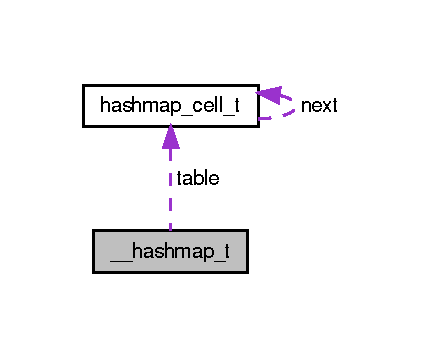
\includegraphics[width=203pt]{struct____hashmap__t__coll__graph}
\end{center}
\end{figure}
\subsection*{Champs de données}
\begin{DoxyCompactItemize}
\item 
int \hyperlink{struct____hashmap__t_ab5f1e74c3fcf71ee4ac91a860cbcde19}{size}
\item 
struct \hyperlink{structhashmap__cell__t}{hashmap\+\_\+cell\+\_\+t} $\ast$$\ast$ \hyperlink{struct____hashmap__t_ac7d3b722978b8bafab2ce2a923b747aa}{table}
\item 
int($\ast$ \hyperlink{struct____hashmap__t_a2b730301a68342f67a406ce1b6c2a826}{equal} )(struct hashmap\+\_\+key\+\_\+t $\ast$, struct hashmap\+\_\+key\+\_\+t $\ast$)
\item 
int($\ast$ \hyperlink{struct____hashmap__t_aa56e33c3baa182a530a4a8bfc27c11f1}{hash} )(struct hashmap\+\_\+key\+\_\+t $\ast$)
\end{DoxyCompactItemize}


\subsection{Description détaillée}
Structure représentant une hashmap. 

\subsection{Documentation des champs}
\hypertarget{struct____hashmap__t_a2b730301a68342f67a406ce1b6c2a826}{\index{\+\_\+\+\_\+hashmap\+\_\+t@{\+\_\+\+\_\+hashmap\+\_\+t}!equal@{equal}}
\index{equal@{equal}!\+\_\+\+\_\+hashmap\+\_\+t@{\+\_\+\+\_\+hashmap\+\_\+t}}
\subsubsection[{equal}]{\setlength{\rightskip}{0pt plus 5cm}int($\ast$ \+\_\+\+\_\+hashmap\+\_\+t\+::equal)(struct hashmap\+\_\+key\+\_\+t $\ast$, struct hashmap\+\_\+key\+\_\+t $\ast$)}}\label{struct____hashmap__t_a2b730301a68342f67a406ce1b6c2a826}
Fonction de comparaison de clefs. \hypertarget{struct____hashmap__t_aa56e33c3baa182a530a4a8bfc27c11f1}{\index{\+\_\+\+\_\+hashmap\+\_\+t@{\+\_\+\+\_\+hashmap\+\_\+t}!hash@{hash}}
\index{hash@{hash}!\+\_\+\+\_\+hashmap\+\_\+t@{\+\_\+\+\_\+hashmap\+\_\+t}}
\subsubsection[{hash}]{\setlength{\rightskip}{0pt plus 5cm}int($\ast$ \+\_\+\+\_\+hashmap\+\_\+t\+::hash)(struct hashmap\+\_\+key\+\_\+t $\ast$)}}\label{struct____hashmap__t_aa56e33c3baa182a530a4a8bfc27c11f1}
Fonction de hashage. \hypertarget{struct____hashmap__t_ab5f1e74c3fcf71ee4ac91a860cbcde19}{\index{\+\_\+\+\_\+hashmap\+\_\+t@{\+\_\+\+\_\+hashmap\+\_\+t}!size@{size}}
\index{size@{size}!\+\_\+\+\_\+hashmap\+\_\+t@{\+\_\+\+\_\+hashmap\+\_\+t}}
\subsubsection[{size}]{\setlength{\rightskip}{0pt plus 5cm}int \+\_\+\+\_\+hashmap\+\_\+t\+::size}}\label{struct____hashmap__t_ab5f1e74c3fcf71ee4ac91a860cbcde19}
Taile de la table. \hypertarget{struct____hashmap__t_ac7d3b722978b8bafab2ce2a923b747aa}{\index{\+\_\+\+\_\+hashmap\+\_\+t@{\+\_\+\+\_\+hashmap\+\_\+t}!table@{table}}
\index{table@{table}!\+\_\+\+\_\+hashmap\+\_\+t@{\+\_\+\+\_\+hashmap\+\_\+t}}
\subsubsection[{table}]{\setlength{\rightskip}{0pt plus 5cm}struct {\bf hashmap\+\_\+cell\+\_\+t}$\ast$$\ast$ \+\_\+\+\_\+hashmap\+\_\+t\+::table}}\label{struct____hashmap__t_ac7d3b722978b8bafab2ce2a923b747aa}
Table de liste d'éléments ayant le même hash. 

La documentation de cette structure a été générée à partir du fichier suivant \+:\begin{DoxyCompactItemize}
\item 
kernel/include/\hyperlink{hashmap_8h}{hashmap.\+h}\end{DoxyCompactItemize}

\hypertarget{struct__available__fs__t}{\section{Référence de la structure \-\_\-available\-\_\-fs\-\_\-t}
\label{struct__available__fs__t}\index{\-\_\-available\-\_\-fs\-\_\-t@{\-\_\-available\-\_\-fs\-\_\-t}}
}


Graphe de collaboration de \-\_\-available\-\_\-fs\-\_\-t\-:
\nopagebreak
\begin{figure}[H]
\begin{center}
\leavevmode
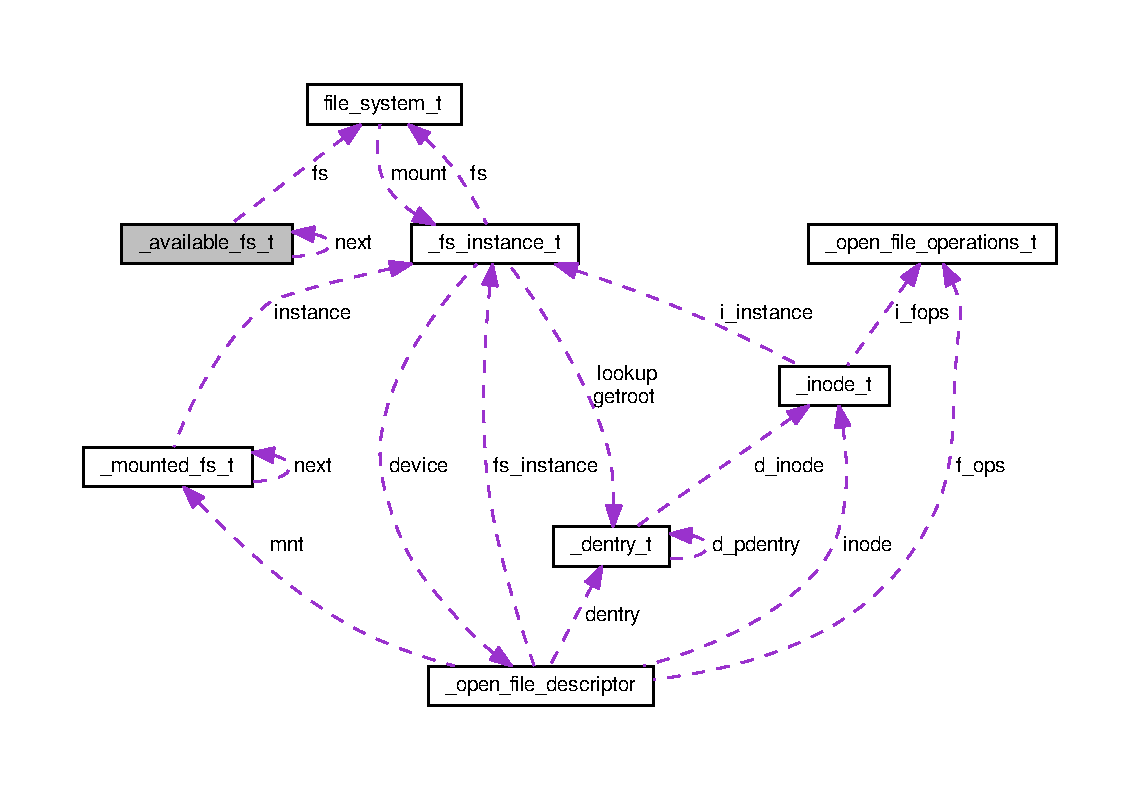
\includegraphics[width=350pt]{struct__available__fs__t__coll__graph}
\end{center}
\end{figure}
\subsection*{Champs de données}
\begin{DoxyCompactItemize}
\item 
\hyperlink{structfile__system__t}{file\-\_\-system\-\_\-t} $\ast$ \hyperlink{struct__available__fs__t_ab0d3f3d5cfaf664ddb4d2c136071a072}{fs}
\item 
struct \hyperlink{struct__available__fs__t}{\-\_\-available\-\_\-fs\-\_\-t} $\ast$ \hyperlink{struct__available__fs__t_a1f870d42e7b92140da5442e9b677c7a0}{next}
\end{DoxyCompactItemize}


\subsection{Description détaillée}
Cellule d'une liste de fs disponibles. 

\subsection{Documentation des champs}
\hypertarget{struct__available__fs__t_ab0d3f3d5cfaf664ddb4d2c136071a072}{\index{\-\_\-available\-\_\-fs\-\_\-t@{\-\_\-available\-\_\-fs\-\_\-t}!fs@{fs}}
\index{fs@{fs}!_available_fs_t@{\-\_\-available\-\_\-fs\-\_\-t}}
\subsubsection[{fs}]{\setlength{\rightskip}{0pt plus 5cm}{\bf file\-\_\-system\-\_\-t}$\ast$ \-\_\-available\-\_\-fs\-\_\-t\-::fs}}\label{struct__available__fs__t_ab0d3f3d5cfaf664ddb4d2c136071a072}
Informations sur le F\-S. \hypertarget{struct__available__fs__t_a1f870d42e7b92140da5442e9b677c7a0}{\index{\-\_\-available\-\_\-fs\-\_\-t@{\-\_\-available\-\_\-fs\-\_\-t}!next@{next}}
\index{next@{next}!_available_fs_t@{\-\_\-available\-\_\-fs\-\_\-t}}
\subsubsection[{next}]{\setlength{\rightskip}{0pt plus 5cm}struct {\bf \-\_\-available\-\_\-fs\-\_\-t}$\ast$ \-\_\-available\-\_\-fs\-\_\-t\-::next}}\label{struct__available__fs__t_a1f870d42e7b92140da5442e9b677c7a0}
F\-S suivant. 

La documentation de cette structure a été générée à partir du fichier suivant \-:\begin{DoxyCompactItemize}
\item 
kernel/\hyperlink{vfs_8c}{vfs.\-c}\end{DoxyCompactItemize}

\hypertarget{struct__dentry__t}{\section{Référence de la structure \-\_\-dentry\-\_\-t}
\label{struct__dentry__t}\index{\-\_\-dentry\-\_\-t@{\-\_\-dentry\-\_\-t}}
}


{\ttfamily \#include $<$vfs.\-h$>$}



Graphe de collaboration de \-\_\-dentry\-\_\-t\-:\nopagebreak
\begin{figure}[H]
\begin{center}
\leavevmode
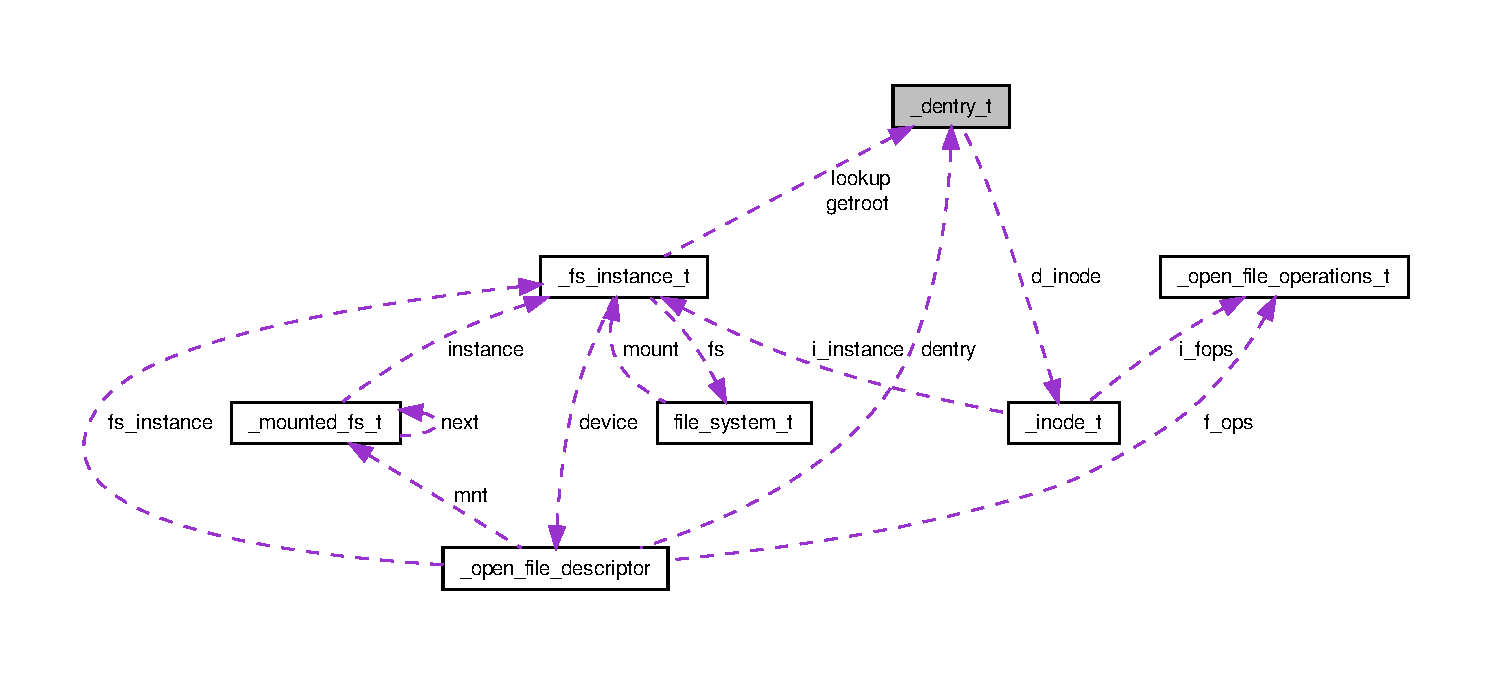
\includegraphics[width=350pt]{struct__dentry__t__coll__graph}
\end{center}
\end{figure}
\subsection*{Champs de données}
\begin{DoxyCompactItemize}
\item 
const char $\ast$ \hyperlink{struct__dentry__t_ac9b991f6f5d5c5ce60e8d256d667265e}{d\-\_\-name}
\item 
\hyperlink{vfs_8h_af51b41660b60ad79b490887fe6e22da9}{inode\-\_\-t} $\ast$ \hyperlink{struct__dentry__t_ac711731a0c08b35b5d2731b8545c7454}{d\-\_\-inode}
\item 
struct \hyperlink{struct__dentry__t}{\-\_\-dentry\-\_\-t} $\ast$ \hyperlink{struct__dentry__t_a900178add855a65bb2c42a1fbb94686b}{d\-\_\-pdentry}
\end{DoxyCompactItemize}


\subsection{Description détaillée}
Directory Entry. 

\subsection{Documentation des champs}
\hypertarget{struct__dentry__t_ac711731a0c08b35b5d2731b8545c7454}{\index{\-\_\-dentry\-\_\-t@{\-\_\-dentry\-\_\-t}!d\-\_\-inode@{d\-\_\-inode}}
\index{d\-\_\-inode@{d\-\_\-inode}!_dentry_t@{\-\_\-dentry\-\_\-t}}
\subsubsection[{d\-\_\-inode}]{\setlength{\rightskip}{0pt plus 5cm}{\bf inode\-\_\-t}$\ast$ \-\_\-dentry\-\_\-t\-::d\-\_\-inode}}\label{struct__dentry__t_ac711731a0c08b35b5d2731b8545c7454}
Inode associé. \hypertarget{struct__dentry__t_ac9b991f6f5d5c5ce60e8d256d667265e}{\index{\-\_\-dentry\-\_\-t@{\-\_\-dentry\-\_\-t}!d\-\_\-name@{d\-\_\-name}}
\index{d\-\_\-name@{d\-\_\-name}!_dentry_t@{\-\_\-dentry\-\_\-t}}
\subsubsection[{d\-\_\-name}]{\setlength{\rightskip}{0pt plus 5cm}const char$\ast$ \-\_\-dentry\-\_\-t\-::d\-\_\-name}}\label{struct__dentry__t_ac9b991f6f5d5c5ce60e8d256d667265e}
Nom de l'entrée. \hypertarget{struct__dentry__t_a900178add855a65bb2c42a1fbb94686b}{\index{\-\_\-dentry\-\_\-t@{\-\_\-dentry\-\_\-t}!d\-\_\-pdentry@{d\-\_\-pdentry}}
\index{d\-\_\-pdentry@{d\-\_\-pdentry}!_dentry_t@{\-\_\-dentry\-\_\-t}}
\subsubsection[{d\-\_\-pdentry}]{\setlength{\rightskip}{0pt plus 5cm}struct {\bf \-\_\-dentry\-\_\-t}$\ast$ \-\_\-dentry\-\_\-t\-::d\-\_\-pdentry}}\label{struct__dentry__t_a900178add855a65bb2c42a1fbb94686b}
Parent dentry. 

La documentation de cette structure a été générée à partir du fichier suivant \-:\begin{DoxyCompactItemize}
\item 
kernel/include/\hyperlink{vfs_8h}{vfs.\-h}\end{DoxyCompactItemize}

\hypertarget{struct__DIR}{\section{Référence de la structure \-\_\-\-D\-I\-R}
\label{struct__DIR}\index{\-\_\-\-D\-I\-R@{\-\_\-\-D\-I\-R}}
}


{\ttfamily \#include $<$dirent.\-h$>$}

\subsection*{Champs de données}
\begin{DoxyCompactItemize}
\item 
int \hyperlink{struct__DIR_a1ee17b3cb06ddc80fb648e65c8353c55}{fd}
\item 
\hyperlink{kernel_2include_2types_8h_a29d85914ddff32967d85ada69854206d}{size\-\_\-t} \hyperlink{struct__DIR_a395fdd86b324fd71725a24e4f6edd55c}{allocation}
\item 
\hyperlink{kernel_2include_2types_8h_a29d85914ddff32967d85ada69854206d}{size\-\_\-t} \hyperlink{struct__DIR_a117676c5eb31163a8b99520bd2cbf1aa}{size}
\item 
\hyperlink{kernel_2include_2types_8h_a29d85914ddff32967d85ada69854206d}{size\-\_\-t} \hyperlink{struct__DIR_a298b074b577743d5c726b4fdc2917795}{offset}
\item 
\hyperlink{libc_2include_2sys_2types_8h_a447a6a64dbb8fb44b1e62856b333db4a}{off\-\_\-t} \hyperlink{struct__DIR_a759e6f1c2754b12a4aba9d120f3d1e57}{filepos}
\item 
char \hyperlink{struct__DIR_a87bb023e0bf0b2f075e90d270ff7033e}{data} \mbox{[}1\mbox{]}
\end{DoxyCompactItemize}


\subsection{Description détaillée}
Structure permettant de lire un dossier. 

\subsection{Documentation des champs}
\hypertarget{struct__DIR_a395fdd86b324fd71725a24e4f6edd55c}{\index{\-\_\-\-D\-I\-R@{\-\_\-\-D\-I\-R}!allocation@{allocation}}
\index{allocation@{allocation}!_DIR@{\-\_\-\-D\-I\-R}}
\subsubsection[{allocation}]{\setlength{\rightskip}{0pt plus 5cm}{\bf size\-\_\-t} \-\_\-\-D\-I\-R\-::allocation}}\label{struct__DIR_a395fdd86b324fd71725a24e4f6edd55c}
Espace réservé au block. \hypertarget{struct__DIR_a87bb023e0bf0b2f075e90d270ff7033e}{\index{\-\_\-\-D\-I\-R@{\-\_\-\-D\-I\-R}!data@{data}}
\index{data@{data}!_DIR@{\-\_\-\-D\-I\-R}}
\subsubsection[{data}]{\setlength{\rightskip}{0pt plus 5cm}char \-\_\-\-D\-I\-R\-::data\mbox{[}1\mbox{]}}}\label{struct__DIR_a87bb023e0bf0b2f075e90d270ff7033e}
Block qui est en fait plus grand que ça. \hypertarget{struct__DIR_a1ee17b3cb06ddc80fb648e65c8353c55}{\index{\-\_\-\-D\-I\-R@{\-\_\-\-D\-I\-R}!fd@{fd}}
\index{fd@{fd}!_DIR@{\-\_\-\-D\-I\-R}}
\subsubsection[{fd}]{\setlength{\rightskip}{0pt plus 5cm}int \-\_\-\-D\-I\-R\-::fd}}\label{struct__DIR_a1ee17b3cb06ddc80fb648e65c8353c55}
File descriptor. \hypertarget{struct__DIR_a759e6f1c2754b12a4aba9d120f3d1e57}{\index{\-\_\-\-D\-I\-R@{\-\_\-\-D\-I\-R}!filepos@{filepos}}
\index{filepos@{filepos}!_DIR@{\-\_\-\-D\-I\-R}}
\subsubsection[{filepos}]{\setlength{\rightskip}{0pt plus 5cm}{\bf off\-\_\-t} \-\_\-\-D\-I\-R\-::filepos}}\label{struct__DIR_a759e6f1c2754b12a4aba9d120f3d1e57}
Offset dans le dossier. \hypertarget{struct__DIR_a298b074b577743d5c726b4fdc2917795}{\index{\-\_\-\-D\-I\-R@{\-\_\-\-D\-I\-R}!offset@{offset}}
\index{offset@{offset}!_DIR@{\-\_\-\-D\-I\-R}}
\subsubsection[{offset}]{\setlength{\rightskip}{0pt plus 5cm}{\bf size\-\_\-t} \-\_\-\-D\-I\-R\-::offset}}\label{struct__DIR_a298b074b577743d5c726b4fdc2917795}
Position dans le block. \hypertarget{struct__DIR_a117676c5eb31163a8b99520bd2cbf1aa}{\index{\-\_\-\-D\-I\-R@{\-\_\-\-D\-I\-R}!size@{size}}
\index{size@{size}!_DIR@{\-\_\-\-D\-I\-R}}
\subsubsection[{size}]{\setlength{\rightskip}{0pt plus 5cm}{\bf size\-\_\-t} \-\_\-\-D\-I\-R\-::size}}\label{struct__DIR_a117676c5eb31163a8b99520bd2cbf1aa}
Données dans le block. 

La documentation de cette structure a été générée à partir du fichier suivant \-:\begin{DoxyCompactItemize}
\item 
libc/include/\hyperlink{dirent_8h}{dirent.\-h}\end{DoxyCompactItemize}

\hypertarget{struct__directory}{\section{Référence de la structure \+\_\+directory}
\label{struct__directory}\index{\+\_\+directory@{\+\_\+directory}}
}


{\ttfamily \#include $<$fat\+\_\+internal.\+h$>$}



Graphe de collaboration de \+\_\+directory\+:\nopagebreak
\begin{figure}[H]
\begin{center}
\leavevmode
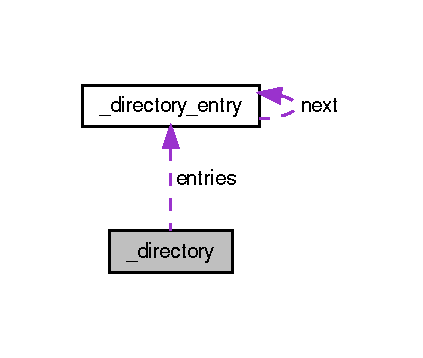
\includegraphics[width=203pt]{struct__directory__coll__graph}
\end{center}
\end{figure}
\subsection*{Champs de données}
\begin{DoxyCompactItemize}
\item 
\hyperlink{fat__internal_8h_ab6546cb0abf935a615fae20884a41818}{directory\+\_\+entry\+\_\+t} $\ast$ \hyperlink{struct__directory_a2aa96162372442698a14e116ce88110d}{entries}
\item 
int \hyperlink{struct__directory_aeb73476149e19828774d4dfbd96a051f}{total\+\_\+entries}
\item 
char \hyperlink{struct__directory_a535c678fe29215d35ac64200865147a4}{name} \mbox{[}256\mbox{]}
\item 
\hyperlink{kernel_2include_2types_8h_a33594304e786b158f3fb30289278f5af}{uint32\+\_\+t} \hyperlink{struct__directory_a5a45241095c7fb2a39f158638631ddbc}{cluster}
\end{DoxyCompactItemize}


\subsection{Description détaillée}
Structure de haut niveau pour stocker les informations d'un dossier. 

\subsection{Documentation des champs}
\hypertarget{struct__directory_a5a45241095c7fb2a39f158638631ddbc}{\index{\+\_\+directory@{\+\_\+directory}!cluster@{cluster}}
\index{cluster@{cluster}!\+\_\+directory@{\+\_\+directory}}
\subsubsection[{cluster}]{\setlength{\rightskip}{0pt plus 5cm}{\bf uint32\+\_\+t} \+\_\+directory\+::cluster}}\label{struct__directory_a5a45241095c7fb2a39f158638631ddbc}
Cluster où est enregistré le dossier. \hypertarget{struct__directory_a2aa96162372442698a14e116ce88110d}{\index{\+\_\+directory@{\+\_\+directory}!entries@{entries}}
\index{entries@{entries}!\+\_\+directory@{\+\_\+directory}}
\subsubsection[{entries}]{\setlength{\rightskip}{0pt plus 5cm}{\bf directory\+\_\+entry\+\_\+t}$\ast$ \+\_\+directory\+::entries}}\label{struct__directory_a2aa96162372442698a14e116ce88110d}
Liste des entrées dans ce dossier. \hypertarget{struct__directory_a535c678fe29215d35ac64200865147a4}{\index{\+\_\+directory@{\+\_\+directory}!name@{name}}
\index{name@{name}!\+\_\+directory@{\+\_\+directory}}
\subsubsection[{name}]{\setlength{\rightskip}{0pt plus 5cm}char \+\_\+directory\+::name\mbox{[}256\mbox{]}}}\label{struct__directory_a535c678fe29215d35ac64200865147a4}
Nom du dossier. \hypertarget{struct__directory_aeb73476149e19828774d4dfbd96a051f}{\index{\+\_\+directory@{\+\_\+directory}!total\+\_\+entries@{total\+\_\+entries}}
\index{total\+\_\+entries@{total\+\_\+entries}!\+\_\+directory@{\+\_\+directory}}
\subsubsection[{total\+\_\+entries}]{\setlength{\rightskip}{0pt plus 5cm}int \+\_\+directory\+::total\+\_\+entries}}\label{struct__directory_aeb73476149e19828774d4dfbd96a051f}
Nombre d'entrées dans le dossier. 

La documentation de cette structure a été générée à partir du fichier suivant \+:\begin{DoxyCompactItemize}
\item 
kernel/fs/fat/\hyperlink{fat__internal_8h}{fat\+\_\+internal.\+h}\end{DoxyCompactItemize}

\hypertarget{struct__directory__entry}{\section{Référence de la structure \-\_\-directory\-\_\-entry}
\label{struct__directory__entry}\index{\-\_\-directory\-\_\-entry@{\-\_\-directory\-\_\-entry}}
}


{\ttfamily \#include $<$fat\-\_\-internal.\-h$>$}



Graphe de collaboration de \-\_\-directory\-\_\-entry\-:\nopagebreak
\begin{figure}[H]
\begin{center}
\leavevmode
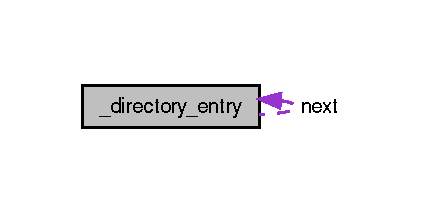
\includegraphics[width=203pt]{struct__directory__entry__coll__graph}
\end{center}
\end{figure}
\subsection*{Champs de données}
\begin{DoxyCompactItemize}
\item 
char \hyperlink{struct__directory__entry_ac9142fdeb8e265f045fee1edf9608c78}{name} \mbox{[}256\mbox{]}
\item 
\hyperlink{types_8h_aba7bc1797add20fe3efdf37ced1182c5}{uint8\-\_\-t} \hyperlink{struct__directory__entry_a63da8f87e73a3eb30e55b2d405fa35d7}{attributes}
\item 
\hyperlink{types_8h_a33594304e786b158f3fb30289278f5af}{uint32\-\_\-t} \hyperlink{struct__directory__entry_a5d6f559c1b7ab2b5a64643073172cc25}{size}
\item 
time\-\_\-t \hyperlink{struct__directory__entry_a27e1020c5262094ab3b58759da9660ae}{access\-\_\-time}
\item 
time\-\_\-t \hyperlink{struct__directory__entry_a120c3a3857bd7892a0fc2e6644e6f188}{modification\-\_\-time}
\item 
time\-\_\-t \hyperlink{struct__directory__entry_a95f0f5ef18bf17f332bd0dc352d62ac4}{creation\-\_\-time}
\item 
\hyperlink{types_8h_a33594304e786b158f3fb30289278f5af}{uint32\-\_\-t} \hyperlink{struct__directory__entry_a8c70d9d0c2b2557cba83fb827d5c6e90}{cluster}
\item 
struct \hyperlink{struct__directory__entry}{\-\_\-directory\-\_\-entry} $\ast$ \hyperlink{struct__directory__entry_a75001bda0d1d80e4ff5350ad69f83030}{next}
\end{DoxyCompactItemize}


\subsection{Description détaillée}
Liste chaînée pour stocker les entrées d'un dossier. 

\subsection{Documentation des champs}
\hypertarget{struct__directory__entry_a27e1020c5262094ab3b58759da9660ae}{\index{\-\_\-directory\-\_\-entry@{\-\_\-directory\-\_\-entry}!access\-\_\-time@{access\-\_\-time}}
\index{access\-\_\-time@{access\-\_\-time}!_directory_entry@{\-\_\-directory\-\_\-entry}}
\subsubsection[{access\-\_\-time}]{\setlength{\rightskip}{0pt plus 5cm}time\-\_\-t \-\_\-directory\-\_\-entry\-::access\-\_\-time}}\label{struct__directory__entry_a27e1020c5262094ab3b58759da9660ae}
Date du dernier accès. \hypertarget{struct__directory__entry_a63da8f87e73a3eb30e55b2d405fa35d7}{\index{\-\_\-directory\-\_\-entry@{\-\_\-directory\-\_\-entry}!attributes@{attributes}}
\index{attributes@{attributes}!_directory_entry@{\-\_\-directory\-\_\-entry}}
\subsubsection[{attributes}]{\setlength{\rightskip}{0pt plus 5cm}{\bf uint8\-\_\-t} \-\_\-directory\-\_\-entry\-::attributes}}\label{struct__directory__entry_a63da8f87e73a3eb30e55b2d405fa35d7}
Attributs du fichier/dossier. \hypertarget{struct__directory__entry_a8c70d9d0c2b2557cba83fb827d5c6e90}{\index{\-\_\-directory\-\_\-entry@{\-\_\-directory\-\_\-entry}!cluster@{cluster}}
\index{cluster@{cluster}!_directory_entry@{\-\_\-directory\-\_\-entry}}
\subsubsection[{cluster}]{\setlength{\rightskip}{0pt plus 5cm}{\bf uint32\-\_\-t} \-\_\-directory\-\_\-entry\-::cluster}}\label{struct__directory__entry_a8c70d9d0c2b2557cba83fb827d5c6e90}
Cluster où est le fichier/dossier. \hypertarget{struct__directory__entry_a95f0f5ef18bf17f332bd0dc352d62ac4}{\index{\-\_\-directory\-\_\-entry@{\-\_\-directory\-\_\-entry}!creation\-\_\-time@{creation\-\_\-time}}
\index{creation\-\_\-time@{creation\-\_\-time}!_directory_entry@{\-\_\-directory\-\_\-entry}}
\subsubsection[{creation\-\_\-time}]{\setlength{\rightskip}{0pt plus 5cm}time\-\_\-t \-\_\-directory\-\_\-entry\-::creation\-\_\-time}}\label{struct__directory__entry_a95f0f5ef18bf17f332bd0dc352d62ac4}
Date de création. \hypertarget{struct__directory__entry_a120c3a3857bd7892a0fc2e6644e6f188}{\index{\-\_\-directory\-\_\-entry@{\-\_\-directory\-\_\-entry}!modification\-\_\-time@{modification\-\_\-time}}
\index{modification\-\_\-time@{modification\-\_\-time}!_directory_entry@{\-\_\-directory\-\_\-entry}}
\subsubsection[{modification\-\_\-time}]{\setlength{\rightskip}{0pt plus 5cm}time\-\_\-t \-\_\-directory\-\_\-entry\-::modification\-\_\-time}}\label{struct__directory__entry_a120c3a3857bd7892a0fc2e6644e6f188}
Date de la dernière modification. \hypertarget{struct__directory__entry_ac9142fdeb8e265f045fee1edf9608c78}{\index{\-\_\-directory\-\_\-entry@{\-\_\-directory\-\_\-entry}!name@{name}}
\index{name@{name}!_directory_entry@{\-\_\-directory\-\_\-entry}}
\subsubsection[{name}]{\setlength{\rightskip}{0pt plus 5cm}char \-\_\-directory\-\_\-entry\-::name\mbox{[}256\mbox{]}}}\label{struct__directory__entry_ac9142fdeb8e265f045fee1edf9608c78}
Nom de l'entrée. \hypertarget{struct__directory__entry_a75001bda0d1d80e4ff5350ad69f83030}{\index{\-\_\-directory\-\_\-entry@{\-\_\-directory\-\_\-entry}!next@{next}}
\index{next@{next}!_directory_entry@{\-\_\-directory\-\_\-entry}}
\subsubsection[{next}]{\setlength{\rightskip}{0pt plus 5cm}struct {\bf \-\_\-directory\-\_\-entry}$\ast$ \-\_\-directory\-\_\-entry\-::next}}\label{struct__directory__entry_a75001bda0d1d80e4ff5350ad69f83030}
Pointeur vers la prochaine entrée du dossier ou N\-U\-L\-L. \hypertarget{struct__directory__entry_a5d6f559c1b7ab2b5a64643073172cc25}{\index{\-\_\-directory\-\_\-entry@{\-\_\-directory\-\_\-entry}!size@{size}}
\index{size@{size}!_directory_entry@{\-\_\-directory\-\_\-entry}}
\subsubsection[{size}]{\setlength{\rightskip}{0pt plus 5cm}{\bf uint32\-\_\-t} \-\_\-directory\-\_\-entry\-::size}}\label{struct__directory__entry_a5d6f559c1b7ab2b5a64643073172cc25}
Taille. 

La documentation de cette structure a été générée à partir du fichier suivant \-:\begin{DoxyCompactItemize}
\item 
kernel/fs/fat/\hyperlink{fat__internal_8h}{fat\-\_\-internal.\-h}\end{DoxyCompactItemize}

\hypertarget{struct__ext2__fs__instance__t}{\section{Référence de la structure \+\_\+ext2\+\_\+fs\+\_\+instance\+\_\+t}
\label{struct__ext2__fs__instance__t}\index{\+\_\+ext2\+\_\+fs\+\_\+instance\+\_\+t@{\+\_\+ext2\+\_\+fs\+\_\+instance\+\_\+t}}
}


Instance de F\+S Ext2.  




{\ttfamily \#include $<$ext2\+\_\+internal.\+h$>$}



Graphe de collaboration de \+\_\+ext2\+\_\+fs\+\_\+instance\+\_\+t\+:
\nopagebreak
\begin{figure}[H]
\begin{center}
\leavevmode
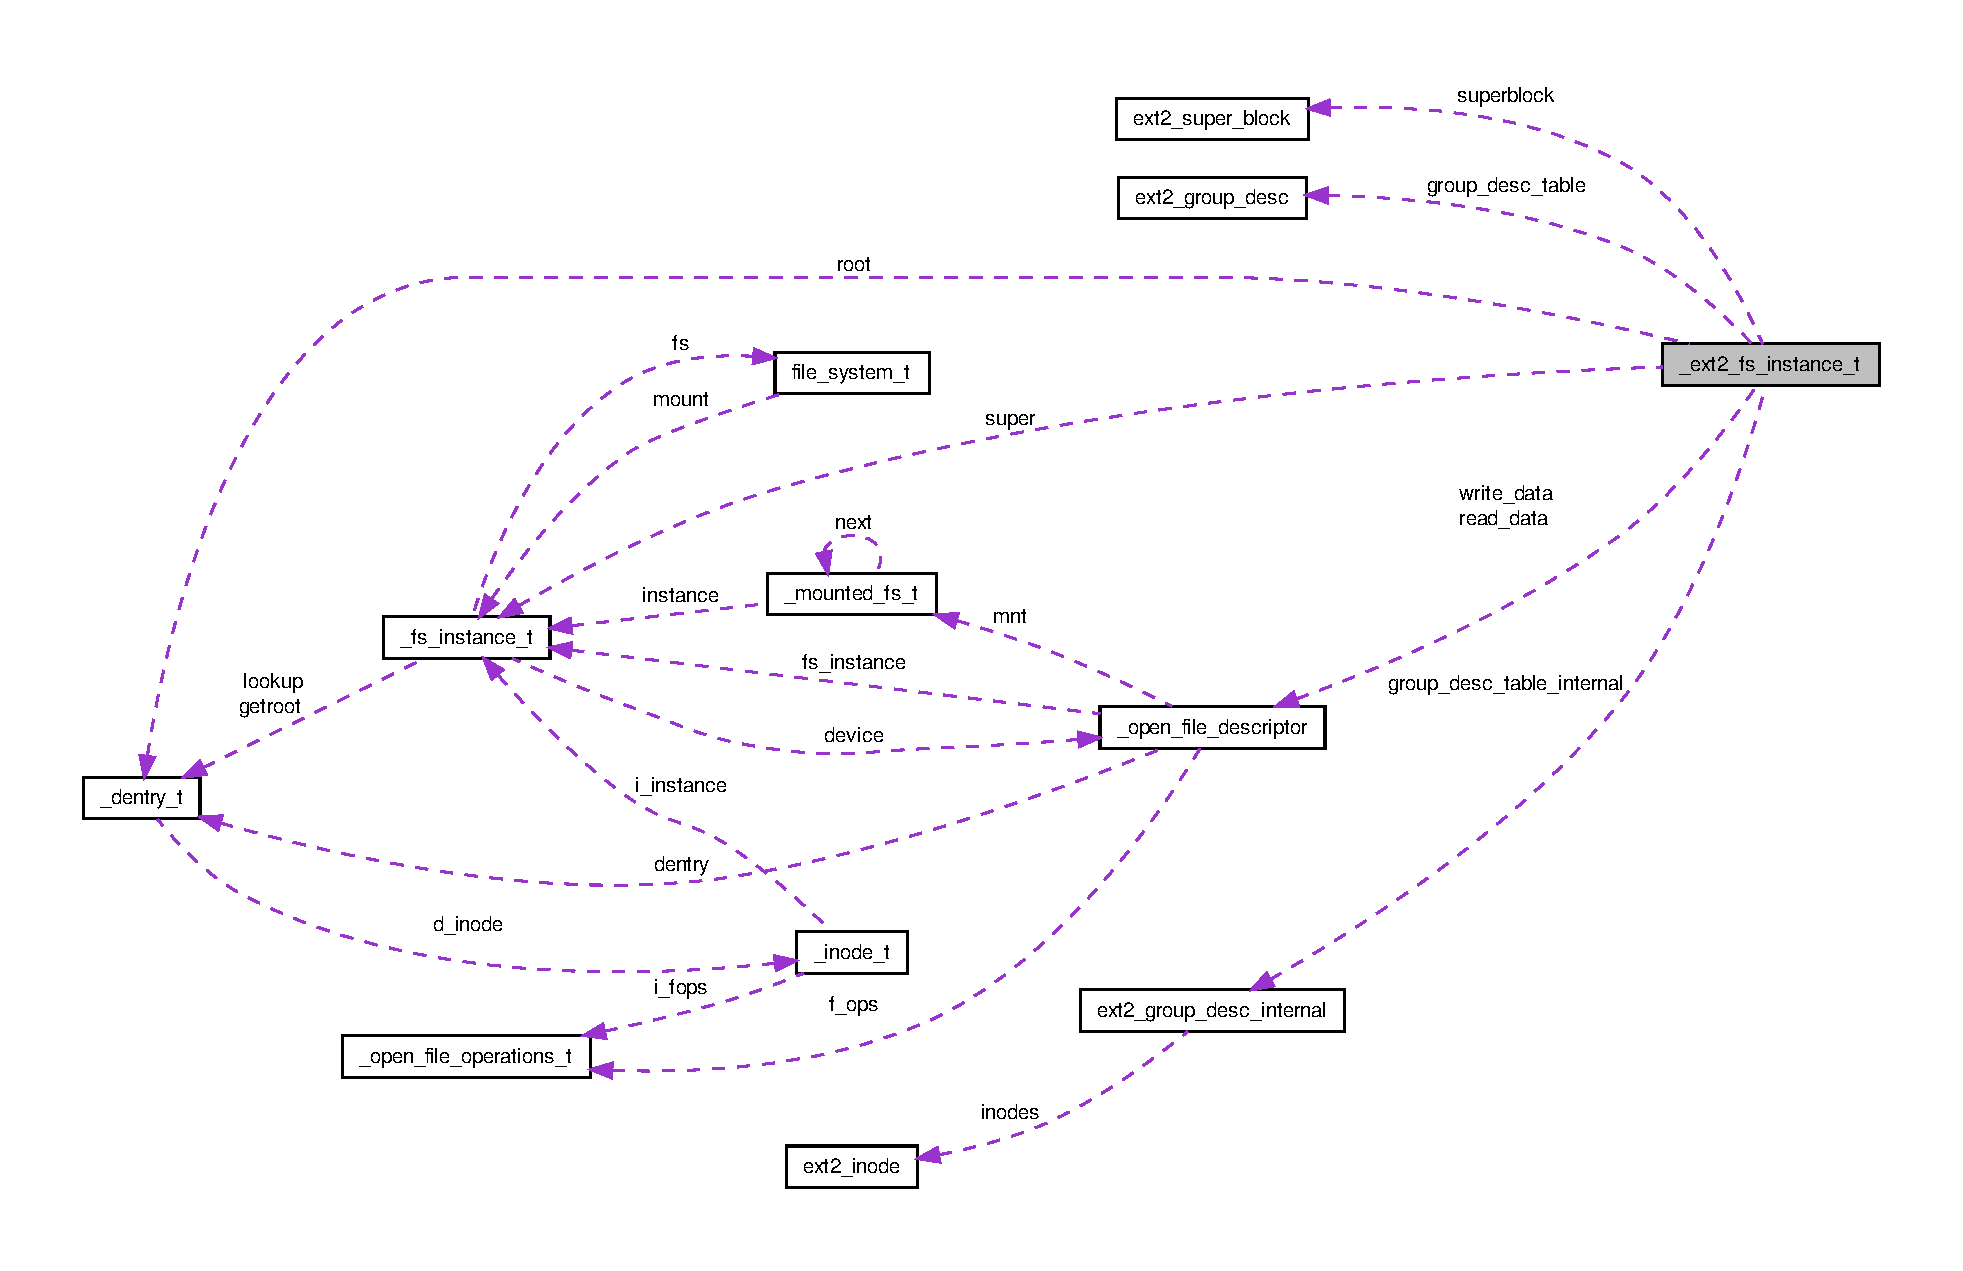
\includegraphics[width=350pt]{struct__ext2__fs__instance__t__coll__graph}
\end{center}
\end{figure}
\subsection*{Champs de données}
\begin{DoxyCompactItemize}
\item 
\hyperlink{vfs_8h_a0eefa9aac35a5462ebf1e038992ca860}{fs\+\_\+instance\+\_\+t} \hyperlink{struct__ext2__fs__instance__t_a456ee695fb1a0b71edadda9f4504ca2d}{super}
\item 
\hyperlink{vfs_8h_ade5c998c6b3f09d2cf45d0e5ef8787da}{dentry\+\_\+t} $\ast$ \hyperlink{struct__ext2__fs__instance__t_a52f883f2d709ab3b4dff94b5b7100973}{root}
\item 
struct \hyperlink{structext2__super__block}{ext2\+\_\+super\+\_\+block} \hyperlink{struct__ext2__fs__instance__t_a81ad8719743e20da6f661c2586b56ad2}{superblock}
\item 
struct \hyperlink{structext2__group__desc}{ext2\+\_\+group\+\_\+desc} $\ast$ \hyperlink{struct__ext2__fs__instance__t_acc01ef58cbc6cfa9d3ff4e08709a561a}{group\+\_\+desc\+\_\+table}
\item 
int \hyperlink{struct__ext2__fs__instance__t_a81a5e5b8f7d46d744c96a4f28317e59f}{n\+\_\+groups}
\item 
blkdev\+\_\+read\+\_\+t \hyperlink{struct__ext2__fs__instance__t_ac3ea85962b66914cb42ec884d70a853d}{read\+\_\+data}
\item 
blkdev\+\_\+write\+\_\+t \hyperlink{struct__ext2__fs__instance__t_a90d334c34e9aeea01be13fe1ed66ba7b}{write\+\_\+data}
\item 
struct \hyperlink{structext2__group__desc__internal}{ext2\+\_\+group\+\_\+desc\+\_\+internal} $\ast$ \hyperlink{struct__ext2__fs__instance__t_a9db69a1265be4c818005d18add117790}{group\+\_\+desc\+\_\+table\+\_\+internal}
\end{DoxyCompactItemize}


\subsection{Documentation des champs}
\hypertarget{struct__ext2__fs__instance__t_acc01ef58cbc6cfa9d3ff4e08709a561a}{\index{\+\_\+ext2\+\_\+fs\+\_\+instance\+\_\+t@{\+\_\+ext2\+\_\+fs\+\_\+instance\+\_\+t}!group\+\_\+desc\+\_\+table@{group\+\_\+desc\+\_\+table}}
\index{group\+\_\+desc\+\_\+table@{group\+\_\+desc\+\_\+table}!\+\_\+ext2\+\_\+fs\+\_\+instance\+\_\+t@{\+\_\+ext2\+\_\+fs\+\_\+instance\+\_\+t}}
\subsubsection[{group\+\_\+desc\+\_\+table}]{\setlength{\rightskip}{0pt plus 5cm}struct {\bf ext2\+\_\+group\+\_\+desc}$\ast$ \+\_\+ext2\+\_\+fs\+\_\+instance\+\_\+t\+::group\+\_\+desc\+\_\+table}}\label{struct__ext2__fs__instance__t_acc01ef58cbc6cfa9d3ff4e08709a561a}
Block group descriptor table. \hypertarget{struct__ext2__fs__instance__t_a9db69a1265be4c818005d18add117790}{\index{\+\_\+ext2\+\_\+fs\+\_\+instance\+\_\+t@{\+\_\+ext2\+\_\+fs\+\_\+instance\+\_\+t}!group\+\_\+desc\+\_\+table\+\_\+internal@{group\+\_\+desc\+\_\+table\+\_\+internal}}
\index{group\+\_\+desc\+\_\+table\+\_\+internal@{group\+\_\+desc\+\_\+table\+\_\+internal}!\+\_\+ext2\+\_\+fs\+\_\+instance\+\_\+t@{\+\_\+ext2\+\_\+fs\+\_\+instance\+\_\+t}}
\subsubsection[{group\+\_\+desc\+\_\+table\+\_\+internal}]{\setlength{\rightskip}{0pt plus 5cm}struct {\bf ext2\+\_\+group\+\_\+desc\+\_\+internal}$\ast$ \+\_\+ext2\+\_\+fs\+\_\+instance\+\_\+t\+::group\+\_\+desc\+\_\+table\+\_\+internal}}\label{struct__ext2__fs__instance__t_a9db69a1265be4c818005d18add117790}
Copy of inodes (only, for now?) \hypertarget{struct__ext2__fs__instance__t_a81a5e5b8f7d46d744c96a4f28317e59f}{\index{\+\_\+ext2\+\_\+fs\+\_\+instance\+\_\+t@{\+\_\+ext2\+\_\+fs\+\_\+instance\+\_\+t}!n\+\_\+groups@{n\+\_\+groups}}
\index{n\+\_\+groups@{n\+\_\+groups}!\+\_\+ext2\+\_\+fs\+\_\+instance\+\_\+t@{\+\_\+ext2\+\_\+fs\+\_\+instance\+\_\+t}}
\subsubsection[{n\+\_\+groups}]{\setlength{\rightskip}{0pt plus 5cm}int \+\_\+ext2\+\_\+fs\+\_\+instance\+\_\+t\+::n\+\_\+groups}}\label{struct__ext2__fs__instance__t_a81a5e5b8f7d46d744c96a4f28317e59f}
Number of entries in the group desc table. \hypertarget{struct__ext2__fs__instance__t_ac3ea85962b66914cb42ec884d70a853d}{\index{\+\_\+ext2\+\_\+fs\+\_\+instance\+\_\+t@{\+\_\+ext2\+\_\+fs\+\_\+instance\+\_\+t}!read\+\_\+data@{read\+\_\+data}}
\index{read\+\_\+data@{read\+\_\+data}!\+\_\+ext2\+\_\+fs\+\_\+instance\+\_\+t@{\+\_\+ext2\+\_\+fs\+\_\+instance\+\_\+t}}
\subsubsection[{read\+\_\+data}]{\setlength{\rightskip}{0pt plus 5cm}blkdev\+\_\+read\+\_\+t \+\_\+ext2\+\_\+fs\+\_\+instance\+\_\+t\+::read\+\_\+data}}\label{struct__ext2__fs__instance__t_ac3ea85962b66914cb42ec884d70a853d}
Function to read data. \hypertarget{struct__ext2__fs__instance__t_a52f883f2d709ab3b4dff94b5b7100973}{\index{\+\_\+ext2\+\_\+fs\+\_\+instance\+\_\+t@{\+\_\+ext2\+\_\+fs\+\_\+instance\+\_\+t}!root@{root}}
\index{root@{root}!\+\_\+ext2\+\_\+fs\+\_\+instance\+\_\+t@{\+\_\+ext2\+\_\+fs\+\_\+instance\+\_\+t}}
\subsubsection[{root}]{\setlength{\rightskip}{0pt plus 5cm}{\bf dentry\+\_\+t}$\ast$ \+\_\+ext2\+\_\+fs\+\_\+instance\+\_\+t\+::root}}\label{struct__ext2__fs__instance__t_a52f883f2d709ab3b4dff94b5b7100973}
Inode root. \hypertarget{struct__ext2__fs__instance__t_a456ee695fb1a0b71edadda9f4504ca2d}{\index{\+\_\+ext2\+\_\+fs\+\_\+instance\+\_\+t@{\+\_\+ext2\+\_\+fs\+\_\+instance\+\_\+t}!super@{super}}
\index{super@{super}!\+\_\+ext2\+\_\+fs\+\_\+instance\+\_\+t@{\+\_\+ext2\+\_\+fs\+\_\+instance\+\_\+t}}
\subsubsection[{super}]{\setlength{\rightskip}{0pt plus 5cm}{\bf fs\+\_\+instance\+\_\+t} \+\_\+ext2\+\_\+fs\+\_\+instance\+\_\+t\+::super}}\label{struct__ext2__fs__instance__t_a456ee695fb1a0b71edadda9f4504ca2d}
Common fields for all F\+S instances. \hypertarget{struct__ext2__fs__instance__t_a81ad8719743e20da6f661c2586b56ad2}{\index{\+\_\+ext2\+\_\+fs\+\_\+instance\+\_\+t@{\+\_\+ext2\+\_\+fs\+\_\+instance\+\_\+t}!superblock@{superblock}}
\index{superblock@{superblock}!\+\_\+ext2\+\_\+fs\+\_\+instance\+\_\+t@{\+\_\+ext2\+\_\+fs\+\_\+instance\+\_\+t}}
\subsubsection[{superblock}]{\setlength{\rightskip}{0pt plus 5cm}struct {\bf ext2\+\_\+super\+\_\+block} \+\_\+ext2\+\_\+fs\+\_\+instance\+\_\+t\+::superblock}}\label{struct__ext2__fs__instance__t_a81ad8719743e20da6f661c2586b56ad2}
Superblock. \hypertarget{struct__ext2__fs__instance__t_a90d334c34e9aeea01be13fe1ed66ba7b}{\index{\+\_\+ext2\+\_\+fs\+\_\+instance\+\_\+t@{\+\_\+ext2\+\_\+fs\+\_\+instance\+\_\+t}!write\+\_\+data@{write\+\_\+data}}
\index{write\+\_\+data@{write\+\_\+data}!\+\_\+ext2\+\_\+fs\+\_\+instance\+\_\+t@{\+\_\+ext2\+\_\+fs\+\_\+instance\+\_\+t}}
\subsubsection[{write\+\_\+data}]{\setlength{\rightskip}{0pt plus 5cm}blkdev\+\_\+write\+\_\+t \+\_\+ext2\+\_\+fs\+\_\+instance\+\_\+t\+::write\+\_\+data}}\label{struct__ext2__fs__instance__t_a90d334c34e9aeea01be13fe1ed66ba7b}
Function to write data. 

La documentation de cette structure a été générée à partir du fichier suivant \+:\begin{DoxyCompactItemize}
\item 
kernel/fs/ext2/\hyperlink{ext2__internal_8h}{ext2\+\_\+internal.\+h}\end{DoxyCompactItemize}

\hypertarget{struct__fat__BS}{\section{Référence de la structure \-\_\-fat\-\_\-\-B\-S}
\label{struct__fat__BS}\index{\-\_\-fat\-\_\-\-B\-S@{\-\_\-fat\-\_\-\-B\-S}}
}


{\ttfamily \#include $<$fat\-\_\-internal.\-h$>$}

\subsection*{Champs de données}
\begin{DoxyCompactItemize}
\item 
\hypertarget{struct__fat__BS_ab51df8629fd8d28e238cf21e6c325c40}{\hyperlink{kernel_2include_2types_8h_aba7bc1797add20fe3efdf37ced1182c5}{uint8\-\_\-t} {\bfseries bootjmp} \mbox{[}3\mbox{]}}\label{struct__fat__BS_ab51df8629fd8d28e238cf21e6c325c40}

\item 
\hyperlink{kernel_2include_2types_8h_aba7bc1797add20fe3efdf37ced1182c5}{uint8\-\_\-t} \hyperlink{struct__fat__BS_a6e3cafc7b7a76af3f3d82b322bda2903}{oem\-\_\-name} \mbox{[}8\mbox{]}
\item 
\hyperlink{kernel_2include_2types_8h_adf4d876453337156dde61095e1f20223}{uint16\-\_\-t} \hyperlink{struct__fat__BS_a28755d8abcc38818f9a64918ba7b2de4}{bytes\-\_\-per\-\_\-sector}
\item 
\hyperlink{kernel_2include_2types_8h_aba7bc1797add20fe3efdf37ced1182c5}{uint8\-\_\-t} \hyperlink{struct__fat__BS_ab26cacbe204fc157d8165af3ad86a33f}{sectors\-\_\-per\-\_\-cluster}
\item 
\hyperlink{kernel_2include_2types_8h_adf4d876453337156dde61095e1f20223}{uint16\-\_\-t} \hyperlink{struct__fat__BS_a7c4d28484980635def2bb6c1e6675b5a}{reserved\-\_\-sector\-\_\-count}
\item 
\hyperlink{kernel_2include_2types_8h_aba7bc1797add20fe3efdf37ced1182c5}{uint8\-\_\-t} \hyperlink{struct__fat__BS_aa76ccd037c4f693d968a64860be99d44}{table\-\_\-count}
\item 
\hyperlink{kernel_2include_2types_8h_adf4d876453337156dde61095e1f20223}{uint16\-\_\-t} \hyperlink{struct__fat__BS_ae9265a2e00c0c3cbb4de257b602bcd2c}{root\-\_\-entry\-\_\-count}
\item 
\hyperlink{kernel_2include_2types_8h_adf4d876453337156dde61095e1f20223}{uint16\-\_\-t} \hyperlink{struct__fat__BS_a17243f0faca4d34eb12df96f8b9e6896}{total\-\_\-sectors\-\_\-16}
\item 
\hyperlink{kernel_2include_2types_8h_aba7bc1797add20fe3efdf37ced1182c5}{uint8\-\_\-t} \hyperlink{struct__fat__BS_ae6537235795059976bd79d26e4b61053}{media\-\_\-type}
\item 
\hyperlink{kernel_2include_2types_8h_adf4d876453337156dde61095e1f20223}{uint16\-\_\-t} \hyperlink{struct__fat__BS_aa6408c3aa26eec38e6620624c3075f27}{table\-\_\-size\-\_\-16}
\item 
\hyperlink{kernel_2include_2types_8h_adf4d876453337156dde61095e1f20223}{uint16\-\_\-t} \hyperlink{struct__fat__BS_abb98686b32bd168ee31d9847c990916a}{sectors\-\_\-per\-\_\-track}
\item 
\hyperlink{kernel_2include_2types_8h_adf4d876453337156dde61095e1f20223}{uint16\-\_\-t} \hyperlink{struct__fat__BS_ad58562d1dd05ac79b72053708ff52c3c}{head\-\_\-side\-\_\-count}
\item 
\hyperlink{kernel_2include_2types_8h_a33594304e786b158f3fb30289278f5af}{uint32\-\_\-t} \hyperlink{struct__fat__BS_a92f0f210cd522150211d990b4d3aeecb}{hidden\-\_\-sector\-\_\-count}
\item 
\hyperlink{kernel_2include_2types_8h_a33594304e786b158f3fb30289278f5af}{uint32\-\_\-t} \hyperlink{struct__fat__BS_a103e421c799f77466fc57eef601014a3}{total\-\_\-sectors\-\_\-32}
\end{DoxyCompactItemize}


\subsection{Description détaillée}
Boot Sector 

\subsection{Documentation des champs}
\hypertarget{struct__fat__BS_a28755d8abcc38818f9a64918ba7b2de4}{\index{\-\_\-fat\-\_\-\-B\-S@{\-\_\-fat\-\_\-\-B\-S}!bytes\-\_\-per\-\_\-sector@{bytes\-\_\-per\-\_\-sector}}
\index{bytes\-\_\-per\-\_\-sector@{bytes\-\_\-per\-\_\-sector}!_fat_BS@{\-\_\-fat\-\_\-\-B\-S}}
\subsubsection[{bytes\-\_\-per\-\_\-sector}]{\setlength{\rightskip}{0pt plus 5cm}{\bf uint16\-\_\-t} \-\_\-fat\-\_\-\-B\-S\-::bytes\-\_\-per\-\_\-sector}}\label{struct__fat__BS_a28755d8abcc38818f9a64918ba7b2de4}
Nombre d'octets par secteur. \hypertarget{struct__fat__BS_ad58562d1dd05ac79b72053708ff52c3c}{\index{\-\_\-fat\-\_\-\-B\-S@{\-\_\-fat\-\_\-\-B\-S}!head\-\_\-side\-\_\-count@{head\-\_\-side\-\_\-count}}
\index{head\-\_\-side\-\_\-count@{head\-\_\-side\-\_\-count}!_fat_BS@{\-\_\-fat\-\_\-\-B\-S}}
\subsubsection[{head\-\_\-side\-\_\-count}]{\setlength{\rightskip}{0pt plus 5cm}{\bf uint16\-\_\-t} \-\_\-fat\-\_\-\-B\-S\-::head\-\_\-side\-\_\-count}}\label{struct__fat__BS_ad58562d1dd05ac79b72053708ff52c3c}
Nombre de secteurs par tête. \hypertarget{struct__fat__BS_a92f0f210cd522150211d990b4d3aeecb}{\index{\-\_\-fat\-\_\-\-B\-S@{\-\_\-fat\-\_\-\-B\-S}!hidden\-\_\-sector\-\_\-count@{hidden\-\_\-sector\-\_\-count}}
\index{hidden\-\_\-sector\-\_\-count@{hidden\-\_\-sector\-\_\-count}!_fat_BS@{\-\_\-fat\-\_\-\-B\-S}}
\subsubsection[{hidden\-\_\-sector\-\_\-count}]{\setlength{\rightskip}{0pt plus 5cm}{\bf uint32\-\_\-t} \-\_\-fat\-\_\-\-B\-S\-::hidden\-\_\-sector\-\_\-count}}\label{struct__fat__BS_a92f0f210cd522150211d990b4d3aeecb}
Le nombre de secteurs entre le début et la table de partition. \hypertarget{struct__fat__BS_ae6537235795059976bd79d26e4b61053}{\index{\-\_\-fat\-\_\-\-B\-S@{\-\_\-fat\-\_\-\-B\-S}!media\-\_\-type@{media\-\_\-type}}
\index{media\-\_\-type@{media\-\_\-type}!_fat_BS@{\-\_\-fat\-\_\-\-B\-S}}
\subsubsection[{media\-\_\-type}]{\setlength{\rightskip}{0pt plus 5cm}{\bf uint8\-\_\-t} \-\_\-fat\-\_\-\-B\-S\-::media\-\_\-type}}\label{struct__fat__BS_ae6537235795059976bd79d26e4b61053}
Type de disque. \hypertarget{struct__fat__BS_a6e3cafc7b7a76af3f3d82b322bda2903}{\index{\-\_\-fat\-\_\-\-B\-S@{\-\_\-fat\-\_\-\-B\-S}!oem\-\_\-name@{oem\-\_\-name}}
\index{oem\-\_\-name@{oem\-\_\-name}!_fat_BS@{\-\_\-fat\-\_\-\-B\-S}}
\subsubsection[{oem\-\_\-name}]{\setlength{\rightskip}{0pt plus 5cm}{\bf uint8\-\_\-t} \-\_\-fat\-\_\-\-B\-S\-::oem\-\_\-name\mbox{[}8\mbox{]}}}\label{struct__fat__BS_a6e3cafc7b7a76af3f3d82b322bda2903}
Nom de l'O\-S qui a formaté le volume. \hypertarget{struct__fat__BS_a7c4d28484980635def2bb6c1e6675b5a}{\index{\-\_\-fat\-\_\-\-B\-S@{\-\_\-fat\-\_\-\-B\-S}!reserved\-\_\-sector\-\_\-count@{reserved\-\_\-sector\-\_\-count}}
\index{reserved\-\_\-sector\-\_\-count@{reserved\-\_\-sector\-\_\-count}!_fat_BS@{\-\_\-fat\-\_\-\-B\-S}}
\subsubsection[{reserved\-\_\-sector\-\_\-count}]{\setlength{\rightskip}{0pt plus 5cm}{\bf uint16\-\_\-t} \-\_\-fat\-\_\-\-B\-S\-::reserved\-\_\-sector\-\_\-count}}\label{struct__fat__BS_a7c4d28484980635def2bb6c1e6675b5a}
Nombre de secteurs réservés. \hypertarget{struct__fat__BS_ae9265a2e00c0c3cbb4de257b602bcd2c}{\index{\-\_\-fat\-\_\-\-B\-S@{\-\_\-fat\-\_\-\-B\-S}!root\-\_\-entry\-\_\-count@{root\-\_\-entry\-\_\-count}}
\index{root\-\_\-entry\-\_\-count@{root\-\_\-entry\-\_\-count}!_fat_BS@{\-\_\-fat\-\_\-\-B\-S}}
\subsubsection[{root\-\_\-entry\-\_\-count}]{\setlength{\rightskip}{0pt plus 5cm}{\bf uint16\-\_\-t} \-\_\-fat\-\_\-\-B\-S\-::root\-\_\-entry\-\_\-count}}\label{struct__fat__BS_ae9265a2e00c0c3cbb4de257b602bcd2c}
Nombre d'entrées dans le dossier racine. \hypertarget{struct__fat__BS_ab26cacbe204fc157d8165af3ad86a33f}{\index{\-\_\-fat\-\_\-\-B\-S@{\-\_\-fat\-\_\-\-B\-S}!sectors\-\_\-per\-\_\-cluster@{sectors\-\_\-per\-\_\-cluster}}
\index{sectors\-\_\-per\-\_\-cluster@{sectors\-\_\-per\-\_\-cluster}!_fat_BS@{\-\_\-fat\-\_\-\-B\-S}}
\subsubsection[{sectors\-\_\-per\-\_\-cluster}]{\setlength{\rightskip}{0pt plus 5cm}{\bf uint8\-\_\-t} \-\_\-fat\-\_\-\-B\-S\-::sectors\-\_\-per\-\_\-cluster}}\label{struct__fat__BS_ab26cacbe204fc157d8165af3ad86a33f}
Nombre de secteurs par cluster. \hypertarget{struct__fat__BS_abb98686b32bd168ee31d9847c990916a}{\index{\-\_\-fat\-\_\-\-B\-S@{\-\_\-fat\-\_\-\-B\-S}!sectors\-\_\-per\-\_\-track@{sectors\-\_\-per\-\_\-track}}
\index{sectors\-\_\-per\-\_\-track@{sectors\-\_\-per\-\_\-track}!_fat_BS@{\-\_\-fat\-\_\-\-B\-S}}
\subsubsection[{sectors\-\_\-per\-\_\-track}]{\setlength{\rightskip}{0pt plus 5cm}{\bf uint16\-\_\-t} \-\_\-fat\-\_\-\-B\-S\-::sectors\-\_\-per\-\_\-track}}\label{struct__fat__BS_abb98686b32bd168ee31d9847c990916a}
Secteurs par piste. \hypertarget{struct__fat__BS_aa76ccd037c4f693d968a64860be99d44}{\index{\-\_\-fat\-\_\-\-B\-S@{\-\_\-fat\-\_\-\-B\-S}!table\-\_\-count@{table\-\_\-count}}
\index{table\-\_\-count@{table\-\_\-count}!_fat_BS@{\-\_\-fat\-\_\-\-B\-S}}
\subsubsection[{table\-\_\-count}]{\setlength{\rightskip}{0pt plus 5cm}{\bf uint8\-\_\-t} \-\_\-fat\-\_\-\-B\-S\-::table\-\_\-count}}\label{struct__fat__BS_aa76ccd037c4f693d968a64860be99d44}
Nombre de F\-A\-Ts. \hypertarget{struct__fat__BS_aa6408c3aa26eec38e6620624c3075f27}{\index{\-\_\-fat\-\_\-\-B\-S@{\-\_\-fat\-\_\-\-B\-S}!table\-\_\-size\-\_\-16@{table\-\_\-size\-\_\-16}}
\index{table\-\_\-size\-\_\-16@{table\-\_\-size\-\_\-16}!_fat_BS@{\-\_\-fat\-\_\-\-B\-S}}
\subsubsection[{table\-\_\-size\-\_\-16}]{\setlength{\rightskip}{0pt plus 5cm}{\bf uint16\-\_\-t} \-\_\-fat\-\_\-\-B\-S\-::table\-\_\-size\-\_\-16}}\label{struct__fat__BS_aa6408c3aa26eec38e6620624c3075f27}
Nombre de secteurs pour une F\-A\-T (F\-A\-T 12 et 16 uniquement). \hypertarget{struct__fat__BS_a17243f0faca4d34eb12df96f8b9e6896}{\index{\-\_\-fat\-\_\-\-B\-S@{\-\_\-fat\-\_\-\-B\-S}!total\-\_\-sectors\-\_\-16@{total\-\_\-sectors\-\_\-16}}
\index{total\-\_\-sectors\-\_\-16@{total\-\_\-sectors\-\_\-16}!_fat_BS@{\-\_\-fat\-\_\-\-B\-S}}
\subsubsection[{total\-\_\-sectors\-\_\-16}]{\setlength{\rightskip}{0pt plus 5cm}{\bf uint16\-\_\-t} \-\_\-fat\-\_\-\-B\-S\-::total\-\_\-sectors\-\_\-16}}\label{struct__fat__BS_a17243f0faca4d34eb12df96f8b9e6896}
Nombre de secteurs, si 0 alors utilise total\-\_\-sectors\-\_\-32. \hypertarget{struct__fat__BS_a103e421c799f77466fc57eef601014a3}{\index{\-\_\-fat\-\_\-\-B\-S@{\-\_\-fat\-\_\-\-B\-S}!total\-\_\-sectors\-\_\-32@{total\-\_\-sectors\-\_\-32}}
\index{total\-\_\-sectors\-\_\-32@{total\-\_\-sectors\-\_\-32}!_fat_BS@{\-\_\-fat\-\_\-\-B\-S}}
\subsubsection[{total\-\_\-sectors\-\_\-32}]{\setlength{\rightskip}{0pt plus 5cm}{\bf uint32\-\_\-t} \-\_\-fat\-\_\-\-B\-S\-::total\-\_\-sectors\-\_\-32}}\label{struct__fat__BS_a103e421c799f77466fc57eef601014a3}
Nombre de secteurs (si $>$ 2$^\wedge$16) 

La documentation de cette structure a été générée à partir du fichier suivant \-:\begin{DoxyCompactItemize}
\item 
kernel/fs/fat/\hyperlink{fat__internal_8h}{fat\-\_\-internal.\-h}\end{DoxyCompactItemize}

\hypertarget{struct__fat__date}{\section{Référence de la structure \+\_\+fat\+\_\+date}
\label{struct__fat__date}\index{\+\_\+fat\+\_\+date@{\+\_\+fat\+\_\+date}}
}


{\ttfamily \#include $<$fat\+\_\+internal.\+h$>$}

\subsection*{Champs de données}
\begin{DoxyCompactItemize}
\item 
unsigned int \hyperlink{struct__fat__date_aeaf6be5099571559b22e0d0bb429ab82}{day}\+: 5
\item 
unsigned int \hyperlink{struct__fat__date_aa5ccb6b7232dc246d4a1414604d72e42}{month}\+: 4
\item 
unsigned int \hyperlink{struct__fat__date_a336bf56f413ee75cde875d691010ef4e}{year}\+: 7
\end{DoxyCompactItemize}


\subsection{Description détaillée}
Représentation de la date au format F\+A\+T. 

\subsection{Documentation des champs}
\hypertarget{struct__fat__date_aeaf6be5099571559b22e0d0bb429ab82}{\index{\+\_\+fat\+\_\+date@{\+\_\+fat\+\_\+date}!day@{day}}
\index{day@{day}!\+\_\+fat\+\_\+date@{\+\_\+fat\+\_\+date}}
\subsubsection[{day}]{\setlength{\rightskip}{0pt plus 5cm}unsigned int \+\_\+fat\+\_\+date\+::day}}\label{struct__fat__date_aeaf6be5099571559b22e0d0bb429ab82}
Jour. \hypertarget{struct__fat__date_aa5ccb6b7232dc246d4a1414604d72e42}{\index{\+\_\+fat\+\_\+date@{\+\_\+fat\+\_\+date}!month@{month}}
\index{month@{month}!\+\_\+fat\+\_\+date@{\+\_\+fat\+\_\+date}}
\subsubsection[{month}]{\setlength{\rightskip}{0pt plus 5cm}unsigned int \+\_\+fat\+\_\+date\+::month}}\label{struct__fat__date_aa5ccb6b7232dc246d4a1414604d72e42}
Mois. \hypertarget{struct__fat__date_a336bf56f413ee75cde875d691010ef4e}{\index{\+\_\+fat\+\_\+date@{\+\_\+fat\+\_\+date}!year@{year}}
\index{year@{year}!\+\_\+fat\+\_\+date@{\+\_\+fat\+\_\+date}}
\subsubsection[{year}]{\setlength{\rightskip}{0pt plus 5cm}unsigned int \+\_\+fat\+\_\+date\+::year}}\label{struct__fat__date_a336bf56f413ee75cde875d691010ef4e}
Année. 

La documentation de cette structure a été générée à partir du fichier suivant \+:\begin{DoxyCompactItemize}
\item 
kernel/fs/fat/\hyperlink{fat__internal_8h}{fat\+\_\+internal.\+h}\end{DoxyCompactItemize}

\hypertarget{struct__fat__dir__entry}{\section{Référence de la structure \-\_\-fat\-\_\-dir\-\_\-entry}
\label{struct__fat__dir__entry}\index{\-\_\-fat\-\_\-dir\-\_\-entry@{\-\_\-fat\-\_\-dir\-\_\-entry}}
}


{\ttfamily \#include $<$fat\-\_\-internal.\-h$>$}



Graphe de collaboration de \-\_\-fat\-\_\-dir\-\_\-entry\-:\nopagebreak
\begin{figure}[H]
\begin{center}
\leavevmode
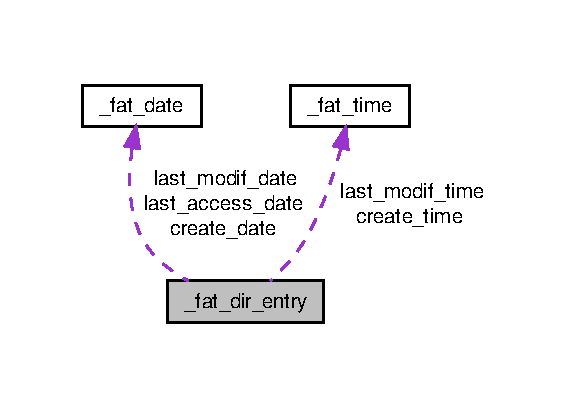
\includegraphics[width=273pt]{struct__fat__dir__entry__coll__graph}
\end{center}
\end{figure}
\subsection*{Champs de données}
\begin{DoxyCompactItemize}
\item 
char \hyperlink{struct__fat__dir__entry_abb18201b12e6039275e6dad91c19a99d}{utf8\-\_\-short\-\_\-name} \mbox{[}8\mbox{]}
\item 
char \hyperlink{struct__fat__dir__entry_addf0d1b2feefb5d50d90ea66b06703b9}{file\-\_\-extension} \mbox{[}3\mbox{]}
\item 
\hyperlink{kernel_2include_2types_8h_aba7bc1797add20fe3efdf37ced1182c5}{uint8\-\_\-t} \hyperlink{struct__fat__dir__entry_a4672718a4c89a279dd1c2b083ea73789}{file\-\_\-attributes}
\item 
\hyperlink{kernel_2include_2types_8h_aba7bc1797add20fe3efdf37ced1182c5}{uint8\-\_\-t} \hyperlink{struct__fat__dir__entry_a27e7962cefa12233338034dff3d75304}{reserved}
\item 
\hyperlink{kernel_2include_2types_8h_aba7bc1797add20fe3efdf37ced1182c5}{uint8\-\_\-t} \hyperlink{struct__fat__dir__entry_a54232a69203bce440a4bfaca30abcd00}{create\-\_\-time\-\_\-ms}
\item 
\hyperlink{fat__internal_8h_ab864004b9f8da2db1862a0da9acb1735}{fat\-\_\-time\-\_\-t} \hyperlink{struct__fat__dir__entry_a3c6cbf375afefcf8fc1518d5a96790a8}{create\-\_\-time}
\item 
\hyperlink{fat__internal_8h_a50b52e2d394a6d7c7f1f2b7c7ef93a19}{fat\-\_\-date\-\_\-t} \hyperlink{struct__fat__dir__entry_ac30b1ec037ee7658eda85b2dc09e5c2e}{create\-\_\-date}
\item 
\hyperlink{fat__internal_8h_a50b52e2d394a6d7c7f1f2b7c7ef93a19}{fat\-\_\-date\-\_\-t} \hyperlink{struct__fat__dir__entry_aa53da680ae2a6594c0f956c80a1b8ca4}{last\-\_\-access\-\_\-date}
\item 
\hypertarget{struct__fat__dir__entry_a4e4d3ec0d8662c572bb2ac7f9c4bc4c8}{\hyperlink{kernel_2include_2types_8h_adf4d876453337156dde61095e1f20223}{uint16\-\_\-t} {\bfseries ea\-\_\-index}}\label{struct__fat__dir__entry_a4e4d3ec0d8662c572bb2ac7f9c4bc4c8}

\item 
\hyperlink{fat__internal_8h_ab864004b9f8da2db1862a0da9acb1735}{fat\-\_\-time\-\_\-t} \hyperlink{struct__fat__dir__entry_a967f3fe06020a24a22bc83cb80637669}{last\-\_\-modif\-\_\-time}
\item 
\hyperlink{fat__internal_8h_a50b52e2d394a6d7c7f1f2b7c7ef93a19}{fat\-\_\-date\-\_\-t} \hyperlink{struct__fat__dir__entry_a9be27b92458730fbdf5342f717aadc32}{last\-\_\-modif\-\_\-date}
\item 
\hyperlink{kernel_2include_2types_8h_adf4d876453337156dde61095e1f20223}{uint16\-\_\-t} \hyperlink{struct__fat__dir__entry_ae129dc6a378e1bec5c92a3963d6522c6}{cluster\-\_\-pointer}
\item 
\hyperlink{kernel_2include_2types_8h_a33594304e786b158f3fb30289278f5af}{uint32\-\_\-t} \hyperlink{struct__fat__dir__entry_a557cd14b001d64851ad5e7cadb742411}{file\-\_\-size}
\end{DoxyCompactItemize}


\subsection{Description détaillée}
Entrée de dossier. 

\subsection{Documentation des champs}
\hypertarget{struct__fat__dir__entry_ae129dc6a378e1bec5c92a3963d6522c6}{\index{\-\_\-fat\-\_\-dir\-\_\-entry@{\-\_\-fat\-\_\-dir\-\_\-entry}!cluster\-\_\-pointer@{cluster\-\_\-pointer}}
\index{cluster\-\_\-pointer@{cluster\-\_\-pointer}!_fat_dir_entry@{\-\_\-fat\-\_\-dir\-\_\-entry}}
\subsubsection[{cluster\-\_\-pointer}]{\setlength{\rightskip}{0pt plus 5cm}{\bf uint16\-\_\-t} \-\_\-fat\-\_\-dir\-\_\-entry\-::cluster\-\_\-pointer}}\label{struct__fat__dir__entry_ae129dc6a378e1bec5c92a3963d6522c6}
Cluster où se situe le fichier. \hypertarget{struct__fat__dir__entry_ac30b1ec037ee7658eda85b2dc09e5c2e}{\index{\-\_\-fat\-\_\-dir\-\_\-entry@{\-\_\-fat\-\_\-dir\-\_\-entry}!create\-\_\-date@{create\-\_\-date}}
\index{create\-\_\-date@{create\-\_\-date}!_fat_dir_entry@{\-\_\-fat\-\_\-dir\-\_\-entry}}
\subsubsection[{create\-\_\-date}]{\setlength{\rightskip}{0pt plus 5cm}{\bf fat\-\_\-date\-\_\-t} \-\_\-fat\-\_\-dir\-\_\-entry\-::create\-\_\-date}}\label{struct__fat__dir__entry_ac30b1ec037ee7658eda85b2dc09e5c2e}
Date de création. \hypertarget{struct__fat__dir__entry_a3c6cbf375afefcf8fc1518d5a96790a8}{\index{\-\_\-fat\-\_\-dir\-\_\-entry@{\-\_\-fat\-\_\-dir\-\_\-entry}!create\-\_\-time@{create\-\_\-time}}
\index{create\-\_\-time@{create\-\_\-time}!_fat_dir_entry@{\-\_\-fat\-\_\-dir\-\_\-entry}}
\subsubsection[{create\-\_\-time}]{\setlength{\rightskip}{0pt plus 5cm}{\bf fat\-\_\-time\-\_\-t} \-\_\-fat\-\_\-dir\-\_\-entry\-::create\-\_\-time}}\label{struct__fat__dir__entry_a3c6cbf375afefcf8fc1518d5a96790a8}
Heure de création. \hypertarget{struct__fat__dir__entry_a54232a69203bce440a4bfaca30abcd00}{\index{\-\_\-fat\-\_\-dir\-\_\-entry@{\-\_\-fat\-\_\-dir\-\_\-entry}!create\-\_\-time\-\_\-ms@{create\-\_\-time\-\_\-ms}}
\index{create\-\_\-time\-\_\-ms@{create\-\_\-time\-\_\-ms}!_fat_dir_entry@{\-\_\-fat\-\_\-dir\-\_\-entry}}
\subsubsection[{create\-\_\-time\-\_\-ms}]{\setlength{\rightskip}{0pt plus 5cm}{\bf uint8\-\_\-t} \-\_\-fat\-\_\-dir\-\_\-entry\-::create\-\_\-time\-\_\-ms}}\label{struct__fat__dir__entry_a54232a69203bce440a4bfaca30abcd00}
Si existant \-: create time \mbox{[}0 -\/ 199\mbox{]} x 10ms Sinon \-: premier caractère (puisqu'on le remplace). \hypertarget{struct__fat__dir__entry_a4672718a4c89a279dd1c2b083ea73789}{\index{\-\_\-fat\-\_\-dir\-\_\-entry@{\-\_\-fat\-\_\-dir\-\_\-entry}!file\-\_\-attributes@{file\-\_\-attributes}}
\index{file\-\_\-attributes@{file\-\_\-attributes}!_fat_dir_entry@{\-\_\-fat\-\_\-dir\-\_\-entry}}
\subsubsection[{file\-\_\-attributes}]{\setlength{\rightskip}{0pt plus 5cm}{\bf uint8\-\_\-t} \-\_\-fat\-\_\-dir\-\_\-entry\-::file\-\_\-attributes}}\label{struct__fat__dir__entry_a4672718a4c89a279dd1c2b083ea73789}
Attributs du fichier (write, hidden, etc.) \hypertarget{struct__fat__dir__entry_addf0d1b2feefb5d50d90ea66b06703b9}{\index{\-\_\-fat\-\_\-dir\-\_\-entry@{\-\_\-fat\-\_\-dir\-\_\-entry}!file\-\_\-extension@{file\-\_\-extension}}
\index{file\-\_\-extension@{file\-\_\-extension}!_fat_dir_entry@{\-\_\-fat\-\_\-dir\-\_\-entry}}
\subsubsection[{file\-\_\-extension}]{\setlength{\rightskip}{0pt plus 5cm}char \-\_\-fat\-\_\-dir\-\_\-entry\-::file\-\_\-extension\mbox{[}3\mbox{]}}}\label{struct__fat__dir__entry_addf0d1b2feefb5d50d90ea66b06703b9}
Extension. \hypertarget{struct__fat__dir__entry_a557cd14b001d64851ad5e7cadb742411}{\index{\-\_\-fat\-\_\-dir\-\_\-entry@{\-\_\-fat\-\_\-dir\-\_\-entry}!file\-\_\-size@{file\-\_\-size}}
\index{file\-\_\-size@{file\-\_\-size}!_fat_dir_entry@{\-\_\-fat\-\_\-dir\-\_\-entry}}
\subsubsection[{file\-\_\-size}]{\setlength{\rightskip}{0pt plus 5cm}{\bf uint32\-\_\-t} \-\_\-fat\-\_\-dir\-\_\-entry\-::file\-\_\-size}}\label{struct__fat__dir__entry_a557cd14b001d64851ad5e7cadb742411}
Taille du fichier. \hypertarget{struct__fat__dir__entry_aa53da680ae2a6594c0f956c80a1b8ca4}{\index{\-\_\-fat\-\_\-dir\-\_\-entry@{\-\_\-fat\-\_\-dir\-\_\-entry}!last\-\_\-access\-\_\-date@{last\-\_\-access\-\_\-date}}
\index{last\-\_\-access\-\_\-date@{last\-\_\-access\-\_\-date}!_fat_dir_entry@{\-\_\-fat\-\_\-dir\-\_\-entry}}
\subsubsection[{last\-\_\-access\-\_\-date}]{\setlength{\rightskip}{0pt plus 5cm}{\bf fat\-\_\-date\-\_\-t} \-\_\-fat\-\_\-dir\-\_\-entry\-::last\-\_\-access\-\_\-date}}\label{struct__fat__dir__entry_aa53da680ae2a6594c0f956c80a1b8ca4}
Date dernier accès. \hypertarget{struct__fat__dir__entry_a9be27b92458730fbdf5342f717aadc32}{\index{\-\_\-fat\-\_\-dir\-\_\-entry@{\-\_\-fat\-\_\-dir\-\_\-entry}!last\-\_\-modif\-\_\-date@{last\-\_\-modif\-\_\-date}}
\index{last\-\_\-modif\-\_\-date@{last\-\_\-modif\-\_\-date}!_fat_dir_entry@{\-\_\-fat\-\_\-dir\-\_\-entry}}
\subsubsection[{last\-\_\-modif\-\_\-date}]{\setlength{\rightskip}{0pt plus 5cm}{\bf fat\-\_\-date\-\_\-t} \-\_\-fat\-\_\-dir\-\_\-entry\-::last\-\_\-modif\-\_\-date}}\label{struct__fat__dir__entry_a9be27b92458730fbdf5342f717aadc32}
Date de dernière modification. \hypertarget{struct__fat__dir__entry_a967f3fe06020a24a22bc83cb80637669}{\index{\-\_\-fat\-\_\-dir\-\_\-entry@{\-\_\-fat\-\_\-dir\-\_\-entry}!last\-\_\-modif\-\_\-time@{last\-\_\-modif\-\_\-time}}
\index{last\-\_\-modif\-\_\-time@{last\-\_\-modif\-\_\-time}!_fat_dir_entry@{\-\_\-fat\-\_\-dir\-\_\-entry}}
\subsubsection[{last\-\_\-modif\-\_\-time}]{\setlength{\rightskip}{0pt plus 5cm}{\bf fat\-\_\-time\-\_\-t} \-\_\-fat\-\_\-dir\-\_\-entry\-::last\-\_\-modif\-\_\-time}}\label{struct__fat__dir__entry_a967f3fe06020a24a22bc83cb80637669}
Heure de dernière modification. \hypertarget{struct__fat__dir__entry_a27e7962cefa12233338034dff3d75304}{\index{\-\_\-fat\-\_\-dir\-\_\-entry@{\-\_\-fat\-\_\-dir\-\_\-entry}!reserved@{reserved}}
\index{reserved@{reserved}!_fat_dir_entry@{\-\_\-fat\-\_\-dir\-\_\-entry}}
\subsubsection[{reserved}]{\setlength{\rightskip}{0pt plus 5cm}{\bf uint8\-\_\-t} \-\_\-fat\-\_\-dir\-\_\-entry\-::reserved}}\label{struct__fat__dir__entry_a27e7962cefa12233338034dff3d75304}
réservé. \hypertarget{struct__fat__dir__entry_abb18201b12e6039275e6dad91c19a99d}{\index{\-\_\-fat\-\_\-dir\-\_\-entry@{\-\_\-fat\-\_\-dir\-\_\-entry}!utf8\-\_\-short\-\_\-name@{utf8\-\_\-short\-\_\-name}}
\index{utf8\-\_\-short\-\_\-name@{utf8\-\_\-short\-\_\-name}!_fat_dir_entry@{\-\_\-fat\-\_\-dir\-\_\-entry}}
\subsubsection[{utf8\-\_\-short\-\_\-name}]{\setlength{\rightskip}{0pt plus 5cm}char \-\_\-fat\-\_\-dir\-\_\-entry\-::utf8\-\_\-short\-\_\-name\mbox{[}8\mbox{]}}}\label{struct__fat__dir__entry_abb18201b12e6039275e6dad91c19a99d}
Nom court. 

La documentation de cette structure a été générée à partir du fichier suivant \-:\begin{DoxyCompactItemize}
\item 
kernel/fs/fat/\hyperlink{fat__internal_8h}{fat\-\_\-internal.\-h}\end{DoxyCompactItemize}

\hypertarget{struct__fat__direntry__t}{\section{Référence de la structure \-\_\-fat\-\_\-direntry\-\_\-t}
\label{struct__fat__direntry__t}\index{\-\_\-fat\-\_\-direntry\-\_\-t@{\-\_\-fat\-\_\-direntry\-\_\-t}}
}


Graphe de collaboration de \-\_\-fat\-\_\-direntry\-\_\-t\-:
\nopagebreak
\begin{figure}[H]
\begin{center}
\leavevmode
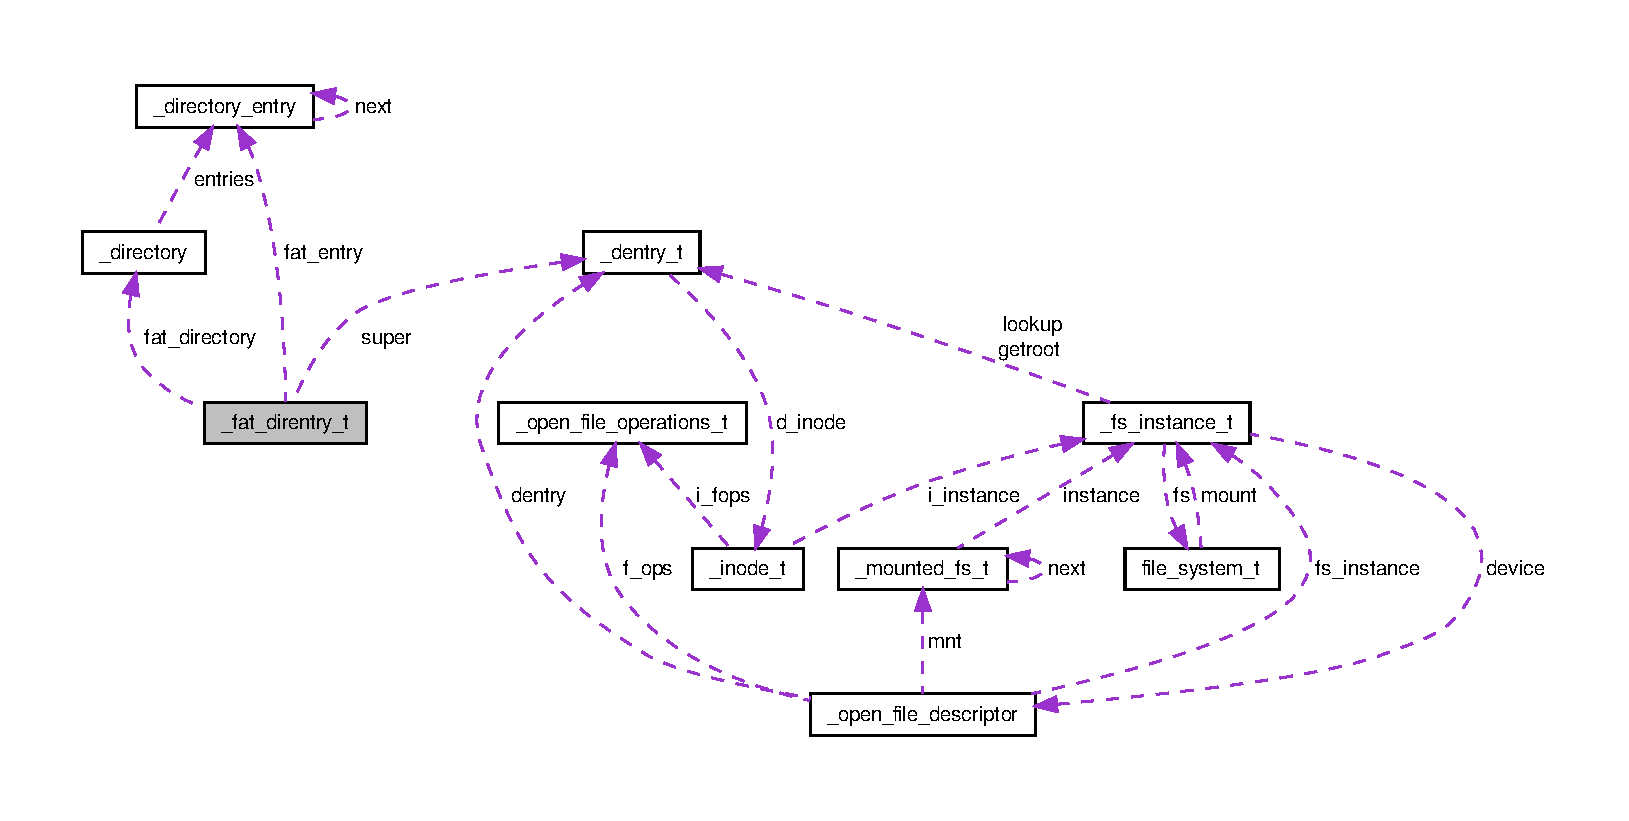
\includegraphics[width=350pt]{struct__fat__direntry__t__coll__graph}
\end{center}
\end{figure}
\subsection*{Champs de données}
\begin{DoxyCompactItemize}
\item 
\hypertarget{struct__fat__direntry__t_ad5c26f850433d9c813f416d3b5325b62}{\hyperlink{vfs_8h_ade5c998c6b3f09d2cf45d0e5ef8787da}{dentry\-\_\-t} {\bfseries super}}\label{struct__fat__direntry__t_ad5c26f850433d9c813f416d3b5325b62}

\item 
\hypertarget{struct__fat__direntry__t_a17b9dd242e07822ff9bc98a6a46e8c9e}{\hyperlink{fat__internal_8h_ab6546cb0abf935a615fae20884a41818}{directory\-\_\-entry\-\_\-t} $\ast$ {\bfseries fat\-\_\-entry}}\label{struct__fat__direntry__t_a17b9dd242e07822ff9bc98a6a46e8c9e}

\item 
\hypertarget{struct__fat__direntry__t_a15f0a5d5dcfd4fac4dbc9c3c976b33df}{\hyperlink{fat__internal_8h_a04e3d213fd143d58bbabf68062bdc21c}{directory\-\_\-t} $\ast$ {\bfseries fat\-\_\-directory}}\label{struct__fat__direntry__t_a15f0a5d5dcfd4fac4dbc9c3c976b33df}

\end{DoxyCompactItemize}


La documentation de cette structure a été générée à partir du fichier suivant \-:\begin{DoxyCompactItemize}
\item 
kernel/fs/fat/\hyperlink{fat__internal_8h}{fat\-\_\-internal.\-h}\end{DoxyCompactItemize}

\hypertarget{struct__fat__extended__BIOS__16}{\section{Référence de la structure \-\_\-fat\-\_\-extended\-\_\-\-B\-I\-O\-S\-\_\-16}
\label{struct__fat__extended__BIOS__16}\index{\-\_\-fat\-\_\-extended\-\_\-\-B\-I\-O\-S\-\_\-16@{\-\_\-fat\-\_\-extended\-\_\-\-B\-I\-O\-S\-\_\-16}}
}


{\ttfamily \#include $<$fat\-\_\-internal.\-h$>$}

\subsection*{Champs de données}
\begin{DoxyCompactItemize}
\item 
\hypertarget{struct__fat__extended__BIOS__16_aa5b1c000276996144da4ad9ba9feddd5}{\hyperlink{types_8h_aba7bc1797add20fe3efdf37ced1182c5}{uint8\-\_\-t} {\bfseries bios\-\_\-drive\-\_\-num}}\label{struct__fat__extended__BIOS__16_aa5b1c000276996144da4ad9ba9feddd5}

\item 
\hyperlink{types_8h_aba7bc1797add20fe3efdf37ced1182c5}{uint8\-\_\-t} \hyperlink{struct__fat__extended__BIOS__16_a893876cfc91a64059613c6fe02a1e178}{reserved}
\item 
\hyperlink{types_8h_aba7bc1797add20fe3efdf37ced1182c5}{uint8\-\_\-t} \hyperlink{struct__fat__extended__BIOS__16_a96dde388d85873830b8b421d13336737}{ext\-\_\-boot\-\_\-signature}
\item 
\hyperlink{types_8h_a33594304e786b158f3fb30289278f5af}{uint32\-\_\-t} \hyperlink{struct__fat__extended__BIOS__16_aa932fbe482a2da22749a6f9fa42fce59}{volume\-\_\-id}
\item 
\hyperlink{types_8h_aba7bc1797add20fe3efdf37ced1182c5}{uint8\-\_\-t} \hyperlink{struct__fat__extended__BIOS__16_a0f859beb837eb3013ef4ad48dd0c9845}{volume\-\_\-label} \mbox{[}11\mbox{]}
\item 
\hyperlink{types_8h_aba7bc1797add20fe3efdf37ced1182c5}{uint8\-\_\-t} \hyperlink{struct__fat__extended__BIOS__16_a0cdaccd704186c37f3df6b7a44fdbad8}{fat\-\_\-type\-\_\-label} \mbox{[}8\mbox{]}
\item 
\hypertarget{struct__fat__extended__BIOS__16_a7e244ef68c27303d5598ea070d93bb5f}{\hyperlink{types_8h_aba7bc1797add20fe3efdf37ced1182c5}{uint8\-\_\-t} {\bfseries os\-\_\-boot\-\_\-code} \mbox{[}448\mbox{]}}\label{struct__fat__extended__BIOS__16_a7e244ef68c27303d5598ea070d93bb5f}

\item 
\hypertarget{struct__fat__extended__BIOS__16_a8c98dbd269ae4ee38a0ae0d062162202}{\hyperlink{types_8h_adf4d876453337156dde61095e1f20223}{uint16\-\_\-t} {\bfseries boot\-\_\-sector\-\_\-sign}}\label{struct__fat__extended__BIOS__16_a8c98dbd269ae4ee38a0ae0d062162202}

\end{DoxyCompactItemize}


\subsection{Description détaillée}
Extended B\-I\-O\-S Parameter Block (F\-A\-T12 / F\-A\-T16) 

\subsection{Documentation des champs}
\hypertarget{struct__fat__extended__BIOS__16_a96dde388d85873830b8b421d13336737}{\index{\-\_\-fat\-\_\-extended\-\_\-\-B\-I\-O\-S\-\_\-16@{\-\_\-fat\-\_\-extended\-\_\-\-B\-I\-O\-S\-\_\-16}!ext\-\_\-boot\-\_\-signature@{ext\-\_\-boot\-\_\-signature}}
\index{ext\-\_\-boot\-\_\-signature@{ext\-\_\-boot\-\_\-signature}!_fat_extended_BIOS_16@{\-\_\-fat\-\_\-extended\-\_\-\-B\-I\-O\-S\-\_\-16}}
\subsubsection[{ext\-\_\-boot\-\_\-signature}]{\setlength{\rightskip}{0pt plus 5cm}{\bf uint8\-\_\-t} \-\_\-fat\-\_\-extended\-\_\-\-B\-I\-O\-S\-\_\-16\-::ext\-\_\-boot\-\_\-signature}}\label{struct__fat__extended__BIOS__16_a96dde388d85873830b8b421d13336737}
Ext Boot record signature = 29h \hypertarget{struct__fat__extended__BIOS__16_a0cdaccd704186c37f3df6b7a44fdbad8}{\index{\-\_\-fat\-\_\-extended\-\_\-\-B\-I\-O\-S\-\_\-16@{\-\_\-fat\-\_\-extended\-\_\-\-B\-I\-O\-S\-\_\-16}!fat\-\_\-type\-\_\-label@{fat\-\_\-type\-\_\-label}}
\index{fat\-\_\-type\-\_\-label@{fat\-\_\-type\-\_\-label}!_fat_extended_BIOS_16@{\-\_\-fat\-\_\-extended\-\_\-\-B\-I\-O\-S\-\_\-16}}
\subsubsection[{fat\-\_\-type\-\_\-label}]{\setlength{\rightskip}{0pt plus 5cm}{\bf uint8\-\_\-t} \-\_\-fat\-\_\-extended\-\_\-\-B\-I\-O\-S\-\_\-16\-::fat\-\_\-type\-\_\-label\mbox{[}8\mbox{]}}}\label{struct__fat__extended__BIOS__16_a0cdaccd704186c37f3df6b7a44fdbad8}
Nom du F\-S (F\-A\-T12, F\-A\-T16 ou F\-A\-T32). \hypertarget{struct__fat__extended__BIOS__16_a893876cfc91a64059613c6fe02a1e178}{\index{\-\_\-fat\-\_\-extended\-\_\-\-B\-I\-O\-S\-\_\-16@{\-\_\-fat\-\_\-extended\-\_\-\-B\-I\-O\-S\-\_\-16}!reserved@{reserved}}
\index{reserved@{reserved}!_fat_extended_BIOS_16@{\-\_\-fat\-\_\-extended\-\_\-\-B\-I\-O\-S\-\_\-16}}
\subsubsection[{reserved}]{\setlength{\rightskip}{0pt plus 5cm}{\bf uint8\-\_\-t} \-\_\-fat\-\_\-extended\-\_\-\-B\-I\-O\-S\-\_\-16\-::reserved}}\label{struct__fat__extended__BIOS__16_a893876cfc91a64059613c6fe02a1e178}
Reserved \hypertarget{struct__fat__extended__BIOS__16_aa932fbe482a2da22749a6f9fa42fce59}{\index{\-\_\-fat\-\_\-extended\-\_\-\-B\-I\-O\-S\-\_\-16@{\-\_\-fat\-\_\-extended\-\_\-\-B\-I\-O\-S\-\_\-16}!volume\-\_\-id@{volume\-\_\-id}}
\index{volume\-\_\-id@{volume\-\_\-id}!_fat_extended_BIOS_16@{\-\_\-fat\-\_\-extended\-\_\-\-B\-I\-O\-S\-\_\-16}}
\subsubsection[{volume\-\_\-id}]{\setlength{\rightskip}{0pt plus 5cm}{\bf uint32\-\_\-t} \-\_\-fat\-\_\-extended\-\_\-\-B\-I\-O\-S\-\_\-16\-::volume\-\_\-id}}\label{struct__fat__extended__BIOS__16_aa932fbe482a2da22749a6f9fa42fce59}
Identifiant du volume (serial). \hypertarget{struct__fat__extended__BIOS__16_a0f859beb837eb3013ef4ad48dd0c9845}{\index{\-\_\-fat\-\_\-extended\-\_\-\-B\-I\-O\-S\-\_\-16@{\-\_\-fat\-\_\-extended\-\_\-\-B\-I\-O\-S\-\_\-16}!volume\-\_\-label@{volume\-\_\-label}}
\index{volume\-\_\-label@{volume\-\_\-label}!_fat_extended_BIOS_16@{\-\_\-fat\-\_\-extended\-\_\-\-B\-I\-O\-S\-\_\-16}}
\subsubsection[{volume\-\_\-label}]{\setlength{\rightskip}{0pt plus 5cm}{\bf uint8\-\_\-t} \-\_\-fat\-\_\-extended\-\_\-\-B\-I\-O\-S\-\_\-16\-::volume\-\_\-label\mbox{[}11\mbox{]}}}\label{struct__fat__extended__BIOS__16_a0f859beb837eb3013ef4ad48dd0c9845}
Nom du volume. 

La documentation de cette structure a été générée à partir du fichier suivant \-:\begin{DoxyCompactItemize}
\item 
kernel/fs/fat/\hyperlink{fat__internal_8h}{fat\-\_\-internal.\-h}\end{DoxyCompactItemize}

\hypertarget{struct__fat__extended__BIOS__32}{\section{Référence de la structure \-\_\-fat\-\_\-extended\-\_\-\-B\-I\-O\-S\-\_\-32}
\label{struct__fat__extended__BIOS__32}\index{\-\_\-fat\-\_\-extended\-\_\-\-B\-I\-O\-S\-\_\-32@{\-\_\-fat\-\_\-extended\-\_\-\-B\-I\-O\-S\-\_\-32}}
}


{\ttfamily \#include $<$fat\-\_\-internal.\-h$>$}

\subsection*{Champs de données}
\begin{DoxyCompactItemize}
\item 
\hypertarget{struct__fat__extended__BIOS__32_afe9918174f4b717fe9ba858b792b6b76}{\hyperlink{kernel_2include_2types_8h_a33594304e786b158f3fb30289278f5af}{uint32\-\_\-t} {\bfseries table\-\_\-size\-\_\-32}}\label{struct__fat__extended__BIOS__32_afe9918174f4b717fe9ba858b792b6b76}

\item 
\hypertarget{struct__fat__extended__BIOS__32_a58bc295c5eec01f9daec08d84340817e}{\hyperlink{kernel_2include_2types_8h_adf4d876453337156dde61095e1f20223}{uint16\-\_\-t} {\bfseries fat\-\_\-flags}}\label{struct__fat__extended__BIOS__32_a58bc295c5eec01f9daec08d84340817e}

\item 
\hypertarget{struct__fat__extended__BIOS__32_a9eb3b046449e1e1c868e1ecb1d6a9fe2}{\hyperlink{kernel_2include_2types_8h_adf4d876453337156dde61095e1f20223}{uint16\-\_\-t} {\bfseries version}}\label{struct__fat__extended__BIOS__32_a9eb3b046449e1e1c868e1ecb1d6a9fe2}

\item 
\hypertarget{struct__fat__extended__BIOS__32_a78cf2bb3768b41a3b054d6c71d5c61e7}{\hyperlink{kernel_2include_2types_8h_a33594304e786b158f3fb30289278f5af}{uint32\-\_\-t} {\bfseries cluster\-\_\-root\-\_\-dir}}\label{struct__fat__extended__BIOS__32_a78cf2bb3768b41a3b054d6c71d5c61e7}

\item 
\hypertarget{struct__fat__extended__BIOS__32_a38e8b2efc3921f696d435b878fc85007}{\hyperlink{kernel_2include_2types_8h_adf4d876453337156dde61095e1f20223}{uint16\-\_\-t} {\bfseries sector\-\_\-fs\-\_\-info}}\label{struct__fat__extended__BIOS__32_a38e8b2efc3921f696d435b878fc85007}

\item 
\hypertarget{struct__fat__extended__BIOS__32_aa55ea52137b033ae69f69c4e4e16dc3b}{\hyperlink{kernel_2include_2types_8h_adf4d876453337156dde61095e1f20223}{uint16\-\_\-t} {\bfseries sector\-\_\-bs\-\_\-backup}}\label{struct__fat__extended__BIOS__32_aa55ea52137b033ae69f69c4e4e16dc3b}

\item 
\hypertarget{struct__fat__extended__BIOS__32_a25fb7603d9e8880009846e15ac4d9aae}{\hyperlink{kernel_2include_2types_8h_aba7bc1797add20fe3efdf37ced1182c5}{uint8\-\_\-t} {\bfseries reserved} \mbox{[}12\mbox{]}}\label{struct__fat__extended__BIOS__32_a25fb7603d9e8880009846e15ac4d9aae}

\item 
\hypertarget{struct__fat__extended__BIOS__32_acf777537731e41bc68af607900d5a018}{\hyperlink{kernel_2include_2types_8h_aba7bc1797add20fe3efdf37ced1182c5}{uint8\-\_\-t} {\bfseries bios\-\_\-drive\-\_\-num}}\label{struct__fat__extended__BIOS__32_acf777537731e41bc68af607900d5a018}

\item 
\hypertarget{struct__fat__extended__BIOS__32_a488d282895360bd73efee46006bf4d68}{\hyperlink{kernel_2include_2types_8h_aba7bc1797add20fe3efdf37ced1182c5}{uint8\-\_\-t} {\bfseries reserved2}}\label{struct__fat__extended__BIOS__32_a488d282895360bd73efee46006bf4d68}

\item 
\hypertarget{struct__fat__extended__BIOS__32_a314c684ae663fc5d6a055c1788f76da0}{\hyperlink{kernel_2include_2types_8h_aba7bc1797add20fe3efdf37ced1182c5}{uint8\-\_\-t} {\bfseries ext\-\_\-boot\-\_\-signature}}\label{struct__fat__extended__BIOS__32_a314c684ae663fc5d6a055c1788f76da0}

\item 
\hypertarget{struct__fat__extended__BIOS__32_ab7bc765d99e29d5e7fa8528acfbf3dc7}{\hyperlink{kernel_2include_2types_8h_a33594304e786b158f3fb30289278f5af}{uint32\-\_\-t} {\bfseries volume\-\_\-id}}\label{struct__fat__extended__BIOS__32_ab7bc765d99e29d5e7fa8528acfbf3dc7}

\item 
\hypertarget{struct__fat__extended__BIOS__32_a9a3d4e96af0e5f091f2022fdb4d01a16}{\hyperlink{kernel_2include_2types_8h_aba7bc1797add20fe3efdf37ced1182c5}{uint8\-\_\-t} {\bfseries volume\-\_\-label} \mbox{[}11\mbox{]}}\label{struct__fat__extended__BIOS__32_a9a3d4e96af0e5f091f2022fdb4d01a16}

\item 
\hypertarget{struct__fat__extended__BIOS__32_a32f7610d214294fe570dd12637c1e32e}{\hyperlink{kernel_2include_2types_8h_aba7bc1797add20fe3efdf37ced1182c5}{uint8\-\_\-t} {\bfseries fat\-\_\-type\-\_\-label} \mbox{[}8\mbox{]}}\label{struct__fat__extended__BIOS__32_a32f7610d214294fe570dd12637c1e32e}

\item 
\hypertarget{struct__fat__extended__BIOS__32_ac163d55b696ec5e32d9d74482d6abe38}{\hyperlink{kernel_2include_2types_8h_aba7bc1797add20fe3efdf37ced1182c5}{uint8\-\_\-t} {\bfseries os\-\_\-boot\-\_\-code} \mbox{[}420\mbox{]}}\label{struct__fat__extended__BIOS__32_ac163d55b696ec5e32d9d74482d6abe38}

\item 
\hypertarget{struct__fat__extended__BIOS__32_a2cc6336683f3694723e4118983960174}{\hyperlink{kernel_2include_2types_8h_adf4d876453337156dde61095e1f20223}{uint16\-\_\-t} {\bfseries boot\-\_\-sector\-\_\-sign}}\label{struct__fat__extended__BIOS__32_a2cc6336683f3694723e4118983960174}

\end{DoxyCompactItemize}


\subsection{Description détaillée}
Extended B\-I\-O\-S Parameter Block (F\-A\-T 32) 

La documentation de cette structure a été générée à partir du fichier suivant \-:\begin{DoxyCompactItemize}
\item 
kernel/fs/fat/\hyperlink{fat__internal_8h}{fat\-\_\-internal.\-h}\end{DoxyCompactItemize}

\hypertarget{struct__fat__extra__data__t}{\section{Référence de la structure \+\_\+fat\+\_\+extra\+\_\+data\+\_\+t}
\label{struct__fat__extra__data__t}\index{\+\_\+fat\+\_\+extra\+\_\+data\+\_\+t@{\+\_\+fat\+\_\+extra\+\_\+data\+\_\+t}}
}


Données supplémentaires qui sont ajoutés à l'ofd lors du open.  




{\ttfamily \#include $<$fat\+\_\+internal.\+h$>$}

\subsection*{Champs de données}
\begin{DoxyCompactItemize}
\item 
int \hyperlink{struct__fat__extra__data__t_a5cc9910b0f971c600d2d4a52290509fa}{first\+\_\+cluster}
\item 
int \hyperlink{struct__fat__extra__data__t_a0708cae473b2962cfa6c10f50d9b008b}{current\+\_\+cluster}
\item 
unsigned int \hyperlink{struct__fat__extra__data__t_a38be57e802b36532ce01e46d7be7da44}{current\+\_\+octet\+\_\+buf}
\item 
\hyperlink{kernel_2include_2types_8h_aba7bc1797add20fe3efdf37ced1182c5}{uint8\+\_\+t} \hyperlink{struct__fat__extra__data__t_a74dd347d769bd4aefdf0ad1207be6798}{buffer} \mbox{[}512\mbox{]}
\end{DoxyCompactItemize}


\subsection{Documentation des champs}
\hypertarget{struct__fat__extra__data__t_a74dd347d769bd4aefdf0ad1207be6798}{\index{\+\_\+fat\+\_\+extra\+\_\+data\+\_\+t@{\+\_\+fat\+\_\+extra\+\_\+data\+\_\+t}!buffer@{buffer}}
\index{buffer@{buffer}!\+\_\+fat\+\_\+extra\+\_\+data\+\_\+t@{\+\_\+fat\+\_\+extra\+\_\+data\+\_\+t}}
\subsubsection[{buffer}]{\setlength{\rightskip}{0pt plus 5cm}{\bf uint8\+\_\+t} \+\_\+fat\+\_\+extra\+\_\+data\+\_\+t\+::buffer\mbox{[}512\mbox{]}}}\label{struct__fat__extra__data__t_a74dd347d769bd4aefdf0ad1207be6798}
Buffer pour limiter les appels au disque. \hypertarget{struct__fat__extra__data__t_a0708cae473b2962cfa6c10f50d9b008b}{\index{\+\_\+fat\+\_\+extra\+\_\+data\+\_\+t@{\+\_\+fat\+\_\+extra\+\_\+data\+\_\+t}!current\+\_\+cluster@{current\+\_\+cluster}}
\index{current\+\_\+cluster@{current\+\_\+cluster}!\+\_\+fat\+\_\+extra\+\_\+data\+\_\+t@{\+\_\+fat\+\_\+extra\+\_\+data\+\_\+t}}
\subsubsection[{current\+\_\+cluster}]{\setlength{\rightskip}{0pt plus 5cm}int \+\_\+fat\+\_\+extra\+\_\+data\+\_\+t\+::current\+\_\+cluster}}\label{struct__fat__extra__data__t_a0708cae473b2962cfa6c10f50d9b008b}
Cluster courant. \hypertarget{struct__fat__extra__data__t_a38be57e802b36532ce01e46d7be7da44}{\index{\+\_\+fat\+\_\+extra\+\_\+data\+\_\+t@{\+\_\+fat\+\_\+extra\+\_\+data\+\_\+t}!current\+\_\+octet\+\_\+buf@{current\+\_\+octet\+\_\+buf}}
\index{current\+\_\+octet\+\_\+buf@{current\+\_\+octet\+\_\+buf}!\+\_\+fat\+\_\+extra\+\_\+data\+\_\+t@{\+\_\+fat\+\_\+extra\+\_\+data\+\_\+t}}
\subsubsection[{current\+\_\+octet\+\_\+buf}]{\setlength{\rightskip}{0pt plus 5cm}unsigned int \+\_\+fat\+\_\+extra\+\_\+data\+\_\+t\+::current\+\_\+octet\+\_\+buf}}\label{struct__fat__extra__data__t_a38be57e802b36532ce01e46d7be7da44}
Position dans le buffer. \hypertarget{struct__fat__extra__data__t_a5cc9910b0f971c600d2d4a52290509fa}{\index{\+\_\+fat\+\_\+extra\+\_\+data\+\_\+t@{\+\_\+fat\+\_\+extra\+\_\+data\+\_\+t}!first\+\_\+cluster@{first\+\_\+cluster}}
\index{first\+\_\+cluster@{first\+\_\+cluster}!\+\_\+fat\+\_\+extra\+\_\+data\+\_\+t@{\+\_\+fat\+\_\+extra\+\_\+data\+\_\+t}}
\subsubsection[{first\+\_\+cluster}]{\setlength{\rightskip}{0pt plus 5cm}int \+\_\+fat\+\_\+extra\+\_\+data\+\_\+t\+::first\+\_\+cluster}}\label{struct__fat__extra__data__t_a5cc9910b0f971c600d2d4a52290509fa}
Adresse du premier cluster. 

La documentation de cette structure a été générée à partir du fichier suivant \+:\begin{DoxyCompactItemize}
\item 
kernel/fs/fat/\hyperlink{fat__internal_8h}{fat\+\_\+internal.\+h}\end{DoxyCompactItemize}

\hypertarget{struct__fat__fs__instance__t}{\section{\-Référence de la structure \-\_\-fat\-\_\-fs\-\_\-instance\-\_\-t}
\label{struct__fat__fs__instance__t}\index{\-\_\-fat\-\_\-fs\-\_\-instance\-\_\-t@{\-\_\-fat\-\_\-fs\-\_\-instance\-\_\-t}}
}


{\ttfamily \#include $<$fat\-\_\-internal.\-h$>$}



\-Graphe de collaboration de \-\_\-fat\-\_\-fs\-\_\-instance\-\_\-t\-:\nopagebreak
\begin{figure}[H]
\begin{center}
\leavevmode
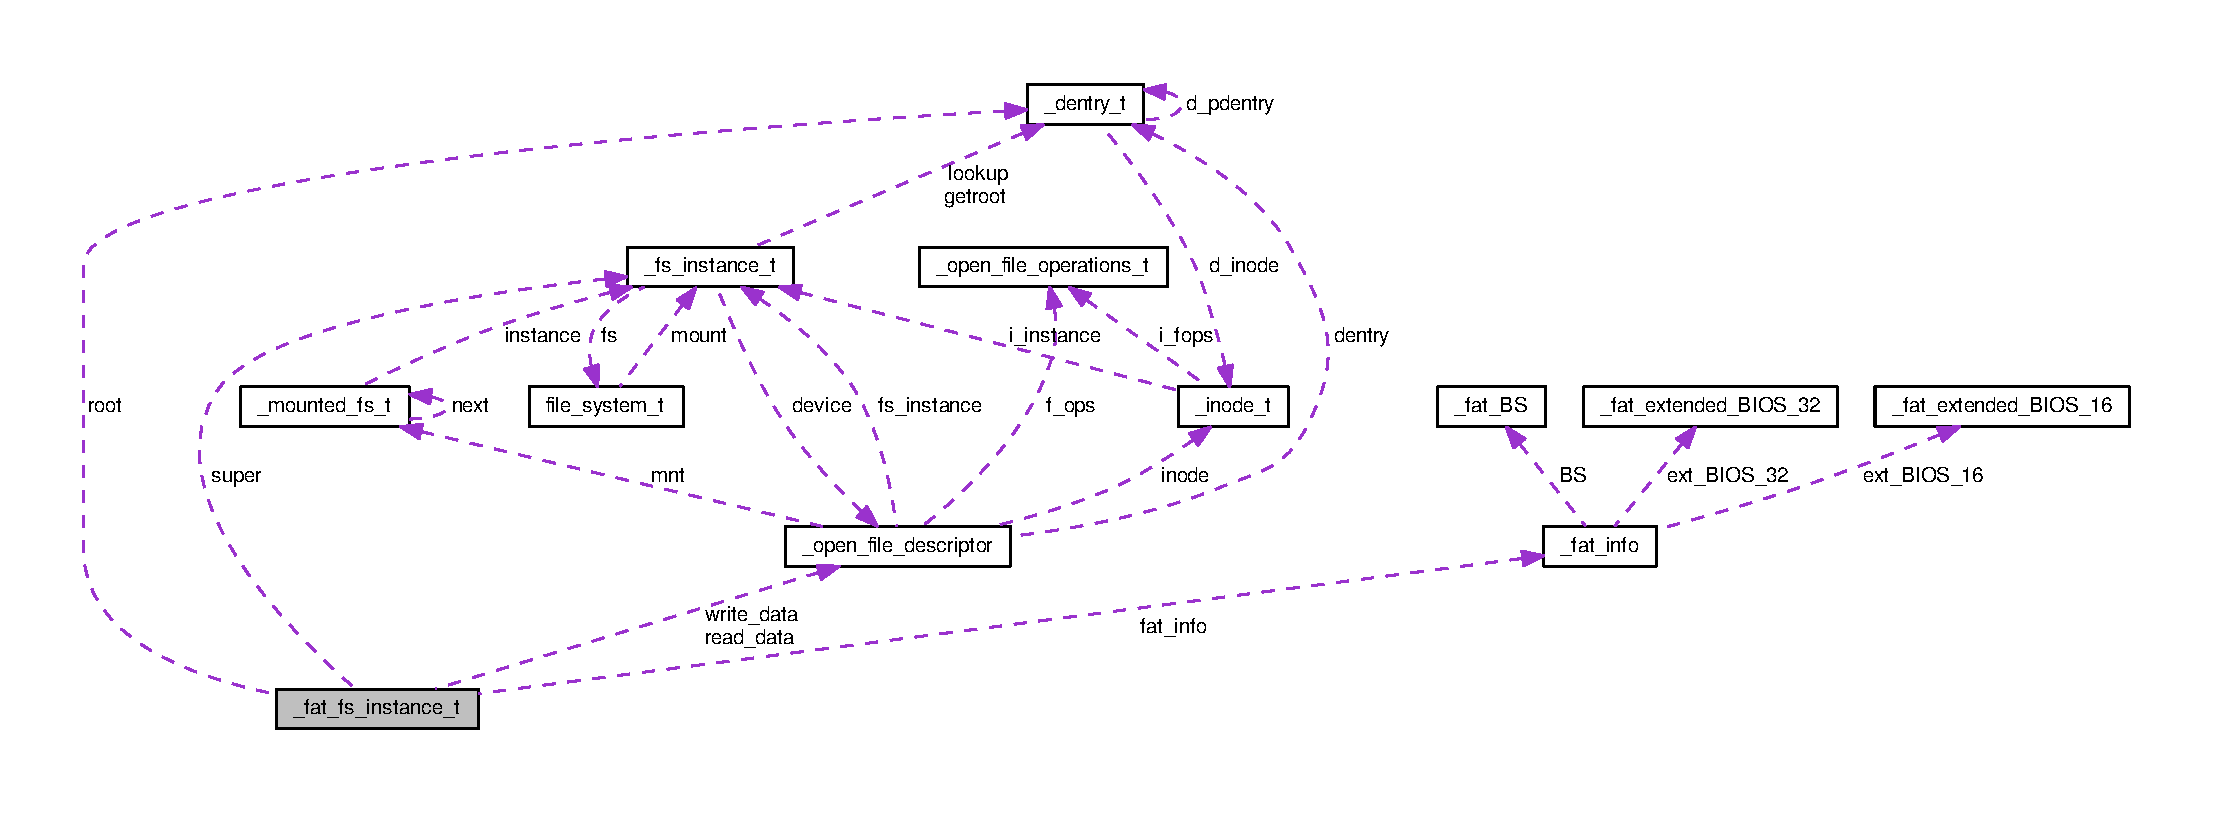
\includegraphics[width=350pt]{struct__fat__fs__instance__t__coll__graph}
\end{center}
\end{figure}
\subsection*{\-Champs de données}
\begin{DoxyCompactItemize}
\item 
\hyperlink{vfs_8h_a0eefa9aac35a5462ebf1e038992ca860}{fs\-\_\-instance\-\_\-t} \hyperlink{struct__fat__fs__instance__t_ac50318180f107a1950961c404ec6fd6d}{super}
\item 
\hyperlink{fat__internal_8h_a1921d26ef987e5498294fe311a23c62f}{fat\-\_\-info\-\_\-t} \hyperlink{struct__fat__fs__instance__t_acebada58b620f950c9ef3c454db812fc}{fat\-\_\-info}
\end{DoxyCompactItemize}


\subsection{\-Description détaillée}
\-Instance de \-F\-S de type \-F\-A\-T. 

\subsection{\-Documentation des champs}
\hypertarget{struct__fat__fs__instance__t_acebada58b620f950c9ef3c454db812fc}{\index{\-\_\-fat\-\_\-fs\-\_\-instance\-\_\-t@{\-\_\-fat\-\_\-fs\-\_\-instance\-\_\-t}!fat\-\_\-info@{fat\-\_\-info}}
\index{fat\-\_\-info@{fat\-\_\-info}!_fat_fs_instance_t@{\-\_\-fat\-\_\-fs\-\_\-instance\-\_\-t}}
\subsubsection[{fat\-\_\-info}]{\setlength{\rightskip}{0pt plus 5cm}{\bf fat\-\_\-info\-\_\-t} {\bf \-\_\-fat\-\_\-fs\-\_\-instance\-\_\-t\-::fat\-\_\-info}}}\label{struct__fat__fs__instance__t_acebada58b620f950c9ef3c454db812fc}
\-Informations sur le volume monté. \hypertarget{struct__fat__fs__instance__t_ac50318180f107a1950961c404ec6fd6d}{\index{\-\_\-fat\-\_\-fs\-\_\-instance\-\_\-t@{\-\_\-fat\-\_\-fs\-\_\-instance\-\_\-t}!super@{super}}
\index{super@{super}!_fat_fs_instance_t@{\-\_\-fat\-\_\-fs\-\_\-instance\-\_\-t}}
\subsubsection[{super}]{\setlength{\rightskip}{0pt plus 5cm}{\bf fs\-\_\-instance\-\_\-t} {\bf \-\_\-fat\-\_\-fs\-\_\-instance\-\_\-t\-::super}}}\label{struct__fat__fs__instance__t_ac50318180f107a1950961c404ec6fd6d}
\-Classe parente (fs\-\_\-instance\-\_\-t). 

\-La documentation de cette structure a été générée à partir du fichier suivant \-:\begin{DoxyCompactItemize}
\item 
kernel/fs/fat/\hyperlink{fat__internal_8h}{fat\-\_\-internal.\-h}\end{DoxyCompactItemize}

\hypertarget{struct__fat__info}{\section{Référence de la structure \+\_\+fat\+\_\+info}
\label{struct__fat__info}\index{\+\_\+fat\+\_\+info@{\+\_\+fat\+\_\+info}}
}


{\ttfamily \#include $<$fat\+\_\+internal.\+h$>$}



Graphe de collaboration de \+\_\+fat\+\_\+info\+:\nopagebreak
\begin{figure}[H]
\begin{center}
\leavevmode
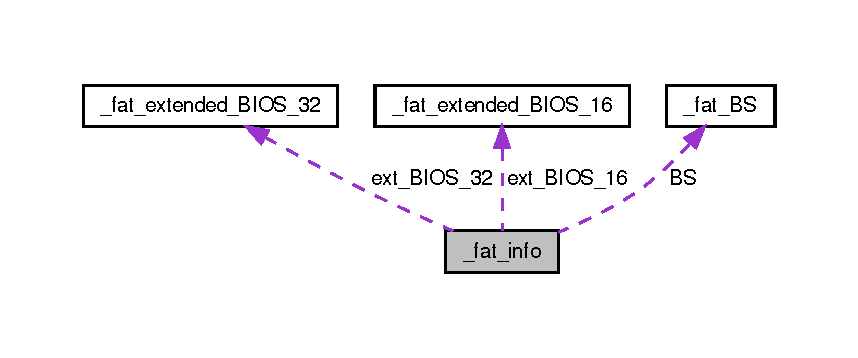
\includegraphics[width=350pt]{struct__fat__info__coll__graph}
\end{center}
\end{figure}
\subsection*{Champs de données}
\begin{DoxyCompactItemize}
\item 
\hyperlink{fat__internal_8h_a2fa84596abf5ea3bd6f27951a77333c5}{fat\+\_\+\+B\+S\+\_\+t} \hyperlink{struct__fat__info_adcd12930a4a7f94ecac42ba82567adb7}{B\+S}
\item 
\hyperlink{fat__internal_8h_a017a64d5b6e25780d01109008245c15c}{fat\+\_\+extended\+\_\+\+B\+I\+O\+S\+\_\+16\+\_\+t} $\ast$ \hyperlink{struct__fat__info_a4da4c2a7a629ca59a686822e6447acb8}{ext\+\_\+\+B\+I\+O\+S\+\_\+16}
\item 
\hyperlink{fat__internal_8h_ac3feb4afc4c75c10410e9e867e3f99e8}{fat\+\_\+extended\+\_\+\+B\+I\+O\+S\+\_\+32\+\_\+t} $\ast$ \hyperlink{struct__fat__info_aab203e7eb3c2027e3034d7765a2d5281}{ext\+\_\+\+B\+I\+O\+S\+\_\+32}
\item 
unsigned int $\ast$ \hyperlink{struct__fat__info_a0344193eb413dce4369b6e36ed03b92b}{addr\+\_\+fat}
\item 
unsigned int \hyperlink{struct__fat__info_ae9133d320e0afc89c5e6cc9cedf6dfb5}{addr\+\_\+root\+\_\+dir}
\item 
unsigned int \hyperlink{struct__fat__info_a4cb2766e74dd65f24d4eb30ce3b49302}{addr\+\_\+data}
\item 
unsigned int $\ast$ \hyperlink{struct__fat__info_a27195d09eb1dcd65d35d7b312d1bec0b}{file\+\_\+alloc\+\_\+table}
\item 
unsigned int \hyperlink{struct__fat__info_ab43681d4b5c7cf719cd6c934cada39e3}{total\+\_\+data\+\_\+clusters}
\item 
unsigned int \hyperlink{struct__fat__info_af110757af771c0f3fe0c515cca1ff177}{table\+\_\+size}
\item 
\hyperlink{fat__internal_8h_aea47744930623076e66d2f155e12ca24}{fat\+\_\+t} \hyperlink{struct__fat__info_af9e994d6d2c5211614ca61cfa4492500}{fat\+\_\+type}
\item 
unsigned int \hyperlink{struct__fat__info_ac1ba92d928512827ab7978f136efda96}{bytes\+\_\+per\+\_\+cluster}
\end{DoxyCompactItemize}


\subsection{Description détaillée}
Structure qui contient tout ce qui est utilisé par le driver F\+A\+T. 

\subsection{Documentation des champs}
\hypertarget{struct__fat__info_a4cb2766e74dd65f24d4eb30ce3b49302}{\index{\+\_\+fat\+\_\+info@{\+\_\+fat\+\_\+info}!addr\+\_\+data@{addr\+\_\+data}}
\index{addr\+\_\+data@{addr\+\_\+data}!\+\_\+fat\+\_\+info@{\+\_\+fat\+\_\+info}}
\subsubsection[{addr\+\_\+data}]{\setlength{\rightskip}{0pt plus 5cm}unsigned int \+\_\+fat\+\_\+info\+::addr\+\_\+data}}\label{struct__fat__info_a4cb2766e74dd65f24d4eb30ce3b49302}
Adresse des premiers clusters de données. \hypertarget{struct__fat__info_a0344193eb413dce4369b6e36ed03b92b}{\index{\+\_\+fat\+\_\+info@{\+\_\+fat\+\_\+info}!addr\+\_\+fat@{addr\+\_\+fat}}
\index{addr\+\_\+fat@{addr\+\_\+fat}!\+\_\+fat\+\_\+info@{\+\_\+fat\+\_\+info}}
\subsubsection[{addr\+\_\+fat}]{\setlength{\rightskip}{0pt plus 5cm}unsigned int$\ast$ \+\_\+fat\+\_\+info\+::addr\+\_\+fat}}\label{struct__fat__info_a0344193eb413dce4369b6e36ed03b92b}
Adresses des F\+A\+T. \hypertarget{struct__fat__info_ae9133d320e0afc89c5e6cc9cedf6dfb5}{\index{\+\_\+fat\+\_\+info@{\+\_\+fat\+\_\+info}!addr\+\_\+root\+\_\+dir@{addr\+\_\+root\+\_\+dir}}
\index{addr\+\_\+root\+\_\+dir@{addr\+\_\+root\+\_\+dir}!\+\_\+fat\+\_\+info@{\+\_\+fat\+\_\+info}}
\subsubsection[{addr\+\_\+root\+\_\+dir}]{\setlength{\rightskip}{0pt plus 5cm}unsigned int \+\_\+fat\+\_\+info\+::addr\+\_\+root\+\_\+dir}}\label{struct__fat__info_ae9133d320e0afc89c5e6cc9cedf6dfb5}
Adresse du dossier racine (attention spécificité F\+A\+T32). \hypertarget{struct__fat__info_adcd12930a4a7f94ecac42ba82567adb7}{\index{\+\_\+fat\+\_\+info@{\+\_\+fat\+\_\+info}!B\+S@{B\+S}}
\index{B\+S@{B\+S}!\+\_\+fat\+\_\+info@{\+\_\+fat\+\_\+info}}
\subsubsection[{B\+S}]{\setlength{\rightskip}{0pt plus 5cm}{\bf fat\+\_\+\+B\+S\+\_\+t} \+\_\+fat\+\_\+info\+::\+B\+S}}\label{struct__fat__info_adcd12930a4a7f94ecac42ba82567adb7}
Secteur de Boot. \hypertarget{struct__fat__info_ac1ba92d928512827ab7978f136efda96}{\index{\+\_\+fat\+\_\+info@{\+\_\+fat\+\_\+info}!bytes\+\_\+per\+\_\+cluster@{bytes\+\_\+per\+\_\+cluster}}
\index{bytes\+\_\+per\+\_\+cluster@{bytes\+\_\+per\+\_\+cluster}!\+\_\+fat\+\_\+info@{\+\_\+fat\+\_\+info}}
\subsubsection[{bytes\+\_\+per\+\_\+cluster}]{\setlength{\rightskip}{0pt plus 5cm}unsigned int \+\_\+fat\+\_\+info\+::bytes\+\_\+per\+\_\+cluster}}\label{struct__fat__info_ac1ba92d928512827ab7978f136efda96}
Nombre d'octets dans un cluster. \hypertarget{struct__fat__info_a4da4c2a7a629ca59a686822e6447acb8}{\index{\+\_\+fat\+\_\+info@{\+\_\+fat\+\_\+info}!ext\+\_\+\+B\+I\+O\+S\+\_\+16@{ext\+\_\+\+B\+I\+O\+S\+\_\+16}}
\index{ext\+\_\+\+B\+I\+O\+S\+\_\+16@{ext\+\_\+\+B\+I\+O\+S\+\_\+16}!\+\_\+fat\+\_\+info@{\+\_\+fat\+\_\+info}}
\subsubsection[{ext\+\_\+\+B\+I\+O\+S\+\_\+16}]{\setlength{\rightskip}{0pt plus 5cm}{\bf fat\+\_\+extended\+\_\+\+B\+I\+O\+S\+\_\+16\+\_\+t}$\ast$ \+\_\+fat\+\_\+info\+::ext\+\_\+\+B\+I\+O\+S\+\_\+16}}\label{struct__fat__info_a4da4c2a7a629ca59a686822e6447acb8}
Infos supplémentaires pour F\+A\+T16. \hypertarget{struct__fat__info_aab203e7eb3c2027e3034d7765a2d5281}{\index{\+\_\+fat\+\_\+info@{\+\_\+fat\+\_\+info}!ext\+\_\+\+B\+I\+O\+S\+\_\+32@{ext\+\_\+\+B\+I\+O\+S\+\_\+32}}
\index{ext\+\_\+\+B\+I\+O\+S\+\_\+32@{ext\+\_\+\+B\+I\+O\+S\+\_\+32}!\+\_\+fat\+\_\+info@{\+\_\+fat\+\_\+info}}
\subsubsection[{ext\+\_\+\+B\+I\+O\+S\+\_\+32}]{\setlength{\rightskip}{0pt plus 5cm}{\bf fat\+\_\+extended\+\_\+\+B\+I\+O\+S\+\_\+32\+\_\+t}$\ast$ \+\_\+fat\+\_\+info\+::ext\+\_\+\+B\+I\+O\+S\+\_\+32}}\label{struct__fat__info_aab203e7eb3c2027e3034d7765a2d5281}
Infos supplémentaires pour F\+A\+T32. \hypertarget{struct__fat__info_af9e994d6d2c5211614ca61cfa4492500}{\index{\+\_\+fat\+\_\+info@{\+\_\+fat\+\_\+info}!fat\+\_\+type@{fat\+\_\+type}}
\index{fat\+\_\+type@{fat\+\_\+type}!\+\_\+fat\+\_\+info@{\+\_\+fat\+\_\+info}}
\subsubsection[{fat\+\_\+type}]{\setlength{\rightskip}{0pt plus 5cm}{\bf fat\+\_\+t} \+\_\+fat\+\_\+info\+::fat\+\_\+type}}\label{struct__fat__info_af9e994d6d2c5211614ca61cfa4492500}
Type de F\+A\+T (12, 16 ou 32) \hypertarget{struct__fat__info_a27195d09eb1dcd65d35d7b312d1bec0b}{\index{\+\_\+fat\+\_\+info@{\+\_\+fat\+\_\+info}!file\+\_\+alloc\+\_\+table@{file\+\_\+alloc\+\_\+table}}
\index{file\+\_\+alloc\+\_\+table@{file\+\_\+alloc\+\_\+table}!\+\_\+fat\+\_\+info@{\+\_\+fat\+\_\+info}}
\subsubsection[{file\+\_\+alloc\+\_\+table}]{\setlength{\rightskip}{0pt plus 5cm}unsigned int$\ast$ \+\_\+fat\+\_\+info\+::file\+\_\+alloc\+\_\+table}}\label{struct__fat__info_a27195d09eb1dcd65d35d7b312d1bec0b}
F\+A\+T en mémoire. \hypertarget{struct__fat__info_af110757af771c0f3fe0c515cca1ff177}{\index{\+\_\+fat\+\_\+info@{\+\_\+fat\+\_\+info}!table\+\_\+size@{table\+\_\+size}}
\index{table\+\_\+size@{table\+\_\+size}!\+\_\+fat\+\_\+info@{\+\_\+fat\+\_\+info}}
\subsubsection[{table\+\_\+size}]{\setlength{\rightskip}{0pt plus 5cm}unsigned int \+\_\+fat\+\_\+info\+::table\+\_\+size}}\label{struct__fat__info_af110757af771c0f3fe0c515cca1ff177}
Taille de la F\+A\+T. \hypertarget{struct__fat__info_ab43681d4b5c7cf719cd6c934cada39e3}{\index{\+\_\+fat\+\_\+info@{\+\_\+fat\+\_\+info}!total\+\_\+data\+\_\+clusters@{total\+\_\+data\+\_\+clusters}}
\index{total\+\_\+data\+\_\+clusters@{total\+\_\+data\+\_\+clusters}!\+\_\+fat\+\_\+info@{\+\_\+fat\+\_\+info}}
\subsubsection[{total\+\_\+data\+\_\+clusters}]{\setlength{\rightskip}{0pt plus 5cm}unsigned int \+\_\+fat\+\_\+info\+::total\+\_\+data\+\_\+clusters}}\label{struct__fat__info_ab43681d4b5c7cf719cd6c934cada39e3}
Nombre de clusters de données. 

La documentation de cette structure a été générée à partir du fichier suivant \+:\begin{DoxyCompactItemize}
\item 
kernel/fs/fat/\hyperlink{fat__internal_8h}{fat\+\_\+internal.\+h}\end{DoxyCompactItemize}

\hypertarget{struct__fat__time}{\section{Référence de la structure \+\_\+fat\+\_\+time}
\label{struct__fat__time}\index{\+\_\+fat\+\_\+time@{\+\_\+fat\+\_\+time}}
}


{\ttfamily \#include $<$fat\+\_\+internal.\+h$>$}

\subsection*{Champs de données}
\begin{DoxyCompactItemize}
\item 
unsigned int \hyperlink{struct__fat__time_ab02d4606058041887618d3b9beb92749}{seconds2}\+: 5
\item 
unsigned int \hyperlink{struct__fat__time_a92c31beaa1318e3ddf1457a57c30f1aa}{minutes}\+: 6
\item 
unsigned int \hyperlink{struct__fat__time_a7a3028be0bfed0b785e012d88c45f873}{hours}\+: 5
\end{DoxyCompactItemize}


\subsection{Description détaillée}
Représentation du temps au format F\+A\+T. 

\subsection{Documentation des champs}
\hypertarget{struct__fat__time_a7a3028be0bfed0b785e012d88c45f873}{\index{\+\_\+fat\+\_\+time@{\+\_\+fat\+\_\+time}!hours@{hours}}
\index{hours@{hours}!\+\_\+fat\+\_\+time@{\+\_\+fat\+\_\+time}}
\subsubsection[{hours}]{\setlength{\rightskip}{0pt plus 5cm}unsigned int \+\_\+fat\+\_\+time\+::hours}}\label{struct__fat__time_a7a3028be0bfed0b785e012d88c45f873}
Nombre d'heures. \hypertarget{struct__fat__time_a92c31beaa1318e3ddf1457a57c30f1aa}{\index{\+\_\+fat\+\_\+time@{\+\_\+fat\+\_\+time}!minutes@{minutes}}
\index{minutes@{minutes}!\+\_\+fat\+\_\+time@{\+\_\+fat\+\_\+time}}
\subsubsection[{minutes}]{\setlength{\rightskip}{0pt plus 5cm}unsigned int \+\_\+fat\+\_\+time\+::minutes}}\label{struct__fat__time_a92c31beaa1318e3ddf1457a57c30f1aa}
Nombre de minutes. \hypertarget{struct__fat__time_ab02d4606058041887618d3b9beb92749}{\index{\+\_\+fat\+\_\+time@{\+\_\+fat\+\_\+time}!seconds2@{seconds2}}
\index{seconds2@{seconds2}!\+\_\+fat\+\_\+time@{\+\_\+fat\+\_\+time}}
\subsubsection[{seconds2}]{\setlength{\rightskip}{0pt plus 5cm}unsigned int \+\_\+fat\+\_\+time\+::seconds2}}\label{struct__fat__time_ab02d4606058041887618d3b9beb92749}
Nombre de secondes. 

La documentation de cette structure a été générée à partir du fichier suivant \+:\begin{DoxyCompactItemize}
\item 
kernel/fs/fat/\hyperlink{fat__internal_8h}{fat\+\_\+internal.\+h}\end{DoxyCompactItemize}

\hypertarget{struct__file__attributes__t}{\section{Référence de la structure \-\_\-file\-\_\-attributes\-\_\-t}
\label{struct__file__attributes__t}\index{\-\_\-file\-\_\-attributes\-\_\-t@{\-\_\-file\-\_\-attributes\-\_\-t}}
}


{\ttfamily \#include $<$vfs.\-h$>$}



Graphe de collaboration de \-\_\-file\-\_\-attributes\-\_\-t\-:
\nopagebreak
\begin{figure}[H]
\begin{center}
\leavevmode
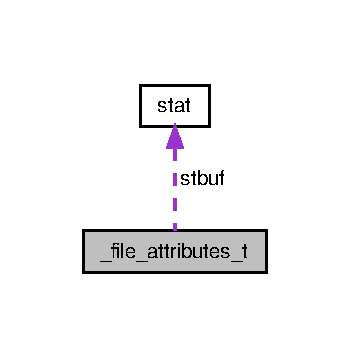
\includegraphics[width=168pt]{struct__file__attributes__t__coll__graph}
\end{center}
\end{figure}
\subsection*{Champs de données}
\begin{DoxyCompactItemize}
\item 
int \hyperlink{struct__file__attributes__t_a51072887a2d07ba9e5566cef453c3707}{mask}
\item 
struct \hyperlink{structstat}{stat} \hyperlink{struct__file__attributes__t_aa42b25ef9e64509420c287ab6b60c8a8}{stbuf}
\item 
\hypertarget{struct__file__attributes__t_ae1424de59c1c74710ce2cc66ce03a3af}{\hyperlink{kernel_2include_2types_8h_a29d85914ddff32967d85ada69854206d}{size\-\_\-t} {\bfseries ia\-\_\-size}}\label{struct__file__attributes__t_ae1424de59c1c74710ce2cc66ce03a3af}

\end{DoxyCompactItemize}


\subsection{Description détaillée}
Structure permettant de setter des informations. 

\subsection{Documentation des champs}
\hypertarget{struct__file__attributes__t_a51072887a2d07ba9e5566cef453c3707}{\index{\-\_\-file\-\_\-attributes\-\_\-t@{\-\_\-file\-\_\-attributes\-\_\-t}!mask@{mask}}
\index{mask@{mask}!_file_attributes_t@{\-\_\-file\-\_\-attributes\-\_\-t}}
\subsubsection[{mask}]{\setlength{\rightskip}{0pt plus 5cm}int \-\_\-file\-\_\-attributes\-\_\-t\-::mask}}\label{struct__file__attributes__t_a51072887a2d07ba9e5566cef453c3707}
Champs valides. \hypertarget{struct__file__attributes__t_aa42b25ef9e64509420c287ab6b60c8a8}{\index{\-\_\-file\-\_\-attributes\-\_\-t@{\-\_\-file\-\_\-attributes\-\_\-t}!stbuf@{stbuf}}
\index{stbuf@{stbuf}!_file_attributes_t@{\-\_\-file\-\_\-attributes\-\_\-t}}
\subsubsection[{stbuf}]{\setlength{\rightskip}{0pt plus 5cm}struct {\bf stat} \-\_\-file\-\_\-attributes\-\_\-t\-::stbuf}}\label{struct__file__attributes__t_aa42b25ef9e64509420c287ab6b60c8a8}
Structure contenant les informations. 

La documentation de cette structure a été générée à partir du fichier suivant \-:\begin{DoxyCompactItemize}
\item 
kernel/include/\hyperlink{vfs_8h}{vfs.\-h}\end{DoxyCompactItemize}

\hypertarget{struct__fs__instance__t}{\section{Référence de la structure \-\_\-fs\-\_\-instance\-\_\-t}
\label{struct__fs__instance__t}\index{\-\_\-fs\-\_\-instance\-\_\-t@{\-\_\-fs\-\_\-instance\-\_\-t}}
}


Instance d'un couple F\-S/\-Device monté.  




{\ttfamily \#include $<$vfs.\-h$>$}



Graphe de collaboration de \-\_\-fs\-\_\-instance\-\_\-t\-:\nopagebreak
\begin{figure}[H]
\begin{center}
\leavevmode
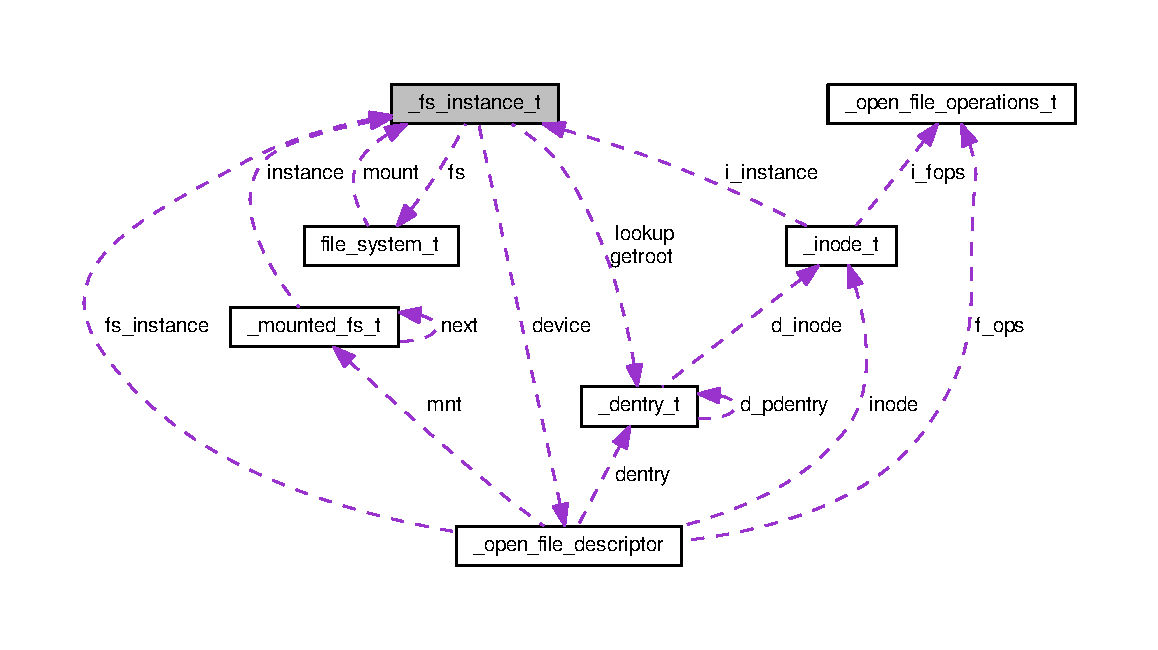
\includegraphics[width=350pt]{struct__fs__instance__t__coll__graph}
\end{center}
\end{figure}
\subsection*{Champs de données}
\begin{DoxyCompactItemize}
\item 
\hyperlink{structfile__system__t}{file\-\_\-system\-\_\-t} $\ast$ \hyperlink{struct__fs__instance__t_a209ef4e2ed00460eead263311373a974}{fs}
\item 
\hyperlink{fd__types_8h_a42bccb9b6a816213613cefffced245f0}{open\-\_\-file\-\_\-descriptor} $\ast$ \hyperlink{struct__fs__instance__t_acc3db122838752a84c6ecb93c3644256}{device}
\item 
struct \hyperlink{struct__dentry__t}{\-\_\-dentry\-\_\-t} $\ast$($\ast$ \hyperlink{struct__fs__instance__t_af6891a9d9e5c2fd0458312fd8567213a}{getroot} )(struct \hyperlink{struct__fs__instance__t}{\-\_\-fs\-\_\-instance\-\_\-t} $\ast$)
\item 
struct \hyperlink{struct__dentry__t}{\-\_\-dentry\-\_\-t} $\ast$($\ast$ \hyperlink{struct__fs__instance__t_a820510562ecb31cbbf6b4fc8a4d2ce6a}{lookup} )(struct \hyperlink{struct__fs__instance__t}{\-\_\-fs\-\_\-instance\-\_\-t} $\ast$, struct \hyperlink{struct__dentry__t}{\-\_\-dentry\-\_\-t} $\ast$, const char $\ast$)
\item 
int($\ast$ \hyperlink{struct__fs__instance__t_a705d100026840b619f217931dc8419f3}{mkdir} )(struct \hyperlink{struct__inode__t}{\-\_\-inode\-\_\-t} $\ast$, struct \hyperlink{struct__dentry__t}{\-\_\-dentry\-\_\-t} $\ast$, \hyperlink{kstat_8h_af8f4385bb42836d1e3ad4fea9d71d1b9}{mode\-\_\-t})
\item 
int($\ast$ \hyperlink{struct__fs__instance__t_ae57436a3bfd6de530204a67a8ac2f4f0}{mknod} )(struct \hyperlink{struct__inode__t}{\-\_\-inode\-\_\-t} $\ast$, struct \hyperlink{struct__dentry__t}{\-\_\-dentry\-\_\-t} $\ast$, \hyperlink{kstat_8h_af8f4385bb42836d1e3ad4fea9d71d1b9}{mode\-\_\-t}, \hyperlink{kstat_8h_a451f1b5788fa7cc5d33db47a5992e7a6}{dev\-\_\-t})
\item 
int($\ast$ \hyperlink{struct__fs__instance__t_aaccc941115b40d9605fdc3895c9b8e9b}{stat} )(struct \hyperlink{struct__inode__t}{\-\_\-inode\-\_\-t} $\ast$, struct \hyperlink{structstat}{stat} $\ast$)
\item 
int($\ast$ \hyperlink{struct__fs__instance__t_a38cfd710b2d88ebb388059e90a406db6}{unlink} )(struct \hyperlink{struct__inode__t}{\-\_\-inode\-\_\-t} $\ast$, struct \hyperlink{struct__dentry__t}{\-\_\-dentry\-\_\-t} $\ast$)
\item 
int($\ast$ \hyperlink{struct__fs__instance__t_a4ceb71ff00d0a5fda03aa644c4694bef}{rmdir} )(struct \hyperlink{struct__inode__t}{\-\_\-inode\-\_\-t} $\ast$, struct \hyperlink{struct__dentry__t}{\-\_\-dentry\-\_\-t} $\ast$)
\item 
int($\ast$ \hyperlink{struct__fs__instance__t_a02c8b56a14997bf58d8350a26e441954}{truncate} )(struct \hyperlink{struct__inode__t}{\-\_\-inode\-\_\-t} $\ast$, \hyperlink{libc_2include_2sys_2types_8h_a447a6a64dbb8fb44b1e62856b333db4a}{off\-\_\-t} size)
\item 
int($\ast$ \hyperlink{struct__fs__instance__t_ae76a7f1f9c4653baa497343bf26918a6}{setattr} )(struct \hyperlink{struct__inode__t}{\-\_\-inode\-\_\-t} $\ast$inode, struct \hyperlink{struct__file__attributes__t}{\-\_\-file\-\_\-attributes\-\_\-t} $\ast$attr)
\item 
int($\ast$ \hyperlink{struct__fs__instance__t_a62e37513c47dda9d11e534cf84d6f48b}{rename} )(struct \hyperlink{struct__inode__t}{\-\_\-inode\-\_\-t} $\ast$old\-\_\-dir, struct \hyperlink{struct__dentry__t}{\-\_\-dentry\-\_\-t} $\ast$old\-\_\-dentry, struct \hyperlink{struct__inode__t}{\-\_\-inode\-\_\-t} $\ast$new\-\_\-dir, struct \hyperlink{struct__dentry__t}{\-\_\-dentry\-\_\-t} $\ast$new\-\_\-dentry)
\end{DoxyCompactItemize}


\subsection{Documentation des champs}
\hypertarget{struct__fs__instance__t_acc3db122838752a84c6ecb93c3644256}{\index{\-\_\-fs\-\_\-instance\-\_\-t@{\-\_\-fs\-\_\-instance\-\_\-t}!device@{device}}
\index{device@{device}!_fs_instance_t@{\-\_\-fs\-\_\-instance\-\_\-t}}
\subsubsection[{device}]{\setlength{\rightskip}{0pt plus 5cm}{\bf open\-\_\-file\-\_\-descriptor}$\ast$ \-\_\-fs\-\_\-instance\-\_\-t\-::device}}\label{struct__fs__instance__t_acc3db122838752a84c6ecb93c3644256}
Device utilisé. \hypertarget{struct__fs__instance__t_a209ef4e2ed00460eead263311373a974}{\index{\-\_\-fs\-\_\-instance\-\_\-t@{\-\_\-fs\-\_\-instance\-\_\-t}!fs@{fs}}
\index{fs@{fs}!_fs_instance_t@{\-\_\-fs\-\_\-instance\-\_\-t}}
\subsubsection[{fs}]{\setlength{\rightskip}{0pt plus 5cm}{\bf file\-\_\-system\-\_\-t}$\ast$ \-\_\-fs\-\_\-instance\-\_\-t\-::fs}}\label{struct__fs__instance__t_a209ef4e2ed00460eead263311373a974}
Pointeur vers le F\-S utilisé. \hypertarget{struct__fs__instance__t_af6891a9d9e5c2fd0458312fd8567213a}{\index{\-\_\-fs\-\_\-instance\-\_\-t@{\-\_\-fs\-\_\-instance\-\_\-t}!getroot@{getroot}}
\index{getroot@{getroot}!_fs_instance_t@{\-\_\-fs\-\_\-instance\-\_\-t}}
\subsubsection[{getroot}]{\setlength{\rightskip}{0pt plus 5cm}struct {\bf \-\_\-dentry\-\_\-t}$\ast$($\ast$ \-\_\-fs\-\_\-instance\-\_\-t\-::getroot)(struct {\bf \-\_\-fs\-\_\-instance\-\_\-t} $\ast$)\hspace{0.3cm}{\ttfamily [read]}}}\label{struct__fs__instance__t_af6891a9d9e5c2fd0458312fd8567213a}
Noeud racine. \hypertarget{struct__fs__instance__t_a820510562ecb31cbbf6b4fc8a4d2ce6a}{\index{\-\_\-fs\-\_\-instance\-\_\-t@{\-\_\-fs\-\_\-instance\-\_\-t}!lookup@{lookup}}
\index{lookup@{lookup}!_fs_instance_t@{\-\_\-fs\-\_\-instance\-\_\-t}}
\subsubsection[{lookup}]{\setlength{\rightskip}{0pt plus 5cm}struct {\bf \-\_\-dentry\-\_\-t}$\ast$($\ast$ \-\_\-fs\-\_\-instance\-\_\-t\-::lookup)(struct {\bf \-\_\-fs\-\_\-instance\-\_\-t} $\ast$, struct {\bf \-\_\-dentry\-\_\-t} $\ast$, const char $\ast$)\hspace{0.3cm}{\ttfamily [read]}}}\label{struct__fs__instance__t_a820510562ecb31cbbf6b4fc8a4d2ce6a}
Résolution path. \hypertarget{struct__fs__instance__t_a705d100026840b619f217931dc8419f3}{\index{\-\_\-fs\-\_\-instance\-\_\-t@{\-\_\-fs\-\_\-instance\-\_\-t}!mkdir@{mkdir}}
\index{mkdir@{mkdir}!_fs_instance_t@{\-\_\-fs\-\_\-instance\-\_\-t}}
\subsubsection[{mkdir}]{\setlength{\rightskip}{0pt plus 5cm}int($\ast$ \-\_\-fs\-\_\-instance\-\_\-t\-::mkdir)(struct {\bf \-\_\-inode\-\_\-t} $\ast$, struct {\bf \-\_\-dentry\-\_\-t} $\ast$, {\bf mode\-\_\-t})}}\label{struct__fs__instance__t_a705d100026840b619f217931dc8419f3}
Création d'un dossier. \hypertarget{struct__fs__instance__t_ae57436a3bfd6de530204a67a8ac2f4f0}{\index{\-\_\-fs\-\_\-instance\-\_\-t@{\-\_\-fs\-\_\-instance\-\_\-t}!mknod@{mknod}}
\index{mknod@{mknod}!_fs_instance_t@{\-\_\-fs\-\_\-instance\-\_\-t}}
\subsubsection[{mknod}]{\setlength{\rightskip}{0pt plus 5cm}int($\ast$ \-\_\-fs\-\_\-instance\-\_\-t\-::mknod)(struct {\bf \-\_\-inode\-\_\-t} $\ast$, struct {\bf \-\_\-dentry\-\_\-t} $\ast$, {\bf mode\-\_\-t}, {\bf dev\-\_\-t})}}\label{struct__fs__instance__t_ae57436a3bfd6de530204a67a8ac2f4f0}
Création d'un noeud. \hypertarget{struct__fs__instance__t_a62e37513c47dda9d11e534cf84d6f48b}{\index{\-\_\-fs\-\_\-instance\-\_\-t@{\-\_\-fs\-\_\-instance\-\_\-t}!rename@{rename}}
\index{rename@{rename}!_fs_instance_t@{\-\_\-fs\-\_\-instance\-\_\-t}}
\subsubsection[{rename}]{\setlength{\rightskip}{0pt plus 5cm}int($\ast$ \-\_\-fs\-\_\-instance\-\_\-t\-::rename)(struct {\bf \-\_\-inode\-\_\-t} $\ast$old\-\_\-dir, struct {\bf \-\_\-dentry\-\_\-t} $\ast$old\-\_\-dentry, struct {\bf \-\_\-inode\-\_\-t} $\ast$new\-\_\-dir, struct {\bf \-\_\-dentry\-\_\-t} $\ast$new\-\_\-dentry)}}\label{struct__fs__instance__t_a62e37513c47dda9d11e534cf84d6f48b}
Renomme ou déplace un fichier. \hypertarget{struct__fs__instance__t_a4ceb71ff00d0a5fda03aa644c4694bef}{\index{\-\_\-fs\-\_\-instance\-\_\-t@{\-\_\-fs\-\_\-instance\-\_\-t}!rmdir@{rmdir}}
\index{rmdir@{rmdir}!_fs_instance_t@{\-\_\-fs\-\_\-instance\-\_\-t}}
\subsubsection[{rmdir}]{\setlength{\rightskip}{0pt plus 5cm}int($\ast$ \-\_\-fs\-\_\-instance\-\_\-t\-::rmdir)(struct {\bf \-\_\-inode\-\_\-t} $\ast$, struct {\bf \-\_\-dentry\-\_\-t} $\ast$)}}\label{struct__fs__instance__t_a4ceb71ff00d0a5fda03aa644c4694bef}
Suppression d'un dossier vide. \hypertarget{struct__fs__instance__t_ae76a7f1f9c4653baa497343bf26918a6}{\index{\-\_\-fs\-\_\-instance\-\_\-t@{\-\_\-fs\-\_\-instance\-\_\-t}!setattr@{setattr}}
\index{setattr@{setattr}!_fs_instance_t@{\-\_\-fs\-\_\-instance\-\_\-t}}
\subsubsection[{setattr}]{\setlength{\rightskip}{0pt plus 5cm}int($\ast$ \-\_\-fs\-\_\-instance\-\_\-t\-::setattr)(struct {\bf \-\_\-inode\-\_\-t} $\ast$inode, struct {\bf \-\_\-file\-\_\-attributes\-\_\-t} $\ast$attr)}}\label{struct__fs__instance__t_ae76a7f1f9c4653baa497343bf26918a6}
Modifie certains paramètres. \hypertarget{struct__fs__instance__t_aaccc941115b40d9605fdc3895c9b8e9b}{\index{\-\_\-fs\-\_\-instance\-\_\-t@{\-\_\-fs\-\_\-instance\-\_\-t}!stat@{stat}}
\index{stat@{stat}!_fs_instance_t@{\-\_\-fs\-\_\-instance\-\_\-t}}
\subsubsection[{stat}]{\setlength{\rightskip}{0pt plus 5cm}int($\ast$ \-\_\-fs\-\_\-instance\-\_\-t\-::stat)(struct {\bf \-\_\-inode\-\_\-t} $\ast$, struct {\bf stat} $\ast$)}}\label{struct__fs__instance__t_aaccc941115b40d9605fdc3895c9b8e9b}
Obtenir les infos d'un noeud. \hypertarget{struct__fs__instance__t_a02c8b56a14997bf58d8350a26e441954}{\index{\-\_\-fs\-\_\-instance\-\_\-t@{\-\_\-fs\-\_\-instance\-\_\-t}!truncate@{truncate}}
\index{truncate@{truncate}!_fs_instance_t@{\-\_\-fs\-\_\-instance\-\_\-t}}
\subsubsection[{truncate}]{\setlength{\rightskip}{0pt plus 5cm}int($\ast$ \-\_\-fs\-\_\-instance\-\_\-t\-::truncate)(struct {\bf \-\_\-inode\-\_\-t} $\ast$, {\bf off\-\_\-t} size)}}\label{struct__fs__instance__t_a02c8b56a14997bf58d8350a26e441954}
Changer la taille d'un fichier. \hypertarget{struct__fs__instance__t_a38cfd710b2d88ebb388059e90a406db6}{\index{\-\_\-fs\-\_\-instance\-\_\-t@{\-\_\-fs\-\_\-instance\-\_\-t}!unlink@{unlink}}
\index{unlink@{unlink}!_fs_instance_t@{\-\_\-fs\-\_\-instance\-\_\-t}}
\subsubsection[{unlink}]{\setlength{\rightskip}{0pt plus 5cm}int($\ast$ \-\_\-fs\-\_\-instance\-\_\-t\-::unlink)(struct {\bf \-\_\-inode\-\_\-t} $\ast$, struct {\bf \-\_\-dentry\-\_\-t} $\ast$)}}\label{struct__fs__instance__t_a38cfd710b2d88ebb388059e90a406db6}
Suppression d'un noeud. 

La documentation de cette structure a été générée à partir du fichier suivant \-:\begin{DoxyCompactItemize}
\item 
kernel/include/\hyperlink{vfs_8h}{vfs.\-h}\end{DoxyCompactItemize}

\hypertarget{struct__inode__t}{\section{Référence de la structure \-\_\-inode\-\_\-t}
\label{struct__inode__t}\index{\-\_\-inode\-\_\-t@{\-\_\-inode\-\_\-t}}
}


{\ttfamily \#include $<$vfs.\-h$>$}



Graphe de collaboration de \-\_\-inode\-\_\-t\-:\nopagebreak
\begin{figure}[H]
\begin{center}
\leavevmode
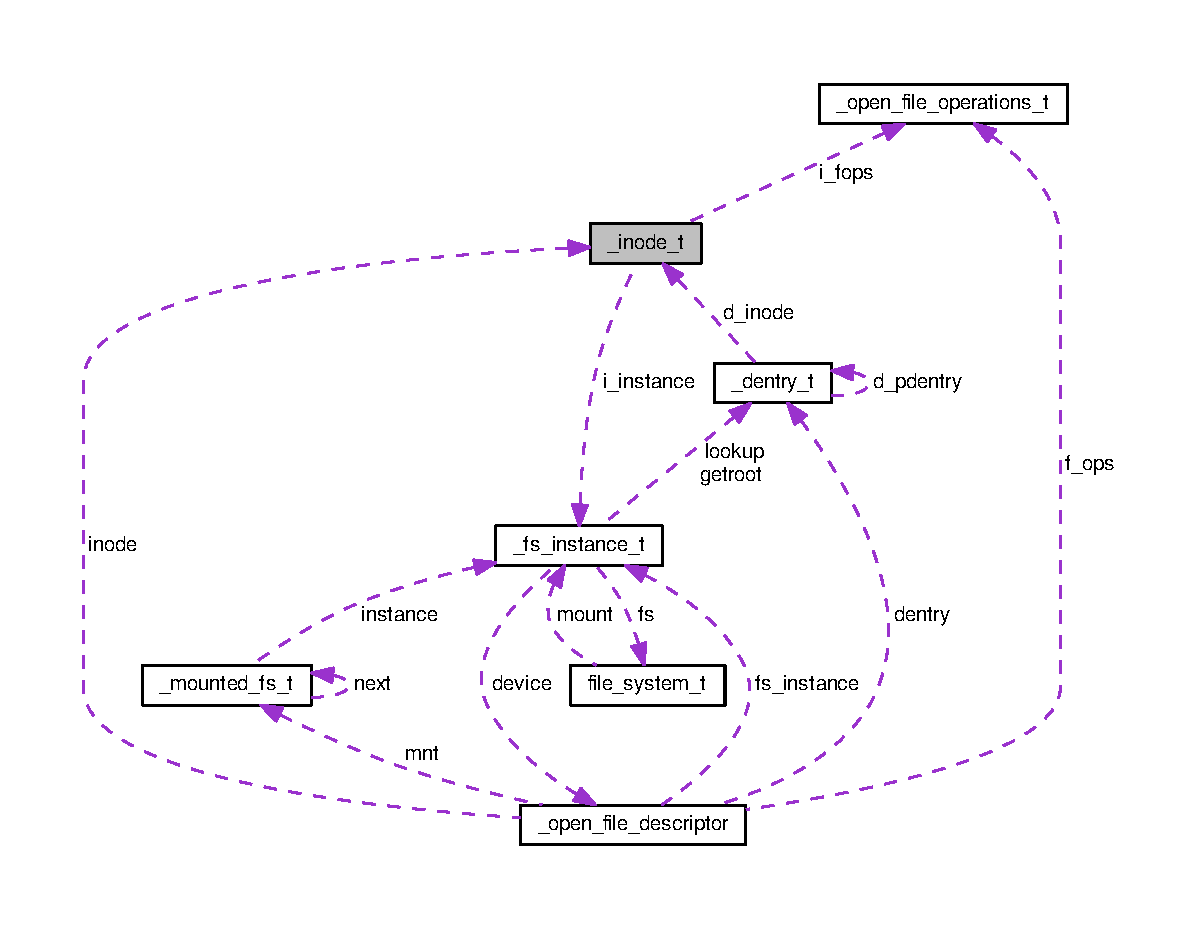
\includegraphics[width=350pt]{struct__inode__t__coll__graph}
\end{center}
\end{figure}
\subsection*{Champs de données}
\begin{DoxyCompactItemize}
\item 
unsigned long \hyperlink{struct__inode__t_aba602b843ba63a32ca3950dbaf7e959c}{i\-\_\-ino}
\item 
int \hyperlink{struct__inode__t_acead4732b6c22ef17ada59203509e728}{i\-\_\-mode}
\item 
\hyperlink{kstat_8h_af2306308627701b66dc6f3babe821ab4}{uid\-\_\-t} \hyperlink{struct__inode__t_a7ddcb65050ac0b4c9cfbacd495d56f4b}{i\-\_\-uid}
\item 
\hyperlink{kstat_8h_aa7352f1065fe606194d792e2b292cf83}{gid\-\_\-t} \hyperlink{struct__inode__t_a95d052a6e9b1b1e4f6837fa0f33b393e}{i\-\_\-gid}
\item 
off\-\_\-t \hyperlink{struct__inode__t_aed37b31c96c90873201abfc8b4b3e463}{i\-\_\-size}
\item 
time\-\_\-t \hyperlink{struct__inode__t_a01f50c6c44a3b50e4414a794643b741f}{i\-\_\-atime}
\item 
time\-\_\-t \hyperlink{struct__inode__t_a73ee1e604547b74b8e1045fd4f6699b6}{i\-\_\-ctime}
\item 
time\-\_\-t \hyperlink{struct__inode__t_a331d724391efce2f89aeb1a503ae5c43}{i\-\_\-mtime}
\item 
time\-\_\-t \hyperlink{struct__inode__t_a393de4c58241168fdf397ab8421a3539}{i\-\_\-dtime}
\item 
int \hyperlink{struct__inode__t_a8ea768d56d01e010bc0c809bc38dbb28}{i\-\_\-count}
\item 
unsigned char \hyperlink{struct__inode__t_a929fc1e6837d02a2525027a121b4e67e}{i\-\_\-nlink}
\item 
unsigned char \hyperlink{struct__inode__t_a36ff48a57a9e483d74682972d31ef46c}{i\-\_\-flags}
\item 
unsigned long \hyperlink{struct__inode__t_a92ebe4c1e93af9fba4efae4d07e14858}{i\-\_\-blocks}
\item 
\hyperlink{vfs_8h_a0eefa9aac35a5462ebf1e038992ca860}{fs\-\_\-instance\-\_\-t} $\ast$ \hyperlink{struct__inode__t_affefc88b22f45e2ec8340d582486d0f2}{i\-\_\-instance}
\item 
struct \hyperlink{struct__open__file__operations__t}{\-\_\-open\-\_\-file\-\_\-operations\-\_\-t} $\ast$ \hyperlink{struct__inode__t_acf149d7d1601f78142b1eec480badf7e}{i\-\_\-fops}
\item 
void $\ast$ \hyperlink{struct__inode__t_a54e34439c448c46bae90fd040dadc5c0}{i\-\_\-fs\-\_\-specific}
\end{DoxyCompactItemize}


\subsection{Description détaillée}
Structure inode. 

\subsection{Documentation des champs}
\hypertarget{struct__inode__t_a01f50c6c44a3b50e4414a794643b741f}{\index{\-\_\-inode\-\_\-t@{\-\_\-inode\-\_\-t}!i\-\_\-atime@{i\-\_\-atime}}
\index{i\-\_\-atime@{i\-\_\-atime}!_inode_t@{\-\_\-inode\-\_\-t}}
\subsubsection[{i\-\_\-atime}]{\setlength{\rightskip}{0pt plus 5cm}time\-\_\-t \-\_\-inode\-\_\-t\-::i\-\_\-atime}}\label{struct__inode__t_a01f50c6c44a3b50e4414a794643b741f}
Access time \hypertarget{struct__inode__t_a92ebe4c1e93af9fba4efae4d07e14858}{\index{\-\_\-inode\-\_\-t@{\-\_\-inode\-\_\-t}!i\-\_\-blocks@{i\-\_\-blocks}}
\index{i\-\_\-blocks@{i\-\_\-blocks}!_inode_t@{\-\_\-inode\-\_\-t}}
\subsubsection[{i\-\_\-blocks}]{\setlength{\rightskip}{0pt plus 5cm}unsigned long \-\_\-inode\-\_\-t\-::i\-\_\-blocks}}\label{struct__inode__t_a92ebe4c1e93af9fba4efae4d07e14858}
Blocks count \hypertarget{struct__inode__t_a8ea768d56d01e010bc0c809bc38dbb28}{\index{\-\_\-inode\-\_\-t@{\-\_\-inode\-\_\-t}!i\-\_\-count@{i\-\_\-count}}
\index{i\-\_\-count@{i\-\_\-count}!_inode_t@{\-\_\-inode\-\_\-t}}
\subsubsection[{i\-\_\-count}]{\setlength{\rightskip}{0pt plus 5cm}int \-\_\-inode\-\_\-t\-::i\-\_\-count}}\label{struct__inode__t_a8ea768d56d01e010bc0c809bc38dbb28}
Nombre d'ofd l'utilisant \hypertarget{struct__inode__t_a73ee1e604547b74b8e1045fd4f6699b6}{\index{\-\_\-inode\-\_\-t@{\-\_\-inode\-\_\-t}!i\-\_\-ctime@{i\-\_\-ctime}}
\index{i\-\_\-ctime@{i\-\_\-ctime}!_inode_t@{\-\_\-inode\-\_\-t}}
\subsubsection[{i\-\_\-ctime}]{\setlength{\rightskip}{0pt plus 5cm}time\-\_\-t \-\_\-inode\-\_\-t\-::i\-\_\-ctime}}\label{struct__inode__t_a73ee1e604547b74b8e1045fd4f6699b6}
Creation time \hypertarget{struct__inode__t_a393de4c58241168fdf397ab8421a3539}{\index{\-\_\-inode\-\_\-t@{\-\_\-inode\-\_\-t}!i\-\_\-dtime@{i\-\_\-dtime}}
\index{i\-\_\-dtime@{i\-\_\-dtime}!_inode_t@{\-\_\-inode\-\_\-t}}
\subsubsection[{i\-\_\-dtime}]{\setlength{\rightskip}{0pt plus 5cm}time\-\_\-t \-\_\-inode\-\_\-t\-::i\-\_\-dtime}}\label{struct__inode__t_a393de4c58241168fdf397ab8421a3539}
Deletion Time \hypertarget{struct__inode__t_a36ff48a57a9e483d74682972d31ef46c}{\index{\-\_\-inode\-\_\-t@{\-\_\-inode\-\_\-t}!i\-\_\-flags@{i\-\_\-flags}}
\index{i\-\_\-flags@{i\-\_\-flags}!_inode_t@{\-\_\-inode\-\_\-t}}
\subsubsection[{i\-\_\-flags}]{\setlength{\rightskip}{0pt plus 5cm}unsigned char \-\_\-inode\-\_\-t\-::i\-\_\-flags}}\label{struct__inode__t_a36ff48a57a9e483d74682972d31ef46c}
File flags \hypertarget{struct__inode__t_acf149d7d1601f78142b1eec480badf7e}{\index{\-\_\-inode\-\_\-t@{\-\_\-inode\-\_\-t}!i\-\_\-fops@{i\-\_\-fops}}
\index{i\-\_\-fops@{i\-\_\-fops}!_inode_t@{\-\_\-inode\-\_\-t}}
\subsubsection[{i\-\_\-fops}]{\setlength{\rightskip}{0pt plus 5cm}struct {\bf \-\_\-open\-\_\-file\-\_\-operations\-\_\-t}$\ast$ \-\_\-inode\-\_\-t\-::i\-\_\-fops}}\label{struct__inode__t_acf149d7d1601f78142b1eec480badf7e}
Ofd operations. \hypertarget{struct__inode__t_a54e34439c448c46bae90fd040dadc5c0}{\index{\-\_\-inode\-\_\-t@{\-\_\-inode\-\_\-t}!i\-\_\-fs\-\_\-specific@{i\-\_\-fs\-\_\-specific}}
\index{i\-\_\-fs\-\_\-specific@{i\-\_\-fs\-\_\-specific}!_inode_t@{\-\_\-inode\-\_\-t}}
\subsubsection[{i\-\_\-fs\-\_\-specific}]{\setlength{\rightskip}{0pt plus 5cm}void$\ast$ \-\_\-inode\-\_\-t\-::i\-\_\-fs\-\_\-specific}}\label{struct__inode__t_a54e34439c448c46bae90fd040dadc5c0}
Extra data \hypertarget{struct__inode__t_a95d052a6e9b1b1e4f6837fa0f33b393e}{\index{\-\_\-inode\-\_\-t@{\-\_\-inode\-\_\-t}!i\-\_\-gid@{i\-\_\-gid}}
\index{i\-\_\-gid@{i\-\_\-gid}!_inode_t@{\-\_\-inode\-\_\-t}}
\subsubsection[{i\-\_\-gid}]{\setlength{\rightskip}{0pt plus 5cm}{\bf gid\-\_\-t} \-\_\-inode\-\_\-t\-::i\-\_\-gid}}\label{struct__inode__t_a95d052a6e9b1b1e4f6837fa0f33b393e}
Low 16 bits of Group Id \hypertarget{struct__inode__t_aba602b843ba63a32ca3950dbaf7e959c}{\index{\-\_\-inode\-\_\-t@{\-\_\-inode\-\_\-t}!i\-\_\-ino@{i\-\_\-ino}}
\index{i\-\_\-ino@{i\-\_\-ino}!_inode_t@{\-\_\-inode\-\_\-t}}
\subsubsection[{i\-\_\-ino}]{\setlength{\rightskip}{0pt plus 5cm}unsigned long \-\_\-inode\-\_\-t\-::i\-\_\-ino}}\label{struct__inode__t_aba602b843ba63a32ca3950dbaf7e959c}
Inode number \hypertarget{struct__inode__t_affefc88b22f45e2ec8340d582486d0f2}{\index{\-\_\-inode\-\_\-t@{\-\_\-inode\-\_\-t}!i\-\_\-instance@{i\-\_\-instance}}
\index{i\-\_\-instance@{i\-\_\-instance}!_inode_t@{\-\_\-inode\-\_\-t}}
\subsubsection[{i\-\_\-instance}]{\setlength{\rightskip}{0pt plus 5cm}{\bf fs\-\_\-instance\-\_\-t}$\ast$ \-\_\-inode\-\_\-t\-::i\-\_\-instance}}\label{struct__inode__t_affefc88b22f45e2ec8340d582486d0f2}
Instance de fs auquel appartient cet inoeud. \hypertarget{struct__inode__t_acead4732b6c22ef17ada59203509e728}{\index{\-\_\-inode\-\_\-t@{\-\_\-inode\-\_\-t}!i\-\_\-mode@{i\-\_\-mode}}
\index{i\-\_\-mode@{i\-\_\-mode}!_inode_t@{\-\_\-inode\-\_\-t}}
\subsubsection[{i\-\_\-mode}]{\setlength{\rightskip}{0pt plus 5cm}int \-\_\-inode\-\_\-t\-::i\-\_\-mode}}\label{struct__inode__t_acead4732b6c22ef17ada59203509e728}
File mode \hypertarget{struct__inode__t_a331d724391efce2f89aeb1a503ae5c43}{\index{\-\_\-inode\-\_\-t@{\-\_\-inode\-\_\-t}!i\-\_\-mtime@{i\-\_\-mtime}}
\index{i\-\_\-mtime@{i\-\_\-mtime}!_inode_t@{\-\_\-inode\-\_\-t}}
\subsubsection[{i\-\_\-mtime}]{\setlength{\rightskip}{0pt plus 5cm}time\-\_\-t \-\_\-inode\-\_\-t\-::i\-\_\-mtime}}\label{struct__inode__t_a331d724391efce2f89aeb1a503ae5c43}
Modification time \hypertarget{struct__inode__t_a929fc1e6837d02a2525027a121b4e67e}{\index{\-\_\-inode\-\_\-t@{\-\_\-inode\-\_\-t}!i\-\_\-nlink@{i\-\_\-nlink}}
\index{i\-\_\-nlink@{i\-\_\-nlink}!_inode_t@{\-\_\-inode\-\_\-t}}
\subsubsection[{i\-\_\-nlink}]{\setlength{\rightskip}{0pt plus 5cm}unsigned char \-\_\-inode\-\_\-t\-::i\-\_\-nlink}}\label{struct__inode__t_a929fc1e6837d02a2525027a121b4e67e}
Links count \hypertarget{struct__inode__t_aed37b31c96c90873201abfc8b4b3e463}{\index{\-\_\-inode\-\_\-t@{\-\_\-inode\-\_\-t}!i\-\_\-size@{i\-\_\-size}}
\index{i\-\_\-size@{i\-\_\-size}!_inode_t@{\-\_\-inode\-\_\-t}}
\subsubsection[{i\-\_\-size}]{\setlength{\rightskip}{0pt plus 5cm}off\-\_\-t \-\_\-inode\-\_\-t\-::i\-\_\-size}}\label{struct__inode__t_aed37b31c96c90873201abfc8b4b3e463}
Size in bytes \hypertarget{struct__inode__t_a7ddcb65050ac0b4c9cfbacd495d56f4b}{\index{\-\_\-inode\-\_\-t@{\-\_\-inode\-\_\-t}!i\-\_\-uid@{i\-\_\-uid}}
\index{i\-\_\-uid@{i\-\_\-uid}!_inode_t@{\-\_\-inode\-\_\-t}}
\subsubsection[{i\-\_\-uid}]{\setlength{\rightskip}{0pt plus 5cm}{\bf uid\-\_\-t} \-\_\-inode\-\_\-t\-::i\-\_\-uid}}\label{struct__inode__t_a7ddcb65050ac0b4c9cfbacd495d56f4b}
Low 16 bits of Owner Uid 

La documentation de cette structure a été générée à partir du fichier suivant \-:\begin{DoxyCompactItemize}
\item 
kernel/include/\hyperlink{vfs_8h}{vfs.\-h}\end{DoxyCompactItemize}

\hypertarget{struct__IO__FILE}{\section{Référence de la structure \-\_\-\-I\-O\-\_\-\-F\-I\-L\-E}
\label{struct__IO__FILE}\index{\-\_\-\-I\-O\-\_\-\-F\-I\-L\-E@{\-\_\-\-I\-O\-\_\-\-F\-I\-L\-E}}
}


Gestion de stream. Inspiré de posix.  




{\ttfamily \#include $<$libio.\-h$>$}



Graphe de collaboration de \-\_\-\-I\-O\-\_\-\-F\-I\-L\-E\-:\nopagebreak
\begin{figure}[H]
\begin{center}
\leavevmode
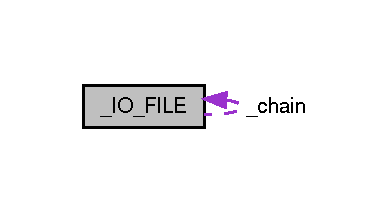
\includegraphics[width=187pt]{struct__IO__FILE__coll__graph}
\end{center}
\end{figure}
\subsection*{Champs de données}
\begin{DoxyCompactItemize}
\item 
int \hyperlink{struct__IO__FILE_a364ce3577f2cdb788df3a2a54909f45a}{\-\_\-flags}
\item 
char $\ast$ \hyperlink{struct__IO__FILE_a1c2f65148a6f2e35c478af0fc144fded}{\-\_\-\-I\-O\-\_\-read\-\_\-ptr}
\item 
char $\ast$ \hyperlink{struct__IO__FILE_a6994a0f73699af311e4669b4baa0e26b}{\-\_\-\-I\-O\-\_\-read\-\_\-end}
\item 
char $\ast$ \hyperlink{struct__IO__FILE_a2a449978f6e6aa2172f7f82ed1d42f37}{\-\_\-\-I\-O\-\_\-read\-\_\-base}
\item 
char $\ast$ \hyperlink{struct__IO__FILE_a6631dc1b00cd5a378280606c9333f40a}{\-\_\-\-I\-O\-\_\-write\-\_\-base}
\item 
char $\ast$ \hyperlink{struct__IO__FILE_ab746b60c0613c28d3451b13afdd703b5}{\-\_\-\-I\-O\-\_\-write\-\_\-ptr}
\item 
char $\ast$ \hyperlink{struct__IO__FILE_ad68f27b22fb43ab7a50bdaa50dc7d725}{\-\_\-\-I\-O\-\_\-write\-\_\-end}
\item 
char $\ast$ \hyperlink{struct__IO__FILE_a2bf5a30fdc43564cf2e46d2cce8e82dd}{\-\_\-\-I\-O\-\_\-buf\-\_\-base}
\item 
char $\ast$ \hyperlink{struct__IO__FILE_ac9fa3b261e95a246dac19dc35045be42}{\-\_\-\-I\-O\-\_\-buf\-\_\-end}
\item 
char $\ast$ \hyperlink{struct__IO__FILE_a3ef98bd6be88c72459cf4a670a5ba35c}{\-\_\-\-I\-O\-\_\-save\-\_\-base}
\item 
char $\ast$ \hyperlink{struct__IO__FILE_a8e6f38619f990a207a598132f4e6e661}{\-\_\-\-I\-O\-\_\-backup\-\_\-base}
\item 
char $\ast$ \hyperlink{struct__IO__FILE_a48102d534ea93a120fc025b1bead08cb}{\-\_\-\-I\-O\-\_\-save\-\_\-end}
\item 
\hypertarget{struct__IO__FILE_a148f6239f490808c7875a5d43f13e645}{struct \hyperlink{struct__IO__FILE}{\-\_\-\-I\-O\-\_\-\-F\-I\-L\-E} $\ast$ {\bfseries \-\_\-chain}}\label{struct__IO__FILE_a148f6239f490808c7875a5d43f13e645}

\item 
\hypertarget{struct__IO__FILE_a1883574299ff3f4ac644796985ca0a1d}{int {\bfseries \-\_\-fileno}}\label{struct__IO__FILE_a1883574299ff3f4ac644796985ca0a1d}

\end{DoxyCompactItemize}


\subsection{Documentation des champs}
\hypertarget{struct__IO__FILE_a364ce3577f2cdb788df3a2a54909f45a}{\index{\-\_\-\-I\-O\-\_\-\-F\-I\-L\-E@{\-\_\-\-I\-O\-\_\-\-F\-I\-L\-E}!\-\_\-flags@{\-\_\-flags}}
\index{\-\_\-flags@{\-\_\-flags}!_IO_FILE@{\-\_\-\-I\-O\-\_\-\-F\-I\-L\-E}}
\subsubsection[{\-\_\-flags}]{\setlength{\rightskip}{0pt plus 5cm}int \-\_\-\-I\-O\-\_\-\-F\-I\-L\-E\-::\-\_\-flags}}\label{struct__IO__FILE_a364ce3577f2cdb788df3a2a54909f45a}
High-\/order word is \-\_\-\-I\-O\-\_\-\-M\-A\-G\-I\-C; rest is flags. \hypertarget{struct__IO__FILE_a8e6f38619f990a207a598132f4e6e661}{\index{\-\_\-\-I\-O\-\_\-\-F\-I\-L\-E@{\-\_\-\-I\-O\-\_\-\-F\-I\-L\-E}!\-\_\-\-I\-O\-\_\-backup\-\_\-base@{\-\_\-\-I\-O\-\_\-backup\-\_\-base}}
\index{\-\_\-\-I\-O\-\_\-backup\-\_\-base@{\-\_\-\-I\-O\-\_\-backup\-\_\-base}!_IO_FILE@{\-\_\-\-I\-O\-\_\-\-F\-I\-L\-E}}
\subsubsection[{\-\_\-\-I\-O\-\_\-backup\-\_\-base}]{\setlength{\rightskip}{0pt plus 5cm}char$\ast$ \-\_\-\-I\-O\-\_\-\-F\-I\-L\-E\-::\-\_\-\-I\-O\-\_\-backup\-\_\-base}}\label{struct__IO__FILE_a8e6f38619f990a207a598132f4e6e661}
Pointer to first valid character of backup area \hypertarget{struct__IO__FILE_a2bf5a30fdc43564cf2e46d2cce8e82dd}{\index{\-\_\-\-I\-O\-\_\-\-F\-I\-L\-E@{\-\_\-\-I\-O\-\_\-\-F\-I\-L\-E}!\-\_\-\-I\-O\-\_\-buf\-\_\-base@{\-\_\-\-I\-O\-\_\-buf\-\_\-base}}
\index{\-\_\-\-I\-O\-\_\-buf\-\_\-base@{\-\_\-\-I\-O\-\_\-buf\-\_\-base}!_IO_FILE@{\-\_\-\-I\-O\-\_\-\-F\-I\-L\-E}}
\subsubsection[{\-\_\-\-I\-O\-\_\-buf\-\_\-base}]{\setlength{\rightskip}{0pt plus 5cm}char$\ast$ \-\_\-\-I\-O\-\_\-\-F\-I\-L\-E\-::\-\_\-\-I\-O\-\_\-buf\-\_\-base}}\label{struct__IO__FILE_a2bf5a30fdc43564cf2e46d2cce8e82dd}
Start of reserve area. \hypertarget{struct__IO__FILE_ac9fa3b261e95a246dac19dc35045be42}{\index{\-\_\-\-I\-O\-\_\-\-F\-I\-L\-E@{\-\_\-\-I\-O\-\_\-\-F\-I\-L\-E}!\-\_\-\-I\-O\-\_\-buf\-\_\-end@{\-\_\-\-I\-O\-\_\-buf\-\_\-end}}
\index{\-\_\-\-I\-O\-\_\-buf\-\_\-end@{\-\_\-\-I\-O\-\_\-buf\-\_\-end}!_IO_FILE@{\-\_\-\-I\-O\-\_\-\-F\-I\-L\-E}}
\subsubsection[{\-\_\-\-I\-O\-\_\-buf\-\_\-end}]{\setlength{\rightskip}{0pt plus 5cm}char$\ast$ \-\_\-\-I\-O\-\_\-\-F\-I\-L\-E\-::\-\_\-\-I\-O\-\_\-buf\-\_\-end}}\label{struct__IO__FILE_ac9fa3b261e95a246dac19dc35045be42}
End of reserve area. \hypertarget{struct__IO__FILE_a2a449978f6e6aa2172f7f82ed1d42f37}{\index{\-\_\-\-I\-O\-\_\-\-F\-I\-L\-E@{\-\_\-\-I\-O\-\_\-\-F\-I\-L\-E}!\-\_\-\-I\-O\-\_\-read\-\_\-base@{\-\_\-\-I\-O\-\_\-read\-\_\-base}}
\index{\-\_\-\-I\-O\-\_\-read\-\_\-base@{\-\_\-\-I\-O\-\_\-read\-\_\-base}!_IO_FILE@{\-\_\-\-I\-O\-\_\-\-F\-I\-L\-E}}
\subsubsection[{\-\_\-\-I\-O\-\_\-read\-\_\-base}]{\setlength{\rightskip}{0pt plus 5cm}char$\ast$ \-\_\-\-I\-O\-\_\-\-F\-I\-L\-E\-::\-\_\-\-I\-O\-\_\-read\-\_\-base}}\label{struct__IO__FILE_a2a449978f6e6aa2172f7f82ed1d42f37}
Start of putback+get area. \hypertarget{struct__IO__FILE_a6994a0f73699af311e4669b4baa0e26b}{\index{\-\_\-\-I\-O\-\_\-\-F\-I\-L\-E@{\-\_\-\-I\-O\-\_\-\-F\-I\-L\-E}!\-\_\-\-I\-O\-\_\-read\-\_\-end@{\-\_\-\-I\-O\-\_\-read\-\_\-end}}
\index{\-\_\-\-I\-O\-\_\-read\-\_\-end@{\-\_\-\-I\-O\-\_\-read\-\_\-end}!_IO_FILE@{\-\_\-\-I\-O\-\_\-\-F\-I\-L\-E}}
\subsubsection[{\-\_\-\-I\-O\-\_\-read\-\_\-end}]{\setlength{\rightskip}{0pt plus 5cm}char$\ast$ \-\_\-\-I\-O\-\_\-\-F\-I\-L\-E\-::\-\_\-\-I\-O\-\_\-read\-\_\-end}}\label{struct__IO__FILE_a6994a0f73699af311e4669b4baa0e26b}
End of get area. \hypertarget{struct__IO__FILE_a1c2f65148a6f2e35c478af0fc144fded}{\index{\-\_\-\-I\-O\-\_\-\-F\-I\-L\-E@{\-\_\-\-I\-O\-\_\-\-F\-I\-L\-E}!\-\_\-\-I\-O\-\_\-read\-\_\-ptr@{\-\_\-\-I\-O\-\_\-read\-\_\-ptr}}
\index{\-\_\-\-I\-O\-\_\-read\-\_\-ptr@{\-\_\-\-I\-O\-\_\-read\-\_\-ptr}!_IO_FILE@{\-\_\-\-I\-O\-\_\-\-F\-I\-L\-E}}
\subsubsection[{\-\_\-\-I\-O\-\_\-read\-\_\-ptr}]{\setlength{\rightskip}{0pt plus 5cm}char$\ast$ \-\_\-\-I\-O\-\_\-\-F\-I\-L\-E\-::\-\_\-\-I\-O\-\_\-read\-\_\-ptr}}\label{struct__IO__FILE_a1c2f65148a6f2e35c478af0fc144fded}
Current read pointer \hypertarget{struct__IO__FILE_a3ef98bd6be88c72459cf4a670a5ba35c}{\index{\-\_\-\-I\-O\-\_\-\-F\-I\-L\-E@{\-\_\-\-I\-O\-\_\-\-F\-I\-L\-E}!\-\_\-\-I\-O\-\_\-save\-\_\-base@{\-\_\-\-I\-O\-\_\-save\-\_\-base}}
\index{\-\_\-\-I\-O\-\_\-save\-\_\-base@{\-\_\-\-I\-O\-\_\-save\-\_\-base}!_IO_FILE@{\-\_\-\-I\-O\-\_\-\-F\-I\-L\-E}}
\subsubsection[{\-\_\-\-I\-O\-\_\-save\-\_\-base}]{\setlength{\rightskip}{0pt plus 5cm}char$\ast$ \-\_\-\-I\-O\-\_\-\-F\-I\-L\-E\-::\-\_\-\-I\-O\-\_\-save\-\_\-base}}\label{struct__IO__FILE_a3ef98bd6be88c72459cf4a670a5ba35c}
Pointer to start of non-\/current get area. \hypertarget{struct__IO__FILE_a48102d534ea93a120fc025b1bead08cb}{\index{\-\_\-\-I\-O\-\_\-\-F\-I\-L\-E@{\-\_\-\-I\-O\-\_\-\-F\-I\-L\-E}!\-\_\-\-I\-O\-\_\-save\-\_\-end@{\-\_\-\-I\-O\-\_\-save\-\_\-end}}
\index{\-\_\-\-I\-O\-\_\-save\-\_\-end@{\-\_\-\-I\-O\-\_\-save\-\_\-end}!_IO_FILE@{\-\_\-\-I\-O\-\_\-\-F\-I\-L\-E}}
\subsubsection[{\-\_\-\-I\-O\-\_\-save\-\_\-end}]{\setlength{\rightskip}{0pt plus 5cm}char$\ast$ \-\_\-\-I\-O\-\_\-\-F\-I\-L\-E\-::\-\_\-\-I\-O\-\_\-save\-\_\-end}}\label{struct__IO__FILE_a48102d534ea93a120fc025b1bead08cb}
Pointer to end of non-\/current get area. \hypertarget{struct__IO__FILE_a6631dc1b00cd5a378280606c9333f40a}{\index{\-\_\-\-I\-O\-\_\-\-F\-I\-L\-E@{\-\_\-\-I\-O\-\_\-\-F\-I\-L\-E}!\-\_\-\-I\-O\-\_\-write\-\_\-base@{\-\_\-\-I\-O\-\_\-write\-\_\-base}}
\index{\-\_\-\-I\-O\-\_\-write\-\_\-base@{\-\_\-\-I\-O\-\_\-write\-\_\-base}!_IO_FILE@{\-\_\-\-I\-O\-\_\-\-F\-I\-L\-E}}
\subsubsection[{\-\_\-\-I\-O\-\_\-write\-\_\-base}]{\setlength{\rightskip}{0pt plus 5cm}char$\ast$ \-\_\-\-I\-O\-\_\-\-F\-I\-L\-E\-::\-\_\-\-I\-O\-\_\-write\-\_\-base}}\label{struct__IO__FILE_a6631dc1b00cd5a378280606c9333f40a}
Start of put area. \hypertarget{struct__IO__FILE_ad68f27b22fb43ab7a50bdaa50dc7d725}{\index{\-\_\-\-I\-O\-\_\-\-F\-I\-L\-E@{\-\_\-\-I\-O\-\_\-\-F\-I\-L\-E}!\-\_\-\-I\-O\-\_\-write\-\_\-end@{\-\_\-\-I\-O\-\_\-write\-\_\-end}}
\index{\-\_\-\-I\-O\-\_\-write\-\_\-end@{\-\_\-\-I\-O\-\_\-write\-\_\-end}!_IO_FILE@{\-\_\-\-I\-O\-\_\-\-F\-I\-L\-E}}
\subsubsection[{\-\_\-\-I\-O\-\_\-write\-\_\-end}]{\setlength{\rightskip}{0pt plus 5cm}char$\ast$ \-\_\-\-I\-O\-\_\-\-F\-I\-L\-E\-::\-\_\-\-I\-O\-\_\-write\-\_\-end}}\label{struct__IO__FILE_ad68f27b22fb43ab7a50bdaa50dc7d725}
End of put area. \hypertarget{struct__IO__FILE_ab746b60c0613c28d3451b13afdd703b5}{\index{\-\_\-\-I\-O\-\_\-\-F\-I\-L\-E@{\-\_\-\-I\-O\-\_\-\-F\-I\-L\-E}!\-\_\-\-I\-O\-\_\-write\-\_\-ptr@{\-\_\-\-I\-O\-\_\-write\-\_\-ptr}}
\index{\-\_\-\-I\-O\-\_\-write\-\_\-ptr@{\-\_\-\-I\-O\-\_\-write\-\_\-ptr}!_IO_FILE@{\-\_\-\-I\-O\-\_\-\-F\-I\-L\-E}}
\subsubsection[{\-\_\-\-I\-O\-\_\-write\-\_\-ptr}]{\setlength{\rightskip}{0pt plus 5cm}char$\ast$ \-\_\-\-I\-O\-\_\-\-F\-I\-L\-E\-::\-\_\-\-I\-O\-\_\-write\-\_\-ptr}}\label{struct__IO__FILE_ab746b60c0613c28d3451b13afdd703b5}
Current put pointer. 

La documentation de cette structure a été générée à partir du fichier suivant \-:\begin{DoxyCompactItemize}
\item 
libc/include/\hyperlink{libio_8h}{libio.\-h}\end{DoxyCompactItemize}

\hypertarget{struct__list__cell}{\section{Référence de la structure \-\_\-list\-\_\-cell}
\label{struct__list__cell}\index{\-\_\-list\-\_\-cell@{\-\_\-list\-\_\-cell}}
}


Graphe de collaboration de \-\_\-list\-\_\-cell\-:\nopagebreak
\begin{figure}[H]
\begin{center}
\leavevmode
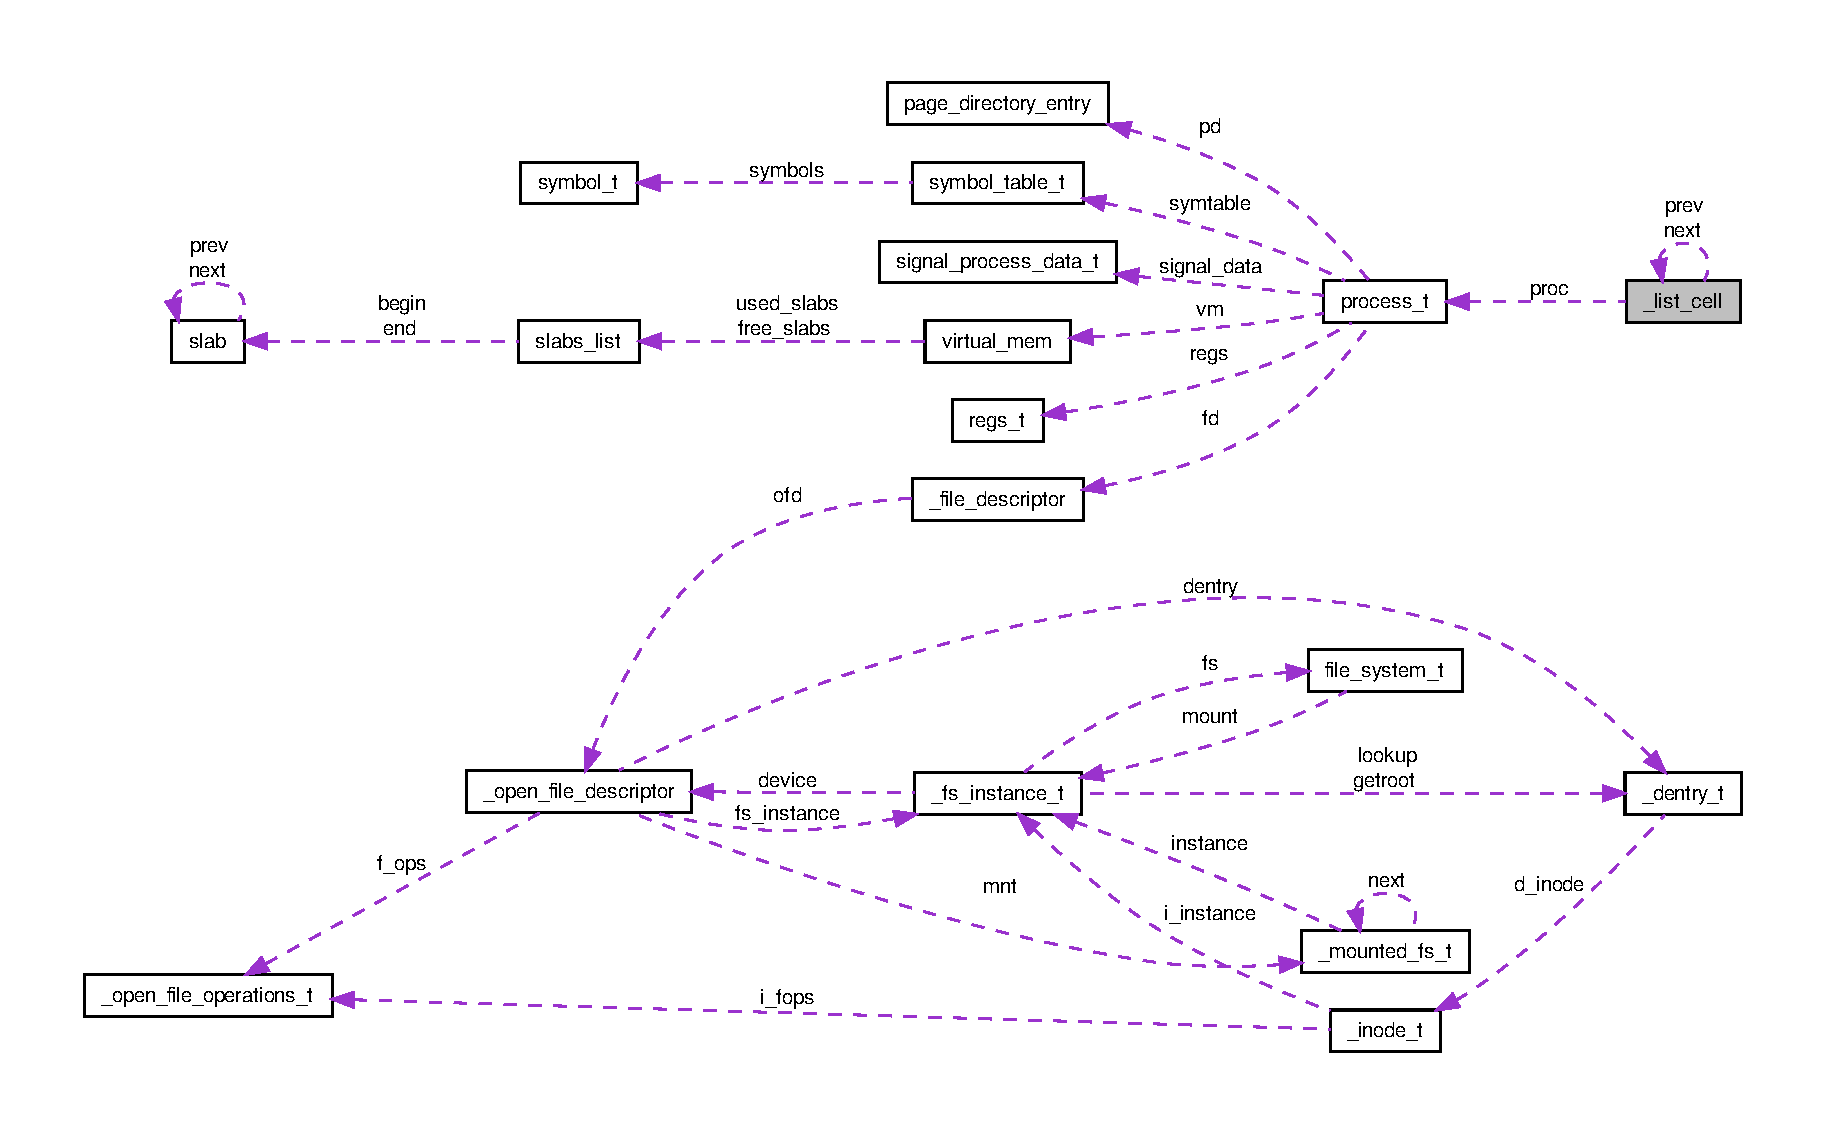
\includegraphics[width=350pt]{struct__list__cell__coll__graph}
\end{center}
\end{figure}
\subsection*{Champs de données}
\begin{DoxyCompactItemize}
\item 
\hypertarget{struct__list__cell_adcf2b08b8b97ffde53295bc31dae8278}{\hyperlink{structprocess__t}{process\-\_\-t} $\ast$ {\bfseries proc}}\label{struct__list__cell_adcf2b08b8b97ffde53295bc31dae8278}

\item 
\hypertarget{struct__list__cell_adf3f16a530b500e57c17b9999da464f5}{struct \hyperlink{struct__list__cell}{\-\_\-list\-\_\-cell} $\ast$ {\bfseries prev}}\label{struct__list__cell_adf3f16a530b500e57c17b9999da464f5}

\item 
\hypertarget{struct__list__cell_acb400769208341fe3181d5d73ff74a39}{struct \hyperlink{struct__list__cell}{\-\_\-list\-\_\-cell} $\ast$ {\bfseries next}}\label{struct__list__cell_acb400769208341fe3181d5d73ff74a39}

\end{DoxyCompactItemize}


La documentation de cette structure a été générée à partir du fichier suivant \-:\begin{DoxyCompactItemize}
\item 
kernel/\hyperlink{round__robin_8c}{round\-\_\-robin.\-c}\end{DoxyCompactItemize}

\hypertarget{struct__mounted__fs__t}{\section{Référence de la structure \-\_\-mounted\-\_\-fs\-\_\-t}
\label{struct__mounted__fs__t}\index{\-\_\-mounted\-\_\-fs\-\_\-t@{\-\_\-mounted\-\_\-fs\-\_\-t}}
}


{\ttfamily \#include $<$vfs.\-h$>$}



Graphe de collaboration de \-\_\-mounted\-\_\-fs\-\_\-t\-:
\nopagebreak
\begin{figure}[H]
\begin{center}
\leavevmode
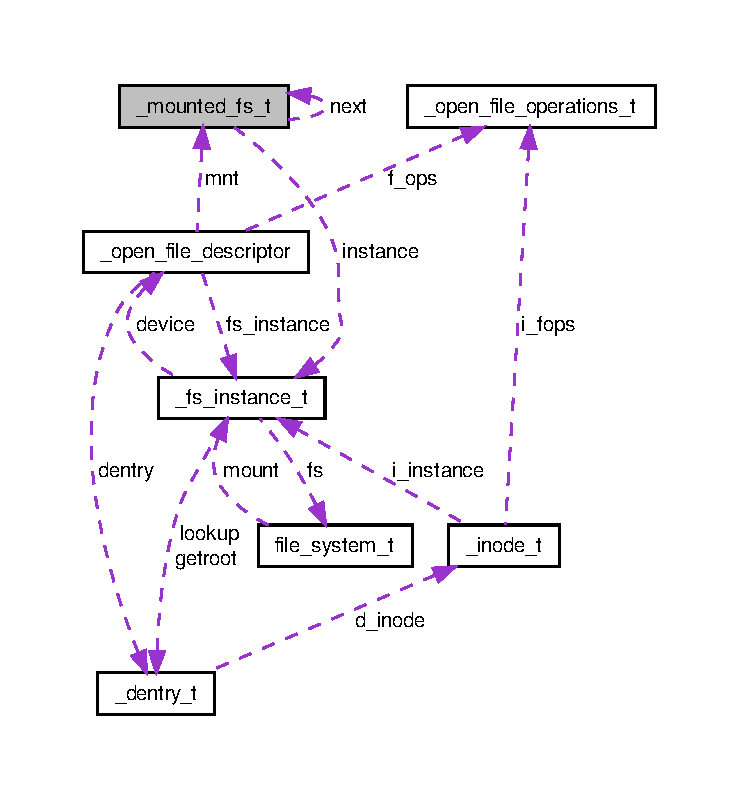
\includegraphics[width=350pt]{struct__mounted__fs__t__coll__graph}
\end{center}
\end{figure}
\subsection*{Champs de données}
\begin{DoxyCompactItemize}
\item 
\hyperlink{vfs_8h_a0eefa9aac35a5462ebf1e038992ca860}{fs\-\_\-instance\-\_\-t} $\ast$ \hyperlink{struct__mounted__fs__t_a81752bb01c13d0edca51b944ee2c53a8}{instance}
\item 
char $\ast$ \hyperlink{struct__mounted__fs__t_a334bde8995efec727b127e7a161398a5}{name}
\item 
struct \hyperlink{struct__mounted__fs__t}{\-\_\-mounted\-\_\-fs\-\_\-t} $\ast$ \hyperlink{struct__mounted__fs__t_af0751160c22589b18daa3ed6e775aeb8}{next}
\end{DoxyCompactItemize}


\subsection{Description détaillée}
Cellule de la liste des points de montage. 

\subsection{Documentation des champs}
\hypertarget{struct__mounted__fs__t_a81752bb01c13d0edca51b944ee2c53a8}{\index{\-\_\-mounted\-\_\-fs\-\_\-t@{\-\_\-mounted\-\_\-fs\-\_\-t}!instance@{instance}}
\index{instance@{instance}!_mounted_fs_t@{\-\_\-mounted\-\_\-fs\-\_\-t}}
\subsubsection[{instance}]{\setlength{\rightskip}{0pt plus 5cm}{\bf fs\-\_\-instance\-\_\-t}$\ast$ \-\_\-mounted\-\_\-fs\-\_\-t\-::instance}}\label{struct__mounted__fs__t_a81752bb01c13d0edca51b944ee2c53a8}
Instance de F\-S. \hypertarget{struct__mounted__fs__t_a334bde8995efec727b127e7a161398a5}{\index{\-\_\-mounted\-\_\-fs\-\_\-t@{\-\_\-mounted\-\_\-fs\-\_\-t}!name@{name}}
\index{name@{name}!_mounted_fs_t@{\-\_\-mounted\-\_\-fs\-\_\-t}}
\subsubsection[{name}]{\setlength{\rightskip}{0pt plus 5cm}char$\ast$ \-\_\-mounted\-\_\-fs\-\_\-t\-::name}}\label{struct__mounted__fs__t_a334bde8995efec727b127e7a161398a5}
Nom du fs monté. \hypertarget{struct__mounted__fs__t_af0751160c22589b18daa3ed6e775aeb8}{\index{\-\_\-mounted\-\_\-fs\-\_\-t@{\-\_\-mounted\-\_\-fs\-\_\-t}!next@{next}}
\index{next@{next}!_mounted_fs_t@{\-\_\-mounted\-\_\-fs\-\_\-t}}
\subsubsection[{next}]{\setlength{\rightskip}{0pt plus 5cm}struct {\bf \-\_\-mounted\-\_\-fs\-\_\-t}$\ast$ \-\_\-mounted\-\_\-fs\-\_\-t\-::next}}\label{struct__mounted__fs__t_af0751160c22589b18daa3ed6e775aeb8}
Prochaine cellule. 

La documentation de cette structure a été générée à partir du fichier suivant \-:\begin{DoxyCompactItemize}
\item 
kernel/include/\hyperlink{vfs_8h}{vfs.\-h}\end{DoxyCompactItemize}

\hypertarget{struct__open__file__descriptor}{\section{Référence de la structure \-\_\-open\-\_\-file\-\_\-descriptor}
\label{struct__open__file__descriptor}\index{\-\_\-open\-\_\-file\-\_\-descriptor@{\-\_\-open\-\_\-file\-\_\-descriptor}}
}


{\ttfamily \#include $<$fd\-\_\-types.\-h$>$}



Graphe de collaboration de \-\_\-open\-\_\-file\-\_\-descriptor\-:\nopagebreak
\begin{figure}[H]
\begin{center}
\leavevmode
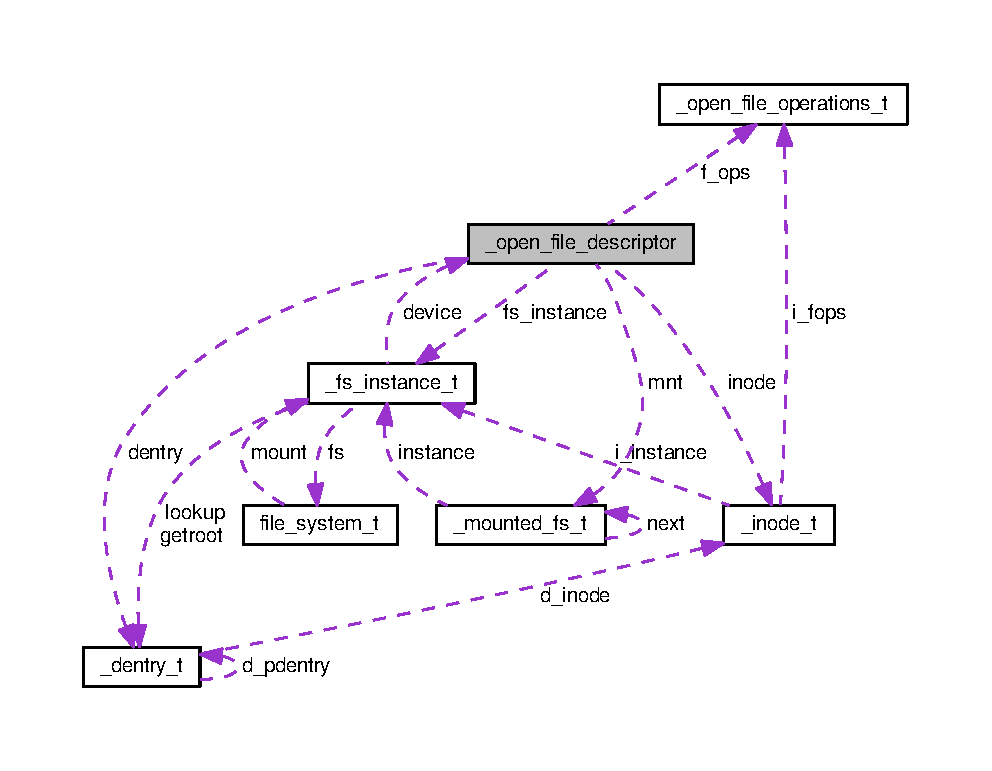
\includegraphics[width=350pt]{struct__open__file__descriptor__coll__graph}
\end{center}
\end{figure}
\subsection*{Champs de données}
\begin{DoxyCompactItemize}
\item 
\hypertarget{struct__open__file__descriptor_a8b09b35621badf1669bc2df27354e15b}{\hyperlink{kernel_2include_2types_8h_a33594304e786b158f3fb30289278f5af}{uint32\-\_\-t} {\bfseries flags}}\label{struct__open__file__descriptor_a8b09b35621badf1669bc2df27354e15b}

\item 
\hypertarget{struct__open__file__descriptor_adc7c56cf182ec52f5ae7a5b2cbcdc201}{int {\bfseries current\-\_\-cluster}}\label{struct__open__file__descriptor_adc7c56cf182ec52f5ae7a5b2cbcdc201}

\item 
\hypertarget{struct__open__file__descriptor_a77a2aad2470554b058b4565059fa8c8c}{\hyperlink{kernel_2include_2types_8h_aba7bc1797add20fe3efdf37ced1182c5}{uint8\-\_\-t} {\bfseries buffer} \mbox{[}512\mbox{]}}\label{struct__open__file__descriptor_a77a2aad2470554b058b4565059fa8c8c}

\item 
\hypertarget{struct__open__file__descriptor_a452e65f0c6de16bfeaa62825f916b077}{char $\ast$ {\bfseries pathname}}\label{struct__open__file__descriptor_a452e65f0c6de16bfeaa62825f916b077}

\item 
\hypertarget{struct__open__file__descriptor_a0ba8e85021c79e224ca628e14d0795c2}{\hyperlink{kernel_2include_2types_8h_a33594304e786b158f3fb30289278f5af}{uint32\-\_\-t} {\bfseries current\-\_\-octet}}\label{struct__open__file__descriptor_a0ba8e85021c79e224ca628e14d0795c2}

\item 
\hypertarget{struct__open__file__descriptor_a41bcfd1c4f0c4cfe7ef960e3fb7b01c7}{\hyperlink{kernel_2include_2types_8h_a33594304e786b158f3fb30289278f5af}{uint32\-\_\-t} {\bfseries first\-\_\-cluster}}\label{struct__open__file__descriptor_a41bcfd1c4f0c4cfe7ef960e3fb7b01c7}

\item 
\hypertarget{struct__open__file__descriptor_aded6c4da94d690e18bfd35522a3ca2da}{\hyperlink{kernel_2include_2types_8h_a33594304e786b158f3fb30289278f5af}{uint32\-\_\-t} {\bfseries file\-\_\-size}}\label{struct__open__file__descriptor_aded6c4da94d690e18bfd35522a3ca2da}

\item 
\hypertarget{struct__open__file__descriptor_a032a031b6293ba41fff7652cad4c507e}{struct \hyperlink{struct__fs__instance__t}{\-\_\-fs\-\_\-instance\-\_\-t} $\ast$ {\bfseries fs\-\_\-instance}}\label{struct__open__file__descriptor_a032a031b6293ba41fff7652cad4c507e}

\item 
\hypertarget{struct__open__file__descriptor_a6884ddeaeb43e81a0317cb5eae4c7d4e}{struct \hyperlink{struct__inode__t}{\-\_\-inode\-\_\-t} $\ast$ {\bfseries inode}}\label{struct__open__file__descriptor_a6884ddeaeb43e81a0317cb5eae4c7d4e}

\item 
\hypertarget{struct__open__file__descriptor_a3b375ad15f7bcb8e92123bd1a17765f3}{struct \hyperlink{struct__dentry__t}{\-\_\-dentry\-\_\-t} $\ast$ {\bfseries dentry}}\label{struct__open__file__descriptor_a3b375ad15f7bcb8e92123bd1a17765f3}

\item 
\hypertarget{struct__open__file__descriptor_a65408e330b7a3763de5549c826564730}{struct \hyperlink{struct__mounted__fs__t}{\-\_\-mounted\-\_\-fs\-\_\-t} $\ast$ {\bfseries mnt}}\label{struct__open__file__descriptor_a65408e330b7a3763de5549c826564730}

\item 
\hypertarget{struct__open__file__descriptor_a6cd707cf9a5d837feba5ef2a2f91bfcd}{struct \hyperlink{struct__open__file__operations__t}{\-\_\-open\-\_\-file\-\_\-operations\-\_\-t} $\ast$ {\bfseries f\-\_\-ops}}\label{struct__open__file__descriptor_a6cd707cf9a5d837feba5ef2a2f91bfcd}

\item 
\hypertarget{struct__open__file__descriptor_a99824795a31a8adea2162aed74162017}{void $\ast$ {\bfseries extra\-\_\-data}}\label{struct__open__file__descriptor_a99824795a31a8adea2162aed74162017}

\end{DoxyCompactItemize}


\subsection{Description détaillée}
Descripteur de fichier ouvert. À chaque fichier ouvert, une structure de ce type est instanciée pour y stocker les informations sur le fichier et le F\-S. 

La documentation de cette structure a été générée à partir du fichier suivant \-:\begin{DoxyCompactItemize}
\item 
kernel/include/\hyperlink{fd__types_8h}{fd\-\_\-types.\-h}\end{DoxyCompactItemize}

\hypertarget{struct__open__file__operations__t}{\section{Référence de la structure \-\_\-open\-\_\-file\-\_\-operations\-\_\-t}
\label{struct__open__file__operations__t}\index{\-\_\-open\-\_\-file\-\_\-operations\-\_\-t@{\-\_\-open\-\_\-file\-\_\-operations\-\_\-t}}
}


{\ttfamily \#include $<$fd\-\_\-types.\-h$>$}

\subsection*{Champs de données}
\begin{DoxyCompactItemize}
\item 
\hyperlink{kernel_2include_2types_8h_af629ed855824cf5955b54529adf78ad6}{ssize\-\_\-t}($\ast$ \hyperlink{struct__open__file__operations__t_ae730a8e7e44c3b3168b9f091c334b337}{write} )(struct \hyperlink{struct__open__file__descriptor}{\-\_\-open\-\_\-file\-\_\-descriptor} $\ast$, const void $\ast$, \hyperlink{kernel_2include_2types_8h_a29d85914ddff32967d85ada69854206d}{size\-\_\-t})
\item 
\hyperlink{kernel_2include_2types_8h_af629ed855824cf5955b54529adf78ad6}{ssize\-\_\-t}($\ast$ \hyperlink{struct__open__file__operations__t_ad5637bc6a752b9a13806748966b77e68}{read} )(struct \hyperlink{struct__open__file__descriptor}{\-\_\-open\-\_\-file\-\_\-descriptor} $\ast$, void $\ast$, \hyperlink{kernel_2include_2types_8h_a29d85914ddff32967d85ada69854206d}{size\-\_\-t})
\item 
int($\ast$ \hyperlink{struct__open__file__operations__t_ac45e5e3400e4cd9756b5784289744cc7}{seek} )(struct \hyperlink{struct__open__file__descriptor}{\-\_\-open\-\_\-file\-\_\-descriptor} $\ast$, long, int)
\item 
int($\ast$ \hyperlink{struct__open__file__operations__t_ab71efab6158837196ad4fef57565dddc}{ioctl} )(struct \hyperlink{struct__open__file__descriptor}{\-\_\-open\-\_\-file\-\_\-descriptor} $\ast$, unsigned int, void $\ast$)
\item 
int($\ast$ \hyperlink{struct__open__file__operations__t_a22018bcaef028f486c45838ba983c170}{open} )(struct \hyperlink{struct__open__file__descriptor}{\-\_\-open\-\_\-file\-\_\-descriptor} $\ast$)
\item 
int($\ast$ \hyperlink{struct__open__file__operations__t_a187ebd3d665fde0a486bd7f5d3001f00}{close} )(struct \hyperlink{struct__open__file__descriptor}{\-\_\-open\-\_\-file\-\_\-descriptor} $\ast$)
\item 
int($\ast$ \hyperlink{struct__open__file__operations__t_a7cdb4947735c5559610fb8be2472791d}{readdir} )(struct \hyperlink{struct__open__file__descriptor}{\-\_\-open\-\_\-file\-\_\-descriptor} $\ast$, char $\ast$, \hyperlink{kernel_2include_2types_8h_a29d85914ddff32967d85ada69854206d}{size\-\_\-t})
\end{DoxyCompactItemize}


\subsection{Description détaillée}
Structure contenant les pointeurs vers les fonctions liées à un fichier ouvert. 

\subsection{Documentation des champs}
\hypertarget{struct__open__file__operations__t_a187ebd3d665fde0a486bd7f5d3001f00}{\index{\-\_\-open\-\_\-file\-\_\-operations\-\_\-t@{\-\_\-open\-\_\-file\-\_\-operations\-\_\-t}!close@{close}}
\index{close@{close}!_open_file_operations_t@{\-\_\-open\-\_\-file\-\_\-operations\-\_\-t}}
\subsubsection[{close}]{\setlength{\rightskip}{0pt plus 5cm}int($\ast$ \-\_\-open\-\_\-file\-\_\-operations\-\_\-t\-::close)(struct {\bf \-\_\-open\-\_\-file\-\_\-descriptor} $\ast$)}}\label{struct__open__file__operations__t_a187ebd3d665fde0a486bd7f5d3001f00}
Fermeture du fichier. \hypertarget{struct__open__file__operations__t_ab71efab6158837196ad4fef57565dddc}{\index{\-\_\-open\-\_\-file\-\_\-operations\-\_\-t@{\-\_\-open\-\_\-file\-\_\-operations\-\_\-t}!ioctl@{ioctl}}
\index{ioctl@{ioctl}!_open_file_operations_t@{\-\_\-open\-\_\-file\-\_\-operations\-\_\-t}}
\subsubsection[{ioctl}]{\setlength{\rightskip}{0pt plus 5cm}int($\ast$ \-\_\-open\-\_\-file\-\_\-operations\-\_\-t\-::ioctl)(struct {\bf \-\_\-open\-\_\-file\-\_\-descriptor} $\ast$, unsigned int, void $\ast$)}}\label{struct__open__file__operations__t_ab71efab6158837196ad4fef57565dddc}
Configuration / contrôle du fichier. \hypertarget{struct__open__file__operations__t_a22018bcaef028f486c45838ba983c170}{\index{\-\_\-open\-\_\-file\-\_\-operations\-\_\-t@{\-\_\-open\-\_\-file\-\_\-operations\-\_\-t}!open@{open}}
\index{open@{open}!_open_file_operations_t@{\-\_\-open\-\_\-file\-\_\-operations\-\_\-t}}
\subsubsection[{open}]{\setlength{\rightskip}{0pt plus 5cm}int($\ast$ \-\_\-open\-\_\-file\-\_\-operations\-\_\-t\-::open)(struct {\bf \-\_\-open\-\_\-file\-\_\-descriptor} $\ast$)}}\label{struct__open__file__operations__t_a22018bcaef028f486c45838ba983c170}
Ouverture du fichier. \hypertarget{struct__open__file__operations__t_ad5637bc6a752b9a13806748966b77e68}{\index{\-\_\-open\-\_\-file\-\_\-operations\-\_\-t@{\-\_\-open\-\_\-file\-\_\-operations\-\_\-t}!read@{read}}
\index{read@{read}!_open_file_operations_t@{\-\_\-open\-\_\-file\-\_\-operations\-\_\-t}}
\subsubsection[{read}]{\setlength{\rightskip}{0pt plus 5cm}{\bf ssize\-\_\-t}($\ast$ \-\_\-open\-\_\-file\-\_\-operations\-\_\-t\-::read)(struct {\bf \-\_\-open\-\_\-file\-\_\-descriptor} $\ast$, void $\ast$, {\bf size\-\_\-t})}}\label{struct__open__file__operations__t_ad5637bc6a752b9a13806748966b77e68}
Lecture dans le fichier. \hypertarget{struct__open__file__operations__t_a7cdb4947735c5559610fb8be2472791d}{\index{\-\_\-open\-\_\-file\-\_\-operations\-\_\-t@{\-\_\-open\-\_\-file\-\_\-operations\-\_\-t}!readdir@{readdir}}
\index{readdir@{readdir}!_open_file_operations_t@{\-\_\-open\-\_\-file\-\_\-operations\-\_\-t}}
\subsubsection[{readdir}]{\setlength{\rightskip}{0pt plus 5cm}int($\ast$ \-\_\-open\-\_\-file\-\_\-operations\-\_\-t\-::readdir)(struct {\bf \-\_\-open\-\_\-file\-\_\-descriptor} $\ast$, char $\ast$, {\bf size\-\_\-t})}}\label{struct__open__file__operations__t_a7cdb4947735c5559610fb8be2472791d}
Lecture du dossier. \hypertarget{struct__open__file__operations__t_ac45e5e3400e4cd9756b5784289744cc7}{\index{\-\_\-open\-\_\-file\-\_\-operations\-\_\-t@{\-\_\-open\-\_\-file\-\_\-operations\-\_\-t}!seek@{seek}}
\index{seek@{seek}!_open_file_operations_t@{\-\_\-open\-\_\-file\-\_\-operations\-\_\-t}}
\subsubsection[{seek}]{\setlength{\rightskip}{0pt plus 5cm}int($\ast$ \-\_\-open\-\_\-file\-\_\-operations\-\_\-t\-::seek)(struct {\bf \-\_\-open\-\_\-file\-\_\-descriptor} $\ast$, long, int)}}\label{struct__open__file__operations__t_ac45e5e3400e4cd9756b5784289744cc7}
Déplacement dans le fichier. \hypertarget{struct__open__file__operations__t_ae730a8e7e44c3b3168b9f091c334b337}{\index{\-\_\-open\-\_\-file\-\_\-operations\-\_\-t@{\-\_\-open\-\_\-file\-\_\-operations\-\_\-t}!write@{write}}
\index{write@{write}!_open_file_operations_t@{\-\_\-open\-\_\-file\-\_\-operations\-\_\-t}}
\subsubsection[{write}]{\setlength{\rightskip}{0pt plus 5cm}{\bf ssize\-\_\-t}($\ast$ \-\_\-open\-\_\-file\-\_\-operations\-\_\-t\-::write)(struct {\bf \-\_\-open\-\_\-file\-\_\-descriptor} $\ast$, const void $\ast$, {\bf size\-\_\-t})}}\label{struct__open__file__operations__t_ae730a8e7e44c3b3168b9f091c334b337}
Écriture dans le fichier. 

La documentation de cette structure a été générée à partir du fichier suivant \-:\begin{DoxyCompactItemize}
\item 
kernel/include/\hyperlink{fd__types_8h}{fd\-\_\-types.\-h}\end{DoxyCompactItemize}

\hypertarget{struct__PartitionDescriptor}{\section{Référence de la structure \-\_\-\-Partition\-Descriptor}
\label{struct__PartitionDescriptor}\index{\-\_\-\-Partition\-Descriptor@{\-\_\-\-Partition\-Descriptor}}
}
\subsection*{Champs de données}
\begin{DoxyCompactItemize}
\item 
\hypertarget{struct__PartitionDescriptor_a7f5b269065ec0ed8f65a1bc00afd712e}{\hyperlink{kernel_2include_2types_8h_aba7bc1797add20fe3efdf37ced1182c5}{uint8\-\_\-t} {\bfseries active}}\label{struct__PartitionDescriptor_a7f5b269065ec0ed8f65a1bc00afd712e}

\item 
\hypertarget{struct__PartitionDescriptor_afb7ff15b362251f2788db0ba5c399f9a}{\hyperlink{kernel_2include_2types_8h_aba7bc1797add20fe3efdf37ced1182c5}{uint8\-\_\-t} {\bfseries first\-Head}}\label{struct__PartitionDescriptor_afb7ff15b362251f2788db0ba5c399f9a}

\item 
\hypertarget{struct__PartitionDescriptor_a0ea29bb1a4577930c23316f4aa76f7fe}{\hyperlink{kernel_2include_2types_8h_aba7bc1797add20fe3efdf37ced1182c5}{uint8\-\_\-t} {\bfseries first\-Sector}}\label{struct__PartitionDescriptor_a0ea29bb1a4577930c23316f4aa76f7fe}

\item 
\hypertarget{struct__PartitionDescriptor_a10bc83fdf064e25cc7aca555f047b70e}{\hyperlink{kernel_2include_2types_8h_adf4d876453337156dde61095e1f20223}{uint16\-\_\-t} {\bfseries first\-Cylinder}}\label{struct__PartitionDescriptor_a10bc83fdf064e25cc7aca555f047b70e}

\item 
\hypertarget{struct__PartitionDescriptor_a2ada512534c41aa57e4bb351d594bfa8}{\hyperlink{kernel_2include_2types_8h_aba7bc1797add20fe3efdf37ced1182c5}{uint8\-\_\-t} {\bfseries type}}\label{struct__PartitionDescriptor_a2ada512534c41aa57e4bb351d594bfa8}

\item 
\hypertarget{struct__PartitionDescriptor_ad88abb3baf9aacb18c2718c186f67d02}{\hyperlink{kernel_2include_2types_8h_aba7bc1797add20fe3efdf37ced1182c5}{uint8\-\_\-t} {\bfseries last\-Head}}\label{struct__PartitionDescriptor_ad88abb3baf9aacb18c2718c186f67d02}

\item 
\hypertarget{struct__PartitionDescriptor_a3630bb7241f436168573845c5f0fb51c}{\hyperlink{kernel_2include_2types_8h_aba7bc1797add20fe3efdf37ced1182c5}{uint8\-\_\-t} {\bfseries last\-Sector}}\label{struct__PartitionDescriptor_a3630bb7241f436168573845c5f0fb51c}

\item 
\hypertarget{struct__PartitionDescriptor_ae41ef6da9ade744a36f58a1e5ece36f7}{\hyperlink{kernel_2include_2types_8h_adf4d876453337156dde61095e1f20223}{uint16\-\_\-t} {\bfseries last\-Cylinder}}\label{struct__PartitionDescriptor_ae41ef6da9ade744a36f58a1e5ece36f7}

\item 
\hypertarget{struct__PartitionDescriptor_ae0a54b137da361739f30ce3a33f46379}{\hyperlink{kernel_2include_2types_8h_a33594304e786b158f3fb30289278f5af}{uint32\-\_\-t} {\bfseries L\-B\-A}}\label{struct__PartitionDescriptor_ae0a54b137da361739f30ce3a33f46379}

\item 
\hypertarget{struct__PartitionDescriptor_a48615506f84f0b810db3d15fbcbbfe2f}{\hyperlink{kernel_2include_2types_8h_a33594304e786b158f3fb30289278f5af}{uint32\-\_\-t} {\bfseries nb\-Blocks}}\label{struct__PartitionDescriptor_a48615506f84f0b810db3d15fbcbbfe2f}

\end{DoxyCompactItemize}


La documentation de cette structure a été générée à partir du fichier suivant \-:\begin{DoxyCompactItemize}
\item 
kernel/\hyperlink{mbr_8c}{mbr.\-c}\end{DoxyCompactItemize}

\hypertarget{struct__PCI__CLASSCODETABLE}{\section{\-Référence de la structure \-\_\-\-P\-C\-I\-\_\-\-C\-L\-A\-S\-S\-C\-O\-D\-E\-T\-A\-B\-L\-E}
\label{struct__PCI__CLASSCODETABLE}\index{\-\_\-\-P\-C\-I\-\_\-\-C\-L\-A\-S\-S\-C\-O\-D\-E\-T\-A\-B\-L\-E@{\-\_\-\-P\-C\-I\-\_\-\-C\-L\-A\-S\-S\-C\-O\-D\-E\-T\-A\-B\-L\-E}}
}
\subsection*{\-Champs de données}
\begin{DoxyCompactItemize}
\item 
\hypertarget{struct__PCI__CLASSCODETABLE_a7a19960d9dbafb954b58363498d7f738}{unsigned char {\bfseries \-Base\-Class}}\label{struct__PCI__CLASSCODETABLE_a7a19960d9dbafb954b58363498d7f738}

\item 
\hypertarget{struct__PCI__CLASSCODETABLE_afefd8246fde2dfbce05dd0bd79f2bf28}{unsigned char {\bfseries \-Sub\-Class}}\label{struct__PCI__CLASSCODETABLE_afefd8246fde2dfbce05dd0bd79f2bf28}

\item 
\hypertarget{struct__PCI__CLASSCODETABLE_abc5ea223e3a634dfd00f40c5f3bede92}{unsigned char {\bfseries \-Prog\-If}}\label{struct__PCI__CLASSCODETABLE_abc5ea223e3a634dfd00f40c5f3bede92}

\item 
\hypertarget{struct__PCI__CLASSCODETABLE_aa53fd157555bedd43d415f545934bec4}{char $\ast$ {\bfseries \-Base\-Desc}}\label{struct__PCI__CLASSCODETABLE_aa53fd157555bedd43d415f545934bec4}

\item 
\hypertarget{struct__PCI__CLASSCODETABLE_af828a1849646add7d100e2477b32cd9d}{char $\ast$ {\bfseries \-Sub\-Desc}}\label{struct__PCI__CLASSCODETABLE_af828a1849646add7d100e2477b32cd9d}

\item 
\hypertarget{struct__PCI__CLASSCODETABLE_ad3cefd8369eda55eea21610501191a7f}{char $\ast$ {\bfseries \-Prog\-Desc}}\label{struct__PCI__CLASSCODETABLE_ad3cefd8369eda55eea21610501191a7f}

\end{DoxyCompactItemize}


\-La documentation de cette structure a été générée à partir du fichier suivant \-:\begin{DoxyCompactItemize}
\item 
kernel/pci/\hyperlink{pci__vendor_8h}{pci\-\_\-vendor.\-h}\end{DoxyCompactItemize}

\hypertarget{struct__PCI__DEVTABLE}{\section{Référence de la structure \+\_\+\+P\+C\+I\+\_\+\+D\+E\+V\+T\+A\+B\+L\+E}
\label{struct__PCI__DEVTABLE}\index{\+\_\+\+P\+C\+I\+\_\+\+D\+E\+V\+T\+A\+B\+L\+E@{\+\_\+\+P\+C\+I\+\_\+\+D\+E\+V\+T\+A\+B\+L\+E}}
}
\subsection*{Champs de données}
\begin{DoxyCompactItemize}
\item 
\hypertarget{struct__PCI__DEVTABLE_acab5aacfc4cdfc1f3c71e9f835c52a61}{unsigned short {\bfseries Ven\+Id}}\label{struct__PCI__DEVTABLE_acab5aacfc4cdfc1f3c71e9f835c52a61}

\item 
\hypertarget{struct__PCI__DEVTABLE_a843e7019bff5cda0c58a061814dfdbe6}{unsigned short {\bfseries Dev\+Id}}\label{struct__PCI__DEVTABLE_a843e7019bff5cda0c58a061814dfdbe6}

\item 
\hypertarget{struct__PCI__DEVTABLE_a2d614f1edd7806fb7d113d7ae4b684b7}{char $\ast$ {\bfseries Chip}}\label{struct__PCI__DEVTABLE_a2d614f1edd7806fb7d113d7ae4b684b7}

\item 
\hypertarget{struct__PCI__DEVTABLE_a3cb84c2854c640295ac2afbbab6fabb7}{char $\ast$ {\bfseries Chip\+Desc}}\label{struct__PCI__DEVTABLE_a3cb84c2854c640295ac2afbbab6fabb7}

\end{DoxyCompactItemize}


La documentation de cette structure a été générée à partir du fichier suivant \+:\begin{DoxyCompactItemize}
\item 
kernel/pci/\hyperlink{pci__vendor_8h}{pci\+\_\+vendor.\+h}\end{DoxyCompactItemize}

\hypertarget{struct__PCI__VENTABLE}{\section{\-Référence de la structure \-\_\-\-P\-C\-I\-\_\-\-V\-E\-N\-T\-A\-B\-L\-E}
\label{struct__PCI__VENTABLE}\index{\-\_\-\-P\-C\-I\-\_\-\-V\-E\-N\-T\-A\-B\-L\-E@{\-\_\-\-P\-C\-I\-\_\-\-V\-E\-N\-T\-A\-B\-L\-E}}
}
\subsection*{\-Champs de données}
\begin{DoxyCompactItemize}
\item 
\hypertarget{struct__PCI__VENTABLE_a8df580b1447df15ebe8a128b8225e710}{unsigned short {\bfseries \-Ven\-Id}}\label{struct__PCI__VENTABLE_a8df580b1447df15ebe8a128b8225e710}

\item 
\hypertarget{struct__PCI__VENTABLE_a70a9594416a16e3bbc3e184125e34173}{char $\ast$ {\bfseries \-Ven\-Short}}\label{struct__PCI__VENTABLE_a70a9594416a16e3bbc3e184125e34173}

\item 
\hypertarget{struct__PCI__VENTABLE_ad19ebb9f052eb9a58a5015185a9bdd11}{char $\ast$ {\bfseries \-Ven\-Full}}\label{struct__PCI__VENTABLE_ad19ebb9f052eb9a58a5015185a9bdd11}

\end{DoxyCompactItemize}


\-La documentation de cette structure a été générée à partir du fichier suivant \-:\begin{DoxyCompactItemize}
\item 
kernel/pci/\hyperlink{pci__vendor_8h}{pci\-\_\-vendor.\-h}\end{DoxyCompactItemize}

\hypertarget{struct__proclist__cell}{\section{Référence de la structure \+\_\+proclist\+\_\+cell}
\label{struct__proclist__cell}\index{\+\_\+proclist\+\_\+cell@{\+\_\+proclist\+\_\+cell}}
}


{\ttfamily \#include $<$kprocess.\+h$>$}



Graphe de collaboration de \+\_\+proclist\+\_\+cell\+:
\nopagebreak
\begin{figure}[H]
\begin{center}
\leavevmode
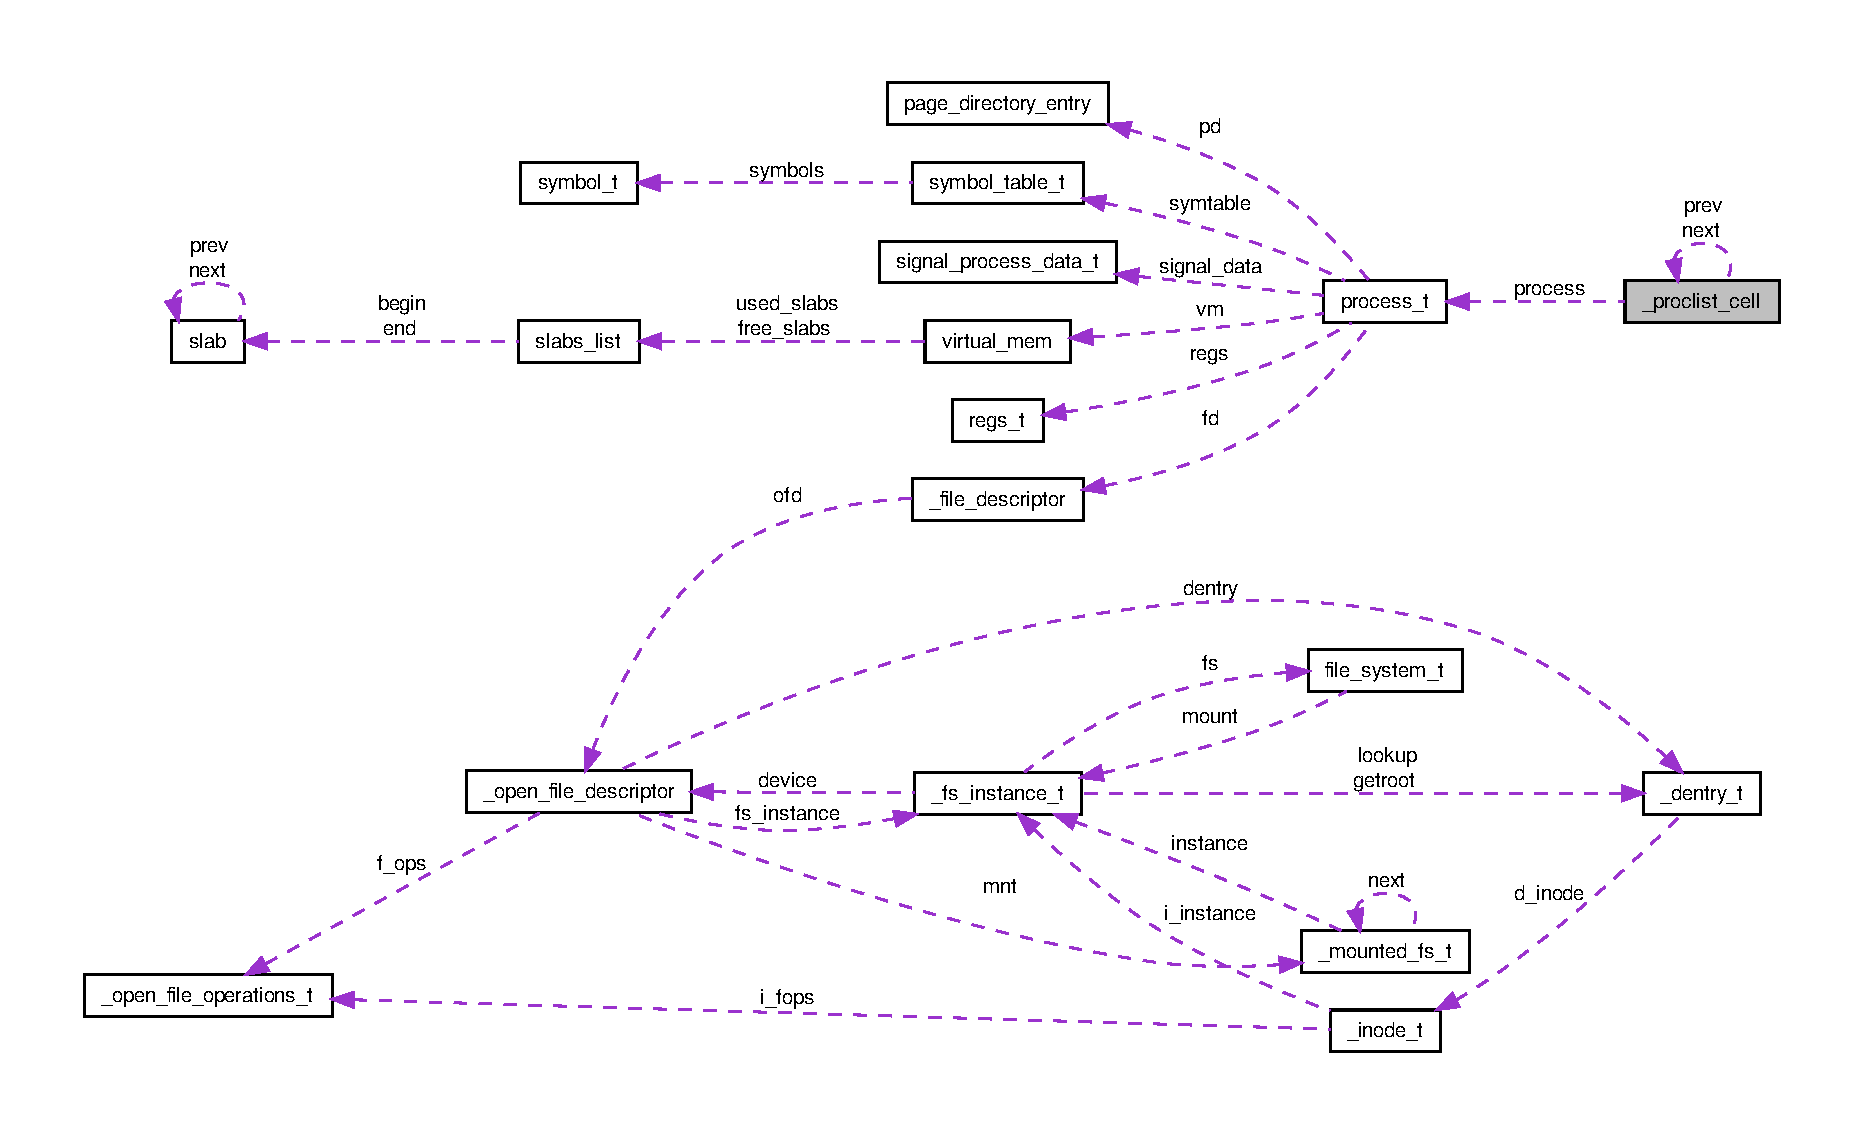
\includegraphics[width=350pt]{struct__proclist__cell__coll__graph}
\end{center}
\end{figure}
\subsection*{Champs de données}
\begin{DoxyCompactItemize}
\item 
\hyperlink{kprocess_8h_a7742ed3a86b7bcb5a4b76893fc331ede}{process\+\_\+t} $\ast$ \hyperlink{struct__proclist__cell_abe320ebc4ea6556f17dd28e93efb6b31}{process}
\item 
struct \hyperlink{struct__proclist__cell}{\+\_\+proclist\+\_\+cell} $\ast$ \hyperlink{struct__proclist__cell_a76062c3c8bce7b458ed610e7568c0858}{next}
\item 
struct \hyperlink{struct__proclist__cell}{\+\_\+proclist\+\_\+cell} $\ast$ \hyperlink{struct__proclist__cell_aee5c3bd7595d05c693fe6df63937052e}{prev}
\end{DoxyCompactItemize}


\subsection{Description détaillée}
Cellule de la liste des processus. 

\subsection{Documentation des champs}
\hypertarget{struct__proclist__cell_a76062c3c8bce7b458ed610e7568c0858}{\index{\+\_\+proclist\+\_\+cell@{\+\_\+proclist\+\_\+cell}!next@{next}}
\index{next@{next}!\+\_\+proclist\+\_\+cell@{\+\_\+proclist\+\_\+cell}}
\subsubsection[{next}]{\setlength{\rightskip}{0pt plus 5cm}struct {\bf \+\_\+proclist\+\_\+cell}$\ast$ \+\_\+proclist\+\_\+cell\+::next}}\label{struct__proclist__cell_a76062c3c8bce7b458ed610e7568c0858}
Maillon suivant. \hypertarget{struct__proclist__cell_aee5c3bd7595d05c693fe6df63937052e}{\index{\+\_\+proclist\+\_\+cell@{\+\_\+proclist\+\_\+cell}!prev@{prev}}
\index{prev@{prev}!\+\_\+proclist\+\_\+cell@{\+\_\+proclist\+\_\+cell}}
\subsubsection[{prev}]{\setlength{\rightskip}{0pt plus 5cm}struct {\bf \+\_\+proclist\+\_\+cell}$\ast$ \+\_\+proclist\+\_\+cell\+::prev}}\label{struct__proclist__cell_aee5c3bd7595d05c693fe6df63937052e}
Maillon précedent. \hypertarget{struct__proclist__cell_abe320ebc4ea6556f17dd28e93efb6b31}{\index{\+\_\+proclist\+\_\+cell@{\+\_\+proclist\+\_\+cell}!process@{process}}
\index{process@{process}!\+\_\+proclist\+\_\+cell@{\+\_\+proclist\+\_\+cell}}
\subsubsection[{process}]{\setlength{\rightskip}{0pt plus 5cm}{\bf process\+\_\+t}$\ast$ \+\_\+proclist\+\_\+cell\+::process}}\label{struct__proclist__cell_abe320ebc4ea6556f17dd28e93efb6b31}
Processus. 

La documentation de cette structure a été générée à partir du fichier suivant \+:\begin{DoxyCompactItemize}
\item 
kernel/include/\hyperlink{kprocess_8h}{kprocess.\+h}\end{DoxyCompactItemize}

\hypertarget{struct__sem__fifo__cell}{\section{Référence de la structure \-\_\-sem\-\_\-fifo\-\_\-cell}
\label{struct__sem__fifo__cell}\index{\-\_\-sem\-\_\-fifo\-\_\-cell@{\-\_\-sem\-\_\-fifo\-\_\-cell}}
}


Graphe de collaboration de \-\_\-sem\-\_\-fifo\-\_\-cell\-:\nopagebreak
\begin{figure}[H]
\begin{center}
\leavevmode
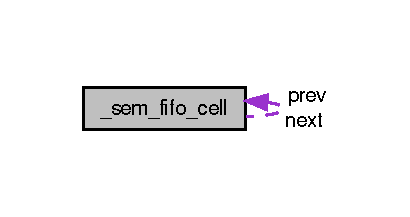
\includegraphics[width=197pt]{struct__sem__fifo__cell__coll__graph}
\end{center}
\end{figure}
\subsection*{Champs de données}
\begin{DoxyCompactItemize}
\item 
\hypertarget{struct__sem__fifo__cell_a60382c870abf5a74875c15743faa1ff5}{int {\bfseries pid}}\label{struct__sem__fifo__cell_a60382c870abf5a74875c15743faa1ff5}

\item 
\hypertarget{struct__sem__fifo__cell_a394553df6f97fa90d1f7638ca1115294}{struct \hyperlink{struct__sem__fifo__cell}{\-\_\-sem\-\_\-fifo\-\_\-cell} $\ast$ {\bfseries prev}}\label{struct__sem__fifo__cell_a394553df6f97fa90d1f7638ca1115294}

\item 
\hypertarget{struct__sem__fifo__cell_ae8a5828e72f457b364e4825faf3a515d}{struct \hyperlink{struct__sem__fifo__cell}{\-\_\-sem\-\_\-fifo\-\_\-cell} $\ast$ {\bfseries next}}\label{struct__sem__fifo__cell_ae8a5828e72f457b364e4825faf3a515d}

\end{DoxyCompactItemize}


\subsection{Description détaillée}
Cellule d'une fifo. 

La documentation de cette structure a été générée à partir du fichier suivant \-:\begin{DoxyCompactItemize}
\item 
kernel/\hyperlink{ksem_8c}{ksem.\-c}\end{DoxyCompactItemize}

\hypertarget{struct__tty__driver__t}{\section{Référence de la structure \+\_\+tty\+\_\+driver\+\_\+t}
\label{struct__tty__driver__t}\index{\+\_\+tty\+\_\+driver\+\_\+t@{\+\_\+tty\+\_\+driver\+\_\+t}}
}


{\ttfamily \#include $<$tty.\+h$>$}



Graphe de collaboration de \+\_\+tty\+\_\+driver\+\_\+t\+:\nopagebreak
\begin{figure}[H]
\begin{center}
\leavevmode
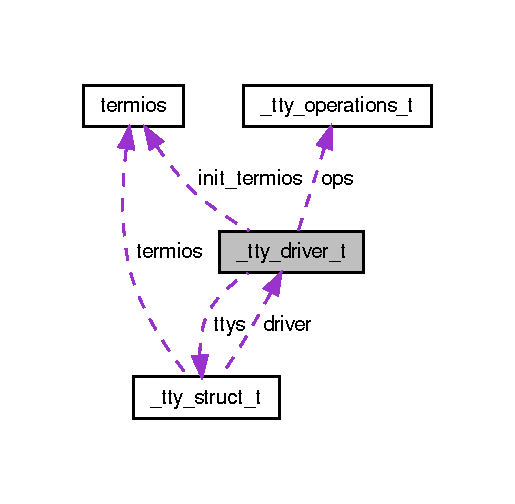
\includegraphics[width=247pt]{struct__tty__driver__t__coll__graph}
\end{center}
\end{figure}
\subsection*{Champs de données}
\begin{DoxyCompactItemize}
\item 
const char $\ast$ \hyperlink{struct__tty__driver__t_ae2f43b40c48f11feab23551e34a4fe6d}{driver\+\_\+name}
\item 
const char $\ast$ \hyperlink{struct__tty__driver__t_a0c46e5dd6e7275908881f644d7fff927}{devfs\+\_\+name}
\item 
int \hyperlink{struct__tty__driver__t_a0f0243090bc705d41b3a6cc28c886cdf}{num}
\item 
short \hyperlink{struct__tty__driver__t_a0c9f7f164f7454cf2bea36de5e23a5d1}{type}
\item 
short \hyperlink{struct__tty__driver__t_a291fe7f9436ef9cbe34b490d516f46bd}{subtype}
\item 
\hyperlink{kernel_2include_2types_8h_a33594304e786b158f3fb30289278f5af}{uint32\+\_\+t} \hyperlink{struct__tty__driver__t_a4ce1272b5e539a50b106986a79d7cab9}{flags}
\item 
\hypertarget{struct__tty__driver__t_afca7a640278fe195af30dbbd5116ee68}{struct \hyperlink{structtermios}{termios} {\bfseries init\+\_\+termios}}\label{struct__tty__driver__t_afca7a640278fe195af30dbbd5116ee68}

\item 
\hypertarget{struct__tty__driver__t_a8e10e237b92b125136a6e4bb5203a210}{\hyperlink{tty_8h_a0870504b9f2d2e99a669e6df3dc9e84e}{tty\+\_\+struct\+\_\+t} $\ast$$\ast$ {\bfseries ttys}}\label{struct__tty__driver__t_a8e10e237b92b125136a6e4bb5203a210}

\item 
\hypertarget{struct__tty__driver__t_aaed3302c349f8bf34d51cfe3cc603f70}{\hyperlink{tty_8h_af76ab451b44b0a6479abe8aeb1bab6b4}{tty\+\_\+operations\+\_\+t} $\ast$ {\bfseries ops}}\label{struct__tty__driver__t_aaed3302c349f8bf34d51cfe3cc603f70}

\end{DoxyCompactItemize}


\subsection{Description détaillée}
Structure qui sert à l'enregistrement d'un driver tty. 

\subsection{Documentation des champs}
\hypertarget{struct__tty__driver__t_a0c46e5dd6e7275908881f644d7fff927}{\index{\+\_\+tty\+\_\+driver\+\_\+t@{\+\_\+tty\+\_\+driver\+\_\+t}!devfs\+\_\+name@{devfs\+\_\+name}}
\index{devfs\+\_\+name@{devfs\+\_\+name}!\+\_\+tty\+\_\+driver\+\_\+t@{\+\_\+tty\+\_\+driver\+\_\+t}}
\subsubsection[{devfs\+\_\+name}]{\setlength{\rightskip}{0pt plus 5cm}const char$\ast$ \+\_\+tty\+\_\+driver\+\_\+t\+::devfs\+\_\+name}}\label{struct__tty__driver__t_a0c46e5dd6e7275908881f644d7fff927}
Le prefixe à ajouter dans le devfs \hypertarget{struct__tty__driver__t_ae2f43b40c48f11feab23551e34a4fe6d}{\index{\+\_\+tty\+\_\+driver\+\_\+t@{\+\_\+tty\+\_\+driver\+\_\+t}!driver\+\_\+name@{driver\+\_\+name}}
\index{driver\+\_\+name@{driver\+\_\+name}!\+\_\+tty\+\_\+driver\+\_\+t@{\+\_\+tty\+\_\+driver\+\_\+t}}
\subsubsection[{driver\+\_\+name}]{\setlength{\rightskip}{0pt plus 5cm}const char$\ast$ \+\_\+tty\+\_\+driver\+\_\+t\+::driver\+\_\+name}}\label{struct__tty__driver__t_ae2f43b40c48f11feab23551e34a4fe6d}
Le nom du driver \hypertarget{struct__tty__driver__t_a4ce1272b5e539a50b106986a79d7cab9}{\index{\+\_\+tty\+\_\+driver\+\_\+t@{\+\_\+tty\+\_\+driver\+\_\+t}!flags@{flags}}
\index{flags@{flags}!\+\_\+tty\+\_\+driver\+\_\+t@{\+\_\+tty\+\_\+driver\+\_\+t}}
\subsubsection[{flags}]{\setlength{\rightskip}{0pt plus 5cm}{\bf uint32\+\_\+t} \+\_\+tty\+\_\+driver\+\_\+t\+::flags}}\label{struct__tty__driver__t_a4ce1272b5e539a50b106986a79d7cab9}
Flags, tel que R\+E\+S\+E\+T\+\_\+\+T\+E\+R\+M\+I\+O\+S, R\+E\+A\+L\+\_\+\+R\+A\+W ou N\+O\+\_\+\+D\+E\+V\+F\+S \hypertarget{struct__tty__driver__t_a0f0243090bc705d41b3a6cc28c886cdf}{\index{\+\_\+tty\+\_\+driver\+\_\+t@{\+\_\+tty\+\_\+driver\+\_\+t}!num@{num}}
\index{num@{num}!\+\_\+tty\+\_\+driver\+\_\+t@{\+\_\+tty\+\_\+driver\+\_\+t}}
\subsubsection[{num}]{\setlength{\rightskip}{0pt plus 5cm}int \+\_\+tty\+\_\+driver\+\_\+t\+::num}}\label{struct__tty__driver__t_a0f0243090bc705d41b3a6cc28c886cdf}
Nombre de devices au maximum. \hypertarget{struct__tty__driver__t_a291fe7f9436ef9cbe34b490d516f46bd}{\index{\+\_\+tty\+\_\+driver\+\_\+t@{\+\_\+tty\+\_\+driver\+\_\+t}!subtype@{subtype}}
\index{subtype@{subtype}!\+\_\+tty\+\_\+driver\+\_\+t@{\+\_\+tty\+\_\+driver\+\_\+t}}
\subsubsection[{subtype}]{\setlength{\rightskip}{0pt plus 5cm}short \+\_\+tty\+\_\+driver\+\_\+t\+::subtype}}\label{struct__tty__driver__t_a291fe7f9436ef9cbe34b490d516f46bd}
Soustype \+: ptm, pts par exemple \hypertarget{struct__tty__driver__t_a0c9f7f164f7454cf2bea36de5e23a5d1}{\index{\+\_\+tty\+\_\+driver\+\_\+t@{\+\_\+tty\+\_\+driver\+\_\+t}!type@{type}}
\index{type@{type}!\+\_\+tty\+\_\+driver\+\_\+t@{\+\_\+tty\+\_\+driver\+\_\+t}}
\subsubsection[{type}]{\setlength{\rightskip}{0pt plus 5cm}short \+\_\+tty\+\_\+driver\+\_\+t\+::type}}\label{struct__tty__driver__t_a0c9f7f164f7454cf2bea36de5e23a5d1}
type \+: console, serial, pty 

La documentation de cette structure a été générée à partir du fichier suivant \+:\begin{DoxyCompactItemize}
\item 
kernel/include/\hyperlink{tty_8h}{tty.\+h}\end{DoxyCompactItemize}

\hypertarget{struct__tty__operations__t}{\section{\-Référence de la structure \-\_\-tty\-\_\-operations\-\_\-t}
\label{struct__tty__operations__t}\index{\-\_\-tty\-\_\-operations\-\_\-t@{\-\_\-tty\-\_\-operations\-\_\-t}}
}


{\ttfamily \#include $<$tty.\-h$>$}

\subsection*{\-Champs de données}
\begin{DoxyCompactItemize}
\item 
\hypertarget{struct__tty__operations__t_a44fb314b6ba47294932a8fdfe8e25d63}{int($\ast$ {\bfseries open} )(\hyperlink{tty_8h_a0870504b9f2d2e99a669e6df3dc9e84e}{tty\-\_\-struct\-\_\-t} $\ast$, \hyperlink{struct__open__file__descriptor}{open\-\_\-file\-\_\-descriptor} $\ast$)}\label{struct__tty__operations__t_a44fb314b6ba47294932a8fdfe8e25d63}

\item 
\hypertarget{struct__tty__operations__t_a9277a33599caf8b99b1f4ba52708a117}{int($\ast$ {\bfseries close} )(\hyperlink{tty_8h_a0870504b9f2d2e99a669e6df3dc9e84e}{tty\-\_\-struct\-\_\-t} $\ast$, \hyperlink{struct__open__file__descriptor}{open\-\_\-file\-\_\-descriptor} $\ast$)}\label{struct__tty__operations__t_a9277a33599caf8b99b1f4ba52708a117}

\item 
\hypertarget{struct__tty__operations__t_a2b53188048a05fa70f02311f48b6d877}{\hyperlink{types_8h_a29d85914ddff32967d85ada69854206d}{size\-\_\-t}($\ast$ {\bfseries write} )(\hyperlink{tty_8h_a0870504b9f2d2e99a669e6df3dc9e84e}{tty\-\_\-struct\-\_\-t} $\ast$, \hyperlink{struct__open__file__descriptor}{open\-\_\-file\-\_\-descriptor} $\ast$, const unsigned char $\ast$, \hyperlink{types_8h_a29d85914ddff32967d85ada69854206d}{size\-\_\-t})}\label{struct__tty__operations__t_a2b53188048a05fa70f02311f48b6d877}

\item 
\hypertarget{struct__tty__operations__t_aa6245586b6d4d0fb23f2afe2ea6e6672}{void($\ast$ {\bfseries put\-\_\-char} )(\hyperlink{tty_8h_a0870504b9f2d2e99a669e6df3dc9e84e}{tty\-\_\-struct\-\_\-t} $\ast$tty, unsigned char ch)}\label{struct__tty__operations__t_aa6245586b6d4d0fb23f2afe2ea6e6672}

\item 
\hypertarget{struct__tty__operations__t_a635940084e0140e5b859572d4b1cb647}{\hyperlink{types_8h_a29d85914ddff32967d85ada69854206d}{size\-\_\-t}($\ast$ {\bfseries set\-\_\-termios} )(struct \hyperlink{structtermios}{termios} $\ast$, struct \hyperlink{structtermios}{termios} $\ast$)}\label{struct__tty__operations__t_a635940084e0140e5b859572d4b1cb647}

\item 
\hypertarget{struct__tty__operations__t_a0d583c140c5fcf8896c42b571be2d2cb}{int($\ast$ {\bfseries ioctl} )(\hyperlink{tty_8h_a0870504b9f2d2e99a669e6df3dc9e84e}{tty\-\_\-struct\-\_\-t} $\ast$tty, \hyperlink{struct__open__file__descriptor}{open\-\_\-file\-\_\-descriptor} $\ast$, unsigned int, void $\ast$)}\label{struct__tty__operations__t_a0d583c140c5fcf8896c42b571be2d2cb}

\end{DoxyCompactItemize}


\subsection{\-Description détaillée}
\-Contient les opérations fournies par le tty driver. 

\-La documentation de cette structure a été générée à partir du fichier suivant \-:\begin{DoxyCompactItemize}
\item 
kernel/include/\hyperlink{tty_8h}{tty.\-h}\end{DoxyCompactItemize}

\hypertarget{struct__tty__struct__t}{\section{Référence de la structure \-\_\-tty\-\_\-struct\-\_\-t}
\label{struct__tty__struct__t}\index{\-\_\-tty\-\_\-struct\-\_\-t@{\-\_\-tty\-\_\-struct\-\_\-t}}
}


{\ttfamily \#include $<$tty.\-h$>$}



Graphe de collaboration de \-\_\-tty\-\_\-struct\-\_\-t\-:
\nopagebreak
\begin{figure}[H]
\begin{center}
\leavevmode
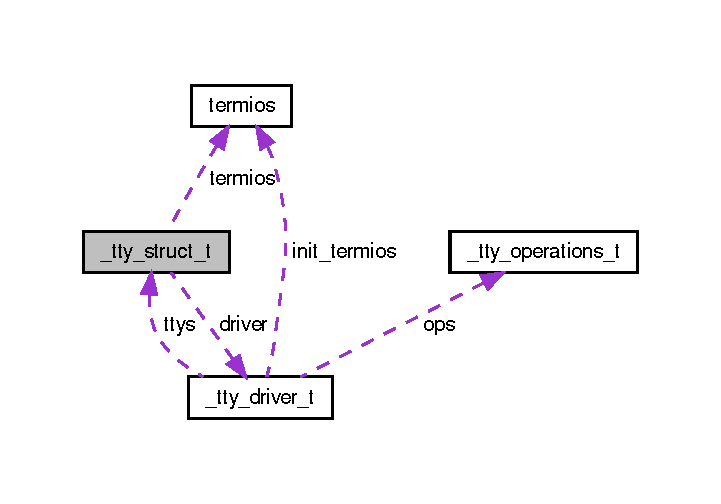
\includegraphics[width=347pt]{struct__tty__struct__t__coll__graph}
\end{center}
\end{figure}
\subsection*{Champs de données}
\begin{DoxyCompactItemize}
\item 
int \hyperlink{struct__tty__struct__t_a4208e736cfcd8e0b00a3c0bbfe4674f7}{index}
\item 
void $\ast$ \hyperlink{struct__tty__struct__t_a974cb784cad13e547e5cace553875f90}{driver\-\_\-data}
\item 
struct \hyperlink{structtermios}{termios} \hyperlink{struct__tty__struct__t_a39471b82fd4e3a235744e73775ac2523}{termios}
\item 
char \hyperlink{struct__tty__struct__t_ace735f0fca7a2e1c4c75f6ffb9223b19}{buffer} \mbox{[}\hyperlink{tty_8h_a00c1f0e7816626f58349492ef0720b5f}{M\-A\-X\-\_\-\-I\-N\-P\-U\-T}\mbox{]}
\item 
\hypertarget{struct__tty__struct__t_ae136497684ded03f21999f2239b3b67c}{unsigned int {\bfseries p\-\_\-begin}}\label{struct__tty__struct__t_ae136497684ded03f21999f2239b3b67c}

\item 
\hypertarget{struct__tty__struct__t_a437e8f9f913784a7f60cf95af3917b23}{unsigned int {\bfseries p\-\_\-end}}\label{struct__tty__struct__t_a437e8f9f913784a7f60cf95af3917b23}

\item 
\hypertarget{struct__tty__struct__t_a10847c2c12b0a9e131f107ec9dbe65f8}{struct \hyperlink{struct__tty__driver__t}{\-\_\-tty\-\_\-driver\-\_\-t} $\ast$ {\bfseries driver}}\label{struct__tty__struct__t_a10847c2c12b0a9e131f107ec9dbe65f8}

\item 
\hypertarget{struct__tty__struct__t_ac5522c658c4a0e142e85142432fa44fe}{\hyperlink{kernel_2include_2types_8h_aba7bc1797add20fe3efdf37ced1182c5}{uint8\-\_\-t} {\bfseries sem}}\label{struct__tty__struct__t_ac5522c658c4a0e142e85142432fa44fe}

\item 
\hypertarget{struct__tty__struct__t_ad017c8b00079444a966de0a0d31b1dd7}{int {\bfseries fg\-\_\-process}}\label{struct__tty__struct__t_ad017c8b00079444a966de0a0d31b1dd7}

\item 
\hypertarget{struct__tty__struct__t_a31c54deea3b926404682b196eb366966}{int {\bfseries n\-\_\-open}}\label{struct__tty__struct__t_a31c54deea3b926404682b196eb366966}

\end{DoxyCompactItemize}


\subsection{Description détaillée}
Structure qui est passée à chaque appel de fonction (open, close, write...) au tty driver. 

\subsection{Documentation des champs}
\hypertarget{struct__tty__struct__t_ace735f0fca7a2e1c4c75f6ffb9223b19}{\index{\-\_\-tty\-\_\-struct\-\_\-t@{\-\_\-tty\-\_\-struct\-\_\-t}!buffer@{buffer}}
\index{buffer@{buffer}!_tty_struct_t@{\-\_\-tty\-\_\-struct\-\_\-t}}
\subsubsection[{buffer}]{\setlength{\rightskip}{0pt plus 5cm}char \-\_\-tty\-\_\-struct\-\_\-t\-::buffer\mbox{[}{\bf M\-A\-X\-\_\-\-I\-N\-P\-U\-T}\mbox{]}}}\label{struct__tty__struct__t_ace735f0fca7a2e1c4c75f6ffb9223b19}
Données prêtes pour la lecture. \hypertarget{struct__tty__struct__t_a974cb784cad13e547e5cace553875f90}{\index{\-\_\-tty\-\_\-struct\-\_\-t@{\-\_\-tty\-\_\-struct\-\_\-t}!driver\-\_\-data@{driver\-\_\-data}}
\index{driver\-\_\-data@{driver\-\_\-data}!_tty_struct_t@{\-\_\-tty\-\_\-struct\-\_\-t}}
\subsubsection[{driver\-\_\-data}]{\setlength{\rightskip}{0pt plus 5cm}void$\ast$ \-\_\-tty\-\_\-struct\-\_\-t\-::driver\-\_\-data}}\label{struct__tty__struct__t_a974cb784cad13e547e5cace553875f90}
De quoi enregistrer des données pour le driver. \hypertarget{struct__tty__struct__t_a4208e736cfcd8e0b00a3c0bbfe4674f7}{\index{\-\_\-tty\-\_\-struct\-\_\-t@{\-\_\-tty\-\_\-struct\-\_\-t}!index@{index}}
\index{index@{index}!_tty_struct_t@{\-\_\-tty\-\_\-struct\-\_\-t}}
\subsubsection[{index}]{\setlength{\rightskip}{0pt plus 5cm}int \-\_\-tty\-\_\-struct\-\_\-t\-::index}}\label{struct__tty__struct__t_a4208e736cfcd8e0b00a3c0bbfe4674f7}
Équivalent du minor number. \hypertarget{struct__tty__struct__t_a39471b82fd4e3a235744e73775ac2523}{\index{\-\_\-tty\-\_\-struct\-\_\-t@{\-\_\-tty\-\_\-struct\-\_\-t}!termios@{termios}}
\index{termios@{termios}!_tty_struct_t@{\-\_\-tty\-\_\-struct\-\_\-t}}
\subsubsection[{termios}]{\setlength{\rightskip}{0pt plus 5cm}struct {\bf termios} \-\_\-tty\-\_\-struct\-\_\-t\-::termios}}\label{struct__tty__struct__t_a39471b82fd4e3a235744e73775ac2523}
Configuration du terminal. 

La documentation de cette structure a été générée à partir du fichier suivant \-:\begin{DoxyCompactItemize}
\item 
kernel/include/\hyperlink{tty_8h}{tty.\-h}\end{DoxyCompactItemize}

\hypertarget{structblkdev__interfaces}{\section{\-Référence de la structure blkdev\-\_\-interfaces}
\label{structblkdev__interfaces}\index{blkdev\-\_\-interfaces@{blkdev\-\_\-interfaces}}
}


\-Graphe de collaboration de blkdev\-\_\-interfaces\-:\nopagebreak
\begin{figure}[H]
\begin{center}
\leavevmode
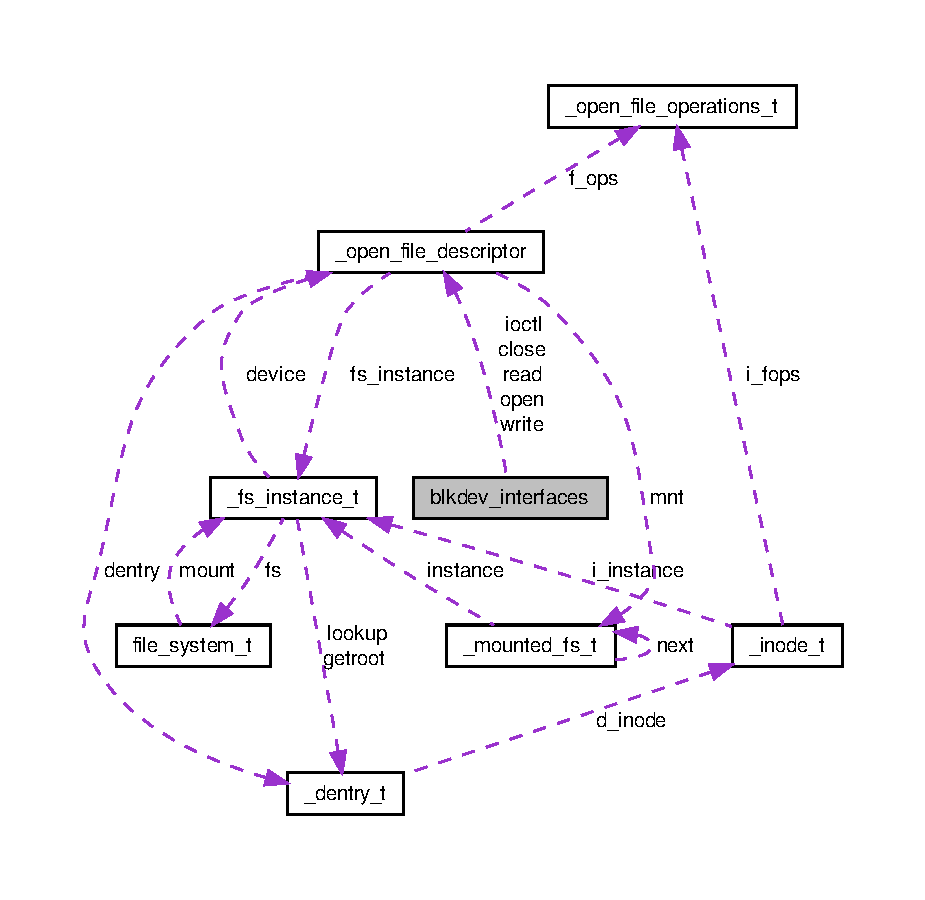
\includegraphics[width=350pt]{structblkdev__interfaces__coll__graph}
\end{center}
\end{figure}
\subsection*{\-Champs de données}
\begin{DoxyCompactItemize}
\item 
\hypertarget{structblkdev__interfaces_ad14a2ad714105cdb8ce002eb4fb9e747}{blkdev\-\_\-read\-\_\-t {\bfseries read}}\label{structblkdev__interfaces_ad14a2ad714105cdb8ce002eb4fb9e747}

\item 
\hypertarget{structblkdev__interfaces_ae99fb7e1529ef6c24df9dc454bc0f9f6}{blkdev\-\_\-write\-\_\-t {\bfseries write}}\label{structblkdev__interfaces_ae99fb7e1529ef6c24df9dc454bc0f9f6}

\item 
\hypertarget{structblkdev__interfaces_ae93720624e6f1a1ea33e31bf1da4c097}{blkdev\-\_\-ioctl\-\_\-t {\bfseries ioctl}}\label{structblkdev__interfaces_ae93720624e6f1a1ea33e31bf1da4c097}

\item 
\hypertarget{structblkdev__interfaces_a08eaa39b105826d2780991b32577867a}{blkdev\-\_\-open\-\_\-t {\bfseries open}}\label{structblkdev__interfaces_a08eaa39b105826d2780991b32577867a}

\item 
\hypertarget{structblkdev__interfaces_ab7623005e31211894853b3524e1e74eb}{blkdev\-\_\-close\-\_\-t {\bfseries close}}\label{structblkdev__interfaces_ab7623005e31211894853b3524e1e74eb}

\item 
\hypertarget{structblkdev__interfaces_a8eea79e70042c41cc171796b501a9fd1}{void $\ast$ {\bfseries custom\-\_\-data}}\label{structblkdev__interfaces_a8eea79e70042c41cc171796b501a9fd1}

\end{DoxyCompactItemize}


\-La documentation de cette structure a été générée à partir du fichier suivant \-:\begin{DoxyCompactItemize}
\item 
kernel/include/fs/\hyperlink{devfs_8h}{devfs.\-h}\end{DoxyCompactItemize}

\hypertarget{structchardev__interfaces}{\section{Référence de la structure chardev\+\_\+interfaces}
\label{structchardev__interfaces}\index{chardev\+\_\+interfaces@{chardev\+\_\+interfaces}}
}


Structure contenant les fonction qui permettent d'utiliser un char device.  




{\ttfamily \#include $<$devfs.\+h$>$}



Graphe de collaboration de chardev\+\_\+interfaces\+:
\nopagebreak
\begin{figure}[H]
\begin{center}
\leavevmode
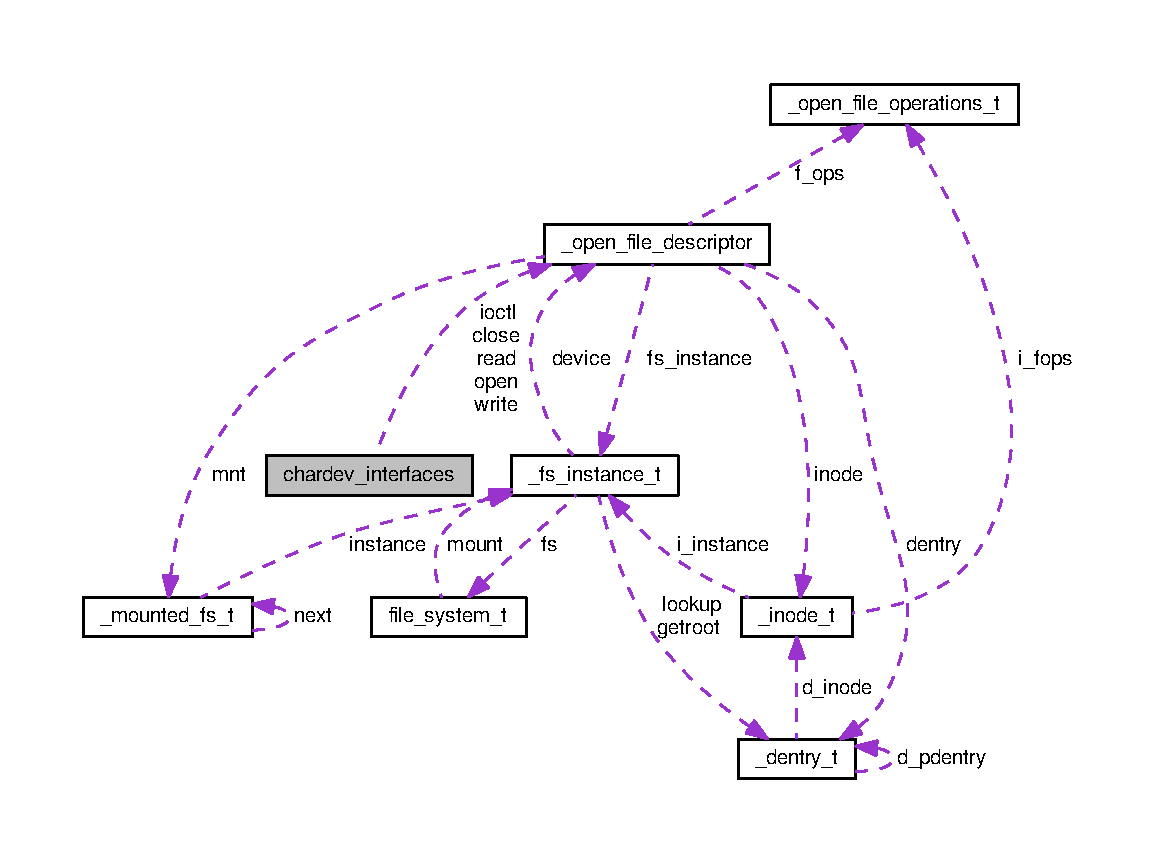
\includegraphics[width=350pt]{structchardev__interfaces__coll__graph}
\end{center}
\end{figure}
\subsection*{Champs de données}
\begin{DoxyCompactItemize}
\item 
chardev\+\_\+read\+\_\+t \hyperlink{structchardev__interfaces_afeba560360e6a5dfff549d78c220b68b}{read}
\item 
chardev\+\_\+write\+\_\+t \hyperlink{structchardev__interfaces_a6f70961f2f888de24d500d50bae85a3f}{write}
\item 
chardev\+\_\+ioctl\+\_\+t \hyperlink{structchardev__interfaces_a9e5903e31e8e5ab21e9abc4b3a844e4a}{ioctl}
\item 
chardev\+\_\+open\+\_\+t \hyperlink{structchardev__interfaces_a7962a67531ea5263a2f837c36fb18dc0}{open}
\item 
chardev\+\_\+close\+\_\+t \hyperlink{structchardev__interfaces_a9cba421c4dddc041e4b5029d011dbbd9}{close}
\item 
void $\ast$ \hyperlink{structchardev__interfaces_a9b6b938d76fe7e20c93da8a032a42ad7}{custom\+\_\+data}
\end{DoxyCompactItemize}


\subsection{Documentation des champs}
\hypertarget{structchardev__interfaces_a9cba421c4dddc041e4b5029d011dbbd9}{\index{chardev\+\_\+interfaces@{chardev\+\_\+interfaces}!close@{close}}
\index{close@{close}!chardev\+\_\+interfaces@{chardev\+\_\+interfaces}}
\subsubsection[{close}]{\setlength{\rightskip}{0pt plus 5cm}chardev\+\_\+close\+\_\+t chardev\+\_\+interfaces\+::close}}\label{structchardev__interfaces_a9cba421c4dddc041e4b5029d011dbbd9}
Fonction appelée à la fermeture du device. \hypertarget{structchardev__interfaces_a9b6b938d76fe7e20c93da8a032a42ad7}{\index{chardev\+\_\+interfaces@{chardev\+\_\+interfaces}!custom\+\_\+data@{custom\+\_\+data}}
\index{custom\+\_\+data@{custom\+\_\+data}!chardev\+\_\+interfaces@{chardev\+\_\+interfaces}}
\subsubsection[{custom\+\_\+data}]{\setlength{\rightskip}{0pt plus 5cm}void$\ast$ chardev\+\_\+interfaces\+::custom\+\_\+data}}\label{structchardev__interfaces_a9b6b938d76fe7e20c93da8a032a42ad7}
Données complémentaires qui peuvent être nécessaires pour utiliser le device. \hypertarget{structchardev__interfaces_a9e5903e31e8e5ab21e9abc4b3a844e4a}{\index{chardev\+\_\+interfaces@{chardev\+\_\+interfaces}!ioctl@{ioctl}}
\index{ioctl@{ioctl}!chardev\+\_\+interfaces@{chardev\+\_\+interfaces}}
\subsubsection[{ioctl}]{\setlength{\rightskip}{0pt plus 5cm}chardev\+\_\+ioctl\+\_\+t chardev\+\_\+interfaces\+::ioctl}}\label{structchardev__interfaces_a9e5903e31e8e5ab21e9abc4b3a844e4a}
Fonction de contrôle du périphérique. \hypertarget{structchardev__interfaces_a7962a67531ea5263a2f837c36fb18dc0}{\index{chardev\+\_\+interfaces@{chardev\+\_\+interfaces}!open@{open}}
\index{open@{open}!chardev\+\_\+interfaces@{chardev\+\_\+interfaces}}
\subsubsection[{open}]{\setlength{\rightskip}{0pt plus 5cm}chardev\+\_\+open\+\_\+t chardev\+\_\+interfaces\+::open}}\label{structchardev__interfaces_a7962a67531ea5263a2f837c36fb18dc0}
Fonction appelée à l'ouverture du device. \hypertarget{structchardev__interfaces_afeba560360e6a5dfff549d78c220b68b}{\index{chardev\+\_\+interfaces@{chardev\+\_\+interfaces}!read@{read}}
\index{read@{read}!chardev\+\_\+interfaces@{chardev\+\_\+interfaces}}
\subsubsection[{read}]{\setlength{\rightskip}{0pt plus 5cm}chardev\+\_\+read\+\_\+t chardev\+\_\+interfaces\+::read}}\label{structchardev__interfaces_afeba560360e6a5dfff549d78c220b68b}
Fonction de lecture. \hypertarget{structchardev__interfaces_a6f70961f2f888de24d500d50bae85a3f}{\index{chardev\+\_\+interfaces@{chardev\+\_\+interfaces}!write@{write}}
\index{write@{write}!chardev\+\_\+interfaces@{chardev\+\_\+interfaces}}
\subsubsection[{write}]{\setlength{\rightskip}{0pt plus 5cm}chardev\+\_\+write\+\_\+t chardev\+\_\+interfaces\+::write}}\label{structchardev__interfaces_a6f70961f2f888de24d500d50bae85a3f}
Fonction d'écriture. 

La documentation de cette structure a été générée à partir du fichier suivant \+:\begin{DoxyCompactItemize}
\item 
kernel/include/fs/\hyperlink{devfs_8h}{devfs.\+h}\end{DoxyCompactItemize}

\hypertarget{structconsole__t}{\section{Référence de la structure console\-\_\-t}
\label{structconsole__t}\index{console\-\_\-t@{console\-\_\-t}}
}


Structure qui contient les informations d'une console.  




{\ttfamily \#include $<$console.\-h$>$}

\subsection*{Champs de données}
\begin{DoxyCompactItemize}
\item 
bool \hyperlink{structconsole__t_ad830edd689dced40135f6afa651677e3}{used}
\item 
unsigned int \hyperlink{structconsole__t_a296a99289941514aee3b5751d8cd0693}{cur\-\_\-x}
\item 
unsigned int \hyperlink{structconsole__t_a3192dab00ef66635ae4897943c47d6ec}{cur\-\_\-y}
\item 
bool \hyperlink{structconsole__t_a6242c03c5b347ed6b0909c1486116bee}{disp\-\_\-cur}
\item 
char \hyperlink{structconsole__t_a07b1c84ea67ce030ebd868917e56b0d9}{attr}
\item 
unsigned int \hyperlink{structconsole__t_ada36635a93afd23c3eb88c856f218103}{lines}
\item 
unsigned int \hyperlink{structconsole__t_a338612e1f99838e2b34cdb289bc514b8}{cols}
\item 
\hypertarget{structconsole__t_ae1f1c65a083024553e62c067c8f4c819}{bool {\bfseries escape\-\_\-char}}\label{structconsole__t_ae1f1c65a083024553e62c067c8f4c819}

\item 
\hypertarget{structconsole__t_ac75187dfd19554ec511754716d925b80}{bool {\bfseries ansi\-\_\-escape\-\_\-code}}\label{structconsole__t_ac75187dfd19554ec511754716d925b80}

\item 
\hypertarget{structconsole__t_ae22b55ee310c7b6c89c364eb9b193b6c}{bool {\bfseries ansi\-\_\-second\-\_\-val}}\label{structconsole__t_ae22b55ee310c7b6c89c364eb9b193b6c}

\item 
\hypertarget{structconsole__t_a343b19effba1ba6de3ffd7c7a354df90}{int {\bfseries val}}\label{structconsole__t_a343b19effba1ba6de3ffd7c7a354df90}

\item 
\hypertarget{structconsole__t_a77ef720e47b1bd23b1786300935a05a9}{int {\bfseries val2}}\label{structconsole__t_a77ef720e47b1bd23b1786300935a05a9}

\item 
\hypertarget{structconsole__t_a200084390fdbaf02eb4faa5fa2481062}{int {\bfseries bright}}\label{structconsole__t_a200084390fdbaf02eb4faa5fa2481062}

\end{DoxyCompactItemize}


\subsection{Documentation des champs}
\hypertarget{structconsole__t_a07b1c84ea67ce030ebd868917e56b0d9}{\index{console\-\_\-t@{console\-\_\-t}!attr@{attr}}
\index{attr@{attr}!console_t@{console\-\_\-t}}
\subsubsection[{attr}]{\setlength{\rightskip}{0pt plus 5cm}char console\-\_\-t\-::attr}}\label{structconsole__t_a07b1c84ea67ce030ebd868917e56b0d9}
Attribut actuel pour l'affichage de caractères. \hypertarget{structconsole__t_a338612e1f99838e2b34cdb289bc514b8}{\index{console\-\_\-t@{console\-\_\-t}!cols@{cols}}
\index{cols@{cols}!console_t@{console\-\_\-t}}
\subsubsection[{cols}]{\setlength{\rightskip}{0pt plus 5cm}unsigned int console\-\_\-t\-::cols}}\label{structconsole__t_a338612e1f99838e2b34cdb289bc514b8}
Nombre de colonnes. \hypertarget{structconsole__t_a296a99289941514aee3b5751d8cd0693}{\index{console\-\_\-t@{console\-\_\-t}!cur\-\_\-x@{cur\-\_\-x}}
\index{cur\-\_\-x@{cur\-\_\-x}!console_t@{console\-\_\-t}}
\subsubsection[{cur\-\_\-x}]{\setlength{\rightskip}{0pt plus 5cm}unsigned int console\-\_\-t\-::cur\-\_\-x}}\label{structconsole__t_a296a99289941514aee3b5751d8cd0693}
Position horizontale du curseur. \hypertarget{structconsole__t_a3192dab00ef66635ae4897943c47d6ec}{\index{console\-\_\-t@{console\-\_\-t}!cur\-\_\-y@{cur\-\_\-y}}
\index{cur\-\_\-y@{cur\-\_\-y}!console_t@{console\-\_\-t}}
\subsubsection[{cur\-\_\-y}]{\setlength{\rightskip}{0pt plus 5cm}unsigned int console\-\_\-t\-::cur\-\_\-y}}\label{structconsole__t_a3192dab00ef66635ae4897943c47d6ec}
Position verticale du curseur. \hypertarget{structconsole__t_a6242c03c5b347ed6b0909c1486116bee}{\index{console\-\_\-t@{console\-\_\-t}!disp\-\_\-cur@{disp\-\_\-cur}}
\index{disp\-\_\-cur@{disp\-\_\-cur}!console_t@{console\-\_\-t}}
\subsubsection[{disp\-\_\-cur}]{\setlength{\rightskip}{0pt plus 5cm}bool console\-\_\-t\-::disp\-\_\-cur}}\label{structconsole__t_a6242c03c5b347ed6b0909c1486116bee}
Curseur visible. \hypertarget{structconsole__t_ada36635a93afd23c3eb88c856f218103}{\index{console\-\_\-t@{console\-\_\-t}!lines@{lines}}
\index{lines@{lines}!console_t@{console\-\_\-t}}
\subsubsection[{lines}]{\setlength{\rightskip}{0pt plus 5cm}unsigned int console\-\_\-t\-::lines}}\label{structconsole__t_ada36635a93afd23c3eb88c856f218103}
Nombre de lignes. \hypertarget{structconsole__t_ad830edd689dced40135f6afa651677e3}{\index{console\-\_\-t@{console\-\_\-t}!used@{used}}
\index{used@{used}!console_t@{console\-\_\-t}}
\subsubsection[{used}]{\setlength{\rightskip}{0pt plus 5cm}bool console\-\_\-t\-::used}}\label{structconsole__t_ad830edd689dced40135f6afa651677e3}
Console activée. 

La documentation de cette structure a été générée à partir du fichier suivant \-:\begin{DoxyCompactItemize}
\item 
kernel/include/drivers/\hyperlink{console_8h}{console.\-h}\end{DoxyCompactItemize}

\hypertarget{structdirectories__t}{\section{Référence de la structure directories\-\_\-t}
\label{structdirectories__t}\index{directories\-\_\-t@{directories\-\_\-t}}
}


Structure chaînée pour enregistrer les entrées d'un dossier.  




{\ttfamily \#include $<$ext2\-\_\-internal.\-h$>$}



Graphe de collaboration de directories\-\_\-t\-:\nopagebreak
\begin{figure}[H]
\begin{center}
\leavevmode
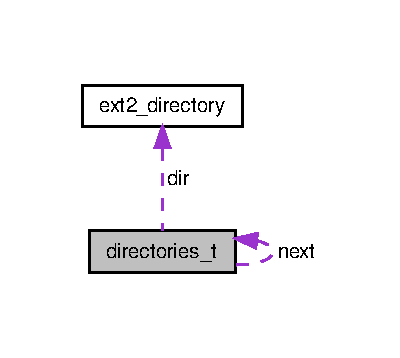
\includegraphics[width=192pt]{structdirectories__t__coll__graph}
\end{center}
\end{figure}
\subsection*{Champs de données}
\begin{DoxyCompactItemize}
\item 
struct \hyperlink{structext2__directory}{ext2\-\_\-directory} $\ast$ \hyperlink{structdirectories__t_aedd8927cb97dd25be9b97fc3d823a5af}{dir}
\item 
struct \hyperlink{structdirectories__t}{directories\-\_\-t} $\ast$ \hyperlink{structdirectories__t_a5c41ffb210dce35d7cc655777a354c92}{next}
\end{DoxyCompactItemize}


\subsection{Documentation des champs}
\hypertarget{structdirectories__t_aedd8927cb97dd25be9b97fc3d823a5af}{\index{directories\-\_\-t@{directories\-\_\-t}!dir@{dir}}
\index{dir@{dir}!directories_t@{directories\-\_\-t}}
\subsubsection[{dir}]{\setlength{\rightskip}{0pt plus 5cm}struct {\bf ext2\-\_\-directory}$\ast$ directories\-\_\-t\-::dir}}\label{structdirectories__t_aedd8927cb97dd25be9b97fc3d823a5af}
Pointeur vers une entrée de dossier ext2. \hypertarget{structdirectories__t_a5c41ffb210dce35d7cc655777a354c92}{\index{directories\-\_\-t@{directories\-\_\-t}!next@{next}}
\index{next@{next}!directories_t@{directories\-\_\-t}}
\subsubsection[{next}]{\setlength{\rightskip}{0pt plus 5cm}struct {\bf directories\-\_\-t}$\ast$ directories\-\_\-t\-::next}}\label{structdirectories__t_a5c41ffb210dce35d7cc655777a354c92}
Pointeur vers la prochaine structure du même type. 

La documentation de cette structure a été générée à partir du fichier suivant \-:\begin{DoxyCompactItemize}
\item 
kernel/fs/ext2/\hyperlink{ext2__internal_8h}{ext2\-\_\-internal.\-h}\end{DoxyCompactItemize}

\hypertarget{structdirent}{\section{Référence de la structure dirent}
\label{structdirent}\index{dirent@{dirent}}
}


{\ttfamily \#include $<$dirent.\-h$>$}

\subsection*{Champs de données}
\begin{DoxyCompactItemize}
\item 
\hyperlink{types_8h_a33594304e786b158f3fb30289278f5af}{uint32\-\_\-t} \hyperlink{structdirent_a0ed2e5ea3c71500f628914bf3966e4ba}{d\-\_\-ino}
\item 
\hyperlink{types_8h_adf4d876453337156dde61095e1f20223}{uint16\-\_\-t} \hyperlink{structdirent_a7cc67dd4ba5a8bed7f107f249957688d}{d\-\_\-reclen}
\item 
\hyperlink{types_8h_aba7bc1797add20fe3efdf37ced1182c5}{uint8\-\_\-t} \hyperlink{structdirent_a948760e3b7f607213a19f85e7af15a32}{d\-\_\-type}
\item 
char \hyperlink{structdirent_a7b4cbd53dc600257b2746225c8a8f3be}{d\-\_\-name} \mbox{[}\hyperlink{dirent_8h_ac64541bdd81c961304b9babef1402640}{N\-A\-M\-E\-\_\-\-M\-A\-X}\mbox{]}
\end{DoxyCompactItemize}


\subsection{Description détaillée}
Directory entry. 

\subsection{Documentation des champs}
\hypertarget{structdirent_a0ed2e5ea3c71500f628914bf3966e4ba}{\index{dirent@{dirent}!d\-\_\-ino@{d\-\_\-ino}}
\index{d\-\_\-ino@{d\-\_\-ino}!dirent@{dirent}}
\subsubsection[{d\-\_\-ino}]{\setlength{\rightskip}{0pt plus 5cm}{\bf uint32\-\_\-t} dirent\-::d\-\_\-ino}}\label{structdirent_a0ed2e5ea3c71500f628914bf3966e4ba}
Numéro inode. \hypertarget{structdirent_a7b4cbd53dc600257b2746225c8a8f3be}{\index{dirent@{dirent}!d\-\_\-name@{d\-\_\-name}}
\index{d\-\_\-name@{d\-\_\-name}!dirent@{dirent}}
\subsubsection[{d\-\_\-name}]{\setlength{\rightskip}{0pt plus 5cm}char dirent\-::d\-\_\-name\mbox{[}{\bf N\-A\-M\-E\-\_\-\-M\-A\-X}\mbox{]}}}\label{structdirent_a7b4cbd53dc600257b2746225c8a8f3be}
Nom du fichier. \hypertarget{structdirent_a7cc67dd4ba5a8bed7f107f249957688d}{\index{dirent@{dirent}!d\-\_\-reclen@{d\-\_\-reclen}}
\index{d\-\_\-reclen@{d\-\_\-reclen}!dirent@{dirent}}
\subsubsection[{d\-\_\-reclen}]{\setlength{\rightskip}{0pt plus 5cm}{\bf uint16\-\_\-t} dirent\-::d\-\_\-reclen}}\label{structdirent_a7cc67dd4ba5a8bed7f107f249957688d}
Taille de l'entrée. \hypertarget{structdirent_a948760e3b7f607213a19f85e7af15a32}{\index{dirent@{dirent}!d\-\_\-type@{d\-\_\-type}}
\index{d\-\_\-type@{d\-\_\-type}!dirent@{dirent}}
\subsubsection[{d\-\_\-type}]{\setlength{\rightskip}{0pt plus 5cm}{\bf uint8\-\_\-t} dirent\-::d\-\_\-type}}\label{structdirent_a948760e3b7f607213a19f85e7af15a32}
Type de fichier. 

La documentation de cette structure a été générée à partir du fichier suivant \-:\begin{DoxyCompactItemize}
\item 
libc/include/\hyperlink{dirent_8h}{dirent.\-h}\end{DoxyCompactItemize}

\hypertarget{structdriver__entry}{\section{Référence de la structure driver\-\_\-entry}
\label{structdriver__entry}\index{driver\-\_\-entry@{driver\-\_\-entry}}
}
\subsection*{Champs de données}
\begin{DoxyCompactItemize}
\item 
\hypertarget{structdriver__entry_a9a2a74aad52e09fb03bef9703530e28f}{char {\bfseries used}}\label{structdriver__entry_a9a2a74aad52e09fb03bef9703530e28f}

\item 
\hypertarget{structdriver__entry_afc014b612d6cedf602aab7255d4576c1}{char $\ast$ {\bfseries name}}\label{structdriver__entry_afc014b612d6cedf602aab7255d4576c1}

\item 
\hypertarget{structdriver__entry_a3d74a551a1bbb2f2583ba058877b52a4}{device\-\_\-type\-\_\-t {\bfseries type}}\label{structdriver__entry_a3d74a551a1bbb2f2583ba058877b52a4}

\item 
\hypertarget{structdriver__entry_ab5b691637ec5edbbe58442fc57f5aba4}{void $\ast$ {\bfseries di}}\label{structdriver__entry_ab5b691637ec5edbbe58442fc57f5aba4}

\end{DoxyCompactItemize}


La documentation de cette structure a été générée à partir du fichier suivant \-:\begin{DoxyCompactItemize}
\item 
kernel/fs/\hyperlink{devfs_8c}{devfs.\-c}\end{DoxyCompactItemize}

\hypertarget{structElf32__Ehdr}{\section{Référence de la structure Elf32\-\_\-\-Ehdr}
\label{structElf32__Ehdr}\index{Elf32\-\_\-\-Ehdr@{Elf32\-\_\-\-Ehdr}}
}


{\ttfamily \#include $<$elf.\-h$>$}

\subsection*{Champs de données}
\begin{DoxyCompactItemize}
\item 
unsigned char \hyperlink{structElf32__Ehdr_aba47ac5e0af02d5668782f1fd5a7466c}{e\-\_\-ident} \mbox{[}E\-I\-\_\-\-N\-I\-D\-E\-N\-T\mbox{]}
\item 
Elf32\-\_\-\-Half \hyperlink{structElf32__Ehdr_a49e40a791813c06e3b6ebcb53aef1bb8}{e\-\_\-type}
\item 
Elf32\-\_\-\-Half \hyperlink{structElf32__Ehdr_a19bca7faba9e5573814643efc3574c7b}{e\-\_\-machine}
\item 
Elf32\-\_\-\-Word \hyperlink{structElf32__Ehdr_aa27627bda53281221325df4dd782e800}{e\-\_\-version}
\item 
Elf32\-\_\-\-Addr \hyperlink{structElf32__Ehdr_ab8a982696048d807017919b7d0145482}{e\-\_\-entry}
\item 
Elf32\-\_\-\-Off \hyperlink{structElf32__Ehdr_a25c36fc010284a928604aae005b67ad1}{e\-\_\-phoff}
\item 
Elf32\-\_\-\-Off \hyperlink{structElf32__Ehdr_a00601af5187a1b3f8babfe9cddd95c15}{e\-\_\-shoff}
\item 
Elf32\-\_\-\-Word \hyperlink{structElf32__Ehdr_a87cf481be7917fafde0c4ecf78c8e574}{e\-\_\-flags}
\item 
Elf32\-\_\-\-Half \hyperlink{structElf32__Ehdr_a04c658023e50479eed64f6d1b00a2504}{e\-\_\-ehsize}
\item 
Elf32\-\_\-\-Half \hyperlink{structElf32__Ehdr_afa2289f96d86fcc568a3b1f40cc8953e}{e\-\_\-phentsize}
\item 
Elf32\-\_\-\-Half \hyperlink{structElf32__Ehdr_a360898812db1655f8cb8258780d9df5b}{e\-\_\-phnum}
\item 
Elf32\-\_\-\-Half \hyperlink{structElf32__Ehdr_ab53c709a841960e499da68e2316ed428}{e\-\_\-shentsize}
\item 
Elf32\-\_\-\-Half \hyperlink{structElf32__Ehdr_a11249bd7e61642742a68a3e7f69ac721}{e\-\_\-shnum}
\item 
Elf32\-\_\-\-Half \hyperlink{structElf32__Ehdr_a3b3070ccd7d971e8cb6ea58d4c6fab09}{e\-\_\-shstrndx}
\end{DoxyCompactItemize}


\subsection{Description détaillée}
E\-L\-F H\-E\-A\-D\-E\-R 

\subsection{Documentation des champs}
\hypertarget{structElf32__Ehdr_a04c658023e50479eed64f6d1b00a2504}{\index{Elf32\-\_\-\-Ehdr@{Elf32\-\_\-\-Ehdr}!e\-\_\-ehsize@{e\-\_\-ehsize}}
\index{e\-\_\-ehsize@{e\-\_\-ehsize}!Elf32_Ehdr@{Elf32\-\_\-\-Ehdr}}
\subsubsection[{e\-\_\-ehsize}]{\setlength{\rightskip}{0pt plus 5cm}Elf32\-\_\-\-Half Elf32\-\_\-\-Ehdr\-::e\-\_\-ehsize}}\label{structElf32__Ehdr_a04c658023e50479eed64f6d1b00a2504}
Taille du header E\-L\-F \hypertarget{structElf32__Ehdr_ab8a982696048d807017919b7d0145482}{\index{Elf32\-\_\-\-Ehdr@{Elf32\-\_\-\-Ehdr}!e\-\_\-entry@{e\-\_\-entry}}
\index{e\-\_\-entry@{e\-\_\-entry}!Elf32_Ehdr@{Elf32\-\_\-\-Ehdr}}
\subsubsection[{e\-\_\-entry}]{\setlength{\rightskip}{0pt plus 5cm}Elf32\-\_\-\-Addr Elf32\-\_\-\-Ehdr\-::e\-\_\-entry}}\label{structElf32__Ehdr_ab8a982696048d807017919b7d0145482}
Adresse virtuelle du point d'entrée \hypertarget{structElf32__Ehdr_a87cf481be7917fafde0c4ecf78c8e574}{\index{Elf32\-\_\-\-Ehdr@{Elf32\-\_\-\-Ehdr}!e\-\_\-flags@{e\-\_\-flags}}
\index{e\-\_\-flags@{e\-\_\-flags}!Elf32_Ehdr@{Elf32\-\_\-\-Ehdr}}
\subsubsection[{e\-\_\-flags}]{\setlength{\rightskip}{0pt plus 5cm}Elf32\-\_\-\-Word Elf32\-\_\-\-Ehdr\-::e\-\_\-flags}}\label{structElf32__Ehdr_a87cf481be7917fafde0c4ecf78c8e574}
Flags spécifiques à la machine \hypertarget{structElf32__Ehdr_aba47ac5e0af02d5668782f1fd5a7466c}{\index{Elf32\-\_\-\-Ehdr@{Elf32\-\_\-\-Ehdr}!e\-\_\-ident@{e\-\_\-ident}}
\index{e\-\_\-ident@{e\-\_\-ident}!Elf32_Ehdr@{Elf32\-\_\-\-Ehdr}}
\subsubsection[{e\-\_\-ident}]{\setlength{\rightskip}{0pt plus 5cm}unsigned char Elf32\-\_\-\-Ehdr\-::e\-\_\-ident\mbox{[}E\-I\-\_\-\-N\-I\-D\-E\-N\-T\mbox{]}}}\label{structElf32__Ehdr_aba47ac5e0af02d5668782f1fd5a7466c}
E\-L\-F Identification \hypertarget{structElf32__Ehdr_a19bca7faba9e5573814643efc3574c7b}{\index{Elf32\-\_\-\-Ehdr@{Elf32\-\_\-\-Ehdr}!e\-\_\-machine@{e\-\_\-machine}}
\index{e\-\_\-machine@{e\-\_\-machine}!Elf32_Ehdr@{Elf32\-\_\-\-Ehdr}}
\subsubsection[{e\-\_\-machine}]{\setlength{\rightskip}{0pt plus 5cm}Elf32\-\_\-\-Half Elf32\-\_\-\-Ehdr\-::e\-\_\-machine}}\label{structElf32__Ehdr_a19bca7faba9e5573814643efc3574c7b}
Architecture de la machine \hypertarget{structElf32__Ehdr_afa2289f96d86fcc568a3b1f40cc8953e}{\index{Elf32\-\_\-\-Ehdr@{Elf32\-\_\-\-Ehdr}!e\-\_\-phentsize@{e\-\_\-phentsize}}
\index{e\-\_\-phentsize@{e\-\_\-phentsize}!Elf32_Ehdr@{Elf32\-\_\-\-Ehdr}}
\subsubsection[{e\-\_\-phentsize}]{\setlength{\rightskip}{0pt plus 5cm}Elf32\-\_\-\-Half Elf32\-\_\-\-Ehdr\-::e\-\_\-phentsize}}\label{structElf32__Ehdr_afa2289f96d86fcc568a3b1f40cc8953e}
Taille d'une entrée dans la table des program header (toutes les entrées ont la même taille) \hypertarget{structElf32__Ehdr_a360898812db1655f8cb8258780d9df5b}{\index{Elf32\-\_\-\-Ehdr@{Elf32\-\_\-\-Ehdr}!e\-\_\-phnum@{e\-\_\-phnum}}
\index{e\-\_\-phnum@{e\-\_\-phnum}!Elf32_Ehdr@{Elf32\-\_\-\-Ehdr}}
\subsubsection[{e\-\_\-phnum}]{\setlength{\rightskip}{0pt plus 5cm}Elf32\-\_\-\-Half Elf32\-\_\-\-Ehdr\-::e\-\_\-phnum}}\label{structElf32__Ehdr_a360898812db1655f8cb8258780d9df5b}
Nombre d'entrées dans la table des program header \hypertarget{structElf32__Ehdr_a25c36fc010284a928604aae005b67ad1}{\index{Elf32\-\_\-\-Ehdr@{Elf32\-\_\-\-Ehdr}!e\-\_\-phoff@{e\-\_\-phoff}}
\index{e\-\_\-phoff@{e\-\_\-phoff}!Elf32_Ehdr@{Elf32\-\_\-\-Ehdr}}
\subsubsection[{e\-\_\-phoff}]{\setlength{\rightskip}{0pt plus 5cm}Elf32\-\_\-\-Off Elf32\-\_\-\-Ehdr\-::e\-\_\-phoff}}\label{structElf32__Ehdr_a25c36fc010284a928604aae005b67ad1}
Offset du program header dans le fichier (0 si aucun program header) \hypertarget{structElf32__Ehdr_ab53c709a841960e499da68e2316ed428}{\index{Elf32\-\_\-\-Ehdr@{Elf32\-\_\-\-Ehdr}!e\-\_\-shentsize@{e\-\_\-shentsize}}
\index{e\-\_\-shentsize@{e\-\_\-shentsize}!Elf32_Ehdr@{Elf32\-\_\-\-Ehdr}}
\subsubsection[{e\-\_\-shentsize}]{\setlength{\rightskip}{0pt plus 5cm}Elf32\-\_\-\-Half Elf32\-\_\-\-Ehdr\-::e\-\_\-shentsize}}\label{structElf32__Ehdr_ab53c709a841960e499da68e2316ed428}
Taille d'une entrée dans la table des section header \hypertarget{structElf32__Ehdr_a11249bd7e61642742a68a3e7f69ac721}{\index{Elf32\-\_\-\-Ehdr@{Elf32\-\_\-\-Ehdr}!e\-\_\-shnum@{e\-\_\-shnum}}
\index{e\-\_\-shnum@{e\-\_\-shnum}!Elf32_Ehdr@{Elf32\-\_\-\-Ehdr}}
\subsubsection[{e\-\_\-shnum}]{\setlength{\rightskip}{0pt plus 5cm}Elf32\-\_\-\-Half Elf32\-\_\-\-Ehdr\-::e\-\_\-shnum}}\label{structElf32__Ehdr_a11249bd7e61642742a68a3e7f69ac721}
Nombre d'entrées dans la table des section header \hypertarget{structElf32__Ehdr_a00601af5187a1b3f8babfe9cddd95c15}{\index{Elf32\-\_\-\-Ehdr@{Elf32\-\_\-\-Ehdr}!e\-\_\-shoff@{e\-\_\-shoff}}
\index{e\-\_\-shoff@{e\-\_\-shoff}!Elf32_Ehdr@{Elf32\-\_\-\-Ehdr}}
\subsubsection[{e\-\_\-shoff}]{\setlength{\rightskip}{0pt plus 5cm}Elf32\-\_\-\-Off Elf32\-\_\-\-Ehdr\-::e\-\_\-shoff}}\label{structElf32__Ehdr_a00601af5187a1b3f8babfe9cddd95c15}
Offset du section header dans le fichier (0 si aucun section header) \hypertarget{structElf32__Ehdr_a3b3070ccd7d971e8cb6ea58d4c6fab09}{\index{Elf32\-\_\-\-Ehdr@{Elf32\-\_\-\-Ehdr}!e\-\_\-shstrndx@{e\-\_\-shstrndx}}
\index{e\-\_\-shstrndx@{e\-\_\-shstrndx}!Elf32_Ehdr@{Elf32\-\_\-\-Ehdr}}
\subsubsection[{e\-\_\-shstrndx}]{\setlength{\rightskip}{0pt plus 5cm}Elf32\-\_\-\-Half Elf32\-\_\-\-Ehdr\-::e\-\_\-shstrndx}}\label{structElf32__Ehdr_a3b3070ccd7d971e8cb6ea58d4c6fab09}
Indice de l'entrée de la table des section header correspondant à la table des strings, si aucune entrée de ce genre, S\-H\-N\-\_\-\-U\-N\-D\-E\-F \hypertarget{structElf32__Ehdr_a49e40a791813c06e3b6ebcb53aef1bb8}{\index{Elf32\-\_\-\-Ehdr@{Elf32\-\_\-\-Ehdr}!e\-\_\-type@{e\-\_\-type}}
\index{e\-\_\-type@{e\-\_\-type}!Elf32_Ehdr@{Elf32\-\_\-\-Ehdr}}
\subsubsection[{e\-\_\-type}]{\setlength{\rightskip}{0pt plus 5cm}Elf32\-\_\-\-Half Elf32\-\_\-\-Ehdr\-::e\-\_\-type}}\label{structElf32__Ehdr_a49e40a791813c06e3b6ebcb53aef1bb8}
Type de fichier E\-L\-F \hypertarget{structElf32__Ehdr_aa27627bda53281221325df4dd782e800}{\index{Elf32\-\_\-\-Ehdr@{Elf32\-\_\-\-Ehdr}!e\-\_\-version@{e\-\_\-version}}
\index{e\-\_\-version@{e\-\_\-version}!Elf32_Ehdr@{Elf32\-\_\-\-Ehdr}}
\subsubsection[{e\-\_\-version}]{\setlength{\rightskip}{0pt plus 5cm}Elf32\-\_\-\-Word Elf32\-\_\-\-Ehdr\-::e\-\_\-version}}\label{structElf32__Ehdr_aa27627bda53281221325df4dd782e800}
Version du fichier objet 

La documentation de cette structure a été générée à partir du fichier suivant \-:\begin{DoxyCompactItemize}
\item 
kernel/include/\hyperlink{elf_8h}{elf.\-h}\end{DoxyCompactItemize}

\hypertarget{structElf32__File}{\section{Référence de la structure Elf32\-\_\-\-File}
\label{structElf32__File}\index{Elf32\-\_\-\-File@{Elf32\-\_\-\-File}}
}


Graphe de collaboration de Elf32\-\_\-\-File\-:
\nopagebreak
\begin{figure}[H]
\begin{center}
\leavevmode
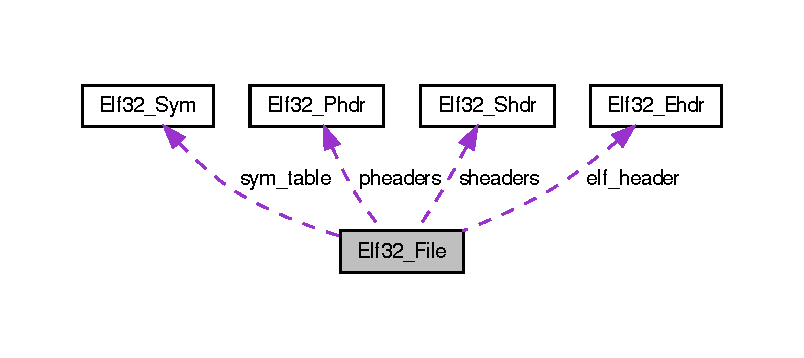
\includegraphics[width=350pt]{structElf32__File__coll__graph}
\end{center}
\end{figure}
\subsection*{Champs de données}
\begin{DoxyCompactItemize}
\item 
\hypertarget{structElf32__File_ad72bb34e9388d51790c6059cdd122137}{char $\ast$ {\bfseries name}}\label{structElf32__File_ad72bb34e9388d51790c6059cdd122137}

\item 
\hypertarget{structElf32__File_ac8df03922d25955e8e597c061a5e228e}{\hyperlink{structElf32__Ehdr}{Elf32\-\_\-\-Ehdr} $\ast$ {\bfseries elf\-\_\-header}}\label{structElf32__File_ac8df03922d25955e8e597c061a5e228e}

\item 
\hypertarget{structElf32__File_a6ff1304dbfdc29691fc0756faeebf2b1}{\hyperlink{structElf32__Phdr}{Elf32\-\_\-\-Phdr} $\ast$ {\bfseries pheaders}}\label{structElf32__File_a6ff1304dbfdc29691fc0756faeebf2b1}

\item 
\hypertarget{structElf32__File_aa62b3fae81faacc3ede185f4ada96d65}{\hyperlink{structElf32__Shdr}{Elf32\-\_\-\-Shdr} $\ast$ {\bfseries sheaders}}\label{structElf32__File_aa62b3fae81faacc3ede185f4ada96d65}

\item 
\hypertarget{structElf32__File_a153a673f289468d35118dae8299d96aa}{int {\bfseries nb\-\_\-symbols}}\label{structElf32__File_a153a673f289468d35118dae8299d96aa}

\item 
\hypertarget{structElf32__File_a9fb4df42bf3b43251eb3657d4acc7a71}{\hyperlink{structElf32__Sym}{Elf32\-\_\-\-Sym} $\ast$ {\bfseries sym\-\_\-table}}\label{structElf32__File_a9fb4df42bf3b43251eb3657d4acc7a71}

\item 
\hypertarget{structElf32__File_a0b326fa5b82dc0d378b5c28608796ae6}{char $\ast$ {\bfseries string\-\_\-table}}\label{structElf32__File_a0b326fa5b82dc0d378b5c28608796ae6}

\item 
\hypertarget{structElf32__File_abe6e60d88f24c924a8bf536f4d76d724}{char $\ast$ {\bfseries symbol\-\_\-string\-\_\-table}}\label{structElf32__File_abe6e60d88f24c924a8bf536f4d76d724}

\end{DoxyCompactItemize}


La documentation de cette structure a été générée à partir du fichier suivant \-:\begin{DoxyCompactItemize}
\item 
kernel/include/\hyperlink{elf_8h}{elf.\-h}\end{DoxyCompactItemize}

\hypertarget{structElf32__Phdr}{\section{Référence de la structure Elf32\+\_\+\+Phdr}
\label{structElf32__Phdr}\index{Elf32\+\_\+\+Phdr@{Elf32\+\_\+\+Phdr}}
}
\subsection*{Champs de données}
\begin{DoxyCompactItemize}
\item 
Elf32\+\_\+\+Word \hyperlink{structElf32__Phdr_a8b1d2942ddb9abcb85db1429b5116923}{p\+\_\+type}
\item 
Elf32\+\_\+\+Off \hyperlink{structElf32__Phdr_ac590d4c4b26104216e53058b5b03eef0}{p\+\_\+offset}
\item 
Elf32\+\_\+\+Addr \hyperlink{structElf32__Phdr_a01a298ebc899bcf9c23211a7bf1155a6}{p\+\_\+vaddr}
\item 
Elf32\+\_\+\+Addr \hyperlink{structElf32__Phdr_af18f0a179a5fca09e3c04bcdce3fac2f}{p\+\_\+paddr}
\item 
Elf32\+\_\+\+Word \hyperlink{structElf32__Phdr_ac9151f2e11001284bf1c7d2d2659555c}{p\+\_\+filesz}
\item 
Elf32\+\_\+\+Word \hyperlink{structElf32__Phdr_ada1cdd3d6ccb79a17bed0e3c21379c84}{p\+\_\+memsz}
\item 
Elf32\+\_\+\+Word \hyperlink{structElf32__Phdr_a35c457e6828894b7b275730593802050}{p\+\_\+flags}
\item 
Elf32\+\_\+\+Word \hyperlink{structElf32__Phdr_afd09d9e4297b13fc94fd57d09f2a9f70}{p\+\_\+align}
\end{DoxyCompactItemize}


\subsection{Documentation des champs}
\hypertarget{structElf32__Phdr_afd09d9e4297b13fc94fd57d09f2a9f70}{\index{Elf32\+\_\+\+Phdr@{Elf32\+\_\+\+Phdr}!p\+\_\+align@{p\+\_\+align}}
\index{p\+\_\+align@{p\+\_\+align}!Elf32\+\_\+\+Phdr@{Elf32\+\_\+\+Phdr}}
\subsubsection[{p\+\_\+align}]{\setlength{\rightskip}{0pt plus 5cm}Elf32\+\_\+\+Word Elf32\+\_\+\+Phdr\+::p\+\_\+align}}\label{structElf32__Phdr_afd09d9e4297b13fc94fd57d09f2a9f70}
Si différent de 0 ou 1, on doit avoir (p\+\_\+vaddr = p\+\_\+offset mod p\+\_\+align) \hypertarget{structElf32__Phdr_ac9151f2e11001284bf1c7d2d2659555c}{\index{Elf32\+\_\+\+Phdr@{Elf32\+\_\+\+Phdr}!p\+\_\+filesz@{p\+\_\+filesz}}
\index{p\+\_\+filesz@{p\+\_\+filesz}!Elf32\+\_\+\+Phdr@{Elf32\+\_\+\+Phdr}}
\subsubsection[{p\+\_\+filesz}]{\setlength{\rightskip}{0pt plus 5cm}Elf32\+\_\+\+Word Elf32\+\_\+\+Phdr\+::p\+\_\+filesz}}\label{structElf32__Phdr_ac9151f2e11001284bf1c7d2d2659555c}
Taille prise par le segment dans le fichier \hypertarget{structElf32__Phdr_a35c457e6828894b7b275730593802050}{\index{Elf32\+\_\+\+Phdr@{Elf32\+\_\+\+Phdr}!p\+\_\+flags@{p\+\_\+flags}}
\index{p\+\_\+flags@{p\+\_\+flags}!Elf32\+\_\+\+Phdr@{Elf32\+\_\+\+Phdr}}
\subsubsection[{p\+\_\+flags}]{\setlength{\rightskip}{0pt plus 5cm}Elf32\+\_\+\+Word Elf32\+\_\+\+Phdr\+::p\+\_\+flags}}\label{structElf32__Phdr_a35c457e6828894b7b275730593802050}
Flags quoi... \hypertarget{structElf32__Phdr_ada1cdd3d6ccb79a17bed0e3c21379c84}{\index{Elf32\+\_\+\+Phdr@{Elf32\+\_\+\+Phdr}!p\+\_\+memsz@{p\+\_\+memsz}}
\index{p\+\_\+memsz@{p\+\_\+memsz}!Elf32\+\_\+\+Phdr@{Elf32\+\_\+\+Phdr}}
\subsubsection[{p\+\_\+memsz}]{\setlength{\rightskip}{0pt plus 5cm}Elf32\+\_\+\+Word Elf32\+\_\+\+Phdr\+::p\+\_\+memsz}}\label{structElf32__Phdr_ada1cdd3d6ccb79a17bed0e3c21379c84}
Taille prise par le segment dans la mémoire \hypertarget{structElf32__Phdr_ac590d4c4b26104216e53058b5b03eef0}{\index{Elf32\+\_\+\+Phdr@{Elf32\+\_\+\+Phdr}!p\+\_\+offset@{p\+\_\+offset}}
\index{p\+\_\+offset@{p\+\_\+offset}!Elf32\+\_\+\+Phdr@{Elf32\+\_\+\+Phdr}}
\subsubsection[{p\+\_\+offset}]{\setlength{\rightskip}{0pt plus 5cm}Elf32\+\_\+\+Off Elf32\+\_\+\+Phdr\+::p\+\_\+offset}}\label{structElf32__Phdr_ac590d4c4b26104216e53058b5b03eef0}
Offset du segment dans le fichier \hypertarget{structElf32__Phdr_af18f0a179a5fca09e3c04bcdce3fac2f}{\index{Elf32\+\_\+\+Phdr@{Elf32\+\_\+\+Phdr}!p\+\_\+paddr@{p\+\_\+paddr}}
\index{p\+\_\+paddr@{p\+\_\+paddr}!Elf32\+\_\+\+Phdr@{Elf32\+\_\+\+Phdr}}
\subsubsection[{p\+\_\+paddr}]{\setlength{\rightskip}{0pt plus 5cm}Elf32\+\_\+\+Addr Elf32\+\_\+\+Phdr\+::p\+\_\+paddr}}\label{structElf32__Phdr_af18f0a179a5fca09e3c04bcdce3fac2f}
Adresse physique / Utilisation indéfinie \hypertarget{structElf32__Phdr_a8b1d2942ddb9abcb85db1429b5116923}{\index{Elf32\+\_\+\+Phdr@{Elf32\+\_\+\+Phdr}!p\+\_\+type@{p\+\_\+type}}
\index{p\+\_\+type@{p\+\_\+type}!Elf32\+\_\+\+Phdr@{Elf32\+\_\+\+Phdr}}
\subsubsection[{p\+\_\+type}]{\setlength{\rightskip}{0pt plus 5cm}Elf32\+\_\+\+Word Elf32\+\_\+\+Phdr\+::p\+\_\+type}}\label{structElf32__Phdr_a8b1d2942ddb9abcb85db1429b5116923}
Type de segment \hypertarget{structElf32__Phdr_a01a298ebc899bcf9c23211a7bf1155a6}{\index{Elf32\+\_\+\+Phdr@{Elf32\+\_\+\+Phdr}!p\+\_\+vaddr@{p\+\_\+vaddr}}
\index{p\+\_\+vaddr@{p\+\_\+vaddr}!Elf32\+\_\+\+Phdr@{Elf32\+\_\+\+Phdr}}
\subsubsection[{p\+\_\+vaddr}]{\setlength{\rightskip}{0pt plus 5cm}Elf32\+\_\+\+Addr Elf32\+\_\+\+Phdr\+::p\+\_\+vaddr}}\label{structElf32__Phdr_a01a298ebc899bcf9c23211a7bf1155a6}
Adresse virtuelle ce segment 

La documentation de cette structure a été générée à partir du fichier suivant \+:\begin{DoxyCompactItemize}
\item 
kernel/include/\hyperlink{elf_8h}{elf.\+h}\end{DoxyCompactItemize}

\hypertarget{structElf32__Rel}{\section{Référence de la structure Elf32\+\_\+\+Rel}
\label{structElf32__Rel}\index{Elf32\+\_\+\+Rel@{Elf32\+\_\+\+Rel}}
}
\subsection*{Champs de données}
\begin{DoxyCompactItemize}
\item 
\hypertarget{structElf32__Rel_addcf5ef67ababeb4940889e912c11eff}{Elf32\+\_\+\+Addr {\bfseries r\+\_\+offset}}\label{structElf32__Rel_addcf5ef67ababeb4940889e912c11eff}

\item 
\hypertarget{structElf32__Rel_a81c52bb1589056c5d37d58b9bfe2a046}{Elf32\+\_\+\+Word {\bfseries r\+\_\+info}}\label{structElf32__Rel_a81c52bb1589056c5d37d58b9bfe2a046}

\end{DoxyCompactItemize}


La documentation de cette structure a été générée à partir du fichier suivant \+:\begin{DoxyCompactItemize}
\item 
kernel/include/\hyperlink{elf_8h}{elf.\+h}\end{DoxyCompactItemize}

\hypertarget{structElf32__Rela}{\section{Référence de la structure Elf32\-\_\-\-Rela}
\label{structElf32__Rela}\index{Elf32\-\_\-\-Rela@{Elf32\-\_\-\-Rela}}
}
\subsection*{Champs de données}
\begin{DoxyCompactItemize}
\item 
\hypertarget{structElf32__Rela_aa850a306ee7fa3935a9f8c3d1aae4e51}{Elf32\-\_\-\-Addr {\bfseries r\-\_\-offset}}\label{structElf32__Rela_aa850a306ee7fa3935a9f8c3d1aae4e51}

\item 
\hypertarget{structElf32__Rela_ac3a79d3f04209c33ddb4c36d07e68a79}{Elf32\-\_\-\-Word {\bfseries r\-\_\-info}}\label{structElf32__Rela_ac3a79d3f04209c33ddb4c36d07e68a79}

\item 
\hypertarget{structElf32__Rela_ad6d06a60c911de065e4a65194d1c899a}{Elf32\-\_\-\-Word {\bfseries r\-\_\-addend}}\label{structElf32__Rela_ad6d06a60c911de065e4a65194d1c899a}

\end{DoxyCompactItemize}


La documentation de cette structure a été générée à partir du fichier suivant \-:\begin{DoxyCompactItemize}
\item 
kernel/include/\hyperlink{elf_8h}{elf.\-h}\end{DoxyCompactItemize}

\hypertarget{structElf32__Shdr}{\section{Référence de la structure Elf32\+\_\+\+Shdr}
\label{structElf32__Shdr}\index{Elf32\+\_\+\+Shdr@{Elf32\+\_\+\+Shdr}}
}
\subsection*{Champs de données}
\begin{DoxyCompactItemize}
\item 
Elf32\+\_\+\+Word \hyperlink{structElf32__Shdr_a6e8fd300ca473a31d0f65817ce371dfd}{sh\+\_\+name}
\item 
Elf32\+\_\+\+Word \hyperlink{structElf32__Shdr_aab6c221dbd7e16987df41280fb915408}{sh\+\_\+type}
\item 
Elf32\+\_\+\+Word \hyperlink{structElf32__Shdr_a27e003d8da37de3038a0065577a7743d}{sh\+\_\+flags}
\item 
Elf32\+\_\+\+Addr \hyperlink{structElf32__Shdr_a7e668a62cee74a2f9c6edabb5f45635a}{sh\+\_\+addr}
\item 
Elf32\+\_\+\+Off \hyperlink{structElf32__Shdr_a6e37227a5777cddc0a9dbbb3c2598ec1}{sh\+\_\+offset}
\item 
Elf32\+\_\+\+Word \hyperlink{structElf32__Shdr_a84dc67bb0ab65880bbcd74fbee722ff1}{sh\+\_\+size}
\item 
Elf32\+\_\+\+Word \hyperlink{structElf32__Shdr_ad759308388eb14c5c6e4d636c38999da}{sh\+\_\+link}
\item 
Elf32\+\_\+\+Word \hyperlink{structElf32__Shdr_aef63fe62c2c9927f374c4f987954c6e5}{sh\+\_\+info}
\item 
Elf32\+\_\+\+Word \hyperlink{structElf32__Shdr_a399f50b3591e6286d4ad819f790979ed}{sh\+\_\+addralign}
\item 
Elf32\+\_\+\+Word \hyperlink{structElf32__Shdr_a10c59cecc928aae27930601fe545d3ca}{sh\+\_\+entsize}
\end{DoxyCompactItemize}


\subsection{Documentation des champs}
\hypertarget{structElf32__Shdr_a7e668a62cee74a2f9c6edabb5f45635a}{\index{Elf32\+\_\+\+Shdr@{Elf32\+\_\+\+Shdr}!sh\+\_\+addr@{sh\+\_\+addr}}
\index{sh\+\_\+addr@{sh\+\_\+addr}!Elf32\+\_\+\+Shdr@{Elf32\+\_\+\+Shdr}}
\subsubsection[{sh\+\_\+addr}]{\setlength{\rightskip}{0pt plus 5cm}Elf32\+\_\+\+Addr Elf32\+\_\+\+Shdr\+::sh\+\_\+addr}}\label{structElf32__Shdr_a7e668a62cee74a2f9c6edabb5f45635a}
Adresse en mémoire de la section si elle y a une image, 0 sinon \hypertarget{structElf32__Shdr_a399f50b3591e6286d4ad819f790979ed}{\index{Elf32\+\_\+\+Shdr@{Elf32\+\_\+\+Shdr}!sh\+\_\+addralign@{sh\+\_\+addralign}}
\index{sh\+\_\+addralign@{sh\+\_\+addralign}!Elf32\+\_\+\+Shdr@{Elf32\+\_\+\+Shdr}}
\subsubsection[{sh\+\_\+addralign}]{\setlength{\rightskip}{0pt plus 5cm}Elf32\+\_\+\+Word Elf32\+\_\+\+Shdr\+::sh\+\_\+addralign}}\label{structElf32__Shdr_a399f50b3591e6286d4ad819f790979ed}
Contrainte d'alignement de la section \hypertarget{structElf32__Shdr_a10c59cecc928aae27930601fe545d3ca}{\index{Elf32\+\_\+\+Shdr@{Elf32\+\_\+\+Shdr}!sh\+\_\+entsize@{sh\+\_\+entsize}}
\index{sh\+\_\+entsize@{sh\+\_\+entsize}!Elf32\+\_\+\+Shdr@{Elf32\+\_\+\+Shdr}}
\subsubsection[{sh\+\_\+entsize}]{\setlength{\rightskip}{0pt plus 5cm}Elf32\+\_\+\+Word Elf32\+\_\+\+Shdr\+::sh\+\_\+entsize}}\label{structElf32__Shdr_a10c59cecc928aae27930601fe545d3ca}
Taille des entrées d'une table, si la section contiens une table \hypertarget{structElf32__Shdr_a27e003d8da37de3038a0065577a7743d}{\index{Elf32\+\_\+\+Shdr@{Elf32\+\_\+\+Shdr}!sh\+\_\+flags@{sh\+\_\+flags}}
\index{sh\+\_\+flags@{sh\+\_\+flags}!Elf32\+\_\+\+Shdr@{Elf32\+\_\+\+Shdr}}
\subsubsection[{sh\+\_\+flags}]{\setlength{\rightskip}{0pt plus 5cm}Elf32\+\_\+\+Word Elf32\+\_\+\+Shdr\+::sh\+\_\+flags}}\label{structElf32__Shdr_a27e003d8da37de3038a0065577a7743d}
Attributs \hypertarget{structElf32__Shdr_aef63fe62c2c9927f374c4f987954c6e5}{\index{Elf32\+\_\+\+Shdr@{Elf32\+\_\+\+Shdr}!sh\+\_\+info@{sh\+\_\+info}}
\index{sh\+\_\+info@{sh\+\_\+info}!Elf32\+\_\+\+Shdr@{Elf32\+\_\+\+Shdr}}
\subsubsection[{sh\+\_\+info}]{\setlength{\rightskip}{0pt plus 5cm}Elf32\+\_\+\+Word Elf32\+\_\+\+Shdr\+::sh\+\_\+info}}\label{structElf32__Shdr_aef63fe62c2c9927f374c4f987954c6e5}
Informations supplémentaires (Dépend du type) \hypertarget{structElf32__Shdr_ad759308388eb14c5c6e4d636c38999da}{\index{Elf32\+\_\+\+Shdr@{Elf32\+\_\+\+Shdr}!sh\+\_\+link@{sh\+\_\+link}}
\index{sh\+\_\+link@{sh\+\_\+link}!Elf32\+\_\+\+Shdr@{Elf32\+\_\+\+Shdr}}
\subsubsection[{sh\+\_\+link}]{\setlength{\rightskip}{0pt plus 5cm}Elf32\+\_\+\+Word Elf32\+\_\+\+Shdr\+::sh\+\_\+link}}\label{structElf32__Shdr_ad759308388eb14c5c6e4d636c38999da}
Lien vers un autre indice de la table \hypertarget{structElf32__Shdr_a6e8fd300ca473a31d0f65817ce371dfd}{\index{Elf32\+\_\+\+Shdr@{Elf32\+\_\+\+Shdr}!sh\+\_\+name@{sh\+\_\+name}}
\index{sh\+\_\+name@{sh\+\_\+name}!Elf32\+\_\+\+Shdr@{Elf32\+\_\+\+Shdr}}
\subsubsection[{sh\+\_\+name}]{\setlength{\rightskip}{0pt plus 5cm}Elf32\+\_\+\+Word Elf32\+\_\+\+Shdr\+::sh\+\_\+name}}\label{structElf32__Shdr_a6e8fd300ca473a31d0f65817ce371dfd}
Indice du nom de la section dans la string table \hypertarget{structElf32__Shdr_a6e37227a5777cddc0a9dbbb3c2598ec1}{\index{Elf32\+\_\+\+Shdr@{Elf32\+\_\+\+Shdr}!sh\+\_\+offset@{sh\+\_\+offset}}
\index{sh\+\_\+offset@{sh\+\_\+offset}!Elf32\+\_\+\+Shdr@{Elf32\+\_\+\+Shdr}}
\subsubsection[{sh\+\_\+offset}]{\setlength{\rightskip}{0pt plus 5cm}Elf32\+\_\+\+Off Elf32\+\_\+\+Shdr\+::sh\+\_\+offset}}\label{structElf32__Shdr_a6e37227a5777cddc0a9dbbb3c2598ec1}
Offset de la section dans le fichier \hypertarget{structElf32__Shdr_a84dc67bb0ab65880bbcd74fbee722ff1}{\index{Elf32\+\_\+\+Shdr@{Elf32\+\_\+\+Shdr}!sh\+\_\+size@{sh\+\_\+size}}
\index{sh\+\_\+size@{sh\+\_\+size}!Elf32\+\_\+\+Shdr@{Elf32\+\_\+\+Shdr}}
\subsubsection[{sh\+\_\+size}]{\setlength{\rightskip}{0pt plus 5cm}Elf32\+\_\+\+Word Elf32\+\_\+\+Shdr\+::sh\+\_\+size}}\label{structElf32__Shdr_a84dc67bb0ab65880bbcd74fbee722ff1}
Taille de la section (sauf cas S\+H\+T\+\_\+\+N\+O\+B\+I\+T\+S) \hypertarget{structElf32__Shdr_aab6c221dbd7e16987df41280fb915408}{\index{Elf32\+\_\+\+Shdr@{Elf32\+\_\+\+Shdr}!sh\+\_\+type@{sh\+\_\+type}}
\index{sh\+\_\+type@{sh\+\_\+type}!Elf32\+\_\+\+Shdr@{Elf32\+\_\+\+Shdr}}
\subsubsection[{sh\+\_\+type}]{\setlength{\rightskip}{0pt plus 5cm}Elf32\+\_\+\+Word Elf32\+\_\+\+Shdr\+::sh\+\_\+type}}\label{structElf32__Shdr_aab6c221dbd7e16987df41280fb915408}
Type de section (voir définitions) 

La documentation de cette structure a été générée à partir du fichier suivant \+:\begin{DoxyCompactItemize}
\item 
kernel/include/\hyperlink{elf_8h}{elf.\+h}\end{DoxyCompactItemize}

\hypertarget{structElf32__Sym}{\section{Référence de la structure Elf32\-\_\-\-Sym}
\label{structElf32__Sym}\index{Elf32\-\_\-\-Sym@{Elf32\-\_\-\-Sym}}
}
\subsection*{Champs de données}
\begin{DoxyCompactItemize}
\item 
Elf32\-\_\-\-Word \hyperlink{structElf32__Sym_a6a972b30868879f8a1e071e0c45e5031}{st\-\_\-name}
\item 
Elf32\-\_\-\-Addr \hyperlink{structElf32__Sym_abf8ff76884bc5e2acb5f7eb42f733c2e}{st\-\_\-value}
\item 
\hypertarget{structElf32__Sym_a1b410e69fecd2610bc7e58d2b0245053}{Elf32\-\_\-\-Word {\bfseries st\-\_\-size}}\label{structElf32__Sym_a1b410e69fecd2610bc7e58d2b0245053}

\item 
unsigned char \hyperlink{structElf32__Sym_a7d131c44ec48708b1c98f9b00ca9d528}{st\-\_\-info}
\item 
unsigned char \hyperlink{structElf32__Sym_a2e1bf6bedb5180f74ea8cbaf9cedfd36}{st\-\_\-other}
\item 
Elf32\-\_\-\-Half \hyperlink{structElf32__Sym_a46e54847ab00fbea62df8ee5dff8dec6}{st\-\_\-shndx}
\end{DoxyCompactItemize}


\subsection{Documentation des champs}
\hypertarget{structElf32__Sym_a7d131c44ec48708b1c98f9b00ca9d528}{\index{Elf32\-\_\-\-Sym@{Elf32\-\_\-\-Sym}!st\-\_\-info@{st\-\_\-info}}
\index{st\-\_\-info@{st\-\_\-info}!Elf32_Sym@{Elf32\-\_\-\-Sym}}
\subsubsection[{st\-\_\-info}]{\setlength{\rightskip}{0pt plus 5cm}unsigned char Elf32\-\_\-\-Sym\-::st\-\_\-info}}\label{structElf32__Sym_a7d131c44ec48708b1c98f9b00ca9d528}
Attributs sur le type et le binding du symbol \hypertarget{structElf32__Sym_a6a972b30868879f8a1e071e0c45e5031}{\index{Elf32\-\_\-\-Sym@{Elf32\-\_\-\-Sym}!st\-\_\-name@{st\-\_\-name}}
\index{st\-\_\-name@{st\-\_\-name}!Elf32_Sym@{Elf32\-\_\-\-Sym}}
\subsubsection[{st\-\_\-name}]{\setlength{\rightskip}{0pt plus 5cm}Elf32\-\_\-\-Word Elf32\-\_\-\-Sym\-::st\-\_\-name}}\label{structElf32__Sym_a6a972b30868879f8a1e071e0c45e5031}
Indice du nom du symbol dans la string table des symbols \hypertarget{structElf32__Sym_a2e1bf6bedb5180f74ea8cbaf9cedfd36}{\index{Elf32\-\_\-\-Sym@{Elf32\-\_\-\-Sym}!st\-\_\-other@{st\-\_\-other}}
\index{st\-\_\-other@{st\-\_\-other}!Elf32_Sym@{Elf32\-\_\-\-Sym}}
\subsubsection[{st\-\_\-other}]{\setlength{\rightskip}{0pt plus 5cm}unsigned char Elf32\-\_\-\-Sym\-::st\-\_\-other}}\label{structElf32__Sym_a2e1bf6bedb5180f74ea8cbaf9cedfd36}
Toujours 0, inutilisé \hypertarget{structElf32__Sym_a46e54847ab00fbea62df8ee5dff8dec6}{\index{Elf32\-\_\-\-Sym@{Elf32\-\_\-\-Sym}!st\-\_\-shndx@{st\-\_\-shndx}}
\index{st\-\_\-shndx@{st\-\_\-shndx}!Elf32_Sym@{Elf32\-\_\-\-Sym}}
\subsubsection[{st\-\_\-shndx}]{\setlength{\rightskip}{0pt plus 5cm}Elf32\-\_\-\-Half Elf32\-\_\-\-Sym\-::st\-\_\-shndx}}\label{structElf32__Sym_a46e54847ab00fbea62df8ee5dff8dec6}
Indice de la section contenant le symbol \hypertarget{structElf32__Sym_abf8ff76884bc5e2acb5f7eb42f733c2e}{\index{Elf32\-\_\-\-Sym@{Elf32\-\_\-\-Sym}!st\-\_\-value@{st\-\_\-value}}
\index{st\-\_\-value@{st\-\_\-value}!Elf32_Sym@{Elf32\-\_\-\-Sym}}
\subsubsection[{st\-\_\-value}]{\setlength{\rightskip}{0pt plus 5cm}Elf32\-\_\-\-Addr Elf32\-\_\-\-Sym\-::st\-\_\-value}}\label{structElf32__Sym_abf8ff76884bc5e2acb5f7eb42f733c2e}
Valeur dépendant du contexte 

La documentation de cette structure a été générée à partir du fichier suivant \-:\begin{DoxyCompactItemize}
\item 
kernel/include/\hyperlink{elf_8h}{elf.\-h}\end{DoxyCompactItemize}

\hypertarget{structevent__t}{\section{Référence de la structure event\+\_\+t}
\label{structevent__t}\index{event\+\_\+t@{event\+\_\+t}}
}


structure stockant un évènement à declencher  




{\ttfamily \#include $<$events.\+h$>$}



Graphe de collaboration de event\+\_\+t\+:\nopagebreak
\begin{figure}[H]
\begin{center}
\leavevmode
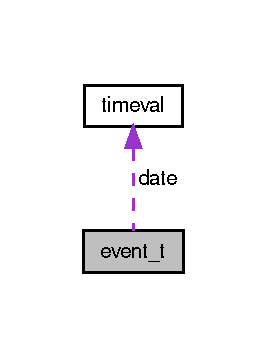
\includegraphics[width=128pt]{structevent__t__coll__graph}
\end{center}
\end{figure}
\subsection*{Champs de données}
\begin{DoxyCompactItemize}
\item 
\hypertarget{structevent__t_a26af672165e1d0e96466f5b141bd9791}{int {\bfseries id}}\label{structevent__t_a26af672165e1d0e96466f5b141bd9791}

\item 
\hypertarget{structevent__t_a26a40c7d45aca5f6e2f279c068304df1}{struct \hyperlink{structtimeval}{timeval} {\bfseries date}}\label{structevent__t_a26a40c7d45aca5f6e2f279c068304df1}

\item 
\hypertarget{structevent__t_a84eaecb5cbe3efb739a514e007bc50c7}{callback\+\_\+t {\bfseries callback}}\label{structevent__t_a84eaecb5cbe3efb739a514e007bc50c7}

\item 
\hypertarget{structevent__t_a7fa0689a7d4d9d2efb51a86e79b7080c}{void $\ast$ {\bfseries data}}\label{structevent__t_a7fa0689a7d4d9d2efb51a86e79b7080c}

\end{DoxyCompactItemize}


La documentation de cette structure a été générée à partir du fichier suivant \+:\begin{DoxyCompactItemize}
\item 
kernel/include/\hyperlink{events_8h}{events.\+h}\end{DoxyCompactItemize}

\hypertarget{structext2__directory}{\section{Référence de la structure ext2\-\_\-directory}
\label{structext2__directory}\index{ext2\-\_\-directory@{ext2\-\_\-directory}}
}


Structure qui représente une entrée dans un dossier ext2. Format imposé par Ext2.  




{\ttfamily \#include $<$ext2\-\_\-internal.\-h$>$}

\subsection*{Champs de données}
\begin{DoxyCompactItemize}
\item 
\hyperlink{kernel_2include_2types_8h_a33594304e786b158f3fb30289278f5af}{uint32\-\_\-t} \hyperlink{structext2__directory_a58f91a7939507e98be75baed206c149c}{inode}
\item 
\hyperlink{kernel_2include_2types_8h_adf4d876453337156dde61095e1f20223}{uint16\-\_\-t} \hyperlink{structext2__directory_a349e610d4d226a480c577c94b09a5eaf}{rec\-\_\-len}
\item 
\hyperlink{kernel_2include_2types_8h_aba7bc1797add20fe3efdf37ced1182c5}{uint8\-\_\-t} \hyperlink{structext2__directory_ab2ab4e90da260d09d51d74abdaabb095}{name\-\_\-len}
\item 
\hyperlink{kernel_2include_2types_8h_aba7bc1797add20fe3efdf37ced1182c5}{uint8\-\_\-t} \hyperlink{structext2__directory_a100a0ca76dac23225e9fbaa03b8925d0}{file\-\_\-type}
\item 
char \hyperlink{structext2__directory_a68dde9644a76168693b569434ab17fd4}{name} \mbox{[}256\mbox{]}
\end{DoxyCompactItemize}


\subsection{Documentation des champs}
\hypertarget{structext2__directory_a100a0ca76dac23225e9fbaa03b8925d0}{\index{ext2\-\_\-directory@{ext2\-\_\-directory}!file\-\_\-type@{file\-\_\-type}}
\index{file\-\_\-type@{file\-\_\-type}!ext2_directory@{ext2\-\_\-directory}}
\subsubsection[{file\-\_\-type}]{\setlength{\rightskip}{0pt plus 5cm}{\bf uint8\-\_\-t} ext2\-\_\-directory\-::file\-\_\-type}}\label{structext2__directory_a100a0ca76dac23225e9fbaa03b8925d0}
Type de fichier. \hypertarget{structext2__directory_a58f91a7939507e98be75baed206c149c}{\index{ext2\-\_\-directory@{ext2\-\_\-directory}!inode@{inode}}
\index{inode@{inode}!ext2_directory@{ext2\-\_\-directory}}
\subsubsection[{inode}]{\setlength{\rightskip}{0pt plus 5cm}{\bf uint32\-\_\-t} ext2\-\_\-directory\-::inode}}\label{structext2__directory_a58f91a7939507e98be75baed206c149c}
Numero d'inode. \hypertarget{structext2__directory_a68dde9644a76168693b569434ab17fd4}{\index{ext2\-\_\-directory@{ext2\-\_\-directory}!name@{name}}
\index{name@{name}!ext2_directory@{ext2\-\_\-directory}}
\subsubsection[{name}]{\setlength{\rightskip}{0pt plus 5cm}char ext2\-\_\-directory\-::name\mbox{[}256\mbox{]}}}\label{structext2__directory_a68dde9644a76168693b569434ab17fd4}
Nom du fichier. \hypertarget{structext2__directory_ab2ab4e90da260d09d51d74abdaabb095}{\index{ext2\-\_\-directory@{ext2\-\_\-directory}!name\-\_\-len@{name\-\_\-len}}
\index{name\-\_\-len@{name\-\_\-len}!ext2_directory@{ext2\-\_\-directory}}
\subsubsection[{name\-\_\-len}]{\setlength{\rightskip}{0pt plus 5cm}{\bf uint8\-\_\-t} ext2\-\_\-directory\-::name\-\_\-len}}\label{structext2__directory_ab2ab4e90da260d09d51d74abdaabb095}
Longueur du nom de fichier. \hypertarget{structext2__directory_a349e610d4d226a480c577c94b09a5eaf}{\index{ext2\-\_\-directory@{ext2\-\_\-directory}!rec\-\_\-len@{rec\-\_\-len}}
\index{rec\-\_\-len@{rec\-\_\-len}!ext2_directory@{ext2\-\_\-directory}}
\subsubsection[{rec\-\_\-len}]{\setlength{\rightskip}{0pt plus 5cm}{\bf uint16\-\_\-t} ext2\-\_\-directory\-::rec\-\_\-len}}\label{structext2__directory_a349e610d4d226a480c577c94b09a5eaf}
Taille occupée par cette entrée. 

La documentation de cette structure a été générée à partir du fichier suivant \-:\begin{DoxyCompactItemize}
\item 
kernel/fs/ext2/\hyperlink{ext2__internal_8h}{ext2\-\_\-internal.\-h}\end{DoxyCompactItemize}

\hypertarget{structext2__group__desc}{\section{Référence de la structure ext2\+\_\+group\+\_\+desc}
\label{structext2__group__desc}\index{ext2\+\_\+group\+\_\+desc@{ext2\+\_\+group\+\_\+desc}}
}


{\ttfamily \#include $<$ext2\+\_\+internal.\+h$>$}

\subsection*{Champs de données}
\begin{DoxyCompactItemize}
\item 
\hyperlink{kernel_2include_2types_8h_a33594304e786b158f3fb30289278f5af}{uint32\+\_\+t} \hyperlink{structext2__group__desc_a57481ebe34986e28812cc9b4e122c016}{bg\+\_\+block\+\_\+bitmap}
\item 
\hyperlink{kernel_2include_2types_8h_a33594304e786b158f3fb30289278f5af}{uint32\+\_\+t} \hyperlink{structext2__group__desc_a7ba3737304b14529a45aede6381aa968}{bg\+\_\+inode\+\_\+bitmap}
\item 
\hyperlink{kernel_2include_2types_8h_a33594304e786b158f3fb30289278f5af}{uint32\+\_\+t} \hyperlink{structext2__group__desc_abf527c572a5fe30354cdf2cfc4f88b26}{bg\+\_\+inode\+\_\+table}
\item 
\hyperlink{kernel_2include_2types_8h_adf4d876453337156dde61095e1f20223}{uint16\+\_\+t} \hyperlink{structext2__group__desc_af1cf7574780c76da67e973179f6edd43}{bg\+\_\+free\+\_\+blocks\+\_\+count}
\item 
\hyperlink{kernel_2include_2types_8h_adf4d876453337156dde61095e1f20223}{uint16\+\_\+t} \hyperlink{structext2__group__desc_a5488cd2eb4ea863ca9d15a5df8da6bab}{bg\+\_\+free\+\_\+inodes\+\_\+count}
\item 
\hyperlink{kernel_2include_2types_8h_adf4d876453337156dde61095e1f20223}{uint16\+\_\+t} \hyperlink{structext2__group__desc_adc9924671cb04dd63b4b7ffff8c262dc}{bg\+\_\+used\+\_\+dirs\+\_\+count}
\item 
\hyperlink{kernel_2include_2types_8h_adf4d876453337156dde61095e1f20223}{uint16\+\_\+t} \hyperlink{structext2__group__desc_ac99983cee73aa4aace5c7d51b6d5a7e1}{bg\+\_\+pad}
\item 
\hyperlink{kernel_2include_2types_8h_a33594304e786b158f3fb30289278f5af}{uint32\+\_\+t} \hyperlink{structext2__group__desc_aff7f7dc0b67aed284218b238991f5c93}{bg\+\_\+reserved} \mbox{[}3\mbox{]}
\end{DoxyCompactItemize}


\subsection{Description détaillée}
Groupe. 

\subsection{Documentation des champs}
\hypertarget{structext2__group__desc_a57481ebe34986e28812cc9b4e122c016}{\index{ext2\+\_\+group\+\_\+desc@{ext2\+\_\+group\+\_\+desc}!bg\+\_\+block\+\_\+bitmap@{bg\+\_\+block\+\_\+bitmap}}
\index{bg\+\_\+block\+\_\+bitmap@{bg\+\_\+block\+\_\+bitmap}!ext2\+\_\+group\+\_\+desc@{ext2\+\_\+group\+\_\+desc}}
\subsubsection[{bg\+\_\+block\+\_\+bitmap}]{\setlength{\rightskip}{0pt plus 5cm}{\bf uint32\+\_\+t} ext2\+\_\+group\+\_\+desc\+::bg\+\_\+block\+\_\+bitmap}}\label{structext2__group__desc_a57481ebe34986e28812cc9b4e122c016}
Blocks bitmap block \hypertarget{structext2__group__desc_af1cf7574780c76da67e973179f6edd43}{\index{ext2\+\_\+group\+\_\+desc@{ext2\+\_\+group\+\_\+desc}!bg\+\_\+free\+\_\+blocks\+\_\+count@{bg\+\_\+free\+\_\+blocks\+\_\+count}}
\index{bg\+\_\+free\+\_\+blocks\+\_\+count@{bg\+\_\+free\+\_\+blocks\+\_\+count}!ext2\+\_\+group\+\_\+desc@{ext2\+\_\+group\+\_\+desc}}
\subsubsection[{bg\+\_\+free\+\_\+blocks\+\_\+count}]{\setlength{\rightskip}{0pt plus 5cm}{\bf uint16\+\_\+t} ext2\+\_\+group\+\_\+desc\+::bg\+\_\+free\+\_\+blocks\+\_\+count}}\label{structext2__group__desc_af1cf7574780c76da67e973179f6edd43}
Free blocks count \hypertarget{structext2__group__desc_a5488cd2eb4ea863ca9d15a5df8da6bab}{\index{ext2\+\_\+group\+\_\+desc@{ext2\+\_\+group\+\_\+desc}!bg\+\_\+free\+\_\+inodes\+\_\+count@{bg\+\_\+free\+\_\+inodes\+\_\+count}}
\index{bg\+\_\+free\+\_\+inodes\+\_\+count@{bg\+\_\+free\+\_\+inodes\+\_\+count}!ext2\+\_\+group\+\_\+desc@{ext2\+\_\+group\+\_\+desc}}
\subsubsection[{bg\+\_\+free\+\_\+inodes\+\_\+count}]{\setlength{\rightskip}{0pt plus 5cm}{\bf uint16\+\_\+t} ext2\+\_\+group\+\_\+desc\+::bg\+\_\+free\+\_\+inodes\+\_\+count}}\label{structext2__group__desc_a5488cd2eb4ea863ca9d15a5df8da6bab}
Free inodes count \hypertarget{structext2__group__desc_a7ba3737304b14529a45aede6381aa968}{\index{ext2\+\_\+group\+\_\+desc@{ext2\+\_\+group\+\_\+desc}!bg\+\_\+inode\+\_\+bitmap@{bg\+\_\+inode\+\_\+bitmap}}
\index{bg\+\_\+inode\+\_\+bitmap@{bg\+\_\+inode\+\_\+bitmap}!ext2\+\_\+group\+\_\+desc@{ext2\+\_\+group\+\_\+desc}}
\subsubsection[{bg\+\_\+inode\+\_\+bitmap}]{\setlength{\rightskip}{0pt plus 5cm}{\bf uint32\+\_\+t} ext2\+\_\+group\+\_\+desc\+::bg\+\_\+inode\+\_\+bitmap}}\label{structext2__group__desc_a7ba3737304b14529a45aede6381aa968}
Inodes bitmap block \hypertarget{structext2__group__desc_abf527c572a5fe30354cdf2cfc4f88b26}{\index{ext2\+\_\+group\+\_\+desc@{ext2\+\_\+group\+\_\+desc}!bg\+\_\+inode\+\_\+table@{bg\+\_\+inode\+\_\+table}}
\index{bg\+\_\+inode\+\_\+table@{bg\+\_\+inode\+\_\+table}!ext2\+\_\+group\+\_\+desc@{ext2\+\_\+group\+\_\+desc}}
\subsubsection[{bg\+\_\+inode\+\_\+table}]{\setlength{\rightskip}{0pt plus 5cm}{\bf uint32\+\_\+t} ext2\+\_\+group\+\_\+desc\+::bg\+\_\+inode\+\_\+table}}\label{structext2__group__desc_abf527c572a5fe30354cdf2cfc4f88b26}
Inodes table block \hypertarget{structext2__group__desc_ac99983cee73aa4aace5c7d51b6d5a7e1}{\index{ext2\+\_\+group\+\_\+desc@{ext2\+\_\+group\+\_\+desc}!bg\+\_\+pad@{bg\+\_\+pad}}
\index{bg\+\_\+pad@{bg\+\_\+pad}!ext2\+\_\+group\+\_\+desc@{ext2\+\_\+group\+\_\+desc}}
\subsubsection[{bg\+\_\+pad}]{\setlength{\rightskip}{0pt plus 5cm}{\bf uint16\+\_\+t} ext2\+\_\+group\+\_\+desc\+::bg\+\_\+pad}}\label{structext2__group__desc_ac99983cee73aa4aace5c7d51b6d5a7e1}
unused. \hypertarget{structext2__group__desc_aff7f7dc0b67aed284218b238991f5c93}{\index{ext2\+\_\+group\+\_\+desc@{ext2\+\_\+group\+\_\+desc}!bg\+\_\+reserved@{bg\+\_\+reserved}}
\index{bg\+\_\+reserved@{bg\+\_\+reserved}!ext2\+\_\+group\+\_\+desc@{ext2\+\_\+group\+\_\+desc}}
\subsubsection[{bg\+\_\+reserved}]{\setlength{\rightskip}{0pt plus 5cm}{\bf uint32\+\_\+t} ext2\+\_\+group\+\_\+desc\+::bg\+\_\+reserved\mbox{[}3\mbox{]}}}\label{structext2__group__desc_aff7f7dc0b67aed284218b238991f5c93}
reserved. \hypertarget{structext2__group__desc_adc9924671cb04dd63b4b7ffff8c262dc}{\index{ext2\+\_\+group\+\_\+desc@{ext2\+\_\+group\+\_\+desc}!bg\+\_\+used\+\_\+dirs\+\_\+count@{bg\+\_\+used\+\_\+dirs\+\_\+count}}
\index{bg\+\_\+used\+\_\+dirs\+\_\+count@{bg\+\_\+used\+\_\+dirs\+\_\+count}!ext2\+\_\+group\+\_\+desc@{ext2\+\_\+group\+\_\+desc}}
\subsubsection[{bg\+\_\+used\+\_\+dirs\+\_\+count}]{\setlength{\rightskip}{0pt plus 5cm}{\bf uint16\+\_\+t} ext2\+\_\+group\+\_\+desc\+::bg\+\_\+used\+\_\+dirs\+\_\+count}}\label{structext2__group__desc_adc9924671cb04dd63b4b7ffff8c262dc}
Directories count 

La documentation de cette structure a été générée à partir du fichier suivant \+:\begin{DoxyCompactItemize}
\item 
kernel/fs/ext2/\hyperlink{ext2__internal_8h}{ext2\+\_\+internal.\+h}\end{DoxyCompactItemize}

\hypertarget{structext2__group__desc__internal}{\section{Référence de la structure ext2\-\_\-group\-\_\-desc\-\_\-internal}
\label{structext2__group__desc__internal}\index{ext2\-\_\-group\-\_\-desc\-\_\-internal@{ext2\-\_\-group\-\_\-desc\-\_\-internal}}
}


{\ttfamily \#include $<$ext2\-\_\-internal.\-h$>$}



Graphe de collaboration de ext2\-\_\-group\-\_\-desc\-\_\-internal\-:\nopagebreak
\begin{figure}[H]
\begin{center}
\leavevmode
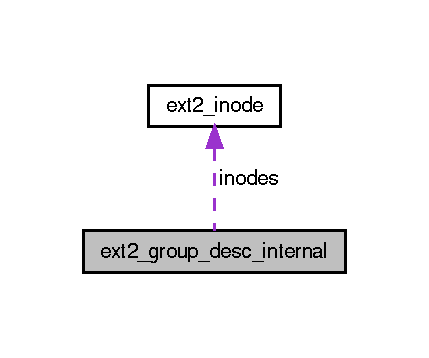
\includegraphics[width=206pt]{structext2__group__desc__internal__coll__graph}
\end{center}
\end{figure}
\subsection*{Champs de données}
\begin{DoxyCompactItemize}
\item 
\hyperlink{kernel_2include_2types_8h_aba7bc1797add20fe3efdf37ced1182c5}{uint8\-\_\-t} $\ast$ \hyperlink{structext2__group__desc__internal_a5b3cee6954ef4ed21c238b46d389b9bf}{inode\-\_\-bitmap}
\item 
struct \hyperlink{structext2__inode}{ext2\-\_\-inode} $\ast$ \hyperlink{structext2__group__desc__internal_a690f836bfb2c8de04ae2b1753134f8a7}{inodes}
\end{DoxyCompactItemize}


\subsection{Description détaillée}
Copie mémoire des infos du disque pour limiter le nombre d'accès inutiles. 

\subsection{Documentation des champs}
\hypertarget{structext2__group__desc__internal_a5b3cee6954ef4ed21c238b46d389b9bf}{\index{ext2\-\_\-group\-\_\-desc\-\_\-internal@{ext2\-\_\-group\-\_\-desc\-\_\-internal}!inode\-\_\-bitmap@{inode\-\_\-bitmap}}
\index{inode\-\_\-bitmap@{inode\-\_\-bitmap}!ext2_group_desc_internal@{ext2\-\_\-group\-\_\-desc\-\_\-internal}}
\subsubsection[{inode\-\_\-bitmap}]{\setlength{\rightskip}{0pt plus 5cm}{\bf uint8\-\_\-t}$\ast$ ext2\-\_\-group\-\_\-desc\-\_\-internal\-::inode\-\_\-bitmap}}\label{structext2__group__desc__internal_a5b3cee6954ef4ed21c238b46d389b9bf}
Inode bitmap. \hypertarget{structext2__group__desc__internal_a690f836bfb2c8de04ae2b1753134f8a7}{\index{ext2\-\_\-group\-\_\-desc\-\_\-internal@{ext2\-\_\-group\-\_\-desc\-\_\-internal}!inodes@{inodes}}
\index{inodes@{inodes}!ext2_group_desc_internal@{ext2\-\_\-group\-\_\-desc\-\_\-internal}}
\subsubsection[{inodes}]{\setlength{\rightskip}{0pt plus 5cm}struct {\bf ext2\-\_\-inode}$\ast$ ext2\-\_\-group\-\_\-desc\-\_\-internal\-::inodes}}\label{structext2__group__desc__internal_a690f836bfb2c8de04ae2b1753134f8a7}
Tableau d'inodes. 

La documentation de cette structure a été générée à partir du fichier suivant \-:\begin{DoxyCompactItemize}
\item 
kernel/fs/ext2/\hyperlink{ext2__internal_8h}{ext2\-\_\-internal.\-h}\end{DoxyCompactItemize}

\hypertarget{structext2__inode}{\section{Référence de la structure ext2\-\_\-inode}
\label{structext2__inode}\index{ext2\-\_\-inode@{ext2\-\_\-inode}}
}


{\ttfamily \#include $<$ext2\-\_\-internal.\-h$>$}

\subsection*{Champs de données}
\begin{DoxyCompactItemize}
\item 
\hyperlink{types_8h_adf4d876453337156dde61095e1f20223}{uint16\-\_\-t} \hyperlink{structext2__inode_ab18d6b6ddb4d36a2faff527b43241126}{i\-\_\-mode}
\item 
\hyperlink{types_8h_adf4d876453337156dde61095e1f20223}{uint16\-\_\-t} \hyperlink{structext2__inode_a082def4b3c1c0c5f9dce1eab8ba51189}{i\-\_\-uid}
\item 
\hyperlink{types_8h_a33594304e786b158f3fb30289278f5af}{uint32\-\_\-t} \hyperlink{structext2__inode_a2b9e2a1c732aa02b5dead0948fb47c72}{i\-\_\-size}
\item 
\hyperlink{types_8h_a33594304e786b158f3fb30289278f5af}{uint32\-\_\-t} \hyperlink{structext2__inode_adb682923fb8b418217d78fd78737406b}{i\-\_\-atime}
\item 
\hyperlink{types_8h_a33594304e786b158f3fb30289278f5af}{uint32\-\_\-t} \hyperlink{structext2__inode_a7d45cc039be5128d9771412191e55544}{i\-\_\-ctime}
\item 
\hyperlink{types_8h_a33594304e786b158f3fb30289278f5af}{uint32\-\_\-t} \hyperlink{structext2__inode_a7eb44698eabf570fee0e65d22cc5fbd1}{i\-\_\-mtime}
\item 
\hyperlink{types_8h_a33594304e786b158f3fb30289278f5af}{uint32\-\_\-t} \hyperlink{structext2__inode_a2a30cea7fb676d2fa5e9f0bd799dfa7c}{i\-\_\-dtime}
\item 
\hyperlink{types_8h_adf4d876453337156dde61095e1f20223}{uint16\-\_\-t} \hyperlink{structext2__inode_af1686b705ca7912d370d12ceaab83b8b}{i\-\_\-gid}
\item 
\hyperlink{types_8h_adf4d876453337156dde61095e1f20223}{uint16\-\_\-t} \hyperlink{structext2__inode_aa6d7753ffe6e8634bafe0b55638ee29a}{i\-\_\-links\-\_\-count}
\item 
\hyperlink{types_8h_a33594304e786b158f3fb30289278f5af}{uint32\-\_\-t} \hyperlink{structext2__inode_a6e5b258ebc92b6ae75c61572c60cbb4b}{i\-\_\-blocks}
\item 
\hyperlink{types_8h_a33594304e786b158f3fb30289278f5af}{uint32\-\_\-t} \hyperlink{structext2__inode_a2037da1edbe1d421dd4453f84cb973e6}{i\-\_\-flags}
\item 
\hyperlink{types_8h_a33594304e786b158f3fb30289278f5af}{uint32\-\_\-t} \hyperlink{structext2__inode_ab06178218f59df43b3d80ad53edc6105}{i\-\_\-osd1}
\item 
\hyperlink{types_8h_a33594304e786b158f3fb30289278f5af}{uint32\-\_\-t} \hyperlink{structext2__inode_a3e2386992eeb6a3b6aa5e282c50221c7}{i\-\_\-block} \mbox{[}15\mbox{]}
\item 
\hyperlink{types_8h_a33594304e786b158f3fb30289278f5af}{uint32\-\_\-t} \hyperlink{structext2__inode_a551df9f3b8f61eb5840eeeb5921c69fb}{i\-\_\-generation}
\item 
\hyperlink{types_8h_a33594304e786b158f3fb30289278f5af}{uint32\-\_\-t} \hyperlink{structext2__inode_aee0fba48998e7d27b836d04ee53e4463}{i\-\_\-file\-\_\-acl}
\item 
\hyperlink{types_8h_a33594304e786b158f3fb30289278f5af}{uint32\-\_\-t} \hyperlink{structext2__inode_a11c2793c33c6ce3f13a5f046e246fd47}{i\-\_\-dir\-\_\-acl}
\item 
\hyperlink{types_8h_a33594304e786b158f3fb30289278f5af}{uint32\-\_\-t} \hyperlink{structext2__inode_a3c921d50835f4869a08444b7e8b01043}{i\-\_\-faddr}
\item 
\hyperlink{types_8h_a33594304e786b158f3fb30289278f5af}{uint32\-\_\-t} \hyperlink{structext2__inode_a6f05264ef1f6a42a6975a858d1aa17c3}{i\-\_\-osd2} \mbox{[}3\mbox{]}
\end{DoxyCompactItemize}


\subsection{Description détaillée}
Structure of an inode on the disk 

\subsection{Documentation des champs}
\hypertarget{structext2__inode_adb682923fb8b418217d78fd78737406b}{\index{ext2\-\_\-inode@{ext2\-\_\-inode}!i\-\_\-atime@{i\-\_\-atime}}
\index{i\-\_\-atime@{i\-\_\-atime}!ext2_inode@{ext2\-\_\-inode}}
\subsubsection[{i\-\_\-atime}]{\setlength{\rightskip}{0pt plus 5cm}{\bf uint32\-\_\-t} ext2\-\_\-inode\-::i\-\_\-atime}}\label{structext2__inode_adb682923fb8b418217d78fd78737406b}
Access time \hypertarget{structext2__inode_a3e2386992eeb6a3b6aa5e282c50221c7}{\index{ext2\-\_\-inode@{ext2\-\_\-inode}!i\-\_\-block@{i\-\_\-block}}
\index{i\-\_\-block@{i\-\_\-block}!ext2_inode@{ext2\-\_\-inode}}
\subsubsection[{i\-\_\-block}]{\setlength{\rightskip}{0pt plus 5cm}{\bf uint32\-\_\-t} ext2\-\_\-inode\-::i\-\_\-block\mbox{[}15\mbox{]}}}\label{structext2__inode_a3e2386992eeb6a3b6aa5e282c50221c7}
Pointers to blocks \hypertarget{structext2__inode_a6e5b258ebc92b6ae75c61572c60cbb4b}{\index{ext2\-\_\-inode@{ext2\-\_\-inode}!i\-\_\-blocks@{i\-\_\-blocks}}
\index{i\-\_\-blocks@{i\-\_\-blocks}!ext2_inode@{ext2\-\_\-inode}}
\subsubsection[{i\-\_\-blocks}]{\setlength{\rightskip}{0pt plus 5cm}{\bf uint32\-\_\-t} ext2\-\_\-inode\-::i\-\_\-blocks}}\label{structext2__inode_a6e5b258ebc92b6ae75c61572c60cbb4b}
Blocks count \hypertarget{structext2__inode_a7d45cc039be5128d9771412191e55544}{\index{ext2\-\_\-inode@{ext2\-\_\-inode}!i\-\_\-ctime@{i\-\_\-ctime}}
\index{i\-\_\-ctime@{i\-\_\-ctime}!ext2_inode@{ext2\-\_\-inode}}
\subsubsection[{i\-\_\-ctime}]{\setlength{\rightskip}{0pt plus 5cm}{\bf uint32\-\_\-t} ext2\-\_\-inode\-::i\-\_\-ctime}}\label{structext2__inode_a7d45cc039be5128d9771412191e55544}
Creation time \hypertarget{structext2__inode_a11c2793c33c6ce3f13a5f046e246fd47}{\index{ext2\-\_\-inode@{ext2\-\_\-inode}!i\-\_\-dir\-\_\-acl@{i\-\_\-dir\-\_\-acl}}
\index{i\-\_\-dir\-\_\-acl@{i\-\_\-dir\-\_\-acl}!ext2_inode@{ext2\-\_\-inode}}
\subsubsection[{i\-\_\-dir\-\_\-acl}]{\setlength{\rightskip}{0pt plus 5cm}{\bf uint32\-\_\-t} ext2\-\_\-inode\-::i\-\_\-dir\-\_\-acl}}\label{structext2__inode_a11c2793c33c6ce3f13a5f046e246fd47}
Directory A\-C\-L \hypertarget{structext2__inode_a2a30cea7fb676d2fa5e9f0bd799dfa7c}{\index{ext2\-\_\-inode@{ext2\-\_\-inode}!i\-\_\-dtime@{i\-\_\-dtime}}
\index{i\-\_\-dtime@{i\-\_\-dtime}!ext2_inode@{ext2\-\_\-inode}}
\subsubsection[{i\-\_\-dtime}]{\setlength{\rightskip}{0pt plus 5cm}{\bf uint32\-\_\-t} ext2\-\_\-inode\-::i\-\_\-dtime}}\label{structext2__inode_a2a30cea7fb676d2fa5e9f0bd799dfa7c}
Deletion Time \hypertarget{structext2__inode_a3c921d50835f4869a08444b7e8b01043}{\index{ext2\-\_\-inode@{ext2\-\_\-inode}!i\-\_\-faddr@{i\-\_\-faddr}}
\index{i\-\_\-faddr@{i\-\_\-faddr}!ext2_inode@{ext2\-\_\-inode}}
\subsubsection[{i\-\_\-faddr}]{\setlength{\rightskip}{0pt plus 5cm}{\bf uint32\-\_\-t} ext2\-\_\-inode\-::i\-\_\-faddr}}\label{structext2__inode_a3c921d50835f4869a08444b7e8b01043}
Fragment address \hypertarget{structext2__inode_aee0fba48998e7d27b836d04ee53e4463}{\index{ext2\-\_\-inode@{ext2\-\_\-inode}!i\-\_\-file\-\_\-acl@{i\-\_\-file\-\_\-acl}}
\index{i\-\_\-file\-\_\-acl@{i\-\_\-file\-\_\-acl}!ext2_inode@{ext2\-\_\-inode}}
\subsubsection[{i\-\_\-file\-\_\-acl}]{\setlength{\rightskip}{0pt plus 5cm}{\bf uint32\-\_\-t} ext2\-\_\-inode\-::i\-\_\-file\-\_\-acl}}\label{structext2__inode_aee0fba48998e7d27b836d04ee53e4463}
File A\-C\-L \hypertarget{structext2__inode_a2037da1edbe1d421dd4453f84cb973e6}{\index{ext2\-\_\-inode@{ext2\-\_\-inode}!i\-\_\-flags@{i\-\_\-flags}}
\index{i\-\_\-flags@{i\-\_\-flags}!ext2_inode@{ext2\-\_\-inode}}
\subsubsection[{i\-\_\-flags}]{\setlength{\rightskip}{0pt plus 5cm}{\bf uint32\-\_\-t} ext2\-\_\-inode\-::i\-\_\-flags}}\label{structext2__inode_a2037da1edbe1d421dd4453f84cb973e6}
File flags \hypertarget{structext2__inode_a551df9f3b8f61eb5840eeeb5921c69fb}{\index{ext2\-\_\-inode@{ext2\-\_\-inode}!i\-\_\-generation@{i\-\_\-generation}}
\index{i\-\_\-generation@{i\-\_\-generation}!ext2_inode@{ext2\-\_\-inode}}
\subsubsection[{i\-\_\-generation}]{\setlength{\rightskip}{0pt plus 5cm}{\bf uint32\-\_\-t} ext2\-\_\-inode\-::i\-\_\-generation}}\label{structext2__inode_a551df9f3b8f61eb5840eeeb5921c69fb}
File version (for N\-F\-S) \hypertarget{structext2__inode_af1686b705ca7912d370d12ceaab83b8b}{\index{ext2\-\_\-inode@{ext2\-\_\-inode}!i\-\_\-gid@{i\-\_\-gid}}
\index{i\-\_\-gid@{i\-\_\-gid}!ext2_inode@{ext2\-\_\-inode}}
\subsubsection[{i\-\_\-gid}]{\setlength{\rightskip}{0pt plus 5cm}{\bf uint16\-\_\-t} ext2\-\_\-inode\-::i\-\_\-gid}}\label{structext2__inode_af1686b705ca7912d370d12ceaab83b8b}
Low 16 bits of Group Id \hypertarget{structext2__inode_aa6d7753ffe6e8634bafe0b55638ee29a}{\index{ext2\-\_\-inode@{ext2\-\_\-inode}!i\-\_\-links\-\_\-count@{i\-\_\-links\-\_\-count}}
\index{i\-\_\-links\-\_\-count@{i\-\_\-links\-\_\-count}!ext2_inode@{ext2\-\_\-inode}}
\subsubsection[{i\-\_\-links\-\_\-count}]{\setlength{\rightskip}{0pt plus 5cm}{\bf uint16\-\_\-t} ext2\-\_\-inode\-::i\-\_\-links\-\_\-count}}\label{structext2__inode_aa6d7753ffe6e8634bafe0b55638ee29a}
Links count \hypertarget{structext2__inode_ab18d6b6ddb4d36a2faff527b43241126}{\index{ext2\-\_\-inode@{ext2\-\_\-inode}!i\-\_\-mode@{i\-\_\-mode}}
\index{i\-\_\-mode@{i\-\_\-mode}!ext2_inode@{ext2\-\_\-inode}}
\subsubsection[{i\-\_\-mode}]{\setlength{\rightskip}{0pt plus 5cm}{\bf uint16\-\_\-t} ext2\-\_\-inode\-::i\-\_\-mode}}\label{structext2__inode_ab18d6b6ddb4d36a2faff527b43241126}
File mode \hypertarget{structext2__inode_a7eb44698eabf570fee0e65d22cc5fbd1}{\index{ext2\-\_\-inode@{ext2\-\_\-inode}!i\-\_\-mtime@{i\-\_\-mtime}}
\index{i\-\_\-mtime@{i\-\_\-mtime}!ext2_inode@{ext2\-\_\-inode}}
\subsubsection[{i\-\_\-mtime}]{\setlength{\rightskip}{0pt plus 5cm}{\bf uint32\-\_\-t} ext2\-\_\-inode\-::i\-\_\-mtime}}\label{structext2__inode_a7eb44698eabf570fee0e65d22cc5fbd1}
Modification time \hypertarget{structext2__inode_ab06178218f59df43b3d80ad53edc6105}{\index{ext2\-\_\-inode@{ext2\-\_\-inode}!i\-\_\-osd1@{i\-\_\-osd1}}
\index{i\-\_\-osd1@{i\-\_\-osd1}!ext2_inode@{ext2\-\_\-inode}}
\subsubsection[{i\-\_\-osd1}]{\setlength{\rightskip}{0pt plus 5cm}{\bf uint32\-\_\-t} ext2\-\_\-inode\-::i\-\_\-osd1}}\label{structext2__inode_ab06178218f59df43b3d80ad53edc6105}
O\-S dependent 1 \hypertarget{structext2__inode_a6f05264ef1f6a42a6975a858d1aa17c3}{\index{ext2\-\_\-inode@{ext2\-\_\-inode}!i\-\_\-osd2@{i\-\_\-osd2}}
\index{i\-\_\-osd2@{i\-\_\-osd2}!ext2_inode@{ext2\-\_\-inode}}
\subsubsection[{i\-\_\-osd2}]{\setlength{\rightskip}{0pt plus 5cm}{\bf uint32\-\_\-t} ext2\-\_\-inode\-::i\-\_\-osd2\mbox{[}3\mbox{]}}}\label{structext2__inode_a6f05264ef1f6a42a6975a858d1aa17c3}
O\-S dependent 2 \hypertarget{structext2__inode_a2b9e2a1c732aa02b5dead0948fb47c72}{\index{ext2\-\_\-inode@{ext2\-\_\-inode}!i\-\_\-size@{i\-\_\-size}}
\index{i\-\_\-size@{i\-\_\-size}!ext2_inode@{ext2\-\_\-inode}}
\subsubsection[{i\-\_\-size}]{\setlength{\rightskip}{0pt plus 5cm}{\bf uint32\-\_\-t} ext2\-\_\-inode\-::i\-\_\-size}}\label{structext2__inode_a2b9e2a1c732aa02b5dead0948fb47c72}
Size in bytes \hypertarget{structext2__inode_a082def4b3c1c0c5f9dce1eab8ba51189}{\index{ext2\-\_\-inode@{ext2\-\_\-inode}!i\-\_\-uid@{i\-\_\-uid}}
\index{i\-\_\-uid@{i\-\_\-uid}!ext2_inode@{ext2\-\_\-inode}}
\subsubsection[{i\-\_\-uid}]{\setlength{\rightskip}{0pt plus 5cm}{\bf uint16\-\_\-t} ext2\-\_\-inode\-::i\-\_\-uid}}\label{structext2__inode_a082def4b3c1c0c5f9dce1eab8ba51189}
Low 16 bits of Owner Uid 

La documentation de cette structure a été générée à partir du fichier suivant \-:\begin{DoxyCompactItemize}
\item 
kernel/fs/ext2/\hyperlink{ext2__internal_8h}{ext2\-\_\-internal.\-h}\end{DoxyCompactItemize}

\hypertarget{structext2__super__block}{\section{Référence de la structure ext2\+\_\+super\+\_\+block}
\label{structext2__super__block}\index{ext2\+\_\+super\+\_\+block@{ext2\+\_\+super\+\_\+block}}
}


{\ttfamily \#include $<$ext2\+\_\+internal.\+h$>$}

\subsection*{Champs de données}
\begin{DoxyCompactItemize}
\item 
\hyperlink{kernel_2include_2types_8h_a33594304e786b158f3fb30289278f5af}{uint32\+\_\+t} \hyperlink{structext2__super__block_a2ea20f821c0ddc19b0adc7d1b8d0685d}{s\+\_\+inodes\+\_\+count}
\item 
\hyperlink{kernel_2include_2types_8h_a33594304e786b158f3fb30289278f5af}{uint32\+\_\+t} \hyperlink{structext2__super__block_a3878ffaff13c625cce6b825ecb797547}{s\+\_\+blocks\+\_\+count}
\item 
\hyperlink{kernel_2include_2types_8h_a33594304e786b158f3fb30289278f5af}{uint32\+\_\+t} \hyperlink{structext2__super__block_a660db33fc94622167793c6b080c515e4}{s\+\_\+r\+\_\+blocks\+\_\+count}
\item 
\hyperlink{kernel_2include_2types_8h_a33594304e786b158f3fb30289278f5af}{uint32\+\_\+t} \hyperlink{structext2__super__block_a005160872a0474cdc9be97da00b81b84}{s\+\_\+free\+\_\+blocks\+\_\+count}
\item 
\hyperlink{kernel_2include_2types_8h_a33594304e786b158f3fb30289278f5af}{uint32\+\_\+t} \hyperlink{structext2__super__block_aeefbe6028c7e1554805b033287de0097}{s\+\_\+free\+\_\+inodes\+\_\+count}
\item 
\hyperlink{kernel_2include_2types_8h_a33594304e786b158f3fb30289278f5af}{uint32\+\_\+t} \hyperlink{structext2__super__block_ab7c5dfba6eafbb1974f7628d4ae32601}{s\+\_\+first\+\_\+data\+\_\+block}
\item 
\hyperlink{kernel_2include_2types_8h_a33594304e786b158f3fb30289278f5af}{uint32\+\_\+t} \hyperlink{structext2__super__block_a34965ad64787db6bf0893e000b19f608}{s\+\_\+log\+\_\+block\+\_\+size}
\item 
\hyperlink{kernel_2include_2types_8h_a33594304e786b158f3fb30289278f5af}{uint32\+\_\+t} \hyperlink{structext2__super__block_a441780f5356cad879e465bb23d5c0659}{s\+\_\+log\+\_\+frag\+\_\+size}
\item 
\hyperlink{kernel_2include_2types_8h_a33594304e786b158f3fb30289278f5af}{uint32\+\_\+t} \hyperlink{structext2__super__block_a037ab0266050cd0d0026c5da1fda3ab1}{s\+\_\+blocks\+\_\+per\+\_\+group}
\item 
\hyperlink{kernel_2include_2types_8h_a33594304e786b158f3fb30289278f5af}{uint32\+\_\+t} \hyperlink{structext2__super__block_a6370cd7307aa833951c40fcc3f941b61}{s\+\_\+frags\+\_\+per\+\_\+group}
\item 
\hyperlink{kernel_2include_2types_8h_a33594304e786b158f3fb30289278f5af}{uint32\+\_\+t} \hyperlink{structext2__super__block_a4b417c308a43cfd8d744c3fdd19832af}{s\+\_\+inodes\+\_\+per\+\_\+group}
\item 
\hyperlink{kernel_2include_2types_8h_a33594304e786b158f3fb30289278f5af}{uint32\+\_\+t} \hyperlink{structext2__super__block_a3966a51d4e26f1b0280798db227b9720}{s\+\_\+mtime}
\item 
\hyperlink{kernel_2include_2types_8h_a33594304e786b158f3fb30289278f5af}{uint32\+\_\+t} \hyperlink{structext2__super__block_a97c255a8e87dbea1ab953b0a8fce054d}{s\+\_\+wtime}
\item 
\hyperlink{kernel_2include_2types_8h_adf4d876453337156dde61095e1f20223}{uint16\+\_\+t} \hyperlink{structext2__super__block_a0a2557d9e186c2774e4eac28ef07a942}{s\+\_\+mnt\+\_\+count}
\item 
\hyperlink{kernel_2include_2types_8h_adf4d876453337156dde61095e1f20223}{uint16\+\_\+t} \hyperlink{structext2__super__block_a7823bb2004c8a837a207b71d73dc8662}{s\+\_\+max\+\_\+mnt\+\_\+count}
\item 
\hyperlink{kernel_2include_2types_8h_adf4d876453337156dde61095e1f20223}{uint16\+\_\+t} \hyperlink{structext2__super__block_a22b76c4f2b2547630739f5c2ebb9d4b9}{s\+\_\+magic}
\item 
\hyperlink{kernel_2include_2types_8h_adf4d876453337156dde61095e1f20223}{uint16\+\_\+t} \hyperlink{structext2__super__block_a06b739ed98ef97510f193cb582e78eb6}{s\+\_\+state}
\item 
\hyperlink{kernel_2include_2types_8h_adf4d876453337156dde61095e1f20223}{uint16\+\_\+t} \hyperlink{structext2__super__block_a06e31d621f6250d56d1af5c342220a08}{s\+\_\+errors}
\item 
\hyperlink{kernel_2include_2types_8h_adf4d876453337156dde61095e1f20223}{uint16\+\_\+t} \hyperlink{structext2__super__block_a0ca2f1fc71b73dc837a15392a35abb89}{s\+\_\+minor\+\_\+rev\+\_\+level}
\item 
\hyperlink{kernel_2include_2types_8h_a33594304e786b158f3fb30289278f5af}{uint32\+\_\+t} \hyperlink{structext2__super__block_a4a8a628c48e36668f87ff1d0f831224a}{s\+\_\+lastcheck}
\item 
\hyperlink{kernel_2include_2types_8h_a33594304e786b158f3fb30289278f5af}{uint32\+\_\+t} \hyperlink{structext2__super__block_a41729c3eb872813abe1489de88e6f736}{s\+\_\+checkinterval}
\item 
\hyperlink{kernel_2include_2types_8h_a33594304e786b158f3fb30289278f5af}{uint32\+\_\+t} \hyperlink{structext2__super__block_a421f09691aa0911da60db7ef23dc30ca}{s\+\_\+creator\+\_\+os}
\item 
\hyperlink{kernel_2include_2types_8h_a33594304e786b158f3fb30289278f5af}{uint32\+\_\+t} \hyperlink{structext2__super__block_a70b07eaf44b6a5e777b8072ee4b593b4}{s\+\_\+rev\+\_\+level}
\item 
\hyperlink{kernel_2include_2types_8h_adf4d876453337156dde61095e1f20223}{uint16\+\_\+t} \hyperlink{structext2__super__block_a83da108c4a1f27a275f54970fb8edf07}{s\+\_\+def\+\_\+resuid}
\item 
\hyperlink{kernel_2include_2types_8h_adf4d876453337156dde61095e1f20223}{uint16\+\_\+t} \hyperlink{structext2__super__block_a2973f6cda59f008e1f649c6d68ddafd6}{s\+\_\+def\+\_\+resgid}
\item 
\hyperlink{kernel_2include_2types_8h_a33594304e786b158f3fb30289278f5af}{uint32\+\_\+t} \hyperlink{structext2__super__block_a0d3a8f3c14e0a971750cfdfbc2cf6070}{s\+\_\+first\+\_\+ino}
\item 
\hyperlink{kernel_2include_2types_8h_adf4d876453337156dde61095e1f20223}{uint16\+\_\+t} \hyperlink{structext2__super__block_a9a1ee9cd5f706fa2e753a4c781ebae73}{s\+\_\+inode\+\_\+size}
\item 
\hyperlink{kernel_2include_2types_8h_adf4d876453337156dde61095e1f20223}{uint16\+\_\+t} \hyperlink{structext2__super__block_aa69ff4c80207a79de2464e3065df607c}{s\+\_\+block\+\_\+group\+\_\+nr}
\item 
\hyperlink{kernel_2include_2types_8h_a33594304e786b158f3fb30289278f5af}{uint32\+\_\+t} \hyperlink{structext2__super__block_a1cf404a1bcfb748e924c62032cd723a5}{s\+\_\+feature\+\_\+compat}
\item 
\hyperlink{kernel_2include_2types_8h_a33594304e786b158f3fb30289278f5af}{uint32\+\_\+t} \hyperlink{structext2__super__block_a56005d1ae97dc32f86567d018c753440}{s\+\_\+feature\+\_\+incompat}
\item 
\hyperlink{kernel_2include_2types_8h_a33594304e786b158f3fb30289278f5af}{uint32\+\_\+t} \hyperlink{structext2__super__block_a9c63e7954f0344d3de19aad4099d84c7}{s\+\_\+feature\+\_\+ro\+\_\+compat}
\item 
\hyperlink{kernel_2include_2types_8h_aba7bc1797add20fe3efdf37ced1182c5}{uint8\+\_\+t} \hyperlink{structext2__super__block_a1a546d295c2dc760ece8bf44c7623eb3}{s\+\_\+uuid} \mbox{[}16\mbox{]}
\item 
char \hyperlink{structext2__super__block_aafa5ddd1cf9fbf19aa2b80e83bff5a43}{s\+\_\+volume\+\_\+name} \mbox{[}16\mbox{]}
\item 
char \hyperlink{structext2__super__block_ad2849dfeab713d00ddd93c97eaf80cea}{s\+\_\+last\+\_\+mounted} \mbox{[}64\mbox{]}
\item 
\hyperlink{kernel_2include_2types_8h_a33594304e786b158f3fb30289278f5af}{uint32\+\_\+t} \hyperlink{structext2__super__block_ab3772dfdb48734922447cc462e5495ed}{s\+\_\+algorithm\+\_\+usage\+\_\+bitmap}
\item 
\hyperlink{kernel_2include_2types_8h_aba7bc1797add20fe3efdf37ced1182c5}{uint8\+\_\+t} \hyperlink{structext2__super__block_a352689df3b3cb2a357bde6645e3c7f29}{s\+\_\+prealloc\+\_\+blocks}
\item 
\hyperlink{kernel_2include_2types_8h_aba7bc1797add20fe3efdf37ced1182c5}{uint8\+\_\+t} \hyperlink{structext2__super__block_aa820a721fcbf64ee9aa797bca3171785}{s\+\_\+prealloc\+\_\+dir\+\_\+blocks}
\item 
\hyperlink{kernel_2include_2types_8h_adf4d876453337156dde61095e1f20223}{uint16\+\_\+t} \hyperlink{structext2__super__block_a1b0760049d39f6cfb1b26af0a01f64d2}{s\+\_\+padding1}
\item 
\hyperlink{kernel_2include_2types_8h_aba7bc1797add20fe3efdf37ced1182c5}{uint8\+\_\+t} \hyperlink{structext2__super__block_a31f78875053afe2073c72ab700e831cd}{s\+\_\+journal\+\_\+uuid} \mbox{[}16\mbox{]}
\item 
\hyperlink{kernel_2include_2types_8h_a33594304e786b158f3fb30289278f5af}{uint32\+\_\+t} \hyperlink{structext2__super__block_a593535b5ffb1b5480f887e0aae0be698}{s\+\_\+journal\+\_\+inum}
\item 
\hyperlink{kernel_2include_2types_8h_a33594304e786b158f3fb30289278f5af}{uint32\+\_\+t} \hyperlink{structext2__super__block_a5c65ec434f4b1394d6ec68fb8d055a4e}{s\+\_\+journal\+\_\+dev}
\item 
\hyperlink{kernel_2include_2types_8h_a33594304e786b158f3fb30289278f5af}{uint32\+\_\+t} \hyperlink{structext2__super__block_a48682cfbe704f555d18fe030f1ee6fe6}{s\+\_\+last\+\_\+orphan}
\item 
\hyperlink{kernel_2include_2types_8h_a33594304e786b158f3fb30289278f5af}{uint32\+\_\+t} \hyperlink{structext2__super__block_a70910c5d87977d65b2a69fb7b079d3a1}{s\+\_\+hash\+\_\+seed} \mbox{[}4\mbox{]}
\item 
\hyperlink{kernel_2include_2types_8h_aba7bc1797add20fe3efdf37ced1182c5}{uint8\+\_\+t} \hyperlink{structext2__super__block_a3120768bf3ac685a2e5d38d84ec3c5b8}{s\+\_\+def\+\_\+hash\+\_\+version}
\item 
\hyperlink{kernel_2include_2types_8h_aba7bc1797add20fe3efdf37ced1182c5}{uint8\+\_\+t} \hyperlink{structext2__super__block_a81b4e1959f344b5b7445044806d27807}{s\+\_\+padding} \mbox{[}3\mbox{]}
\item 
\hyperlink{kernel_2include_2types_8h_a33594304e786b158f3fb30289278f5af}{uint32\+\_\+t} \hyperlink{structext2__super__block_a8f4946dffa8c6a9027ee9329fd3f94c9}{s\+\_\+default\+\_\+mount\+\_\+opts}
\item 
\hyperlink{kernel_2include_2types_8h_a33594304e786b158f3fb30289278f5af}{uint32\+\_\+t} \hyperlink{structext2__super__block_a436c7c8af548ade7f8045e88c2861d61}{s\+\_\+first\+\_\+meta\+\_\+bg}
\item 
\hyperlink{kernel_2include_2types_8h_aba7bc1797add20fe3efdf37ced1182c5}{uint8\+\_\+t} \hyperlink{structext2__super__block_a17e0d263a7fceb8b53aff24b66c216df}{s\+\_\+reserved} \mbox{[}760\mbox{]}
\end{DoxyCompactItemize}


\subsection{Description détaillée}
Structure du Ext2 Super Block (Repris du code de Linux) \href{http://www.nongnu.org/ext2-doc/ext2.html#SUPERBLOCK}{\tt http\+://www.\+nongnu.\+org/ext2-\/doc/ext2.\+html\#\+S\+U\+P\+E\+R\+B\+L\+O\+C\+K} 

\subsection{Documentation des champs}
\hypertarget{structext2__super__block_ab3772dfdb48734922447cc462e5495ed}{\index{ext2\+\_\+super\+\_\+block@{ext2\+\_\+super\+\_\+block}!s\+\_\+algorithm\+\_\+usage\+\_\+bitmap@{s\+\_\+algorithm\+\_\+usage\+\_\+bitmap}}
\index{s\+\_\+algorithm\+\_\+usage\+\_\+bitmap@{s\+\_\+algorithm\+\_\+usage\+\_\+bitmap}!ext2\+\_\+super\+\_\+block@{ext2\+\_\+super\+\_\+block}}
\subsubsection[{s\+\_\+algorithm\+\_\+usage\+\_\+bitmap}]{\setlength{\rightskip}{0pt plus 5cm}{\bf uint32\+\_\+t} ext2\+\_\+super\+\_\+block\+::s\+\_\+algorithm\+\_\+usage\+\_\+bitmap}}\label{structext2__super__block_ab3772dfdb48734922447cc462e5495ed}
For compression \hypertarget{structext2__super__block_aa69ff4c80207a79de2464e3065df607c}{\index{ext2\+\_\+super\+\_\+block@{ext2\+\_\+super\+\_\+block}!s\+\_\+block\+\_\+group\+\_\+nr@{s\+\_\+block\+\_\+group\+\_\+nr}}
\index{s\+\_\+block\+\_\+group\+\_\+nr@{s\+\_\+block\+\_\+group\+\_\+nr}!ext2\+\_\+super\+\_\+block@{ext2\+\_\+super\+\_\+block}}
\subsubsection[{s\+\_\+block\+\_\+group\+\_\+nr}]{\setlength{\rightskip}{0pt plus 5cm}{\bf uint16\+\_\+t} ext2\+\_\+super\+\_\+block\+::s\+\_\+block\+\_\+group\+\_\+nr}}\label{structext2__super__block_aa69ff4c80207a79de2464e3065df607c}
block group \# of this superblock \hypertarget{structext2__super__block_a3878ffaff13c625cce6b825ecb797547}{\index{ext2\+\_\+super\+\_\+block@{ext2\+\_\+super\+\_\+block}!s\+\_\+blocks\+\_\+count@{s\+\_\+blocks\+\_\+count}}
\index{s\+\_\+blocks\+\_\+count@{s\+\_\+blocks\+\_\+count}!ext2\+\_\+super\+\_\+block@{ext2\+\_\+super\+\_\+block}}
\subsubsection[{s\+\_\+blocks\+\_\+count}]{\setlength{\rightskip}{0pt plus 5cm}{\bf uint32\+\_\+t} ext2\+\_\+super\+\_\+block\+::s\+\_\+blocks\+\_\+count}}\label{structext2__super__block_a3878ffaff13c625cce6b825ecb797547}
Blocks count \hypertarget{structext2__super__block_a037ab0266050cd0d0026c5da1fda3ab1}{\index{ext2\+\_\+super\+\_\+block@{ext2\+\_\+super\+\_\+block}!s\+\_\+blocks\+\_\+per\+\_\+group@{s\+\_\+blocks\+\_\+per\+\_\+group}}
\index{s\+\_\+blocks\+\_\+per\+\_\+group@{s\+\_\+blocks\+\_\+per\+\_\+group}!ext2\+\_\+super\+\_\+block@{ext2\+\_\+super\+\_\+block}}
\subsubsection[{s\+\_\+blocks\+\_\+per\+\_\+group}]{\setlength{\rightskip}{0pt plus 5cm}{\bf uint32\+\_\+t} ext2\+\_\+super\+\_\+block\+::s\+\_\+blocks\+\_\+per\+\_\+group}}\label{structext2__super__block_a037ab0266050cd0d0026c5da1fda3ab1}
\subsection*{Blocks per group}\hypertarget{structext2__super__block_a41729c3eb872813abe1489de88e6f736}{\index{ext2\+\_\+super\+\_\+block@{ext2\+\_\+super\+\_\+block}!s\+\_\+checkinterval@{s\+\_\+checkinterval}}
\index{s\+\_\+checkinterval@{s\+\_\+checkinterval}!ext2\+\_\+super\+\_\+block@{ext2\+\_\+super\+\_\+block}}
\subsubsection[{s\+\_\+checkinterval}]{\setlength{\rightskip}{0pt plus 5cm}{\bf uint32\+\_\+t} ext2\+\_\+super\+\_\+block\+::s\+\_\+checkinterval}}\label{structext2__super__block_a41729c3eb872813abe1489de88e6f736}
max. time between checks \hypertarget{structext2__super__block_a421f09691aa0911da60db7ef23dc30ca}{\index{ext2\+\_\+super\+\_\+block@{ext2\+\_\+super\+\_\+block}!s\+\_\+creator\+\_\+os@{s\+\_\+creator\+\_\+os}}
\index{s\+\_\+creator\+\_\+os@{s\+\_\+creator\+\_\+os}!ext2\+\_\+super\+\_\+block@{ext2\+\_\+super\+\_\+block}}
\subsubsection[{s\+\_\+creator\+\_\+os}]{\setlength{\rightskip}{0pt plus 5cm}{\bf uint32\+\_\+t} ext2\+\_\+super\+\_\+block\+::s\+\_\+creator\+\_\+os}}\label{structext2__super__block_a421f09691aa0911da60db7ef23dc30ca}
O\+S qui a formaté \hypertarget{structext2__super__block_a3120768bf3ac685a2e5d38d84ec3c5b8}{\index{ext2\+\_\+super\+\_\+block@{ext2\+\_\+super\+\_\+block}!s\+\_\+def\+\_\+hash\+\_\+version@{s\+\_\+def\+\_\+hash\+\_\+version}}
\index{s\+\_\+def\+\_\+hash\+\_\+version@{s\+\_\+def\+\_\+hash\+\_\+version}!ext2\+\_\+super\+\_\+block@{ext2\+\_\+super\+\_\+block}}
\subsubsection[{s\+\_\+def\+\_\+hash\+\_\+version}]{\setlength{\rightskip}{0pt plus 5cm}{\bf uint8\+\_\+t} ext2\+\_\+super\+\_\+block\+::s\+\_\+def\+\_\+hash\+\_\+version}}\label{structext2__super__block_a3120768bf3ac685a2e5d38d84ec3c5b8}
Default hash version to use \hypertarget{structext2__super__block_a2973f6cda59f008e1f649c6d68ddafd6}{\index{ext2\+\_\+super\+\_\+block@{ext2\+\_\+super\+\_\+block}!s\+\_\+def\+\_\+resgid@{s\+\_\+def\+\_\+resgid}}
\index{s\+\_\+def\+\_\+resgid@{s\+\_\+def\+\_\+resgid}!ext2\+\_\+super\+\_\+block@{ext2\+\_\+super\+\_\+block}}
\subsubsection[{s\+\_\+def\+\_\+resgid}]{\setlength{\rightskip}{0pt plus 5cm}{\bf uint16\+\_\+t} ext2\+\_\+super\+\_\+block\+::s\+\_\+def\+\_\+resgid}}\label{structext2__super__block_a2973f6cda59f008e1f649c6d68ddafd6}
Default gid for reserved blocks \hypertarget{structext2__super__block_a83da108c4a1f27a275f54970fb8edf07}{\index{ext2\+\_\+super\+\_\+block@{ext2\+\_\+super\+\_\+block}!s\+\_\+def\+\_\+resuid@{s\+\_\+def\+\_\+resuid}}
\index{s\+\_\+def\+\_\+resuid@{s\+\_\+def\+\_\+resuid}!ext2\+\_\+super\+\_\+block@{ext2\+\_\+super\+\_\+block}}
\subsubsection[{s\+\_\+def\+\_\+resuid}]{\setlength{\rightskip}{0pt plus 5cm}{\bf uint16\+\_\+t} ext2\+\_\+super\+\_\+block\+::s\+\_\+def\+\_\+resuid}}\label{structext2__super__block_a83da108c4a1f27a275f54970fb8edf07}
Default uid for reserved blocks \hypertarget{structext2__super__block_a8f4946dffa8c6a9027ee9329fd3f94c9}{\index{ext2\+\_\+super\+\_\+block@{ext2\+\_\+super\+\_\+block}!s\+\_\+default\+\_\+mount\+\_\+opts@{s\+\_\+default\+\_\+mount\+\_\+opts}}
\index{s\+\_\+default\+\_\+mount\+\_\+opts@{s\+\_\+default\+\_\+mount\+\_\+opts}!ext2\+\_\+super\+\_\+block@{ext2\+\_\+super\+\_\+block}}
\subsubsection[{s\+\_\+default\+\_\+mount\+\_\+opts}]{\setlength{\rightskip}{0pt plus 5cm}{\bf uint32\+\_\+t} ext2\+\_\+super\+\_\+block\+::s\+\_\+default\+\_\+mount\+\_\+opts}}\label{structext2__super__block_a8f4946dffa8c6a9027ee9329fd3f94c9}
Option de mount par défaut. \hypertarget{structext2__super__block_a06e31d621f6250d56d1af5c342220a08}{\index{ext2\+\_\+super\+\_\+block@{ext2\+\_\+super\+\_\+block}!s\+\_\+errors@{s\+\_\+errors}}
\index{s\+\_\+errors@{s\+\_\+errors}!ext2\+\_\+super\+\_\+block@{ext2\+\_\+super\+\_\+block}}
\subsubsection[{s\+\_\+errors}]{\setlength{\rightskip}{0pt plus 5cm}{\bf uint16\+\_\+t} ext2\+\_\+super\+\_\+block\+::s\+\_\+errors}}\label{structext2__super__block_a06e31d621f6250d56d1af5c342220a08}
Behaviour when detecting errors \hypertarget{structext2__super__block_a1cf404a1bcfb748e924c62032cd723a5}{\index{ext2\+\_\+super\+\_\+block@{ext2\+\_\+super\+\_\+block}!s\+\_\+feature\+\_\+compat@{s\+\_\+feature\+\_\+compat}}
\index{s\+\_\+feature\+\_\+compat@{s\+\_\+feature\+\_\+compat}!ext2\+\_\+super\+\_\+block@{ext2\+\_\+super\+\_\+block}}
\subsubsection[{s\+\_\+feature\+\_\+compat}]{\setlength{\rightskip}{0pt plus 5cm}{\bf uint32\+\_\+t} ext2\+\_\+super\+\_\+block\+::s\+\_\+feature\+\_\+compat}}\label{structext2__super__block_a1cf404a1bcfb748e924c62032cd723a5}
compatible feature set \hypertarget{structext2__super__block_a56005d1ae97dc32f86567d018c753440}{\index{ext2\+\_\+super\+\_\+block@{ext2\+\_\+super\+\_\+block}!s\+\_\+feature\+\_\+incompat@{s\+\_\+feature\+\_\+incompat}}
\index{s\+\_\+feature\+\_\+incompat@{s\+\_\+feature\+\_\+incompat}!ext2\+\_\+super\+\_\+block@{ext2\+\_\+super\+\_\+block}}
\subsubsection[{s\+\_\+feature\+\_\+incompat}]{\setlength{\rightskip}{0pt plus 5cm}{\bf uint32\+\_\+t} ext2\+\_\+super\+\_\+block\+::s\+\_\+feature\+\_\+incompat}}\label{structext2__super__block_a56005d1ae97dc32f86567d018c753440}
incompatible feature set \hypertarget{structext2__super__block_a9c63e7954f0344d3de19aad4099d84c7}{\index{ext2\+\_\+super\+\_\+block@{ext2\+\_\+super\+\_\+block}!s\+\_\+feature\+\_\+ro\+\_\+compat@{s\+\_\+feature\+\_\+ro\+\_\+compat}}
\index{s\+\_\+feature\+\_\+ro\+\_\+compat@{s\+\_\+feature\+\_\+ro\+\_\+compat}!ext2\+\_\+super\+\_\+block@{ext2\+\_\+super\+\_\+block}}
\subsubsection[{s\+\_\+feature\+\_\+ro\+\_\+compat}]{\setlength{\rightskip}{0pt plus 5cm}{\bf uint32\+\_\+t} ext2\+\_\+super\+\_\+block\+::s\+\_\+feature\+\_\+ro\+\_\+compat}}\label{structext2__super__block_a9c63e7954f0344d3de19aad4099d84c7}
readonly-\/compatible feature set \hypertarget{structext2__super__block_ab7c5dfba6eafbb1974f7628d4ae32601}{\index{ext2\+\_\+super\+\_\+block@{ext2\+\_\+super\+\_\+block}!s\+\_\+first\+\_\+data\+\_\+block@{s\+\_\+first\+\_\+data\+\_\+block}}
\index{s\+\_\+first\+\_\+data\+\_\+block@{s\+\_\+first\+\_\+data\+\_\+block}!ext2\+\_\+super\+\_\+block@{ext2\+\_\+super\+\_\+block}}
\subsubsection[{s\+\_\+first\+\_\+data\+\_\+block}]{\setlength{\rightskip}{0pt plus 5cm}{\bf uint32\+\_\+t} ext2\+\_\+super\+\_\+block\+::s\+\_\+first\+\_\+data\+\_\+block}}\label{structext2__super__block_ab7c5dfba6eafbb1974f7628d4ae32601}
First Data Block \hypertarget{structext2__super__block_a0d3a8f3c14e0a971750cfdfbc2cf6070}{\index{ext2\+\_\+super\+\_\+block@{ext2\+\_\+super\+\_\+block}!s\+\_\+first\+\_\+ino@{s\+\_\+first\+\_\+ino}}
\index{s\+\_\+first\+\_\+ino@{s\+\_\+first\+\_\+ino}!ext2\+\_\+super\+\_\+block@{ext2\+\_\+super\+\_\+block}}
\subsubsection[{s\+\_\+first\+\_\+ino}]{\setlength{\rightskip}{0pt plus 5cm}{\bf uint32\+\_\+t} ext2\+\_\+super\+\_\+block\+::s\+\_\+first\+\_\+ino}}\label{structext2__super__block_a0d3a8f3c14e0a971750cfdfbc2cf6070}
First non-\/reserved inode \hypertarget{structext2__super__block_a436c7c8af548ade7f8045e88c2861d61}{\index{ext2\+\_\+super\+\_\+block@{ext2\+\_\+super\+\_\+block}!s\+\_\+first\+\_\+meta\+\_\+bg@{s\+\_\+first\+\_\+meta\+\_\+bg}}
\index{s\+\_\+first\+\_\+meta\+\_\+bg@{s\+\_\+first\+\_\+meta\+\_\+bg}!ext2\+\_\+super\+\_\+block@{ext2\+\_\+super\+\_\+block}}
\subsubsection[{s\+\_\+first\+\_\+meta\+\_\+bg}]{\setlength{\rightskip}{0pt plus 5cm}{\bf uint32\+\_\+t} ext2\+\_\+super\+\_\+block\+::s\+\_\+first\+\_\+meta\+\_\+bg}}\label{structext2__super__block_a436c7c8af548ade7f8045e88c2861d61}
First metablock block group \hypertarget{structext2__super__block_a6370cd7307aa833951c40fcc3f941b61}{\index{ext2\+\_\+super\+\_\+block@{ext2\+\_\+super\+\_\+block}!s\+\_\+frags\+\_\+per\+\_\+group@{s\+\_\+frags\+\_\+per\+\_\+group}}
\index{s\+\_\+frags\+\_\+per\+\_\+group@{s\+\_\+frags\+\_\+per\+\_\+group}!ext2\+\_\+super\+\_\+block@{ext2\+\_\+super\+\_\+block}}
\subsubsection[{s\+\_\+frags\+\_\+per\+\_\+group}]{\setlength{\rightskip}{0pt plus 5cm}{\bf uint32\+\_\+t} ext2\+\_\+super\+\_\+block\+::s\+\_\+frags\+\_\+per\+\_\+group}}\label{structext2__super__block_a6370cd7307aa833951c40fcc3f941b61}
\subsection*{Fragments per group}\hypertarget{structext2__super__block_a005160872a0474cdc9be97da00b81b84}{\index{ext2\+\_\+super\+\_\+block@{ext2\+\_\+super\+\_\+block}!s\+\_\+free\+\_\+blocks\+\_\+count@{s\+\_\+free\+\_\+blocks\+\_\+count}}
\index{s\+\_\+free\+\_\+blocks\+\_\+count@{s\+\_\+free\+\_\+blocks\+\_\+count}!ext2\+\_\+super\+\_\+block@{ext2\+\_\+super\+\_\+block}}
\subsubsection[{s\+\_\+free\+\_\+blocks\+\_\+count}]{\setlength{\rightskip}{0pt plus 5cm}{\bf uint32\+\_\+t} ext2\+\_\+super\+\_\+block\+::s\+\_\+free\+\_\+blocks\+\_\+count}}\label{structext2__super__block_a005160872a0474cdc9be97da00b81b84}
Free blocks count \hypertarget{structext2__super__block_aeefbe6028c7e1554805b033287de0097}{\index{ext2\+\_\+super\+\_\+block@{ext2\+\_\+super\+\_\+block}!s\+\_\+free\+\_\+inodes\+\_\+count@{s\+\_\+free\+\_\+inodes\+\_\+count}}
\index{s\+\_\+free\+\_\+inodes\+\_\+count@{s\+\_\+free\+\_\+inodes\+\_\+count}!ext2\+\_\+super\+\_\+block@{ext2\+\_\+super\+\_\+block}}
\subsubsection[{s\+\_\+free\+\_\+inodes\+\_\+count}]{\setlength{\rightskip}{0pt plus 5cm}{\bf uint32\+\_\+t} ext2\+\_\+super\+\_\+block\+::s\+\_\+free\+\_\+inodes\+\_\+count}}\label{structext2__super__block_aeefbe6028c7e1554805b033287de0097}
Free inodes count \hypertarget{structext2__super__block_a70910c5d87977d65b2a69fb7b079d3a1}{\index{ext2\+\_\+super\+\_\+block@{ext2\+\_\+super\+\_\+block}!s\+\_\+hash\+\_\+seed@{s\+\_\+hash\+\_\+seed}}
\index{s\+\_\+hash\+\_\+seed@{s\+\_\+hash\+\_\+seed}!ext2\+\_\+super\+\_\+block@{ext2\+\_\+super\+\_\+block}}
\subsubsection[{s\+\_\+hash\+\_\+seed}]{\setlength{\rightskip}{0pt plus 5cm}{\bf uint32\+\_\+t} ext2\+\_\+super\+\_\+block\+::s\+\_\+hash\+\_\+seed\mbox{[}4\mbox{]}}}\label{structext2__super__block_a70910c5d87977d65b2a69fb7b079d3a1}
H\+T\+R\+E\+E hash seed \hypertarget{structext2__super__block_a9a1ee9cd5f706fa2e753a4c781ebae73}{\index{ext2\+\_\+super\+\_\+block@{ext2\+\_\+super\+\_\+block}!s\+\_\+inode\+\_\+size@{s\+\_\+inode\+\_\+size}}
\index{s\+\_\+inode\+\_\+size@{s\+\_\+inode\+\_\+size}!ext2\+\_\+super\+\_\+block@{ext2\+\_\+super\+\_\+block}}
\subsubsection[{s\+\_\+inode\+\_\+size}]{\setlength{\rightskip}{0pt plus 5cm}{\bf uint16\+\_\+t} ext2\+\_\+super\+\_\+block\+::s\+\_\+inode\+\_\+size}}\label{structext2__super__block_a9a1ee9cd5f706fa2e753a4c781ebae73}
size of inode structure \hypertarget{structext2__super__block_a2ea20f821c0ddc19b0adc7d1b8d0685d}{\index{ext2\+\_\+super\+\_\+block@{ext2\+\_\+super\+\_\+block}!s\+\_\+inodes\+\_\+count@{s\+\_\+inodes\+\_\+count}}
\index{s\+\_\+inodes\+\_\+count@{s\+\_\+inodes\+\_\+count}!ext2\+\_\+super\+\_\+block@{ext2\+\_\+super\+\_\+block}}
\subsubsection[{s\+\_\+inodes\+\_\+count}]{\setlength{\rightskip}{0pt plus 5cm}{\bf uint32\+\_\+t} ext2\+\_\+super\+\_\+block\+::s\+\_\+inodes\+\_\+count}}\label{structext2__super__block_a2ea20f821c0ddc19b0adc7d1b8d0685d}
Inodes count \hypertarget{structext2__super__block_a4b417c308a43cfd8d744c3fdd19832af}{\index{ext2\+\_\+super\+\_\+block@{ext2\+\_\+super\+\_\+block}!s\+\_\+inodes\+\_\+per\+\_\+group@{s\+\_\+inodes\+\_\+per\+\_\+group}}
\index{s\+\_\+inodes\+\_\+per\+\_\+group@{s\+\_\+inodes\+\_\+per\+\_\+group}!ext2\+\_\+super\+\_\+block@{ext2\+\_\+super\+\_\+block}}
\subsubsection[{s\+\_\+inodes\+\_\+per\+\_\+group}]{\setlength{\rightskip}{0pt plus 5cm}{\bf uint32\+\_\+t} ext2\+\_\+super\+\_\+block\+::s\+\_\+inodes\+\_\+per\+\_\+group}}\label{structext2__super__block_a4b417c308a43cfd8d744c3fdd19832af}
\subsection*{Inodes per group}\hypertarget{structext2__super__block_a5c65ec434f4b1394d6ec68fb8d055a4e}{\index{ext2\+\_\+super\+\_\+block@{ext2\+\_\+super\+\_\+block}!s\+\_\+journal\+\_\+dev@{s\+\_\+journal\+\_\+dev}}
\index{s\+\_\+journal\+\_\+dev@{s\+\_\+journal\+\_\+dev}!ext2\+\_\+super\+\_\+block@{ext2\+\_\+super\+\_\+block}}
\subsubsection[{s\+\_\+journal\+\_\+dev}]{\setlength{\rightskip}{0pt plus 5cm}{\bf uint32\+\_\+t} ext2\+\_\+super\+\_\+block\+::s\+\_\+journal\+\_\+dev}}\label{structext2__super__block_a5c65ec434f4b1394d6ec68fb8d055a4e}
device number of journal file \hypertarget{structext2__super__block_a593535b5ffb1b5480f887e0aae0be698}{\index{ext2\+\_\+super\+\_\+block@{ext2\+\_\+super\+\_\+block}!s\+\_\+journal\+\_\+inum@{s\+\_\+journal\+\_\+inum}}
\index{s\+\_\+journal\+\_\+inum@{s\+\_\+journal\+\_\+inum}!ext2\+\_\+super\+\_\+block@{ext2\+\_\+super\+\_\+block}}
\subsubsection[{s\+\_\+journal\+\_\+inum}]{\setlength{\rightskip}{0pt plus 5cm}{\bf uint32\+\_\+t} ext2\+\_\+super\+\_\+block\+::s\+\_\+journal\+\_\+inum}}\label{structext2__super__block_a593535b5ffb1b5480f887e0aae0be698}
inode number of journal file \hypertarget{structext2__super__block_a31f78875053afe2073c72ab700e831cd}{\index{ext2\+\_\+super\+\_\+block@{ext2\+\_\+super\+\_\+block}!s\+\_\+journal\+\_\+uuid@{s\+\_\+journal\+\_\+uuid}}
\index{s\+\_\+journal\+\_\+uuid@{s\+\_\+journal\+\_\+uuid}!ext2\+\_\+super\+\_\+block@{ext2\+\_\+super\+\_\+block}}
\subsubsection[{s\+\_\+journal\+\_\+uuid}]{\setlength{\rightskip}{0pt plus 5cm}{\bf uint8\+\_\+t} ext2\+\_\+super\+\_\+block\+::s\+\_\+journal\+\_\+uuid\mbox{[}16\mbox{]}}}\label{structext2__super__block_a31f78875053afe2073c72ab700e831cd}
uuid of journal superblock \hypertarget{structext2__super__block_ad2849dfeab713d00ddd93c97eaf80cea}{\index{ext2\+\_\+super\+\_\+block@{ext2\+\_\+super\+\_\+block}!s\+\_\+last\+\_\+mounted@{s\+\_\+last\+\_\+mounted}}
\index{s\+\_\+last\+\_\+mounted@{s\+\_\+last\+\_\+mounted}!ext2\+\_\+super\+\_\+block@{ext2\+\_\+super\+\_\+block}}
\subsubsection[{s\+\_\+last\+\_\+mounted}]{\setlength{\rightskip}{0pt plus 5cm}char ext2\+\_\+super\+\_\+block\+::s\+\_\+last\+\_\+mounted\mbox{[}64\mbox{]}}}\label{structext2__super__block_ad2849dfeab713d00ddd93c97eaf80cea}
directory where last mounted \hypertarget{structext2__super__block_a48682cfbe704f555d18fe030f1ee6fe6}{\index{ext2\+\_\+super\+\_\+block@{ext2\+\_\+super\+\_\+block}!s\+\_\+last\+\_\+orphan@{s\+\_\+last\+\_\+orphan}}
\index{s\+\_\+last\+\_\+orphan@{s\+\_\+last\+\_\+orphan}!ext2\+\_\+super\+\_\+block@{ext2\+\_\+super\+\_\+block}}
\subsubsection[{s\+\_\+last\+\_\+orphan}]{\setlength{\rightskip}{0pt plus 5cm}{\bf uint32\+\_\+t} ext2\+\_\+super\+\_\+block\+::s\+\_\+last\+\_\+orphan}}\label{structext2__super__block_a48682cfbe704f555d18fe030f1ee6fe6}
start of list of inodes to delete \hypertarget{structext2__super__block_a4a8a628c48e36668f87ff1d0f831224a}{\index{ext2\+\_\+super\+\_\+block@{ext2\+\_\+super\+\_\+block}!s\+\_\+lastcheck@{s\+\_\+lastcheck}}
\index{s\+\_\+lastcheck@{s\+\_\+lastcheck}!ext2\+\_\+super\+\_\+block@{ext2\+\_\+super\+\_\+block}}
\subsubsection[{s\+\_\+lastcheck}]{\setlength{\rightskip}{0pt plus 5cm}{\bf uint32\+\_\+t} ext2\+\_\+super\+\_\+block\+::s\+\_\+lastcheck}}\label{structext2__super__block_a4a8a628c48e36668f87ff1d0f831224a}
time of last check \hypertarget{structext2__super__block_a34965ad64787db6bf0893e000b19f608}{\index{ext2\+\_\+super\+\_\+block@{ext2\+\_\+super\+\_\+block}!s\+\_\+log\+\_\+block\+\_\+size@{s\+\_\+log\+\_\+block\+\_\+size}}
\index{s\+\_\+log\+\_\+block\+\_\+size@{s\+\_\+log\+\_\+block\+\_\+size}!ext2\+\_\+super\+\_\+block@{ext2\+\_\+super\+\_\+block}}
\subsubsection[{s\+\_\+log\+\_\+block\+\_\+size}]{\setlength{\rightskip}{0pt plus 5cm}{\bf uint32\+\_\+t} ext2\+\_\+super\+\_\+block\+::s\+\_\+log\+\_\+block\+\_\+size}}\label{structext2__super__block_a34965ad64787db6bf0893e000b19f608}
Block size \hypertarget{structext2__super__block_a441780f5356cad879e465bb23d5c0659}{\index{ext2\+\_\+super\+\_\+block@{ext2\+\_\+super\+\_\+block}!s\+\_\+log\+\_\+frag\+\_\+size@{s\+\_\+log\+\_\+frag\+\_\+size}}
\index{s\+\_\+log\+\_\+frag\+\_\+size@{s\+\_\+log\+\_\+frag\+\_\+size}!ext2\+\_\+super\+\_\+block@{ext2\+\_\+super\+\_\+block}}
\subsubsection[{s\+\_\+log\+\_\+frag\+\_\+size}]{\setlength{\rightskip}{0pt plus 5cm}{\bf uint32\+\_\+t} ext2\+\_\+super\+\_\+block\+::s\+\_\+log\+\_\+frag\+\_\+size}}\label{structext2__super__block_a441780f5356cad879e465bb23d5c0659}
Fragment size \hypertarget{structext2__super__block_a22b76c4f2b2547630739f5c2ebb9d4b9}{\index{ext2\+\_\+super\+\_\+block@{ext2\+\_\+super\+\_\+block}!s\+\_\+magic@{s\+\_\+magic}}
\index{s\+\_\+magic@{s\+\_\+magic}!ext2\+\_\+super\+\_\+block@{ext2\+\_\+super\+\_\+block}}
\subsubsection[{s\+\_\+magic}]{\setlength{\rightskip}{0pt plus 5cm}{\bf uint16\+\_\+t} ext2\+\_\+super\+\_\+block\+::s\+\_\+magic}}\label{structext2__super__block_a22b76c4f2b2547630739f5c2ebb9d4b9}
Magic signature \hypertarget{structext2__super__block_a7823bb2004c8a837a207b71d73dc8662}{\index{ext2\+\_\+super\+\_\+block@{ext2\+\_\+super\+\_\+block}!s\+\_\+max\+\_\+mnt\+\_\+count@{s\+\_\+max\+\_\+mnt\+\_\+count}}
\index{s\+\_\+max\+\_\+mnt\+\_\+count@{s\+\_\+max\+\_\+mnt\+\_\+count}!ext2\+\_\+super\+\_\+block@{ext2\+\_\+super\+\_\+block}}
\subsubsection[{s\+\_\+max\+\_\+mnt\+\_\+count}]{\setlength{\rightskip}{0pt plus 5cm}{\bf uint16\+\_\+t} ext2\+\_\+super\+\_\+block\+::s\+\_\+max\+\_\+mnt\+\_\+count}}\label{structext2__super__block_a7823bb2004c8a837a207b71d73dc8662}
Maximal mount count \hypertarget{structext2__super__block_a0ca2f1fc71b73dc837a15392a35abb89}{\index{ext2\+\_\+super\+\_\+block@{ext2\+\_\+super\+\_\+block}!s\+\_\+minor\+\_\+rev\+\_\+level@{s\+\_\+minor\+\_\+rev\+\_\+level}}
\index{s\+\_\+minor\+\_\+rev\+\_\+level@{s\+\_\+minor\+\_\+rev\+\_\+level}!ext2\+\_\+super\+\_\+block@{ext2\+\_\+super\+\_\+block}}
\subsubsection[{s\+\_\+minor\+\_\+rev\+\_\+level}]{\setlength{\rightskip}{0pt plus 5cm}{\bf uint16\+\_\+t} ext2\+\_\+super\+\_\+block\+::s\+\_\+minor\+\_\+rev\+\_\+level}}\label{structext2__super__block_a0ca2f1fc71b73dc837a15392a35abb89}
minor revision level \hypertarget{structext2__super__block_a0a2557d9e186c2774e4eac28ef07a942}{\index{ext2\+\_\+super\+\_\+block@{ext2\+\_\+super\+\_\+block}!s\+\_\+mnt\+\_\+count@{s\+\_\+mnt\+\_\+count}}
\index{s\+\_\+mnt\+\_\+count@{s\+\_\+mnt\+\_\+count}!ext2\+\_\+super\+\_\+block@{ext2\+\_\+super\+\_\+block}}
\subsubsection[{s\+\_\+mnt\+\_\+count}]{\setlength{\rightskip}{0pt plus 5cm}{\bf uint16\+\_\+t} ext2\+\_\+super\+\_\+block\+::s\+\_\+mnt\+\_\+count}}\label{structext2__super__block_a0a2557d9e186c2774e4eac28ef07a942}
Mount count \hypertarget{structext2__super__block_a3966a51d4e26f1b0280798db227b9720}{\index{ext2\+\_\+super\+\_\+block@{ext2\+\_\+super\+\_\+block}!s\+\_\+mtime@{s\+\_\+mtime}}
\index{s\+\_\+mtime@{s\+\_\+mtime}!ext2\+\_\+super\+\_\+block@{ext2\+\_\+super\+\_\+block}}
\subsubsection[{s\+\_\+mtime}]{\setlength{\rightskip}{0pt plus 5cm}{\bf uint32\+\_\+t} ext2\+\_\+super\+\_\+block\+::s\+\_\+mtime}}\label{structext2__super__block_a3966a51d4e26f1b0280798db227b9720}
Mount time \hypertarget{structext2__super__block_a81b4e1959f344b5b7445044806d27807}{\index{ext2\+\_\+super\+\_\+block@{ext2\+\_\+super\+\_\+block}!s\+\_\+padding@{s\+\_\+padding}}
\index{s\+\_\+padding@{s\+\_\+padding}!ext2\+\_\+super\+\_\+block@{ext2\+\_\+super\+\_\+block}}
\subsubsection[{s\+\_\+padding}]{\setlength{\rightskip}{0pt plus 5cm}{\bf uint8\+\_\+t} ext2\+\_\+super\+\_\+block\+::s\+\_\+padding\mbox{[}3\mbox{]}}}\label{structext2__super__block_a81b4e1959f344b5b7445044806d27807}
unused. \hypertarget{structext2__super__block_a1b0760049d39f6cfb1b26af0a01f64d2}{\index{ext2\+\_\+super\+\_\+block@{ext2\+\_\+super\+\_\+block}!s\+\_\+padding1@{s\+\_\+padding1}}
\index{s\+\_\+padding1@{s\+\_\+padding1}!ext2\+\_\+super\+\_\+block@{ext2\+\_\+super\+\_\+block}}
\subsubsection[{s\+\_\+padding1}]{\setlength{\rightskip}{0pt plus 5cm}{\bf uint16\+\_\+t} ext2\+\_\+super\+\_\+block\+::s\+\_\+padding1}}\label{structext2__super__block_a1b0760049d39f6cfb1b26af0a01f64d2}
unused. \hypertarget{structext2__super__block_a352689df3b3cb2a357bde6645e3c7f29}{\index{ext2\+\_\+super\+\_\+block@{ext2\+\_\+super\+\_\+block}!s\+\_\+prealloc\+\_\+blocks@{s\+\_\+prealloc\+\_\+blocks}}
\index{s\+\_\+prealloc\+\_\+blocks@{s\+\_\+prealloc\+\_\+blocks}!ext2\+\_\+super\+\_\+block@{ext2\+\_\+super\+\_\+block}}
\subsubsection[{s\+\_\+prealloc\+\_\+blocks}]{\setlength{\rightskip}{0pt plus 5cm}{\bf uint8\+\_\+t} ext2\+\_\+super\+\_\+block\+::s\+\_\+prealloc\+\_\+blocks}}\label{structext2__super__block_a352689df3b3cb2a357bde6645e3c7f29}
Nr of blocks to try to preallocate \hypertarget{structext2__super__block_aa820a721fcbf64ee9aa797bca3171785}{\index{ext2\+\_\+super\+\_\+block@{ext2\+\_\+super\+\_\+block}!s\+\_\+prealloc\+\_\+dir\+\_\+blocks@{s\+\_\+prealloc\+\_\+dir\+\_\+blocks}}
\index{s\+\_\+prealloc\+\_\+dir\+\_\+blocks@{s\+\_\+prealloc\+\_\+dir\+\_\+blocks}!ext2\+\_\+super\+\_\+block@{ext2\+\_\+super\+\_\+block}}
\subsubsection[{s\+\_\+prealloc\+\_\+dir\+\_\+blocks}]{\setlength{\rightskip}{0pt plus 5cm}{\bf uint8\+\_\+t} ext2\+\_\+super\+\_\+block\+::s\+\_\+prealloc\+\_\+dir\+\_\+blocks}}\label{structext2__super__block_aa820a721fcbf64ee9aa797bca3171785}
Nr to preallocate for dirs \hypertarget{structext2__super__block_a660db33fc94622167793c6b080c515e4}{\index{ext2\+\_\+super\+\_\+block@{ext2\+\_\+super\+\_\+block}!s\+\_\+r\+\_\+blocks\+\_\+count@{s\+\_\+r\+\_\+blocks\+\_\+count}}
\index{s\+\_\+r\+\_\+blocks\+\_\+count@{s\+\_\+r\+\_\+blocks\+\_\+count}!ext2\+\_\+super\+\_\+block@{ext2\+\_\+super\+\_\+block}}
\subsubsection[{s\+\_\+r\+\_\+blocks\+\_\+count}]{\setlength{\rightskip}{0pt plus 5cm}{\bf uint32\+\_\+t} ext2\+\_\+super\+\_\+block\+::s\+\_\+r\+\_\+blocks\+\_\+count}}\label{structext2__super__block_a660db33fc94622167793c6b080c515e4}
Reserved blocks count \hypertarget{structext2__super__block_a17e0d263a7fceb8b53aff24b66c216df}{\index{ext2\+\_\+super\+\_\+block@{ext2\+\_\+super\+\_\+block}!s\+\_\+reserved@{s\+\_\+reserved}}
\index{s\+\_\+reserved@{s\+\_\+reserved}!ext2\+\_\+super\+\_\+block@{ext2\+\_\+super\+\_\+block}}
\subsubsection[{s\+\_\+reserved}]{\setlength{\rightskip}{0pt plus 5cm}{\bf uint8\+\_\+t} ext2\+\_\+super\+\_\+block\+::s\+\_\+reserved\mbox{[}760\mbox{]}}}\label{structext2__super__block_a17e0d263a7fceb8b53aff24b66c216df}
Padding to the end of the block \hypertarget{structext2__super__block_a70b07eaf44b6a5e777b8072ee4b593b4}{\index{ext2\+\_\+super\+\_\+block@{ext2\+\_\+super\+\_\+block}!s\+\_\+rev\+\_\+level@{s\+\_\+rev\+\_\+level}}
\index{s\+\_\+rev\+\_\+level@{s\+\_\+rev\+\_\+level}!ext2\+\_\+super\+\_\+block@{ext2\+\_\+super\+\_\+block}}
\subsubsection[{s\+\_\+rev\+\_\+level}]{\setlength{\rightskip}{0pt plus 5cm}{\bf uint32\+\_\+t} ext2\+\_\+super\+\_\+block\+::s\+\_\+rev\+\_\+level}}\label{structext2__super__block_a70b07eaf44b6a5e777b8072ee4b593b4}
Revision level \hypertarget{structext2__super__block_a06b739ed98ef97510f193cb582e78eb6}{\index{ext2\+\_\+super\+\_\+block@{ext2\+\_\+super\+\_\+block}!s\+\_\+state@{s\+\_\+state}}
\index{s\+\_\+state@{s\+\_\+state}!ext2\+\_\+super\+\_\+block@{ext2\+\_\+super\+\_\+block}}
\subsubsection[{s\+\_\+state}]{\setlength{\rightskip}{0pt plus 5cm}{\bf uint16\+\_\+t} ext2\+\_\+super\+\_\+block\+::s\+\_\+state}}\label{structext2__super__block_a06b739ed98ef97510f193cb582e78eb6}
File system state \hypertarget{structext2__super__block_a1a546d295c2dc760ece8bf44c7623eb3}{\index{ext2\+\_\+super\+\_\+block@{ext2\+\_\+super\+\_\+block}!s\+\_\+uuid@{s\+\_\+uuid}}
\index{s\+\_\+uuid@{s\+\_\+uuid}!ext2\+\_\+super\+\_\+block@{ext2\+\_\+super\+\_\+block}}
\subsubsection[{s\+\_\+uuid}]{\setlength{\rightskip}{0pt plus 5cm}{\bf uint8\+\_\+t} ext2\+\_\+super\+\_\+block\+::s\+\_\+uuid\mbox{[}16\mbox{]}}}\label{structext2__super__block_a1a546d295c2dc760ece8bf44c7623eb3}
128-\/bit uuid for volume \hypertarget{structext2__super__block_aafa5ddd1cf9fbf19aa2b80e83bff5a43}{\index{ext2\+\_\+super\+\_\+block@{ext2\+\_\+super\+\_\+block}!s\+\_\+volume\+\_\+name@{s\+\_\+volume\+\_\+name}}
\index{s\+\_\+volume\+\_\+name@{s\+\_\+volume\+\_\+name}!ext2\+\_\+super\+\_\+block@{ext2\+\_\+super\+\_\+block}}
\subsubsection[{s\+\_\+volume\+\_\+name}]{\setlength{\rightskip}{0pt plus 5cm}char ext2\+\_\+super\+\_\+block\+::s\+\_\+volume\+\_\+name\mbox{[}16\mbox{]}}}\label{structext2__super__block_aafa5ddd1cf9fbf19aa2b80e83bff5a43}
volume name \hypertarget{structext2__super__block_a97c255a8e87dbea1ab953b0a8fce054d}{\index{ext2\+\_\+super\+\_\+block@{ext2\+\_\+super\+\_\+block}!s\+\_\+wtime@{s\+\_\+wtime}}
\index{s\+\_\+wtime@{s\+\_\+wtime}!ext2\+\_\+super\+\_\+block@{ext2\+\_\+super\+\_\+block}}
\subsubsection[{s\+\_\+wtime}]{\setlength{\rightskip}{0pt plus 5cm}{\bf uint32\+\_\+t} ext2\+\_\+super\+\_\+block\+::s\+\_\+wtime}}\label{structext2__super__block_a97c255a8e87dbea1ab953b0a8fce054d}
Write time 

La documentation de cette structure a été générée à partir du fichier suivant \+:\begin{DoxyCompactItemize}
\item 
kernel/fs/ext2/\hyperlink{ext2__internal_8h}{ext2\+\_\+internal.\+h}\end{DoxyCompactItemize}

\hypertarget{structextra__data__pipe__t}{\section{Référence de la structure extra\-\_\-data\-\_\-pipe\-\_\-t}
\label{structextra__data__pipe__t}\index{extra\-\_\-data\-\_\-pipe\-\_\-t@{extra\-\_\-data\-\_\-pipe\-\_\-t}}
}
\subsection*{Champs de données}
\begin{DoxyCompactItemize}
\item 
\hypertarget{structextra__data__pipe__t_aa51cc4db2791c35a308066c19274b077}{int {\bfseries sem\-\_\-open}}\label{structextra__data__pipe__t_aa51cc4db2791c35a308066c19274b077}

\item 
\hypertarget{structextra__data__pipe__t_a36828982004871995794d6de9b1ffdc2}{int {\bfseries sem\-\_\-read}}\label{structextra__data__pipe__t_a36828982004871995794d6de9b1ffdc2}

\item 
\hypertarget{structextra__data__pipe__t_af14c53a8f8e1fc2773e93a8817dde810}{int {\bfseries sem\-\_\-write}}\label{structextra__data__pipe__t_af14c53a8f8e1fc2773e93a8817dde810}

\item 
\hypertarget{structextra__data__pipe__t_a8b6644d9c13fbb4d403dc96c1bf3c7bf}{\hyperlink{types_8h_aba7bc1797add20fe3efdf37ced1182c5}{uint8\-\_\-t} {\bfseries data} \mbox{[}D\-A\-T\-A\-\_\-\-S\-I\-Z\-E\mbox{]}}\label{structextra__data__pipe__t_a8b6644d9c13fbb4d403dc96c1bf3c7bf}

\item 
int \hyperlink{structextra__data__pipe__t_ab5099bb3254b99c3601d267528cd4dc1}{pos\-\_\-read}
\item 
int \hyperlink{structextra__data__pipe__t_a78f132f3076f0dc6ad7473d9361476c9}{pos\-\_\-write}
\end{DoxyCompactItemize}


\subsection{Description détaillée}
Données nécessairs pour gérer le pipe. 

\subsection{Documentation des champs}
\hypertarget{structextra__data__pipe__t_ab5099bb3254b99c3601d267528cd4dc1}{\index{extra\-\_\-data\-\_\-pipe\-\_\-t@{extra\-\_\-data\-\_\-pipe\-\_\-t}!pos\-\_\-read@{pos\-\_\-read}}
\index{pos\-\_\-read@{pos\-\_\-read}!extra_data_pipe_t@{extra\-\_\-data\-\_\-pipe\-\_\-t}}
\subsubsection[{pos\-\_\-read}]{\setlength{\rightskip}{0pt plus 5cm}int extra\-\_\-data\-\_\-pipe\-\_\-t\-::pos\-\_\-read}}\label{structextra__data__pipe__t_ab5099bb3254b99c3601d267528cd4dc1}
position prochaine lecture. \hypertarget{structextra__data__pipe__t_a78f132f3076f0dc6ad7473d9361476c9}{\index{extra\-\_\-data\-\_\-pipe\-\_\-t@{extra\-\_\-data\-\_\-pipe\-\_\-t}!pos\-\_\-write@{pos\-\_\-write}}
\index{pos\-\_\-write@{pos\-\_\-write}!extra_data_pipe_t@{extra\-\_\-data\-\_\-pipe\-\_\-t}}
\subsubsection[{pos\-\_\-write}]{\setlength{\rightskip}{0pt plus 5cm}int extra\-\_\-data\-\_\-pipe\-\_\-t\-::pos\-\_\-write}}\label{structextra__data__pipe__t_a78f132f3076f0dc6ad7473d9361476c9}
position prochaine écriture. 

La documentation de cette structure a été générée à partir du fichier suivant \-:\begin{DoxyCompactItemize}
\item 
kernel/pipe.\-c\end{DoxyCompactItemize}

\hypertarget{structextra__data__procfs__t}{\section{Référence de la structure extra\-\_\-data\-\_\-procfs\-\_\-t}
\label{structextra__data__procfs__t}\index{extra\-\_\-data\-\_\-procfs\-\_\-t@{extra\-\_\-data\-\_\-procfs\-\_\-t}}
}


Graphe de collaboration de extra\-\_\-data\-\_\-procfs\-\_\-t\-:
\nopagebreak
\begin{figure}[H]
\begin{center}
\leavevmode
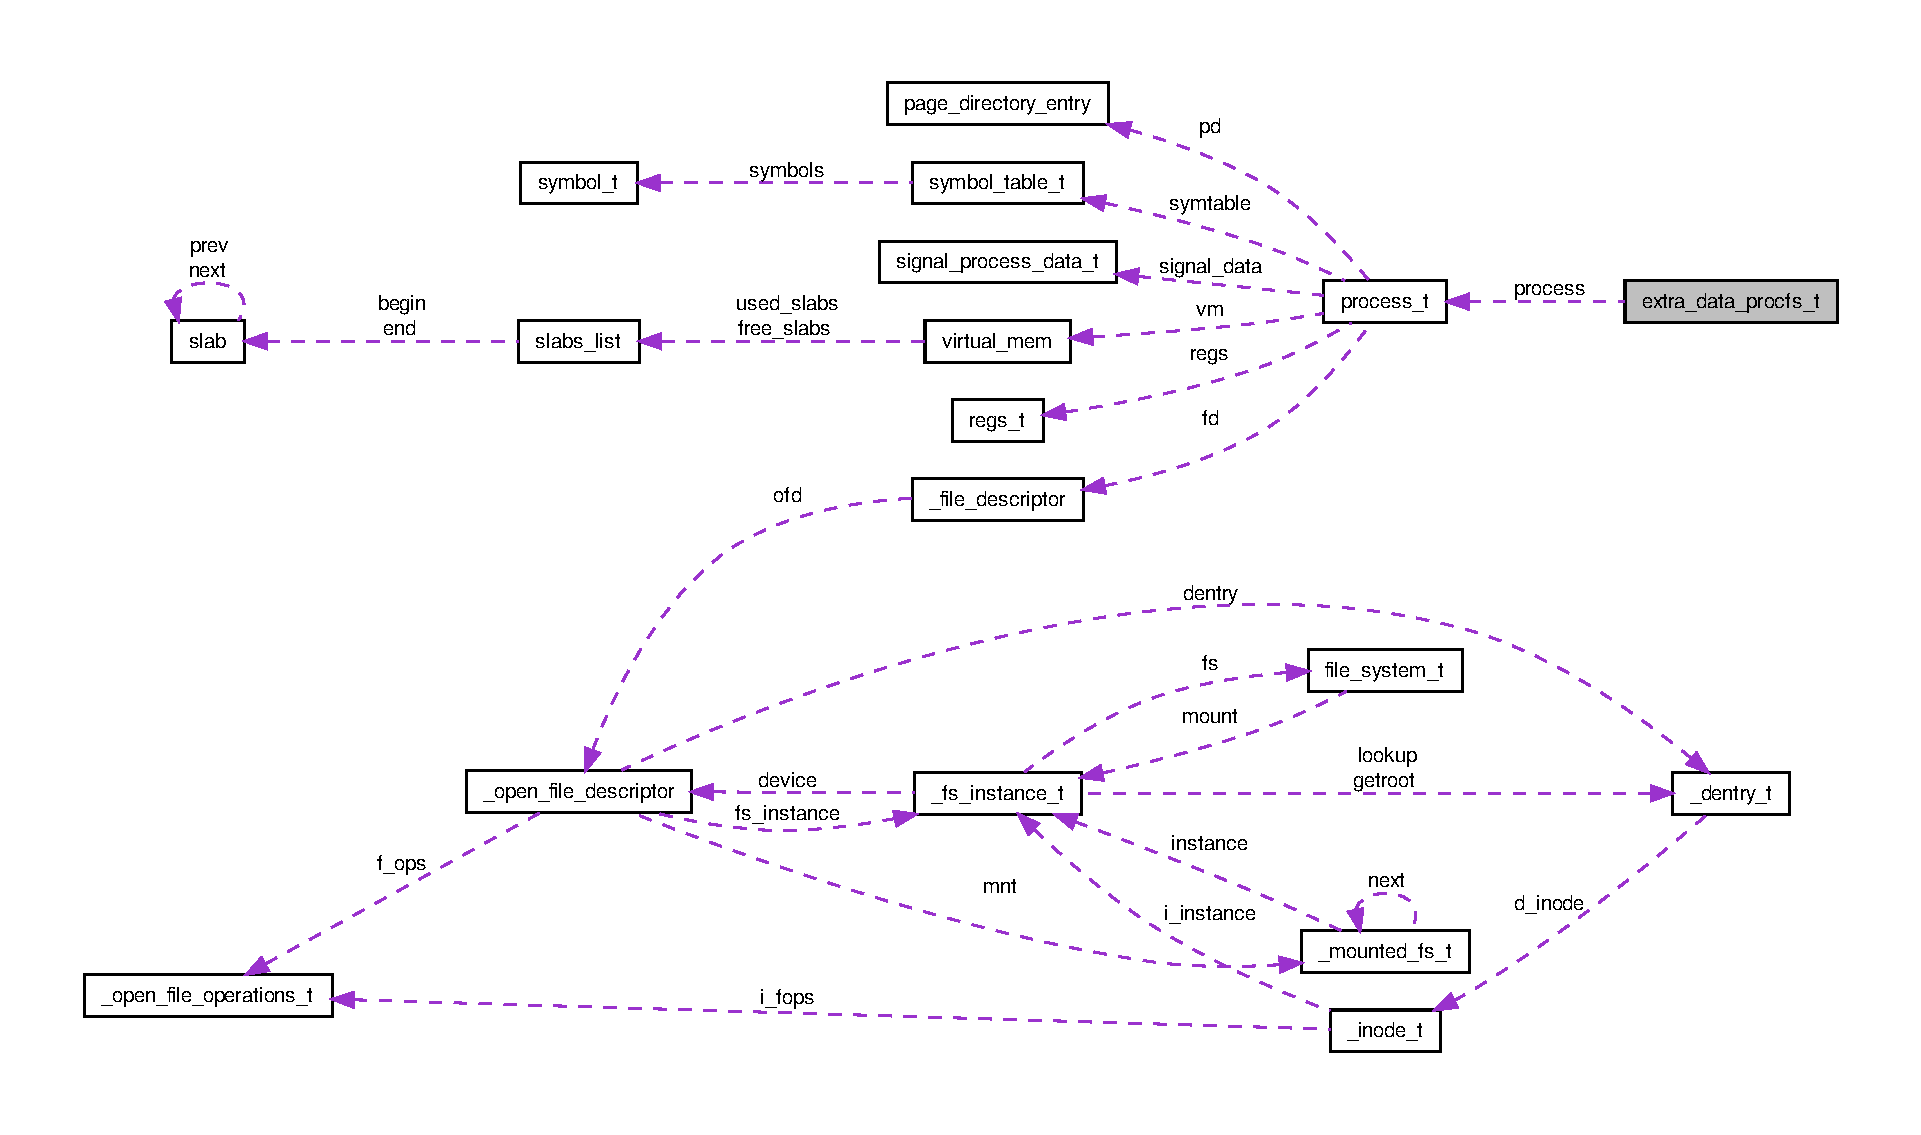
\includegraphics[width=350pt]{structextra__data__procfs__t__coll__graph}
\end{center}
\end{figure}
\subsection*{Champs de données}
\begin{DoxyCompactItemize}
\item 
\hypertarget{structextra__data__procfs__t_ad501deb466cabf589b4617eac9bcce30}{int {\bfseries pid}}\label{structextra__data__procfs__t_ad501deb466cabf589b4617eac9bcce30}

\item 
\hypertarget{structextra__data__procfs__t_a43e451440ca4470e67c59f6ca0da1e03}{\hyperlink{structprocess__t}{process\-\_\-t} $\ast$ {\bfseries process}}\label{structextra__data__procfs__t_a43e451440ca4470e67c59f6ca0da1e03}

\end{DoxyCompactItemize}


La documentation de cette structure a été générée à partir du fichier suivant \-:\begin{DoxyCompactItemize}
\item 
kernel/fs/\hyperlink{procfs_8c}{procfs.\-c}\end{DoxyCompactItemize}

\hypertarget{structfile__system__t}{\section{Référence de la structure file\-\_\-system\-\_\-t}
\label{structfile__system__t}\index{file\-\_\-system\-\_\-t@{file\-\_\-system\-\_\-t}}
}


Structure qui représente un F\-S.  




{\ttfamily \#include $<$vfs.\-h$>$}



Graphe de collaboration de file\-\_\-system\-\_\-t\-:\nopagebreak
\begin{figure}[H]
\begin{center}
\leavevmode
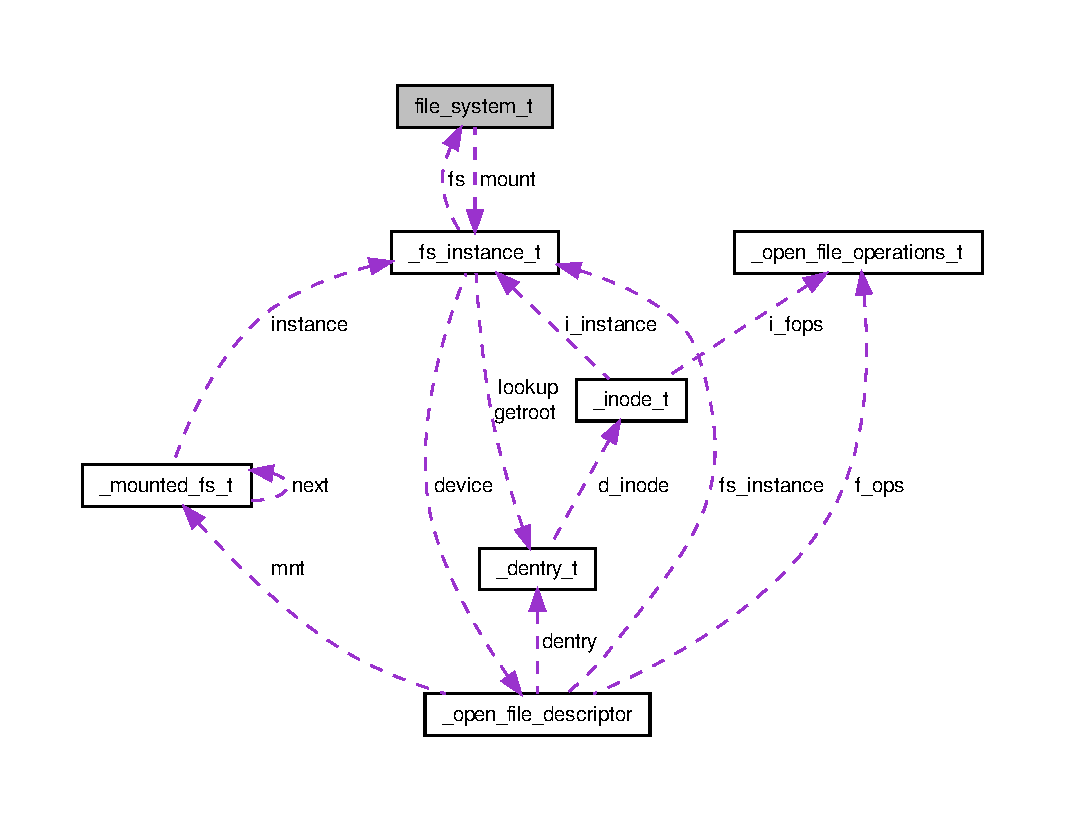
\includegraphics[width=350pt]{structfile__system__t__coll__graph}
\end{center}
\end{figure}
\subsection*{Champs de données}
\begin{DoxyCompactItemize}
\item 
char $\ast$ \hyperlink{structfile__system__t_a2b7d7c0f769113d1164052beeeca777d}{name}
\item 
int \hyperlink{structfile__system__t_a3cf80f0c2c2b7a9c202d5006e4095eaf}{unique\-\_\-inode}
\item 
struct \hyperlink{struct__fs__instance__t}{\-\_\-fs\-\_\-instance\-\_\-t} $\ast$($\ast$ \hyperlink{structfile__system__t_a7edaed95e6ac68991bbaac6cd07b458b}{mount} )(\hyperlink{fd__types_8h_a42bccb9b6a816213613cefffced245f0}{open\-\_\-file\-\_\-descriptor} $\ast$)
\item 
void($\ast$ \hyperlink{structfile__system__t_a899f34d838d88470373b60f7c5f0edd9}{umount} )(struct \hyperlink{struct__fs__instance__t}{\-\_\-fs\-\_\-instance\-\_\-t} $\ast$)
\end{DoxyCompactItemize}


\subsection{Documentation des champs}
\hypertarget{structfile__system__t_a7edaed95e6ac68991bbaac6cd07b458b}{\index{file\-\_\-system\-\_\-t@{file\-\_\-system\-\_\-t}!mount@{mount}}
\index{mount@{mount}!file_system_t@{file\-\_\-system\-\_\-t}}
\subsubsection[{mount}]{\setlength{\rightskip}{0pt plus 5cm}struct {\bf \-\_\-fs\-\_\-instance\-\_\-t}$\ast$($\ast$ file\-\_\-system\-\_\-t\-::mount)({\bf open\-\_\-file\-\_\-descriptor} $\ast$)\hspace{0.3cm}{\ttfamily [read]}}}\label{structfile__system__t_a7edaed95e6ac68991bbaac6cd07b458b}
Pointeur vers la fonction mount du F\-S. \hypertarget{structfile__system__t_a2b7d7c0f769113d1164052beeeca777d}{\index{file\-\_\-system\-\_\-t@{file\-\_\-system\-\_\-t}!name@{name}}
\index{name@{name}!file_system_t@{file\-\_\-system\-\_\-t}}
\subsubsection[{name}]{\setlength{\rightskip}{0pt plus 5cm}char$\ast$ file\-\_\-system\-\_\-t\-::name}}\label{structfile__system__t_a2b7d7c0f769113d1164052beeeca777d}
Nom du F\-S, c'est aussi son \char`\"{}type\char`\"{} utilisé lors du mount. \hypertarget{structfile__system__t_a899f34d838d88470373b60f7c5f0edd9}{\index{file\-\_\-system\-\_\-t@{file\-\_\-system\-\_\-t}!umount@{umount}}
\index{umount@{umount}!file_system_t@{file\-\_\-system\-\_\-t}}
\subsubsection[{umount}]{\setlength{\rightskip}{0pt plus 5cm}void($\ast$ file\-\_\-system\-\_\-t\-::umount)(struct {\bf \-\_\-fs\-\_\-instance\-\_\-t} $\ast$)}}\label{structfile__system__t_a899f34d838d88470373b60f7c5f0edd9}
Pointeur vers la fonction umount du F\-S. \hypertarget{structfile__system__t_a3cf80f0c2c2b7a9c202d5006e4095eaf}{\index{file\-\_\-system\-\_\-t@{file\-\_\-system\-\_\-t}!unique\-\_\-inode@{unique\-\_\-inode}}
\index{unique\-\_\-inode@{unique\-\_\-inode}!file_system_t@{file\-\_\-system\-\_\-t}}
\subsubsection[{unique\-\_\-inode}]{\setlength{\rightskip}{0pt plus 5cm}int file\-\_\-system\-\_\-t\-::unique\-\_\-inode}}\label{structfile__system__t_a3cf80f0c2c2b7a9c202d5006e4095eaf}
1 if the inodes are unique. 

La documentation de cette structure a été générée à partir du fichier suivant \-:\begin{DoxyCompactItemize}
\item 
kernel/include/\hyperlink{vfs_8h}{vfs.\-h}\end{DoxyCompactItemize}

\hypertarget{structhashmap__cell__t}{\section{Référence de la structure hashmap\-\_\-cell\-\_\-t}
\label{structhashmap__cell__t}\index{hashmap\-\_\-cell\-\_\-t@{hashmap\-\_\-cell\-\_\-t}}
}


{\ttfamily \#include $<$hashmap.\-h$>$}



Graphe de collaboration de hashmap\-\_\-cell\-\_\-t\-:\nopagebreak
\begin{figure}[H]
\begin{center}
\leavevmode
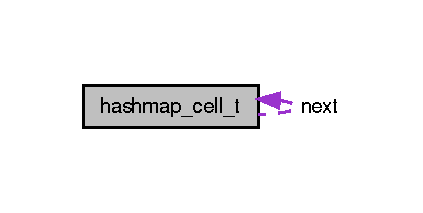
\includegraphics[width=203pt]{structhashmap__cell__t__coll__graph}
\end{center}
\end{figure}
\subsection*{Champs de données}
\begin{DoxyCompactItemize}
\item 
struct hashmap\-\_\-key\-\_\-t $\ast$ \hyperlink{structhashmap__cell__t_a18fa668e172072e9bff5e92e52d9f3af}{key}
\item 
struct hashmap\-\_\-value\-\_\-t $\ast$ \hyperlink{structhashmap__cell__t_aa0758cf139adb3747a846e539d01d75d}{value}
\item 
struct \hyperlink{structhashmap__cell__t}{hashmap\-\_\-cell\-\_\-t} $\ast$ \hyperlink{structhashmap__cell__t_afea1a8c217d80c95efa5b4a89ea07bf2}{next}
\end{DoxyCompactItemize}


\subsection{Description détaillée}
Pour chaque valeur de hash, on retrouve une liste chainée dont les éléments sont du type \hyperlink{structhashmap__cell__t}{hashmap\-\_\-cell\-\_\-t}. 

\subsection{Documentation des champs}
\hypertarget{structhashmap__cell__t_a18fa668e172072e9bff5e92e52d9f3af}{\index{hashmap\-\_\-cell\-\_\-t@{hashmap\-\_\-cell\-\_\-t}!key@{key}}
\index{key@{key}!hashmap_cell_t@{hashmap\-\_\-cell\-\_\-t}}
\subsubsection[{key}]{\setlength{\rightskip}{0pt plus 5cm}struct hashmap\-\_\-key\-\_\-t$\ast$ hashmap\-\_\-cell\-\_\-t\-::key}}\label{structhashmap__cell__t_a18fa668e172072e9bff5e92e52d9f3af}
Clef. \hypertarget{structhashmap__cell__t_afea1a8c217d80c95efa5b4a89ea07bf2}{\index{hashmap\-\_\-cell\-\_\-t@{hashmap\-\_\-cell\-\_\-t}!next@{next}}
\index{next@{next}!hashmap_cell_t@{hashmap\-\_\-cell\-\_\-t}}
\subsubsection[{next}]{\setlength{\rightskip}{0pt plus 5cm}struct {\bf hashmap\-\_\-cell\-\_\-t}$\ast$ hashmap\-\_\-cell\-\_\-t\-::next}}\label{structhashmap__cell__t_afea1a8c217d80c95efa5b4a89ea07bf2}
Élement suivant. \hypertarget{structhashmap__cell__t_aa0758cf139adb3747a846e539d01d75d}{\index{hashmap\-\_\-cell\-\_\-t@{hashmap\-\_\-cell\-\_\-t}!value@{value}}
\index{value@{value}!hashmap_cell_t@{hashmap\-\_\-cell\-\_\-t}}
\subsubsection[{value}]{\setlength{\rightskip}{0pt plus 5cm}struct hashmap\-\_\-value\-\_\-t$\ast$ hashmap\-\_\-cell\-\_\-t\-::value}}\label{structhashmap__cell__t_aa0758cf139adb3747a846e539d01d75d}
Valeur. 

La documentation de cette structure a été générée à partir du fichier suivant \-:\begin{DoxyCompactItemize}
\item 
kernel/include/\hyperlink{hashmap_8h}{hashmap.\-h}\end{DoxyCompactItemize}

\hypertarget{structheap__t}{\section{Référence de la structure heap\-\_\-t}
\label{structheap__t}\index{heap\-\_\-t@{heap\-\_\-t}}
}


{\ttfamily \#include $<$heap.\-h$>$}

\subsection*{Champs de données}
\begin{DoxyCompactItemize}
\item 
\hyperlink{list_8h_a35d066d4adbc5a7903210dcce0bf4717}{cmp\-\_\-func\-\_\-type} \hyperlink{structheap__t_aeba09c8db02d651cfe45023364d756f9}{comparator}
\item 
void $\ast$ \hyperlink{structheap__t_a3924b3948b77f2ea568ccbd9fa0bd20b}{heap}
\item 
int \hyperlink{structheap__t_a3e3c1dd26d87564ee5beb5e2835bb445}{nb\-\_\-elements}
\item 
\hyperlink{types_8h_a29d85914ddff32967d85ada69854206d}{size\-\_\-t} \hyperlink{structheap__t_a5a53cb84142d9a188aed138b4d894158}{elements\-\_\-size}
\item 
int \hyperlink{structheap__t_a7919079b18428f31e03827344bc5a390}{max\-\_\-elements}
\end{DoxyCompactItemize}


\subsection{Description détaillée}
Structure de tas. 

\subsection{Documentation des champs}
\hypertarget{structheap__t_aeba09c8db02d651cfe45023364d756f9}{\index{heap\-\_\-t@{heap\-\_\-t}!comparator@{comparator}}
\index{comparator@{comparator}!heap_t@{heap\-\_\-t}}
\subsubsection[{comparator}]{\setlength{\rightskip}{0pt plus 5cm}{\bf cmp\-\_\-func\-\_\-type} heap\-\_\-t\-::comparator}}\label{structheap__t_aeba09c8db02d651cfe45023364d756f9}
Fonction de comparaison entre deux éléments. \hypertarget{structheap__t_a5a53cb84142d9a188aed138b4d894158}{\index{heap\-\_\-t@{heap\-\_\-t}!elements\-\_\-size@{elements\-\_\-size}}
\index{elements\-\_\-size@{elements\-\_\-size}!heap_t@{heap\-\_\-t}}
\subsubsection[{elements\-\_\-size}]{\setlength{\rightskip}{0pt plus 5cm}{\bf size\-\_\-t} heap\-\_\-t\-::elements\-\_\-size}}\label{structheap__t_a5a53cb84142d9a188aed138b4d894158}
Taille de chaque élément. \hypertarget{structheap__t_a3924b3948b77f2ea568ccbd9fa0bd20b}{\index{heap\-\_\-t@{heap\-\_\-t}!heap@{heap}}
\index{heap@{heap}!heap_t@{heap\-\_\-t}}
\subsubsection[{heap}]{\setlength{\rightskip}{0pt plus 5cm}void$\ast$ heap\-\_\-t\-::heap}}\label{structheap__t_a3924b3948b77f2ea568ccbd9fa0bd20b}
Tableau qui contient le tas. \hypertarget{structheap__t_a7919079b18428f31e03827344bc5a390}{\index{heap\-\_\-t@{heap\-\_\-t}!max\-\_\-elements@{max\-\_\-elements}}
\index{max\-\_\-elements@{max\-\_\-elements}!heap_t@{heap\-\_\-t}}
\subsubsection[{max\-\_\-elements}]{\setlength{\rightskip}{0pt plus 5cm}int heap\-\_\-t\-::max\-\_\-elements}}\label{structheap__t_a7919079b18428f31e03827344bc5a390}
Nombre maximum d'éléments. \hypertarget{structheap__t_a3e3c1dd26d87564ee5beb5e2835bb445}{\index{heap\-\_\-t@{heap\-\_\-t}!nb\-\_\-elements@{nb\-\_\-elements}}
\index{nb\-\_\-elements@{nb\-\_\-elements}!heap_t@{heap\-\_\-t}}
\subsubsection[{nb\-\_\-elements}]{\setlength{\rightskip}{0pt plus 5cm}int heap\-\_\-t\-::nb\-\_\-elements}}\label{structheap__t_a3e3c1dd26d87564ee5beb5e2835bb445}
Nombre d'éléments dans le tas. 

La documentation de cette structure a été générée à partir du fichier suivant \-:\begin{DoxyCompactItemize}
\item 
kernel/include/\hyperlink{heap_8h}{heap.\-h}\end{DoxyCompactItemize}

\hypertarget{structintframe}{\section{Référence de la structure intframe}
\label{structintframe}\index{intframe@{intframe}}
}


{\ttfamily \#include $<$interrupts.\-h$>$}

\subsection*{Champs de données}
\begin{DoxyCompactItemize}
\item 
\hypertarget{structintframe_a3963b9edfbe0b5163755aedca6fd733c}{\hyperlink{types_8h_a33594304e786b158f3fb30289278f5af}{uint32\-\_\-t} {\bfseries interrupt\-\_\-id}}\label{structintframe_a3963b9edfbe0b5163755aedca6fd733c}

\item 
\hypertarget{structintframe_ab3f1a9791b9ebaae92736a23c9991239}{\hyperlink{types_8h_adf4d876453337156dde61095e1f20223}{uint16\-\_\-t} {\bfseries es}}\label{structintframe_ab3f1a9791b9ebaae92736a23c9991239}

\item 
\hypertarget{structintframe_af8bb049d885e67ce4d69880190d34239}{\hyperlink{types_8h_adf4d876453337156dde61095e1f20223}{uint16\-\_\-t} {\bfseries \-\_\-\-\_\-es\-\_\-unused}}\label{structintframe_af8bb049d885e67ce4d69880190d34239}

\item 
\hypertarget{structintframe_a2b82007f907954298dd9a07dd61ef51f}{\hyperlink{types_8h_adf4d876453337156dde61095e1f20223}{uint16\-\_\-t} {\bfseries ds}}\label{structintframe_a2b82007f907954298dd9a07dd61ef51f}

\item 
\hypertarget{structintframe_a9b845ecffe4c5ec60d10a4f3e9994bce}{\hyperlink{types_8h_adf4d876453337156dde61095e1f20223}{uint16\-\_\-t} {\bfseries \-\_\-\-\_\-ds\-\_\-unused}}\label{structintframe_a9b845ecffe4c5ec60d10a4f3e9994bce}

\item 
\hypertarget{structintframe_ad96d8785a5434d44569719aa60396411}{\hyperlink{types_8h_adf4d876453337156dde61095e1f20223}{uint16\-\_\-t} {\bfseries gs}}\label{structintframe_ad96d8785a5434d44569719aa60396411}

\item 
\hypertarget{structintframe_a268212b461fc364820125165d979256a}{\hyperlink{types_8h_adf4d876453337156dde61095e1f20223}{uint16\-\_\-t} {\bfseries \-\_\-\-\_\-gs\-\_\-unused}}\label{structintframe_a268212b461fc364820125165d979256a}

\item 
\hypertarget{structintframe_acbf958c3c0f0d30088b8a9a3c0706e0f}{\hyperlink{types_8h_adf4d876453337156dde61095e1f20223}{uint16\-\_\-t} {\bfseries fs}}\label{structintframe_acbf958c3c0f0d30088b8a9a3c0706e0f}

\item 
\hypertarget{structintframe_a2f4f02335b9f041e3e6bbfde6ac5f126}{\hyperlink{types_8h_adf4d876453337156dde61095e1f20223}{uint16\-\_\-t} {\bfseries \-\_\-\-\_\-fs\-\_\-unused}}\label{structintframe_a2f4f02335b9f041e3e6bbfde6ac5f126}

\item 
\hypertarget{structintframe_a7dd7d3a26efdd343df176bd49fd3d87a}{\hyperlink{types_8h_a33594304e786b158f3fb30289278f5af}{uint32\-\_\-t} {\bfseries edi}}\label{structintframe_a7dd7d3a26efdd343df176bd49fd3d87a}

\item 
\hypertarget{structintframe_a9be9028cd0265b9850e9471f87f2e7b9}{\hyperlink{types_8h_a33594304e786b158f3fb30289278f5af}{uint32\-\_\-t} {\bfseries esi}}\label{structintframe_a9be9028cd0265b9850e9471f87f2e7b9}

\item 
\hypertarget{structintframe_a413ab529b9a7088d454cfdec87ac9f81}{\hyperlink{types_8h_a33594304e786b158f3fb30289278f5af}{uint32\-\_\-t} {\bfseries ebp}}\label{structintframe_a413ab529b9a7088d454cfdec87ac9f81}

\item 
\hypertarget{structintframe_ae1450b6414caaaa76c3453631b1dc7a1}{\hyperlink{types_8h_a33594304e786b158f3fb30289278f5af}{uint32\-\_\-t} {\bfseries kesp}}\label{structintframe_ae1450b6414caaaa76c3453631b1dc7a1}

\item 
\hypertarget{structintframe_abc22a4ffb72c4843b1ac0a62352b9c54}{\hyperlink{types_8h_a33594304e786b158f3fb30289278f5af}{uint32\-\_\-t} {\bfseries ebx}}\label{structintframe_abc22a4ffb72c4843b1ac0a62352b9c54}

\item 
\hypertarget{structintframe_ace28e4893bb9a370d8781ff68ee88fc5}{\hyperlink{types_8h_a33594304e786b158f3fb30289278f5af}{uint32\-\_\-t} {\bfseries edx}}\label{structintframe_ace28e4893bb9a370d8781ff68ee88fc5}

\item 
\hypertarget{structintframe_a14ae9b29805ce506b8f68299c265333a}{\hyperlink{types_8h_a33594304e786b158f3fb30289278f5af}{uint32\-\_\-t} {\bfseries ecx}}\label{structintframe_a14ae9b29805ce506b8f68299c265333a}

\item 
\hypertarget{structintframe_a4b6ee3c5eb0e2cd81020c5fa7582f1ea}{\hyperlink{types_8h_a33594304e786b158f3fb30289278f5af}{uint32\-\_\-t} {\bfseries eax}}\label{structintframe_a4b6ee3c5eb0e2cd81020c5fa7582f1ea}

\item 
\hypertarget{structintframe_a0f93fe44bc7ade3a2358949ab605146e}{\hyperlink{types_8h_a33594304e786b158f3fb30289278f5af}{uint32\-\_\-t} {\bfseries eip}}\label{structintframe_a0f93fe44bc7ade3a2358949ab605146e}

\item 
\hypertarget{structintframe_a2cd36ae2b67da5bfc30bf8441e536483}{\hyperlink{types_8h_a33594304e786b158f3fb30289278f5af}{uint32\-\_\-t} {\bfseries cs}}\label{structintframe_a2cd36ae2b67da5bfc30bf8441e536483}

\item 
\hypertarget{structintframe_a59fdb5905235f4ea9bee156db99ad1af}{\hyperlink{types_8h_a33594304e786b158f3fb30289278f5af}{uint32\-\_\-t} {\bfseries eflags}}\label{structintframe_a59fdb5905235f4ea9bee156db99ad1af}

\item 
\hypertarget{structintframe_adabf0c27a201a186128e2262a06b2058}{\hyperlink{types_8h_a33594304e786b158f3fb30289278f5af}{uint32\-\_\-t} {\bfseries esp}}\label{structintframe_adabf0c27a201a186128e2262a06b2058}

\item 
\hypertarget{structintframe_ae3ca96d65b1f3369124fdaff7db3dd8d}{\hyperlink{types_8h_adf4d876453337156dde61095e1f20223}{uint16\-\_\-t} {\bfseries ss}}\label{structintframe_ae3ca96d65b1f3369124fdaff7db3dd8d}

\item 
\hypertarget{structintframe_a42dc36ac2a68f274363ed16e66ac508e}{\hyperlink{types_8h_adf4d876453337156dde61095e1f20223}{uint16\-\_\-t} {\bfseries \-\_\-\-\_\-ss\-\_\-unused}}\label{structintframe_a42dc36ac2a68f274363ed16e66ac508e}

\end{DoxyCompactItemize}


\subsection{Description détaillée}
Structure représentant comment les registres sont empilés lors d'une interruption 

La documentation de cette structure a été générée à partir du fichier suivant \-:\begin{DoxyCompactItemize}
\item 
kernel/include/\hyperlink{interrupts_8h}{interrupts.\-h}\end{DoxyCompactItemize}

\hypertarget{structkernel__options}{\section{Référence de la structure kernel\+\_\+options}
\label{structkernel__options}\index{kernel\+\_\+options@{kernel\+\_\+options}}
}
\subsection*{Champs de données}
\begin{DoxyCompactItemize}
\item 
\hyperlink{kernel_2include_2types_8h_aba7bc1797add20fe3efdf37ced1182c5}{uint8\+\_\+t} \hyperlink{structkernel__options_aedbc4ad6aa8e903a674e32eefbdf3557}{use\+\_\+azerty}
\end{DoxyCompactItemize}


\subsection{Description détaillée}
Options passées au kernel. 

\subsection{Documentation des champs}
\hypertarget{structkernel__options_aedbc4ad6aa8e903a674e32eefbdf3557}{\index{kernel\+\_\+options@{kernel\+\_\+options}!use\+\_\+azerty@{use\+\_\+azerty}}
\index{use\+\_\+azerty@{use\+\_\+azerty}!kernel\+\_\+options@{kernel\+\_\+options}}
\subsubsection[{use\+\_\+azerty}]{\setlength{\rightskip}{0pt plus 5cm}{\bf uint8\+\_\+t} kernel\+\_\+options\+::use\+\_\+azerty}}\label{structkernel__options_aedbc4ad6aa8e903a674e32eefbdf3557}
Utilise un layout azerty 

La documentation de cette structure a été générée à partir du fichier suivant \+:\begin{DoxyCompactItemize}
\item 
kernel/\hyperlink{kernel_8c}{kernel.\+c}\end{DoxyCompactItemize}

\hypertarget{structkey__t}{\section{Référence de la structure key\+\_\+t}
\label{structkey__t}\index{key\+\_\+t@{key\+\_\+t}}
}


Graphe de collaboration de key\+\_\+t\+:
\nopagebreak
\begin{figure}[H]
\begin{center}
\leavevmode
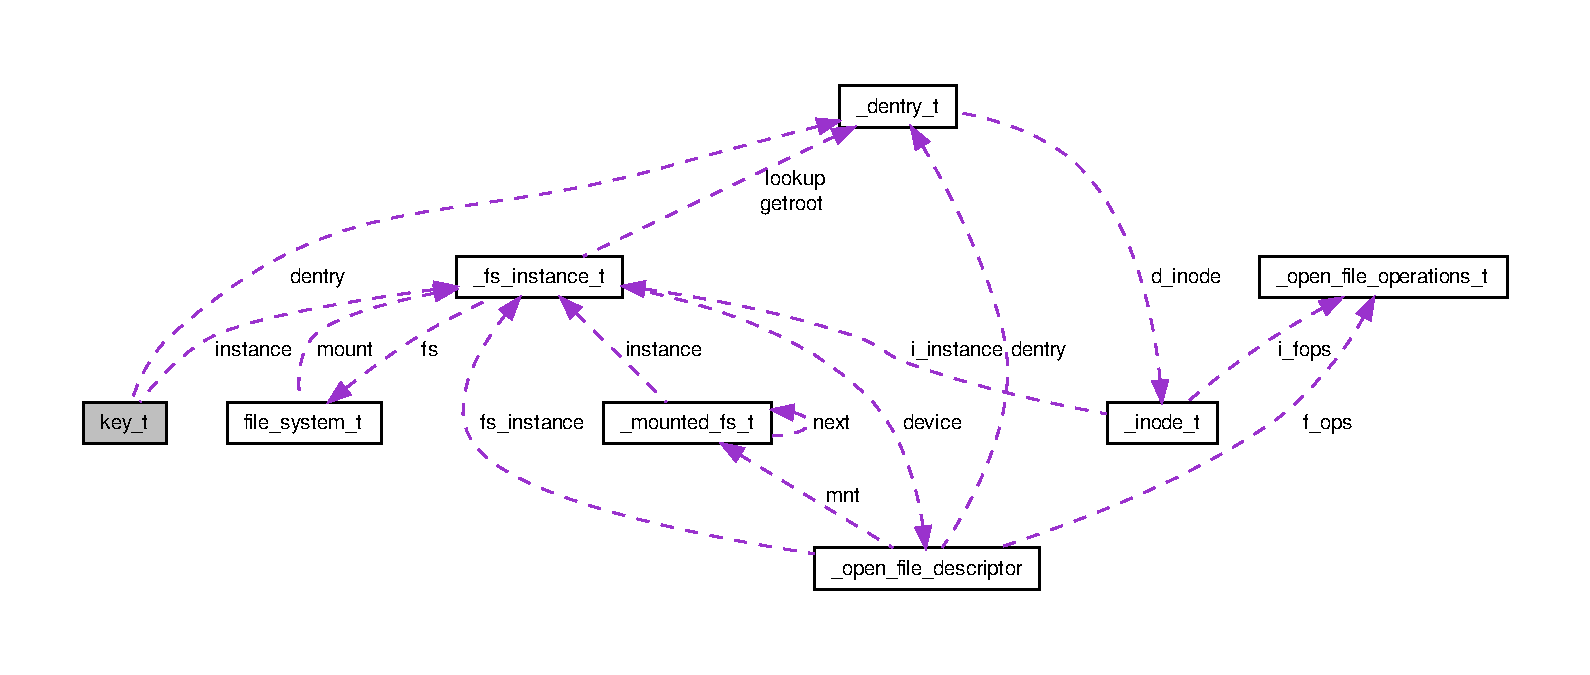
\includegraphics[width=350pt]{structkey__t__coll__graph}
\end{center}
\end{figure}
\subsection*{Champs de données}
\begin{DoxyCompactItemize}
\item 
\hyperlink{vfs_8h_a0eefa9aac35a5462ebf1e038992ca860}{fs\+\_\+instance\+\_\+t} $\ast$ \hyperlink{structkey__t_ae2b62e0c8f10b981696dbd5bfdcb6d83}{instance}
\item 
\hyperlink{vfs_8h_ade5c998c6b3f09d2cf45d0e5ef8787da}{dentry\+\_\+t} $\ast$ \hyperlink{structkey__t_a37c4229dc38020bd34d456d59d1da929}{dentry}
\item 
const char $\ast$ \hyperlink{structkey__t_a8ecb568d4ab6d546496a97231039076e}{name}
\end{DoxyCompactItemize}


\subsection{Documentation des champs}
\hypertarget{structkey__t_a37c4229dc38020bd34d456d59d1da929}{\index{key\+\_\+t@{key\+\_\+t}!dentry@{dentry}}
\index{dentry@{dentry}!key\+\_\+t@{key\+\_\+t}}
\subsubsection[{dentry}]{\setlength{\rightskip}{0pt plus 5cm}{\bf dentry\+\_\+t}$\ast$ key\+\_\+t\+::dentry}}\label{structkey__t_a37c4229dc38020bd34d456d59d1da929}
Parent directory entry. \hypertarget{structkey__t_ae2b62e0c8f10b981696dbd5bfdcb6d83}{\index{key\+\_\+t@{key\+\_\+t}!instance@{instance}}
\index{instance@{instance}!key\+\_\+t@{key\+\_\+t}}
\subsubsection[{instance}]{\setlength{\rightskip}{0pt plus 5cm}{\bf fs\+\_\+instance\+\_\+t}$\ast$ key\+\_\+t\+::instance}}\label{structkey__t_ae2b62e0c8f10b981696dbd5bfdcb6d83}
F\+S Instance. \hypertarget{structkey__t_a8ecb568d4ab6d546496a97231039076e}{\index{key\+\_\+t@{key\+\_\+t}!name@{name}}
\index{name@{name}!key\+\_\+t@{key\+\_\+t}}
\subsubsection[{name}]{\setlength{\rightskip}{0pt plus 5cm}const char$\ast$ key\+\_\+t\+::name}}\label{structkey__t_a8ecb568d4ab6d546496a97231039076e}
Dir name. 

La documentation de cette structure a été générée à partir du fichier suivant \+:\begin{DoxyCompactItemize}
\item 
kernel/\hyperlink{dcache_8c}{dcache.\+c}\end{DoxyCompactItemize}

\hypertarget{structlfn__entry__t}{\section{Référence de la structure lfn\-\_\-entry\-\_\-t}
\label{structlfn__entry__t}\index{lfn\-\_\-entry\-\_\-t@{lfn\-\_\-entry\-\_\-t}}
}


{\ttfamily \#include $<$fat\-\_\-internal.\-h$>$}

\subsection*{Champs de données}
\begin{DoxyCompactItemize}
\item 
\hyperlink{types_8h_aba7bc1797add20fe3efdf37ced1182c5}{uint8\-\_\-t} \hyperlink{structlfn__entry__t_a07b88226674917555309538459b194df}{seq\-\_\-number}
\item 
\hyperlink{types_8h_aba7bc1797add20fe3efdf37ced1182c5}{uint8\-\_\-t} \hyperlink{structlfn__entry__t_a04e5c493f02fa433b7d7d2d489c89e60}{filename1} \mbox{[}10\mbox{]}
\item 
\hyperlink{types_8h_aba7bc1797add20fe3efdf37ced1182c5}{uint8\-\_\-t} \hyperlink{structlfn__entry__t_a5b1eb8b963f05e47b3d6508b5a986985}{attributes}
\item 
\hyperlink{types_8h_aba7bc1797add20fe3efdf37ced1182c5}{uint8\-\_\-t} \hyperlink{structlfn__entry__t_a506f9cbd0e4fe209626eedaf48c1f8bf}{reserved}
\item 
\hyperlink{types_8h_aba7bc1797add20fe3efdf37ced1182c5}{uint8\-\_\-t} \hyperlink{structlfn__entry__t_a1a60017a7c8b7502fefc8358a821f0ae}{checksum}
\item 
\hyperlink{types_8h_aba7bc1797add20fe3efdf37ced1182c5}{uint8\-\_\-t} \hyperlink{structlfn__entry__t_ab88e34e402a566da06c83163e94a1763}{filename2} \mbox{[}12\mbox{]}
\item 
\hyperlink{types_8h_adf4d876453337156dde61095e1f20223}{uint16\-\_\-t} \hyperlink{structlfn__entry__t_a6f3355b0c241c7a5936c04dccf1614ca}{cluster\-\_\-pointer}
\item 
\hyperlink{types_8h_aba7bc1797add20fe3efdf37ced1182c5}{uint8\-\_\-t} \hyperlink{structlfn__entry__t_aa157718941579c9ef9bb5eba85015ec0}{filename3} \mbox{[}4\mbox{]}
\end{DoxyCompactItemize}


\subsection{Description détaillée}
Entrée pour les noms de fichier long. 

\subsection{Documentation des champs}
\hypertarget{structlfn__entry__t_a5b1eb8b963f05e47b3d6508b5a986985}{\index{lfn\-\_\-entry\-\_\-t@{lfn\-\_\-entry\-\_\-t}!attributes@{attributes}}
\index{attributes@{attributes}!lfn_entry_t@{lfn\-\_\-entry\-\_\-t}}
\subsubsection[{attributes}]{\setlength{\rightskip}{0pt plus 5cm}{\bf uint8\-\_\-t} lfn\-\_\-entry\-\_\-t\-::attributes}}\label{structlfn__entry__t_a5b1eb8b963f05e47b3d6508b5a986985}
Attributs (Toujours 0x0\-F). \hypertarget{structlfn__entry__t_a1a60017a7c8b7502fefc8358a821f0ae}{\index{lfn\-\_\-entry\-\_\-t@{lfn\-\_\-entry\-\_\-t}!checksum@{checksum}}
\index{checksum@{checksum}!lfn_entry_t@{lfn\-\_\-entry\-\_\-t}}
\subsubsection[{checksum}]{\setlength{\rightskip}{0pt plus 5cm}{\bf uint8\-\_\-t} lfn\-\_\-entry\-\_\-t\-::checksum}}\label{structlfn__entry__t_a1a60017a7c8b7502fefc8358a821f0ae}
checksum. \hypertarget{structlfn__entry__t_a6f3355b0c241c7a5936c04dccf1614ca}{\index{lfn\-\_\-entry\-\_\-t@{lfn\-\_\-entry\-\_\-t}!cluster\-\_\-pointer@{cluster\-\_\-pointer}}
\index{cluster\-\_\-pointer@{cluster\-\_\-pointer}!lfn_entry_t@{lfn\-\_\-entry\-\_\-t}}
\subsubsection[{cluster\-\_\-pointer}]{\setlength{\rightskip}{0pt plus 5cm}{\bf uint16\-\_\-t} lfn\-\_\-entry\-\_\-t\-::cluster\-\_\-pointer}}\label{structlfn__entry__t_a6f3355b0c241c7a5936c04dccf1614ca}
always 0x000. \hypertarget{structlfn__entry__t_a04e5c493f02fa433b7d7d2d489c89e60}{\index{lfn\-\_\-entry\-\_\-t@{lfn\-\_\-entry\-\_\-t}!filename1@{filename1}}
\index{filename1@{filename1}!lfn_entry_t@{lfn\-\_\-entry\-\_\-t}}
\subsubsection[{filename1}]{\setlength{\rightskip}{0pt plus 5cm}{\bf uint8\-\_\-t} lfn\-\_\-entry\-\_\-t\-::filename1\mbox{[}10\mbox{]}}}\label{structlfn__entry__t_a04e5c493f02fa433b7d7d2d489c89e60}
Partie du nom de fichier. \hypertarget{structlfn__entry__t_ab88e34e402a566da06c83163e94a1763}{\index{lfn\-\_\-entry\-\_\-t@{lfn\-\_\-entry\-\_\-t}!filename2@{filename2}}
\index{filename2@{filename2}!lfn_entry_t@{lfn\-\_\-entry\-\_\-t}}
\subsubsection[{filename2}]{\setlength{\rightskip}{0pt plus 5cm}{\bf uint8\-\_\-t} lfn\-\_\-entry\-\_\-t\-::filename2\mbox{[}12\mbox{]}}}\label{structlfn__entry__t_ab88e34e402a566da06c83163e94a1763}
Suite du nom de fichier. \hypertarget{structlfn__entry__t_aa157718941579c9ef9bb5eba85015ec0}{\index{lfn\-\_\-entry\-\_\-t@{lfn\-\_\-entry\-\_\-t}!filename3@{filename3}}
\index{filename3@{filename3}!lfn_entry_t@{lfn\-\_\-entry\-\_\-t}}
\subsubsection[{filename3}]{\setlength{\rightskip}{0pt plus 5cm}{\bf uint8\-\_\-t} lfn\-\_\-entry\-\_\-t\-::filename3\mbox{[}4\mbox{]}}}\label{structlfn__entry__t_aa157718941579c9ef9bb5eba85015ec0}
Suite du nom de fichier. \hypertarget{structlfn__entry__t_a506f9cbd0e4fe209626eedaf48c1f8bf}{\index{lfn\-\_\-entry\-\_\-t@{lfn\-\_\-entry\-\_\-t}!reserved@{reserved}}
\index{reserved@{reserved}!lfn_entry_t@{lfn\-\_\-entry\-\_\-t}}
\subsubsection[{reserved}]{\setlength{\rightskip}{0pt plus 5cm}{\bf uint8\-\_\-t} lfn\-\_\-entry\-\_\-t\-::reserved}}\label{structlfn__entry__t_a506f9cbd0e4fe209626eedaf48c1f8bf}
always 0x0. \hypertarget{structlfn__entry__t_a07b88226674917555309538459b194df}{\index{lfn\-\_\-entry\-\_\-t@{lfn\-\_\-entry\-\_\-t}!seq\-\_\-number@{seq\-\_\-number}}
\index{seq\-\_\-number@{seq\-\_\-number}!lfn_entry_t@{lfn\-\_\-entry\-\_\-t}}
\subsubsection[{seq\-\_\-number}]{\setlength{\rightskip}{0pt plus 5cm}{\bf uint8\-\_\-t} lfn\-\_\-entry\-\_\-t\-::seq\-\_\-number}}\label{structlfn__entry__t_a07b88226674917555309538459b194df}
Numéro de séquence. 

La documentation de cette structure a été générée à partir du fichier suivant \-:\begin{DoxyCompactItemize}
\item 
kernel/fs/fat/\hyperlink{fat__internal_8h}{fat\-\_\-internal.\-h}\end{DoxyCompactItemize}

\hypertarget{structlist__t}{\section{Référence de la structure list\+\_\+t}
\label{structlist__t}\index{list\+\_\+t@{list\+\_\+t}}
}


Liste générique.  




{\ttfamily \#include $<$list.\+h$>$}

\subsection*{Champs de données}
\begin{DoxyCompactItemize}
\item 
\hyperlink{list_8h_a35d066d4adbc5a7903210dcce0bf4717}{cmp\+\_\+func\+\_\+type} \hyperlink{structlist__t_a37b34fd423a00ddc7ad662c29fbd177e}{comparator}
\item 
int \hyperlink{structlist__t_a0c48694d3aca4dbf169881b9df794cb6}{head}
\item 
void $\ast$ \hyperlink{structlist__t_a799d9396ef609198dc4dff6456a99bb9}{elements\+\_\+array}
\item 
int $\ast$ \hyperlink{structlist__t_ae66525dffaeeeda67bd46d8c90fa2863}{link\+\_\+array}
\item 
int \hyperlink{structlist__t_a21f815dfb80c00df4cc95304bc29161f}{nb\+\_\+elements}
\item 
\hyperlink{kernel_2include_2types_8h_a29d85914ddff32967d85ada69854206d}{size\+\_\+t} \hyperlink{structlist__t_a467978ad64ca202b560905f80a93bf8a}{elements\+\_\+size}
\item 
int \hyperlink{structlist__t_a646f05091de2a2667b0f3c9aaffdfbdc}{max\+\_\+elements}
\end{DoxyCompactItemize}


\subsection{Documentation des champs}
\hypertarget{structlist__t_a37b34fd423a00ddc7ad662c29fbd177e}{\index{list\+\_\+t@{list\+\_\+t}!comparator@{comparator}}
\index{comparator@{comparator}!list\+\_\+t@{list\+\_\+t}}
\subsubsection[{comparator}]{\setlength{\rightskip}{0pt plus 5cm}{\bf cmp\+\_\+func\+\_\+type} list\+\_\+t\+::comparator}}\label{structlist__t_a37b34fd423a00ddc7ad662c29fbd177e}
Fonction de comparaison des elements \hypertarget{structlist__t_a799d9396ef609198dc4dff6456a99bb9}{\index{list\+\_\+t@{list\+\_\+t}!elements\+\_\+array@{elements\+\_\+array}}
\index{elements\+\_\+array@{elements\+\_\+array}!list\+\_\+t@{list\+\_\+t}}
\subsubsection[{elements\+\_\+array}]{\setlength{\rightskip}{0pt plus 5cm}void$\ast$ list\+\_\+t\+::elements\+\_\+array}}\label{structlist__t_a799d9396ef609198dc4dff6456a99bb9}
Tableau contenant les éléments \hypertarget{structlist__t_a467978ad64ca202b560905f80a93bf8a}{\index{list\+\_\+t@{list\+\_\+t}!elements\+\_\+size@{elements\+\_\+size}}
\index{elements\+\_\+size@{elements\+\_\+size}!list\+\_\+t@{list\+\_\+t}}
\subsubsection[{elements\+\_\+size}]{\setlength{\rightskip}{0pt plus 5cm}{\bf size\+\_\+t} list\+\_\+t\+::elements\+\_\+size}}\label{structlist__t_a467978ad64ca202b560905f80a93bf8a}
Taille du type d'élement à contenir \hypertarget{structlist__t_a0c48694d3aca4dbf169881b9df794cb6}{\index{list\+\_\+t@{list\+\_\+t}!head@{head}}
\index{head@{head}!list\+\_\+t@{list\+\_\+t}}
\subsubsection[{head}]{\setlength{\rightskip}{0pt plus 5cm}int list\+\_\+t\+::head}}\label{structlist__t_a0c48694d3aca4dbf169881b9df794cb6}
Indice de la tête de liste \hypertarget{structlist__t_ae66525dffaeeeda67bd46d8c90fa2863}{\index{list\+\_\+t@{list\+\_\+t}!link\+\_\+array@{link\+\_\+array}}
\index{link\+\_\+array@{link\+\_\+array}!list\+\_\+t@{list\+\_\+t}}
\subsubsection[{link\+\_\+array}]{\setlength{\rightskip}{0pt plus 5cm}int$\ast$ list\+\_\+t\+::link\+\_\+array}}\label{structlist__t_ae66525dffaeeeda67bd46d8c90fa2863}
Tableau contenant les liens entre les éléments,sers aussi à savoir si un emplacement est vide \hypertarget{structlist__t_a646f05091de2a2667b0f3c9aaffdfbdc}{\index{list\+\_\+t@{list\+\_\+t}!max\+\_\+elements@{max\+\_\+elements}}
\index{max\+\_\+elements@{max\+\_\+elements}!list\+\_\+t@{list\+\_\+t}}
\subsubsection[{max\+\_\+elements}]{\setlength{\rightskip}{0pt plus 5cm}int list\+\_\+t\+::max\+\_\+elements}}\label{structlist__t_a646f05091de2a2667b0f3c9aaffdfbdc}
Nombre maximum d'élements dans la liste \hypertarget{structlist__t_a21f815dfb80c00df4cc95304bc29161f}{\index{list\+\_\+t@{list\+\_\+t}!nb\+\_\+elements@{nb\+\_\+elements}}
\index{nb\+\_\+elements@{nb\+\_\+elements}!list\+\_\+t@{list\+\_\+t}}
\subsubsection[{nb\+\_\+elements}]{\setlength{\rightskip}{0pt plus 5cm}int list\+\_\+t\+::nb\+\_\+elements}}\label{structlist__t_a21f815dfb80c00df4cc95304bc29161f}
Nombre d'éléments présents dans la liste 

La documentation de cette structure a été générée à partir du fichier suivant \+:\begin{DoxyCompactItemize}
\item 
kernel/include/\hyperlink{list_8h}{list.\+h}\end{DoxyCompactItemize}

\hypertarget{structmem}{\section{\-Référence de la structure mem}
\label{structmem}\index{mem@{mem}}
}


\-Graphe de collaboration de mem\-:\nopagebreak
\begin{figure}[H]
\begin{center}
\leavevmode
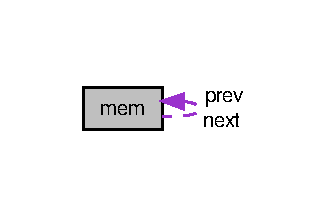
\includegraphics[width=158pt]{structmem__coll__graph}
\end{center}
\end{figure}
\subsection*{\-Champs de données}
\begin{DoxyCompactItemize}
\item 
\hypertarget{structmem_a2edfcacfe26d9112b0e4f745c9f75cf7}{struct \hyperlink{structmem}{mem} $\ast$ {\bfseries prev}}\label{structmem_a2edfcacfe26d9112b0e4f745c9f75cf7}

\item 
\hypertarget{structmem_a7d695ebc3fafa769e7e7a75f1d232a18}{\hyperlink{types_8h_a29d85914ddff32967d85ada69854206d}{size\-\_\-t} {\bfseries size}}\label{structmem_a7d695ebc3fafa769e7e7a75f1d232a18}

\item 
\hypertarget{structmem_ad12075ee870ccc6f67f420f09ff37732}{struct \hyperlink{structmem}{mem} $\ast$ {\bfseries next}}\label{structmem_ad12075ee870ccc6f67f420f09ff37732}

\end{DoxyCompactItemize}


\-La documentation de cette structure a été générée à partir du fichier suivant \-:\begin{DoxyCompactItemize}
\item 
libc/\hyperlink{malloc_8c}{malloc.\-c}\end{DoxyCompactItemize}

\hypertarget{structmem__list}{\section{Référence de la structure mem\-\_\-list}
\label{structmem__list}\index{mem\-\_\-list@{mem\-\_\-list}}
}


Graphe de collaboration de mem\-\_\-list\-:\nopagebreak
\begin{figure}[H]
\begin{center}
\leavevmode
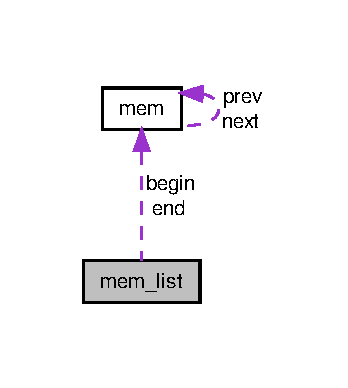
\includegraphics[width=167pt]{structmem__list__coll__graph}
\end{center}
\end{figure}
\subsection*{Champs de données}
\begin{DoxyCompactItemize}
\item 
\hypertarget{structmem__list_a553c3121bc3eb64cb30d5cda16edb629}{struct \hyperlink{structmem}{mem} $\ast$ {\bfseries begin}}\label{structmem__list_a553c3121bc3eb64cb30d5cda16edb629}

\item 
\hypertarget{structmem__list_a2e221a43fa8f185dda7f582fbb4c507f}{struct \hyperlink{structmem}{mem} $\ast$ {\bfseries end}}\label{structmem__list_a2e221a43fa8f185dda7f582fbb4c507f}

\end{DoxyCompactItemize}


La documentation de cette structure a été générée à partir du fichier suivant \-:\begin{DoxyCompactItemize}
\item 
kernel/\hyperlink{kmalloc_8c}{kmalloc.\-c}\end{DoxyCompactItemize}

\hypertarget{structmode}{\section{Référence de la structure mode}
\label{structmode}\index{mode@{mode}}
}


{\ttfamily \#include $<$vga\+\_\+modes.\+h$>$}

\subsection*{Champs de données}
\begin{DoxyCompactItemize}
\item 
int \hyperlink{structmode_ae3caae9e51730e3fc85ab1f7c9bfce89}{width}
\item 
int \hyperlink{structmode_a5e0e1e7b517ffe3532d75bda4b47b2c4}{height}
\item 
int \hyperlink{structmode_a5ca924aaa8f33c270e7896095df93c64}{bpp}
\item 
bool \hyperlink{structmode_a04810864c94405d05fdab5f4467a4db3}{graphic}
\item 
unsigned char $\ast$ \hyperlink{structmode_a704a184dc9d562c705d1feeb5be8788b}{reg\+\_\+values}
\end{DoxyCompactItemize}


\subsection{Description détaillée}
Describes a V\+G\+A mode 

\subsection{Documentation des champs}
\hypertarget{structmode_a5ca924aaa8f33c270e7896095df93c64}{\index{mode@{mode}!bpp@{bpp}}
\index{bpp@{bpp}!mode@{mode}}
\subsubsection[{bpp}]{\setlength{\rightskip}{0pt plus 5cm}int mode\+::bpp}}\label{structmode_a5ca924aaa8f33c270e7896095df93c64}
Bytes per pixel (in memory) \hypertarget{structmode_a04810864c94405d05fdab5f4467a4db3}{\index{mode@{mode}!graphic@{graphic}}
\index{graphic@{graphic}!mode@{mode}}
\subsubsection[{graphic}]{\setlength{\rightskip}{0pt plus 5cm}bool mode\+::graphic}}\label{structmode_a04810864c94405d05fdab5f4467a4db3}
Text mode (false) or graphic mode (true) \hypertarget{structmode_a5e0e1e7b517ffe3532d75bda4b47b2c4}{\index{mode@{mode}!height@{height}}
\index{height@{height}!mode@{mode}}
\subsubsection[{height}]{\setlength{\rightskip}{0pt plus 5cm}int mode\+::height}}\label{structmode_a5e0e1e7b517ffe3532d75bda4b47b2c4}
Screen height \hypertarget{structmode_a704a184dc9d562c705d1feeb5be8788b}{\index{mode@{mode}!reg\+\_\+values@{reg\+\_\+values}}
\index{reg\+\_\+values@{reg\+\_\+values}!mode@{mode}}
\subsubsection[{reg\+\_\+values}]{\setlength{\rightskip}{0pt plus 5cm}unsigned char$\ast$ mode\+::reg\+\_\+values}}\label{structmode_a704a184dc9d562c705d1feeb5be8788b}
Values to be written in the registers \hypertarget{structmode_ae3caae9e51730e3fc85ab1f7c9bfce89}{\index{mode@{mode}!width@{width}}
\index{width@{width}!mode@{mode}}
\subsubsection[{width}]{\setlength{\rightskip}{0pt plus 5cm}int mode\+::width}}\label{structmode_ae3caae9e51730e3fc85ab1f7c9bfce89}
Screen width 

La documentation de cette structure a été générée à partir du fichier suivant \+:\begin{DoxyCompactItemize}
\item 
kernel/include/drivers/\hyperlink{vga__modes_8h}{vga\+\_\+modes.\+h}\end{DoxyCompactItemize}

\hypertarget{structmodule__info__t}{\section{Référence de la structure module\-\_\-info\-\_\-t}
\label{structmodule__info__t}\index{module\-\_\-info\-\_\-t@{module\-\_\-info\-\_\-t}}
}
\subsection*{Champs de données}
\begin{DoxyCompactItemize}
\item 
\hypertarget{structmodule__info__t_a906c54b9a8ca39941057960cb74acbbc}{char $\ast$ {\bfseries name}}\label{structmodule__info__t_a906c54b9a8ca39941057960cb74acbbc}

\item 
\hypertarget{structmodule__info__t_a3da1f736913e04aa57957d9d7615bc57}{char $\ast$ {\bfseries version}}\label{structmodule__info__t_a3da1f736913e04aa57957d9d7615bc57}

\item 
\hypertarget{structmodule__info__t_aa95e88fccbb5a709bc339cb1335c0f8f}{\hyperlink{kernel_2include_2types_8h_a9f047c1f0917f6184a7a013d4b4277a6}{paddr\-\_\-t} {\bfseries load\-\_\-handler}}\label{structmodule__info__t_aa95e88fccbb5a709bc339cb1335c0f8f}

\item 
\hypertarget{structmodule__info__t_a259150f7aee5b2daf25981ef7a906170}{\hyperlink{kernel_2include_2types_8h_a9f047c1f0917f6184a7a013d4b4277a6}{paddr\-\_\-t} {\bfseries unload\-\_\-handler}}\label{structmodule__info__t_a259150f7aee5b2daf25981ef7a906170}

\item 
\hypertarget{structmodule__info__t_adc058be04f20f5191023a2c9c9a03292}{\hyperlink{kernel_2include_2types_8h_a9f047c1f0917f6184a7a013d4b4277a6}{paddr\-\_\-t} {\bfseries load\-\_\-addr}}\label{structmodule__info__t_adc058be04f20f5191023a2c9c9a03292}

\end{DoxyCompactItemize}


La documentation de cette structure a été générée à partir du fichier suivant \-:\begin{DoxyCompactItemize}
\item 
kernel/include/\hyperlink{module_8h}{module.\-h}\end{DoxyCompactItemize}

\hypertarget{structmultiboot__aout__symbol__table}{\section{Référence de la structure multiboot\-\_\-aout\-\_\-symbol\-\_\-table}
\label{structmultiboot__aout__symbol__table}\index{multiboot\-\_\-aout\-\_\-symbol\-\_\-table@{multiboot\-\_\-aout\-\_\-symbol\-\_\-table}}
}


{\ttfamily \#include $<$multiboot.\-h$>$}

\subsection*{Champs de données}
\begin{DoxyCompactItemize}
\item 
\hypertarget{structmultiboot__aout__symbol__table_a3c9cc58c068678c095a7695f74375ca2}{multiboot\-\_\-uint32\-\_\-t {\bfseries tabsize}}\label{structmultiboot__aout__symbol__table_a3c9cc58c068678c095a7695f74375ca2}

\item 
\hypertarget{structmultiboot__aout__symbol__table_af9876cbe1b37935ed039c855f04b760e}{multiboot\-\_\-uint32\-\_\-t {\bfseries strsize}}\label{structmultiboot__aout__symbol__table_af9876cbe1b37935ed039c855f04b760e}

\item 
\hypertarget{structmultiboot__aout__symbol__table_ab399f68a251079409489149a5d48033f}{multiboot\-\_\-uint32\-\_\-t {\bfseries addr}}\label{structmultiboot__aout__symbol__table_ab399f68a251079409489149a5d48033f}

\item 
\hypertarget{structmultiboot__aout__symbol__table_a2317e4e566e417b8fb3502074e0807d7}{multiboot\-\_\-uint32\-\_\-t {\bfseries reserved}}\label{structmultiboot__aout__symbol__table_a2317e4e566e417b8fb3502074e0807d7}

\end{DoxyCompactItemize}


\subsection{Description détaillée}
The symbol table for a.\-out. 

La documentation de cette structure a été générée à partir du fichier suivant \-:\begin{DoxyCompactItemize}
\item 
kernel/include/\hyperlink{multiboot_8h}{multiboot.\-h}\end{DoxyCompactItemize}

\hypertarget{structmultiboot__elf__section__header__table}{\section{\-Référence de la structure multiboot\-\_\-elf\-\_\-section\-\_\-header\-\_\-table}
\label{structmultiboot__elf__section__header__table}\index{multiboot\-\_\-elf\-\_\-section\-\_\-header\-\_\-table@{multiboot\-\_\-elf\-\_\-section\-\_\-header\-\_\-table}}
}


{\ttfamily \#include $<$multiboot.\-h$>$}

\subsection*{\-Champs de données}
\begin{DoxyCompactItemize}
\item 
\hypertarget{structmultiboot__elf__section__header__table_ac7a3ee82a45af6c3c10413de7620eec2}{multiboot\-\_\-uint32\-\_\-t {\bfseries num}}\label{structmultiboot__elf__section__header__table_ac7a3ee82a45af6c3c10413de7620eec2}

\item 
\hypertarget{structmultiboot__elf__section__header__table_a87bed62f532b2e2e73ab41df40069e2a}{multiboot\-\_\-uint32\-\_\-t {\bfseries size}}\label{structmultiboot__elf__section__header__table_a87bed62f532b2e2e73ab41df40069e2a}

\item 
\hypertarget{structmultiboot__elf__section__header__table_ad0c7bb0937470de83f3319015416614a}{multiboot\-\_\-uint32\-\_\-t {\bfseries addr}}\label{structmultiboot__elf__section__header__table_ad0c7bb0937470de83f3319015416614a}

\item 
\hypertarget{structmultiboot__elf__section__header__table_adfc74c974ba232064320ba57a02d0fb3}{multiboot\-\_\-uint32\-\_\-t {\bfseries shndx}}\label{structmultiboot__elf__section__header__table_adfc74c974ba232064320ba57a02d0fb3}

\end{DoxyCompactItemize}


\subsection{\-Description détaillée}
\-The section header table for \-E\-L\-F. 

\-La documentation de cette structure a été générée à partir du fichier suivant \-:\begin{DoxyCompactItemize}
\item 
kernel/include/\hyperlink{multiboot_8h}{multiboot.\-h}\end{DoxyCompactItemize}

\hypertarget{structmultiboot__header}{\section{\-Référence de la structure multiboot\-\_\-header}
\label{structmultiboot__header}\index{multiboot\-\_\-header@{multiboot\-\_\-header}}
}
\subsection*{\-Champs de données}
\begin{DoxyCompactItemize}
\item 
multiboot\-\_\-uint32\-\_\-t \hyperlink{structmultiboot__header_a7fddee92e60ff58e159c6bf2c40bf29b}{magic}
\item 
multiboot\-\_\-uint32\-\_\-t \hyperlink{structmultiboot__header_ab922f32c179ec7bde91519d19f27d95b}{flags}
\item 
multiboot\-\_\-uint32\-\_\-t \hyperlink{structmultiboot__header_a17e73abddfe8264c254767a20099038d}{checksum}
\item 
multiboot\-\_\-uint32\-\_\-t \hyperlink{structmultiboot__header_a9718b2fc6ce29a37e9a209f92ab856e3}{header\-\_\-addr}
\item 
\hypertarget{structmultiboot__header_a99de1cf326c46c76c6039f317b7a1ef2}{multiboot\-\_\-uint32\-\_\-t {\bfseries load\-\_\-addr}}\label{structmultiboot__header_a99de1cf326c46c76c6039f317b7a1ef2}

\item 
\hypertarget{structmultiboot__header_ac9efc1a4c3cd18f286b2fd50ff052e31}{multiboot\-\_\-uint32\-\_\-t {\bfseries load\-\_\-end\-\_\-addr}}\label{structmultiboot__header_ac9efc1a4c3cd18f286b2fd50ff052e31}

\item 
\hypertarget{structmultiboot__header_ab4f2496ec9b0d1a95985929d281dfa19}{multiboot\-\_\-uint32\-\_\-t {\bfseries bss\-\_\-end\-\_\-addr}}\label{structmultiboot__header_ab4f2496ec9b0d1a95985929d281dfa19}

\item 
\hypertarget{structmultiboot__header_ac3d807775a9d69730e6698dcdcf6491e}{multiboot\-\_\-uint32\-\_\-t {\bfseries entry\-\_\-addr}}\label{structmultiboot__header_ac3d807775a9d69730e6698dcdcf6491e}

\item 
multiboot\-\_\-uint32\-\_\-t \hyperlink{structmultiboot__header_a4c90b7929342dd5aab7d08afa0906d28}{mode\-\_\-type}
\item 
\hypertarget{structmultiboot__header_ad72a1a3dd608e73c818d0c27974def40}{multiboot\-\_\-uint32\-\_\-t {\bfseries width}}\label{structmultiboot__header_ad72a1a3dd608e73c818d0c27974def40}

\item 
\hypertarget{structmultiboot__header_a055c5e6553ea032897ad50a12f998a17}{multiboot\-\_\-uint32\-\_\-t {\bfseries height}}\label{structmultiboot__header_a055c5e6553ea032897ad50a12f998a17}

\item 
\hypertarget{structmultiboot__header_aba85b53dc3af1bf99c71292a776e9dff}{multiboot\-\_\-uint32\-\_\-t {\bfseries depth}}\label{structmultiboot__header_aba85b53dc3af1bf99c71292a776e9dff}

\end{DoxyCompactItemize}


\subsection{\-Documentation des champs}
\hypertarget{structmultiboot__header_a17e73abddfe8264c254767a20099038d}{\index{multiboot\-\_\-header@{multiboot\-\_\-header}!checksum@{checksum}}
\index{checksum@{checksum}!multiboot_header@{multiboot\-\_\-header}}
\subsubsection[{checksum}]{\setlength{\rightskip}{0pt plus 5cm}multiboot\-\_\-uint32\-\_\-t {\bf multiboot\-\_\-header\-::checksum}}}\label{structmultiboot__header_a17e73abddfe8264c254767a20099038d}
\-The above fields plus this one must equal 0 mod 2$^\wedge$32. \hypertarget{structmultiboot__header_ab922f32c179ec7bde91519d19f27d95b}{\index{multiboot\-\_\-header@{multiboot\-\_\-header}!flags@{flags}}
\index{flags@{flags}!multiboot_header@{multiboot\-\_\-header}}
\subsubsection[{flags}]{\setlength{\rightskip}{0pt plus 5cm}multiboot\-\_\-uint32\-\_\-t {\bf multiboot\-\_\-header\-::flags}}}\label{structmultiboot__header_ab922f32c179ec7bde91519d19f27d95b}
\-Feature flags. \hypertarget{structmultiboot__header_a9718b2fc6ce29a37e9a209f92ab856e3}{\index{multiboot\-\_\-header@{multiboot\-\_\-header}!header\-\_\-addr@{header\-\_\-addr}}
\index{header\-\_\-addr@{header\-\_\-addr}!multiboot_header@{multiboot\-\_\-header}}
\subsubsection[{header\-\_\-addr}]{\setlength{\rightskip}{0pt plus 5cm}multiboot\-\_\-uint32\-\_\-t {\bf multiboot\-\_\-header\-::header\-\_\-addr}}}\label{structmultiboot__header_a9718b2fc6ce29a37e9a209f92ab856e3}
\-These are only valid if \-M\-U\-L\-T\-I\-B\-O\-O\-T\-\_\-\-A\-O\-U\-T\-\_\-\-K\-L\-U\-D\-G\-E is set. \hypertarget{structmultiboot__header_a7fddee92e60ff58e159c6bf2c40bf29b}{\index{multiboot\-\_\-header@{multiboot\-\_\-header}!magic@{magic}}
\index{magic@{magic}!multiboot_header@{multiboot\-\_\-header}}
\subsubsection[{magic}]{\setlength{\rightskip}{0pt plus 5cm}multiboot\-\_\-uint32\-\_\-t {\bf multiboot\-\_\-header\-::magic}}}\label{structmultiboot__header_a7fddee92e60ff58e159c6bf2c40bf29b}
\-Must be \-M\-U\-L\-T\-I\-B\-O\-O\-T\-\_\-\-M\-A\-G\-I\-C -\/ see above. \hypertarget{structmultiboot__header_a4c90b7929342dd5aab7d08afa0906d28}{\index{multiboot\-\_\-header@{multiboot\-\_\-header}!mode\-\_\-type@{mode\-\_\-type}}
\index{mode\-\_\-type@{mode\-\_\-type}!multiboot_header@{multiboot\-\_\-header}}
\subsubsection[{mode\-\_\-type}]{\setlength{\rightskip}{0pt plus 5cm}multiboot\-\_\-uint32\-\_\-t {\bf multiboot\-\_\-header\-::mode\-\_\-type}}}\label{structmultiboot__header_a4c90b7929342dd5aab7d08afa0906d28}
\-These are only valid if \-M\-U\-L\-T\-I\-B\-O\-O\-T\-\_\-\-V\-I\-D\-E\-O\-\_\-\-M\-O\-D\-E is set. 

\-La documentation de cette structure a été générée à partir du fichier suivant \-:\begin{DoxyCompactItemize}
\item 
kernel/include/\hyperlink{multiboot_8h}{multiboot.\-h}\end{DoxyCompactItemize}

\hypertarget{structmultiboot__info}{\section{Référence de la structure multiboot\-\_\-info}
\label{structmultiboot__info}\index{multiboot\-\_\-info@{multiboot\-\_\-info}}
}


Graphe de collaboration de multiboot\-\_\-info\-:\nopagebreak
\begin{figure}[H]
\begin{center}
\leavevmode
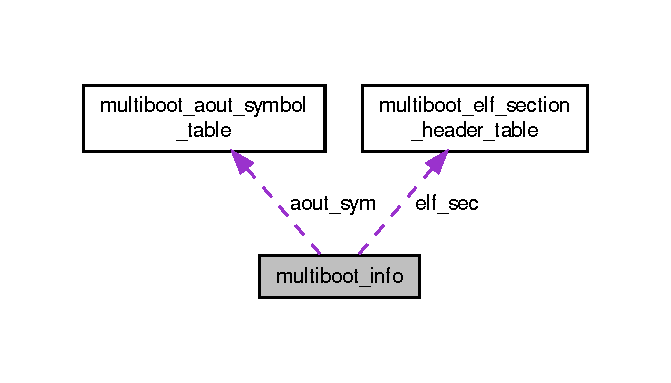
\includegraphics[width=322pt]{structmultiboot__info__coll__graph}
\end{center}
\end{figure}
\subsection*{Champs de données}
\begin{DoxyCompactItemize}
\item 
multiboot\-\_\-uint32\-\_\-t \hyperlink{structmultiboot__info_aa562865bc325fd785c9fa4c5056294f3}{flags}
\item 
\hypertarget{structmultiboot__info_aa3503176ee0d132ef98537fa0b36ff09}{multiboot\-\_\-uint32\-\_\-t {\bfseries mem\-\_\-lower}}\label{structmultiboot__info_aa3503176ee0d132ef98537fa0b36ff09}

\item 
\hypertarget{structmultiboot__info_a87db5803d5a79490b2bf32cb8e9a05c9}{multiboot\-\_\-uint32\-\_\-t {\bfseries mem\-\_\-upper}}\label{structmultiboot__info_a87db5803d5a79490b2bf32cb8e9a05c9}

\item 
multiboot\-\_\-uint32\-\_\-t \hyperlink{structmultiboot__info_ac7dd626a05c9ba62d55ea8a7a254de80}{boot\-\_\-device}
\item 
multiboot\-\_\-uint32\-\_\-t \hyperlink{structmultiboot__info_a0f2f05f69c69c615bf2b4820d357cf36}{cmdline}
\item 
multiboot\-\_\-uint32\-\_\-t \hyperlink{structmultiboot__info_aebdafce31f94277d138202f7b1ec35cc}{mods\-\_\-count}
\item 
\hypertarget{structmultiboot__info_a854bdbfa7b23c9c3dfa0bfc155ef8242}{multiboot\-\_\-uint32\-\_\-t {\bfseries mods\-\_\-addr}}\label{structmultiboot__info_a854bdbfa7b23c9c3dfa0bfc155ef8242}

\item 
\hypertarget{structmultiboot__info_a5958615dc99c7ba6e408338169f12108}{\begin{tabbing}
xx\=xx\=xx\=xx\=xx\=xx\=xx\=xx\=xx\=\kill
union \{\\
\>\hyperlink{structmultiboot__aout__symbol__table}{multiboot\_aout\_symbol\_table\_t} {\bfseries aout\_sym}\\
\>\hyperlink{structmultiboot__elf__section__header__table}{multiboot\_elf\_section\_header\_table\_t} {\bfseries elf\_sec}\\
\} {\bfseries syms}}\label{structmultiboot__info_a5958615dc99c7ba6e408338169f12108}
\\

\end{tabbing}\item 
multiboot\-\_\-uint32\-\_\-t \hyperlink{structmultiboot__info_a86a0d881c5233a4b1c8cd690ccd19b75}{mmap\-\_\-length}
\item 
\hypertarget{structmultiboot__info_aacf83273b9f8448d91fb24690492c0d8}{multiboot\-\_\-uint32\-\_\-t {\bfseries mmap\-\_\-addr}}\label{structmultiboot__info_aacf83273b9f8448d91fb24690492c0d8}

\item 
multiboot\-\_\-uint32\-\_\-t \hyperlink{structmultiboot__info_abe859eaa7e97309f072b3bc1caf5742e}{drives\-\_\-length}
\item 
\hypertarget{structmultiboot__info_a34d90ffaaf58124095cb17de9c3b1515}{multiboot\-\_\-uint32\-\_\-t {\bfseries drives\-\_\-addr}}\label{structmultiboot__info_a34d90ffaaf58124095cb17de9c3b1515}

\item 
multiboot\-\_\-uint32\-\_\-t \hyperlink{structmultiboot__info_a919ce01f85d05ab90857f8591dfb3948}{config\-\_\-table}
\item 
multiboot\-\_\-uint32\-\_\-t \hyperlink{structmultiboot__info_a4442438f7c2da9c0cf87a94ffd1acc04}{boot\-\_\-loader\-\_\-name}
\item 
multiboot\-\_\-uint32\-\_\-t \hyperlink{structmultiboot__info_ad4285d60142d241a9e6b68a03e62ee0a}{apm\-\_\-table}
\item 
multiboot\-\_\-uint32\-\_\-t \hyperlink{structmultiboot__info_a06191cef73b64e9d64a01850547fd2e8}{vbe\-\_\-control\-\_\-info}
\item 
\hypertarget{structmultiboot__info_a88f574fe1adbcb5ff63fc95b2e072b4c}{multiboot\-\_\-uint32\-\_\-t {\bfseries vbe\-\_\-mode\-\_\-info}}\label{structmultiboot__info_a88f574fe1adbcb5ff63fc95b2e072b4c}

\item 
\hypertarget{structmultiboot__info_ac7653182e52bddb7e437cc8a66d74ce5}{multiboot\-\_\-uint16\-\_\-t {\bfseries vbe\-\_\-mode}}\label{structmultiboot__info_ac7653182e52bddb7e437cc8a66d74ce5}

\item 
\hypertarget{structmultiboot__info_a204c99787efd58c0f54fe1e056b1d69f}{multiboot\-\_\-uint16\-\_\-t {\bfseries vbe\-\_\-interface\-\_\-seg}}\label{structmultiboot__info_a204c99787efd58c0f54fe1e056b1d69f}

\item 
\hypertarget{structmultiboot__info_a1621d51b1cc198a1496e9f61b3708291}{multiboot\-\_\-uint16\-\_\-t {\bfseries vbe\-\_\-interface\-\_\-off}}\label{structmultiboot__info_a1621d51b1cc198a1496e9f61b3708291}

\item 
\hypertarget{structmultiboot__info_ab3c537df524db1ed0aeaa2e6f61a23e6}{multiboot\-\_\-uint16\-\_\-t {\bfseries vbe\-\_\-interface\-\_\-len}}\label{structmultiboot__info_ab3c537df524db1ed0aeaa2e6f61a23e6}

\end{DoxyCompactItemize}


\subsection{Documentation des champs}
\hypertarget{structmultiboot__info_ad4285d60142d241a9e6b68a03e62ee0a}{\index{multiboot\-\_\-info@{multiboot\-\_\-info}!apm\-\_\-table@{apm\-\_\-table}}
\index{apm\-\_\-table@{apm\-\_\-table}!multiboot_info@{multiboot\-\_\-info}}
\subsubsection[{apm\-\_\-table}]{\setlength{\rightskip}{0pt plus 5cm}multiboot\-\_\-uint32\-\_\-t multiboot\-\_\-info\-::apm\-\_\-table}}\label{structmultiboot__info_ad4285d60142d241a9e6b68a03e62ee0a}
A\-P\-M table \hypertarget{structmultiboot__info_ac7dd626a05c9ba62d55ea8a7a254de80}{\index{multiboot\-\_\-info@{multiboot\-\_\-info}!boot\-\_\-device@{boot\-\_\-device}}
\index{boot\-\_\-device@{boot\-\_\-device}!multiboot_info@{multiboot\-\_\-info}}
\subsubsection[{boot\-\_\-device}]{\setlength{\rightskip}{0pt plus 5cm}multiboot\-\_\-uint32\-\_\-t multiboot\-\_\-info\-::boot\-\_\-device}}\label{structmultiboot__info_ac7dd626a05c9ba62d55ea8a7a254de80}
\char`\"{}root\char`\"{} partition \hypertarget{structmultiboot__info_a4442438f7c2da9c0cf87a94ffd1acc04}{\index{multiboot\-\_\-info@{multiboot\-\_\-info}!boot\-\_\-loader\-\_\-name@{boot\-\_\-loader\-\_\-name}}
\index{boot\-\_\-loader\-\_\-name@{boot\-\_\-loader\-\_\-name}!multiboot_info@{multiboot\-\_\-info}}
\subsubsection[{boot\-\_\-loader\-\_\-name}]{\setlength{\rightskip}{0pt plus 5cm}multiboot\-\_\-uint32\-\_\-t multiboot\-\_\-info\-::boot\-\_\-loader\-\_\-name}}\label{structmultiboot__info_a4442438f7c2da9c0cf87a94ffd1acc04}
Boot Loader Name \hypertarget{structmultiboot__info_a0f2f05f69c69c615bf2b4820d357cf36}{\index{multiboot\-\_\-info@{multiboot\-\_\-info}!cmdline@{cmdline}}
\index{cmdline@{cmdline}!multiboot_info@{multiboot\-\_\-info}}
\subsubsection[{cmdline}]{\setlength{\rightskip}{0pt plus 5cm}multiboot\-\_\-uint32\-\_\-t multiboot\-\_\-info\-::cmdline}}\label{structmultiboot__info_a0f2f05f69c69c615bf2b4820d357cf36}
Kernel command line \hypertarget{structmultiboot__info_a919ce01f85d05ab90857f8591dfb3948}{\index{multiboot\-\_\-info@{multiboot\-\_\-info}!config\-\_\-table@{config\-\_\-table}}
\index{config\-\_\-table@{config\-\_\-table}!multiboot_info@{multiboot\-\_\-info}}
\subsubsection[{config\-\_\-table}]{\setlength{\rightskip}{0pt plus 5cm}multiboot\-\_\-uint32\-\_\-t multiboot\-\_\-info\-::config\-\_\-table}}\label{structmultiboot__info_a919ce01f85d05ab90857f8591dfb3948}
R\-O\-M configuration table \hypertarget{structmultiboot__info_abe859eaa7e97309f072b3bc1caf5742e}{\index{multiboot\-\_\-info@{multiboot\-\_\-info}!drives\-\_\-length@{drives\-\_\-length}}
\index{drives\-\_\-length@{drives\-\_\-length}!multiboot_info@{multiboot\-\_\-info}}
\subsubsection[{drives\-\_\-length}]{\setlength{\rightskip}{0pt plus 5cm}multiboot\-\_\-uint32\-\_\-t multiboot\-\_\-info\-::drives\-\_\-length}}\label{structmultiboot__info_abe859eaa7e97309f072b3bc1caf5742e}
Drive Info buffer \hypertarget{structmultiboot__info_aa562865bc325fd785c9fa4c5056294f3}{\index{multiboot\-\_\-info@{multiboot\-\_\-info}!flags@{flags}}
\index{flags@{flags}!multiboot_info@{multiboot\-\_\-info}}
\subsubsection[{flags}]{\setlength{\rightskip}{0pt plus 5cm}multiboot\-\_\-uint32\-\_\-t multiboot\-\_\-info\-::flags}}\label{structmultiboot__info_aa562865bc325fd785c9fa4c5056294f3}
Multiboot info version number \hypertarget{structmultiboot__info_a86a0d881c5233a4b1c8cd690ccd19b75}{\index{multiboot\-\_\-info@{multiboot\-\_\-info}!mmap\-\_\-length@{mmap\-\_\-length}}
\index{mmap\-\_\-length@{mmap\-\_\-length}!multiboot_info@{multiboot\-\_\-info}}
\subsubsection[{mmap\-\_\-length}]{\setlength{\rightskip}{0pt plus 5cm}multiboot\-\_\-uint32\-\_\-t multiboot\-\_\-info\-::mmap\-\_\-length}}\label{structmultiboot__info_a86a0d881c5233a4b1c8cd690ccd19b75}
Memory Mapping buffer \hypertarget{structmultiboot__info_aebdafce31f94277d138202f7b1ec35cc}{\index{multiboot\-\_\-info@{multiboot\-\_\-info}!mods\-\_\-count@{mods\-\_\-count}}
\index{mods\-\_\-count@{mods\-\_\-count}!multiboot_info@{multiboot\-\_\-info}}
\subsubsection[{mods\-\_\-count}]{\setlength{\rightskip}{0pt plus 5cm}multiboot\-\_\-uint32\-\_\-t multiboot\-\_\-info\-::mods\-\_\-count}}\label{structmultiboot__info_aebdafce31f94277d138202f7b1ec35cc}
Boot-\/\-Module list \hypertarget{structmultiboot__info_a06191cef73b64e9d64a01850547fd2e8}{\index{multiboot\-\_\-info@{multiboot\-\_\-info}!vbe\-\_\-control\-\_\-info@{vbe\-\_\-control\-\_\-info}}
\index{vbe\-\_\-control\-\_\-info@{vbe\-\_\-control\-\_\-info}!multiboot_info@{multiboot\-\_\-info}}
\subsubsection[{vbe\-\_\-control\-\_\-info}]{\setlength{\rightskip}{0pt plus 5cm}multiboot\-\_\-uint32\-\_\-t multiboot\-\_\-info\-::vbe\-\_\-control\-\_\-info}}\label{structmultiboot__info_a06191cef73b64e9d64a01850547fd2e8}
Video 

La documentation de cette structure a été générée à partir du fichier suivant \-:\begin{DoxyCompactItemize}
\item 
kernel/include/\hyperlink{multiboot_8h}{multiboot.\-h}\end{DoxyCompactItemize}

\hypertarget{structmultiboot__mmap__entry}{\section{Référence de la structure multiboot\-\_\-mmap\-\_\-entry}
\label{structmultiboot__mmap__entry}\index{multiboot\-\_\-mmap\-\_\-entry@{multiboot\-\_\-mmap\-\_\-entry}}
}
\subsection*{Champs de données}
\begin{DoxyCompactItemize}
\item 
\hypertarget{structmultiboot__mmap__entry_af10c1835051b4b08bdcdb538c1b4101d}{multiboot\-\_\-uint32\-\_\-t {\bfseries size}}\label{structmultiboot__mmap__entry_af10c1835051b4b08bdcdb538c1b4101d}

\item 
\hypertarget{structmultiboot__mmap__entry_a3f76a637264b83e30967bcd808ff403c}{multiboot\-\_\-uint64\-\_\-t {\bfseries addr}}\label{structmultiboot__mmap__entry_a3f76a637264b83e30967bcd808ff403c}

\item 
\hypertarget{structmultiboot__mmap__entry_a6bfa44919a328492fa4e3d6239a23352}{multiboot\-\_\-uint64\-\_\-t {\bfseries len}}\label{structmultiboot__mmap__entry_a6bfa44919a328492fa4e3d6239a23352}

\item 
\hypertarget{structmultiboot__mmap__entry_aa6fc447c57f074d0babfe3bbb7017de9}{multiboot\-\_\-uint32\-\_\-t {\bfseries type}}\label{structmultiboot__mmap__entry_aa6fc447c57f074d0babfe3bbb7017de9}

\end{DoxyCompactItemize}


La documentation de cette structure a été générée à partir du fichier suivant \-:\begin{DoxyCompactItemize}
\item 
kernel/include/\hyperlink{multiboot_8h}{multiboot.\-h}\end{DoxyCompactItemize}

\hypertarget{structmultiboot__mod__list}{\section{\-Référence de la structure multiboot\-\_\-mod\-\_\-list}
\label{structmultiboot__mod__list}\index{multiboot\-\_\-mod\-\_\-list@{multiboot\-\_\-mod\-\_\-list}}
}
\subsection*{\-Champs de données}
\begin{DoxyCompactItemize}
\item 
\hypertarget{structmultiboot__mod__list_afe0e2af1e8c0297c17a7771bd1a62e0f}{multiboot\-\_\-uint32\-\_\-t {\bfseries mod\-\_\-start}}\label{structmultiboot__mod__list_afe0e2af1e8c0297c17a7771bd1a62e0f}

\item 
\hypertarget{structmultiboot__mod__list_a75b0899f1e1f90d4ff629b7136f5b988}{multiboot\-\_\-uint32\-\_\-t {\bfseries mod\-\_\-end}}\label{structmultiboot__mod__list_a75b0899f1e1f90d4ff629b7136f5b988}

\item 
multiboot\-\_\-uint32\-\_\-t \hyperlink{structmultiboot__mod__list_a31365a9d2d0cae071f5cb8bddb9b33fb}{cmdline}
\item 
multiboot\-\_\-uint32\-\_\-t \hyperlink{structmultiboot__mod__list_a63d98e6d313098a4d35b828e204a4e0c}{pad}
\end{DoxyCompactItemize}


\subsection{\-Documentation des champs}
\hypertarget{structmultiboot__mod__list_a31365a9d2d0cae071f5cb8bddb9b33fb}{\index{multiboot\-\_\-mod\-\_\-list@{multiboot\-\_\-mod\-\_\-list}!cmdline@{cmdline}}
\index{cmdline@{cmdline}!multiboot_mod_list@{multiboot\-\_\-mod\-\_\-list}}
\subsubsection[{cmdline}]{\setlength{\rightskip}{0pt plus 5cm}multiboot\-\_\-uint32\-\_\-t {\bf multiboot\-\_\-mod\-\_\-list\-::cmdline}}}\label{structmultiboot__mod__list_a31365a9d2d0cae071f5cb8bddb9b33fb}
\-Module command line \hypertarget{structmultiboot__mod__list_a63d98e6d313098a4d35b828e204a4e0c}{\index{multiboot\-\_\-mod\-\_\-list@{multiboot\-\_\-mod\-\_\-list}!pad@{pad}}
\index{pad@{pad}!multiboot_mod_list@{multiboot\-\_\-mod\-\_\-list}}
\subsubsection[{pad}]{\setlength{\rightskip}{0pt plus 5cm}multiboot\-\_\-uint32\-\_\-t {\bf multiboot\-\_\-mod\-\_\-list\-::pad}}}\label{structmultiboot__mod__list_a63d98e6d313098a4d35b828e204a4e0c}
padding to take it to 16 bytes (must be zero) 

\-La documentation de cette structure a été générée à partir du fichier suivant \-:\begin{DoxyCompactItemize}
\item 
kernel/include/\hyperlink{multiboot_8h}{multiboot.\-h}\end{DoxyCompactItemize}

\hypertarget{structnameidata}{\section{Référence de la structure nameidata}
\label{structnameidata}\index{nameidata@{nameidata}}
}


{\ttfamily \#include $<$vfs.\-h$>$}



Graphe de collaboration de nameidata\-:
\nopagebreak
\begin{figure}[H]
\begin{center}
\leavevmode
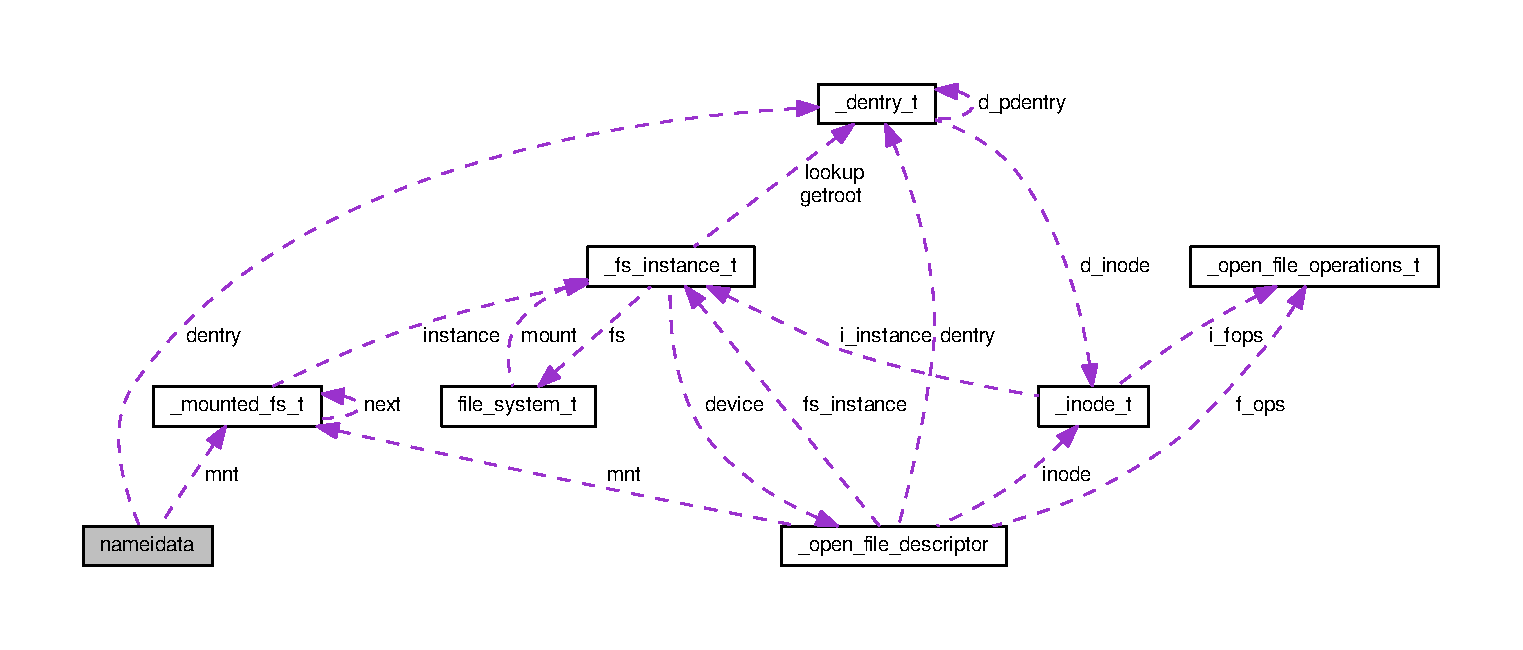
\includegraphics[width=350pt]{structnameidata__coll__graph}
\end{center}
\end{figure}
\subsection*{Champs de données}
\begin{DoxyCompactItemize}
\item 
int \hyperlink{structnameidata_a9064ec2b4dd712691e3c7442e48ce798}{flags}
\item 
\hyperlink{vfs_8h_ade5c998c6b3f09d2cf45d0e5ef8787da}{dentry\-\_\-t} $\ast$ \hyperlink{structnameidata_a19b1de01d7a6f689707fa7079cb54d7c}{dentry}
\item 
\hyperlink{vfs_8h_ab4e925860df7937f38b15433bb05225a}{mounted\-\_\-fs\-\_\-t} $\ast$ \hyperlink{structnameidata_a5488ed23ef4b37b431921f71b15e1f19}{mnt}
\item 
const char $\ast$ \hyperlink{structnameidata_a4a11e098a53839c36c2a0a4e732f8037}{last}
\end{DoxyCompactItemize}


\subsection{Description détaillée}
Structure servant au lookup. 

\subsection{Documentation des champs}
\hypertarget{structnameidata_a19b1de01d7a6f689707fa7079cb54d7c}{\index{nameidata@{nameidata}!dentry@{dentry}}
\index{dentry@{dentry}!nameidata@{nameidata}}
\subsubsection[{dentry}]{\setlength{\rightskip}{0pt plus 5cm}{\bf dentry\-\_\-t}$\ast$ nameidata\-::dentry}}\label{structnameidata_a19b1de01d7a6f689707fa7079cb54d7c}
Directory Entry. \hypertarget{structnameidata_a9064ec2b4dd712691e3c7442e48ce798}{\index{nameidata@{nameidata}!flags@{flags}}
\index{flags@{flags}!nameidata@{nameidata}}
\subsubsection[{flags}]{\setlength{\rightskip}{0pt plus 5cm}int nameidata\-::flags}}\label{structnameidata_a9064ec2b4dd712691e3c7442e48ce798}
Flags pour le lookup pour par exemple s'arréter au parent. \hypertarget{structnameidata_a4a11e098a53839c36c2a0a4e732f8037}{\index{nameidata@{nameidata}!last@{last}}
\index{last@{last}!nameidata@{nameidata}}
\subsubsection[{last}]{\setlength{\rightskip}{0pt plus 5cm}const char$\ast$ nameidata\-::last}}\label{structnameidata_a4a11e098a53839c36c2a0a4e732f8037}
Ce qu'il reste du path à parcourir. \hypertarget{structnameidata_a5488ed23ef4b37b431921f71b15e1f19}{\index{nameidata@{nameidata}!mnt@{mnt}}
\index{mnt@{mnt}!nameidata@{nameidata}}
\subsubsection[{mnt}]{\setlength{\rightskip}{0pt plus 5cm}{\bf mounted\-\_\-fs\-\_\-t}$\ast$ nameidata\-::mnt}}\label{structnameidata_a5488ed23ef4b37b431921f71b15e1f19}
Le F\-S utilisé. 

La documentation de cette structure a été générée à partir du fichier suivant \-:\begin{DoxyCompactItemize}
\item 
kernel/include/\hyperlink{vfs_8h}{vfs.\-h}\end{DoxyCompactItemize}

\hypertarget{structpage__directory__entry}{\section{Référence de la structure page\-\_\-directory\-\_\-entry}
\label{structpage__directory__entry}\index{page\-\_\-directory\-\_\-entry@{page\-\_\-directory\-\_\-entry}}
}


Page Directory Entry.  




{\ttfamily \#include $<$pagination.\-h$>$}

\subsection*{Champs de données}
\begin{DoxyCompactItemize}
\item 
\hyperlink{types_8h_a33594304e786b158f3fb30289278f5af}{uint32\-\_\-t} \hyperlink{structpage__directory__entry_ac5b5f5ab165ce60453db02e68bd7cc22}{present}\-:1
\item 
\hyperlink{types_8h_a33594304e786b158f3fb30289278f5af}{uint32\-\_\-t} \hyperlink{structpage__directory__entry_af4aa8287c5da23728d33053fcb3f1715}{r\-\_\-w}\-:1
\item 
\hyperlink{types_8h_a33594304e786b158f3fb30289278f5af}{uint32\-\_\-t} \hyperlink{structpage__directory__entry_a6e87e7efc2fbbbd5f8f7fd2e0cd09b3f}{u\-\_\-s}\-:1
\item 
\hyperlink{types_8h_a33594304e786b158f3fb30289278f5af}{uint32\-\_\-t} \hyperlink{structpage__directory__entry_a8eea5779d287c1ef5e6f2073b93166a6}{pwt}\-:1
\item 
\hyperlink{types_8h_a33594304e786b158f3fb30289278f5af}{uint32\-\_\-t} \hyperlink{structpage__directory__entry_ae480766b759f04eeb2443e12d185616a}{pcd}\-:1
\item 
\hyperlink{types_8h_a33594304e786b158f3fb30289278f5af}{uint32\-\_\-t} \hyperlink{structpage__directory__entry_a1329a52f1ac475a9c4877bef7643e4da}{a}\-:1
\item 
\hyperlink{types_8h_a33594304e786b158f3fb30289278f5af}{uint32\-\_\-t} \hyperlink{structpage__directory__entry_afc4a5c8b3576ce66dbfeff69f26a5f4a}{ign1}\-:1
\item 
\hyperlink{types_8h_a33594304e786b158f3fb30289278f5af}{uint32\-\_\-t} \hyperlink{structpage__directory__entry_a35108b74ca7560e2ecf3f296d375c87f}{ps}\-:1
\item 
\hyperlink{types_8h_a33594304e786b158f3fb30289278f5af}{uint32\-\_\-t} \hyperlink{structpage__directory__entry_a54717dda3e1fea6c0495742d858b7258}{ign2}\-:4
\item 
\hyperlink{types_8h_a33594304e786b158f3fb30289278f5af}{uint32\-\_\-t} \hyperlink{structpage__directory__entry_a15223bf8dee66b93c97f0a127654fd8e}{page\-\_\-table\-\_\-addr}\-:20
\end{DoxyCompactItemize}


\subsection{Description détaillée}
P\-D\-E \-: Référence l'adresse d'une table de pages. (cf doc intel p125) 

\subsection{Documentation des champs}
\hypertarget{structpage__directory__entry_a1329a52f1ac475a9c4877bef7643e4da}{\index{page\-\_\-directory\-\_\-entry@{page\-\_\-directory\-\_\-entry}!a@{a}}
\index{a@{a}!page_directory_entry@{page\-\_\-directory\-\_\-entry}}
\subsubsection[{a}]{\setlength{\rightskip}{0pt plus 5cm}{\bf uint32\-\_\-t} page\-\_\-directory\-\_\-entry\-::a}}\label{structpage__directory__entry_a1329a52f1ac475a9c4877bef7643e4da}
Accessed \-: indique si un soft a accedé à la table de pages référencée par cette entrée \hypertarget{structpage__directory__entry_afc4a5c8b3576ce66dbfeff69f26a5f4a}{\index{page\-\_\-directory\-\_\-entry@{page\-\_\-directory\-\_\-entry}!ign1@{ign1}}
\index{ign1@{ign1}!page_directory_entry@{page\-\_\-directory\-\_\-entry}}
\subsubsection[{ign1}]{\setlength{\rightskip}{0pt plus 5cm}{\bf uint32\-\_\-t} page\-\_\-directory\-\_\-entry\-::ign1}}\label{structpage__directory__entry_afc4a5c8b3576ce66dbfeff69f26a5f4a}
ignoré \hypertarget{structpage__directory__entry_a54717dda3e1fea6c0495742d858b7258}{\index{page\-\_\-directory\-\_\-entry@{page\-\_\-directory\-\_\-entry}!ign2@{ign2}}
\index{ign2@{ign2}!page_directory_entry@{page\-\_\-directory\-\_\-entry}}
\subsubsection[{ign2}]{\setlength{\rightskip}{0pt plus 5cm}{\bf uint32\-\_\-t} page\-\_\-directory\-\_\-entry\-::ign2}}\label{structpage__directory__entry_a54717dda3e1fea6c0495742d858b7258}
ignoré \hypertarget{structpage__directory__entry_a15223bf8dee66b93c97f0a127654fd8e}{\index{page\-\_\-directory\-\_\-entry@{page\-\_\-directory\-\_\-entry}!page\-\_\-table\-\_\-addr@{page\-\_\-table\-\_\-addr}}
\index{page\-\_\-table\-\_\-addr@{page\-\_\-table\-\_\-addr}!page_directory_entry@{page\-\_\-directory\-\_\-entry}}
\subsubsection[{page\-\_\-table\-\_\-addr}]{\setlength{\rightskip}{0pt plus 5cm}{\bf uint32\-\_\-t} page\-\_\-directory\-\_\-entry\-::page\-\_\-table\-\_\-addr}}\label{structpage__directory__entry_a15223bf8dee66b93c97f0a127654fd8e}
adresse de la table de page (alignée sur 4kio donc que les 20 bits de poids fort) \hypertarget{structpage__directory__entry_ae480766b759f04eeb2443e12d185616a}{\index{page\-\_\-directory\-\_\-entry@{page\-\_\-directory\-\_\-entry}!pcd@{pcd}}
\index{pcd@{pcd}!page_directory_entry@{page\-\_\-directory\-\_\-entry}}
\subsubsection[{pcd}]{\setlength{\rightskip}{0pt plus 5cm}{\bf uint32\-\_\-t} page\-\_\-directory\-\_\-entry\-::pcd}}\label{structpage__directory__entry_ae480766b759f04eeb2443e12d185616a}
Page-\/level cache disable, voir section 4.\-9 de la doc intel \hypertarget{structpage__directory__entry_ac5b5f5ab165ce60453db02e68bd7cc22}{\index{page\-\_\-directory\-\_\-entry@{page\-\_\-directory\-\_\-entry}!present@{present}}
\index{present@{present}!page_directory_entry@{page\-\_\-directory\-\_\-entry}}
\subsubsection[{present}]{\setlength{\rightskip}{0pt plus 5cm}{\bf uint32\-\_\-t} page\-\_\-directory\-\_\-entry\-::present}}\label{structpage__directory__entry_ac5b5f5ab165ce60453db02e68bd7cc22}
doit être à 1 pour référencer une table de pages \hypertarget{structpage__directory__entry_a35108b74ca7560e2ecf3f296d375c87f}{\index{page\-\_\-directory\-\_\-entry@{page\-\_\-directory\-\_\-entry}!ps@{ps}}
\index{ps@{ps}!page_directory_entry@{page\-\_\-directory\-\_\-entry}}
\subsubsection[{ps}]{\setlength{\rightskip}{0pt plus 5cm}{\bf uint32\-\_\-t} page\-\_\-directory\-\_\-entry\-::ps}}\label{structpage__directory__entry_a35108b74ca7560e2ecf3f296d375c87f}
Page size \-: doit être à 0 sinon c'est qu'on map une page de 4\-Mio \hypertarget{structpage__directory__entry_a8eea5779d287c1ef5e6f2073b93166a6}{\index{page\-\_\-directory\-\_\-entry@{page\-\_\-directory\-\_\-entry}!pwt@{pwt}}
\index{pwt@{pwt}!page_directory_entry@{page\-\_\-directory\-\_\-entry}}
\subsubsection[{pwt}]{\setlength{\rightskip}{0pt plus 5cm}{\bf uint32\-\_\-t} page\-\_\-directory\-\_\-entry\-::pwt}}\label{structpage__directory__entry_a8eea5779d287c1ef5e6f2073b93166a6}
Page-\/level write-\/through ?? voir section 4.\-9 de la doc intel \hypertarget{structpage__directory__entry_af4aa8287c5da23728d33053fcb3f1715}{\index{page\-\_\-directory\-\_\-entry@{page\-\_\-directory\-\_\-entry}!r\-\_\-w@{r\-\_\-w}}
\index{r\-\_\-w@{r\-\_\-w}!page_directory_entry@{page\-\_\-directory\-\_\-entry}}
\subsubsection[{r\-\_\-w}]{\setlength{\rightskip}{0pt plus 5cm}{\bf uint32\-\_\-t} page\-\_\-directory\-\_\-entry\-::r\-\_\-w}}\label{structpage__directory__entry_af4aa8287c5da23728d33053fcb3f1715}
0 writes non autorisés sur la table de page référencée par cette entrée (dépend de C\-P\-L et C\-R0.\-W\-P) \hypertarget{structpage__directory__entry_a6e87e7efc2fbbbd5f8f7fd2e0cd09b3f}{\index{page\-\_\-directory\-\_\-entry@{page\-\_\-directory\-\_\-entry}!u\-\_\-s@{u\-\_\-s}}
\index{u\-\_\-s@{u\-\_\-s}!page_directory_entry@{page\-\_\-directory\-\_\-entry}}
\subsubsection[{u\-\_\-s}]{\setlength{\rightskip}{0pt plus 5cm}{\bf uint32\-\_\-t} page\-\_\-directory\-\_\-entry\-::u\-\_\-s}}\label{structpage__directory__entry_a6e87e7efc2fbbbd5f8f7fd2e0cd09b3f}
User/supervisor. Si 0 alors accès avec C\-P\-L=3 non autorisés à la table de page référencée par cette entrée. 

La documentation de cette structure a été générée à partir du fichier suivant \-:\begin{DoxyCompactItemize}
\item 
kernel/include/\hyperlink{pagination_8h}{pagination.\-h}\end{DoxyCompactItemize}

\hypertarget{structpage__table__entry}{\section{Référence de la structure page\-\_\-table\-\_\-entry}
\label{structpage__table__entry}\index{page\-\_\-table\-\_\-entry@{page\-\_\-table\-\_\-entry}}
}


Page Table Entry.  




{\ttfamily \#include $<$pagination.\-h$>$}

\subsection*{Champs de données}
\begin{DoxyCompactItemize}
\item 
\hyperlink{kernel_2include_2types_8h_a33594304e786b158f3fb30289278f5af}{uint32\-\_\-t} \hyperlink{structpage__table__entry_a304077fa2f2b7da187e118e9e1d61221}{present}\-:1
\item 
\hyperlink{kernel_2include_2types_8h_a33594304e786b158f3fb30289278f5af}{uint32\-\_\-t} \hyperlink{structpage__table__entry_a5d33a8057c30817a0680a3b8928d028e}{r\-\_\-w}\-:1
\item 
\hyperlink{kernel_2include_2types_8h_a33594304e786b158f3fb30289278f5af}{uint32\-\_\-t} \hyperlink{structpage__table__entry_a96a4983103505173426da12be79d0fa5}{u\-\_\-s}\-:1
\item 
\hyperlink{kernel_2include_2types_8h_a33594304e786b158f3fb30289278f5af}{uint32\-\_\-t} \hyperlink{structpage__table__entry_a63546cf172a8f8f9cc79de2ee8614fa1}{pwt}\-:1
\item 
\hyperlink{kernel_2include_2types_8h_a33594304e786b158f3fb30289278f5af}{uint32\-\_\-t} \hyperlink{structpage__table__entry_a53c17bf97e297b1e202c9d16ce0fa012}{pcd}\-:1
\item 
\hyperlink{kernel_2include_2types_8h_a33594304e786b158f3fb30289278f5af}{uint32\-\_\-t} \hyperlink{structpage__table__entry_a1efb95378252140e974c80e49aa8480b}{a}\-:1
\item 
\hyperlink{kernel_2include_2types_8h_a33594304e786b158f3fb30289278f5af}{uint32\-\_\-t} \hyperlink{structpage__table__entry_a0cced2bdd03dd78e0031f7364fa55a67}{d}\-:1
\item 
\hyperlink{kernel_2include_2types_8h_a33594304e786b158f3fb30289278f5af}{uint32\-\_\-t} \hyperlink{structpage__table__entry_af6acc2424c913138d20cd2e3e5f33a8b}{pat}\-:1
\item 
\hyperlink{kernel_2include_2types_8h_a33594304e786b158f3fb30289278f5af}{uint32\-\_\-t} \hyperlink{structpage__table__entry_a0b1753967ff3ee9dfba96975d668cf50}{g}\-:1
\item 
\hyperlink{kernel_2include_2types_8h_a33594304e786b158f3fb30289278f5af}{uint32\-\_\-t} \hyperlink{structpage__table__entry_a173467d58b0695933772f5a5bdbf7a43}{ignored}\-:3
\item 
\hyperlink{kernel_2include_2types_8h_a33594304e786b158f3fb30289278f5af}{uint32\-\_\-t} \hyperlink{structpage__table__entry_aa5eb6485913d4eb8a9fdfc097429b43a}{page\-\_\-addr}\-:20
\end{DoxyCompactItemize}


\subsection{Description détaillée}
P\-T\-E \-: Référence l'adresse d'une page. 

\subsection{Documentation des champs}
\hypertarget{structpage__table__entry_a1efb95378252140e974c80e49aa8480b}{\index{page\-\_\-table\-\_\-entry@{page\-\_\-table\-\_\-entry}!a@{a}}
\index{a@{a}!page_table_entry@{page\-\_\-table\-\_\-entry}}
\subsubsection[{a}]{\setlength{\rightskip}{0pt plus 5cm}{\bf uint32\-\_\-t} page\-\_\-table\-\_\-entry\-::a}}\label{structpage__table__entry_a1efb95378252140e974c80e49aa8480b}
Accessed \-: indique si un soft a accedé à la page référencée par cette entrée \hypertarget{structpage__table__entry_a0cced2bdd03dd78e0031f7364fa55a67}{\index{page\-\_\-table\-\_\-entry@{page\-\_\-table\-\_\-entry}!d@{d}}
\index{d@{d}!page_table_entry@{page\-\_\-table\-\_\-entry}}
\subsubsection[{d}]{\setlength{\rightskip}{0pt plus 5cm}{\bf uint32\-\_\-t} page\-\_\-table\-\_\-entry\-::d}}\label{structpage__table__entry_a0cced2bdd03dd78e0031f7364fa55a67}
Dirty \-: indique si un soft a écrit sur la page \hypertarget{structpage__table__entry_a0b1753967ff3ee9dfba96975d668cf50}{\index{page\-\_\-table\-\_\-entry@{page\-\_\-table\-\_\-entry}!g@{g}}
\index{g@{g}!page_table_entry@{page\-\_\-table\-\_\-entry}}
\subsubsection[{g}]{\setlength{\rightskip}{0pt plus 5cm}{\bf uint32\-\_\-t} page\-\_\-table\-\_\-entry\-::g}}\label{structpage__table__entry_a0b1753967ff3ee9dfba96975d668cf50}
?? cf doc. \hypertarget{structpage__table__entry_a173467d58b0695933772f5a5bdbf7a43}{\index{page\-\_\-table\-\_\-entry@{page\-\_\-table\-\_\-entry}!ignored@{ignored}}
\index{ignored@{ignored}!page_table_entry@{page\-\_\-table\-\_\-entry}}
\subsubsection[{ignored}]{\setlength{\rightskip}{0pt plus 5cm}{\bf uint32\-\_\-t} page\-\_\-table\-\_\-entry\-::ignored}}\label{structpage__table__entry_a173467d58b0695933772f5a5bdbf7a43}
ignoré \hypertarget{structpage__table__entry_aa5eb6485913d4eb8a9fdfc097429b43a}{\index{page\-\_\-table\-\_\-entry@{page\-\_\-table\-\_\-entry}!page\-\_\-addr@{page\-\_\-addr}}
\index{page\-\_\-addr@{page\-\_\-addr}!page_table_entry@{page\-\_\-table\-\_\-entry}}
\subsubsection[{page\-\_\-addr}]{\setlength{\rightskip}{0pt plus 5cm}{\bf uint32\-\_\-t} page\-\_\-table\-\_\-entry\-::page\-\_\-addr}}\label{structpage__table__entry_aa5eb6485913d4eb8a9fdfc097429b43a}
adresse de la page (alignée sur 4kio donc que les 20 bits de poids fort) \hypertarget{structpage__table__entry_af6acc2424c913138d20cd2e3e5f33a8b}{\index{page\-\_\-table\-\_\-entry@{page\-\_\-table\-\_\-entry}!pat@{pat}}
\index{pat@{pat}!page_table_entry@{page\-\_\-table\-\_\-entry}}
\subsubsection[{pat}]{\setlength{\rightskip}{0pt plus 5cm}{\bf uint32\-\_\-t} page\-\_\-table\-\_\-entry\-::pat}}\label{structpage__table__entry_af6acc2424c913138d20cd2e3e5f33a8b}
si pat activé alors ça détermine le type de mémoire utilisée pour accéder à la page. Sinon faut le mettre à 0. \hypertarget{structpage__table__entry_a53c17bf97e297b1e202c9d16ce0fa012}{\index{page\-\_\-table\-\_\-entry@{page\-\_\-table\-\_\-entry}!pcd@{pcd}}
\index{pcd@{pcd}!page_table_entry@{page\-\_\-table\-\_\-entry}}
\subsubsection[{pcd}]{\setlength{\rightskip}{0pt plus 5cm}{\bf uint32\-\_\-t} page\-\_\-table\-\_\-entry\-::pcd}}\label{structpage__table__entry_a53c17bf97e297b1e202c9d16ce0fa012}
Page-\/level cache disable, voir section 4.\-9 de la doc intel \hypertarget{structpage__table__entry_a304077fa2f2b7da187e118e9e1d61221}{\index{page\-\_\-table\-\_\-entry@{page\-\_\-table\-\_\-entry}!present@{present}}
\index{present@{present}!page_table_entry@{page\-\_\-table\-\_\-entry}}
\subsubsection[{present}]{\setlength{\rightskip}{0pt plus 5cm}{\bf uint32\-\_\-t} page\-\_\-table\-\_\-entry\-::present}}\label{structpage__table__entry_a304077fa2f2b7da187e118e9e1d61221}
doit être à 1 pour référencer une page \hypertarget{structpage__table__entry_a63546cf172a8f8f9cc79de2ee8614fa1}{\index{page\-\_\-table\-\_\-entry@{page\-\_\-table\-\_\-entry}!pwt@{pwt}}
\index{pwt@{pwt}!page_table_entry@{page\-\_\-table\-\_\-entry}}
\subsubsection[{pwt}]{\setlength{\rightskip}{0pt plus 5cm}{\bf uint32\-\_\-t} page\-\_\-table\-\_\-entry\-::pwt}}\label{structpage__table__entry_a63546cf172a8f8f9cc79de2ee8614fa1}
Page-\/level write-\/through ?? voir section 4.\-9 de la doc intel \hypertarget{structpage__table__entry_a5d33a8057c30817a0680a3b8928d028e}{\index{page\-\_\-table\-\_\-entry@{page\-\_\-table\-\_\-entry}!r\-\_\-w@{r\-\_\-w}}
\index{r\-\_\-w@{r\-\_\-w}!page_table_entry@{page\-\_\-table\-\_\-entry}}
\subsubsection[{r\-\_\-w}]{\setlength{\rightskip}{0pt plus 5cm}{\bf uint32\-\_\-t} page\-\_\-table\-\_\-entry\-::r\-\_\-w}}\label{structpage__table__entry_a5d33a8057c30817a0680a3b8928d028e}
0 writes non autorisés sur la page référencée par cette entrée (dépend de C\-P\-L et C\-R0.\-W\-P) \hypertarget{structpage__table__entry_a96a4983103505173426da12be79d0fa5}{\index{page\-\_\-table\-\_\-entry@{page\-\_\-table\-\_\-entry}!u\-\_\-s@{u\-\_\-s}}
\index{u\-\_\-s@{u\-\_\-s}!page_table_entry@{page\-\_\-table\-\_\-entry}}
\subsubsection[{u\-\_\-s}]{\setlength{\rightskip}{0pt plus 5cm}{\bf uint32\-\_\-t} page\-\_\-table\-\_\-entry\-::u\-\_\-s}}\label{structpage__table__entry_a96a4983103505173426da12be79d0fa5}
User/supervisor. Si 0 alors accès avec C\-P\-L=3 non autorisés à la page référencée par cette entrée. 

La documentation de cette structure a été générée à partir du fichier suivant \-:\begin{DoxyCompactItemize}
\item 
kernel/include/\hyperlink{pagination_8h}{pagination.\-h}\end{DoxyCompactItemize}

\hypertarget{structpci__function__t}{\section{Référence de la structure pci\-\_\-function\-\_\-t}
\label{structpci__function__t}\index{pci\-\_\-function\-\_\-t@{pci\-\_\-function\-\_\-t}}
}
\subsection*{Champs de données}
\begin{DoxyCompactItemize}
\item 
\hypertarget{structpci__function__t_a181907ee23b7ba850736f620987958ab}{\hyperlink{types_8h_aba7bc1797add20fe3efdf37ced1182c5}{uint8\-\_\-t} {\bfseries bus}}\label{structpci__function__t_a181907ee23b7ba850736f620987958ab}

\item 
\hypertarget{structpci__function__t_ad31f47d6100d0e4df13f4ce7543292a8}{\hyperlink{types_8h_aba7bc1797add20fe3efdf37ced1182c5}{uint8\-\_\-t} {\bfseries slot}}\label{structpci__function__t_ad31f47d6100d0e4df13f4ce7543292a8}

\item 
\hypertarget{structpci__function__t_a05976555c4b7680381085d706e904176}{\hyperlink{types_8h_aba7bc1797add20fe3efdf37ced1182c5}{uint8\-\_\-t} {\bfseries function}}\label{structpci__function__t_a05976555c4b7680381085d706e904176}

\end{DoxyCompactItemize}


La documentation de cette structure a été générée à partir du fichier suivant \-:\begin{DoxyCompactItemize}
\item 
kernel/include/\hyperlink{pci__types_8h}{pci\-\_\-types.\-h}\end{DoxyCompactItemize}

\hypertarget{structphysical__page__descr}{\section{Référence de la structure physical\-\_\-page\-\_\-descr}
\label{structphysical__page__descr}\index{physical\-\_\-page\-\_\-descr@{physical\-\_\-page\-\_\-descr}}
}


Descripteur de page physique.  




{\ttfamily \#include $<$memory.\-h$>$}



Graphe de collaboration de physical\-\_\-page\-\_\-descr\-:\nopagebreak
\begin{figure}[H]
\begin{center}
\leavevmode
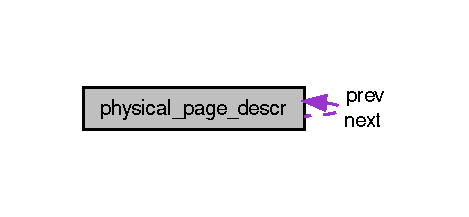
\includegraphics[width=225pt]{structphysical__page__descr__coll__graph}
\end{center}
\end{figure}
\subsection*{Champs de données}
\begin{DoxyCompactItemize}
\item 
\hyperlink{types_8h_a9f047c1f0917f6184a7a013d4b4277a6}{paddr\-\_\-t} \hyperlink{structphysical__page__descr_a8694fbd6da044ec77732927bd905e128}{addr}
\item 
struct \hyperlink{structphysical__page__descr}{physical\-\_\-page\-\_\-descr} $\ast$ \hyperlink{structphysical__page__descr_ab5fc54ca3d91062fbadb940f9c0a5495}{next}
\item 
struct \hyperlink{structphysical__page__descr}{physical\-\_\-page\-\_\-descr} $\ast$ \hyperlink{structphysical__page__descr_acecbcc1b0a68569fea25aa968528b30e}{prev}
\end{DoxyCompactItemize}


\subsection{Description détaillée}
Descripteur de page physique. Contient juste l'adresse physique de la zone mémoire et des pointeurs vers les pages suivantes et précédentes. 

\subsection{Documentation des champs}
\hypertarget{structphysical__page__descr_a8694fbd6da044ec77732927bd905e128}{\index{physical\-\_\-page\-\_\-descr@{physical\-\_\-page\-\_\-descr}!addr@{addr}}
\index{addr@{addr}!physical_page_descr@{physical\-\_\-page\-\_\-descr}}
\subsubsection[{addr}]{\setlength{\rightskip}{0pt plus 5cm}{\bf paddr\-\_\-t} physical\-\_\-page\-\_\-descr\-::addr}}\label{structphysical__page__descr_a8694fbd6da044ec77732927bd905e128}
L'adresse physique de la zone mémoire. \hypertarget{structphysical__page__descr_ab5fc54ca3d91062fbadb940f9c0a5495}{\index{physical\-\_\-page\-\_\-descr@{physical\-\_\-page\-\_\-descr}!next@{next}}
\index{next@{next}!physical_page_descr@{physical\-\_\-page\-\_\-descr}}
\subsubsection[{next}]{\setlength{\rightskip}{0pt plus 5cm}struct {\bf physical\-\_\-page\-\_\-descr}$\ast$ physical\-\_\-page\-\_\-descr\-::next}}\label{structphysical__page__descr_ab5fc54ca3d91062fbadb940f9c0a5495}
Pointeur sur le descripteur suivant. \hypertarget{structphysical__page__descr_acecbcc1b0a68569fea25aa968528b30e}{\index{physical\-\_\-page\-\_\-descr@{physical\-\_\-page\-\_\-descr}!prev@{prev}}
\index{prev@{prev}!physical_page_descr@{physical\-\_\-page\-\_\-descr}}
\subsubsection[{prev}]{\setlength{\rightskip}{0pt plus 5cm}struct {\bf physical\-\_\-page\-\_\-descr}$\ast$ physical\-\_\-page\-\_\-descr\-::prev}}\label{structphysical__page__descr_acecbcc1b0a68569fea25aa968528b30e}
Pointeur sur le descripteur précédent. 

La documentation de cette structure a été générée à partir du fichier suivant \-:\begin{DoxyCompactItemize}
\item 
kernel/include/\hyperlink{memory_8h}{memory.\-h}\end{DoxyCompactItemize}

\hypertarget{structprocess}{\section{Référence de la structure process}
\label{structprocess}\index{process@{process}}
}


Structure représentant un processus.  




{\ttfamily \#include $<$kprocess.\+h$>$}



Graphe de collaboration de process\+:
\nopagebreak
\begin{figure}[H]
\begin{center}
\leavevmode
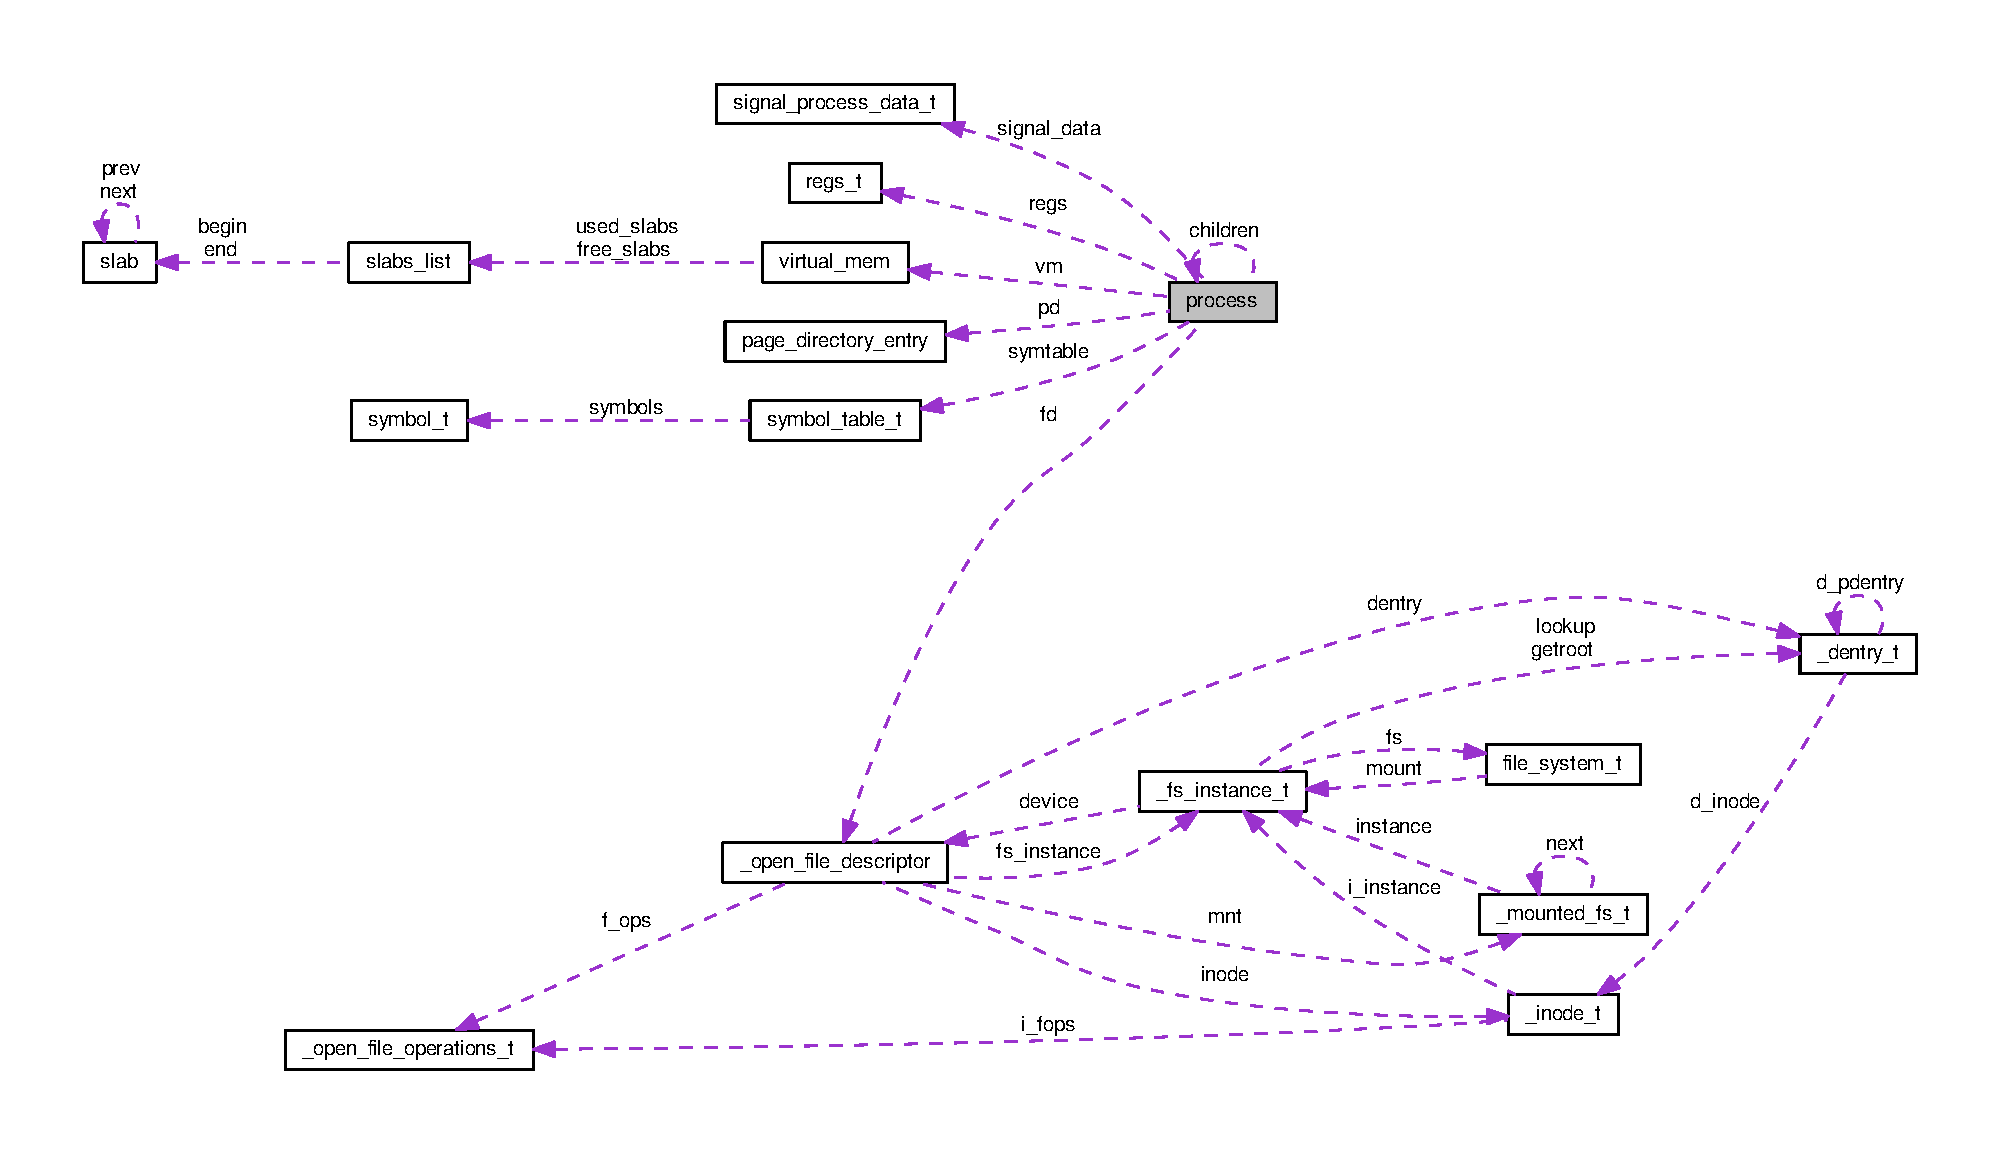
\includegraphics[width=350pt]{structprocess__coll__graph}
\end{center}
\end{figure}
\subsection*{Champs de données}
\begin{DoxyCompactItemize}
\item 
\hyperlink{kernel_2include_2types_8h_adf4d876453337156dde61095e1f20223}{uint16\+\_\+t} \hyperlink{structprocess_a5f455d8121a78f8050bf669326fbe731}{pid}
\item 
\hyperlink{kernel_2include_2types_8h_adf4d876453337156dde61095e1f20223}{uint16\+\_\+t} \hyperlink{structprocess_a75c12130e8e78afe9d8fc94a6f59f9ba}{ppid}
\item 
char $\ast$ \hyperlink{structprocess_ab00affa63607d02095f147da6f1c0983}{name}
\item 
\hyperlink{kernel_2include_2types_8h_aba7bc1797add20fe3efdf37ced1182c5}{uint8\+\_\+t} \hyperlink{structprocess_adceb5d278a54b128096a76c8405f27d5}{state}
\item 
\hypertarget{structprocess_a23f09ce6092f55f1831ccdf783e4c918}{long int {\bfseries user\+\_\+time}}\label{structprocess_a23f09ce6092f55f1831ccdf783e4c918}

\item 
\hypertarget{structprocess_a4d3b0c1b6ca8af26f8894c6f2de4a0dd}{long int {\bfseries sys\+\_\+time}}\label{structprocess_a4d3b0c1b6ca8af26f8894c6f2de4a0dd}

\item 
\hypertarget{structprocess_a1b45bc782bdb0e3d224bdc5b2a5e71e5}{int {\bfseries current\+\_\+sample}}\label{structprocess_a1b45bc782bdb0e3d224bdc5b2a5e71e5}

\item 
\hypertarget{structprocess_a2fbbc34d98fc7e76fff32d7e3c26f403}{int {\bfseries last\+\_\+sample}}\label{structprocess_a2fbbc34d98fc7e76fff32d7e3c26f403}

\item 
\hypertarget{structprocess_a4120a716f24023eb6cef4cceaa6c00c6}{\hyperlink{structregs__t}{regs\+\_\+t} {\bfseries regs}}\label{structprocess_a4120a716f24023eb6cef4cceaa6c00c6}

\item 
\hypertarget{structprocess_aece5b08bde0f923df93524036cf4e341}{\hyperlink{fd__types_8h_a42bccb9b6a816213613cefffced245f0}{open\+\_\+file\+\_\+descriptor} $\ast$ {\bfseries fd} \mbox{[}\hyperlink{fd__types_8h_aa188a2e288c10a684622814c51337465}{F\+O\+P\+E\+N\+\_\+\+M\+A\+X}\mbox{]}}\label{structprocess_aece5b08bde0f923df93524036cf4e341}

\item 
\hypertarget{structprocess_abcbf7a270377aa5b48eb721846fb1c7e}{struct \hyperlink{structpage__directory__entry}{page\+\_\+directory\+\_\+entry} $\ast$ {\bfseries pd}}\label{structprocess_abcbf7a270377aa5b48eb721846fb1c7e}

\item 
\hypertarget{structprocess_a24ef7b4ac4d8fb179021edafc01382e2}{struct \hyperlink{structvirtual__mem}{virtual\+\_\+mem} $\ast$ {\bfseries vm}}\label{structprocess_a24ef7b4ac4d8fb179021edafc01382e2}

\item 
\hypertarget{structprocess_aa0b756ca0430888550293be06072ff81}{\hyperlink{structsignal__process__data__t}{signal\+\_\+process\+\_\+data\+\_\+t} {\bfseries signal\+\_\+data}}\label{structprocess_aa0b756ca0430888550293be06072ff81}

\item 
char $\ast$ \hyperlink{structprocess_ac44ae9d0fbc98179b8f89bf666580086}{ctrl\+\_\+tty}
\item 
\hypertarget{structprocess_aa0d0b60e2eb7539ac10277bbe5fed4ff}{\hyperlink{structsymbol__table__t}{symbol\+\_\+table\+\_\+t} $\ast$ {\bfseries symtable}}\label{structprocess_aa0d0b60e2eb7539ac10277bbe5fed4ff}

\item 
int \hyperlink{structprocess_ac41b1192ed3707ececd1b3d5a8030e07}{sem\+\_\+wait}
\item 
int \hyperlink{structprocess_af6d26a303bcfd1d6fb8249b26aa1b8a8}{sem\+\_\+wait\+\_\+child}
\item 
int \hyperlink{structprocess_a3c7e75af24b759fca4705883fd3bc68a}{nb\+\_\+children}
\item 
\hypertarget{structprocess_abbe1ee17bb932b72a9c3f1aaf4475d42}{struct \hyperlink{structprocess}{process} $\ast$ {\bfseries children} \mbox{[}\hyperlink{kprocess_8h_a63e32d00bc48471b4db49d481ac228dc}{M\+A\+X\+\_\+\+P\+R\+O\+C}\mbox{]}}\label{structprocess_abbe1ee17bb932b72a9c3f1aaf4475d42}

\end{DoxyCompactItemize}


\subsection{Documentation des champs}
\hypertarget{structprocess_ac44ae9d0fbc98179b8f89bf666580086}{\index{process@{process}!ctrl\+\_\+tty@{ctrl\+\_\+tty}}
\index{ctrl\+\_\+tty@{ctrl\+\_\+tty}!process@{process}}
\subsubsection[{ctrl\+\_\+tty}]{\setlength{\rightskip}{0pt plus 5cm}char$\ast$ process\+::ctrl\+\_\+tty}}\label{structprocess_ac44ae9d0fbc98179b8f89bf666580086}
Controlling tty. \hypertarget{structprocess_ab00affa63607d02095f147da6f1c0983}{\index{process@{process}!name@{name}}
\index{name@{name}!process@{process}}
\subsubsection[{name}]{\setlength{\rightskip}{0pt plus 5cm}char$\ast$ process\+::name}}\label{structprocess_ab00affa63607d02095f147da6f1c0983}
Nom du processus. \hypertarget{structprocess_a3c7e75af24b759fca4705883fd3bc68a}{\index{process@{process}!nb\+\_\+children@{nb\+\_\+children}}
\index{nb\+\_\+children@{nb\+\_\+children}!process@{process}}
\subsubsection[{nb\+\_\+children}]{\setlength{\rightskip}{0pt plus 5cm}int process\+::nb\+\_\+children}}\label{structprocess_a3c7e75af24b759fca4705883fd3bc68a}
Liste des fils \hypertarget{structprocess_a5f455d8121a78f8050bf669326fbe731}{\index{process@{process}!pid@{pid}}
\index{pid@{pid}!process@{process}}
\subsubsection[{pid}]{\setlength{\rightskip}{0pt plus 5cm}{\bf uint16\+\_\+t} process\+::pid}}\label{structprocess_a5f455d8121a78f8050bf669326fbe731}
Process I\+D \hypertarget{structprocess_a75c12130e8e78afe9d8fc94a6f59f9ba}{\index{process@{process}!ppid@{ppid}}
\index{ppid@{ppid}!process@{process}}
\subsubsection[{ppid}]{\setlength{\rightskip}{0pt plus 5cm}{\bf uint16\+\_\+t} process\+::ppid}}\label{structprocess_a75c12130e8e78afe9d8fc94a6f59f9ba}
Parent process I\+D \hypertarget{structprocess_ac41b1192ed3707ececd1b3d5a8030e07}{\index{process@{process}!sem\+\_\+wait@{sem\+\_\+wait}}
\index{sem\+\_\+wait@{sem\+\_\+wait}!process@{process}}
\subsubsection[{sem\+\_\+wait}]{\setlength{\rightskip}{0pt plus 5cm}int process\+::sem\+\_\+wait}}\label{structprocess_ac41b1192ed3707ececd1b3d5a8030e07}
Sémaphore initialisé à 0 et qui est pris par les processus en attente de la fin de ce process. \hypertarget{structprocess_af6d26a303bcfd1d6fb8249b26aa1b8a8}{\index{process@{process}!sem\+\_\+wait\+\_\+child@{sem\+\_\+wait\+\_\+child}}
\index{sem\+\_\+wait\+\_\+child@{sem\+\_\+wait\+\_\+child}!process@{process}}
\subsubsection[{sem\+\_\+wait\+\_\+child}]{\setlength{\rightskip}{0pt plus 5cm}int process\+::sem\+\_\+wait\+\_\+child}}\label{structprocess_af6d26a303bcfd1d6fb8249b26aa1b8a8}
Sémaphore qui passe à 1 lorsqu'un fils se termine. \hypertarget{structprocess_adceb5d278a54b128096a76c8405f27d5}{\index{process@{process}!state@{state}}
\index{state@{state}!process@{process}}
\subsubsection[{state}]{\setlength{\rightskip}{0pt plus 5cm}{\bf uint8\+\_\+t} process\+::state}}\label{structprocess_adceb5d278a54b128096a76c8405f27d5}
Etat du processus (idle, running, waiting...) 

La documentation de cette structure a été générée à partir du fichier suivant \+:\begin{DoxyCompactItemize}
\item 
kernel/include/\hyperlink{kprocess_8h}{kprocess.\+h}\end{DoxyCompactItemize}

\hypertarget{structprocess__init__data__t}{\section{Référence de la structure process\+\_\+init\+\_\+data\+\_\+t}
\label{structprocess__init__data__t}\index{process\+\_\+init\+\_\+data\+\_\+t@{process\+\_\+init\+\_\+data\+\_\+t}}
}


{\ttfamily \#include $<$kprocess.\+h$>$}



Graphe de collaboration de process\+\_\+init\+\_\+data\+\_\+t\+:
\nopagebreak
\begin{figure}[H]
\begin{center}
\leavevmode
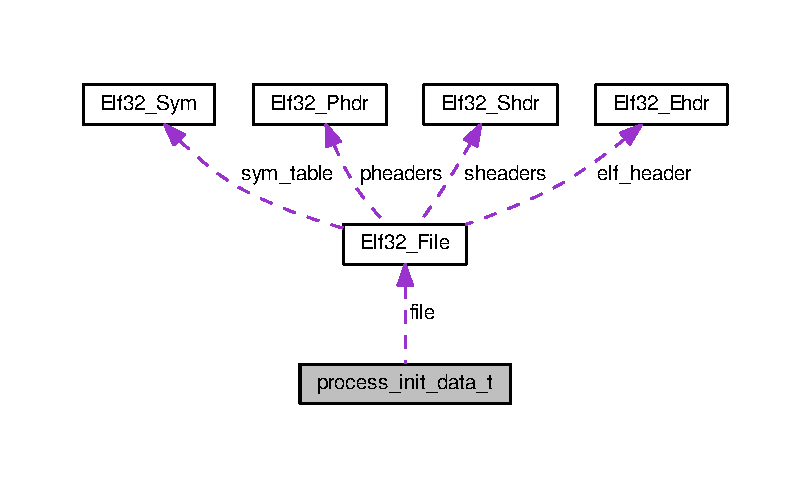
\includegraphics[width=350pt]{structprocess__init__data__t__coll__graph}
\end{center}
\end{figure}
\subsection*{Champs de données}
\begin{DoxyCompactItemize}
\item 
char $\ast$ \hyperlink{structprocess__init__data__t_a6bdcab0bceaafa6e65a236904fb5a157}{name}
\item 
char $\ast$ \hyperlink{structprocess__init__data__t_a16d011771835f06e0bb3d5fd6115e13c}{args}
\item 
char $\ast$$\ast$ \hyperlink{structprocess__init__data__t_a863d82fbd718f53164a520f67376eac2}{envp}
\item 
int \hyperlink{structprocess__init__data__t_a1cda790f7d2446a04562094f09e358ab}{exec\+\_\+type}
\item 
void $\ast$ \hyperlink{structprocess__init__data__t_ae950cc2a2cc04d1c00a71f70c2fde72c}{data}
\item 
\hypertarget{structprocess__init__data__t_a423d726f5e4621a1aae6a6d96ed2c380}{\hyperlink{structElf32__File}{Elf32\+\_\+\+File} $\ast$ {\bfseries file}}\label{structprocess__init__data__t_a423d726f5e4621a1aae6a6d96ed2c380}

\item 
\hypertarget{structprocess__init__data__t_ae720e802d58d2f1457e34998063695a1}{int {\bfseries mem\+\_\+size}}\label{structprocess__init__data__t_ae720e802d58d2f1457e34998063695a1}

\item 
\hypertarget{structprocess__init__data__t_acf333ed57db9a2ca636801dcbc41da7e}{\hyperlink{kernel_2include_2types_8h_a53428b953a0ae6fba02a5b3596c867e0}{vaddr\+\_\+t} {\bfseries entry\+\_\+point}}\label{structprocess__init__data__t_acf333ed57db9a2ca636801dcbc41da7e}

\item 
\hypertarget{structprocess__init__data__t_a8a9c2d2d0d602f8e2f3dc2f4c425da29}{\hyperlink{kernel_2include_2types_8h_a33594304e786b158f3fb30289278f5af}{uint32\+\_\+t} {\bfseries stack\+\_\+size}}\label{structprocess__init__data__t_a8a9c2d2d0d602f8e2f3dc2f4c425da29}

\item 
\hypertarget{structprocess__init__data__t_a3147915ee1aa09fd84245e28635c60c8}{int {\bfseries priority}}\label{structprocess__init__data__t_a3147915ee1aa09fd84245e28635c60c8}

\item 
\hyperlink{kernel_2include_2types_8h_adf4d876453337156dde61095e1f20223}{uint16\+\_\+t} \hyperlink{structprocess__init__data__t_a34f85f3f56546700b1dc942070944e27}{ppid}
\end{DoxyCompactItemize}


\subsection{Description détaillée}
Structure à passer au noyau pour créer un nouveau processus 

\subsection{Documentation des champs}
\hypertarget{structprocess__init__data__t_a16d011771835f06e0bb3d5fd6115e13c}{\index{process\+\_\+init\+\_\+data\+\_\+t@{process\+\_\+init\+\_\+data\+\_\+t}!args@{args}}
\index{args@{args}!process\+\_\+init\+\_\+data\+\_\+t@{process\+\_\+init\+\_\+data\+\_\+t}}
\subsubsection[{args}]{\setlength{\rightskip}{0pt plus 5cm}char$\ast$ process\+\_\+init\+\_\+data\+\_\+t\+::args}}\label{structprocess__init__data__t_a16d011771835f06e0bb3d5fd6115e13c}
Ses arguments. \hypertarget{structprocess__init__data__t_ae950cc2a2cc04d1c00a71f70c2fde72c}{\index{process\+\_\+init\+\_\+data\+\_\+t@{process\+\_\+init\+\_\+data\+\_\+t}!data@{data}}
\index{data@{data}!process\+\_\+init\+\_\+data\+\_\+t@{process\+\_\+init\+\_\+data\+\_\+t}}
\subsubsection[{data}]{\setlength{\rightskip}{0pt plus 5cm}void$\ast$ process\+\_\+init\+\_\+data\+\_\+t\+::data}}\label{structprocess__init__data__t_ae950cc2a2cc04d1c00a71f70c2fde72c}
Usage variable \hypertarget{structprocess__init__data__t_a863d82fbd718f53164a520f67376eac2}{\index{process\+\_\+init\+\_\+data\+\_\+t@{process\+\_\+init\+\_\+data\+\_\+t}!envp@{envp}}
\index{envp@{envp}!process\+\_\+init\+\_\+data\+\_\+t@{process\+\_\+init\+\_\+data\+\_\+t}}
\subsubsection[{envp}]{\setlength{\rightskip}{0pt plus 5cm}char$\ast$$\ast$ process\+\_\+init\+\_\+data\+\_\+t\+::envp}}\label{structprocess__init__data__t_a863d82fbd718f53164a520f67376eac2}
Ses variables d'environnement. \hypertarget{structprocess__init__data__t_a1cda790f7d2446a04562094f09e358ab}{\index{process\+\_\+init\+\_\+data\+\_\+t@{process\+\_\+init\+\_\+data\+\_\+t}!exec\+\_\+type@{exec\+\_\+type}}
\index{exec\+\_\+type@{exec\+\_\+type}!process\+\_\+init\+\_\+data\+\_\+t@{process\+\_\+init\+\_\+data\+\_\+t}}
\subsubsection[{exec\+\_\+type}]{\setlength{\rightskip}{0pt plus 5cm}int process\+\_\+init\+\_\+data\+\_\+t\+::exec\+\_\+type}}\label{structprocess__init__data__t_a1cda790f7d2446a04562094f09e358ab}
Type d'exécution \hypertarget{structprocess__init__data__t_a6bdcab0bceaafa6e65a236904fb5a157}{\index{process\+\_\+init\+\_\+data\+\_\+t@{process\+\_\+init\+\_\+data\+\_\+t}!name@{name}}
\index{name@{name}!process\+\_\+init\+\_\+data\+\_\+t@{process\+\_\+init\+\_\+data\+\_\+t}}
\subsubsection[{name}]{\setlength{\rightskip}{0pt plus 5cm}char$\ast$ process\+\_\+init\+\_\+data\+\_\+t\+::name}}\label{structprocess__init__data__t_a6bdcab0bceaafa6e65a236904fb5a157}
Nom du processus. \hypertarget{structprocess__init__data__t_a34f85f3f56546700b1dc942070944e27}{\index{process\+\_\+init\+\_\+data\+\_\+t@{process\+\_\+init\+\_\+data\+\_\+t}!ppid@{ppid}}
\index{ppid@{ppid}!process\+\_\+init\+\_\+data\+\_\+t@{process\+\_\+init\+\_\+data\+\_\+t}}
\subsubsection[{ppid}]{\setlength{\rightskip}{0pt plus 5cm}{\bf uint16\+\_\+t} process\+\_\+init\+\_\+data\+\_\+t\+::ppid}}\label{structprocess__init__data__t_a34f85f3f56546700b1dc942070944e27}
Parent process I\+D 

La documentation de cette structure a été générée à partir du fichier suivant \+:\begin{DoxyCompactItemize}
\item 
kernel/include/\hyperlink{kprocess_8h}{kprocess.\+h}\end{DoxyCompactItemize}

\hypertarget{structprocfs__directory__function__t}{\section{Référence de la structure procfs\-\_\-directory\-\_\-function\-\_\-t}
\label{structprocfs__directory__function__t}\index{procfs\-\_\-directory\-\_\-function\-\_\-t@{procfs\-\_\-directory\-\_\-function\-\_\-t}}
}
\subsection*{Champs de données}
\begin{DoxyCompactItemize}
\item 
\hypertarget{structprocfs__directory__function__t_aab12154db78dab711a490ea2aefcbcfc}{char $\ast$ {\bfseries name}}\label{structprocfs__directory__function__t_aab12154db78dab711a490ea2aefcbcfc}

\item 
\hypertarget{structprocfs__directory__function__t_a81faf40e3e099de440c889f812aae0ed}{\hyperlink{types_8h_a29d85914ddff32967d85ada69854206d}{size\-\_\-t} {\bfseries name\-\_\-length}}\label{structprocfs__directory__function__t_a81faf40e3e099de440c889f812aae0ed}

\item 
\hypertarget{structprocfs__directory__function__t_a23bf4c4a71eaeaa4101bdbdf29a3ea3b}{lookup\-\_\-function\-\_\-t $\ast$ {\bfseries lookup}}\label{structprocfs__directory__function__t_a23bf4c4a71eaeaa4101bdbdf29a3ea3b}

\item 
\hypertarget{structprocfs__directory__function__t_a5aef6654b44e12b3b5da28307846c8e7}{procfs\-\_\-read\-\_\-dir\-\_\-function\-\_\-t $\ast$ {\bfseries readdir}}\label{structprocfs__directory__function__t_a5aef6654b44e12b3b5da28307846c8e7}

\item 
\hypertarget{structprocfs__directory__function__t_a7fa43921298eef344a9a92d98cfe5d7b}{\hyperlink{types_8h_a29d85914ddff32967d85ada69854206d}{size\-\_\-t} {\bfseries inode\-\_\-offset}}\label{structprocfs__directory__function__t_a7fa43921298eef344a9a92d98cfe5d7b}

\end{DoxyCompactItemize}


\subsection{Description détaillée}
List of directories in the process directory 

La documentation de cette structure a été générée à partir du fichier suivant \-:\begin{DoxyCompactItemize}
\item 
kernel/fs/\hyperlink{procfs_8c}{procfs.\-c}\end{DoxyCompactItemize}

\hypertarget{structprocfs__file__function__t}{\section{Référence de la structure procfs\+\_\+file\+\_\+function\+\_\+t}
\label{structprocfs__file__function__t}\index{procfs\+\_\+file\+\_\+function\+\_\+t@{procfs\+\_\+file\+\_\+function\+\_\+t}}
}
\subsection*{Champs de données}
\begin{DoxyCompactItemize}
\item 
\hypertarget{structprocfs__file__function__t_a9a6b52b40022a33f51c9b6e305d40d29}{char $\ast$ {\bfseries name}}\label{structprocfs__file__function__t_a9a6b52b40022a33f51c9b6e305d40d29}

\item 
\hypertarget{structprocfs__file__function__t_afdbef0b4aab706e3e0a5f1deea31b947}{\hyperlink{kernel_2include_2types_8h_a29d85914ddff32967d85ada69854206d}{size\+\_\+t} {\bfseries name\+\_\+length}}\label{structprocfs__file__function__t_afdbef0b4aab706e3e0a5f1deea31b947}

\item 
\hypertarget{structprocfs__file__function__t_a768351fe0eeb4b220aaaa5c98f1c8862}{\hyperlink{kernel_2include_2types_8h_af629ed855824cf5955b54529adf78ad6}{ssize\+\_\+t}($\ast$ {\bfseries read} )(\hyperlink{fd__types_8h_a42bccb9b6a816213613cefffced245f0}{open\+\_\+file\+\_\+descriptor} $\ast$, void $\ast$, \hyperlink{kernel_2include_2types_8h_a29d85914ddff32967d85ada69854206d}{size\+\_\+t})}\label{structprocfs__file__function__t_a768351fe0eeb4b220aaaa5c98f1c8862}

\item 
\hypertarget{structprocfs__file__function__t_a93a76c1bfc7d7c66104db68e64bf856d}{\hyperlink{kernel_2include_2types_8h_a29d85914ddff32967d85ada69854206d}{size\+\_\+t} {\bfseries inode\+\_\+offset}}\label{structprocfs__file__function__t_a93a76c1bfc7d7c66104db68e64bf856d}

\end{DoxyCompactItemize}


\subsection{Description détaillée}
List of files in a process directory 

La documentation de cette structure a été générée à partir du fichier suivant \+:\begin{DoxyCompactItemize}
\item 
kernel/fs/\hyperlink{procfs_8c}{procfs.\+c}\end{DoxyCompactItemize}

\hypertarget{structregs__t}{\section{Référence de la structure regs\-\_\-t}
\label{structregs__t}\index{regs\-\_\-t@{regs\-\_\-t}}
}
\subsection*{Champs de données}
\begin{DoxyCompactItemize}
\item 
\hypertarget{structregs__t_aa9a75f4eda54de076eda1660651b769f}{\hyperlink{kernel_2include_2types_8h_a33594304e786b158f3fb30289278f5af}{uint32\-\_\-t} {\bfseries eax}}\label{structregs__t_aa9a75f4eda54de076eda1660651b769f}

\item 
\hypertarget{structregs__t_a676d960cd440fd0f20db7eb63a1c19d3}{\hyperlink{kernel_2include_2types_8h_a33594304e786b158f3fb30289278f5af}{uint32\-\_\-t} {\bfseries ecx}}\label{structregs__t_a676d960cd440fd0f20db7eb63a1c19d3}

\item 
\hypertarget{structregs__t_a4a66fee02bbade605198a3b50bb1fdb5}{\hyperlink{kernel_2include_2types_8h_a33594304e786b158f3fb30289278f5af}{uint32\-\_\-t} {\bfseries edx}}\label{structregs__t_a4a66fee02bbade605198a3b50bb1fdb5}

\item 
\hypertarget{structregs__t_a61356855d8ea23d8dbff17de7c25aae4}{\hyperlink{kernel_2include_2types_8h_a33594304e786b158f3fb30289278f5af}{uint32\-\_\-t} {\bfseries ebx}}\label{structregs__t_a61356855d8ea23d8dbff17de7c25aae4}

\item 
\hypertarget{structregs__t_ad8c205a88fa796d24c4bb6f38cc61c19}{\hyperlink{kernel_2include_2types_8h_a33594304e786b158f3fb30289278f5af}{uint32\-\_\-t} {\bfseries esp}}\label{structregs__t_ad8c205a88fa796d24c4bb6f38cc61c19}

\item 
\hypertarget{structregs__t_a39ba25914a655f8ef14c82f1b5a3d052}{\hyperlink{kernel_2include_2types_8h_a33594304e786b158f3fb30289278f5af}{uint32\-\_\-t} {\bfseries kesp}}\label{structregs__t_a39ba25914a655f8ef14c82f1b5a3d052}

\item 
\hypertarget{structregs__t_a29681e15e92ec0a53c03b64599ba40b4}{\hyperlink{kernel_2include_2types_8h_a33594304e786b158f3fb30289278f5af}{uint32\-\_\-t} {\bfseries ebp}}\label{structregs__t_a29681e15e92ec0a53c03b64599ba40b4}

\item 
\hypertarget{structregs__t_a87d05b726eb88347c61c93c05d7e5f20}{\hyperlink{kernel_2include_2types_8h_a33594304e786b158f3fb30289278f5af}{uint32\-\_\-t} {\bfseries esi}}\label{structregs__t_a87d05b726eb88347c61c93c05d7e5f20}

\item 
\hypertarget{structregs__t_a54283215bba7c24d8b984b9961b12ea6}{\hyperlink{kernel_2include_2types_8h_a33594304e786b158f3fb30289278f5af}{uint32\-\_\-t} {\bfseries edi}}\label{structregs__t_a54283215bba7c24d8b984b9961b12ea6}

\item 
\hypertarget{structregs__t_ad2b525445e863b90e10d104fca7dce7f}{\hyperlink{kernel_2include_2types_8h_a33594304e786b158f3fb30289278f5af}{uint32\-\_\-t} {\bfseries eip}}\label{structregs__t_ad2b525445e863b90e10d104fca7dce7f}

\item 
\hypertarget{structregs__t_abb985c31280a7369af05727826757162}{\hyperlink{kernel_2include_2types_8h_a33594304e786b158f3fb30289278f5af}{uint32\-\_\-t} {\bfseries eflags}}\label{structregs__t_abb985c31280a7369af05727826757162}

\item 
\hypertarget{structregs__t_ad9638094108f9ee07580520bde785880}{\hyperlink{kernel_2include_2types_8h_adf4d876453337156dde61095e1f20223}{uint16\-\_\-t} {\bfseries cs}}\label{structregs__t_ad9638094108f9ee07580520bde785880}

\item 
\hypertarget{structregs__t_a27f5b8d7adaee8b4afb50124668854dc}{\hyperlink{kernel_2include_2types_8h_adf4d876453337156dde61095e1f20223}{uint16\-\_\-t} {\bfseries ss}}\label{structregs__t_a27f5b8d7adaee8b4afb50124668854dc}

\item 
\hypertarget{structregs__t_a7a03c78d2a9226595709890f6fbd1563}{\hyperlink{kernel_2include_2types_8h_adf4d876453337156dde61095e1f20223}{uint16\-\_\-t} {\bfseries kss}}\label{structregs__t_a7a03c78d2a9226595709890f6fbd1563}

\item 
\hypertarget{structregs__t_ae17fba0cf62794a2ad5a55822b4dd804}{\hyperlink{kernel_2include_2types_8h_adf4d876453337156dde61095e1f20223}{uint16\-\_\-t} {\bfseries ds}}\label{structregs__t_ae17fba0cf62794a2ad5a55822b4dd804}

\item 
\hypertarget{structregs__t_a5e96ab9b17341c483bb79f5e58812253}{\hyperlink{kernel_2include_2types_8h_adf4d876453337156dde61095e1f20223}{uint16\-\_\-t} {\bfseries es}}\label{structregs__t_a5e96ab9b17341c483bb79f5e58812253}

\item 
\hypertarget{structregs__t_a432e4f8c807f2ee5648e88f036472ca4}{\hyperlink{kernel_2include_2types_8h_adf4d876453337156dde61095e1f20223}{uint16\-\_\-t} {\bfseries fs}}\label{structregs__t_a432e4f8c807f2ee5648e88f036472ca4}

\item 
\hypertarget{structregs__t_a84142375068607098ad8612142d03376}{\hyperlink{kernel_2include_2types_8h_adf4d876453337156dde61095e1f20223}{uint16\-\_\-t} {\bfseries gs}}\label{structregs__t_a84142375068607098ad8612142d03376}

\item 
\hypertarget{structregs__t_afb9b19b3dfa071670a4aa76dc910548e}{\hyperlink{kernel_2include_2types_8h_a33594304e786b158f3fb30289278f5af}{uint32\-\_\-t} {\bfseries cr3}}\label{structregs__t_afb9b19b3dfa071670a4aa76dc910548e}

\end{DoxyCompactItemize}


La documentation de cette structure a été générée à partir du fichier suivant \-:\begin{DoxyCompactItemize}
\item 
kernel/include/\hyperlink{process__types_8h}{process\-\_\-types.\-h}\end{DoxyCompactItemize}

\hypertarget{structscheduler__descriptor__t}{\section{Référence de la structure scheduler\+\_\+descriptor\+\_\+t}
\label{structscheduler__descriptor__t}\index{scheduler\+\_\+descriptor\+\_\+t@{scheduler\+\_\+descriptor\+\_\+t}}
}


{\ttfamily \#include $<$scheduler.\+h$>$}



Graphe de collaboration de scheduler\+\_\+descriptor\+\_\+t\+:
\nopagebreak
\begin{figure}[H]
\begin{center}
\leavevmode
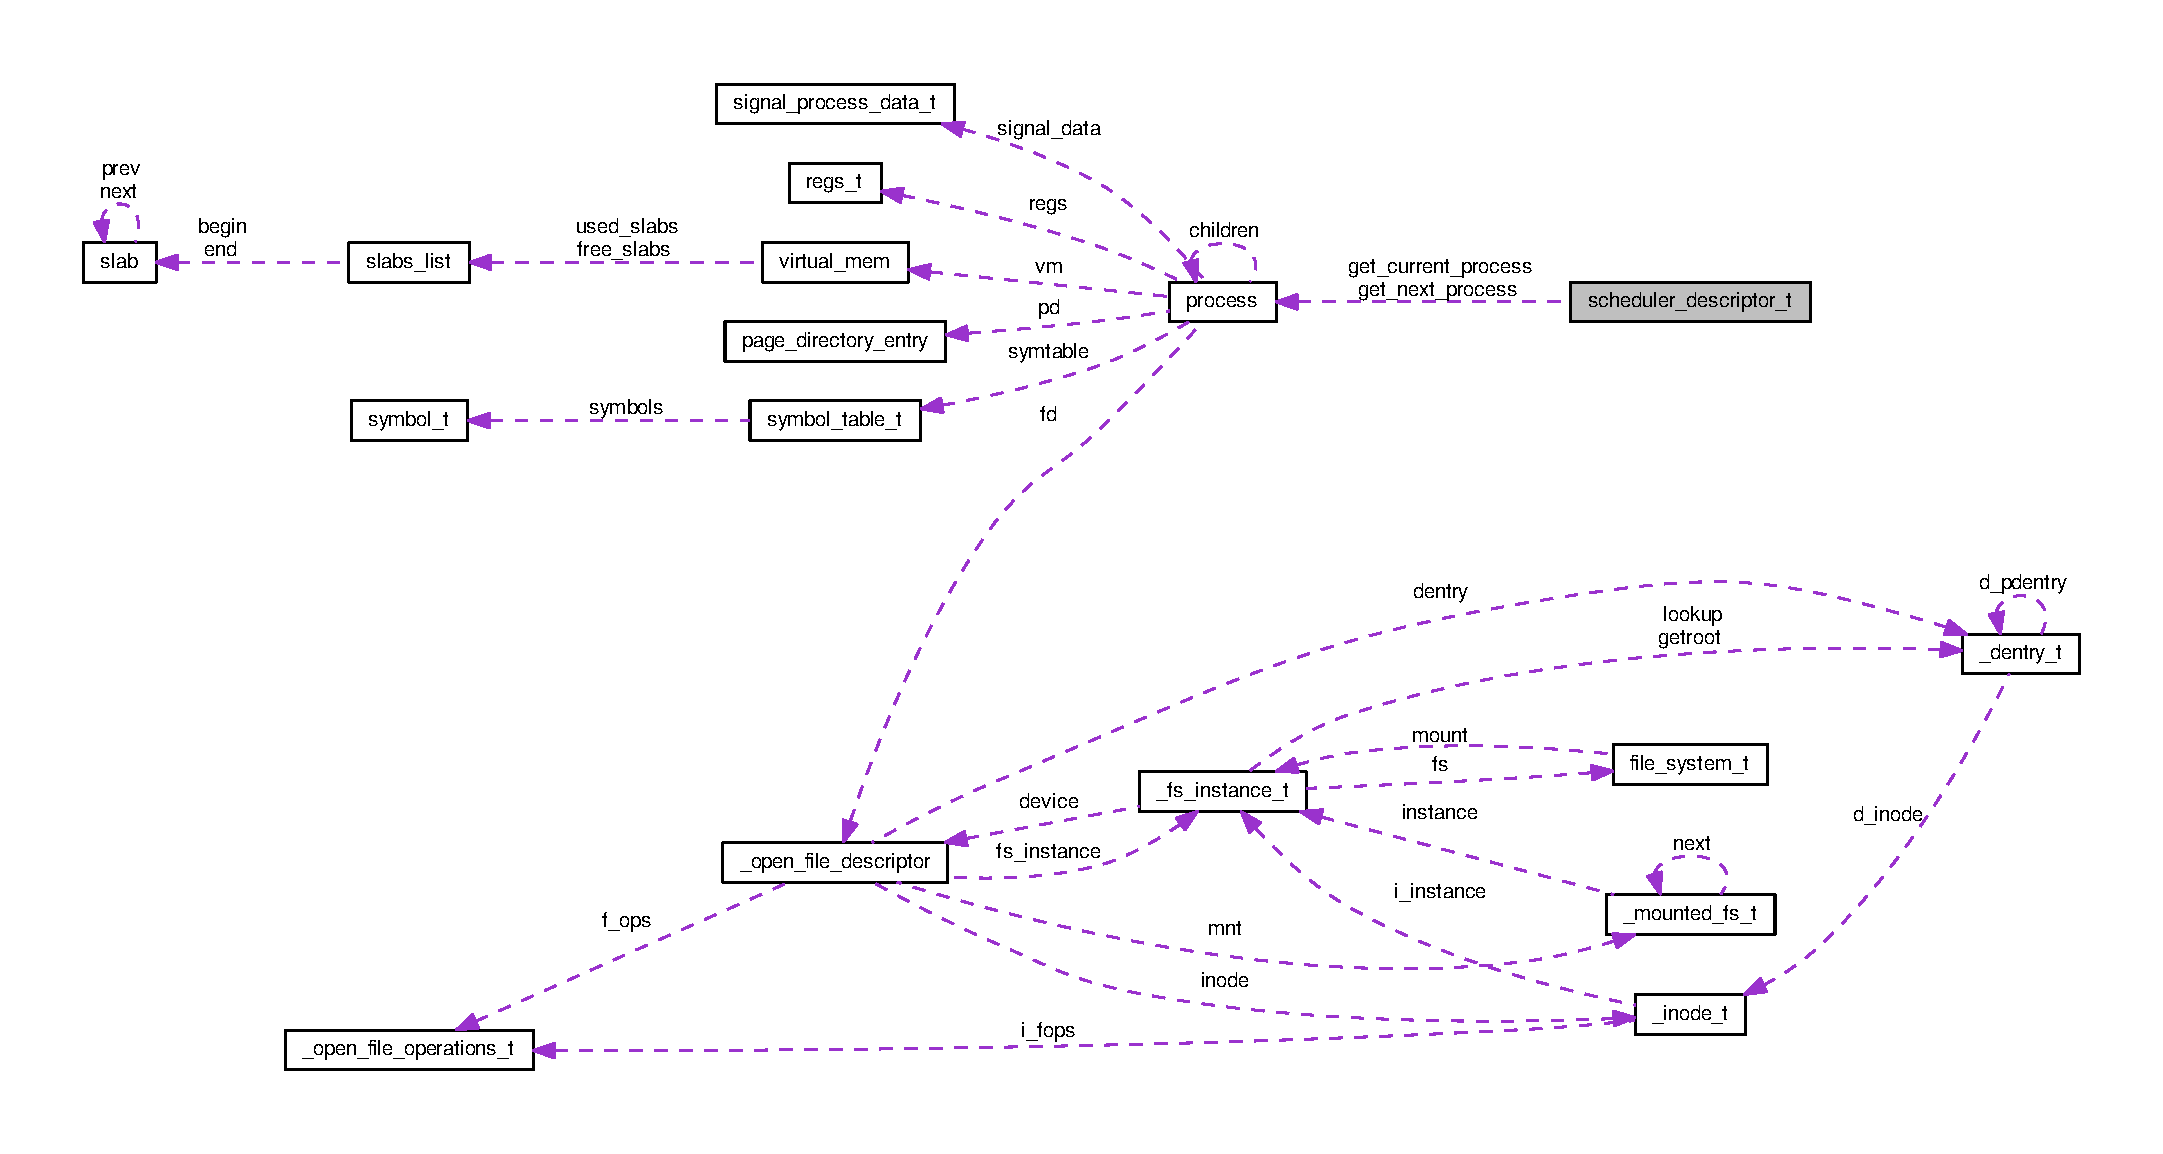
\includegraphics[width=350pt]{structscheduler__descriptor__t__coll__graph}
\end{center}
\end{figure}
\subsection*{Champs de données}
\begin{DoxyCompactItemize}
\item 
\hypertarget{structscheduler__descriptor__t_afced959947154805968548b106fe322b}{char $\ast$ {\bfseries name}}\label{structscheduler__descriptor__t_afced959947154805968548b106fe322b}

\item 
int($\ast$ \hyperlink{structscheduler__descriptor__t_a250bb59b72e7a3828160638033ac5cb3}{initialize} )(int)
\item 
\hyperlink{kprocess_8h_a7742ed3a86b7bcb5a4b76893fc331ede}{process\+\_\+t} $\ast$($\ast$ \hyperlink{structscheduler__descriptor__t_a41661a5080062b563df01dfb1a02e22e}{get\+\_\+next\+\_\+process} )()
\item 
\hyperlink{kprocess_8h_a7742ed3a86b7bcb5a4b76893fc331ede}{process\+\_\+t} $\ast$($\ast$ \hyperlink{structscheduler__descriptor__t_a077b3b95ecf49c9dacc40b6a87cb1008}{get\+\_\+current\+\_\+process} )()
\item 
int($\ast$ \hyperlink{structscheduler__descriptor__t_a8919a05ae907a4b642563078a28e744a}{add\+\_\+process} )(\hyperlink{kprocess_8h_a7742ed3a86b7bcb5a4b76893fc331ede}{process\+\_\+t} $\ast$)
\item 
int($\ast$ \hyperlink{structscheduler__descriptor__t_a656d41ddd8d861d0ee55523de3693dfa}{delete\+\_\+process} )(int)
\item 
\hypertarget{structscheduler__descriptor__t_a147506c1d8e71482bad2a906102d8f30}{void($\ast$ {\bfseries inject\+\_\+idle} )(\hyperlink{kprocess_8h_a7742ed3a86b7bcb5a4b76893fc331ede}{process\+\_\+t} $\ast$)}\label{structscheduler__descriptor__t_a147506c1d8e71482bad2a906102d8f30}

\end{DoxyCompactItemize}


\subsection{Description détaillée}
Cette structure doit contenir les differents pointeurs de fonctions pour manipuler le scheduler 

\subsection{Documentation des champs}
\hypertarget{structscheduler__descriptor__t_a8919a05ae907a4b642563078a28e744a}{\index{scheduler\+\_\+descriptor\+\_\+t@{scheduler\+\_\+descriptor\+\_\+t}!add\+\_\+process@{add\+\_\+process}}
\index{add\+\_\+process@{add\+\_\+process}!scheduler\+\_\+descriptor\+\_\+t@{scheduler\+\_\+descriptor\+\_\+t}}
\subsubsection[{add\+\_\+process}]{\setlength{\rightskip}{0pt plus 5cm}int($\ast$ scheduler\+\_\+descriptor\+\_\+t\+::add\+\_\+process)({\bf process\+\_\+t} $\ast$)}}\label{structscheduler__descriptor__t_a8919a05ae907a4b642563078a28e744a}
Ajouter un processus \hypertarget{structscheduler__descriptor__t_a656d41ddd8d861d0ee55523de3693dfa}{\index{scheduler\+\_\+descriptor\+\_\+t@{scheduler\+\_\+descriptor\+\_\+t}!delete\+\_\+process@{delete\+\_\+process}}
\index{delete\+\_\+process@{delete\+\_\+process}!scheduler\+\_\+descriptor\+\_\+t@{scheduler\+\_\+descriptor\+\_\+t}}
\subsubsection[{delete\+\_\+process}]{\setlength{\rightskip}{0pt plus 5cm}int($\ast$ scheduler\+\_\+descriptor\+\_\+t\+::delete\+\_\+process)(int)}}\label{structscheduler__descriptor__t_a656d41ddd8d861d0ee55523de3693dfa}
Supprimer un processus \hypertarget{structscheduler__descriptor__t_a077b3b95ecf49c9dacc40b6a87cb1008}{\index{scheduler\+\_\+descriptor\+\_\+t@{scheduler\+\_\+descriptor\+\_\+t}!get\+\_\+current\+\_\+process@{get\+\_\+current\+\_\+process}}
\index{get\+\_\+current\+\_\+process@{get\+\_\+current\+\_\+process}!scheduler\+\_\+descriptor\+\_\+t@{scheduler\+\_\+descriptor\+\_\+t}}
\subsubsection[{get\+\_\+current\+\_\+process}]{\setlength{\rightskip}{0pt plus 5cm}{\bf process\+\_\+t}$\ast$($\ast$ scheduler\+\_\+descriptor\+\_\+t\+::get\+\_\+current\+\_\+process)()}}\label{structscheduler__descriptor__t_a077b3b95ecf49c9dacc40b6a87cb1008}
Trouver le processus actuel \hypertarget{structscheduler__descriptor__t_a41661a5080062b563df01dfb1a02e22e}{\index{scheduler\+\_\+descriptor\+\_\+t@{scheduler\+\_\+descriptor\+\_\+t}!get\+\_\+next\+\_\+process@{get\+\_\+next\+\_\+process}}
\index{get\+\_\+next\+\_\+process@{get\+\_\+next\+\_\+process}!scheduler\+\_\+descriptor\+\_\+t@{scheduler\+\_\+descriptor\+\_\+t}}
\subsubsection[{get\+\_\+next\+\_\+process}]{\setlength{\rightskip}{0pt plus 5cm}{\bf process\+\_\+t}$\ast$($\ast$ scheduler\+\_\+descriptor\+\_\+t\+::get\+\_\+next\+\_\+process)()}}\label{structscheduler__descriptor__t_a41661a5080062b563df01dfb1a02e22e}
Trouver le prochain processus selon le scheduler \hypertarget{structscheduler__descriptor__t_a250bb59b72e7a3828160638033ac5cb3}{\index{scheduler\+\_\+descriptor\+\_\+t@{scheduler\+\_\+descriptor\+\_\+t}!initialize@{initialize}}
\index{initialize@{initialize}!scheduler\+\_\+descriptor\+\_\+t@{scheduler\+\_\+descriptor\+\_\+t}}
\subsubsection[{initialize}]{\setlength{\rightskip}{0pt plus 5cm}int($\ast$ scheduler\+\_\+descriptor\+\_\+t\+::initialize)(int)}}\label{structscheduler__descriptor__t_a250bb59b72e7a3828160638033ac5cb3}
Initialisation du scheduler 

La documentation de cette structure a été générée à partir du fichier suivant \+:\begin{DoxyCompactItemize}
\item 
kernel/include/\hyperlink{scheduler_8h}{scheduler.\+h}\end{DoxyCompactItemize}

\hypertarget{structsem__fifo}{\section{Référence de la structure sem\-\_\-fifo}
\label{structsem__fifo}\index{sem\-\_\-fifo@{sem\-\_\-fifo}}
}


Graphe de collaboration de sem\-\_\-fifo\-:\nopagebreak
\begin{figure}[H]
\begin{center}
\leavevmode
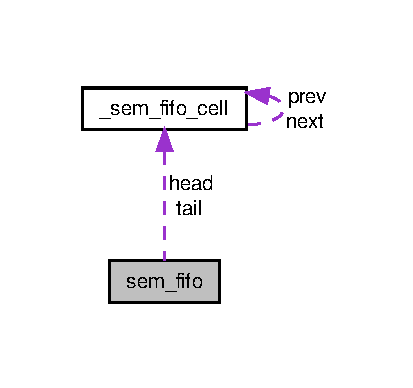
\includegraphics[width=197pt]{structsem__fifo__coll__graph}
\end{center}
\end{figure}
\subsection*{Champs de données}
\begin{DoxyCompactItemize}
\item 
\hypertarget{structsem__fifo_a87aa9648eaaf70640c99d5bd337a5005}{int {\bfseries size}}\label{structsem__fifo_a87aa9648eaaf70640c99d5bd337a5005}

\item 
\hypertarget{structsem__fifo_ae3959d13037800f236e2f1d48e059ae4}{\hyperlink{ksem_8c_a83e90e3f49b0f7bb4385e0759e1491f8}{sem\-\_\-fifo\-\_\-cell} $\ast$ {\bfseries head}}\label{structsem__fifo_ae3959d13037800f236e2f1d48e059ae4}

\item 
\hypertarget{structsem__fifo_ad735386a72240cec2543b4ed1ff8be71}{\hyperlink{ksem_8c_a83e90e3f49b0f7bb4385e0759e1491f8}{sem\-\_\-fifo\-\_\-cell} $\ast$ {\bfseries tail}}\label{structsem__fifo_ad735386a72240cec2543b4ed1ff8be71}

\end{DoxyCompactItemize}


\subsection{Description détaillée}
Structure d'une fifo. 

La documentation de cette structure a été générée à partir du fichier suivant \-:\begin{DoxyCompactItemize}
\item 
kernel/\hyperlink{ksem_8c}{ksem.\-c}\end{DoxyCompactItemize}

\hypertarget{structsem__t}{\section{Référence de la structure sem\-\_\-t}
\label{structsem__t}\index{sem\-\_\-t@{sem\-\_\-t}}
}


Graphe de collaboration de sem\-\_\-t\-:\nopagebreak
\begin{figure}[H]
\begin{center}
\leavevmode
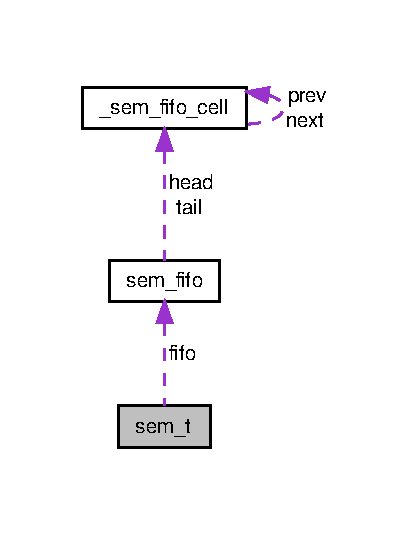
\includegraphics[width=197pt]{structsem__t__coll__graph}
\end{center}
\end{figure}
\subsection*{Champs de données}
\begin{DoxyCompactItemize}
\item 
\hypertarget{structsem__t_afa75e02b9ca4c4e10295da9b851c3691}{int {\bfseries value}}\label{structsem__t_afa75e02b9ca4c4e10295da9b851c3691}

\item 
\hypertarget{structsem__t_a184fb80dbf1336465c8365cad7cb1a7b}{\hyperlink{types_8h_aba7bc1797add20fe3efdf37ced1182c5}{uint8\-\_\-t} {\bfseries allocated}}\label{structsem__t_a184fb80dbf1336465c8365cad7cb1a7b}

\item 
\hypertarget{structsem__t_a9541ce13a898d1919cde5b67d5cdcbce}{\hyperlink{structsem__fifo}{sem\-\_\-fifo} {\bfseries fifo}}\label{structsem__t_a9541ce13a898d1919cde5b67d5cdcbce}

\end{DoxyCompactItemize}


\subsection{Description détaillée}
Structure définissant une sémaphore. 

La documentation de cette structure a été générée à partir du fichier suivant \-:\begin{DoxyCompactItemize}
\item 
kernel/\hyperlink{ksem_8c}{ksem.\-c}\end{DoxyCompactItemize}

\hypertarget{structsigframe}{\section{Référence de la structure sigframe}
\label{structsigframe}\index{sigframe@{sigframe}}
}


Graphe de collaboration de sigframe\-:\nopagebreak
\begin{figure}[H]
\begin{center}
\leavevmode
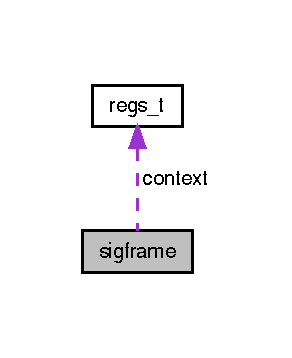
\includegraphics[width=141pt]{structsigframe__coll__graph}
\end{center}
\end{figure}
\subsection*{Champs de données}
\begin{DoxyCompactItemize}
\item 
\hypertarget{structsigframe_acf403267fcedbc7f1517f32b6bdfef1b}{\hyperlink{kernel_2include_2types_8h_a53428b953a0ae6fba02a5b3596c867e0}{vaddr\-\_\-t} {\bfseries ret\-\_\-addr}}\label{structsigframe_acf403267fcedbc7f1517f32b6bdfef1b}

\item 
\hypertarget{structsigframe_a27a92fefd72c5b01c52e96e7b4df8284}{int {\bfseries sig}}\label{structsigframe_a27a92fefd72c5b01c52e96e7b4df8284}

\item 
\hypertarget{structsigframe_aafcddb09def05f54a2c9839c6dcbd182}{\hyperlink{structregs__t}{regs\-\_\-t} {\bfseries context}}\label{structsigframe_aafcddb09def05f54a2c9839c6dcbd182}

\item 
\hypertarget{structsigframe_a737163c0b6590d2d47863a35720819a7}{\hyperlink{kernel_2include_2types_8h_a33594304e786b158f3fb30289278f5af}{uint32\-\_\-t} {\bfseries state}}\label{structsigframe_a737163c0b6590d2d47863a35720819a7}

\item 
\hypertarget{structsigframe_a2d626f01a67bbfac580ee6c1917d0fbb}{sigset\-\_\-t {\bfseries mask}}\label{structsigframe_a2d626f01a67bbfac580ee6c1917d0fbb}

\item 
\hypertarget{structsigframe_a0da134e98de0f33958d8dc320b589873}{char {\bfseries retcode} \mbox{[}8\mbox{]}}\label{structsigframe_a0da134e98de0f33958d8dc320b589873}

\end{DoxyCompactItemize}


La documentation de cette structure a été générée à partir du fichier suivant \-:\begin{DoxyCompactItemize}
\item 
kernel/\hyperlink{ksignal_8c}{ksignal.\-c}\end{DoxyCompactItemize}

\hypertarget{structsignal__process__data__t}{\section{Référence de la structure signal\+\_\+process\+\_\+data\+\_\+t}
\label{structsignal__process__data__t}\index{signal\+\_\+process\+\_\+data\+\_\+t@{signal\+\_\+process\+\_\+data\+\_\+t}}
}
\subsection*{Champs de données}
\begin{DoxyCompactItemize}
\item 
\hypertarget{structsignal__process__data__t_a397d720abbb70447cb1837012fa808e8}{sigset\+\_\+t {\bfseries mask}}\label{structsignal__process__data__t_a397d720abbb70447cb1837012fa808e8}

\item 
\hypertarget{structsignal__process__data__t_a072dbf9762b10b9b8b545622fcbfef92}{sigset\+\_\+t {\bfseries pending\+\_\+set}}\label{structsignal__process__data__t_a072dbf9762b10b9b8b545622fcbfef92}

\item 
\hypertarget{structsignal__process__data__t_acfd78d7210d6b09d6ffcf8d5c0ed8c24}{\hyperlink{signal_8h_a564498016effaee1f3384e07b7ced24f}{sighandler\+\_\+t} {\bfseries handlers} \mbox{[}\hyperlink{signal_8h_ab83b88daaecc469d1edb90a527ab4a39}{N\+S\+I\+G}\mbox{]}}\label{structsignal__process__data__t_acfd78d7210d6b09d6ffcf8d5c0ed8c24}

\end{DoxyCompactItemize}


La documentation de cette structure a été générée à partir du fichier suivant \+:\begin{DoxyCompactItemize}
\item 
kernel/include/\hyperlink{signal__types_8h}{signal\+\_\+types.\+h}\end{DoxyCompactItemize}

\hypertarget{structslab}{\section{Référence de la structure slab}
\label{structslab}\index{slab@{slab}}
}


a slab of pages.  




{\ttfamily \#include $<$vmm.\-h$>$}



Graphe de collaboration de slab\-:\nopagebreak
\begin{figure}[H]
\begin{center}
\leavevmode
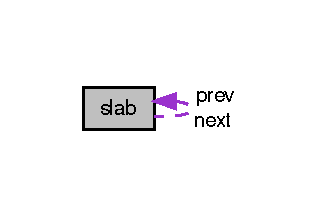
\includegraphics[width=154pt]{structslab__coll__graph}
\end{center}
\end{figure}
\subsection*{Champs de données}
\begin{DoxyCompactItemize}
\item 
\hypertarget{structslab_ad174680569745f7867fa2d78e42c73cd}{struct \hyperlink{structslab}{slab} $\ast$ {\bfseries prev}}\label{structslab_ad174680569745f7867fa2d78e42c73cd}

\item 
\hypertarget{structslab_ae57c4a606ae5e5cfbd73cdb5d5928423}{\hyperlink{kernel_2include_2types_8h_a29d85914ddff32967d85ada69854206d}{size\-\_\-t} {\bfseries nb\-\_\-pages}}\label{structslab_ae57c4a606ae5e5cfbd73cdb5d5928423}

\item 
\hypertarget{structslab_af47539fe63ee83cf7f9e8f2dfb5a7f8a}{struct \hyperlink{structslab}{slab} $\ast$ {\bfseries next}}\label{structslab_af47539fe63ee83cf7f9e8f2dfb5a7f8a}

\end{DoxyCompactItemize}


\subsection{Description détaillée}
chaque slab commence par un entête (struct slab) et est suivi par les données utiles. 

La documentation de cette structure a été générée à partir du fichier suivant \-:\begin{DoxyCompactItemize}
\item 
kernel/include/\hyperlink{vmm_8h}{vmm.\-h}\end{DoxyCompactItemize}

\hypertarget{structslabs__list}{\section{Référence de la structure slabs\+\_\+list}
\label{structslabs__list}\index{slabs\+\_\+list@{slabs\+\_\+list}}
}


Graphe de collaboration de slabs\+\_\+list\+:
\nopagebreak
\begin{figure}[H]
\begin{center}
\leavevmode
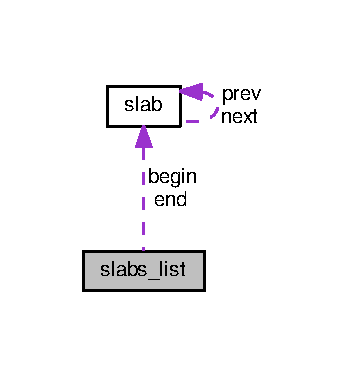
\includegraphics[width=167pt]{structslabs__list__coll__graph}
\end{center}
\end{figure}
\subsection*{Champs de données}
\begin{DoxyCompactItemize}
\item 
\hypertarget{structslabs__list_adde93358ca98d6711cbfeceaab58e61f}{struct \hyperlink{structslab}{slab} $\ast$ {\bfseries begin}}\label{structslabs__list_adde93358ca98d6711cbfeceaab58e61f}

\item 
\hypertarget{structslabs__list_aa9d16d723beabcdcffe2cbdde9d0c049}{struct \hyperlink{structslab}{slab} $\ast$ {\bfseries end}}\label{structslabs__list_aa9d16d723beabcdcffe2cbdde9d0c049}

\end{DoxyCompactItemize}


La documentation de cette structure a été générée à partir du fichier suivant \+:\begin{DoxyCompactItemize}
\item 
kernel/include/\hyperlink{vmm_8h}{vmm.\+h}\end{DoxyCompactItemize}

\hypertarget{structsocket}{\section{Référence de la structure socket}
\label{structsocket}\index{socket@{socket}}
}


Graphe de collaboration de socket\-:
\nopagebreak
\begin{figure}[H]
\begin{center}
\leavevmode
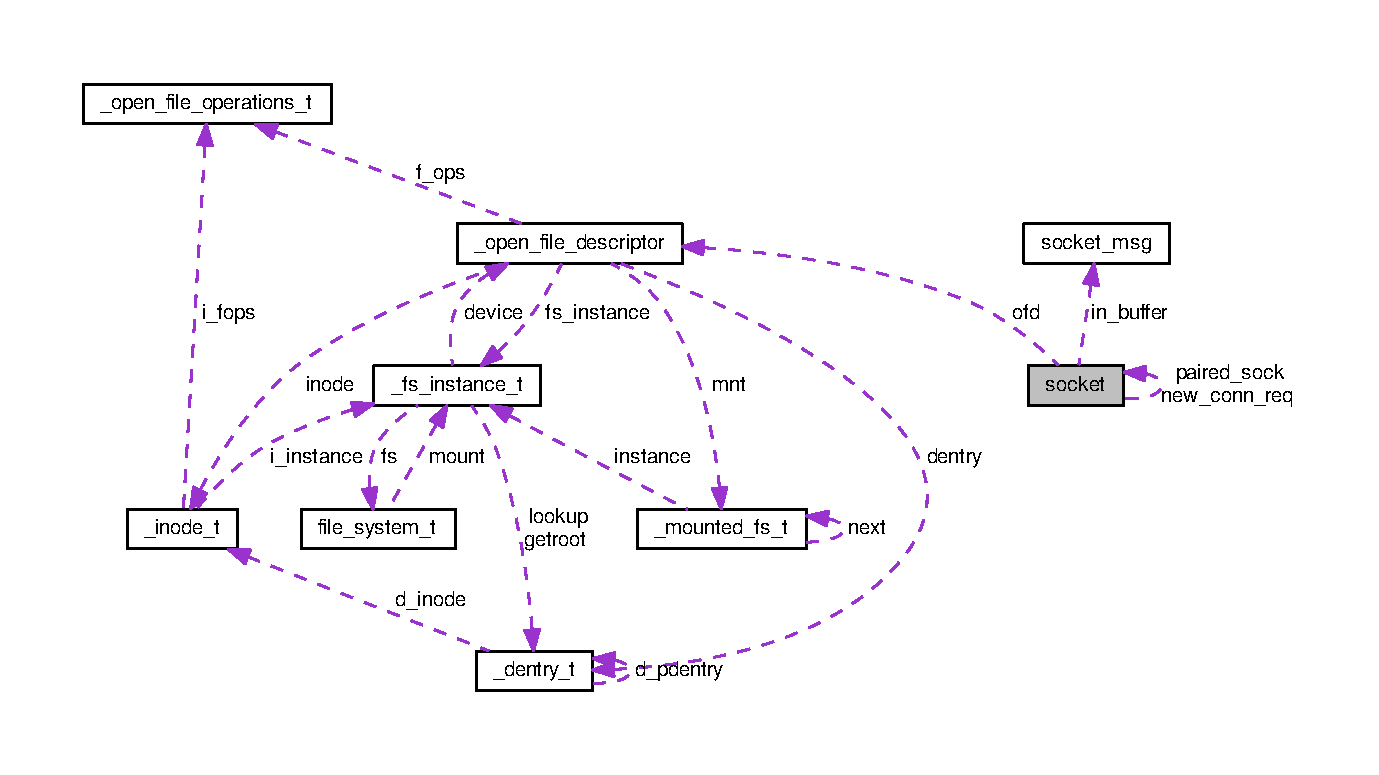
\includegraphics[width=220pt]{structsocket__coll__graph}
\end{center}
\end{figure}
\subsection*{Champs de données}
\begin{DoxyCompactItemize}
\item 
\hypertarget{structsocket_a037d2cd88c0121624d25f35336209987}{int {\bfseries sd}}\label{structsocket_a037d2cd88c0121624d25f35336209987}

\item 
\hypertarget{structsocket_a9a2a2dc58ec6cd873af3250bc79500c5}{enum socket\-\_\-type {\bfseries type}}\label{structsocket_a9a2a2dc58ec6cd873af3250bc79500c5}

\item 
\hypertarget{structsocket_aafe6721566c75c89097ff0560ef3bbaa}{bool {\bfseries blocking}}\label{structsocket_aafe6721566c75c89097ff0560ef3bbaa}

\item 
\hypertarget{structsocket_a469ff1719b3ae4543e8abe5808d880e9}{char $\ast$ {\bfseries meetpoint}}\label{structsocket_a469ff1719b3ae4543e8abe5808d880e9}

\item 
\hypertarget{structsocket_a467a2a2bbfea6313b115962a4d33b5b5}{enum socket\-\_\-state {\bfseries state}}\label{structsocket_a467a2a2bbfea6313b115962a4d33b5b5}

\item 
\hypertarget{structsocket_a59c47caae0b05514624b05c6dba8ce70}{struct \hyperlink{structsocket}{socket} $\ast$$\ast$ {\bfseries new\-\_\-conn\-\_\-req}}\label{structsocket_a59c47caae0b05514624b05c6dba8ce70}

\item 
\hypertarget{structsocket_a1209b382268731beb19f8326f2a35c57}{int {\bfseries pending\-\_\-conn\-\_\-req}}\label{structsocket_a1209b382268731beb19f8326f2a35c57}

\item 
\hypertarget{structsocket_aab4bbd1c8b3389000215a1cc5ffd80df}{int {\bfseries max\-\_\-conn\-\_\-req\-\_\-backlog}}\label{structsocket_aab4bbd1c8b3389000215a1cc5ffd80df}

\item 
\hypertarget{structsocket_a3300340c7565a298271a06aecf968091}{struct \hyperlink{structsocket}{socket} $\ast$ {\bfseries paired\-\_\-sock}}\label{structsocket_a3300340c7565a298271a06aecf968091}

\item 
\hypertarget{structsocket_a9ee09df65b7ec6bccd58fe2d4eebe6d9}{struct \hyperlink{structsocket__msg}{socket\-\_\-msg} {\bfseries in\-\_\-buffer} \mbox{[}M\-A\-X\-\_\-\-M\-E\-S\-S\-A\-G\-E\-S\mbox{]}}\label{structsocket_a9ee09df65b7ec6bccd58fe2d4eebe6d9}

\item 
\hypertarget{structsocket_ad1f8d42ded9f1e8a017780fa5bde11a0}{int {\bfseries in\-\_\-base}}\label{structsocket_ad1f8d42ded9f1e8a017780fa5bde11a0}

\item 
\hypertarget{structsocket_a3f3e2a3210219cad6bf97effcb29c074}{int {\bfseries in\-\_\-count}}\label{structsocket_a3f3e2a3210219cad6bf97effcb29c074}

\item 
\hypertarget{structsocket_ad7b80474cddbbbe5b8ca6a88c3790519}{\hyperlink{kernel_2include_2types_8h_aba7bc1797add20fe3efdf37ced1182c5}{uint8\-\_\-t} {\bfseries accept\-\_\-sem}}\label{structsocket_ad7b80474cddbbbe5b8ca6a88c3790519}

\item 
\hypertarget{structsocket_a2892cf67b33e9b8fc0cfd3094ad3d3fd}{\hyperlink{kernel_2include_2types_8h_aba7bc1797add20fe3efdf37ced1182c5}{uint8\-\_\-t} {\bfseries connect\-\_\-sem}}\label{structsocket_a2892cf67b33e9b8fc0cfd3094ad3d3fd}

\item 
\hypertarget{structsocket_acff0fb866f8282e667e1ee6ecc3ea355}{\hyperlink{kernel_2include_2types_8h_aba7bc1797add20fe3efdf37ced1182c5}{uint8\-\_\-t} {\bfseries read\-\_\-sem}}\label{structsocket_acff0fb866f8282e667e1ee6ecc3ea355}

\item 
\hypertarget{structsocket_a6dcd09bbe72cd9781a3d3bfff9dda45b}{\hyperlink{kernel_2include_2types_8h_aba7bc1797add20fe3efdf37ced1182c5}{uint8\-\_\-t} {\bfseries write\-\_\-sem}}\label{structsocket_a6dcd09bbe72cd9781a3d3bfff9dda45b}

\end{DoxyCompactItemize}


La documentation de cette structure a été générée à partir du fichier suivant \-:\begin{DoxyCompactItemize}
\item 
kernel/drivers/char/sock.\-c\end{DoxyCompactItemize}

\hypertarget{structsocket__msg}{\section{Référence de la structure socket\-\_\-msg}
\label{structsocket__msg}\index{socket\-\_\-msg@{socket\-\_\-msg}}
}
\subsection*{Champs de données}
\begin{DoxyCompactItemize}
\item 
\hypertarget{structsocket__msg_a1e35c3e0aea2227bbe5da883f93d78f1}{char {\bfseries data} \mbox{[}M\-A\-X\-\_\-\-M\-E\-S\-S\-A\-G\-E\-\_\-\-S\-I\-Z\-E\mbox{]}}\label{structsocket__msg_a1e35c3e0aea2227bbe5da883f93d78f1}

\item 
\hypertarget{structsocket__msg_affd6e393e4d11e216ccb9bee00e46816}{int {\bfseries size}}\label{structsocket__msg_affd6e393e4d11e216ccb9bee00e46816}

\end{DoxyCompactItemize}


La documentation de cette structure a été générée à partir du fichier suivant \-:\begin{DoxyCompactItemize}
\item 
kernel/drivers/char/sock.\-c\end{DoxyCompactItemize}

\hypertarget{unionspecific__extra__data__procfs__t}{\section{Référence de l'union specific\-\_\-extra\-\_\-data\-\_\-procfs\-\_\-t}
\label{unionspecific__extra__data__procfs__t}\index{specific\-\_\-extra\-\_\-data\-\_\-procfs\-\_\-t@{specific\-\_\-extra\-\_\-data\-\_\-procfs\-\_\-t}}
}
\subsection*{Champs de données}
\begin{DoxyCompactItemize}
\item 
\hypertarget{unionspecific__extra__data__procfs__t_ade848e22e77373e32442c9d91fb8474f}{\hyperlink{types_8h_a29d85914ddff32967d85ada69854206d}{size\-\_\-t} {\bfseries fd}}\label{unionspecific__extra__data__procfs__t_ade848e22e77373e32442c9d91fb8474f}

\end{DoxyCompactItemize}


La documentation de cette union a été générée à partir du fichier suivant \-:\begin{DoxyCompactItemize}
\item 
kernel/fs/\hyperlink{procfs_8c}{procfs.\-c}\end{DoxyCompactItemize}

\hypertarget{structstat}{\section{Référence de la structure stat}
\label{structstat}\index{stat@{stat}}
}


Informations sur un noeud.  




{\ttfamily \#include $<$kstat.\-h$>$}

\subsection*{Champs de données}
\begin{DoxyCompactItemize}
\item 
\hyperlink{kstat_8h_a451f1b5788fa7cc5d33db47a5992e7a6}{dev\-\_\-t} \hyperlink{structstat_ac5b90090ae323741ae4c9e4f3683a29f}{st\-\_\-dev}
\item 
\hyperlink{kstat_8h_aed4e918b44240739869c4bdb1c4787a9}{ino\-\_\-t} \hyperlink{structstat_a9769ed8f0d4c5a9f329c32bc92479d56}{st\-\_\-ino}
\item 
\hyperlink{kstat_8h_af8f4385bb42836d1e3ad4fea9d71d1b9}{mode\-\_\-t} \hyperlink{structstat_a5cbdd829011af82ba61e83773bbcbc7d}{st\-\_\-mode}
\item 
nlink\-\_\-t \hyperlink{structstat_a0ed9092fa6c77a3251b9b9a4738ef84f}{st\-\_\-nlink}
\item 
\hyperlink{kstat_8h_af2306308627701b66dc6f3babe821ab4}{uid\-\_\-t} \hyperlink{structstat_a4a8708a3d18be60ee7b2f06c4cab0c70}{st\-\_\-uid}
\item 
\hyperlink{kstat_8h_aa7352f1065fe606194d792e2b292cf83}{gid\-\_\-t} \hyperlink{structstat_ab864f16f436cec370f0ced585d897698}{st\-\_\-gid}
\item 
\hyperlink{kstat_8h_a451f1b5788fa7cc5d33db47a5992e7a6}{dev\-\_\-t} \hyperlink{structstat_aa61e6c1a8a91c69f1d26f6700a0546cb}{st\-\_\-rdev}
\item 
\hyperlink{libc_2include_2sys_2types_8h_a447a6a64dbb8fb44b1e62856b333db4a}{off\-\_\-t} \hyperlink{structstat_a040e19c8b9766f841fde8786ce9297bf}{st\-\_\-size}
\item 
blksize\-\_\-t \hyperlink{structstat_a38d474e1ae3cf6fbdde89ac3c3e308f1}{st\-\_\-blksize}
\item 
blkcnt\-\_\-t \hyperlink{structstat_a42dd716b2f9234f961d949fc9500eefb}{st\-\_\-blocks}
\item 
\hyperlink{time_8h_aaaf414ca0598a3633e6e9161cbb5a58a}{time\-\_\-t} \hyperlink{structstat_ab74d1e7e345e88b9d0fb2688a97cba64}{st\-\_\-atime}
\item 
\hyperlink{time_8h_aaaf414ca0598a3633e6e9161cbb5a58a}{time\-\_\-t} \hyperlink{structstat_a77e235090f8cb6897f1c0ce65689006b}{st\-\_\-mtime}
\item 
\hyperlink{time_8h_aaaf414ca0598a3633e6e9161cbb5a58a}{time\-\_\-t} \hyperlink{structstat_a1b4b858db1ebe79c3d6e0fc1ef721024}{st\-\_\-ctime}
\end{DoxyCompactItemize}


\subsection{Description détaillée}
Structure contenant les informations d'un noeud. 

\subsection{Documentation des champs}
\hypertarget{structstat_ab74d1e7e345e88b9d0fb2688a97cba64}{\index{stat@{stat}!st\-\_\-atime@{st\-\_\-atime}}
\index{st\-\_\-atime@{st\-\_\-atime}!stat@{stat}}
\subsubsection[{st\-\_\-atime}]{\setlength{\rightskip}{0pt plus 5cm}{\bf time\-\_\-t} stat\-::st\-\_\-atime}}\label{structstat_ab74d1e7e345e88b9d0fb2688a97cba64}
Heure dernier accès \hypertarget{structstat_a38d474e1ae3cf6fbdde89ac3c3e308f1}{\index{stat@{stat}!st\-\_\-blksize@{st\-\_\-blksize}}
\index{st\-\_\-blksize@{st\-\_\-blksize}!stat@{stat}}
\subsubsection[{st\-\_\-blksize}]{\setlength{\rightskip}{0pt plus 5cm}blksize\-\_\-t stat\-::st\-\_\-blksize}}\label{structstat_a38d474e1ae3cf6fbdde89ac3c3e308f1}
Taille de bloc pour E/\-S \hypertarget{structstat_a42dd716b2f9234f961d949fc9500eefb}{\index{stat@{stat}!st\-\_\-blocks@{st\-\_\-blocks}}
\index{st\-\_\-blocks@{st\-\_\-blocks}!stat@{stat}}
\subsubsection[{st\-\_\-blocks}]{\setlength{\rightskip}{0pt plus 5cm}blkcnt\-\_\-t stat\-::st\-\_\-blocks}}\label{structstat_a42dd716b2f9234f961d949fc9500eefb}
Nombre de blocs de 512\-B alloués \hypertarget{structstat_a1b4b858db1ebe79c3d6e0fc1ef721024}{\index{stat@{stat}!st\-\_\-ctime@{st\-\_\-ctime}}
\index{st\-\_\-ctime@{st\-\_\-ctime}!stat@{stat}}
\subsubsection[{st\-\_\-ctime}]{\setlength{\rightskip}{0pt plus 5cm}{\bf time\-\_\-t} stat\-::st\-\_\-ctime}}\label{structstat_a1b4b858db1ebe79c3d6e0fc1ef721024}
Heure dernier changement état \hypertarget{structstat_ac5b90090ae323741ae4c9e4f3683a29f}{\index{stat@{stat}!st\-\_\-dev@{st\-\_\-dev}}
\index{st\-\_\-dev@{st\-\_\-dev}!stat@{stat}}
\subsubsection[{st\-\_\-dev}]{\setlength{\rightskip}{0pt plus 5cm}{\bf dev\-\_\-t} stat\-::st\-\_\-dev}}\label{structstat_ac5b90090ae323741ae4c9e4f3683a29f}
Périphérique \hypertarget{structstat_ab864f16f436cec370f0ced585d897698}{\index{stat@{stat}!st\-\_\-gid@{st\-\_\-gid}}
\index{st\-\_\-gid@{st\-\_\-gid}!stat@{stat}}
\subsubsection[{st\-\_\-gid}]{\setlength{\rightskip}{0pt plus 5cm}{\bf gid\-\_\-t} stat\-::st\-\_\-gid}}\label{structstat_ab864f16f436cec370f0ced585d897698}
G\-I\-D propriétaire \hypertarget{structstat_a9769ed8f0d4c5a9f329c32bc92479d56}{\index{stat@{stat}!st\-\_\-ino@{st\-\_\-ino}}
\index{st\-\_\-ino@{st\-\_\-ino}!stat@{stat}}
\subsubsection[{st\-\_\-ino}]{\setlength{\rightskip}{0pt plus 5cm}{\bf ino\-\_\-t} stat\-::st\-\_\-ino}}\label{structstat_a9769ed8f0d4c5a9f329c32bc92479d56}
Numéro inœud \hypertarget{structstat_a5cbdd829011af82ba61e83773bbcbc7d}{\index{stat@{stat}!st\-\_\-mode@{st\-\_\-mode}}
\index{st\-\_\-mode@{st\-\_\-mode}!stat@{stat}}
\subsubsection[{st\-\_\-mode}]{\setlength{\rightskip}{0pt plus 5cm}{\bf mode\-\_\-t} stat\-::st\-\_\-mode}}\label{structstat_a5cbdd829011af82ba61e83773bbcbc7d}
Protection + file type \hypertarget{structstat_a77e235090f8cb6897f1c0ce65689006b}{\index{stat@{stat}!st\-\_\-mtime@{st\-\_\-mtime}}
\index{st\-\_\-mtime@{st\-\_\-mtime}!stat@{stat}}
\subsubsection[{st\-\_\-mtime}]{\setlength{\rightskip}{0pt plus 5cm}{\bf time\-\_\-t} stat\-::st\-\_\-mtime}}\label{structstat_a77e235090f8cb6897f1c0ce65689006b}
Heure dernière modification \hypertarget{structstat_a0ed9092fa6c77a3251b9b9a4738ef84f}{\index{stat@{stat}!st\-\_\-nlink@{st\-\_\-nlink}}
\index{st\-\_\-nlink@{st\-\_\-nlink}!stat@{stat}}
\subsubsection[{st\-\_\-nlink}]{\setlength{\rightskip}{0pt plus 5cm}nlink\-\_\-t stat\-::st\-\_\-nlink}}\label{structstat_a0ed9092fa6c77a3251b9b9a4738ef84f}
Nb liens matériels \hypertarget{structstat_aa61e6c1a8a91c69f1d26f6700a0546cb}{\index{stat@{stat}!st\-\_\-rdev@{st\-\_\-rdev}}
\index{st\-\_\-rdev@{st\-\_\-rdev}!stat@{stat}}
\subsubsection[{st\-\_\-rdev}]{\setlength{\rightskip}{0pt plus 5cm}{\bf dev\-\_\-t} stat\-::st\-\_\-rdev}}\label{structstat_aa61e6c1a8a91c69f1d26f6700a0546cb}
Type périphérique \hypertarget{structstat_a040e19c8b9766f841fde8786ce9297bf}{\index{stat@{stat}!st\-\_\-size@{st\-\_\-size}}
\index{st\-\_\-size@{st\-\_\-size}!stat@{stat}}
\subsubsection[{st\-\_\-size}]{\setlength{\rightskip}{0pt plus 5cm}{\bf off\-\_\-t} stat\-::st\-\_\-size}}\label{structstat_a040e19c8b9766f841fde8786ce9297bf}
Taille totale en octets \hypertarget{structstat_a4a8708a3d18be60ee7b2f06c4cab0c70}{\index{stat@{stat}!st\-\_\-uid@{st\-\_\-uid}}
\index{st\-\_\-uid@{st\-\_\-uid}!stat@{stat}}
\subsubsection[{st\-\_\-uid}]{\setlength{\rightskip}{0pt plus 5cm}{\bf uid\-\_\-t} stat\-::st\-\_\-uid}}\label{structstat_a4a8708a3d18be60ee7b2f06c4cab0c70}
U\-I\-D propriétaire 

La documentation de cette structure a été générée à partir des fichiers suivants \-:\begin{DoxyCompactItemize}
\item 
kernel/include/\hyperlink{kstat_8h}{kstat.\-h}\item 
libc/include/sys/\hyperlink{stat_8h}{stat.\-h}\end{DoxyCompactItemize}

\hypertarget{structsymbol__t}{\section{\-Référence de la structure symbol\-\_\-t}
\label{structsymbol__t}\index{symbol\-\_\-t@{symbol\-\_\-t}}
}
\subsection*{\-Champs de données}
\begin{DoxyCompactItemize}
\item 
\hypertarget{structsymbol__t_aeb9236c76060c4ca851c9650fcef03c7}{char $\ast$ {\bfseries name}}\label{structsymbol__t_aeb9236c76060c4ca851c9650fcef03c7}

\item 
\hypertarget{structsymbol__t_a38ee18008916034a31568258fcce7e27}{\hyperlink{types_8h_a9f047c1f0917f6184a7a013d4b4277a6}{paddr\-\_\-t} {\bfseries addr}}\label{structsymbol__t_a38ee18008916034a31568258fcce7e27}

\end{DoxyCompactItemize}


\-La documentation de cette structure a été générée à partir du fichier suivant \-:\begin{DoxyCompactItemize}
\item 
kernel/include/\hyperlink{symtable_8h}{symtable.\-h}\end{DoxyCompactItemize}

\hypertarget{structsymbol__table__t}{\section{\-Référence de la structure symbol\-\_\-table\-\_\-t}
\label{structsymbol__table__t}\index{symbol\-\_\-table\-\_\-t@{symbol\-\_\-table\-\_\-t}}
}


\-Graphe de collaboration de symbol\-\_\-table\-\_\-t\-:\nopagebreak
\begin{figure}[H]
\begin{center}
\leavevmode
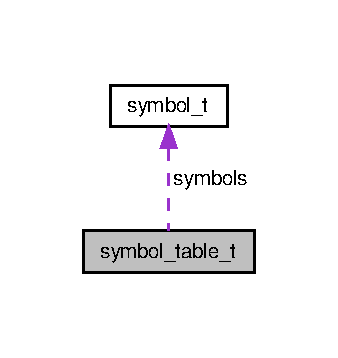
\includegraphics[width=162pt]{structsymbol__table__t__coll__graph}
\end{center}
\end{figure}
\subsection*{\-Champs de données}
\begin{DoxyCompactItemize}
\item 
\hypertarget{structsymbol__table__t_a0c1e0da15681b9a6214768438327b96f}{\hyperlink{structsymbol__t}{symbol\-\_\-t} $\ast$ {\bfseries symbols}}\label{structsymbol__table__t_a0c1e0da15681b9a6214768438327b96f}

\item 
\hypertarget{structsymbol__table__t_a069db8e0b90af60b517286f215122982}{int {\bfseries count}}\label{structsymbol__table__t_a069db8e0b90af60b517286f215122982}

\end{DoxyCompactItemize}


\-La documentation de cette structure a été générée à partir du fichier suivant \-:\begin{DoxyCompactItemize}
\item 
kernel/include/\hyperlink{symtable_8h}{symtable.\-h}\end{DoxyCompactItemize}

\hypertarget{structsymbole}{\section{Référence de la structure symbole}
\label{structsymbole}\index{symbole@{symbole}}
}
\subsection*{Champs de données}
\begin{DoxyCompactItemize}
\item 
const char $\ast$ \hyperlink{structsymbole_a325f3bf3c7b29dbc931ec1a61df19bea}{normal}
\item 
const char $\ast$ \hyperlink{structsymbole_a817ffc97047283180645063db79a621d}{caps}
\item 
const char $\ast$ \hyperlink{structsymbole_a35f794a092160ffe7926bbf11c670298}{alt}
\item 
const char $\ast$ \hyperlink{structsymbole_a2383cac8f05d012336683f0af44535b5}{ctrl}
\item 
const char $\ast$ \hyperlink{structsymbole_abd9f93b644b1d63156ff92f3f1a65649}{alt\+\_\+r}
\item 
\hypertarget{structsymbole_ad065a9b3f1f06815e4cfc07aabcd0933}{const char $\ast$ {\bfseries num\+\_\+lock}}\label{structsymbole_ad065a9b3f1f06815e4cfc07aabcd0933}

\end{DoxyCompactItemize}


\subsection{Description détaillée}
Structure qui contient les charactères A\+N\+S\+I pour un keycode en fonction des modifiers. 

\subsection{Documentation des champs}
\hypertarget{structsymbole_a35f794a092160ffe7926bbf11c670298}{\index{symbole@{symbole}!alt@{alt}}
\index{alt@{alt}!symbole@{symbole}}
\subsubsection[{alt}]{\setlength{\rightskip}{0pt plus 5cm}const char$\ast$ symbole\+::alt}}\label{structsymbole_a35f794a092160ffe7926bbf11c670298}
Code si la touche alt de gauche est appuyée. \hypertarget{structsymbole_abd9f93b644b1d63156ff92f3f1a65649}{\index{symbole@{symbole}!alt\+\_\+r@{alt\+\_\+r}}
\index{alt\+\_\+r@{alt\+\_\+r}!symbole@{symbole}}
\subsubsection[{alt\+\_\+r}]{\setlength{\rightskip}{0pt plus 5cm}const char$\ast$ symbole\+::alt\+\_\+r}}\label{structsymbole_abd9f93b644b1d63156ff92f3f1a65649}
Code si la touche alt\+\_\+gr est appuyée. \hypertarget{structsymbole_a817ffc97047283180645063db79a621d}{\index{symbole@{symbole}!caps@{caps}}
\index{caps@{caps}!symbole@{symbole}}
\subsubsection[{caps}]{\setlength{\rightskip}{0pt plus 5cm}const char$\ast$ symbole\+::caps}}\label{structsymbole_a817ffc97047283180645063db79a621d}
Code si shift appuyé ou capslock. \hypertarget{structsymbole_a2383cac8f05d012336683f0af44535b5}{\index{symbole@{symbole}!ctrl@{ctrl}}
\index{ctrl@{ctrl}!symbole@{symbole}}
\subsubsection[{ctrl}]{\setlength{\rightskip}{0pt plus 5cm}const char$\ast$ symbole\+::ctrl}}\label{structsymbole_a2383cac8f05d012336683f0af44535b5}
Code si la touche ctrl est appuyée. \hypertarget{structsymbole_a325f3bf3c7b29dbc931ec1a61df19bea}{\index{symbole@{symbole}!normal@{normal}}
\index{normal@{normal}!symbole@{symbole}}
\subsubsection[{normal}]{\setlength{\rightskip}{0pt plus 5cm}const char$\ast$ symbole\+::normal}}\label{structsymbole_a325f3bf3c7b29dbc931ec1a61df19bea}
Code normal. 

La documentation de cette structure a été générée à partir du fichier suivant \+:\begin{DoxyCompactItemize}
\item 
kernel/drivers/char/tty/\hyperlink{keyboard_8c}{keyboard.\+c}\end{DoxyCompactItemize}

\hypertarget{structtermios}{\section{Référence de la structure termios}
\label{structtermios}\index{termios@{termios}}
}
\subsection*{Champs de données}
\begin{DoxyCompactItemize}
\item 
tcflag\-\_\-t \hyperlink{structtermios_a85b6c86d2a3db45a3829488190e357e4}{c\-\_\-iflag}
\item 
tcflag\-\_\-t \hyperlink{structtermios_ad6e2cfedb81530e5a6a3a0e30b8c6362}{c\-\_\-oflag}
\item 
tcflag\-\_\-t \hyperlink{structtermios_a5d42b95faa4745c3bea53652d2812162}{c\-\_\-cflag}
\item 
tcflag\-\_\-t \hyperlink{structtermios_a91bdd7691180800fccc4b791466ee9c3}{c\-\_\-lflag}
\item 
cc\-\_\-t \hyperlink{structtermios_a6058cfc222551ee750c72142299acb2e}{c\-\_\-cc} \mbox{[}N\-C\-C\-S\mbox{]}
\item 
speed\-\_\-t \hyperlink{structtermios_a02ae972cbc9fb2cf4a1aa6a6751a421a}{c\-\_\-ispeed}
\end{DoxyCompactItemize}


\subsection{Documentation des champs}
\hypertarget{structtermios_a6058cfc222551ee750c72142299acb2e}{\index{termios@{termios}!c\-\_\-cc@{c\-\_\-cc}}
\index{c\-\_\-cc@{c\-\_\-cc}!termios@{termios}}
\subsubsection[{c\-\_\-cc}]{\setlength{\rightskip}{0pt plus 5cm}cc\-\_\-t termios\-::c\-\_\-cc}}\label{structtermios_a6058cfc222551ee750c72142299acb2e}
Control chars. \hypertarget{structtermios_a5d42b95faa4745c3bea53652d2812162}{\index{termios@{termios}!c\-\_\-cflag@{c\-\_\-cflag}}
\index{c\-\_\-cflag@{c\-\_\-cflag}!termios@{termios}}
\subsubsection[{c\-\_\-cflag}]{\setlength{\rightskip}{0pt plus 5cm}tcflag\-\_\-t termios\-::c\-\_\-cflag}}\label{structtermios_a5d42b95faa4745c3bea53652d2812162}
Control modes. \hypertarget{structtermios_a85b6c86d2a3db45a3829488190e357e4}{\index{termios@{termios}!c\-\_\-iflag@{c\-\_\-iflag}}
\index{c\-\_\-iflag@{c\-\_\-iflag}!termios@{termios}}
\subsubsection[{c\-\_\-iflag}]{\setlength{\rightskip}{0pt plus 5cm}tcflag\-\_\-t termios\-::c\-\_\-iflag}}\label{structtermios_a85b6c86d2a3db45a3829488190e357e4}
Input modes. \hypertarget{structtermios_a02ae972cbc9fb2cf4a1aa6a6751a421a}{\index{termios@{termios}!c\-\_\-ispeed@{c\-\_\-ispeed}}
\index{c\-\_\-ispeed@{c\-\_\-ispeed}!termios@{termios}}
\subsubsection[{c\-\_\-ispeed}]{\setlength{\rightskip}{0pt plus 5cm}speed\-\_\-t termios\-::c\-\_\-ispeed}}\label{structtermios_a02ae972cbc9fb2cf4a1aa6a6751a421a}
Speed (serial). \hypertarget{structtermios_a91bdd7691180800fccc4b791466ee9c3}{\index{termios@{termios}!c\-\_\-lflag@{c\-\_\-lflag}}
\index{c\-\_\-lflag@{c\-\_\-lflag}!termios@{termios}}
\subsubsection[{c\-\_\-lflag}]{\setlength{\rightskip}{0pt plus 5cm}tcflag\-\_\-t termios\-::c\-\_\-lflag}}\label{structtermios_a91bdd7691180800fccc4b791466ee9c3}
Local modes. \hypertarget{structtermios_ad6e2cfedb81530e5a6a3a0e30b8c6362}{\index{termios@{termios}!c\-\_\-oflag@{c\-\_\-oflag}}
\index{c\-\_\-oflag@{c\-\_\-oflag}!termios@{termios}}
\subsubsection[{c\-\_\-oflag}]{\setlength{\rightskip}{0pt plus 5cm}tcflag\-\_\-t termios\-::c\-\_\-oflag}}\label{structtermios_ad6e2cfedb81530e5a6a3a0e30b8c6362}
Output modes. 

La documentation de cette structure a été générée à partir des fichiers suivants \-:\begin{DoxyCompactItemize}
\item 
kernel/include/\hyperlink{termios__types_8h}{termios\-\_\-types.\-h}\item 
libc/include/\hyperlink{termios_8h}{termios.\-h}\end{DoxyCompactItemize}

\hypertarget{structtimespec}{\section{Référence de la structure timespec}
\label{structtimespec}\index{timespec@{timespec}}
}


{\ttfamily \#include $<$clock.\-h$>$}

\subsection*{Champs de données}
\begin{DoxyCompactItemize}
\item 
long int \hyperlink{structtimespec_af632894a12c37dea87073c0126f99fff}{tv\-\_\-sec}
\item 
long int \hyperlink{structtimespec_aa9689622a344d847333e534ac23d3093}{tv\-\_\-nsec}
\end{DoxyCompactItemize}


\subsection{Description détaillée}
Représente un temps écoule. 

\subsection{Documentation des champs}
\hypertarget{structtimespec_aa9689622a344d847333e534ac23d3093}{\index{timespec@{timespec}!tv\-\_\-nsec@{tv\-\_\-nsec}}
\index{tv\-\_\-nsec@{tv\-\_\-nsec}!timespec@{timespec}}
\subsubsection[{tv\-\_\-nsec}]{\setlength{\rightskip}{0pt plus 5cm}long int timespec\-::tv\-\_\-nsec}}\label{structtimespec_aa9689622a344d847333e534ac23d3093}
Le reste en ns. \hypertarget{structtimespec_af632894a12c37dea87073c0126f99fff}{\index{timespec@{timespec}!tv\-\_\-sec@{tv\-\_\-sec}}
\index{tv\-\_\-sec@{tv\-\_\-sec}!timespec@{timespec}}
\subsubsection[{tv\-\_\-sec}]{\setlength{\rightskip}{0pt plus 5cm}long int timespec\-::tv\-\_\-sec}}\label{structtimespec_af632894a12c37dea87073c0126f99fff}
Le nombre de secondes écoulées. 

La documentation de cette structure a été générée à partir du fichier suivant \-:\begin{DoxyCompactItemize}
\item 
kernel/include/\hyperlink{clock_8h}{clock.\-h}\end{DoxyCompactItemize}

\hypertarget{structtimeval}{\section{\-Référence de la structure timeval}
\label{structtimeval}\index{timeval@{timeval}}
}
\subsection*{\-Champs de données}
\begin{DoxyCompactItemize}
\item 
long int \hyperlink{structtimeval_ab6fac84a084d017bb157f4681dafe8a3}{tv\-\_\-sec}
\item 
long int \hyperlink{structtimeval_a6f90a236deb00a89fe3dd8023d525d9c}{tv\-\_\-usec}
\end{DoxyCompactItemize}


\subsection{\-Documentation des champs}
\hypertarget{structtimeval_ab6fac84a084d017bb157f4681dafe8a3}{\index{timeval@{timeval}!tv\-\_\-sec@{tv\-\_\-sec}}
\index{tv\-\_\-sec@{tv\-\_\-sec}!timeval@{timeval}}
\subsubsection[{tv\-\_\-sec}]{\setlength{\rightskip}{0pt plus 5cm}long int {\bf timeval\-::tv\-\_\-sec}}}\label{structtimeval_ab6fac84a084d017bb157f4681dafe8a3}
\-Secondes \hypertarget{structtimeval_a6f90a236deb00a89fe3dd8023d525d9c}{\index{timeval@{timeval}!tv\-\_\-usec@{tv\-\_\-usec}}
\index{tv\-\_\-usec@{tv\-\_\-usec}!timeval@{timeval}}
\subsubsection[{tv\-\_\-usec}]{\setlength{\rightskip}{0pt plus 5cm}long int {\bf timeval\-::tv\-\_\-usec}}}\label{structtimeval_a6f90a236deb00a89fe3dd8023d525d9c}
\-Microsecondes 

\-La documentation de cette structure a été générée à partir du fichier suivant \-:\begin{DoxyCompactItemize}
\item 
libc/include/\hyperlink{time_8h}{time.\-h}\end{DoxyCompactItemize}

\hypertarget{structtm}{\section{Référence de la structure tm}
\label{structtm}\index{tm@{tm}}
}


{\ttfamily \#include $<$clock.\+h$>$}

\subsection*{Champs de données}
\begin{DoxyCompactItemize}
\item 
int \hyperlink{structtm_a4d098a9a5c03a00b2ee61e10851de81e}{tm\+\_\+sec}
\item 
int \hyperlink{structtm_af414eb7c86cc3099595211eee4d4211b}{tm\+\_\+min}
\item 
int \hyperlink{structtm_a3e7ca4e37f1abcaf56b8a916c38eb9fe}{tm\+\_\+hour}
\item 
int \hyperlink{structtm_ab8d8904bad43b0c8b96e61941c5b5310}{tm\+\_\+mday}
\item 
int \hyperlink{structtm_a112ac36fa2f593777138a417cf031e17}{tm\+\_\+mon}
\item 
int \hyperlink{structtm_a33adf78fd6476b2120ce3b9c4a852053}{tm\+\_\+year}
\item 
int \hyperlink{structtm_afe81a8c46f1c693c43f259b288859f4f}{tm\+\_\+wday}
\item 
int \hyperlink{structtm_a93a0ba77cc23796df84405dcbcc57eb1}{tm\+\_\+yday}
\item 
int \hyperlink{structtm_a5645ca0580c8ab2c24f6c2965d9c9f9c}{tm\+\_\+isdst}
\end{DoxyCompactItemize}


\subsection{Description détaillée}
Structure qui contient une date et heure. 

\subsection{Documentation des champs}
\hypertarget{structtm_a3e7ca4e37f1abcaf56b8a916c38eb9fe}{\index{tm@{tm}!tm\+\_\+hour@{tm\+\_\+hour}}
\index{tm\+\_\+hour@{tm\+\_\+hour}!tm@{tm}}
\subsubsection[{tm\+\_\+hour}]{\setlength{\rightskip}{0pt plus 5cm}int tm\+::tm\+\_\+hour}}\label{structtm_a3e7ca4e37f1abcaf56b8a916c38eb9fe}
hours since midnight — \mbox{[}0, 23\mbox{]} \hypertarget{structtm_a5645ca0580c8ab2c24f6c2965d9c9f9c}{\index{tm@{tm}!tm\+\_\+isdst@{tm\+\_\+isdst}}
\index{tm\+\_\+isdst@{tm\+\_\+isdst}!tm@{tm}}
\subsubsection[{tm\+\_\+isdst}]{\setlength{\rightskip}{0pt plus 5cm}int tm\+::tm\+\_\+isdst}}\label{structtm_a5645ca0580c8ab2c24f6c2965d9c9f9c}
Daylight Saving Time flag (1 true, 0 false, neg unavailable) \hypertarget{structtm_ab8d8904bad43b0c8b96e61941c5b5310}{\index{tm@{tm}!tm\+\_\+mday@{tm\+\_\+mday}}
\index{tm\+\_\+mday@{tm\+\_\+mday}!tm@{tm}}
\subsubsection[{tm\+\_\+mday}]{\setlength{\rightskip}{0pt plus 5cm}int tm\+::tm\+\_\+mday}}\label{structtm_ab8d8904bad43b0c8b96e61941c5b5310}
day of the month — \mbox{[}1, 31\mbox{]} \hypertarget{structtm_af414eb7c86cc3099595211eee4d4211b}{\index{tm@{tm}!tm\+\_\+min@{tm\+\_\+min}}
\index{tm\+\_\+min@{tm\+\_\+min}!tm@{tm}}
\subsubsection[{tm\+\_\+min}]{\setlength{\rightskip}{0pt plus 5cm}int tm\+::tm\+\_\+min}}\label{structtm_af414eb7c86cc3099595211eee4d4211b}
minutes after the hour — \mbox{[}0, 59\mbox{]} \hypertarget{structtm_a112ac36fa2f593777138a417cf031e17}{\index{tm@{tm}!tm\+\_\+mon@{tm\+\_\+mon}}
\index{tm\+\_\+mon@{tm\+\_\+mon}!tm@{tm}}
\subsubsection[{tm\+\_\+mon}]{\setlength{\rightskip}{0pt plus 5cm}int tm\+::tm\+\_\+mon}}\label{structtm_a112ac36fa2f593777138a417cf031e17}
months since January — \mbox{[}0, 11\mbox{]} \hypertarget{structtm_a4d098a9a5c03a00b2ee61e10851de81e}{\index{tm@{tm}!tm\+\_\+sec@{tm\+\_\+sec}}
\index{tm\+\_\+sec@{tm\+\_\+sec}!tm@{tm}}
\subsubsection[{tm\+\_\+sec}]{\setlength{\rightskip}{0pt plus 5cm}int tm\+::tm\+\_\+sec}}\label{structtm_a4d098a9a5c03a00b2ee61e10851de81e}
seconds after the minute — \mbox{[}0, 60\mbox{]} \hypertarget{structtm_afe81a8c46f1c693c43f259b288859f4f}{\index{tm@{tm}!tm\+\_\+wday@{tm\+\_\+wday}}
\index{tm\+\_\+wday@{tm\+\_\+wday}!tm@{tm}}
\subsubsection[{tm\+\_\+wday}]{\setlength{\rightskip}{0pt plus 5cm}int tm\+::tm\+\_\+wday}}\label{structtm_afe81a8c46f1c693c43f259b288859f4f}
days since Sunday — \mbox{[}0, 6\mbox{]} \hypertarget{structtm_a93a0ba77cc23796df84405dcbcc57eb1}{\index{tm@{tm}!tm\+\_\+yday@{tm\+\_\+yday}}
\index{tm\+\_\+yday@{tm\+\_\+yday}!tm@{tm}}
\subsubsection[{tm\+\_\+yday}]{\setlength{\rightskip}{0pt plus 5cm}int tm\+::tm\+\_\+yday}}\label{structtm_a93a0ba77cc23796df84405dcbcc57eb1}
days since January 1 — \mbox{[}0, 365\mbox{]} \hypertarget{structtm_a33adf78fd6476b2120ce3b9c4a852053}{\index{tm@{tm}!tm\+\_\+year@{tm\+\_\+year}}
\index{tm\+\_\+year@{tm\+\_\+year}!tm@{tm}}
\subsubsection[{tm\+\_\+year}]{\setlength{\rightskip}{0pt plus 5cm}int tm\+::tm\+\_\+year}}\label{structtm_a33adf78fd6476b2120ce3b9c4a852053}
years since 1900 

La documentation de cette structure a été générée à partir des fichiers suivants \+:\begin{DoxyCompactItemize}
\item 
kernel/include/\hyperlink{clock_8h}{clock.\+h}\item 
libc/include/\hyperlink{time_8h}{time.\+h}\end{DoxyCompactItemize}

\hypertarget{structtss}{\section{Référence de la structure tss}
\label{structtss}\index{tss@{tss}}
}
\subsection*{Champs de données}
\begin{DoxyCompactItemize}
\item 
\hypertarget{structtss_ad53ac7d2e96d874b937cd8ba2ec99b68}{\hyperlink{kernel_2include_2types_8h_adf4d876453337156dde61095e1f20223}{uint16\-\_\-t} {\bfseries previous\-\_\-task}}\label{structtss_ad53ac7d2e96d874b937cd8ba2ec99b68}

\item 
\hypertarget{structtss_aa9c707a0e579d5c4aa5cdc6a74dc52f0}{\hyperlink{kernel_2include_2types_8h_adf4d876453337156dde61095e1f20223}{uint16\-\_\-t} {\bfseries \-\_\-\-\_\-previous\-\_\-task\-\_\-unused}}\label{structtss_aa9c707a0e579d5c4aa5cdc6a74dc52f0}

\item 
\hypertarget{structtss_a7e43a5ebd87f7dc5b342942daf46b6f1}{\hyperlink{kernel_2include_2types_8h_a33594304e786b158f3fb30289278f5af}{uint32\-\_\-t} {\bfseries esp0}}\label{structtss_a7e43a5ebd87f7dc5b342942daf46b6f1}

\item 
\hypertarget{structtss_a21766cd40c3c8f0036091d76956edc6c}{\hyperlink{kernel_2include_2types_8h_adf4d876453337156dde61095e1f20223}{uint16\-\_\-t} {\bfseries ss0}}\label{structtss_a21766cd40c3c8f0036091d76956edc6c}

\item 
\hypertarget{structtss_ae0b947bcd701d61513f54ae0fe5d8e67}{\hyperlink{kernel_2include_2types_8h_adf4d876453337156dde61095e1f20223}{uint16\-\_\-t} {\bfseries \-\_\-\-\_\-ss0\-\_\-unused}}\label{structtss_ae0b947bcd701d61513f54ae0fe5d8e67}

\item 
\hypertarget{structtss_ab2b4ce638811e1a254005e069886f8b3}{\hyperlink{kernel_2include_2types_8h_a33594304e786b158f3fb30289278f5af}{uint32\-\_\-t} {\bfseries esp1}}\label{structtss_ab2b4ce638811e1a254005e069886f8b3}

\item 
\hypertarget{structtss_aa527f4b4f275061d8750f527c7ab6fcf}{\hyperlink{kernel_2include_2types_8h_adf4d876453337156dde61095e1f20223}{uint16\-\_\-t} {\bfseries ss1}}\label{structtss_aa527f4b4f275061d8750f527c7ab6fcf}

\item 
\hypertarget{structtss_a1f7d520f366f7e044b4b0d0c66a8ced8}{\hyperlink{kernel_2include_2types_8h_adf4d876453337156dde61095e1f20223}{uint16\-\_\-t} {\bfseries \-\_\-\-\_\-ss1\-\_\-unused}}\label{structtss_a1f7d520f366f7e044b4b0d0c66a8ced8}

\item 
\hypertarget{structtss_ad03f620dee23e6c17980555c16f6bcf4}{\hyperlink{kernel_2include_2types_8h_a33594304e786b158f3fb30289278f5af}{uint32\-\_\-t} {\bfseries esp2}}\label{structtss_ad03f620dee23e6c17980555c16f6bcf4}

\item 
\hypertarget{structtss_a636eab51b2bf2e7b4aac87eefc97def2}{\hyperlink{kernel_2include_2types_8h_adf4d876453337156dde61095e1f20223}{uint16\-\_\-t} {\bfseries ss2}}\label{structtss_a636eab51b2bf2e7b4aac87eefc97def2}

\item 
\hypertarget{structtss_acda46d13f63cea285ce92781453c3472}{\hyperlink{kernel_2include_2types_8h_adf4d876453337156dde61095e1f20223}{uint16\-\_\-t} {\bfseries \-\_\-\-\_\-ss2\-\_\-unused}}\label{structtss_acda46d13f63cea285ce92781453c3472}

\item 
\hypertarget{structtss_a63a7022863de05e1eb2558955414fd98}{\hyperlink{kernel_2include_2types_8h_a33594304e786b158f3fb30289278f5af}{uint32\-\_\-t} {\bfseries cr3}}\label{structtss_a63a7022863de05e1eb2558955414fd98}

\item 
\hypertarget{structtss_a0f6c0e24aafa9b8b12467c6a4166211a}{\hyperlink{kernel_2include_2types_8h_a33594304e786b158f3fb30289278f5af}{uint32\-\_\-t} {\bfseries eip}}\label{structtss_a0f6c0e24aafa9b8b12467c6a4166211a}

\item 
\hypertarget{structtss_aa6e0555eb857b14b24b207faa5333a8f}{\hyperlink{kernel_2include_2types_8h_a33594304e786b158f3fb30289278f5af}{uint32\-\_\-t} {\bfseries eflags}}\label{structtss_aa6e0555eb857b14b24b207faa5333a8f}

\item 
\hypertarget{structtss_ae3887829963c58daac3c5367be0a37ce}{\hyperlink{kernel_2include_2types_8h_a33594304e786b158f3fb30289278f5af}{uint32\-\_\-t} {\bfseries eax}}\label{structtss_ae3887829963c58daac3c5367be0a37ce}

\item 
\hypertarget{structtss_aec35c5bdd8856cfcbf4363ece2e77ad7}{\hyperlink{kernel_2include_2types_8h_a33594304e786b158f3fb30289278f5af}{uint32\-\_\-t} {\bfseries ecx}}\label{structtss_aec35c5bdd8856cfcbf4363ece2e77ad7}

\item 
\hypertarget{structtss_aea0c135d2a3ecdf06a9d9a5e77db18d9}{\hyperlink{kernel_2include_2types_8h_a33594304e786b158f3fb30289278f5af}{uint32\-\_\-t} {\bfseries edx}}\label{structtss_aea0c135d2a3ecdf06a9d9a5e77db18d9}

\item 
\hypertarget{structtss_a047e38f680eed8f6717791e5a3da7a3b}{\hyperlink{kernel_2include_2types_8h_a33594304e786b158f3fb30289278f5af}{uint32\-\_\-t} {\bfseries ebx}}\label{structtss_a047e38f680eed8f6717791e5a3da7a3b}

\item 
\hypertarget{structtss_adf06b5cc872667c7cbaefd0b31c5988c}{\hyperlink{kernel_2include_2types_8h_a33594304e786b158f3fb30289278f5af}{uint32\-\_\-t} {\bfseries esp}}\label{structtss_adf06b5cc872667c7cbaefd0b31c5988c}

\item 
\hypertarget{structtss_a544009bf7a3831a52cad2c1d7ed2f808}{\hyperlink{kernel_2include_2types_8h_a33594304e786b158f3fb30289278f5af}{uint32\-\_\-t} {\bfseries ebp}}\label{structtss_a544009bf7a3831a52cad2c1d7ed2f808}

\item 
\hypertarget{structtss_aa205de690ecb0efb15e0573cf85d9cf8}{\hyperlink{kernel_2include_2types_8h_a33594304e786b158f3fb30289278f5af}{uint32\-\_\-t} {\bfseries esi}}\label{structtss_aa205de690ecb0efb15e0573cf85d9cf8}

\item 
\hypertarget{structtss_a806eea32b6bc9ab3c329abc64679d9ed}{\hyperlink{kernel_2include_2types_8h_a33594304e786b158f3fb30289278f5af}{uint32\-\_\-t} {\bfseries edi}}\label{structtss_a806eea32b6bc9ab3c329abc64679d9ed}

\item 
\hypertarget{structtss_a3d2acdbf7c3ee40b0a0840e9510ab346}{\hyperlink{kernel_2include_2types_8h_adf4d876453337156dde61095e1f20223}{uint16\-\_\-t} {\bfseries es}}\label{structtss_a3d2acdbf7c3ee40b0a0840e9510ab346}

\item 
\hypertarget{structtss_a7c958b99ed6a41460ef3c03ad82cf86d}{\hyperlink{kernel_2include_2types_8h_adf4d876453337156dde61095e1f20223}{uint16\-\_\-t} {\bfseries \-\_\-\-\_\-es\-\_\-unused}}\label{structtss_a7c958b99ed6a41460ef3c03ad82cf86d}

\item 
\hypertarget{structtss_ae4bb43c23f3b00f437962a705f2fbd11}{\hyperlink{kernel_2include_2types_8h_adf4d876453337156dde61095e1f20223}{uint16\-\_\-t} {\bfseries cs}}\label{structtss_ae4bb43c23f3b00f437962a705f2fbd11}

\item 
\hypertarget{structtss_a2e59148e8d335a4e2f944a6e861de10b}{\hyperlink{kernel_2include_2types_8h_adf4d876453337156dde61095e1f20223}{uint16\-\_\-t} {\bfseries \-\_\-\-\_\-cs\-\_\-unused}}\label{structtss_a2e59148e8d335a4e2f944a6e861de10b}

\item 
\hypertarget{structtss_a17ac540d5e034db72478998f531902f2}{\hyperlink{kernel_2include_2types_8h_adf4d876453337156dde61095e1f20223}{uint16\-\_\-t} {\bfseries ss}}\label{structtss_a17ac540d5e034db72478998f531902f2}

\item 
\hypertarget{structtss_ad58b47187283dbe6b0bf54f0bfdf9c4a}{\hyperlink{kernel_2include_2types_8h_adf4d876453337156dde61095e1f20223}{uint16\-\_\-t} {\bfseries \-\_\-\-\_\-ss\-\_\-unused}}\label{structtss_ad58b47187283dbe6b0bf54f0bfdf9c4a}

\item 
\hypertarget{structtss_a61d9e6067b9aa36d03e0ddc8c0aa61ac}{\hyperlink{kernel_2include_2types_8h_adf4d876453337156dde61095e1f20223}{uint16\-\_\-t} {\bfseries ds}}\label{structtss_a61d9e6067b9aa36d03e0ddc8c0aa61ac}

\item 
\hypertarget{structtss_a004da4e1f6237ea260d9fd7b30b10d86}{\hyperlink{kernel_2include_2types_8h_adf4d876453337156dde61095e1f20223}{uint16\-\_\-t} {\bfseries \-\_\-\-\_\-ds\-\_\-unused}}\label{structtss_a004da4e1f6237ea260d9fd7b30b10d86}

\item 
\hypertarget{structtss_ac1551845bffc4e9c4f79fddb78523eb0}{\hyperlink{kernel_2include_2types_8h_adf4d876453337156dde61095e1f20223}{uint16\-\_\-t} {\bfseries fs}}\label{structtss_ac1551845bffc4e9c4f79fddb78523eb0}

\item 
\hypertarget{structtss_a6461203b734917913053143eda5e7595}{\hyperlink{kernel_2include_2types_8h_adf4d876453337156dde61095e1f20223}{uint16\-\_\-t} {\bfseries \-\_\-\-\_\-fs\-\_\-unused}}\label{structtss_a6461203b734917913053143eda5e7595}

\item 
\hypertarget{structtss_ac2889cd76d537bf35e00b0a498733209}{\hyperlink{kernel_2include_2types_8h_adf4d876453337156dde61095e1f20223}{uint16\-\_\-t} {\bfseries gs}}\label{structtss_ac2889cd76d537bf35e00b0a498733209}

\item 
\hypertarget{structtss_a0164550a474dc0918057cea651116728}{\hyperlink{kernel_2include_2types_8h_adf4d876453337156dde61095e1f20223}{uint16\-\_\-t} {\bfseries \-\_\-\-\_\-gs\-\_\-unused}}\label{structtss_a0164550a474dc0918057cea651116728}

\item 
\hypertarget{structtss_a934b41d2a63e759757d3afa0fab227c1}{\hyperlink{kernel_2include_2types_8h_adf4d876453337156dde61095e1f20223}{uint16\-\_\-t} {\bfseries ldt\-\_\-selector}}\label{structtss_a934b41d2a63e759757d3afa0fab227c1}

\item 
\hypertarget{structtss_a927509e57cfd273e377cec7368aedb50}{\hyperlink{kernel_2include_2types_8h_adf4d876453337156dde61095e1f20223}{uint16\-\_\-t} {\bfseries \-\_\-\-\_\-ldt\-\_\-sel\-\_\-unused}}\label{structtss_a927509e57cfd273e377cec7368aedb50}

\item 
\hypertarget{structtss_acfac9fc24de46f84d90c08d1b9b439e3}{\hyperlink{kernel_2include_2types_8h_adf4d876453337156dde61095e1f20223}{uint16\-\_\-t} {\bfseries debug\-\_\-flag}}\label{structtss_acfac9fc24de46f84d90c08d1b9b439e3}

\item 
\hypertarget{structtss_a25381c4288df77c8ab283299a1a288e8}{\hyperlink{kernel_2include_2types_8h_adf4d876453337156dde61095e1f20223}{uint16\-\_\-t} {\bfseries io\-\_\-map}}\label{structtss_a25381c4288df77c8ab283299a1a288e8}

\end{DoxyCompactItemize}


La documentation de cette structure a été générée à partir du fichier suivant \-:\begin{DoxyCompactItemize}
\item 
kernel/include/\hyperlink{gdt_8h}{gdt.\-h}\end{DoxyCompactItemize}

\hypertarget{structvga__page__t}{\section{\-Référence de la structure vga\-\_\-page\-\_\-t}
\label{structvga__page__t}\index{vga\-\_\-page\-\_\-t@{vga\-\_\-page\-\_\-t}}
}


\-Structure définissant une \char`\"{}page\char`\"{} vidéo. \-C'est en fait un couple de 2 pages pour gérer le double buffering.  




{\ttfamily \#include $<$video.\-h$>$}



\-Graphe de collaboration de vga\-\_\-page\-\_\-t\-:\nopagebreak
\begin{figure}[H]
\begin{center}
\leavevmode
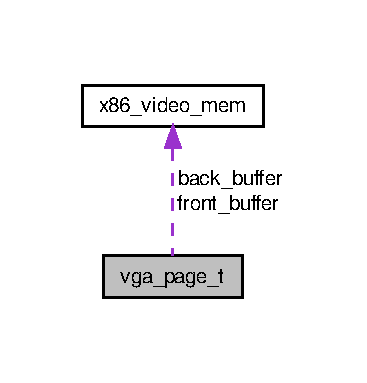
\includegraphics[width=176pt]{structvga__page__t__coll__graph}
\end{center}
\end{figure}
\subsection*{\-Champs de données}
\begin{DoxyCompactItemize}
\item 
volatile \hyperlink{structx86__video__mem}{x86\-\_\-video\-\_\-mem} $\ast$ \hyperlink{structvga__page__t_a8f820f9799bc5f9886e9f74c09e24841}{front\-\_\-buffer}
\item 
volatile \hyperlink{structx86__video__mem}{x86\-\_\-video\-\_\-mem} $\ast$ \hyperlink{structvga__page__t_aaad0350a467498fb34a0b8b1586ac76c}{back\-\_\-buffer}
\end{DoxyCompactItemize}


\subsection{\-Documentation des champs}
\hypertarget{structvga__page__t_aaad0350a467498fb34a0b8b1586ac76c}{\index{vga\-\_\-page\-\_\-t@{vga\-\_\-page\-\_\-t}!back\-\_\-buffer@{back\-\_\-buffer}}
\index{back\-\_\-buffer@{back\-\_\-buffer}!vga_page_t@{vga\-\_\-page\-\_\-t}}
\subsubsection[{back\-\_\-buffer}]{\setlength{\rightskip}{0pt plus 5cm}volatile {\bf x86\-\_\-video\-\_\-mem}$\ast$ {\bf vga\-\_\-page\-\_\-t\-::back\-\_\-buffer}}}\label{structvga__page__t_aaad0350a467498fb34a0b8b1586ac76c}
\-Adresse du buffer au second plan. \hypertarget{structvga__page__t_a8f820f9799bc5f9886e9f74c09e24841}{\index{vga\-\_\-page\-\_\-t@{vga\-\_\-page\-\_\-t}!front\-\_\-buffer@{front\-\_\-buffer}}
\index{front\-\_\-buffer@{front\-\_\-buffer}!vga_page_t@{vga\-\_\-page\-\_\-t}}
\subsubsection[{front\-\_\-buffer}]{\setlength{\rightskip}{0pt plus 5cm}volatile {\bf x86\-\_\-video\-\_\-mem}$\ast$ {\bf vga\-\_\-page\-\_\-t\-::front\-\_\-buffer}}}\label{structvga__page__t_a8f820f9799bc5f9886e9f74c09e24841}
\-Adresse du buffer au premier plan. 

\-La documentation de cette structure a été générée à partir du fichier suivant \-:\begin{DoxyCompactItemize}
\item 
kernel/include/drivers/\hyperlink{video_8h}{video.\-h}\end{DoxyCompactItemize}

\hypertarget{structvirtual__mem}{\section{Référence de la structure virtual\+\_\+mem}
\label{structvirtual__mem}\index{virtual\+\_\+mem@{virtual\+\_\+mem}}
}


Graphe de collaboration de virtual\+\_\+mem\+:
\nopagebreak
\begin{figure}[H]
\begin{center}
\leavevmode
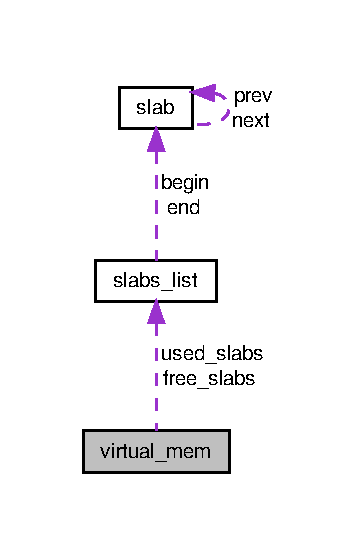
\includegraphics[width=173pt]{structvirtual__mem__coll__graph}
\end{center}
\end{figure}
\subsection*{Champs de données}
\begin{DoxyCompactItemize}
\item 
\hypertarget{structvirtual__mem_adcb73dfea437cbc9c6911baedb91d3dd}{struct \hyperlink{structslabs__list}{slabs\+\_\+list} {\bfseries free\+\_\+slabs}}\label{structvirtual__mem_adcb73dfea437cbc9c6911baedb91d3dd}

\item 
\hypertarget{structvirtual__mem_ac177ad8be832516407d193f3d2db1c8b}{struct \hyperlink{structslabs__list}{slabs\+\_\+list} {\bfseries used\+\_\+slabs}}\label{structvirtual__mem_ac177ad8be832516407d193f3d2db1c8b}

\item 
\hypertarget{structvirtual__mem_af1599d90363d908a7e2e50d3fa1cb640}{\hyperlink{kernel_2include_2types_8h_a53428b953a0ae6fba02a5b3596c867e0}{vaddr\+\_\+t} {\bfseries vmm\+\_\+top}}\label{structvirtual__mem_af1599d90363d908a7e2e50d3fa1cb640}

\end{DoxyCompactItemize}


La documentation de cette structure a été générée à partir du fichier suivant \+:\begin{DoxyCompactItemize}
\item 
kernel/include/\hyperlink{vmm_8h}{vmm.\+h}\end{DoxyCompactItemize}

\hypertarget{structwinsize}{\section{\-Référence de la structure winsize}
\label{structwinsize}\index{winsize@{winsize}}
}
\subsection*{\-Champs de données}
\begin{DoxyCompactItemize}
\item 
\hypertarget{structwinsize_a73698fa1d966374b0701e4bf225f0141}{unsigned short {\bfseries ws\-\_\-row}}\label{structwinsize_a73698fa1d966374b0701e4bf225f0141}

\item 
\hypertarget{structwinsize_a80bedf71a49fd324e0d92d0702cc7005}{unsigned short {\bfseries ws\-\_\-col}}\label{structwinsize_a80bedf71a49fd324e0d92d0702cc7005}

\end{DoxyCompactItemize}


\-La documentation de cette structure a été générée à partir du fichier suivant \-:\begin{DoxyCompactItemize}
\item 
kernel/include/\hyperlink{tty_8h}{tty.\-h}\end{DoxyCompactItemize}

\hypertarget{structx86__gdt__register}{\section{\-Référence de la structure x86\-\_\-gdt\-\_\-register}
\label{structx86__gdt__register}\index{x86\-\_\-gdt\-\_\-register@{x86\-\_\-gdt\-\_\-register}}
}
\subsection*{\-Champs de données}
\begin{DoxyCompactItemize}
\item 
\hyperlink{types_8h_adf4d876453337156dde61095e1f20223}{uint16\-\_\-t} \hyperlink{structx86__gdt__register_a5ac6bc1b04f7fa971f8033af65ed1da0}{limit}
\item 
\hyperlink{types_8h_a33594304e786b158f3fb30289278f5af}{uint32\-\_\-t} \hyperlink{structx86__gdt__register_a0de89b2ba10927885a25ef7d5422af17}{base\-\_\-addr}
\end{DoxyCompactItemize}


\subsection{\-Description détaillée}
\-Registre gdt 

\subsection{\-Documentation des champs}
\hypertarget{structx86__gdt__register_a0de89b2ba10927885a25ef7d5422af17}{\index{x86\-\_\-gdt\-\_\-register@{x86\-\_\-gdt\-\_\-register}!base\-\_\-addr@{base\-\_\-addr}}
\index{base\-\_\-addr@{base\-\_\-addr}!x86_gdt_register@{x86\-\_\-gdt\-\_\-register}}
\subsubsection[{base\-\_\-addr}]{\setlength{\rightskip}{0pt plus 5cm}{\bf uint32\-\_\-t} {\bf x86\-\_\-gdt\-\_\-register\-::base\-\_\-addr}}}\label{structx86__gdt__register_a0de89b2ba10927885a25ef7d5422af17}
\-L'adresse où sont les descripteurs de segment. \hypertarget{structx86__gdt__register_a5ac6bc1b04f7fa971f8033af65ed1da0}{\index{x86\-\_\-gdt\-\_\-register@{x86\-\_\-gdt\-\_\-register}!limit@{limit}}
\index{limit@{limit}!x86_gdt_register@{x86\-\_\-gdt\-\_\-register}}
\subsubsection[{limit}]{\setlength{\rightskip}{0pt plus 5cm}{\bf uint16\-\_\-t} {\bf x86\-\_\-gdt\-\_\-register\-::limit}}}\label{structx86__gdt__register_a5ac6bc1b04f7fa971f8033af65ed1da0}
\-La taille 

\-La documentation de cette structure a été générée à partir du fichier suivant \-:\begin{DoxyCompactItemize}
\item 
kernel/\hyperlink{gdt_8c}{gdt.\-c}\end{DoxyCompactItemize}

\hypertarget{structx86__idt__entry}{\section{Référence de la structure x86\-\_\-idt\-\_\-entry}
\label{structx86__idt__entry}\index{x86\-\_\-idt\-\_\-entry@{x86\-\_\-idt\-\_\-entry}}
}


Entrée de l'I\-D\-T.  


\subsection*{Champs de données}
\begin{DoxyCompactItemize}
\item 
\hyperlink{kernel_2include_2types_8h_adf4d876453337156dde61095e1f20223}{uint16\-\_\-t} \hyperlink{structx86__idt__entry_a7efe04d7c37c746487da6d2ae5349525}{offset\-\_\-low}
\item 
\hyperlink{kernel_2include_2types_8h_adf4d876453337156dde61095e1f20223}{uint16\-\_\-t} \hyperlink{structx86__idt__entry_a47f891095976b78c547b428be1b91c87}{seg\-\_\-sel}
\item 
\hyperlink{kernel_2include_2types_8h_aba7bc1797add20fe3efdf37ced1182c5}{uint8\-\_\-t} \hyperlink{structx86__idt__entry_adb99b161a27397d74e715d962b1c65fa}{reserved}\-:5
\item 
\hyperlink{kernel_2include_2types_8h_aba7bc1797add20fe3efdf37ced1182c5}{uint8\-\_\-t} \hyperlink{structx86__idt__entry_af0ce23f490bcc54f41c3710ab6433786}{flags}\-:3
\item 
\hyperlink{kernel_2include_2types_8h_aba7bc1797add20fe3efdf37ced1182c5}{uint8\-\_\-t} \hyperlink{structx86__idt__entry_a826ef1aafc2352576ec3493747b964f5}{type}\-:3
\item 
\hyperlink{kernel_2include_2types_8h_aba7bc1797add20fe3efdf37ced1182c5}{uint8\-\_\-t} \hyperlink{structx86__idt__entry_a58f211f10555adac756847fa46a0c856}{op\-\_\-size}\-:1
\item 
\hyperlink{kernel_2include_2types_8h_aba7bc1797add20fe3efdf37ced1182c5}{uint8\-\_\-t} \hyperlink{structx86__idt__entry_ac291c67a44d2457bda76146d1bc5e920}{zero}\-:1
\item 
\hyperlink{kernel_2include_2types_8h_aba7bc1797add20fe3efdf37ced1182c5}{uint8\-\_\-t} \hyperlink{structx86__idt__entry_a5c0f7af9139df1e94d0c6d17dcd0fb66}{dpl}\-:2
\item 
\hyperlink{kernel_2include_2types_8h_aba7bc1797add20fe3efdf37ced1182c5}{uint8\-\_\-t} \hyperlink{structx86__idt__entry_aad5f9c737cf3c83abf7f5561acaa0891}{present}\-:1
\item 
\hyperlink{kernel_2include_2types_8h_adf4d876453337156dde61095e1f20223}{uint16\-\_\-t} \hyperlink{structx86__idt__entry_a0206c9a35f101b3cc450fce405df1c0e}{offset\-\_\-high}
\end{DoxyCompactItemize}


\subsection{Documentation des champs}
\hypertarget{structx86__idt__entry_a5c0f7af9139df1e94d0c6d17dcd0fb66}{\index{x86\-\_\-idt\-\_\-entry@{x86\-\_\-idt\-\_\-entry}!dpl@{dpl}}
\index{dpl@{dpl}!x86_idt_entry@{x86\-\_\-idt\-\_\-entry}}
\subsubsection[{dpl}]{\setlength{\rightskip}{0pt plus 5cm}{\bf uint8\-\_\-t} x86\-\_\-idt\-\_\-entry\-::dpl}}\label{structx86__idt__entry_a5c0f7af9139df1e94d0c6d17dcd0fb66}
14..13 (niveau de privilège, 0 = superviseur, 3 = applicatif \hypertarget{structx86__idt__entry_af0ce23f490bcc54f41c3710ab6433786}{\index{x86\-\_\-idt\-\_\-entry@{x86\-\_\-idt\-\_\-entry}!flags@{flags}}
\index{flags@{flags}!x86_idt_entry@{x86\-\_\-idt\-\_\-entry}}
\subsubsection[{flags}]{\setlength{\rightskip}{0pt plus 5cm}{\bf uint8\-\_\-t} x86\-\_\-idt\-\_\-entry\-::flags}}\label{structx86__idt__entry_af0ce23f490bcc54f41c3710ab6433786}
7..5 (unused) \hypertarget{structx86__idt__entry_a0206c9a35f101b3cc450fce405df1c0e}{\index{x86\-\_\-idt\-\_\-entry@{x86\-\_\-idt\-\_\-entry}!offset\-\_\-high@{offset\-\_\-high}}
\index{offset\-\_\-high@{offset\-\_\-high}!x86_idt_entry@{x86\-\_\-idt\-\_\-entry}}
\subsubsection[{offset\-\_\-high}]{\setlength{\rightskip}{0pt plus 5cm}{\bf uint16\-\_\-t} x86\-\_\-idt\-\_\-entry\-::offset\-\_\-high}}\label{structx86__idt__entry_a0206c9a35f101b3cc450fce405df1c0e}
31..16 \hypertarget{structx86__idt__entry_a7efe04d7c37c746487da6d2ae5349525}{\index{x86\-\_\-idt\-\_\-entry@{x86\-\_\-idt\-\_\-entry}!offset\-\_\-low@{offset\-\_\-low}}
\index{offset\-\_\-low@{offset\-\_\-low}!x86_idt_entry@{x86\-\_\-idt\-\_\-entry}}
\subsubsection[{offset\-\_\-low}]{\setlength{\rightskip}{0pt plus 5cm}{\bf uint16\-\_\-t} x86\-\_\-idt\-\_\-entry\-::offset\-\_\-low}}\label{structx86__idt__entry_a7efe04d7c37c746487da6d2ae5349525}
15..0, offset of the routine in the segment \hypertarget{structx86__idt__entry_a58f211f10555adac756847fa46a0c856}{\index{x86\-\_\-idt\-\_\-entry@{x86\-\_\-idt\-\_\-entry}!op\-\_\-size@{op\-\_\-size}}
\index{op\-\_\-size@{op\-\_\-size}!x86_idt_entry@{x86\-\_\-idt\-\_\-entry}}
\subsubsection[{op\-\_\-size}]{\setlength{\rightskip}{0pt plus 5cm}{\bf uint8\-\_\-t} x86\-\_\-idt\-\_\-entry\-::op\-\_\-size}}\label{structx86__idt__entry_a58f211f10555adac756847fa46a0c856}
11 (0=16bits instructions, 1=32bits instr.) \hypertarget{structx86__idt__entry_aad5f9c737cf3c83abf7f5561acaa0891}{\index{x86\-\_\-idt\-\_\-entry@{x86\-\_\-idt\-\_\-entry}!present@{present}}
\index{present@{present}!x86_idt_entry@{x86\-\_\-idt\-\_\-entry}}
\subsubsection[{present}]{\setlength{\rightskip}{0pt plus 5cm}{\bf uint8\-\_\-t} x86\-\_\-idt\-\_\-entry\-::present}}\label{structx86__idt__entry_aad5f9c737cf3c83abf7f5561acaa0891}
15 (0 =$>$ Pas configuré) \hypertarget{structx86__idt__entry_adb99b161a27397d74e715d962b1c65fa}{\index{x86\-\_\-idt\-\_\-entry@{x86\-\_\-idt\-\_\-entry}!reserved@{reserved}}
\index{reserved@{reserved}!x86_idt_entry@{x86\-\_\-idt\-\_\-entry}}
\subsubsection[{reserved}]{\setlength{\rightskip}{0pt plus 5cm}{\bf uint8\-\_\-t} x86\-\_\-idt\-\_\-entry\-::reserved}}\label{structx86__idt__entry_adb99b161a27397d74e715d962b1c65fa}
4..0 (unused) \hypertarget{structx86__idt__entry_a47f891095976b78c547b428be1b91c87}{\index{x86\-\_\-idt\-\_\-entry@{x86\-\_\-idt\-\_\-entry}!seg\-\_\-sel@{seg\-\_\-sel}}
\index{seg\-\_\-sel@{seg\-\_\-sel}!x86_idt_entry@{x86\-\_\-idt\-\_\-entry}}
\subsubsection[{seg\-\_\-sel}]{\setlength{\rightskip}{0pt plus 5cm}{\bf uint16\-\_\-t} x86\-\_\-idt\-\_\-entry\-::seg\-\_\-sel}}\label{structx86__idt__entry_a47f891095976b78c547b428be1b91c87}
31..16, the I\-D of the segment \hypertarget{structx86__idt__entry_a826ef1aafc2352576ec3493747b964f5}{\index{x86\-\_\-idt\-\_\-entry@{x86\-\_\-idt\-\_\-entry}!type@{type}}
\index{type@{type}!x86_idt_entry@{x86\-\_\-idt\-\_\-entry}}
\subsubsection[{type}]{\setlength{\rightskip}{0pt plus 5cm}{\bf uint8\-\_\-t} x86\-\_\-idt\-\_\-entry\-::type}}\label{structx86__idt__entry_a826ef1aafc2352576ec3493747b964f5}
10..8 (task gate 101, interrupt gate 110, trap gate 111...) \hypertarget{structx86__idt__entry_ac291c67a44d2457bda76146d1bc5e920}{\index{x86\-\_\-idt\-\_\-entry@{x86\-\_\-idt\-\_\-entry}!zero@{zero}}
\index{zero@{zero}!x86_idt_entry@{x86\-\_\-idt\-\_\-entry}}
\subsubsection[{zero}]{\setlength{\rightskip}{0pt plus 5cm}{\bf uint8\-\_\-t} x86\-\_\-idt\-\_\-entry\-::zero}}\label{structx86__idt__entry_ac291c67a44d2457bda76146d1bc5e920}
12 \-: Segment système 

La documentation de cette structure a été générée à partir du fichier suivant \-:\begin{DoxyCompactItemize}
\item 
kernel/\hyperlink{idt_8c}{idt.\-c}\end{DoxyCompactItemize}

\hypertarget{structx86__idt__register}{\section{\-Référence de la structure x86\-\_\-idt\-\_\-register}
\label{structx86__idt__register}\index{x86\-\_\-idt\-\_\-register@{x86\-\_\-idt\-\_\-register}}
}
\subsection*{\-Champs de données}
\begin{DoxyCompactItemize}
\item 
\hypertarget{structx86__idt__register_a878dd6a2fb1aa955b37503ce2274e7a3}{\hyperlink{types_8h_adf4d876453337156dde61095e1f20223}{uint16\-\_\-t} {\bfseries limit}}\label{structx86__idt__register_a878dd6a2fb1aa955b37503ce2274e7a3}

\item 
\hypertarget{structx86__idt__register_afeba61ff8d33d1ef334cc122fa14f908}{\hyperlink{types_8h_a33594304e786b158f3fb30289278f5af}{uint32\-\_\-t} {\bfseries base\-\_\-addr}}\label{structx86__idt__register_afeba61ff8d33d1ef334cc122fa14f908}

\end{DoxyCompactItemize}


\-La documentation de cette structure a été générée à partir du fichier suivant \-:\begin{DoxyCompactItemize}
\item 
kernel/\hyperlink{idt_8c}{idt.\-c}\end{DoxyCompactItemize}

\hypertarget{structx86__segment__descriptor}{\section{\-Référence de la structure x86\-\_\-segment\-\_\-descriptor}
\label{structx86__segment__descriptor}\index{x86\-\_\-segment\-\_\-descriptor@{x86\-\_\-segment\-\_\-descriptor}}
}


\-Segment \-Descriptor (cf doc intel v3. 3.\-4.\-3)  




{\ttfamily \#include $<$gdt.\-h$>$}

\subsection*{\-Champs de données}
\begin{DoxyCompactItemize}
\item 
\hyperlink{types_8h_adf4d876453337156dde61095e1f20223}{uint16\-\_\-t} \hyperlink{structx86__segment__descriptor_af9516f6d07c24ddedde31235b05b62c2}{segment\-\_\-limit\-\_\-15\-\_\-0}
\item 
\hypertarget{structx86__segment__descriptor_a6cd0f49e21060fadba677c3b41685ebf}{\hyperlink{types_8h_adf4d876453337156dde61095e1f20223}{uint16\-\_\-t} {\bfseries base\-\_\-address\-\_\-15\-\_\-0}}\label{structx86__segment__descriptor_a6cd0f49e21060fadba677c3b41685ebf}

\item 
\hyperlink{types_8h_aba7bc1797add20fe3efdf37ced1182c5}{uint8\-\_\-t} \hyperlink{structx86__segment__descriptor_a95889fcbabf116ba15a6cea3364b903d}{base\-\_\-address\-\_\-23\-\_\-16}
\item 
\hyperlink{types_8h_aba7bc1797add20fe3efdf37ced1182c5}{uint8\-\_\-t} \hyperlink{structx86__segment__descriptor_ab3ef0c9fce1e74ee6549bbce5ea6f25f}{segment\-\_\-type}\-:4
\item 
\hyperlink{types_8h_aba7bc1797add20fe3efdf37ced1182c5}{uint8\-\_\-t} \hyperlink{structx86__segment__descriptor_adda0434239b7e6c6a68b8e7556e4bb2f}{descriptor\-\_\-type}\-:1
\item 
\hyperlink{types_8h_aba7bc1797add20fe3efdf37ced1182c5}{uint8\-\_\-t} \hyperlink{structx86__segment__descriptor_ab45e49c27bbe57a568d914bd13e45ef7}{dpl}\-:2
\item 
\hyperlink{types_8h_aba7bc1797add20fe3efdf37ced1182c5}{uint8\-\_\-t} \hyperlink{structx86__segment__descriptor_ad4196191d05e69b42272a411a69d1eae}{present}\-:1
\item 
\hyperlink{types_8h_aba7bc1797add20fe3efdf37ced1182c5}{uint8\-\_\-t} \hyperlink{structx86__segment__descriptor_a6ab37b8f7730fe67af946725a3dd064a}{segment\-\_\-limit\-\_\-19\-\_\-16}\-:4
\item 
\hyperlink{types_8h_aba7bc1797add20fe3efdf37ced1182c5}{uint8\-\_\-t} \hyperlink{structx86__segment__descriptor_a761494a7a460e493e0d5d188a31cd052}{available}\-:1
\item 
\hyperlink{types_8h_aba7bc1797add20fe3efdf37ced1182c5}{uint8\-\_\-t} \hyperlink{structx86__segment__descriptor_a4cbd016599f85d6a2060c31d7714dbbd}{zero}\-:1
\item 
\hyperlink{types_8h_aba7bc1797add20fe3efdf37ced1182c5}{uint8\-\_\-t} \hyperlink{structx86__segment__descriptor_a40c320788bf23e3660d0def872cec94c}{operation\-\_\-size}\-:1
\item 
\hyperlink{types_8h_aba7bc1797add20fe3efdf37ced1182c5}{uint8\-\_\-t} \hyperlink{structx86__segment__descriptor_a19d5da93d41a1ec3327cbd92ace8fa08}{granularity}\-:1
\item 
\hyperlink{types_8h_aba7bc1797add20fe3efdf37ced1182c5}{uint8\-\_\-t} \hyperlink{structx86__segment__descriptor_af839dd21992c16573ea5b816b72f249f}{base\-\_\-address\-\_\-31\-\_\-24}
\end{DoxyCompactItemize}


\subsection{\-Documentation des champs}
\hypertarget{structx86__segment__descriptor_a761494a7a460e493e0d5d188a31cd052}{\index{x86\-\_\-segment\-\_\-descriptor@{x86\-\_\-segment\-\_\-descriptor}!available@{available}}
\index{available@{available}!x86_segment_descriptor@{x86\-\_\-segment\-\_\-descriptor}}
\subsubsection[{available}]{\setlength{\rightskip}{0pt plus 5cm}{\bf uint8\-\_\-t} {\bf x86\-\_\-segment\-\_\-descriptor\-::available}}}\label{structx86__segment__descriptor_a761494a7a460e493e0d5d188a31cd052}
\-Un bit disponible pour nous... \hypertarget{structx86__segment__descriptor_a95889fcbabf116ba15a6cea3364b903d}{\index{x86\-\_\-segment\-\_\-descriptor@{x86\-\_\-segment\-\_\-descriptor}!base\-\_\-address\-\_\-23\-\_\-16@{base\-\_\-address\-\_\-23\-\_\-16}}
\index{base\-\_\-address\-\_\-23\-\_\-16@{base\-\_\-address\-\_\-23\-\_\-16}!x86_segment_descriptor@{x86\-\_\-segment\-\_\-descriptor}}
\subsubsection[{base\-\_\-address\-\_\-23\-\_\-16}]{\setlength{\rightskip}{0pt plus 5cm}{\bf uint8\-\_\-t} {\bf x86\-\_\-segment\-\_\-descriptor\-::base\-\_\-address\-\_\-23\-\_\-16}}}\label{structx86__segment__descriptor_a95889fcbabf116ba15a6cea3364b903d}
\-Suite de la base address. \hypertarget{structx86__segment__descriptor_af839dd21992c16573ea5b816b72f249f}{\index{x86\-\_\-segment\-\_\-descriptor@{x86\-\_\-segment\-\_\-descriptor}!base\-\_\-address\-\_\-31\-\_\-24@{base\-\_\-address\-\_\-31\-\_\-24}}
\index{base\-\_\-address\-\_\-31\-\_\-24@{base\-\_\-address\-\_\-31\-\_\-24}!x86_segment_descriptor@{x86\-\_\-segment\-\_\-descriptor}}
\subsubsection[{base\-\_\-address\-\_\-31\-\_\-24}]{\setlength{\rightskip}{0pt plus 5cm}{\bf uint8\-\_\-t} {\bf x86\-\_\-segment\-\_\-descriptor\-::base\-\_\-address\-\_\-31\-\_\-24}}}\label{structx86__segment__descriptor_af839dd21992c16573ea5b816b72f249f}
\-Fin de la base address. \-Soit 32 bits ce qui correspond aux 4\-Gio adressables. \hypertarget{structx86__segment__descriptor_adda0434239b7e6c6a68b8e7556e4bb2f}{\index{x86\-\_\-segment\-\_\-descriptor@{x86\-\_\-segment\-\_\-descriptor}!descriptor\-\_\-type@{descriptor\-\_\-type}}
\index{descriptor\-\_\-type@{descriptor\-\_\-type}!x86_segment_descriptor@{x86\-\_\-segment\-\_\-descriptor}}
\subsubsection[{descriptor\-\_\-type}]{\setlength{\rightskip}{0pt plus 5cm}{\bf uint8\-\_\-t} {\bf x86\-\_\-segment\-\_\-descriptor\-::descriptor\-\_\-type}}}\label{structx86__segment__descriptor_adda0434239b7e6c6a68b8e7556e4bb2f}
0 = system segment, 1 = code ou data segment \hypertarget{structx86__segment__descriptor_ab45e49c27bbe57a568d914bd13e45ef7}{\index{x86\-\_\-segment\-\_\-descriptor@{x86\-\_\-segment\-\_\-descriptor}!dpl@{dpl}}
\index{dpl@{dpl}!x86_segment_descriptor@{x86\-\_\-segment\-\_\-descriptor}}
\subsubsection[{dpl}]{\setlength{\rightskip}{0pt plus 5cm}{\bf uint8\-\_\-t} {\bf x86\-\_\-segment\-\_\-descriptor\-::dpl}}}\label{structx86__segment__descriptor_ab45e49c27bbe57a568d914bd13e45ef7}
\-Descriptor \-Privilege \-Level. 0 à 3. 0 pour le kernel et 3 pour les applis \hypertarget{structx86__segment__descriptor_a19d5da93d41a1ec3327cbd92ace8fa08}{\index{x86\-\_\-segment\-\_\-descriptor@{x86\-\_\-segment\-\_\-descriptor}!granularity@{granularity}}
\index{granularity@{granularity}!x86_segment_descriptor@{x86\-\_\-segment\-\_\-descriptor}}
\subsubsection[{granularity}]{\setlength{\rightskip}{0pt plus 5cm}{\bf uint8\-\_\-t} {\bf x86\-\_\-segment\-\_\-descriptor\-::granularity}}}\label{structx86__segment__descriptor_a19d5da93d41a1ec3327cbd92ace8fa08}
\-Granularité \-: \-Détermine l'échele du segment limit. 0 \-: c'est des bytes, 1 \-: c'est par 4kio \hypertarget{structx86__segment__descriptor_a40c320788bf23e3660d0def872cec94c}{\index{x86\-\_\-segment\-\_\-descriptor@{x86\-\_\-segment\-\_\-descriptor}!operation\-\_\-size@{operation\-\_\-size}}
\index{operation\-\_\-size@{operation\-\_\-size}!x86_segment_descriptor@{x86\-\_\-segment\-\_\-descriptor}}
\subsubsection[{operation\-\_\-size}]{\setlength{\rightskip}{0pt plus 5cm}{\bf uint8\-\_\-t} {\bf x86\-\_\-segment\-\_\-descriptor\-::operation\-\_\-size}}}\label{structx86__segment__descriptor_a40c320788bf23e3660d0def872cec94c}
0 = 16bits, 1 = 32bits \hypertarget{structx86__segment__descriptor_ad4196191d05e69b42272a411a69d1eae}{\index{x86\-\_\-segment\-\_\-descriptor@{x86\-\_\-segment\-\_\-descriptor}!present@{present}}
\index{present@{present}!x86_segment_descriptor@{x86\-\_\-segment\-\_\-descriptor}}
\subsubsection[{present}]{\setlength{\rightskip}{0pt plus 5cm}{\bf uint8\-\_\-t} {\bf x86\-\_\-segment\-\_\-descriptor\-::present}}}\label{structx86__segment__descriptor_ad4196191d05e69b42272a411a69d1eae}
\-Indique si le segment est présent en mémoire (1) ou non (0) \hypertarget{structx86__segment__descriptor_af9516f6d07c24ddedde31235b05b62c2}{\index{x86\-\_\-segment\-\_\-descriptor@{x86\-\_\-segment\-\_\-descriptor}!segment\-\_\-limit\-\_\-15\-\_\-0@{segment\-\_\-limit\-\_\-15\-\_\-0}}
\index{segment\-\_\-limit\-\_\-15\-\_\-0@{segment\-\_\-limit\-\_\-15\-\_\-0}!x86_segment_descriptor@{x86\-\_\-segment\-\_\-descriptor}}
\subsubsection[{segment\-\_\-limit\-\_\-15\-\_\-0}]{\setlength{\rightskip}{0pt plus 5cm}{\bf uint16\-\_\-t} {\bf x86\-\_\-segment\-\_\-descriptor\-::segment\-\_\-limit\-\_\-15\-\_\-0}}}\label{structx86__segment__descriptor_af9516f6d07c24ddedde31235b05b62c2}
\-Segment \-Limit 15\-:00. \-Spécifie la taille du segment. \-Le proc concatene les 2 champs segment limit pour former une valeur de 20 bits. \hypertarget{structx86__segment__descriptor_a6ab37b8f7730fe67af946725a3dd064a}{\index{x86\-\_\-segment\-\_\-descriptor@{x86\-\_\-segment\-\_\-descriptor}!segment\-\_\-limit\-\_\-19\-\_\-16@{segment\-\_\-limit\-\_\-19\-\_\-16}}
\index{segment\-\_\-limit\-\_\-19\-\_\-16@{segment\-\_\-limit\-\_\-19\-\_\-16}!x86_segment_descriptor@{x86\-\_\-segment\-\_\-descriptor}}
\subsubsection[{segment\-\_\-limit\-\_\-19\-\_\-16}]{\setlength{\rightskip}{0pt plus 5cm}{\bf uint8\-\_\-t} {\bf x86\-\_\-segment\-\_\-descriptor\-::segment\-\_\-limit\-\_\-19\-\_\-16}}}\label{structx86__segment__descriptor_a6ab37b8f7730fe67af946725a3dd064a}
\-Suite du segment limit. \hypertarget{structx86__segment__descriptor_ab3ef0c9fce1e74ee6549bbce5ea6f25f}{\index{x86\-\_\-segment\-\_\-descriptor@{x86\-\_\-segment\-\_\-descriptor}!segment\-\_\-type@{segment\-\_\-type}}
\index{segment\-\_\-type@{segment\-\_\-type}!x86_segment_descriptor@{x86\-\_\-segment\-\_\-descriptor}}
\subsubsection[{segment\-\_\-type}]{\setlength{\rightskip}{0pt plus 5cm}{\bf uint8\-\_\-t} {\bf x86\-\_\-segment\-\_\-descriptor\-::segment\-\_\-type}}}\label{structx86__segment__descriptor_ab3ef0c9fce1e74ee6549bbce5ea6f25f}
\-Cf 3.\-4.\-3.\-1 de la doc intel ! \hypertarget{structx86__segment__descriptor_a4cbd016599f85d6a2060c31d7714dbbd}{\index{x86\-\_\-segment\-\_\-descriptor@{x86\-\_\-segment\-\_\-descriptor}!zero@{zero}}
\index{zero@{zero}!x86_segment_descriptor@{x86\-\_\-segment\-\_\-descriptor}}
\subsubsection[{zero}]{\setlength{\rightskip}{0pt plus 5cm}{\bf uint8\-\_\-t} {\bf x86\-\_\-segment\-\_\-descriptor\-::zero}}}\label{structx86__segment__descriptor_a4cbd016599f85d6a2060c31d7714dbbd}
\-Bit réservé qui doit prendre la valeur 0. 

\-La documentation de cette structure a été générée à partir du fichier suivant \-:\begin{DoxyCompactItemize}
\item 
kernel/include/\hyperlink{gdt_8h}{gdt.\-h}\end{DoxyCompactItemize}

\hypertarget{structx86__video__mem}{\section{Référence de la structure x86\+\_\+video\+\_\+mem}
\label{structx86__video__mem}\index{x86\+\_\+video\+\_\+mem@{x86\+\_\+video\+\_\+mem}}
}


Structure définissant un \char`\"{}caractère\char`\"{} à l'écran.  




{\ttfamily \#include $<$video.\+h$>$}

\subsection*{Champs de données}
\begin{DoxyCompactItemize}
\item 
unsigned char \hyperlink{structx86__video__mem_a806c83cac2d0536c833f810347f5539a}{character}
\item 
unsigned char \hyperlink{structx86__video__mem_ab513d18ce9ef33e2d22e426973fd7417}{attribute}
\end{DoxyCompactItemize}


\subsection{Documentation des champs}
\hypertarget{structx86__video__mem_ab513d18ce9ef33e2d22e426973fd7417}{\index{x86\+\_\+video\+\_\+mem@{x86\+\_\+video\+\_\+mem}!attribute@{attribute}}
\index{attribute@{attribute}!x86\+\_\+video\+\_\+mem@{x86\+\_\+video\+\_\+mem}}
\subsubsection[{attribute}]{\setlength{\rightskip}{0pt plus 5cm}unsigned char x86\+\_\+video\+\_\+mem\+::attribute}}\label{structx86__video__mem_ab513d18ce9ef33e2d22e426973fd7417}
Attribut qui permet de définir la couleur \+: \mbox{[}blink(1)$\vert$\+Background(3)$\vert$foreground(4)\mbox{]} \hypertarget{structx86__video__mem_a806c83cac2d0536c833f810347f5539a}{\index{x86\+\_\+video\+\_\+mem@{x86\+\_\+video\+\_\+mem}!character@{character}}
\index{character@{character}!x86\+\_\+video\+\_\+mem@{x86\+\_\+video\+\_\+mem}}
\subsubsection[{character}]{\setlength{\rightskip}{0pt plus 5cm}unsigned char x86\+\_\+video\+\_\+mem\+::character}}\label{structx86__video__mem_a806c83cac2d0536c833f810347f5539a}
Code A\+S\+C\+I\+I du caractère. 

La documentation de cette structure a été générée à partir du fichier suivant \+:\begin{DoxyCompactItemize}
\item 
kernel/include/drivers/\hyperlink{video_8h}{video.\+h}\end{DoxyCompactItemize}

\chapter{Documentation des fichiers}
\hypertarget{clock_8c}{\section{Référence du fichier kernel/clock.c}
\label{clock_8c}\index{kernel/clock.\-c@{kernel/clock.\-c}}
}


Gestion de l'horloge et du temps en général.  


{\ttfamily \#include $<$types.\-h$>$}\\*
{\ttfamily \#include $<$ioports.\-h$>$}\\*
{\ttfamily \#include $<$i8254.\-h$>$}\\*
{\ttfamily \#include $<$clock.\-h$>$}\\*
{\ttfamily \#include $<$interrupts.\-h$>$}\\*
{\ttfamily \#include $<$kstdio.\-h$>$}\\*
{\ttfamily \#include $<$klibc/limits.\-h$>$}\\*
{\ttfamily \#include \char`\"{}heap.\-h\char`\"{}}\\*
Graphe des dépendances par inclusion de clock.\-c\-:\nopagebreak
\begin{figure}[H]
\begin{center}
\leavevmode
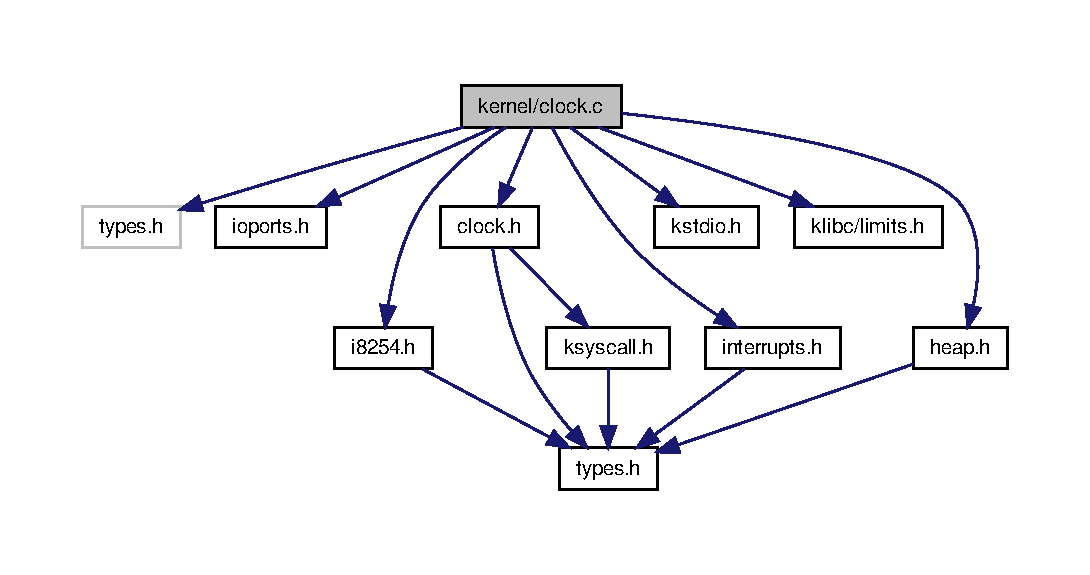
\includegraphics[width=350pt]{clock_8c__incl}
\end{center}
\end{figure}
\subsection*{Macros}
\begin{DoxyCompactItemize}
\item 
\#define \hyperlink{clock_8c_a59fb9be7a7d728632cdb9553ec759102}{R\-T\-C\-\_\-\-R\-E\-Q\-U\-E\-S\-T}~0x70
\item 
\#define \hyperlink{clock_8c_a9e8ea3cf4245155349bed1cea2590792}{R\-T\-C\-\_\-\-A\-N\-S\-W\-E\-R}~0x71
\item 
\#define \hyperlink{clock_8c_a777f67a779626b4d69b3eb4b4f5b6305}{R\-T\-C\-\_\-\-S\-E\-C\-O\-N\-D}~0x00
\item 
\#define \hyperlink{clock_8c_a4f6fb35439604f172b4eb075f62e9a24}{R\-T\-C\-\_\-\-S\-E\-C\-O\-N\-D\-\_\-\-A\-L\-A\-R\-M}~0x01
\item 
\#define \hyperlink{clock_8c_afdd30426a2ccab4daa054d7999e3d856}{R\-T\-C\-\_\-\-M\-I\-N\-U\-T\-E}~0x02
\item 
\#define \hyperlink{clock_8c_ad8d654d2fb65cf3a3241fd1730bc7838}{R\-T\-C\-\_\-\-M\-I\-N\-U\-T\-E\-\_\-\-A\-L\-A\-R\-M}~0x03
\item 
\#define \hyperlink{clock_8c_a7264eac87ffc91cbdea1239d346a0ea4}{R\-T\-C\-\_\-\-H\-O\-U\-R}~0x04
\item 
\#define \hyperlink{clock_8c_a737b5ee081f79807f221932a06d7efca}{R\-T\-C\-\_\-\-H\-O\-U\-R\-\_\-\-A\-L\-A\-R\-M}~0x05
\item 
\#define \hyperlink{clock_8c_adc8a8bbebc2c39de86f9be71c257859b}{R\-T\-C\-\_\-\-D\-A\-Y\-\_\-\-O\-F\-\_\-\-W\-E\-E\-K}~0x06
\item 
\#define \hyperlink{clock_8c_a9d8502fb2abae7b9f234c7da90932f3d}{R\-T\-C\-\_\-\-D\-A\-T\-E\-\_\-\-O\-F\-\_\-\-M\-O\-N\-T\-H}~0x07
\item 
\#define \hyperlink{clock_8c_abda0c877ee1a02b8351c0cfe72838088}{R\-T\-C\-\_\-\-M\-O\-N\-T\-H}~0x08
\item 
\#define \hyperlink{clock_8c_a1df5568e6774b73aa4c6e59fc40e9147}{R\-T\-C\-\_\-\-Y\-E\-A\-R}~0x09
\item 
\#define \hyperlink{clock_8c_a3ac65777322869d89cd0cbb9ba3c165c}{L\-E\-A\-P\-Y\-E\-A\-R}(year)~(!((year) \% 4) \&\& (((year) \% 100) $|$$|$ !((year) \% 400)))
\item 
\#define \hyperlink{clock_8c_a9db507ef8c3ce0d32650da0f0a7e5b48}{Y\-E\-A\-R\-S\-I\-Z\-E}(year)~(\hyperlink{clock_8c_a3ac65777322869d89cd0cbb9ba3c165c}{L\-E\-A\-P\-Y\-E\-A\-R}(year) ? 366 \-: 365)
\item 
\#define \hyperlink{clock_8c_acb20471223b4d330209e1ff1950c999d}{Y\-E\-A\-R0}~1900
\item 
\#define \hyperlink{clock_8c_a2cd69e03a0d15e6115c196f7ac35da13}{E\-P\-O\-C\-H\-\_\-\-Y\-R}~1970
\item 
\#define \hyperlink{clock_8c_a69917c6f775aefa006141379c81e0e8f}{S\-E\-C\-S\-\_\-\-D\-A\-Y}~(24\-L $\ast$ 60\-L $\ast$ 60\-L)
\item 
\#define \hyperlink{clock_8c_a0540485394df82add6b7c4f2137c7f21}{T\-I\-M\-E\-\_\-\-M\-A\-X}~0x\-F\-F\-F\-F\-F\-F\-F\-F\-L
\end{DoxyCompactItemize}
\subsection*{Fonctions}
\begin{DoxyCompactItemize}
\item 
\hypertarget{clock_8c_abc0cc7974581cee0900c817955ff2f5b}{void \hyperlink{clock_8c_abc0cc7974581cee0900c817955ff2f5b}{clock\-\_\-tick} ()}\label{clock_8c_abc0cc7974581cee0900c817955ff2f5b}

\begin{DoxyCompactList}\small\item\em Incrémente le temps système. Ajoute une milliseconde au temps système, ne met rien à jour au dela du jour actuel. \end{DoxyCompactList}\item 
\hypertarget{clock_8c_aa2217dd848bce59e4c4635650a0beee4}{\hyperlink{types_8h_aba7bc1797add20fe3efdf37ced1182c5}{uint8\-\_\-t} {\bfseries bcd2binary} (\hyperlink{types_8h_aba7bc1797add20fe3efdf37ced1182c5}{uint8\-\_\-t} n)}\label{clock_8c_aa2217dd848bce59e4c4635650a0beee4}

\item 
time\-\_\-t \hyperlink{clock_8c_ab07bd3e86ff449c65b06fd50ec8e422e}{clock\-\_\-mktime} (struct \hyperlink{structtm}{tm} $\ast$timep)
\begin{DoxyCompactList}\small\item\em Conversion struct tm vers time\-\_\-t. Conversion d'une date exprimée sous la forme secondes, minutes, heures, jour, mois, année, etc, vers le format time\-\_\-t. \end{DoxyCompactList}\item 
\hypertarget{clock_8c_ae9cc0a879e88eea28e4e8b57318ef8e5}{void \hyperlink{clock_8c_ae9cc0a879e88eea28e4e8b57318ef8e5}{clock\-\_\-init} ()}\label{clock_8c_ae9cc0a879e88eea28e4e8b57318ef8e5}

\begin{DoxyCompactList}\small\item\em Initialisation de l'horloge. Initialisation de l'horloge. \end{DoxyCompactList}\item 
\hypertarget{clock_8c_a36d22a2c7fc11c6f382386a8b658b6f8}{clock\-\_\-t \hyperlink{clock_8c_a36d22a2c7fc11c6f382386a8b658b6f8}{get\-\_\-clock} ()}\label{clock_8c_a36d22a2c7fc11c6f382386a8b658b6f8}

\begin{DoxyCompactList}\small\item\em Retourne le temps système. Renvoie la valeur actuelle du temps système en nombre de ticks (1 tick = 1ms). \end{DoxyCompactList}\item 
\hyperlink{clock_8c_ab594b78936f7a5c4ba0c3b7ad653b6d5}{S\-Y\-S\-C\-A\-L\-L\-\_\-\-H\-A\-N\-D\-L\-E\-R1} (sys\-\_\-getclock, clock\-\_\-t $\ast$clock)
\begin{DoxyCompactList}\small\item\em Syscall handler pour get\-\_\-clock. Syscall handler pour get\-\_\-clock. \end{DoxyCompactList}\item 
time\-\_\-t \hyperlink{clock_8c_ab1bd72177a9697cdd2eec38a4fe6651e}{get\-\_\-date} ()
\begin{DoxyCompactList}\small\item\em Retourne la date actuelle en secondes. Retourne la date actuelle en secondes. \end{DoxyCompactList}\item 
\hyperlink{clock_8c_a8bfadf8175457fd7fbe6b53a46788a4e}{S\-Y\-S\-C\-A\-L\-L\-\_\-\-H\-A\-N\-D\-L\-E\-R1} (sys\-\_\-getdate, time\-\_\-t $\ast$date)
\begin{DoxyCompactList}\small\item\em Syscall handler pour get\-\_\-date. Syscall handler pour get\-\_\-date. \end{DoxyCompactList}\item 
struct \hyperlink{structtimeval}{timeval} \hyperlink{clock_8c_a0dc3166547de3bc1b9bdf45fdfb7d2e5}{get\-\_\-tv} ()
\begin{DoxyCompactList}\small\item\em Retourne date courante. Retourne une structure timeval qui contient la date courante en seconde et microsecondes. \end{DoxyCompactList}\item 
int \hyperlink{clock_8c_a33cb84a5e3ce0c59505d776e5a736c08}{compare\-\_\-times} (struct \hyperlink{structtimeval}{timeval} a, struct \hyperlink{structtimeval}{timeval} b)
\begin{DoxyCompactList}\small\item\em Comparaison de 2 temps. Comparaison de 2 temps. \end{DoxyCompactList}\item 
void \hyperlink{clock_8c_a052807a5c6ae63175a937381014a5701}{timeval\-\_\-add\-\_\-usec} (struct \hyperlink{structtimeval}{timeval} $\ast$t, time\-\_\-t usec)
\begin{DoxyCompactList}\small\item\em Ajoute des us à un temps. Ajoute des us à un temps contenu dans une structure timeval. \end{DoxyCompactList}\item 
\hypertarget{clock_8c_accc6640b25e5d278185c360538d3cc3b}{void {\bfseries klog\-\_\-systime} ()}\label{clock_8c_accc6640b25e5d278185c360538d3cc3b}

\end{DoxyCompactItemize}
\subsection*{Variables}
\begin{DoxyCompactItemize}
\item 
\hypertarget{clock_8c_a3f3af239bc4359d67b96004c530f5ce7}{time\-\_\-t {\bfseries boot\-\_\-systime}}\label{clock_8c_a3f3af239bc4359d67b96004c530f5ce7}

\item 
const int {\bfseries \-\_\-ytab} \mbox{[}2\mbox{]}\mbox{[}12\mbox{]}
\end{DoxyCompactItemize}


\subsection{Description détaillée}
\begin{DoxyAuthor}{Auteur}
Tac\-O\-S developers
\end{DoxyAuthor}
\hypertarget{vmm_8c_LICENSE}{}\subsection{L\-I\-C\-E\-N\-S\-E}\label{vmm_8c_LICENSE}
Copyright (C) 2010, 2011, 2012, 2013 -\/ Tac\-O\-S developers.

This program is free software; you can redistribute it and/or modify it under the terms of the G\-N\-U General Public License as published by the Free Software Foundation; either version 3 of the License, or (at your option) any later version.

This program is distributed in the hope that it will be useful, but W\-I\-T\-H\-O\-U\-T A\-N\-Y W\-A\-R\-R\-A\-N\-T\-Y; without even the implied warranty of M\-E\-R\-C\-H\-A\-N\-T\-A\-B\-I\-L\-I\-T\-Y or F\-I\-T\-N\-E\-S\-S F\-O\-R A P\-A\-R\-T\-I\-C\-U\-L\-A\-R P\-U\-R\-P\-O\-S\-E. See the G\-N\-U General Public License for more details at \href{http://www.gnu.org/copyleft/gpl.html}{\tt http\-://www.\-gnu.\-org/copyleft/gpl.\-html}

You should have received a copy of the G\-N\-U General Public License along with this program; if not, see \href{http://www.gnu.org/licenses}{\tt http\-://www.\-gnu.\-org/licenses}.\hypertarget{vmm_8c_DESCRIPTION}{}\subsection{D\-E\-S\-C\-R\-I\-P\-T\-I\-O\-N}\label{vmm_8c_DESCRIPTION}


\subsection{Documentation des macros}
\hypertarget{clock_8c_a2cd69e03a0d15e6115c196f7ac35da13}{\index{clock.\-c@{clock.\-c}!E\-P\-O\-C\-H\-\_\-\-Y\-R@{E\-P\-O\-C\-H\-\_\-\-Y\-R}}
\index{E\-P\-O\-C\-H\-\_\-\-Y\-R@{E\-P\-O\-C\-H\-\_\-\-Y\-R}!clock.c@{clock.\-c}}
\subsubsection[{E\-P\-O\-C\-H\-\_\-\-Y\-R}]{\setlength{\rightskip}{0pt plus 5cm}\#define E\-P\-O\-C\-H\-\_\-\-Y\-R~1970}}\label{clock_8c_a2cd69e03a0d15e6115c196f7ac35da13}
Constante pour convertir les années exprimées depuis 1970. \hypertarget{clock_8c_a3ac65777322869d89cd0cbb9ba3c165c}{\index{clock.\-c@{clock.\-c}!L\-E\-A\-P\-Y\-E\-A\-R@{L\-E\-A\-P\-Y\-E\-A\-R}}
\index{L\-E\-A\-P\-Y\-E\-A\-R@{L\-E\-A\-P\-Y\-E\-A\-R}!clock.c@{clock.\-c}}
\subsubsection[{L\-E\-A\-P\-Y\-E\-A\-R}]{\setlength{\rightskip}{0pt plus 5cm}\#define L\-E\-A\-P\-Y\-E\-A\-R(
\begin{DoxyParamCaption}
\item[{}]{year}
\end{DoxyParamCaption}
)~(!((year) \% 4) \&\& (((year) \% 100) $|$$|$ !((year) \% 400)))}}\label{clock_8c_a3ac65777322869d89cd0cbb9ba3c165c}
Macro function pour déterminer si une année est bissextile. \hypertarget{clock_8c_a9e8ea3cf4245155349bed1cea2590792}{\index{clock.\-c@{clock.\-c}!R\-T\-C\-\_\-\-A\-N\-S\-W\-E\-R@{R\-T\-C\-\_\-\-A\-N\-S\-W\-E\-R}}
\index{R\-T\-C\-\_\-\-A\-N\-S\-W\-E\-R@{R\-T\-C\-\_\-\-A\-N\-S\-W\-E\-R}!clock.c@{clock.\-c}}
\subsubsection[{R\-T\-C\-\_\-\-A\-N\-S\-W\-E\-R}]{\setlength{\rightskip}{0pt plus 5cm}\#define R\-T\-C\-\_\-\-A\-N\-S\-W\-E\-R~0x71}}\label{clock_8c_a9e8ea3cf4245155349bed1cea2590792}
R\-T\-C read/write port \hypertarget{clock_8c_a9d8502fb2abae7b9f234c7da90932f3d}{\index{clock.\-c@{clock.\-c}!R\-T\-C\-\_\-\-D\-A\-T\-E\-\_\-\-O\-F\-\_\-\-M\-O\-N\-T\-H@{R\-T\-C\-\_\-\-D\-A\-T\-E\-\_\-\-O\-F\-\_\-\-M\-O\-N\-T\-H}}
\index{R\-T\-C\-\_\-\-D\-A\-T\-E\-\_\-\-O\-F\-\_\-\-M\-O\-N\-T\-H@{R\-T\-C\-\_\-\-D\-A\-T\-E\-\_\-\-O\-F\-\_\-\-M\-O\-N\-T\-H}!clock.c@{clock.\-c}}
\subsubsection[{R\-T\-C\-\_\-\-D\-A\-T\-E\-\_\-\-O\-F\-\_\-\-M\-O\-N\-T\-H}]{\setlength{\rightskip}{0pt plus 5cm}\#define R\-T\-C\-\_\-\-D\-A\-T\-E\-\_\-\-O\-F\-\_\-\-M\-O\-N\-T\-H~0x07}}\label{clock_8c_a9d8502fb2abae7b9f234c7da90932f3d}
select day of month \hypertarget{clock_8c_adc8a8bbebc2c39de86f9be71c257859b}{\index{clock.\-c@{clock.\-c}!R\-T\-C\-\_\-\-D\-A\-Y\-\_\-\-O\-F\-\_\-\-W\-E\-E\-K@{R\-T\-C\-\_\-\-D\-A\-Y\-\_\-\-O\-F\-\_\-\-W\-E\-E\-K}}
\index{R\-T\-C\-\_\-\-D\-A\-Y\-\_\-\-O\-F\-\_\-\-W\-E\-E\-K@{R\-T\-C\-\_\-\-D\-A\-Y\-\_\-\-O\-F\-\_\-\-W\-E\-E\-K}!clock.c@{clock.\-c}}
\subsubsection[{R\-T\-C\-\_\-\-D\-A\-Y\-\_\-\-O\-F\-\_\-\-W\-E\-E\-K}]{\setlength{\rightskip}{0pt plus 5cm}\#define R\-T\-C\-\_\-\-D\-A\-Y\-\_\-\-O\-F\-\_\-\-W\-E\-E\-K~0x06}}\label{clock_8c_adc8a8bbebc2c39de86f9be71c257859b}
select day of week \hypertarget{clock_8c_a7264eac87ffc91cbdea1239d346a0ea4}{\index{clock.\-c@{clock.\-c}!R\-T\-C\-\_\-\-H\-O\-U\-R@{R\-T\-C\-\_\-\-H\-O\-U\-R}}
\index{R\-T\-C\-\_\-\-H\-O\-U\-R@{R\-T\-C\-\_\-\-H\-O\-U\-R}!clock.c@{clock.\-c}}
\subsubsection[{R\-T\-C\-\_\-\-H\-O\-U\-R}]{\setlength{\rightskip}{0pt plus 5cm}\#define R\-T\-C\-\_\-\-H\-O\-U\-R~0x04}}\label{clock_8c_a7264eac87ffc91cbdea1239d346a0ea4}
select hours \hypertarget{clock_8c_a737b5ee081f79807f221932a06d7efca}{\index{clock.\-c@{clock.\-c}!R\-T\-C\-\_\-\-H\-O\-U\-R\-\_\-\-A\-L\-A\-R\-M@{R\-T\-C\-\_\-\-H\-O\-U\-R\-\_\-\-A\-L\-A\-R\-M}}
\index{R\-T\-C\-\_\-\-H\-O\-U\-R\-\_\-\-A\-L\-A\-R\-M@{R\-T\-C\-\_\-\-H\-O\-U\-R\-\_\-\-A\-L\-A\-R\-M}!clock.c@{clock.\-c}}
\subsubsection[{R\-T\-C\-\_\-\-H\-O\-U\-R\-\_\-\-A\-L\-A\-R\-M}]{\setlength{\rightskip}{0pt plus 5cm}\#define R\-T\-C\-\_\-\-H\-O\-U\-R\-\_\-\-A\-L\-A\-R\-M~0x05}}\label{clock_8c_a737b5ee081f79807f221932a06d7efca}
select hours alarm \hypertarget{clock_8c_afdd30426a2ccab4daa054d7999e3d856}{\index{clock.\-c@{clock.\-c}!R\-T\-C\-\_\-\-M\-I\-N\-U\-T\-E@{R\-T\-C\-\_\-\-M\-I\-N\-U\-T\-E}}
\index{R\-T\-C\-\_\-\-M\-I\-N\-U\-T\-E@{R\-T\-C\-\_\-\-M\-I\-N\-U\-T\-E}!clock.c@{clock.\-c}}
\subsubsection[{R\-T\-C\-\_\-\-M\-I\-N\-U\-T\-E}]{\setlength{\rightskip}{0pt plus 5cm}\#define R\-T\-C\-\_\-\-M\-I\-N\-U\-T\-E~0x02}}\label{clock_8c_afdd30426a2ccab4daa054d7999e3d856}
select minutes \hypertarget{clock_8c_ad8d654d2fb65cf3a3241fd1730bc7838}{\index{clock.\-c@{clock.\-c}!R\-T\-C\-\_\-\-M\-I\-N\-U\-T\-E\-\_\-\-A\-L\-A\-R\-M@{R\-T\-C\-\_\-\-M\-I\-N\-U\-T\-E\-\_\-\-A\-L\-A\-R\-M}}
\index{R\-T\-C\-\_\-\-M\-I\-N\-U\-T\-E\-\_\-\-A\-L\-A\-R\-M@{R\-T\-C\-\_\-\-M\-I\-N\-U\-T\-E\-\_\-\-A\-L\-A\-R\-M}!clock.c@{clock.\-c}}
\subsubsection[{R\-T\-C\-\_\-\-M\-I\-N\-U\-T\-E\-\_\-\-A\-L\-A\-R\-M}]{\setlength{\rightskip}{0pt plus 5cm}\#define R\-T\-C\-\_\-\-M\-I\-N\-U\-T\-E\-\_\-\-A\-L\-A\-R\-M~0x03}}\label{clock_8c_ad8d654d2fb65cf3a3241fd1730bc7838}
select minutes alarm \hypertarget{clock_8c_abda0c877ee1a02b8351c0cfe72838088}{\index{clock.\-c@{clock.\-c}!R\-T\-C\-\_\-\-M\-O\-N\-T\-H@{R\-T\-C\-\_\-\-M\-O\-N\-T\-H}}
\index{R\-T\-C\-\_\-\-M\-O\-N\-T\-H@{R\-T\-C\-\_\-\-M\-O\-N\-T\-H}!clock.c@{clock.\-c}}
\subsubsection[{R\-T\-C\-\_\-\-M\-O\-N\-T\-H}]{\setlength{\rightskip}{0pt plus 5cm}\#define R\-T\-C\-\_\-\-M\-O\-N\-T\-H~0x08}}\label{clock_8c_abda0c877ee1a02b8351c0cfe72838088}
select month \hypertarget{clock_8c_a59fb9be7a7d728632cdb9553ec759102}{\index{clock.\-c@{clock.\-c}!R\-T\-C\-\_\-\-R\-E\-Q\-U\-E\-S\-T@{R\-T\-C\-\_\-\-R\-E\-Q\-U\-E\-S\-T}}
\index{R\-T\-C\-\_\-\-R\-E\-Q\-U\-E\-S\-T@{R\-T\-C\-\_\-\-R\-E\-Q\-U\-E\-S\-T}!clock.c@{clock.\-c}}
\subsubsection[{R\-T\-C\-\_\-\-R\-E\-Q\-U\-E\-S\-T}]{\setlength{\rightskip}{0pt plus 5cm}\#define R\-T\-C\-\_\-\-R\-E\-Q\-U\-E\-S\-T~0x70}}\label{clock_8c_a59fb9be7a7d728632cdb9553ec759102}
R\-T\-C select port \hypertarget{clock_8c_a777f67a779626b4d69b3eb4b4f5b6305}{\index{clock.\-c@{clock.\-c}!R\-T\-C\-\_\-\-S\-E\-C\-O\-N\-D@{R\-T\-C\-\_\-\-S\-E\-C\-O\-N\-D}}
\index{R\-T\-C\-\_\-\-S\-E\-C\-O\-N\-D@{R\-T\-C\-\_\-\-S\-E\-C\-O\-N\-D}!clock.c@{clock.\-c}}
\subsubsection[{R\-T\-C\-\_\-\-S\-E\-C\-O\-N\-D}]{\setlength{\rightskip}{0pt plus 5cm}\#define R\-T\-C\-\_\-\-S\-E\-C\-O\-N\-D~0x00}}\label{clock_8c_a777f67a779626b4d69b3eb4b4f5b6305}
select seconds \hypertarget{clock_8c_a4f6fb35439604f172b4eb075f62e9a24}{\index{clock.\-c@{clock.\-c}!R\-T\-C\-\_\-\-S\-E\-C\-O\-N\-D\-\_\-\-A\-L\-A\-R\-M@{R\-T\-C\-\_\-\-S\-E\-C\-O\-N\-D\-\_\-\-A\-L\-A\-R\-M}}
\index{R\-T\-C\-\_\-\-S\-E\-C\-O\-N\-D\-\_\-\-A\-L\-A\-R\-M@{R\-T\-C\-\_\-\-S\-E\-C\-O\-N\-D\-\_\-\-A\-L\-A\-R\-M}!clock.c@{clock.\-c}}
\subsubsection[{R\-T\-C\-\_\-\-S\-E\-C\-O\-N\-D\-\_\-\-A\-L\-A\-R\-M}]{\setlength{\rightskip}{0pt plus 5cm}\#define R\-T\-C\-\_\-\-S\-E\-C\-O\-N\-D\-\_\-\-A\-L\-A\-R\-M~0x01}}\label{clock_8c_a4f6fb35439604f172b4eb075f62e9a24}
select seconds alarm \hypertarget{clock_8c_a1df5568e6774b73aa4c6e59fc40e9147}{\index{clock.\-c@{clock.\-c}!R\-T\-C\-\_\-\-Y\-E\-A\-R@{R\-T\-C\-\_\-\-Y\-E\-A\-R}}
\index{R\-T\-C\-\_\-\-Y\-E\-A\-R@{R\-T\-C\-\_\-\-Y\-E\-A\-R}!clock.c@{clock.\-c}}
\subsubsection[{R\-T\-C\-\_\-\-Y\-E\-A\-R}]{\setlength{\rightskip}{0pt plus 5cm}\#define R\-T\-C\-\_\-\-Y\-E\-A\-R~0x09}}\label{clock_8c_a1df5568e6774b73aa4c6e59fc40e9147}
select year \hypertarget{clock_8c_a69917c6f775aefa006141379c81e0e8f}{\index{clock.\-c@{clock.\-c}!S\-E\-C\-S\-\_\-\-D\-A\-Y@{S\-E\-C\-S\-\_\-\-D\-A\-Y}}
\index{S\-E\-C\-S\-\_\-\-D\-A\-Y@{S\-E\-C\-S\-\_\-\-D\-A\-Y}!clock.c@{clock.\-c}}
\subsubsection[{S\-E\-C\-S\-\_\-\-D\-A\-Y}]{\setlength{\rightskip}{0pt plus 5cm}\#define S\-E\-C\-S\-\_\-\-D\-A\-Y~(24\-L $\ast$ 60\-L $\ast$ 60\-L)}}\label{clock_8c_a69917c6f775aefa006141379c81e0e8f}
Nombre de secondes dans un jour. \hypertarget{clock_8c_a0540485394df82add6b7c4f2137c7f21}{\index{clock.\-c@{clock.\-c}!T\-I\-M\-E\-\_\-\-M\-A\-X@{T\-I\-M\-E\-\_\-\-M\-A\-X}}
\index{T\-I\-M\-E\-\_\-\-M\-A\-X@{T\-I\-M\-E\-\_\-\-M\-A\-X}!clock.c@{clock.\-c}}
\subsubsection[{T\-I\-M\-E\-\_\-\-M\-A\-X}]{\setlength{\rightskip}{0pt plus 5cm}\#define T\-I\-M\-E\-\_\-\-M\-A\-X~0x\-F\-F\-F\-F\-F\-F\-F\-F\-L}}\label{clock_8c_a0540485394df82add6b7c4f2137c7f21}
Temps maximum. \hypertarget{clock_8c_acb20471223b4d330209e1ff1950c999d}{\index{clock.\-c@{clock.\-c}!Y\-E\-A\-R0@{Y\-E\-A\-R0}}
\index{Y\-E\-A\-R0@{Y\-E\-A\-R0}!clock.c@{clock.\-c}}
\subsubsection[{Y\-E\-A\-R0}]{\setlength{\rightskip}{0pt plus 5cm}\#define Y\-E\-A\-R0~1900}}\label{clock_8c_acb20471223b4d330209e1ff1950c999d}
Constante pour convertir les années exprimées depuis 1900 \hypertarget{clock_8c_a9db507ef8c3ce0d32650da0f0a7e5b48}{\index{clock.\-c@{clock.\-c}!Y\-E\-A\-R\-S\-I\-Z\-E@{Y\-E\-A\-R\-S\-I\-Z\-E}}
\index{Y\-E\-A\-R\-S\-I\-Z\-E@{Y\-E\-A\-R\-S\-I\-Z\-E}!clock.c@{clock.\-c}}
\subsubsection[{Y\-E\-A\-R\-S\-I\-Z\-E}]{\setlength{\rightskip}{0pt plus 5cm}\#define Y\-E\-A\-R\-S\-I\-Z\-E(
\begin{DoxyParamCaption}
\item[{}]{year}
\end{DoxyParamCaption}
)~({\bf L\-E\-A\-P\-Y\-E\-A\-R}(year) ? 366 \-: 365)}}\label{clock_8c_a9db507ef8c3ce0d32650da0f0a7e5b48}
Nombre de jour dans une année. 

\subsection{Documentation des fonctions}
\hypertarget{clock_8c_ab07bd3e86ff449c65b06fd50ec8e422e}{\index{clock.\-c@{clock.\-c}!clock\-\_\-mktime@{clock\-\_\-mktime}}
\index{clock\-\_\-mktime@{clock\-\_\-mktime}!clock.c@{clock.\-c}}
\subsubsection[{clock\-\_\-mktime}]{\setlength{\rightskip}{0pt plus 5cm}time\-\_\-t clock\-\_\-mktime (
\begin{DoxyParamCaption}
\item[{struct {\bf tm} $\ast$}]{timep}
\end{DoxyParamCaption}
)}}\label{clock_8c_ab07bd3e86ff449c65b06fd50ec8e422e}
\begin{DoxyReturn}{Renvoie}
Le temps correspondant. 
\end{DoxyReturn}


Voici le graphe des appelants de cette fonction \-:\nopagebreak
\begin{figure}[H]
\begin{center}
\leavevmode
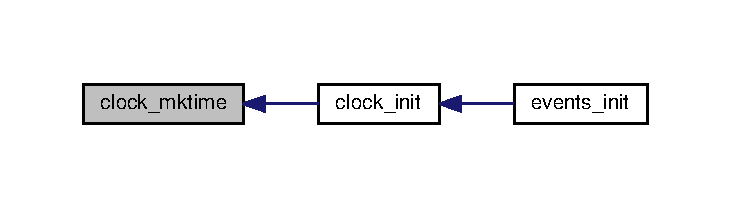
\includegraphics[width=350pt]{clock_8c_ab07bd3e86ff449c65b06fd50ec8e422e_icgraph}
\end{center}
\end{figure}


\hypertarget{clock_8c_a33cb84a5e3ce0c59505d776e5a736c08}{\index{clock.\-c@{clock.\-c}!compare\-\_\-times@{compare\-\_\-times}}
\index{compare\-\_\-times@{compare\-\_\-times}!clock.c@{clock.\-c}}
\subsubsection[{compare\-\_\-times}]{\setlength{\rightskip}{0pt plus 5cm}int compare\-\_\-times (
\begin{DoxyParamCaption}
\item[{struct {\bf timeval}}]{a, }
\item[{struct {\bf timeval}}]{b}
\end{DoxyParamCaption}
)}}\label{clock_8c_a33cb84a5e3ce0c59505d776e5a736c08}
\begin{DoxyReturn}{Renvoie}
-\/1, 1 ou 0 en fonction du résultat. 
\end{DoxyReturn}
\hypertarget{clock_8c_ab1bd72177a9697cdd2eec38a4fe6651e}{\index{clock.\-c@{clock.\-c}!get\-\_\-date@{get\-\_\-date}}
\index{get\-\_\-date@{get\-\_\-date}!clock.c@{clock.\-c}}
\subsubsection[{get\-\_\-date}]{\setlength{\rightskip}{0pt plus 5cm}time\-\_\-t get\-\_\-date (
\begin{DoxyParamCaption}
{}
\end{DoxyParamCaption}
)}}\label{clock_8c_ab1bd72177a9697cdd2eec38a4fe6651e}
\begin{DoxyReturn}{Renvoie}
la date en secondes. 
\end{DoxyReturn}


Voici le graphe des appelants de cette fonction \-:\nopagebreak
\begin{figure}[H]
\begin{center}
\leavevmode
\includegraphics[width=350pt]{clock_8c_ab1bd72177a9697cdd2eec38a4fe6651e_icgraph}
\end{center}
\end{figure}


\hypertarget{clock_8c_a0dc3166547de3bc1b9bdf45fdfb7d2e5}{\index{clock.\-c@{clock.\-c}!get\-\_\-tv@{get\-\_\-tv}}
\index{get\-\_\-tv@{get\-\_\-tv}!clock.c@{clock.\-c}}
\subsubsection[{get\-\_\-tv}]{\setlength{\rightskip}{0pt plus 5cm}struct {\bf timeval} get\-\_\-tv (
\begin{DoxyParamCaption}
{}
\end{DoxyParamCaption}
)\hspace{0.3cm}{\ttfamily [read]}}}\label{clock_8c_a0dc3166547de3bc1b9bdf45fdfb7d2e5}
\begin{DoxyReturn}{Renvoie}
une structure timeval. 
\end{DoxyReturn}


Voici le graphe d'appel pour cette fonction \-:\nopagebreak
\begin{figure}[H]
\begin{center}
\leavevmode
\includegraphics[width=220pt]{clock_8c_a0dc3166547de3bc1b9bdf45fdfb7d2e5_cgraph}
\end{center}
\end{figure}




Voici le graphe des appelants de cette fonction \-:\nopagebreak
\begin{figure}[H]
\begin{center}
\leavevmode
\includegraphics[width=350pt]{clock_8c_a0dc3166547de3bc1b9bdf45fdfb7d2e5_icgraph}
\end{center}
\end{figure}


\hypertarget{clock_8c_ab594b78936f7a5c4ba0c3b7ad653b6d5}{\index{clock.\-c@{clock.\-c}!S\-Y\-S\-C\-A\-L\-L\-\_\-\-H\-A\-N\-D\-L\-E\-R1@{S\-Y\-S\-C\-A\-L\-L\-\_\-\-H\-A\-N\-D\-L\-E\-R1}}
\index{S\-Y\-S\-C\-A\-L\-L\-\_\-\-H\-A\-N\-D\-L\-E\-R1@{S\-Y\-S\-C\-A\-L\-L\-\_\-\-H\-A\-N\-D\-L\-E\-R1}!clock.c@{clock.\-c}}
\subsubsection[{S\-Y\-S\-C\-A\-L\-L\-\_\-\-H\-A\-N\-D\-L\-E\-R1}]{\setlength{\rightskip}{0pt plus 5cm}S\-Y\-S\-C\-A\-L\-L\-\_\-\-H\-A\-N\-D\-L\-E\-R1 (
\begin{DoxyParamCaption}
\item[{sys\-\_\-getclock}]{, }
\item[{clock\-\_\-t $\ast$}]{clock}
\end{DoxyParamCaption}
)}}\label{clock_8c_ab594b78936f7a5c4ba0c3b7ad653b6d5}

\begin{DoxyParams}{Paramètres}
{\em clock} & Un pointeur pour y stocker la valeur de l'horloge système. \\
\hline
\end{DoxyParams}


Voici le graphe d'appel pour cette fonction \-:\nopagebreak
\begin{figure}[H]
\begin{center}
\leavevmode
\includegraphics[width=296pt]{clock_8c_ab594b78936f7a5c4ba0c3b7ad653b6d5_cgraph}
\end{center}
\end{figure}


\hypertarget{clock_8c_a8bfadf8175457fd7fbe6b53a46788a4e}{\index{clock.\-c@{clock.\-c}!S\-Y\-S\-C\-A\-L\-L\-\_\-\-H\-A\-N\-D\-L\-E\-R1@{S\-Y\-S\-C\-A\-L\-L\-\_\-\-H\-A\-N\-D\-L\-E\-R1}}
\index{S\-Y\-S\-C\-A\-L\-L\-\_\-\-H\-A\-N\-D\-L\-E\-R1@{S\-Y\-S\-C\-A\-L\-L\-\_\-\-H\-A\-N\-D\-L\-E\-R1}!clock.c@{clock.\-c}}
\subsubsection[{S\-Y\-S\-C\-A\-L\-L\-\_\-\-H\-A\-N\-D\-L\-E\-R1}]{\setlength{\rightskip}{0pt plus 5cm}S\-Y\-S\-C\-A\-L\-L\-\_\-\-H\-A\-N\-D\-L\-E\-R1 (
\begin{DoxyParamCaption}
\item[{sys\-\_\-getdate}]{, }
\item[{time\-\_\-t $\ast$}]{date}
\end{DoxyParamCaption}
)}}\label{clock_8c_a8bfadf8175457fd7fbe6b53a46788a4e}

\begin{DoxyParams}{Paramètres}
{\em date} & Un pointeur pour y stocker la date. \\
\hline
\end{DoxyParams}


Voici le graphe d'appel pour cette fonction \-:\nopagebreak
\begin{figure}[H]
\begin{center}
\leavevmode
\includegraphics[width=290pt]{clock_8c_a8bfadf8175457fd7fbe6b53a46788a4e_cgraph}
\end{center}
\end{figure}


\hypertarget{clock_8c_a052807a5c6ae63175a937381014a5701}{\index{clock.\-c@{clock.\-c}!timeval\-\_\-add\-\_\-usec@{timeval\-\_\-add\-\_\-usec}}
\index{timeval\-\_\-add\-\_\-usec@{timeval\-\_\-add\-\_\-usec}!clock.c@{clock.\-c}}
\subsubsection[{timeval\-\_\-add\-\_\-usec}]{\setlength{\rightskip}{0pt plus 5cm}void timeval\-\_\-add\-\_\-usec (
\begin{DoxyParamCaption}
\item[{struct {\bf timeval} $\ast$}]{t, }
\item[{time\-\_\-t}]{usec}
\end{DoxyParamCaption}
)}}\label{clock_8c_a052807a5c6ae63175a937381014a5701}

\begin{DoxyParams}{Paramètres}
{\em t} & La structure qui contient un temps. \\
\hline
{\em usec} & Le nombre de us à ajouter. \\
\hline
\end{DoxyParams}


Voici le graphe des appelants de cette fonction \-:\nopagebreak
\begin{figure}[H]
\begin{center}
\leavevmode
\includegraphics[width=350pt]{clock_8c_a052807a5c6ae63175a937381014a5701_icgraph}
\end{center}
\end{figure}




\subsection{Documentation des variables}
\hypertarget{clock_8c_a71eeef3b16d170231b5aa59331e0ab60}{\index{clock.\-c@{clock.\-c}!\-\_\-ytab@{\-\_\-ytab}}
\index{\-\_\-ytab@{\-\_\-ytab}!clock.c@{clock.\-c}}
\subsubsection[{\-\_\-ytab}]{\setlength{\rightskip}{0pt plus 5cm}const int \-\_\-ytab\mbox{[}2\mbox{]}\mbox{[}12\mbox{]}}}\label{clock_8c_a71eeef3b16d170231b5aa59331e0ab60}
{\bfseries Valeur initiale \-:}
\begin{DoxyCode}
 \{ \{ 31, 28, 31, 30, 31, 30, 31, 31, 30, 31, 30, 31 \},
                           \{ 31, 29, 31, 30, 31, 30, 31, 31, 30, 31, 30, 31 \}\}
\end{DoxyCode}

\hypertarget{dcache_8c}{\section{Référence du fichier kernel/dcache.c}
\label{dcache_8c}\index{kernel/dcache.\-c@{kernel/dcache.\-c}}
}


dentry cache  


{\ttfamily \#include $<$hashmap.\-h$>$}\\*
{\ttfamily \#include $<$klibc/string.\-h$>$}\\*
{\ttfamily \#include $<$vfs.\-h$>$}\\*
{\ttfamily \#include $<$kmalloc.\-h$>$}\\*
{\ttfamily \#include $<$klog.\-h$>$}\\*
Graphe des dépendances par inclusion de dcache.\-c\-:
\nopagebreak
\begin{figure}[H]
\begin{center}
\leavevmode
\includegraphics[width=350pt]{dcache_8c__incl}
\end{center}
\end{figure}
\subsection*{Structures de données}
\begin{DoxyCompactItemize}
\item 
struct \hyperlink{structkey__t}{key\-\_\-t}
\item 
struct \hyperlink{structlru__t}{lru\-\_\-t}
\end{DoxyCompactItemize}
\subsection*{Fonctions}
\begin{DoxyCompactItemize}
\item 
\hypertarget{dcache_8c_a6a634167e657e519cadf44eb6e6b9068}{void {\bfseries dcache\-\_\-init} ()}\label{dcache_8c_a6a634167e657e519cadf44eb6e6b9068}

\item 
\hypertarget{dcache_8c_a1532980bfa072d469940da4b8ce176ac}{void {\bfseries dcache\-\_\-remove} (struct \hyperlink{struct__fs__instance__t}{\-\_\-fs\-\_\-instance\-\_\-t} $\ast$instance, struct \hyperlink{struct__dentry__t}{\-\_\-dentry\-\_\-t} $\ast$dentry, const char $\ast$name)}\label{dcache_8c_a1532980bfa072d469940da4b8ce176ac}

\item 
\hypertarget{dcache_8c_a4ba65ffaa114e5eb940fa446292f08da}{struct \hyperlink{struct__dentry__t}{\-\_\-dentry\-\_\-t} $\ast$ {\bfseries dcache\-\_\-get} (struct \hyperlink{struct__fs__instance__t}{\-\_\-fs\-\_\-instance\-\_\-t} $\ast$instance, struct \hyperlink{struct__dentry__t}{\-\_\-dentry\-\_\-t} $\ast$dentry, const char $\ast$name)}\label{dcache_8c_a4ba65ffaa114e5eb940fa446292f08da}

\item 
\hypertarget{dcache_8c_a4f122b8158ba9f2044fda159f8ff0680}{void {\bfseries dcache\-\_\-set} (struct \hyperlink{struct__fs__instance__t}{\-\_\-fs\-\_\-instance\-\_\-t} $\ast$instance, struct \hyperlink{struct__dentry__t}{\-\_\-dentry\-\_\-t} $\ast$pdentry, const char $\ast$name, struct \hyperlink{struct__dentry__t}{\-\_\-dentry\-\_\-t} $\ast$dentry)}\label{dcache_8c_a4f122b8158ba9f2044fda159f8ff0680}

\end{DoxyCompactItemize}


\subsection{Description détaillée}
\begin{DoxyAuthor}{Auteur}
Tac\-O\-S developers
\end{DoxyAuthor}
\hypertarget{wait_8c_LICENSE}{}\subsection{L\-I\-C\-E\-N\-S\-E}\label{wait_8c_LICENSE}
Copyright (C) 2010, 2011, 2012 -\/ Tac\-O\-S developers.

This program is free software; you can redistribute it and/or modify it under the terms of the G\-N\-U General Public License as published by the Free Software Foundation; either version 3 of the License, or (at your option) any later version.

This program is distributed in the hope that it will be useful, but W\-I\-T\-H\-O\-U\-T A\-N\-Y W\-A\-R\-R\-A\-N\-T\-Y; without even the implied warranty of M\-E\-R\-C\-H\-A\-N\-T\-A\-B\-I\-L\-I\-T\-Y or F\-I\-T\-N\-E\-S\-S F\-O\-R A P\-A\-R\-T\-I\-C\-U\-L\-A\-R P\-U\-R\-P\-O\-S\-E. See the G\-N\-U General Public License for more details at \href{http://www.gnu.org/copyleft/gpl.html}{\tt http\-://www.\-gnu.\-org/copyleft/gpl.\-html}

You should have received a copy of the G\-N\-U General Public License along with this program; if not, see \href{http://www.gnu.org/licenses}{\tt http\-://www.\-gnu.\-org/licenses}.\hypertarget{wait_8c_DESCRIPTION}{}\subsection{D\-E\-S\-C\-R\-I\-P\-T\-I\-O\-N}\label{wait_8c_DESCRIPTION}

\hypertarget{floppy_8c}{\section{Référence du fichier kernel/drivers/block/floppy/floppy.c}
\label{floppy_8c}\index{kernel/drivers/block/floppy/floppy.\-c@{kernel/drivers/block/floppy/floppy.\-c}}
}
{\ttfamily \#include $<$fs/devfs.\-h$>$}\\*
{\ttfamily \#include $<$ioports.\-h$>$}\\*
{\ttfamily \#include $<$kstdio.\-h$>$}\\*
{\ttfamily \#include $<$klibc/string.\-h$>$}\\*
{\ttfamily \#include $<$types.\-h$>$}\\*
{\ttfamily \#include $<$klog.\-h$>$}\\*
{\ttfamily \#include \char`\"{}floppy\-\_\-interrupt.\-h\char`\"{}}\\*
{\ttfamily \#include \char`\"{}floppy\-\_\-utils.\-h\char`\"{}}\\*
{\ttfamily \#include \char`\"{}floppy\-\_\-motor.\-h\char`\"{}}\\*
{\ttfamily \#include \char`\"{}floppy\-\_\-dma.\-h\char`\"{}}\\*
Graphe des dépendances par inclusion de floppy.\-c\-:
\nopagebreak
\begin{figure}[H]
\begin{center}
\leavevmode
\includegraphics[width=350pt]{floppy_8c__incl}
\end{center}
\end{figure}
\subsection*{Macros}
\begin{DoxyCompactItemize}
\item 
\hypertarget{floppy_8c_a2d80f166138f54b8808b0977de138096}{\#define {\bfseries F\-L\-O\-P\-P\-Y\-\_\-\-S\-E\-C\-T\-O\-R\-\_\-\-S\-I\-Z\-E}~512}\label{floppy_8c_a2d80f166138f54b8808b0977de138096}

\item 
\hypertarget{floppy_8c_a1a1ec045732bf94510027aef2ef10c79}{\#define {\bfseries F\-L\-O\-P\-P\-Y\-\_\-\-N\-B\-\_\-\-H\-E\-A\-D\-S}~2}\label{floppy_8c_a1a1ec045732bf94510027aef2ef10c79}

\item 
\hypertarget{floppy_8c_ad0d69d8da349ac2b68dfd1ad5d2a8489}{\#define {\bfseries F\-L\-O\-P\-P\-Y\-\_\-\-S\-E\-C\-T\-O\-R\-S\-\_\-\-P\-E\-R\-\_\-\-T\-R\-A\-C\-K}~18}\label{floppy_8c_ad0d69d8da349ac2b68dfd1ad5d2a8489}

\end{DoxyCompactItemize}
\subsection*{Fonctions}
\begin{DoxyCompactItemize}
\item 
\hypertarget{floppy_8c_abc157c475e066a1ccee0b8d1b3feffaf}{int {\bfseries floppy\-\_\-open} (\hyperlink{struct__open__file__descriptor}{open\-\_\-file\-\_\-descriptor} $\ast$ofd)}\label{floppy_8c_abc157c475e066a1ccee0b8d1b3feffaf}

\item 
\hypertarget{floppy_8c_a699548ad272b415f931401a3c09b32ab}{int {\bfseries floppy\-\_\-close} (\hyperlink{struct__open__file__descriptor}{open\-\_\-file\-\_\-descriptor} $\ast$ofd)}\label{floppy_8c_a699548ad272b415f931401a3c09b32ab}

\item 
\hypertarget{floppy_8c_abf626f0afe152b41157f62948a9d7c6b}{\hyperlink{kernel_2include_2types_8h_a29d85914ddff32967d85ada69854206d}{size\-\_\-t} {\bfseries floppy\-\_\-read} (\hyperlink{struct__open__file__descriptor}{open\-\_\-file\-\_\-descriptor} $\ast$ofd, void $\ast$buf, \hyperlink{kernel_2include_2types_8h_a29d85914ddff32967d85ada69854206d}{size\-\_\-t} count, \hyperlink{kernel_2include_2types_8h_a33594304e786b158f3fb30289278f5af}{uint32\-\_\-t} offset)}\label{floppy_8c_abf626f0afe152b41157f62948a9d7c6b}

\item 
\hypertarget{floppy_8c_a7a29fbfef46d433f455948cd5ec500a6}{\hyperlink{kernel_2include_2types_8h_a29d85914ddff32967d85ada69854206d}{size\-\_\-t} {\bfseries floppy\-\_\-write} (\hyperlink{struct__open__file__descriptor}{open\-\_\-file\-\_\-descriptor} $\ast$ofd, const void $\ast$buf, \hyperlink{kernel_2include_2types_8h_a29d85914ddff32967d85ada69854206d}{size\-\_\-t} count, \hyperlink{kernel_2include_2types_8h_a33594304e786b158f3fb30289278f5af}{uint32\-\_\-t} offset)}\label{floppy_8c_a7a29fbfef46d433f455948cd5ec500a6}

\item 
\hypertarget{floppy_8c_aa628c68a29a61ef1a4e65641de73665f}{int {\bfseries floppy\-\_\-calibrate} ()}\label{floppy_8c_aa628c68a29a61ef1a4e65641de73665f}

\item 
\hypertarget{floppy_8c_a4b305e10e95fed92b047adfac6dc4881}{int \hyperlink{floppy_8c_a4b305e10e95fed92b047adfac6dc4881}{init\-\_\-floppy} ()}\label{floppy_8c_a4b305e10e95fed92b047adfac6dc4881}

\begin{DoxyCompactList}\small\item\em Initilise le driver floppy. \end{DoxyCompactList}\end{DoxyCompactItemize}


\subsection{Description détaillée}
\begin{DoxyAuthor}{Auteur}
Tac\-O\-S developers
\end{DoxyAuthor}
\hypertarget{wait_8c_LICENSE}{}\subsection{L\-I\-C\-E\-N\-S\-E}\label{wait_8c_LICENSE}
Copyright (C) 2010, 2011, 2012 -\/ Tac\-O\-S developers.

This program is free software; you can redistribute it and/or modify it under the terms of the G\-N\-U General Public License as published by the Free Software Foundation; either version 3 of the License, or (at your option) any later version.

This program is distributed in the hope that it will be useful, but W\-I\-T\-H\-O\-U\-T A\-N\-Y W\-A\-R\-R\-A\-N\-T\-Y; without even the implied warranty of M\-E\-R\-C\-H\-A\-N\-T\-A\-B\-I\-L\-I\-T\-Y or F\-I\-T\-N\-E\-S\-S F\-O\-R A P\-A\-R\-T\-I\-C\-U\-L\-A\-R P\-U\-R\-P\-O\-S\-E. See the G\-N\-U General Public License for more details at \href{http://www.gnu.org/copyleft/gpl.html}{\tt http\-://www.\-gnu.\-org/copyleft/gpl.\-html}

You should have received a copy of the G\-N\-U General Public License along with this program; if not, see \href{http://www.gnu.org/licenses}{\tt http\-://www.\-gnu.\-org/licenses}.\hypertarget{wait_8c_DESCRIPTION}{}\subsection{D\-E\-S\-C\-R\-I\-P\-T\-I\-O\-N}\label{wait_8c_DESCRIPTION}
Floppy driver 
\hypertarget{floppy__dma_8c}{\section{Référence du fichier kernel/drivers/block/floppy/floppy\-\_\-dma.c}
\label{floppy__dma_8c}\index{kernel/drivers/block/floppy/floppy\-\_\-dma.\-c@{kernel/drivers/block/floppy/floppy\-\_\-dma.\-c}}
}
{\ttfamily \#include $<$types.\-h$>$}\\*
{\ttfamily \#include $<$stdio.\-h$>$}\\*
{\ttfamily \#include $<$klibc/string.\-h$>$}\\*
{\ttfamily \#include $<$ioports.\-h$>$}\\*
{\ttfamily \#include $<$klog.\-h$>$}\\*
{\ttfamily \#include \char`\"{}floppy\-\_\-motor.\-h\char`\"{}}\\*
{\ttfamily \#include \char`\"{}floppy\-\_\-utils.\-h\char`\"{}}\\*
{\ttfamily \#include \char`\"{}floppy\-\_\-interrupt.\-h\char`\"{}}\\*
{\ttfamily \#include \char`\"{}floppy\-\_\-dma.\-h\char`\"{}}\\*
Graphe des dépendances par inclusion de floppy\-\_\-dma.\-c\-:
\nopagebreak
\begin{figure}[H]
\begin{center}
\leavevmode
\includegraphics[width=350pt]{floppy__dma_8c__incl}
\end{center}
\end{figure}
\subsection*{Macros}
\begin{DoxyCompactItemize}
\item 
\hypertarget{floppy__dma_8c_a9f008b46356ca14ff01a99127a9bcf12}{\#define {\bfseries floppy\-\_\-dmalen}~0x4800}\label{floppy__dma_8c_a9f008b46356ca14ff01a99127a9bcf12}

\item 
\hypertarget{floppy__dma_8c_a6f37ede1f274f6166b876558a8493e8b}{\#define {\bfseries floppy\-\_\-head2\-\_\-start}~floppy\-\_\-dmalen/2}\label{floppy__dma_8c_a6f37ede1f274f6166b876558a8493e8b}

\end{DoxyCompactItemize}
\subsection*{Fonctions}
\begin{DoxyCompactItemize}
\item 
void \hyperlink{floppy__dma_8c_a82b03eec2e2db0df14b77521b2b0cd99}{floppy\-\_\-dma\-\_\-init} (\hyperlink{floppy__dma_8h_adfcc8a5beaf1532fc574bc706d3e1fbe}{floppy\-\_\-io} io\-\_\-dir)
\begin{DoxyCompactList}\small\item\em Initialise le dma en écriture ou en lecture selon la valeur passée en paramètre. \end{DoxyCompactList}\item 
void \hyperlink{floppy__dma_8c_ac6e644203ea530de67552b2debe0bac2}{floppy\-\_\-read\-\_\-sector} (int cylinder, int head, int sector, char $\ast$buffer)
\begin{DoxyCompactList}\small\item\em Lis un secteur via le D\-M\-A à partir d'un adressage C\-H\-S. \end{DoxyCompactList}\item 
void \hyperlink{floppy__dma_8c_af9d347980c43209de48f63cd9f201419}{floppy\-\_\-write\-\_\-sector} (int cylinder, int head, int sector, char $\ast$buffer)
\begin{DoxyCompactList}\small\item\em Ecrit un secteur via le D\-M\-A à partir d'un adressage C\-H\-S. \end{DoxyCompactList}\end{DoxyCompactItemize}


\subsection{Description détaillée}
\begin{DoxyAuthor}{Auteur}
Tac\-O\-S developers
\end{DoxyAuthor}
\hypertarget{wait_8c_LICENSE}{}\subsection{L\-I\-C\-E\-N\-S\-E}\label{wait_8c_LICENSE}
Copyright (C) 2010, 2011, 2012 -\/ Tac\-O\-S developers.

This program is free software; you can redistribute it and/or modify it under the terms of the G\-N\-U General Public License as published by the Free Software Foundation; either version 3 of the License, or (at your option) any later version.

This program is distributed in the hope that it will be useful, but W\-I\-T\-H\-O\-U\-T A\-N\-Y W\-A\-R\-R\-A\-N\-T\-Y; without even the implied warranty of M\-E\-R\-C\-H\-A\-N\-T\-A\-B\-I\-L\-I\-T\-Y or F\-I\-T\-N\-E\-S\-S F\-O\-R A P\-A\-R\-T\-I\-C\-U\-L\-A\-R P\-U\-R\-P\-O\-S\-E. See the G\-N\-U General Public License for more details at \href{http://www.gnu.org/copyleft/gpl.html}{\tt http\-://www.\-gnu.\-org/copyleft/gpl.\-html}

You should have received a copy of the G\-N\-U General Public License along with this program; if not, see \href{http://www.gnu.org/licenses}{\tt http\-://www.\-gnu.\-org/licenses}.\hypertarget{wait_8c_DESCRIPTION}{}\subsection{D\-E\-S\-C\-R\-I\-P\-T\-I\-O\-N}\label{wait_8c_DESCRIPTION}
Fonctions liées à l'utilisation du D\-M\-A dans le driver disquette 

\subsection{Documentation des fonctions}
\hypertarget{floppy__dma_8c_a82b03eec2e2db0df14b77521b2b0cd99}{\index{floppy\-\_\-dma.\-c@{floppy\-\_\-dma.\-c}!floppy\-\_\-dma\-\_\-init@{floppy\-\_\-dma\-\_\-init}}
\index{floppy\-\_\-dma\-\_\-init@{floppy\-\_\-dma\-\_\-init}!floppy_dma.c@{floppy\-\_\-dma.\-c}}
\subsubsection[{floppy\-\_\-dma\-\_\-init}]{\setlength{\rightskip}{0pt plus 5cm}void floppy\-\_\-dma\-\_\-init (
\begin{DoxyParamCaption}
\item[{{\bf floppy\-\_\-io}}]{io\-\_\-dir}
\end{DoxyParamCaption}
)}}\label{floppy__dma_8c_a82b03eec2e2db0df14b77521b2b0cd99}

\begin{DoxyParams}{Paramètres}
{\em io\-\_\-dir} & Sens de la communication du D\-M\-A à initialiser \\
\hline
\end{DoxyParams}
\hypertarget{floppy__dma_8c_ac6e644203ea530de67552b2debe0bac2}{\index{floppy\-\_\-dma.\-c@{floppy\-\_\-dma.\-c}!floppy\-\_\-read\-\_\-sector@{floppy\-\_\-read\-\_\-sector}}
\index{floppy\-\_\-read\-\_\-sector@{floppy\-\_\-read\-\_\-sector}!floppy_dma.c@{floppy\-\_\-dma.\-c}}
\subsubsection[{floppy\-\_\-read\-\_\-sector}]{\setlength{\rightskip}{0pt plus 5cm}void floppy\-\_\-read\-\_\-sector (
\begin{DoxyParamCaption}
\item[{int}]{cylinder, }
\item[{int}]{head, }
\item[{int}]{sector, }
\item[{char $\ast$}]{buffer}
\end{DoxyParamCaption}
)}}\label{floppy__dma_8c_ac6e644203ea530de67552b2debe0bac2}

\begin{DoxyParams}{Paramètres}
{\em cylinder} & Numero de cylindre \\
\hline
{\em head} & Numero de tête de lecture \\
\hline
{\em sector} & Numero de secteur \\
\hline
{\em buffer} & Buffer recevant les données lues \\
\hline
\end{DoxyParams}


Voici le graphe d'appel pour cette fonction \-:
\nopagebreak
\begin{figure}[H]
\begin{center}
\leavevmode
\includegraphics[width=268pt]{floppy__dma_8c_ac6e644203ea530de67552b2debe0bac2_cgraph}
\end{center}
\end{figure}


\hypertarget{floppy__dma_8c_af9d347980c43209de48f63cd9f201419}{\index{floppy\-\_\-dma.\-c@{floppy\-\_\-dma.\-c}!floppy\-\_\-write\-\_\-sector@{floppy\-\_\-write\-\_\-sector}}
\index{floppy\-\_\-write\-\_\-sector@{floppy\-\_\-write\-\_\-sector}!floppy_dma.c@{floppy\-\_\-dma.\-c}}
\subsubsection[{floppy\-\_\-write\-\_\-sector}]{\setlength{\rightskip}{0pt plus 5cm}void floppy\-\_\-write\-\_\-sector (
\begin{DoxyParamCaption}
\item[{int}]{cylinder, }
\item[{int}]{head, }
\item[{int}]{sector, }
\item[{char $\ast$}]{buffer}
\end{DoxyParamCaption}
)}}\label{floppy__dma_8c_af9d347980c43209de48f63cd9f201419}

\begin{DoxyParams}{Paramètres}
{\em cylinder} & Numero de cylindre \\
\hline
{\em head} & Numero de tête de lecture \\
\hline
{\em sector} & Numero de secteur \\
\hline
{\em buffer} & Buffer contenant les données à écrire \\
\hline
\end{DoxyParams}


Voici le graphe d'appel pour cette fonction \-:
\nopagebreak
\begin{figure}[H]
\begin{center}
\leavevmode
\includegraphics[width=270pt]{floppy__dma_8c_af9d347980c43209de48f63cd9f201419_cgraph}
\end{center}
\end{figure}



\hypertarget{floppy__dma_8h}{\section{Référence du fichier kernel/drivers/block/floppy/floppy\-\_\-dma.h}
\label{floppy__dma_8h}\index{kernel/drivers/block/floppy/floppy\-\_\-dma.\-h@{kernel/drivers/block/floppy/floppy\-\_\-dma.\-h}}
}
Ce graphe montre quels fichiers incluent directement ou indirectement ce fichier \-:\nopagebreak
\begin{figure}[H]
\begin{center}
\leavevmode
\includegraphics[width=302pt]{floppy__dma_8h__dep__incl}
\end{center}
\end{figure}
\subsection*{Énumérations}
\begin{DoxyCompactItemize}
\item 
enum \hyperlink{floppy__dma_8h_adfcc8a5beaf1532fc574bc706d3e1fbe}{floppy\-\_\-io} \{ {\bfseries F\-L\-O\-P\-P\-Y\-\_\-\-W\-R\-I\-T\-E} =  1, 
{\bfseries F\-L\-O\-P\-P\-Y\-\_\-\-R\-E\-A\-D} =  2
 \}
\begin{DoxyCompactList}\small\item\em Défini le sens de la communication (input / output) \end{DoxyCompactList}\end{DoxyCompactItemize}
\subsection*{Fonctions}
\begin{DoxyCompactItemize}
\item 
void \hyperlink{floppy__dma_8h_a82b03eec2e2db0df14b77521b2b0cd99}{floppy\-\_\-dma\-\_\-init} (\hyperlink{floppy__dma_8h_adfcc8a5beaf1532fc574bc706d3e1fbe}{floppy\-\_\-io} io\-\_\-dir)
\begin{DoxyCompactList}\small\item\em Initialise le dma en écriture ou en lecture selon la valeur passée en paramètre. \end{DoxyCompactList}\item 
void \hyperlink{floppy__dma_8h_ac6e644203ea530de67552b2debe0bac2}{floppy\-\_\-read\-\_\-sector} (int cylinder, int head, int sector, char $\ast$buffer)
\begin{DoxyCompactList}\small\item\em Lis un secteur via le D\-M\-A à partir d'un adressage C\-H\-S. \end{DoxyCompactList}\item 
void \hyperlink{floppy__dma_8h_af9d347980c43209de48f63cd9f201419}{floppy\-\_\-write\-\_\-sector} (int cylinder, int head, int sector, char $\ast$buffer)
\begin{DoxyCompactList}\small\item\em Ecrit un secteur via le D\-M\-A à partir d'un adressage C\-H\-S. \end{DoxyCompactList}\end{DoxyCompactItemize}


\subsection{Description détaillée}
\begin{DoxyAuthor}{Auteur}
Tac\-O\-S developers
\end{DoxyAuthor}
\hypertarget{vmm_8c_LICENSE}{}\subsection{L\-I\-C\-E\-N\-S\-E}\label{vmm_8c_LICENSE}
Copyright (C) 2010, 2011, 2012 -\/ Tac\-O\-S developers.

This program is free software; you can redistribute it and/or modify it under the terms of the G\-N\-U General Public License as published by the Free Software Foundation; either version 3 of the License, or (at your option) any later version.

This program is distributed in the hope that it will be useful, but W\-I\-T\-H\-O\-U\-T A\-N\-Y W\-A\-R\-R\-A\-N\-T\-Y; without even the implied warranty of M\-E\-R\-C\-H\-A\-N\-T\-A\-B\-I\-L\-I\-T\-Y or F\-I\-T\-N\-E\-S\-S F\-O\-R A P\-A\-R\-T\-I\-C\-U\-L\-A\-R P\-U\-R\-P\-O\-S\-E. See the G\-N\-U General Public License for more details at \href{http://www.gnu.org/copyleft/gpl.html}{\tt http\-://www.\-gnu.\-org/copyleft/gpl.\-html}

You should have received a copy of the G\-N\-U General Public License along with this program; if not, see \href{http://www.gnu.org/licenses}{\tt http\-://www.\-gnu.\-org/licenses}.\hypertarget{vmm_8c_DESCRIPTION}{}\subsection{D\-E\-S\-C\-R\-I\-P\-T\-I\-O\-N}\label{vmm_8c_DESCRIPTION}
Fonctions liées à l'utilisation du D\-M\-A dans le driver disquette 

\subsection{Documentation des fonctions}
\hypertarget{floppy__dma_8h_a82b03eec2e2db0df14b77521b2b0cd99}{\index{floppy\-\_\-dma.\-h@{floppy\-\_\-dma.\-h}!floppy\-\_\-dma\-\_\-init@{floppy\-\_\-dma\-\_\-init}}
\index{floppy\-\_\-dma\-\_\-init@{floppy\-\_\-dma\-\_\-init}!floppy_dma.h@{floppy\-\_\-dma.\-h}}
\subsubsection[{floppy\-\_\-dma\-\_\-init}]{\setlength{\rightskip}{0pt plus 5cm}void floppy\-\_\-dma\-\_\-init (
\begin{DoxyParamCaption}
\item[{{\bf floppy\-\_\-io}}]{io\-\_\-dir}
\end{DoxyParamCaption}
)}}\label{floppy__dma_8h_a82b03eec2e2db0df14b77521b2b0cd99}

\begin{DoxyParams}{Paramètres}
{\em io\-\_\-dir} & Sens de la communication du D\-M\-A à initialiser \\
\hline
\end{DoxyParams}
\hypertarget{floppy__dma_8h_ac6e644203ea530de67552b2debe0bac2}{\index{floppy\-\_\-dma.\-h@{floppy\-\_\-dma.\-h}!floppy\-\_\-read\-\_\-sector@{floppy\-\_\-read\-\_\-sector}}
\index{floppy\-\_\-read\-\_\-sector@{floppy\-\_\-read\-\_\-sector}!floppy_dma.h@{floppy\-\_\-dma.\-h}}
\subsubsection[{floppy\-\_\-read\-\_\-sector}]{\setlength{\rightskip}{0pt plus 5cm}void floppy\-\_\-read\-\_\-sector (
\begin{DoxyParamCaption}
\item[{int}]{cylinder, }
\item[{int}]{head, }
\item[{int}]{sector, }
\item[{char $\ast$}]{buffer}
\end{DoxyParamCaption}
)}}\label{floppy__dma_8h_ac6e644203ea530de67552b2debe0bac2}

\begin{DoxyParams}{Paramètres}
{\em cylinder} & Numero de cylindre \\
\hline
{\em head} & Numero de tête de lecture \\
\hline
{\em sector} & Numero de secteur \\
\hline
{\em buffer} & Buffer recevant les données lues \\
\hline
\end{DoxyParams}


Voici le graphe d'appel pour cette fonction \-:\nopagebreak
\begin{figure}[H]
\begin{center}
\leavevmode
\includegraphics[width=268pt]{floppy__dma_8h_ac6e644203ea530de67552b2debe0bac2_cgraph}
\end{center}
\end{figure}


\hypertarget{floppy__dma_8h_af9d347980c43209de48f63cd9f201419}{\index{floppy\-\_\-dma.\-h@{floppy\-\_\-dma.\-h}!floppy\-\_\-write\-\_\-sector@{floppy\-\_\-write\-\_\-sector}}
\index{floppy\-\_\-write\-\_\-sector@{floppy\-\_\-write\-\_\-sector}!floppy_dma.h@{floppy\-\_\-dma.\-h}}
\subsubsection[{floppy\-\_\-write\-\_\-sector}]{\setlength{\rightskip}{0pt plus 5cm}void floppy\-\_\-write\-\_\-sector (
\begin{DoxyParamCaption}
\item[{int}]{cylinder, }
\item[{int}]{head, }
\item[{int}]{sector, }
\item[{char $\ast$}]{buffer}
\end{DoxyParamCaption}
)}}\label{floppy__dma_8h_af9d347980c43209de48f63cd9f201419}

\begin{DoxyParams}{Paramètres}
{\em cylinder} & Numero de cylindre \\
\hline
{\em head} & Numero de tête de lecture \\
\hline
{\em sector} & Numero de secteur \\
\hline
{\em buffer} & Buffer contenant les données à écrire \\
\hline
\end{DoxyParams}


Voici le graphe d'appel pour cette fonction \-:\nopagebreak
\begin{figure}[H]
\begin{center}
\leavevmode
\includegraphics[width=270pt]{floppy__dma_8h_af9d347980c43209de48f63cd9f201419_cgraph}
\end{center}
\end{figure}



\hypertarget{floppy__interrupt_8c}{\section{Référence du fichier kernel/drivers/block/floppy/floppy\+\_\+interrupt.c}
\label{floppy__interrupt_8c}\index{kernel/drivers/block/floppy/floppy\+\_\+interrupt.\+c@{kernel/drivers/block/floppy/floppy\+\_\+interrupt.\+c}}
}
{\ttfamily \#include $<$types.\+h$>$}\\*
{\ttfamily \#include $<$interrupts.\+h$>$}\\*
{\ttfamily \#include \char`\"{}floppy\+\_\+utils.\+h\char`\"{}}\\*
Graphe des dépendances par inclusion de floppy\+\_\+interrupt.\+c\+:
\nopagebreak
\begin{figure}[H]
\begin{center}
\leavevmode
\includegraphics[width=301pt]{floppy__interrupt_8c__incl}
\end{center}
\end{figure}
\subsection*{Fonctions}
\begin{DoxyCompactItemize}
\item 
\hypertarget{floppy__interrupt_8c_a93239c23be41c3d5c489989685bb7700}{void {\bfseries floppy\+\_\+handler} (int interrupt\+\_\+id)}\label{floppy__interrupt_8c_a93239c23be41c3d5c489989685bb7700}

\item 
\hypertarget{floppy__interrupt_8c_a579397f7aad55a1eff3648712e9b1f5a}{void \hyperlink{floppy__interrupt_8c_a579397f7aad55a1eff3648712e9b1f5a}{floppy\+\_\+wait\+\_\+irq} ()}\label{floppy__interrupt_8c_a579397f7aad55a1eff3648712e9b1f5a}

\begin{DoxyCompactList}\small\item\em Attendre une interruption (X\+X\+X attente active) \end{DoxyCompactList}\item 
\hypertarget{floppy__interrupt_8c_a19cdddd056dff00ace3567933e4d2b71}{void \hyperlink{floppy__interrupt_8c_a19cdddd056dff00ace3567933e4d2b71}{floppy\+\_\+init\+\_\+interrupt} ()}\label{floppy__interrupt_8c_a19cdddd056dff00ace3567933e4d2b71}

\begin{DoxyCompactList}\small\item\em Initialise l'I\+R\+Q floppy. \end{DoxyCompactList}\item 
\hypertarget{floppy__interrupt_8c_a4faeb801db3260ba0d654d34c843ddf2}{void \hyperlink{floppy__interrupt_8c_a4faeb801db3260ba0d654d34c843ddf2}{floppy\+\_\+reset\+\_\+irq} ()}\label{floppy__interrupt_8c_a4faeb801db3260ba0d654d34c843ddf2}

\begin{DoxyCompactList}\small\item\em Remet à 0 le flag software d'interruption. \end{DoxyCompactList}\item 
\hypertarget{floppy__interrupt_8c_aa736fd868e99a0bde478ea3b5a836b04}{void \hyperlink{floppy__interrupt_8c_aa736fd868e99a0bde478ea3b5a836b04}{floppy\+\_\+sense\+\_\+interrupt} (int $\ast$st0, int $\ast$cy1)}\label{floppy__interrupt_8c_aa736fd868e99a0bde478ea3b5a836b04}

\begin{DoxyCompactList}\small\item\em Récupère des données d'interruption. \end{DoxyCompactList}\end{DoxyCompactItemize}
\subsection*{Variables}
\begin{DoxyCompactItemize}
\item 
\hypertarget{floppy__interrupt_8c_ae7efee70f38c540260b05380dd454f14}{volatile bool {\bfseries irq\+\_\+received} = \hyperlink{stdbool_8h_a65e9886d74aaee76545e83dd09011727}{false}}\label{floppy__interrupt_8c_ae7efee70f38c540260b05380dd454f14}

\end{DoxyCompactItemize}


\subsection{Description détaillée}
\begin{DoxyAuthor}{Auteur}
Tac\+O\+S developers
\end{DoxyAuthor}
\hypertarget{wait_8c_LICENSE}{}\subsection{L\+I\+C\+E\+N\+S\+E}\label{wait_8c_LICENSE}
Copyright (C) 2010-\/2014 Tac\+O\+S developers.

This program is free software; you can redistribute it and/or modify it under the terms of the G\+N\+U General Public License as published by the Free Software Foundation; either version 3 of the License, or (at your option) any later version.

This program is distributed in the hope that it will be useful, but W\+I\+T\+H\+O\+U\+T A\+N\+Y W\+A\+R\+R\+A\+N\+T\+Y; without even the implied warranty of M\+E\+R\+C\+H\+A\+N\+T\+A\+B\+I\+L\+I\+T\+Y or F\+I\+T\+N\+E\+S\+S F\+O\+R A P\+A\+R\+T\+I\+C\+U\+L\+A\+R P\+U\+R\+P\+O\+S\+E. See the G\+N\+U General Public License for more details at \href{http://www.gnu.org/copyleft/gpl.html}{\tt http\+://www.\+gnu.\+org/copyleft/gpl.\+html}

You should have received a copy of the G\+N\+U General Public License along with this program; if not, see \href{http://www.gnu.org/licenses}{\tt http\+://www.\+gnu.\+org/licenses}.\hypertarget{wait_8c_DESCRIPTION}{}\subsection{D\+E\+S\+C\+R\+I\+P\+T\+I\+O\+N}\label{wait_8c_DESCRIPTION}
Description de ce que fait le fichier 
\hypertarget{floppy__interrupt_8h}{\section{Référence du fichier kernel/drivers/block/floppy/floppy\+\_\+interrupt.h}
\label{floppy__interrupt_8h}\index{kernel/drivers/block/floppy/floppy\+\_\+interrupt.\+h@{kernel/drivers/block/floppy/floppy\+\_\+interrupt.\+h}}
}
Ce graphe montre quels fichiers incluent directement ou indirectement ce fichier \+:\nopagebreak
\begin{figure}[H]
\begin{center}
\leavevmode
\includegraphics[width=350pt]{floppy__interrupt_8h__dep__incl}
\end{center}
\end{figure}
\subsection*{Fonctions}
\begin{DoxyCompactItemize}
\item 
\hypertarget{floppy__interrupt_8h_a19cdddd056dff00ace3567933e4d2b71}{void \hyperlink{floppy__interrupt_8h_a19cdddd056dff00ace3567933e4d2b71}{floppy\+\_\+init\+\_\+interrupt} ()}\label{floppy__interrupt_8h_a19cdddd056dff00ace3567933e4d2b71}

\begin{DoxyCompactList}\small\item\em Initialise l'I\+R\+Q floppy. \end{DoxyCompactList}\item 
\hypertarget{floppy__interrupt_8h_a4faeb801db3260ba0d654d34c843ddf2}{void \hyperlink{floppy__interrupt_8h_a4faeb801db3260ba0d654d34c843ddf2}{floppy\+\_\+reset\+\_\+irq} ()}\label{floppy__interrupt_8h_a4faeb801db3260ba0d654d34c843ddf2}

\begin{DoxyCompactList}\small\item\em Remet à 0 le flag software d'interruption. \end{DoxyCompactList}\item 
\hypertarget{floppy__interrupt_8h_a579397f7aad55a1eff3648712e9b1f5a}{void \hyperlink{floppy__interrupt_8h_a579397f7aad55a1eff3648712e9b1f5a}{floppy\+\_\+wait\+\_\+irq} ()}\label{floppy__interrupt_8h_a579397f7aad55a1eff3648712e9b1f5a}

\begin{DoxyCompactList}\small\item\em Attendre une interruption (X\+X\+X attente active) \end{DoxyCompactList}\item 
\hypertarget{floppy__interrupt_8h_aa736fd868e99a0bde478ea3b5a836b04}{void \hyperlink{floppy__interrupt_8h_aa736fd868e99a0bde478ea3b5a836b04}{floppy\+\_\+sense\+\_\+interrupt} (int $\ast$st0, int $\ast$cy1)}\label{floppy__interrupt_8h_aa736fd868e99a0bde478ea3b5a836b04}

\begin{DoxyCompactList}\small\item\em Récupère des données d'interruption. \end{DoxyCompactList}\end{DoxyCompactItemize}


\subsection{Description détaillée}
\begin{DoxyAuthor}{Auteur}
Tac\+O\+S developers
\end{DoxyAuthor}
\hypertarget{wait_8c_LICENSE}{}\subsection{L\+I\+C\+E\+N\+S\+E}\label{wait_8c_LICENSE}
Copyright (C) 2010-\/2014 Tac\+O\+S developers.

This program is free software; you can redistribute it and/or modify it under the terms of the G\+N\+U General Public License as published by the Free Software Foundation; either version 3 of the License, or (at your option) any later version.

This program is distributed in the hope that it will be useful, but W\+I\+T\+H\+O\+U\+T A\+N\+Y W\+A\+R\+R\+A\+N\+T\+Y; without even the implied warranty of M\+E\+R\+C\+H\+A\+N\+T\+A\+B\+I\+L\+I\+T\+Y or F\+I\+T\+N\+E\+S\+S F\+O\+R A P\+A\+R\+T\+I\+C\+U\+L\+A\+R P\+U\+R\+P\+O\+S\+E. See the G\+N\+U General Public License for more details at \href{http://www.gnu.org/copyleft/gpl.html}{\tt http\+://www.\+gnu.\+org/copyleft/gpl.\+html}

You should have received a copy of the G\+N\+U General Public License along with this program; if not, see \href{http://www.gnu.org/licenses}{\tt http\+://www.\+gnu.\+org/licenses}.\hypertarget{wait_8c_DESCRIPTION}{}\subsection{D\+E\+S\+C\+R\+I\+P\+T\+I\+O\+N}\label{wait_8c_DESCRIPTION}
Description de ce que fait le fichier 
\hypertarget{floppy__motor_8c}{\section{Référence du fichier kernel/drivers/block/floppy/floppy\-\_\-motor.c}
\label{floppy__motor_8c}\index{kernel/drivers/block/floppy/floppy\-\_\-motor.\-c@{kernel/drivers/block/floppy/floppy\-\_\-motor.\-c}}
}
{\ttfamily \#include $<$types.\-h$>$}\\*
{\ttfamily \#include $<$ioports.\-h$>$}\\*
{\ttfamily \#include \char`\"{}floppy\-\_\-motor.\-h\char`\"{}}\\*
{\ttfamily \#include \char`\"{}floppy\-\_\-utils.\-h\char`\"{}}\\*
Graphe des dépendances par inclusion de floppy\-\_\-motor.\-c\-:\nopagebreak
\begin{figure}[H]
\begin{center}
\leavevmode
\includegraphics[width=350pt]{floppy__motor_8c__incl}
\end{center}
\end{figure}
\subsection*{Fonctions}
\begin{DoxyCompactItemize}
\item 
void \hyperlink{floppy__motor_8c_a898833517cf74583ac034d3e8bde709d}{floppy\-\_\-motor} (int drive, \hyperlink{floppy__motor_8h_add6bb30f455445a1aa955aa5f3bc6f3d}{floppy\-\_\-motor\-\_\-state} new\-\_\-state)
\begin{DoxyCompactList}\small\item\em Change l'état du moteur. \end{DoxyCompactList}\end{DoxyCompactItemize}


\subsection{Description détaillée}
\begin{DoxyAuthor}{Auteur}
Tac\-O\-S developers
\end{DoxyAuthor}
\hypertarget{vmm_8c_LICENSE}{}\subsection{L\-I\-C\-E\-N\-S\-E}\label{vmm_8c_LICENSE}
Copyright (C) 2010-\/2014 Tac\-O\-S developers.

This program is free software; you can redistribute it and/or modify it under the terms of the G\-N\-U General Public License as published by the Free Software Foundation; either version 3 of the License, or (at your option) any later version.

This program is distributed in the hope that it will be useful, but W\-I\-T\-H\-O\-U\-T A\-N\-Y W\-A\-R\-R\-A\-N\-T\-Y; without even the implied warranty of M\-E\-R\-C\-H\-A\-N\-T\-A\-B\-I\-L\-I\-T\-Y or F\-I\-T\-N\-E\-S\-S F\-O\-R A P\-A\-R\-T\-I\-C\-U\-L\-A\-R P\-U\-R\-P\-O\-S\-E. See the G\-N\-U General Public License for more details at \href{http://www.gnu.org/copyleft/gpl.html}{\tt http\-://www.\-gnu.\-org/copyleft/gpl.\-html}

You should have received a copy of the G\-N\-U General Public License along with this program; if not, see \href{http://www.gnu.org/licenses}{\tt http\-://www.\-gnu.\-org/licenses}.\hypertarget{vmm_8c_DESCRIPTION}{}\subsection{D\-E\-S\-C\-R\-I\-P\-T\-I\-O\-N}\label{vmm_8c_DESCRIPTION}
Description de ce que fait le fichier 

\subsection{Documentation des fonctions}
\hypertarget{floppy__motor_8c_a898833517cf74583ac034d3e8bde709d}{\index{floppy\-\_\-motor.\-c@{floppy\-\_\-motor.\-c}!floppy\-\_\-motor@{floppy\-\_\-motor}}
\index{floppy\-\_\-motor@{floppy\-\_\-motor}!floppy_motor.c@{floppy\-\_\-motor.\-c}}
\subsubsection[{floppy\-\_\-motor}]{\setlength{\rightskip}{0pt plus 5cm}void floppy\-\_\-motor (
\begin{DoxyParamCaption}
\item[{int}]{drive, }
\item[{{\bf floppy\-\_\-motor\-\_\-state}}]{new\-\_\-state}
\end{DoxyParamCaption}
)}}\label{floppy__motor_8c_a898833517cf74583ac034d3e8bde709d}

\begin{DoxyParams}{Paramètres}
{\em drive} & Numero de drive \\
\hline
{\em new\-\_\-state} & état du moteur désiré \\
\hline
\end{DoxyParams}


Voici le graphe des appelants de cette fonction \-:\nopagebreak
\begin{figure}[H]
\begin{center}
\leavevmode
\includegraphics[width=256pt]{floppy__motor_8c_a898833517cf74583ac034d3e8bde709d_icgraph}
\end{center}
\end{figure}



\hypertarget{floppy__motor_8h}{\section{Référence du fichier kernel/drivers/block/floppy/floppy\-\_\-motor.h}
\label{floppy__motor_8h}\index{kernel/drivers/block/floppy/floppy\-\_\-motor.\-h@{kernel/drivers/block/floppy/floppy\-\_\-motor.\-h}}
}
Ce graphe montre quels fichiers incluent directement ou indirectement ce fichier \-:\nopagebreak
\begin{figure}[H]
\begin{center}
\leavevmode
\includegraphics[width=350pt]{floppy__motor_8h__dep__incl}
\end{center}
\end{figure}
\subsection*{Énumérations}
\begin{DoxyCompactItemize}
\item 
enum \hyperlink{floppy__motor_8h_add6bb30f455445a1aa955aa5f3bc6f3d}{floppy\-\_\-motor\-\_\-state} \{ {\bfseries O\-F\-F} =  0, 
{\bfseries O\-N} =  1
 \}
\begin{DoxyCompactList}\small\item\em Décrit l'état du moteur (on/off) \end{DoxyCompactList}\end{DoxyCompactItemize}
\subsection*{Fonctions}
\begin{DoxyCompactItemize}
\item 
void \hyperlink{floppy__motor_8h_a898833517cf74583ac034d3e8bde709d}{floppy\-\_\-motor} (int drive, \hyperlink{floppy__motor_8h_add6bb30f455445a1aa955aa5f3bc6f3d}{floppy\-\_\-motor\-\_\-state} new\-\_\-state)
\begin{DoxyCompactList}\small\item\em Change l'état du moteur. \end{DoxyCompactList}\end{DoxyCompactItemize}


\subsection{Description détaillée}
\begin{DoxyAuthor}{Auteur}
Tac\-O\-S developers
\end{DoxyAuthor}
\hypertarget{vmm_8c_LICENSE}{}\subsection{L\-I\-C\-E\-N\-S\-E}\label{vmm_8c_LICENSE}
Copyright (C) 2010, 2011, 2012 -\/ Tac\-O\-S developers.

This program is free software; you can redistribute it and/or modify it under the terms of the G\-N\-U General Public License as published by the Free Software Foundation; either version 3 of the License, or (at your option) any later version.

This program is distributed in the hope that it will be useful, but W\-I\-T\-H\-O\-U\-T A\-N\-Y W\-A\-R\-R\-A\-N\-T\-Y; without even the implied warranty of M\-E\-R\-C\-H\-A\-N\-T\-A\-B\-I\-L\-I\-T\-Y or F\-I\-T\-N\-E\-S\-S F\-O\-R A P\-A\-R\-T\-I\-C\-U\-L\-A\-R P\-U\-R\-P\-O\-S\-E. See the G\-N\-U General Public License for more details at \href{http://www.gnu.org/copyleft/gpl.html}{\tt http\-://www.\-gnu.\-org/copyleft/gpl.\-html}

You should have received a copy of the G\-N\-U General Public License along with this program; if not, see \href{http://www.gnu.org/licenses}{\tt http\-://www.\-gnu.\-org/licenses}.\hypertarget{vmm_8c_DESCRIPTION}{}\subsection{D\-E\-S\-C\-R\-I\-P\-T\-I\-O\-N}\label{vmm_8c_DESCRIPTION}
Description de ce que fait le fichier 

\subsection{Documentation des fonctions}
\hypertarget{floppy__motor_8h_a898833517cf74583ac034d3e8bde709d}{\index{floppy\-\_\-motor.\-h@{floppy\-\_\-motor.\-h}!floppy\-\_\-motor@{floppy\-\_\-motor}}
\index{floppy\-\_\-motor@{floppy\-\_\-motor}!floppy_motor.h@{floppy\-\_\-motor.\-h}}
\subsubsection[{floppy\-\_\-motor}]{\setlength{\rightskip}{0pt plus 5cm}void floppy\-\_\-motor (
\begin{DoxyParamCaption}
\item[{int}]{drive, }
\item[{{\bf floppy\-\_\-motor\-\_\-state}}]{new\-\_\-state}
\end{DoxyParamCaption}
)}}\label{floppy__motor_8h_a898833517cf74583ac034d3e8bde709d}

\begin{DoxyParams}{Paramètres}
{\em drive} & Numero de drive \\
\hline
{\em new\-\_\-state} & état du moteur désiré \\
\hline
\end{DoxyParams}


Voici le graphe des appelants de cette fonction \-:\nopagebreak
\begin{figure}[H]
\begin{center}
\leavevmode
\includegraphics[width=256pt]{floppy__motor_8h_a898833517cf74583ac034d3e8bde709d_icgraph}
\end{center}
\end{figure}



\hypertarget{floppy__utils_8c}{\section{Référence du fichier kernel/drivers/block/floppy/floppy\-\_\-utils.c}
\label{floppy__utils_8c}\index{kernel/drivers/block/floppy/floppy\-\_\-utils.\-c@{kernel/drivers/block/floppy/floppy\-\_\-utils.\-c}}
}
{\ttfamily \#include $<$ioports.\-h$>$}\\*
{\ttfamily \#include $<$types.\-h$>$}\\*
{\ttfamily \#include $<$klog.\-h$>$}\\*
{\ttfamily \#include \char`\"{}floppy\-\_\-interrupt.\-h\char`\"{}}\\*
{\ttfamily \#include \char`\"{}floppy\-\_\-utils.\-h\char`\"{}}\\*
{\ttfamily \#include \char`\"{}floppy\-\_\-motor.\-h\char`\"{}}\\*
Graphe des dépendances par inclusion de floppy\-\_\-utils.\-c\-:
\nopagebreak
\begin{figure}[H]
\begin{center}
\leavevmode
\includegraphics[width=350pt]{floppy__utils_8c__incl}
\end{center}
\end{figure}
\subsection*{Fonctions}
\begin{DoxyCompactItemize}
\item 
bool \hyperlink{floppy__utils_8c_a1b528d56e03dda853060f541fa772847}{floppy\-\_\-ready} ()
\begin{DoxyCompactList}\small\item\em Vérifie si le controleur floppy est en état ready. \end{DoxyCompactList}\item 
int \hyperlink{floppy__utils_8c_a0e012dd33083ef16c714cda568627983}{floppy\-\_\-write\-\_\-command} (char cmd)
\begin{DoxyCompactList}\small\item\em Envoi une commande au controleur floppy. \end{DoxyCompactList}\item 
\hyperlink{kernel_2include_2types_8h_aba7bc1797add20fe3efdf37ced1182c5}{uint8\-\_\-t} \hyperlink{floppy__utils_8c_accc0dbdcd680cab9890db94a13067284}{floppy\-\_\-read\-\_\-data} ()
\begin{DoxyCompactList}\small\item\em Lis les données disponibles sur la F\-I\-F\-O du controleur. \end{DoxyCompactList}\item 
\hyperlink{kernel_2include_2types_8h_aba7bc1797add20fe3efdf37ced1182c5}{uint8\-\_\-t} \hyperlink{floppy__utils_8c_aab49f8f343dc0a1f9c89ec5f5e444e0e}{floppy\-\_\-get\-\_\-current\-\_\-drive} ()
\begin{DoxyCompactList}\small\item\em Retourne le numero tu lecteur courrant. \end{DoxyCompactList}\item 
void \hyperlink{floppy__utils_8c_a0f4c4c2b326322e490f1db0071ad1073}{floppy\-\_\-set\-\_\-current\-\_\-drive} (\hyperlink{kernel_2include_2types_8h_aba7bc1797add20fe3efdf37ced1182c5}{uint8\-\_\-t} drive)
\begin{DoxyCompactList}\small\item\em Défini le lecteur courrant. \end{DoxyCompactList}\item 
int \hyperlink{floppy__utils_8c_acf13f3cbd5df998eefb55cd2d15210c5}{floppy\-\_\-seek} (int cylindre, int head)
\begin{DoxyCompactList}\small\item\em Déplace la tête de lecture à un cylindre défini. \end{DoxyCompactList}\item 
\hyperlink{kernel_2include_2types_8h_aba7bc1797add20fe3efdf37ced1182c5}{uint8\-\_\-t} \hyperlink{floppy__utils_8c_a5999e4ed8530afd23984eddeeef2ad60}{floppy\-\_\-get\-\_\-type} (int drive)
\begin{DoxyCompactList}\small\item\em Retourne le type de disquette accepté par le lecteur. \end{DoxyCompactList}\item 
\hypertarget{floppy__utils_8c_aa4a9a9bd28b1b9b857febc670b883517}{void \hyperlink{floppy__utils_8c_aa4a9a9bd28b1b9b857febc670b883517}{floppy\-\_\-detect\-\_\-drives} ()}\label{floppy__utils_8c_aa4a9a9bd28b1b9b857febc670b883517}

\begin{DoxyCompactList}\small\item\em Fonction de détection des lecteur floppy présents. \end{DoxyCompactList}\item 
\hyperlink{kernel_2include_2types_8h_aba7bc1797add20fe3efdf37ced1182c5}{uint8\-\_\-t} \hyperlink{floppy__utils_8c_a54d322040af5e9281dc034336f286398}{floppy\-\_\-get\-\_\-version} ()
\begin{DoxyCompactList}\small\item\em Retourne le numero de version du controleur disquette. \end{DoxyCompactList}\end{DoxyCompactItemize}


\subsection{Description détaillée}
\begin{DoxyAuthor}{Auteur}
Tac\-O\-S developers
\end{DoxyAuthor}
\hypertarget{wait_8c_LICENSE}{}\subsection{L\-I\-C\-E\-N\-S\-E}\label{wait_8c_LICENSE}
Copyright (C) 2010, 2011, 2012, 2013 -\/ Tac\-O\-S developers.

This program is free software; you can redistribute it and/or modify it under the terms of the G\-N\-U General Public License as published by the Free Software Foundation; either version 3 of the License, or (at your option) any later version.

This program is distributed in the hope that it will be useful, but W\-I\-T\-H\-O\-U\-T A\-N\-Y W\-A\-R\-R\-A\-N\-T\-Y; without even the implied warranty of M\-E\-R\-C\-H\-A\-N\-T\-A\-B\-I\-L\-I\-T\-Y or F\-I\-T\-N\-E\-S\-S F\-O\-R A P\-A\-R\-T\-I\-C\-U\-L\-A\-R P\-U\-R\-P\-O\-S\-E. See the G\-N\-U General Public License for more details at \href{http://www.gnu.org/copyleft/gpl.html}{\tt http\-://www.\-gnu.\-org/copyleft/gpl.\-html}

You should have received a copy of the G\-N\-U General Public License along with this program; if not, see \href{http://www.gnu.org/licenses}{\tt http\-://www.\-gnu.\-org/licenses}.\hypertarget{wait_8c_DESCRIPTION}{}\subsection{D\-E\-S\-C\-R\-I\-P\-T\-I\-O\-N}\label{wait_8c_DESCRIPTION}
Description de ce que fait le fichier 

\subsection{Documentation des fonctions}
\hypertarget{floppy__utils_8c_aab49f8f343dc0a1f9c89ec5f5e444e0e}{\index{floppy\-\_\-utils.\-c@{floppy\-\_\-utils.\-c}!floppy\-\_\-get\-\_\-current\-\_\-drive@{floppy\-\_\-get\-\_\-current\-\_\-drive}}
\index{floppy\-\_\-get\-\_\-current\-\_\-drive@{floppy\-\_\-get\-\_\-current\-\_\-drive}!floppy_utils.c@{floppy\-\_\-utils.\-c}}
\subsubsection[{floppy\-\_\-get\-\_\-current\-\_\-drive}]{\setlength{\rightskip}{0pt plus 5cm}{\bf uint8\-\_\-t} floppy\-\_\-get\-\_\-current\-\_\-drive (
\begin{DoxyParamCaption}
{}
\end{DoxyParamCaption}
)}}\label{floppy__utils_8c_aab49f8f343dc0a1f9c89ec5f5e444e0e}
\begin{DoxyReturn}{Renvoie}
numero du lecteur courrant 
\end{DoxyReturn}


Voici le graphe des appelants de cette fonction \-:
\nopagebreak
\begin{figure}[H]
\begin{center}
\leavevmode
\includegraphics[width=350pt]{floppy__utils_8c_aab49f8f343dc0a1f9c89ec5f5e444e0e_icgraph}
\end{center}
\end{figure}


\hypertarget{floppy__utils_8c_a5999e4ed8530afd23984eddeeef2ad60}{\index{floppy\-\_\-utils.\-c@{floppy\-\_\-utils.\-c}!floppy\-\_\-get\-\_\-type@{floppy\-\_\-get\-\_\-type}}
\index{floppy\-\_\-get\-\_\-type@{floppy\-\_\-get\-\_\-type}!floppy_utils.c@{floppy\-\_\-utils.\-c}}
\subsubsection[{floppy\-\_\-get\-\_\-type}]{\setlength{\rightskip}{0pt plus 5cm}{\bf uint8\-\_\-t} floppy\-\_\-get\-\_\-type (
\begin{DoxyParamCaption}
\item[{int}]{drive}
\end{DoxyParamCaption}
)}}\label{floppy__utils_8c_a5999e4ed8530afd23984eddeeef2ad60}

\begin{DoxyParams}{Paramètres}
{\em drive} & numero du lecteur \\
\hline
\end{DoxyParams}
\begin{DoxyReturn}{Renvoie}
numero indiquant le type de disquette 
\end{DoxyReturn}


Voici le graphe des appelants de cette fonction \-:
\nopagebreak
\begin{figure}[H]
\begin{center}
\leavevmode
\includegraphics[width=306pt]{floppy__utils_8c_a5999e4ed8530afd23984eddeeef2ad60_icgraph}
\end{center}
\end{figure}


\hypertarget{floppy__utils_8c_a54d322040af5e9281dc034336f286398}{\index{floppy\-\_\-utils.\-c@{floppy\-\_\-utils.\-c}!floppy\-\_\-get\-\_\-version@{floppy\-\_\-get\-\_\-version}}
\index{floppy\-\_\-get\-\_\-version@{floppy\-\_\-get\-\_\-version}!floppy_utils.c@{floppy\-\_\-utils.\-c}}
\subsubsection[{floppy\-\_\-get\-\_\-version}]{\setlength{\rightskip}{0pt plus 5cm}{\bf uint8\-\_\-t} floppy\-\_\-get\-\_\-version (
\begin{DoxyParamCaption}
{}
\end{DoxyParamCaption}
)}}\label{floppy__utils_8c_a54d322040af5e9281dc034336f286398}
\begin{DoxyReturn}{Renvoie}
numero de version 
\end{DoxyReturn}


Voici le graphe d'appel pour cette fonction \-:
\nopagebreak
\begin{figure}[H]
\begin{center}
\leavevmode
\includegraphics[width=350pt]{floppy__utils_8c_a54d322040af5e9281dc034336f286398_cgraph}
\end{center}
\end{figure}




Voici le graphe des appelants de cette fonction \-:
\nopagebreak
\begin{figure}[H]
\begin{center}
\leavevmode
\includegraphics[width=274pt]{floppy__utils_8c_a54d322040af5e9281dc034336f286398_icgraph}
\end{center}
\end{figure}


\hypertarget{floppy__utils_8c_accc0dbdcd680cab9890db94a13067284}{\index{floppy\-\_\-utils.\-c@{floppy\-\_\-utils.\-c}!floppy\-\_\-read\-\_\-data@{floppy\-\_\-read\-\_\-data}}
\index{floppy\-\_\-read\-\_\-data@{floppy\-\_\-read\-\_\-data}!floppy_utils.c@{floppy\-\_\-utils.\-c}}
\subsubsection[{floppy\-\_\-read\-\_\-data}]{\setlength{\rightskip}{0pt plus 5cm}{\bf uint8\-\_\-t} floppy\-\_\-read\-\_\-data (
\begin{DoxyParamCaption}
{}
\end{DoxyParamCaption}
)}}\label{floppy__utils_8c_accc0dbdcd680cab9890db94a13067284}
\begin{DoxyReturn}{Renvoie}
0 si la commande a bien été transmise, -\/1 sinon 
\end{DoxyReturn}


Voici le graphe d'appel pour cette fonction \-:
\nopagebreak
\begin{figure}[H]
\begin{center}
\leavevmode
\includegraphics[width=276pt]{floppy__utils_8c_accc0dbdcd680cab9890db94a13067284_cgraph}
\end{center}
\end{figure}




Voici le graphe des appelants de cette fonction \-:
\nopagebreak
\begin{figure}[H]
\begin{center}
\leavevmode
\includegraphics[width=350pt]{floppy__utils_8c_accc0dbdcd680cab9890db94a13067284_icgraph}
\end{center}
\end{figure}


\hypertarget{floppy__utils_8c_a1b528d56e03dda853060f541fa772847}{\index{floppy\-\_\-utils.\-c@{floppy\-\_\-utils.\-c}!floppy\-\_\-ready@{floppy\-\_\-ready}}
\index{floppy\-\_\-ready@{floppy\-\_\-ready}!floppy_utils.c@{floppy\-\_\-utils.\-c}}
\subsubsection[{floppy\-\_\-ready}]{\setlength{\rightskip}{0pt plus 5cm}bool floppy\-\_\-ready (
\begin{DoxyParamCaption}
{}
\end{DoxyParamCaption}
)}}\label{floppy__utils_8c_a1b528d56e03dda853060f541fa772847}
\begin{DoxyReturn}{Renvoie}
T\-R\-U\-E si le controleur est ready, F\-A\-L\-S\-E sinon 
\end{DoxyReturn}


Voici le graphe des appelants de cette fonction \-:
\nopagebreak
\begin{figure}[H]
\begin{center}
\leavevmode
\includegraphics[width=350pt]{floppy__utils_8c_a1b528d56e03dda853060f541fa772847_icgraph}
\end{center}
\end{figure}


\hypertarget{floppy__utils_8c_acf13f3cbd5df998eefb55cd2d15210c5}{\index{floppy\-\_\-utils.\-c@{floppy\-\_\-utils.\-c}!floppy\-\_\-seek@{floppy\-\_\-seek}}
\index{floppy\-\_\-seek@{floppy\-\_\-seek}!floppy_utils.c@{floppy\-\_\-utils.\-c}}
\subsubsection[{floppy\-\_\-seek}]{\setlength{\rightskip}{0pt plus 5cm}int floppy\-\_\-seek (
\begin{DoxyParamCaption}
\item[{int}]{cylindre, }
\item[{int}]{head}
\end{DoxyParamCaption}
)}}\label{floppy__utils_8c_acf13f3cbd5df998eefb55cd2d15210c5}

\begin{DoxyParams}{Paramètres}
{\em cylindre} & numero du cylindre à atteindre \\
\hline
{\em head} & numero de la tête a déplacer \\
\hline
\end{DoxyParams}
\begin{DoxyReturn}{Renvoie}
0 en cas de succes, -\/1 sinon 
\end{DoxyReturn}


Voici le graphe d'appel pour cette fonction \-:
\nopagebreak
\begin{figure}[H]
\begin{center}
\leavevmode
\includegraphics[width=350pt]{floppy__utils_8c_acf13f3cbd5df998eefb55cd2d15210c5_cgraph}
\end{center}
\end{figure}


\hypertarget{floppy__utils_8c_a0f4c4c2b326322e490f1db0071ad1073}{\index{floppy\-\_\-utils.\-c@{floppy\-\_\-utils.\-c}!floppy\-\_\-set\-\_\-current\-\_\-drive@{floppy\-\_\-set\-\_\-current\-\_\-drive}}
\index{floppy\-\_\-set\-\_\-current\-\_\-drive@{floppy\-\_\-set\-\_\-current\-\_\-drive}!floppy_utils.c@{floppy\-\_\-utils.\-c}}
\subsubsection[{floppy\-\_\-set\-\_\-current\-\_\-drive}]{\setlength{\rightskip}{0pt plus 5cm}void floppy\-\_\-set\-\_\-current\-\_\-drive (
\begin{DoxyParamCaption}
\item[{{\bf uint8\-\_\-t}}]{drive}
\end{DoxyParamCaption}
)}}\label{floppy__utils_8c_a0f4c4c2b326322e490f1db0071ad1073}

\begin{DoxyParams}{Paramètres}
{\em drive} & numero du lecteur à passer en lecteur courrant \\
\hline
\end{DoxyParams}
\hypertarget{floppy__utils_8c_a0e012dd33083ef16c714cda568627983}{\index{floppy\-\_\-utils.\-c@{floppy\-\_\-utils.\-c}!floppy\-\_\-write\-\_\-command@{floppy\-\_\-write\-\_\-command}}
\index{floppy\-\_\-write\-\_\-command@{floppy\-\_\-write\-\_\-command}!floppy_utils.c@{floppy\-\_\-utils.\-c}}
\subsubsection[{floppy\-\_\-write\-\_\-command}]{\setlength{\rightskip}{0pt plus 5cm}int floppy\-\_\-write\-\_\-command (
\begin{DoxyParamCaption}
\item[{char}]{cmd}
\end{DoxyParamCaption}
)}}\label{floppy__utils_8c_a0e012dd33083ef16c714cda568627983}

\begin{DoxyParams}{Paramètres}
{\em cmd} & commande à envoyer \\
\hline
\end{DoxyParams}
\begin{DoxyReturn}{Renvoie}
0 si la commande a bien été transmise, -\/1 sinon 
\end{DoxyReturn}


Voici le graphe d'appel pour cette fonction \-:
\nopagebreak
\begin{figure}[H]
\begin{center}
\leavevmode
\includegraphics[width=302pt]{floppy__utils_8c_a0e012dd33083ef16c714cda568627983_cgraph}
\end{center}
\end{figure}




Voici le graphe des appelants de cette fonction \-:
\nopagebreak
\begin{figure}[H]
\begin{center}
\leavevmode
\includegraphics[width=350pt]{floppy__utils_8c_a0e012dd33083ef16c714cda568627983_icgraph}
\end{center}
\end{figure}



\hypertarget{floppy__utils_8h}{\section{\-Référence du fichier kernel/drivers/block/floppy/floppy\-\_\-utils.h}
\label{floppy__utils_8h}\index{kernel/drivers/block/floppy/floppy\-\_\-utils.\-h@{kernel/drivers/block/floppy/floppy\-\_\-utils.\-h}}
}
\-Ce graphe montre quels fichiers incluent directement ou indirectement ce fichier \-:\nopagebreak
\begin{figure}[H]
\begin{center}
\leavevmode
\includegraphics[width=350pt]{floppy__utils_8h__dep__incl}
\end{center}
\end{figure}
\subsection*{\-Macros}
\begin{DoxyCompactItemize}
\item 
\hypertarget{floppy__utils_8h_aa4dbe68073716dd85a409b7914b6abf0}{\#define {\bfseries \-F\-L\-O\-P\-P\-Y\-\_\-\-B\-A\-S\-E}~0x03f0}\label{floppy__utils_8h_aa4dbe68073716dd85a409b7914b6abf0}

\end{DoxyCompactItemize}
\subsection*{Énumérations}
\begin{DoxyCompactItemize}
\item 
enum \hyperlink{floppy__utils_8h_ae3cc03358ffc6b586ec8fbd981f3db87}{floppy\-\_\-registers} \{ \*
{\bfseries \-F\-L\-O\-P\-P\-Y\-\_\-\-S\-R\-A} =  0, 
{\bfseries \-F\-L\-O\-P\-P\-Y\-\_\-\-S\-R\-B} =  1, 
{\bfseries \-F\-L\-O\-P\-P\-Y\-\_\-\-D\-O\-R} =  2, 
{\bfseries \-F\-L\-O\-P\-P\-Y\-\_\-\-T\-D\-R} =  3, 
\*
{\bfseries \-F\-L\-O\-P\-P\-Y\-\_\-\-M\-S\-R} =  4, 
{\bfseries \-F\-L\-O\-P\-P\-Y\-\_\-\-D\-S\-R} =  4, 
{\bfseries \-F\-L\-O\-P\-P\-Y\-\_\-\-F\-I\-F\-O} =  5, 
{\bfseries \-F\-L\-O\-P\-P\-Y\-\_\-\-D\-I\-R} =  7, 
\*
{\bfseries \-F\-L\-O\-P\-P\-Y\-\_\-\-C\-C\-R} =  7
 \}
\begin{DoxyCompactList}\small\item\em \-Offset des différents registres du controleur disquette. \end{DoxyCompactList}\item 
enum \hyperlink{floppy__utils_8h_afb5e2e7b7b5ee95fef2889715a343720}{floppy\-\_\-commands} \{ \*
{\bfseries \-R\-E\-A\-D\-\_\-\-T\-R\-A\-C\-K} =  2, 
{\bfseries \-S\-P\-E\-C\-I\-F\-Y} =  3, 
{\bfseries \-S\-E\-N\-S\-E\-\_\-\-D\-R\-I\-V\-E\-\_\-\-S\-T\-A\-T\-U\-S} =  4, 
{\bfseries \-W\-R\-I\-T\-E\-\_\-\-D\-A\-T\-A} =  5, 
\*
{\bfseries \-R\-E\-A\-D\-\_\-\-D\-A\-T\-A} =  6, 
{\bfseries \-R\-E\-C\-A\-L\-I\-B\-R\-A\-T\-E} =  7, 
{\bfseries \-S\-E\-N\-S\-E\-\_\-\-I\-N\-T\-E\-R\-R\-U\-P\-T} =  8, 
{\bfseries \-R\-E\-A\-D\-\_\-\-I\-D} =  10, 
\*
{\bfseries \-R\-E\-A\-D\-\_\-\-D\-E\-L\-E\-T\-E\-D\-\_\-\-D\-A\-T\-A} =  12, 
{\bfseries \-F\-O\-R\-M\-A\-T\-\_\-\-T\-R\-A\-C\-K} =  13, 
{\bfseries \-S\-E\-E\-K} =  15, 
{\bfseries \-V\-E\-R\-S\-I\-O\-N} =  16, 
\*
{\bfseries \-S\-C\-A\-N\-\_\-\-E\-Q\-U\-A\-L} =  17, 
{\bfseries \-P\-E\-R\-P\-E\-N\-D\-I\-C\-U\-L\-A\-R\-\_\-\-M\-O\-D\-E} =  18, 
{\bfseries \-C\-O\-N\-F\-I\-G\-U\-R\-E} =  19, 
{\bfseries \-L\-O\-C\-K} =  20, 
\*
{\bfseries \-V\-E\-R\-I\-F\-Y} =  22, 
{\bfseries \-S\-C\-A\-N\-\_\-\-L\-O\-W\-\_\-\-O\-R\-\_\-\-E\-Q\-U\-A\-L} =  25, 
{\bfseries \-S\-C\-A\-N\-\_\-\-H\-I\-G\-H\-\_\-\-O\-R\-\_\-\-E\-Q\-U\-A\-L} =  29
 \}
\begin{DoxyCompactList}\small\item\em \-Numéros de commande du controleur disquette. \end{DoxyCompactList}\end{DoxyCompactItemize}
\subsection*{\-Fonctions}
\begin{DoxyCompactItemize}
\item 
bool \hyperlink{floppy__utils_8h_a1b528d56e03dda853060f541fa772847}{floppy\-\_\-ready} ()
\begin{DoxyCompactList}\small\item\em \-Vérifie si le controleur floppy est en état ready. \end{DoxyCompactList}\item 
int \hyperlink{floppy__utils_8h_a0e012dd33083ef16c714cda568627983}{floppy\-\_\-write\-\_\-command} (char cmd)
\begin{DoxyCompactList}\small\item\em \-Envoi une commande au controleur floppy. \end{DoxyCompactList}\item 
\hyperlink{types_8h_aba7bc1797add20fe3efdf37ced1182c5}{uint8\-\_\-t} \hyperlink{floppy__utils_8h_accc0dbdcd680cab9890db94a13067284}{floppy\-\_\-read\-\_\-data} ()
\begin{DoxyCompactList}\small\item\em \-Lis les données disponibles sur la \-F\-I\-F\-O du controleur. \end{DoxyCompactList}\item 
\hyperlink{types_8h_aba7bc1797add20fe3efdf37ced1182c5}{uint8\-\_\-t} \hyperlink{floppy__utils_8h_aab49f8f343dc0a1f9c89ec5f5e444e0e}{floppy\-\_\-get\-\_\-current\-\_\-drive} ()
\begin{DoxyCompactList}\small\item\em \-Retourne le numero tu lecteur courrant. \end{DoxyCompactList}\item 
void \hyperlink{floppy__utils_8h_a0f4c4c2b326322e490f1db0071ad1073}{floppy\-\_\-set\-\_\-current\-\_\-drive} (\hyperlink{types_8h_aba7bc1797add20fe3efdf37ced1182c5}{uint8\-\_\-t} drive)
\begin{DoxyCompactList}\small\item\em \-Défini le lecteur courrant. \end{DoxyCompactList}\item 
int \hyperlink{floppy__utils_8h_acf13f3cbd5df998eefb55cd2d15210c5}{floppy\-\_\-seek} (int cylindre, int head)
\begin{DoxyCompactList}\small\item\em \-Déplace la tête de lecture à un cylindre défini. \end{DoxyCompactList}\item 
\hyperlink{types_8h_aba7bc1797add20fe3efdf37ced1182c5}{uint8\-\_\-t} \hyperlink{floppy__utils_8h_a5999e4ed8530afd23984eddeeef2ad60}{floppy\-\_\-get\-\_\-type} (int drive)
\begin{DoxyCompactList}\small\item\em \-Retourne le type de disquette accepté par le lecteur. \end{DoxyCompactList}\item 
\hypertarget{floppy__utils_8h_aa4a9a9bd28b1b9b857febc670b883517}{void \hyperlink{floppy__utils_8h_aa4a9a9bd28b1b9b857febc670b883517}{floppy\-\_\-detect\-\_\-drives} ()}\label{floppy__utils_8h_aa4a9a9bd28b1b9b857febc670b883517}

\begin{DoxyCompactList}\small\item\em \-Fonction de détection des lecteur floppy présents. \end{DoxyCompactList}\item 
\hyperlink{types_8h_aba7bc1797add20fe3efdf37ced1182c5}{uint8\-\_\-t} \hyperlink{floppy__utils_8h_a54d322040af5e9281dc034336f286398}{floppy\-\_\-get\-\_\-version} ()
\begin{DoxyCompactList}\small\item\em \-Retourne le numero de version du controleur disquette. \end{DoxyCompactList}\end{DoxyCompactItemize}


\subsection{\-Description détaillée}
\begin{DoxyAuthor}{\-Auteur}
\-Tac\-O\-S developers
\end{DoxyAuthor}
\hypertarget{vmm_8c_LICENSE}{}\subsection{\-L\-I\-C\-E\-N\-S\-E}\label{vmm_8c_LICENSE}
\-Copyright (\-C) 2010, 2011, 2012 -\/ \-Tac\-O\-S developers.

\-This program is free software; you can redistribute it and/or modify it under the terms of the \-G\-N\-U \-General \-Public \-License as published by the \-Free \-Software \-Foundation; either version 3 of the \-License, or (at your option) any later version.

\-This program is distributed in the hope that it will be useful, but \-W\-I\-T\-H\-O\-U\-T \-A\-N\-Y \-W\-A\-R\-R\-A\-N\-T\-Y; without even the implied warranty of \-M\-E\-R\-C\-H\-A\-N\-T\-A\-B\-I\-L\-I\-T\-Y or \-F\-I\-T\-N\-E\-S\-S \-F\-O\-R \-A \-P\-A\-R\-T\-I\-C\-U\-L\-A\-R \-P\-U\-R\-P\-O\-S\-E. \-See the \-G\-N\-U \-General \-Public \-License for more details at \href{http://www.gnu.org/copyleft/gpl.html}{\tt http\-://www.\-gnu.\-org/copyleft/gpl.\-html}

\-You should have received a copy of the \-G\-N\-U \-General \-Public \-License along with this program; if not, see $<$\href{http://www.gnu.org/licenses}{\tt http\-://www.\-gnu.\-org/licenses}$>$.\hypertarget{vmm_8c_DESCRIPTION}{}\subsection{\-D\-E\-S\-C\-R\-I\-P\-T\-I\-O\-N}\label{vmm_8c_DESCRIPTION}
\-Fonctions utilitaires du driver floppy 

\subsection{\-Documentation des fonctions}
\hypertarget{floppy__utils_8h_aab49f8f343dc0a1f9c89ec5f5e444e0e}{\index{floppy\-\_\-utils.\-h@{floppy\-\_\-utils.\-h}!floppy\-\_\-get\-\_\-current\-\_\-drive@{floppy\-\_\-get\-\_\-current\-\_\-drive}}
\index{floppy\-\_\-get\-\_\-current\-\_\-drive@{floppy\-\_\-get\-\_\-current\-\_\-drive}!floppy_utils.h@{floppy\-\_\-utils.\-h}}
\subsubsection[{floppy\-\_\-get\-\_\-current\-\_\-drive}]{\setlength{\rightskip}{0pt plus 5cm}{\bf uint8\-\_\-t} {\bf floppy\-\_\-get\-\_\-current\-\_\-drive} (
\begin{DoxyParamCaption}
{}
\end{DoxyParamCaption}
)}}\label{floppy__utils_8h_aab49f8f343dc0a1f9c89ec5f5e444e0e}
\begin{DoxyReturn}{\-Renvoie}
numero du lecteur courrant 
\end{DoxyReturn}


\-Voici le graphe des appelants de cette fonction \-:\nopagebreak
\begin{figure}[H]
\begin{center}
\leavevmode
\includegraphics[width=350pt]{floppy__utils_8h_aab49f8f343dc0a1f9c89ec5f5e444e0e_icgraph}
\end{center}
\end{figure}


\hypertarget{floppy__utils_8h_a5999e4ed8530afd23984eddeeef2ad60}{\index{floppy\-\_\-utils.\-h@{floppy\-\_\-utils.\-h}!floppy\-\_\-get\-\_\-type@{floppy\-\_\-get\-\_\-type}}
\index{floppy\-\_\-get\-\_\-type@{floppy\-\_\-get\-\_\-type}!floppy_utils.h@{floppy\-\_\-utils.\-h}}
\subsubsection[{floppy\-\_\-get\-\_\-type}]{\setlength{\rightskip}{0pt plus 5cm}{\bf uint8\-\_\-t} {\bf floppy\-\_\-get\-\_\-type} (
\begin{DoxyParamCaption}
\item[{int}]{drive}
\end{DoxyParamCaption}
)}}\label{floppy__utils_8h_a5999e4ed8530afd23984eddeeef2ad60}

\begin{DoxyParams}{\-Paramètres}
{\em drive} & numero du lecteur \\
\hline
\end{DoxyParams}
\begin{DoxyReturn}{\-Renvoie}
numero indiquant le type de disquette 
\end{DoxyReturn}


\-Voici le graphe des appelants de cette fonction \-:\nopagebreak
\begin{figure}[H]
\begin{center}
\leavevmode
\includegraphics[width=306pt]{floppy__utils_8h_a5999e4ed8530afd23984eddeeef2ad60_icgraph}
\end{center}
\end{figure}


\hypertarget{floppy__utils_8h_a54d322040af5e9281dc034336f286398}{\index{floppy\-\_\-utils.\-h@{floppy\-\_\-utils.\-h}!floppy\-\_\-get\-\_\-version@{floppy\-\_\-get\-\_\-version}}
\index{floppy\-\_\-get\-\_\-version@{floppy\-\_\-get\-\_\-version}!floppy_utils.h@{floppy\-\_\-utils.\-h}}
\subsubsection[{floppy\-\_\-get\-\_\-version}]{\setlength{\rightskip}{0pt plus 5cm}{\bf uint8\-\_\-t} {\bf floppy\-\_\-get\-\_\-version} (
\begin{DoxyParamCaption}
{}
\end{DoxyParamCaption}
)}}\label{floppy__utils_8h_a54d322040af5e9281dc034336f286398}
\begin{DoxyReturn}{\-Renvoie}
numero de version 
\end{DoxyReturn}
\hypertarget{floppy__utils_8h_accc0dbdcd680cab9890db94a13067284}{\index{floppy\-\_\-utils.\-h@{floppy\-\_\-utils.\-h}!floppy\-\_\-read\-\_\-data@{floppy\-\_\-read\-\_\-data}}
\index{floppy\-\_\-read\-\_\-data@{floppy\-\_\-read\-\_\-data}!floppy_utils.h@{floppy\-\_\-utils.\-h}}
\subsubsection[{floppy\-\_\-read\-\_\-data}]{\setlength{\rightskip}{0pt plus 5cm}{\bf uint8\-\_\-t} {\bf floppy\-\_\-read\-\_\-data} (
\begin{DoxyParamCaption}
{}
\end{DoxyParamCaption}
)}}\label{floppy__utils_8h_accc0dbdcd680cab9890db94a13067284}
\begin{DoxyReturn}{\-Renvoie}
0 si la commande a bien été transmise, -\/1 sinon 
\end{DoxyReturn}


\-Voici le graphe d'appel pour cette fonction \-:\nopagebreak
\begin{figure}[H]
\begin{center}
\leavevmode
\includegraphics[width=276pt]{floppy__utils_8h_accc0dbdcd680cab9890db94a13067284_cgraph}
\end{center}
\end{figure}




\-Voici le graphe des appelants de cette fonction \-:\nopagebreak
\begin{figure}[H]
\begin{center}
\leavevmode
\includegraphics[width=350pt]{floppy__utils_8h_accc0dbdcd680cab9890db94a13067284_icgraph}
\end{center}
\end{figure}


\hypertarget{floppy__utils_8h_a1b528d56e03dda853060f541fa772847}{\index{floppy\-\_\-utils.\-h@{floppy\-\_\-utils.\-h}!floppy\-\_\-ready@{floppy\-\_\-ready}}
\index{floppy\-\_\-ready@{floppy\-\_\-ready}!floppy_utils.h@{floppy\-\_\-utils.\-h}}
\subsubsection[{floppy\-\_\-ready}]{\setlength{\rightskip}{0pt plus 5cm}bool {\bf floppy\-\_\-ready} (
\begin{DoxyParamCaption}
{}
\end{DoxyParamCaption}
)}}\label{floppy__utils_8h_a1b528d56e03dda853060f541fa772847}
\begin{DoxyReturn}{\-Renvoie}
\-T\-R\-U\-E si le controleur est ready, \-F\-A\-L\-S\-E sinon 
\end{DoxyReturn}


\-Voici le graphe des appelants de cette fonction \-:\nopagebreak
\begin{figure}[H]
\begin{center}
\leavevmode
\includegraphics[width=350pt]{floppy__utils_8h_a1b528d56e03dda853060f541fa772847_icgraph}
\end{center}
\end{figure}


\hypertarget{floppy__utils_8h_acf13f3cbd5df998eefb55cd2d15210c5}{\index{floppy\-\_\-utils.\-h@{floppy\-\_\-utils.\-h}!floppy\-\_\-seek@{floppy\-\_\-seek}}
\index{floppy\-\_\-seek@{floppy\-\_\-seek}!floppy_utils.h@{floppy\-\_\-utils.\-h}}
\subsubsection[{floppy\-\_\-seek}]{\setlength{\rightskip}{0pt plus 5cm}int {\bf floppy\-\_\-seek} (
\begin{DoxyParamCaption}
\item[{int}]{cylindre, }
\item[{int}]{head}
\end{DoxyParamCaption}
)}}\label{floppy__utils_8h_acf13f3cbd5df998eefb55cd2d15210c5}

\begin{DoxyParams}{\-Paramètres}
{\em cylindre} & numero du cylindre à atteindre \\
\hline
{\em head} & numero de la tête a déplacer \\
\hline
\end{DoxyParams}
\begin{DoxyReturn}{\-Renvoie}
0 en cas de succes, -\/1 sinon 
\end{DoxyReturn}


\-Voici le graphe d'appel pour cette fonction \-:\nopagebreak
\begin{figure}[H]
\begin{center}
\leavevmode
\includegraphics[width=350pt]{floppy__utils_8h_acf13f3cbd5df998eefb55cd2d15210c5_cgraph}
\end{center}
\end{figure}


\hypertarget{floppy__utils_8h_a0f4c4c2b326322e490f1db0071ad1073}{\index{floppy\-\_\-utils.\-h@{floppy\-\_\-utils.\-h}!floppy\-\_\-set\-\_\-current\-\_\-drive@{floppy\-\_\-set\-\_\-current\-\_\-drive}}
\index{floppy\-\_\-set\-\_\-current\-\_\-drive@{floppy\-\_\-set\-\_\-current\-\_\-drive}!floppy_utils.h@{floppy\-\_\-utils.\-h}}
\subsubsection[{floppy\-\_\-set\-\_\-current\-\_\-drive}]{\setlength{\rightskip}{0pt plus 5cm}void {\bf floppy\-\_\-set\-\_\-current\-\_\-drive} (
\begin{DoxyParamCaption}
\item[{{\bf uint8\-\_\-t}}]{drive}
\end{DoxyParamCaption}
)}}\label{floppy__utils_8h_a0f4c4c2b326322e490f1db0071ad1073}

\begin{DoxyParams}{\-Paramètres}
{\em drive} & numero du lecteur à passer en lecteur courrant \\
\hline
\end{DoxyParams}
\hypertarget{floppy__utils_8h_a0e012dd33083ef16c714cda568627983}{\index{floppy\-\_\-utils.\-h@{floppy\-\_\-utils.\-h}!floppy\-\_\-write\-\_\-command@{floppy\-\_\-write\-\_\-command}}
\index{floppy\-\_\-write\-\_\-command@{floppy\-\_\-write\-\_\-command}!floppy_utils.h@{floppy\-\_\-utils.\-h}}
\subsubsection[{floppy\-\_\-write\-\_\-command}]{\setlength{\rightskip}{0pt plus 5cm}int {\bf floppy\-\_\-write\-\_\-command} (
\begin{DoxyParamCaption}
\item[{char}]{cmd}
\end{DoxyParamCaption}
)}}\label{floppy__utils_8h_a0e012dd33083ef16c714cda568627983}

\begin{DoxyParams}{\-Paramètres}
{\em cmd} & commande à envoyer \\
\hline
\end{DoxyParams}
\begin{DoxyReturn}{\-Renvoie}
0 si la commande a bien été transmise, -\/1 sinon 
\end{DoxyReturn}


\-Voici le graphe d'appel pour cette fonction \-:\nopagebreak
\begin{figure}[H]
\begin{center}
\leavevmode
\includegraphics[width=302pt]{floppy__utils_8h_a0e012dd33083ef16c714cda568627983_cgraph}
\end{center}
\end{figure}




\-Voici le graphe des appelants de cette fonction \-:\nopagebreak
\begin{figure}[H]
\begin{center}
\leavevmode
\includegraphics[width=350pt]{floppy__utils_8h_a0e012dd33083ef16c714cda568627983_icgraph}
\end{center}
\end{figure}



\hypertarget{ram_8c}{\section{Référence du fichier kernel/drivers/block/ram/ram.c}
\label{ram_8c}\index{kernel/drivers/block/ram/ram.\-c@{kernel/drivers/block/ram/ram.\-c}}
}
{\ttfamily \#include $<$fs/devfs.\-h$>$}\\*
{\ttfamily \#include $<$kstdio.\-h$>$}\\*
{\ttfamily \#include $<$klibc/string.\-h$>$}\\*
{\ttfamily \#include $<$types.\-h$>$}\\*
{\ttfamily \#include $<$klog.\-h$>$}\\*
Graphe des dépendances par inclusion de ram.\-c\-:\nopagebreak
\begin{figure}[H]
\begin{center}
\leavevmode
\includegraphics[width=349pt]{ram_8c__incl}
\end{center}
\end{figure}
\subsection*{Fonctions}
\begin{DoxyCompactItemize}
\item 
\hypertarget{ram_8c_a3d9369faea2678ed6a6da7267ad28464}{int \hyperlink{ram_8c_a3d9369faea2678ed6a6da7267ad28464}{init\-\_\-ramdisk} (\hyperlink{types_8h_a53428b953a0ae6fba02a5b3596c867e0}{vaddr\-\_\-t} start, \hyperlink{types_8h_a53428b953a0ae6fba02a5b3596c867e0}{vaddr\-\_\-t} end)}\label{ram_8c_a3d9369faea2678ed6a6da7267ad28464}

\begin{DoxyCompactList}\small\item\em Initilise le driver floppy. \end{DoxyCompactList}\end{DoxyCompactItemize}


\subsection{Description détaillée}
\begin{DoxyAuthor}{Auteur}
Tac\-O\-S developers
\end{DoxyAuthor}
\hypertarget{vmm_8c_LICENSE}{}\subsection{L\-I\-C\-E\-N\-S\-E}\label{vmm_8c_LICENSE}
Copyright (C) 2010-\/2014 Tac\-O\-S developers.

This program is free software; you can redistribute it and/or modify it under the terms of the G\-N\-U General Public License as published by the Free Software Foundation; either version 3 of the License, or (at your option) any later version.

This program is distributed in the hope that it will be useful, but W\-I\-T\-H\-O\-U\-T A\-N\-Y W\-A\-R\-R\-A\-N\-T\-Y; without even the implied warranty of M\-E\-R\-C\-H\-A\-N\-T\-A\-B\-I\-L\-I\-T\-Y or F\-I\-T\-N\-E\-S\-S F\-O\-R A P\-A\-R\-T\-I\-C\-U\-L\-A\-R P\-U\-R\-P\-O\-S\-E. See the G\-N\-U General Public License for more details at \href{http://www.gnu.org/copyleft/gpl.html}{\tt http\-://www.\-gnu.\-org/copyleft/gpl.\-html}

You should have received a copy of the G\-N\-U General Public License along with this program; if not, see \href{http://www.gnu.org/licenses}{\tt http\-://www.\-gnu.\-org/licenses}.\hypertarget{vmm_8c_DESCRIPTION}{}\subsection{D\-E\-S\-C\-R\-I\-P\-T\-I\-O\-N}\label{vmm_8c_DESCRIPTION}
Floppy driver 
\hypertarget{beeper_8c}{\section{Référence du fichier kernel/drivers/char/beeper.c}
\label{beeper_8c}\index{kernel/drivers/char/beeper.\-c@{kernel/drivers/char/beeper.\-c}}
}
{\ttfamily \#include $<$drivers/beeper.\-h$>$}\\*
{\ttfamily \#include $<$types.\-h$>$}\\*
{\ttfamily \#include $<$ioports.\-h$>$}\\*
{\ttfamily \#include $<$fs/devfs.\-h$>$}\\*
Graphe des dépendances par inclusion de beeper.\-c\-:
\nopagebreak
\begin{figure}[H]
\begin{center}
\leavevmode
\includegraphics[width=350pt]{beeper_8c__incl}
\end{center}
\end{figure}
\subsection*{Macros}
\begin{DoxyCompactItemize}
\item 
\hypertarget{beeper_8c_adb03a526b1ae05cbecf13fbd9c0c90e5}{\#define {\bfseries I\-S\-\_\-\-N\-O\-T\-E}(x)~((x \& 128) == 0)}\label{beeper_8c_adb03a526b1ae05cbecf13fbd9c0c90e5}

\end{DoxyCompactItemize}
\subsection*{Fonctions}
\begin{DoxyCompactItemize}
\item 
\hypertarget{beeper_8c_aa6492faf2e8ab1fb72659ae20b473e23}{void \hyperlink{beeper_8c_aa6492faf2e8ab1fb72659ae20b473e23}{beeper\-\_\-init} ()}\label{beeper_8c_aa6492faf2e8ab1fb72659ae20b473e23}

\begin{DoxyCompactList}\small\item\em Initialisation du driver. \end{DoxyCompactList}\end{DoxyCompactItemize}


\subsection{Description détaillée}
\begin{DoxyAuthor}{Auteur}
Tac\-O\-S developers
\end{DoxyAuthor}
\hypertarget{wait_8c_LICENSE}{}\subsection{L\-I\-C\-E\-N\-S\-E}\label{wait_8c_LICENSE}
Copyright (C) 2010, 2011, 2012 -\/ Tac\-O\-S developers.

This program is free software; you can redistribute it and/or modify it under the terms of the G\-N\-U General Public License as published by the Free Software Foundation; either version 3 of the License, or (at your option) any later version.

This program is distributed in the hope that it will be useful, but W\-I\-T\-H\-O\-U\-T A\-N\-Y W\-A\-R\-R\-A\-N\-T\-Y; without even the implied warranty of M\-E\-R\-C\-H\-A\-N\-T\-A\-B\-I\-L\-I\-T\-Y or F\-I\-T\-N\-E\-S\-S F\-O\-R A P\-A\-R\-T\-I\-C\-U\-L\-A\-R P\-U\-R\-P\-O\-S\-E. See the G\-N\-U General Public License for more details at \href{http://www.gnu.org/copyleft/gpl.html}{\tt http\-://www.\-gnu.\-org/copyleft/gpl.\-html}

You should have received a copy of the G\-N\-U General Public License along with this program; if not, see \href{http://www.gnu.org/licenses}{\tt http\-://www.\-gnu.\-org/licenses}.\hypertarget{wait_8c_DESCRIPTION}{}\subsection{D\-E\-S\-C\-R\-I\-P\-T\-I\-O\-N}\label{wait_8c_DESCRIPTION}
Description de ce que fait le fichier 
\hypertarget{mouse_8c}{\section{Référence du fichier kernel/drivers/char/mouse.c}
\label{mouse_8c}\index{kernel/drivers/char/mouse.\-c@{kernel/drivers/char/mouse.\-c}}
}
{\ttfamily \#include $<$fs/devfs.\-h$>$}\\*
{\ttfamily \#include $<$types.\-h$>$}\\*
{\ttfamily \#include $<$klog.\-h$>$}\\*
{\ttfamily \#include $<$ioports.\-h$>$}\\*
{\ttfamily \#include $<$interrupts.\-h$>$}\\*
{\ttfamily \#include $<$klibc/string.\-h$>$}\\*
{\ttfamily \#include $<$drivers/mouse.\-h$>$}\\*
Graphe des dépendances par inclusion de mouse.\-c\-:
\nopagebreak
\begin{figure}[H]
\begin{center}
\leavevmode
\includegraphics[width=350pt]{mouse_8c__incl}
\end{center}
\end{figure}
\subsection*{Macros}
\begin{DoxyCompactItemize}
\item 
\hypertarget{mouse_8c_a31c7b1e70708528a456d2ba8759b5980}{\#define {\bfseries D\-E\-F\-A\-U\-L\-T\-\_\-\-R\-E\-S\-\_\-\-W\-I\-D\-T\-H}~320}\label{mouse_8c_a31c7b1e70708528a456d2ba8759b5980}

\item 
\hypertarget{mouse_8c_ac21ae4e41850e273052111486a542dab}{\#define {\bfseries D\-E\-F\-A\-U\-L\-T\-\_\-\-R\-E\-S\-\_\-\-H\-E\-I\-G\-H\-T}~200}\label{mouse_8c_ac21ae4e41850e273052111486a542dab}

\end{DoxyCompactItemize}
\subsection*{Fonctions}
\begin{DoxyCompactItemize}
\item 
\hypertarget{mouse_8c_a2216c49a5c3462e326788669aef01d15}{void {\bfseries mouse\-\_\-read\-\_\-state} (mousestate\-\_\-t $\ast$state)}\label{mouse_8c_a2216c49a5c3462e326788669aef01d15}

\item 
\hypertarget{mouse_8c_a15c9edc825dbf848517faa7dd0cf9265}{void {\bfseries mouse\-\_\-setres} (int width, int height)}\label{mouse_8c_a15c9edc825dbf848517faa7dd0cf9265}

\item 
\hypertarget{mouse_8c_a2d63b26282ebd8e4a9bfc606405a88f4}{void {\bfseries init\-\_\-mouse} ()}\label{mouse_8c_a2d63b26282ebd8e4a9bfc606405a88f4}

\end{DoxyCompactItemize}


\subsection{Description détaillée}
\begin{DoxyAuthor}{Auteur}
Tac\-O\-S developers
\end{DoxyAuthor}
\hypertarget{wait_8c_LICENSE}{}\subsection{L\-I\-C\-E\-N\-S\-E}\label{wait_8c_LICENSE}
Copyright (C) 2011 -\/ Tac\-O\-S developers.

This program is free software; you can redistribute it and/or modify it under the terms of the G\-N\-U General Public License as published by the Free Software Foundation; either version 3 of the License, or (at your option) any later version.

This program is distributed in the hope that it will be useful, but W\-I\-T\-H\-O\-U\-T A\-N\-Y W\-A\-R\-R\-A\-N\-T\-Y; without even the implied warranty of M\-E\-R\-C\-H\-A\-N\-T\-A\-B\-I\-L\-I\-T\-Y or F\-I\-T\-N\-E\-S\-S F\-O\-R A P\-A\-R\-T\-I\-C\-U\-L\-A\-R P\-U\-R\-P\-O\-S\-E. See the G\-N\-U General Public License for more details at \href{http://www.gnu.org/copyleft/gpl.html}{\tt http\-://www.\-gnu.\-org/copyleft/gpl.\-html}

You should have received a copy of the G\-N\-U General Public License along with this program; if not, see \href{http://www.gnu.org/licenses}{\tt http\-://www.\-gnu.\-org/licenses}.\hypertarget{wait_8c_DESCRIPTION}{}\subsection{D\-E\-S\-C\-R\-I\-P\-T\-I\-O\-N}\label{wait_8c_DESCRIPTION}
Mouse driver. 
\hypertarget{serial_8c}{\section{Référence du fichier kernel/drivers/char/serial.c}
\label{serial_8c}\index{kernel/drivers/char/serial.\-c@{kernel/drivers/char/serial.\-c}}
}
{\ttfamily \#include $<$interrupts.\-h$>$}\\*
{\ttfamily \#include $<$ioports.\-h$>$}\\*
{\ttfamily \#include $<$drivers/serial.\-h$>$}\\*
{\ttfamily \#include $<$klog.\-h$>$}\\*
{\ttfamily \#include $<$ksem.\-h$>$}\\*
{\ttfamily \#include $<$kfcntl.\-h$>$}\\*
{\ttfamily \#include $<$kmalloc.\-h$>$}\\*
{\ttfamily \#include $<$tty.\-h$>$}\\*
{\ttfamily \#include $<$klibc/string.\-h$>$}\\*
{\ttfamily \#include \char`\"{}serial\-\_\-masks.\-h\char`\"{}}\\*
Graphe des dépendances par inclusion de serial.\-c\-:\nopagebreak
\begin{figure}[H]
\begin{center}
\leavevmode
\includegraphics[width=350pt]{serial_8c__incl}
\end{center}
\end{figure}
\subsection*{Macros}
\begin{DoxyCompactItemize}
\item 
\hypertarget{serial_8c_a739a2a1a0047c98ac1b18ecd25dac092}{\#define {\bfseries R\-X\-\_\-\-B\-U\-F\-F\-E\-R\-\_\-\-S\-I\-Z\-E}~256}\label{serial_8c_a739a2a1a0047c98ac1b18ecd25dac092}

\item 
\hypertarget{serial_8c_a9ab33647617098646990fe263600b650}{\#define {\bfseries T\-X\-\_\-\-B\-U\-F\-F\-E\-R\-\_\-\-S\-I\-Z\-E}~256}\label{serial_8c_a9ab33647617098646990fe263600b650}

\item 
\hypertarget{serial_8c_a88540454f43c07e91701dd077089dcfe}{\#define {\bfseries T\-X\-\_\-\-F\-I\-F\-O\-\_\-\-S\-I\-Z\-E}~16 /$\ast$ D'après la datasheet du P\-C1550\-D, pas évident que ce soit le bon model $\ast$/}\label{serial_8c_a88540454f43c07e91701dd077089dcfe}

\item 
\hypertarget{serial_8c_a0449f9f9f1ba32438d7cf0930de48661}{\#define {\bfseries U\-A\-R\-T\-\_\-\-C\-L\-O\-C\-K\-\_\-\-F\-R\-E\-Q}~115200}\label{serial_8c_a0449f9f9f1ba32438d7cf0930de48661}

\item 
\hypertarget{serial_8c_aad9ae913bdfab20dd94ad04ee2d5b045}{\#define {\bfseries D\-A\-T\-A}~0}\label{serial_8c_aad9ae913bdfab20dd94ad04ee2d5b045}

\item 
\hypertarget{serial_8c_ae942966c7cbecd9ce09b4c6fb959bc9b}{\#define {\bfseries D\-L\-\_\-\-L\-S\-B}~0}\label{serial_8c_ae942966c7cbecd9ce09b4c6fb959bc9b}

\item 
\hypertarget{serial_8c_acf43057fc38f77d20456c074909ba772}{\#define {\bfseries I\-N\-T\-E\-R\-R\-U\-P\-T\-\_\-\-E\-N\-A\-B\-L\-E}~1}\label{serial_8c_acf43057fc38f77d20456c074909ba772}

\item 
\hypertarget{serial_8c_a8ad4affdf38f644451e72f654d0366b4}{\#define {\bfseries D\-L\-\_\-\-M\-S\-B}~1}\label{serial_8c_a8ad4affdf38f644451e72f654d0366b4}

\item 
\hypertarget{serial_8c_a6624b0e7d14d658837e0dd389df233a6}{\#define {\bfseries I\-N\-T\-E\-R\-R\-U\-P\-T\-\_\-\-I\-D\-\_\-\-R\-E\-G}~2}\label{serial_8c_a6624b0e7d14d658837e0dd389df233a6}

\item 
\hypertarget{serial_8c_adcd8d113c8791a336768b8da70010ea7}{\#define {\bfseries F\-I\-F\-O\-\_\-\-C\-T\-R\-L}~2}\label{serial_8c_adcd8d113c8791a336768b8da70010ea7}

\item 
\hypertarget{serial_8c_afdfbab6c55abbfa2e09f1aac20c59b59}{\#define {\bfseries L\-I\-N\-E\-\_\-\-C\-T\-R\-L}~3}\label{serial_8c_afdfbab6c55abbfa2e09f1aac20c59b59}

\item 
\hypertarget{serial_8c_a0bcee366aa87f066c588cadec8cd51ec}{\#define {\bfseries M\-O\-D\-E\-M\-\_\-\-C\-T\-R\-L}~4}\label{serial_8c_a0bcee366aa87f066c588cadec8cd51ec}

\item 
\hypertarget{serial_8c_a57842fefd7fa676c36779e4f43ac6cc0}{\#define {\bfseries L\-I\-N\-E\-\_\-\-S\-T\-A\-T\-U\-S}~5}\label{serial_8c_a57842fefd7fa676c36779e4f43ac6cc0}

\item 
\hypertarget{serial_8c_a6513628ede18301c0857892dab0ee4a9}{\#define {\bfseries M\-O\-D\-E\-M\-\_\-\-S\-T\-A\-T\-U\-S}~6}\label{serial_8c_a6513628ede18301c0857892dab0ee4a9}

\item 
\hypertarget{serial_8c_aec8a026f804bcb1be68ce357673e3045}{\#define {\bfseries S\-C\-R\-A\-T\-C\-H}~7}\label{serial_8c_aec8a026f804bcb1be68ce357673e3045}

\item 
\hypertarget{serial_8c_a7dd7fde7a54fe0ec4fae8d2356c14aed}{\#define {\bfseries write\-\_\-register}(P\-O\-R\-T, R\-E\-G, D\-A\-T\-A)~\hyperlink{ioports_8h_aff0f5d0c71d15c5888f22f86b5ca841b}{outb}(D\-A\-T\-A,base\-\_\-addr\mbox{[}P\-O\-R\-T\mbox{]}+R\-E\-G)}\label{serial_8c_a7dd7fde7a54fe0ec4fae8d2356c14aed}

\item 
\hypertarget{serial_8c_a1d0b23ee864d6c0d825a341c107ccc38}{\#define {\bfseries read\-\_\-register}(P\-O\-R\-T, R\-E\-G)~\hyperlink{ioports_8h_ad6488a48837d179b1833e2f48dac9665}{inb}(base\-\_\-addr\mbox{[}P\-O\-R\-T\mbox{]}+R\-E\-G)}\label{serial_8c_a1d0b23ee864d6c0d825a341c107ccc38}

\item 
\hypertarget{serial_8c_a8f7b278912168b50fd7cc04c65ec743f}{\#define {\bfseries T\-X\-\_\-\-B\-U\-F\-F\-E\-R\-\_\-\-F\-U\-L\-L}(port)~((tx\-\_\-size\mbox{[}port\mbox{]} == T\-X\-\_\-\-B\-U\-F\-F\-E\-R\-\_\-\-S\-I\-Z\-E-\/1)?1\-:0)}\label{serial_8c_a8f7b278912168b50fd7cc04c65ec743f}

\end{DoxyCompactItemize}
\subsection*{Fonctions}
\begin{DoxyCompactItemize}
\item 
\hypertarget{serial_8c_ac50cbde292e2ec8e27be3384c942d56a}{void \hyperlink{serial_8c_ac50cbde292e2ec8e27be3384c942d56a}{serial\-\_\-isr} (int id)}\label{serial_8c_ac50cbde292e2ec8e27be3384c942d56a}

\begin{DoxyCompactList}\small\item\em Handler d'interruption du driver série. \end{DoxyCompactList}\item 
\hypertarget{serial_8c_a459999cfa35c788b64284953a93c4b57}{int \hyperlink{serial_8c_a459999cfa35c788b64284953a93c4b57}{serial\-\_\-init} ()}\label{serial_8c_a459999cfa35c788b64284953a93c4b57}

\begin{DoxyCompactList}\small\item\em Fonction d'initialisation du driver série. \end{DoxyCompactList}\end{DoxyCompactItemize}


\subsection{Description détaillée}
\begin{DoxyAuthor}{Auteur}
Tac\-O\-S developers
\end{DoxyAuthor}
\hypertarget{vmm_8c_LICENSE}{}\subsection{L\-I\-C\-E\-N\-S\-E}\label{vmm_8c_LICENSE}
Copyright (C) 2010, 2011, 2012, 2013 -\/ Tac\-O\-S developers.

This program is free software; you can redistribute it and/or modify it under the terms of the G\-N\-U General Public License as published by the Free Software Foundation; either version 3 of the License, or (at your option) any later version.

This program is distributed in the hope that it will be useful, but W\-I\-T\-H\-O\-U\-T A\-N\-Y W\-A\-R\-R\-A\-N\-T\-Y; without even the implied warranty of M\-E\-R\-C\-H\-A\-N\-T\-A\-B\-I\-L\-I\-T\-Y or F\-I\-T\-N\-E\-S\-S F\-O\-R A P\-A\-R\-T\-I\-C\-U\-L\-A\-R P\-U\-R\-P\-O\-S\-E. See the G\-N\-U General Public License for more details at \href{http://www.gnu.org/copyleft/gpl.html}{\tt http\-://www.\-gnu.\-org/copyleft/gpl.\-html}

You should have received a copy of the G\-N\-U General Public License along with this program; if not, see \href{http://www.gnu.org/licenses}{\tt http\-://www.\-gnu.\-org/licenses}.\hypertarget{vmm_8c_DESCRIPTION}{}\subsection{D\-E\-S\-C\-R\-I\-P\-T\-I\-O\-N}\label{vmm_8c_DESCRIPTION}
Serial communication driver 
\hypertarget{serial__masks_8h}{\section{\-Référence du fichier kernel/drivers/char/serial\-\_\-masks.h}
\label{serial__masks_8h}\index{kernel/drivers/char/serial\-\_\-masks.\-h@{kernel/drivers/char/serial\-\_\-masks.\-h}}
}
\-Ce graphe montre quels fichiers incluent directement ou indirectement ce fichier \-:\nopagebreak
\begin{figure}[H]
\begin{center}
\leavevmode
\includegraphics[width=244pt]{serial__masks_8h__dep__incl}
\end{center}
\end{figure}
\subsection*{\-Macros}
\begin{DoxyCompactItemize}
\item 
\hypertarget{serial__masks_8h_aafc94d05182d27ce68df323a54b63dd6}{\#define {\bfseries \-E\-R\-B\-F\-I}~0x01	/$\ast$ Enable Receive Data Available Interrupt $\ast$/}\label{serial__masks_8h_aafc94d05182d27ce68df323a54b63dd6}

\item 
\hypertarget{serial__masks_8h_a2b56d54d35ace7ee98fac9c6e8a3700c}{\#define {\bfseries \-E\-T\-B\-E\-I}~0x02	/$\ast$ Enable Transmit Holding Register Empty Interrupt $\ast$/}\label{serial__masks_8h_a2b56d54d35ace7ee98fac9c6e8a3700c}

\item 
\hypertarget{serial__masks_8h_a7d6ebea0517b7ef1aa139f2d296c6cfe}{\#define {\bfseries \-E\-L\-S\-I}~0x04	/$\ast$ Enable Receiver Line Status Interrupt $\ast$/}\label{serial__masks_8h_a7d6ebea0517b7ef1aa139f2d296c6cfe}

\item 
\hypertarget{serial__masks_8h_ae05e619b919df110bc11bb74d78dbc18}{\#define {\bfseries \-E\-D\-S\-S\-I}~0x08	/$\ast$ Enable M\-O\-D\-E\-M Status Interrupt $\ast$/}\label{serial__masks_8h_ae05e619b919df110bc11bb74d78dbc18}

\item 
\hypertarget{serial__masks_8h_a2d52f0cbe06a10fadf7f41afafaf2685}{\#define {\bfseries \-I\-N\-T\-E\-R\-R\-U\-P\-T\-\_\-\-P\-E\-N\-D\-I\-N\-G}~0x01}\label{serial__masks_8h_a2d52f0cbe06a10fadf7f41afafaf2685}

\item 
\hypertarget{serial__masks_8h_a320f21e7b4b9d4e7430f35b725b76c8d}{\#define {\bfseries \-I\-N\-T\-E\-R\-R\-U\-P\-T\-\_\-\-I\-D}(reg)~(reg\&0x0\-F)}\label{serial__masks_8h_a320f21e7b4b9d4e7430f35b725b76c8d}

\item 
\hypertarget{serial__masks_8h_aee30a8fa760ddabad70a8bc007affd4c}{\#define {\bfseries \-I\-N\-T\-\_\-\-N\-O\-N\-E}~0x1}\label{serial__masks_8h_aee30a8fa760ddabad70a8bc007affd4c}

\item 
\hypertarget{serial__masks_8h_ae62f2535e15b2bffb98664f53a794d86}{\#define {\bfseries \-I\-N\-T\-\_\-\-R\-X\-\_\-\-L\-I\-N\-E\-\_\-\-S\-T\-A\-T\-U\-S}~0x6}\label{serial__masks_8h_ae62f2535e15b2bffb98664f53a794d86}

\item 
\hypertarget{serial__masks_8h_aa372e18cf5f38482a448f3b3ef090ea8}{\#define {\bfseries \-I\-N\-T\-\_\-\-D\-A\-T\-A\-\_\-\-A\-V\-A\-I\-L\-A\-B\-L\-E}~0x4}\label{serial__masks_8h_aa372e18cf5f38482a448f3b3ef090ea8}

\item 
\hypertarget{serial__masks_8h_a05dcf0dee6408dd465fd006bed9e295d}{\#define {\bfseries \-I\-N\-T\-\_\-\-C\-H\-A\-R\-\_\-\-T\-I\-M\-E\-O\-U\-T}~0x\-C}\label{serial__masks_8h_a05dcf0dee6408dd465fd006bed9e295d}

\item 
\hypertarget{serial__masks_8h_a989ce91f4df3a14ef57604f98775e8ef}{\#define {\bfseries \-I\-N\-T\-\_\-\-T\-H\-R\-\_\-\-E\-M\-P\-T\-Y}~0x2}\label{serial__masks_8h_a989ce91f4df3a14ef57604f98775e8ef}

\item 
\hypertarget{serial__masks_8h_a23d7b81a3bfaf4c8262ec62747a44bce}{\#define {\bfseries \-I\-N\-T\-\_\-\-M\-O\-D\-E\-M\-\_\-\-S\-T\-A\-T\-U\-S}~0x0}\label{serial__masks_8h_a23d7b81a3bfaf4c8262ec62747a44bce}

\item 
\hypertarget{serial__masks_8h_af9b32425a0da09026f389c4814342022}{\#define {\bfseries \-F\-I\-F\-O\-\_\-\-E\-N\-A\-B\-L\-E}~0x01}\label{serial__masks_8h_af9b32425a0da09026f389c4814342022}

\item 
\hypertarget{serial__masks_8h_afb0387a7a93c4801a011f8a4112d5b6d}{\#define {\bfseries \-R\-C\-V\-R\-\_\-\-F\-I\-F\-O\-\_\-\-R\-E\-S\-E\-T}~0x02}\label{serial__masks_8h_afb0387a7a93c4801a011f8a4112d5b6d}

\item 
\hypertarget{serial__masks_8h_adbfca4205ec50fc21feb3ab521644173}{\#define {\bfseries \-X\-M\-I\-T\-\_\-\-F\-I\-F\-O\-\_\-\-R\-E\-S\-E\-T}~0x04}\label{serial__masks_8h_adbfca4205ec50fc21feb3ab521644173}

\item 
\hypertarget{serial__masks_8h_ad32888c9ff52244bbdc0e2d72466d0a7}{\#define {\bfseries \-D\-M\-A\-\_\-\-M\-O\-D\-E\-\_\-\-S\-E\-L\-E\-C\-T}~0x08}\label{serial__masks_8h_ad32888c9ff52244bbdc0e2d72466d0a7}

\item 
\hypertarget{serial__masks_8h_a4efb2f6eeb037e51bf87983aed68ffbe}{\#define {\bfseries \-R\-C\-V\-R\-\_\-\-T\-R\-I\-G\-G\-E\-R}~0x\-C0}\label{serial__masks_8h_a4efb2f6eeb037e51bf87983aed68ffbe}

\item 
\hypertarget{serial__masks_8h_acfc1fde06f44651c14c84f4d3c177117}{\#define {\bfseries \-R\-C\-V\-R\-\_\-\-T\-R\-I\-G\-G\-E\-R\-\_\-1}~0x00}\label{serial__masks_8h_acfc1fde06f44651c14c84f4d3c177117}

\item 
\hypertarget{serial__masks_8h_ae364a0fdd9ef554087add871a985f378}{\#define {\bfseries \-R\-C\-V\-R\-\_\-\-T\-R\-I\-G\-G\-E\-R\-\_\-4}~0x40}\label{serial__masks_8h_ae364a0fdd9ef554087add871a985f378}

\item 
\hypertarget{serial__masks_8h_aa35d0536e30289645c3bb7546b1ada75}{\#define {\bfseries \-R\-C\-V\-R\-\_\-\-T\-R\-I\-G\-G\-E\-R\-\_\-8}~0x80}\label{serial__masks_8h_aa35d0536e30289645c3bb7546b1ada75}

\item 
\hypertarget{serial__masks_8h_a616ec5a86c01969838fdc4a36e5577cb}{\#define {\bfseries \-R\-C\-V\-R\-\_\-\-T\-R\-I\-G\-G\-E\-R\-\_\-14}~0x\-C0}\label{serial__masks_8h_a616ec5a86c01969838fdc4a36e5577cb}

\item 
\hypertarget{serial__masks_8h_a4c8b6e3f5b517ddc1b9f9670ea0ead8f}{\#define {\bfseries \-W\-O\-R\-D\-\_\-\-L\-E\-N\-G\-T\-H}~0x03}\label{serial__masks_8h_a4c8b6e3f5b517ddc1b9f9670ea0ead8f}

\item 
\hypertarget{serial__masks_8h_ad0c3743efc15a1320478871dc92998bd}{\#define {\bfseries \-S\-T\-O\-P\-\_\-\-B\-I\-T}~0x04}\label{serial__masks_8h_ad0c3743efc15a1320478871dc92998bd}

\item 
\hypertarget{serial__masks_8h_a3fe0dea7b30a55d84f5763338956eb44}{\#define {\bfseries \-P\-A\-R\-I\-T\-Y\-\_\-\-B\-I\-T}~0x38}\label{serial__masks_8h_a3fe0dea7b30a55d84f5763338956eb44}

\item 
\hypertarget{serial__masks_8h_a6e39c5c443322398878f10e0f1e6f023}{\#define {\bfseries \-N\-O\-\_\-\-P\-A\-R\-I\-T\-Y}~0x00}\label{serial__masks_8h_a6e39c5c443322398878f10e0f1e6f023}

\item 
\hypertarget{serial__masks_8h_a30a963ff1432e4cfbdd83e74045ef142}{\#define {\bfseries \-E\-V\-E\-N\-\_\-\-P\-A\-R\-I\-T\-Y}~0x08}\label{serial__masks_8h_a30a963ff1432e4cfbdd83e74045ef142}

\item 
\hypertarget{serial__masks_8h_a898d7631f24dd6b1deebf808a2214ea2}{\#define {\bfseries \-O\-D\-D\-\_\-\-P\-A\-R\-I\-T\-Y}~0x18}\label{serial__masks_8h_a898d7631f24dd6b1deebf808a2214ea2}

\item 
\hypertarget{serial__masks_8h_a07fe59003e865d7d9abe270465985711}{\#define {\bfseries \-M\-A\-R\-K\-\_\-\-P\-A\-R\-I\-T\-Y}~0x28}\label{serial__masks_8h_a07fe59003e865d7d9abe270465985711}

\item 
\hypertarget{serial__masks_8h_a321943571d12084d5c42a4275595000b}{\#define {\bfseries \-S\-P\-A\-C\-E\-\_\-\-P\-A\-R\-I\-T\-Y}~0x38}\label{serial__masks_8h_a321943571d12084d5c42a4275595000b}

\item 
\hypertarget{serial__masks_8h_a37a5529789f9658be9efe84db0fb04fe}{\#define {\bfseries \-S\-E\-T\-\_\-\-B\-R\-E\-A\-K}~0x40}\label{serial__masks_8h_a37a5529789f9658be9efe84db0fb04fe}

\item 
\hypertarget{serial__masks_8h_aeacff95e17799eeacbff843e63ead9d3}{\#define {\bfseries \-D\-L\-A\-B}~0x80}\label{serial__masks_8h_aeacff95e17799eeacbff843e63ead9d3}

\item 
\hypertarget{serial__masks_8h_a67198df5376db153ccd642a81d2623ad}{\#define {\bfseries \-D\-T\-R}~0x01}\label{serial__masks_8h_a67198df5376db153ccd642a81d2623ad}

\item 
\hypertarget{serial__masks_8h_a5da46cdb9a2133d1b4f0db71a332ba2e}{\#define {\bfseries \-R\-T\-S}~0x02}\label{serial__masks_8h_a5da46cdb9a2133d1b4f0db71a332ba2e}

\item 
\hypertarget{serial__masks_8h_a6852950010a1b039347cb86df74cc270}{\#define {\bfseries \-O\-U\-T1}~0x04}\label{serial__masks_8h_a6852950010a1b039347cb86df74cc270}

\item 
\hypertarget{serial__masks_8h_a0f6562f6a79336bba7d01d5f2102502f}{\#define {\bfseries \-O\-U\-T2}~0x08}\label{serial__masks_8h_a0f6562f6a79336bba7d01d5f2102502f}

\item 
\hypertarget{serial__masks_8h_a8e8f11caf539de9555d07b4e7ef5b1da}{\#define {\bfseries \-L\-O\-O\-P}~0x10}\label{serial__masks_8h_a8e8f11caf539de9555d07b4e7ef5b1da}

\item 
\hypertarget{serial__masks_8h_a8fb916e86eee9bc7a2c2924d6e9d65f3}{\#define {\bfseries \-D\-A\-T\-A\-\_\-\-R\-E\-A\-D\-Y}~0x01}\label{serial__masks_8h_a8fb916e86eee9bc7a2c2924d6e9d65f3}

\item 
\hypertarget{serial__masks_8h_a71c26bc752960acd5308f21b05a13714}{\#define {\bfseries \-O\-V\-E\-R\-R\-U\-N\-\_\-\-E\-R\-R\-O\-R}~0x02}\label{serial__masks_8h_a71c26bc752960acd5308f21b05a13714}

\item 
\hypertarget{serial__masks_8h_a81d2ca6759f3f3bf04556b7558aea6bc}{\#define {\bfseries \-P\-A\-R\-I\-T\-Y\-\_\-\-E\-R\-R\-O\-R}~0x04}\label{serial__masks_8h_a81d2ca6759f3f3bf04556b7558aea6bc}

\item 
\hypertarget{serial__masks_8h_a5bf1d46877ac22d5e12d9b1c0432d373}{\#define {\bfseries \-F\-R\-A\-M\-I\-N\-G\-\_\-\-E\-R\-R\-O\-R}~0x08}\label{serial__masks_8h_a5bf1d46877ac22d5e12d9b1c0432d373}

\item 
\hypertarget{serial__masks_8h_aba80f8e0eadad6692ac6e17c342cc0bd}{\#define {\bfseries \-B\-R\-E\-A\-K\-\_\-\-I\-N\-T\-E\-R\-R\-U\-P\-T}~0x10}\label{serial__masks_8h_aba80f8e0eadad6692ac6e17c342cc0bd}

\item 
\hypertarget{serial__masks_8h_a999ff55f951859dfb2d82c886c1379bb}{\#define {\bfseries \-T\-H\-R\-\_\-\-E\-M\-P\-T\-Y}~0x20}\label{serial__masks_8h_a999ff55f951859dfb2d82c886c1379bb}

\item 
\hypertarget{serial__masks_8h_ae4034d6a21b6646c8710d09e43bd9383}{\#define {\bfseries \-T\-X\-\_\-\-E\-M\-P\-T\-Y}~0x40}\label{serial__masks_8h_ae4034d6a21b6646c8710d09e43bd9383}

\item 
\hypertarget{serial__masks_8h_a32560e690492fabe1588f5b922315cfa}{\#define {\bfseries \-R\-C\-V\-R\-\_\-\-F\-I\-F\-O\-\_\-\-E\-R\-R\-O\-R}~0x80}\label{serial__masks_8h_a32560e690492fabe1588f5b922315cfa}

\item 
\hypertarget{serial__masks_8h_a230decb2e8e20d6ef3df26c7051f775e}{\#define {\bfseries \-D\-C\-T\-S}~0x01}\label{serial__masks_8h_a230decb2e8e20d6ef3df26c7051f775e}

\item 
\hypertarget{serial__masks_8h_a6ef491029f03966f58e211a4b3dd731d}{\#define {\bfseries \-D\-D\-S\-R}~0x02}\label{serial__masks_8h_a6ef491029f03966f58e211a4b3dd731d}

\item 
\hypertarget{serial__masks_8h_add3cb0cb2765504541e9cf0a33231f67}{\#define {\bfseries \-T\-E\-R\-I}~0x04}\label{serial__masks_8h_add3cb0cb2765504541e9cf0a33231f67}

\item 
\hypertarget{serial__masks_8h_a3f44d8de622e68c467e2191a5ed2442d}{\#define {\bfseries \-D\-D\-C\-D}~0x08}\label{serial__masks_8h_a3f44d8de622e68c467e2191a5ed2442d}

\item 
\hypertarget{serial__masks_8h_a9d9ce8cebc572a42e7b4ab9e92c3a350}{\#define {\bfseries \-C\-T\-S}~0x10}\label{serial__masks_8h_a9d9ce8cebc572a42e7b4ab9e92c3a350}

\item 
\hypertarget{serial__masks_8h_aa94aa7be4f567346163b45d1c18ec0a5}{\#define {\bfseries \-D\-S\-R}~0x20}\label{serial__masks_8h_aa94aa7be4f567346163b45d1c18ec0a5}

\item 
\hypertarget{serial__masks_8h_a7e71def3baefc10ec36f1dd48da4050e}{\#define {\bfseries \-R\-I}~0x40}\label{serial__masks_8h_a7e71def3baefc10ec36f1dd48da4050e}

\item 
\hypertarget{serial__masks_8h_a45d0e388f3c855ad190ee81d73188584}{\#define {\bfseries \-D\-C\-D}~0x80}\label{serial__masks_8h_a45d0e388f3c855ad190ee81d73188584}

\end{DoxyCompactItemize}


\subsection{\-Description détaillée}
\begin{DoxyAuthor}{\-Auteur}
\-Tac\-O\-S developers
\end{DoxyAuthor}
\hypertarget{vmm_8c_LICENSE}{}\subsection{\-L\-I\-C\-E\-N\-S\-E}\label{vmm_8c_LICENSE}
\-Copyright (\-C) 2010, 2011, 2012 -\/ \-Tac\-O\-S developers.

\-This program is free software; you can redistribute it and/or modify it under the terms of the \-G\-N\-U \-General \-Public \-License as published by the \-Free \-Software \-Foundation; either version 3 of the \-License, or (at your option) any later version.

\-This program is distributed in the hope that it will be useful, but \-W\-I\-T\-H\-O\-U\-T \-A\-N\-Y \-W\-A\-R\-R\-A\-N\-T\-Y; without even the implied warranty of \-M\-E\-R\-C\-H\-A\-N\-T\-A\-B\-I\-L\-I\-T\-Y or \-F\-I\-T\-N\-E\-S\-S \-F\-O\-R \-A \-P\-A\-R\-T\-I\-C\-U\-L\-A\-R \-P\-U\-R\-P\-O\-S\-E. \-See the \-G\-N\-U \-General \-Public \-License for more details at \href{http://www.gnu.org/copyleft/gpl.html}{\tt http\-://www.\-gnu.\-org/copyleft/gpl.\-html}

\-You should have received a copy of the \-G\-N\-U \-General \-Public \-License along with this program; if not, see $<$\href{http://www.gnu.org/licenses}{\tt http\-://www.\-gnu.\-org/licenses}$>$.\hypertarget{vmm_8c_DESCRIPTION}{}\subsection{\-D\-E\-S\-C\-R\-I\-P\-T\-I\-O\-N}\label{vmm_8c_DESCRIPTION}
\-Description de ce que fait le fichier 
\hypertarget{console_8c}{\section{Référence du fichier kernel/drivers/char/tty/console.c}
\label{console_8c}\index{kernel/drivers/char/tty/console.\-c@{kernel/drivers/char/tty/console.\-c}}
}


Console virtuelle (Fn).  


{\ttfamily \#include $<$drivers/console.\-h$>$}\\*
{\ttfamily \#include $<$drivers/video.\-h$>$}\\*
{\ttfamily \#include $<$kmalloc.\-h$>$}\\*
{\ttfamily \#include $<$klog.\-h$>$}\\*
Graphe des dépendances par inclusion de console.\-c\-:\nopagebreak
\begin{figure}[H]
\begin{center}
\leavevmode
\includegraphics[width=350pt]{console_8c__incl}
\end{center}
\end{figure}
\subsection*{Macros}
\begin{DoxyCompactItemize}
\item 
\#define \hyperlink{console_8c_a7d8e98aa3861460eb8e0f6bbeaf0ac9e}{L\-A\-R\-G\-E\-U\-R\-\_\-\-T\-A\-B}~8
\item 
\#define \hyperlink{console_8c_a134a7892d2d6c92f3f5a03b6620acbab}{N\-B\-\_\-\-C\-O\-N\-S\-O\-L\-E\-S}~4
\end{DoxyCompactItemize}
\subsection*{Fonctions}
\begin{DoxyCompactItemize}
\item 
\hypertarget{console_8c_a463df5bcb42f4d4ad7d73c17c555e53d}{void \hyperlink{console_8c_a463df5bcb42f4d4ad7d73c17c555e53d}{console\-\_\-init} ()}\label{console_8c_a463df5bcb42f4d4ad7d73c17c555e53d}

\begin{DoxyCompactList}\small\item\em Initialise les consoles à \char`\"{}inutilisée\char`\"{}. \end{DoxyCompactList}\item 
\hypertarget{console_8c_aaf8536584330c11f744630a135c7b78b}{\hyperlink{tty_8h_a0870504b9f2d2e99a669e6df3dc9e84e}{tty\-\_\-struct\-\_\-t} $\ast$ \hyperlink{console_8c_aaf8536584330c11f744630a135c7b78b}{get\-\_\-active\-\_\-terminal} ()}\label{console_8c_aaf8536584330c11f744630a135c7b78b}

\begin{DoxyCompactList}\small\item\em Retourne le tty\-\_\-struct\-\_\-t qui correspond à la console au premier plan. \end{DoxyCompactList}\item 
void \hyperlink{console_8c_aa1b7adaa8346dcef6b4a5a967322b205}{focus\-\_\-console} (int n)
\begin{DoxyCompactList}\small\item\em Passe une console au premier plan. \end{DoxyCompactList}\end{DoxyCompactItemize}


\subsection{Description détaillée}
\begin{DoxyAuthor}{Auteur}
Tac\-O\-S developers
\end{DoxyAuthor}
\hypertarget{vmm_8c_LICENSE}{}\subsection{L\-I\-C\-E\-N\-S\-E}\label{vmm_8c_LICENSE}
Copyright (C) 2010, 2011, 2012, 2013 -\/ Tac\-O\-S developers.

This program is free software; you can redistribute it and/or modify it under the terms of the G\-N\-U General Public License as published by the Free Software Foundation; either version 3 of the License, or (at your option) any later version.

This program is distributed in the hope that it will be useful, but W\-I\-T\-H\-O\-U\-T A\-N\-Y W\-A\-R\-R\-A\-N\-T\-Y; without even the implied warranty of M\-E\-R\-C\-H\-A\-N\-T\-A\-B\-I\-L\-I\-T\-Y or F\-I\-T\-N\-E\-S\-S F\-O\-R A P\-A\-R\-T\-I\-C\-U\-L\-A\-R P\-U\-R\-P\-O\-S\-E. See the G\-N\-U General Public License for more details at \href{http://www.gnu.org/copyleft/gpl.html}{\tt http\-://www.\-gnu.\-org/copyleft/gpl.\-html}

You should have received a copy of the G\-N\-U General Public License along with this program; if not, see \href{http://www.gnu.org/licenses}{\tt http\-://www.\-gnu.\-org/licenses}.\hypertarget{vmm_8c_DESCRIPTION}{}\subsection{D\-E\-S\-C\-R\-I\-P\-T\-I\-O\-N}\label{vmm_8c_DESCRIPTION}


\subsection{Documentation des macros}
\hypertarget{console_8c_a7d8e98aa3861460eb8e0f6bbeaf0ac9e}{\index{console.\-c@{console.\-c}!L\-A\-R\-G\-E\-U\-R\-\_\-\-T\-A\-B@{L\-A\-R\-G\-E\-U\-R\-\_\-\-T\-A\-B}}
\index{L\-A\-R\-G\-E\-U\-R\-\_\-\-T\-A\-B@{L\-A\-R\-G\-E\-U\-R\-\_\-\-T\-A\-B}!console.c@{console.\-c}}
\subsubsection[{L\-A\-R\-G\-E\-U\-R\-\_\-\-T\-A\-B}]{\setlength{\rightskip}{0pt plus 5cm}\#define L\-A\-R\-G\-E\-U\-R\-\_\-\-T\-A\-B~8}}\label{console_8c_a7d8e98aa3861460eb8e0f6bbeaf0ac9e}
Taille d'une tabulation \hypertarget{console_8c_a134a7892d2d6c92f3f5a03b6620acbab}{\index{console.\-c@{console.\-c}!N\-B\-\_\-\-C\-O\-N\-S\-O\-L\-E\-S@{N\-B\-\_\-\-C\-O\-N\-S\-O\-L\-E\-S}}
\index{N\-B\-\_\-\-C\-O\-N\-S\-O\-L\-E\-S@{N\-B\-\_\-\-C\-O\-N\-S\-O\-L\-E\-S}!console.c@{console.\-c}}
\subsubsection[{N\-B\-\_\-\-C\-O\-N\-S\-O\-L\-E\-S}]{\setlength{\rightskip}{0pt plus 5cm}\#define N\-B\-\_\-\-C\-O\-N\-S\-O\-L\-E\-S~4}}\label{console_8c_a134a7892d2d6c92f3f5a03b6620acbab}
Nombre de consoles virtuelles 

\subsection{Documentation des fonctions}
\hypertarget{console_8c_aa1b7adaa8346dcef6b4a5a967322b205}{\index{console.\-c@{console.\-c}!focus\-\_\-console@{focus\-\_\-console}}
\index{focus\-\_\-console@{focus\-\_\-console}!console.c@{console.\-c}}
\subsubsection[{focus\-\_\-console}]{\setlength{\rightskip}{0pt plus 5cm}void focus\-\_\-console (
\begin{DoxyParamCaption}
\item[{int}]{n}
\end{DoxyParamCaption}
)}}\label{console_8c_aa1b7adaa8346dcef6b4a5a967322b205}

\begin{DoxyParams}{Paramètres}
{\em n} & Numero de la console. \\
\hline
\end{DoxyParams}


Voici le graphe d'appel pour cette fonction \-:\nopagebreak
\begin{figure}[H]
\begin{center}
\leavevmode
\includegraphics[width=308pt]{console_8c_aa1b7adaa8346dcef6b4a5a967322b205_cgraph}
\end{center}
\end{figure}




Voici le graphe des appelants de cette fonction \-:\nopagebreak
\begin{figure}[H]
\begin{center}
\leavevmode
\includegraphics[width=288pt]{console_8c_aa1b7adaa8346dcef6b4a5a967322b205_icgraph}
\end{center}
\end{figure}



\hypertarget{keyboard_8c}{\section{Référence du fichier kernel/drivers/char/tty/keyboard.c}
\label{keyboard_8c}\index{kernel/drivers/char/tty/keyboard.\+c@{kernel/drivers/char/tty/keyboard.\+c}}
}


Driver clavier.  


{\ttfamily \#include $<$types.\+h$>$}\\*
{\ttfamily \#include $<$ioports.\+h$>$}\\*
{\ttfamily \#include $<$drivers/keyboard.\+h$>$}\\*
{\ttfamily \#include $<$drivers/console.\+h$>$}\\*
{\ttfamily \#include $<$klog.\+h$>$}\\*
Graphe des dépendances par inclusion de keyboard.\+c\+:
\nopagebreak
\begin{figure}[H]
\begin{center}
\leavevmode
\includegraphics[width=350pt]{keyboard_8c__incl}
\end{center}
\end{figure}
\subsection*{Structures de données}
\begin{DoxyCompactItemize}
\item 
struct \hyperlink{structsymbole}{symbole}
\end{DoxyCompactItemize}
\subsection*{Macros}
\begin{DoxyCompactItemize}
\item 
\#define \hyperlink{keyboard_8c_abf733d62dcb751685e3210c34fe513a9}{K\+E\+Y\+\_\+\+R\+E\+L\+E\+A\+S\+E}~0x80
\item 
\#define \hyperlink{keyboard_8c_a3d4a986e607033bfc29af8cd64fac10e}{K\+E\+Y\+B\+O\+A\+R\+D\+\_\+\+E\+R\+R\+O\+R\+\_\+\+M\+O\+D\+E\+\_\+2}~0x00
\item 
\#define \hyperlink{keyboard_8c_ab9e455bca51c4c348c41fd25b43f8d36}{K\+E\+Y\+B\+O\+A\+R\+D\+\_\+\+B\+A\+T\+\_\+\+O\+K}~0x\+A\+A
\item 
\#define \hyperlink{keyboard_8c_a591a53aabe6ff5ad73d714b9fa84dd61}{K\+E\+Y\+B\+O\+A\+R\+D\+\_\+\+E\+C\+H\+O\+\_\+\+R\+E\+S}~0x\+E\+E
\item 
\#define \hyperlink{keyboard_8c_a0c3c8f01e96a5def954ce91f9e198602}{K\+E\+Y\+B\+O\+A\+R\+D\+\_\+\+U\+N\+K\+N\+O\+W\+N}~0x\+F1
\item 
\#define \hyperlink{keyboard_8c_a78b9cc2c6b6852cf6d70397f347f6087}{K\+E\+Y\+B\+O\+A\+R\+D\+\_\+\+B\+A\+T\+\_\+\+K\+O}~0x\+F\+C
\item 
\#define \hyperlink{keyboard_8c_a970038aa0ef60de1aac31b61cdc4ce23}{K\+E\+Y\+B\+O\+A\+R\+D\+\_\+\+F\+A\+I\+L\+U\+R\+E}~0x\+F\+D
\item 
\#define \hyperlink{keyboard_8c_a78bccde615c6200a835e5af95cfc3d93}{K\+E\+Y\+B\+O\+A\+R\+D\+\_\+\+E\+R\+R\+O\+R\+\_\+\+M\+O\+D\+E\+\_\+1}~0x\+F\+F
\item 
\#define \hyperlink{keyboard_8c_a76724347f77910592dedb79be93b5c59}{K\+E\+Y\+B\+O\+A\+R\+D\+\_\+\+E\+X\+P\+A\+N\+D}~0x\+E0
\item 
\#define \hyperlink{keyboard_8c_a7c36913f02e82864a374d734521446a1}{K\+E\+Y\+B\+O\+A\+R\+D\+\_\+\+P\+A\+U\+S\+E}~0x\+E1
\item 
\#define \hyperlink{keyboard_8c_a6c8ee53908fc5d6df19f1da8502b38dc}{K\+E\+Y\+\_\+\+E\+S\+C\+A\+P\+E}~0x01
\item 
\#define \hyperlink{keyboard_8c_a5f25a8926d9c3ce4b4a0824234e8ffd4}{K\+E\+Y\+\_\+\+A\+L\+T}~0x38
\item 
\#define \hyperlink{keyboard_8c_ae8b9735c4a7fd10317aaab6dcbe91e51}{K\+E\+Y\+\_\+\+L\+S\+H\+I\+F\+T}~0x2\+A
\item 
\#define \hyperlink{keyboard_8c_a5b52e8d492e96e2b4c21a94f50a689c5}{K\+E\+Y\+\_\+\+R\+S\+H\+I\+F\+T}~0x36
\item 
\#define \hyperlink{keyboard_8c_a5286700e5cf8acb2707c1c08968c6c25}{K\+E\+Y\+\_\+\+L\+C\+T\+R\+L}~0x1\+D
\item 
\#define \hyperlink{keyboard_8c_af168e54444bdaff5f50f6f4734784762}{K\+E\+Y\+\_\+\+C\+A\+P\+S\+L\+O\+C\+K}~0x3\+A
\item 
\#define \hyperlink{keyboard_8c_aa9a01a8ed5fb358424866f4bc61d7c13}{K\+E\+Y\+\_\+\+N\+U\+M\+L\+O\+C\+K}~0x45
\item 
\#define \hyperlink{keyboard_8c_afe5716cf1626fceab51044a6c2492831}{K\+E\+Y\+\_\+\+R\+E\+T\+U\+R\+N}~0x1\+C
\item 
\#define \hyperlink{keyboard_8c_a8a5ff83d21dfa704c1c3eff56d5b3a4b}{K\+E\+Y\+\_\+\+S\+P\+A\+C\+E}~0x39
\item 
\#define \hyperlink{keyboard_8c_a2772a1f7024ba1fd62e88ec1adb541f8}{K\+E\+Y\+\_\+\+F1}~0x3b
\item 
\#define \hyperlink{keyboard_8c_ae2e2edb31bb7796786da12f85f2d5cd1}{K\+E\+Y\+\_\+\+F2}~0x3c
\item 
\#define \hyperlink{keyboard_8c_a38ebe8e5c5f1d5727c9638bf79fc3952}{K\+E\+Y\+\_\+\+F3}~0x3d
\item 
\#define \hyperlink{keyboard_8c_ab99474b01ffcbc57d74b60a77895e5e8}{K\+E\+Y\+\_\+\+F4}~0x3e
\item 
\#define \hyperlink{keyboard_8c_a2a0aae1931111382ade29fd75ef64790}{K\+E\+Y\+\_\+\+F5}~0x3f
\item 
\#define \hyperlink{keyboard_8c_ad31281b771b8b85f4aa98bbd527d91a0}{K\+E\+Y\+\_\+\+F6}~0x40
\item 
\#define \hyperlink{keyboard_8c_a7eed6766ef9ddb721c6a2bce807fc9dc}{K\+E\+Y\+\_\+\+F7}~0x41
\item 
\#define \hyperlink{keyboard_8c_a7a8ad03f07f2e4757a70385e88fbbe3c}{K\+E\+Y\+\_\+\+F8}~0x42
\item 
\#define \hyperlink{keyboard_8c_a417a382624f91fb0cdfdf1c33adc8c90}{K\+E\+Y\+\_\+\+F9}~0x43
\item 
\#define \hyperlink{keyboard_8c_ad37282615edb2c357149c2a1342b4a85}{K\+E\+Y\+\_\+\+F10}~0x44
\item 
\#define \hyperlink{keyboard_8c_abd820bb8b4b2a47e4210401b13789106}{K\+E\+Y\+\_\+\+F11}~0x57
\item 
\#define \hyperlink{keyboard_8c_a0a3de83275f6bbc2b88692f947f0d595}{K\+E\+Y\+\_\+\+F12}~0x58
\item 
\#define \hyperlink{keyboard_8c_a0136ce50a394c7f0ac7ef51f84ce7321}{T\+A\+B\+\_\+\+K\+E\+Y}~\char`\"{}\textbackslash{}x09\char`\"{}
\item 
\#define \hyperlink{keyboard_8c_afba17fd121bcd7abc852f1ae1f3abb58}{E\+N\+T\+E\+R\+\_\+\+K\+E\+Y}~\char`\"{}\textbackslash{}x0d\char`\"{}
\item 
\#define \hyperlink{keyboard_8c_a9b4f59fc9220530978f12905fe51b1d0}{E\+S\+C\+\_\+\+K\+E\+Y}~\char`\"{}\textbackslash{}x1b\char`\"{}
\item 
\#define \hyperlink{keyboard_8c_a4dc78921d4bcad31c9ac9c48d9254f74}{B\+S\+\_\+\+K\+E\+Y}~\char`\"{}\textbackslash{}x7f\char`\"{}
\item 
\#define \hyperlink{keyboard_8c_a3cd87a710fd069baf487e7b44d01e1b9}{L\+E\+F\+T\+\_\+\+K\+E\+Y}~\char`\"{}\textbackslash{}x1b\textbackslash{}x5b\textbackslash{}x44\char`\"{}
\item 
\#define \hyperlink{keyboard_8c_a1cc261de4fdcbf43464428947a52ce32}{R\+I\+G\+H\+T\+\_\+\+K\+E\+Y}~\char`\"{}\textbackslash{}x1b\textbackslash{}x5b\textbackslash{}x43\char`\"{}
\item 
\#define \hyperlink{keyboard_8c_a1c34fc6f48366ae6334736730fd9b0e7}{U\+P\+\_\+\+K\+E\+Y}~\char`\"{}\textbackslash{}x1b\textbackslash{}x5b\textbackslash{}x41\char`\"{}
\item 
\#define \hyperlink{keyboard_8c_a687b69f632086f6e1a03279964257c24}{D\+O\+W\+N\+\_\+\+K\+E\+Y}~\char`\"{}\textbackslash{}x1b\textbackslash{}x5b\textbackslash{}x42\char`\"{}
\item 
\#define \hyperlink{keyboard_8c_a546042e025fd8bf5365be7ab1069c054}{H\+O\+M\+E\+\_\+\+K\+E\+Y}~\char`\"{}\textbackslash{}x1b\textbackslash{}x5b\textbackslash{}x31\textbackslash{}x7e\char`\"{}
\item 
\#define \hyperlink{keyboard_8c_a48891a70925e78c2384c0c868b93a6cd}{I\+N\+S\+E\+R\+T\+\_\+\+K\+E\+Y}~\char`\"{}\textbackslash{}x1b\textbackslash{}x5b\textbackslash{}x31\textbackslash{}x7e\char`\"{}
\item 
\#define \hyperlink{keyboard_8c_a3df5f1b9e975540d1b385be6691e2f5c}{D\+E\+L\+\_\+\+K\+E\+Y}~\char`\"{}\textbackslash{}x1b\textbackslash{}x5b\textbackslash{}x33\textbackslash{}x7e\char`\"{}
\item 
\#define \hyperlink{keyboard_8c_a5e3c0fe0009594127f7acd46b7e87e71}{E\+N\+D\+\_\+\+K\+E\+Y}~\char`\"{}\textbackslash{}x1b\textbackslash{}x5b\textbackslash{}x34\textbackslash{}x7e\char`\"{}
\item 
\#define \hyperlink{keyboard_8c_a0af63b409c570a94ca8834f81fc10587}{P\+G\+U\+P\+\_\+\+K\+E\+Y}~\char`\"{}\textbackslash{}x1b\textbackslash{}x5b\textbackslash{}x35\textbackslash{}x7e\char`\"{}
\item 
\#define \hyperlink{keyboard_8c_ab4c735965485f50ac6b61dd32726751f}{P\+G\+D\+O\+W\+N\+\_\+\+K\+E\+Y}~\char`\"{}\textbackslash{}x1b\textbackslash{}x5b\textbackslash{}x36\textbackslash{}x7e\char`\"{}
\end{DoxyCompactItemize}
\subsection*{Fonctions}
\begin{DoxyCompactItemize}
\item 
void \hyperlink{keyboard_8c_a189a45647e39c26e7668c0c4fdd2885e}{select\+Layout} (int use\+\_\+azerty)
\item 
void \hyperlink{keyboard_8c_aac7ec49aa0203d9bd2dd5c4bcba7cb61}{keyboard\+Interrupt} (int id)
\end{DoxyCompactItemize}
\subsection*{Variables}
\begin{DoxyCompactItemize}
\item 
struct \hyperlink{structsymbole}{symbole} \hyperlink{keyboard_8c_a9466fe26648d1e3b23c90415ee3622c8}{qwerty\+\_\+keymap} \mbox{[}$\,$\mbox{]}
\item 
struct \hyperlink{structsymbole}{symbole} \hyperlink{keyboard_8c_a365c795e67b8150aaf3e878076153424}{azerty\+\_\+keymap} \mbox{[}$\,$\mbox{]}
\end{DoxyCompactItemize}


\subsection{Description détaillée}
\begin{DoxyAuthor}{Auteur}
Tac\+O\+S developers
\end{DoxyAuthor}
\hypertarget{wait_8c_LICENSE}{}\subsection{L\+I\+C\+E\+N\+S\+E}\label{wait_8c_LICENSE}
Copyright (C) 2010-\/2014 Tac\+O\+S developers.

This program is free software; you can redistribute it and/or modify it under the terms of the G\+N\+U General Public License as published by the Free Software Foundation; either version 3 of the License, or (at your option) any later version.

This program is distributed in the hope that it will be useful, but W\+I\+T\+H\+O\+U\+T A\+N\+Y W\+A\+R\+R\+A\+N\+T\+Y; without even the implied warranty of M\+E\+R\+C\+H\+A\+N\+T\+A\+B\+I\+L\+I\+T\+Y or F\+I\+T\+N\+E\+S\+S F\+O\+R A P\+A\+R\+T\+I\+C\+U\+L\+A\+R P\+U\+R\+P\+O\+S\+E. See the G\+N\+U General Public License for more details at \href{http://www.gnu.org/copyleft/gpl.html}{\tt http\+://www.\+gnu.\+org/copyleft/gpl.\+html}

You should have received a copy of the G\+N\+U General Public License along with this program; if not, see \href{http://www.gnu.org/licenses}{\tt http\+://www.\+gnu.\+org/licenses}.\hypertarget{wait_8c_DESCRIPTION}{}\subsection{D\+E\+S\+C\+R\+I\+P\+T\+I\+O\+N}\label{wait_8c_DESCRIPTION}


\subsection{Documentation des macros}
\hypertarget{keyboard_8c_a4dc78921d4bcad31c9ac9c48d9254f74}{\index{keyboard.\+c@{keyboard.\+c}!B\+S\+\_\+\+K\+E\+Y@{B\+S\+\_\+\+K\+E\+Y}}
\index{B\+S\+\_\+\+K\+E\+Y@{B\+S\+\_\+\+K\+E\+Y}!keyboard.\+c@{keyboard.\+c}}
\subsubsection[{B\+S\+\_\+\+K\+E\+Y}]{\setlength{\rightskip}{0pt plus 5cm}\#define B\+S\+\_\+\+K\+E\+Y~\char`\"{}\textbackslash{}x7f\char`\"{}}}\label{keyboard_8c_a4dc78921d4bcad31c9ac9c48d9254f74}
A\+N\+S\+I code for backspace key. \hypertarget{keyboard_8c_a3df5f1b9e975540d1b385be6691e2f5c}{\index{keyboard.\+c@{keyboard.\+c}!D\+E\+L\+\_\+\+K\+E\+Y@{D\+E\+L\+\_\+\+K\+E\+Y}}
\index{D\+E\+L\+\_\+\+K\+E\+Y@{D\+E\+L\+\_\+\+K\+E\+Y}!keyboard.\+c@{keyboard.\+c}}
\subsubsection[{D\+E\+L\+\_\+\+K\+E\+Y}]{\setlength{\rightskip}{0pt plus 5cm}\#define D\+E\+L\+\_\+\+K\+E\+Y~\char`\"{}\textbackslash{}x1b\textbackslash{}x5b\textbackslash{}x33\textbackslash{}x7e\char`\"{}}}\label{keyboard_8c_a3df5f1b9e975540d1b385be6691e2f5c}
A\+N\+S\+I code for delete key. \hypertarget{keyboard_8c_a687b69f632086f6e1a03279964257c24}{\index{keyboard.\+c@{keyboard.\+c}!D\+O\+W\+N\+\_\+\+K\+E\+Y@{D\+O\+W\+N\+\_\+\+K\+E\+Y}}
\index{D\+O\+W\+N\+\_\+\+K\+E\+Y@{D\+O\+W\+N\+\_\+\+K\+E\+Y}!keyboard.\+c@{keyboard.\+c}}
\subsubsection[{D\+O\+W\+N\+\_\+\+K\+E\+Y}]{\setlength{\rightskip}{0pt plus 5cm}\#define D\+O\+W\+N\+\_\+\+K\+E\+Y~\char`\"{}\textbackslash{}x1b\textbackslash{}x5b\textbackslash{}x42\char`\"{}}}\label{keyboard_8c_a687b69f632086f6e1a03279964257c24}
A\+N\+S\+I code for down key. \hypertarget{keyboard_8c_a5e3c0fe0009594127f7acd46b7e87e71}{\index{keyboard.\+c@{keyboard.\+c}!E\+N\+D\+\_\+\+K\+E\+Y@{E\+N\+D\+\_\+\+K\+E\+Y}}
\index{E\+N\+D\+\_\+\+K\+E\+Y@{E\+N\+D\+\_\+\+K\+E\+Y}!keyboard.\+c@{keyboard.\+c}}
\subsubsection[{E\+N\+D\+\_\+\+K\+E\+Y}]{\setlength{\rightskip}{0pt plus 5cm}\#define E\+N\+D\+\_\+\+K\+E\+Y~\char`\"{}\textbackslash{}x1b\textbackslash{}x5b\textbackslash{}x34\textbackslash{}x7e\char`\"{}}}\label{keyboard_8c_a5e3c0fe0009594127f7acd46b7e87e71}
A\+N\+S\+I code for end key. \hypertarget{keyboard_8c_afba17fd121bcd7abc852f1ae1f3abb58}{\index{keyboard.\+c@{keyboard.\+c}!E\+N\+T\+E\+R\+\_\+\+K\+E\+Y@{E\+N\+T\+E\+R\+\_\+\+K\+E\+Y}}
\index{E\+N\+T\+E\+R\+\_\+\+K\+E\+Y@{E\+N\+T\+E\+R\+\_\+\+K\+E\+Y}!keyboard.\+c@{keyboard.\+c}}
\subsubsection[{E\+N\+T\+E\+R\+\_\+\+K\+E\+Y}]{\setlength{\rightskip}{0pt plus 5cm}\#define E\+N\+T\+E\+R\+\_\+\+K\+E\+Y~\char`\"{}\textbackslash{}x0d\char`\"{}}}\label{keyboard_8c_afba17fd121bcd7abc852f1ae1f3abb58}
A\+N\+S\+I code for enter key. \hypertarget{keyboard_8c_a9b4f59fc9220530978f12905fe51b1d0}{\index{keyboard.\+c@{keyboard.\+c}!E\+S\+C\+\_\+\+K\+E\+Y@{E\+S\+C\+\_\+\+K\+E\+Y}}
\index{E\+S\+C\+\_\+\+K\+E\+Y@{E\+S\+C\+\_\+\+K\+E\+Y}!keyboard.\+c@{keyboard.\+c}}
\subsubsection[{E\+S\+C\+\_\+\+K\+E\+Y}]{\setlength{\rightskip}{0pt plus 5cm}\#define E\+S\+C\+\_\+\+K\+E\+Y~\char`\"{}\textbackslash{}x1b\char`\"{}}}\label{keyboard_8c_a9b4f59fc9220530978f12905fe51b1d0}
A\+N\+S\+I code for escape key. \hypertarget{keyboard_8c_a546042e025fd8bf5365be7ab1069c054}{\index{keyboard.\+c@{keyboard.\+c}!H\+O\+M\+E\+\_\+\+K\+E\+Y@{H\+O\+M\+E\+\_\+\+K\+E\+Y}}
\index{H\+O\+M\+E\+\_\+\+K\+E\+Y@{H\+O\+M\+E\+\_\+\+K\+E\+Y}!keyboard.\+c@{keyboard.\+c}}
\subsubsection[{H\+O\+M\+E\+\_\+\+K\+E\+Y}]{\setlength{\rightskip}{0pt plus 5cm}\#define H\+O\+M\+E\+\_\+\+K\+E\+Y~\char`\"{}\textbackslash{}x1b\textbackslash{}x5b\textbackslash{}x31\textbackslash{}x7e\char`\"{}}}\label{keyboard_8c_a546042e025fd8bf5365be7ab1069c054}
A\+N\+S\+I code for home key. \hypertarget{keyboard_8c_a48891a70925e78c2384c0c868b93a6cd}{\index{keyboard.\+c@{keyboard.\+c}!I\+N\+S\+E\+R\+T\+\_\+\+K\+E\+Y@{I\+N\+S\+E\+R\+T\+\_\+\+K\+E\+Y}}
\index{I\+N\+S\+E\+R\+T\+\_\+\+K\+E\+Y@{I\+N\+S\+E\+R\+T\+\_\+\+K\+E\+Y}!keyboard.\+c@{keyboard.\+c}}
\subsubsection[{I\+N\+S\+E\+R\+T\+\_\+\+K\+E\+Y}]{\setlength{\rightskip}{0pt plus 5cm}\#define I\+N\+S\+E\+R\+T\+\_\+\+K\+E\+Y~\char`\"{}\textbackslash{}x1b\textbackslash{}x5b\textbackslash{}x31\textbackslash{}x7e\char`\"{}}}\label{keyboard_8c_a48891a70925e78c2384c0c868b93a6cd}
A\+N\+S\+I code for insert key. \hypertarget{keyboard_8c_a5f25a8926d9c3ce4b4a0824234e8ffd4}{\index{keyboard.\+c@{keyboard.\+c}!K\+E\+Y\+\_\+\+A\+L\+T@{K\+E\+Y\+\_\+\+A\+L\+T}}
\index{K\+E\+Y\+\_\+\+A\+L\+T@{K\+E\+Y\+\_\+\+A\+L\+T}!keyboard.\+c@{keyboard.\+c}}
\subsubsection[{K\+E\+Y\+\_\+\+A\+L\+T}]{\setlength{\rightskip}{0pt plus 5cm}\#define K\+E\+Y\+\_\+\+A\+L\+T~0x38}}\label{keyboard_8c_a5f25a8926d9c3ce4b4a0824234e8ffd4}
scancode alt key. \hypertarget{keyboard_8c_af168e54444bdaff5f50f6f4734784762}{\index{keyboard.\+c@{keyboard.\+c}!K\+E\+Y\+\_\+\+C\+A\+P\+S\+L\+O\+C\+K@{K\+E\+Y\+\_\+\+C\+A\+P\+S\+L\+O\+C\+K}}
\index{K\+E\+Y\+\_\+\+C\+A\+P\+S\+L\+O\+C\+K@{K\+E\+Y\+\_\+\+C\+A\+P\+S\+L\+O\+C\+K}!keyboard.\+c@{keyboard.\+c}}
\subsubsection[{K\+E\+Y\+\_\+\+C\+A\+P\+S\+L\+O\+C\+K}]{\setlength{\rightskip}{0pt plus 5cm}\#define K\+E\+Y\+\_\+\+C\+A\+P\+S\+L\+O\+C\+K~0x3\+A}}\label{keyboard_8c_af168e54444bdaff5f50f6f4734784762}
scancode capslock key. \hypertarget{keyboard_8c_a6c8ee53908fc5d6df19f1da8502b38dc}{\index{keyboard.\+c@{keyboard.\+c}!K\+E\+Y\+\_\+\+E\+S\+C\+A\+P\+E@{K\+E\+Y\+\_\+\+E\+S\+C\+A\+P\+E}}
\index{K\+E\+Y\+\_\+\+E\+S\+C\+A\+P\+E@{K\+E\+Y\+\_\+\+E\+S\+C\+A\+P\+E}!keyboard.\+c@{keyboard.\+c}}
\subsubsection[{K\+E\+Y\+\_\+\+E\+S\+C\+A\+P\+E}]{\setlength{\rightskip}{0pt plus 5cm}\#define K\+E\+Y\+\_\+\+E\+S\+C\+A\+P\+E~0x01}}\label{keyboard_8c_a6c8ee53908fc5d6df19f1da8502b38dc}
scancode escape key. \hypertarget{keyboard_8c_a2772a1f7024ba1fd62e88ec1adb541f8}{\index{keyboard.\+c@{keyboard.\+c}!K\+E\+Y\+\_\+\+F1@{K\+E\+Y\+\_\+\+F1}}
\index{K\+E\+Y\+\_\+\+F1@{K\+E\+Y\+\_\+\+F1}!keyboard.\+c@{keyboard.\+c}}
\subsubsection[{K\+E\+Y\+\_\+\+F1}]{\setlength{\rightskip}{0pt plus 5cm}\#define K\+E\+Y\+\_\+\+F1~0x3b}}\label{keyboard_8c_a2772a1f7024ba1fd62e88ec1adb541f8}
scancode F1 key. \hypertarget{keyboard_8c_ad37282615edb2c357149c2a1342b4a85}{\index{keyboard.\+c@{keyboard.\+c}!K\+E\+Y\+\_\+\+F10@{K\+E\+Y\+\_\+\+F10}}
\index{K\+E\+Y\+\_\+\+F10@{K\+E\+Y\+\_\+\+F10}!keyboard.\+c@{keyboard.\+c}}
\subsubsection[{K\+E\+Y\+\_\+\+F10}]{\setlength{\rightskip}{0pt plus 5cm}\#define K\+E\+Y\+\_\+\+F10~0x44}}\label{keyboard_8c_ad37282615edb2c357149c2a1342b4a85}
scancode F10 key. \hypertarget{keyboard_8c_abd820bb8b4b2a47e4210401b13789106}{\index{keyboard.\+c@{keyboard.\+c}!K\+E\+Y\+\_\+\+F11@{K\+E\+Y\+\_\+\+F11}}
\index{K\+E\+Y\+\_\+\+F11@{K\+E\+Y\+\_\+\+F11}!keyboard.\+c@{keyboard.\+c}}
\subsubsection[{K\+E\+Y\+\_\+\+F11}]{\setlength{\rightskip}{0pt plus 5cm}\#define K\+E\+Y\+\_\+\+F11~0x57}}\label{keyboard_8c_abd820bb8b4b2a47e4210401b13789106}
scancode F11 key. \hypertarget{keyboard_8c_a0a3de83275f6bbc2b88692f947f0d595}{\index{keyboard.\+c@{keyboard.\+c}!K\+E\+Y\+\_\+\+F12@{K\+E\+Y\+\_\+\+F12}}
\index{K\+E\+Y\+\_\+\+F12@{K\+E\+Y\+\_\+\+F12}!keyboard.\+c@{keyboard.\+c}}
\subsubsection[{K\+E\+Y\+\_\+\+F12}]{\setlength{\rightskip}{0pt plus 5cm}\#define K\+E\+Y\+\_\+\+F12~0x58}}\label{keyboard_8c_a0a3de83275f6bbc2b88692f947f0d595}
scancode F12 key. \hypertarget{keyboard_8c_ae2e2edb31bb7796786da12f85f2d5cd1}{\index{keyboard.\+c@{keyboard.\+c}!K\+E\+Y\+\_\+\+F2@{K\+E\+Y\+\_\+\+F2}}
\index{K\+E\+Y\+\_\+\+F2@{K\+E\+Y\+\_\+\+F2}!keyboard.\+c@{keyboard.\+c}}
\subsubsection[{K\+E\+Y\+\_\+\+F2}]{\setlength{\rightskip}{0pt plus 5cm}\#define K\+E\+Y\+\_\+\+F2~0x3c}}\label{keyboard_8c_ae2e2edb31bb7796786da12f85f2d5cd1}
scancode F2 key. \hypertarget{keyboard_8c_a38ebe8e5c5f1d5727c9638bf79fc3952}{\index{keyboard.\+c@{keyboard.\+c}!K\+E\+Y\+\_\+\+F3@{K\+E\+Y\+\_\+\+F3}}
\index{K\+E\+Y\+\_\+\+F3@{K\+E\+Y\+\_\+\+F3}!keyboard.\+c@{keyboard.\+c}}
\subsubsection[{K\+E\+Y\+\_\+\+F3}]{\setlength{\rightskip}{0pt plus 5cm}\#define K\+E\+Y\+\_\+\+F3~0x3d}}\label{keyboard_8c_a38ebe8e5c5f1d5727c9638bf79fc3952}
scancode F3 key. \hypertarget{keyboard_8c_ab99474b01ffcbc57d74b60a77895e5e8}{\index{keyboard.\+c@{keyboard.\+c}!K\+E\+Y\+\_\+\+F4@{K\+E\+Y\+\_\+\+F4}}
\index{K\+E\+Y\+\_\+\+F4@{K\+E\+Y\+\_\+\+F4}!keyboard.\+c@{keyboard.\+c}}
\subsubsection[{K\+E\+Y\+\_\+\+F4}]{\setlength{\rightskip}{0pt plus 5cm}\#define K\+E\+Y\+\_\+\+F4~0x3e}}\label{keyboard_8c_ab99474b01ffcbc57d74b60a77895e5e8}
scancode F4 key. \hypertarget{keyboard_8c_a2a0aae1931111382ade29fd75ef64790}{\index{keyboard.\+c@{keyboard.\+c}!K\+E\+Y\+\_\+\+F5@{K\+E\+Y\+\_\+\+F5}}
\index{K\+E\+Y\+\_\+\+F5@{K\+E\+Y\+\_\+\+F5}!keyboard.\+c@{keyboard.\+c}}
\subsubsection[{K\+E\+Y\+\_\+\+F5}]{\setlength{\rightskip}{0pt plus 5cm}\#define K\+E\+Y\+\_\+\+F5~0x3f}}\label{keyboard_8c_a2a0aae1931111382ade29fd75ef64790}
scancode F5 key. \hypertarget{keyboard_8c_ad31281b771b8b85f4aa98bbd527d91a0}{\index{keyboard.\+c@{keyboard.\+c}!K\+E\+Y\+\_\+\+F6@{K\+E\+Y\+\_\+\+F6}}
\index{K\+E\+Y\+\_\+\+F6@{K\+E\+Y\+\_\+\+F6}!keyboard.\+c@{keyboard.\+c}}
\subsubsection[{K\+E\+Y\+\_\+\+F6}]{\setlength{\rightskip}{0pt plus 5cm}\#define K\+E\+Y\+\_\+\+F6~0x40}}\label{keyboard_8c_ad31281b771b8b85f4aa98bbd527d91a0}
scancode F6 key. \hypertarget{keyboard_8c_a7eed6766ef9ddb721c6a2bce807fc9dc}{\index{keyboard.\+c@{keyboard.\+c}!K\+E\+Y\+\_\+\+F7@{K\+E\+Y\+\_\+\+F7}}
\index{K\+E\+Y\+\_\+\+F7@{K\+E\+Y\+\_\+\+F7}!keyboard.\+c@{keyboard.\+c}}
\subsubsection[{K\+E\+Y\+\_\+\+F7}]{\setlength{\rightskip}{0pt plus 5cm}\#define K\+E\+Y\+\_\+\+F7~0x41}}\label{keyboard_8c_a7eed6766ef9ddb721c6a2bce807fc9dc}
scancode F7 key. \hypertarget{keyboard_8c_a7a8ad03f07f2e4757a70385e88fbbe3c}{\index{keyboard.\+c@{keyboard.\+c}!K\+E\+Y\+\_\+\+F8@{K\+E\+Y\+\_\+\+F8}}
\index{K\+E\+Y\+\_\+\+F8@{K\+E\+Y\+\_\+\+F8}!keyboard.\+c@{keyboard.\+c}}
\subsubsection[{K\+E\+Y\+\_\+\+F8}]{\setlength{\rightskip}{0pt plus 5cm}\#define K\+E\+Y\+\_\+\+F8~0x42}}\label{keyboard_8c_a7a8ad03f07f2e4757a70385e88fbbe3c}
scancode F8 key. \hypertarget{keyboard_8c_a417a382624f91fb0cdfdf1c33adc8c90}{\index{keyboard.\+c@{keyboard.\+c}!K\+E\+Y\+\_\+\+F9@{K\+E\+Y\+\_\+\+F9}}
\index{K\+E\+Y\+\_\+\+F9@{K\+E\+Y\+\_\+\+F9}!keyboard.\+c@{keyboard.\+c}}
\subsubsection[{K\+E\+Y\+\_\+\+F9}]{\setlength{\rightskip}{0pt plus 5cm}\#define K\+E\+Y\+\_\+\+F9~0x43}}\label{keyboard_8c_a417a382624f91fb0cdfdf1c33adc8c90}
scancode F9 key. \hypertarget{keyboard_8c_a5286700e5cf8acb2707c1c08968c6c25}{\index{keyboard.\+c@{keyboard.\+c}!K\+E\+Y\+\_\+\+L\+C\+T\+R\+L@{K\+E\+Y\+\_\+\+L\+C\+T\+R\+L}}
\index{K\+E\+Y\+\_\+\+L\+C\+T\+R\+L@{K\+E\+Y\+\_\+\+L\+C\+T\+R\+L}!keyboard.\+c@{keyboard.\+c}}
\subsubsection[{K\+E\+Y\+\_\+\+L\+C\+T\+R\+L}]{\setlength{\rightskip}{0pt plus 5cm}\#define K\+E\+Y\+\_\+\+L\+C\+T\+R\+L~0x1\+D}}\label{keyboard_8c_a5286700e5cf8acb2707c1c08968c6c25}
scancode left control key. \hypertarget{keyboard_8c_ae8b9735c4a7fd10317aaab6dcbe91e51}{\index{keyboard.\+c@{keyboard.\+c}!K\+E\+Y\+\_\+\+L\+S\+H\+I\+F\+T@{K\+E\+Y\+\_\+\+L\+S\+H\+I\+F\+T}}
\index{K\+E\+Y\+\_\+\+L\+S\+H\+I\+F\+T@{K\+E\+Y\+\_\+\+L\+S\+H\+I\+F\+T}!keyboard.\+c@{keyboard.\+c}}
\subsubsection[{K\+E\+Y\+\_\+\+L\+S\+H\+I\+F\+T}]{\setlength{\rightskip}{0pt plus 5cm}\#define K\+E\+Y\+\_\+\+L\+S\+H\+I\+F\+T~0x2\+A}}\label{keyboard_8c_ae8b9735c4a7fd10317aaab6dcbe91e51}
scancode left shift key. \hypertarget{keyboard_8c_aa9a01a8ed5fb358424866f4bc61d7c13}{\index{keyboard.\+c@{keyboard.\+c}!K\+E\+Y\+\_\+\+N\+U\+M\+L\+O\+C\+K@{K\+E\+Y\+\_\+\+N\+U\+M\+L\+O\+C\+K}}
\index{K\+E\+Y\+\_\+\+N\+U\+M\+L\+O\+C\+K@{K\+E\+Y\+\_\+\+N\+U\+M\+L\+O\+C\+K}!keyboard.\+c@{keyboard.\+c}}
\subsubsection[{K\+E\+Y\+\_\+\+N\+U\+M\+L\+O\+C\+K}]{\setlength{\rightskip}{0pt plus 5cm}\#define K\+E\+Y\+\_\+\+N\+U\+M\+L\+O\+C\+K~0x45}}\label{keyboard_8c_aa9a01a8ed5fb358424866f4bc61d7c13}
scancode numlock key. \hypertarget{keyboard_8c_abf733d62dcb751685e3210c34fe513a9}{\index{keyboard.\+c@{keyboard.\+c}!K\+E\+Y\+\_\+\+R\+E\+L\+E\+A\+S\+E@{K\+E\+Y\+\_\+\+R\+E\+L\+E\+A\+S\+E}}
\index{K\+E\+Y\+\_\+\+R\+E\+L\+E\+A\+S\+E@{K\+E\+Y\+\_\+\+R\+E\+L\+E\+A\+S\+E}!keyboard.\+c@{keyboard.\+c}}
\subsubsection[{K\+E\+Y\+\_\+\+R\+E\+L\+E\+A\+S\+E}]{\setlength{\rightskip}{0pt plus 5cm}\#define K\+E\+Y\+\_\+\+R\+E\+L\+E\+A\+S\+E~0x80}}\label{keyboard_8c_abf733d62dcb751685e3210c34fe513a9}
Scancode S\+E\+T 1 \+: (I\+B\+M X\+T) \href{http://www.computer-engineering.org/ps2keyboard/scancodes1.htmlSCAN}{\tt http\+://www.\+computer-\/engineering.\+org/ps2keyboard/scancodes1.\+html\+S\+C\+A\+N} C\+O\+D\+E\+S Masque pour le scancode d'un relâchement de touche. \hypertarget{keyboard_8c_afe5716cf1626fceab51044a6c2492831}{\index{keyboard.\+c@{keyboard.\+c}!K\+E\+Y\+\_\+\+R\+E\+T\+U\+R\+N@{K\+E\+Y\+\_\+\+R\+E\+T\+U\+R\+N}}
\index{K\+E\+Y\+\_\+\+R\+E\+T\+U\+R\+N@{K\+E\+Y\+\_\+\+R\+E\+T\+U\+R\+N}!keyboard.\+c@{keyboard.\+c}}
\subsubsection[{K\+E\+Y\+\_\+\+R\+E\+T\+U\+R\+N}]{\setlength{\rightskip}{0pt plus 5cm}\#define K\+E\+Y\+\_\+\+R\+E\+T\+U\+R\+N~0x1\+C}}\label{keyboard_8c_afe5716cf1626fceab51044a6c2492831}
scancode return key. \hypertarget{keyboard_8c_a5b52e8d492e96e2b4c21a94f50a689c5}{\index{keyboard.\+c@{keyboard.\+c}!K\+E\+Y\+\_\+\+R\+S\+H\+I\+F\+T@{K\+E\+Y\+\_\+\+R\+S\+H\+I\+F\+T}}
\index{K\+E\+Y\+\_\+\+R\+S\+H\+I\+F\+T@{K\+E\+Y\+\_\+\+R\+S\+H\+I\+F\+T}!keyboard.\+c@{keyboard.\+c}}
\subsubsection[{K\+E\+Y\+\_\+\+R\+S\+H\+I\+F\+T}]{\setlength{\rightskip}{0pt plus 5cm}\#define K\+E\+Y\+\_\+\+R\+S\+H\+I\+F\+T~0x36}}\label{keyboard_8c_a5b52e8d492e96e2b4c21a94f50a689c5}
scancode right shift key. \hypertarget{keyboard_8c_a8a5ff83d21dfa704c1c3eff56d5b3a4b}{\index{keyboard.\+c@{keyboard.\+c}!K\+E\+Y\+\_\+\+S\+P\+A\+C\+E@{K\+E\+Y\+\_\+\+S\+P\+A\+C\+E}}
\index{K\+E\+Y\+\_\+\+S\+P\+A\+C\+E@{K\+E\+Y\+\_\+\+S\+P\+A\+C\+E}!keyboard.\+c@{keyboard.\+c}}
\subsubsection[{K\+E\+Y\+\_\+\+S\+P\+A\+C\+E}]{\setlength{\rightskip}{0pt plus 5cm}\#define K\+E\+Y\+\_\+\+S\+P\+A\+C\+E~0x39}}\label{keyboard_8c_a8a5ff83d21dfa704c1c3eff56d5b3a4b}
scancode space key. \hypertarget{keyboard_8c_a78b9cc2c6b6852cf6d70397f347f6087}{\index{keyboard.\+c@{keyboard.\+c}!K\+E\+Y\+B\+O\+A\+R\+D\+\_\+\+B\+A\+T\+\_\+\+K\+O@{K\+E\+Y\+B\+O\+A\+R\+D\+\_\+\+B\+A\+T\+\_\+\+K\+O}}
\index{K\+E\+Y\+B\+O\+A\+R\+D\+\_\+\+B\+A\+T\+\_\+\+K\+O@{K\+E\+Y\+B\+O\+A\+R\+D\+\_\+\+B\+A\+T\+\_\+\+K\+O}!keyboard.\+c@{keyboard.\+c}}
\subsubsection[{K\+E\+Y\+B\+O\+A\+R\+D\+\_\+\+B\+A\+T\+\_\+\+K\+O}]{\setlength{\rightskip}{0pt plus 5cm}\#define K\+E\+Y\+B\+O\+A\+R\+D\+\_\+\+B\+A\+T\+\_\+\+K\+O~0x\+F\+C}}\label{keyboard_8c_a78b9cc2c6b6852cf6d70397f347f6087}
Basic Assurance Test \hypertarget{keyboard_8c_ab9e455bca51c4c348c41fd25b43f8d36}{\index{keyboard.\+c@{keyboard.\+c}!K\+E\+Y\+B\+O\+A\+R\+D\+\_\+\+B\+A\+T\+\_\+\+O\+K@{K\+E\+Y\+B\+O\+A\+R\+D\+\_\+\+B\+A\+T\+\_\+\+O\+K}}
\index{K\+E\+Y\+B\+O\+A\+R\+D\+\_\+\+B\+A\+T\+\_\+\+O\+K@{K\+E\+Y\+B\+O\+A\+R\+D\+\_\+\+B\+A\+T\+\_\+\+O\+K}!keyboard.\+c@{keyboard.\+c}}
\subsubsection[{K\+E\+Y\+B\+O\+A\+R\+D\+\_\+\+B\+A\+T\+\_\+\+O\+K}]{\setlength{\rightskip}{0pt plus 5cm}\#define K\+E\+Y\+B\+O\+A\+R\+D\+\_\+\+B\+A\+T\+\_\+\+O\+K~0x\+A\+A}}\label{keyboard_8c_ab9e455bca51c4c348c41fd25b43f8d36}
Basic Assurance Test \hypertarget{keyboard_8c_a591a53aabe6ff5ad73d714b9fa84dd61}{\index{keyboard.\+c@{keyboard.\+c}!K\+E\+Y\+B\+O\+A\+R\+D\+\_\+\+E\+C\+H\+O\+\_\+\+R\+E\+S@{K\+E\+Y\+B\+O\+A\+R\+D\+\_\+\+E\+C\+H\+O\+\_\+\+R\+E\+S}}
\index{K\+E\+Y\+B\+O\+A\+R\+D\+\_\+\+E\+C\+H\+O\+\_\+\+R\+E\+S@{K\+E\+Y\+B\+O\+A\+R\+D\+\_\+\+E\+C\+H\+O\+\_\+\+R\+E\+S}!keyboard.\+c@{keyboard.\+c}}
\subsubsection[{K\+E\+Y\+B\+O\+A\+R\+D\+\_\+\+E\+C\+H\+O\+\_\+\+R\+E\+S}]{\setlength{\rightskip}{0pt plus 5cm}\#define K\+E\+Y\+B\+O\+A\+R\+D\+\_\+\+E\+C\+H\+O\+\_\+\+R\+E\+S~0x\+E\+E}}\label{keyboard_8c_a591a53aabe6ff5ad73d714b9fa84dd61}
Result of echo command \hypertarget{keyboard_8c_a78bccde615c6200a835e5af95cfc3d93}{\index{keyboard.\+c@{keyboard.\+c}!K\+E\+Y\+B\+O\+A\+R\+D\+\_\+\+E\+R\+R\+O\+R\+\_\+\+M\+O\+D\+E\+\_\+1@{K\+E\+Y\+B\+O\+A\+R\+D\+\_\+\+E\+R\+R\+O\+R\+\_\+\+M\+O\+D\+E\+\_\+1}}
\index{K\+E\+Y\+B\+O\+A\+R\+D\+\_\+\+E\+R\+R\+O\+R\+\_\+\+M\+O\+D\+E\+\_\+1@{K\+E\+Y\+B\+O\+A\+R\+D\+\_\+\+E\+R\+R\+O\+R\+\_\+\+M\+O\+D\+E\+\_\+1}!keyboard.\+c@{keyboard.\+c}}
\subsubsection[{K\+E\+Y\+B\+O\+A\+R\+D\+\_\+\+E\+R\+R\+O\+R\+\_\+\+M\+O\+D\+E\+\_\+1}]{\setlength{\rightskip}{0pt plus 5cm}\#define K\+E\+Y\+B\+O\+A\+R\+D\+\_\+\+E\+R\+R\+O\+R\+\_\+\+M\+O\+D\+E\+\_\+1~0x\+F\+F}}\label{keyboard_8c_a78bccde615c6200a835e5af95cfc3d93}
Erreur en scancode mode 1 \hypertarget{keyboard_8c_a3d4a986e607033bfc29af8cd64fac10e}{\index{keyboard.\+c@{keyboard.\+c}!K\+E\+Y\+B\+O\+A\+R\+D\+\_\+\+E\+R\+R\+O\+R\+\_\+\+M\+O\+D\+E\+\_\+2@{K\+E\+Y\+B\+O\+A\+R\+D\+\_\+\+E\+R\+R\+O\+R\+\_\+\+M\+O\+D\+E\+\_\+2}}
\index{K\+E\+Y\+B\+O\+A\+R\+D\+\_\+\+E\+R\+R\+O\+R\+\_\+\+M\+O\+D\+E\+\_\+2@{K\+E\+Y\+B\+O\+A\+R\+D\+\_\+\+E\+R\+R\+O\+R\+\_\+\+M\+O\+D\+E\+\_\+2}!keyboard.\+c@{keyboard.\+c}}
\subsubsection[{K\+E\+Y\+B\+O\+A\+R\+D\+\_\+\+E\+R\+R\+O\+R\+\_\+\+M\+O\+D\+E\+\_\+2}]{\setlength{\rightskip}{0pt plus 5cm}\#define K\+E\+Y\+B\+O\+A\+R\+D\+\_\+\+E\+R\+R\+O\+R\+\_\+\+M\+O\+D\+E\+\_\+2~0x00}}\label{keyboard_8c_a3d4a986e607033bfc29af8cd64fac10e}
Erreur en scancode mode 2 et 3 \hypertarget{keyboard_8c_a76724347f77910592dedb79be93b5c59}{\index{keyboard.\+c@{keyboard.\+c}!K\+E\+Y\+B\+O\+A\+R\+D\+\_\+\+E\+X\+P\+A\+N\+D@{K\+E\+Y\+B\+O\+A\+R\+D\+\_\+\+E\+X\+P\+A\+N\+D}}
\index{K\+E\+Y\+B\+O\+A\+R\+D\+\_\+\+E\+X\+P\+A\+N\+D@{K\+E\+Y\+B\+O\+A\+R\+D\+\_\+\+E\+X\+P\+A\+N\+D}!keyboard.\+c@{keyboard.\+c}}
\subsubsection[{K\+E\+Y\+B\+O\+A\+R\+D\+\_\+\+E\+X\+P\+A\+N\+D}]{\setlength{\rightskip}{0pt plus 5cm}\#define K\+E\+Y\+B\+O\+A\+R\+D\+\_\+\+E\+X\+P\+A\+N\+D~0x\+E0}}\label{keyboard_8c_a76724347f77910592dedb79be93b5c59}
scancode sur 2 octets. \hypertarget{keyboard_8c_a970038aa0ef60de1aac31b61cdc4ce23}{\index{keyboard.\+c@{keyboard.\+c}!K\+E\+Y\+B\+O\+A\+R\+D\+\_\+\+F\+A\+I\+L\+U\+R\+E@{K\+E\+Y\+B\+O\+A\+R\+D\+\_\+\+F\+A\+I\+L\+U\+R\+E}}
\index{K\+E\+Y\+B\+O\+A\+R\+D\+\_\+\+F\+A\+I\+L\+U\+R\+E@{K\+E\+Y\+B\+O\+A\+R\+D\+\_\+\+F\+A\+I\+L\+U\+R\+E}!keyboard.\+c@{keyboard.\+c}}
\subsubsection[{K\+E\+Y\+B\+O\+A\+R\+D\+\_\+\+F\+A\+I\+L\+U\+R\+E}]{\setlength{\rightskip}{0pt plus 5cm}\#define K\+E\+Y\+B\+O\+A\+R\+D\+\_\+\+F\+A\+I\+L\+U\+R\+E~0x\+F\+D}}\label{keyboard_8c_a970038aa0ef60de1aac31b61cdc4ce23}
Internal failure \hypertarget{keyboard_8c_a7c36913f02e82864a374d734521446a1}{\index{keyboard.\+c@{keyboard.\+c}!K\+E\+Y\+B\+O\+A\+R\+D\+\_\+\+P\+A\+U\+S\+E@{K\+E\+Y\+B\+O\+A\+R\+D\+\_\+\+P\+A\+U\+S\+E}}
\index{K\+E\+Y\+B\+O\+A\+R\+D\+\_\+\+P\+A\+U\+S\+E@{K\+E\+Y\+B\+O\+A\+R\+D\+\_\+\+P\+A\+U\+S\+E}!keyboard.\+c@{keyboard.\+c}}
\subsubsection[{K\+E\+Y\+B\+O\+A\+R\+D\+\_\+\+P\+A\+U\+S\+E}]{\setlength{\rightskip}{0pt plus 5cm}\#define K\+E\+Y\+B\+O\+A\+R\+D\+\_\+\+P\+A\+U\+S\+E~0x\+E1}}\label{keyboard_8c_a7c36913f02e82864a374d734521446a1}
scancode sur 3 octets. \hypertarget{keyboard_8c_a0c3c8f01e96a5def954ce91f9e198602}{\index{keyboard.\+c@{keyboard.\+c}!K\+E\+Y\+B\+O\+A\+R\+D\+\_\+\+U\+N\+K\+N\+O\+W\+N@{K\+E\+Y\+B\+O\+A\+R\+D\+\_\+\+U\+N\+K\+N\+O\+W\+N}}
\index{K\+E\+Y\+B\+O\+A\+R\+D\+\_\+\+U\+N\+K\+N\+O\+W\+N@{K\+E\+Y\+B\+O\+A\+R\+D\+\_\+\+U\+N\+K\+N\+O\+W\+N}!keyboard.\+c@{keyboard.\+c}}
\subsubsection[{K\+E\+Y\+B\+O\+A\+R\+D\+\_\+\+U\+N\+K\+N\+O\+W\+N}]{\setlength{\rightskip}{0pt plus 5cm}\#define K\+E\+Y\+B\+O\+A\+R\+D\+\_\+\+U\+N\+K\+N\+O\+W\+N~0x\+F1}}\label{keyboard_8c_a0c3c8f01e96a5def954ce91f9e198602}
???? \hypertarget{keyboard_8c_a3cd87a710fd069baf487e7b44d01e1b9}{\index{keyboard.\+c@{keyboard.\+c}!L\+E\+F\+T\+\_\+\+K\+E\+Y@{L\+E\+F\+T\+\_\+\+K\+E\+Y}}
\index{L\+E\+F\+T\+\_\+\+K\+E\+Y@{L\+E\+F\+T\+\_\+\+K\+E\+Y}!keyboard.\+c@{keyboard.\+c}}
\subsubsection[{L\+E\+F\+T\+\_\+\+K\+E\+Y}]{\setlength{\rightskip}{0pt plus 5cm}\#define L\+E\+F\+T\+\_\+\+K\+E\+Y~\char`\"{}\textbackslash{}x1b\textbackslash{}x5b\textbackslash{}x44\char`\"{}}}\label{keyboard_8c_a3cd87a710fd069baf487e7b44d01e1b9}
A\+N\+S\+I code for left key. \hypertarget{keyboard_8c_ab4c735965485f50ac6b61dd32726751f}{\index{keyboard.\+c@{keyboard.\+c}!P\+G\+D\+O\+W\+N\+\_\+\+K\+E\+Y@{P\+G\+D\+O\+W\+N\+\_\+\+K\+E\+Y}}
\index{P\+G\+D\+O\+W\+N\+\_\+\+K\+E\+Y@{P\+G\+D\+O\+W\+N\+\_\+\+K\+E\+Y}!keyboard.\+c@{keyboard.\+c}}
\subsubsection[{P\+G\+D\+O\+W\+N\+\_\+\+K\+E\+Y}]{\setlength{\rightskip}{0pt plus 5cm}\#define P\+G\+D\+O\+W\+N\+\_\+\+K\+E\+Y~\char`\"{}\textbackslash{}x1b\textbackslash{}x5b\textbackslash{}x36\textbackslash{}x7e\char`\"{}}}\label{keyboard_8c_ab4c735965485f50ac6b61dd32726751f}
A\+N\+S\+I code for page down key. \hypertarget{keyboard_8c_a0af63b409c570a94ca8834f81fc10587}{\index{keyboard.\+c@{keyboard.\+c}!P\+G\+U\+P\+\_\+\+K\+E\+Y@{P\+G\+U\+P\+\_\+\+K\+E\+Y}}
\index{P\+G\+U\+P\+\_\+\+K\+E\+Y@{P\+G\+U\+P\+\_\+\+K\+E\+Y}!keyboard.\+c@{keyboard.\+c}}
\subsubsection[{P\+G\+U\+P\+\_\+\+K\+E\+Y}]{\setlength{\rightskip}{0pt plus 5cm}\#define P\+G\+U\+P\+\_\+\+K\+E\+Y~\char`\"{}\textbackslash{}x1b\textbackslash{}x5b\textbackslash{}x35\textbackslash{}x7e\char`\"{}}}\label{keyboard_8c_a0af63b409c570a94ca8834f81fc10587}
A\+N\+S\+I code for page up key. \hypertarget{keyboard_8c_a1cc261de4fdcbf43464428947a52ce32}{\index{keyboard.\+c@{keyboard.\+c}!R\+I\+G\+H\+T\+\_\+\+K\+E\+Y@{R\+I\+G\+H\+T\+\_\+\+K\+E\+Y}}
\index{R\+I\+G\+H\+T\+\_\+\+K\+E\+Y@{R\+I\+G\+H\+T\+\_\+\+K\+E\+Y}!keyboard.\+c@{keyboard.\+c}}
\subsubsection[{R\+I\+G\+H\+T\+\_\+\+K\+E\+Y}]{\setlength{\rightskip}{0pt plus 5cm}\#define R\+I\+G\+H\+T\+\_\+\+K\+E\+Y~\char`\"{}\textbackslash{}x1b\textbackslash{}x5b\textbackslash{}x43\char`\"{}}}\label{keyboard_8c_a1cc261de4fdcbf43464428947a52ce32}
A\+N\+S\+I code for right key. \hypertarget{keyboard_8c_a0136ce50a394c7f0ac7ef51f84ce7321}{\index{keyboard.\+c@{keyboard.\+c}!T\+A\+B\+\_\+\+K\+E\+Y@{T\+A\+B\+\_\+\+K\+E\+Y}}
\index{T\+A\+B\+\_\+\+K\+E\+Y@{T\+A\+B\+\_\+\+K\+E\+Y}!keyboard.\+c@{keyboard.\+c}}
\subsubsection[{T\+A\+B\+\_\+\+K\+E\+Y}]{\setlength{\rightskip}{0pt plus 5cm}\#define T\+A\+B\+\_\+\+K\+E\+Y~\char`\"{}\textbackslash{}x09\char`\"{}}}\label{keyboard_8c_a0136ce50a394c7f0ac7ef51f84ce7321}
A\+N\+S\+I code for tab key. \hypertarget{keyboard_8c_a1c34fc6f48366ae6334736730fd9b0e7}{\index{keyboard.\+c@{keyboard.\+c}!U\+P\+\_\+\+K\+E\+Y@{U\+P\+\_\+\+K\+E\+Y}}
\index{U\+P\+\_\+\+K\+E\+Y@{U\+P\+\_\+\+K\+E\+Y}!keyboard.\+c@{keyboard.\+c}}
\subsubsection[{U\+P\+\_\+\+K\+E\+Y}]{\setlength{\rightskip}{0pt plus 5cm}\#define U\+P\+\_\+\+K\+E\+Y~\char`\"{}\textbackslash{}x1b\textbackslash{}x5b\textbackslash{}x41\char`\"{}}}\label{keyboard_8c_a1c34fc6f48366ae6334736730fd9b0e7}
A\+N\+S\+I code for up key. 

\subsection{Documentation des fonctions}
\hypertarget{keyboard_8c_aac7ec49aa0203d9bd2dd5c4bcba7cb61}{\index{keyboard.\+c@{keyboard.\+c}!keyboard\+Interrupt@{keyboard\+Interrupt}}
\index{keyboard\+Interrupt@{keyboard\+Interrupt}!keyboard.\+c@{keyboard.\+c}}
\subsubsection[{keyboard\+Interrupt}]{\setlength{\rightskip}{0pt plus 5cm}void keyboard\+Interrupt (
\begin{DoxyParamCaption}
\item[{int}]{id}
\end{DoxyParamCaption}
)}}\label{keyboard_8c_aac7ec49aa0203d9bd2dd5c4bcba7cb61}
Handler d'une interruption clavier.


\begin{DoxyParams}{Paramètres}
{\em id} & non utilisé. \\
\hline
\end{DoxyParams}


Voici le graphe d'appel pour cette fonction \+:
\nopagebreak
\begin{figure}[H]
\begin{center}
\leavevmode
\includegraphics[width=350pt]{keyboard_8c_aac7ec49aa0203d9bd2dd5c4bcba7cb61_cgraph}
\end{center}
\end{figure}


\hypertarget{keyboard_8c_a189a45647e39c26e7668c0c4fdd2885e}{\index{keyboard.\+c@{keyboard.\+c}!select\+Layout@{select\+Layout}}
\index{select\+Layout@{select\+Layout}!keyboard.\+c@{keyboard.\+c}}
\subsubsection[{select\+Layout}]{\setlength{\rightskip}{0pt plus 5cm}void select\+Layout (
\begin{DoxyParamCaption}
\item[{int}]{use\+\_\+azerty}
\end{DoxyParamCaption}
)}}\label{keyboard_8c_a189a45647e39c26e7668c0c4fdd2885e}
Choix du layout clavier. Pour le moment juste entre azerty et qwerty. 

\subsection{Documentation des variables}
\hypertarget{keyboard_8c_a365c795e67b8150aaf3e878076153424}{\index{keyboard.\+c@{keyboard.\+c}!azerty\+\_\+keymap@{azerty\+\_\+keymap}}
\index{azerty\+\_\+keymap@{azerty\+\_\+keymap}!keyboard.\+c@{keyboard.\+c}}
\subsubsection[{azerty\+\_\+keymap}]{\setlength{\rightskip}{0pt plus 5cm}struct {\bf symbole} azerty\+\_\+keymap\mbox{[}$\,$\mbox{]}}}\label{keyboard_8c_a365c795e67b8150aaf3e878076153424}
Keymap azerty\+: keycode vers chaine A\+N\+S\+I. \hypertarget{keyboard_8c_a9466fe26648d1e3b23c90415ee3622c8}{\index{keyboard.\+c@{keyboard.\+c}!qwerty\+\_\+keymap@{qwerty\+\_\+keymap}}
\index{qwerty\+\_\+keymap@{qwerty\+\_\+keymap}!keyboard.\+c@{keyboard.\+c}}
\subsubsection[{qwerty\+\_\+keymap}]{\setlength{\rightskip}{0pt plus 5cm}struct {\bf symbole} qwerty\+\_\+keymap\mbox{[}$\,$\mbox{]}}}\label{keyboard_8c_a9466fe26648d1e3b23c90415ee3622c8}
Keymap qwerty\+: keycode vers chaine A\+N\+S\+I. 
\hypertarget{tty_8c}{\section{Référence du fichier kernel/drivers/char/tty/tty.c}
\label{tty_8c}\index{kernel/drivers/char/tty/tty.\-c@{kernel/drivers/char/tty/tty.\-c}}
}
{\ttfamily \#include $<$fs/devfs.\-h$>$}\\*
{\ttfamily \#include $<$kfcntl.\-h$>$}\\*
{\ttfamily \#include $<$klibc/string.\-h$>$}\\*
{\ttfamily \#include $<$klog.\-h$>$}\\*
{\ttfamily \#include $<$kmalloc.\-h$>$}\\*
{\ttfamily \#include $<$kprocess.\-h$>$}\\*
{\ttfamily \#include $<$ksem.\-h$>$}\\*
{\ttfamily \#include $<$ksignal.\-h$>$}\\*
{\ttfamily \#include $<$scheduler.\-h$>$}\\*
{\ttfamily \#include $<$tty.\-h$>$}\\*
Graphe des dépendances par inclusion de tty.\-c\-:\nopagebreak
\begin{figure}[H]
\begin{center}
\leavevmode
\includegraphics[width=350pt]{tty_8c__incl}
\end{center}
\end{figure}
\subsection*{Macros}
\begin{DoxyCompactItemize}
\item 
\#define \hyperlink{tty_8c_a3c6a779e2a70103216bbe1e930a7c744}{I\-\_\-\-E\-C\-H\-O}(tty)~(tty-\/$>$\hyperlink{structtermios_a91bdd7691180800fccc4b791466ee9c3}{termios.\-c\-\_\-lflag} \& \hyperlink{termios_8h_aad1dc60a04a1d8cfc8b3ded13601e361}{E\-C\-H\-O})
\item 
\#define \hyperlink{tty_8c_a06314af20a166cbf96e764892a2b3688}{I\-\_\-\-C\-A\-N\-O\-N}(tty)~(tty-\/$>$\hyperlink{structtermios_a91bdd7691180800fccc4b791466ee9c3}{termios.\-c\-\_\-lflag} \& \hyperlink{termios_8h_a58265a371303d00a4a3b1f128d72c21e}{I\-C\-A\-N\-O\-N})
\item 
\#define \hyperlink{tty_8c_ad03777cbc0b0ff24b31ca2ff5eeb771d}{I\-\_\-\-I\-G\-N\-C\-R}(tty)~(tty-\/$>$\hyperlink{structtermios_a85b6c86d2a3db45a3829488190e357e4}{termios.\-c\-\_\-iflag} \& \hyperlink{termios_8h_ab114b7d41f2ff7562a85ec83b62544b0}{I\-G\-N\-C\-R})
\item 
\#define \hyperlink{tty_8c_ae524240ae8b50b8e5230cbea0666db7f}{I\-\_\-\-I\-C\-R\-N\-L}(tty)~(tty-\/$>$\hyperlink{structtermios_a85b6c86d2a3db45a3829488190e357e4}{termios.\-c\-\_\-iflag} \& \hyperlink{termios_8h_ae0cbb5db9d8f8119864bb9537466c314}{I\-C\-R\-N\-L})
\item 
\#define \hyperlink{tty_8c_a58343ebbc092a56ca39e371d1e0d7bf5}{I\-\_\-\-I\-N\-L\-C\-R}(tty)~(tty-\/$>$\hyperlink{structtermios_a85b6c86d2a3db45a3829488190e357e4}{termios.\-c\-\_\-iflag} \& \hyperlink{termios_8h_acc6dc46be5104b67ffde1df93549472a}{I\-N\-L\-C\-R})
\item 
\#define \hyperlink{tty_8c_a9121186e20dddeca1f87a1a9bbcc98fa}{L\-\_\-\-I\-S\-I\-G}(tty)~(tty-\/$>$\hyperlink{structtermios_a91bdd7691180800fccc4b791466ee9c3}{termios.\-c\-\_\-lflag} \& \hyperlink{termios_8h_a52c605497d066b9ae7407124f84806a7}{I\-S\-I\-G})
\item 
\#define \hyperlink{tty_8c_a32d35a3a2ab8a8a4ba1f388acba62b79}{L\-\_\-\-E\-C\-H\-O\-E}(tty)~(tty-\/$>$\hyperlink{structtermios_a91bdd7691180800fccc4b791466ee9c3}{termios.\-c\-\_\-lflag} \& \hyperlink{termios_8h_aac931d3ce0dfc4578f76879ed095ecd7}{E\-C\-H\-O\-E})
\item 
\#define \hyperlink{tty_8c_abec2eb3e46639063e70f77b9b31e9b7d}{Q\-U\-I\-T\-\_\-\-C\-H\-A\-R}(tty)~((tty)-\/$>$\hyperlink{structtermios_a6058cfc222551ee750c72142299acb2e}{termios.\-c\-\_\-cc}\mbox{[}\hyperlink{termios_8h_a31cfa1f14eadee06c346549d734ed586}{V\-Q\-U\-I\-T}\mbox{]})
\item 
\#define \hyperlink{tty_8c_a46c70f991b37ad17309a6e67662f2855}{I\-N\-T\-R\-\_\-\-C\-H\-A\-R}(tty)~((tty)-\/$>$\hyperlink{structtermios_a6058cfc222551ee750c72142299acb2e}{termios.\-c\-\_\-cc}\mbox{[}\hyperlink{termios_8h_a5760397a3b875a073800edd2052d3816}{V\-I\-N\-T\-R}\mbox{]})
\item 
\#define \hyperlink{tty_8c_a2acb186a86906b4dab9f1dff4258df66}{S\-U\-S\-P\-\_\-\-C\-H\-A\-R}(tty)~((tty)-\/$>$\hyperlink{structtermios_a6058cfc222551ee750c72142299acb2e}{termios.\-c\-\_\-cc}\mbox{[}\hyperlink{termios_8h_a348dc585f00cea776b320e7527e2f656}{V\-S\-U\-S\-P}\mbox{]})
\item 
\#define \hyperlink{tty_8c_a10c57446745f062f3c64ef35077954a0}{E\-R\-A\-S\-E\-\_\-\-C\-H\-A\-R}(tty)~((tty)-\/$>$\hyperlink{structtermios_a6058cfc222551ee750c72142299acb2e}{termios.\-c\-\_\-cc}\mbox{[}\hyperlink{termios_8h_a6e11c405d7ddff22c2318c8623c3affa}{V\-E\-R\-A\-S\-E}\mbox{]})
\end{DoxyCompactItemize}
\subsection*{Fonctions}
\begin{DoxyCompactItemize}
\item 
\hypertarget{tty_8c_a3bf9faf77dd76addc6deac2722b097e2}{void \hyperlink{tty_8c_a3bf9faf77dd76addc6deac2722b097e2}{tty\-\_\-init} ()}\label{tty_8c_a3bf9faf77dd76addc6deac2722b097e2}

\begin{DoxyCompactList}\small\item\em Initialisation du système de terminaux. \end{DoxyCompactList}\item 
void \hyperlink{tty_8c_aeef2c61d0ecab57968b5d1dd0f3c8028}{tty\-\_\-insert\-\_\-flip\-\_\-char} (\hyperlink{tty_8h_a0870504b9f2d2e99a669e6df3dc9e84e}{tty\-\_\-struct\-\_\-t} $\ast$tty, unsigned char c)
\item 
\hyperlink{tty_8h_af1896b31f0109954b4aa8244f064e923}{tty\-\_\-driver\-\_\-t} $\ast$ \hyperlink{tty_8c_a9ae7085e2afaadc63a592910d4ac4328}{alloc\-\_\-tty\-\_\-driver} (int lines)
\item 
int \hyperlink{tty_8c_a302b60b1c52001915aeb108b51efc397}{tty\-\_\-register\-\_\-driver} (\hyperlink{tty_8h_af1896b31f0109954b4aa8244f064e923}{tty\-\_\-driver\-\_\-t} $\ast$driver)
\item 
\hypertarget{tty_8c_a4d1f11c77318b074dbc10778bdc3ef8a}{int {\bfseries tty\-\_\-ioctl} (\hyperlink{fd__types_8h_a42bccb9b6a816213613cefffced245f0}{open\-\_\-file\-\_\-descriptor} $\ast$ofd, unsigned int request, void $\ast$data)}\label{tty_8c_a4d1f11c77318b074dbc10778bdc3ef8a}

\end{DoxyCompactItemize}
\subsection*{Variables}
\begin{DoxyCompactItemize}
\item 
struct \hyperlink{structtermios}{termios} {\bfseries tty\-\_\-std\-\_\-termios}
\end{DoxyCompactItemize}


\subsection{Description détaillée}
\begin{DoxyAuthor}{Auteur}
Tac\-O\-S developers
\end{DoxyAuthor}
\hypertarget{wait_8c_LICENSE}{}\subsection{L\-I\-C\-E\-N\-S\-E}\label{wait_8c_LICENSE}
Copyright (C) 2010, 2011, 2012, 2013 -\/ Tac\-O\-S developers.

This program is free software; you can redistribute it and/or modify it under the terms of the G\-N\-U General Public License as published by the Free Software Foundation; either version 3 of the License, or (at your option) any later version.

This program is distributed in the hope that it will be useful, but W\-I\-T\-H\-O\-U\-T A\-N\-Y W\-A\-R\-R\-A\-N\-T\-Y; without even the implied warranty of M\-E\-R\-C\-H\-A\-N\-T\-A\-B\-I\-L\-I\-T\-Y or F\-I\-T\-N\-E\-S\-S F\-O\-R A P\-A\-R\-T\-I\-C\-U\-L\-A\-R P\-U\-R\-P\-O\-S\-E. See the G\-N\-U General Public License for more details at \href{http://www.gnu.org/copyleft/gpl.html}{\tt http\-://www.\-gnu.\-org/copyleft/gpl.\-html}

You should have received a copy of the G\-N\-U General Public License along with this program; if not, see \href{http://www.gnu.org/licenses}{\tt http\-://www.\-gnu.\-org/licenses}.\hypertarget{wait_8c_DESCRIPTION}{}\subsection{D\-E\-S\-C\-R\-I\-P\-T\-I\-O\-N}\label{wait_8c_DESCRIPTION}
Description de ce que fait le fichier 

\subsection{Documentation des macros}
\hypertarget{tty_8c_a10c57446745f062f3c64ef35077954a0}{\index{tty.\-c@{tty.\-c}!E\-R\-A\-S\-E\-\_\-\-C\-H\-A\-R@{E\-R\-A\-S\-E\-\_\-\-C\-H\-A\-R}}
\index{E\-R\-A\-S\-E\-\_\-\-C\-H\-A\-R@{E\-R\-A\-S\-E\-\_\-\-C\-H\-A\-R}!tty.c@{tty.\-c}}
\subsubsection[{E\-R\-A\-S\-E\-\_\-\-C\-H\-A\-R}]{\setlength{\rightskip}{0pt plus 5cm}\#define E\-R\-A\-S\-E\-\_\-\-C\-H\-A\-R(
\begin{DoxyParamCaption}
\item[{}]{tty}
\end{DoxyParamCaption}
)~((tty)-\/$>${\bf termios.\-c\-\_\-cc}\mbox{[}{\bf V\-E\-R\-A\-S\-E}\mbox{]})}}\label{tty_8c_a10c57446745f062f3c64ef35077954a0}
Erase char \hypertarget{tty_8c_a06314af20a166cbf96e764892a2b3688}{\index{tty.\-c@{tty.\-c}!I\-\_\-\-C\-A\-N\-O\-N@{I\-\_\-\-C\-A\-N\-O\-N}}
\index{I\-\_\-\-C\-A\-N\-O\-N@{I\-\_\-\-C\-A\-N\-O\-N}!tty.c@{tty.\-c}}
\subsubsection[{I\-\_\-\-C\-A\-N\-O\-N}]{\setlength{\rightskip}{0pt plus 5cm}\#define I\-\_\-\-C\-A\-N\-O\-N(
\begin{DoxyParamCaption}
\item[{}]{tty}
\end{DoxyParamCaption}
)~(tty-\/$>${\bf termios.\-c\-\_\-lflag} \& {\bf I\-C\-A\-N\-O\-N})}}\label{tty_8c_a06314af20a166cbf96e764892a2b3688}
Mode canonique ? \hypertarget{tty_8c_a3c6a779e2a70103216bbe1e930a7c744}{\index{tty.\-c@{tty.\-c}!I\-\_\-\-E\-C\-H\-O@{I\-\_\-\-E\-C\-H\-O}}
\index{I\-\_\-\-E\-C\-H\-O@{I\-\_\-\-E\-C\-H\-O}!tty.c@{tty.\-c}}
\subsubsection[{I\-\_\-\-E\-C\-H\-O}]{\setlength{\rightskip}{0pt plus 5cm}\#define I\-\_\-\-E\-C\-H\-O(
\begin{DoxyParamCaption}
\item[{}]{tty}
\end{DoxyParamCaption}
)~(tty-\/$>${\bf termios.\-c\-\_\-lflag} \& {\bf E\-C\-H\-O})}}\label{tty_8c_a3c6a779e2a70103216bbe1e930a7c744}
Echo activé ? \hypertarget{tty_8c_ae524240ae8b50b8e5230cbea0666db7f}{\index{tty.\-c@{tty.\-c}!I\-\_\-\-I\-C\-R\-N\-L@{I\-\_\-\-I\-C\-R\-N\-L}}
\index{I\-\_\-\-I\-C\-R\-N\-L@{I\-\_\-\-I\-C\-R\-N\-L}!tty.c@{tty.\-c}}
\subsubsection[{I\-\_\-\-I\-C\-R\-N\-L}]{\setlength{\rightskip}{0pt plus 5cm}\#define I\-\_\-\-I\-C\-R\-N\-L(
\begin{DoxyParamCaption}
\item[{}]{tty}
\end{DoxyParamCaption}
)~(tty-\/$>${\bf termios.\-c\-\_\-iflag} \& {\bf I\-C\-R\-N\-L})}}\label{tty_8c_ae524240ae8b50b8e5230cbea0666db7f}
C\-R =$>$ N\-L ? \hypertarget{tty_8c_ad03777cbc0b0ff24b31ca2ff5eeb771d}{\index{tty.\-c@{tty.\-c}!I\-\_\-\-I\-G\-N\-C\-R@{I\-\_\-\-I\-G\-N\-C\-R}}
\index{I\-\_\-\-I\-G\-N\-C\-R@{I\-\_\-\-I\-G\-N\-C\-R}!tty.c@{tty.\-c}}
\subsubsection[{I\-\_\-\-I\-G\-N\-C\-R}]{\setlength{\rightskip}{0pt plus 5cm}\#define I\-\_\-\-I\-G\-N\-C\-R(
\begin{DoxyParamCaption}
\item[{}]{tty}
\end{DoxyParamCaption}
)~(tty-\/$>${\bf termios.\-c\-\_\-iflag} \& {\bf I\-G\-N\-C\-R})}}\label{tty_8c_ad03777cbc0b0ff24b31ca2ff5eeb771d}
Ignore C\-R ? \hypertarget{tty_8c_a58343ebbc092a56ca39e371d1e0d7bf5}{\index{tty.\-c@{tty.\-c}!I\-\_\-\-I\-N\-L\-C\-R@{I\-\_\-\-I\-N\-L\-C\-R}}
\index{I\-\_\-\-I\-N\-L\-C\-R@{I\-\_\-\-I\-N\-L\-C\-R}!tty.c@{tty.\-c}}
\subsubsection[{I\-\_\-\-I\-N\-L\-C\-R}]{\setlength{\rightskip}{0pt plus 5cm}\#define I\-\_\-\-I\-N\-L\-C\-R(
\begin{DoxyParamCaption}
\item[{}]{tty}
\end{DoxyParamCaption}
)~(tty-\/$>${\bf termios.\-c\-\_\-iflag} \& {\bf I\-N\-L\-C\-R})}}\label{tty_8c_a58343ebbc092a56ca39e371d1e0d7bf5}
N\-L =$>$ C\-R ? \hypertarget{tty_8c_a46c70f991b37ad17309a6e67662f2855}{\index{tty.\-c@{tty.\-c}!I\-N\-T\-R\-\_\-\-C\-H\-A\-R@{I\-N\-T\-R\-\_\-\-C\-H\-A\-R}}
\index{I\-N\-T\-R\-\_\-\-C\-H\-A\-R@{I\-N\-T\-R\-\_\-\-C\-H\-A\-R}!tty.c@{tty.\-c}}
\subsubsection[{I\-N\-T\-R\-\_\-\-C\-H\-A\-R}]{\setlength{\rightskip}{0pt plus 5cm}\#define I\-N\-T\-R\-\_\-\-C\-H\-A\-R(
\begin{DoxyParamCaption}
\item[{}]{tty}
\end{DoxyParamCaption}
)~((tty)-\/$>${\bf termios.\-c\-\_\-cc}\mbox{[}{\bf V\-I\-N\-T\-R}\mbox{]})}}\label{tty_8c_a46c70f991b37ad17309a6e67662f2855}
Interrupt char \hypertarget{tty_8c_a32d35a3a2ab8a8a4ba1f388acba62b79}{\index{tty.\-c@{tty.\-c}!L\-\_\-\-E\-C\-H\-O\-E@{L\-\_\-\-E\-C\-H\-O\-E}}
\index{L\-\_\-\-E\-C\-H\-O\-E@{L\-\_\-\-E\-C\-H\-O\-E}!tty.c@{tty.\-c}}
\subsubsection[{L\-\_\-\-E\-C\-H\-O\-E}]{\setlength{\rightskip}{0pt plus 5cm}\#define L\-\_\-\-E\-C\-H\-O\-E(
\begin{DoxyParamCaption}
\item[{}]{tty}
\end{DoxyParamCaption}
)~(tty-\/$>${\bf termios.\-c\-\_\-lflag} \& {\bf E\-C\-H\-O\-E})}}\label{tty_8c_a32d35a3a2ab8a8a4ba1f388acba62b79}
Echo erase ? \hypertarget{tty_8c_a9121186e20dddeca1f87a1a9bbcc98fa}{\index{tty.\-c@{tty.\-c}!L\-\_\-\-I\-S\-I\-G@{L\-\_\-\-I\-S\-I\-G}}
\index{L\-\_\-\-I\-S\-I\-G@{L\-\_\-\-I\-S\-I\-G}!tty.c@{tty.\-c}}
\subsubsection[{L\-\_\-\-I\-S\-I\-G}]{\setlength{\rightskip}{0pt plus 5cm}\#define L\-\_\-\-I\-S\-I\-G(
\begin{DoxyParamCaption}
\item[{}]{tty}
\end{DoxyParamCaption}
)~(tty-\/$>${\bf termios.\-c\-\_\-lflag} \& {\bf I\-S\-I\-G})}}\label{tty_8c_a9121186e20dddeca1f87a1a9bbcc98fa}
Signals enabled ? \hypertarget{tty_8c_abec2eb3e46639063e70f77b9b31e9b7d}{\index{tty.\-c@{tty.\-c}!Q\-U\-I\-T\-\_\-\-C\-H\-A\-R@{Q\-U\-I\-T\-\_\-\-C\-H\-A\-R}}
\index{Q\-U\-I\-T\-\_\-\-C\-H\-A\-R@{Q\-U\-I\-T\-\_\-\-C\-H\-A\-R}!tty.c@{tty.\-c}}
\subsubsection[{Q\-U\-I\-T\-\_\-\-C\-H\-A\-R}]{\setlength{\rightskip}{0pt plus 5cm}\#define Q\-U\-I\-T\-\_\-\-C\-H\-A\-R(
\begin{DoxyParamCaption}
\item[{}]{tty}
\end{DoxyParamCaption}
)~((tty)-\/$>${\bf termios.\-c\-\_\-cc}\mbox{[}{\bf V\-Q\-U\-I\-T}\mbox{]})}}\label{tty_8c_abec2eb3e46639063e70f77b9b31e9b7d}
Quit char \hypertarget{tty_8c_a2acb186a86906b4dab9f1dff4258df66}{\index{tty.\-c@{tty.\-c}!S\-U\-S\-P\-\_\-\-C\-H\-A\-R@{S\-U\-S\-P\-\_\-\-C\-H\-A\-R}}
\index{S\-U\-S\-P\-\_\-\-C\-H\-A\-R@{S\-U\-S\-P\-\_\-\-C\-H\-A\-R}!tty.c@{tty.\-c}}
\subsubsection[{S\-U\-S\-P\-\_\-\-C\-H\-A\-R}]{\setlength{\rightskip}{0pt plus 5cm}\#define S\-U\-S\-P\-\_\-\-C\-H\-A\-R(
\begin{DoxyParamCaption}
\item[{}]{tty}
\end{DoxyParamCaption}
)~((tty)-\/$>${\bf termios.\-c\-\_\-cc}\mbox{[}{\bf V\-S\-U\-S\-P}\mbox{]})}}\label{tty_8c_a2acb186a86906b4dab9f1dff4258df66}
Suspend char 

\subsection{Documentation des fonctions}
\hypertarget{tty_8c_a9ae7085e2afaadc63a592910d4ac4328}{\index{tty.\-c@{tty.\-c}!alloc\-\_\-tty\-\_\-driver@{alloc\-\_\-tty\-\_\-driver}}
\index{alloc\-\_\-tty\-\_\-driver@{alloc\-\_\-tty\-\_\-driver}!tty.c@{tty.\-c}}
\subsubsection[{alloc\-\_\-tty\-\_\-driver}]{\setlength{\rightskip}{0pt plus 5cm}{\bf tty\-\_\-driver\-\_\-t}$\ast$ alloc\-\_\-tty\-\_\-driver (
\begin{DoxyParamCaption}
\item[{int}]{lines}
\end{DoxyParamCaption}
)}}\label{tty_8c_a9ae7085e2afaadc63a592910d4ac4328}
Allocation d'un driver de terminal.


\begin{DoxyParams}{Paramètres}
{\em lines} & Nombre de terminaux géré par ce driver.\\
\hline
\end{DoxyParams}
\begin{DoxyReturn}{Renvoie}
le driver alloué. 
\end{DoxyReturn}


Voici le graphe d'appel pour cette fonction \-:\nopagebreak
\begin{figure}[H]
\begin{center}
\leavevmode
\includegraphics[width=350pt]{tty_8c_a9ae7085e2afaadc63a592910d4ac4328_cgraph}
\end{center}
\end{figure}




Voici le graphe des appelants de cette fonction \-:\nopagebreak
\begin{figure}[H]
\begin{center}
\leavevmode
\includegraphics[width=266pt]{tty_8c_a9ae7085e2afaadc63a592910d4ac4328_icgraph}
\end{center}
\end{figure}


\hypertarget{tty_8c_aeef2c61d0ecab57968b5d1dd0f3c8028}{\index{tty.\-c@{tty.\-c}!tty\-\_\-insert\-\_\-flip\-\_\-char@{tty\-\_\-insert\-\_\-flip\-\_\-char}}
\index{tty\-\_\-insert\-\_\-flip\-\_\-char@{tty\-\_\-insert\-\_\-flip\-\_\-char}!tty.c@{tty.\-c}}
\subsubsection[{tty\-\_\-insert\-\_\-flip\-\_\-char}]{\setlength{\rightskip}{0pt plus 5cm}void tty\-\_\-insert\-\_\-flip\-\_\-char (
\begin{DoxyParamCaption}
\item[{{\bf tty\-\_\-struct\-\_\-t} $\ast$}]{tty, }
\item[{unsigned char}]{ch}
\end{DoxyParamCaption}
)}}\label{tty_8c_aeef2c61d0ecab57968b5d1dd0f3c8028}
Ajoute un caractère dans le butter du tty.


\begin{DoxyParams}{Paramètres}
{\em tty} & le tty qui nous intéresse. \\
\hline
{\em ch} & le caractère à ajouter. \\
\hline
\end{DoxyParams}


Voici le graphe d'appel pour cette fonction \-:\nopagebreak
\begin{figure}[H]
\begin{center}
\leavevmode
\includegraphics[width=350pt]{tty_8c_aeef2c61d0ecab57968b5d1dd0f3c8028_cgraph}
\end{center}
\end{figure}




Voici le graphe des appelants de cette fonction \-:\nopagebreak
\begin{figure}[H]
\begin{center}
\leavevmode
\includegraphics[width=270pt]{tty_8c_aeef2c61d0ecab57968b5d1dd0f3c8028_icgraph}
\end{center}
\end{figure}


\hypertarget{tty_8c_a302b60b1c52001915aeb108b51efc397}{\index{tty.\-c@{tty.\-c}!tty\-\_\-register\-\_\-driver@{tty\-\_\-register\-\_\-driver}}
\index{tty\-\_\-register\-\_\-driver@{tty\-\_\-register\-\_\-driver}!tty.c@{tty.\-c}}
\subsubsection[{tty\-\_\-register\-\_\-driver}]{\setlength{\rightskip}{0pt plus 5cm}int tty\-\_\-register\-\_\-driver (
\begin{DoxyParamCaption}
\item[{{\bf tty\-\_\-driver\-\_\-t} $\ast$}]{driver}
\end{DoxyParamCaption}
)}}\label{tty_8c_a302b60b1c52001915aeb108b51efc397}
Enregistre en tant que char device un driver alloué et configuré.


\begin{DoxyParams}{Paramètres}
{\em driver} & Le driver à enregistrer. \\
\hline
\end{DoxyParams}


Voici le graphe d'appel pour cette fonction \-:\nopagebreak
\begin{figure}[H]
\begin{center}
\leavevmode
\includegraphics[width=350pt]{tty_8c_a302b60b1c52001915aeb108b51efc397_cgraph}
\end{center}
\end{figure}




Voici le graphe des appelants de cette fonction \-:\nopagebreak
\begin{figure}[H]
\begin{center}
\leavevmode
\includegraphics[width=278pt]{tty_8c_a302b60b1c52001915aeb108b51efc397_icgraph}
\end{center}
\end{figure}




\subsection{Documentation des variables}
\hypertarget{tty_8c_a0eaa499ff9d9e0e80af6f56da8f47673}{\index{tty.\-c@{tty.\-c}!tty\-\_\-std\-\_\-termios@{tty\-\_\-std\-\_\-termios}}
\index{tty\-\_\-std\-\_\-termios@{tty\-\_\-std\-\_\-termios}!tty.c@{tty.\-c}}
\subsubsection[{tty\-\_\-std\-\_\-termios}]{\setlength{\rightskip}{0pt plus 5cm}struct {\bf termios} tty\-\_\-std\-\_\-termios}}\label{tty_8c_a0eaa499ff9d9e0e80af6f56da8f47673}
{\bfseries Valeur initiale \-:}
\begin{DoxyCode}
 \{
        .c\_iflag = \hyperlink{termios__types_8h_ae0cbb5db9d8f8119864bb9537466c314}{ICRNL} | \hyperlink{termios__types_8h_a788d2780deb67c58ba8a049981a8161c}{IXON},
        .c\_oflag = \hyperlink{termios__types_8h_a0aad4afe9e202fff8ced3485bc835bb1}{OPOST} | \hyperlink{termios__types_8h_a957436bc6db0a0d49b081dc9b4c98ef2}{ONLCR},
        .c\_cflag = \hyperlink{termios__types_8h_a083623175b34340b14359a57c5107232}{CS8} | \hyperlink{termios__types_8h_a8925ebb5550f4c16b5308955eafe469a}{CREAD} | \hyperlink{termios__types_8h_af9d210a765b81afc6a40275185c4d5da}{HUPCL},
        .c\_lflag = \hyperlink{termios__types_8h_a52c605497d066b9ae7407124f84806a7}{ISIG} | \hyperlink{termios__types_8h_a58265a371303d00a4a3b1f128d72c21e}{ICANON} | \hyperlink{termios__types_8h_aad1dc60a04a1d8cfc8b3ded13601e361}{ECHO} | \hyperlink{termios__types_8h_aac931d3ce0dfc4578f76879ed095ecd7}{ECHOE} | \hyperlink{termios__types_8h_a6695c16777cf8a5211cfba9a23d45985}{ECHOK}
       |
             \hyperlink{termios__types_8h_a1be1e11c89f23c1651328e62b9533ac2}{ECHOCTL} | \hyperlink{termios__types_8h_ae5aeef4d21a390052a1a6cbb106e830c}{ECHOKE},
        .c\_cc = INIT\_C\_CC,
        .c\_ispeed = 38400,
\}
\end{DoxyCode}

\hypertarget{vesa_8c}{\section{\-Référence du fichier kernel/drivers/char/vesa.c}
\label{vesa_8c}\index{kernel/drivers/char/vesa.\-c@{kernel/drivers/char/vesa.\-c}}
}
{\ttfamily \#include $<$stdio.\-h$>$}\*
{\ttfamily \#include $<$fs/devfs.\-h$>$}\*
{\ttfamily \#include $<$types.\-h$>$}\*
{\ttfamily \#include $<$klog.\-h$>$}\*
{\ttfamily \#include $<$ioports.\-h$>$}\*
{\ttfamily \#include $<$string.\-h$>$}\*
{\ttfamily \#include $<$pci.\-h$>$}\*
{\ttfamily \#include $<$pci\-\_\-config.\-h$>$}\*
{\ttfamily \#include $<$memory.\-h$>$}\*
{\ttfamily \#include $<$pagination.\-h$>$}\*
{\ttfamily \#include $<$vmm.\-h$>$}\*
{\ttfamily \#include $<$vesa\-\_\-types.\-h$>$}\*
\-Graphe des dépendances par inclusion de vesa.\-c\-:\nopagebreak
\begin{figure}[H]
\begin{center}
\leavevmode
\includegraphics[width=350pt]{vesa_8c__incl}
\end{center}
\end{figure}
\subsection*{\-Macros}
\begin{DoxyCompactItemize}
\item 
\hypertarget{vesa_8c_a11e06361305e586dc8eb955a4e7abf08}{\#define {\bfseries \-V\-B\-E\-\_\-\-D\-I\-S\-P\-I\-\_\-\-I\-O\-P\-O\-R\-T\-\_\-\-I\-N\-D\-E\-X}~0x01\-C\-E}\label{vesa_8c_a11e06361305e586dc8eb955a4e7abf08}

\item 
\hypertarget{vesa_8c_a29bba03bd28b8cf1951749b7a6e541f2}{\#define {\bfseries \-V\-B\-E\-\_\-\-D\-I\-S\-P\-I\-\_\-\-I\-O\-P\-O\-R\-T\-\_\-\-D\-A\-T\-A}~0x01\-C\-F}\label{vesa_8c_a29bba03bd28b8cf1951749b7a6e541f2}

\item 
\hypertarget{vesa_8c_a1bb1b4ba4a3bb660e693273040e566fe}{\#define {\bfseries \-V\-B\-E\-\_\-\-D\-I\-S\-P\-I\-\_\-\-I\-N\-D\-E\-X\-\_\-\-I\-D}~0x0}\label{vesa_8c_a1bb1b4ba4a3bb660e693273040e566fe}

\item 
\hypertarget{vesa_8c_a38304e110133ebfbf8b91553373d6613}{\#define {\bfseries \-V\-B\-E\-\_\-\-D\-I\-S\-P\-I\-\_\-\-I\-N\-D\-E\-X\-\_\-\-X\-R\-E\-S}~0x1}\label{vesa_8c_a38304e110133ebfbf8b91553373d6613}

\item 
\hypertarget{vesa_8c_ac33b578c847ac664e573d7b9432350f1}{\#define {\bfseries \-V\-B\-E\-\_\-\-D\-I\-S\-P\-I\-\_\-\-I\-N\-D\-E\-X\-\_\-\-Y\-R\-E\-S}~0x2}\label{vesa_8c_ac33b578c847ac664e573d7b9432350f1}

\item 
\hypertarget{vesa_8c_a05b0b84db2b3a8acc44c7b6514f5067d}{\#define {\bfseries \-V\-B\-E\-\_\-\-D\-I\-S\-P\-I\-\_\-\-I\-N\-D\-E\-X\-\_\-\-B\-P\-P}~0x3}\label{vesa_8c_a05b0b84db2b3a8acc44c7b6514f5067d}

\item 
\hypertarget{vesa_8c_ac636ee4589606791a0a4b7db7f56ed1c}{\#define {\bfseries \-V\-B\-E\-\_\-\-D\-I\-S\-P\-I\-\_\-\-I\-N\-D\-E\-X\-\_\-\-E\-N\-A\-B\-L\-E}~0x4}\label{vesa_8c_ac636ee4589606791a0a4b7db7f56ed1c}

\item 
\hypertarget{vesa_8c_a79e1578167e02154ab247bec20876a76}{\#define {\bfseries \-V\-B\-E\-\_\-\-D\-I\-S\-P\-I\-\_\-\-I\-N\-D\-E\-X\-\_\-\-B\-A\-N\-K}~0x5}\label{vesa_8c_a79e1578167e02154ab247bec20876a76}

\item 
\hypertarget{vesa_8c_a42e3ceeee90c363f9f4b00c6bf9b228f}{\#define {\bfseries \-V\-B\-E\-\_\-\-D\-I\-S\-P\-I\-\_\-\-I\-N\-D\-E\-X\-\_\-\-V\-I\-R\-T\-\_\-\-W\-I\-D\-T\-H}~0x6}\label{vesa_8c_a42e3ceeee90c363f9f4b00c6bf9b228f}

\item 
\hypertarget{vesa_8c_a9cb3fd08583091a28463fa7e8217c9f7}{\#define {\bfseries \-V\-B\-E\-\_\-\-D\-I\-S\-P\-I\-\_\-\-I\-N\-D\-E\-X\-\_\-\-V\-I\-R\-T\-\_\-\-H\-E\-I\-G\-H\-T}~0x7}\label{vesa_8c_a9cb3fd08583091a28463fa7e8217c9f7}

\item 
\hypertarget{vesa_8c_a1cf3b8eac8ec6d55834b0f465ea64415}{\#define {\bfseries \-V\-B\-E\-\_\-\-D\-I\-S\-P\-I\-\_\-\-I\-N\-D\-E\-X\-\_\-\-X\-\_\-\-O\-F\-F\-S\-E\-T}~0x8}\label{vesa_8c_a1cf3b8eac8ec6d55834b0f465ea64415}

\item 
\hypertarget{vesa_8c_a45c806ba6814cd5ffab51a1f439bd715}{\#define {\bfseries \-V\-B\-E\-\_\-\-D\-I\-S\-P\-I\-\_\-\-I\-N\-D\-E\-X\-\_\-\-Y\-\_\-\-O\-F\-F\-S\-E\-T}~0x9}\label{vesa_8c_a45c806ba6814cd5ffab51a1f439bd715}

\item 
\hypertarget{vesa_8c_a67606e4e957a275487673ce0de07a51f}{\#define {\bfseries \-V\-B\-E\-\_\-\-D\-I\-S\-P\-I\-\_\-\-D\-I\-S\-A\-B\-L\-E\-D}~0x00}\label{vesa_8c_a67606e4e957a275487673ce0de07a51f}

\item 
\hypertarget{vesa_8c_a172bc762a0f6f101a7f375a58d157bff}{\#define {\bfseries \-V\-B\-E\-\_\-\-D\-I\-S\-P\-I\-\_\-\-E\-N\-A\-B\-L\-E\-D}~0x01}\label{vesa_8c_a172bc762a0f6f101a7f375a58d157bff}

\item 
\hypertarget{vesa_8c_a07d6bcb9da42cec60ee6429444b40794}{\#define {\bfseries \-V\-B\-E\-\_\-\-D\-I\-S\-P\-I\-\_\-\-G\-E\-T\-C\-A\-P\-S}~0x02}\label{vesa_8c_a07d6bcb9da42cec60ee6429444b40794}

\item 
\hypertarget{vesa_8c_af35f05800cfc7bb3b9ca974b75c689db}{\#define {\bfseries \-V\-B\-E\-\_\-\-D\-I\-S\-P\-I\-\_\-8\-B\-I\-T\-\_\-\-D\-A\-C}~0x20}\label{vesa_8c_af35f05800cfc7bb3b9ca974b75c689db}

\item 
\hypertarget{vesa_8c_af8b487acf11a22b30c314b70035d7768}{\#define {\bfseries \-V\-B\-E\-\_\-\-D\-I\-S\-P\-I\-\_\-\-L\-F\-B\-\_\-\-E\-N\-A\-B\-L\-E\-D}~0x40}\label{vesa_8c_af8b487acf11a22b30c314b70035d7768}

\item 
\hypertarget{vesa_8c_aa6f6ec763286881674c1889585a502c5}{\#define {\bfseries \-V\-B\-E\-\_\-\-D\-I\-S\-P\-I\-\_\-\-N\-O\-C\-L\-E\-A\-R\-M\-E\-M}~0x80}\label{vesa_8c_aa6f6ec763286881674c1889585a502c5}

\item 
\hypertarget{vesa_8c_a80c96efc6fcdfa8f6ef9343f83ac7679}{\#define {\bfseries \-V\-\_\-\-B\-A\-C\-K\-B\-U\-F\-F\-E\-R\-\_\-\-B\-A\-S\-E}~0x10000000}\label{vesa_8c_a80c96efc6fcdfa8f6ef9343f83ac7679}

\end{DoxyCompactItemize}
\subsection*{\-Fonctions}
\begin{DoxyCompactItemize}
\item 
\hypertarget{vesa_8c_aa530590b8d91d20e1675adaa05b87bde}{void {\bfseries init\-\_\-vesa} ()}\label{vesa_8c_aa530590b8d91d20e1675adaa05b87bde}

\end{DoxyCompactItemize}


\subsection{\-Description détaillée}
\begin{DoxyAuthor}{\-Auteur}
\-Tac\-O\-S developers
\end{DoxyAuthor}
\hypertarget{vmm_8c_LICENSE}{}\subsection{\-L\-I\-C\-E\-N\-S\-E}\label{vmm_8c_LICENSE}
\-Copyright (\-C) 2011 -\/ \-Tac\-O\-S developers.

\-This program is free software; you can redistribute it and/or modify it under the terms of the \-G\-N\-U \-General \-Public \-License as published by the \-Free \-Software \-Foundation; either version 3 of the \-License, or (at your option) any later version.

\-This program is distributed in the hope that it will be useful, but \-W\-I\-T\-H\-O\-U\-T \-A\-N\-Y \-W\-A\-R\-R\-A\-N\-T\-Y; without even the implied warranty of \-M\-E\-R\-C\-H\-A\-N\-T\-A\-B\-I\-L\-I\-T\-Y or \-F\-I\-T\-N\-E\-S\-S \-F\-O\-R \-A \-P\-A\-R\-T\-I\-C\-U\-L\-A\-R \-P\-U\-R\-P\-O\-S\-E. \-See the \-G\-N\-U \-General \-Public \-License for more details at \href{http://www.gnu.org/copyleft/gpl.html}{\tt http\-://www.\-gnu.\-org/copyleft/gpl.\-html}

\-You should have received a copy of the \-G\-N\-U \-General \-Public \-License along with this program; if not, see $<$\href{http://www.gnu.org/licenses}{\tt http\-://www.\-gnu.\-org/licenses}$>$.\hypertarget{vmm_8c_DESCRIPTION}{}\subsection{\-D\-E\-S\-C\-R\-I\-P\-T\-I\-O\-N}\label{vmm_8c_DESCRIPTION}
\-V\-B\-E driver.

\begin{DoxySeeAlso}{\-Voir également}
\href{http://wiki.osdev.org/Bochs_VBE_Extensions}{\tt http\-://wiki.\-osdev.\-org/\-Bochs\-\_\-\-V\-B\-E\-\_\-\-Extensions} 
\end{DoxySeeAlso}

\hypertarget{vga_8c}{\section{Référence du fichier kernel/drivers/char/vga.c}
\label{vga_8c}\index{kernel/drivers/char/vga.\-c@{kernel/drivers/char/vga.\-c}}
}
{\ttfamily \#include $<$fs/devfs.\-h$>$}\\*
{\ttfamily \#include $<$ioports.\-h$>$}\\*
{\ttfamily \#include $<$klog.\-h$>$}\\*
{\ttfamily \#include $<$klibc/string.\-h$>$}\\*
{\ttfamily \#include $<$drivers/vga.\-h$>$}\\*
{\ttfamily \#include $<$drivers/vga\-\_\-modes.\-h$>$}\\*
Graphe des dépendances par inclusion de vga.\-c\-:
\nopagebreak
\begin{figure}[H]
\begin{center}
\leavevmode
\includegraphics[width=350pt]{vga_8c__incl}
\end{center}
\end{figure}
\subsection*{Macros}
\begin{DoxyCompactItemize}
\item 
\#define \hyperlink{vga_8c_ae7216e48b3fa4629e39e1002bbfad10b}{N\-B\-\_\-\-R\-E\-G\-I\-S\-T\-E\-R\-\_\-\-G\-R\-O\-U\-P\-S}~5
\end{DoxyCompactItemize}
\subsection*{Énumérations}
\begin{DoxyCompactItemize}
\item 
enum {\bfseries reg\-\_\-groups\-\_\-names} \{ \\*
{\bfseries G\-C}, 
{\bfseries S\-E\-Q}, 
{\bfseries A\-C}, 
{\bfseries C\-R\-T\-C}, 
\\*
{\bfseries M\-I\-S\-C}
 \}
\item 
enum \hyperlink{vga_8c_ac1f0e67ab147f10622a5aca934210abb}{other\-\_\-regs\-\_\-names} \{ {\bfseries I\-N\-S\-T\-A\-T\-\_\-1\-\_\-\-R\-E\-A\-D}
 \}
\end{DoxyCompactItemize}
\subsection*{Fonctions}
\begin{DoxyCompactItemize}
\item 
\hypertarget{vga_8c_aeabb12f067a78b36631a610544bc09a7}{void {\bfseries vga\-\_\-write\-\_\-buf} (char $\ast$buffer)}\label{vga_8c_aeabb12f067a78b36631a610544bc09a7}

\item 
\hypertarget{vga_8c_a6f3973bec3dcf69873c06c680338ccd9}{void {\bfseries vga\-\_\-set\-\_\-mode} (enum vga\-\_\-mode \hyperlink{structmode}{mode})}\label{vga_8c_a6f3973bec3dcf69873c06c680338ccd9}

\item 
\hypertarget{vga_8c_a6449fa6f08d0b13a43ac1a373acd7ed2}{void {\bfseries vga\-\_\-back\-\_\-to\-\_\-text\-\_\-mode} ()}\label{vga_8c_a6449fa6f08d0b13a43ac1a373acd7ed2}

\item 
\hypertarget{vga_8c_ab4914929beebc81e861d0dfac915dffd}{void {\bfseries init\-\_\-vga} ()}\label{vga_8c_ab4914929beebc81e861d0dfac915dffd}

\end{DoxyCompactItemize}


\subsection{Description détaillée}
\begin{DoxyAuthor}{Auteur}
Tac\-O\-S developers
\end{DoxyAuthor}
\hypertarget{wait_8c_LICENSE}{}\subsection{L\-I\-C\-E\-N\-S\-E}\label{wait_8c_LICENSE}
Copyright (C) 2011 -\/ Tac\-O\-S developers.

This program is free software; you can redistribute it and/or modify it under the terms of the G\-N\-U General Public License as published by the Free Software Foundation; either version 3 of the License, or (at your option) any later version.

This program is distributed in the hope that it will be useful, but W\-I\-T\-H\-O\-U\-T A\-N\-Y W\-A\-R\-R\-A\-N\-T\-Y; without even the implied warranty of M\-E\-R\-C\-H\-A\-N\-T\-A\-B\-I\-L\-I\-T\-Y or F\-I\-T\-N\-E\-S\-S F\-O\-R A P\-A\-R\-T\-I\-C\-U\-L\-A\-R P\-U\-R\-P\-O\-S\-E. See the G\-N\-U General Public License for more details at \href{http://www.gnu.org/copyleft/gpl.html}{\tt http\-://www.\-gnu.\-org/copyleft/gpl.\-html}

You should have received a copy of the G\-N\-U General Public License along with this program; if not, see \href{http://www.gnu.org/licenses}{\tt http\-://www.\-gnu.\-org/licenses}.\hypertarget{wait_8c_DESCRIPTION}{}\subsection{D\-E\-S\-C\-R\-I\-P\-T\-I\-O\-N}\label{wait_8c_DESCRIPTION}
V\-G\-A driver.

\begin{DoxySeeAlso}{Voir également}
\href{http://wiki.osdev.org/VGA_Hardware}{\tt http\-://wiki.\-osdev.\-org/\-V\-G\-A\-\_\-\-Hardware} 

\href{http://www.osdever.net/FreeVGA/vga/vga.htm}{\tt http\-://www.\-osdever.\-net/\-Free\-V\-G\-A/vga/vga.\-htm} 

\href{http://files.osdev.org/mirrors/geezer/osd/graphics/modes.c}{\tt http\-://files.\-osdev.\-org/mirrors/geezer/osd/graphics/modes.\-c} (modes structs taken from there) \-: \char`\"{}paranoïd\char`\"{} advises from Free\-V\-G\-A \-: currently only supports \hyperlink{structmode}{mode} 320$\ast$200$\ast$256 colors \-: video memory base address is hardcoded 
\end{DoxySeeAlso}


\subsection{Documentation des macros}
\hypertarget{vga_8c_ae7216e48b3fa4629e39e1002bbfad10b}{\index{vga.\-c@{vga.\-c}!N\-B\-\_\-\-R\-E\-G\-I\-S\-T\-E\-R\-\_\-\-G\-R\-O\-U\-P\-S@{N\-B\-\_\-\-R\-E\-G\-I\-S\-T\-E\-R\-\_\-\-G\-R\-O\-U\-P\-S}}
\index{N\-B\-\_\-\-R\-E\-G\-I\-S\-T\-E\-R\-\_\-\-G\-R\-O\-U\-P\-S@{N\-B\-\_\-\-R\-E\-G\-I\-S\-T\-E\-R\-\_\-\-G\-R\-O\-U\-P\-S}!vga.c@{vga.\-c}}
\subsubsection[{N\-B\-\_\-\-R\-E\-G\-I\-S\-T\-E\-R\-\_\-\-G\-R\-O\-U\-P\-S}]{\setlength{\rightskip}{0pt plus 5cm}\#define N\-B\-\_\-\-R\-E\-G\-I\-S\-T\-E\-R\-\_\-\-G\-R\-O\-U\-P\-S~5}}\label{vga_8c_ae7216e48b3fa4629e39e1002bbfad10b}
Defines the number of registers and the ports corresponding to the address registers (addr\-\_\-w\-\_\-registers) and the data read/write registers (data\-\_\-r/w\-\_\-registers) for the 5 groups of V\-G\-A registers. \begin{DoxySeeAlso}{Voir également}
\href{http://www.osdever.net/FreeVGA/vga/vga.htm}{\tt http\-://www.\-osdever.\-net/\-Free\-V\-G\-A/vga/vga.\-htm} $|$ G\-C\-: Graphics Registers -- control the way the C\-P\-U accesses video R\-A\-M. $|$ S\-E\-Q\-: Sequencer Registers -- control how video data is sent to the D\-A\-C. $|$ A\-C\-: Attribute Controller Registers -- selects the 16 color and 64 color palettes used for E\-G\-A/\-C\-G\-A compatibility. $|$ C\-R\-T\-C\-: C\-R\-T Controller Registers -- control how the video is output to the display. $|$ M\-I\-S\-C\-: External Registers -- miscellaneous registers used to control video operation. 
\end{DoxySeeAlso}


\subsection{Documentation du type de l'énumération}
\hypertarget{vga_8c_ac1f0e67ab147f10622a5aca934210abb}{\index{vga.\-c@{vga.\-c}!other\-\_\-regs\-\_\-names@{other\-\_\-regs\-\_\-names}}
\index{other\-\_\-regs\-\_\-names@{other\-\_\-regs\-\_\-names}!vga.c@{vga.\-c}}
\subsubsection[{other\-\_\-regs\-\_\-names}]{\setlength{\rightskip}{0pt plus 5cm}enum {\bf other\-\_\-regs\-\_\-names}}}\label{vga_8c_ac1f0e67ab147f10622a5aca934210abb}
Defines the ports corresponding to other registers used. $|$ I\-N\-S\-T\-A\-T\-\_\-1\-\_\-\-R\-E\-A\-D\-: Input Status \#1 Register -- Used to initialize the Attribute controllers registers flipflop (\begin{DoxySeeAlso}{Voir également}
reset\-\_\-ac\-\_\-controllers\-\_\-flipflop) 
\end{DoxySeeAlso}

\hypertarget{video_8c}{\section{Référence du fichier kernel/drivers/char/video.c}
\label{video_8c}\index{kernel/drivers/char/video.\+c@{kernel/drivers/char/video.\+c}}
}
{\ttfamily \#include $<$types.\+h$>$}\\*
{\ttfamily \#include $<$ioports.\+h$>$}\\*
{\ttfamily \#include $<$drivers/video.\+h$>$}\\*
Graphe des dépendances par inclusion de video.\+c\+:
\nopagebreak
\begin{figure}[H]
\begin{center}
\leavevmode
\includegraphics[width=254pt]{video_8c__incl}
\end{center}
\end{figure}
\subsection*{Macros}
\begin{DoxyCompactItemize}
\item 
\#define \hyperlink{video_8c_ad7ed43a2e8bd59c7bb6c00e1e3f88d1b}{B\+A\+S\+E\+\_\+\+V\+G\+A\+\_\+\+V\+I\+D\+E\+O}~0x\+B8000
\item 
\hypertarget{video_8c_a8725fb7a6014e9fdccb345f16f712ce4}{\#define {\bfseries C\+R\+T\+\_\+\+R\+E\+G\+\_\+\+I\+N\+D\+E\+X}~0x3d4}\label{video_8c_a8725fb7a6014e9fdccb345f16f712ce4}

\item 
\hypertarget{video_8c_a3e64c358bf521d0f067c58b74fcf02e7}{\#define {\bfseries C\+R\+T\+\_\+\+R\+E\+G\+\_\+\+D\+A\+T\+A}~0x3d5}\label{video_8c_a3e64c358bf521d0f067c58b74fcf02e7}

\item 
\hypertarget{video_8c_a3595eefb56271fd4e57c51f85eeb1cb2}{\#define {\bfseries C\+U\+R\+S\+O\+R\+\_\+\+P\+O\+S\+\_\+\+M\+S\+B}~0x0\+E}\label{video_8c_a3595eefb56271fd4e57c51f85eeb1cb2}

\item 
\hypertarget{video_8c_acd16c06f0724819659298faa07d8e0f4}{\#define {\bfseries C\+U\+R\+S\+O\+R\+\_\+\+P\+O\+S\+\_\+\+L\+S\+B}~0x0\+F}\label{video_8c_acd16c06f0724819659298faa07d8e0f4}

\item 
\#define \hyperlink{video_8c_aeac6f81ecab12113ca0beab3094f086c}{N\+B\+\_\+\+V\+G\+A\+\_\+\+P\+A\+G\+E\+S}~4
\end{DoxyCompactItemize}
\subsection*{Fonctions}
\begin{DoxyCompactItemize}
\item 
\hypertarget{video_8c_a759f71f304c11873e67bf7cc3f2d08a8}{void \hyperlink{video_8c_a759f71f304c11873e67bf7cc3f2d08a8}{init\+\_\+video} ()}\label{video_8c_a759f71f304c11873e67bf7cc3f2d08a8}

\begin{DoxyCompactList}\small\item\em Initialise l'affichage vidéo. En particulier les 4 pages disponibles. \end{DoxyCompactList}\item 
void \hyperlink{video_8c_ab549780053994f6b1dba04869b562a43}{switch\+\_\+page} (int i)
\begin{DoxyCompactList}\small\item\em Change la page à afficher à l'écran. \end{DoxyCompactList}\item 
void \hyperlink{video_8c_ab5839353cba28b424b12338feca82385}{flip\+\_\+page} (int n)
\begin{DoxyCompactList}\small\item\em Interverti les 2 buffers d'une page. \end{DoxyCompactList}\item 
void \hyperlink{video_8c_a61e8f22681edb740e2d057ac270e6f5b}{disable\+\_\+cursor} (int disable)
\begin{DoxyCompactList}\small\item\em Désactive l'affichage du curseur. \end{DoxyCompactList}\item 
\hypertarget{video_8c_ab1ddd4e6afaac2e5d7ed1d7575e8186b}{void \hyperlink{video_8c_ab1ddd4e6afaac2e5d7ed1d7575e8186b}{cursor\+\_\+position\+\_\+video} (int n, int x, int y)}\label{video_8c_ab1ddd4e6afaac2e5d7ed1d7575e8186b}

\begin{DoxyCompactList}\small\item\em Change la position du curseur. \end{DoxyCompactList}\item 
\hypertarget{video_8c_a245349c6364aa746521136a348bff3cd}{void \hyperlink{video_8c_a245349c6364aa746521136a348bff3cd}{kputchar\+\_\+video} (int n, bool front, unsigned char c, int x, int y, char attr)}\label{video_8c_a245349c6364aa746521136a348bff3cd}

\begin{DoxyCompactList}\small\item\em Affiche dans une page le caractère souhaité à l'endroit souhaité. \end{DoxyCompactList}\item 
void \hyperlink{video_8c_a9f41de97e0b180e50aeff97af64d5dd2}{scrollup} (int n, char attr)
\begin{DoxyCompactList}\small\item\em Scroll everything up. \end{DoxyCompactList}\end{DoxyCompactItemize}
\subsection*{Variables}
\begin{DoxyCompactItemize}
\item 
unsigned char \hyperlink{video_8c_a612f1d730f1f1ec5e7aac18bba60f094}{convert\+\_\+latin1\+\_\+cp437} \mbox{[}$\,$\mbox{]}
\end{DoxyCompactItemize}


\subsection{Description détaillée}
\begin{DoxyAuthor}{Auteur}
Tac\+O\+S developers
\end{DoxyAuthor}
\hypertarget{wait_8c_LICENSE}{}\subsection{L\+I\+C\+E\+N\+S\+E}\label{wait_8c_LICENSE}
Copyright (C) 2010-\/2014 Tac\+O\+S developers.

This program is free software; you can redistribute it and/or modify it under the terms of the G\+N\+U General Public License as published by the Free Software Foundation; either version 3 of the License, or (at your option) any later version.

This program is distributed in the hope that it will be useful, but W\+I\+T\+H\+O\+U\+T A\+N\+Y W\+A\+R\+R\+A\+N\+T\+Y; without even the implied warranty of M\+E\+R\+C\+H\+A\+N\+T\+A\+B\+I\+L\+I\+T\+Y or F\+I\+T\+N\+E\+S\+S F\+O\+R A P\+A\+R\+T\+I\+C\+U\+L\+A\+R P\+U\+R\+P\+O\+S\+E. See the G\+N\+U General Public License for more details at \href{http://www.gnu.org/copyleft/gpl.html}{\tt http\+://www.\+gnu.\+org/copyleft/gpl.\+html}

You should have received a copy of the G\+N\+U General Public License along with this program; if not, see \href{http://www.gnu.org/licenses}{\tt http\+://www.\+gnu.\+org/licenses}.\hypertarget{wait_8c_DESCRIPTION}{}\subsection{D\+E\+S\+C\+R\+I\+P\+T\+I\+O\+N}\label{wait_8c_DESCRIPTION}
Description de ce que fait le fichier 

\subsection{Documentation des macros}
\hypertarget{video_8c_ad7ed43a2e8bd59c7bb6c00e1e3f88d1b}{\index{video.\+c@{video.\+c}!B\+A\+S\+E\+\_\+\+V\+G\+A\+\_\+\+V\+I\+D\+E\+O@{B\+A\+S\+E\+\_\+\+V\+G\+A\+\_\+\+V\+I\+D\+E\+O}}
\index{B\+A\+S\+E\+\_\+\+V\+G\+A\+\_\+\+V\+I\+D\+E\+O@{B\+A\+S\+E\+\_\+\+V\+G\+A\+\_\+\+V\+I\+D\+E\+O}!video.\+c@{video.\+c}}
\subsubsection[{B\+A\+S\+E\+\_\+\+V\+G\+A\+\_\+\+V\+I\+D\+E\+O}]{\setlength{\rightskip}{0pt plus 5cm}\#define B\+A\+S\+E\+\_\+\+V\+G\+A\+\_\+\+V\+I\+D\+E\+O~0x\+B8000}}\label{video_8c_ad7ed43a2e8bd59c7bb6c00e1e3f88d1b}
The video memory address. \hypertarget{video_8c_aeac6f81ecab12113ca0beab3094f086c}{\index{video.\+c@{video.\+c}!N\+B\+\_\+\+V\+G\+A\+\_\+\+P\+A\+G\+E\+S@{N\+B\+\_\+\+V\+G\+A\+\_\+\+P\+A\+G\+E\+S}}
\index{N\+B\+\_\+\+V\+G\+A\+\_\+\+P\+A\+G\+E\+S@{N\+B\+\_\+\+V\+G\+A\+\_\+\+P\+A\+G\+E\+S}!video.\+c@{video.\+c}}
\subsubsection[{N\+B\+\_\+\+V\+G\+A\+\_\+\+P\+A\+G\+E\+S}]{\setlength{\rightskip}{0pt plus 5cm}\#define N\+B\+\_\+\+V\+G\+A\+\_\+\+P\+A\+G\+E\+S~4}}\label{video_8c_aeac6f81ecab12113ca0beab3094f086c}
Nombre de pages possibles par le driver V\+G\+A dans le mode texte. 

\subsection{Documentation des fonctions}
\hypertarget{video_8c_a61e8f22681edb740e2d057ac270e6f5b}{\index{video.\+c@{video.\+c}!disable\+\_\+cursor@{disable\+\_\+cursor}}
\index{disable\+\_\+cursor@{disable\+\_\+cursor}!video.\+c@{video.\+c}}
\subsubsection[{disable\+\_\+cursor}]{\setlength{\rightskip}{0pt plus 5cm}void disable\+\_\+cursor (
\begin{DoxyParamCaption}
\item[{int}]{disable}
\end{DoxyParamCaption}
)}}\label{video_8c_a61e8f22681edb740e2d057ac270e6f5b}

\begin{DoxyParams}{Paramètres}
{\em disable} & 1 si le curseur ne doit pas être affiché. 0 sinon. \\
\hline
\end{DoxyParams}


Voici le graphe des appelants de cette fonction \+:
\nopagebreak
\begin{figure}[H]
\begin{center}
\leavevmode
\includegraphics[width=350pt]{video_8c_a61e8f22681edb740e2d057ac270e6f5b_icgraph}
\end{center}
\end{figure}


\hypertarget{video_8c_ab5839353cba28b424b12338feca82385}{\index{video.\+c@{video.\+c}!flip\+\_\+page@{flip\+\_\+page}}
\index{flip\+\_\+page@{flip\+\_\+page}!video.\+c@{video.\+c}}
\subsubsection[{flip\+\_\+page}]{\setlength{\rightskip}{0pt plus 5cm}void flip\+\_\+page (
\begin{DoxyParamCaption}
\item[{int}]{n}
\end{DoxyParamCaption}
)}}\label{video_8c_ab5839353cba28b424b12338feca82385}

\begin{DoxyParams}{Paramètres}
{\em n} & Le numero de la page concernée. \\
\hline
\end{DoxyParams}


Voici le graphe d'appel pour cette fonction \+:
\nopagebreak
\begin{figure}[H]
\begin{center}
\leavevmode
\includegraphics[width=242pt]{video_8c_ab5839353cba28b424b12338feca82385_cgraph}
\end{center}
\end{figure}




Voici le graphe des appelants de cette fonction \+:
\nopagebreak
\begin{figure}[H]
\begin{center}
\leavevmode
\includegraphics[width=221pt]{video_8c_ab5839353cba28b424b12338feca82385_icgraph}
\end{center}
\end{figure}


\hypertarget{video_8c_a9f41de97e0b180e50aeff97af64d5dd2}{\index{video.\+c@{video.\+c}!scrollup@{scrollup}}
\index{scrollup@{scrollup}!video.\+c@{video.\+c}}
\subsubsection[{scrollup}]{\setlength{\rightskip}{0pt plus 5cm}void scrollup (
\begin{DoxyParamCaption}
\item[{int}]{n, }
\item[{char}]{attr}
\end{DoxyParamCaption}
)}}\label{video_8c_a9f41de97e0b180e50aeff97af64d5dd2}

\begin{DoxyParams}{Paramètres}
{\em n} & Le numero de la page concernée. \\
\hline
{\em attr} & L'attribut qui définit la couleur pour la nouvelle ligne. \\
\hline
\end{DoxyParams}


Voici le graphe d'appel pour cette fonction \+:
\nopagebreak
\begin{figure}[H]
\begin{center}
\leavevmode
\includegraphics[width=350pt]{video_8c_a9f41de97e0b180e50aeff97af64d5dd2_cgraph}
\end{center}
\end{figure}


\hypertarget{video_8c_ab549780053994f6b1dba04869b562a43}{\index{video.\+c@{video.\+c}!switch\+\_\+page@{switch\+\_\+page}}
\index{switch\+\_\+page@{switch\+\_\+page}!video.\+c@{video.\+c}}
\subsubsection[{switch\+\_\+page}]{\setlength{\rightskip}{0pt plus 5cm}void switch\+\_\+page (
\begin{DoxyParamCaption}
\item[{int}]{i}
\end{DoxyParamCaption}
)}}\label{video_8c_ab549780053994f6b1dba04869b562a43}

\begin{DoxyParams}{Paramètres}
{\em i} & Le numero de la page concernée. \\
\hline
\end{DoxyParams}


Voici le graphe des appelants de cette fonction \+:
\nopagebreak
\begin{figure}[H]
\begin{center}
\leavevmode
\includegraphics[width=350pt]{video_8c_ab549780053994f6b1dba04869b562a43_icgraph}
\end{center}
\end{figure}




\subsection{Documentation des variables}
\hypertarget{video_8c_a612f1d730f1f1ec5e7aac18bba60f094}{\index{video.\+c@{video.\+c}!convert\+\_\+latin1\+\_\+cp437@{convert\+\_\+latin1\+\_\+cp437}}
\index{convert\+\_\+latin1\+\_\+cp437@{convert\+\_\+latin1\+\_\+cp437}!video.\+c@{video.\+c}}
\subsubsection[{convert\+\_\+latin1\+\_\+cp437}]{\setlength{\rightskip}{0pt plus 5cm}unsigned char convert\+\_\+latin1\+\_\+cp437\mbox{[}$\,$\mbox{]}}}\label{video_8c_a612f1d730f1f1ec5e7aac18bba60f094}
{\bfseries Valeur initiale \+:}
\begin{DoxyCode}
= \{
  0,   1,   2,   3,   4,   5,   6,   7,   8,   9,  10,  11,  12,  13,  14,  15,
 16,  17,  18,  19,  20,  21,  22,  23,  24,  25,  26,  27,  28,  29,  30,  31,
 32,  33,  34,  35,  36,  37,  38,  39,  40,  41,  42,  43,  44,  45,  46,  47,
 48,  49,  50,  51,  52,  53,  54,  55,  56,  57,  58,  59,  60,  61,  62,  63,
 64,  65,  66,  67,  68,  69,  70,  71,  72,  73,  74,  75,  76,  77,  78,  79,
 80,  81,  82,  83,  84,  85,  86,  87,  88,  89,  90,  91,  92,  93,  94,  95,
 96,  97,  98,  99, 100, 101, 102, 103, 104, 105, 106, 107, 108, 109, 110, 111,
112, 113, 114, 115, 116, 117, 118, 119, 120, 121, 122, 123, 124, 125, 126, 127,
186, 205, 201, 187, 200, 188, 204, 185, 203, 202, 206, 223, 220, 219, 254, 242,
179, 196, 218, 191, 192, 217, 195, 180, 194, 193, 197, 176, 177, 178, 213, 159,
255, 173, 155, 156, 207, 157, 221, 21, 249, 184, 166, 174, 170, 240, 169, 238,
248, 241, 253, 252, 239, 230, 244, 250, 247, 251, 167, 175, 172, 171, 243, 168,
183, 181, 182, 199, 142, 143, 146, 128, 212, 144, 210, 211, 222, 214, 215, 216,
209, 165, 227, 224, 226, 229, 153, 158, 190, 235, 233, 234, 154, 237, 232, 225,
133, 160, 131, 198, 132, 134, 145, 135, 138, 130, 136, 137, 141, 161, 140, 139,
208, 164, 149, 162, 147, 228, 148, 246, 189, 151, 163, 150, 129, 236, 231, 152
\}
\end{DoxyCode}
Table de conversion latin1 vers cp437 (celui utilisé pour l'affichage) 
\hypertarget{elf_8c}{\section{Référence du fichier kernel/elf.c}
\label{elf_8c}\index{kernel/elf.\+c@{kernel/elf.\+c}}
}


Bibliothèque destinée à manipuler les fichiers exécutables E\+L\+F.  


{\ttfamily \#include $<$elf.\+h$>$}\\*
{\ttfamily \#include $<$kmalloc.\+h$>$}\\*
{\ttfamily \#include $<$kunistd.\+h$>$}\\*
{\ttfamily \#include $<$fd\+\_\+types.\+h$>$}\\*
{\ttfamily \#include $<$klibc/string.\+h$>$}\\*
Graphe des dépendances par inclusion de elf.\+c\+:
\nopagebreak
\begin{figure}[H]
\begin{center}
\leavevmode
\includegraphics[width=350pt]{elf_8c__incl}
\end{center}
\end{figure}
\subsection*{Fonctions}
\begin{DoxyCompactItemize}
\item 
int \hyperlink{elf_8c_a9aae782f070af1c6009d0cc2a6d60a08}{load\+\_\+program\+\_\+header} (\hyperlink{structElf32__Phdr}{Elf32\+\_\+\+Phdr} $\ast$program\+\_\+header, \hyperlink{structElf32__Ehdr}{Elf32\+\_\+\+Ehdr} $\ast$elf\+\_\+header, int index, int fd)
\begin{DoxyCompactList}\small\item\em charge un program header depuis un fichier elf Charge le program header n°index depuis le fichier \end{DoxyCompactList}\item 
unsigned long int \hyperlink{elf_8c_aa84790a8edae8d2859861f19adf5dd41}{elf\+\_\+size} (int fd)
\begin{DoxyCompactList}\small\item\em Calcul la taille que prendra l'exécutable dans la mémoire La fonction évalue l'adresse de départ en mémoire, et l'adresse de fin, et retourne la différence (il n'est pas suffisant d'additionner les tailles des différentes sections) \end{DoxyCompactList}\item 
int \hyperlink{elf_8c_a35e8f32030ee36d8c02357a0b483c1b2}{load\+\_\+elf} (int fd, void $\ast$dest)
\begin{DoxyCompactList}\small\item\em charge un fichier elf Charge les données utiles de l'exécutable en mémoire, de façon à ce que ce soit pret à exécuter \end{DoxyCompactList}\item 
\hyperlink{structElf32__File}{Elf32\+\_\+\+File} $\ast$ \hyperlink{elf_8c_abbbb3d1f6ac9986f87d655cec7819556}{load\+\_\+elf\+\_\+file} (int fd)
\begin{DoxyCompactList}\small\item\em charge un fichier elf dans la structure \hyperlink{structElf32__File}{Elf32\+\_\+\+File} \end{DoxyCompactList}\item 
\hyperlink{structElf32__Sym}{Elf32\+\_\+\+Sym} $\ast$ \hyperlink{elf_8c_a8f556b72039271c88d4567c6e2f84ea0}{find\+\_\+symbol} (\hyperlink{structElf32__File}{Elf32\+\_\+\+File} $\ast$file, const char $\ast$symbol)
\begin{DoxyCompactList}\small\item\em Trouve un symbole dans un fichier. \end{DoxyCompactList}\end{DoxyCompactItemize}


\subsection{Description détaillée}
\begin{DoxyAuthor}{Auteur}
Tac\+O\+S developers
\end{DoxyAuthor}
\hypertarget{wait_8c_LICENSE}{}\subsection{L\+I\+C\+E\+N\+S\+E}\label{wait_8c_LICENSE}
Copyright (C) 2010-\/2014 Tac\+O\+S developers.

This program is free software; you can redistribute it and/or modify it under the terms of the G\+N\+U General Public License as published by the Free Software Foundation; either version 3 of the License, or (at your option) any later version.

This program is distributed in the hope that it will be useful, but W\+I\+T\+H\+O\+U\+T A\+N\+Y W\+A\+R\+R\+A\+N\+T\+Y; without even the implied warranty of M\+E\+R\+C\+H\+A\+N\+T\+A\+B\+I\+L\+I\+T\+Y or F\+I\+T\+N\+E\+S\+S F\+O\+R A P\+A\+R\+T\+I\+C\+U\+L\+A\+R P\+U\+R\+P\+O\+S\+E. See the G\+N\+U General Public License for more details at \href{http://www.gnu.org/copyleft/gpl.html}{\tt http\+://www.\+gnu.\+org/copyleft/gpl.\+html}

You should have received a copy of the G\+N\+U General Public License along with this program; if not, see \href{http://www.gnu.org/licenses}{\tt http\+://www.\+gnu.\+org/licenses}.\hypertarget{wait_8c_DESCRIPTION}{}\subsection{D\+E\+S\+C\+R\+I\+P\+T\+I\+O\+N}\label{wait_8c_DESCRIPTION}


\subsection{Documentation des fonctions}
\hypertarget{elf_8c_aa84790a8edae8d2859861f19adf5dd41}{\index{elf.\+c@{elf.\+c}!elf\+\_\+size@{elf\+\_\+size}}
\index{elf\+\_\+size@{elf\+\_\+size}!elf.\+c@{elf.\+c}}
\subsubsection[{elf\+\_\+size}]{\setlength{\rightskip}{0pt plus 5cm}unsigned long int elf\+\_\+size (
\begin{DoxyParamCaption}
\item[{int}]{fd}
\end{DoxyParamCaption}
)}}\label{elf_8c_aa84790a8edae8d2859861f19adf5dd41}

\begin{DoxyParams}{Paramètres}
{\em fd} & descripteur du fichier elf\\
\hline
\end{DoxyParams}
\begin{DoxyReturn}{Renvoie}
taille prise initialement par l'exécutable en mémoire 
\end{DoxyReturn}


Voici le graphe des appelants de cette fonction \+:
\nopagebreak
\begin{figure}[H]
\begin{center}
\leavevmode
\includegraphics[width=286pt]{elf_8c_aa84790a8edae8d2859861f19adf5dd41_icgraph}
\end{center}
\end{figure}


\hypertarget{elf_8c_a8f556b72039271c88d4567c6e2f84ea0}{\index{elf.\+c@{elf.\+c}!find\+\_\+symbol@{find\+\_\+symbol}}
\index{find\+\_\+symbol@{find\+\_\+symbol}!elf.\+c@{elf.\+c}}
\subsubsection[{find\+\_\+symbol}]{\setlength{\rightskip}{0pt plus 5cm}{\bf Elf32\+\_\+\+Sym}$\ast$ find\+\_\+symbol (
\begin{DoxyParamCaption}
\item[{{\bf Elf32\+\_\+\+File} $\ast$}]{file, }
\item[{const char $\ast$}]{symbol}
\end{DoxyParamCaption}
)}}\label{elf_8c_a8f556b72039271c88d4567c6e2f84ea0}

\begin{DoxyParams}{Paramètres}
{\em file} & Fichier dans lequel on recherche le symbole \\
\hline
{\em symbol} & Symbole cherché\\
\hline
\end{DoxyParams}
\begin{DoxyReturn}{Renvoie}
symbole recherché 
\end{DoxyReturn}


Voici le graphe d'appel pour cette fonction \+:
\nopagebreak
\begin{figure}[H]
\begin{center}
\leavevmode
\includegraphics[width=231pt]{elf_8c_a8f556b72039271c88d4567c6e2f84ea0_cgraph}
\end{center}
\end{figure}


\hypertarget{elf_8c_a35e8f32030ee36d8c02357a0b483c1b2}{\index{elf.\+c@{elf.\+c}!load\+\_\+elf@{load\+\_\+elf}}
\index{load\+\_\+elf@{load\+\_\+elf}!elf.\+c@{elf.\+c}}
\subsubsection[{load\+\_\+elf}]{\setlength{\rightskip}{0pt plus 5cm}int load\+\_\+elf (
\begin{DoxyParamCaption}
\item[{int}]{fd, }
\item[{void $\ast$}]{dest}
\end{DoxyParamCaption}
)}}\label{elf_8c_a35e8f32030ee36d8c02357a0b483c1b2}

\begin{DoxyParams}{Paramètres}
{\em fd} & descripteur du fichier à charger \\
\hline
{\em dest} & adresse à laquelle il faut charger l'exécutable\\
\hline
\end{DoxyParams}
\begin{DoxyReturn}{Renvoie}
adresse du point d'entrée de l'exécutable 
\end{DoxyReturn}


Voici le graphe des appelants de cette fonction \+:
\nopagebreak
\begin{figure}[H]
\begin{center}
\leavevmode
\includegraphics[width=286pt]{elf_8c_a35e8f32030ee36d8c02357a0b483c1b2_icgraph}
\end{center}
\end{figure}


\hypertarget{elf_8c_abbbb3d1f6ac9986f87d655cec7819556}{\index{elf.\+c@{elf.\+c}!load\+\_\+elf\+\_\+file@{load\+\_\+elf\+\_\+file}}
\index{load\+\_\+elf\+\_\+file@{load\+\_\+elf\+\_\+file}!elf.\+c@{elf.\+c}}
\subsubsection[{load\+\_\+elf\+\_\+file}]{\setlength{\rightskip}{0pt plus 5cm}{\bf Elf32\+\_\+\+File}$\ast$ load\+\_\+elf\+\_\+file (
\begin{DoxyParamCaption}
\item[{int}]{fd}
\end{DoxyParamCaption}
)}}\label{elf_8c_abbbb3d1f6ac9986f87d655cec7819556}

\begin{DoxyParams}{Paramètres}
{\em fd} & File descriptor du fichier à charger.\\
\hline
\end{DoxyParams}
\begin{DoxyReturn}{Renvoie}
pointeur vers une structure Elf32\+\_\+file chargée, N\+U\+L\+L en cas d'échec 
\end{DoxyReturn}


Voici le graphe d'appel pour cette fonction \+:
\nopagebreak
\begin{figure}[H]
\begin{center}
\leavevmode
\includegraphics[width=350pt]{elf_8c_abbbb3d1f6ac9986f87d655cec7819556_cgraph}
\end{center}
\end{figure}




Voici le graphe des appelants de cette fonction \+:
\nopagebreak
\begin{figure}[H]
\begin{center}
\leavevmode
\includegraphics[width=304pt]{elf_8c_abbbb3d1f6ac9986f87d655cec7819556_icgraph}
\end{center}
\end{figure}


\hypertarget{elf_8c_a9aae782f070af1c6009d0cc2a6d60a08}{\index{elf.\+c@{elf.\+c}!load\+\_\+program\+\_\+header@{load\+\_\+program\+\_\+header}}
\index{load\+\_\+program\+\_\+header@{load\+\_\+program\+\_\+header}!elf.\+c@{elf.\+c}}
\subsubsection[{load\+\_\+program\+\_\+header}]{\setlength{\rightskip}{0pt plus 5cm}int load\+\_\+program\+\_\+header (
\begin{DoxyParamCaption}
\item[{{\bf Elf32\+\_\+\+Phdr} $\ast$}]{program\+\_\+header, }
\item[{{\bf Elf32\+\_\+\+Ehdr} $\ast$}]{elf\+\_\+header, }
\item[{int}]{index, }
\item[{int}]{fd}
\end{DoxyParamCaption}
)}}\label{elf_8c_a9aae782f070af1c6009d0cc2a6d60a08}

\begin{DoxyParams}{Paramètres}
{\em program\+\_\+header} & adresse où l'on veut charger le header \\
\hline
{\em elf\+\_\+header} & header principal du fichier \\
\hline
{\em index} & numero du program header à charger \\
\hline
{\em fd} & descripteur du fichier à charger\\
\hline
\end{DoxyParams}
\begin{DoxyReturn}{Renvoie}
0 si succès, -\/1 sinon 
\end{DoxyReturn}

\hypertarget{events_8c}{\section{\-Référence du fichier kernel/events.c}
\label{events_8c}\index{kernel/events.\-c@{kernel/events.\-c}}
}


\-Gestion d'évènements datés.  


{\ttfamily \#include $<$i8254.\-h$>$}\*
{\ttfamily \#include $<$interrupts.\-h$>$}\*
{\ttfamily \#include $<$list.\-h$>$}\*
{\ttfamily \#include $<$events.\-h$>$}\*
{\ttfamily \#include $<$debug.\-h$>$}\*
\-Graphe des dépendances par inclusion de events.\-c\-:\nopagebreak
\begin{figure}[H]
\begin{center}
\leavevmode
\includegraphics[width=349pt]{events_8c__incl}
\end{center}
\end{figure}
\subsection*{\-Macros}
\begin{DoxyCompactItemize}
\item 
\#define \hyperlink{events_8c_ae42954bb8545d24e3e9dcde5920c9a0b}{\-M\-A\-X\-\_\-\-E\-V\-E\-N\-T\-S}~256
\end{DoxyCompactItemize}
\subsection*{\-Fonctions}
\begin{DoxyCompactItemize}
\item 
\hypertarget{events_8c_a784e9765a3378794c49fe9702bcf2015}{int {\bfseries compare\-\_\-events} (void $\ast$a, void $\ast$b)}\label{events_8c_a784e9765a3378794c49fe9702bcf2015}

\item 
\hypertarget{events_8c_a3347d12312a3574eb868e1122639d046}{void \hyperlink{events_8c_a3347d12312a3574eb868e1122639d046}{events\-\_\-init} ()}\label{events_8c_a3347d12312a3574eb868e1122639d046}

\begin{DoxyCompactList}\small\item\em initialise le support des evenements \end{DoxyCompactList}\item 
void \hyperlink{events_8c_a6184a9efd8a6c7dff128ece08e87e044}{set\-\_\-scheduler\-\_\-event} (callback\-\_\-t call, void $\ast$data, time\-\_\-t dtime\-\_\-usec)
\begin{DoxyCompactList}\small\item\em met à jour l'évènement de l'ordonnanceur \end{DoxyCompactList}\item 
void \hyperlink{events_8c_a14ec7f9617d6a0f57891ce9926dca445}{unset\-\_\-scheduler\-\_\-event} ()
\item 
int \hyperlink{events_8c_a82d6763c7ce9298afe7e0d97553e568f}{add\-\_\-event} (callback\-\_\-t call, void $\ast$data, time\-\_\-t dtime\-\_\-usec)
\begin{DoxyCompactList}\small\item\em ajoute un évènement à declencher \end{DoxyCompactList}\item 
int \hyperlink{events_8c_a066fd6048f5a6f5a6d4b93abea00013d}{del\-\_\-event} (int id)
\end{DoxyCompactItemize}


\subsection{\-Description détaillée}
\begin{DoxyAuthor}{\-Auteur}
\-Tac\-O\-S developers
\end{DoxyAuthor}
\hypertarget{vmm_8c_LICENSE}{}\subsection{\-L\-I\-C\-E\-N\-S\-E}\label{vmm_8c_LICENSE}
\-Copyright (\-C) 2010, 2011, 2012 -\/ \-Tac\-O\-S developers.

\-This program is free software; you can redistribute it and/or modify it under the terms of the \-G\-N\-U \-General \-Public \-License as published by the \-Free \-Software \-Foundation; either version 3 of the \-License, or (at your option) any later version.

\-This program is distributed in the hope that it will be useful, but \-W\-I\-T\-H\-O\-U\-T \-A\-N\-Y \-W\-A\-R\-R\-A\-N\-T\-Y; without even the implied warranty of \-M\-E\-R\-C\-H\-A\-N\-T\-A\-B\-I\-L\-I\-T\-Y or \-F\-I\-T\-N\-E\-S\-S \-F\-O\-R \-A \-P\-A\-R\-T\-I\-C\-U\-L\-A\-R \-P\-U\-R\-P\-O\-S\-E. \-See the \-G\-N\-U \-General \-Public \-License for more details at \href{http://www.gnu.org/copyleft/gpl.html}{\tt http\-://www.\-gnu.\-org/copyleft/gpl.\-html}

\-You should have received a copy of the \-G\-N\-U \-General \-Public \-License along with this program; if not, see $<$\href{http://www.gnu.org/licenses}{\tt http\-://www.\-gnu.\-org/licenses}$>$.\hypertarget{vmm_8c_DESCRIPTION}{}\subsection{\-D\-E\-S\-C\-R\-I\-P\-T\-I\-O\-N}\label{vmm_8c_DESCRIPTION}


\subsection{\-Documentation des macros}
\hypertarget{events_8c_ae42954bb8545d24e3e9dcde5920c9a0b}{\index{events.\-c@{events.\-c}!\-M\-A\-X\-\_\-\-E\-V\-E\-N\-T\-S@{\-M\-A\-X\-\_\-\-E\-V\-E\-N\-T\-S}}
\index{\-M\-A\-X\-\_\-\-E\-V\-E\-N\-T\-S@{\-M\-A\-X\-\_\-\-E\-V\-E\-N\-T\-S}!events.c@{events.\-c}}
\subsubsection[{\-M\-A\-X\-\_\-\-E\-V\-E\-N\-T\-S}]{\setlength{\rightskip}{0pt plus 5cm}\#define {\bf \-M\-A\-X\-\_\-\-E\-V\-E\-N\-T\-S}~256}}\label{events_8c_ae42954bb8545d24e3e9dcde5920c9a0b}
\-Nombre d'évènements au maximum. 

\subsection{\-Documentation des fonctions}
\hypertarget{events_8c_a82d6763c7ce9298afe7e0d97553e568f}{\index{events.\-c@{events.\-c}!add\-\_\-event@{add\-\_\-event}}
\index{add\-\_\-event@{add\-\_\-event}!events.c@{events.\-c}}
\subsubsection[{add\-\_\-event}]{\setlength{\rightskip}{0pt plus 5cm}int {\bf add\-\_\-event} (
\begin{DoxyParamCaption}
\item[{callback\-\_\-t}]{call, }
\item[{void $\ast$}]{data, }
\item[{clock\-\_\-t}]{time}
\end{DoxyParamCaption}
)}}\label{events_8c_a82d6763c7ce9298afe7e0d97553e568f}

\begin{DoxyParams}{\-Paramètres}
{\em call} & la fonction qui sera lancée \\
\hline
{\em data} & un pointeur qui sera passé à la fonction \\
\hline
{\em time} & la fonction sera lancée dans \char`\"{}time\char`\"{} usec\\
\hline
\end{DoxyParams}
\begin{DoxyReturn}{\-Renvoie}
l'id du nouvel évènement 
\end{DoxyReturn}


\-Voici le graphe d'appel pour cette fonction \-:\nopagebreak
\begin{figure}[H]
\begin{center}
\leavevmode
\includegraphics[width=350pt]{events_8c_a82d6763c7ce9298afe7e0d97553e568f_cgraph}
\end{center}
\end{figure}




\-Voici le graphe des appelants de cette fonction \-:\nopagebreak
\begin{figure}[H]
\begin{center}
\leavevmode
\includegraphics[width=298pt]{events_8c_a82d6763c7ce9298afe7e0d97553e568f_icgraph}
\end{center}
\end{figure}


\hypertarget{events_8c_a066fd6048f5a6f5a6d4b93abea00013d}{\index{events.\-c@{events.\-c}!del\-\_\-event@{del\-\_\-event}}
\index{del\-\_\-event@{del\-\_\-event}!events.c@{events.\-c}}
\subsubsection[{del\-\_\-event}]{\setlength{\rightskip}{0pt plus 5cm}int {\bf del\-\_\-event} (
\begin{DoxyParamCaption}
\item[{int}]{id}
\end{DoxyParamCaption}
)}}\label{events_8c_a066fd6048f5a6f5a6d4b93abea00013d}
\-Supprime un évènement à partir de son id


\begin{DoxyParams}{\-Paramètres}
{\em id} & de l'évenement \\
\hline
\end{DoxyParams}


\-Voici le graphe d'appel pour cette fonction \-:\nopagebreak
\begin{figure}[H]
\begin{center}
\leavevmode
\includegraphics[width=264pt]{events_8c_a066fd6048f5a6f5a6d4b93abea00013d_cgraph}
\end{center}
\end{figure}


\hypertarget{events_8c_a6184a9efd8a6c7dff128ece08e87e044}{\index{events.\-c@{events.\-c}!set\-\_\-scheduler\-\_\-event@{set\-\_\-scheduler\-\_\-event}}
\index{set\-\_\-scheduler\-\_\-event@{set\-\_\-scheduler\-\_\-event}!events.c@{events.\-c}}
\subsubsection[{set\-\_\-scheduler\-\_\-event}]{\setlength{\rightskip}{0pt plus 5cm}void {\bf set\-\_\-scheduler\-\_\-event} (
\begin{DoxyParamCaption}
\item[{callback\-\_\-t}]{call, }
\item[{void $\ast$}]{data, }
\item[{time\-\_\-t}]{dtime\-\_\-usec}
\end{DoxyParamCaption}
)}}\label{events_8c_a6184a9efd8a6c7dff128ece08e87e044}

\begin{DoxyParams}{\-Paramètres}
{\em call} & la fonction qui sera lancée \\
\hline
{\em data} & un pointeur qui sera passé à la fonction \\
\hline
{\em dtime\-\_\-usec} & la fonction sera lancée dans \char`\"{}time\char`\"{} usec \\
\hline
\end{DoxyParams}


\-Voici le graphe d'appel pour cette fonction \-:\nopagebreak
\begin{figure}[H]
\begin{center}
\leavevmode
\includegraphics[width=350pt]{events_8c_a6184a9efd8a6c7dff128ece08e87e044_cgraph}
\end{center}
\end{figure}




\-Voici le graphe des appelants de cette fonction \-:\nopagebreak
\begin{figure}[H]
\begin{center}
\leavevmode
\includegraphics[width=350pt]{events_8c_a6184a9efd8a6c7dff128ece08e87e044_icgraph}
\end{center}
\end{figure}


\hypertarget{events_8c_a14ec7f9617d6a0f57891ce9926dca445}{\index{events.\-c@{events.\-c}!unset\-\_\-scheduler\-\_\-event@{unset\-\_\-scheduler\-\_\-event}}
\index{unset\-\_\-scheduler\-\_\-event@{unset\-\_\-scheduler\-\_\-event}!events.c@{events.\-c}}
\subsubsection[{unset\-\_\-scheduler\-\_\-event}]{\setlength{\rightskip}{0pt plus 5cm}void {\bf unset\-\_\-scheduler\-\_\-event} (
\begin{DoxyParamCaption}
{}
\end{DoxyParamCaption}
)}}\label{events_8c_a14ec7f9617d6a0f57891ce9926dca445}
\-Désactive l'évènement de l'ordonnanceur 

\-Voici le graphe des appelants de cette fonction \-:\nopagebreak
\begin{figure}[H]
\begin{center}
\leavevmode
\includegraphics[width=350pt]{events_8c_a14ec7f9617d6a0f57891ce9926dca445_icgraph}
\end{center}
\end{figure}



\hypertarget{exception_8c}{\section{Référence du fichier kernel/exception.c}
\label{exception_8c}\index{kernel/exception.\-c@{kernel/exception.\-c}}
}


Gestion des exceptions.  


{\ttfamily \#include $<$idt.\-h$>$}\\*
{\ttfamily \#include $<$exception.\-h$>$}\\*
Graphe des dépendances par inclusion de exception.\-c\-:
\nopagebreak
\begin{figure}[H]
\begin{center}
\leavevmode
\includegraphics[width=196pt]{exception_8c__incl}
\end{center}
\end{figure}
\subsection*{Fonctions}
\begin{DoxyCompactItemize}
\item 
int \hyperlink{exception_8c_ac5a3d89ca654d3606b6afd836a01e207}{exception\-\_\-set\-\_\-routine} (\hyperlink{kernel_2include_2types_8h_aba7bc1797add20fe3efdf37ced1182c5}{uint8\-\_\-t} exception\-\_\-id, \hyperlink{exception_8h_a27a88f1aea43a3b64d4ab8d578471642}{exception\-\_\-handler\-\_\-t} routine)
\item 
\hypertarget{exception_8c_a845efe084f5994d748fd7c30403ac879}{int {\bfseries exception\-\_\-disable} (\hyperlink{kernel_2include_2types_8h_aba7bc1797add20fe3efdf37ced1182c5}{uint8\-\_\-t} exception\-\_\-id)}\label{exception_8c_a845efe084f5994d748fd7c30403ac879}

\end{DoxyCompactItemize}
\subsection*{Variables}
\begin{DoxyCompactItemize}
\item 
\hypertarget{exception_8c_ae3a2ef644e2e40acf9a7844e65e8ce19}{\hyperlink{kernel_2include_2types_8h_a9f047c1f0917f6184a7a013d4b4277a6}{paddr\-\_\-t} {\bfseries exception\-\_\-wrapper\-\_\-array} \mbox{[}\hyperlink{idt_8h_a1e638762d3982aadbcb3a847d7cb396b}{E\-X\-C\-E\-P\-T\-I\-O\-N\-\_\-\-N\-U\-M}\mbox{]}}\label{exception_8c_ae3a2ef644e2e40acf9a7844e65e8ce19}

\item 
\hypertarget{exception_8c_a1ede695acf41b0e60948d79f8395c5b8}{\hyperlink{exception_8h_a27a88f1aea43a3b64d4ab8d578471642}{exception\-\_\-handler\-\_\-t} {\bfseries exception\-\_\-handler\-\_\-array} \mbox{[}\hyperlink{idt_8h_a1e638762d3982aadbcb3a847d7cb396b}{E\-X\-C\-E\-P\-T\-I\-O\-N\-\_\-\-N\-U\-M}\mbox{]}}\label{exception_8c_a1ede695acf41b0e60948d79f8395c5b8}

\end{DoxyCompactItemize}


\subsection{Description détaillée}
\begin{DoxyAuthor}{Auteur}
Tac\-O\-S developers
\end{DoxyAuthor}
\hypertarget{wait_8c_LICENSE}{}\subsection{L\-I\-C\-E\-N\-S\-E}\label{wait_8c_LICENSE}
Copyright (C) 2010, 2011, 2012, 2013 -\/ Tac\-O\-S developers.

This program is free software; you can redistribute it and/or modify it under the terms of the G\-N\-U General Public License as published by the Free Software Foundation; either version 3 of the License, or (at your option) any later version.

This program is distributed in the hope that it will be useful, but W\-I\-T\-H\-O\-U\-T A\-N\-Y W\-A\-R\-R\-A\-N\-T\-Y; without even the implied warranty of M\-E\-R\-C\-H\-A\-N\-T\-A\-B\-I\-L\-I\-T\-Y or F\-I\-T\-N\-E\-S\-S F\-O\-R A P\-A\-R\-T\-I\-C\-U\-L\-A\-R P\-U\-R\-P\-O\-S\-E. See the G\-N\-U General Public License for more details at \href{http://www.gnu.org/copyleft/gpl.html}{\tt http\-://www.\-gnu.\-org/copyleft/gpl.\-html}

You should have received a copy of the G\-N\-U General Public License along with this program; if not, see \href{http://www.gnu.org/licenses}{\tt http\-://www.\-gnu.\-org/licenses}.\hypertarget{wait_8c_DESCRIPTION}{}\subsection{D\-E\-S\-C\-R\-I\-P\-T\-I\-O\-N}\label{wait_8c_DESCRIPTION}


\subsection{Documentation des fonctions}
\hypertarget{exception_8c_ac5a3d89ca654d3606b6afd836a01e207}{\index{exception.\-c@{exception.\-c}!exception\-\_\-set\-\_\-routine@{exception\-\_\-set\-\_\-routine}}
\index{exception\-\_\-set\-\_\-routine@{exception\-\_\-set\-\_\-routine}!exception.c@{exception.\-c}}
\subsubsection[{exception\-\_\-set\-\_\-routine}]{\setlength{\rightskip}{0pt plus 5cm}int exception\-\_\-set\-\_\-routine (
\begin{DoxyParamCaption}
\item[{{\bf uint8\-\_\-t}}]{exception\-\_\-id, }
\item[{{\bf exception\-\_\-handler\-\_\-t}}]{routine}
\end{DoxyParamCaption}
)}}\label{exception_8c_ac5a3d89ca654d3606b6afd836a01e207}
Définit le handler associé à une exception. 

Voici le graphe d'appel pour cette fonction \-:
\nopagebreak
\begin{figure}[H]
\begin{center}
\leavevmode
\includegraphics[width=312pt]{exception_8c_ac5a3d89ca654d3606b6afd836a01e207_cgraph}
\end{center}
\end{figure}




Voici le graphe des appelants de cette fonction \-:
\nopagebreak
\begin{figure}[H]
\begin{center}
\leavevmode
\includegraphics[width=292pt]{exception_8c_ac5a3d89ca654d3606b6afd836a01e207_icgraph}
\end{center}
\end{figure}



\hypertarget{fpu_8c}{\section{Référence du fichier kernel/fpu.c}
\label{fpu_8c}\index{kernel/fpu.\-c@{kernel/fpu.\-c}}
}


Configuration de la F\-P\-U.  


{\ttfamily \#include $<$fpu.\-h$>$}\\*
{\ttfamily \#include $<$interrupts.\-h$>$}\\*
{\ttfamily \#include $<$klog.\-h$>$}\\*
Graphe des dépendances par inclusion de fpu.\-c\-:\nopagebreak
\begin{figure}[H]
\begin{center}
\leavevmode
\includegraphics[width=264pt]{fpu_8c__incl}
\end{center}
\end{figure}
\subsection*{Fonctions}
\begin{DoxyCompactItemize}
\item 
\hypertarget{fpu_8c_a19822ae60a4a1340364076828e08523f}{void {\bfseries init\-\_\-fpu} ()}\label{fpu_8c_a19822ae60a4a1340364076828e08523f}

\end{DoxyCompactItemize}


\subsection{Description détaillée}
\begin{DoxyAuthor}{Auteur}
Tac\-O\-S developers
\end{DoxyAuthor}
\hypertarget{wait_8c_LICENSE}{}\subsection{L\-I\-C\-E\-N\-S\-E}\label{wait_8c_LICENSE}
Copyright (C) 2010, 2011, 2012, 2013 -\/ Tac\-O\-S developers.

This program is free software; you can redistribute it and/or modify it under the terms of the G\-N\-U General Public License as published by the Free Software Foundation; either version 3 of the License, or (at your option) any later version.

This program is distributed in the hope that it will be useful, but W\-I\-T\-H\-O\-U\-T A\-N\-Y W\-A\-R\-R\-A\-N\-T\-Y; without even the implied warranty of M\-E\-R\-C\-H\-A\-N\-T\-A\-B\-I\-L\-I\-T\-Y or F\-I\-T\-N\-E\-S\-S F\-O\-R A P\-A\-R\-T\-I\-C\-U\-L\-A\-R P\-U\-R\-P\-O\-S\-E. See the G\-N\-U General Public License for more details at \href{http://www.gnu.org/copyleft/gpl.html}{\tt http\-://www.\-gnu.\-org/copyleft/gpl.\-html}

You should have received a copy of the G\-N\-U General Public License along with this program; if not, see \href{http://www.gnu.org/licenses}{\tt http\-://www.\-gnu.\-org/licenses}.\hypertarget{wait_8c_DESCRIPTION}{}\subsection{D\-E\-S\-C\-R\-I\-P\-T\-I\-O\-N}\label{wait_8c_DESCRIPTION}

\hypertarget{devfs_8c}{\section{\-Référence du fichier kernel/fs/devfs.c}
\label{devfs_8c}\index{kernel/fs/devfs.\-c@{kernel/fs/devfs.\-c}}
}


\-Dev\-F\-S.  


{\ttfamily \#include $<$fs/devfs.\-h$>$}\*
{\ttfamily \#include $<$kdirent.\-h$>$}\*
{\ttfamily \#include $<$klibc/string.\-h$>$}\*
{\ttfamily \#include $<$klog.\-h$>$}\*
{\ttfamily \#include $<$kmalloc.\-h$>$}\*
{\ttfamily \#include $<$kerrno.\-h$>$}\*
{\ttfamily \#include $<$types.\-h$>$}\*
{\ttfamily \#include $<$vfs.\-h$>$}\*
\-Graphe des dépendances par inclusion de devfs.\-c\-:\nopagebreak
\begin{figure}[H]
\begin{center}
\leavevmode
\includegraphics[width=350pt]{devfs_8c__incl}
\end{center}
\end{figure}
\subsection*{\-Structures de données}
\begin{DoxyCompactItemize}
\item 
struct \hyperlink{structdriver__entry}{driver\-\_\-entry}
\end{DoxyCompactItemize}
\subsection*{\-Macros}
\begin{DoxyCompactItemize}
\item 
\#define \hyperlink{devfs_8c_ac2ee6026a11a2d8472c29fed769c7e9f}{\-M\-A\-X\-\_\-\-D\-R\-I\-V\-E\-R\-S}~64
\end{DoxyCompactItemize}
\subsection*{\-Fonctions}
\begin{DoxyCompactItemize}
\item 
\hypertarget{devfs_8c_a1279d0621da67d0065d99077517d197a}{void \hyperlink{devfs_8c_a1279d0621da67d0065d99077517d197a}{init\-\_\-driver\-\_\-list} ()}\label{devfs_8c_a1279d0621da67d0065d99077517d197a}

\begin{DoxyCompactList}\small\item\em \-Initialise la liste des drivers. \-Initialise la liste des drivers. \end{DoxyCompactList}\item 
\hyperlink{structdriver__entry}{driver\-\_\-entry} $\ast$ \hyperlink{devfs_8c_a38f6fa048d759685554ab60cae2fb250}{find\-\_\-driver} (const char $\ast$name)
\begin{DoxyCompactList}\small\item\em \-Trouve les interfaces d'un driver en fonction de son nom. \end{DoxyCompactList}\item 
int \hyperlink{devfs_8c_acf0abbf4b629aa36d142733e27eaf6e6}{register\-\_\-chardev} (const char $\ast$name, \hyperlink{structchardev__interfaces}{chardev\-\_\-interfaces} $\ast$di)
\begin{DoxyCompactList}\small\item\em \-Enregistre le chardev dans la liste. \end{DoxyCompactList}\item 
int \hyperlink{devfs_8c_a3ad133a010648db1c6df6f7d00cf8d77}{register\-\_\-blkdev} (const char $\ast$name, \hyperlink{structblkdev__interfaces}{blkdev\-\_\-interfaces} $\ast$di)
\begin{DoxyCompactList}\small\item\em \-Enregistre le blkdev dans la liste. \end{DoxyCompactList}\item 
\hypertarget{devfs_8c_aa344febc9fb7514ffeda44bdb33f7cb0}{\hyperlink{vfs_8h_a0eefa9aac35a5462ebf1e038992ca860}{fs\-\_\-instance\-\_\-t} $\ast$ {\bfseries mount\-\_\-devfs} ()}\label{devfs_8c_aa344febc9fb7514ffeda44bdb33f7cb0}

\item 
\hypertarget{devfs_8c_a7b8bad319a6c5ea697f2cba123a84614}{void {\bfseries umount\-\_\-devfs} (\hyperlink{vfs_8h_a0eefa9aac35a5462ebf1e038992ca860}{fs\-\_\-instance\-\_\-t} $\ast$instance)}\label{devfs_8c_a7b8bad319a6c5ea697f2cba123a84614}

\item 
\hypertarget{devfs_8c_ac01eef8358c344396a59f06531a5dcb4}{void {\bfseries devfs\-\_\-init} ()}\label{devfs_8c_ac01eef8358c344396a59f06531a5dcb4}

\end{DoxyCompactItemize}


\subsection{\-Description détaillée}
\begin{DoxyAuthor}{\-Auteur}
\-Tac\-O\-S developers
\end{DoxyAuthor}
\hypertarget{vmm_8c_LICENSE}{}\subsection{\-L\-I\-C\-E\-N\-S\-E}\label{vmm_8c_LICENSE}
\-Copyright (\-C) 2010, 2011, 2012 -\/ \-Tac\-O\-S developers.

\-This program is free software; you can redistribute it and/or modify it under the terms of the \-G\-N\-U \-General \-Public \-License as published by the \-Free \-Software \-Foundation; either version 3 of the \-License, or (at your option) any later version.

\-This program is distributed in the hope that it will be useful, but \-W\-I\-T\-H\-O\-U\-T \-A\-N\-Y \-W\-A\-R\-R\-A\-N\-T\-Y; without even the implied warranty of \-M\-E\-R\-C\-H\-A\-N\-T\-A\-B\-I\-L\-I\-T\-Y or \-F\-I\-T\-N\-E\-S\-S \-F\-O\-R \-A \-P\-A\-R\-T\-I\-C\-U\-L\-A\-R \-P\-U\-R\-P\-O\-S\-E. \-See the \-G\-N\-U \-General \-Public \-License for more details at \href{http://www.gnu.org/copyleft/gpl.html}{\tt http\-://www.\-gnu.\-org/copyleft/gpl.\-html}

\-You should have received a copy of the \-G\-N\-U \-General \-Public \-License along with this program; if not, see $<$\href{http://www.gnu.org/licenses}{\tt http\-://www.\-gnu.\-org/licenses}$>$.\hypertarget{vmm_8c_DESCRIPTION}{}\subsection{\-D\-E\-S\-C\-R\-I\-P\-T\-I\-O\-N}\label{vmm_8c_DESCRIPTION}


\subsection{\-Documentation des macros}
\hypertarget{devfs_8c_ac2ee6026a11a2d8472c29fed769c7e9f}{\index{devfs.\-c@{devfs.\-c}!\-M\-A\-X\-\_\-\-D\-R\-I\-V\-E\-R\-S@{\-M\-A\-X\-\_\-\-D\-R\-I\-V\-E\-R\-S}}
\index{\-M\-A\-X\-\_\-\-D\-R\-I\-V\-E\-R\-S@{\-M\-A\-X\-\_\-\-D\-R\-I\-V\-E\-R\-S}!devfs.c@{devfs.\-c}}
\subsubsection[{\-M\-A\-X\-\_\-\-D\-R\-I\-V\-E\-R\-S}]{\setlength{\rightskip}{0pt plus 5cm}\#define {\bf \-M\-A\-X\-\_\-\-D\-R\-I\-V\-E\-R\-S}~64}}\label{devfs_8c_ac2ee6026a11a2d8472c29fed769c7e9f}
\-Nombre maximum de drivers. 

\subsection{\-Documentation des fonctions}
\hypertarget{devfs_8c_a38f6fa048d759685554ab60cae2fb250}{\index{devfs.\-c@{devfs.\-c}!find\-\_\-driver@{find\-\_\-driver}}
\index{find\-\_\-driver@{find\-\_\-driver}!devfs.c@{devfs.\-c}}
\subsubsection[{find\-\_\-driver}]{\setlength{\rightskip}{0pt plus 5cm}{\bf driver\-\_\-entry}$\ast$ {\bf find\-\_\-driver} (
\begin{DoxyParamCaption}
\item[{const char $\ast$}]{name}
\end{DoxyParamCaption}
)}}\label{devfs_8c_a38f6fa048d759685554ab60cae2fb250}
\-Cherche dans la liste des drivers celui qui s'appelle name, et retourne ses interfaces


\begin{DoxyParams}{\-Paramètres}
{\em name} & chaine identifiant le driver\\
\hline
\end{DoxyParams}
\begin{DoxyReturn}{\-Renvoie}
interfaces du driver trouvé 
\end{DoxyReturn}


\-Voici le graphe d'appel pour cette fonction \-:\nopagebreak
\begin{figure}[H]
\begin{center}
\leavevmode
\includegraphics[width=226pt]{devfs_8c_a38f6fa048d759685554ab60cae2fb250_cgraph}
\end{center}
\end{figure}


\hypertarget{devfs_8c_a3ad133a010648db1c6df6f7d00cf8d77}{\index{devfs.\-c@{devfs.\-c}!register\-\_\-blkdev@{register\-\_\-blkdev}}
\index{register\-\_\-blkdev@{register\-\_\-blkdev}!devfs.c@{devfs.\-c}}
\subsubsection[{register\-\_\-blkdev}]{\setlength{\rightskip}{0pt plus 5cm}int {\bf register\-\_\-blkdev} (
\begin{DoxyParamCaption}
\item[{const char $\ast$}]{name, }
\item[{{\bf blkdev\-\_\-interfaces} $\ast$}]{di}
\end{DoxyParamCaption}
)}}\label{devfs_8c_a3ad133a010648db1c6df6f7d00cf8d77}
\-Enregistre le driver dans la liste.


\begin{DoxyParams}{\-Paramètres}
{\em name} & chaine identifiant le driver \\
\hline
{\em di} & structure contenant les interfaces du driver\\
\hline
\end{DoxyParams}
\begin{DoxyReturn}{\-Renvoie}
-\/1 en cas d'erreur, 0 sinon 
\end{DoxyReturn}


\-Voici le graphe des appelants de cette fonction \-:\nopagebreak
\begin{figure}[H]
\begin{center}
\leavevmode
\includegraphics[width=260pt]{devfs_8c_a3ad133a010648db1c6df6f7d00cf8d77_icgraph}
\end{center}
\end{figure}


\hypertarget{devfs_8c_acf0abbf4b629aa36d142733e27eaf6e6}{\index{devfs.\-c@{devfs.\-c}!register\-\_\-chardev@{register\-\_\-chardev}}
\index{register\-\_\-chardev@{register\-\_\-chardev}!devfs.c@{devfs.\-c}}
\subsubsection[{register\-\_\-chardev}]{\setlength{\rightskip}{0pt plus 5cm}int {\bf register\-\_\-chardev} (
\begin{DoxyParamCaption}
\item[{const char $\ast$}]{name, }
\item[{{\bf chardev\-\_\-interfaces} $\ast$}]{di}
\end{DoxyParamCaption}
)}}\label{devfs_8c_acf0abbf4b629aa36d142733e27eaf6e6}
\-Enregistre le driver dans la liste.


\begin{DoxyParams}{\-Paramètres}
{\em name} & chaine identifiant le driver \\
\hline
{\em di} & structure contenant les interfaces du driver\\
\hline
\end{DoxyParams}
\begin{DoxyReturn}{\-Renvoie}
-\/1 en cas d'erreur, 0 sinon 
\end{DoxyReturn}


\-Voici le graphe des appelants de cette fonction \-:\nopagebreak
\begin{figure}[H]
\begin{center}
\leavevmode
\includegraphics[width=350pt]{devfs_8c_acf0abbf4b629aa36d142733e27eaf6e6_icgraph}
\end{center}
\end{figure}



\hypertarget{ext2_8c}{\section{Référence du fichier kernel/fs/ext2/ext2.c}
\label{ext2_8c}\index{kernel/fs/ext2/ext2.\+c@{kernel/fs/ext2/ext2.\+c}}
}
{\ttfamily \#include $<$fs/ext2.\+h$>$}\\*
{\ttfamily \#include $<$klog.\+h$>$}\\*
{\ttfamily \#include $<$kmalloc.\+h$>$}\\*
{\ttfamily \#include \char`\"{}ext2\+\_\+internal.\+h\char`\"{}}\\*
Graphe des dépendances par inclusion de ext2.\+c\+:
\nopagebreak
\begin{figure}[H]
\begin{center}
\leavevmode
\includegraphics[width=350pt]{ext2_8c__incl}
\end{center}
\end{figure}
\subsection*{Fonctions}
\begin{DoxyCompactItemize}
\item 
\hypertarget{ext2_8c_a9aed5bb9701eee5d20003be7dfc22e51}{void \hyperlink{ext2_8c_a9aed5bb9701eee5d20003be7dfc22e51}{ext2\+\_\+init} ()}\label{ext2_8c_a9aed5bb9701eee5d20003be7dfc22e51}

\begin{DoxyCompactList}\small\item\em Initialisation du driver ext2. \end{DoxyCompactList}\item 
\hyperlink{vfs_8h_a0eefa9aac35a5462ebf1e038992ca860}{fs\+\_\+instance\+\_\+t} $\ast$ \hyperlink{ext2_8c_a162f5d230a1583a05389a6bb5d349e2a}{mount\+\_\+\+E\+X\+T2} (\hyperlink{fd__types_8h_a42bccb9b6a816213613cefffced245f0}{open\+\_\+file\+\_\+descriptor} $\ast$ofd)
\begin{DoxyCompactList}\small\item\em Ajoute un point de montage. \end{DoxyCompactList}\item 
void \hyperlink{ext2_8c_aa055d93f3693085315aa853345de0032}{umount\+\_\+\+E\+X\+T2} (\hyperlink{vfs_8h_a0eefa9aac35a5462ebf1e038992ca860}{fs\+\_\+instance\+\_\+t} $\ast$instance)
\begin{DoxyCompactList}\small\item\em Unmount d'un point de montage. \end{DoxyCompactList}\end{DoxyCompactItemize}


\subsection{Description détaillée}
\begin{DoxyAuthor}{Auteur}
Tac\+O\+S developers
\end{DoxyAuthor}
\hypertarget{wait_8c_LICENSE}{}\subsection{L\+I\+C\+E\+N\+S\+E}\label{wait_8c_LICENSE}
Copyright (C) 2010-\/2014 Tac\+O\+S developers.

This program is free software; you can redistribute it and/or modify it under the terms of the G\+N\+U General Public License as published by the Free Software Foundation; either version 3 of the License, or (at your option) any later version.

This program is distributed in the hope that it will be useful, but W\+I\+T\+H\+O\+U\+T A\+N\+Y W\+A\+R\+R\+A\+N\+T\+Y; without even the implied warranty of M\+E\+R\+C\+H\+A\+N\+T\+A\+B\+I\+L\+I\+T\+Y or F\+I\+T\+N\+E\+S\+S F\+O\+R A P\+A\+R\+T\+I\+C\+U\+L\+A\+R P\+U\+R\+P\+O\+S\+E. See the G\+N\+U General Public License for more details at \href{http://www.gnu.org/copyleft/gpl.html}{\tt http\+://www.\+gnu.\+org/copyleft/gpl.\+html}

You should have received a copy of the G\+N\+U General Public License along with this program; if not, see \href{http://www.gnu.org/licenses}{\tt http\+://www.\+gnu.\+org/licenses}.\hypertarget{wait_8c_DESCRIPTION}{}\subsection{D\+E\+S\+C\+R\+I\+P\+T\+I\+O\+N}\label{wait_8c_DESCRIPTION}
E\+X\+T2 File System. 

\subsection{Documentation des fonctions}
\hypertarget{ext2_8c_a162f5d230a1583a05389a6bb5d349e2a}{\index{ext2.\+c@{ext2.\+c}!mount\+\_\+\+E\+X\+T2@{mount\+\_\+\+E\+X\+T2}}
\index{mount\+\_\+\+E\+X\+T2@{mount\+\_\+\+E\+X\+T2}!ext2.\+c@{ext2.\+c}}
\subsubsection[{mount\+\_\+\+E\+X\+T2}]{\setlength{\rightskip}{0pt plus 5cm}{\bf fs\+\_\+instance\+\_\+t}$\ast$ mount\+\_\+\+E\+X\+T2 (
\begin{DoxyParamCaption}
\item[{{\bf open\+\_\+file\+\_\+descriptor} $\ast$}]{ofd}
\end{DoxyParamCaption}
)}}\label{ext2_8c_a162f5d230a1583a05389a6bb5d349e2a}

\begin{DoxyParams}{Paramètres}
{\em ofd} & O\+F\+D du device que l'on veut monter.\\
\hline
\end{DoxyParams}
\begin{DoxyReturn}{Renvoie}
Une instance de F\+S. 
\end{DoxyReturn}


Voici le graphe d'appel pour cette fonction \+:
\nopagebreak
\begin{figure}[H]
\begin{center}
\leavevmode
\includegraphics[width=350pt]{ext2_8c_a162f5d230a1583a05389a6bb5d349e2a_cgraph}
\end{center}
\end{figure}


\hypertarget{ext2_8c_aa055d93f3693085315aa853345de0032}{\index{ext2.\+c@{ext2.\+c}!umount\+\_\+\+E\+X\+T2@{umount\+\_\+\+E\+X\+T2}}
\index{umount\+\_\+\+E\+X\+T2@{umount\+\_\+\+E\+X\+T2}!ext2.\+c@{ext2.\+c}}
\subsubsection[{umount\+\_\+\+E\+X\+T2}]{\setlength{\rightskip}{0pt plus 5cm}void umount\+\_\+\+E\+X\+T2 (
\begin{DoxyParamCaption}
\item[{{\bf fs\+\_\+instance\+\_\+t} $\ast$}]{instance}
\end{DoxyParamCaption}
)}}\label{ext2_8c_aa055d93f3693085315aa853345de0032}

\begin{DoxyParams}{Paramètres}
{\em instance} & L'instance de fs que l'on veut démonter. \\
\hline
\end{DoxyParams}


Voici le graphe d'appel pour cette fonction \+:\nopagebreak
\begin{figure}[H]
\begin{center}
\leavevmode
\includegraphics[width=232pt]{ext2_8c_aa055d93f3693085315aa853345de0032_cgraph}
\end{center}
\end{figure}



\hypertarget{ext2__functions_8c}{\section{Référence du fichier kernel/fs/ext2/ext2\-\_\-functions.c}
\label{ext2__functions_8c}\index{kernel/fs/ext2/ext2\-\_\-functions.\-c@{kernel/fs/ext2/ext2\-\_\-functions.\-c}}
}
{\ttfamily \#include \char`\"{}ext2\-\_\-internal.\-c\char`\"{}}\\*
{\ttfamily \#include $<$klog.\-h$>$}\\*
{\ttfamily \#include $<$types.\-h$>$}\\*
{\ttfamily \#include $<$kfcntl.\-h$>$}\\*
{\ttfamily \#include $<$kerrno.\-h$>$}\\*
{\ttfamily \#include $<$fs/ext2.\-h$>$}\\*
Graphe des dépendances par inclusion de ext2\-\_\-functions.\-c\-:
\nopagebreak
\begin{figure}[H]
\begin{center}
\leavevmode
\includegraphics[width=350pt]{ext2__functions_8c__incl}
\end{center}
\end{figure}
\subsection*{Fonctions}
\begin{DoxyCompactItemize}
\item 
int \hyperlink{ext2__functions_8c_a4d19a34580976adf582bb45bd402649c}{ext2\-\_\-rename} (\hyperlink{vfs_8h_af51b41660b60ad79b490887fe6e22da9}{inode\-\_\-t} $\ast$old\-\_\-dir, \hyperlink{vfs_8h_ade5c998c6b3f09d2cf45d0e5ef8787da}{dentry\-\_\-t} $\ast$old\-\_\-dentry, \hyperlink{vfs_8h_af51b41660b60ad79b490887fe6e22da9}{inode\-\_\-t} $\ast$new\-\_\-dir, \hyperlink{vfs_8h_ade5c998c6b3f09d2cf45d0e5ef8787da}{dentry\-\_\-t} $\ast$new\-\_\-dentry)
\begin{DoxyCompactList}\small\item\em Renomme ou déplace un fichier. \end{DoxyCompactList}\item 
int \hyperlink{ext2__functions_8c_a4c86d6a4886145e7cd974675eb5a19a0}{ext2\-\_\-rmdir} (\hyperlink{vfs_8h_af51b41660b60ad79b490887fe6e22da9}{inode\-\_\-t} $\ast$dir, \hyperlink{vfs_8h_ade5c998c6b3f09d2cf45d0e5ef8787da}{dentry\-\_\-t} $\ast$dentry)
\begin{DoxyCompactList}\small\item\em Suppression d'un dossier vide. \end{DoxyCompactList}\item 
\hypertarget{ext2__functions_8c_acad804eba95e7600b534e07bb9134a44}{int {\bfseries ext2\-\_\-setattr} (\hyperlink{vfs_8h_af51b41660b60ad79b490887fe6e22da9}{inode\-\_\-t} $\ast$inode, \hyperlink{vfs_8h_a4ad5156f3f4319159c4e28e8787713f1}{file\-\_\-attributes\-\_\-t} $\ast$attr)}\label{ext2__functions_8c_acad804eba95e7600b534e07bb9134a44}

\item 
int \hyperlink{ext2__functions_8c_a4af1597cc97e9aa9591ed390589e6dfc}{ext2\-\_\-unlink} (\hyperlink{vfs_8h_af51b41660b60ad79b490887fe6e22da9}{inode\-\_\-t} $\ast$dir, \hyperlink{vfs_8h_ade5c998c6b3f09d2cf45d0e5ef8787da}{dentry\-\_\-t} $\ast$dentry)
\begin{DoxyCompactList}\small\item\em Suppression d'un noeud. \end{DoxyCompactList}\item 
int \hyperlink{ext2__functions_8c_a099858facc12a389ffbff826567cb7c4}{ext2\-\_\-mkdir} (\hyperlink{vfs_8h_af51b41660b60ad79b490887fe6e22da9}{inode\-\_\-t} $\ast$dir, \hyperlink{vfs_8h_ade5c998c6b3f09d2cf45d0e5ef8787da}{dentry\-\_\-t} $\ast$dentry, \hyperlink{kstat_8h_af8f4385bb42836d1e3ad4fea9d71d1b9}{mode\-\_\-t} \hyperlink{structmode}{mode})
\begin{DoxyCompactList}\small\item\em Création d'un dossier. \end{DoxyCompactList}\item 
int \hyperlink{ext2__functions_8c_ac9b55aefa79e5e521e4e5d993b4c009a}{ext2\-\_\-readdir} (\hyperlink{struct__open__file__descriptor}{open\-\_\-file\-\_\-descriptor} $\ast$ofd, char $\ast$entries, \hyperlink{kernel_2include_2types_8h_a29d85914ddff32967d85ada69854206d}{size\-\_\-t} size)
\begin{DoxyCompactList}\small\item\em Lecture du contenu d'un dossier. \end{DoxyCompactList}\item 
int \hyperlink{ext2__functions_8c_a79a131bb760b0d236f6bf0209ee6f5cb}{ext2\-\_\-seek} (\hyperlink{struct__open__file__descriptor}{open\-\_\-file\-\_\-descriptor} $\ast$ofd, long offset, int whence)
\item 
\hyperlink{kernel_2include_2types_8h_a29d85914ddff32967d85ada69854206d}{size\-\_\-t} \hyperlink{ext2__functions_8c_a598e5a2d603b1d2b31b8058b9dec3ab5}{ext2\-\_\-write} (\hyperlink{struct__open__file__descriptor}{open\-\_\-file\-\_\-descriptor} $\ast$ofd, const void $\ast$buf, \hyperlink{kernel_2include_2types_8h_a29d85914ddff32967d85ada69854206d}{size\-\_\-t} size)
\begin{DoxyCompactList}\small\item\em Ecriture d'un fichier. \end{DoxyCompactList}\item 
\hyperlink{kernel_2include_2types_8h_a29d85914ddff32967d85ada69854206d}{size\-\_\-t} \hyperlink{ext2__functions_8c_aa5552876c927b5b04e708531c07344b0}{ext2\-\_\-read} (\hyperlink{struct__open__file__descriptor}{open\-\_\-file\-\_\-descriptor} $\ast$ofd, void $\ast$buf, \hyperlink{kernel_2include_2types_8h_a29d85914ddff32967d85ada69854206d}{size\-\_\-t} size)
\begin{DoxyCompactList}\small\item\em Lecture d'un fichier. \end{DoxyCompactList}\item 
int \hyperlink{ext2__functions_8c_a1814eebfe79637247b38dda8e50a3263}{ext2\-\_\-mknod} (\hyperlink{vfs_8h_af51b41660b60ad79b490887fe6e22da9}{inode\-\_\-t} $\ast$dir, \hyperlink{vfs_8h_ade5c998c6b3f09d2cf45d0e5ef8787da}{dentry\-\_\-t} $\ast$dentry, \hyperlink{kstat_8h_af8f4385bb42836d1e3ad4fea9d71d1b9}{mode\-\_\-t} \hyperlink{structmode}{mode}, \hyperlink{kstat_8h_a451f1b5788fa7cc5d33db47a5992e7a6}{dev\-\_\-t} dev)
\begin{DoxyCompactList}\small\item\em Création d'un noeud (fichier, dossier, fichier spécial...) \end{DoxyCompactList}\item 
int \hyperlink{ext2__functions_8c_aeb55aa4d71dded497758c72d86b2b2f7}{ext2\-\_\-truncate} (\hyperlink{vfs_8h_af51b41660b60ad79b490887fe6e22da9}{inode\-\_\-t} $\ast$inode, \hyperlink{libc_2include_2sys_2types_8h_a447a6a64dbb8fb44b1e62856b333db4a}{off\-\_\-t} off)
\begin{DoxyCompactList}\small\item\em Change la taille d'un fichier. \end{DoxyCompactList}\item 
\hypertarget{ext2__functions_8c_a185452dee205dcca978c1c6f7fdeee22}{\hyperlink{vfs_8h_ade5c998c6b3f09d2cf45d0e5ef8787da}{dentry\-\_\-t} $\ast$ {\bfseries ext2\-\_\-getroot} (struct \hyperlink{struct__fs__instance__t}{\-\_\-fs\-\_\-instance\-\_\-t} $\ast$instance)}\label{ext2__functions_8c_a185452dee205dcca978c1c6f7fdeee22}

\item 
\hypertarget{ext2__functions_8c_aacb0077cd0a76158c9288ecd193d58da}{\hyperlink{vfs_8h_ade5c998c6b3f09d2cf45d0e5ef8787da}{dentry\-\_\-t} $\ast$ {\bfseries ext2\-\_\-lookup} (struct \hyperlink{struct__fs__instance__t}{\-\_\-fs\-\_\-instance\-\_\-t} $\ast$instance, struct \hyperlink{struct__dentry__t}{\-\_\-dentry\-\_\-t} $\ast$dentry, const char $\ast$name)}\label{ext2__functions_8c_aacb0077cd0a76158c9288ecd193d58da}

\item 
int \hyperlink{ext2__functions_8c_ab2859a00444ce0ad527332da72e2629a}{ext2\-\_\-close} (\hyperlink{struct__open__file__descriptor}{open\-\_\-file\-\_\-descriptor} $\ast$ofd)
\begin{DoxyCompactList}\small\item\em Fermeture d'un fichier ouvert. \end{DoxyCompactList}\end{DoxyCompactItemize}


\subsection{Description détaillée}
\begin{DoxyAuthor}{Auteur}
Tac\-O\-S developers
\end{DoxyAuthor}
\hypertarget{wait_8c_LICENSE}{}\subsection{L\-I\-C\-E\-N\-S\-E}\label{wait_8c_LICENSE}
Copyright (C) 2010, 2011, 2012, 2013 -\/ Tac\-O\-S developers.

This program is free software; you can redistribute it and/or modify it under the terms of the G\-N\-U General Public License as published by the Free Software Foundation; either version 3 of the License, or (at your option) any later version.

This program is distributed in the hope that it will be useful, but W\-I\-T\-H\-O\-U\-T A\-N\-Y W\-A\-R\-R\-A\-N\-T\-Y; without even the implied warranty of M\-E\-R\-C\-H\-A\-N\-T\-A\-B\-I\-L\-I\-T\-Y or F\-I\-T\-N\-E\-S\-S F\-O\-R A P\-A\-R\-T\-I\-C\-U\-L\-A\-R P\-U\-R\-P\-O\-S\-E. See the G\-N\-U General Public License for more details at \href{http://www.gnu.org/copyleft/gpl.html}{\tt http\-://www.\-gnu.\-org/copyleft/gpl.\-html}

You should have received a copy of the G\-N\-U General Public License along with this program; if not, see \href{http://www.gnu.org/licenses}{\tt http\-://www.\-gnu.\-org/licenses}.\hypertarget{wait_8c_DESCRIPTION}{}\subsection{D\-E\-S\-C\-R\-I\-P\-T\-I\-O\-N}\label{wait_8c_DESCRIPTION}
Description de ce que fait le fichier 

\subsection{Documentation des fonctions}
\hypertarget{ext2__functions_8c_ab2859a00444ce0ad527332da72e2629a}{\index{ext2\-\_\-functions.\-c@{ext2\-\_\-functions.\-c}!ext2\-\_\-close@{ext2\-\_\-close}}
\index{ext2\-\_\-close@{ext2\-\_\-close}!ext2_functions.c@{ext2\-\_\-functions.\-c}}
\subsubsection[{ext2\-\_\-close}]{\setlength{\rightskip}{0pt plus 5cm}int ext2\-\_\-close (
\begin{DoxyParamCaption}
\item[{{\bf open\-\_\-file\-\_\-descriptor} $\ast$}]{ofd}
\end{DoxyParamCaption}
)}}\label{ext2__functions_8c_ab2859a00444ce0ad527332da72e2629a}

\begin{DoxyParams}{Paramètres}
{\em ofd} & Descripteur du fichier ouvert.\\
\hline
\end{DoxyParams}
\begin{DoxyReturn}{Renvoie}
0 en cas de succès, -\/1 sinon. 
\end{DoxyReturn}


Voici le graphe d'appel pour cette fonction \-:
\nopagebreak
\begin{figure}[H]
\begin{center}
\leavevmode
\includegraphics[width=218pt]{ext2__functions_8c_ab2859a00444ce0ad527332da72e2629a_cgraph}
\end{center}
\end{figure}


\hypertarget{ext2__functions_8c_a099858facc12a389ffbff826567cb7c4}{\index{ext2\-\_\-functions.\-c@{ext2\-\_\-functions.\-c}!ext2\-\_\-mkdir@{ext2\-\_\-mkdir}}
\index{ext2\-\_\-mkdir@{ext2\-\_\-mkdir}!ext2_functions.c@{ext2\-\_\-functions.\-c}}
\subsubsection[{ext2\-\_\-mkdir}]{\setlength{\rightskip}{0pt plus 5cm}int ext2\-\_\-mkdir (
\begin{DoxyParamCaption}
\item[{{\bf inode\-\_\-t} $\ast$}]{dir, }
\item[{{\bf dentry\-\_\-t} $\ast$}]{dentry, }
\item[{{\bf mode\-\_\-t}}]{mode}
\end{DoxyParamCaption}
)}}\label{ext2__functions_8c_a099858facc12a389ffbff826567cb7c4}

\begin{DoxyParams}{Paramètres}
{\em dir} & Inode du dossier parent. \\
\hline
{\em dentry} & Structure contenant le nom et un pointeur vers l'inode qui sera créé. \\
\hline
{\em mode} & Droits sur le dossier.\\
\hline
\end{DoxyParams}
\begin{DoxyReturn}{Renvoie}
0 en cas de succès. 
\end{DoxyReturn}


Voici le graphe d'appel pour cette fonction \-:
\nopagebreak
\begin{figure}[H]
\begin{center}
\leavevmode
\includegraphics[width=250pt]{ext2__functions_8c_a099858facc12a389ffbff826567cb7c4_cgraph}
\end{center}
\end{figure}




Voici le graphe des appelants de cette fonction \-:
\nopagebreak
\begin{figure}[H]
\begin{center}
\leavevmode
\includegraphics[width=254pt]{ext2__functions_8c_a099858facc12a389ffbff826567cb7c4_icgraph}
\end{center}
\end{figure}


\hypertarget{ext2__functions_8c_a1814eebfe79637247b38dda8e50a3263}{\index{ext2\-\_\-functions.\-c@{ext2\-\_\-functions.\-c}!ext2\-\_\-mknod@{ext2\-\_\-mknod}}
\index{ext2\-\_\-mknod@{ext2\-\_\-mknod}!ext2_functions.c@{ext2\-\_\-functions.\-c}}
\subsubsection[{ext2\-\_\-mknod}]{\setlength{\rightskip}{0pt plus 5cm}int ext2\-\_\-mknod (
\begin{DoxyParamCaption}
\item[{{\bf inode\-\_\-t} $\ast$}]{dir, }
\item[{{\bf dentry\-\_\-t} $\ast$}]{dentry, }
\item[{{\bf mode\-\_\-t}}]{mode, }
\item[{{\bf dev\-\_\-t}}]{dev}
\end{DoxyParamCaption}
)}}\label{ext2__functions_8c_a1814eebfe79637247b38dda8e50a3263}

\begin{DoxyParams}{Paramètres}
{\em dir} & Inode du dossier parent. \\
\hline
{\em dentry} & Structure contenant le nom et un pointeur vers l'inode qui sera créé. \\
\hline
{\em mode} & Droits sur le noeud. \\
\hline
{\em dev} & En cas de fichier spécial (device)\\
\hline
\end{DoxyParams}
\begin{DoxyReturn}{Renvoie}
0 en cas de succès. 
\end{DoxyReturn}


Voici le graphe des appelants de cette fonction \-:
\nopagebreak
\begin{figure}[H]
\begin{center}
\leavevmode
\includegraphics[width=350pt]{ext2__functions_8c_a1814eebfe79637247b38dda8e50a3263_icgraph}
\end{center}
\end{figure}


\hypertarget{ext2__functions_8c_aa5552876c927b5b04e708531c07344b0}{\index{ext2\-\_\-functions.\-c@{ext2\-\_\-functions.\-c}!ext2\-\_\-read@{ext2\-\_\-read}}
\index{ext2\-\_\-read@{ext2\-\_\-read}!ext2_functions.c@{ext2\-\_\-functions.\-c}}
\subsubsection[{ext2\-\_\-read}]{\setlength{\rightskip}{0pt plus 5cm}{\bf size\-\_\-t} ext2\-\_\-read (
\begin{DoxyParamCaption}
\item[{{\bf open\-\_\-file\-\_\-descriptor} $\ast$}]{ofd, }
\item[{void $\ast$}]{buf, }
\item[{{\bf size\-\_\-t}}]{size}
\end{DoxyParamCaption}
)}}\label{ext2__functions_8c_aa5552876c927b5b04e708531c07344b0}

\begin{DoxyParams}{Paramètres}
{\em ofd} & Descripteur du fichier ouvert. \\
\hline
{\em buf} & Buffer où stocker les octets lus. \\
\hline
{\em size} & Nombre d'octets à lire.\\
\hline
\end{DoxyParams}
\begin{DoxyReturn}{Renvoie}
nombre d'octets réellement lus. 
\end{DoxyReturn}
\hypertarget{ext2__functions_8c_ac9b55aefa79e5e521e4e5d993b4c009a}{\index{ext2\-\_\-functions.\-c@{ext2\-\_\-functions.\-c}!ext2\-\_\-readdir@{ext2\-\_\-readdir}}
\index{ext2\-\_\-readdir@{ext2\-\_\-readdir}!ext2_functions.c@{ext2\-\_\-functions.\-c}}
\subsubsection[{ext2\-\_\-readdir}]{\setlength{\rightskip}{0pt plus 5cm}int ext2\-\_\-readdir (
\begin{DoxyParamCaption}
\item[{{\bf open\-\_\-file\-\_\-descriptor} $\ast$}]{ofd, }
\item[{char $\ast$}]{entries, }
\item[{{\bf size\-\_\-t}}]{size}
\end{DoxyParamCaption}
)}}\label{ext2__functions_8c_ac9b55aefa79e5e521e4e5d993b4c009a}

\begin{DoxyParams}{Paramètres}
{\em ofd} & Descripteur de fichier qui correspond au dossier. \\
\hline
{\em entries} & Buffer qui va recevoir les entrées de dossier. \\
\hline
{\em size} & Nombre d'octets dans le buffer au maximum.\\
\hline
\end{DoxyParams}
\begin{DoxyReturn}{Renvoie}
Nombre d'octets écrits dans entries. 
\end{DoxyReturn}


Voici le graphe d'appel pour cette fonction \-:
\nopagebreak
\begin{figure}[H]
\begin{center}
\leavevmode
\includegraphics[width=234pt]{ext2__functions_8c_ac9b55aefa79e5e521e4e5d993b4c009a_cgraph}
\end{center}
\end{figure}


\hypertarget{ext2__functions_8c_a4d19a34580976adf582bb45bd402649c}{\index{ext2\-\_\-functions.\-c@{ext2\-\_\-functions.\-c}!ext2\-\_\-rename@{ext2\-\_\-rename}}
\index{ext2\-\_\-rename@{ext2\-\_\-rename}!ext2_functions.c@{ext2\-\_\-functions.\-c}}
\subsubsection[{ext2\-\_\-rename}]{\setlength{\rightskip}{0pt plus 5cm}int ext2\-\_\-rename (
\begin{DoxyParamCaption}
\item[{{\bf inode\-\_\-t} $\ast$}]{old\-\_\-dir, }
\item[{{\bf dentry\-\_\-t} $\ast$}]{old\-\_\-dentry, }
\item[{{\bf inode\-\_\-t} $\ast$}]{new\-\_\-dir, }
\item[{{\bf dentry\-\_\-t} $\ast$}]{new\-\_\-dentry}
\end{DoxyParamCaption}
)}}\label{ext2__functions_8c_a4d19a34580976adf582bb45bd402649c}

\begin{DoxyParams}{Paramètres}
{\em old\-\_\-dir} & Inode du dossier parent de l'ancien nom. \\
\hline
{\em old\-\_\-dentry} & Nom et inode à déplacer. \\
\hline
{\em new\-\_\-dir} & Inode du dossier de destination. \\
\hline
{\em new\-\_\-dentry} & Nom et inode de destination.\\
\hline
\end{DoxyParams}
\begin{DoxyReturn}{Renvoie}
0 en cas de succès. 
\end{DoxyReturn}


Voici le graphe des appelants de cette fonction \-:
\nopagebreak
\begin{figure}[H]
\begin{center}
\leavevmode
\includegraphics[width=262pt]{ext2__functions_8c_a4d19a34580976adf582bb45bd402649c_icgraph}
\end{center}
\end{figure}


\hypertarget{ext2__functions_8c_a4c86d6a4886145e7cd974675eb5a19a0}{\index{ext2\-\_\-functions.\-c@{ext2\-\_\-functions.\-c}!ext2\-\_\-rmdir@{ext2\-\_\-rmdir}}
\index{ext2\-\_\-rmdir@{ext2\-\_\-rmdir}!ext2_functions.c@{ext2\-\_\-functions.\-c}}
\subsubsection[{ext2\-\_\-rmdir}]{\setlength{\rightskip}{0pt plus 5cm}int ext2\-\_\-rmdir (
\begin{DoxyParamCaption}
\item[{{\bf inode\-\_\-t} $\ast$}]{dir, }
\item[{{\bf dentry\-\_\-t} $\ast$}]{dentry}
\end{DoxyParamCaption}
)}}\label{ext2__functions_8c_a4c86d6a4886145e7cd974675eb5a19a0}

\begin{DoxyParams}{Paramètres}
{\em dir} & Inode du dossier parent. \\
\hline
{\em dentry} & Dossier à supprimer.\\
\hline
\end{DoxyParams}
\begin{DoxyReturn}{Renvoie}
0 en cas de succès. 
\end{DoxyReturn}


Voici le graphe des appelants de cette fonction \-:
\nopagebreak
\begin{figure}[H]
\begin{center}
\leavevmode
\includegraphics[width=252pt]{ext2__functions_8c_a4c86d6a4886145e7cd974675eb5a19a0_icgraph}
\end{center}
\end{figure}


\hypertarget{ext2__functions_8c_a79a131bb760b0d236f6bf0209ee6f5cb}{\index{ext2\-\_\-functions.\-c@{ext2\-\_\-functions.\-c}!ext2\-\_\-seek@{ext2\-\_\-seek}}
\index{ext2\-\_\-seek@{ext2\-\_\-seek}!ext2_functions.c@{ext2\-\_\-functions.\-c}}
\subsubsection[{ext2\-\_\-seek}]{\setlength{\rightskip}{0pt plus 5cm}int ext2\-\_\-seek (
\begin{DoxyParamCaption}
\item[{{\bf open\-\_\-file\-\_\-descriptor} $\ast$}]{ofd, }
\item[{long}]{offset, }
\item[{int}]{whence}
\end{DoxyParamCaption}
)}}\label{ext2__functions_8c_a79a131bb760b0d236f6bf0209ee6f5cb}
Déplacement dans un fichier.


\begin{DoxyParams}{Paramètres}
{\em ofd} & Descripteur de fichier ouvert. \\
\hline
{\em offset} & Décalage \\
\hline
{\em whence} & depuis le debut, la fin ou en relatif.\\
\hline
\end{DoxyParams}
\begin{DoxyReturn}{Renvoie}
0 en cas de succès. 
\end{DoxyReturn}
\hypertarget{ext2__functions_8c_aeb55aa4d71dded497758c72d86b2b2f7}{\index{ext2\-\_\-functions.\-c@{ext2\-\_\-functions.\-c}!ext2\-\_\-truncate@{ext2\-\_\-truncate}}
\index{ext2\-\_\-truncate@{ext2\-\_\-truncate}!ext2_functions.c@{ext2\-\_\-functions.\-c}}
\subsubsection[{ext2\-\_\-truncate}]{\setlength{\rightskip}{0pt plus 5cm}int ext2\-\_\-truncate (
\begin{DoxyParamCaption}
\item[{{\bf inode\-\_\-t} $\ast$}]{inode, }
\item[{{\bf off\-\_\-t}}]{off}
\end{DoxyParamCaption}
)}}\label{ext2__functions_8c_aeb55aa4d71dded497758c72d86b2b2f7}

\begin{DoxyParams}{Paramètres}
{\em inode} & Inode à modifier. \\
\hline
{\em off} & Nouvelle taille.\\
\hline
\end{DoxyParams}
\begin{DoxyReturn}{Renvoie}
0 en cas de succès. 
\end{DoxyReturn}


Voici le graphe des appelants de cette fonction \-:
\nopagebreak
\begin{figure}[H]
\begin{center}
\leavevmode
\includegraphics[width=266pt]{ext2__functions_8c_aeb55aa4d71dded497758c72d86b2b2f7_icgraph}
\end{center}
\end{figure}


\hypertarget{ext2__functions_8c_a4af1597cc97e9aa9591ed390589e6dfc}{\index{ext2\-\_\-functions.\-c@{ext2\-\_\-functions.\-c}!ext2\-\_\-unlink@{ext2\-\_\-unlink}}
\index{ext2\-\_\-unlink@{ext2\-\_\-unlink}!ext2_functions.c@{ext2\-\_\-functions.\-c}}
\subsubsection[{ext2\-\_\-unlink}]{\setlength{\rightskip}{0pt plus 5cm}int ext2\-\_\-unlink (
\begin{DoxyParamCaption}
\item[{{\bf inode\-\_\-t} $\ast$}]{dir, }
\item[{{\bf dentry\-\_\-t} $\ast$}]{dentry}
\end{DoxyParamCaption}
)}}\label{ext2__functions_8c_a4af1597cc97e9aa9591ed390589e6dfc}

\begin{DoxyParams}{Paramètres}
{\em dir} & Inode du dossier parent. \\
\hline
{\em dentry} & Entrée à supprimer.\\
\hline
\end{DoxyParams}
\begin{DoxyReturn}{Renvoie}
0 en cas de succès. 
\end{DoxyReturn}


Voici le graphe des appelants de cette fonction \-:
\nopagebreak
\begin{figure}[H]
\begin{center}
\leavevmode
\includegraphics[width=256pt]{ext2__functions_8c_a4af1597cc97e9aa9591ed390589e6dfc_icgraph}
\end{center}
\end{figure}


\hypertarget{ext2__functions_8c_a598e5a2d603b1d2b31b8058b9dec3ab5}{\index{ext2\-\_\-functions.\-c@{ext2\-\_\-functions.\-c}!ext2\-\_\-write@{ext2\-\_\-write}}
\index{ext2\-\_\-write@{ext2\-\_\-write}!ext2_functions.c@{ext2\-\_\-functions.\-c}}
\subsubsection[{ext2\-\_\-write}]{\setlength{\rightskip}{0pt plus 5cm}{\bf size\-\_\-t} ext2\-\_\-write (
\begin{DoxyParamCaption}
\item[{{\bf open\-\_\-file\-\_\-descriptor} $\ast$}]{ofd, }
\item[{const void $\ast$}]{buf, }
\item[{{\bf size\-\_\-t}}]{size}
\end{DoxyParamCaption}
)}}\label{ext2__functions_8c_a598e5a2d603b1d2b31b8058b9dec3ab5}

\begin{DoxyParams}{Paramètres}
{\em ofd} & Descripteur du fichier ouvert. \\
\hline
{\em buf} & Buffer contenant les octets à écrire. \\
\hline
{\em size} & Nombre d'octets à écrire.\\
\hline
\end{DoxyParams}
\begin{DoxyReturn}{Renvoie}
nombre d'octets réellement écrits. 
\end{DoxyReturn}

\hypertarget{ext2__internal_8h}{\section{Référence du fichier kernel/fs/ext2/ext2\-\_\-internal.h}
\label{ext2__internal_8h}\index{kernel/fs/ext2/ext2\-\_\-internal.\-h@{kernel/fs/ext2/ext2\-\_\-internal.\-h}}
}
{\ttfamily \#include $<$fs/devfs.\-h$>$}\\*
{\ttfamily \#include $<$vfs.\-h$>$}\\*
Graphe des dépendances par inclusion de ext2\-\_\-internal.\-h\-:\nopagebreak
\begin{figure}[H]
\begin{center}
\leavevmode
\includegraphics[width=341pt]{ext2__internal_8h__incl}
\end{center}
\end{figure}
Ce graphe montre quels fichiers incluent directement ou indirectement ce fichier \-:\nopagebreak
\begin{figure}[H]
\begin{center}
\leavevmode
\includegraphics[width=184pt]{ext2__internal_8h__dep__incl}
\end{center}
\end{figure}
\subsection*{Structures de données}
\begin{DoxyCompactItemize}
\item 
struct \hyperlink{structext2__super__block}{ext2\-\_\-super\-\_\-block}
\item 
struct \hyperlink{structext2__group__desc}{ext2\-\_\-group\-\_\-desc}
\item 
struct \hyperlink{structext2__group__desc__internal}{ext2\-\_\-group\-\_\-desc\-\_\-internal}
\item 
struct \hyperlink{structext2__inode}{ext2\-\_\-inode}
\item 
struct \hyperlink{structext2__directory}{ext2\-\_\-directory}
\begin{DoxyCompactList}\small\item\em Structure qui représente une entrée dans un dossier ext2. Format imposé par Ext2. \end{DoxyCompactList}\item 
struct \hyperlink{structdirectories__t}{directories\-\_\-t}
\begin{DoxyCompactList}\small\item\em Structure chaînée pour enregistrer les entrées d'un dossier. \end{DoxyCompactList}\item 
struct \hyperlink{struct__ext2__fs__instance__t}{\-\_\-ext2\-\_\-fs\-\_\-instance\-\_\-t}
\begin{DoxyCompactList}\small\item\em Instance de F\-S Ext2. \end{DoxyCompactList}\end{DoxyCompactItemize}
\subsection*{Macros}
\begin{DoxyCompactItemize}
\item 
\#define \hyperlink{ext2__internal_8h_acb50ee6c9362361d2cc44d8be16f9959}{E\-X\-T2\-\_\-\-R\-O\-O\-T\-\_\-\-I\-N\-O}~2
\item 
\#define \hyperlink{ext2__internal_8h_a80253adc8e223859f4156fbabb970e32}{E\-X\-T2\-\_\-\-O\-S\-\_\-\-L\-I\-N\-U\-X}~0
\item 
\#define \hyperlink{ext2__internal_8h_a7af4ecf350d7b5ba9f4d929bc91d4793}{E\-X\-T2\-\_\-\-O\-S\-\_\-\-H\-U\-R\-D}~1
\item 
\#define \hyperlink{ext2__internal_8h_af9871fe2b6a9510f18263e27ff224f38}{E\-X\-T2\-\_\-\-O\-S\-\_\-\-M\-A\-S\-I\-X}~2
\item 
\#define \hyperlink{ext2__internal_8h_a1910a0445cd5ceb6bd436631ae5b0448}{E\-X\-T2\-\_\-\-O\-S\-\_\-\-F\-R\-E\-E\-B\-S\-D}~3
\item 
\#define \hyperlink{ext2__internal_8h_aaf563eacc83118b8d11c7b25bd52d363}{E\-X\-T2\-\_\-\-O\-S\-\_\-\-L\-I\-T\-E\-S}~4
\item 
\#define \hyperlink{ext2__internal_8h_abce95b7831e511179ececb8f0a7b948c}{E\-X\-T2\-\_\-\-G\-O\-O\-D\-\_\-\-O\-L\-D\-\_\-\-R\-E\-V}~0
\item 
\#define \hyperlink{ext2__internal_8h_ad045e597ad1e193ecc156e019129c55c}{E\-X\-T2\-\_\-\-D\-Y\-N\-A\-M\-I\-C\-\_\-\-R\-E\-V}~1
\item 
\#define \hyperlink{ext2__internal_8h_abfce2bf61a808e0e33b54cc55074769d}{E\-X\-T2\-\_\-\-F\-T\-\_\-\-U\-N\-K\-N\-O\-W\-N}~0
\item 
\#define \hyperlink{ext2__internal_8h_af695d0f019e8655d3209478816dcbe2e}{E\-X\-T2\-\_\-\-F\-T\-\_\-\-R\-E\-G\-\_\-\-F\-I\-L\-E}~1
\item 
\#define \hyperlink{ext2__internal_8h_a015c3232a7dee95fe7d3117819f7c353}{E\-X\-T2\-\_\-\-F\-T\-\_\-\-D\-I\-R}~2
\item 
\#define \hyperlink{ext2__internal_8h_aa2990e776053f7962e5a8a235ed0db5d}{E\-X\-T2\-\_\-\-F\-T\-\_\-\-C\-H\-R\-D\-E\-V}~3
\item 
\#define \hyperlink{ext2__internal_8h_a5f734f7814d4cbf8c129824d3ca8a9a5}{E\-X\-T2\-\_\-\-F\-T\-\_\-\-B\-L\-K\-D\-E\-V}~4
\item 
\#define \hyperlink{ext2__internal_8h_a1dd9aa1f03cfeb067bb855da4049ec70}{E\-X\-T2\-\_\-\-F\-T\-\_\-\-F\-I\-F\-O}~5
\item 
\#define \hyperlink{ext2__internal_8h_ade24e3d90cfa230bb96f882a5f39c71a}{E\-X\-T2\-\_\-\-F\-T\-\_\-\-S\-O\-C\-K}~6
\item 
\#define \hyperlink{ext2__internal_8h_ac5e03cbec437c0617e5cfafb2f4c9845}{E\-X\-T2\-\_\-\-F\-T\-\_\-\-S\-Y\-M\-L\-I\-N\-K}~7
\item 
\#define \hyperlink{ext2__internal_8h_ad45908d1fe05e34057fc0e9e9e285df2}{E\-X\-T2\-\_\-\-S\-\_\-\-I\-F\-S\-O\-C\-K}~0x\-C000
\item 
\#define \hyperlink{ext2__internal_8h_aff4d841e1f50d07c6dd2c33dbc9fc75f}{E\-X\-T2\-\_\-\-S\-\_\-\-I\-F\-L\-N\-K}~0x\-A000
\item 
\#define \hyperlink{ext2__internal_8h_acaacf118aa2b4861775147ea812669a3}{E\-X\-T2\-\_\-\-S\-\_\-\-I\-F\-R\-E\-G}~0x8000
\item 
\#define \hyperlink{ext2__internal_8h_a24f82827b296fe1cc2b35f3db8c41feb}{E\-X\-T2\-\_\-\-S\-\_\-\-I\-F\-B\-L\-K}~0x6000
\item 
\#define \hyperlink{ext2__internal_8h_a7320539ed732dd6a8722ae644953ed7b}{E\-X\-T2\-\_\-\-S\-\_\-\-I\-F\-D\-I\-R}~0x4000
\item 
\#define \hyperlink{ext2__internal_8h_ab8d1b41d62f66a1e91eb8f3160229431}{E\-X\-T2\-\_\-\-S\-\_\-\-I\-F\-C\-H\-R}~0x2000
\item 
\#define \hyperlink{ext2__internal_8h_a4c48acbda2a486ccebcbd0ba501b85f8}{E\-X\-T2\-\_\-\-S\-\_\-\-I\-F\-I\-F\-O}~0x1000
\item 
\#define \hyperlink{ext2__internal_8h_a8a9f2cd835d659f4d6cbd63b53550f62}{E\-X\-T2\-\_\-\-S\-\_\-\-I\-S\-U\-I\-D}~0x0800
\item 
\#define \hyperlink{ext2__internal_8h_aa81e34e6941316e9c72793b5d6b6ab7f}{E\-X\-T2\-\_\-\-S\-\_\-\-I\-S\-G\-I\-D}~0x0400
\item 
\#define \hyperlink{ext2__internal_8h_a1745e9d39e3064af59ba7afd79277e5f}{E\-X\-T2\-\_\-\-S\-\_\-\-I\-S\-V\-T\-X}~0x0200
\item 
\#define \hyperlink{ext2__internal_8h_a271ff434740d4b9f06a5af49e727341c}{E\-X\-T2\-\_\-\-S\-\_\-\-I\-R\-U\-S\-R}~0x0100
\item 
\#define \hyperlink{ext2__internal_8h_a2770c24e68ebe2ea91b729a4e1245d53}{E\-X\-T2\-\_\-\-S\-\_\-\-I\-W\-U\-S\-R}~0x0080
\item 
\#define \hyperlink{ext2__internal_8h_a360833154bcc6f517311e4a2ed241e03}{E\-X\-T2\-\_\-\-S\-\_\-\-I\-X\-U\-S\-R}~0x0040
\item 
\#define \hyperlink{ext2__internal_8h_ab6d745c8329751b2985a6029363762e5}{E\-X\-T2\-\_\-\-S\-\_\-\-I\-R\-G\-R\-P}~0x0020
\item 
\#define \hyperlink{ext2__internal_8h_aa2b54450b815f4d44e068ae27af3a0be}{E\-X\-T2\-\_\-\-S\-\_\-\-I\-W\-G\-R\-P}~0x0010
\item 
\#define \hyperlink{ext2__internal_8h_a415d04f40b87167e5a7f1131a41afa63}{E\-X\-T2\-\_\-\-S\-\_\-\-I\-X\-G\-R\-P}~0x0008
\item 
\#define \hyperlink{ext2__internal_8h_a8b2a613fd90026648c24958e02dcb24c}{E\-X\-T2\-\_\-\-S\-\_\-\-I\-R\-O\-T\-H}~0x0004
\item 
\#define \hyperlink{ext2__internal_8h_ab88473468942288af1c7b2e7733ce257}{E\-X\-T2\-\_\-\-S\-\_\-\-I\-W\-O\-T\-H}~0x0002
\item 
\#define \hyperlink{ext2__internal_8h_acb0a6cd1abe8a29c90dbae22a815f800}{E\-X\-T2\-\_\-\-S\-\_\-\-I\-X\-O\-T\-H}~0x0001
\end{DoxyCompactItemize}
\subsection*{Définitions de type}
\begin{DoxyCompactItemize}
\item 
\hypertarget{ext2__internal_8h_adadd96c517f11a9b94cb4200748c2b21}{typedef struct \hyperlink{struct__ext2__fs__instance__t}{\-\_\-ext2\-\_\-fs\-\_\-instance\-\_\-t} \hyperlink{ext2__internal_8h_adadd96c517f11a9b94cb4200748c2b21}{ext2\-\_\-fs\-\_\-instance\-\_\-t}}\label{ext2__internal_8h_adadd96c517f11a9b94cb4200748c2b21}

\begin{DoxyCompactList}\small\item\em Instance de F\-S Ext2. \end{DoxyCompactList}\end{DoxyCompactItemize}
\subsection*{Fonctions}
\begin{DoxyCompactItemize}
\item 
void \hyperlink{ext2__internal_8h_aa055d93f3693085315aa853345de0032}{umount\-\_\-\-E\-X\-T2} (\hyperlink{vfs_8h_a0eefa9aac35a5462ebf1e038992ca860}{fs\-\_\-instance\-\_\-t} $\ast$instance)
\begin{DoxyCompactList}\small\item\em Unmount d'un point de montage. \end{DoxyCompactList}\item 
\hyperlink{types_8h_af629ed855824cf5955b54529adf78ad6}{ssize\-\_\-t} \hyperlink{ext2__internal_8h_a6b71fa4007d19f895b0def93e5ed8ca3}{ext2\-\_\-read} (\hyperlink{fd__types_8h_a42bccb9b6a816213613cefffced245f0}{open\-\_\-file\-\_\-descriptor} $\ast$ofd, void $\ast$buf, \hyperlink{types_8h_a29d85914ddff32967d85ada69854206d}{size\-\_\-t} size)
\begin{DoxyCompactList}\small\item\em Lecture d'un fichier. \end{DoxyCompactList}\item 
\hyperlink{types_8h_af629ed855824cf5955b54529adf78ad6}{ssize\-\_\-t} \hyperlink{ext2__internal_8h_accd388d0b4601b1243922ac20a95d971}{ext2\-\_\-write} (\hyperlink{fd__types_8h_a42bccb9b6a816213613cefffced245f0}{open\-\_\-file\-\_\-descriptor} $\ast$ofd, const void $\ast$buf, \hyperlink{types_8h_a29d85914ddff32967d85ada69854206d}{size\-\_\-t} size)
\begin{DoxyCompactList}\small\item\em Ecriture d'un fichier. \end{DoxyCompactList}\item 
int \hyperlink{ext2__internal_8h_ab2859a00444ce0ad527332da72e2629a}{ext2\-\_\-close} (\hyperlink{fd__types_8h_a42bccb9b6a816213613cefffced245f0}{open\-\_\-file\-\_\-descriptor} $\ast$ofd)
\begin{DoxyCompactList}\small\item\em Fermeture d'un fichier ouvert. \end{DoxyCompactList}\item 
int \hyperlink{ext2__internal_8h_ac9b55aefa79e5e521e4e5d993b4c009a}{ext2\-\_\-readdir} (\hyperlink{fd__types_8h_a42bccb9b6a816213613cefffced245f0}{open\-\_\-file\-\_\-descriptor} $\ast$ofd, char $\ast$entries, \hyperlink{types_8h_a29d85914ddff32967d85ada69854206d}{size\-\_\-t} size)
\begin{DoxyCompactList}\small\item\em Lecture du contenu d'un dossier. \end{DoxyCompactList}\item 
int \hyperlink{ext2__internal_8h_a9a8b01e29da31a35719cbf11adab1f9d}{ext2\-\_\-stat} (\hyperlink{vfs_8h_a0eefa9aac35a5462ebf1e038992ca860}{fs\-\_\-instance\-\_\-t} $\ast$instance, const char $\ast$path, struct \hyperlink{structstat}{stat} $\ast$stbuf)
\begin{DoxyCompactList}\small\item\em Récupère l'état d'un fichier ou dossier. \end{DoxyCompactList}\item 
int \hyperlink{ext2__internal_8h_a1814eebfe79637247b38dda8e50a3263}{ext2\-\_\-mknod} (\hyperlink{vfs_8h_af51b41660b60ad79b490887fe6e22da9}{inode\-\_\-t} $\ast$dir, \hyperlink{vfs_8h_ade5c998c6b3f09d2cf45d0e5ef8787da}{dentry\-\_\-t} $\ast$dentry, \hyperlink{kstat_8h_af8f4385bb42836d1e3ad4fea9d71d1b9}{mode\-\_\-t} \hyperlink{structmode}{mode}, \hyperlink{kstat_8h_a451f1b5788fa7cc5d33db47a5992e7a6}{dev\-\_\-t} dev)
\begin{DoxyCompactList}\small\item\em Création d'un noeud (fichier, dossier, fichier spécial...) \end{DoxyCompactList}\item 
int \hyperlink{ext2__internal_8h_a099858facc12a389ffbff826567cb7c4}{ext2\-\_\-mkdir} (\hyperlink{vfs_8h_af51b41660b60ad79b490887fe6e22da9}{inode\-\_\-t} $\ast$dir, \hyperlink{vfs_8h_ade5c998c6b3f09d2cf45d0e5ef8787da}{dentry\-\_\-t} $\ast$dentry, \hyperlink{kstat_8h_af8f4385bb42836d1e3ad4fea9d71d1b9}{mode\-\_\-t} \hyperlink{structmode}{mode})
\begin{DoxyCompactList}\small\item\em Création d'un dossier. \end{DoxyCompactList}\item 
int \hyperlink{ext2__internal_8h_a4af1597cc97e9aa9591ed390589e6dfc}{ext2\-\_\-unlink} (\hyperlink{vfs_8h_af51b41660b60ad79b490887fe6e22da9}{inode\-\_\-t} $\ast$dir, \hyperlink{vfs_8h_ade5c998c6b3f09d2cf45d0e5ef8787da}{dentry\-\_\-t} $\ast$dentry)
\begin{DoxyCompactList}\small\item\em Suppression d'un noeud. \end{DoxyCompactList}\item 
int \hyperlink{ext2__internal_8h_aeb55aa4d71dded497758c72d86b2b2f7}{ext2\-\_\-truncate} (\hyperlink{vfs_8h_af51b41660b60ad79b490887fe6e22da9}{inode\-\_\-t} $\ast$inode, off\-\_\-t off)
\begin{DoxyCompactList}\small\item\em Change la taille d'un fichier. \end{DoxyCompactList}\item 
int \hyperlink{ext2__internal_8h_a4c86d6a4886145e7cd974675eb5a19a0}{ext2\-\_\-rmdir} (\hyperlink{vfs_8h_af51b41660b60ad79b490887fe6e22da9}{inode\-\_\-t} $\ast$dir, \hyperlink{vfs_8h_ade5c998c6b3f09d2cf45d0e5ef8787da}{dentry\-\_\-t} $\ast$dentry)
\begin{DoxyCompactList}\small\item\em Suppression d'un dossier vide. \end{DoxyCompactList}\item 
int \hyperlink{ext2__internal_8h_acad804eba95e7600b534e07bb9134a44}{ext2\-\_\-setattr} (\hyperlink{vfs_8h_af51b41660b60ad79b490887fe6e22da9}{inode\-\_\-t} $\ast$inode, \hyperlink{vfs_8h_a4ad5156f3f4319159c4e28e8787713f1}{file\-\_\-attributes\-\_\-t} $\ast$attr)
\item 
int \hyperlink{ext2__internal_8h_a79a131bb760b0d236f6bf0209ee6f5cb}{ext2\-\_\-seek} (\hyperlink{fd__types_8h_a42bccb9b6a816213613cefffced245f0}{open\-\_\-file\-\_\-descriptor} $\ast$ofd, long offset, int whence)
\item 
\hyperlink{vfs_8h_ade5c998c6b3f09d2cf45d0e5ef8787da}{dentry\-\_\-t} $\ast$ \hyperlink{ext2__internal_8h_a185452dee205dcca978c1c6f7fdeee22}{ext2\-\_\-getroot} (struct \hyperlink{struct__fs__instance__t}{\-\_\-fs\-\_\-instance\-\_\-t} $\ast$instance)
\item 
\hyperlink{vfs_8h_ade5c998c6b3f09d2cf45d0e5ef8787da}{dentry\-\_\-t} $\ast$ \hyperlink{ext2__internal_8h_aacb0077cd0a76158c9288ecd193d58da}{ext2\-\_\-lookup} (struct \hyperlink{struct__fs__instance__t}{\-\_\-fs\-\_\-instance\-\_\-t} $\ast$instance, struct \hyperlink{struct__dentry__t}{\-\_\-dentry\-\_\-t} $\ast$dentry, const char $\ast$name)
\item 
int \hyperlink{ext2__internal_8h_a4d19a34580976adf582bb45bd402649c}{ext2\-\_\-rename} (\hyperlink{vfs_8h_af51b41660b60ad79b490887fe6e22da9}{inode\-\_\-t} $\ast$old\-\_\-dir, \hyperlink{vfs_8h_ade5c998c6b3f09d2cf45d0e5ef8787da}{dentry\-\_\-t} $\ast$old\-\_\-dentry, \hyperlink{vfs_8h_af51b41660b60ad79b490887fe6e22da9}{inode\-\_\-t} $\ast$new\-\_\-dir, \hyperlink{vfs_8h_ade5c998c6b3f09d2cf45d0e5ef8787da}{dentry\-\_\-t} $\ast$new\-\_\-dentry)
\begin{DoxyCompactList}\small\item\em Renomme ou déplace un fichier. \end{DoxyCompactList}\end{DoxyCompactItemize}
\subsection*{Variables}
\begin{DoxyCompactItemize}
\item 
struct \hyperlink{struct__open__file__operations__t}{\-\_\-open\-\_\-file\-\_\-operations\-\_\-t} \hyperlink{ext2__internal_8h_a27d0bcdadfb4d9220ed5cd2fa6693313}{ext2fs\-\_\-fops}
\end{DoxyCompactItemize}


\subsection{Description détaillée}
\begin{DoxyAuthor}{Auteur}
Tac\-O\-S developers
\end{DoxyAuthor}
\hypertarget{vmm_8c_LICENSE}{}\subsection{L\-I\-C\-E\-N\-S\-E}\label{vmm_8c_LICENSE}
Copyright (C) 2010, 2011, 2012 -\/ Tac\-O\-S developers.

This program is free software; you can redistribute it and/or modify it under the terms of the G\-N\-U General Public License as published by the Free Software Foundation; either version 3 of the License, or (at your option) any later version.

This program is distributed in the hope that it will be useful, but W\-I\-T\-H\-O\-U\-T A\-N\-Y W\-A\-R\-R\-A\-N\-T\-Y; without even the implied warranty of M\-E\-R\-C\-H\-A\-N\-T\-A\-B\-I\-L\-I\-T\-Y or F\-I\-T\-N\-E\-S\-S F\-O\-R A P\-A\-R\-T\-I\-C\-U\-L\-A\-R P\-U\-R\-P\-O\-S\-E. See the G\-N\-U General Public License for more details at \href{http://www.gnu.org/copyleft/gpl.html}{\tt http\-://www.\-gnu.\-org/copyleft/gpl.\-html}

You should have received a copy of the G\-N\-U General Public License along with this program; if not, see \href{http://www.gnu.org/licenses}{\tt http\-://www.\-gnu.\-org/licenses}.\hypertarget{vmm_8c_DESCRIPTION}{}\subsection{D\-E\-S\-C\-R\-I\-P\-T\-I\-O\-N}\label{vmm_8c_DESCRIPTION}
Description de ce que fait le fichier 

\subsection{Documentation des macros}
\hypertarget{ext2__internal_8h_ad045e597ad1e193ecc156e019129c55c}{\index{ext2\-\_\-internal.\-h@{ext2\-\_\-internal.\-h}!E\-X\-T2\-\_\-\-D\-Y\-N\-A\-M\-I\-C\-\_\-\-R\-E\-V@{E\-X\-T2\-\_\-\-D\-Y\-N\-A\-M\-I\-C\-\_\-\-R\-E\-V}}
\index{E\-X\-T2\-\_\-\-D\-Y\-N\-A\-M\-I\-C\-\_\-\-R\-E\-V@{E\-X\-T2\-\_\-\-D\-Y\-N\-A\-M\-I\-C\-\_\-\-R\-E\-V}!ext2_internal.h@{ext2\-\_\-internal.\-h}}
\subsubsection[{E\-X\-T2\-\_\-\-D\-Y\-N\-A\-M\-I\-C\-\_\-\-R\-E\-V}]{\setlength{\rightskip}{0pt plus 5cm}\#define E\-X\-T2\-\_\-\-D\-Y\-N\-A\-M\-I\-C\-\_\-\-R\-E\-V~1}}\label{ext2__internal_8h_ad045e597ad1e193ecc156e019129c55c}
V2 format w/ dynamic inode sizes \hypertarget{ext2__internal_8h_a5f734f7814d4cbf8c129824d3ca8a9a5}{\index{ext2\-\_\-internal.\-h@{ext2\-\_\-internal.\-h}!E\-X\-T2\-\_\-\-F\-T\-\_\-\-B\-L\-K\-D\-E\-V@{E\-X\-T2\-\_\-\-F\-T\-\_\-\-B\-L\-K\-D\-E\-V}}
\index{E\-X\-T2\-\_\-\-F\-T\-\_\-\-B\-L\-K\-D\-E\-V@{E\-X\-T2\-\_\-\-F\-T\-\_\-\-B\-L\-K\-D\-E\-V}!ext2_internal.h@{ext2\-\_\-internal.\-h}}
\subsubsection[{E\-X\-T2\-\_\-\-F\-T\-\_\-\-B\-L\-K\-D\-E\-V}]{\setlength{\rightskip}{0pt plus 5cm}\#define E\-X\-T2\-\_\-\-F\-T\-\_\-\-B\-L\-K\-D\-E\-V~4}}\label{ext2__internal_8h_a5f734f7814d4cbf8c129824d3ca8a9a5}
Block device. \hypertarget{ext2__internal_8h_aa2990e776053f7962e5a8a235ed0db5d}{\index{ext2\-\_\-internal.\-h@{ext2\-\_\-internal.\-h}!E\-X\-T2\-\_\-\-F\-T\-\_\-\-C\-H\-R\-D\-E\-V@{E\-X\-T2\-\_\-\-F\-T\-\_\-\-C\-H\-R\-D\-E\-V}}
\index{E\-X\-T2\-\_\-\-F\-T\-\_\-\-C\-H\-R\-D\-E\-V@{E\-X\-T2\-\_\-\-F\-T\-\_\-\-C\-H\-R\-D\-E\-V}!ext2_internal.h@{ext2\-\_\-internal.\-h}}
\subsubsection[{E\-X\-T2\-\_\-\-F\-T\-\_\-\-C\-H\-R\-D\-E\-V}]{\setlength{\rightskip}{0pt plus 5cm}\#define E\-X\-T2\-\_\-\-F\-T\-\_\-\-C\-H\-R\-D\-E\-V~3}}\label{ext2__internal_8h_aa2990e776053f7962e5a8a235ed0db5d}
Char device. \hypertarget{ext2__internal_8h_a015c3232a7dee95fe7d3117819f7c353}{\index{ext2\-\_\-internal.\-h@{ext2\-\_\-internal.\-h}!E\-X\-T2\-\_\-\-F\-T\-\_\-\-D\-I\-R@{E\-X\-T2\-\_\-\-F\-T\-\_\-\-D\-I\-R}}
\index{E\-X\-T2\-\_\-\-F\-T\-\_\-\-D\-I\-R@{E\-X\-T2\-\_\-\-F\-T\-\_\-\-D\-I\-R}!ext2_internal.h@{ext2\-\_\-internal.\-h}}
\subsubsection[{E\-X\-T2\-\_\-\-F\-T\-\_\-\-D\-I\-R}]{\setlength{\rightskip}{0pt plus 5cm}\#define E\-X\-T2\-\_\-\-F\-T\-\_\-\-D\-I\-R~2}}\label{ext2__internal_8h_a015c3232a7dee95fe7d3117819f7c353}
Dossier. \hypertarget{ext2__internal_8h_a1dd9aa1f03cfeb067bb855da4049ec70}{\index{ext2\-\_\-internal.\-h@{ext2\-\_\-internal.\-h}!E\-X\-T2\-\_\-\-F\-T\-\_\-\-F\-I\-F\-O@{E\-X\-T2\-\_\-\-F\-T\-\_\-\-F\-I\-F\-O}}
\index{E\-X\-T2\-\_\-\-F\-T\-\_\-\-F\-I\-F\-O@{E\-X\-T2\-\_\-\-F\-T\-\_\-\-F\-I\-F\-O}!ext2_internal.h@{ext2\-\_\-internal.\-h}}
\subsubsection[{E\-X\-T2\-\_\-\-F\-T\-\_\-\-F\-I\-F\-O}]{\setlength{\rightskip}{0pt plus 5cm}\#define E\-X\-T2\-\_\-\-F\-T\-\_\-\-F\-I\-F\-O~5}}\label{ext2__internal_8h_a1dd9aa1f03cfeb067bb855da4049ec70}
Fifo special file. \hypertarget{ext2__internal_8h_af695d0f019e8655d3209478816dcbe2e}{\index{ext2\-\_\-internal.\-h@{ext2\-\_\-internal.\-h}!E\-X\-T2\-\_\-\-F\-T\-\_\-\-R\-E\-G\-\_\-\-F\-I\-L\-E@{E\-X\-T2\-\_\-\-F\-T\-\_\-\-R\-E\-G\-\_\-\-F\-I\-L\-E}}
\index{E\-X\-T2\-\_\-\-F\-T\-\_\-\-R\-E\-G\-\_\-\-F\-I\-L\-E@{E\-X\-T2\-\_\-\-F\-T\-\_\-\-R\-E\-G\-\_\-\-F\-I\-L\-E}!ext2_internal.h@{ext2\-\_\-internal.\-h}}
\subsubsection[{E\-X\-T2\-\_\-\-F\-T\-\_\-\-R\-E\-G\-\_\-\-F\-I\-L\-E}]{\setlength{\rightskip}{0pt plus 5cm}\#define E\-X\-T2\-\_\-\-F\-T\-\_\-\-R\-E\-G\-\_\-\-F\-I\-L\-E~1}}\label{ext2__internal_8h_af695d0f019e8655d3209478816dcbe2e}
Fichier régulier. \hypertarget{ext2__internal_8h_ade24e3d90cfa230bb96f882a5f39c71a}{\index{ext2\-\_\-internal.\-h@{ext2\-\_\-internal.\-h}!E\-X\-T2\-\_\-\-F\-T\-\_\-\-S\-O\-C\-K@{E\-X\-T2\-\_\-\-F\-T\-\_\-\-S\-O\-C\-K}}
\index{E\-X\-T2\-\_\-\-F\-T\-\_\-\-S\-O\-C\-K@{E\-X\-T2\-\_\-\-F\-T\-\_\-\-S\-O\-C\-K}!ext2_internal.h@{ext2\-\_\-internal.\-h}}
\subsubsection[{E\-X\-T2\-\_\-\-F\-T\-\_\-\-S\-O\-C\-K}]{\setlength{\rightskip}{0pt plus 5cm}\#define E\-X\-T2\-\_\-\-F\-T\-\_\-\-S\-O\-C\-K~6}}\label{ext2__internal_8h_ade24e3d90cfa230bb96f882a5f39c71a}
Socket special file. \hypertarget{ext2__internal_8h_ac5e03cbec437c0617e5cfafb2f4c9845}{\index{ext2\-\_\-internal.\-h@{ext2\-\_\-internal.\-h}!E\-X\-T2\-\_\-\-F\-T\-\_\-\-S\-Y\-M\-L\-I\-N\-K@{E\-X\-T2\-\_\-\-F\-T\-\_\-\-S\-Y\-M\-L\-I\-N\-K}}
\index{E\-X\-T2\-\_\-\-F\-T\-\_\-\-S\-Y\-M\-L\-I\-N\-K@{E\-X\-T2\-\_\-\-F\-T\-\_\-\-S\-Y\-M\-L\-I\-N\-K}!ext2_internal.h@{ext2\-\_\-internal.\-h}}
\subsubsection[{E\-X\-T2\-\_\-\-F\-T\-\_\-\-S\-Y\-M\-L\-I\-N\-K}]{\setlength{\rightskip}{0pt plus 5cm}\#define E\-X\-T2\-\_\-\-F\-T\-\_\-\-S\-Y\-M\-L\-I\-N\-K~7}}\label{ext2__internal_8h_ac5e03cbec437c0617e5cfafb2f4c9845}
Lien symbolique. \hypertarget{ext2__internal_8h_abfce2bf61a808e0e33b54cc55074769d}{\index{ext2\-\_\-internal.\-h@{ext2\-\_\-internal.\-h}!E\-X\-T2\-\_\-\-F\-T\-\_\-\-U\-N\-K\-N\-O\-W\-N@{E\-X\-T2\-\_\-\-F\-T\-\_\-\-U\-N\-K\-N\-O\-W\-N}}
\index{E\-X\-T2\-\_\-\-F\-T\-\_\-\-U\-N\-K\-N\-O\-W\-N@{E\-X\-T2\-\_\-\-F\-T\-\_\-\-U\-N\-K\-N\-O\-W\-N}!ext2_internal.h@{ext2\-\_\-internal.\-h}}
\subsubsection[{E\-X\-T2\-\_\-\-F\-T\-\_\-\-U\-N\-K\-N\-O\-W\-N}]{\setlength{\rightskip}{0pt plus 5cm}\#define E\-X\-T2\-\_\-\-F\-T\-\_\-\-U\-N\-K\-N\-O\-W\-N~0}}\label{ext2__internal_8h_abfce2bf61a808e0e33b54cc55074769d}
Filetype inconu. \hypertarget{ext2__internal_8h_abce95b7831e511179ececb8f0a7b948c}{\index{ext2\-\_\-internal.\-h@{ext2\-\_\-internal.\-h}!E\-X\-T2\-\_\-\-G\-O\-O\-D\-\_\-\-O\-L\-D\-\_\-\-R\-E\-V@{E\-X\-T2\-\_\-\-G\-O\-O\-D\-\_\-\-O\-L\-D\-\_\-\-R\-E\-V}}
\index{E\-X\-T2\-\_\-\-G\-O\-O\-D\-\_\-\-O\-L\-D\-\_\-\-R\-E\-V@{E\-X\-T2\-\_\-\-G\-O\-O\-D\-\_\-\-O\-L\-D\-\_\-\-R\-E\-V}!ext2_internal.h@{ext2\-\_\-internal.\-h}}
\subsubsection[{E\-X\-T2\-\_\-\-G\-O\-O\-D\-\_\-\-O\-L\-D\-\_\-\-R\-E\-V}]{\setlength{\rightskip}{0pt plus 5cm}\#define E\-X\-T2\-\_\-\-G\-O\-O\-D\-\_\-\-O\-L\-D\-\_\-\-R\-E\-V~0}}\label{ext2__internal_8h_abce95b7831e511179ececb8f0a7b948c}
The good old (original) format \hypertarget{ext2__internal_8h_a1910a0445cd5ceb6bd436631ae5b0448}{\index{ext2\-\_\-internal.\-h@{ext2\-\_\-internal.\-h}!E\-X\-T2\-\_\-\-O\-S\-\_\-\-F\-R\-E\-E\-B\-S\-D@{E\-X\-T2\-\_\-\-O\-S\-\_\-\-F\-R\-E\-E\-B\-S\-D}}
\index{E\-X\-T2\-\_\-\-O\-S\-\_\-\-F\-R\-E\-E\-B\-S\-D@{E\-X\-T2\-\_\-\-O\-S\-\_\-\-F\-R\-E\-E\-B\-S\-D}!ext2_internal.h@{ext2\-\_\-internal.\-h}}
\subsubsection[{E\-X\-T2\-\_\-\-O\-S\-\_\-\-F\-R\-E\-E\-B\-S\-D}]{\setlength{\rightskip}{0pt plus 5cm}\#define E\-X\-T2\-\_\-\-O\-S\-\_\-\-F\-R\-E\-E\-B\-S\-D~3}}\label{ext2__internal_8h_a1910a0445cd5ceb6bd436631ae5b0448}
Code pour Freebsd \hypertarget{ext2__internal_8h_a7af4ecf350d7b5ba9f4d929bc91d4793}{\index{ext2\-\_\-internal.\-h@{ext2\-\_\-internal.\-h}!E\-X\-T2\-\_\-\-O\-S\-\_\-\-H\-U\-R\-D@{E\-X\-T2\-\_\-\-O\-S\-\_\-\-H\-U\-R\-D}}
\index{E\-X\-T2\-\_\-\-O\-S\-\_\-\-H\-U\-R\-D@{E\-X\-T2\-\_\-\-O\-S\-\_\-\-H\-U\-R\-D}!ext2_internal.h@{ext2\-\_\-internal.\-h}}
\subsubsection[{E\-X\-T2\-\_\-\-O\-S\-\_\-\-H\-U\-R\-D}]{\setlength{\rightskip}{0pt plus 5cm}\#define E\-X\-T2\-\_\-\-O\-S\-\_\-\-H\-U\-R\-D~1}}\label{ext2__internal_8h_a7af4ecf350d7b5ba9f4d929bc91d4793}
Code pour Hurd \hypertarget{ext2__internal_8h_a80253adc8e223859f4156fbabb970e32}{\index{ext2\-\_\-internal.\-h@{ext2\-\_\-internal.\-h}!E\-X\-T2\-\_\-\-O\-S\-\_\-\-L\-I\-N\-U\-X@{E\-X\-T2\-\_\-\-O\-S\-\_\-\-L\-I\-N\-U\-X}}
\index{E\-X\-T2\-\_\-\-O\-S\-\_\-\-L\-I\-N\-U\-X@{E\-X\-T2\-\_\-\-O\-S\-\_\-\-L\-I\-N\-U\-X}!ext2_internal.h@{ext2\-\_\-internal.\-h}}
\subsubsection[{E\-X\-T2\-\_\-\-O\-S\-\_\-\-L\-I\-N\-U\-X}]{\setlength{\rightskip}{0pt plus 5cm}\#define E\-X\-T2\-\_\-\-O\-S\-\_\-\-L\-I\-N\-U\-X~0}}\label{ext2__internal_8h_a80253adc8e223859f4156fbabb970e32}
Code pour Linux \hypertarget{ext2__internal_8h_aaf563eacc83118b8d11c7b25bd52d363}{\index{ext2\-\_\-internal.\-h@{ext2\-\_\-internal.\-h}!E\-X\-T2\-\_\-\-O\-S\-\_\-\-L\-I\-T\-E\-S@{E\-X\-T2\-\_\-\-O\-S\-\_\-\-L\-I\-T\-E\-S}}
\index{E\-X\-T2\-\_\-\-O\-S\-\_\-\-L\-I\-T\-E\-S@{E\-X\-T2\-\_\-\-O\-S\-\_\-\-L\-I\-T\-E\-S}!ext2_internal.h@{ext2\-\_\-internal.\-h}}
\subsubsection[{E\-X\-T2\-\_\-\-O\-S\-\_\-\-L\-I\-T\-E\-S}]{\setlength{\rightskip}{0pt plus 5cm}\#define E\-X\-T2\-\_\-\-O\-S\-\_\-\-L\-I\-T\-E\-S~4}}\label{ext2__internal_8h_aaf563eacc83118b8d11c7b25bd52d363}
Code pour Lites \hypertarget{ext2__internal_8h_af9871fe2b6a9510f18263e27ff224f38}{\index{ext2\-\_\-internal.\-h@{ext2\-\_\-internal.\-h}!E\-X\-T2\-\_\-\-O\-S\-\_\-\-M\-A\-S\-I\-X@{E\-X\-T2\-\_\-\-O\-S\-\_\-\-M\-A\-S\-I\-X}}
\index{E\-X\-T2\-\_\-\-O\-S\-\_\-\-M\-A\-S\-I\-X@{E\-X\-T2\-\_\-\-O\-S\-\_\-\-M\-A\-S\-I\-X}!ext2_internal.h@{ext2\-\_\-internal.\-h}}
\subsubsection[{E\-X\-T2\-\_\-\-O\-S\-\_\-\-M\-A\-S\-I\-X}]{\setlength{\rightskip}{0pt plus 5cm}\#define E\-X\-T2\-\_\-\-O\-S\-\_\-\-M\-A\-S\-I\-X~2}}\label{ext2__internal_8h_af9871fe2b6a9510f18263e27ff224f38}
Code pour Masix \hypertarget{ext2__internal_8h_acb50ee6c9362361d2cc44d8be16f9959}{\index{ext2\-\_\-internal.\-h@{ext2\-\_\-internal.\-h}!E\-X\-T2\-\_\-\-R\-O\-O\-T\-\_\-\-I\-N\-O@{E\-X\-T2\-\_\-\-R\-O\-O\-T\-\_\-\-I\-N\-O}}
\index{E\-X\-T2\-\_\-\-R\-O\-O\-T\-\_\-\-I\-N\-O@{E\-X\-T2\-\_\-\-R\-O\-O\-T\-\_\-\-I\-N\-O}!ext2_internal.h@{ext2\-\_\-internal.\-h}}
\subsubsection[{E\-X\-T2\-\_\-\-R\-O\-O\-T\-\_\-\-I\-N\-O}]{\setlength{\rightskip}{0pt plus 5cm}\#define E\-X\-T2\-\_\-\-R\-O\-O\-T\-\_\-\-I\-N\-O~2}}\label{ext2__internal_8h_acb50ee6c9362361d2cc44d8be16f9959}
Numéro de l'inode racine. \hypertarget{ext2__internal_8h_a24f82827b296fe1cc2b35f3db8c41feb}{\index{ext2\-\_\-internal.\-h@{ext2\-\_\-internal.\-h}!E\-X\-T2\-\_\-\-S\-\_\-\-I\-F\-B\-L\-K@{E\-X\-T2\-\_\-\-S\-\_\-\-I\-F\-B\-L\-K}}
\index{E\-X\-T2\-\_\-\-S\-\_\-\-I\-F\-B\-L\-K@{E\-X\-T2\-\_\-\-S\-\_\-\-I\-F\-B\-L\-K}!ext2_internal.h@{ext2\-\_\-internal.\-h}}
\subsubsection[{E\-X\-T2\-\_\-\-S\-\_\-\-I\-F\-B\-L\-K}]{\setlength{\rightskip}{0pt plus 5cm}\#define E\-X\-T2\-\_\-\-S\-\_\-\-I\-F\-B\-L\-K~0x6000}}\label{ext2__internal_8h_a24f82827b296fe1cc2b35f3db8c41feb}
block device \hypertarget{ext2__internal_8h_ab8d1b41d62f66a1e91eb8f3160229431}{\index{ext2\-\_\-internal.\-h@{ext2\-\_\-internal.\-h}!E\-X\-T2\-\_\-\-S\-\_\-\-I\-F\-C\-H\-R@{E\-X\-T2\-\_\-\-S\-\_\-\-I\-F\-C\-H\-R}}
\index{E\-X\-T2\-\_\-\-S\-\_\-\-I\-F\-C\-H\-R@{E\-X\-T2\-\_\-\-S\-\_\-\-I\-F\-C\-H\-R}!ext2_internal.h@{ext2\-\_\-internal.\-h}}
\subsubsection[{E\-X\-T2\-\_\-\-S\-\_\-\-I\-F\-C\-H\-R}]{\setlength{\rightskip}{0pt plus 5cm}\#define E\-X\-T2\-\_\-\-S\-\_\-\-I\-F\-C\-H\-R~0x2000}}\label{ext2__internal_8h_ab8d1b41d62f66a1e91eb8f3160229431}
character device \hypertarget{ext2__internal_8h_a7320539ed732dd6a8722ae644953ed7b}{\index{ext2\-\_\-internal.\-h@{ext2\-\_\-internal.\-h}!E\-X\-T2\-\_\-\-S\-\_\-\-I\-F\-D\-I\-R@{E\-X\-T2\-\_\-\-S\-\_\-\-I\-F\-D\-I\-R}}
\index{E\-X\-T2\-\_\-\-S\-\_\-\-I\-F\-D\-I\-R@{E\-X\-T2\-\_\-\-S\-\_\-\-I\-F\-D\-I\-R}!ext2_internal.h@{ext2\-\_\-internal.\-h}}
\subsubsection[{E\-X\-T2\-\_\-\-S\-\_\-\-I\-F\-D\-I\-R}]{\setlength{\rightskip}{0pt plus 5cm}\#define E\-X\-T2\-\_\-\-S\-\_\-\-I\-F\-D\-I\-R~0x4000}}\label{ext2__internal_8h_a7320539ed732dd6a8722ae644953ed7b}
directory \hypertarget{ext2__internal_8h_a4c48acbda2a486ccebcbd0ba501b85f8}{\index{ext2\-\_\-internal.\-h@{ext2\-\_\-internal.\-h}!E\-X\-T2\-\_\-\-S\-\_\-\-I\-F\-I\-F\-O@{E\-X\-T2\-\_\-\-S\-\_\-\-I\-F\-I\-F\-O}}
\index{E\-X\-T2\-\_\-\-S\-\_\-\-I\-F\-I\-F\-O@{E\-X\-T2\-\_\-\-S\-\_\-\-I\-F\-I\-F\-O}!ext2_internal.h@{ext2\-\_\-internal.\-h}}
\subsubsection[{E\-X\-T2\-\_\-\-S\-\_\-\-I\-F\-I\-F\-O}]{\setlength{\rightskip}{0pt plus 5cm}\#define E\-X\-T2\-\_\-\-S\-\_\-\-I\-F\-I\-F\-O~0x1000}}\label{ext2__internal_8h_a4c48acbda2a486ccebcbd0ba501b85f8}
fifo \hypertarget{ext2__internal_8h_aff4d841e1f50d07c6dd2c33dbc9fc75f}{\index{ext2\-\_\-internal.\-h@{ext2\-\_\-internal.\-h}!E\-X\-T2\-\_\-\-S\-\_\-\-I\-F\-L\-N\-K@{E\-X\-T2\-\_\-\-S\-\_\-\-I\-F\-L\-N\-K}}
\index{E\-X\-T2\-\_\-\-S\-\_\-\-I\-F\-L\-N\-K@{E\-X\-T2\-\_\-\-S\-\_\-\-I\-F\-L\-N\-K}!ext2_internal.h@{ext2\-\_\-internal.\-h}}
\subsubsection[{E\-X\-T2\-\_\-\-S\-\_\-\-I\-F\-L\-N\-K}]{\setlength{\rightskip}{0pt plus 5cm}\#define E\-X\-T2\-\_\-\-S\-\_\-\-I\-F\-L\-N\-K~0x\-A000}}\label{ext2__internal_8h_aff4d841e1f50d07c6dd2c33dbc9fc75f}
symbolic link \hypertarget{ext2__internal_8h_acaacf118aa2b4861775147ea812669a3}{\index{ext2\-\_\-internal.\-h@{ext2\-\_\-internal.\-h}!E\-X\-T2\-\_\-\-S\-\_\-\-I\-F\-R\-E\-G@{E\-X\-T2\-\_\-\-S\-\_\-\-I\-F\-R\-E\-G}}
\index{E\-X\-T2\-\_\-\-S\-\_\-\-I\-F\-R\-E\-G@{E\-X\-T2\-\_\-\-S\-\_\-\-I\-F\-R\-E\-G}!ext2_internal.h@{ext2\-\_\-internal.\-h}}
\subsubsection[{E\-X\-T2\-\_\-\-S\-\_\-\-I\-F\-R\-E\-G}]{\setlength{\rightskip}{0pt plus 5cm}\#define E\-X\-T2\-\_\-\-S\-\_\-\-I\-F\-R\-E\-G~0x8000}}\label{ext2__internal_8h_acaacf118aa2b4861775147ea812669a3}
regular file \hypertarget{ext2__internal_8h_ad45908d1fe05e34057fc0e9e9e285df2}{\index{ext2\-\_\-internal.\-h@{ext2\-\_\-internal.\-h}!E\-X\-T2\-\_\-\-S\-\_\-\-I\-F\-S\-O\-C\-K@{E\-X\-T2\-\_\-\-S\-\_\-\-I\-F\-S\-O\-C\-K}}
\index{E\-X\-T2\-\_\-\-S\-\_\-\-I\-F\-S\-O\-C\-K@{E\-X\-T2\-\_\-\-S\-\_\-\-I\-F\-S\-O\-C\-K}!ext2_internal.h@{ext2\-\_\-internal.\-h}}
\subsubsection[{E\-X\-T2\-\_\-\-S\-\_\-\-I\-F\-S\-O\-C\-K}]{\setlength{\rightskip}{0pt plus 5cm}\#define E\-X\-T2\-\_\-\-S\-\_\-\-I\-F\-S\-O\-C\-K~0x\-C000}}\label{ext2__internal_8h_ad45908d1fe05e34057fc0e9e9e285df2}
socket \hypertarget{ext2__internal_8h_ab6d745c8329751b2985a6029363762e5}{\index{ext2\-\_\-internal.\-h@{ext2\-\_\-internal.\-h}!E\-X\-T2\-\_\-\-S\-\_\-\-I\-R\-G\-R\-P@{E\-X\-T2\-\_\-\-S\-\_\-\-I\-R\-G\-R\-P}}
\index{E\-X\-T2\-\_\-\-S\-\_\-\-I\-R\-G\-R\-P@{E\-X\-T2\-\_\-\-S\-\_\-\-I\-R\-G\-R\-P}!ext2_internal.h@{ext2\-\_\-internal.\-h}}
\subsubsection[{E\-X\-T2\-\_\-\-S\-\_\-\-I\-R\-G\-R\-P}]{\setlength{\rightskip}{0pt plus 5cm}\#define E\-X\-T2\-\_\-\-S\-\_\-\-I\-R\-G\-R\-P~0x0020}}\label{ext2__internal_8h_ab6d745c8329751b2985a6029363762e5}
group read \hypertarget{ext2__internal_8h_a8b2a613fd90026648c24958e02dcb24c}{\index{ext2\-\_\-internal.\-h@{ext2\-\_\-internal.\-h}!E\-X\-T2\-\_\-\-S\-\_\-\-I\-R\-O\-T\-H@{E\-X\-T2\-\_\-\-S\-\_\-\-I\-R\-O\-T\-H}}
\index{E\-X\-T2\-\_\-\-S\-\_\-\-I\-R\-O\-T\-H@{E\-X\-T2\-\_\-\-S\-\_\-\-I\-R\-O\-T\-H}!ext2_internal.h@{ext2\-\_\-internal.\-h}}
\subsubsection[{E\-X\-T2\-\_\-\-S\-\_\-\-I\-R\-O\-T\-H}]{\setlength{\rightskip}{0pt plus 5cm}\#define E\-X\-T2\-\_\-\-S\-\_\-\-I\-R\-O\-T\-H~0x0004}}\label{ext2__internal_8h_a8b2a613fd90026648c24958e02dcb24c}
others read \hypertarget{ext2__internal_8h_a271ff434740d4b9f06a5af49e727341c}{\index{ext2\-\_\-internal.\-h@{ext2\-\_\-internal.\-h}!E\-X\-T2\-\_\-\-S\-\_\-\-I\-R\-U\-S\-R@{E\-X\-T2\-\_\-\-S\-\_\-\-I\-R\-U\-S\-R}}
\index{E\-X\-T2\-\_\-\-S\-\_\-\-I\-R\-U\-S\-R@{E\-X\-T2\-\_\-\-S\-\_\-\-I\-R\-U\-S\-R}!ext2_internal.h@{ext2\-\_\-internal.\-h}}
\subsubsection[{E\-X\-T2\-\_\-\-S\-\_\-\-I\-R\-U\-S\-R}]{\setlength{\rightskip}{0pt plus 5cm}\#define E\-X\-T2\-\_\-\-S\-\_\-\-I\-R\-U\-S\-R~0x0100}}\label{ext2__internal_8h_a271ff434740d4b9f06a5af49e727341c}
user read \hypertarget{ext2__internal_8h_aa81e34e6941316e9c72793b5d6b6ab7f}{\index{ext2\-\_\-internal.\-h@{ext2\-\_\-internal.\-h}!E\-X\-T2\-\_\-\-S\-\_\-\-I\-S\-G\-I\-D@{E\-X\-T2\-\_\-\-S\-\_\-\-I\-S\-G\-I\-D}}
\index{E\-X\-T2\-\_\-\-S\-\_\-\-I\-S\-G\-I\-D@{E\-X\-T2\-\_\-\-S\-\_\-\-I\-S\-G\-I\-D}!ext2_internal.h@{ext2\-\_\-internal.\-h}}
\subsubsection[{E\-X\-T2\-\_\-\-S\-\_\-\-I\-S\-G\-I\-D}]{\setlength{\rightskip}{0pt plus 5cm}\#define E\-X\-T2\-\_\-\-S\-\_\-\-I\-S\-G\-I\-D~0x0400}}\label{ext2__internal_8h_aa81e34e6941316e9c72793b5d6b6ab7f}
Set process Group I\-D \hypertarget{ext2__internal_8h_a8a9f2cd835d659f4d6cbd63b53550f62}{\index{ext2\-\_\-internal.\-h@{ext2\-\_\-internal.\-h}!E\-X\-T2\-\_\-\-S\-\_\-\-I\-S\-U\-I\-D@{E\-X\-T2\-\_\-\-S\-\_\-\-I\-S\-U\-I\-D}}
\index{E\-X\-T2\-\_\-\-S\-\_\-\-I\-S\-U\-I\-D@{E\-X\-T2\-\_\-\-S\-\_\-\-I\-S\-U\-I\-D}!ext2_internal.h@{ext2\-\_\-internal.\-h}}
\subsubsection[{E\-X\-T2\-\_\-\-S\-\_\-\-I\-S\-U\-I\-D}]{\setlength{\rightskip}{0pt plus 5cm}\#define E\-X\-T2\-\_\-\-S\-\_\-\-I\-S\-U\-I\-D~0x0800}}\label{ext2__internal_8h_a8a9f2cd835d659f4d6cbd63b53550f62}
Set process User I\-D \hypertarget{ext2__internal_8h_a1745e9d39e3064af59ba7afd79277e5f}{\index{ext2\-\_\-internal.\-h@{ext2\-\_\-internal.\-h}!E\-X\-T2\-\_\-\-S\-\_\-\-I\-S\-V\-T\-X@{E\-X\-T2\-\_\-\-S\-\_\-\-I\-S\-V\-T\-X}}
\index{E\-X\-T2\-\_\-\-S\-\_\-\-I\-S\-V\-T\-X@{E\-X\-T2\-\_\-\-S\-\_\-\-I\-S\-V\-T\-X}!ext2_internal.h@{ext2\-\_\-internal.\-h}}
\subsubsection[{E\-X\-T2\-\_\-\-S\-\_\-\-I\-S\-V\-T\-X}]{\setlength{\rightskip}{0pt plus 5cm}\#define E\-X\-T2\-\_\-\-S\-\_\-\-I\-S\-V\-T\-X~0x0200}}\label{ext2__internal_8h_a1745e9d39e3064af59ba7afd79277e5f}
sticky bit \hypertarget{ext2__internal_8h_aa2b54450b815f4d44e068ae27af3a0be}{\index{ext2\-\_\-internal.\-h@{ext2\-\_\-internal.\-h}!E\-X\-T2\-\_\-\-S\-\_\-\-I\-W\-G\-R\-P@{E\-X\-T2\-\_\-\-S\-\_\-\-I\-W\-G\-R\-P}}
\index{E\-X\-T2\-\_\-\-S\-\_\-\-I\-W\-G\-R\-P@{E\-X\-T2\-\_\-\-S\-\_\-\-I\-W\-G\-R\-P}!ext2_internal.h@{ext2\-\_\-internal.\-h}}
\subsubsection[{E\-X\-T2\-\_\-\-S\-\_\-\-I\-W\-G\-R\-P}]{\setlength{\rightskip}{0pt plus 5cm}\#define E\-X\-T2\-\_\-\-S\-\_\-\-I\-W\-G\-R\-P~0x0010}}\label{ext2__internal_8h_aa2b54450b815f4d44e068ae27af3a0be}
group write \hypertarget{ext2__internal_8h_ab88473468942288af1c7b2e7733ce257}{\index{ext2\-\_\-internal.\-h@{ext2\-\_\-internal.\-h}!E\-X\-T2\-\_\-\-S\-\_\-\-I\-W\-O\-T\-H@{E\-X\-T2\-\_\-\-S\-\_\-\-I\-W\-O\-T\-H}}
\index{E\-X\-T2\-\_\-\-S\-\_\-\-I\-W\-O\-T\-H@{E\-X\-T2\-\_\-\-S\-\_\-\-I\-W\-O\-T\-H}!ext2_internal.h@{ext2\-\_\-internal.\-h}}
\subsubsection[{E\-X\-T2\-\_\-\-S\-\_\-\-I\-W\-O\-T\-H}]{\setlength{\rightskip}{0pt plus 5cm}\#define E\-X\-T2\-\_\-\-S\-\_\-\-I\-W\-O\-T\-H~0x0002}}\label{ext2__internal_8h_ab88473468942288af1c7b2e7733ce257}
others write \hypertarget{ext2__internal_8h_a2770c24e68ebe2ea91b729a4e1245d53}{\index{ext2\-\_\-internal.\-h@{ext2\-\_\-internal.\-h}!E\-X\-T2\-\_\-\-S\-\_\-\-I\-W\-U\-S\-R@{E\-X\-T2\-\_\-\-S\-\_\-\-I\-W\-U\-S\-R}}
\index{E\-X\-T2\-\_\-\-S\-\_\-\-I\-W\-U\-S\-R@{E\-X\-T2\-\_\-\-S\-\_\-\-I\-W\-U\-S\-R}!ext2_internal.h@{ext2\-\_\-internal.\-h}}
\subsubsection[{E\-X\-T2\-\_\-\-S\-\_\-\-I\-W\-U\-S\-R}]{\setlength{\rightskip}{0pt plus 5cm}\#define E\-X\-T2\-\_\-\-S\-\_\-\-I\-W\-U\-S\-R~0x0080}}\label{ext2__internal_8h_a2770c24e68ebe2ea91b729a4e1245d53}
user write \hypertarget{ext2__internal_8h_a415d04f40b87167e5a7f1131a41afa63}{\index{ext2\-\_\-internal.\-h@{ext2\-\_\-internal.\-h}!E\-X\-T2\-\_\-\-S\-\_\-\-I\-X\-G\-R\-P@{E\-X\-T2\-\_\-\-S\-\_\-\-I\-X\-G\-R\-P}}
\index{E\-X\-T2\-\_\-\-S\-\_\-\-I\-X\-G\-R\-P@{E\-X\-T2\-\_\-\-S\-\_\-\-I\-X\-G\-R\-P}!ext2_internal.h@{ext2\-\_\-internal.\-h}}
\subsubsection[{E\-X\-T2\-\_\-\-S\-\_\-\-I\-X\-G\-R\-P}]{\setlength{\rightskip}{0pt plus 5cm}\#define E\-X\-T2\-\_\-\-S\-\_\-\-I\-X\-G\-R\-P~0x0008}}\label{ext2__internal_8h_a415d04f40b87167e5a7f1131a41afa63}
group execute \hypertarget{ext2__internal_8h_acb0a6cd1abe8a29c90dbae22a815f800}{\index{ext2\-\_\-internal.\-h@{ext2\-\_\-internal.\-h}!E\-X\-T2\-\_\-\-S\-\_\-\-I\-X\-O\-T\-H@{E\-X\-T2\-\_\-\-S\-\_\-\-I\-X\-O\-T\-H}}
\index{E\-X\-T2\-\_\-\-S\-\_\-\-I\-X\-O\-T\-H@{E\-X\-T2\-\_\-\-S\-\_\-\-I\-X\-O\-T\-H}!ext2_internal.h@{ext2\-\_\-internal.\-h}}
\subsubsection[{E\-X\-T2\-\_\-\-S\-\_\-\-I\-X\-O\-T\-H}]{\setlength{\rightskip}{0pt plus 5cm}\#define E\-X\-T2\-\_\-\-S\-\_\-\-I\-X\-O\-T\-H~0x0001}}\label{ext2__internal_8h_acb0a6cd1abe8a29c90dbae22a815f800}
others execute \hypertarget{ext2__internal_8h_a360833154bcc6f517311e4a2ed241e03}{\index{ext2\-\_\-internal.\-h@{ext2\-\_\-internal.\-h}!E\-X\-T2\-\_\-\-S\-\_\-\-I\-X\-U\-S\-R@{E\-X\-T2\-\_\-\-S\-\_\-\-I\-X\-U\-S\-R}}
\index{E\-X\-T2\-\_\-\-S\-\_\-\-I\-X\-U\-S\-R@{E\-X\-T2\-\_\-\-S\-\_\-\-I\-X\-U\-S\-R}!ext2_internal.h@{ext2\-\_\-internal.\-h}}
\subsubsection[{E\-X\-T2\-\_\-\-S\-\_\-\-I\-X\-U\-S\-R}]{\setlength{\rightskip}{0pt plus 5cm}\#define E\-X\-T2\-\_\-\-S\-\_\-\-I\-X\-U\-S\-R~0x0040}}\label{ext2__internal_8h_a360833154bcc6f517311e4a2ed241e03}
user execute 

\subsection{Documentation des fonctions}
\hypertarget{ext2__internal_8h_ab2859a00444ce0ad527332da72e2629a}{\index{ext2\-\_\-internal.\-h@{ext2\-\_\-internal.\-h}!ext2\-\_\-close@{ext2\-\_\-close}}
\index{ext2\-\_\-close@{ext2\-\_\-close}!ext2_internal.h@{ext2\-\_\-internal.\-h}}
\subsubsection[{ext2\-\_\-close}]{\setlength{\rightskip}{0pt plus 5cm}int ext2\-\_\-close (
\begin{DoxyParamCaption}
\item[{{\bf open\-\_\-file\-\_\-descriptor} $\ast$}]{ofd}
\end{DoxyParamCaption}
)}}\label{ext2__internal_8h_ab2859a00444ce0ad527332da72e2629a}

\begin{DoxyParams}{Paramètres}
{\em ofd} & Descripteur du fichier ouvert.\\
\hline
\end{DoxyParams}
\begin{DoxyReturn}{Renvoie}
0 en cas de succès, -\/1 sinon. 
\end{DoxyReturn}


Voici le graphe d'appel pour cette fonction \-:\nopagebreak
\begin{figure}[H]
\begin{center}
\leavevmode
\includegraphics[width=218pt]{ext2__internal_8h_ab2859a00444ce0ad527332da72e2629a_cgraph}
\end{center}
\end{figure}


\hypertarget{ext2__internal_8h_a185452dee205dcca978c1c6f7fdeee22}{\index{ext2\-\_\-internal.\-h@{ext2\-\_\-internal.\-h}!ext2\-\_\-getroot@{ext2\-\_\-getroot}}
\index{ext2\-\_\-getroot@{ext2\-\_\-getroot}!ext2_internal.h@{ext2\-\_\-internal.\-h}}
\subsubsection[{ext2\-\_\-getroot}]{\setlength{\rightskip}{0pt plus 5cm}{\bf dentry\-\_\-t}$\ast$ ext2\-\_\-getroot (
\begin{DoxyParamCaption}
\item[{struct {\bf \-\_\-fs\-\_\-instance\-\_\-t} $\ast$}]{instance}
\end{DoxyParamCaption}
)}}\label{ext2__internal_8h_a185452dee205dcca978c1c6f7fdeee22}
Retourne le noeud racine.


\begin{DoxyParams}{Paramètres}
{\em instance} & Instance de F\-S.\\
\hline
\end{DoxyParams}
\begin{DoxyReturn}{Renvoie}
le noeud racine. 
\end{DoxyReturn}


Voici le graphe des appelants de cette fonction \-:\nopagebreak
\begin{figure}[H]
\begin{center}
\leavevmode
\includegraphics[width=260pt]{ext2__internal_8h_a185452dee205dcca978c1c6f7fdeee22_icgraph}
\end{center}
\end{figure}


\hypertarget{ext2__internal_8h_aacb0077cd0a76158c9288ecd193d58da}{\index{ext2\-\_\-internal.\-h@{ext2\-\_\-internal.\-h}!ext2\-\_\-lookup@{ext2\-\_\-lookup}}
\index{ext2\-\_\-lookup@{ext2\-\_\-lookup}!ext2_internal.h@{ext2\-\_\-internal.\-h}}
\subsubsection[{ext2\-\_\-lookup}]{\setlength{\rightskip}{0pt plus 5cm}{\bf dentry\-\_\-t}$\ast$ ext2\-\_\-lookup (
\begin{DoxyParamCaption}
\item[{struct {\bf \-\_\-fs\-\_\-instance\-\_\-t} $\ast$}]{instance, }
\item[{struct {\bf \-\_\-dentry\-\_\-t} $\ast$}]{dentry, }
\item[{const char $\ast$}]{name}
\end{DoxyParamCaption}
)}}\label{ext2__internal_8h_aacb0077cd0a76158c9288ecd193d58da}
Recherche le directory entry qui correspond au nom donné.


\begin{DoxyParams}{Paramètres}
{\em instance} & Instance de F\-S. \\
\hline
{\em dentry} & Parent directory entry. \\
\hline
{\em name} & Nom de l'entrée.\\
\hline
\end{DoxyParams}
\begin{DoxyReturn}{Renvoie}
Directory Entry de l'entrée recherchée ou N\-U\-L\-L. 
\end{DoxyReturn}


Voici le graphe d'appel pour cette fonction \-:\nopagebreak
\begin{figure}[H]
\begin{center}
\leavevmode
\includegraphics[width=350pt]{ext2__internal_8h_aacb0077cd0a76158c9288ecd193d58da_cgraph}
\end{center}
\end{figure}




Voici le graphe des appelants de cette fonction \-:\nopagebreak
\begin{figure}[H]
\begin{center}
\leavevmode
\includegraphics[width=258pt]{ext2__internal_8h_aacb0077cd0a76158c9288ecd193d58da_icgraph}
\end{center}
\end{figure}


\hypertarget{ext2__internal_8h_a099858facc12a389ffbff826567cb7c4}{\index{ext2\-\_\-internal.\-h@{ext2\-\_\-internal.\-h}!ext2\-\_\-mkdir@{ext2\-\_\-mkdir}}
\index{ext2\-\_\-mkdir@{ext2\-\_\-mkdir}!ext2_internal.h@{ext2\-\_\-internal.\-h}}
\subsubsection[{ext2\-\_\-mkdir}]{\setlength{\rightskip}{0pt plus 5cm}int ext2\-\_\-mkdir (
\begin{DoxyParamCaption}
\item[{{\bf inode\-\_\-t} $\ast$}]{dir, }
\item[{{\bf dentry\-\_\-t} $\ast$}]{dentry, }
\item[{{\bf mode\-\_\-t}}]{mode}
\end{DoxyParamCaption}
)}}\label{ext2__internal_8h_a099858facc12a389ffbff826567cb7c4}

\begin{DoxyParams}{Paramètres}
{\em dir} & Inode du dossier parent. \\
\hline
{\em dentry} & Structure contenant le nom et un pointeur vers l'inode qui sera créé. \\
\hline
{\em mode} & Droits sur le dossier.\\
\hline
\end{DoxyParams}
\begin{DoxyReturn}{Renvoie}
0 en cas de succès. 
\end{DoxyReturn}


Voici le graphe d'appel pour cette fonction \-:\nopagebreak
\begin{figure}[H]
\begin{center}
\leavevmode
\includegraphics[width=350pt]{ext2__internal_8h_a099858facc12a389ffbff826567cb7c4_cgraph}
\end{center}
\end{figure}




Voici le graphe des appelants de cette fonction \-:\nopagebreak
\begin{figure}[H]
\begin{center}
\leavevmode
\includegraphics[width=254pt]{ext2__internal_8h_a099858facc12a389ffbff826567cb7c4_icgraph}
\end{center}
\end{figure}


\hypertarget{ext2__internal_8h_a1814eebfe79637247b38dda8e50a3263}{\index{ext2\-\_\-internal.\-h@{ext2\-\_\-internal.\-h}!ext2\-\_\-mknod@{ext2\-\_\-mknod}}
\index{ext2\-\_\-mknod@{ext2\-\_\-mknod}!ext2_internal.h@{ext2\-\_\-internal.\-h}}
\subsubsection[{ext2\-\_\-mknod}]{\setlength{\rightskip}{0pt plus 5cm}int ext2\-\_\-mknod (
\begin{DoxyParamCaption}
\item[{{\bf inode\-\_\-t} $\ast$}]{dir, }
\item[{{\bf dentry\-\_\-t} $\ast$}]{dentry, }
\item[{{\bf mode\-\_\-t}}]{mode, }
\item[{{\bf dev\-\_\-t}}]{dev}
\end{DoxyParamCaption}
)}}\label{ext2__internal_8h_a1814eebfe79637247b38dda8e50a3263}

\begin{DoxyParams}{Paramètres}
{\em dir} & Inode du dossier parent. \\
\hline
{\em dentry} & Structure contenant le nom et un pointeur vers l'inode qui sera créé. \\
\hline
{\em mode} & Droits sur le noeud. \\
\hline
{\em dev} & En cas de fichier spécial (device)\\
\hline
\end{DoxyParams}
\begin{DoxyReturn}{Renvoie}
0 en cas de succès. 
\end{DoxyReturn}


Voici le graphe d'appel pour cette fonction \-:\nopagebreak
\begin{figure}[H]
\begin{center}
\leavevmode
\includegraphics[width=350pt]{ext2__internal_8h_a1814eebfe79637247b38dda8e50a3263_cgraph}
\end{center}
\end{figure}




Voici le graphe des appelants de cette fonction \-:\nopagebreak
\begin{figure}[H]
\begin{center}
\leavevmode
\includegraphics[width=350pt]{ext2__internal_8h_a1814eebfe79637247b38dda8e50a3263_icgraph}
\end{center}
\end{figure}


\hypertarget{ext2__internal_8h_a6b71fa4007d19f895b0def93e5ed8ca3}{\index{ext2\-\_\-internal.\-h@{ext2\-\_\-internal.\-h}!ext2\-\_\-read@{ext2\-\_\-read}}
\index{ext2\-\_\-read@{ext2\-\_\-read}!ext2_internal.h@{ext2\-\_\-internal.\-h}}
\subsubsection[{ext2\-\_\-read}]{\setlength{\rightskip}{0pt plus 5cm}{\bf ssize\-\_\-t} ext2\-\_\-read (
\begin{DoxyParamCaption}
\item[{{\bf open\-\_\-file\-\_\-descriptor} $\ast$}]{ofd, }
\item[{void $\ast$}]{buf, }
\item[{{\bf size\-\_\-t}}]{size}
\end{DoxyParamCaption}
)}}\label{ext2__internal_8h_a6b71fa4007d19f895b0def93e5ed8ca3}

\begin{DoxyParams}{Paramètres}
{\em ofd} & Descripteur du fichier ouvert. \\
\hline
{\em buf} & Buffer où stocker les octets lus. \\
\hline
{\em size} & Nombre d'octets à lire.\\
\hline
\end{DoxyParams}
\begin{DoxyReturn}{Renvoie}
nombre d'octets réellement lus. 
\end{DoxyReturn}
\hypertarget{ext2__internal_8h_ac9b55aefa79e5e521e4e5d993b4c009a}{\index{ext2\-\_\-internal.\-h@{ext2\-\_\-internal.\-h}!ext2\-\_\-readdir@{ext2\-\_\-readdir}}
\index{ext2\-\_\-readdir@{ext2\-\_\-readdir}!ext2_internal.h@{ext2\-\_\-internal.\-h}}
\subsubsection[{ext2\-\_\-readdir}]{\setlength{\rightskip}{0pt plus 5cm}int ext2\-\_\-readdir (
\begin{DoxyParamCaption}
\item[{{\bf open\-\_\-file\-\_\-descriptor} $\ast$}]{ofd, }
\item[{char $\ast$}]{entries, }
\item[{{\bf size\-\_\-t}}]{size}
\end{DoxyParamCaption}
)}}\label{ext2__internal_8h_ac9b55aefa79e5e521e4e5d993b4c009a}

\begin{DoxyParams}{Paramètres}
{\em ofd} & Descripteur de fichier qui correspond au dossier. \\
\hline
{\em entries} & Buffer qui va recevoir les entrées de dossier. \\
\hline
{\em size} & Nombre d'octets dans le buffer au maximum.\\
\hline
\end{DoxyParams}
\begin{DoxyReturn}{Renvoie}
Nombre d'octets écrits dans entries. 
\end{DoxyReturn}


Voici le graphe d'appel pour cette fonction \-:\nopagebreak
\begin{figure}[H]
\begin{center}
\leavevmode
\includegraphics[width=234pt]{ext2__internal_8h_ac9b55aefa79e5e521e4e5d993b4c009a_cgraph}
\end{center}
\end{figure}


\hypertarget{ext2__internal_8h_a4d19a34580976adf582bb45bd402649c}{\index{ext2\-\_\-internal.\-h@{ext2\-\_\-internal.\-h}!ext2\-\_\-rename@{ext2\-\_\-rename}}
\index{ext2\-\_\-rename@{ext2\-\_\-rename}!ext2_internal.h@{ext2\-\_\-internal.\-h}}
\subsubsection[{ext2\-\_\-rename}]{\setlength{\rightskip}{0pt plus 5cm}int ext2\-\_\-rename (
\begin{DoxyParamCaption}
\item[{{\bf inode\-\_\-t} $\ast$}]{old\-\_\-dir, }
\item[{{\bf dentry\-\_\-t} $\ast$}]{old\-\_\-dentry, }
\item[{{\bf inode\-\_\-t} $\ast$}]{new\-\_\-dir, }
\item[{{\bf dentry\-\_\-t} $\ast$}]{new\-\_\-dentry}
\end{DoxyParamCaption}
)}}\label{ext2__internal_8h_a4d19a34580976adf582bb45bd402649c}

\begin{DoxyParams}{Paramètres}
{\em old\-\_\-dir} & Inode du dossier parent de l'ancien nom. \\
\hline
{\em old\-\_\-dentry} & Nom et inode à déplacer. \\
\hline
{\em new\-\_\-dir} & Inode du dossier de destination. \\
\hline
{\em new\-\_\-dentry} & Nom et inode de destination.\\
\hline
\end{DoxyParams}
\begin{DoxyReturn}{Renvoie}
0 en cas de succès. 
\end{DoxyReturn}


Voici le graphe des appelants de cette fonction \-:\nopagebreak
\begin{figure}[H]
\begin{center}
\leavevmode
\includegraphics[width=262pt]{ext2__internal_8h_a4d19a34580976adf582bb45bd402649c_icgraph}
\end{center}
\end{figure}


\hypertarget{ext2__internal_8h_a4c86d6a4886145e7cd974675eb5a19a0}{\index{ext2\-\_\-internal.\-h@{ext2\-\_\-internal.\-h}!ext2\-\_\-rmdir@{ext2\-\_\-rmdir}}
\index{ext2\-\_\-rmdir@{ext2\-\_\-rmdir}!ext2_internal.h@{ext2\-\_\-internal.\-h}}
\subsubsection[{ext2\-\_\-rmdir}]{\setlength{\rightskip}{0pt plus 5cm}int ext2\-\_\-rmdir (
\begin{DoxyParamCaption}
\item[{{\bf inode\-\_\-t} $\ast$}]{dir, }
\item[{{\bf dentry\-\_\-t} $\ast$}]{dentry}
\end{DoxyParamCaption}
)}}\label{ext2__internal_8h_a4c86d6a4886145e7cd974675eb5a19a0}

\begin{DoxyParams}{Paramètres}
{\em dir} & Inode du dossier parent. \\
\hline
{\em dentry} & Dossier à supprimer.\\
\hline
\end{DoxyParams}
\begin{DoxyReturn}{Renvoie}
0 en cas de succès. 
\end{DoxyReturn}


Voici le graphe des appelants de cette fonction \-:\nopagebreak
\begin{figure}[H]
\begin{center}
\leavevmode
\includegraphics[width=252pt]{ext2__internal_8h_a4c86d6a4886145e7cd974675eb5a19a0_icgraph}
\end{center}
\end{figure}


\hypertarget{ext2__internal_8h_a79a131bb760b0d236f6bf0209ee6f5cb}{\index{ext2\-\_\-internal.\-h@{ext2\-\_\-internal.\-h}!ext2\-\_\-seek@{ext2\-\_\-seek}}
\index{ext2\-\_\-seek@{ext2\-\_\-seek}!ext2_internal.h@{ext2\-\_\-internal.\-h}}
\subsubsection[{ext2\-\_\-seek}]{\setlength{\rightskip}{0pt plus 5cm}int ext2\-\_\-seek (
\begin{DoxyParamCaption}
\item[{{\bf open\-\_\-file\-\_\-descriptor} $\ast$}]{ofd, }
\item[{long}]{offset, }
\item[{int}]{whence}
\end{DoxyParamCaption}
)}}\label{ext2__internal_8h_a79a131bb760b0d236f6bf0209ee6f5cb}
Déplacement dans un fichier.


\begin{DoxyParams}{Paramètres}
{\em ofd} & Descripteur de fichier ouvert. \\
\hline
{\em offset} & Décalage \\
\hline
{\em whence} & depuis le debut, la fin ou en relatif.\\
\hline
\end{DoxyParams}
\begin{DoxyReturn}{Renvoie}
0 en cas de succès. 
\end{DoxyReturn}
\hypertarget{ext2__internal_8h_acad804eba95e7600b534e07bb9134a44}{\index{ext2\-\_\-internal.\-h@{ext2\-\_\-internal.\-h}!ext2\-\_\-setattr@{ext2\-\_\-setattr}}
\index{ext2\-\_\-setattr@{ext2\-\_\-setattr}!ext2_internal.h@{ext2\-\_\-internal.\-h}}
\subsubsection[{ext2\-\_\-setattr}]{\setlength{\rightskip}{0pt plus 5cm}int ext2\-\_\-setattr (
\begin{DoxyParamCaption}
\item[{{\bf inode\-\_\-t} $\ast$}]{inode, }
\item[{{\bf file\-\_\-attributes\-\_\-t} $\ast$}]{attr}
\end{DoxyParamCaption}
)}}\label{ext2__internal_8h_acad804eba95e7600b534e07bb9134a44}
Change les attributs d'un inode.


\begin{DoxyParams}{Paramètres}
{\em inode} & Inode à modifier. \\
\hline
{\em attr} & Nouveaux attributs.\\
\hline
\end{DoxyParams}
\begin{DoxyReturn}{Renvoie}
0 en cas de succès. 
\end{DoxyReturn}


Voici le graphe d'appel pour cette fonction \-:\nopagebreak
\begin{figure}[H]
\begin{center}
\leavevmode
\includegraphics[width=260pt]{ext2__internal_8h_acad804eba95e7600b534e07bb9134a44_cgraph}
\end{center}
\end{figure}




Voici le graphe des appelants de cette fonction \-:\nopagebreak
\begin{figure}[H]
\begin{center}
\leavevmode
\includegraphics[width=258pt]{ext2__internal_8h_acad804eba95e7600b534e07bb9134a44_icgraph}
\end{center}
\end{figure}


\hypertarget{ext2__internal_8h_a9a8b01e29da31a35719cbf11adab1f9d}{\index{ext2\-\_\-internal.\-h@{ext2\-\_\-internal.\-h}!ext2\-\_\-stat@{ext2\-\_\-stat}}
\index{ext2\-\_\-stat@{ext2\-\_\-stat}!ext2_internal.h@{ext2\-\_\-internal.\-h}}
\subsubsection[{ext2\-\_\-stat}]{\setlength{\rightskip}{0pt plus 5cm}int ext2\-\_\-stat (
\begin{DoxyParamCaption}
\item[{{\bf fs\-\_\-instance\-\_\-t} $\ast$}]{instance, }
\item[{const char $\ast$}]{path, }
\item[{struct {\bf stat} $\ast$}]{stbuf}
\end{DoxyParamCaption}
)}}\label{ext2__internal_8h_a9a8b01e29da31a35719cbf11adab1f9d}

\begin{DoxyParams}{Paramètres}
{\em instance} & Instance de fs. \\
\hline
{\em path} & Chemin du fichier. \\
\hline
{\em stbuf} & Endroit où enregistrer les infos.\\
\hline
\end{DoxyParams}
\begin{DoxyReturn}{Renvoie}
0 en cas de succès. 
\end{DoxyReturn}
\hypertarget{ext2__internal_8h_aeb55aa4d71dded497758c72d86b2b2f7}{\index{ext2\-\_\-internal.\-h@{ext2\-\_\-internal.\-h}!ext2\-\_\-truncate@{ext2\-\_\-truncate}}
\index{ext2\-\_\-truncate@{ext2\-\_\-truncate}!ext2_internal.h@{ext2\-\_\-internal.\-h}}
\subsubsection[{ext2\-\_\-truncate}]{\setlength{\rightskip}{0pt plus 5cm}int ext2\-\_\-truncate (
\begin{DoxyParamCaption}
\item[{{\bf inode\-\_\-t} $\ast$}]{inode, }
\item[{off\-\_\-t}]{off}
\end{DoxyParamCaption}
)}}\label{ext2__internal_8h_aeb55aa4d71dded497758c72d86b2b2f7}

\begin{DoxyParams}{Paramètres}
{\em inode} & Inode à modifier. \\
\hline
{\em off} & Nouvelle taille.\\
\hline
\end{DoxyParams}
\begin{DoxyReturn}{Renvoie}
0 en cas de succès. 
\end{DoxyReturn}


Voici le graphe des appelants de cette fonction \-:\nopagebreak
\begin{figure}[H]
\begin{center}
\leavevmode
\includegraphics[width=350pt]{ext2__internal_8h_aeb55aa4d71dded497758c72d86b2b2f7_icgraph}
\end{center}
\end{figure}


\hypertarget{ext2__internal_8h_a4af1597cc97e9aa9591ed390589e6dfc}{\index{ext2\-\_\-internal.\-h@{ext2\-\_\-internal.\-h}!ext2\-\_\-unlink@{ext2\-\_\-unlink}}
\index{ext2\-\_\-unlink@{ext2\-\_\-unlink}!ext2_internal.h@{ext2\-\_\-internal.\-h}}
\subsubsection[{ext2\-\_\-unlink}]{\setlength{\rightskip}{0pt plus 5cm}int ext2\-\_\-unlink (
\begin{DoxyParamCaption}
\item[{{\bf inode\-\_\-t} $\ast$}]{dir, }
\item[{{\bf dentry\-\_\-t} $\ast$}]{dentry}
\end{DoxyParamCaption}
)}}\label{ext2__internal_8h_a4af1597cc97e9aa9591ed390589e6dfc}

\begin{DoxyParams}{Paramètres}
{\em dir} & Inode du dossier parent. \\
\hline
{\em dentry} & Entrée à supprimer.\\
\hline
\end{DoxyParams}
\begin{DoxyReturn}{Renvoie}
0 en cas de succès. 
\end{DoxyReturn}


Voici le graphe des appelants de cette fonction \-:\nopagebreak
\begin{figure}[H]
\begin{center}
\leavevmode
\includegraphics[width=256pt]{ext2__internal_8h_a4af1597cc97e9aa9591ed390589e6dfc_icgraph}
\end{center}
\end{figure}


\hypertarget{ext2__internal_8h_accd388d0b4601b1243922ac20a95d971}{\index{ext2\-\_\-internal.\-h@{ext2\-\_\-internal.\-h}!ext2\-\_\-write@{ext2\-\_\-write}}
\index{ext2\-\_\-write@{ext2\-\_\-write}!ext2_internal.h@{ext2\-\_\-internal.\-h}}
\subsubsection[{ext2\-\_\-write}]{\setlength{\rightskip}{0pt plus 5cm}{\bf ssize\-\_\-t} ext2\-\_\-write (
\begin{DoxyParamCaption}
\item[{{\bf open\-\_\-file\-\_\-descriptor} $\ast$}]{ofd, }
\item[{const void $\ast$}]{buf, }
\item[{{\bf size\-\_\-t}}]{size}
\end{DoxyParamCaption}
)}}\label{ext2__internal_8h_accd388d0b4601b1243922ac20a95d971}

\begin{DoxyParams}{Paramètres}
{\em ofd} & Descripteur du fichier ouvert. \\
\hline
{\em buf} & Buffer contenant les octets à écrire. \\
\hline
{\em size} & Nombre d'octets à écrire.\\
\hline
\end{DoxyParams}
\begin{DoxyReturn}{Renvoie}
nombre d'octets réellement écrits. 
\end{DoxyReturn}
\hypertarget{ext2__internal_8h_aa055d93f3693085315aa853345de0032}{\index{ext2\-\_\-internal.\-h@{ext2\-\_\-internal.\-h}!umount\-\_\-\-E\-X\-T2@{umount\-\_\-\-E\-X\-T2}}
\index{umount\-\_\-\-E\-X\-T2@{umount\-\_\-\-E\-X\-T2}!ext2_internal.h@{ext2\-\_\-internal.\-h}}
\subsubsection[{umount\-\_\-\-E\-X\-T2}]{\setlength{\rightskip}{0pt plus 5cm}void umount\-\_\-\-E\-X\-T2 (
\begin{DoxyParamCaption}
\item[{{\bf fs\-\_\-instance\-\_\-t} $\ast$}]{instance}
\end{DoxyParamCaption}
)}}\label{ext2__internal_8h_aa055d93f3693085315aa853345de0032}

\begin{DoxyParams}{Paramètres}
{\em instance} & L'instance de fs que l'on veut démonter. \\
\hline
\end{DoxyParams}


Voici le graphe d'appel pour cette fonction \-:\nopagebreak
\begin{figure}[H]
\begin{center}
\leavevmode
\includegraphics[width=232pt]{ext2__internal_8h_aa055d93f3693085315aa853345de0032_cgraph}
\end{center}
\end{figure}




\subsection{Documentation des variables}
\hypertarget{ext2__internal_8h_a27d0bcdadfb4d9220ed5cd2fa6693313}{\index{ext2\-\_\-internal.\-h@{ext2\-\_\-internal.\-h}!ext2fs\-\_\-fops@{ext2fs\-\_\-fops}}
\index{ext2fs\-\_\-fops@{ext2fs\-\_\-fops}!ext2_internal.h@{ext2\-\_\-internal.\-h}}
\subsubsection[{ext2fs\-\_\-fops}]{\setlength{\rightskip}{0pt plus 5cm}struct {\bf \-\_\-open\-\_\-file\-\_\-operations\-\_\-t} ext2fs\-\_\-fops}}\label{ext2__internal_8h_a27d0bcdadfb4d9220ed5cd2fa6693313}
Pointeurs sur les fonctions de manipulation de fichiers pour ce F\-S. 
\hypertarget{fat_8c}{\section{Référence du fichier kernel/fs/fat/fat.c}
\label{fat_8c}\index{kernel/fs/fat/fat.\-c@{kernel/fs/fat/fat.\-c}}
}


Driver F\-A\-T. /!\textbackslash{} T\-O\-D\-O\-: Pas mis à jour suite à la mise à jour V\-F\-S.  


{\ttfamily \#include $<$fs/fat.\-h$>$}\\*
{\ttfamily \#include $<$kmalloc.\-h$>$}\\*
{\ttfamily \#include $<$klog.\-h$>$}\\*
{\ttfamily \#include $<$klibc/string.\-h$>$}\\*
{\ttfamily \#include \char`\"{}fat\-\_\-internal.\-h\char`\"{}}\\*
Graphe des dépendances par inclusion de fat.\-c\-:\nopagebreak
\begin{figure}[H]
\begin{center}
\leavevmode
\includegraphics[width=350pt]{fat_8c__incl}
\end{center}
\end{figure}
\subsection*{Fonctions}
\begin{DoxyCompactItemize}
\item 
void \hyperlink{fat_8c_a3d1f5d8e3b22672684528c112bc6ff06}{fat\-\_\-init} ()
\item 
\hyperlink{vfs_8h_a0eefa9aac35a5462ebf1e038992ca860}{fs\-\_\-instance\-\_\-t} $\ast$ \hyperlink{fat_8c_a23c11f139de8259ac9065efe4ba6ecae}{mount\-\_\-\-F\-A\-T} (\hyperlink{fd__types_8h_a42bccb9b6a816213613cefffced245f0}{open\-\_\-file\-\_\-descriptor} $\ast$ofd)
\item 
void \hyperlink{fat_8c_ab2204311ec26e0134235b4a6c895312f}{umount\-\_\-\-F\-A\-T} (\hyperlink{vfs_8h_a0eefa9aac35a5462ebf1e038992ca860}{fs\-\_\-instance\-\_\-t} $\ast$instance)
\end{DoxyCompactItemize}


\subsection{Description détaillée}
\begin{DoxyAuthor}{Auteur}
Tac\-O\-S developers
\end{DoxyAuthor}
\hypertarget{wait_8c_LICENSE}{}\subsection{L\-I\-C\-E\-N\-S\-E}\label{wait_8c_LICENSE}
Copyright (C) 2010, 2011, 2012, 2013 -\/ Tac\-O\-S developers.

This program is free software; you can redistribute it and/or modify it under the terms of the G\-N\-U General Public License as published by the Free Software Foundation; either version 3 of the License, or (at your option) any later version.

This program is distributed in the hope that it will be useful, but W\-I\-T\-H\-O\-U\-T A\-N\-Y W\-A\-R\-R\-A\-N\-T\-Y; without even the implied warranty of M\-E\-R\-C\-H\-A\-N\-T\-A\-B\-I\-L\-I\-T\-Y or F\-I\-T\-N\-E\-S\-S F\-O\-R A P\-A\-R\-T\-I\-C\-U\-L\-A\-R P\-U\-R\-P\-O\-S\-E. See the G\-N\-U General Public License for more details at \href{http://www.gnu.org/copyleft/gpl.html}{\tt http\-://www.\-gnu.\-org/copyleft/gpl.\-html}

You should have received a copy of the G\-N\-U General Public License along with this program; if not, see \href{http://www.gnu.org/licenses}{\tt http\-://www.\-gnu.\-org/licenses}.\hypertarget{wait_8c_DESCRIPTION}{}\subsection{D\-E\-S\-C\-R\-I\-P\-T\-I\-O\-N}\label{wait_8c_DESCRIPTION}


\subsection{Documentation des fonctions}
\hypertarget{fat_8c_a3d1f5d8e3b22672684528c112bc6ff06}{\index{fat.\-c@{fat.\-c}!fat\-\_\-init@{fat\-\_\-init}}
\index{fat\-\_\-init@{fat\-\_\-init}!fat.c@{fat.\-c}}
\subsubsection[{fat\-\_\-init}]{\setlength{\rightskip}{0pt plus 5cm}void fat\-\_\-init (
\begin{DoxyParamCaption}
{}
\end{DoxyParamCaption}
)}}\label{fat_8c_a3d1f5d8e3b22672684528c112bc6ff06}
Initialisation du F\-S F\-A\-T. 

Voici le graphe d'appel pour cette fonction \-:\nopagebreak
\begin{figure}[H]
\begin{center}
\leavevmode
\includegraphics[width=350pt]{fat_8c_a3d1f5d8e3b22672684528c112bc6ff06_cgraph}
\end{center}
\end{figure}


\hypertarget{fat_8c_a23c11f139de8259ac9065efe4ba6ecae}{\index{fat.\-c@{fat.\-c}!mount\-\_\-\-F\-A\-T@{mount\-\_\-\-F\-A\-T}}
\index{mount\-\_\-\-F\-A\-T@{mount\-\_\-\-F\-A\-T}!fat.c@{fat.\-c}}
\subsubsection[{mount\-\_\-\-F\-A\-T}]{\setlength{\rightskip}{0pt plus 5cm}{\bf fs\-\_\-instance\-\_\-t}$\ast$ mount\-\_\-\-F\-A\-T (
\begin{DoxyParamCaption}
\item[{{\bf open\-\_\-file\-\_\-descriptor} $\ast$}]{ofd}
\end{DoxyParamCaption}
)}}\label{fat_8c_a23c11f139de8259ac9065efe4ba6ecae}
Monte un F\-S.


\begin{DoxyParams}{Paramètres}
{\em ofd} & Descripteur de fichier pointant sur le device à monter.\\
\hline
\end{DoxyParams}
\begin{DoxyReturn}{Renvoie}
Instance de F\-S. 
\end{DoxyReturn}


Voici le graphe d'appel pour cette fonction \-:\nopagebreak
\begin{figure}[H]
\begin{center}
\leavevmode
\includegraphics[width=350pt]{fat_8c_a23c11f139de8259ac9065efe4ba6ecae_cgraph}
\end{center}
\end{figure}


\hypertarget{fat_8c_ab2204311ec26e0134235b4a6c895312f}{\index{fat.\-c@{fat.\-c}!umount\-\_\-\-F\-A\-T@{umount\-\_\-\-F\-A\-T}}
\index{umount\-\_\-\-F\-A\-T@{umount\-\_\-\-F\-A\-T}!fat.c@{fat.\-c}}
\subsubsection[{umount\-\_\-\-F\-A\-T}]{\setlength{\rightskip}{0pt plus 5cm}void umount\-\_\-\-F\-A\-T (
\begin{DoxyParamCaption}
\item[{{\bf fs\-\_\-instance\-\_\-t} $\ast$}]{instance}
\end{DoxyParamCaption}
)}}\label{fat_8c_ab2204311ec26e0134235b4a6c895312f}
Démonte un F\-S.


\begin{DoxyParams}{Paramètres}
{\em instance} & Instance de F\-S. \\
\hline
\end{DoxyParams}


Voici le graphe d'appel pour cette fonction \-:\nopagebreak
\begin{figure}[H]
\begin{center}
\leavevmode
\includegraphics[width=228pt]{fat_8c_ab2204311ec26e0134235b4a6c895312f_cgraph}
\end{center}
\end{figure}



\hypertarget{fat__functions_8c}{\section{Référence du fichier kernel/fs/fat/fat\-\_\-functions.c}
\label{fat__functions_8c}\index{kernel/fs/fat/fat\-\_\-functions.\-c@{kernel/fs/fat/fat\-\_\-functions.\-c}}
}


Fonctions pour le driver F\-A\-T.  


{\ttfamily \#include $<$fs/fat.\-h$>$}\\*
{\ttfamily \#include $<$kdirent.\-h$>$}\\*
{\ttfamily \#include $<$kfcntl.\-h$>$}\\*
{\ttfamily \#include $<$kstat.\-h$>$}\\*
{\ttfamily \#include $<$klibc/string.\-h$>$}\\*
{\ttfamily \#include $<$klog.\-h$>$}\\*
{\ttfamily \#include $<$kmalloc.\-h$>$}\\*
{\ttfamily \#include $<$kerrno.\-h$>$}\\*
{\ttfamily \#include $<$types.\-h$>$}\\*
{\ttfamily \#include \char`\"{}fat\-\_\-outils.\-h\char`\"{}}\\*
{\ttfamily \#include \char`\"{}fat\-\_\-internal.\-c\char`\"{}}\\*
Graphe des dépendances par inclusion de fat\-\_\-functions.\-c\-:\nopagebreak
\begin{figure}[H]
\begin{center}
\leavevmode
\includegraphics[width=350pt]{fat__functions_8c__incl}
\end{center}
\end{figure}
\subsection*{Fonctions}
\begin{DoxyCompactItemize}
\item 
\hyperlink{vfs_8h_ade5c998c6b3f09d2cf45d0e5ef8787da}{dentry\-\_\-t} $\ast$ \hyperlink{fat__functions_8c_a34463693dc3fa14a062c90b9ece622c4}{fat\-\_\-getroot} (struct \hyperlink{struct__fs__instance__t}{\-\_\-fs\-\_\-instance\-\_\-t} $\ast$instance)
\item 
\hyperlink{vfs_8h_ade5c998c6b3f09d2cf45d0e5ef8787da}{dentry\-\_\-t} $\ast$ \hyperlink{fat__functions_8c_aaf2cd44da9ce9df0808a2cd823fd1295}{fat\-\_\-lookup} (struct \hyperlink{struct__fs__instance__t}{\-\_\-fs\-\_\-instance\-\_\-t} $\ast$instance, struct \hyperlink{struct__dentry__t}{\-\_\-dentry\-\_\-t} $\ast$dentry, const char $\ast$name)
\item 
int \hyperlink{fat__functions_8c_ada9bd47fd90b01248fe52f302560f9f9}{fat\-\_\-readdir} (\hyperlink{fd__types_8h_a42bccb9b6a816213613cefffced245f0}{open\-\_\-file\-\_\-descriptor} $\ast$ofd, char $\ast$entries, \hyperlink{types_8h_a29d85914ddff32967d85ada69854206d}{size\-\_\-t} size)
\item 
int \hyperlink{fat__functions_8c_a5e52d080338c1179ae01999006f077d3}{fat\-\_\-seek\-\_\-file} (\hyperlink{fd__types_8h_a42bccb9b6a816213613cefffced245f0}{open\-\_\-file\-\_\-descriptor} $\ast$ofd, long offset, int whence)
\item 
\hyperlink{types_8h_af629ed855824cf5955b54529adf78ad6}{ssize\-\_\-t} \hyperlink{fat__functions_8c_a84b490d3d5e212e003c6b84071bd204b}{fat\-\_\-read\-\_\-file} (\hyperlink{fd__types_8h_a42bccb9b6a816213613cefffced245f0}{open\-\_\-file\-\_\-descriptor} $\ast$ofd, void $\ast$buf, \hyperlink{types_8h_a29d85914ddff32967d85ada69854206d}{size\-\_\-t} count)
\item 
int \hyperlink{fat__functions_8c_ab6005d86e7ab13445d997d03e76bf914}{fat\-\_\-mkdir} (\hyperlink{vfs_8h_a0eefa9aac35a5462ebf1e038992ca860}{fs\-\_\-instance\-\_\-t} $\ast$instance, const char $\ast$path, \hyperlink{kstat_8h_af8f4385bb42836d1e3ad4fea9d71d1b9}{mode\-\_\-t} \hyperlink{structmode}{mode})
\item 
int \hyperlink{fat__functions_8c_a2ac41048fa02e77edaece792c02c5692}{fat\-\_\-open} (\hyperlink{fd__types_8h_a42bccb9b6a816213613cefffced245f0}{open\-\_\-file\-\_\-descriptor} $\ast$ofd)
\item 
int \hyperlink{fat__functions_8c_afdccf4bea2c0e70059a76f43fea9c33f}{fat\-\_\-close} (\hyperlink{fd__types_8h_a42bccb9b6a816213613cefffced245f0}{open\-\_\-file\-\_\-descriptor} $\ast$ofd)
\item 
int \hyperlink{fat__functions_8c_a2673c2b00be14ce740290ba2e92b9f90}{fat\-\_\-unlink} (\hyperlink{vfs_8h_a0eefa9aac35a5462ebf1e038992ca860}{fs\-\_\-instance\-\_\-t} $\ast$instance, const char $\ast$path)
\end{DoxyCompactItemize}


\subsection{Description détaillée}
\begin{DoxyAuthor}{Auteur}
Tac\-O\-S developers
\end{DoxyAuthor}
\hypertarget{vmm_8c_LICENSE}{}\subsection{L\-I\-C\-E\-N\-S\-E}\label{vmm_8c_LICENSE}
Copyright (C) 2010, 2011, 2012, 2013 -\/ Tac\-O\-S developers.

This program is free software; you can redistribute it and/or modify it under the terms of the G\-N\-U General Public License as published by the Free Software Foundation; either version 3 of the License, or (at your option) any later version.

This program is distributed in the hope that it will be useful, but W\-I\-T\-H\-O\-U\-T A\-N\-Y W\-A\-R\-R\-A\-N\-T\-Y; without even the implied warranty of M\-E\-R\-C\-H\-A\-N\-T\-A\-B\-I\-L\-I\-T\-Y or F\-I\-T\-N\-E\-S\-S F\-O\-R A P\-A\-R\-T\-I\-C\-U\-L\-A\-R P\-U\-R\-P\-O\-S\-E. See the G\-N\-U General Public License for more details at \href{http://www.gnu.org/copyleft/gpl.html}{\tt http\-://www.\-gnu.\-org/copyleft/gpl.\-html}

You should have received a copy of the G\-N\-U General Public License along with this program; if not, see \href{http://www.gnu.org/licenses}{\tt http\-://www.\-gnu.\-org/licenses}.\hypertarget{vmm_8c_DESCRIPTION}{}\subsection{D\-E\-S\-C\-R\-I\-P\-T\-I\-O\-N}\label{vmm_8c_DESCRIPTION}


\subsection{Documentation des fonctions}
\hypertarget{fat__functions_8c_afdccf4bea2c0e70059a76f43fea9c33f}{\index{fat\-\_\-functions.\-c@{fat\-\_\-functions.\-c}!fat\-\_\-close@{fat\-\_\-close}}
\index{fat\-\_\-close@{fat\-\_\-close}!fat_functions.c@{fat\-\_\-functions.\-c}}
\subsubsection[{fat\-\_\-close}]{\setlength{\rightskip}{0pt plus 5cm}int fat\-\_\-close (
\begin{DoxyParamCaption}
\item[{{\bf open\-\_\-file\-\_\-descriptor} $\ast$}]{ofd}
\end{DoxyParamCaption}
)}}\label{fat__functions_8c_afdccf4bea2c0e70059a76f43fea9c33f}
Fermeture d'un fichier ouvert.


\begin{DoxyParams}{Paramètres}
{\em ofd} & Descripteur de fichier ouvert.\\
\hline
\end{DoxyParams}
\begin{DoxyReturn}{Renvoie}
0 en cas de succès. 
\end{DoxyReturn}


Voici le graphe d'appel pour cette fonction \-:\nopagebreak
\begin{figure}[H]
\begin{center}
\leavevmode
\includegraphics[width=210pt]{fat__functions_8c_afdccf4bea2c0e70059a76f43fea9c33f_cgraph}
\end{center}
\end{figure}


\hypertarget{fat__functions_8c_a34463693dc3fa14a062c90b9ece622c4}{\index{fat\-\_\-functions.\-c@{fat\-\_\-functions.\-c}!fat\-\_\-getroot@{fat\-\_\-getroot}}
\index{fat\-\_\-getroot@{fat\-\_\-getroot}!fat_functions.c@{fat\-\_\-functions.\-c}}
\subsubsection[{fat\-\_\-getroot}]{\setlength{\rightskip}{0pt plus 5cm}{\bf dentry\-\_\-t}$\ast$ fat\-\_\-getroot (
\begin{DoxyParamCaption}
\item[{struct {\bf \-\_\-fs\-\_\-instance\-\_\-t} $\ast$}]{instance}
\end{DoxyParamCaption}
)}}\label{fat__functions_8c_a34463693dc3fa14a062c90b9ece622c4}
Fonction qui permet de récupérer le dentry à la racine.


\begin{DoxyParams}{Paramètres}
{\em instance} & Instance de F\-S.\\
\hline
\end{DoxyParams}
\begin{DoxyReturn}{Renvoie}
Dossier racine. 
\end{DoxyReturn}


Voici le graphe des appelants de cette fonction \-:\nopagebreak
\begin{figure}[H]
\begin{center}
\leavevmode
\includegraphics[width=248pt]{fat__functions_8c_a34463693dc3fa14a062c90b9ece622c4_icgraph}
\end{center}
\end{figure}


\hypertarget{fat__functions_8c_aaf2cd44da9ce9df0808a2cd823fd1295}{\index{fat\-\_\-functions.\-c@{fat\-\_\-functions.\-c}!fat\-\_\-lookup@{fat\-\_\-lookup}}
\index{fat\-\_\-lookup@{fat\-\_\-lookup}!fat_functions.c@{fat\-\_\-functions.\-c}}
\subsubsection[{fat\-\_\-lookup}]{\setlength{\rightskip}{0pt plus 5cm}{\bf dentry\-\_\-t}$\ast$ fat\-\_\-lookup (
\begin{DoxyParamCaption}
\item[{struct {\bf \-\_\-fs\-\_\-instance\-\_\-t} $\ast$}]{instance, }
\item[{struct {\bf \-\_\-dentry\-\_\-t} $\ast$}]{dentry, }
\item[{const char $\ast$}]{name}
\end{DoxyParamCaption}
)}}\label{fat__functions_8c_aaf2cd44da9ce9df0808a2cd823fd1295}
Fonction de lookup \-: retourne l'entrée de dossier qui correspond au nom demandé.


\begin{DoxyParams}{Paramètres}
{\em instance} & Instance de F\-S. \\
\hline
{\em dentry} & Dossier parent. \\
\hline
{\em name} & Nom de l'entrée dans ce dossier.\\
\hline
\end{DoxyParams}
\begin{DoxyReturn}{Renvoie}
Entrée de dossier correspondant. 
\end{DoxyReturn}


Voici le graphe d'appel pour cette fonction \-:\nopagebreak
\begin{figure}[H]
\begin{center}
\leavevmode
\includegraphics[width=350pt]{fat__functions_8c_aaf2cd44da9ce9df0808a2cd823fd1295_cgraph}
\end{center}
\end{figure}




Voici le graphe des appelants de cette fonction \-:\nopagebreak
\begin{figure}[H]
\begin{center}
\leavevmode
\includegraphics[width=246pt]{fat__functions_8c_aaf2cd44da9ce9df0808a2cd823fd1295_icgraph}
\end{center}
\end{figure}


\hypertarget{fat__functions_8c_ab6005d86e7ab13445d997d03e76bf914}{\index{fat\-\_\-functions.\-c@{fat\-\_\-functions.\-c}!fat\-\_\-mkdir@{fat\-\_\-mkdir}}
\index{fat\-\_\-mkdir@{fat\-\_\-mkdir}!fat_functions.c@{fat\-\_\-functions.\-c}}
\subsubsection[{fat\-\_\-mkdir}]{\setlength{\rightskip}{0pt plus 5cm}int fat\-\_\-mkdir (
\begin{DoxyParamCaption}
\item[{{\bf fs\-\_\-instance\-\_\-t} $\ast$}]{instance, }
\item[{const char $\ast$}]{path, }
\item[{{\bf mode\-\_\-t}}]{mode}
\end{DoxyParamCaption}
)}}\label{fat__functions_8c_ab6005d86e7ab13445d997d03e76bf914}
Création d'un dossier.


\begin{DoxyParams}{Paramètres}
{\em instance} & Instance de fs. \\
\hline
{\em path} & Chemin du dossier à créer. \\
\hline
{\em mode} & Droits sur le dossier.\\
\hline
\end{DoxyParams}
\begin{DoxyReturn}{Renvoie}
0 en cas de succès. 
\end{DoxyReturn}


Voici le graphe d'appel pour cette fonction \-:\nopagebreak
\begin{figure}[H]
\begin{center}
\leavevmode
\includegraphics[width=350pt]{fat__functions_8c_ab6005d86e7ab13445d997d03e76bf914_cgraph}
\end{center}
\end{figure}


\hypertarget{fat__functions_8c_a2ac41048fa02e77edaece792c02c5692}{\index{fat\-\_\-functions.\-c@{fat\-\_\-functions.\-c}!fat\-\_\-open@{fat\-\_\-open}}
\index{fat\-\_\-open@{fat\-\_\-open}!fat_functions.c@{fat\-\_\-functions.\-c}}
\subsubsection[{fat\-\_\-open}]{\setlength{\rightskip}{0pt plus 5cm}int fat\-\_\-open (
\begin{DoxyParamCaption}
\item[{{\bf open\-\_\-file\-\_\-descriptor} $\ast$}]{ofd}
\end{DoxyParamCaption}
)}}\label{fat__functions_8c_a2ac41048fa02e77edaece792c02c5692}
Ouverture d'un fichier. Initialise certaines données de l'ofd.


\begin{DoxyParams}{Paramètres}
{\em ofd} & Descripteur de fichier ouvert.\\
\hline
\end{DoxyParams}
\begin{DoxyReturn}{Renvoie}
0 en cas de succès. 
\end{DoxyReturn}
\hypertarget{fat__functions_8c_a84b490d3d5e212e003c6b84071bd204b}{\index{fat\-\_\-functions.\-c@{fat\-\_\-functions.\-c}!fat\-\_\-read\-\_\-file@{fat\-\_\-read\-\_\-file}}
\index{fat\-\_\-read\-\_\-file@{fat\-\_\-read\-\_\-file}!fat_functions.c@{fat\-\_\-functions.\-c}}
\subsubsection[{fat\-\_\-read\-\_\-file}]{\setlength{\rightskip}{0pt plus 5cm}{\bf ssize\-\_\-t} fat\-\_\-read\-\_\-file (
\begin{DoxyParamCaption}
\item[{{\bf open\-\_\-file\-\_\-descriptor} $\ast$}]{ofd, }
\item[{void $\ast$}]{buf, }
\item[{{\bf size\-\_\-t}}]{count}
\end{DoxyParamCaption}
)}}\label{fat__functions_8c_a84b490d3d5e212e003c6b84071bd204b}
Lecture d'un fichier.


\begin{DoxyParams}{Paramètres}
{\em ofd} & Descripteur du fichier ouvert. \\
\hline
{\em buf} & Buffer où stocker les octets lus. \\
\hline
{\em count} & Nombre d'octets à lire.\\
\hline
\end{DoxyParams}
\begin{DoxyReturn}{Renvoie}
nombre d'octets réellement lus. 
\end{DoxyReturn}
\hypertarget{fat__functions_8c_ada9bd47fd90b01248fe52f302560f9f9}{\index{fat\-\_\-functions.\-c@{fat\-\_\-functions.\-c}!fat\-\_\-readdir@{fat\-\_\-readdir}}
\index{fat\-\_\-readdir@{fat\-\_\-readdir}!fat_functions.c@{fat\-\_\-functions.\-c}}
\subsubsection[{fat\-\_\-readdir}]{\setlength{\rightskip}{0pt plus 5cm}int fat\-\_\-readdir (
\begin{DoxyParamCaption}
\item[{{\bf open\-\_\-file\-\_\-descriptor} $\ast$}]{ofd, }
\item[{char $\ast$}]{entries, }
\item[{{\bf size\-\_\-t}}]{size}
\end{DoxyParamCaption}
)}}\label{fat__functions_8c_ada9bd47fd90b01248fe52f302560f9f9}
Lecture d'un dossier.


\begin{DoxyParams}{Paramètres}
{\em ofd} & Descripteur de fichier qui correspond au dossier. \\
\hline
{\em entries} & Buffer qui va recevoir les entrées de dossier. \\
\hline
{\em size} & Nombre d'octets dans le buffer au maximum.\\
\hline
\end{DoxyParams}
\begin{DoxyReturn}{Renvoie}
Nombre d'octets écrits dans entries. 
\end{DoxyReturn}


Voici le graphe d'appel pour cette fonction \-:\nopagebreak
\begin{figure}[H]
\begin{center}
\leavevmode
\includegraphics[width=350pt]{fat__functions_8c_ada9bd47fd90b01248fe52f302560f9f9_cgraph}
\end{center}
\end{figure}


\hypertarget{fat__functions_8c_a5e52d080338c1179ae01999006f077d3}{\index{fat\-\_\-functions.\-c@{fat\-\_\-functions.\-c}!fat\-\_\-seek\-\_\-file@{fat\-\_\-seek\-\_\-file}}
\index{fat\-\_\-seek\-\_\-file@{fat\-\_\-seek\-\_\-file}!fat_functions.c@{fat\-\_\-functions.\-c}}
\subsubsection[{fat\-\_\-seek\-\_\-file}]{\setlength{\rightskip}{0pt plus 5cm}int fat\-\_\-seek\-\_\-file (
\begin{DoxyParamCaption}
\item[{{\bf open\-\_\-file\-\_\-descriptor} $\ast$}]{ofd, }
\item[{long}]{offset, }
\item[{int}]{whence}
\end{DoxyParamCaption}
)}}\label{fat__functions_8c_a5e52d080338c1179ae01999006f077d3}
Déplacement dans un fichier.


\begin{DoxyParams}{Paramètres}
{\em ofd} & Descripteur de fichier ouvert. \\
\hline
{\em offset} & Décalage \\
\hline
{\em whence} & depuis le debut, la fin ou en relatif.\\
\hline
\end{DoxyParams}
\begin{DoxyReturn}{Renvoie}
0 en cas de succès, -\/1 sinon. 
\end{DoxyReturn}


Voici le graphe d'appel pour cette fonction \-:\nopagebreak
\begin{figure}[H]
\begin{center}
\leavevmode
\includegraphics[width=152pt]{fat__functions_8c_a5e52d080338c1179ae01999006f077d3_cgraph}
\end{center}
\end{figure}




Voici le graphe des appelants de cette fonction \-:\nopagebreak
\begin{figure}[H]
\begin{center}
\leavevmode
\includegraphics[width=260pt]{fat__functions_8c_a5e52d080338c1179ae01999006f077d3_icgraph}
\end{center}
\end{figure}


\hypertarget{fat__functions_8c_a2673c2b00be14ce740290ba2e92b9f90}{\index{fat\-\_\-functions.\-c@{fat\-\_\-functions.\-c}!fat\-\_\-unlink@{fat\-\_\-unlink}}
\index{fat\-\_\-unlink@{fat\-\_\-unlink}!fat_functions.c@{fat\-\_\-functions.\-c}}
\subsubsection[{fat\-\_\-unlink}]{\setlength{\rightskip}{0pt plus 5cm}int fat\-\_\-unlink (
\begin{DoxyParamCaption}
\item[{{\bf fs\-\_\-instance\-\_\-t} $\ast$}]{instance, }
\item[{const char $\ast$}]{path}
\end{DoxyParamCaption}
)}}\label{fat__functions_8c_a2673c2b00be14ce740290ba2e92b9f90}
Suppression d'un fichier ou dossier (vide).


\begin{DoxyParams}{Paramètres}
{\em instance} & Instance de fs. \\
\hline
{\em path} & Chemin du noeud.\\
\hline
\end{DoxyParams}
\begin{DoxyReturn}{Renvoie}
0 en cas de succès. 
\end{DoxyReturn}


Voici le graphe d'appel pour cette fonction \-:\nopagebreak
\begin{figure}[H]
\begin{center}
\leavevmode
\includegraphics[width=350pt]{fat__functions_8c_a2673c2b00be14ce740290ba2e92b9f90_cgraph}
\end{center}
\end{figure}



\hypertarget{fat__internal_8c}{\section{\-Référence du fichier kernel/fs/fat/fat\-\_\-internal.c}
\label{fat__internal_8c}\index{kernel/fs/fat/fat\-\_\-internal.\-c@{kernel/fs/fat/fat\-\_\-internal.\-c}}
}
{\ttfamily \#include \char`\"{}fat\-\_\-outils.\-h\char`\"{}}\*
\-Graphe des dépendances par inclusion de fat\-\_\-internal.\-c\-:\nopagebreak
\begin{figure}[H]
\begin{center}
\leavevmode
\includegraphics[width=350pt]{fat__internal_8c__incl}
\end{center}
\end{figure}
\-Ce graphe montre quels fichiers incluent directement ou indirectement ce fichier \-:\nopagebreak
\begin{figure}[H]
\begin{center}
\leavevmode
\includegraphics[width=214pt]{fat__internal_8c__dep__incl}
\end{center}
\end{figure}
\subsection*{\-Fonctions}
\begin{DoxyCompactItemize}
\item 
void \hyperlink{fat__internal_8c_acc9f1bc688e7d7c5459ad50676608995}{read\-\_\-fat} (\hyperlink{fat__internal_8h_a9e8df592f54b50d959a9b9c84fa64fce}{fat\-\_\-fs\-\_\-instance\-\_\-t} $\ast$instance)
\end{DoxyCompactItemize}


\subsection{\-Description détaillée}
\begin{DoxyAuthor}{\-Auteur}
\-Tac\-O\-S developers
\end{DoxyAuthor}
\hypertarget{vmm_8c_LICENSE}{}\subsection{\-L\-I\-C\-E\-N\-S\-E}\label{vmm_8c_LICENSE}
\-Copyright (\-C) 2010, 2011, 2012 -\/ \-Tac\-O\-S developers.

\-This program is free software; you can redistribute it and/or modify it under the terms of the \-G\-N\-U \-General \-Public \-License as published by the \-Free \-Software \-Foundation; either version 3 of the \-License, or (at your option) any later version.

\-This program is distributed in the hope that it will be useful, but \-W\-I\-T\-H\-O\-U\-T \-A\-N\-Y \-W\-A\-R\-R\-A\-N\-T\-Y; without even the implied warranty of \-M\-E\-R\-C\-H\-A\-N\-T\-A\-B\-I\-L\-I\-T\-Y or \-F\-I\-T\-N\-E\-S\-S \-F\-O\-R \-A \-P\-A\-R\-T\-I\-C\-U\-L\-A\-R \-P\-U\-R\-P\-O\-S\-E. \-See the \-G\-N\-U \-General \-Public \-License for more details at \href{http://www.gnu.org/copyleft/gpl.html}{\tt http\-://www.\-gnu.\-org/copyleft/gpl.\-html}

\-You should have received a copy of the \-G\-N\-U \-General \-Public \-License along with this program; if not, see $<$\href{http://www.gnu.org/licenses}{\tt http\-://www.\-gnu.\-org/licenses}$>$.\hypertarget{vmm_8c_DESCRIPTION}{}\subsection{\-D\-E\-S\-C\-R\-I\-P\-T\-I\-O\-N}\label{vmm_8c_DESCRIPTION}
\-Description de ce que fait le fichier 

\subsection{\-Documentation des fonctions}
\hypertarget{fat__internal_8c_acc9f1bc688e7d7c5459ad50676608995}{\index{fat\-\_\-internal.\-c@{fat\-\_\-internal.\-c}!read\-\_\-fat@{read\-\_\-fat}}
\index{read\-\_\-fat@{read\-\_\-fat}!fat_internal.c@{fat\-\_\-internal.\-c}}
\subsubsection[{read\-\_\-fat}]{\setlength{\rightskip}{0pt plus 5cm}void {\bf read\-\_\-fat} (
\begin{DoxyParamCaption}
\item[{{\bf fat\-\_\-fs\-\_\-instance\-\_\-t} $\ast$}]{instance}
\end{DoxyParamCaption}
)}}\label{fat__internal_8c_acc9f1bc688e7d7c5459ad50676608995}
\-Lecture de la \-F\-A\-T.


\begin{DoxyParams}{\-Paramètres}
{\em instance} & \-Instance de \-F\-S. \\
\hline
\end{DoxyParams}


\-Voici le graphe des appelants de cette fonction \-:\nopagebreak
\begin{figure}[H]
\begin{center}
\leavevmode
\includegraphics[width=318pt]{fat__internal_8c_acc9f1bc688e7d7c5459ad50676608995_icgraph}
\end{center}
\end{figure}



\hypertarget{fat__internal_8h}{\section{Référence du fichier kernel/fs/fat/fat\+\_\+internal.h}
\label{fat__internal_8h}\index{kernel/fs/fat/fat\+\_\+internal.\+h@{kernel/fs/fat/fat\+\_\+internal.\+h}}
}
{\ttfamily \#include $<$types.\+h$>$}\\*
{\ttfamily \#include $<$clock.\+h$>$}\\*
{\ttfamily \#include $<$vfs.\+h$>$}\\*
{\ttfamily \#include $<$fs/devfs.\+h$>$}\\*
Graphe des dépendances par inclusion de fat\+\_\+internal.\+h\+:
\nopagebreak
\begin{figure}[H]
\begin{center}
\leavevmode
\includegraphics[width=319pt]{fat__internal_8h__incl}
\end{center}
\end{figure}
Ce graphe montre quels fichiers incluent directement ou indirectement ce fichier \+:
\nopagebreak
\begin{figure}[H]
\begin{center}
\leavevmode
\includegraphics[width=350pt]{fat__internal_8h__dep__incl}
\end{center}
\end{figure}
\subsection*{Structures de données}
\begin{DoxyCompactItemize}
\item 
struct \hyperlink{struct__fat__BS}{\+\_\+fat\+\_\+\+B\+S}
\item 
struct \hyperlink{struct__fat__extended__BIOS__16}{\+\_\+fat\+\_\+extended\+\_\+\+B\+I\+O\+S\+\_\+16}
\item 
struct \hyperlink{struct__fat__extended__BIOS__32}{\+\_\+fat\+\_\+extended\+\_\+\+B\+I\+O\+S\+\_\+32}
\item 
struct \hyperlink{struct__fat__time}{\+\_\+fat\+\_\+time}
\item 
struct \hyperlink{struct__fat__date}{\+\_\+fat\+\_\+date}
\item 
struct \hyperlink{struct__fat__dir__entry}{\+\_\+fat\+\_\+dir\+\_\+entry}
\item 
struct \hyperlink{structlfn__entry__t}{lfn\+\_\+entry\+\_\+t}
\item 
struct \hyperlink{struct__directory__entry}{\+\_\+directory\+\_\+entry}
\item 
struct \hyperlink{struct__directory}{\+\_\+directory}
\item 
struct \hyperlink{struct__fat__info}{\+\_\+fat\+\_\+info}
\item 
struct \hyperlink{struct__fat__fs__instance__t}{\+\_\+fat\+\_\+fs\+\_\+instance\+\_\+t}
\item 
struct \hyperlink{struct__fat__extra__data__t}{\+\_\+fat\+\_\+extra\+\_\+data\+\_\+t}
\begin{DoxyCompactList}\small\item\em Données supplémentaires qui sont ajoutés à l'ofd lors du open. \end{DoxyCompactList}\item 
struct \hyperlink{struct__fat__direntry__t}{\+\_\+fat\+\_\+direntry\+\_\+t}
\begin{DoxyCompactList}\small\item\em Structure fille d'un dentry\+\_\+t qui ajoute quelques données. \end{DoxyCompactList}\end{DoxyCompactItemize}
\subsection*{Définitions de type}
\begin{DoxyCompactItemize}
\item 
typedef struct \hyperlink{struct__fat__BS}{\+\_\+fat\+\_\+\+B\+S} \hyperlink{fat__internal_8h_a2fa84596abf5ea3bd6f27951a77333c5}{fat\+\_\+\+B\+S\+\_\+t}
\item 
typedef struct \\*
\hyperlink{struct__fat__extended__BIOS__16}{\+\_\+fat\+\_\+extended\+\_\+\+B\+I\+O\+S\+\_\+16} \hyperlink{fat__internal_8h_a017a64d5b6e25780d01109008245c15c}{fat\+\_\+extended\+\_\+\+B\+I\+O\+S\+\_\+16\+\_\+t}
\item 
typedef struct \\*
\hyperlink{struct__fat__extended__BIOS__32}{\+\_\+fat\+\_\+extended\+\_\+\+B\+I\+O\+S\+\_\+32} \hyperlink{fat__internal_8h_ac3feb4afc4c75c10410e9e867e3f99e8}{fat\+\_\+extended\+\_\+\+B\+I\+O\+S\+\_\+32\+\_\+t}
\item 
typedef struct \hyperlink{struct__fat__time}{\+\_\+fat\+\_\+time} \hyperlink{fat__internal_8h_ab864004b9f8da2db1862a0da9acb1735}{fat\+\_\+time\+\_\+t}
\item 
typedef struct \hyperlink{struct__fat__date}{\+\_\+fat\+\_\+date} \hyperlink{fat__internal_8h_a50b52e2d394a6d7c7f1f2b7c7ef93a19}{fat\+\_\+date\+\_\+t}
\item 
typedef struct \hyperlink{struct__fat__dir__entry}{\+\_\+fat\+\_\+dir\+\_\+entry} \hyperlink{fat__internal_8h_a8b649d2d9d92d259f456e45f4c901f30}{fat\+\_\+dir\+\_\+entry\+\_\+t}
\item 
typedef struct \hyperlink{struct__directory__entry}{\+\_\+directory\+\_\+entry} \hyperlink{fat__internal_8h_ab6546cb0abf935a615fae20884a41818}{directory\+\_\+entry\+\_\+t}
\item 
typedef struct \hyperlink{struct__directory}{\+\_\+directory} \hyperlink{fat__internal_8h_a04e3d213fd143d58bbabf68062bdc21c}{directory\+\_\+t}
\item 
typedef struct \hyperlink{struct__fat__info}{\+\_\+fat\+\_\+info} \hyperlink{fat__internal_8h_a1921d26ef987e5498294fe311a23c62f}{fat\+\_\+info\+\_\+t}
\item 
typedef struct \hyperlink{struct__fat__fs__instance__t}{\+\_\+fat\+\_\+fs\+\_\+instance\+\_\+t} \hyperlink{fat__internal_8h_a9e8df592f54b50d959a9b9c84fa64fce}{fat\+\_\+fs\+\_\+instance\+\_\+t}
\item 
\hypertarget{fat__internal_8h_a694136fc8bb6c88d316842fe899a0a18}{typedef struct \hyperlink{struct__fat__extra__data__t}{\+\_\+fat\+\_\+extra\+\_\+data\+\_\+t} \hyperlink{fat__internal_8h_a694136fc8bb6c88d316842fe899a0a18}{fat\+\_\+extra\+\_\+data\+\_\+t}}\label{fat__internal_8h_a694136fc8bb6c88d316842fe899a0a18}

\begin{DoxyCompactList}\small\item\em Données supplémentaires qui sont ajoutés à l'ofd lors du open. \end{DoxyCompactList}\item 
\hypertarget{fat__internal_8h_af3714a8ff33675b0b20d663a74b53b77}{typedef struct \hyperlink{struct__fat__direntry__t}{\+\_\+fat\+\_\+direntry\+\_\+t} \hyperlink{fat__internal_8h_af3714a8ff33675b0b20d663a74b53b77}{fat\+\_\+direntry\+\_\+t}}\label{fat__internal_8h_af3714a8ff33675b0b20d663a74b53b77}

\begin{DoxyCompactList}\small\item\em Structure fille d'un dentry\+\_\+t qui ajoute quelques données. \end{DoxyCompactList}\end{DoxyCompactItemize}
\subsection*{Énumérations}
\begin{DoxyCompactItemize}
\item 
enum \hyperlink{fat__internal_8h_aea47744930623076e66d2f155e12ca24}{fat\+\_\+t} \{ {\bfseries F\+A\+T12}, 
{\bfseries F\+A\+T16}, 
{\bfseries F\+A\+T32}
 \}
\end{DoxyCompactItemize}
\subsection*{Fonctions}
\begin{DoxyCompactItemize}
\item 
\hyperlink{vfs_8h_ade5c998c6b3f09d2cf45d0e5ef8787da}{dentry\+\_\+t} $\ast$ \hyperlink{fat__internal_8h_a34463693dc3fa14a062c90b9ece622c4}{fat\+\_\+getroot} (struct \hyperlink{struct__fs__instance__t}{\+\_\+fs\+\_\+instance\+\_\+t} $\ast$instance)
\item 
\hyperlink{vfs_8h_ade5c998c6b3f09d2cf45d0e5ef8787da}{dentry\+\_\+t} $\ast$ \hyperlink{fat__internal_8h_aaf2cd44da9ce9df0808a2cd823fd1295}{fat\+\_\+lookup} (struct \hyperlink{struct__fs__instance__t}{\+\_\+fs\+\_\+instance\+\_\+t} $\ast$instance, struct \hyperlink{struct__dentry__t}{\+\_\+dentry\+\_\+t} $\ast$dentry, const char $\ast$name)
\item 
\hyperlink{fat__internal_8h_a04e3d213fd143d58bbabf68062bdc21c}{directory\+\_\+t} $\ast$ \hyperlink{fat__internal_8h_a0ae169e11ec76cae96a82e41fed70ece}{open\+\_\+root\+\_\+dir} (\hyperlink{fat__internal_8h_a9e8df592f54b50d959a9b9c84fa64fce}{fat\+\_\+fs\+\_\+instance\+\_\+t} $\ast$instance)
\item 
void \hyperlink{fat__internal_8h_acc9f1bc688e7d7c5459ad50676608995}{read\+\_\+fat} (\hyperlink{fat__internal_8h_a9e8df592f54b50d959a9b9c84fa64fce}{fat\+\_\+fs\+\_\+instance\+\_\+t} $\ast$instance)
\item 
void \hyperlink{fat__internal_8h_ab2204311ec26e0134235b4a6c895312f}{umount\+\_\+\+F\+A\+T} (\hyperlink{vfs_8h_a0eefa9aac35a5462ebf1e038992ca860}{fs\+\_\+instance\+\_\+t} $\ast$instance)
\item 
int \hyperlink{fat__internal_8h_ada9bd47fd90b01248fe52f302560f9f9}{fat\+\_\+readdir} (\hyperlink{fd__types_8h_a42bccb9b6a816213613cefffced245f0}{open\+\_\+file\+\_\+descriptor} $\ast$ofd, char $\ast$entries, \hyperlink{kernel_2include_2types_8h_a29d85914ddff32967d85ada69854206d}{size\+\_\+t} size)
\item 
int \hyperlink{fat__internal_8h_ab6005d86e7ab13445d997d03e76bf914}{fat\+\_\+mkdir} (\hyperlink{vfs_8h_a0eefa9aac35a5462ebf1e038992ca860}{fs\+\_\+instance\+\_\+t} $\ast$instance, const char $\ast$path, \hyperlink{kstat_8h_af8f4385bb42836d1e3ad4fea9d71d1b9}{mode\+\_\+t} \hyperlink{structmode}{mode})
\item 
int \hyperlink{fat__internal_8h_a8442aab7b7111d30d19b4be6a4464618}{fat\+\_\+stat} (\hyperlink{vfs_8h_a0eefa9aac35a5462ebf1e038992ca860}{fs\+\_\+instance\+\_\+t} $\ast$instance, const char $\ast$path, struct \hyperlink{structstat}{stat} $\ast$stbuf)
\item 
int \hyperlink{fat__internal_8h_a2673c2b00be14ce740290ba2e92b9f90}{fat\+\_\+unlink} (\hyperlink{vfs_8h_a0eefa9aac35a5462ebf1e038992ca860}{fs\+\_\+instance\+\_\+t} $\ast$instance, const char $\ast$path)
\item 
\hyperlink{kernel_2include_2types_8h_af629ed855824cf5955b54529adf78ad6}{ssize\+\_\+t} \hyperlink{fat__internal_8h_a84b490d3d5e212e003c6b84071bd204b}{fat\+\_\+read\+\_\+file} (\hyperlink{fd__types_8h_a42bccb9b6a816213613cefffced245f0}{open\+\_\+file\+\_\+descriptor} $\ast$ofd, void $\ast$buf, \hyperlink{kernel_2include_2types_8h_a29d85914ddff32967d85ada69854206d}{size\+\_\+t} count)
\item 
int \hyperlink{fat__internal_8h_a5e52d080338c1179ae01999006f077d3}{fat\+\_\+seek\+\_\+file} (\hyperlink{fd__types_8h_a42bccb9b6a816213613cefffced245f0}{open\+\_\+file\+\_\+descriptor} $\ast$ofd, long offset, int whence)
\item 
int \hyperlink{fat__internal_8h_afdccf4bea2c0e70059a76f43fea9c33f}{fat\+\_\+close} (\hyperlink{fd__types_8h_a42bccb9b6a816213613cefffced245f0}{open\+\_\+file\+\_\+descriptor} $\ast$ofd)
\item 
int \hyperlink{fat__internal_8h_a2ac41048fa02e77edaece792c02c5692}{fat\+\_\+open} (\hyperlink{fd__types_8h_a42bccb9b6a816213613cefffced245f0}{open\+\_\+file\+\_\+descriptor} $\ast$ofd)
\end{DoxyCompactItemize}
\subsection*{Variables}
\begin{DoxyCompactItemize}
\item 
struct \hyperlink{struct__open__file__operations__t}{\+\_\+open\+\_\+file\+\_\+operations\+\_\+t} \hyperlink{fat__internal_8h_a9f07e47f75ec13bd1445162841e204d4}{fatfs\+\_\+fops}
\end{DoxyCompactItemize}


\subsection{Description détaillée}
\begin{DoxyAuthor}{Auteur}
Tac\+O\+S developers
\end{DoxyAuthor}
\hypertarget{wait_8c_LICENSE}{}\subsection{L\+I\+C\+E\+N\+S\+E}\label{wait_8c_LICENSE}
Copyright (C) 2010, 2011, 2012 -\/ Tac\+O\+S developers.

This program is free software; you can redistribute it and/or modify it under the terms of the G\+N\+U General Public License as published by the Free Software Foundation; either version 3 of the License, or (at your option) any later version.

This program is distributed in the hope that it will be useful, but W\+I\+T\+H\+O\+U\+T A\+N\+Y W\+A\+R\+R\+A\+N\+T\+Y; without even the implied warranty of M\+E\+R\+C\+H\+A\+N\+T\+A\+B\+I\+L\+I\+T\+Y or F\+I\+T\+N\+E\+S\+S F\+O\+R A P\+A\+R\+T\+I\+C\+U\+L\+A\+R P\+U\+R\+P\+O\+S\+E. See the G\+N\+U General Public License for more details at \href{http://www.gnu.org/copyleft/gpl.html}{\tt http\+://www.\+gnu.\+org/copyleft/gpl.\+html}

You should have received a copy of the G\+N\+U General Public License along with this program; if not, see \href{http://www.gnu.org/licenses}{\tt http\+://www.\+gnu.\+org/licenses}.\hypertarget{wait_8c_DESCRIPTION}{}\subsection{D\+E\+S\+C\+R\+I\+P\+T\+I\+O\+N}\label{wait_8c_DESCRIPTION}
Description de ce que fait le fichier 

\subsection{Documentation des définitions de type}
\hypertarget{fat__internal_8h_ab6546cb0abf935a615fae20884a41818}{\index{fat\+\_\+internal.\+h@{fat\+\_\+internal.\+h}!directory\+\_\+entry\+\_\+t@{directory\+\_\+entry\+\_\+t}}
\index{directory\+\_\+entry\+\_\+t@{directory\+\_\+entry\+\_\+t}!fat\+\_\+internal.\+h@{fat\+\_\+internal.\+h}}
\subsubsection[{directory\+\_\+entry\+\_\+t}]{\setlength{\rightskip}{0pt plus 5cm}typedef struct {\bf \+\_\+directory\+\_\+entry}  {\bf directory\+\_\+entry\+\_\+t}}}\label{fat__internal_8h_ab6546cb0abf935a615fae20884a41818}
Liste chaînée pour stocker les entrées d'un dossier. \hypertarget{fat__internal_8h_a04e3d213fd143d58bbabf68062bdc21c}{\index{fat\+\_\+internal.\+h@{fat\+\_\+internal.\+h}!directory\+\_\+t@{directory\+\_\+t}}
\index{directory\+\_\+t@{directory\+\_\+t}!fat\+\_\+internal.\+h@{fat\+\_\+internal.\+h}}
\subsubsection[{directory\+\_\+t}]{\setlength{\rightskip}{0pt plus 5cm}typedef struct {\bf \+\_\+directory}  {\bf directory\+\_\+t}}}\label{fat__internal_8h_a04e3d213fd143d58bbabf68062bdc21c}
Structure de haut niveau pour stocker les informations d'un dossier. \hypertarget{fat__internal_8h_a2fa84596abf5ea3bd6f27951a77333c5}{\index{fat\+\_\+internal.\+h@{fat\+\_\+internal.\+h}!fat\+\_\+\+B\+S\+\_\+t@{fat\+\_\+\+B\+S\+\_\+t}}
\index{fat\+\_\+\+B\+S\+\_\+t@{fat\+\_\+\+B\+S\+\_\+t}!fat\+\_\+internal.\+h@{fat\+\_\+internal.\+h}}
\subsubsection[{fat\+\_\+\+B\+S\+\_\+t}]{\setlength{\rightskip}{0pt plus 5cm}typedef struct {\bf \+\_\+fat\+\_\+\+B\+S}   {\bf fat\+\_\+\+B\+S\+\_\+t}}}\label{fat__internal_8h_a2fa84596abf5ea3bd6f27951a77333c5}
Boot Sector \hypertarget{fat__internal_8h_a50b52e2d394a6d7c7f1f2b7c7ef93a19}{\index{fat\+\_\+internal.\+h@{fat\+\_\+internal.\+h}!fat\+\_\+date\+\_\+t@{fat\+\_\+date\+\_\+t}}
\index{fat\+\_\+date\+\_\+t@{fat\+\_\+date\+\_\+t}!fat\+\_\+internal.\+h@{fat\+\_\+internal.\+h}}
\subsubsection[{fat\+\_\+date\+\_\+t}]{\setlength{\rightskip}{0pt plus 5cm}typedef struct {\bf \+\_\+fat\+\_\+date}   {\bf fat\+\_\+date\+\_\+t}}}\label{fat__internal_8h_a50b52e2d394a6d7c7f1f2b7c7ef93a19}
Représentation de la date au format F\+A\+T. \hypertarget{fat__internal_8h_a8b649d2d9d92d259f456e45f4c901f30}{\index{fat\+\_\+internal.\+h@{fat\+\_\+internal.\+h}!fat\+\_\+dir\+\_\+entry\+\_\+t@{fat\+\_\+dir\+\_\+entry\+\_\+t}}
\index{fat\+\_\+dir\+\_\+entry\+\_\+t@{fat\+\_\+dir\+\_\+entry\+\_\+t}!fat\+\_\+internal.\+h@{fat\+\_\+internal.\+h}}
\subsubsection[{fat\+\_\+dir\+\_\+entry\+\_\+t}]{\setlength{\rightskip}{0pt plus 5cm}typedef struct {\bf \+\_\+fat\+\_\+dir\+\_\+entry}  {\bf fat\+\_\+dir\+\_\+entry\+\_\+t}}}\label{fat__internal_8h_a8b649d2d9d92d259f456e45f4c901f30}
Entrée de dossier. \hypertarget{fat__internal_8h_a017a64d5b6e25780d01109008245c15c}{\index{fat\+\_\+internal.\+h@{fat\+\_\+internal.\+h}!fat\+\_\+extended\+\_\+\+B\+I\+O\+S\+\_\+16\+\_\+t@{fat\+\_\+extended\+\_\+\+B\+I\+O\+S\+\_\+16\+\_\+t}}
\index{fat\+\_\+extended\+\_\+\+B\+I\+O\+S\+\_\+16\+\_\+t@{fat\+\_\+extended\+\_\+\+B\+I\+O\+S\+\_\+16\+\_\+t}!fat\+\_\+internal.\+h@{fat\+\_\+internal.\+h}}
\subsubsection[{fat\+\_\+extended\+\_\+\+B\+I\+O\+S\+\_\+16\+\_\+t}]{\setlength{\rightskip}{0pt plus 5cm}typedef struct {\bf \+\_\+fat\+\_\+extended\+\_\+\+B\+I\+O\+S\+\_\+16}   {\bf fat\+\_\+extended\+\_\+\+B\+I\+O\+S\+\_\+16\+\_\+t}}}\label{fat__internal_8h_a017a64d5b6e25780d01109008245c15c}
Extended B\+I\+O\+S Parameter Block (F\+A\+T12 / F\+A\+T16) \hypertarget{fat__internal_8h_ac3feb4afc4c75c10410e9e867e3f99e8}{\index{fat\+\_\+internal.\+h@{fat\+\_\+internal.\+h}!fat\+\_\+extended\+\_\+\+B\+I\+O\+S\+\_\+32\+\_\+t@{fat\+\_\+extended\+\_\+\+B\+I\+O\+S\+\_\+32\+\_\+t}}
\index{fat\+\_\+extended\+\_\+\+B\+I\+O\+S\+\_\+32\+\_\+t@{fat\+\_\+extended\+\_\+\+B\+I\+O\+S\+\_\+32\+\_\+t}!fat\+\_\+internal.\+h@{fat\+\_\+internal.\+h}}
\subsubsection[{fat\+\_\+extended\+\_\+\+B\+I\+O\+S\+\_\+32\+\_\+t}]{\setlength{\rightskip}{0pt plus 5cm}typedef struct {\bf \+\_\+fat\+\_\+extended\+\_\+\+B\+I\+O\+S\+\_\+32}   {\bf fat\+\_\+extended\+\_\+\+B\+I\+O\+S\+\_\+32\+\_\+t}}}\label{fat__internal_8h_ac3feb4afc4c75c10410e9e867e3f99e8}
Extended B\+I\+O\+S Parameter Block (F\+A\+T 32) \hypertarget{fat__internal_8h_a9e8df592f54b50d959a9b9c84fa64fce}{\index{fat\+\_\+internal.\+h@{fat\+\_\+internal.\+h}!fat\+\_\+fs\+\_\+instance\+\_\+t@{fat\+\_\+fs\+\_\+instance\+\_\+t}}
\index{fat\+\_\+fs\+\_\+instance\+\_\+t@{fat\+\_\+fs\+\_\+instance\+\_\+t}!fat\+\_\+internal.\+h@{fat\+\_\+internal.\+h}}
\subsubsection[{fat\+\_\+fs\+\_\+instance\+\_\+t}]{\setlength{\rightskip}{0pt plus 5cm}typedef struct {\bf \+\_\+fat\+\_\+fs\+\_\+instance\+\_\+t}  {\bf fat\+\_\+fs\+\_\+instance\+\_\+t}}}\label{fat__internal_8h_a9e8df592f54b50d959a9b9c84fa64fce}
Instance de F\+S de type F\+A\+T. \hypertarget{fat__internal_8h_a1921d26ef987e5498294fe311a23c62f}{\index{fat\+\_\+internal.\+h@{fat\+\_\+internal.\+h}!fat\+\_\+info\+\_\+t@{fat\+\_\+info\+\_\+t}}
\index{fat\+\_\+info\+\_\+t@{fat\+\_\+info\+\_\+t}!fat\+\_\+internal.\+h@{fat\+\_\+internal.\+h}}
\subsubsection[{fat\+\_\+info\+\_\+t}]{\setlength{\rightskip}{0pt plus 5cm}typedef struct {\bf \+\_\+fat\+\_\+info}  {\bf fat\+\_\+info\+\_\+t}}}\label{fat__internal_8h_a1921d26ef987e5498294fe311a23c62f}
Structure qui contient tout ce qui est utilisé par le driver F\+A\+T. \hypertarget{fat__internal_8h_ab864004b9f8da2db1862a0da9acb1735}{\index{fat\+\_\+internal.\+h@{fat\+\_\+internal.\+h}!fat\+\_\+time\+\_\+t@{fat\+\_\+time\+\_\+t}}
\index{fat\+\_\+time\+\_\+t@{fat\+\_\+time\+\_\+t}!fat\+\_\+internal.\+h@{fat\+\_\+internal.\+h}}
\subsubsection[{fat\+\_\+time\+\_\+t}]{\setlength{\rightskip}{0pt plus 5cm}typedef struct {\bf \+\_\+fat\+\_\+time}   {\bf fat\+\_\+time\+\_\+t}}}\label{fat__internal_8h_ab864004b9f8da2db1862a0da9acb1735}
Représentation du temps au format F\+A\+T. 

\subsection{Documentation du type de l'énumération}
\hypertarget{fat__internal_8h_aea47744930623076e66d2f155e12ca24}{\index{fat\+\_\+internal.\+h@{fat\+\_\+internal.\+h}!fat\+\_\+t@{fat\+\_\+t}}
\index{fat\+\_\+t@{fat\+\_\+t}!fat\+\_\+internal.\+h@{fat\+\_\+internal.\+h}}
\subsubsection[{fat\+\_\+t}]{\setlength{\rightskip}{0pt plus 5cm}enum {\bf fat\+\_\+t}}}\label{fat__internal_8h_aea47744930623076e66d2f155e12ca24}
Types de F\+A\+T. 

\subsection{Documentation des fonctions}
\hypertarget{fat__internal_8h_afdccf4bea2c0e70059a76f43fea9c33f}{\index{fat\+\_\+internal.\+h@{fat\+\_\+internal.\+h}!fat\+\_\+close@{fat\+\_\+close}}
\index{fat\+\_\+close@{fat\+\_\+close}!fat\+\_\+internal.\+h@{fat\+\_\+internal.\+h}}
\subsubsection[{fat\+\_\+close}]{\setlength{\rightskip}{0pt plus 5cm}int fat\+\_\+close (
\begin{DoxyParamCaption}
\item[{{\bf open\+\_\+file\+\_\+descriptor} $\ast$}]{ofd}
\end{DoxyParamCaption}
)}}\label{fat__internal_8h_afdccf4bea2c0e70059a76f43fea9c33f}
Fermeture d'un fichier ouvert.


\begin{DoxyParams}{Paramètres}
{\em ofd} & Descripteur de fichier ouvert.\\
\hline
\end{DoxyParams}
\begin{DoxyReturn}{Renvoie}
0 en cas de succès. 
\end{DoxyReturn}


Voici le graphe d'appel pour cette fonction \+:\nopagebreak
\begin{figure}[H]
\begin{center}
\leavevmode
\includegraphics[width=210pt]{fat__internal_8h_afdccf4bea2c0e70059a76f43fea9c33f_cgraph}
\end{center}
\end{figure}


\hypertarget{fat__internal_8h_a34463693dc3fa14a062c90b9ece622c4}{\index{fat\+\_\+internal.\+h@{fat\+\_\+internal.\+h}!fat\+\_\+getroot@{fat\+\_\+getroot}}
\index{fat\+\_\+getroot@{fat\+\_\+getroot}!fat\+\_\+internal.\+h@{fat\+\_\+internal.\+h}}
\subsubsection[{fat\+\_\+getroot}]{\setlength{\rightskip}{0pt plus 5cm}{\bf dentry\+\_\+t}$\ast$ fat\+\_\+getroot (
\begin{DoxyParamCaption}
\item[{struct {\bf \+\_\+fs\+\_\+instance\+\_\+t} $\ast$}]{instance}
\end{DoxyParamCaption}
)}}\label{fat__internal_8h_a34463693dc3fa14a062c90b9ece622c4}
Fonction qui permet de récupérer le dentry à la racine.


\begin{DoxyParams}{Paramètres}
{\em instance} & Instance de F\+S.\\
\hline
\end{DoxyParams}
\begin{DoxyReturn}{Renvoie}
Dossier racine. 
\end{DoxyReturn}


Voici le graphe des appelants de cette fonction \+:\nopagebreak
\begin{figure}[H]
\begin{center}
\leavevmode
\includegraphics[width=248pt]{fat__internal_8h_a34463693dc3fa14a062c90b9ece622c4_icgraph}
\end{center}
\end{figure}


\hypertarget{fat__internal_8h_aaf2cd44da9ce9df0808a2cd823fd1295}{\index{fat\+\_\+internal.\+h@{fat\+\_\+internal.\+h}!fat\+\_\+lookup@{fat\+\_\+lookup}}
\index{fat\+\_\+lookup@{fat\+\_\+lookup}!fat\+\_\+internal.\+h@{fat\+\_\+internal.\+h}}
\subsubsection[{fat\+\_\+lookup}]{\setlength{\rightskip}{0pt plus 5cm}{\bf dentry\+\_\+t}$\ast$ fat\+\_\+lookup (
\begin{DoxyParamCaption}
\item[{struct {\bf \+\_\+fs\+\_\+instance\+\_\+t} $\ast$}]{instance, }
\item[{struct {\bf \+\_\+dentry\+\_\+t} $\ast$}]{dentry, }
\item[{const char $\ast$}]{name}
\end{DoxyParamCaption}
)}}\label{fat__internal_8h_aaf2cd44da9ce9df0808a2cd823fd1295}
Fonction de lookup \+: retourne l'entrée de dossier qui correspond au nom demandé.


\begin{DoxyParams}{Paramètres}
{\em instance} & Instance de F\+S. \\
\hline
{\em dentry} & Dossier parent. \\
\hline
{\em name} & Nom de l'entrée dans ce dossier.\\
\hline
\end{DoxyParams}
\begin{DoxyReturn}{Renvoie}
Entrée de dossier correspondant. 
\end{DoxyReturn}


Voici le graphe d'appel pour cette fonction \+:
\nopagebreak
\begin{figure}[H]
\begin{center}
\leavevmode
\includegraphics[width=350pt]{fat__internal_8h_aaf2cd44da9ce9df0808a2cd823fd1295_cgraph}
\end{center}
\end{figure}




Voici le graphe des appelants de cette fonction \+:\nopagebreak
\begin{figure}[H]
\begin{center}
\leavevmode
\includegraphics[width=246pt]{fat__internal_8h_aaf2cd44da9ce9df0808a2cd823fd1295_icgraph}
\end{center}
\end{figure}


\hypertarget{fat__internal_8h_ab6005d86e7ab13445d997d03e76bf914}{\index{fat\+\_\+internal.\+h@{fat\+\_\+internal.\+h}!fat\+\_\+mkdir@{fat\+\_\+mkdir}}
\index{fat\+\_\+mkdir@{fat\+\_\+mkdir}!fat\+\_\+internal.\+h@{fat\+\_\+internal.\+h}}
\subsubsection[{fat\+\_\+mkdir}]{\setlength{\rightskip}{0pt plus 5cm}int fat\+\_\+mkdir (
\begin{DoxyParamCaption}
\item[{{\bf fs\+\_\+instance\+\_\+t} $\ast$}]{instance, }
\item[{const char $\ast$}]{path, }
\item[{{\bf mode\+\_\+t}}]{mode}
\end{DoxyParamCaption}
)}}\label{fat__internal_8h_ab6005d86e7ab13445d997d03e76bf914}
Création d'un dossier.


\begin{DoxyParams}{Paramètres}
{\em instance} & Instance de fs. \\
\hline
{\em path} & Chemin du dossier à créer. \\
\hline
{\em mode} & Droits sur le dossier.\\
\hline
\end{DoxyParams}
\begin{DoxyReturn}{Renvoie}
0 en cas de succès. 
\end{DoxyReturn}


Voici le graphe d'appel pour cette fonction \+:
\nopagebreak
\begin{figure}[H]
\begin{center}
\leavevmode
\includegraphics[width=350pt]{fat__internal_8h_ab6005d86e7ab13445d997d03e76bf914_cgraph}
\end{center}
\end{figure}


\hypertarget{fat__internal_8h_a2ac41048fa02e77edaece792c02c5692}{\index{fat\+\_\+internal.\+h@{fat\+\_\+internal.\+h}!fat\+\_\+open@{fat\+\_\+open}}
\index{fat\+\_\+open@{fat\+\_\+open}!fat\+\_\+internal.\+h@{fat\+\_\+internal.\+h}}
\subsubsection[{fat\+\_\+open}]{\setlength{\rightskip}{0pt plus 5cm}int fat\+\_\+open (
\begin{DoxyParamCaption}
\item[{{\bf open\+\_\+file\+\_\+descriptor} $\ast$}]{ofd}
\end{DoxyParamCaption}
)}}\label{fat__internal_8h_a2ac41048fa02e77edaece792c02c5692}
Ouverture d'un fichier. Initialise certaines données de l'ofd.


\begin{DoxyParams}{Paramètres}
{\em ofd} & Descripteur de fichier ouvert.\\
\hline
\end{DoxyParams}
\begin{DoxyReturn}{Renvoie}
0 en cas de succès. 
\end{DoxyReturn}


Voici le graphe d'appel pour cette fonction \+:
\nopagebreak
\begin{figure}[H]
\begin{center}
\leavevmode
\includegraphics[width=350pt]{fat__internal_8h_a2ac41048fa02e77edaece792c02c5692_cgraph}
\end{center}
\end{figure}


\hypertarget{fat__internal_8h_a84b490d3d5e212e003c6b84071bd204b}{\index{fat\+\_\+internal.\+h@{fat\+\_\+internal.\+h}!fat\+\_\+read\+\_\+file@{fat\+\_\+read\+\_\+file}}
\index{fat\+\_\+read\+\_\+file@{fat\+\_\+read\+\_\+file}!fat\+\_\+internal.\+h@{fat\+\_\+internal.\+h}}
\subsubsection[{fat\+\_\+read\+\_\+file}]{\setlength{\rightskip}{0pt plus 5cm}{\bf ssize\+\_\+t} fat\+\_\+read\+\_\+file (
\begin{DoxyParamCaption}
\item[{{\bf open\+\_\+file\+\_\+descriptor} $\ast$}]{ofd, }
\item[{void $\ast$}]{buf, }
\item[{{\bf size\+\_\+t}}]{count}
\end{DoxyParamCaption}
)}}\label{fat__internal_8h_a84b490d3d5e212e003c6b84071bd204b}
Lecture d'un fichier.


\begin{DoxyParams}{Paramètres}
{\em ofd} & Descripteur du fichier ouvert. \\
\hline
{\em buf} & Buffer où stocker les octets lus. \\
\hline
{\em count} & Nombre d'octets à lire.\\
\hline
\end{DoxyParams}
\begin{DoxyReturn}{Renvoie}
nombre d'octets réellement lus. 
\end{DoxyReturn}
\hypertarget{fat__internal_8h_ada9bd47fd90b01248fe52f302560f9f9}{\index{fat\+\_\+internal.\+h@{fat\+\_\+internal.\+h}!fat\+\_\+readdir@{fat\+\_\+readdir}}
\index{fat\+\_\+readdir@{fat\+\_\+readdir}!fat\+\_\+internal.\+h@{fat\+\_\+internal.\+h}}
\subsubsection[{fat\+\_\+readdir}]{\setlength{\rightskip}{0pt plus 5cm}int fat\+\_\+readdir (
\begin{DoxyParamCaption}
\item[{{\bf open\+\_\+file\+\_\+descriptor} $\ast$}]{ofd, }
\item[{char $\ast$}]{entries, }
\item[{{\bf size\+\_\+t}}]{size}
\end{DoxyParamCaption}
)}}\label{fat__internal_8h_ada9bd47fd90b01248fe52f302560f9f9}
Lecture d'un dossier.


\begin{DoxyParams}{Paramètres}
{\em ofd} & Descripteur de fichier qui correspond au dossier. \\
\hline
{\em entries} & Buffer qui va recevoir les entrées de dossier. \\
\hline
{\em size} & Nombre d'octets dans le buffer au maximum.\\
\hline
\end{DoxyParams}
\begin{DoxyReturn}{Renvoie}
Nombre d'octets écrits dans entries. 
\end{DoxyReturn}


Voici le graphe d'appel pour cette fonction \+:
\nopagebreak
\begin{figure}[H]
\begin{center}
\leavevmode
\includegraphics[width=350pt]{fat__internal_8h_ada9bd47fd90b01248fe52f302560f9f9_cgraph}
\end{center}
\end{figure}


\hypertarget{fat__internal_8h_a5e52d080338c1179ae01999006f077d3}{\index{fat\+\_\+internal.\+h@{fat\+\_\+internal.\+h}!fat\+\_\+seek\+\_\+file@{fat\+\_\+seek\+\_\+file}}
\index{fat\+\_\+seek\+\_\+file@{fat\+\_\+seek\+\_\+file}!fat\+\_\+internal.\+h@{fat\+\_\+internal.\+h}}
\subsubsection[{fat\+\_\+seek\+\_\+file}]{\setlength{\rightskip}{0pt plus 5cm}int fat\+\_\+seek\+\_\+file (
\begin{DoxyParamCaption}
\item[{{\bf open\+\_\+file\+\_\+descriptor} $\ast$}]{ofd, }
\item[{long}]{offset, }
\item[{int}]{whence}
\end{DoxyParamCaption}
)}}\label{fat__internal_8h_a5e52d080338c1179ae01999006f077d3}
Déplacement dans un fichier.


\begin{DoxyParams}{Paramètres}
{\em ofd} & Descripteur de fichier ouvert. \\
\hline
{\em offset} & Décalage \\
\hline
{\em whence} & depuis le debut, la fin ou en relatif.\\
\hline
\end{DoxyParams}
\begin{DoxyReturn}{Renvoie}
0 en cas de succès, -\/1 sinon. 
\end{DoxyReturn}


Voici le graphe d'appel pour cette fonction \+:\nopagebreak
\begin{figure}[H]
\begin{center}
\leavevmode
\includegraphics[width=260pt]{fat__internal_8h_a5e52d080338c1179ae01999006f077d3_cgraph}
\end{center}
\end{figure}




Voici le graphe des appelants de cette fonction \+:\nopagebreak
\begin{figure}[H]
\begin{center}
\leavevmode
\includegraphics[width=152pt]{fat__internal_8h_a5e52d080338c1179ae01999006f077d3_icgraph}
\end{center}
\end{figure}


\hypertarget{fat__internal_8h_a8442aab7b7111d30d19b4be6a4464618}{\index{fat\+\_\+internal.\+h@{fat\+\_\+internal.\+h}!fat\+\_\+stat@{fat\+\_\+stat}}
\index{fat\+\_\+stat@{fat\+\_\+stat}!fat\+\_\+internal.\+h@{fat\+\_\+internal.\+h}}
\subsubsection[{fat\+\_\+stat}]{\setlength{\rightskip}{0pt plus 5cm}int fat\+\_\+stat (
\begin{DoxyParamCaption}
\item[{{\bf fs\+\_\+instance\+\_\+t} $\ast$}]{instance, }
\item[{const char $\ast$}]{path, }
\item[{struct {\bf stat} $\ast$}]{stbuf}
\end{DoxyParamCaption}
)}}\label{fat__internal_8h_a8442aab7b7111d30d19b4be6a4464618}
Informations sur un fichier.


\begin{DoxyParams}{Paramètres}
{\em instance} & Instance de fs. \\
\hline
{\em path} & Chemin du fichier. \\
\hline
{\em stbuf} & Structure pour enregistrer les informations.\\
\hline
\end{DoxyParams}
\begin{DoxyReturn}{Renvoie}
0 en cas de succès. 
\end{DoxyReturn}
\hypertarget{fat__internal_8h_a2673c2b00be14ce740290ba2e92b9f90}{\index{fat\+\_\+internal.\+h@{fat\+\_\+internal.\+h}!fat\+\_\+unlink@{fat\+\_\+unlink}}
\index{fat\+\_\+unlink@{fat\+\_\+unlink}!fat\+\_\+internal.\+h@{fat\+\_\+internal.\+h}}
\subsubsection[{fat\+\_\+unlink}]{\setlength{\rightskip}{0pt plus 5cm}int fat\+\_\+unlink (
\begin{DoxyParamCaption}
\item[{{\bf fs\+\_\+instance\+\_\+t} $\ast$}]{instance, }
\item[{const char $\ast$}]{path}
\end{DoxyParamCaption}
)}}\label{fat__internal_8h_a2673c2b00be14ce740290ba2e92b9f90}
Suppression d'un fichier ou dossier (vide).


\begin{DoxyParams}{Paramètres}
{\em instance} & Instance de fs. \\
\hline
{\em path} & Chemin du noeud.\\
\hline
\end{DoxyParams}
\begin{DoxyReturn}{Renvoie}
0 en cas de succès. 
\end{DoxyReturn}


Voici le graphe d'appel pour cette fonction \+:
\nopagebreak
\begin{figure}[H]
\begin{center}
\leavevmode
\includegraphics[width=350pt]{fat__internal_8h_a2673c2b00be14ce740290ba2e92b9f90_cgraph}
\end{center}
\end{figure}


\hypertarget{fat__internal_8h_a0ae169e11ec76cae96a82e41fed70ece}{\index{fat\+\_\+internal.\+h@{fat\+\_\+internal.\+h}!open\+\_\+root\+\_\+dir@{open\+\_\+root\+\_\+dir}}
\index{open\+\_\+root\+\_\+dir@{open\+\_\+root\+\_\+dir}!fat\+\_\+internal.\+h@{fat\+\_\+internal.\+h}}
\subsubsection[{open\+\_\+root\+\_\+dir}]{\setlength{\rightskip}{0pt plus 5cm}{\bf directory\+\_\+t}$\ast$ open\+\_\+root\+\_\+dir (
\begin{DoxyParamCaption}
\item[{{\bf fat\+\_\+fs\+\_\+instance\+\_\+t} $\ast$}]{instance}
\end{DoxyParamCaption}
)}}\label{fat__internal_8h_a0ae169e11ec76cae96a82e41fed70ece}
Ouvre le répertoire racine.


\begin{DoxyParams}{Paramètres}
{\em instance} & Instance de F\+S.\\
\hline
\end{DoxyParams}
\begin{DoxyReturn}{Renvoie}
Dossier racine. 
\end{DoxyReturn}


Voici le graphe d'appel pour cette fonction \+:
\nopagebreak
\begin{figure}[H]
\begin{center}
\leavevmode
\includegraphics[width=350pt]{fat__internal_8h_a0ae169e11ec76cae96a82e41fed70ece_cgraph}
\end{center}
\end{figure}




Voici le graphe des appelants de cette fonction \+:\nopagebreak
\begin{figure}[H]
\begin{center}
\leavevmode
\includegraphics[width=254pt]{fat__internal_8h_a0ae169e11ec76cae96a82e41fed70ece_icgraph}
\end{center}
\end{figure}


\hypertarget{fat__internal_8h_acc9f1bc688e7d7c5459ad50676608995}{\index{fat\+\_\+internal.\+h@{fat\+\_\+internal.\+h}!read\+\_\+fat@{read\+\_\+fat}}
\index{read\+\_\+fat@{read\+\_\+fat}!fat\+\_\+internal.\+h@{fat\+\_\+internal.\+h}}
\subsubsection[{read\+\_\+fat}]{\setlength{\rightskip}{0pt plus 5cm}void read\+\_\+fat (
\begin{DoxyParamCaption}
\item[{{\bf fat\+\_\+fs\+\_\+instance\+\_\+t} $\ast$}]{instance}
\end{DoxyParamCaption}
)}}\label{fat__internal_8h_acc9f1bc688e7d7c5459ad50676608995}
Lecture de la F\+A\+T.


\begin{DoxyParams}{Paramètres}
{\em instance} & Instance de F\+S. \\
\hline
\end{DoxyParams}


Voici le graphe des appelants de cette fonction \+:\nopagebreak
\begin{figure}[H]
\begin{center}
\leavevmode
\includegraphics[width=236pt]{fat__internal_8h_acc9f1bc688e7d7c5459ad50676608995_icgraph}
\end{center}
\end{figure}


\hypertarget{fat__internal_8h_ab2204311ec26e0134235b4a6c895312f}{\index{fat\+\_\+internal.\+h@{fat\+\_\+internal.\+h}!umount\+\_\+\+F\+A\+T@{umount\+\_\+\+F\+A\+T}}
\index{umount\+\_\+\+F\+A\+T@{umount\+\_\+\+F\+A\+T}!fat\+\_\+internal.\+h@{fat\+\_\+internal.\+h}}
\subsubsection[{umount\+\_\+\+F\+A\+T}]{\setlength{\rightskip}{0pt plus 5cm}void umount\+\_\+\+F\+A\+T (
\begin{DoxyParamCaption}
\item[{{\bf fs\+\_\+instance\+\_\+t} $\ast$}]{instance}
\end{DoxyParamCaption}
)}}\label{fat__internal_8h_ab2204311ec26e0134235b4a6c895312f}
Démonte un F\+S.


\begin{DoxyParams}{Paramètres}
{\em instance} & Instance de F\+S. \\
\hline
\end{DoxyParams}


Voici le graphe d'appel pour cette fonction \+:\nopagebreak
\begin{figure}[H]
\begin{center}
\leavevmode
\includegraphics[width=228pt]{fat__internal_8h_ab2204311ec26e0134235b4a6c895312f_cgraph}
\end{center}
\end{figure}




\subsection{Documentation des variables}
\hypertarget{fat__internal_8h_a9f07e47f75ec13bd1445162841e204d4}{\index{fat\+\_\+internal.\+h@{fat\+\_\+internal.\+h}!fatfs\+\_\+fops@{fatfs\+\_\+fops}}
\index{fatfs\+\_\+fops@{fatfs\+\_\+fops}!fat\+\_\+internal.\+h@{fat\+\_\+internal.\+h}}
\subsubsection[{fatfs\+\_\+fops}]{\setlength{\rightskip}{0pt plus 5cm}struct {\bf \+\_\+open\+\_\+file\+\_\+operations\+\_\+t} fatfs\+\_\+fops}}\label{fat__internal_8h_a9f07e47f75ec13bd1445162841e204d4}
Pointeurs sur les fonctions de manipulation de fichiers pour ce F\+S. 
\hypertarget{fat__outils_8c}{\section{Référence du fichier kernel/fs/fat/fat\-\_\-outils.c}
\label{fat__outils_8c}\index{kernel/fs/fat/fat\-\_\-outils.\-c@{kernel/fs/fat/fat\-\_\-outils.\-c}}
}
{\ttfamily \#include \char`\"{}fat\-\_\-outils.\-h\char`\"{}}\\*
{\ttfamily \#include $<$clock.\-h$>$}\\*
{\ttfamily \#include $<$klibc/string.\-h$>$}\\*
{\ttfamily \#include $<$kmalloc.\-h$>$}\\*
Graphe des dépendances par inclusion de fat\-\_\-outils.\-c\-:\nopagebreak
\begin{figure}[H]
\begin{center}
\leavevmode
\includegraphics[width=350pt]{fat__outils_8c__incl}
\end{center}
\end{figure}
\subsection*{Macros}
\begin{DoxyCompactItemize}
\item 
\hypertarget{fat__outils_8c_a84be9dcfa5a172ee83121620d15c8e29}{\#define {\bfseries M\-I\-N\-U\-T\-E\-S}~60}\label{fat__outils_8c_a84be9dcfa5a172ee83121620d15c8e29}

\item 
\hypertarget{fat__outils_8c_a212d0f839f6f7ca43ccde311f93d5892}{\#define {\bfseries H\-O\-U\-R\-S}~3600}\label{fat__outils_8c_a212d0f839f6f7ca43ccde311f93d5892}

\item 
\hypertarget{fat__outils_8c_aa6aa2a2fb8f4380e680d5ecb81a7d319}{\#define {\bfseries D\-A\-Y\-S}~86400}\label{fat__outils_8c_aa6aa2a2fb8f4380e680d5ecb81a7d319}

\end{DoxyCompactItemize}
\subsection*{Fonctions}
\begin{DoxyCompactItemize}
\item 
int \hyperlink{fat__outils_8c_a93808d4692d60c69db061effc6232ee6}{fat\-\_\-last\-\_\-cluster} (\hyperlink{fat__internal_8h_a9e8df592f54b50d959a9b9c84fa64fce}{fat\-\_\-fs\-\_\-instance\-\_\-t} $\ast$instance)
\item 
int \hyperlink{fat__outils_8c_a90bf5b4a5741e770ea8c3f8fc15f180b}{fat\-\_\-is\-\_\-free\-\_\-cluster} (int cluster)
\item 
int \hyperlink{fat__outils_8c_ad7455b50fef42408155f1c32109dfe50}{fat\-\_\-is\-\_\-last\-\_\-cluster} (\hyperlink{fat__internal_8h_a9e8df592f54b50d959a9b9c84fa64fce}{fat\-\_\-fs\-\_\-instance\-\_\-t} $\ast$instance, int cluster)
\item 
int \hyperlink{fat__outils_8c_aa28cc73f6fb1875fde62a8ee24a13960}{fat\-\_\-is\-\_\-used\-\_\-cluster} (\hyperlink{fat__internal_8h_a9e8df592f54b50d959a9b9c84fa64fce}{fat\-\_\-fs\-\_\-instance\-\_\-t} $\ast$instance, int cluster)
\item 
void \hyperlink{fat__outils_8c_a4f582028e77ee5dc535200f3e6b3312b}{fat\-\_\-encode\-\_\-long\-\_\-file\-\_\-name} (char $\ast$name, \hyperlink{structlfn__entry__t}{lfn\-\_\-entry\-\_\-t} $\ast$long\-\_\-file\-\_\-name, int n\-\_\-entries)
\item 
char $\ast$ \hyperlink{fat__outils_8c_ac588ac3acb0265e0db3158ba5c5a4a0f}{fat\-\_\-decode\-\_\-long\-\_\-file\-\_\-name} (char $\ast$name, \hyperlink{structlfn__entry__t}{lfn\-\_\-entry\-\_\-t} $\ast$long\-\_\-file\-\_\-name)
\item 
\hypertarget{fat__outils_8c_ae33b4bd360a352f9b2bb6316d7221970}{time\-\_\-t {\bfseries convert\-\_\-datetime\-\_\-fat\-\_\-to\-\_\-time\-\_\-t} (\hyperlink{fat__internal_8h_a50b52e2d394a6d7c7f1f2b7c7ef93a19}{fat\-\_\-date\-\_\-t} $\ast$date, \hyperlink{fat__internal_8h_ab864004b9f8da2db1862a0da9acb1735}{fat\-\_\-time\-\_\-t} $\ast$time)}\label{fat__outils_8c_ae33b4bd360a352f9b2bb6316d7221970}

\item 
\hypertarget{fat__outils_8c_ae71051d0397ad65e7ddb79589ddd9347}{void {\bfseries convert\-\_\-time\-\_\-t\-\_\-to\-\_\-datetime\-\_\-fat} (time\-\_\-t time, \hyperlink{fat__internal_8h_ab864004b9f8da2db1862a0da9acb1735}{fat\-\_\-time\-\_\-t} $\ast$timefat, \hyperlink{fat__internal_8h_a50b52e2d394a6d7c7f1f2b7c7ef93a19}{fat\-\_\-date\-\_\-t} $\ast$datefat)}\label{fat__outils_8c_ae71051d0397ad65e7ddb79589ddd9347}

\item 
\hypertarget{fat__outils_8c_a15df5ebf35fdd77ac639ed071c731841}{void {\bfseries fat\-\_\-dir\-\_\-entry\-\_\-to\-\_\-directory\-\_\-entry} (char $\ast$filename, \hyperlink{fat__internal_8h_a8b649d2d9d92d259f456e45f4c901f30}{fat\-\_\-dir\-\_\-entry\-\_\-t} $\ast$dir, \hyperlink{fat__internal_8h_ab6546cb0abf935a615fae20884a41818}{directory\-\_\-entry\-\_\-t} $\ast$entry)}\label{fat__outils_8c_a15df5ebf35fdd77ac639ed071c731841}

\item 
char $\ast$ \hyperlink{fat__outils_8c_a015254ce721ab0097a1008ec7153b819}{fat\-\_\-lfn\-\_\-to\-\_\-sfn} (char $\ast$filename)
\item 
void \hyperlink{fat__outils_8c_a54dad60e76b8e913b497b0a903778093}{fat\-\_\-decode\-\_\-short\-\_\-file\-\_\-name} (char $\ast$filename, \hyperlink{fat__internal_8h_a8b649d2d9d92d259f456e45f4c901f30}{fat\-\_\-dir\-\_\-entry\-\_\-t} $\ast$fdir)
\item 
\hyperlink{fat__internal_8h_ab6546cb0abf935a615fae20884a41818}{directory\-\_\-entry\-\_\-t} $\ast$ \hyperlink{fat__outils_8c_acc4ab73ddc901dbfa52071c98ce0de6b}{fat\-\_\-decode\-\_\-lfn\-\_\-entry} (\hyperlink{structlfn__entry__t}{lfn\-\_\-entry\-\_\-t} $\ast$fdir)
\item 
\hyperlink{fat__internal_8h_ab6546cb0abf935a615fae20884a41818}{directory\-\_\-entry\-\_\-t} $\ast$ \hyperlink{fat__outils_8c_a8100c884384ccb3b8ecec7f5180ad346}{fat\-\_\-decode\-\_\-sfn\-\_\-entry} (\hyperlink{fat__internal_8h_a8b649d2d9d92d259f456e45f4c901f30}{fat\-\_\-dir\-\_\-entry\-\_\-t} $\ast$fdir)
\item 
void \hyperlink{fat__outils_8c_a2bc59b6b9bca39fe4ba101a3c019b91a}{fat\-\_\-split\-\_\-dir\-\_\-filename} (const char $\ast$path, char $\ast$dir, char $\ast$filename)
\end{DoxyCompactItemize}


\subsection{Description détaillée}
\begin{DoxyAuthor}{Auteur}
Tac\-O\-S developers
\end{DoxyAuthor}
\hypertarget{vmm_8c_LICENSE}{}\subsection{L\-I\-C\-E\-N\-S\-E}\label{vmm_8c_LICENSE}
Copyright (C) 2010, 2011, 2012, 2013 -\/ Tac\-O\-S developers.

This program is free software; you can redistribute it and/or modify it under the terms of the G\-N\-U General Public License as published by the Free Software Foundation; either version 3 of the License, or (at your option) any later version.

This program is distributed in the hope that it will be useful, but W\-I\-T\-H\-O\-U\-T A\-N\-Y W\-A\-R\-R\-A\-N\-T\-Y; without even the implied warranty of M\-E\-R\-C\-H\-A\-N\-T\-A\-B\-I\-L\-I\-T\-Y or F\-I\-T\-N\-E\-S\-S F\-O\-R A P\-A\-R\-T\-I\-C\-U\-L\-A\-R P\-U\-R\-P\-O\-S\-E. See the G\-N\-U General Public License for more details at \href{http://www.gnu.org/copyleft/gpl.html}{\tt http\-://www.\-gnu.\-org/copyleft/gpl.\-html}

You should have received a copy of the G\-N\-U General Public License along with this program; if not, see \href{http://www.gnu.org/licenses}{\tt http\-://www.\-gnu.\-org/licenses}.\hypertarget{vmm_8c_DESCRIPTION}{}\subsection{D\-E\-S\-C\-R\-I\-P\-T\-I\-O\-N}\label{vmm_8c_DESCRIPTION}
Description de ce que fait le fichier 

\subsection{Documentation des fonctions}
\hypertarget{fat__outils_8c_acc4ab73ddc901dbfa52071c98ce0de6b}{\index{fat\-\_\-outils.\-c@{fat\-\_\-outils.\-c}!fat\-\_\-decode\-\_\-lfn\-\_\-entry@{fat\-\_\-decode\-\_\-lfn\-\_\-entry}}
\index{fat\-\_\-decode\-\_\-lfn\-\_\-entry@{fat\-\_\-decode\-\_\-lfn\-\_\-entry}!fat_outils.c@{fat\-\_\-outils.\-c}}
\subsubsection[{fat\-\_\-decode\-\_\-lfn\-\_\-entry}]{\setlength{\rightskip}{0pt plus 5cm}{\bf directory\-\_\-entry\-\_\-t}$\ast$ fat\-\_\-decode\-\_\-lfn\-\_\-entry (
\begin{DoxyParamCaption}
\item[{{\bf lfn\-\_\-entry\-\_\-t} $\ast$}]{fdir}
\end{DoxyParamCaption}
)}}\label{fat__outils_8c_acc4ab73ddc901dbfa52071c98ce0de6b}
Décode une entrée de type long file name.


\begin{DoxyParams}{Paramètres}
{\em fdir} & Tableau contenant des entrées de type lfn.\\
\hline
\end{DoxyParams}
\begin{DoxyReturn}{Renvoie}
les informations du dossier sous la forme d'un directory\-\_\-entry\-\_\-t. 
\end{DoxyReturn}


Voici le graphe d'appel pour cette fonction \-:\nopagebreak
\begin{figure}[H]
\begin{center}
\leavevmode
\includegraphics[width=350pt]{fat__outils_8c_acc4ab73ddc901dbfa52071c98ce0de6b_cgraph}
\end{center}
\end{figure}


\hypertarget{fat__outils_8c_ac588ac3acb0265e0db3158ba5c5a4a0f}{\index{fat\-\_\-outils.\-c@{fat\-\_\-outils.\-c}!fat\-\_\-decode\-\_\-long\-\_\-file\-\_\-name@{fat\-\_\-decode\-\_\-long\-\_\-file\-\_\-name}}
\index{fat\-\_\-decode\-\_\-long\-\_\-file\-\_\-name@{fat\-\_\-decode\-\_\-long\-\_\-file\-\_\-name}!fat_outils.c@{fat\-\_\-outils.\-c}}
\subsubsection[{fat\-\_\-decode\-\_\-long\-\_\-file\-\_\-name}]{\setlength{\rightskip}{0pt plus 5cm}char$\ast$ fat\-\_\-decode\-\_\-long\-\_\-file\-\_\-name (
\begin{DoxyParamCaption}
\item[{char $\ast$}]{name, }
\item[{{\bf lfn\-\_\-entry\-\_\-t} $\ast$}]{long\-\_\-file\-\_\-name}
\end{DoxyParamCaption}
)}}\label{fat__outils_8c_ac588ac3acb0265e0db3158ba5c5a4a0f}
Décode un nom long. 

Voici le graphe des appelants de cette fonction \-:\nopagebreak
\begin{figure}[H]
\begin{center}
\leavevmode
\includegraphics[width=350pt]{fat__outils_8c_ac588ac3acb0265e0db3158ba5c5a4a0f_icgraph}
\end{center}
\end{figure}


\hypertarget{fat__outils_8c_a8100c884384ccb3b8ecec7f5180ad346}{\index{fat\-\_\-outils.\-c@{fat\-\_\-outils.\-c}!fat\-\_\-decode\-\_\-sfn\-\_\-entry@{fat\-\_\-decode\-\_\-sfn\-\_\-entry}}
\index{fat\-\_\-decode\-\_\-sfn\-\_\-entry@{fat\-\_\-decode\-\_\-sfn\-\_\-entry}!fat_outils.c@{fat\-\_\-outils.\-c}}
\subsubsection[{fat\-\_\-decode\-\_\-sfn\-\_\-entry}]{\setlength{\rightskip}{0pt plus 5cm}{\bf directory\-\_\-entry\-\_\-t}$\ast$ fat\-\_\-decode\-\_\-sfn\-\_\-entry (
\begin{DoxyParamCaption}
\item[{{\bf fat\-\_\-dir\-\_\-entry\-\_\-t} $\ast$}]{fdir}
\end{DoxyParamCaption}
)}}\label{fat__outils_8c_a8100c884384ccb3b8ecec7f5180ad346}
Décode une entrée de type short file name.


\begin{DoxyParams}{Paramètres}
{\em fdir} & Pointeur sur une entrée de dossier.\\
\hline
\end{DoxyParams}
\begin{DoxyReturn}{Renvoie}
les informations du dossier sous la forme d'un directory\-\_\-entry\-\_\-t. 
\end{DoxyReturn}


Voici le graphe d'appel pour cette fonction \-:\nopagebreak
\begin{figure}[H]
\begin{center}
\leavevmode
\includegraphics[width=350pt]{fat__outils_8c_a8100c884384ccb3b8ecec7f5180ad346_cgraph}
\end{center}
\end{figure}


\hypertarget{fat__outils_8c_a54dad60e76b8e913b497b0a903778093}{\index{fat\-\_\-outils.\-c@{fat\-\_\-outils.\-c}!fat\-\_\-decode\-\_\-short\-\_\-file\-\_\-name@{fat\-\_\-decode\-\_\-short\-\_\-file\-\_\-name}}
\index{fat\-\_\-decode\-\_\-short\-\_\-file\-\_\-name@{fat\-\_\-decode\-\_\-short\-\_\-file\-\_\-name}!fat_outils.c@{fat\-\_\-outils.\-c}}
\subsubsection[{fat\-\_\-decode\-\_\-short\-\_\-file\-\_\-name}]{\setlength{\rightskip}{0pt plus 5cm}void fat\-\_\-decode\-\_\-short\-\_\-file\-\_\-name (
\begin{DoxyParamCaption}
\item[{char $\ast$}]{filename, }
\item[{{\bf fat\-\_\-dir\-\_\-entry\-\_\-t} $\ast$}]{fdir}
\end{DoxyParamCaption}
)}}\label{fat__outils_8c_a54dad60e76b8e913b497b0a903778093}
Décodage d'un nom court. 

Voici le graphe des appelants de cette fonction \-:\nopagebreak
\begin{figure}[H]
\begin{center}
\leavevmode
\includegraphics[width=350pt]{fat__outils_8c_a54dad60e76b8e913b497b0a903778093_icgraph}
\end{center}
\end{figure}


\hypertarget{fat__outils_8c_a4f582028e77ee5dc535200f3e6b3312b}{\index{fat\-\_\-outils.\-c@{fat\-\_\-outils.\-c}!fat\-\_\-encode\-\_\-long\-\_\-file\-\_\-name@{fat\-\_\-encode\-\_\-long\-\_\-file\-\_\-name}}
\index{fat\-\_\-encode\-\_\-long\-\_\-file\-\_\-name@{fat\-\_\-encode\-\_\-long\-\_\-file\-\_\-name}!fat_outils.c@{fat\-\_\-outils.\-c}}
\subsubsection[{fat\-\_\-encode\-\_\-long\-\_\-file\-\_\-name}]{\setlength{\rightskip}{0pt plus 5cm}void fat\-\_\-encode\-\_\-long\-\_\-file\-\_\-name (
\begin{DoxyParamCaption}
\item[{char $\ast$}]{name, }
\item[{{\bf lfn\-\_\-entry\-\_\-t} $\ast$}]{long\-\_\-file\-\_\-name, }
\item[{int}]{n\-\_\-entries}
\end{DoxyParamCaption}
)}}\label{fat__outils_8c_a4f582028e77ee5dc535200f3e6b3312b}
Encode un nom long.


\begin{DoxyParams}{Paramètres}
{\em name} & Name to encode. \\
\hline
{\em long\-\_\-file\-\_\-name} & Name encoded. \\
\hline
{\em n\-\_\-entries} & Nombre d'entrées nécessaires. \\
\hline
\end{DoxyParams}


Voici le graphe des appelants de cette fonction \-:\nopagebreak
\begin{figure}[H]
\begin{center}
\leavevmode
\includegraphics[width=308pt]{fat__outils_8c_a4f582028e77ee5dc535200f3e6b3312b_icgraph}
\end{center}
\end{figure}


\hypertarget{fat__outils_8c_a90bf5b4a5741e770ea8c3f8fc15f180b}{\index{fat\-\_\-outils.\-c@{fat\-\_\-outils.\-c}!fat\-\_\-is\-\_\-free\-\_\-cluster@{fat\-\_\-is\-\_\-free\-\_\-cluster}}
\index{fat\-\_\-is\-\_\-free\-\_\-cluster@{fat\-\_\-is\-\_\-free\-\_\-cluster}!fat_outils.c@{fat\-\_\-outils.\-c}}
\subsubsection[{fat\-\_\-is\-\_\-free\-\_\-cluster}]{\setlength{\rightskip}{0pt plus 5cm}int fat\-\_\-is\-\_\-free\-\_\-cluster (
\begin{DoxyParamCaption}
\item[{int}]{cluster}
\end{DoxyParamCaption}
)}}\label{fat__outils_8c_a90bf5b4a5741e770ea8c3f8fc15f180b}
Indique si le cluster est libre.


\begin{DoxyParams}{Paramètres}
{\em cluster} & Adresse du cluster.\\
\hline
\end{DoxyParams}
\begin{DoxyReturn}{Renvoie}
vrai ou faux. 
\end{DoxyReturn}
\hypertarget{fat__outils_8c_ad7455b50fef42408155f1c32109dfe50}{\index{fat\-\_\-outils.\-c@{fat\-\_\-outils.\-c}!fat\-\_\-is\-\_\-last\-\_\-cluster@{fat\-\_\-is\-\_\-last\-\_\-cluster}}
\index{fat\-\_\-is\-\_\-last\-\_\-cluster@{fat\-\_\-is\-\_\-last\-\_\-cluster}!fat_outils.c@{fat\-\_\-outils.\-c}}
\subsubsection[{fat\-\_\-is\-\_\-last\-\_\-cluster}]{\setlength{\rightskip}{0pt plus 5cm}int fat\-\_\-is\-\_\-last\-\_\-cluster (
\begin{DoxyParamCaption}
\item[{{\bf fat\-\_\-fs\-\_\-instance\-\_\-t} $\ast$}]{instance, }
\item[{int}]{cluster}
\end{DoxyParamCaption}
)}}\label{fat__outils_8c_ad7455b50fef42408155f1c32109dfe50}
Indique si c'est le dernier cluster.


\begin{DoxyParams}{Paramètres}
{\em instance} & de F\-S. \\
\hline
{\em cluster} & Adresse du cluster.\\
\hline
\end{DoxyParams}
\begin{DoxyReturn}{Renvoie}
vrai ou faux. 
\end{DoxyReturn}
\hypertarget{fat__outils_8c_aa28cc73f6fb1875fde62a8ee24a13960}{\index{fat\-\_\-outils.\-c@{fat\-\_\-outils.\-c}!fat\-\_\-is\-\_\-used\-\_\-cluster@{fat\-\_\-is\-\_\-used\-\_\-cluster}}
\index{fat\-\_\-is\-\_\-used\-\_\-cluster@{fat\-\_\-is\-\_\-used\-\_\-cluster}!fat_outils.c@{fat\-\_\-outils.\-c}}
\subsubsection[{fat\-\_\-is\-\_\-used\-\_\-cluster}]{\setlength{\rightskip}{0pt plus 5cm}int fat\-\_\-is\-\_\-used\-\_\-cluster (
\begin{DoxyParamCaption}
\item[{{\bf fat\-\_\-fs\-\_\-instance\-\_\-t} $\ast$}]{instance, }
\item[{int}]{cluster}
\end{DoxyParamCaption}
)}}\label{fat__outils_8c_aa28cc73f6fb1875fde62a8ee24a13960}
Indique si c'est le dernier cluster.


\begin{DoxyParams}{Paramètres}
{\em instance} & de F\-S. \\
\hline
{\em cluster} & Adresse du cluster.\\
\hline
\end{DoxyParams}
\begin{DoxyReturn}{Renvoie}
vrai ou faux. 
\end{DoxyReturn}
\hypertarget{fat__outils_8c_a93808d4692d60c69db061effc6232ee6}{\index{fat\-\_\-outils.\-c@{fat\-\_\-outils.\-c}!fat\-\_\-last\-\_\-cluster@{fat\-\_\-last\-\_\-cluster}}
\index{fat\-\_\-last\-\_\-cluster@{fat\-\_\-last\-\_\-cluster}!fat_outils.c@{fat\-\_\-outils.\-c}}
\subsubsection[{fat\-\_\-last\-\_\-cluster}]{\setlength{\rightskip}{0pt plus 5cm}int fat\-\_\-last\-\_\-cluster (
\begin{DoxyParamCaption}
\item[{{\bf fat\-\_\-fs\-\_\-instance\-\_\-t} $\ast$}]{instance}
\end{DoxyParamCaption}
)}}\label{fat__outils_8c_a93808d4692d60c69db061effc6232ee6}
Renvoie l'adresse utilisée pour indiquer que c'est le dernier cluster.


\begin{DoxyParams}{Paramètres}
{\em instance} & de F\-S.\\
\hline
\end{DoxyParams}
return l'adresse. \hypertarget{fat__outils_8c_a015254ce721ab0097a1008ec7153b819}{\index{fat\-\_\-outils.\-c@{fat\-\_\-outils.\-c}!fat\-\_\-lfn\-\_\-to\-\_\-sfn@{fat\-\_\-lfn\-\_\-to\-\_\-sfn}}
\index{fat\-\_\-lfn\-\_\-to\-\_\-sfn@{fat\-\_\-lfn\-\_\-to\-\_\-sfn}!fat_outils.c@{fat\-\_\-outils.\-c}}
\subsubsection[{fat\-\_\-lfn\-\_\-to\-\_\-sfn}]{\setlength{\rightskip}{0pt plus 5cm}char$\ast$ fat\-\_\-lfn\-\_\-to\-\_\-sfn (
\begin{DoxyParamCaption}
\item[{char $\ast$}]{filename}
\end{DoxyParamCaption}
)}}\label{fat__outils_8c_a015254ce721ab0097a1008ec7153b819}
Converti un nom de fichier long en nom court.


\begin{DoxyParams}{Paramètres}
{\em filename} & nom long.\\
\hline
\end{DoxyParams}
\begin{DoxyReturn}{Renvoie}
nom court. 
\end{DoxyReturn}


Voici le graphe d'appel pour cette fonction \-:\nopagebreak
\begin{figure}[H]
\begin{center}
\leavevmode
\includegraphics[width=350pt]{fat__outils_8c_a015254ce721ab0097a1008ec7153b819_cgraph}
\end{center}
\end{figure}




Voici le graphe des appelants de cette fonction \-:\nopagebreak
\begin{figure}[H]
\begin{center}
\leavevmode
\includegraphics[width=250pt]{fat__outils_8c_a015254ce721ab0097a1008ec7153b819_icgraph}
\end{center}
\end{figure}


\hypertarget{fat__outils_8c_a2bc59b6b9bca39fe4ba101a3c019b91a}{\index{fat\-\_\-outils.\-c@{fat\-\_\-outils.\-c}!fat\-\_\-split\-\_\-dir\-\_\-filename@{fat\-\_\-split\-\_\-dir\-\_\-filename}}
\index{fat\-\_\-split\-\_\-dir\-\_\-filename@{fat\-\_\-split\-\_\-dir\-\_\-filename}!fat_outils.c@{fat\-\_\-outils.\-c}}
\subsubsection[{fat\-\_\-split\-\_\-dir\-\_\-filename}]{\setlength{\rightskip}{0pt plus 5cm}void fat\-\_\-split\-\_\-dir\-\_\-filename (
\begin{DoxyParamCaption}
\item[{const char $\ast$}]{path, }
\item[{char $\ast$}]{dir, }
\item[{char $\ast$}]{filename}
\end{DoxyParamCaption}
)}}\label{fat__outils_8c_a2bc59b6b9bca39fe4ba101a3c019b91a}
Découpe un chemin en deux parties (dossier séparé du filename).


\begin{DoxyParams}{Paramètres}
{\em path} & Chemin à découper. \\
\hline
{\em dir} & Première partie qui va jusqu'au dernier slash du path. \\
\hline
{\em filename} & Dernière partie (après le dernier slash). \\
\hline
\end{DoxyParams}


Voici le graphe d'appel pour cette fonction \-:\nopagebreak
\begin{figure}[H]
\begin{center}
\leavevmode
\includegraphics[width=268pt]{fat__outils_8c_a2bc59b6b9bca39fe4ba101a3c019b91a_cgraph}
\end{center}
\end{figure}




Voici le graphe des appelants de cette fonction \-:\nopagebreak
\begin{figure}[H]
\begin{center}
\leavevmode
\includegraphics[width=282pt]{fat__outils_8c_a2bc59b6b9bca39fe4ba101a3c019b91a_icgraph}
\end{center}
\end{figure}



\hypertarget{fat__outils_8h}{\section{\-Référence du fichier kernel/fs/fat/fat\-\_\-outils.h}
\label{fat__outils_8h}\index{kernel/fs/fat/fat\-\_\-outils.\-h@{kernel/fs/fat/fat\-\_\-outils.\-h}}
}


\-Fonctions d'aide pour le driver \-F\-A\-T.  


{\ttfamily \#include \char`\"{}fat\-\_\-internal.\-h\char`\"{}}\*
\-Graphe des dépendances par inclusion de fat\-\_\-outils.\-h\-:\nopagebreak
\begin{figure}[H]
\begin{center}
\leavevmode
\includegraphics[width=350pt]{fat__outils_8h__incl}
\end{center}
\end{figure}
\-Ce graphe montre quels fichiers incluent directement ou indirectement ce fichier \-:\nopagebreak
\begin{figure}[H]
\begin{center}
\leavevmode
\includegraphics[width=350pt]{fat__outils_8h__dep__incl}
\end{center}
\end{figure}
\subsection*{\-Fonctions}
\begin{DoxyCompactItemize}
\item 
int \hyperlink{fat__outils_8h_a93808d4692d60c69db061effc6232ee6}{fat\-\_\-last\-\_\-cluster} (\hyperlink{fat__internal_8h_a9e8df592f54b50d959a9b9c84fa64fce}{fat\-\_\-fs\-\_\-instance\-\_\-t} $\ast$instance)
\item 
int \hyperlink{fat__outils_8h_a90bf5b4a5741e770ea8c3f8fc15f180b}{fat\-\_\-is\-\_\-free\-\_\-cluster} (int cluster)
\item 
int \hyperlink{fat__outils_8h_ad7455b50fef42408155f1c32109dfe50}{fat\-\_\-is\-\_\-last\-\_\-cluster} (\hyperlink{fat__internal_8h_a9e8df592f54b50d959a9b9c84fa64fce}{fat\-\_\-fs\-\_\-instance\-\_\-t} $\ast$instance, int cluster)
\item 
int \hyperlink{fat__outils_8h_aa28cc73f6fb1875fde62a8ee24a13960}{fat\-\_\-is\-\_\-used\-\_\-cluster} (\hyperlink{fat__internal_8h_a9e8df592f54b50d959a9b9c84fa64fce}{fat\-\_\-fs\-\_\-instance\-\_\-t} $\ast$instance, int cluster)
\item 
void \hyperlink{fat__outils_8h_a4f582028e77ee5dc535200f3e6b3312b}{fat\-\_\-encode\-\_\-long\-\_\-file\-\_\-name} (char $\ast$name, \hyperlink{structlfn__entry__t}{lfn\-\_\-entry\-\_\-t} $\ast$long\-\_\-file\-\_\-name, int n\-\_\-entries)
\item 
char $\ast$ \hyperlink{fat__outils_8h_ac588ac3acb0265e0db3158ba5c5a4a0f}{fat\-\_\-decode\-\_\-long\-\_\-file\-\_\-name} (char $\ast$name, \hyperlink{structlfn__entry__t}{lfn\-\_\-entry\-\_\-t} $\ast$long\-\_\-file\-\_\-name)
\item 
\hypertarget{fat__outils_8h_ae33b4bd360a352f9b2bb6316d7221970}{time\-\_\-t {\bfseries convert\-\_\-datetime\-\_\-fat\-\_\-to\-\_\-time\-\_\-t} (\hyperlink{fat__internal_8h_a50b52e2d394a6d7c7f1f2b7c7ef93a19}{fat\-\_\-date\-\_\-t} $\ast$date, \hyperlink{fat__internal_8h_ab864004b9f8da2db1862a0da9acb1735}{fat\-\_\-time\-\_\-t} $\ast$time)}\label{fat__outils_8h_ae33b4bd360a352f9b2bb6316d7221970}

\item 
\hypertarget{fat__outils_8h_ae71051d0397ad65e7ddb79589ddd9347}{void {\bfseries convert\-\_\-time\-\_\-t\-\_\-to\-\_\-datetime\-\_\-fat} (time\-\_\-t time, \hyperlink{fat__internal_8h_ab864004b9f8da2db1862a0da9acb1735}{fat\-\_\-time\-\_\-t} $\ast$timefat, \hyperlink{fat__internal_8h_a50b52e2d394a6d7c7f1f2b7c7ef93a19}{fat\-\_\-date\-\_\-t} $\ast$datefat)}\label{fat__outils_8h_ae71051d0397ad65e7ddb79589ddd9347}

\item 
\hypertarget{fat__outils_8h_a15df5ebf35fdd77ac639ed071c731841}{void {\bfseries fat\-\_\-dir\-\_\-entry\-\_\-to\-\_\-directory\-\_\-entry} (char $\ast$filename, \hyperlink{fat__internal_8h_a8b649d2d9d92d259f456e45f4c901f30}{fat\-\_\-dir\-\_\-entry\-\_\-t} $\ast$dir, \hyperlink{fat__internal_8h_ab6546cb0abf935a615fae20884a41818}{directory\-\_\-entry\-\_\-t} $\ast$entry)}\label{fat__outils_8h_a15df5ebf35fdd77ac639ed071c731841}

\item 
char $\ast$ \hyperlink{fat__outils_8h_a015254ce721ab0097a1008ec7153b819}{fat\-\_\-lfn\-\_\-to\-\_\-sfn} (char $\ast$filename)
\item 
void \hyperlink{fat__outils_8h_a54dad60e76b8e913b497b0a903778093}{fat\-\_\-decode\-\_\-short\-\_\-file\-\_\-name} (char $\ast$filename, \hyperlink{fat__internal_8h_a8b649d2d9d92d259f456e45f4c901f30}{fat\-\_\-dir\-\_\-entry\-\_\-t} $\ast$fdir)
\item 
\hyperlink{fat__internal_8h_ab6546cb0abf935a615fae20884a41818}{directory\-\_\-entry\-\_\-t} $\ast$ \hyperlink{fat__outils_8h_acc4ab73ddc901dbfa52071c98ce0de6b}{fat\-\_\-decode\-\_\-lfn\-\_\-entry} (\hyperlink{structlfn__entry__t}{lfn\-\_\-entry\-\_\-t} $\ast$fdir)
\item 
\hyperlink{fat__internal_8h_ab6546cb0abf935a615fae20884a41818}{directory\-\_\-entry\-\_\-t} $\ast$ \hyperlink{fat__outils_8h_a8100c884384ccb3b8ecec7f5180ad346}{fat\-\_\-decode\-\_\-sfn\-\_\-entry} (\hyperlink{fat__internal_8h_a8b649d2d9d92d259f456e45f4c901f30}{fat\-\_\-dir\-\_\-entry\-\_\-t} $\ast$fdir)
\item 
void \hyperlink{fat__outils_8h_a2bc59b6b9bca39fe4ba101a3c019b91a}{fat\-\_\-split\-\_\-dir\-\_\-filename} (const char $\ast$path, char $\ast$dir, char $\ast$filename)
\end{DoxyCompactItemize}


\subsection{\-Description détaillée}
\begin{DoxyAuthor}{\-Auteur}
\-Tac\-O\-S developers
\end{DoxyAuthor}
\hypertarget{vmm_8c_LICENSE}{}\subsection{\-L\-I\-C\-E\-N\-S\-E}\label{vmm_8c_LICENSE}
\-Copyright (\-C) 2010, 2011, 2012 -\/ \-Tac\-O\-S developers.

\-This program is free software; you can redistribute it and/or modify it under the terms of the \-G\-N\-U \-General \-Public \-License as published by the \-Free \-Software \-Foundation; either version 3 of the \-License, or (at your option) any later version.

\-This program is distributed in the hope that it will be useful, but \-W\-I\-T\-H\-O\-U\-T \-A\-N\-Y \-W\-A\-R\-R\-A\-N\-T\-Y; without even the implied warranty of \-M\-E\-R\-C\-H\-A\-N\-T\-A\-B\-I\-L\-I\-T\-Y or \-F\-I\-T\-N\-E\-S\-S \-F\-O\-R \-A \-P\-A\-R\-T\-I\-C\-U\-L\-A\-R \-P\-U\-R\-P\-O\-S\-E. \-See the \-G\-N\-U \-General \-Public \-License for more details at \href{http://www.gnu.org/copyleft/gpl.html}{\tt http\-://www.\-gnu.\-org/copyleft/gpl.\-html}

\-You should have received a copy of the \-G\-N\-U \-General \-Public \-License along with this program; if not, see $<$\href{http://www.gnu.org/licenses}{\tt http\-://www.\-gnu.\-org/licenses}$>$.\hypertarget{vmm_8c_DESCRIPTION}{}\subsection{\-D\-E\-S\-C\-R\-I\-P\-T\-I\-O\-N}\label{vmm_8c_DESCRIPTION}


\subsection{\-Documentation des fonctions}
\hypertarget{fat__outils_8h_acc4ab73ddc901dbfa52071c98ce0de6b}{\index{fat\-\_\-outils.\-h@{fat\-\_\-outils.\-h}!fat\-\_\-decode\-\_\-lfn\-\_\-entry@{fat\-\_\-decode\-\_\-lfn\-\_\-entry}}
\index{fat\-\_\-decode\-\_\-lfn\-\_\-entry@{fat\-\_\-decode\-\_\-lfn\-\_\-entry}!fat_outils.h@{fat\-\_\-outils.\-h}}
\subsubsection[{fat\-\_\-decode\-\_\-lfn\-\_\-entry}]{\setlength{\rightskip}{0pt plus 5cm}{\bf directory\-\_\-entry\-\_\-t}$\ast$ {\bf fat\-\_\-decode\-\_\-lfn\-\_\-entry} (
\begin{DoxyParamCaption}
\item[{{\bf lfn\-\_\-entry\-\_\-t} $\ast$}]{fdir}
\end{DoxyParamCaption}
)}}\label{fat__outils_8h_acc4ab73ddc901dbfa52071c98ce0de6b}
\-Décode une entrée de type long file name.


\begin{DoxyParams}{\-Paramètres}
{\em fdir} & \-Tableau contenant des entrées de type lfn.\\
\hline
\end{DoxyParams}
\begin{DoxyReturn}{\-Renvoie}
les informations du dossier sous la forme d'un directory\-\_\-entry\-\_\-t. 
\end{DoxyReturn}


\-Voici le graphe d'appel pour cette fonction \-:\nopagebreak
\begin{figure}[H]
\begin{center}
\leavevmode
\includegraphics[width=350pt]{fat__outils_8h_acc4ab73ddc901dbfa52071c98ce0de6b_cgraph}
\end{center}
\end{figure}


\hypertarget{fat__outils_8h_ac588ac3acb0265e0db3158ba5c5a4a0f}{\index{fat\-\_\-outils.\-h@{fat\-\_\-outils.\-h}!fat\-\_\-decode\-\_\-long\-\_\-file\-\_\-name@{fat\-\_\-decode\-\_\-long\-\_\-file\-\_\-name}}
\index{fat\-\_\-decode\-\_\-long\-\_\-file\-\_\-name@{fat\-\_\-decode\-\_\-long\-\_\-file\-\_\-name}!fat_outils.h@{fat\-\_\-outils.\-h}}
\subsubsection[{fat\-\_\-decode\-\_\-long\-\_\-file\-\_\-name}]{\setlength{\rightskip}{0pt plus 5cm}char$\ast$ {\bf fat\-\_\-decode\-\_\-long\-\_\-file\-\_\-name} (
\begin{DoxyParamCaption}
\item[{char $\ast$}]{name, }
\item[{{\bf lfn\-\_\-entry\-\_\-t} $\ast$}]{long\-\_\-file\-\_\-name}
\end{DoxyParamCaption}
)}}\label{fat__outils_8h_ac588ac3acb0265e0db3158ba5c5a4a0f}
\-Décode un nom long. 

\-Voici le graphe des appelants de cette fonction \-:\nopagebreak
\begin{figure}[H]
\begin{center}
\leavevmode
\includegraphics[width=350pt]{fat__outils_8h_ac588ac3acb0265e0db3158ba5c5a4a0f_icgraph}
\end{center}
\end{figure}


\hypertarget{fat__outils_8h_a8100c884384ccb3b8ecec7f5180ad346}{\index{fat\-\_\-outils.\-h@{fat\-\_\-outils.\-h}!fat\-\_\-decode\-\_\-sfn\-\_\-entry@{fat\-\_\-decode\-\_\-sfn\-\_\-entry}}
\index{fat\-\_\-decode\-\_\-sfn\-\_\-entry@{fat\-\_\-decode\-\_\-sfn\-\_\-entry}!fat_outils.h@{fat\-\_\-outils.\-h}}
\subsubsection[{fat\-\_\-decode\-\_\-sfn\-\_\-entry}]{\setlength{\rightskip}{0pt plus 5cm}{\bf directory\-\_\-entry\-\_\-t}$\ast$ {\bf fat\-\_\-decode\-\_\-sfn\-\_\-entry} (
\begin{DoxyParamCaption}
\item[{{\bf fat\-\_\-dir\-\_\-entry\-\_\-t} $\ast$}]{fdir}
\end{DoxyParamCaption}
)}}\label{fat__outils_8h_a8100c884384ccb3b8ecec7f5180ad346}
\-Décode une entrée de type short file name.


\begin{DoxyParams}{\-Paramètres}
{\em fdir} & \-Pointeur sur une entrée de dossier.\\
\hline
\end{DoxyParams}
\begin{DoxyReturn}{\-Renvoie}
les informations du dossier sous la forme d'un directory\-\_\-entry\-\_\-t. 
\end{DoxyReturn}


\-Voici le graphe d'appel pour cette fonction \-:\nopagebreak
\begin{figure}[H]
\begin{center}
\leavevmode
\includegraphics[width=350pt]{fat__outils_8h_a8100c884384ccb3b8ecec7f5180ad346_cgraph}
\end{center}
\end{figure}


\hypertarget{fat__outils_8h_a54dad60e76b8e913b497b0a903778093}{\index{fat\-\_\-outils.\-h@{fat\-\_\-outils.\-h}!fat\-\_\-decode\-\_\-short\-\_\-file\-\_\-name@{fat\-\_\-decode\-\_\-short\-\_\-file\-\_\-name}}
\index{fat\-\_\-decode\-\_\-short\-\_\-file\-\_\-name@{fat\-\_\-decode\-\_\-short\-\_\-file\-\_\-name}!fat_outils.h@{fat\-\_\-outils.\-h}}
\subsubsection[{fat\-\_\-decode\-\_\-short\-\_\-file\-\_\-name}]{\setlength{\rightskip}{0pt plus 5cm}void {\bf fat\-\_\-decode\-\_\-short\-\_\-file\-\_\-name} (
\begin{DoxyParamCaption}
\item[{char $\ast$}]{filename, }
\item[{{\bf fat\-\_\-dir\-\_\-entry\-\_\-t} $\ast$}]{fdir}
\end{DoxyParamCaption}
)}}\label{fat__outils_8h_a54dad60e76b8e913b497b0a903778093}
\-Décodage d'un nom court. 

\-Voici le graphe des appelants de cette fonction \-:\nopagebreak
\begin{figure}[H]
\begin{center}
\leavevmode
\includegraphics[width=350pt]{fat__outils_8h_a54dad60e76b8e913b497b0a903778093_icgraph}
\end{center}
\end{figure}


\hypertarget{fat__outils_8h_a4f582028e77ee5dc535200f3e6b3312b}{\index{fat\-\_\-outils.\-h@{fat\-\_\-outils.\-h}!fat\-\_\-encode\-\_\-long\-\_\-file\-\_\-name@{fat\-\_\-encode\-\_\-long\-\_\-file\-\_\-name}}
\index{fat\-\_\-encode\-\_\-long\-\_\-file\-\_\-name@{fat\-\_\-encode\-\_\-long\-\_\-file\-\_\-name}!fat_outils.h@{fat\-\_\-outils.\-h}}
\subsubsection[{fat\-\_\-encode\-\_\-long\-\_\-file\-\_\-name}]{\setlength{\rightskip}{0pt plus 5cm}void {\bf fat\-\_\-encode\-\_\-long\-\_\-file\-\_\-name} (
\begin{DoxyParamCaption}
\item[{char $\ast$}]{name, }
\item[{{\bf lfn\-\_\-entry\-\_\-t} $\ast$}]{long\-\_\-file\-\_\-name, }
\item[{int}]{n\-\_\-entries}
\end{DoxyParamCaption}
)}}\label{fat__outils_8h_a4f582028e77ee5dc535200f3e6b3312b}
\-Encode un nom long. 

\-Voici le graphe des appelants de cette fonction \-:\nopagebreak
\begin{figure}[H]
\begin{center}
\leavevmode
\includegraphics[width=308pt]{fat__outils_8h_a4f582028e77ee5dc535200f3e6b3312b_icgraph}
\end{center}
\end{figure}


\hypertarget{fat__outils_8h_a90bf5b4a5741e770ea8c3f8fc15f180b}{\index{fat\-\_\-outils.\-h@{fat\-\_\-outils.\-h}!fat\-\_\-is\-\_\-free\-\_\-cluster@{fat\-\_\-is\-\_\-free\-\_\-cluster}}
\index{fat\-\_\-is\-\_\-free\-\_\-cluster@{fat\-\_\-is\-\_\-free\-\_\-cluster}!fat_outils.h@{fat\-\_\-outils.\-h}}
\subsubsection[{fat\-\_\-is\-\_\-free\-\_\-cluster}]{\setlength{\rightskip}{0pt plus 5cm}int {\bf fat\-\_\-is\-\_\-free\-\_\-cluster} (
\begin{DoxyParamCaption}
\item[{int}]{cluster}
\end{DoxyParamCaption}
)}}\label{fat__outils_8h_a90bf5b4a5741e770ea8c3f8fc15f180b}
\-Indique si le cluster est libre.


\begin{DoxyParams}{\-Paramètres}
{\em cluster} & \-Adresse du cluster.\\
\hline
\end{DoxyParams}
\begin{DoxyReturn}{\-Renvoie}
vrai ou faux. 
\end{DoxyReturn}
\hypertarget{fat__outils_8h_ad7455b50fef42408155f1c32109dfe50}{\index{fat\-\_\-outils.\-h@{fat\-\_\-outils.\-h}!fat\-\_\-is\-\_\-last\-\_\-cluster@{fat\-\_\-is\-\_\-last\-\_\-cluster}}
\index{fat\-\_\-is\-\_\-last\-\_\-cluster@{fat\-\_\-is\-\_\-last\-\_\-cluster}!fat_outils.h@{fat\-\_\-outils.\-h}}
\subsubsection[{fat\-\_\-is\-\_\-last\-\_\-cluster}]{\setlength{\rightskip}{0pt plus 5cm}int {\bf fat\-\_\-is\-\_\-last\-\_\-cluster} (
\begin{DoxyParamCaption}
\item[{{\bf fat\-\_\-fs\-\_\-instance\-\_\-t} $\ast$}]{instance, }
\item[{int}]{cluster}
\end{DoxyParamCaption}
)}}\label{fat__outils_8h_ad7455b50fef42408155f1c32109dfe50}
\-Indique si c'est le dernier cluster.


\begin{DoxyParams}{\-Paramètres}
{\em instance} & de \-F\-S. \\
\hline
{\em cluster} & \-Adresse du cluster.\\
\hline
\end{DoxyParams}
\begin{DoxyReturn}{\-Renvoie}
vrai ou faux. 
\end{DoxyReturn}
\hypertarget{fat__outils_8h_aa28cc73f6fb1875fde62a8ee24a13960}{\index{fat\-\_\-outils.\-h@{fat\-\_\-outils.\-h}!fat\-\_\-is\-\_\-used\-\_\-cluster@{fat\-\_\-is\-\_\-used\-\_\-cluster}}
\index{fat\-\_\-is\-\_\-used\-\_\-cluster@{fat\-\_\-is\-\_\-used\-\_\-cluster}!fat_outils.h@{fat\-\_\-outils.\-h}}
\subsubsection[{fat\-\_\-is\-\_\-used\-\_\-cluster}]{\setlength{\rightskip}{0pt plus 5cm}int {\bf fat\-\_\-is\-\_\-used\-\_\-cluster} (
\begin{DoxyParamCaption}
\item[{{\bf fat\-\_\-fs\-\_\-instance\-\_\-t} $\ast$}]{instance, }
\item[{int}]{cluster}
\end{DoxyParamCaption}
)}}\label{fat__outils_8h_aa28cc73f6fb1875fde62a8ee24a13960}
\-Indique si c'est le dernier cluster.


\begin{DoxyParams}{\-Paramètres}
{\em instance} & de \-F\-S. \\
\hline
{\em cluster} & \-Adresse du cluster.\\
\hline
\end{DoxyParams}
\begin{DoxyReturn}{\-Renvoie}
vrai ou faux. 
\end{DoxyReturn}
\hypertarget{fat__outils_8h_a93808d4692d60c69db061effc6232ee6}{\index{fat\-\_\-outils.\-h@{fat\-\_\-outils.\-h}!fat\-\_\-last\-\_\-cluster@{fat\-\_\-last\-\_\-cluster}}
\index{fat\-\_\-last\-\_\-cluster@{fat\-\_\-last\-\_\-cluster}!fat_outils.h@{fat\-\_\-outils.\-h}}
\subsubsection[{fat\-\_\-last\-\_\-cluster}]{\setlength{\rightskip}{0pt plus 5cm}int {\bf fat\-\_\-last\-\_\-cluster} (
\begin{DoxyParamCaption}
\item[{{\bf fat\-\_\-fs\-\_\-instance\-\_\-t} $\ast$}]{instance}
\end{DoxyParamCaption}
)}}\label{fat__outils_8h_a93808d4692d60c69db061effc6232ee6}
\-Renvoie l'adresse utilisée pour indiquer que c'est le dernier cluster.


\begin{DoxyParams}{\-Paramètres}
{\em instance} & de \-F\-S.\\
\hline
\end{DoxyParams}
return l'adresse. \hypertarget{fat__outils_8h_a015254ce721ab0097a1008ec7153b819}{\index{fat\-\_\-outils.\-h@{fat\-\_\-outils.\-h}!fat\-\_\-lfn\-\_\-to\-\_\-sfn@{fat\-\_\-lfn\-\_\-to\-\_\-sfn}}
\index{fat\-\_\-lfn\-\_\-to\-\_\-sfn@{fat\-\_\-lfn\-\_\-to\-\_\-sfn}!fat_outils.h@{fat\-\_\-outils.\-h}}
\subsubsection[{fat\-\_\-lfn\-\_\-to\-\_\-sfn}]{\setlength{\rightskip}{0pt plus 5cm}char$\ast$ {\bf fat\-\_\-lfn\-\_\-to\-\_\-sfn} (
\begin{DoxyParamCaption}
\item[{char $\ast$}]{filename}
\end{DoxyParamCaption}
)}}\label{fat__outils_8h_a015254ce721ab0097a1008ec7153b819}
\-Converti un nom de fichier long en nom court.


\begin{DoxyParams}{\-Paramètres}
{\em filename} & nom long.\\
\hline
\end{DoxyParams}
\begin{DoxyReturn}{\-Renvoie}
nom court. 
\end{DoxyReturn}


\-Voici le graphe d'appel pour cette fonction \-:\nopagebreak
\begin{figure}[H]
\begin{center}
\leavevmode
\includegraphics[width=350pt]{fat__outils_8h_a015254ce721ab0097a1008ec7153b819_cgraph}
\end{center}
\end{figure}




\-Voici le graphe des appelants de cette fonction \-:\nopagebreak
\begin{figure}[H]
\begin{center}
\leavevmode
\includegraphics[width=250pt]{fat__outils_8h_a015254ce721ab0097a1008ec7153b819_icgraph}
\end{center}
\end{figure}


\hypertarget{fat__outils_8h_a2bc59b6b9bca39fe4ba101a3c019b91a}{\index{fat\-\_\-outils.\-h@{fat\-\_\-outils.\-h}!fat\-\_\-split\-\_\-dir\-\_\-filename@{fat\-\_\-split\-\_\-dir\-\_\-filename}}
\index{fat\-\_\-split\-\_\-dir\-\_\-filename@{fat\-\_\-split\-\_\-dir\-\_\-filename}!fat_outils.h@{fat\-\_\-outils.\-h}}
\subsubsection[{fat\-\_\-split\-\_\-dir\-\_\-filename}]{\setlength{\rightskip}{0pt plus 5cm}void {\bf fat\-\_\-split\-\_\-dir\-\_\-filename} (
\begin{DoxyParamCaption}
\item[{const char $\ast$}]{path, }
\item[{char $\ast$}]{dir, }
\item[{char $\ast$}]{filename}
\end{DoxyParamCaption}
)}}\label{fat__outils_8h_a2bc59b6b9bca39fe4ba101a3c019b91a}
\-Découpe un chemin en deux parties (dossier séparé du filename).


\begin{DoxyParams}{\-Paramètres}
{\em path} & \-Chemin à découper. \\
\hline
{\em dir} & \-Première partie qui va jusqu'au dernier slash du path. \\
\hline
{\em filename} & \-Dernière partie (après le dernier slash). \\
\hline
\end{DoxyParams}


\-Voici le graphe d'appel pour cette fonction \-:\nopagebreak
\begin{figure}[H]
\begin{center}
\leavevmode
\includegraphics[width=268pt]{fat__outils_8h_a2bc59b6b9bca39fe4ba101a3c019b91a_cgraph}
\end{center}
\end{figure}




\-Voici le graphe des appelants de cette fonction \-:\nopagebreak
\begin{figure}[H]
\begin{center}
\leavevmode
\includegraphics[width=350pt]{fat__outils_8h_a2bc59b6b9bca39fe4ba101a3c019b91a_icgraph}
\end{center}
\end{figure}



\hypertarget{procfs_8c}{\section{Référence du fichier kernel/fs/procfs.c}
\label{procfs_8c}\index{kernel/fs/procfs.\-c@{kernel/fs/procfs.\-c}}
}
{\ttfamily \#include $<$fs/procfs.\-h$>$}\\*
{\ttfamily \#include $<$kdirent.\-h$>$}\\*
{\ttfamily \#include $<$klibc/string.\-h$>$}\\*
{\ttfamily \#include $<$klog.\-h$>$}\\*
{\ttfamily \#include $<$kmalloc.\-h$>$}\\*
{\ttfamily \#include $<$kprocess.\-h$>$}\\*
{\ttfamily \#include $<$kerrno.\-h$>$}\\*
{\ttfamily \#include $<$types.\-h$>$}\\*
{\ttfamily \#include $<$vfs.\-h$>$}\\*
{\ttfamily \#include $<$klibc/stdlib.\-h$>$}\\*
Graphe des dépendances par inclusion de procfs.\-c\-:\nopagebreak
\begin{figure}[H]
\begin{center}
\leavevmode
\includegraphics[width=350pt]{procfs_8c__incl}
\end{center}
\end{figure}
\subsection*{Structures de données}
\begin{DoxyCompactItemize}
\item 
union \hyperlink{unionspecific__extra__data__procfs__t}{specific\-\_\-extra\-\_\-data\-\_\-procfs\-\_\-t}
\item 
struct \hyperlink{structextra__data__procfs__t}{extra\-\_\-data\-\_\-procfs\-\_\-t}
\item 
struct \hyperlink{structprocfs__file__function__t}{procfs\-\_\-file\-\_\-function\-\_\-t}
\item 
struct \hyperlink{structprocfs__directory__function__t}{procfs\-\_\-directory\-\_\-function\-\_\-t}
\end{DoxyCompactItemize}
\subsection*{Macros}
\begin{DoxyCompactItemize}
\item 
\#define \hyperlink{procfs_8c_a7b59605600222e4a5eada2f42bca8de9}{procfs\-\_\-root\-\_\-process\-\_\-offset}~1
\item 
\hypertarget{procfs_8c_a809bf43c9a95226e75295d4e7a7b1766}{\#define {\bfseries procfs\-\_\-cmd\-\_\-line\-\_\-offset}~\hyperlink{procfs_8c_a7b59605600222e4a5eada2f42bca8de9}{procfs\-\_\-root\-\_\-process\-\_\-offset} + 1}\label{procfs_8c_a809bf43c9a95226e75295d4e7a7b1766}

\item 
\hypertarget{procfs_8c_abb681c1129229ad6e534bfa97cb0dde3}{\#define {\bfseries procfs\-\_\-state\-\_\-offset}~procfs\-\_\-cmd\-\_\-line\-\_\-offset + 1}\label{procfs_8c_abb681c1129229ad6e534bfa97cb0dde3}

\item 
\hypertarget{procfs_8c_ab29e19d6cc09fbb46055f6456c7e5121}{\#define {\bfseries procfs\-\_\-ppid\-\_\-offset}~procfs\-\_\-state\-\_\-offset + 1}\label{procfs_8c_ab29e19d6cc09fbb46055f6456c7e5121}

\item 
\hypertarget{procfs_8c_a0468edb18ccc48cbf52a5b5c7847e38e}{\#define {\bfseries procfs\-\_\-fd\-\_\-offset}~procfs\-\_\-ppid\-\_\-offset + 1}\label{procfs_8c_a0468edb18ccc48cbf52a5b5c7847e38e}

\item 
\hypertarget{procfs_8c_a908f1baf90b341df57c05c5b07b13691}{\#define {\bfseries procfs\-\_\-first\-\_\-fd\-\_\-offset}~procfs\-\_\-fd\-\_\-offset + 1}\label{procfs_8c_a908f1baf90b341df57c05c5b07b13691}

\item 
\hypertarget{procfs_8c_a563e83550532b486e8855a41871c8bf3}{\#define {\bfseries procfs\-\_\-priority\-\_\-offset}~procfs\-\_\-first\-\_\-fd\-\_\-offset + \hyperlink{fd__types_8h_aa188a2e288c10a684622814c51337465}{F\-O\-P\-E\-N\-\_\-\-M\-A\-X}}\label{procfs_8c_a563e83550532b486e8855a41871c8bf3}

\item 
\hypertarget{procfs_8c_a37f0a52a902cdf85502d19443636c16c}{\#define {\bfseries P\-R\-O\-C\-F\-S\-\_\-\-P\-R\-O\-C\-E\-S\-S\-\_\-\-R\-A\-N\-G\-E}~60$\ast$1000;}\label{procfs_8c_a37f0a52a902cdf85502d19443636c16c}

\item 
\hypertarget{procfs_8c_a59adc4c82490d23754cd39c2fb99b0da}{\#define {\bfseries E\-O\-F}~(-\/1)}\label{procfs_8c_a59adc4c82490d23754cd39c2fb99b0da}

\end{DoxyCompactItemize}
\subsection*{Définitions de type}
\begin{DoxyCompactItemize}
\item 
\hypertarget{procfs_8c_a7a43bd8174c325b21b3fb8ae2088bfac}{typedef \hyperlink{vfs_8h_ade5c998c6b3f09d2cf45d0e5ef8787da}{dentry\-\_\-t} $\ast$( {\bfseries lookup\-\_\-function\-\_\-t} )(struct \hyperlink{struct__fs__instance__t}{\-\_\-fs\-\_\-instance\-\_\-t} $\ast$instance, struct \hyperlink{struct__dentry__t}{\-\_\-dentry\-\_\-t} $\ast$dentry, const char $\ast$name)}\label{procfs_8c_a7a43bd8174c325b21b3fb8ae2088bfac}

\item 
\hypertarget{procfs_8c_a219572c7f1a1cc474c2558b2f8161afe}{typedef int( {\bfseries procfs\-\_\-read\-\_\-dir\-\_\-function\-\_\-t} )(\hyperlink{fd__types_8h_a42bccb9b6a816213613cefffced245f0}{open\-\_\-file\-\_\-descriptor} $\ast$ofd, char $\ast$entries, \hyperlink{kernel_2include_2types_8h_a29d85914ddff32967d85ada69854206d}{size\-\_\-t} size)}\label{procfs_8c_a219572c7f1a1cc474c2558b2f8161afe}

\item 
\hypertarget{procfs_8c_aeebc53c033053ffbddbae50f9a052a36}{typedef union \\*
\hyperlink{unionspecific__extra__data__procfs__t}{specific\-\_\-extra\-\_\-data\-\_\-procfs\-\_\-t} {\bfseries specific\-\_\-extra\-\_\-data\-\_\-procfs\-\_\-t}}\label{procfs_8c_aeebc53c033053ffbddbae50f9a052a36}

\end{DoxyCompactItemize}
\subsection*{Fonctions}
\begin{DoxyCompactItemize}
\item 
void \hyperlink{procfs_8c_a67b19f8892567cdb63c98ee660300f60}{procfs\-\_\-init} ()
\begin{DoxyCompactList}\small\item\em Initialisation du proc F\-S. \end{DoxyCompactList}\end{DoxyCompactItemize}
\subsection*{Variables}
\begin{DoxyCompactItemize}
\item 
const \hyperlink{kernel_2include_2types_8h_a29d85914ddff32967d85ada69854206d}{size\-\_\-t} {\bfseries nb\-\_\-file\-\_\-functions}
\end{DoxyCompactItemize}


\subsection{Description détaillée}
\begin{DoxyAuthor}{Auteur}
Tac\-O\-S developers
\end{DoxyAuthor}
\hypertarget{wait_8c_LICENSE}{}\subsection{L\-I\-C\-E\-N\-S\-E}\label{wait_8c_LICENSE}
Copyright (C) 2010, 2011, 2012, 2013 -\/ Tac\-O\-S developers.

This program is free software; you can redistribute it and/or modify it under the terms of the G\-N\-U General Public License as published by the Free Software Foundation; either version 3 of the License, or (at your option) any later version.

This program is distributed in the hope that it will be useful, but W\-I\-T\-H\-O\-U\-T A\-N\-Y W\-A\-R\-R\-A\-N\-T\-Y; without even the implied warranty of M\-E\-R\-C\-H\-A\-N\-T\-A\-B\-I\-L\-I\-T\-Y or F\-I\-T\-N\-E\-S\-S F\-O\-R A P\-A\-R\-T\-I\-C\-U\-L\-A\-R P\-U\-R\-P\-O\-S\-E. See the G\-N\-U General Public License for more details at \href{http://www.gnu.org/copyleft/gpl.html}{\tt http\-://www.\-gnu.\-org/copyleft/gpl.\-html}

You should have received a copy of the G\-N\-U General Public License along with this program; if not, see \href{http://www.gnu.org/licenses}{\tt http\-://www.\-gnu.\-org/licenses}.\hypertarget{wait_8c_DESCRIPTION}{}\subsection{D\-E\-S\-C\-R\-I\-P\-T\-I\-O\-N}\label{wait_8c_DESCRIPTION}
Proc F\-S. 

\subsection{Documentation des macros}
\hypertarget{procfs_8c_a7b59605600222e4a5eada2f42bca8de9}{\index{procfs.\-c@{procfs.\-c}!procfs\-\_\-root\-\_\-process\-\_\-offset@{procfs\-\_\-root\-\_\-process\-\_\-offset}}
\index{procfs\-\_\-root\-\_\-process\-\_\-offset@{procfs\-\_\-root\-\_\-process\-\_\-offset}!procfs.c@{procfs.\-c}}
\subsubsection[{procfs\-\_\-root\-\_\-process\-\_\-offset}]{\setlength{\rightskip}{0pt plus 5cm}\#define procfs\-\_\-root\-\_\-process\-\_\-offset~1}}\label{procfs_8c_a7b59605600222e4a5eada2f42bca8de9}
Unique id policy \-: each process has a range of P\-R\-O\-C\-F\-S\-\_\-\-P\-P\-R\-O\-C\-E\-S\-S\-\_\-\-R\-A\-N\-G\-E possible values for inode ids The begining of the range is computed by pid $\ast$ P\-R\-O\-C\-F\-S\-\_\-\-P\-P\-R\-O\-C\-E\-S\-S\-\_\-\-R\-A\-N\-G\-E Then for each process, the vars ofset are \-: 

\subsection{Documentation des fonctions}
\hypertarget{procfs_8c_a67b19f8892567cdb63c98ee660300f60}{\index{procfs.\-c@{procfs.\-c}!procfs\-\_\-init@{procfs\-\_\-init}}
\index{procfs\-\_\-init@{procfs\-\_\-init}!procfs.c@{procfs.\-c}}
\subsubsection[{procfs\-\_\-init}]{\setlength{\rightskip}{0pt plus 5cm}void procfs\-\_\-init (
\begin{DoxyParamCaption}
{}
\end{DoxyParamCaption}
)}}\label{procfs_8c_a67b19f8892567cdb63c98ee660300f60}
Initialisation of the proc F\-S. 

Voici le graphe d'appel pour cette fonction \-:\nopagebreak
\begin{figure}[H]
\begin{center}
\leavevmode
\includegraphics[width=350pt]{procfs_8c_a67b19f8892567cdb63c98ee660300f60_cgraph}
\end{center}
\end{figure}




\subsection{Documentation des variables}
\hypertarget{procfs_8c_ad3c67c34cdaaf9915d86525a9de067f3}{\index{procfs.\-c@{procfs.\-c}!nb\-\_\-file\-\_\-functions@{nb\-\_\-file\-\_\-functions}}
\index{nb\-\_\-file\-\_\-functions@{nb\-\_\-file\-\_\-functions}!procfs.c@{procfs.\-c}}
\subsubsection[{nb\-\_\-file\-\_\-functions}]{\setlength{\rightskip}{0pt plus 5cm}const {\bf size\-\_\-t} nb\-\_\-file\-\_\-functions}}\label{procfs_8c_ad3c67c34cdaaf9915d86525a9de067f3}
{\bfseries Valeur initiale \-:}
\begin{DoxyCode}
 \textcolor{keyword}{sizeof}(procfs\_file\_functions\_list)
                                                                                                                        
       / \textcolor{keyword}{sizeof}(procfs\_file\_functions\_list[0])
\end{DoxyCode}

\hypertarget{gdt_8c}{\section{Référence du fichier kernel/gdt.c}
\label{gdt_8c}\index{kernel/gdt.\-c@{kernel/gdt.\-c}}
}


Setup de la G\-D\-T.  


{\ttfamily \#include $<$memory.\-h$>$}\\*
{\ttfamily \#include $<$gdt.\-h$>$}\\*
Graphe des dépendances par inclusion de gdt.\-c\-:
\nopagebreak
\begin{figure}[H]
\begin{center}
\leavevmode
\includegraphics[width=194pt]{gdt_8c__incl}
\end{center}
\end{figure}
\subsection*{Structures de données}
\begin{DoxyCompactItemize}
\item 
struct \hyperlink{structx86__gdt__register}{x86\-\_\-gdt\-\_\-register}
\end{DoxyCompactItemize}
\subsection*{Fonctions}
\begin{DoxyCompactItemize}
\item 
void \hyperlink{gdt_8c_abb81c8341c9230f4e46a1054d73a0ec4}{gdt\-\_\-setup} (\hyperlink{kernel_2include_2types_8h_a29d85914ddff32967d85ada69854206d}{size\-\_\-t} ram\-\_\-size)
\item 
\hypertarget{gdt_8c_a57cd883493d6f9a5610a569e153393bf}{void {\bfseries init\-\_\-tss} (\hyperlink{kernel_2include_2types_8h_a33594304e786b158f3fb30289278f5af}{uint32\-\_\-t} stack\-\_\-address)}\label{gdt_8c_a57cd883493d6f9a5610a569e153393bf}

\item 
\hypertarget{gdt_8c_a72360769dc5cdf35fa18b4bfa67f1a66}{\hyperlink{structtss}{tss\-\_\-t} $\ast$ {\bfseries get\-\_\-default\-\_\-tss} ()}\label{gdt_8c_a72360769dc5cdf35fa18b4bfa67f1a66}

\end{DoxyCompactItemize}


\subsection{Description détaillée}
\begin{DoxyAuthor}{Auteur}
Tac\-O\-S developers
\end{DoxyAuthor}
\hypertarget{wait_8c_LICENSE}{}\subsection{L\-I\-C\-E\-N\-S\-E}\label{wait_8c_LICENSE}
Copyright (C) 2010, 2011, 2012 -\/ Tac\-O\-S developers.

This program is free software; you can redistribute it and/or modify it under the terms of the G\-N\-U General Public License as published by the Free Software Foundation; either version 3 of the License, or (at your option) any later version.

This program is distributed in the hope that it will be useful, but W\-I\-T\-H\-O\-U\-T A\-N\-Y W\-A\-R\-R\-A\-N\-T\-Y; without even the implied warranty of M\-E\-R\-C\-H\-A\-N\-T\-A\-B\-I\-L\-I\-T\-Y or F\-I\-T\-N\-E\-S\-S F\-O\-R A P\-A\-R\-T\-I\-C\-U\-L\-A\-R P\-U\-R\-P\-O\-S\-E. See the G\-N\-U General Public License for more details at \href{http://www.gnu.org/copyleft/gpl.html}{\tt http\-://www.\-gnu.\-org/copyleft/gpl.\-html}

You should have received a copy of the G\-N\-U General Public License along with this program; if not, see \href{http://www.gnu.org/licenses}{\tt http\-://www.\-gnu.\-org/licenses}.\hypertarget{wait_8c_DESCRIPTION}{}\subsection{D\-E\-S\-C\-R\-I\-P\-T\-I\-O\-N}\label{wait_8c_DESCRIPTION}


\subsection{Documentation des fonctions}
\hypertarget{gdt_8c_abb81c8341c9230f4e46a1054d73a0ec4}{\index{gdt.\-c@{gdt.\-c}!gdt\-\_\-setup@{gdt\-\_\-setup}}
\index{gdt\-\_\-setup@{gdt\-\_\-setup}!gdt.c@{gdt.\-c}}
\subsubsection[{gdt\-\_\-setup}]{\setlength{\rightskip}{0pt plus 5cm}void gdt\-\_\-setup (
\begin{DoxyParamCaption}
\item[{{\bf size\-\_\-t}}]{ram\-\_\-size}
\end{DoxyParamCaption}
)}}\label{gdt_8c_abb81c8341c9230f4e46a1054d73a0ec4}
Configuration de la gdt.


\begin{DoxyParams}{Paramètres}
{\em ram\-\_\-size} & Taille de la ram. 0 si non connue. \\
\hline
\end{DoxyParams}

\hypertarget{i8254_8c}{\section{Référence du fichier kernel/i8254.c}
\label{i8254_8c}\index{kernel/i8254.\+c@{kernel/i8254.\+c}}
}
{\ttfamily \#include $<$i8254.\+h$>$}\\*
{\ttfamily \#include $<$ioports.\+h$>$}\\*
Graphe des dépendances par inclusion de i8254.\+c\+:
\nopagebreak
\begin{figure}[H]
\begin{center}
\leavevmode
\includegraphics[width=198pt]{i8254_8c__incl}
\end{center}
\end{figure}
\subsection*{Macros}
\begin{DoxyCompactItemize}
\item 
\#define \hyperlink{i8254_8c_a1146efbe56c8a02194ef1660b068b000}{C\+O\+U\+N\+T\+E\+R\+\_\+0}~0x40
\item 
\#define \hyperlink{i8254_8c_ac140eb175685d909320217dad6da597a}{C\+O\+U\+N\+T\+E\+R\+\_\+1}~0x41
\item 
\#define \hyperlink{i8254_8c_ade8ac9d03eb5e949330eb7c672d3a5c7}{C\+O\+U\+N\+T\+E\+R\+\_\+2}~0x42
\item 
\#define \hyperlink{i8254_8c_a336c6040d578661ad9c06becabc9cfe0}{C\+O\+N\+T\+R\+O\+L\+\_\+\+R\+E\+G}~0x43
\item 
\hypertarget{i8254_8c_a38fc2abe3923742a81ce597fec89eb9e}{\#define {\bfseries S\+E\+L\+E\+C\+T\+\_\+\+C\+O\+U\+N\+T\+E\+R\+\_\+0}~0x0}\label{i8254_8c_a38fc2abe3923742a81ce597fec89eb9e}

\item 
\hypertarget{i8254_8c_aff87cf860d761defe321712b8c4ec922}{\#define {\bfseries S\+E\+L\+E\+C\+T\+\_\+\+C\+O\+U\+N\+T\+E\+R\+\_\+1}~0x1}\label{i8254_8c_aff87cf860d761defe321712b8c4ec922}

\item 
\hypertarget{i8254_8c_a95e5dfff511532425a76938ed74857c2}{\#define {\bfseries S\+E\+L\+E\+C\+T\+\_\+\+C\+O\+U\+N\+T\+E\+R\+\_\+2}~0x2}\label{i8254_8c_a95e5dfff511532425a76938ed74857c2}

\item 
\hypertarget{i8254_8c_a5daf449c6077401884b631ea3f0a9a41}{\#define {\bfseries N\+O\+\_\+\+R\+W}~0x0}\label{i8254_8c_a5daf449c6077401884b631ea3f0a9a41}

\item 
\hypertarget{i8254_8c_a05c54dbceeb7a7724445a902acfb7723}{\#define {\bfseries R\+W\+\_\+\+L\+O\+W}~0x1}\label{i8254_8c_a05c54dbceeb7a7724445a902acfb7723}

\item 
\hypertarget{i8254_8c_a7f39735b8f2db02a518dd6d9adfee528}{\#define {\bfseries R\+W\+\_\+\+H\+I\+G\+H}~0x2}\label{i8254_8c_a7f39735b8f2db02a518dd6d9adfee528}

\item 
\hypertarget{i8254_8c_ac018c24c966327d989bba9da4367f1a6}{\#define {\bfseries R\+W\+\_\+\+A\+L\+L}~0x3}\label{i8254_8c_ac018c24c966327d989bba9da4367f1a6}

\item 
\#define \hyperlink{i8254_8c_adc4559afdb0535cfebadef1c707a2f91}{M\+O\+D\+E\+\_\+0}~0x0
\item 
\hypertarget{i8254_8c_adaf03329d7f4a4ac6ac043bf481db786}{\#define {\bfseries M\+O\+D\+E\+\_\+1}~0x1}\label{i8254_8c_adaf03329d7f4a4ac6ac043bf481db786}

\item 
\hypertarget{i8254_8c_aced5757ab7a0d940fced00f3dd123fa3}{\#define {\bfseries M\+O\+D\+E\+\_\+2}~0x2}\label{i8254_8c_aced5757ab7a0d940fced00f3dd123fa3}

\item 
\hypertarget{i8254_8c_aeb99b4257cb3cd9fb539529a1bd2d9ca}{\#define {\bfseries M\+O\+D\+E\+\_\+3}~0x3}\label{i8254_8c_aeb99b4257cb3cd9fb539529a1bd2d9ca}

\item 
\hypertarget{i8254_8c_a8b3b716ea0f4eba28a190998b096c063}{\#define {\bfseries M\+O\+D\+E\+\_\+4}~0x4}\label{i8254_8c_a8b3b716ea0f4eba28a190998b096c063}

\item 
\hypertarget{i8254_8c_a991724fae2d436a42ccd17d7b2ff7628}{\#define {\bfseries M\+O\+D\+E\+\_\+5}~0x5}\label{i8254_8c_a991724fae2d436a42ccd17d7b2ff7628}

\item 
\hypertarget{i8254_8c_acdd99b84c70c00814c39a2a58f59224d}{\#define {\bfseries B\+I\+N\+A\+R\+Y\+\_\+\+C\+O\+U\+N\+T}~0x0}\label{i8254_8c_acdd99b84c70c00814c39a2a58f59224d}

\item 
\hypertarget{i8254_8c_a93338835a17dff38f71b45885df55045}{\#define {\bfseries D\+E\+C\+I\+M\+A\+L\+\_\+\+C\+O\+U\+N\+T}~0x1}\label{i8254_8c_a93338835a17dff38f71b45885df55045}

\end{DoxyCompactItemize}
\subsection*{Fonctions}
\begin{DoxyCompactItemize}
\item 
\hypertarget{i8254_8c_ae4a35163eb374cc6abb7b9d230ec5fed}{int {\bfseries i8254\+\_\+init} (\hyperlink{kernel_2include_2types_8h_a33594304e786b158f3fb30289278f5af}{uint32\+\_\+t} freq)}\label{i8254_8c_ae4a35163eb374cc6abb7b9d230ec5fed}

\end{DoxyCompactItemize}


\subsection{Description détaillée}
\begin{DoxyAuthor}{Auteur}
Tac\+O\+S developers
\end{DoxyAuthor}
\hypertarget{wait_8c_LICENSE}{}\subsection{L\+I\+C\+E\+N\+S\+E}\label{wait_8c_LICENSE}
Copyright (C) 2010-\/2014 Tac\+O\+S developers.

This program is free software; you can redistribute it and/or modify it under the terms of the G\+N\+U General Public License as published by the Free Software Foundation; either version 3 of the License, or (at your option) any later version.

This program is distributed in the hope that it will be useful, but W\+I\+T\+H\+O\+U\+T A\+N\+Y W\+A\+R\+R\+A\+N\+T\+Y; without even the implied warranty of M\+E\+R\+C\+H\+A\+N\+T\+A\+B\+I\+L\+I\+T\+Y or F\+I\+T\+N\+E\+S\+S F\+O\+R A P\+A\+R\+T\+I\+C\+U\+L\+A\+R P\+U\+R\+P\+O\+S\+E. See the G\+N\+U General Public License for more details at \href{http://www.gnu.org/copyleft/gpl.html}{\tt http\+://www.\+gnu.\+org/copyleft/gpl.\+html}

You should have received a copy of the G\+N\+U General Public License along with this program; if not, see \href{http://www.gnu.org/licenses}{\tt http\+://www.\+gnu.\+org/licenses}.\hypertarget{wait_8c_DESCRIPTION}{}\subsection{D\+E\+S\+C\+R\+I\+P\+T\+I\+O\+N}\label{wait_8c_DESCRIPTION}
Description de ce que fait le fichier 

\subsection{Documentation des macros}
\hypertarget{i8254_8c_a336c6040d578661ad9c06becabc9cfe0}{\index{i8254.\+c@{i8254.\+c}!C\+O\+N\+T\+R\+O\+L\+\_\+\+R\+E\+G@{C\+O\+N\+T\+R\+O\+L\+\_\+\+R\+E\+G}}
\index{C\+O\+N\+T\+R\+O\+L\+\_\+\+R\+E\+G@{C\+O\+N\+T\+R\+O\+L\+\_\+\+R\+E\+G}!i8254.\+c@{i8254.\+c}}
\subsubsection[{C\+O\+N\+T\+R\+O\+L\+\_\+\+R\+E\+G}]{\setlength{\rightskip}{0pt plus 5cm}\#define C\+O\+N\+T\+R\+O\+L\+\_\+\+R\+E\+G~0x43}}\label{i8254_8c_a336c6040d578661ad9c06becabc9cfe0}
Mode control register \hypertarget{i8254_8c_a1146efbe56c8a02194ef1660b068b000}{\index{i8254.\+c@{i8254.\+c}!C\+O\+U\+N\+T\+E\+R\+\_\+0@{C\+O\+U\+N\+T\+E\+R\+\_\+0}}
\index{C\+O\+U\+N\+T\+E\+R\+\_\+0@{C\+O\+U\+N\+T\+E\+R\+\_\+0}!i8254.\+c@{i8254.\+c}}
\subsubsection[{C\+O\+U\+N\+T\+E\+R\+\_\+0}]{\setlength{\rightskip}{0pt plus 5cm}\#define C\+O\+U\+N\+T\+E\+R\+\_\+0~0x40}}\label{i8254_8c_a1146efbe56c8a02194ef1660b068b000}
Clock \hypertarget{i8254_8c_ac140eb175685d909320217dad6da597a}{\index{i8254.\+c@{i8254.\+c}!C\+O\+U\+N\+T\+E\+R\+\_\+1@{C\+O\+U\+N\+T\+E\+R\+\_\+1}}
\index{C\+O\+U\+N\+T\+E\+R\+\_\+1@{C\+O\+U\+N\+T\+E\+R\+\_\+1}!i8254.\+c@{i8254.\+c}}
\subsubsection[{C\+O\+U\+N\+T\+E\+R\+\_\+1}]{\setlength{\rightskip}{0pt plus 5cm}\#define C\+O\+U\+N\+T\+E\+R\+\_\+1~0x41}}\label{i8254_8c_ac140eb175685d909320217dad6da597a}
R\+A\+M Refresh Counter (usually in mode 2) \hypertarget{i8254_8c_ade8ac9d03eb5e949330eb7c672d3a5c7}{\index{i8254.\+c@{i8254.\+c}!C\+O\+U\+N\+T\+E\+R\+\_\+2@{C\+O\+U\+N\+T\+E\+R\+\_\+2}}
\index{C\+O\+U\+N\+T\+E\+R\+\_\+2@{C\+O\+U\+N\+T\+E\+R\+\_\+2}!i8254.\+c@{i8254.\+c}}
\subsubsection[{C\+O\+U\+N\+T\+E\+R\+\_\+2}]{\setlength{\rightskip}{0pt plus 5cm}\#define C\+O\+U\+N\+T\+E\+R\+\_\+2~0x42}}\label{i8254_8c_ade8ac9d03eb5e949330eb7c672d3a5c7}
Speaker function \hypertarget{i8254_8c_adc4559afdb0535cfebadef1c707a2f91}{\index{i8254.\+c@{i8254.\+c}!M\+O\+D\+E\+\_\+0@{M\+O\+D\+E\+\_\+0}}
\index{M\+O\+D\+E\+\_\+0@{M\+O\+D\+E\+\_\+0}!i8254.\+c@{i8254.\+c}}
\subsubsection[{M\+O\+D\+E\+\_\+0}]{\setlength{\rightskip}{0pt plus 5cm}\#define M\+O\+D\+E\+\_\+0~0x0}}\label{i8254_8c_adc4559afdb0535cfebadef1c707a2f91}
count down and interrupt on 0 
\hypertarget{i8259_8c}{\section{Référence du fichier kernel/i8259.c}
\label{i8259_8c}\index{kernel/i8259.\-c@{kernel/i8259.\-c}}
}
{\ttfamily \#include $<$types.\-h$>$}\\*
{\ttfamily \#include \char`\"{}ioports.\-h\char`\"{}}\\*
Graphe des dépendances par inclusion de i8259.\-c\-:
\nopagebreak
\begin{figure}[H]
\begin{center}
\leavevmode
\includegraphics[width=196pt]{i8259_8c__incl}
\end{center}
\end{figure}
\subsection*{Macros}
\begin{DoxyCompactItemize}
\item 
\hypertarget{i8259_8c_a6e30a26c8ff65ac960f078f5951aa8a2}{\#define {\bfseries M\-A\-S\-T\-E\-R\-\_\-\-P\-I\-C\-\_\-\-I\-C\-W1}~0x20}\label{i8259_8c_a6e30a26c8ff65ac960f078f5951aa8a2}

\item 
\hypertarget{i8259_8c_a32aeb93399a5e947039c54e8bb410705}{\#define {\bfseries S\-L\-A\-V\-E\-\_\-\-P\-I\-C\-\_\-\-I\-C\-W1}~0xa0}\label{i8259_8c_a32aeb93399a5e947039c54e8bb410705}

\item 
\hypertarget{i8259_8c_a8caffb8c243e8c1de369f3d9c76013a1}{\#define {\bfseries I\-C\-W\-\_\-\-S\-E\-L\-E\-C\-T}~(1 $<$$<$ 4)}\label{i8259_8c_a8caffb8c243e8c1de369f3d9c76013a1}

\item 
\hypertarget{i8259_8c_a45c8f1889cf28bc518706d041ff5ae5f}{\#define {\bfseries O\-C\-W\-\_\-\-S\-E\-L\-E\-C\-T}~(0 $<$$<$ 4)}\label{i8259_8c_a45c8f1889cf28bc518706d041ff5ae5f}

\item 
\hypertarget{i8259_8c_af47b70854a9fb27b678c284dbe512296}{\#define {\bfseries A\-D\-I}~(1 $<$$<$ 2)}\label{i8259_8c_af47b70854a9fb27b678c284dbe512296}

\item 
\hypertarget{i8259_8c_aadd967f434459a6951137613e8ff27f8}{\#define {\bfseries S\-N\-G\-L}~(1 $<$$<$ 1)}\label{i8259_8c_aadd967f434459a6951137613e8ff27f8}

\item 
\hypertarget{i8259_8c_aae5970aae14d55546217f89a7a9b4362}{\#define {\bfseries I\-C4}~(1 $<$$<$ 0)}\label{i8259_8c_aae5970aae14d55546217f89a7a9b4362}

\item 
\hypertarget{i8259_8c_ae20dce22771fa05c3964636c185c7e07}{\#define {\bfseries M\-A\-S\-T\-E\-R\-\_\-\-P\-I\-C\-\_\-\-I\-C\-W2}~0x21}\label{i8259_8c_ae20dce22771fa05c3964636c185c7e07}

\item 
\hypertarget{i8259_8c_ab16a55e921dbe74b4f0485627c32ffc4}{\#define {\bfseries S\-L\-A\-V\-E\-\_\-\-P\-I\-C\-\_\-\-I\-C\-W2}~0xa1}\label{i8259_8c_ab16a55e921dbe74b4f0485627c32ffc4}

\item 
\hypertarget{i8259_8c_a63a8e6fd221ce6bdf94b9ec7adf173ac}{\#define {\bfseries I\-N\-T\-\_\-\-V\-E\-C\-T\-O\-R\-\_\-\-M\-A\-S\-T\-E\-R}~0x20}\label{i8259_8c_a63a8e6fd221ce6bdf94b9ec7adf173ac}

\item 
\hypertarget{i8259_8c_a8885a13da4dafeb2cb209ce1b7ec3107}{\#define {\bfseries I\-R\-Q0}~0x00}\label{i8259_8c_a8885a13da4dafeb2cb209ce1b7ec3107}

\item 
\hypertarget{i8259_8c_a37360776bcc1dd3b5da93b025177551f}{\#define {\bfseries I\-R\-Q1}~0x01}\label{i8259_8c_a37360776bcc1dd3b5da93b025177551f}

\item 
\hypertarget{i8259_8c_ae19eb9c867d66be58e621cb71037cee0}{\#define {\bfseries I\-N\-T\-\_\-\-V\-E\-C\-T\-O\-R\-\_\-\-S\-L\-A\-V\-E}~0x28}\label{i8259_8c_ae19eb9c867d66be58e621cb71037cee0}

\item 
\hypertarget{i8259_8c_ad299f4a78ead6e9f10cfa55376be25ac}{\#define {\bfseries I\-R\-Q8}~0x00}\label{i8259_8c_ad299f4a78ead6e9f10cfa55376be25ac}

\item 
\hypertarget{i8259_8c_af59ffb9e0de6a5a1f9078a110460a2f4}{\#define {\bfseries I\-R\-Q9}~0x01}\label{i8259_8c_af59ffb9e0de6a5a1f9078a110460a2f4}

\item 
\hypertarget{i8259_8c_abbac9c23b148b4cdc191ee2c880795a7}{\#define {\bfseries M\-A\-S\-T\-E\-R\-\_\-\-P\-I\-C\-\_\-\-I\-C\-W3}~0x21}\label{i8259_8c_abbac9c23b148b4cdc191ee2c880795a7}

\item 
\hypertarget{i8259_8c_a3957fa305f3de261bee78aa94e6a5e0d}{\#define {\bfseries C\-A\-S\-C\-A\-D\-E\-D\-\_\-\-P\-I\-C}~(1 $<$$<$ 2)}\label{i8259_8c_a3957fa305f3de261bee78aa94e6a5e0d}

\item 
\hypertarget{i8259_8c_a8e74919dcb4cbe69421d34722f0d86f7}{\#define {\bfseries M\-A\-S\-T\-E\-R\-\_\-\-P\-I\-C\-\_\-\-I\-C\-W4}~0x21}\label{i8259_8c_a8e74919dcb4cbe69421d34722f0d86f7}

\item 
\hypertarget{i8259_8c_a8a64495e65b5d573dcda48a3df15968d}{\#define {\bfseries S\-L\-A\-V\-E\-\_\-\-P\-I\-C\-\_\-\-I\-C\-W4}~0xa1}\label{i8259_8c_a8a64495e65b5d573dcda48a3df15968d}

\item 
\hypertarget{i8259_8c_af310bcac6213675f02e5704c152e74bd}{\#define {\bfseries M\-I\-C\-R\-O\-P\-R\-O\-C\-E\-S\-S\-O\-R\-\_\-\-M\-O\-D\-E}~(1 $<$$<$ 0)}\label{i8259_8c_af310bcac6213675f02e5704c152e74bd}

\item 
\hypertarget{i8259_8c_aa995a5309eee52bdef7e3b044664f6a6}{\#define {\bfseries S\-L\-A\-V\-E\-\_\-\-P\-I\-C\-\_\-\-I\-C\-W3}~0xa1}\label{i8259_8c_aa995a5309eee52bdef7e3b044664f6a6}

\item 
\hypertarget{i8259_8c_aed258e18fa2ea561f21f58d651a33cff}{\#define {\bfseries S\-L\-A\-V\-E\-\_\-\-I\-D}~0x02}\label{i8259_8c_aed258e18fa2ea561f21f58d651a33cff}

\item 
\hypertarget{i8259_8c_ab720954ea086b143ab78cc88612373c5}{\#define {\bfseries M\-A\-S\-T\-E\-R\-\_\-\-P\-I\-C\-\_\-\-O\-C\-W1}~0x21}\label{i8259_8c_ab720954ea086b143ab78cc88612373c5}

\item 
\hypertarget{i8259_8c_ae77cf7f7f1bc23884b809a8897d2773a}{\#define {\bfseries S\-L\-A\-V\-E\-\_\-\-P\-I\-C\-\_\-\-O\-C\-W1}~0xa1}\label{i8259_8c_ae77cf7f7f1bc23884b809a8897d2773a}

\item 
\hypertarget{i8259_8c_a5388784cb69a0b869c4e5f60c839ca24}{\#define {\bfseries I\-R\-Q2}~(1 $<$$<$ 2)}\label{i8259_8c_a5388784cb69a0b869c4e5f60c839ca24}

\item 
\hypertarget{i8259_8c_a8ca0a6cac29029a16833cf6d40e459cd}{\#define {\bfseries A\-L\-L\-\_\-\-I\-R\-Q\-S}~0xff}\label{i8259_8c_a8ca0a6cac29029a16833cf6d40e459cd}

\end{DoxyCompactItemize}
\subsection*{Fonctions}
\begin{DoxyCompactItemize}
\item 
\hypertarget{i8259_8c_ab77a0e69d035f8038ae62871bdad50c9}{void {\bfseries i8259\-\_\-setup} (void)}\label{i8259_8c_ab77a0e69d035f8038ae62871bdad50c9}

\item 
\hypertarget{i8259_8c_adafa185c8940aaca24645b71d26aea13}{void {\bfseries i8259\-\_\-enable\-\_\-irq\-\_\-line} (\hyperlink{kernel_2include_2types_8h_aba7bc1797add20fe3efdf37ced1182c5}{uint8\-\_\-t} n)}\label{i8259_8c_adafa185c8940aaca24645b71d26aea13}

\item 
\hypertarget{i8259_8c_a91d2b843125d73b83bf05a5193a97e1a}{void {\bfseries i8259\-\_\-disable\-\_\-irq\-\_\-line} (\hyperlink{kernel_2include_2types_8h_aba7bc1797add20fe3efdf37ced1182c5}{uint8\-\_\-t} n)}\label{i8259_8c_a91d2b843125d73b83bf05a5193a97e1a}

\end{DoxyCompactItemize}


\subsection{Description détaillée}
\begin{DoxyAuthor}{Auteur}
Tac\-O\-S developers
\end{DoxyAuthor}
\hypertarget{wait_8c_LICENSE}{}\subsection{L\-I\-C\-E\-N\-S\-E}\label{wait_8c_LICENSE}
Copyright (C) 2010, 2011, 2012, 2013 -\/ Tac\-O\-S developers.

This program is free software; you can redistribute it and/or modify it under the terms of the G\-N\-U General Public License as published by the Free Software Foundation; either version 3 of the License, or (at your option) any later version.

This program is distributed in the hope that it will be useful, but W\-I\-T\-H\-O\-U\-T A\-N\-Y W\-A\-R\-R\-A\-N\-T\-Y; without even the implied warranty of M\-E\-R\-C\-H\-A\-N\-T\-A\-B\-I\-L\-I\-T\-Y or F\-I\-T\-N\-E\-S\-S F\-O\-R A P\-A\-R\-T\-I\-C\-U\-L\-A\-R P\-U\-R\-P\-O\-S\-E. See the G\-N\-U General Public License for more details at \href{http://www.gnu.org/copyleft/gpl.html}{\tt http\-://www.\-gnu.\-org/copyleft/gpl.\-html}

You should have received a copy of the G\-N\-U General Public License along with this program; if not, see \href{http://www.gnu.org/licenses}{\tt http\-://www.\-gnu.\-org/licenses}.\hypertarget{wait_8c_DESCRIPTION}{}\subsection{D\-E\-S\-C\-R\-I\-P\-T\-I\-O\-N}\label{wait_8c_DESCRIPTION}
Configuration du i8259 pour gérer les interruptions. \begin{DoxySeeAlso}{Voir également}
\href{http://www.etud.insa-toulouse.fr/~projet_tut_OS/w/Interruption}{\tt http\-://www.\-etud.\-insa-\/toulouse.\-fr/$\sim$projet\-\_\-tut\-\_\-\-O\-S/w/\-Interruption} 
\end{DoxySeeAlso}

\hypertarget{idt_8c}{\section{\-Référence du fichier kernel/idt.c}
\label{idt_8c}\index{kernel/idt.\-c@{kernel/idt.\-c}}
}
{\ttfamily \#include $<$idt.\-h$>$}\*
\-Graphe des dépendances par inclusion de idt.\-c\-:\nopagebreak
\begin{figure}[H]
\begin{center}
\leavevmode
\includegraphics[width=144pt]{idt_8c__incl}
\end{center}
\end{figure}
\subsection*{\-Structures de données}
\begin{DoxyCompactItemize}
\item 
struct \hyperlink{structx86__idt__entry}{x86\-\_\-idt\-\_\-entry}
\begin{DoxyCompactList}\small\item\em \-Entrée de l'\-I\-D\-T. \end{DoxyCompactList}\item 
struct \hyperlink{structx86__idt__register}{x86\-\_\-idt\-\_\-register}
\end{DoxyCompactItemize}
\subsection*{\-Macros}
\begin{DoxyCompactItemize}
\item 
\hypertarget{idt_8c_a70b91088ce41c3e827fddcca477b407c}{\#define {\bfseries \-I\-D\-T\-\_\-\-E\-N\-T\-R\-I\-E\-S\-\_\-\-N\-U\-M}~256}\label{idt_8c_a70b91088ce41c3e827fddcca477b407c}

\end{DoxyCompactItemize}
\subsection*{\-Fonctions}
\begin{DoxyCompactItemize}
\item 
void \hyperlink{idt_8c_a559dc3a4f73d1813f12a104840e68550}{idt\-\_\-setup} ()
\begin{DoxyCompactList}\small\item\em \-Initialisation de l'\-I\-D\-T. \end{DoxyCompactList}\item 
void \hyperlink{idt_8c_a49a66783b420e15221ba67a340267b8d}{idt\-\_\-disable\-\_\-handler} (\hyperlink{types_8h_aba7bc1797add20fe3efdf37ced1182c5}{uint8\-\_\-t} index)
\begin{DoxyCompactList}\small\item\em \-Désactive une interruption. \end{DoxyCompactList}\item 
int \hyperlink{idt_8c_a042510d9d3af14a9dac9a6c46f27c403}{idt\-\_\-set\-\_\-handler} (\hyperlink{types_8h_aba7bc1797add20fe3efdf37ced1182c5}{uint8\-\_\-t} index, \hyperlink{types_8h_a9f047c1f0917f6184a7a013d4b4277a6}{paddr\-\_\-t} handler\-\_\-address, \hyperlink{types_8h_aba7bc1797add20fe3efdf37ced1182c5}{uint8\-\_\-t} priority)
\begin{DoxyCompactList}\small\item\em \-Associe un handler à une interruption/exception. \end{DoxyCompactList}\item 
void \hyperlink{idt_8c_affa07557443fe1c9a508b346d8f06523}{idt\-\_\-set\-\_\-handler\-\_\-type} (\hyperlink{types_8h_aba7bc1797add20fe3efdf37ced1182c5}{uint8\-\_\-t} index, \hyperlink{types_8h_aba7bc1797add20fe3efdf37ced1182c5}{uint8\-\_\-t} trap\-\_\-type)
\begin{DoxyCompactList}\small\item\em \-Change le type d'une interruption (interrupt gate, trap gate, task gate). \end{DoxyCompactList}\end{DoxyCompactItemize}


\subsection{\-Description détaillée}
\begin{DoxyAuthor}{\-Auteur}
\-Tac\-O\-S developers
\end{DoxyAuthor}
\hypertarget{vmm_8c_LICENSE}{}\subsection{\-L\-I\-C\-E\-N\-S\-E}\label{vmm_8c_LICENSE}
\-Copyright (\-C) 2010, 2011, 2012 -\/ \-Tac\-O\-S developers.

\-This program is free software; you can redistribute it and/or modify it under the terms of the \-G\-N\-U \-General \-Public \-License as published by the \-Free \-Software \-Foundation; either version 3 of the \-License, or (at your option) any later version.

\-This program is distributed in the hope that it will be useful, but \-W\-I\-T\-H\-O\-U\-T \-A\-N\-Y \-W\-A\-R\-R\-A\-N\-T\-Y; without even the implied warranty of \-M\-E\-R\-C\-H\-A\-N\-T\-A\-B\-I\-L\-I\-T\-Y or \-F\-I\-T\-N\-E\-S\-S \-F\-O\-R \-A \-P\-A\-R\-T\-I\-C\-U\-L\-A\-R \-P\-U\-R\-P\-O\-S\-E. \-See the \-G\-N\-U \-General \-Public \-License for more details at \href{http://www.gnu.org/copyleft/gpl.html}{\tt http\-://www.\-gnu.\-org/copyleft/gpl.\-html}

\-You should have received a copy of the \-G\-N\-U \-General \-Public \-License along with this program; if not, see $<$\href{http://www.gnu.org/licenses}{\tt http\-://www.\-gnu.\-org/licenses}$>$.\hypertarget{vmm_8c_DESCRIPTION}{}\subsection{\-D\-E\-S\-C\-R\-I\-P\-T\-I\-O\-N}\label{vmm_8c_DESCRIPTION}
\-Description de ce que fait le fichier 

\subsection{\-Documentation des fonctions}
\hypertarget{idt_8c_a49a66783b420e15221ba67a340267b8d}{\index{idt.\-c@{idt.\-c}!idt\-\_\-disable\-\_\-handler@{idt\-\_\-disable\-\_\-handler}}
\index{idt\-\_\-disable\-\_\-handler@{idt\-\_\-disable\-\_\-handler}!idt.c@{idt.\-c}}
\subsubsection[{idt\-\_\-disable\-\_\-handler}]{\setlength{\rightskip}{0pt plus 5cm}void {\bf idt\-\_\-disable\-\_\-handler} (
\begin{DoxyParamCaption}
\item[{{\bf uint8\-\_\-t}}]{index}
\end{DoxyParamCaption}
)}}\label{idt_8c_a49a66783b420e15221ba67a340267b8d}

\begin{DoxyParams}{\-Paramètres}
{\em index} & \-L'index dans l'\-I\-D\-T. \\
\hline
\end{DoxyParams}


\-Voici le graphe d'appel pour cette fonction \-:\nopagebreak
\begin{figure}[H]
\begin{center}
\leavevmode
\includegraphics[width=300pt]{idt_8c_a49a66783b420e15221ba67a340267b8d_cgraph}
\end{center}
\end{figure}




\-Voici le graphe des appelants de cette fonction \-:\nopagebreak
\begin{figure}[H]
\begin{center}
\leavevmode
\includegraphics[width=304pt]{idt_8c_a49a66783b420e15221ba67a340267b8d_icgraph}
\end{center}
\end{figure}


\hypertarget{idt_8c_a042510d9d3af14a9dac9a6c46f27c403}{\index{idt.\-c@{idt.\-c}!idt\-\_\-set\-\_\-handler@{idt\-\_\-set\-\_\-handler}}
\index{idt\-\_\-set\-\_\-handler@{idt\-\_\-set\-\_\-handler}!idt.c@{idt.\-c}}
\subsubsection[{idt\-\_\-set\-\_\-handler}]{\setlength{\rightskip}{0pt plus 5cm}int {\bf idt\-\_\-set\-\_\-handler} (
\begin{DoxyParamCaption}
\item[{{\bf uint8\-\_\-t}}]{index, }
\item[{{\bf paddr\-\_\-t}}]{handler\-\_\-address, }
\item[{{\bf uint8\-\_\-t}}]{priority}
\end{DoxyParamCaption}
)}}\label{idt_8c_a042510d9d3af14a9dac9a6c46f27c403}

\begin{DoxyParams}{\-Paramètres}
{\em index} & \-L'index dans l'\-I\-D\-T. \\
\hline
{\em handler\-\_\-address} & \-L'adresse du handler. \\
\hline
{\em priority} & \-Le niveau de privilège dans lequel va s'exécuter l'interruption.\\
\hline
\end{DoxyParams}
\begin{DoxyReturn}{\-Renvoie}
0 en cas de succès. 
\end{DoxyReturn}


\-Voici le graphe des appelants de cette fonction \-:\nopagebreak
\begin{figure}[H]
\begin{center}
\leavevmode
\includegraphics[width=350pt]{idt_8c_a042510d9d3af14a9dac9a6c46f27c403_icgraph}
\end{center}
\end{figure}


\hypertarget{idt_8c_affa07557443fe1c9a508b346d8f06523}{\index{idt.\-c@{idt.\-c}!idt\-\_\-set\-\_\-handler\-\_\-type@{idt\-\_\-set\-\_\-handler\-\_\-type}}
\index{idt\-\_\-set\-\_\-handler\-\_\-type@{idt\-\_\-set\-\_\-handler\-\_\-type}!idt.c@{idt.\-c}}
\subsubsection[{idt\-\_\-set\-\_\-handler\-\_\-type}]{\setlength{\rightskip}{0pt plus 5cm}void {\bf idt\-\_\-set\-\_\-handler\-\_\-type} (
\begin{DoxyParamCaption}
\item[{{\bf uint8\-\_\-t}}]{index, }
\item[{{\bf uint8\-\_\-t}}]{trap\-\_\-type}
\end{DoxyParamCaption}
)}}\label{idt_8c_affa07557443fe1c9a508b346d8f06523}

\begin{DoxyParams}{\-Paramètres}
{\em index} & \-L'index dans l'\-I\-D\-T. \\
\hline
{\em trap\-\_\-type} & \-Le type de gate. \\
\hline
\end{DoxyParams}


\-Voici le graphe des appelants de cette fonction \-:\nopagebreak
\begin{figure}[H]
\begin{center}
\leavevmode
\includegraphics[width=350pt]{idt_8c_affa07557443fe1c9a508b346d8f06523_icgraph}
\end{center}
\end{figure}


\hypertarget{idt_8c_a559dc3a4f73d1813f12a104840e68550}{\index{idt.\-c@{idt.\-c}!idt\-\_\-setup@{idt\-\_\-setup}}
\index{idt\-\_\-setup@{idt\-\_\-setup}!idt.c@{idt.\-c}}
\subsubsection[{idt\-\_\-setup}]{\setlength{\rightskip}{0pt plus 5cm}void {\bf idt\-\_\-setup} (
\begin{DoxyParamCaption}
{}
\end{DoxyParamCaption}
)}}\label{idt_8c_a559dc3a4f73d1813f12a104840e68550}
\-Initialisation de l'\-I\-D\-T avec des champs par défaut mais aucun handler. \-L'\-I\-D\-T est envoyée au \-C\-P\-U. 

\-Voici le graphe d'appel pour cette fonction \-:\nopagebreak
\begin{figure}[H]
\begin{center}
\leavevmode
\includegraphics[width=350pt]{idt_8c_a559dc3a4f73d1813f12a104840e68550_cgraph}
\end{center}
\end{figure}



\hypertarget{clock_8h}{\section{Référence du fichier kernel/include/clock.h}
\label{clock_8h}\index{kernel/include/clock.\-h@{kernel/include/clock.\-h}}
}


Gestion de l'horloge et du temps en général.  


{\ttfamily \#include $<$types.\-h$>$}\\*
{\ttfamily \#include $<$ksyscall.\-h$>$}\\*
Graphe des dépendances par inclusion de clock.\-h\-:\nopagebreak
\begin{figure}[H]
\begin{center}
\leavevmode
\includegraphics[width=193pt]{clock_8h__incl}
\end{center}
\end{figure}
Ce graphe montre quels fichiers incluent directement ou indirectement ce fichier \-:\nopagebreak
\begin{figure}[H]
\begin{center}
\leavevmode
\includegraphics[width=350pt]{clock_8h__dep__incl}
\end{center}
\end{figure}
\subsection*{Structures de données}
\begin{DoxyCompactItemize}
\item 
struct \hyperlink{structtimeval}{timeval}
\item 
struct \hyperlink{structtimespec}{timespec}
\item 
struct \hyperlink{structtm}{tm}
\end{DoxyCompactItemize}
\subsection*{Macros}
\begin{DoxyCompactItemize}
\item 
\#define \hyperlink{clock_8h_a3d9fc3c745d0880902fe3ea3d5d5f71e}{C\-L\-O\-C\-K\-S\-\_\-\-P\-E\-R\-\_\-\-S\-E\-C}~1000
\item 
\#define \hyperlink{clock_8h_a6a69d6cbdab5f24c2e66959293f210c1}{U\-S\-E\-C\-\_\-\-P\-E\-R\-\_\-\-S\-E\-C}~1000000
\end{DoxyCompactItemize}
\subsection*{Définitions de type}
\begin{DoxyCompactItemize}
\item 
\hypertarget{clock_8h_aaaf414ca0598a3633e6e9161cbb5a58a}{typedef long int {\bfseries time\-\_\-t}}\label{clock_8h_aaaf414ca0598a3633e6e9161cbb5a58a}

\item 
\hypertarget{clock_8h_a395cccf6dc65e52ae3eb47f3d23282b9}{typedef long int {\bfseries clock\-\_\-t}}\label{clock_8h_a395cccf6dc65e52ae3eb47f3d23282b9}

\end{DoxyCompactItemize}
\subsection*{Fonctions}
\begin{DoxyCompactItemize}
\item 
int \hyperlink{clock_8h_a33cb84a5e3ce0c59505d776e5a736c08}{compare\-\_\-times} (struct \hyperlink{structtimeval}{timeval} a, struct \hyperlink{structtimeval}{timeval} b)
\begin{DoxyCompactList}\small\item\em Comparaison de 2 temps. Comparaison de 2 temps. \end{DoxyCompactList}\item 
\hypertarget{clock_8h_ae9cc0a879e88eea28e4e8b57318ef8e5}{void \hyperlink{clock_8h_ae9cc0a879e88eea28e4e8b57318ef8e5}{clock\-\_\-init} ()}\label{clock_8h_ae9cc0a879e88eea28e4e8b57318ef8e5}

\begin{DoxyCompactList}\small\item\em Initialisation de l'horloge. Initialisation de l'horloge. \end{DoxyCompactList}\item 
\hypertarget{clock_8h_abc0cc7974581cee0900c817955ff2f5b}{void \hyperlink{clock_8h_abc0cc7974581cee0900c817955ff2f5b}{clock\-\_\-tick} ()}\label{clock_8h_abc0cc7974581cee0900c817955ff2f5b}

\begin{DoxyCompactList}\small\item\em Incrémente le temps système. Ajoute une milliseconde au temps système, ne met rien à jour au dela du jour actuel. \end{DoxyCompactList}\item 
\hypertarget{clock_8h_a36d22a2c7fc11c6f382386a8b658b6f8}{clock\-\_\-t \hyperlink{clock_8h_a36d22a2c7fc11c6f382386a8b658b6f8}{get\-\_\-clock} ()}\label{clock_8h_a36d22a2c7fc11c6f382386a8b658b6f8}

\begin{DoxyCompactList}\small\item\em Retourne le temps système. Renvoie la valeur actuelle du temps système en nombre de ticks (1 tick = 1ms). \end{DoxyCompactList}\item 
\hyperlink{clock_8h_ab594b78936f7a5c4ba0c3b7ad653b6d5}{S\-Y\-S\-C\-A\-L\-L\-\_\-\-H\-A\-N\-D\-L\-E\-R1} (sys\-\_\-getclock, clock\-\_\-t $\ast$clock)
\begin{DoxyCompactList}\small\item\em Syscall handler pour get\-\_\-clock. Syscall handler pour get\-\_\-clock. \end{DoxyCompactList}\item 
time\-\_\-t \hyperlink{clock_8h_ab1bd72177a9697cdd2eec38a4fe6651e}{get\-\_\-date} ()
\begin{DoxyCompactList}\small\item\em Retourne la date actuelle en secondes. Retourne la date actuelle en secondes. \end{DoxyCompactList}\item 
\hyperlink{clock_8h_a8bfadf8175457fd7fbe6b53a46788a4e}{S\-Y\-S\-C\-A\-L\-L\-\_\-\-H\-A\-N\-D\-L\-E\-R1} (sys\-\_\-getdate, time\-\_\-t $\ast$date)
\begin{DoxyCompactList}\small\item\em Syscall handler pour get\-\_\-date. Syscall handler pour get\-\_\-date. \end{DoxyCompactList}\item 
void \hyperlink{clock_8h_a052807a5c6ae63175a937381014a5701}{timeval\-\_\-add\-\_\-usec} (struct \hyperlink{structtimeval}{timeval} $\ast$t, time\-\_\-t usec)
\begin{DoxyCompactList}\small\item\em Ajoute des us à un temps. Ajoute des us à un temps contenu dans une structure timeval. \end{DoxyCompactList}\item 
struct \hyperlink{structtimeval}{timeval} \hyperlink{clock_8h_a0dc3166547de3bc1b9bdf45fdfb7d2e5}{get\-\_\-tv} ()
\begin{DoxyCompactList}\small\item\em Retourne date courante. Retourne une structure timeval qui contient la date courante en seconde et microsecondes. \end{DoxyCompactList}\item 
time\-\_\-t \hyperlink{clock_8h_ab07bd3e86ff449c65b06fd50ec8e422e}{clock\-\_\-mktime} (struct \hyperlink{structtm}{tm} $\ast$timep)
\begin{DoxyCompactList}\small\item\em Conversion struct tm vers time\-\_\-t. Conversion d'une date exprimée sous la forme secondes, minutes, heures, jour, mois, année, etc, vers le format time\-\_\-t. \end{DoxyCompactList}\item 
\hypertarget{clock_8h_accc6640b25e5d278185c360538d3cc3b}{void {\bfseries klog\-\_\-systime} ()}\label{clock_8h_accc6640b25e5d278185c360538d3cc3b}

\end{DoxyCompactItemize}


\subsection{Description détaillée}
\begin{DoxyAuthor}{Auteur}
Tac\-O\-S developers
\end{DoxyAuthor}
\hypertarget{vmm_8c_LICENSE}{}\subsection{L\-I\-C\-E\-N\-S\-E}\label{vmm_8c_LICENSE}
Copyright (C) 2010, 2011, 2012 -\/ Tac\-O\-S developers.

This program is free software; you can redistribute it and/or modify it under the terms of the G\-N\-U General Public License as published by the Free Software Foundation; either version 3 of the License, or (at your option) any later version.

This program is distributed in the hope that it will be useful, but W\-I\-T\-H\-O\-U\-T A\-N\-Y W\-A\-R\-R\-A\-N\-T\-Y; without even the implied warranty of M\-E\-R\-C\-H\-A\-N\-T\-A\-B\-I\-L\-I\-T\-Y or F\-I\-T\-N\-E\-S\-S F\-O\-R A P\-A\-R\-T\-I\-C\-U\-L\-A\-R P\-U\-R\-P\-O\-S\-E. See the G\-N\-U General Public License for more details at \href{http://www.gnu.org/copyleft/gpl.html}{\tt http\-://www.\-gnu.\-org/copyleft/gpl.\-html}

You should have received a copy of the G\-N\-U General Public License along with this program; if not, see \href{http://www.gnu.org/licenses}{\tt http\-://www.\-gnu.\-org/licenses}.\hypertarget{vmm_8c_DESCRIPTION}{}\subsection{D\-E\-S\-C\-R\-I\-P\-T\-I\-O\-N}\label{vmm_8c_DESCRIPTION}


\subsection{Documentation des macros}
\hypertarget{clock_8h_a3d9fc3c745d0880902fe3ea3d5d5f71e}{\index{clock.\-h@{clock.\-h}!C\-L\-O\-C\-K\-S\-\_\-\-P\-E\-R\-\_\-\-S\-E\-C@{C\-L\-O\-C\-K\-S\-\_\-\-P\-E\-R\-\_\-\-S\-E\-C}}
\index{C\-L\-O\-C\-K\-S\-\_\-\-P\-E\-R\-\_\-\-S\-E\-C@{C\-L\-O\-C\-K\-S\-\_\-\-P\-E\-R\-\_\-\-S\-E\-C}!clock.h@{clock.\-h}}
\subsubsection[{C\-L\-O\-C\-K\-S\-\_\-\-P\-E\-R\-\_\-\-S\-E\-C}]{\setlength{\rightskip}{0pt plus 5cm}\#define C\-L\-O\-C\-K\-S\-\_\-\-P\-E\-R\-\_\-\-S\-E\-C~1000}}\label{clock_8h_a3d9fc3c745d0880902fe3ea3d5d5f71e}
Nombre de secondes par tick d'horloge. \hypertarget{clock_8h_a6a69d6cbdab5f24c2e66959293f210c1}{\index{clock.\-h@{clock.\-h}!U\-S\-E\-C\-\_\-\-P\-E\-R\-\_\-\-S\-E\-C@{U\-S\-E\-C\-\_\-\-P\-E\-R\-\_\-\-S\-E\-C}}
\index{U\-S\-E\-C\-\_\-\-P\-E\-R\-\_\-\-S\-E\-C@{U\-S\-E\-C\-\_\-\-P\-E\-R\-\_\-\-S\-E\-C}!clock.h@{clock.\-h}}
\subsubsection[{U\-S\-E\-C\-\_\-\-P\-E\-R\-\_\-\-S\-E\-C}]{\setlength{\rightskip}{0pt plus 5cm}\#define U\-S\-E\-C\-\_\-\-P\-E\-R\-\_\-\-S\-E\-C~1000000}}\label{clock_8h_a6a69d6cbdab5f24c2e66959293f210c1}
Nombre de us par secondes. 

\subsection{Documentation des fonctions}
\hypertarget{clock_8h_ab07bd3e86ff449c65b06fd50ec8e422e}{\index{clock.\-h@{clock.\-h}!clock\-\_\-mktime@{clock\-\_\-mktime}}
\index{clock\-\_\-mktime@{clock\-\_\-mktime}!clock.h@{clock.\-h}}
\subsubsection[{clock\-\_\-mktime}]{\setlength{\rightskip}{0pt plus 5cm}time\-\_\-t clock\-\_\-mktime (
\begin{DoxyParamCaption}
\item[{struct {\bf tm} $\ast$}]{timep}
\end{DoxyParamCaption}
)}}\label{clock_8h_ab07bd3e86ff449c65b06fd50ec8e422e}
\begin{DoxyReturn}{Renvoie}
Le temps correspondant. 
\end{DoxyReturn}


Voici le graphe des appelants de cette fonction \-:\nopagebreak
\begin{figure}[H]
\begin{center}
\leavevmode
\includegraphics[width=350pt]{clock_8h_ab07bd3e86ff449c65b06fd50ec8e422e_icgraph}
\end{center}
\end{figure}


\hypertarget{clock_8h_a33cb84a5e3ce0c59505d776e5a736c08}{\index{clock.\-h@{clock.\-h}!compare\-\_\-times@{compare\-\_\-times}}
\index{compare\-\_\-times@{compare\-\_\-times}!clock.h@{clock.\-h}}
\subsubsection[{compare\-\_\-times}]{\setlength{\rightskip}{0pt plus 5cm}int compare\-\_\-times (
\begin{DoxyParamCaption}
\item[{struct {\bf timeval}}]{a, }
\item[{struct {\bf timeval}}]{b}
\end{DoxyParamCaption}
)}}\label{clock_8h_a33cb84a5e3ce0c59505d776e5a736c08}
\begin{DoxyReturn}{Renvoie}
-\/1, 1 ou 0 en fonction du résultat. 
\end{DoxyReturn}
\hypertarget{clock_8h_ab1bd72177a9697cdd2eec38a4fe6651e}{\index{clock.\-h@{clock.\-h}!get\-\_\-date@{get\-\_\-date}}
\index{get\-\_\-date@{get\-\_\-date}!clock.h@{clock.\-h}}
\subsubsection[{get\-\_\-date}]{\setlength{\rightskip}{0pt plus 5cm}time\-\_\-t get\-\_\-date (
\begin{DoxyParamCaption}
{}
\end{DoxyParamCaption}
)}}\label{clock_8h_ab1bd72177a9697cdd2eec38a4fe6651e}
\begin{DoxyReturn}{Renvoie}
la date en secondes. 
\end{DoxyReturn}


Voici le graphe des appelants de cette fonction \-:\nopagebreak
\begin{figure}[H]
\begin{center}
\leavevmode
\includegraphics[width=350pt]{clock_8h_ab1bd72177a9697cdd2eec38a4fe6651e_icgraph}
\end{center}
\end{figure}


\hypertarget{clock_8h_a0dc3166547de3bc1b9bdf45fdfb7d2e5}{\index{clock.\-h@{clock.\-h}!get\-\_\-tv@{get\-\_\-tv}}
\index{get\-\_\-tv@{get\-\_\-tv}!clock.h@{clock.\-h}}
\subsubsection[{get\-\_\-tv}]{\setlength{\rightskip}{0pt plus 5cm}struct {\bf timeval} get\-\_\-tv (
\begin{DoxyParamCaption}
{}
\end{DoxyParamCaption}
)\hspace{0.3cm}{\ttfamily [read]}}}\label{clock_8h_a0dc3166547de3bc1b9bdf45fdfb7d2e5}
\begin{DoxyReturn}{Renvoie}
une structure timeval. 
\end{DoxyReturn}


Voici le graphe d'appel pour cette fonction \-:\nopagebreak
\begin{figure}[H]
\begin{center}
\leavevmode
\includegraphics[width=220pt]{clock_8h_a0dc3166547de3bc1b9bdf45fdfb7d2e5_cgraph}
\end{center}
\end{figure}




Voici le graphe des appelants de cette fonction \-:\nopagebreak
\begin{figure}[H]
\begin{center}
\leavevmode
\includegraphics[width=350pt]{clock_8h_a0dc3166547de3bc1b9bdf45fdfb7d2e5_icgraph}
\end{center}
\end{figure}


\hypertarget{clock_8h_ab594b78936f7a5c4ba0c3b7ad653b6d5}{\index{clock.\-h@{clock.\-h}!S\-Y\-S\-C\-A\-L\-L\-\_\-\-H\-A\-N\-D\-L\-E\-R1@{S\-Y\-S\-C\-A\-L\-L\-\_\-\-H\-A\-N\-D\-L\-E\-R1}}
\index{S\-Y\-S\-C\-A\-L\-L\-\_\-\-H\-A\-N\-D\-L\-E\-R1@{S\-Y\-S\-C\-A\-L\-L\-\_\-\-H\-A\-N\-D\-L\-E\-R1}!clock.h@{clock.\-h}}
\subsubsection[{S\-Y\-S\-C\-A\-L\-L\-\_\-\-H\-A\-N\-D\-L\-E\-R1}]{\setlength{\rightskip}{0pt plus 5cm}S\-Y\-S\-C\-A\-L\-L\-\_\-\-H\-A\-N\-D\-L\-E\-R1 (
\begin{DoxyParamCaption}
\item[{sys\-\_\-getclock}]{, }
\item[{clock\-\_\-t $\ast$}]{clock}
\end{DoxyParamCaption}
)}}\label{clock_8h_ab594b78936f7a5c4ba0c3b7ad653b6d5}

\begin{DoxyParams}{Paramètres}
{\em clock} & Un pointeur pour y stocker la valeur de l'horloge système. \\
\hline
\end{DoxyParams}


Voici le graphe d'appel pour cette fonction \-:\nopagebreak
\begin{figure}[H]
\begin{center}
\leavevmode
\includegraphics[width=296pt]{clock_8h_ab594b78936f7a5c4ba0c3b7ad653b6d5_cgraph}
\end{center}
\end{figure}


\hypertarget{clock_8h_a8bfadf8175457fd7fbe6b53a46788a4e}{\index{clock.\-h@{clock.\-h}!S\-Y\-S\-C\-A\-L\-L\-\_\-\-H\-A\-N\-D\-L\-E\-R1@{S\-Y\-S\-C\-A\-L\-L\-\_\-\-H\-A\-N\-D\-L\-E\-R1}}
\index{S\-Y\-S\-C\-A\-L\-L\-\_\-\-H\-A\-N\-D\-L\-E\-R1@{S\-Y\-S\-C\-A\-L\-L\-\_\-\-H\-A\-N\-D\-L\-E\-R1}!clock.h@{clock.\-h}}
\subsubsection[{S\-Y\-S\-C\-A\-L\-L\-\_\-\-H\-A\-N\-D\-L\-E\-R1}]{\setlength{\rightskip}{0pt plus 5cm}S\-Y\-S\-C\-A\-L\-L\-\_\-\-H\-A\-N\-D\-L\-E\-R1 (
\begin{DoxyParamCaption}
\item[{sys\-\_\-getdate}]{, }
\item[{time\-\_\-t $\ast$}]{date}
\end{DoxyParamCaption}
)}}\label{clock_8h_a8bfadf8175457fd7fbe6b53a46788a4e}

\begin{DoxyParams}{Paramètres}
{\em date} & Un pointeur pour y stocker la date. \\
\hline
\end{DoxyParams}


Voici le graphe d'appel pour cette fonction \-:\nopagebreak
\begin{figure}[H]
\begin{center}
\leavevmode
\includegraphics[width=290pt]{clock_8h_a8bfadf8175457fd7fbe6b53a46788a4e_cgraph}
\end{center}
\end{figure}


\hypertarget{clock_8h_a052807a5c6ae63175a937381014a5701}{\index{clock.\-h@{clock.\-h}!timeval\-\_\-add\-\_\-usec@{timeval\-\_\-add\-\_\-usec}}
\index{timeval\-\_\-add\-\_\-usec@{timeval\-\_\-add\-\_\-usec}!clock.h@{clock.\-h}}
\subsubsection[{timeval\-\_\-add\-\_\-usec}]{\setlength{\rightskip}{0pt plus 5cm}void timeval\-\_\-add\-\_\-usec (
\begin{DoxyParamCaption}
\item[{struct {\bf timeval} $\ast$}]{t, }
\item[{time\-\_\-t}]{usec}
\end{DoxyParamCaption}
)}}\label{clock_8h_a052807a5c6ae63175a937381014a5701}

\begin{DoxyParams}{Paramètres}
{\em t} & La structure qui contient un temps. \\
\hline
{\em usec} & Le nombre de us à ajouter. \\
\hline
\end{DoxyParams}


Voici le graphe des appelants de cette fonction \-:\nopagebreak
\begin{figure}[H]
\begin{center}
\leavevmode
\includegraphics[width=350pt]{clock_8h_a052807a5c6ae63175a937381014a5701_icgraph}
\end{center}
\end{figure}



\hypertarget{context_8h}{\section{\-Référence du fichier kernel/include/context.h}
\label{context_8h}\index{kernel/include/context.\-h@{kernel/include/context.\-h}}
}
{\ttfamily \#include $<$kprocess.\-h$>$}\*
\-Graphe des dépendances par inclusion de context.\-h\-:\nopagebreak
\begin{figure}[H]
\begin{center}
\leavevmode
\includegraphics[width=350pt]{context_8h__incl}
\end{center}
\end{figure}
\-Ce graphe montre quels fichiers incluent directement ou indirectement ce fichier \-:\nopagebreak
\begin{figure}[H]
\begin{center}
\leavevmode
\includegraphics[width=198pt]{context_8h__dep__incl}
\end{center}
\end{figure}


\subsection{\-Description détaillée}
\begin{DoxyAuthor}{\-Auteur}
\-Tac\-O\-S developers
\end{DoxyAuthor}
\hypertarget{vmm_8c_LICENSE}{}\subsection{\-L\-I\-C\-E\-N\-S\-E}\label{vmm_8c_LICENSE}
\-Copyright (\-C) 2010, 2011, 2012 -\/ \-Tac\-O\-S developers.

\-This program is free software; you can redistribute it and/or modify it under the terms of the \-G\-N\-U \-General \-Public \-License as published by the \-Free \-Software \-Foundation; either version 3 of the \-License, or (at your option) any later version.

\-This program is distributed in the hope that it will be useful, but \-W\-I\-T\-H\-O\-U\-T \-A\-N\-Y \-W\-A\-R\-R\-A\-N\-T\-Y; without even the implied warranty of \-M\-E\-R\-C\-H\-A\-N\-T\-A\-B\-I\-L\-I\-T\-Y or \-F\-I\-T\-N\-E\-S\-S \-F\-O\-R \-A \-P\-A\-R\-T\-I\-C\-U\-L\-A\-R \-P\-U\-R\-P\-O\-S\-E. \-See the \-G\-N\-U \-General \-Public \-License for more details at \href{http://www.gnu.org/copyleft/gpl.html}{\tt http\-://www.\-gnu.\-org/copyleft/gpl.\-html}

\-You should have received a copy of the \-G\-N\-U \-General \-Public \-License along with this program; if not, see $<$\href{http://www.gnu.org/licenses}{\tt http\-://www.\-gnu.\-org/licenses}$>$.\hypertarget{vmm_8c_DESCRIPTION}{}\subsection{\-D\-E\-S\-C\-R\-I\-P\-T\-I\-O\-N}\label{vmm_8c_DESCRIPTION}
\-Description de ce que fait le fichier 
\hypertarget{cpu_8h}{\section{Référence du fichier kernel/include/cpu.h}
\label{cpu_8h}\index{kernel/include/cpu.\+h@{kernel/include/cpu.\+h}}
}


Définitions liées au fonctionnement interne du processeur.  


Ce graphe montre quels fichiers incluent directement ou indirectement ce fichier \+:\nopagebreak
\begin{figure}[H]
\begin{center}
\leavevmode
\includegraphics[width=182pt]{cpu_8h__dep__incl}
\end{center}
\end{figure}
\subsection*{Macros}
\begin{DoxyCompactItemize}
\item 
\#define \hyperlink{cpu_8h_a2bedd71ee3fb79ef52f892f0d8c38944}{F\+L\+A\+G\+S\+\_\+\+C\+F}~0x00000001
\item 
\#define \hyperlink{cpu_8h_a7e6aff229a00df76b28aabb5151fa0d9}{F\+L\+A\+G\+S\+\_\+\+P\+F}~0x00000004
\item 
\#define \hyperlink{cpu_8h_ac2e065f36c5ae17f3dae4406b5333e45}{F\+L\+A\+G\+S\+\_\+\+A\+F}~0x00000010
\item 
\#define \hyperlink{cpu_8h_a81e1a9abcac8701d25ad2fd6a8afbe62}{F\+L\+A\+G\+S\+\_\+\+Z\+F}~0x00000040
\item 
\#define \hyperlink{cpu_8h_a932a45daf3fa04dd038df7b8644c0778}{F\+L\+A\+G\+S\+\_\+\+S\+F}~0x00000080
\item 
\#define \hyperlink{cpu_8h_a1792407992a5406c18966aa379deb928}{F\+L\+A\+G\+S\+\_\+\+T\+F}~0x00000100
\item 
\#define \hyperlink{cpu_8h_a86444793225d0c51717c9cccf541f47c}{F\+L\+A\+G\+S\+\_\+\+I\+F}~0x00000200
\item 
\#define \hyperlink{cpu_8h_a2db82202c9d87e24f787b4972ac82d01}{F\+L\+A\+G\+S\+\_\+\+D\+F}~0x00000400
\item 
\#define \hyperlink{cpu_8h_a7e2d10c6161198293e49ae2dc3e1b281}{F\+L\+A\+G\+S\+\_\+\+O\+F}~0x00000800
\item 
\#define \hyperlink{cpu_8h_a9d5fda33cf0f6d6819ed984535cb8ff5}{F\+L\+A\+G\+S\+\_\+\+I\+O\+P\+L1}~0x00001000
\item 
\#define \hyperlink{cpu_8h_a362713d800ef199939855c9d727ef045}{F\+L\+A\+G\+S\+\_\+\+I\+O\+P\+L2}~0x00002000
\item 
\#define \hyperlink{cpu_8h_a0cdb72124771ac31c011b328c2b080d7}{F\+L\+A\+G\+S\+\_\+\+N\+T}~0x00004000
\item 
\#define \hyperlink{cpu_8h_ab9ad3a8a690973cdf9d50328edddaa93}{F\+L\+A\+G\+S\+\_\+\+R\+F}~0x00010000
\item 
\#define \hyperlink{cpu_8h_a9774b257c7c702af7c344b936de517d1}{F\+L\+A\+G\+S\+\_\+\+V\+M}~0x00020000
\item 
\#define \hyperlink{cpu_8h_a3640ad0b12f50bedbd1836c946bf0368}{F\+L\+A\+G\+S\+\_\+\+A\+C}~0x00040000
\item 
\#define \hyperlink{cpu_8h_aa1fd46f697afacff611d12fefd48b36c}{F\+L\+A\+G\+S\+\_\+\+V\+I\+F}~0x00080000
\item 
\#define \hyperlink{cpu_8h_a4ad34e0df2b9ffb461818bd987341a4e}{F\+L\+A\+G\+S\+\_\+\+V\+I\+P}~0x00100000
\item 
\#define \hyperlink{cpu_8h_ac1642f73f6c83284f3d7ab2427c261d8}{F\+L\+A\+G\+S\+\_\+\+I\+D}~0x00200000
\end{DoxyCompactItemize}


\subsection{Description détaillée}
\begin{DoxyAuthor}{Auteur}
Tac\+O\+S developers
\end{DoxyAuthor}
\hypertarget{wait_8c_LICENSE}{}\subsection{L\+I\+C\+E\+N\+S\+E}\label{wait_8c_LICENSE}
Copyright (C) 2010, 2011, 2012 -\/ Tac\+O\+S developers.

This program is free software; you can redistribute it and/or modify it under the terms of the G\+N\+U General Public License as published by the Free Software Foundation; either version 3 of the License, or (at your option) any later version.

This program is distributed in the hope that it will be useful, but W\+I\+T\+H\+O\+U\+T A\+N\+Y W\+A\+R\+R\+A\+N\+T\+Y; without even the implied warranty of M\+E\+R\+C\+H\+A\+N\+T\+A\+B\+I\+L\+I\+T\+Y or F\+I\+T\+N\+E\+S\+S F\+O\+R A P\+A\+R\+T\+I\+C\+U\+L\+A\+R P\+U\+R\+P\+O\+S\+E. See the G\+N\+U General Public License for more details at \href{http://www.gnu.org/copyleft/gpl.html}{\tt http\+://www.\+gnu.\+org/copyleft/gpl.\+html}

You should have received a copy of the G\+N\+U General Public License along with this program; if not, see \href{http://www.gnu.org/licenses}{\tt http\+://www.\+gnu.\+org/licenses}.\hypertarget{wait_8c_DESCRIPTION}{}\subsection{D\+E\+S\+C\+R\+I\+P\+T\+I\+O\+N}\label{wait_8c_DESCRIPTION}


\subsection{Documentation des macros}
\hypertarget{cpu_8h_a3640ad0b12f50bedbd1836c946bf0368}{\index{cpu.\+h@{cpu.\+h}!F\+L\+A\+G\+S\+\_\+\+A\+C@{F\+L\+A\+G\+S\+\_\+\+A\+C}}
\index{F\+L\+A\+G\+S\+\_\+\+A\+C@{F\+L\+A\+G\+S\+\_\+\+A\+C}!cpu.\+h@{cpu.\+h}}
\subsubsection[{F\+L\+A\+G\+S\+\_\+\+A\+C}]{\setlength{\rightskip}{0pt plus 5cm}\#define F\+L\+A\+G\+S\+\_\+\+A\+C~0x00040000}}\label{cpu_8h_a3640ad0b12f50bedbd1836c946bf0368}
Alignment Check \hypertarget{cpu_8h_ac2e065f36c5ae17f3dae4406b5333e45}{\index{cpu.\+h@{cpu.\+h}!F\+L\+A\+G\+S\+\_\+\+A\+F@{F\+L\+A\+G\+S\+\_\+\+A\+F}}
\index{F\+L\+A\+G\+S\+\_\+\+A\+F@{F\+L\+A\+G\+S\+\_\+\+A\+F}!cpu.\+h@{cpu.\+h}}
\subsubsection[{F\+L\+A\+G\+S\+\_\+\+A\+F}]{\setlength{\rightskip}{0pt plus 5cm}\#define F\+L\+A\+G\+S\+\_\+\+A\+F~0x00000010}}\label{cpu_8h_ac2e065f36c5ae17f3dae4406b5333e45}
Adjust Flag \hypertarget{cpu_8h_a2bedd71ee3fb79ef52f892f0d8c38944}{\index{cpu.\+h@{cpu.\+h}!F\+L\+A\+G\+S\+\_\+\+C\+F@{F\+L\+A\+G\+S\+\_\+\+C\+F}}
\index{F\+L\+A\+G\+S\+\_\+\+C\+F@{F\+L\+A\+G\+S\+\_\+\+C\+F}!cpu.\+h@{cpu.\+h}}
\subsubsection[{F\+L\+A\+G\+S\+\_\+\+C\+F}]{\setlength{\rightskip}{0pt plus 5cm}\#define F\+L\+A\+G\+S\+\_\+\+C\+F~0x00000001}}\label{cpu_8h_a2bedd71ee3fb79ef52f892f0d8c38944}
Carry Flag \hypertarget{cpu_8h_a2db82202c9d87e24f787b4972ac82d01}{\index{cpu.\+h@{cpu.\+h}!F\+L\+A\+G\+S\+\_\+\+D\+F@{F\+L\+A\+G\+S\+\_\+\+D\+F}}
\index{F\+L\+A\+G\+S\+\_\+\+D\+F@{F\+L\+A\+G\+S\+\_\+\+D\+F}!cpu.\+h@{cpu.\+h}}
\subsubsection[{F\+L\+A\+G\+S\+\_\+\+D\+F}]{\setlength{\rightskip}{0pt plus 5cm}\#define F\+L\+A\+G\+S\+\_\+\+D\+F~0x00000400}}\label{cpu_8h_a2db82202c9d87e24f787b4972ac82d01}
Direction Flag \hypertarget{cpu_8h_ac1642f73f6c83284f3d7ab2427c261d8}{\index{cpu.\+h@{cpu.\+h}!F\+L\+A\+G\+S\+\_\+\+I\+D@{F\+L\+A\+G\+S\+\_\+\+I\+D}}
\index{F\+L\+A\+G\+S\+\_\+\+I\+D@{F\+L\+A\+G\+S\+\_\+\+I\+D}!cpu.\+h@{cpu.\+h}}
\subsubsection[{F\+L\+A\+G\+S\+\_\+\+I\+D}]{\setlength{\rightskip}{0pt plus 5cm}\#define F\+L\+A\+G\+S\+\_\+\+I\+D~0x00200000}}\label{cpu_8h_ac1642f73f6c83284f3d7ab2427c261d8}
C\+P\+U\+I\+D instruction \hypertarget{cpu_8h_a86444793225d0c51717c9cccf541f47c}{\index{cpu.\+h@{cpu.\+h}!F\+L\+A\+G\+S\+\_\+\+I\+F@{F\+L\+A\+G\+S\+\_\+\+I\+F}}
\index{F\+L\+A\+G\+S\+\_\+\+I\+F@{F\+L\+A\+G\+S\+\_\+\+I\+F}!cpu.\+h@{cpu.\+h}}
\subsubsection[{F\+L\+A\+G\+S\+\_\+\+I\+F}]{\setlength{\rightskip}{0pt plus 5cm}\#define F\+L\+A\+G\+S\+\_\+\+I\+F~0x00000200}}\label{cpu_8h_a86444793225d0c51717c9cccf541f47c}
Interrupt enable Flag \hypertarget{cpu_8h_a9d5fda33cf0f6d6819ed984535cb8ff5}{\index{cpu.\+h@{cpu.\+h}!F\+L\+A\+G\+S\+\_\+\+I\+O\+P\+L1@{F\+L\+A\+G\+S\+\_\+\+I\+O\+P\+L1}}
\index{F\+L\+A\+G\+S\+\_\+\+I\+O\+P\+L1@{F\+L\+A\+G\+S\+\_\+\+I\+O\+P\+L1}!cpu.\+h@{cpu.\+h}}
\subsubsection[{F\+L\+A\+G\+S\+\_\+\+I\+O\+P\+L1}]{\setlength{\rightskip}{0pt plus 5cm}\#define F\+L\+A\+G\+S\+\_\+\+I\+O\+P\+L1~0x00001000}}\label{cpu_8h_a9d5fda33cf0f6d6819ed984535cb8ff5}
I\+O Privilege Level 1 \hypertarget{cpu_8h_a362713d800ef199939855c9d727ef045}{\index{cpu.\+h@{cpu.\+h}!F\+L\+A\+G\+S\+\_\+\+I\+O\+P\+L2@{F\+L\+A\+G\+S\+\_\+\+I\+O\+P\+L2}}
\index{F\+L\+A\+G\+S\+\_\+\+I\+O\+P\+L2@{F\+L\+A\+G\+S\+\_\+\+I\+O\+P\+L2}!cpu.\+h@{cpu.\+h}}
\subsubsection[{F\+L\+A\+G\+S\+\_\+\+I\+O\+P\+L2}]{\setlength{\rightskip}{0pt plus 5cm}\#define F\+L\+A\+G\+S\+\_\+\+I\+O\+P\+L2~0x00002000}}\label{cpu_8h_a362713d800ef199939855c9d727ef045}
I\+O Privilege Level 1 \hypertarget{cpu_8h_a0cdb72124771ac31c011b328c2b080d7}{\index{cpu.\+h@{cpu.\+h}!F\+L\+A\+G\+S\+\_\+\+N\+T@{F\+L\+A\+G\+S\+\_\+\+N\+T}}
\index{F\+L\+A\+G\+S\+\_\+\+N\+T@{F\+L\+A\+G\+S\+\_\+\+N\+T}!cpu.\+h@{cpu.\+h}}
\subsubsection[{F\+L\+A\+G\+S\+\_\+\+N\+T}]{\setlength{\rightskip}{0pt plus 5cm}\#define F\+L\+A\+G\+S\+\_\+\+N\+T~0x00004000}}\label{cpu_8h_a0cdb72124771ac31c011b328c2b080d7}
Nested task Flag \hypertarget{cpu_8h_a7e2d10c6161198293e49ae2dc3e1b281}{\index{cpu.\+h@{cpu.\+h}!F\+L\+A\+G\+S\+\_\+\+O\+F@{F\+L\+A\+G\+S\+\_\+\+O\+F}}
\index{F\+L\+A\+G\+S\+\_\+\+O\+F@{F\+L\+A\+G\+S\+\_\+\+O\+F}!cpu.\+h@{cpu.\+h}}
\subsubsection[{F\+L\+A\+G\+S\+\_\+\+O\+F}]{\setlength{\rightskip}{0pt plus 5cm}\#define F\+L\+A\+G\+S\+\_\+\+O\+F~0x00000800}}\label{cpu_8h_a7e2d10c6161198293e49ae2dc3e1b281}
Overflow Flag \hypertarget{cpu_8h_a7e6aff229a00df76b28aabb5151fa0d9}{\index{cpu.\+h@{cpu.\+h}!F\+L\+A\+G\+S\+\_\+\+P\+F@{F\+L\+A\+G\+S\+\_\+\+P\+F}}
\index{F\+L\+A\+G\+S\+\_\+\+P\+F@{F\+L\+A\+G\+S\+\_\+\+P\+F}!cpu.\+h@{cpu.\+h}}
\subsubsection[{F\+L\+A\+G\+S\+\_\+\+P\+F}]{\setlength{\rightskip}{0pt plus 5cm}\#define F\+L\+A\+G\+S\+\_\+\+P\+F~0x00000004}}\label{cpu_8h_a7e6aff229a00df76b28aabb5151fa0d9}
Parity Flag \hypertarget{cpu_8h_ab9ad3a8a690973cdf9d50328edddaa93}{\index{cpu.\+h@{cpu.\+h}!F\+L\+A\+G\+S\+\_\+\+R\+F@{F\+L\+A\+G\+S\+\_\+\+R\+F}}
\index{F\+L\+A\+G\+S\+\_\+\+R\+F@{F\+L\+A\+G\+S\+\_\+\+R\+F}!cpu.\+h@{cpu.\+h}}
\subsubsection[{F\+L\+A\+G\+S\+\_\+\+R\+F}]{\setlength{\rightskip}{0pt plus 5cm}\#define F\+L\+A\+G\+S\+\_\+\+R\+F~0x00010000}}\label{cpu_8h_ab9ad3a8a690973cdf9d50328edddaa93}
Resume Flag \hypertarget{cpu_8h_a932a45daf3fa04dd038df7b8644c0778}{\index{cpu.\+h@{cpu.\+h}!F\+L\+A\+G\+S\+\_\+\+S\+F@{F\+L\+A\+G\+S\+\_\+\+S\+F}}
\index{F\+L\+A\+G\+S\+\_\+\+S\+F@{F\+L\+A\+G\+S\+\_\+\+S\+F}!cpu.\+h@{cpu.\+h}}
\subsubsection[{F\+L\+A\+G\+S\+\_\+\+S\+F}]{\setlength{\rightskip}{0pt plus 5cm}\#define F\+L\+A\+G\+S\+\_\+\+S\+F~0x00000080}}\label{cpu_8h_a932a45daf3fa04dd038df7b8644c0778}
Sign Flag \hypertarget{cpu_8h_a1792407992a5406c18966aa379deb928}{\index{cpu.\+h@{cpu.\+h}!F\+L\+A\+G\+S\+\_\+\+T\+F@{F\+L\+A\+G\+S\+\_\+\+T\+F}}
\index{F\+L\+A\+G\+S\+\_\+\+T\+F@{F\+L\+A\+G\+S\+\_\+\+T\+F}!cpu.\+h@{cpu.\+h}}
\subsubsection[{F\+L\+A\+G\+S\+\_\+\+T\+F}]{\setlength{\rightskip}{0pt plus 5cm}\#define F\+L\+A\+G\+S\+\_\+\+T\+F~0x00000100}}\label{cpu_8h_a1792407992a5406c18966aa379deb928}
Trap Flag \hypertarget{cpu_8h_aa1fd46f697afacff611d12fefd48b36c}{\index{cpu.\+h@{cpu.\+h}!F\+L\+A\+G\+S\+\_\+\+V\+I\+F@{F\+L\+A\+G\+S\+\_\+\+V\+I\+F}}
\index{F\+L\+A\+G\+S\+\_\+\+V\+I\+F@{F\+L\+A\+G\+S\+\_\+\+V\+I\+F}!cpu.\+h@{cpu.\+h}}
\subsubsection[{F\+L\+A\+G\+S\+\_\+\+V\+I\+F}]{\setlength{\rightskip}{0pt plus 5cm}\#define F\+L\+A\+G\+S\+\_\+\+V\+I\+F~0x00080000}}\label{cpu_8h_aa1fd46f697afacff611d12fefd48b36c}
Virtual interrupt Flag \hypertarget{cpu_8h_a4ad34e0df2b9ffb461818bd987341a4e}{\index{cpu.\+h@{cpu.\+h}!F\+L\+A\+G\+S\+\_\+\+V\+I\+P@{F\+L\+A\+G\+S\+\_\+\+V\+I\+P}}
\index{F\+L\+A\+G\+S\+\_\+\+V\+I\+P@{F\+L\+A\+G\+S\+\_\+\+V\+I\+P}!cpu.\+h@{cpu.\+h}}
\subsubsection[{F\+L\+A\+G\+S\+\_\+\+V\+I\+P}]{\setlength{\rightskip}{0pt plus 5cm}\#define F\+L\+A\+G\+S\+\_\+\+V\+I\+P~0x00100000}}\label{cpu_8h_a4ad34e0df2b9ffb461818bd987341a4e}
Virtual interrupt Pending \hypertarget{cpu_8h_a9774b257c7c702af7c344b936de517d1}{\index{cpu.\+h@{cpu.\+h}!F\+L\+A\+G\+S\+\_\+\+V\+M@{F\+L\+A\+G\+S\+\_\+\+V\+M}}
\index{F\+L\+A\+G\+S\+\_\+\+V\+M@{F\+L\+A\+G\+S\+\_\+\+V\+M}!cpu.\+h@{cpu.\+h}}
\subsubsection[{F\+L\+A\+G\+S\+\_\+\+V\+M}]{\setlength{\rightskip}{0pt plus 5cm}\#define F\+L\+A\+G\+S\+\_\+\+V\+M~0x00020000}}\label{cpu_8h_a9774b257c7c702af7c344b936de517d1}
Virtual 8086 Mode Flag \hypertarget{cpu_8h_a81e1a9abcac8701d25ad2fd6a8afbe62}{\index{cpu.\+h@{cpu.\+h}!F\+L\+A\+G\+S\+\_\+\+Z\+F@{F\+L\+A\+G\+S\+\_\+\+Z\+F}}
\index{F\+L\+A\+G\+S\+\_\+\+Z\+F@{F\+L\+A\+G\+S\+\_\+\+Z\+F}!cpu.\+h@{cpu.\+h}}
\subsubsection[{F\+L\+A\+G\+S\+\_\+\+Z\+F}]{\setlength{\rightskip}{0pt plus 5cm}\#define F\+L\+A\+G\+S\+\_\+\+Z\+F~0x00000040}}\label{cpu_8h_a81e1a9abcac8701d25ad2fd6a8afbe62}
Zero Flag 
\hypertarget{dcache_8h}{\section{Référence du fichier kernel/include/dcache.h}
\label{dcache_8h}\index{kernel/include/dcache.\+h@{kernel/include/dcache.\+h}}
}


Dentry cache.  


Ce graphe montre quels fichiers incluent directement ou indirectement ce fichier \+:
\nopagebreak
\begin{figure}[H]
\begin{center}
\leavevmode
\includegraphics[width=199pt]{dcache_8h__dep__incl}
\end{center}
\end{figure}
\subsection*{Fonctions}
\begin{DoxyCompactItemize}
\item 
void \hyperlink{dcache_8h_a6a634167e657e519cadf44eb6e6b9068}{dcache\+\_\+init} ()
\item 
struct \hyperlink{struct__dentry__t}{\+\_\+dentry\+\_\+t} $\ast$ \hyperlink{dcache_8h_a4ba65ffaa114e5eb940fa446292f08da}{dcache\+\_\+get} (struct \hyperlink{struct__fs__instance__t}{\+\_\+fs\+\_\+instance\+\_\+t} $\ast$instance, struct \hyperlink{struct__dentry__t}{\+\_\+dentry\+\_\+t} $\ast$dentry, const char $\ast$name)
\item 
void \hyperlink{dcache_8h_a4f122b8158ba9f2044fda159f8ff0680}{dcache\+\_\+set} (struct \hyperlink{struct__fs__instance__t}{\+\_\+fs\+\_\+instance\+\_\+t} $\ast$instance, struct \hyperlink{struct__dentry__t}{\+\_\+dentry\+\_\+t} $\ast$pdentry, const char $\ast$name, struct \hyperlink{struct__dentry__t}{\+\_\+dentry\+\_\+t} $\ast$dentry)
\item 
void \hyperlink{dcache_8h_a1532980bfa072d469940da4b8ce176ac}{dcache\+\_\+remove} (struct \hyperlink{struct__fs__instance__t}{\+\_\+fs\+\_\+instance\+\_\+t} $\ast$instance, struct \hyperlink{struct__dentry__t}{\+\_\+dentry\+\_\+t} $\ast$dentry, const char $\ast$name)
\end{DoxyCompactItemize}


\subsection{Description détaillée}
\begin{DoxyAuthor}{Auteur}
Tac\+O\+S developers
\end{DoxyAuthor}
\hypertarget{wait_8c_LICENSE}{}\subsection{L\+I\+C\+E\+N\+S\+E}\label{wait_8c_LICENSE}
Copyright (C) 2010, 2011, 2012 -\/ Tac\+O\+S developers.

This program is free software; you can redistribute it and/or modify it under the terms of the G\+N\+U General Public License as published by the Free Software Foundation; either version 3 of the License, or (at your option) any later version.

This program is distributed in the hope that it will be useful, but W\+I\+T\+H\+O\+U\+T A\+N\+Y W\+A\+R\+R\+A\+N\+T\+Y; without even the implied warranty of M\+E\+R\+C\+H\+A\+N\+T\+A\+B\+I\+L\+I\+T\+Y or F\+I\+T\+N\+E\+S\+S F\+O\+R A P\+A\+R\+T\+I\+C\+U\+L\+A\+R P\+U\+R\+P\+O\+S\+E. See the G\+N\+U General Public License for more details at \href{http://www.gnu.org/copyleft/gpl.html}{\tt http\+://www.\+gnu.\+org/copyleft/gpl.\+html}

You should have received a copy of the G\+N\+U General Public License along with this program; if not, see \href{http://www.gnu.org/licenses}{\tt http\+://www.\+gnu.\+org/licenses}.\hypertarget{wait_8c_DESCRIPTION}{}\subsection{D\+E\+S\+C\+R\+I\+P\+T\+I\+O\+N}\label{wait_8c_DESCRIPTION}


\subsection{Documentation des fonctions}
\hypertarget{dcache_8h_a4ba65ffaa114e5eb940fa446292f08da}{\index{dcache.\+h@{dcache.\+h}!dcache\+\_\+get@{dcache\+\_\+get}}
\index{dcache\+\_\+get@{dcache\+\_\+get}!dcache.\+h@{dcache.\+h}}
\subsubsection[{dcache\+\_\+get}]{\setlength{\rightskip}{0pt plus 5cm}struct {\bf \+\_\+dentry\+\_\+t}$\ast$ dcache\+\_\+get (
\begin{DoxyParamCaption}
\item[{struct {\bf \+\_\+fs\+\_\+instance\+\_\+t} $\ast$}]{instance, }
\item[{struct {\bf \+\_\+dentry\+\_\+t} $\ast$}]{dentry, }
\item[{const char $\ast$}]{name}
\end{DoxyParamCaption}
)}}\label{dcache_8h_a4ba65ffaa114e5eb940fa446292f08da}
Cherche une valeur dans le cache.


\begin{DoxyParams}{Paramètres}
{\em instance} & Instance de F\+S. \\
\hline
{\em dentry} & Dentry parent. \\
\hline
{\em name} & Nom de l'entrée.\\
\hline
\end{DoxyParams}
\begin{DoxyReturn}{Renvoie}
Dentry recherchée ou N\+U\+L\+L si non en cache. 
\end{DoxyReturn}


Voici le graphe d'appel pour cette fonction \+:\nopagebreak
\begin{figure}[H]
\begin{center}
\leavevmode
\includegraphics[width=258pt]{dcache_8h_a4ba65ffaa114e5eb940fa446292f08da_cgraph}
\end{center}
\end{figure}


\hypertarget{dcache_8h_a6a634167e657e519cadf44eb6e6b9068}{\index{dcache.\+h@{dcache.\+h}!dcache\+\_\+init@{dcache\+\_\+init}}
\index{dcache\+\_\+init@{dcache\+\_\+init}!dcache.\+h@{dcache.\+h}}
\subsubsection[{dcache\+\_\+init}]{\setlength{\rightskip}{0pt plus 5cm}void dcache\+\_\+init (
\begin{DoxyParamCaption}
{}
\end{DoxyParamCaption}
)}}\label{dcache_8h_a6a634167e657e519cadf44eb6e6b9068}
Initialisation du cache. 

Voici le graphe d'appel pour cette fonction \+:
\nopagebreak
\begin{figure}[H]
\begin{center}
\leavevmode
\includegraphics[width=350pt]{dcache_8h_a6a634167e657e519cadf44eb6e6b9068_cgraph}
\end{center}
\end{figure}




Voici le graphe des appelants de cette fonction \+:\nopagebreak
\begin{figure}[H]
\begin{center}
\leavevmode
\includegraphics[width=230pt]{dcache_8h_a6a634167e657e519cadf44eb6e6b9068_icgraph}
\end{center}
\end{figure}


\hypertarget{dcache_8h_a1532980bfa072d469940da4b8ce176ac}{\index{dcache.\+h@{dcache.\+h}!dcache\+\_\+remove@{dcache\+\_\+remove}}
\index{dcache\+\_\+remove@{dcache\+\_\+remove}!dcache.\+h@{dcache.\+h}}
\subsubsection[{dcache\+\_\+remove}]{\setlength{\rightskip}{0pt plus 5cm}void dcache\+\_\+remove (
\begin{DoxyParamCaption}
\item[{struct {\bf \+\_\+fs\+\_\+instance\+\_\+t} $\ast$}]{instance, }
\item[{struct {\bf \+\_\+dentry\+\_\+t} $\ast$}]{dentry, }
\item[{const char $\ast$}]{name}
\end{DoxyParamCaption}
)}}\label{dcache_8h_a1532980bfa072d469940da4b8ce176ac}
Supprime une valeur du cache.


\begin{DoxyParams}{Paramètres}
{\em instance} & Instance de F\+S. \\
\hline
{\em dentry} & Dentry parent. \\
\hline
{\em name} & Nom de l'entrée. \\
\hline
\end{DoxyParams}


Voici le graphe d'appel pour cette fonction \+:\nopagebreak
\begin{figure}[H]
\begin{center}
\leavevmode
\includegraphics[width=350pt]{dcache_8h_a1532980bfa072d469940da4b8ce176ac_cgraph}
\end{center}
\end{figure}




Voici le graphe des appelants de cette fonction \+:
\nopagebreak
\begin{figure}[H]
\begin{center}
\leavevmode
\includegraphics[width=350pt]{dcache_8h_a1532980bfa072d469940da4b8ce176ac_icgraph}
\end{center}
\end{figure}


\hypertarget{dcache_8h_a4f122b8158ba9f2044fda159f8ff0680}{\index{dcache.\+h@{dcache.\+h}!dcache\+\_\+set@{dcache\+\_\+set}}
\index{dcache\+\_\+set@{dcache\+\_\+set}!dcache.\+h@{dcache.\+h}}
\subsubsection[{dcache\+\_\+set}]{\setlength{\rightskip}{0pt plus 5cm}void dcache\+\_\+set (
\begin{DoxyParamCaption}
\item[{struct {\bf \+\_\+fs\+\_\+instance\+\_\+t} $\ast$}]{instance, }
\item[{struct {\bf \+\_\+dentry\+\_\+t} $\ast$}]{pdentry, }
\item[{const char $\ast$}]{name, }
\item[{struct {\bf \+\_\+dentry\+\_\+t} $\ast$}]{dentry}
\end{DoxyParamCaption}
)}}\label{dcache_8h_a4f122b8158ba9f2044fda159f8ff0680}
Insert une valeur dans le cache.


\begin{DoxyParams}{Paramètres}
{\em instance} & Instance de F\+S. \\
\hline
{\em pdentry} & Dentry parent. \\
\hline
{\em name} & Nom de l'entrée. \\
\hline
{\em dentry} & Dentry à mettre en cache. \\
\hline
\end{DoxyParams}


Voici le graphe d'appel pour cette fonction \+:
\nopagebreak
\begin{figure}[H]
\begin{center}
\leavevmode
\includegraphics[width=350pt]{dcache_8h_a4f122b8158ba9f2044fda159f8ff0680_cgraph}
\end{center}
\end{figure}



\hypertarget{debug_8h}{\section{Référence du fichier kernel/include/debug.h}
\label{debug_8h}\index{kernel/include/debug.\-h@{kernel/include/debug.\-h}}
}
Ce graphe montre quels fichiers incluent directement ou indirectement ce fichier \-:
\nopagebreak
\begin{figure}[H]
\begin{center}
\leavevmode
\includegraphics[width=350pt]{debug_8h__dep__incl}
\end{center}
\end{figure}
\subsection*{Macros}
\begin{DoxyCompactItemize}
\item 
\hypertarget{debug_8h_a0d575b1b55fadcfdd7125175210e81db}{\#define {\bfseries B\-O\-C\-H\-S\-\_\-\-B\-R\-E\-A\-K\-P\-O\-I\-N\-T}~asm(\char`\"{}xchg \%bx, \%bx\char`\"{})}\label{debug_8h_a0d575b1b55fadcfdd7125175210e81db}

\end{DoxyCompactItemize}


\subsection{Description détaillée}
\begin{DoxyAuthor}{Auteur}
Tac\-O\-S developers
\end{DoxyAuthor}
\hypertarget{wait_8c_LICENSE}{}\subsection{L\-I\-C\-E\-N\-S\-E}\label{wait_8c_LICENSE}
Copyright (C) 2010, 2011, 2012 -\/ Tac\-O\-S developers.

This program is free software; you can redistribute it and/or modify it under the terms of the G\-N\-U General Public License as published by the Free Software Foundation; either version 3 of the License, or (at your option) any later version.

This program is distributed in the hope that it will be useful, but W\-I\-T\-H\-O\-U\-T A\-N\-Y W\-A\-R\-R\-A\-N\-T\-Y; without even the implied warranty of M\-E\-R\-C\-H\-A\-N\-T\-A\-B\-I\-L\-I\-T\-Y or F\-I\-T\-N\-E\-S\-S F\-O\-R A P\-A\-R\-T\-I\-C\-U\-L\-A\-R P\-U\-R\-P\-O\-S\-E. See the G\-N\-U General Public License for more details at \href{http://www.gnu.org/copyleft/gpl.html}{\tt http\-://www.\-gnu.\-org/copyleft/gpl.\-html}

You should have received a copy of the G\-N\-U General Public License along with this program; if not, see \href{http://www.gnu.org/licenses}{\tt http\-://www.\-gnu.\-org/licenses}.\hypertarget{wait_8c_DESCRIPTION}{}\subsection{D\-E\-S\-C\-R\-I\-P\-T\-I\-O\-N}\label{wait_8c_DESCRIPTION}
Description de ce que fait le fichier 
\hypertarget{beeper_8h}{\section{Référence du fichier kernel/include/drivers/beeper.h}
\label{beeper_8h}\index{kernel/include/drivers/beeper.\-h@{kernel/include/drivers/beeper.\-h}}
}


Driver pour utiliser le beeper.  


Ce graphe montre quels fichiers incluent directement ou indirectement ce fichier \-:
\nopagebreak
\begin{figure}[H]
\begin{center}
\leavevmode
\includegraphics[width=274pt]{beeper_8h__dep__incl}
\end{center}
\end{figure}
\subsection*{Fonctions}
\begin{DoxyCompactItemize}
\item 
\hypertarget{beeper_8h_aa6492faf2e8ab1fb72659ae20b473e23}{void \hyperlink{beeper_8h_aa6492faf2e8ab1fb72659ae20b473e23}{beeper\-\_\-init} ()}\label{beeper_8h_aa6492faf2e8ab1fb72659ae20b473e23}

\begin{DoxyCompactList}\small\item\em Initialisation du driver. \end{DoxyCompactList}\end{DoxyCompactItemize}


\subsection{Description détaillée}
\begin{DoxyAuthor}{Auteur}
Tac\-O\-S developers
\end{DoxyAuthor}
\hypertarget{wait_8c_LICENSE}{}\subsection{L\-I\-C\-E\-N\-S\-E}\label{wait_8c_LICENSE}
Copyright (C) 2010, 2011, 2012 -\/ Tac\-O\-S developers.

This program is free software; you can redistribute it and/or modify it under the terms of the G\-N\-U General Public License as published by the Free Software Foundation; either version 3 of the License, or (at your option) any later version.

This program is distributed in the hope that it will be useful, but W\-I\-T\-H\-O\-U\-T A\-N\-Y W\-A\-R\-R\-A\-N\-T\-Y; without even the implied warranty of M\-E\-R\-C\-H\-A\-N\-T\-A\-B\-I\-L\-I\-T\-Y or F\-I\-T\-N\-E\-S\-S F\-O\-R A P\-A\-R\-T\-I\-C\-U\-L\-A\-R P\-U\-R\-P\-O\-S\-E. See the G\-N\-U General Public License for more details at \href{http://www.gnu.org/copyleft/gpl.html}{\tt http\-://www.\-gnu.\-org/copyleft/gpl.\-html}

You should have received a copy of the G\-N\-U General Public License along with this program; if not, see \href{http://www.gnu.org/licenses}{\tt http\-://www.\-gnu.\-org/licenses}.\hypertarget{wait_8c_DESCRIPTION}{}\subsection{D\-E\-S\-C\-R\-I\-P\-T\-I\-O\-N}\label{wait_8c_DESCRIPTION}

\hypertarget{console_8h}{\section{Référence du fichier kernel/include/drivers/console.h}
\label{console_8h}\index{kernel/include/drivers/console.\-h@{kernel/include/drivers/console.\-h}}
}


Console virtuelle (Fn)  


{\ttfamily \#include $<$types.\-h$>$}\\*
{\ttfamily \#include $<$tty.\-h$>$}\\*
Graphe des dépendances par inclusion de console.\-h\-:\nopagebreak
\begin{figure}[H]
\begin{center}
\leavevmode
\includegraphics[width=321pt]{console_8h__incl}
\end{center}
\end{figure}
Ce graphe montre quels fichiers incluent directement ou indirectement ce fichier \-:\nopagebreak
\begin{figure}[H]
\begin{center}
\leavevmode
\includegraphics[width=350pt]{console_8h__dep__incl}
\end{center}
\end{figure}
\subsection*{Structures de données}
\begin{DoxyCompactItemize}
\item 
struct \hyperlink{structconsole__t}{console\-\_\-t}
\begin{DoxyCompactList}\small\item\em Structure qui contient les informations d'une console. \end{DoxyCompactList}\end{DoxyCompactItemize}
\subsection*{Fonctions}
\begin{DoxyCompactItemize}
\item 
void \hyperlink{console_8h_aa1b7adaa8346dcef6b4a5a967322b205}{focus\-\_\-console} (int n)
\begin{DoxyCompactList}\small\item\em Passe une console au premier plan. \end{DoxyCompactList}\item 
\hypertarget{console_8h_a463df5bcb42f4d4ad7d73c17c555e53d}{void \hyperlink{console_8h_a463df5bcb42f4d4ad7d73c17c555e53d}{console\-\_\-init} ()}\label{console_8h_a463df5bcb42f4d4ad7d73c17c555e53d}

\begin{DoxyCompactList}\small\item\em Initialise les consoles à \char`\"{}inutilisée\char`\"{}. \end{DoxyCompactList}\item 
\hypertarget{console_8h_aaf8536584330c11f744630a135c7b78b}{\hyperlink{tty_8h_a0870504b9f2d2e99a669e6df3dc9e84e}{tty\-\_\-struct\-\_\-t} $\ast$ \hyperlink{console_8h_aaf8536584330c11f744630a135c7b78b}{get\-\_\-active\-\_\-terminal} ()}\label{console_8h_aaf8536584330c11f744630a135c7b78b}

\begin{DoxyCompactList}\small\item\em Retourne le tty\-\_\-struct\-\_\-t qui correspond à la console au premier plan. \end{DoxyCompactList}\end{DoxyCompactItemize}


\subsection{Description détaillée}
\begin{DoxyAuthor}{Auteur}
Tac\-O\-S developers
\end{DoxyAuthor}
\hypertarget{vmm_8c_LICENSE}{}\subsection{L\-I\-C\-E\-N\-S\-E}\label{vmm_8c_LICENSE}
Copyright (C) 2010, 2011, 2012 -\/ Tac\-O\-S developers.

This program is free software; you can redistribute it and/or modify it under the terms of the G\-N\-U General Public License as published by the Free Software Foundation; either version 3 of the License, or (at your option) any later version.

This program is distributed in the hope that it will be useful, but W\-I\-T\-H\-O\-U\-T A\-N\-Y W\-A\-R\-R\-A\-N\-T\-Y; without even the implied warranty of M\-E\-R\-C\-H\-A\-N\-T\-A\-B\-I\-L\-I\-T\-Y or F\-I\-T\-N\-E\-S\-S F\-O\-R A P\-A\-R\-T\-I\-C\-U\-L\-A\-R P\-U\-R\-P\-O\-S\-E. See the G\-N\-U General Public License for more details at \href{http://www.gnu.org/copyleft/gpl.html}{\tt http\-://www.\-gnu.\-org/copyleft/gpl.\-html}

You should have received a copy of the G\-N\-U General Public License along with this program; if not, see \href{http://www.gnu.org/licenses}{\tt http\-://www.\-gnu.\-org/licenses}.\hypertarget{vmm_8c_DESCRIPTION}{}\subsection{D\-E\-S\-C\-R\-I\-P\-T\-I\-O\-N}\label{vmm_8c_DESCRIPTION}


\subsection{Documentation des fonctions}
\hypertarget{console_8h_aa1b7adaa8346dcef6b4a5a967322b205}{\index{console.\-h@{console.\-h}!focus\-\_\-console@{focus\-\_\-console}}
\index{focus\-\_\-console@{focus\-\_\-console}!console.h@{console.\-h}}
\subsubsection[{focus\-\_\-console}]{\setlength{\rightskip}{0pt plus 5cm}void focus\-\_\-console (
\begin{DoxyParamCaption}
\item[{int}]{n}
\end{DoxyParamCaption}
)}}\label{console_8h_aa1b7adaa8346dcef6b4a5a967322b205}

\begin{DoxyParams}{Paramètres}
{\em n} & Numero de la console. \\
\hline
\end{DoxyParams}


Voici le graphe d'appel pour cette fonction \-:\nopagebreak
\begin{figure}[H]
\begin{center}
\leavevmode
\includegraphics[width=304pt]{console_8h_aa1b7adaa8346dcef6b4a5a967322b205_cgraph}
\end{center}
\end{figure}




Voici le graphe des appelants de cette fonction \-:\nopagebreak
\begin{figure}[H]
\begin{center}
\leavevmode
\includegraphics[width=286pt]{console_8h_aa1b7adaa8346dcef6b4a5a967322b205_icgraph}
\end{center}
\end{figure}



\hypertarget{dummy__driver_8h}{\section{Référence du fichier kernel/include/drivers/dummy\-\_\-driver.h}
\label{dummy__driver_8h}\index{kernel/include/drivers/dummy\-\_\-driver.\-h@{kernel/include/drivers/dummy\-\_\-driver.\-h}}
}
Ce graphe montre quels fichiers incluent directement ou indirectement ce fichier \-:\nopagebreak
\begin{figure}[H]
\begin{center}
\leavevmode
\includegraphics[width=186pt]{dummy__driver_8h__dep__incl}
\end{center}
\end{figure}
\subsection*{Fonctions}
\begin{DoxyCompactItemize}
\item 
\hypertarget{dummy__driver_8h_a3b70bc12226628cb34057d651af32ce1}{void {\bfseries init\-\_\-dummy} ()}\label{dummy__driver_8h_a3b70bc12226628cb34057d651af32ce1}

\end{DoxyCompactItemize}


\subsection{Description détaillée}
\begin{DoxyAuthor}{Auteur}
Tac\-O\-S developers
\end{DoxyAuthor}
\hypertarget{vmm_8c_LICENSE}{}\subsection{L\-I\-C\-E\-N\-S\-E}\label{vmm_8c_LICENSE}
Copyright (C) 2010, 2011, 2012 -\/ Tac\-O\-S developers.

This program is free software; you can redistribute it and/or modify it under the terms of the G\-N\-U General Public License as published by the Free Software Foundation; either version 3 of the License, or (at your option) any later version.

This program is distributed in the hope that it will be useful, but W\-I\-T\-H\-O\-U\-T A\-N\-Y W\-A\-R\-R\-A\-N\-T\-Y; without even the implied warranty of M\-E\-R\-C\-H\-A\-N\-T\-A\-B\-I\-L\-I\-T\-Y or F\-I\-T\-N\-E\-S\-S F\-O\-R A P\-A\-R\-T\-I\-C\-U\-L\-A\-R P\-U\-R\-P\-O\-S\-E. See the G\-N\-U General Public License for more details at \href{http://www.gnu.org/copyleft/gpl.html}{\tt http\-://www.\-gnu.\-org/copyleft/gpl.\-html}

You should have received a copy of the G\-N\-U General Public License along with this program; if not, see \href{http://www.gnu.org/licenses}{\tt http\-://www.\-gnu.\-org/licenses}.\hypertarget{vmm_8c_DESCRIPTION}{}\subsection{D\-E\-S\-C\-R\-I\-P\-T\-I\-O\-N}\label{vmm_8c_DESCRIPTION}
Exemple de driver. 
\hypertarget{floppy_8h}{\section{Référence du fichier kernel/include/drivers/floppy.h}
\label{floppy_8h}\index{kernel/include/drivers/floppy.\-h@{kernel/include/drivers/floppy.\-h}}
}
{\ttfamily \#include $<$types.\-h$>$}\\*
Graphe des dépendances par inclusion de floppy.\-h\-:\nopagebreak
\begin{figure}[H]
\begin{center}
\leavevmode
\includegraphics[width=188pt]{floppy_8h__incl}
\end{center}
\end{figure}
Ce graphe montre quels fichiers incluent directement ou indirectement ce fichier \-:\nopagebreak
\begin{figure}[H]
\begin{center}
\leavevmode
\includegraphics[width=248pt]{floppy_8h__dep__incl}
\end{center}
\end{figure}
\subsection*{Fonctions}
\begin{DoxyCompactItemize}
\item 
\hypertarget{floppy_8h_aa4a9a9bd28b1b9b857febc670b883517}{void \hyperlink{floppy_8h_aa4a9a9bd28b1b9b857febc670b883517}{floppy\-\_\-detect\-\_\-drives} ()}\label{floppy_8h_aa4a9a9bd28b1b9b857febc670b883517}

\begin{DoxyCompactList}\small\item\em Fonction de détection des lecteur floppy présents. \end{DoxyCompactList}\item 
\hyperlink{kernel_2include_2types_8h_aba7bc1797add20fe3efdf37ced1182c5}{uint8\-\_\-t} \hyperlink{floppy_8h_a54d322040af5e9281dc034336f286398}{floppy\-\_\-get\-\_\-version} ()
\begin{DoxyCompactList}\small\item\em Retourne le numero de version du controleur disquette. \end{DoxyCompactList}\item 
\hypertarget{floppy_8h_a4b305e10e95fed92b047adfac6dc4881}{int \hyperlink{floppy_8h_a4b305e10e95fed92b047adfac6dc4881}{init\-\_\-floppy} ()}\label{floppy_8h_a4b305e10e95fed92b047adfac6dc4881}

\begin{DoxyCompactList}\small\item\em Initilise le driver floppy. \end{DoxyCompactList}\end{DoxyCompactItemize}


\subsection{Description détaillée}
\begin{DoxyAuthor}{Auteur}
Tac\-O\-S developers
\end{DoxyAuthor}
\hypertarget{wait_8c_LICENSE}{}\subsection{L\-I\-C\-E\-N\-S\-E}\label{wait_8c_LICENSE}
Copyright (C) 2010, 2011, 2012 -\/ Tac\-O\-S developers.

This program is free software; you can redistribute it and/or modify it under the terms of the G\-N\-U General Public License as published by the Free Software Foundation; either version 3 of the License, or (at your option) any later version.

This program is distributed in the hope that it will be useful, but W\-I\-T\-H\-O\-U\-T A\-N\-Y W\-A\-R\-R\-A\-N\-T\-Y; without even the implied warranty of M\-E\-R\-C\-H\-A\-N\-T\-A\-B\-I\-L\-I\-T\-Y or F\-I\-T\-N\-E\-S\-S F\-O\-R A P\-A\-R\-T\-I\-C\-U\-L\-A\-R P\-U\-R\-P\-O\-S\-E. See the G\-N\-U General Public License for more details at \href{http://www.gnu.org/copyleft/gpl.html}{\tt http\-://www.\-gnu.\-org/copyleft/gpl.\-html}

You should have received a copy of the G\-N\-U General Public License along with this program; if not, see \href{http://www.gnu.org/licenses}{\tt http\-://www.\-gnu.\-org/licenses}.\hypertarget{wait_8c_DESCRIPTION}{}\subsection{D\-E\-S\-C\-R\-I\-P\-T\-I\-O\-N}\label{wait_8c_DESCRIPTION}
Floppy driver 

\subsection{Documentation des fonctions}
\hypertarget{floppy_8h_a54d322040af5e9281dc034336f286398}{\index{floppy.\-h@{floppy.\-h}!floppy\-\_\-get\-\_\-version@{floppy\-\_\-get\-\_\-version}}
\index{floppy\-\_\-get\-\_\-version@{floppy\-\_\-get\-\_\-version}!floppy.h@{floppy.\-h}}
\subsubsection[{floppy\-\_\-get\-\_\-version}]{\setlength{\rightskip}{0pt plus 5cm}{\bf uint8\-\_\-t} floppy\-\_\-get\-\_\-version (
\begin{DoxyParamCaption}
{}
\end{DoxyParamCaption}
)}}\label{floppy_8h_a54d322040af5e9281dc034336f286398}
\begin{DoxyReturn}{Renvoie}
numero de version 
\end{DoxyReturn}


Voici le graphe d'appel pour cette fonction \-:\nopagebreak
\begin{figure}[H]
\begin{center}
\leavevmode
\includegraphics[width=350pt]{floppy_8h_a54d322040af5e9281dc034336f286398_cgraph}
\end{center}
\end{figure}




Voici le graphe des appelants de cette fonction \-:\nopagebreak
\begin{figure}[H]
\begin{center}
\leavevmode
\includegraphics[width=274pt]{floppy_8h_a54d322040af5e9281dc034336f286398_icgraph}
\end{center}
\end{figure}



\hypertarget{keyboard_8h}{\section{\-Référence du fichier kernel/include/drivers/keyboard.h}
\label{keyboard_8h}\index{kernel/include/drivers/keyboard.\-h@{kernel/include/drivers/keyboard.\-h}}
}
\-Ce graphe montre quels fichiers incluent directement ou indirectement ce fichier \-:\nopagebreak
\begin{figure}[H]
\begin{center}
\leavevmode
\includegraphics[width=338pt]{keyboard_8h__dep__incl}
\end{center}
\end{figure}
\subsection*{\-Fonctions}
\begin{DoxyCompactItemize}
\item 
void \hyperlink{keyboard_8h_aac7ec49aa0203d9bd2dd5c4bcba7cb61}{keyboard\-Interrupt} (int id)
\end{DoxyCompactItemize}


\subsection{\-Description détaillée}
\begin{DoxyAuthor}{\-Auteur}
\-Tac\-O\-S developers
\end{DoxyAuthor}
\hypertarget{vmm_8c_LICENSE}{}\subsection{\-L\-I\-C\-E\-N\-S\-E}\label{vmm_8c_LICENSE}
\-Copyright (\-C) 2010, 2011, 2012 -\/ \-Tac\-O\-S developers.

\-This program is free software; you can redistribute it and/or modify it under the terms of the \-G\-N\-U \-General \-Public \-License as published by the \-Free \-Software \-Foundation; either version 3 of the \-License, or (at your option) any later version.

\-This program is distributed in the hope that it will be useful, but \-W\-I\-T\-H\-O\-U\-T \-A\-N\-Y \-W\-A\-R\-R\-A\-N\-T\-Y; without even the implied warranty of \-M\-E\-R\-C\-H\-A\-N\-T\-A\-B\-I\-L\-I\-T\-Y or \-F\-I\-T\-N\-E\-S\-S \-F\-O\-R \-A \-P\-A\-R\-T\-I\-C\-U\-L\-A\-R \-P\-U\-R\-P\-O\-S\-E. \-See the \-G\-N\-U \-General \-Public \-License for more details at \href{http://www.gnu.org/copyleft/gpl.html}{\tt http\-://www.\-gnu.\-org/copyleft/gpl.\-html}

\-You should have received a copy of the \-G\-N\-U \-General \-Public \-License along with this program; if not, see $<$\href{http://www.gnu.org/licenses}{\tt http\-://www.\-gnu.\-org/licenses}$>$.\hypertarget{vmm_8c_DESCRIPTION}{}\subsection{\-D\-E\-S\-C\-R\-I\-P\-T\-I\-O\-N}\label{vmm_8c_DESCRIPTION}
\-Description de ce que fait le fichier 

\subsection{\-Documentation des fonctions}
\hypertarget{keyboard_8h_aac7ec49aa0203d9bd2dd5c4bcba7cb61}{\index{keyboard.\-h@{keyboard.\-h}!keyboard\-Interrupt@{keyboard\-Interrupt}}
\index{keyboard\-Interrupt@{keyboard\-Interrupt}!keyboard.h@{keyboard.\-h}}
\subsubsection[{keyboard\-Interrupt}]{\setlength{\rightskip}{0pt plus 5cm}void {\bf keyboard\-Interrupt} (
\begin{DoxyParamCaption}
\item[{int}]{id}
\end{DoxyParamCaption}
)}}\label{keyboard_8h_aac7ec49aa0203d9bd2dd5c4bcba7cb61}
\-Handler d'une interruption clavier.


\begin{DoxyParams}{\-Paramètres}
{\em id} & non utilisé. \\
\hline
\end{DoxyParams}


\-Voici le graphe d'appel pour cette fonction \-:\nopagebreak
\begin{figure}[H]
\begin{center}
\leavevmode
\includegraphics[width=350pt]{keyboard_8h_aac7ec49aa0203d9bd2dd5c4bcba7cb61_cgraph}
\end{center}
\end{figure}



\hypertarget{mouse_8h}{\section{Référence du fichier kernel/include/drivers/mouse.h}
\label{mouse_8h}\index{kernel/include/drivers/mouse.\-h@{kernel/include/drivers/mouse.\-h}}
}
{\ttfamily \#include $<$mouse\-\_\-types.\-h$>$}\\*
Graphe des dépendances par inclusion de mouse.\-h\-:\nopagebreak
\begin{figure}[H]
\begin{center}
\leavevmode
\includegraphics[width=188pt]{mouse_8h__incl}
\end{center}
\end{figure}
Ce graphe montre quels fichiers incluent directement ou indirectement ce fichier \-:\nopagebreak
\begin{figure}[H]
\begin{center}
\leavevmode
\includegraphics[width=260pt]{mouse_8h__dep__incl}
\end{center}
\end{figure}
\subsection*{Fonctions}
\begin{DoxyCompactItemize}
\item 
\hypertarget{mouse_8h_a2d63b26282ebd8e4a9bfc606405a88f4}{void {\bfseries init\-\_\-mouse} ()}\label{mouse_8h_a2d63b26282ebd8e4a9bfc606405a88f4}

\end{DoxyCompactItemize}


\subsection{Description détaillée}
\begin{DoxyAuthor}{Auteur}
Tac\-O\-S developers
\end{DoxyAuthor}
\hypertarget{wait_8c_LICENSE}{}\subsection{L\-I\-C\-E\-N\-S\-E}\label{wait_8c_LICENSE}
Copyright (C) 2011 -\/ Tac\-O\-S developers.

This program is free software; you can redistribute it and/or modify it under the terms of the G\-N\-U General Public License as published by the Free Software Foundation; either version 3 of the License, or (at your option) any later version.

This program is distributed in the hope that it will be useful, but W\-I\-T\-H\-O\-U\-T A\-N\-Y W\-A\-R\-R\-A\-N\-T\-Y; without even the implied warranty of M\-E\-R\-C\-H\-A\-N\-T\-A\-B\-I\-L\-I\-T\-Y or F\-I\-T\-N\-E\-S\-S F\-O\-R A P\-A\-R\-T\-I\-C\-U\-L\-A\-R P\-U\-R\-P\-O\-S\-E. See the G\-N\-U General Public License for more details at \href{http://www.gnu.org/copyleft/gpl.html}{\tt http\-://www.\-gnu.\-org/copyleft/gpl.\-html}

You should have received a copy of the G\-N\-U General Public License along with this program; if not, see \href{http://www.gnu.org/licenses}{\tt http\-://www.\-gnu.\-org/licenses}.\hypertarget{wait_8c_DESCRIPTION}{}\subsection{D\-E\-S\-C\-R\-I\-P\-T\-I\-O\-N}\label{wait_8c_DESCRIPTION}
Header file for the mouse driver. 
\hypertarget{ram_8h}{\section{Référence du fichier kernel/include/drivers/ram.h}
\label{ram_8h}\index{kernel/include/drivers/ram.\+h@{kernel/include/drivers/ram.\+h}}
}
{\ttfamily \#include $<$types.\+h$>$}\\*
Graphe des dépendances par inclusion de ram.\+h\+:\nopagebreak
\begin{figure}[H]
\begin{center}
\leavevmode
\includegraphics[width=186pt]{ram_8h__incl}
\end{center}
\end{figure}
\subsection*{Fonctions}
\begin{DoxyCompactItemize}
\item 
\hypertarget{ram_8h_a3d9369faea2678ed6a6da7267ad28464}{int \hyperlink{ram_8h_a3d9369faea2678ed6a6da7267ad28464}{init\+\_\+ramdisk} (\hyperlink{kernel_2include_2types_8h_a53428b953a0ae6fba02a5b3596c867e0}{vaddr\+\_\+t} start, \hyperlink{kernel_2include_2types_8h_a53428b953a0ae6fba02a5b3596c867e0}{vaddr\+\_\+t} end)}\label{ram_8h_a3d9369faea2678ed6a6da7267ad28464}

\begin{DoxyCompactList}\small\item\em Initilise le driver floppy. \end{DoxyCompactList}\end{DoxyCompactItemize}


\subsection{Description détaillée}
\begin{DoxyAuthor}{Auteur}
Tac\+O\+S developers
\end{DoxyAuthor}
\hypertarget{wait_8c_LICENSE}{}\subsection{L\+I\+C\+E\+N\+S\+E}\label{wait_8c_LICENSE}
Copyright (C) 2010, 2011, 2012 -\/ Tac\+O\+S developers.

This program is free software; you can redistribute it and/or modify it under the terms of the G\+N\+U General Public License as published by the Free Software Foundation; either version 3 of the License, or (at your option) any later version.

This program is distributed in the hope that it will be useful, but W\+I\+T\+H\+O\+U\+T A\+N\+Y W\+A\+R\+R\+A\+N\+T\+Y; without even the implied warranty of M\+E\+R\+C\+H\+A\+N\+T\+A\+B\+I\+L\+I\+T\+Y or F\+I\+T\+N\+E\+S\+S F\+O\+R A P\+A\+R\+T\+I\+C\+U\+L\+A\+R P\+U\+R\+P\+O\+S\+E. See the G\+N\+U General Public License for more details at \href{http://www.gnu.org/copyleft/gpl.html}{\tt http\+://www.\+gnu.\+org/copyleft/gpl.\+html}

You should have received a copy of the G\+N\+U General Public License along with this program; if not, see \href{http://www.gnu.org/licenses}{\tt http\+://www.\+gnu.\+org/licenses}.\hypertarget{wait_8c_DESCRIPTION}{}\subsection{D\+E\+S\+C\+R\+I\+P\+T\+I\+O\+N}\label{wait_8c_DESCRIPTION}
Floppy driver 
\hypertarget{serial_8h}{\section{Référence du fichier kernel/include/drivers/serial.h}
\label{serial_8h}\index{kernel/include/drivers/serial.\-h@{kernel/include/drivers/serial.\-h}}
}
Ce graphe montre quels fichiers incluent directement ou indirectement ce fichier \-:\nopagebreak
\begin{figure}[H]
\begin{center}
\leavevmode
\includegraphics[width=350pt]{serial_8h__dep__incl}
\end{center}
\end{figure}
\subsection*{Énumérations}
\begin{DoxyCompactItemize}
\item 
enum \hyperlink{serial_8h_adc4c564751a3c74ac9094765124167b0}{serial\-\_\-port} \{ {\bfseries C\-O\-M1}, 
{\bfseries C\-O\-M2}, 
{\bfseries C\-O\-M3}, 
{\bfseries C\-O\-M4}
 \}
\begin{DoxyCompactList}\small\item\em Ports de communication. \end{DoxyCompactList}\end{DoxyCompactItemize}
\subsection*{Fonctions}
\begin{DoxyCompactItemize}
\item 
\hypertarget{serial_8h_ac50cbde292e2ec8e27be3384c942d56a}{void \hyperlink{serial_8h_ac50cbde292e2ec8e27be3384c942d56a}{serial\-\_\-isr} (int id)}\label{serial_8h_ac50cbde292e2ec8e27be3384c942d56a}

\begin{DoxyCompactList}\small\item\em Handler d'interruption du driver série. \end{DoxyCompactList}\item 
\hypertarget{serial_8h_a459999cfa35c788b64284953a93c4b57}{int \hyperlink{serial_8h_a459999cfa35c788b64284953a93c4b57}{serial\-\_\-init} ()}\label{serial_8h_a459999cfa35c788b64284953a93c4b57}

\begin{DoxyCompactList}\small\item\em Fonction d'initialisation du driver série. \end{DoxyCompactList}\end{DoxyCompactItemize}


\subsection{Description détaillée}
\begin{DoxyAuthor}{Auteur}
Tac\-O\-S developers
\end{DoxyAuthor}
\hypertarget{vmm_8c_LICENSE}{}\subsection{L\-I\-C\-E\-N\-S\-E}\label{vmm_8c_LICENSE}
Copyright (C) 2010, 2011, 2012 -\/ Tac\-O\-S developers.

This program is free software; you can redistribute it and/or modify it under the terms of the G\-N\-U General Public License as published by the Free Software Foundation; either version 3 of the License, or (at your option) any later version.

This program is distributed in the hope that it will be useful, but W\-I\-T\-H\-O\-U\-T A\-N\-Y W\-A\-R\-R\-A\-N\-T\-Y; without even the implied warranty of M\-E\-R\-C\-H\-A\-N\-T\-A\-B\-I\-L\-I\-T\-Y or F\-I\-T\-N\-E\-S\-S F\-O\-R A P\-A\-R\-T\-I\-C\-U\-L\-A\-R P\-U\-R\-P\-O\-S\-E. See the G\-N\-U General Public License for more details at \href{http://www.gnu.org/copyleft/gpl.html}{\tt http\-://www.\-gnu.\-org/copyleft/gpl.\-html}

You should have received a copy of the G\-N\-U General Public License along with this program; if not, see \href{http://www.gnu.org/licenses}{\tt http\-://www.\-gnu.\-org/licenses}.\hypertarget{vmm_8c_DESCRIPTION}{}\subsection{D\-E\-S\-C\-R\-I\-P\-T\-I\-O\-N}\label{vmm_8c_DESCRIPTION}
Serial communication driver 
\hypertarget{sock_8h}{\section{\-Référence du fichier kernel/include/drivers/sock.h}
\label{sock_8h}\index{kernel/include/drivers/sock.\-h@{kernel/include/drivers/sock.\-h}}
}
\-Ce graphe montre quels fichiers incluent directement ou indirectement ce fichier \-:\nopagebreak
\begin{figure}[H]
\begin{center}
\leavevmode
\includegraphics[width=220pt]{sock_8h__dep__incl}
\end{center}
\end{figure}
\subsection*{\-Fonctions}
\begin{DoxyCompactItemize}
\item 
\hypertarget{sock_8h_a7365a3bc956e7d4a9af6af73833b7090}{void {\bfseries init\-\_\-sock} ()}\label{sock_8h_a7365a3bc956e7d4a9af6af73833b7090}

\end{DoxyCompactItemize}


\subsection{\-Description détaillée}
\begin{DoxyAuthor}{\-Auteur}
\-Tac\-O\-S developers
\end{DoxyAuthor}
\hypertarget{vmm_8c_LICENSE}{}\subsection{\-L\-I\-C\-E\-N\-S\-E}\label{vmm_8c_LICENSE}
\-Copyright (\-C) 2011 -\/ \-Tac\-O\-S developers.

\-This program is free software; you can redistribute it and/or modify it under the terms of the \-G\-N\-U \-General \-Public \-License as published by the \-Free \-Software \-Foundation; either version 3 of the \-License, or (at your option) any later version.

\-This program is distributed in the hope that it will be useful, but \-W\-I\-T\-H\-O\-U\-T \-A\-N\-Y \-W\-A\-R\-R\-A\-N\-T\-Y; without even the implied warranty of \-M\-E\-R\-C\-H\-A\-N\-T\-A\-B\-I\-L\-I\-T\-Y or \-F\-I\-T\-N\-E\-S\-S \-F\-O\-R \-A \-P\-A\-R\-T\-I\-C\-U\-L\-A\-R \-P\-U\-R\-P\-O\-S\-E. \-See the \-G\-N\-U \-General \-Public \-License for more details at \href{http://www.gnu.org/copyleft/gpl.html}{\tt http\-://www.\-gnu.\-org/copyleft/gpl.\-html}

\-You should have received a copy of the \-G\-N\-U \-General \-Public \-License along with this program; if not, see $<$\href{http://www.gnu.org/licenses}{\tt http\-://www.\-gnu.\-org/licenses}$>$.\hypertarget{vmm_8c_DESCRIPTION}{}\subsection{\-D\-E\-S\-C\-R\-I\-P\-T\-I\-O\-N}\label{vmm_8c_DESCRIPTION}
\-Header file for the sock driver. 
\hypertarget{vesa_8h}{\section{Référence du fichier kernel/include/drivers/vesa.h}
\label{vesa_8h}\index{kernel/include/drivers/vesa.\+h@{kernel/include/drivers/vesa.\+h}}
}
Ce graphe montre quels fichiers incluent directement ou indirectement ce fichier \+:\nopagebreak
\begin{figure}[H]
\begin{center}
\leavevmode
\includegraphics[width=186pt]{vesa_8h__dep__incl}
\end{center}
\end{figure}
\subsection*{Fonctions}
\begin{DoxyCompactItemize}
\item 
\hypertarget{vesa_8h_aa530590b8d91d20e1675adaa05b87bde}{void {\bfseries init\+\_\+vesa} ()}\label{vesa_8h_aa530590b8d91d20e1675adaa05b87bde}

\end{DoxyCompactItemize}


\subsection{Description détaillée}
\begin{DoxyAuthor}{Auteur}
Tac\+O\+S developers
\end{DoxyAuthor}
\hypertarget{wait_8c_LICENSE}{}\subsection{L\+I\+C\+E\+N\+S\+E}\label{wait_8c_LICENSE}
Copyright (C) 2010-\/2014 Tac\+O\+S developers.

This program is free software; you can redistribute it and/or modify it under the terms of the G\+N\+U General Public License as published by the Free Software Foundation; either version 3 of the License, or (at your option) any later version.

This program is distributed in the hope that it will be useful, but W\+I\+T\+H\+O\+U\+T A\+N\+Y W\+A\+R\+R\+A\+N\+T\+Y; without even the implied warranty of M\+E\+R\+C\+H\+A\+N\+T\+A\+B\+I\+L\+I\+T\+Y or F\+I\+T\+N\+E\+S\+S F\+O\+R A P\+A\+R\+T\+I\+C\+U\+L\+A\+R P\+U\+R\+P\+O\+S\+E. See the G\+N\+U General Public License for more details at \href{http://www.gnu.org/copyleft/gpl.html}{\tt http\+://www.\+gnu.\+org/copyleft/gpl.\+html}

You should have received a copy of the G\+N\+U General Public License along with this program; if not, see \href{http://www.gnu.org/licenses}{\tt http\+://www.\+gnu.\+org/licenses}.\hypertarget{wait_8c_DESCRIPTION}{}\subsection{D\+E\+S\+C\+R\+I\+P\+T\+I\+O\+N}\label{wait_8c_DESCRIPTION}
Header file for the vesa driver. 
\hypertarget{vga_8h}{\section{Référence du fichier kernel/include/drivers/vga.h}
\label{vga_8h}\index{kernel/include/drivers/vga.\+h@{kernel/include/drivers/vga.\+h}}
}
{\ttfamily \#include $<$vga\+\_\+types.\+h$>$}\\*
Graphe des dépendances par inclusion de vga.\+h\+:\nopagebreak
\begin{figure}[H]
\begin{center}
\leavevmode
\includegraphics[width=186pt]{vga_8h__incl}
\end{center}
\end{figure}
Ce graphe montre quels fichiers incluent directement ou indirectement ce fichier \+:\nopagebreak
\begin{figure}[H]
\begin{center}
\leavevmode
\includegraphics[width=258pt]{vga_8h__dep__incl}
\end{center}
\end{figure}
\subsection*{Fonctions}
\begin{DoxyCompactItemize}
\item 
void \hyperlink{vga_8h_ab4914929beebc81e861d0dfac915dffd}{init\+\_\+vga} ()
\item 
\hypertarget{vga_8h_a6f3973bec3dcf69873c06c680338ccd9}{void {\bfseries vga\+\_\+set\+\_\+mode} (enum vga\+\_\+mode \hyperlink{structmode}{mode})}\label{vga_8h_a6f3973bec3dcf69873c06c680338ccd9}

\item 
\hypertarget{vga_8h_aeabb12f067a78b36631a610544bc09a7}{void {\bfseries vga\+\_\+write\+\_\+buf} (char $\ast$buffer)}\label{vga_8h_aeabb12f067a78b36631a610544bc09a7}

\end{DoxyCompactItemize}


\subsection{Description détaillée}
\begin{DoxyAuthor}{Auteur}
Tac\+O\+S developers
\end{DoxyAuthor}
\hypertarget{wait_8c_LICENSE}{}\subsection{L\+I\+C\+E\+N\+S\+E}\label{wait_8c_LICENSE}
Copyright (C) 2011, 2012, 2013 -\/ Tac\+O\+S developers.

This program is free software; you can redistribute it and/or modify it under the terms of the G\+N\+U General Public License as published by the Free Software Foundation; either version 3 of the License, or (at your option) any later version.

This program is distributed in the hope that it will be useful, but W\+I\+T\+H\+O\+U\+T A\+N\+Y W\+A\+R\+R\+A\+N\+T\+Y; without even the implied warranty of M\+E\+R\+C\+H\+A\+N\+T\+A\+B\+I\+L\+I\+T\+Y or F\+I\+T\+N\+E\+S\+S F\+O\+R A P\+A\+R\+T\+I\+C\+U\+L\+A\+R P\+U\+R\+P\+O\+S\+E. See the G\+N\+U General Public License for more details at \href{http://www.gnu.org/copyleft/gpl.html}{\tt http\+://www.\+gnu.\+org/copyleft/gpl.\+html}

You should have received a copy of the G\+N\+U General Public License along with this program; if not, see \href{http://www.gnu.org/licenses}{\tt http\+://www.\+gnu.\+org/licenses}.\hypertarget{wait_8c_DESCRIPTION}{}\subsection{D\+E\+S\+C\+R\+I\+P\+T\+I\+O\+N}\label{wait_8c_DESCRIPTION}
Header file for the V\+G\+A driver. 

\subsection{Documentation des fonctions}
\hypertarget{vga_8h_ab4914929beebc81e861d0dfac915dffd}{\index{vga.\+h@{vga.\+h}!init\+\_\+vga@{init\+\_\+vga}}
\index{init\+\_\+vga@{init\+\_\+vga}!vga.\+h@{vga.\+h}}
\subsubsection[{init\+\_\+vga}]{\setlength{\rightskip}{0pt plus 5cm}void init\+\_\+vga (
\begin{DoxyParamCaption}
{}
\end{DoxyParamCaption}
)}}\label{vga_8h_ab4914929beebc81e861d0dfac915dffd}
Initialisation Driver V\+G\+A. 

Voici le graphe d'appel pour cette fonction \+:
\nopagebreak
\begin{figure}[H]
\begin{center}
\leavevmode
\includegraphics[width=255pt]{vga_8h_ab4914929beebc81e861d0dfac915dffd_cgraph}
\end{center}
\end{figure}



\hypertarget{vga__modes_8h}{\section{Référence du fichier kernel/include/drivers/vga\-\_\-modes.h}
\label{vga__modes_8h}\index{kernel/include/drivers/vga\-\_\-modes.\-h@{kernel/include/drivers/vga\-\_\-modes.\-h}}
}
{\ttfamily \#include $<$vga\-\_\-types.\-h$>$}\\*
Graphe des dépendances par inclusion de vga\-\_\-modes.\-h\-:\nopagebreak
\begin{figure}[H]
\begin{center}
\leavevmode
\includegraphics[width=188pt]{vga__modes_8h__incl}
\end{center}
\end{figure}
Ce graphe montre quels fichiers incluent directement ou indirectement ce fichier \-:\nopagebreak
\begin{figure}[H]
\begin{center}
\leavevmode
\includegraphics[width=188pt]{vga__modes_8h__dep__incl}
\end{center}
\end{figure}
\subsection*{Structures de données}
\begin{DoxyCompactItemize}
\item 
struct \hyperlink{structmode}{mode}
\end{DoxyCompactItemize}


\subsection{Description détaillée}
\begin{DoxyAuthor}{Auteur}
Tac\-O\-S developers
\end{DoxyAuthor}
\hypertarget{wait_8c_LICENSE}{}\subsection{L\-I\-C\-E\-N\-S\-E}\label{wait_8c_LICENSE}
Copyright (C) 2011 -\/ Tac\-O\-S developers.

This program is free software; you can redistribute it and/or modify it under the terms of the G\-N\-U General Public License as published by the Free Software Foundation; either version 3 of the License, or (at your option) any later version.

This program is distributed in the hope that it will be useful, but W\-I\-T\-H\-O\-U\-T A\-N\-Y W\-A\-R\-R\-A\-N\-T\-Y; without even the implied warranty of M\-E\-R\-C\-H\-A\-N\-T\-A\-B\-I\-L\-I\-T\-Y or F\-I\-T\-N\-E\-S\-S F\-O\-R A P\-A\-R\-T\-I\-C\-U\-L\-A\-R P\-U\-R\-P\-O\-S\-E. See the G\-N\-U General Public License for more details at \href{http://www.gnu.org/copyleft/gpl.html}{\tt http\-://www.\-gnu.\-org/copyleft/gpl.\-html}

You should have received a copy of the G\-N\-U General Public License along with this program; if not, see \href{http://www.gnu.org/licenses}{\tt http\-://www.\-gnu.\-org/licenses}.\hypertarget{wait_8c_DESCRIPTION}{}\subsection{D\-E\-S\-C\-R\-I\-P\-T\-I\-O\-N}\label{wait_8c_DESCRIPTION}
Defines modes used by the V\-G\-A driver. 
\hypertarget{video_8h}{\section{\-Référence du fichier kernel/include/drivers/video.h}
\label{video_8h}\index{kernel/include/drivers/video.\-h@{kernel/include/drivers/video.\-h}}
}


\-Driver console (vidéo texte).  


{\ttfamily \#include $<$types.\-h$>$}\*
\-Graphe des dépendances par inclusion de video.\-h\-:\nopagebreak
\begin{figure}[H]
\begin{center}
\leavevmode
\includegraphics[width=222pt]{video_8h__incl}
\end{center}
\end{figure}
\-Ce graphe montre quels fichiers incluent directement ou indirectement ce fichier \-:\nopagebreak
\begin{figure}[H]
\begin{center}
\leavevmode
\includegraphics[width=350pt]{video_8h__dep__incl}
\end{center}
\end{figure}
\subsection*{\-Structures de données}
\begin{DoxyCompactItemize}
\item 
struct \hyperlink{structx86__video__mem}{x86\-\_\-video\-\_\-mem}
\begin{DoxyCompactList}\small\item\em \-Structure définissant un \char`\"{}caractère\char`\"{} à l'écran. \end{DoxyCompactList}\item 
struct \hyperlink{structvga__page__t}{vga\-\_\-page\-\_\-t}
\begin{DoxyCompactList}\small\item\em \-Structure définissant une \char`\"{}page\char`\"{} vidéo. \-C'est en fait un couple de 2 pages pour gérer le double buffering. \end{DoxyCompactList}\end{DoxyCompactItemize}
\subsection*{\-Macros}
\begin{DoxyCompactItemize}
\item 
\#define \hyperlink{video_8h_a844ed4c612903242a4a9d1abcc3a77ae}{\-D\-E\-F\-A\-U\-L\-T\-\_\-\-A\-T\-T\-R\-I\-B\-U\-T\-E\-\_\-\-V\-A\-L\-U\-E}~0x0\-F
\item 
\#define \hyperlink{video_8h_a7b3b25cba33b07c303f3060fe41887f6}{\-B\-L\-A\-C\-K}~0x0
\item 
\#define \hyperlink{video_8h_a79d10e672abb49ad63eeaa8aaef57c38}{\-B\-L\-U\-E}~0x1
\item 
\#define \hyperlink{video_8h_acfbc006ea433ad708fdee3e82996e721}{\-G\-R\-E\-E\-N}~0x2
\item 
\#define \hyperlink{video_8h_ad243f93c16bc4c1d3e0a13b84421d760}{\-C\-Y\-A\-N}~0x3
\item 
\#define \hyperlink{video_8h_a8d23feea868a983c8c2b661e1e16972f}{\-R\-E\-D}~0x4
\item 
\#define \hyperlink{video_8h_a6f699060902f800f12aaae150f3a708e}{\-M\-A\-G\-E\-N\-T\-A}~0x5
\item 
\#define \hyperlink{video_8h_ab2baea56ece91306020afd6d77fd19f9}{\-B\-R\-O\-W\-N}~0x6
\item 
\#define \hyperlink{video_8h_a9663e02e20b5b578e6a31adae265cb88}{\-L\-I\-G\-H\-T\-\_\-\-G\-R\-A\-Y}~0x7
\item 
\#define \hyperlink{video_8h_aca56870f2285abae489635f0ee4d65e3}{\-D\-A\-R\-K\-\_\-\-G\-R\-A\-Y}~0x8
\item 
\#define \hyperlink{video_8h_a959d1249a76cfbd90fc6d96e2a9744e9}{\-L\-I\-G\-H\-T\-\_\-\-B\-L\-U\-E}~0x9
\item 
\#define \hyperlink{video_8h_a5a7142ee95ebc63218ed3aac2ae06b13}{\-L\-I\-G\-H\-T\-\_\-\-G\-R\-E\-E\-N}~0x\-A
\item 
\#define \hyperlink{video_8h_a15e616ad647add2891b6c7ec6a1e47f1}{\-L\-I\-G\-H\-T\-\_\-\-C\-Y\-A\-N}~0x\-B
\item 
\#define \hyperlink{video_8h_a664c8f5b9d90f79a49a16960b9ccedba}{\-L\-I\-G\-H\-T\-\_\-\-R\-E\-D}~0x\-C
\item 
\#define \hyperlink{video_8h_af98a47a241abb10ccec0339c7a8a8c2e}{\-L\-I\-G\-H\-T\-\_\-\-M\-A\-G\-E\-N\-T\-A}~0x\-D
\item 
\#define \hyperlink{video_8h_abf681265909adf3d3e8116c93c0ba179}{\-Y\-E\-L\-L\-O\-W}~0x\-E
\item 
\#define \hyperlink{video_8h_a87b537f5fa5c109d3c05c13d6b18f382}{\-W\-H\-I\-T\-E}~0x\-F
\item 
\#define \hyperlink{video_8h_a06c6c391fc11d106e9909f0401b255b1}{\-C\-O\-L\-U\-M\-N\-S}~80
\item 
\#define \hyperlink{video_8h_a321ae946de24c36489276616d13c46cd}{\-L\-I\-N\-E\-S}~25
\end{DoxyCompactItemize}
\subsection*{\-Fonctions}
\begin{DoxyCompactItemize}
\item 
\hypertarget{video_8h_a759f71f304c11873e67bf7cc3f2d08a8}{void \hyperlink{video_8h_a759f71f304c11873e67bf7cc3f2d08a8}{init\-\_\-video} ()}\label{video_8h_a759f71f304c11873e67bf7cc3f2d08a8}

\begin{DoxyCompactList}\small\item\em \-Initialise l'affichage vidéo. \-En particulier les 4 pages disponibles. \end{DoxyCompactList}\item 
\hypertarget{video_8h_ab1ddd4e6afaac2e5d7ed1d7575e8186b}{void \hyperlink{video_8h_ab1ddd4e6afaac2e5d7ed1d7575e8186b}{cursor\-\_\-position\-\_\-video} (int n, int x, int y)}\label{video_8h_ab1ddd4e6afaac2e5d7ed1d7575e8186b}

\begin{DoxyCompactList}\small\item\em \-Change la position du curseur. \end{DoxyCompactList}\item 
void \hyperlink{video_8h_a61e8f22681edb740e2d057ac270e6f5b}{disable\-\_\-cursor} (int disable)
\begin{DoxyCompactList}\small\item\em \-Désactive l'affichage du curseur. \end{DoxyCompactList}\item 
void \hyperlink{video_8h_ab5839353cba28b424b12338feca82385}{flip\-\_\-page} (int n)
\begin{DoxyCompactList}\small\item\em \-Interverti les 2 buffers d'une page. \end{DoxyCompactList}\item 
\hypertarget{video_8h_a287a2812973a8101091cb0a371802334}{void \hyperlink{video_8h_a287a2812973a8101091cb0a371802334}{get\-\_\-char\-\_\-video} (int n, bool front, char $\ast$c, int x, int y, char $\ast$attr)}\label{video_8h_a287a2812973a8101091cb0a371802334}

\begin{DoxyCompactList}\small\item\em \-Permet de récupérer le caractère situé à une certaine position de l'écran. \end{DoxyCompactList}\item 
\hypertarget{video_8h_ab1abb360e352f13b691ed232ab8bc6f7}{void \hyperlink{video_8h_ab1abb360e352f13b691ed232ab8bc6f7}{kputchar\-\_\-video} (int n, bool front, char c, int x, int y, char attr)}\label{video_8h_ab1abb360e352f13b691ed232ab8bc6f7}

\begin{DoxyCompactList}\small\item\em \-Affiche dans une page le caractère souhaité à l'endroit souhaité. \end{DoxyCompactList}\item 
void \hyperlink{video_8h_ab549780053994f6b1dba04869b562a43}{switch\-\_\-page} (int i)
\begin{DoxyCompactList}\small\item\em \-Change la page à afficher à l'écran. \end{DoxyCompactList}\end{DoxyCompactItemize}


\subsection{\-Description détaillée}
\begin{DoxyAuthor}{\-Auteur}
\-Tac\-O\-S developers
\end{DoxyAuthor}
\hypertarget{vmm_8c_LICENSE}{}\subsection{\-L\-I\-C\-E\-N\-S\-E}\label{vmm_8c_LICENSE}
\-Copyright (\-C) 2010, 2011, 2012 -\/ \-Tac\-O\-S developers.

\-This program is free software; you can redistribute it and/or modify it under the terms of the \-G\-N\-U \-General \-Public \-License as published by the \-Free \-Software \-Foundation; either version 3 of the \-License, or (at your option) any later version.

\-This program is distributed in the hope that it will be useful, but \-W\-I\-T\-H\-O\-U\-T \-A\-N\-Y \-W\-A\-R\-R\-A\-N\-T\-Y; without even the implied warranty of \-M\-E\-R\-C\-H\-A\-N\-T\-A\-B\-I\-L\-I\-T\-Y or \-F\-I\-T\-N\-E\-S\-S \-F\-O\-R \-A \-P\-A\-R\-T\-I\-C\-U\-L\-A\-R \-P\-U\-R\-P\-O\-S\-E. \-See the \-G\-N\-U \-General \-Public \-License for more details at \href{http://www.gnu.org/copyleft/gpl.html}{\tt http\-://www.\-gnu.\-org/copyleft/gpl.\-html}

\-You should have received a copy of the \-G\-N\-U \-General \-Public \-License along with this program; if not, see $<$\href{http://www.gnu.org/licenses}{\tt http\-://www.\-gnu.\-org/licenses}$>$.\hypertarget{vmm_8c_DESCRIPTION}{}\subsection{\-D\-E\-S\-C\-R\-I\-P\-T\-I\-O\-N}\label{vmm_8c_DESCRIPTION}


\subsection{\-Documentation des macros}
\hypertarget{video_8h_a7b3b25cba33b07c303f3060fe41887f6}{\index{video.\-h@{video.\-h}!\-B\-L\-A\-C\-K@{\-B\-L\-A\-C\-K}}
\index{\-B\-L\-A\-C\-K@{\-B\-L\-A\-C\-K}!video.h@{video.\-h}}
\subsubsection[{\-B\-L\-A\-C\-K}]{\setlength{\rightskip}{0pt plus 5cm}\#define {\bf \-B\-L\-A\-C\-K}~0x0}}\label{video_8h_a7b3b25cba33b07c303f3060fe41887f6}
\-Code couleur noir. \hypertarget{video_8h_a79d10e672abb49ad63eeaa8aaef57c38}{\index{video.\-h@{video.\-h}!\-B\-L\-U\-E@{\-B\-L\-U\-E}}
\index{\-B\-L\-U\-E@{\-B\-L\-U\-E}!video.h@{video.\-h}}
\subsubsection[{\-B\-L\-U\-E}]{\setlength{\rightskip}{0pt plus 5cm}\#define {\bf \-B\-L\-U\-E}~0x1}}\label{video_8h_a79d10e672abb49ad63eeaa8aaef57c38}
\-Code couleur bleu. \hypertarget{video_8h_ab2baea56ece91306020afd6d77fd19f9}{\index{video.\-h@{video.\-h}!\-B\-R\-O\-W\-N@{\-B\-R\-O\-W\-N}}
\index{\-B\-R\-O\-W\-N@{\-B\-R\-O\-W\-N}!video.h@{video.\-h}}
\subsubsection[{\-B\-R\-O\-W\-N}]{\setlength{\rightskip}{0pt plus 5cm}\#define {\bf \-B\-R\-O\-W\-N}~0x6}}\label{video_8h_ab2baea56ece91306020afd6d77fd19f9}
\-Code couleur marron. \hypertarget{video_8h_a06c6c391fc11d106e9909f0401b255b1}{\index{video.\-h@{video.\-h}!\-C\-O\-L\-U\-M\-N\-S@{\-C\-O\-L\-U\-M\-N\-S}}
\index{\-C\-O\-L\-U\-M\-N\-S@{\-C\-O\-L\-U\-M\-N\-S}!video.h@{video.\-h}}
\subsubsection[{\-C\-O\-L\-U\-M\-N\-S}]{\setlength{\rightskip}{0pt plus 5cm}\#define {\bf \-C\-O\-L\-U\-M\-N\-S}~80}}\label{video_8h_a06c6c391fc11d106e9909f0401b255b1}
\-The number of columns. \hypertarget{video_8h_ad243f93c16bc4c1d3e0a13b84421d760}{\index{video.\-h@{video.\-h}!\-C\-Y\-A\-N@{\-C\-Y\-A\-N}}
\index{\-C\-Y\-A\-N@{\-C\-Y\-A\-N}!video.h@{video.\-h}}
\subsubsection[{\-C\-Y\-A\-N}]{\setlength{\rightskip}{0pt plus 5cm}\#define {\bf \-C\-Y\-A\-N}~0x3}}\label{video_8h_ad243f93c16bc4c1d3e0a13b84421d760}
\-Code couleur cyan. \hypertarget{video_8h_aca56870f2285abae489635f0ee4d65e3}{\index{video.\-h@{video.\-h}!\-D\-A\-R\-K\-\_\-\-G\-R\-A\-Y@{\-D\-A\-R\-K\-\_\-\-G\-R\-A\-Y}}
\index{\-D\-A\-R\-K\-\_\-\-G\-R\-A\-Y@{\-D\-A\-R\-K\-\_\-\-G\-R\-A\-Y}!video.h@{video.\-h}}
\subsubsection[{\-D\-A\-R\-K\-\_\-\-G\-R\-A\-Y}]{\setlength{\rightskip}{0pt plus 5cm}\#define {\bf \-D\-A\-R\-K\-\_\-\-G\-R\-A\-Y}~0x8}}\label{video_8h_aca56870f2285abae489635f0ee4d65e3}
\-Code couleur gris sombre. \hypertarget{video_8h_a844ed4c612903242a4a9d1abcc3a77ae}{\index{video.\-h@{video.\-h}!\-D\-E\-F\-A\-U\-L\-T\-\_\-\-A\-T\-T\-R\-I\-B\-U\-T\-E\-\_\-\-V\-A\-L\-U\-E@{\-D\-E\-F\-A\-U\-L\-T\-\_\-\-A\-T\-T\-R\-I\-B\-U\-T\-E\-\_\-\-V\-A\-L\-U\-E}}
\index{\-D\-E\-F\-A\-U\-L\-T\-\_\-\-A\-T\-T\-R\-I\-B\-U\-T\-E\-\_\-\-V\-A\-L\-U\-E@{\-D\-E\-F\-A\-U\-L\-T\-\_\-\-A\-T\-T\-R\-I\-B\-U\-T\-E\-\_\-\-V\-A\-L\-U\-E}!video.h@{video.\-h}}
\subsubsection[{\-D\-E\-F\-A\-U\-L\-T\-\_\-\-A\-T\-T\-R\-I\-B\-U\-T\-E\-\_\-\-V\-A\-L\-U\-E}]{\setlength{\rightskip}{0pt plus 5cm}\#define {\bf \-D\-E\-F\-A\-U\-L\-T\-\_\-\-A\-T\-T\-R\-I\-B\-U\-T\-E\-\_\-\-V\-A\-L\-U\-E}~0x0\-F}}\label{video_8h_a844ed4c612903242a4a9d1abcc3a77ae}
\-Light blue sur fond noir. \-Attribut par défaut d'un caractère \hypertarget{video_8h_acfbc006ea433ad708fdee3e82996e721}{\index{video.\-h@{video.\-h}!\-G\-R\-E\-E\-N@{\-G\-R\-E\-E\-N}}
\index{\-G\-R\-E\-E\-N@{\-G\-R\-E\-E\-N}!video.h@{video.\-h}}
\subsubsection[{\-G\-R\-E\-E\-N}]{\setlength{\rightskip}{0pt plus 5cm}\#define {\bf \-G\-R\-E\-E\-N}~0x2}}\label{video_8h_acfbc006ea433ad708fdee3e82996e721}
\-Code couleur vert. \hypertarget{video_8h_a959d1249a76cfbd90fc6d96e2a9744e9}{\index{video.\-h@{video.\-h}!\-L\-I\-G\-H\-T\-\_\-\-B\-L\-U\-E@{\-L\-I\-G\-H\-T\-\_\-\-B\-L\-U\-E}}
\index{\-L\-I\-G\-H\-T\-\_\-\-B\-L\-U\-E@{\-L\-I\-G\-H\-T\-\_\-\-B\-L\-U\-E}!video.h@{video.\-h}}
\subsubsection[{\-L\-I\-G\-H\-T\-\_\-\-B\-L\-U\-E}]{\setlength{\rightskip}{0pt plus 5cm}\#define {\bf \-L\-I\-G\-H\-T\-\_\-\-B\-L\-U\-E}~0x9}}\label{video_8h_a959d1249a76cfbd90fc6d96e2a9744e9}
\-Code couleur bleu clair. \hypertarget{video_8h_a15e616ad647add2891b6c7ec6a1e47f1}{\index{video.\-h@{video.\-h}!\-L\-I\-G\-H\-T\-\_\-\-C\-Y\-A\-N@{\-L\-I\-G\-H\-T\-\_\-\-C\-Y\-A\-N}}
\index{\-L\-I\-G\-H\-T\-\_\-\-C\-Y\-A\-N@{\-L\-I\-G\-H\-T\-\_\-\-C\-Y\-A\-N}!video.h@{video.\-h}}
\subsubsection[{\-L\-I\-G\-H\-T\-\_\-\-C\-Y\-A\-N}]{\setlength{\rightskip}{0pt plus 5cm}\#define {\bf \-L\-I\-G\-H\-T\-\_\-\-C\-Y\-A\-N}~0x\-B}}\label{video_8h_a15e616ad647add2891b6c7ec6a1e47f1}
\-Code couleur cyan clair. \hypertarget{video_8h_a9663e02e20b5b578e6a31adae265cb88}{\index{video.\-h@{video.\-h}!\-L\-I\-G\-H\-T\-\_\-\-G\-R\-A\-Y@{\-L\-I\-G\-H\-T\-\_\-\-G\-R\-A\-Y}}
\index{\-L\-I\-G\-H\-T\-\_\-\-G\-R\-A\-Y@{\-L\-I\-G\-H\-T\-\_\-\-G\-R\-A\-Y}!video.h@{video.\-h}}
\subsubsection[{\-L\-I\-G\-H\-T\-\_\-\-G\-R\-A\-Y}]{\setlength{\rightskip}{0pt plus 5cm}\#define {\bf \-L\-I\-G\-H\-T\-\_\-\-G\-R\-A\-Y}~0x7}}\label{video_8h_a9663e02e20b5b578e6a31adae265cb88}
\-Code couleur gris clair. \hypertarget{video_8h_a5a7142ee95ebc63218ed3aac2ae06b13}{\index{video.\-h@{video.\-h}!\-L\-I\-G\-H\-T\-\_\-\-G\-R\-E\-E\-N@{\-L\-I\-G\-H\-T\-\_\-\-G\-R\-E\-E\-N}}
\index{\-L\-I\-G\-H\-T\-\_\-\-G\-R\-E\-E\-N@{\-L\-I\-G\-H\-T\-\_\-\-G\-R\-E\-E\-N}!video.h@{video.\-h}}
\subsubsection[{\-L\-I\-G\-H\-T\-\_\-\-G\-R\-E\-E\-N}]{\setlength{\rightskip}{0pt plus 5cm}\#define {\bf \-L\-I\-G\-H\-T\-\_\-\-G\-R\-E\-E\-N}~0x\-A}}\label{video_8h_a5a7142ee95ebc63218ed3aac2ae06b13}
\-Code couleur vert clair. \hypertarget{video_8h_af98a47a241abb10ccec0339c7a8a8c2e}{\index{video.\-h@{video.\-h}!\-L\-I\-G\-H\-T\-\_\-\-M\-A\-G\-E\-N\-T\-A@{\-L\-I\-G\-H\-T\-\_\-\-M\-A\-G\-E\-N\-T\-A}}
\index{\-L\-I\-G\-H\-T\-\_\-\-M\-A\-G\-E\-N\-T\-A@{\-L\-I\-G\-H\-T\-\_\-\-M\-A\-G\-E\-N\-T\-A}!video.h@{video.\-h}}
\subsubsection[{\-L\-I\-G\-H\-T\-\_\-\-M\-A\-G\-E\-N\-T\-A}]{\setlength{\rightskip}{0pt plus 5cm}\#define {\bf \-L\-I\-G\-H\-T\-\_\-\-M\-A\-G\-E\-N\-T\-A}~0x\-D}}\label{video_8h_af98a47a241abb10ccec0339c7a8a8c2e}
\-Code couleur magenta clair. \hypertarget{video_8h_a664c8f5b9d90f79a49a16960b9ccedba}{\index{video.\-h@{video.\-h}!\-L\-I\-G\-H\-T\-\_\-\-R\-E\-D@{\-L\-I\-G\-H\-T\-\_\-\-R\-E\-D}}
\index{\-L\-I\-G\-H\-T\-\_\-\-R\-E\-D@{\-L\-I\-G\-H\-T\-\_\-\-R\-E\-D}!video.h@{video.\-h}}
\subsubsection[{\-L\-I\-G\-H\-T\-\_\-\-R\-E\-D}]{\setlength{\rightskip}{0pt plus 5cm}\#define {\bf \-L\-I\-G\-H\-T\-\_\-\-R\-E\-D}~0x\-C}}\label{video_8h_a664c8f5b9d90f79a49a16960b9ccedba}
\-Code couleur rouge clair. \hypertarget{video_8h_a321ae946de24c36489276616d13c46cd}{\index{video.\-h@{video.\-h}!\-L\-I\-N\-E\-S@{\-L\-I\-N\-E\-S}}
\index{\-L\-I\-N\-E\-S@{\-L\-I\-N\-E\-S}!video.h@{video.\-h}}
\subsubsection[{\-L\-I\-N\-E\-S}]{\setlength{\rightskip}{0pt plus 5cm}\#define {\bf \-L\-I\-N\-E\-S}~25}}\label{video_8h_a321ae946de24c36489276616d13c46cd}
\-The number of lines. \hypertarget{video_8h_a6f699060902f800f12aaae150f3a708e}{\index{video.\-h@{video.\-h}!\-M\-A\-G\-E\-N\-T\-A@{\-M\-A\-G\-E\-N\-T\-A}}
\index{\-M\-A\-G\-E\-N\-T\-A@{\-M\-A\-G\-E\-N\-T\-A}!video.h@{video.\-h}}
\subsubsection[{\-M\-A\-G\-E\-N\-T\-A}]{\setlength{\rightskip}{0pt plus 5cm}\#define {\bf \-M\-A\-G\-E\-N\-T\-A}~0x5}}\label{video_8h_a6f699060902f800f12aaae150f3a708e}
\-Code couleur magenta. \hypertarget{video_8h_a8d23feea868a983c8c2b661e1e16972f}{\index{video.\-h@{video.\-h}!\-R\-E\-D@{\-R\-E\-D}}
\index{\-R\-E\-D@{\-R\-E\-D}!video.h@{video.\-h}}
\subsubsection[{\-R\-E\-D}]{\setlength{\rightskip}{0pt plus 5cm}\#define {\bf \-R\-E\-D}~0x4}}\label{video_8h_a8d23feea868a983c8c2b661e1e16972f}
\-Code couleur rouge. \hypertarget{video_8h_a87b537f5fa5c109d3c05c13d6b18f382}{\index{video.\-h@{video.\-h}!\-W\-H\-I\-T\-E@{\-W\-H\-I\-T\-E}}
\index{\-W\-H\-I\-T\-E@{\-W\-H\-I\-T\-E}!video.h@{video.\-h}}
\subsubsection[{\-W\-H\-I\-T\-E}]{\setlength{\rightskip}{0pt plus 5cm}\#define {\bf \-W\-H\-I\-T\-E}~0x\-F}}\label{video_8h_a87b537f5fa5c109d3c05c13d6b18f382}
\-Code couleur blanc. \hypertarget{video_8h_abf681265909adf3d3e8116c93c0ba179}{\index{video.\-h@{video.\-h}!\-Y\-E\-L\-L\-O\-W@{\-Y\-E\-L\-L\-O\-W}}
\index{\-Y\-E\-L\-L\-O\-W@{\-Y\-E\-L\-L\-O\-W}!video.h@{video.\-h}}
\subsubsection[{\-Y\-E\-L\-L\-O\-W}]{\setlength{\rightskip}{0pt plus 5cm}\#define {\bf \-Y\-E\-L\-L\-O\-W}~0x\-E}}\label{video_8h_abf681265909adf3d3e8116c93c0ba179}
\-Code couleur jaune. 

\subsection{\-Documentation des fonctions}
\hypertarget{video_8h_a61e8f22681edb740e2d057ac270e6f5b}{\index{video.\-h@{video.\-h}!disable\-\_\-cursor@{disable\-\_\-cursor}}
\index{disable\-\_\-cursor@{disable\-\_\-cursor}!video.h@{video.\-h}}
\subsubsection[{disable\-\_\-cursor}]{\setlength{\rightskip}{0pt plus 5cm}void {\bf disable\-\_\-cursor} (
\begin{DoxyParamCaption}
\item[{int}]{disable}
\end{DoxyParamCaption}
)}}\label{video_8h_a61e8f22681edb740e2d057ac270e6f5b}

\begin{DoxyParams}{\-Paramètres}
{\em disable} & 1 si le curseur ne doit pas être affiché. 0 sinon. \\
\hline
\end{DoxyParams}


\-Voici le graphe des appelants de cette fonction \-:\nopagebreak
\begin{figure}[H]
\begin{center}
\leavevmode
\includegraphics[width=350pt]{video_8h_a61e8f22681edb740e2d057ac270e6f5b_icgraph}
\end{center}
\end{figure}


\hypertarget{video_8h_ab5839353cba28b424b12338feca82385}{\index{video.\-h@{video.\-h}!flip\-\_\-page@{flip\-\_\-page}}
\index{flip\-\_\-page@{flip\-\_\-page}!video.h@{video.\-h}}
\subsubsection[{flip\-\_\-page}]{\setlength{\rightskip}{0pt plus 5cm}void {\bf flip\-\_\-page} (
\begin{DoxyParamCaption}
\item[{int}]{n}
\end{DoxyParamCaption}
)}}\label{video_8h_ab5839353cba28b424b12338feca82385}

\begin{DoxyParams}{\-Paramètres}
{\em n} & \-Le numero de la page concernée. \\
\hline
\end{DoxyParams}


\-Voici le graphe d'appel pour cette fonction \-:\nopagebreak
\begin{figure}[H]
\begin{center}
\leavevmode
\includegraphics[width=244pt]{video_8h_ab5839353cba28b424b12338feca82385_cgraph}
\end{center}
\end{figure}


\hypertarget{video_8h_ab549780053994f6b1dba04869b562a43}{\index{video.\-h@{video.\-h}!switch\-\_\-page@{switch\-\_\-page}}
\index{switch\-\_\-page@{switch\-\_\-page}!video.h@{video.\-h}}
\subsubsection[{switch\-\_\-page}]{\setlength{\rightskip}{0pt plus 5cm}void {\bf switch\-\_\-page} (
\begin{DoxyParamCaption}
\item[{int}]{i}
\end{DoxyParamCaption}
)}}\label{video_8h_ab549780053994f6b1dba04869b562a43}

\begin{DoxyParams}{\-Paramètres}
{\em i} & \-Le numero de la page concernée. \\
\hline
\end{DoxyParams}


\-Voici le graphe des appelants de cette fonction \-:\nopagebreak
\begin{figure}[H]
\begin{center}
\leavevmode
\includegraphics[width=350pt]{video_8h_ab549780053994f6b1dba04869b562a43_icgraph}
\end{center}
\end{figure}



\hypertarget{elf_8h}{\section{Référence du fichier kernel/include/elf.h}
\label{elf_8h}\index{kernel/include/elf.\+h@{kernel/include/elf.\+h}}
}


Bibliothèque destinée à manipuler les fichiers exécutables E\+L\+F.  


Ce graphe montre quels fichiers incluent directement ou indirectement ce fichier \+:
\nopagebreak
\begin{figure}[H]
\begin{center}
\leavevmode
\includegraphics[width=350pt]{elf_8h__dep__incl}
\end{center}
\end{figure}
\subsection*{Structures de données}
\begin{DoxyCompactItemize}
\item 
struct \hyperlink{structElf32__Ehdr}{Elf32\+\_\+\+Ehdr}
\item 
struct \hyperlink{structElf32__Phdr}{Elf32\+\_\+\+Phdr}
\item 
struct \hyperlink{structElf32__Shdr}{Elf32\+\_\+\+Shdr}
\item 
struct \hyperlink{structElf32__Sym}{Elf32\+\_\+\+Sym}
\item 
struct \hyperlink{structElf32__Rel}{Elf32\+\_\+\+Rel}
\item 
struct \hyperlink{structElf32__Rela}{Elf32\+\_\+\+Rela}
\item 
struct \hyperlink{structElf32__File}{Elf32\+\_\+\+File}
\begin{DoxyCompactList}\small\item\em Structure qui caractérise un binaire elf. \end{DoxyCompactList}\end{DoxyCompactItemize}
\subsection*{Macros}
\begin{DoxyCompactItemize}
\item 
\hypertarget{elf_8h_ae407130db14180c6737390604ba7c1fe}{\#define {\bfseries E\+I\+\_\+\+N\+I\+D\+E\+N\+T}~16}\label{elf_8h_ae407130db14180c6737390604ba7c1fe}

\item 
\#define \hyperlink{elf_8h_aba717f40a418b0d99c2efd4cdab4f54f}{E\+I\+\_\+\+M\+A\+G0}~0
\item 
\#define \hyperlink{elf_8h_a2cae3878d982911632b418680718d53b}{E\+I\+\_\+\+M\+A\+G1}~1
\item 
\#define \hyperlink{elf_8h_a2884a339ef7aefee59d160ed3fbb1739}{E\+I\+\_\+\+M\+A\+G2}~2
\item 
\#define \hyperlink{elf_8h_ace03d4c5e8952e27b8505581432c3b84}{E\+I\+\_\+\+M\+A\+G3}~3
\item 
\hypertarget{elf_8h_a5b508cacf6662e4bc0e98ffe1eb61636}{\#define {\bfseries E\+I\+\_\+\+C\+L\+A\+S\+S}~4}\label{elf_8h_a5b508cacf6662e4bc0e98ffe1eb61636}

\item 
\#define \hyperlink{elf_8h_aab8a7e71c15cccd3f1d721420cd3c2ee}{E\+L\+F\+C\+L\+A\+S\+S\+N\+O\+N\+E}~0
\item 
\#define \hyperlink{elf_8h_a5f84b1bf6e07374d6289eab3d8c57f1c}{E\+L\+F\+C\+L\+A\+S\+S32}~1
\item 
\#define \hyperlink{elf_8h_a9ee66b59be5c78ea1f1eea8a36f2c291}{E\+L\+F\+C\+L\+A\+S\+S64}~2
\item 
\hypertarget{elf_8h_a79c714b4bf89638ff576e163d7d2144f}{\#define {\bfseries E\+I\+\_\+\+D\+A\+T\+A}~5}\label{elf_8h_a79c714b4bf89638ff576e163d7d2144f}

\item 
\#define \hyperlink{elf_8h_ad25f21c9d99ad7f440811610bfc57ff6}{E\+L\+F\+D\+A\+T\+A\+N\+O\+N\+E}~0
\item 
\#define \hyperlink{elf_8h_af66303c799da18c8aec282ea8592e7e7}{E\+L\+F\+D\+A\+T\+A2\+L\+S\+B}~1
\item 
\#define \hyperlink{elf_8h_a06385c3e5f0a3b62fae7f5e224e10f89}{E\+L\+F\+D\+A\+T\+A2\+M\+S\+B}~2
\item 
\hypertarget{elf_8h_aac8694b14e6500d9dc5047ef62518845}{\#define {\bfseries E\+I\+\_\+\+V\+E\+R\+S\+I\+O\+N}~6}\label{elf_8h_aac8694b14e6500d9dc5047ef62518845}

\item 
\hypertarget{elf_8h_aed24a379d553d0e36853949dd6ddd6c1}{\#define {\bfseries E\+I\+\_\+\+P\+A\+D}~7}\label{elf_8h_aed24a379d553d0e36853949dd6ddd6c1}

\item 
\#define \hyperlink{elf_8h_a343a36d721130c5017a5669537e96822}{E\+T\+\_\+\+N\+O\+N\+E}~0
\item 
\#define \hyperlink{elf_8h_a2a91046a80fd753ce3dbfb109212761d}{E\+T\+\_\+\+R\+E\+L}~1
\item 
\#define \hyperlink{elf_8h_acdd2a7a43d6483137646603c3c31ab80}{E\+T\+\_\+\+E\+X\+E}~2
\item 
\#define \hyperlink{elf_8h_a4373ea3b3d512434ebe2213829b6751b}{E\+T\+\_\+\+D\+Y\+N}~3
\item 
\#define \hyperlink{elf_8h_a2b9430d26ba60f7a9d65c8d43e54f213}{E\+T\+\_\+\+C\+O\+R\+E}~4
\item 
\#define \hyperlink{elf_8h_a929894d9c68a7d9b8c29211b1e1a7469}{E\+T\+\_\+\+L\+O\+P\+R\+O\+C}~0xff00
\item 
\#define \hyperlink{elf_8h_a77894d49f8672fee77686cc7f7ba1a1a}{E\+T\+\_\+\+H\+I\+P\+R\+O\+C}~0xffff
\item 
\#define \hyperlink{elf_8h_a5a14b1234094272355977c59e351a14f}{E\+M\+\_\+\+N\+O\+N\+E}~0
\item 
\#define \hyperlink{elf_8h_a19b0cea9b063bb97e84b0931ebc7d699}{E\+M\+\_\+\+M32}~1
\item 
\#define \hyperlink{elf_8h_a3d33cb376c76e9fb077ddf5389f8f8b8}{E\+M\+\_\+\+S\+P\+A\+R\+C}~2
\item 
\#define \hyperlink{elf_8h_a77301c665274669ba8d05978eb0d299e}{E\+M\+\_\+386}~3
\item 
\#define \hyperlink{elf_8h_acc74dd2d7cd1e872c2d2f52d64a7982a}{E\+M\+\_\+68\+K}~4
\item 
\#define \hyperlink{elf_8h_a66801fe3ae7746ab9386537d236cd4e4}{E\+M\+\_\+88\+K}~5
\item 
\#define \hyperlink{elf_8h_a80e7667a64867c4252a1c3a6333514d9}{E\+M\+\_\+860}~7
\item 
\#define \hyperlink{elf_8h_a3168ea327621f9848abb996540342fb6}{E\+M\+\_\+\+M\+I\+P\+S}~8
\item 
\hypertarget{elf_8h_a0307c9d093060e148ecca1c7cfb02429}{\#define {\bfseries E\+V\+\_\+\+N\+O\+N\+E}~0}\label{elf_8h_a0307c9d093060e148ecca1c7cfb02429}

\item 
\hypertarget{elf_8h_a8085a255e82173046afefd2a1c6de930}{\#define {\bfseries E\+V\+\_\+\+C\+U\+R\+R\+E\+N\+T}~1}\label{elf_8h_a8085a255e82173046afefd2a1c6de930}

\item 
\hypertarget{elf_8h_ab2f25695673c5f1c4ec723e595288411}{\#define {\bfseries S\+H\+N\+\_\+\+U\+N\+D\+E\+F}~0}\label{elf_8h_ab2f25695673c5f1c4ec723e595288411}

\item 
\hypertarget{elf_8h_ac663b490fedc8aeab91bf941772ba306}{\#define {\bfseries S\+H\+N\+\_\+\+L\+O\+R\+E\+S\+E\+R\+V\+E}~0xff00}\label{elf_8h_ac663b490fedc8aeab91bf941772ba306}

\item 
\hypertarget{elf_8h_ab9efa7bd7617e554f6158699401d4e10}{\#define {\bfseries S\+H\+N\+\_\+\+L\+O\+P\+R\+O\+C}~0xff00}\label{elf_8h_ab9efa7bd7617e554f6158699401d4e10}

\item 
\hypertarget{elf_8h_a5e94b5a4fc1e90cfc5d08af79025171b}{\#define {\bfseries S\+H\+N\+\_\+\+H\+I\+P\+R\+O\+C}~0xff1f}\label{elf_8h_a5e94b5a4fc1e90cfc5d08af79025171b}

\item 
\hypertarget{elf_8h_a322030426afae1a37a8ba1ab86a39066}{\#define {\bfseries S\+H\+N\+\_\+\+A\+B\+S}~0xfff1}\label{elf_8h_a322030426afae1a37a8ba1ab86a39066}

\item 
\hypertarget{elf_8h_a3d62721d3fe66370be9ec0ca0764ec7b}{\#define {\bfseries S\+H\+N\+\_\+\+C\+O\+M\+M\+O\+N}~0xfff2}\label{elf_8h_a3d62721d3fe66370be9ec0ca0764ec7b}

\item 
\hypertarget{elf_8h_aaac4804ef07b9da1d840d951469692f0}{\#define {\bfseries S\+H\+N\+\_\+\+H\+I\+R\+E\+S\+E\+R\+V\+E}~0xffff}\label{elf_8h_aaac4804ef07b9da1d840d951469692f0}

\item 
\#define \hyperlink{elf_8h_a854729c1dc4623abeaeb765a1b745012}{P\+T\+\_\+\+N\+U\+L\+L}~0
\item 
\#define \hyperlink{elf_8h_a84d7768fd6c6ece599d297090900cf92}{P\+T\+\_\+\+L\+O\+A\+D}~1
\item 
\#define \hyperlink{elf_8h_a2121a2f01c51e8462bfd4d47725649d8}{P\+T\+\_\+\+D\+Y\+N\+A\+M\+I\+C}~2
\item 
\#define \hyperlink{elf_8h_abcd3aa15bc567949c1ab6b1abc137710}{P\+T\+\_\+\+I\+N\+T\+E\+R\+P}~3
\item 
\#define \hyperlink{elf_8h_a72baf87d62607c7fdccd3b8010d4ce30}{P\+T\+\_\+\+N\+O\+T\+E}~4
\item 
\#define \hyperlink{elf_8h_abff9f38fd394e09e60f5640550a23e46}{P\+T\+\_\+\+S\+H\+L\+I\+B}~5
\item 
\#define \hyperlink{elf_8h_a58ff00be749ca4000074f9b9066a1056}{P\+T\+\_\+\+P\+H\+D\+R}~6
\item 
\#define \hyperlink{elf_8h_acaa6971207ea507ed02f22ba574b8534}{P\+T\+\_\+\+L\+O\+P\+R\+O\+C}~0x7000000
\item 
\#define \hyperlink{elf_8h_a74427c5909fdced36b41134c11650249}{P\+T\+\_\+\+H\+I\+P\+R\+O\+C}~0x7\+F\+F\+F\+F\+F\+F
\item 
\hypertarget{elf_8h_a1780bfb8eae34d26e52459699877c640}{\#define {\bfseries P\+F\+\_\+\+X}~0x1}\label{elf_8h_a1780bfb8eae34d26e52459699877c640}

\item 
\hypertarget{elf_8h_a20892094358e21f49ab6e5f8c4e29ae6}{\#define {\bfseries P\+F\+\_\+\+W}~0x2}\label{elf_8h_a20892094358e21f49ab6e5f8c4e29ae6}

\item 
\hypertarget{elf_8h_ae529f935e58c029768c06fbc98b2ba8c}{\#define {\bfseries P\+F\+\_\+\+R}~0x4}\label{elf_8h_ae529f935e58c029768c06fbc98b2ba8c}

\item 
\hypertarget{elf_8h_a1566f4c14cff9f4b539b00af54d62dbb}{\#define {\bfseries S\+H\+T\+\_\+\+N\+U\+L\+L}~0}\label{elf_8h_a1566f4c14cff9f4b539b00af54d62dbb}

\item 
\hypertarget{elf_8h_a4bff22edbae51353ba9b3572d424b91a}{\#define {\bfseries S\+H\+T\+\_\+\+P\+R\+O\+G\+B\+I\+T\+S}~1}\label{elf_8h_a4bff22edbae51353ba9b3572d424b91a}

\item 
\hypertarget{elf_8h_a4add7784e43ec3d3b9c09d3ffc476a81}{\#define {\bfseries S\+H\+T\+\_\+\+S\+Y\+M\+T\+A\+B}~2}\label{elf_8h_a4add7784e43ec3d3b9c09d3ffc476a81}

\item 
\hypertarget{elf_8h_af4b916dc4ca5016fb5c374068002a532}{\#define {\bfseries S\+H\+T\+\_\+\+S\+T\+R\+T\+A\+B}~3}\label{elf_8h_af4b916dc4ca5016fb5c374068002a532}

\item 
\hypertarget{elf_8h_abf2fc2781a2869352c2ffa0555f34118}{\#define {\bfseries S\+H\+T\+\_\+\+R\+E\+L\+A}~4}\label{elf_8h_abf2fc2781a2869352c2ffa0555f34118}

\item 
\hypertarget{elf_8h_a446fd322326bea21373453c80c3f7925}{\#define {\bfseries S\+H\+T\+\_\+\+H\+A\+S\+H}~5}\label{elf_8h_a446fd322326bea21373453c80c3f7925}

\item 
\hypertarget{elf_8h_a3a9278d12cf2c9e7eaca87688d0a6e37}{\#define {\bfseries S\+H\+T\+\_\+\+D\+Y\+N\+A\+M\+I\+C}~6}\label{elf_8h_a3a9278d12cf2c9e7eaca87688d0a6e37}

\item 
\hypertarget{elf_8h_a65506a79f0e972c851851af7b1008d94}{\#define {\bfseries S\+H\+T\+\_\+\+N\+O\+T\+E}~7}\label{elf_8h_a65506a79f0e972c851851af7b1008d94}

\item 
\hypertarget{elf_8h_a820ff00317949be2ea1fd634a17dc13e}{\#define {\bfseries S\+H\+T\+\_\+\+N\+O\+B\+I\+T\+S}~8}\label{elf_8h_a820ff00317949be2ea1fd634a17dc13e}

\item 
\hypertarget{elf_8h_a2aea2ed985f81f13a157fe2da02a621a}{\#define {\bfseries S\+H\+T\+\_\+\+R\+E\+L}~9}\label{elf_8h_a2aea2ed985f81f13a157fe2da02a621a}

\item 
\hypertarget{elf_8h_ace0ce008ff50406077a9450174fe55a5}{\#define {\bfseries S\+H\+T\+\_\+\+S\+H\+L\+I\+B}~10}\label{elf_8h_ace0ce008ff50406077a9450174fe55a5}

\item 
\hypertarget{elf_8h_aa9949aedf49107f6a07e618d5d791d40}{\#define {\bfseries S\+H\+T\+\_\+\+D\+Y\+N\+S\+Y\+M}~11}\label{elf_8h_aa9949aedf49107f6a07e618d5d791d40}

\item 
\hypertarget{elf_8h_a5180feedae655c854f46e4f7f8b0d75a}{\#define {\bfseries S\+H\+T\+\_\+\+L\+O\+P\+R\+O\+C}~0x70000000}\label{elf_8h_a5180feedae655c854f46e4f7f8b0d75a}

\item 
\hypertarget{elf_8h_a9be8a10dd9e8859bec0b640038890d51}{\#define {\bfseries S\+H\+T\+\_\+\+H\+I\+P\+R\+O\+C}~0x7fffffff}\label{elf_8h_a9be8a10dd9e8859bec0b640038890d51}

\item 
\hypertarget{elf_8h_a65191e50120fb55adb41cce8ee010915}{\#define {\bfseries S\+H\+T\+\_\+\+L\+O\+U\+S\+E\+R}~0x80000000}\label{elf_8h_a65191e50120fb55adb41cce8ee010915}

\item 
\hypertarget{elf_8h_ae46f05b4c63b841f74e2d349d777a688}{\#define {\bfseries S\+H\+T\+\_\+\+H\+I\+U\+S\+E\+R}~0x8fffffff}\label{elf_8h_ae46f05b4c63b841f74e2d349d777a688}

\item 
\hypertarget{elf_8h_a025c79223b0fee4676337d660f76b59b}{\#define {\bfseries S\+H\+F\+\_\+\+W\+R\+I\+T\+E}~1}\label{elf_8h_a025c79223b0fee4676337d660f76b59b}

\item 
\hypertarget{elf_8h_a38476fe4ed88ac83ba86a4e103199a86}{\#define {\bfseries S\+H\+F\+\_\+\+A\+L\+L\+O\+C}~2}\label{elf_8h_a38476fe4ed88ac83ba86a4e103199a86}

\item 
\hypertarget{elf_8h_ab3780594e35fbbc6e5028bcb921d0a76}{\#define {\bfseries S\+H\+F\+\_\+\+E\+X\+E\+C\+I\+N\+S\+T\+R}~4}\label{elf_8h_ab3780594e35fbbc6e5028bcb921d0a76}

\item 
\hypertarget{elf_8h_a4a5fff5464bf6eb2a4d8a86481cff333}{\#define {\bfseries S\+H\+F\+\_\+\+M\+A\+S\+K\+P\+R\+O\+C}~0xf0000000}\label{elf_8h_a4a5fff5464bf6eb2a4d8a86481cff333}

\item 
\hypertarget{elf_8h_a3b84f3e0e035d1264115f5c76227c5eb}{\#define {\bfseries E\+L\+F32\+\_\+\+S\+T\+\_\+\+B\+I\+N\+D}(i)~((i)$>$$>$4)}\label{elf_8h_a3b84f3e0e035d1264115f5c76227c5eb}

\item 
\hypertarget{elf_8h_a54dd2783f11c5f926d8db9250e1baa35}{\#define {\bfseries E\+L\+F32\+\_\+\+S\+T\+\_\+\+T\+Y\+P\+E}(i)~((i)\&0xf)}\label{elf_8h_a54dd2783f11c5f926d8db9250e1baa35}

\item 
\hypertarget{elf_8h_aceda3fb943b9f15cc44fe24651c25f29}{\#define {\bfseries E\+L\+F32\+\_\+\+S\+T\+\_\+\+I\+N\+F\+O}(b, t)~(((b)$<$$<$4)+((t)\&0xf))}\label{elf_8h_aceda3fb943b9f15cc44fe24651c25f29}

\item 
\#define \hyperlink{elf_8h_a72c40de459931e6f1d041201dc7398b1}{S\+T\+B\+\_\+\+L\+O\+C\+A\+L}~0
\item 
\#define \hyperlink{elf_8h_a8091960a6799bf71a7494551dac1a2e8}{S\+T\+B\+\_\+\+G\+L\+O\+B\+A\+L}~1
\item 
\#define \hyperlink{elf_8h_ad4247ded90f9371e3c4d2f7dda260c93}{S\+T\+B\+\_\+\+W\+E\+A\+K}~2
\item 
\hypertarget{elf_8h_a4f4d0360fcb960e31e119973a472010e}{\#define {\bfseries S\+T\+B\+\_\+\+L\+O\+P\+R\+O\+C}~13}\label{elf_8h_a4f4d0360fcb960e31e119973a472010e}

\item 
\hypertarget{elf_8h_a5fa61266452365ab0e2d2ad32b87043e}{\#define {\bfseries S\+T\+B\+\_\+\+H\+I\+P\+R\+O\+C}~15}\label{elf_8h_a5fa61266452365ab0e2d2ad32b87043e}

\item 
\#define \hyperlink{elf_8h_aa15a54cc9c881e4d54daedc9d984c2fc}{S\+T\+T\+\_\+\+N\+O\+T\+Y\+P\+E}~0
\item 
\#define \hyperlink{elf_8h_ac236cc313291ed38ecb346a8b4bde6b2}{S\+T\+T\+\_\+\+O\+B\+J\+E\+C\+T}~1
\item 
\#define \hyperlink{elf_8h_a9cdfedf900935f23f6e409ce378dc1d2}{S\+T\+T\+\_\+\+F\+U\+N\+C}~2
\item 
\#define \hyperlink{elf_8h_a9e9a3c0fa59c3fc896f8e4c1872c6af1}{S\+T\+T\+\_\+\+S\+E\+C\+T\+I\+O\+N}~3
\item 
\hypertarget{elf_8h_a983395f99446fa4d398c4e902bec34c6}{\#define {\bfseries S\+T\+T\+\_\+\+F\+I\+L\+E}~4}\label{elf_8h_a983395f99446fa4d398c4e902bec34c6}

\item 
\hypertarget{elf_8h_aeb49b6a738078d32e5979885e26c4ddf}{\#define {\bfseries S\+T\+T\+\_\+\+L\+O\+P\+R\+O\+C}~13}\label{elf_8h_aeb49b6a738078d32e5979885e26c4ddf}

\item 
\hypertarget{elf_8h_a5bf951d9b37f10dfe17a1bd6b4489599}{\#define {\bfseries S\+T\+T\+\_\+\+H\+I\+P\+R\+O\+C}~15}\label{elf_8h_a5bf951d9b37f10dfe17a1bd6b4489599}

\item 
\hypertarget{elf_8h_a8d1ac0f35a8999a4a8a3350ca95ab54b}{\#define {\bfseries E\+L\+F32\+\_\+\+R\+\_\+\+S\+Y\+M}(i)~((i)$>$$>$8)}\label{elf_8h_a8d1ac0f35a8999a4a8a3350ca95ab54b}

\item 
\hypertarget{elf_8h_aa4ffd69f2c1c03229686bfa3a898db00}{\#define {\bfseries E\+L\+F32\+\_\+\+R\+\_\+\+T\+Y\+P\+E}(i)~((unsigned char)(i))}\label{elf_8h_aa4ffd69f2c1c03229686bfa3a898db00}

\item 
\hypertarget{elf_8h_aeb7c1eec87bedbd8241d71ce4617d72c}{\#define {\bfseries E\+L\+F32\+\_\+\+R\+\_\+\+I\+N\+F\+O}(s, t)~(((s)$<$$<$8)+(unsigned char)(t))}\label{elf_8h_aeb7c1eec87bedbd8241d71ce4617d72c}

\item 
\hypertarget{elf_8h_a9e2fc1d7696704e230b4d767c173e3b0}{\#define {\bfseries R\+\_\+386\+\_\+\+N\+O\+N\+E}~0}\label{elf_8h_a9e2fc1d7696704e230b4d767c173e3b0}

\item 
\hypertarget{elf_8h_af363b787459afd7e272677d7858572c0}{\#define {\bfseries R\+\_\+386\+\_\+32}~1}\label{elf_8h_af363b787459afd7e272677d7858572c0}

\item 
\hypertarget{elf_8h_ad55eb4ccb6e52c4c03f99b34cc8c690b}{\#define {\bfseries R\+\_\+386\+\_\+\+P\+C32}~2}\label{elf_8h_ad55eb4ccb6e52c4c03f99b34cc8c690b}

\item 
\hypertarget{elf_8h_a42f8dd027e6f2384dba2cfa060240c63}{\#define {\bfseries R\+\_\+386\+\_\+\+G\+O\+T32}~3}\label{elf_8h_a42f8dd027e6f2384dba2cfa060240c63}

\item 
\hypertarget{elf_8h_a6ee43218883fb9f2836f425615c2da40}{\#define {\bfseries R\+\_\+386\+\_\+\+P\+L\+T32}~4}\label{elf_8h_a6ee43218883fb9f2836f425615c2da40}

\item 
\hypertarget{elf_8h_ac08872c616d1b9649dc13780f71833b1}{\#define {\bfseries R\+\_\+386\+\_\+\+C\+O\+P\+Y}~5}\label{elf_8h_ac08872c616d1b9649dc13780f71833b1}

\item 
\hypertarget{elf_8h_a6ab6b058a8dd4e90c49e74415809f867}{\#define {\bfseries R\+\_\+386\+\_\+\+G\+L\+O\+B\+\_\+\+D\+A\+T}~6}\label{elf_8h_a6ab6b058a8dd4e90c49e74415809f867}

\item 
\hypertarget{elf_8h_a4d36bf95ffa6b0f7a369b23938db5aaf}{\#define {\bfseries R\+\_\+386\+\_\+\+J\+M\+P\+\_\+\+S\+L\+O\+T}~7}\label{elf_8h_a4d36bf95ffa6b0f7a369b23938db5aaf}

\item 
\hypertarget{elf_8h_aee5190154984e6176e1c6804ac13217d}{\#define {\bfseries R\+\_\+386\+\_\+\+R\+E\+L\+A\+T\+I\+V\+E}~8}\label{elf_8h_aee5190154984e6176e1c6804ac13217d}

\item 
\hypertarget{elf_8h_ac2ed0eac08066a8dd368873fcd54ae3c}{\#define {\bfseries R\+\_\+386\+\_\+\+G\+O\+T\+O\+F\+F}~9}\label{elf_8h_ac2ed0eac08066a8dd368873fcd54ae3c}

\item 
\hypertarget{elf_8h_a69665820640b0fb427ea40c8cd2496ce}{\#define {\bfseries R\+\_\+386\+\_\+\+G\+O\+T\+P\+C}~10}\label{elf_8h_a69665820640b0fb427ea40c8cd2496ce}

\end{DoxyCompactItemize}
\subsection*{Définitions de type}
\begin{DoxyCompactItemize}
\item 
\hypertarget{elf_8h_a8f28fca75a4aa46b16575dd9ce48f9f8}{typedef unsigned long int {\bfseries Elf32\+\_\+\+Addr}}\label{elf_8h_a8f28fca75a4aa46b16575dd9ce48f9f8}

\item 
\hypertarget{elf_8h_af2323ceef0db8b27712c77f03b8fca90}{typedef unsigned short int {\bfseries Elf32\+\_\+\+Half}}\label{elf_8h_af2323ceef0db8b27712c77f03b8fca90}

\item 
\hypertarget{elf_8h_a75936552c00685a3ced05e0dddc1b80a}{typedef unsigned long int {\bfseries Elf32\+\_\+\+Off}}\label{elf_8h_a75936552c00685a3ced05e0dddc1b80a}

\item 
\hypertarget{elf_8h_aa0a94dbf317c36105e5038e8d5501d50}{typedef signed long int {\bfseries Elf32\+\_\+\+Sword}}\label{elf_8h_aa0a94dbf317c36105e5038e8d5501d50}

\item 
\hypertarget{elf_8h_a6076eba35a01a89db3d103d7e8e5580f}{typedef unsigned long int {\bfseries Elf32\+\_\+\+Word}}\label{elf_8h_a6076eba35a01a89db3d103d7e8e5580f}

\end{DoxyCompactItemize}
\subsection*{Fonctions}
\begin{DoxyCompactItemize}
\item 
int \hyperlink{elf_8h_a0a376bfb8dd86fece985ec35032a635b}{load\+\_\+efl\+\_\+header} (\hyperlink{structElf32__Ehdr}{Elf32\+\_\+\+Ehdr} $\ast$elf\+\_\+header, int fd)
\begin{DoxyCompactList}\small\item\em charge le header principal d'un fichier elf \end{DoxyCompactList}\item 
int \hyperlink{elf_8h_a9aae782f070af1c6009d0cc2a6d60a08}{load\+\_\+program\+\_\+header} (\hyperlink{structElf32__Phdr}{Elf32\+\_\+\+Phdr} $\ast$program\+\_\+header, \hyperlink{structElf32__Ehdr}{Elf32\+\_\+\+Ehdr} $\ast$elf\+\_\+header, int index, int fd)
\begin{DoxyCompactList}\small\item\em charge un program header depuis un fichier elf Charge le program header n°index depuis le fichier \end{DoxyCompactList}\item 
int \hyperlink{elf_8h_a8138ecf1d1d9bd1e80e05694ef4362e4}{load\+\_\+section\+\_\+header} (\hyperlink{structElf32__Shdr}{Elf32\+\_\+\+Shdr} $\ast$section\+\_\+header, \hyperlink{structElf32__Ehdr}{Elf32\+\_\+\+Ehdr} $\ast$elf\+\_\+header, int index, int fd)
\begin{DoxyCompactList}\small\item\em charge un section header depuis un fichier elf Charge le section header n°index depuis le fichier \end{DoxyCompactList}\item 
unsigned long int \hyperlink{elf_8h_aa84790a8edae8d2859861f19adf5dd41}{elf\+\_\+size} (int fd)
\begin{DoxyCompactList}\small\item\em Calcul la taille que prendra l'exécutable dans la mémoire La fonction évalue l'adresse de départ en mémoire, et l'adresse de fin, et retourne la différence (il n'est pas suffisant d'additionner les tailles des différentes sections) \end{DoxyCompactList}\item 
int \hyperlink{elf_8h_a35e8f32030ee36d8c02357a0b483c1b2}{load\+\_\+elf} (int fd, void $\ast$dest)
\begin{DoxyCompactList}\small\item\em charge un fichier elf Charge les données utiles de l'exécutable en mémoire, de façon à ce que ce soit pret à exécuter \end{DoxyCompactList}\item 
\hyperlink{structElf32__File}{Elf32\+\_\+\+File} $\ast$ \hyperlink{elf_8h_abbbb3d1f6ac9986f87d655cec7819556}{load\+\_\+elf\+\_\+file} (int fd)
\begin{DoxyCompactList}\small\item\em charge un fichier elf dans la structure \hyperlink{structElf32__File}{Elf32\+\_\+\+File} \end{DoxyCompactList}\item 
\hyperlink{structElf32__Sym}{Elf32\+\_\+\+Sym} $\ast$ \hyperlink{elf_8h_a8f556b72039271c88d4567c6e2f84ea0}{find\+\_\+symbol} (\hyperlink{structElf32__File}{Elf32\+\_\+\+File} $\ast$file, const char $\ast$symbol)
\begin{DoxyCompactList}\small\item\em Trouve un symbole dans un fichier. \end{DoxyCompactList}\item 
\hypertarget{elf_8h_af969175b11017f629b1dfbf557fccbcc}{void \hyperlink{elf_8h_af969175b11017f629b1dfbf557fccbcc}{elf\+\_\+info} (char $\ast$name)}\label{elf_8h_af969175b11017f629b1dfbf557fccbcc}

\begin{DoxyCompactList}\small\item\em Affiche des information sur le fichier elf. \end{DoxyCompactList}\end{DoxyCompactItemize}


\subsection{Description détaillée}
\begin{DoxyAuthor}{Auteur}
Tac\+O\+S developers
\end{DoxyAuthor}
\hypertarget{wait_8c_LICENSE}{}\subsection{L\+I\+C\+E\+N\+S\+E}\label{wait_8c_LICENSE}
Copyright (C) 2010, 2011, 2012 -\/ Tac\+O\+S developers.

This program is free software; you can redistribute it and/or modify it under the terms of the G\+N\+U General Public License as published by the Free Software Foundation; either version 3 of the License, or (at your option) any later version.

This program is distributed in the hope that it will be useful, but W\+I\+T\+H\+O\+U\+T A\+N\+Y W\+A\+R\+R\+A\+N\+T\+Y; without even the implied warranty of M\+E\+R\+C\+H\+A\+N\+T\+A\+B\+I\+L\+I\+T\+Y or F\+I\+T\+N\+E\+S\+S F\+O\+R A P\+A\+R\+T\+I\+C\+U\+L\+A\+R P\+U\+R\+P\+O\+S\+E. See the G\+N\+U General Public License for more details at \href{http://www.gnu.org/copyleft/gpl.html}{\tt http\+://www.\+gnu.\+org/copyleft/gpl.\+html}

You should have received a copy of the G\+N\+U General Public License along with this program; if not, see \href{http://www.gnu.org/licenses}{\tt http\+://www.\+gnu.\+org/licenses}.\hypertarget{wait_8c_DESCRIPTION}{}\subsection{D\+E\+S\+C\+R\+I\+P\+T\+I\+O\+N}\label{wait_8c_DESCRIPTION}


\subsection{Documentation des macros}
\hypertarget{elf_8h_aba717f40a418b0d99c2efd4cdab4f54f}{\index{elf.\+h@{elf.\+h}!E\+I\+\_\+\+M\+A\+G0@{E\+I\+\_\+\+M\+A\+G0}}
\index{E\+I\+\_\+\+M\+A\+G0@{E\+I\+\_\+\+M\+A\+G0}!elf.\+h@{elf.\+h}}
\subsubsection[{E\+I\+\_\+\+M\+A\+G0}]{\setlength{\rightskip}{0pt plus 5cm}\#define E\+I\+\_\+\+M\+A\+G0~0}}\label{elf_8h_aba717f40a418b0d99c2efd4cdab4f54f}
0x7\+F \hypertarget{elf_8h_a2cae3878d982911632b418680718d53b}{\index{elf.\+h@{elf.\+h}!E\+I\+\_\+\+M\+A\+G1@{E\+I\+\_\+\+M\+A\+G1}}
\index{E\+I\+\_\+\+M\+A\+G1@{E\+I\+\_\+\+M\+A\+G1}!elf.\+h@{elf.\+h}}
\subsubsection[{E\+I\+\_\+\+M\+A\+G1}]{\setlength{\rightskip}{0pt plus 5cm}\#define E\+I\+\_\+\+M\+A\+G1~1}}\label{elf_8h_a2cae3878d982911632b418680718d53b}
'E' \hypertarget{elf_8h_a2884a339ef7aefee59d160ed3fbb1739}{\index{elf.\+h@{elf.\+h}!E\+I\+\_\+\+M\+A\+G2@{E\+I\+\_\+\+M\+A\+G2}}
\index{E\+I\+\_\+\+M\+A\+G2@{E\+I\+\_\+\+M\+A\+G2}!elf.\+h@{elf.\+h}}
\subsubsection[{E\+I\+\_\+\+M\+A\+G2}]{\setlength{\rightskip}{0pt plus 5cm}\#define E\+I\+\_\+\+M\+A\+G2~2}}\label{elf_8h_a2884a339ef7aefee59d160ed3fbb1739}
'L' \hypertarget{elf_8h_ace03d4c5e8952e27b8505581432c3b84}{\index{elf.\+h@{elf.\+h}!E\+I\+\_\+\+M\+A\+G3@{E\+I\+\_\+\+M\+A\+G3}}
\index{E\+I\+\_\+\+M\+A\+G3@{E\+I\+\_\+\+M\+A\+G3}!elf.\+h@{elf.\+h}}
\subsubsection[{E\+I\+\_\+\+M\+A\+G3}]{\setlength{\rightskip}{0pt plus 5cm}\#define E\+I\+\_\+\+M\+A\+G3~3}}\label{elf_8h_ace03d4c5e8952e27b8505581432c3b84}
'F' \hypertarget{elf_8h_a5f84b1bf6e07374d6289eab3d8c57f1c}{\index{elf.\+h@{elf.\+h}!E\+L\+F\+C\+L\+A\+S\+S32@{E\+L\+F\+C\+L\+A\+S\+S32}}
\index{E\+L\+F\+C\+L\+A\+S\+S32@{E\+L\+F\+C\+L\+A\+S\+S32}!elf.\+h@{elf.\+h}}
\subsubsection[{E\+L\+F\+C\+L\+A\+S\+S32}]{\setlength{\rightskip}{0pt plus 5cm}\#define E\+L\+F\+C\+L\+A\+S\+S32~1}}\label{elf_8h_a5f84b1bf6e07374d6289eab3d8c57f1c}
Objet 32-\/bits \hypertarget{elf_8h_a9ee66b59be5c78ea1f1eea8a36f2c291}{\index{elf.\+h@{elf.\+h}!E\+L\+F\+C\+L\+A\+S\+S64@{E\+L\+F\+C\+L\+A\+S\+S64}}
\index{E\+L\+F\+C\+L\+A\+S\+S64@{E\+L\+F\+C\+L\+A\+S\+S64}!elf.\+h@{elf.\+h}}
\subsubsection[{E\+L\+F\+C\+L\+A\+S\+S64}]{\setlength{\rightskip}{0pt plus 5cm}\#define E\+L\+F\+C\+L\+A\+S\+S64~2}}\label{elf_8h_a9ee66b59be5c78ea1f1eea8a36f2c291}
Objet 64-\/bits \hypertarget{elf_8h_aab8a7e71c15cccd3f1d721420cd3c2ee}{\index{elf.\+h@{elf.\+h}!E\+L\+F\+C\+L\+A\+S\+S\+N\+O\+N\+E@{E\+L\+F\+C\+L\+A\+S\+S\+N\+O\+N\+E}}
\index{E\+L\+F\+C\+L\+A\+S\+S\+N\+O\+N\+E@{E\+L\+F\+C\+L\+A\+S\+S\+N\+O\+N\+E}!elf.\+h@{elf.\+h}}
\subsubsection[{E\+L\+F\+C\+L\+A\+S\+S\+N\+O\+N\+E}]{\setlength{\rightskip}{0pt plus 5cm}\#define E\+L\+F\+C\+L\+A\+S\+S\+N\+O\+N\+E~0}}\label{elf_8h_aab8a7e71c15cccd3f1d721420cd3c2ee}
Classe invalide \hypertarget{elf_8h_af66303c799da18c8aec282ea8592e7e7}{\index{elf.\+h@{elf.\+h}!E\+L\+F\+D\+A\+T\+A2\+L\+S\+B@{E\+L\+F\+D\+A\+T\+A2\+L\+S\+B}}
\index{E\+L\+F\+D\+A\+T\+A2\+L\+S\+B@{E\+L\+F\+D\+A\+T\+A2\+L\+S\+B}!elf.\+h@{elf.\+h}}
\subsubsection[{E\+L\+F\+D\+A\+T\+A2\+L\+S\+B}]{\setlength{\rightskip}{0pt plus 5cm}\#define E\+L\+F\+D\+A\+T\+A2\+L\+S\+B~1}}\label{elf_8h_af66303c799da18c8aec282ea8592e7e7}
Big-\/endian \hypertarget{elf_8h_a06385c3e5f0a3b62fae7f5e224e10f89}{\index{elf.\+h@{elf.\+h}!E\+L\+F\+D\+A\+T\+A2\+M\+S\+B@{E\+L\+F\+D\+A\+T\+A2\+M\+S\+B}}
\index{E\+L\+F\+D\+A\+T\+A2\+M\+S\+B@{E\+L\+F\+D\+A\+T\+A2\+M\+S\+B}!elf.\+h@{elf.\+h}}
\subsubsection[{E\+L\+F\+D\+A\+T\+A2\+M\+S\+B}]{\setlength{\rightskip}{0pt plus 5cm}\#define E\+L\+F\+D\+A\+T\+A2\+M\+S\+B~2}}\label{elf_8h_a06385c3e5f0a3b62fae7f5e224e10f89}
Little-\/endian \hypertarget{elf_8h_ad25f21c9d99ad7f440811610bfc57ff6}{\index{elf.\+h@{elf.\+h}!E\+L\+F\+D\+A\+T\+A\+N\+O\+N\+E@{E\+L\+F\+D\+A\+T\+A\+N\+O\+N\+E}}
\index{E\+L\+F\+D\+A\+T\+A\+N\+O\+N\+E@{E\+L\+F\+D\+A\+T\+A\+N\+O\+N\+E}!elf.\+h@{elf.\+h}}
\subsubsection[{E\+L\+F\+D\+A\+T\+A\+N\+O\+N\+E}]{\setlength{\rightskip}{0pt plus 5cm}\#define E\+L\+F\+D\+A\+T\+A\+N\+O\+N\+E~0}}\label{elf_8h_ad25f21c9d99ad7f440811610bfc57ff6}
Encodage des données invalide \hypertarget{elf_8h_a77301c665274669ba8d05978eb0d299e}{\index{elf.\+h@{elf.\+h}!E\+M\+\_\+386@{E\+M\+\_\+386}}
\index{E\+M\+\_\+386@{E\+M\+\_\+386}!elf.\+h@{elf.\+h}}
\subsubsection[{E\+M\+\_\+386}]{\setlength{\rightskip}{0pt plus 5cm}\#define E\+M\+\_\+386~3}}\label{elf_8h_a77301c665274669ba8d05978eb0d299e}
Intel 80386 \hypertarget{elf_8h_acc74dd2d7cd1e872c2d2f52d64a7982a}{\index{elf.\+h@{elf.\+h}!E\+M\+\_\+68\+K@{E\+M\+\_\+68\+K}}
\index{E\+M\+\_\+68\+K@{E\+M\+\_\+68\+K}!elf.\+h@{elf.\+h}}
\subsubsection[{E\+M\+\_\+68\+K}]{\setlength{\rightskip}{0pt plus 5cm}\#define E\+M\+\_\+68\+K~4}}\label{elf_8h_acc74dd2d7cd1e872c2d2f52d64a7982a}
Motorola 68000 \hypertarget{elf_8h_a80e7667a64867c4252a1c3a6333514d9}{\index{elf.\+h@{elf.\+h}!E\+M\+\_\+860@{E\+M\+\_\+860}}
\index{E\+M\+\_\+860@{E\+M\+\_\+860}!elf.\+h@{elf.\+h}}
\subsubsection[{E\+M\+\_\+860}]{\setlength{\rightskip}{0pt plus 5cm}\#define E\+M\+\_\+860~7}}\label{elf_8h_a80e7667a64867c4252a1c3a6333514d9}
Intel 80860 \hypertarget{elf_8h_a66801fe3ae7746ab9386537d236cd4e4}{\index{elf.\+h@{elf.\+h}!E\+M\+\_\+88\+K@{E\+M\+\_\+88\+K}}
\index{E\+M\+\_\+88\+K@{E\+M\+\_\+88\+K}!elf.\+h@{elf.\+h}}
\subsubsection[{E\+M\+\_\+88\+K}]{\setlength{\rightskip}{0pt plus 5cm}\#define E\+M\+\_\+88\+K~5}}\label{elf_8h_a66801fe3ae7746ab9386537d236cd4e4}
Motorola 88000 \hypertarget{elf_8h_a19b0cea9b063bb97e84b0931ebc7d699}{\index{elf.\+h@{elf.\+h}!E\+M\+\_\+\+M32@{E\+M\+\_\+\+M32}}
\index{E\+M\+\_\+\+M32@{E\+M\+\_\+\+M32}!elf.\+h@{elf.\+h}}
\subsubsection[{E\+M\+\_\+\+M32}]{\setlength{\rightskip}{0pt plus 5cm}\#define E\+M\+\_\+\+M32~1}}\label{elf_8h_a19b0cea9b063bb97e84b0931ebc7d699}
A\+T\&T W\+E 32100 \hypertarget{elf_8h_a3168ea327621f9848abb996540342fb6}{\index{elf.\+h@{elf.\+h}!E\+M\+\_\+\+M\+I\+P\+S@{E\+M\+\_\+\+M\+I\+P\+S}}
\index{E\+M\+\_\+\+M\+I\+P\+S@{E\+M\+\_\+\+M\+I\+P\+S}!elf.\+h@{elf.\+h}}
\subsubsection[{E\+M\+\_\+\+M\+I\+P\+S}]{\setlength{\rightskip}{0pt plus 5cm}\#define E\+M\+\_\+\+M\+I\+P\+S~8}}\label{elf_8h_a3168ea327621f9848abb996540342fb6}
M\+I\+P\+S R\+S3000 \hypertarget{elf_8h_a5a14b1234094272355977c59e351a14f}{\index{elf.\+h@{elf.\+h}!E\+M\+\_\+\+N\+O\+N\+E@{E\+M\+\_\+\+N\+O\+N\+E}}
\index{E\+M\+\_\+\+N\+O\+N\+E@{E\+M\+\_\+\+N\+O\+N\+E}!elf.\+h@{elf.\+h}}
\subsubsection[{E\+M\+\_\+\+N\+O\+N\+E}]{\setlength{\rightskip}{0pt plus 5cm}\#define E\+M\+\_\+\+N\+O\+N\+E~0}}\label{elf_8h_a5a14b1234094272355977c59e351a14f}
Aucune architecture spécifiée \hypertarget{elf_8h_a3d33cb376c76e9fb077ddf5389f8f8b8}{\index{elf.\+h@{elf.\+h}!E\+M\+\_\+\+S\+P\+A\+R\+C@{E\+M\+\_\+\+S\+P\+A\+R\+C}}
\index{E\+M\+\_\+\+S\+P\+A\+R\+C@{E\+M\+\_\+\+S\+P\+A\+R\+C}!elf.\+h@{elf.\+h}}
\subsubsection[{E\+M\+\_\+\+S\+P\+A\+R\+C}]{\setlength{\rightskip}{0pt plus 5cm}\#define E\+M\+\_\+\+S\+P\+A\+R\+C~2}}\label{elf_8h_a3d33cb376c76e9fb077ddf5389f8f8b8}
S\+P\+A\+R\+C \hypertarget{elf_8h_a2b9430d26ba60f7a9d65c8d43e54f213}{\index{elf.\+h@{elf.\+h}!E\+T\+\_\+\+C\+O\+R\+E@{E\+T\+\_\+\+C\+O\+R\+E}}
\index{E\+T\+\_\+\+C\+O\+R\+E@{E\+T\+\_\+\+C\+O\+R\+E}!elf.\+h@{elf.\+h}}
\subsubsection[{E\+T\+\_\+\+C\+O\+R\+E}]{\setlength{\rightskip}{0pt plus 5cm}\#define E\+T\+\_\+\+C\+O\+R\+E~4}}\label{elf_8h_a2b9430d26ba60f7a9d65c8d43e54f213}
Core file \hypertarget{elf_8h_a4373ea3b3d512434ebe2213829b6751b}{\index{elf.\+h@{elf.\+h}!E\+T\+\_\+\+D\+Y\+N@{E\+T\+\_\+\+D\+Y\+N}}
\index{E\+T\+\_\+\+D\+Y\+N@{E\+T\+\_\+\+D\+Y\+N}!elf.\+h@{elf.\+h}}
\subsubsection[{E\+T\+\_\+\+D\+Y\+N}]{\setlength{\rightskip}{0pt plus 5cm}\#define E\+T\+\_\+\+D\+Y\+N~3}}\label{elf_8h_a4373ea3b3d512434ebe2213829b6751b}
Shared object file \hypertarget{elf_8h_acdd2a7a43d6483137646603c3c31ab80}{\index{elf.\+h@{elf.\+h}!E\+T\+\_\+\+E\+X\+E@{E\+T\+\_\+\+E\+X\+E}}
\index{E\+T\+\_\+\+E\+X\+E@{E\+T\+\_\+\+E\+X\+E}!elf.\+h@{elf.\+h}}
\subsubsection[{E\+T\+\_\+\+E\+X\+E}]{\setlength{\rightskip}{0pt plus 5cm}\#define E\+T\+\_\+\+E\+X\+E~2}}\label{elf_8h_acdd2a7a43d6483137646603c3c31ab80}
Executable file \hypertarget{elf_8h_a77894d49f8672fee77686cc7f7ba1a1a}{\index{elf.\+h@{elf.\+h}!E\+T\+\_\+\+H\+I\+P\+R\+O\+C@{E\+T\+\_\+\+H\+I\+P\+R\+O\+C}}
\index{E\+T\+\_\+\+H\+I\+P\+R\+O\+C@{E\+T\+\_\+\+H\+I\+P\+R\+O\+C}!elf.\+h@{elf.\+h}}
\subsubsection[{E\+T\+\_\+\+H\+I\+P\+R\+O\+C}]{\setlength{\rightskip}{0pt plus 5cm}\#define E\+T\+\_\+\+H\+I\+P\+R\+O\+C~0xffff}}\label{elf_8h_a77894d49f8672fee77686cc7f7ba1a1a}
Processor-\/specific \hypertarget{elf_8h_a929894d9c68a7d9b8c29211b1e1a7469}{\index{elf.\+h@{elf.\+h}!E\+T\+\_\+\+L\+O\+P\+R\+O\+C@{E\+T\+\_\+\+L\+O\+P\+R\+O\+C}}
\index{E\+T\+\_\+\+L\+O\+P\+R\+O\+C@{E\+T\+\_\+\+L\+O\+P\+R\+O\+C}!elf.\+h@{elf.\+h}}
\subsubsection[{E\+T\+\_\+\+L\+O\+P\+R\+O\+C}]{\setlength{\rightskip}{0pt plus 5cm}\#define E\+T\+\_\+\+L\+O\+P\+R\+O\+C~0xff00}}\label{elf_8h_a929894d9c68a7d9b8c29211b1e1a7469}
Processor-\/specific \hypertarget{elf_8h_a343a36d721130c5017a5669537e96822}{\index{elf.\+h@{elf.\+h}!E\+T\+\_\+\+N\+O\+N\+E@{E\+T\+\_\+\+N\+O\+N\+E}}
\index{E\+T\+\_\+\+N\+O\+N\+E@{E\+T\+\_\+\+N\+O\+N\+E}!elf.\+h@{elf.\+h}}
\subsubsection[{E\+T\+\_\+\+N\+O\+N\+E}]{\setlength{\rightskip}{0pt plus 5cm}\#define E\+T\+\_\+\+N\+O\+N\+E~0}}\label{elf_8h_a343a36d721130c5017a5669537e96822}
No type \hypertarget{elf_8h_a2a91046a80fd753ce3dbfb109212761d}{\index{elf.\+h@{elf.\+h}!E\+T\+\_\+\+R\+E\+L@{E\+T\+\_\+\+R\+E\+L}}
\index{E\+T\+\_\+\+R\+E\+L@{E\+T\+\_\+\+R\+E\+L}!elf.\+h@{elf.\+h}}
\subsubsection[{E\+T\+\_\+\+R\+E\+L}]{\setlength{\rightskip}{0pt plus 5cm}\#define E\+T\+\_\+\+R\+E\+L~1}}\label{elf_8h_a2a91046a80fd753ce3dbfb109212761d}
Relocatable file \hypertarget{elf_8h_a2121a2f01c51e8462bfd4d47725649d8}{\index{elf.\+h@{elf.\+h}!P\+T\+\_\+\+D\+Y\+N\+A\+M\+I\+C@{P\+T\+\_\+\+D\+Y\+N\+A\+M\+I\+C}}
\index{P\+T\+\_\+\+D\+Y\+N\+A\+M\+I\+C@{P\+T\+\_\+\+D\+Y\+N\+A\+M\+I\+C}!elf.\+h@{elf.\+h}}
\subsubsection[{P\+T\+\_\+\+D\+Y\+N\+A\+M\+I\+C}]{\setlength{\rightskip}{0pt plus 5cm}\#define P\+T\+\_\+\+D\+Y\+N\+A\+M\+I\+C~2}}\label{elf_8h_a2121a2f01c51e8462bfd4d47725649d8}
Dynamic linking information \hypertarget{elf_8h_a74427c5909fdced36b41134c11650249}{\index{elf.\+h@{elf.\+h}!P\+T\+\_\+\+H\+I\+P\+R\+O\+C@{P\+T\+\_\+\+H\+I\+P\+R\+O\+C}}
\index{P\+T\+\_\+\+H\+I\+P\+R\+O\+C@{P\+T\+\_\+\+H\+I\+P\+R\+O\+C}!elf.\+h@{elf.\+h}}
\subsubsection[{P\+T\+\_\+\+H\+I\+P\+R\+O\+C}]{\setlength{\rightskip}{0pt plus 5cm}\#define P\+T\+\_\+\+H\+I\+P\+R\+O\+C~0x7\+F\+F\+F\+F\+F\+F}}\label{elf_8h_a74427c5909fdced36b41134c11650249}
Processor specific semantics \hypertarget{elf_8h_abcd3aa15bc567949c1ab6b1abc137710}{\index{elf.\+h@{elf.\+h}!P\+T\+\_\+\+I\+N\+T\+E\+R\+P@{P\+T\+\_\+\+I\+N\+T\+E\+R\+P}}
\index{P\+T\+\_\+\+I\+N\+T\+E\+R\+P@{P\+T\+\_\+\+I\+N\+T\+E\+R\+P}!elf.\+h@{elf.\+h}}
\subsubsection[{P\+T\+\_\+\+I\+N\+T\+E\+R\+P}]{\setlength{\rightskip}{0pt plus 5cm}\#define P\+T\+\_\+\+I\+N\+T\+E\+R\+P~3}}\label{elf_8h_abcd3aa15bc567949c1ab6b1abc137710}
Pathname to an interpreter \hypertarget{elf_8h_a84d7768fd6c6ece599d297090900cf92}{\index{elf.\+h@{elf.\+h}!P\+T\+\_\+\+L\+O\+A\+D@{P\+T\+\_\+\+L\+O\+A\+D}}
\index{P\+T\+\_\+\+L\+O\+A\+D@{P\+T\+\_\+\+L\+O\+A\+D}!elf.\+h@{elf.\+h}}
\subsubsection[{P\+T\+\_\+\+L\+O\+A\+D}]{\setlength{\rightskip}{0pt plus 5cm}\#define P\+T\+\_\+\+L\+O\+A\+D~1}}\label{elf_8h_a84d7768fd6c6ece599d297090900cf92}
Loadable segment \hypertarget{elf_8h_acaa6971207ea507ed02f22ba574b8534}{\index{elf.\+h@{elf.\+h}!P\+T\+\_\+\+L\+O\+P\+R\+O\+C@{P\+T\+\_\+\+L\+O\+P\+R\+O\+C}}
\index{P\+T\+\_\+\+L\+O\+P\+R\+O\+C@{P\+T\+\_\+\+L\+O\+P\+R\+O\+C}!elf.\+h@{elf.\+h}}
\subsubsection[{P\+T\+\_\+\+L\+O\+P\+R\+O\+C}]{\setlength{\rightskip}{0pt plus 5cm}\#define P\+T\+\_\+\+L\+O\+P\+R\+O\+C~0x7000000}}\label{elf_8h_acaa6971207ea507ed02f22ba574b8534}
Processor specific semantics \hypertarget{elf_8h_a72baf87d62607c7fdccd3b8010d4ce30}{\index{elf.\+h@{elf.\+h}!P\+T\+\_\+\+N\+O\+T\+E@{P\+T\+\_\+\+N\+O\+T\+E}}
\index{P\+T\+\_\+\+N\+O\+T\+E@{P\+T\+\_\+\+N\+O\+T\+E}!elf.\+h@{elf.\+h}}
\subsubsection[{P\+T\+\_\+\+N\+O\+T\+E}]{\setlength{\rightskip}{0pt plus 5cm}\#define P\+T\+\_\+\+N\+O\+T\+E~4}}\label{elf_8h_a72baf87d62607c7fdccd3b8010d4ce30}
Auxiliary informations \hypertarget{elf_8h_a854729c1dc4623abeaeb765a1b745012}{\index{elf.\+h@{elf.\+h}!P\+T\+\_\+\+N\+U\+L\+L@{P\+T\+\_\+\+N\+U\+L\+L}}
\index{P\+T\+\_\+\+N\+U\+L\+L@{P\+T\+\_\+\+N\+U\+L\+L}!elf.\+h@{elf.\+h}}
\subsubsection[{P\+T\+\_\+\+N\+U\+L\+L}]{\setlength{\rightskip}{0pt plus 5cm}\#define P\+T\+\_\+\+N\+U\+L\+L~0}}\label{elf_8h_a854729c1dc4623abeaeb765a1b745012}
Unused element \hypertarget{elf_8h_a58ff00be749ca4000074f9b9066a1056}{\index{elf.\+h@{elf.\+h}!P\+T\+\_\+\+P\+H\+D\+R@{P\+T\+\_\+\+P\+H\+D\+R}}
\index{P\+T\+\_\+\+P\+H\+D\+R@{P\+T\+\_\+\+P\+H\+D\+R}!elf.\+h@{elf.\+h}}
\subsubsection[{P\+T\+\_\+\+P\+H\+D\+R}]{\setlength{\rightskip}{0pt plus 5cm}\#define P\+T\+\_\+\+P\+H\+D\+R~6}}\label{elf_8h_a58ff00be749ca4000074f9b9066a1056}
Specifie location of the program header table itself \hypertarget{elf_8h_abff9f38fd394e09e60f5640550a23e46}{\index{elf.\+h@{elf.\+h}!P\+T\+\_\+\+S\+H\+L\+I\+B@{P\+T\+\_\+\+S\+H\+L\+I\+B}}
\index{P\+T\+\_\+\+S\+H\+L\+I\+B@{P\+T\+\_\+\+S\+H\+L\+I\+B}!elf.\+h@{elf.\+h}}
\subsubsection[{P\+T\+\_\+\+S\+H\+L\+I\+B}]{\setlength{\rightskip}{0pt plus 5cm}\#define P\+T\+\_\+\+S\+H\+L\+I\+B~5}}\label{elf_8h_abff9f38fd394e09e60f5640550a23e46}
No specified semantics \hypertarget{elf_8h_a8091960a6799bf71a7494551dac1a2e8}{\index{elf.\+h@{elf.\+h}!S\+T\+B\+\_\+\+G\+L\+O\+B\+A\+L@{S\+T\+B\+\_\+\+G\+L\+O\+B\+A\+L}}
\index{S\+T\+B\+\_\+\+G\+L\+O\+B\+A\+L@{S\+T\+B\+\_\+\+G\+L\+O\+B\+A\+L}!elf.\+h@{elf.\+h}}
\subsubsection[{S\+T\+B\+\_\+\+G\+L\+O\+B\+A\+L}]{\setlength{\rightskip}{0pt plus 5cm}\#define S\+T\+B\+\_\+\+G\+L\+O\+B\+A\+L~1}}\label{elf_8h_a8091960a6799bf71a7494551dac1a2e8}
Visible par tous les objet combinés à celui ci \hypertarget{elf_8h_a72c40de459931e6f1d041201dc7398b1}{\index{elf.\+h@{elf.\+h}!S\+T\+B\+\_\+\+L\+O\+C\+A\+L@{S\+T\+B\+\_\+\+L\+O\+C\+A\+L}}
\index{S\+T\+B\+\_\+\+L\+O\+C\+A\+L@{S\+T\+B\+\_\+\+L\+O\+C\+A\+L}!elf.\+h@{elf.\+h}}
\subsubsection[{S\+T\+B\+\_\+\+L\+O\+C\+A\+L}]{\setlength{\rightskip}{0pt plus 5cm}\#define S\+T\+B\+\_\+\+L\+O\+C\+A\+L~0}}\label{elf_8h_a72c40de459931e6f1d041201dc7398b1}
Invisible hors du fichier objet contenant sa définition \hypertarget{elf_8h_ad4247ded90f9371e3c4d2f7dda260c93}{\index{elf.\+h@{elf.\+h}!S\+T\+B\+\_\+\+W\+E\+A\+K@{S\+T\+B\+\_\+\+W\+E\+A\+K}}
\index{S\+T\+B\+\_\+\+W\+E\+A\+K@{S\+T\+B\+\_\+\+W\+E\+A\+K}!elf.\+h@{elf.\+h}}
\subsubsection[{S\+T\+B\+\_\+\+W\+E\+A\+K}]{\setlength{\rightskip}{0pt plus 5cm}\#define S\+T\+B\+\_\+\+W\+E\+A\+K~2}}\label{elf_8h_ad4247ded90f9371e3c4d2f7dda260c93}
Pareil que global, grosso modo, voir la doc pour avoir les nuances \hypertarget{elf_8h_a9cdfedf900935f23f6e409ce378dc1d2}{\index{elf.\+h@{elf.\+h}!S\+T\+T\+\_\+\+F\+U\+N\+C@{S\+T\+T\+\_\+\+F\+U\+N\+C}}
\index{S\+T\+T\+\_\+\+F\+U\+N\+C@{S\+T\+T\+\_\+\+F\+U\+N\+C}!elf.\+h@{elf.\+h}}
\subsubsection[{S\+T\+T\+\_\+\+F\+U\+N\+C}]{\setlength{\rightskip}{0pt plus 5cm}\#define S\+T\+T\+\_\+\+F\+U\+N\+C~2}}\label{elf_8h_a9cdfedf900935f23f6e409ce378dc1d2}
Fonction ou code \hypertarget{elf_8h_aa15a54cc9c881e4d54daedc9d984c2fc}{\index{elf.\+h@{elf.\+h}!S\+T\+T\+\_\+\+N\+O\+T\+Y\+P\+E@{S\+T\+T\+\_\+\+N\+O\+T\+Y\+P\+E}}
\index{S\+T\+T\+\_\+\+N\+O\+T\+Y\+P\+E@{S\+T\+T\+\_\+\+N\+O\+T\+Y\+P\+E}!elf.\+h@{elf.\+h}}
\subsubsection[{S\+T\+T\+\_\+\+N\+O\+T\+Y\+P\+E}]{\setlength{\rightskip}{0pt plus 5cm}\#define S\+T\+T\+\_\+\+N\+O\+T\+Y\+P\+E~0}}\label{elf_8h_aa15a54cc9c881e4d54daedc9d984c2fc}
Pas de type \hypertarget{elf_8h_ac236cc313291ed38ecb346a8b4bde6b2}{\index{elf.\+h@{elf.\+h}!S\+T\+T\+\_\+\+O\+B\+J\+E\+C\+T@{S\+T\+T\+\_\+\+O\+B\+J\+E\+C\+T}}
\index{S\+T\+T\+\_\+\+O\+B\+J\+E\+C\+T@{S\+T\+T\+\_\+\+O\+B\+J\+E\+C\+T}!elf.\+h@{elf.\+h}}
\subsubsection[{S\+T\+T\+\_\+\+O\+B\+J\+E\+C\+T}]{\setlength{\rightskip}{0pt plus 5cm}\#define S\+T\+T\+\_\+\+O\+B\+J\+E\+C\+T~1}}\label{elf_8h_ac236cc313291ed38ecb346a8b4bde6b2}
Données\+: variables, tableau, etc. \hypertarget{elf_8h_a9e9a3c0fa59c3fc896f8e4c1872c6af1}{\index{elf.\+h@{elf.\+h}!S\+T\+T\+\_\+\+S\+E\+C\+T\+I\+O\+N@{S\+T\+T\+\_\+\+S\+E\+C\+T\+I\+O\+N}}
\index{S\+T\+T\+\_\+\+S\+E\+C\+T\+I\+O\+N@{S\+T\+T\+\_\+\+S\+E\+C\+T\+I\+O\+N}!elf.\+h@{elf.\+h}}
\subsubsection[{S\+T\+T\+\_\+\+S\+E\+C\+T\+I\+O\+N}]{\setlength{\rightskip}{0pt plus 5cm}\#define S\+T\+T\+\_\+\+S\+E\+C\+T\+I\+O\+N~3}}\label{elf_8h_a9e9a3c0fa59c3fc896f8e4c1872c6af1}
Le symbol est une fonction 

\subsection{Documentation des fonctions}
\hypertarget{elf_8h_aa84790a8edae8d2859861f19adf5dd41}{\index{elf.\+h@{elf.\+h}!elf\+\_\+size@{elf\+\_\+size}}
\index{elf\+\_\+size@{elf\+\_\+size}!elf.\+h@{elf.\+h}}
\subsubsection[{elf\+\_\+size}]{\setlength{\rightskip}{0pt plus 5cm}unsigned long int elf\+\_\+size (
\begin{DoxyParamCaption}
\item[{int}]{fd}
\end{DoxyParamCaption}
)}}\label{elf_8h_aa84790a8edae8d2859861f19adf5dd41}

\begin{DoxyParams}{Paramètres}
{\em fd} & descripteur du fichier elf\\
\hline
\end{DoxyParams}
\begin{DoxyReturn}{Renvoie}
taille prise initialement par l'exécutable en mémoire 
\end{DoxyReturn}


Voici le graphe des appelants de cette fonction \+:
\nopagebreak
\begin{figure}[H]
\begin{center}
\leavevmode
\includegraphics[width=286pt]{elf_8h_aa84790a8edae8d2859861f19adf5dd41_icgraph}
\end{center}
\end{figure}


\hypertarget{elf_8h_a8f556b72039271c88d4567c6e2f84ea0}{\index{elf.\+h@{elf.\+h}!find\+\_\+symbol@{find\+\_\+symbol}}
\index{find\+\_\+symbol@{find\+\_\+symbol}!elf.\+h@{elf.\+h}}
\subsubsection[{find\+\_\+symbol}]{\setlength{\rightskip}{0pt plus 5cm}{\bf Elf32\+\_\+\+Sym}$\ast$ find\+\_\+symbol (
\begin{DoxyParamCaption}
\item[{{\bf Elf32\+\_\+\+File} $\ast$}]{file, }
\item[{const char $\ast$}]{symbol}
\end{DoxyParamCaption}
)}}\label{elf_8h_a8f556b72039271c88d4567c6e2f84ea0}

\begin{DoxyParams}{Paramètres}
{\em file} & Fichier dans lequel on recherche le symbole \\
\hline
{\em symbol} & Symbole cherché\\
\hline
\end{DoxyParams}
\begin{DoxyReturn}{Renvoie}
symbole recherché 
\end{DoxyReturn}


Voici le graphe d'appel pour cette fonction \+:
\nopagebreak
\begin{figure}[H]
\begin{center}
\leavevmode
\includegraphics[width=231pt]{elf_8h_a8f556b72039271c88d4567c6e2f84ea0_cgraph}
\end{center}
\end{figure}


\hypertarget{elf_8h_a0a376bfb8dd86fece985ec35032a635b}{\index{elf.\+h@{elf.\+h}!load\+\_\+efl\+\_\+header@{load\+\_\+efl\+\_\+header}}
\index{load\+\_\+efl\+\_\+header@{load\+\_\+efl\+\_\+header}!elf.\+h@{elf.\+h}}
\subsubsection[{load\+\_\+efl\+\_\+header}]{\setlength{\rightskip}{0pt plus 5cm}int load\+\_\+efl\+\_\+header (
\begin{DoxyParamCaption}
\item[{{\bf Elf32\+\_\+\+Ehdr} $\ast$}]{elf\+\_\+header, }
\item[{int}]{fd}
\end{DoxyParamCaption}
)}}\label{elf_8h_a0a376bfb8dd86fece985ec35032a635b}

\begin{DoxyParams}{Paramètres}
{\em elf\+\_\+header} & adresse où l'on veut charger le header \\
\hline
{\em fd} & descripteur du fichier à charger\\
\hline
\end{DoxyParams}
\begin{DoxyReturn}{Renvoie}
1 si le fichier est bien un fichier elf valide, 0 sinon 
\end{DoxyReturn}
\hypertarget{elf_8h_a35e8f32030ee36d8c02357a0b483c1b2}{\index{elf.\+h@{elf.\+h}!load\+\_\+elf@{load\+\_\+elf}}
\index{load\+\_\+elf@{load\+\_\+elf}!elf.\+h@{elf.\+h}}
\subsubsection[{load\+\_\+elf}]{\setlength{\rightskip}{0pt plus 5cm}int load\+\_\+elf (
\begin{DoxyParamCaption}
\item[{int}]{fd, }
\item[{void $\ast$}]{dest}
\end{DoxyParamCaption}
)}}\label{elf_8h_a35e8f32030ee36d8c02357a0b483c1b2}

\begin{DoxyParams}{Paramètres}
{\em fd} & descripteur du fichier à charger \\
\hline
{\em dest} & adresse à laquelle il faut charger l'exécutable\\
\hline
\end{DoxyParams}
\begin{DoxyReturn}{Renvoie}
adresse du point d'entrée de l'exécutable 
\end{DoxyReturn}


Voici le graphe des appelants de cette fonction \+:
\nopagebreak
\begin{figure}[H]
\begin{center}
\leavevmode
\includegraphics[width=286pt]{elf_8h_a35e8f32030ee36d8c02357a0b483c1b2_icgraph}
\end{center}
\end{figure}


\hypertarget{elf_8h_abbbb3d1f6ac9986f87d655cec7819556}{\index{elf.\+h@{elf.\+h}!load\+\_\+elf\+\_\+file@{load\+\_\+elf\+\_\+file}}
\index{load\+\_\+elf\+\_\+file@{load\+\_\+elf\+\_\+file}!elf.\+h@{elf.\+h}}
\subsubsection[{load\+\_\+elf\+\_\+file}]{\setlength{\rightskip}{0pt plus 5cm}{\bf Elf32\+\_\+\+File}$\ast$ load\+\_\+elf\+\_\+file (
\begin{DoxyParamCaption}
\item[{int}]{fd}
\end{DoxyParamCaption}
)}}\label{elf_8h_abbbb3d1f6ac9986f87d655cec7819556}

\begin{DoxyParams}{Paramètres}
{\em fd} & File descriptor du fichier à charger.\\
\hline
\end{DoxyParams}
\begin{DoxyReturn}{Renvoie}
pointeur vers une structure Elf32\+\_\+file chargée, N\+U\+L\+L en cas d'échec 
\end{DoxyReturn}


Voici le graphe d'appel pour cette fonction \+:
\nopagebreak
\begin{figure}[H]
\begin{center}
\leavevmode
\includegraphics[width=350pt]{elf_8h_abbbb3d1f6ac9986f87d655cec7819556_cgraph}
\end{center}
\end{figure}




Voici le graphe des appelants de cette fonction \+:
\nopagebreak
\begin{figure}[H]
\begin{center}
\leavevmode
\includegraphics[width=304pt]{elf_8h_abbbb3d1f6ac9986f87d655cec7819556_icgraph}
\end{center}
\end{figure}


\hypertarget{elf_8h_a9aae782f070af1c6009d0cc2a6d60a08}{\index{elf.\+h@{elf.\+h}!load\+\_\+program\+\_\+header@{load\+\_\+program\+\_\+header}}
\index{load\+\_\+program\+\_\+header@{load\+\_\+program\+\_\+header}!elf.\+h@{elf.\+h}}
\subsubsection[{load\+\_\+program\+\_\+header}]{\setlength{\rightskip}{0pt plus 5cm}int load\+\_\+program\+\_\+header (
\begin{DoxyParamCaption}
\item[{{\bf Elf32\+\_\+\+Phdr} $\ast$}]{program\+\_\+header, }
\item[{{\bf Elf32\+\_\+\+Ehdr} $\ast$}]{elf\+\_\+header, }
\item[{int}]{index, }
\item[{int}]{fd}
\end{DoxyParamCaption}
)}}\label{elf_8h_a9aae782f070af1c6009d0cc2a6d60a08}

\begin{DoxyParams}{Paramètres}
{\em program\+\_\+header} & adresse où l'on veut charger le header \\
\hline
{\em elf\+\_\+header} & header principal du fichier \\
\hline
{\em index} & numero du program header à charger \\
\hline
{\em fd} & descripteur du fichier à charger\\
\hline
\end{DoxyParams}
\begin{DoxyReturn}{Renvoie}
0 si succès, -\/1 sinon 
\end{DoxyReturn}
\hypertarget{elf_8h_a8138ecf1d1d9bd1e80e05694ef4362e4}{\index{elf.\+h@{elf.\+h}!load\+\_\+section\+\_\+header@{load\+\_\+section\+\_\+header}}
\index{load\+\_\+section\+\_\+header@{load\+\_\+section\+\_\+header}!elf.\+h@{elf.\+h}}
\subsubsection[{load\+\_\+section\+\_\+header}]{\setlength{\rightskip}{0pt plus 5cm}int load\+\_\+section\+\_\+header (
\begin{DoxyParamCaption}
\item[{{\bf Elf32\+\_\+\+Shdr} $\ast$}]{section\+\_\+header, }
\item[{{\bf Elf32\+\_\+\+Ehdr} $\ast$}]{elf\+\_\+header, }
\item[{int}]{index, }
\item[{int}]{fd}
\end{DoxyParamCaption}
)}}\label{elf_8h_a8138ecf1d1d9bd1e80e05694ef4362e4}

\begin{DoxyParams}{Paramètres}
{\em section\+\_\+header} & adresse où l'on veut charger le header \\
\hline
{\em elf\+\_\+header} & header principal du fichier \\
\hline
{\em index} & numero du section header à charger \\
\hline
{\em fd} & descripteur du fichier à charger\\
\hline
\end{DoxyParams}
\begin{DoxyReturn}{Renvoie}
0 si succès, -\/1 sinon 
\end{DoxyReturn}

\hypertarget{events_8h}{\section{Référence du fichier kernel/include/events.h}
\label{events_8h}\index{kernel/include/events.\-h@{kernel/include/events.\-h}}
}
{\ttfamily \#include $<$clock.\-h$>$}\\*
Graphe des dépendances par inclusion de events.\-h\-:
\nopagebreak
\begin{figure}[H]
\begin{center}
\leavevmode
\includegraphics[width=196pt]{events_8h__incl}
\end{center}
\end{figure}
Ce graphe montre quels fichiers incluent directement ou indirectement ce fichier \-:
\nopagebreak
\begin{figure}[H]
\begin{center}
\leavevmode
\includegraphics[width=350pt]{events_8h__dep__incl}
\end{center}
\end{figure}
\subsection*{Structures de données}
\begin{DoxyCompactItemize}
\item 
struct \hyperlink{structevent__t}{event\-\_\-t}
\begin{DoxyCompactList}\small\item\em structure stockant un évènement à declencher \end{DoxyCompactList}\end{DoxyCompactItemize}
\subsection*{Définitions de type}
\begin{DoxyCompactItemize}
\item 
\hypertarget{events_8h_abbf13229624e4cbb6a2f2c7b49dc292b}{typedef void $\ast$($\ast$ {\bfseries callback\-\_\-t} )(void $\ast$)}\label{events_8h_abbf13229624e4cbb6a2f2c7b49dc292b}

\end{DoxyCompactItemize}
\subsection*{Fonctions}
\begin{DoxyCompactItemize}
\item 
\hypertarget{events_8h_a3347d12312a3574eb868e1122639d046}{void \hyperlink{events_8h_a3347d12312a3574eb868e1122639d046}{events\-\_\-init} ()}\label{events_8h_a3347d12312a3574eb868e1122639d046}

\begin{DoxyCompactList}\small\item\em initialise le support des evenements \end{DoxyCompactList}\item 
void \hyperlink{events_8h_a6184a9efd8a6c7dff128ece08e87e044}{set\-\_\-scheduler\-\_\-event} (callback\-\_\-t call, void $\ast$data, \hyperlink{time_8h_aaaf414ca0598a3633e6e9161cbb5a58a}{time\-\_\-t} dtime\-\_\-usec)
\begin{DoxyCompactList}\small\item\em met à jour l'évènement de l'ordonnanceur \end{DoxyCompactList}\item 
void \hyperlink{events_8h_a14ec7f9617d6a0f57891ce9926dca445}{unset\-\_\-scheduler\-\_\-event} ()
\item 
int \hyperlink{events_8h_ac4029f71d470b358efa7d186ddd80aaa}{add\-\_\-event} (callback\-\_\-t call, void $\ast$data, \hyperlink{time_8h_a395cccf6dc65e52ae3eb47f3d23282b9}{clock\-\_\-t} time)
\begin{DoxyCompactList}\small\item\em ajoute un évènement à declencher \end{DoxyCompactList}\item 
int \hyperlink{events_8h_a066fd6048f5a6f5a6d4b93abea00013d}{del\-\_\-event} (int id)
\end{DoxyCompactItemize}


\subsection{Description détaillée}
\begin{DoxyAuthor}{Auteur}
Tac\-O\-S developers
\end{DoxyAuthor}
\hypertarget{wait_8c_LICENSE}{}\subsection{L\-I\-C\-E\-N\-S\-E}\label{wait_8c_LICENSE}
Copyright (C) 2010, 2011, 2012 -\/ Tac\-O\-S developers.

This program is free software; you can redistribute it and/or modify it under the terms of the G\-N\-U General Public License as published by the Free Software Foundation; either version 3 of the License, or (at your option) any later version.

This program is distributed in the hope that it will be useful, but W\-I\-T\-H\-O\-U\-T A\-N\-Y W\-A\-R\-R\-A\-N\-T\-Y; without even the implied warranty of M\-E\-R\-C\-H\-A\-N\-T\-A\-B\-I\-L\-I\-T\-Y or F\-I\-T\-N\-E\-S\-S F\-O\-R A P\-A\-R\-T\-I\-C\-U\-L\-A\-R P\-U\-R\-P\-O\-S\-E. See the G\-N\-U General Public License for more details at \href{http://www.gnu.org/copyleft/gpl.html}{\tt http\-://www.\-gnu.\-org/copyleft/gpl.\-html}

You should have received a copy of the G\-N\-U General Public License along with this program; if not, see \href{http://www.gnu.org/licenses}{\tt http\-://www.\-gnu.\-org/licenses}.\hypertarget{wait_8c_DESCRIPTION}{}\subsection{D\-E\-S\-C\-R\-I\-P\-T\-I\-O\-N}\label{wait_8c_DESCRIPTION}
Gestion d'évènements datés. 

\subsection{Documentation des fonctions}
\hypertarget{events_8h_ac4029f71d470b358efa7d186ddd80aaa}{\index{events.\-h@{events.\-h}!add\-\_\-event@{add\-\_\-event}}
\index{add\-\_\-event@{add\-\_\-event}!events.h@{events.\-h}}
\subsubsection[{add\-\_\-event}]{\setlength{\rightskip}{0pt plus 5cm}int add\-\_\-event (
\begin{DoxyParamCaption}
\item[{callback\-\_\-t}]{call, }
\item[{void $\ast$}]{data, }
\item[{{\bf clock\-\_\-t}}]{time}
\end{DoxyParamCaption}
)}}\label{events_8h_ac4029f71d470b358efa7d186ddd80aaa}

\begin{DoxyParams}{Paramètres}
{\em call} & la fonction qui sera lancée \\
\hline
{\em data} & un pointeur qui sera passé à la fonction \\
\hline
{\em time} & la fonction sera lancée dans \char`\"{}time\char`\"{} usec\\
\hline
\end{DoxyParams}
\begin{DoxyReturn}{Renvoie}
l'id du nouvel évènement 
\end{DoxyReturn}


Voici le graphe d'appel pour cette fonction \-:
\nopagebreak
\begin{figure}[H]
\begin{center}
\leavevmode
\includegraphics[width=350pt]{events_8h_ac4029f71d470b358efa7d186ddd80aaa_cgraph}
\end{center}
\end{figure}




Voici le graphe des appelants de cette fonction \-:
\nopagebreak
\begin{figure}[H]
\begin{center}
\leavevmode
\includegraphics[width=298pt]{events_8h_ac4029f71d470b358efa7d186ddd80aaa_icgraph}
\end{center}
\end{figure}


\hypertarget{events_8h_a066fd6048f5a6f5a6d4b93abea00013d}{\index{events.\-h@{events.\-h}!del\-\_\-event@{del\-\_\-event}}
\index{del\-\_\-event@{del\-\_\-event}!events.h@{events.\-h}}
\subsubsection[{del\-\_\-event}]{\setlength{\rightskip}{0pt plus 5cm}int del\-\_\-event (
\begin{DoxyParamCaption}
\item[{int}]{id}
\end{DoxyParamCaption}
)}}\label{events_8h_a066fd6048f5a6f5a6d4b93abea00013d}
Supprime un évènement à partir de son id


\begin{DoxyParams}{Paramètres}
{\em id} & de l'évenement \\
\hline
\end{DoxyParams}


Voici le graphe d'appel pour cette fonction \-:
\nopagebreak
\begin{figure}[H]
\begin{center}
\leavevmode
\includegraphics[width=264pt]{events_8h_a066fd6048f5a6f5a6d4b93abea00013d_cgraph}
\end{center}
\end{figure}


\hypertarget{events_8h_a6184a9efd8a6c7dff128ece08e87e044}{\index{events.\-h@{events.\-h}!set\-\_\-scheduler\-\_\-event@{set\-\_\-scheduler\-\_\-event}}
\index{set\-\_\-scheduler\-\_\-event@{set\-\_\-scheduler\-\_\-event}!events.h@{events.\-h}}
\subsubsection[{set\-\_\-scheduler\-\_\-event}]{\setlength{\rightskip}{0pt plus 5cm}void set\-\_\-scheduler\-\_\-event (
\begin{DoxyParamCaption}
\item[{callback\-\_\-t}]{call, }
\item[{void $\ast$}]{data, }
\item[{{\bf time\-\_\-t}}]{dtime\-\_\-usec}
\end{DoxyParamCaption}
)}}\label{events_8h_a6184a9efd8a6c7dff128ece08e87e044}

\begin{DoxyParams}{Paramètres}
{\em call} & la fonction qui sera lancée \\
\hline
{\em data} & un pointeur qui sera passé à la fonction \\
\hline
{\em dtime\-\_\-usec} & la fonction sera lancée dans \char`\"{}time\char`\"{} usec \\
\hline
\end{DoxyParams}


Voici le graphe d'appel pour cette fonction \-:
\nopagebreak
\begin{figure}[H]
\begin{center}
\leavevmode
\includegraphics[width=350pt]{events_8h_a6184a9efd8a6c7dff128ece08e87e044_cgraph}
\end{center}
\end{figure}




Voici le graphe des appelants de cette fonction \-:
\nopagebreak
\begin{figure}[H]
\begin{center}
\leavevmode
\includegraphics[width=350pt]{events_8h_a6184a9efd8a6c7dff128ece08e87e044_icgraph}
\end{center}
\end{figure}


\hypertarget{events_8h_a14ec7f9617d6a0f57891ce9926dca445}{\index{events.\-h@{events.\-h}!unset\-\_\-scheduler\-\_\-event@{unset\-\_\-scheduler\-\_\-event}}
\index{unset\-\_\-scheduler\-\_\-event@{unset\-\_\-scheduler\-\_\-event}!events.h@{events.\-h}}
\subsubsection[{unset\-\_\-scheduler\-\_\-event}]{\setlength{\rightskip}{0pt plus 5cm}void unset\-\_\-scheduler\-\_\-event (
\begin{DoxyParamCaption}
{}
\end{DoxyParamCaption}
)}}\label{events_8h_a14ec7f9617d6a0f57891ce9926dca445}
Désactive l'évènement de l'ordonnanceur 

Voici le graphe des appelants de cette fonction \-:
\nopagebreak
\begin{figure}[H]
\begin{center}
\leavevmode
\includegraphics[width=350pt]{events_8h_a14ec7f9617d6a0f57891ce9926dca445_icgraph}
\end{center}
\end{figure}



\hypertarget{exception_8h}{\section{Référence du fichier kernel/include/exception.h}
\label{exception_8h}\index{kernel/include/exception.\-h@{kernel/include/exception.\-h}}
}
{\ttfamily \#include $<$types.\-h$>$}\\*
Graphe des dépendances par inclusion de exception.\-h\-:\nopagebreak
\begin{figure}[H]
\begin{center}
\leavevmode
\includegraphics[width=208pt]{exception_8h__incl}
\end{center}
\end{figure}
Ce graphe montre quels fichiers incluent directement ou indirectement ce fichier \-:\nopagebreak
\begin{figure}[H]
\begin{center}
\leavevmode
\includegraphics[width=274pt]{exception_8h__dep__incl}
\end{center}
\end{figure}
\subsection*{Macros}
\begin{DoxyCompactItemize}
\item 
\#define \hyperlink{exception_8h_ad35edefd94af5a06b579528092f53905}{E\-X\-C\-E\-P\-T\-I\-O\-N\-\_\-\-D\-I\-V\-I\-D\-E\-\_\-\-E\-R\-R\-O\-R}~0
\item 
\#define \hyperlink{exception_8h_a65bef4675226bcd50c2bec6b013d826c}{E\-X\-C\-E\-P\-T\-I\-O\-N\-\_\-\-D\-E\-B\-U\-G}~1
\item 
\#define \hyperlink{exception_8h_a6fff968799e97bc81c65c3995715a5bc}{E\-X\-C\-E\-P\-T\-I\-O\-N\-\_\-\-N\-M\-I\-\_\-\-I\-N\-T\-E\-R\-R\-U\-P\-T}~2
\item 
\#define \hyperlink{exception_8h_ad4e81d136c5938015e8332e2bbfc69cb}{E\-X\-C\-E\-P\-T\-I\-O\-N\-\_\-\-B\-R\-E\-A\-K\-P\-O\-I\-N\-T}~3
\item 
\#define \hyperlink{exception_8h_a64d813978016e23be519a7db0ccc2fcb}{E\-X\-C\-E\-P\-T\-I\-O\-N\-\_\-\-O\-V\-E\-R\-F\-L\-O\-W}~4
\item 
\#define \hyperlink{exception_8h_a0aabdeff397774307e200d755ea3da39}{E\-X\-C\-E\-P\-T\-I\-O\-N\-\_\-\-B\-O\-U\-N\-D\-\_\-\-R\-A\-N\-G\-E\-\_\-\-E\-X\-C\-E\-D\-E\-E\-D}~5
\item 
\#define \hyperlink{exception_8h_a8dc64106296eed50cbbac522c97489fd}{E\-X\-C\-E\-P\-T\-I\-O\-N\-\_\-\-I\-N\-V\-A\-L\-I\-D\-\_\-\-O\-P\-C\-O\-D\-E}~6
\item 
\#define \hyperlink{exception_8h_aee7067ca72cf5f3f4924d781f4ab9d18}{E\-X\-C\-E\-P\-T\-I\-O\-N\-\_\-\-D\-E\-V\-I\-C\-E\-\_\-\-N\-O\-T\-\_\-\-A\-V\-A\-I\-L\-A\-B\-L\-E}~7
\item 
\#define \hyperlink{exception_8h_a03c881e5cf9c80352e89c2cc2aedce17}{E\-X\-C\-E\-P\-T\-I\-O\-N\-\_\-\-D\-O\-U\-B\-L\-E\-\_\-\-F\-A\-U\-L\-T}~8
\item 
\#define \hyperlink{exception_8h_afa2958cf0eb2220156b89780b58e06fb}{E\-X\-C\-E\-P\-T\-I\-O\-N\-\_\-\-C\-O\-P\-R\-O\-C\-E\-S\-S\-O\-R\-\_\-\-S\-E\-G\-M\-E\-N\-T\-\_\-\-O\-V\-E\-R\-R\-U\-N}~9
\item 
\#define \hyperlink{exception_8h_a02fd7012d7fbec88227b20dd84f046c2}{E\-X\-C\-E\-P\-T\-I\-O\-N\-\_\-\-I\-N\-V\-A\-L\-I\-D\-\_\-\-T\-S\-S}~10
\item 
\#define \hyperlink{exception_8h_a8fe1ea0a4bf0b605af35bbddc73f6fad}{E\-X\-C\-E\-P\-T\-I\-O\-N\-\_\-\-S\-E\-G\-M\-E\-N\-T\-\_\-\-N\-O\-T\-\_\-\-P\-R\-E\-S\-E\-N\-T}~11
\item 
\#define \hyperlink{exception_8h_ade6628460c124de1939d6b8abc08fdd6}{E\-X\-C\-E\-P\-T\-I\-O\-N\-\_\-\-S\-T\-A\-C\-K\-\_\-\-S\-E\-G\-M\-E\-N\-T\-\_\-\-F\-A\-U\-L\-T}~12
\item 
\#define \hyperlink{exception_8h_a664cb67866dbd9a39007f64078d677e1}{E\-X\-C\-E\-P\-T\-I\-O\-N\-\_\-\-G\-E\-N\-E\-R\-A\-L\-\_\-\-P\-R\-O\-T\-E\-C\-T\-I\-O\-N}~13
\item 
\#define \hyperlink{exception_8h_aeb69823191506fccf4465650fe58fec9}{E\-X\-C\-E\-P\-T\-I\-O\-N\-\_\-\-P\-A\-G\-E\-\_\-\-F\-A\-U\-L\-T}~14
\item 
\#define \hyperlink{exception_8h_aada3f4afee1f6ba9699ed1cc0e275ea8}{E\-X\-C\-E\-P\-T\-I\-O\-N\-\_\-\-I\-N\-T\-E\-L\-\_\-\-R\-E\-S\-E\-R\-V\-E\-D\-\_\-1}~15
\item 
\#define \hyperlink{exception_8h_a5defe6df1b73c38bc29de7cec992f2c7}{E\-X\-C\-E\-P\-T\-I\-O\-N\-\_\-\-F\-L\-O\-A\-T\-I\-N\-G\-\_\-\-P\-O\-I\-N\-T\-\_\-\-E\-R\-R\-O\-R}~16
\item 
\#define \hyperlink{exception_8h_ae132caa3d09be165b343fd206ba7d162}{E\-X\-C\-E\-P\-T\-I\-O\-N\-\_\-\-A\-L\-I\-G\-N\-E\-M\-E\-N\-T\-\_\-\-C\-H\-E\-C\-K}~17
\item 
\#define \hyperlink{exception_8h_a8ef4fc61aade77229b89d05e7ff1a365}{E\-X\-C\-E\-P\-T\-I\-O\-N\-\_\-\-M\-A\-C\-H\-I\-N\-E\-\_\-\-C\-H\-E\-C\-K}~18
\item 
\#define \hyperlink{exception_8h_a86f81610ea78321b8c571b13a708212b}{E\-X\-C\-E\-P\-T\-I\-O\-N\-\_\-\-I\-N\-T\-E\-L\-\_\-\-R\-E\-S\-E\-R\-V\-E\-D\-\_\-2}~19
\item 
\#define \hyperlink{exception_8h_aca7238d54d3a295fb655848f30a92b30}{E\-X\-C\-E\-P\-T\-I\-O\-N\-\_\-\-I\-N\-T\-E\-L\-\_\-\-R\-E\-S\-E\-R\-V\-E\-D\-\_\-3}~20
\item 
\#define \hyperlink{exception_8h_ac6d5666ed777500640e4835ccbee5aa9}{E\-X\-C\-E\-P\-T\-I\-O\-N\-\_\-\-I\-N\-T\-E\-L\-\_\-\-R\-E\-S\-E\-R\-V\-E\-D\-\_\-4}~21
\item 
\#define \hyperlink{exception_8h_a6b4c3e5b4547724e8ee44e98595b2b28}{E\-X\-C\-E\-P\-T\-I\-O\-N\-\_\-\-I\-N\-T\-E\-L\-\_\-\-R\-E\-S\-E\-R\-V\-E\-D\-\_\-5}~22
\item 
\#define \hyperlink{exception_8h_aba3f1287c6aca7276d53688507e626b4}{E\-X\-C\-E\-P\-T\-I\-O\-N\-\_\-\-I\-N\-T\-E\-L\-\_\-\-R\-E\-S\-E\-R\-V\-E\-D\-\_\-6}~23
\item 
\#define \hyperlink{exception_8h_aa96d17234dc55af36cf91b33edbecb4f}{E\-X\-C\-E\-P\-T\-I\-O\-N\-\_\-\-I\-N\-T\-E\-L\-\_\-\-R\-E\-S\-E\-R\-V\-E\-D\-\_\-7}~24
\item 
\#define \hyperlink{exception_8h_a4a399bcdae3445634378429da6cc4d87}{E\-X\-C\-E\-P\-T\-I\-O\-N\-\_\-\-I\-N\-T\-E\-L\-\_\-\-R\-E\-S\-E\-R\-V\-E\-D\-\_\-8}~25
\item 
\#define \hyperlink{exception_8h_a2fa646179c19865a5affa7f7624c39b5}{E\-X\-C\-E\-P\-T\-I\-O\-N\-\_\-\-I\-N\-T\-E\-L\-\_\-\-R\-E\-S\-E\-R\-V\-E\-D\-\_\-9}~26
\item 
\#define \hyperlink{exception_8h_a86309bab28363f553b8e8a627d2494a7}{E\-X\-C\-E\-P\-T\-I\-O\-N\-\_\-\-I\-N\-T\-E\-L\-\_\-\-R\-E\-S\-E\-R\-V\-E\-D\-\_\-10}~27
\item 
\#define \hyperlink{exception_8h_ae938f75e3f5678ca256e73ce905c82ff}{E\-X\-C\-E\-P\-T\-I\-O\-N\-\_\-\-I\-N\-T\-E\-L\-\_\-\-R\-E\-S\-E\-R\-V\-E\-D\-\_\-11}~28
\item 
\#define \hyperlink{exception_8h_adc4dd786c73179a3230da46208e3c3b7}{E\-X\-C\-E\-P\-T\-I\-O\-N\-\_\-\-I\-N\-T\-E\-L\-\_\-\-R\-E\-S\-E\-R\-V\-E\-D\-\_\-12}~29
\item 
\#define \hyperlink{exception_8h_a3b4da35765e11fb33df732c95a9e3f74}{E\-X\-C\-E\-P\-T\-I\-O\-N\-\_\-\-I\-N\-T\-E\-L\-\_\-\-R\-E\-S\-E\-R\-V\-E\-D\-\_\-13}~30
\item 
\#define \hyperlink{exception_8h_a4ff4d33c01f9ac9362653312fd4b4ab1}{E\-X\-C\-E\-P\-T\-I\-O\-N\-\_\-\-I\-N\-T\-E\-L\-\_\-\-R\-E\-S\-E\-R\-V\-E\-D\-\_\-14}~31
\end{DoxyCompactItemize}
\subsection*{Définitions de type}
\begin{DoxyCompactItemize}
\item 
typedef void($\ast$ \hyperlink{exception_8h_a27a88f1aea43a3b64d4ab8d578471642}{exception\-\_\-handler\-\_\-t} )(\hyperlink{types_8h_a33594304e786b158f3fb30289278f5af}{uint32\-\_\-t} error\-\_\-id, \hyperlink{types_8h_a33594304e786b158f3fb30289278f5af}{uint32\-\_\-t} error\-\_\-code)
\end{DoxyCompactItemize}
\subsection*{Fonctions}
\begin{DoxyCompactItemize}
\item 
int \hyperlink{exception_8h_ac5a3d89ca654d3606b6afd836a01e207}{exception\-\_\-set\-\_\-routine} (\hyperlink{types_8h_aba7bc1797add20fe3efdf37ced1182c5}{uint8\-\_\-t} exception\-\_\-id, \hyperlink{exception_8h_a27a88f1aea43a3b64d4ab8d578471642}{exception\-\_\-handler\-\_\-t} routine)
\item 
int \hyperlink{exception_8h_a845efe084f5994d748fd7c30403ac879}{exception\-\_\-disable} (\hyperlink{types_8h_aba7bc1797add20fe3efdf37ced1182c5}{uint8\-\_\-t} exception\-\_\-id)
\end{DoxyCompactItemize}


\subsection{Description détaillée}
\begin{DoxyAuthor}{Auteur}
Tac\-O\-S developers
\end{DoxyAuthor}
\hypertarget{vmm_8c_LICENSE}{}\subsection{L\-I\-C\-E\-N\-S\-E}\label{vmm_8c_LICENSE}
Copyright (C) 2010, 2011, 2012 -\/ Tac\-O\-S developers.

This program is free software; you can redistribute it and/or modify it under the terms of the G\-N\-U General Public License as published by the Free Software Foundation; either version 3 of the License, or (at your option) any later version.

This program is distributed in the hope that it will be useful, but W\-I\-T\-H\-O\-U\-T A\-N\-Y W\-A\-R\-R\-A\-N\-T\-Y; without even the implied warranty of M\-E\-R\-C\-H\-A\-N\-T\-A\-B\-I\-L\-I\-T\-Y or F\-I\-T\-N\-E\-S\-S F\-O\-R A P\-A\-R\-T\-I\-C\-U\-L\-A\-R P\-U\-R\-P\-O\-S\-E. See the G\-N\-U General Public License for more details at \href{http://www.gnu.org/copyleft/gpl.html}{\tt http\-://www.\-gnu.\-org/copyleft/gpl.\-html}

You should have received a copy of the G\-N\-U General Public License along with this program; if not, see \href{http://www.gnu.org/licenses}{\tt http\-://www.\-gnu.\-org/licenses}.\hypertarget{vmm_8c_DESCRIPTION}{}\subsection{D\-E\-S\-C\-R\-I\-P\-T\-I\-O\-N}\label{vmm_8c_DESCRIPTION}
Description de ce que fait le fichier 

\subsection{Documentation des macros}
\hypertarget{exception_8h_ae132caa3d09be165b343fd206ba7d162}{\index{exception.\-h@{exception.\-h}!E\-X\-C\-E\-P\-T\-I\-O\-N\-\_\-\-A\-L\-I\-G\-N\-E\-M\-E\-N\-T\-\_\-\-C\-H\-E\-C\-K@{E\-X\-C\-E\-P\-T\-I\-O\-N\-\_\-\-A\-L\-I\-G\-N\-E\-M\-E\-N\-T\-\_\-\-C\-H\-E\-C\-K}}
\index{E\-X\-C\-E\-P\-T\-I\-O\-N\-\_\-\-A\-L\-I\-G\-N\-E\-M\-E\-N\-T\-\_\-\-C\-H\-E\-C\-K@{E\-X\-C\-E\-P\-T\-I\-O\-N\-\_\-\-A\-L\-I\-G\-N\-E\-M\-E\-N\-T\-\_\-\-C\-H\-E\-C\-K}!exception.h@{exception.\-h}}
\subsubsection[{E\-X\-C\-E\-P\-T\-I\-O\-N\-\_\-\-A\-L\-I\-G\-N\-E\-M\-E\-N\-T\-\_\-\-C\-H\-E\-C\-K}]{\setlength{\rightskip}{0pt plus 5cm}\#define E\-X\-C\-E\-P\-T\-I\-O\-N\-\_\-\-A\-L\-I\-G\-N\-E\-M\-E\-N\-T\-\_\-\-C\-H\-E\-C\-K~17}}\label{exception_8h_ae132caa3d09be165b343fd206ba7d162}
Défaut d'alignement. \hypertarget{exception_8h_a0aabdeff397774307e200d755ea3da39}{\index{exception.\-h@{exception.\-h}!E\-X\-C\-E\-P\-T\-I\-O\-N\-\_\-\-B\-O\-U\-N\-D\-\_\-\-R\-A\-N\-G\-E\-\_\-\-E\-X\-C\-E\-D\-E\-E\-D@{E\-X\-C\-E\-P\-T\-I\-O\-N\-\_\-\-B\-O\-U\-N\-D\-\_\-\-R\-A\-N\-G\-E\-\_\-\-E\-X\-C\-E\-D\-E\-E\-D}}
\index{E\-X\-C\-E\-P\-T\-I\-O\-N\-\_\-\-B\-O\-U\-N\-D\-\_\-\-R\-A\-N\-G\-E\-\_\-\-E\-X\-C\-E\-D\-E\-E\-D@{E\-X\-C\-E\-P\-T\-I\-O\-N\-\_\-\-B\-O\-U\-N\-D\-\_\-\-R\-A\-N\-G\-E\-\_\-\-E\-X\-C\-E\-D\-E\-E\-D}!exception.h@{exception.\-h}}
\subsubsection[{E\-X\-C\-E\-P\-T\-I\-O\-N\-\_\-\-B\-O\-U\-N\-D\-\_\-\-R\-A\-N\-G\-E\-\_\-\-E\-X\-C\-E\-D\-E\-E\-D}]{\setlength{\rightskip}{0pt plus 5cm}\#define E\-X\-C\-E\-P\-T\-I\-O\-N\-\_\-\-B\-O\-U\-N\-D\-\_\-\-R\-A\-N\-G\-E\-\_\-\-E\-X\-C\-E\-D\-E\-E\-D~5}}\label{exception_8h_a0aabdeff397774307e200d755ea3da39}
Levé par l'instruction bound. \hypertarget{exception_8h_ad4e81d136c5938015e8332e2bbfc69cb}{\index{exception.\-h@{exception.\-h}!E\-X\-C\-E\-P\-T\-I\-O\-N\-\_\-\-B\-R\-E\-A\-K\-P\-O\-I\-N\-T@{E\-X\-C\-E\-P\-T\-I\-O\-N\-\_\-\-B\-R\-E\-A\-K\-P\-O\-I\-N\-T}}
\index{E\-X\-C\-E\-P\-T\-I\-O\-N\-\_\-\-B\-R\-E\-A\-K\-P\-O\-I\-N\-T@{E\-X\-C\-E\-P\-T\-I\-O\-N\-\_\-\-B\-R\-E\-A\-K\-P\-O\-I\-N\-T}!exception.h@{exception.\-h}}
\subsubsection[{E\-X\-C\-E\-P\-T\-I\-O\-N\-\_\-\-B\-R\-E\-A\-K\-P\-O\-I\-N\-T}]{\setlength{\rightskip}{0pt plus 5cm}\#define E\-X\-C\-E\-P\-T\-I\-O\-N\-\_\-\-B\-R\-E\-A\-K\-P\-O\-I\-N\-T~3}}\label{exception_8h_ad4e81d136c5938015e8332e2bbfc69cb}
Point d'arrêt. \hypertarget{exception_8h_afa2958cf0eb2220156b89780b58e06fb}{\index{exception.\-h@{exception.\-h}!E\-X\-C\-E\-P\-T\-I\-O\-N\-\_\-\-C\-O\-P\-R\-O\-C\-E\-S\-S\-O\-R\-\_\-\-S\-E\-G\-M\-E\-N\-T\-\_\-\-O\-V\-E\-R\-R\-U\-N@{E\-X\-C\-E\-P\-T\-I\-O\-N\-\_\-\-C\-O\-P\-R\-O\-C\-E\-S\-S\-O\-R\-\_\-\-S\-E\-G\-M\-E\-N\-T\-\_\-\-O\-V\-E\-R\-R\-U\-N}}
\index{E\-X\-C\-E\-P\-T\-I\-O\-N\-\_\-\-C\-O\-P\-R\-O\-C\-E\-S\-S\-O\-R\-\_\-\-S\-E\-G\-M\-E\-N\-T\-\_\-\-O\-V\-E\-R\-R\-U\-N@{E\-X\-C\-E\-P\-T\-I\-O\-N\-\_\-\-C\-O\-P\-R\-O\-C\-E\-S\-S\-O\-R\-\_\-\-S\-E\-G\-M\-E\-N\-T\-\_\-\-O\-V\-E\-R\-R\-U\-N}!exception.h@{exception.\-h}}
\subsubsection[{E\-X\-C\-E\-P\-T\-I\-O\-N\-\_\-\-C\-O\-P\-R\-O\-C\-E\-S\-S\-O\-R\-\_\-\-S\-E\-G\-M\-E\-N\-T\-\_\-\-O\-V\-E\-R\-R\-U\-N}]{\setlength{\rightskip}{0pt plus 5cm}\#define E\-X\-C\-E\-P\-T\-I\-O\-N\-\_\-\-C\-O\-P\-R\-O\-C\-E\-S\-S\-O\-R\-\_\-\-S\-E\-G\-M\-E\-N\-T\-\_\-\-O\-V\-E\-R\-R\-U\-N~9}}\label{exception_8h_afa2958cf0eb2220156b89780b58e06fb}
Coprocessor Segment Overrun. \hypertarget{exception_8h_a65bef4675226bcd50c2bec6b013d826c}{\index{exception.\-h@{exception.\-h}!E\-X\-C\-E\-P\-T\-I\-O\-N\-\_\-\-D\-E\-B\-U\-G@{E\-X\-C\-E\-P\-T\-I\-O\-N\-\_\-\-D\-E\-B\-U\-G}}
\index{E\-X\-C\-E\-P\-T\-I\-O\-N\-\_\-\-D\-E\-B\-U\-G@{E\-X\-C\-E\-P\-T\-I\-O\-N\-\_\-\-D\-E\-B\-U\-G}!exception.h@{exception.\-h}}
\subsubsection[{E\-X\-C\-E\-P\-T\-I\-O\-N\-\_\-\-D\-E\-B\-U\-G}]{\setlength{\rightskip}{0pt plus 5cm}\#define E\-X\-C\-E\-P\-T\-I\-O\-N\-\_\-\-D\-E\-B\-U\-G~1}}\label{exception_8h_a65bef4675226bcd50c2bec6b013d826c}
Debug exception. \hypertarget{exception_8h_aee7067ca72cf5f3f4924d781f4ab9d18}{\index{exception.\-h@{exception.\-h}!E\-X\-C\-E\-P\-T\-I\-O\-N\-\_\-\-D\-E\-V\-I\-C\-E\-\_\-\-N\-O\-T\-\_\-\-A\-V\-A\-I\-L\-A\-B\-L\-E@{E\-X\-C\-E\-P\-T\-I\-O\-N\-\_\-\-D\-E\-V\-I\-C\-E\-\_\-\-N\-O\-T\-\_\-\-A\-V\-A\-I\-L\-A\-B\-L\-E}}
\index{E\-X\-C\-E\-P\-T\-I\-O\-N\-\_\-\-D\-E\-V\-I\-C\-E\-\_\-\-N\-O\-T\-\_\-\-A\-V\-A\-I\-L\-A\-B\-L\-E@{E\-X\-C\-E\-P\-T\-I\-O\-N\-\_\-\-D\-E\-V\-I\-C\-E\-\_\-\-N\-O\-T\-\_\-\-A\-V\-A\-I\-L\-A\-B\-L\-E}!exception.h@{exception.\-h}}
\subsubsection[{E\-X\-C\-E\-P\-T\-I\-O\-N\-\_\-\-D\-E\-V\-I\-C\-E\-\_\-\-N\-O\-T\-\_\-\-A\-V\-A\-I\-L\-A\-B\-L\-E}]{\setlength{\rightskip}{0pt plus 5cm}\#define E\-X\-C\-E\-P\-T\-I\-O\-N\-\_\-\-D\-E\-V\-I\-C\-E\-\_\-\-N\-O\-T\-\_\-\-A\-V\-A\-I\-L\-A\-B\-L\-E~7}}\label{exception_8h_aee7067ca72cf5f3f4924d781f4ab9d18}
F\-P\-U instruction sans F\-P\-U. \hypertarget{exception_8h_ad35edefd94af5a06b579528092f53905}{\index{exception.\-h@{exception.\-h}!E\-X\-C\-E\-P\-T\-I\-O\-N\-\_\-\-D\-I\-V\-I\-D\-E\-\_\-\-E\-R\-R\-O\-R@{E\-X\-C\-E\-P\-T\-I\-O\-N\-\_\-\-D\-I\-V\-I\-D\-E\-\_\-\-E\-R\-R\-O\-R}}
\index{E\-X\-C\-E\-P\-T\-I\-O\-N\-\_\-\-D\-I\-V\-I\-D\-E\-\_\-\-E\-R\-R\-O\-R@{E\-X\-C\-E\-P\-T\-I\-O\-N\-\_\-\-D\-I\-V\-I\-D\-E\-\_\-\-E\-R\-R\-O\-R}!exception.h@{exception.\-h}}
\subsubsection[{E\-X\-C\-E\-P\-T\-I\-O\-N\-\_\-\-D\-I\-V\-I\-D\-E\-\_\-\-E\-R\-R\-O\-R}]{\setlength{\rightskip}{0pt plus 5cm}\#define E\-X\-C\-E\-P\-T\-I\-O\-N\-\_\-\-D\-I\-V\-I\-D\-E\-\_\-\-E\-R\-R\-O\-R~0}}\label{exception_8h_ad35edefd94af5a06b579528092f53905}
Division par zero. \hypertarget{exception_8h_a03c881e5cf9c80352e89c2cc2aedce17}{\index{exception.\-h@{exception.\-h}!E\-X\-C\-E\-P\-T\-I\-O\-N\-\_\-\-D\-O\-U\-B\-L\-E\-\_\-\-F\-A\-U\-L\-T@{E\-X\-C\-E\-P\-T\-I\-O\-N\-\_\-\-D\-O\-U\-B\-L\-E\-\_\-\-F\-A\-U\-L\-T}}
\index{E\-X\-C\-E\-P\-T\-I\-O\-N\-\_\-\-D\-O\-U\-B\-L\-E\-\_\-\-F\-A\-U\-L\-T@{E\-X\-C\-E\-P\-T\-I\-O\-N\-\_\-\-D\-O\-U\-B\-L\-E\-\_\-\-F\-A\-U\-L\-T}!exception.h@{exception.\-h}}
\subsubsection[{E\-X\-C\-E\-P\-T\-I\-O\-N\-\_\-\-D\-O\-U\-B\-L\-E\-\_\-\-F\-A\-U\-L\-T}]{\setlength{\rightskip}{0pt plus 5cm}\#define E\-X\-C\-E\-P\-T\-I\-O\-N\-\_\-\-D\-O\-U\-B\-L\-E\-\_\-\-F\-A\-U\-L\-T~8}}\label{exception_8h_a03c881e5cf9c80352e89c2cc2aedce17}
Double faute. \hypertarget{exception_8h_a5defe6df1b73c38bc29de7cec992f2c7}{\index{exception.\-h@{exception.\-h}!E\-X\-C\-E\-P\-T\-I\-O\-N\-\_\-\-F\-L\-O\-A\-T\-I\-N\-G\-\_\-\-P\-O\-I\-N\-T\-\_\-\-E\-R\-R\-O\-R@{E\-X\-C\-E\-P\-T\-I\-O\-N\-\_\-\-F\-L\-O\-A\-T\-I\-N\-G\-\_\-\-P\-O\-I\-N\-T\-\_\-\-E\-R\-R\-O\-R}}
\index{E\-X\-C\-E\-P\-T\-I\-O\-N\-\_\-\-F\-L\-O\-A\-T\-I\-N\-G\-\_\-\-P\-O\-I\-N\-T\-\_\-\-E\-R\-R\-O\-R@{E\-X\-C\-E\-P\-T\-I\-O\-N\-\_\-\-F\-L\-O\-A\-T\-I\-N\-G\-\_\-\-P\-O\-I\-N\-T\-\_\-\-E\-R\-R\-O\-R}!exception.h@{exception.\-h}}
\subsubsection[{E\-X\-C\-E\-P\-T\-I\-O\-N\-\_\-\-F\-L\-O\-A\-T\-I\-N\-G\-\_\-\-P\-O\-I\-N\-T\-\_\-\-E\-R\-R\-O\-R}]{\setlength{\rightskip}{0pt plus 5cm}\#define E\-X\-C\-E\-P\-T\-I\-O\-N\-\_\-\-F\-L\-O\-A\-T\-I\-N\-G\-\_\-\-P\-O\-I\-N\-T\-\_\-\-E\-R\-R\-O\-R~16}}\label{exception_8h_a5defe6df1b73c38bc29de7cec992f2c7}
Floating point error. \hypertarget{exception_8h_a664cb67866dbd9a39007f64078d677e1}{\index{exception.\-h@{exception.\-h}!E\-X\-C\-E\-P\-T\-I\-O\-N\-\_\-\-G\-E\-N\-E\-R\-A\-L\-\_\-\-P\-R\-O\-T\-E\-C\-T\-I\-O\-N@{E\-X\-C\-E\-P\-T\-I\-O\-N\-\_\-\-G\-E\-N\-E\-R\-A\-L\-\_\-\-P\-R\-O\-T\-E\-C\-T\-I\-O\-N}}
\index{E\-X\-C\-E\-P\-T\-I\-O\-N\-\_\-\-G\-E\-N\-E\-R\-A\-L\-\_\-\-P\-R\-O\-T\-E\-C\-T\-I\-O\-N@{E\-X\-C\-E\-P\-T\-I\-O\-N\-\_\-\-G\-E\-N\-E\-R\-A\-L\-\_\-\-P\-R\-O\-T\-E\-C\-T\-I\-O\-N}!exception.h@{exception.\-h}}
\subsubsection[{E\-X\-C\-E\-P\-T\-I\-O\-N\-\_\-\-G\-E\-N\-E\-R\-A\-L\-\_\-\-P\-R\-O\-T\-E\-C\-T\-I\-O\-N}]{\setlength{\rightskip}{0pt plus 5cm}\#define E\-X\-C\-E\-P\-T\-I\-O\-N\-\_\-\-G\-E\-N\-E\-R\-A\-L\-\_\-\-P\-R\-O\-T\-E\-C\-T\-I\-O\-N~13}}\label{exception_8h_a664cb67866dbd9a39007f64078d677e1}
General Protection Fault. (segment, droits, etc) \hypertarget{exception_8h_aada3f4afee1f6ba9699ed1cc0e275ea8}{\index{exception.\-h@{exception.\-h}!E\-X\-C\-E\-P\-T\-I\-O\-N\-\_\-\-I\-N\-T\-E\-L\-\_\-\-R\-E\-S\-E\-R\-V\-E\-D\-\_\-1@{E\-X\-C\-E\-P\-T\-I\-O\-N\-\_\-\-I\-N\-T\-E\-L\-\_\-\-R\-E\-S\-E\-R\-V\-E\-D\-\_\-1}}
\index{E\-X\-C\-E\-P\-T\-I\-O\-N\-\_\-\-I\-N\-T\-E\-L\-\_\-\-R\-E\-S\-E\-R\-V\-E\-D\-\_\-1@{E\-X\-C\-E\-P\-T\-I\-O\-N\-\_\-\-I\-N\-T\-E\-L\-\_\-\-R\-E\-S\-E\-R\-V\-E\-D\-\_\-1}!exception.h@{exception.\-h}}
\subsubsection[{E\-X\-C\-E\-P\-T\-I\-O\-N\-\_\-\-I\-N\-T\-E\-L\-\_\-\-R\-E\-S\-E\-R\-V\-E\-D\-\_\-1}]{\setlength{\rightskip}{0pt plus 5cm}\#define E\-X\-C\-E\-P\-T\-I\-O\-N\-\_\-\-I\-N\-T\-E\-L\-\_\-\-R\-E\-S\-E\-R\-V\-E\-D\-\_\-1~15}}\label{exception_8h_aada3f4afee1f6ba9699ed1cc0e275ea8}
Réservé. \hypertarget{exception_8h_a86309bab28363f553b8e8a627d2494a7}{\index{exception.\-h@{exception.\-h}!E\-X\-C\-E\-P\-T\-I\-O\-N\-\_\-\-I\-N\-T\-E\-L\-\_\-\-R\-E\-S\-E\-R\-V\-E\-D\-\_\-10@{E\-X\-C\-E\-P\-T\-I\-O\-N\-\_\-\-I\-N\-T\-E\-L\-\_\-\-R\-E\-S\-E\-R\-V\-E\-D\-\_\-10}}
\index{E\-X\-C\-E\-P\-T\-I\-O\-N\-\_\-\-I\-N\-T\-E\-L\-\_\-\-R\-E\-S\-E\-R\-V\-E\-D\-\_\-10@{E\-X\-C\-E\-P\-T\-I\-O\-N\-\_\-\-I\-N\-T\-E\-L\-\_\-\-R\-E\-S\-E\-R\-V\-E\-D\-\_\-10}!exception.h@{exception.\-h}}
\subsubsection[{E\-X\-C\-E\-P\-T\-I\-O\-N\-\_\-\-I\-N\-T\-E\-L\-\_\-\-R\-E\-S\-E\-R\-V\-E\-D\-\_\-10}]{\setlength{\rightskip}{0pt plus 5cm}\#define E\-X\-C\-E\-P\-T\-I\-O\-N\-\_\-\-I\-N\-T\-E\-L\-\_\-\-R\-E\-S\-E\-R\-V\-E\-D\-\_\-10~27}}\label{exception_8h_a86309bab28363f553b8e8a627d2494a7}
Réservé. \hypertarget{exception_8h_ae938f75e3f5678ca256e73ce905c82ff}{\index{exception.\-h@{exception.\-h}!E\-X\-C\-E\-P\-T\-I\-O\-N\-\_\-\-I\-N\-T\-E\-L\-\_\-\-R\-E\-S\-E\-R\-V\-E\-D\-\_\-11@{E\-X\-C\-E\-P\-T\-I\-O\-N\-\_\-\-I\-N\-T\-E\-L\-\_\-\-R\-E\-S\-E\-R\-V\-E\-D\-\_\-11}}
\index{E\-X\-C\-E\-P\-T\-I\-O\-N\-\_\-\-I\-N\-T\-E\-L\-\_\-\-R\-E\-S\-E\-R\-V\-E\-D\-\_\-11@{E\-X\-C\-E\-P\-T\-I\-O\-N\-\_\-\-I\-N\-T\-E\-L\-\_\-\-R\-E\-S\-E\-R\-V\-E\-D\-\_\-11}!exception.h@{exception.\-h}}
\subsubsection[{E\-X\-C\-E\-P\-T\-I\-O\-N\-\_\-\-I\-N\-T\-E\-L\-\_\-\-R\-E\-S\-E\-R\-V\-E\-D\-\_\-11}]{\setlength{\rightskip}{0pt plus 5cm}\#define E\-X\-C\-E\-P\-T\-I\-O\-N\-\_\-\-I\-N\-T\-E\-L\-\_\-\-R\-E\-S\-E\-R\-V\-E\-D\-\_\-11~28}}\label{exception_8h_ae938f75e3f5678ca256e73ce905c82ff}
Réservé. \hypertarget{exception_8h_adc4dd786c73179a3230da46208e3c3b7}{\index{exception.\-h@{exception.\-h}!E\-X\-C\-E\-P\-T\-I\-O\-N\-\_\-\-I\-N\-T\-E\-L\-\_\-\-R\-E\-S\-E\-R\-V\-E\-D\-\_\-12@{E\-X\-C\-E\-P\-T\-I\-O\-N\-\_\-\-I\-N\-T\-E\-L\-\_\-\-R\-E\-S\-E\-R\-V\-E\-D\-\_\-12}}
\index{E\-X\-C\-E\-P\-T\-I\-O\-N\-\_\-\-I\-N\-T\-E\-L\-\_\-\-R\-E\-S\-E\-R\-V\-E\-D\-\_\-12@{E\-X\-C\-E\-P\-T\-I\-O\-N\-\_\-\-I\-N\-T\-E\-L\-\_\-\-R\-E\-S\-E\-R\-V\-E\-D\-\_\-12}!exception.h@{exception.\-h}}
\subsubsection[{E\-X\-C\-E\-P\-T\-I\-O\-N\-\_\-\-I\-N\-T\-E\-L\-\_\-\-R\-E\-S\-E\-R\-V\-E\-D\-\_\-12}]{\setlength{\rightskip}{0pt plus 5cm}\#define E\-X\-C\-E\-P\-T\-I\-O\-N\-\_\-\-I\-N\-T\-E\-L\-\_\-\-R\-E\-S\-E\-R\-V\-E\-D\-\_\-12~29}}\label{exception_8h_adc4dd786c73179a3230da46208e3c3b7}
Réservé. \hypertarget{exception_8h_a3b4da35765e11fb33df732c95a9e3f74}{\index{exception.\-h@{exception.\-h}!E\-X\-C\-E\-P\-T\-I\-O\-N\-\_\-\-I\-N\-T\-E\-L\-\_\-\-R\-E\-S\-E\-R\-V\-E\-D\-\_\-13@{E\-X\-C\-E\-P\-T\-I\-O\-N\-\_\-\-I\-N\-T\-E\-L\-\_\-\-R\-E\-S\-E\-R\-V\-E\-D\-\_\-13}}
\index{E\-X\-C\-E\-P\-T\-I\-O\-N\-\_\-\-I\-N\-T\-E\-L\-\_\-\-R\-E\-S\-E\-R\-V\-E\-D\-\_\-13@{E\-X\-C\-E\-P\-T\-I\-O\-N\-\_\-\-I\-N\-T\-E\-L\-\_\-\-R\-E\-S\-E\-R\-V\-E\-D\-\_\-13}!exception.h@{exception.\-h}}
\subsubsection[{E\-X\-C\-E\-P\-T\-I\-O\-N\-\_\-\-I\-N\-T\-E\-L\-\_\-\-R\-E\-S\-E\-R\-V\-E\-D\-\_\-13}]{\setlength{\rightskip}{0pt plus 5cm}\#define E\-X\-C\-E\-P\-T\-I\-O\-N\-\_\-\-I\-N\-T\-E\-L\-\_\-\-R\-E\-S\-E\-R\-V\-E\-D\-\_\-13~30}}\label{exception_8h_a3b4da35765e11fb33df732c95a9e3f74}
Réservé. \hypertarget{exception_8h_a4ff4d33c01f9ac9362653312fd4b4ab1}{\index{exception.\-h@{exception.\-h}!E\-X\-C\-E\-P\-T\-I\-O\-N\-\_\-\-I\-N\-T\-E\-L\-\_\-\-R\-E\-S\-E\-R\-V\-E\-D\-\_\-14@{E\-X\-C\-E\-P\-T\-I\-O\-N\-\_\-\-I\-N\-T\-E\-L\-\_\-\-R\-E\-S\-E\-R\-V\-E\-D\-\_\-14}}
\index{E\-X\-C\-E\-P\-T\-I\-O\-N\-\_\-\-I\-N\-T\-E\-L\-\_\-\-R\-E\-S\-E\-R\-V\-E\-D\-\_\-14@{E\-X\-C\-E\-P\-T\-I\-O\-N\-\_\-\-I\-N\-T\-E\-L\-\_\-\-R\-E\-S\-E\-R\-V\-E\-D\-\_\-14}!exception.h@{exception.\-h}}
\subsubsection[{E\-X\-C\-E\-P\-T\-I\-O\-N\-\_\-\-I\-N\-T\-E\-L\-\_\-\-R\-E\-S\-E\-R\-V\-E\-D\-\_\-14}]{\setlength{\rightskip}{0pt plus 5cm}\#define E\-X\-C\-E\-P\-T\-I\-O\-N\-\_\-\-I\-N\-T\-E\-L\-\_\-\-R\-E\-S\-E\-R\-V\-E\-D\-\_\-14~31}}\label{exception_8h_a4ff4d33c01f9ac9362653312fd4b4ab1}
Réservé. \hypertarget{exception_8h_a86f81610ea78321b8c571b13a708212b}{\index{exception.\-h@{exception.\-h}!E\-X\-C\-E\-P\-T\-I\-O\-N\-\_\-\-I\-N\-T\-E\-L\-\_\-\-R\-E\-S\-E\-R\-V\-E\-D\-\_\-2@{E\-X\-C\-E\-P\-T\-I\-O\-N\-\_\-\-I\-N\-T\-E\-L\-\_\-\-R\-E\-S\-E\-R\-V\-E\-D\-\_\-2}}
\index{E\-X\-C\-E\-P\-T\-I\-O\-N\-\_\-\-I\-N\-T\-E\-L\-\_\-\-R\-E\-S\-E\-R\-V\-E\-D\-\_\-2@{E\-X\-C\-E\-P\-T\-I\-O\-N\-\_\-\-I\-N\-T\-E\-L\-\_\-\-R\-E\-S\-E\-R\-V\-E\-D\-\_\-2}!exception.h@{exception.\-h}}
\subsubsection[{E\-X\-C\-E\-P\-T\-I\-O\-N\-\_\-\-I\-N\-T\-E\-L\-\_\-\-R\-E\-S\-E\-R\-V\-E\-D\-\_\-2}]{\setlength{\rightskip}{0pt plus 5cm}\#define E\-X\-C\-E\-P\-T\-I\-O\-N\-\_\-\-I\-N\-T\-E\-L\-\_\-\-R\-E\-S\-E\-R\-V\-E\-D\-\_\-2~19}}\label{exception_8h_a86f81610ea78321b8c571b13a708212b}
Réservé. \hypertarget{exception_8h_aca7238d54d3a295fb655848f30a92b30}{\index{exception.\-h@{exception.\-h}!E\-X\-C\-E\-P\-T\-I\-O\-N\-\_\-\-I\-N\-T\-E\-L\-\_\-\-R\-E\-S\-E\-R\-V\-E\-D\-\_\-3@{E\-X\-C\-E\-P\-T\-I\-O\-N\-\_\-\-I\-N\-T\-E\-L\-\_\-\-R\-E\-S\-E\-R\-V\-E\-D\-\_\-3}}
\index{E\-X\-C\-E\-P\-T\-I\-O\-N\-\_\-\-I\-N\-T\-E\-L\-\_\-\-R\-E\-S\-E\-R\-V\-E\-D\-\_\-3@{E\-X\-C\-E\-P\-T\-I\-O\-N\-\_\-\-I\-N\-T\-E\-L\-\_\-\-R\-E\-S\-E\-R\-V\-E\-D\-\_\-3}!exception.h@{exception.\-h}}
\subsubsection[{E\-X\-C\-E\-P\-T\-I\-O\-N\-\_\-\-I\-N\-T\-E\-L\-\_\-\-R\-E\-S\-E\-R\-V\-E\-D\-\_\-3}]{\setlength{\rightskip}{0pt plus 5cm}\#define E\-X\-C\-E\-P\-T\-I\-O\-N\-\_\-\-I\-N\-T\-E\-L\-\_\-\-R\-E\-S\-E\-R\-V\-E\-D\-\_\-3~20}}\label{exception_8h_aca7238d54d3a295fb655848f30a92b30}
Réservé. \hypertarget{exception_8h_ac6d5666ed777500640e4835ccbee5aa9}{\index{exception.\-h@{exception.\-h}!E\-X\-C\-E\-P\-T\-I\-O\-N\-\_\-\-I\-N\-T\-E\-L\-\_\-\-R\-E\-S\-E\-R\-V\-E\-D\-\_\-4@{E\-X\-C\-E\-P\-T\-I\-O\-N\-\_\-\-I\-N\-T\-E\-L\-\_\-\-R\-E\-S\-E\-R\-V\-E\-D\-\_\-4}}
\index{E\-X\-C\-E\-P\-T\-I\-O\-N\-\_\-\-I\-N\-T\-E\-L\-\_\-\-R\-E\-S\-E\-R\-V\-E\-D\-\_\-4@{E\-X\-C\-E\-P\-T\-I\-O\-N\-\_\-\-I\-N\-T\-E\-L\-\_\-\-R\-E\-S\-E\-R\-V\-E\-D\-\_\-4}!exception.h@{exception.\-h}}
\subsubsection[{E\-X\-C\-E\-P\-T\-I\-O\-N\-\_\-\-I\-N\-T\-E\-L\-\_\-\-R\-E\-S\-E\-R\-V\-E\-D\-\_\-4}]{\setlength{\rightskip}{0pt plus 5cm}\#define E\-X\-C\-E\-P\-T\-I\-O\-N\-\_\-\-I\-N\-T\-E\-L\-\_\-\-R\-E\-S\-E\-R\-V\-E\-D\-\_\-4~21}}\label{exception_8h_ac6d5666ed777500640e4835ccbee5aa9}
Réservé. \hypertarget{exception_8h_a6b4c3e5b4547724e8ee44e98595b2b28}{\index{exception.\-h@{exception.\-h}!E\-X\-C\-E\-P\-T\-I\-O\-N\-\_\-\-I\-N\-T\-E\-L\-\_\-\-R\-E\-S\-E\-R\-V\-E\-D\-\_\-5@{E\-X\-C\-E\-P\-T\-I\-O\-N\-\_\-\-I\-N\-T\-E\-L\-\_\-\-R\-E\-S\-E\-R\-V\-E\-D\-\_\-5}}
\index{E\-X\-C\-E\-P\-T\-I\-O\-N\-\_\-\-I\-N\-T\-E\-L\-\_\-\-R\-E\-S\-E\-R\-V\-E\-D\-\_\-5@{E\-X\-C\-E\-P\-T\-I\-O\-N\-\_\-\-I\-N\-T\-E\-L\-\_\-\-R\-E\-S\-E\-R\-V\-E\-D\-\_\-5}!exception.h@{exception.\-h}}
\subsubsection[{E\-X\-C\-E\-P\-T\-I\-O\-N\-\_\-\-I\-N\-T\-E\-L\-\_\-\-R\-E\-S\-E\-R\-V\-E\-D\-\_\-5}]{\setlength{\rightskip}{0pt plus 5cm}\#define E\-X\-C\-E\-P\-T\-I\-O\-N\-\_\-\-I\-N\-T\-E\-L\-\_\-\-R\-E\-S\-E\-R\-V\-E\-D\-\_\-5~22}}\label{exception_8h_a6b4c3e5b4547724e8ee44e98595b2b28}
Réservé. \hypertarget{exception_8h_aba3f1287c6aca7276d53688507e626b4}{\index{exception.\-h@{exception.\-h}!E\-X\-C\-E\-P\-T\-I\-O\-N\-\_\-\-I\-N\-T\-E\-L\-\_\-\-R\-E\-S\-E\-R\-V\-E\-D\-\_\-6@{E\-X\-C\-E\-P\-T\-I\-O\-N\-\_\-\-I\-N\-T\-E\-L\-\_\-\-R\-E\-S\-E\-R\-V\-E\-D\-\_\-6}}
\index{E\-X\-C\-E\-P\-T\-I\-O\-N\-\_\-\-I\-N\-T\-E\-L\-\_\-\-R\-E\-S\-E\-R\-V\-E\-D\-\_\-6@{E\-X\-C\-E\-P\-T\-I\-O\-N\-\_\-\-I\-N\-T\-E\-L\-\_\-\-R\-E\-S\-E\-R\-V\-E\-D\-\_\-6}!exception.h@{exception.\-h}}
\subsubsection[{E\-X\-C\-E\-P\-T\-I\-O\-N\-\_\-\-I\-N\-T\-E\-L\-\_\-\-R\-E\-S\-E\-R\-V\-E\-D\-\_\-6}]{\setlength{\rightskip}{0pt plus 5cm}\#define E\-X\-C\-E\-P\-T\-I\-O\-N\-\_\-\-I\-N\-T\-E\-L\-\_\-\-R\-E\-S\-E\-R\-V\-E\-D\-\_\-6~23}}\label{exception_8h_aba3f1287c6aca7276d53688507e626b4}
Réservé. \hypertarget{exception_8h_aa96d17234dc55af36cf91b33edbecb4f}{\index{exception.\-h@{exception.\-h}!E\-X\-C\-E\-P\-T\-I\-O\-N\-\_\-\-I\-N\-T\-E\-L\-\_\-\-R\-E\-S\-E\-R\-V\-E\-D\-\_\-7@{E\-X\-C\-E\-P\-T\-I\-O\-N\-\_\-\-I\-N\-T\-E\-L\-\_\-\-R\-E\-S\-E\-R\-V\-E\-D\-\_\-7}}
\index{E\-X\-C\-E\-P\-T\-I\-O\-N\-\_\-\-I\-N\-T\-E\-L\-\_\-\-R\-E\-S\-E\-R\-V\-E\-D\-\_\-7@{E\-X\-C\-E\-P\-T\-I\-O\-N\-\_\-\-I\-N\-T\-E\-L\-\_\-\-R\-E\-S\-E\-R\-V\-E\-D\-\_\-7}!exception.h@{exception.\-h}}
\subsubsection[{E\-X\-C\-E\-P\-T\-I\-O\-N\-\_\-\-I\-N\-T\-E\-L\-\_\-\-R\-E\-S\-E\-R\-V\-E\-D\-\_\-7}]{\setlength{\rightskip}{0pt plus 5cm}\#define E\-X\-C\-E\-P\-T\-I\-O\-N\-\_\-\-I\-N\-T\-E\-L\-\_\-\-R\-E\-S\-E\-R\-V\-E\-D\-\_\-7~24}}\label{exception_8h_aa96d17234dc55af36cf91b33edbecb4f}
Réservé. \hypertarget{exception_8h_a4a399bcdae3445634378429da6cc4d87}{\index{exception.\-h@{exception.\-h}!E\-X\-C\-E\-P\-T\-I\-O\-N\-\_\-\-I\-N\-T\-E\-L\-\_\-\-R\-E\-S\-E\-R\-V\-E\-D\-\_\-8@{E\-X\-C\-E\-P\-T\-I\-O\-N\-\_\-\-I\-N\-T\-E\-L\-\_\-\-R\-E\-S\-E\-R\-V\-E\-D\-\_\-8}}
\index{E\-X\-C\-E\-P\-T\-I\-O\-N\-\_\-\-I\-N\-T\-E\-L\-\_\-\-R\-E\-S\-E\-R\-V\-E\-D\-\_\-8@{E\-X\-C\-E\-P\-T\-I\-O\-N\-\_\-\-I\-N\-T\-E\-L\-\_\-\-R\-E\-S\-E\-R\-V\-E\-D\-\_\-8}!exception.h@{exception.\-h}}
\subsubsection[{E\-X\-C\-E\-P\-T\-I\-O\-N\-\_\-\-I\-N\-T\-E\-L\-\_\-\-R\-E\-S\-E\-R\-V\-E\-D\-\_\-8}]{\setlength{\rightskip}{0pt plus 5cm}\#define E\-X\-C\-E\-P\-T\-I\-O\-N\-\_\-\-I\-N\-T\-E\-L\-\_\-\-R\-E\-S\-E\-R\-V\-E\-D\-\_\-8~25}}\label{exception_8h_a4a399bcdae3445634378429da6cc4d87}
Réservé. \hypertarget{exception_8h_a2fa646179c19865a5affa7f7624c39b5}{\index{exception.\-h@{exception.\-h}!E\-X\-C\-E\-P\-T\-I\-O\-N\-\_\-\-I\-N\-T\-E\-L\-\_\-\-R\-E\-S\-E\-R\-V\-E\-D\-\_\-9@{E\-X\-C\-E\-P\-T\-I\-O\-N\-\_\-\-I\-N\-T\-E\-L\-\_\-\-R\-E\-S\-E\-R\-V\-E\-D\-\_\-9}}
\index{E\-X\-C\-E\-P\-T\-I\-O\-N\-\_\-\-I\-N\-T\-E\-L\-\_\-\-R\-E\-S\-E\-R\-V\-E\-D\-\_\-9@{E\-X\-C\-E\-P\-T\-I\-O\-N\-\_\-\-I\-N\-T\-E\-L\-\_\-\-R\-E\-S\-E\-R\-V\-E\-D\-\_\-9}!exception.h@{exception.\-h}}
\subsubsection[{E\-X\-C\-E\-P\-T\-I\-O\-N\-\_\-\-I\-N\-T\-E\-L\-\_\-\-R\-E\-S\-E\-R\-V\-E\-D\-\_\-9}]{\setlength{\rightskip}{0pt plus 5cm}\#define E\-X\-C\-E\-P\-T\-I\-O\-N\-\_\-\-I\-N\-T\-E\-L\-\_\-\-R\-E\-S\-E\-R\-V\-E\-D\-\_\-9~26}}\label{exception_8h_a2fa646179c19865a5affa7f7624c39b5}
Réservé. \hypertarget{exception_8h_a8dc64106296eed50cbbac522c97489fd}{\index{exception.\-h@{exception.\-h}!E\-X\-C\-E\-P\-T\-I\-O\-N\-\_\-\-I\-N\-V\-A\-L\-I\-D\-\_\-\-O\-P\-C\-O\-D\-E@{E\-X\-C\-E\-P\-T\-I\-O\-N\-\_\-\-I\-N\-V\-A\-L\-I\-D\-\_\-\-O\-P\-C\-O\-D\-E}}
\index{E\-X\-C\-E\-P\-T\-I\-O\-N\-\_\-\-I\-N\-V\-A\-L\-I\-D\-\_\-\-O\-P\-C\-O\-D\-E@{E\-X\-C\-E\-P\-T\-I\-O\-N\-\_\-\-I\-N\-V\-A\-L\-I\-D\-\_\-\-O\-P\-C\-O\-D\-E}!exception.h@{exception.\-h}}
\subsubsection[{E\-X\-C\-E\-P\-T\-I\-O\-N\-\_\-\-I\-N\-V\-A\-L\-I\-D\-\_\-\-O\-P\-C\-O\-D\-E}]{\setlength{\rightskip}{0pt plus 5cm}\#define E\-X\-C\-E\-P\-T\-I\-O\-N\-\_\-\-I\-N\-V\-A\-L\-I\-D\-\_\-\-O\-P\-C\-O\-D\-E~6}}\label{exception_8h_a8dc64106296eed50cbbac522c97489fd}
Opcode invalide. \hypertarget{exception_8h_a02fd7012d7fbec88227b20dd84f046c2}{\index{exception.\-h@{exception.\-h}!E\-X\-C\-E\-P\-T\-I\-O\-N\-\_\-\-I\-N\-V\-A\-L\-I\-D\-\_\-\-T\-S\-S@{E\-X\-C\-E\-P\-T\-I\-O\-N\-\_\-\-I\-N\-V\-A\-L\-I\-D\-\_\-\-T\-S\-S}}
\index{E\-X\-C\-E\-P\-T\-I\-O\-N\-\_\-\-I\-N\-V\-A\-L\-I\-D\-\_\-\-T\-S\-S@{E\-X\-C\-E\-P\-T\-I\-O\-N\-\_\-\-I\-N\-V\-A\-L\-I\-D\-\_\-\-T\-S\-S}!exception.h@{exception.\-h}}
\subsubsection[{E\-X\-C\-E\-P\-T\-I\-O\-N\-\_\-\-I\-N\-V\-A\-L\-I\-D\-\_\-\-T\-S\-S}]{\setlength{\rightskip}{0pt plus 5cm}\#define E\-X\-C\-E\-P\-T\-I\-O\-N\-\_\-\-I\-N\-V\-A\-L\-I\-D\-\_\-\-T\-S\-S~10}}\label{exception_8h_a02fd7012d7fbec88227b20dd84f046c2}
Invalid segment selector. \hypertarget{exception_8h_a8ef4fc61aade77229b89d05e7ff1a365}{\index{exception.\-h@{exception.\-h}!E\-X\-C\-E\-P\-T\-I\-O\-N\-\_\-\-M\-A\-C\-H\-I\-N\-E\-\_\-\-C\-H\-E\-C\-K@{E\-X\-C\-E\-P\-T\-I\-O\-N\-\_\-\-M\-A\-C\-H\-I\-N\-E\-\_\-\-C\-H\-E\-C\-K}}
\index{E\-X\-C\-E\-P\-T\-I\-O\-N\-\_\-\-M\-A\-C\-H\-I\-N\-E\-\_\-\-C\-H\-E\-C\-K@{E\-X\-C\-E\-P\-T\-I\-O\-N\-\_\-\-M\-A\-C\-H\-I\-N\-E\-\_\-\-C\-H\-E\-C\-K}!exception.h@{exception.\-h}}
\subsubsection[{E\-X\-C\-E\-P\-T\-I\-O\-N\-\_\-\-M\-A\-C\-H\-I\-N\-E\-\_\-\-C\-H\-E\-C\-K}]{\setlength{\rightskip}{0pt plus 5cm}\#define E\-X\-C\-E\-P\-T\-I\-O\-N\-\_\-\-M\-A\-C\-H\-I\-N\-E\-\_\-\-C\-H\-E\-C\-K~18}}\label{exception_8h_a8ef4fc61aade77229b89d05e7ff1a365}
Détection d'erreur interne. \hypertarget{exception_8h_a6fff968799e97bc81c65c3995715a5bc}{\index{exception.\-h@{exception.\-h}!E\-X\-C\-E\-P\-T\-I\-O\-N\-\_\-\-N\-M\-I\-\_\-\-I\-N\-T\-E\-R\-R\-U\-P\-T@{E\-X\-C\-E\-P\-T\-I\-O\-N\-\_\-\-N\-M\-I\-\_\-\-I\-N\-T\-E\-R\-R\-U\-P\-T}}
\index{E\-X\-C\-E\-P\-T\-I\-O\-N\-\_\-\-N\-M\-I\-\_\-\-I\-N\-T\-E\-R\-R\-U\-P\-T@{E\-X\-C\-E\-P\-T\-I\-O\-N\-\_\-\-N\-M\-I\-\_\-\-I\-N\-T\-E\-R\-R\-U\-P\-T}!exception.h@{exception.\-h}}
\subsubsection[{E\-X\-C\-E\-P\-T\-I\-O\-N\-\_\-\-N\-M\-I\-\_\-\-I\-N\-T\-E\-R\-R\-U\-P\-T}]{\setlength{\rightskip}{0pt plus 5cm}\#define E\-X\-C\-E\-P\-T\-I\-O\-N\-\_\-\-N\-M\-I\-\_\-\-I\-N\-T\-E\-R\-R\-U\-P\-T~2}}\label{exception_8h_a6fff968799e97bc81c65c3995715a5bc}
Interruption non masquable. \hypertarget{exception_8h_a64d813978016e23be519a7db0ccc2fcb}{\index{exception.\-h@{exception.\-h}!E\-X\-C\-E\-P\-T\-I\-O\-N\-\_\-\-O\-V\-E\-R\-F\-L\-O\-W@{E\-X\-C\-E\-P\-T\-I\-O\-N\-\_\-\-O\-V\-E\-R\-F\-L\-O\-W}}
\index{E\-X\-C\-E\-P\-T\-I\-O\-N\-\_\-\-O\-V\-E\-R\-F\-L\-O\-W@{E\-X\-C\-E\-P\-T\-I\-O\-N\-\_\-\-O\-V\-E\-R\-F\-L\-O\-W}!exception.h@{exception.\-h}}
\subsubsection[{E\-X\-C\-E\-P\-T\-I\-O\-N\-\_\-\-O\-V\-E\-R\-F\-L\-O\-W}]{\setlength{\rightskip}{0pt plus 5cm}\#define E\-X\-C\-E\-P\-T\-I\-O\-N\-\_\-\-O\-V\-E\-R\-F\-L\-O\-W~4}}\label{exception_8h_a64d813978016e23be519a7db0ccc2fcb}
Overflow. \hypertarget{exception_8h_aeb69823191506fccf4465650fe58fec9}{\index{exception.\-h@{exception.\-h}!E\-X\-C\-E\-P\-T\-I\-O\-N\-\_\-\-P\-A\-G\-E\-\_\-\-F\-A\-U\-L\-T@{E\-X\-C\-E\-P\-T\-I\-O\-N\-\_\-\-P\-A\-G\-E\-\_\-\-F\-A\-U\-L\-T}}
\index{E\-X\-C\-E\-P\-T\-I\-O\-N\-\_\-\-P\-A\-G\-E\-\_\-\-F\-A\-U\-L\-T@{E\-X\-C\-E\-P\-T\-I\-O\-N\-\_\-\-P\-A\-G\-E\-\_\-\-F\-A\-U\-L\-T}!exception.h@{exception.\-h}}
\subsubsection[{E\-X\-C\-E\-P\-T\-I\-O\-N\-\_\-\-P\-A\-G\-E\-\_\-\-F\-A\-U\-L\-T}]{\setlength{\rightskip}{0pt plus 5cm}\#define E\-X\-C\-E\-P\-T\-I\-O\-N\-\_\-\-P\-A\-G\-E\-\_\-\-F\-A\-U\-L\-T~14}}\label{exception_8h_aeb69823191506fccf4465650fe58fec9}
Page fault. \hypertarget{exception_8h_a8fe1ea0a4bf0b605af35bbddc73f6fad}{\index{exception.\-h@{exception.\-h}!E\-X\-C\-E\-P\-T\-I\-O\-N\-\_\-\-S\-E\-G\-M\-E\-N\-T\-\_\-\-N\-O\-T\-\_\-\-P\-R\-E\-S\-E\-N\-T@{E\-X\-C\-E\-P\-T\-I\-O\-N\-\_\-\-S\-E\-G\-M\-E\-N\-T\-\_\-\-N\-O\-T\-\_\-\-P\-R\-E\-S\-E\-N\-T}}
\index{E\-X\-C\-E\-P\-T\-I\-O\-N\-\_\-\-S\-E\-G\-M\-E\-N\-T\-\_\-\-N\-O\-T\-\_\-\-P\-R\-E\-S\-E\-N\-T@{E\-X\-C\-E\-P\-T\-I\-O\-N\-\_\-\-S\-E\-G\-M\-E\-N\-T\-\_\-\-N\-O\-T\-\_\-\-P\-R\-E\-S\-E\-N\-T}!exception.h@{exception.\-h}}
\subsubsection[{E\-X\-C\-E\-P\-T\-I\-O\-N\-\_\-\-S\-E\-G\-M\-E\-N\-T\-\_\-\-N\-O\-T\-\_\-\-P\-R\-E\-S\-E\-N\-T}]{\setlength{\rightskip}{0pt plus 5cm}\#define E\-X\-C\-E\-P\-T\-I\-O\-N\-\_\-\-S\-E\-G\-M\-E\-N\-T\-\_\-\-N\-O\-T\-\_\-\-P\-R\-E\-S\-E\-N\-T~11}}\label{exception_8h_a8fe1ea0a4bf0b605af35bbddc73f6fad}
Segment non présent (bit present à 0). \hypertarget{exception_8h_ade6628460c124de1939d6b8abc08fdd6}{\index{exception.\-h@{exception.\-h}!E\-X\-C\-E\-P\-T\-I\-O\-N\-\_\-\-S\-T\-A\-C\-K\-\_\-\-S\-E\-G\-M\-E\-N\-T\-\_\-\-F\-A\-U\-L\-T@{E\-X\-C\-E\-P\-T\-I\-O\-N\-\_\-\-S\-T\-A\-C\-K\-\_\-\-S\-E\-G\-M\-E\-N\-T\-\_\-\-F\-A\-U\-L\-T}}
\index{E\-X\-C\-E\-P\-T\-I\-O\-N\-\_\-\-S\-T\-A\-C\-K\-\_\-\-S\-E\-G\-M\-E\-N\-T\-\_\-\-F\-A\-U\-L\-T@{E\-X\-C\-E\-P\-T\-I\-O\-N\-\_\-\-S\-T\-A\-C\-K\-\_\-\-S\-E\-G\-M\-E\-N\-T\-\_\-\-F\-A\-U\-L\-T}!exception.h@{exception.\-h}}
\subsubsection[{E\-X\-C\-E\-P\-T\-I\-O\-N\-\_\-\-S\-T\-A\-C\-K\-\_\-\-S\-E\-G\-M\-E\-N\-T\-\_\-\-F\-A\-U\-L\-T}]{\setlength{\rightskip}{0pt plus 5cm}\#define E\-X\-C\-E\-P\-T\-I\-O\-N\-\_\-\-S\-T\-A\-C\-K\-\_\-\-S\-E\-G\-M\-E\-N\-T\-\_\-\-F\-A\-U\-L\-T~12}}\label{exception_8h_ade6628460c124de1939d6b8abc08fdd6}
Stack segment fault. 

\subsection{Documentation des définitions de type}
\hypertarget{exception_8h_a27a88f1aea43a3b64d4ab8d578471642}{\index{exception.\-h@{exception.\-h}!exception\-\_\-handler\-\_\-t@{exception\-\_\-handler\-\_\-t}}
\index{exception\-\_\-handler\-\_\-t@{exception\-\_\-handler\-\_\-t}!exception.h@{exception.\-h}}
\subsubsection[{exception\-\_\-handler\-\_\-t}]{\setlength{\rightskip}{0pt plus 5cm}typedef void($\ast$ exception\-\_\-handler\-\_\-t)({\bf uint32\-\_\-t} error\-\_\-id, {\bf uint32\-\_\-t} error\-\_\-code)}}\label{exception_8h_a27a88f1aea43a3b64d4ab8d578471642}
Définition du type pour un handler d'exception. 

\subsection{Documentation des fonctions}
\hypertarget{exception_8h_a845efe084f5994d748fd7c30403ac879}{\index{exception.\-h@{exception.\-h}!exception\-\_\-disable@{exception\-\_\-disable}}
\index{exception\-\_\-disable@{exception\-\_\-disable}!exception.h@{exception.\-h}}
\subsubsection[{exception\-\_\-disable}]{\setlength{\rightskip}{0pt plus 5cm}int exception\-\_\-disable (
\begin{DoxyParamCaption}
\item[{{\bf uint8\-\_\-t}}]{exception\-\_\-id}
\end{DoxyParamCaption}
)}}\label{exception_8h_a845efe084f5994d748fd7c30403ac879}
Désactive le handler d'une exception.


\begin{DoxyParams}{Paramètres}
{\em exception\-\_\-id} & identifiant de l'exception.\\
\hline
\end{DoxyParams}
\begin{DoxyReturn}{Renvoie}
0 en cas de succès, -\/1 sinon. 
\end{DoxyReturn}


Voici le graphe d'appel pour cette fonction \-:\nopagebreak
\begin{figure}[H]
\begin{center}
\leavevmode
\includegraphics[width=350pt]{exception_8h_a845efe084f5994d748fd7c30403ac879_cgraph}
\end{center}
\end{figure}


\hypertarget{exception_8h_ac5a3d89ca654d3606b6afd836a01e207}{\index{exception.\-h@{exception.\-h}!exception\-\_\-set\-\_\-routine@{exception\-\_\-set\-\_\-routine}}
\index{exception\-\_\-set\-\_\-routine@{exception\-\_\-set\-\_\-routine}!exception.h@{exception.\-h}}
\subsubsection[{exception\-\_\-set\-\_\-routine}]{\setlength{\rightskip}{0pt plus 5cm}int exception\-\_\-set\-\_\-routine (
\begin{DoxyParamCaption}
\item[{{\bf uint8\-\_\-t}}]{exception\-\_\-id, }
\item[{{\bf exception\-\_\-handler\-\_\-t}}]{routine}
\end{DoxyParamCaption}
)}}\label{exception_8h_ac5a3d89ca654d3606b6afd836a01e207}
Définit le handler associé à une exception.


\begin{DoxyParams}{Paramètres}
{\em exception\-\_\-id} & identifiant de l'exception. \\
\hline
{\em routine} & handler pour cette exception.\\
\hline
\end{DoxyParams}
\begin{DoxyReturn}{Renvoie}
0 en cas de succès, -\/1 sinon. 
\end{DoxyReturn}


Voici le graphe d'appel pour cette fonction \-:\nopagebreak
\begin{figure}[H]
\begin{center}
\leavevmode
\includegraphics[width=312pt]{exception_8h_ac5a3d89ca654d3606b6afd836a01e207_cgraph}
\end{center}
\end{figure}




Voici le graphe des appelants de cette fonction \-:\nopagebreak
\begin{figure}[H]
\begin{center}
\leavevmode
\includegraphics[width=292pt]{exception_8h_ac5a3d89ca654d3606b6afd836a01e207_icgraph}
\end{center}
\end{figure}



\hypertarget{fd__types_8h}{\section{Référence du fichier kernel/include/fd\+\_\+types.h}
\label{fd__types_8h}\index{kernel/include/fd\+\_\+types.\+h@{kernel/include/fd\+\_\+types.\+h}}
}


Structures liées aux fichiers ouverts.  


{\ttfamily \#include $<$types.\+h$>$}\\*
Graphe des dépendances par inclusion de fd\+\_\+types.\+h\+:\nopagebreak
\begin{figure}[H]
\begin{center}
\leavevmode
\includegraphics[width=202pt]{fd__types_8h__incl}
\end{center}
\end{figure}
Ce graphe montre quels fichiers incluent directement ou indirectement ce fichier \+:
\nopagebreak
\begin{figure}[H]
\begin{center}
\leavevmode
\includegraphics[width=350pt]{fd__types_8h__dep__incl}
\end{center}
\end{figure}
\subsection*{Structures de données}
\begin{DoxyCompactItemize}
\item 
struct \hyperlink{struct__open__file__operations__t}{\+\_\+open\+\_\+file\+\_\+operations\+\_\+t}
\item 
struct \hyperlink{struct__open__file__descriptor}{\+\_\+open\+\_\+file\+\_\+descriptor}
\end{DoxyCompactItemize}
\subsection*{Macros}
\begin{DoxyCompactItemize}
\item 
\#define \hyperlink{fd__types_8h_aa188a2e288c10a684622814c51337465}{F\+O\+P\+E\+N\+\_\+\+M\+A\+X}~500
\item 
\#define \hyperlink{fd__types_8h_a0d112bae8fd35be772185b6ec6bcbe64}{S\+E\+E\+K\+\_\+\+S\+E\+T}~0
\item 
\#define \hyperlink{fd__types_8h_a4c8d0b76b470ba65a43ca46a88320f39}{S\+E\+E\+K\+\_\+\+C\+U\+R}~1
\item 
\#define \hyperlink{fd__types_8h_ad2a2e6c114780c3071efd24f16c7f7d8}{S\+E\+E\+K\+\_\+\+E\+N\+D}~2
\end{DoxyCompactItemize}
\subsection*{Définitions de type}
\begin{DoxyCompactItemize}
\item 
typedef struct \\*
\hyperlink{struct__open__file__descriptor}{\+\_\+open\+\_\+file\+\_\+descriptor} \hyperlink{fd__types_8h_a42bccb9b6a816213613cefffced245f0}{open\+\_\+file\+\_\+descriptor}
\end{DoxyCompactItemize}
\subsection*{Variables}
\begin{DoxyCompactItemize}
\item 
\hypertarget{fd__types_8h_ae7b662a41f80cb6c8e93bbac541e462b}{struct \hyperlink{struct__open__file__operations__t}{\+\_\+open\+\_\+file\+\_\+operations\+\_\+t} {\bfseries open\+\_\+file\+\_\+operations\+\_\+t}}\label{fd__types_8h_ae7b662a41f80cb6c8e93bbac541e462b}

\end{DoxyCompactItemize}


\subsection{Description détaillée}
\begin{DoxyAuthor}{Auteur}
Tac\+O\+S developers
\end{DoxyAuthor}
\hypertarget{wait_8c_LICENSE}{}\subsection{L\+I\+C\+E\+N\+S\+E}\label{wait_8c_LICENSE}
Copyright (C) 2010, 2011, 2012 -\/ Tac\+O\+S developers.

This program is free software; you can redistribute it and/or modify it under the terms of the G\+N\+U General Public License as published by the Free Software Foundation; either version 3 of the License, or (at your option) any later version.

This program is distributed in the hope that it will be useful, but W\+I\+T\+H\+O\+U\+T A\+N\+Y W\+A\+R\+R\+A\+N\+T\+Y; without even the implied warranty of M\+E\+R\+C\+H\+A\+N\+T\+A\+B\+I\+L\+I\+T\+Y or F\+I\+T\+N\+E\+S\+S F\+O\+R A P\+A\+R\+T\+I\+C\+U\+L\+A\+R P\+U\+R\+P\+O\+S\+E. See the G\+N\+U General Public License for more details at \href{http://www.gnu.org/copyleft/gpl.html}{\tt http\+://www.\+gnu.\+org/copyleft/gpl.\+html}

You should have received a copy of the G\+N\+U General Public License along with this program; if not, see \href{http://www.gnu.org/licenses}{\tt http\+://www.\+gnu.\+org/licenses}.\hypertarget{wait_8c_DESCRIPTION}{}\subsection{D\+E\+S\+C\+R\+I\+P\+T\+I\+O\+N}\label{wait_8c_DESCRIPTION}


\subsection{Documentation des macros}
\hypertarget{fd__types_8h_aa188a2e288c10a684622814c51337465}{\index{fd\+\_\+types.\+h@{fd\+\_\+types.\+h}!F\+O\+P\+E\+N\+\_\+\+M\+A\+X@{F\+O\+P\+E\+N\+\_\+\+M\+A\+X}}
\index{F\+O\+P\+E\+N\+\_\+\+M\+A\+X@{F\+O\+P\+E\+N\+\_\+\+M\+A\+X}!fd\+\_\+types.\+h@{fd\+\_\+types.\+h}}
\subsubsection[{F\+O\+P\+E\+N\+\_\+\+M\+A\+X}]{\setlength{\rightskip}{0pt plus 5cm}\#define F\+O\+P\+E\+N\+\_\+\+M\+A\+X~500}}\label{fd__types_8h_aa188a2e288c10a684622814c51337465}
Nombre max d'ouverture de fichier. \hypertarget{fd__types_8h_a4c8d0b76b470ba65a43ca46a88320f39}{\index{fd\+\_\+types.\+h@{fd\+\_\+types.\+h}!S\+E\+E\+K\+\_\+\+C\+U\+R@{S\+E\+E\+K\+\_\+\+C\+U\+R}}
\index{S\+E\+E\+K\+\_\+\+C\+U\+R@{S\+E\+E\+K\+\_\+\+C\+U\+R}!fd\+\_\+types.\+h@{fd\+\_\+types.\+h}}
\subsubsection[{S\+E\+E\+K\+\_\+\+C\+U\+R}]{\setlength{\rightskip}{0pt plus 5cm}\#define S\+E\+E\+K\+\_\+\+C\+U\+R~1}}\label{fd__types_8h_a4c8d0b76b470ba65a43ca46a88320f39}
S\+E\+E\+K relatif à la position actuelle. \hypertarget{fd__types_8h_ad2a2e6c114780c3071efd24f16c7f7d8}{\index{fd\+\_\+types.\+h@{fd\+\_\+types.\+h}!S\+E\+E\+K\+\_\+\+E\+N\+D@{S\+E\+E\+K\+\_\+\+E\+N\+D}}
\index{S\+E\+E\+K\+\_\+\+E\+N\+D@{S\+E\+E\+K\+\_\+\+E\+N\+D}!fd\+\_\+types.\+h@{fd\+\_\+types.\+h}}
\subsubsection[{S\+E\+E\+K\+\_\+\+E\+N\+D}]{\setlength{\rightskip}{0pt plus 5cm}\#define S\+E\+E\+K\+\_\+\+E\+N\+D~2}}\label{fd__types_8h_ad2a2e6c114780c3071efd24f16c7f7d8}
S\+E\+E\+K par rapport à la fin du fichier. \hypertarget{fd__types_8h_a0d112bae8fd35be772185b6ec6bcbe64}{\index{fd\+\_\+types.\+h@{fd\+\_\+types.\+h}!S\+E\+E\+K\+\_\+\+S\+E\+T@{S\+E\+E\+K\+\_\+\+S\+E\+T}}
\index{S\+E\+E\+K\+\_\+\+S\+E\+T@{S\+E\+E\+K\+\_\+\+S\+E\+T}!fd\+\_\+types.\+h@{fd\+\_\+types.\+h}}
\subsubsection[{S\+E\+E\+K\+\_\+\+S\+E\+T}]{\setlength{\rightskip}{0pt plus 5cm}\#define S\+E\+E\+K\+\_\+\+S\+E\+T~0}}\label{fd__types_8h_a0d112bae8fd35be772185b6ec6bcbe64}
S\+E\+E\+K à une position donnée. 

\subsection{Documentation des définitions de type}
\hypertarget{fd__types_8h_a42bccb9b6a816213613cefffced245f0}{\index{fd\+\_\+types.\+h@{fd\+\_\+types.\+h}!open\+\_\+file\+\_\+descriptor@{open\+\_\+file\+\_\+descriptor}}
\index{open\+\_\+file\+\_\+descriptor@{open\+\_\+file\+\_\+descriptor}!fd\+\_\+types.\+h@{fd\+\_\+types.\+h}}
\subsubsection[{open\+\_\+file\+\_\+descriptor}]{\setlength{\rightskip}{0pt plus 5cm}typedef struct {\bf \+\_\+open\+\_\+file\+\_\+descriptor}  {\bf open\+\_\+file\+\_\+descriptor}}}\label{fd__types_8h_a42bccb9b6a816213613cefffced245f0}
Descripteur de fichier ouvert. À chaque fichier ouvert, une structure de ce type est instanciée pour y stocker les informations sur le fichier et le F\+S. 
\hypertarget{fpu_8h}{\section{Référence du fichier kernel/include/fpu.h}
\label{fpu_8h}\index{kernel/include/fpu.\-h@{kernel/include/fpu.\-h}}
}
Ce graphe montre quels fichiers incluent directement ou indirectement ce fichier \-:
\nopagebreak
\begin{figure}[H]
\begin{center}
\leavevmode
\includegraphics[width=244pt]{fpu_8h__dep__incl}
\end{center}
\end{figure}
\subsection*{Fonctions}
\begin{DoxyCompactItemize}
\item 
\hypertarget{fpu_8h_a19822ae60a4a1340364076828e08523f}{void {\bfseries init\-\_\-fpu} ()}\label{fpu_8h_a19822ae60a4a1340364076828e08523f}

\end{DoxyCompactItemize}


\subsection{Description détaillée}
\begin{DoxyAuthor}{Auteur}
Tac\-O\-S developers
\end{DoxyAuthor}
\hypertarget{wait_8c_LICENSE}{}\subsection{L\-I\-C\-E\-N\-S\-E}\label{wait_8c_LICENSE}
Copyright (C) 2010, 2011, 2012 -\/ Tac\-O\-S developers.

This program is free software; you can redistribute it and/or modify it under the terms of the G\-N\-U General Public License as published by the Free Software Foundation; either version 3 of the License, or (at your option) any later version.

This program is distributed in the hope that it will be useful, but W\-I\-T\-H\-O\-U\-T A\-N\-Y W\-A\-R\-R\-A\-N\-T\-Y; without even the implied warranty of M\-E\-R\-C\-H\-A\-N\-T\-A\-B\-I\-L\-I\-T\-Y or F\-I\-T\-N\-E\-S\-S F\-O\-R A P\-A\-R\-T\-I\-C\-U\-L\-A\-R P\-U\-R\-P\-O\-S\-E. See the G\-N\-U General Public License for more details at \href{http://www.gnu.org/copyleft/gpl.html}{\tt http\-://www.\-gnu.\-org/copyleft/gpl.\-html}

You should have received a copy of the G\-N\-U General Public License along with this program; if not, see \href{http://www.gnu.org/licenses}{\tt http\-://www.\-gnu.\-org/licenses}.\hypertarget{wait_8c_DESCRIPTION}{}\subsection{D\-E\-S\-C\-R\-I\-P\-T\-I\-O\-N}\label{wait_8c_DESCRIPTION}
Initialisation de la F\-P\-U. 
\hypertarget{devfs_8h}{\section{Référence du fichier kernel/include/fs/devfs.h}
\label{devfs_8h}\index{kernel/include/fs/devfs.\+h@{kernel/include/fs/devfs.\+h}}
}
{\ttfamily \#include $<$types.\+h$>$}\\*
{\ttfamily \#include $<$fd\+\_\+types.\+h$>$}\\*
Graphe des dépendances par inclusion de devfs.\+h\+:
\nopagebreak
\begin{figure}[H]
\begin{center}
\leavevmode
\includegraphics[width=208pt]{devfs_8h__incl}
\end{center}
\end{figure}
Ce graphe montre quels fichiers incluent directement ou indirectement ce fichier \+:
\nopagebreak
\begin{figure}[H]
\begin{center}
\leavevmode
\includegraphics[width=350pt]{devfs_8h__dep__incl}
\end{center}
\end{figure}
\subsection*{Structures de données}
\begin{DoxyCompactItemize}
\item 
struct \hyperlink{structchardev__interfaces}{chardev\+\_\+interfaces}
\begin{DoxyCompactList}\small\item\em Structure contenant les fonction qui permettent d'utiliser un char device. \end{DoxyCompactList}\item 
struct \hyperlink{structblkdev__interfaces}{blkdev\+\_\+interfaces}
\begin{DoxyCompactList}\small\item\em Structure contenant les fonctions qui permettent d'utiliser un block device. \end{DoxyCompactList}\end{DoxyCompactItemize}
\subsection*{Définitions de type}
\begin{DoxyCompactItemize}
\item 
typedef enum \hyperlink{devfs_8h_a7fd32b2aa211502206f2402c4846ce6a}{\+\_\+device\+\_\+type\+\_\+t} \hyperlink{devfs_8h_ae865497b0eca6bed21898d4ca1fc0ddd}{device\+\_\+type\+\_\+t}
\item 
\hypertarget{devfs_8h_af4c16a0e62f4b4f3b40b28c495ce4ffd}{typedef \hyperlink{kernel_2include_2types_8h_af629ed855824cf5955b54529adf78ad6}{ssize\+\_\+t}($\ast$ {\bfseries chardev\+\_\+read\+\_\+t} )(\hyperlink{fd__types_8h_a42bccb9b6a816213613cefffced245f0}{open\+\_\+file\+\_\+descriptor} $\ast$, void $\ast$, \hyperlink{kernel_2include_2types_8h_a29d85914ddff32967d85ada69854206d}{size\+\_\+t})}\label{devfs_8h_af4c16a0e62f4b4f3b40b28c495ce4ffd}

\item 
\hypertarget{devfs_8h_a96ca7976c3f65504b514759b5cd6916d}{typedef \hyperlink{kernel_2include_2types_8h_af629ed855824cf5955b54529adf78ad6}{ssize\+\_\+t}($\ast$ {\bfseries chardev\+\_\+write\+\_\+t} )(\hyperlink{fd__types_8h_a42bccb9b6a816213613cefffced245f0}{open\+\_\+file\+\_\+descriptor} $\ast$, const void $\ast$, \hyperlink{kernel_2include_2types_8h_a29d85914ddff32967d85ada69854206d}{size\+\_\+t})}\label{devfs_8h_a96ca7976c3f65504b514759b5cd6916d}

\item 
\hypertarget{devfs_8h_ab5db3cd1e601e5f7347c7779ee38db86}{typedef int($\ast$ {\bfseries chardev\+\_\+ioctl\+\_\+t} )(\hyperlink{fd__types_8h_a42bccb9b6a816213613cefffced245f0}{open\+\_\+file\+\_\+descriptor} $\ast$, unsigned int, void $\ast$)}\label{devfs_8h_ab5db3cd1e601e5f7347c7779ee38db86}

\item 
\hypertarget{devfs_8h_ad342987d85e5331ed5825ddb9dadef24}{typedef int($\ast$ {\bfseries chardev\+\_\+open\+\_\+t} )(\hyperlink{fd__types_8h_a42bccb9b6a816213613cefffced245f0}{open\+\_\+file\+\_\+descriptor} $\ast$)}\label{devfs_8h_ad342987d85e5331ed5825ddb9dadef24}

\item 
\hypertarget{devfs_8h_acb1844c24d0e03a2f63d3ab4191a77ff}{typedef int($\ast$ {\bfseries chardev\+\_\+close\+\_\+t} )(\hyperlink{fd__types_8h_a42bccb9b6a816213613cefffced245f0}{open\+\_\+file\+\_\+descriptor} $\ast$)}\label{devfs_8h_acb1844c24d0e03a2f63d3ab4191a77ff}

\item 
\hypertarget{devfs_8h_a36f7a3d42bf957dfcf5dadd765fd89ca}{typedef \hyperlink{kernel_2include_2types_8h_af629ed855824cf5955b54529adf78ad6}{ssize\+\_\+t}($\ast$ {\bfseries blkdev\+\_\+read\+\_\+t} )(\hyperlink{fd__types_8h_a42bccb9b6a816213613cefffced245f0}{open\+\_\+file\+\_\+descriptor} $\ast$, void $\ast$, \hyperlink{kernel_2include_2types_8h_a29d85914ddff32967d85ada69854206d}{size\+\_\+t}, \hyperlink{kernel_2include_2types_8h_a33594304e786b158f3fb30289278f5af}{uint32\+\_\+t})}\label{devfs_8h_a36f7a3d42bf957dfcf5dadd765fd89ca}

\item 
\hypertarget{devfs_8h_a3c00af66875c766f766cd4efc8e4a128}{typedef \hyperlink{kernel_2include_2types_8h_af629ed855824cf5955b54529adf78ad6}{ssize\+\_\+t}($\ast$ {\bfseries blkdev\+\_\+write\+\_\+t} )(\hyperlink{fd__types_8h_a42bccb9b6a816213613cefffced245f0}{open\+\_\+file\+\_\+descriptor} $\ast$, const void $\ast$, \hyperlink{kernel_2include_2types_8h_a29d85914ddff32967d85ada69854206d}{size\+\_\+t}, \hyperlink{kernel_2include_2types_8h_a33594304e786b158f3fb30289278f5af}{uint32\+\_\+t})}\label{devfs_8h_a3c00af66875c766f766cd4efc8e4a128}

\item 
\hypertarget{devfs_8h_a6a1183464660086ca43ca3d9f78ee95d}{typedef int($\ast$ {\bfseries blkdev\+\_\+ioctl\+\_\+t} )(\hyperlink{fd__types_8h_a42bccb9b6a816213613cefffced245f0}{open\+\_\+file\+\_\+descriptor} $\ast$, unsigned int, void $\ast$)}\label{devfs_8h_a6a1183464660086ca43ca3d9f78ee95d}

\item 
\hypertarget{devfs_8h_a6e65ea9e3a1dcb15dcd88371f734aaef}{typedef int($\ast$ {\bfseries blkdev\+\_\+open\+\_\+t} )(\hyperlink{fd__types_8h_a42bccb9b6a816213613cefffced245f0}{open\+\_\+file\+\_\+descriptor} $\ast$)}\label{devfs_8h_a6e65ea9e3a1dcb15dcd88371f734aaef}

\item 
\hypertarget{devfs_8h_a37f0bf37edcd41dc4c2bd33734cd1c26}{typedef int($\ast$ {\bfseries blkdev\+\_\+close\+\_\+t} )(\hyperlink{fd__types_8h_a42bccb9b6a816213613cefffced245f0}{open\+\_\+file\+\_\+descriptor} $\ast$)}\label{devfs_8h_a37f0bf37edcd41dc4c2bd33734cd1c26}

\end{DoxyCompactItemize}
\subsection*{Énumérations}
\begin{DoxyCompactItemize}
\item 
enum \hyperlink{devfs_8h_a7fd32b2aa211502206f2402c4846ce6a}{\+\_\+device\+\_\+type\+\_\+t} \{ {\bfseries C\+H\+A\+R\+D\+E\+V}, 
{\bfseries B\+L\+K\+D\+E\+V}
 \}
\end{DoxyCompactItemize}
\subsection*{Fonctions}
\begin{DoxyCompactItemize}
\item 
\hypertarget{devfs_8h_ac01eef8358c344396a59f06531a5dcb4}{void \hyperlink{devfs_8h_ac01eef8358c344396a59f06531a5dcb4}{devfs\+\_\+init} ()}\label{devfs_8h_ac01eef8358c344396a59f06531a5dcb4}

\begin{DoxyCompactList}\small\item\em Initialisation du dev F\+S. \end{DoxyCompactList}\item 
int \hyperlink{devfs_8h_acf0abbf4b629aa36d142733e27eaf6e6}{register\+\_\+chardev} (const char $\ast$name, \hyperlink{structchardev__interfaces}{chardev\+\_\+interfaces} $\ast$di)
\begin{DoxyCompactList}\small\item\em Enregistre un char device dans le dev F\+S. \end{DoxyCompactList}\item 
int \hyperlink{devfs_8h_a3ad133a010648db1c6df6f7d00cf8d77}{register\+\_\+blkdev} (const char $\ast$name, \hyperlink{structblkdev__interfaces}{blkdev\+\_\+interfaces} $\ast$di)
\begin{DoxyCompactList}\small\item\em Enregistre un block device dans le dev F\+S. \end{DoxyCompactList}\end{DoxyCompactItemize}


\subsection{Description détaillée}
\begin{DoxyAuthor}{Auteur}
Tac\+O\+S developers
\end{DoxyAuthor}
\hypertarget{wait_8c_LICENSE}{}\subsection{L\+I\+C\+E\+N\+S\+E}\label{wait_8c_LICENSE}
Copyright (C) 2010, 2011, 2012 -\/ Tac\+O\+S developers.

This program is free software; you can redistribute it and/or modify it under the terms of the G\+N\+U General Public License as published by the Free Software Foundation; either version 3 of the License, or (at your option) any later version.

This program is distributed in the hope that it will be useful, but W\+I\+T\+H\+O\+U\+T A\+N\+Y W\+A\+R\+R\+A\+N\+T\+Y; without even the implied warranty of M\+E\+R\+C\+H\+A\+N\+T\+A\+B\+I\+L\+I\+T\+Y or F\+I\+T\+N\+E\+S\+S F\+O\+R A P\+A\+R\+T\+I\+C\+U\+L\+A\+R P\+U\+R\+P\+O\+S\+E. See the G\+N\+U General Public License for more details at \href{http://www.gnu.org/copyleft/gpl.html}{\tt http\+://www.\+gnu.\+org/copyleft/gpl.\+html}

You should have received a copy of the G\+N\+U General Public License along with this program; if not, see \href{http://www.gnu.org/licenses}{\tt http\+://www.\+gnu.\+org/licenses}.\hypertarget{wait_8c_DESCRIPTION}{}\subsection{D\+E\+S\+C\+R\+I\+P\+T\+I\+O\+N}\label{wait_8c_DESCRIPTION}
Description de ce que fait le fichier 

\subsection{Documentation des définitions de type}
\hypertarget{devfs_8h_ae865497b0eca6bed21898d4ca1fc0ddd}{\index{devfs.\+h@{devfs.\+h}!device\+\_\+type\+\_\+t@{device\+\_\+type\+\_\+t}}
\index{device\+\_\+type\+\_\+t@{device\+\_\+type\+\_\+t}!devfs.\+h@{devfs.\+h}}
\subsubsection[{device\+\_\+type\+\_\+t}]{\setlength{\rightskip}{0pt plus 5cm}typedef enum {\bf \+\_\+device\+\_\+type\+\_\+t}  {\bf device\+\_\+type\+\_\+t}}}\label{devfs_8h_ae865497b0eca6bed21898d4ca1fc0ddd}
Type de device. 

\subsection{Documentation du type de l'énumération}
\hypertarget{devfs_8h_a7fd32b2aa211502206f2402c4846ce6a}{\index{devfs.\+h@{devfs.\+h}!\+\_\+device\+\_\+type\+\_\+t@{\+\_\+device\+\_\+type\+\_\+t}}
\index{\+\_\+device\+\_\+type\+\_\+t@{\+\_\+device\+\_\+type\+\_\+t}!devfs.\+h@{devfs.\+h}}
\subsubsection[{\+\_\+device\+\_\+type\+\_\+t}]{\setlength{\rightskip}{0pt plus 5cm}enum {\bf \+\_\+device\+\_\+type\+\_\+t}}}\label{devfs_8h_a7fd32b2aa211502206f2402c4846ce6a}
Type de device. 

\subsection{Documentation des fonctions}
\hypertarget{devfs_8h_a3ad133a010648db1c6df6f7d00cf8d77}{\index{devfs.\+h@{devfs.\+h}!register\+\_\+blkdev@{register\+\_\+blkdev}}
\index{register\+\_\+blkdev@{register\+\_\+blkdev}!devfs.\+h@{devfs.\+h}}
\subsubsection[{register\+\_\+blkdev}]{\setlength{\rightskip}{0pt plus 5cm}int register\+\_\+blkdev (
\begin{DoxyParamCaption}
\item[{const char $\ast$}]{name, }
\item[{{\bf blkdev\+\_\+interfaces} $\ast$}]{di}
\end{DoxyParamCaption}
)}}\label{devfs_8h_a3ad133a010648db1c6df6f7d00cf8d77}
Enregistre un block device dans le dev F\+S.

Enregistre le driver dans la liste.


\begin{DoxyParams}{Paramètres}
{\em name} & chaine identifiant le driver \\
\hline
{\em di} & structure contenant les interfaces du driver\\
\hline
\end{DoxyParams}
\begin{DoxyReturn}{Renvoie}
-\/1 en cas d'erreur, 0 sinon 
\end{DoxyReturn}


Voici le graphe des appelants de cette fonction \+:
\nopagebreak
\begin{figure}[H]
\begin{center}
\leavevmode
\includegraphics[width=268pt]{devfs_8h_a3ad133a010648db1c6df6f7d00cf8d77_icgraph}
\end{center}
\end{figure}


\hypertarget{devfs_8h_acf0abbf4b629aa36d142733e27eaf6e6}{\index{devfs.\+h@{devfs.\+h}!register\+\_\+chardev@{register\+\_\+chardev}}
\index{register\+\_\+chardev@{register\+\_\+chardev}!devfs.\+h@{devfs.\+h}}
\subsubsection[{register\+\_\+chardev}]{\setlength{\rightskip}{0pt plus 5cm}int register\+\_\+chardev (
\begin{DoxyParamCaption}
\item[{const char $\ast$}]{name, }
\item[{{\bf chardev\+\_\+interfaces} $\ast$}]{di}
\end{DoxyParamCaption}
)}}\label{devfs_8h_acf0abbf4b629aa36d142733e27eaf6e6}
Enregistre un char device dans le dev F\+S.

Enregistre le driver dans la liste.


\begin{DoxyParams}{Paramètres}
{\em name} & chaine identifiant le driver \\
\hline
{\em di} & structure contenant les interfaces du driver\\
\hline
\end{DoxyParams}
\begin{DoxyReturn}{Renvoie}
-\/1 en cas d'erreur, 0 sinon 
\end{DoxyReturn}


Voici le graphe des appelants de cette fonction \+:
\nopagebreak
\begin{figure}[H]
\begin{center}
\leavevmode
\includegraphics[width=350pt]{devfs_8h_acf0abbf4b629aa36d142733e27eaf6e6_icgraph}
\end{center}
\end{figure}



\hypertarget{ext2_8h}{\section{Référence du fichier kernel/include/fs/ext2.h}
\label{ext2_8h}\index{kernel/include/fs/ext2.\+h@{kernel/include/fs/ext2.\+h}}
}


Driver Ext2.  


{\ttfamily \#include $<$vfs.\+h$>$}\\*
Graphe des dépendances par inclusion de ext2.\+h\+:
\nopagebreak
\begin{figure}[H]
\begin{center}
\leavevmode
\includegraphics[width=323pt]{ext2_8h__incl}
\end{center}
\end{figure}
Ce graphe montre quels fichiers incluent directement ou indirectement ce fichier \+:\nopagebreak
\begin{figure}[H]
\begin{center}
\leavevmode
\includegraphics[width=350pt]{ext2_8h__dep__incl}
\end{center}
\end{figure}
\subsection*{Fonctions}
\begin{DoxyCompactItemize}
\item 
\hypertarget{ext2_8h_a9aed5bb9701eee5d20003be7dfc22e51}{void \hyperlink{ext2_8h_a9aed5bb9701eee5d20003be7dfc22e51}{ext2\+\_\+init} ()}\label{ext2_8h_a9aed5bb9701eee5d20003be7dfc22e51}

\begin{DoxyCompactList}\small\item\em Initialisation du driver ext2. \end{DoxyCompactList}\item 
\hyperlink{vfs_8h_a0eefa9aac35a5462ebf1e038992ca860}{fs\+\_\+instance\+\_\+t} $\ast$ \hyperlink{ext2_8h_a162f5d230a1583a05389a6bb5d349e2a}{mount\+\_\+\+E\+X\+T2} (\hyperlink{fd__types_8h_a42bccb9b6a816213613cefffced245f0}{open\+\_\+file\+\_\+descriptor} $\ast$ofd)
\begin{DoxyCompactList}\small\item\em Ajoute un point de montage. \end{DoxyCompactList}\end{DoxyCompactItemize}


\subsection{Description détaillée}
\begin{DoxyAuthor}{Auteur}
Tac\+O\+S developers
\end{DoxyAuthor}
\hypertarget{wait_8c_LICENSE}{}\subsection{L\+I\+C\+E\+N\+S\+E}\label{wait_8c_LICENSE}
Copyright (C) 2010, 2011, 2012 -\/ Tac\+O\+S developers.

This program is free software; you can redistribute it and/or modify it under the terms of the G\+N\+U General Public License as published by the Free Software Foundation; either version 3 of the License, or (at your option) any later version.

This program is distributed in the hope that it will be useful, but W\+I\+T\+H\+O\+U\+T A\+N\+Y W\+A\+R\+R\+A\+N\+T\+Y; without even the implied warranty of M\+E\+R\+C\+H\+A\+N\+T\+A\+B\+I\+L\+I\+T\+Y or F\+I\+T\+N\+E\+S\+S F\+O\+R A P\+A\+R\+T\+I\+C\+U\+L\+A\+R P\+U\+R\+P\+O\+S\+E. See the G\+N\+U General Public License for more details at \href{http://www.gnu.org/copyleft/gpl.html}{\tt http\+://www.\+gnu.\+org/copyleft/gpl.\+html}

You should have received a copy of the G\+N\+U General Public License along with this program; if not, see \href{http://www.gnu.org/licenses}{\tt http\+://www.\+gnu.\+org/licenses}.\hypertarget{wait_8c_DESCRIPTION}{}\subsection{D\+E\+S\+C\+R\+I\+P\+T\+I\+O\+N}\label{wait_8c_DESCRIPTION}


\subsection{Documentation des fonctions}
\hypertarget{ext2_8h_a162f5d230a1583a05389a6bb5d349e2a}{\index{ext2.\+h@{ext2.\+h}!mount\+\_\+\+E\+X\+T2@{mount\+\_\+\+E\+X\+T2}}
\index{mount\+\_\+\+E\+X\+T2@{mount\+\_\+\+E\+X\+T2}!ext2.\+h@{ext2.\+h}}
\subsubsection[{mount\+\_\+\+E\+X\+T2}]{\setlength{\rightskip}{0pt plus 5cm}{\bf fs\+\_\+instance\+\_\+t}$\ast$ mount\+\_\+\+E\+X\+T2 (
\begin{DoxyParamCaption}
\item[{{\bf open\+\_\+file\+\_\+descriptor} $\ast$}]{ofd}
\end{DoxyParamCaption}
)}}\label{ext2_8h_a162f5d230a1583a05389a6bb5d349e2a}

\begin{DoxyParams}{Paramètres}
{\em ofd} & O\+F\+D du device que l'on veut monter.\\
\hline
\end{DoxyParams}
\begin{DoxyReturn}{Renvoie}
Une instance de F\+S. 
\end{DoxyReturn}


Voici le graphe d'appel pour cette fonction \+:
\nopagebreak
\begin{figure}[H]
\begin{center}
\leavevmode
\includegraphics[width=350pt]{ext2_8h_a162f5d230a1583a05389a6bb5d349e2a_cgraph}
\end{center}
\end{figure}



\hypertarget{fat_8h}{\section{Référence du fichier kernel/include/fs/fat.h}
\label{fat_8h}\index{kernel/include/fs/fat.\+h@{kernel/include/fs/fat.\+h}}
}
{\ttfamily \#include $<$types.\+h$>$}\\*
{\ttfamily \#include $<$fd\+\_\+types.\+h$>$}\\*
{\ttfamily \#include $<$kstat.\+h$>$}\\*
{\ttfamily \#include $<$vfs.\+h$>$}\\*
Graphe des dépendances par inclusion de fat.\+h\+:
\nopagebreak
\begin{figure}[H]
\begin{center}
\leavevmode
\includegraphics[width=341pt]{fat_8h__incl}
\end{center}
\end{figure}
Ce graphe montre quels fichiers incluent directement ou indirectement ce fichier \+:
\nopagebreak
\begin{figure}[H]
\begin{center}
\leavevmode
\includegraphics[width=350pt]{fat_8h__dep__incl}
\end{center}
\end{figure}
\subsection*{Fonctions}
\begin{DoxyCompactItemize}
\item 
void \hyperlink{fat_8h_a3d1f5d8e3b22672684528c112bc6ff06}{fat\+\_\+init} ()
\item 
\hyperlink{vfs_8h_a0eefa9aac35a5462ebf1e038992ca860}{fs\+\_\+instance\+\_\+t} $\ast$ \hyperlink{fat_8h_a23c11f139de8259ac9065efe4ba6ecae}{mount\+\_\+\+F\+A\+T} (\hyperlink{fd__types_8h_a42bccb9b6a816213613cefffced245f0}{open\+\_\+file\+\_\+descriptor} $\ast$ofd)
\end{DoxyCompactItemize}


\subsection{Description détaillée}
\begin{DoxyAuthor}{Auteur}
Tac\+O\+S developers
\end{DoxyAuthor}
\hypertarget{wait_8c_LICENSE}{}\subsection{L\+I\+C\+E\+N\+S\+E}\label{wait_8c_LICENSE}
Copyright (C) 2010, 2011, 2012 -\/ Tac\+O\+S developers.

This program is free software; you can redistribute it and/or modify it under the terms of the G\+N\+U General Public License as published by the Free Software Foundation; either version 3 of the License, or (at your option) any later version.

This program is distributed in the hope that it will be useful, but W\+I\+T\+H\+O\+U\+T A\+N\+Y W\+A\+R\+R\+A\+N\+T\+Y; without even the implied warranty of M\+E\+R\+C\+H\+A\+N\+T\+A\+B\+I\+L\+I\+T\+Y or F\+I\+T\+N\+E\+S\+S F\+O\+R A P\+A\+R\+T\+I\+C\+U\+L\+A\+R P\+U\+R\+P\+O\+S\+E. See the G\+N\+U General Public License for more details at \href{http://www.gnu.org/copyleft/gpl.html}{\tt http\+://www.\+gnu.\+org/copyleft/gpl.\+html}

You should have received a copy of the G\+N\+U General Public License along with this program; if not, see \href{http://www.gnu.org/licenses}{\tt http\+://www.\+gnu.\+org/licenses}.\hypertarget{wait_8c_DESCRIPTION}{}\subsection{D\+E\+S\+C\+R\+I\+P\+T\+I\+O\+N}\label{wait_8c_DESCRIPTION}
Description de ce que fait le fichier 

\subsection{Documentation des fonctions}
\hypertarget{fat_8h_a3d1f5d8e3b22672684528c112bc6ff06}{\index{fat.\+h@{fat.\+h}!fat\+\_\+init@{fat\+\_\+init}}
\index{fat\+\_\+init@{fat\+\_\+init}!fat.\+h@{fat.\+h}}
\subsubsection[{fat\+\_\+init}]{\setlength{\rightskip}{0pt plus 5cm}void fat\+\_\+init (
\begin{DoxyParamCaption}
{}
\end{DoxyParamCaption}
)}}\label{fat_8h_a3d1f5d8e3b22672684528c112bc6ff06}
Initialisation du F\+S F\+A\+T. 

Voici le graphe d'appel pour cette fonction \+:
\nopagebreak
\begin{figure}[H]
\begin{center}
\leavevmode
\includegraphics[width=350pt]{fat_8h_a3d1f5d8e3b22672684528c112bc6ff06_cgraph}
\end{center}
\end{figure}


\hypertarget{fat_8h_a23c11f139de8259ac9065efe4ba6ecae}{\index{fat.\+h@{fat.\+h}!mount\+\_\+\+F\+A\+T@{mount\+\_\+\+F\+A\+T}}
\index{mount\+\_\+\+F\+A\+T@{mount\+\_\+\+F\+A\+T}!fat.\+h@{fat.\+h}}
\subsubsection[{mount\+\_\+\+F\+A\+T}]{\setlength{\rightskip}{0pt plus 5cm}{\bf fs\+\_\+instance\+\_\+t}$\ast$ mount\+\_\+\+F\+A\+T (
\begin{DoxyParamCaption}
\item[{{\bf open\+\_\+file\+\_\+descriptor} $\ast$}]{ofd}
\end{DoxyParamCaption}
)}}\label{fat_8h_a23c11f139de8259ac9065efe4ba6ecae}
Monte un F\+S.


\begin{DoxyParams}{Paramètres}
{\em ofd} & Descripteur de fichier pointant sur le device à monter.\\
\hline
\end{DoxyParams}
\begin{DoxyReturn}{Renvoie}
Instance de F\+S. 
\end{DoxyReturn}


Voici le graphe d'appel pour cette fonction \+:
\nopagebreak
\begin{figure}[H]
\begin{center}
\leavevmode
\includegraphics[width=350pt]{fat_8h_a23c11f139de8259ac9065efe4ba6ecae_cgraph}
\end{center}
\end{figure}



\hypertarget{procfs_8h}{\section{Référence du fichier kernel/include/fs/procfs.h}
\label{procfs_8h}\index{kernel/include/fs/procfs.\-h@{kernel/include/fs/procfs.\-h}}
}
{\ttfamily \#include $<$types.\-h$>$}\\*
{\ttfamily \#include $<$fd\-\_\-types.\-h$>$}\\*
Graphe des dépendances par inclusion de procfs.\-h\-:
\nopagebreak
\begin{figure}[H]
\begin{center}
\leavevmode
\includegraphics[width=208pt]{procfs_8h__incl}
\end{center}
\end{figure}
Ce graphe montre quels fichiers incluent directement ou indirectement ce fichier \-:
\nopagebreak
\begin{figure}[H]
\begin{center}
\leavevmode
\includegraphics[width=270pt]{procfs_8h__dep__incl}
\end{center}
\end{figure}
\subsection*{Fonctions}
\begin{DoxyCompactItemize}
\item 
\hypertarget{procfs_8h_a67b19f8892567cdb63c98ee660300f60}{void {\bfseries procfs\-\_\-init} ()}\label{procfs_8h_a67b19f8892567cdb63c98ee660300f60}

\end{DoxyCompactItemize}


\subsection{Description détaillée}
\begin{DoxyAuthor}{Auteur}
Tac\-O\-S developers
\end{DoxyAuthor}
\hypertarget{wait_8c_LICENSE}{}\subsection{L\-I\-C\-E\-N\-S\-E}\label{wait_8c_LICENSE}
Copyright (C) 2010, 2011, 2012 -\/ Tac\-O\-S developers.

This program is free software; you can redistribute it and/or modify it under the terms of the G\-N\-U General Public License as published by the Free Software Foundation; either version 3 of the License, or (at your option) any later version.

This program is distributed in the hope that it will be useful, but W\-I\-T\-H\-O\-U\-T A\-N\-Y W\-A\-R\-R\-A\-N\-T\-Y; without even the implied warranty of M\-E\-R\-C\-H\-A\-N\-T\-A\-B\-I\-L\-I\-T\-Y or F\-I\-T\-N\-E\-S\-S F\-O\-R A P\-A\-R\-T\-I\-C\-U\-L\-A\-R P\-U\-R\-P\-O\-S\-E. See the G\-N\-U General Public License for more details at \href{http://www.gnu.org/copyleft/gpl.html}{\tt http\-://www.\-gnu.\-org/copyleft/gpl.\-html}

You should have received a copy of the G\-N\-U General Public License along with this program; if not, see \href{http://www.gnu.org/licenses}{\tt http\-://www.\-gnu.\-org/licenses}.\hypertarget{wait_8c_DESCRIPTION}{}\subsection{D\-E\-S\-C\-R\-I\-P\-T\-I\-O\-N}\label{wait_8c_DESCRIPTION}
Proc F\-S 
\hypertarget{gdt_8h}{\section{\-Référence du fichier kernel/include/gdt.h}
\label{gdt_8h}\index{kernel/include/gdt.\-h@{kernel/include/gdt.\-h}}
}
{\ttfamily \#include $<$types.\-h$>$}\*
\-Graphe des dépendances par inclusion de gdt.\-h\-:\nopagebreak
\begin{figure}[H]
\begin{center}
\leavevmode
\includegraphics[width=180pt]{gdt_8h__incl}
\end{center}
\end{figure}
\-Ce graphe montre quels fichiers incluent directement ou indirectement ce fichier \-:\nopagebreak
\begin{figure}[H]
\begin{center}
\leavevmode
\includegraphics[width=350pt]{gdt_8h__dep__incl}
\end{center}
\end{figure}
\subsection*{\-Structures de données}
\begin{DoxyCompactItemize}
\item 
struct \hyperlink{structx86__segment__descriptor}{x86\-\_\-segment\-\_\-descriptor}
\begin{DoxyCompactList}\small\item\em \-Segment \-Descriptor (cf doc intel v3. 3.\-4.\-3) \end{DoxyCompactList}\item 
struct \hyperlink{structtss}{tss}
\end{DoxyCompactItemize}
\subsection*{\-Macros}
\begin{DoxyCompactItemize}
\item 
\hypertarget{gdt_8h_a6e6d7d33347e967d8e08331768d7613d}{\#define {\bfseries \-K\-E\-R\-N\-E\-L\-\_\-\-C\-O\-D\-E\-\_\-\-S\-E\-G\-M\-E\-N\-T}~0x08}\label{gdt_8h_a6e6d7d33347e967d8e08331768d7613d}

\item 
\hypertarget{gdt_8h_a7bc6c629d10c61fd289f6d1f6e13f12b}{\#define {\bfseries \-K\-E\-R\-N\-E\-L\-\_\-\-D\-A\-T\-A\-\_\-\-S\-E\-G\-M\-E\-N\-T}~0x10}\label{gdt_8h_a7bc6c629d10c61fd289f6d1f6e13f12b}

\item 
\hypertarget{gdt_8h_a0057d5403459728557a4d57d65270b23}{\#define {\bfseries \-K\-E\-R\-N\-E\-L\-\_\-\-S\-T\-A\-C\-K\-\_\-\-S\-E\-G\-M\-E\-N\-T}~(\-K\-E\-R\-N\-E\-L\-\_\-\-D\-A\-T\-A\-\_\-\-S\-E\-G\-M\-E\-N\-T)}\label{gdt_8h_a0057d5403459728557a4d57d65270b23}

\item 
\hypertarget{gdt_8h_ae8b178571a26d53960aac6cda4098c58}{\#define {\bfseries \-U\-S\-E\-R\-\_\-\-C\-O\-D\-E\-\_\-\-S\-E\-G\-M\-E\-N\-T}~0x1\-B}\label{gdt_8h_ae8b178571a26d53960aac6cda4098c58}

\item 
\hypertarget{gdt_8h_a434b05e7d8ca833bb6ed1fe3d2de9455}{\#define {\bfseries \-U\-S\-E\-R\-\_\-\-D\-A\-T\-A\-\_\-\-S\-E\-G\-M\-E\-N\-T}~0x23}\label{gdt_8h_a434b05e7d8ca833bb6ed1fe3d2de9455}

\item 
\hypertarget{gdt_8h_aabf885dbd6110a4f9d43f3181a288e2e}{\#define {\bfseries \-U\-S\-E\-R\-\_\-\-S\-T\-A\-C\-K\-\_\-\-S\-E\-G\-M\-E\-N\-T}~(\-U\-S\-E\-R\-\_\-\-D\-A\-T\-A\-\_\-\-S\-E\-G\-M\-E\-N\-T)}\label{gdt_8h_aabf885dbd6110a4f9d43f3181a288e2e}

\end{DoxyCompactItemize}
\subsection*{\-Définitions de type}
\begin{DoxyCompactItemize}
\item 
\hypertarget{gdt_8h_ad75e2b81df5ee259e7964e9f16c3ec56}{typedef struct \hyperlink{structtss}{tss} {\bfseries tss\-\_\-t}}\label{gdt_8h_ad75e2b81df5ee259e7964e9f16c3ec56}

\end{DoxyCompactItemize}
\subsection*{\-Fonctions}
\begin{DoxyCompactItemize}
\item 
void \hyperlink{gdt_8h_abb81c8341c9230f4e46a1054d73a0ec4}{gdt\-\_\-setup} (\hyperlink{types_8h_a29d85914ddff32967d85ada69854206d}{size\-\_\-t} ram\-\_\-size)
\item 
\hypertarget{gdt_8h_a57cd883493d6f9a5610a569e153393bf}{void {\bfseries init\-\_\-tss} (\hyperlink{types_8h_a33594304e786b158f3fb30289278f5af}{uint32\-\_\-t} stack\-\_\-address)}\label{gdt_8h_a57cd883493d6f9a5610a569e153393bf}

\item 
\hypertarget{gdt_8h_a72360769dc5cdf35fa18b4bfa67f1a66}{\hyperlink{structtss}{tss\-\_\-t} $\ast$ {\bfseries get\-\_\-default\-\_\-tss} ()}\label{gdt_8h_a72360769dc5cdf35fa18b4bfa67f1a66}

\end{DoxyCompactItemize}


\subsection{\-Description détaillée}
\begin{DoxyAuthor}{\-Auteur}
\-Tac\-O\-S developers
\end{DoxyAuthor}
\hypertarget{vmm_8c_LICENSE}{}\subsection{\-L\-I\-C\-E\-N\-S\-E}\label{vmm_8c_LICENSE}
\-Copyright (\-C) 2010, 2011, 2012 -\/ \-Tac\-O\-S developers.

\-This program is free software; you can redistribute it and/or modify it under the terms of the \-G\-N\-U \-General \-Public \-License as published by the \-Free \-Software \-Foundation; either version 3 of the \-License, or (at your option) any later version.

\-This program is distributed in the hope that it will be useful, but \-W\-I\-T\-H\-O\-U\-T \-A\-N\-Y \-W\-A\-R\-R\-A\-N\-T\-Y; without even the implied warranty of \-M\-E\-R\-C\-H\-A\-N\-T\-A\-B\-I\-L\-I\-T\-Y or \-F\-I\-T\-N\-E\-S\-S \-F\-O\-R \-A \-P\-A\-R\-T\-I\-C\-U\-L\-A\-R \-P\-U\-R\-P\-O\-S\-E. \-See the \-G\-N\-U \-General \-Public \-License for more details at \href{http://www.gnu.org/copyleft/gpl.html}{\tt http\-://www.\-gnu.\-org/copyleft/gpl.\-html}

\-You should have received a copy of the \-G\-N\-U \-General \-Public \-License along with this program; if not, see $<$\href{http://www.gnu.org/licenses}{\tt http\-://www.\-gnu.\-org/licenses}$>$.\hypertarget{vmm_8c_DESCRIPTION}{}\subsection{\-D\-E\-S\-C\-R\-I\-P\-T\-I\-O\-N}\label{vmm_8c_DESCRIPTION}
\-Description de ce que fait le fichier 

\subsection{\-Documentation des fonctions}
\hypertarget{gdt_8h_abb81c8341c9230f4e46a1054d73a0ec4}{\index{gdt.\-h@{gdt.\-h}!gdt\-\_\-setup@{gdt\-\_\-setup}}
\index{gdt\-\_\-setup@{gdt\-\_\-setup}!gdt.h@{gdt.\-h}}
\subsubsection[{gdt\-\_\-setup}]{\setlength{\rightskip}{0pt plus 5cm}void {\bf gdt\-\_\-setup} (
\begin{DoxyParamCaption}
\item[{{\bf size\-\_\-t}}]{ram\-\_\-size}
\end{DoxyParamCaption}
)}}\label{gdt_8h_abb81c8341c9230f4e46a1054d73a0ec4}
\-Configuration de la gdt.


\begin{DoxyParams}{\-Paramètres}
{\em ram\-\_\-size} & \-Taille de la ram. 0 si non connue. \\
\hline
\end{DoxyParams}

\hypertarget{hashmap_8h}{\section{Référence du fichier kernel/include/hashmap.h}
\label{hashmap_8h}\index{kernel/include/hashmap.\+h@{kernel/include/hashmap.\+h}}
}
Ce graphe montre quels fichiers incluent directement ou indirectement ce fichier \+:
\nopagebreak
\begin{figure}[H]
\begin{center}
\leavevmode
\includegraphics[width=298pt]{hashmap_8h__dep__incl}
\end{center}
\end{figure}
\subsection*{Structures de données}
\begin{DoxyCompactItemize}
\item 
struct \hyperlink{structhashmap__cell__t}{hashmap\+\_\+cell\+\_\+t}
\item 
struct \hyperlink{struct____hashmap__t}{\+\_\+\+\_\+hashmap\+\_\+t}
\end{DoxyCompactItemize}
\subsection*{Définitions de type}
\begin{DoxyCompactItemize}
\item 
typedef struct \hyperlink{struct____hashmap__t}{\+\_\+\+\_\+hashmap\+\_\+t} \hyperlink{hashmap_8h_accc61a2ac7ac10813e1bfa84d0ab2cf6}{hashmap\+\_\+t}
\end{DoxyCompactItemize}
\subsection*{Fonctions}
\begin{DoxyCompactItemize}
\item 
\hyperlink{hashmap_8h_accc61a2ac7ac10813e1bfa84d0ab2cf6}{hashmap\+\_\+t} $\ast$ \hyperlink{hashmap_8h_a81cd9ee5f00b62bf3103612cd87d8a5d}{hashmap\+\_\+create} (int size, int($\ast$equal)(struct hashmap\+\_\+key\+\_\+t $\ast$, struct hashmap\+\_\+key\+\_\+t $\ast$), int($\ast$hash)(struct hashmap\+\_\+key\+\_\+t $\ast$))
\item 
void \hyperlink{hashmap_8h_a0c25525e8b6599bcafda45b74dcac19d}{hashmap\+\_\+set} (\hyperlink{hashmap_8h_accc61a2ac7ac10813e1bfa84d0ab2cf6}{hashmap\+\_\+t} $\ast$this, struct hashmap\+\_\+key\+\_\+t $\ast$key, struct hashmap\+\_\+value\+\_\+t $\ast$value)
\item 
struct hashmap\+\_\+value\+\_\+t $\ast$ \hyperlink{hashmap_8h_ae3866ef4f62955d2803f96170ab2fa9e}{hashmap\+\_\+remove} (\hyperlink{hashmap_8h_accc61a2ac7ac10813e1bfa84d0ab2cf6}{hashmap\+\_\+t} $\ast$this, struct hashmap\+\_\+key\+\_\+t $\ast$key)
\item 
struct hashmap\+\_\+value\+\_\+t $\ast$ \hyperlink{hashmap_8h_a37bdba9503b86db73e6067b97b858dbd}{hashmap\+\_\+get} (\hyperlink{hashmap_8h_accc61a2ac7ac10813e1bfa84d0ab2cf6}{hashmap\+\_\+t} $\ast$this, struct hashmap\+\_\+key\+\_\+t $\ast$key)
\end{DoxyCompactItemize}


\subsection{Description détaillée}
\begin{DoxyAuthor}{Auteur}
Tac\+O\+S developers
\end{DoxyAuthor}
\hypertarget{wait_8c_LICENSE}{}\subsection{L\+I\+C\+E\+N\+S\+E}\label{wait_8c_LICENSE}
Copyright (C) 2010, 2011, 2012 -\/ Tac\+O\+S developers.

This program is free software; you can redistribute it and/or modify it under the terms of the G\+N\+U General Public License as published by the Free Software Foundation; either version 3 of the License, or (at your option) any later version.

This program is distributed in the hope that it will be useful, but W\+I\+T\+H\+O\+U\+T A\+N\+Y W\+A\+R\+R\+A\+N\+T\+Y; without even the implied warranty of M\+E\+R\+C\+H\+A\+N\+T\+A\+B\+I\+L\+I\+T\+Y or F\+I\+T\+N\+E\+S\+S F\+O\+R A P\+A\+R\+T\+I\+C\+U\+L\+A\+R P\+U\+R\+P\+O\+S\+E. See the G\+N\+U General Public License for more details at \href{http://www.gnu.org/copyleft/gpl.html}{\tt http\+://www.\+gnu.\+org/copyleft/gpl.\+html}

You should have received a copy of the G\+N\+U General Public License along with this program; if not, see \href{http://www.gnu.org/licenses}{\tt http\+://www.\+gnu.\+org/licenses}.\hypertarget{wait_8c_DESCRIPTION}{}\subsection{D\+E\+S\+C\+R\+I\+P\+T\+I\+O\+N}\label{wait_8c_DESCRIPTION}
Hashmap générique. Des tests un peu plus poussés sont à faire. 

\subsection{Documentation des définitions de type}
\hypertarget{hashmap_8h_accc61a2ac7ac10813e1bfa84d0ab2cf6}{\index{hashmap.\+h@{hashmap.\+h}!hashmap\+\_\+t@{hashmap\+\_\+t}}
\index{hashmap\+\_\+t@{hashmap\+\_\+t}!hashmap.\+h@{hashmap.\+h}}
\subsubsection[{hashmap\+\_\+t}]{\setlength{\rightskip}{0pt plus 5cm}typedef struct {\bf \+\_\+\+\_\+hashmap\+\_\+t}  {\bf hashmap\+\_\+t}}}\label{hashmap_8h_accc61a2ac7ac10813e1bfa84d0ab2cf6}
Structure représentant une hashmap. 

\subsection{Documentation des fonctions}
\hypertarget{hashmap_8h_a81cd9ee5f00b62bf3103612cd87d8a5d}{\index{hashmap.\+h@{hashmap.\+h}!hashmap\+\_\+create@{hashmap\+\_\+create}}
\index{hashmap\+\_\+create@{hashmap\+\_\+create}!hashmap.\+h@{hashmap.\+h}}
\subsubsection[{hashmap\+\_\+create}]{\setlength{\rightskip}{0pt plus 5cm}{\bf hashmap\+\_\+t}$\ast$ hashmap\+\_\+create (
\begin{DoxyParamCaption}
\item[{int}]{size, }
\item[{int($\ast$)(struct hashmap\+\_\+key\+\_\+t $\ast$, struct hashmap\+\_\+key\+\_\+t $\ast$)}]{equal, }
\item[{int($\ast$)(struct hashmap\+\_\+key\+\_\+t $\ast$)}]{hash}
\end{DoxyParamCaption}
)}}\label{hashmap_8h_a81cd9ee5f00b62bf3103612cd87d8a5d}
Crée et initialise une nouvelle hashmap.


\begin{DoxyParams}{Paramètres}
{\em size} & La taille de la table, correspond à la valeur maximale -\/ 1 que peut retourner la fonction de hash. \\
\hline
{\em equal} & Fonction qui retourne 1 si 2 clefs sont identiques. \\
\hline
{\em hash} & Fonction de hash.\\
\hline
\end{DoxyParams}
\begin{DoxyReturn}{Renvoie}
Pointeur vers la hashmap. 
\end{DoxyReturn}


Voici le graphe d'appel pour cette fonction \+:
\nopagebreak
\begin{figure}[H]
\begin{center}
\leavevmode
\includegraphics[width=350pt]{hashmap_8h_a81cd9ee5f00b62bf3103612cd87d8a5d_cgraph}
\end{center}
\end{figure}




Voici le graphe des appelants de cette fonction \+:\nopagebreak
\begin{figure}[H]
\begin{center}
\leavevmode
\includegraphics[width=350pt]{hashmap_8h_a81cd9ee5f00b62bf3103612cd87d8a5d_icgraph}
\end{center}
\end{figure}


\hypertarget{hashmap_8h_a37bdba9503b86db73e6067b97b858dbd}{\index{hashmap.\+h@{hashmap.\+h}!hashmap\+\_\+get@{hashmap\+\_\+get}}
\index{hashmap\+\_\+get@{hashmap\+\_\+get}!hashmap.\+h@{hashmap.\+h}}
\subsubsection[{hashmap\+\_\+get}]{\setlength{\rightskip}{0pt plus 5cm}struct hashmap\+\_\+value\+\_\+t$\ast$ hashmap\+\_\+get (
\begin{DoxyParamCaption}
\item[{{\bf hashmap\+\_\+t} $\ast$}]{this, }
\item[{struct hashmap\+\_\+key\+\_\+t $\ast$}]{key}
\end{DoxyParamCaption}
)}}\label{hashmap_8h_a37bdba9503b86db73e6067b97b858dbd}
Lit un élément de la hashmap.


\begin{DoxyParams}{Paramètres}
{\em this} & Pointeur vers la hashmap à utiliser. \\
\hline
{\em key} & La clef de l'élément à lire.\\
\hline
\end{DoxyParams}
\begin{DoxyReturn}{Renvoie}
Pointeur vers la valeur, N\+U\+L\+L si non trouvée. 
\end{DoxyReturn}


Voici le graphe des appelants de cette fonction \+:\nopagebreak
\begin{figure}[H]
\begin{center}
\leavevmode
\includegraphics[width=258pt]{hashmap_8h_a37bdba9503b86db73e6067b97b858dbd_icgraph}
\end{center}
\end{figure}


\hypertarget{hashmap_8h_ae3866ef4f62955d2803f96170ab2fa9e}{\index{hashmap.\+h@{hashmap.\+h}!hashmap\+\_\+remove@{hashmap\+\_\+remove}}
\index{hashmap\+\_\+remove@{hashmap\+\_\+remove}!hashmap.\+h@{hashmap.\+h}}
\subsubsection[{hashmap\+\_\+remove}]{\setlength{\rightskip}{0pt plus 5cm}struct hashmap\+\_\+value\+\_\+t$\ast$ hashmap\+\_\+remove (
\begin{DoxyParamCaption}
\item[{{\bf hashmap\+\_\+t} $\ast$}]{this, }
\item[{struct hashmap\+\_\+key\+\_\+t $\ast$}]{key}
\end{DoxyParamCaption}
)}}\label{hashmap_8h_ae3866ef4f62955d2803f96170ab2fa9e}
Supprime un élément de la hashmap. Attention, seule la cellule est freed.


\begin{DoxyParams}{Paramètres}
{\em this} & Pointeur vers la hashmap à utiliser. \\
\hline
{\em key} & La clef de l'élément à supprimer.\\
\hline
\end{DoxyParams}
\begin{DoxyReturn}{Renvoie}
Pointeur vers la valeur enlevée de la hashmap, N\+U\+L\+L si non trouvée. 
\end{DoxyReturn}


Voici le graphe d'appel pour cette fonction \+:\nopagebreak
\begin{figure}[H]
\begin{center}
\leavevmode
\includegraphics[width=246pt]{hashmap_8h_ae3866ef4f62955d2803f96170ab2fa9e_cgraph}
\end{center}
\end{figure}




Voici le graphe des appelants de cette fonction \+:
\nopagebreak
\begin{figure}[H]
\begin{center}
\leavevmode
\includegraphics[width=350pt]{hashmap_8h_ae3866ef4f62955d2803f96170ab2fa9e_icgraph}
\end{center}
\end{figure}


\hypertarget{hashmap_8h_a0c25525e8b6599bcafda45b74dcac19d}{\index{hashmap.\+h@{hashmap.\+h}!hashmap\+\_\+set@{hashmap\+\_\+set}}
\index{hashmap\+\_\+set@{hashmap\+\_\+set}!hashmap.\+h@{hashmap.\+h}}
\subsubsection[{hashmap\+\_\+set}]{\setlength{\rightskip}{0pt plus 5cm}void hashmap\+\_\+set (
\begin{DoxyParamCaption}
\item[{{\bf hashmap\+\_\+t} $\ast$}]{this, }
\item[{struct hashmap\+\_\+key\+\_\+t $\ast$}]{key, }
\item[{struct hashmap\+\_\+value\+\_\+t $\ast$}]{value}
\end{DoxyParamCaption}
)}}\label{hashmap_8h_a0c25525e8b6599bcafda45b74dcac19d}
Ajoute ou modifie une valeur dans la hashmap.


\begin{DoxyParams}{Paramètres}
{\em this} & Pointeur vers la hashmap à utiliser. \\
\hline
{\em key} & La clef. \\
\hline
{\em value} & La valeur. \\
\hline
\end{DoxyParams}


Voici le graphe d'appel pour cette fonction \+:
\nopagebreak
\begin{figure}[H]
\begin{center}
\leavevmode
\includegraphics[width=350pt]{hashmap_8h_a0c25525e8b6599bcafda45b74dcac19d_cgraph}
\end{center}
\end{figure}




Voici le graphe des appelants de cette fonction \+:\nopagebreak
\begin{figure}[H]
\begin{center}
\leavevmode
\includegraphics[width=256pt]{hashmap_8h_a0c25525e8b6599bcafda45b74dcac19d_icgraph}
\end{center}
\end{figure}



\hypertarget{heap_8h}{\section{Référence du fichier kernel/include/heap.h}
\label{heap_8h}\index{kernel/include/heap.\+h@{kernel/include/heap.\+h}}
}
{\ttfamily \#include $<$types.\+h$>$}\\*
Graphe des dépendances par inclusion de heap.\+h\+:\nopagebreak
\begin{figure}[H]
\begin{center}
\leavevmode
\includegraphics[width=188pt]{heap_8h__incl}
\end{center}
\end{figure}
Ce graphe montre quels fichiers incluent directement ou indirectement ce fichier \+:
\nopagebreak
\begin{figure}[H]
\begin{center}
\leavevmode
\includegraphics[width=270pt]{heap_8h__dep__incl}
\end{center}
\end{figure}
\subsection*{Structures de données}
\begin{DoxyCompactItemize}
\item 
struct \hyperlink{structheap__t}{heap\+\_\+t}
\end{DoxyCompactItemize}
\subsection*{Macros}
\begin{DoxyCompactItemize}
\item 
\#define \hyperlink{heap_8h_a7085c62c43230e23f6fa23eed518061e}{H\+E\+A\+P\+\_\+\+M\+A\+X\+\_\+\+S\+I\+Z\+E}~256
\end{DoxyCompactItemize}
\subsection*{Définitions de type}
\begin{DoxyCompactItemize}
\item 
typedef int($\ast$ \hyperlink{heap_8h_a35d066d4adbc5a7903210dcce0bf4717}{cmp\+\_\+func\+\_\+type} )(void $\ast$, void $\ast$)
\item 
\hypertarget{heap_8h_a48a67855027ee831532d3b397cc95d01}{typedef int($\ast$ {\bfseries id\+\_\+func\+\_\+type} )(int, void $\ast$)}\label{heap_8h_a48a67855027ee831532d3b397cc95d01}

\end{DoxyCompactItemize}
\subsection*{Fonctions}
\begin{DoxyCompactItemize}
\item 
void \hyperlink{heap_8h_ad1e10f55e192cb2229ba2b294eee1306}{init\+Heap} (\hyperlink{structheap__t}{heap\+\_\+t} $\ast$h, \hyperlink{list_8h_a35d066d4adbc5a7903210dcce0bf4717}{cmp\+\_\+func\+\_\+type} cmp, void $\ast$heap, \hyperlink{kernel_2include_2types_8h_a29d85914ddff32967d85ada69854206d}{size\+\_\+t} elements\+\_\+size, int max\+\_\+elements)
\item 
void $\ast$ \hyperlink{heap_8h_a645a9636c018450e7629b5e2c8505b58}{get\+Top} (\hyperlink{structheap__t}{heap\+\_\+t} $\ast$h)
\item 
int \hyperlink{heap_8h_af42ea714951cb83a022c742d5bce5300}{add\+Element} (\hyperlink{structheap__t}{heap\+\_\+t} $\ast$h, void $\ast$element)
\item 
int \hyperlink{heap_8h_ab2d2b864167da4bf231eb63de7c83ff1}{removetop} (\hyperlink{structheap__t}{heap\+\_\+t} $\ast$h)
\item 
\hypertarget{heap_8h_a86bf8b32a1ee2c700a5ad9f1eb07b0d9}{int {\bfseries del\+Element} (\hyperlink{structheap__t}{heap\+\_\+t} $\ast$heap, int id, id\+\_\+func\+\_\+type func)}\label{heap_8h_a86bf8b32a1ee2c700a5ad9f1eb07b0d9}

\end{DoxyCompactItemize}


\subsection{Description détaillée}
\begin{DoxyAuthor}{Auteur}
Tac\+O\+S developers
\end{DoxyAuthor}
\hypertarget{wait_8c_LICENSE}{}\subsection{L\+I\+C\+E\+N\+S\+E}\label{wait_8c_LICENSE}
Copyright (C) 2010, 2011, 2012 -\/ Tac\+O\+S developers.

This program is free software; you can redistribute it and/or modify it under the terms of the G\+N\+U General Public License as published by the Free Software Foundation; either version 3 of the License, or (at your option) any later version.

This program is distributed in the hope that it will be useful, but W\+I\+T\+H\+O\+U\+T A\+N\+Y W\+A\+R\+R\+A\+N\+T\+Y; without even the implied warranty of M\+E\+R\+C\+H\+A\+N\+T\+A\+B\+I\+L\+I\+T\+Y or F\+I\+T\+N\+E\+S\+S F\+O\+R A P\+A\+R\+T\+I\+C\+U\+L\+A\+R P\+U\+R\+P\+O\+S\+E. See the G\+N\+U General Public License for more details at \href{http://www.gnu.org/copyleft/gpl.html}{\tt http\+://www.\+gnu.\+org/copyleft/gpl.\+html}

You should have received a copy of the G\+N\+U General Public License along with this program; if not, see \href{http://www.gnu.org/licenses}{\tt http\+://www.\+gnu.\+org/licenses}.\hypertarget{wait_8c_DESCRIPTION}{}\subsection{D\+E\+S\+C\+R\+I\+P\+T\+I\+O\+N}\label{wait_8c_DESCRIPTION}
Description de ce que fait le fichier 

\subsection{Documentation des macros}
\hypertarget{heap_8h_a7085c62c43230e23f6fa23eed518061e}{\index{heap.\+h@{heap.\+h}!H\+E\+A\+P\+\_\+\+M\+A\+X\+\_\+\+S\+I\+Z\+E@{H\+E\+A\+P\+\_\+\+M\+A\+X\+\_\+\+S\+I\+Z\+E}}
\index{H\+E\+A\+P\+\_\+\+M\+A\+X\+\_\+\+S\+I\+Z\+E@{H\+E\+A\+P\+\_\+\+M\+A\+X\+\_\+\+S\+I\+Z\+E}!heap.\+h@{heap.\+h}}
\subsubsection[{H\+E\+A\+P\+\_\+\+M\+A\+X\+\_\+\+S\+I\+Z\+E}]{\setlength{\rightskip}{0pt plus 5cm}\#define H\+E\+A\+P\+\_\+\+M\+A\+X\+\_\+\+S\+I\+Z\+E~256}}\label{heap_8h_a7085c62c43230e23f6fa23eed518061e}
Taille maximale du tas. 

\subsection{Documentation des définitions de type}
\hypertarget{heap_8h_a35d066d4adbc5a7903210dcce0bf4717}{\index{heap.\+h@{heap.\+h}!cmp\+\_\+func\+\_\+type@{cmp\+\_\+func\+\_\+type}}
\index{cmp\+\_\+func\+\_\+type@{cmp\+\_\+func\+\_\+type}!heap.\+h@{heap.\+h}}
\subsubsection[{cmp\+\_\+func\+\_\+type}]{\setlength{\rightskip}{0pt plus 5cm}typedef int($\ast$ cmp\+\_\+func\+\_\+type)(void $\ast$, void $\ast$)}}\label{heap_8h_a35d066d4adbc5a7903210dcce0bf4717}
Une fonction de comparaison entre 2 elements 

\subsection{Documentation des fonctions}
\hypertarget{heap_8h_af42ea714951cb83a022c742d5bce5300}{\index{heap.\+h@{heap.\+h}!add\+Element@{add\+Element}}
\index{add\+Element@{add\+Element}!heap.\+h@{heap.\+h}}
\subsubsection[{add\+Element}]{\setlength{\rightskip}{0pt plus 5cm}int add\+Element (
\begin{DoxyParamCaption}
\item[{{\bf heap\+\_\+t} $\ast$}]{h, }
\item[{void $\ast$}]{element}
\end{DoxyParamCaption}
)}}\label{heap_8h_af42ea714951cb83a022c742d5bce5300}
Ajoute un element au tas.


\begin{DoxyParams}{Paramètres}
{\em h} & pointeur vers le tas. \\
\hline
{\em element} & pointeur vers l'élément à ajouter au tas.\\
\hline
\end{DoxyParams}
\begin{DoxyReturn}{Renvoie}
0 en cas de succes 
\end{DoxyReturn}


Voici le graphe d'appel pour cette fonction \+:
\nopagebreak
\begin{figure}[H]
\begin{center}
\leavevmode
\includegraphics[width=237pt]{heap_8h_af42ea714951cb83a022c742d5bce5300_cgraph}
\end{center}
\end{figure}


\hypertarget{heap_8h_a645a9636c018450e7629b5e2c8505b58}{\index{heap.\+h@{heap.\+h}!get\+Top@{get\+Top}}
\index{get\+Top@{get\+Top}!heap.\+h@{heap.\+h}}
\subsubsection[{get\+Top}]{\setlength{\rightskip}{0pt plus 5cm}void$\ast$ get\+Top (
\begin{DoxyParamCaption}
\item[{{\bf heap\+\_\+t} $\ast$}]{h}
\end{DoxyParamCaption}
)}}\label{heap_8h_a645a9636c018450e7629b5e2c8505b58}
Recupere le premier élément du tas. \begin{DoxyVerb}@param h pointeur vers le tas.

@return pointeur vers le premier élément du tas, NULL si aucun.\end{DoxyVerb}
 \hypertarget{heap_8h_ad1e10f55e192cb2229ba2b294eee1306}{\index{heap.\+h@{heap.\+h}!init\+Heap@{init\+Heap}}
\index{init\+Heap@{init\+Heap}!heap.\+h@{heap.\+h}}
\subsubsection[{init\+Heap}]{\setlength{\rightskip}{0pt plus 5cm}void init\+Heap (
\begin{DoxyParamCaption}
\item[{{\bf heap\+\_\+t} $\ast$}]{h, }
\item[{{\bf cmp\+\_\+func\+\_\+type}}]{cmp, }
\item[{void $\ast$}]{heap, }
\item[{{\bf size\+\_\+t}}]{elements\+\_\+size, }
\item[{int}]{max\+\_\+elements}
\end{DoxyParamCaption}
)}}\label{heap_8h_ad1e10f55e192cb2229ba2b294eee1306}
Initialise le tas à vide et regle la fonction de comparaison \hypertarget{heap_8h_ab2d2b864167da4bf231eb63de7c83ff1}{\index{heap.\+h@{heap.\+h}!removetop@{removetop}}
\index{removetop@{removetop}!heap.\+h@{heap.\+h}}
\subsubsection[{removetop}]{\setlength{\rightskip}{0pt plus 5cm}int removetop (
\begin{DoxyParamCaption}
\item[{{\bf heap\+\_\+t} $\ast$}]{h}
\end{DoxyParamCaption}
)}}\label{heap_8h_ab2d2b864167da4bf231eb63de7c83ff1}
Retire le sommet. 
\begin{DoxyParams}{Paramètres}
{\em h} & pointeur vers le tas.\\
\hline
\end{DoxyParams}
\begin{DoxyReturn}{Renvoie}
0 en cas de succes. 
\end{DoxyReturn}


Voici le graphe d'appel pour cette fonction \+:
\nopagebreak
\begin{figure}[H]
\begin{center}
\leavevmode
\includegraphics[width=231pt]{heap_8h_ab2d2b864167da4bf231eb63de7c83ff1_cgraph}
\end{center}
\end{figure}



\hypertarget{i8254_8h}{\section{Référence du fichier kernel/include/i8254.h}
\label{i8254_8h}\index{kernel/include/i8254.\-h@{kernel/include/i8254.\-h}}
}


Initialisation du i8254 (timer).  


{\ttfamily \#include $<$types.\-h$>$}\\*
Graphe des dépendances par inclusion de i8254.\-h\-:\nopagebreak
\begin{figure}[H]
\begin{center}
\leavevmode
\includegraphics[width=190pt]{i8254_8h__incl}
\end{center}
\end{figure}
Ce graphe montre quels fichiers incluent directement ou indirectement ce fichier \-:\nopagebreak
\begin{figure}[H]
\begin{center}
\leavevmode
\includegraphics[width=350pt]{i8254_8h__dep__incl}
\end{center}
\end{figure}
\subsection*{Macros}
\begin{DoxyCompactItemize}
\item 
\hypertarget{i8254_8h_ab228cff340f588bfb4a43be0524da8f1}{\#define {\bfseries I8254\-\_\-\-M\-I\-N\-\_\-\-F\-R\-E\-Q}~2}\label{i8254_8h_ab228cff340f588bfb4a43be0524da8f1}

\item 
\hypertarget{i8254_8h_a3b151e3a06444464c0ba69d6f7e78bc1}{\#define {\bfseries I8254\-\_\-\-M\-A\-X\-\_\-\-F\-R\-E\-Q}~1193182}\label{i8254_8h_a3b151e3a06444464c0ba69d6f7e78bc1}

\end{DoxyCompactItemize}
\subsection*{Fonctions}
\begin{DoxyCompactItemize}
\item 
\hypertarget{i8254_8h_ae4a35163eb374cc6abb7b9d230ec5fed}{int {\bfseries i8254\-\_\-init} (\hyperlink{types_8h_a33594304e786b158f3fb30289278f5af}{uint32\-\_\-t} freq)}\label{i8254_8h_ae4a35163eb374cc6abb7b9d230ec5fed}

\end{DoxyCompactItemize}


\subsection{Description détaillée}
\begin{DoxyAuthor}{Auteur}
Tac\-O\-S developers
\end{DoxyAuthor}
\hypertarget{vmm_8c_LICENSE}{}\subsection{L\-I\-C\-E\-N\-S\-E}\label{vmm_8c_LICENSE}
Copyright (C) 2010, 2011, 2012 -\/ Tac\-O\-S developers.

This program is free software; you can redistribute it and/or modify it under the terms of the G\-N\-U General Public License as published by the Free Software Foundation; either version 3 of the License, or (at your option) any later version.

This program is distributed in the hope that it will be useful, but W\-I\-T\-H\-O\-U\-T A\-N\-Y W\-A\-R\-R\-A\-N\-T\-Y; without even the implied warranty of M\-E\-R\-C\-H\-A\-N\-T\-A\-B\-I\-L\-I\-T\-Y or F\-I\-T\-N\-E\-S\-S F\-O\-R A P\-A\-R\-T\-I\-C\-U\-L\-A\-R P\-U\-R\-P\-O\-S\-E. See the G\-N\-U General Public License for more details at \href{http://www.gnu.org/copyleft/gpl.html}{\tt http\-://www.\-gnu.\-org/copyleft/gpl.\-html}

You should have received a copy of the G\-N\-U General Public License along with this program; if not, see \href{http://www.gnu.org/licenses}{\tt http\-://www.\-gnu.\-org/licenses}.\hypertarget{vmm_8c_DESCRIPTION}{}\subsection{D\-E\-S\-C\-R\-I\-P\-T\-I\-O\-N}\label{vmm_8c_DESCRIPTION}

\hypertarget{i8259_8h}{\section{Référence du fichier kernel/include/i8259.h}
\label{i8259_8h}\index{kernel/include/i8259.\-h@{kernel/include/i8259.\-h}}
}


Initialisation du i8259 qui s'occupe des interruptions.  


{\ttfamily \#include $<$types.\-h$>$}\\*
Graphe des dépendances par inclusion de i8259.\-h\-:\nopagebreak
\begin{figure}[H]
\begin{center}
\leavevmode
\includegraphics[width=190pt]{i8259_8h__incl}
\end{center}
\end{figure}
Ce graphe montre quels fichiers incluent directement ou indirectement ce fichier \-:\nopagebreak
\begin{figure}[H]
\begin{center}
\leavevmode
\includegraphics[width=350pt]{i8259_8h__dep__incl}
\end{center}
\end{figure}
\subsection*{Fonctions}
\begin{DoxyCompactItemize}
\item 
\hypertarget{i8259_8h_ab77a0e69d035f8038ae62871bdad50c9}{void {\bfseries i8259\-\_\-setup} (void)}\label{i8259_8h_ab77a0e69d035f8038ae62871bdad50c9}

\item 
\hypertarget{i8259_8h_adafa185c8940aaca24645b71d26aea13}{void {\bfseries i8259\-\_\-enable\-\_\-irq\-\_\-line} (\hyperlink{kernel_2include_2types_8h_aba7bc1797add20fe3efdf37ced1182c5}{uint8\-\_\-t} n)}\label{i8259_8h_adafa185c8940aaca24645b71d26aea13}

\item 
\hypertarget{i8259_8h_a91d2b843125d73b83bf05a5193a97e1a}{void {\bfseries i8259\-\_\-disable\-\_\-irq\-\_\-line} (\hyperlink{kernel_2include_2types_8h_aba7bc1797add20fe3efdf37ced1182c5}{uint8\-\_\-t} n)}\label{i8259_8h_a91d2b843125d73b83bf05a5193a97e1a}

\end{DoxyCompactItemize}


\subsection{Description détaillée}
\begin{DoxyAuthor}{Auteur}
Tac\-O\-S developers
\end{DoxyAuthor}
\hypertarget{wait_8c_LICENSE}{}\subsection{L\-I\-C\-E\-N\-S\-E}\label{wait_8c_LICENSE}
Copyright (C) 2010, 2011, 2012 -\/ Tac\-O\-S developers.

This program is free software; you can redistribute it and/or modify it under the terms of the G\-N\-U General Public License as published by the Free Software Foundation; either version 3 of the License, or (at your option) any later version.

This program is distributed in the hope that it will be useful, but W\-I\-T\-H\-O\-U\-T A\-N\-Y W\-A\-R\-R\-A\-N\-T\-Y; without even the implied warranty of M\-E\-R\-C\-H\-A\-N\-T\-A\-B\-I\-L\-I\-T\-Y or F\-I\-T\-N\-E\-S\-S F\-O\-R A P\-A\-R\-T\-I\-C\-U\-L\-A\-R P\-U\-R\-P\-O\-S\-E. See the G\-N\-U General Public License for more details at \href{http://www.gnu.org/copyleft/gpl.html}{\tt http\-://www.\-gnu.\-org/copyleft/gpl.\-html}

You should have received a copy of the G\-N\-U General Public License along with this program; if not, see \href{http://www.gnu.org/licenses}{\tt http\-://www.\-gnu.\-org/licenses}.\hypertarget{wait_8c_DESCRIPTION}{}\subsection{D\-E\-S\-C\-R\-I\-P\-T\-I\-O\-N}\label{wait_8c_DESCRIPTION}

\hypertarget{idt_8h}{\section{Référence du fichier kernel/include/idt.h}
\label{idt_8h}\index{kernel/include/idt.\-h@{kernel/include/idt.\-h}}
}


Initialisation de la table des descripteurs d'interruption (et exceptions) et association aux handlers.  


{\ttfamily \#include $<$types.\-h$>$}\\*
Graphe des dépendances par inclusion de idt.\-h\-:\nopagebreak
\begin{figure}[H]
\begin{center}
\leavevmode
\includegraphics[width=178pt]{idt_8h__incl}
\end{center}
\end{figure}
Ce graphe montre quels fichiers incluent directement ou indirectement ce fichier \-:\nopagebreak
\begin{figure}[H]
\begin{center}
\leavevmode
\includegraphics[width=350pt]{idt_8h__dep__incl}
\end{center}
\end{figure}
\subsection*{Macros}
\begin{DoxyCompactItemize}
\item 
\#define \hyperlink{idt_8h_a1e638762d3982aadbcb3a847d7cb396b}{E\-X\-C\-E\-P\-T\-I\-O\-N\-\_\-\-N\-U\-M}~32
\item 
\#define \hyperlink{idt_8h_ac9c6830789e26eebd0ccc5b4d6304c40}{E\-X\-C\-E\-P\-T\-I\-O\-N\-\_\-\-B\-A\-S\-E}~0
\item 
\#define \hyperlink{idt_8h_ac0283c827dbcca38f83f73900746ffa5}{I\-N\-T\-E\-R\-R\-U\-P\-T\-\_\-\-N\-U\-M}~32
\item 
\#define \hyperlink{idt_8h_ac375aea9903187b528bbc74c208a0f02}{I\-N\-T\-E\-R\-R\-U\-P\-T\-\_\-\-B\-A\-S\-E}~32 /$\ast$ Juste après les exceptions $\ast$/
\item 
\hypertarget{idt_8h_a8c923af9e0579b1c606b4b640770e84c}{\#define {\bfseries I\-D\-T\-\_\-\-T\-R\-A\-P\-G\-A\-T\-E}~0x7}\label{idt_8h_a8c923af9e0579b1c606b4b640770e84c}

\item 
\hypertarget{idt_8h_a1cba572fcc7a309a96a7ea8e0957b8d4}{\#define {\bfseries I\-D\-T\-\_\-\-I\-N\-T\-G\-A\-T\-E}~0x6}\label{idt_8h_a1cba572fcc7a309a96a7ea8e0957b8d4}

\item 
\hypertarget{idt_8h_ab6c7bd5d5daa1f157f8d1d1f36346264}{\#define {\bfseries I\-D\-T\-\_\-\-T\-A\-S\-K\-G\-A\-T\-E}~0x5}\label{idt_8h_ab6c7bd5d5daa1f157f8d1d1f36346264}

\end{DoxyCompactItemize}
\subsection*{Fonctions}
\begin{DoxyCompactItemize}
\item 
void \hyperlink{idt_8h_a559dc3a4f73d1813f12a104840e68550}{idt\-\_\-setup} ()
\begin{DoxyCompactList}\small\item\em Initialisation de l'I\-D\-T. \end{DoxyCompactList}\item 
int \hyperlink{idt_8h_a042510d9d3af14a9dac9a6c46f27c403}{idt\-\_\-set\-\_\-handler} (\hyperlink{types_8h_aba7bc1797add20fe3efdf37ced1182c5}{uint8\-\_\-t} index, \hyperlink{types_8h_a9f047c1f0917f6184a7a013d4b4277a6}{paddr\-\_\-t} handler\-\_\-address, \hyperlink{types_8h_aba7bc1797add20fe3efdf37ced1182c5}{uint8\-\_\-t} priority)
\begin{DoxyCompactList}\small\item\em Associe un handler à une interruption/exception. \end{DoxyCompactList}\item 
void \hyperlink{idt_8h_affa07557443fe1c9a508b346d8f06523}{idt\-\_\-set\-\_\-handler\-\_\-type} (\hyperlink{types_8h_aba7bc1797add20fe3efdf37ced1182c5}{uint8\-\_\-t} index, \hyperlink{types_8h_aba7bc1797add20fe3efdf37ced1182c5}{uint8\-\_\-t} trap\-\_\-type)
\begin{DoxyCompactList}\small\item\em Change le type d'une interruption (interrupt gate, trap gate, task gate). \end{DoxyCompactList}\item 
void \hyperlink{idt_8h_a49a66783b420e15221ba67a340267b8d}{idt\-\_\-disable\-\_\-handler} (\hyperlink{types_8h_aba7bc1797add20fe3efdf37ced1182c5}{uint8\-\_\-t} index)
\begin{DoxyCompactList}\small\item\em Désactive une interruption. \end{DoxyCompactList}\end{DoxyCompactItemize}


\subsection{Description détaillée}
\begin{DoxyAuthor}{Auteur}
Tac\-O\-S developers
\end{DoxyAuthor}
\hypertarget{vmm_8c_LICENSE}{}\subsection{L\-I\-C\-E\-N\-S\-E}\label{vmm_8c_LICENSE}
Copyright (C) 2010, 2011, 2012 -\/ Tac\-O\-S developers.

This program is free software; you can redistribute it and/or modify it under the terms of the G\-N\-U General Public License as published by the Free Software Foundation; either version 3 of the License, or (at your option) any later version.

This program is distributed in the hope that it will be useful, but W\-I\-T\-H\-O\-U\-T A\-N\-Y W\-A\-R\-R\-A\-N\-T\-Y; without even the implied warranty of M\-E\-R\-C\-H\-A\-N\-T\-A\-B\-I\-L\-I\-T\-Y or F\-I\-T\-N\-E\-S\-S F\-O\-R A P\-A\-R\-T\-I\-C\-U\-L\-A\-R P\-U\-R\-P\-O\-S\-E. See the G\-N\-U General Public License for more details at \href{http://www.gnu.org/copyleft/gpl.html}{\tt http\-://www.\-gnu.\-org/copyleft/gpl.\-html}

You should have received a copy of the G\-N\-U General Public License along with this program; if not, see \href{http://www.gnu.org/licenses}{\tt http\-://www.\-gnu.\-org/licenses}.\hypertarget{vmm_8c_DESCRIPTION}{}\subsection{D\-E\-S\-C\-R\-I\-P\-T\-I\-O\-N}\label{vmm_8c_DESCRIPTION}
Description de ce que fait le fichier

\subsection{Documentation des macros}
\hypertarget{idt_8h_ac9c6830789e26eebd0ccc5b4d6304c40}{\index{idt.\-h@{idt.\-h}!E\-X\-C\-E\-P\-T\-I\-O\-N\-\_\-\-B\-A\-S\-E@{E\-X\-C\-E\-P\-T\-I\-O\-N\-\_\-\-B\-A\-S\-E}}
\index{E\-X\-C\-E\-P\-T\-I\-O\-N\-\_\-\-B\-A\-S\-E@{E\-X\-C\-E\-P\-T\-I\-O\-N\-\_\-\-B\-A\-S\-E}!idt.h@{idt.\-h}}
\subsubsection[{E\-X\-C\-E\-P\-T\-I\-O\-N\-\_\-\-B\-A\-S\-E}]{\setlength{\rightskip}{0pt plus 5cm}\#define E\-X\-C\-E\-P\-T\-I\-O\-N\-\_\-\-B\-A\-S\-E~0}}\label{idt_8h_ac9c6830789e26eebd0ccc5b4d6304c40}
On va définir une constante pour dire où on va mapper (pour l'idt) \hypertarget{idt_8h_a1e638762d3982aadbcb3a847d7cb396b}{\index{idt.\-h@{idt.\-h}!E\-X\-C\-E\-P\-T\-I\-O\-N\-\_\-\-N\-U\-M@{E\-X\-C\-E\-P\-T\-I\-O\-N\-\_\-\-N\-U\-M}}
\index{E\-X\-C\-E\-P\-T\-I\-O\-N\-\_\-\-N\-U\-M@{E\-X\-C\-E\-P\-T\-I\-O\-N\-\_\-\-N\-U\-M}!idt.h@{idt.\-h}}
\subsubsection[{E\-X\-C\-E\-P\-T\-I\-O\-N\-\_\-\-N\-U\-M}]{\setlength{\rightskip}{0pt plus 5cm}\#define E\-X\-C\-E\-P\-T\-I\-O\-N\-\_\-\-N\-U\-M~32}}\label{idt_8h_a1e638762d3982aadbcb3a847d7cb396b}
Nombre d'exceptions \-: \hypertarget{idt_8h_ac375aea9903187b528bbc74c208a0f02}{\index{idt.\-h@{idt.\-h}!I\-N\-T\-E\-R\-R\-U\-P\-T\-\_\-\-B\-A\-S\-E@{I\-N\-T\-E\-R\-R\-U\-P\-T\-\_\-\-B\-A\-S\-E}}
\index{I\-N\-T\-E\-R\-R\-U\-P\-T\-\_\-\-B\-A\-S\-E@{I\-N\-T\-E\-R\-R\-U\-P\-T\-\_\-\-B\-A\-S\-E}!idt.h@{idt.\-h}}
\subsubsection[{I\-N\-T\-E\-R\-R\-U\-P\-T\-\_\-\-B\-A\-S\-E}]{\setlength{\rightskip}{0pt plus 5cm}\#define I\-N\-T\-E\-R\-R\-U\-P\-T\-\_\-\-B\-A\-S\-E~32 /$\ast$ Juste après les exceptions $\ast$/}}\label{idt_8h_ac375aea9903187b528bbc74c208a0f02}
Définition de là où on mappe les interruptions. \hypertarget{idt_8h_ac0283c827dbcca38f83f73900746ffa5}{\index{idt.\-h@{idt.\-h}!I\-N\-T\-E\-R\-R\-U\-P\-T\-\_\-\-N\-U\-M@{I\-N\-T\-E\-R\-R\-U\-P\-T\-\_\-\-N\-U\-M}}
\index{I\-N\-T\-E\-R\-R\-U\-P\-T\-\_\-\-N\-U\-M@{I\-N\-T\-E\-R\-R\-U\-P\-T\-\_\-\-N\-U\-M}!idt.h@{idt.\-h}}
\subsubsection[{I\-N\-T\-E\-R\-R\-U\-P\-T\-\_\-\-N\-U\-M}]{\setlength{\rightskip}{0pt plus 5cm}\#define I\-N\-T\-E\-R\-R\-U\-P\-T\-\_\-\-N\-U\-M~32}}\label{idt_8h_ac0283c827dbcca38f83f73900746ffa5}
Nombre d'interruptions \-: 

\subsection{Documentation des fonctions}
\hypertarget{idt_8h_a49a66783b420e15221ba67a340267b8d}{\index{idt.\-h@{idt.\-h}!idt\-\_\-disable\-\_\-handler@{idt\-\_\-disable\-\_\-handler}}
\index{idt\-\_\-disable\-\_\-handler@{idt\-\_\-disable\-\_\-handler}!idt.h@{idt.\-h}}
\subsubsection[{idt\-\_\-disable\-\_\-handler}]{\setlength{\rightskip}{0pt plus 5cm}void idt\-\_\-disable\-\_\-handler (
\begin{DoxyParamCaption}
\item[{{\bf uint8\-\_\-t}}]{index}
\end{DoxyParamCaption}
)}}\label{idt_8h_a49a66783b420e15221ba67a340267b8d}

\begin{DoxyParams}{Paramètres}
{\em index} & L'index dans l'I\-D\-T. \\
\hline
\end{DoxyParams}


Voici le graphe d'appel pour cette fonction \-:\nopagebreak
\begin{figure}[H]
\begin{center}
\leavevmode
\includegraphics[width=300pt]{idt_8h_a49a66783b420e15221ba67a340267b8d_cgraph}
\end{center}
\end{figure}




Voici le graphe des appelants de cette fonction \-:\nopagebreak
\begin{figure}[H]
\begin{center}
\leavevmode
\includegraphics[width=310pt]{idt_8h_a49a66783b420e15221ba67a340267b8d_icgraph}
\end{center}
\end{figure}


\hypertarget{idt_8h_a042510d9d3af14a9dac9a6c46f27c403}{\index{idt.\-h@{idt.\-h}!idt\-\_\-set\-\_\-handler@{idt\-\_\-set\-\_\-handler}}
\index{idt\-\_\-set\-\_\-handler@{idt\-\_\-set\-\_\-handler}!idt.h@{idt.\-h}}
\subsubsection[{idt\-\_\-set\-\_\-handler}]{\setlength{\rightskip}{0pt plus 5cm}int idt\-\_\-set\-\_\-handler (
\begin{DoxyParamCaption}
\item[{{\bf uint8\-\_\-t}}]{index, }
\item[{{\bf paddr\-\_\-t}}]{handler\-\_\-address, }
\item[{{\bf uint8\-\_\-t}}]{priority}
\end{DoxyParamCaption}
)}}\label{idt_8h_a042510d9d3af14a9dac9a6c46f27c403}

\begin{DoxyParams}{Paramètres}
{\em index} & L'index dans l'I\-D\-T. \\
\hline
{\em handler\-\_\-address} & L'adresse du handler. \\
\hline
{\em priority} & Le niveau de privilège dans lequel va s'exécuter l'interruption.\\
\hline
\end{DoxyParams}
\begin{DoxyReturn}{Renvoie}
0 en cas de succès. 
\end{DoxyReturn}


Voici le graphe des appelants de cette fonction \-:\nopagebreak
\begin{figure}[H]
\begin{center}
\leavevmode
\includegraphics[width=350pt]{idt_8h_a042510d9d3af14a9dac9a6c46f27c403_icgraph}
\end{center}
\end{figure}


\hypertarget{idt_8h_affa07557443fe1c9a508b346d8f06523}{\index{idt.\-h@{idt.\-h}!idt\-\_\-set\-\_\-handler\-\_\-type@{idt\-\_\-set\-\_\-handler\-\_\-type}}
\index{idt\-\_\-set\-\_\-handler\-\_\-type@{idt\-\_\-set\-\_\-handler\-\_\-type}!idt.h@{idt.\-h}}
\subsubsection[{idt\-\_\-set\-\_\-handler\-\_\-type}]{\setlength{\rightskip}{0pt plus 5cm}void idt\-\_\-set\-\_\-handler\-\_\-type (
\begin{DoxyParamCaption}
\item[{{\bf uint8\-\_\-t}}]{index, }
\item[{{\bf uint8\-\_\-t}}]{trap\-\_\-type}
\end{DoxyParamCaption}
)}}\label{idt_8h_affa07557443fe1c9a508b346d8f06523}

\begin{DoxyParams}{Paramètres}
{\em index} & L'index dans l'I\-D\-T. \\
\hline
{\em trap\-\_\-type} & Le type de gate. \\
\hline
\end{DoxyParams}


Voici le graphe des appelants de cette fonction \-:\nopagebreak
\begin{figure}[H]
\begin{center}
\leavevmode
\includegraphics[width=350pt]{idt_8h_affa07557443fe1c9a508b346d8f06523_icgraph}
\end{center}
\end{figure}


\hypertarget{idt_8h_a559dc3a4f73d1813f12a104840e68550}{\index{idt.\-h@{idt.\-h}!idt\-\_\-setup@{idt\-\_\-setup}}
\index{idt\-\_\-setup@{idt\-\_\-setup}!idt.h@{idt.\-h}}
\subsubsection[{idt\-\_\-setup}]{\setlength{\rightskip}{0pt plus 5cm}void idt\-\_\-setup (
\begin{DoxyParamCaption}
{}
\end{DoxyParamCaption}
)}}\label{idt_8h_a559dc3a4f73d1813f12a104840e68550}
Initialisation de l'I\-D\-T avec des champs par défaut mais aucun handler. L'I\-D\-T est envoyée au C\-P\-U. 

Voici le graphe d'appel pour cette fonction \-:\nopagebreak
\begin{figure}[H]
\begin{center}
\leavevmode
\includegraphics[width=350pt]{idt_8h_a559dc3a4f73d1813f12a104840e68550_cgraph}
\end{center}
\end{figure}



\hypertarget{init_8h}{\section{Référence du fichier kernel/include/init.h}
\label{init_8h}\index{kernel/include/init.\+h@{kernel/include/init.\+h}}
}
Ce graphe montre quels fichiers incluent directement ou indirectement ce fichier \+:\nopagebreak
\begin{figure}[H]
\begin{center}
\leavevmode
\includegraphics[width=180pt]{init_8h__dep__incl}
\end{center}
\end{figure}
\subsection*{Fonctions}
\begin{DoxyCompactItemize}
\item 
\hypertarget{init_8h_a4477a46bcae4a1b3386fd0ee8ada9149}{int {\bfseries init} (int argc, char $\ast$$\ast$argv)}\label{init_8h_a4477a46bcae4a1b3386fd0ee8ada9149}

\end{DoxyCompactItemize}


\subsection{Description détaillée}
\begin{DoxyAuthor}{Auteur}
Tac\+O\+S developers
\end{DoxyAuthor}
\hypertarget{wait_8c_LICENSE}{}\subsection{L\+I\+C\+E\+N\+S\+E}\label{wait_8c_LICENSE}
Copyright (C) 2010, 2011, 2012 -\/ Tac\+O\+S developers.

This program is free software; you can redistribute it and/or modify it under the terms of the G\+N\+U General Public License as published by the Free Software Foundation; either version 3 of the License, or (at your option) any later version.

This program is distributed in the hope that it will be useful, but W\+I\+T\+H\+O\+U\+T A\+N\+Y W\+A\+R\+R\+A\+N\+T\+Y; without even the implied warranty of M\+E\+R\+C\+H\+A\+N\+T\+A\+B\+I\+L\+I\+T\+Y or F\+I\+T\+N\+E\+S\+S F\+O\+R A P\+A\+R\+T\+I\+C\+U\+L\+A\+R P\+U\+R\+P\+O\+S\+E. See the G\+N\+U General Public License for more details at \href{http://www.gnu.org/copyleft/gpl.html}{\tt http\+://www.\+gnu.\+org/copyleft/gpl.\+html}

You should have received a copy of the G\+N\+U General Public License along with this program; if not, see \href{http://www.gnu.org/licenses}{\tt http\+://www.\+gnu.\+org/licenses}.\hypertarget{wait_8c_DESCRIPTION}{}\subsection{D\+E\+S\+C\+R\+I\+P\+T\+I\+O\+N}\label{wait_8c_DESCRIPTION}
Description de ce que fait le fichier 
\hypertarget{interrupts_8h}{\section{\-Référence du fichier kernel/include/interrupts.h}
\label{interrupts_8h}\index{kernel/include/interrupts.\-h@{kernel/include/interrupts.\-h}}
}


\-Gestion des interruptions..  


{\ttfamily \#include $<$types.\-h$>$}\*
\-Graphe des dépendances par inclusion de interrupts.\-h\-:\nopagebreak
\begin{figure}[H]
\begin{center}
\leavevmode
\includegraphics[width=208pt]{interrupts_8h__incl}
\end{center}
\end{figure}
\-Ce graphe montre quels fichiers incluent directement ou indirectement ce fichier \-:\nopagebreak
\begin{figure}[H]
\begin{center}
\leavevmode
\includegraphics[width=350pt]{interrupts_8h__dep__incl}
\end{center}
\end{figure}
\subsection*{\-Structures de données}
\begin{DoxyCompactItemize}
\item 
struct \hyperlink{structintframe}{intframe}
\end{DoxyCompactItemize}
\subsection*{\-Macros}
\begin{DoxyCompactItemize}
\item 
\#define \hyperlink{interrupts_8h_a85fc66e3edd4ed6a4db6e455feaba8ca}{\-I\-R\-Q\-\_\-\-T\-I\-M\-E\-R}~0
\item 
\#define \hyperlink{interrupts_8h_a8092843c014fad609c1b01a4604a44a3}{\-I\-R\-Q\-\_\-\-K\-E\-Y\-B\-O\-A\-R\-D}~1
\item 
\hypertarget{interrupts_8h_acd48440eb0a6d84439b51328e2d5c542}{\#define {\bfseries \-I\-R\-Q\-\_\-\-S\-L\-A\-V\-E\-\_\-\-P\-I\-C}~2}\label{interrupts_8h_acd48440eb0a6d84439b51328e2d5c542}

\item 
\#define \hyperlink{interrupts_8h_afe9f19b981c093830239430dd2e42ba5}{\-I\-R\-Q\-\_\-\-C\-O\-M2}~3
\item 
\#define \hyperlink{interrupts_8h_a603b478f70a928f442e33fefba73494a}{\-I\-R\-Q\-\_\-\-C\-O\-M1}~4
\item 
\#define \hyperlink{interrupts_8h_a124409fc7614dbfc0fa4e4f051bf34bf}{\-I\-R\-Q\-\_\-\-R\-E\-S\-E\-R\-V\-E\-D\-\_\-1}~5
\item 
\#define \hyperlink{interrupts_8h_a51ebc06bb64338ca52ccd907757236d5}{\-I\-R\-Q\-\_\-\-F\-L\-O\-P\-P\-Y}~6
\item 
\#define \hyperlink{interrupts_8h_a7470b817cb853efc47827610aa7d7658}{\-I\-R\-Q\-\_\-\-L\-P\-T1}~7
\item 
\#define \hyperlink{interrupts_8h_afcc3514b333a16589ac65bcd44080530}{\-I\-R\-Q\-\_\-8\-\_\-\-R\-E\-A\-L\-\_\-\-T\-I\-M\-E\-\_\-\-C\-L\-K}~8
\item 
\hypertarget{interrupts_8h_afd999e11580b7bc2219604e89ce4639d}{\#define {\bfseries \-I\-R\-Q\-\_\-\-R\-E\-D\-I\-R\-E\-C\-T\-\_\-\-I\-R\-Q2}~9}\label{interrupts_8h_afd999e11580b7bc2219604e89ce4639d}

\item 
\hypertarget{interrupts_8h_a3fd65360bc9ac3ee6aa4c55214aa6465}{\#define {\bfseries \-I\-R\-Q\-\_\-\-R\-E\-S\-E\-R\-V\-E\-D\-\_\-2}~10}\label{interrupts_8h_a3fd65360bc9ac3ee6aa4c55214aa6465}

\item 
\hypertarget{interrupts_8h_a21ae588255448104f6862734a5cc18ed}{\#define {\bfseries \-I\-R\-Q\-\_\-\-R\-E\-S\-E\-R\-V\-E\-D\-\_\-3}~11}\label{interrupts_8h_a21ae588255448104f6862734a5cc18ed}

\item 
\#define \hyperlink{interrupts_8h_aacd1e86773887394ce22a62b0af5d183}{\-I\-R\-Q\-\_\-\-P\-S2\-\_\-\-M\-O\-U\-S\-E}~12
\item 
\hypertarget{interrupts_8h_aa90f46b51383c714e3a02cfcd88dc723}{\#define {\bfseries \-I\-R\-Q\-\_\-\-C\-O\-P\-R\-O\-C\-E\-S\-S\-O\-R}~13}\label{interrupts_8h_aa90f46b51383c714e3a02cfcd88dc723}

\item 
\hypertarget{interrupts_8h_a87ece922ad3d4d7aeae26fd8a8dc1bc0}{\#define {\bfseries \-I\-R\-Q\-\_\-\-H\-A\-R\-D\-D\-I\-S\-K}~14}\label{interrupts_8h_a87ece922ad3d4d7aeae26fd8a8dc1bc0}

\item 
\hypertarget{interrupts_8h_a712e9bd5c28bb15ad962e7986bfb50b0}{\#define {\bfseries \-I\-R\-Q\-\_\-\-R\-E\-S\-E\-R\-V\-E\-D\-\_\-4}~15}\label{interrupts_8h_a712e9bd5c28bb15ad962e7986bfb50b0}

\item 
\#define \hyperlink{interrupts_8h_a4738790c15755ecd75912c6a0228ed13}{\-I\-R\-Q\-\_\-\-S\-Y\-S\-C\-A\-L\-L}~16
\end{DoxyCompactItemize}
\subsection*{\-Définitions de type}
\begin{DoxyCompactItemize}
\item 
\hypertarget{interrupts_8h_acc6e67964acaa4ef0f85422ef6ae6f60}{typedef void($\ast$ {\bfseries interrupt\-\_\-handler\-\_\-t} )(int interrupt\-\_\-id)}\label{interrupts_8h_acc6e67964acaa4ef0f85422ef6ae6f60}

\end{DoxyCompactItemize}
\subsection*{\-Fonctions}
\begin{DoxyCompactItemize}
\item 
int \hyperlink{interrupts_8h_aecc1fa8433fa21ba233b8feb2558e954}{interrupt\-\_\-set\-\_\-routine} (\hyperlink{types_8h_aba7bc1797add20fe3efdf37ced1182c5}{uint8\-\_\-t} interrupt\-\_\-id, interrupt\-\_\-handler\-\_\-t routine, \hyperlink{types_8h_aba7bc1797add20fe3efdf37ced1182c5}{uint8\-\_\-t} privilege)
\begin{DoxyCompactList}\small\item\em \-Ajoute une nouvelle interruption. \end{DoxyCompactList}\item 
int \hyperlink{interrupts_8h_ac3f5203c31fd554b562cba8cec42ceb6}{interrupt\-\_\-disable} (\hyperlink{types_8h_aba7bc1797add20fe3efdf37ced1182c5}{uint8\-\_\-t} interrupt\-\_\-id)
\begin{DoxyCompactList}\small\item\em \-Désactive une interruption. \end{DoxyCompactList}\item 
void \hyperlink{interrupts_8h_a4eea959d9a7be06d7b87a0aad03b490e}{make\-\_\-trapgate\-\_\-from\-\_\-int} (\hyperlink{types_8h_aba7bc1797add20fe3efdf37ced1182c5}{uint8\-\_\-t} interrupt\-\_\-id)
\begin{DoxyCompactList}\small\item\em \-Change le type d'une interruption en une trapgate. \end{DoxyCompactList}\end{DoxyCompactItemize}


\subsection{\-Description détaillée}
\begin{DoxyAuthor}{\-Auteur}
\-Tac\-O\-S developers
\end{DoxyAuthor}
\hypertarget{vmm_8c_LICENSE}{}\subsection{\-L\-I\-C\-E\-N\-S\-E}\label{vmm_8c_LICENSE}
\-Copyright (\-C) 2010, 2011, 2012 -\/ \-Tac\-O\-S developers.

\-This program is free software; you can redistribute it and/or modify it under the terms of the \-G\-N\-U \-General \-Public \-License as published by the \-Free \-Software \-Foundation; either version 3 of the \-License, or (at your option) any later version.

\-This program is distributed in the hope that it will be useful, but \-W\-I\-T\-H\-O\-U\-T \-A\-N\-Y \-W\-A\-R\-R\-A\-N\-T\-Y; without even the implied warranty of \-M\-E\-R\-C\-H\-A\-N\-T\-A\-B\-I\-L\-I\-T\-Y or \-F\-I\-T\-N\-E\-S\-S \-F\-O\-R \-A \-P\-A\-R\-T\-I\-C\-U\-L\-A\-R \-P\-U\-R\-P\-O\-S\-E. \-See the \-G\-N\-U \-General \-Public \-License for more details at \href{http://www.gnu.org/copyleft/gpl.html}{\tt http\-://www.\-gnu.\-org/copyleft/gpl.\-html}

\-You should have received a copy of the \-G\-N\-U \-General \-Public \-License along with this program; if not, see $<$\href{http://www.gnu.org/licenses}{\tt http\-://www.\-gnu.\-org/licenses}$>$.\hypertarget{vmm_8c_DESCRIPTION}{}\subsection{\-D\-E\-S\-C\-R\-I\-P\-T\-I\-O\-N}\label{vmm_8c_DESCRIPTION}


\subsection{\-Documentation des macros}
\hypertarget{interrupts_8h_afcc3514b333a16589ac65bcd44080530}{\index{interrupts.\-h@{interrupts.\-h}!\-I\-R\-Q\-\_\-8\-\_\-\-R\-E\-A\-L\-\_\-\-T\-I\-M\-E\-\_\-\-C\-L\-K@{\-I\-R\-Q\-\_\-8\-\_\-\-R\-E\-A\-L\-\_\-\-T\-I\-M\-E\-\_\-\-C\-L\-K}}
\index{\-I\-R\-Q\-\_\-8\-\_\-\-R\-E\-A\-L\-\_\-\-T\-I\-M\-E\-\_\-\-C\-L\-K@{\-I\-R\-Q\-\_\-8\-\_\-\-R\-E\-A\-L\-\_\-\-T\-I\-M\-E\-\_\-\-C\-L\-K}!interrupts.h@{interrupts.\-h}}
\subsubsection[{\-I\-R\-Q\-\_\-8\-\_\-\-R\-E\-A\-L\-\_\-\-T\-I\-M\-E\-\_\-\-C\-L\-K}]{\setlength{\rightskip}{0pt plus 5cm}\#define {\bf \-I\-R\-Q\-\_\-8\-\_\-\-R\-E\-A\-L\-\_\-\-T\-I\-M\-E\-\_\-\-C\-L\-K}~8}}\label{interrupts_8h_afcc3514b333a16589ac65bcd44080530}
\-Interruption clock. \hypertarget{interrupts_8h_a603b478f70a928f442e33fefba73494a}{\index{interrupts.\-h@{interrupts.\-h}!\-I\-R\-Q\-\_\-\-C\-O\-M1@{\-I\-R\-Q\-\_\-\-C\-O\-M1}}
\index{\-I\-R\-Q\-\_\-\-C\-O\-M1@{\-I\-R\-Q\-\_\-\-C\-O\-M1}!interrupts.h@{interrupts.\-h}}
\subsubsection[{\-I\-R\-Q\-\_\-\-C\-O\-M1}]{\setlength{\rightskip}{0pt plus 5cm}\#define {\bf \-I\-R\-Q\-\_\-\-C\-O\-M1}~4}}\label{interrupts_8h_a603b478f70a928f442e33fefba73494a}
\-Interruption liaison serie 1. \hypertarget{interrupts_8h_afe9f19b981c093830239430dd2e42ba5}{\index{interrupts.\-h@{interrupts.\-h}!\-I\-R\-Q\-\_\-\-C\-O\-M2@{\-I\-R\-Q\-\_\-\-C\-O\-M2}}
\index{\-I\-R\-Q\-\_\-\-C\-O\-M2@{\-I\-R\-Q\-\_\-\-C\-O\-M2}!interrupts.h@{interrupts.\-h}}
\subsubsection[{\-I\-R\-Q\-\_\-\-C\-O\-M2}]{\setlength{\rightskip}{0pt plus 5cm}\#define {\bf \-I\-R\-Q\-\_\-\-C\-O\-M2}~3}}\label{interrupts_8h_afe9f19b981c093830239430dd2e42ba5}
\-Interruption liaison serie 2. \hypertarget{interrupts_8h_a51ebc06bb64338ca52ccd907757236d5}{\index{interrupts.\-h@{interrupts.\-h}!\-I\-R\-Q\-\_\-\-F\-L\-O\-P\-P\-Y@{\-I\-R\-Q\-\_\-\-F\-L\-O\-P\-P\-Y}}
\index{\-I\-R\-Q\-\_\-\-F\-L\-O\-P\-P\-Y@{\-I\-R\-Q\-\_\-\-F\-L\-O\-P\-P\-Y}!interrupts.h@{interrupts.\-h}}
\subsubsection[{\-I\-R\-Q\-\_\-\-F\-L\-O\-P\-P\-Y}]{\setlength{\rightskip}{0pt plus 5cm}\#define {\bf \-I\-R\-Q\-\_\-\-F\-L\-O\-P\-P\-Y}~6}}\label{interrupts_8h_a51ebc06bb64338ca52ccd907757236d5}
\-Interruption disquette. \hypertarget{interrupts_8h_a8092843c014fad609c1b01a4604a44a3}{\index{interrupts.\-h@{interrupts.\-h}!\-I\-R\-Q\-\_\-\-K\-E\-Y\-B\-O\-A\-R\-D@{\-I\-R\-Q\-\_\-\-K\-E\-Y\-B\-O\-A\-R\-D}}
\index{\-I\-R\-Q\-\_\-\-K\-E\-Y\-B\-O\-A\-R\-D@{\-I\-R\-Q\-\_\-\-K\-E\-Y\-B\-O\-A\-R\-D}!interrupts.h@{interrupts.\-h}}
\subsubsection[{\-I\-R\-Q\-\_\-\-K\-E\-Y\-B\-O\-A\-R\-D}]{\setlength{\rightskip}{0pt plus 5cm}\#define {\bf \-I\-R\-Q\-\_\-\-K\-E\-Y\-B\-O\-A\-R\-D}~1}}\label{interrupts_8h_a8092843c014fad609c1b01a4604a44a3}
\-Interruption clavier. \hypertarget{interrupts_8h_a7470b817cb853efc47827610aa7d7658}{\index{interrupts.\-h@{interrupts.\-h}!\-I\-R\-Q\-\_\-\-L\-P\-T1@{\-I\-R\-Q\-\_\-\-L\-P\-T1}}
\index{\-I\-R\-Q\-\_\-\-L\-P\-T1@{\-I\-R\-Q\-\_\-\-L\-P\-T1}!interrupts.h@{interrupts.\-h}}
\subsubsection[{\-I\-R\-Q\-\_\-\-L\-P\-T1}]{\setlength{\rightskip}{0pt plus 5cm}\#define {\bf \-I\-R\-Q\-\_\-\-L\-P\-T1}~7}}\label{interrupts_8h_a7470b817cb853efc47827610aa7d7658}
\-Interruption port //. \hypertarget{interrupts_8h_aacd1e86773887394ce22a62b0af5d183}{\index{interrupts.\-h@{interrupts.\-h}!\-I\-R\-Q\-\_\-\-P\-S2\-\_\-\-M\-O\-U\-S\-E@{\-I\-R\-Q\-\_\-\-P\-S2\-\_\-\-M\-O\-U\-S\-E}}
\index{\-I\-R\-Q\-\_\-\-P\-S2\-\_\-\-M\-O\-U\-S\-E@{\-I\-R\-Q\-\_\-\-P\-S2\-\_\-\-M\-O\-U\-S\-E}!interrupts.h@{interrupts.\-h}}
\subsubsection[{\-I\-R\-Q\-\_\-\-P\-S2\-\_\-\-M\-O\-U\-S\-E}]{\setlength{\rightskip}{0pt plus 5cm}\#define {\bf \-I\-R\-Q\-\_\-\-P\-S2\-\_\-\-M\-O\-U\-S\-E}~12}}\label{interrupts_8h_aacd1e86773887394ce22a62b0af5d183}
\-Interruption souris. \hypertarget{interrupts_8h_a124409fc7614dbfc0fa4e4f051bf34bf}{\index{interrupts.\-h@{interrupts.\-h}!\-I\-R\-Q\-\_\-\-R\-E\-S\-E\-R\-V\-E\-D\-\_\-1@{\-I\-R\-Q\-\_\-\-R\-E\-S\-E\-R\-V\-E\-D\-\_\-1}}
\index{\-I\-R\-Q\-\_\-\-R\-E\-S\-E\-R\-V\-E\-D\-\_\-1@{\-I\-R\-Q\-\_\-\-R\-E\-S\-E\-R\-V\-E\-D\-\_\-1}!interrupts.h@{interrupts.\-h}}
\subsubsection[{\-I\-R\-Q\-\_\-\-R\-E\-S\-E\-R\-V\-E\-D\-\_\-1}]{\setlength{\rightskip}{0pt plus 5cm}\#define {\bf \-I\-R\-Q\-\_\-\-R\-E\-S\-E\-R\-V\-E\-D\-\_\-1}~5}}\label{interrupts_8h_a124409fc7614dbfc0fa4e4f051bf34bf}
\-Interruption carte son. \hypertarget{interrupts_8h_a4738790c15755ecd75912c6a0228ed13}{\index{interrupts.\-h@{interrupts.\-h}!\-I\-R\-Q\-\_\-\-S\-Y\-S\-C\-A\-L\-L@{\-I\-R\-Q\-\_\-\-S\-Y\-S\-C\-A\-L\-L}}
\index{\-I\-R\-Q\-\_\-\-S\-Y\-S\-C\-A\-L\-L@{\-I\-R\-Q\-\_\-\-S\-Y\-S\-C\-A\-L\-L}!interrupts.h@{interrupts.\-h}}
\subsubsection[{\-I\-R\-Q\-\_\-\-S\-Y\-S\-C\-A\-L\-L}]{\setlength{\rightskip}{0pt plus 5cm}\#define {\bf \-I\-R\-Q\-\_\-\-S\-Y\-S\-C\-A\-L\-L}~16}}\label{interrupts_8h_a4738790c15755ecd75912c6a0228ed13}
\-Interruption pour syscall. \hypertarget{interrupts_8h_a85fc66e3edd4ed6a4db6e455feaba8ca}{\index{interrupts.\-h@{interrupts.\-h}!\-I\-R\-Q\-\_\-\-T\-I\-M\-E\-R@{\-I\-R\-Q\-\_\-\-T\-I\-M\-E\-R}}
\index{\-I\-R\-Q\-\_\-\-T\-I\-M\-E\-R@{\-I\-R\-Q\-\_\-\-T\-I\-M\-E\-R}!interrupts.h@{interrupts.\-h}}
\subsubsection[{\-I\-R\-Q\-\_\-\-T\-I\-M\-E\-R}]{\setlength{\rightskip}{0pt plus 5cm}\#define {\bf \-I\-R\-Q\-\_\-\-T\-I\-M\-E\-R}~0}}\label{interrupts_8h_a85fc66e3edd4ed6a4db6e455feaba8ca}
\-Définition des \-I\-R\-Q \-: \-Interruption timer. 

\subsection{\-Documentation des fonctions}
\hypertarget{interrupts_8h_ac3f5203c31fd554b562cba8cec42ceb6}{\index{interrupts.\-h@{interrupts.\-h}!interrupt\-\_\-disable@{interrupt\-\_\-disable}}
\index{interrupt\-\_\-disable@{interrupt\-\_\-disable}!interrupts.h@{interrupts.\-h}}
\subsubsection[{interrupt\-\_\-disable}]{\setlength{\rightskip}{0pt plus 5cm}int {\bf interrupt\-\_\-disable} (
\begin{DoxyParamCaption}
\item[{{\bf uint8\-\_\-t}}]{interrupt\-\_\-id}
\end{DoxyParamCaption}
)}}\label{interrupts_8h_ac3f5203c31fd554b562cba8cec42ceb6}

\begin{DoxyParams}{\-Paramètres}
{\em interrupt\-\_\-id} & \-Le numéro de l'interruption à désactiver.\\
\hline
\end{DoxyParams}
\begin{DoxyReturn}{\-Renvoie}
0 en cas de succès. \-Autre chose sinon. 
\end{DoxyReturn}


\-Voici le graphe d'appel pour cette fonction \-:\nopagebreak
\begin{figure}[H]
\begin{center}
\leavevmode
\includegraphics[width=350pt]{interrupts_8h_ac3f5203c31fd554b562cba8cec42ceb6_cgraph}
\end{center}
\end{figure}


\hypertarget{interrupts_8h_aecc1fa8433fa21ba233b8feb2558e954}{\index{interrupts.\-h@{interrupts.\-h}!interrupt\-\_\-set\-\_\-routine@{interrupt\-\_\-set\-\_\-routine}}
\index{interrupt\-\_\-set\-\_\-routine@{interrupt\-\_\-set\-\_\-routine}!interrupts.h@{interrupts.\-h}}
\subsubsection[{interrupt\-\_\-set\-\_\-routine}]{\setlength{\rightskip}{0pt plus 5cm}int {\bf interrupt\-\_\-set\-\_\-routine} (
\begin{DoxyParamCaption}
\item[{{\bf uint8\-\_\-t}}]{interrupt\-\_\-id, }
\item[{interrupt\-\_\-handler\-\_\-t}]{routine, }
\item[{{\bf uint8\-\_\-t}}]{privilege}
\end{DoxyParamCaption}
)}}\label{interrupts_8h_aecc1fa8433fa21ba233b8feb2558e954}
\-Ajoute une nouvelle interruption en mappant le numéro de l'interruption à la routine d'exécution.


\begin{DoxyParams}{\-Paramètres}
{\em interrupt\-\_\-id} & \-Le numéro d'interruption. \\
\hline
{\em routine} & \-La routine qui sera exécutée lors de cette interruption. \\
\hline
{\em privilege} & \-Le niveau de privilège/priorité (0 ou 3).\\
\hline
\end{DoxyParams}
\begin{DoxyReturn}{\-Renvoie}
0 en cas de succès. \-Autre chose sinon. 
\end{DoxyReturn}


\-Voici le graphe d'appel pour cette fonction \-:\nopagebreak
\begin{figure}[H]
\begin{center}
\leavevmode
\includegraphics[width=306pt]{interrupts_8h_aecc1fa8433fa21ba233b8feb2558e954_cgraph}
\end{center}
\end{figure}




\-Voici le graphe des appelants de cette fonction \-:\nopagebreak
\begin{figure}[H]
\begin{center}
\leavevmode
\includegraphics[width=350pt]{interrupts_8h_aecc1fa8433fa21ba233b8feb2558e954_icgraph}
\end{center}
\end{figure}


\hypertarget{interrupts_8h_a4eea959d9a7be06d7b87a0aad03b490e}{\index{interrupts.\-h@{interrupts.\-h}!make\-\_\-trapgate\-\_\-from\-\_\-int@{make\-\_\-trapgate\-\_\-from\-\_\-int}}
\index{make\-\_\-trapgate\-\_\-from\-\_\-int@{make\-\_\-trapgate\-\_\-from\-\_\-int}!interrupts.h@{interrupts.\-h}}
\subsubsection[{make\-\_\-trapgate\-\_\-from\-\_\-int}]{\setlength{\rightskip}{0pt plus 5cm}void {\bf make\-\_\-trapgate\-\_\-from\-\_\-int} (
\begin{DoxyParamCaption}
\item[{{\bf uint8\-\_\-t}}]{interrupt\-\_\-id}
\end{DoxyParamCaption}
)}}\label{interrupts_8h_a4eea959d9a7be06d7b87a0aad03b490e}

\begin{DoxyParams}{\-Paramètres}
{\em interrupt\-\_\-id} & \-Le numéro de l'interruption dont on veut changer le type pour en faire une trapgate. \\
\hline
\end{DoxyParams}


\-Voici le graphe d'appel pour cette fonction \-:\nopagebreak
\begin{figure}[H]
\begin{center}
\leavevmode
\includegraphics[width=344pt]{interrupts_8h_a4eea959d9a7be06d7b87a0aad03b490e_cgraph}
\end{center}
\end{figure}




\-Voici le graphe des appelants de cette fonction \-:\nopagebreak
\begin{figure}[H]
\begin{center}
\leavevmode
\includegraphics[width=304pt]{interrupts_8h_a4eea959d9a7be06d7b87a0aad03b490e_icgraph}
\end{center}
\end{figure}



\hypertarget{ioports_8h}{\section{\-Référence du fichier kernel/include/ioports.h}
\label{ioports_8h}\index{kernel/include/ioports.\-h@{kernel/include/ioports.\-h}}
}


\-Définition des macros pour faire des \-I\-O avec le matériel. \-Intel-\/specific \-I/\-O space access routines.  


\-Ce graphe montre quels fichiers incluent directement ou indirectement ce fichier \-:\nopagebreak
\begin{figure}[H]
\begin{center}
\leavevmode
\includegraphics[width=350pt]{ioports_8h__dep__incl}
\end{center}
\end{figure}
\subsection*{\-Macros}
\begin{DoxyCompactItemize}
\item 
\#define \hyperlink{ioports_8h_aff0f5d0c71d15c5888f22f86b5ca841b}{outb}(value, port)
\item 
\#define \hyperlink{ioports_8h_ad6488a48837d179b1833e2f48dac9665}{inb}(port)
\item 
\#define \hyperlink{ioports_8h_af5cccb303b5a6c843ffc631a8e9f9bf3}{outw}(value, port)
\item 
\#define \hyperlink{ioports_8h_ac4195d1c9d8dcc8366ae15a79f06514c}{inw}(port)
\item 
\#define \hyperlink{ioports_8h_a92861e5d69e7083cd52115acac183a2f}{outl}(value, port)
\item 
\#define \hyperlink{ioports_8h_ae285c9abe0ed43579db8e8ba941385f7}{inl}(port)
\end{DoxyCompactItemize}


\subsection{\-Description détaillée}
\begin{DoxyAuthor}{\-Auteur}
\-Tac\-O\-S developers
\end{DoxyAuthor}
\hypertarget{vmm_8c_LICENSE}{}\subsection{\-L\-I\-C\-E\-N\-S\-E}\label{vmm_8c_LICENSE}
\-Copyright (\-C) 2010, 2011, 2012 -\/ \-Tac\-O\-S developers.

\-This program is free software; you can redistribute it and/or modify it under the terms of the \-G\-N\-U \-General \-Public \-License as published by the \-Free \-Software \-Foundation; either version 3 of the \-License, or (at your option) any later version.

\-This program is distributed in the hope that it will be useful, but \-W\-I\-T\-H\-O\-U\-T \-A\-N\-Y \-W\-A\-R\-R\-A\-N\-T\-Y; without even the implied warranty of \-M\-E\-R\-C\-H\-A\-N\-T\-A\-B\-I\-L\-I\-T\-Y or \-F\-I\-T\-N\-E\-S\-S \-F\-O\-R \-A \-P\-A\-R\-T\-I\-C\-U\-L\-A\-R \-P\-U\-R\-P\-O\-S\-E. \-See the \-G\-N\-U \-General \-Public \-License for more details at \href{http://www.gnu.org/copyleft/gpl.html}{\tt http\-://www.\-gnu.\-org/copyleft/gpl.\-html}

\-You should have received a copy of the \-G\-N\-U \-General \-Public \-License along with this program; if not, see $<$\href{http://www.gnu.org/licenses}{\tt http\-://www.\-gnu.\-org/licenses}$>$.\hypertarget{vmm_8c_DESCRIPTION}{}\subsection{\-D\-E\-S\-C\-R\-I\-P\-T\-I\-O\-N}\label{vmm_8c_DESCRIPTION}


\subsection{\-Documentation des macros}
\hypertarget{ioports_8h_ad6488a48837d179b1833e2f48dac9665}{\index{ioports.\-h@{ioports.\-h}!inb@{inb}}
\index{inb@{inb}!ioports.h@{ioports.\-h}}
\subsubsection[{inb}]{\setlength{\rightskip}{0pt plus 5cm}\#define {\bf inb}(
\begin{DoxyParamCaption}
\item[{}]{port}
\end{DoxyParamCaption}
)}}\label{ioports_8h_ad6488a48837d179b1833e2f48dac9665}
{\bfseries \-Valeur \-:}
\begin{DoxyCode}
({ \
  unsigned char _v; \
  __asm__ volatile ("inb %w1,%0" \
        :"=a" (_v) \
        :"Nd" (port)); \
  _v; \
})
\end{DoxyCode}
\-Read one byte from port \hypertarget{ioports_8h_ae285c9abe0ed43579db8e8ba941385f7}{\index{ioports.\-h@{ioports.\-h}!inl@{inl}}
\index{inl@{inl}!ioports.h@{ioports.\-h}}
\subsubsection[{inl}]{\setlength{\rightskip}{0pt plus 5cm}\#define {\bf inl}(
\begin{DoxyParamCaption}
\item[{}]{port}
\end{DoxyParamCaption}
)}}\label{ioports_8h_ae285c9abe0ed43579db8e8ba941385f7}
{\bfseries \-Valeur \-:}
\begin{DoxyCode}
({ \
  unsigned int _v; \
  __asm__ volatile ("inl %w1,%0" \
        :"=a" (_v) \
        :"Nd" (port)); \
  _v; \
})
\end{DoxyCode}
read one long from port \hypertarget{ioports_8h_ac4195d1c9d8dcc8366ae15a79f06514c}{\index{ioports.\-h@{ioports.\-h}!inw@{inw}}
\index{inw@{inw}!ioports.h@{ioports.\-h}}
\subsubsection[{inw}]{\setlength{\rightskip}{0pt plus 5cm}\#define {\bf inw}(
\begin{DoxyParamCaption}
\item[{}]{port}
\end{DoxyParamCaption}
)}}\label{ioports_8h_ac4195d1c9d8dcc8366ae15a79f06514c}
{\bfseries \-Valeur \-:}
\begin{DoxyCode}
({ \
  unsigned int _v; \
  __asm__ volatile ("inw %w1,%w0" \
        :"=a" (_v) \
        :"Nd" (port)); \
  _v; \
})
\end{DoxyCode}
\-Read one word from port \hypertarget{ioports_8h_aff0f5d0c71d15c5888f22f86b5ca841b}{\index{ioports.\-h@{ioports.\-h}!outb@{outb}}
\index{outb@{outb}!ioports.h@{ioports.\-h}}
\subsubsection[{outb}]{\setlength{\rightskip}{0pt plus 5cm}\#define {\bf outb}(
\begin{DoxyParamCaption}
\item[{}]{value, }
\item[{}]{port}
\end{DoxyParamCaption}
)}}\label{ioports_8h_aff0f5d0c71d15c5888f22f86b5ca841b}
{\bfseries \-Valeur \-:}
\begin{DoxyCode}
__asm__ volatile ("outb %b0,%w1" \
        ::"a" (value),"Nd" (port))
\end{DoxyCode}
\-Write value (byte) on port \hypertarget{ioports_8h_a92861e5d69e7083cd52115acac183a2f}{\index{ioports.\-h@{ioports.\-h}!outl@{outl}}
\index{outl@{outl}!ioports.h@{ioports.\-h}}
\subsubsection[{outl}]{\setlength{\rightskip}{0pt plus 5cm}\#define {\bf outl}(
\begin{DoxyParamCaption}
\item[{}]{value, }
\item[{}]{port}
\end{DoxyParamCaption}
)}}\label{ioports_8h_a92861e5d69e7083cd52115acac183a2f}
{\bfseries \-Valeur \-:}
\begin{DoxyCode}
__asm__ volatile ("outl %0,%w1" \
        ::"a" (value),"Nd" (port))
\end{DoxyCode}
write value (long) on port \hypertarget{ioports_8h_af5cccb303b5a6c843ffc631a8e9f9bf3}{\index{ioports.\-h@{ioports.\-h}!outw@{outw}}
\index{outw@{outw}!ioports.h@{ioports.\-h}}
\subsubsection[{outw}]{\setlength{\rightskip}{0pt plus 5cm}\#define {\bf outw}(
\begin{DoxyParamCaption}
\item[{}]{value, }
\item[{}]{port}
\end{DoxyParamCaption}
)}}\label{ioports_8h_af5cccb303b5a6c843ffc631a8e9f9bf3}
{\bfseries \-Valeur \-:}
\begin{DoxyCode}
__asm__ volatile ("outw %w0,%w1" \
        ::"a" (value),"Nd" (port))
\end{DoxyCode}
\-Write value (word) on port 
\hypertarget{kdirent_8h}{\section{Référence du fichier kernel/include/kdirent.h}
\label{kdirent_8h}\index{kernel/include/kdirent.\+h@{kernel/include/kdirent.\+h}}
}


Syscall pour ce qui est relatif aux dossiers.  


{\ttfamily \#include $<$ksyscall.\+h$>$}\\*
{\ttfamily \#include $<$types.\+h$>$}\\*
{\ttfamily \#include $<$kstat.\+h$>$}\\*
Graphe des dépendances par inclusion de kdirent.\+h\+:
\nopagebreak
\begin{figure}[H]
\begin{center}
\leavevmode
\includegraphics[width=224pt]{kdirent_8h__incl}
\end{center}
\end{figure}
Ce graphe montre quels fichiers incluent directement ou indirectement ce fichier \+:
\nopagebreak
\begin{figure}[H]
\begin{center}
\leavevmode
\includegraphics[width=350pt]{kdirent_8h__dep__incl}
\end{center}
\end{figure}
\subsection*{Structures de données}
\begin{DoxyCompactItemize}
\item 
struct \hyperlink{structdirent}{dirent}
\end{DoxyCompactItemize}
\subsection*{Macros}
\begin{DoxyCompactItemize}
\item 
\#define \hyperlink{kdirent_8h_ac64541bdd81c961304b9babef1402640}{N\+A\+M\+E\+\_\+\+M\+A\+X}~256
\end{DoxyCompactItemize}
\subsection*{Énumérations}
\begin{DoxyCompactItemize}
\item 
enum \{ \\*
{\bfseries D\+T\+\_\+\+U\+N\+K\+N\+O\+W\+N} = 0, 
{\bfseries D\+T\+\_\+\+F\+I\+F\+O} = 1, 
{\bfseries D\+T\+\_\+\+C\+H\+R} = 2, 
{\bfseries D\+T\+\_\+\+D\+I\+R} = 4, 
\\*
{\bfseries D\+T\+\_\+\+B\+L\+K} = 6, 
{\bfseries D\+T\+\_\+\+R\+E\+G} = 8, 
{\bfseries D\+T\+\_\+\+L\+N\+K} = 10, 
{\bfseries D\+T\+\_\+\+S\+O\+C\+K} = 12, 
\\*
{\bfseries D\+T\+\_\+\+W\+H\+T} = 14
 \}
\end{DoxyCompactItemize}
\subsection*{Fonctions}
\begin{DoxyCompactItemize}
\item 
\hyperlink{kdirent_8h_adfcdfa04bbc40b5d0cd715e66d906cad}{S\+Y\+S\+C\+A\+L\+L\+\_\+\+H\+A\+N\+D\+L\+E\+R3} (sys\+\_\+readdir, int fd, char $\ast$entries, \hyperlink{kernel_2include_2types_8h_a29d85914ddff32967d85ada69854206d}{size\+\_\+t} $\ast$size)
\item 
\hyperlink{kdirent_8h_a90bdfb89824032c54ece9f851ca07f69}{S\+Y\+S\+C\+A\+L\+L\+\_\+\+H\+A\+N\+D\+L\+E\+R3} (sys\+\_\+mkdir, const char $\ast$pathname, \hyperlink{kstat_8h_af8f4385bb42836d1e3ad4fea9d71d1b9}{mode\+\_\+t} \hyperlink{structmode}{mode}, int $\ast$ret)
\item 
\hyperlink{kdirent_8h_ad690af967ba8e26d8ac3e48b8353eacc}{S\+Y\+S\+C\+A\+L\+L\+\_\+\+H\+A\+N\+D\+L\+E\+R2} (sys\+\_\+rmdir, const char $\ast$pathname, int $\ast$ret)
\end{DoxyCompactItemize}


\subsection{Description détaillée}
\begin{DoxyAuthor}{Auteur}
Tac\+O\+S developers
\end{DoxyAuthor}
\hypertarget{wait_8c_LICENSE}{}\subsection{L\+I\+C\+E\+N\+S\+E}\label{wait_8c_LICENSE}
Copyright (C) 2010, 2011, 2012 -\/ Tac\+O\+S developers.

This program is free software; you can redistribute it and/or modify it under the terms of the G\+N\+U General Public License as published by the Free Software Foundation; either version 3 of the License, or (at your option) any later version.

This program is distributed in the hope that it will be useful, but W\+I\+T\+H\+O\+U\+T A\+N\+Y W\+A\+R\+R\+A\+N\+T\+Y; without even the implied warranty of M\+E\+R\+C\+H\+A\+N\+T\+A\+B\+I\+L\+I\+T\+Y or F\+I\+T\+N\+E\+S\+S F\+O\+R A P\+A\+R\+T\+I\+C\+U\+L\+A\+R P\+U\+R\+P\+O\+S\+E. See the G\+N\+U General Public License for more details at \href{http://www.gnu.org/copyleft/gpl.html}{\tt http\+://www.\+gnu.\+org/copyleft/gpl.\+html}

You should have received a copy of the G\+N\+U General Public License along with this program; if not, see \href{http://www.gnu.org/licenses}{\tt http\+://www.\+gnu.\+org/licenses}.\hypertarget{wait_8c_DESCRIPTION}{}\subsection{D\+E\+S\+C\+R\+I\+P\+T\+I\+O\+N}\label{wait_8c_DESCRIPTION}


\subsection{Documentation des macros}
\hypertarget{kdirent_8h_ac64541bdd81c961304b9babef1402640}{\index{kdirent.\+h@{kdirent.\+h}!N\+A\+M\+E\+\_\+\+M\+A\+X@{N\+A\+M\+E\+\_\+\+M\+A\+X}}
\index{N\+A\+M\+E\+\_\+\+M\+A\+X@{N\+A\+M\+E\+\_\+\+M\+A\+X}!kdirent.\+h@{kdirent.\+h}}
\subsubsection[{N\+A\+M\+E\+\_\+\+M\+A\+X}]{\setlength{\rightskip}{0pt plus 5cm}\#define N\+A\+M\+E\+\_\+\+M\+A\+X~256}}\label{kdirent_8h_ac64541bdd81c961304b9babef1402640}
Longueur maximale d'un nom de fichier. 

\subsection{Documentation du type de l'énumération}
\hypertarget{kdirent_8h_a06fc87d81c62e9abb8790b6e5713c55b}{\subsubsection[{anonymous enum}]{\setlength{\rightskip}{0pt plus 5cm}anonymous enum}}\label{kdirent_8h_a06fc87d81c62e9abb8790b6e5713c55b}
Types de fichiers pour le champ \char`\"{}d\+\_\+type\char`\"{}. 

\subsection{Documentation des fonctions}
\hypertarget{kdirent_8h_ad690af967ba8e26d8ac3e48b8353eacc}{\index{kdirent.\+h@{kdirent.\+h}!S\+Y\+S\+C\+A\+L\+L\+\_\+\+H\+A\+N\+D\+L\+E\+R2@{S\+Y\+S\+C\+A\+L\+L\+\_\+\+H\+A\+N\+D\+L\+E\+R2}}
\index{S\+Y\+S\+C\+A\+L\+L\+\_\+\+H\+A\+N\+D\+L\+E\+R2@{S\+Y\+S\+C\+A\+L\+L\+\_\+\+H\+A\+N\+D\+L\+E\+R2}!kdirent.\+h@{kdirent.\+h}}
\subsubsection[{S\+Y\+S\+C\+A\+L\+L\+\_\+\+H\+A\+N\+D\+L\+E\+R2}]{\setlength{\rightskip}{0pt plus 5cm}S\+Y\+S\+C\+A\+L\+L\+\_\+\+H\+A\+N\+D\+L\+E\+R2 (
\begin{DoxyParamCaption}
\item[{sys\+\_\+rmdir}]{, }
\item[{const char $\ast$}]{pathname, }
\item[{int $\ast$}]{ret}
\end{DoxyParamCaption}
)}}\label{kdirent_8h_ad690af967ba8e26d8ac3e48b8353eacc}
Suppression d'un dossier.


\begin{DoxyParams}{Paramètres}
{\em pathname} & Nom du dossier. \\
\hline
{\em ret} & Valeur de retour. \\
\hline
\end{DoxyParams}


Voici le graphe d'appel pour cette fonction \+:
\nopagebreak
\begin{figure}[H]
\begin{center}
\leavevmode
\includegraphics[width=350pt]{kdirent_8h_ad690af967ba8e26d8ac3e48b8353eacc_cgraph}
\end{center}
\end{figure}


\hypertarget{kdirent_8h_adfcdfa04bbc40b5d0cd715e66d906cad}{\index{kdirent.\+h@{kdirent.\+h}!S\+Y\+S\+C\+A\+L\+L\+\_\+\+H\+A\+N\+D\+L\+E\+R3@{S\+Y\+S\+C\+A\+L\+L\+\_\+\+H\+A\+N\+D\+L\+E\+R3}}
\index{S\+Y\+S\+C\+A\+L\+L\+\_\+\+H\+A\+N\+D\+L\+E\+R3@{S\+Y\+S\+C\+A\+L\+L\+\_\+\+H\+A\+N\+D\+L\+E\+R3}!kdirent.\+h@{kdirent.\+h}}
\subsubsection[{S\+Y\+S\+C\+A\+L\+L\+\_\+\+H\+A\+N\+D\+L\+E\+R3}]{\setlength{\rightskip}{0pt plus 5cm}S\+Y\+S\+C\+A\+L\+L\+\_\+\+H\+A\+N\+D\+L\+E\+R3 (
\begin{DoxyParamCaption}
\item[{sys\+\_\+readdir}]{, }
\item[{int}]{fd, }
\item[{char $\ast$}]{entries, }
\item[{{\bf size\+\_\+t} $\ast$}]{size}
\end{DoxyParamCaption}
)}}\label{kdirent_8h_adfcdfa04bbc40b5d0cd715e66d906cad}
Lecture d'un dossier.


\begin{DoxyParams}{Paramètres}
{\em fd} & Identifiant du fichier ouvert. \\
\hline
{\em entries} & Buffer qui contient des struct dirent. \\
\hline
{\em size} & Taille du buffer. \\
\hline
\end{DoxyParams}


Voici le graphe d'appel pour cette fonction \+:
\nopagebreak
\begin{figure}[H]
\begin{center}
\leavevmode
\includegraphics[width=341pt]{kdirent_8h_adfcdfa04bbc40b5d0cd715e66d906cad_cgraph}
\end{center}
\end{figure}


\hypertarget{kdirent_8h_a90bdfb89824032c54ece9f851ca07f69}{\index{kdirent.\+h@{kdirent.\+h}!S\+Y\+S\+C\+A\+L\+L\+\_\+\+H\+A\+N\+D\+L\+E\+R3@{S\+Y\+S\+C\+A\+L\+L\+\_\+\+H\+A\+N\+D\+L\+E\+R3}}
\index{S\+Y\+S\+C\+A\+L\+L\+\_\+\+H\+A\+N\+D\+L\+E\+R3@{S\+Y\+S\+C\+A\+L\+L\+\_\+\+H\+A\+N\+D\+L\+E\+R3}!kdirent.\+h@{kdirent.\+h}}
\subsubsection[{S\+Y\+S\+C\+A\+L\+L\+\_\+\+H\+A\+N\+D\+L\+E\+R3}]{\setlength{\rightskip}{0pt plus 5cm}S\+Y\+S\+C\+A\+L\+L\+\_\+\+H\+A\+N\+D\+L\+E\+R3 (
\begin{DoxyParamCaption}
\item[{sys\+\_\+mkdir}]{, }
\item[{const char $\ast$}]{pathname, }
\item[{{\bf mode\+\_\+t}}]{mode, }
\item[{int $\ast$}]{ret}
\end{DoxyParamCaption}
)}}\label{kdirent_8h_a90bdfb89824032c54ece9f851ca07f69}
Création d'un dossier.


\begin{DoxyParams}{Paramètres}
{\em pathname} & Nom du dossier. \\
\hline
{\em mode} & Droits. \\
\hline
{\em ret} & Valeur de retour. \\
\hline
\end{DoxyParams}


Voici le graphe d'appel pour cette fonction \+:
\nopagebreak
\begin{figure}[H]
\begin{center}
\leavevmode
\includegraphics[width=295pt]{kdirent_8h_a90bdfb89824032c54ece9f851ca07f69_cgraph}
\end{center}
\end{figure}



\hypertarget{kerrno_8h}{\section{Référence du fichier kernel/include/kerrno.h}
\label{kerrno_8h}\index{kernel/include/kerrno.\+h@{kernel/include/kerrno.\+h}}
}


Codes erreurs.  


Ce graphe montre quels fichiers incluent directement ou indirectement ce fichier \+:
\nopagebreak
\begin{figure}[H]
\begin{center}
\leavevmode
\includegraphics[width=350pt]{kerrno_8h__dep__incl}
\end{center}
\end{figure}
\subsection*{Macros}
\begin{DoxyCompactItemize}
\item 
\#define \hyperlink{kerrno_8h_af0fac1cea1165b4debec7f686edf3313}{E\+A\+G\+A\+I\+N}~1
\item 
\#define \hyperlink{kerrno_8h_ac54507d66b43ad12f9356257323c0018}{E\+B\+A\+D\+F}~2
\item 
\#define \hyperlink{kerrno_8h_a3f317946e043623f9d6b93dbf60e6316}{E\+F\+A\+U\+L\+T}~3
\item 
\#define \hyperlink{kerrno_8h_af5401a500939ed1812c04ca200b95eef}{E\+F\+B\+I\+G}~4
\item 
\#define \hyperlink{kerrno_8h_a46b83d9f6c23b1b65a8cecfd775ddaed}{E\+I\+N\+T\+R}~5
\item 
\#define \hyperlink{kerrno_8h_a2d1678d5a7cc8ce499643f3b8957def4}{E\+I\+N\+V\+A\+L}~6
\item 
\#define \hyperlink{kerrno_8h_a70979f50f9c83e5aebab3d6a1bd4cf35}{E\+I\+O}~7
\item 
\#define \hyperlink{kerrno_8h_a088abe8bad2df798edad3053d719b937}{E\+N\+O\+S\+P\+C}~8
\item 
\#define \hyperlink{kerrno_8h_a5f8d33deb08fa27c04897b278ac7f965}{E\+P\+I\+P\+E}~9
\item 
\#define \hyperlink{kerrno_8h_aa1591a4f3a86360108de5b9ba34980ca}{E\+R\+A\+N\+G\+E}~10
\item 
\#define \hyperlink{kerrno_8h_a03e689f378f643d16ea7537918528a48}{E\+N\+O\+E\+N\+T}~11
\item 
\#define \hyperlink{kerrno_8h_a9262fb92f7ef662d0bdd577912a5b101}{E\+N\+O\+T\+D\+I\+R}~12
\item 
\#define \hyperlink{kerrno_8h_a0a3bef9e5c47e42917692b5dae3b5498}{E\+E\+X\+I\+S\+T}~13
\item 
\#define \hyperlink{kerrno_8h_add669d31505a077f769cff8e66c780b3}{E\+P\+E\+R\+M}~14
\item 
\#define \hyperlink{kerrno_8h_ae22c3a1e0a38f3896de238cc30d0e19b}{E\+I\+S\+D\+I\+R}~15
\item 
\#define \hyperlink{kerrno_8h_a5554094b3fb4bb6ebeb0157cb3f82a55}{E\+N\+F\+I\+L\+E}~16
\item 
\#define \hyperlink{kerrno_8h_a64a75c174882ddbfa726c7fd040f87a1}{E\+M\+F\+I\+L\+E}~17
\item 
\hypertarget{kerrno_8h_a6a05c923dad0c1208043e9c20a58c8e5}{\#define {\bfseries E\+N\+O\+M\+E\+M}~18}\label{kerrno_8h_a6a05c923dad0c1208043e9c20a58c8e5}

\end{DoxyCompactItemize}


\subsection{Description détaillée}
\begin{DoxyAuthor}{Auteur}
Tac\+O\+S developers
\end{DoxyAuthor}
\hypertarget{wait_8c_LICENSE}{}\subsection{L\+I\+C\+E\+N\+S\+E}\label{wait_8c_LICENSE}
Copyright (C) 2010, 2011, 2012 -\/ Tac\+O\+S developers.

This program is free software; you can redistribute it and/or modify it under the terms of the G\+N\+U General Public License as published by the Free Software Foundation; either version 3 of the License, or (at your option) any later version.

This program is distributed in the hope that it will be useful, but W\+I\+T\+H\+O\+U\+T A\+N\+Y W\+A\+R\+R\+A\+N\+T\+Y; without even the implied warranty of M\+E\+R\+C\+H\+A\+N\+T\+A\+B\+I\+L\+I\+T\+Y or F\+I\+T\+N\+E\+S\+S F\+O\+R A P\+A\+R\+T\+I\+C\+U\+L\+A\+R P\+U\+R\+P\+O\+S\+E. See the G\+N\+U General Public License for more details at \href{http://www.gnu.org/copyleft/gpl.html}{\tt http\+://www.\+gnu.\+org/copyleft/gpl.\+html}

You should have received a copy of the G\+N\+U General Public License along with this program; if not, see \href{http://www.gnu.org/licenses}{\tt http\+://www.\+gnu.\+org/licenses}.\hypertarget{wait_8c_DESCRIPTION}{}\subsection{D\+E\+S\+C\+R\+I\+P\+T\+I\+O\+N}\label{wait_8c_DESCRIPTION}


\subsection{Documentation des macros}
\hypertarget{kerrno_8h_af0fac1cea1165b4debec7f686edf3313}{\index{kerrno.\+h@{kerrno.\+h}!E\+A\+G\+A\+I\+N@{E\+A\+G\+A\+I\+N}}
\index{E\+A\+G\+A\+I\+N@{E\+A\+G\+A\+I\+N}!kerrno.\+h@{kerrno.\+h}}
\subsubsection[{E\+A\+G\+A\+I\+N}]{\setlength{\rightskip}{0pt plus 5cm}\#define E\+A\+G\+A\+I\+N~1}}\label{kerrno_8h_af0fac1cea1165b4debec7f686edf3313}
Essai encore ;). \hypertarget{kerrno_8h_ac54507d66b43ad12f9356257323c0018}{\index{kerrno.\+h@{kerrno.\+h}!E\+B\+A\+D\+F@{E\+B\+A\+D\+F}}
\index{E\+B\+A\+D\+F@{E\+B\+A\+D\+F}!kerrno.\+h@{kerrno.\+h}}
\subsubsection[{E\+B\+A\+D\+F}]{\setlength{\rightskip}{0pt plus 5cm}\#define E\+B\+A\+D\+F~2}}\label{kerrno_8h_ac54507d66b43ad12f9356257323c0018}
Mauvais numero de fichier. \hypertarget{kerrno_8h_a0a3bef9e5c47e42917692b5dae3b5498}{\index{kerrno.\+h@{kerrno.\+h}!E\+E\+X\+I\+S\+T@{E\+E\+X\+I\+S\+T}}
\index{E\+E\+X\+I\+S\+T@{E\+E\+X\+I\+S\+T}!kerrno.\+h@{kerrno.\+h}}
\subsubsection[{E\+E\+X\+I\+S\+T}]{\setlength{\rightskip}{0pt plus 5cm}\#define E\+E\+X\+I\+S\+T~13}}\label{kerrno_8h_a0a3bef9e5c47e42917692b5dae3b5498}
existe déjà. \hypertarget{kerrno_8h_a3f317946e043623f9d6b93dbf60e6316}{\index{kerrno.\+h@{kerrno.\+h}!E\+F\+A\+U\+L\+T@{E\+F\+A\+U\+L\+T}}
\index{E\+F\+A\+U\+L\+T@{E\+F\+A\+U\+L\+T}!kerrno.\+h@{kerrno.\+h}}
\subsubsection[{E\+F\+A\+U\+L\+T}]{\setlength{\rightskip}{0pt plus 5cm}\#define E\+F\+A\+U\+L\+T~3}}\label{kerrno_8h_a3f317946e043623f9d6b93dbf60e6316}
Mauvaise adresse. \hypertarget{kerrno_8h_af5401a500939ed1812c04ca200b95eef}{\index{kerrno.\+h@{kerrno.\+h}!E\+F\+B\+I\+G@{E\+F\+B\+I\+G}}
\index{E\+F\+B\+I\+G@{E\+F\+B\+I\+G}!kerrno.\+h@{kerrno.\+h}}
\subsubsection[{E\+F\+B\+I\+G}]{\setlength{\rightskip}{0pt plus 5cm}\#define E\+F\+B\+I\+G~4}}\label{kerrno_8h_af5401a500939ed1812c04ca200b95eef}
Fichier trop gros. \hypertarget{kerrno_8h_a46b83d9f6c23b1b65a8cecfd775ddaed}{\index{kerrno.\+h@{kerrno.\+h}!E\+I\+N\+T\+R@{E\+I\+N\+T\+R}}
\index{E\+I\+N\+T\+R@{E\+I\+N\+T\+R}!kerrno.\+h@{kerrno.\+h}}
\subsubsection[{E\+I\+N\+T\+R}]{\setlength{\rightskip}{0pt plus 5cm}\#define E\+I\+N\+T\+R~5}}\label{kerrno_8h_a46b83d9f6c23b1b65a8cecfd775ddaed}
System call interrompu. \hypertarget{kerrno_8h_a2d1678d5a7cc8ce499643f3b8957def4}{\index{kerrno.\+h@{kerrno.\+h}!E\+I\+N\+V\+A\+L@{E\+I\+N\+V\+A\+L}}
\index{E\+I\+N\+V\+A\+L@{E\+I\+N\+V\+A\+L}!kerrno.\+h@{kerrno.\+h}}
\subsubsection[{E\+I\+N\+V\+A\+L}]{\setlength{\rightskip}{0pt plus 5cm}\#define E\+I\+N\+V\+A\+L~6}}\label{kerrno_8h_a2d1678d5a7cc8ce499643f3b8957def4}
Argument invalide. \hypertarget{kerrno_8h_a70979f50f9c83e5aebab3d6a1bd4cf35}{\index{kerrno.\+h@{kerrno.\+h}!E\+I\+O@{E\+I\+O}}
\index{E\+I\+O@{E\+I\+O}!kerrno.\+h@{kerrno.\+h}}
\subsubsection[{E\+I\+O}]{\setlength{\rightskip}{0pt plus 5cm}\#define E\+I\+O~7}}\label{kerrno_8h_a70979f50f9c83e5aebab3d6a1bd4cf35}
Erreur d'entrée / sortie. \hypertarget{kerrno_8h_ae22c3a1e0a38f3896de238cc30d0e19b}{\index{kerrno.\+h@{kerrno.\+h}!E\+I\+S\+D\+I\+R@{E\+I\+S\+D\+I\+R}}
\index{E\+I\+S\+D\+I\+R@{E\+I\+S\+D\+I\+R}!kerrno.\+h@{kerrno.\+h}}
\subsubsection[{E\+I\+S\+D\+I\+R}]{\setlength{\rightskip}{0pt plus 5cm}\#define E\+I\+S\+D\+I\+R~15}}\label{kerrno_8h_ae22c3a1e0a38f3896de238cc30d0e19b}
c'est un dossier. \hypertarget{kerrno_8h_a64a75c174882ddbfa726c7fd040f87a1}{\index{kerrno.\+h@{kerrno.\+h}!E\+M\+F\+I\+L\+E@{E\+M\+F\+I\+L\+E}}
\index{E\+M\+F\+I\+L\+E@{E\+M\+F\+I\+L\+E}!kerrno.\+h@{kerrno.\+h}}
\subsubsection[{E\+M\+F\+I\+L\+E}]{\setlength{\rightskip}{0pt plus 5cm}\#define E\+M\+F\+I\+L\+E~17}}\label{kerrno_8h_a64a75c174882ddbfa726c7fd040f87a1}
Trop de fichiers ouverts. \hypertarget{kerrno_8h_a5554094b3fb4bb6ebeb0157cb3f82a55}{\index{kerrno.\+h@{kerrno.\+h}!E\+N\+F\+I\+L\+E@{E\+N\+F\+I\+L\+E}}
\index{E\+N\+F\+I\+L\+E@{E\+N\+F\+I\+L\+E}!kerrno.\+h@{kerrno.\+h}}
\subsubsection[{E\+N\+F\+I\+L\+E}]{\setlength{\rightskip}{0pt plus 5cm}\#define E\+N\+F\+I\+L\+E~16}}\label{kerrno_8h_a5554094b3fb4bb6ebeb0157cb3f82a55}
Overflow de la file table. \hypertarget{kerrno_8h_a03e689f378f643d16ea7537918528a48}{\index{kerrno.\+h@{kerrno.\+h}!E\+N\+O\+E\+N\+T@{E\+N\+O\+E\+N\+T}}
\index{E\+N\+O\+E\+N\+T@{E\+N\+O\+E\+N\+T}!kerrno.\+h@{kerrno.\+h}}
\subsubsection[{E\+N\+O\+E\+N\+T}]{\setlength{\rightskip}{0pt plus 5cm}\#define E\+N\+O\+E\+N\+T~11}}\label{kerrno_8h_a03e689f378f643d16ea7537918528a48}
entrée non trouvée. \hypertarget{kerrno_8h_a088abe8bad2df798edad3053d719b937}{\index{kerrno.\+h@{kerrno.\+h}!E\+N\+O\+S\+P\+C@{E\+N\+O\+S\+P\+C}}
\index{E\+N\+O\+S\+P\+C@{E\+N\+O\+S\+P\+C}!kerrno.\+h@{kerrno.\+h}}
\subsubsection[{E\+N\+O\+S\+P\+C}]{\setlength{\rightskip}{0pt plus 5cm}\#define E\+N\+O\+S\+P\+C~8}}\label{kerrno_8h_a088abe8bad2df798edad3053d719b937}
Plus d'espace libre. \hypertarget{kerrno_8h_a9262fb92f7ef662d0bdd577912a5b101}{\index{kerrno.\+h@{kerrno.\+h}!E\+N\+O\+T\+D\+I\+R@{E\+N\+O\+T\+D\+I\+R}}
\index{E\+N\+O\+T\+D\+I\+R@{E\+N\+O\+T\+D\+I\+R}!kerrno.\+h@{kerrno.\+h}}
\subsubsection[{E\+N\+O\+T\+D\+I\+R}]{\setlength{\rightskip}{0pt plus 5cm}\#define E\+N\+O\+T\+D\+I\+R~12}}\label{kerrno_8h_a9262fb92f7ef662d0bdd577912a5b101}
ce n'est pas un dossier. \hypertarget{kerrno_8h_add669d31505a077f769cff8e66c780b3}{\index{kerrno.\+h@{kerrno.\+h}!E\+P\+E\+R\+M@{E\+P\+E\+R\+M}}
\index{E\+P\+E\+R\+M@{E\+P\+E\+R\+M}!kerrno.\+h@{kerrno.\+h}}
\subsubsection[{E\+P\+E\+R\+M}]{\setlength{\rightskip}{0pt plus 5cm}\#define E\+P\+E\+R\+M~14}}\label{kerrno_8h_add669d31505a077f769cff8e66c780b3}
operation non permise. \hypertarget{kerrno_8h_a5f8d33deb08fa27c04897b278ac7f965}{\index{kerrno.\+h@{kerrno.\+h}!E\+P\+I\+P\+E@{E\+P\+I\+P\+E}}
\index{E\+P\+I\+P\+E@{E\+P\+I\+P\+E}!kerrno.\+h@{kerrno.\+h}}
\subsubsection[{E\+P\+I\+P\+E}]{\setlength{\rightskip}{0pt plus 5cm}\#define E\+P\+I\+P\+E~9}}\label{kerrno_8h_a5f8d33deb08fa27c04897b278ac7f965}
broken pipe. \hypertarget{kerrno_8h_aa1591a4f3a86360108de5b9ba34980ca}{\index{kerrno.\+h@{kerrno.\+h}!E\+R\+A\+N\+G\+E@{E\+R\+A\+N\+G\+E}}
\index{E\+R\+A\+N\+G\+E@{E\+R\+A\+N\+G\+E}!kerrno.\+h@{kerrno.\+h}}
\subsubsection[{E\+R\+A\+N\+G\+E}]{\setlength{\rightskip}{0pt plus 5cm}\#define E\+R\+A\+N\+G\+E~10}}\label{kerrno_8h_aa1591a4f3a86360108de5b9ba34980ca}
Résultat maths non representable. 
\hypertarget{kfcntl_8h}{\section{Référence du fichier kernel/include/kfcntl.h}
\label{kfcntl_8h}\index{kernel/include/kfcntl.\-h@{kernel/include/kfcntl.\-h}}
}


Kernel file control operations.  


{\ttfamily \#include $<$types.\-h$>$}\\*
{\ttfamily \#include $<$fd\-\_\-types.\-h$>$}\\*
{\ttfamily \#include $<$kprocess.\-h$>$}\\*
{\ttfamily \#include $<$ksyscall.\-h$>$}\\*
Graphe des dépendances par inclusion de kfcntl.\-h\-:\nopagebreak
\begin{figure}[H]
\begin{center}
\leavevmode
\includegraphics[width=350pt]{kfcntl_8h__incl}
\end{center}
\end{figure}
Ce graphe montre quels fichiers incluent directement ou indirectement ce fichier \-:\nopagebreak
\begin{figure}[H]
\begin{center}
\leavevmode
\includegraphics[width=350pt]{kfcntl_8h__dep__incl}
\end{center}
\end{figure}
\subsection*{Macros}
\begin{DoxyCompactItemize}
\item 
\#define \hyperlink{kfcntl_8h_a4dc4d45e07d2abc899bcaf04b2846a87}{O\-\_\-\-A\-C\-C\-M\-O\-D\-E}~00000003
\item 
\#define \hyperlink{kfcntl_8h_a7a68c9ffaac7dbcd652225dd7c06a54b}{O\-\_\-\-R\-D\-O\-N\-L\-Y}~00000000
\item 
\#define \hyperlink{kfcntl_8h_a11b644a8526139c4cc1850dac1271ced}{O\-\_\-\-W\-R\-O\-N\-L\-Y}~00000001
\item 
\#define \hyperlink{kfcntl_8h_abb0586253488ee61072b73557eeb873b}{O\-\_\-\-R\-D\-W\-R}~00000002
\item 
\#define \hyperlink{kfcntl_8h_a1cf6b1de1fffedaa1d26b189e9a8d2cc}{O\-\_\-\-C\-R\-E\-A\-T}~00000100
\item 
\hypertarget{kfcntl_8h_a9f5acfe79fafe14b6694447bd0e9f10b}{\#define {\bfseries O\-\_\-\-E\-X\-C\-L}~00000200 /$\ast$ not fcntl $\ast$/}\label{kfcntl_8h_a9f5acfe79fafe14b6694447bd0e9f10b}

\item 
\hypertarget{kfcntl_8h_a2e375ab32c7ef4581b026be28e4cc116}{\#define {\bfseries O\-\_\-\-N\-O\-C\-T\-T\-Y}~00000400 /$\ast$ not fcntl $\ast$/}\label{kfcntl_8h_a2e375ab32c7ef4581b026be28e4cc116}

\item 
\#define \hyperlink{kfcntl_8h_ad1d67e453fb3031f40f8cd3403773813}{O\-\_\-\-T\-R\-U\-N\-C}~00001000
\item 
\#define \hyperlink{kfcntl_8h_ae036f789407d21f07b211552d67b3214}{O\-\_\-\-A\-P\-P\-E\-N\-D}~00002000
\item 
\#define \hyperlink{kfcntl_8h_a39d33ce33804efd4d52606d59071c6d8}{O\-\_\-\-N\-O\-N\-B\-L\-O\-C\-K}~00004000
\item 
\#define \hyperlink{kfcntl_8h_aae85139bfa94236d126bb1e3b772998f}{O\-\_\-\-S\-Y\-N\-C}~00010000
\item 
\hypertarget{kfcntl_8h_a1c28a43c30721462ad7e40f37051c9ca}{\#define {\bfseries F\-A\-S\-Y\-N\-C}~00020000 /$\ast$ fcntl, for B\-S\-D compatibility $\ast$/}\label{kfcntl_8h_a1c28a43c30721462ad7e40f37051c9ca}

\item 
\#define \hyperlink{kfcntl_8h_ad28ccbf6f0a42c91c160ac5ada0c8429}{O\-\_\-\-D\-I\-R\-E\-C\-T}~00040000
\item 
\#define \hyperlink{kfcntl_8h_a6afd3dd2f570069804b40e6aa24fc966}{O\-\_\-\-D\-I\-R\-E\-C\-T\-O\-R\-Y}~00200000
\item 
\#define \hyperlink{kfcntl_8h_a82d4d551b214905742c9e045185d352a}{O\-\_\-\-N\-O\-F\-O\-L\-L\-O\-W}~00400000
\item 
\hypertarget{kfcntl_8h_a476bb0c47c4ceb1669c15c2635c94300}{\#define {\bfseries O\-\_\-\-N\-O\-A\-T\-I\-M\-E}~01000000}\label{kfcntl_8h_a476bb0c47c4ceb1669c15c2635c94300}

\item 
\#define \hyperlink{kfcntl_8h_ad6d8fbe4e494b4dbe051612572d3f757}{O\-\_\-\-C\-L\-O\-E\-X\-E\-C}~02000000
\item 
\hypertarget{kfcntl_8h_af2939853c650561d3495ed40f68f6249}{\#define {\bfseries F\-\_\-\-S\-E\-T\-F\-L}~4}\label{kfcntl_8h_af2939853c650561d3495ed40f68f6249}

\item 
\hypertarget{kfcntl_8h_a025fad21a889c79f02ec53abe3526c32}{\#define {\bfseries F\-\_\-\-G\-E\-T\-F\-L}~5}\label{kfcntl_8h_a025fad21a889c79f02ec53abe3526c32}

\end{DoxyCompactItemize}
\subsection*{Fonctions}
\begin{DoxyCompactItemize}
\item 
void \hyperlink{kfcntl_8h_a5cb8d11eeb6842f49090696dbda4490b}{init\-\_\-stdfd} (\hyperlink{structprocess__t}{process\-\_\-t} $\ast$new\-\_\-proc)
\begin{DoxyCompactList}\small\item\em Initialise les descripteurs de fichiers standards. \end{DoxyCompactList}\item 
\hypertarget{kfcntl_8h_adc12a443121c63ad99a6311aa2739884}{void \hyperlink{kfcntl_8h_adc12a443121c63ad99a6311aa2739884}{close\-\_\-all\-\_\-fd} ()}\label{kfcntl_8h_adc12a443121c63ad99a6311aa2739884}

\begin{DoxyCompactList}\small\item\em Ferme tous les file descriptors ouverts. \end{DoxyCompactList}\item 
\hyperlink{kfcntl_8h_aa1d225acb87c04ac8d56c8096f587a03}{S\-Y\-S\-C\-A\-L\-L\-\_\-\-H\-A\-N\-D\-L\-E\-R3} (sys\-\_\-open, int $\ast$fd\-\_\-id, char $\ast$path, \hyperlink{types_8h_a33594304e786b158f3fb30289278f5af}{uint32\-\_\-t} flags)
\item 
\hyperlink{kfcntl_8h_a3a5f4c56fd3fcc2b69757102f722fc29}{S\-Y\-S\-C\-A\-L\-L\-\_\-\-H\-A\-N\-D\-L\-E\-R2} (sys\-\_\-close, int fd\-\_\-id, \hyperlink{types_8h_a33594304e786b158f3fb30289278f5af}{uint32\-\_\-t} $\ast$ret)
\item 
\hyperlink{kfcntl_8h_a7c5292eb7af1637f45a0512c58c58cbc}{S\-Y\-S\-C\-A\-L\-L\-\_\-\-H\-A\-N\-D\-L\-E\-R3} (sys\-\_\-fcntl, int $\ast$fd\-\_\-id, unsigned int request, void $\ast$data)
\end{DoxyCompactItemize}


\subsection{Description détaillée}
\begin{DoxyAuthor}{Auteur}
Tac\-O\-S developers
\end{DoxyAuthor}
\hypertarget{vmm_8c_LICENSE}{}\subsection{L\-I\-C\-E\-N\-S\-E}\label{vmm_8c_LICENSE}
Copyright (C) 2010, 2011, 2012 -\/ Tac\-O\-S developers.

This program is free software; you can redistribute it and/or modify it under the terms of the G\-N\-U General Public License as published by the Free Software Foundation; either version 3 of the License, or (at your option) any later version.

This program is distributed in the hope that it will be useful, but W\-I\-T\-H\-O\-U\-T A\-N\-Y W\-A\-R\-R\-A\-N\-T\-Y; without even the implied warranty of M\-E\-R\-C\-H\-A\-N\-T\-A\-B\-I\-L\-I\-T\-Y or F\-I\-T\-N\-E\-S\-S F\-O\-R A P\-A\-R\-T\-I\-C\-U\-L\-A\-R P\-U\-R\-P\-O\-S\-E. See the G\-N\-U General Public License for more details at \href{http://www.gnu.org/copyleft/gpl.html}{\tt http\-://www.\-gnu.\-org/copyleft/gpl.\-html}

You should have received a copy of the G\-N\-U General Public License along with this program; if not, see \href{http://www.gnu.org/licenses}{\tt http\-://www.\-gnu.\-org/licenses}.\hypertarget{vmm_8c_DESCRIPTION}{}\subsection{D\-E\-S\-C\-R\-I\-P\-T\-I\-O\-N}\label{vmm_8c_DESCRIPTION}


\subsection{Documentation des macros}
\hypertarget{kfcntl_8h_a4dc4d45e07d2abc899bcaf04b2846a87}{\index{kfcntl.\-h@{kfcntl.\-h}!O\-\_\-\-A\-C\-C\-M\-O\-D\-E@{O\-\_\-\-A\-C\-C\-M\-O\-D\-E}}
\index{O\-\_\-\-A\-C\-C\-M\-O\-D\-E@{O\-\_\-\-A\-C\-C\-M\-O\-D\-E}!kfcntl.h@{kfcntl.\-h}}
\subsubsection[{O\-\_\-\-A\-C\-C\-M\-O\-D\-E}]{\setlength{\rightskip}{0pt plus 5cm}\#define O\-\_\-\-A\-C\-C\-M\-O\-D\-E~00000003}}\label{kfcntl_8h_a4dc4d45e07d2abc899bcaf04b2846a87}
Access mode mask. \hypertarget{kfcntl_8h_ae036f789407d21f07b211552d67b3214}{\index{kfcntl.\-h@{kfcntl.\-h}!O\-\_\-\-A\-P\-P\-E\-N\-D@{O\-\_\-\-A\-P\-P\-E\-N\-D}}
\index{O\-\_\-\-A\-P\-P\-E\-N\-D@{O\-\_\-\-A\-P\-P\-E\-N\-D}!kfcntl.h@{kfcntl.\-h}}
\subsubsection[{O\-\_\-\-A\-P\-P\-E\-N\-D}]{\setlength{\rightskip}{0pt plus 5cm}\#define O\-\_\-\-A\-P\-P\-E\-N\-D~00002000}}\label{kfcntl_8h_ae036f789407d21f07b211552d67b3214}
Ajoute en fin de fichier. \hypertarget{kfcntl_8h_ad6d8fbe4e494b4dbe051612572d3f757}{\index{kfcntl.\-h@{kfcntl.\-h}!O\-\_\-\-C\-L\-O\-E\-X\-E\-C@{O\-\_\-\-C\-L\-O\-E\-X\-E\-C}}
\index{O\-\_\-\-C\-L\-O\-E\-X\-E\-C@{O\-\_\-\-C\-L\-O\-E\-X\-E\-C}!kfcntl.h@{kfcntl.\-h}}
\subsubsection[{O\-\_\-\-C\-L\-O\-E\-X\-E\-C}]{\setlength{\rightskip}{0pt plus 5cm}\#define O\-\_\-\-C\-L\-O\-E\-X\-E\-C~02000000}}\label{kfcntl_8h_ad6d8fbe4e494b4dbe051612572d3f757}
set close\-\_\-on\-\_\-exec \hypertarget{kfcntl_8h_a1cf6b1de1fffedaa1d26b189e9a8d2cc}{\index{kfcntl.\-h@{kfcntl.\-h}!O\-\_\-\-C\-R\-E\-A\-T@{O\-\_\-\-C\-R\-E\-A\-T}}
\index{O\-\_\-\-C\-R\-E\-A\-T@{O\-\_\-\-C\-R\-E\-A\-T}!kfcntl.h@{kfcntl.\-h}}
\subsubsection[{O\-\_\-\-C\-R\-E\-A\-T}]{\setlength{\rightskip}{0pt plus 5cm}\#define O\-\_\-\-C\-R\-E\-A\-T~00000100}}\label{kfcntl_8h_a1cf6b1de1fffedaa1d26b189e9a8d2cc}
Create file if non-\/existant. \hypertarget{kfcntl_8h_ad28ccbf6f0a42c91c160ac5ada0c8429}{\index{kfcntl.\-h@{kfcntl.\-h}!O\-\_\-\-D\-I\-R\-E\-C\-T@{O\-\_\-\-D\-I\-R\-E\-C\-T}}
\index{O\-\_\-\-D\-I\-R\-E\-C\-T@{O\-\_\-\-D\-I\-R\-E\-C\-T}!kfcntl.h@{kfcntl.\-h}}
\subsubsection[{O\-\_\-\-D\-I\-R\-E\-C\-T}]{\setlength{\rightskip}{0pt plus 5cm}\#define O\-\_\-\-D\-I\-R\-E\-C\-T~00040000}}\label{kfcntl_8h_ad28ccbf6f0a42c91c160ac5ada0c8429}
direct disk access hint \hypertarget{kfcntl_8h_a6afd3dd2f570069804b40e6aa24fc966}{\index{kfcntl.\-h@{kfcntl.\-h}!O\-\_\-\-D\-I\-R\-E\-C\-T\-O\-R\-Y@{O\-\_\-\-D\-I\-R\-E\-C\-T\-O\-R\-Y}}
\index{O\-\_\-\-D\-I\-R\-E\-C\-T\-O\-R\-Y@{O\-\_\-\-D\-I\-R\-E\-C\-T\-O\-R\-Y}!kfcntl.h@{kfcntl.\-h}}
\subsubsection[{O\-\_\-\-D\-I\-R\-E\-C\-T\-O\-R\-Y}]{\setlength{\rightskip}{0pt plus 5cm}\#define O\-\_\-\-D\-I\-R\-E\-C\-T\-O\-R\-Y~00200000}}\label{kfcntl_8h_a6afd3dd2f570069804b40e6aa24fc966}
must be a directory \hypertarget{kfcntl_8h_a82d4d551b214905742c9e045185d352a}{\index{kfcntl.\-h@{kfcntl.\-h}!O\-\_\-\-N\-O\-F\-O\-L\-L\-O\-W@{O\-\_\-\-N\-O\-F\-O\-L\-L\-O\-W}}
\index{O\-\_\-\-N\-O\-F\-O\-L\-L\-O\-W@{O\-\_\-\-N\-O\-F\-O\-L\-L\-O\-W}!kfcntl.h@{kfcntl.\-h}}
\subsubsection[{O\-\_\-\-N\-O\-F\-O\-L\-L\-O\-W}]{\setlength{\rightskip}{0pt plus 5cm}\#define O\-\_\-\-N\-O\-F\-O\-L\-L\-O\-W~00400000}}\label{kfcntl_8h_a82d4d551b214905742c9e045185d352a}
don't follow links \hypertarget{kfcntl_8h_a39d33ce33804efd4d52606d59071c6d8}{\index{kfcntl.\-h@{kfcntl.\-h}!O\-\_\-\-N\-O\-N\-B\-L\-O\-C\-K@{O\-\_\-\-N\-O\-N\-B\-L\-O\-C\-K}}
\index{O\-\_\-\-N\-O\-N\-B\-L\-O\-C\-K@{O\-\_\-\-N\-O\-N\-B\-L\-O\-C\-K}!kfcntl.h@{kfcntl.\-h}}
\subsubsection[{O\-\_\-\-N\-O\-N\-B\-L\-O\-C\-K}]{\setlength{\rightskip}{0pt plus 5cm}\#define O\-\_\-\-N\-O\-N\-B\-L\-O\-C\-K~00004000}}\label{kfcntl_8h_a39d33ce33804efd4d52606d59071c6d8}
Le read ne sera pas bloquant. \hypertarget{kfcntl_8h_a7a68c9ffaac7dbcd652225dd7c06a54b}{\index{kfcntl.\-h@{kfcntl.\-h}!O\-\_\-\-R\-D\-O\-N\-L\-Y@{O\-\_\-\-R\-D\-O\-N\-L\-Y}}
\index{O\-\_\-\-R\-D\-O\-N\-L\-Y@{O\-\_\-\-R\-D\-O\-N\-L\-Y}!kfcntl.h@{kfcntl.\-h}}
\subsubsection[{O\-\_\-\-R\-D\-O\-N\-L\-Y}]{\setlength{\rightskip}{0pt plus 5cm}\#define O\-\_\-\-R\-D\-O\-N\-L\-Y~00000000}}\label{kfcntl_8h_a7a68c9ffaac7dbcd652225dd7c06a54b}
Open file for read only access. \hypertarget{kfcntl_8h_abb0586253488ee61072b73557eeb873b}{\index{kfcntl.\-h@{kfcntl.\-h}!O\-\_\-\-R\-D\-W\-R@{O\-\_\-\-R\-D\-W\-R}}
\index{O\-\_\-\-R\-D\-W\-R@{O\-\_\-\-R\-D\-W\-R}!kfcntl.h@{kfcntl.\-h}}
\subsubsection[{O\-\_\-\-R\-D\-W\-R}]{\setlength{\rightskip}{0pt plus 5cm}\#define O\-\_\-\-R\-D\-W\-R~00000002}}\label{kfcntl_8h_abb0586253488ee61072b73557eeb873b}
Open file for both reading and writing. \hypertarget{kfcntl_8h_aae85139bfa94236d126bb1e3b772998f}{\index{kfcntl.\-h@{kfcntl.\-h}!O\-\_\-\-S\-Y\-N\-C@{O\-\_\-\-S\-Y\-N\-C}}
\index{O\-\_\-\-S\-Y\-N\-C@{O\-\_\-\-S\-Y\-N\-C}!kfcntl.h@{kfcntl.\-h}}
\subsubsection[{O\-\_\-\-S\-Y\-N\-C}]{\setlength{\rightskip}{0pt plus 5cm}\#define O\-\_\-\-S\-Y\-N\-C~00010000}}\label{kfcntl_8h_aae85139bfa94236d126bb1e3b772998f}
Appel à write bloquant tant que les données ne sont pas écrites physiquement sur le disque. \hypertarget{kfcntl_8h_ad1d67e453fb3031f40f8cd3403773813}{\index{kfcntl.\-h@{kfcntl.\-h}!O\-\_\-\-T\-R\-U\-N\-C@{O\-\_\-\-T\-R\-U\-N\-C}}
\index{O\-\_\-\-T\-R\-U\-N\-C@{O\-\_\-\-T\-R\-U\-N\-C}!kfcntl.h@{kfcntl.\-h}}
\subsubsection[{O\-\_\-\-T\-R\-U\-N\-C}]{\setlength{\rightskip}{0pt plus 5cm}\#define O\-\_\-\-T\-R\-U\-N\-C~00001000}}\label{kfcntl_8h_ad1d67e453fb3031f40f8cd3403773813}
Tronque le fichier à une longueur nulle. \hypertarget{kfcntl_8h_a11b644a8526139c4cc1850dac1271ced}{\index{kfcntl.\-h@{kfcntl.\-h}!O\-\_\-\-W\-R\-O\-N\-L\-Y@{O\-\_\-\-W\-R\-O\-N\-L\-Y}}
\index{O\-\_\-\-W\-R\-O\-N\-L\-Y@{O\-\_\-\-W\-R\-O\-N\-L\-Y}!kfcntl.h@{kfcntl.\-h}}
\subsubsection[{O\-\_\-\-W\-R\-O\-N\-L\-Y}]{\setlength{\rightskip}{0pt plus 5cm}\#define O\-\_\-\-W\-R\-O\-N\-L\-Y~00000001}}\label{kfcntl_8h_a11b644a8526139c4cc1850dac1271ced}
Open file for write only access. 

\subsection{Documentation des fonctions}
\hypertarget{kfcntl_8h_a5cb8d11eeb6842f49090696dbda4490b}{\index{kfcntl.\-h@{kfcntl.\-h}!init\-\_\-stdfd@{init\-\_\-stdfd}}
\index{init\-\_\-stdfd@{init\-\_\-stdfd}!kfcntl.h@{kfcntl.\-h}}
\subsubsection[{init\-\_\-stdfd}]{\setlength{\rightskip}{0pt plus 5cm}void init\-\_\-stdfd (
\begin{DoxyParamCaption}
\item[{{\bf process\-\_\-t} $\ast$}]{new\-\_\-proc}
\end{DoxyParamCaption}
)}}\label{kfcntl_8h_a5cb8d11eeb6842f49090696dbda4490b}
\begin{DoxyVerb} Initialise les descripteurs de fichiers standards.
\end{DoxyVerb}



\begin{DoxyParams}{Paramètres}
{\em new\-\_\-proc} & Processus à initialiser. \\
\hline
\end{DoxyParams}


Voici le graphe d'appel pour cette fonction \-:\nopagebreak
\begin{figure}[H]
\begin{center}
\leavevmode
\includegraphics[width=350pt]{kfcntl_8h_a5cb8d11eeb6842f49090696dbda4490b_cgraph}
\end{center}
\end{figure}


\hypertarget{kfcntl_8h_a3a5f4c56fd3fcc2b69757102f722fc29}{\index{kfcntl.\-h@{kfcntl.\-h}!S\-Y\-S\-C\-A\-L\-L\-\_\-\-H\-A\-N\-D\-L\-E\-R2@{S\-Y\-S\-C\-A\-L\-L\-\_\-\-H\-A\-N\-D\-L\-E\-R2}}
\index{S\-Y\-S\-C\-A\-L\-L\-\_\-\-H\-A\-N\-D\-L\-E\-R2@{S\-Y\-S\-C\-A\-L\-L\-\_\-\-H\-A\-N\-D\-L\-E\-R2}!kfcntl.h@{kfcntl.\-h}}
\subsubsection[{S\-Y\-S\-C\-A\-L\-L\-\_\-\-H\-A\-N\-D\-L\-E\-R2}]{\setlength{\rightskip}{0pt plus 5cm}S\-Y\-S\-C\-A\-L\-L\-\_\-\-H\-A\-N\-D\-L\-E\-R2 (
\begin{DoxyParamCaption}
\item[{sys\-\_\-close}]{, }
\item[{int}]{fd\-\_\-id, }
\item[{{\bf uint32\-\_\-t} $\ast$}]{ret}
\end{DoxyParamCaption}
)}}\label{kfcntl_8h_a3a5f4c56fd3fcc2b69757102f722fc29}
Syscall pour fermer un fichier.


\begin{DoxyParams}{Paramètres}
{\em fd\-\_\-id} & Identifiant du descripteur de fichier. \\
\hline
{\em ret} & Pointeur pour enregistrer le résultat. \\
\hline
\end{DoxyParams}


Voici le graphe d'appel pour cette fonction \-:\nopagebreak
\begin{figure}[H]
\begin{center}
\leavevmode
\includegraphics[width=350pt]{kfcntl_8h_a3a5f4c56fd3fcc2b69757102f722fc29_cgraph}
\end{center}
\end{figure}


\hypertarget{kfcntl_8h_aa1d225acb87c04ac8d56c8096f587a03}{\index{kfcntl.\-h@{kfcntl.\-h}!S\-Y\-S\-C\-A\-L\-L\-\_\-\-H\-A\-N\-D\-L\-E\-R3@{S\-Y\-S\-C\-A\-L\-L\-\_\-\-H\-A\-N\-D\-L\-E\-R3}}
\index{S\-Y\-S\-C\-A\-L\-L\-\_\-\-H\-A\-N\-D\-L\-E\-R3@{S\-Y\-S\-C\-A\-L\-L\-\_\-\-H\-A\-N\-D\-L\-E\-R3}!kfcntl.h@{kfcntl.\-h}}
\subsubsection[{S\-Y\-S\-C\-A\-L\-L\-\_\-\-H\-A\-N\-D\-L\-E\-R3}]{\setlength{\rightskip}{0pt plus 5cm}S\-Y\-S\-C\-A\-L\-L\-\_\-\-H\-A\-N\-D\-L\-E\-R3 (
\begin{DoxyParamCaption}
\item[{sys\-\_\-open}]{, }
\item[{int $\ast$}]{fd\-\_\-id, }
\item[{char $\ast$}]{path, }
\item[{{\bf uint32\-\_\-t}}]{flags}
\end{DoxyParamCaption}
)}}\label{kfcntl_8h_aa1d225acb87c04ac8d56c8096f587a03}
Syscall pour ouvrir un fichier.


\begin{DoxyParams}{Paramètres}
{\em fd\-\_\-id} & Pointeur pour enregistrer le resultat. \\
\hline
{\em path} & Chemin du fichier à ouvrir. \\
\hline
{\em flags} & Mode d'ouverture. \\
\hline
\end{DoxyParams}


Voici le graphe d'appel pour cette fonction \-:\nopagebreak
\begin{figure}[H]
\begin{center}
\leavevmode
\includegraphics[width=350pt]{kfcntl_8h_aa1d225acb87c04ac8d56c8096f587a03_cgraph}
\end{center}
\end{figure}


\hypertarget{kfcntl_8h_a7c5292eb7af1637f45a0512c58c58cbc}{\index{kfcntl.\-h@{kfcntl.\-h}!S\-Y\-S\-C\-A\-L\-L\-\_\-\-H\-A\-N\-D\-L\-E\-R3@{S\-Y\-S\-C\-A\-L\-L\-\_\-\-H\-A\-N\-D\-L\-E\-R3}}
\index{S\-Y\-S\-C\-A\-L\-L\-\_\-\-H\-A\-N\-D\-L\-E\-R3@{S\-Y\-S\-C\-A\-L\-L\-\_\-\-H\-A\-N\-D\-L\-E\-R3}!kfcntl.h@{kfcntl.\-h}}
\subsubsection[{S\-Y\-S\-C\-A\-L\-L\-\_\-\-H\-A\-N\-D\-L\-E\-R3}]{\setlength{\rightskip}{0pt plus 5cm}S\-Y\-S\-C\-A\-L\-L\-\_\-\-H\-A\-N\-D\-L\-E\-R3 (
\begin{DoxyParamCaption}
\item[{sys\-\_\-fcntl}]{, }
\item[{int $\ast$}]{fd\-\_\-id, }
\item[{unsigned int}]{request, }
\item[{void $\ast$}]{data}
\end{DoxyParamCaption}
)}}\label{kfcntl_8h_a7c5292eb7af1637f45a0512c58c58cbc}
Syscall pour la manipulation d'un descripteur de fichier.


\begin{DoxyParams}{Paramètres}
{\em fd\-\_\-id} & descripteur du fichier et enregistrement du résultat. \\
\hline
{\em request} & action à faire. \\
\hline
{\em data} & les arguments nécessaires à l'action. \\
\hline
\end{DoxyParams}


Voici le graphe d'appel pour cette fonction \-:\nopagebreak
\begin{figure}[H]
\begin{center}
\leavevmode
\includegraphics[width=336pt]{kfcntl_8h_a7c5292eb7af1637f45a0512c58c58cbc_cgraph}
\end{center}
\end{figure}



\hypertarget{kernel_2include_2klibc_2limits_8h}{\section{Référence du fichier kernel/include/klibc/limits.h}
\label{kernel_2include_2klibc_2limits_8h}\index{kernel/include/klibc/limits.\+h@{kernel/include/klibc/limits.\+h}}
}


Valeurs extrèmes pour les types de base.  


Ce graphe montre quels fichiers incluent directement ou indirectement ce fichier \+:
\nopagebreak
\begin{figure}[H]
\begin{center}
\leavevmode
\includegraphics[width=180pt]{kernel_2include_2klibc_2limits_8h__dep__incl}
\end{center}
\end{figure}
\subsection*{Macros}
\begin{DoxyCompactItemize}
\item 
\#define \hyperlink{kernel_2include_2klibc_2limits_8h_a308d9dd2c0028ddb184b455bbd7865de}{C\+H\+A\+R\+\_\+\+B\+I\+T}~8
\item 
\#define \hyperlink{kernel_2include_2klibc_2limits_8h_a9ec306f36d50c7375e74f0d1c55a3a67}{I\+N\+T\+\_\+\+M\+A\+X}~2147483647
\item 
\#define \hyperlink{kernel_2include_2klibc_2limits_8h_a21658776274b3d146c674318b635a334}{I\+N\+T\+\_\+\+M\+I\+N}~(-\/\hyperlink{kernel_2include_2klibc_2limits_8h_a9ec306f36d50c7375e74f0d1c55a3a67}{I\+N\+T\+\_\+\+M\+A\+X} -\/ 1)
\item 
\#define \hyperlink{kernel_2include_2klibc_2limits_8h_ac998ea02fbd821fc123d60445ce76f38}{U\+I\+N\+T\+\_\+\+M\+A\+X}~4294967295\+U
\item 
\#define \hyperlink{kernel_2include_2klibc_2limits_8h_a50fece4db74f09568b2938db583c5655}{L\+O\+N\+G\+\_\+\+M\+A\+X}~2147483647\+L
\item 
\#define \hyperlink{kernel_2include_2klibc_2limits_8h_ae8a44c5a7436466221e0f3859d02420f}{L\+O\+N\+G\+\_\+\+M\+I\+N}~(-\/\hyperlink{kernel_2include_2klibc_2limits_8h_a50fece4db74f09568b2938db583c5655}{L\+O\+N\+G\+\_\+\+M\+A\+X} -\/ 1\+L)
\end{DoxyCompactItemize}


\subsection{Description détaillée}
\begin{DoxyAuthor}{Auteur}
Tac\+O\+S developers
\end{DoxyAuthor}
\hypertarget{wait_8c_LICENSE}{}\subsection{L\+I\+C\+E\+N\+S\+E}\label{wait_8c_LICENSE}
Copyright (C) 2010, 2011, 2012 -\/ Tac\+O\+S developers.

This program is free software; you can redistribute it and/or modify it under the terms of the G\+N\+U General Public License as published by the Free Software Foundation; either version 3 of the License, or (at your option) any later version.

This program is distributed in the hope that it will be useful, but W\+I\+T\+H\+O\+U\+T A\+N\+Y W\+A\+R\+R\+A\+N\+T\+Y; without even the implied warranty of M\+E\+R\+C\+H\+A\+N\+T\+A\+B\+I\+L\+I\+T\+Y or F\+I\+T\+N\+E\+S\+S F\+O\+R A P\+A\+R\+T\+I\+C\+U\+L\+A\+R P\+U\+R\+P\+O\+S\+E. See the G\+N\+U General Public License for more details at \href{http://www.gnu.org/copyleft/gpl.html}{\tt http\+://www.\+gnu.\+org/copyleft/gpl.\+html}

You should have received a copy of the G\+N\+U General Public License along with this program; if not, see \href{http://www.gnu.org/licenses}{\tt http\+://www.\+gnu.\+org/licenses}.\hypertarget{wait_8c_DESCRIPTION}{}\subsection{D\+E\+S\+C\+R\+I\+P\+T\+I\+O\+N}\label{wait_8c_DESCRIPTION}


\subsection{Documentation des macros}
\hypertarget{kernel_2include_2klibc_2limits_8h_a308d9dd2c0028ddb184b455bbd7865de}{\index{kernel/include/klibc/limits.\+h@{kernel/include/klibc/limits.\+h}!C\+H\+A\+R\+\_\+\+B\+I\+T@{C\+H\+A\+R\+\_\+\+B\+I\+T}}
\index{C\+H\+A\+R\+\_\+\+B\+I\+T@{C\+H\+A\+R\+\_\+\+B\+I\+T}!kernel/include/klibc/limits.\+h@{kernel/include/klibc/limits.\+h}}
\subsubsection[{C\+H\+A\+R\+\_\+\+B\+I\+T}]{\setlength{\rightskip}{0pt plus 5cm}\#define C\+H\+A\+R\+\_\+\+B\+I\+T~8}}\label{kernel_2include_2klibc_2limits_8h_a308d9dd2c0028ddb184b455bbd7865de}
Nombre de bits pour un char. \hypertarget{kernel_2include_2klibc_2limits_8h_a9ec306f36d50c7375e74f0d1c55a3a67}{\index{kernel/include/klibc/limits.\+h@{kernel/include/klibc/limits.\+h}!I\+N\+T\+\_\+\+M\+A\+X@{I\+N\+T\+\_\+\+M\+A\+X}}
\index{I\+N\+T\+\_\+\+M\+A\+X@{I\+N\+T\+\_\+\+M\+A\+X}!kernel/include/klibc/limits.\+h@{kernel/include/klibc/limits.\+h}}
\subsubsection[{I\+N\+T\+\_\+\+M\+A\+X}]{\setlength{\rightskip}{0pt plus 5cm}\#define I\+N\+T\+\_\+\+M\+A\+X~2147483647}}\label{kernel_2include_2klibc_2limits_8h_a9ec306f36d50c7375e74f0d1c55a3a67}
Valeur maximale d'un int signé. \hypertarget{kernel_2include_2klibc_2limits_8h_a21658776274b3d146c674318b635a334}{\index{kernel/include/klibc/limits.\+h@{kernel/include/klibc/limits.\+h}!I\+N\+T\+\_\+\+M\+I\+N@{I\+N\+T\+\_\+\+M\+I\+N}}
\index{I\+N\+T\+\_\+\+M\+I\+N@{I\+N\+T\+\_\+\+M\+I\+N}!kernel/include/klibc/limits.\+h@{kernel/include/klibc/limits.\+h}}
\subsubsection[{I\+N\+T\+\_\+\+M\+I\+N}]{\setlength{\rightskip}{0pt plus 5cm}\#define I\+N\+T\+\_\+\+M\+I\+N~(-\/{\bf I\+N\+T\+\_\+\+M\+A\+X} -\/ 1)}}\label{kernel_2include_2klibc_2limits_8h_a21658776274b3d146c674318b635a334}
Valeur minimale d'un int signé. \hypertarget{kernel_2include_2klibc_2limits_8h_a50fece4db74f09568b2938db583c5655}{\index{kernel/include/klibc/limits.\+h@{kernel/include/klibc/limits.\+h}!L\+O\+N\+G\+\_\+\+M\+A\+X@{L\+O\+N\+G\+\_\+\+M\+A\+X}}
\index{L\+O\+N\+G\+\_\+\+M\+A\+X@{L\+O\+N\+G\+\_\+\+M\+A\+X}!kernel/include/klibc/limits.\+h@{kernel/include/klibc/limits.\+h}}
\subsubsection[{L\+O\+N\+G\+\_\+\+M\+A\+X}]{\setlength{\rightskip}{0pt plus 5cm}\#define L\+O\+N\+G\+\_\+\+M\+A\+X~2147483647\+L}}\label{kernel_2include_2klibc_2limits_8h_a50fece4db74f09568b2938db583c5655}
Valeur maximale d'un long signé. \hypertarget{kernel_2include_2klibc_2limits_8h_ae8a44c5a7436466221e0f3859d02420f}{\index{kernel/include/klibc/limits.\+h@{kernel/include/klibc/limits.\+h}!L\+O\+N\+G\+\_\+\+M\+I\+N@{L\+O\+N\+G\+\_\+\+M\+I\+N}}
\index{L\+O\+N\+G\+\_\+\+M\+I\+N@{L\+O\+N\+G\+\_\+\+M\+I\+N}!kernel/include/klibc/limits.\+h@{kernel/include/klibc/limits.\+h}}
\subsubsection[{L\+O\+N\+G\+\_\+\+M\+I\+N}]{\setlength{\rightskip}{0pt plus 5cm}\#define L\+O\+N\+G\+\_\+\+M\+I\+N~(-\/{\bf L\+O\+N\+G\+\_\+\+M\+A\+X} -\/ 1\+L)}}\label{kernel_2include_2klibc_2limits_8h_ae8a44c5a7436466221e0f3859d02420f}
Valeur minimale d'un long signé. \hypertarget{kernel_2include_2klibc_2limits_8h_ac998ea02fbd821fc123d60445ce76f38}{\index{kernel/include/klibc/limits.\+h@{kernel/include/klibc/limits.\+h}!U\+I\+N\+T\+\_\+\+M\+A\+X@{U\+I\+N\+T\+\_\+\+M\+A\+X}}
\index{U\+I\+N\+T\+\_\+\+M\+A\+X@{U\+I\+N\+T\+\_\+\+M\+A\+X}!kernel/include/klibc/limits.\+h@{kernel/include/klibc/limits.\+h}}
\subsubsection[{U\+I\+N\+T\+\_\+\+M\+A\+X}]{\setlength{\rightskip}{0pt plus 5cm}\#define U\+I\+N\+T\+\_\+\+M\+A\+X~4294967295\+U}}\label{kernel_2include_2klibc_2limits_8h_ac998ea02fbd821fc123d60445ce76f38}
Valeur maximale d'un int non signé. 
\hypertarget{libc_2include_2limits_8h}{\section{Référence du fichier libc/include/limits.h}
\label{libc_2include_2limits_8h}\index{libc/include/limits.\+h@{libc/include/limits.\+h}}
}
\subsection*{Macros}
\begin{DoxyCompactItemize}
\item 
\hypertarget{libc_2include_2limits_8h_aa05d197000ad5c143ada0fcd9379b236}{\#define {\bfseries S\+C\+H\+A\+R\+\_\+\+M\+I\+N}~(-\/128)}\label{libc_2include_2limits_8h_aa05d197000ad5c143ada0fcd9379b236}

\item 
\hypertarget{libc_2include_2limits_8h_a8c13fdd8c2840edf0cb04a65297037bb}{\#define {\bfseries S\+C\+H\+A\+R\+\_\+\+M\+A\+X}~127}\label{libc_2include_2limits_8h_a8c13fdd8c2840edf0cb04a65297037bb}

\item 
\hypertarget{libc_2include_2limits_8h_a4066e640ee269d5d8f83ff6643b7af5f}{\#define {\bfseries U\+C\+H\+A\+R\+\_\+\+M\+A\+X}~255}\label{libc_2include_2limits_8h_a4066e640ee269d5d8f83ff6643b7af5f}

\item 
\hypertarget{libc_2include_2limits_8h_a5d707bd32338557ced18c6ac76ca1b3a}{\#define {\bfseries C\+H\+A\+R\+\_\+\+M\+I\+N}~S\+C\+H\+A\+R\+\_\+\+M\+I\+N}\label{libc_2include_2limits_8h_a5d707bd32338557ced18c6ac76ca1b3a}

\item 
\hypertarget{libc_2include_2limits_8h_a778eefd6535a9d4b752fca5dd0af58db}{\#define {\bfseries C\+H\+A\+R\+\_\+\+M\+A\+X}~S\+C\+H\+A\+R\+\_\+\+M\+A\+X}\label{libc_2include_2limits_8h_a778eefd6535a9d4b752fca5dd0af58db}

\item 
\hypertarget{libc_2include_2limits_8h_ae59de266aceffa1c258ac13f45fe0d18}{\#define {\bfseries S\+H\+R\+T\+\_\+\+M\+I\+N}~(-\/32768)}\label{libc_2include_2limits_8h_ae59de266aceffa1c258ac13f45fe0d18}

\item 
\hypertarget{libc_2include_2limits_8h_a1f758438cb1c7bcf55da2431f5e319e6}{\#define {\bfseries S\+H\+R\+T\+\_\+\+M\+A\+X}~32767}\label{libc_2include_2limits_8h_a1f758438cb1c7bcf55da2431f5e319e6}

\item 
\hypertarget{libc_2include_2limits_8h_a689b119da994dece91d44b5aeac643ed}{\#define {\bfseries U\+S\+H\+R\+T\+\_\+\+M\+A\+X}~65535}\label{libc_2include_2limits_8h_a689b119da994dece91d44b5aeac643ed}

\item 
\hypertarget{libc_2include_2limits_8h_a21658776274b3d146c674318b635a334}{\#define {\bfseries I\+N\+T\+\_\+\+M\+I\+N}~(-\/\hyperlink{kernel_2include_2klibc_2limits_8h_a9ec306f36d50c7375e74f0d1c55a3a67}{I\+N\+T\+\_\+\+M\+A\+X} -\/ 1)}\label{libc_2include_2limits_8h_a21658776274b3d146c674318b635a334}

\item 
\hypertarget{libc_2include_2limits_8h_a9ec306f36d50c7375e74f0d1c55a3a67}{\#define {\bfseries I\+N\+T\+\_\+\+M\+A\+X}~2147483647}\label{libc_2include_2limits_8h_a9ec306f36d50c7375e74f0d1c55a3a67}

\item 
\hypertarget{libc_2include_2limits_8h_ac998ea02fbd821fc123d60445ce76f38}{\#define {\bfseries U\+I\+N\+T\+\_\+\+M\+A\+X}~4294967295\+U}\label{libc_2include_2limits_8h_ac998ea02fbd821fc123d60445ce76f38}

\item 
\hypertarget{libc_2include_2limits_8h_a50fece4db74f09568b2938db583c5655}{\#define {\bfseries L\+O\+N\+G\+\_\+\+M\+A\+X}~2147483647\+L}\label{libc_2include_2limits_8h_a50fece4db74f09568b2938db583c5655}

\item 
\hypertarget{libc_2include_2limits_8h_ae8a44c5a7436466221e0f3859d02420f}{\#define {\bfseries L\+O\+N\+G\+\_\+\+M\+I\+N}~(-\/\hyperlink{kernel_2include_2klibc_2limits_8h_a50fece4db74f09568b2938db583c5655}{L\+O\+N\+G\+\_\+\+M\+A\+X} -\/ 1\+L)}\label{libc_2include_2limits_8h_ae8a44c5a7436466221e0f3859d02420f}

\item 
\hypertarget{libc_2include_2limits_8h_a41c51926a1997aab3503f9083935e06c}{\#define {\bfseries U\+L\+O\+N\+G\+\_\+\+M\+A\+X}~4294967295\+U\+L}\label{libc_2include_2limits_8h_a41c51926a1997aab3503f9083935e06c}

\end{DoxyCompactItemize}


\subsection{Description détaillée}
\begin{DoxyAuthor}{Auteur}
Tac\+O\+S developers
\end{DoxyAuthor}
\hypertarget{wait_8c_LICENSE}{}\subsection{L\+I\+C\+E\+N\+S\+E}\label{wait_8c_LICENSE}
Copyright (C) 2010, 2011, 2012 -\/ Tac\+O\+S developers.

This program is free software; you can redistribute it and/or modify it under the terms of the G\+N\+U General Public License as published by the Free Software Foundation; either version 3 of the License, or (at your option) any later version.

This program is distributed in the hope that it will be useful, but W\+I\+T\+H\+O\+U\+T A\+N\+Y W\+A\+R\+R\+A\+N\+T\+Y; without even the implied warranty of M\+E\+R\+C\+H\+A\+N\+T\+A\+B\+I\+L\+I\+T\+Y or F\+I\+T\+N\+E\+S\+S F\+O\+R A P\+A\+R\+T\+I\+C\+U\+L\+A\+R P\+U\+R\+P\+O\+S\+E. See the G\+N\+U General Public License for more details at \href{http://www.gnu.org/copyleft/gpl.html}{\tt http\+://www.\+gnu.\+org/copyleft/gpl.\+html}

You should have received a copy of the G\+N\+U General Public License along with this program; if not, see \href{http://www.gnu.org/licenses}{\tt http\+://www.\+gnu.\+org/licenses}.\hypertarget{wait_8c_DESCRIPTION}{}\subsection{D\+E\+S\+C\+R\+I\+P\+T\+I\+O\+N}\label{wait_8c_DESCRIPTION}

\hypertarget{kernel_2include_2klibc_2stdarg_8h}{\section{Référence du fichier kernel/include/klibc/stdarg.h}
\label{kernel_2include_2klibc_2stdarg_8h}\index{kernel/include/klibc/stdarg.\+h@{kernel/include/klibc/stdarg.\+h}}
}
Ce graphe montre quels fichiers incluent directement ou indirectement ce fichier \+:
\nopagebreak
\begin{figure}[H]
\begin{center}
\leavevmode
\includegraphics[width=180pt]{kernel_2include_2klibc_2stdarg_8h__dep__incl}
\end{center}
\end{figure}
\subsection*{Macros}
\begin{DoxyCompactItemize}
\item 
\hypertarget{kernel_2include_2klibc_2stdarg_8h_a038b0766c96390ca9c75b5e5126d19df}{\#define {\bfseries \+\_\+\+S\+T\+D\+A\+R\+G\+\_\+\+H}}\label{kernel_2include_2klibc_2stdarg_8h_a038b0766c96390ca9c75b5e5126d19df}

\item 
\hypertarget{kernel_2include_2klibc_2stdarg_8h_a94aaea79e2364744d1fe742fe3f6e6b8}{\#define {\bfseries \+\_\+\+A\+N\+S\+I\+\_\+\+S\+T\+D\+A\+R\+G\+\_\+\+H\+\_\+}}\label{kernel_2include_2klibc_2stdarg_8h_a94aaea79e2364744d1fe742fe3f6e6b8}

\item 
\hypertarget{kernel_2include_2klibc_2stdarg_8h_a738c42093fee248588075769434481f1}{\#define {\bfseries \+\_\+\+\_\+\+G\+N\+U\+C\+\_\+\+V\+A\+\_\+\+L\+I\+S\+T}}\label{kernel_2include_2klibc_2stdarg_8h_a738c42093fee248588075769434481f1}

\item 
\hypertarget{kernel_2include_2klibc_2stdarg_8h_aa0628ab596c3d7e78f5e08c2d98e24da}{\#define {\bfseries va\+\_\+start}(v, l)~\+\_\+\+\_\+builtin\+\_\+va\+\_\+start(v,l)}\label{kernel_2include_2klibc_2stdarg_8h_aa0628ab596c3d7e78f5e08c2d98e24da}

\item 
\hypertarget{kernel_2include_2klibc_2stdarg_8h_a823b205416e9129825841b74c3bf8484}{\#define {\bfseries va\+\_\+end}(v)~\+\_\+\+\_\+builtin\+\_\+va\+\_\+end(v)}\label{kernel_2include_2klibc_2stdarg_8h_a823b205416e9129825841b74c3bf8484}

\item 
\hypertarget{kernel_2include_2klibc_2stdarg_8h_a9cfd655f1203c9a345ddd90446f0bcee}{\#define {\bfseries va\+\_\+arg}(v, l)~\+\_\+\+\_\+builtin\+\_\+va\+\_\+arg(v,l)}\label{kernel_2include_2klibc_2stdarg_8h_a9cfd655f1203c9a345ddd90446f0bcee}

\item 
\hypertarget{kernel_2include_2klibc_2stdarg_8h_a23a32070bb5595761e7ed3884a84eb4a}{\#define {\bfseries va\+\_\+copy}(d, s)~\+\_\+\+\_\+builtin\+\_\+va\+\_\+copy(d,s)}\label{kernel_2include_2klibc_2stdarg_8h_a23a32070bb5595761e7ed3884a84eb4a}

\item 
\hypertarget{kernel_2include_2klibc_2stdarg_8h_a976ad7c714ea97222be72c9c710915a0}{\#define {\bfseries \+\_\+\+\_\+va\+\_\+copy}(d, s)~\+\_\+\+\_\+builtin\+\_\+va\+\_\+copy(d,s)}\label{kernel_2include_2klibc_2stdarg_8h_a976ad7c714ea97222be72c9c710915a0}

\item 
\hypertarget{kernel_2include_2klibc_2stdarg_8h_adcfd1ac3cb56adb0bcd03bbc568fac9a}{\#define {\bfseries \+\_\+\+V\+A\+\_\+\+L\+I\+S\+T\+\_\+}}\label{kernel_2include_2klibc_2stdarg_8h_adcfd1ac3cb56adb0bcd03bbc568fac9a}

\item 
\hypertarget{kernel_2include_2klibc_2stdarg_8h_a8988b1f4b3f4ffef267962f5811f6031}{\#define {\bfseries \+\_\+\+V\+A\+\_\+\+L\+I\+S\+T}}\label{kernel_2include_2klibc_2stdarg_8h_a8988b1f4b3f4ffef267962f5811f6031}

\item 
\hypertarget{kernel_2include_2klibc_2stdarg_8h_a6d3cf7d75f7f669c331e76f27212d54a}{\#define {\bfseries \+\_\+\+V\+A\+\_\+\+L\+I\+S\+T\+\_\+\+D\+E\+F\+I\+N\+E\+D}}\label{kernel_2include_2klibc_2stdarg_8h_a6d3cf7d75f7f669c331e76f27212d54a}

\item 
\hypertarget{kernel_2include_2klibc_2stdarg_8h_a2e2f9ad00e827008d169e72b6234f812}{\#define {\bfseries \+\_\+\+V\+A\+\_\+\+L\+I\+S\+T\+\_\+\+T\+\_\+\+H}}\label{kernel_2include_2klibc_2stdarg_8h_a2e2f9ad00e827008d169e72b6234f812}

\item 
\hypertarget{kernel_2include_2klibc_2stdarg_8h_a54ceba68d7633cf4baead21a8675172b}{\#define {\bfseries \+\_\+\+\_\+va\+\_\+list\+\_\+\+\_\+}}\label{kernel_2include_2klibc_2stdarg_8h_a54ceba68d7633cf4baead21a8675172b}

\end{DoxyCompactItemize}
\subsection*{Définitions de type}
\begin{DoxyCompactItemize}
\item 
\hypertarget{kernel_2include_2klibc_2stdarg_8h_ab2a2078340888ab219073daba0853b5a}{typedef \+\_\+\+\_\+builtin\+\_\+va\+\_\+list {\bfseries \+\_\+\+\_\+gnuc\+\_\+va\+\_\+list}}\label{kernel_2include_2klibc_2stdarg_8h_ab2a2078340888ab219073daba0853b5a}

\item 
\hypertarget{kernel_2include_2klibc_2stdarg_8h_a8c1b94dabde2c11f430bb83e37bdb0a1}{typedef \+\_\+\+\_\+gnuc\+\_\+va\+\_\+list {\bfseries va\+\_\+list}}\label{kernel_2include_2klibc_2stdarg_8h_a8c1b94dabde2c11f430bb83e37bdb0a1}

\end{DoxyCompactItemize}


\subsection{Description détaillée}
\begin{DoxyAuthor}{Auteur}
Tac\+O\+S developers
\end{DoxyAuthor}
\hypertarget{wait_8c_LICENSE}{}\subsection{L\+I\+C\+E\+N\+S\+E}\label{wait_8c_LICENSE}
Copyright (C) 2010, 2011, 2012 -\/ Tac\+O\+S developers.

This program is free software; you can redistribute it and/or modify it under the terms of the G\+N\+U General Public License as published by the Free Software Foundation; either version 3 of the License, or (at your option) any later version.

This program is distributed in the hope that it will be useful, but W\+I\+T\+H\+O\+U\+T A\+N\+Y W\+A\+R\+R\+A\+N\+T\+Y; without even the implied warranty of M\+E\+R\+C\+H\+A\+N\+T\+A\+B\+I\+L\+I\+T\+Y or F\+I\+T\+N\+E\+S\+S F\+O\+R A P\+A\+R\+T\+I\+C\+U\+L\+A\+R P\+U\+R\+P\+O\+S\+E. See the G\+N\+U General Public License for more details at \href{http://www.gnu.org/copyleft/gpl.html}{\tt http\+://www.\+gnu.\+org/copyleft/gpl.\+html}

You should have received a copy of the G\+N\+U General Public License along with this program; if not, see \href{http://www.gnu.org/licenses}{\tt http\+://www.\+gnu.\+org/licenses}.\hypertarget{wait_8c_DESCRIPTION}{}\subsection{D\+E\+S\+C\+R\+I\+P\+T\+I\+O\+N}\label{wait_8c_DESCRIPTION}
Description de ce que fait le fichier 
\hypertarget{kernel_2include_2klibc_2stdlib_8h}{\section{Référence du fichier kernel/include/klibc/stdlib.h}
\label{kernel_2include_2klibc_2stdlib_8h}\index{kernel/include/klibc/stdlib.\+h@{kernel/include/klibc/stdlib.\+h}}
}


Version très réduite d'un stdlib, pour le kernel.  


Ce graphe montre quels fichiers incluent directement ou indirectement ce fichier \+:\nopagebreak
\begin{figure}[H]
\begin{center}
\leavevmode
\includegraphics[width=266pt]{kernel_2include_2klibc_2stdlib_8h__dep__incl}
\end{center}
\end{figure}
\subsection*{Fonctions}
\begin{DoxyCompactItemize}
\item 
int \hyperlink{kernel_2include_2klibc_2stdlib_8h_a2c81f61ee897bc5a1f5491f3e2bf711b}{atoi} (const char $\ast$\+\_\+\+\_\+nptr)
\item 
int \hyperlink{kernel_2include_2klibc_2stdlib_8h_a3170c50e51faed10daef61b1c000d3bf}{itoa} (char $\ast$buf, int base, int d)
\begin{DoxyCompactList}\small\item\em Converti l'entier d en une chaîne de caractère et le stock dans buf. L'entier base permet de spécifier la base à utiliser (decimal ou hexadécimal). \end{DoxyCompactList}\item 
void \hyperlink{kernel_2include_2klibc_2stdlib_8h_a9496eacf49af4b53f5b839899b5bf31a}{itox} (char $\ast$buf, int d)
\end{DoxyCompactItemize}


\subsection{Description détaillée}
\begin{DoxyAuthor}{Auteur}
Tac\+O\+S developers
\end{DoxyAuthor}
\hypertarget{wait_8c_LICENSE}{}\subsection{L\+I\+C\+E\+N\+S\+E}\label{wait_8c_LICENSE}
Copyright (C) 2010, 2011, 2012 -\/ Tac\+O\+S developers.

This program is free software; you can redistribute it and/or modify it under the terms of the G\+N\+U General Public License as published by the Free Software Foundation; either version 3 of the License, or (at your option) any later version.

This program is distributed in the hope that it will be useful, but W\+I\+T\+H\+O\+U\+T A\+N\+Y W\+A\+R\+R\+A\+N\+T\+Y; without even the implied warranty of M\+E\+R\+C\+H\+A\+N\+T\+A\+B\+I\+L\+I\+T\+Y or F\+I\+T\+N\+E\+S\+S F\+O\+R A P\+A\+R\+T\+I\+C\+U\+L\+A\+R P\+U\+R\+P\+O\+S\+E. See the G\+N\+U General Public License for more details at \href{http://www.gnu.org/copyleft/gpl.html}{\tt http\+://www.\+gnu.\+org/copyleft/gpl.\+html}

You should have received a copy of the G\+N\+U General Public License along with this program; if not, see \href{http://www.gnu.org/licenses}{\tt http\+://www.\+gnu.\+org/licenses}.\hypertarget{wait_8c_DESCRIPTION}{}\subsection{D\+E\+S\+C\+R\+I\+P\+T\+I\+O\+N}\label{wait_8c_DESCRIPTION}


\subsection{Documentation des fonctions}
\hypertarget{kernel_2include_2klibc_2stdlib_8h_a2c81f61ee897bc5a1f5491f3e2bf711b}{\index{kernel/include/klibc/stdlib.\+h@{kernel/include/klibc/stdlib.\+h}!atoi@{atoi}}
\index{atoi@{atoi}!kernel/include/klibc/stdlib.\+h@{kernel/include/klibc/stdlib.\+h}}
\subsubsection[{atoi}]{\setlength{\rightskip}{0pt plus 5cm}int atoi (
\begin{DoxyParamCaption}
\item[{const char $\ast$}]{\+\_\+\+\_\+nptr}
\end{DoxyParamCaption}
)}}\label{kernel_2include_2klibc_2stdlib_8h_a2c81f61ee897bc5a1f5491f3e2bf711b}
Converti une chaine de caractère en entier.


\begin{DoxyParams}{Paramètres}
{\em \+\_\+\+\_\+nptr} & La chaine à traduire.\\
\hline
\end{DoxyParams}
\begin{DoxyReturn}{Renvoie}
La valeur convertie. 
\end{DoxyReturn}
\hypertarget{kernel_2include_2klibc_2stdlib_8h_a3170c50e51faed10daef61b1c000d3bf}{\index{kernel/include/klibc/stdlib.\+h@{kernel/include/klibc/stdlib.\+h}!itoa@{itoa}}
\index{itoa@{itoa}!kernel/include/klibc/stdlib.\+h@{kernel/include/klibc/stdlib.\+h}}
\subsubsection[{itoa}]{\setlength{\rightskip}{0pt plus 5cm}int itoa (
\begin{DoxyParamCaption}
\item[{char $\ast$}]{buf, }
\item[{int}]{base, }
\item[{int}]{d}
\end{DoxyParamCaption}
)}}\label{kernel_2include_2klibc_2stdlib_8h_a3170c50e51faed10daef61b1c000d3bf}
Converti l'entier d en une chaîne de caractère et le stock dans buf. Si base est égal à 'd', alors il interprète d comme étant en décimal et si base est égal à 'x', alors il interprète d comme étant en hexadécimal.


\begin{DoxyParams}{Paramètres}
{\em buf} & une chaîne de taille suffisament grande pour y stocker le résultat de la transformation. \\
\hline
{\em base} & la base à utiliser pour la conversion ('d' ou 'x'). \\
\hline
{\em d} & le nombre à convertir.\\
\hline
\end{DoxyParams}
\begin{DoxyReturn}{Renvoie}
Taille du buffer utilisé. 
\end{DoxyReturn}


Voici le graphe des appelants de cette fonction \+:
\nopagebreak
\begin{figure}[H]
\begin{center}
\leavevmode
\includegraphics[width=350pt]{kernel_2include_2klibc_2stdlib_8h_a3170c50e51faed10daef61b1c000d3bf_icgraph}
\end{center}
\end{figure}


\hypertarget{kernel_2include_2klibc_2stdlib_8h_a9496eacf49af4b53f5b839899b5bf31a}{\index{kernel/include/klibc/stdlib.\+h@{kernel/include/klibc/stdlib.\+h}!itox@{itox}}
\index{itox@{itox}!kernel/include/klibc/stdlib.\+h@{kernel/include/klibc/stdlib.\+h}}
\subsubsection[{itox}]{\setlength{\rightskip}{0pt plus 5cm}void itox (
\begin{DoxyParamCaption}
\item[{char $\ast$}]{buf, }
\item[{int}]{d}
\end{DoxyParamCaption}
)}}\label{kernel_2include_2klibc_2stdlib_8h_a9496eacf49af4b53f5b839899b5bf31a}
Affichage des hexa en longueur fixe, c'est plus commode.


\begin{DoxyParams}{Paramètres}
{\em buf} & une chaîne de taille suffisament grande pour y stocker le \\
\hline
{\em d} & le nombre à convertir. \\
\hline
\end{DoxyParams}


Voici le graphe des appelants de cette fonction \+:
\nopagebreak
\begin{figure}[H]
\begin{center}
\leavevmode
\includegraphics[width=350pt]{kernel_2include_2klibc_2stdlib_8h_a9496eacf49af4b53f5b839899b5bf31a_icgraph}
\end{center}
\end{figure}



\hypertarget{libc_2include_2stdlib_8h}{\section{Référence du fichier libc/include/stdlib.h}
\label{libc_2include_2stdlib_8h}\index{libc/include/stdlib.\-h@{libc/include/stdlib.\-h}}
}
{\ttfamily \#include $<$sys/cdefs.\-h$>$}\\*
{\ttfamily \#include $<$sys/types.\-h$>$}\\*
{\ttfamily \#include $<$malloc.\-h$>$}\\*
Graphe des dépendances par inclusion de stdlib.\-h\-:
\nopagebreak
\begin{figure}[H]
\begin{center}
\leavevmode
\includegraphics[width=220pt]{libc_2include_2stdlib_8h__incl}
\end{center}
\end{figure}
Ce graphe montre quels fichiers incluent directement ou indirectement ce fichier \-:
\nopagebreak
\begin{figure}[H]
\begin{center}
\leavevmode
\includegraphics[width=350pt]{libc_2include_2stdlib_8h__dep__incl}
\end{center}
\end{figure}
\subsection*{Macros}
\begin{DoxyCompactItemize}
\item 
\#define \hyperlink{libc_2include_2stdlib_8h_a687984f47d8cce148d1b914d2b79612a}{E\-X\-I\-T\-\_\-\-S\-U\-C\-C\-E\-S\-S}~0
\item 
\#define \hyperlink{libc_2include_2stdlib_8h_a73efe787c131b385070f25d18b7c9aa4}{E\-X\-I\-T\-\_\-\-F\-A\-I\-L\-U\-R\-E}~1
\item 
\hypertarget{libc_2include_2stdlib_8h_a690f251553b39fd4f31894826141b61a}{\#define {\bfseries R\-A\-N\-D\-\_\-\-M\-A\-X}~2147483647}\label{libc_2include_2stdlib_8h_a690f251553b39fd4f31894826141b61a}

\end{DoxyCompactItemize}
\subsection*{Fonctions}
\begin{DoxyCompactItemize}
\item 
\hypertarget{libc_2include_2stdlib_8h_a8dec7c95227ff149687066cf04029191}{void \hyperlink{libc_2include_2stdlib_8h_a8dec7c95227ff149687066cf04029191}{abort} (void)}\label{libc_2include_2stdlib_8h_a8dec7c95227ff149687066cf04029191}

\begin{DoxyCompactList}\small\item\em Terminer de manière anormale un programme. \end{DoxyCompactList}\item 
void $\ast$ \hyperlink{libc_2include_2stdlib_8h_a1a6b5e8d2f1c37e5b43e4345586075be}{realloc} (void $\ast$ptr, \hyperlink{kernel_2include_2types_8h_a29d85914ddff32967d85ada69854206d}{size\-\_\-t} size)
\begin{DoxyCompactList}\small\item\em Modifie la taille du bloc de mémoire. \end{DoxyCompactList}\item 
void $\ast$ \hyperlink{libc_2include_2stdlib_8h_a62b7798461bd461da64c5f9d35feddf7}{calloc} (\hyperlink{kernel_2include_2types_8h_a29d85914ddff32967d85ada69854206d}{size\-\_\-t} nmemb, \hyperlink{kernel_2include_2types_8h_a29d85914ddff32967d85ada69854206d}{size\-\_\-t} size)
\begin{DoxyCompactList}\small\item\em Alloue un bloc mémoire initiallement à 0. \end{DoxyCompactList}\item 
\hypertarget{libc_2include_2stdlib_8h_afe9740349c9dae2391705be75b1075c7}{long int {\bfseries strtol} (const char $\ast$nptr, char $\ast$$\ast$endptr, int base)}\label{libc_2include_2stdlib_8h_afe9740349c9dae2391705be75b1075c7}

\item 
\hypertarget{libc_2include_2stdlib_8h_af171565a8838ed4f4fb2c036dce48c09}{unsigned long int {\bfseries strtoul} (const char $\ast$nptr, char $\ast$$\ast$endptr, int base)}\label{libc_2include_2stdlib_8h_af171565a8838ed4f4fb2c036dce48c09}

\item 
\hypertarget{libc_2include_2stdlib_8h_a2c81f61ee897bc5a1f5491f3e2bf711b}{int {\bfseries atoi} (const char $\ast$\-\_\-\-\_\-nptr)}\label{libc_2include_2stdlib_8h_a2c81f61ee897bc5a1f5491f3e2bf711b}

\item 
void \hyperlink{libc_2include_2stdlib_8h_a5e1f93e3feb632ee74c5f40cdd907ca2}{itoa} (char $\ast$buf, int base, int d)
\begin{DoxyCompactList}\small\item\em Converti l'entier d en une chaîne de caractère et le stock dans buf. L'entier base permet de spécifier la base à utiliser (decimal ou hexadécimal). \end{DoxyCompactList}\item 
\hypertarget{libc_2include_2stdlib_8h_ae23144bcbb8e3742b00eb687c36654d1}{int {\bfseries rand} (void)}\label{libc_2include_2stdlib_8h_ae23144bcbb8e3742b00eb687c36654d1}

\item 
\hypertarget{libc_2include_2stdlib_8h_a83a727cc697aea22e24cad5f39198dd2}{void {\bfseries srand} (unsigned int seed)}\label{libc_2include_2stdlib_8h_a83a727cc697aea22e24cad5f39198dd2}

\item 
\hypertarget{libc_2include_2stdlib_8h_a3809f7c3c89e9350a245949c2438a3ad}{void {\bfseries exit} (int value)}\label{libc_2include_2stdlib_8h_a3809f7c3c89e9350a245949c2438a3ad}

\item 
\hypertarget{libc_2include_2stdlib_8h_a566474f1a217785f6bc6358eda5c241d}{void {\bfseries init\-\_\-environ} (char $\ast$$\ast$envp)}\label{libc_2include_2stdlib_8h_a566474f1a217785f6bc6358eda5c241d}

\item 
\hypertarget{libc_2include_2stdlib_8h_abc6595dbf6880c71628fecf0dbb23d66}{char $\ast$ {\bfseries getenv} (const char $\ast$name)}\label{libc_2include_2stdlib_8h_abc6595dbf6880c71628fecf0dbb23d66}

\item 
\hypertarget{libc_2include_2stdlib_8h_ac500b46feccedcd39c70161b6db8fb1c}{int {\bfseries putenv} (char $\ast$string)}\label{libc_2include_2stdlib_8h_ac500b46feccedcd39c70161b6db8fb1c}

\item 
\hypertarget{libc_2include_2stdlib_8h_aed830468f4d74daedeef23fbf3b9ff94}{int {\bfseries clearenv} (void)}\label{libc_2include_2stdlib_8h_aed830468f4d74daedeef23fbf3b9ff94}

\item 
\hypertarget{libc_2include_2stdlib_8h_a216aaec88b41d3e2f8502a5b3365ea81}{void {\bfseries qsort} (void $\ast$base, \hyperlink{kernel_2include_2types_8h_a29d85914ddff32967d85ada69854206d}{size\-\_\-t} nmemb, \hyperlink{kernel_2include_2types_8h_a29d85914ddff32967d85ada69854206d}{size\-\_\-t} size, int($\ast$compar)(const void $\ast$, const void $\ast$))}\label{libc_2include_2stdlib_8h_a216aaec88b41d3e2f8502a5b3365ea81}

\end{DoxyCompactItemize}


\subsection{Description détaillée}
\begin{DoxyAuthor}{Auteur}
Tac\-O\-S developers
\end{DoxyAuthor}
\hypertarget{wait_8c_LICENSE}{}\subsection{L\-I\-C\-E\-N\-S\-E}\label{wait_8c_LICENSE}
Copyright (C) 2010, 2011, 2012 -\/ Tac\-O\-S developers.

This program is free software; you can redistribute it and/or modify it under the terms of the G\-N\-U General Public License as published by the Free Software Foundation; either version 3 of the License, or (at your option) any later version.

This program is distributed in the hope that it will be useful, but W\-I\-T\-H\-O\-U\-T A\-N\-Y W\-A\-R\-R\-A\-N\-T\-Y; without even the implied warranty of M\-E\-R\-C\-H\-A\-N\-T\-A\-B\-I\-L\-I\-T\-Y or F\-I\-T\-N\-E\-S\-S F\-O\-R A P\-A\-R\-T\-I\-C\-U\-L\-A\-R P\-U\-R\-P\-O\-S\-E. See the G\-N\-U General Public License for more details at \href{http://www.gnu.org/copyleft/gpl.html}{\tt http\-://www.\-gnu.\-org/copyleft/gpl.\-html}

You should have received a copy of the G\-N\-U General Public License along with this program; if not, see \href{http://www.gnu.org/licenses}{\tt http\-://www.\-gnu.\-org/licenses}.\hypertarget{wait_8c_DESCRIPTION}{}\subsection{D\-E\-S\-C\-R\-I\-P\-T\-I\-O\-N}\label{wait_8c_DESCRIPTION}
Description de ce que fait le fichier 

\subsection{Documentation des macros}
\hypertarget{libc_2include_2stdlib_8h_a73efe787c131b385070f25d18b7c9aa4}{\index{libc/include/stdlib.\-h@{libc/include/stdlib.\-h}!E\-X\-I\-T\-\_\-\-F\-A\-I\-L\-U\-R\-E@{E\-X\-I\-T\-\_\-\-F\-A\-I\-L\-U\-R\-E}}
\index{E\-X\-I\-T\-\_\-\-F\-A\-I\-L\-U\-R\-E@{E\-X\-I\-T\-\_\-\-F\-A\-I\-L\-U\-R\-E}!libc/include/stdlib.h@{libc/include/stdlib.\-h}}
\subsubsection[{E\-X\-I\-T\-\_\-\-F\-A\-I\-L\-U\-R\-E}]{\setlength{\rightskip}{0pt plus 5cm}\#define E\-X\-I\-T\-\_\-\-F\-A\-I\-L\-U\-R\-E~1}}\label{libc_2include_2stdlib_8h_a73efe787c131b385070f25d18b7c9aa4}
Code retour d'erreur. \hypertarget{libc_2include_2stdlib_8h_a687984f47d8cce148d1b914d2b79612a}{\index{libc/include/stdlib.\-h@{libc/include/stdlib.\-h}!E\-X\-I\-T\-\_\-\-S\-U\-C\-C\-E\-S\-S@{E\-X\-I\-T\-\_\-\-S\-U\-C\-C\-E\-S\-S}}
\index{E\-X\-I\-T\-\_\-\-S\-U\-C\-C\-E\-S\-S@{E\-X\-I\-T\-\_\-\-S\-U\-C\-C\-E\-S\-S}!libc/include/stdlib.h@{libc/include/stdlib.\-h}}
\subsubsection[{E\-X\-I\-T\-\_\-\-S\-U\-C\-C\-E\-S\-S}]{\setlength{\rightskip}{0pt plus 5cm}\#define E\-X\-I\-T\-\_\-\-S\-U\-C\-C\-E\-S\-S~0}}\label{libc_2include_2stdlib_8h_a687984f47d8cce148d1b914d2b79612a}
Code retour en cas de succès. 

\subsection{Documentation des fonctions}
\hypertarget{libc_2include_2stdlib_8h_a62b7798461bd461da64c5f9d35feddf7}{\index{libc/include/stdlib.\-h@{libc/include/stdlib.\-h}!calloc@{calloc}}
\index{calloc@{calloc}!libc/include/stdlib.h@{libc/include/stdlib.\-h}}
\subsubsection[{calloc}]{\setlength{\rightskip}{0pt plus 5cm}void$\ast$ calloc (
\begin{DoxyParamCaption}
\item[{{\bf size\-\_\-t}}]{nmemb, }
\item[{{\bf size\-\_\-t}}]{size}
\end{DoxyParamCaption}
)}}\label{libc_2include_2stdlib_8h_a62b7798461bd461da64c5f9d35feddf7}

\begin{DoxyParams}{Paramètres}
{\em nmemb} & Nombre d'éléments. \\
\hline
{\em size} & Taille d'un élément.\\
\hline
\end{DoxyParams}
\begin{DoxyReturn}{Renvoie}
Adresse du bloc alloué. 
\end{DoxyReturn}
\hypertarget{libc_2include_2stdlib_8h_a5e1f93e3feb632ee74c5f40cdd907ca2}{\index{libc/include/stdlib.\-h@{libc/include/stdlib.\-h}!itoa@{itoa}}
\index{itoa@{itoa}!libc/include/stdlib.h@{libc/include/stdlib.\-h}}
\subsubsection[{itoa}]{\setlength{\rightskip}{0pt plus 5cm}void itoa (
\begin{DoxyParamCaption}
\item[{char $\ast$}]{buf, }
\item[{int}]{base, }
\item[{int}]{d}
\end{DoxyParamCaption}
)}}\label{libc_2include_2stdlib_8h_a5e1f93e3feb632ee74c5f40cdd907ca2}
Converti l'entier d en une chaîne de caractère et le stock dans buf. Si base est égal à 'd', alors il interprète d comme étant en décimal et si base est égal à 'x', alors il interprète d comme étant en hexadécimal.


\begin{DoxyParams}{Paramètres}
{\em buf} & une chaîne de taille suffisament grande pour y stocker le résultat de la transformation. \\
\hline
{\em base} & la base à utiliser pour la conversion ('d' ou 'x'). \\
\hline
{\em d} & le nombre à convertir. \\
\hline
\end{DoxyParams}
\hypertarget{libc_2include_2stdlib_8h_a1a6b5e8d2f1c37e5b43e4345586075be}{\index{libc/include/stdlib.\-h@{libc/include/stdlib.\-h}!realloc@{realloc}}
\index{realloc@{realloc}!libc/include/stdlib.h@{libc/include/stdlib.\-h}}
\subsubsection[{realloc}]{\setlength{\rightskip}{0pt plus 5cm}void$\ast$ realloc (
\begin{DoxyParamCaption}
\item[{void $\ast$}]{ptr, }
\item[{{\bf size\-\_\-t}}]{size}
\end{DoxyParamCaption}
)}}\label{libc_2include_2stdlib_8h_a1a6b5e8d2f1c37e5b43e4345586075be}

\begin{DoxyParams}{Paramètres}
{\em ptr} & Le bloc mémoire à modifier. \\
\hline
{\em size} & Nouvelle taille.\\
\hline
\end{DoxyParams}
\begin{DoxyReturn}{Renvoie}
nouvelle adresse. 
\end{DoxyReturn}

\begin{DoxyItemize}
\item the following implementation is B\-A\-D \& S\-L\-O\-W
\item ptr should have been returned by an earlier call to malloc, calloc or realloc (standard)
\end{DoxyItemize}

Voici le graphe d'appel pour cette fonction \-:
\nopagebreak
\begin{figure}[H]
\begin{center}
\leavevmode
\includegraphics[width=216pt]{libc_2include_2stdlib_8h_a1a6b5e8d2f1c37e5b43e4345586075be_cgraph}
\end{center}
\end{figure}



\hypertarget{kernel_2include_2klibc_2string_8h}{\section{Référence du fichier kernel/include/klibc/string.h}
\label{kernel_2include_2klibc_2string_8h}\index{kernel/include/klibc/string.\-h@{kernel/include/klibc/string.\-h}}
}


Fonctions de manipulation de strings depuis le kernel.  


{\ttfamily \#include $<$types.\-h$>$}\\*
Graphe des dépendances par inclusion de string.\-h\-:
\nopagebreak
\begin{figure}[H]
\begin{center}
\leavevmode
\includegraphics[width=180pt]{kernel_2include_2klibc_2string_8h__incl}
\end{center}
\end{figure}
Ce graphe montre quels fichiers incluent directement ou indirectement ce fichier \-:
\nopagebreak
\begin{figure}[H]
\begin{center}
\leavevmode
\includegraphics[width=350pt]{kernel_2include_2klibc_2string_8h__dep__incl}
\end{center}
\end{figure}
\subsection*{Fonctions}
\begin{DoxyCompactItemize}
\item 
void $\ast$ \hyperlink{kernel_2include_2klibc_2string_8h_ad1b7311b48288a0d08172f26ff64dd67}{memcpy} (void $\ast$dest, const void $\ast$src, \hyperlink{kernel_2include_2types_8h_a29d85914ddff32967d85ada69854206d}{size\-\_\-t} size)
\begin{DoxyCompactList}\small\item\em Copie une zone mémoire. \end{DoxyCompactList}\item 
\hyperlink{kernel_2include_2types_8h_a29d85914ddff32967d85ada69854206d}{size\-\_\-t} \hyperlink{kernel_2include_2klibc_2string_8h_aa383452fe445bfae989358c9d7d96f4f}{strlen} (const char $\ast$s)
\begin{DoxyCompactList}\small\item\em Calcule la longueur d'une chaîne de caractères. \end{DoxyCompactList}\item 
char $\ast$ \hyperlink{kernel_2include_2klibc_2string_8h_a12871ed234858ef0e363d2b8aa572fc1}{strchr} (const char $\ast$s, int c)
\begin{DoxyCompactList}\small\item\em Rechercher un caractère dans une chaîne. \end{DoxyCompactList}\item 
char $\ast$ \hyperlink{kernel_2include_2klibc_2string_8h_a0c05a458deff028ef4d4e64059098db4}{strrchr} (const char $\ast$s, int c)
\begin{DoxyCompactList}\small\item\em Rechercher un caractère dans une chaîne. \end{DoxyCompactList}\item 
int \hyperlink{kernel_2include_2klibc_2string_8h_a11bd144d7d44914099a3aeddf1c8567d}{strcmp} (const char $\ast$s1, const char $\ast$s2)
\begin{DoxyCompactList}\small\item\em Compare deux chaînes. \end{DoxyCompactList}\item 
int \hyperlink{kernel_2include_2klibc_2string_8h_a07f4a84c11c106e95c32b6ab509346ef}{strncmp} (const char $\ast$s1, const char $\ast$s2, \hyperlink{kernel_2include_2types_8h_a29d85914ddff32967d85ada69854206d}{size\-\_\-t} n)
\begin{DoxyCompactList}\small\item\em Compare deux chaînes jusqu'à n caractères. \end{DoxyCompactList}\item 
int \hyperlink{kernel_2include_2klibc_2string_8h_a706b36f3a672f84685576723c3928baa}{strcasecmp} (const char $\ast$s1, const char $\ast$s2)
\begin{DoxyCompactList}\small\item\em Compare deux chaînes. \end{DoxyCompactList}\item 
int \hyperlink{kernel_2include_2klibc_2string_8h_a674b7f779fec84cb1a3be8222b5c381a}{strncasecmp} (const char $\ast$s1, const char $\ast$s2, \hyperlink{kernel_2include_2types_8h_a29d85914ddff32967d85ada69854206d}{size\-\_\-t} n)
\begin{DoxyCompactList}\small\item\em Compare deux chaînes jusqu'à n caractères. \end{DoxyCompactList}\item 
\hypertarget{kernel_2include_2klibc_2string_8h_a48d911e1a150610b7182d19b81651828}{char $\ast$ {\bfseries strchrnul} (const char $\ast$s, int c)}\label{kernel_2include_2klibc_2string_8h_a48d911e1a150610b7182d19b81651828}

\item 
void $\ast$ \hyperlink{kernel_2include_2klibc_2string_8h_ace6ee45c30e71865e6eb635200379db9}{memset} (void $\ast$s, int c, \hyperlink{kernel_2include_2types_8h_a29d85914ddff32967d85ada69854206d}{size\-\_\-t} n)
\begin{DoxyCompactList}\small\item\em Rempli une zone mémoire avec un octet donné. \end{DoxyCompactList}\item 
int \hyperlink{kernel_2include_2klibc_2string_8h_a9e6df54ee04e18a3772335580e2ed872}{memcmp} (const void $\ast$s1, const void $\ast$s2, \hyperlink{kernel_2include_2types_8h_a29d85914ddff32967d85ada69854206d}{size\-\_\-t} n)
\begin{DoxyCompactList}\small\item\em Compare deux zones mémoire. \end{DoxyCompactList}\item 
char $\ast$ \hyperlink{kernel_2include_2klibc_2string_8h_a1eb9cae61e6a6282c28dbc298ef7297e}{strcpy} (char $\ast$s1, const char $\ast$s2)
\begin{DoxyCompactList}\small\item\em Copie une chaine. \end{DoxyCompactList}\item 
char $\ast$ \hyperlink{kernel_2include_2klibc_2string_8h_a7982e2515766b25c1157ac30f8bac394}{strncpy} (char $\ast$s1, const char $\ast$s2, \hyperlink{kernel_2include_2types_8h_a29d85914ddff32967d85ada69854206d}{size\-\_\-t} n)
\begin{DoxyCompactList}\small\item\em Copie une chaine en se limitant aux n premiers caractères. \end{DoxyCompactList}\item 
char $\ast$ \hyperlink{kernel_2include_2klibc_2string_8h_a8908188ae9fc2f05d993257ef001d553}{strcat} (char $\ast$s1, const char $\ast$s2)
\begin{DoxyCompactList}\small\item\em Concaténation de deux chaînes. \end{DoxyCompactList}\item 
char $\ast$ \hyperlink{kernel_2include_2klibc_2string_8h_a4c10a214b02eed3dafc48c59ad71abbd}{strncat} (char $\ast$s1, const char $\ast$s2, \hyperlink{kernel_2include_2types_8h_a29d85914ddff32967d85ada69854206d}{size\-\_\-t} n)
\begin{DoxyCompactList}\small\item\em Concaténation de deux chaînes avec une limite aux n premiers caractères. \end{DoxyCompactList}\item 
void $\ast$ \hyperlink{kernel_2include_2klibc_2string_8h_a802c986820d3866639922b6bc9484f90}{memmove} (void $\ast$dest, const void $\ast$src, \hyperlink{kernel_2include_2types_8h_a29d85914ddff32967d85ada69854206d}{size\-\_\-t} n)
\begin{DoxyCompactList}\small\item\em Copie une zone mémoire. \end{DoxyCompactList}\item 
char $\ast$ \hyperlink{kernel_2include_2klibc_2string_8h_a4a710d86541afc6b7dafddcdb4b1c94f}{strstr} (const char $\ast$haystack, const char $\ast$needle)
\begin{DoxyCompactList}\small\item\em Recherche une sous-\/chaîne. \end{DoxyCompactList}\item 
char $\ast$ \hyperlink{kernel_2include_2klibc_2string_8h_ae9229017a4501f8d6a637b4498cfed2e}{strcasestr} (const char $\ast$haystack, const char $\ast$needle)
\begin{DoxyCompactList}\small\item\em Recherche une sous-\/chaîne en ignorant la casse. \end{DoxyCompactList}\item 
char $\ast$ \hyperlink{kernel_2include_2klibc_2string_8h_ab1cc1a3ff560049e22576031c7c2345b}{strdup} (const char $\ast$s)
\begin{DoxyCompactList}\small\item\em Duplique une chaine. \end{DoxyCompactList}\item 
\hypertarget{kernel_2include_2klibc_2string_8h_a8cb460f64c449f2a9b9b7a40569ce0fe}{char $\ast$ {\bfseries strtok} (char $\ast$str, const char $\ast$delim)}\label{kernel_2include_2klibc_2string_8h_a8cb460f64c449f2a9b9b7a40569ce0fe}

\end{DoxyCompactItemize}


\subsection{Description détaillée}
\begin{DoxyAuthor}{Auteur}
Tac\-O\-S developers
\end{DoxyAuthor}
\hypertarget{wait_8c_LICENSE}{}\subsection{L\-I\-C\-E\-N\-S\-E}\label{wait_8c_LICENSE}
Copyright (C) 2010, 2011, 2012 -\/ Tac\-O\-S developers.

This program is free software; you can redistribute it and/or modify it under the terms of the G\-N\-U General Public License as published by the Free Software Foundation; either version 3 of the License, or (at your option) any later version.

This program is distributed in the hope that it will be useful, but W\-I\-T\-H\-O\-U\-T A\-N\-Y W\-A\-R\-R\-A\-N\-T\-Y; without even the implied warranty of M\-E\-R\-C\-H\-A\-N\-T\-A\-B\-I\-L\-I\-T\-Y or F\-I\-T\-N\-E\-S\-S F\-O\-R A P\-A\-R\-T\-I\-C\-U\-L\-A\-R P\-U\-R\-P\-O\-S\-E. See the G\-N\-U General Public License for more details at \href{http://www.gnu.org/copyleft/gpl.html}{\tt http\-://www.\-gnu.\-org/copyleft/gpl.\-html}

You should have received a copy of the G\-N\-U General Public License along with this program; if not, see \href{http://www.gnu.org/licenses}{\tt http\-://www.\-gnu.\-org/licenses}.\hypertarget{wait_8c_DESCRIPTION}{}\subsection{D\-E\-S\-C\-R\-I\-P\-T\-I\-O\-N}\label{wait_8c_DESCRIPTION}


\subsection{Documentation des fonctions}
\hypertarget{kernel_2include_2klibc_2string_8h_a9e6df54ee04e18a3772335580e2ed872}{\index{kernel/include/klibc/string.\-h@{kernel/include/klibc/string.\-h}!memcmp@{memcmp}}
\index{memcmp@{memcmp}!kernel/include/klibc/string.h@{kernel/include/klibc/string.\-h}}
\subsubsection[{memcmp}]{\setlength{\rightskip}{0pt plus 5cm}int memcmp (
\begin{DoxyParamCaption}
\item[{const void $\ast$}]{s1, }
\item[{const void $\ast$}]{s2, }
\item[{{\bf size\-\_\-t}}]{n}
\end{DoxyParamCaption}
)}}\label{kernel_2include_2klibc_2string_8h_a9e6df54ee04e18a3772335580e2ed872}
\begin{DoxyVerb} Compare les n premiers octets des zones mémoires s1 et s2.
 Elle retourne un entier négatif, positif ou nul si les n premiers octets de
 s1 sont respectivement plus petits, plus grands ou identiques aux n premiers 
 octets de s2.
\end{DoxyVerb}


\begin{DoxySeeAlso}{Voir également}
\hyperlink{libc_2string_8c_a11bd144d7d44914099a3aeddf1c8567d}{strcmp} 

\hyperlink{libc_2string_8c_a07f4a84c11c106e95c32b6ab509346ef}{strncmp}
\end{DoxySeeAlso}

\begin{DoxyParams}{Paramètres}
{\em s1} & pointeur vers la première zone mémoire. \\
\hline
{\em s2} & pointeur vers la seconde zone mémoire. \\
\hline
{\em n} & le nombre d'octets à comparer.\\
\hline
\end{DoxyParams}
\begin{DoxyReturn}{Renvoie}
un entier négatif, positif ou nul si les n premiers octets de s1 sont respectivement plus petits, plus grands ou identiques aux n premiers octets de s2. 
\end{DoxyReturn}
\hypertarget{kernel_2include_2klibc_2string_8h_ad1b7311b48288a0d08172f26ff64dd67}{\index{kernel/include/klibc/string.\-h@{kernel/include/klibc/string.\-h}!memcpy@{memcpy}}
\index{memcpy@{memcpy}!kernel/include/klibc/string.h@{kernel/include/klibc/string.\-h}}
\subsubsection[{memcpy}]{\setlength{\rightskip}{0pt plus 5cm}void$\ast$ memcpy (
\begin{DoxyParamCaption}
\item[{void $\ast$}]{dest, }
\item[{const void $\ast$}]{src, }
\item[{{\bf size\-\_\-t}}]{size}
\end{DoxyParamCaption}
)}}\label{kernel_2include_2klibc_2string_8h_ad1b7311b48288a0d08172f26ff64dd67}
La fonction \hyperlink{kernel_2include_2klibc_2string_8h_ad1b7311b48288a0d08172f26ff64dd67}{memcpy()} copie une zone mémoire de size octets depuis src vers la zone mémoire dest. Les deux zones ne doivent pas se chevaucher sinon il faut utiliser memmove.

\begin{DoxySeeAlso}{Voir également}
\hyperlink{libc_2string_8c_a802c986820d3866639922b6bc9484f90}{memmove}
\end{DoxySeeAlso}

\begin{DoxyParams}{Paramètres}
{\em dest} & adresse mémoire où il faut copier \\
\hline
{\em src} & adresse mémoire source \\
\hline
{\em size} & taille de la zone à copier\\
\hline
\end{DoxyParams}
\begin{DoxyReturn}{Renvoie}
un pointeur sur dest. 
\end{DoxyReturn}


Voici le graphe des appelants de cette fonction \-:
\nopagebreak
\begin{figure}[H]
\begin{center}
\leavevmode
\includegraphics[width=350pt]{kernel_2include_2klibc_2string_8h_ad1b7311b48288a0d08172f26ff64dd67_icgraph}
\end{center}
\end{figure}


\hypertarget{kernel_2include_2klibc_2string_8h_a802c986820d3866639922b6bc9484f90}{\index{kernel/include/klibc/string.\-h@{kernel/include/klibc/string.\-h}!memmove@{memmove}}
\index{memmove@{memmove}!kernel/include/klibc/string.h@{kernel/include/klibc/string.\-h}}
\subsubsection[{memmove}]{\setlength{\rightskip}{0pt plus 5cm}void$\ast$ memmove (
\begin{DoxyParamCaption}
\item[{void $\ast$}]{dest, }
\item[{const void $\ast$}]{src, }
\item[{{\bf size\-\_\-t}}]{n}
\end{DoxyParamCaption}
)}}\label{kernel_2include_2klibc_2string_8h_a802c986820d3866639922b6bc9484f90}
La fonction \hyperlink{kernel_2include_2klibc_2string_8h_a802c986820d3866639922b6bc9484f90}{memmove()} copie n octets depuis la zone mémoire src vers la zone mémoire dest. La différence avec memcpy c'est que les zones peuvent se chevaucher.

\begin{DoxySeeAlso}{Voir également}
\hyperlink{libc_2string_8c_ad1b7311b48288a0d08172f26ff64dd67}{memcpy}
\end{DoxySeeAlso}

\begin{DoxyParams}{Paramètres}
{\em dest} & zone mémoire de destination. \\
\hline
{\em src} & chaine source. \\
\hline
{\em n} & nombre de caractères à copier au maximum.\\
\hline
\end{DoxyParams}
\begin{DoxyReturn}{Renvoie}
un pointeur sur dest. 
\end{DoxyReturn}
\hypertarget{kernel_2include_2klibc_2string_8h_ace6ee45c30e71865e6eb635200379db9}{\index{kernel/include/klibc/string.\-h@{kernel/include/klibc/string.\-h}!memset@{memset}}
\index{memset@{memset}!kernel/include/klibc/string.h@{kernel/include/klibc/string.\-h}}
\subsubsection[{memset}]{\setlength{\rightskip}{0pt plus 5cm}void$\ast$ memset (
\begin{DoxyParamCaption}
\item[{void $\ast$}]{s, }
\item[{int}]{c, }
\item[{{\bf size\-\_\-t}}]{n}
\end{DoxyParamCaption}
)}}\label{kernel_2include_2klibc_2string_8h_ace6ee45c30e71865e6eb635200379db9}
Rempli la zone mémoire pointée par s et de n octets par l'octet c.


\begin{DoxyParams}{Paramètres}
{\em s} & zone mémoire à remplir \\
\hline
{\em c} & octet qui sert pour le remplissage \\
\hline
{\em n} & nombre d'octets à copier\\
\hline
\end{DoxyParams}
\begin{DoxyReturn}{Renvoie}
un pointeur vers la zone mémoire s. 
\end{DoxyReturn}


Voici le graphe des appelants de cette fonction \-:
\nopagebreak
\begin{figure}[H]
\begin{center}
\leavevmode
\includegraphics[width=234pt]{kernel_2include_2klibc_2string_8h_ace6ee45c30e71865e6eb635200379db9_icgraph}
\end{center}
\end{figure}


\hypertarget{kernel_2include_2klibc_2string_8h_a706b36f3a672f84685576723c3928baa}{\index{kernel/include/klibc/string.\-h@{kernel/include/klibc/string.\-h}!strcasecmp@{strcasecmp}}
\index{strcasecmp@{strcasecmp}!kernel/include/klibc/string.h@{kernel/include/klibc/string.\-h}}
\subsubsection[{strcasecmp}]{\setlength{\rightskip}{0pt plus 5cm}int strcasecmp (
\begin{DoxyParamCaption}
\item[{const char $\ast$}]{s1, }
\item[{const char $\ast$}]{s2}
\end{DoxyParamCaption}
)}}\label{kernel_2include_2klibc_2string_8h_a706b36f3a672f84685576723c3928baa}
La fonction \hyperlink{kernel_2include_2klibc_2string_8h_a706b36f3a672f84685576723c3928baa}{strcasecmp()} compare deux chaînes de caractères et retourne en résultat un nombre négatif, positif ou nul si s1 est respectivement inférieur, supérieur ou identique à s2.


\begin{DoxyParams}{Paramètres}
{\em s1} & première chaîne \\
\hline
{\em s2} & seconde chaîne\\
\hline
\end{DoxyParams}
\begin{DoxyReturn}{Renvoie}
un entier strictement négatif si s1 est inférieur à s2, strictement positif si s1 est supérieur à s2 et nul si s1 est identique à s2. 
\end{DoxyReturn}
\hypertarget{kernel_2include_2klibc_2string_8h_ae9229017a4501f8d6a637b4498cfed2e}{\index{kernel/include/klibc/string.\-h@{kernel/include/klibc/string.\-h}!strcasestr@{strcasestr}}
\index{strcasestr@{strcasestr}!kernel/include/klibc/string.h@{kernel/include/klibc/string.\-h}}
\subsubsection[{strcasestr}]{\setlength{\rightskip}{0pt plus 5cm}char$\ast$ strcasestr (
\begin{DoxyParamCaption}
\item[{const char $\ast$}]{haystack, }
\item[{const char $\ast$}]{needle}
\end{DoxyParamCaption}
)}}\label{kernel_2include_2klibc_2string_8h_ae9229017a4501f8d6a637b4498cfed2e}
Recherche needle (aiguille) dans la chaine heystack (meule de foin). Les caractères « \textbackslash{}0 » ne sont pas comparés. La casse des arguments est ignorée.


\begin{DoxyParams}{Paramètres}
{\em haystack} & chaîne dans laquelle on va effectuer la recherche. \\
\hline
{\em needle} & sous-\/chaîne à rechercher.\\
\hline
\end{DoxyParams}
\begin{DoxyReturn}{Renvoie}
un pointeur vers le début de la sous-\/chaîne ou N\-U\-L\-L si non trouvée. 
\end{DoxyReturn}
\hypertarget{kernel_2include_2klibc_2string_8h_a8908188ae9fc2f05d993257ef001d553}{\index{kernel/include/klibc/string.\-h@{kernel/include/klibc/string.\-h}!strcat@{strcat}}
\index{strcat@{strcat}!kernel/include/klibc/string.h@{kernel/include/klibc/string.\-h}}
\subsubsection[{strcat}]{\setlength{\rightskip}{0pt plus 5cm}char$\ast$ strcat (
\begin{DoxyParamCaption}
\item[{char $\ast$}]{s1, }
\item[{const char $\ast$}]{s2}
\end{DoxyParamCaption}
)}}\label{kernel_2include_2klibc_2string_8h_a8908188ae9fc2f05d993257ef001d553}
Ajoute à la fin de s1 le contenu de s2 en s'arrêtant au premier caractère '\textbackslash{}0' rencontré.


\begin{DoxyParams}{Paramètres}
{\em s1} & chaine destination. \\
\hline
{\em s2} & chaine source qui sera ajoutée à la fin de s1.\\
\hline
\end{DoxyParams}
\begin{DoxyReturn}{Renvoie}
un pointeur vers la chaine de destination s1. 
\end{DoxyReturn}
\hypertarget{kernel_2include_2klibc_2string_8h_a12871ed234858ef0e363d2b8aa572fc1}{\index{kernel/include/klibc/string.\-h@{kernel/include/klibc/string.\-h}!strchr@{strchr}}
\index{strchr@{strchr}!kernel/include/klibc/string.h@{kernel/include/klibc/string.\-h}}
\subsubsection[{strchr}]{\setlength{\rightskip}{0pt plus 5cm}char$\ast$ strchr (
\begin{DoxyParamCaption}
\item[{const char $\ast$}]{s, }
\item[{int}]{c}
\end{DoxyParamCaption}
)}}\label{kernel_2include_2klibc_2string_8h_a12871ed234858ef0e363d2b8aa572fc1}
La fonction \hyperlink{kernel_2include_2klibc_2string_8h_a12871ed234858ef0e363d2b8aa572fc1}{strchr()} renvoie un pointeur sur la première occurrence du caractère c dans la chaîne s.


\begin{DoxyParams}{Paramètres}
{\em s} & la chaîne dans laquelle on veut chercher le caractère. \\
\hline
{\em c} & le caractère que l'on recherche dans la chaine.\\
\hline
\end{DoxyParams}
\begin{DoxyReturn}{Renvoie}
un pointeur sur la première occurence trouvée ou N\-U\-L\-L si absent. 
\end{DoxyReturn}
\hypertarget{kernel_2include_2klibc_2string_8h_a11bd144d7d44914099a3aeddf1c8567d}{\index{kernel/include/klibc/string.\-h@{kernel/include/klibc/string.\-h}!strcmp@{strcmp}}
\index{strcmp@{strcmp}!kernel/include/klibc/string.h@{kernel/include/klibc/string.\-h}}
\subsubsection[{strcmp}]{\setlength{\rightskip}{0pt plus 5cm}int strcmp (
\begin{DoxyParamCaption}
\item[{const char $\ast$}]{s1, }
\item[{const char $\ast$}]{s2}
\end{DoxyParamCaption}
)}}\label{kernel_2include_2klibc_2string_8h_a11bd144d7d44914099a3aeddf1c8567d}
La fonction \hyperlink{kernel_2include_2klibc_2string_8h_a11bd144d7d44914099a3aeddf1c8567d}{strcmp()} compare deux chaînes de caractères et retourne en résultat un nombre négatif, positif ou nul si s1 est respectivement inférieur, supérieur ou identique à s2.


\begin{DoxyParams}{Paramètres}
{\em s1} & première chaîne \\
\hline
{\em s2} & seconde chaîne\\
\hline
\end{DoxyParams}
\begin{DoxyReturn}{Renvoie}
un entier strictement négatif si s1 est inférieur à s2, strictement positif si s1 est supérieur à s2 et nul si s1 est identique à s2. 
\end{DoxyReturn}


Voici le graphe des appelants de cette fonction \-:
\nopagebreak
\begin{figure}[H]
\begin{center}
\leavevmode
\includegraphics[width=238pt]{kernel_2include_2klibc_2string_8h_a11bd144d7d44914099a3aeddf1c8567d_icgraph}
\end{center}
\end{figure}


\hypertarget{kernel_2include_2klibc_2string_8h_a1eb9cae61e6a6282c28dbc298ef7297e}{\index{kernel/include/klibc/string.\-h@{kernel/include/klibc/string.\-h}!strcpy@{strcpy}}
\index{strcpy@{strcpy}!kernel/include/klibc/string.h@{kernel/include/klibc/string.\-h}}
\subsubsection[{strcpy}]{\setlength{\rightskip}{0pt plus 5cm}char$\ast$ strcpy (
\begin{DoxyParamCaption}
\item[{char $\ast$}]{s1, }
\item[{const char $\ast$}]{s2}
\end{DoxyParamCaption}
)}}\label{kernel_2include_2klibc_2string_8h_a1eb9cae61e6a6282c28dbc298ef7297e}
Copie la chaine s2 vers la zone mémoire pointée par s1. La copie s'arrête dès que le caractère '\textbackslash{}0' est rencontré dans s2.


\begin{DoxyParams}{Paramètres}
{\em s1} & zone mémoire de destination. \\
\hline
{\em s2} & chaine source.\\
\hline
\end{DoxyParams}
\begin{DoxyReturn}{Renvoie}
un pointeur vers la chaîne de destination s1. 
\end{DoxyReturn}


Voici le graphe des appelants de cette fonction \-:
\nopagebreak
\begin{figure}[H]
\begin{center}
\leavevmode
\includegraphics[width=350pt]{kernel_2include_2klibc_2string_8h_a1eb9cae61e6a6282c28dbc298ef7297e_icgraph}
\end{center}
\end{figure}


\hypertarget{kernel_2include_2klibc_2string_8h_ab1cc1a3ff560049e22576031c7c2345b}{\index{kernel/include/klibc/string.\-h@{kernel/include/klibc/string.\-h}!strdup@{strdup}}
\index{strdup@{strdup}!kernel/include/klibc/string.h@{kernel/include/klibc/string.\-h}}
\subsubsection[{strdup}]{\setlength{\rightskip}{0pt plus 5cm}char$\ast$ strdup (
\begin{DoxyParamCaption}
\item[{const char $\ast$}]{s}
\end{DoxyParamCaption}
)}}\label{kernel_2include_2klibc_2string_8h_ab1cc1a3ff560049e22576031c7c2345b}
strdup va faire un malloc de taille suffisante pour y copier la chaîne en paramètre.


\begin{DoxyParams}{Paramètres}
{\em s} & la chaîne à dupliquer.\\
\hline
\end{DoxyParams}
\begin{DoxyReturn}{Renvoie}
un pointeur vers la nouvelle zone mémoire contenant une copie de la chaîne. 
\end{DoxyReturn}


Voici le graphe des appelants de cette fonction \-:
\nopagebreak
\begin{figure}[H]
\begin{center}
\leavevmode
\includegraphics[width=208pt]{kernel_2include_2klibc_2string_8h_ab1cc1a3ff560049e22576031c7c2345b_icgraph}
\end{center}
\end{figure}


\hypertarget{kernel_2include_2klibc_2string_8h_aa383452fe445bfae989358c9d7d96f4f}{\index{kernel/include/klibc/string.\-h@{kernel/include/klibc/string.\-h}!strlen@{strlen}}
\index{strlen@{strlen}!kernel/include/klibc/string.h@{kernel/include/klibc/string.\-h}}
\subsubsection[{strlen}]{\setlength{\rightskip}{0pt plus 5cm}{\bf size\-\_\-t} strlen (
\begin{DoxyParamCaption}
\item[{const char $\ast$}]{s}
\end{DoxyParamCaption}
)}}\label{kernel_2include_2klibc_2string_8h_aa383452fe445bfae989358c9d7d96f4f}
La fonction \hyperlink{kernel_2include_2klibc_2string_8h_aa383452fe445bfae989358c9d7d96f4f}{strlen()} calcule la longueur de la chaîne de caractères s sans compter le caractère nul « \textbackslash{}0 »


\begin{DoxyParams}{Paramètres}
{\em s} & la chaîne dont on veut calculer la longueur\\
\hline
\end{DoxyParams}
\begin{DoxyReturn}{Renvoie}
le nombre de caractères dans la chaîne s. 
\end{DoxyReturn}


Voici le graphe des appelants de cette fonction \-:
\nopagebreak
\begin{figure}[H]
\begin{center}
\leavevmode
\includegraphics[width=350pt]{kernel_2include_2klibc_2string_8h_aa383452fe445bfae989358c9d7d96f4f_icgraph}
\end{center}
\end{figure}


\hypertarget{kernel_2include_2klibc_2string_8h_a674b7f779fec84cb1a3be8222b5c381a}{\index{kernel/include/klibc/string.\-h@{kernel/include/klibc/string.\-h}!strncasecmp@{strncasecmp}}
\index{strncasecmp@{strncasecmp}!kernel/include/klibc/string.h@{kernel/include/klibc/string.\-h}}
\subsubsection[{strncasecmp}]{\setlength{\rightskip}{0pt plus 5cm}int strncasecmp (
\begin{DoxyParamCaption}
\item[{const char $\ast$}]{s1, }
\item[{const char $\ast$}]{s2, }
\item[{{\bf size\-\_\-t}}]{n}
\end{DoxyParamCaption}
)}}\label{kernel_2include_2klibc_2string_8h_a674b7f779fec84cb1a3be8222b5c381a}
La fonction strncasecmp compare deux chaînes de caractères et retourne en résultat un nombre négatif, positif ou nul si les n premiers caractères de s1 sont inférieurs, supérieurs ou identiques aux n premiers caractères de s2.


\begin{DoxyParams}{Paramètres}
{\em s1} & première chaîne \\
\hline
{\em s2} & seconde chaîne \\
\hline
{\em n} & nombre de caractères à comparer\\
\hline
\end{DoxyParams}
\begin{DoxyReturn}{Renvoie}
un entier strictement négatif si les n premiers caractères de s1 sont inférieurs aux n premiers caractères de s2, strictement positif s'ils sont supérieurs et nul s'ils sont identiques. 
\end{DoxyReturn}
\hypertarget{kernel_2include_2klibc_2string_8h_a4c10a214b02eed3dafc48c59ad71abbd}{\index{kernel/include/klibc/string.\-h@{kernel/include/klibc/string.\-h}!strncat@{strncat}}
\index{strncat@{strncat}!kernel/include/klibc/string.h@{kernel/include/klibc/string.\-h}}
\subsubsection[{strncat}]{\setlength{\rightskip}{0pt plus 5cm}char$\ast$ strncat (
\begin{DoxyParamCaption}
\item[{char $\ast$}]{s1, }
\item[{const char $\ast$}]{s2, }
\item[{{\bf size\-\_\-t}}]{n}
\end{DoxyParamCaption}
)}}\label{kernel_2include_2klibc_2string_8h_a4c10a214b02eed3dafc48c59ad71abbd}
Ajoute à la fin de s1 le contenu de s2 en s'arrêtant à n caractères ou au premier caractère '\textbackslash{}0' rencontré.


\begin{DoxyParams}{Paramètres}
{\em s1} & chaine destination. \\
\hline
{\em s2} & chaine source qui sera ajoutée à la fin de s1. \\
\hline
{\em n} & nombre de caractères à copier.\\
\hline
\end{DoxyParams}
\begin{DoxyReturn}{Renvoie}
un pointeur vers la chaine de destination s1. 
\end{DoxyReturn}
\hypertarget{kernel_2include_2klibc_2string_8h_a07f4a84c11c106e95c32b6ab509346ef}{\index{kernel/include/klibc/string.\-h@{kernel/include/klibc/string.\-h}!strncmp@{strncmp}}
\index{strncmp@{strncmp}!kernel/include/klibc/string.h@{kernel/include/klibc/string.\-h}}
\subsubsection[{strncmp}]{\setlength{\rightskip}{0pt plus 5cm}int strncmp (
\begin{DoxyParamCaption}
\item[{const char $\ast$}]{s1, }
\item[{const char $\ast$}]{s2, }
\item[{{\bf size\-\_\-t}}]{n}
\end{DoxyParamCaption}
)}}\label{kernel_2include_2klibc_2string_8h_a07f4a84c11c106e95c32b6ab509346ef}
La fonction strncmp compare deux chaînes de caractères et retourne en résultat un nombre négatif, positif ou nul si les n premiers caractères de s1 sont inférieurs, supérieurs ou identiques aux n premiers caractères de s2.


\begin{DoxyParams}{Paramètres}
{\em s1} & première chaîne \\
\hline
{\em s2} & seconde chaîne \\
\hline
{\em n} & nombre de caractères à comparer\\
\hline
\end{DoxyParams}
\begin{DoxyReturn}{Renvoie}
un entier strictement négatif si les n premiers caractères de s1 sont inférieurs aux n premiers caractères de s2, strictement positif s'ils sont supérieurs et nul s'ils sont identiques. 
\end{DoxyReturn}
\hypertarget{kernel_2include_2klibc_2string_8h_a7982e2515766b25c1157ac30f8bac394}{\index{kernel/include/klibc/string.\-h@{kernel/include/klibc/string.\-h}!strncpy@{strncpy}}
\index{strncpy@{strncpy}!kernel/include/klibc/string.h@{kernel/include/klibc/string.\-h}}
\subsubsection[{strncpy}]{\setlength{\rightskip}{0pt plus 5cm}char$\ast$ strncpy (
\begin{DoxyParamCaption}
\item[{char $\ast$}]{s1, }
\item[{const char $\ast$}]{s2, }
\item[{{\bf size\-\_\-t}}]{n}
\end{DoxyParamCaption}
)}}\label{kernel_2include_2klibc_2string_8h_a7982e2515766b25c1157ac30f8bac394}
Copie la chaine s2 vers la zone mémoire pointée par s1 en s'arrêtant aux n premiers caractères de s1. La copie s'arrête au bout de n caractères ou dès que le caractère '\textbackslash{}0' est lu dans la chaine source s2. Attention, la chaîne s1 ne contient pas forcément le caractère '\textbackslash{}0' si la limite des n caractères est atteinte.


\begin{DoxyParams}{Paramètres}
{\em s1} & zone mémoire de destination. \\
\hline
{\em s2} & chaine source. \\
\hline
{\em n} & nombre de caractères à copier au maximum.\\
\hline
\end{DoxyParams}
\begin{DoxyReturn}{Renvoie}
un pointeur vers la chaîne de destination s1. 
\end{DoxyReturn}


Voici le graphe des appelants de cette fonction \-:
\nopagebreak
\begin{figure}[H]
\begin{center}
\leavevmode
\includegraphics[width=234pt]{kernel_2include_2klibc_2string_8h_a7982e2515766b25c1157ac30f8bac394_icgraph}
\end{center}
\end{figure}


\hypertarget{kernel_2include_2klibc_2string_8h_a0c05a458deff028ef4d4e64059098db4}{\index{kernel/include/klibc/string.\-h@{kernel/include/klibc/string.\-h}!strrchr@{strrchr}}
\index{strrchr@{strrchr}!kernel/include/klibc/string.h@{kernel/include/klibc/string.\-h}}
\subsubsection[{strrchr}]{\setlength{\rightskip}{0pt plus 5cm}char$\ast$ strrchr (
\begin{DoxyParamCaption}
\item[{const char $\ast$}]{s, }
\item[{int}]{c}
\end{DoxyParamCaption}
)}}\label{kernel_2include_2klibc_2string_8h_a0c05a458deff028ef4d4e64059098db4}
La fonction \hyperlink{kernel_2include_2klibc_2string_8h_a12871ed234858ef0e363d2b8aa572fc1}{strchr()} renvoie un pointeur sur la dernière occurrence du caractère c dans la chaîne s.


\begin{DoxyParams}{Paramètres}
{\em s} & la chaîne dans laquelle on veut chercher le caractère. \\
\hline
{\em c} & le caractère que l'on recherche dans la chaine.\\
\hline
\end{DoxyParams}
\begin{DoxyReturn}{Renvoie}
un pointeur sur la dernière occurence trouvée ou N\-U\-L\-L si absent. 
\end{DoxyReturn}


Voici le graphe des appelants de cette fonction \-:
\nopagebreak
\begin{figure}[H]
\begin{center}
\leavevmode
\includegraphics[width=350pt]{kernel_2include_2klibc_2string_8h_a0c05a458deff028ef4d4e64059098db4_icgraph}
\end{center}
\end{figure}


\hypertarget{kernel_2include_2klibc_2string_8h_a4a710d86541afc6b7dafddcdb4b1c94f}{\index{kernel/include/klibc/string.\-h@{kernel/include/klibc/string.\-h}!strstr@{strstr}}
\index{strstr@{strstr}!kernel/include/klibc/string.h@{kernel/include/klibc/string.\-h}}
\subsubsection[{strstr}]{\setlength{\rightskip}{0pt plus 5cm}char$\ast$ strstr (
\begin{DoxyParamCaption}
\item[{const char $\ast$}]{haystack, }
\item[{const char $\ast$}]{needle}
\end{DoxyParamCaption}
)}}\label{kernel_2include_2klibc_2string_8h_a4a710d86541afc6b7dafddcdb4b1c94f}
Recherche needle (aiguille) dans la chaine heystack (meule de foin). Les caractères « \textbackslash{}0 » ne sont pas comparés.


\begin{DoxyParams}{Paramètres}
{\em haystack} & chaine dans laquelle on va effectuer la recherche. \\
\hline
{\em needle} & sous-\/chaîne à rechercher.\\
\hline
\end{DoxyParams}
\begin{DoxyReturn}{Renvoie}
un pointeur vers le début de la sous-\/chaîne ou N\-U\-L\-L si non trouvée. 
\end{DoxyReturn}

\hypertarget{libc_2include_2string_8h}{\section{Référence du fichier libc/include/string.h}
\label{libc_2include_2string_8h}\index{libc/include/string.\-h@{libc/include/string.\-h}}
}


Fonctions de manipulation de strings.  


{\ttfamily \#include $<$sys/cdefs.\-h$>$}\\*
{\ttfamily \#include $<$sys/types.\-h$>$}\\*
Graphe des dépendances par inclusion de string.\-h\-:\nopagebreak
\begin{figure}[H]
\begin{center}
\leavevmode
\includegraphics[width=220pt]{libc_2include_2string_8h__incl}
\end{center}
\end{figure}
Ce graphe montre quels fichiers incluent directement ou indirectement ce fichier \-:\nopagebreak
\begin{figure}[H]
\begin{center}
\leavevmode
\includegraphics[width=350pt]{libc_2include_2string_8h__dep__incl}
\end{center}
\end{figure}
\subsection*{Fonctions}
\begin{DoxyCompactItemize}
\item 
\-\_\-\-\_\-\-B\-E\-G\-I\-N\-\_\-\-D\-E\-C\-L\-S void $\ast$ \hyperlink{libc_2include_2string_8h_a9ea2311b6ee5ded71a785075df281d97}{memcpy} (void $\ast$dest, const void $\ast$src, \hyperlink{kernel_2include_2types_8h_a29d85914ddff32967d85ada69854206d}{size\-\_\-t} size)
\begin{DoxyCompactList}\small\item\em Copie une zone mémoire. \end{DoxyCompactList}\item 
\hyperlink{kernel_2include_2types_8h_a29d85914ddff32967d85ada69854206d}{size\-\_\-t} \hyperlink{libc_2include_2string_8h_aa383452fe445bfae989358c9d7d96f4f}{strlen} (const char $\ast$s)
\begin{DoxyCompactList}\small\item\em Calcule la longueur d'une chaîne de caractères. \end{DoxyCompactList}\item 
char $\ast$ \hyperlink{libc_2include_2string_8h_a12871ed234858ef0e363d2b8aa572fc1}{strchr} (const char $\ast$s, int c)
\begin{DoxyCompactList}\small\item\em Rechercher un caractère dans une chaîne. \end{DoxyCompactList}\item 
char $\ast$ \hyperlink{libc_2include_2string_8h_a0c05a458deff028ef4d4e64059098db4}{strrchr} (const char $\ast$s, int c)
\begin{DoxyCompactList}\small\item\em Rechercher un caractère dans une chaîne. \end{DoxyCompactList}\item 
int \hyperlink{libc_2include_2string_8h_a11bd144d7d44914099a3aeddf1c8567d}{strcmp} (const char $\ast$s1, const char $\ast$s2)
\begin{DoxyCompactList}\small\item\em Compare deux chaînes. \end{DoxyCompactList}\item 
int \hyperlink{libc_2include_2string_8h_a07f4a84c11c106e95c32b6ab509346ef}{strncmp} (const char $\ast$s1, const char $\ast$s2, \hyperlink{kernel_2include_2types_8h_a29d85914ddff32967d85ada69854206d}{size\-\_\-t} n)
\begin{DoxyCompactList}\small\item\em Compare deux chaînes jusqu'à n caractères. \end{DoxyCompactList}\item 
int \hyperlink{libc_2include_2string_8h_a706b36f3a672f84685576723c3928baa}{strcasecmp} (const char $\ast$s1, const char $\ast$s2)
\begin{DoxyCompactList}\small\item\em Compare deux chaînes. \end{DoxyCompactList}\item 
int \hyperlink{libc_2include_2string_8h_a674b7f779fec84cb1a3be8222b5c381a}{strncasecmp} (const char $\ast$s1, const char $\ast$s2, \hyperlink{kernel_2include_2types_8h_a29d85914ddff32967d85ada69854206d}{size\-\_\-t} n)
\begin{DoxyCompactList}\small\item\em Compare deux chaînes jusqu'à n caractères. \end{DoxyCompactList}\item 
char $\ast$ \hyperlink{libc_2include_2string_8h_a48d911e1a150610b7182d19b81651828}{strchrnul} (const char $\ast$s, int c)
\begin{DoxyCompactList}\small\item\em Recherche un caractère dans une chaîne. \end{DoxyCompactList}\item 
void $\ast$ \hyperlink{libc_2include_2string_8h_ace6ee45c30e71865e6eb635200379db9}{memset} (void $\ast$s, int c, \hyperlink{kernel_2include_2types_8h_a29d85914ddff32967d85ada69854206d}{size\-\_\-t} n)
\begin{DoxyCompactList}\small\item\em Rempli une zone mémoire avec un octet donné. \end{DoxyCompactList}\item 
int \hyperlink{libc_2include_2string_8h_a9e6df54ee04e18a3772335580e2ed872}{memcmp} (const void $\ast$s1, const void $\ast$s2, \hyperlink{kernel_2include_2types_8h_a29d85914ddff32967d85ada69854206d}{size\-\_\-t} n)
\begin{DoxyCompactList}\small\item\em Compare deux zones mémoire. \end{DoxyCompactList}\item 
char $\ast$ \hyperlink{libc_2include_2string_8h_a1eb9cae61e6a6282c28dbc298ef7297e}{strcpy} (char $\ast$s1, const char $\ast$s2)
\begin{DoxyCompactList}\small\item\em Copie une chaine. \end{DoxyCompactList}\item 
char $\ast$ \hyperlink{libc_2include_2string_8h_a7982e2515766b25c1157ac30f8bac394}{strncpy} (char $\ast$s1, const char $\ast$s2, \hyperlink{kernel_2include_2types_8h_a29d85914ddff32967d85ada69854206d}{size\-\_\-t} n)
\begin{DoxyCompactList}\small\item\em Copie une chaine en se limitant aux n premiers caractères. \end{DoxyCompactList}\item 
char $\ast$ \hyperlink{libc_2include_2string_8h_a8908188ae9fc2f05d993257ef001d553}{strcat} (char $\ast$s1, const char $\ast$s2)
\begin{DoxyCompactList}\small\item\em Concaténation de deux chaînes. \end{DoxyCompactList}\item 
char $\ast$ \hyperlink{libc_2include_2string_8h_a4c10a214b02eed3dafc48c59ad71abbd}{strncat} (char $\ast$s1, const char $\ast$s2, \hyperlink{kernel_2include_2types_8h_a29d85914ddff32967d85ada69854206d}{size\-\_\-t} n)
\begin{DoxyCompactList}\small\item\em Concaténation de deux chaînes avec une limite aux n premiers caractères. \end{DoxyCompactList}\item 
void $\ast$ \hyperlink{libc_2include_2string_8h_a802c986820d3866639922b6bc9484f90}{memmove} (void $\ast$dest, const void $\ast$src, \hyperlink{kernel_2include_2types_8h_a29d85914ddff32967d85ada69854206d}{size\-\_\-t} n)
\begin{DoxyCompactList}\small\item\em Copie une zone mémoire. \end{DoxyCompactList}\item 
char $\ast$ \hyperlink{libc_2include_2string_8h_a4a710d86541afc6b7dafddcdb4b1c94f}{strstr} (const char $\ast$haystack, const char $\ast$needle)
\begin{DoxyCompactList}\small\item\em Recherche une sous-\/chaîne. \end{DoxyCompactList}\item 
char $\ast$ \hyperlink{libc_2include_2string_8h_ae9229017a4501f8d6a637b4498cfed2e}{strcasestr} (const char $\ast$haystack, const char $\ast$needle)
\begin{DoxyCompactList}\small\item\em Recherche une sous-\/chaîne en ignorant la casse. \end{DoxyCompactList}\item 
char $\ast$ \hyperlink{libc_2include_2string_8h_ab1cc1a3ff560049e22576031c7c2345b}{strdup} (const char $\ast$s)
\begin{DoxyCompactList}\small\item\em Duplique une chaine. \end{DoxyCompactList}\item 
char $\ast$ \hyperlink{libc_2include_2string_8h_a8b860ba32fef12da8acd4507c059e509}{strndup} (const char $\ast$s, \hyperlink{kernel_2include_2types_8h_a29d85914ddff32967d85ada69854206d}{size\-\_\-t} n)
\begin{DoxyCompactList}\small\item\em Duplique une chaine. \end{DoxyCompactList}\item 
char $\ast$ \hyperlink{libc_2include_2string_8h_a8cb460f64c449f2a9b9b7a40569ce0fe}{strtok} (char $\ast$str, const char $\ast$delim)
\begin{DoxyCompactList}\small\item\em Extraire des mots d'une chaîne. \end{DoxyCompactList}\end{DoxyCompactItemize}


\subsection{Description détaillée}
\begin{DoxyAuthor}{Auteur}
Tac\-O\-S developers
\end{DoxyAuthor}
\hypertarget{wait_8c_LICENSE}{}\subsection{L\-I\-C\-E\-N\-S\-E}\label{wait_8c_LICENSE}
Copyright (C) 2010, 2011, 2012 -\/ Tac\-O\-S developers.

This program is free software; you can redistribute it and/or modify it under the terms of the G\-N\-U General Public License as published by the Free Software Foundation; either version 3 of the License, or (at your option) any later version.

This program is distributed in the hope that it will be useful, but W\-I\-T\-H\-O\-U\-T A\-N\-Y W\-A\-R\-R\-A\-N\-T\-Y; without even the implied warranty of M\-E\-R\-C\-H\-A\-N\-T\-A\-B\-I\-L\-I\-T\-Y or F\-I\-T\-N\-E\-S\-S F\-O\-R A P\-A\-R\-T\-I\-C\-U\-L\-A\-R P\-U\-R\-P\-O\-S\-E. See the G\-N\-U General Public License for more details at \href{http://www.gnu.org/copyleft/gpl.html}{\tt http\-://www.\-gnu.\-org/copyleft/gpl.\-html}

You should have received a copy of the G\-N\-U General Public License along with this program; if not, see \href{http://www.gnu.org/licenses}{\tt http\-://www.\-gnu.\-org/licenses}.\hypertarget{wait_8c_DESCRIPTION}{}\subsection{D\-E\-S\-C\-R\-I\-P\-T\-I\-O\-N}\label{wait_8c_DESCRIPTION}


\subsection{Documentation des fonctions}
\hypertarget{libc_2include_2string_8h_a9e6df54ee04e18a3772335580e2ed872}{\index{libc/include/string.\-h@{libc/include/string.\-h}!memcmp@{memcmp}}
\index{memcmp@{memcmp}!libc/include/string.h@{libc/include/string.\-h}}
\subsubsection[{memcmp}]{\setlength{\rightskip}{0pt plus 5cm}int memcmp (
\begin{DoxyParamCaption}
\item[{const void $\ast$}]{s1, }
\item[{const void $\ast$}]{s2, }
\item[{{\bf size\-\_\-t}}]{n}
\end{DoxyParamCaption}
)}}\label{libc_2include_2string_8h_a9e6df54ee04e18a3772335580e2ed872}
\begin{DoxyVerb} Compare les n premiers octets des zones mémoires s1 et s2.
 Elle retourne un entier négatif, positif ou nul si les n premiers octets de
 s1 sont respectivement plus petits, plus grands ou identiques aux n premiers 
 octets de s2.
\end{DoxyVerb}


\begin{DoxySeeAlso}{Voir également}
\hyperlink{libc_2string_8c_a11bd144d7d44914099a3aeddf1c8567d}{strcmp} 

\hyperlink{libc_2string_8c_a07f4a84c11c106e95c32b6ab509346ef}{strncmp}
\end{DoxySeeAlso}

\begin{DoxyParams}{Paramètres}
{\em s1} & pointeur vers la première zone mémoire. \\
\hline
{\em s2} & pointeur vers la seconde zone mémoire. \\
\hline
{\em n} & le nombre d'octets à comparer.\\
\hline
\end{DoxyParams}
\begin{DoxyReturn}{Renvoie}
un entier négatif, positif ou nul si les n premiers octets de s1 sont respectivement plus petits, plus grands ou identiques aux n premiers octets de s2. 
\end{DoxyReturn}
\hypertarget{libc_2include_2string_8h_a9ea2311b6ee5ded71a785075df281d97}{\index{libc/include/string.\-h@{libc/include/string.\-h}!memcpy@{memcpy}}
\index{memcpy@{memcpy}!libc/include/string.h@{libc/include/string.\-h}}
\subsubsection[{memcpy}]{\setlength{\rightskip}{0pt plus 5cm}\-\_\-\-\_\-\-B\-E\-G\-I\-N\-\_\-\-D\-E\-C\-L\-S void$\ast$ memcpy (
\begin{DoxyParamCaption}
\item[{void $\ast$}]{dest, }
\item[{const void $\ast$}]{src, }
\item[{{\bf size\-\_\-t}}]{size}
\end{DoxyParamCaption}
)}}\label{libc_2include_2string_8h_a9ea2311b6ee5ded71a785075df281d97}
La fonction \hyperlink{kernel_2include_2klibc_2string_8h_ad1b7311b48288a0d08172f26ff64dd67}{memcpy()} copie une zone mémoire de size octets depuis src vers la zone mémoire dest. Les deux zones ne doivent pas se chevaucher sinon il faut utiliser memmove.

\begin{DoxySeeAlso}{Voir également}
\hyperlink{libc_2string_8c_a802c986820d3866639922b6bc9484f90}{memmove}
\end{DoxySeeAlso}

\begin{DoxyParams}{Paramètres}
{\em dest} & adresse mémoire où il faut copier \\
\hline
{\em src} & adresse mémoire source \\
\hline
{\em size} & taille de la zone à copier\\
\hline
\end{DoxyParams}
\begin{DoxyReturn}{Renvoie}
un pointeur sur dest. 
\end{DoxyReturn}
\hypertarget{libc_2include_2string_8h_a802c986820d3866639922b6bc9484f90}{\index{libc/include/string.\-h@{libc/include/string.\-h}!memmove@{memmove}}
\index{memmove@{memmove}!libc/include/string.h@{libc/include/string.\-h}}
\subsubsection[{memmove}]{\setlength{\rightskip}{0pt plus 5cm}void$\ast$ memmove (
\begin{DoxyParamCaption}
\item[{void $\ast$}]{dest, }
\item[{const void $\ast$}]{src, }
\item[{{\bf size\-\_\-t}}]{n}
\end{DoxyParamCaption}
)}}\label{libc_2include_2string_8h_a802c986820d3866639922b6bc9484f90}
La fonction \hyperlink{kernel_2include_2klibc_2string_8h_a802c986820d3866639922b6bc9484f90}{memmove()} copie n octets depuis la zone mémoire src vers la zone mémoire dest. La différence avec memcpy c'est que les zones peuvent se chevaucher.

\begin{DoxySeeAlso}{Voir également}
\hyperlink{libc_2string_8c_ad1b7311b48288a0d08172f26ff64dd67}{memcpy}
\end{DoxySeeAlso}

\begin{DoxyParams}{Paramètres}
{\em dest} & zone mémoire de destination. \\
\hline
{\em src} & chaine source. \\
\hline
{\em n} & nombre de caractères à copier au maximum.\\
\hline
\end{DoxyParams}
\begin{DoxyReturn}{Renvoie}
un pointeur sur dest. 
\end{DoxyReturn}
\hypertarget{libc_2include_2string_8h_ace6ee45c30e71865e6eb635200379db9}{\index{libc/include/string.\-h@{libc/include/string.\-h}!memset@{memset}}
\index{memset@{memset}!libc/include/string.h@{libc/include/string.\-h}}
\subsubsection[{memset}]{\setlength{\rightskip}{0pt plus 5cm}void$\ast$ memset (
\begin{DoxyParamCaption}
\item[{void $\ast$}]{s, }
\item[{int}]{c, }
\item[{{\bf size\-\_\-t}}]{n}
\end{DoxyParamCaption}
)}}\label{libc_2include_2string_8h_ace6ee45c30e71865e6eb635200379db9}
Rempli la zone mémoire pointée par s et de n octets par l'octet c.


\begin{DoxyParams}{Paramètres}
{\em s} & zone mémoire à remplir \\
\hline
{\em c} & octet qui sert pour le remplissage \\
\hline
{\em n} & nombre d'octets à copier\\
\hline
\end{DoxyParams}
\begin{DoxyReturn}{Renvoie}
un pointeur vers la zone mémoire s. 
\end{DoxyReturn}
\hypertarget{libc_2include_2string_8h_a706b36f3a672f84685576723c3928baa}{\index{libc/include/string.\-h@{libc/include/string.\-h}!strcasecmp@{strcasecmp}}
\index{strcasecmp@{strcasecmp}!libc/include/string.h@{libc/include/string.\-h}}
\subsubsection[{strcasecmp}]{\setlength{\rightskip}{0pt plus 5cm}int strcasecmp (
\begin{DoxyParamCaption}
\item[{const char $\ast$}]{s1, }
\item[{const char $\ast$}]{s2}
\end{DoxyParamCaption}
)}}\label{libc_2include_2string_8h_a706b36f3a672f84685576723c3928baa}
La fonction \hyperlink{kernel_2include_2klibc_2string_8h_a706b36f3a672f84685576723c3928baa}{strcasecmp()} compare deux chaînes de caractères et retourne en résultat un nombre négatif, positif ou nul si s1 est respectivement inférieur, supérieur ou identique à s2.


\begin{DoxyParams}{Paramètres}
{\em s1} & première chaîne \\
\hline
{\em s2} & seconde chaîne\\
\hline
\end{DoxyParams}
\begin{DoxyReturn}{Renvoie}
un entier strictement négatif si s1 est inférieur à s2, strictement positif si s1 est supérieur à s2 et nul si s1 est identique à s2. 
\end{DoxyReturn}


Voici le graphe d'appel pour cette fonction \-:\nopagebreak
\begin{figure}[H]
\begin{center}
\leavevmode
\includegraphics[width=316pt]{libc_2include_2string_8h_a706b36f3a672f84685576723c3928baa_cgraph}
\end{center}
\end{figure}


\hypertarget{libc_2include_2string_8h_ae9229017a4501f8d6a637b4498cfed2e}{\index{libc/include/string.\-h@{libc/include/string.\-h}!strcasestr@{strcasestr}}
\index{strcasestr@{strcasestr}!libc/include/string.h@{libc/include/string.\-h}}
\subsubsection[{strcasestr}]{\setlength{\rightskip}{0pt plus 5cm}char$\ast$ strcasestr (
\begin{DoxyParamCaption}
\item[{const char $\ast$}]{haystack, }
\item[{const char $\ast$}]{needle}
\end{DoxyParamCaption}
)}}\label{libc_2include_2string_8h_ae9229017a4501f8d6a637b4498cfed2e}
Recherche needle (aiguille) dans la chaine heystack (meule de foin). Les caractères « \textbackslash{}0 » ne sont pas comparés. La casse des arguments est ignorée.


\begin{DoxyParams}{Paramètres}
{\em haystack} & chaîne dans laquelle on va effectuer la recherche. \\
\hline
{\em needle} & sous-\/chaîne à rechercher.\\
\hline
\end{DoxyParams}
\begin{DoxyReturn}{Renvoie}
un pointeur vers le début de la sous-\/chaîne ou N\-U\-L\-L si non trouvée. 
\end{DoxyReturn}


Voici le graphe d'appel pour cette fonction \-:\nopagebreak
\begin{figure}[H]
\begin{center}
\leavevmode
\includegraphics[width=308pt]{libc_2include_2string_8h_ae9229017a4501f8d6a637b4498cfed2e_cgraph}
\end{center}
\end{figure}


\hypertarget{libc_2include_2string_8h_a8908188ae9fc2f05d993257ef001d553}{\index{libc/include/string.\-h@{libc/include/string.\-h}!strcat@{strcat}}
\index{strcat@{strcat}!libc/include/string.h@{libc/include/string.\-h}}
\subsubsection[{strcat}]{\setlength{\rightskip}{0pt plus 5cm}char$\ast$ strcat (
\begin{DoxyParamCaption}
\item[{char $\ast$}]{s1, }
\item[{const char $\ast$}]{s2}
\end{DoxyParamCaption}
)}}\label{libc_2include_2string_8h_a8908188ae9fc2f05d993257ef001d553}
Ajoute à la fin de s1 le contenu de s2 en s'arrêtant au premier caractère '\textbackslash{}0' rencontré.


\begin{DoxyParams}{Paramètres}
{\em s1} & chaine destination. \\
\hline
{\em s2} & chaine source qui sera ajoutée à la fin de s1.\\
\hline
\end{DoxyParams}
\begin{DoxyReturn}{Renvoie}
un pointeur vers la chaine de destination s1. 
\end{DoxyReturn}


Voici le graphe d'appel pour cette fonction \-:\nopagebreak
\begin{figure}[H]
\begin{center}
\leavevmode
\includegraphics[width=202pt]{libc_2include_2string_8h_a8908188ae9fc2f05d993257ef001d553_cgraph}
\end{center}
\end{figure}


\hypertarget{libc_2include_2string_8h_a12871ed234858ef0e363d2b8aa572fc1}{\index{libc/include/string.\-h@{libc/include/string.\-h}!strchr@{strchr}}
\index{strchr@{strchr}!libc/include/string.h@{libc/include/string.\-h}}
\subsubsection[{strchr}]{\setlength{\rightskip}{0pt plus 5cm}char$\ast$ strchr (
\begin{DoxyParamCaption}
\item[{const char $\ast$}]{s, }
\item[{int}]{c}
\end{DoxyParamCaption}
)}}\label{libc_2include_2string_8h_a12871ed234858ef0e363d2b8aa572fc1}
La fonction \hyperlink{kernel_2include_2klibc_2string_8h_a12871ed234858ef0e363d2b8aa572fc1}{strchr()} renvoie un pointeur sur la première occurrence du caractère c dans la chaîne s.


\begin{DoxyParams}{Paramètres}
{\em s} & la chaîne dans laquelle on veut chercher le caractère. \\
\hline
{\em c} & le caractère que l'on recherche dans la chaine.\\
\hline
\end{DoxyParams}
\begin{DoxyReturn}{Renvoie}
un pointeur sur la première occurence trouvée ou N\-U\-L\-L si absent. 
\end{DoxyReturn}
\hypertarget{libc_2include_2string_8h_a48d911e1a150610b7182d19b81651828}{\index{libc/include/string.\-h@{libc/include/string.\-h}!strchrnul@{strchrnul}}
\index{strchrnul@{strchrnul}!libc/include/string.h@{libc/include/string.\-h}}
\subsubsection[{strchrnul}]{\setlength{\rightskip}{0pt plus 5cm}char$\ast$ strchrnul (
\begin{DoxyParamCaption}
\item[{const char $\ast$}]{s, }
\item[{int}]{c}
\end{DoxyParamCaption}
)}}\label{libc_2include_2string_8h_a48d911e1a150610b7182d19b81651828}
Recherche un caractère dans une chaîne, et si le caractère n'est pas présent, renvoie un pointeur vers l'octet nul de la chaîne.


\begin{DoxyParams}{Paramètres}
{\em s} & La chaîne dans laquelle il faut effectuer une recherche. \\
\hline
{\em c} & Le caractère à rechercher.\\
\hline
\end{DoxyParams}
\begin{DoxyReturn}{Renvoie}
Un pointeur sur la première occurrence du caractère dans la chaîne ou un pointeur vers la caractère nul de la chaîne si le caractère n'est pas trouvé. 
\end{DoxyReturn}
\hypertarget{libc_2include_2string_8h_a11bd144d7d44914099a3aeddf1c8567d}{\index{libc/include/string.\-h@{libc/include/string.\-h}!strcmp@{strcmp}}
\index{strcmp@{strcmp}!libc/include/string.h@{libc/include/string.\-h}}
\subsubsection[{strcmp}]{\setlength{\rightskip}{0pt plus 5cm}int strcmp (
\begin{DoxyParamCaption}
\item[{const char $\ast$}]{s1, }
\item[{const char $\ast$}]{s2}
\end{DoxyParamCaption}
)}}\label{libc_2include_2string_8h_a11bd144d7d44914099a3aeddf1c8567d}
La fonction \hyperlink{kernel_2include_2klibc_2string_8h_a11bd144d7d44914099a3aeddf1c8567d}{strcmp()} compare deux chaînes de caractères et retourne en résultat un nombre négatif, positif ou nul si s1 est respectivement inférieur, supérieur ou identique à s2.


\begin{DoxyParams}{Paramètres}
{\em s1} & première chaîne \\
\hline
{\em s2} & seconde chaîne\\
\hline
\end{DoxyParams}
\begin{DoxyReturn}{Renvoie}
un entier strictement négatif si s1 est inférieur à s2, strictement positif si s1 est supérieur à s2 et nul si s1 est identique à s2. 
\end{DoxyReturn}
\hypertarget{libc_2include_2string_8h_a1eb9cae61e6a6282c28dbc298ef7297e}{\index{libc/include/string.\-h@{libc/include/string.\-h}!strcpy@{strcpy}}
\index{strcpy@{strcpy}!libc/include/string.h@{libc/include/string.\-h}}
\subsubsection[{strcpy}]{\setlength{\rightskip}{0pt plus 5cm}char$\ast$ strcpy (
\begin{DoxyParamCaption}
\item[{char $\ast$}]{s1, }
\item[{const char $\ast$}]{s2}
\end{DoxyParamCaption}
)}}\label{libc_2include_2string_8h_a1eb9cae61e6a6282c28dbc298ef7297e}
Copie la chaine s2 vers la zone mémoire pointée par s1. La copie s'arrête dès que le caractère '\textbackslash{}0' est rencontré dans s2.


\begin{DoxyParams}{Paramètres}
{\em s1} & zone mémoire de destination. \\
\hline
{\em s2} & chaine source.\\
\hline
\end{DoxyParams}
\begin{DoxyReturn}{Renvoie}
un pointeur vers la chaîne de destination s1. 
\end{DoxyReturn}
\hypertarget{libc_2include_2string_8h_ab1cc1a3ff560049e22576031c7c2345b}{\index{libc/include/string.\-h@{libc/include/string.\-h}!strdup@{strdup}}
\index{strdup@{strdup}!libc/include/string.h@{libc/include/string.\-h}}
\subsubsection[{strdup}]{\setlength{\rightskip}{0pt plus 5cm}char$\ast$ strdup (
\begin{DoxyParamCaption}
\item[{const char $\ast$}]{s}
\end{DoxyParamCaption}
)}}\label{libc_2include_2string_8h_ab1cc1a3ff560049e22576031c7c2345b}
strdup va faire un malloc de taille suffisante pour y copier la chaîne en paramètre.


\begin{DoxyParams}{Paramètres}
{\em s} & la chaîne à dupliquer.\\
\hline
\end{DoxyParams}
\begin{DoxyReturn}{Renvoie}
un pointeur vers la nouvelle zone mémoire contenant une copie de la chaîne. 
\end{DoxyReturn}


Voici le graphe d'appel pour cette fonction \-:\nopagebreak
\begin{figure}[H]
\begin{center}
\leavevmode
\includegraphics[width=350pt]{libc_2include_2string_8h_ab1cc1a3ff560049e22576031c7c2345b_cgraph}
\end{center}
\end{figure}


\hypertarget{libc_2include_2string_8h_aa383452fe445bfae989358c9d7d96f4f}{\index{libc/include/string.\-h@{libc/include/string.\-h}!strlen@{strlen}}
\index{strlen@{strlen}!libc/include/string.h@{libc/include/string.\-h}}
\subsubsection[{strlen}]{\setlength{\rightskip}{0pt plus 5cm}{\bf size\-\_\-t} strlen (
\begin{DoxyParamCaption}
\item[{const char $\ast$}]{s}
\end{DoxyParamCaption}
)}}\label{libc_2include_2string_8h_aa383452fe445bfae989358c9d7d96f4f}
La fonction \hyperlink{kernel_2include_2klibc_2string_8h_aa383452fe445bfae989358c9d7d96f4f}{strlen()} calcule la longueur de la chaîne de caractères s sans compter le caractère nul « \textbackslash{}0 »


\begin{DoxyParams}{Paramètres}
{\em s} & la chaîne dont on veut calculer la longueur\\
\hline
\end{DoxyParams}
\begin{DoxyReturn}{Renvoie}
le nombre de caractères dans la chaîne s. 
\end{DoxyReturn}
\hypertarget{libc_2include_2string_8h_a674b7f779fec84cb1a3be8222b5c381a}{\index{libc/include/string.\-h@{libc/include/string.\-h}!strncasecmp@{strncasecmp}}
\index{strncasecmp@{strncasecmp}!libc/include/string.h@{libc/include/string.\-h}}
\subsubsection[{strncasecmp}]{\setlength{\rightskip}{0pt plus 5cm}int strncasecmp (
\begin{DoxyParamCaption}
\item[{const char $\ast$}]{s1, }
\item[{const char $\ast$}]{s2, }
\item[{{\bf size\-\_\-t}}]{n}
\end{DoxyParamCaption}
)}}\label{libc_2include_2string_8h_a674b7f779fec84cb1a3be8222b5c381a}
La fonction strncasecmp compare deux chaînes de caractères et retourne en résultat un nombre négatif, positif ou nul si les n premiers caractères de s1 sont inférieurs, supérieurs ou identiques aux n premiers caractères de s2.


\begin{DoxyParams}{Paramètres}
{\em s1} & première chaîne \\
\hline
{\em s2} & seconde chaîne \\
\hline
{\em n} & nombre de caractères à comparer\\
\hline
\end{DoxyParams}
\begin{DoxyReturn}{Renvoie}
un entier strictement négatif si les n premiers caractères de s1 sont inférieurs aux n premiers caractères de s2, strictement positif s'ils sont supérieurs et nul s'ils sont identiques. 
\end{DoxyReturn}


Voici le graphe d'appel pour cette fonction \-:\nopagebreak
\begin{figure}[H]
\begin{center}
\leavevmode
\includegraphics[width=322pt]{libc_2include_2string_8h_a674b7f779fec84cb1a3be8222b5c381a_cgraph}
\end{center}
\end{figure}


\hypertarget{libc_2include_2string_8h_a4c10a214b02eed3dafc48c59ad71abbd}{\index{libc/include/string.\-h@{libc/include/string.\-h}!strncat@{strncat}}
\index{strncat@{strncat}!libc/include/string.h@{libc/include/string.\-h}}
\subsubsection[{strncat}]{\setlength{\rightskip}{0pt plus 5cm}char$\ast$ strncat (
\begin{DoxyParamCaption}
\item[{char $\ast$}]{s1, }
\item[{const char $\ast$}]{s2, }
\item[{{\bf size\-\_\-t}}]{n}
\end{DoxyParamCaption}
)}}\label{libc_2include_2string_8h_a4c10a214b02eed3dafc48c59ad71abbd}
Ajoute à la fin de s1 le contenu de s2 en s'arrêtant à n caractères ou au premier caractère '\textbackslash{}0' rencontré.


\begin{DoxyParams}{Paramètres}
{\em s1} & chaine destination. \\
\hline
{\em s2} & chaine source qui sera ajoutée à la fin de s1. \\
\hline
{\em n} & nombre de caractères à copier.\\
\hline
\end{DoxyParams}
\begin{DoxyReturn}{Renvoie}
un pointeur vers la chaine de destination s1. 
\end{DoxyReturn}


Voici le graphe d'appel pour cette fonction \-:\nopagebreak
\begin{figure}[H]
\begin{center}
\leavevmode
\includegraphics[width=212pt]{libc_2include_2string_8h_a4c10a214b02eed3dafc48c59ad71abbd_cgraph}
\end{center}
\end{figure}


\hypertarget{libc_2include_2string_8h_a07f4a84c11c106e95c32b6ab509346ef}{\index{libc/include/string.\-h@{libc/include/string.\-h}!strncmp@{strncmp}}
\index{strncmp@{strncmp}!libc/include/string.h@{libc/include/string.\-h}}
\subsubsection[{strncmp}]{\setlength{\rightskip}{0pt plus 5cm}int strncmp (
\begin{DoxyParamCaption}
\item[{const char $\ast$}]{s1, }
\item[{const char $\ast$}]{s2, }
\item[{{\bf size\-\_\-t}}]{n}
\end{DoxyParamCaption}
)}}\label{libc_2include_2string_8h_a07f4a84c11c106e95c32b6ab509346ef}
La fonction strncmp compare deux chaînes de caractères et retourne en résultat un nombre négatif, positif ou nul si les n premiers caractères de s1 sont inférieurs, supérieurs ou identiques aux n premiers caractères de s2.


\begin{DoxyParams}{Paramètres}
{\em s1} & première chaîne \\
\hline
{\em s2} & seconde chaîne \\
\hline
{\em n} & nombre de caractères à comparer\\
\hline
\end{DoxyParams}
\begin{DoxyReturn}{Renvoie}
un entier strictement négatif si les n premiers caractères de s1 sont inférieurs aux n premiers caractères de s2, strictement positif s'ils sont supérieurs et nul s'ils sont identiques. 
\end{DoxyReturn}
\hypertarget{libc_2include_2string_8h_a7982e2515766b25c1157ac30f8bac394}{\index{libc/include/string.\-h@{libc/include/string.\-h}!strncpy@{strncpy}}
\index{strncpy@{strncpy}!libc/include/string.h@{libc/include/string.\-h}}
\subsubsection[{strncpy}]{\setlength{\rightskip}{0pt plus 5cm}char$\ast$ strncpy (
\begin{DoxyParamCaption}
\item[{char $\ast$}]{s1, }
\item[{const char $\ast$}]{s2, }
\item[{{\bf size\-\_\-t}}]{n}
\end{DoxyParamCaption}
)}}\label{libc_2include_2string_8h_a7982e2515766b25c1157ac30f8bac394}
Copie la chaine s2 vers la zone mémoire pointée par s1 en s'arrêtant aux n premiers caractères de s1. La copie s'arrête au bout de n caractères ou dès que le caractère '\textbackslash{}0' est lu dans la chaine source s2. Attention, la chaîne s1 ne contient pas forcément le caractère '\textbackslash{}0' si la limite des n caractères est atteinte.


\begin{DoxyParams}{Paramètres}
{\em s1} & zone mémoire de destination. \\
\hline
{\em s2} & chaine source. \\
\hline
{\em n} & nombre de caractères à copier au maximum.\\
\hline
\end{DoxyParams}
\begin{DoxyReturn}{Renvoie}
un pointeur vers la chaîne de destination s1. 
\end{DoxyReturn}
\hypertarget{libc_2include_2string_8h_a8b860ba32fef12da8acd4507c059e509}{\index{libc/include/string.\-h@{libc/include/string.\-h}!strndup@{strndup}}
\index{strndup@{strndup}!libc/include/string.h@{libc/include/string.\-h}}
\subsubsection[{strndup}]{\setlength{\rightskip}{0pt plus 5cm}char$\ast$ strndup (
\begin{DoxyParamCaption}
\item[{const char $\ast$}]{s, }
\item[{{\bf size\-\_\-t}}]{n}
\end{DoxyParamCaption}
)}}\label{libc_2include_2string_8h_a8b860ba32fef12da8acd4507c059e509}
strndup va faire un malloc de taille suffisante pour y copier la chaîne en paramètre en se limitant à n caractères au maximum.


\begin{DoxyParams}{Paramètres}
{\em s} & la chaîne à dupliquer. \\
\hline
{\em n} & la taille maximale de la chaîne.\\
\hline
\end{DoxyParams}
\begin{DoxyReturn}{Renvoie}
un pointeur vers la nouvelle zone mémoire contenant une copie de la chaîne. 
\end{DoxyReturn}


Voici le graphe d'appel pour cette fonction \-:\nopagebreak
\begin{figure}[H]
\begin{center}
\leavevmode
\includegraphics[width=210pt]{libc_2include_2string_8h_a8b860ba32fef12da8acd4507c059e509_cgraph}
\end{center}
\end{figure}


\hypertarget{libc_2include_2string_8h_a0c05a458deff028ef4d4e64059098db4}{\index{libc/include/string.\-h@{libc/include/string.\-h}!strrchr@{strrchr}}
\index{strrchr@{strrchr}!libc/include/string.h@{libc/include/string.\-h}}
\subsubsection[{strrchr}]{\setlength{\rightskip}{0pt plus 5cm}char$\ast$ strrchr (
\begin{DoxyParamCaption}
\item[{const char $\ast$}]{s, }
\item[{int}]{c}
\end{DoxyParamCaption}
)}}\label{libc_2include_2string_8h_a0c05a458deff028ef4d4e64059098db4}
La fonction \hyperlink{kernel_2include_2klibc_2string_8h_a12871ed234858ef0e363d2b8aa572fc1}{strchr()} renvoie un pointeur sur la dernière occurrence du caractère c dans la chaîne s.


\begin{DoxyParams}{Paramètres}
{\em s} & la chaîne dans laquelle on veut chercher le caractère. \\
\hline
{\em c} & le caractère que l'on recherche dans la chaine.\\
\hline
\end{DoxyParams}
\begin{DoxyReturn}{Renvoie}
un pointeur sur la dernière occurence trouvée ou N\-U\-L\-L si absent. 
\end{DoxyReturn}
\hypertarget{libc_2include_2string_8h_a4a710d86541afc6b7dafddcdb4b1c94f}{\index{libc/include/string.\-h@{libc/include/string.\-h}!strstr@{strstr}}
\index{strstr@{strstr}!libc/include/string.h@{libc/include/string.\-h}}
\subsubsection[{strstr}]{\setlength{\rightskip}{0pt plus 5cm}char$\ast$ strstr (
\begin{DoxyParamCaption}
\item[{const char $\ast$}]{haystack, }
\item[{const char $\ast$}]{needle}
\end{DoxyParamCaption}
)}}\label{libc_2include_2string_8h_a4a710d86541afc6b7dafddcdb4b1c94f}
Recherche needle (aiguille) dans la chaine heystack (meule de foin). Les caractères « \textbackslash{}0 » ne sont pas comparés.


\begin{DoxyParams}{Paramètres}
{\em haystack} & chaine dans laquelle on va effectuer la recherche. \\
\hline
{\em needle} & sous-\/chaîne à rechercher.\\
\hline
\end{DoxyParams}
\begin{DoxyReturn}{Renvoie}
un pointeur vers le début de la sous-\/chaîne ou N\-U\-L\-L si non trouvée. 
\end{DoxyReturn}
\hypertarget{libc_2include_2string_8h_a8cb460f64c449f2a9b9b7a40569ce0fe}{\index{libc/include/string.\-h@{libc/include/string.\-h}!strtok@{strtok}}
\index{strtok@{strtok}!libc/include/string.h@{libc/include/string.\-h}}
\subsubsection[{strtok}]{\setlength{\rightskip}{0pt plus 5cm}char$\ast$ strtok (
\begin{DoxyParamCaption}
\item[{char $\ast$}]{str, }
\item[{const char $\ast$}]{delim}
\end{DoxyParamCaption}
)}}\label{libc_2include_2string_8h_a8cb460f64c449f2a9b9b7a40569ce0fe}

\begin{DoxyParams}{Paramètres}
{\em str} & La chaine à tokenizer. \\
\hline
{\em delim} & L'ensemble des délimiteurs possible.\\
\hline
\end{DoxyParams}
\begin{DoxyReturn}{Renvoie}
Un pointeur vers l'élément lexical suivant ou N\-U\-L\-L s'il n'y en a plus. 
\end{DoxyReturn}

\hypertarget{klog_8h}{\section{\-Référence du fichier kernel/include/klog.h}
\label{klog_8h}\index{kernel/include/klog.\-h@{kernel/include/klog.\-h}}
}


\-Logging macros.  


{\ttfamily \#include $<$kstdio.\-h$>$}\*
\-Graphe des dépendances par inclusion de klog.\-h\-:\nopagebreak
\begin{figure}[H]
\begin{center}
\leavevmode
\includegraphics[width=184pt]{klog_8h__incl}
\end{center}
\end{figure}
\-Ce graphe montre quels fichiers incluent directement ou indirectement ce fichier \-:\nopagebreak
\begin{figure}[H]
\begin{center}
\leavevmode
\includegraphics[width=350pt]{klog_8h__dep__incl}
\end{center}
\end{figure}
\subsection*{\-Macros}
\begin{DoxyCompactItemize}
\item 
\#define \hyperlink{klog_8h_a0b4bb9d111462c3990c48a6844a6ee7f}{klog}(message,...)~do\{klog\-\_\-systime();\hyperlink{kstdio_8c_a139d07e37f4cb84769b3c892f58696be}{kprintf}(\char`\"{}\mbox{[}\%s\mbox{]} \char`\"{}message\char`\"{}$\backslash$n\char`\"{}, \-\_\-\-\_\-\-F\-I\-L\-E\-\_\-\-\_\-, \#\#\-\_\-\-\_\-\-V\-A\-\_\-\-A\-R\-G\-S\-\_\-\-\_\-);\}while(0)
\item 
\#define \hyperlink{klog_8h_a7bc73d397e0b9afbd974e4feb837f16d}{kerr}(message,...)~do\{\hyperlink{kstdio_8c_a139d07e37f4cb84769b3c892f58696be}{kprintf}(\char`\"{}$\backslash$033\mbox{[}031m\char`\"{});klog\-\_\-systime();kprintf(\char`\"{}$\backslash$033\mbox{[}031m\mbox{[}\%s\-:\%d in \%s\mbox{]} E\-R\-R\-O\-R\-: \char`\"{}message\char`\"{}$\backslash$033\mbox{[}0m$\backslash$n\char`\"{}, \-\_\-\-\_\-\-F\-I\-L\-E\-\_\-\-\_\-, \-\_\-\-\_\-\-L\-I\-N\-E\-\_\-\-\_\-, \-\_\-\-\_\-func\-\_\-\-\_\-, \#\#\-\_\-\-\_\-\-V\-A\-\_\-\-A\-R\-G\-S\-\_\-\-\_\-);\}while(0)
\item 
\#define \hyperlink{klog_8h_a4dbe7575bddeab8958d7fa47693cf318}{kdebug}(message,...)
\end{DoxyCompactItemize}
\subsection*{\-Fonctions}
\begin{DoxyCompactItemize}
\item 
\hypertarget{klog_8h_accc6640b25e5d278185c360538d3cc3b}{void {\bfseries klog\-\_\-systime} ()}\label{klog_8h_accc6640b25e5d278185c360538d3cc3b}

\end{DoxyCompactItemize}


\subsection{\-Description détaillée}
\begin{DoxyAuthor}{\-Auteur}
\-Tac\-O\-S developers
\end{DoxyAuthor}
\hypertarget{vmm_8c_LICENSE}{}\subsection{\-L\-I\-C\-E\-N\-S\-E}\label{vmm_8c_LICENSE}
\-Copyright (\-C) 2010, 2011, 2012 -\/ \-Tac\-O\-S developers.

\-This program is free software; you can redistribute it and/or modify it under the terms of the \-G\-N\-U \-General \-Public \-License as published by the \-Free \-Software \-Foundation; either version 3 of the \-License, or (at your option) any later version.

\-This program is distributed in the hope that it will be useful, but \-W\-I\-T\-H\-O\-U\-T \-A\-N\-Y \-W\-A\-R\-R\-A\-N\-T\-Y; without even the implied warranty of \-M\-E\-R\-C\-H\-A\-N\-T\-A\-B\-I\-L\-I\-T\-Y or \-F\-I\-T\-N\-E\-S\-S \-F\-O\-R \-A \-P\-A\-R\-T\-I\-C\-U\-L\-A\-R \-P\-U\-R\-P\-O\-S\-E. \-See the \-G\-N\-U \-General \-Public \-License for more details at \href{http://www.gnu.org/copyleft/gpl.html}{\tt http\-://www.\-gnu.\-org/copyleft/gpl.\-html}

\-You should have received a copy of the \-G\-N\-U \-General \-Public \-License along with this program; if not, see $<$\href{http://www.gnu.org/licenses}{\tt http\-://www.\-gnu.\-org/licenses}$>$.\hypertarget{vmm_8c_DESCRIPTION}{}\subsection{\-D\-E\-S\-C\-R\-I\-P\-T\-I\-O\-N}\label{vmm_8c_DESCRIPTION}


\subsection{\-Documentation des macros}
\hypertarget{klog_8h_a4dbe7575bddeab8958d7fa47693cf318}{\index{klog.\-h@{klog.\-h}!kdebug@{kdebug}}
\index{kdebug@{kdebug}!klog.h@{klog.\-h}}
\subsubsection[{kdebug}]{\setlength{\rightskip}{0pt plus 5cm}\#define {\bf kdebug}(
\begin{DoxyParamCaption}
\item[{}]{message, }
\item[{}]{...}
\end{DoxyParamCaption}
)}}\label{klog_8h_a4dbe7575bddeab8958d7fa47693cf318}
\-Macro pour les logs de debug qui ne fait rien si pas en mode debug. \hypertarget{klog_8h_a7bc73d397e0b9afbd974e4feb837f16d}{\index{klog.\-h@{klog.\-h}!kerr@{kerr}}
\index{kerr@{kerr}!klog.h@{klog.\-h}}
\subsubsection[{kerr}]{\setlength{\rightskip}{0pt plus 5cm}\#define {\bf kerr}(
\begin{DoxyParamCaption}
\item[{}]{message, }
\item[{}]{...}
\end{DoxyParamCaption}
)~do\{{\bf kprintf}(\char`\"{}$\backslash$033\mbox{[}031m\char`\"{});klog\-\_\-systime();kprintf(\char`\"{}$\backslash$033\mbox{[}031m\mbox{[}\%s\-:\%d in \%s\mbox{]} E\-R\-R\-O\-R\-: \char`\"{}message\char`\"{}$\backslash$033\mbox{[}0m$\backslash$n\char`\"{}, \-\_\-\-\_\-\-F\-I\-L\-E\-\_\-\-\_\-, \-\_\-\-\_\-\-L\-I\-N\-E\-\_\-\-\_\-, \-\_\-\-\_\-func\-\_\-\-\_\-, \#\#\-\_\-\-\_\-\-V\-A\-\_\-\-A\-R\-G\-S\-\_\-\-\_\-);\}while(0)}}\label{klog_8h_a7bc73d397e0b9afbd974e4feb837f16d}
\-Macro de log d'erreur. \hypertarget{klog_8h_a0b4bb9d111462c3990c48a6844a6ee7f}{\index{klog.\-h@{klog.\-h}!klog@{klog}}
\index{klog@{klog}!klog.h@{klog.\-h}}
\subsubsection[{klog}]{\setlength{\rightskip}{0pt plus 5cm}\#define {\bf klog}(
\begin{DoxyParamCaption}
\item[{}]{message, }
\item[{}]{...}
\end{DoxyParamCaption}
)~do\{klog\-\_\-systime();{\bf kprintf}(\char`\"{}\mbox{[}\%s\mbox{]} \char`\"{}message\char`\"{}$\backslash$n\char`\"{}, \-\_\-\-\_\-\-F\-I\-L\-E\-\_\-\-\_\-, \#\#\-\_\-\-\_\-\-V\-A\-\_\-\-A\-R\-G\-S\-\_\-\-\_\-);\}while(0)}}\label{klog_8h_a0b4bb9d111462c3990c48a6844a6ee7f}
\-Macro de log système. 
\hypertarget{kmalloc_8h}{\section{Référence du fichier kernel/include/kmalloc.h}
\label{kmalloc_8h}\index{kernel/include/kmalloc.\+h@{kernel/include/kmalloc.\+h}}
}


Allocateur mémoire en kernel space.  


{\ttfamily \#include $<$types.\+h$>$}\\*
Graphe des dépendances par inclusion de kmalloc.\+h\+:\nopagebreak
\begin{figure}[H]
\begin{center}
\leavevmode
\includegraphics[width=200pt]{kmalloc_8h__incl}
\end{center}
\end{figure}
Ce graphe montre quels fichiers incluent directement ou indirectement ce fichier \+:
\nopagebreak
\begin{figure}[H]
\begin{center}
\leavevmode
\includegraphics[width=350pt]{kmalloc_8h__dep__incl}
\end{center}
\end{figure}
\subsection*{Fonctions}
\begin{DoxyCompactItemize}
\item 
\hypertarget{kmalloc_8h_acf2150b867844d072868442d5b925fdb}{void {\bfseries init\+\_\+kmalloc} ()}\label{kmalloc_8h_acf2150b867844d072868442d5b925fdb}

\item 
void $\ast$ \hyperlink{kmalloc_8h_a5f52d7c56b7d67dc2f96b2e93dfdc7be}{kmalloc} (\hyperlink{kernel_2include_2types_8h_a29d85914ddff32967d85ada69854206d}{size\+\_\+t} size)
\begin{DoxyCompactList}\small\item\em Allocation de size octets. \end{DoxyCompactList}\item 
int \hyperlink{kmalloc_8h_a5aaca0462e88916f57db57384fd7618a}{kfree} (void $\ast$p)
\item 
\hypertarget{kmalloc_8h_a6e3dce2f94889a2c5ad041726783f264}{void $\ast$ {\bfseries kmalloc\+\_\+one\+\_\+aligned\+\_\+page} ()}\label{kmalloc_8h_a6e3dce2f94889a2c5ad041726783f264}

\end{DoxyCompactItemize}


\subsection{Description détaillée}
\begin{DoxyAuthor}{Auteur}
Tac\+O\+S developers
\end{DoxyAuthor}
\hypertarget{wait_8c_LICENSE}{}\subsection{L\+I\+C\+E\+N\+S\+E}\label{wait_8c_LICENSE}
Copyright (C) 2010, 2011, 2012 -\/ Tac\+O\+S developers.

This program is free software; you can redistribute it and/or modify it under the terms of the G\+N\+U General Public License as published by the Free Software Foundation; either version 3 of the License, or (at your option) any later version.

This program is distributed in the hope that it will be useful, but W\+I\+T\+H\+O\+U\+T A\+N\+Y W\+A\+R\+R\+A\+N\+T\+Y; without even the implied warranty of M\+E\+R\+C\+H\+A\+N\+T\+A\+B\+I\+L\+I\+T\+Y or F\+I\+T\+N\+E\+S\+S F\+O\+R A P\+A\+R\+T\+I\+C\+U\+L\+A\+R P\+U\+R\+P\+O\+S\+E. See the G\+N\+U General Public License for more details at \href{http://www.gnu.org/copyleft/gpl.html}{\tt http\+://www.\+gnu.\+org/copyleft/gpl.\+html}

You should have received a copy of the G\+N\+U General Public License along with this program; if not, see \href{http://www.gnu.org/licenses}{\tt http\+://www.\+gnu.\+org/licenses}.\hypertarget{wait_8c_DESCRIPTION}{}\subsection{D\+E\+S\+C\+R\+I\+P\+T\+I\+O\+N}\label{wait_8c_DESCRIPTION}


\subsection{Documentation des fonctions}
\hypertarget{kmalloc_8h_a5aaca0462e88916f57db57384fd7618a}{\index{kmalloc.\+h@{kmalloc.\+h}!kfree@{kfree}}
\index{kfree@{kfree}!kmalloc.\+h@{kmalloc.\+h}}
\subsubsection[{kfree}]{\setlength{\rightskip}{0pt plus 5cm}int kfree (
\begin{DoxyParamCaption}
\item[{void $\ast$}]{p}
\end{DoxyParamCaption}
)}}\label{kmalloc_8h_a5aaca0462e88916f57db57384fd7618a}
Libération d'une zone allouée.


\begin{DoxyParams}{Paramètres}
{\em pointeur} & vers la zone allouée.\\
\hline
\end{DoxyParams}
\begin{DoxyReturn}{Renvoie}
0 en cas de succès. 
\end{DoxyReturn}


Voici le graphe des appelants de cette fonction \+:
\nopagebreak
\begin{figure}[H]
\begin{center}
\leavevmode
\includegraphics[width=350pt]{kmalloc_8h_a5aaca0462e88916f57db57384fd7618a_icgraph}
\end{center}
\end{figure}


\hypertarget{kmalloc_8h_a5f52d7c56b7d67dc2f96b2e93dfdc7be}{\index{kmalloc.\+h@{kmalloc.\+h}!kmalloc@{kmalloc}}
\index{kmalloc@{kmalloc}!kmalloc.\+h@{kmalloc.\+h}}
\subsubsection[{kmalloc}]{\setlength{\rightskip}{0pt plus 5cm}void$\ast$ kmalloc (
\begin{DoxyParamCaption}
\item[{{\bf size\+\_\+t}}]{size}
\end{DoxyParamCaption}
)}}\label{kmalloc_8h_a5f52d7c56b7d67dc2f96b2e93dfdc7be}
Allocation de size octets en kernel space.


\begin{DoxyParams}{Paramètres}
{\em size} & Taille à allouer.\\
\hline
\end{DoxyParams}
\begin{DoxyReturn}{Renvoie}
un pointeur vers la zone allouée. 
\end{DoxyReturn}


Voici le graphe d'appel pour cette fonction \+:
\nopagebreak
\begin{figure}[H]
\begin{center}
\leavevmode
\includegraphics[width=271pt]{kmalloc_8h_a5f52d7c56b7d67dc2f96b2e93dfdc7be_cgraph}
\end{center}
\end{figure}




Voici le graphe des appelants de cette fonction \+:
\nopagebreak
\begin{figure}[H]
\begin{center}
\leavevmode
\includegraphics[height=550pt]{kmalloc_8h_a5f52d7c56b7d67dc2f96b2e93dfdc7be_icgraph}
\end{center}
\end{figure}



\hypertarget{kpanic_8h}{\section{Référence du fichier kernel/include/kpanic.h}
\label{kpanic_8h}\index{kernel/include/kpanic.\-h@{kernel/include/kpanic.\-h}}
}


Handlers des exceptions.  


{\ttfamily \#include $<$types.\-h$>$}\\*
Graphe des dépendances par inclusion de kpanic.\-h\-:
\nopagebreak
\begin{figure}[H]
\begin{center}
\leavevmode
\includegraphics[width=196pt]{kpanic_8h__incl}
\end{center}
\end{figure}
Ce graphe montre quels fichiers incluent directement ou indirectement ce fichier \-:
\nopagebreak
\begin{figure}[H]
\begin{center}
\leavevmode
\includegraphics[width=260pt]{kpanic_8h__dep__incl}
\end{center}
\end{figure}
\subsection*{Fonctions}
\begin{DoxyCompactItemize}
\item 
void \hyperlink{kpanic_8h_acf070b3d87597bdddd1c1c413ed4adb2}{kpanic\-\_\-init} ()
\end{DoxyCompactItemize}


\subsection{Description détaillée}
\begin{DoxyAuthor}{Auteur}
Tac\-O\-S developers
\end{DoxyAuthor}
\hypertarget{wait_8c_LICENSE}{}\subsection{L\-I\-C\-E\-N\-S\-E}\label{wait_8c_LICENSE}
Copyright (C) 2010, 2011, 2012 -\/ Tac\-O\-S developers.

This program is free software; you can redistribute it and/or modify it under the terms of the G\-N\-U General Public License as published by the Free Software Foundation; either version 3 of the License, or (at your option) any later version.

This program is distributed in the hope that it will be useful, but W\-I\-T\-H\-O\-U\-T A\-N\-Y W\-A\-R\-R\-A\-N\-T\-Y; without even the implied warranty of M\-E\-R\-C\-H\-A\-N\-T\-A\-B\-I\-L\-I\-T\-Y or F\-I\-T\-N\-E\-S\-S F\-O\-R A P\-A\-R\-T\-I\-C\-U\-L\-A\-R P\-U\-R\-P\-O\-S\-E. See the G\-N\-U General Public License for more details at \href{http://www.gnu.org/copyleft/gpl.html}{\tt http\-://www.\-gnu.\-org/copyleft/gpl.\-html}

You should have received a copy of the G\-N\-U General Public License along with this program; if not, see \href{http://www.gnu.org/licenses}{\tt http\-://www.\-gnu.\-org/licenses}.\hypertarget{wait_8c_DESCRIPTION}{}\subsection{D\-E\-S\-C\-R\-I\-P\-T\-I\-O\-N}\label{wait_8c_DESCRIPTION}


\subsection{Documentation des fonctions}
\hypertarget{kpanic_8h_acf070b3d87597bdddd1c1c413ed4adb2}{\index{kpanic.\-h@{kpanic.\-h}!kpanic\-\_\-init@{kpanic\-\_\-init}}
\index{kpanic\-\_\-init@{kpanic\-\_\-init}!kpanic.h@{kpanic.\-h}}
\subsubsection[{kpanic\-\_\-init}]{\setlength{\rightskip}{0pt plus 5cm}void kpanic\-\_\-init (
\begin{DoxyParamCaption}
{}
\end{DoxyParamCaption}
)}}\label{kpanic_8h_acf070b3d87597bdddd1c1c413ed4adb2}
Mise en place des handlers d'exceptions. 

Voici le graphe d'appel pour cette fonction \-:
\nopagebreak
\begin{figure}[H]
\begin{center}
\leavevmode
\includegraphics[width=350pt]{kpanic_8h_acf070b3d87597bdddd1c1c413ed4adb2_cgraph}
\end{center}
\end{figure}



\hypertarget{kprocess_8h}{\section{\-Référence du fichier kernel/include/kprocess.h}
\label{kprocess_8h}\index{kernel/include/kprocess.\-h@{kernel/include/kprocess.\-h}}
}


\-Création de nouveaux processus.  


{\ttfamily \#include $<$ksyscall.\-h$>$}\*
{\ttfamily \#include $<$fd\-\_\-types.\-h$>$}\*
{\ttfamily \#include $<$signal\-\_\-types.\-h$>$}\*
{\ttfamily \#include $<$process\-\_\-types.\-h$>$}\*
{\ttfamily \#include $<$symtable.\-h$>$}\*
{\ttfamily \#include $<$types.\-h$>$}\*
{\ttfamily \#include $<$vmm.\-h$>$}\*
\-Graphe des dépendances par inclusion de kprocess.\-h\-:\nopagebreak
\begin{figure}[H]
\begin{center}
\leavevmode
\includegraphics[width=350pt]{kprocess_8h__incl}
\end{center}
\end{figure}
\-Ce graphe montre quels fichiers incluent directement ou indirectement ce fichier \-:\nopagebreak
\begin{figure}[H]
\begin{center}
\leavevmode
\includegraphics[width=350pt]{kprocess_8h__dep__incl}
\end{center}
\end{figure}
\subsection*{\-Structures de données}
\begin{DoxyCompactItemize}
\item 
struct \hyperlink{structprocess__init__data__t}{process\-\_\-init\-\_\-data\-\_\-t}
\item 
struct \hyperlink{structprocess__t}{process\-\_\-t}
\item 
struct \hyperlink{struct__proclist__cell}{\-\_\-proclist\-\_\-cell}
\end{DoxyCompactItemize}
\subsection*{\-Macros}
\begin{DoxyCompactItemize}
\item 
\hypertarget{kprocess_8h_a2d507dcb17c4021c522e307f8d0657f7}{\#define {\bfseries \-U\-S\-E\-R\-\_\-\-P\-R\-O\-C\-E\-S\-S\-\_\-\-B\-A\-S\-E}~0x40000000}\label{kprocess_8h_a2d507dcb17c4021c522e307f8d0657f7}

\item 
\hypertarget{kprocess_8h_a63e32d00bc48471b4db49d481ac228dc}{\#define {\bfseries \-M\-A\-X\-\_\-\-P\-R\-O\-C}~512}\label{kprocess_8h_a63e32d00bc48471b4db49d481ac228dc}

\item 
\hypertarget{kprocess_8h_a49bcf7db4ee90709603629610ee9bffc}{\#define {\bfseries \-C\-P\-U\-\_\-\-U\-S\-A\-G\-E\-\_\-\-S\-A\-M\-P\-L\-E\-\_\-\-R\-A\-T\-E}~100}\label{kprocess_8h_a49bcf7db4ee90709603629610ee9bffc}

\item 
\hypertarget{kprocess_8h_a0a3202b6e8073e458785ebcdf6d8c9f2}{\#define {\bfseries \-P\-R\-O\-C\-S\-T\-A\-T\-E\-\_\-\-I\-D\-L\-E}~0}\label{kprocess_8h_a0a3202b6e8073e458785ebcdf6d8c9f2}

\item 
\hypertarget{kprocess_8h_a1538df1594431185fbbced3805cddc37}{\#define {\bfseries \-P\-R\-O\-C\-S\-T\-A\-T\-E\-\_\-\-R\-U\-N\-N\-I\-N\-G}~1}\label{kprocess_8h_a1538df1594431185fbbced3805cddc37}

\item 
\hypertarget{kprocess_8h_af93e7bcf4bed8ec35b44970c4b332b92}{\#define {\bfseries \-P\-R\-O\-C\-S\-T\-A\-T\-E\-\_\-\-W\-A\-I\-T\-I\-N\-G}~2}\label{kprocess_8h_af93e7bcf4bed8ec35b44970c4b332b92}

\item 
\hypertarget{kprocess_8h_a0d5a62fb2d0f0faed256d4b5b872f7f0}{\#define {\bfseries \-P\-R\-O\-C\-S\-T\-A\-T\-E\-\_\-\-S\-U\-S\-P\-E\-N\-D\-E\-D}~3}\label{kprocess_8h_a0d5a62fb2d0f0faed256d4b5b872f7f0}

\item 
\hypertarget{kprocess_8h_ab809d396d2bb4d37ee1facf1e8ef34e3}{\#define {\bfseries \-P\-R\-O\-C\-S\-T\-A\-T\-E\-\_\-\-T\-E\-R\-M\-I\-N\-A\-T\-E\-D}~4}\label{kprocess_8h_ab809d396d2bb4d37ee1facf1e8ef34e3}

\item 
\hypertarget{kprocess_8h_a534e21105e1b2c98193793536568d193}{\#define {\bfseries \-C\-U\-R\-R\-E\-N\-T\-\_\-\-P\-R\-O\-C\-E\-S\-S}~-\/1}\label{kprocess_8h_a534e21105e1b2c98193793536568d193}

\item 
\hypertarget{kprocess_8h_adafbc738b41a660338e438e3e3797ad5}{\#define {\bfseries \-E\-X\-E\-C\-\_\-\-E\-L\-F}~0}\label{kprocess_8h_adafbc738b41a660338e438e3e3797ad5}

\item 
\hypertarget{kprocess_8h_a1216e87850ef353a4ea43b2a99421c9f}{\#define {\bfseries \-E\-X\-E\-C\-\_\-\-K\-E\-R\-N\-E\-L}~1}\label{kprocess_8h_a1216e87850ef353a4ea43b2a99421c9f}

\end{DoxyCompactItemize}
\subsection*{\-Définitions de type}
\begin{DoxyCompactItemize}
\item 
typedef struct \hyperlink{struct__proclist__cell}{\-\_\-proclist\-\_\-cell} $\ast$ \hyperlink{kprocess_8h_ac9040b1162f3fbe3bc0a5c2d7f07cf58}{proc\-\_\-list}
\item 
\hypertarget{kprocess_8h_abadcd8dcc8e1833e872e34aad891185c}{typedef struct \hyperlink{struct__proclist__cell}{\-\_\-proclist\-\_\-cell} {\bfseries proclist\-\_\-cell}}\label{kprocess_8h_abadcd8dcc8e1833e872e34aad891185c}

\end{DoxyCompactItemize}
\subsection*{\-Fonctions}
\begin{DoxyCompactItemize}
\item 
\hypertarget{kprocess_8h_a460fef0683c60cd00003caa26eda1339}{void {\bfseries init\-\_\-process\-\_\-array} ()}\label{kprocess_8h_a460fef0683c60cd00003caa26eda1339}

\item 
\hyperlink{structprocess__t}{process\-\_\-t} $\ast$ \hyperlink{kprocess_8h_a21c8be1fe7cda8279886a50d946625bb}{create\-\_\-process} (\hyperlink{structprocess__init__data__t}{process\-\_\-init\-\_\-data\-\_\-t} $\ast$init\-\_\-data)
\begin{DoxyCompactList}\small\item\em (\-O\-U\-T\-D\-A\-T\-E\-D)\-Crée un nouveau processus. \-Crée un nouveau processus et l'ajoute à la liste des processus avec un état d'exécution \-P\-R\-O\-C\-S\-T\-A\-T\-E\-\_\-\-I\-D\-L\-E. \end{DoxyCompactList}\item 
int \hyperlink{kprocess_8h_a7cced35f469ae897c55ab96940289cf6}{delete\-\_\-process} (int pid)
\begin{DoxyCompactList}\small\item\em \-Retire un processus de la liste. \end{DoxyCompactList}\item 
\hyperlink{structprocess__t}{process\-\_\-t} $\ast$ \hyperlink{kprocess_8h_a99064f971fd1f14adcbf0a0a5c2af452}{find\-\_\-process} (int pid)
\begin{DoxyCompactList}\small\item\em \-Cherche le process\-\_\-t$\ast$ en correspondant à un pid donné. \end{DoxyCompactList}\item 
\hyperlink{structprocess__t}{process\-\_\-t} $\ast$ \hyperlink{kprocess_8h_ab9b171d0bff7fe92083df6efaa920030}{get\-\_\-next\-\_\-process} ()
\begin{DoxyCompactList}\small\item\em \-Retourne le processus suivant le processus courant dans la liste. \end{DoxyCompactList}\item 
\hyperlink{types_8h_a33594304e786b158f3fb30289278f5af}{uint32\-\_\-t} \hyperlink{kprocess_8h_a63bbc7e770ccf29ac484112986ee7640}{get\-\_\-proc\-\_\-count} ()
\begin{DoxyCompactList}\small\item\em \-Retourne le nombre de processus dans la liste. \end{DoxyCompactList}\item 
\hypertarget{kprocess_8h_a8d3174a39442391c9d23454a3bcf482b}{void \hyperlink{kprocess_8h_a8d3174a39442391c9d23454a3bcf482b}{clean\-\_\-process\-\_\-list} ()}\label{kprocess_8h_a8d3174a39442391c9d23454a3bcf482b}

\begin{DoxyCompactList}\small\item\em \-Nettoie la liste des processus. \-Retire de la liste tous les processus en état \-P\-R\-O\-C\-S\-T\-A\-T\-E\-\_\-\-T\-E\-R\-M\-I\-N\-A\-T\-E\-D. \end{DoxyCompactList}\item 
\hypertarget{kprocess_8h_a6b501b3d2704f5c48c90ca79bec4d289}{void {\bfseries sample\-\_\-\-C\-P\-U\-\_\-usage} ()}\label{kprocess_8h_a6b501b3d2704f5c48c90ca79bec4d289}

\item 
\hypertarget{kprocess_8h_acc70870c5d5807f03b0a58bd1e160f6f}{{\bfseries \-S\-Y\-S\-C\-A\-L\-L\-\_\-\-H\-A\-N\-D\-L\-E\-R1} (sys\-\_\-exit, \hyperlink{types_8h_a33594304e786b158f3fb30289278f5af}{uint32\-\_\-t} ret\-\_\-value)}\label{kprocess_8h_acc70870c5d5807f03b0a58bd1e160f6f}

\item 
\hypertarget{kprocess_8h_aeb04c10b6eb21ece6a889c874c3e1830}{{\bfseries \-S\-Y\-S\-C\-A\-L\-L\-\_\-\-H\-A\-N\-D\-L\-E\-R1} (sys\-\_\-getpid, \hyperlink{types_8h_a33594304e786b158f3fb30289278f5af}{uint32\-\_\-t} $\ast$pid)}\label{kprocess_8h_aeb04c10b6eb21ece6a889c874c3e1830}

\item 
\hypertarget{kprocess_8h_a1e4ed2d0a9b35c02447c629472a491f3}{{\bfseries \-S\-Y\-S\-C\-A\-L\-L\-\_\-\-H\-A\-N\-D\-L\-E\-R1} (sys\-\_\-getppid, \hyperlink{types_8h_a33594304e786b158f3fb30289278f5af}{uint32\-\_\-t} $\ast$ppid)}\label{kprocess_8h_a1e4ed2d0a9b35c02447c629472a491f3}

\item 
\hypertarget{kprocess_8h_a05c6e2910a550f70185f60d226c2bc02}{{\bfseries \-S\-Y\-S\-C\-A\-L\-L\-\_\-\-H\-A\-N\-D\-L\-E\-R2} (sys\-\_\-exec, \hyperlink{structprocess__init__data__t}{process\-\_\-init\-\_\-data\-\_\-t} $\ast$init\-\_\-data, int $\ast$pid)}\label{kprocess_8h_a05c6e2910a550f70185f60d226c2bc02}

\item 
\hypertarget{kprocess_8h_ac57ad880ae66a0bf4339309fada43242}{{\bfseries \-S\-Y\-S\-C\-A\-L\-L\-\_\-\-H\-A\-N\-D\-L\-E\-R3} (sys\-\_\-proc, \hyperlink{types_8h_a33594304e786b158f3fb30289278f5af}{uint32\-\_\-t} sub\-\_\-func, \hyperlink{types_8h_a33594304e786b158f3fb30289278f5af}{uint32\-\_\-t} param1, \hyperlink{types_8h_a33594304e786b158f3fb30289278f5af}{uint32\-\_\-t} param2)}\label{kprocess_8h_ac57ad880ae66a0bf4339309fada43242}

\item 
\hypertarget{kprocess_8h_a4e715b0cdc3fe2325e5dcc64ec07f0f9}{{\bfseries \-S\-Y\-S\-C\-A\-L\-L\-\_\-\-H\-A\-N\-D\-L\-E\-R1} (sys\-\_\-waitpid, int pid)}\label{kprocess_8h_a4e715b0cdc3fe2325e5dcc64ec07f0f9}

\item 
\hypertarget{kprocess_8h_a95c28343e8515a53a2392068dc70d307}{void {\bfseries add\-\_\-process} (\hyperlink{structprocess__t}{process\-\_\-t} $\ast$process)}\label{kprocess_8h_a95c28343e8515a53a2392068dc70d307}

\item 
\hypertarget{kprocess_8h_a178269ee586c6ba0b34c554a6e05dd89}{void {\bfseries inject\-\_\-idle} (\hyperlink{structprocess__t}{process\-\_\-t} $\ast$proc)}\label{kprocess_8h_a178269ee586c6ba0b34c554a6e05dd89}

\item 
\hypertarget{kprocess_8h_a67b19f8892567cdb63c98ee660300f60}{void {\bfseries procfs\-\_\-init} ()}\label{kprocess_8h_a67b19f8892567cdb63c98ee660300f60}

\item 
\hypertarget{kprocess_8h_ab5769fb8db77d54ea9a9216f14a2248c}{\hyperlink{structprocess__t}{process\-\_\-t} $\ast$ {\bfseries get\-\_\-process\-\_\-array} (int i)}\label{kprocess_8h_ab5769fb8db77d54ea9a9216f14a2248c}

\end{DoxyCompactItemize}


\subsection{\-Description détaillée}
\begin{DoxyAuthor}{\-Auteur}
\-Tac\-O\-S developers
\end{DoxyAuthor}
\hypertarget{vmm_8c_LICENSE}{}\subsection{\-L\-I\-C\-E\-N\-S\-E}\label{vmm_8c_LICENSE}
\-Copyright (\-C) 2010, 2011, 2012 -\/ \-Tac\-O\-S developers.

\-This program is free software; you can redistribute it and/or modify it under the terms of the \-G\-N\-U \-General \-Public \-License as published by the \-Free \-Software \-Foundation; either version 3 of the \-License, or (at your option) any later version.

\-This program is distributed in the hope that it will be useful, but \-W\-I\-T\-H\-O\-U\-T \-A\-N\-Y \-W\-A\-R\-R\-A\-N\-T\-Y; without even the implied warranty of \-M\-E\-R\-C\-H\-A\-N\-T\-A\-B\-I\-L\-I\-T\-Y or \-F\-I\-T\-N\-E\-S\-S \-F\-O\-R \-A \-P\-A\-R\-T\-I\-C\-U\-L\-A\-R \-P\-U\-R\-P\-O\-S\-E. \-See the \-G\-N\-U \-General \-Public \-License for more details at \href{http://www.gnu.org/copyleft/gpl.html}{\tt http\-://www.\-gnu.\-org/copyleft/gpl.\-html}

\-You should have received a copy of the \-G\-N\-U \-General \-Public \-License along with this program; if not, see $<$\href{http://www.gnu.org/licenses}{\tt http\-://www.\-gnu.\-org/licenses}$>$.\hypertarget{vmm_8c_DESCRIPTION}{}\subsection{\-D\-E\-S\-C\-R\-I\-P\-T\-I\-O\-N}\label{vmm_8c_DESCRIPTION}


\subsection{\-Documentation des définitions de type}
\hypertarget{kprocess_8h_ac9040b1162f3fbe3bc0a5c2d7f07cf58}{\index{kprocess.\-h@{kprocess.\-h}!proc\-\_\-list@{proc\-\_\-list}}
\index{proc\-\_\-list@{proc\-\_\-list}!kprocess.h@{kprocess.\-h}}
\subsubsection[{proc\-\_\-list}]{\setlength{\rightskip}{0pt plus 5cm}typedef struct {\bf \-\_\-proclist\-\_\-cell}$\ast$ {\bf proc\-\_\-list}}}\label{kprocess_8h_ac9040b1162f3fbe3bc0a5c2d7f07cf58}
\-Cellule de la liste des processus. 

\subsection{\-Documentation des fonctions}
\hypertarget{kprocess_8h_a21c8be1fe7cda8279886a50d946625bb}{\index{kprocess.\-h@{kprocess.\-h}!create\-\_\-process@{create\-\_\-process}}
\index{create\-\_\-process@{create\-\_\-process}!kprocess.h@{kprocess.\-h}}
\subsubsection[{create\-\_\-process}]{\setlength{\rightskip}{0pt plus 5cm}{\bf process\-\_\-t}$\ast$ {\bf create\-\_\-process} (
\begin{DoxyParamCaption}
\item[{{\bf process\-\_\-init\-\_\-data\-\_\-t} $\ast$}]{init\-\_\-data}
\end{DoxyParamCaption}
)}}\label{kprocess_8h_a21c8be1fe7cda8279886a50d946625bb}

\begin{DoxyParams}{\-Paramètres}
{\em init\-\_\-data} & informations sur le processus à créer \\
\hline
\end{DoxyParams}
\begin{DoxySeeAlso}{\-Voir également}
\hyperlink{structprocess__init__data__t}{process\-\_\-init\-\_\-data\-\_\-t}
\end{DoxySeeAlso}
\begin{DoxyReturn}{\-Renvoie}
\-Pid du processus créé. 
\end{DoxyReturn}


\-Voici le graphe d'appel pour cette fonction \-:\nopagebreak
\begin{figure}[H]
\begin{center}
\leavevmode
\includegraphics[width=350pt]{kprocess_8h_a21c8be1fe7cda8279886a50d946625bb_cgraph}
\end{center}
\end{figure}




\-Voici le graphe des appelants de cette fonction \-:\nopagebreak
\begin{figure}[H]
\begin{center}
\leavevmode
\includegraphics[width=278pt]{kprocess_8h_a21c8be1fe7cda8279886a50d946625bb_icgraph}
\end{center}
\end{figure}


\hypertarget{kprocess_8h_a7cced35f469ae897c55ab96940289cf6}{\index{kprocess.\-h@{kprocess.\-h}!delete\-\_\-process@{delete\-\_\-process}}
\index{delete\-\_\-process@{delete\-\_\-process}!kprocess.h@{kprocess.\-h}}
\subsubsection[{delete\-\_\-process}]{\setlength{\rightskip}{0pt plus 5cm}int {\bf delete\-\_\-process} (
\begin{DoxyParamCaption}
\item[{int}]{pid}
\end{DoxyParamCaption}
)}}\label{kprocess_8h_a7cced35f469ae897c55ab96940289cf6}

\begin{DoxyParams}{\-Paramètres}
{\em pid} & \-Pid du processus à retirer de la liste.\\
\hline
\end{DoxyParams}
\begin{DoxyReturn}{\-Renvoie}
0 la plupart du temps. 
\end{DoxyReturn}


\-Voici le graphe d'appel pour cette fonction \-:\nopagebreak
\begin{figure}[H]
\begin{center}
\leavevmode
\includegraphics[width=238pt]{kprocess_8h_a7cced35f469ae897c55ab96940289cf6_cgraph}
\end{center}
\end{figure}


\hypertarget{kprocess_8h_a99064f971fd1f14adcbf0a0a5c2af452}{\index{kprocess.\-h@{kprocess.\-h}!find\-\_\-process@{find\-\_\-process}}
\index{find\-\_\-process@{find\-\_\-process}!kprocess.h@{kprocess.\-h}}
\subsubsection[{find\-\_\-process}]{\setlength{\rightskip}{0pt plus 5cm}{\bf process\-\_\-t}$\ast$ {\bf find\-\_\-process} (
\begin{DoxyParamCaption}
\item[{int}]{pid}
\end{DoxyParamCaption}
)}}\label{kprocess_8h_a99064f971fd1f14adcbf0a0a5c2af452}

\begin{DoxyParams}{\-Paramètres}
{\em pid} & \-Pid du processus à chercher.\\
\hline
\end{DoxyParams}
\begin{DoxyReturn}{\-Renvoie}
process\-\_\-t$\ast$ correspondant au pid. 
\end{DoxyReturn}


\-Voici le graphe des appelants de cette fonction \-:\nopagebreak
\begin{figure}[H]
\begin{center}
\leavevmode
\includegraphics[width=350pt]{kprocess_8h_a99064f971fd1f14adcbf0a0a5c2af452_icgraph}
\end{center}
\end{figure}


\hypertarget{kprocess_8h_ab9b171d0bff7fe92083df6efaa920030}{\index{kprocess.\-h@{kprocess.\-h}!get\-\_\-next\-\_\-process@{get\-\_\-next\-\_\-process}}
\index{get\-\_\-next\-\_\-process@{get\-\_\-next\-\_\-process}!kprocess.h@{kprocess.\-h}}
\subsubsection[{get\-\_\-next\-\_\-process}]{\setlength{\rightskip}{0pt plus 5cm}{\bf process\-\_\-t}$\ast$ {\bf get\-\_\-next\-\_\-process} (
\begin{DoxyParamCaption}
{}
\end{DoxyParamCaption}
)}}\label{kprocess_8h_ab9b171d0bff7fe92083df6efaa920030}
\begin{DoxyReturn}{\-Renvoie}
processus suivant. 
\end{DoxyReturn}
\hypertarget{kprocess_8h_a63bbc7e770ccf29ac484112986ee7640}{\index{kprocess.\-h@{kprocess.\-h}!get\-\_\-proc\-\_\-count@{get\-\_\-proc\-\_\-count}}
\index{get\-\_\-proc\-\_\-count@{get\-\_\-proc\-\_\-count}!kprocess.h@{kprocess.\-h}}
\subsubsection[{get\-\_\-proc\-\_\-count}]{\setlength{\rightskip}{0pt plus 5cm}{\bf uint32\-\_\-t} {\bf get\-\_\-proc\-\_\-count} (
\begin{DoxyParamCaption}
{}
\end{DoxyParamCaption}
)}}\label{kprocess_8h_a63bbc7e770ccf29ac484112986ee7640}
\begin{DoxyReturn}{\-Renvoie}
nombre de processus dans la liste. 
\end{DoxyReturn}

\hypertarget{ksem_8h}{\section{Référence du fichier kernel/include/ksem.h}
\label{ksem_8h}\index{kernel/include/ksem.\-h@{kernel/include/ksem.\-h}}
}


Coté noyau de la gestion des sémaphores.  


{\ttfamily \#include $<$ksyscall.\-h$>$}\\*
{\ttfamily \#include $<$types.\-h$>$}\\*
Graphe des dépendances par inclusion de ksem.\-h\-:\nopagebreak
\begin{figure}[H]
\begin{center}
\leavevmode
\includegraphics[width=192pt]{ksem_8h__incl}
\end{center}
\end{figure}
Ce graphe montre quels fichiers incluent directement ou indirectement ce fichier \-:\nopagebreak
\begin{figure}[H]
\begin{center}
\leavevmode
\includegraphics[width=350pt]{ksem_8h__dep__incl}
\end{center}
\end{figure}
\subsection*{Macros}
\begin{DoxyCompactItemize}
\item 
\#define \hyperlink{ksem_8h_a50eabf011dba36652a098b706c2b0bc7}{S\-E\-M\-\_\-\-N\-E\-W}~255
\item 
\#define \hyperlink{ksem_8h_a6509192a31012daee9e37542c101b383}{S\-E\-M\-\_\-\-C\-R\-E\-A\-T\-E}~1
\item 
\#define \hyperlink{ksem_8h_a64f2292daa17048ddad96280a7e7ad43}{S\-E\-M\-\_\-\-G\-E\-T\-V\-A\-L}~1
\item 
\#define \hyperlink{ksem_8h_a9b107c7e8a214a9a97aaf58711f6ebd9}{S\-E\-M\-\_\-\-D\-E\-L}~2
\item 
\#define \hyperlink{ksem_8h_a618218b969fbc9639e1d988cadaea5ec}{S\-E\-M\-\_\-\-Z\-C\-N\-T}~3
\item 
\#define \hyperlink{ksem_8h_aeef734ee66a32553f40421752c4e8cbf}{S\-E\-M\-\_\-\-S\-E\-T}~4
\end{DoxyCompactItemize}
\subsection*{Fonctions}
\begin{DoxyCompactItemize}
\item 
int \hyperlink{ksem_8h_a191f0fb163ab01b5d2041bdd20d6d424}{init\-\_\-semaphores} ()
\begin{DoxyCompactList}\small\item\em Initialisation du système des sémaphores. \end{DoxyCompactList}\item 
\hyperlink{ksem_8h_a82fb70bceeb23516b8cbdc1bc8f77805}{S\-Y\-S\-C\-A\-L\-L\-\_\-\-H\-A\-N\-D\-L\-E\-R3} (sys\-\_\-ksem, \hyperlink{types_8h_a33594304e786b158f3fb30289278f5af}{uint32\-\_\-t} op, \hyperlink{types_8h_a33594304e786b158f3fb30289278f5af}{uint32\-\_\-t} param, int $\ast$ret)
\begin{DoxyCompactList}\small\item\em Handler de l'appel système S\-Y\-S\-\_\-\-S\-E\-M Dans la pratique, sys\-\_\-ksem ne fait qu'exécuter la fonction correspondant à l'opération demandée. \end{DoxyCompactList}\item 
int \hyperlink{ksem_8h_a7f54885ee2689208328406935525f0a5}{ksemget} (\hyperlink{types_8h_aba7bc1797add20fe3efdf37ced1182c5}{uint8\-\_\-t} key, int flags)
\begin{DoxyCompactList}\small\item\em Obtenir ou créer un sémaphore. ksemget retourne un semid propre au processus, associé au sémaphore désigné par key. \end{DoxyCompactList}\item 
\hypertarget{ksem_8h_af980f49354b68b113faee6edd6851bf9}{int \hyperlink{ksem_8h_af980f49354b68b113faee6edd6851bf9}{ksemctl} (\hyperlink{types_8h_aba7bc1797add20fe3efdf37ced1182c5}{uint8\-\_\-t} key, int cmd, void $\ast$res)}\label{ksem_8h_af980f49354b68b113faee6edd6851bf9}

\begin{DoxyCompactList}\small\item\em Manipulation d'un sémaphore. ksemctl permet de manipuler un sémaphore (suppression, libération, valeur, etc.) \end{DoxyCompactList}\item 
int \hyperlink{ksem_8h_acfbbd3e3f726b24309758cf6499a8141}{ksem\-P} (\hyperlink{types_8h_aba7bc1797add20fe3efdf37ced1182c5}{uint8\-\_\-t} key)
\begin{DoxyCompactList}\small\item\em Opération P sur un sémaphore Réalise l'opération P sur le sémaphore. Le processus essaye donc de prendre le sémaphore si il est libre (ie Sa valeur des supérieur à 0). Si ce n'est pas le cas, il met son pid dans la fifo du sémaphore pour pouvoir être réveillé en temps voulu, et se met en état d'attente. \end{DoxyCompactList}\item 
int \hyperlink{ksem_8h_acf03efb500e930ca996059a6388b528b}{ksem\-V} (\hyperlink{types_8h_aba7bc1797add20fe3efdf37ced1182c5}{uint8\-\_\-t} key)
\begin{DoxyCompactList}\small\item\em Opération V sur un sémaphore Réalise l'opération V sur le sémaphore. Le processus libère le sémaphore. Si la fifo est vide, il incrémente la valeur du sémaphore. Si un processus est présent dans la fifo, il le réveille. \end{DoxyCompactList}\end{DoxyCompactItemize}


\subsection{Description détaillée}
\begin{DoxyAuthor}{Auteur}
Tac\-O\-S developers
\end{DoxyAuthor}
\hypertarget{vmm_8c_LICENSE}{}\subsection{L\-I\-C\-E\-N\-S\-E}\label{vmm_8c_LICENSE}
Copyright (C) 2010, 2011, 2012 -\/ Tac\-O\-S developers.

This program is free software; you can redistribute it and/or modify it under the terms of the G\-N\-U General Public License as published by the Free Software Foundation; either version 3 of the License, or (at your option) any later version.

This program is distributed in the hope that it will be useful, but W\-I\-T\-H\-O\-U\-T A\-N\-Y W\-A\-R\-R\-A\-N\-T\-Y; without even the implied warranty of M\-E\-R\-C\-H\-A\-N\-T\-A\-B\-I\-L\-I\-T\-Y or F\-I\-T\-N\-E\-S\-S F\-O\-R A P\-A\-R\-T\-I\-C\-U\-L\-A\-R P\-U\-R\-P\-O\-S\-E. See the G\-N\-U General Public License for more details at \href{http://www.gnu.org/copyleft/gpl.html}{\tt http\-://www.\-gnu.\-org/copyleft/gpl.\-html}

You should have received a copy of the G\-N\-U General Public License along with this program; if not, see \href{http://www.gnu.org/licenses}{\tt http\-://www.\-gnu.\-org/licenses}.\hypertarget{vmm_8c_DESCRIPTION}{}\subsection{D\-E\-S\-C\-R\-I\-P\-T\-I\-O\-N}\label{vmm_8c_DESCRIPTION}


\subsection{Documentation des macros}
\hypertarget{ksem_8h_a6509192a31012daee9e37542c101b383}{\index{ksem.\-h@{ksem.\-h}!S\-E\-M\-\_\-\-C\-R\-E\-A\-T\-E@{S\-E\-M\-\_\-\-C\-R\-E\-A\-T\-E}}
\index{S\-E\-M\-\_\-\-C\-R\-E\-A\-T\-E@{S\-E\-M\-\_\-\-C\-R\-E\-A\-T\-E}!ksem.h@{ksem.\-h}}
\subsubsection[{S\-E\-M\-\_\-\-C\-R\-E\-A\-T\-E}]{\setlength{\rightskip}{0pt plus 5cm}\#define S\-E\-M\-\_\-\-C\-R\-E\-A\-T\-E~1}}\label{ksem_8h_a6509192a31012daee9e37542c101b383}
create the semaphore. \hypertarget{ksem_8h_a9b107c7e8a214a9a97aaf58711f6ebd9}{\index{ksem.\-h@{ksem.\-h}!S\-E\-M\-\_\-\-D\-E\-L@{S\-E\-M\-\_\-\-D\-E\-L}}
\index{S\-E\-M\-\_\-\-D\-E\-L@{S\-E\-M\-\_\-\-D\-E\-L}!ksem.h@{ksem.\-h}}
\subsubsection[{S\-E\-M\-\_\-\-D\-E\-L}]{\setlength{\rightskip}{0pt plus 5cm}\#define S\-E\-M\-\_\-\-D\-E\-L~2}}\label{ksem_8h_a9b107c7e8a214a9a97aaf58711f6ebd9}
Delete semaphore. \hypertarget{ksem_8h_a64f2292daa17048ddad96280a7e7ad43}{\index{ksem.\-h@{ksem.\-h}!S\-E\-M\-\_\-\-G\-E\-T\-V\-A\-L@{S\-E\-M\-\_\-\-G\-E\-T\-V\-A\-L}}
\index{S\-E\-M\-\_\-\-G\-E\-T\-V\-A\-L@{S\-E\-M\-\_\-\-G\-E\-T\-V\-A\-L}!ksem.h@{ksem.\-h}}
\subsubsection[{S\-E\-M\-\_\-\-G\-E\-T\-V\-A\-L}]{\setlength{\rightskip}{0pt plus 5cm}\#define S\-E\-M\-\_\-\-G\-E\-T\-V\-A\-L~1}}\label{ksem_8h_a64f2292daa17048ddad96280a7e7ad43}
Get Value. \hypertarget{ksem_8h_a50eabf011dba36652a098b706c2b0bc7}{\index{ksem.\-h@{ksem.\-h}!S\-E\-M\-\_\-\-N\-E\-W@{S\-E\-M\-\_\-\-N\-E\-W}}
\index{S\-E\-M\-\_\-\-N\-E\-W@{S\-E\-M\-\_\-\-N\-E\-W}!ksem.h@{ksem.\-h}}
\subsubsection[{S\-E\-M\-\_\-\-N\-E\-W}]{\setlength{\rightskip}{0pt plus 5cm}\#define S\-E\-M\-\_\-\-N\-E\-W~255}}\label{ksem_8h_a50eabf011dba36652a098b706c2b0bc7}
key for a new semaphore. \hypertarget{ksem_8h_aeef734ee66a32553f40421752c4e8cbf}{\index{ksem.\-h@{ksem.\-h}!S\-E\-M\-\_\-\-S\-E\-T@{S\-E\-M\-\_\-\-S\-E\-T}}
\index{S\-E\-M\-\_\-\-S\-E\-T@{S\-E\-M\-\_\-\-S\-E\-T}!ksem.h@{ksem.\-h}}
\subsubsection[{S\-E\-M\-\_\-\-S\-E\-T}]{\setlength{\rightskip}{0pt plus 5cm}\#define S\-E\-M\-\_\-\-S\-E\-T~4}}\label{ksem_8h_aeef734ee66a32553f40421752c4e8cbf}
Set value. \hypertarget{ksem_8h_a618218b969fbc9639e1d988cadaea5ec}{\index{ksem.\-h@{ksem.\-h}!S\-E\-M\-\_\-\-Z\-C\-N\-T@{S\-E\-M\-\_\-\-Z\-C\-N\-T}}
\index{S\-E\-M\-\_\-\-Z\-C\-N\-T@{S\-E\-M\-\_\-\-Z\-C\-N\-T}!ksem.h@{ksem.\-h}}
\subsubsection[{S\-E\-M\-\_\-\-Z\-C\-N\-T}]{\setlength{\rightskip}{0pt plus 5cm}\#define S\-E\-M\-\_\-\-Z\-C\-N\-T~3}}\label{ksem_8h_a618218b969fbc9639e1d988cadaea5ec}
Get size. 

\subsection{Documentation des fonctions}
\hypertarget{ksem_8h_a191f0fb163ab01b5d2041bdd20d6d424}{\index{ksem.\-h@{ksem.\-h}!init\-\_\-semaphores@{init\-\_\-semaphores}}
\index{init\-\_\-semaphores@{init\-\_\-semaphores}!ksem.h@{ksem.\-h}}
\subsubsection[{init\-\_\-semaphores}]{\setlength{\rightskip}{0pt plus 5cm}int init\-\_\-semaphores (
\begin{DoxyParamCaption}
{}
\end{DoxyParamCaption}
)}}\label{ksem_8h_a191f0fb163ab01b5d2041bdd20d6d424}
\begin{DoxyReturn}{Renvoie}
0 
\end{DoxyReturn}
\hypertarget{ksem_8h_a7f54885ee2689208328406935525f0a5}{\index{ksem.\-h@{ksem.\-h}!ksemget@{ksemget}}
\index{ksemget@{ksemget}!ksem.h@{ksem.\-h}}
\subsubsection[{ksemget}]{\setlength{\rightskip}{0pt plus 5cm}int ksemget (
\begin{DoxyParamCaption}
\item[{{\bf uint8\-\_\-t}}]{key, }
\item[{int}]{flags}
\end{DoxyParamCaption}
)}}\label{ksem_8h_a7f54885ee2689208328406935525f0a5}

\begin{DoxyParams}{Paramètres}
{\em key} & clé identifiant le sémaphore\\
\hline
\end{DoxyParams}
\begin{DoxyReturn}{Renvoie}
semid associé au sémaphore identifié par key -\/1 en cas d'erreur

key en cas de succès, -\/1 sinon. 
\end{DoxyReturn}


Voici le graphe des appelants de cette fonction \-:\nopagebreak
\begin{figure}[H]
\begin{center}
\leavevmode
\includegraphics[width=350pt]{ksem_8h_a7f54885ee2689208328406935525f0a5_icgraph}
\end{center}
\end{figure}


\hypertarget{ksem_8h_acfbbd3e3f726b24309758cf6499a8141}{\index{ksem.\-h@{ksem.\-h}!ksem\-P@{ksem\-P}}
\index{ksem\-P@{ksem\-P}!ksem.h@{ksem.\-h}}
\subsubsection[{ksem\-P}]{\setlength{\rightskip}{0pt plus 5cm}int ksem\-P (
\begin{DoxyParamCaption}
\item[{{\bf uint8\-\_\-t}}]{key}
\end{DoxyParamCaption}
)}}\label{ksem_8h_acfbbd3e3f726b24309758cf6499a8141}

\begin{DoxyParams}{Paramètres}
{\em key} & Identifiant du sémaphore sur lequel l'opération doit être réalisée\\
\hline
\end{DoxyParams}
\begin{DoxyReturn}{Renvoie}
0 en cas de succès, -\/1 sinon 
\end{DoxyReturn}


Voici le graphe d'appel pour cette fonction \-:\nopagebreak
\begin{figure}[H]
\begin{center}
\leavevmode
\includegraphics[width=270pt]{ksem_8h_acfbbd3e3f726b24309758cf6499a8141_cgraph}
\end{center}
\end{figure}




Voici le graphe des appelants de cette fonction \-:\nopagebreak
\begin{figure}[H]
\begin{center}
\leavevmode
\includegraphics[width=284pt]{ksem_8h_acfbbd3e3f726b24309758cf6499a8141_icgraph}
\end{center}
\end{figure}


\hypertarget{ksem_8h_acf03efb500e930ca996059a6388b528b}{\index{ksem.\-h@{ksem.\-h}!ksem\-V@{ksem\-V}}
\index{ksem\-V@{ksem\-V}!ksem.h@{ksem.\-h}}
\subsubsection[{ksem\-V}]{\setlength{\rightskip}{0pt plus 5cm}int ksem\-V (
\begin{DoxyParamCaption}
\item[{{\bf uint8\-\_\-t}}]{key}
\end{DoxyParamCaption}
)}}\label{ksem_8h_acf03efb500e930ca996059a6388b528b}

\begin{DoxyParams}{Paramètres}
{\em key} & Identifiant du sémaphore sur lequel l'opération doit être réalisée\\
\hline
\end{DoxyParams}
\begin{DoxyReturn}{Renvoie}
0 en cas de succès, -\/1 sinon 
\end{DoxyReturn}


Voici le graphe d'appel pour cette fonction \-:\nopagebreak
\begin{figure}[H]
\begin{center}
\leavevmode
\includegraphics[width=236pt]{ksem_8h_acf03efb500e930ca996059a6388b528b_cgraph}
\end{center}
\end{figure}




Voici le graphe des appelants de cette fonction \-:\nopagebreak
\begin{figure}[H]
\begin{center}
\leavevmode
\includegraphics[width=350pt]{ksem_8h_acf03efb500e930ca996059a6388b528b_icgraph}
\end{center}
\end{figure}


\hypertarget{ksem_8h_a82fb70bceeb23516b8cbdc1bc8f77805}{\index{ksem.\-h@{ksem.\-h}!S\-Y\-S\-C\-A\-L\-L\-\_\-\-H\-A\-N\-D\-L\-E\-R3@{S\-Y\-S\-C\-A\-L\-L\-\_\-\-H\-A\-N\-D\-L\-E\-R3}}
\index{S\-Y\-S\-C\-A\-L\-L\-\_\-\-H\-A\-N\-D\-L\-E\-R3@{S\-Y\-S\-C\-A\-L\-L\-\_\-\-H\-A\-N\-D\-L\-E\-R3}!ksem.h@{ksem.\-h}}
\subsubsection[{S\-Y\-S\-C\-A\-L\-L\-\_\-\-H\-A\-N\-D\-L\-E\-R3}]{\setlength{\rightskip}{0pt plus 5cm}S\-Y\-S\-C\-A\-L\-L\-\_\-\-H\-A\-N\-D\-L\-E\-R3 (
\begin{DoxyParamCaption}
\item[{sys\-\_\-ksem}]{, }
\item[{{\bf uint32\-\_\-t}}]{op, }
\item[{{\bf uint32\-\_\-t}}]{param, }
\item[{int $\ast$}]{ret}
\end{DoxyParamCaption}
)}}\label{ksem_8h_a82fb70bceeb23516b8cbdc1bc8f77805}

\begin{DoxyParams}{Paramètres}
{\em op} & Type d'opération à exécuter \\
\hline
{\em param} & Dépend du type d'opération \\
\hline
{\em ret} & Adresse pour la valeur de retour \\
\hline
\end{DoxyParams}


Voici le graphe d'appel pour cette fonction \-:\nopagebreak
\begin{figure}[H]
\begin{center}
\leavevmode
\includegraphics[width=350pt]{ksem_8h_a82fb70bceeb23516b8cbdc1bc8f77805_cgraph}
\end{center}
\end{figure}



\hypertarget{ksignal_8h}{\section{Référence du fichier kernel/include/ksignal.h}
\label{ksignal_8h}\index{kernel/include/ksignal.\-h@{kernel/include/ksignal.\-h}}
}
{\ttfamily \#include $<$ksyscall.\-h$>$}\\*
{\ttfamily \#include $<$signal\-\_\-types.\-h$>$}\\*
{\ttfamily \#include $<$types.\-h$>$}\\*
{\ttfamily \#include $<$kprocess.\-h$>$}\\*
Graphe des dépendances par inclusion de ksignal.\-h\-:
\nopagebreak
\begin{figure}[H]
\begin{center}
\leavevmode
\includegraphics[width=350pt]{ksignal_8h__incl}
\end{center}
\end{figure}
Ce graphe montre quels fichiers incluent directement ou indirectement ce fichier \-:
\nopagebreak
\begin{figure}[H]
\begin{center}
\leavevmode
\includegraphics[width=350pt]{ksignal_8h__dep__incl}
\end{center}
\end{figure}
\subsection*{Fonctions}
\begin{DoxyCompactItemize}
\item 
\hypertarget{ksignal_8h_a32bf77872204526af28aafc045ce5394}{{\bfseries S\-Y\-S\-C\-A\-L\-L\-\_\-\-H\-A\-N\-D\-L\-E\-R3} (sys\-\_\-signal, \hyperlink{kernel_2include_2types_8h_a33594304e786b158f3fb30289278f5af}{uint32\-\_\-t} signum, \hyperlink{signal_8h_a564498016effaee1f3384e07b7ced24f}{sighandler\-\_\-t} handler, \hyperlink{signal_8h_a564498016effaee1f3384e07b7ced24f}{sighandler\-\_\-t} $\ast$ret)}\label{ksignal_8h_a32bf77872204526af28aafc045ce5394}

\item 
\hypertarget{ksignal_8h_a7add7e76e02b507c69444b55dfc3f624}{{\bfseries S\-Y\-S\-C\-A\-L\-L\-\_\-\-H\-A\-N\-D\-L\-E\-R3} (sys\-\_\-sigprocmask, \hyperlink{kernel_2include_2types_8h_a33594304e786b158f3fb30289278f5af}{uint32\-\_\-t} how, sigset\-\_\-t $\ast$set, sigset\-\_\-t $\ast$oldset)}\label{ksignal_8h_a7add7e76e02b507c69444b55dfc3f624}

\item 
\hypertarget{ksignal_8h_a1c1d779f1e6c1d6bc55856400ec51a37}{{\bfseries S\-Y\-S\-C\-A\-L\-L\-\_\-\-H\-A\-N\-D\-L\-E\-R3} (sys\-\_\-kill, int pid, int signum, int $\ast$ret)}\label{ksignal_8h_a1c1d779f1e6c1d6bc55856400ec51a37}

\item 
\hypertarget{ksignal_8h_a681d76b9af6793b4cb44c6fbe97648e4}{{\bfseries S\-Y\-S\-C\-A\-L\-L\-\_\-\-H\-A\-N\-D\-L\-E\-R0} (sys\-\_\-sigret)}\label{ksignal_8h_a681d76b9af6793b4cb44c6fbe97648e4}

\item 
\hypertarget{ksignal_8h_af3d7ef764b6cf62d4572ca5718784cd3}{{\bfseries S\-Y\-S\-C\-A\-L\-L\-\_\-\-H\-A\-N\-D\-L\-E\-R1} (sys\-\_\-sigsuspend, sigset\-\_\-t $\ast$mask)}\label{ksignal_8h_af3d7ef764b6cf62d4572ca5718784cd3}

\item 
\hypertarget{ksignal_8h_ae6ceba17af8d973820683556d2c0291f}{int {\bfseries exec\-\_\-sighandler} (\hyperlink{structprocess__t}{process\-\_\-t} $\ast$process)}\label{ksignal_8h_ae6ceba17af8d973820683556d2c0291f}

\item 
\hypertarget{ksignal_8h_a59cefc4855d6bb8a0ba1ff5182f6cf6c}{int {\bfseries signal\-\_\-pending} (\hyperlink{structprocess__t}{process\-\_\-t} $\ast$process)}\label{ksignal_8h_a59cefc4855d6bb8a0ba1ff5182f6cf6c}

\end{DoxyCompactItemize}


\subsection{Description détaillée}
\begin{DoxyAuthor}{Auteur}
Tac\-O\-S developers
\end{DoxyAuthor}
\hypertarget{wait_8c_LICENSE}{}\subsection{L\-I\-C\-E\-N\-S\-E}\label{wait_8c_LICENSE}
Copyright (C) 2010, 2011, 2012 -\/ Tac\-O\-S developers.

This program is free software; you can redistribute it and/or modify it under the terms of the G\-N\-U General Public License as published by the Free Software Foundation; either version 3 of the License, or (at your option) any later version.

This program is distributed in the hope that it will be useful, but W\-I\-T\-H\-O\-U\-T A\-N\-Y W\-A\-R\-R\-A\-N\-T\-Y; without even the implied warranty of M\-E\-R\-C\-H\-A\-N\-T\-A\-B\-I\-L\-I\-T\-Y or F\-I\-T\-N\-E\-S\-S F\-O\-R A P\-A\-R\-T\-I\-C\-U\-L\-A\-R P\-U\-R\-P\-O\-S\-E. See the G\-N\-U General Public License for more details at \href{http://www.gnu.org/copyleft/gpl.html}{\tt http\-://www.\-gnu.\-org/copyleft/gpl.\-html}

You should have received a copy of the G\-N\-U General Public License along with this program; if not, see \href{http://www.gnu.org/licenses}{\tt http\-://www.\-gnu.\-org/licenses}.\hypertarget{wait_8c_DESCRIPTION}{}\subsection{D\-E\-S\-C\-R\-I\-P\-T\-I\-O\-N}\label{wait_8c_DESCRIPTION}
Description de ce que fait le fichier 
\hypertarget{kstat_8h}{\section{Référence du fichier kernel/include/kstat.h}
\label{kstat_8h}\index{kernel/include/kstat.\-h@{kernel/include/kstat.\-h}}
}


Manipulation des caractéristiques d'un fichier.  


{\ttfamily \#include $<$types.\-h$>$}\\*
{\ttfamily \#include $<$clock.\-h$>$}\\*
Graphe des dépendances par inclusion de kstat.\-h\-:
\nopagebreak
\begin{figure}[H]
\begin{center}
\leavevmode
\includegraphics[width=233pt]{kstat_8h__incl}
\end{center}
\end{figure}
Ce graphe montre quels fichiers incluent directement ou indirectement ce fichier \-:
\nopagebreak
\begin{figure}[H]
\begin{center}
\leavevmode
\includegraphics[width=350pt]{kstat_8h__dep__incl}
\end{center}
\end{figure}
\subsection*{Structures de données}
\begin{DoxyCompactItemize}
\item 
struct \hyperlink{structstat}{stat}
\begin{DoxyCompactList}\small\item\em Informations sur un noeud. \end{DoxyCompactList}\end{DoxyCompactItemize}
\subsection*{Macros}
\begin{DoxyCompactItemize}
\item 
\#define \hyperlink{kstat_8h_ab5bee51e9ee68b83ab11d4b340f7200b}{S\-\_\-\-I\-F\-M\-T}~0170000
\item 
\#define \hyperlink{kstat_8h_a28e80cd43106882904be148b2a397d42}{S\-\_\-\-I\-F\-S\-O\-C\-K}~0140000
\item 
\#define \hyperlink{kstat_8h_afef163ce62372757e84bd9fc88c07aad}{S\-\_\-\-I\-F\-L\-N\-K}~0120000
\item 
\#define \hyperlink{kstat_8h_a1aaa48b192a5dd3b6d7ee91fc98cd17d}{S\-\_\-\-I\-F\-R\-E\-G}~0100000
\item 
\#define \hyperlink{kstat_8h_a5c5b74a1cb1a1ae83572500b94e1938f}{S\-\_\-\-I\-F\-B\-L\-K}~0060000
\item 
\#define \hyperlink{kstat_8h_a11fb0652b963a735f3377eb1c9239f2d}{S\-\_\-\-I\-F\-D\-I\-R}~0040000
\item 
\#define \hyperlink{kstat_8h_aef3a1d1ba22c83e30b5c834dd343b2a8}{S\-\_\-\-I\-F\-C\-H\-R}~0020000
\item 
\#define \hyperlink{kstat_8h_a4966f25d9f03a7a06bc47ac729fd86cf}{S\-\_\-\-I\-F\-I\-F\-O}~0010000
\item 
\#define \hyperlink{kstat_8h_a40223db1b95a04f5b28cceb3c34cfebd}{S\-\_\-\-I\-X\-O\-T\-H}~001
\item 
\#define \hyperlink{kstat_8h_a071147a0cb995036967c80f64b1f74b9}{S\-\_\-\-I\-R\-O\-T\-H}~002
\item 
\#define \hyperlink{kstat_8h_a5303f49f26293acdb9533756c78322fb}{S\-\_\-\-I\-W\-O\-T\-H}~004
\item 
\#define \hyperlink{kstat_8h_a042e69ac0e7dd56e5cfcd9e97d010323}{S\-\_\-\-I\-X\-G\-R\-P}~0010
\item 
\#define \hyperlink{kstat_8h_a4f5f280b929768113739fb34d6f7be8a}{S\-\_\-\-I\-R\-G\-R\-P}~0020
\item 
\#define \hyperlink{kstat_8h_ae6774871a90d9442f00abe18b87fee6e}{S\-\_\-\-I\-W\-G\-R\-P}~0040
\item 
\#define \hyperlink{kstat_8h_af10a35e3950795d6ee4e07157d000131}{S\-\_\-\-I\-X\-U\-S\-R}~00100
\item 
\#define \hyperlink{kstat_8h_a84c7dbf5cf2fdfb690f76348b60a8cb7}{S\-\_\-\-I\-R\-U\-S\-R}~00200
\item 
\#define \hyperlink{kstat_8h_ad70001754261c15a1bdc8e876c6d09d7}{S\-\_\-\-I\-W\-U\-S\-R}~00400
\item 
\#define \hyperlink{kstat_8h_a722eba7370eb3b0aafb3272182e08520}{S\-\_\-\-I\-S\-B\-L\-K}(m)~(((m) \& \hyperlink{stat_8h_ab5bee51e9ee68b83ab11d4b340f7200b}{S\-\_\-\-I\-F\-M\-T}) == \hyperlink{stat_8h_a5c5b74a1cb1a1ae83572500b94e1938f}{S\-\_\-\-I\-F\-B\-L\-K})
\item 
\#define \hyperlink{kstat_8h_a767b5d0691f435f8a9b7f5e0fa97a645}{S\-\_\-\-I\-S\-C\-H\-R}(m)~(((m) \& \hyperlink{stat_8h_ab5bee51e9ee68b83ab11d4b340f7200b}{S\-\_\-\-I\-F\-M\-T}) == \hyperlink{stat_8h_aef3a1d1ba22c83e30b5c834dd343b2a8}{S\-\_\-\-I\-F\-C\-H\-R})
\item 
\#define \hyperlink{kstat_8h_a70b64ed67c0ab484b4ba09487da34e91}{S\-\_\-\-I\-S\-D\-I\-R}(m)~(((m) \& \hyperlink{stat_8h_ab5bee51e9ee68b83ab11d4b340f7200b}{S\-\_\-\-I\-F\-M\-T}) == \hyperlink{stat_8h_a11fb0652b963a735f3377eb1c9239f2d}{S\-\_\-\-I\-F\-D\-I\-R})
\item 
\#define \hyperlink{kstat_8h_a777b706bbe9e7920c091aaa2b547b093}{S\-\_\-\-I\-S\-F\-I\-F\-O}(m)~(((m) \& \hyperlink{stat_8h_ab5bee51e9ee68b83ab11d4b340f7200b}{S\-\_\-\-I\-F\-M\-T}) == \hyperlink{stat_8h_a4966f25d9f03a7a06bc47ac729fd86cf}{S\-\_\-\-I\-F\-I\-F\-O})
\item 
\#define \hyperlink{kstat_8h_a835359614ec43fbd96f53993cde84ef2}{S\-\_\-\-I\-S\-L\-N\-K}(m)~(((m) \& \hyperlink{stat_8h_ab5bee51e9ee68b83ab11d4b340f7200b}{S\-\_\-\-I\-F\-M\-T}) == \hyperlink{stat_8h_afef163ce62372757e84bd9fc88c07aad}{S\-\_\-\-I\-F\-L\-N\-K})
\item 
\#define \hyperlink{kstat_8h_abf68371159fa46b5cc47d0f3ac9ab723}{S\-\_\-\-I\-S\-R\-E\-G}(m)~(((m) \& \hyperlink{stat_8h_ab5bee51e9ee68b83ab11d4b340f7200b}{S\-\_\-\-I\-F\-M\-T}) == \hyperlink{stat_8h_a1aaa48b192a5dd3b6d7ee91fc98cd17d}{S\-\_\-\-I\-F\-R\-E\-G})
\item 
\#define \hyperlink{kstat_8h_a765304585be8c05f7fa72495e6d5881f}{S\-\_\-\-I\-S\-S\-O\-C\-K}(m)~(((m) \& \hyperlink{stat_8h_ab5bee51e9ee68b83ab11d4b340f7200b}{S\-\_\-\-I\-F\-M\-T}) == \hyperlink{stat_8h_a28e80cd43106882904be148b2a397d42}{S\-\_\-\-I\-F\-S\-O\-C\-K})
\end{DoxyCompactItemize}
\subsection*{Définitions de type}
\begin{DoxyCompactItemize}
\item 
typedef \hyperlink{kernel_2include_2types_8h_a33594304e786b158f3fb30289278f5af}{uint32\-\_\-t} \hyperlink{kstat_8h_af8f4385bb42836d1e3ad4fea9d71d1b9}{mode\-\_\-t}
\item 
typedef \hyperlink{kernel_2include_2types_8h_a33594304e786b158f3fb30289278f5af}{uint32\-\_\-t} \hyperlink{kstat_8h_a451f1b5788fa7cc5d33db47a5992e7a6}{dev\-\_\-t}
\item 
typedef \hyperlink{kernel_2include_2types_8h_a33594304e786b158f3fb30289278f5af}{uint32\-\_\-t} \hyperlink{kstat_8h_af2306308627701b66dc6f3babe821ab4}{uid\-\_\-t}
\item 
typedef \hyperlink{kernel_2include_2types_8h_a33594304e786b158f3fb30289278f5af}{uint32\-\_\-t} \hyperlink{kstat_8h_aa7352f1065fe606194d792e2b292cf83}{gid\-\_\-t}
\item 
\hypertarget{kstat_8h_a9e3c03dae15b90102eb1770dd95adadc}{typedef \hyperlink{kernel_2include_2types_8h_a33594304e786b158f3fb30289278f5af}{uint32\-\_\-t} {\bfseries nlink\-\_\-t}}\label{kstat_8h_a9e3c03dae15b90102eb1770dd95adadc}

\item 
\hypertarget{kstat_8h_a390f3028d0805a15c3d28ee27439c389}{typedef \hyperlink{kernel_2include_2types_8h_a33594304e786b158f3fb30289278f5af}{uint32\-\_\-t} {\bfseries blksize\-\_\-t}}\label{kstat_8h_a390f3028d0805a15c3d28ee27439c389}

\item 
\hypertarget{kstat_8h_a2706f994576080967d7633282dfcabbf}{typedef \hyperlink{kernel_2include_2types_8h_a33594304e786b158f3fb30289278f5af}{uint32\-\_\-t} {\bfseries blkcnt\-\_\-t}}\label{kstat_8h_a2706f994576080967d7633282dfcabbf}

\item 
typedef \hyperlink{kernel_2include_2types_8h_a33594304e786b158f3fb30289278f5af}{uint32\-\_\-t} \hyperlink{kstat_8h_aed4e918b44240739869c4bdb1c4787a9}{ino\-\_\-t}
\end{DoxyCompactItemize}


\subsection{Description détaillée}
\begin{DoxyAuthor}{Auteur}
Tac\-O\-S developers
\end{DoxyAuthor}
\hypertarget{wait_8c_LICENSE}{}\subsection{L\-I\-C\-E\-N\-S\-E}\label{wait_8c_LICENSE}
Copyright (C) 2010, 2011, 2012 -\/ Tac\-O\-S developers.

This program is free software; you can redistribute it and/or modify it under the terms of the G\-N\-U General Public License as published by the Free Software Foundation; either version 3 of the License, or (at your option) any later version.

This program is distributed in the hope that it will be useful, but W\-I\-T\-H\-O\-U\-T A\-N\-Y W\-A\-R\-R\-A\-N\-T\-Y; without even the implied warranty of M\-E\-R\-C\-H\-A\-N\-T\-A\-B\-I\-L\-I\-T\-Y or F\-I\-T\-N\-E\-S\-S F\-O\-R A P\-A\-R\-T\-I\-C\-U\-L\-A\-R P\-U\-R\-P\-O\-S\-E. See the G\-N\-U General Public License for more details at \href{http://www.gnu.org/copyleft/gpl.html}{\tt http\-://www.\-gnu.\-org/copyleft/gpl.\-html}

You should have received a copy of the G\-N\-U General Public License along with this program; if not, see \href{http://www.gnu.org/licenses}{\tt http\-://www.\-gnu.\-org/licenses}.\hypertarget{wait_8c_DESCRIPTION}{}\subsection{D\-E\-S\-C\-R\-I\-P\-T\-I\-O\-N}\label{wait_8c_DESCRIPTION}


\subsection{Documentation des macros}
\hypertarget{kstat_8h_a5c5b74a1cb1a1ae83572500b94e1938f}{\index{kstat.\-h@{kstat.\-h}!S\-\_\-\-I\-F\-B\-L\-K@{S\-\_\-\-I\-F\-B\-L\-K}}
\index{S\-\_\-\-I\-F\-B\-L\-K@{S\-\_\-\-I\-F\-B\-L\-K}!kstat.h@{kstat.\-h}}
\subsubsection[{S\-\_\-\-I\-F\-B\-L\-K}]{\setlength{\rightskip}{0pt plus 5cm}\#define S\-\_\-\-I\-F\-B\-L\-K~0060000}}\label{kstat_8h_a5c5b74a1cb1a1ae83572500b94e1938f}
Block device. \hypertarget{kstat_8h_aef3a1d1ba22c83e30b5c834dd343b2a8}{\index{kstat.\-h@{kstat.\-h}!S\-\_\-\-I\-F\-C\-H\-R@{S\-\_\-\-I\-F\-C\-H\-R}}
\index{S\-\_\-\-I\-F\-C\-H\-R@{S\-\_\-\-I\-F\-C\-H\-R}!kstat.h@{kstat.\-h}}
\subsubsection[{S\-\_\-\-I\-F\-C\-H\-R}]{\setlength{\rightskip}{0pt plus 5cm}\#define S\-\_\-\-I\-F\-C\-H\-R~0020000}}\label{kstat_8h_aef3a1d1ba22c83e30b5c834dd343b2a8}
Character device. \hypertarget{kstat_8h_a11fb0652b963a735f3377eb1c9239f2d}{\index{kstat.\-h@{kstat.\-h}!S\-\_\-\-I\-F\-D\-I\-R@{S\-\_\-\-I\-F\-D\-I\-R}}
\index{S\-\_\-\-I\-F\-D\-I\-R@{S\-\_\-\-I\-F\-D\-I\-R}!kstat.h@{kstat.\-h}}
\subsubsection[{S\-\_\-\-I\-F\-D\-I\-R}]{\setlength{\rightskip}{0pt plus 5cm}\#define S\-\_\-\-I\-F\-D\-I\-R~0040000}}\label{kstat_8h_a11fb0652b963a735f3377eb1c9239f2d}
Directory. \hypertarget{kstat_8h_a4966f25d9f03a7a06bc47ac729fd86cf}{\index{kstat.\-h@{kstat.\-h}!S\-\_\-\-I\-F\-I\-F\-O@{S\-\_\-\-I\-F\-I\-F\-O}}
\index{S\-\_\-\-I\-F\-I\-F\-O@{S\-\_\-\-I\-F\-I\-F\-O}!kstat.h@{kstat.\-h}}
\subsubsection[{S\-\_\-\-I\-F\-I\-F\-O}]{\setlength{\rightskip}{0pt plus 5cm}\#define S\-\_\-\-I\-F\-I\-F\-O~0010000}}\label{kstat_8h_a4966f25d9f03a7a06bc47ac729fd86cf}
F\-I\-F\-O. \hypertarget{kstat_8h_afef163ce62372757e84bd9fc88c07aad}{\index{kstat.\-h@{kstat.\-h}!S\-\_\-\-I\-F\-L\-N\-K@{S\-\_\-\-I\-F\-L\-N\-K}}
\index{S\-\_\-\-I\-F\-L\-N\-K@{S\-\_\-\-I\-F\-L\-N\-K}!kstat.h@{kstat.\-h}}
\subsubsection[{S\-\_\-\-I\-F\-L\-N\-K}]{\setlength{\rightskip}{0pt plus 5cm}\#define S\-\_\-\-I\-F\-L\-N\-K~0120000}}\label{kstat_8h_afef163ce62372757e84bd9fc88c07aad}
Symbolic link. \hypertarget{kstat_8h_ab5bee51e9ee68b83ab11d4b340f7200b}{\index{kstat.\-h@{kstat.\-h}!S\-\_\-\-I\-F\-M\-T@{S\-\_\-\-I\-F\-M\-T}}
\index{S\-\_\-\-I\-F\-M\-T@{S\-\_\-\-I\-F\-M\-T}!kstat.h@{kstat.\-h}}
\subsubsection[{S\-\_\-\-I\-F\-M\-T}]{\setlength{\rightskip}{0pt plus 5cm}\#define S\-\_\-\-I\-F\-M\-T~0170000}}\label{kstat_8h_ab5bee51e9ee68b83ab11d4b340f7200b}
These bits determine file type. \hypertarget{kstat_8h_a1aaa48b192a5dd3b6d7ee91fc98cd17d}{\index{kstat.\-h@{kstat.\-h}!S\-\_\-\-I\-F\-R\-E\-G@{S\-\_\-\-I\-F\-R\-E\-G}}
\index{S\-\_\-\-I\-F\-R\-E\-G@{S\-\_\-\-I\-F\-R\-E\-G}!kstat.h@{kstat.\-h}}
\subsubsection[{S\-\_\-\-I\-F\-R\-E\-G}]{\setlength{\rightskip}{0pt plus 5cm}\#define S\-\_\-\-I\-F\-R\-E\-G~0100000}}\label{kstat_8h_a1aaa48b192a5dd3b6d7ee91fc98cd17d}
Regular file. \hypertarget{kstat_8h_a28e80cd43106882904be148b2a397d42}{\index{kstat.\-h@{kstat.\-h}!S\-\_\-\-I\-F\-S\-O\-C\-K@{S\-\_\-\-I\-F\-S\-O\-C\-K}}
\index{S\-\_\-\-I\-F\-S\-O\-C\-K@{S\-\_\-\-I\-F\-S\-O\-C\-K}!kstat.h@{kstat.\-h}}
\subsubsection[{S\-\_\-\-I\-F\-S\-O\-C\-K}]{\setlength{\rightskip}{0pt plus 5cm}\#define S\-\_\-\-I\-F\-S\-O\-C\-K~0140000}}\label{kstat_8h_a28e80cd43106882904be148b2a397d42}
Socket. \hypertarget{kstat_8h_a4f5f280b929768113739fb34d6f7be8a}{\index{kstat.\-h@{kstat.\-h}!S\-\_\-\-I\-R\-G\-R\-P@{S\-\_\-\-I\-R\-G\-R\-P}}
\index{S\-\_\-\-I\-R\-G\-R\-P@{S\-\_\-\-I\-R\-G\-R\-P}!kstat.h@{kstat.\-h}}
\subsubsection[{S\-\_\-\-I\-R\-G\-R\-P}]{\setlength{\rightskip}{0pt plus 5cm}\#define S\-\_\-\-I\-R\-G\-R\-P~0020}}\label{kstat_8h_a4f5f280b929768113739fb34d6f7be8a}
Read by group. \hypertarget{kstat_8h_a071147a0cb995036967c80f64b1f74b9}{\index{kstat.\-h@{kstat.\-h}!S\-\_\-\-I\-R\-O\-T\-H@{S\-\_\-\-I\-R\-O\-T\-H}}
\index{S\-\_\-\-I\-R\-O\-T\-H@{S\-\_\-\-I\-R\-O\-T\-H}!kstat.h@{kstat.\-h}}
\subsubsection[{S\-\_\-\-I\-R\-O\-T\-H}]{\setlength{\rightskip}{0pt plus 5cm}\#define S\-\_\-\-I\-R\-O\-T\-H~002}}\label{kstat_8h_a071147a0cb995036967c80f64b1f74b9}
Read by other. \hypertarget{kstat_8h_a84c7dbf5cf2fdfb690f76348b60a8cb7}{\index{kstat.\-h@{kstat.\-h}!S\-\_\-\-I\-R\-U\-S\-R@{S\-\_\-\-I\-R\-U\-S\-R}}
\index{S\-\_\-\-I\-R\-U\-S\-R@{S\-\_\-\-I\-R\-U\-S\-R}!kstat.h@{kstat.\-h}}
\subsubsection[{S\-\_\-\-I\-R\-U\-S\-R}]{\setlength{\rightskip}{0pt plus 5cm}\#define S\-\_\-\-I\-R\-U\-S\-R~00200}}\label{kstat_8h_a84c7dbf5cf2fdfb690f76348b60a8cb7}
Read by user. \hypertarget{kstat_8h_a722eba7370eb3b0aafb3272182e08520}{\index{kstat.\-h@{kstat.\-h}!S\-\_\-\-I\-S\-B\-L\-K@{S\-\_\-\-I\-S\-B\-L\-K}}
\index{S\-\_\-\-I\-S\-B\-L\-K@{S\-\_\-\-I\-S\-B\-L\-K}!kstat.h@{kstat.\-h}}
\subsubsection[{S\-\_\-\-I\-S\-B\-L\-K}]{\setlength{\rightskip}{0pt plus 5cm}\#define S\-\_\-\-I\-S\-B\-L\-K(
\begin{DoxyParamCaption}
\item[{}]{m}
\end{DoxyParamCaption}
)~(((m) \& {\bf S\-\_\-\-I\-F\-M\-T}) == {\bf S\-\_\-\-I\-F\-B\-L\-K})}}\label{kstat_8h_a722eba7370eb3b0aafb3272182e08520}
Is block device special file. \hypertarget{kstat_8h_a767b5d0691f435f8a9b7f5e0fa97a645}{\index{kstat.\-h@{kstat.\-h}!S\-\_\-\-I\-S\-C\-H\-R@{S\-\_\-\-I\-S\-C\-H\-R}}
\index{S\-\_\-\-I\-S\-C\-H\-R@{S\-\_\-\-I\-S\-C\-H\-R}!kstat.h@{kstat.\-h}}
\subsubsection[{S\-\_\-\-I\-S\-C\-H\-R}]{\setlength{\rightskip}{0pt plus 5cm}\#define S\-\_\-\-I\-S\-C\-H\-R(
\begin{DoxyParamCaption}
\item[{}]{m}
\end{DoxyParamCaption}
)~(((m) \& {\bf S\-\_\-\-I\-F\-M\-T}) == {\bf S\-\_\-\-I\-F\-C\-H\-R})}}\label{kstat_8h_a767b5d0691f435f8a9b7f5e0fa97a645}
Is char device special file. \hypertarget{kstat_8h_a70b64ed67c0ab484b4ba09487da34e91}{\index{kstat.\-h@{kstat.\-h}!S\-\_\-\-I\-S\-D\-I\-R@{S\-\_\-\-I\-S\-D\-I\-R}}
\index{S\-\_\-\-I\-S\-D\-I\-R@{S\-\_\-\-I\-S\-D\-I\-R}!kstat.h@{kstat.\-h}}
\subsubsection[{S\-\_\-\-I\-S\-D\-I\-R}]{\setlength{\rightskip}{0pt plus 5cm}\#define S\-\_\-\-I\-S\-D\-I\-R(
\begin{DoxyParamCaption}
\item[{}]{m}
\end{DoxyParamCaption}
)~(((m) \& {\bf S\-\_\-\-I\-F\-M\-T}) == {\bf S\-\_\-\-I\-F\-D\-I\-R})}}\label{kstat_8h_a70b64ed67c0ab484b4ba09487da34e91}
Is a directory. \hypertarget{kstat_8h_a777b706bbe9e7920c091aaa2b547b093}{\index{kstat.\-h@{kstat.\-h}!S\-\_\-\-I\-S\-F\-I\-F\-O@{S\-\_\-\-I\-S\-F\-I\-F\-O}}
\index{S\-\_\-\-I\-S\-F\-I\-F\-O@{S\-\_\-\-I\-S\-F\-I\-F\-O}!kstat.h@{kstat.\-h}}
\subsubsection[{S\-\_\-\-I\-S\-F\-I\-F\-O}]{\setlength{\rightskip}{0pt plus 5cm}\#define S\-\_\-\-I\-S\-F\-I\-F\-O(
\begin{DoxyParamCaption}
\item[{}]{m}
\end{DoxyParamCaption}
)~(((m) \& {\bf S\-\_\-\-I\-F\-M\-T}) == {\bf S\-\_\-\-I\-F\-I\-F\-O})}}\label{kstat_8h_a777b706bbe9e7920c091aaa2b547b093}
Is a F\-I\-F\-O. \hypertarget{kstat_8h_a835359614ec43fbd96f53993cde84ef2}{\index{kstat.\-h@{kstat.\-h}!S\-\_\-\-I\-S\-L\-N\-K@{S\-\_\-\-I\-S\-L\-N\-K}}
\index{S\-\_\-\-I\-S\-L\-N\-K@{S\-\_\-\-I\-S\-L\-N\-K}!kstat.h@{kstat.\-h}}
\subsubsection[{S\-\_\-\-I\-S\-L\-N\-K}]{\setlength{\rightskip}{0pt plus 5cm}\#define S\-\_\-\-I\-S\-L\-N\-K(
\begin{DoxyParamCaption}
\item[{}]{m}
\end{DoxyParamCaption}
)~(((m) \& {\bf S\-\_\-\-I\-F\-M\-T}) == {\bf S\-\_\-\-I\-F\-L\-N\-K})}}\label{kstat_8h_a835359614ec43fbd96f53993cde84ef2}
Is a link. \hypertarget{kstat_8h_abf68371159fa46b5cc47d0f3ac9ab723}{\index{kstat.\-h@{kstat.\-h}!S\-\_\-\-I\-S\-R\-E\-G@{S\-\_\-\-I\-S\-R\-E\-G}}
\index{S\-\_\-\-I\-S\-R\-E\-G@{S\-\_\-\-I\-S\-R\-E\-G}!kstat.h@{kstat.\-h}}
\subsubsection[{S\-\_\-\-I\-S\-R\-E\-G}]{\setlength{\rightskip}{0pt plus 5cm}\#define S\-\_\-\-I\-S\-R\-E\-G(
\begin{DoxyParamCaption}
\item[{}]{m}
\end{DoxyParamCaption}
)~(((m) \& {\bf S\-\_\-\-I\-F\-M\-T}) == {\bf S\-\_\-\-I\-F\-R\-E\-G})}}\label{kstat_8h_abf68371159fa46b5cc47d0f3ac9ab723}
Is a regular file. \hypertarget{kstat_8h_a765304585be8c05f7fa72495e6d5881f}{\index{kstat.\-h@{kstat.\-h}!S\-\_\-\-I\-S\-S\-O\-C\-K@{S\-\_\-\-I\-S\-S\-O\-C\-K}}
\index{S\-\_\-\-I\-S\-S\-O\-C\-K@{S\-\_\-\-I\-S\-S\-O\-C\-K}!kstat.h@{kstat.\-h}}
\subsubsection[{S\-\_\-\-I\-S\-S\-O\-C\-K}]{\setlength{\rightskip}{0pt plus 5cm}\#define S\-\_\-\-I\-S\-S\-O\-C\-K(
\begin{DoxyParamCaption}
\item[{}]{m}
\end{DoxyParamCaption}
)~(((m) \& {\bf S\-\_\-\-I\-F\-M\-T}) == {\bf S\-\_\-\-I\-F\-S\-O\-C\-K})}}\label{kstat_8h_a765304585be8c05f7fa72495e6d5881f}
Is a socket. \hypertarget{kstat_8h_ae6774871a90d9442f00abe18b87fee6e}{\index{kstat.\-h@{kstat.\-h}!S\-\_\-\-I\-W\-G\-R\-P@{S\-\_\-\-I\-W\-G\-R\-P}}
\index{S\-\_\-\-I\-W\-G\-R\-P@{S\-\_\-\-I\-W\-G\-R\-P}!kstat.h@{kstat.\-h}}
\subsubsection[{S\-\_\-\-I\-W\-G\-R\-P}]{\setlength{\rightskip}{0pt plus 5cm}\#define S\-\_\-\-I\-W\-G\-R\-P~0040}}\label{kstat_8h_ae6774871a90d9442f00abe18b87fee6e}
Write by group. \hypertarget{kstat_8h_a5303f49f26293acdb9533756c78322fb}{\index{kstat.\-h@{kstat.\-h}!S\-\_\-\-I\-W\-O\-T\-H@{S\-\_\-\-I\-W\-O\-T\-H}}
\index{S\-\_\-\-I\-W\-O\-T\-H@{S\-\_\-\-I\-W\-O\-T\-H}!kstat.h@{kstat.\-h}}
\subsubsection[{S\-\_\-\-I\-W\-O\-T\-H}]{\setlength{\rightskip}{0pt plus 5cm}\#define S\-\_\-\-I\-W\-O\-T\-H~004}}\label{kstat_8h_a5303f49f26293acdb9533756c78322fb}
Write by other. \hypertarget{kstat_8h_ad70001754261c15a1bdc8e876c6d09d7}{\index{kstat.\-h@{kstat.\-h}!S\-\_\-\-I\-W\-U\-S\-R@{S\-\_\-\-I\-W\-U\-S\-R}}
\index{S\-\_\-\-I\-W\-U\-S\-R@{S\-\_\-\-I\-W\-U\-S\-R}!kstat.h@{kstat.\-h}}
\subsubsection[{S\-\_\-\-I\-W\-U\-S\-R}]{\setlength{\rightskip}{0pt plus 5cm}\#define S\-\_\-\-I\-W\-U\-S\-R~00400}}\label{kstat_8h_ad70001754261c15a1bdc8e876c6d09d7}
Write by user. \hypertarget{kstat_8h_a042e69ac0e7dd56e5cfcd9e97d010323}{\index{kstat.\-h@{kstat.\-h}!S\-\_\-\-I\-X\-G\-R\-P@{S\-\_\-\-I\-X\-G\-R\-P}}
\index{S\-\_\-\-I\-X\-G\-R\-P@{S\-\_\-\-I\-X\-G\-R\-P}!kstat.h@{kstat.\-h}}
\subsubsection[{S\-\_\-\-I\-X\-G\-R\-P}]{\setlength{\rightskip}{0pt plus 5cm}\#define S\-\_\-\-I\-X\-G\-R\-P~0010}}\label{kstat_8h_a042e69ac0e7dd56e5cfcd9e97d010323}
Execute by group. \hypertarget{kstat_8h_a40223db1b95a04f5b28cceb3c34cfebd}{\index{kstat.\-h@{kstat.\-h}!S\-\_\-\-I\-X\-O\-T\-H@{S\-\_\-\-I\-X\-O\-T\-H}}
\index{S\-\_\-\-I\-X\-O\-T\-H@{S\-\_\-\-I\-X\-O\-T\-H}!kstat.h@{kstat.\-h}}
\subsubsection[{S\-\_\-\-I\-X\-O\-T\-H}]{\setlength{\rightskip}{0pt plus 5cm}\#define S\-\_\-\-I\-X\-O\-T\-H~001}}\label{kstat_8h_a40223db1b95a04f5b28cceb3c34cfebd}
Execute by other. \hypertarget{kstat_8h_af10a35e3950795d6ee4e07157d000131}{\index{kstat.\-h@{kstat.\-h}!S\-\_\-\-I\-X\-U\-S\-R@{S\-\_\-\-I\-X\-U\-S\-R}}
\index{S\-\_\-\-I\-X\-U\-S\-R@{S\-\_\-\-I\-X\-U\-S\-R}!kstat.h@{kstat.\-h}}
\subsubsection[{S\-\_\-\-I\-X\-U\-S\-R}]{\setlength{\rightskip}{0pt plus 5cm}\#define S\-\_\-\-I\-X\-U\-S\-R~00100}}\label{kstat_8h_af10a35e3950795d6ee4e07157d000131}
Execute by user. 

\subsection{Documentation des définitions de type}
\hypertarget{kstat_8h_a451f1b5788fa7cc5d33db47a5992e7a6}{\index{kstat.\-h@{kstat.\-h}!dev\-\_\-t@{dev\-\_\-t}}
\index{dev\-\_\-t@{dev\-\_\-t}!kstat.h@{kstat.\-h}}
\subsubsection[{dev\-\_\-t}]{\setlength{\rightskip}{0pt plus 5cm}typedef {\bf uint32\-\_\-t} {\bf dev\-\_\-t}}}\label{kstat_8h_a451f1b5788fa7cc5d33db47a5992e7a6}
Si c'est un fichier spécial, c'est le numéro du device. \hypertarget{kstat_8h_aa7352f1065fe606194d792e2b292cf83}{\index{kstat.\-h@{kstat.\-h}!gid\-\_\-t@{gid\-\_\-t}}
\index{gid\-\_\-t@{gid\-\_\-t}!kstat.h@{kstat.\-h}}
\subsubsection[{gid\-\_\-t}]{\setlength{\rightskip}{0pt plus 5cm}typedef {\bf uint32\-\_\-t} {\bf gid\-\_\-t}}}\label{kstat_8h_aa7352f1065fe606194d792e2b292cf83}
Group id du owner du fichier. \hypertarget{kstat_8h_aed4e918b44240739869c4bdb1c4787a9}{\index{kstat.\-h@{kstat.\-h}!ino\-\_\-t@{ino\-\_\-t}}
\index{ino\-\_\-t@{ino\-\_\-t}!kstat.h@{kstat.\-h}}
\subsubsection[{ino\-\_\-t}]{\setlength{\rightskip}{0pt plus 5cm}typedef {\bf uint32\-\_\-t} {\bf ino\-\_\-t}}}\label{kstat_8h_aed4e918b44240739869c4bdb1c4787a9}
Numéro d'inode. \hypertarget{kstat_8h_af8f4385bb42836d1e3ad4fea9d71d1b9}{\index{kstat.\-h@{kstat.\-h}!mode\-\_\-t@{mode\-\_\-t}}
\index{mode\-\_\-t@{mode\-\_\-t}!kstat.h@{kstat.\-h}}
\subsubsection[{mode\-\_\-t}]{\setlength{\rightskip}{0pt plus 5cm}typedef {\bf uint32\-\_\-t} {\bf mode\-\_\-t}}}\label{kstat_8h_af8f4385bb42836d1e3ad4fea9d71d1b9}
Mode d'accès d'un fichier (rwx...) et type. \hypertarget{kstat_8h_af2306308627701b66dc6f3babe821ab4}{\index{kstat.\-h@{kstat.\-h}!uid\-\_\-t@{uid\-\_\-t}}
\index{uid\-\_\-t@{uid\-\_\-t}!kstat.h@{kstat.\-h}}
\subsubsection[{uid\-\_\-t}]{\setlength{\rightskip}{0pt plus 5cm}typedef {\bf uint32\-\_\-t} {\bf uid\-\_\-t}}}\label{kstat_8h_af2306308627701b66dc6f3babe821ab4}
User id du owner du fichier. 
\hypertarget{kstdio_8h}{\section{Référence du fichier kernel/include/kstdio.h}
\label{kstdio_8h}\index{kernel/include/kstdio.\-h@{kernel/include/kstdio.\-h}}
}


kprintf  


Ce graphe montre quels fichiers incluent directement ou indirectement ce fichier \-:\nopagebreak
\begin{figure}[H]
\begin{center}
\leavevmode
\includegraphics[width=350pt]{kstdio_8h__dep__incl}
\end{center}
\end{figure}
\subsection*{Fonctions}
\begin{DoxyCompactItemize}
\item 
void \hyperlink{kstdio_8h_a139d07e37f4cb84769b3c892f58696be}{kprintf} (const char $\ast$format,...)
\begin{DoxyCompactList}\small\item\em Affiche un message sur l'écran. \end{DoxyCompactList}\end{DoxyCompactItemize}


\subsection{Description détaillée}
\begin{DoxyAuthor}{Auteur}
Tac\-O\-S developers
\end{DoxyAuthor}
\hypertarget{wait_8c_LICENSE}{}\subsection{L\-I\-C\-E\-N\-S\-E}\label{wait_8c_LICENSE}
Copyright (C) 2010, 2011, 2012 -\/ Tac\-O\-S developers.

This program is free software; you can redistribute it and/or modify it under the terms of the G\-N\-U General Public License as published by the Free Software Foundation; either version 3 of the License, or (at your option) any later version.

This program is distributed in the hope that it will be useful, but W\-I\-T\-H\-O\-U\-T A\-N\-Y W\-A\-R\-R\-A\-N\-T\-Y; without even the implied warranty of M\-E\-R\-C\-H\-A\-N\-T\-A\-B\-I\-L\-I\-T\-Y or F\-I\-T\-N\-E\-S\-S F\-O\-R A P\-A\-R\-T\-I\-C\-U\-L\-A\-R P\-U\-R\-P\-O\-S\-E. See the G\-N\-U General Public License for more details at \href{http://www.gnu.org/copyleft/gpl.html}{\tt http\-://www.\-gnu.\-org/copyleft/gpl.\-html}

You should have received a copy of the G\-N\-U General Public License along with this program; if not, see \href{http://www.gnu.org/licenses}{\tt http\-://www.\-gnu.\-org/licenses}.\hypertarget{wait_8c_DESCRIPTION}{}\subsection{D\-E\-S\-C\-R\-I\-P\-T\-I\-O\-N}\label{wait_8c_DESCRIPTION}


\subsection{Documentation des fonctions}
\hypertarget{kstdio_8h_a139d07e37f4cb84769b3c892f58696be}{\index{kstdio.\-h@{kstdio.\-h}!kprintf@{kprintf}}
\index{kprintf@{kprintf}!kstdio.h@{kstdio.\-h}}
\subsubsection[{kprintf}]{\setlength{\rightskip}{0pt plus 5cm}void kprintf (
\begin{DoxyParamCaption}
\item[{const char $\ast$}]{format, }
\item[{}]{...}
\end{DoxyParamCaption}
)}}\label{kstdio_8h_a139d07e37f4cb84769b3c892f58696be}
Affiche un message sur l'écran. Attention, il n'y a pas d'appel système de fait !

\begin{DoxySeeAlso}{Voir également}
\hyperlink{printf_8c_a98631211a4a8aee62f572375d5b637be}{printf} 

\hyperlink{fprintf_8c_ad9291335f34e874c8431285d705bc3aa}{fprintf} 

\hyperlink{sprintf_8c_a3082155ec11e7229f7a20439b31a169e}{sprintf} 

\hyperlink{sprintf_8c_ad76145a6edfc98981ded8815a760e0cd}{snprintf} 

vprintf 

vfprintf 

vsprintf 

vsnprintf
\end{DoxySeeAlso}

\begin{DoxyParams}{Paramètres}
{\em format} & chaîne de format précisant le format de conversion pour la sortie. \\
\hline
{\em ...} & liste variable d'arguments à afficher. \\
\hline
\end{DoxyParams}


Voici le graphe d'appel pour cette fonction \-:\nopagebreak
\begin{figure}[H]
\begin{center}
\leavevmode
\includegraphics[width=350pt]{kstdio_8h_a139d07e37f4cb84769b3c892f58696be_cgraph}
\end{center}
\end{figure}




Voici le graphe des appelants de cette fonction \-:\nopagebreak
\begin{figure}[H]
\begin{center}
\leavevmode
\includegraphics[width=214pt]{kstdio_8h_a139d07e37f4cb84769b3c892f58696be_icgraph}
\end{center}
\end{figure}



\hypertarget{ksyscall_8h}{\section{Référence du fichier kernel/include/ksyscall.h}
\label{ksyscall_8h}\index{kernel/include/ksyscall.\-h@{kernel/include/ksyscall.\-h}}
}
{\ttfamily \#include $<$types.\-h$>$}\\*
Graphe des dépendances par inclusion de ksyscall.\-h\-:\nopagebreak
\begin{figure}[H]
\begin{center}
\leavevmode
\includegraphics[width=200pt]{ksyscall_8h__incl}
\end{center}
\end{figure}
Ce graphe montre quels fichiers incluent directement ou indirectement ce fichier \-:\nopagebreak
\begin{figure}[H]
\begin{center}
\leavevmode
\includegraphics[width=350pt]{ksyscall_8h__dep__incl}
\end{center}
\end{figure}
\subsection*{Macros}
\begin{DoxyCompactItemize}
\item 
\hypertarget{ksyscall_8h_a6bc306171da085f4c7df2c66d2ff8e47}{\#define {\bfseries U\-N\-U\-S\-E\-D}(X)~\hyperlink{types_8h_a33594304e786b158f3fb30289278f5af}{uint32\-\_\-t} \-\_\-u\-\_\-n\-\_\-u\-\_\-s\-\_\-e\-\_\-d\-\_\- \#\# X \-\_\-\-\_\-attribute\-\_\-\-\_\- ((unused))}\label{ksyscall_8h_a6bc306171da085f4c7df2c66d2ff8e47}

\item 
\hypertarget{ksyscall_8h_a7bb226810ac3295fe0552efab5ae23ae}{\#define {\bfseries S\-Y\-S\-C\-A\-L\-L\-\_\-\-H\-A\-N\-D\-L\-E\-R0}(name)~void name(U\-N\-U\-S\-E\-D(0), U\-N\-U\-S\-E\-D(1), U\-N\-U\-S\-E\-D(2))}\label{ksyscall_8h_a7bb226810ac3295fe0552efab5ae23ae}

\item 
\hypertarget{ksyscall_8h_accf0f8185a011f193e1ad159f108fc2b}{\#define {\bfseries S\-Y\-S\-C\-A\-L\-L\-\_\-\-H\-A\-N\-D\-L\-E\-R1}(name, param)~void name(param, U\-N\-U\-S\-E\-D(1), U\-N\-U\-S\-E\-D(2))}\label{ksyscall_8h_accf0f8185a011f193e1ad159f108fc2b}

\item 
\hypertarget{ksyscall_8h_a3cf0298f3b7871c97fb9342cdbeb044d}{\#define {\bfseries S\-Y\-S\-C\-A\-L\-L\-\_\-\-H\-A\-N\-D\-L\-E\-R2}(name, param1, param2)~void name(param1, param2, U\-N\-U\-S\-E\-D(2))}\label{ksyscall_8h_a3cf0298f3b7871c97fb9342cdbeb044d}

\item 
\hypertarget{ksyscall_8h_ac2275bbb9650f8f9e04cee2681a36107}{\#define {\bfseries S\-Y\-S\-C\-A\-L\-L\-\_\-\-H\-A\-N\-D\-L\-E\-R3}(name, param1, param2, param3)~void name(param1, param2, param3)}\label{ksyscall_8h_ac2275bbb9650f8f9e04cee2681a36107}

\item 
\hypertarget{ksyscall_8h_af7cc7c2782aab60d437ce809bf4c18ae}{\#define {\bfseries M\-A\-X\-\_\-\-S\-Y\-S\-C\-A\-L\-L\-\_\-\-N\-B}~256}\label{ksyscall_8h_af7cc7c2782aab60d437ce809bf4c18ae}

\end{DoxyCompactItemize}
\subsection*{Définitions de type}
\begin{DoxyCompactItemize}
\item 
\hypertarget{ksyscall_8h_a798b28d0d448df0f58dbf0daf8d93e9e}{typedef void($\ast$ {\bfseries syscall\-\_\-handler\-\_\-t} )(\hyperlink{types_8h_a33594304e786b158f3fb30289278f5af}{uint32\-\_\-t}, \hyperlink{types_8h_a33594304e786b158f3fb30289278f5af}{uint32\-\_\-t}, \hyperlink{types_8h_a33594304e786b158f3fb30289278f5af}{uint32\-\_\-t})}\label{ksyscall_8h_a798b28d0d448df0f58dbf0daf8d93e9e}

\end{DoxyCompactItemize}
\subsection*{Fonctions}
\begin{DoxyCompactItemize}
\item 
void \hyperlink{ksyscall_8h_a3e64f9d87cb92e4dc7d748a495e232f1}{init\-\_\-syscall} ()
\begin{DoxyCompactList}\small\item\em Initialisation des appels systemes. \end{DoxyCompactList}\item 
int \hyperlink{ksyscall_8h_a348fcaaf9525f99be2dc228a7780fab8}{syscall\-\_\-set\-\_\-handler} (\hyperlink{types_8h_a33594304e786b158f3fb30289278f5af}{uint32\-\_\-t} syscall\-\_\-id, syscall\-\_\-handler\-\_\-t handler)
\begin{DoxyCompactList}\small\item\em Associe un identifiant d'appel système à une handler. \end{DoxyCompactList}\item 
\hypertarget{ksyscall_8h_a170b9594d1a86adb3357817c567dd287}{{\bfseries S\-Y\-S\-C\-A\-L\-L\-\_\-\-H\-A\-N\-D\-L\-E\-R3} (sys\-\_\-dummy, \hyperlink{types_8h_a33594304e786b158f3fb30289278f5af}{uint32\-\_\-t} a, \hyperlink{types_8h_a33594304e786b158f3fb30289278f5af}{uint32\-\_\-t} b, \hyperlink{types_8h_a33594304e786b158f3fb30289278f5af}{uint32\-\_\-t} c)}\label{ksyscall_8h_a170b9594d1a86adb3357817c567dd287}

\end{DoxyCompactItemize}


\subsection{Description détaillée}
\begin{DoxyAuthor}{Auteur}
Tac\-O\-S developers
\end{DoxyAuthor}
\hypertarget{vmm_8c_LICENSE}{}\subsection{L\-I\-C\-E\-N\-S\-E}\label{vmm_8c_LICENSE}
Copyright (C) 2010, 2011, 2012 -\/ Tac\-O\-S developers.

This program is free software; you can redistribute it and/or modify it under the terms of the G\-N\-U General Public License as published by the Free Software Foundation; either version 3 of the License, or (at your option) any later version.

This program is distributed in the hope that it will be useful, but W\-I\-T\-H\-O\-U\-T A\-N\-Y W\-A\-R\-R\-A\-N\-T\-Y; without even the implied warranty of M\-E\-R\-C\-H\-A\-N\-T\-A\-B\-I\-L\-I\-T\-Y or F\-I\-T\-N\-E\-S\-S F\-O\-R A P\-A\-R\-T\-I\-C\-U\-L\-A\-R P\-U\-R\-P\-O\-S\-E. See the G\-N\-U General Public License for more details at \href{http://www.gnu.org/copyleft/gpl.html}{\tt http\-://www.\-gnu.\-org/copyleft/gpl.\-html}

You should have received a copy of the G\-N\-U General Public License along with this program; if not, see \href{http://www.gnu.org/licenses}{\tt http\-://www.\-gnu.\-org/licenses}.\hypertarget{vmm_8c_DESCRIPTION}{}\subsection{D\-E\-S\-C\-R\-I\-P\-T\-I\-O\-N}\label{vmm_8c_DESCRIPTION}
Description de ce que fait le fichier 

\subsection{Documentation des fonctions}
\hypertarget{ksyscall_8h_a3e64f9d87cb92e4dc7d748a495e232f1}{\index{ksyscall.\-h@{ksyscall.\-h}!init\-\_\-syscall@{init\-\_\-syscall}}
\index{init\-\_\-syscall@{init\-\_\-syscall}!ksyscall.h@{ksyscall.\-h}}
\subsubsection[{init\-\_\-syscall}]{\setlength{\rightskip}{0pt plus 5cm}void init\-\_\-syscall (
\begin{DoxyParamCaption}
{}
\end{DoxyParamCaption}
)}}\label{ksyscall_8h_a3e64f9d87cb92e4dc7d748a495e232f1}
Initialise le système pour pouvoir exécuter correctement les appels systèmes 

Voici le graphe d'appel pour cette fonction \-:\nopagebreak
\begin{figure}[H]
\begin{center}
\leavevmode
\includegraphics[width=350pt]{ksyscall_8h_a3e64f9d87cb92e4dc7d748a495e232f1_cgraph}
\end{center}
\end{figure}


\hypertarget{ksyscall_8h_a348fcaaf9525f99be2dc228a7780fab8}{\index{ksyscall.\-h@{ksyscall.\-h}!syscall\-\_\-set\-\_\-handler@{syscall\-\_\-set\-\_\-handler}}
\index{syscall\-\_\-set\-\_\-handler@{syscall\-\_\-set\-\_\-handler}!ksyscall.h@{ksyscall.\-h}}
\subsubsection[{syscall\-\_\-set\-\_\-handler}]{\setlength{\rightskip}{0pt plus 5cm}int syscall\-\_\-set\-\_\-handler (
\begin{DoxyParamCaption}
\item[{{\bf uint32\-\_\-t}}]{syscall\-\_\-id, }
\item[{syscall\-\_\-handler\-\_\-t}]{handler}
\end{DoxyParamCaption}
)}}\label{ksyscall_8h_a348fcaaf9525f99be2dc228a7780fab8}

\begin{DoxyParams}{Paramètres}
{\em syscall\-\_\-id} & Identifian de l'appel système. \\
\hline
{\em handler} & Adresse du handler\\
\hline
\end{DoxyParams}
\begin{DoxyReturn}{Renvoie}
0 en cas de succès, une autre valeur sinon 
\end{DoxyReturn}

\hypertarget{kunistd_8h}{\section{\-Référence du fichier kernel/include/kunistd.h}
\label{kunistd_8h}\index{kernel/include/kunistd.\-h@{kernel/include/kunistd.\-h}}
}


\-Principales fonctions de l'\-A\-P\-I \-P\-O\-S\-I\-X (read, write, seek, stat...)  


{\ttfamily \#include $<$types.\-h$>$}\*
{\ttfamily \#include $<$ksyscall.\-h$>$}\*
{\ttfamily \#include $<$kstat.\-h$>$}\*
\-Graphe des dépendances par inclusion de kunistd.\-h\-:\nopagebreak
\begin{figure}[H]
\begin{center}
\leavevmode
\includegraphics[width=224pt]{kunistd_8h__incl}
\end{center}
\end{figure}
\-Ce graphe montre quels fichiers incluent directement ou indirectement ce fichier \-:\nopagebreak
\begin{figure}[H]
\begin{center}
\leavevmode
\includegraphics[width=350pt]{kunistd_8h__dep__incl}
\end{center}
\end{figure}
\subsection*{\-Fonctions}
\begin{DoxyCompactItemize}
\item 
\hyperlink{kunistd_8h_a12b7516e50c36ff9b70f66e8d7e62ba8}{\-S\-Y\-S\-C\-A\-L\-L\-\_\-\-H\-A\-N\-D\-L\-E\-R3} (sys\-\_\-write, \hyperlink{types_8h_a33594304e786b158f3fb30289278f5af}{uint32\-\_\-t} fd, const void $\ast$buf, \hyperlink{types_8h_a29d85914ddff32967d85ada69854206d}{size\-\_\-t} $\ast$c)
\item 
\hyperlink{kunistd_8h_a1a5c9caaf5f21371f9d9d6886eb26bc0}{\-S\-Y\-S\-C\-A\-L\-L\-\_\-\-H\-A\-N\-D\-L\-E\-R3} (sys\-\_\-read, \hyperlink{types_8h_a33594304e786b158f3fb30289278f5af}{uint32\-\_\-t} fd, const void $\ast$buf, \hyperlink{types_8h_a29d85914ddff32967d85ada69854206d}{size\-\_\-t} $\ast$c)
\item 
\hyperlink{kunistd_8h_a5dd5ee4481953b987bfc1bcb836be820}{\-S\-Y\-S\-C\-A\-L\-L\-\_\-\-H\-A\-N\-D\-L\-E\-R3} (sys\-\_\-seek, \hyperlink{types_8h_a33594304e786b158f3fb30289278f5af}{uint32\-\_\-t} fd, long $\ast$offset, int whence)
\item 
\hyperlink{kunistd_8h_a1eab9ba54efce654ee3cd717f2161b8f}{\-S\-Y\-S\-C\-A\-L\-L\-\_\-\-H\-A\-N\-D\-L\-E\-R3} (sys\-\_\-ioctl, \hyperlink{types_8h_a33594304e786b158f3fb30289278f5af}{uint32\-\_\-t} $\ast$fd, unsigned int request, void $\ast$data)
\item 
\hyperlink{kunistd_8h_a18585c0d8560c855f1d38405703e7eb3}{\-S\-Y\-S\-C\-A\-L\-L\-\_\-\-H\-A\-N\-D\-L\-E\-R3} (sys\-\_\-stat, const char $\ast$path, struct \hyperlink{structstat}{stat} $\ast$buf, int $\ast$ret)
\item 
\hyperlink{kunistd_8h_a99434c0e561b0e99c4ef081ae5773703}{\-S\-Y\-S\-C\-A\-L\-L\-\_\-\-H\-A\-N\-D\-L\-E\-R2} (sys\-\_\-unlink, const char $\ast$path, int $\ast$ret)
\item 
\hyperlink{kunistd_8h_a754a9d6d5d3da3db605147488e485805}{\-S\-Y\-S\-C\-A\-L\-L\-\_\-\-H\-A\-N\-D\-L\-E\-R2} (sys\-\_\-dup, int oldfd, int $\ast$ret)
\item 
\hypertarget{kunistd_8h_a9f1fab5ee3e02656c4b5aabbb8043f4a}{{\bfseries \-S\-Y\-S\-C\-A\-L\-L\-\_\-\-H\-A\-N\-D\-L\-E\-R2} (sys\-\_\-dup2, int oldfd, int $\ast$newfd)}\label{kunistd_8h_a9f1fab5ee3e02656c4b5aabbb8043f4a}

\item 
\hyperlink{kunistd_8h_a8c6c302ef479ae5474c3aedf65ec8dbe}{\-S\-Y\-S\-C\-A\-L\-L\-\_\-\-H\-A\-N\-D\-L\-E\-R3} (sys\-\_\-mknod, const char $\ast$path, \hyperlink{kstat_8h_af8f4385bb42836d1e3ad4fea9d71d1b9}{mode\-\_\-t} \hyperlink{structmode}{mode}, \hyperlink{kstat_8h_a451f1b5788fa7cc5d33db47a5992e7a6}{dev\-\_\-t} $\ast$dev)
\item 
\hypertarget{kunistd_8h_a55268fce444099c28094cb9c42ea6bd7}{{\bfseries \-S\-Y\-S\-C\-A\-L\-L\-\_\-\-H\-A\-N\-D\-L\-E\-R3} (sys\-\_\-chmod, const char $\ast$path, \hyperlink{kstat_8h_af8f4385bb42836d1e3ad4fea9d71d1b9}{mode\-\_\-t} \hyperlink{structmode}{mode}, int $\ast$ret)}\label{kunistd_8h_a55268fce444099c28094cb9c42ea6bd7}

\item 
\hypertarget{kunistd_8h_a46360ac642b4433254d5fce6fa9dc076}{{\bfseries \-S\-Y\-S\-C\-A\-L\-L\-\_\-\-H\-A\-N\-D\-L\-E\-R3} (sys\-\_\-chown, const char $\ast$path, \hyperlink{kstat_8h_af2306308627701b66dc6f3babe821ab4}{uid\-\_\-t} owner, \hyperlink{kstat_8h_aa7352f1065fe606194d792e2b292cf83}{gid\-\_\-t} $\ast$group)}\label{kunistd_8h_a46360ac642b4433254d5fce6fa9dc076}

\item 
\hypertarget{kunistd_8h_a33914b700f1e73c3f4908c58e7d3ec11}{{\bfseries \-S\-Y\-S\-C\-A\-L\-L\-\_\-\-H\-A\-N\-D\-L\-E\-R3} (sys\-\_\-utimes, const char $\ast$path, const struct \hyperlink{structtimeval}{timeval} times\mbox{[}2\mbox{]}, int $\ast$ret)}\label{kunistd_8h_a33914b700f1e73c3f4908c58e7d3ec11}

\item 
\hypertarget{kunistd_8h_a8510f0ffa3080d9713c29d0e13dd3cf7}{{\bfseries \-S\-Y\-S\-C\-A\-L\-L\-\_\-\-H\-A\-N\-D\-L\-E\-R3} (sys\-\_\-rename, const char $\ast$oldpath, const char $\ast$newpath, int $\ast$ret)}\label{kunistd_8h_a8510f0ffa3080d9713c29d0e13dd3cf7}

\end{DoxyCompactItemize}


\subsection{\-Description détaillée}
\begin{DoxyAuthor}{\-Auteur}
\-Tac\-O\-S developers
\end{DoxyAuthor}
\hypertarget{vmm_8c_LICENSE}{}\subsection{\-L\-I\-C\-E\-N\-S\-E}\label{vmm_8c_LICENSE}
\-Copyright (\-C) 2010, 2011, 2012 -\/ \-Tac\-O\-S developers.

\-This program is free software; you can redistribute it and/or modify it under the terms of the \-G\-N\-U \-General \-Public \-License as published by the \-Free \-Software \-Foundation; either version 3 of the \-License, or (at your option) any later version.

\-This program is distributed in the hope that it will be useful, but \-W\-I\-T\-H\-O\-U\-T \-A\-N\-Y \-W\-A\-R\-R\-A\-N\-T\-Y; without even the implied warranty of \-M\-E\-R\-C\-H\-A\-N\-T\-A\-B\-I\-L\-I\-T\-Y or \-F\-I\-T\-N\-E\-S\-S \-F\-O\-R \-A \-P\-A\-R\-T\-I\-C\-U\-L\-A\-R \-P\-U\-R\-P\-O\-S\-E. \-See the \-G\-N\-U \-General \-Public \-License for more details at \href{http://www.gnu.org/copyleft/gpl.html}{\tt http\-://www.\-gnu.\-org/copyleft/gpl.\-html}

\-You should have received a copy of the \-G\-N\-U \-General \-Public \-License along with this program; if not, see $<$\href{http://www.gnu.org/licenses}{\tt http\-://www.\-gnu.\-org/licenses}$>$.\hypertarget{vmm_8c_DESCRIPTION}{}\subsection{\-D\-E\-S\-C\-R\-I\-P\-T\-I\-O\-N}\label{vmm_8c_DESCRIPTION}


\subsection{\-Documentation des fonctions}
\hypertarget{kunistd_8h_a99434c0e561b0e99c4ef081ae5773703}{\index{kunistd.\-h@{kunistd.\-h}!\-S\-Y\-S\-C\-A\-L\-L\-\_\-\-H\-A\-N\-D\-L\-E\-R2@{\-S\-Y\-S\-C\-A\-L\-L\-\_\-\-H\-A\-N\-D\-L\-E\-R2}}
\index{\-S\-Y\-S\-C\-A\-L\-L\-\_\-\-H\-A\-N\-D\-L\-E\-R2@{\-S\-Y\-S\-C\-A\-L\-L\-\_\-\-H\-A\-N\-D\-L\-E\-R2}!kunistd.h@{kunistd.\-h}}
\subsubsection[{\-S\-Y\-S\-C\-A\-L\-L\-\_\-\-H\-A\-N\-D\-L\-E\-R2}]{\setlength{\rightskip}{0pt plus 5cm}{\bf \-S\-Y\-S\-C\-A\-L\-L\-\_\-\-H\-A\-N\-D\-L\-E\-R2} (
\begin{DoxyParamCaption}
\item[{sys\-\_\-unlink}]{, }
\item[{const char $\ast$}]{path, }
\item[{int $\ast$}]{ret}
\end{DoxyParamCaption}
)}}\label{kunistd_8h_a99434c0e561b0e99c4ef081ae5773703}
\-Syscall pour supprimer un fichier.


\begin{DoxyParams}{\-Paramètres}
{\em path} & \-Le chemin du fichier à supprimer. \\
\hline
{\em ret} & \-Le code retour de la fonction. \\
\hline
\end{DoxyParams}


\-Voici le graphe d'appel pour cette fonction \-:\nopagebreak
\begin{figure}[H]
\begin{center}
\leavevmode
\includegraphics[width=298pt]{kunistd_8h_a99434c0e561b0e99c4ef081ae5773703_cgraph}
\end{center}
\end{figure}


\hypertarget{kunistd_8h_a754a9d6d5d3da3db605147488e485805}{\index{kunistd.\-h@{kunistd.\-h}!\-S\-Y\-S\-C\-A\-L\-L\-\_\-\-H\-A\-N\-D\-L\-E\-R2@{\-S\-Y\-S\-C\-A\-L\-L\-\_\-\-H\-A\-N\-D\-L\-E\-R2}}
\index{\-S\-Y\-S\-C\-A\-L\-L\-\_\-\-H\-A\-N\-D\-L\-E\-R2@{\-S\-Y\-S\-C\-A\-L\-L\-\_\-\-H\-A\-N\-D\-L\-E\-R2}!kunistd.h@{kunistd.\-h}}
\subsubsection[{\-S\-Y\-S\-C\-A\-L\-L\-\_\-\-H\-A\-N\-D\-L\-E\-R2}]{\setlength{\rightskip}{0pt plus 5cm}{\bf \-S\-Y\-S\-C\-A\-L\-L\-\_\-\-H\-A\-N\-D\-L\-E\-R2} (
\begin{DoxyParamCaption}
\item[{sys\-\_\-dup}]{, }
\item[{int}]{oldfd, }
\item[{int $\ast$}]{ret}
\end{DoxyParamCaption}
)}}\label{kunistd_8h_a754a9d6d5d3da3db605147488e485805}
\-Syscall pour dupliquer un open file descriptor.


\begin{DoxyParams}{\-Paramètres}
{\em oldfd} & \-L'identifiant de descripteur de fichier ouvert à dupliquer. \\
\hline
{\em ret} & \-Le nouvel identifiant. \\
\hline
\end{DoxyParams}


\-Voici le graphe d'appel pour cette fonction \-:\nopagebreak
\begin{figure}[H]
\begin{center}
\leavevmode
\includegraphics[width=342pt]{kunistd_8h_a754a9d6d5d3da3db605147488e485805_cgraph}
\end{center}
\end{figure}


\hypertarget{kunistd_8h_a12b7516e50c36ff9b70f66e8d7e62ba8}{\index{kunistd.\-h@{kunistd.\-h}!\-S\-Y\-S\-C\-A\-L\-L\-\_\-\-H\-A\-N\-D\-L\-E\-R3@{\-S\-Y\-S\-C\-A\-L\-L\-\_\-\-H\-A\-N\-D\-L\-E\-R3}}
\index{\-S\-Y\-S\-C\-A\-L\-L\-\_\-\-H\-A\-N\-D\-L\-E\-R3@{\-S\-Y\-S\-C\-A\-L\-L\-\_\-\-H\-A\-N\-D\-L\-E\-R3}!kunistd.h@{kunistd.\-h}}
\subsubsection[{\-S\-Y\-S\-C\-A\-L\-L\-\_\-\-H\-A\-N\-D\-L\-E\-R3}]{\setlength{\rightskip}{0pt plus 5cm}{\bf \-S\-Y\-S\-C\-A\-L\-L\-\_\-\-H\-A\-N\-D\-L\-E\-R3} (
\begin{DoxyParamCaption}
\item[{sys\-\_\-write}]{, }
\item[{{\bf uint32\-\_\-t}}]{fd, }
\item[{const void $\ast$}]{buf, }
\item[{{\bf size\-\_\-t} $\ast$}]{c}
\end{DoxyParamCaption}
)}}\label{kunistd_8h_a12b7516e50c36ff9b70f66e8d7e62ba8}
\-Syscall pour écrire dans un fichier.


\begin{DoxyParams}{\-Paramètres}
{\em fd} & \-Id du descripteur de fichier. \\
\hline
{\em buf} & \-Données à écrire. \\
\hline
{\em c} & \-Nombre d'octets à écrire. \\
\hline
\end{DoxyParams}


\-Voici le graphe d'appel pour cette fonction \-:\nopagebreak
\begin{figure}[H]
\begin{center}
\leavevmode
\includegraphics[width=342pt]{kunistd_8h_a12b7516e50c36ff9b70f66e8d7e62ba8_cgraph}
\end{center}
\end{figure}


\hypertarget{kunistd_8h_a1a5c9caaf5f21371f9d9d6886eb26bc0}{\index{kunistd.\-h@{kunistd.\-h}!\-S\-Y\-S\-C\-A\-L\-L\-\_\-\-H\-A\-N\-D\-L\-E\-R3@{\-S\-Y\-S\-C\-A\-L\-L\-\_\-\-H\-A\-N\-D\-L\-E\-R3}}
\index{\-S\-Y\-S\-C\-A\-L\-L\-\_\-\-H\-A\-N\-D\-L\-E\-R3@{\-S\-Y\-S\-C\-A\-L\-L\-\_\-\-H\-A\-N\-D\-L\-E\-R3}!kunistd.h@{kunistd.\-h}}
\subsubsection[{\-S\-Y\-S\-C\-A\-L\-L\-\_\-\-H\-A\-N\-D\-L\-E\-R3}]{\setlength{\rightskip}{0pt plus 5cm}{\bf \-S\-Y\-S\-C\-A\-L\-L\-\_\-\-H\-A\-N\-D\-L\-E\-R3} (
\begin{DoxyParamCaption}
\item[{sys\-\_\-read}]{, }
\item[{{\bf uint32\-\_\-t}}]{fd, }
\item[{const void $\ast$}]{buf, }
\item[{{\bf size\-\_\-t} $\ast$}]{c}
\end{DoxyParamCaption}
)}}\label{kunistd_8h_a1a5c9caaf5f21371f9d9d6886eb26bc0}
\-Syscall pour lire dans un fichier.


\begin{DoxyParams}{\-Paramètres}
{\em fd} & \-Id du descripteur de fichier. \\
\hline
{\em buf} & \-Buffer pour stocker les données lues. \\
\hline
{\em c} & \-Nombre d'octets à lire. \\
\hline
\end{DoxyParams}


\-Voici le graphe d'appel pour cette fonction \-:\nopagebreak
\begin{figure}[H]
\begin{center}
\leavevmode
\includegraphics[width=342pt]{kunistd_8h_a1a5c9caaf5f21371f9d9d6886eb26bc0_cgraph}
\end{center}
\end{figure}


\hypertarget{kunistd_8h_a5dd5ee4481953b987bfc1bcb836be820}{\index{kunistd.\-h@{kunistd.\-h}!\-S\-Y\-S\-C\-A\-L\-L\-\_\-\-H\-A\-N\-D\-L\-E\-R3@{\-S\-Y\-S\-C\-A\-L\-L\-\_\-\-H\-A\-N\-D\-L\-E\-R3}}
\index{\-S\-Y\-S\-C\-A\-L\-L\-\_\-\-H\-A\-N\-D\-L\-E\-R3@{\-S\-Y\-S\-C\-A\-L\-L\-\_\-\-H\-A\-N\-D\-L\-E\-R3}!kunistd.h@{kunistd.\-h}}
\subsubsection[{\-S\-Y\-S\-C\-A\-L\-L\-\_\-\-H\-A\-N\-D\-L\-E\-R3}]{\setlength{\rightskip}{0pt plus 5cm}{\bf \-S\-Y\-S\-C\-A\-L\-L\-\_\-\-H\-A\-N\-D\-L\-E\-R3} (
\begin{DoxyParamCaption}
\item[{sys\-\_\-seek}]{, }
\item[{{\bf uint32\-\_\-t}}]{fd, }
\item[{long $\ast$}]{offset, }
\item[{int}]{whence}
\end{DoxyParamCaption}
)}}\label{kunistd_8h_a5dd5ee4481953b987bfc1bcb836be820}
\-Syscall pour se déplacer dans un fichier.


\begin{DoxyParams}{\-Paramètres}
{\em fd} & \-Id du descripteur de fichier. \\
\hline
\end{DoxyParams}


\-Voici le graphe d'appel pour cette fonction \-:\nopagebreak
\begin{figure}[H]
\begin{center}
\leavevmode
\includegraphics[width=342pt]{kunistd_8h_a5dd5ee4481953b987bfc1bcb836be820_cgraph}
\end{center}
\end{figure}


\hypertarget{kunistd_8h_a1eab9ba54efce654ee3cd717f2161b8f}{\index{kunistd.\-h@{kunistd.\-h}!\-S\-Y\-S\-C\-A\-L\-L\-\_\-\-H\-A\-N\-D\-L\-E\-R3@{\-S\-Y\-S\-C\-A\-L\-L\-\_\-\-H\-A\-N\-D\-L\-E\-R3}}
\index{\-S\-Y\-S\-C\-A\-L\-L\-\_\-\-H\-A\-N\-D\-L\-E\-R3@{\-S\-Y\-S\-C\-A\-L\-L\-\_\-\-H\-A\-N\-D\-L\-E\-R3}!kunistd.h@{kunistd.\-h}}
\subsubsection[{\-S\-Y\-S\-C\-A\-L\-L\-\_\-\-H\-A\-N\-D\-L\-E\-R3}]{\setlength{\rightskip}{0pt plus 5cm}{\bf \-S\-Y\-S\-C\-A\-L\-L\-\_\-\-H\-A\-N\-D\-L\-E\-R3} (
\begin{DoxyParamCaption}
\item[{sys\-\_\-ioctl}]{, }
\item[{{\bf uint32\-\_\-t} $\ast$}]{fd, }
\item[{unsigned int}]{request, }
\item[{void $\ast$}]{data}
\end{DoxyParamCaption}
)}}\label{kunistd_8h_a1eab9ba54efce654ee3cd717f2161b8f}
\-Syscall pour controler un fichier.


\begin{DoxyParams}{\-Paramètres}
{\em fd} & \-Pointeur sur l'id du descripteur de fichier. \-Utilisé comme code de retour. \\
\hline
\end{DoxyParams}


\-Voici le graphe d'appel pour cette fonction \-:\nopagebreak
\begin{figure}[H]
\begin{center}
\leavevmode
\includegraphics[width=342pt]{kunistd_8h_a1eab9ba54efce654ee3cd717f2161b8f_cgraph}
\end{center}
\end{figure}


\hypertarget{kunistd_8h_a18585c0d8560c855f1d38405703e7eb3}{\index{kunistd.\-h@{kunistd.\-h}!\-S\-Y\-S\-C\-A\-L\-L\-\_\-\-H\-A\-N\-D\-L\-E\-R3@{\-S\-Y\-S\-C\-A\-L\-L\-\_\-\-H\-A\-N\-D\-L\-E\-R3}}
\index{\-S\-Y\-S\-C\-A\-L\-L\-\_\-\-H\-A\-N\-D\-L\-E\-R3@{\-S\-Y\-S\-C\-A\-L\-L\-\_\-\-H\-A\-N\-D\-L\-E\-R3}!kunistd.h@{kunistd.\-h}}
\subsubsection[{\-S\-Y\-S\-C\-A\-L\-L\-\_\-\-H\-A\-N\-D\-L\-E\-R3}]{\setlength{\rightskip}{0pt plus 5cm}{\bf \-S\-Y\-S\-C\-A\-L\-L\-\_\-\-H\-A\-N\-D\-L\-E\-R3} (
\begin{DoxyParamCaption}
\item[{sys\-\_\-stat}]{, }
\item[{const char $\ast$}]{path, }
\item[{struct {\bf stat} $\ast$}]{buf, }
\item[{int $\ast$}]{ret}
\end{DoxyParamCaption}
)}}\label{kunistd_8h_a18585c0d8560c855f1d38405703e7eb3}
\-Syscall pour obtenir des informations sur un fichier.


\begin{DoxyParams}{\-Paramètres}
{\em path} & \-Le chemin du fichier dont on veut obtenir les informations. \\
\hline
{\em buf} & \-Une structure stat pour y enregistrer les informations. \\
\hline
{\em ret} & \-Le code retour de la fonction. \\
\hline
\end{DoxyParams}


\-Voici le graphe d'appel pour cette fonction \-:\nopagebreak
\begin{figure}[H]
\begin{center}
\leavevmode
\includegraphics[width=288pt]{kunistd_8h_a18585c0d8560c855f1d38405703e7eb3_cgraph}
\end{center}
\end{figure}


\hypertarget{kunistd_8h_a8c6c302ef479ae5474c3aedf65ec8dbe}{\index{kunistd.\-h@{kunistd.\-h}!\-S\-Y\-S\-C\-A\-L\-L\-\_\-\-H\-A\-N\-D\-L\-E\-R3@{\-S\-Y\-S\-C\-A\-L\-L\-\_\-\-H\-A\-N\-D\-L\-E\-R3}}
\index{\-S\-Y\-S\-C\-A\-L\-L\-\_\-\-H\-A\-N\-D\-L\-E\-R3@{\-S\-Y\-S\-C\-A\-L\-L\-\_\-\-H\-A\-N\-D\-L\-E\-R3}!kunistd.h@{kunistd.\-h}}
\subsubsection[{\-S\-Y\-S\-C\-A\-L\-L\-\_\-\-H\-A\-N\-D\-L\-E\-R3}]{\setlength{\rightskip}{0pt plus 5cm}{\bf \-S\-Y\-S\-C\-A\-L\-L\-\_\-\-H\-A\-N\-D\-L\-E\-R3} (
\begin{DoxyParamCaption}
\item[{sys\-\_\-mknod}]{, }
\item[{const char $\ast$}]{path, }
\item[{{\bf mode\-\_\-t}}]{mode, }
\item[{{\bf dev\-\_\-t} $\ast$}]{dev}
\end{DoxyParamCaption}
)}}\label{kunistd_8h_a8c6c302ef479ae5474c3aedf65ec8dbe}
\-Syscall pour créer un nouveau noeud. 

\-Voici le graphe d'appel pour cette fonction \-:\nopagebreak
\begin{figure}[H]
\begin{center}
\leavevmode
\includegraphics[width=302pt]{kunistd_8h_a8c6c302ef479ae5474c3aedf65ec8dbe_cgraph}
\end{center}
\end{figure}



\hypertarget{list_8h}{\section{Référence du fichier kernel/include/list.h}
\label{list_8h}\index{kernel/include/list.\-h@{kernel/include/list.\-h}}
}
{\ttfamily \#include $<$types.\-h$>$}\\*
Graphe des dépendances par inclusion de list.\-h\-:
\nopagebreak
\begin{figure}[H]
\begin{center}
\leavevmode
\includegraphics[width=180pt]{list_8h__incl}
\end{center}
\end{figure}
Ce graphe montre quels fichiers incluent directement ou indirectement ce fichier \-:
\nopagebreak
\begin{figure}[H]
\begin{center}
\leavevmode
\includegraphics[width=266pt]{list_8h__dep__incl}
\end{center}
\end{figure}
\subsection*{Structures de données}
\begin{DoxyCompactItemize}
\item 
struct \hyperlink{structlist__t}{list\-\_\-t}
\begin{DoxyCompactList}\small\item\em Liste générique. \end{DoxyCompactList}\end{DoxyCompactItemize}
\subsection*{Définitions de type}
\begin{DoxyCompactItemize}
\item 
typedef int($\ast$ \hyperlink{list_8h_a35d066d4adbc5a7903210dcce0bf4717}{cmp\-\_\-func\-\_\-type} )(void $\ast$, void $\ast$)
\item 
\hypertarget{list_8h_a48a67855027ee831532d3b397cc95d01}{typedef int($\ast$ {\bfseries id\-\_\-func\-\_\-type} )(int, void $\ast$)}\label{list_8h_a48a67855027ee831532d3b397cc95d01}

\end{DoxyCompactItemize}
\subsection*{Fonctions}
\begin{DoxyCompactItemize}
\item 
void \hyperlink{list_8h_a8111dff4de9d78342e96563621a7da63}{list\-\_\-init} (\hyperlink{structlist__t}{list\-\_\-t} $\ast$l, \hyperlink{list_8h_a35d066d4adbc5a7903210dcce0bf4717}{cmp\-\_\-func\-\_\-type} cmp, \hyperlink{kernel_2include_2types_8h_a29d85914ddff32967d85ada69854206d}{size\-\_\-t} elements\-\_\-size, int max\-\_\-elements)
\item 
void $\ast$ \hyperlink{list_8h_a4d06987bb22b3a5c66d2be44f6c23845}{list\-\_\-get\-\_\-top} (\hyperlink{structlist__t}{list\-\_\-t} l)
\item 
int \hyperlink{list_8h_a7a8bb1eb8a161ffce0167fca806e10ad}{list\-\_\-add\-\_\-element} (\hyperlink{structlist__t}{list\-\_\-t} $\ast$l, void $\ast$element)
\item 
int \hyperlink{list_8h_a5ffcff1c3f7eace23a067c0051a3c8f9}{list\-\_\-remove\-\_\-top} (\hyperlink{structlist__t}{list\-\_\-t} $\ast$l)
\item 
int \hyperlink{list_8h_ad8dbf30907f29e3b4fc748a83d4b1784}{list\-\_\-del\-\_\-element} (\hyperlink{structlist__t}{list\-\_\-t} $\ast$list, int id, id\-\_\-func\-\_\-type func)
\item 
void \hyperlink{list_8h_a7b460be2c0d40f4da72af89c356ed7c1}{print\-\_\-list} (\hyperlink{structlist__t}{list\-\_\-t} ma\-\_\-liste)
\end{DoxyCompactItemize}


\subsection{Description détaillée}
\begin{DoxyAuthor}{Auteur}
Tac\-O\-S developers
\end{DoxyAuthor}
\hypertarget{wait_8c_LICENSE}{}\subsection{L\-I\-C\-E\-N\-S\-E}\label{wait_8c_LICENSE}
Copyright (C) 2010, 2011, 2012 -\/ Tac\-O\-S developers.

This program is free software; you can redistribute it and/or modify it under the terms of the G\-N\-U General Public License as published by the Free Software Foundation; either version 3 of the License, or (at your option) any later version.

This program is distributed in the hope that it will be useful, but W\-I\-T\-H\-O\-U\-T A\-N\-Y W\-A\-R\-R\-A\-N\-T\-Y; without even the implied warranty of M\-E\-R\-C\-H\-A\-N\-T\-A\-B\-I\-L\-I\-T\-Y or F\-I\-T\-N\-E\-S\-S F\-O\-R A P\-A\-R\-T\-I\-C\-U\-L\-A\-R P\-U\-R\-P\-O\-S\-E. See the G\-N\-U General Public License for more details at \href{http://www.gnu.org/copyleft/gpl.html}{\tt http\-://www.\-gnu.\-org/copyleft/gpl.\-html}

You should have received a copy of the G\-N\-U General Public License along with this program; if not, see \href{http://www.gnu.org/licenses}{\tt http\-://www.\-gnu.\-org/licenses}.\hypertarget{wait_8c_DESCRIPTION}{}\subsection{D\-E\-S\-C\-R\-I\-P\-T\-I\-O\-N}\label{wait_8c_DESCRIPTION}
Structure de liste chainée générique. 

\subsection{Documentation des définitions de type}
\hypertarget{list_8h_a35d066d4adbc5a7903210dcce0bf4717}{\index{list.\-h@{list.\-h}!cmp\-\_\-func\-\_\-type@{cmp\-\_\-func\-\_\-type}}
\index{cmp\-\_\-func\-\_\-type@{cmp\-\_\-func\-\_\-type}!list.h@{list.\-h}}
\subsubsection[{cmp\-\_\-func\-\_\-type}]{\setlength{\rightskip}{0pt plus 5cm}typedef int($\ast$ cmp\-\_\-func\-\_\-type)(void $\ast$, void $\ast$)}}\label{list_8h_a35d066d4adbc5a7903210dcce0bf4717}
Définition du type pour une fonction de comparaison entre 2 éléments. 

\subsection{Documentation des fonctions}
\hypertarget{list_8h_a7a8bb1eb8a161ffce0167fca806e10ad}{\index{list.\-h@{list.\-h}!list\-\_\-add\-\_\-element@{list\-\_\-add\-\_\-element}}
\index{list\-\_\-add\-\_\-element@{list\-\_\-add\-\_\-element}!list.h@{list.\-h}}
\subsubsection[{list\-\_\-add\-\_\-element}]{\setlength{\rightskip}{0pt plus 5cm}int list\-\_\-add\-\_\-element (
\begin{DoxyParamCaption}
\item[{{\bf list\-\_\-t} $\ast$}]{l, }
\item[{void $\ast$}]{element}
\end{DoxyParamCaption}
)}}\label{list_8h_a7a8bb1eb8a161ffce0167fca806e10ad}
Ajoute un élément à la fin de la liste.


\begin{DoxyParams}{Paramètres}
{\em l} & La liste manipulée. \\
\hline
{\em element} & Element à ajouter.\\
\hline
\end{DoxyParams}
\begin{DoxyReturn}{Renvoie}
0 en cas de succès. 
\end{DoxyReturn}


Voici le graphe d'appel pour cette fonction \-:
\nopagebreak
\begin{figure}[H]
\begin{center}
\leavevmode
\includegraphics[width=260pt]{list_8h_a7a8bb1eb8a161ffce0167fca806e10ad_cgraph}
\end{center}
\end{figure}




Voici le graphe des appelants de cette fonction \-:
\nopagebreak
\begin{figure}[H]
\begin{center}
\leavevmode
\includegraphics[width=350pt]{list_8h_a7a8bb1eb8a161ffce0167fca806e10ad_icgraph}
\end{center}
\end{figure}


\hypertarget{list_8h_ad8dbf30907f29e3b4fc748a83d4b1784}{\index{list.\-h@{list.\-h}!list\-\_\-del\-\_\-element@{list\-\_\-del\-\_\-element}}
\index{list\-\_\-del\-\_\-element@{list\-\_\-del\-\_\-element}!list.h@{list.\-h}}
\subsubsection[{list\-\_\-del\-\_\-element}]{\setlength{\rightskip}{0pt plus 5cm}int list\-\_\-del\-\_\-element (
\begin{DoxyParamCaption}
\item[{{\bf list\-\_\-t} $\ast$}]{list, }
\item[{int}]{id, }
\item[{id\-\_\-func\-\_\-type}]{func}
\end{DoxyParamCaption}
)}}\label{list_8h_ad8dbf30907f29e3b4fc748a83d4b1784}
Suppression d'un élément de la liste.


\begin{DoxyParams}{Paramètres}
{\em list} & La liste manipulée.\\
\hline
\end{DoxyParams}
\begin{DoxyReturn}{Renvoie}
0 en cas de succès. 
\end{DoxyReturn}


Voici le graphe des appelants de cette fonction \-:
\nopagebreak
\begin{figure}[H]
\begin{center}
\leavevmode
\includegraphics[width=264pt]{list_8h_ad8dbf30907f29e3b4fc748a83d4b1784_icgraph}
\end{center}
\end{figure}


\hypertarget{list_8h_a4d06987bb22b3a5c66d2be44f6c23845}{\index{list.\-h@{list.\-h}!list\-\_\-get\-\_\-top@{list\-\_\-get\-\_\-top}}
\index{list\-\_\-get\-\_\-top@{list\-\_\-get\-\_\-top}!list.h@{list.\-h}}
\subsubsection[{list\-\_\-get\-\_\-top}]{\setlength{\rightskip}{0pt plus 5cm}void$\ast$ list\-\_\-get\-\_\-top (
\begin{DoxyParamCaption}
\item[{{\bf list\-\_\-t}}]{l}
\end{DoxyParamCaption}
)}}\label{list_8h_a4d06987bb22b3a5c66d2be44f6c23845}
Récupère le premier élément de la liste.


\begin{DoxyParams}{Paramètres}
{\em l} & La liste manipulée. \\
\hline
\end{DoxyParams}
\hypertarget{list_8h_a8111dff4de9d78342e96563621a7da63}{\index{list.\-h@{list.\-h}!list\-\_\-init@{list\-\_\-init}}
\index{list\-\_\-init@{list\-\_\-init}!list.h@{list.\-h}}
\subsubsection[{list\-\_\-init}]{\setlength{\rightskip}{0pt plus 5cm}void list\-\_\-init (
\begin{DoxyParamCaption}
\item[{{\bf list\-\_\-t} $\ast$}]{l, }
\item[{{\bf cmp\-\_\-func\-\_\-type}}]{cmp, }
\item[{{\bf size\-\_\-t}}]{elements\-\_\-size, }
\item[{int}]{max\-\_\-elements}
\end{DoxyParamCaption}
)}}\label{list_8h_a8111dff4de9d78342e96563621a7da63}
Initialisation d'un liste.


\begin{DoxyParams}{Paramètres}
{\em l} & La liste manipulée. \\
\hline
\end{DoxyParams}


Voici le graphe d'appel pour cette fonction \-:
\nopagebreak
\begin{figure}[H]
\begin{center}
\leavevmode
\includegraphics[width=350pt]{list_8h_a8111dff4de9d78342e96563621a7da63_cgraph}
\end{center}
\end{figure}




Voici le graphe des appelants de cette fonction \-:
\nopagebreak
\begin{figure}[H]
\begin{center}
\leavevmode
\includegraphics[width=228pt]{list_8h_a8111dff4de9d78342e96563621a7da63_icgraph}
\end{center}
\end{figure}


\hypertarget{list_8h_a5ffcff1c3f7eace23a067c0051a3c8f9}{\index{list.\-h@{list.\-h}!list\-\_\-remove\-\_\-top@{list\-\_\-remove\-\_\-top}}
\index{list\-\_\-remove\-\_\-top@{list\-\_\-remove\-\_\-top}!list.h@{list.\-h}}
\subsubsection[{list\-\_\-remove\-\_\-top}]{\setlength{\rightskip}{0pt plus 5cm}int list\-\_\-remove\-\_\-top (
\begin{DoxyParamCaption}
\item[{{\bf list\-\_\-t} $\ast$}]{l}
\end{DoxyParamCaption}
)}}\label{list_8h_a5ffcff1c3f7eace23a067c0051a3c8f9}
Retire le premier élément de la liste.


\begin{DoxyParams}{Paramètres}
{\em l} & La liste manipulée.\\
\hline
\end{DoxyParams}
\begin{DoxyReturn}{Renvoie}
0 en cas de succès. 
\end{DoxyReturn}
\hypertarget{list_8h_a7b460be2c0d40f4da72af89c356ed7c1}{\index{list.\-h@{list.\-h}!print\-\_\-list@{print\-\_\-list}}
\index{print\-\_\-list@{print\-\_\-list}!list.h@{list.\-h}}
\subsubsection[{print\-\_\-list}]{\setlength{\rightskip}{0pt plus 5cm}void print\-\_\-list (
\begin{DoxyParamCaption}
\item[{{\bf list\-\_\-t}}]{ma\-\_\-liste}
\end{DoxyParamCaption}
)}}\label{list_8h_a7b460be2c0d40f4da72af89c356ed7c1}
Affichage d'une liste (pour debug).


\begin{DoxyParams}{Paramètres}
{\em ma\-\_\-liste} & Liste à afficher. \\
\hline
\end{DoxyParams}


Voici le graphe d'appel pour cette fonction \-:
\nopagebreak
\begin{figure}[H]
\begin{center}
\leavevmode
\includegraphics[width=350pt]{list_8h_a7b460be2c0d40f4da72af89c356ed7c1_cgraph}
\end{center}
\end{figure}



\hypertarget{mbr_8h}{\section{\-Référence du fichier kernel/include/mbr.h}
\label{mbr_8h}\index{kernel/include/mbr.\-h@{kernel/include/mbr.\-h}}
}
\-Ce graphe montre quels fichiers incluent directement ou indirectement ce fichier \-:\nopagebreak
\begin{figure}[H]
\begin{center}
\leavevmode
\includegraphics[width=184pt]{mbr_8h__dep__incl}
\end{center}
\end{figure}
\subsection*{\-Fonctions}
\begin{DoxyCompactItemize}
\item 
\hypertarget{mbr_8h_a371a7ae2d461331a85961dc82c08b284}{void {\bfseries mbr\-\_\-read} ()}\label{mbr_8h_a371a7ae2d461331a85961dc82c08b284}

\item 
\hypertarget{mbr_8h_abaa4aca2a26069b88f06d25014ba04d7}{void {\bfseries mbr\-\_\-print\-\_\-signature} ()}\label{mbr_8h_abaa4aca2a26069b88f06d25014ba04d7}

\item 
\hypertarget{mbr_8h_ac7e24cfeee68a38c2ecd976399459c4d}{void {\bfseries mbr\-\_\-print\-\_\-part\-\_\-table} ()}\label{mbr_8h_ac7e24cfeee68a38c2ecd976399459c4d}

\end{DoxyCompactItemize}


\subsection{\-Description détaillée}
\begin{DoxyAuthor}{\-Auteur}
\-Tac\-O\-S developers
\end{DoxyAuthor}
\hypertarget{vmm_8c_LICENSE}{}\subsection{\-L\-I\-C\-E\-N\-S\-E}\label{vmm_8c_LICENSE}
\-Copyright (\-C) 2010, 2011, 2012 -\/ \-Tac\-O\-S developers.

\-This program is free software; you can redistribute it and/or modify it under the terms of the \-G\-N\-U \-General \-Public \-License as published by the \-Free \-Software \-Foundation; either version 3 of the \-License, or (at your option) any later version.

\-This program is distributed in the hope that it will be useful, but \-W\-I\-T\-H\-O\-U\-T \-A\-N\-Y \-W\-A\-R\-R\-A\-N\-T\-Y; without even the implied warranty of \-M\-E\-R\-C\-H\-A\-N\-T\-A\-B\-I\-L\-I\-T\-Y or \-F\-I\-T\-N\-E\-S\-S \-F\-O\-R \-A \-P\-A\-R\-T\-I\-C\-U\-L\-A\-R \-P\-U\-R\-P\-O\-S\-E. \-See the \-G\-N\-U \-General \-Public \-License for more details at \href{http://www.gnu.org/copyleft/gpl.html}{\tt http\-://www.\-gnu.\-org/copyleft/gpl.\-html}

\-You should have received a copy of the \-G\-N\-U \-General \-Public \-License along with this program; if not, see $<$\href{http://www.gnu.org/licenses}{\tt http\-://www.\-gnu.\-org/licenses}$>$.\hypertarget{vmm_8c_DESCRIPTION}{}\subsection{\-D\-E\-S\-C\-R\-I\-P\-T\-I\-O\-N}\label{vmm_8c_DESCRIPTION}
\-Description de ce que fait le fichier 
\hypertarget{memory_8h}{\section{\-Référence du fichier kernel/include/memory.h}
\label{memory_8h}\index{kernel/include/memory.\-h@{kernel/include/memory.\-h}}
}


\-Gestion des pages mémoires physiques.  


{\ttfamily \#include $<$types.\-h$>$}\*
\-Graphe des dépendances par inclusion de memory.\-h\-:\nopagebreak
\begin{figure}[H]
\begin{center}
\leavevmode
\includegraphics[width=202pt]{memory_8h__incl}
\end{center}
\end{figure}
\-Ce graphe montre quels fichiers incluent directement ou indirectement ce fichier \-:\nopagebreak
\begin{figure}[H]
\begin{center}
\leavevmode
\includegraphics[width=350pt]{memory_8h__dep__incl}
\end{center}
\end{figure}
\subsection*{\-Structures de données}
\begin{DoxyCompactItemize}
\item 
struct \hyperlink{structphysical__page__descr}{physical\-\_\-page\-\_\-descr}
\begin{DoxyCompactList}\small\item\em \-Descripteur de page physique. \end{DoxyCompactList}\end{DoxyCompactItemize}
\subsection*{\-Macros}
\begin{DoxyCompactItemize}
\item 
\hypertarget{memory_8h_a7d467c1d283fdfa1f2081ba1e0d01b6e}{\#define {\bfseries \-P\-A\-G\-E\-\_\-\-S\-I\-Z\-E}~4096}\label{memory_8h_a7d467c1d283fdfa1f2081ba1e0d01b6e}

\item 
\hypertarget{memory_8h_a94c57ec5a753fc6a320e6ec0c8cd1ae9}{\#define {\bfseries \-B\-I\-O\-S\-\_\-\-R\-E\-S\-E\-R\-V\-E\-D\-\_\-\-B\-A\-S\-E}~0xa0000}\label{memory_8h_a94c57ec5a753fc6a320e6ec0c8cd1ae9}

\item 
\hypertarget{memory_8h_ab1d4bfb793749b1b563f2aeae5e6ecf8}{\#define {\bfseries \-B\-I\-O\-S\-\_\-\-R\-E\-S\-E\-R\-V\-E\-D\-\_\-\-T\-O\-P}~0x100000}\label{memory_8h_ab1d4bfb793749b1b563f2aeae5e6ecf8}

\end{DoxyCompactItemize}
\subsection*{\-Fonctions}
\begin{DoxyCompactItemize}
\item 
void \hyperlink{memory_8h_a0a428a3b3b69b116515e43ffc7a96042}{memory\-\_\-print} ()
\begin{DoxyCompactList}\small\item\em \-Affiche la mémoire physique. \end{DoxyCompactList}\item 
void \hyperlink{memory_8h_a8fba2533a7d88ec6038d6948ca695957}{memory\-\_\-print\-\_\-used\-\_\-pages} ()
\begin{DoxyCompactList}\small\item\em \-Affiche la liste des cadres utilisés. \end{DoxyCompactList}\item 
void \hyperlink{memory_8h_a09a07799735fa6d6fbae7e870052daa3}{memory\-\_\-print\-\_\-free\-\_\-pages} ()
\begin{DoxyCompactList}\small\item\em \-Affiche la liste des cadres libres. \end{DoxyCompactList}\item 
void \hyperlink{memory_8h_a2225d120bb97730dca7fe16322e706f3}{memory\-\_\-setup} (\hyperlink{types_8h_a29d85914ddff32967d85ada69854206d}{size\-\_\-t} ram\-\_\-size)
\begin{DoxyCompactList}\small\item\em \-Découpage de la mémoire physique en cadres de page. \end{DoxyCompactList}\item 
\hyperlink{types_8h_a9f047c1f0917f6184a7a013d4b4277a6}{paddr\-\_\-t} \hyperlink{memory_8h_aeed93f8c282af6d9d4428813e331f583}{memory\-\_\-reserve\-\_\-page\-\_\-frame} ()
\begin{DoxyCompactList}\small\item\em \-Réserve un cadre de page. \end{DoxyCompactList}\item 
int \hyperlink{memory_8h_adcd850959d671b2d519a01d5c47ed090}{memory\-\_\-free\-\_\-page\-\_\-frame} (\hyperlink{types_8h_a9f047c1f0917f6184a7a013d4b4277a6}{paddr\-\_\-t} addr)
\begin{DoxyCompactList}\small\item\em \-Libère un cadre de page. \end{DoxyCompactList}\item 
struct \hyperlink{structphysical__page__descr}{physical\-\_\-page\-\_\-descr} $\ast$ \hyperlink{memory_8h_a5973498654f77e506df68cfb1322d0e5}{memory\-\_\-get\-\_\-first\-\_\-used\-\_\-page} ()
\begin{DoxyCompactList}\small\item\em \-Donne une copie du pointeur du premier descripteur de cadre de page utilisés. \end{DoxyCompactList}\item 
struct \hyperlink{structphysical__page__descr}{physical\-\_\-page\-\_\-descr} $\ast$ \hyperlink{memory_8h_a700b910217b425c592693b70801e8141}{memory\-\_\-get\-\_\-first\-\_\-free\-\_\-page} ()
\begin{DoxyCompactList}\small\item\em \-Donne une copie du pointeur du premier descripteur de cadre de page libres. \end{DoxyCompactList}\item 
bool \hyperlink{memory_8h_a3b842dcc01f272fb96c6fbce35a81e99}{memory\-\_\-has\-\_\-next\-\_\-page} (struct \hyperlink{structphysical__page__descr}{physical\-\_\-page\-\_\-descr} $\ast$iterator)
\begin{DoxyCompactList}\small\item\em \-Retourne vrai s'il y a encore un cadre de page qui suit. \end{DoxyCompactList}\item 
\hyperlink{types_8h_a9f047c1f0917f6184a7a013d4b4277a6}{paddr\-\_\-t} \hyperlink{memory_8h_a1de41321b1a8a9c6c12efd1a5ed998fa}{memory\-\_\-next\-\_\-page} (struct \hyperlink{structphysical__page__descr}{physical\-\_\-page\-\_\-descr} $\ast$$\ast$iterator)
\begin{DoxyCompactList}\small\item\em \-Retourne le prochain cadre de page. \end{DoxyCompactList}\item 
\hyperlink{types_8h_a9f047c1f0917f6184a7a013d4b4277a6}{paddr\-\_\-t} \hyperlink{memory_8h_af0f914a32931e95e6e9ce2c1463b7978}{memory\-\_\-align\-\_\-page\-\_\-inf} (\hyperlink{types_8h_a9f047c1f0917f6184a7a013d4b4277a6}{paddr\-\_\-t} value)
\begin{DoxyCompactList}\small\item\em \-Adresse du cadre de page en arrondissant à l'inférieur. \end{DoxyCompactList}\item 
\hyperlink{types_8h_a9f047c1f0917f6184a7a013d4b4277a6}{paddr\-\_\-t} \hyperlink{memory_8h_a1c72d3a8d1a8b95fb4d75e634534320a}{memory\-\_\-align\-\_\-page\-\_\-sup} (\hyperlink{types_8h_a9f047c1f0917f6184a7a013d4b4277a6}{paddr\-\_\-t} value)
\begin{DoxyCompactList}\small\item\em \-Adresse du cadre de page en arrondissant au supérieur. \end{DoxyCompactList}\item 
\hyperlink{types_8h_a9f047c1f0917f6184a7a013d4b4277a6}{paddr\-\_\-t} \hyperlink{memory_8h_ab67b6223b9ebbe423e9102dbbed1afce}{memory\-\_\-get\-\_\-kernel\-\_\-top} ()
\end{DoxyCompactItemize}


\subsection{\-Description détaillée}
\begin{DoxyAuthor}{\-Auteur}
\-Tac\-O\-S developers
\end{DoxyAuthor}
\hypertarget{vmm_8c_LICENSE}{}\subsection{\-L\-I\-C\-E\-N\-S\-E}\label{vmm_8c_LICENSE}
\-Copyright (\-C) 2010, 2011, 2012 -\/ \-Tac\-O\-S developers.

\-This program is free software; you can redistribute it and/or modify it under the terms of the \-G\-N\-U \-General \-Public \-License as published by the \-Free \-Software \-Foundation; either version 3 of the \-License, or (at your option) any later version.

\-This program is distributed in the hope that it will be useful, but \-W\-I\-T\-H\-O\-U\-T \-A\-N\-Y \-W\-A\-R\-R\-A\-N\-T\-Y; without even the implied warranty of \-M\-E\-R\-C\-H\-A\-N\-T\-A\-B\-I\-L\-I\-T\-Y or \-F\-I\-T\-N\-E\-S\-S \-F\-O\-R \-A \-P\-A\-R\-T\-I\-C\-U\-L\-A\-R \-P\-U\-R\-P\-O\-S\-E. \-See the \-G\-N\-U \-General \-Public \-License for more details at \href{http://www.gnu.org/copyleft/gpl.html}{\tt http\-://www.\-gnu.\-org/copyleft/gpl.\-html}

\-You should have received a copy of the \-G\-N\-U \-General \-Public \-License along with this program; if not, see $<$\href{http://www.gnu.org/licenses}{\tt http\-://www.\-gnu.\-org/licenses}$>$.\hypertarget{vmm_8c_DESCRIPTION}{}\subsection{\-D\-E\-S\-C\-R\-I\-P\-T\-I\-O\-N}\label{vmm_8c_DESCRIPTION}


\subsection{\-Documentation des fonctions}
\hypertarget{memory_8h_af0f914a32931e95e6e9ce2c1463b7978}{\index{memory.\-h@{memory.\-h}!memory\-\_\-align\-\_\-page\-\_\-inf@{memory\-\_\-align\-\_\-page\-\_\-inf}}
\index{memory\-\_\-align\-\_\-page\-\_\-inf@{memory\-\_\-align\-\_\-page\-\_\-inf}!memory.h@{memory.\-h}}
\subsubsection[{memory\-\_\-align\-\_\-page\-\_\-inf}]{\setlength{\rightskip}{0pt plus 5cm}{\bf paddr\-\_\-t} {\bf memory\-\_\-align\-\_\-page\-\_\-inf} (
\begin{DoxyParamCaption}
\item[{{\bf paddr\-\_\-t}}]{value}
\end{DoxyParamCaption}
)}}\label{memory_8h_af0f914a32931e95e6e9ce2c1463b7978}
\-Prend en argument une adresse physique et donne l'adresse du cadre correspondant en arrondissant à l'inférieur.


\begin{DoxyParams}{\-Paramètres}
{\em value} & l'adresse physique à arrondir.\\
\hline
\end{DoxyParams}
\begin{DoxyReturn}{\-Renvoie}
l'adresse physique arrondie. 
\end{DoxyReturn}


\-Voici le graphe des appelants de cette fonction \-:\nopagebreak
\begin{figure}[H]
\begin{center}
\leavevmode
\includegraphics[width=316pt]{memory_8h_af0f914a32931e95e6e9ce2c1463b7978_icgraph}
\end{center}
\end{figure}


\hypertarget{memory_8h_a1c72d3a8d1a8b95fb4d75e634534320a}{\index{memory.\-h@{memory.\-h}!memory\-\_\-align\-\_\-page\-\_\-sup@{memory\-\_\-align\-\_\-page\-\_\-sup}}
\index{memory\-\_\-align\-\_\-page\-\_\-sup@{memory\-\_\-align\-\_\-page\-\_\-sup}!memory.h@{memory.\-h}}
\subsubsection[{memory\-\_\-align\-\_\-page\-\_\-sup}]{\setlength{\rightskip}{0pt plus 5cm}{\bf paddr\-\_\-t} {\bf memory\-\_\-align\-\_\-page\-\_\-sup} (
\begin{DoxyParamCaption}
\item[{{\bf paddr\-\_\-t}}]{value}
\end{DoxyParamCaption}
)}}\label{memory_8h_a1c72d3a8d1a8b95fb4d75e634534320a}
\-Prend en argument une adresse physique et donne l'adresse du cadre correspondant en arrondissant au supérieur.


\begin{DoxyParams}{\-Paramètres}
{\em value} & l'adresse physique à arrondir.\\
\hline
\end{DoxyParams}
\begin{DoxyReturn}{\-Renvoie}
l'adresse physique arrondie. 
\end{DoxyReturn}


\-Voici le graphe des appelants de cette fonction \-:\nopagebreak
\begin{figure}[H]
\begin{center}
\leavevmode
\includegraphics[width=320pt]{memory_8h_a1c72d3a8d1a8b95fb4d75e634534320a_icgraph}
\end{center}
\end{figure}


\hypertarget{memory_8h_adcd850959d671b2d519a01d5c47ed090}{\index{memory.\-h@{memory.\-h}!memory\-\_\-free\-\_\-page\-\_\-frame@{memory\-\_\-free\-\_\-page\-\_\-frame}}
\index{memory\-\_\-free\-\_\-page\-\_\-frame@{memory\-\_\-free\-\_\-page\-\_\-frame}!memory.h@{memory.\-h}}
\subsubsection[{memory\-\_\-free\-\_\-page\-\_\-frame}]{\setlength{\rightskip}{0pt plus 5cm}int {\bf memory\-\_\-free\-\_\-page\-\_\-frame} (
\begin{DoxyParamCaption}
\item[{{\bf paddr\-\_\-t}}]{addr}
\end{DoxyParamCaption}
)}}\label{memory_8h_adcd850959d671b2d519a01d5c47ed090}
\-Libère un cadre de page occupé, le place dans la listes des cadres libres et retourne 0 en cas de succès.


\begin{DoxyParams}{\-Paramètres}
{\em addr} & l'adresse physique du cadre à libérer.\\
\hline
\end{DoxyParams}
\begin{DoxyReturn}{\-Renvoie}
0 en cas de succès. \-Une autre valeur sinon. 
\end{DoxyReturn}
\hypertarget{memory_8h_a700b910217b425c592693b70801e8141}{\index{memory.\-h@{memory.\-h}!memory\-\_\-get\-\_\-first\-\_\-free\-\_\-page@{memory\-\_\-get\-\_\-first\-\_\-free\-\_\-page}}
\index{memory\-\_\-get\-\_\-first\-\_\-free\-\_\-page@{memory\-\_\-get\-\_\-first\-\_\-free\-\_\-page}!memory.h@{memory.\-h}}
\subsubsection[{memory\-\_\-get\-\_\-first\-\_\-free\-\_\-page}]{\setlength{\rightskip}{0pt plus 5cm}struct {\bf physical\-\_\-page\-\_\-descr}$\ast$ {\bf memory\-\_\-get\-\_\-first\-\_\-free\-\_\-page} (
\begin{DoxyParamCaption}
{}
\end{DoxyParamCaption}
)\hspace{0.3cm}{\ttfamily  \mbox{[}read\mbox{]}}}}\label{memory_8h_a700b910217b425c592693b70801e8141}
\-Donne une copie du pointeur du haut de la pile des descripteurs de cadre de page libres.

\begin{DoxyReturn}{\-Renvoie}
pointeur sur le premier descripteur de cadre de page libre. 
\end{DoxyReturn}
\hypertarget{memory_8h_a5973498654f77e506df68cfb1322d0e5}{\index{memory.\-h@{memory.\-h}!memory\-\_\-get\-\_\-first\-\_\-used\-\_\-page@{memory\-\_\-get\-\_\-first\-\_\-used\-\_\-page}}
\index{memory\-\_\-get\-\_\-first\-\_\-used\-\_\-page@{memory\-\_\-get\-\_\-first\-\_\-used\-\_\-page}!memory.h@{memory.\-h}}
\subsubsection[{memory\-\_\-get\-\_\-first\-\_\-used\-\_\-page}]{\setlength{\rightskip}{0pt plus 5cm}struct {\bf physical\-\_\-page\-\_\-descr}$\ast$ {\bf memory\-\_\-get\-\_\-first\-\_\-used\-\_\-page} (
\begin{DoxyParamCaption}
{}
\end{DoxyParamCaption}
)\hspace{0.3cm}{\ttfamily  \mbox{[}read\mbox{]}}}}\label{memory_8h_a5973498654f77e506df68cfb1322d0e5}
\-Donne une copie du pointeur du haut de la pile des descripteurs de cadre de page utilisés.

\begin{DoxyReturn}{\-Renvoie}
pointeur sur le premier descripteur de cadre de page utilisé. 
\end{DoxyReturn}


\-Voici le graphe des appelants de cette fonction \-:\nopagebreak
\begin{figure}[H]
\begin{center}
\leavevmode
\includegraphics[width=350pt]{memory_8h_a5973498654f77e506df68cfb1322d0e5_icgraph}
\end{center}
\end{figure}


\hypertarget{memory_8h_ab67b6223b9ebbe423e9102dbbed1afce}{\index{memory.\-h@{memory.\-h}!memory\-\_\-get\-\_\-kernel\-\_\-top@{memory\-\_\-get\-\_\-kernel\-\_\-top}}
\index{memory\-\_\-get\-\_\-kernel\-\_\-top@{memory\-\_\-get\-\_\-kernel\-\_\-top}!memory.h@{memory.\-h}}
\subsubsection[{memory\-\_\-get\-\_\-kernel\-\_\-top}]{\setlength{\rightskip}{0pt plus 5cm}{\bf paddr\-\_\-t} {\bf memory\-\_\-get\-\_\-kernel\-\_\-top} (
\begin{DoxyParamCaption}
{}
\end{DoxyParamCaption}
)}}\label{memory_8h_ab67b6223b9ebbe423e9102dbbed1afce}
@ \-Premier cadre de page libre au dessus du kernel

\-Premier cadre de page libre au dessus du kernel

\begin{DoxyReturn}{\-Renvoie}
l'adresse de la page. 
\end{DoxyReturn}


\-Voici le graphe des appelants de cette fonction \-:\nopagebreak
\begin{figure}[H]
\begin{center}
\leavevmode
\includegraphics[width=292pt]{memory_8h_ab67b6223b9ebbe423e9102dbbed1afce_icgraph}
\end{center}
\end{figure}


\hypertarget{memory_8h_a3b842dcc01f272fb96c6fbce35a81e99}{\index{memory.\-h@{memory.\-h}!memory\-\_\-has\-\_\-next\-\_\-page@{memory\-\_\-has\-\_\-next\-\_\-page}}
\index{memory\-\_\-has\-\_\-next\-\_\-page@{memory\-\_\-has\-\_\-next\-\_\-page}!memory.h@{memory.\-h}}
\subsubsection[{memory\-\_\-has\-\_\-next\-\_\-page}]{\setlength{\rightskip}{0pt plus 5cm}bool {\bf memory\-\_\-has\-\_\-next\-\_\-page} (
\begin{DoxyParamCaption}
\item[{struct {\bf physical\-\_\-page\-\_\-descr} $\ast$}]{iterator}
\end{DoxyParamCaption}
)}}\label{memory_8h_a3b842dcc01f272fb96c6fbce35a81e99}
\-Retourne vrai s'il y a encore un cadre de page qui suit.


\begin{DoxyParams}{\-Paramètres}
{\em iterator} & pointeur de descripteur de page.\\
\hline
\end{DoxyParams}
\begin{DoxyReturn}{\-Renvoie}
vrai s'il y a encore un cadre de page qui suit. 
\end{DoxyReturn}


\-Voici le graphe des appelants de cette fonction \-:\nopagebreak
\begin{figure}[H]
\begin{center}
\leavevmode
\includegraphics[width=328pt]{memory_8h_a3b842dcc01f272fb96c6fbce35a81e99_icgraph}
\end{center}
\end{figure}


\hypertarget{memory_8h_a1de41321b1a8a9c6c12efd1a5ed998fa}{\index{memory.\-h@{memory.\-h}!memory\-\_\-next\-\_\-page@{memory\-\_\-next\-\_\-page}}
\index{memory\-\_\-next\-\_\-page@{memory\-\_\-next\-\_\-page}!memory.h@{memory.\-h}}
\subsubsection[{memory\-\_\-next\-\_\-page}]{\setlength{\rightskip}{0pt plus 5cm}{\bf paddr\-\_\-t} {\bf memory\-\_\-next\-\_\-page} (
\begin{DoxyParamCaption}
\item[{struct {\bf physical\-\_\-page\-\_\-descr} $\ast$$\ast$}]{iterator}
\end{DoxyParamCaption}
)}}\label{memory_8h_a1de41321b1a8a9c6c12efd1a5ed998fa}
\-Cette fonction sert à autoriser une itération sur les listes de cadres de page sans manipuler directement les pointeurs next et prev.


\begin{DoxyParams}{\-Paramètres}
{\em iterator} & adresse d'un pointeur de descripteur de page. \-Sera modifiée pour pointer sur l'élément suivant.\\
\hline
\end{DoxyParams}
\begin{DoxyReturn}{\-Renvoie}
l'adresse physique du cadre de page. 
\end{DoxyReturn}


\-Voici le graphe des appelants de cette fonction \-:\nopagebreak
\begin{figure}[H]
\begin{center}
\leavevmode
\includegraphics[width=308pt]{memory_8h_a1de41321b1a8a9c6c12efd1a5ed998fa_icgraph}
\end{center}
\end{figure}


\hypertarget{memory_8h_a0a428a3b3b69b116515e43ffc7a96042}{\index{memory.\-h@{memory.\-h}!memory\-\_\-print@{memory\-\_\-print}}
\index{memory\-\_\-print@{memory\-\_\-print}!memory.h@{memory.\-h}}
\subsubsection[{memory\-\_\-print}]{\setlength{\rightskip}{0pt plus 5cm}void {\bf memory\-\_\-print} (
\begin{DoxyParamCaption}
{}
\end{DoxyParamCaption}
)}}\label{memory_8h_a0a428a3b3b69b116515e43ffc7a96042}
\-Affiche la mémoire physique à l'aide de caractères \-F (libre) ou \-U (utilisée) pour chaque cadre de page. \hypertarget{memory_8h_a09a07799735fa6d6fbae7e870052daa3}{\index{memory.\-h@{memory.\-h}!memory\-\_\-print\-\_\-free\-\_\-pages@{memory\-\_\-print\-\_\-free\-\_\-pages}}
\index{memory\-\_\-print\-\_\-free\-\_\-pages@{memory\-\_\-print\-\_\-free\-\_\-pages}!memory.h@{memory.\-h}}
\subsubsection[{memory\-\_\-print\-\_\-free\-\_\-pages}]{\setlength{\rightskip}{0pt plus 5cm}void {\bf memory\-\_\-print\-\_\-free\-\_\-pages} (
\begin{DoxyParamCaption}
{}
\end{DoxyParamCaption}
)}}\label{memory_8h_a09a07799735fa6d6fbae7e870052daa3}
\-Affiche la liste des cadres libres en donnant simplement la liste des adresses. \hypertarget{memory_8h_a8fba2533a7d88ec6038d6948ca695957}{\index{memory.\-h@{memory.\-h}!memory\-\_\-print\-\_\-used\-\_\-pages@{memory\-\_\-print\-\_\-used\-\_\-pages}}
\index{memory\-\_\-print\-\_\-used\-\_\-pages@{memory\-\_\-print\-\_\-used\-\_\-pages}!memory.h@{memory.\-h}}
\subsubsection[{memory\-\_\-print\-\_\-used\-\_\-pages}]{\setlength{\rightskip}{0pt plus 5cm}void {\bf memory\-\_\-print\-\_\-used\-\_\-pages} (
\begin{DoxyParamCaption}
{}
\end{DoxyParamCaption}
)}}\label{memory_8h_a8fba2533a7d88ec6038d6948ca695957}
\-Affiche la liste des cadres utilisés en donnant simplement la liste des adresses. \hypertarget{memory_8h_aeed93f8c282af6d9d4428813e331f583}{\index{memory.\-h@{memory.\-h}!memory\-\_\-reserve\-\_\-page\-\_\-frame@{memory\-\_\-reserve\-\_\-page\-\_\-frame}}
\index{memory\-\_\-reserve\-\_\-page\-\_\-frame@{memory\-\_\-reserve\-\_\-page\-\_\-frame}!memory.h@{memory.\-h}}
\subsubsection[{memory\-\_\-reserve\-\_\-page\-\_\-frame}]{\setlength{\rightskip}{0pt plus 5cm}{\bf paddr\-\_\-t} {\bf memory\-\_\-reserve\-\_\-page\-\_\-frame} (
\begin{DoxyParamCaption}
{}
\end{DoxyParamCaption}
)}}\label{memory_8h_aeed93f8c282af6d9d4428813e331f583}
\-Réserve un cadre de page libre, le place dans la liste des cadres utilisés et retourne l'adresse physique du cadre.

\begin{DoxyReturn}{\-Renvoie}
l'adresse physique du cadre réservé. 0 en cas d'erreur. 
\end{DoxyReturn}


\-Voici le graphe des appelants de cette fonction \-:\nopagebreak
\begin{figure}[H]
\begin{center}
\leavevmode
\includegraphics[width=350pt]{memory_8h_aeed93f8c282af6d9d4428813e331f583_icgraph}
\end{center}
\end{figure}


\hypertarget{memory_8h_a2225d120bb97730dca7fe16322e706f3}{\index{memory.\-h@{memory.\-h}!memory\-\_\-setup@{memory\-\_\-setup}}
\index{memory\-\_\-setup@{memory\-\_\-setup}!memory.h@{memory.\-h}}
\subsubsection[{memory\-\_\-setup}]{\setlength{\rightskip}{0pt plus 5cm}void {\bf memory\-\_\-setup} (
\begin{DoxyParamCaption}
\item[{{\bf size\-\_\-t}}]{ram\-\_\-size}
\end{DoxyParamCaption}
)}}\label{memory_8h_a2225d120bb97730dca7fe16322e706f3}
\-Découpage de la mémoire physique en taille fixe. \-Pour l'instant il n'y a pas de mémoire virtuelle, c'est donc juste une association linéaire avec autant de pages que de cadres.

ram\-\_\-size taille de la mémoire physique en octets. 

\-Voici le graphe d'appel pour cette fonction \-:\nopagebreak
\begin{figure}[H]
\begin{center}
\leavevmode
\includegraphics[width=320pt]{memory_8h_a2225d120bb97730dca7fe16322e706f3_cgraph}
\end{center}
\end{figure}



\hypertarget{module_8h}{\section{Référence du fichier kernel/include/module.h}
\label{module_8h}\index{kernel/include/module.\-h@{kernel/include/module.\-h}}
}
{\ttfamily \#include $<$types.\-h$>$}\\*
Graphe des dépendances par inclusion de module.\-h\-:\nopagebreak
\begin{figure}[H]
\begin{center}
\leavevmode
\includegraphics[width=198pt]{module_8h__incl}
\end{center}
\end{figure}
Ce graphe montre quels fichiers incluent directement ou indirectement ce fichier \-:\nopagebreak
\begin{figure}[H]
\begin{center}
\leavevmode
\includegraphics[width=198pt]{module_8h__dep__incl}
\end{center}
\end{figure}
\subsection*{Structures de données}
\begin{DoxyCompactItemize}
\item 
struct \hyperlink{structmodule__info__t}{module\-\_\-info\-\_\-t}
\end{DoxyCompactItemize}
\subsection*{Macros}
\begin{DoxyCompactItemize}
\item 
\hypertarget{module_8h_aad4709052183850d8e957269322d9fcb}{\#define {\bfseries M\-O\-D\-U\-L\-E\-\_\-\-N\-A\-M\-E}(X)~char \-\_\-\-\_\-modname\mbox{[}$\,$\mbox{]} \-\_\-\-\_\-attribute\-\_\-\-\_\- ((section(\char`\"{}.modname\char`\"{}))) = X}\label{module_8h_aad4709052183850d8e957269322d9fcb}

\item 
\hypertarget{module_8h_a53ffbdffe06adf9011c7017499113a9d}{\#define {\bfseries M\-O\-D\-U\-L\-E\-\_\-\-V\-E\-R\-S\-I\-O\-N}(X)~char \-\_\-\-\_\-modversion\mbox{[}$\,$\mbox{]} \-\_\-\-\_\-attribute\-\_\-\-\_\- ((section(\char`\"{}.modversion\char`\"{}))) = X}\label{module_8h_a53ffbdffe06adf9011c7017499113a9d}

\item 
\hypertarget{module_8h_a331939f37e14438a56751ccce42b7dc5}{\#define {\bfseries M\-O\-D\-U\-L\-E\-\_\-\-L\-O\-A\-D}(X)~int X(void) \-\_\-\-\_\-attribute\-\_\-\-\_\- ((section(\char`\"{}.modload\char`\"{})))}\label{module_8h_a331939f37e14438a56751ccce42b7dc5}

\item 
\hypertarget{module_8h_a7e6805a34137e57f3fa01228333378ae}{\#define {\bfseries M\-O\-D\-U\-L\-E\-\_\-\-U\-N\-L\-O\-A\-D}(X)~int X(void) \-\_\-\-\_\-attribute\-\_\-\-\_\- ((section(\char`\"{}.modunload\char`\"{})))}\label{module_8h_a7e6805a34137e57f3fa01228333378ae}

\end{DoxyCompactItemize}
\subsection*{Fonctions}
\begin{DoxyCompactItemize}
\item 
\hypertarget{module_8h_a1b592a89bf90c093c0e8e9a3d6822c8c}{\hyperlink{structmodule__info__t}{module\-\_\-info\-\_\-t} $\ast$ {\bfseries load\-\_\-module} (char $\ast$filename)}\label{module_8h_a1b592a89bf90c093c0e8e9a3d6822c8c}

\end{DoxyCompactItemize}


\subsection{Description détaillée}
\begin{DoxyAuthor}{Auteur}
Tac\-O\-S developers
\end{DoxyAuthor}
\hypertarget{wait_8c_LICENSE}{}\subsection{L\-I\-C\-E\-N\-S\-E}\label{wait_8c_LICENSE}
Copyright (C) 2010, 2011, 2012 -\/ Tac\-O\-S developers.

This program is free software; you can redistribute it and/or modify it under the terms of the G\-N\-U General Public License as published by the Free Software Foundation; either version 3 of the License, or (at your option) any later version.

This program is distributed in the hope that it will be useful, but W\-I\-T\-H\-O\-U\-T A\-N\-Y W\-A\-R\-R\-A\-N\-T\-Y; without even the implied warranty of M\-E\-R\-C\-H\-A\-N\-T\-A\-B\-I\-L\-I\-T\-Y or F\-I\-T\-N\-E\-S\-S F\-O\-R A P\-A\-R\-T\-I\-C\-U\-L\-A\-R P\-U\-R\-P\-O\-S\-E. See the G\-N\-U General Public License for more details at \href{http://www.gnu.org/copyleft/gpl.html}{\tt http\-://www.\-gnu.\-org/copyleft/gpl.\-html}

You should have received a copy of the G\-N\-U General Public License along with this program; if not, see \href{http://www.gnu.org/licenses}{\tt http\-://www.\-gnu.\-org/licenses}.\hypertarget{wait_8c_DESCRIPTION}{}\subsection{D\-E\-S\-C\-R\-I\-P\-T\-I\-O\-N}\label{wait_8c_DESCRIPTION}
Loads \& Unloads kernel modules 
\hypertarget{multiboot_8h}{\section{Référence du fichier kernel/include/multiboot.h}
\label{multiboot_8h}\index{kernel/include/multiboot.\-h@{kernel/include/multiboot.\-h}}
}
Ce graphe montre quels fichiers incluent directement ou indirectement ce fichier \-:\nopagebreak
\begin{figure}[H]
\begin{center}
\leavevmode
\includegraphics[width=206pt]{multiboot_8h__dep__incl}
\end{center}
\end{figure}
\subsection*{Structures de données}
\begin{DoxyCompactItemize}
\item 
struct \hyperlink{structmultiboot__header}{multiboot\-\_\-header}
\item 
struct \hyperlink{structmultiboot__aout__symbol__table}{multiboot\-\_\-aout\-\_\-symbol\-\_\-table}
\item 
struct \hyperlink{structmultiboot__elf__section__header__table}{multiboot\-\_\-elf\-\_\-section\-\_\-header\-\_\-table}
\item 
struct \hyperlink{structmultiboot__info}{multiboot\-\_\-info}
\item 
struct \hyperlink{structmultiboot__mmap__entry}{multiboot\-\_\-mmap\-\_\-entry}
\item 
struct \hyperlink{structmultiboot__mod__list}{multiboot\-\_\-mod\-\_\-list}
\end{DoxyCompactItemize}
\subsection*{Macros}
\begin{DoxyCompactItemize}
\item 
\#define \hyperlink{multiboot_8h_a0b53e2de91aa7498c4b476776b27e5f3}{M\-U\-L\-T\-I\-B\-O\-O\-T\-\_\-\-S\-E\-A\-R\-C\-H}~8192
\item 
\#define \hyperlink{multiboot_8h_ab36ad4b4a42c58aac4ad1f2ba13054e9}{M\-U\-L\-T\-I\-B\-O\-O\-T\-\_\-\-H\-E\-A\-D\-E\-R\-\_\-\-M\-A\-G\-I\-C}~0x1\-B\-A\-D\-B002
\item 
\#define \hyperlink{multiboot_8h_aacd617f4e3daafd6eab95fb6215ccae4}{M\-U\-L\-T\-I\-B\-O\-O\-T\-\_\-\-B\-O\-O\-T\-L\-O\-A\-D\-E\-R\-\_\-\-M\-A\-G\-I\-C}~0x2\-B\-A\-D\-B002
\item 
\#define \hyperlink{multiboot_8h_a1dfc3a6c2fc159eee9e7f5b05b37c60a}{M\-U\-L\-T\-I\-B\-O\-O\-T\-\_\-\-U\-N\-S\-U\-P\-P\-O\-R\-T\-E\-D}~0x0000fffc
\item 
\#define \hyperlink{multiboot_8h_ab3284a28549f2a2f1a2001ca023aaa1e}{M\-U\-L\-T\-I\-B\-O\-O\-T\-\_\-\-M\-O\-D\-\_\-\-A\-L\-I\-G\-N}~0x00001000
\item 
\#define \hyperlink{multiboot_8h_a7f583196f43e30e93323f5e44554d726}{M\-U\-L\-T\-I\-B\-O\-O\-T\-\_\-\-I\-N\-F\-O\-\_\-\-A\-L\-I\-G\-N}~0x00000004
\item 
\#define \hyperlink{multiboot_8h_aab5e5487e858de2a031cd3f1232f7b60}{M\-U\-L\-T\-I\-B\-O\-O\-T\-\_\-\-P\-A\-G\-E\-\_\-\-A\-L\-I\-G\-N}~0x00000001
\item 
\#define \hyperlink{multiboot_8h_afdfca6bbbf4b7dca40e9d43e58201f55}{M\-U\-L\-T\-I\-B\-O\-O\-T\-\_\-\-M\-E\-M\-O\-R\-Y\-\_\-\-I\-N\-F\-O}~0x00000002
\item 
\#define \hyperlink{multiboot_8h_a74a1da9293ae3835241c60b2d9e65e8d}{M\-U\-L\-T\-I\-B\-O\-O\-T\-\_\-\-V\-I\-D\-E\-O\-\_\-\-M\-O\-D\-E}~0x00000004
\item 
\#define \hyperlink{multiboot_8h_a791f0c6a97c36de5388c990503ee4639}{M\-U\-L\-T\-I\-B\-O\-O\-T\-\_\-\-A\-O\-U\-T\-\_\-\-K\-L\-U\-D\-G\-E}~0x00010000
\item 
\#define \hyperlink{multiboot_8h_a1cb6047ede9a179b2958048573269d7a}{M\-U\-L\-T\-I\-B\-O\-O\-T\-\_\-\-I\-N\-F\-O\-\_\-\-M\-E\-M\-O\-R\-Y}~0x00000001
\item 
\#define \hyperlink{multiboot_8h_acfde5ffdd699c023dd8f4b89aa66556f}{M\-U\-L\-T\-I\-B\-O\-O\-T\-\_\-\-I\-N\-F\-O\-\_\-\-B\-O\-O\-T\-D\-E\-V}~0x00000002
\item 
\#define \hyperlink{multiboot_8h_ae75fb4f821b7ab405d46318d9b90a677}{M\-U\-L\-T\-I\-B\-O\-O\-T\-\_\-\-I\-N\-F\-O\-\_\-\-C\-M\-D\-L\-I\-N\-E}~0x00000004
\item 
\#define \hyperlink{multiboot_8h_a9a06a0175854cc6af54ddb6bd798c5bc}{M\-U\-L\-T\-I\-B\-O\-O\-T\-\_\-\-I\-N\-F\-O\-\_\-\-M\-O\-D\-S}~0x00000008
\item 
\#define \hyperlink{multiboot_8h_a186ab9e55c5bc612b9fd7e10b4be5600}{M\-U\-L\-T\-I\-B\-O\-O\-T\-\_\-\-I\-N\-F\-O\-\_\-\-A\-O\-U\-T\-\_\-\-S\-Y\-M\-S}~0x00000010
\item 
\#define \hyperlink{multiboot_8h_ad7d22ae99c11dc92152acdc8494a71f0}{M\-U\-L\-T\-I\-B\-O\-O\-T\-\_\-\-I\-N\-F\-O\-\_\-\-E\-L\-F\-\_\-\-S\-H\-D\-R}~0\-X00000020
\item 
\#define \hyperlink{multiboot_8h_a2d16dabdfdee01362c3457d06f0ff850}{M\-U\-L\-T\-I\-B\-O\-O\-T\-\_\-\-I\-N\-F\-O\-\_\-\-M\-E\-M\-\_\-\-M\-A\-P}~0x00000040
\item 
\#define \hyperlink{multiboot_8h_af2c5803d8cc6e1e8c00181ca546e68ab}{M\-U\-L\-T\-I\-B\-O\-O\-T\-\_\-\-I\-N\-F\-O\-\_\-\-D\-R\-I\-V\-E\-\_\-\-I\-N\-F\-O}~0x00000080
\item 
\#define \hyperlink{multiboot_8h_ad60e5b72325f5752e955879f3fbb44c3}{M\-U\-L\-T\-I\-B\-O\-O\-T\-\_\-\-I\-N\-F\-O\-\_\-\-C\-O\-N\-F\-I\-G\-\_\-\-T\-A\-B\-L\-E}~0x00000100
\item 
\#define \hyperlink{multiboot_8h_a9743476d5f32c9ae22f6254a0e3ba11d}{M\-U\-L\-T\-I\-B\-O\-O\-T\-\_\-\-I\-N\-F\-O\-\_\-\-B\-O\-O\-T\-\_\-\-L\-O\-A\-D\-E\-R\-\_\-\-N\-A\-M\-E}~0x00000200
\item 
\#define \hyperlink{multiboot_8h_aab73446f0cee2e9dc91f43eb9a0c806b}{M\-U\-L\-T\-I\-B\-O\-O\-T\-\_\-\-I\-N\-F\-O\-\_\-\-A\-P\-M\-\_\-\-T\-A\-B\-L\-E}~0x00000400
\item 
\#define \hyperlink{multiboot_8h_a2b0229990b8df377e730a8625803304f}{M\-U\-L\-T\-I\-B\-O\-O\-T\-\_\-\-I\-N\-F\-O\-\_\-\-V\-I\-D\-E\-O\-\_\-\-I\-N\-F\-O}~0x00000800
\item 
\hypertarget{multiboot_8h_a7fe141351ebcde0acbd6118ad0ea1a21}{\#define {\bfseries M\-U\-L\-T\-I\-B\-O\-O\-T\-\_\-\-M\-E\-M\-O\-R\-Y\-\_\-\-A\-V\-A\-I\-L\-A\-B\-L\-E}~1}\label{multiboot_8h_a7fe141351ebcde0acbd6118ad0ea1a21}

\item 
\hypertarget{multiboot_8h_a0299aedc71e1f6707181471bafb18e7c}{\#define {\bfseries M\-U\-L\-T\-I\-B\-O\-O\-T\-\_\-\-M\-E\-M\-O\-R\-Y\-\_\-\-R\-E\-S\-E\-R\-V\-E\-D}~2}\label{multiboot_8h_a0299aedc71e1f6707181471bafb18e7c}

\end{DoxyCompactItemize}
\subsection*{Définitions de type}
\begin{DoxyCompactItemize}
\item 
\hypertarget{multiboot_8h_a3a11e3c2b5e0617736a05343aa5795b3}{typedef unsigned short {\bfseries multiboot\-\_\-uint16\-\_\-t}}\label{multiboot_8h_a3a11e3c2b5e0617736a05343aa5795b3}

\item 
\hypertarget{multiboot_8h_a009f355da41fed4badb8a52d432f5186}{typedef unsigned int {\bfseries multiboot\-\_\-uint32\-\_\-t}}\label{multiboot_8h_a009f355da41fed4badb8a52d432f5186}

\item 
\hypertarget{multiboot_8h_a8dfdd61648b48aa31845db590970e06a}{typedef unsigned long long {\bfseries multiboot\-\_\-uint64\-\_\-t}}\label{multiboot_8h_a8dfdd61648b48aa31845db590970e06a}

\item 
\hypertarget{multiboot_8h_a2f11acfde9ee0022a999f69d3e972352}{typedef struct \\*
\hyperlink{structmultiboot__aout__symbol__table}{multiboot\-\_\-aout\-\_\-symbol\-\_\-table} {\bfseries multiboot\-\_\-aout\-\_\-symbol\-\_\-table\-\_\-t}}\label{multiboot_8h_a2f11acfde9ee0022a999f69d3e972352}

\item 
\hypertarget{multiboot_8h_a2ea4dd45da23724e95b9fc701b41d1e0}{typedef struct \\*
\hyperlink{structmultiboot__elf__section__header__table}{multiboot\-\_\-elf\-\_\-section\-\_\-header\-\_\-table} {\bfseries multiboot\-\_\-elf\-\_\-section\-\_\-header\-\_\-table\-\_\-t}}\label{multiboot_8h_a2ea4dd45da23724e95b9fc701b41d1e0}

\item 
\hypertarget{multiboot_8h_a8cb99862e8314c32c007eee9d2481ae1}{typedef struct \hyperlink{structmultiboot__info}{multiboot\-\_\-info} {\bfseries multiboot\-\_\-info\-\_\-t}}\label{multiboot_8h_a8cb99862e8314c32c007eee9d2481ae1}

\item 
\hypertarget{multiboot_8h_a2aa16c58ceb6b9548aded205e46e8a3b}{typedef struct \hyperlink{structmultiboot__mmap__entry}{multiboot\-\_\-mmap\-\_\-entry} {\bfseries multiboot\-\_\-memory\-\_\-map\-\_\-t}}\label{multiboot_8h_a2aa16c58ceb6b9548aded205e46e8a3b}

\item 
\hypertarget{multiboot_8h_a84f7545f2c7b26164fed10a81bd052fd}{typedef struct \hyperlink{structmultiboot__mod__list}{multiboot\-\_\-mod\-\_\-list} {\bfseries multiboot\-\_\-module\-\_\-t}}\label{multiboot_8h_a84f7545f2c7b26164fed10a81bd052fd}

\end{DoxyCompactItemize}


\subsection{Description détaillée}
\begin{DoxyAuthor}{Auteur}
Tac\-O\-S developers
\end{DoxyAuthor}
\hypertarget{vmm_8c_LICENSE}{}\subsection{L\-I\-C\-E\-N\-S\-E}\label{vmm_8c_LICENSE}
Copyright (C) 1999,2003,2007,2008,2009 Free Software Foundation, Inc.

This program is free software; you can redistribute it and/or modify it under the terms of the G\-N\-U General Public License as published by the Free Software Foundation; either version 3 of the License, or (at your option) any later version.

This program is distributed in the hope that it will be useful, but W\-I\-T\-H\-O\-U\-T A\-N\-Y W\-A\-R\-R\-A\-N\-T\-Y; without even the implied warranty of M\-E\-R\-C\-H\-A\-N\-T\-A\-B\-I\-L\-I\-T\-Y or F\-I\-T\-N\-E\-S\-S F\-O\-R A P\-A\-R\-T\-I\-C\-U\-L\-A\-R P\-U\-R\-P\-O\-S\-E. See the G\-N\-U General Public License for more details at \href{http://www.gnu.org/copyleft/gpl.html}{\tt http\-://www.\-gnu.\-org/copyleft/gpl.\-html}

You should have received a copy of the G\-N\-U General Public License along with this program; if not, see \href{http://www.gnu.org/licenses}{\tt http\-://www.\-gnu.\-org/licenses}.\hypertarget{vmm_8c_DESCRIPTION}{}\subsection{D\-E\-S\-C\-R\-I\-P\-T\-I\-O\-N}\label{vmm_8c_DESCRIPTION}
Multiboot header file. 

\subsection{Documentation des macros}
\hypertarget{multiboot_8h_a791f0c6a97c36de5388c990503ee4639}{\index{multiboot.\-h@{multiboot.\-h}!M\-U\-L\-T\-I\-B\-O\-O\-T\-\_\-\-A\-O\-U\-T\-\_\-\-K\-L\-U\-D\-G\-E@{M\-U\-L\-T\-I\-B\-O\-O\-T\-\_\-\-A\-O\-U\-T\-\_\-\-K\-L\-U\-D\-G\-E}}
\index{M\-U\-L\-T\-I\-B\-O\-O\-T\-\_\-\-A\-O\-U\-T\-\_\-\-K\-L\-U\-D\-G\-E@{M\-U\-L\-T\-I\-B\-O\-O\-T\-\_\-\-A\-O\-U\-T\-\_\-\-K\-L\-U\-D\-G\-E}!multiboot.h@{multiboot.\-h}}
\subsubsection[{M\-U\-L\-T\-I\-B\-O\-O\-T\-\_\-\-A\-O\-U\-T\-\_\-\-K\-L\-U\-D\-G\-E}]{\setlength{\rightskip}{0pt plus 5cm}\#define M\-U\-L\-T\-I\-B\-O\-O\-T\-\_\-\-A\-O\-U\-T\-\_\-\-K\-L\-U\-D\-G\-E~0x00010000}}\label{multiboot_8h_a791f0c6a97c36de5388c990503ee4639}
This flag indicates the use of the address fields in the header. \hypertarget{multiboot_8h_aacd617f4e3daafd6eab95fb6215ccae4}{\index{multiboot.\-h@{multiboot.\-h}!M\-U\-L\-T\-I\-B\-O\-O\-T\-\_\-\-B\-O\-O\-T\-L\-O\-A\-D\-E\-R\-\_\-\-M\-A\-G\-I\-C@{M\-U\-L\-T\-I\-B\-O\-O\-T\-\_\-\-B\-O\-O\-T\-L\-O\-A\-D\-E\-R\-\_\-\-M\-A\-G\-I\-C}}
\index{M\-U\-L\-T\-I\-B\-O\-O\-T\-\_\-\-B\-O\-O\-T\-L\-O\-A\-D\-E\-R\-\_\-\-M\-A\-G\-I\-C@{M\-U\-L\-T\-I\-B\-O\-O\-T\-\_\-\-B\-O\-O\-T\-L\-O\-A\-D\-E\-R\-\_\-\-M\-A\-G\-I\-C}!multiboot.h@{multiboot.\-h}}
\subsubsection[{M\-U\-L\-T\-I\-B\-O\-O\-T\-\_\-\-B\-O\-O\-T\-L\-O\-A\-D\-E\-R\-\_\-\-M\-A\-G\-I\-C}]{\setlength{\rightskip}{0pt plus 5cm}\#define M\-U\-L\-T\-I\-B\-O\-O\-T\-\_\-\-B\-O\-O\-T\-L\-O\-A\-D\-E\-R\-\_\-\-M\-A\-G\-I\-C~0x2\-B\-A\-D\-B002}}\label{multiboot_8h_aacd617f4e3daafd6eab95fb6215ccae4}
This should be in eax. \hypertarget{multiboot_8h_ab36ad4b4a42c58aac4ad1f2ba13054e9}{\index{multiboot.\-h@{multiboot.\-h}!M\-U\-L\-T\-I\-B\-O\-O\-T\-\_\-\-H\-E\-A\-D\-E\-R\-\_\-\-M\-A\-G\-I\-C@{M\-U\-L\-T\-I\-B\-O\-O\-T\-\_\-\-H\-E\-A\-D\-E\-R\-\_\-\-M\-A\-G\-I\-C}}
\index{M\-U\-L\-T\-I\-B\-O\-O\-T\-\_\-\-H\-E\-A\-D\-E\-R\-\_\-\-M\-A\-G\-I\-C@{M\-U\-L\-T\-I\-B\-O\-O\-T\-\_\-\-H\-E\-A\-D\-E\-R\-\_\-\-M\-A\-G\-I\-C}!multiboot.h@{multiboot.\-h}}
\subsubsection[{M\-U\-L\-T\-I\-B\-O\-O\-T\-\_\-\-H\-E\-A\-D\-E\-R\-\_\-\-M\-A\-G\-I\-C}]{\setlength{\rightskip}{0pt plus 5cm}\#define M\-U\-L\-T\-I\-B\-O\-O\-T\-\_\-\-H\-E\-A\-D\-E\-R\-\_\-\-M\-A\-G\-I\-C~0x1\-B\-A\-D\-B002}}\label{multiboot_8h_ab36ad4b4a42c58aac4ad1f2ba13054e9}
The magic field should contain this. \hypertarget{multiboot_8h_a7f583196f43e30e93323f5e44554d726}{\index{multiboot.\-h@{multiboot.\-h}!M\-U\-L\-T\-I\-B\-O\-O\-T\-\_\-\-I\-N\-F\-O\-\_\-\-A\-L\-I\-G\-N@{M\-U\-L\-T\-I\-B\-O\-O\-T\-\_\-\-I\-N\-F\-O\-\_\-\-A\-L\-I\-G\-N}}
\index{M\-U\-L\-T\-I\-B\-O\-O\-T\-\_\-\-I\-N\-F\-O\-\_\-\-A\-L\-I\-G\-N@{M\-U\-L\-T\-I\-B\-O\-O\-T\-\_\-\-I\-N\-F\-O\-\_\-\-A\-L\-I\-G\-N}!multiboot.h@{multiboot.\-h}}
\subsubsection[{M\-U\-L\-T\-I\-B\-O\-O\-T\-\_\-\-I\-N\-F\-O\-\_\-\-A\-L\-I\-G\-N}]{\setlength{\rightskip}{0pt plus 5cm}\#define M\-U\-L\-T\-I\-B\-O\-O\-T\-\_\-\-I\-N\-F\-O\-\_\-\-A\-L\-I\-G\-N~0x00000004}}\label{multiboot_8h_a7f583196f43e30e93323f5e44554d726}
Alignment of the multiboot info structure. \hypertarget{multiboot_8h_a186ab9e55c5bc612b9fd7e10b4be5600}{\index{multiboot.\-h@{multiboot.\-h}!M\-U\-L\-T\-I\-B\-O\-O\-T\-\_\-\-I\-N\-F\-O\-\_\-\-A\-O\-U\-T\-\_\-\-S\-Y\-M\-S@{M\-U\-L\-T\-I\-B\-O\-O\-T\-\_\-\-I\-N\-F\-O\-\_\-\-A\-O\-U\-T\-\_\-\-S\-Y\-M\-S}}
\index{M\-U\-L\-T\-I\-B\-O\-O\-T\-\_\-\-I\-N\-F\-O\-\_\-\-A\-O\-U\-T\-\_\-\-S\-Y\-M\-S@{M\-U\-L\-T\-I\-B\-O\-O\-T\-\_\-\-I\-N\-F\-O\-\_\-\-A\-O\-U\-T\-\_\-\-S\-Y\-M\-S}!multiboot.h@{multiboot.\-h}}
\subsubsection[{M\-U\-L\-T\-I\-B\-O\-O\-T\-\_\-\-I\-N\-F\-O\-\_\-\-A\-O\-U\-T\-\_\-\-S\-Y\-M\-S}]{\setlength{\rightskip}{0pt plus 5cm}\#define M\-U\-L\-T\-I\-B\-O\-O\-T\-\_\-\-I\-N\-F\-O\-\_\-\-A\-O\-U\-T\-\_\-\-S\-Y\-M\-S~0x00000010}}\label{multiboot_8h_a186ab9e55c5bc612b9fd7e10b4be5600}
is there a symbol table loaded? \hypertarget{multiboot_8h_aab73446f0cee2e9dc91f43eb9a0c806b}{\index{multiboot.\-h@{multiboot.\-h}!M\-U\-L\-T\-I\-B\-O\-O\-T\-\_\-\-I\-N\-F\-O\-\_\-\-A\-P\-M\-\_\-\-T\-A\-B\-L\-E@{M\-U\-L\-T\-I\-B\-O\-O\-T\-\_\-\-I\-N\-F\-O\-\_\-\-A\-P\-M\-\_\-\-T\-A\-B\-L\-E}}
\index{M\-U\-L\-T\-I\-B\-O\-O\-T\-\_\-\-I\-N\-F\-O\-\_\-\-A\-P\-M\-\_\-\-T\-A\-B\-L\-E@{M\-U\-L\-T\-I\-B\-O\-O\-T\-\_\-\-I\-N\-F\-O\-\_\-\-A\-P\-M\-\_\-\-T\-A\-B\-L\-E}!multiboot.h@{multiboot.\-h}}
\subsubsection[{M\-U\-L\-T\-I\-B\-O\-O\-T\-\_\-\-I\-N\-F\-O\-\_\-\-A\-P\-M\-\_\-\-T\-A\-B\-L\-E}]{\setlength{\rightskip}{0pt plus 5cm}\#define M\-U\-L\-T\-I\-B\-O\-O\-T\-\_\-\-I\-N\-F\-O\-\_\-\-A\-P\-M\-\_\-\-T\-A\-B\-L\-E~0x00000400}}\label{multiboot_8h_aab73446f0cee2e9dc91f43eb9a0c806b}
Is there a A\-P\-M table? \hypertarget{multiboot_8h_a9743476d5f32c9ae22f6254a0e3ba11d}{\index{multiboot.\-h@{multiboot.\-h}!M\-U\-L\-T\-I\-B\-O\-O\-T\-\_\-\-I\-N\-F\-O\-\_\-\-B\-O\-O\-T\-\_\-\-L\-O\-A\-D\-E\-R\-\_\-\-N\-A\-M\-E@{M\-U\-L\-T\-I\-B\-O\-O\-T\-\_\-\-I\-N\-F\-O\-\_\-\-B\-O\-O\-T\-\_\-\-L\-O\-A\-D\-E\-R\-\_\-\-N\-A\-M\-E}}
\index{M\-U\-L\-T\-I\-B\-O\-O\-T\-\_\-\-I\-N\-F\-O\-\_\-\-B\-O\-O\-T\-\_\-\-L\-O\-A\-D\-E\-R\-\_\-\-N\-A\-M\-E@{M\-U\-L\-T\-I\-B\-O\-O\-T\-\_\-\-I\-N\-F\-O\-\_\-\-B\-O\-O\-T\-\_\-\-L\-O\-A\-D\-E\-R\-\_\-\-N\-A\-M\-E}!multiboot.h@{multiboot.\-h}}
\subsubsection[{M\-U\-L\-T\-I\-B\-O\-O\-T\-\_\-\-I\-N\-F\-O\-\_\-\-B\-O\-O\-T\-\_\-\-L\-O\-A\-D\-E\-R\-\_\-\-N\-A\-M\-E}]{\setlength{\rightskip}{0pt plus 5cm}\#define M\-U\-L\-T\-I\-B\-O\-O\-T\-\_\-\-I\-N\-F\-O\-\_\-\-B\-O\-O\-T\-\_\-\-L\-O\-A\-D\-E\-R\-\_\-\-N\-A\-M\-E~0x00000200}}\label{multiboot_8h_a9743476d5f32c9ae22f6254a0e3ba11d}
Is there a boot loader name? \hypertarget{multiboot_8h_acfde5ffdd699c023dd8f4b89aa66556f}{\index{multiboot.\-h@{multiboot.\-h}!M\-U\-L\-T\-I\-B\-O\-O\-T\-\_\-\-I\-N\-F\-O\-\_\-\-B\-O\-O\-T\-D\-E\-V@{M\-U\-L\-T\-I\-B\-O\-O\-T\-\_\-\-I\-N\-F\-O\-\_\-\-B\-O\-O\-T\-D\-E\-V}}
\index{M\-U\-L\-T\-I\-B\-O\-O\-T\-\_\-\-I\-N\-F\-O\-\_\-\-B\-O\-O\-T\-D\-E\-V@{M\-U\-L\-T\-I\-B\-O\-O\-T\-\_\-\-I\-N\-F\-O\-\_\-\-B\-O\-O\-T\-D\-E\-V}!multiboot.h@{multiboot.\-h}}
\subsubsection[{M\-U\-L\-T\-I\-B\-O\-O\-T\-\_\-\-I\-N\-F\-O\-\_\-\-B\-O\-O\-T\-D\-E\-V}]{\setlength{\rightskip}{0pt plus 5cm}\#define M\-U\-L\-T\-I\-B\-O\-O\-T\-\_\-\-I\-N\-F\-O\-\_\-\-B\-O\-O\-T\-D\-E\-V~0x00000002}}\label{multiboot_8h_acfde5ffdd699c023dd8f4b89aa66556f}
is there a boot device set? \hypertarget{multiboot_8h_ae75fb4f821b7ab405d46318d9b90a677}{\index{multiboot.\-h@{multiboot.\-h}!M\-U\-L\-T\-I\-B\-O\-O\-T\-\_\-\-I\-N\-F\-O\-\_\-\-C\-M\-D\-L\-I\-N\-E@{M\-U\-L\-T\-I\-B\-O\-O\-T\-\_\-\-I\-N\-F\-O\-\_\-\-C\-M\-D\-L\-I\-N\-E}}
\index{M\-U\-L\-T\-I\-B\-O\-O\-T\-\_\-\-I\-N\-F\-O\-\_\-\-C\-M\-D\-L\-I\-N\-E@{M\-U\-L\-T\-I\-B\-O\-O\-T\-\_\-\-I\-N\-F\-O\-\_\-\-C\-M\-D\-L\-I\-N\-E}!multiboot.h@{multiboot.\-h}}
\subsubsection[{M\-U\-L\-T\-I\-B\-O\-O\-T\-\_\-\-I\-N\-F\-O\-\_\-\-C\-M\-D\-L\-I\-N\-E}]{\setlength{\rightskip}{0pt plus 5cm}\#define M\-U\-L\-T\-I\-B\-O\-O\-T\-\_\-\-I\-N\-F\-O\-\_\-\-C\-M\-D\-L\-I\-N\-E~0x00000004}}\label{multiboot_8h_ae75fb4f821b7ab405d46318d9b90a677}
is the command-\/line defined? \hypertarget{multiboot_8h_ad60e5b72325f5752e955879f3fbb44c3}{\index{multiboot.\-h@{multiboot.\-h}!M\-U\-L\-T\-I\-B\-O\-O\-T\-\_\-\-I\-N\-F\-O\-\_\-\-C\-O\-N\-F\-I\-G\-\_\-\-T\-A\-B\-L\-E@{M\-U\-L\-T\-I\-B\-O\-O\-T\-\_\-\-I\-N\-F\-O\-\_\-\-C\-O\-N\-F\-I\-G\-\_\-\-T\-A\-B\-L\-E}}
\index{M\-U\-L\-T\-I\-B\-O\-O\-T\-\_\-\-I\-N\-F\-O\-\_\-\-C\-O\-N\-F\-I\-G\-\_\-\-T\-A\-B\-L\-E@{M\-U\-L\-T\-I\-B\-O\-O\-T\-\_\-\-I\-N\-F\-O\-\_\-\-C\-O\-N\-F\-I\-G\-\_\-\-T\-A\-B\-L\-E}!multiboot.h@{multiboot.\-h}}
\subsubsection[{M\-U\-L\-T\-I\-B\-O\-O\-T\-\_\-\-I\-N\-F\-O\-\_\-\-C\-O\-N\-F\-I\-G\-\_\-\-T\-A\-B\-L\-E}]{\setlength{\rightskip}{0pt plus 5cm}\#define M\-U\-L\-T\-I\-B\-O\-O\-T\-\_\-\-I\-N\-F\-O\-\_\-\-C\-O\-N\-F\-I\-G\-\_\-\-T\-A\-B\-L\-E~0x00000100}}\label{multiboot_8h_ad60e5b72325f5752e955879f3fbb44c3}
Is there a config table? \hypertarget{multiboot_8h_af2c5803d8cc6e1e8c00181ca546e68ab}{\index{multiboot.\-h@{multiboot.\-h}!M\-U\-L\-T\-I\-B\-O\-O\-T\-\_\-\-I\-N\-F\-O\-\_\-\-D\-R\-I\-V\-E\-\_\-\-I\-N\-F\-O@{M\-U\-L\-T\-I\-B\-O\-O\-T\-\_\-\-I\-N\-F\-O\-\_\-\-D\-R\-I\-V\-E\-\_\-\-I\-N\-F\-O}}
\index{M\-U\-L\-T\-I\-B\-O\-O\-T\-\_\-\-I\-N\-F\-O\-\_\-\-D\-R\-I\-V\-E\-\_\-\-I\-N\-F\-O@{M\-U\-L\-T\-I\-B\-O\-O\-T\-\_\-\-I\-N\-F\-O\-\_\-\-D\-R\-I\-V\-E\-\_\-\-I\-N\-F\-O}!multiboot.h@{multiboot.\-h}}
\subsubsection[{M\-U\-L\-T\-I\-B\-O\-O\-T\-\_\-\-I\-N\-F\-O\-\_\-\-D\-R\-I\-V\-E\-\_\-\-I\-N\-F\-O}]{\setlength{\rightskip}{0pt plus 5cm}\#define M\-U\-L\-T\-I\-B\-O\-O\-T\-\_\-\-I\-N\-F\-O\-\_\-\-D\-R\-I\-V\-E\-\_\-\-I\-N\-F\-O~0x00000080}}\label{multiboot_8h_af2c5803d8cc6e1e8c00181ca546e68ab}
Is there drive info? \hypertarget{multiboot_8h_ad7d22ae99c11dc92152acdc8494a71f0}{\index{multiboot.\-h@{multiboot.\-h}!M\-U\-L\-T\-I\-B\-O\-O\-T\-\_\-\-I\-N\-F\-O\-\_\-\-E\-L\-F\-\_\-\-S\-H\-D\-R@{M\-U\-L\-T\-I\-B\-O\-O\-T\-\_\-\-I\-N\-F\-O\-\_\-\-E\-L\-F\-\_\-\-S\-H\-D\-R}}
\index{M\-U\-L\-T\-I\-B\-O\-O\-T\-\_\-\-I\-N\-F\-O\-\_\-\-E\-L\-F\-\_\-\-S\-H\-D\-R@{M\-U\-L\-T\-I\-B\-O\-O\-T\-\_\-\-I\-N\-F\-O\-\_\-\-E\-L\-F\-\_\-\-S\-H\-D\-R}!multiboot.h@{multiboot.\-h}}
\subsubsection[{M\-U\-L\-T\-I\-B\-O\-O\-T\-\_\-\-I\-N\-F\-O\-\_\-\-E\-L\-F\-\_\-\-S\-H\-D\-R}]{\setlength{\rightskip}{0pt plus 5cm}\#define M\-U\-L\-T\-I\-B\-O\-O\-T\-\_\-\-I\-N\-F\-O\-\_\-\-E\-L\-F\-\_\-\-S\-H\-D\-R~0\-X00000020}}\label{multiboot_8h_ad7d22ae99c11dc92152acdc8494a71f0}
is there an E\-L\-F section header table? \hypertarget{multiboot_8h_a2d16dabdfdee01362c3457d06f0ff850}{\index{multiboot.\-h@{multiboot.\-h}!M\-U\-L\-T\-I\-B\-O\-O\-T\-\_\-\-I\-N\-F\-O\-\_\-\-M\-E\-M\-\_\-\-M\-A\-P@{M\-U\-L\-T\-I\-B\-O\-O\-T\-\_\-\-I\-N\-F\-O\-\_\-\-M\-E\-M\-\_\-\-M\-A\-P}}
\index{M\-U\-L\-T\-I\-B\-O\-O\-T\-\_\-\-I\-N\-F\-O\-\_\-\-M\-E\-M\-\_\-\-M\-A\-P@{M\-U\-L\-T\-I\-B\-O\-O\-T\-\_\-\-I\-N\-F\-O\-\_\-\-M\-E\-M\-\_\-\-M\-A\-P}!multiboot.h@{multiboot.\-h}}
\subsubsection[{M\-U\-L\-T\-I\-B\-O\-O\-T\-\_\-\-I\-N\-F\-O\-\_\-\-M\-E\-M\-\_\-\-M\-A\-P}]{\setlength{\rightskip}{0pt plus 5cm}\#define M\-U\-L\-T\-I\-B\-O\-O\-T\-\_\-\-I\-N\-F\-O\-\_\-\-M\-E\-M\-\_\-\-M\-A\-P~0x00000040}}\label{multiboot_8h_a2d16dabdfdee01362c3457d06f0ff850}
is there a full memory map? \hypertarget{multiboot_8h_a1cb6047ede9a179b2958048573269d7a}{\index{multiboot.\-h@{multiboot.\-h}!M\-U\-L\-T\-I\-B\-O\-O\-T\-\_\-\-I\-N\-F\-O\-\_\-\-M\-E\-M\-O\-R\-Y@{M\-U\-L\-T\-I\-B\-O\-O\-T\-\_\-\-I\-N\-F\-O\-\_\-\-M\-E\-M\-O\-R\-Y}}
\index{M\-U\-L\-T\-I\-B\-O\-O\-T\-\_\-\-I\-N\-F\-O\-\_\-\-M\-E\-M\-O\-R\-Y@{M\-U\-L\-T\-I\-B\-O\-O\-T\-\_\-\-I\-N\-F\-O\-\_\-\-M\-E\-M\-O\-R\-Y}!multiboot.h@{multiboot.\-h}}
\subsubsection[{M\-U\-L\-T\-I\-B\-O\-O\-T\-\_\-\-I\-N\-F\-O\-\_\-\-M\-E\-M\-O\-R\-Y}]{\setlength{\rightskip}{0pt plus 5cm}\#define M\-U\-L\-T\-I\-B\-O\-O\-T\-\_\-\-I\-N\-F\-O\-\_\-\-M\-E\-M\-O\-R\-Y~0x00000001}}\label{multiboot_8h_a1cb6047ede9a179b2958048573269d7a}
is there basic lower/upper memory information? \hypertarget{multiboot_8h_a9a06a0175854cc6af54ddb6bd798c5bc}{\index{multiboot.\-h@{multiboot.\-h}!M\-U\-L\-T\-I\-B\-O\-O\-T\-\_\-\-I\-N\-F\-O\-\_\-\-M\-O\-D\-S@{M\-U\-L\-T\-I\-B\-O\-O\-T\-\_\-\-I\-N\-F\-O\-\_\-\-M\-O\-D\-S}}
\index{M\-U\-L\-T\-I\-B\-O\-O\-T\-\_\-\-I\-N\-F\-O\-\_\-\-M\-O\-D\-S@{M\-U\-L\-T\-I\-B\-O\-O\-T\-\_\-\-I\-N\-F\-O\-\_\-\-M\-O\-D\-S}!multiboot.h@{multiboot.\-h}}
\subsubsection[{M\-U\-L\-T\-I\-B\-O\-O\-T\-\_\-\-I\-N\-F\-O\-\_\-\-M\-O\-D\-S}]{\setlength{\rightskip}{0pt plus 5cm}\#define M\-U\-L\-T\-I\-B\-O\-O\-T\-\_\-\-I\-N\-F\-O\-\_\-\-M\-O\-D\-S~0x00000008}}\label{multiboot_8h_a9a06a0175854cc6af54ddb6bd798c5bc}
are there modules to do something with? \hypertarget{multiboot_8h_a2b0229990b8df377e730a8625803304f}{\index{multiboot.\-h@{multiboot.\-h}!M\-U\-L\-T\-I\-B\-O\-O\-T\-\_\-\-I\-N\-F\-O\-\_\-\-V\-I\-D\-E\-O\-\_\-\-I\-N\-F\-O@{M\-U\-L\-T\-I\-B\-O\-O\-T\-\_\-\-I\-N\-F\-O\-\_\-\-V\-I\-D\-E\-O\-\_\-\-I\-N\-F\-O}}
\index{M\-U\-L\-T\-I\-B\-O\-O\-T\-\_\-\-I\-N\-F\-O\-\_\-\-V\-I\-D\-E\-O\-\_\-\-I\-N\-F\-O@{M\-U\-L\-T\-I\-B\-O\-O\-T\-\_\-\-I\-N\-F\-O\-\_\-\-V\-I\-D\-E\-O\-\_\-\-I\-N\-F\-O}!multiboot.h@{multiboot.\-h}}
\subsubsection[{M\-U\-L\-T\-I\-B\-O\-O\-T\-\_\-\-I\-N\-F\-O\-\_\-\-V\-I\-D\-E\-O\-\_\-\-I\-N\-F\-O}]{\setlength{\rightskip}{0pt plus 5cm}\#define M\-U\-L\-T\-I\-B\-O\-O\-T\-\_\-\-I\-N\-F\-O\-\_\-\-V\-I\-D\-E\-O\-\_\-\-I\-N\-F\-O~0x00000800}}\label{multiboot_8h_a2b0229990b8df377e730a8625803304f}
Is there video information? \hypertarget{multiboot_8h_afdfca6bbbf4b7dca40e9d43e58201f55}{\index{multiboot.\-h@{multiboot.\-h}!M\-U\-L\-T\-I\-B\-O\-O\-T\-\_\-\-M\-E\-M\-O\-R\-Y\-\_\-\-I\-N\-F\-O@{M\-U\-L\-T\-I\-B\-O\-O\-T\-\_\-\-M\-E\-M\-O\-R\-Y\-\_\-\-I\-N\-F\-O}}
\index{M\-U\-L\-T\-I\-B\-O\-O\-T\-\_\-\-M\-E\-M\-O\-R\-Y\-\_\-\-I\-N\-F\-O@{M\-U\-L\-T\-I\-B\-O\-O\-T\-\_\-\-M\-E\-M\-O\-R\-Y\-\_\-\-I\-N\-F\-O}!multiboot.h@{multiboot.\-h}}
\subsubsection[{M\-U\-L\-T\-I\-B\-O\-O\-T\-\_\-\-M\-E\-M\-O\-R\-Y\-\_\-\-I\-N\-F\-O}]{\setlength{\rightskip}{0pt plus 5cm}\#define M\-U\-L\-T\-I\-B\-O\-O\-T\-\_\-\-M\-E\-M\-O\-R\-Y\-\_\-\-I\-N\-F\-O~0x00000002}}\label{multiboot_8h_afdfca6bbbf4b7dca40e9d43e58201f55}
Must pass memory information to O\-S. \hypertarget{multiboot_8h_ab3284a28549f2a2f1a2001ca023aaa1e}{\index{multiboot.\-h@{multiboot.\-h}!M\-U\-L\-T\-I\-B\-O\-O\-T\-\_\-\-M\-O\-D\-\_\-\-A\-L\-I\-G\-N@{M\-U\-L\-T\-I\-B\-O\-O\-T\-\_\-\-M\-O\-D\-\_\-\-A\-L\-I\-G\-N}}
\index{M\-U\-L\-T\-I\-B\-O\-O\-T\-\_\-\-M\-O\-D\-\_\-\-A\-L\-I\-G\-N@{M\-U\-L\-T\-I\-B\-O\-O\-T\-\_\-\-M\-O\-D\-\_\-\-A\-L\-I\-G\-N}!multiboot.h@{multiboot.\-h}}
\subsubsection[{M\-U\-L\-T\-I\-B\-O\-O\-T\-\_\-\-M\-O\-D\-\_\-\-A\-L\-I\-G\-N}]{\setlength{\rightskip}{0pt plus 5cm}\#define M\-U\-L\-T\-I\-B\-O\-O\-T\-\_\-\-M\-O\-D\-\_\-\-A\-L\-I\-G\-N~0x00001000}}\label{multiboot_8h_ab3284a28549f2a2f1a2001ca023aaa1e}
Alignment of multiboot modules. \hypertarget{multiboot_8h_aab5e5487e858de2a031cd3f1232f7b60}{\index{multiboot.\-h@{multiboot.\-h}!M\-U\-L\-T\-I\-B\-O\-O\-T\-\_\-\-P\-A\-G\-E\-\_\-\-A\-L\-I\-G\-N@{M\-U\-L\-T\-I\-B\-O\-O\-T\-\_\-\-P\-A\-G\-E\-\_\-\-A\-L\-I\-G\-N}}
\index{M\-U\-L\-T\-I\-B\-O\-O\-T\-\_\-\-P\-A\-G\-E\-\_\-\-A\-L\-I\-G\-N@{M\-U\-L\-T\-I\-B\-O\-O\-T\-\_\-\-P\-A\-G\-E\-\_\-\-A\-L\-I\-G\-N}!multiboot.h@{multiboot.\-h}}
\subsubsection[{M\-U\-L\-T\-I\-B\-O\-O\-T\-\_\-\-P\-A\-G\-E\-\_\-\-A\-L\-I\-G\-N}]{\setlength{\rightskip}{0pt plus 5cm}\#define M\-U\-L\-T\-I\-B\-O\-O\-T\-\_\-\-P\-A\-G\-E\-\_\-\-A\-L\-I\-G\-N~0x00000001}}\label{multiboot_8h_aab5e5487e858de2a031cd3f1232f7b60}
Flags set in the 'flags' member of the multiboot header. Align all boot modules on i386 page (4\-K\-B) boundaries. \hypertarget{multiboot_8h_a0b53e2de91aa7498c4b476776b27e5f3}{\index{multiboot.\-h@{multiboot.\-h}!M\-U\-L\-T\-I\-B\-O\-O\-T\-\_\-\-S\-E\-A\-R\-C\-H@{M\-U\-L\-T\-I\-B\-O\-O\-T\-\_\-\-S\-E\-A\-R\-C\-H}}
\index{M\-U\-L\-T\-I\-B\-O\-O\-T\-\_\-\-S\-E\-A\-R\-C\-H@{M\-U\-L\-T\-I\-B\-O\-O\-T\-\_\-\-S\-E\-A\-R\-C\-H}!multiboot.h@{multiboot.\-h}}
\subsubsection[{M\-U\-L\-T\-I\-B\-O\-O\-T\-\_\-\-S\-E\-A\-R\-C\-H}]{\setlength{\rightskip}{0pt plus 5cm}\#define M\-U\-L\-T\-I\-B\-O\-O\-T\-\_\-\-S\-E\-A\-R\-C\-H~8192}}\label{multiboot_8h_a0b53e2de91aa7498c4b476776b27e5f3}
How many bytes from the start of the file we search for the header. \hypertarget{multiboot_8h_a1dfc3a6c2fc159eee9e7f5b05b37c60a}{\index{multiboot.\-h@{multiboot.\-h}!M\-U\-L\-T\-I\-B\-O\-O\-T\-\_\-\-U\-N\-S\-U\-P\-P\-O\-R\-T\-E\-D@{M\-U\-L\-T\-I\-B\-O\-O\-T\-\_\-\-U\-N\-S\-U\-P\-P\-O\-R\-T\-E\-D}}
\index{M\-U\-L\-T\-I\-B\-O\-O\-T\-\_\-\-U\-N\-S\-U\-P\-P\-O\-R\-T\-E\-D@{M\-U\-L\-T\-I\-B\-O\-O\-T\-\_\-\-U\-N\-S\-U\-P\-P\-O\-R\-T\-E\-D}!multiboot.h@{multiboot.\-h}}
\subsubsection[{M\-U\-L\-T\-I\-B\-O\-O\-T\-\_\-\-U\-N\-S\-U\-P\-P\-O\-R\-T\-E\-D}]{\setlength{\rightskip}{0pt plus 5cm}\#define M\-U\-L\-T\-I\-B\-O\-O\-T\-\_\-\-U\-N\-S\-U\-P\-P\-O\-R\-T\-E\-D~0x0000fffc}}\label{multiboot_8h_a1dfc3a6c2fc159eee9e7f5b05b37c60a}
The bits in the required part of flags field we don't support. \hypertarget{multiboot_8h_a74a1da9293ae3835241c60b2d9e65e8d}{\index{multiboot.\-h@{multiboot.\-h}!M\-U\-L\-T\-I\-B\-O\-O\-T\-\_\-\-V\-I\-D\-E\-O\-\_\-\-M\-O\-D\-E@{M\-U\-L\-T\-I\-B\-O\-O\-T\-\_\-\-V\-I\-D\-E\-O\-\_\-\-M\-O\-D\-E}}
\index{M\-U\-L\-T\-I\-B\-O\-O\-T\-\_\-\-V\-I\-D\-E\-O\-\_\-\-M\-O\-D\-E@{M\-U\-L\-T\-I\-B\-O\-O\-T\-\_\-\-V\-I\-D\-E\-O\-\_\-\-M\-O\-D\-E}!multiboot.h@{multiboot.\-h}}
\subsubsection[{M\-U\-L\-T\-I\-B\-O\-O\-T\-\_\-\-V\-I\-D\-E\-O\-\_\-\-M\-O\-D\-E}]{\setlength{\rightskip}{0pt plus 5cm}\#define M\-U\-L\-T\-I\-B\-O\-O\-T\-\_\-\-V\-I\-D\-E\-O\-\_\-\-M\-O\-D\-E~0x00000004}}\label{multiboot_8h_a74a1da9293ae3835241c60b2d9e65e8d}
Must pass video information to O\-S. 
\hypertarget{pagination_8h}{\section{Référence du fichier kernel/include/pagination.h}
\label{pagination_8h}\index{kernel/include/pagination.\+h@{kernel/include/pagination.\+h}}
}
{\ttfamily \#include $<$types.\+h$>$}\\*
Graphe des dépendances par inclusion de pagination.\+h\+:\nopagebreak
\begin{figure}[H]
\begin{center}
\leavevmode
\includegraphics[width=210pt]{pagination_8h__incl}
\end{center}
\end{figure}
Ce graphe montre quels fichiers incluent directement ou indirectement ce fichier \+:\nopagebreak
\begin{figure}[H]
\begin{center}
\leavevmode
\includegraphics[width=350pt]{pagination_8h__dep__incl}
\end{center}
\end{figure}
\subsection*{Structures de données}
\begin{DoxyCompactItemize}
\item 
struct \hyperlink{structpage__directory__entry}{page\+\_\+directory\+\_\+entry}
\begin{DoxyCompactList}\small\item\em Page Directory Entry. \end{DoxyCompactList}\item 
struct \hyperlink{structpage__table__entry}{page\+\_\+table\+\_\+entry}
\begin{DoxyCompactList}\small\item\em Page Table Entry. \end{DoxyCompactList}\end{DoxyCompactItemize}
\subsection*{Macros}
\begin{DoxyCompactItemize}
\item 
\#define \hyperlink{pagination_8h_a3c6b528b1f430d4a244e3cc2933cd24c}{\+\_\+\+P\+A\+G\+I\+N\+A\+T\+I\+O\+N\+\_\+\+K\+E\+R\+N\+E\+L\+\_\+\+T\+O\+P}~0x40000000
\end{DoxyCompactItemize}
\subsection*{Fonctions}
\begin{DoxyCompactItemize}
\item 
void \hyperlink{pagination_8h_a841b5f96bd3c392664b17627f55bfa36}{pagination\+\_\+setup} ()
\begin{DoxyCompactList}\small\item\em Activation de la pagination et initialisation. \end{DoxyCompactList}\item 
void \hyperlink{pagination_8h_a9081608a88f7fb6a6779806c5b1d5b9d}{pagination\+\_\+init\+\_\+page\+\_\+directory} (struct \hyperlink{structpage__directory__entry}{page\+\_\+directory\+\_\+entry} $\ast$pd)
\begin{DoxyCompactList}\small\item\em Initialise un repertoire de page. \end{DoxyCompactList}\item 
\hypertarget{pagination_8h_aa3369e1fab7d0fe1bafc3877f10496a2}{void {\bfseries pagination\+\_\+init\+\_\+page\+\_\+directory\+\_\+copy\+\_\+kernel\+\_\+only} (struct \hyperlink{structpage__directory__entry}{page\+\_\+directory\+\_\+entry} $\ast$pd, \hyperlink{kernel_2include_2types_8h_a9f047c1f0917f6184a7a013d4b4277a6}{paddr\+\_\+t} pd\+\_\+paddr)}\label{pagination_8h_aa3369e1fab7d0fe1bafc3877f10496a2}

\item 
\hyperlink{kernel_2include_2types_8h_a53428b953a0ae6fba02a5b3596c867e0}{vaddr\+\_\+t} \hyperlink{pagination_8h_affecf8cced0803c2edd9decf5aa5aa44}{get\+\_\+page\+\_\+table\+\_\+vaddr} (int index\+\_\+page)
\end{DoxyCompactItemize}


\subsection{Description détaillée}
\begin{DoxyAuthor}{Auteur}
Tac\+O\+S developers
\end{DoxyAuthor}
\hypertarget{wait_8c_LICENSE}{}\subsection{L\+I\+C\+E\+N\+S\+E}\label{wait_8c_LICENSE}
Copyright (C) 2010, 2011, 2012 -\/ Tac\+O\+S developers.

This program is free software; you can redistribute it and/or modify it under the terms of the G\+N\+U General Public License as published by the Free Software Foundation; either version 3 of the License, or (at your option) any later version.

This program is distributed in the hope that it will be useful, but W\+I\+T\+H\+O\+U\+T A\+N\+Y W\+A\+R\+R\+A\+N\+T\+Y; without even the implied warranty of M\+E\+R\+C\+H\+A\+N\+T\+A\+B\+I\+L\+I\+T\+Y or F\+I\+T\+N\+E\+S\+S F\+O\+R A P\+A\+R\+T\+I\+C\+U\+L\+A\+R P\+U\+R\+P\+O\+S\+E. See the G\+N\+U General Public License for more details at \href{http://www.gnu.org/copyleft/gpl.html}{\tt http\+://www.\+gnu.\+org/copyleft/gpl.\+html}

You should have received a copy of the G\+N\+U General Public License along with this program; if not, see \href{http://www.gnu.org/licenses}{\tt http\+://www.\+gnu.\+org/licenses}.\hypertarget{wait_8c_DESCRIPTION}{}\subsection{D\+E\+S\+C\+R\+I\+P\+T\+I\+O\+N}\label{wait_8c_DESCRIPTION}
Description de ce que fait le fichier 

\subsection{Documentation des macros}
\hypertarget{pagination_8h_a3c6b528b1f430d4a244e3cc2933cd24c}{\index{pagination.\+h@{pagination.\+h}!\+\_\+\+P\+A\+G\+I\+N\+A\+T\+I\+O\+N\+\_\+\+K\+E\+R\+N\+E\+L\+\_\+\+T\+O\+P@{\+\_\+\+P\+A\+G\+I\+N\+A\+T\+I\+O\+N\+\_\+\+K\+E\+R\+N\+E\+L\+\_\+\+T\+O\+P}}
\index{\+\_\+\+P\+A\+G\+I\+N\+A\+T\+I\+O\+N\+\_\+\+K\+E\+R\+N\+E\+L\+\_\+\+T\+O\+P@{\+\_\+\+P\+A\+G\+I\+N\+A\+T\+I\+O\+N\+\_\+\+K\+E\+R\+N\+E\+L\+\_\+\+T\+O\+P}!pagination.\+h@{pagination.\+h}}
\subsubsection[{\+\_\+\+P\+A\+G\+I\+N\+A\+T\+I\+O\+N\+\_\+\+K\+E\+R\+N\+E\+L\+\_\+\+T\+O\+P}]{\setlength{\rightskip}{0pt plus 5cm}\#define \+\_\+\+P\+A\+G\+I\+N\+A\+T\+I\+O\+N\+\_\+\+K\+E\+R\+N\+E\+L\+\_\+\+T\+O\+P~0x40000000}}\label{pagination_8h_a3c6b528b1f430d4a244e3cc2933cd24c}
Emplacement de mémoire virtuelle réservé au kernel \+: 0 -\/$>$ 1gio 

\subsection{Documentation des fonctions}
\hypertarget{pagination_8h_affecf8cced0803c2edd9decf5aa5aa44}{\index{pagination.\+h@{pagination.\+h}!get\+\_\+page\+\_\+table\+\_\+vaddr@{get\+\_\+page\+\_\+table\+\_\+vaddr}}
\index{get\+\_\+page\+\_\+table\+\_\+vaddr@{get\+\_\+page\+\_\+table\+\_\+vaddr}!pagination.\+h@{pagination.\+h}}
\subsubsection[{get\+\_\+page\+\_\+table\+\_\+vaddr}]{\setlength{\rightskip}{0pt plus 5cm}{\bf vaddr\+\_\+t} get\+\_\+page\+\_\+table\+\_\+vaddr (
\begin{DoxyParamCaption}
\item[{int}]{index\+\_\+page}
\end{DoxyParamCaption}
)}}\label{pagination_8h_affecf8cced0803c2edd9decf5aa5aa44}
Retourne l'emplacement en mémoire virtuelle reservé pour la table de page correspondant à cet identifiant \hypertarget{pagination_8h_a9081608a88f7fb6a6779806c5b1d5b9d}{\index{pagination.\+h@{pagination.\+h}!pagination\+\_\+init\+\_\+page\+\_\+directory@{pagination\+\_\+init\+\_\+page\+\_\+directory}}
\index{pagination\+\_\+init\+\_\+page\+\_\+directory@{pagination\+\_\+init\+\_\+page\+\_\+directory}!pagination.\+h@{pagination.\+h}}
\subsubsection[{pagination\+\_\+init\+\_\+page\+\_\+directory}]{\setlength{\rightskip}{0pt plus 5cm}void pagination\+\_\+init\+\_\+page\+\_\+directory (
\begin{DoxyParamCaption}
\item[{struct {\bf page\+\_\+directory\+\_\+entry} $\ast$}]{pd}
\end{DoxyParamCaption}
)}}\label{pagination_8h_a9081608a88f7fb6a6779806c5b1d5b9d}
Initialise un repertoire de page vide.


\begin{DoxyParams}{Paramètres}
{\em pd} & le repertoire de page à initialiser. \\
\hline
\end{DoxyParams}


Voici le graphe des appelants de cette fonction \+:
\nopagebreak
\begin{figure}[H]
\begin{center}
\leavevmode
\includegraphics[width=311pt]{pagination_8h_a9081608a88f7fb6a6779806c5b1d5b9d_icgraph}
\end{center}
\end{figure}


\hypertarget{pagination_8h_a841b5f96bd3c392664b17627f55bfa36}{\index{pagination.\+h@{pagination.\+h}!pagination\+\_\+setup@{pagination\+\_\+setup}}
\index{pagination\+\_\+setup@{pagination\+\_\+setup}!pagination.\+h@{pagination.\+h}}
\subsubsection[{pagination\+\_\+setup}]{\setlength{\rightskip}{0pt plus 5cm}void pagination\+\_\+setup (
\begin{DoxyParamCaption}
{}
\end{DoxyParamCaption}
)}}\label{pagination_8h_a841b5f96bd3c392664b17627f55bfa36}
Cette fonction s'occupe d'activer la pagination. (identity mapping entre autre qui permet de pas briser le lien addr phys et addr lineaire au début) 

Voici le graphe d'appel pour cette fonction \+:
\nopagebreak
\begin{figure}[H]
\begin{center}
\leavevmode
\includegraphics[width=349pt]{pagination_8h_a841b5f96bd3c392664b17627f55bfa36_cgraph}
\end{center}
\end{figure}



\hypertarget{pci_8h}{\section{Référence du fichier kernel/include/pci.h}
\label{pci_8h}\index{kernel/include/pci.\-h@{kernel/include/pci.\-h}}
}
{\ttfamily \#include $<$types.\-h$>$}\\*
{\ttfamily \#include $<$pci\-\_\-types.\-h$>$}\\*
Graphe des dépendances par inclusion de pci.\-h\-:\nopagebreak
\begin{figure}[H]
\begin{center}
\leavevmode
\includegraphics[width=192pt]{pci_8h__incl}
\end{center}
\end{figure}
Ce graphe montre quels fichiers incluent directement ou indirectement ce fichier \-:\nopagebreak
\begin{figure}[H]
\begin{center}
\leavevmode
\includegraphics[width=350pt]{pci_8h__dep__incl}
\end{center}
\end{figure}
\subsection*{Définitions de type}
\begin{DoxyCompactItemize}
\item 
\hypertarget{pci_8h_a1b64883c056174f9353c9837bcdc83bb}{typedef unsigned short int {\bfseries pci\-\_\-device\-\_\-t}}\label{pci_8h_a1b64883c056174f9353c9837bcdc83bb}

\end{DoxyCompactItemize}
\subsection*{Fonctions}
\begin{DoxyCompactItemize}
\item 
\hypertarget{pci_8h_a0d01c2522d6ba81abf85b6d8d2ad4be4}{\hyperlink{structpci__function__t}{pci\-\_\-function\-\_\-p} {\bfseries pci\-\_\-find\-\_\-device} (\hyperlink{kernel_2include_2types_8h_adf4d876453337156dde61095e1f20223}{uint16\-\_\-t} vendor\-\_\-id, \hyperlink{kernel_2include_2types_8h_adf4d876453337156dde61095e1f20223}{uint16\-\_\-t} device\-\_\-id)}\label{pci_8h_a0d01c2522d6ba81abf85b6d8d2ad4be4}

\item 
\hypertarget{pci_8h_ae90c23088d125879f11f2b8703e06bfb}{\hyperlink{kernel_2include_2types_8h_aba7bc1797add20fe3efdf37ced1182c5}{uint8\-\_\-t} {\bfseries pci\-\_\-get\-\_\-device\-\_\-bus} (pci\-\_\-device\-\_\-t device)}\label{pci_8h_ae90c23088d125879f11f2b8703e06bfb}

\item 
\hypertarget{pci_8h_a4c8c09751baa3da9fa99ac4575cf9dc9}{\hyperlink{kernel_2include_2types_8h_aba7bc1797add20fe3efdf37ced1182c5}{uint8\-\_\-t} {\bfseries pci\-\_\-get\-\_\-device\-\_\-slot} (pci\-\_\-device\-\_\-t device)}\label{pci_8h_a4c8c09751baa3da9fa99ac4575cf9dc9}

\item 
\hypertarget{pci_8h_a0410ececc3e9256ceda29229aed2a16c}{\hyperlink{kernel_2include_2types_8h_aba7bc1797add20fe3efdf37ced1182c5}{uint8\-\_\-t} {\bfseries pci\-\_\-get\-\_\-device\-\_\-function\-\_\-nb} (pci\-\_\-device\-\_\-t device)}\label{pci_8h_a0410ececc3e9256ceda29229aed2a16c}

\item 
\hypertarget{pci_8h_a51703bed24b16ecc8f4dec3ddbc3c117}{void {\bfseries pci\-\_\-scan} ()}\label{pci_8h_a51703bed24b16ecc8f4dec3ddbc3c117}

\item 
\hypertarget{pci_8h_a48874e39232daa001e87ee61ad2f5e54}{void {\bfseries pci\-\_\-list} ()}\label{pci_8h_a48874e39232daa001e87ee61ad2f5e54}

\end{DoxyCompactItemize}


\subsection{Description détaillée}
\begin{DoxyAuthor}{Auteur}
Tac\-O\-S developers
\end{DoxyAuthor}
\hypertarget{wait_8c_LICENSE}{}\subsection{L\-I\-C\-E\-N\-S\-E}\label{wait_8c_LICENSE}
Copyright (C) 2010, 2011, 2012 -\/ Tac\-O\-S developers.

This program is free software; you can redistribute it and/or modify it under the terms of the G\-N\-U General Public License as published by the Free Software Foundation; either version 3 of the License, or (at your option) any later version.

This program is distributed in the hope that it will be useful, but W\-I\-T\-H\-O\-U\-T A\-N\-Y W\-A\-R\-R\-A\-N\-T\-Y; without even the implied warranty of M\-E\-R\-C\-H\-A\-N\-T\-A\-B\-I\-L\-I\-T\-Y or F\-I\-T\-N\-E\-S\-S F\-O\-R A P\-A\-R\-T\-I\-C\-U\-L\-A\-R P\-U\-R\-P\-O\-S\-E. See the G\-N\-U General Public License for more details at \href{http://www.gnu.org/copyleft/gpl.html}{\tt http\-://www.\-gnu.\-org/copyleft/gpl.\-html}

You should have received a copy of the G\-N\-U General Public License along with this program; if not, see \href{http://www.gnu.org/licenses}{\tt http\-://www.\-gnu.\-org/licenses}.\hypertarget{wait_8c_DESCRIPTION}{}\subsection{D\-E\-S\-C\-R\-I\-P\-T\-I\-O\-N}\label{wait_8c_DESCRIPTION}
Description de ce que fait le fichier 
\hypertarget{pci__config_8h}{\section{Référence du fichier kernel/include/pci\-\_\-config.h}
\label{pci__config_8h}\index{kernel/include/pci\-\_\-config.\-h@{kernel/include/pci\-\_\-config.\-h}}
}
{\ttfamily \#include $<$pci\-\_\-types.\-h$>$}\\*
Graphe des dépendances par inclusion de pci\-\_\-config.\-h\-:\nopagebreak
\begin{figure}[H]
\begin{center}
\leavevmode
\includegraphics[width=172pt]{pci__config_8h__incl}
\end{center}
\end{figure}
Ce graphe montre quels fichiers incluent directement ou indirectement ce fichier \-:\nopagebreak
\begin{figure}[H]
\begin{center}
\leavevmode
\includegraphics[width=350pt]{pci__config_8h__dep__incl}
\end{center}
\end{figure}
\subsection*{Macros}
\begin{DoxyCompactItemize}
\item 
\hypertarget{pci__config_8h_ad26cd5a9786b77d9fb9ae23cd2d7eae5}{\#define {\bfseries P\-C\-I\-\_\-\-D\-E\-V\-I\-C\-E\-\_\-\-I\-D}~0x00, 16, 0xffff}\label{pci__config_8h_ad26cd5a9786b77d9fb9ae23cd2d7eae5}

\item 
\hypertarget{pci__config_8h_ae01a383ed97f2fef624e91dadb388637}{\#define {\bfseries P\-C\-I\-\_\-\-V\-E\-N\-D\-O\-R\-\_\-\-I\-D}~0x00,  0, 0xffff}\label{pci__config_8h_ae01a383ed97f2fef624e91dadb388637}

\item 
\hypertarget{pci__config_8h_a250f9aa7637e1c67edc266e2d36adf49}{\#define {\bfseries P\-C\-I\-\_\-\-S\-T\-A\-T\-U\-S}~0x04, 16, 0xffff}\label{pci__config_8h_a250f9aa7637e1c67edc266e2d36adf49}

\item 
\hypertarget{pci__config_8h_ace199ecb77d8e32d759ac065c22304b3}{\#define {\bfseries P\-C\-I\-\_\-\-C\-O\-M\-M\-A\-N\-D}~0x04,  0, 0xffff}\label{pci__config_8h_ace199ecb77d8e32d759ac065c22304b3}

\item 
\hypertarget{pci__config_8h_aeceb83f22ca5473d93fb37286277a025}{\#define {\bfseries P\-C\-I\-\_\-\-C\-L\-A\-S\-S\-\_\-\-C\-O\-D\-E}~0x08, 24, 0x00ff}\label{pci__config_8h_aeceb83f22ca5473d93fb37286277a025}

\item 
\hypertarget{pci__config_8h_a85484470d77ed1db1d1201f4a6a7cae5}{\#define {\bfseries P\-C\-I\-\_\-\-S\-U\-B\-C\-L\-A\-S\-S}~0x08, 16, 0x00ff}\label{pci__config_8h_a85484470d77ed1db1d1201f4a6a7cae5}

\item 
\hypertarget{pci__config_8h_ad5db735214607cd17d8430346faa7728}{\#define {\bfseries P\-C\-I\-\_\-\-P\-R\-O\-G\-\_\-\-I\-F}~0x08,  8, 0x00ff}\label{pci__config_8h_ad5db735214607cd17d8430346faa7728}

\item 
\hypertarget{pci__config_8h_ad929de128f7af09f5859000ee3cff800}{\#define {\bfseries P\-C\-I\-\_\-\-R\-E\-V\-I\-S\-I\-O\-N\-\_\-\-I\-D}~0x08,  0, 0x00ff}\label{pci__config_8h_ad929de128f7af09f5859000ee3cff800}

\item 
\hypertarget{pci__config_8h_a7e90cb70f5d4911a8126fe93cdac2147}{\#define {\bfseries P\-C\-I\-\_\-\-B\-I\-S\-T}~0x0\-C, 24, 0x00ff}\label{pci__config_8h_a7e90cb70f5d4911a8126fe93cdac2147}

\item 
\hypertarget{pci__config_8h_a19e39e2931bb71460a3b5e1e30206d7b}{\#define {\bfseries P\-C\-I\-\_\-\-H\-E\-A\-D\-E\-R\-\_\-\-T\-Y\-P\-E}~0x0\-C, 16, 0x00ff}\label{pci__config_8h_a19e39e2931bb71460a3b5e1e30206d7b}

\item 
\hypertarget{pci__config_8h_ae2cade69be1011c19d4918689e988e2d}{\#define {\bfseries P\-C\-I\-\_\-\-L\-A\-T\-E\-N\-C\-Y\-\_\-\-T\-I\-M\-E\-R}~0x0\-C,  8, 0x00ff}\label{pci__config_8h_ae2cade69be1011c19d4918689e988e2d}

\item 
\hypertarget{pci__config_8h_ab0714901b1972ad6700d98d11d683f04}{\#define {\bfseries P\-C\-I\-\_\-\-C\-A\-C\-H\-E\-\_\-\-L\-I\-N\-E\-\_\-\-S\-I\-Z\-E}~0x0\-C,  0, 0x00ff}\label{pci__config_8h_ab0714901b1972ad6700d98d11d683f04}

\item 
\hypertarget{pci__config_8h_a178d44cd6a809bca6a3e73c331390983}{\#define {\bfseries P\-C\-I\-\_\-\-B\-A\-R0}~0x10,  0, 0xffffffff}\label{pci__config_8h_a178d44cd6a809bca6a3e73c331390983}

\item 
\hypertarget{pci__config_8h_ae298b06cba997596cedec711e0836b0e}{\#define {\bfseries P\-C\-I\-\_\-\-B\-A\-R1}~0x14,  0, 0xffffffff}\label{pci__config_8h_ae298b06cba997596cedec711e0836b0e}

\item 
\hypertarget{pci__config_8h_a866210f8f707527a62e3280e8fc84a34}{\#define {\bfseries P\-C\-I\-\_\-\-B\-A\-R2}~0x18,  0, 0xffffffff}\label{pci__config_8h_a866210f8f707527a62e3280e8fc84a34}

\item 
\hypertarget{pci__config_8h_a444e88eba503daded2bf995b1a35b104}{\#define {\bfseries P\-C\-I\-\_\-\-B\-A\-R3}~0x1\-C,  0, 0xffffffff}\label{pci__config_8h_a444e88eba503daded2bf995b1a35b104}

\item 
\hypertarget{pci__config_8h_ac92507fba4c7755722bbe9b45f3536f2}{\#define {\bfseries P\-C\-I\-\_\-\-B\-A\-R4}~0x20,  0, 0xffffffff}\label{pci__config_8h_ac92507fba4c7755722bbe9b45f3536f2}

\item 
\hypertarget{pci__config_8h_a8beff8dcd21e35c86d181c0acaac92c4}{\#define {\bfseries P\-C\-I\-\_\-\-B\-A\-R5}~0x24,  0, 0xffffffff}\label{pci__config_8h_a8beff8dcd21e35c86d181c0acaac92c4}

\item 
\hypertarget{pci__config_8h_a6e7c945eec114b650ff22921a47d2a16}{\#define {\bfseries P\-C\-I\-\_\-\-C\-A\-R\-D\-B\-U\-S\-\_\-\-C\-I\-S\-\_\-\-P\-O\-I\-N\-T\-E\-R}~0x28,  0, 0xffffffff}\label{pci__config_8h_a6e7c945eec114b650ff22921a47d2a16}

\item 
\hypertarget{pci__config_8h_ae6d2a91786fa97a96f3811f556c98a37}{\#define {\bfseries P\-C\-I\-\_\-\-S\-U\-B\-S\-Y\-S\-\_\-\-I\-D}~0x2\-C, 16, 0xffff}\label{pci__config_8h_ae6d2a91786fa97a96f3811f556c98a37}

\item 
\hypertarget{pci__config_8h_a5a70b285f10eb6a5ea523d58dbbb8f54}{\#define {\bfseries P\-C\-I\-\_\-\-S\-U\-B\-S\-Y\-S\-\_\-\-V\-E\-N\-D\-O\-R\-\_\-\-I\-D}~0x2\-C,  0, 0xffff}\label{pci__config_8h_a5a70b285f10eb6a5ea523d58dbbb8f54}

\item 
\hypertarget{pci__config_8h_acb2eeb8ea34da361eb567bdc5118db1a}{\#define {\bfseries P\-C\-I\-\_\-\-E\-X\-P\-R\-O\-M\-\_\-\-B\-A\-R}~0x30,  0, 0xffffffff}\label{pci__config_8h_acb2eeb8ea34da361eb567bdc5118db1a}

\item 
\hypertarget{pci__config_8h_aeb5d43de38a010d7ecd97630ae273876}{\#define {\bfseries P\-C\-I\-\_\-\-C\-A\-P\-\_\-\-P\-O\-I\-N\-T\-E\-R}~0x34,  0, 0x00ff}\label{pci__config_8h_aeb5d43de38a010d7ecd97630ae273876}

\item 
\hypertarget{pci__config_8h_ad5adab4edfee70aaad976084734e6505}{\#define {\bfseries P\-C\-I\-\_\-\-M\-A\-X\-\_\-\-L\-A\-T\-E\-N\-C\-Y}~0x3c, 24, 0x00ff}\label{pci__config_8h_ad5adab4edfee70aaad976084734e6505}

\item 
\hypertarget{pci__config_8h_adc188a9c54214a9332d68b093dac96cf}{\#define {\bfseries P\-C\-I\-\_\-\-M\-I\-N\-\_\-\-G\-R\-A\-N\-T}~0x3c, 16, 0x00ff}\label{pci__config_8h_adc188a9c54214a9332d68b093dac96cf}

\item 
\hypertarget{pci__config_8h_a5fd66cd39d51eb4c24f40749a45c103c}{\#define {\bfseries P\-C\-I\-\_\-\-I\-N\-T\-E\-R\-R\-U\-P\-T\-\_\-\-P\-I\-N}~0x3c,  8, 0x00ff}\label{pci__config_8h_a5fd66cd39d51eb4c24f40749a45c103c}

\item 
\hypertarget{pci__config_8h_a8116525040b6cde4a11b3aaaf5e40ec7}{\#define {\bfseries P\-C\-I\-\_\-\-I\-N\-T\-E\-R\-R\-U\-P\-T\-\_\-\-L\-I\-N\-E}~0x3c,  0, 0x00ff}\label{pci__config_8h_a8116525040b6cde4a11b3aaaf5e40ec7}

\end{DoxyCompactItemize}
\subsection*{Fonctions}
\begin{DoxyCompactItemize}
\item 
\hypertarget{pci__config_8h_a903d96667ed8f019b1ead1735bd252af}{\hyperlink{kernel_2include_2types_8h_a33594304e786b158f3fb30289278f5af}{uint32\-\_\-t} {\bfseries pci\-\_\-read\-\_\-register} (\hyperlink{kernel_2include_2types_8h_aba7bc1797add20fe3efdf37ced1182c5}{uint8\-\_\-t} bus, \hyperlink{kernel_2include_2types_8h_aba7bc1797add20fe3efdf37ced1182c5}{uint8\-\_\-t} device, \hyperlink{kernel_2include_2types_8h_aba7bc1797add20fe3efdf37ced1182c5}{uint8\-\_\-t} func, \hyperlink{kernel_2include_2types_8h_aba7bc1797add20fe3efdf37ced1182c5}{uint8\-\_\-t} reg)}\label{pci__config_8h_a903d96667ed8f019b1ead1735bd252af}

\item 
\hypertarget{pci__config_8h_ad30d98fc1a7a24917852b76af04a232f}{\hyperlink{kernel_2include_2types_8h_a33594304e786b158f3fb30289278f5af}{uint32\-\_\-t} {\bfseries pci\-\_\-read\-\_\-value} (\hyperlink{structpci__function__t}{pci\-\_\-function\-\_\-p} func, \hyperlink{kernel_2include_2types_8h_aba7bc1797add20fe3efdf37ced1182c5}{uint8\-\_\-t} reg, \hyperlink{kernel_2include_2types_8h_aba7bc1797add20fe3efdf37ced1182c5}{uint8\-\_\-t} offset, \hyperlink{kernel_2include_2types_8h_a33594304e786b158f3fb30289278f5af}{uint32\-\_\-t} mask)}\label{pci__config_8h_ad30d98fc1a7a24917852b76af04a232f}

\item 
\hypertarget{pci__config_8h_ac20cc5bc0b7c4f3257dc1b9c9b49abd1}{\hyperlink{kernel_2include_2types_8h_a33594304e786b158f3fb30289278f5af}{uint32\-\_\-t} {\bfseries pci\-\_\-write\-\_\-register} (\hyperlink{kernel_2include_2types_8h_aba7bc1797add20fe3efdf37ced1182c5}{uint8\-\_\-t} bus, \hyperlink{kernel_2include_2types_8h_aba7bc1797add20fe3efdf37ced1182c5}{uint8\-\_\-t} slot, \hyperlink{kernel_2include_2types_8h_aba7bc1797add20fe3efdf37ced1182c5}{uint8\-\_\-t} func, \hyperlink{kernel_2include_2types_8h_aba7bc1797add20fe3efdf37ced1182c5}{uint8\-\_\-t} reg, \hyperlink{kernel_2include_2types_8h_a33594304e786b158f3fb30289278f5af}{uint32\-\_\-t} value)}\label{pci__config_8h_ac20cc5bc0b7c4f3257dc1b9c9b49abd1}

\item 
\hypertarget{pci__config_8h_af7ee8cd1e2665021fba95f4922d0003a}{void {\bfseries pci\-\_\-print\-\_\-info} (\hyperlink{structpci__function__t}{pci\-\_\-function\-\_\-p} function)}\label{pci__config_8h_af7ee8cd1e2665021fba95f4922d0003a}

\item 
\hypertarget{pci__config_8h_ae0fa4ce97d44994969ebde46d6c76c75}{void {\bfseries pci\-\_\-print\-\_\-detailed\-\_\-info} (\hyperlink{structpci__function__t}{pci\-\_\-function\-\_\-p} func)}\label{pci__config_8h_ae0fa4ce97d44994969ebde46d6c76c75}

\end{DoxyCompactItemize}


\subsection{Description détaillée}
\begin{DoxyAuthor}{Auteur}
Tac\-O\-S developers
\end{DoxyAuthor}
\hypertarget{wait_8c_LICENSE}{}\subsection{L\-I\-C\-E\-N\-S\-E}\label{wait_8c_LICENSE}
Copyright (C) 2010, 2011, 2012 -\/ Tac\-O\-S developers.

This program is free software; you can redistribute it and/or modify it under the terms of the G\-N\-U General Public License as published by the Free Software Foundation; either version 3 of the License, or (at your option) any later version.

This program is distributed in the hope that it will be useful, but W\-I\-T\-H\-O\-U\-T A\-N\-Y W\-A\-R\-R\-A\-N\-T\-Y; without even the implied warranty of M\-E\-R\-C\-H\-A\-N\-T\-A\-B\-I\-L\-I\-T\-Y or F\-I\-T\-N\-E\-S\-S F\-O\-R A P\-A\-R\-T\-I\-C\-U\-L\-A\-R P\-U\-R\-P\-O\-S\-E. See the G\-N\-U General Public License for more details at \href{http://www.gnu.org/copyleft/gpl.html}{\tt http\-://www.\-gnu.\-org/copyleft/gpl.\-html}

You should have received a copy of the G\-N\-U General Public License along with this program; if not, see \href{http://www.gnu.org/licenses}{\tt http\-://www.\-gnu.\-org/licenses}.\hypertarget{wait_8c_DESCRIPTION}{}\subsection{D\-E\-S\-C\-R\-I\-P\-T\-I\-O\-N}\label{wait_8c_DESCRIPTION}
Description de ce que fait le fichier 
\hypertarget{pci__types_8h}{\section{Référence du fichier kernel/include/pci\-\_\-types.h}
\label{pci__types_8h}\index{kernel/include/pci\-\_\-types.\-h@{kernel/include/pci\-\_\-types.\-h}}
}
{\ttfamily \#include $<$types.\-h$>$}\\*
Graphe des dépendances par inclusion de pci\-\_\-types.\-h\-:\nopagebreak
\begin{figure}[H]
\begin{center}
\leavevmode
\includegraphics[width=172pt]{pci__types_8h__incl}
\end{center}
\end{figure}
Ce graphe montre quels fichiers incluent directement ou indirectement ce fichier \-:\nopagebreak
\begin{figure}[H]
\begin{center}
\leavevmode
\includegraphics[width=350pt]{pci__types_8h__dep__incl}
\end{center}
\end{figure}
\subsection*{Structures de données}
\begin{DoxyCompactItemize}
\item 
struct \hyperlink{structpci__function__t}{pci\-\_\-function\-\_\-t}
\end{DoxyCompactItemize}
\subsection*{Définitions de type}
\begin{DoxyCompactItemize}
\item 
\hypertarget{pci__types_8h_a868c97a9be5c39b5ebdcd3eebb49a668}{typedef unsigned short int {\bfseries pci\-\_\-desc\-\_\-t}}\label{pci__types_8h_a868c97a9be5c39b5ebdcd3eebb49a668}

\item 
\hypertarget{pci__types_8h_aa2f598bf3baf9e3c7b35eb01ca28fa35}{typedef struct \hyperlink{structpci__function__t}{pci\-\_\-function\-\_\-t} $\ast$ {\bfseries pci\-\_\-function\-\_\-p}}\label{pci__types_8h_aa2f598bf3baf9e3c7b35eb01ca28fa35}

\end{DoxyCompactItemize}


\subsection{Description détaillée}
\begin{DoxyAuthor}{Auteur}
Tac\-O\-S developers
\end{DoxyAuthor}
\hypertarget{wait_8c_LICENSE}{}\subsection{L\-I\-C\-E\-N\-S\-E}\label{wait_8c_LICENSE}
Copyright (C) 2010, 2011, 2012 -\/ Tac\-O\-S developers.

This program is free software; you can redistribute it and/or modify it under the terms of the G\-N\-U General Public License as published by the Free Software Foundation; either version 3 of the License, or (at your option) any later version.

This program is distributed in the hope that it will be useful, but W\-I\-T\-H\-O\-U\-T A\-N\-Y W\-A\-R\-R\-A\-N\-T\-Y; without even the implied warranty of M\-E\-R\-C\-H\-A\-N\-T\-A\-B\-I\-L\-I\-T\-Y or F\-I\-T\-N\-E\-S\-S F\-O\-R A P\-A\-R\-T\-I\-C\-U\-L\-A\-R P\-U\-R\-P\-O\-S\-E. See the G\-N\-U General Public License for more details at \href{http://www.gnu.org/copyleft/gpl.html}{\tt http\-://www.\-gnu.\-org/copyleft/gpl.\-html}

You should have received a copy of the G\-N\-U General Public License along with this program; if not, see \href{http://www.gnu.org/licenses}{\tt http\-://www.\-gnu.\-org/licenses}.\hypertarget{wait_8c_DESCRIPTION}{}\subsection{D\-E\-S\-C\-R\-I\-P\-T\-I\-O\-N}\label{wait_8c_DESCRIPTION}
Description de ce que fait le fichier 
\hypertarget{process__types_8h}{\section{Référence du fichier kernel/include/process\+\_\+types.h}
\label{process__types_8h}\index{kernel/include/process\+\_\+types.\+h@{kernel/include/process\+\_\+types.\+h}}
}
Ce graphe montre quels fichiers incluent directement ou indirectement ce fichier \+:
\nopagebreak
\begin{figure}[H]
\begin{center}
\leavevmode
\includegraphics[width=350pt]{process__types_8h__dep__incl}
\end{center}
\end{figure}
\subsection*{Structures de données}
\begin{DoxyCompactItemize}
\item 
struct \hyperlink{structregs__t}{regs\+\_\+t}
\end{DoxyCompactItemize}


\subsection{Description détaillée}
\begin{DoxyAuthor}{Auteur}
Tac\+O\+S developers
\end{DoxyAuthor}
\hypertarget{wait_8c_LICENSE}{}\subsection{L\+I\+C\+E\+N\+S\+E}\label{wait_8c_LICENSE}
Copyright (C) 2010, 2011, 2012 -\/ Tac\+O\+S developers.

This program is free software; you can redistribute it and/or modify it under the terms of the G\+N\+U General Public License as published by the Free Software Foundation; either version 3 of the License, or (at your option) any later version.

This program is distributed in the hope that it will be useful, but W\+I\+T\+H\+O\+U\+T A\+N\+Y W\+A\+R\+R\+A\+N\+T\+Y; without even the implied warranty of M\+E\+R\+C\+H\+A\+N\+T\+A\+B\+I\+L\+I\+T\+Y or F\+I\+T\+N\+E\+S\+S F\+O\+R A P\+A\+R\+T\+I\+C\+U\+L\+A\+R P\+U\+R\+P\+O\+S\+E. See the G\+N\+U General Public License for more details at \href{http://www.gnu.org/copyleft/gpl.html}{\tt http\+://www.\+gnu.\+org/copyleft/gpl.\+html}

You should have received a copy of the G\+N\+U General Public License along with this program; if not, see \href{http://www.gnu.org/licenses}{\tt http\+://www.\+gnu.\+org/licenses}.\hypertarget{wait_8c_DESCRIPTION}{}\subsection{D\+E\+S\+C\+R\+I\+P\+T\+I\+O\+N}\label{wait_8c_DESCRIPTION}
Types pour les process (header à part pour éviter trop de dépendances inutiles). 
\hypertarget{round__robin_8h}{\section{Référence du fichier kernel/include/round\-\_\-robin.h}
\label{round__robin_8h}\index{kernel/include/round\-\_\-robin.\-h@{kernel/include/round\-\_\-robin.\-h}}
}
{\ttfamily \#include $<$scheduler.\-h$>$}\\*
Graphe des dépendances par inclusion de round\-\_\-robin.\-h\-:\nopagebreak
\begin{figure}[H]
\begin{center}
\leavevmode
\includegraphics[width=350pt]{round__robin_8h__incl}
\end{center}
\end{figure}
Ce graphe montre quels fichiers incluent directement ou indirectement ce fichier \-:\nopagebreak
\begin{figure}[H]
\begin{center}
\leavevmode
\includegraphics[width=184pt]{round__robin_8h__dep__incl}
\end{center}
\end{figure}
\subsection*{Variables}
\begin{DoxyCompactItemize}
\item 
\hypertarget{round__robin_8h_af054330c2ef5bc431b22250c804d91cd}{\hyperlink{structscheduler__descriptor__t}{scheduler\-\_\-descriptor\-\_\-t} {\bfseries round\-\_\-robin}}\label{round__robin_8h_af054330c2ef5bc431b22250c804d91cd}

\end{DoxyCompactItemize}


\subsection{Description détaillée}
\begin{DoxyAuthor}{Auteur}
Tac\-O\-S developers
\end{DoxyAuthor}
\hypertarget{wait_8c_LICENSE}{}\subsection{L\-I\-C\-E\-N\-S\-E}\label{wait_8c_LICENSE}
Copyright (C) 2010, 2011, 2012 -\/ Tac\-O\-S developers.

This program is free software; you can redistribute it and/or modify it under the terms of the G\-N\-U General Public License as published by the Free Software Foundation; either version 3 of the License, or (at your option) any later version.

This program is distributed in the hope that it will be useful, but W\-I\-T\-H\-O\-U\-T A\-N\-Y W\-A\-R\-R\-A\-N\-T\-Y; without even the implied warranty of M\-E\-R\-C\-H\-A\-N\-T\-A\-B\-I\-L\-I\-T\-Y or F\-I\-T\-N\-E\-S\-S F\-O\-R A P\-A\-R\-T\-I\-C\-U\-L\-A\-R P\-U\-R\-P\-O\-S\-E. See the G\-N\-U General Public License for more details at \href{http://www.gnu.org/copyleft/gpl.html}{\tt http\-://www.\-gnu.\-org/copyleft/gpl.\-html}

You should have received a copy of the G\-N\-U General Public License along with this program; if not, see \href{http://www.gnu.org/licenses}{\tt http\-://www.\-gnu.\-org/licenses}.\hypertarget{wait_8c_DESCRIPTION}{}\subsection{D\-E\-S\-C\-R\-I\-P\-T\-I\-O\-N}\label{wait_8c_DESCRIPTION}
Description de ce que fait le fichier 
\hypertarget{scheduler_8h}{\section{\-Référence du fichier kernel/include/scheduler.h}
\label{scheduler_8h}\index{kernel/include/scheduler.\-h@{kernel/include/scheduler.\-h}}
}
{\ttfamily \#include $<$kprocess.\-h$>$}\*
{\ttfamily \#include $<$ksyscall.\-h$>$}\*
\-Graphe des dépendances par inclusion de scheduler.\-h\-:\nopagebreak
\begin{figure}[H]
\begin{center}
\leavevmode
\includegraphics[width=350pt]{scheduler_8h__incl}
\end{center}
\end{figure}
\-Ce graphe montre quels fichiers incluent directement ou indirectement ce fichier \-:\nopagebreak
\begin{figure}[H]
\begin{center}
\leavevmode
\includegraphics[width=350pt]{scheduler_8h__dep__incl}
\end{center}
\end{figure}
\subsection*{\-Structures de données}
\begin{DoxyCompactItemize}
\item 
struct \hyperlink{structscheduler__descriptor__t}{scheduler\-\_\-descriptor\-\_\-t}
\end{DoxyCompactItemize}
\subsection*{\-Fonctions}
\begin{DoxyCompactItemize}
\item 
void \hyperlink{scheduler_8h_a353a4f6525d48b0459246ae392d81e23}{init\-\_\-scheduler} (int \-Q)
\begin{DoxyCompactList}\small\item\em \-Initialisation du scheduler \-Initialise les données du scheduler pour qu'il puisse être lancé correctement. \end{DoxyCompactList}\item 
\hypertarget{scheduler_8h_a3566951b11a46d72a1a0828fb58fbcac}{void {\bfseries set\-\_\-scheduler} (\hyperlink{structscheduler__descriptor__t}{scheduler\-\_\-descriptor\-\_\-t} $\ast$sched)}\label{scheduler_8h_a3566951b11a46d72a1a0828fb58fbcac}

\item 
\hypertarget{scheduler_8h_a5423022aedadc5b3ef45ee6898775998}{int {\bfseries scheduler\-\_\-add\-\_\-process} (\hyperlink{structprocess__t}{process\-\_\-t} $\ast$proc)}\label{scheduler_8h_a5423022aedadc5b3ef45ee6898775998}

\item 
\hypertarget{scheduler_8h_afaaea97ffa26c63b4d6e596d27a18edc}{int {\bfseries scheduler\-\_\-delete\-\_\-process} (int pid)}\label{scheduler_8h_afaaea97ffa26c63b4d6e596d27a18edc}

\item 
\hyperlink{structprocess__t}{process\-\_\-t} $\ast$ \hyperlink{scheduler_8h_a2d69bf5462cbcb1bddac7b8c4f7b6973}{get\-\_\-current\-\_\-process} ()
\begin{DoxyCompactList}\small\item\em \-Retourne le processus en cours d'utilisation. \end{DoxyCompactList}\item 
\hypertarget{scheduler_8h_ad39da00e42a0897e378c98fc3319b17d}{void \hyperlink{scheduler_8h_ad39da00e42a0897e378c98fc3319b17d}{start\-\_\-scheduler} ()}\label{scheduler_8h_ad39da00e42a0897e378c98fc3319b17d}

\begin{DoxyCompactList}\small\item\em \-Mise en route du scheduler \-Met en route le scheduler en ajoutant la fonction schedule en évenement au temps \-Q (quantum) \end{DoxyCompactList}\item 
\hypertarget{scheduler_8h_aafa4b5a4a0ef6280c9834e1c30aff031}{void \hyperlink{scheduler_8h_aafa4b5a4a0ef6280c9834e1c30aff031}{stop\-\_\-scheduler} ()}\label{scheduler_8h_aafa4b5a4a0ef6280c9834e1c30aff031}

\begin{DoxyCompactList}\small\item\em \-Arret du scheduler \-Arrète le scheduler en retirant le prochain schedule de la liste des évenements. \end{DoxyCompactList}\item 
\hyperlink{scheduler_8h_ab180240c5e0d6459b4fafe3c81939ac5}{\-S\-Y\-S\-C\-A\-L\-L\-\_\-\-H\-A\-N\-D\-L\-E\-R1} (sys\-\_\-sleep, \hyperlink{types_8h_a33594304e786b158f3fb30289278f5af}{uint32\-\_\-t} delay)
\begin{DoxyCompactList}\small\item\em \-Handler de l'appel système sleep. \end{DoxyCompactList}\item 
\hypertarget{scheduler_8h_aa561ebdf652e5c64fc2400c409e76d8d}{int {\bfseries is\-\_\-schedulable} (\hyperlink{structprocess__t}{process\-\_\-t} $\ast$process)}\label{scheduler_8h_aa561ebdf652e5c64fc2400c409e76d8d}

\item 
\hypertarget{scheduler_8h_ade0430439247877006d7df950f94918a}{void {\bfseries halt} ()}\label{scheduler_8h_ade0430439247877006d7df950f94918a}

\end{DoxyCompactItemize}


\subsection{\-Description détaillée}
\begin{DoxyAuthor}{\-Auteur}
\-Tac\-O\-S developers
\end{DoxyAuthor}
\hypertarget{vmm_8c_LICENSE}{}\subsection{\-L\-I\-C\-E\-N\-S\-E}\label{vmm_8c_LICENSE}
\-Copyright (\-C) 2010, 2011, 2012 -\/ \-Tac\-O\-S developers.

\-This program is free software; you can redistribute it and/or modify it under the terms of the \-G\-N\-U \-General \-Public \-License as published by the \-Free \-Software \-Foundation; either version 3 of the \-License, or (at your option) any later version.

\-This program is distributed in the hope that it will be useful, but \-W\-I\-T\-H\-O\-U\-T \-A\-N\-Y \-W\-A\-R\-R\-A\-N\-T\-Y; without even the implied warranty of \-M\-E\-R\-C\-H\-A\-N\-T\-A\-B\-I\-L\-I\-T\-Y or \-F\-I\-T\-N\-E\-S\-S \-F\-O\-R \-A \-P\-A\-R\-T\-I\-C\-U\-L\-A\-R \-P\-U\-R\-P\-O\-S\-E. \-See the \-G\-N\-U \-General \-Public \-License for more details at \href{http://www.gnu.org/copyleft/gpl.html}{\tt http\-://www.\-gnu.\-org/copyleft/gpl.\-html}

\-You should have received a copy of the \-G\-N\-U \-General \-Public \-License along with this program; if not, see $<$\href{http://www.gnu.org/licenses}{\tt http\-://www.\-gnu.\-org/licenses}$>$.\hypertarget{vmm_8c_DESCRIPTION}{}\subsection{\-D\-E\-S\-C\-R\-I\-P\-T\-I\-O\-N}\label{vmm_8c_DESCRIPTION}
\-Description de ce que fait le fichier 

\subsection{\-Documentation des fonctions}
\hypertarget{scheduler_8h_a2d69bf5462cbcb1bddac7b8c4f7b6973}{\index{scheduler.\-h@{scheduler.\-h}!get\-\_\-current\-\_\-process@{get\-\_\-current\-\_\-process}}
\index{get\-\_\-current\-\_\-process@{get\-\_\-current\-\_\-process}!scheduler.h@{scheduler.\-h}}
\subsubsection[{get\-\_\-current\-\_\-process}]{\setlength{\rightskip}{0pt plus 5cm}{\bf process\-\_\-t}$\ast$ {\bf get\-\_\-current\-\_\-process} (
\begin{DoxyParamCaption}
{}
\end{DoxyParamCaption}
)}}\label{scheduler_8h_a2d69bf5462cbcb1bddac7b8c4f7b6973}
\begin{DoxyReturn}{\-Renvoie}
processus en cours d'utilisation. 
\end{DoxyReturn}


\-Voici le graphe des appelants de cette fonction \-:\nopagebreak
\begin{figure}[H]
\begin{center}
\leavevmode
\includegraphics[width=350pt]{scheduler_8h_a2d69bf5462cbcb1bddac7b8c4f7b6973_icgraph}
\end{center}
\end{figure}


\hypertarget{scheduler_8h_a353a4f6525d48b0459246ae392d81e23}{\index{scheduler.\-h@{scheduler.\-h}!init\-\_\-scheduler@{init\-\_\-scheduler}}
\index{init\-\_\-scheduler@{init\-\_\-scheduler}!scheduler.h@{scheduler.\-h}}
\subsubsection[{init\-\_\-scheduler}]{\setlength{\rightskip}{0pt plus 5cm}void {\bf init\-\_\-scheduler} (
\begin{DoxyParamCaption}
\item[{int}]{\-Q}
\end{DoxyParamCaption}
)}}\label{scheduler_8h_a353a4f6525d48b0459246ae392d81e23}

\begin{DoxyParams}{\-Paramètres}
{\em \-Q} & \-Quantum du scheduler \\
\hline
\end{DoxyParams}


\-Voici le graphe d'appel pour cette fonction \-:\nopagebreak
\begin{figure}[H]
\begin{center}
\leavevmode
\includegraphics[width=350pt]{scheduler_8h_a353a4f6525d48b0459246ae392d81e23_cgraph}
\end{center}
\end{figure}


\hypertarget{scheduler_8h_ab180240c5e0d6459b4fafe3c81939ac5}{\index{scheduler.\-h@{scheduler.\-h}!\-S\-Y\-S\-C\-A\-L\-L\-\_\-\-H\-A\-N\-D\-L\-E\-R1@{\-S\-Y\-S\-C\-A\-L\-L\-\_\-\-H\-A\-N\-D\-L\-E\-R1}}
\index{\-S\-Y\-S\-C\-A\-L\-L\-\_\-\-H\-A\-N\-D\-L\-E\-R1@{\-S\-Y\-S\-C\-A\-L\-L\-\_\-\-H\-A\-N\-D\-L\-E\-R1}!scheduler.h@{scheduler.\-h}}
\subsubsection[{\-S\-Y\-S\-C\-A\-L\-L\-\_\-\-H\-A\-N\-D\-L\-E\-R1}]{\setlength{\rightskip}{0pt plus 5cm}{\bf \-S\-Y\-S\-C\-A\-L\-L\-\_\-\-H\-A\-N\-D\-L\-E\-R1} (
\begin{DoxyParamCaption}
\item[{sys\-\_\-sleep}]{, }
\item[{{\bf uint32\-\_\-t}}]{delay}
\end{DoxyParamCaption}
)}}\label{scheduler_8h_ab180240c5e0d6459b4fafe3c81939ac5}
\-Endors un processus, et crée un évenement pour le réveiller


\begin{DoxyParams}{\-Paramètres}
{\em delay} & \-La durée du sleep. \\
\hline
\end{DoxyParams}


\-Voici le graphe d'appel pour cette fonction \-:\nopagebreak
\begin{figure}[H]
\begin{center}
\leavevmode
\includegraphics[width=350pt]{scheduler_8h_ab180240c5e0d6459b4fafe3c81939ac5_cgraph}
\end{center}
\end{figure}



\hypertarget{signal__types_8h}{\section{Référence du fichier kernel/include/signal\+\_\+types.h}
\label{signal__types_8h}\index{kernel/include/signal\+\_\+types.\+h@{kernel/include/signal\+\_\+types.\+h}}
}


Types pour les signaux (en particulier les numéros de signaux).  


Ce graphe montre quels fichiers incluent directement ou indirectement ce fichier \+:
\nopagebreak
\begin{figure}[H]
\begin{center}
\leavevmode
\includegraphics[width=350pt]{signal__types_8h__dep__incl}
\end{center}
\end{figure}
\subsection*{Structures de données}
\begin{DoxyCompactItemize}
\item 
struct \hyperlink{structsignal__process__data__t}{signal\+\_\+process\+\_\+data\+\_\+t}
\end{DoxyCompactItemize}
\subsection*{Macros}
\begin{DoxyCompactItemize}
\item 
\hypertarget{signal__types_8h_ab83b88daaecc469d1edb90a527ab4a39}{\#define {\bfseries N\+S\+I\+G}~32}\label{signal__types_8h_ab83b88daaecc469d1edb90a527ab4a39}

\item 
\hypertarget{signal__types_8h_a1836b0246d63153d3443f07a230f5797}{\#define {\bfseries S\+I\+G\+T\+Y\+P\+E\+S}}\label{signal__types_8h_a1836b0246d63153d3443f07a230f5797}

\item 
\#define \hyperlink{signal__types_8h_a136c64ec2d1306de745e39d6aee362ca}{S\+I\+G\+H\+U\+P}~0
\item 
\#define \hyperlink{signal__types_8h_a487309e3e9e0527535644115204a639a}{S\+I\+G\+I\+N\+T}~1
\item 
\#define \hyperlink{signal__types_8h_a62045b465be11891160d53c10861b16c}{S\+I\+G\+Q\+U\+I\+T}~2
\item 
\#define \hyperlink{signal__types_8h_a4c9c5284f8c8d146bd7a93d25017fc62}{S\+I\+G\+I\+L\+L}~3
\item 
\#define \hyperlink{signal__types_8h_aa2beb906ab1b46676e63823f4e773c38}{S\+I\+G\+T\+R\+A\+P}~4
\item 
\#define \hyperlink{signal__types_8h_aa86c630133e5b5174ac970227b273446}{S\+I\+G\+A\+B\+R\+T}~5
\item 
\#define \hyperlink{signal__types_8h_aead3d488474201acf18c4b63d91edc3c}{S\+I\+G\+B\+U\+S}~6
\item 
\#define \hyperlink{signal__types_8h_a7fbba29aec3e4a8daae12935299df92d}{S\+I\+G\+F\+P\+E}~7
\item 
\#define \hyperlink{signal__types_8h_addd8dcd406ce514ab3b4f576a5343d42}{S\+I\+G\+K\+I\+L\+L}~8
\item 
\#define \hyperlink{signal__types_8h_a944a8250e34bfd7991123abd3436d8c0}{S\+I\+G\+U\+S\+R1}~9
\item 
\#define \hyperlink{signal__types_8h_ae20b4f7171a09516ea73c9d2745bd596}{S\+I\+G\+S\+E\+G\+V}~10
\item 
\#define \hyperlink{signal__types_8h_abaaa61abe503c43481e35e21b0b5a031}{S\+I\+G\+U\+S\+R2}~11
\item 
\#define \hyperlink{signal__types_8h_a57e9c8c5fa13bf86bc779a9f6f408b7c}{S\+I\+G\+P\+I\+P\+E}~12
\item 
\#define \hyperlink{signal__types_8h_aa6946723c6b7a86ec3c33caaf832840b}{S\+I\+G\+A\+L\+R\+M}~13
\item 
\#define \hyperlink{signal__types_8h_a682182a5e5f38fd61f4311501e9dac5d}{S\+I\+G\+T\+E\+R\+M}~14
\item 
\#define \hyperlink{signal__types_8h_a0e63521a64cc8bc2b91d36a87d32c9f8}{S\+I\+G\+C\+H\+L\+D}~16
\item 
\#define \hyperlink{signal__types_8h_a024f43063003e753afc6cca1acd6e104}{S\+I\+G\+C\+O\+N\+T}~17
\item 
\#define \hyperlink{signal__types_8h_a069e358bc9a864b7dc4fed2440eda14c}{S\+I\+G\+S\+T\+O\+P}~18
\item 
\#define \hyperlink{signal__types_8h_abe65c086e01f0d286b7a785a7e3cdd1a}{S\+I\+G\+T\+S\+T\+P}~19
\item 
\#define \hyperlink{signal__types_8h_a2c146e34a6b5a78dfba41cded3331181}{S\+I\+G\+T\+T\+I\+N}~20
\item 
\#define \hyperlink{signal__types_8h_a782864287613e2c5c030411fa9c5e9b1}{S\+I\+G\+T\+T\+O\+U}~21
\item 
\#define \hyperlink{signal__types_8h_ad9ff13149e36144a4ea28788948c34dd}{S\+I\+G\+U\+R\+G}~22
\item 
\#define \hyperlink{signal__types_8h_a8bacf9eb18fd539099c1bb4666c45d60}{S\+I\+G\+S\+Y\+S}~30
\item 
\hypertarget{signal__types_8h_ae89f9a1282bd2d1b2a2b310c12ea16a5}{\#define {\bfseries S\+I\+G\+R\+T\+M\+I\+N}~31}\label{signal__types_8h_ae89f9a1282bd2d1b2a2b310c12ea16a5}

\item 
\hypertarget{signal__types_8h_a5336d2c76af22b10373e3dd28fb3b0f0}{\#define {\bfseries S\+I\+G\+R\+T\+M\+A\+X}~\hyperlink{signal_8h_ab83b88daaecc469d1edb90a527ab4a39}{N\+S\+I\+G}-\/1}\label{signal__types_8h_a5336d2c76af22b10373e3dd28fb3b0f0}

\item 
\hypertarget{signal__types_8h_a927f6ae16379576d638006c7498ac5d7}{\#define {\bfseries S\+I\+G\+\_\+\+B\+L\+O\+C\+K}~0}\label{signal__types_8h_a927f6ae16379576d638006c7498ac5d7}

\item 
\hypertarget{signal__types_8h_a5fcd73313a63dac2cc7eb3b654215250}{\#define {\bfseries S\+I\+G\+\_\+\+U\+N\+B\+L\+O\+C\+K}~1}\label{signal__types_8h_a5fcd73313a63dac2cc7eb3b654215250}

\item 
\hypertarget{signal__types_8h_a37750b78b7ae75fe02ad26e70f6cc845}{\#define {\bfseries S\+I\+G\+\_\+\+S\+E\+T\+M\+A\+S\+K}~2}\label{signal__types_8h_a37750b78b7ae75fe02ad26e70f6cc845}

\end{DoxyCompactItemize}
\subsection*{Définitions de type}
\begin{DoxyCompactItemize}
\item 
\hypertarget{signal__types_8h_a9140a5882f847f67b8155c759ac6aa05}{typedef unsigned long {\bfseries sigset\+\_\+t}}\label{signal__types_8h_a9140a5882f847f67b8155c759ac6aa05}

\item 
\hypertarget{signal__types_8h_a564498016effaee1f3384e07b7ced24f}{typedef void($\ast$ {\bfseries sighandler\+\_\+t} )(int)}\label{signal__types_8h_a564498016effaee1f3384e07b7ced24f}

\end{DoxyCompactItemize}


\subsection{Description détaillée}
\begin{DoxyAuthor}{Auteur}
Tac\+O\+S developers
\end{DoxyAuthor}
\hypertarget{wait_8c_LICENSE}{}\subsection{L\+I\+C\+E\+N\+S\+E}\label{wait_8c_LICENSE}
Copyright (C) 2010, 2011, 2012 -\/ Tac\+O\+S developers.

This program is free software; you can redistribute it and/or modify it under the terms of the G\+N\+U General Public License as published by the Free Software Foundation; either version 3 of the License, or (at your option) any later version.

This program is distributed in the hope that it will be useful, but W\+I\+T\+H\+O\+U\+T A\+N\+Y W\+A\+R\+R\+A\+N\+T\+Y; without even the implied warranty of M\+E\+R\+C\+H\+A\+N\+T\+A\+B\+I\+L\+I\+T\+Y or F\+I\+T\+N\+E\+S\+S F\+O\+R A P\+A\+R\+T\+I\+C\+U\+L\+A\+R P\+U\+R\+P\+O\+S\+E. See the G\+N\+U General Public License for more details at \href{http://www.gnu.org/copyleft/gpl.html}{\tt http\+://www.\+gnu.\+org/copyleft/gpl.\+html}

You should have received a copy of the G\+N\+U General Public License along with this program; if not, see \href{http://www.gnu.org/licenses}{\tt http\+://www.\+gnu.\+org/licenses}.\hypertarget{wait_8c_DESCRIPTION}{}\subsection{D\+E\+S\+C\+R\+I\+P\+T\+I\+O\+N}\label{wait_8c_DESCRIPTION}


\subsection{Documentation des macros}
\hypertarget{signal__types_8h_aa86c630133e5b5174ac970227b273446}{\index{signal\+\_\+types.\+h@{signal\+\_\+types.\+h}!S\+I\+G\+A\+B\+R\+T@{S\+I\+G\+A\+B\+R\+T}}
\index{S\+I\+G\+A\+B\+R\+T@{S\+I\+G\+A\+B\+R\+T}!signal\+\_\+types.\+h@{signal\+\_\+types.\+h}}
\subsubsection[{S\+I\+G\+A\+B\+R\+T}]{\setlength{\rightskip}{0pt plus 5cm}\#define S\+I\+G\+A\+B\+R\+T~5}}\label{signal__types_8h_aa86c630133e5b5174ac970227b273446}
Abort. \hypertarget{signal__types_8h_aa6946723c6b7a86ec3c33caaf832840b}{\index{signal\+\_\+types.\+h@{signal\+\_\+types.\+h}!S\+I\+G\+A\+L\+R\+M@{S\+I\+G\+A\+L\+R\+M}}
\index{S\+I\+G\+A\+L\+R\+M@{S\+I\+G\+A\+L\+R\+M}!signal\+\_\+types.\+h@{signal\+\_\+types.\+h}}
\subsubsection[{S\+I\+G\+A\+L\+R\+M}]{\setlength{\rightskip}{0pt plus 5cm}\#define S\+I\+G\+A\+L\+R\+M~13}}\label{signal__types_8h_aa6946723c6b7a86ec3c33caaf832840b}
Signal raised by alarm. \hypertarget{signal__types_8h_aead3d488474201acf18c4b63d91edc3c}{\index{signal\+\_\+types.\+h@{signal\+\_\+types.\+h}!S\+I\+G\+B\+U\+S@{S\+I\+G\+B\+U\+S}}
\index{S\+I\+G\+B\+U\+S@{S\+I\+G\+B\+U\+S}!signal\+\_\+types.\+h@{signal\+\_\+types.\+h}}
\subsubsection[{S\+I\+G\+B\+U\+S}]{\setlength{\rightskip}{0pt plus 5cm}\#define S\+I\+G\+B\+U\+S~6}}\label{signal__types_8h_aead3d488474201acf18c4b63d91edc3c}
Bus error. \hypertarget{signal__types_8h_a0e63521a64cc8bc2b91d36a87d32c9f8}{\index{signal\+\_\+types.\+h@{signal\+\_\+types.\+h}!S\+I\+G\+C\+H\+L\+D@{S\+I\+G\+C\+H\+L\+D}}
\index{S\+I\+G\+C\+H\+L\+D@{S\+I\+G\+C\+H\+L\+D}!signal\+\_\+types.\+h@{signal\+\_\+types.\+h}}
\subsubsection[{S\+I\+G\+C\+H\+L\+D}]{\setlength{\rightskip}{0pt plus 5cm}\#define S\+I\+G\+C\+H\+L\+D~16}}\label{signal__types_8h_a0e63521a64cc8bc2b91d36a87d32c9f8}
Fin processus fils. \hypertarget{signal__types_8h_a024f43063003e753afc6cca1acd6e104}{\index{signal\+\_\+types.\+h@{signal\+\_\+types.\+h}!S\+I\+G\+C\+O\+N\+T@{S\+I\+G\+C\+O\+N\+T}}
\index{S\+I\+G\+C\+O\+N\+T@{S\+I\+G\+C\+O\+N\+T}!signal\+\_\+types.\+h@{signal\+\_\+types.\+h}}
\subsubsection[{S\+I\+G\+C\+O\+N\+T}]{\setlength{\rightskip}{0pt plus 5cm}\#define S\+I\+G\+C\+O\+N\+T~17}}\label{signal__types_8h_a024f43063003e753afc6cca1acd6e104}
Continue si arrêté. \hypertarget{signal__types_8h_a7fbba29aec3e4a8daae12935299df92d}{\index{signal\+\_\+types.\+h@{signal\+\_\+types.\+h}!S\+I\+G\+F\+P\+E@{S\+I\+G\+F\+P\+E}}
\index{S\+I\+G\+F\+P\+E@{S\+I\+G\+F\+P\+E}!signal\+\_\+types.\+h@{signal\+\_\+types.\+h}}
\subsubsection[{S\+I\+G\+F\+P\+E}]{\setlength{\rightskip}{0pt plus 5cm}\#define S\+I\+G\+F\+P\+E~7}}\label{signal__types_8h_a7fbba29aec3e4a8daae12935299df92d}
Floating Point Exception. \hypertarget{signal__types_8h_a136c64ec2d1306de745e39d6aee362ca}{\index{signal\+\_\+types.\+h@{signal\+\_\+types.\+h}!S\+I\+G\+H\+U\+P@{S\+I\+G\+H\+U\+P}}
\index{S\+I\+G\+H\+U\+P@{S\+I\+G\+H\+U\+P}!signal\+\_\+types.\+h@{signal\+\_\+types.\+h}}
\subsubsection[{S\+I\+G\+H\+U\+P}]{\setlength{\rightskip}{0pt plus 5cm}\#define S\+I\+G\+H\+U\+P~0}}\label{signal__types_8h_a136c64ec2d1306de745e39d6aee362ca}
Hang up. \hypertarget{signal__types_8h_a4c9c5284f8c8d146bd7a93d25017fc62}{\index{signal\+\_\+types.\+h@{signal\+\_\+types.\+h}!S\+I\+G\+I\+L\+L@{S\+I\+G\+I\+L\+L}}
\index{S\+I\+G\+I\+L\+L@{S\+I\+G\+I\+L\+L}!signal\+\_\+types.\+h@{signal\+\_\+types.\+h}}
\subsubsection[{S\+I\+G\+I\+L\+L}]{\setlength{\rightskip}{0pt plus 5cm}\#define S\+I\+G\+I\+L\+L~3}}\label{signal__types_8h_a4c9c5284f8c8d146bd7a93d25017fc62}
Illegal instruction. \hypertarget{signal__types_8h_a487309e3e9e0527535644115204a639a}{\index{signal\+\_\+types.\+h@{signal\+\_\+types.\+h}!S\+I\+G\+I\+N\+T@{S\+I\+G\+I\+N\+T}}
\index{S\+I\+G\+I\+N\+T@{S\+I\+G\+I\+N\+T}!signal\+\_\+types.\+h@{signal\+\_\+types.\+h}}
\subsubsection[{S\+I\+G\+I\+N\+T}]{\setlength{\rightskip}{0pt plus 5cm}\#define S\+I\+G\+I\+N\+T~1}}\label{signal__types_8h_a487309e3e9e0527535644115204a639a}
Interrupt. \hypertarget{signal__types_8h_addd8dcd406ce514ab3b4f576a5343d42}{\index{signal\+\_\+types.\+h@{signal\+\_\+types.\+h}!S\+I\+G\+K\+I\+L\+L@{S\+I\+G\+K\+I\+L\+L}}
\index{S\+I\+G\+K\+I\+L\+L@{S\+I\+G\+K\+I\+L\+L}!signal\+\_\+types.\+h@{signal\+\_\+types.\+h}}
\subsubsection[{S\+I\+G\+K\+I\+L\+L}]{\setlength{\rightskip}{0pt plus 5cm}\#define S\+I\+G\+K\+I\+L\+L~8}}\label{signal__types_8h_addd8dcd406ce514ab3b4f576a5343d42}
Terminate. \hypertarget{signal__types_8h_a57e9c8c5fa13bf86bc779a9f6f408b7c}{\index{signal\+\_\+types.\+h@{signal\+\_\+types.\+h}!S\+I\+G\+P\+I\+P\+E@{S\+I\+G\+P\+I\+P\+E}}
\index{S\+I\+G\+P\+I\+P\+E@{S\+I\+G\+P\+I\+P\+E}!signal\+\_\+types.\+h@{signal\+\_\+types.\+h}}
\subsubsection[{S\+I\+G\+P\+I\+P\+E}]{\setlength{\rightskip}{0pt plus 5cm}\#define S\+I\+G\+P\+I\+P\+E~12}}\label{signal__types_8h_a57e9c8c5fa13bf86bc779a9f6f408b7c}
Write to pipe with no one reading. \hypertarget{signal__types_8h_a62045b465be11891160d53c10861b16c}{\index{signal\+\_\+types.\+h@{signal\+\_\+types.\+h}!S\+I\+G\+Q\+U\+I\+T@{S\+I\+G\+Q\+U\+I\+T}}
\index{S\+I\+G\+Q\+U\+I\+T@{S\+I\+G\+Q\+U\+I\+T}!signal\+\_\+types.\+h@{signal\+\_\+types.\+h}}
\subsubsection[{S\+I\+G\+Q\+U\+I\+T}]{\setlength{\rightskip}{0pt plus 5cm}\#define S\+I\+G\+Q\+U\+I\+T~2}}\label{signal__types_8h_a62045b465be11891160d53c10861b16c}
Quit and dump. \hypertarget{signal__types_8h_ae20b4f7171a09516ea73c9d2745bd596}{\index{signal\+\_\+types.\+h@{signal\+\_\+types.\+h}!S\+I\+G\+S\+E\+G\+V@{S\+I\+G\+S\+E\+G\+V}}
\index{S\+I\+G\+S\+E\+G\+V@{S\+I\+G\+S\+E\+G\+V}!signal\+\_\+types.\+h@{signal\+\_\+types.\+h}}
\subsubsection[{S\+I\+G\+S\+E\+G\+V}]{\setlength{\rightskip}{0pt plus 5cm}\#define S\+I\+G\+S\+E\+G\+V~10}}\label{signal__types_8h_ae20b4f7171a09516ea73c9d2745bd596}
Segmentation Violation. \hypertarget{signal__types_8h_a069e358bc9a864b7dc4fed2440eda14c}{\index{signal\+\_\+types.\+h@{signal\+\_\+types.\+h}!S\+I\+G\+S\+T\+O\+P@{S\+I\+G\+S\+T\+O\+P}}
\index{S\+I\+G\+S\+T\+O\+P@{S\+I\+G\+S\+T\+O\+P}!signal\+\_\+types.\+h@{signal\+\_\+types.\+h}}
\subsubsection[{S\+I\+G\+S\+T\+O\+P}]{\setlength{\rightskip}{0pt plus 5cm}\#define S\+I\+G\+S\+T\+O\+P~18}}\label{signal__types_8h_a069e358bc9a864b7dc4fed2440eda14c}
Stop l'exécution temporairement. \hypertarget{signal__types_8h_a8bacf9eb18fd539099c1bb4666c45d60}{\index{signal\+\_\+types.\+h@{signal\+\_\+types.\+h}!S\+I\+G\+S\+Y\+S@{S\+I\+G\+S\+Y\+S}}
\index{S\+I\+G\+S\+Y\+S@{S\+I\+G\+S\+Y\+S}!signal\+\_\+types.\+h@{signal\+\_\+types.\+h}}
\subsubsection[{S\+I\+G\+S\+Y\+S}]{\setlength{\rightskip}{0pt plus 5cm}\#define S\+I\+G\+S\+Y\+S~30}}\label{signal__types_8h_a8bacf9eb18fd539099c1bb4666c45d60}
Bad syscall. \hypertarget{signal__types_8h_a682182a5e5f38fd61f4311501e9dac5d}{\index{signal\+\_\+types.\+h@{signal\+\_\+types.\+h}!S\+I\+G\+T\+E\+R\+M@{S\+I\+G\+T\+E\+R\+M}}
\index{S\+I\+G\+T\+E\+R\+M@{S\+I\+G\+T\+E\+R\+M}!signal\+\_\+types.\+h@{signal\+\_\+types.\+h}}
\subsubsection[{S\+I\+G\+T\+E\+R\+M}]{\setlength{\rightskip}{0pt plus 5cm}\#define S\+I\+G\+T\+E\+R\+M~14}}\label{signal__types_8h_a682182a5e5f38fd61f4311501e9dac5d}
Termination. \hypertarget{signal__types_8h_aa2beb906ab1b46676e63823f4e773c38}{\index{signal\+\_\+types.\+h@{signal\+\_\+types.\+h}!S\+I\+G\+T\+R\+A\+P@{S\+I\+G\+T\+R\+A\+P}}
\index{S\+I\+G\+T\+R\+A\+P@{S\+I\+G\+T\+R\+A\+P}!signal\+\_\+types.\+h@{signal\+\_\+types.\+h}}
\subsubsection[{S\+I\+G\+T\+R\+A\+P}]{\setlength{\rightskip}{0pt plus 5cm}\#define S\+I\+G\+T\+R\+A\+P~4}}\label{signal__types_8h_aa2beb906ab1b46676e63823f4e773c38}
Trap. \hypertarget{signal__types_8h_abe65c086e01f0d286b7a785a7e3cdd1a}{\index{signal\+\_\+types.\+h@{signal\+\_\+types.\+h}!S\+I\+G\+T\+S\+T\+P@{S\+I\+G\+T\+S\+T\+P}}
\index{S\+I\+G\+T\+S\+T\+P@{S\+I\+G\+T\+S\+T\+P}!signal\+\_\+types.\+h@{signal\+\_\+types.\+h}}
\subsubsection[{S\+I\+G\+T\+S\+T\+P}]{\setlength{\rightskip}{0pt plus 5cm}\#define S\+I\+G\+T\+S\+T\+P~19}}\label{signal__types_8h_abe65c086e01f0d286b7a785a7e3cdd1a}
Terminal Stop. \hypertarget{signal__types_8h_a2c146e34a6b5a78dfba41cded3331181}{\index{signal\+\_\+types.\+h@{signal\+\_\+types.\+h}!S\+I\+G\+T\+T\+I\+N@{S\+I\+G\+T\+T\+I\+N}}
\index{S\+I\+G\+T\+T\+I\+N@{S\+I\+G\+T\+T\+I\+N}!signal\+\_\+types.\+h@{signal\+\_\+types.\+h}}
\subsubsection[{S\+I\+G\+T\+T\+I\+N}]{\setlength{\rightskip}{0pt plus 5cm}\#define S\+I\+G\+T\+T\+I\+N~20}}\label{signal__types_8h_a2c146e34a6b5a78dfba41cded3331181}
Le process en background essaye de lire le tty. \hypertarget{signal__types_8h_a782864287613e2c5c030411fa9c5e9b1}{\index{signal\+\_\+types.\+h@{signal\+\_\+types.\+h}!S\+I\+G\+T\+T\+O\+U@{S\+I\+G\+T\+T\+O\+U}}
\index{S\+I\+G\+T\+T\+O\+U@{S\+I\+G\+T\+T\+O\+U}!signal\+\_\+types.\+h@{signal\+\_\+types.\+h}}
\subsubsection[{S\+I\+G\+T\+T\+O\+U}]{\setlength{\rightskip}{0pt plus 5cm}\#define S\+I\+G\+T\+T\+O\+U~21}}\label{signal__types_8h_a782864287613e2c5c030411fa9c5e9b1}
Le process en background essaye d'écrire sur le tty. \hypertarget{signal__types_8h_ad9ff13149e36144a4ea28788948c34dd}{\index{signal\+\_\+types.\+h@{signal\+\_\+types.\+h}!S\+I\+G\+U\+R\+G@{S\+I\+G\+U\+R\+G}}
\index{S\+I\+G\+U\+R\+G@{S\+I\+G\+U\+R\+G}!signal\+\_\+types.\+h@{signal\+\_\+types.\+h}}
\subsubsection[{S\+I\+G\+U\+R\+G}]{\setlength{\rightskip}{0pt plus 5cm}\#define S\+I\+G\+U\+R\+G~22}}\label{signal__types_8h_ad9ff13149e36144a4ea28788948c34dd}
Urgent data available on socket. \hypertarget{signal__types_8h_a944a8250e34bfd7991123abd3436d8c0}{\index{signal\+\_\+types.\+h@{signal\+\_\+types.\+h}!S\+I\+G\+U\+S\+R1@{S\+I\+G\+U\+S\+R1}}
\index{S\+I\+G\+U\+S\+R1@{S\+I\+G\+U\+S\+R1}!signal\+\_\+types.\+h@{signal\+\_\+types.\+h}}
\subsubsection[{S\+I\+G\+U\+S\+R1}]{\setlength{\rightskip}{0pt plus 5cm}\#define S\+I\+G\+U\+S\+R1~9}}\label{signal__types_8h_a944a8250e34bfd7991123abd3436d8c0}
Signal utilisateur 1. \hypertarget{signal__types_8h_abaaa61abe503c43481e35e21b0b5a031}{\index{signal\+\_\+types.\+h@{signal\+\_\+types.\+h}!S\+I\+G\+U\+S\+R2@{S\+I\+G\+U\+S\+R2}}
\index{S\+I\+G\+U\+S\+R2@{S\+I\+G\+U\+S\+R2}!signal\+\_\+types.\+h@{signal\+\_\+types.\+h}}
\subsubsection[{S\+I\+G\+U\+S\+R2}]{\setlength{\rightskip}{0pt plus 5cm}\#define S\+I\+G\+U\+S\+R2~11}}\label{signal__types_8h_abaaa61abe503c43481e35e21b0b5a031}
Signal utilisateur 2. 
\hypertarget{spinlock_8h}{\section{Référence du fichier kernel/include/spinlock.h}
\label{spinlock_8h}\index{kernel/include/spinlock.\-h@{kernel/include/spinlock.\-h}}
}
\subsection*{Macros}
\begin{DoxyCompactItemize}
\item 
\hypertarget{spinlock_8h_a535e8349857715bc1361ebcf2a6f5b95}{\#define {\bfseries C\-R\-E\-A\-T\-E\-\_\-\-S\-P\-I\-N\-L\-O\-C\-K}(L\-O\-C\-K)~static unsigned char L\-O\-C\-K = 0}\label{spinlock_8h_a535e8349857715bc1361ebcf2a6f5b95}

\item 
\hypertarget{spinlock_8h_a8a27192e44aff715076b494e2a0a2872}{\#define {\bfseries S\-P\-I\-N\-L\-O\-C\-K}(L\-O\-C\-K)~while(L\-O\-C\-K);L\-O\-C\-K=1}\label{spinlock_8h_a8a27192e44aff715076b494e2a0a2872}

\item 
\hypertarget{spinlock_8h_a3210fb1d610aa16e5dd9d0247b9a9acc}{\#define {\bfseries S\-P\-I\-N\-U\-N\-L\-O\-C\-K}(L\-O\-C\-K)~L\-O\-C\-K=0}\label{spinlock_8h_a3210fb1d610aa16e5dd9d0247b9a9acc}

\end{DoxyCompactItemize}


\subsection{Description détaillée}
\begin{DoxyAuthor}{Auteur}
Tac\-O\-S developers
\end{DoxyAuthor}
\hypertarget{vmm_8c_LICENSE}{}\subsection{L\-I\-C\-E\-N\-S\-E}\label{vmm_8c_LICENSE}
Copyright (C) 2010-\/2014 Tac\-O\-S developers.

This program is free software; you can redistribute it and/or modify it under the terms of the G\-N\-U General Public License as published by the Free Software Foundation; either version 3 of the License, or (at your option) any later version.

This program is distributed in the hope that it will be useful, but W\-I\-T\-H\-O\-U\-T A\-N\-Y W\-A\-R\-R\-A\-N\-T\-Y; without even the implied warranty of M\-E\-R\-C\-H\-A\-N\-T\-A\-B\-I\-L\-I\-T\-Y or F\-I\-T\-N\-E\-S\-S F\-O\-R A P\-A\-R\-T\-I\-C\-U\-L\-A\-R P\-U\-R\-P\-O\-S\-E. See the G\-N\-U General Public License for more details at \href{http://www.gnu.org/copyleft/gpl.html}{\tt http\-://www.\-gnu.\-org/copyleft/gpl.\-html}

You should have received a copy of the G\-N\-U General Public License along with this program; if not, see \href{http://www.gnu.org/licenses}{\tt http\-://www.\-gnu.\-org/licenses}.\hypertarget{vmm_8c_DESCRIPTION}{}\subsection{D\-E\-S\-C\-R\-I\-P\-T\-I\-O\-N}\label{vmm_8c_DESCRIPTION}
Description de ce que fait le fichier 
\hypertarget{symtable_8h}{\section{Référence du fichier kernel/include/symtable.h}
\label{symtable_8h}\index{kernel/include/symtable.\+h@{kernel/include/symtable.\+h}}
}
{\ttfamily \#include $<$types.\+h$>$}\\*
{\ttfamily \#include $<$elf.\+h$>$}\\*
Graphe des dépendances par inclusion de symtable.\+h\+:
\nopagebreak
\begin{figure}[H]
\begin{center}
\leavevmode
\includegraphics[width=206pt]{symtable_8h__incl}
\end{center}
\end{figure}
Ce graphe montre quels fichiers incluent directement ou indirectement ce fichier \+:
\nopagebreak
\begin{figure}[H]
\begin{center}
\leavevmode
\includegraphics[width=350pt]{symtable_8h__dep__incl}
\end{center}
\end{figure}
\subsection*{Structures de données}
\begin{DoxyCompactItemize}
\item 
struct \hyperlink{structsymbol__t}{symbol\+\_\+t}
\item 
struct \hyperlink{structsymbol__table__t}{symbol\+\_\+table\+\_\+t}
\end{DoxyCompactItemize}
\subsection*{Fonctions}
\begin{DoxyCompactItemize}
\item 
\hypertarget{symtable_8h_a15d0718c833bdade0e0a45bceb3d18b4}{\hyperlink{structsymbol__table__t}{symbol\+\_\+table\+\_\+t} $\ast$ {\bfseries load\+\_\+symtable} (\hyperlink{structElf32__File}{Elf32\+\_\+\+File} $\ast$file)}\label{symtable_8h_a15d0718c833bdade0e0a45bceb3d18b4}

\item 
\hypertarget{symtable_8h_a4ad4ec0b1f3591d27601ff929f71693d}{void {\bfseries load\+\_\+kernel\+\_\+symtable} ()}\label{symtable_8h_a4ad4ec0b1f3591d27601ff929f71693d}

\item 
\hypertarget{symtable_8h_a91cfd3904b55421f78df2636ef52d9b0}{\hyperlink{kernel_2include_2types_8h_a9f047c1f0917f6184a7a013d4b4277a6}{paddr\+\_\+t} {\bfseries sym\+\_\+to\+\_\+addr} (\hyperlink{structsymbol__table__t}{symbol\+\_\+table\+\_\+t} $\ast$table, char $\ast$symbol)}\label{symtable_8h_a91cfd3904b55421f78df2636ef52d9b0}

\item 
\hypertarget{symtable_8h_a1ec2572d1ab491baab1988c2c3970746}{char $\ast$ {\bfseries addr\+\_\+to\+\_\+sym} (\hyperlink{structsymbol__table__t}{symbol\+\_\+table\+\_\+t} $\ast$table, \hyperlink{kernel_2include_2types_8h_a9f047c1f0917f6184a7a013d4b4277a6}{paddr\+\_\+t} addr)}\label{symtable_8h_a1ec2572d1ab491baab1988c2c3970746}

\end{DoxyCompactItemize}


\subsection{Description détaillée}
\begin{DoxyAuthor}{Auteur}
Tac\+O\+S developers
\end{DoxyAuthor}
\hypertarget{wait_8c_LICENSE}{}\subsection{L\+I\+C\+E\+N\+S\+E}\label{wait_8c_LICENSE}
Copyright (C) 2010, 2011, 2012 -\/ Tac\+O\+S developers.

This program is free software; you can redistribute it and/or modify it under the terms of the G\+N\+U General Public License as published by the Free Software Foundation; either version 3 of the License, or (at your option) any later version.

This program is distributed in the hope that it will be useful, but W\+I\+T\+H\+O\+U\+T A\+N\+Y W\+A\+R\+R\+A\+N\+T\+Y; without even the implied warranty of M\+E\+R\+C\+H\+A\+N\+T\+A\+B\+I\+L\+I\+T\+Y or F\+I\+T\+N\+E\+S\+S F\+O\+R A P\+A\+R\+T\+I\+C\+U\+L\+A\+R P\+U\+R\+P\+O\+S\+E. See the G\+N\+U General Public License for more details at \href{http://www.gnu.org/copyleft/gpl.html}{\tt http\+://www.\+gnu.\+org/copyleft/gpl.\+html}

You should have received a copy of the G\+N\+U General Public License along with this program; if not, see \href{http://www.gnu.org/licenses}{\tt http\+://www.\+gnu.\+org/licenses}.\hypertarget{wait_8c_DESCRIPTION}{}\subsection{D\+E\+S\+C\+R\+I\+P\+T\+I\+O\+N}\label{wait_8c_DESCRIPTION}
Description de ce que fait le fichier 
\hypertarget{syscall__values_8h}{\section{Référence du fichier kernel/include/syscall\-\_\-values.h}
\label{syscall__values_8h}\index{kernel/include/syscall\-\_\-values.\-h@{kernel/include/syscall\-\_\-values.\-h}}
}
Ce graphe montre quels fichiers incluent directement ou indirectement ce fichier \-:\nopagebreak
\begin{figure}[H]
\begin{center}
\leavevmode
\includegraphics[width=262pt]{syscall__values_8h__dep__incl}
\end{center}
\end{figure}
\subsection*{Macros}
\begin{DoxyCompactItemize}
\item 
\#define \hyperlink{syscall__values_8h_a1812279c69c5d8d2e1d3e9355c7b1304}{S\-Y\-S\-\_\-\-E\-X\-I\-T}~0
\item 
\#define \hyperlink{syscall__values_8h_a09b503d13289888386984d4edc2d1b25}{S\-Y\-S\-\_\-\-G\-E\-T\-P\-I\-D}~1
\item 
\#define \hyperlink{syscall__values_8h_aa67514492cfefe865488642181fa9f98}{S\-Y\-S\-\_\-\-G\-E\-T\-P\-P\-I\-D}~2
\item 
\#define \hyperlink{syscall__values_8h_a679385bbb1a8dd5d987c6141091ed580}{S\-Y\-S\-\_\-\-O\-P\-E\-N}~3
\item 
\#define \hyperlink{syscall__values_8h_a8ad8eb5218b176ff3984cbb5170549fc}{S\-Y\-S\-\_\-\-K\-I\-L\-L}~4
\item 
\#define \hyperlink{syscall__values_8h_a5d873acf1ed604853238dade4838ad58}{S\-Y\-S\-\_\-\-W\-R\-I\-T\-E}~5
\item 
\#define \hyperlink{syscall__values_8h_a6606b11bd07d2e36776e55a7f5284883}{S\-Y\-S\-\_\-\-R\-E\-A\-D}~6
\item 
\#define \hyperlink{syscall__values_8h_ae14f25e5393f2785e77fcba7feb2efc2}{S\-Y\-S\-\_\-\-E\-X\-E\-C}~7
\item 
\#define \hyperlink{syscall__values_8h_a9fb867967ebb3fd89af40625a4a7b9be}{S\-Y\-S\-\_\-\-S\-L\-E\-E\-P}~8
\item 
\#define \hyperlink{syscall__values_8h_ac339db638df2c5eda25c0d44876b4b09}{S\-Y\-S\-\_\-\-S\-E\-M\-C\-T\-L}~9
\item 
\#define \hyperlink{syscall__values_8h_a9c256a0f5e22d6a89e8d96458b017a29}{S\-Y\-S\-\_\-\-V\-I\-D\-E\-O\-\_\-\-C\-T\-L}~10
\item 
\#define \hyperlink{syscall__values_8h_aaadb55ffa0c8569ab05c192b7cc53d76}{S\-Y\-S\-\_\-\-P\-R\-O\-C}~11
\item 
\#define \hyperlink{syscall__values_8h_a7469c996d8302983ac0f03c374b1c0de}{S\-Y\-S\-\_\-\-V\-M\-M}~12
\item 
\#define \hyperlink{syscall__values_8h_aad98481b1b135c191f0240c4ba11d875}{S\-Y\-S\-\_\-\-S\-E\-E\-K}~13
\item 
\#define \hyperlink{syscall__values_8h_a77e3de1554bd9925b18fe6d9d9117c0f}{S\-Y\-S\-\_\-\-S\-I\-G\-N\-A\-L}~15
\item 
\#define \hyperlink{syscall__values_8h_a0dd0f5c004dbd9037dfb5dc4842c2fde}{S\-Y\-S\-\_\-\-S\-I\-G\-P\-R\-O\-C\-M\-A\-S\-K}~16
\item 
\#define \hyperlink{syscall__values_8h_adede9a13ca34fe3ad84694c9f9b34a7b}{S\-Y\-S\-\_\-\-C\-L\-O\-S\-E}~17
\item 
\#define \hyperlink{syscall__values_8h_ad5c573c190fb19b4f8866a64e7553d81}{S\-Y\-S\-\_\-\-M\-K\-N\-O\-D}~18
\item 
\#define \hyperlink{syscall__values_8h_a403c64b5a2c2be401dc0a27db01e97f7}{S\-Y\-S\-\_\-\-R\-E\-A\-D\-D\-I\-R}~19
\item 
\#define \hyperlink{syscall__values_8h_a20eeacb9be5aeba71a5800d9369b653c}{S\-Y\-S\-\_\-\-M\-K\-D\-I\-R}~20
\item 
\#define \hyperlink{syscall__values_8h_a25db13fc48047f92d916a158f2fc87d8}{S\-Y\-S\-\_\-\-S\-I\-G\-R\-E\-T}~21
\item 
\#define \hyperlink{syscall__values_8h_a6a472acfddc178192b0a664ad66c5d4c}{S\-Y\-S\-\_\-\-S\-I\-G\-S\-U\-S\-P\-E\-N\-D}~22
\item 
\#define \hyperlink{syscall__values_8h_af608941da74f84864e9995e2eba4c50a}{S\-Y\-S\-\_\-\-I\-O\-C\-T\-L}~23
\item 
\#define \hyperlink{syscall__values_8h_ad48b735c2f1799e583d4b608349a9d87}{S\-Y\-S\-\_\-\-G\-E\-T\-C\-L\-O\-C\-K}~24
\item 
\#define \hyperlink{syscall__values_8h_a87151de198ab13e5081974f7b094e2ef}{S\-Y\-S\-\_\-\-G\-E\-T\-D\-A\-T\-E}~25
\item 
\#define \hyperlink{syscall__values_8h_a89610394e1c56d5134185aae61c84421}{S\-Y\-S\-\_\-\-F\-C\-N\-T\-L}~26
\item 
\#define \hyperlink{syscall__values_8h_aa5d81846022bf67540844379f33a40c7}{S\-Y\-S\-\_\-\-D\-U\-M\-M\-Y}~27
\item 
\#define \hyperlink{syscall__values_8h_aa8fa2c43ce2b7ef7c85890cf4809b28c}{S\-Y\-S\-\_\-\-S\-T\-A\-T}~28
\item 
\#define \hyperlink{syscall__values_8h_ad6cd58960ba6c69c79cdd195a6b9f4f4}{S\-Y\-S\-\_\-\-U\-N\-L\-I\-N\-K}~29
\item 
\#define \hyperlink{syscall__values_8h_a43626d40cf574d3e9654d7e805663561}{S\-Y\-S\-\_\-\-D\-U\-P}~30
\item 
\#define \hyperlink{syscall__values_8h_aecded11a130b00224aed5a246e4fda35}{S\-Y\-S\-\_\-\-W\-A\-I\-T\-P\-I\-D}~31
\item 
\#define \hyperlink{syscall__values_8h_a1637dd7c2d32b1b5037a3ba6f505db2f}{S\-Y\-S\-\_\-\-R\-M\-D\-I\-R}~32
\item 
\#define \hyperlink{syscall__values_8h_ae2e714e6097ba3739bb72a707b8f0779}{S\-Y\-S\-\_\-\-D\-U\-P2}~33
\item 
\#define \hyperlink{syscall__values_8h_a303b29485cbdf1038f660b8239f71ac2}{S\-Y\-S\-\_\-\-C\-H\-M\-O\-D}~34
\item 
\#define \hyperlink{syscall__values_8h_abddc03782dc2ef0be107d6aa3b206c97}{S\-Y\-S\-\_\-\-C\-H\-O\-W\-N}~35
\item 
\#define \hyperlink{syscall__values_8h_a0271250258e1c196d652d9a980c408ce}{S\-Y\-S\-\_\-\-U\-T\-I\-M\-E\-S}~36
\item 
\#define \hyperlink{syscall__values_8h_ac90ea98edf250fa9a3f34b688969c90a}{S\-Y\-S\-\_\-\-R\-E\-N\-A\-M\-E}~37
\end{DoxyCompactItemize}


\subsection{Description détaillée}
\begin{DoxyAuthor}{Auteur}
Tac\-O\-S developers
\end{DoxyAuthor}
\hypertarget{vmm_8c_LICENSE}{}\subsection{L\-I\-C\-E\-N\-S\-E}\label{vmm_8c_LICENSE}
Copyright (C) 2010, 2011, 2012 -\/ Tac\-O\-S developers.

This program is free software; you can redistribute it and/or modify it under the terms of the G\-N\-U General Public License as published by the Free Software Foundation; either version 3 of the License, or (at your option) any later version.

This program is distributed in the hope that it will be useful, but W\-I\-T\-H\-O\-U\-T A\-N\-Y W\-A\-R\-R\-A\-N\-T\-Y; without even the implied warranty of M\-E\-R\-C\-H\-A\-N\-T\-A\-B\-I\-L\-I\-T\-Y or F\-I\-T\-N\-E\-S\-S F\-O\-R A P\-A\-R\-T\-I\-C\-U\-L\-A\-R P\-U\-R\-P\-O\-S\-E. See the G\-N\-U General Public License for more details at \href{http://www.gnu.org/copyleft/gpl.html}{\tt http\-://www.\-gnu.\-org/copyleft/gpl.\-html}

You should have received a copy of the G\-N\-U General Public License along with this program; if not, see \href{http://www.gnu.org/licenses}{\tt http\-://www.\-gnu.\-org/licenses}.\hypertarget{vmm_8c_DESCRIPTION}{}\subsection{D\-E\-S\-C\-R\-I\-P\-T\-I\-O\-N}\label{vmm_8c_DESCRIPTION}
Liste des S\-Y\-S\-C\-A\-L\-L de Tac\-O\-S. 

\subsection{Documentation des macros}
\hypertarget{syscall__values_8h_a303b29485cbdf1038f660b8239f71ac2}{\index{syscall\-\_\-values.\-h@{syscall\-\_\-values.\-h}!S\-Y\-S\-\_\-\-C\-H\-M\-O\-D@{S\-Y\-S\-\_\-\-C\-H\-M\-O\-D}}
\index{S\-Y\-S\-\_\-\-C\-H\-M\-O\-D@{S\-Y\-S\-\_\-\-C\-H\-M\-O\-D}!syscall_values.h@{syscall\-\_\-values.\-h}}
\subsubsection[{S\-Y\-S\-\_\-\-C\-H\-M\-O\-D}]{\setlength{\rightskip}{0pt plus 5cm}\#define S\-Y\-S\-\_\-\-C\-H\-M\-O\-D~34}}\label{syscall__values_8h_a303b29485cbdf1038f660b8239f71ac2}
Change les droits d'un fichier. \hypertarget{syscall__values_8h_abddc03782dc2ef0be107d6aa3b206c97}{\index{syscall\-\_\-values.\-h@{syscall\-\_\-values.\-h}!S\-Y\-S\-\_\-\-C\-H\-O\-W\-N@{S\-Y\-S\-\_\-\-C\-H\-O\-W\-N}}
\index{S\-Y\-S\-\_\-\-C\-H\-O\-W\-N@{S\-Y\-S\-\_\-\-C\-H\-O\-W\-N}!syscall_values.h@{syscall\-\_\-values.\-h}}
\subsubsection[{S\-Y\-S\-\_\-\-C\-H\-O\-W\-N}]{\setlength{\rightskip}{0pt plus 5cm}\#define S\-Y\-S\-\_\-\-C\-H\-O\-W\-N~35}}\label{syscall__values_8h_abddc03782dc2ef0be107d6aa3b206c97}
Change les propriétaires d'un fichier. \hypertarget{syscall__values_8h_adede9a13ca34fe3ad84694c9f9b34a7b}{\index{syscall\-\_\-values.\-h@{syscall\-\_\-values.\-h}!S\-Y\-S\-\_\-\-C\-L\-O\-S\-E@{S\-Y\-S\-\_\-\-C\-L\-O\-S\-E}}
\index{S\-Y\-S\-\_\-\-C\-L\-O\-S\-E@{S\-Y\-S\-\_\-\-C\-L\-O\-S\-E}!syscall_values.h@{syscall\-\_\-values.\-h}}
\subsubsection[{S\-Y\-S\-\_\-\-C\-L\-O\-S\-E}]{\setlength{\rightskip}{0pt plus 5cm}\#define S\-Y\-S\-\_\-\-C\-L\-O\-S\-E~17}}\label{syscall__values_8h_adede9a13ca34fe3ad84694c9f9b34a7b}
Fermeture d'un fichier ouvert. \hypertarget{syscall__values_8h_aa5d81846022bf67540844379f33a40c7}{\index{syscall\-\_\-values.\-h@{syscall\-\_\-values.\-h}!S\-Y\-S\-\_\-\-D\-U\-M\-M\-Y@{S\-Y\-S\-\_\-\-D\-U\-M\-M\-Y}}
\index{S\-Y\-S\-\_\-\-D\-U\-M\-M\-Y@{S\-Y\-S\-\_\-\-D\-U\-M\-M\-Y}!syscall_values.h@{syscall\-\_\-values.\-h}}
\subsubsection[{S\-Y\-S\-\_\-\-D\-U\-M\-M\-Y}]{\setlength{\rightskip}{0pt plus 5cm}\#define S\-Y\-S\-\_\-\-D\-U\-M\-M\-Y~27}}\label{syscall__values_8h_aa5d81846022bf67540844379f33a40c7}
Dummy syscall. \hypertarget{syscall__values_8h_a43626d40cf574d3e9654d7e805663561}{\index{syscall\-\_\-values.\-h@{syscall\-\_\-values.\-h}!S\-Y\-S\-\_\-\-D\-U\-P@{S\-Y\-S\-\_\-\-D\-U\-P}}
\index{S\-Y\-S\-\_\-\-D\-U\-P@{S\-Y\-S\-\_\-\-D\-U\-P}!syscall_values.h@{syscall\-\_\-values.\-h}}
\subsubsection[{S\-Y\-S\-\_\-\-D\-U\-P}]{\setlength{\rightskip}{0pt plus 5cm}\#define S\-Y\-S\-\_\-\-D\-U\-P~30}}\label{syscall__values_8h_a43626d40cf574d3e9654d7e805663561}
Duplique un descripteur de fichier. \hypertarget{syscall__values_8h_ae2e714e6097ba3739bb72a707b8f0779}{\index{syscall\-\_\-values.\-h@{syscall\-\_\-values.\-h}!S\-Y\-S\-\_\-\-D\-U\-P2@{S\-Y\-S\-\_\-\-D\-U\-P2}}
\index{S\-Y\-S\-\_\-\-D\-U\-P2@{S\-Y\-S\-\_\-\-D\-U\-P2}!syscall_values.h@{syscall\-\_\-values.\-h}}
\subsubsection[{S\-Y\-S\-\_\-\-D\-U\-P2}]{\setlength{\rightskip}{0pt plus 5cm}\#define S\-Y\-S\-\_\-\-D\-U\-P2~33}}\label{syscall__values_8h_ae2e714e6097ba3739bb72a707b8f0779}
Duplique un descripteur de fichier en précisant le nouveau fd à utiliser. \hypertarget{syscall__values_8h_ae14f25e5393f2785e77fcba7feb2efc2}{\index{syscall\-\_\-values.\-h@{syscall\-\_\-values.\-h}!S\-Y\-S\-\_\-\-E\-X\-E\-C@{S\-Y\-S\-\_\-\-E\-X\-E\-C}}
\index{S\-Y\-S\-\_\-\-E\-X\-E\-C@{S\-Y\-S\-\_\-\-E\-X\-E\-C}!syscall_values.h@{syscall\-\_\-values.\-h}}
\subsubsection[{S\-Y\-S\-\_\-\-E\-X\-E\-C}]{\setlength{\rightskip}{0pt plus 5cm}\#define S\-Y\-S\-\_\-\-E\-X\-E\-C~7}}\label{syscall__values_8h_ae14f25e5393f2785e77fcba7feb2efc2}
Exécution d'un processus. \hypertarget{syscall__values_8h_a1812279c69c5d8d2e1d3e9355c7b1304}{\index{syscall\-\_\-values.\-h@{syscall\-\_\-values.\-h}!S\-Y\-S\-\_\-\-E\-X\-I\-T@{S\-Y\-S\-\_\-\-E\-X\-I\-T}}
\index{S\-Y\-S\-\_\-\-E\-X\-I\-T@{S\-Y\-S\-\_\-\-E\-X\-I\-T}!syscall_values.h@{syscall\-\_\-values.\-h}}
\subsubsection[{S\-Y\-S\-\_\-\-E\-X\-I\-T}]{\setlength{\rightskip}{0pt plus 5cm}\#define S\-Y\-S\-\_\-\-E\-X\-I\-T~0}}\label{syscall__values_8h_a1812279c69c5d8d2e1d3e9355c7b1304}
Terminer le processus. \hypertarget{syscall__values_8h_a89610394e1c56d5134185aae61c84421}{\index{syscall\-\_\-values.\-h@{syscall\-\_\-values.\-h}!S\-Y\-S\-\_\-\-F\-C\-N\-T\-L@{S\-Y\-S\-\_\-\-F\-C\-N\-T\-L}}
\index{S\-Y\-S\-\_\-\-F\-C\-N\-T\-L@{S\-Y\-S\-\_\-\-F\-C\-N\-T\-L}!syscall_values.h@{syscall\-\_\-values.\-h}}
\subsubsection[{S\-Y\-S\-\_\-\-F\-C\-N\-T\-L}]{\setlength{\rightskip}{0pt plus 5cm}\#define S\-Y\-S\-\_\-\-F\-C\-N\-T\-L~26}}\label{syscall__values_8h_a89610394e1c56d5134185aae61c84421}
Manipulation de fichier. \hypertarget{syscall__values_8h_ad48b735c2f1799e583d4b608349a9d87}{\index{syscall\-\_\-values.\-h@{syscall\-\_\-values.\-h}!S\-Y\-S\-\_\-\-G\-E\-T\-C\-L\-O\-C\-K@{S\-Y\-S\-\_\-\-G\-E\-T\-C\-L\-O\-C\-K}}
\index{S\-Y\-S\-\_\-\-G\-E\-T\-C\-L\-O\-C\-K@{S\-Y\-S\-\_\-\-G\-E\-T\-C\-L\-O\-C\-K}!syscall_values.h@{syscall\-\_\-values.\-h}}
\subsubsection[{S\-Y\-S\-\_\-\-G\-E\-T\-C\-L\-O\-C\-K}]{\setlength{\rightskip}{0pt plus 5cm}\#define S\-Y\-S\-\_\-\-G\-E\-T\-C\-L\-O\-C\-K~24}}\label{syscall__values_8h_ad48b735c2f1799e583d4b608349a9d87}
Obtient l'heure. \hypertarget{syscall__values_8h_a87151de198ab13e5081974f7b094e2ef}{\index{syscall\-\_\-values.\-h@{syscall\-\_\-values.\-h}!S\-Y\-S\-\_\-\-G\-E\-T\-D\-A\-T\-E@{S\-Y\-S\-\_\-\-G\-E\-T\-D\-A\-T\-E}}
\index{S\-Y\-S\-\_\-\-G\-E\-T\-D\-A\-T\-E@{S\-Y\-S\-\_\-\-G\-E\-T\-D\-A\-T\-E}!syscall_values.h@{syscall\-\_\-values.\-h}}
\subsubsection[{S\-Y\-S\-\_\-\-G\-E\-T\-D\-A\-T\-E}]{\setlength{\rightskip}{0pt plus 5cm}\#define S\-Y\-S\-\_\-\-G\-E\-T\-D\-A\-T\-E~25}}\label{syscall__values_8h_a87151de198ab13e5081974f7b094e2ef}
Obtient la date. \hypertarget{syscall__values_8h_a09b503d13289888386984d4edc2d1b25}{\index{syscall\-\_\-values.\-h@{syscall\-\_\-values.\-h}!S\-Y\-S\-\_\-\-G\-E\-T\-P\-I\-D@{S\-Y\-S\-\_\-\-G\-E\-T\-P\-I\-D}}
\index{S\-Y\-S\-\_\-\-G\-E\-T\-P\-I\-D@{S\-Y\-S\-\_\-\-G\-E\-T\-P\-I\-D}!syscall_values.h@{syscall\-\_\-values.\-h}}
\subsubsection[{S\-Y\-S\-\_\-\-G\-E\-T\-P\-I\-D}]{\setlength{\rightskip}{0pt plus 5cm}\#define S\-Y\-S\-\_\-\-G\-E\-T\-P\-I\-D~1}}\label{syscall__values_8h_a09b503d13289888386984d4edc2d1b25}
Obtient le P\-I\-D du processus. \hypertarget{syscall__values_8h_aa67514492cfefe865488642181fa9f98}{\index{syscall\-\_\-values.\-h@{syscall\-\_\-values.\-h}!S\-Y\-S\-\_\-\-G\-E\-T\-P\-P\-I\-D@{S\-Y\-S\-\_\-\-G\-E\-T\-P\-P\-I\-D}}
\index{S\-Y\-S\-\_\-\-G\-E\-T\-P\-P\-I\-D@{S\-Y\-S\-\_\-\-G\-E\-T\-P\-P\-I\-D}!syscall_values.h@{syscall\-\_\-values.\-h}}
\subsubsection[{S\-Y\-S\-\_\-\-G\-E\-T\-P\-P\-I\-D}]{\setlength{\rightskip}{0pt plus 5cm}\#define S\-Y\-S\-\_\-\-G\-E\-T\-P\-P\-I\-D~2}}\label{syscall__values_8h_aa67514492cfefe865488642181fa9f98}
Obtient le P\-P\-I\-D du processus. \hypertarget{syscall__values_8h_af608941da74f84864e9995e2eba4c50a}{\index{syscall\-\_\-values.\-h@{syscall\-\_\-values.\-h}!S\-Y\-S\-\_\-\-I\-O\-C\-T\-L@{S\-Y\-S\-\_\-\-I\-O\-C\-T\-L}}
\index{S\-Y\-S\-\_\-\-I\-O\-C\-T\-L@{S\-Y\-S\-\_\-\-I\-O\-C\-T\-L}!syscall_values.h@{syscall\-\_\-values.\-h}}
\subsubsection[{S\-Y\-S\-\_\-\-I\-O\-C\-T\-L}]{\setlength{\rightskip}{0pt plus 5cm}\#define S\-Y\-S\-\_\-\-I\-O\-C\-T\-L~23}}\label{syscall__values_8h_af608941da74f84864e9995e2eba4c50a}
Control périphérique. \hypertarget{syscall__values_8h_a8ad8eb5218b176ff3984cbb5170549fc}{\index{syscall\-\_\-values.\-h@{syscall\-\_\-values.\-h}!S\-Y\-S\-\_\-\-K\-I\-L\-L@{S\-Y\-S\-\_\-\-K\-I\-L\-L}}
\index{S\-Y\-S\-\_\-\-K\-I\-L\-L@{S\-Y\-S\-\_\-\-K\-I\-L\-L}!syscall_values.h@{syscall\-\_\-values.\-h}}
\subsubsection[{S\-Y\-S\-\_\-\-K\-I\-L\-L}]{\setlength{\rightskip}{0pt plus 5cm}\#define S\-Y\-S\-\_\-\-K\-I\-L\-L~4}}\label{syscall__values_8h_a8ad8eb5218b176ff3984cbb5170549fc}
Kill sur un processus. \hypertarget{syscall__values_8h_a20eeacb9be5aeba71a5800d9369b653c}{\index{syscall\-\_\-values.\-h@{syscall\-\_\-values.\-h}!S\-Y\-S\-\_\-\-M\-K\-D\-I\-R@{S\-Y\-S\-\_\-\-M\-K\-D\-I\-R}}
\index{S\-Y\-S\-\_\-\-M\-K\-D\-I\-R@{S\-Y\-S\-\_\-\-M\-K\-D\-I\-R}!syscall_values.h@{syscall\-\_\-values.\-h}}
\subsubsection[{S\-Y\-S\-\_\-\-M\-K\-D\-I\-R}]{\setlength{\rightskip}{0pt plus 5cm}\#define S\-Y\-S\-\_\-\-M\-K\-D\-I\-R~20}}\label{syscall__values_8h_a20eeacb9be5aeba71a5800d9369b653c}
Création d'un dossier vide. \hypertarget{syscall__values_8h_ad5c573c190fb19b4f8866a64e7553d81}{\index{syscall\-\_\-values.\-h@{syscall\-\_\-values.\-h}!S\-Y\-S\-\_\-\-M\-K\-N\-O\-D@{S\-Y\-S\-\_\-\-M\-K\-N\-O\-D}}
\index{S\-Y\-S\-\_\-\-M\-K\-N\-O\-D@{S\-Y\-S\-\_\-\-M\-K\-N\-O\-D}!syscall_values.h@{syscall\-\_\-values.\-h}}
\subsubsection[{S\-Y\-S\-\_\-\-M\-K\-N\-O\-D}]{\setlength{\rightskip}{0pt plus 5cm}\#define S\-Y\-S\-\_\-\-M\-K\-N\-O\-D~18}}\label{syscall__values_8h_ad5c573c190fb19b4f8866a64e7553d81}
Création d'un noeud. \hypertarget{syscall__values_8h_a679385bbb1a8dd5d987c6141091ed580}{\index{syscall\-\_\-values.\-h@{syscall\-\_\-values.\-h}!S\-Y\-S\-\_\-\-O\-P\-E\-N@{S\-Y\-S\-\_\-\-O\-P\-E\-N}}
\index{S\-Y\-S\-\_\-\-O\-P\-E\-N@{S\-Y\-S\-\_\-\-O\-P\-E\-N}!syscall_values.h@{syscall\-\_\-values.\-h}}
\subsubsection[{S\-Y\-S\-\_\-\-O\-P\-E\-N}]{\setlength{\rightskip}{0pt plus 5cm}\#define S\-Y\-S\-\_\-\-O\-P\-E\-N~3}}\label{syscall__values_8h_a679385bbb1a8dd5d987c6141091ed580}
Ouverture d'un fichier. \hypertarget{syscall__values_8h_aaadb55ffa0c8569ab05c192b7cc53d76}{\index{syscall\-\_\-values.\-h@{syscall\-\_\-values.\-h}!S\-Y\-S\-\_\-\-P\-R\-O\-C@{S\-Y\-S\-\_\-\-P\-R\-O\-C}}
\index{S\-Y\-S\-\_\-\-P\-R\-O\-C@{S\-Y\-S\-\_\-\-P\-R\-O\-C}!syscall_values.h@{syscall\-\_\-values.\-h}}
\subsubsection[{S\-Y\-S\-\_\-\-P\-R\-O\-C}]{\setlength{\rightskip}{0pt plus 5cm}\#define S\-Y\-S\-\_\-\-P\-R\-O\-C~11}}\label{syscall__values_8h_aaadb55ffa0c8569ab05c192b7cc53d76}
Obtient un process ou la liste. \hypertarget{syscall__values_8h_a6606b11bd07d2e36776e55a7f5284883}{\index{syscall\-\_\-values.\-h@{syscall\-\_\-values.\-h}!S\-Y\-S\-\_\-\-R\-E\-A\-D@{S\-Y\-S\-\_\-\-R\-E\-A\-D}}
\index{S\-Y\-S\-\_\-\-R\-E\-A\-D@{S\-Y\-S\-\_\-\-R\-E\-A\-D}!syscall_values.h@{syscall\-\_\-values.\-h}}
\subsubsection[{S\-Y\-S\-\_\-\-R\-E\-A\-D}]{\setlength{\rightskip}{0pt plus 5cm}\#define S\-Y\-S\-\_\-\-R\-E\-A\-D~6}}\label{syscall__values_8h_a6606b11bd07d2e36776e55a7f5284883}
Lecture de fichier. \hypertarget{syscall__values_8h_a403c64b5a2c2be401dc0a27db01e97f7}{\index{syscall\-\_\-values.\-h@{syscall\-\_\-values.\-h}!S\-Y\-S\-\_\-\-R\-E\-A\-D\-D\-I\-R@{S\-Y\-S\-\_\-\-R\-E\-A\-D\-D\-I\-R}}
\index{S\-Y\-S\-\_\-\-R\-E\-A\-D\-D\-I\-R@{S\-Y\-S\-\_\-\-R\-E\-A\-D\-D\-I\-R}!syscall_values.h@{syscall\-\_\-values.\-h}}
\subsubsection[{S\-Y\-S\-\_\-\-R\-E\-A\-D\-D\-I\-R}]{\setlength{\rightskip}{0pt plus 5cm}\#define S\-Y\-S\-\_\-\-R\-E\-A\-D\-D\-I\-R~19}}\label{syscall__values_8h_a403c64b5a2c2be401dc0a27db01e97f7}
Lecture de dossier. \hypertarget{syscall__values_8h_ac90ea98edf250fa9a3f34b688969c90a}{\index{syscall\-\_\-values.\-h@{syscall\-\_\-values.\-h}!S\-Y\-S\-\_\-\-R\-E\-N\-A\-M\-E@{S\-Y\-S\-\_\-\-R\-E\-N\-A\-M\-E}}
\index{S\-Y\-S\-\_\-\-R\-E\-N\-A\-M\-E@{S\-Y\-S\-\_\-\-R\-E\-N\-A\-M\-E}!syscall_values.h@{syscall\-\_\-values.\-h}}
\subsubsection[{S\-Y\-S\-\_\-\-R\-E\-N\-A\-M\-E}]{\setlength{\rightskip}{0pt plus 5cm}\#define S\-Y\-S\-\_\-\-R\-E\-N\-A\-M\-E~37}}\label{syscall__values_8h_ac90ea98edf250fa9a3f34b688969c90a}
Déplace ou renomme un fichier. \hypertarget{syscall__values_8h_a1637dd7c2d32b1b5037a3ba6f505db2f}{\index{syscall\-\_\-values.\-h@{syscall\-\_\-values.\-h}!S\-Y\-S\-\_\-\-R\-M\-D\-I\-R@{S\-Y\-S\-\_\-\-R\-M\-D\-I\-R}}
\index{S\-Y\-S\-\_\-\-R\-M\-D\-I\-R@{S\-Y\-S\-\_\-\-R\-M\-D\-I\-R}!syscall_values.h@{syscall\-\_\-values.\-h}}
\subsubsection[{S\-Y\-S\-\_\-\-R\-M\-D\-I\-R}]{\setlength{\rightskip}{0pt plus 5cm}\#define S\-Y\-S\-\_\-\-R\-M\-D\-I\-R~32}}\label{syscall__values_8h_a1637dd7c2d32b1b5037a3ba6f505db2f}
Suppression d'un dossier vide. \hypertarget{syscall__values_8h_aad98481b1b135c191f0240c4ba11d875}{\index{syscall\-\_\-values.\-h@{syscall\-\_\-values.\-h}!S\-Y\-S\-\_\-\-S\-E\-E\-K@{S\-Y\-S\-\_\-\-S\-E\-E\-K}}
\index{S\-Y\-S\-\_\-\-S\-E\-E\-K@{S\-Y\-S\-\_\-\-S\-E\-E\-K}!syscall_values.h@{syscall\-\_\-values.\-h}}
\subsubsection[{S\-Y\-S\-\_\-\-S\-E\-E\-K}]{\setlength{\rightskip}{0pt plus 5cm}\#define S\-Y\-S\-\_\-\-S\-E\-E\-K~13}}\label{syscall__values_8h_aad98481b1b135c191f0240c4ba11d875}
Déplacement dans un fichier ouvert. \hypertarget{syscall__values_8h_ac339db638df2c5eda25c0d44876b4b09}{\index{syscall\-\_\-values.\-h@{syscall\-\_\-values.\-h}!S\-Y\-S\-\_\-\-S\-E\-M\-C\-T\-L@{S\-Y\-S\-\_\-\-S\-E\-M\-C\-T\-L}}
\index{S\-Y\-S\-\_\-\-S\-E\-M\-C\-T\-L@{S\-Y\-S\-\_\-\-S\-E\-M\-C\-T\-L}!syscall_values.h@{syscall\-\_\-values.\-h}}
\subsubsection[{S\-Y\-S\-\_\-\-S\-E\-M\-C\-T\-L}]{\setlength{\rightskip}{0pt plus 5cm}\#define S\-Y\-S\-\_\-\-S\-E\-M\-C\-T\-L~9}}\label{syscall__values_8h_ac339db638df2c5eda25c0d44876b4b09}
Configuration d'un sémaphore. \hypertarget{syscall__values_8h_a77e3de1554bd9925b18fe6d9d9117c0f}{\index{syscall\-\_\-values.\-h@{syscall\-\_\-values.\-h}!S\-Y\-S\-\_\-\-S\-I\-G\-N\-A\-L@{S\-Y\-S\-\_\-\-S\-I\-G\-N\-A\-L}}
\index{S\-Y\-S\-\_\-\-S\-I\-G\-N\-A\-L@{S\-Y\-S\-\_\-\-S\-I\-G\-N\-A\-L}!syscall_values.h@{syscall\-\_\-values.\-h}}
\subsubsection[{S\-Y\-S\-\_\-\-S\-I\-G\-N\-A\-L}]{\setlength{\rightskip}{0pt plus 5cm}\#define S\-Y\-S\-\_\-\-S\-I\-G\-N\-A\-L~15}}\label{syscall__values_8h_a77e3de1554bd9925b18fe6d9d9117c0f}
Envoi de signal. \hypertarget{syscall__values_8h_a0dd0f5c004dbd9037dfb5dc4842c2fde}{\index{syscall\-\_\-values.\-h@{syscall\-\_\-values.\-h}!S\-Y\-S\-\_\-\-S\-I\-G\-P\-R\-O\-C\-M\-A\-S\-K@{S\-Y\-S\-\_\-\-S\-I\-G\-P\-R\-O\-C\-M\-A\-S\-K}}
\index{S\-Y\-S\-\_\-\-S\-I\-G\-P\-R\-O\-C\-M\-A\-S\-K@{S\-Y\-S\-\_\-\-S\-I\-G\-P\-R\-O\-C\-M\-A\-S\-K}!syscall_values.h@{syscall\-\_\-values.\-h}}
\subsubsection[{S\-Y\-S\-\_\-\-S\-I\-G\-P\-R\-O\-C\-M\-A\-S\-K}]{\setlength{\rightskip}{0pt plus 5cm}\#define S\-Y\-S\-\_\-\-S\-I\-G\-P\-R\-O\-C\-M\-A\-S\-K~16}}\label{syscall__values_8h_a0dd0f5c004dbd9037dfb5dc4842c2fde}
Configuration masque signal. \hypertarget{syscall__values_8h_a25db13fc48047f92d916a158f2fc87d8}{\index{syscall\-\_\-values.\-h@{syscall\-\_\-values.\-h}!S\-Y\-S\-\_\-\-S\-I\-G\-R\-E\-T@{S\-Y\-S\-\_\-\-S\-I\-G\-R\-E\-T}}
\index{S\-Y\-S\-\_\-\-S\-I\-G\-R\-E\-T@{S\-Y\-S\-\_\-\-S\-I\-G\-R\-E\-T}!syscall_values.h@{syscall\-\_\-values.\-h}}
\subsubsection[{S\-Y\-S\-\_\-\-S\-I\-G\-R\-E\-T}]{\setlength{\rightskip}{0pt plus 5cm}\#define S\-Y\-S\-\_\-\-S\-I\-G\-R\-E\-T~21}}\label{syscall__values_8h_a25db13fc48047f92d916a158f2fc87d8}
Syscall appelé au retour d'un handler de signal. \hypertarget{syscall__values_8h_a6a472acfddc178192b0a664ad66c5d4c}{\index{syscall\-\_\-values.\-h@{syscall\-\_\-values.\-h}!S\-Y\-S\-\_\-\-S\-I\-G\-S\-U\-S\-P\-E\-N\-D@{S\-Y\-S\-\_\-\-S\-I\-G\-S\-U\-S\-P\-E\-N\-D}}
\index{S\-Y\-S\-\_\-\-S\-I\-G\-S\-U\-S\-P\-E\-N\-D@{S\-Y\-S\-\_\-\-S\-I\-G\-S\-U\-S\-P\-E\-N\-D}!syscall_values.h@{syscall\-\_\-values.\-h}}
\subsubsection[{S\-Y\-S\-\_\-\-S\-I\-G\-S\-U\-S\-P\-E\-N\-D}]{\setlength{\rightskip}{0pt plus 5cm}\#define S\-Y\-S\-\_\-\-S\-I\-G\-S\-U\-S\-P\-E\-N\-D~22}}\label{syscall__values_8h_a6a472acfddc178192b0a664ad66c5d4c}
Attend un signal. \hypertarget{syscall__values_8h_a9fb867967ebb3fd89af40625a4a7b9be}{\index{syscall\-\_\-values.\-h@{syscall\-\_\-values.\-h}!S\-Y\-S\-\_\-\-S\-L\-E\-E\-P@{S\-Y\-S\-\_\-\-S\-L\-E\-E\-P}}
\index{S\-Y\-S\-\_\-\-S\-L\-E\-E\-P@{S\-Y\-S\-\_\-\-S\-L\-E\-E\-P}!syscall_values.h@{syscall\-\_\-values.\-h}}
\subsubsection[{S\-Y\-S\-\_\-\-S\-L\-E\-E\-P}]{\setlength{\rightskip}{0pt plus 5cm}\#define S\-Y\-S\-\_\-\-S\-L\-E\-E\-P~8}}\label{syscall__values_8h_a9fb867967ebb3fd89af40625a4a7b9be}
Mise en pause. \hypertarget{syscall__values_8h_aa8fa2c43ce2b7ef7c85890cf4809b28c}{\index{syscall\-\_\-values.\-h@{syscall\-\_\-values.\-h}!S\-Y\-S\-\_\-\-S\-T\-A\-T@{S\-Y\-S\-\_\-\-S\-T\-A\-T}}
\index{S\-Y\-S\-\_\-\-S\-T\-A\-T@{S\-Y\-S\-\_\-\-S\-T\-A\-T}!syscall_values.h@{syscall\-\_\-values.\-h}}
\subsubsection[{S\-Y\-S\-\_\-\-S\-T\-A\-T}]{\setlength{\rightskip}{0pt plus 5cm}\#define S\-Y\-S\-\_\-\-S\-T\-A\-T~28}}\label{syscall__values_8h_aa8fa2c43ce2b7ef7c85890cf4809b28c}
Infos d'un fichier. \hypertarget{syscall__values_8h_ad6cd58960ba6c69c79cdd195a6b9f4f4}{\index{syscall\-\_\-values.\-h@{syscall\-\_\-values.\-h}!S\-Y\-S\-\_\-\-U\-N\-L\-I\-N\-K@{S\-Y\-S\-\_\-\-U\-N\-L\-I\-N\-K}}
\index{S\-Y\-S\-\_\-\-U\-N\-L\-I\-N\-K@{S\-Y\-S\-\_\-\-U\-N\-L\-I\-N\-K}!syscall_values.h@{syscall\-\_\-values.\-h}}
\subsubsection[{S\-Y\-S\-\_\-\-U\-N\-L\-I\-N\-K}]{\setlength{\rightskip}{0pt plus 5cm}\#define S\-Y\-S\-\_\-\-U\-N\-L\-I\-N\-K~29}}\label{syscall__values_8h_ad6cd58960ba6c69c79cdd195a6b9f4f4}
Suppression d'un fichier ou dossier. \hypertarget{syscall__values_8h_a0271250258e1c196d652d9a980c408ce}{\index{syscall\-\_\-values.\-h@{syscall\-\_\-values.\-h}!S\-Y\-S\-\_\-\-U\-T\-I\-M\-E\-S@{S\-Y\-S\-\_\-\-U\-T\-I\-M\-E\-S}}
\index{S\-Y\-S\-\_\-\-U\-T\-I\-M\-E\-S@{S\-Y\-S\-\_\-\-U\-T\-I\-M\-E\-S}!syscall_values.h@{syscall\-\_\-values.\-h}}
\subsubsection[{S\-Y\-S\-\_\-\-U\-T\-I\-M\-E\-S}]{\setlength{\rightskip}{0pt plus 5cm}\#define S\-Y\-S\-\_\-\-U\-T\-I\-M\-E\-S~36}}\label{syscall__values_8h_a0271250258e1c196d652d9a980c408ce}
Change la date d'accès et de modification d'un fichier. \hypertarget{syscall__values_8h_a9c256a0f5e22d6a89e8d96458b017a29}{\index{syscall\-\_\-values.\-h@{syscall\-\_\-values.\-h}!S\-Y\-S\-\_\-\-V\-I\-D\-E\-O\-\_\-\-C\-T\-L@{S\-Y\-S\-\_\-\-V\-I\-D\-E\-O\-\_\-\-C\-T\-L}}
\index{S\-Y\-S\-\_\-\-V\-I\-D\-E\-O\-\_\-\-C\-T\-L@{S\-Y\-S\-\_\-\-V\-I\-D\-E\-O\-\_\-\-C\-T\-L}!syscall_values.h@{syscall\-\_\-values.\-h}}
\subsubsection[{S\-Y\-S\-\_\-\-V\-I\-D\-E\-O\-\_\-\-C\-T\-L}]{\setlength{\rightskip}{0pt plus 5cm}\#define S\-Y\-S\-\_\-\-V\-I\-D\-E\-O\-\_\-\-C\-T\-L~10}}\label{syscall__values_8h_a9c256a0f5e22d6a89e8d96458b017a29}
Configuration vidéo. \hypertarget{syscall__values_8h_a7469c996d8302983ac0f03c374b1c0de}{\index{syscall\-\_\-values.\-h@{syscall\-\_\-values.\-h}!S\-Y\-S\-\_\-\-V\-M\-M@{S\-Y\-S\-\_\-\-V\-M\-M}}
\index{S\-Y\-S\-\_\-\-V\-M\-M@{S\-Y\-S\-\_\-\-V\-M\-M}!syscall_values.h@{syscall\-\_\-values.\-h}}
\subsubsection[{S\-Y\-S\-\_\-\-V\-M\-M}]{\setlength{\rightskip}{0pt plus 5cm}\#define S\-Y\-S\-\_\-\-V\-M\-M~12}}\label{syscall__values_8h_a7469c996d8302983ac0f03c374b1c0de}
Allocation mémoire. \hypertarget{syscall__values_8h_aecded11a130b00224aed5a246e4fda35}{\index{syscall\-\_\-values.\-h@{syscall\-\_\-values.\-h}!S\-Y\-S\-\_\-\-W\-A\-I\-T\-P\-I\-D@{S\-Y\-S\-\_\-\-W\-A\-I\-T\-P\-I\-D}}
\index{S\-Y\-S\-\_\-\-W\-A\-I\-T\-P\-I\-D@{S\-Y\-S\-\_\-\-W\-A\-I\-T\-P\-I\-D}!syscall_values.h@{syscall\-\_\-values.\-h}}
\subsubsection[{S\-Y\-S\-\_\-\-W\-A\-I\-T\-P\-I\-D}]{\setlength{\rightskip}{0pt plus 5cm}\#define S\-Y\-S\-\_\-\-W\-A\-I\-T\-P\-I\-D~31}}\label{syscall__values_8h_aecded11a130b00224aed5a246e4fda35}
Attend la fin d'un processus. \hypertarget{syscall__values_8h_a5d873acf1ed604853238dade4838ad58}{\index{syscall\-\_\-values.\-h@{syscall\-\_\-values.\-h}!S\-Y\-S\-\_\-\-W\-R\-I\-T\-E@{S\-Y\-S\-\_\-\-W\-R\-I\-T\-E}}
\index{S\-Y\-S\-\_\-\-W\-R\-I\-T\-E@{S\-Y\-S\-\_\-\-W\-R\-I\-T\-E}!syscall_values.h@{syscall\-\_\-values.\-h}}
\subsubsection[{S\-Y\-S\-\_\-\-W\-R\-I\-T\-E}]{\setlength{\rightskip}{0pt plus 5cm}\#define S\-Y\-S\-\_\-\-W\-R\-I\-T\-E~5}}\label{syscall__values_8h_a5d873acf1ed604853238dade4838ad58}
Ecriture de fichier. 
\hypertarget{termios__types_8h}{\section{Référence du fichier kernel/include/termios\-\_\-types.h}
\label{termios__types_8h}\index{kernel/include/termios\-\_\-types.\-h@{kernel/include/termios\-\_\-types.\-h}}
}
Ce graphe montre quels fichiers incluent directement ou indirectement ce fichier \-:\nopagebreak
\begin{figure}[H]
\begin{center}
\leavevmode
\includegraphics[width=350pt]{termios__types_8h__dep__incl}
\end{center}
\end{figure}
\subsection*{Structures de données}
\begin{DoxyCompactItemize}
\item 
struct \hyperlink{structtermios}{termios}
\end{DoxyCompactItemize}
\subsection*{Macros}
\begin{DoxyCompactItemize}
\item 
\hypertarget{termios__types_8h_a15cde8857ad26391c93358f528e7e13a}{\#define {\bfseries N\-C\-C\-S}~17}\label{termios__types_8h_a15cde8857ad26391c93358f528e7e13a}

\item 
\hypertarget{termios__types_8h_ad9643c3b80739733cbf55d89d0958f98}{\#define {\bfseries T\-C\-G\-E\-T\-S}~1}\label{termios__types_8h_ad9643c3b80739733cbf55d89d0958f98}

\item 
\hypertarget{termios__types_8h_a4d9ccf237152f2faa202d1bf003e8c12}{\#define {\bfseries T\-C\-S\-E\-T\-S}~2}\label{termios__types_8h_a4d9ccf237152f2faa202d1bf003e8c12}

\item 
\#define \hyperlink{termios__types_8h_a8147c7f8db262c162c187575e17eeb63}{T\-C\-S\-A\-N\-O\-W}~1
\item 
\#define \hyperlink{termios__types_8h_acc6dc46be5104b67ffde1df93549472a}{I\-N\-L\-C\-R}~0000100
\item 
\#define \hyperlink{termios__types_8h_ab114b7d41f2ff7562a85ec83b62544b0}{I\-G\-N\-C\-R}~0000200
\item 
\#define \hyperlink{termios__types_8h_ae0cbb5db9d8f8119864bb9537466c314}{I\-C\-R\-N\-L}~0000400
\item 
\#define \hyperlink{termios__types_8h_a788d2780deb67c58ba8a049981a8161c}{I\-X\-O\-N}~0002000
\item 
\#define \hyperlink{termios__types_8h_afdda6cad5fc4a9b67ba6dbe620065d91}{I\-X\-O\-F\-F}~0010000
\item 
\#define \hyperlink{termios__types_8h_a0aad4afe9e202fff8ced3485bc835bb1}{O\-P\-O\-S\-T}~0000001
\item 
\#define \hyperlink{termios__types_8h_a957436bc6db0a0d49b081dc9b4c98ef2}{O\-N\-L\-C\-R}~0000004
\item 
\#define \hyperlink{termios__types_8h_adc345d36b46c6ccdd079c9ecc3fc1296}{O\-C\-R\-N\-L}~0000010
\item 
\#define \hyperlink{termios__types_8h_aab452deaf5d1b993c3b0ff2d3e408577}{O\-N\-O\-C\-R}~0000020
\item 
\#define \hyperlink{termios__types_8h_a8fd17e0aa25ab2abd07477442ba1928e}{O\-N\-L\-R\-E\-T}~0000040
\item 
\#define \hyperlink{termios__types_8h_a52c605497d066b9ae7407124f84806a7}{I\-S\-I\-G}~0000001
\item 
\#define \hyperlink{termios__types_8h_a58265a371303d00a4a3b1f128d72c21e}{I\-C\-A\-N\-O\-N}~0000002
\item 
\#define \hyperlink{termios__types_8h_aad1dc60a04a1d8cfc8b3ded13601e361}{E\-C\-H\-O}~0000010
\item 
\#define \hyperlink{termios__types_8h_aac931d3ce0dfc4578f76879ed095ecd7}{E\-C\-H\-O\-E}~0000020
\item 
\#define \hyperlink{termios__types_8h_a6695c16777cf8a5211cfba9a23d45985}{E\-C\-H\-O\-K}~0000040
\item 
\#define \hyperlink{termios__types_8h_a1be1e11c89f23c1651328e62b9533ac2}{E\-C\-H\-O\-C\-T\-L}~0001000
\item 
\#define \hyperlink{termios__types_8h_ae5aeef4d21a390052a1a6cbb106e830c}{E\-C\-H\-O\-K\-E}~0004000
\item 
\#define \hyperlink{termios__types_8h_ad8f114959b29521f5e2bb245cc6bf62a}{C\-S\-I\-Z\-E}~0000060
\item 
\#define \hyperlink{termios__types_8h_a4d47fc38b83dc3e81f6075313cb8e8b2}{C\-S5}~0000000
\item 
\#define \hyperlink{termios__types_8h_a9cf7186015f5a77e4796eee416867ab3}{C\-S6}~0000020
\item 
\#define \hyperlink{termios__types_8h_a92de6c3a5fad380a69d67671987822b1}{C\-S7}~0000040
\item 
\#define \hyperlink{termios__types_8h_a083623175b34340b14359a57c5107232}{C\-S8}~0000060
\item 
\#define \hyperlink{termios__types_8h_a61e9f563e0f9533dc9cf221f427f6d1a}{C\-S\-T\-O\-P\-B}~0000100
\item 
\#define \hyperlink{termios__types_8h_a8925ebb5550f4c16b5308955eafe469a}{C\-R\-E\-A\-D}~0000200
\item 
\#define \hyperlink{termios__types_8h_ac4f671a0015eb258fcbfaf62bd5a9b17}{P\-A\-R\-E\-N\-B}~0000400
\item 
\#define \hyperlink{termios__types_8h_a339516a423571344e92138e42623843a}{P\-A\-R\-O\-D\-D}~0001000
\item 
\#define \hyperlink{termios__types_8h_af9d210a765b81afc6a40275185c4d5da}{H\-U\-P\-C\-L}~0002000
\item 
\#define \hyperlink{termios__types_8h_a5760397a3b875a073800edd2052d3816}{V\-I\-N\-T\-R}~0
\item 
\#define \hyperlink{termios__types_8h_a31cfa1f14eadee06c346549d734ed586}{V\-Q\-U\-I\-T}~1
\item 
\#define \hyperlink{termios__types_8h_a6e11c405d7ddff22c2318c8623c3affa}{V\-E\-R\-A\-S\-E}~2
\item 
\#define \hyperlink{termios__types_8h_a88b8378648f28423304b9f589276279d}{V\-K\-I\-L\-L}~3
\item 
\#define \hyperlink{termios__types_8h_a2913fdfccc72db70821a2100bfc8217a}{V\-E\-O\-F}~4
\item 
\#define \hyperlink{termios__types_8h_a674c937c98eb91a74265cd9cb55565a3}{V\-T\-I\-M\-E}~5
\item 
\#define \hyperlink{termios__types_8h_a52eb058f379b5122d28b036a06ce0e76}{V\-M\-I\-N}~6
\item 
\#define \hyperlink{termios__types_8h_a319d50b414b08f633a04a0144b63ca39}{V\-S\-W\-T\-C}~7
\item 
\#define \hyperlink{termios__types_8h_afdce6a08e849190113d017282db3d425}{V\-S\-T\-A\-R\-T}~8
\item 
\#define \hyperlink{termios__types_8h_af3c4df8e33e15100b0a9e3ae6aa02d92}{V\-S\-T\-O\-P}~9
\item 
\#define \hyperlink{termios__types_8h_a348dc585f00cea776b320e7527e2f656}{V\-S\-U\-S\-P}~10
\item 
\#define \hyperlink{termios__types_8h_a659dbdf07b27a95c6ca57fb14a9e15ad}{V\-E\-O\-L}~11
\item 
\#define \hyperlink{termios__types_8h_a2927e7726bcf80e23592e0d0ddcfeac6}{V\-R\-E\-P\-R\-I\-N\-T}~12
\item 
\#define \hyperlink{termios__types_8h_a8f3013a4641dcc40b11c99e47d9e9174}{V\-D\-I\-S\-C\-A\-R\-D}~13
\item 
\#define \hyperlink{termios__types_8h_a90ee9234e26b211a5d64c4df778f6c9f}{V\-W\-E\-R\-A\-S\-E}~14
\item 
\#define \hyperlink{termios__types_8h_a7e5739beec7c3db4a694aa9bd242f48c}{V\-L\-N\-E\-X\-T}~15
\item 
\#define \hyperlink{termios__types_8h_a0008abcc29ab2adba2c8fda3566de6ed}{V\-E\-O\-L2}~16
\end{DoxyCompactItemize}
\subsection*{Définitions de type}
\begin{DoxyCompactItemize}
\item 
\hypertarget{termios__types_8h_ac9d3e47a1913b6665ee950e89ccb916b}{typedef unsigned int {\bfseries tcflag\-\_\-t}}\label{termios__types_8h_ac9d3e47a1913b6665ee950e89ccb916b}

\item 
\hypertarget{termios__types_8h_a0881aacdd021ae3253111427b36afe6d}{typedef unsigned int {\bfseries cc\-\_\-t}}\label{termios__types_8h_a0881aacdd021ae3253111427b36afe6d}

\item 
\hypertarget{termios__types_8h_a14a0666abcf3bb67c7ff400b4a450467}{typedef unsigned int {\bfseries speed\-\_\-t}}\label{termios__types_8h_a14a0666abcf3bb67c7ff400b4a450467}

\end{DoxyCompactItemize}


\subsection{Description détaillée}
\begin{DoxyAuthor}{Auteur}
Tac\-O\-S developers
\end{DoxyAuthor}
\hypertarget{wait_8c_LICENSE}{}\subsection{L\-I\-C\-E\-N\-S\-E}\label{wait_8c_LICENSE}
Copyright (C) 2010, 2011, 2012 -\/ Tac\-O\-S developers.

This program is free software; you can redistribute it and/or modify it under the terms of the G\-N\-U General Public License as published by the Free Software Foundation; either version 3 of the License, or (at your option) any later version.

This program is distributed in the hope that it will be useful, but W\-I\-T\-H\-O\-U\-T A\-N\-Y W\-A\-R\-R\-A\-N\-T\-Y; without even the implied warranty of M\-E\-R\-C\-H\-A\-N\-T\-A\-B\-I\-L\-I\-T\-Y or F\-I\-T\-N\-E\-S\-S F\-O\-R A P\-A\-R\-T\-I\-C\-U\-L\-A\-R P\-U\-R\-P\-O\-S\-E. See the G\-N\-U General Public License for more details at \href{http://www.gnu.org/copyleft/gpl.html}{\tt http\-://www.\-gnu.\-org/copyleft/gpl.\-html}

You should have received a copy of the G\-N\-U General Public License along with this program; if not, see \href{http://www.gnu.org/licenses}{\tt http\-://www.\-gnu.\-org/licenses}.\hypertarget{wait_8c_DESCRIPTION}{}\subsection{D\-E\-S\-C\-R\-I\-P\-T\-I\-O\-N}\label{wait_8c_DESCRIPTION}
Description de ce que fait le fichier 

\subsection{Documentation des macros}
\hypertarget{termios__types_8h_a8925ebb5550f4c16b5308955eafe469a}{\index{termios\-\_\-types.\-h@{termios\-\_\-types.\-h}!C\-R\-E\-A\-D@{C\-R\-E\-A\-D}}
\index{C\-R\-E\-A\-D@{C\-R\-E\-A\-D}!termios_types.h@{termios\-\_\-types.\-h}}
\subsubsection[{C\-R\-E\-A\-D}]{\setlength{\rightskip}{0pt plus 5cm}\#define C\-R\-E\-A\-D~0000200}}\label{termios__types_8h_a8925ebb5550f4c16b5308955eafe469a}
Active le receiver. \hypertarget{termios__types_8h_a4d47fc38b83dc3e81f6075313cb8e8b2}{\index{termios\-\_\-types.\-h@{termios\-\_\-types.\-h}!C\-S5@{C\-S5}}
\index{C\-S5@{C\-S5}!termios_types.h@{termios\-\_\-types.\-h}}
\subsubsection[{C\-S5}]{\setlength{\rightskip}{0pt plus 5cm}\#define C\-S5~0000000}}\label{termios__types_8h_a4d47fc38b83dc3e81f6075313cb8e8b2}
5 bits de données. \hypertarget{termios__types_8h_a9cf7186015f5a77e4796eee416867ab3}{\index{termios\-\_\-types.\-h@{termios\-\_\-types.\-h}!C\-S6@{C\-S6}}
\index{C\-S6@{C\-S6}!termios_types.h@{termios\-\_\-types.\-h}}
\subsubsection[{C\-S6}]{\setlength{\rightskip}{0pt plus 5cm}\#define C\-S6~0000020}}\label{termios__types_8h_a9cf7186015f5a77e4796eee416867ab3}
6 bits de données. \hypertarget{termios__types_8h_a92de6c3a5fad380a69d67671987822b1}{\index{termios\-\_\-types.\-h@{termios\-\_\-types.\-h}!C\-S7@{C\-S7}}
\index{C\-S7@{C\-S7}!termios_types.h@{termios\-\_\-types.\-h}}
\subsubsection[{C\-S7}]{\setlength{\rightskip}{0pt plus 5cm}\#define C\-S7~0000040}}\label{termios__types_8h_a92de6c3a5fad380a69d67671987822b1}
7 bits de données. \hypertarget{termios__types_8h_a083623175b34340b14359a57c5107232}{\index{termios\-\_\-types.\-h@{termios\-\_\-types.\-h}!C\-S8@{C\-S8}}
\index{C\-S8@{C\-S8}!termios_types.h@{termios\-\_\-types.\-h}}
\subsubsection[{C\-S8}]{\setlength{\rightskip}{0pt plus 5cm}\#define C\-S8~0000060}}\label{termios__types_8h_a083623175b34340b14359a57c5107232}
8 bits de données. \hypertarget{termios__types_8h_ad8f114959b29521f5e2bb245cc6bf62a}{\index{termios\-\_\-types.\-h@{termios\-\_\-types.\-h}!C\-S\-I\-Z\-E@{C\-S\-I\-Z\-E}}
\index{C\-S\-I\-Z\-E@{C\-S\-I\-Z\-E}!termios_types.h@{termios\-\_\-types.\-h}}
\subsubsection[{C\-S\-I\-Z\-E}]{\setlength{\rightskip}{0pt plus 5cm}\#define C\-S\-I\-Z\-E~0000060}}\label{termios__types_8h_ad8f114959b29521f5e2bb245cc6bf62a}
Masque pour la taille. \hypertarget{termios__types_8h_a61e9f563e0f9533dc9cf221f427f6d1a}{\index{termios\-\_\-types.\-h@{termios\-\_\-types.\-h}!C\-S\-T\-O\-P\-B@{C\-S\-T\-O\-P\-B}}
\index{C\-S\-T\-O\-P\-B@{C\-S\-T\-O\-P\-B}!termios_types.h@{termios\-\_\-types.\-h}}
\subsubsection[{C\-S\-T\-O\-P\-B}]{\setlength{\rightskip}{0pt plus 5cm}\#define C\-S\-T\-O\-P\-B~0000100}}\label{termios__types_8h_a61e9f563e0f9533dc9cf221f427f6d1a}
2 bits de stop au lieu d'un. \hypertarget{termios__types_8h_aad1dc60a04a1d8cfc8b3ded13601e361}{\index{termios\-\_\-types.\-h@{termios\-\_\-types.\-h}!E\-C\-H\-O@{E\-C\-H\-O}}
\index{E\-C\-H\-O@{E\-C\-H\-O}!termios_types.h@{termios\-\_\-types.\-h}}
\subsubsection[{E\-C\-H\-O}]{\setlength{\rightskip}{0pt plus 5cm}\#define E\-C\-H\-O~0000010}}\label{termios__types_8h_aad1dc60a04a1d8cfc8b3ded13601e361}
Active l'echoing. \hypertarget{termios__types_8h_a1be1e11c89f23c1651328e62b9533ac2}{\index{termios\-\_\-types.\-h@{termios\-\_\-types.\-h}!E\-C\-H\-O\-C\-T\-L@{E\-C\-H\-O\-C\-T\-L}}
\index{E\-C\-H\-O\-C\-T\-L@{E\-C\-H\-O\-C\-T\-L}!termios_types.h@{termios\-\_\-types.\-h}}
\subsubsection[{E\-C\-H\-O\-C\-T\-L}]{\setlength{\rightskip}{0pt plus 5cm}\#define E\-C\-H\-O\-C\-T\-L~0001000}}\label{termios__types_8h_a1be1e11c89f23c1651328e62b9533ac2}
Si E\-C\-H\-O activé alors ce qui n'est pas un signal de control est affiché sous la forme $^\wedge$\-X. \hypertarget{termios__types_8h_aac931d3ce0dfc4578f76879ed095ecd7}{\index{termios\-\_\-types.\-h@{termios\-\_\-types.\-h}!E\-C\-H\-O\-E@{E\-C\-H\-O\-E}}
\index{E\-C\-H\-O\-E@{E\-C\-H\-O\-E}!termios_types.h@{termios\-\_\-types.\-h}}
\subsubsection[{E\-C\-H\-O\-E}]{\setlength{\rightskip}{0pt plus 5cm}\#define E\-C\-H\-O\-E~0000020}}\label{termios__types_8h_aac931d3ce0dfc4578f76879ed095ecd7}
Si I\-C\-A\-N\-O\-N alors E\-R\-A\-S\-E permet de supprimer. \hypertarget{termios__types_8h_a6695c16777cf8a5211cfba9a23d45985}{\index{termios\-\_\-types.\-h@{termios\-\_\-types.\-h}!E\-C\-H\-O\-K@{E\-C\-H\-O\-K}}
\index{E\-C\-H\-O\-K@{E\-C\-H\-O\-K}!termios_types.h@{termios\-\_\-types.\-h}}
\subsubsection[{E\-C\-H\-O\-K}]{\setlength{\rightskip}{0pt plus 5cm}\#define E\-C\-H\-O\-K~0000040}}\label{termios__types_8h_a6695c16777cf8a5211cfba9a23d45985}
Si I\-C\-A\-N\-O\-N alors K\-I\-L\-L efface la ligne actuelle. \hypertarget{termios__types_8h_ae5aeef4d21a390052a1a6cbb106e830c}{\index{termios\-\_\-types.\-h@{termios\-\_\-types.\-h}!E\-C\-H\-O\-K\-E@{E\-C\-H\-O\-K\-E}}
\index{E\-C\-H\-O\-K\-E@{E\-C\-H\-O\-K\-E}!termios_types.h@{termios\-\_\-types.\-h}}
\subsubsection[{E\-C\-H\-O\-K\-E}]{\setlength{\rightskip}{0pt plus 5cm}\#define E\-C\-H\-O\-K\-E~0004000}}\label{termios__types_8h_ae5aeef4d21a390052a1a6cbb106e830c}
Si I\-C\-A\-N\-O\-N le K\-I\-L\-L est affiché en effaçant chaque caractère de la ligne. \hypertarget{termios__types_8h_af9d210a765b81afc6a40275185c4d5da}{\index{termios\-\_\-types.\-h@{termios\-\_\-types.\-h}!H\-U\-P\-C\-L@{H\-U\-P\-C\-L}}
\index{H\-U\-P\-C\-L@{H\-U\-P\-C\-L}!termios_types.h@{termios\-\_\-types.\-h}}
\subsubsection[{H\-U\-P\-C\-L}]{\setlength{\rightskip}{0pt plus 5cm}\#define H\-U\-P\-C\-L~0002000}}\label{termios__types_8h_af9d210a765b81afc6a40275185c4d5da}
Lower modem control lines after last process closes the device. \hypertarget{termios__types_8h_a58265a371303d00a4a3b1f128d72c21e}{\index{termios\-\_\-types.\-h@{termios\-\_\-types.\-h}!I\-C\-A\-N\-O\-N@{I\-C\-A\-N\-O\-N}}
\index{I\-C\-A\-N\-O\-N@{I\-C\-A\-N\-O\-N}!termios_types.h@{termios\-\_\-types.\-h}}
\subsubsection[{I\-C\-A\-N\-O\-N}]{\setlength{\rightskip}{0pt plus 5cm}\#define I\-C\-A\-N\-O\-N~0000002}}\label{termios__types_8h_a58265a371303d00a4a3b1f128d72c21e}
Active le mode canonique. \hypertarget{termios__types_8h_ae0cbb5db9d8f8119864bb9537466c314}{\index{termios\-\_\-types.\-h@{termios\-\_\-types.\-h}!I\-C\-R\-N\-L@{I\-C\-R\-N\-L}}
\index{I\-C\-R\-N\-L@{I\-C\-R\-N\-L}!termios_types.h@{termios\-\_\-types.\-h}}
\subsubsection[{I\-C\-R\-N\-L}]{\setlength{\rightskip}{0pt plus 5cm}\#define I\-C\-R\-N\-L~0000400}}\label{termios__types_8h_ae0cbb5db9d8f8119864bb9537466c314}
Traduit les C\-R en N\-L en entrée. \hypertarget{termios__types_8h_ab114b7d41f2ff7562a85ec83b62544b0}{\index{termios\-\_\-types.\-h@{termios\-\_\-types.\-h}!I\-G\-N\-C\-R@{I\-G\-N\-C\-R}}
\index{I\-G\-N\-C\-R@{I\-G\-N\-C\-R}!termios_types.h@{termios\-\_\-types.\-h}}
\subsubsection[{I\-G\-N\-C\-R}]{\setlength{\rightskip}{0pt plus 5cm}\#define I\-G\-N\-C\-R~0000200}}\label{termios__types_8h_ab114b7d41f2ff7562a85ec83b62544b0}
Ignore les C\-R. \hypertarget{termios__types_8h_acc6dc46be5104b67ffde1df93549472a}{\index{termios\-\_\-types.\-h@{termios\-\_\-types.\-h}!I\-N\-L\-C\-R@{I\-N\-L\-C\-R}}
\index{I\-N\-L\-C\-R@{I\-N\-L\-C\-R}!termios_types.h@{termios\-\_\-types.\-h}}
\subsubsection[{I\-N\-L\-C\-R}]{\setlength{\rightskip}{0pt plus 5cm}\#define I\-N\-L\-C\-R~0000100}}\label{termios__types_8h_acc6dc46be5104b67ffde1df93549472a}
Traduit les N\-L en C\-R en entrée. \hypertarget{termios__types_8h_a52c605497d066b9ae7407124f84806a7}{\index{termios\-\_\-types.\-h@{termios\-\_\-types.\-h}!I\-S\-I\-G@{I\-S\-I\-G}}
\index{I\-S\-I\-G@{I\-S\-I\-G}!termios_types.h@{termios\-\_\-types.\-h}}
\subsubsection[{I\-S\-I\-G}]{\setlength{\rightskip}{0pt plus 5cm}\#define I\-S\-I\-G~0000001}}\label{termios__types_8h_a52c605497d066b9ae7407124f84806a7}
Active l'envoi de signaux (I\-N\-T\-R, Q\-U\-I\-T, S\-U\-S\-P, D\-S\-U\-S\-P). \hypertarget{termios__types_8h_afdda6cad5fc4a9b67ba6dbe620065d91}{\index{termios\-\_\-types.\-h@{termios\-\_\-types.\-h}!I\-X\-O\-F\-F@{I\-X\-O\-F\-F}}
\index{I\-X\-O\-F\-F@{I\-X\-O\-F\-F}!termios_types.h@{termios\-\_\-types.\-h}}
\subsubsection[{I\-X\-O\-F\-F}]{\setlength{\rightskip}{0pt plus 5cm}\#define I\-X\-O\-F\-F~0010000}}\label{termios__types_8h_afdda6cad5fc4a9b67ba6dbe620065d91}
Désactive le X\-O\-N/\-X\-O\-F\-F sur le flux de control en sortie. \hypertarget{termios__types_8h_a788d2780deb67c58ba8a049981a8161c}{\index{termios\-\_\-types.\-h@{termios\-\_\-types.\-h}!I\-X\-O\-N@{I\-X\-O\-N}}
\index{I\-X\-O\-N@{I\-X\-O\-N}!termios_types.h@{termios\-\_\-types.\-h}}
\subsubsection[{I\-X\-O\-N}]{\setlength{\rightskip}{0pt plus 5cm}\#define I\-X\-O\-N~0002000}}\label{termios__types_8h_a788d2780deb67c58ba8a049981a8161c}
Active le X\-O\-N/\-X\-O\-F\-F sur le flux de control en sortie. \hypertarget{termios__types_8h_adc345d36b46c6ccdd079c9ecc3fc1296}{\index{termios\-\_\-types.\-h@{termios\-\_\-types.\-h}!O\-C\-R\-N\-L@{O\-C\-R\-N\-L}}
\index{O\-C\-R\-N\-L@{O\-C\-R\-N\-L}!termios_types.h@{termios\-\_\-types.\-h}}
\subsubsection[{O\-C\-R\-N\-L}]{\setlength{\rightskip}{0pt plus 5cm}\#define O\-C\-R\-N\-L~0000010}}\label{termios__types_8h_adc345d36b46c6ccdd079c9ecc3fc1296}
Converti les C\-R en N\-L sur la sortie. \hypertarget{termios__types_8h_a957436bc6db0a0d49b081dc9b4c98ef2}{\index{termios\-\_\-types.\-h@{termios\-\_\-types.\-h}!O\-N\-L\-C\-R@{O\-N\-L\-C\-R}}
\index{O\-N\-L\-C\-R@{O\-N\-L\-C\-R}!termios_types.h@{termios\-\_\-types.\-h}}
\subsubsection[{O\-N\-L\-C\-R}]{\setlength{\rightskip}{0pt plus 5cm}\#define O\-N\-L\-C\-R~0000004}}\label{termios__types_8h_a957436bc6db0a0d49b081dc9b4c98ef2}
Converti les N\-L en C\-R sur la sortie. \hypertarget{termios__types_8h_a8fd17e0aa25ab2abd07477442ba1928e}{\index{termios\-\_\-types.\-h@{termios\-\_\-types.\-h}!O\-N\-L\-R\-E\-T@{O\-N\-L\-R\-E\-T}}
\index{O\-N\-L\-R\-E\-T@{O\-N\-L\-R\-E\-T}!termios_types.h@{termios\-\_\-types.\-h}}
\subsubsection[{O\-N\-L\-R\-E\-T}]{\setlength{\rightskip}{0pt plus 5cm}\#define O\-N\-L\-R\-E\-T~0000040}}\label{termios__types_8h_a8fd17e0aa25ab2abd07477442ba1928e}
Pas de C\-R. \hypertarget{termios__types_8h_aab452deaf5d1b993c3b0ff2d3e408577}{\index{termios\-\_\-types.\-h@{termios\-\_\-types.\-h}!O\-N\-O\-C\-R@{O\-N\-O\-C\-R}}
\index{O\-N\-O\-C\-R@{O\-N\-O\-C\-R}!termios_types.h@{termios\-\_\-types.\-h}}
\subsubsection[{O\-N\-O\-C\-R}]{\setlength{\rightskip}{0pt plus 5cm}\#define O\-N\-O\-C\-R~0000020}}\label{termios__types_8h_aab452deaf5d1b993c3b0ff2d3e408577}
Pas de C\-R sur la colonne 0. \hypertarget{termios__types_8h_a0aad4afe9e202fff8ced3485bc835bb1}{\index{termios\-\_\-types.\-h@{termios\-\_\-types.\-h}!O\-P\-O\-S\-T@{O\-P\-O\-S\-T}}
\index{O\-P\-O\-S\-T@{O\-P\-O\-S\-T}!termios_types.h@{termios\-\_\-types.\-h}}
\subsubsection[{O\-P\-O\-S\-T}]{\setlength{\rightskip}{0pt plus 5cm}\#define O\-P\-O\-S\-T~0000001}}\label{termios__types_8h_a0aad4afe9e202fff8ced3485bc835bb1}
Enable implementation-\/defined output processing. \hypertarget{termios__types_8h_ac4f671a0015eb258fcbfaf62bd5a9b17}{\index{termios\-\_\-types.\-h@{termios\-\_\-types.\-h}!P\-A\-R\-E\-N\-B@{P\-A\-R\-E\-N\-B}}
\index{P\-A\-R\-E\-N\-B@{P\-A\-R\-E\-N\-B}!termios_types.h@{termios\-\_\-types.\-h}}
\subsubsection[{P\-A\-R\-E\-N\-B}]{\setlength{\rightskip}{0pt plus 5cm}\#define P\-A\-R\-E\-N\-B~0000400}}\label{termios__types_8h_ac4f671a0015eb258fcbfaf62bd5a9b17}
Bit de parité à la sortie et check en entrée. \hypertarget{termios__types_8h_a339516a423571344e92138e42623843a}{\index{termios\-\_\-types.\-h@{termios\-\_\-types.\-h}!P\-A\-R\-O\-D\-D@{P\-A\-R\-O\-D\-D}}
\index{P\-A\-R\-O\-D\-D@{P\-A\-R\-O\-D\-D}!termios_types.h@{termios\-\_\-types.\-h}}
\subsubsection[{P\-A\-R\-O\-D\-D}]{\setlength{\rightskip}{0pt plus 5cm}\#define P\-A\-R\-O\-D\-D~0001000}}\label{termios__types_8h_a339516a423571344e92138e42623843a}
Si activé alors parité impaire. \hypertarget{termios__types_8h_a8147c7f8db262c162c187575e17eeb63}{\index{termios\-\_\-types.\-h@{termios\-\_\-types.\-h}!T\-C\-S\-A\-N\-O\-W@{T\-C\-S\-A\-N\-O\-W}}
\index{T\-C\-S\-A\-N\-O\-W@{T\-C\-S\-A\-N\-O\-W}!termios_types.h@{termios\-\_\-types.\-h}}
\subsubsection[{T\-C\-S\-A\-N\-O\-W}]{\setlength{\rightskip}{0pt plus 5cm}\#define T\-C\-S\-A\-N\-O\-W~1}}\label{termios__types_8h_a8147c7f8db262c162c187575e17eeb63}
Les modifications sont effectuées immédiatement. \hypertarget{termios__types_8h_a8f3013a4641dcc40b11c99e47d9e9174}{\index{termios\-\_\-types.\-h@{termios\-\_\-types.\-h}!V\-D\-I\-S\-C\-A\-R\-D@{V\-D\-I\-S\-C\-A\-R\-D}}
\index{V\-D\-I\-S\-C\-A\-R\-D@{V\-D\-I\-S\-C\-A\-R\-D}!termios_types.h@{termios\-\_\-types.\-h}}
\subsubsection[{V\-D\-I\-S\-C\-A\-R\-D}]{\setlength{\rightskip}{0pt plus 5cm}\#define V\-D\-I\-S\-C\-A\-R\-D~13}}\label{termios__types_8h_a8f3013a4641dcc40b11c99e47d9e9174}
Toggle start/stop discarding pending output. \hypertarget{termios__types_8h_a2913fdfccc72db70821a2100bfc8217a}{\index{termios\-\_\-types.\-h@{termios\-\_\-types.\-h}!V\-E\-O\-F@{V\-E\-O\-F}}
\index{V\-E\-O\-F@{V\-E\-O\-F}!termios_types.h@{termios\-\_\-types.\-h}}
\subsubsection[{V\-E\-O\-F}]{\setlength{\rightskip}{0pt plus 5cm}\#define V\-E\-O\-F~4}}\label{termios__types_8h_a2913fdfccc72db70821a2100bfc8217a}
Caractère E\-O\-F. \hypertarget{termios__types_8h_a659dbdf07b27a95c6ca57fb14a9e15ad}{\index{termios\-\_\-types.\-h@{termios\-\_\-types.\-h}!V\-E\-O\-L@{V\-E\-O\-L}}
\index{V\-E\-O\-L@{V\-E\-O\-L}!termios_types.h@{termios\-\_\-types.\-h}}
\subsubsection[{V\-E\-O\-L}]{\setlength{\rightskip}{0pt plus 5cm}\#define V\-E\-O\-L~11}}\label{termios__types_8h_a659dbdf07b27a95c6ca57fb14a9e15ad}
Caractèle E\-O\-L. \hypertarget{termios__types_8h_a0008abcc29ab2adba2c8fda3566de6ed}{\index{termios\-\_\-types.\-h@{termios\-\_\-types.\-h}!V\-E\-O\-L2@{V\-E\-O\-L2}}
\index{V\-E\-O\-L2@{V\-E\-O\-L2}!termios_types.h@{termios\-\_\-types.\-h}}
\subsubsection[{V\-E\-O\-L2}]{\setlength{\rightskip}{0pt plus 5cm}\#define V\-E\-O\-L2~16}}\label{termios__types_8h_a0008abcc29ab2adba2c8fda3566de6ed}
Encore un autre E\-O\-L. \hypertarget{termios__types_8h_a6e11c405d7ddff22c2318c8623c3affa}{\index{termios\-\_\-types.\-h@{termios\-\_\-types.\-h}!V\-E\-R\-A\-S\-E@{V\-E\-R\-A\-S\-E}}
\index{V\-E\-R\-A\-S\-E@{V\-E\-R\-A\-S\-E}!termios_types.h@{termios\-\_\-types.\-h}}
\subsubsection[{V\-E\-R\-A\-S\-E}]{\setlength{\rightskip}{0pt plus 5cm}\#define V\-E\-R\-A\-S\-E~2}}\label{termios__types_8h_a6e11c405d7ddff22c2318c8623c3affa}
Caractère E\-R\-A\-S\-E. \hypertarget{termios__types_8h_a5760397a3b875a073800edd2052d3816}{\index{termios\-\_\-types.\-h@{termios\-\_\-types.\-h}!V\-I\-N\-T\-R@{V\-I\-N\-T\-R}}
\index{V\-I\-N\-T\-R@{V\-I\-N\-T\-R}!termios_types.h@{termios\-\_\-types.\-h}}
\subsubsection[{V\-I\-N\-T\-R}]{\setlength{\rightskip}{0pt plus 5cm}\#define V\-I\-N\-T\-R~0}}\label{termios__types_8h_a5760397a3b875a073800edd2052d3816}
Caractère I\-N\-T\-R. \hypertarget{termios__types_8h_a88b8378648f28423304b9f589276279d}{\index{termios\-\_\-types.\-h@{termios\-\_\-types.\-h}!V\-K\-I\-L\-L@{V\-K\-I\-L\-L}}
\index{V\-K\-I\-L\-L@{V\-K\-I\-L\-L}!termios_types.h@{termios\-\_\-types.\-h}}
\subsubsection[{V\-K\-I\-L\-L}]{\setlength{\rightskip}{0pt plus 5cm}\#define V\-K\-I\-L\-L~3}}\label{termios__types_8h_a88b8378648f28423304b9f589276279d}
Caractère K\-I\-L\-L. \hypertarget{termios__types_8h_a7e5739beec7c3db4a694aa9bd242f48c}{\index{termios\-\_\-types.\-h@{termios\-\_\-types.\-h}!V\-L\-N\-E\-X\-T@{V\-L\-N\-E\-X\-T}}
\index{V\-L\-N\-E\-X\-T@{V\-L\-N\-E\-X\-T}!termios_types.h@{termios\-\_\-types.\-h}}
\subsubsection[{V\-L\-N\-E\-X\-T}]{\setlength{\rightskip}{0pt plus 5cm}\#define V\-L\-N\-E\-X\-T~15}}\label{termios__types_8h_a7e5739beec7c3db4a694aa9bd242f48c}
Quotes the next input character. \hypertarget{termios__types_8h_a52eb058f379b5122d28b036a06ce0e76}{\index{termios\-\_\-types.\-h@{termios\-\_\-types.\-h}!V\-M\-I\-N@{V\-M\-I\-N}}
\index{V\-M\-I\-N@{V\-M\-I\-N}!termios_types.h@{termios\-\_\-types.\-h}}
\subsubsection[{V\-M\-I\-N}]{\setlength{\rightskip}{0pt plus 5cm}\#define V\-M\-I\-N~6}}\label{termios__types_8h_a52eb058f379b5122d28b036a06ce0e76}
Nombre minimum de caractère en non canonique. \hypertarget{termios__types_8h_a31cfa1f14eadee06c346549d734ed586}{\index{termios\-\_\-types.\-h@{termios\-\_\-types.\-h}!V\-Q\-U\-I\-T@{V\-Q\-U\-I\-T}}
\index{V\-Q\-U\-I\-T@{V\-Q\-U\-I\-T}!termios_types.h@{termios\-\_\-types.\-h}}
\subsubsection[{V\-Q\-U\-I\-T}]{\setlength{\rightskip}{0pt plus 5cm}\#define V\-Q\-U\-I\-T~1}}\label{termios__types_8h_a31cfa1f14eadee06c346549d734ed586}
Caractère Q\-U\-I\-T. \hypertarget{termios__types_8h_a2927e7726bcf80e23592e0d0ddcfeac6}{\index{termios\-\_\-types.\-h@{termios\-\_\-types.\-h}!V\-R\-E\-P\-R\-I\-N\-T@{V\-R\-E\-P\-R\-I\-N\-T}}
\index{V\-R\-E\-P\-R\-I\-N\-T@{V\-R\-E\-P\-R\-I\-N\-T}!termios_types.h@{termios\-\_\-types.\-h}}
\subsubsection[{V\-R\-E\-P\-R\-I\-N\-T}]{\setlength{\rightskip}{0pt plus 5cm}\#define V\-R\-E\-P\-R\-I\-N\-T~12}}\label{termios__types_8h_a2927e7726bcf80e23592e0d0ddcfeac6}
Reprint unread characters. \hypertarget{termios__types_8h_afdce6a08e849190113d017282db3d425}{\index{termios\-\_\-types.\-h@{termios\-\_\-types.\-h}!V\-S\-T\-A\-R\-T@{V\-S\-T\-A\-R\-T}}
\index{V\-S\-T\-A\-R\-T@{V\-S\-T\-A\-R\-T}!termios_types.h@{termios\-\_\-types.\-h}}
\subsubsection[{V\-S\-T\-A\-R\-T}]{\setlength{\rightskip}{0pt plus 5cm}\#define V\-S\-T\-A\-R\-T~8}}\label{termios__types_8h_afdce6a08e849190113d017282db3d425}
Caractère Start. \hypertarget{termios__types_8h_af3c4df8e33e15100b0a9e3ae6aa02d92}{\index{termios\-\_\-types.\-h@{termios\-\_\-types.\-h}!V\-S\-T\-O\-P@{V\-S\-T\-O\-P}}
\index{V\-S\-T\-O\-P@{V\-S\-T\-O\-P}!termios_types.h@{termios\-\_\-types.\-h}}
\subsubsection[{V\-S\-T\-O\-P}]{\setlength{\rightskip}{0pt plus 5cm}\#define V\-S\-T\-O\-P~9}}\label{termios__types_8h_af3c4df8e33e15100b0a9e3ae6aa02d92}
Caractère Stop. \hypertarget{termios__types_8h_a348dc585f00cea776b320e7527e2f656}{\index{termios\-\_\-types.\-h@{termios\-\_\-types.\-h}!V\-S\-U\-S\-P@{V\-S\-U\-S\-P}}
\index{V\-S\-U\-S\-P@{V\-S\-U\-S\-P}!termios_types.h@{termios\-\_\-types.\-h}}
\subsubsection[{V\-S\-U\-S\-P}]{\setlength{\rightskip}{0pt plus 5cm}\#define V\-S\-U\-S\-P~10}}\label{termios__types_8h_a348dc585f00cea776b320e7527e2f656}
Caractère Suspend. \hypertarget{termios__types_8h_a319d50b414b08f633a04a0144b63ca39}{\index{termios\-\_\-types.\-h@{termios\-\_\-types.\-h}!V\-S\-W\-T\-C@{V\-S\-W\-T\-C}}
\index{V\-S\-W\-T\-C@{V\-S\-W\-T\-C}!termios_types.h@{termios\-\_\-types.\-h}}
\subsubsection[{V\-S\-W\-T\-C}]{\setlength{\rightskip}{0pt plus 5cm}\#define V\-S\-W\-T\-C~7}}\label{termios__types_8h_a319d50b414b08f633a04a0144b63ca39}
Caractère Switch. \hypertarget{termios__types_8h_a674c937c98eb91a74265cd9cb55565a3}{\index{termios\-\_\-types.\-h@{termios\-\_\-types.\-h}!V\-T\-I\-M\-E@{V\-T\-I\-M\-E}}
\index{V\-T\-I\-M\-E@{V\-T\-I\-M\-E}!termios_types.h@{termios\-\_\-types.\-h}}
\subsubsection[{V\-T\-I\-M\-E}]{\setlength{\rightskip}{0pt plus 5cm}\#define V\-T\-I\-M\-E~5}}\label{termios__types_8h_a674c937c98eb91a74265cd9cb55565a3}
Time out en noncanonique. \hypertarget{termios__types_8h_a90ee9234e26b211a5d64c4df778f6c9f}{\index{termios\-\_\-types.\-h@{termios\-\_\-types.\-h}!V\-W\-E\-R\-A\-S\-E@{V\-W\-E\-R\-A\-S\-E}}
\index{V\-W\-E\-R\-A\-S\-E@{V\-W\-E\-R\-A\-S\-E}!termios_types.h@{termios\-\_\-types.\-h}}
\subsubsection[{V\-W\-E\-R\-A\-S\-E}]{\setlength{\rightskip}{0pt plus 5cm}\#define V\-W\-E\-R\-A\-S\-E~14}}\label{termios__types_8h_a90ee9234e26b211a5d64c4df778f6c9f}
Word erase. 
\hypertarget{tty_8h}{\section{Référence du fichier kernel/include/tty.h}
\label{tty_8h}\index{kernel/include/tty.\+h@{kernel/include/tty.\+h}}
}


Terminal posix-\/like.  


{\ttfamily \#include $<$types.\+h$>$}\\*
{\ttfamily \#include $<$termios\+\_\+types.\+h$>$}\\*
{\ttfamily \#include $<$fd\+\_\+types.\+h$>$}\\*
Graphe des dépendances par inclusion de tty.\+h\+:
\nopagebreak
\begin{figure}[H]
\begin{center}
\leavevmode
\includegraphics[width=256pt]{tty_8h__incl}
\end{center}
\end{figure}
Ce graphe montre quels fichiers incluent directement ou indirectement ce fichier \+:
\nopagebreak
\begin{figure}[H]
\begin{center}
\leavevmode
\includegraphics[width=350pt]{tty_8h__dep__incl}
\end{center}
\end{figure}
\subsection*{Structures de données}
\begin{DoxyCompactItemize}
\item 
struct \hyperlink{struct__tty__struct__t}{\+\_\+tty\+\_\+struct\+\_\+t}
\item 
struct \hyperlink{struct__tty__operations__t}{\+\_\+tty\+\_\+operations\+\_\+t}
\item 
struct \hyperlink{struct__tty__driver__t}{\+\_\+tty\+\_\+driver\+\_\+t}
\item 
struct \hyperlink{structwinsize}{winsize}
\begin{DoxyCompactList}\small\item\em Structure qui contient la taille d'une fenetre. \end{DoxyCompactList}\end{DoxyCompactItemize}
\subsection*{Macros}
\begin{DoxyCompactItemize}
\item 
\#define \hyperlink{tty_8h_a36ef545c47ae4202e81e14efafdd64db}{T\+I\+O\+C\+G\+W\+I\+N\+S\+Z}~3
\item 
\#define \hyperlink{tty_8h_a6190b01427a76620b36670123372f442}{T\+I\+O\+C\+S\+C\+T\+T\+Y}~4
\item 
\#define \hyperlink{tty_8h_a00c1f0e7816626f58349492ef0720b5f}{M\+A\+X\+\_\+\+I\+N\+P\+U\+T}~255
\item 
\hypertarget{tty_8h_a5e6580141b0cf16c2b141498a479c217}{\#define {\bfseries T\+T\+Y\+\_\+\+D\+R\+I\+V\+E\+R\+\_\+\+T\+Y\+P\+E\+\_\+\+S\+Y\+S\+T\+E\+M}~1}\label{tty_8h_a5e6580141b0cf16c2b141498a479c217}

\item 
\hypertarget{tty_8h_a8a1e556ba843ddf2601ae784be974c82}{\#define {\bfseries T\+T\+Y\+\_\+\+D\+R\+I\+V\+E\+R\+\_\+\+T\+Y\+P\+E\+\_\+\+C\+O\+N\+S\+O\+L\+E}~2}\label{tty_8h_a8a1e556ba843ddf2601ae784be974c82}

\item 
\hypertarget{tty_8h_ad68dde8e6ad76026efbfd8b4543b4a7a}{\#define {\bfseries T\+T\+Y\+\_\+\+D\+R\+I\+V\+E\+R\+\_\+\+T\+Y\+P\+E\+\_\+\+S\+E\+R\+I\+A\+L}~3}\label{tty_8h_ad68dde8e6ad76026efbfd8b4543b4a7a}

\item 
\hypertarget{tty_8h_a36ffaf33bbc5db4c4bf634b25a7dd3a3}{\#define {\bfseries T\+T\+Y\+\_\+\+D\+R\+I\+V\+E\+R\+\_\+\+T\+Y\+P\+E\+\_\+\+P\+T\+Y}~4}\label{tty_8h_a36ffaf33bbc5db4c4bf634b25a7dd3a3}

\item 
\hypertarget{tty_8h_a60355074c0095d34f2085ce6fe1465d9}{\#define {\bfseries I\+N\+I\+T\+\_\+\+C\+\_\+\+C\+C}~\{3, 28, 127, 21, 4, 0, 1, 0, 17, 19, 26, 0, 18, 21, 23, 22, 0\}}\label{tty_8h_a60355074c0095d34f2085ce6fe1465d9}

\end{DoxyCompactItemize}
\subsection*{Définitions de type}
\begin{DoxyCompactItemize}
\item 
typedef struct \hyperlink{struct__tty__struct__t}{\+\_\+tty\+\_\+struct\+\_\+t} \hyperlink{tty_8h_a0870504b9f2d2e99a669e6df3dc9e84e}{tty\+\_\+struct\+\_\+t}
\item 
typedef struct \hyperlink{struct__tty__operations__t}{\+\_\+tty\+\_\+operations\+\_\+t} \hyperlink{tty_8h_af76ab451b44b0a6479abe8aeb1bab6b4}{tty\+\_\+operations\+\_\+t}
\item 
typedef struct \hyperlink{struct__tty__driver__t}{\+\_\+tty\+\_\+driver\+\_\+t} \hyperlink{tty_8h_af1896b31f0109954b4aa8244f064e923}{tty\+\_\+driver\+\_\+t}
\end{DoxyCompactItemize}
\subsection*{Fonctions}
\begin{DoxyCompactItemize}
\item 
\hyperlink{tty_8h_af1896b31f0109954b4aa8244f064e923}{tty\+\_\+driver\+\_\+t} $\ast$ \hyperlink{tty_8h_a9ae7085e2afaadc63a592910d4ac4328}{alloc\+\_\+tty\+\_\+driver} (int lines)
\item 
int \hyperlink{tty_8h_a302b60b1c52001915aeb108b51efc397}{tty\+\_\+register\+\_\+driver} (\hyperlink{tty_8h_af1896b31f0109954b4aa8244f064e923}{tty\+\_\+driver\+\_\+t} $\ast$driver)
\item 
void \hyperlink{tty_8h_a52453f2334ffeb8bb88cf32597fab96e}{tty\+\_\+insert\+\_\+flip\+\_\+char} (\hyperlink{tty_8h_a0870504b9f2d2e99a669e6df3dc9e84e}{tty\+\_\+struct\+\_\+t} $\ast$tty, unsigned char ch)
\item 
\hypertarget{tty_8h_a3bf9faf77dd76addc6deac2722b097e2}{void \hyperlink{tty_8h_a3bf9faf77dd76addc6deac2722b097e2}{tty\+\_\+init} ()}\label{tty_8h_a3bf9faf77dd76addc6deac2722b097e2}

\begin{DoxyCompactList}\small\item\em Initialisation du système de terminaux. \end{DoxyCompactList}\end{DoxyCompactItemize}
\subsection*{Variables}
\begin{DoxyCompactItemize}
\item 
\hypertarget{tty_8h_a0eaa499ff9d9e0e80af6f56da8f47673}{struct \hyperlink{structtermios}{termios} {\bfseries tty\+\_\+std\+\_\+termios}}\label{tty_8h_a0eaa499ff9d9e0e80af6f56da8f47673}

\end{DoxyCompactItemize}


\subsection{Description détaillée}
\begin{DoxyAuthor}{Auteur}
Tac\+O\+S developers
\end{DoxyAuthor}
\hypertarget{wait_8c_LICENSE}{}\subsection{L\+I\+C\+E\+N\+S\+E}\label{wait_8c_LICENSE}
Copyright (C) 2010, 2011, 2012 -\/ Tac\+O\+S developers.

This program is free software; you can redistribute it and/or modify it under the terms of the G\+N\+U General Public License as published by the Free Software Foundation; either version 3 of the License, or (at your option) any later version.

This program is distributed in the hope that it will be useful, but W\+I\+T\+H\+O\+U\+T A\+N\+Y W\+A\+R\+R\+A\+N\+T\+Y; without even the implied warranty of M\+E\+R\+C\+H\+A\+N\+T\+A\+B\+I\+L\+I\+T\+Y or F\+I\+T\+N\+E\+S\+S F\+O\+R A P\+A\+R\+T\+I\+C\+U\+L\+A\+R P\+U\+R\+P\+O\+S\+E. See the G\+N\+U General Public License for more details at \href{http://www.gnu.org/copyleft/gpl.html}{\tt http\+://www.\+gnu.\+org/copyleft/gpl.\+html}

You should have received a copy of the G\+N\+U General Public License along with this program; if not, see \href{http://www.gnu.org/licenses}{\tt http\+://www.\+gnu.\+org/licenses}.\hypertarget{wait_8c_DESCRIPTION}{}\subsection{D\+E\+S\+C\+R\+I\+P\+T\+I\+O\+N}\label{wait_8c_DESCRIPTION}


\subsection{Documentation des macros}
\hypertarget{tty_8h_a00c1f0e7816626f58349492ef0720b5f}{\index{tty.\+h@{tty.\+h}!M\+A\+X\+\_\+\+I\+N\+P\+U\+T@{M\+A\+X\+\_\+\+I\+N\+P\+U\+T}}
\index{M\+A\+X\+\_\+\+I\+N\+P\+U\+T@{M\+A\+X\+\_\+\+I\+N\+P\+U\+T}!tty.\+h@{tty.\+h}}
\subsubsection[{M\+A\+X\+\_\+\+I\+N\+P\+U\+T}]{\setlength{\rightskip}{0pt plus 5cm}\#define M\+A\+X\+\_\+\+I\+N\+P\+U\+T~255}}\label{tty_8h_a00c1f0e7816626f58349492ef0720b5f}
Taille du buffer où sont enregistrés les caractères prêt pour la lecture. \hypertarget{tty_8h_a36ef545c47ae4202e81e14efafdd64db}{\index{tty.\+h@{tty.\+h}!T\+I\+O\+C\+G\+W\+I\+N\+S\+Z@{T\+I\+O\+C\+G\+W\+I\+N\+S\+Z}}
\index{T\+I\+O\+C\+G\+W\+I\+N\+S\+Z@{T\+I\+O\+C\+G\+W\+I\+N\+S\+Z}!tty.\+h@{tty.\+h}}
\subsubsection[{T\+I\+O\+C\+G\+W\+I\+N\+S\+Z}]{\setlength{\rightskip}{0pt plus 5cm}\#define T\+I\+O\+C\+G\+W\+I\+N\+S\+Z~3}}\label{tty_8h_a36ef545c47ae4202e81e14efafdd64db}
Request get window size. \hypertarget{tty_8h_a6190b01427a76620b36670123372f442}{\index{tty.\+h@{tty.\+h}!T\+I\+O\+C\+S\+C\+T\+T\+Y@{T\+I\+O\+C\+S\+C\+T\+T\+Y}}
\index{T\+I\+O\+C\+S\+C\+T\+T\+Y@{T\+I\+O\+C\+S\+C\+T\+T\+Y}!tty.\+h@{tty.\+h}}
\subsubsection[{T\+I\+O\+C\+S\+C\+T\+T\+Y}]{\setlength{\rightskip}{0pt plus 5cm}\#define T\+I\+O\+C\+S\+C\+T\+T\+Y~4}}\label{tty_8h_a6190b01427a76620b36670123372f442}
Request set ctrl terminal. 

\subsection{Documentation des définitions de type}
\hypertarget{tty_8h_af1896b31f0109954b4aa8244f064e923}{\index{tty.\+h@{tty.\+h}!tty\+\_\+driver\+\_\+t@{tty\+\_\+driver\+\_\+t}}
\index{tty\+\_\+driver\+\_\+t@{tty\+\_\+driver\+\_\+t}!tty.\+h@{tty.\+h}}
\subsubsection[{tty\+\_\+driver\+\_\+t}]{\setlength{\rightskip}{0pt plus 5cm}typedef struct {\bf \+\_\+tty\+\_\+driver\+\_\+t}  {\bf tty\+\_\+driver\+\_\+t}}}\label{tty_8h_af1896b31f0109954b4aa8244f064e923}
Structure qui sert à l'enregistrement d'un driver tty. \hypertarget{tty_8h_af76ab451b44b0a6479abe8aeb1bab6b4}{\index{tty.\+h@{tty.\+h}!tty\+\_\+operations\+\_\+t@{tty\+\_\+operations\+\_\+t}}
\index{tty\+\_\+operations\+\_\+t@{tty\+\_\+operations\+\_\+t}!tty.\+h@{tty.\+h}}
\subsubsection[{tty\+\_\+operations\+\_\+t}]{\setlength{\rightskip}{0pt plus 5cm}typedef struct {\bf \+\_\+tty\+\_\+operations\+\_\+t}  {\bf tty\+\_\+operations\+\_\+t}}}\label{tty_8h_af76ab451b44b0a6479abe8aeb1bab6b4}
Contient les opérations fournies par le tty driver. \hypertarget{tty_8h_a0870504b9f2d2e99a669e6df3dc9e84e}{\index{tty.\+h@{tty.\+h}!tty\+\_\+struct\+\_\+t@{tty\+\_\+struct\+\_\+t}}
\index{tty\+\_\+struct\+\_\+t@{tty\+\_\+struct\+\_\+t}!tty.\+h@{tty.\+h}}
\subsubsection[{tty\+\_\+struct\+\_\+t}]{\setlength{\rightskip}{0pt plus 5cm}typedef struct {\bf \+\_\+tty\+\_\+struct\+\_\+t}  {\bf tty\+\_\+struct\+\_\+t}}}\label{tty_8h_a0870504b9f2d2e99a669e6df3dc9e84e}
Structure qui est passée à chaque appel de fonction (open, close, write...) au tty driver. 

\subsection{Documentation des fonctions}
\hypertarget{tty_8h_a9ae7085e2afaadc63a592910d4ac4328}{\index{tty.\+h@{tty.\+h}!alloc\+\_\+tty\+\_\+driver@{alloc\+\_\+tty\+\_\+driver}}
\index{alloc\+\_\+tty\+\_\+driver@{alloc\+\_\+tty\+\_\+driver}!tty.\+h@{tty.\+h}}
\subsubsection[{alloc\+\_\+tty\+\_\+driver}]{\setlength{\rightskip}{0pt plus 5cm}{\bf tty\+\_\+driver\+\_\+t}$\ast$ alloc\+\_\+tty\+\_\+driver (
\begin{DoxyParamCaption}
\item[{int}]{lines}
\end{DoxyParamCaption}
)}}\label{tty_8h_a9ae7085e2afaadc63a592910d4ac4328}
Allocation d'un driver de terminal.


\begin{DoxyParams}{Paramètres}
{\em lines} & Nombre de terminaux géré par ce driver.\\
\hline
\end{DoxyParams}
\begin{DoxyReturn}{Renvoie}
le driver alloué. 
\end{DoxyReturn}


Voici le graphe d'appel pour cette fonction \+:
\nopagebreak
\begin{figure}[H]
\begin{center}
\leavevmode
\includegraphics[width=350pt]{tty_8h_a9ae7085e2afaadc63a592910d4ac4328_cgraph}
\end{center}
\end{figure}




Voici le graphe des appelants de cette fonction \+:
\nopagebreak
\begin{figure}[H]
\begin{center}
\leavevmode
\includegraphics[width=266pt]{tty_8h_a9ae7085e2afaadc63a592910d4ac4328_icgraph}
\end{center}
\end{figure}


\hypertarget{tty_8h_a52453f2334ffeb8bb88cf32597fab96e}{\index{tty.\+h@{tty.\+h}!tty\+\_\+insert\+\_\+flip\+\_\+char@{tty\+\_\+insert\+\_\+flip\+\_\+char}}
\index{tty\+\_\+insert\+\_\+flip\+\_\+char@{tty\+\_\+insert\+\_\+flip\+\_\+char}!tty.\+h@{tty.\+h}}
\subsubsection[{tty\+\_\+insert\+\_\+flip\+\_\+char}]{\setlength{\rightskip}{0pt plus 5cm}void tty\+\_\+insert\+\_\+flip\+\_\+char (
\begin{DoxyParamCaption}
\item[{{\bf tty\+\_\+struct\+\_\+t} $\ast$}]{tty, }
\item[{unsigned char}]{ch}
\end{DoxyParamCaption}
)}}\label{tty_8h_a52453f2334ffeb8bb88cf32597fab96e}
Ajoute un caractère dans le butter du tty.


\begin{DoxyParams}{Paramètres}
{\em tty} & le tty qui nous intéresse. \\
\hline
{\em ch} & le caractère à ajouter. \\
\hline
\end{DoxyParams}


Voici le graphe d'appel pour cette fonction \+:
\nopagebreak
\begin{figure}[H]
\begin{center}
\leavevmode
\includegraphics[width=350pt]{tty_8h_a52453f2334ffeb8bb88cf32597fab96e_cgraph}
\end{center}
\end{figure}




Voici le graphe des appelants de cette fonction \+:
\nopagebreak
\begin{figure}[H]
\begin{center}
\leavevmode
\includegraphics[width=270pt]{tty_8h_a52453f2334ffeb8bb88cf32597fab96e_icgraph}
\end{center}
\end{figure}


\hypertarget{tty_8h_a302b60b1c52001915aeb108b51efc397}{\index{tty.\+h@{tty.\+h}!tty\+\_\+register\+\_\+driver@{tty\+\_\+register\+\_\+driver}}
\index{tty\+\_\+register\+\_\+driver@{tty\+\_\+register\+\_\+driver}!tty.\+h@{tty.\+h}}
\subsubsection[{tty\+\_\+register\+\_\+driver}]{\setlength{\rightskip}{0pt plus 5cm}int tty\+\_\+register\+\_\+driver (
\begin{DoxyParamCaption}
\item[{{\bf tty\+\_\+driver\+\_\+t} $\ast$}]{driver}
\end{DoxyParamCaption}
)}}\label{tty_8h_a302b60b1c52001915aeb108b51efc397}
Enregistre en tant que char device un driver alloué et configuré.


\begin{DoxyParams}{Paramètres}
{\em driver} & Le driver à enregistrer.\\
\hline
\end{DoxyParams}
\begin{DoxyReturn}{Renvoie}
0 en cas de succès (mais ne détecte pas encore les erreurs...). 
\end{DoxyReturn}


Voici le graphe d'appel pour cette fonction \+:
\nopagebreak
\begin{figure}[H]
\begin{center}
\leavevmode
\includegraphics[width=350pt]{tty_8h_a302b60b1c52001915aeb108b51efc397_cgraph}
\end{center}
\end{figure}




Voici le graphe des appelants de cette fonction \+:
\nopagebreak
\begin{figure}[H]
\begin{center}
\leavevmode
\includegraphics[width=278pt]{tty_8h_a302b60b1c52001915aeb108b51efc397_icgraph}
\end{center}
\end{figure}



\hypertarget{kernel_2include_2types_8h}{\section{Référence du fichier kernel/include/types.h}
\label{kernel_2include_2types_8h}\index{kernel/include/types.\-h@{kernel/include/types.\-h}}
}
Ce graphe montre quels fichiers incluent directement ou indirectement ce fichier \-:\nopagebreak
\begin{figure}[H]
\begin{center}
\leavevmode
\includegraphics[width=350pt]{kernel_2include_2types_8h__dep__incl}
\end{center}
\end{figure}
\subsection*{Macros}
\begin{DoxyCompactItemize}
\item 
\hypertarget{kernel_2include_2types_8h_aac579196e6ef21b9bd1f747d79fae2db}{\#define {\bfseries \-\_\-\-T\-Y\-P\-E\-S\-\_\-\-U\-I\-N\-T\-X\-\_\-\-T\-\_\-}}\label{kernel_2include_2types_8h_aac579196e6ef21b9bd1f747d79fae2db}

\item 
\hypertarget{kernel_2include_2types_8h_a2478913a3e2480e09d0e4b873be014e4}{\#define {\bfseries \-\_\-\-T\-Y\-P\-E\-S\-\_\-\-S\-I\-Z\-E\-\_\-\-T\-\_\-}}\label{kernel_2include_2types_8h_a2478913a3e2480e09d0e4b873be014e4}

\item 
\hypertarget{kernel_2include_2types_8h_ac542bd945e1fc536ae15048ce5362466}{\#define {\bfseries \-\_\-\-T\-Y\-P\-E\-S\-\_\-\-O\-F\-F\-\_\-\-T\-\_\-}}\label{kernel_2include_2types_8h_ac542bd945e1fc536ae15048ce5362466}

\item 
\hypertarget{kernel_2include_2types_8h_abb452686968e48b67397da5f97445f5b}{\#define {\bfseries bool}~\-\_\-\-Bool}\label{kernel_2include_2types_8h_abb452686968e48b67397da5f97445f5b}

\item 
\hypertarget{kernel_2include_2types_8h_a41f9c5fb8b08eb5dc3edce4dcb37fee7}{\#define {\bfseries true}~1}\label{kernel_2include_2types_8h_a41f9c5fb8b08eb5dc3edce4dcb37fee7}

\item 
\hypertarget{kernel_2include_2types_8h_a65e9886d74aaee76545e83dd09011727}{\#define {\bfseries false}~0}\label{kernel_2include_2types_8h_a65e9886d74aaee76545e83dd09011727}

\item 
\hypertarget{kernel_2include_2types_8h_a665b0cc9ee2ced31785321d55cde349e}{\#define {\bfseries \-\_\-\-\_\-bool\-\_\-true\-\_\-false\-\_\-are\-\_\-defined}~1}\label{kernel_2include_2types_8h_a665b0cc9ee2ced31785321d55cde349e}

\item 
\hypertarget{kernel_2include_2types_8h_a070d2ce7b6bb7e5c05602aa8c308d0c4}{\#define {\bfseries N\-U\-L\-L}~((void$\ast$)0)}\label{kernel_2include_2types_8h_a070d2ce7b6bb7e5c05602aa8c308d0c4}

\end{DoxyCompactItemize}
\subsection*{Définitions de type}
\begin{DoxyCompactItemize}
\item 
typedef unsigned char \hyperlink{kernel_2include_2types_8h_aba7bc1797add20fe3efdf37ced1182c5}{uint8\-\_\-t}
\item 
typedef unsigned short int \hyperlink{kernel_2include_2types_8h_adf4d876453337156dde61095e1f20223}{uint16\-\_\-t}
\item 
typedef unsigned long int \hyperlink{kernel_2include_2types_8h_a33594304e786b158f3fb30289278f5af}{uint32\-\_\-t}
\item 
typedef unsigned long long int \hyperlink{kernel_2include_2types_8h_ad27ed092432b64ff558d2254c278720f}{uint64\-\_\-t}
\item 
typedef \hyperlink{kernel_2include_2types_8h_a33594304e786b158f3fb30289278f5af}{uint32\-\_\-t} \hyperlink{kernel_2include_2types_8h_a53428b953a0ae6fba02a5b3596c867e0}{vaddr\-\_\-t}
\item 
typedef \hyperlink{kernel_2include_2types_8h_a33594304e786b158f3fb30289278f5af}{uint32\-\_\-t} \hyperlink{kernel_2include_2types_8h_a29d85914ddff32967d85ada69854206d}{size\-\_\-t}
\item 
typedef int \hyperlink{kernel_2include_2types_8h_af629ed855824cf5955b54529adf78ad6}{ssize\-\_\-t}
\item 
\hypertarget{kernel_2include_2types_8h_a447a6a64dbb8fb44b1e62856b333db4a}{typedef unsigned long long int {\bfseries off\-\_\-t}}\label{kernel_2include_2types_8h_a447a6a64dbb8fb44b1e62856b333db4a}

\item 
typedef \hyperlink{kernel_2include_2types_8h_a33594304e786b158f3fb30289278f5af}{uint32\-\_\-t} \hyperlink{kernel_2include_2types_8h_a9f047c1f0917f6184a7a013d4b4277a6}{paddr\-\_\-t}
\end{DoxyCompactItemize}


\subsection{Description détaillée}
\begin{DoxyAuthor}{Auteur}
Tac\-O\-S developers
\end{DoxyAuthor}
\hypertarget{wait_8c_LICENSE}{}\subsection{L\-I\-C\-E\-N\-S\-E}\label{wait_8c_LICENSE}
Copyright (C) 2010, 2011, 2012 -\/ Tac\-O\-S developers.

This program is free software; you can redistribute it and/or modify it under the terms of the G\-N\-U General Public License as published by the Free Software Foundation; either version 3 of the License, or (at your option) any later version.

This program is distributed in the hope that it will be useful, but W\-I\-T\-H\-O\-U\-T A\-N\-Y W\-A\-R\-R\-A\-N\-T\-Y; without even the implied warranty of M\-E\-R\-C\-H\-A\-N\-T\-A\-B\-I\-L\-I\-T\-Y or F\-I\-T\-N\-E\-S\-S F\-O\-R A P\-A\-R\-T\-I\-C\-U\-L\-A\-R P\-U\-R\-P\-O\-S\-E. See the G\-N\-U General Public License for more details at \href{http://www.gnu.org/copyleft/gpl.html}{\tt http\-://www.\-gnu.\-org/copyleft/gpl.\-html}

You should have received a copy of the G\-N\-U General Public License along with this program; if not, see \href{http://www.gnu.org/licenses}{\tt http\-://www.\-gnu.\-org/licenses}.\hypertarget{wait_8c_DESCRIPTION}{}\subsection{D\-E\-S\-C\-R\-I\-P\-T\-I\-O\-N}\label{wait_8c_DESCRIPTION}
Description de ce que fait le fichier 

\subsection{Documentation des définitions de type}
\hypertarget{kernel_2include_2types_8h_a9f047c1f0917f6184a7a013d4b4277a6}{\index{kernel/include/types.\-h@{kernel/include/types.\-h}!paddr\-\_\-t@{paddr\-\_\-t}}
\index{paddr\-\_\-t@{paddr\-\_\-t}!kernel/include/types.h@{kernel/include/types.\-h}}
\subsubsection[{paddr\-\_\-t}]{\setlength{\rightskip}{0pt plus 5cm}typedef {\bf uint32\-\_\-t} {\bf paddr\-\_\-t}}}\label{kernel_2include_2types_8h_a9f047c1f0917f6184a7a013d4b4277a6}
Adresse physique. \hypertarget{kernel_2include_2types_8h_a29d85914ddff32967d85ada69854206d}{\index{kernel/include/types.\-h@{kernel/include/types.\-h}!size\-\_\-t@{size\-\_\-t}}
\index{size\-\_\-t@{size\-\_\-t}!kernel/include/types.h@{kernel/include/types.\-h}}
\subsubsection[{size\-\_\-t}]{\setlength{\rightskip}{0pt plus 5cm}typedef {\bf uint32\-\_\-t} {\bf size\-\_\-t}}}\label{kernel_2include_2types_8h_a29d85914ddff32967d85ada69854206d}
Type pour une taille \hypertarget{kernel_2include_2types_8h_af629ed855824cf5955b54529adf78ad6}{\index{kernel/include/types.\-h@{kernel/include/types.\-h}!ssize\-\_\-t@{ssize\-\_\-t}}
\index{ssize\-\_\-t@{ssize\-\_\-t}!kernel/include/types.h@{kernel/include/types.\-h}}
\subsubsection[{ssize\-\_\-t}]{\setlength{\rightskip}{0pt plus 5cm}typedef int {\bf ssize\-\_\-t}}}\label{kernel_2include_2types_8h_af629ed855824cf5955b54529adf78ad6}
Type pour une taille positive \hypertarget{kernel_2include_2types_8h_adf4d876453337156dde61095e1f20223}{\index{kernel/include/types.\-h@{kernel/include/types.\-h}!uint16\-\_\-t@{uint16\-\_\-t}}
\index{uint16\-\_\-t@{uint16\-\_\-t}!kernel/include/types.h@{kernel/include/types.\-h}}
\subsubsection[{uint16\-\_\-t}]{\setlength{\rightskip}{0pt plus 5cm}typedef unsigned short int {\bf uint16\-\_\-t}}}\label{kernel_2include_2types_8h_adf4d876453337156dde61095e1f20223}
16 bits non signé \hypertarget{kernel_2include_2types_8h_a33594304e786b158f3fb30289278f5af}{\index{kernel/include/types.\-h@{kernel/include/types.\-h}!uint32\-\_\-t@{uint32\-\_\-t}}
\index{uint32\-\_\-t@{uint32\-\_\-t}!kernel/include/types.h@{kernel/include/types.\-h}}
\subsubsection[{uint32\-\_\-t}]{\setlength{\rightskip}{0pt plus 5cm}typedef unsigned long int {\bf uint32\-\_\-t}}}\label{kernel_2include_2types_8h_a33594304e786b158f3fb30289278f5af}
32 bits non signé \hypertarget{kernel_2include_2types_8h_ad27ed092432b64ff558d2254c278720f}{\index{kernel/include/types.\-h@{kernel/include/types.\-h}!uint64\-\_\-t@{uint64\-\_\-t}}
\index{uint64\-\_\-t@{uint64\-\_\-t}!kernel/include/types.h@{kernel/include/types.\-h}}
\subsubsection[{uint64\-\_\-t}]{\setlength{\rightskip}{0pt plus 5cm}typedef unsigned long long int {\bf uint64\-\_\-t}}}\label{kernel_2include_2types_8h_ad27ed092432b64ff558d2254c278720f}
64 bits non signé \hypertarget{kernel_2include_2types_8h_aba7bc1797add20fe3efdf37ced1182c5}{\index{kernel/include/types.\-h@{kernel/include/types.\-h}!uint8\-\_\-t@{uint8\-\_\-t}}
\index{uint8\-\_\-t@{uint8\-\_\-t}!kernel/include/types.h@{kernel/include/types.\-h}}
\subsubsection[{uint8\-\_\-t}]{\setlength{\rightskip}{0pt plus 5cm}typedef unsigned char {\bf uint8\-\_\-t}}}\label{kernel_2include_2types_8h_aba7bc1797add20fe3efdf37ced1182c5}
8 bits non signé \hypertarget{kernel_2include_2types_8h_a53428b953a0ae6fba02a5b3596c867e0}{\index{kernel/include/types.\-h@{kernel/include/types.\-h}!vaddr\-\_\-t@{vaddr\-\_\-t}}
\index{vaddr\-\_\-t@{vaddr\-\_\-t}!kernel/include/types.h@{kernel/include/types.\-h}}
\subsubsection[{vaddr\-\_\-t}]{\setlength{\rightskip}{0pt plus 5cm}typedef {\bf uint32\-\_\-t} {\bf vaddr\-\_\-t}}}\label{kernel_2include_2types_8h_a53428b953a0ae6fba02a5b3596c867e0}
Adresse Virtuelle 
\hypertarget{libc_2include_2sys_2types_8h}{\section{Référence du fichier libc/include/sys/types.h}
\label{libc_2include_2sys_2types_8h}\index{libc/include/sys/types.\-h@{libc/include/sys/types.\-h}}
}
{\ttfamily \#include $<$sys/cdefs.\-h$>$}\\*
{\ttfamily \#include $<$stdbool.\-h$>$}\\*
Graphe des dépendances par inclusion de types.\-h\-:
\nopagebreak
\begin{figure}[H]
\begin{center}
\leavevmode
\includegraphics[width=220pt]{libc_2include_2sys_2types_8h__incl}
\end{center}
\end{figure}
Ce graphe montre quels fichiers incluent directement ou indirectement ce fichier \-:
\nopagebreak
\begin{figure}[H]
\begin{center}
\leavevmode
\includegraphics[width=350pt]{libc_2include_2sys_2types_8h__dep__incl}
\end{center}
\end{figure}
\subsection*{Macros}
\begin{DoxyCompactItemize}
\item 
\hypertarget{libc_2include_2sys_2types_8h_aac579196e6ef21b9bd1f747d79fae2db}{\#define {\bfseries \-\_\-\-T\-Y\-P\-E\-S\-\_\-\-U\-I\-N\-T\-X\-\_\-\-T\-\_\-}}\label{libc_2include_2sys_2types_8h_aac579196e6ef21b9bd1f747d79fae2db}

\item 
\hypertarget{libc_2include_2sys_2types_8h_a2478913a3e2480e09d0e4b873be014e4}{\#define {\bfseries \-\_\-\-T\-Y\-P\-E\-S\-\_\-\-S\-I\-Z\-E\-\_\-\-T\-\_\-}}\label{libc_2include_2sys_2types_8h_a2478913a3e2480e09d0e4b873be014e4}

\item 
\hypertarget{libc_2include_2sys_2types_8h_ac542bd945e1fc536ae15048ce5362466}{\#define {\bfseries \-\_\-\-T\-Y\-P\-E\-S\-\_\-\-O\-F\-F\-\_\-\-T\-\_\-}}\label{libc_2include_2sys_2types_8h_ac542bd945e1fc536ae15048ce5362466}

\item 
\#define \hyperlink{libc_2include_2sys_2types_8h_a070d2ce7b6bb7e5c05602aa8c308d0c4}{N\-U\-L\-L}~((void$\ast$)0)
\end{DoxyCompactItemize}
\subsection*{Définitions de type}
\begin{DoxyCompactItemize}
\item 
typedef unsigned char \hyperlink{libc_2include_2sys_2types_8h_aba7bc1797add20fe3efdf37ced1182c5}{uint8\-\_\-t}
\item 
typedef unsigned short int \hyperlink{libc_2include_2sys_2types_8h_adf4d876453337156dde61095e1f20223}{uint16\-\_\-t}
\item 
typedef unsigned long int \hyperlink{libc_2include_2sys_2types_8h_a33594304e786b158f3fb30289278f5af}{uint32\-\_\-t}
\item 
typedef unsigned long long int \hyperlink{libc_2include_2sys_2types_8h_ad27ed092432b64ff558d2254c278720f}{uint64\-\_\-t}
\item 
typedef \hyperlink{kernel_2include_2types_8h_a33594304e786b158f3fb30289278f5af}{uint32\-\_\-t} \hyperlink{libc_2include_2sys_2types_8h_a53428b953a0ae6fba02a5b3596c867e0}{vaddr\-\_\-t}
\item 
typedef \hyperlink{kernel_2include_2types_8h_a33594304e786b158f3fb30289278f5af}{uint32\-\_\-t} \hyperlink{libc_2include_2sys_2types_8h_a29d85914ddff32967d85ada69854206d}{size\-\_\-t}
\item 
typedef int \hyperlink{libc_2include_2sys_2types_8h_af629ed855824cf5955b54529adf78ad6}{ssize\-\_\-t}
\item 
typedef unsigned long long int \hyperlink{libc_2include_2sys_2types_8h_a447a6a64dbb8fb44b1e62856b333db4a}{off\-\_\-t}
\end{DoxyCompactItemize}
\subsection*{Variables}
\begin{DoxyCompactItemize}
\item 
\-\_\-\-\_\-\-B\-E\-G\-I\-N\-\_\-\-D\-E\-C\-L\-S typedef int \hyperlink{libc_2include_2sys_2types_8h_a82257dd189e8030f78f83d124fd2d9ba}{pid\-\_\-t}
\end{DoxyCompactItemize}


\subsection{Description détaillée}
\begin{DoxyAuthor}{Auteur}
Tac\-O\-S developers
\end{DoxyAuthor}
\hypertarget{wait_8c_LICENSE}{}\subsection{L\-I\-C\-E\-N\-S\-E}\label{wait_8c_LICENSE}
Copyright (C) 2010, 2011, 2012 -\/ Tac\-O\-S developers.

This program is free software; you can redistribute it and/or modify it under the terms of the G\-N\-U General Public License as published by the Free Software Foundation; either version 3 of the License, or (at your option) any later version.

This program is distributed in the hope that it will be useful, but W\-I\-T\-H\-O\-U\-T A\-N\-Y W\-A\-R\-R\-A\-N\-T\-Y; without even the implied warranty of M\-E\-R\-C\-H\-A\-N\-T\-A\-B\-I\-L\-I\-T\-Y or F\-I\-T\-N\-E\-S\-S F\-O\-R A P\-A\-R\-T\-I\-C\-U\-L\-A\-R P\-U\-R\-P\-O\-S\-E. See the G\-N\-U General Public License for more details at \href{http://www.gnu.org/copyleft/gpl.html}{\tt http\-://www.\-gnu.\-org/copyleft/gpl.\-html}

You should have received a copy of the G\-N\-U General Public License along with this program; if not, see \href{http://www.gnu.org/licenses}{\tt http\-://www.\-gnu.\-org/licenses}.\hypertarget{wait_8c_DESCRIPTION}{}\subsection{D\-E\-S\-C\-R\-I\-P\-T\-I\-O\-N}\label{wait_8c_DESCRIPTION}


\subsection{Documentation des macros}
\hypertarget{libc_2include_2sys_2types_8h_a070d2ce7b6bb7e5c05602aa8c308d0c4}{\index{libc/include/sys/types.\-h@{libc/include/sys/types.\-h}!N\-U\-L\-L@{N\-U\-L\-L}}
\index{N\-U\-L\-L@{N\-U\-L\-L}!libc/include/sys/types.h@{libc/include/sys/types.\-h}}
\subsubsection[{N\-U\-L\-L}]{\setlength{\rightskip}{0pt plus 5cm}\#define N\-U\-L\-L~((void$\ast$)0)}}\label{libc_2include_2sys_2types_8h_a070d2ce7b6bb7e5c05602aa8c308d0c4}
Le fameux pointeur N\-U\-L\-L. 

\subsection{Documentation des définitions de type}
\hypertarget{libc_2include_2sys_2types_8h_a447a6a64dbb8fb44b1e62856b333db4a}{\index{libc/include/sys/types.\-h@{libc/include/sys/types.\-h}!off\-\_\-t@{off\-\_\-t}}
\index{off\-\_\-t@{off\-\_\-t}!libc/include/sys/types.h@{libc/include/sys/types.\-h}}
\subsubsection[{off\-\_\-t}]{\setlength{\rightskip}{0pt plus 5cm}typedef unsigned long long int off\-\_\-t}}\label{libc_2include_2sys_2types_8h_a447a6a64dbb8fb44b1e62856b333db4a}
Offset ou taille. \hypertarget{libc_2include_2sys_2types_8h_a29d85914ddff32967d85ada69854206d}{\index{libc/include/sys/types.\-h@{libc/include/sys/types.\-h}!size\-\_\-t@{size\-\_\-t}}
\index{size\-\_\-t@{size\-\_\-t}!libc/include/sys/types.h@{libc/include/sys/types.\-h}}
\subsubsection[{size\-\_\-t}]{\setlength{\rightskip}{0pt plus 5cm}typedef {\bf uint32\-\_\-t} {\bf size\-\_\-t}}}\label{libc_2include_2sys_2types_8h_a29d85914ddff32967d85ada69854206d}
Type pour une taille \hypertarget{libc_2include_2sys_2types_8h_af629ed855824cf5955b54529adf78ad6}{\index{libc/include/sys/types.\-h@{libc/include/sys/types.\-h}!ssize\-\_\-t@{ssize\-\_\-t}}
\index{ssize\-\_\-t@{ssize\-\_\-t}!libc/include/sys/types.h@{libc/include/sys/types.\-h}}
\subsubsection[{ssize\-\_\-t}]{\setlength{\rightskip}{0pt plus 5cm}typedef int {\bf ssize\-\_\-t}}}\label{libc_2include_2sys_2types_8h_af629ed855824cf5955b54529adf78ad6}
Type pour une taille positive \hypertarget{libc_2include_2sys_2types_8h_adf4d876453337156dde61095e1f20223}{\index{libc/include/sys/types.\-h@{libc/include/sys/types.\-h}!uint16\-\_\-t@{uint16\-\_\-t}}
\index{uint16\-\_\-t@{uint16\-\_\-t}!libc/include/sys/types.h@{libc/include/sys/types.\-h}}
\subsubsection[{uint16\-\_\-t}]{\setlength{\rightskip}{0pt plus 5cm}typedef unsigned short int {\bf uint16\-\_\-t}}}\label{libc_2include_2sys_2types_8h_adf4d876453337156dde61095e1f20223}
16 bits non signé \hypertarget{libc_2include_2sys_2types_8h_a33594304e786b158f3fb30289278f5af}{\index{libc/include/sys/types.\-h@{libc/include/sys/types.\-h}!uint32\-\_\-t@{uint32\-\_\-t}}
\index{uint32\-\_\-t@{uint32\-\_\-t}!libc/include/sys/types.h@{libc/include/sys/types.\-h}}
\subsubsection[{uint32\-\_\-t}]{\setlength{\rightskip}{0pt plus 5cm}typedef unsigned long int {\bf uint32\-\_\-t}}}\label{libc_2include_2sys_2types_8h_a33594304e786b158f3fb30289278f5af}
32 bits non signé \hypertarget{libc_2include_2sys_2types_8h_ad27ed092432b64ff558d2254c278720f}{\index{libc/include/sys/types.\-h@{libc/include/sys/types.\-h}!uint64\-\_\-t@{uint64\-\_\-t}}
\index{uint64\-\_\-t@{uint64\-\_\-t}!libc/include/sys/types.h@{libc/include/sys/types.\-h}}
\subsubsection[{uint64\-\_\-t}]{\setlength{\rightskip}{0pt plus 5cm}typedef unsigned long long int {\bf uint64\-\_\-t}}}\label{libc_2include_2sys_2types_8h_ad27ed092432b64ff558d2254c278720f}
64 bits non signé \hypertarget{libc_2include_2sys_2types_8h_aba7bc1797add20fe3efdf37ced1182c5}{\index{libc/include/sys/types.\-h@{libc/include/sys/types.\-h}!uint8\-\_\-t@{uint8\-\_\-t}}
\index{uint8\-\_\-t@{uint8\-\_\-t}!libc/include/sys/types.h@{libc/include/sys/types.\-h}}
\subsubsection[{uint8\-\_\-t}]{\setlength{\rightskip}{0pt plus 5cm}typedef unsigned char {\bf uint8\-\_\-t}}}\label{libc_2include_2sys_2types_8h_aba7bc1797add20fe3efdf37ced1182c5}
8 bits non signé \hypertarget{libc_2include_2sys_2types_8h_a53428b953a0ae6fba02a5b3596c867e0}{\index{libc/include/sys/types.\-h@{libc/include/sys/types.\-h}!vaddr\-\_\-t@{vaddr\-\_\-t}}
\index{vaddr\-\_\-t@{vaddr\-\_\-t}!libc/include/sys/types.h@{libc/include/sys/types.\-h}}
\subsubsection[{vaddr\-\_\-t}]{\setlength{\rightskip}{0pt plus 5cm}typedef {\bf uint32\-\_\-t} {\bf vaddr\-\_\-t}}}\label{libc_2include_2sys_2types_8h_a53428b953a0ae6fba02a5b3596c867e0}
Adresse Virtuelle 

\subsection{Documentation des variables}
\hypertarget{libc_2include_2sys_2types_8h_a82257dd189e8030f78f83d124fd2d9ba}{\index{libc/include/sys/types.\-h@{libc/include/sys/types.\-h}!pid\-\_\-t@{pid\-\_\-t}}
\index{pid\-\_\-t@{pid\-\_\-t}!libc/include/sys/types.h@{libc/include/sys/types.\-h}}
\subsubsection[{pid\-\_\-t}]{\setlength{\rightskip}{0pt plus 5cm}\-\_\-\-\_\-\-B\-E\-G\-I\-N\-\_\-\-D\-E\-C\-L\-S typedef int pid\-\_\-t}}\label{libc_2include_2sys_2types_8h_a82257dd189e8030f78f83d124fd2d9ba}
Identifiant de processus. 
\hypertarget{vfs_8h}{\section{Référence du fichier kernel/include/vfs.h}
\label{vfs_8h}\index{kernel/include/vfs.\+h@{kernel/include/vfs.\+h}}
}


Virtual File System.  


{\ttfamily \#include $<$types.\+h$>$}\\*
{\ttfamily \#include $<$fd\+\_\+types.\+h$>$}\\*
{\ttfamily \#include $<$kstat.\+h$>$}\\*
Graphe des dépendances par inclusion de vfs.\+h\+:
\nopagebreak
\begin{figure}[H]
\begin{center}
\leavevmode
\includegraphics[width=315pt]{vfs_8h__incl}
\end{center}
\end{figure}
Ce graphe montre quels fichiers incluent directement ou indirectement ce fichier \+:
\nopagebreak
\begin{figure}[H]
\begin{center}
\leavevmode
\includegraphics[width=350pt]{vfs_8h__dep__incl}
\end{center}
\end{figure}
\subsection*{Structures de données}
\begin{DoxyCompactItemize}
\item 
struct \hyperlink{structfile__system__t}{file\+\_\+system\+\_\+t}
\begin{DoxyCompactList}\small\item\em Structure qui représente un F\+S. \end{DoxyCompactList}\item 
struct \hyperlink{struct__fs__instance__t}{\+\_\+fs\+\_\+instance\+\_\+t}
\begin{DoxyCompactList}\small\item\em Instance d'un couple F\+S/\+Device monté. \end{DoxyCompactList}\item 
struct \hyperlink{struct__mounted__fs__t}{\+\_\+mounted\+\_\+fs\+\_\+t}
\item 
struct \hyperlink{struct__inode__t}{\+\_\+inode\+\_\+t}
\item 
struct \hyperlink{struct__dentry__t}{\+\_\+dentry\+\_\+t}
\item 
struct \hyperlink{structnameidata}{nameidata}
\item 
struct \hyperlink{struct__file__attributes__t}{\+\_\+file\+\_\+attributes\+\_\+t}
\end{DoxyCompactItemize}
\subsection*{Macros}
\begin{DoxyCompactItemize}
\item 
\#define \hyperlink{vfs_8h_a6c2c5ed9cf50c5861d70238652fa5813}{A\+T\+T\+R\+\_\+\+U\+I\+D}~1
\item 
\#define \hyperlink{vfs_8h_a2f67637725e6855425902256f49d698d}{A\+T\+T\+R\+\_\+\+G\+I\+D}~(1 $<$$<$ 1)
\item 
\#define \hyperlink{vfs_8h_a3c725d4542bb23bf54f3ec8efac86153}{A\+T\+T\+R\+\_\+\+M\+O\+D\+E}~(1 $<$$<$ 2)
\item 
\#define \hyperlink{vfs_8h_abf6532914d5888f0900e1bd2249af18a}{A\+T\+T\+R\+\_\+\+A\+T\+I\+M\+E}~(1 $<$$<$ 3)
\item 
\#define \hyperlink{vfs_8h_abf6b0439264862baba53428f252e5c9a}{A\+T\+T\+R\+\_\+\+M\+T\+I\+M\+E}~(1 $<$$<$ 4)
\item 
\#define \hyperlink{vfs_8h_ad73c3749e48d6fde948428c4e1838bac}{A\+T\+T\+R\+\_\+\+C\+T\+I\+M\+E}~(1 $<$$<$ 5)
\item 
\#define \hyperlink{vfs_8h_a6ca4d2758cedfdce593e98a3ee5742f5}{A\+T\+T\+R\+\_\+\+S\+I\+Z\+E}~(1 $<$$<$ 6)
\end{DoxyCompactItemize}
\subsection*{Définitions de type}
\begin{DoxyCompactItemize}
\item 
\hypertarget{vfs_8h_a0eefa9aac35a5462ebf1e038992ca860}{typedef struct \hyperlink{struct__fs__instance__t}{\+\_\+fs\+\_\+instance\+\_\+t} \hyperlink{vfs_8h_a0eefa9aac35a5462ebf1e038992ca860}{fs\+\_\+instance\+\_\+t}}\label{vfs_8h_a0eefa9aac35a5462ebf1e038992ca860}

\begin{DoxyCompactList}\small\item\em Instance d'un couple F\+S/\+Device monté. \end{DoxyCompactList}\item 
typedef struct \hyperlink{struct__mounted__fs__t}{\+\_\+mounted\+\_\+fs\+\_\+t} \hyperlink{vfs_8h_ab4e925860df7937f38b15433bb05225a}{mounted\+\_\+fs\+\_\+t}
\item 
typedef struct \hyperlink{struct__inode__t}{\+\_\+inode\+\_\+t} \hyperlink{vfs_8h_af51b41660b60ad79b490887fe6e22da9}{inode\+\_\+t}
\item 
typedef struct \hyperlink{struct__dentry__t}{\+\_\+dentry\+\_\+t} \hyperlink{vfs_8h_ade5c998c6b3f09d2cf45d0e5ef8787da}{dentry\+\_\+t}
\item 
typedef struct \hyperlink{struct__file__attributes__t}{\+\_\+file\+\_\+attributes\+\_\+t} \hyperlink{vfs_8h_a4ad5156f3f4319159c4e28e8787713f1}{file\+\_\+attributes\+\_\+t}
\end{DoxyCompactItemize}
\subsection*{Fonctions}
\begin{DoxyCompactItemize}
\item 
\hypertarget{vfs_8h_ab2237a3610010d8a211ef3d55a521dba}{void \hyperlink{vfs_8h_ab2237a3610010d8a211ef3d55a521dba}{vfs\+\_\+register\+\_\+fs} (\hyperlink{structfile__system__t}{file\+\_\+system\+\_\+t} $\ast$fs)}\label{vfs_8h_ab2237a3610010d8a211ef3d55a521dba}

\begin{DoxyCompactList}\small\item\em Enregistrer un F\+S dans le V\+F\+S pour le rendre disponible. \end{DoxyCompactList}\item 
\hyperlink{fd__types_8h_a42bccb9b6a816213613cefffced245f0}{open\+\_\+file\+\_\+descriptor} $\ast$ \hyperlink{vfs_8h_a7b293d0cca90e9f633dc69cc5900c430}{vfs\+\_\+open} (const char $\ast$pathname, \hyperlink{kernel_2include_2types_8h_a33594304e786b158f3fb30289278f5af}{uint32\+\_\+t} flags)
\begin{DoxyCompactList}\small\item\em Ouverture d'un fichier. \end{DoxyCompactList}\item 
void \hyperlink{vfs_8h_a26aa39a32af0bfccaffdbcec89c0a00e}{vfs\+\_\+mount} (const char $\ast$device, const char $\ast$mountpoint, const char $\ast$type)
\begin{DoxyCompactList}\small\item\em Montage d'un device sur un certain point de montage. \end{DoxyCompactList}\item 
int \hyperlink{vfs_8h_a69a4424755e56bad13f341c1600db527}{vfs\+\_\+umount} (const char $\ast$mountpoint)
\begin{DoxyCompactList}\small\item\em Démonte un point de montage. \end{DoxyCompactList}\item 
int \hyperlink{vfs_8h_a392f80d5c4ab48178abcd268c3f64c45}{vfs\+\_\+mkdir} (const char $\ast$pathname, \hyperlink{kstat_8h_af8f4385bb42836d1e3ad4fea9d71d1b9}{mode\+\_\+t} \hyperlink{structmode}{mode})
\begin{DoxyCompactList}\small\item\em Création d'un dossier. \end{DoxyCompactList}\item 
int \hyperlink{vfs_8h_a39d949890bbe2bd87e7add21eab37ba1}{vfs\+\_\+stat} (const char $\ast$pathname, struct \hyperlink{structstat}{stat} $\ast$stbuf, int follow\+\_\+link)
\begin{DoxyCompactList}\small\item\em Obtient des infos sur un noeud. \end{DoxyCompactList}\item 
int \hyperlink{vfs_8h_a4f8b6a1f2b0e6012446196f18b33d686}{vfs\+\_\+unlink} (const char $\ast$pathname)
\begin{DoxyCompactList}\small\item\em Suppression d'un noeud. \end{DoxyCompactList}\item 
int \hyperlink{vfs_8h_addbdd0f5a70a3babbcb5ca4d63e2c3fd}{vfs\+\_\+mknod} (const char $\ast$path, \hyperlink{kstat_8h_af8f4385bb42836d1e3ad4fea9d71d1b9}{mode\+\_\+t} \hyperlink{structmode}{mode}, \hyperlink{kstat_8h_a451f1b5788fa7cc5d33db47a5992e7a6}{dev\+\_\+t} dev)
\begin{DoxyCompactList}\small\item\em Création d'un nouveau noeud. \end{DoxyCompactList}\item 
int \hyperlink{vfs_8h_ace33cd3f034512a44e787d384053d014}{vfs\+\_\+chmod} (const char $\ast$pathname, \hyperlink{kstat_8h_af8f4385bb42836d1e3ad4fea9d71d1b9}{mode\+\_\+t} \hyperlink{structmode}{mode})
\begin{DoxyCompactList}\small\item\em Change les droits d'un noeud. \end{DoxyCompactList}\item 
int \hyperlink{vfs_8h_ad548e6ff795e606e8f1825a7a45e5157}{vfs\+\_\+chown} (const char $\ast$pathname, \hyperlink{kstat_8h_af2306308627701b66dc6f3babe821ab4}{uid\+\_\+t} owner, \hyperlink{kstat_8h_aa7352f1065fe606194d792e2b292cf83}{gid\+\_\+t} group)
\begin{DoxyCompactList}\small\item\em Change le propriétaire d'un noeud. \end{DoxyCompactList}\item 
int \hyperlink{vfs_8h_aa536fea0b394849df5d127410b5b4f19}{vfs\+\_\+utimes} (const char $\ast$pathname, const struct \hyperlink{structtimeval}{timeval} tv\mbox{[}2\mbox{]})
\begin{DoxyCompactList}\small\item\em Modifie la date d'accès et de modification d'un fichier. \end{DoxyCompactList}\item 
int \hyperlink{vfs_8h_a64ef66712e6c30f0295e1e1cad601beb}{vfs\+\_\+rename} (const char $\ast$oldpath, const char $\ast$newpath)
\begin{DoxyCompactList}\small\item\em Renomme ou déplace un fichier. \end{DoxyCompactList}\item 
int \hyperlink{vfs_8h_a8f5dc4e5e4a2aa5d7649790256f11685}{vfs\+\_\+rmdir} (const char $\ast$pathname)
\begin{DoxyCompactList}\small\item\em Suppression d'un dossier. \end{DoxyCompactList}\item 
int \hyperlink{vfs_8h_a631bdc2a44ac1b7477782b058277a8d3}{vfs\+\_\+readdir} (\hyperlink{fd__types_8h_a42bccb9b6a816213613cefffced245f0}{open\+\_\+file\+\_\+descriptor} $\ast$ofd, char $\ast$entries, \hyperlink{kernel_2include_2types_8h_a29d85914ddff32967d85ada69854206d}{size\+\_\+t} size)
\begin{DoxyCompactList}\small\item\em Lecture de plusieurs entrées d'un dossier. \end{DoxyCompactList}\item 
int \hyperlink{vfs_8h_ab0c805d30412c7b434adf437a404ce6a}{vfs\+\_\+close} (\hyperlink{fd__types_8h_a42bccb9b6a816213613cefffced245f0}{open\+\_\+file\+\_\+descriptor} $\ast$ofd)
\begin{DoxyCompactList}\small\item\em Fermeture d'un fichier ouvert. \end{DoxyCompactList}\item 
void \hyperlink{vfs_8h_a2e2b9554ca8721b61981dff16a7b54ad}{vfs\+\_\+init} ()
\item 
\hypertarget{vfs_8h_ab90439d8a7a9b3dfacad832a957493b0}{\hyperlink{kernel_2include_2types_8h_af629ed855824cf5955b54529adf78ad6}{ssize\+\_\+t} {\bfseries vfs\+\_\+readlink} (const char $\ast$path, char $\ast$buf, \hyperlink{kernel_2include_2types_8h_a29d85914ddff32967d85ada69854206d}{size\+\_\+t} bufsize)}\label{vfs_8h_ab90439d8a7a9b3dfacad832a957493b0}

\end{DoxyCompactItemize}


\subsection{Description détaillée}
\begin{DoxyAuthor}{Auteur}
Tac\+O\+S developers
\end{DoxyAuthor}
\hypertarget{wait_8c_LICENSE}{}\subsection{L\+I\+C\+E\+N\+S\+E}\label{wait_8c_LICENSE}
Copyright (C) 2010, 2011, 2012 -\/ Tac\+O\+S developers.

This program is free software; you can redistribute it and/or modify it under the terms of the G\+N\+U General Public License as published by the Free Software Foundation; either version 3 of the License, or (at your option) any later version.

This program is distributed in the hope that it will be useful, but W\+I\+T\+H\+O\+U\+T A\+N\+Y W\+A\+R\+R\+A\+N\+T\+Y; without even the implied warranty of M\+E\+R\+C\+H\+A\+N\+T\+A\+B\+I\+L\+I\+T\+Y or F\+I\+T\+N\+E\+S\+S F\+O\+R A P\+A\+R\+T\+I\+C\+U\+L\+A\+R P\+U\+R\+P\+O\+S\+E. See the G\+N\+U General Public License for more details at \href{http://www.gnu.org/copyleft/gpl.html}{\tt http\+://www.\+gnu.\+org/copyleft/gpl.\+html}

You should have received a copy of the G\+N\+U General Public License along with this program; if not, see \href{http://www.gnu.org/licenses}{\tt http\+://www.\+gnu.\+org/licenses}.\hypertarget{wait_8c_DESCRIPTION}{}\subsection{D\+E\+S\+C\+R\+I\+P\+T\+I\+O\+N}\label{wait_8c_DESCRIPTION}


\subsection{Documentation des macros}
\hypertarget{vfs_8h_abf6532914d5888f0900e1bd2249af18a}{\index{vfs.\+h@{vfs.\+h}!A\+T\+T\+R\+\_\+\+A\+T\+I\+M\+E@{A\+T\+T\+R\+\_\+\+A\+T\+I\+M\+E}}
\index{A\+T\+T\+R\+\_\+\+A\+T\+I\+M\+E@{A\+T\+T\+R\+\_\+\+A\+T\+I\+M\+E}!vfs.\+h@{vfs.\+h}}
\subsubsection[{A\+T\+T\+R\+\_\+\+A\+T\+I\+M\+E}]{\setlength{\rightskip}{0pt plus 5cm}\#define A\+T\+T\+R\+\_\+\+A\+T\+I\+M\+E~(1 $<$$<$ 3)}}\label{vfs_8h_abf6532914d5888f0900e1bd2249af18a}
Attribut atime valide. \hypertarget{vfs_8h_ad73c3749e48d6fde948428c4e1838bac}{\index{vfs.\+h@{vfs.\+h}!A\+T\+T\+R\+\_\+\+C\+T\+I\+M\+E@{A\+T\+T\+R\+\_\+\+C\+T\+I\+M\+E}}
\index{A\+T\+T\+R\+\_\+\+C\+T\+I\+M\+E@{A\+T\+T\+R\+\_\+\+C\+T\+I\+M\+E}!vfs.\+h@{vfs.\+h}}
\subsubsection[{A\+T\+T\+R\+\_\+\+C\+T\+I\+M\+E}]{\setlength{\rightskip}{0pt plus 5cm}\#define A\+T\+T\+R\+\_\+\+C\+T\+I\+M\+E~(1 $<$$<$ 5)}}\label{vfs_8h_ad73c3749e48d6fde948428c4e1838bac}
Attribut ctime valide. \hypertarget{vfs_8h_a2f67637725e6855425902256f49d698d}{\index{vfs.\+h@{vfs.\+h}!A\+T\+T\+R\+\_\+\+G\+I\+D@{A\+T\+T\+R\+\_\+\+G\+I\+D}}
\index{A\+T\+T\+R\+\_\+\+G\+I\+D@{A\+T\+T\+R\+\_\+\+G\+I\+D}!vfs.\+h@{vfs.\+h}}
\subsubsection[{A\+T\+T\+R\+\_\+\+G\+I\+D}]{\setlength{\rightskip}{0pt plus 5cm}\#define A\+T\+T\+R\+\_\+\+G\+I\+D~(1 $<$$<$ 1)}}\label{vfs_8h_a2f67637725e6855425902256f49d698d}
Attribut gid valide. \hypertarget{vfs_8h_a3c725d4542bb23bf54f3ec8efac86153}{\index{vfs.\+h@{vfs.\+h}!A\+T\+T\+R\+\_\+\+M\+O\+D\+E@{A\+T\+T\+R\+\_\+\+M\+O\+D\+E}}
\index{A\+T\+T\+R\+\_\+\+M\+O\+D\+E@{A\+T\+T\+R\+\_\+\+M\+O\+D\+E}!vfs.\+h@{vfs.\+h}}
\subsubsection[{A\+T\+T\+R\+\_\+\+M\+O\+D\+E}]{\setlength{\rightskip}{0pt plus 5cm}\#define A\+T\+T\+R\+\_\+\+M\+O\+D\+E~(1 $<$$<$ 2)}}\label{vfs_8h_a3c725d4542bb23bf54f3ec8efac86153}
Attribut mode valide. \hypertarget{vfs_8h_abf6b0439264862baba53428f252e5c9a}{\index{vfs.\+h@{vfs.\+h}!A\+T\+T\+R\+\_\+\+M\+T\+I\+M\+E@{A\+T\+T\+R\+\_\+\+M\+T\+I\+M\+E}}
\index{A\+T\+T\+R\+\_\+\+M\+T\+I\+M\+E@{A\+T\+T\+R\+\_\+\+M\+T\+I\+M\+E}!vfs.\+h@{vfs.\+h}}
\subsubsection[{A\+T\+T\+R\+\_\+\+M\+T\+I\+M\+E}]{\setlength{\rightskip}{0pt plus 5cm}\#define A\+T\+T\+R\+\_\+\+M\+T\+I\+M\+E~(1 $<$$<$ 4)}}\label{vfs_8h_abf6b0439264862baba53428f252e5c9a}
Attribut mtime valide. \hypertarget{vfs_8h_a6ca4d2758cedfdce593e98a3ee5742f5}{\index{vfs.\+h@{vfs.\+h}!A\+T\+T\+R\+\_\+\+S\+I\+Z\+E@{A\+T\+T\+R\+\_\+\+S\+I\+Z\+E}}
\index{A\+T\+T\+R\+\_\+\+S\+I\+Z\+E@{A\+T\+T\+R\+\_\+\+S\+I\+Z\+E}!vfs.\+h@{vfs.\+h}}
\subsubsection[{A\+T\+T\+R\+\_\+\+S\+I\+Z\+E}]{\setlength{\rightskip}{0pt plus 5cm}\#define A\+T\+T\+R\+\_\+\+S\+I\+Z\+E~(1 $<$$<$ 6)}}\label{vfs_8h_a6ca4d2758cedfdce593e98a3ee5742f5}
Attribut ia\+\_\+size valide. \hypertarget{vfs_8h_a6c2c5ed9cf50c5861d70238652fa5813}{\index{vfs.\+h@{vfs.\+h}!A\+T\+T\+R\+\_\+\+U\+I\+D@{A\+T\+T\+R\+\_\+\+U\+I\+D}}
\index{A\+T\+T\+R\+\_\+\+U\+I\+D@{A\+T\+T\+R\+\_\+\+U\+I\+D}!vfs.\+h@{vfs.\+h}}
\subsubsection[{A\+T\+T\+R\+\_\+\+U\+I\+D}]{\setlength{\rightskip}{0pt plus 5cm}\#define A\+T\+T\+R\+\_\+\+U\+I\+D~1}}\label{vfs_8h_a6c2c5ed9cf50c5861d70238652fa5813}
Attribut uid valide. 

\subsection{Documentation des définitions de type}
\hypertarget{vfs_8h_ade5c998c6b3f09d2cf45d0e5ef8787da}{\index{vfs.\+h@{vfs.\+h}!dentry\+\_\+t@{dentry\+\_\+t}}
\index{dentry\+\_\+t@{dentry\+\_\+t}!vfs.\+h@{vfs.\+h}}
\subsubsection[{dentry\+\_\+t}]{\setlength{\rightskip}{0pt plus 5cm}typedef struct {\bf \+\_\+dentry\+\_\+t}  {\bf dentry\+\_\+t}}}\label{vfs_8h_ade5c998c6b3f09d2cf45d0e5ef8787da}
Directory Entry. \hypertarget{vfs_8h_a4ad5156f3f4319159c4e28e8787713f1}{\index{vfs.\+h@{vfs.\+h}!file\+\_\+attributes\+\_\+t@{file\+\_\+attributes\+\_\+t}}
\index{file\+\_\+attributes\+\_\+t@{file\+\_\+attributes\+\_\+t}!vfs.\+h@{vfs.\+h}}
\subsubsection[{file\+\_\+attributes\+\_\+t}]{\setlength{\rightskip}{0pt plus 5cm}typedef struct {\bf \+\_\+file\+\_\+attributes\+\_\+t}  {\bf file\+\_\+attributes\+\_\+t}}}\label{vfs_8h_a4ad5156f3f4319159c4e28e8787713f1}
Structure permettant de setter des informations. \hypertarget{vfs_8h_af51b41660b60ad79b490887fe6e22da9}{\index{vfs.\+h@{vfs.\+h}!inode\+\_\+t@{inode\+\_\+t}}
\index{inode\+\_\+t@{inode\+\_\+t}!vfs.\+h@{vfs.\+h}}
\subsubsection[{inode\+\_\+t}]{\setlength{\rightskip}{0pt plus 5cm}typedef struct {\bf \+\_\+inode\+\_\+t}  {\bf inode\+\_\+t}}}\label{vfs_8h_af51b41660b60ad79b490887fe6e22da9}
Structure inode. \hypertarget{vfs_8h_ab4e925860df7937f38b15433bb05225a}{\index{vfs.\+h@{vfs.\+h}!mounted\+\_\+fs\+\_\+t@{mounted\+\_\+fs\+\_\+t}}
\index{mounted\+\_\+fs\+\_\+t@{mounted\+\_\+fs\+\_\+t}!vfs.\+h@{vfs.\+h}}
\subsubsection[{mounted\+\_\+fs\+\_\+t}]{\setlength{\rightskip}{0pt plus 5cm}typedef struct {\bf \+\_\+mounted\+\_\+fs\+\_\+t}  {\bf mounted\+\_\+fs\+\_\+t}}}\label{vfs_8h_ab4e925860df7937f38b15433bb05225a}
Cellule de la liste des points de montage. 

\subsection{Documentation des fonctions}
\hypertarget{vfs_8h_ace33cd3f034512a44e787d384053d014}{\index{vfs.\+h@{vfs.\+h}!vfs\+\_\+chmod@{vfs\+\_\+chmod}}
\index{vfs\+\_\+chmod@{vfs\+\_\+chmod}!vfs.\+h@{vfs.\+h}}
\subsubsection[{vfs\+\_\+chmod}]{\setlength{\rightskip}{0pt plus 5cm}int vfs\+\_\+chmod (
\begin{DoxyParamCaption}
\item[{const char $\ast$}]{pathname, }
\item[{{\bf mode\+\_\+t}}]{mode}
\end{DoxyParamCaption}
)}}\label{vfs_8h_ace33cd3f034512a44e787d384053d014}

\begin{DoxyParams}{Paramètres}
{\em pathname} & Chemin du fichier. \\
\hline
{\em mode} & Droits du fichier.\\
\hline
\end{DoxyParams}
\begin{DoxyReturn}{Renvoie}
0 en cas de succès. 
\end{DoxyReturn}
\hypertarget{vfs_8h_ad548e6ff795e606e8f1825a7a45e5157}{\index{vfs.\+h@{vfs.\+h}!vfs\+\_\+chown@{vfs\+\_\+chown}}
\index{vfs\+\_\+chown@{vfs\+\_\+chown}!vfs.\+h@{vfs.\+h}}
\subsubsection[{vfs\+\_\+chown}]{\setlength{\rightskip}{0pt plus 5cm}int vfs\+\_\+chown (
\begin{DoxyParamCaption}
\item[{const char $\ast$}]{pathname, }
\item[{{\bf uid\+\_\+t}}]{owner, }
\item[{{\bf gid\+\_\+t}}]{group}
\end{DoxyParamCaption}
)}}\label{vfs_8h_ad548e6ff795e606e8f1825a7a45e5157}

\begin{DoxyParams}{Paramètres}
{\em pathname} & Chemin du fichier. \\
\hline
{\em owner} & Propriétaire du fichier. \\
\hline
{\em group} & Groupe auquel appartient le fichier.\\
\hline
\end{DoxyParams}
\begin{DoxyReturn}{Renvoie}
0 en cas de succès. 
\end{DoxyReturn}
\hypertarget{vfs_8h_ab0c805d30412c7b434adf437a404ce6a}{\index{vfs.\+h@{vfs.\+h}!vfs\+\_\+close@{vfs\+\_\+close}}
\index{vfs\+\_\+close@{vfs\+\_\+close}!vfs.\+h@{vfs.\+h}}
\subsubsection[{vfs\+\_\+close}]{\setlength{\rightskip}{0pt plus 5cm}int vfs\+\_\+close (
\begin{DoxyParamCaption}
\item[{{\bf open\+\_\+file\+\_\+descriptor} $\ast$}]{ofd}
\end{DoxyParamCaption}
)}}\label{vfs_8h_ab0c805d30412c7b434adf437a404ce6a}

\begin{DoxyParams}{Paramètres}
{\em ofd} & du fichier ouvert.\\
\hline
\end{DoxyParams}
\begin{DoxyReturn}{Renvoie}
0 en cas de succès. 
\end{DoxyReturn}


Voici le graphe d'appel pour cette fonction \+:\nopagebreak
\begin{figure}[H]
\begin{center}
\leavevmode
\includegraphics[width=350pt]{vfs_8h_ab0c805d30412c7b434adf437a404ce6a_cgraph}
\end{center}
\end{figure}




Voici le graphe des appelants de cette fonction \+:
\nopagebreak
\begin{figure}[H]
\begin{center}
\leavevmode
\includegraphics[width=350pt]{vfs_8h_ab0c805d30412c7b434adf437a404ce6a_icgraph}
\end{center}
\end{figure}


\hypertarget{vfs_8h_a2e2b9554ca8721b61981dff16a7b54ad}{\index{vfs.\+h@{vfs.\+h}!vfs\+\_\+init@{vfs\+\_\+init}}
\index{vfs\+\_\+init@{vfs\+\_\+init}!vfs.\+h@{vfs.\+h}}
\subsubsection[{vfs\+\_\+init}]{\setlength{\rightskip}{0pt plus 5cm}void vfs\+\_\+init (
\begin{DoxyParamCaption}
{}
\end{DoxyParamCaption}
)}}\label{vfs_8h_a2e2b9554ca8721b61981dff16a7b54ad}
Initialisation du V\+F\+S. 

Voici le graphe d'appel pour cette fonction \+:
\nopagebreak
\begin{figure}[H]
\begin{center}
\leavevmode
\includegraphics[width=350pt]{vfs_8h_a2e2b9554ca8721b61981dff16a7b54ad_cgraph}
\end{center}
\end{figure}


\hypertarget{vfs_8h_a392f80d5c4ab48178abcd268c3f64c45}{\index{vfs.\+h@{vfs.\+h}!vfs\+\_\+mkdir@{vfs\+\_\+mkdir}}
\index{vfs\+\_\+mkdir@{vfs\+\_\+mkdir}!vfs.\+h@{vfs.\+h}}
\subsubsection[{vfs\+\_\+mkdir}]{\setlength{\rightskip}{0pt plus 5cm}int vfs\+\_\+mkdir (
\begin{DoxyParamCaption}
\item[{const char $\ast$}]{pathname, }
\item[{{\bf mode\+\_\+t}}]{mode}
\end{DoxyParamCaption}
)}}\label{vfs_8h_a392f80d5c4ab48178abcd268c3f64c45}

\begin{DoxyParams}{Paramètres}
{\em pathname} & Chemin du dossier. \\
\hline
{\em mode} & Droits sur le dossier.\\
\hline
\end{DoxyParams}
\begin{DoxyReturn}{Renvoie}
0 en cas de succès. 
\end{DoxyReturn}


Voici le graphe des appelants de cette fonction \+:\nopagebreak
\begin{figure}[H]
\begin{center}
\leavevmode
\includegraphics[width=290pt]{vfs_8h_a392f80d5c4ab48178abcd268c3f64c45_icgraph}
\end{center}
\end{figure}


\hypertarget{vfs_8h_addbdd0f5a70a3babbcb5ca4d63e2c3fd}{\index{vfs.\+h@{vfs.\+h}!vfs\+\_\+mknod@{vfs\+\_\+mknod}}
\index{vfs\+\_\+mknod@{vfs\+\_\+mknod}!vfs.\+h@{vfs.\+h}}
\subsubsection[{vfs\+\_\+mknod}]{\setlength{\rightskip}{0pt plus 5cm}int vfs\+\_\+mknod (
\begin{DoxyParamCaption}
\item[{const char $\ast$}]{path, }
\item[{{\bf mode\+\_\+t}}]{mode, }
\item[{{\bf dev\+\_\+t}}]{dev}
\end{DoxyParamCaption}
)}}\label{vfs_8h_addbdd0f5a70a3babbcb5ca4d63e2c3fd}

\begin{DoxyParams}{Paramètres}
{\em path} & Chemin du fichier. \\
\hline
{\em mode} & Droits et type de fichier. \\
\hline
{\em dev} & Si c'est un fichier spécial, le device associé.\\
\hline
\end{DoxyParams}
\begin{DoxyReturn}{Renvoie}
0 en cas de succès. 
\end{DoxyReturn}


Voici le graphe des appelants de cette fonction \+:\nopagebreak
\begin{figure}[H]
\begin{center}
\leavevmode
\includegraphics[width=296pt]{vfs_8h_addbdd0f5a70a3babbcb5ca4d63e2c3fd_icgraph}
\end{center}
\end{figure}


\hypertarget{vfs_8h_a26aa39a32af0bfccaffdbcec89c0a00e}{\index{vfs.\+h@{vfs.\+h}!vfs\+\_\+mount@{vfs\+\_\+mount}}
\index{vfs\+\_\+mount@{vfs\+\_\+mount}!vfs.\+h@{vfs.\+h}}
\subsubsection[{vfs\+\_\+mount}]{\setlength{\rightskip}{0pt plus 5cm}void vfs\+\_\+mount (
\begin{DoxyParamCaption}
\item[{const char $\ast$}]{device, }
\item[{const char $\ast$}]{mountpoint, }
\item[{const char $\ast$}]{type}
\end{DoxyParamCaption}
)}}\label{vfs_8h_a26aa39a32af0bfccaffdbcec89c0a00e}

\begin{DoxyParams}{Paramètres}
{\em device} & à monter. \\
\hline
{\em mountpoint} & nom du dossier. \\
\hline
{\em type} & F\+S à utiliser. \\
\hline
\end{DoxyParams}


Voici le graphe d'appel pour cette fonction \+:
\nopagebreak
\begin{figure}[H]
\begin{center}
\leavevmode
\includegraphics[width=350pt]{vfs_8h_a26aa39a32af0bfccaffdbcec89c0a00e_cgraph}
\end{center}
\end{figure}


\hypertarget{vfs_8h_a7b293d0cca90e9f633dc69cc5900c430}{\index{vfs.\+h@{vfs.\+h}!vfs\+\_\+open@{vfs\+\_\+open}}
\index{vfs\+\_\+open@{vfs\+\_\+open}!vfs.\+h@{vfs.\+h}}
\subsubsection[{vfs\+\_\+open}]{\setlength{\rightskip}{0pt plus 5cm}{\bf open\+\_\+file\+\_\+descriptor}$\ast$ vfs\+\_\+open (
\begin{DoxyParamCaption}
\item[{const char $\ast$}]{pathname, }
\item[{{\bf uint32\+\_\+t}}]{flags}
\end{DoxyParamCaption}
)}}\label{vfs_8h_a7b293d0cca90e9f633dc69cc5900c430}

\begin{DoxyParams}{Paramètres}
{\em pathname} & Chemin du fichier à ouvrir. \\
\hline
{\em flags} & Mode d'ouverture.\\
\hline
\end{DoxyParams}
\begin{DoxyReturn}{Renvoie}
Un descripteur de fichier ouvert. 
\end{DoxyReturn}


Voici le graphe d'appel pour cette fonction \+:
\nopagebreak
\begin{figure}[H]
\begin{center}
\leavevmode
\includegraphics[width=350pt]{vfs_8h_a7b293d0cca90e9f633dc69cc5900c430_cgraph}
\end{center}
\end{figure}




Voici le graphe des appelants de cette fonction \+:
\nopagebreak
\begin{figure}[H]
\begin{center}
\leavevmode
\includegraphics[width=350pt]{vfs_8h_a7b293d0cca90e9f633dc69cc5900c430_icgraph}
\end{center}
\end{figure}


\hypertarget{vfs_8h_a631bdc2a44ac1b7477782b058277a8d3}{\index{vfs.\+h@{vfs.\+h}!vfs\+\_\+readdir@{vfs\+\_\+readdir}}
\index{vfs\+\_\+readdir@{vfs\+\_\+readdir}!vfs.\+h@{vfs.\+h}}
\subsubsection[{vfs\+\_\+readdir}]{\setlength{\rightskip}{0pt plus 5cm}int vfs\+\_\+readdir (
\begin{DoxyParamCaption}
\item[{{\bf open\+\_\+file\+\_\+descriptor} $\ast$}]{ofd, }
\item[{char $\ast$}]{entries, }
\item[{{\bf size\+\_\+t}}]{size}
\end{DoxyParamCaption}
)}}\label{vfs_8h_a631bdc2a44ac1b7477782b058277a8d3}

\begin{DoxyParams}{Paramètres}
{\em ofd} & du dossier ouvert. \\
\hline
{\em entries} & Contenu du dossier, encodé dans une chaîne de caractères. \\
\hline
{\em size} & Taille de la chaîne entries.\\
\hline
\end{DoxyParams}
\begin{DoxyReturn}{Renvoie}
0 en cas de succès. 
\end{DoxyReturn}


Voici le graphe d'appel pour cette fonction \+:
\nopagebreak
\begin{figure}[H]
\begin{center}
\leavevmode
\includegraphics[width=224pt]{vfs_8h_a631bdc2a44ac1b7477782b058277a8d3_cgraph}
\end{center}
\end{figure}


\hypertarget{vfs_8h_a64ef66712e6c30f0295e1e1cad601beb}{\index{vfs.\+h@{vfs.\+h}!vfs\+\_\+rename@{vfs\+\_\+rename}}
\index{vfs\+\_\+rename@{vfs\+\_\+rename}!vfs.\+h@{vfs.\+h}}
\subsubsection[{vfs\+\_\+rename}]{\setlength{\rightskip}{0pt plus 5cm}int vfs\+\_\+rename (
\begin{DoxyParamCaption}
\item[{const char $\ast$}]{oldpath, }
\item[{const char $\ast$}]{newpath}
\end{DoxyParamCaption}
)}}\label{vfs_8h_a64ef66712e6c30f0295e1e1cad601beb}

\begin{DoxyParams}{Paramètres}
{\em oldpath} & Ancien chemin du fichier. \\
\hline
{\em newpath} & Nouveau chemin du fichier.\\
\hline
\end{DoxyParams}
\begin{DoxyReturn}{Renvoie}
0 en cas de succès. 
\end{DoxyReturn}
\hypertarget{vfs_8h_a8f5dc4e5e4a2aa5d7649790256f11685}{\index{vfs.\+h@{vfs.\+h}!vfs\+\_\+rmdir@{vfs\+\_\+rmdir}}
\index{vfs\+\_\+rmdir@{vfs\+\_\+rmdir}!vfs.\+h@{vfs.\+h}}
\subsubsection[{vfs\+\_\+rmdir}]{\setlength{\rightskip}{0pt plus 5cm}int vfs\+\_\+rmdir (
\begin{DoxyParamCaption}
\item[{const char $\ast$}]{pathname}
\end{DoxyParamCaption}
)}}\label{vfs_8h_a8f5dc4e5e4a2aa5d7649790256f11685}

\begin{DoxyParams}{Paramètres}
{\em pathname} & Chemin du dossier.\\
\hline
\end{DoxyParams}
\begin{DoxyReturn}{Renvoie}
0 en cas de succès. 
\end{DoxyReturn}


Voici le graphe d'appel pour cette fonction \+:\nopagebreak
\begin{figure}[H]
\begin{center}
\leavevmode
\includegraphics[width=350pt]{vfs_8h_a8f5dc4e5e4a2aa5d7649790256f11685_cgraph}
\end{center}
\end{figure}




Voici le graphe des appelants de cette fonction \+:\nopagebreak
\begin{figure}[H]
\begin{center}
\leavevmode
\includegraphics[width=288pt]{vfs_8h_a8f5dc4e5e4a2aa5d7649790256f11685_icgraph}
\end{center}
\end{figure}


\hypertarget{vfs_8h_a39d949890bbe2bd87e7add21eab37ba1}{\index{vfs.\+h@{vfs.\+h}!vfs\+\_\+stat@{vfs\+\_\+stat}}
\index{vfs\+\_\+stat@{vfs\+\_\+stat}!vfs.\+h@{vfs.\+h}}
\subsubsection[{vfs\+\_\+stat}]{\setlength{\rightskip}{0pt plus 5cm}int vfs\+\_\+stat (
\begin{DoxyParamCaption}
\item[{const char $\ast$}]{pathname, }
\item[{struct {\bf stat} $\ast$}]{stbuf, }
\item[{int}]{follow\+\_\+link}
\end{DoxyParamCaption}
)}}\label{vfs_8h_a39d949890bbe2bd87e7add21eab37ba1}

\begin{DoxyParams}{Paramètres}
{\em pathname} & Chemin du fichier. \\
\hline
{\em stbuf} & Structure pour stocker les informations du noeud.\\
\hline
\end{DoxyParams}
\begin{DoxyReturn}{Renvoie}
0 en cas de succès. 
\end{DoxyReturn}


Voici le graphe des appelants de cette fonction \+:
\nopagebreak
\begin{figure}[H]
\begin{center}
\leavevmode
\includegraphics[width=288pt]{vfs_8h_a39d949890bbe2bd87e7add21eab37ba1_icgraph}
\end{center}
\end{figure}


\hypertarget{vfs_8h_a69a4424755e56bad13f341c1600db527}{\index{vfs.\+h@{vfs.\+h}!vfs\+\_\+umount@{vfs\+\_\+umount}}
\index{vfs\+\_\+umount@{vfs\+\_\+umount}!vfs.\+h@{vfs.\+h}}
\subsubsection[{vfs\+\_\+umount}]{\setlength{\rightskip}{0pt plus 5cm}int vfs\+\_\+umount (
\begin{DoxyParamCaption}
\item[{const char $\ast$}]{mountpoint}
\end{DoxyParamCaption}
)}}\label{vfs_8h_a69a4424755e56bad13f341c1600db527}

\begin{DoxyParams}{Paramètres}
{\em mountpoint} & Point de montage à démonter.\\
\hline
\end{DoxyParams}
\begin{DoxyReturn}{Renvoie}
0 en cas de succès. 
\end{DoxyReturn}


Voici le graphe d'appel pour cette fonction \+:
\nopagebreak
\begin{figure}[H]
\begin{center}
\leavevmode
\includegraphics[width=231pt]{vfs_8h_a69a4424755e56bad13f341c1600db527_cgraph}
\end{center}
\end{figure}


\hypertarget{vfs_8h_a4f8b6a1f2b0e6012446196f18b33d686}{\index{vfs.\+h@{vfs.\+h}!vfs\+\_\+unlink@{vfs\+\_\+unlink}}
\index{vfs\+\_\+unlink@{vfs\+\_\+unlink}!vfs.\+h@{vfs.\+h}}
\subsubsection[{vfs\+\_\+unlink}]{\setlength{\rightskip}{0pt plus 5cm}int vfs\+\_\+unlink (
\begin{DoxyParamCaption}
\item[{const char $\ast$}]{pathname}
\end{DoxyParamCaption}
)}}\label{vfs_8h_a4f8b6a1f2b0e6012446196f18b33d686}

\begin{DoxyParams}{Paramètres}
{\em pathname} & Chemin du fichier.\\
\hline
\end{DoxyParams}
\begin{DoxyReturn}{Renvoie}
0 en cas de succès. 
\end{DoxyReturn}


Voici le graphe d'appel pour cette fonction \+:\nopagebreak
\begin{figure}[H]
\begin{center}
\leavevmode
\includegraphics[width=350pt]{vfs_8h_a4f8b6a1f2b0e6012446196f18b33d686_cgraph}
\end{center}
\end{figure}




Voici le graphe des appelants de cette fonction \+:\nopagebreak
\begin{figure}[H]
\begin{center}
\leavevmode
\includegraphics[width=292pt]{vfs_8h_a4f8b6a1f2b0e6012446196f18b33d686_icgraph}
\end{center}
\end{figure}


\hypertarget{vfs_8h_aa536fea0b394849df5d127410b5b4f19}{\index{vfs.\+h@{vfs.\+h}!vfs\+\_\+utimes@{vfs\+\_\+utimes}}
\index{vfs\+\_\+utimes@{vfs\+\_\+utimes}!vfs.\+h@{vfs.\+h}}
\subsubsection[{vfs\+\_\+utimes}]{\setlength{\rightskip}{0pt plus 5cm}int vfs\+\_\+utimes (
\begin{DoxyParamCaption}
\item[{const char $\ast$}]{pathname, }
\item[{const struct {\bf timeval}}]{tv\mbox{[}2\mbox{]}}
\end{DoxyParamCaption}
)}}\label{vfs_8h_aa536fea0b394849df5d127410b5b4f19}

\begin{DoxyParams}{Paramètres}
{\em pathname} & Chemin du fichier. \\
\hline
{\em tv} & Date d'accès et de modification.\\
\hline
\end{DoxyParams}
\begin{DoxyReturn}{Renvoie}
0 en cas de succès. 
\end{DoxyReturn}

\hypertarget{vmm_8h}{\section{Référence du fichier kernel/include/vmm.h}
\label{vmm_8h}\index{kernel/include/vmm.\-h@{kernel/include/vmm.\-h}}
}
{\ttfamily \#include $<$types.\-h$>$}\\*
Graphe des dépendances par inclusion de vmm.\-h\-:\nopagebreak
\begin{figure}[H]
\begin{center}
\leavevmode
\includegraphics[width=188pt]{vmm_8h__incl}
\end{center}
\end{figure}
Ce graphe montre quels fichiers incluent directement ou indirectement ce fichier \-:\nopagebreak
\begin{figure}[H]
\begin{center}
\leavevmode
\includegraphics[width=350pt]{vmm_8h__dep__incl}
\end{center}
\end{figure}
\subsection*{Structures de données}
\begin{DoxyCompactItemize}
\item 
struct \hyperlink{structslab}{slab}
\begin{DoxyCompactList}\small\item\em a slab of pages. \end{DoxyCompactList}\item 
struct \hyperlink{structslabs__list}{slabs\-\_\-list}
\item 
struct \hyperlink{structvirtual__mem}{virtual\-\_\-mem}
\end{DoxyCompactItemize}
\subsection*{Fonctions}
\begin{DoxyCompactItemize}
\item 
void \hyperlink{vmm_8h_a99b3ba454c13cfdb437fcaadd1cd3e97}{init\-\_\-vmm} (struct \hyperlink{structvirtual__mem}{virtual\-\_\-mem} $\ast$kvm)
\item 
\hypertarget{vmm_8h_ab0e0fd30967b0927b223ea3c6eb8b72a}{void {\bfseries init\-\_\-process\-\_\-vm} (struct \hyperlink{structvirtual__mem}{virtual\-\_\-mem} $\ast$vm, int init\-\_\-nb\-\_\-pages)}\label{vmm_8h_ab0e0fd30967b0927b223ea3c6eb8b72a}

\item 
unsigned int \hyperlink{vmm_8h_aa6984df26426c14049065875c6b85e9c}{allocate\-\_\-new\-\_\-page} (struct \hyperlink{structvirtual__mem}{virtual\-\_\-mem} $\ast$vm, void $\ast$$\ast$alloc, int u\-\_\-s)
\begin{DoxyCompactList}\small\item\em Allocation d'une nouvelle page. \end{DoxyCompactList}\item 
unsigned int \hyperlink{vmm_8h_a042a3049e6bc33c07f2b2c2a9dcfe78b}{allocate\-\_\-new\-\_\-pages} (struct \hyperlink{structvirtual__mem}{virtual\-\_\-mem} $\ast$vm, unsigned int nb\-\_\-pages, void $\ast$$\ast$alloc, int u\-\_\-s)
\begin{DoxyCompactList}\small\item\em Alloue nb\-\_\-pages pages qui sont placé en espace contigüe de la mémoire virtuelle. \end{DoxyCompactList}\item 
\hypertarget{vmm_8h_aebd98fed59e0c1376fe6952ec2d063c4}{int {\bfseries unallocate\-\_\-page} (struct \hyperlink{structvirtual__mem}{virtual\-\_\-mem} $\ast$vm, void $\ast$page)}\label{vmm_8h_aebd98fed59e0c1376fe6952ec2d063c4}

\item 
\hypertarget{vmm_8h_abf9022ad1609a6a896bd75311896c670}{unsigned int {\bfseries calculate\-\_\-min\-\_\-pages} (\hyperlink{types_8h_a29d85914ddff32967d85ada69854206d}{size\-\_\-t} size)}\label{vmm_8h_abf9022ad1609a6a896bd75311896c670}

\item 
\hypertarget{vmm_8h_a9b15e99fd34b3e01cdfae1d5c877ea0c}{void {\bfseries vmm\-\_\-print\-\_\-heap} (struct \hyperlink{structvirtual__mem}{virtual\-\_\-mem} $\ast$vm)}\label{vmm_8h_a9b15e99fd34b3e01cdfae1d5c877ea0c}

\item 
\hypertarget{vmm_8h_ae55ef35e3be343419b2267fbb2f664f3}{\hyperlink{types_8h_a53428b953a0ae6fba02a5b3596c867e0}{vaddr\-\_\-t} {\bfseries get\-\_\-linear\-\_\-address} (int dir, int table, int offset)}\label{vmm_8h_ae55ef35e3be343419b2267fbb2f664f3}

\item 
void \hyperlink{vmm_8h_a8a8d898de5c72c3b55b845d19ec32172}{sys\-\_\-vmm} (\hyperlink{types_8h_a33594304e786b158f3fb30289278f5af}{uint32\-\_\-t} min\-\_\-size, void $\ast$$\ast$alloc, \hyperlink{types_8h_a29d85914ddff32967d85ada69854206d}{size\-\_\-t} $\ast$real\-\_\-alloc\-\_\-size)
\item 
\hypertarget{vmm_8h_a2b8567beb8e915a4313dc7d0706687b4}{struct \hyperlink{structpage__table__entry}{page\-\_\-table\-\_\-entry} $\ast$ {\bfseries get\-\_\-pte} (int dir, int table)}\label{vmm_8h_a2b8567beb8e915a4313dc7d0706687b4}

\item 
\hypertarget{vmm_8h_ade03970596f39a143387325dd835d2c4}{\hyperlink{types_8h_a9f047c1f0917f6184a7a013d4b4277a6}{paddr\-\_\-t} {\bfseries vmm\-\_\-get\-\_\-page\-\_\-paddr} (\hyperlink{types_8h_a53428b953a0ae6fba02a5b3596c867e0}{vaddr\-\_\-t} vaddr)}\label{vmm_8h_ade03970596f39a143387325dd835d2c4}

\item 
\hypertarget{vmm_8h_aed7855b392283571ac42224cb840b754}{int {\bfseries map} (\hyperlink{types_8h_a9f047c1f0917f6184a7a013d4b4277a6}{paddr\-\_\-t} phys\-\_\-page\-\_\-addr, \hyperlink{types_8h_a53428b953a0ae6fba02a5b3596c867e0}{vaddr\-\_\-t} virt\-\_\-page\-\_\-addr, int u\-\_\-s)}\label{vmm_8h_aed7855b392283571ac42224cb840b754}

\item 
\hypertarget{vmm_8h_a7326abebbbaf3dfc84414d7ed3097ed9}{void {\bfseries unmap} (\hyperlink{types_8h_a53428b953a0ae6fba02a5b3596c867e0}{vaddr\-\_\-t} virt\-\_\-page\-\_\-addr)}\label{vmm_8h_a7326abebbbaf3dfc84414d7ed3097ed9}

\end{DoxyCompactItemize}


\subsection{Description détaillée}
\begin{DoxyAuthor}{Auteur}
Tac\-O\-S developers
\end{DoxyAuthor}
\hypertarget{vmm_8c_LICENSE}{}\subsection{L\-I\-C\-E\-N\-S\-E}\label{vmm_8c_LICENSE}
Copyright (C) 2010, 2011, 2012 -\/ Tac\-O\-S developers.

This program is free software; you can redistribute it and/or modify it under the terms of the G\-N\-U General Public License as published by the Free Software Foundation; either version 3 of the License, or (at your option) any later version.

This program is distributed in the hope that it will be useful, but W\-I\-T\-H\-O\-U\-T A\-N\-Y W\-A\-R\-R\-A\-N\-T\-Y; without even the implied warranty of M\-E\-R\-C\-H\-A\-N\-T\-A\-B\-I\-L\-I\-T\-Y or F\-I\-T\-N\-E\-S\-S F\-O\-R A P\-A\-R\-T\-I\-C\-U\-L\-A\-R P\-U\-R\-P\-O\-S\-E. See the G\-N\-U General Public License for more details at \href{http://www.gnu.org/copyleft/gpl.html}{\tt http\-://www.\-gnu.\-org/copyleft/gpl.\-html}

You should have received a copy of the G\-N\-U General Public License along with this program; if not, see \href{http://www.gnu.org/licenses}{\tt http\-://www.\-gnu.\-org/licenses}.\hypertarget{vmm_8c_DESCRIPTION}{}\subsection{D\-E\-S\-C\-R\-I\-P\-T\-I\-O\-N}\label{vmm_8c_DESCRIPTION}
vmm est l'allocateur qui s'occupe de gérer les pages virtuelles du noyau. Il se base sur l'algorithme first fit (premier emplacement de taille suffisante)

Maintien la liste des espaces libres et des espaces occupés (slabs). 

\subsection{Documentation des fonctions}
\hypertarget{vmm_8h_aa6984df26426c14049065875c6b85e9c}{\index{vmm.\-h@{vmm.\-h}!allocate\-\_\-new\-\_\-page@{allocate\-\_\-new\-\_\-page}}
\index{allocate\-\_\-new\-\_\-page@{allocate\-\_\-new\-\_\-page}!vmm.h@{vmm.\-h}}
\subsubsection[{allocate\-\_\-new\-\_\-page}]{\setlength{\rightskip}{0pt plus 5cm}unsigned int allocate\-\_\-new\-\_\-page (
\begin{DoxyParamCaption}
\item[{struct {\bf virtual\-\_\-mem} $\ast$}]{vm, }
\item[{void $\ast$$\ast$}]{alloc, }
\item[{int}]{u\-\_\-s}
\end{DoxyParamCaption}
)}}\label{vmm_8h_aa6984df26426c14049065875c6b85e9c}

\begin{DoxyParams}{Paramètres}
{\em vm} & \\
\hline
{\em alloc} & \\
\hline
{\em u\-\_\-s} & 1 si accessible en userspace, 0 sinon.\\
\hline
\end{DoxyParams}
\begin{DoxyReturn}{Renvoie}

\end{DoxyReturn}


Voici le graphe d'appel pour cette fonction \-:\nopagebreak
\begin{figure}[H]
\begin{center}
\leavevmode
\includegraphics[width=322pt]{vmm_8h_aa6984df26426c14049065875c6b85e9c_cgraph}
\end{center}
\end{figure}


\hypertarget{vmm_8h_a042a3049e6bc33c07f2b2c2a9dcfe78b}{\index{vmm.\-h@{vmm.\-h}!allocate\-\_\-new\-\_\-pages@{allocate\-\_\-new\-\_\-pages}}
\index{allocate\-\_\-new\-\_\-pages@{allocate\-\_\-new\-\_\-pages}!vmm.h@{vmm.\-h}}
\subsubsection[{allocate\-\_\-new\-\_\-pages}]{\setlength{\rightskip}{0pt plus 5cm}unsigned int allocate\-\_\-new\-\_\-pages (
\begin{DoxyParamCaption}
\item[{struct {\bf virtual\-\_\-mem} $\ast$}]{vm, }
\item[{unsigned int}]{nb\-\_\-pages, }
\item[{void $\ast$$\ast$}]{alloc, }
\item[{int}]{u\-\_\-s}
\end{DoxyParamCaption}
)}}\label{vmm_8h_a042a3049e6bc33c07f2b2c2a9dcfe78b}

\begin{DoxyParams}{Paramètres}
{\em vm} & \\
\hline
{\em nb\-\_\-pages} & \\
\hline
{\em alloc} & \\
\hline
{\em u\-\_\-s} & 1 si accessible en userspace, 0 sinon.\\
\hline
\end{DoxyParams}
\begin{DoxyReturn}{Renvoie}

\end{DoxyReturn}


Voici le graphe des appelants de cette fonction \-:\nopagebreak
\begin{figure}[H]
\begin{center}
\leavevmode
\includegraphics[width=350pt]{vmm_8h_a042a3049e6bc33c07f2b2c2a9dcfe78b_icgraph}
\end{center}
\end{figure}


\hypertarget{vmm_8h_a99b3ba454c13cfdb437fcaadd1cd3e97}{\index{vmm.\-h@{vmm.\-h}!init\-\_\-vmm@{init\-\_\-vmm}}
\index{init\-\_\-vmm@{init\-\_\-vmm}!vmm.h@{vmm.\-h}}
\subsubsection[{init\-\_\-vmm}]{\setlength{\rightskip}{0pt plus 5cm}void init\-\_\-vmm (
\begin{DoxyParamCaption}
\item[{struct {\bf virtual\-\_\-mem} $\ast$}]{kvm}
\end{DoxyParamCaption}
)}}\label{vmm_8h_a99b3ba454c13cfdb437fcaadd1cd3e97}
Initialisation de la V\-M\-M.


\begin{DoxyParams}{Paramètres}
{\em kvm} & \\
\hline
\end{DoxyParams}


Voici le graphe d'appel pour cette fonction \-:\nopagebreak
\begin{figure}[H]
\begin{center}
\leavevmode
\includegraphics[width=292pt]{vmm_8h_a99b3ba454c13cfdb437fcaadd1cd3e97_cgraph}
\end{center}
\end{figure}


\hypertarget{vmm_8h_a8a8d898de5c72c3b55b845d19ec32172}{\index{vmm.\-h@{vmm.\-h}!sys\-\_\-vmm@{sys\-\_\-vmm}}
\index{sys\-\_\-vmm@{sys\-\_\-vmm}!vmm.h@{vmm.\-h}}
\subsubsection[{sys\-\_\-vmm}]{\setlength{\rightskip}{0pt plus 5cm}void sys\-\_\-vmm (
\begin{DoxyParamCaption}
\item[{{\bf uint32\-\_\-t}}]{min\-\_\-size, }
\item[{void $\ast$$\ast$}]{alloc, }
\item[{{\bf size\-\_\-t} $\ast$}]{real\-\_\-alloc\-\_\-size}
\end{DoxyParamCaption}
)}}\label{vmm_8h_a8a8d898de5c72c3b55b845d19ec32172}
Syscall V\-M\-M pour allouer des pages. 

Voici le graphe d'appel pour cette fonction \-:\nopagebreak
\begin{figure}[H]
\begin{center}
\leavevmode
\includegraphics[width=282pt]{vmm_8h_a8a8d898de5c72c3b55b845d19ec32172_cgraph}
\end{center}
\end{figure}



\hypertarget{init_8c}{\section{Référence du fichier kernel/init.c}
\label{init_8c}\index{kernel/init.\-c@{kernel/init.\-c}}
}
{\ttfamily \#include $<$klog.\-h$>$}\\*
{\ttfamily \#include $<$scheduler.\-h$>$}\\*
{\ttfamily \#include $<$symtable.\-h$>$}\\*
{\ttfamily \#include $<$drivers/dummy\-\_\-driver.\-h$>$}\\*
{\ttfamily \#include $<$drivers/mouse.\-h$>$}\\*
{\ttfamily \#include $<$drivers/vga.\-h$>$}\\*
{\ttfamily \#include $<$drivers/vesa.\-h$>$}\\*
{\ttfamily \#include $<$drivers/sock.\-h$>$}\\*
{\ttfamily \#include $<$kmalloc.\-h$>$}\\*
{\ttfamily \#include $<$kfcntl.\-h$>$}\\*
{\ttfamily \#include $<$fs/devfs.\-h$>$}\\*
{\ttfamily \#include $<$fs/fat.\-h$>$}\\*
{\ttfamily \#include $<$fs/ext2.\-h$>$}\\*
{\ttfamily \#include $<$fs/procfs.\-h$>$}\\*
{\ttfamily \#include $<$drivers/beeper.\-h$>$}\\*
{\ttfamily \#include $<$drivers/console.\-h$>$}\\*
{\ttfamily \#include $<$drivers/floppy.\-h$>$}\\*
{\ttfamily \#include $<$drivers/keyboard.\-h$>$}\\*
{\ttfamily \#include $<$drivers/serial.\-h$>$}\\*
{\ttfamily \#include $<$drivers/video.\-h$>$}\\*
{\ttfamily \#include $<$pci.\-h$>$}\\*
Graphe des dépendances par inclusion de init.\-c\-:\nopagebreak
\begin{figure}[H]
\begin{center}
\leavevmode
\includegraphics[width=350pt]{init_8c__incl}
\end{center}
\end{figure}
\subsection*{Fonctions}
\begin{DoxyCompactItemize}
\item 
\hypertarget{init_8c_a4477a46bcae4a1b3386fd0ee8ada9149}{int {\bfseries init} (int argc, char $\ast$$\ast$argv)}\label{init_8c_a4477a46bcae4a1b3386fd0ee8ada9149}

\end{DoxyCompactItemize}


\subsection{Description détaillée}
\begin{DoxyAuthor}{Auteur}
Tac\-O\-S developers
\end{DoxyAuthor}
\hypertarget{vmm_8c_LICENSE}{}\subsection{L\-I\-C\-E\-N\-S\-E}\label{vmm_8c_LICENSE}
Copyright (C) 2010-\/2014 Tac\-O\-S developers.

This program is free software; you can redistribute it and/or modify it under the terms of the G\-N\-U General Public License as published by the Free Software Foundation; either version 3 of the License, or (at your option) any later version.

This program is distributed in the hope that it will be useful, but W\-I\-T\-H\-O\-U\-T A\-N\-Y W\-A\-R\-R\-A\-N\-T\-Y; without even the implied warranty of M\-E\-R\-C\-H\-A\-N\-T\-A\-B\-I\-L\-I\-T\-Y or F\-I\-T\-N\-E\-S\-S F\-O\-R A P\-A\-R\-T\-I\-C\-U\-L\-A\-R P\-U\-R\-P\-O\-S\-E. See the G\-N\-U General Public License for more details at \href{http://www.gnu.org/copyleft/gpl.html}{\tt http\-://www.\-gnu.\-org/copyleft/gpl.\-html}

You should have received a copy of the G\-N\-U General Public License along with this program; if not, see \href{http://www.gnu.org/licenses}{\tt http\-://www.\-gnu.\-org/licenses}.\hypertarget{vmm_8c_DESCRIPTION}{}\subsection{D\-E\-S\-C\-R\-I\-P\-T\-I\-O\-N}\label{vmm_8c_DESCRIPTION}
Description de ce que fait le fichier 
\hypertarget{interrupts_8c}{\section{Référence du fichier kernel/interrupts.c}
\label{interrupts_8c}\index{kernel/interrupts.\-c@{kernel/interrupts.\-c}}
}
{\ttfamily \#include $<$idt.\-h$>$}\\*
{\ttfamily \#include $<$i8259.\-h$>$}\\*
{\ttfamily \#include $<$interrupts.\-h$>$}\\*
Graphe des dépendances par inclusion de interrupts.\-c\-:\nopagebreak
\begin{figure}[H]
\begin{center}
\leavevmode
\includegraphics[width=260pt]{interrupts_8c__incl}
\end{center}
\end{figure}
\subsection*{Fonctions}
\begin{DoxyCompactItemize}
\item 
int \hyperlink{interrupts_8c_aecc1fa8433fa21ba233b8feb2558e954}{interrupt\-\_\-set\-\_\-routine} (\hyperlink{types_8h_aba7bc1797add20fe3efdf37ced1182c5}{uint8\-\_\-t} interrupt\-\_\-id, interrupt\-\_\-handler\-\_\-t routine, \hyperlink{types_8h_aba7bc1797add20fe3efdf37ced1182c5}{uint8\-\_\-t} privilege)
\begin{DoxyCompactList}\small\item\em Ajoute une nouvelle interruption. \end{DoxyCompactList}\item 
int \hyperlink{interrupts_8c_ac3f5203c31fd554b562cba8cec42ceb6}{interrupt\-\_\-disable} (\hyperlink{types_8h_aba7bc1797add20fe3efdf37ced1182c5}{uint8\-\_\-t} interrupt\-\_\-id)
\begin{DoxyCompactList}\small\item\em Désactive une interruption. \end{DoxyCompactList}\item 
void \hyperlink{interrupts_8c_a4eea959d9a7be06d7b87a0aad03b490e}{make\-\_\-trapgate\-\_\-from\-\_\-int} (\hyperlink{types_8h_aba7bc1797add20fe3efdf37ced1182c5}{uint8\-\_\-t} interrupt\-\_\-id)
\begin{DoxyCompactList}\small\item\em Change le type d'une interruption en une trapgate. \end{DoxyCompactList}\end{DoxyCompactItemize}
\subsection*{Variables}
\begin{DoxyCompactItemize}
\item 
\hyperlink{types_8h_a9f047c1f0917f6184a7a013d4b4277a6}{paddr\-\_\-t} \hyperlink{interrupts_8c_a62023b0378f42eabb08c367d0e690925}{interrupts\-\_\-wrapper\-\_\-array} \mbox{[}\hyperlink{idt_8h_ac0283c827dbcca38f83f73900746ffa5}{I\-N\-T\-E\-R\-R\-U\-P\-T\-\_\-\-N\-U\-M}\mbox{]}
\item 
\hypertarget{interrupts_8c_a6fffdcf090c15f4a2bd9464c56134ad5}{interrupt\-\_\-handler\-\_\-t {\bfseries interrupts\-\_\-handler\-\_\-array} \mbox{[}\hyperlink{idt_8h_ac0283c827dbcca38f83f73900746ffa5}{I\-N\-T\-E\-R\-R\-U\-P\-T\-\_\-\-N\-U\-M}\mbox{]}}\label{interrupts_8c_a6fffdcf090c15f4a2bd9464c56134ad5}

\end{DoxyCompactItemize}


\subsection{Description détaillée}
\begin{DoxyAuthor}{Auteur}
Tac\-O\-S developers
\end{DoxyAuthor}
\hypertarget{vmm_8c_LICENSE}{}\subsection{L\-I\-C\-E\-N\-S\-E}\label{vmm_8c_LICENSE}
Copyright (C) 2010, 2011, 2012, 2013 -\/ Tac\-O\-S developers.

This program is free software; you can redistribute it and/or modify it under the terms of the G\-N\-U General Public License as published by the Free Software Foundation; either version 3 of the License, or (at your option) any later version.

This program is distributed in the hope that it will be useful, but W\-I\-T\-H\-O\-U\-T A\-N\-Y W\-A\-R\-R\-A\-N\-T\-Y; without even the implied warranty of M\-E\-R\-C\-H\-A\-N\-T\-A\-B\-I\-L\-I\-T\-Y or F\-I\-T\-N\-E\-S\-S F\-O\-R A P\-A\-R\-T\-I\-C\-U\-L\-A\-R P\-U\-R\-P\-O\-S\-E. See the G\-N\-U General Public License for more details at \href{http://www.gnu.org/copyleft/gpl.html}{\tt http\-://www.\-gnu.\-org/copyleft/gpl.\-html}

You should have received a copy of the G\-N\-U General Public License along with this program; if not, see \href{http://www.gnu.org/licenses}{\tt http\-://www.\-gnu.\-org/licenses}.\hypertarget{vmm_8c_DESCRIPTION}{}\subsection{D\-E\-S\-C\-R\-I\-P\-T\-I\-O\-N}\label{vmm_8c_DESCRIPTION}
Description de ce que fait le fichier 

\subsection{Documentation des fonctions}
\hypertarget{interrupts_8c_ac3f5203c31fd554b562cba8cec42ceb6}{\index{interrupts.\-c@{interrupts.\-c}!interrupt\-\_\-disable@{interrupt\-\_\-disable}}
\index{interrupt\-\_\-disable@{interrupt\-\_\-disable}!interrupts.c@{interrupts.\-c}}
\subsubsection[{interrupt\-\_\-disable}]{\setlength{\rightskip}{0pt plus 5cm}int interrupt\-\_\-disable (
\begin{DoxyParamCaption}
\item[{{\bf uint8\-\_\-t}}]{interrupt\-\_\-id}
\end{DoxyParamCaption}
)}}\label{interrupts_8c_ac3f5203c31fd554b562cba8cec42ceb6}

\begin{DoxyParams}{Paramètres}
{\em interrupt\-\_\-id} & Le numéro de l'interruption à désactiver.\\
\hline
\end{DoxyParams}
\begin{DoxyReturn}{Renvoie}
0 en cas de succès. Autre chose sinon. 
\end{DoxyReturn}


Voici le graphe d'appel pour cette fonction \-:\nopagebreak
\begin{figure}[H]
\begin{center}
\leavevmode
\includegraphics[width=350pt]{interrupts_8c_ac3f5203c31fd554b562cba8cec42ceb6_cgraph}
\end{center}
\end{figure}


\hypertarget{interrupts_8c_aecc1fa8433fa21ba233b8feb2558e954}{\index{interrupts.\-c@{interrupts.\-c}!interrupt\-\_\-set\-\_\-routine@{interrupt\-\_\-set\-\_\-routine}}
\index{interrupt\-\_\-set\-\_\-routine@{interrupt\-\_\-set\-\_\-routine}!interrupts.c@{interrupts.\-c}}
\subsubsection[{interrupt\-\_\-set\-\_\-routine}]{\setlength{\rightskip}{0pt plus 5cm}int interrupt\-\_\-set\-\_\-routine (
\begin{DoxyParamCaption}
\item[{{\bf uint8\-\_\-t}}]{interrupt\-\_\-id, }
\item[{interrupt\-\_\-handler\-\_\-t}]{routine, }
\item[{{\bf uint8\-\_\-t}}]{privilege}
\end{DoxyParamCaption}
)}}\label{interrupts_8c_aecc1fa8433fa21ba233b8feb2558e954}
Ajoute une nouvelle interruption en mappant le numéro de l'interruption à la routine d'exécution.


\begin{DoxyParams}{Paramètres}
{\em interrupt\-\_\-id} & Le numéro d'interruption. \\
\hline
{\em routine} & La routine qui sera exécutée lors de cette interruption. \\
\hline
{\em privilege} & Le niveau de privilège/priorité (0 ou 3).\\
\hline
\end{DoxyParams}
\begin{DoxyReturn}{Renvoie}
0 en cas de succès. Autre chose sinon. 
\end{DoxyReturn}


Voici le graphe d'appel pour cette fonction \-:\nopagebreak
\begin{figure}[H]
\begin{center}
\leavevmode
\includegraphics[width=306pt]{interrupts_8c_aecc1fa8433fa21ba233b8feb2558e954_cgraph}
\end{center}
\end{figure}




Voici le graphe des appelants de cette fonction \-:\nopagebreak
\begin{figure}[H]
\begin{center}
\leavevmode
\includegraphics[width=350pt]{interrupts_8c_aecc1fa8433fa21ba233b8feb2558e954_icgraph}
\end{center}
\end{figure}


\hypertarget{interrupts_8c_a4eea959d9a7be06d7b87a0aad03b490e}{\index{interrupts.\-c@{interrupts.\-c}!make\-\_\-trapgate\-\_\-from\-\_\-int@{make\-\_\-trapgate\-\_\-from\-\_\-int}}
\index{make\-\_\-trapgate\-\_\-from\-\_\-int@{make\-\_\-trapgate\-\_\-from\-\_\-int}!interrupts.c@{interrupts.\-c}}
\subsubsection[{make\-\_\-trapgate\-\_\-from\-\_\-int}]{\setlength{\rightskip}{0pt plus 5cm}void make\-\_\-trapgate\-\_\-from\-\_\-int (
\begin{DoxyParamCaption}
\item[{{\bf uint8\-\_\-t}}]{interrupt\-\_\-id}
\end{DoxyParamCaption}
)}}\label{interrupts_8c_a4eea959d9a7be06d7b87a0aad03b490e}

\begin{DoxyParams}{Paramètres}
{\em interrupt\-\_\-id} & Le numéro de l'interruption dont on veut changer le type pour en faire une trapgate. \\
\hline
\end{DoxyParams}


Voici le graphe d'appel pour cette fonction \-:\nopagebreak
\begin{figure}[H]
\begin{center}
\leavevmode
\includegraphics[width=344pt]{interrupts_8c_a4eea959d9a7be06d7b87a0aad03b490e_cgraph}
\end{center}
\end{figure}




Voici le graphe des appelants de cette fonction \-:\nopagebreak
\begin{figure}[H]
\begin{center}
\leavevmode
\includegraphics[width=304pt]{interrupts_8c_a4eea959d9a7be06d7b87a0aad03b490e_icgraph}
\end{center}
\end{figure}




\subsection{Documentation des variables}
\hypertarget{interrupts_8c_a62023b0378f42eabb08c367d0e690925}{\index{interrupts.\-c@{interrupts.\-c}!interrupts\-\_\-wrapper\-\_\-array@{interrupts\-\_\-wrapper\-\_\-array}}
\index{interrupts\-\_\-wrapper\-\_\-array@{interrupts\-\_\-wrapper\-\_\-array}!interrupts.c@{interrupts.\-c}}
\subsubsection[{interrupts\-\_\-wrapper\-\_\-array}]{\setlength{\rightskip}{0pt plus 5cm}{\bf paddr\-\_\-t} interrupts\-\_\-wrapper\-\_\-array\mbox{[}{\bf I\-N\-T\-E\-R\-R\-U\-P\-T\-\_\-\-N\-U\-M}\mbox{]}}}\label{interrupts_8c_a62023b0378f42eabb08c367d0e690925}
Le wrapper\-\_\-array on le défini dans le interrupts\-\_\-wrappers.\-S Le wrapper contient le code assembleur qui backup le contexte puis execute le handler. 
\hypertarget{kdirent_8c}{\section{Référence du fichier kernel/kdirent.c}
\label{kdirent_8c}\index{kernel/kdirent.\-c@{kernel/kdirent.\-c}}
}
{\ttfamily \#include $<$vfs.\-h$>$}\\*
{\ttfamily \#include $<$kdirent.\-h$>$}\\*
{\ttfamily \#include $<$kmalloc.\-h$>$}\\*
{\ttfamily \#include $<$klibc/string.\-h$>$}\\*
{\ttfamily \#include $<$scheduler.\-h$>$}\\*
{\ttfamily \#include $<$klog.\-h$>$}\\*
Graphe des dépendances par inclusion de kdirent.\-c\-:\nopagebreak
\begin{figure}[H]
\begin{center}
\leavevmode
\includegraphics[width=350pt]{kdirent_8c__incl}
\end{center}
\end{figure}
\subsection*{Fonctions}
\begin{DoxyCompactItemize}
\item 
\hyperlink{kdirent_8c_adfcdfa04bbc40b5d0cd715e66d906cad}{S\-Y\-S\-C\-A\-L\-L\-\_\-\-H\-A\-N\-D\-L\-E\-R3} (sys\-\_\-readdir, int fd, char $\ast$entries, \hyperlink{kernel_2include_2types_8h_a29d85914ddff32967d85ada69854206d}{size\-\_\-t} $\ast$size)
\item 
\hyperlink{kdirent_8c_a90bdfb89824032c54ece9f851ca07f69}{S\-Y\-S\-C\-A\-L\-L\-\_\-\-H\-A\-N\-D\-L\-E\-R3} (sys\-\_\-mkdir, const char $\ast$pathname, \hyperlink{kstat_8h_af8f4385bb42836d1e3ad4fea9d71d1b9}{mode\-\_\-t} \hyperlink{structmode}{mode}, int $\ast$ret)
\item 
\hyperlink{kdirent_8c_ad690af967ba8e26d8ac3e48b8353eacc}{S\-Y\-S\-C\-A\-L\-L\-\_\-\-H\-A\-N\-D\-L\-E\-R2} (sys\-\_\-rmdir, const char $\ast$pathname, int $\ast$ret)
\end{DoxyCompactItemize}


\subsection{Description détaillée}
\begin{DoxyAuthor}{Auteur}
Tac\-O\-S developers
\end{DoxyAuthor}
\hypertarget{wait_8c_LICENSE}{}\subsection{L\-I\-C\-E\-N\-S\-E}\label{wait_8c_LICENSE}
Copyright (C) 2010, 2011, 2012, 2013 -\/ Tac\-O\-S developers.

This program is free software; you can redistribute it and/or modify it under the terms of the G\-N\-U General Public License as published by the Free Software Foundation; either version 3 of the License, or (at your option) any later version.

This program is distributed in the hope that it will be useful, but W\-I\-T\-H\-O\-U\-T A\-N\-Y W\-A\-R\-R\-A\-N\-T\-Y; without even the implied warranty of M\-E\-R\-C\-H\-A\-N\-T\-A\-B\-I\-L\-I\-T\-Y or F\-I\-T\-N\-E\-S\-S F\-O\-R A P\-A\-R\-T\-I\-C\-U\-L\-A\-R P\-U\-R\-P\-O\-S\-E. See the G\-N\-U General Public License for more details at \href{http://www.gnu.org/copyleft/gpl.html}{\tt http\-://www.\-gnu.\-org/copyleft/gpl.\-html}

You should have received a copy of the G\-N\-U General Public License along with this program; if not, see \href{http://www.gnu.org/licenses}{\tt http\-://www.\-gnu.\-org/licenses}.\hypertarget{wait_8c_DESCRIPTION}{}\subsection{D\-E\-S\-C\-R\-I\-P\-T\-I\-O\-N}\label{wait_8c_DESCRIPTION}
Description de ce que fait le fichier 

\subsection{Documentation des fonctions}
\hypertarget{kdirent_8c_ad690af967ba8e26d8ac3e48b8353eacc}{\index{kdirent.\-c@{kdirent.\-c}!S\-Y\-S\-C\-A\-L\-L\-\_\-\-H\-A\-N\-D\-L\-E\-R2@{S\-Y\-S\-C\-A\-L\-L\-\_\-\-H\-A\-N\-D\-L\-E\-R2}}
\index{S\-Y\-S\-C\-A\-L\-L\-\_\-\-H\-A\-N\-D\-L\-E\-R2@{S\-Y\-S\-C\-A\-L\-L\-\_\-\-H\-A\-N\-D\-L\-E\-R2}!kdirent.c@{kdirent.\-c}}
\subsubsection[{S\-Y\-S\-C\-A\-L\-L\-\_\-\-H\-A\-N\-D\-L\-E\-R2}]{\setlength{\rightskip}{0pt plus 5cm}S\-Y\-S\-C\-A\-L\-L\-\_\-\-H\-A\-N\-D\-L\-E\-R2 (
\begin{DoxyParamCaption}
\item[{sys\-\_\-rmdir}]{, }
\item[{const char $\ast$}]{pathname, }
\item[{int $\ast$}]{ret}
\end{DoxyParamCaption}
)}}\label{kdirent_8c_ad690af967ba8e26d8ac3e48b8353eacc}
Suppression d'un dossier.


\begin{DoxyParams}{Paramètres}
{\em pathname} & Nom du dossier. \\
\hline
{\em ret} & Valeur de retour. \\
\hline
\end{DoxyParams}


Voici le graphe d'appel pour cette fonction \-:\nopagebreak
\begin{figure}[H]
\begin{center}
\leavevmode
\includegraphics[width=350pt]{kdirent_8c_ad690af967ba8e26d8ac3e48b8353eacc_cgraph}
\end{center}
\end{figure}


\hypertarget{kdirent_8c_adfcdfa04bbc40b5d0cd715e66d906cad}{\index{kdirent.\-c@{kdirent.\-c}!S\-Y\-S\-C\-A\-L\-L\-\_\-\-H\-A\-N\-D\-L\-E\-R3@{S\-Y\-S\-C\-A\-L\-L\-\_\-\-H\-A\-N\-D\-L\-E\-R3}}
\index{S\-Y\-S\-C\-A\-L\-L\-\_\-\-H\-A\-N\-D\-L\-E\-R3@{S\-Y\-S\-C\-A\-L\-L\-\_\-\-H\-A\-N\-D\-L\-E\-R3}!kdirent.c@{kdirent.\-c}}
\subsubsection[{S\-Y\-S\-C\-A\-L\-L\-\_\-\-H\-A\-N\-D\-L\-E\-R3}]{\setlength{\rightskip}{0pt plus 5cm}S\-Y\-S\-C\-A\-L\-L\-\_\-\-H\-A\-N\-D\-L\-E\-R3 (
\begin{DoxyParamCaption}
\item[{sys\-\_\-readdir}]{, }
\item[{int}]{fd, }
\item[{char $\ast$}]{entries, }
\item[{{\bf size\-\_\-t} $\ast$}]{size}
\end{DoxyParamCaption}
)}}\label{kdirent_8c_adfcdfa04bbc40b5d0cd715e66d906cad}
Lecture d'un dossier.


\begin{DoxyParams}{Paramètres}
{\em fd} & Identifiant du fichier ouvert. \\
\hline
{\em entries} & Buffer qui contient des struct dirent. \\
\hline
{\em size} & Taille du buffer. \\
\hline
\end{DoxyParams}


Voici le graphe d'appel pour cette fonction \-:\nopagebreak
\begin{figure}[H]
\begin{center}
\leavevmode
\includegraphics[width=342pt]{kdirent_8c_adfcdfa04bbc40b5d0cd715e66d906cad_cgraph}
\end{center}
\end{figure}


\hypertarget{kdirent_8c_a90bdfb89824032c54ece9f851ca07f69}{\index{kdirent.\-c@{kdirent.\-c}!S\-Y\-S\-C\-A\-L\-L\-\_\-\-H\-A\-N\-D\-L\-E\-R3@{S\-Y\-S\-C\-A\-L\-L\-\_\-\-H\-A\-N\-D\-L\-E\-R3}}
\index{S\-Y\-S\-C\-A\-L\-L\-\_\-\-H\-A\-N\-D\-L\-E\-R3@{S\-Y\-S\-C\-A\-L\-L\-\_\-\-H\-A\-N\-D\-L\-E\-R3}!kdirent.c@{kdirent.\-c}}
\subsubsection[{S\-Y\-S\-C\-A\-L\-L\-\_\-\-H\-A\-N\-D\-L\-E\-R3}]{\setlength{\rightskip}{0pt plus 5cm}S\-Y\-S\-C\-A\-L\-L\-\_\-\-H\-A\-N\-D\-L\-E\-R3 (
\begin{DoxyParamCaption}
\item[{sys\-\_\-mkdir}]{, }
\item[{const char $\ast$}]{pathname, }
\item[{{\bf mode\-\_\-t}}]{mode, }
\item[{int $\ast$}]{ret}
\end{DoxyParamCaption}
)}}\label{kdirent_8c_a90bdfb89824032c54ece9f851ca07f69}
Création d'un dossier.


\begin{DoxyParams}{Paramètres}
{\em pathname} & Nom du dossier. \\
\hline
{\em mode} & Droits. \\
\hline
{\em ret} & Valeur de retour. \\
\hline
\end{DoxyParams}


Voici le graphe d'appel pour cette fonction \-:\nopagebreak
\begin{figure}[H]
\begin{center}
\leavevmode
\includegraphics[width=296pt]{kdirent_8c_a90bdfb89824032c54ece9f851ca07f69_cgraph}
\end{center}
\end{figure}



\hypertarget{kernel_8c}{\section{Référence du fichier kernel/kernel.c}
\label{kernel_8c}\index{kernel/kernel.\+c@{kernel/kernel.\+c}}
}
{\ttfamily \#include $<$clock.\+h$>$}\\*
{\ttfamily \#include $<$events.\+h$>$}\\*
{\ttfamily \#include $<$fpu.\+h$>$}\\*
{\ttfamily \#include $<$gdt.\+h$>$}\\*
{\ttfamily \#include $<$i8259.\+h$>$}\\*
{\ttfamily \#include $<$idt.\+h$>$}\\*
{\ttfamily \#include $<$init.\+h$>$}\\*
{\ttfamily \#include $<$interrupts.\+h$>$}\\*
{\ttfamily \#include $<$kdirent.\+h$>$}\\*
{\ttfamily \#include $<$kfcntl.\+h$>$}\\*
{\ttfamily \#include $<$klog.\+h$>$}\\*
{\ttfamily \#include $<$kmalloc.\+h$>$}\\*
{\ttfamily \#include $<$kpanic.\+h$>$}\\*
{\ttfamily \#include $<$kprocess.\+h$>$}\\*
{\ttfamily \#include $<$ksem.\+h$>$}\\*
{\ttfamily \#include $<$ksignal.\+h$>$}\\*
{\ttfamily \#include $<$ksyscall.\+h$>$}\\*
{\ttfamily \#include $<$kunistd.\+h$>$}\\*
{\ttfamily \#include $<$memory.\+h$>$}\\*
{\ttfamily \#include $<$multiboot.\+h$>$}\\*
{\ttfamily \#include $<$pagination.\+h$>$}\\*
{\ttfamily \#include $<$round\+\_\+robin.\+h$>$}\\*
{\ttfamily \#include $<$scheduler.\+h$>$}\\*
{\ttfamily \#include $<$syscall\+\_\+values.\+h$>$}\\*
{\ttfamily \#include $<$vmm.\+h$>$}\\*
{\ttfamily \#include $<$vfs.\+h$>$}\\*
{\ttfamily \#include $<$drivers/beeper.\+h$>$}\\*
{\ttfamily \#include $<$drivers/console.\+h$>$}\\*
{\ttfamily \#include $<$drivers/floppy.\+h$>$}\\*
{\ttfamily \#include $<$drivers/keyboard.\+h$>$}\\*
{\ttfamily \#include $<$drivers/serial.\+h$>$}\\*
{\ttfamily \#include $<$drivers/video.\+h$>$}\\*
{\ttfamily \#include $<$fs/devfs.\+h$>$}\\*
Graphe des dépendances par inclusion de kernel.\+c\+:
\nopagebreak
\begin{figure}[H]
\begin{center}
\leavevmode
\includegraphics[width=350pt]{kernel_8c__incl}
\end{center}
\end{figure}
\subsection*{Structures de données}
\begin{DoxyCompactItemize}
\item 
struct \hyperlink{structkernel__options}{kernel\+\_\+options}
\end{DoxyCompactItemize}
\subsection*{Fonctions}
\begin{DoxyCompactItemize}
\item 
\hypertarget{kernel_8c_a1bfc511cb9209fa1f98e7cdb85e8093e}{void {\bfseries cmain} (unsigned long magic, unsigned long addr)}\label{kernel_8c_a1bfc511cb9209fa1f98e7cdb85e8093e}

\end{DoxyCompactItemize}
\subsection*{Variables}
\begin{DoxyCompactItemize}
\item 
\hypertarget{kernel_8c_a8a56ec5c5ea0d4fa7c1643f7e250090f}{\hyperlink{kernel_2include_2types_8h_a9f047c1f0917f6184a7a013d4b4277a6}{paddr\+\_\+t} {\bfseries ramdisk\+\_\+start} = 0}\label{kernel_8c_a8a56ec5c5ea0d4fa7c1643f7e250090f}

\item 
\hypertarget{kernel_8c_a41ed08106b57734a862f9f229465aceb}{\hyperlink{kernel_2include_2types_8h_a9f047c1f0917f6184a7a013d4b4277a6}{paddr\+\_\+t} {\bfseries ramdisk\+\_\+end} = 0}\label{kernel_8c_a41ed08106b57734a862f9f229465aceb}

\end{DoxyCompactItemize}


\subsection{Description détaillée}
\begin{DoxyAuthor}{Auteur}
Tac\+O\+S developers
\end{DoxyAuthor}
\hypertarget{wait_8c_LICENSE}{}\subsection{L\+I\+C\+E\+N\+S\+E}\label{wait_8c_LICENSE}
Copyright (C) 2010-\/2014 Tac\+O\+S developers.

This program is free software; you can redistribute it and/or modify it under the terms of the G\+N\+U General Public License as published by the Free Software Foundation; either version 3 of the License, or (at your option) any later version.

This program is distributed in the hope that it will be useful, but W\+I\+T\+H\+O\+U\+T A\+N\+Y W\+A\+R\+R\+A\+N\+T\+Y; without even the implied warranty of M\+E\+R\+C\+H\+A\+N\+T\+A\+B\+I\+L\+I\+T\+Y or F\+I\+T\+N\+E\+S\+S F\+O\+R A P\+A\+R\+T\+I\+C\+U\+L\+A\+R P\+U\+R\+P\+O\+S\+E. See the G\+N\+U General Public License for more details at \href{http://www.gnu.org/copyleft/gpl.html}{\tt http\+://www.\+gnu.\+org/copyleft/gpl.\+html}

You should have received a copy of the G\+N\+U General Public License along with this program; if not, see \href{http://www.gnu.org/licenses}{\tt http\+://www.\+gnu.\+org/licenses}.\hypertarget{wait_8c_DESCRIPTION}{}\subsection{D\+E\+S\+C\+R\+I\+P\+T\+I\+O\+N}\label{wait_8c_DESCRIPTION}
Point d'entrée du kernel. Initialisation du système. 
\hypertarget{kfcntl_8c}{\section{Référence du fichier kernel/kfcntl.c}
\label{kfcntl_8c}\index{kernel/kfcntl.\-c@{kernel/kfcntl.\-c}}
}
{\ttfamily \#include $<$fs/devfs.\-h$>$}\\*
{\ttfamily \#include $<$kfcntl.\-h$>$}\\*
{\ttfamily \#include $<$klibc/string.\-h$>$}\\*
{\ttfamily \#include $<$klog.\-h$>$}\\*
{\ttfamily \#include $<$kmalloc.\-h$>$}\\*
{\ttfamily \#include $<$kprocess.\-h$>$}\\*
{\ttfamily \#include $<$ksyscall.\-h$>$}\\*
{\ttfamily \#include $<$scheduler.\-h$>$}\\*
{\ttfamily \#include $<$tty.\-h$>$}\\*
{\ttfamily \#include $<$vfs.\-h$>$}\\*
Graphe des dépendances par inclusion de kfcntl.\-c\-:\nopagebreak
\begin{figure}[H]
\begin{center}
\leavevmode
\includegraphics[width=350pt]{kfcntl_8c__incl}
\end{center}
\end{figure}
\subsection*{Fonctions}
\begin{DoxyCompactItemize}
\item 
void \hyperlink{kfcntl_8c_a5cb8d11eeb6842f49090696dbda4490b}{init\-\_\-stdfd} (\hyperlink{structprocess__t}{process\-\_\-t} $\ast$new\-\_\-proc)
\begin{DoxyCompactList}\small\item\em Initialise les descripteurs de fichiers standards. \end{DoxyCompactList}\item 
\hypertarget{kfcntl_8c_adc12a443121c63ad99a6311aa2739884}{void \hyperlink{kfcntl_8c_adc12a443121c63ad99a6311aa2739884}{close\-\_\-all\-\_\-fd} ()}\label{kfcntl_8c_adc12a443121c63ad99a6311aa2739884}

\begin{DoxyCompactList}\small\item\em Ferme tous les file descriptors ouverts. \end{DoxyCompactList}\item 
\hyperlink{kfcntl_8c_aa1d225acb87c04ac8d56c8096f587a03}{S\-Y\-S\-C\-A\-L\-L\-\_\-\-H\-A\-N\-D\-L\-E\-R3} (sys\-\_\-open, int $\ast$fd\-\_\-id, char $\ast$path, \hyperlink{types_8h_a33594304e786b158f3fb30289278f5af}{uint32\-\_\-t} flags)
\item 
\hyperlink{kfcntl_8c_a3a5f4c56fd3fcc2b69757102f722fc29}{S\-Y\-S\-C\-A\-L\-L\-\_\-\-H\-A\-N\-D\-L\-E\-R2} (sys\-\_\-close, int fd\-\_\-id, \hyperlink{types_8h_a33594304e786b158f3fb30289278f5af}{uint32\-\_\-t} $\ast$ret)
\item 
\hyperlink{kfcntl_8c_a7c5292eb7af1637f45a0512c58c58cbc}{S\-Y\-S\-C\-A\-L\-L\-\_\-\-H\-A\-N\-D\-L\-E\-R3} (sys\-\_\-fcntl, int $\ast$fd\-\_\-id, unsigned int request, void $\ast$data)
\end{DoxyCompactItemize}


\subsection{Description détaillée}
\begin{DoxyAuthor}{Auteur}
Tac\-O\-S developers
\end{DoxyAuthor}
\hypertarget{vmm_8c_LICENSE}{}\subsection{L\-I\-C\-E\-N\-S\-E}\label{vmm_8c_LICENSE}
Copyright (C) 2010, 2011, 2012, 2013 -\/ Tac\-O\-S developers.

This program is free software; you can redistribute it and/or modify it under the terms of the G\-N\-U General Public License as published by the Free Software Foundation; either version 3 of the License, or (at your option) any later version.

This program is distributed in the hope that it will be useful, but W\-I\-T\-H\-O\-U\-T A\-N\-Y W\-A\-R\-R\-A\-N\-T\-Y; without even the implied warranty of M\-E\-R\-C\-H\-A\-N\-T\-A\-B\-I\-L\-I\-T\-Y or F\-I\-T\-N\-E\-S\-S F\-O\-R A P\-A\-R\-T\-I\-C\-U\-L\-A\-R P\-U\-R\-P\-O\-S\-E. See the G\-N\-U General Public License for more details at \href{http://www.gnu.org/copyleft/gpl.html}{\tt http\-://www.\-gnu.\-org/copyleft/gpl.\-html}

You should have received a copy of the G\-N\-U General Public License along with this program; if not, see \href{http://www.gnu.org/licenses}{\tt http\-://www.\-gnu.\-org/licenses}.\hypertarget{vmm_8c_DESCRIPTION}{}\subsection{D\-E\-S\-C\-R\-I\-P\-T\-I\-O\-N}\label{vmm_8c_DESCRIPTION}
Description de ce que fait le fichier 

\subsection{Documentation des fonctions}
\hypertarget{kfcntl_8c_a5cb8d11eeb6842f49090696dbda4490b}{\index{kfcntl.\-c@{kfcntl.\-c}!init\-\_\-stdfd@{init\-\_\-stdfd}}
\index{init\-\_\-stdfd@{init\-\_\-stdfd}!kfcntl.c@{kfcntl.\-c}}
\subsubsection[{init\-\_\-stdfd}]{\setlength{\rightskip}{0pt plus 5cm}void init\-\_\-stdfd (
\begin{DoxyParamCaption}
\item[{{\bf process\-\_\-t} $\ast$}]{new\-\_\-proc}
\end{DoxyParamCaption}
)}}\label{kfcntl_8c_a5cb8d11eeb6842f49090696dbda4490b}
\begin{DoxyVerb} Initialise les descripteurs de fichiers standards.
\end{DoxyVerb}



\begin{DoxyParams}{Paramètres}
{\em new\-\_\-proc} & Processus à initialiser. \\
\hline
\end{DoxyParams}


Voici le graphe d'appel pour cette fonction \-:\nopagebreak
\begin{figure}[H]
\begin{center}
\leavevmode
\includegraphics[width=350pt]{kfcntl_8c_a5cb8d11eeb6842f49090696dbda4490b_cgraph}
\end{center}
\end{figure}




Voici le graphe des appelants de cette fonction \-:\nopagebreak
\begin{figure}[H]
\begin{center}
\leavevmode
\includegraphics[width=350pt]{kfcntl_8c_a5cb8d11eeb6842f49090696dbda4490b_icgraph}
\end{center}
\end{figure}


\hypertarget{kfcntl_8c_a3a5f4c56fd3fcc2b69757102f722fc29}{\index{kfcntl.\-c@{kfcntl.\-c}!S\-Y\-S\-C\-A\-L\-L\-\_\-\-H\-A\-N\-D\-L\-E\-R2@{S\-Y\-S\-C\-A\-L\-L\-\_\-\-H\-A\-N\-D\-L\-E\-R2}}
\index{S\-Y\-S\-C\-A\-L\-L\-\_\-\-H\-A\-N\-D\-L\-E\-R2@{S\-Y\-S\-C\-A\-L\-L\-\_\-\-H\-A\-N\-D\-L\-E\-R2}!kfcntl.c@{kfcntl.\-c}}
\subsubsection[{S\-Y\-S\-C\-A\-L\-L\-\_\-\-H\-A\-N\-D\-L\-E\-R2}]{\setlength{\rightskip}{0pt plus 5cm}S\-Y\-S\-C\-A\-L\-L\-\_\-\-H\-A\-N\-D\-L\-E\-R2 (
\begin{DoxyParamCaption}
\item[{sys\-\_\-close}]{, }
\item[{int}]{fd\-\_\-id, }
\item[{{\bf uint32\-\_\-t} $\ast$}]{ret}
\end{DoxyParamCaption}
)}}\label{kfcntl_8c_a3a5f4c56fd3fcc2b69757102f722fc29}
Syscall pour fermer un fichier.


\begin{DoxyParams}{Paramètres}
{\em fd\-\_\-id} & Identifiant du descripteur de fichier. \\
\hline
{\em ret} & Pointeur pour enregistrer le résultat. \\
\hline
\end{DoxyParams}


Voici le graphe d'appel pour cette fonction \-:\nopagebreak
\begin{figure}[H]
\begin{center}
\leavevmode
\includegraphics[width=350pt]{kfcntl_8c_a3a5f4c56fd3fcc2b69757102f722fc29_cgraph}
\end{center}
\end{figure}


\hypertarget{kfcntl_8c_aa1d225acb87c04ac8d56c8096f587a03}{\index{kfcntl.\-c@{kfcntl.\-c}!S\-Y\-S\-C\-A\-L\-L\-\_\-\-H\-A\-N\-D\-L\-E\-R3@{S\-Y\-S\-C\-A\-L\-L\-\_\-\-H\-A\-N\-D\-L\-E\-R3}}
\index{S\-Y\-S\-C\-A\-L\-L\-\_\-\-H\-A\-N\-D\-L\-E\-R3@{S\-Y\-S\-C\-A\-L\-L\-\_\-\-H\-A\-N\-D\-L\-E\-R3}!kfcntl.c@{kfcntl.\-c}}
\subsubsection[{S\-Y\-S\-C\-A\-L\-L\-\_\-\-H\-A\-N\-D\-L\-E\-R3}]{\setlength{\rightskip}{0pt plus 5cm}S\-Y\-S\-C\-A\-L\-L\-\_\-\-H\-A\-N\-D\-L\-E\-R3 (
\begin{DoxyParamCaption}
\item[{sys\-\_\-open}]{, }
\item[{int $\ast$}]{fd\-\_\-id, }
\item[{char $\ast$}]{path, }
\item[{{\bf uint32\-\_\-t}}]{flags}
\end{DoxyParamCaption}
)}}\label{kfcntl_8c_aa1d225acb87c04ac8d56c8096f587a03}
Syscall pour ouvrir un fichier.


\begin{DoxyParams}{Paramètres}
{\em fd\-\_\-id} & Pointeur pour enregistrer le resultat. \\
\hline
{\em path} & Chemin du fichier à ouvrir. \\
\hline
{\em flags} & Mode d'ouverture. \\
\hline
\end{DoxyParams}


Voici le graphe d'appel pour cette fonction \-:\nopagebreak
\begin{figure}[H]
\begin{center}
\leavevmode
\includegraphics[width=350pt]{kfcntl_8c_aa1d225acb87c04ac8d56c8096f587a03_cgraph}
\end{center}
\end{figure}


\hypertarget{kfcntl_8c_a7c5292eb7af1637f45a0512c58c58cbc}{\index{kfcntl.\-c@{kfcntl.\-c}!S\-Y\-S\-C\-A\-L\-L\-\_\-\-H\-A\-N\-D\-L\-E\-R3@{S\-Y\-S\-C\-A\-L\-L\-\_\-\-H\-A\-N\-D\-L\-E\-R3}}
\index{S\-Y\-S\-C\-A\-L\-L\-\_\-\-H\-A\-N\-D\-L\-E\-R3@{S\-Y\-S\-C\-A\-L\-L\-\_\-\-H\-A\-N\-D\-L\-E\-R3}!kfcntl.c@{kfcntl.\-c}}
\subsubsection[{S\-Y\-S\-C\-A\-L\-L\-\_\-\-H\-A\-N\-D\-L\-E\-R3}]{\setlength{\rightskip}{0pt plus 5cm}S\-Y\-S\-C\-A\-L\-L\-\_\-\-H\-A\-N\-D\-L\-E\-R3 (
\begin{DoxyParamCaption}
\item[{sys\-\_\-fcntl}]{, }
\item[{int $\ast$}]{fd\-\_\-id, }
\item[{unsigned int}]{request, }
\item[{void $\ast$}]{data}
\end{DoxyParamCaption}
)}}\label{kfcntl_8c_a7c5292eb7af1637f45a0512c58c58cbc}
Syscall pour la manipulation d'un descripteur de fichier.


\begin{DoxyParams}{Paramètres}
{\em fd\-\_\-id} & descripteur du fichier et enregistrement du résultat. \\
\hline
{\em request} & action à faire. \\
\hline
{\em data} & les arguments nécessaires à l'action. \\
\hline
\end{DoxyParams}


Voici le graphe d'appel pour cette fonction \-:\nopagebreak
\begin{figure}[H]
\begin{center}
\leavevmode
\includegraphics[width=342pt]{kfcntl_8c_a7c5292eb7af1637f45a0512c58c58cbc_cgraph}
\end{center}
\end{figure}



\hypertarget{libc_2stdlib_8c}{\section{Référence du fichier libc/stdlib.c}
\label{libc_2stdlib_8c}\index{libc/stdlib.\-c@{libc/stdlib.\-c}}
}
{\ttfamily \#include $<$ctype.\-h$>$}\\*
{\ttfamily \#include $<$errno.\-h$>$}\\*
{\ttfamily \#include $<$malloc.\-h$>$}\\*
{\ttfamily \#include $<$stdio.\-h$>$}\\*
{\ttfamily \#include $<$stdlib.\-h$>$}\\*
{\ttfamily \#include $<$string.\-h$>$}\\*
{\ttfamily \#include $<$sys/syscall.\-h$>$}\\*
{\ttfamily \#include $<$unistd.\-h$>$}\\*
{\ttfamily \#include $<$signal.\-h$>$}\\*
Graphe des dépendances par inclusion de stdlib.\-c\-:
\nopagebreak
\begin{figure}[H]
\begin{center}
\leavevmode
\includegraphics[width=350pt]{libc_2stdlib_8c__incl}
\end{center}
\end{figure}
\subsection*{Fonctions}
\begin{DoxyCompactItemize}
\item 
\hypertarget{libc_2stdlib_8c_a566474f1a217785f6bc6358eda5c241d}{void {\bfseries init\-\_\-environ} (char $\ast$$\ast$envp)}\label{libc_2stdlib_8c_a566474f1a217785f6bc6358eda5c241d}

\item 
void $\ast$ \hyperlink{libc_2stdlib_8c_a62b7798461bd461da64c5f9d35feddf7}{calloc} (\hyperlink{kernel_2include_2types_8h_a29d85914ddff32967d85ada69854206d}{size\-\_\-t} nmemb, \hyperlink{kernel_2include_2types_8h_a29d85914ddff32967d85ada69854206d}{size\-\_\-t} size)
\begin{DoxyCompactList}\small\item\em Alloue un bloc mémoire initiallement à 0. \end{DoxyCompactList}\item 
\hypertarget{libc_2stdlib_8c_af171565a8838ed4f4fb2c036dce48c09}{unsigned long int {\bfseries strtoul} (const char $\ast$nptr, char $\ast$$\ast$endptr, int base)}\label{libc_2stdlib_8c_af171565a8838ed4f4fb2c036dce48c09}

\item 
\hypertarget{libc_2stdlib_8c_afe9740349c9dae2391705be75b1075c7}{long int {\bfseries strtol} (const char $\ast$nptr, char $\ast$$\ast$endptr, int base)}\label{libc_2stdlib_8c_afe9740349c9dae2391705be75b1075c7}

\item 
\hypertarget{libc_2stdlib_8c_a2c81f61ee897bc5a1f5491f3e2bf711b}{int {\bfseries atoi} (const char $\ast$\-\_\-\-\_\-nptr)}\label{libc_2stdlib_8c_a2c81f61ee897bc5a1f5491f3e2bf711b}

\item 
void \hyperlink{libc_2stdlib_8c_a5e1f93e3feb632ee74c5f40cdd907ca2}{itoa} (char $\ast$buf, int base, int d)
\begin{DoxyCompactList}\small\item\em Converti l'entier d en une chaîne de caractère et le stock dans buf. L'entier base permet de spécifier la base à utiliser (decimal ou hexadécimal). \end{DoxyCompactList}\item 
\hypertarget{libc_2stdlib_8c_ae23144bcbb8e3742b00eb687c36654d1}{int {\bfseries rand} (void)}\label{libc_2stdlib_8c_ae23144bcbb8e3742b00eb687c36654d1}

\item 
\hypertarget{libc_2stdlib_8c_a83a727cc697aea22e24cad5f39198dd2}{void {\bfseries srand} (unsigned int seed)}\label{libc_2stdlib_8c_a83a727cc697aea22e24cad5f39198dd2}

\item 
\hypertarget{libc_2stdlib_8c_a3809f7c3c89e9350a245949c2438a3ad}{void {\bfseries exit} (int value)}\label{libc_2stdlib_8c_a3809f7c3c89e9350a245949c2438a3ad}

\item 
\hypertarget{libc_2stdlib_8c_abc6595dbf6880c71628fecf0dbb23d66}{char $\ast$ {\bfseries getenv} (const char $\ast$name)}\label{libc_2stdlib_8c_abc6595dbf6880c71628fecf0dbb23d66}

\item 
\hypertarget{libc_2stdlib_8c_ac500b46feccedcd39c70161b6db8fb1c}{int {\bfseries putenv} (char $\ast$string)}\label{libc_2stdlib_8c_ac500b46feccedcd39c70161b6db8fb1c}

\item 
\hypertarget{libc_2stdlib_8c_aed830468f4d74daedeef23fbf3b9ff94}{int {\bfseries clearenv} (void)}\label{libc_2stdlib_8c_aed830468f4d74daedeef23fbf3b9ff94}

\item 
\hypertarget{libc_2stdlib_8c_a216aaec88b41d3e2f8502a5b3365ea81}{void {\bfseries qsort} (void $\ast$base, \hyperlink{kernel_2include_2types_8h_a29d85914ddff32967d85ada69854206d}{size\-\_\-t} nmemb, \hyperlink{kernel_2include_2types_8h_a29d85914ddff32967d85ada69854206d}{size\-\_\-t} size, int($\ast$compar)(const void $\ast$, const void $\ast$))}\label{libc_2stdlib_8c_a216aaec88b41d3e2f8502a5b3365ea81}

\item 
\hypertarget{libc_2stdlib_8c_a8dec7c95227ff149687066cf04029191}{void \hyperlink{libc_2stdlib_8c_a8dec7c95227ff149687066cf04029191}{abort} (void)}\label{libc_2stdlib_8c_a8dec7c95227ff149687066cf04029191}

\begin{DoxyCompactList}\small\item\em Terminer de manière anormale un programme. \end{DoxyCompactList}\end{DoxyCompactItemize}
\subsection*{Variables}
\begin{DoxyCompactItemize}
\item 
\hypertarget{libc_2stdlib_8c_aa006daaf11f1e2e45a6ababaf463212b}{char $\ast$$\ast$ {\bfseries environ} = \hyperlink{libc_2include_2sys_2types_8h_a070d2ce7b6bb7e5c05602aa8c308d0c4}{N\-U\-L\-L}}\label{libc_2stdlib_8c_aa006daaf11f1e2e45a6ababaf463212b}

\end{DoxyCompactItemize}


\subsection{Description détaillée}
\begin{DoxyAuthor}{Auteur}
Tac\-O\-S developers
\end{DoxyAuthor}
\hypertarget{wait_8c_LICENSE}{}\subsection{L\-I\-C\-E\-N\-S\-E}\label{wait_8c_LICENSE}
Copyright (C) 2010, 2011, 2012 -\/ Tac\-O\-S developers.

This program is free software; you can redistribute it and/or modify it under the terms of the G\-N\-U General Public License as published by the Free Software Foundation; either version 3 of the License, or (at your option) any later version.

This program is distributed in the hope that it will be useful, but W\-I\-T\-H\-O\-U\-T A\-N\-Y W\-A\-R\-R\-A\-N\-T\-Y; without even the implied warranty of M\-E\-R\-C\-H\-A\-N\-T\-A\-B\-I\-L\-I\-T\-Y or F\-I\-T\-N\-E\-S\-S F\-O\-R A P\-A\-R\-T\-I\-C\-U\-L\-A\-R P\-U\-R\-P\-O\-S\-E. See the G\-N\-U General Public License for more details at \href{http://www.gnu.org/copyleft/gpl.html}{\tt http\-://www.\-gnu.\-org/copyleft/gpl.\-html}

You should have received a copy of the G\-N\-U General Public License along with this program; if not, see \href{http://www.gnu.org/licenses}{\tt http\-://www.\-gnu.\-org/licenses}.\hypertarget{wait_8c_DESCRIPTION}{}\subsection{D\-E\-S\-C\-R\-I\-P\-T\-I\-O\-N}\label{wait_8c_DESCRIPTION}
Description de ce que fait le fichier 

\subsection{Documentation des fonctions}
\hypertarget{libc_2stdlib_8c_a62b7798461bd461da64c5f9d35feddf7}{\index{libc/stdlib.\-c@{libc/stdlib.\-c}!calloc@{calloc}}
\index{calloc@{calloc}!libc/stdlib.c@{libc/stdlib.\-c}}
\subsubsection[{calloc}]{\setlength{\rightskip}{0pt plus 5cm}void$\ast$ calloc (
\begin{DoxyParamCaption}
\item[{{\bf size\-\_\-t}}]{nmemb, }
\item[{{\bf size\-\_\-t}}]{size}
\end{DoxyParamCaption}
)}}\label{libc_2stdlib_8c_a62b7798461bd461da64c5f9d35feddf7}

\begin{DoxyParams}{Paramètres}
{\em nmemb} & Nombre d'éléments. \\
\hline
{\em size} & Taille d'un élément.\\
\hline
\end{DoxyParams}
\begin{DoxyReturn}{Renvoie}
Adresse du bloc alloué. 
\end{DoxyReturn}
\hypertarget{libc_2stdlib_8c_a5e1f93e3feb632ee74c5f40cdd907ca2}{\index{libc/stdlib.\-c@{libc/stdlib.\-c}!itoa@{itoa}}
\index{itoa@{itoa}!libc/stdlib.c@{libc/stdlib.\-c}}
\subsubsection[{itoa}]{\setlength{\rightskip}{0pt plus 5cm}void itoa (
\begin{DoxyParamCaption}
\item[{char $\ast$}]{buf, }
\item[{int}]{base, }
\item[{int}]{d}
\end{DoxyParamCaption}
)}}\label{libc_2stdlib_8c_a5e1f93e3feb632ee74c5f40cdd907ca2}
Converti l'entier d en une chaîne de caractère et le stock dans buf. Si base est égal à 'd', alors il interprète d comme étant en décimal et si base est égal à 'x', alors il interprète d comme étant en hexadécimal.


\begin{DoxyParams}{Paramètres}
{\em buf} & une chaîne de taille suffisament grande pour y stocker le résultat de la transformation. \\
\hline
{\em base} & la base à utiliser pour la conversion ('d' ou 'x'). \\
\hline
{\em d} & le nombre à convertir. \\
\hline
\end{DoxyParams}

\hypertarget{kernel_2klibc_2string_8c}{\section{Référence du fichier kernel/klibc/string.c}
\label{kernel_2klibc_2string_8c}\index{kernel/klibc/string.\-c@{kernel/klibc/string.\-c}}
}


Manipulation de string depuis le kernel.  


{\ttfamily \#include $<$klibc/string.\-h$>$}\\*
{\ttfamily \#include $<$kmalloc.\-h$>$}\\*
Graphe des dépendances par inclusion de string.\-c\-:\nopagebreak
\begin{figure}[H]
\begin{center}
\leavevmode
\includegraphics[width=226pt]{kernel_2klibc_2string_8c__incl}
\end{center}
\end{figure}
\subsection*{Fonctions}
\begin{DoxyCompactItemize}
\item 
void $\ast$ \hyperlink{kernel_2klibc_2string_8c_ad1b7311b48288a0d08172f26ff64dd67}{memcpy} (void $\ast$dest, const void $\ast$src, \hyperlink{kernel_2include_2types_8h_a29d85914ddff32967d85ada69854206d}{size\-\_\-t} size)
\begin{DoxyCompactList}\small\item\em Copie une zone mémoire. \end{DoxyCompactList}\item 
\hyperlink{kernel_2include_2types_8h_a29d85914ddff32967d85ada69854206d}{size\-\_\-t} \hyperlink{kernel_2klibc_2string_8c_aa383452fe445bfae989358c9d7d96f4f}{strlen} (const char $\ast$s)
\begin{DoxyCompactList}\small\item\em Calcule la longueur d'une chaîne de caractères. \end{DoxyCompactList}\item 
int \hyperlink{kernel_2klibc_2string_8c_a11bd144d7d44914099a3aeddf1c8567d}{strcmp} (const char $\ast$s1, const char $\ast$s2)
\begin{DoxyCompactList}\small\item\em Compare deux chaînes. \end{DoxyCompactList}\item 
int \hyperlink{kernel_2klibc_2string_8c_a07f4a84c11c106e95c32b6ab509346ef}{strncmp} (const char $\ast$s1, const char $\ast$s2, \hyperlink{kernel_2include_2types_8h_a29d85914ddff32967d85ada69854206d}{size\-\_\-t} n)
\begin{DoxyCompactList}\small\item\em Compare deux chaînes jusqu'à n caractères. \end{DoxyCompactList}\item 
int \hyperlink{kernel_2klibc_2string_8c_a706b36f3a672f84685576723c3928baa}{strcasecmp} (const char $\ast$s1, const char $\ast$s2)
\begin{DoxyCompactList}\small\item\em Compare deux chaînes. \end{DoxyCompactList}\item 
int \hyperlink{kernel_2klibc_2string_8c_a674b7f779fec84cb1a3be8222b5c381a}{strncasecmp} (const char $\ast$s1, const char $\ast$s2, \hyperlink{kernel_2include_2types_8h_a29d85914ddff32967d85ada69854206d}{size\-\_\-t} n)
\begin{DoxyCompactList}\small\item\em Compare deux chaînes jusqu'à n caractères. \end{DoxyCompactList}\item 
char $\ast$ \hyperlink{kernel_2klibc_2string_8c_a48d911e1a150610b7182d19b81651828}{strchrnul} (const char $\ast$s, int c)
\begin{DoxyCompactList}\small\item\em Recherche un caractère dans une chaîne. \end{DoxyCompactList}\item 
void $\ast$ \hyperlink{kernel_2klibc_2string_8c_ace6ee45c30e71865e6eb635200379db9}{memset} (void $\ast$s, int c, \hyperlink{kernel_2include_2types_8h_a29d85914ddff32967d85ada69854206d}{size\-\_\-t} n)
\begin{DoxyCompactList}\small\item\em Rempli une zone mémoire avec un octet donné. \end{DoxyCompactList}\item 
int \hyperlink{kernel_2klibc_2string_8c_a9e6df54ee04e18a3772335580e2ed872}{memcmp} (const void $\ast$s1, const void $\ast$s2, \hyperlink{kernel_2include_2types_8h_a29d85914ddff32967d85ada69854206d}{size\-\_\-t} n)
\begin{DoxyCompactList}\small\item\em Compare deux zones mémoire. \end{DoxyCompactList}\item 
char $\ast$ \hyperlink{kernel_2klibc_2string_8c_a1eb9cae61e6a6282c28dbc298ef7297e}{strcpy} (char $\ast$s1, const char $\ast$s2)
\begin{DoxyCompactList}\small\item\em Copie une chaine. \end{DoxyCompactList}\item 
char $\ast$ \hyperlink{kernel_2klibc_2string_8c_a7982e2515766b25c1157ac30f8bac394}{strncpy} (char $\ast$s1, const char $\ast$s2, \hyperlink{kernel_2include_2types_8h_a29d85914ddff32967d85ada69854206d}{size\-\_\-t} n)
\begin{DoxyCompactList}\small\item\em Copie une chaine en se limitant aux n premiers caractères. \end{DoxyCompactList}\item 
char $\ast$ \hyperlink{kernel_2klibc_2string_8c_a8908188ae9fc2f05d993257ef001d553}{strcat} (char $\ast$s1, const char $\ast$s2)
\begin{DoxyCompactList}\small\item\em Concaténation de deux chaînes. \end{DoxyCompactList}\item 
char $\ast$ \hyperlink{kernel_2klibc_2string_8c_a4c10a214b02eed3dafc48c59ad71abbd}{strncat} (char $\ast$s1, const char $\ast$s2, \hyperlink{kernel_2include_2types_8h_a29d85914ddff32967d85ada69854206d}{size\-\_\-t} n)
\begin{DoxyCompactList}\small\item\em Concaténation de deux chaînes avec une limite aux n premiers caractères. \end{DoxyCompactList}\item 
void $\ast$ \hyperlink{kernel_2klibc_2string_8c_a802c986820d3866639922b6bc9484f90}{memmove} (void $\ast$dest, const void $\ast$src, \hyperlink{kernel_2include_2types_8h_a29d85914ddff32967d85ada69854206d}{size\-\_\-t} n)
\begin{DoxyCompactList}\small\item\em Copie une zone mémoire. \end{DoxyCompactList}\item 
char $\ast$ \hyperlink{kernel_2klibc_2string_8c_a4a710d86541afc6b7dafddcdb4b1c94f}{strstr} (const char $\ast$haystack, const char $\ast$needle)
\begin{DoxyCompactList}\small\item\em Recherche une sous-\/chaîne. \end{DoxyCompactList}\item 
char $\ast$ \hyperlink{kernel_2klibc_2string_8c_ae9229017a4501f8d6a637b4498cfed2e}{strcasestr} (const char $\ast$haystack, const char $\ast$needle)
\begin{DoxyCompactList}\small\item\em Recherche une sous-\/chaîne en ignorant la casse. \end{DoxyCompactList}\item 
char $\ast$ \hyperlink{kernel_2klibc_2string_8c_ab1cc1a3ff560049e22576031c7c2345b}{strdup} (const char $\ast$s)
\begin{DoxyCompactList}\small\item\em Duplique une chaine. \end{DoxyCompactList}\item 
char $\ast$ \hyperlink{kernel_2klibc_2string_8c_a12871ed234858ef0e363d2b8aa572fc1}{strchr} (const char $\ast$s, int c)
\begin{DoxyCompactList}\small\item\em Rechercher un caractère dans une chaîne. \end{DoxyCompactList}\item 
char $\ast$ \hyperlink{kernel_2klibc_2string_8c_a0c05a458deff028ef4d4e64059098db4}{strrchr} (const char $\ast$s, int c)
\begin{DoxyCompactList}\small\item\em Rechercher un caractère dans une chaîne. \end{DoxyCompactList}\item 
char $\ast$ \hyperlink{kernel_2klibc_2string_8c_a8cb460f64c449f2a9b9b7a40569ce0fe}{strtok} (char $\ast$str, const char $\ast$delim)
\begin{DoxyCompactList}\small\item\em Extraire des mots d'une chaîne. \end{DoxyCompactList}\end{DoxyCompactItemize}


\subsection{Description détaillée}
\begin{DoxyAuthor}{Auteur}
Tac\-O\-S developers
\end{DoxyAuthor}
\hypertarget{wait_8c_LICENSE}{}\subsection{L\-I\-C\-E\-N\-S\-E}\label{wait_8c_LICENSE}
Copyright (C) 2010, 2011, 2012, 2013 -\/ Tac\-O\-S developers.

This program is free software; you can redistribute it and/or modify it under the terms of the G\-N\-U General Public License as published by the Free Software Foundation; either version 3 of the License, or (at your option) any later version.

This program is distributed in the hope that it will be useful, but W\-I\-T\-H\-O\-U\-T A\-N\-Y W\-A\-R\-R\-A\-N\-T\-Y; without even the implied warranty of M\-E\-R\-C\-H\-A\-N\-T\-A\-B\-I\-L\-I\-T\-Y or F\-I\-T\-N\-E\-S\-S F\-O\-R A P\-A\-R\-T\-I\-C\-U\-L\-A\-R P\-U\-R\-P\-O\-S\-E. See the G\-N\-U General Public License for more details at \href{http://www.gnu.org/copyleft/gpl.html}{\tt http\-://www.\-gnu.\-org/copyleft/gpl.\-html}

You should have received a copy of the G\-N\-U General Public License along with this program; if not, see \href{http://www.gnu.org/licenses}{\tt http\-://www.\-gnu.\-org/licenses}.\hypertarget{wait_8c_DESCRIPTION}{}\subsection{D\-E\-S\-C\-R\-I\-P\-T\-I\-O\-N}\label{wait_8c_DESCRIPTION}


\subsection{Documentation des fonctions}
\hypertarget{kernel_2klibc_2string_8c_a9e6df54ee04e18a3772335580e2ed872}{\index{kernel/klibc/string.\-c@{kernel/klibc/string.\-c}!memcmp@{memcmp}}
\index{memcmp@{memcmp}!kernel/klibc/string.c@{kernel/klibc/string.\-c}}
\subsubsection[{memcmp}]{\setlength{\rightskip}{0pt plus 5cm}int memcmp (
\begin{DoxyParamCaption}
\item[{const void $\ast$}]{s1, }
\item[{const void $\ast$}]{s2, }
\item[{{\bf size\-\_\-t}}]{n}
\end{DoxyParamCaption}
)}}\label{kernel_2klibc_2string_8c_a9e6df54ee04e18a3772335580e2ed872}
\begin{DoxyVerb} Compare les n premiers octets des zones mémoires s1 et s2.
 Elle retourne un entier négatif, positif ou nul si les n premiers octets de
 s1 sont respectivement plus petits, plus grands ou identiques aux n premiers 
 octets de s2.
\end{DoxyVerb}


\begin{DoxySeeAlso}{Voir également}
\hyperlink{libc_2string_8c_a11bd144d7d44914099a3aeddf1c8567d}{strcmp} 

\hyperlink{libc_2string_8c_a07f4a84c11c106e95c32b6ab509346ef}{strncmp}
\end{DoxySeeAlso}

\begin{DoxyParams}{Paramètres}
{\em s1} & pointeur vers la première zone mémoire. \\
\hline
{\em s2} & pointeur vers la seconde zone mémoire. \\
\hline
{\em n} & le nombre d'octets à comparer.\\
\hline
\end{DoxyParams}
\begin{DoxyReturn}{Renvoie}
un entier négatif, positif ou nul si les n premiers octets de s1 sont respectivement plus petits, plus grands ou identiques aux n premiers octets de s2. 
\end{DoxyReturn}
\hypertarget{kernel_2klibc_2string_8c_ad1b7311b48288a0d08172f26ff64dd67}{\index{kernel/klibc/string.\-c@{kernel/klibc/string.\-c}!memcpy@{memcpy}}
\index{memcpy@{memcpy}!kernel/klibc/string.c@{kernel/klibc/string.\-c}}
\subsubsection[{memcpy}]{\setlength{\rightskip}{0pt plus 5cm}void$\ast$ memcpy (
\begin{DoxyParamCaption}
\item[{void $\ast$}]{dest, }
\item[{const void $\ast$}]{src, }
\item[{{\bf size\-\_\-t}}]{size}
\end{DoxyParamCaption}
)}}\label{kernel_2klibc_2string_8c_ad1b7311b48288a0d08172f26ff64dd67}
La fonction \hyperlink{kernel_2include_2klibc_2string_8h_ad1b7311b48288a0d08172f26ff64dd67}{memcpy()} copie une zone mémoire de size octets depuis src vers la zone mémoire dest. Les deux zones ne doivent pas se chevaucher sinon il faut utiliser memmove.

\begin{DoxySeeAlso}{Voir également}
\hyperlink{libc_2string_8c_a802c986820d3866639922b6bc9484f90}{memmove}
\end{DoxySeeAlso}

\begin{DoxyParams}{Paramètres}
{\em dest} & adresse mémoire où il faut copier \\
\hline
{\em src} & adresse mémoire source \\
\hline
{\em size} & taille de la zone à copier\\
\hline
\end{DoxyParams}
\begin{DoxyReturn}{Renvoie}
un pointeur sur dest. 
\end{DoxyReturn}
\hypertarget{kernel_2klibc_2string_8c_a802c986820d3866639922b6bc9484f90}{\index{kernel/klibc/string.\-c@{kernel/klibc/string.\-c}!memmove@{memmove}}
\index{memmove@{memmove}!kernel/klibc/string.c@{kernel/klibc/string.\-c}}
\subsubsection[{memmove}]{\setlength{\rightskip}{0pt plus 5cm}void$\ast$ memmove (
\begin{DoxyParamCaption}
\item[{void $\ast$}]{dest, }
\item[{const void $\ast$}]{src, }
\item[{{\bf size\-\_\-t}}]{n}
\end{DoxyParamCaption}
)}}\label{kernel_2klibc_2string_8c_a802c986820d3866639922b6bc9484f90}
La fonction \hyperlink{kernel_2include_2klibc_2string_8h_a802c986820d3866639922b6bc9484f90}{memmove()} copie n octets depuis la zone mémoire src vers la zone mémoire dest. La différence avec memcpy c'est que les zones peuvent se chevaucher.

\begin{DoxySeeAlso}{Voir également}
\hyperlink{libc_2string_8c_ad1b7311b48288a0d08172f26ff64dd67}{memcpy}
\end{DoxySeeAlso}

\begin{DoxyParams}{Paramètres}
{\em dest} & zone mémoire de destination. \\
\hline
{\em src} & chaine source. \\
\hline
{\em n} & nombre de caractères à copier au maximum.\\
\hline
\end{DoxyParams}
\begin{DoxyReturn}{Renvoie}
un pointeur sur dest. 
\end{DoxyReturn}
\hypertarget{kernel_2klibc_2string_8c_ace6ee45c30e71865e6eb635200379db9}{\index{kernel/klibc/string.\-c@{kernel/klibc/string.\-c}!memset@{memset}}
\index{memset@{memset}!kernel/klibc/string.c@{kernel/klibc/string.\-c}}
\subsubsection[{memset}]{\setlength{\rightskip}{0pt plus 5cm}void$\ast$ memset (
\begin{DoxyParamCaption}
\item[{void $\ast$}]{s, }
\item[{int}]{c, }
\item[{{\bf size\-\_\-t}}]{n}
\end{DoxyParamCaption}
)}}\label{kernel_2klibc_2string_8c_ace6ee45c30e71865e6eb635200379db9}
Rempli la zone mémoire pointée par s et de n octets par l'octet c.


\begin{DoxyParams}{Paramètres}
{\em s} & zone mémoire à remplir \\
\hline
{\em c} & octet qui sert pour le remplissage \\
\hline
{\em n} & nombre d'octets à copier\\
\hline
\end{DoxyParams}
\begin{DoxyReturn}{Renvoie}
un pointeur vers la zone mémoire s. 
\end{DoxyReturn}
\hypertarget{kernel_2klibc_2string_8c_a706b36f3a672f84685576723c3928baa}{\index{kernel/klibc/string.\-c@{kernel/klibc/string.\-c}!strcasecmp@{strcasecmp}}
\index{strcasecmp@{strcasecmp}!kernel/klibc/string.c@{kernel/klibc/string.\-c}}
\subsubsection[{strcasecmp}]{\setlength{\rightskip}{0pt plus 5cm}int strcasecmp (
\begin{DoxyParamCaption}
\item[{const char $\ast$}]{s1, }
\item[{const char $\ast$}]{s2}
\end{DoxyParamCaption}
)}}\label{kernel_2klibc_2string_8c_a706b36f3a672f84685576723c3928baa}
La fonction \hyperlink{kernel_2include_2klibc_2string_8h_a706b36f3a672f84685576723c3928baa}{strcasecmp()} compare deux chaînes de caractères et retourne en résultat un nombre négatif, positif ou nul si s1 est respectivement inférieur, supérieur ou identique à s2.


\begin{DoxyParams}{Paramètres}
{\em s1} & première chaîne \\
\hline
{\em s2} & seconde chaîne\\
\hline
\end{DoxyParams}
\begin{DoxyReturn}{Renvoie}
un entier strictement négatif si s1 est inférieur à s2, strictement positif si s1 est supérieur à s2 et nul si s1 est identique à s2. 
\end{DoxyReturn}
\hypertarget{kernel_2klibc_2string_8c_ae9229017a4501f8d6a637b4498cfed2e}{\index{kernel/klibc/string.\-c@{kernel/klibc/string.\-c}!strcasestr@{strcasestr}}
\index{strcasestr@{strcasestr}!kernel/klibc/string.c@{kernel/klibc/string.\-c}}
\subsubsection[{strcasestr}]{\setlength{\rightskip}{0pt plus 5cm}char$\ast$ strcasestr (
\begin{DoxyParamCaption}
\item[{const char $\ast$}]{haystack, }
\item[{const char $\ast$}]{needle}
\end{DoxyParamCaption}
)}}\label{kernel_2klibc_2string_8c_ae9229017a4501f8d6a637b4498cfed2e}
Recherche needle (aiguille) dans la chaine heystack (meule de foin). Les caractères « \textbackslash{}0 » ne sont pas comparés. La casse des arguments est ignorée.


\begin{DoxyParams}{Paramètres}
{\em haystack} & chaîne dans laquelle on va effectuer la recherche. \\
\hline
{\em needle} & sous-\/chaîne à rechercher.\\
\hline
\end{DoxyParams}
\begin{DoxyReturn}{Renvoie}
un pointeur vers le début de la sous-\/chaîne ou N\-U\-L\-L si non trouvée. 
\end{DoxyReturn}
\hypertarget{kernel_2klibc_2string_8c_a8908188ae9fc2f05d993257ef001d553}{\index{kernel/klibc/string.\-c@{kernel/klibc/string.\-c}!strcat@{strcat}}
\index{strcat@{strcat}!kernel/klibc/string.c@{kernel/klibc/string.\-c}}
\subsubsection[{strcat}]{\setlength{\rightskip}{0pt plus 5cm}char$\ast$ strcat (
\begin{DoxyParamCaption}
\item[{char $\ast$}]{s1, }
\item[{const char $\ast$}]{s2}
\end{DoxyParamCaption}
)}}\label{kernel_2klibc_2string_8c_a8908188ae9fc2f05d993257ef001d553}
Ajoute à la fin de s1 le contenu de s2 en s'arrêtant au premier caractère '\textbackslash{}0' rencontré.


\begin{DoxyParams}{Paramètres}
{\em s1} & chaine destination. \\
\hline
{\em s2} & chaine source qui sera ajoutée à la fin de s1.\\
\hline
\end{DoxyParams}
\begin{DoxyReturn}{Renvoie}
un pointeur vers la chaine de destination s1. 
\end{DoxyReturn}
\hypertarget{kernel_2klibc_2string_8c_a12871ed234858ef0e363d2b8aa572fc1}{\index{kernel/klibc/string.\-c@{kernel/klibc/string.\-c}!strchr@{strchr}}
\index{strchr@{strchr}!kernel/klibc/string.c@{kernel/klibc/string.\-c}}
\subsubsection[{strchr}]{\setlength{\rightskip}{0pt plus 5cm}char$\ast$ strchr (
\begin{DoxyParamCaption}
\item[{const char $\ast$}]{s, }
\item[{int}]{c}
\end{DoxyParamCaption}
)}}\label{kernel_2klibc_2string_8c_a12871ed234858ef0e363d2b8aa572fc1}
La fonction \hyperlink{kernel_2include_2klibc_2string_8h_a12871ed234858ef0e363d2b8aa572fc1}{strchr()} renvoie un pointeur sur la première occurrence du caractère c dans la chaîne s.


\begin{DoxyParams}{Paramètres}
{\em s} & la chaîne dans laquelle on veut chercher le caractère. \\
\hline
{\em c} & le caractère que l'on recherche dans la chaine.\\
\hline
\end{DoxyParams}
\begin{DoxyReturn}{Renvoie}
un pointeur sur la première occurence trouvée ou N\-U\-L\-L si absent. 
\end{DoxyReturn}
\hypertarget{kernel_2klibc_2string_8c_a48d911e1a150610b7182d19b81651828}{\index{kernel/klibc/string.\-c@{kernel/klibc/string.\-c}!strchrnul@{strchrnul}}
\index{strchrnul@{strchrnul}!kernel/klibc/string.c@{kernel/klibc/string.\-c}}
\subsubsection[{strchrnul}]{\setlength{\rightskip}{0pt plus 5cm}char$\ast$ strchrnul (
\begin{DoxyParamCaption}
\item[{const char $\ast$}]{s, }
\item[{int}]{c}
\end{DoxyParamCaption}
)}}\label{kernel_2klibc_2string_8c_a48d911e1a150610b7182d19b81651828}
Recherche un caractère dans une chaîne, et si le caractère n'est pas présent, renvoie un pointeur vers l'octet nul de la chaîne.


\begin{DoxyParams}{Paramètres}
{\em s} & La chaîne dans laquelle il faut effectuer une recherche. \\
\hline
{\em c} & Le caractère à rechercher.\\
\hline
\end{DoxyParams}
\begin{DoxyReturn}{Renvoie}
Un pointeur sur la première occurrence du caractère dans la chaîne ou un pointeur vers la caractère nul de la chaîne si le caractère n'est pas trouvé. 
\end{DoxyReturn}
\hypertarget{kernel_2klibc_2string_8c_a11bd144d7d44914099a3aeddf1c8567d}{\index{kernel/klibc/string.\-c@{kernel/klibc/string.\-c}!strcmp@{strcmp}}
\index{strcmp@{strcmp}!kernel/klibc/string.c@{kernel/klibc/string.\-c}}
\subsubsection[{strcmp}]{\setlength{\rightskip}{0pt plus 5cm}int strcmp (
\begin{DoxyParamCaption}
\item[{const char $\ast$}]{s1, }
\item[{const char $\ast$}]{s2}
\end{DoxyParamCaption}
)}}\label{kernel_2klibc_2string_8c_a11bd144d7d44914099a3aeddf1c8567d}
La fonction \hyperlink{kernel_2include_2klibc_2string_8h_a11bd144d7d44914099a3aeddf1c8567d}{strcmp()} compare deux chaînes de caractères et retourne en résultat un nombre négatif, positif ou nul si s1 est respectivement inférieur, supérieur ou identique à s2.


\begin{DoxyParams}{Paramètres}
{\em s1} & première chaîne \\
\hline
{\em s2} & seconde chaîne\\
\hline
\end{DoxyParams}
\begin{DoxyReturn}{Renvoie}
un entier strictement négatif si s1 est inférieur à s2, strictement positif si s1 est supérieur à s2 et nul si s1 est identique à s2. 
\end{DoxyReturn}
\hypertarget{kernel_2klibc_2string_8c_a1eb9cae61e6a6282c28dbc298ef7297e}{\index{kernel/klibc/string.\-c@{kernel/klibc/string.\-c}!strcpy@{strcpy}}
\index{strcpy@{strcpy}!kernel/klibc/string.c@{kernel/klibc/string.\-c}}
\subsubsection[{strcpy}]{\setlength{\rightskip}{0pt plus 5cm}char$\ast$ strcpy (
\begin{DoxyParamCaption}
\item[{char $\ast$}]{s1, }
\item[{const char $\ast$}]{s2}
\end{DoxyParamCaption}
)}}\label{kernel_2klibc_2string_8c_a1eb9cae61e6a6282c28dbc298ef7297e}
Copie la chaine s2 vers la zone mémoire pointée par s1. La copie s'arrête dès que le caractère '\textbackslash{}0' est rencontré dans s2.


\begin{DoxyParams}{Paramètres}
{\em s1} & zone mémoire de destination. \\
\hline
{\em s2} & chaine source.\\
\hline
\end{DoxyParams}
\begin{DoxyReturn}{Renvoie}
un pointeur vers la chaîne de destination s1. 
\end{DoxyReturn}
\hypertarget{kernel_2klibc_2string_8c_ab1cc1a3ff560049e22576031c7c2345b}{\index{kernel/klibc/string.\-c@{kernel/klibc/string.\-c}!strdup@{strdup}}
\index{strdup@{strdup}!kernel/klibc/string.c@{kernel/klibc/string.\-c}}
\subsubsection[{strdup}]{\setlength{\rightskip}{0pt plus 5cm}char$\ast$ strdup (
\begin{DoxyParamCaption}
\item[{const char $\ast$}]{s}
\end{DoxyParamCaption}
)}}\label{kernel_2klibc_2string_8c_ab1cc1a3ff560049e22576031c7c2345b}
strdup va faire un malloc de taille suffisante pour y copier la chaîne en paramètre.


\begin{DoxyParams}{Paramètres}
{\em s} & la chaîne à dupliquer.\\
\hline
\end{DoxyParams}
\begin{DoxyReturn}{Renvoie}
un pointeur vers la nouvelle zone mémoire contenant une copie de la chaîne. 
\end{DoxyReturn}
\hypertarget{kernel_2klibc_2string_8c_aa383452fe445bfae989358c9d7d96f4f}{\index{kernel/klibc/string.\-c@{kernel/klibc/string.\-c}!strlen@{strlen}}
\index{strlen@{strlen}!kernel/klibc/string.c@{kernel/klibc/string.\-c}}
\subsubsection[{strlen}]{\setlength{\rightskip}{0pt plus 5cm}{\bf size\-\_\-t} strlen (
\begin{DoxyParamCaption}
\item[{const char $\ast$}]{s}
\end{DoxyParamCaption}
)}}\label{kernel_2klibc_2string_8c_aa383452fe445bfae989358c9d7d96f4f}
La fonction \hyperlink{kernel_2include_2klibc_2string_8h_aa383452fe445bfae989358c9d7d96f4f}{strlen()} calcule la longueur de la chaîne de caractères s sans compter le caractère nul « \textbackslash{}0 »


\begin{DoxyParams}{Paramètres}
{\em s} & la chaîne dont on veut calculer la longueur\\
\hline
\end{DoxyParams}
\begin{DoxyReturn}{Renvoie}
le nombre de caractères dans la chaîne s. 
\end{DoxyReturn}
\hypertarget{kernel_2klibc_2string_8c_a674b7f779fec84cb1a3be8222b5c381a}{\index{kernel/klibc/string.\-c@{kernel/klibc/string.\-c}!strncasecmp@{strncasecmp}}
\index{strncasecmp@{strncasecmp}!kernel/klibc/string.c@{kernel/klibc/string.\-c}}
\subsubsection[{strncasecmp}]{\setlength{\rightskip}{0pt plus 5cm}int strncasecmp (
\begin{DoxyParamCaption}
\item[{const char $\ast$}]{s1, }
\item[{const char $\ast$}]{s2, }
\item[{{\bf size\-\_\-t}}]{n}
\end{DoxyParamCaption}
)}}\label{kernel_2klibc_2string_8c_a674b7f779fec84cb1a3be8222b5c381a}
La fonction strncasecmp compare deux chaînes de caractères et retourne en résultat un nombre négatif, positif ou nul si les n premiers caractères de s1 sont inférieurs, supérieurs ou identiques aux n premiers caractères de s2.


\begin{DoxyParams}{Paramètres}
{\em s1} & première chaîne \\
\hline
{\em s2} & seconde chaîne \\
\hline
{\em n} & nombre de caractères à comparer\\
\hline
\end{DoxyParams}
\begin{DoxyReturn}{Renvoie}
un entier strictement négatif si les n premiers caractères de s1 sont inférieurs aux n premiers caractères de s2, strictement positif s'ils sont supérieurs et nul s'ils sont identiques. 
\end{DoxyReturn}
\hypertarget{kernel_2klibc_2string_8c_a4c10a214b02eed3dafc48c59ad71abbd}{\index{kernel/klibc/string.\-c@{kernel/klibc/string.\-c}!strncat@{strncat}}
\index{strncat@{strncat}!kernel/klibc/string.c@{kernel/klibc/string.\-c}}
\subsubsection[{strncat}]{\setlength{\rightskip}{0pt plus 5cm}char$\ast$ strncat (
\begin{DoxyParamCaption}
\item[{char $\ast$}]{s1, }
\item[{const char $\ast$}]{s2, }
\item[{{\bf size\-\_\-t}}]{n}
\end{DoxyParamCaption}
)}}\label{kernel_2klibc_2string_8c_a4c10a214b02eed3dafc48c59ad71abbd}
Ajoute à la fin de s1 le contenu de s2 en s'arrêtant à n caractères ou au premier caractère '\textbackslash{}0' rencontré.


\begin{DoxyParams}{Paramètres}
{\em s1} & chaine destination. \\
\hline
{\em s2} & chaine source qui sera ajoutée à la fin de s1. \\
\hline
{\em n} & nombre de caractères à copier.\\
\hline
\end{DoxyParams}
\begin{DoxyReturn}{Renvoie}
un pointeur vers la chaine de destination s1. 
\end{DoxyReturn}
\hypertarget{kernel_2klibc_2string_8c_a07f4a84c11c106e95c32b6ab509346ef}{\index{kernel/klibc/string.\-c@{kernel/klibc/string.\-c}!strncmp@{strncmp}}
\index{strncmp@{strncmp}!kernel/klibc/string.c@{kernel/klibc/string.\-c}}
\subsubsection[{strncmp}]{\setlength{\rightskip}{0pt plus 5cm}int strncmp (
\begin{DoxyParamCaption}
\item[{const char $\ast$}]{s1, }
\item[{const char $\ast$}]{s2, }
\item[{{\bf size\-\_\-t}}]{n}
\end{DoxyParamCaption}
)}}\label{kernel_2klibc_2string_8c_a07f4a84c11c106e95c32b6ab509346ef}
La fonction strncmp compare deux chaînes de caractères et retourne en résultat un nombre négatif, positif ou nul si les n premiers caractères de s1 sont inférieurs, supérieurs ou identiques aux n premiers caractères de s2.


\begin{DoxyParams}{Paramètres}
{\em s1} & première chaîne \\
\hline
{\em s2} & seconde chaîne \\
\hline
{\em n} & nombre de caractères à comparer\\
\hline
\end{DoxyParams}
\begin{DoxyReturn}{Renvoie}
un entier strictement négatif si les n premiers caractères de s1 sont inférieurs aux n premiers caractères de s2, strictement positif s'ils sont supérieurs et nul s'ils sont identiques. 
\end{DoxyReturn}
\hypertarget{kernel_2klibc_2string_8c_a7982e2515766b25c1157ac30f8bac394}{\index{kernel/klibc/string.\-c@{kernel/klibc/string.\-c}!strncpy@{strncpy}}
\index{strncpy@{strncpy}!kernel/klibc/string.c@{kernel/klibc/string.\-c}}
\subsubsection[{strncpy}]{\setlength{\rightskip}{0pt plus 5cm}char$\ast$ strncpy (
\begin{DoxyParamCaption}
\item[{char $\ast$}]{s1, }
\item[{const char $\ast$}]{s2, }
\item[{{\bf size\-\_\-t}}]{n}
\end{DoxyParamCaption}
)}}\label{kernel_2klibc_2string_8c_a7982e2515766b25c1157ac30f8bac394}
Copie la chaine s2 vers la zone mémoire pointée par s1 en s'arrêtant aux n premiers caractères de s1. La copie s'arrête au bout de n caractères ou dès que le caractère '\textbackslash{}0' est lu dans la chaine source s2. Attention, la chaîne s1 ne contient pas forcément le caractère '\textbackslash{}0' si la limite des n caractères est atteinte.


\begin{DoxyParams}{Paramètres}
{\em s1} & zone mémoire de destination. \\
\hline
{\em s2} & chaine source. \\
\hline
{\em n} & nombre de caractères à copier au maximum.\\
\hline
\end{DoxyParams}
\begin{DoxyReturn}{Renvoie}
un pointeur vers la chaîne de destination s1. 
\end{DoxyReturn}
\hypertarget{kernel_2klibc_2string_8c_a0c05a458deff028ef4d4e64059098db4}{\index{kernel/klibc/string.\-c@{kernel/klibc/string.\-c}!strrchr@{strrchr}}
\index{strrchr@{strrchr}!kernel/klibc/string.c@{kernel/klibc/string.\-c}}
\subsubsection[{strrchr}]{\setlength{\rightskip}{0pt plus 5cm}char$\ast$ strrchr (
\begin{DoxyParamCaption}
\item[{const char $\ast$}]{s, }
\item[{int}]{c}
\end{DoxyParamCaption}
)}}\label{kernel_2klibc_2string_8c_a0c05a458deff028ef4d4e64059098db4}
La fonction \hyperlink{kernel_2include_2klibc_2string_8h_a12871ed234858ef0e363d2b8aa572fc1}{strchr()} renvoie un pointeur sur la dernière occurrence du caractère c dans la chaîne s.


\begin{DoxyParams}{Paramètres}
{\em s} & la chaîne dans laquelle on veut chercher le caractère. \\
\hline
{\em c} & le caractère que l'on recherche dans la chaine.\\
\hline
\end{DoxyParams}
\begin{DoxyReturn}{Renvoie}
un pointeur sur la dernière occurence trouvée ou N\-U\-L\-L si absent. 
\end{DoxyReturn}
\hypertarget{kernel_2klibc_2string_8c_a4a710d86541afc6b7dafddcdb4b1c94f}{\index{kernel/klibc/string.\-c@{kernel/klibc/string.\-c}!strstr@{strstr}}
\index{strstr@{strstr}!kernel/klibc/string.c@{kernel/klibc/string.\-c}}
\subsubsection[{strstr}]{\setlength{\rightskip}{0pt plus 5cm}char$\ast$ strstr (
\begin{DoxyParamCaption}
\item[{const char $\ast$}]{haystack, }
\item[{const char $\ast$}]{needle}
\end{DoxyParamCaption}
)}}\label{kernel_2klibc_2string_8c_a4a710d86541afc6b7dafddcdb4b1c94f}
Recherche needle (aiguille) dans la chaine heystack (meule de foin). Les caractères « \textbackslash{}0 » ne sont pas comparés.


\begin{DoxyParams}{Paramètres}
{\em haystack} & chaine dans laquelle on va effectuer la recherche. \\
\hline
{\em needle} & sous-\/chaîne à rechercher.\\
\hline
\end{DoxyParams}
\begin{DoxyReturn}{Renvoie}
un pointeur vers le début de la sous-\/chaîne ou N\-U\-L\-L si non trouvée. 
\end{DoxyReturn}
\hypertarget{kernel_2klibc_2string_8c_a8cb460f64c449f2a9b9b7a40569ce0fe}{\index{kernel/klibc/string.\-c@{kernel/klibc/string.\-c}!strtok@{strtok}}
\index{strtok@{strtok}!kernel/klibc/string.c@{kernel/klibc/string.\-c}}
\subsubsection[{strtok}]{\setlength{\rightskip}{0pt plus 5cm}char$\ast$ strtok (
\begin{DoxyParamCaption}
\item[{char $\ast$}]{str, }
\item[{const char $\ast$}]{delim}
\end{DoxyParamCaption}
)}}\label{kernel_2klibc_2string_8c_a8cb460f64c449f2a9b9b7a40569ce0fe}

\begin{DoxyParams}{Paramètres}
{\em str} & La chaine à tokenizer. \\
\hline
{\em delim} & L'ensemble des délimiteurs possible.\\
\hline
\end{DoxyParams}
\begin{DoxyReturn}{Renvoie}
Un pointeur vers l'élément lexical suivant ou N\-U\-L\-L s'il n'y en a plus. 
\end{DoxyReturn}

\hypertarget{libc_2string_8c}{\section{Référence du fichier libc/string.c}
\label{libc_2string_8c}\index{libc/string.\+c@{libc/string.\+c}}
}
{\ttfamily \#include $<$stdlib.\+h$>$}\\*
{\ttfamily \#include $<$string.\+h$>$}\\*
{\ttfamily \#include $<$ctype.\+h$>$}\\*
Graphe des dépendances par inclusion de string.\+c\+:
\nopagebreak
\begin{figure}[H]
\begin{center}
\leavevmode
\includegraphics[width=259pt]{libc_2string_8c__incl}
\end{center}
\end{figure}
\subsection*{Macros}
\begin{DoxyCompactItemize}
\item 
\hypertarget{libc_2string_8c_a01c6b59ca21f041b23efbb9845cc4e32}{\#define {\bfseries wsize}~sizeof(unsigned int)}\label{libc_2string_8c_a01c6b59ca21f041b23efbb9845cc4e32}

\item 
\hypertarget{libc_2string_8c_ab5deaef115ff5ca6ef1457d923d8331a}{\#define {\bfseries wmask}~(\hyperlink{kernel_2klibc_2string_8c_a01c6b59ca21f041b23efbb9845cc4e32}{wsize} -\/ 1)}\label{libc_2string_8c_ab5deaef115ff5ca6ef1457d923d8331a}

\end{DoxyCompactItemize}
\subsection*{Fonctions}
\begin{DoxyCompactItemize}
\item 
void $\ast$ \hyperlink{libc_2string_8c_a14938524dcbeb59d7117ba5e151ad1b1}{memcpy} (void $\ast$dest, const void $\ast$src, \hyperlink{kernel_2include_2types_8h_a29d85914ddff32967d85ada69854206d}{size\+\_\+t} n)
\begin{DoxyCompactList}\small\item\em Copie une zone mémoire. \end{DoxyCompactList}\item 
\hyperlink{kernel_2include_2types_8h_a29d85914ddff32967d85ada69854206d}{size\+\_\+t} \hyperlink{libc_2string_8c_aa383452fe445bfae989358c9d7d96f4f}{strlen} (const char $\ast$s)
\begin{DoxyCompactList}\small\item\em Calcule la longueur d'une chaîne de caractères. \end{DoxyCompactList}\item 
int \hyperlink{libc_2string_8c_a11bd144d7d44914099a3aeddf1c8567d}{strcmp} (const char $\ast$s1, const char $\ast$s2)
\begin{DoxyCompactList}\small\item\em Compare deux chaînes. \end{DoxyCompactList}\item 
int \hyperlink{libc_2string_8c_a07f4a84c11c106e95c32b6ab509346ef}{strncmp} (const char $\ast$s1, const char $\ast$s2, \hyperlink{kernel_2include_2types_8h_a29d85914ddff32967d85ada69854206d}{size\+\_\+t} n)
\begin{DoxyCompactList}\small\item\em Compare deux chaînes jusqu'à n caractères. \end{DoxyCompactList}\item 
int \hyperlink{libc_2string_8c_a706b36f3a672f84685576723c3928baa}{strcasecmp} (const char $\ast$s1, const char $\ast$s2)
\begin{DoxyCompactList}\small\item\em Compare deux chaînes. \end{DoxyCompactList}\item 
int \hyperlink{libc_2string_8c_a674b7f779fec84cb1a3be8222b5c381a}{strncasecmp} (const char $\ast$s1, const char $\ast$s2, \hyperlink{kernel_2include_2types_8h_a29d85914ddff32967d85ada69854206d}{size\+\_\+t} n)
\begin{DoxyCompactList}\small\item\em Compare deux chaînes jusqu'à n caractères. \end{DoxyCompactList}\item 
char $\ast$ \hyperlink{libc_2string_8c_a48d911e1a150610b7182d19b81651828}{strchrnul} (const char $\ast$s, int c)
\begin{DoxyCompactList}\small\item\em Recherche un caractère dans une chaîne. \end{DoxyCompactList}\item 
void $\ast$ \hyperlink{libc_2string_8c_ace6ee45c30e71865e6eb635200379db9}{memset} (void $\ast$s, int c, \hyperlink{kernel_2include_2types_8h_a29d85914ddff32967d85ada69854206d}{size\+\_\+t} n)
\begin{DoxyCompactList}\small\item\em Rempli une zone mémoire avec un octet donné. \end{DoxyCompactList}\item 
int \hyperlink{libc_2string_8c_a9e6df54ee04e18a3772335580e2ed872}{memcmp} (const void $\ast$s1, const void $\ast$s2, \hyperlink{kernel_2include_2types_8h_a29d85914ddff32967d85ada69854206d}{size\+\_\+t} n)
\begin{DoxyCompactList}\small\item\em Compare deux zones mémoire. \end{DoxyCompactList}\item 
char $\ast$ \hyperlink{libc_2string_8c_a1eb9cae61e6a6282c28dbc298ef7297e}{strcpy} (char $\ast$s1, const char $\ast$s2)
\begin{DoxyCompactList}\small\item\em Copie une chaine. \end{DoxyCompactList}\item 
char $\ast$ \hyperlink{libc_2string_8c_a7982e2515766b25c1157ac30f8bac394}{strncpy} (char $\ast$s1, const char $\ast$s2, \hyperlink{kernel_2include_2types_8h_a29d85914ddff32967d85ada69854206d}{size\+\_\+t} n)
\begin{DoxyCompactList}\small\item\em Copie une chaine en se limitant aux n premiers caractères. \end{DoxyCompactList}\item 
char $\ast$ \hyperlink{libc_2string_8c_a8908188ae9fc2f05d993257ef001d553}{strcat} (char $\ast$s1, const char $\ast$s2)
\begin{DoxyCompactList}\small\item\em Concaténation de deux chaînes. \end{DoxyCompactList}\item 
char $\ast$ \hyperlink{libc_2string_8c_a4c10a214b02eed3dafc48c59ad71abbd}{strncat} (char $\ast$s1, const char $\ast$s2, \hyperlink{kernel_2include_2types_8h_a29d85914ddff32967d85ada69854206d}{size\+\_\+t} n)
\begin{DoxyCompactList}\small\item\em Concaténation de deux chaînes avec une limite aux n premiers caractères. \end{DoxyCompactList}\item 
void $\ast$ \hyperlink{libc_2string_8c_a802c986820d3866639922b6bc9484f90}{memmove} (void $\ast$dest, const void $\ast$src, \hyperlink{kernel_2include_2types_8h_a29d85914ddff32967d85ada69854206d}{size\+\_\+t} n)
\begin{DoxyCompactList}\small\item\em Copie une zone mémoire. \end{DoxyCompactList}\item 
char $\ast$ \hyperlink{libc_2string_8c_a4a710d86541afc6b7dafddcdb4b1c94f}{strstr} (const char $\ast$haystack, const char $\ast$needle)
\begin{DoxyCompactList}\small\item\em Recherche une sous-\/chaîne. \end{DoxyCompactList}\item 
char $\ast$ \hyperlink{libc_2string_8c_ae9229017a4501f8d6a637b4498cfed2e}{strcasestr} (const char $\ast$haystack, const char $\ast$needle)
\begin{DoxyCompactList}\small\item\em Recherche une sous-\/chaîne en ignorant la casse. \end{DoxyCompactList}\item 
char $\ast$ \hyperlink{libc_2string_8c_ab1cc1a3ff560049e22576031c7c2345b}{strdup} (const char $\ast$s)
\begin{DoxyCompactList}\small\item\em Duplique une chaine. \end{DoxyCompactList}\item 
char $\ast$ \hyperlink{libc_2string_8c_a8b860ba32fef12da8acd4507c059e509}{strndup} (const char $\ast$s, \hyperlink{kernel_2include_2types_8h_a29d85914ddff32967d85ada69854206d}{size\+\_\+t} n)
\begin{DoxyCompactList}\small\item\em Duplique une chaine. \end{DoxyCompactList}\item 
char $\ast$ \hyperlink{libc_2string_8c_a12871ed234858ef0e363d2b8aa572fc1}{strchr} (const char $\ast$s, int c)
\begin{DoxyCompactList}\small\item\em Rechercher un caractère dans une chaîne. \end{DoxyCompactList}\item 
char $\ast$ \hyperlink{libc_2string_8c_a0c05a458deff028ef4d4e64059098db4}{strrchr} (const char $\ast$s, int c)
\begin{DoxyCompactList}\small\item\em Rechercher un caractère dans une chaîne. \end{DoxyCompactList}\item 
char $\ast$ \hyperlink{libc_2string_8c_a8cb460f64c449f2a9b9b7a40569ce0fe}{strtok} (char $\ast$str, const char $\ast$delim)
\begin{DoxyCompactList}\small\item\em Extraire des mots d'une chaîne. \end{DoxyCompactList}\end{DoxyCompactItemize}


\subsection{Description détaillée}
\begin{DoxyAuthor}{Auteur}
Tac\+O\+S developers
\end{DoxyAuthor}
\hypertarget{wait_8c_LICENSE}{}\subsection{L\+I\+C\+E\+N\+S\+E}\label{wait_8c_LICENSE}
Copyright (C) 2010-\/2014 Tac\+O\+S developers.

This program is free software; you can redistribute it and/or modify it under the terms of the G\+N\+U General Public License as published by the Free Software Foundation; either version 3 of the License, or (at your option) any later version.

This program is distributed in the hope that it will be useful, but W\+I\+T\+H\+O\+U\+T A\+N\+Y W\+A\+R\+R\+A\+N\+T\+Y; without even the implied warranty of M\+E\+R\+C\+H\+A\+N\+T\+A\+B\+I\+L\+I\+T\+Y or F\+I\+T\+N\+E\+S\+S F\+O\+R A P\+A\+R\+T\+I\+C\+U\+L\+A\+R P\+U\+R\+P\+O\+S\+E. See the G\+N\+U General Public License for more details at \href{http://www.gnu.org/copyleft/gpl.html}{\tt http\+://www.\+gnu.\+org/copyleft/gpl.\+html}

You should have received a copy of the G\+N\+U General Public License along with this program; if not, see \href{http://www.gnu.org/licenses}{\tt http\+://www.\+gnu.\+org/licenses}.\hypertarget{wait_8c_DESCRIPTION}{}\subsection{D\+E\+S\+C\+R\+I\+P\+T\+I\+O\+N}\label{wait_8c_DESCRIPTION}
Description de ce que fait le fichier 

\subsection{Documentation des fonctions}
\hypertarget{libc_2string_8c_a9e6df54ee04e18a3772335580e2ed872}{\index{libc/string.\+c@{libc/string.\+c}!memcmp@{memcmp}}
\index{memcmp@{memcmp}!libc/string.\+c@{libc/string.\+c}}
\subsubsection[{memcmp}]{\setlength{\rightskip}{0pt plus 5cm}int memcmp (
\begin{DoxyParamCaption}
\item[{const void $\ast$}]{s1, }
\item[{const void $\ast$}]{s2, }
\item[{{\bf size\+\_\+t}}]{n}
\end{DoxyParamCaption}
)}}\label{libc_2string_8c_a9e6df54ee04e18a3772335580e2ed872}
Compare les n premiers octets des zones mémoires s1 et s2. Elle retourne un entier négatif, positif ou nul si les n premiers octets de s1 sont respectivement plus petits, plus grands ou identiques aux n premiers octets de s2.

\begin{DoxySeeAlso}{Voir également}
\hyperlink{kernel_2include_2klibc_2string_8h_a11bd144d7d44914099a3aeddf1c8567d}{strcmp} 

\hyperlink{kernel_2include_2klibc_2string_8h_a07f4a84c11c106e95c32b6ab509346ef}{strncmp}
\end{DoxySeeAlso}

\begin{DoxyParams}{Paramètres}
{\em s1} & pointeur vers la première zone mémoire. \\
\hline
{\em s2} & pointeur vers la seconde zone mémoire. \\
\hline
{\em n} & le nombre d'octets à comparer.\\
\hline
\end{DoxyParams}
\begin{DoxyReturn}{Renvoie}
un entier négatif, positif ou nul si les n premiers octets de s1 sont respectivement plus petits, plus grands ou identiques aux n premiers octets de s2. 
\end{DoxyReturn}
\hypertarget{libc_2string_8c_a14938524dcbeb59d7117ba5e151ad1b1}{\index{libc/string.\+c@{libc/string.\+c}!memcpy@{memcpy}}
\index{memcpy@{memcpy}!libc/string.\+c@{libc/string.\+c}}
\subsubsection[{memcpy}]{\setlength{\rightskip}{0pt plus 5cm}void$\ast$ memcpy (
\begin{DoxyParamCaption}
\item[{void $\ast$}]{dest, }
\item[{const void $\ast$}]{src, }
\item[{{\bf size\+\_\+t}}]{size}
\end{DoxyParamCaption}
)}}\label{libc_2string_8c_a14938524dcbeb59d7117ba5e151ad1b1}
La fonction \hyperlink{kernel_2include_2klibc_2string_8h_ad1b7311b48288a0d08172f26ff64dd67}{memcpy()} copie une zone mémoire de size octets depuis src vers la zone mémoire dest. Les deux zones ne doivent pas se chevaucher sinon il faut utiliser memmove.

\begin{DoxySeeAlso}{Voir également}
\hyperlink{kernel_2include_2klibc_2string_8h_a802c986820d3866639922b6bc9484f90}{memmove}
\end{DoxySeeAlso}

\begin{DoxyParams}{Paramètres}
{\em dest} & adresse mémoire où il faut copier \\
\hline
{\em src} & adresse mémoire source \\
\hline
{\em size} & taille de la zone à copier\\
\hline
\end{DoxyParams}
\begin{DoxyReturn}{Renvoie}
un pointeur sur dest. 
\end{DoxyReturn}


Voici le graphe des appelants de cette fonction \+:
\nopagebreak
\begin{figure}[H]
\begin{center}
\leavevmode
\includegraphics[width=350pt]{libc_2string_8c_a14938524dcbeb59d7117ba5e151ad1b1_icgraph}
\end{center}
\end{figure}


\hypertarget{libc_2string_8c_a802c986820d3866639922b6bc9484f90}{\index{libc/string.\+c@{libc/string.\+c}!memmove@{memmove}}
\index{memmove@{memmove}!libc/string.\+c@{libc/string.\+c}}
\subsubsection[{memmove}]{\setlength{\rightskip}{0pt plus 5cm}void$\ast$ memmove (
\begin{DoxyParamCaption}
\item[{void $\ast$}]{dest, }
\item[{const void $\ast$}]{src, }
\item[{{\bf size\+\_\+t}}]{n}
\end{DoxyParamCaption}
)}}\label{libc_2string_8c_a802c986820d3866639922b6bc9484f90}
La fonction \hyperlink{kernel_2include_2klibc_2string_8h_a802c986820d3866639922b6bc9484f90}{memmove()} copie n octets depuis la zone mémoire src vers la zone mémoire dest. La différence avec memcpy c'est que les zones peuvent se chevaucher.

\begin{DoxySeeAlso}{Voir également}
\hyperlink{kernel_2include_2klibc_2string_8h_ad1b7311b48288a0d08172f26ff64dd67}{memcpy}
\end{DoxySeeAlso}

\begin{DoxyParams}{Paramètres}
{\em dest} & zone mémoire de destination. \\
\hline
{\em src} & chaine source. \\
\hline
{\em n} & nombre de caractères à copier au maximum.\\
\hline
\end{DoxyParams}
\begin{DoxyReturn}{Renvoie}
un pointeur sur dest. 
\end{DoxyReturn}
\hypertarget{libc_2string_8c_ace6ee45c30e71865e6eb635200379db9}{\index{libc/string.\+c@{libc/string.\+c}!memset@{memset}}
\index{memset@{memset}!libc/string.\+c@{libc/string.\+c}}
\subsubsection[{memset}]{\setlength{\rightskip}{0pt plus 5cm}void$\ast$ memset (
\begin{DoxyParamCaption}
\item[{void $\ast$}]{s, }
\item[{int}]{c, }
\item[{{\bf size\+\_\+t}}]{n}
\end{DoxyParamCaption}
)}}\label{libc_2string_8c_ace6ee45c30e71865e6eb635200379db9}
Rempli la zone mémoire pointée par s et de n octets par l'octet c.


\begin{DoxyParams}{Paramètres}
{\em s} & zone mémoire à remplir \\
\hline
{\em c} & octet qui sert pour le remplissage \\
\hline
{\em n} & nombre d'octets à copier\\
\hline
\end{DoxyParams}
\begin{DoxyReturn}{Renvoie}
un pointeur vers la zone mémoire s. 
\end{DoxyReturn}


Voici le graphe des appelants de cette fonction \+:
\nopagebreak
\begin{figure}[H]
\begin{center}
\leavevmode
\includegraphics[height=550pt]{libc_2string_8c_ace6ee45c30e71865e6eb635200379db9_icgraph}
\end{center}
\end{figure}


\hypertarget{libc_2string_8c_a706b36f3a672f84685576723c3928baa}{\index{libc/string.\+c@{libc/string.\+c}!strcasecmp@{strcasecmp}}
\index{strcasecmp@{strcasecmp}!libc/string.\+c@{libc/string.\+c}}
\subsubsection[{strcasecmp}]{\setlength{\rightskip}{0pt plus 5cm}int strcasecmp (
\begin{DoxyParamCaption}
\item[{const char $\ast$}]{s1, }
\item[{const char $\ast$}]{s2}
\end{DoxyParamCaption}
)}}\label{libc_2string_8c_a706b36f3a672f84685576723c3928baa}
La fonction \hyperlink{kernel_2include_2klibc_2string_8h_a706b36f3a672f84685576723c3928baa}{strcasecmp()} compare deux chaînes de caractères et retourne en résultat un nombre négatif, positif ou nul si s1 est respectivement inférieur, supérieur ou identique à s2.


\begin{DoxyParams}{Paramètres}
{\em s1} & première chaîne \\
\hline
{\em s2} & seconde chaîne\\
\hline
\end{DoxyParams}
\begin{DoxyReturn}{Renvoie}
un entier strictement négatif si s1 est inférieur à s2, strictement positif si s1 est supérieur à s2 et nul si s1 est identique à s2. 
\end{DoxyReturn}
\hypertarget{libc_2string_8c_ae9229017a4501f8d6a637b4498cfed2e}{\index{libc/string.\+c@{libc/string.\+c}!strcasestr@{strcasestr}}
\index{strcasestr@{strcasestr}!libc/string.\+c@{libc/string.\+c}}
\subsubsection[{strcasestr}]{\setlength{\rightskip}{0pt plus 5cm}char$\ast$ strcasestr (
\begin{DoxyParamCaption}
\item[{const char $\ast$}]{haystack, }
\item[{const char $\ast$}]{needle}
\end{DoxyParamCaption}
)}}\label{libc_2string_8c_ae9229017a4501f8d6a637b4498cfed2e}
Recherche needle (aiguille) dans la chaine heystack (meule de foin). Les caractères « \textbackslash{}0 » ne sont pas comparés. La casse des arguments est ignorée.


\begin{DoxyParams}{Paramètres}
{\em haystack} & chaîne dans laquelle on va effectuer la recherche. \\
\hline
{\em needle} & sous-\/chaîne à rechercher.\\
\hline
\end{DoxyParams}
\begin{DoxyReturn}{Renvoie}
un pointeur vers le début de la sous-\/chaîne ou N\+U\+L\+L si non trouvée. 
\end{DoxyReturn}
\hypertarget{libc_2string_8c_a8908188ae9fc2f05d993257ef001d553}{\index{libc/string.\+c@{libc/string.\+c}!strcat@{strcat}}
\index{strcat@{strcat}!libc/string.\+c@{libc/string.\+c}}
\subsubsection[{strcat}]{\setlength{\rightskip}{0pt plus 5cm}char$\ast$ strcat (
\begin{DoxyParamCaption}
\item[{char $\ast$}]{s1, }
\item[{const char $\ast$}]{s2}
\end{DoxyParamCaption}
)}}\label{libc_2string_8c_a8908188ae9fc2f05d993257ef001d553}
Ajoute à la fin de s1 le contenu de s2 en s'arrêtant au premier caractère '\textbackslash{}0' rencontré.


\begin{DoxyParams}{Paramètres}
{\em s1} & chaine destination. \\
\hline
{\em s2} & chaine source qui sera ajoutée à la fin de s1.\\
\hline
\end{DoxyParams}
\begin{DoxyReturn}{Renvoie}
un pointeur vers la chaine de destination s1. 
\end{DoxyReturn}


Voici le graphe d'appel pour cette fonction \+:
\nopagebreak
\begin{figure}[H]
\begin{center}
\leavevmode
\includegraphics[width=200pt]{libc_2string_8c_a8908188ae9fc2f05d993257ef001d553_cgraph}
\end{center}
\end{figure}


\hypertarget{libc_2string_8c_a12871ed234858ef0e363d2b8aa572fc1}{\index{libc/string.\+c@{libc/string.\+c}!strchr@{strchr}}
\index{strchr@{strchr}!libc/string.\+c@{libc/string.\+c}}
\subsubsection[{strchr}]{\setlength{\rightskip}{0pt plus 5cm}char$\ast$ strchr (
\begin{DoxyParamCaption}
\item[{const char $\ast$}]{s, }
\item[{int}]{c}
\end{DoxyParamCaption}
)}}\label{libc_2string_8c_a12871ed234858ef0e363d2b8aa572fc1}
La fonction \hyperlink{kernel_2include_2klibc_2string_8h_a12871ed234858ef0e363d2b8aa572fc1}{strchr()} renvoie un pointeur sur la première occurrence du caractère c dans la chaîne s.


\begin{DoxyParams}{Paramètres}
{\em s} & la chaîne dans laquelle on veut chercher le caractère. \\
\hline
{\em c} & le caractère que l'on recherche dans la chaine.\\
\hline
\end{DoxyParams}
\begin{DoxyReturn}{Renvoie}
un pointeur sur la première occurence trouvée ou N\+U\+L\+L si absent. 
\end{DoxyReturn}
\hypertarget{libc_2string_8c_a48d911e1a150610b7182d19b81651828}{\index{libc/string.\+c@{libc/string.\+c}!strchrnul@{strchrnul}}
\index{strchrnul@{strchrnul}!libc/string.\+c@{libc/string.\+c}}
\subsubsection[{strchrnul}]{\setlength{\rightskip}{0pt plus 5cm}char$\ast$ strchrnul (
\begin{DoxyParamCaption}
\item[{const char $\ast$}]{s, }
\item[{int}]{c}
\end{DoxyParamCaption}
)}}\label{libc_2string_8c_a48d911e1a150610b7182d19b81651828}
Recherche un caractère dans une chaîne, et si le caractère n'est pas présent, renvoie un pointeur vers l'octet nul de la chaîne.


\begin{DoxyParams}{Paramètres}
{\em s} & La chaîne dans laquelle il faut effectuer une recherche. \\
\hline
{\em c} & Le caractère à rechercher.\\
\hline
\end{DoxyParams}
\begin{DoxyReturn}{Renvoie}
Un pointeur sur la première occurrence du caractère dans la chaîne ou un pointeur vers la caractère nul de la chaîne si le caractère n'est pas trouvé. 
\end{DoxyReturn}
\hypertarget{libc_2string_8c_a11bd144d7d44914099a3aeddf1c8567d}{\index{libc/string.\+c@{libc/string.\+c}!strcmp@{strcmp}}
\index{strcmp@{strcmp}!libc/string.\+c@{libc/string.\+c}}
\subsubsection[{strcmp}]{\setlength{\rightskip}{0pt plus 5cm}int strcmp (
\begin{DoxyParamCaption}
\item[{const char $\ast$}]{s1, }
\item[{const char $\ast$}]{s2}
\end{DoxyParamCaption}
)}}\label{libc_2string_8c_a11bd144d7d44914099a3aeddf1c8567d}
La fonction \hyperlink{kernel_2include_2klibc_2string_8h_a11bd144d7d44914099a3aeddf1c8567d}{strcmp()} compare deux chaînes de caractères et retourne en résultat un nombre négatif, positif ou nul si s1 est respectivement inférieur, supérieur ou identique à s2.


\begin{DoxyParams}{Paramètres}
{\em s1} & première chaîne \\
\hline
{\em s2} & seconde chaîne\\
\hline
\end{DoxyParams}
\begin{DoxyReturn}{Renvoie}
un entier strictement négatif si s1 est inférieur à s2, strictement positif si s1 est supérieur à s2 et nul si s1 est identique à s2. 
\end{DoxyReturn}


Voici le graphe des appelants de cette fonction \+:
\nopagebreak
\begin{figure}[H]
\begin{center}
\leavevmode
\includegraphics[width=350pt]{libc_2string_8c_a11bd144d7d44914099a3aeddf1c8567d_icgraph}
\end{center}
\end{figure}


\hypertarget{libc_2string_8c_a1eb9cae61e6a6282c28dbc298ef7297e}{\index{libc/string.\+c@{libc/string.\+c}!strcpy@{strcpy}}
\index{strcpy@{strcpy}!libc/string.\+c@{libc/string.\+c}}
\subsubsection[{strcpy}]{\setlength{\rightskip}{0pt plus 5cm}char$\ast$ strcpy (
\begin{DoxyParamCaption}
\item[{char $\ast$}]{s1, }
\item[{const char $\ast$}]{s2}
\end{DoxyParamCaption}
)}}\label{libc_2string_8c_a1eb9cae61e6a6282c28dbc298ef7297e}
Copie la chaine s2 vers la zone mémoire pointée par s1. La copie s'arrête dès que le caractère '\textbackslash{}0' est rencontré dans s2.


\begin{DoxyParams}{Paramètres}
{\em s1} & zone mémoire de destination. \\
\hline
{\em s2} & chaine source.\\
\hline
\end{DoxyParams}
\begin{DoxyReturn}{Renvoie}
un pointeur vers la chaîne de destination s1. 
\end{DoxyReturn}


Voici le graphe des appelants de cette fonction \+:
\nopagebreak
\begin{figure}[H]
\begin{center}
\leavevmode
\includegraphics[width=350pt]{libc_2string_8c_a1eb9cae61e6a6282c28dbc298ef7297e_icgraph}
\end{center}
\end{figure}


\hypertarget{libc_2string_8c_ab1cc1a3ff560049e22576031c7c2345b}{\index{libc/string.\+c@{libc/string.\+c}!strdup@{strdup}}
\index{strdup@{strdup}!libc/string.\+c@{libc/string.\+c}}
\subsubsection[{strdup}]{\setlength{\rightskip}{0pt plus 5cm}char$\ast$ strdup (
\begin{DoxyParamCaption}
\item[{const char $\ast$}]{s}
\end{DoxyParamCaption}
)}}\label{libc_2string_8c_ab1cc1a3ff560049e22576031c7c2345b}
strdup va faire un malloc de taille suffisante pour y copier la chaîne en paramètre.


\begin{DoxyParams}{Paramètres}
{\em s} & la chaîne à dupliquer.\\
\hline
\end{DoxyParams}
\begin{DoxyReturn}{Renvoie}
un pointeur vers la nouvelle zone mémoire contenant une copie de la chaîne. 
\end{DoxyReturn}


Voici le graphe d'appel pour cette fonction \+:
\nopagebreak
\begin{figure}[H]
\begin{center}
\leavevmode
\includegraphics[width=350pt]{libc_2string_8c_ab1cc1a3ff560049e22576031c7c2345b_cgraph}
\end{center}
\end{figure}




Voici le graphe des appelants de cette fonction \+:
\nopagebreak
\begin{figure}[H]
\begin{center}
\leavevmode
\includegraphics[width=350pt]{libc_2string_8c_ab1cc1a3ff560049e22576031c7c2345b_icgraph}
\end{center}
\end{figure}


\hypertarget{libc_2string_8c_aa383452fe445bfae989358c9d7d96f4f}{\index{libc/string.\+c@{libc/string.\+c}!strlen@{strlen}}
\index{strlen@{strlen}!libc/string.\+c@{libc/string.\+c}}
\subsubsection[{strlen}]{\setlength{\rightskip}{0pt plus 5cm}{\bf size\+\_\+t} strlen (
\begin{DoxyParamCaption}
\item[{const char $\ast$}]{s}
\end{DoxyParamCaption}
)}}\label{libc_2string_8c_aa383452fe445bfae989358c9d7d96f4f}
La fonction \hyperlink{kernel_2include_2klibc_2string_8h_aa383452fe445bfae989358c9d7d96f4f}{strlen()} calcule la longueur de la chaîne de caractères s sans compter le caractère nul « \textbackslash{}0 »


\begin{DoxyParams}{Paramètres}
{\em s} & la chaîne dont on veut calculer la longueur\\
\hline
\end{DoxyParams}
\begin{DoxyReturn}{Renvoie}
le nombre de caractères dans la chaîne s. 
\end{DoxyReturn}


Voici le graphe des appelants de cette fonction \+:
\nopagebreak
\begin{figure}[H]
\begin{center}
\leavevmode
\includegraphics[width=350pt]{libc_2string_8c_aa383452fe445bfae989358c9d7d96f4f_icgraph}
\end{center}
\end{figure}


\hypertarget{libc_2string_8c_a674b7f779fec84cb1a3be8222b5c381a}{\index{libc/string.\+c@{libc/string.\+c}!strncasecmp@{strncasecmp}}
\index{strncasecmp@{strncasecmp}!libc/string.\+c@{libc/string.\+c}}
\subsubsection[{strncasecmp}]{\setlength{\rightskip}{0pt plus 5cm}int strncasecmp (
\begin{DoxyParamCaption}
\item[{const char $\ast$}]{s1, }
\item[{const char $\ast$}]{s2, }
\item[{{\bf size\+\_\+t}}]{n}
\end{DoxyParamCaption}
)}}\label{libc_2string_8c_a674b7f779fec84cb1a3be8222b5c381a}
La fonction strncasecmp compare deux chaînes de caractères et retourne en résultat un nombre négatif, positif ou nul si les n premiers caractères de s1 sont inférieurs, supérieurs ou identiques aux n premiers caractères de s2.


\begin{DoxyParams}{Paramètres}
{\em s1} & première chaîne \\
\hline
{\em s2} & seconde chaîne \\
\hline
{\em n} & nombre de caractères à comparer\\
\hline
\end{DoxyParams}
\begin{DoxyReturn}{Renvoie}
un entier strictement négatif si les n premiers caractères de s1 sont inférieurs aux n premiers caractères de s2, strictement positif s'ils sont supérieurs et nul s'ils sont identiques. 
\end{DoxyReturn}
\hypertarget{libc_2string_8c_a4c10a214b02eed3dafc48c59ad71abbd}{\index{libc/string.\+c@{libc/string.\+c}!strncat@{strncat}}
\index{strncat@{strncat}!libc/string.\+c@{libc/string.\+c}}
\subsubsection[{strncat}]{\setlength{\rightskip}{0pt plus 5cm}char$\ast$ strncat (
\begin{DoxyParamCaption}
\item[{char $\ast$}]{s1, }
\item[{const char $\ast$}]{s2, }
\item[{{\bf size\+\_\+t}}]{n}
\end{DoxyParamCaption}
)}}\label{libc_2string_8c_a4c10a214b02eed3dafc48c59ad71abbd}
Ajoute à la fin de s1 le contenu de s2 en s'arrêtant à n caractères ou au premier caractère '\textbackslash{}0' rencontré.


\begin{DoxyParams}{Paramètres}
{\em s1} & chaine destination. \\
\hline
{\em s2} & chaine source qui sera ajoutée à la fin de s1. \\
\hline
{\em n} & nombre de caractères à copier.\\
\hline
\end{DoxyParams}
\begin{DoxyReturn}{Renvoie}
un pointeur vers la chaine de destination s1. 
\end{DoxyReturn}


Voici le graphe d'appel pour cette fonction \+:
\nopagebreak
\begin{figure}[H]
\begin{center}
\leavevmode
\includegraphics[width=211pt]{libc_2string_8c_a4c10a214b02eed3dafc48c59ad71abbd_cgraph}
\end{center}
\end{figure}


\hypertarget{libc_2string_8c_a07f4a84c11c106e95c32b6ab509346ef}{\index{libc/string.\+c@{libc/string.\+c}!strncmp@{strncmp}}
\index{strncmp@{strncmp}!libc/string.\+c@{libc/string.\+c}}
\subsubsection[{strncmp}]{\setlength{\rightskip}{0pt plus 5cm}int strncmp (
\begin{DoxyParamCaption}
\item[{const char $\ast$}]{s1, }
\item[{const char $\ast$}]{s2, }
\item[{{\bf size\+\_\+t}}]{n}
\end{DoxyParamCaption}
)}}\label{libc_2string_8c_a07f4a84c11c106e95c32b6ab509346ef}
La fonction strncmp compare deux chaînes de caractères et retourne en résultat un nombre négatif, positif ou nul si les n premiers caractères de s1 sont inférieurs, supérieurs ou identiques aux n premiers caractères de s2.


\begin{DoxyParams}{Paramètres}
{\em s1} & première chaîne \\
\hline
{\em s2} & seconde chaîne \\
\hline
{\em n} & nombre de caractères à comparer\\
\hline
\end{DoxyParams}
\begin{DoxyReturn}{Renvoie}
un entier strictement négatif si les n premiers caractères de s1 sont inférieurs aux n premiers caractères de s2, strictement positif s'ils sont supérieurs et nul s'ils sont identiques. 
\end{DoxyReturn}
\hypertarget{libc_2string_8c_a7982e2515766b25c1157ac30f8bac394}{\index{libc/string.\+c@{libc/string.\+c}!strncpy@{strncpy}}
\index{strncpy@{strncpy}!libc/string.\+c@{libc/string.\+c}}
\subsubsection[{strncpy}]{\setlength{\rightskip}{0pt plus 5cm}char$\ast$ strncpy (
\begin{DoxyParamCaption}
\item[{char $\ast$}]{s1, }
\item[{const char $\ast$}]{s2, }
\item[{{\bf size\+\_\+t}}]{n}
\end{DoxyParamCaption}
)}}\label{libc_2string_8c_a7982e2515766b25c1157ac30f8bac394}
Copie la chaine s2 vers la zone mémoire pointée par s1 en s'arrêtant aux n premiers caractères de s1. La copie s'arrête au bout de n caractères ou dès que le caractère '\textbackslash{}0' est lu dans la chaine source s2. Attention, la chaîne s1 ne contient pas forcément le caractère '\textbackslash{}0' si la limite des n caractères est atteinte.


\begin{DoxyParams}{Paramètres}
{\em s1} & zone mémoire de destination. \\
\hline
{\em s2} & chaine source. \\
\hline
{\em n} & nombre de caractères à copier au maximum.\\
\hline
\end{DoxyParams}
\begin{DoxyReturn}{Renvoie}
un pointeur vers la chaîne de destination s1. 
\end{DoxyReturn}


Voici le graphe des appelants de cette fonction \+:
\nopagebreak
\begin{figure}[H]
\begin{center}
\leavevmode
\includegraphics[width=233pt]{libc_2string_8c_a7982e2515766b25c1157ac30f8bac394_icgraph}
\end{center}
\end{figure}


\hypertarget{libc_2string_8c_a8b860ba32fef12da8acd4507c059e509}{\index{libc/string.\+c@{libc/string.\+c}!strndup@{strndup}}
\index{strndup@{strndup}!libc/string.\+c@{libc/string.\+c}}
\subsubsection[{strndup}]{\setlength{\rightskip}{0pt plus 5cm}char$\ast$ strndup (
\begin{DoxyParamCaption}
\item[{const char $\ast$}]{s, }
\item[{{\bf size\+\_\+t}}]{n}
\end{DoxyParamCaption}
)}}\label{libc_2string_8c_a8b860ba32fef12da8acd4507c059e509}
strndup va faire un malloc de taille suffisante pour y copier la chaîne en paramètre en se limitant à n caractères au maximum.


\begin{DoxyParams}{Paramètres}
{\em s} & la chaîne à dupliquer. \\
\hline
{\em n} & la taille maximale de la chaîne.\\
\hline
\end{DoxyParams}
\begin{DoxyReturn}{Renvoie}
un pointeur vers la nouvelle zone mémoire contenant une copie de la chaîne. 
\end{DoxyReturn}


Voici le graphe d'appel pour cette fonction \+:
\nopagebreak
\begin{figure}[H]
\begin{center}
\leavevmode
\includegraphics[width=208pt]{libc_2string_8c_a8b860ba32fef12da8acd4507c059e509_cgraph}
\end{center}
\end{figure}


\hypertarget{libc_2string_8c_a0c05a458deff028ef4d4e64059098db4}{\index{libc/string.\+c@{libc/string.\+c}!strrchr@{strrchr}}
\index{strrchr@{strrchr}!libc/string.\+c@{libc/string.\+c}}
\subsubsection[{strrchr}]{\setlength{\rightskip}{0pt plus 5cm}char$\ast$ strrchr (
\begin{DoxyParamCaption}
\item[{const char $\ast$}]{s, }
\item[{int}]{c}
\end{DoxyParamCaption}
)}}\label{libc_2string_8c_a0c05a458deff028ef4d4e64059098db4}
La fonction \hyperlink{kernel_2include_2klibc_2string_8h_a12871ed234858ef0e363d2b8aa572fc1}{strchr()} renvoie un pointeur sur la dernière occurrence du caractère c dans la chaîne s.


\begin{DoxyParams}{Paramètres}
{\em s} & la chaîne dans laquelle on veut chercher le caractère. \\
\hline
{\em c} & le caractère que l'on recherche dans la chaine.\\
\hline
\end{DoxyParams}
\begin{DoxyReturn}{Renvoie}
un pointeur sur la dernière occurence trouvée ou N\+U\+L\+L si absent. 
\end{DoxyReturn}


Voici le graphe des appelants de cette fonction \+:
\nopagebreak
\begin{figure}[H]
\begin{center}
\leavevmode
\includegraphics[width=350pt]{libc_2string_8c_a0c05a458deff028ef4d4e64059098db4_icgraph}
\end{center}
\end{figure}


\hypertarget{libc_2string_8c_a4a710d86541afc6b7dafddcdb4b1c94f}{\index{libc/string.\+c@{libc/string.\+c}!strstr@{strstr}}
\index{strstr@{strstr}!libc/string.\+c@{libc/string.\+c}}
\subsubsection[{strstr}]{\setlength{\rightskip}{0pt plus 5cm}char$\ast$ strstr (
\begin{DoxyParamCaption}
\item[{const char $\ast$}]{haystack, }
\item[{const char $\ast$}]{needle}
\end{DoxyParamCaption}
)}}\label{libc_2string_8c_a4a710d86541afc6b7dafddcdb4b1c94f}
Recherche needle (aiguille) dans la chaine heystack (meule de foin). Les caractères « \textbackslash{}0 » ne sont pas comparés.


\begin{DoxyParams}{Paramètres}
{\em haystack} & chaine dans laquelle on va effectuer la recherche. \\
\hline
{\em needle} & sous-\/chaîne à rechercher.\\
\hline
\end{DoxyParams}
\begin{DoxyReturn}{Renvoie}
un pointeur vers le début de la sous-\/chaîne ou N\+U\+L\+L si non trouvée. 
\end{DoxyReturn}
\hypertarget{libc_2string_8c_a8cb460f64c449f2a9b9b7a40569ce0fe}{\index{libc/string.\+c@{libc/string.\+c}!strtok@{strtok}}
\index{strtok@{strtok}!libc/string.\+c@{libc/string.\+c}}
\subsubsection[{strtok}]{\setlength{\rightskip}{0pt plus 5cm}char$\ast$ strtok (
\begin{DoxyParamCaption}
\item[{char $\ast$}]{str, }
\item[{const char $\ast$}]{delim}
\end{DoxyParamCaption}
)}}\label{libc_2string_8c_a8cb460f64c449f2a9b9b7a40569ce0fe}

\begin{DoxyParams}{Paramètres}
{\em str} & La chaine à tokenizer. \\
\hline
{\em delim} & L'ensemble des délimiteurs possible.\\
\hline
\end{DoxyParams}
\begin{DoxyReturn}{Renvoie}
Un pointeur vers l'élément lexical suivant ou N\+U\+L\+L s'il n'y en a plus. 
\end{DoxyReturn}

\hypertarget{kmalloc_8c}{\section{Référence du fichier kernel/kmalloc.c}
\label{kmalloc_8c}\index{kernel/kmalloc.\-c@{kernel/kmalloc.\-c}}
}
{\ttfamily \#include $<$memory.\-h$>$}\\*
{\ttfamily \#include $<$vmm.\-h$>$}\\*
{\ttfamily \#include $<$kmalloc.\-h$>$}\\*
Graphe des dépendances par inclusion de kmalloc.\-c\-:
\nopagebreak
\begin{figure}[H]
\begin{center}
\leavevmode
\includegraphics[width=278pt]{kmalloc_8c__incl}
\end{center}
\end{figure}
\subsection*{Structures de données}
\begin{DoxyCompactItemize}
\item 
struct \hyperlink{structmem__list}{mem\-\_\-list}
\item 
struct \hyperlink{structmem}{mem}
\end{DoxyCompactItemize}
\subsection*{Fonctions}
\begin{DoxyCompactItemize}
\item 
\hypertarget{kmalloc_8c_acf2150b867844d072868442d5b925fdb}{void {\bfseries init\-\_\-kmalloc} ()}\label{kmalloc_8c_acf2150b867844d072868442d5b925fdb}

\item 
void $\ast$ \hyperlink{kmalloc_8c_a5f52d7c56b7d67dc2f96b2e93dfdc7be}{kmalloc} (\hyperlink{kernel_2include_2types_8h_a29d85914ddff32967d85ada69854206d}{size\-\_\-t} size)
\begin{DoxyCompactList}\small\item\em Allocation de size octets. \end{DoxyCompactList}\item 
int \hyperlink{kmalloc_8c_a5aaca0462e88916f57db57384fd7618a}{kfree} (void $\ast$p)
\item 
\hypertarget{kmalloc_8c_a6e3dce2f94889a2c5ad041726783f264}{void $\ast$ {\bfseries kmalloc\-\_\-one\-\_\-aligned\-\_\-page} ()}\label{kmalloc_8c_a6e3dce2f94889a2c5ad041726783f264}

\end{DoxyCompactItemize}


\subsection{Description détaillée}
\begin{DoxyAuthor}{Auteur}
Tac\-O\-S developers
\end{DoxyAuthor}
\hypertarget{wait_8c_LICENSE}{}\subsection{L\-I\-C\-E\-N\-S\-E}\label{wait_8c_LICENSE}
Copyright (C) 2010, 2011, 2012 -\/ Tac\-O\-S developers.

This program is free software; you can redistribute it and/or modify it under the terms of the G\-N\-U General Public License as published by the Free Software Foundation; either version 3 of the License, or (at your option) any later version.

This program is distributed in the hope that it will be useful, but W\-I\-T\-H\-O\-U\-T A\-N\-Y W\-A\-R\-R\-A\-N\-T\-Y; without even the implied warranty of M\-E\-R\-C\-H\-A\-N\-T\-A\-B\-I\-L\-I\-T\-Y or F\-I\-T\-N\-E\-S\-S F\-O\-R A P\-A\-R\-T\-I\-C\-U\-L\-A\-R P\-U\-R\-P\-O\-S\-E. See the G\-N\-U General Public License for more details at \href{http://www.gnu.org/copyleft/gpl.html}{\tt http\-://www.\-gnu.\-org/copyleft/gpl.\-html}

You should have received a copy of the G\-N\-U General Public License along with this program; if not, see \href{http://www.gnu.org/licenses}{\tt http\-://www.\-gnu.\-org/licenses}.\hypertarget{wait_8c_DESCRIPTION}{}\subsection{D\-E\-S\-C\-R\-I\-P\-T\-I\-O\-N}\label{wait_8c_DESCRIPTION}
Description de ce que fait le fichier 

\subsection{Documentation des fonctions}
\hypertarget{kmalloc_8c_a5aaca0462e88916f57db57384fd7618a}{\index{kmalloc.\-c@{kmalloc.\-c}!kfree@{kfree}}
\index{kfree@{kfree}!kmalloc.c@{kmalloc.\-c}}
\subsubsection[{kfree}]{\setlength{\rightskip}{0pt plus 5cm}int kfree (
\begin{DoxyParamCaption}
\item[{void $\ast$}]{p}
\end{DoxyParamCaption}
)}}\label{kmalloc_8c_a5aaca0462e88916f57db57384fd7618a}
Libération d'une zone allouée.


\begin{DoxyParams}{Paramètres}
{\em pointeur} & vers la zone allouée.\\
\hline
\end{DoxyParams}
\begin{DoxyReturn}{Renvoie}
0 en cas de succès. 
\end{DoxyReturn}


Voici le graphe des appelants de cette fonction \-:
\nopagebreak
\begin{figure}[H]
\begin{center}
\leavevmode
\includegraphics[width=274pt]{kmalloc_8c_a5aaca0462e88916f57db57384fd7618a_icgraph}
\end{center}
\end{figure}


\hypertarget{kmalloc_8c_a5f52d7c56b7d67dc2f96b2e93dfdc7be}{\index{kmalloc.\-c@{kmalloc.\-c}!kmalloc@{kmalloc}}
\index{kmalloc@{kmalloc}!kmalloc.c@{kmalloc.\-c}}
\subsubsection[{kmalloc}]{\setlength{\rightskip}{0pt plus 5cm}void$\ast$ kmalloc (
\begin{DoxyParamCaption}
\item[{{\bf size\-\_\-t}}]{size}
\end{DoxyParamCaption}
)}}\label{kmalloc_8c_a5f52d7c56b7d67dc2f96b2e93dfdc7be}
Allocation de size octets en kernel space.


\begin{DoxyParams}{Paramètres}
{\em size} & Taille à allouer.\\
\hline
\end{DoxyParams}
\begin{DoxyReturn}{Renvoie}
un pointeur vers la zone allouée. 
\end{DoxyReturn}


Voici le graphe d'appel pour cette fonction \-:
\nopagebreak
\begin{figure}[H]
\begin{center}
\leavevmode
\includegraphics[width=272pt]{kmalloc_8c_a5f52d7c56b7d67dc2f96b2e93dfdc7be_cgraph}
\end{center}
\end{figure}




Voici le graphe des appelants de cette fonction \-:
\nopagebreak
\begin{figure}[H]
\begin{center}
\leavevmode
\includegraphics[width=350pt]{kmalloc_8c_a5f52d7c56b7d67dc2f96b2e93dfdc7be_icgraph}
\end{center}
\end{figure}



\hypertarget{kpanic_8c}{\section{Référence du fichier kernel/kpanic.c}
\label{kpanic_8c}\index{kernel/kpanic.\-c@{kernel/kpanic.\-c}}
}
{\ttfamily \#include $<$kstdio.\-h$>$}\\*
{\ttfamily \#include $<$exception.\-h$>$}\\*
{\ttfamily \#include $<$interrupts.\-h$>$}\\*
{\ttfamily \#include $<$kpanic.\-h$>$}\\*
{\ttfamily \#include $<$kprocess.\-h$>$}\\*
{\ttfamily \#include $<$scheduler.\-h$>$}\\*
{\ttfamily \#include $<$symtable.\-h$>$}\\*
{\ttfamily \#include $<$ksignal.\-h$>$}\\*
Graphe des dépendances par inclusion de kpanic.\-c\-:
\nopagebreak
\begin{figure}[H]
\begin{center}
\leavevmode
\includegraphics[width=350pt]{kpanic_8c__incl}
\end{center}
\end{figure}
\subsection*{Macros}
\begin{DoxyCompactItemize}
\item 
\hypertarget{kpanic_8c_a89e651a1203a1eb25dc0ba79670b432a}{\#define {\bfseries G\-A\-M\-E\-\_\-\-O\-V\-E\-R}()~asm(\char`\"{}cli\textbackslash{}n\textbackslash{}thlt\char`\"{});}\label{kpanic_8c_a89e651a1203a1eb25dc0ba79670b432a}

\item 
\hypertarget{kpanic_8c_afbcb18e89342ced6b7b98b7f1ba65acd}{\#define {\bfseries S\-E\-L\-E\-C\-T\-O\-R\-\_\-\-E\-X\-T\-E\-R\-N\-A\-L}(S)~(S \& 0x00000001)}\label{kpanic_8c_afbcb18e89342ced6b7b98b7f1ba65acd}

\item 
\hypertarget{kpanic_8c_ad196a0b38f7c5bcba5830184e8b73abc}{\#define {\bfseries S\-E\-L\-E\-C\-T\-O\-R\-\_\-\-T\-A\-B\-L\-E}(S)~((S \& 0x00000006)$>$$>$1)}\label{kpanic_8c_ad196a0b38f7c5bcba5830184e8b73abc}

\item 
\hypertarget{kpanic_8c_a945f22dbd54d9df88589420a7dbd1b12}{\#define {\bfseries S\-E\-L\-E\-C\-T\-O\-R\-\_\-\-I\-N\-D\-E\-X}(S)~((S \& 0x0000fff8)$>$$>$3)}\label{kpanic_8c_a945f22dbd54d9df88589420a7dbd1b12}

\item 
\hypertarget{kpanic_8c_ab3b4a9e2f05da1e46c8995b1d7496220}{\#define {\bfseries S\-E\-L\-E\-C\-T\-O\-R\-\_\-\-G\-D\-T}~0}\label{kpanic_8c_ab3b4a9e2f05da1e46c8995b1d7496220}

\item 
\hypertarget{kpanic_8c_a8862454f84e6f935f25d6588572ad781}{\#define {\bfseries S\-E\-L\-E\-C\-T\-O\-R\-\_\-\-I\-D\-T}~1}\label{kpanic_8c_a8862454f84e6f935f25d6588572ad781}

\item 
\hypertarget{kpanic_8c_a147be830b42f9b4e78081d0f5dba1f62}{\#define {\bfseries S\-E\-L\-E\-C\-T\-O\-R\-\_\-\-L\-D\-T}~2}\label{kpanic_8c_a147be830b42f9b4e78081d0f5dba1f62}

\item 
\hypertarget{kpanic_8c_a2151496f1b15b0e2e4906919811f7938}{\#define {\bfseries S\-E\-L\-E\-C\-T\-O\-R\-\_\-\-I\-D\-T2}~3}\label{kpanic_8c_a2151496f1b15b0e2e4906919811f7938}

\end{DoxyCompactItemize}
\subsection*{Fonctions}
\begin{DoxyCompactItemize}
\item 
void \hyperlink{kpanic_8c_acf070b3d87597bdddd1c1c413ed4adb2}{kpanic\-\_\-init} ()
\end{DoxyCompactItemize}
\subsection*{Variables}
\begin{DoxyCompactItemize}
\item 
\hypertarget{kpanic_8c_a9fafb6e1a22246096e6cf60cc664d3bf}{\hyperlink{structsymbol__table__t}{symbol\-\_\-table\-\_\-t} $\ast$ {\bfseries ksymtable}}\label{kpanic_8c_a9fafb6e1a22246096e6cf60cc664d3bf}

\end{DoxyCompactItemize}


\subsection{Description détaillée}
\begin{DoxyAuthor}{Auteur}
Tac\-O\-S developers
\end{DoxyAuthor}
\hypertarget{wait_8c_LICENSE}{}\subsection{L\-I\-C\-E\-N\-S\-E}\label{wait_8c_LICENSE}
Copyright (C) 2010, 2011, 2012 -\/ Tac\-O\-S developers.

This program is free software; you can redistribute it and/or modify it under the terms of the G\-N\-U General Public License as published by the Free Software Foundation; either version 3 of the License, or (at your option) any later version.

This program is distributed in the hope that it will be useful, but W\-I\-T\-H\-O\-U\-T A\-N\-Y W\-A\-R\-R\-A\-N\-T\-Y; without even the implied warranty of M\-E\-R\-C\-H\-A\-N\-T\-A\-B\-I\-L\-I\-T\-Y or F\-I\-T\-N\-E\-S\-S F\-O\-R A P\-A\-R\-T\-I\-C\-U\-L\-A\-R P\-U\-R\-P\-O\-S\-E. See the G\-N\-U General Public License for more details at \href{http://www.gnu.org/copyleft/gpl.html}{\tt http\-://www.\-gnu.\-org/copyleft/gpl.\-html}

You should have received a copy of the G\-N\-U General Public License along with this program; if not, see \href{http://www.gnu.org/licenses}{\tt http\-://www.\-gnu.\-org/licenses}.\hypertarget{wait_8c_DESCRIPTION}{}\subsection{D\-E\-S\-C\-R\-I\-P\-T\-I\-O\-N}\label{wait_8c_DESCRIPTION}
Description de ce que fait le fichier 

\subsection{Documentation des fonctions}
\hypertarget{kpanic_8c_acf070b3d87597bdddd1c1c413ed4adb2}{\index{kpanic.\-c@{kpanic.\-c}!kpanic\-\_\-init@{kpanic\-\_\-init}}
\index{kpanic\-\_\-init@{kpanic\-\_\-init}!kpanic.c@{kpanic.\-c}}
\subsubsection[{kpanic\-\_\-init}]{\setlength{\rightskip}{0pt plus 5cm}void kpanic\-\_\-init (
\begin{DoxyParamCaption}
{}
\end{DoxyParamCaption}
)}}\label{kpanic_8c_acf070b3d87597bdddd1c1c413ed4adb2}
Mise en place des handlers d'exceptions. 

Voici le graphe d'appel pour cette fonction \-:
\nopagebreak
\begin{figure}[H]
\begin{center}
\leavevmode
\includegraphics[width=350pt]{kpanic_8c_acf070b3d87597bdddd1c1c413ed4adb2_cgraph}
\end{center}
\end{figure}



\hypertarget{kprocess_8c}{\section{Référence du fichier kernel/kprocess.c}
\label{kprocess_8c}\index{kernel/kprocess.\-c@{kernel/kprocess.\-c}}
}
{\ttfamily \#include $<$debug.\-h$>$}\\*
{\ttfamily \#include $<$gdt.\-h$>$}\\*
{\ttfamily \#include $<$kfcntl.\-h$>$}\\*
{\ttfamily \#include $<$klibc/string.\-h$>$}\\*
{\ttfamily \#include $<$klog.\-h$>$}\\*
{\ttfamily \#include $<$kmalloc.\-h$>$}\\*
{\ttfamily \#include $<$ksem.\-h$>$}\\*
{\ttfamily \#include $<$ksignal.\-h$>$}\\*
{\ttfamily \#include $<$ksyscall.\-h$>$}\\*
{\ttfamily \#include $<$pagination.\-h$>$}\\*
{\ttfamily \#include $<$scheduler.\-h$>$}\\*
{\ttfamily \#include $<$types.\-h$>$}\\*
{\ttfamily \#include $<$elf.\-h$>$}\\*
{\ttfamily \#include $<$kstat.\-h$>$}\\*
{\ttfamily \#include $<$kunistd.\-h$>$}\\*
Graphe des dépendances par inclusion de kprocess.\-c\-:\nopagebreak
\begin{figure}[H]
\begin{center}
\leavevmode
\includegraphics[width=350pt]{kprocess_8c__incl}
\end{center}
\end{figure}
\subsection*{Macros}
\begin{DoxyCompactItemize}
\item 
\hypertarget{kprocess_8c_a5f18c5cf9200ee46df999df149fbd052}{\#define {\bfseries G\-E\-T\-\_\-\-P\-R\-O\-C\-E\-S\-S}~0}\label{kprocess_8c_a5f18c5cf9200ee46df999df149fbd052}

\item 
\hypertarget{kprocess_8c_a1155fc607922003fe71e41886aa0f811}{\#define {\bfseries G\-E\-T\-\_\-\-P\-R\-O\-C\-E\-S\-S\-\_\-\-L\-I\-S\-T}~1}\label{kprocess_8c_a1155fc607922003fe71e41886aa0f811}

\item 
\hypertarget{kprocess_8c_ab523b5db6a502dee1b9cc816f418253f}{\#define {\bfseries F\-I\-R\-S\-T\-\_\-\-P\-R\-O\-C\-E\-S\-S}~0}\label{kprocess_8c_ab523b5db6a502dee1b9cc816f418253f}

\item 
\hypertarget{kprocess_8c_a7c5cf31ce54fc1451cd154054e91be44}{\#define {\bfseries N\-E\-X\-T\-\_\-\-P\-R\-O\-C\-E\-S\-S}~1}\label{kprocess_8c_a7c5cf31ce54fc1451cd154054e91be44}

\item 
\hypertarget{kprocess_8c_a58f6231d1bd7722f13a9ea31f3b5ffe4}{\#define {\bfseries P\-R\-E\-V\-\_\-\-P\-R\-O\-C\-E\-S\-S}~2}\label{kprocess_8c_a58f6231d1bd7722f13a9ea31f3b5ffe4}

\end{DoxyCompactItemize}
\subsection*{Définitions de type}
\begin{DoxyCompactItemize}
\item 
\hypertarget{kprocess_8c_af253830b4efa47e1d6a402c80166fb52}{typedef int($\ast$ {\bfseries main\-\_\-func\-\_\-type} )(\hyperlink{types_8h_a33594304e786b158f3fb30289278f5af}{uint32\-\_\-t}, \hyperlink{types_8h_aba7bc1797add20fe3efdf37ced1182c5}{uint8\-\_\-t} $\ast$$\ast$)}\label{kprocess_8c_af253830b4efa47e1d6a402c80166fb52}

\end{DoxyCompactItemize}
\subsection*{Fonctions}
\begin{DoxyCompactItemize}
\item 
\hyperlink{types_8h_a33594304e786b158f3fb30289278f5af}{uint32\-\_\-t} \hyperlink{kprocess_8c_a63bbc7e770ccf29ac484112986ee7640}{get\-\_\-proc\-\_\-count} ()
\begin{DoxyCompactList}\small\item\em Retourne le nombre de processus dans la liste. \end{DoxyCompactList}\item 
\hyperlink{structprocess__t}{process\-\_\-t} $\ast$ \hyperlink{kprocess_8c_ab5769fb8db77d54ea9a9216f14a2248c}{get\-\_\-process\-\_\-array} (int i)
\begin{DoxyCompactList}\small\item\em Récupère un process à partir de sa position dans le tableau. \end{DoxyCompactList}\item 
\hyperlink{structprocess__t}{process\-\_\-t} $\ast$ \hyperlink{kprocess_8c_a99064f971fd1f14adcbf0a0a5c2af452}{find\-\_\-process} (int pid)
\begin{DoxyCompactList}\small\item\em Cherche le process\-\_\-t$\ast$ en correspondant à un pid donné. \end{DoxyCompactList}\item 
int \hyperlink{kprocess_8c_a7cced35f469ae897c55ab96940289cf6}{delete\-\_\-process} (int pid)
\begin{DoxyCompactList}\small\item\em Retire un processus de la liste. \end{DoxyCompactList}\item 
int \hyperlink{kprocess_8c_a0cd27a4d12945349ac8fead20cd092b7}{create\-\_\-kprocess} (char $\ast$\-\_\-name, void $\ast$entry\-\_\-point, \hyperlink{types_8h_a33594304e786b158f3fb30289278f5af}{uint32\-\_\-t} \-\_\-stack\-\_\-size)
\begin{DoxyCompactList}\small\item\em Crée un nouveau processus kernel. Crée un nouveau processus kernel et l'ajoute à la liste des processus avec un état d'exécution P\-R\-O\-C\-S\-T\-A\-T\-E\-\_\-\-I\-D\-L\-E. \end{DoxyCompactList}\item 
\hypertarget{kprocess_8c_a21c8be1fe7cda8279886a50d946625bb}{\hyperlink{structprocess__t}{process\-\_\-t} $\ast$ {\bfseries create\-\_\-process} (\hyperlink{structprocess__init__data__t}{process\-\_\-init\-\_\-data\-\_\-t} $\ast$init\-\_\-data)}\label{kprocess_8c_a21c8be1fe7cda8279886a50d946625bb}

\item 
\hypertarget{kprocess_8c_a6b501b3d2704f5c48c90ca79bec4d289}{void {\bfseries sample\-\_\-\-C\-P\-U\-\_\-usage} ()}\label{kprocess_8c_a6b501b3d2704f5c48c90ca79bec4d289}

\item 
\hypertarget{kprocess_8c_acc70870c5d5807f03b0a58bd1e160f6f}{\hyperlink{kprocess_8c_acc70870c5d5807f03b0a58bd1e160f6f}{S\-Y\-S\-C\-A\-L\-L\-\_\-\-H\-A\-N\-D\-L\-E\-R1} (sys\-\_\-exit, \hyperlink{types_8h_a33594304e786b158f3fb30289278f5af}{uint32\-\_\-t} ret\-\_\-value)}\label{kprocess_8c_acc70870c5d5807f03b0a58bd1e160f6f}

\begin{DoxyCompactList}\small\item\em Syscall appelé lors de la fin d'exécution d'un process. \end{DoxyCompactList}\item 
\hyperlink{kprocess_8c_aeb04c10b6eb21ece6a889c874c3e1830}{S\-Y\-S\-C\-A\-L\-L\-\_\-\-H\-A\-N\-D\-L\-E\-R1} (sys\-\_\-getpid, \hyperlink{types_8h_a33594304e786b158f3fb30289278f5af}{uint32\-\_\-t} $\ast$pid)
\begin{DoxyCompactList}\small\item\em Récupére le P\-I\-D du process courant. \end{DoxyCompactList}\item 
\hyperlink{kprocess_8c_a1e4ed2d0a9b35c02447c629472a491f3}{S\-Y\-S\-C\-A\-L\-L\-\_\-\-H\-A\-N\-D\-L\-E\-R1} (sys\-\_\-getppid, \hyperlink{types_8h_a33594304e786b158f3fb30289278f5af}{uint32\-\_\-t} $\ast$ppid)
\begin{DoxyCompactList}\small\item\em Récupére le P\-I\-D du process parent. \end{DoxyCompactList}\item 
\hyperlink{kprocess_8c_a47ef452c5b4017727c9c4222ab133fae}{S\-Y\-S\-C\-A\-L\-L\-\_\-\-H\-A\-N\-D\-L\-E\-R3} (sys\-\_\-exec, char $\ast$cmdline, char $\ast$$\ast$environ, int $\ast$retval)
\begin{DoxyCompactList}\small\item\em Syscall pour exécuter un programme. \end{DoxyCompactList}\item 
\hypertarget{kprocess_8c_af8d61d4e501978acf688098e165c7076}{\hyperlink{structprocess__t}{process\-\_\-t} $\ast$ {\bfseries sys\-\_\-proc\-\_\-list} (\hyperlink{types_8h_a33594304e786b158f3fb30289278f5af}{uint32\-\_\-t} action)}\label{kprocess_8c_af8d61d4e501978acf688098e165c7076}

\item 
\hyperlink{kprocess_8c_ac57ad880ae66a0bf4339309fada43242}{S\-Y\-S\-C\-A\-L\-L\-\_\-\-H\-A\-N\-D\-L\-E\-R3} (sys\-\_\-proc, \hyperlink{types_8h_a33594304e786b158f3fb30289278f5af}{uint32\-\_\-t} sub\-\_\-func, \hyperlink{types_8h_a33594304e786b158f3fb30289278f5af}{uint32\-\_\-t} param1, \hyperlink{types_8h_a33594304e786b158f3fb30289278f5af}{uint32\-\_\-t} param2)
\begin{DoxyCompactList}\small\item\em Récupère des infos sur un process. \end{DoxyCompactList}\item 
\hyperlink{kprocess_8c_a4e715b0cdc3fe2325e5dcc64ec07f0f9}{S\-Y\-S\-C\-A\-L\-L\-\_\-\-H\-A\-N\-D\-L\-E\-R1} (sys\-\_\-waitpid, int pid)
\begin{DoxyCompactList}\small\item\em Bloque le process courant jusqu'à ce que le processus identifié par pid se termine. \end{DoxyCompactList}\end{DoxyCompactItemize}


\subsection{Description détaillée}
\begin{DoxyAuthor}{Auteur}
Tac\-O\-S developers
\end{DoxyAuthor}
\hypertarget{vmm_8c_LICENSE}{}\subsection{L\-I\-C\-E\-N\-S\-E}\label{vmm_8c_LICENSE}
Copyright (C) 2010-\/2014 Tac\-O\-S developers.

This program is free software; you can redistribute it and/or modify it under the terms of the G\-N\-U General Public License as published by the Free Software Foundation; either version 3 of the License, or (at your option) any later version.

This program is distributed in the hope that it will be useful, but W\-I\-T\-H\-O\-U\-T A\-N\-Y W\-A\-R\-R\-A\-N\-T\-Y; without even the implied warranty of M\-E\-R\-C\-H\-A\-N\-T\-A\-B\-I\-L\-I\-T\-Y or F\-I\-T\-N\-E\-S\-S F\-O\-R A P\-A\-R\-T\-I\-C\-U\-L\-A\-R P\-U\-R\-P\-O\-S\-E. See the G\-N\-U General Public License for more details at \href{http://www.gnu.org/copyleft/gpl.html}{\tt http\-://www.\-gnu.\-org/copyleft/gpl.\-html}

You should have received a copy of the G\-N\-U General Public License along with this program; if not, see \href{http://www.gnu.org/licenses}{\tt http\-://www.\-gnu.\-org/licenses}.\hypertarget{vmm_8c_DESCRIPTION}{}\subsection{D\-E\-S\-C\-R\-I\-P\-T\-I\-O\-N}\label{vmm_8c_DESCRIPTION}
Description de ce que fait le fichier 

\subsection{Documentation des fonctions}
\hypertarget{kprocess_8c_a0cd27a4d12945349ac8fead20cd092b7}{\index{kprocess.\-c@{kprocess.\-c}!create\-\_\-kprocess@{create\-\_\-kprocess}}
\index{create\-\_\-kprocess@{create\-\_\-kprocess}!kprocess.c@{kprocess.\-c}}
\subsubsection[{create\-\_\-kprocess}]{\setlength{\rightskip}{0pt plus 5cm}int create\-\_\-kprocess (
\begin{DoxyParamCaption}
\item[{char $\ast$}]{name, }
\item[{void $\ast$}]{entry\-\_\-point, }
\item[{{\bf uint32\-\_\-t}}]{stack\-\_\-size}
\end{DoxyParamCaption}
)}}\label{kprocess_8c_a0cd27a4d12945349ac8fead20cd092b7}

\begin{DoxyParams}{Paramètres}
{\em name} & nom du process \\
\hline
{\em entry\-\_\-point} & adresse du point d'entrée \\
\hline
{\em stack\-\_\-size} & taille de la pile à allouer\\
\hline
\end{DoxyParams}
\begin{DoxyReturn}{Renvoie}
P\-I\-D du processus 
\end{DoxyReturn}
\hypertarget{kprocess_8c_a7cced35f469ae897c55ab96940289cf6}{\index{kprocess.\-c@{kprocess.\-c}!delete\-\_\-process@{delete\-\_\-process}}
\index{delete\-\_\-process@{delete\-\_\-process}!kprocess.c@{kprocess.\-c}}
\subsubsection[{delete\-\_\-process}]{\setlength{\rightskip}{0pt plus 5cm}int delete\-\_\-process (
\begin{DoxyParamCaption}
\item[{int}]{pid}
\end{DoxyParamCaption}
)}}\label{kprocess_8c_a7cced35f469ae897c55ab96940289cf6}

\begin{DoxyParams}{Paramètres}
{\em pid} & Pid du processus à retirer de la liste.\\
\hline
\end{DoxyParams}
\begin{DoxyReturn}{Renvoie}
0 la plupart du temps. 
\end{DoxyReturn}


Voici le graphe d'appel pour cette fonction \-:\nopagebreak
\begin{figure}[H]
\begin{center}
\leavevmode
\includegraphics[width=236pt]{kprocess_8c_a7cced35f469ae897c55ab96940289cf6_cgraph}
\end{center}
\end{figure}


\hypertarget{kprocess_8c_a99064f971fd1f14adcbf0a0a5c2af452}{\index{kprocess.\-c@{kprocess.\-c}!find\-\_\-process@{find\-\_\-process}}
\index{find\-\_\-process@{find\-\_\-process}!kprocess.c@{kprocess.\-c}}
\subsubsection[{find\-\_\-process}]{\setlength{\rightskip}{0pt plus 5cm}{\bf process\-\_\-t}$\ast$ find\-\_\-process (
\begin{DoxyParamCaption}
\item[{int}]{pid}
\end{DoxyParamCaption}
)}}\label{kprocess_8c_a99064f971fd1f14adcbf0a0a5c2af452}

\begin{DoxyParams}{Paramètres}
{\em pid} & Pid du processus à chercher.\\
\hline
\end{DoxyParams}
\begin{DoxyReturn}{Renvoie}
process\-\_\-t$\ast$ correspondant au pid. 
\end{DoxyReturn}


Voici le graphe des appelants de cette fonction \-:\nopagebreak
\begin{figure}[H]
\begin{center}
\leavevmode
\includegraphics[width=350pt]{kprocess_8c_a99064f971fd1f14adcbf0a0a5c2af452_icgraph}
\end{center}
\end{figure}


\hypertarget{kprocess_8c_a63bbc7e770ccf29ac484112986ee7640}{\index{kprocess.\-c@{kprocess.\-c}!get\-\_\-proc\-\_\-count@{get\-\_\-proc\-\_\-count}}
\index{get\-\_\-proc\-\_\-count@{get\-\_\-proc\-\_\-count}!kprocess.c@{kprocess.\-c}}
\subsubsection[{get\-\_\-proc\-\_\-count}]{\setlength{\rightskip}{0pt plus 5cm}{\bf uint32\-\_\-t} get\-\_\-proc\-\_\-count (
\begin{DoxyParamCaption}
{}
\end{DoxyParamCaption}
)}}\label{kprocess_8c_a63bbc7e770ccf29ac484112986ee7640}
\begin{DoxyReturn}{Renvoie}
nombre de processus dans la liste. 
\end{DoxyReturn}
\hypertarget{kprocess_8c_ab5769fb8db77d54ea9a9216f14a2248c}{\index{kprocess.\-c@{kprocess.\-c}!get\-\_\-process\-\_\-array@{get\-\_\-process\-\_\-array}}
\index{get\-\_\-process\-\_\-array@{get\-\_\-process\-\_\-array}!kprocess.c@{kprocess.\-c}}
\subsubsection[{get\-\_\-process\-\_\-array}]{\setlength{\rightskip}{0pt plus 5cm}{\bf process\-\_\-t}$\ast$ get\-\_\-process\-\_\-array (
\begin{DoxyParamCaption}
\item[{int}]{i}
\end{DoxyParamCaption}
)}}\label{kprocess_8c_ab5769fb8db77d54ea9a9216f14a2248c}

\begin{DoxyParams}{Paramètres}
{\em i} & indice du process dans le tableau (attention, ce n'est pas son pid) \\
\hline
\end{DoxyParams}
\hypertarget{kprocess_8c_aeb04c10b6eb21ece6a889c874c3e1830}{\index{kprocess.\-c@{kprocess.\-c}!S\-Y\-S\-C\-A\-L\-L\-\_\-\-H\-A\-N\-D\-L\-E\-R1@{S\-Y\-S\-C\-A\-L\-L\-\_\-\-H\-A\-N\-D\-L\-E\-R1}}
\index{S\-Y\-S\-C\-A\-L\-L\-\_\-\-H\-A\-N\-D\-L\-E\-R1@{S\-Y\-S\-C\-A\-L\-L\-\_\-\-H\-A\-N\-D\-L\-E\-R1}!kprocess.c@{kprocess.\-c}}
\subsubsection[{S\-Y\-S\-C\-A\-L\-L\-\_\-\-H\-A\-N\-D\-L\-E\-R1}]{\setlength{\rightskip}{0pt plus 5cm}S\-Y\-S\-C\-A\-L\-L\-\_\-\-H\-A\-N\-D\-L\-E\-R1 (
\begin{DoxyParamCaption}
\item[{sys\-\_\-getpid}]{, }
\item[{{\bf uint32\-\_\-t} $\ast$}]{pid}
\end{DoxyParamCaption}
)}}\label{kprocess_8c_aeb04c10b6eb21ece6a889c874c3e1830}

\begin{DoxyParams}{Paramètres}
{\em pid} & adresse où enregistrer le pid. \\
\hline
\end{DoxyParams}


Voici le graphe d'appel pour cette fonction \-:\nopagebreak
\begin{figure}[H]
\begin{center}
\leavevmode
\includegraphics[width=336pt]{kprocess_8c_aeb04c10b6eb21ece6a889c874c3e1830_cgraph}
\end{center}
\end{figure}


\hypertarget{kprocess_8c_a1e4ed2d0a9b35c02447c629472a491f3}{\index{kprocess.\-c@{kprocess.\-c}!S\-Y\-S\-C\-A\-L\-L\-\_\-\-H\-A\-N\-D\-L\-E\-R1@{S\-Y\-S\-C\-A\-L\-L\-\_\-\-H\-A\-N\-D\-L\-E\-R1}}
\index{S\-Y\-S\-C\-A\-L\-L\-\_\-\-H\-A\-N\-D\-L\-E\-R1@{S\-Y\-S\-C\-A\-L\-L\-\_\-\-H\-A\-N\-D\-L\-E\-R1}!kprocess.c@{kprocess.\-c}}
\subsubsection[{S\-Y\-S\-C\-A\-L\-L\-\_\-\-H\-A\-N\-D\-L\-E\-R1}]{\setlength{\rightskip}{0pt plus 5cm}S\-Y\-S\-C\-A\-L\-L\-\_\-\-H\-A\-N\-D\-L\-E\-R1 (
\begin{DoxyParamCaption}
\item[{sys\-\_\-getppid}]{, }
\item[{{\bf uint32\-\_\-t} $\ast$}]{ppid}
\end{DoxyParamCaption}
)}}\label{kprocess_8c_a1e4ed2d0a9b35c02447c629472a491f3}

\begin{DoxyParams}{Paramètres}
{\em ppid} & adresse où enregistrer le ppid. \\
\hline
\end{DoxyParams}


Voici le graphe d'appel pour cette fonction \-:\nopagebreak
\begin{figure}[H]
\begin{center}
\leavevmode
\includegraphics[width=336pt]{kprocess_8c_a1e4ed2d0a9b35c02447c629472a491f3_cgraph}
\end{center}
\end{figure}


\hypertarget{kprocess_8c_a4e715b0cdc3fe2325e5dcc64ec07f0f9}{\index{kprocess.\-c@{kprocess.\-c}!S\-Y\-S\-C\-A\-L\-L\-\_\-\-H\-A\-N\-D\-L\-E\-R1@{S\-Y\-S\-C\-A\-L\-L\-\_\-\-H\-A\-N\-D\-L\-E\-R1}}
\index{S\-Y\-S\-C\-A\-L\-L\-\_\-\-H\-A\-N\-D\-L\-E\-R1@{S\-Y\-S\-C\-A\-L\-L\-\_\-\-H\-A\-N\-D\-L\-E\-R1}!kprocess.c@{kprocess.\-c}}
\subsubsection[{S\-Y\-S\-C\-A\-L\-L\-\_\-\-H\-A\-N\-D\-L\-E\-R1}]{\setlength{\rightskip}{0pt plus 5cm}S\-Y\-S\-C\-A\-L\-L\-\_\-\-H\-A\-N\-D\-L\-E\-R1 (
\begin{DoxyParamCaption}
\item[{sys\-\_\-waitpid}]{, }
\item[{int}]{pid}
\end{DoxyParamCaption}
)}}\label{kprocess_8c_a4e715b0cdc3fe2325e5dcc64ec07f0f9}

\begin{DoxyParams}{Paramètres}
{\em pid} & P\-I\-D du process à attendre. \\
\hline
\end{DoxyParams}


Voici le graphe d'appel pour cette fonction \-:\nopagebreak
\begin{figure}[H]
\begin{center}
\leavevmode
\includegraphics[width=350pt]{kprocess_8c_a4e715b0cdc3fe2325e5dcc64ec07f0f9_cgraph}
\end{center}
\end{figure}


\hypertarget{kprocess_8c_a47ef452c5b4017727c9c4222ab133fae}{\index{kprocess.\-c@{kprocess.\-c}!S\-Y\-S\-C\-A\-L\-L\-\_\-\-H\-A\-N\-D\-L\-E\-R3@{S\-Y\-S\-C\-A\-L\-L\-\_\-\-H\-A\-N\-D\-L\-E\-R3}}
\index{S\-Y\-S\-C\-A\-L\-L\-\_\-\-H\-A\-N\-D\-L\-E\-R3@{S\-Y\-S\-C\-A\-L\-L\-\_\-\-H\-A\-N\-D\-L\-E\-R3}!kprocess.c@{kprocess.\-c}}
\subsubsection[{S\-Y\-S\-C\-A\-L\-L\-\_\-\-H\-A\-N\-D\-L\-E\-R3}]{\setlength{\rightskip}{0pt plus 5cm}S\-Y\-S\-C\-A\-L\-L\-\_\-\-H\-A\-N\-D\-L\-E\-R3 (
\begin{DoxyParamCaption}
\item[{sys\-\_\-exec}]{, }
\item[{char $\ast$}]{cmdline, }
\item[{char $\ast$$\ast$}]{environ, }
\item[{int $\ast$}]{retval}
\end{DoxyParamCaption}
)}}\label{kprocess_8c_a47ef452c5b4017727c9c4222ab133fae}

\begin{DoxyParams}{Paramètres}
{\em cmdline} & Ligne de commande à exécuter. \\
\hline
{\em environ} & Variables d'environnement. \\
\hline
{\em retval} & Pointeur servant à retourner le résultat. \\
\hline
\end{DoxyParams}


Voici le graphe d'appel pour cette fonction \-:\nopagebreak
\begin{figure}[H]
\begin{center}
\leavevmode
\includegraphics[width=350pt]{kprocess_8c_a47ef452c5b4017727c9c4222ab133fae_cgraph}
\end{center}
\end{figure}


\hypertarget{kprocess_8c_ac57ad880ae66a0bf4339309fada43242}{\index{kprocess.\-c@{kprocess.\-c}!S\-Y\-S\-C\-A\-L\-L\-\_\-\-H\-A\-N\-D\-L\-E\-R3@{S\-Y\-S\-C\-A\-L\-L\-\_\-\-H\-A\-N\-D\-L\-E\-R3}}
\index{S\-Y\-S\-C\-A\-L\-L\-\_\-\-H\-A\-N\-D\-L\-E\-R3@{S\-Y\-S\-C\-A\-L\-L\-\_\-\-H\-A\-N\-D\-L\-E\-R3}!kprocess.c@{kprocess.\-c}}
\subsubsection[{S\-Y\-S\-C\-A\-L\-L\-\_\-\-H\-A\-N\-D\-L\-E\-R3}]{\setlength{\rightskip}{0pt plus 5cm}S\-Y\-S\-C\-A\-L\-L\-\_\-\-H\-A\-N\-D\-L\-E\-R3 (
\begin{DoxyParamCaption}
\item[{sys\-\_\-proc}]{, }
\item[{{\bf uint32\-\_\-t}}]{sub\-\_\-func, }
\item[{{\bf uint32\-\_\-t}}]{param1, }
\item[{{\bf uint32\-\_\-t}}]{param2}
\end{DoxyParamCaption}
)}}\label{kprocess_8c_ac57ad880ae66a0bf4339309fada43242}

\begin{DoxyParams}{Paramètres}
{\em sub\-\_\-func} & Action (récupère la liste ou les infos d'un process en particulier) \\
\hline
{\em param1} & paramètre pour l'action. \\
\hline
{\em param2} & pointeur de retour. \\
\hline
\end{DoxyParams}


Voici le graphe d'appel pour cette fonction \-:\nopagebreak
\begin{figure}[H]
\begin{center}
\leavevmode
\includegraphics[width=336pt]{kprocess_8c_ac57ad880ae66a0bf4339309fada43242_cgraph}
\end{center}
\end{figure}



\hypertarget{ksem_8c}{\section{Référence du fichier kernel/ksem.c}
\label{ksem_8c}\index{kernel/ksem.\-c@{kernel/ksem.\-c}}
}


Gestion des sémaphores.  


{\ttfamily \#include $<$ksem.\-h$>$}\\*
{\ttfamily \#include $<$kprocess.\-h$>$}\\*
{\ttfamily \#include $<$kmalloc.\-h$>$}\\*
{\ttfamily \#include $<$scheduler.\-h$>$}\\*
Graphe des dépendances par inclusion de ksem.\-c\-:\nopagebreak
\begin{figure}[H]
\begin{center}
\leavevmode
\includegraphics[width=350pt]{ksem_8c__incl}
\end{center}
\end{figure}
\subsection*{Structures de données}
\begin{DoxyCompactItemize}
\item 
struct \hyperlink{struct__sem__fifo__cell}{\-\_\-sem\-\_\-fifo\-\_\-cell}
\item 
struct \hyperlink{structsem__fifo}{sem\-\_\-fifo}
\item 
struct \hyperlink{structsem__t}{sem\-\_\-t}
\end{DoxyCompactItemize}
\subsection*{Macros}
\begin{DoxyCompactItemize}
\item 
\hypertarget{ksem_8c_a46da1a6c3b3ed4c9926f422ff2739682}{\#define {\bfseries F\-I\-F\-O\-\_\-\-M\-A\-X\-\_\-\-S\-I\-Z\-E}~32}\label{ksem_8c_a46da1a6c3b3ed4c9926f422ff2739682}

\item 
\hypertarget{ksem_8c_a90160a50ad7f0c2c2da0743933744188}{\#define {\bfseries M\-A\-X\-\_\-\-S\-E\-M}~255}\label{ksem_8c_a90160a50ad7f0c2c2da0743933744188}

\item 
\hypertarget{ksem_8c_a34813dd4352a423334c8c44ecbe8eecf}{\#define {\bfseries K\-S\-E\-M\-\_\-\-G\-E\-T}~1}\label{ksem_8c_a34813dd4352a423334c8c44ecbe8eecf}

\item 
\hypertarget{ksem_8c_a98aacd763caf46bf89bbee8d0daf196e}{\#define {\bfseries K\-S\-E\-M\-\_\-\-C\-R\-E\-A\-T\-E}~2}\label{ksem_8c_a98aacd763caf46bf89bbee8d0daf196e}

\item 
\hypertarget{ksem_8c_a485d63b9002d3b7c69b778eddd7270d2}{\#define {\bfseries K\-S\-E\-M\-\_\-\-D\-E\-L}~3}\label{ksem_8c_a485d63b9002d3b7c69b778eddd7270d2}

\item 
\hypertarget{ksem_8c_ad352fc4cad6b104c8a663959320e91a0}{\#define {\bfseries K\-S\-E\-M\-\_\-\-P}~4}\label{ksem_8c_ad352fc4cad6b104c8a663959320e91a0}

\item 
\hypertarget{ksem_8c_a1fa1d3274d3ba8f120ed3223f389bceb}{\#define {\bfseries K\-S\-E\-M\-\_\-\-V}~5}\label{ksem_8c_a1fa1d3274d3ba8f120ed3223f389bceb}

\item 
\hypertarget{ksem_8c_ac339db638df2c5eda25c0d44876b4b09}{\#define {\bfseries S\-Y\-S\-\_\-\-S\-E\-M\-C\-T\-L}~8}\label{ksem_8c_ac339db638df2c5eda25c0d44876b4b09}

\end{DoxyCompactItemize}
\subsection*{Définitions de type}
\begin{DoxyCompactItemize}
\item 
typedef struct \hyperlink{struct__sem__fifo__cell}{\-\_\-sem\-\_\-fifo\-\_\-cell} \hyperlink{ksem_8c_a83e90e3f49b0f7bb4385e0759e1491f8}{sem\-\_\-fifo\-\_\-cell}
\end{DoxyCompactItemize}
\subsection*{Fonctions}
\begin{DoxyCompactItemize}
\item 
int \hyperlink{ksem_8c_a191f0fb163ab01b5d2041bdd20d6d424}{init\-\_\-semaphores} ()
\begin{DoxyCompactList}\small\item\em Initialisation du système des sémaphores. \end{DoxyCompactList}\item 
int \hyperlink{ksem_8c_a7f54885ee2689208328406935525f0a5}{ksemget} (\hyperlink{kernel_2include_2types_8h_aba7bc1797add20fe3efdf37ced1182c5}{uint8\-\_\-t} key, int flags)
\begin{DoxyCompactList}\small\item\em Obtenir ou créer un sémaphore. ksemget retourne un semid propre au processus, associé au sémaphore désigné par key. \end{DoxyCompactList}\item 
\hypertarget{ksem_8c_af980f49354b68b113faee6edd6851bf9}{int \hyperlink{ksem_8c_af980f49354b68b113faee6edd6851bf9}{ksemctl} (\hyperlink{kernel_2include_2types_8h_aba7bc1797add20fe3efdf37ced1182c5}{uint8\-\_\-t} key, int cmd, void $\ast$res)}\label{ksem_8c_af980f49354b68b113faee6edd6851bf9}

\begin{DoxyCompactList}\small\item\em Manipulation d'un sémaphore. ksemctl permet de manipuler un sémaphore (suppression, libération, valeur, etc.) \end{DoxyCompactList}\item 
int \hyperlink{ksem_8c_acfbbd3e3f726b24309758cf6499a8141}{ksem\-P} (\hyperlink{kernel_2include_2types_8h_aba7bc1797add20fe3efdf37ced1182c5}{uint8\-\_\-t} key)
\begin{DoxyCompactList}\small\item\em Opération P sur un sémaphore Réalise l'opération P sur le sémaphore. Le processus essaye donc de prendre le sémaphore si il est libre (ie Sa valeur des supérieur à 0). Si ce n'est pas le cas, il met son pid dans la fifo du sémaphore pour pouvoir être réveillé en temps voulu, et se met en état d'attente. \end{DoxyCompactList}\item 
int \hyperlink{ksem_8c_acf03efb500e930ca996059a6388b528b}{ksem\-V} (\hyperlink{kernel_2include_2types_8h_aba7bc1797add20fe3efdf37ced1182c5}{uint8\-\_\-t} key)
\begin{DoxyCompactList}\small\item\em Opération V sur un sémaphore Réalise l'opération V sur le sémaphore. Le processus libère le sémaphore. Si la fifo est vide, il incrémente la valeur du sémaphore. Si un processus est présent dans la fifo, il le réveille. \end{DoxyCompactList}\item 
\hyperlink{ksem_8c_a82fb70bceeb23516b8cbdc1bc8f77805}{S\-Y\-S\-C\-A\-L\-L\-\_\-\-H\-A\-N\-D\-L\-E\-R3} (sys\-\_\-ksem, \hyperlink{kernel_2include_2types_8h_a33594304e786b158f3fb30289278f5af}{uint32\-\_\-t} op, \hyperlink{kernel_2include_2types_8h_a33594304e786b158f3fb30289278f5af}{uint32\-\_\-t} param, int $\ast$ret)
\begin{DoxyCompactList}\small\item\em Handler de l'appel système S\-Y\-S\-\_\-\-S\-E\-M Dans la pratique, sys\-\_\-ksem ne fait qu'exécuter la fonction correspondant à l'opération demandée. \end{DoxyCompactList}\end{DoxyCompactItemize}


\subsection{Description détaillée}
\begin{DoxyAuthor}{Auteur}
Tac\-O\-S developers
\end{DoxyAuthor}
\hypertarget{wait_8c_LICENSE}{}\subsection{L\-I\-C\-E\-N\-S\-E}\label{wait_8c_LICENSE}
Copyright (C) 2010, 2011, 2012, 2013 -\/ Tac\-O\-S developers.

This program is free software; you can redistribute it and/or modify it under the terms of the G\-N\-U General Public License as published by the Free Software Foundation; either version 3 of the License, or (at your option) any later version.

This program is distributed in the hope that it will be useful, but W\-I\-T\-H\-O\-U\-T A\-N\-Y W\-A\-R\-R\-A\-N\-T\-Y; without even the implied warranty of M\-E\-R\-C\-H\-A\-N\-T\-A\-B\-I\-L\-I\-T\-Y or F\-I\-T\-N\-E\-S\-S F\-O\-R A P\-A\-R\-T\-I\-C\-U\-L\-A\-R P\-U\-R\-P\-O\-S\-E. See the G\-N\-U General Public License for more details at \href{http://www.gnu.org/copyleft/gpl.html}{\tt http\-://www.\-gnu.\-org/copyleft/gpl.\-html}

You should have received a copy of the G\-N\-U General Public License along with this program; if not, see \href{http://www.gnu.org/licenses}{\tt http\-://www.\-gnu.\-org/licenses}.\hypertarget{wait_8c_DESCRIPTION}{}\subsection{D\-E\-S\-C\-R\-I\-P\-T\-I\-O\-N}\label{wait_8c_DESCRIPTION}


\subsection{Documentation des définitions de type}
\hypertarget{ksem_8c_a83e90e3f49b0f7bb4385e0759e1491f8}{\index{ksem.\-c@{ksem.\-c}!sem\-\_\-fifo\-\_\-cell@{sem\-\_\-fifo\-\_\-cell}}
\index{sem\-\_\-fifo\-\_\-cell@{sem\-\_\-fifo\-\_\-cell}!ksem.c@{ksem.\-c}}
\subsubsection[{sem\-\_\-fifo\-\_\-cell}]{\setlength{\rightskip}{0pt plus 5cm}typedef struct {\bf \-\_\-sem\-\_\-fifo\-\_\-cell}  {\bf sem\-\_\-fifo\-\_\-cell}}}\label{ksem_8c_a83e90e3f49b0f7bb4385e0759e1491f8}
Cellule d'une fifo. 

\subsection{Documentation des fonctions}
\hypertarget{ksem_8c_a191f0fb163ab01b5d2041bdd20d6d424}{\index{ksem.\-c@{ksem.\-c}!init\-\_\-semaphores@{init\-\_\-semaphores}}
\index{init\-\_\-semaphores@{init\-\_\-semaphores}!ksem.c@{ksem.\-c}}
\subsubsection[{init\-\_\-semaphores}]{\setlength{\rightskip}{0pt plus 5cm}int init\-\_\-semaphores (
\begin{DoxyParamCaption}
{}
\end{DoxyParamCaption}
)}}\label{ksem_8c_a191f0fb163ab01b5d2041bdd20d6d424}
\begin{DoxyReturn}{Renvoie}
0 
\end{DoxyReturn}
\hypertarget{ksem_8c_a7f54885ee2689208328406935525f0a5}{\index{ksem.\-c@{ksem.\-c}!ksemget@{ksemget}}
\index{ksemget@{ksemget}!ksem.c@{ksem.\-c}}
\subsubsection[{ksemget}]{\setlength{\rightskip}{0pt plus 5cm}int ksemget (
\begin{DoxyParamCaption}
\item[{{\bf uint8\-\_\-t}}]{key, }
\item[{int}]{flags}
\end{DoxyParamCaption}
)}}\label{ksem_8c_a7f54885ee2689208328406935525f0a5}
\begin{DoxyReturn}{Renvoie}
key en cas de succès, -\/1 sinon. 
\end{DoxyReturn}


Voici le graphe des appelants de cette fonction \-:\nopagebreak
\begin{figure}[H]
\begin{center}
\leavevmode
\includegraphics[width=350pt]{ksem_8c_a7f54885ee2689208328406935525f0a5_icgraph}
\end{center}
\end{figure}


\hypertarget{ksem_8c_acfbbd3e3f726b24309758cf6499a8141}{\index{ksem.\-c@{ksem.\-c}!ksem\-P@{ksem\-P}}
\index{ksem\-P@{ksem\-P}!ksem.c@{ksem.\-c}}
\subsubsection[{ksem\-P}]{\setlength{\rightskip}{0pt plus 5cm}int ksem\-P (
\begin{DoxyParamCaption}
\item[{{\bf uint8\-\_\-t}}]{key}
\end{DoxyParamCaption}
)}}\label{ksem_8c_acfbbd3e3f726b24309758cf6499a8141}

\begin{DoxyParams}{Paramètres}
{\em key} & Identifiant du sémaphore sur lequel l'opération doit être réalisée\\
\hline
\end{DoxyParams}
\begin{DoxyReturn}{Renvoie}
0 en cas de succès, -\/1 sinon 
\end{DoxyReturn}


Voici le graphe d'appel pour cette fonction \-:\nopagebreak
\begin{figure}[H]
\begin{center}
\leavevmode
\includegraphics[width=270pt]{ksem_8c_acfbbd3e3f726b24309758cf6499a8141_cgraph}
\end{center}
\end{figure}




Voici le graphe des appelants de cette fonction \-:\nopagebreak
\begin{figure}[H]
\begin{center}
\leavevmode
\includegraphics[width=284pt]{ksem_8c_acfbbd3e3f726b24309758cf6499a8141_icgraph}
\end{center}
\end{figure}


\hypertarget{ksem_8c_acf03efb500e930ca996059a6388b528b}{\index{ksem.\-c@{ksem.\-c}!ksem\-V@{ksem\-V}}
\index{ksem\-V@{ksem\-V}!ksem.c@{ksem.\-c}}
\subsubsection[{ksem\-V}]{\setlength{\rightskip}{0pt plus 5cm}int ksem\-V (
\begin{DoxyParamCaption}
\item[{{\bf uint8\-\_\-t}}]{key}
\end{DoxyParamCaption}
)}}\label{ksem_8c_acf03efb500e930ca996059a6388b528b}

\begin{DoxyParams}{Paramètres}
{\em key} & Identifiant du sémaphore sur lequel l'opération doit être réalisée\\
\hline
\end{DoxyParams}
\begin{DoxyReturn}{Renvoie}
0 en cas de succès, -\/1 sinon 
\end{DoxyReturn}


Voici le graphe d'appel pour cette fonction \-:\nopagebreak
\begin{figure}[H]
\begin{center}
\leavevmode
\includegraphics[width=236pt]{ksem_8c_acf03efb500e930ca996059a6388b528b_cgraph}
\end{center}
\end{figure}




Voici le graphe des appelants de cette fonction \-:\nopagebreak
\begin{figure}[H]
\begin{center}
\leavevmode
\includegraphics[width=350pt]{ksem_8c_acf03efb500e930ca996059a6388b528b_icgraph}
\end{center}
\end{figure}


\hypertarget{ksem_8c_a82fb70bceeb23516b8cbdc1bc8f77805}{\index{ksem.\-c@{ksem.\-c}!S\-Y\-S\-C\-A\-L\-L\-\_\-\-H\-A\-N\-D\-L\-E\-R3@{S\-Y\-S\-C\-A\-L\-L\-\_\-\-H\-A\-N\-D\-L\-E\-R3}}
\index{S\-Y\-S\-C\-A\-L\-L\-\_\-\-H\-A\-N\-D\-L\-E\-R3@{S\-Y\-S\-C\-A\-L\-L\-\_\-\-H\-A\-N\-D\-L\-E\-R3}!ksem.c@{ksem.\-c}}
\subsubsection[{S\-Y\-S\-C\-A\-L\-L\-\_\-\-H\-A\-N\-D\-L\-E\-R3}]{\setlength{\rightskip}{0pt plus 5cm}S\-Y\-S\-C\-A\-L\-L\-\_\-\-H\-A\-N\-D\-L\-E\-R3 (
\begin{DoxyParamCaption}
\item[{sys\-\_\-ksem}]{, }
\item[{{\bf uint32\-\_\-t}}]{op, }
\item[{{\bf uint32\-\_\-t}}]{param, }
\item[{int $\ast$}]{ret}
\end{DoxyParamCaption}
)}}\label{ksem_8c_a82fb70bceeb23516b8cbdc1bc8f77805}

\begin{DoxyParams}{Paramètres}
{\em op} & Type d'opération à exécuter \\
\hline
{\em param} & Dépend du type d'opération \\
\hline
{\em ret} & Adresse pour la valeur de retour \\
\hline
\end{DoxyParams}


Voici le graphe d'appel pour cette fonction \-:\nopagebreak
\begin{figure}[H]
\begin{center}
\leavevmode
\includegraphics[width=350pt]{ksem_8c_a82fb70bceeb23516b8cbdc1bc8f77805_cgraph}
\end{center}
\end{figure}



\hypertarget{ksignal_8c}{\section{Référence du fichier kernel/ksignal.c}
\label{ksignal_8c}\index{kernel/ksignal.\+c@{kernel/ksignal.\+c}}
}
{\ttfamily \#include $<$gdt.\+h$>$}\\*
{\ttfamily \#include $<$interrupts.\+h$>$}\\*
{\ttfamily \#include $<$klog.\+h$>$}\\*
{\ttfamily \#include $<$kprocess.\+h$>$}\\*
{\ttfamily \#include $<$ksignal.\+h$>$}\\*
{\ttfamily \#include $<$kstdio.\+h$>$}\\*
{\ttfamily \#include $<$pagination.\+h$>$}\\*
{\ttfamily \#include $<$scheduler.\+h$>$}\\*
{\ttfamily \#include $<$syscall\+\_\+values.\+h$>$}\\*
Graphe des dépendances par inclusion de ksignal.\+c\+:
\nopagebreak
\begin{figure}[H]
\begin{center}
\leavevmode
\includegraphics[width=350pt]{ksignal_8c__incl}
\end{center}
\end{figure}
\subsection*{Structures de données}
\begin{DoxyCompactItemize}
\item 
struct \hyperlink{structsigframe}{sigframe}
\end{DoxyCompactItemize}
\subsection*{Fonctions}
\begin{DoxyCompactItemize}
\item 
\hypertarget{ksignal_8c_a32bf77872204526af28aafc045ce5394}{{\bfseries S\+Y\+S\+C\+A\+L\+L\+\_\+\+H\+A\+N\+D\+L\+E\+R3} (sys\+\_\+signal, \hyperlink{kernel_2include_2types_8h_a33594304e786b158f3fb30289278f5af}{uint32\+\_\+t} signum, \hyperlink{signal_8h_a564498016effaee1f3384e07b7ced24f}{sighandler\+\_\+t} handler, \hyperlink{signal_8h_a564498016effaee1f3384e07b7ced24f}{sighandler\+\_\+t} $\ast$ret)}\label{ksignal_8c_a32bf77872204526af28aafc045ce5394}

\item 
\hypertarget{ksignal_8c_a7add7e76e02b507c69444b55dfc3f624}{{\bfseries S\+Y\+S\+C\+A\+L\+L\+\_\+\+H\+A\+N\+D\+L\+E\+R3} (sys\+\_\+sigprocmask, \hyperlink{kernel_2include_2types_8h_a33594304e786b158f3fb30289278f5af}{uint32\+\_\+t} how, sigset\+\_\+t $\ast$set, sigset\+\_\+t $\ast$oldset)}\label{ksignal_8c_a7add7e76e02b507c69444b55dfc3f624}

\item 
\hypertarget{ksignal_8c_a1c1d779f1e6c1d6bc55856400ec51a37}{{\bfseries S\+Y\+S\+C\+A\+L\+L\+\_\+\+H\+A\+N\+D\+L\+E\+R3} (sys\+\_\+kill, int pid, int signum, int $\ast$ret)}\label{ksignal_8c_a1c1d779f1e6c1d6bc55856400ec51a37}

\item 
\hypertarget{ksignal_8c_a681d76b9af6793b4cb44c6fbe97648e4}{{\bfseries S\+Y\+S\+C\+A\+L\+L\+\_\+\+H\+A\+N\+D\+L\+E\+R0} (sys\+\_\+sigret)}\label{ksignal_8c_a681d76b9af6793b4cb44c6fbe97648e4}

\item 
\hypertarget{ksignal_8c_af3d7ef764b6cf62d4572ca5718784cd3}{{\bfseries S\+Y\+S\+C\+A\+L\+L\+\_\+\+H\+A\+N\+D\+L\+E\+R1} (sys\+\_\+sigsuspend, sigset\+\_\+t $\ast$mask)}\label{ksignal_8c_af3d7ef764b6cf62d4572ca5718784cd3}

\item 
\hypertarget{ksignal_8c_a59cefc4855d6bb8a0ba1ff5182f6cf6c}{int {\bfseries signal\+\_\+pending} (\hyperlink{kprocess_8h_a7742ed3a86b7bcb5a4b76893fc331ede}{process\+\_\+t} $\ast$\hyperlink{structprocess}{process})}\label{ksignal_8c_a59cefc4855d6bb8a0ba1ff5182f6cf6c}

\item 
\hypertarget{ksignal_8c_ae6ceba17af8d973820683556d2c0291f}{int {\bfseries exec\+\_\+sighandler} (\hyperlink{kprocess_8h_a7742ed3a86b7bcb5a4b76893fc331ede}{process\+\_\+t} $\ast$\hyperlink{structprocess}{process})}\label{ksignal_8c_ae6ceba17af8d973820683556d2c0291f}

\end{DoxyCompactItemize}
\subsection*{Variables}
\begin{DoxyCompactItemize}
\item 
const char $\ast$ \hyperlink{ksignal_8c_ac0cc6ebbcd348e7207308c874a7762e0}{signal\+\_\+names} \mbox{[}$\,$\mbox{]}
\end{DoxyCompactItemize}


\subsection{Description détaillée}
\begin{DoxyAuthor}{Auteur}
Tac\+O\+S developers
\end{DoxyAuthor}
\hypertarget{wait_8c_LICENSE}{}\subsection{L\+I\+C\+E\+N\+S\+E}\label{wait_8c_LICENSE}
Copyright (C) 2010-\/2014 Tac\+O\+S developers.

This program is free software; you can redistribute it and/or modify it under the terms of the G\+N\+U General Public License as published by the Free Software Foundation; either version 3 of the License, or (at your option) any later version.

This program is distributed in the hope that it will be useful, but W\+I\+T\+H\+O\+U\+T A\+N\+Y W\+A\+R\+R\+A\+N\+T\+Y; without even the implied warranty of M\+E\+R\+C\+H\+A\+N\+T\+A\+B\+I\+L\+I\+T\+Y or F\+I\+T\+N\+E\+S\+S F\+O\+R A P\+A\+R\+T\+I\+C\+U\+L\+A\+R P\+U\+R\+P\+O\+S\+E. See the G\+N\+U General Public License for more details at \href{http://www.gnu.org/copyleft/gpl.html}{\tt http\+://www.\+gnu.\+org/copyleft/gpl.\+html}

You should have received a copy of the G\+N\+U General Public License along with this program; if not, see \href{http://www.gnu.org/licenses}{\tt http\+://www.\+gnu.\+org/licenses}.\hypertarget{wait_8c_DESCRIPTION}{}\subsection{D\+E\+S\+C\+R\+I\+P\+T\+I\+O\+N}\label{wait_8c_DESCRIPTION}
Description de ce que fait le fichier 

\subsection{Documentation des variables}
\hypertarget{ksignal_8c_ac0cc6ebbcd348e7207308c874a7762e0}{\index{ksignal.\+c@{ksignal.\+c}!signal\+\_\+names@{signal\+\_\+names}}
\index{signal\+\_\+names@{signal\+\_\+names}!ksignal.\+c@{ksignal.\+c}}
\subsubsection[{signal\+\_\+names}]{\setlength{\rightskip}{0pt plus 5cm}const char$\ast$ signal\+\_\+names\mbox{[}$\,$\mbox{]}}}\label{ksignal_8c_ac0cc6ebbcd348e7207308c874a7762e0}
{\bfseries Valeur initiale \+:}
\begin{DoxyCode}
= \{\textcolor{stringliteral}{"SIGHUP"}, \textcolor{stringliteral}{"SIGINT"}, \textcolor{stringliteral}{"SIGQUIT"}, \textcolor{stringliteral}{"SIGILL"}, \textcolor{stringliteral}{"SIGTRAP"},
        \textcolor{stringliteral}{"SIGABRT"}, \textcolor{stringliteral}{"SIGBUS "}, \textcolor{stringliteral}{"SIGFPE "}, \textcolor{stringliteral}{"SIGKILL"}, \textcolor{stringliteral}{"SIGUSR1"}, \textcolor{stringliteral}{"SIGSEGV"}, \textcolor{stringliteral}{"SIGUSR2"},
        \textcolor{stringliteral}{"SIGPIPE"}, \textcolor{stringliteral}{"SIGALRM"}, \textcolor{stringliteral}{"SIGTERM"}, \textcolor{stringliteral}{"???"}, \textcolor{stringliteral}{"SIGCHLD"}, \textcolor{stringliteral}{"SIGCONT"}, \textcolor{stringliteral}{"SIGSTOP"}, \textcolor{stringliteral}{"SIGTSTP"},
        \textcolor{stringliteral}{"SIGTTIN"}, \textcolor{stringliteral}{"SIGTTOU"}, \textcolor{stringliteral}{"SIGURG"}, \textcolor{stringliteral}{"SIGSYS"}, \textcolor{stringliteral}{"SIGRTMIN"}\}
\end{DoxyCode}
Nom des signaux. Utile pour afficher leurs noms à la place de leurs numéros. 
\hypertarget{kstdio_8c}{\section{Référence du fichier kernel/kstdio.c}
\label{kstdio_8c}\index{kernel/kstdio.\+c@{kernel/kstdio.\+c}}
}
{\ttfamily \#include $<$kfcntl.\+h$>$}\\*
{\ttfamily \#include $<$tty.\+h$>$}\\*
{\ttfamily \#include $<$vfs.\+h$>$}\\*
{\ttfamily \#include $<$fs/devfs.\+h$>$}\\*
{\ttfamily \#include $<$klibc/stdlib.\+h$>$}\\*
{\ttfamily \#include $<$klibc/stdarg.\+h$>$}\\*
Graphe des dépendances par inclusion de kstdio.\+c\+:
\nopagebreak
\begin{figure}[H]
\begin{center}
\leavevmode
\includegraphics[width=350pt]{kstdio_8c__incl}
\end{center}
\end{figure}
\subsection*{Macros}
\begin{DoxyCompactItemize}
\item 
\hypertarget{kstdio_8c_ae34803786b6601cbba477e85a355db96}{\#define {\bfseries \+\_\+\+\_\+\+K\+T\+W\+\_\+\+C\+O\+L\+U\+M\+N\+S}~80}\label{kstdio_8c_ae34803786b6601cbba477e85a355db96}

\item 
\hypertarget{kstdio_8c_a70320627ae0ca2ff6df60bd487fe345d}{\#define {\bfseries \+\_\+\+\_\+\+K\+T\+W\+\_\+\+L\+I\+N\+E\+S}~25}\label{kstdio_8c_a70320627ae0ca2ff6df60bd487fe345d}

\end{DoxyCompactItemize}
\subsection*{Fonctions}
\begin{DoxyCompactItemize}
\item 
void \hyperlink{kstdio_8c_a139d07e37f4cb84769b3c892f58696be}{kprintf} (const char $\ast$format,...)
\begin{DoxyCompactList}\small\item\em Affiche un message sur l'écran. \end{DoxyCompactList}\end{DoxyCompactItemize}


\subsection{Description détaillée}
\begin{DoxyAuthor}{Auteur}
Tac\+O\+S developers
\end{DoxyAuthor}
\hypertarget{wait_8c_LICENSE}{}\subsection{L\+I\+C\+E\+N\+S\+E}\label{wait_8c_LICENSE}
Copyright (C) 2010-\/2014 Tac\+O\+S developers.

This program is free software; you can redistribute it and/or modify it under the terms of the G\+N\+U General Public License as published by the Free Software Foundation; either version 3 of the License, or (at your option) any later version.

This program is distributed in the hope that it will be useful, but W\+I\+T\+H\+O\+U\+T A\+N\+Y W\+A\+R\+R\+A\+N\+T\+Y; without even the implied warranty of M\+E\+R\+C\+H\+A\+N\+T\+A\+B\+I\+L\+I\+T\+Y or F\+I\+T\+N\+E\+S\+S F\+O\+R A P\+A\+R\+T\+I\+C\+U\+L\+A\+R P\+U\+R\+P\+O\+S\+E. See the G\+N\+U General Public License for more details at \href{http://www.gnu.org/copyleft/gpl.html}{\tt http\+://www.\+gnu.\+org/copyleft/gpl.\+html}

You should have received a copy of the G\+N\+U General Public License along with this program; if not, see \href{http://www.gnu.org/licenses}{\tt http\+://www.\+gnu.\+org/licenses}.\hypertarget{wait_8c_DESCRIPTION}{}\subsection{D\+E\+S\+C\+R\+I\+P\+T\+I\+O\+N}\label{wait_8c_DESCRIPTION}
Description de ce que fait le fichier 

\subsection{Documentation des fonctions}
\hypertarget{kstdio_8c_a139d07e37f4cb84769b3c892f58696be}{\index{kstdio.\+c@{kstdio.\+c}!kprintf@{kprintf}}
\index{kprintf@{kprintf}!kstdio.\+c@{kstdio.\+c}}
\subsubsection[{kprintf}]{\setlength{\rightskip}{0pt plus 5cm}void kprintf (
\begin{DoxyParamCaption}
\item[{const char $\ast$}]{format, }
\item[{}]{...}
\end{DoxyParamCaption}
)}}\label{kstdio_8c_a139d07e37f4cb84769b3c892f58696be}
Affiche un message sur l'écran. Attention, il n'y a pas d'appel système de fait !

\begin{DoxySeeAlso}{Voir également}
\hyperlink{printf_8c_a98631211a4a8aee62f572375d5b637be}{printf} 

\hyperlink{fprintf_8c_ad9291335f34e874c8431285d705bc3aa}{fprintf} 

\hyperlink{sprintf_8c_a3082155ec11e7229f7a20439b31a169e}{sprintf} 

\hyperlink{sprintf_8c_ad76145a6edfc98981ded8815a760e0cd}{snprintf} 

vprintf 

vfprintf 

vsprintf 

vsnprintf
\end{DoxySeeAlso}

\begin{DoxyParams}{Paramètres}
{\em format} & chaîne de format précisant le format de conversion pour la sortie. \\
\hline
{\em ...} & liste variable d'arguments à afficher. \\
\hline
\end{DoxyParams}


Voici le graphe d'appel pour cette fonction \+:
\nopagebreak
\begin{figure}[H]
\begin{center}
\leavevmode
\includegraphics[width=350pt]{kstdio_8c_a139d07e37f4cb84769b3c892f58696be_cgraph}
\end{center}
\end{figure}




Voici le graphe des appelants de cette fonction \+:
\nopagebreak
\begin{figure}[H]
\begin{center}
\leavevmode
\includegraphics[width=293pt]{kstdio_8c_a139d07e37f4cb84769b3c892f58696be_icgraph}
\end{center}
\end{figure}



\hypertarget{ksyscall_8c}{\section{Référence du fichier kernel/ksyscall.c}
\label{ksyscall_8c}\index{kernel/ksyscall.\-c@{kernel/ksyscall.\-c}}
}
{\ttfamily \#include $<$gdt.\-h$>$}\\*
{\ttfamily \#include $<$interrupts.\-h$>$}\\*
{\ttfamily \#include $<$ksyscall.\-h$>$}\\*
{\ttfamily \#include $<$klog.\-h$>$}\\*
{\ttfamily \#include $<$klibc/string.\-h$>$}\\*
{\ttfamily \#include $<$scheduler.\-h$>$}\\*
{\ttfamily \#include $<$ksignal.\-h$>$}\\*
Graphe des dépendances par inclusion de ksyscall.\-c\-:\nopagebreak
\begin{figure}[H]
\begin{center}
\leavevmode
\includegraphics[width=350pt]{ksyscall_8c__incl}
\end{center}
\end{figure}
\subsection*{Fonctions}
\begin{DoxyCompactItemize}
\item 
void \hyperlink{ksyscall_8c_aa10969a644d213f1e778ac8c2a97fd6a}{syscall\-\_\-entry} (int interrupt\-\_\-id)
\begin{DoxyCompactList}\small\item\em Point d'entrée des appels systèmes C'est cette fonction qui est lancée à la réception de l'I\-R\-Q\-\_\-\-S\-Y\-S\-C\-A\-L\-L Sont rôle est de récupérer l'identifiant de l'appel système, et d'exécuter en conséquence le handler correspondant. \end{DoxyCompactList}\item 
int \hyperlink{ksyscall_8c_a348fcaaf9525f99be2dc228a7780fab8}{syscall\-\_\-set\-\_\-handler} (\hyperlink{kernel_2include_2types_8h_a33594304e786b158f3fb30289278f5af}{uint32\-\_\-t} syscall\-\_\-id, syscall\-\_\-handler\-\_\-t handler)
\begin{DoxyCompactList}\small\item\em Associe un identifiant d'appel système à une handler. \end{DoxyCompactList}\item 
void \hyperlink{ksyscall_8c_a3e64f9d87cb92e4dc7d748a495e232f1}{init\-\_\-syscall} ()
\begin{DoxyCompactList}\small\item\em Initialisation des appels systemes. \end{DoxyCompactList}\item 
\hypertarget{ksyscall_8c_a170b9594d1a86adb3357817c567dd287}{{\bfseries S\-Y\-S\-C\-A\-L\-L\-\_\-\-H\-A\-N\-D\-L\-E\-R3} (sys\-\_\-dummy, \hyperlink{kernel_2include_2types_8h_a33594304e786b158f3fb30289278f5af}{uint32\-\_\-t} a, \hyperlink{kernel_2include_2types_8h_a33594304e786b158f3fb30289278f5af}{uint32\-\_\-t} b, \hyperlink{kernel_2include_2types_8h_a33594304e786b158f3fb30289278f5af}{uint32\-\_\-t} c)}\label{ksyscall_8c_a170b9594d1a86adb3357817c567dd287}

\end{DoxyCompactItemize}
\subsection*{Variables}
\begin{DoxyCompactItemize}
\item 
syscall\-\_\-handler\-\_\-t \hyperlink{ksyscall_8c_a4797498670ffade1f6565599e916b591}{syscall\-\_\-handler\-\_\-table} \mbox{[}M\-A\-X\-\_\-\-S\-Y\-S\-C\-A\-L\-L\-\_\-\-N\-B\mbox{]}
\end{DoxyCompactItemize}


\subsection{Description détaillée}
\begin{DoxyAuthor}{Auteur}
Tac\-O\-S developers
\end{DoxyAuthor}
\hypertarget{wait_8c_LICENSE}{}\subsection{L\-I\-C\-E\-N\-S\-E}\label{wait_8c_LICENSE}
Copyright (C) 2010, 2011, 2012, 2013 -\/ Tac\-O\-S developers.

This program is free software; you can redistribute it and/or modify it under the terms of the G\-N\-U General Public License as published by the Free Software Foundation; either version 3 of the License, or (at your option) any later version.

This program is distributed in the hope that it will be useful, but W\-I\-T\-H\-O\-U\-T A\-N\-Y W\-A\-R\-R\-A\-N\-T\-Y; without even the implied warranty of M\-E\-R\-C\-H\-A\-N\-T\-A\-B\-I\-L\-I\-T\-Y or F\-I\-T\-N\-E\-S\-S F\-O\-R A P\-A\-R\-T\-I\-C\-U\-L\-A\-R P\-U\-R\-P\-O\-S\-E. See the G\-N\-U General Public License for more details at \href{http://www.gnu.org/copyleft/gpl.html}{\tt http\-://www.\-gnu.\-org/copyleft/gpl.\-html}

You should have received a copy of the G\-N\-U General Public License along with this program; if not, see \href{http://www.gnu.org/licenses}{\tt http\-://www.\-gnu.\-org/licenses}.\hypertarget{wait_8c_DESCRIPTION}{}\subsection{D\-E\-S\-C\-R\-I\-P\-T\-I\-O\-N}\label{wait_8c_DESCRIPTION}
Description de ce que fait le fichier 

\subsection{Documentation des fonctions}
\hypertarget{ksyscall_8c_a3e64f9d87cb92e4dc7d748a495e232f1}{\index{ksyscall.\-c@{ksyscall.\-c}!init\-\_\-syscall@{init\-\_\-syscall}}
\index{init\-\_\-syscall@{init\-\_\-syscall}!ksyscall.c@{ksyscall.\-c}}
\subsubsection[{init\-\_\-syscall}]{\setlength{\rightskip}{0pt plus 5cm}void init\-\_\-syscall (
\begin{DoxyParamCaption}
{}
\end{DoxyParamCaption}
)}}\label{ksyscall_8c_a3e64f9d87cb92e4dc7d748a495e232f1}
Initialise le système pour pouvoir exécuter correctement les appels systèmes 

Voici le graphe d'appel pour cette fonction \-:\nopagebreak
\begin{figure}[H]
\begin{center}
\leavevmode
\includegraphics[width=350pt]{ksyscall_8c_a3e64f9d87cb92e4dc7d748a495e232f1_cgraph}
\end{center}
\end{figure}


\hypertarget{ksyscall_8c_aa10969a644d213f1e778ac8c2a97fd6a}{\index{ksyscall.\-c@{ksyscall.\-c}!syscall\-\_\-entry@{syscall\-\_\-entry}}
\index{syscall\-\_\-entry@{syscall\-\_\-entry}!ksyscall.c@{ksyscall.\-c}}
\subsubsection[{syscall\-\_\-entry}]{\setlength{\rightskip}{0pt plus 5cm}void syscall\-\_\-entry (
\begin{DoxyParamCaption}
\item[{int}]{interrupt\-\_\-id}
\end{DoxyParamCaption}
)}}\label{ksyscall_8c_aa10969a644d213f1e778ac8c2a97fd6a}

\begin{DoxyParams}{Paramètres}
{\em unused} & \\
\hline
\end{DoxyParams}


Voici le graphe d'appel pour cette fonction \-:\nopagebreak
\begin{figure}[H]
\begin{center}
\leavevmode
\includegraphics[width=296pt]{ksyscall_8c_aa10969a644d213f1e778ac8c2a97fd6a_cgraph}
\end{center}
\end{figure}




Voici le graphe des appelants de cette fonction \-:\nopagebreak
\begin{figure}[H]
\begin{center}
\leavevmode
\includegraphics[width=256pt]{ksyscall_8c_aa10969a644d213f1e778ac8c2a97fd6a_icgraph}
\end{center}
\end{figure}


\hypertarget{ksyscall_8c_a348fcaaf9525f99be2dc228a7780fab8}{\index{ksyscall.\-c@{ksyscall.\-c}!syscall\-\_\-set\-\_\-handler@{syscall\-\_\-set\-\_\-handler}}
\index{syscall\-\_\-set\-\_\-handler@{syscall\-\_\-set\-\_\-handler}!ksyscall.c@{ksyscall.\-c}}
\subsubsection[{syscall\-\_\-set\-\_\-handler}]{\setlength{\rightskip}{0pt plus 5cm}int syscall\-\_\-set\-\_\-handler (
\begin{DoxyParamCaption}
\item[{{\bf uint32\-\_\-t}}]{syscall\-\_\-id, }
\item[{syscall\-\_\-handler\-\_\-t}]{handler}
\end{DoxyParamCaption}
)}}\label{ksyscall_8c_a348fcaaf9525f99be2dc228a7780fab8}

\begin{DoxyParams}{Paramètres}
{\em syscall\-\_\-id} & Identifian de l'appel système. \\
\hline
{\em handler} & Adresse du handler\\
\hline
\end{DoxyParams}
\begin{DoxyReturn}{Renvoie}
0 en cas de succès, une autre valeur sinon 
\end{DoxyReturn}


\subsection{Documentation des variables}
\hypertarget{ksyscall_8c_a4797498670ffade1f6565599e916b591}{\index{ksyscall.\-c@{ksyscall.\-c}!syscall\-\_\-handler\-\_\-table@{syscall\-\_\-handler\-\_\-table}}
\index{syscall\-\_\-handler\-\_\-table@{syscall\-\_\-handler\-\_\-table}!ksyscall.c@{ksyscall.\-c}}
\subsubsection[{syscall\-\_\-handler\-\_\-table}]{\setlength{\rightskip}{0pt plus 5cm}syscall\-\_\-handler\-\_\-t syscall\-\_\-handler\-\_\-table\mbox{[}M\-A\-X\-\_\-\-S\-Y\-S\-C\-A\-L\-L\-\_\-\-N\-B\mbox{]}}}\label{ksyscall_8c_a4797498670ffade1f6565599e916b591}
Table des syscall handlers. 
\hypertarget{kunistd_8c}{\section{Référence du fichier kernel/kunistd.c}
\label{kunistd_8c}\index{kernel/kunistd.\-c@{kernel/kunistd.\-c}}
}
{\ttfamily \#include $<$klog.\-h$>$}\\*
{\ttfamily \#include $<$kprocess.\-h$>$}\\*
{\ttfamily \#include $<$kunistd.\-h$>$}\\*
{\ttfamily \#include $<$scheduler.\-h$>$}\\*
{\ttfamily \#include $<$vfs.\-h$>$}\\*
Graphe des dépendances par inclusion de kunistd.\-c\-:\nopagebreak
\begin{figure}[H]
\begin{center}
\leavevmode
\includegraphics[width=350pt]{kunistd_8c__incl}
\end{center}
\end{figure}
\subsection*{Fonctions}
\begin{DoxyCompactItemize}
\item 
\hyperlink{kunistd_8c_a12b7516e50c36ff9b70f66e8d7e62ba8}{S\-Y\-S\-C\-A\-L\-L\-\_\-\-H\-A\-N\-D\-L\-E\-R3} (sys\-\_\-write, \hyperlink{types_8h_a33594304e786b158f3fb30289278f5af}{uint32\-\_\-t} fd, const void $\ast$buf, \hyperlink{types_8h_a29d85914ddff32967d85ada69854206d}{size\-\_\-t} $\ast$c)
\item 
\hyperlink{kunistd_8c_a1a5c9caaf5f21371f9d9d6886eb26bc0}{S\-Y\-S\-C\-A\-L\-L\-\_\-\-H\-A\-N\-D\-L\-E\-R3} (sys\-\_\-read, \hyperlink{types_8h_a33594304e786b158f3fb30289278f5af}{uint32\-\_\-t} fd, const void $\ast$buf, \hyperlink{types_8h_a29d85914ddff32967d85ada69854206d}{size\-\_\-t} $\ast$c)
\item 
\hyperlink{kunistd_8c_a5dd5ee4481953b987bfc1bcb836be820}{S\-Y\-S\-C\-A\-L\-L\-\_\-\-H\-A\-N\-D\-L\-E\-R3} (sys\-\_\-seek, \hyperlink{types_8h_a33594304e786b158f3fb30289278f5af}{uint32\-\_\-t} fd, long $\ast$offset, int whence)
\item 
\hyperlink{kunistd_8c_a1eab9ba54efce654ee3cd717f2161b8f}{S\-Y\-S\-C\-A\-L\-L\-\_\-\-H\-A\-N\-D\-L\-E\-R3} (sys\-\_\-ioctl, \hyperlink{types_8h_a33594304e786b158f3fb30289278f5af}{uint32\-\_\-t} $\ast$fd, unsigned int request, void $\ast$data)
\item 
\hyperlink{kunistd_8c_a18585c0d8560c855f1d38405703e7eb3}{S\-Y\-S\-C\-A\-L\-L\-\_\-\-H\-A\-N\-D\-L\-E\-R3} (sys\-\_\-stat, const char $\ast$path, struct \hyperlink{structstat}{stat} $\ast$buf, int $\ast$ret)
\item 
\hyperlink{kunistd_8c_a99434c0e561b0e99c4ef081ae5773703}{S\-Y\-S\-C\-A\-L\-L\-\_\-\-H\-A\-N\-D\-L\-E\-R2} (sys\-\_\-unlink, const char $\ast$path, int $\ast$ret)
\item 
\hypertarget{kunistd_8c_a55268fce444099c28094cb9c42ea6bd7}{{\bfseries S\-Y\-S\-C\-A\-L\-L\-\_\-\-H\-A\-N\-D\-L\-E\-R3} (sys\-\_\-chmod, const char $\ast$path, \hyperlink{kstat_8h_af8f4385bb42836d1e3ad4fea9d71d1b9}{mode\-\_\-t} \hyperlink{structmode}{mode}, int $\ast$ret)}\label{kunistd_8c_a55268fce444099c28094cb9c42ea6bd7}

\item 
\hypertarget{kunistd_8c_a33914b700f1e73c3f4908c58e7d3ec11}{{\bfseries S\-Y\-S\-C\-A\-L\-L\-\_\-\-H\-A\-N\-D\-L\-E\-R3} (sys\-\_\-utimes, const char $\ast$path, const struct \hyperlink{structtimeval}{timeval} times\mbox{[}2\mbox{]}, int $\ast$ret)}\label{kunistd_8c_a33914b700f1e73c3f4908c58e7d3ec11}

\item 
\hypertarget{kunistd_8c_a46360ac642b4433254d5fce6fa9dc076}{{\bfseries S\-Y\-S\-C\-A\-L\-L\-\_\-\-H\-A\-N\-D\-L\-E\-R3} (sys\-\_\-chown, const char $\ast$path, \hyperlink{kstat_8h_af2306308627701b66dc6f3babe821ab4}{uid\-\_\-t} owner, \hyperlink{kstat_8h_aa7352f1065fe606194d792e2b292cf83}{gid\-\_\-t} $\ast$group)}\label{kunistd_8c_a46360ac642b4433254d5fce6fa9dc076}

\item 
\hypertarget{kunistd_8c_a8510f0ffa3080d9713c29d0e13dd3cf7}{{\bfseries S\-Y\-S\-C\-A\-L\-L\-\_\-\-H\-A\-N\-D\-L\-E\-R3} (sys\-\_\-rename, const char $\ast$oldpath, const char $\ast$newpath, int $\ast$ret)}\label{kunistd_8c_a8510f0ffa3080d9713c29d0e13dd3cf7}

\item 
\hyperlink{kunistd_8c_a754a9d6d5d3da3db605147488e485805}{S\-Y\-S\-C\-A\-L\-L\-\_\-\-H\-A\-N\-D\-L\-E\-R2} (sys\-\_\-dup, int oldfd, int $\ast$ret)
\item 
\hypertarget{kunistd_8c_a9f1fab5ee3e02656c4b5aabbb8043f4a}{{\bfseries S\-Y\-S\-C\-A\-L\-L\-\_\-\-H\-A\-N\-D\-L\-E\-R2} (sys\-\_\-dup2, int oldfd, int $\ast$newfd)}\label{kunistd_8c_a9f1fab5ee3e02656c4b5aabbb8043f4a}

\item 
\hyperlink{kunistd_8c_a8c6c302ef479ae5474c3aedf65ec8dbe}{S\-Y\-S\-C\-A\-L\-L\-\_\-\-H\-A\-N\-D\-L\-E\-R3} (sys\-\_\-mknod, const char $\ast$path, \hyperlink{kstat_8h_af8f4385bb42836d1e3ad4fea9d71d1b9}{mode\-\_\-t} \hyperlink{structmode}{mode}, \hyperlink{kstat_8h_a451f1b5788fa7cc5d33db47a5992e7a6}{dev\-\_\-t} $\ast$dev)
\end{DoxyCompactItemize}


\subsection{Description détaillée}
\begin{DoxyAuthor}{Auteur}
Tac\-O\-S developers
\end{DoxyAuthor}
\hypertarget{vmm_8c_LICENSE}{}\subsection{L\-I\-C\-E\-N\-S\-E}\label{vmm_8c_LICENSE}
Copyright (C) 2010, 2011, 2012, 2013 -\/ Tac\-O\-S developers.

This program is free software; you can redistribute it and/or modify it under the terms of the G\-N\-U General Public License as published by the Free Software Foundation; either version 3 of the License, or (at your option) any later version.

This program is distributed in the hope that it will be useful, but W\-I\-T\-H\-O\-U\-T A\-N\-Y W\-A\-R\-R\-A\-N\-T\-Y; without even the implied warranty of M\-E\-R\-C\-H\-A\-N\-T\-A\-B\-I\-L\-I\-T\-Y or F\-I\-T\-N\-E\-S\-S F\-O\-R A P\-A\-R\-T\-I\-C\-U\-L\-A\-R P\-U\-R\-P\-O\-S\-E. See the G\-N\-U General Public License for more details at \href{http://www.gnu.org/copyleft/gpl.html}{\tt http\-://www.\-gnu.\-org/copyleft/gpl.\-html}

You should have received a copy of the G\-N\-U General Public License along with this program; if not, see \href{http://www.gnu.org/licenses}{\tt http\-://www.\-gnu.\-org/licenses}.\hypertarget{vmm_8c_DESCRIPTION}{}\subsection{D\-E\-S\-C\-R\-I\-P\-T\-I\-O\-N}\label{vmm_8c_DESCRIPTION}
Description de ce que fait le fichier 

\subsection{Documentation des fonctions}
\hypertarget{kunistd_8c_a99434c0e561b0e99c4ef081ae5773703}{\index{kunistd.\-c@{kunistd.\-c}!S\-Y\-S\-C\-A\-L\-L\-\_\-\-H\-A\-N\-D\-L\-E\-R2@{S\-Y\-S\-C\-A\-L\-L\-\_\-\-H\-A\-N\-D\-L\-E\-R2}}
\index{S\-Y\-S\-C\-A\-L\-L\-\_\-\-H\-A\-N\-D\-L\-E\-R2@{S\-Y\-S\-C\-A\-L\-L\-\_\-\-H\-A\-N\-D\-L\-E\-R2}!kunistd.c@{kunistd.\-c}}
\subsubsection[{S\-Y\-S\-C\-A\-L\-L\-\_\-\-H\-A\-N\-D\-L\-E\-R2}]{\setlength{\rightskip}{0pt plus 5cm}S\-Y\-S\-C\-A\-L\-L\-\_\-\-H\-A\-N\-D\-L\-E\-R2 (
\begin{DoxyParamCaption}
\item[{sys\-\_\-unlink}]{, }
\item[{const char $\ast$}]{path, }
\item[{int $\ast$}]{ret}
\end{DoxyParamCaption}
)}}\label{kunistd_8c_a99434c0e561b0e99c4ef081ae5773703}
Syscall pour supprimer un fichier.


\begin{DoxyParams}{Paramètres}
{\em path} & Le chemin du fichier à supprimer. \\
\hline
{\em ret} & Le code retour de la fonction. \\
\hline
\end{DoxyParams}


Voici le graphe d'appel pour cette fonction \-:\nopagebreak
\begin{figure}[H]
\begin{center}
\leavevmode
\includegraphics[width=350pt]{kunistd_8c_a99434c0e561b0e99c4ef081ae5773703_cgraph}
\end{center}
\end{figure}


\hypertarget{kunistd_8c_a754a9d6d5d3da3db605147488e485805}{\index{kunistd.\-c@{kunistd.\-c}!S\-Y\-S\-C\-A\-L\-L\-\_\-\-H\-A\-N\-D\-L\-E\-R2@{S\-Y\-S\-C\-A\-L\-L\-\_\-\-H\-A\-N\-D\-L\-E\-R2}}
\index{S\-Y\-S\-C\-A\-L\-L\-\_\-\-H\-A\-N\-D\-L\-E\-R2@{S\-Y\-S\-C\-A\-L\-L\-\_\-\-H\-A\-N\-D\-L\-E\-R2}!kunistd.c@{kunistd.\-c}}
\subsubsection[{S\-Y\-S\-C\-A\-L\-L\-\_\-\-H\-A\-N\-D\-L\-E\-R2}]{\setlength{\rightskip}{0pt plus 5cm}S\-Y\-S\-C\-A\-L\-L\-\_\-\-H\-A\-N\-D\-L\-E\-R2 (
\begin{DoxyParamCaption}
\item[{sys\-\_\-dup}]{, }
\item[{int}]{oldfd, }
\item[{int $\ast$}]{ret}
\end{DoxyParamCaption}
)}}\label{kunistd_8c_a754a9d6d5d3da3db605147488e485805}
Syscall pour dupliquer un open file descriptor.


\begin{DoxyParams}{Paramètres}
{\em oldfd} & L'identifiant de descripteur de fichier ouvert à dupliquer. \\
\hline
{\em ret} & Le nouvel identifiant. \\
\hline
\end{DoxyParams}


Voici le graphe d'appel pour cette fonction \-:\nopagebreak
\begin{figure}[H]
\begin{center}
\leavevmode
\includegraphics[width=342pt]{kunistd_8c_a754a9d6d5d3da3db605147488e485805_cgraph}
\end{center}
\end{figure}


\hypertarget{kunistd_8c_a12b7516e50c36ff9b70f66e8d7e62ba8}{\index{kunistd.\-c@{kunistd.\-c}!S\-Y\-S\-C\-A\-L\-L\-\_\-\-H\-A\-N\-D\-L\-E\-R3@{S\-Y\-S\-C\-A\-L\-L\-\_\-\-H\-A\-N\-D\-L\-E\-R3}}
\index{S\-Y\-S\-C\-A\-L\-L\-\_\-\-H\-A\-N\-D\-L\-E\-R3@{S\-Y\-S\-C\-A\-L\-L\-\_\-\-H\-A\-N\-D\-L\-E\-R3}!kunistd.c@{kunistd.\-c}}
\subsubsection[{S\-Y\-S\-C\-A\-L\-L\-\_\-\-H\-A\-N\-D\-L\-E\-R3}]{\setlength{\rightskip}{0pt plus 5cm}S\-Y\-S\-C\-A\-L\-L\-\_\-\-H\-A\-N\-D\-L\-E\-R3 (
\begin{DoxyParamCaption}
\item[{sys\-\_\-write}]{, }
\item[{{\bf uint32\-\_\-t}}]{fd, }
\item[{const void $\ast$}]{buf, }
\item[{{\bf size\-\_\-t} $\ast$}]{c}
\end{DoxyParamCaption}
)}}\label{kunistd_8c_a12b7516e50c36ff9b70f66e8d7e62ba8}
Syscall pour écrire dans un fichier.


\begin{DoxyParams}{Paramètres}
{\em fd} & Id du descripteur de fichier. \\
\hline
{\em buf} & Données à écrire. \\
\hline
{\em c} & Nombre d'octets à écrire. \\
\hline
\end{DoxyParams}


Voici le graphe d'appel pour cette fonction \-:\nopagebreak
\begin{figure}[H]
\begin{center}
\leavevmode
\includegraphics[width=342pt]{kunistd_8c_a12b7516e50c36ff9b70f66e8d7e62ba8_cgraph}
\end{center}
\end{figure}


\hypertarget{kunistd_8c_a1a5c9caaf5f21371f9d9d6886eb26bc0}{\index{kunistd.\-c@{kunistd.\-c}!S\-Y\-S\-C\-A\-L\-L\-\_\-\-H\-A\-N\-D\-L\-E\-R3@{S\-Y\-S\-C\-A\-L\-L\-\_\-\-H\-A\-N\-D\-L\-E\-R3}}
\index{S\-Y\-S\-C\-A\-L\-L\-\_\-\-H\-A\-N\-D\-L\-E\-R3@{S\-Y\-S\-C\-A\-L\-L\-\_\-\-H\-A\-N\-D\-L\-E\-R3}!kunistd.c@{kunistd.\-c}}
\subsubsection[{S\-Y\-S\-C\-A\-L\-L\-\_\-\-H\-A\-N\-D\-L\-E\-R3}]{\setlength{\rightskip}{0pt plus 5cm}S\-Y\-S\-C\-A\-L\-L\-\_\-\-H\-A\-N\-D\-L\-E\-R3 (
\begin{DoxyParamCaption}
\item[{sys\-\_\-read}]{, }
\item[{{\bf uint32\-\_\-t}}]{fd, }
\item[{const void $\ast$}]{buf, }
\item[{{\bf size\-\_\-t} $\ast$}]{c}
\end{DoxyParamCaption}
)}}\label{kunistd_8c_a1a5c9caaf5f21371f9d9d6886eb26bc0}
Syscall pour lire dans un fichier.


\begin{DoxyParams}{Paramètres}
{\em fd} & Id du descripteur de fichier. \\
\hline
{\em buf} & Buffer pour stocker les données lues. \\
\hline
{\em c} & Nombre d'octets à lire. \\
\hline
\end{DoxyParams}


Voici le graphe d'appel pour cette fonction \-:\nopagebreak
\begin{figure}[H]
\begin{center}
\leavevmode
\includegraphics[width=342pt]{kunistd_8c_a1a5c9caaf5f21371f9d9d6886eb26bc0_cgraph}
\end{center}
\end{figure}


\hypertarget{kunistd_8c_a5dd5ee4481953b987bfc1bcb836be820}{\index{kunistd.\-c@{kunistd.\-c}!S\-Y\-S\-C\-A\-L\-L\-\_\-\-H\-A\-N\-D\-L\-E\-R3@{S\-Y\-S\-C\-A\-L\-L\-\_\-\-H\-A\-N\-D\-L\-E\-R3}}
\index{S\-Y\-S\-C\-A\-L\-L\-\_\-\-H\-A\-N\-D\-L\-E\-R3@{S\-Y\-S\-C\-A\-L\-L\-\_\-\-H\-A\-N\-D\-L\-E\-R3}!kunistd.c@{kunistd.\-c}}
\subsubsection[{S\-Y\-S\-C\-A\-L\-L\-\_\-\-H\-A\-N\-D\-L\-E\-R3}]{\setlength{\rightskip}{0pt plus 5cm}S\-Y\-S\-C\-A\-L\-L\-\_\-\-H\-A\-N\-D\-L\-E\-R3 (
\begin{DoxyParamCaption}
\item[{sys\-\_\-seek}]{, }
\item[{{\bf uint32\-\_\-t}}]{fd, }
\item[{long $\ast$}]{offset, }
\item[{int}]{whence}
\end{DoxyParamCaption}
)}}\label{kunistd_8c_a5dd5ee4481953b987bfc1bcb836be820}
Syscall pour se déplacer dans un fichier.


\begin{DoxyParams}{Paramètres}
{\em fd} & Id du descripteur de fichier. \\
\hline
\end{DoxyParams}


Voici le graphe d'appel pour cette fonction \-:\nopagebreak
\begin{figure}[H]
\begin{center}
\leavevmode
\includegraphics[width=342pt]{kunistd_8c_a5dd5ee4481953b987bfc1bcb836be820_cgraph}
\end{center}
\end{figure}


\hypertarget{kunistd_8c_a1eab9ba54efce654ee3cd717f2161b8f}{\index{kunistd.\-c@{kunistd.\-c}!S\-Y\-S\-C\-A\-L\-L\-\_\-\-H\-A\-N\-D\-L\-E\-R3@{S\-Y\-S\-C\-A\-L\-L\-\_\-\-H\-A\-N\-D\-L\-E\-R3}}
\index{S\-Y\-S\-C\-A\-L\-L\-\_\-\-H\-A\-N\-D\-L\-E\-R3@{S\-Y\-S\-C\-A\-L\-L\-\_\-\-H\-A\-N\-D\-L\-E\-R3}!kunistd.c@{kunistd.\-c}}
\subsubsection[{S\-Y\-S\-C\-A\-L\-L\-\_\-\-H\-A\-N\-D\-L\-E\-R3}]{\setlength{\rightskip}{0pt plus 5cm}S\-Y\-S\-C\-A\-L\-L\-\_\-\-H\-A\-N\-D\-L\-E\-R3 (
\begin{DoxyParamCaption}
\item[{sys\-\_\-ioctl}]{, }
\item[{{\bf uint32\-\_\-t} $\ast$}]{fd, }
\item[{unsigned int}]{request, }
\item[{void $\ast$}]{data}
\end{DoxyParamCaption}
)}}\label{kunistd_8c_a1eab9ba54efce654ee3cd717f2161b8f}
Syscall pour controler un fichier.


\begin{DoxyParams}{Paramètres}
{\em fd} & Pointeur sur l'id du descripteur de fichier. Utilisé comme code de retour. \\
\hline
\end{DoxyParams}


Voici le graphe d'appel pour cette fonction \-:\nopagebreak
\begin{figure}[H]
\begin{center}
\leavevmode
\includegraphics[width=342pt]{kunistd_8c_a1eab9ba54efce654ee3cd717f2161b8f_cgraph}
\end{center}
\end{figure}


\hypertarget{kunistd_8c_a18585c0d8560c855f1d38405703e7eb3}{\index{kunistd.\-c@{kunistd.\-c}!S\-Y\-S\-C\-A\-L\-L\-\_\-\-H\-A\-N\-D\-L\-E\-R3@{S\-Y\-S\-C\-A\-L\-L\-\_\-\-H\-A\-N\-D\-L\-E\-R3}}
\index{S\-Y\-S\-C\-A\-L\-L\-\_\-\-H\-A\-N\-D\-L\-E\-R3@{S\-Y\-S\-C\-A\-L\-L\-\_\-\-H\-A\-N\-D\-L\-E\-R3}!kunistd.c@{kunistd.\-c}}
\subsubsection[{S\-Y\-S\-C\-A\-L\-L\-\_\-\-H\-A\-N\-D\-L\-E\-R3}]{\setlength{\rightskip}{0pt plus 5cm}S\-Y\-S\-C\-A\-L\-L\-\_\-\-H\-A\-N\-D\-L\-E\-R3 (
\begin{DoxyParamCaption}
\item[{sys\-\_\-stat}]{, }
\item[{const char $\ast$}]{path, }
\item[{struct {\bf stat} $\ast$}]{buf, }
\item[{int $\ast$}]{ret}
\end{DoxyParamCaption}
)}}\label{kunistd_8c_a18585c0d8560c855f1d38405703e7eb3}
Syscall pour obtenir des informations sur un fichier.


\begin{DoxyParams}{Paramètres}
{\em path} & Le chemin du fichier dont on veut obtenir les informations. \\
\hline
{\em buf} & Une structure stat pour y enregistrer les informations. \\
\hline
{\em ret} & Le code retour de la fonction. \\
\hline
\end{DoxyParams}


Voici le graphe d'appel pour cette fonction \-:\nopagebreak
\begin{figure}[H]
\begin{center}
\leavevmode
\includegraphics[width=288pt]{kunistd_8c_a18585c0d8560c855f1d38405703e7eb3_cgraph}
\end{center}
\end{figure}


\hypertarget{kunistd_8c_a8c6c302ef479ae5474c3aedf65ec8dbe}{\index{kunistd.\-c@{kunistd.\-c}!S\-Y\-S\-C\-A\-L\-L\-\_\-\-H\-A\-N\-D\-L\-E\-R3@{S\-Y\-S\-C\-A\-L\-L\-\_\-\-H\-A\-N\-D\-L\-E\-R3}}
\index{S\-Y\-S\-C\-A\-L\-L\-\_\-\-H\-A\-N\-D\-L\-E\-R3@{S\-Y\-S\-C\-A\-L\-L\-\_\-\-H\-A\-N\-D\-L\-E\-R3}!kunistd.c@{kunistd.\-c}}
\subsubsection[{S\-Y\-S\-C\-A\-L\-L\-\_\-\-H\-A\-N\-D\-L\-E\-R3}]{\setlength{\rightskip}{0pt plus 5cm}S\-Y\-S\-C\-A\-L\-L\-\_\-\-H\-A\-N\-D\-L\-E\-R3 (
\begin{DoxyParamCaption}
\item[{sys\-\_\-mknod}]{, }
\item[{const char $\ast$}]{path, }
\item[{{\bf mode\-\_\-t}}]{mode, }
\item[{{\bf dev\-\_\-t} $\ast$}]{dev}
\end{DoxyParamCaption}
)}}\label{kunistd_8c_a8c6c302ef479ae5474c3aedf65ec8dbe}
Syscall pour créer un nouveau noeud. 

Voici le graphe d'appel pour cette fonction \-:\nopagebreak
\begin{figure}[H]
\begin{center}
\leavevmode
\includegraphics[width=302pt]{kunistd_8c_a8c6c302ef479ae5474c3aedf65ec8dbe_cgraph}
\end{center}
\end{figure}



\hypertarget{mbr_8c}{\section{\-Référence du fichier kernel/mbr.c}
\label{mbr_8c}\index{kernel/mbr.\-c@{kernel/mbr.\-c}}
}
{\ttfamily \#include $<$floppy.\-h$>$}\*
{\ttfamily \#include $<$types.\-h$>$}\*
{\ttfamily \#include \char`\"{}mbr.\-h\char`\"{}}\*
\-Graphe des dépendances par inclusion de mbr.\-c\-:\nopagebreak
\begin{figure}[H]
\begin{center}
\leavevmode
\includegraphics[width=224pt]{mbr_8c__incl}
\end{center}
\end{figure}
\subsection*{\-Structures de données}
\begin{DoxyCompactItemize}
\item 
struct \hyperlink{struct__PartitionDescriptor}{\-\_\-\-Partition\-Descriptor}
\end{DoxyCompactItemize}
\subsection*{\-Définitions de type}
\begin{DoxyCompactItemize}
\item 
\hypertarget{mbr_8c_a37ab9c3e9bdd2d67ad64c42bedf91cbd}{typedef struct \hyperlink{struct__PartitionDescriptor}{\-\_\-\-Partition\-Descriptor} {\bfseries \-Partition\-Descriptor}}\label{mbr_8c_a37ab9c3e9bdd2d67ad64c42bedf91cbd}

\end{DoxyCompactItemize}
\subsection*{\-Fonctions}
\begin{DoxyCompactItemize}
\item 
\hypertarget{mbr_8c_a371a7ae2d461331a85961dc82c08b284}{void {\bfseries mbr\-\_\-read} ()}\label{mbr_8c_a371a7ae2d461331a85961dc82c08b284}

\item 
\hypertarget{mbr_8c_abaa4aca2a26069b88f06d25014ba04d7}{void {\bfseries mbr\-\_\-print\-\_\-signature} ()}\label{mbr_8c_abaa4aca2a26069b88f06d25014ba04d7}

\item 
\hypertarget{mbr_8c_ac7e24cfeee68a38c2ecd976399459c4d}{void {\bfseries mbr\-\_\-print\-\_\-part\-\_\-table} ()}\label{mbr_8c_ac7e24cfeee68a38c2ecd976399459c4d}

\end{DoxyCompactItemize}
\subsection*{\-Variables}
\begin{DoxyCompactItemize}
\item 
\hypertarget{mbr_8c_a494f2fba2e983eddea45f667ef771282}{\hyperlink{types_8h_aba7bc1797add20fe3efdf37ced1182c5}{uint8\-\_\-t} {\bfseries \-Master\-Boot\-Record} \mbox{[}512\mbox{]}}\label{mbr_8c_a494f2fba2e983eddea45f667ef771282}

\item 
\hypertarget{mbr_8c_a2948caa2f69f5b21f1cfcdf5bf6ed778}{\hyperlink{struct__PartitionDescriptor}{\-Partition\-Descriptor} {\bfseries \-Partition\-Table} \mbox{[}4\mbox{]}}\label{mbr_8c_a2948caa2f69f5b21f1cfcdf5bf6ed778}

\end{DoxyCompactItemize}


\subsection{\-Description détaillée}
\begin{DoxyAuthor}{\-Auteur}
\-Tac\-O\-S developers
\end{DoxyAuthor}
\hypertarget{vmm_8c_LICENSE}{}\subsection{\-L\-I\-C\-E\-N\-S\-E}\label{vmm_8c_LICENSE}
\-Copyright (\-C) 2010, 2011, 2012 -\/ \-Tac\-O\-S developers.

\-This program is free software; you can redistribute it and/or modify it under the terms of the \-G\-N\-U \-General \-Public \-License as published by the \-Free \-Software \-Foundation; either version 3 of the \-License, or (at your option) any later version.

\-This program is distributed in the hope that it will be useful, but \-W\-I\-T\-H\-O\-U\-T \-A\-N\-Y \-W\-A\-R\-R\-A\-N\-T\-Y; without even the implied warranty of \-M\-E\-R\-C\-H\-A\-N\-T\-A\-B\-I\-L\-I\-T\-Y or \-F\-I\-T\-N\-E\-S\-S \-F\-O\-R \-A \-P\-A\-R\-T\-I\-C\-U\-L\-A\-R \-P\-U\-R\-P\-O\-S\-E. \-See the \-G\-N\-U \-General \-Public \-License for more details at \href{http://www.gnu.org/copyleft/gpl.html}{\tt http\-://www.\-gnu.\-org/copyleft/gpl.\-html}

\-You should have received a copy of the \-G\-N\-U \-General \-Public \-License along with this program; if not, see $<$\href{http://www.gnu.org/licenses}{\tt http\-://www.\-gnu.\-org/licenses}$>$.\hypertarget{vmm_8c_DESCRIPTION}{}\subsection{\-D\-E\-S\-C\-R\-I\-P\-T\-I\-O\-N}\label{vmm_8c_DESCRIPTION}
\-Description de ce que fait le fichier 
\hypertarget{memory_8c}{\section{Référence du fichier kernel/memory.c}
\label{memory_8c}\index{kernel/memory.\-c@{kernel/memory.\-c}}
}


Gestion des pages mémoires physiques.  


{\ttfamily \#include $<$memory.\-h$>$}\\*
Graphe des dépendances par inclusion de memory.\-c\-:\nopagebreak
\begin{figure}[H]
\begin{center}
\leavevmode
\includegraphics[width=168pt]{memory_8c__incl}
\end{center}
\end{figure}
\subsection*{Fonctions}
\begin{DoxyCompactItemize}
\item 
\hyperlink{types_8h_a9f047c1f0917f6184a7a013d4b4277a6}{paddr\-\_\-t} \hyperlink{memory_8c_af0f914a32931e95e6e9ce2c1463b7978}{memory\-\_\-align\-\_\-page\-\_\-inf} (\hyperlink{types_8h_a9f047c1f0917f6184a7a013d4b4277a6}{paddr\-\_\-t} value)
\begin{DoxyCompactList}\small\item\em Adresse du cadre de page en arrondissant à l'inférieur. \end{DoxyCompactList}\item 
\hyperlink{types_8h_a9f047c1f0917f6184a7a013d4b4277a6}{paddr\-\_\-t} \hyperlink{memory_8c_a1c72d3a8d1a8b95fb4d75e634534320a}{memory\-\_\-align\-\_\-page\-\_\-sup} (\hyperlink{types_8h_a9f047c1f0917f6184a7a013d4b4277a6}{paddr\-\_\-t} value)
\begin{DoxyCompactList}\small\item\em Adresse du cadre de page en arrondissant au supérieur. \end{DoxyCompactList}\item 
struct \hyperlink{structphysical__page__descr}{physical\-\_\-page\-\_\-descr} $\ast$ \hyperlink{memory_8c_a5973498654f77e506df68cfb1322d0e5}{memory\-\_\-get\-\_\-first\-\_\-used\-\_\-page} ()
\begin{DoxyCompactList}\small\item\em Donne une copie du pointeur du premier descripteur de cadre de page utilisés. \end{DoxyCompactList}\item 
struct \hyperlink{structphysical__page__descr}{physical\-\_\-page\-\_\-descr} $\ast$ \hyperlink{memory_8c_a700b910217b425c592693b70801e8141}{memory\-\_\-get\-\_\-first\-\_\-free\-\_\-page} ()
\begin{DoxyCompactList}\small\item\em Donne une copie du pointeur du premier descripteur de cadre de page libres. \end{DoxyCompactList}\item 
bool \hyperlink{memory_8c_a3b842dcc01f272fb96c6fbce35a81e99}{memory\-\_\-has\-\_\-next\-\_\-page} (struct \hyperlink{structphysical__page__descr}{physical\-\_\-page\-\_\-descr} $\ast$iterator)
\begin{DoxyCompactList}\small\item\em Retourne vrai s'il y a encore un cadre de page qui suit. \end{DoxyCompactList}\item 
\hyperlink{types_8h_a9f047c1f0917f6184a7a013d4b4277a6}{paddr\-\_\-t} \hyperlink{memory_8c_a1de41321b1a8a9c6c12efd1a5ed998fa}{memory\-\_\-next\-\_\-page} (struct \hyperlink{structphysical__page__descr}{physical\-\_\-page\-\_\-descr} $\ast$$\ast$iterator)
\begin{DoxyCompactList}\small\item\em Retourne le prochain cadre de page. \end{DoxyCompactList}\item 
void \hyperlink{memory_8c_a2225d120bb97730dca7fe16322e706f3}{memory\-\_\-setup} (\hyperlink{types_8h_a29d85914ddff32967d85ada69854206d}{size\-\_\-t} ram\-\_\-size)
\begin{DoxyCompactList}\small\item\em Découpage de la mémoire physique en cadres de page. \end{DoxyCompactList}\item 
\hyperlink{types_8h_a9f047c1f0917f6184a7a013d4b4277a6}{paddr\-\_\-t} \hyperlink{memory_8c_aeed93f8c282af6d9d4428813e331f583}{memory\-\_\-reserve\-\_\-page\-\_\-frame} ()
\begin{DoxyCompactList}\small\item\em Réserve un cadre de page. \end{DoxyCompactList}\item 
int \hyperlink{memory_8c_adcd850959d671b2d519a01d5c47ed090}{memory\-\_\-free\-\_\-page\-\_\-frame} (\hyperlink{types_8h_a9f047c1f0917f6184a7a013d4b4277a6}{paddr\-\_\-t} addr)
\begin{DoxyCompactList}\small\item\em Libère un cadre de page. \end{DoxyCompactList}\item 
\hyperlink{types_8h_a9f047c1f0917f6184a7a013d4b4277a6}{paddr\-\_\-t} \hyperlink{memory_8c_ab67b6223b9ebbe423e9102dbbed1afce}{memory\-\_\-get\-\_\-kernel\-\_\-top} ()
\end{DoxyCompactItemize}
\subsection*{Variables}
\begin{DoxyCompactItemize}
\item 
\hypertarget{memory_8c_a42475ca62ffba0a4aea7cdb4913d40a9}{char {\bfseries \-\_\-start}}\label{memory_8c_a42475ca62ffba0a4aea7cdb4913d40a9}

\item 
\hypertarget{memory_8c_ada8eaff0eacb8c9fb46e1b3850af042e}{char {\bfseries \-\_\-\-\_\-e\-\_\-kernel}}\label{memory_8c_ada8eaff0eacb8c9fb46e1b3850af042e}

\end{DoxyCompactItemize}


\subsection{Description détaillée}
\begin{DoxyAuthor}{Auteur}
Tac\-O\-S developers
\end{DoxyAuthor}
\hypertarget{vmm_8c_LICENSE}{}\subsection{L\-I\-C\-E\-N\-S\-E}\label{vmm_8c_LICENSE}
Copyright (C) 2010-\/2014 Tac\-O\-S developers.

This program is free software; you can redistribute it and/or modify it under the terms of the G\-N\-U General Public License as published by the Free Software Foundation; either version 3 of the License, or (at your option) any later version.

This program is distributed in the hope that it will be useful, but W\-I\-T\-H\-O\-U\-T A\-N\-Y W\-A\-R\-R\-A\-N\-T\-Y; without even the implied warranty of M\-E\-R\-C\-H\-A\-N\-T\-A\-B\-I\-L\-I\-T\-Y or F\-I\-T\-N\-E\-S\-S F\-O\-R A P\-A\-R\-T\-I\-C\-U\-L\-A\-R P\-U\-R\-P\-O\-S\-E. See the G\-N\-U General Public License for more details at \href{http://www.gnu.org/copyleft/gpl.html}{\tt http\-://www.\-gnu.\-org/copyleft/gpl.\-html}

You should have received a copy of the G\-N\-U General Public License along with this program; if not, see \href{http://www.gnu.org/licenses}{\tt http\-://www.\-gnu.\-org/licenses}.\hypertarget{vmm_8c_DESCRIPTION}{}\subsection{D\-E\-S\-C\-R\-I\-P\-T\-I\-O\-N}\label{vmm_8c_DESCRIPTION}


\subsection{Documentation des fonctions}
\hypertarget{memory_8c_af0f914a32931e95e6e9ce2c1463b7978}{\index{memory.\-c@{memory.\-c}!memory\-\_\-align\-\_\-page\-\_\-inf@{memory\-\_\-align\-\_\-page\-\_\-inf}}
\index{memory\-\_\-align\-\_\-page\-\_\-inf@{memory\-\_\-align\-\_\-page\-\_\-inf}!memory.c@{memory.\-c}}
\subsubsection[{memory\-\_\-align\-\_\-page\-\_\-inf}]{\setlength{\rightskip}{0pt plus 5cm}{\bf paddr\-\_\-t} memory\-\_\-align\-\_\-page\-\_\-inf (
\begin{DoxyParamCaption}
\item[{{\bf paddr\-\_\-t}}]{value}
\end{DoxyParamCaption}
)}}\label{memory_8c_af0f914a32931e95e6e9ce2c1463b7978}
Prend en argument une adresse physique et donne l'adresse du cadre correspondant en arrondissant à l'inférieur.


\begin{DoxyParams}{Paramètres}
{\em value} & l'adresse physique à arrondir.\\
\hline
\end{DoxyParams}
\begin{DoxyReturn}{Renvoie}
l'adresse physique arrondie. 
\end{DoxyReturn}


Voici le graphe des appelants de cette fonction \-:\nopagebreak
\begin{figure}[H]
\begin{center}
\leavevmode
\includegraphics[width=316pt]{memory_8c_af0f914a32931e95e6e9ce2c1463b7978_icgraph}
\end{center}
\end{figure}


\hypertarget{memory_8c_a1c72d3a8d1a8b95fb4d75e634534320a}{\index{memory.\-c@{memory.\-c}!memory\-\_\-align\-\_\-page\-\_\-sup@{memory\-\_\-align\-\_\-page\-\_\-sup}}
\index{memory\-\_\-align\-\_\-page\-\_\-sup@{memory\-\_\-align\-\_\-page\-\_\-sup}!memory.c@{memory.\-c}}
\subsubsection[{memory\-\_\-align\-\_\-page\-\_\-sup}]{\setlength{\rightskip}{0pt plus 5cm}{\bf paddr\-\_\-t} memory\-\_\-align\-\_\-page\-\_\-sup (
\begin{DoxyParamCaption}
\item[{{\bf paddr\-\_\-t}}]{value}
\end{DoxyParamCaption}
)}}\label{memory_8c_a1c72d3a8d1a8b95fb4d75e634534320a}
Prend en argument une adresse physique et donne l'adresse du cadre correspondant en arrondissant au supérieur.


\begin{DoxyParams}{Paramètres}
{\em value} & l'adresse physique à arrondir.\\
\hline
\end{DoxyParams}
\begin{DoxyReturn}{Renvoie}
l'adresse physique arrondie. 
\end{DoxyReturn}


Voici le graphe des appelants de cette fonction \-:\nopagebreak
\begin{figure}[H]
\begin{center}
\leavevmode
\includegraphics[width=320pt]{memory_8c_a1c72d3a8d1a8b95fb4d75e634534320a_icgraph}
\end{center}
\end{figure}


\hypertarget{memory_8c_adcd850959d671b2d519a01d5c47ed090}{\index{memory.\-c@{memory.\-c}!memory\-\_\-free\-\_\-page\-\_\-frame@{memory\-\_\-free\-\_\-page\-\_\-frame}}
\index{memory\-\_\-free\-\_\-page\-\_\-frame@{memory\-\_\-free\-\_\-page\-\_\-frame}!memory.c@{memory.\-c}}
\subsubsection[{memory\-\_\-free\-\_\-page\-\_\-frame}]{\setlength{\rightskip}{0pt plus 5cm}int memory\-\_\-free\-\_\-page\-\_\-frame (
\begin{DoxyParamCaption}
\item[{{\bf paddr\-\_\-t}}]{addr}
\end{DoxyParamCaption}
)}}\label{memory_8c_adcd850959d671b2d519a01d5c47ed090}
Libère un cadre de page occupé, le place dans la listes des cadres libres et retourne 0 en cas de succès.


\begin{DoxyParams}{Paramètres}
{\em addr} & l'adresse physique du cadre à libérer.\\
\hline
\end{DoxyParams}
\begin{DoxyReturn}{Renvoie}
0 en cas de succès. Une autre valeur sinon. 
\end{DoxyReturn}
\hypertarget{memory_8c_a700b910217b425c592693b70801e8141}{\index{memory.\-c@{memory.\-c}!memory\-\_\-get\-\_\-first\-\_\-free\-\_\-page@{memory\-\_\-get\-\_\-first\-\_\-free\-\_\-page}}
\index{memory\-\_\-get\-\_\-first\-\_\-free\-\_\-page@{memory\-\_\-get\-\_\-first\-\_\-free\-\_\-page}!memory.c@{memory.\-c}}
\subsubsection[{memory\-\_\-get\-\_\-first\-\_\-free\-\_\-page}]{\setlength{\rightskip}{0pt plus 5cm}struct {\bf physical\-\_\-page\-\_\-descr}$\ast$ memory\-\_\-get\-\_\-first\-\_\-free\-\_\-page (
\begin{DoxyParamCaption}
{}
\end{DoxyParamCaption}
)\hspace{0.3cm}{\ttfamily [read]}}}\label{memory_8c_a700b910217b425c592693b70801e8141}
Donne une copie du pointeur du haut de la pile des descripteurs de cadre de page libres.

\begin{DoxyReturn}{Renvoie}
pointeur sur le premier descripteur de cadre de page libre. 
\end{DoxyReturn}
\hypertarget{memory_8c_a5973498654f77e506df68cfb1322d0e5}{\index{memory.\-c@{memory.\-c}!memory\-\_\-get\-\_\-first\-\_\-used\-\_\-page@{memory\-\_\-get\-\_\-first\-\_\-used\-\_\-page}}
\index{memory\-\_\-get\-\_\-first\-\_\-used\-\_\-page@{memory\-\_\-get\-\_\-first\-\_\-used\-\_\-page}!memory.c@{memory.\-c}}
\subsubsection[{memory\-\_\-get\-\_\-first\-\_\-used\-\_\-page}]{\setlength{\rightskip}{0pt plus 5cm}struct {\bf physical\-\_\-page\-\_\-descr}$\ast$ memory\-\_\-get\-\_\-first\-\_\-used\-\_\-page (
\begin{DoxyParamCaption}
{}
\end{DoxyParamCaption}
)\hspace{0.3cm}{\ttfamily [read]}}}\label{memory_8c_a5973498654f77e506df68cfb1322d0e5}
Donne une copie du pointeur du haut de la pile des descripteurs de cadre de page utilisés.

\begin{DoxyReturn}{Renvoie}
pointeur sur le premier descripteur de cadre de page utilisé. 
\end{DoxyReturn}


Voici le graphe des appelants de cette fonction \-:\nopagebreak
\begin{figure}[H]
\begin{center}
\leavevmode
\includegraphics[width=348pt]{memory_8c_a5973498654f77e506df68cfb1322d0e5_icgraph}
\end{center}
\end{figure}


\hypertarget{memory_8c_ab67b6223b9ebbe423e9102dbbed1afce}{\index{memory.\-c@{memory.\-c}!memory\-\_\-get\-\_\-kernel\-\_\-top@{memory\-\_\-get\-\_\-kernel\-\_\-top}}
\index{memory\-\_\-get\-\_\-kernel\-\_\-top@{memory\-\_\-get\-\_\-kernel\-\_\-top}!memory.c@{memory.\-c}}
\subsubsection[{memory\-\_\-get\-\_\-kernel\-\_\-top}]{\setlength{\rightskip}{0pt plus 5cm}{\bf paddr\-\_\-t} memory\-\_\-get\-\_\-kernel\-\_\-top (
\begin{DoxyParamCaption}
{}
\end{DoxyParamCaption}
)}}\label{memory_8c_ab67b6223b9ebbe423e9102dbbed1afce}
@ Premier cadre de page libre au dessus du kernel

Premier cadre de page libre au dessus du kernel

\begin{DoxyReturn}{Renvoie}
l'adresse de la page. 
\end{DoxyReturn}


Voici le graphe des appelants de cette fonction \-:\nopagebreak
\begin{figure}[H]
\begin{center}
\leavevmode
\includegraphics[width=292pt]{memory_8c_ab67b6223b9ebbe423e9102dbbed1afce_icgraph}
\end{center}
\end{figure}


\hypertarget{memory_8c_a3b842dcc01f272fb96c6fbce35a81e99}{\index{memory.\-c@{memory.\-c}!memory\-\_\-has\-\_\-next\-\_\-page@{memory\-\_\-has\-\_\-next\-\_\-page}}
\index{memory\-\_\-has\-\_\-next\-\_\-page@{memory\-\_\-has\-\_\-next\-\_\-page}!memory.c@{memory.\-c}}
\subsubsection[{memory\-\_\-has\-\_\-next\-\_\-page}]{\setlength{\rightskip}{0pt plus 5cm}bool memory\-\_\-has\-\_\-next\-\_\-page (
\begin{DoxyParamCaption}
\item[{struct {\bf physical\-\_\-page\-\_\-descr} $\ast$}]{iterator}
\end{DoxyParamCaption}
)}}\label{memory_8c_a3b842dcc01f272fb96c6fbce35a81e99}
Retourne vrai s'il y a encore un cadre de page qui suit.


\begin{DoxyParams}{Paramètres}
{\em iterator} & pointeur de descripteur de page.\\
\hline
\end{DoxyParams}
\begin{DoxyReturn}{Renvoie}
vrai s'il y a encore un cadre de page qui suit. 
\end{DoxyReturn}


Voici le graphe des appelants de cette fonction \-:\nopagebreak
\begin{figure}[H]
\begin{center}
\leavevmode
\includegraphics[width=328pt]{memory_8c_a3b842dcc01f272fb96c6fbce35a81e99_icgraph}
\end{center}
\end{figure}


\hypertarget{memory_8c_a1de41321b1a8a9c6c12efd1a5ed998fa}{\index{memory.\-c@{memory.\-c}!memory\-\_\-next\-\_\-page@{memory\-\_\-next\-\_\-page}}
\index{memory\-\_\-next\-\_\-page@{memory\-\_\-next\-\_\-page}!memory.c@{memory.\-c}}
\subsubsection[{memory\-\_\-next\-\_\-page}]{\setlength{\rightskip}{0pt plus 5cm}{\bf paddr\-\_\-t} memory\-\_\-next\-\_\-page (
\begin{DoxyParamCaption}
\item[{struct {\bf physical\-\_\-page\-\_\-descr} $\ast$$\ast$}]{iterator}
\end{DoxyParamCaption}
)}}\label{memory_8c_a1de41321b1a8a9c6c12efd1a5ed998fa}
Cette fonction sert à autoriser une itération sur les listes de cadres de page sans manipuler directement les pointeurs next et prev.


\begin{DoxyParams}{Paramètres}
{\em iterator} & adresse d'un pointeur de descripteur de page. Sera modifiée pour pointer sur l'élément suivant.\\
\hline
\end{DoxyParams}
\begin{DoxyReturn}{Renvoie}
l'adresse physique du cadre de page. 
\end{DoxyReturn}


Voici le graphe des appelants de cette fonction \-:\nopagebreak
\begin{figure}[H]
\begin{center}
\leavevmode
\includegraphics[width=308pt]{memory_8c_a1de41321b1a8a9c6c12efd1a5ed998fa_icgraph}
\end{center}
\end{figure}


\hypertarget{memory_8c_aeed93f8c282af6d9d4428813e331f583}{\index{memory.\-c@{memory.\-c}!memory\-\_\-reserve\-\_\-page\-\_\-frame@{memory\-\_\-reserve\-\_\-page\-\_\-frame}}
\index{memory\-\_\-reserve\-\_\-page\-\_\-frame@{memory\-\_\-reserve\-\_\-page\-\_\-frame}!memory.c@{memory.\-c}}
\subsubsection[{memory\-\_\-reserve\-\_\-page\-\_\-frame}]{\setlength{\rightskip}{0pt plus 5cm}{\bf paddr\-\_\-t} memory\-\_\-reserve\-\_\-page\-\_\-frame (
\begin{DoxyParamCaption}
{}
\end{DoxyParamCaption}
)}}\label{memory_8c_aeed93f8c282af6d9d4428813e331f583}
Réserve un cadre de page libre, le place dans la liste des cadres utilisés et retourne l'adresse physique du cadre.

\begin{DoxyReturn}{Renvoie}
l'adresse physique du cadre réservé. 0 en cas d'erreur. 
\end{DoxyReturn}


Voici le graphe des appelants de cette fonction \-:\nopagebreak
\begin{figure}[H]
\begin{center}
\leavevmode
\includegraphics[width=320pt]{memory_8c_aeed93f8c282af6d9d4428813e331f583_icgraph}
\end{center}
\end{figure}


\hypertarget{memory_8c_a2225d120bb97730dca7fe16322e706f3}{\index{memory.\-c@{memory.\-c}!memory\-\_\-setup@{memory\-\_\-setup}}
\index{memory\-\_\-setup@{memory\-\_\-setup}!memory.c@{memory.\-c}}
\subsubsection[{memory\-\_\-setup}]{\setlength{\rightskip}{0pt plus 5cm}void memory\-\_\-setup (
\begin{DoxyParamCaption}
\item[{{\bf size\-\_\-t}}]{ram\-\_\-size}
\end{DoxyParamCaption}
)}}\label{memory_8c_a2225d120bb97730dca7fe16322e706f3}
Découpage de la mémoire physique en taille fixe. Pour l'instant il n'y a pas de mémoire virtuelle, c'est donc juste une association linéaire avec autant de pages que de cadres.

ram\-\_\-size taille de la mémoire physique en octets. 

Voici le graphe d'appel pour cette fonction \-:\nopagebreak
\begin{figure}[H]
\begin{center}
\leavevmode
\includegraphics[width=320pt]{memory_8c_a2225d120bb97730dca7fe16322e706f3_cgraph}
\end{center}
\end{figure}



\hypertarget{module_8c}{\section{Référence du fichier kernel/module.c}
\label{module_8c}\index{kernel/module.\+c@{kernel/module.\+c}}
}
{\ttfamily \#include $<$klog.\+h$>$}\\*
{\ttfamily \#include $<$module.\+h$>$}\\*
{\ttfamily \#include $<$kmalloc.\+h$>$}\\*
{\ttfamily \#include $<$symtable.\+h$>$}\\*
{\ttfamily \#include $<$klibc/string.\+h$>$}\\*
{\ttfamily \#include $<$fd\+\_\+types.\+h$>$}\\*
{\ttfamily \#include $<$kunistd.\+h$>$}\\*
{\ttfamily \#include $<$kfcntl.\+h$>$}\\*
{\ttfamily \#include $<$vfs.\+h$>$}\\*
Graphe des dépendances par inclusion de module.\+c\+:
\nopagebreak
\begin{figure}[H]
\begin{center}
\leavevmode
\includegraphics[width=350pt]{module_8c__incl}
\end{center}
\end{figure}
\subsection*{Fonctions}
\begin{DoxyCompactItemize}
\item 
\hypertarget{module_8c_a1b592a89bf90c093c0e8e9a3d6822c8c}{\hyperlink{structmodule__info__t}{module\+\_\+info\+\_\+t} $\ast$ {\bfseries load\+\_\+module} (char $\ast$filename)}\label{module_8c_a1b592a89bf90c093c0e8e9a3d6822c8c}

\end{DoxyCompactItemize}
\subsection*{Variables}
\begin{DoxyCompactItemize}
\item 
\hypertarget{module_8c_a9fafb6e1a22246096e6cf60cc664d3bf}{\hyperlink{structsymbol__table__t}{symbol\+\_\+table\+\_\+t} $\ast$ {\bfseries ksymtable}}\label{module_8c_a9fafb6e1a22246096e6cf60cc664d3bf}

\end{DoxyCompactItemize}


\subsection{Description détaillée}
\begin{DoxyAuthor}{Auteur}
Tac\+O\+S developers
\end{DoxyAuthor}
\hypertarget{wait_8c_LICENSE}{}\subsection{L\+I\+C\+E\+N\+S\+E}\label{wait_8c_LICENSE}
Copyright (C) 2010-\/2014 Tac\+O\+S developers.

This program is free software; you can redistribute it and/or modify it under the terms of the G\+N\+U General Public License as published by the Free Software Foundation; either version 3 of the License, or (at your option) any later version.

This program is distributed in the hope that it will be useful, but W\+I\+T\+H\+O\+U\+T A\+N\+Y W\+A\+R\+R\+A\+N\+T\+Y; without even the implied warranty of M\+E\+R\+C\+H\+A\+N\+T\+A\+B\+I\+L\+I\+T\+Y or F\+I\+T\+N\+E\+S\+S F\+O\+R A P\+A\+R\+T\+I\+C\+U\+L\+A\+R P\+U\+R\+P\+O\+S\+E. See the G\+N\+U General Public License for more details at \href{http://www.gnu.org/copyleft/gpl.html}{\tt http\+://www.\+gnu.\+org/copyleft/gpl.\+html}

You should have received a copy of the G\+N\+U General Public License along with this program; if not, see \href{http://www.gnu.org/licenses}{\tt http\+://www.\+gnu.\+org/licenses}.\hypertarget{wait_8c_DESCRIPTION}{}\subsection{D\+E\+S\+C\+R\+I\+P\+T\+I\+O\+N}\label{wait_8c_DESCRIPTION}
Loads \& Unloads kernel modules 
\hypertarget{pagination_8c}{\section{Référence du fichier kernel/pagination.c}
\label{pagination_8c}\index{kernel/pagination.\-c@{kernel/pagination.\-c}}
}
{\ttfamily \#include $<$types.\-h$>$}\\*
{\ttfamily \#include $<$memory.\-h$>$}\\*
{\ttfamily \#include $<$pagination.\-h$>$}\\*
{\ttfamily \#include $<$vmm.\-h$>$}\\*
Graphe des dépendances par inclusion de pagination.\-c\-:\nopagebreak
\begin{figure}[H]
\begin{center}
\leavevmode
\includegraphics[width=350pt]{pagination_8c__incl}
\end{center}
\end{figure}
\subsection*{Fonctions}
\begin{DoxyCompactItemize}
\item 
\hypertarget{pagination_8c_aeab68bd3a8f3cc52c0395fa6b45b14c0}{void {\bfseries pagination\-\_\-map} (struct \hyperlink{structpage__directory__entry}{page\-\_\-directory\-\_\-entry} $\ast$pagination\-\_\-kernel, \hyperlink{kernel_2include_2types_8h_a9f047c1f0917f6184a7a013d4b4277a6}{paddr\-\_\-t} page\-\_\-addr, \hyperlink{kernel_2include_2types_8h_a53428b953a0ae6fba02a5b3596c867e0}{vaddr\-\_\-t} v\-\_\-page\-\_\-addr)}\label{pagination_8c_aeab68bd3a8f3cc52c0395fa6b45b14c0}

\item 
\hypertarget{pagination_8c_ad0df7a94c64c5fe607f2a22d352001f7}{void {\bfseries pagination\-\_\-create\-\_\-page\-\_\-dir} (struct \hyperlink{structpage__directory__entry}{page\-\_\-directory\-\_\-entry} $\ast$pagination\-\_\-kernel, int index\-\_\-pd)}\label{pagination_8c_ad0df7a94c64c5fe607f2a22d352001f7}

\item 
void \hyperlink{pagination_8c_a5381525d35f097fd34920549cc98cf68}{pagination\-\_\-identity\-\_\-map\-\_\-addr} (struct \hyperlink{structpage__directory__entry}{page\-\_\-directory\-\_\-entry} $\ast$pagination\-\_\-kernel, \hyperlink{kernel_2include_2types_8h_a9f047c1f0917f6184a7a013d4b4277a6}{paddr\-\_\-t} page\-\_\-addr)
\begin{DoxyCompactList}\small\item\em Mappe une adresse en identity mapping. \end{DoxyCompactList}\item 
void \hyperlink{pagination_8c_a841b5f96bd3c392664b17627f55bfa36}{pagination\-\_\-setup} ()
\begin{DoxyCompactList}\small\item\em Activation de la pagination et initialisation. \end{DoxyCompactList}\item 
void \hyperlink{pagination_8c_a9081608a88f7fb6a6779806c5b1d5b9d}{pagination\-\_\-init\-\_\-page\-\_\-directory} (struct \hyperlink{structpage__directory__entry}{page\-\_\-directory\-\_\-entry} $\ast$pd)
\begin{DoxyCompactList}\small\item\em Initialise un repertoire de page. \end{DoxyCompactList}\item 
\hypertarget{pagination_8c_aa3369e1fab7d0fe1bafc3877f10496a2}{void {\bfseries pagination\-\_\-init\-\_\-page\-\_\-directory\-\_\-copy\-\_\-kernel\-\_\-only} (struct \hyperlink{structpage__directory__entry}{page\-\_\-directory\-\_\-entry} $\ast$pd, \hyperlink{kernel_2include_2types_8h_a9f047c1f0917f6184a7a013d4b4277a6}{paddr\-\_\-t} pd\-\_\-paddr)}\label{pagination_8c_aa3369e1fab7d0fe1bafc3877f10496a2}

\item 
\hyperlink{kernel_2include_2types_8h_a53428b953a0ae6fba02a5b3596c867e0}{vaddr\-\_\-t} \hyperlink{pagination_8c_affecf8cced0803c2edd9decf5aa5aa44}{get\-\_\-page\-\_\-table\-\_\-vaddr} (int index\-\_\-page)
\end{DoxyCompactItemize}


\subsection{Description détaillée}
\begin{DoxyAuthor}{Auteur}
Tac\-O\-S developers
\end{DoxyAuthor}
\hypertarget{wait_8c_LICENSE}{}\subsection{L\-I\-C\-E\-N\-S\-E}\label{wait_8c_LICENSE}
Copyright (C) 2010, 2011, 2012, 2013 -\/ Tac\-O\-S developers.

This program is free software; you can redistribute it and/or modify it under the terms of the G\-N\-U General Public License as published by the Free Software Foundation; either version 3 of the License, or (at your option) any later version.

This program is distributed in the hope that it will be useful, but W\-I\-T\-H\-O\-U\-T A\-N\-Y W\-A\-R\-R\-A\-N\-T\-Y; without even the implied warranty of M\-E\-R\-C\-H\-A\-N\-T\-A\-B\-I\-L\-I\-T\-Y or F\-I\-T\-N\-E\-S\-S F\-O\-R A P\-A\-R\-T\-I\-C\-U\-L\-A\-R P\-U\-R\-P\-O\-S\-E. See the G\-N\-U General Public License for more details at \href{http://www.gnu.org/copyleft/gpl.html}{\tt http\-://www.\-gnu.\-org/copyleft/gpl.\-html}

You should have received a copy of the G\-N\-U General Public License along with this program; if not, see \href{http://www.gnu.org/licenses}{\tt http\-://www.\-gnu.\-org/licenses}.\hypertarget{wait_8c_DESCRIPTION}{}\subsection{D\-E\-S\-C\-R\-I\-P\-T\-I\-O\-N}\label{wait_8c_DESCRIPTION}
Description de ce que fait le fichier

\subsection{Documentation des fonctions}
\hypertarget{pagination_8c_affecf8cced0803c2edd9decf5aa5aa44}{\index{pagination.\-c@{pagination.\-c}!get\-\_\-page\-\_\-table\-\_\-vaddr@{get\-\_\-page\-\_\-table\-\_\-vaddr}}
\index{get\-\_\-page\-\_\-table\-\_\-vaddr@{get\-\_\-page\-\_\-table\-\_\-vaddr}!pagination.c@{pagination.\-c}}
\subsubsection[{get\-\_\-page\-\_\-table\-\_\-vaddr}]{\setlength{\rightskip}{0pt plus 5cm}{\bf vaddr\-\_\-t} get\-\_\-page\-\_\-table\-\_\-vaddr (
\begin{DoxyParamCaption}
\item[{int}]{index\-\_\-page}
\end{DoxyParamCaption}
)}}\label{pagination_8c_affecf8cced0803c2edd9decf5aa5aa44}
Retourne l'emplacement en mémoire virtuelle reservé pour la table de page correspondant à cet identifiant \hypertarget{pagination_8c_a5381525d35f097fd34920549cc98cf68}{\index{pagination.\-c@{pagination.\-c}!pagination\-\_\-identity\-\_\-map\-\_\-addr@{pagination\-\_\-identity\-\_\-map\-\_\-addr}}
\index{pagination\-\_\-identity\-\_\-map\-\_\-addr@{pagination\-\_\-identity\-\_\-map\-\_\-addr}!pagination.c@{pagination.\-c}}
\subsubsection[{pagination\-\_\-identity\-\_\-map\-\_\-addr}]{\setlength{\rightskip}{0pt plus 5cm}void pagination\-\_\-identity\-\_\-map\-\_\-addr (
\begin{DoxyParamCaption}
\item[{struct {\bf page\-\_\-directory\-\_\-entry} $\ast$}]{pagination\-\_\-kernel, }
\item[{{\bf paddr\-\_\-t}}]{page\-\_\-addr}
\end{DoxyParamCaption}
)}}\label{pagination_8c_a5381525d35f097fd34920549cc98cf68}
Cette fonction sert à mapper une adresse par identity mapping. Cela ne peut être fait qu'avant l'activation de la pagination !


\begin{DoxyParams}{Paramètres}
{\em pagination\-\_\-kernel} & \\
\hline
{\em page\-\_\-addr} & \\
\hline
\end{DoxyParams}


Voici le graphe des appelants de cette fonction \-:\nopagebreak
\begin{figure}[H]
\begin{center}
\leavevmode
\includegraphics[width=304pt]{pagination_8c_a5381525d35f097fd34920549cc98cf68_icgraph}
\end{center}
\end{figure}


\hypertarget{pagination_8c_a9081608a88f7fb6a6779806c5b1d5b9d}{\index{pagination.\-c@{pagination.\-c}!pagination\-\_\-init\-\_\-page\-\_\-directory@{pagination\-\_\-init\-\_\-page\-\_\-directory}}
\index{pagination\-\_\-init\-\_\-page\-\_\-directory@{pagination\-\_\-init\-\_\-page\-\_\-directory}!pagination.c@{pagination.\-c}}
\subsubsection[{pagination\-\_\-init\-\_\-page\-\_\-directory}]{\setlength{\rightskip}{0pt plus 5cm}void pagination\-\_\-init\-\_\-page\-\_\-directory (
\begin{DoxyParamCaption}
\item[{struct {\bf page\-\_\-directory\-\_\-entry} $\ast$}]{pd}
\end{DoxyParamCaption}
)}}\label{pagination_8c_a9081608a88f7fb6a6779806c5b1d5b9d}
Initialise un repertoire de page vide.


\begin{DoxyParams}{Paramètres}
{\em pd} & le repertoire de page à initialiser. \\
\hline
\end{DoxyParams}


Voici le graphe des appelants de cette fonction \-:\nopagebreak
\begin{figure}[H]
\begin{center}
\leavevmode
\includegraphics[width=312pt]{pagination_8c_a9081608a88f7fb6a6779806c5b1d5b9d_icgraph}
\end{center}
\end{figure}


\hypertarget{pagination_8c_a841b5f96bd3c392664b17627f55bfa36}{\index{pagination.\-c@{pagination.\-c}!pagination\-\_\-setup@{pagination\-\_\-setup}}
\index{pagination\-\_\-setup@{pagination\-\_\-setup}!pagination.c@{pagination.\-c}}
\subsubsection[{pagination\-\_\-setup}]{\setlength{\rightskip}{0pt plus 5cm}void pagination\-\_\-setup (
\begin{DoxyParamCaption}
{}
\end{DoxyParamCaption}
)}}\label{pagination_8c_a841b5f96bd3c392664b17627f55bfa36}
Cette fonction s'occupe d'activer la pagination. (identity mapping entre autre qui permet de pas briser le lien  et  au début) 

Voici le graphe d'appel pour cette fonction \-:\nopagebreak
\begin{figure}[H]
\begin{center}
\leavevmode
\includegraphics[width=350pt]{pagination_8c_a841b5f96bd3c392664b17627f55bfa36_cgraph}
\end{center}
\end{figure}



\hypertarget{pci_8c}{\section{Référence du fichier kernel/pci/pci.c}
\label{pci_8c}\index{kernel/pci/pci.\-c@{kernel/pci/pci.\-c}}
}
{\ttfamily \#include $<$pci.\-h$>$}\\*
{\ttfamily \#include $<$pci\-\_\-config.\-h$>$}\\*
{\ttfamily \#include $<$pci\-\_\-types.\-h$>$}\\*
{\ttfamily \#include $<$types.\-h$>$}\\*
{\ttfamily \#include $<$klog.\-h$>$}\\*
{\ttfamily \#include $<$kstdio.\-h$>$}\\*
Graphe des dépendances par inclusion de pci.\-c\-:
\nopagebreak
\begin{figure}[H]
\begin{center}
\leavevmode
\includegraphics[width=350pt]{pci_8c__incl}
\end{center}
\end{figure}
\subsection*{Macros}
\begin{DoxyCompactItemize}
\item 
\hypertarget{pci_8c_ac92b961e4ae0fbfdb814592b74fa3229}{\#define {\bfseries P\-C\-I\-\_\-\-M\-A\-X\-\_\-\-D\-E\-V\-I\-C\-E\-S}~256}\label{pci_8c_ac92b961e4ae0fbfdb814592b74fa3229}

\end{DoxyCompactItemize}
\subsection*{Fonctions}
\begin{DoxyCompactItemize}
\item 
\hypertarget{pci_8c_abef0a0bef829772a184a39844c85dfe1}{\hyperlink{structpci__function__t}{pci\-\_\-function\-\_\-p} {\bfseries pci\-\_\-get\-\_\-function} (pci\-\_\-desc\-\_\-t desc)}\label{pci_8c_abef0a0bef829772a184a39844c85dfe1}

\item 
\hypertarget{pci_8c_a0d01c2522d6ba81abf85b6d8d2ad4be4}{\hyperlink{structpci__function__t}{pci\-\_\-function\-\_\-p} {\bfseries pci\-\_\-find\-\_\-device} (\hyperlink{kernel_2include_2types_8h_adf4d876453337156dde61095e1f20223}{uint16\-\_\-t} vendor\-\_\-id, \hyperlink{kernel_2include_2types_8h_adf4d876453337156dde61095e1f20223}{uint16\-\_\-t} device\-\_\-id)}\label{pci_8c_a0d01c2522d6ba81abf85b6d8d2ad4be4}

\item 
\hypertarget{pci_8c_a51703bed24b16ecc8f4dec3ddbc3c117}{void {\bfseries pci\-\_\-scan} ()}\label{pci_8c_a51703bed24b16ecc8f4dec3ddbc3c117}

\item 
\hypertarget{pci_8c_a48874e39232daa001e87ee61ad2f5e54}{void {\bfseries pci\-\_\-list} ()}\label{pci_8c_a48874e39232daa001e87ee61ad2f5e54}

\end{DoxyCompactItemize}


\subsection{Description détaillée}
\begin{DoxyAuthor}{Auteur}
Tac\-O\-S developers
\end{DoxyAuthor}
\hypertarget{wait_8c_LICENSE}{}\subsection{L\-I\-C\-E\-N\-S\-E}\label{wait_8c_LICENSE}
Copyright (C) 2010, 2011, 2012 -\/ Tac\-O\-S developers.

This program is free software; you can redistribute it and/or modify it under the terms of the G\-N\-U General Public License as published by the Free Software Foundation; either version 3 of the License, or (at your option) any later version.

This program is distributed in the hope that it will be useful, but W\-I\-T\-H\-O\-U\-T A\-N\-Y W\-A\-R\-R\-A\-N\-T\-Y; without even the implied warranty of M\-E\-R\-C\-H\-A\-N\-T\-A\-B\-I\-L\-I\-T\-Y or F\-I\-T\-N\-E\-S\-S F\-O\-R A P\-A\-R\-T\-I\-C\-U\-L\-A\-R P\-U\-R\-P\-O\-S\-E. See the G\-N\-U General Public License for more details at \href{http://www.gnu.org/copyleft/gpl.html}{\tt http\-://www.\-gnu.\-org/copyleft/gpl.\-html}

You should have received a copy of the G\-N\-U General Public License along with this program; if not, see \href{http://www.gnu.org/licenses}{\tt http\-://www.\-gnu.\-org/licenses}.\hypertarget{wait_8c_DESCRIPTION}{}\subsection{D\-E\-S\-C\-R\-I\-P\-T\-I\-O\-N}\label{wait_8c_DESCRIPTION}
Description de ce que fait le fichier 
\hypertarget{pci__config_8c}{\section{Référence du fichier kernel/pci/pci\-\_\-config.c}
\label{pci__config_8c}\index{kernel/pci/pci\-\_\-config.\-c@{kernel/pci/pci\-\_\-config.\-c}}
}
{\ttfamily \#include $<$ioports.\-h$>$}\\*
{\ttfamily \#include $<$types.\-h$>$}\\*
{\ttfamily \#include $<$pci\-\_\-config.\-h$>$}\\*
{\ttfamily \#include \char`\"{}pci\-\_\-vendor.\-h\char`\"{}}\\*
{\ttfamily \#include $<$kstdio.\-h$>$}\\*
Graphe des dépendances par inclusion de pci\-\_\-config.\-c\-:\nopagebreak
\begin{figure}[H]
\begin{center}
\leavevmode
\includegraphics[width=350pt]{pci__config_8c__incl}
\end{center}
\end{figure}
\subsection*{Macros}
\begin{DoxyCompactItemize}
\item 
\hypertarget{pci__config_8c_a98b9b2b06a1aba5b41a9c4a94cbd89df}{\#define {\bfseries C\-O\-N\-F\-I\-G\-\_\-\-A\-D\-D\-R\-E\-S\-S}~0x\-C\-F8}\label{pci__config_8c_a98b9b2b06a1aba5b41a9c4a94cbd89df}

\item 
\hypertarget{pci__config_8c_aa7512e01dc2265a37384327e5470a595}{\#define {\bfseries C\-O\-N\-F\-I\-G\-\_\-\-D\-A\-T\-A}~0x\-C\-F\-C}\label{pci__config_8c_aa7512e01dc2265a37384327e5470a595}

\end{DoxyCompactItemize}
\subsection*{Fonctions}
\begin{DoxyCompactItemize}
\item 
\hypertarget{pci__config_8c_a5d648b63c1a3ed58beac94da03aecee9}{\hyperlink{kernel_2include_2types_8h_a33594304e786b158f3fb30289278f5af}{uint32\-\_\-t} {\bfseries pci\-\_\-read\-\_\-register} (\hyperlink{kernel_2include_2types_8h_aba7bc1797add20fe3efdf37ced1182c5}{uint8\-\_\-t} bus, \hyperlink{kernel_2include_2types_8h_aba7bc1797add20fe3efdf37ced1182c5}{uint8\-\_\-t} slot, \hyperlink{kernel_2include_2types_8h_aba7bc1797add20fe3efdf37ced1182c5}{uint8\-\_\-t} func, \hyperlink{kernel_2include_2types_8h_aba7bc1797add20fe3efdf37ced1182c5}{uint8\-\_\-t} reg)}\label{pci__config_8c_a5d648b63c1a3ed58beac94da03aecee9}

\item 
\hypertarget{pci__config_8c_ac20cc5bc0b7c4f3257dc1b9c9b49abd1}{\hyperlink{kernel_2include_2types_8h_a33594304e786b158f3fb30289278f5af}{uint32\-\_\-t} {\bfseries pci\-\_\-write\-\_\-register} (\hyperlink{kernel_2include_2types_8h_aba7bc1797add20fe3efdf37ced1182c5}{uint8\-\_\-t} bus, \hyperlink{kernel_2include_2types_8h_aba7bc1797add20fe3efdf37ced1182c5}{uint8\-\_\-t} slot, \hyperlink{kernel_2include_2types_8h_aba7bc1797add20fe3efdf37ced1182c5}{uint8\-\_\-t} func, \hyperlink{kernel_2include_2types_8h_aba7bc1797add20fe3efdf37ced1182c5}{uint8\-\_\-t} reg, \hyperlink{kernel_2include_2types_8h_a33594304e786b158f3fb30289278f5af}{uint32\-\_\-t} value)}\label{pci__config_8c_ac20cc5bc0b7c4f3257dc1b9c9b49abd1}

\item 
\hypertarget{pci__config_8c_ad30d98fc1a7a24917852b76af04a232f}{\hyperlink{kernel_2include_2types_8h_a33594304e786b158f3fb30289278f5af}{uint32\-\_\-t} {\bfseries pci\-\_\-read\-\_\-value} (\hyperlink{structpci__function__t}{pci\-\_\-function\-\_\-p} func, \hyperlink{kernel_2include_2types_8h_aba7bc1797add20fe3efdf37ced1182c5}{uint8\-\_\-t} reg, \hyperlink{kernel_2include_2types_8h_aba7bc1797add20fe3efdf37ced1182c5}{uint8\-\_\-t} offset, \hyperlink{kernel_2include_2types_8h_a33594304e786b158f3fb30289278f5af}{uint32\-\_\-t} mask)}\label{pci__config_8c_ad30d98fc1a7a24917852b76af04a232f}

\item 
\hypertarget{pci__config_8c_a576c67463b10e116609d0049fa89baa8}{\hyperlink{struct__PCI__VENTABLE}{P\-P\-C\-I\-\_\-\-V\-E\-N\-T\-A\-B\-L\-E} {\bfseries pci\-\_\-get\-\_\-vendor} (\hyperlink{kernel_2include_2types_8h_aba7bc1797add20fe3efdf37ced1182c5}{uint8\-\_\-t} bus, \hyperlink{kernel_2include_2types_8h_aba7bc1797add20fe3efdf37ced1182c5}{uint8\-\_\-t} slot, \hyperlink{kernel_2include_2types_8h_aba7bc1797add20fe3efdf37ced1182c5}{uint8\-\_\-t} function)}\label{pci__config_8c_a576c67463b10e116609d0049fa89baa8}

\item 
\hypertarget{pci__config_8c_a1c172c359f2d84e7a3dafa085006603f}{\hyperlink{struct__PCI__DEVTABLE}{P\-P\-C\-I\-\_\-\-D\-E\-V\-T\-A\-B\-L\-E} {\bfseries pci\-\_\-get\-\_\-device} (\hyperlink{kernel_2include_2types_8h_aba7bc1797add20fe3efdf37ced1182c5}{uint8\-\_\-t} bus, \hyperlink{kernel_2include_2types_8h_aba7bc1797add20fe3efdf37ced1182c5}{uint8\-\_\-t} slot, \hyperlink{kernel_2include_2types_8h_aba7bc1797add20fe3efdf37ced1182c5}{uint8\-\_\-t} function)}\label{pci__config_8c_a1c172c359f2d84e7a3dafa085006603f}

\item 
\hypertarget{pci__config_8c_a866aafb6e2dabb66c24876d89396ed44}{\hyperlink{struct__PCI__CLASSCODETABLE}{P\-P\-C\-I\-\_\-\-C\-L\-A\-S\-S\-C\-O\-D\-E\-T\-A\-B\-L\-E} {\bfseries pci\-\_\-get\-\_\-classcode} (\hyperlink{kernel_2include_2types_8h_aba7bc1797add20fe3efdf37ced1182c5}{uint8\-\_\-t} bus, \hyperlink{kernel_2include_2types_8h_aba7bc1797add20fe3efdf37ced1182c5}{uint8\-\_\-t} slot, \hyperlink{kernel_2include_2types_8h_aba7bc1797add20fe3efdf37ced1182c5}{uint8\-\_\-t} function)}\label{pci__config_8c_a866aafb6e2dabb66c24876d89396ed44}

\item 
\hypertarget{pci__config_8c_a9a17d6e90f06c6ef37c0b5239039d4f0}{void {\bfseries pci\-\_\-print\-\_\-info} (\hyperlink{structpci__function__t}{pci\-\_\-function\-\_\-p} func)}\label{pci__config_8c_a9a17d6e90f06c6ef37c0b5239039d4f0}

\item 
\hypertarget{pci__config_8c_ae0fa4ce97d44994969ebde46d6c76c75}{void {\bfseries pci\-\_\-print\-\_\-detailed\-\_\-info} (\hyperlink{structpci__function__t}{pci\-\_\-function\-\_\-p} func)}\label{pci__config_8c_ae0fa4ce97d44994969ebde46d6c76c75}

\end{DoxyCompactItemize}


\subsection{Description détaillée}
\begin{DoxyAuthor}{Auteur}
Tac\-O\-S developers
\end{DoxyAuthor}
\hypertarget{wait_8c_LICENSE}{}\subsection{L\-I\-C\-E\-N\-S\-E}\label{wait_8c_LICENSE}
Copyright (C) 2010, 2011, 2012, 2013 -\/ Tac\-O\-S developers.

This program is free software; you can redistribute it and/or modify it under the terms of the G\-N\-U General Public License as published by the Free Software Foundation; either version 3 of the License, or (at your option) any later version.

This program is distributed in the hope that it will be useful, but W\-I\-T\-H\-O\-U\-T A\-N\-Y W\-A\-R\-R\-A\-N\-T\-Y; without even the implied warranty of M\-E\-R\-C\-H\-A\-N\-T\-A\-B\-I\-L\-I\-T\-Y or F\-I\-T\-N\-E\-S\-S F\-O\-R A P\-A\-R\-T\-I\-C\-U\-L\-A\-R P\-U\-R\-P\-O\-S\-E. See the G\-N\-U General Public License for more details at \href{http://www.gnu.org/copyleft/gpl.html}{\tt http\-://www.\-gnu.\-org/copyleft/gpl.\-html}

You should have received a copy of the G\-N\-U General Public License along with this program; if not, see \href{http://www.gnu.org/licenses}{\tt http\-://www.\-gnu.\-org/licenses}.\hypertarget{wait_8c_DESCRIPTION}{}\subsection{D\-E\-S\-C\-R\-I\-P\-T\-I\-O\-N}\label{wait_8c_DESCRIPTION}
Description de ce que fait le fichier 
\hypertarget{pci__vendor_8h}{\section{Référence du fichier kernel/pci/pci\-\_\-vendor.h}
\label{pci__vendor_8h}\index{kernel/pci/pci\-\_\-vendor.\-h@{kernel/pci/pci\-\_\-vendor.\-h}}
}
Ce graphe montre quels fichiers incluent directement ou indirectement ce fichier \-:\nopagebreak
\begin{figure}[H]
\begin{center}
\leavevmode
\includegraphics[width=196pt]{pci__vendor_8h__dep__incl}
\end{center}
\end{figure}
\subsection*{Structures de données}
\begin{DoxyCompactItemize}
\item 
struct \hyperlink{struct__PCI__VENTABLE}{\-\_\-\-P\-C\-I\-\_\-\-V\-E\-N\-T\-A\-B\-L\-E}
\item 
struct \hyperlink{struct__PCI__DEVTABLE}{\-\_\-\-P\-C\-I\-\_\-\-D\-E\-V\-T\-A\-B\-L\-E}
\item 
struct \hyperlink{struct__PCI__CLASSCODETABLE}{\-\_\-\-P\-C\-I\-\_\-\-C\-L\-A\-S\-S\-C\-O\-D\-E\-T\-A\-B\-L\-E}
\end{DoxyCompactItemize}
\subsection*{Macros}
\begin{DoxyCompactItemize}
\item 
\hypertarget{pci__vendor_8h_a4e89aa5e502b8695293201c5ce91608e}{\#define {\bfseries P\-C\-I\-\_\-\-V\-E\-N\-T\-A\-B\-L\-E\-\_\-\-L\-E\-N}~(sizeof(Pci\-Ven\-Table)/sizeof(\hyperlink{struct__PCI__VENTABLE}{P\-C\-I\-\_\-\-V\-E\-N\-T\-A\-B\-L\-E}))}\label{pci__vendor_8h_a4e89aa5e502b8695293201c5ce91608e}

\item 
\hypertarget{pci__vendor_8h_ab883eccf5cf2a02694f1e62906fda6a7}{\#define {\bfseries P\-C\-I\-\_\-\-D\-E\-V\-T\-A\-B\-L\-E\-\_\-\-L\-E\-N}~(sizeof(Pci\-Dev\-Table)/sizeof(\hyperlink{struct__PCI__DEVTABLE}{P\-C\-I\-\_\-\-D\-E\-V\-T\-A\-B\-L\-E}))}\label{pci__vendor_8h_ab883eccf5cf2a02694f1e62906fda6a7}

\item 
\hypertarget{pci__vendor_8h_a0276831eccf2773ad5c40ffe17a60c7d}{\#define {\bfseries P\-C\-I\-\_\-\-C\-L\-A\-S\-S\-C\-O\-D\-E\-T\-A\-B\-L\-E\-\_\-\-L\-E\-N}~(sizeof(Pci\-Class\-Code\-Table)/sizeof(\hyperlink{struct__PCI__CLASSCODETABLE}{P\-C\-I\-\_\-\-C\-L\-A\-S\-S\-C\-O\-D\-E\-T\-A\-B\-L\-E}))}\label{pci__vendor_8h_a0276831eccf2773ad5c40ffe17a60c7d}

\item 
\hypertarget{pci__vendor_8h_a390c78eb58fe0eb7fd997e8ad54fef9f}{\#define {\bfseries P\-C\-I\-\_\-\-C\-O\-M\-M\-A\-N\-D\-F\-L\-A\-G\-S\-\_\-\-L\-E\-N}~(sizeof(Pci\-Command\-Flags)/sizeof(char $\ast$))}\label{pci__vendor_8h_a390c78eb58fe0eb7fd997e8ad54fef9f}

\item 
\hypertarget{pci__vendor_8h_a6f20336703d308b47fa5650a36335842}{\#define {\bfseries P\-C\-I\-\_\-\-S\-T\-A\-T\-U\-S\-F\-L\-A\-G\-S\-\_\-\-L\-E\-N}~(sizeof(Pci\-Status\-Flags)/sizeof(char $\ast$))}\label{pci__vendor_8h_a6f20336703d308b47fa5650a36335842}

\item 
\hypertarget{pci__vendor_8h_a531dcdbc6066b4fe04d8e815b0706917}{\#define {\bfseries P\-C\-I\-\_\-\-D\-E\-V\-S\-E\-L\-F\-L\-A\-G\-S\-\_\-\-L\-E\-N}~(sizeof(Pci\-Dev\-Sel\-Flags)/sizeof(char $\ast$))}\label{pci__vendor_8h_a531dcdbc6066b4fe04d8e815b0706917}

\end{DoxyCompactItemize}
\subsection*{Définitions de type}
\begin{DoxyCompactItemize}
\item 
\hypertarget{pci__vendor_8h_a6bc80ec3329e2808858485388d5af812}{typedef struct \hyperlink{struct__PCI__VENTABLE}{\-\_\-\-P\-C\-I\-\_\-\-V\-E\-N\-T\-A\-B\-L\-E} {\bfseries P\-C\-I\-\_\-\-V\-E\-N\-T\-A\-B\-L\-E}}\label{pci__vendor_8h_a6bc80ec3329e2808858485388d5af812}

\item 
\hypertarget{pci__vendor_8h_ac7575dbc15162e14f66a81f24490fc2a}{typedef struct \hyperlink{struct__PCI__VENTABLE}{\-\_\-\-P\-C\-I\-\_\-\-V\-E\-N\-T\-A\-B\-L\-E} $\ast$ {\bfseries P\-P\-C\-I\-\_\-\-V\-E\-N\-T\-A\-B\-L\-E}}\label{pci__vendor_8h_ac7575dbc15162e14f66a81f24490fc2a}

\item 
\hypertarget{pci__vendor_8h_a09cfaf8246964380436bf1495ccb066b}{typedef struct \hyperlink{struct__PCI__DEVTABLE}{\-\_\-\-P\-C\-I\-\_\-\-D\-E\-V\-T\-A\-B\-L\-E} {\bfseries P\-C\-I\-\_\-\-D\-E\-V\-T\-A\-B\-L\-E}}\label{pci__vendor_8h_a09cfaf8246964380436bf1495ccb066b}

\item 
\hypertarget{pci__vendor_8h_a800c3be31c1eca3899ee43fe95fa78d3}{typedef struct \hyperlink{struct__PCI__DEVTABLE}{\-\_\-\-P\-C\-I\-\_\-\-D\-E\-V\-T\-A\-B\-L\-E} $\ast$ {\bfseries P\-P\-C\-I\-\_\-\-D\-E\-V\-T\-A\-B\-L\-E}}\label{pci__vendor_8h_a800c3be31c1eca3899ee43fe95fa78d3}

\item 
\hypertarget{pci__vendor_8h_a5532c32fe8312433f2da2d7f6ea385fb}{typedef struct \hyperlink{struct__PCI__CLASSCODETABLE}{\-\_\-\-P\-C\-I\-\_\-\-C\-L\-A\-S\-S\-C\-O\-D\-E\-T\-A\-B\-L\-E} {\bfseries P\-C\-I\-\_\-\-C\-L\-A\-S\-S\-C\-O\-D\-E\-T\-A\-B\-L\-E}}\label{pci__vendor_8h_a5532c32fe8312433f2da2d7f6ea385fb}

\item 
\hypertarget{pci__vendor_8h_a53f59bd8912804c9acd6ff4b346800ac}{typedef struct \\*
\hyperlink{struct__PCI__CLASSCODETABLE}{\-\_\-\-P\-C\-I\-\_\-\-C\-L\-A\-S\-S\-C\-O\-D\-E\-T\-A\-B\-L\-E} $\ast$ {\bfseries P\-P\-C\-I\-\_\-\-C\-L\-A\-S\-S\-C\-O\-D\-E\-T\-A\-B\-L\-E}}\label{pci__vendor_8h_a53f59bd8912804c9acd6ff4b346800ac}

\end{DoxyCompactItemize}
\subsection*{Variables}
\begin{DoxyCompactItemize}
\item 
\hypertarget{pci__vendor_8h_a0f3207ced174b50192ac00d326911424}{\hyperlink{struct__PCI__VENTABLE}{P\-C\-I\-\_\-\-V\-E\-N\-T\-A\-B\-L\-E} {\bfseries Pci\-Ven\-Table} \mbox{[}$\,$\mbox{]}}\label{pci__vendor_8h_a0f3207ced174b50192ac00d326911424}

\item 
\hypertarget{pci__vendor_8h_ac00f433400d146963a3dd09b1aebb2da}{\hyperlink{struct__PCI__DEVTABLE}{P\-C\-I\-\_\-\-D\-E\-V\-T\-A\-B\-L\-E} {\bfseries Pci\-Dev\-Table} \mbox{[}$\,$\mbox{]}}\label{pci__vendor_8h_ac00f433400d146963a3dd09b1aebb2da}

\item 
\hypertarget{pci__vendor_8h_aec4648724009d1af53aa9b005b1bd17c}{\hyperlink{struct__PCI__CLASSCODETABLE}{P\-C\-I\-\_\-\-C\-L\-A\-S\-S\-C\-O\-D\-E\-T\-A\-B\-L\-E} {\bfseries Pci\-Class\-Code\-Table} \mbox{[}$\,$\mbox{]}}\label{pci__vendor_8h_aec4648724009d1af53aa9b005b1bd17c}

\item 
char $\ast$ {\bfseries Pci\-Command\-Flags} \mbox{[}$\,$\mbox{]}
\item 
char $\ast$ {\bfseries Pci\-Status\-Flags} \mbox{[}$\,$\mbox{]}
\item 
char $\ast$ {\bfseries Pci\-Dev\-Sel\-Flags} \mbox{[}$\,$\mbox{]}
\end{DoxyCompactItemize}


\subsection{Description détaillée}
\begin{DoxyAuthor}{Auteur}
Tac\-O\-S developers
\end{DoxyAuthor}
\hypertarget{wait_8c_LICENSE}{}\subsection{L\-I\-C\-E\-N\-S\-E}\label{wait_8c_LICENSE}
Copyright (C) 2010, 2011, 2012 -\/ Tac\-O\-S developers.

This program is free software; you can redistribute it and/or modify it under the terms of the G\-N\-U General Public License as published by the Free Software Foundation; either version 3 of the License, or (at your option) any later version.

This program is distributed in the hope that it will be useful, but W\-I\-T\-H\-O\-U\-T A\-N\-Y W\-A\-R\-R\-A\-N\-T\-Y; without even the implied warranty of M\-E\-R\-C\-H\-A\-N\-T\-A\-B\-I\-L\-I\-T\-Y or F\-I\-T\-N\-E\-S\-S F\-O\-R A P\-A\-R\-T\-I\-C\-U\-L\-A\-R P\-U\-R\-P\-O\-S\-E. See the G\-N\-U General Public License for more details at \href{http://www.gnu.org/copyleft/gpl.html}{\tt http\-://www.\-gnu.\-org/copyleft/gpl.\-html}

You should have received a copy of the G\-N\-U General Public License along with this program; if not, see \href{http://www.gnu.org/licenses}{\tt http\-://www.\-gnu.\-org/licenses}.\hypertarget{wait_8c_DESCRIPTION}{}\subsection{D\-E\-S\-C\-R\-I\-P\-T\-I\-O\-N}\label{wait_8c_DESCRIPTION}
Description de ce que fait le fichier 

\subsection{Documentation des variables}
\hypertarget{pci__vendor_8h_a266726de430d31938a028659c2d9fa76}{\index{pci\-\_\-vendor.\-h@{pci\-\_\-vendor.\-h}!Pci\-Command\-Flags@{Pci\-Command\-Flags}}
\index{Pci\-Command\-Flags@{Pci\-Command\-Flags}!pci_vendor.h@{pci\-\_\-vendor.\-h}}
\subsubsection[{Pci\-Command\-Flags}]{\setlength{\rightskip}{0pt plus 5cm}char$\ast$ Pci\-Command\-Flags\mbox{[}$\,$\mbox{]}}}\label{pci__vendor_8h_a266726de430d31938a028659c2d9fa76}
{\bfseries Valeur initiale \-:}
\begin{DoxyCode}

\{
        \textcolor{stringliteral}{"I/O Access"},
        \textcolor{stringliteral}{"Memory Access"},
        \textcolor{stringliteral}{"Bus Mastering"},
        \textcolor{stringliteral}{"Special Cycles"},
        \textcolor{stringliteral}{"Memory Write & Invalidate"},
        \textcolor{stringliteral}{"Palette Snoop"},
        \textcolor{stringliteral}{"Parity Errors"},
        \textcolor{stringliteral}{"Wait Cycles"},
        \textcolor{stringliteral}{"System Errors"},
        \textcolor{stringliteral}{"Fast Back-To-Back"},
        \textcolor{stringliteral}{"Reserved 10"},
        \textcolor{stringliteral}{"Reserved 11"},
        \textcolor{stringliteral}{"Reserved 12"},
        \textcolor{stringliteral}{"Reserved 13"},
        \textcolor{stringliteral}{"Reserved 14"},
        \textcolor{stringliteral}{"Reserved 15"}
\}
\end{DoxyCode}
\hypertarget{pci__vendor_8h_a4bbb3edfd7384c3679e745ff73eaeedb}{\index{pci\-\_\-vendor.\-h@{pci\-\_\-vendor.\-h}!Pci\-Dev\-Sel\-Flags@{Pci\-Dev\-Sel\-Flags}}
\index{Pci\-Dev\-Sel\-Flags@{Pci\-Dev\-Sel\-Flags}!pci_vendor.h@{pci\-\_\-vendor.\-h}}
\subsubsection[{Pci\-Dev\-Sel\-Flags}]{\setlength{\rightskip}{0pt plus 5cm}char$\ast$ Pci\-Dev\-Sel\-Flags\mbox{[}$\,$\mbox{]}}}\label{pci__vendor_8h_a4bbb3edfd7384c3679e745ff73eaeedb}
{\bfseries Valeur initiale \-:}
\begin{DoxyCode}

\{
        \textcolor{stringliteral}{"Fast Devsel Speed"},     
        \textcolor{stringliteral}{"Medium Devsel Speed"},   
        \textcolor{stringliteral}{"Slow Devsel Speed"},     
        \textcolor{stringliteral}{"Reserved 9&10"}
\}
\end{DoxyCode}
\hypertarget{pci__vendor_8h_a00c6776ef84d63a661a88c563af345f6}{\index{pci\-\_\-vendor.\-h@{pci\-\_\-vendor.\-h}!Pci\-Status\-Flags@{Pci\-Status\-Flags}}
\index{Pci\-Status\-Flags@{Pci\-Status\-Flags}!pci_vendor.h@{pci\-\_\-vendor.\-h}}
\subsubsection[{Pci\-Status\-Flags}]{\setlength{\rightskip}{0pt plus 5cm}char$\ast$ Pci\-Status\-Flags\mbox{[}$\,$\mbox{]}}}\label{pci__vendor_8h_a00c6776ef84d63a661a88c563af345f6}
{\bfseries Valeur initiale \-:}
\begin{DoxyCode}

\{
        \textcolor{stringliteral}{"Reserved 0"},
        \textcolor{stringliteral}{"Reserved 1"},
        \textcolor{stringliteral}{"Reserved 2"},
        \textcolor{stringliteral}{"Reserved 3"},
        \textcolor{stringliteral}{"Reserved 4"},
        \textcolor{stringliteral}{"66 MHz Capable"},
        \textcolor{stringliteral}{"User-Defined Features"},
        \textcolor{stringliteral}{"Fast Back-To-Back"},
        \textcolor{stringliteral}{"Data Parity Reported"},
        \textcolor{stringliteral}{""},
        \textcolor{stringliteral}{""},
        \textcolor{stringliteral}{"Signalled Target Abort"},
        \textcolor{stringliteral}{"Received Target Abort"},
        \textcolor{stringliteral}{"Received Master Abort"},
        \textcolor{stringliteral}{"Signalled System Error"},
        \textcolor{stringliteral}{"Detected Parity Error"}
\}
\end{DoxyCode}

\hypertarget{round__robin_8c}{\section{Référence du fichier kernel/round\-\_\-robin.c}
\label{round__robin_8c}\index{kernel/round\-\_\-robin.\-c@{kernel/round\-\_\-robin.\-c}}
}
{\ttfamily \#include $<$kmalloc.\-h$>$}\\*
{\ttfamily \#include $<$kprocess.\-h$>$}\\*
{\ttfamily \#include $<$scheduler.\-h$>$}\\*
Graphe des dépendances par inclusion de round\-\_\-robin.\-c\-:
\nopagebreak
\begin{figure}[H]
\begin{center}
\leavevmode
\includegraphics[width=350pt]{round__robin_8c__incl}
\end{center}
\end{figure}
\subsection*{Structures de données}
\begin{DoxyCompactItemize}
\item 
struct \hyperlink{struct__list__cell}{\-\_\-list\-\_\-cell}
\end{DoxyCompactItemize}
\subsection*{Définitions de type}
\begin{DoxyCompactItemize}
\item 
\hypertarget{round__robin_8c_af65a17a9d6f83d3be60bbc97a59e1e4c}{typedef struct \hyperlink{struct__list__cell}{\-\_\-list\-\_\-cell} {\bfseries list\-\_\-cell}}\label{round__robin_8c_af65a17a9d6f83d3be60bbc97a59e1e4c}

\end{DoxyCompactItemize}
\subsection*{Variables}
\begin{DoxyCompactItemize}
\item 
\hyperlink{structscheduler__descriptor__t}{scheduler\-\_\-descriptor\-\_\-t} {\bfseries round\-\_\-robin}
\end{DoxyCompactItemize}


\subsection{Description détaillée}
\begin{DoxyAuthor}{Auteur}
Tac\-O\-S developers
\end{DoxyAuthor}
\hypertarget{wait_8c_LICENSE}{}\subsection{L\-I\-C\-E\-N\-S\-E}\label{wait_8c_LICENSE}
Copyright (C) 2010, 2011, 2012, 2013 -\/ Tac\-O\-S developers.

This program is free software; you can redistribute it and/or modify it under the terms of the G\-N\-U General Public License as published by the Free Software Foundation; either version 3 of the License, or (at your option) any later version.

This program is distributed in the hope that it will be useful, but W\-I\-T\-H\-O\-U\-T A\-N\-Y W\-A\-R\-R\-A\-N\-T\-Y; without even the implied warranty of M\-E\-R\-C\-H\-A\-N\-T\-A\-B\-I\-L\-I\-T\-Y or F\-I\-T\-N\-E\-S\-S F\-O\-R A P\-A\-R\-T\-I\-C\-U\-L\-A\-R P\-U\-R\-P\-O\-S\-E. See the G\-N\-U General Public License for more details at \href{http://www.gnu.org/copyleft/gpl.html}{\tt http\-://www.\-gnu.\-org/copyleft/gpl.\-html}

You should have received a copy of the G\-N\-U General Public License along with this program; if not, see \href{http://www.gnu.org/licenses}{\tt http\-://www.\-gnu.\-org/licenses}.\hypertarget{wait_8c_DESCRIPTION}{}\subsection{D\-E\-S\-C\-R\-I\-P\-T\-I\-O\-N}\label{wait_8c_DESCRIPTION}
Description de ce que fait le fichier

\subsection{Documentation des variables}
\hypertarget{round__robin_8c_af054330c2ef5bc431b22250c804d91cd}{\index{round\-\_\-robin.\-c@{round\-\_\-robin.\-c}!round\-\_\-robin@{round\-\_\-robin}}
\index{round\-\_\-robin@{round\-\_\-robin}!round_robin.c@{round\-\_\-robin.\-c}}
\subsubsection[{round\-\_\-robin}]{\setlength{\rightskip}{0pt plus 5cm}{\bf scheduler\-\_\-descriptor\-\_\-t} round\-\_\-robin}}\label{round__robin_8c_af054330c2ef5bc431b22250c804d91cd}
{\bfseries Valeur initiale \-:}
\begin{DoxyCode}
 \{
        .name = \textcolor{stringliteral}{"Round robin"},
        .initialize = rr\_initialize,
        .get\_next\_process = rr\_get\_next\_process,
        .get\_current\_process = rr\_get\_current\_process,
        .add\_process = rr\_add\_process,
        .delete\_process = rr\_delete\_process,
        .inject\_idle = rr\_inject\_idle
\}
\end{DoxyCode}

\hypertarget{scheduler_8c}{\section{\-Référence du fichier kernel/scheduler.c}
\label{scheduler_8c}\index{kernel/scheduler.\-c@{kernel/scheduler.\-c}}
}
{\ttfamily \#include $<$clock.\-h$>$}\*
{\ttfamily \#include $<$context.\-h$>$}\*
{\ttfamily \#include $<$cpu.\-h$>$}\*
{\ttfamily \#include $<$debug.\-h$>$}\*
{\ttfamily \#include $<$events.\-h$>$}\*
{\ttfamily \#include $<$gdt.\-h$>$}\*
{\ttfamily \#include $<$i8259.\-h$>$}\*
{\ttfamily \#include $<$interrupts.\-h$>$}\*
{\ttfamily \#include $<$ioports.\-h$>$}\*
{\ttfamily \#include $<$klibc/string.\-h$>$}\*
{\ttfamily \#include $<$klog.\-h$>$}\*
{\ttfamily \#include $<$kmalloc.\-h$>$}\*
{\ttfamily \#include $<$kprocess.\-h$>$}\*
{\ttfamily \#include $<$ksignal.\-h$>$}\*
{\ttfamily \#include $<$pagination.\-h$>$}\*
{\ttfamily \#include $<$scheduler.\-h$>$}\*
{\ttfamily \#include $<$types.\-h$>$}\*
{\ttfamily \#include $<$vmm.\-h$>$}\*
\-Graphe des dépendances par inclusion de scheduler.\-c\-:\nopagebreak
\begin{figure}[H]
\begin{center}
\leavevmode
\includegraphics[width=350pt]{scheduler_8c__incl}
\end{center}
\end{figure}
\subsection*{\-Macros}
\begin{DoxyCompactItemize}
\item 
\hypertarget{scheduler_8c_aeea353e4cd967a42bff0d68d76ba92e4}{\#define {\bfseries \-U\-S\-E\-R\-\_\-\-P\-R\-O\-C\-E\-S\-S}~0}\label{scheduler_8c_aeea353e4cd967a42bff0d68d76ba92e4}

\item 
\hypertarget{scheduler_8c_a10cc1aac362796183908e847deb168a5}{\#define {\bfseries \-K\-E\-R\-N\-E\-L\-\_\-\-P\-R\-O\-C\-E\-S\-S}~1}\label{scheduler_8c_a10cc1aac362796183908e847deb168a5}

\end{DoxyCompactItemize}
\subsection*{\-Fonctions}
\begin{DoxyCompactItemize}
\item 
\hypertarget{scheduler_8c_a83abbeda22fc5e6c2b35523b64199c1c}{void {\bfseries idle} ()}\label{scheduler_8c_a83abbeda22fc5e6c2b35523b64199c1c}

\item 
\hypertarget{scheduler_8c_a3566951b11a46d72a1a0828fb58fbcac}{void {\bfseries set\-\_\-scheduler} (\hyperlink{structscheduler__descriptor__t}{scheduler\-\_\-descriptor\-\_\-t} $\ast$sched)}\label{scheduler_8c_a3566951b11a46d72a1a0828fb58fbcac}

\item 
\hypertarget{scheduler_8c_aa561ebdf652e5c64fc2400c409e76d8d}{int {\bfseries is\-\_\-schedulable} (\hyperlink{structprocess__t}{process\-\_\-t} $\ast$process)}\label{scheduler_8c_aa561ebdf652e5c64fc2400c409e76d8d}

\item 
\hypertarget{scheduler_8c_a7620ff35dc8ad07c342359800c4bb6c2}{void $\ast$ {\bfseries schedule} (void $\ast$data)}\label{scheduler_8c_a7620ff35dc8ad07c342359800c4bb6c2}

\item 
void \hyperlink{scheduler_8c_a353a4f6525d48b0459246ae392d81e23}{init\-\_\-scheduler} (int \-Q)
\begin{DoxyCompactList}\small\item\em \-Initialisation du scheduler \-Initialise les données du scheduler pour qu'il puisse être lancé correctement. \end{DoxyCompactList}\item 
\hypertarget{scheduler_8c_aafa4b5a4a0ef6280c9834e1c30aff031}{void \hyperlink{scheduler_8c_aafa4b5a4a0ef6280c9834e1c30aff031}{stop\-\_\-scheduler} ()}\label{scheduler_8c_aafa4b5a4a0ef6280c9834e1c30aff031}

\begin{DoxyCompactList}\small\item\em \-Arret du scheduler \-Arrète le scheduler en retirant le prochain schedule de la liste des évenements. \end{DoxyCompactList}\item 
\hypertarget{scheduler_8c_ad39da00e42a0897e378c98fc3319b17d}{void \hyperlink{scheduler_8c_ad39da00e42a0897e378c98fc3319b17d}{start\-\_\-scheduler} ()}\label{scheduler_8c_ad39da00e42a0897e378c98fc3319b17d}

\begin{DoxyCompactList}\small\item\em \-Mise en route du scheduler \-Met en route le scheduler en ajoutant la fonction schedule en évenement au temps \-Q (quantum) \end{DoxyCompactList}\item 
\hypertarget{scheduler_8c_a5423022aedadc5b3ef45ee6898775998}{int {\bfseries scheduler\-\_\-add\-\_\-process} (\hyperlink{structprocess__t}{process\-\_\-t} $\ast$proc)}\label{scheduler_8c_a5423022aedadc5b3ef45ee6898775998}

\item 
\hypertarget{scheduler_8c_afaaea97ffa26c63b4d6e596d27a18edc}{int {\bfseries scheduler\-\_\-delete\-\_\-process} (int pid)}\label{scheduler_8c_afaaea97ffa26c63b4d6e596d27a18edc}

\item 
\hyperlink{structprocess__t}{process\-\_\-t} $\ast$ \hyperlink{scheduler_8c_a2d69bf5462cbcb1bddac7b8c4f7b6973}{get\-\_\-current\-\_\-process} ()
\begin{DoxyCompactList}\small\item\em \-Retourne le processus en cours d'utilisation. \end{DoxyCompactList}\item 
\hypertarget{scheduler_8c_a472099de8a0b86d23f1d4b44872d4417}{void $\ast$ {\bfseries sleep\-\_\-callback} (void $\ast$data)}\label{scheduler_8c_a472099de8a0b86d23f1d4b44872d4417}

\item 
\hyperlink{scheduler_8c_ab180240c5e0d6459b4fafe3c81939ac5}{\-S\-Y\-S\-C\-A\-L\-L\-\_\-\-H\-A\-N\-D\-L\-E\-R1} (sys\-\_\-sleep, \hyperlink{types_8h_a33594304e786b158f3fb30289278f5af}{uint32\-\_\-t} delay)
\begin{DoxyCompactList}\small\item\em \-Handler de l'appel système sleep. \end{DoxyCompactList}\end{DoxyCompactItemize}


\subsection{\-Description détaillée}
\begin{DoxyAuthor}{\-Auteur}
\-Tac\-O\-S developers
\end{DoxyAuthor}
\hypertarget{vmm_8c_LICENSE}{}\subsection{\-L\-I\-C\-E\-N\-S\-E}\label{vmm_8c_LICENSE}
\-Copyright (\-C) 2010, 2011, 2012 -\/ \-Tac\-O\-S developers.

\-This program is free software; you can redistribute it and/or modify it under the terms of the \-G\-N\-U \-General \-Public \-License as published by the \-Free \-Software \-Foundation; either version 3 of the \-License, or (at your option) any later version.

\-This program is distributed in the hope that it will be useful, but \-W\-I\-T\-H\-O\-U\-T \-A\-N\-Y \-W\-A\-R\-R\-A\-N\-T\-Y; without even the implied warranty of \-M\-E\-R\-C\-H\-A\-N\-T\-A\-B\-I\-L\-I\-T\-Y or \-F\-I\-T\-N\-E\-S\-S \-F\-O\-R \-A \-P\-A\-R\-T\-I\-C\-U\-L\-A\-R \-P\-U\-R\-P\-O\-S\-E. \-See the \-G\-N\-U \-General \-Public \-License for more details at \href{http://www.gnu.org/copyleft/gpl.html}{\tt http\-://www.\-gnu.\-org/copyleft/gpl.\-html}

\-You should have received a copy of the \-G\-N\-U \-General \-Public \-License along with this program; if not, see $<$\href{http://www.gnu.org/licenses}{\tt http\-://www.\-gnu.\-org/licenses}$>$.\hypertarget{vmm_8c_DESCRIPTION}{}\subsection{\-D\-E\-S\-C\-R\-I\-P\-T\-I\-O\-N}\label{vmm_8c_DESCRIPTION}
\-Description de ce que fait le fichier 

\subsection{\-Documentation des fonctions}
\hypertarget{scheduler_8c_a2d69bf5462cbcb1bddac7b8c4f7b6973}{\index{scheduler.\-c@{scheduler.\-c}!get\-\_\-current\-\_\-process@{get\-\_\-current\-\_\-process}}
\index{get\-\_\-current\-\_\-process@{get\-\_\-current\-\_\-process}!scheduler.c@{scheduler.\-c}}
\subsubsection[{get\-\_\-current\-\_\-process}]{\setlength{\rightskip}{0pt plus 5cm}{\bf process\-\_\-t}$\ast$ {\bf get\-\_\-current\-\_\-process} (
\begin{DoxyParamCaption}
{}
\end{DoxyParamCaption}
)}}\label{scheduler_8c_a2d69bf5462cbcb1bddac7b8c4f7b6973}
\begin{DoxyReturn}{\-Renvoie}
processus en cours d'utilisation. 
\end{DoxyReturn}


\-Voici le graphe des appelants de cette fonction \-:\nopagebreak
\begin{figure}[H]
\begin{center}
\leavevmode
\includegraphics[width=350pt]{scheduler_8c_a2d69bf5462cbcb1bddac7b8c4f7b6973_icgraph}
\end{center}
\end{figure}


\hypertarget{scheduler_8c_a353a4f6525d48b0459246ae392d81e23}{\index{scheduler.\-c@{scheduler.\-c}!init\-\_\-scheduler@{init\-\_\-scheduler}}
\index{init\-\_\-scheduler@{init\-\_\-scheduler}!scheduler.c@{scheduler.\-c}}
\subsubsection[{init\-\_\-scheduler}]{\setlength{\rightskip}{0pt plus 5cm}void {\bf init\-\_\-scheduler} (
\begin{DoxyParamCaption}
\item[{int}]{\-Q}
\end{DoxyParamCaption}
)}}\label{scheduler_8c_a353a4f6525d48b0459246ae392d81e23}

\begin{DoxyParams}{\-Paramètres}
{\em \-Q} & \-Quantum du scheduler \\
\hline
\end{DoxyParams}


\-Voici le graphe d'appel pour cette fonction \-:\nopagebreak
\begin{figure}[H]
\begin{center}
\leavevmode
\includegraphics[width=350pt]{scheduler_8c_a353a4f6525d48b0459246ae392d81e23_cgraph}
\end{center}
\end{figure}


\hypertarget{scheduler_8c_ab180240c5e0d6459b4fafe3c81939ac5}{\index{scheduler.\-c@{scheduler.\-c}!\-S\-Y\-S\-C\-A\-L\-L\-\_\-\-H\-A\-N\-D\-L\-E\-R1@{\-S\-Y\-S\-C\-A\-L\-L\-\_\-\-H\-A\-N\-D\-L\-E\-R1}}
\index{\-S\-Y\-S\-C\-A\-L\-L\-\_\-\-H\-A\-N\-D\-L\-E\-R1@{\-S\-Y\-S\-C\-A\-L\-L\-\_\-\-H\-A\-N\-D\-L\-E\-R1}!scheduler.c@{scheduler.\-c}}
\subsubsection[{\-S\-Y\-S\-C\-A\-L\-L\-\_\-\-H\-A\-N\-D\-L\-E\-R1}]{\setlength{\rightskip}{0pt plus 5cm}{\bf \-S\-Y\-S\-C\-A\-L\-L\-\_\-\-H\-A\-N\-D\-L\-E\-R1} (
\begin{DoxyParamCaption}
\item[{sys\-\_\-sleep}]{, }
\item[{{\bf uint32\-\_\-t}}]{delay}
\end{DoxyParamCaption}
)}}\label{scheduler_8c_ab180240c5e0d6459b4fafe3c81939ac5}
\-Endors un processus, et crée un évenement pour le réveiller


\begin{DoxyParams}{\-Paramètres}
{\em delay} & \-La durée du sleep. \\
\hline
\end{DoxyParams}


\-Voici le graphe d'appel pour cette fonction \-:\nopagebreak
\begin{figure}[H]
\begin{center}
\leavevmode
\includegraphics[width=350pt]{scheduler_8c_ab180240c5e0d6459b4fafe3c81939ac5_cgraph}
\end{center}
\end{figure}



\hypertarget{hashmap_8c}{\section{Référence du fichier kernel/utils/hashmap.c}
\label{hashmap_8c}\index{kernel/utils/hashmap.\-c@{kernel/utils/hashmap.\-c}}
}
{\ttfamily \#include $<$kmalloc.\-h$>$}\\*
{\ttfamily \#include $<$hashmap.\-h$>$}\\*
Graphe des dépendances par inclusion de hashmap.\-c\-:\nopagebreak
\begin{figure}[H]
\begin{center}
\leavevmode
\includegraphics[width=220pt]{hashmap_8c__incl}
\end{center}
\end{figure}
\subsection*{Fonctions}
\begin{DoxyCompactItemize}
\item 
\hyperlink{hashmap_8h_accc61a2ac7ac10813e1bfa84d0ab2cf6}{hashmap\-\_\-t} $\ast$ \hyperlink{hashmap_8c_a81cd9ee5f00b62bf3103612cd87d8a5d}{hashmap\-\_\-create} (int size, int($\ast$equal)(struct hashmap\-\_\-key\-\_\-t $\ast$, struct hashmap\-\_\-key\-\_\-t $\ast$), int($\ast$hash)(struct hashmap\-\_\-key\-\_\-t $\ast$))
\item 
void \hyperlink{hashmap_8c_a0c25525e8b6599bcafda45b74dcac19d}{hashmap\-\_\-set} (\hyperlink{hashmap_8h_accc61a2ac7ac10813e1bfa84d0ab2cf6}{hashmap\-\_\-t} $\ast$this, struct hashmap\-\_\-key\-\_\-t $\ast$key, struct hashmap\-\_\-value\-\_\-t $\ast$value)
\item 
struct hashmap\-\_\-value\-\_\-t $\ast$ \hyperlink{hashmap_8c_ae3866ef4f62955d2803f96170ab2fa9e}{hashmap\-\_\-remove} (\hyperlink{hashmap_8h_accc61a2ac7ac10813e1bfa84d0ab2cf6}{hashmap\-\_\-t} $\ast$this, struct hashmap\-\_\-key\-\_\-t $\ast$key)
\item 
struct hashmap\-\_\-value\-\_\-t $\ast$ \hyperlink{hashmap_8c_a37bdba9503b86db73e6067b97b858dbd}{hashmap\-\_\-get} (\hyperlink{hashmap_8h_accc61a2ac7ac10813e1bfa84d0ab2cf6}{hashmap\-\_\-t} $\ast$this, struct hashmap\-\_\-key\-\_\-t $\ast$key)
\end{DoxyCompactItemize}


\subsection{Description détaillée}
\begin{DoxyAuthor}{Auteur}
Tac\-O\-S developers
\end{DoxyAuthor}
\hypertarget{wait_8c_LICENSE}{}\subsection{L\-I\-C\-E\-N\-S\-E}\label{wait_8c_LICENSE}
Copyright (C) 2010, 2011, 2012, 2013 -\/ Tac\-O\-S developers.

This program is free software; you can redistribute it and/or modify it under the terms of the G\-N\-U General Public License as published by the Free Software Foundation; either version 3 of the License, or (at your option) any later version.

This program is distributed in the hope that it will be useful, but W\-I\-T\-H\-O\-U\-T A\-N\-Y W\-A\-R\-R\-A\-N\-T\-Y; without even the implied warranty of M\-E\-R\-C\-H\-A\-N\-T\-A\-B\-I\-L\-I\-T\-Y or F\-I\-T\-N\-E\-S\-S F\-O\-R A P\-A\-R\-T\-I\-C\-U\-L\-A\-R P\-U\-R\-P\-O\-S\-E. See the G\-N\-U General Public License for more details at \href{http://www.gnu.org/copyleft/gpl.html}{\tt http\-://www.\-gnu.\-org/copyleft/gpl.\-html}

You should have received a copy of the G\-N\-U General Public License along with this program; if not, see \href{http://www.gnu.org/licenses}{\tt http\-://www.\-gnu.\-org/licenses}.\hypertarget{wait_8c_DESCRIPTION}{}\subsection{D\-E\-S\-C\-R\-I\-P\-T\-I\-O\-N}\label{wait_8c_DESCRIPTION}
Hashmap générique. Des tests un peu plus poussés sont à faire. 

\subsection{Documentation des fonctions}
\hypertarget{hashmap_8c_a81cd9ee5f00b62bf3103612cd87d8a5d}{\index{hashmap.\-c@{hashmap.\-c}!hashmap\-\_\-create@{hashmap\-\_\-create}}
\index{hashmap\-\_\-create@{hashmap\-\_\-create}!hashmap.c@{hashmap.\-c}}
\subsubsection[{hashmap\-\_\-create}]{\setlength{\rightskip}{0pt plus 5cm}{\bf hashmap\-\_\-t}$\ast$ hashmap\-\_\-create (
\begin{DoxyParamCaption}
\item[{int}]{size, }
\item[{int($\ast$)(struct hashmap\-\_\-key\-\_\-t $\ast$, struct hashmap\-\_\-key\-\_\-t $\ast$)}]{equal, }
\item[{int($\ast$)(struct hashmap\-\_\-key\-\_\-t $\ast$)}]{hash}
\end{DoxyParamCaption}
)}}\label{hashmap_8c_a81cd9ee5f00b62bf3103612cd87d8a5d}
Crée et initialise une nouvelle hashmap.


\begin{DoxyParams}{Paramètres}
{\em size} & La taille de la table, correspond à la valeur maximale -\/ 1 que peut retourner la fonction de hash. \\
\hline
{\em equal} & Fonction qui retourne 1 si 2 clefs sont identiques. \\
\hline
{\em hash} & Fonction de hash.\\
\hline
\end{DoxyParams}
\begin{DoxyReturn}{Renvoie}
Pointeur vers la hashmap. 
\end{DoxyReturn}


Voici le graphe d'appel pour cette fonction \-:\nopagebreak
\begin{figure}[H]
\begin{center}
\leavevmode
\includegraphics[width=350pt]{hashmap_8c_a81cd9ee5f00b62bf3103612cd87d8a5d_cgraph}
\end{center}
\end{figure}




Voici le graphe des appelants de cette fonction \-:\nopagebreak
\begin{figure}[H]
\begin{center}
\leavevmode
\includegraphics[width=350pt]{hashmap_8c_a81cd9ee5f00b62bf3103612cd87d8a5d_icgraph}
\end{center}
\end{figure}


\hypertarget{hashmap_8c_a37bdba9503b86db73e6067b97b858dbd}{\index{hashmap.\-c@{hashmap.\-c}!hashmap\-\_\-get@{hashmap\-\_\-get}}
\index{hashmap\-\_\-get@{hashmap\-\_\-get}!hashmap.c@{hashmap.\-c}}
\subsubsection[{hashmap\-\_\-get}]{\setlength{\rightskip}{0pt plus 5cm}struct hashmap\-\_\-value\-\_\-t$\ast$ hashmap\-\_\-get (
\begin{DoxyParamCaption}
\item[{{\bf hashmap\-\_\-t} $\ast$}]{this, }
\item[{struct hashmap\-\_\-key\-\_\-t $\ast$}]{key}
\end{DoxyParamCaption}
)\hspace{0.3cm}{\ttfamily [read]}}}\label{hashmap_8c_a37bdba9503b86db73e6067b97b858dbd}
Lit un élément de la hashmap.


\begin{DoxyParams}{Paramètres}
{\em this} & Pointeur vers la hashmap à utiliser. \\
\hline
{\em key} & La clef de l'élément à lire.\\
\hline
\end{DoxyParams}
\begin{DoxyReturn}{Renvoie}
Pointeur vers la valeur, N\-U\-L\-L si non trouvée. 
\end{DoxyReturn}


Voici le graphe des appelants de cette fonction \-:\nopagebreak
\begin{figure}[H]
\begin{center}
\leavevmode
\includegraphics[width=260pt]{hashmap_8c_a37bdba9503b86db73e6067b97b858dbd_icgraph}
\end{center}
\end{figure}


\hypertarget{hashmap_8c_ae3866ef4f62955d2803f96170ab2fa9e}{\index{hashmap.\-c@{hashmap.\-c}!hashmap\-\_\-remove@{hashmap\-\_\-remove}}
\index{hashmap\-\_\-remove@{hashmap\-\_\-remove}!hashmap.c@{hashmap.\-c}}
\subsubsection[{hashmap\-\_\-remove}]{\setlength{\rightskip}{0pt plus 5cm}struct hashmap\-\_\-value\-\_\-t$\ast$ hashmap\-\_\-remove (
\begin{DoxyParamCaption}
\item[{{\bf hashmap\-\_\-t} $\ast$}]{this, }
\item[{struct hashmap\-\_\-key\-\_\-t $\ast$}]{key}
\end{DoxyParamCaption}
)\hspace{0.3cm}{\ttfamily [read]}}}\label{hashmap_8c_ae3866ef4f62955d2803f96170ab2fa9e}
Supprime un élément de la hashmap. Attention, seule la cellule est freed.


\begin{DoxyParams}{Paramètres}
{\em this} & Pointeur vers la hashmap à utiliser. \\
\hline
{\em key} & La clef de l'élément à supprimer.\\
\hline
\end{DoxyParams}
\begin{DoxyReturn}{Renvoie}
Pointeur vers la valeur enlevée de la hashmap, N\-U\-L\-L si non trouvée. 
\end{DoxyReturn}


Voici le graphe d'appel pour cette fonction \-:\nopagebreak
\begin{figure}[H]
\begin{center}
\leavevmode
\includegraphics[width=248pt]{hashmap_8c_ae3866ef4f62955d2803f96170ab2fa9e_cgraph}
\end{center}
\end{figure}




Voici le graphe des appelants de cette fonction \-:\nopagebreak
\begin{figure}[H]
\begin{center}
\leavevmode
\includegraphics[width=350pt]{hashmap_8c_ae3866ef4f62955d2803f96170ab2fa9e_icgraph}
\end{center}
\end{figure}


\hypertarget{hashmap_8c_a0c25525e8b6599bcafda45b74dcac19d}{\index{hashmap.\-c@{hashmap.\-c}!hashmap\-\_\-set@{hashmap\-\_\-set}}
\index{hashmap\-\_\-set@{hashmap\-\_\-set}!hashmap.c@{hashmap.\-c}}
\subsubsection[{hashmap\-\_\-set}]{\setlength{\rightskip}{0pt plus 5cm}void hashmap\-\_\-set (
\begin{DoxyParamCaption}
\item[{{\bf hashmap\-\_\-t} $\ast$}]{this, }
\item[{struct hashmap\-\_\-key\-\_\-t $\ast$}]{key, }
\item[{struct hashmap\-\_\-value\-\_\-t $\ast$}]{value}
\end{DoxyParamCaption}
)}}\label{hashmap_8c_a0c25525e8b6599bcafda45b74dcac19d}
Ajoute ou modifie une valeur dans la hashmap.


\begin{DoxyParams}{Paramètres}
{\em this} & Pointeur vers la hashmap à utiliser. \\
\hline
{\em key} & La clef. \\
\hline
{\em value} & La valeur. \\
\hline
\end{DoxyParams}


Voici le graphe d'appel pour cette fonction \-:\nopagebreak
\begin{figure}[H]
\begin{center}
\leavevmode
\includegraphics[width=350pt]{hashmap_8c_a0c25525e8b6599bcafda45b74dcac19d_cgraph}
\end{center}
\end{figure}




Voici le graphe des appelants de cette fonction \-:\nopagebreak
\begin{figure}[H]
\begin{center}
\leavevmode
\includegraphics[width=260pt]{hashmap_8c_a0c25525e8b6599bcafda45b74dcac19d_icgraph}
\end{center}
\end{figure}



\hypertarget{heap_8c}{\section{Référence du fichier kernel/utils/heap.c}
\label{heap_8c}\index{kernel/utils/heap.\-c@{kernel/utils/heap.\-c}}
}
{\ttfamily \#include $<$heap.\-h$>$}\\*
{\ttfamily \#include $<$klibc/string.\-h$>$}\\*
{\ttfamily \#include $<$debug.\-h$>$}\\*
Graphe des dépendances par inclusion de heap.\-c\-:\nopagebreak
\begin{figure}[H]
\begin{center}
\leavevmode
\includegraphics[width=280pt]{heap_8c__incl}
\end{center}
\end{figure}
\subsection*{Fonctions}
\begin{DoxyCompactItemize}
\item 
void \hyperlink{heap_8c_ad1e10f55e192cb2229ba2b294eee1306}{init\-Heap} (\hyperlink{structheap__t}{heap\-\_\-t} $\ast$h, \hyperlink{list_8h_a35d066d4adbc5a7903210dcce0bf4717}{cmp\-\_\-func\-\_\-type} cmp, void $\ast$heap, \hyperlink{types_8h_a29d85914ddff32967d85ada69854206d}{size\-\_\-t} elements\-\_\-size, int max\-\_\-elements)
\item 
void $\ast$ \hyperlink{heap_8c_a645a9636c018450e7629b5e2c8505b58}{get\-Top} (\hyperlink{structheap__t}{heap\-\_\-t} $\ast$h)
\item 
int \hyperlink{heap_8c_af42ea714951cb83a022c742d5bce5300}{add\-Element} (\hyperlink{structheap__t}{heap\-\_\-t} $\ast$h, void $\ast$element)
\item 
int \hyperlink{heap_8c_ab2d2b864167da4bf231eb63de7c83ff1}{removetop} (\hyperlink{structheap__t}{heap\-\_\-t} $\ast$h)
\item 
\hypertarget{heap_8c_a86bf8b32a1ee2c700a5ad9f1eb07b0d9}{int {\bfseries del\-Element} (\hyperlink{structheap__t}{heap\-\_\-t} $\ast$heap, int id, id\-\_\-func\-\_\-type func)}\label{heap_8c_a86bf8b32a1ee2c700a5ad9f1eb07b0d9}

\end{DoxyCompactItemize}


\subsection{Description détaillée}
\begin{DoxyAuthor}{Auteur}
Tac\-O\-S developers
\end{DoxyAuthor}
\hypertarget{vmm_8c_LICENSE}{}\subsection{L\-I\-C\-E\-N\-S\-E}\label{vmm_8c_LICENSE}
Copyright (C) 2010, 2011, 2012, 2013 -\/ Tac\-O\-S developers.

This program is free software; you can redistribute it and/or modify it under the terms of the G\-N\-U General Public License as published by the Free Software Foundation; either version 3 of the License, or (at your option) any later version.

This program is distributed in the hope that it will be useful, but W\-I\-T\-H\-O\-U\-T A\-N\-Y W\-A\-R\-R\-A\-N\-T\-Y; without even the implied warranty of M\-E\-R\-C\-H\-A\-N\-T\-A\-B\-I\-L\-I\-T\-Y or F\-I\-T\-N\-E\-S\-S F\-O\-R A P\-A\-R\-T\-I\-C\-U\-L\-A\-R P\-U\-R\-P\-O\-S\-E. See the G\-N\-U General Public License for more details at \href{http://www.gnu.org/copyleft/gpl.html}{\tt http\-://www.\-gnu.\-org/copyleft/gpl.\-html}

You should have received a copy of the G\-N\-U General Public License along with this program; if not, see \href{http://www.gnu.org/licenses}{\tt http\-://www.\-gnu.\-org/licenses}.\hypertarget{vmm_8c_DESCRIPTION}{}\subsection{D\-E\-S\-C\-R\-I\-P\-T\-I\-O\-N}\label{vmm_8c_DESCRIPTION}
Description de ce que fait le fichier 

\subsection{Documentation des fonctions}
\hypertarget{heap_8c_af42ea714951cb83a022c742d5bce5300}{\index{heap.\-c@{heap.\-c}!add\-Element@{add\-Element}}
\index{add\-Element@{add\-Element}!heap.c@{heap.\-c}}
\subsubsection[{add\-Element}]{\setlength{\rightskip}{0pt plus 5cm}int add\-Element (
\begin{DoxyParamCaption}
\item[{{\bf heap\-\_\-t} $\ast$}]{h, }
\item[{void $\ast$}]{element}
\end{DoxyParamCaption}
)}}\label{heap_8c_af42ea714951cb83a022c742d5bce5300}
Ajoute un element au tas.


\begin{DoxyParams}{Paramètres}
{\em h} & pointeur vers le tas. \\
\hline
{\em element} & pointeur vers l'élément à ajouter au tas.\\
\hline
\end{DoxyParams}
\begin{DoxyReturn}{Renvoie}
0 en cas de succes 
\end{DoxyReturn}


Voici le graphe d'appel pour cette fonction \-:\nopagebreak
\begin{figure}[H]
\begin{center}
\leavevmode
\includegraphics[width=238pt]{heap_8c_af42ea714951cb83a022c742d5bce5300_cgraph}
\end{center}
\end{figure}


\hypertarget{heap_8c_a645a9636c018450e7629b5e2c8505b58}{\index{heap.\-c@{heap.\-c}!get\-Top@{get\-Top}}
\index{get\-Top@{get\-Top}!heap.c@{heap.\-c}}
\subsubsection[{get\-Top}]{\setlength{\rightskip}{0pt plus 5cm}void$\ast$ get\-Top (
\begin{DoxyParamCaption}
\item[{{\bf heap\-\_\-t} $\ast$}]{h}
\end{DoxyParamCaption}
)}}\label{heap_8c_a645a9636c018450e7629b5e2c8505b58}
Recupere le premier élément du tas. \begin{DoxyVerb}@param h pointeur vers le tas.

@return pointeur vers le premier élément du tas, NULL si aucun.\end{DoxyVerb}
 \hypertarget{heap_8c_ad1e10f55e192cb2229ba2b294eee1306}{\index{heap.\-c@{heap.\-c}!init\-Heap@{init\-Heap}}
\index{init\-Heap@{init\-Heap}!heap.c@{heap.\-c}}
\subsubsection[{init\-Heap}]{\setlength{\rightskip}{0pt plus 5cm}void init\-Heap (
\begin{DoxyParamCaption}
\item[{{\bf heap\-\_\-t} $\ast$}]{h, }
\item[{{\bf cmp\-\_\-func\-\_\-type}}]{cmp, }
\item[{void $\ast$}]{heap, }
\item[{{\bf size\-\_\-t}}]{elements\-\_\-size, }
\item[{int}]{max\-\_\-elements}
\end{DoxyParamCaption}
)}}\label{heap_8c_ad1e10f55e192cb2229ba2b294eee1306}
Initialise le tas à vide et regle la fonction de comparaison \hypertarget{heap_8c_ab2d2b864167da4bf231eb63de7c83ff1}{\index{heap.\-c@{heap.\-c}!removetop@{removetop}}
\index{removetop@{removetop}!heap.c@{heap.\-c}}
\subsubsection[{removetop}]{\setlength{\rightskip}{0pt plus 5cm}int removetop (
\begin{DoxyParamCaption}
\item[{{\bf heap\-\_\-t} $\ast$}]{h}
\end{DoxyParamCaption}
)}}\label{heap_8c_ab2d2b864167da4bf231eb63de7c83ff1}
Retire le sommet. 
\begin{DoxyParams}{Paramètres}
{\em h} & pointeur vers le tas.\\
\hline
\end{DoxyParams}
\begin{DoxyReturn}{Renvoie}
0 en cas de succes. 
\end{DoxyReturn}


Voici le graphe d'appel pour cette fonction \-:\nopagebreak
\begin{figure}[H]
\begin{center}
\leavevmode
\includegraphics[width=232pt]{heap_8c_ab2d2b864167da4bf231eb63de7c83ff1_cgraph}
\end{center}
\end{figure}



\hypertarget{list_8c}{\section{\-Référence du fichier kernel/utils/list.c}
\label{list_8c}\index{kernel/utils/list.\-c@{kernel/utils/list.\-c}}
}
{\ttfamily \#include $<$list.\-h$>$}\*
{\ttfamily \#include $<$klibc/string.\-h$>$}\*
{\ttfamily \#include $<$kmalloc.\-h$>$}\*
{\ttfamily \#include $<$kstdio.\-h$>$}\*
\-Graphe des dépendances par inclusion de list.\-c\-:\nopagebreak
\begin{figure}[H]
\begin{center}
\leavevmode
\includegraphics[width=348pt]{list_8c__incl}
\end{center}
\end{figure}
\subsection*{\-Macros}
\begin{DoxyCompactItemize}
\item 
\hypertarget{list_8c_a3510ebed9ac06b45eb86b1783e8fb837}{\#define {\bfseries \-E\-M\-P\-T\-Y\-\_\-\-S\-L\-O\-T}~-\/1}\label{list_8c_a3510ebed9ac06b45eb86b1783e8fb837}

\item 
\hypertarget{list_8c_acbe23067833544d98818fdfd38a10dc7}{\#define {\bfseries \-E\-N\-D\-\_\-\-S\-L\-O\-T}~-\/2}\label{list_8c_acbe23067833544d98818fdfd38a10dc7}

\end{DoxyCompactItemize}
\subsection*{\-Fonctions}
\begin{DoxyCompactItemize}
\item 
void \hyperlink{list_8c_a8111dff4de9d78342e96563621a7da63}{list\-\_\-init} (\hyperlink{structlist__t}{list\-\_\-t} $\ast$l, \hyperlink{list_8h_a35d066d4adbc5a7903210dcce0bf4717}{cmp\-\_\-func\-\_\-type} cmp, \hyperlink{types_8h_a29d85914ddff32967d85ada69854206d}{size\-\_\-t} elements\-\_\-size, int max\-\_\-elements)
\item 
void $\ast$ \hyperlink{list_8c_a4d06987bb22b3a5c66d2be44f6c23845}{list\-\_\-get\-\_\-top} (\hyperlink{structlist__t}{list\-\_\-t} l)
\item 
int \hyperlink{list_8c_a7a8bb1eb8a161ffce0167fca806e10ad}{list\-\_\-add\-\_\-element} (\hyperlink{structlist__t}{list\-\_\-t} $\ast$l, void $\ast$element)
\item 
int \hyperlink{list_8c_a5ffcff1c3f7eace23a067c0051a3c8f9}{list\-\_\-remove\-\_\-top} (\hyperlink{structlist__t}{list\-\_\-t} $\ast$l)
\item 
void \hyperlink{list_8c_a7b460be2c0d40f4da72af89c356ed7c1}{print\-\_\-list} (\hyperlink{structlist__t}{list\-\_\-t} ma\-\_\-liste)
\item 
int \hyperlink{list_8c_ad8dbf30907f29e3b4fc748a83d4b1784}{list\-\_\-del\-\_\-element} (\hyperlink{structlist__t}{list\-\_\-t} $\ast$list, int id, id\-\_\-func\-\_\-type func)
\end{DoxyCompactItemize}


\subsection{\-Description détaillée}
\begin{DoxyAuthor}{\-Auteur}
\-Tac\-O\-S developers
\end{DoxyAuthor}
\hypertarget{vmm_8c_LICENSE}{}\subsection{\-L\-I\-C\-E\-N\-S\-E}\label{vmm_8c_LICENSE}
\-Copyright (\-C) 2010, 2011, 2012 -\/ \-Tac\-O\-S developers.

\-This program is free software; you can redistribute it and/or modify it under the terms of the \-G\-N\-U \-General \-Public \-License as published by the \-Free \-Software \-Foundation; either version 3 of the \-License, or (at your option) any later version.

\-This program is distributed in the hope that it will be useful, but \-W\-I\-T\-H\-O\-U\-T \-A\-N\-Y \-W\-A\-R\-R\-A\-N\-T\-Y; without even the implied warranty of \-M\-E\-R\-C\-H\-A\-N\-T\-A\-B\-I\-L\-I\-T\-Y or \-F\-I\-T\-N\-E\-S\-S \-F\-O\-R \-A \-P\-A\-R\-T\-I\-C\-U\-L\-A\-R \-P\-U\-R\-P\-O\-S\-E. \-See the \-G\-N\-U \-General \-Public \-License for more details at \href{http://www.gnu.org/copyleft/gpl.html}{\tt http\-://www.\-gnu.\-org/copyleft/gpl.\-html}

\-You should have received a copy of the \-G\-N\-U \-General \-Public \-License along with this program; if not, see $<$\href{http://www.gnu.org/licenses}{\tt http\-://www.\-gnu.\-org/licenses}$>$.\hypertarget{vmm_8c_DESCRIPTION}{}\subsection{\-D\-E\-S\-C\-R\-I\-P\-T\-I\-O\-N}\label{vmm_8c_DESCRIPTION}
\-Description de ce que fait le fichier 

\subsection{\-Documentation des fonctions}
\hypertarget{list_8c_a7a8bb1eb8a161ffce0167fca806e10ad}{\index{list.\-c@{list.\-c}!list\-\_\-add\-\_\-element@{list\-\_\-add\-\_\-element}}
\index{list\-\_\-add\-\_\-element@{list\-\_\-add\-\_\-element}!list.c@{list.\-c}}
\subsubsection[{list\-\_\-add\-\_\-element}]{\setlength{\rightskip}{0pt plus 5cm}int {\bf list\-\_\-add\-\_\-element} (
\begin{DoxyParamCaption}
\item[{{\bf list\-\_\-t} $\ast$}]{l, }
\item[{void $\ast$}]{element}
\end{DoxyParamCaption}
)}}\label{list_8c_a7a8bb1eb8a161ffce0167fca806e10ad}
\-Ajoute un élément à la fin de la liste.


\begin{DoxyParams}{\-Paramètres}
{\em l} & \-La liste manipulée. \\
\hline
{\em element} & \-Element à ajouter.\\
\hline
\end{DoxyParams}
\begin{DoxyReturn}{\-Renvoie}
0 en cas de succès. 
\end{DoxyReturn}


\-Voici le graphe d'appel pour cette fonction \-:\nopagebreak
\begin{figure}[H]
\begin{center}
\leavevmode
\includegraphics[width=260pt]{list_8c_a7a8bb1eb8a161ffce0167fca806e10ad_cgraph}
\end{center}
\end{figure}




\-Voici le graphe des appelants de cette fonction \-:\nopagebreak
\begin{figure}[H]
\begin{center}
\leavevmode
\includegraphics[width=350pt]{list_8c_a7a8bb1eb8a161ffce0167fca806e10ad_icgraph}
\end{center}
\end{figure}


\hypertarget{list_8c_ad8dbf30907f29e3b4fc748a83d4b1784}{\index{list.\-c@{list.\-c}!list\-\_\-del\-\_\-element@{list\-\_\-del\-\_\-element}}
\index{list\-\_\-del\-\_\-element@{list\-\_\-del\-\_\-element}!list.c@{list.\-c}}
\subsubsection[{list\-\_\-del\-\_\-element}]{\setlength{\rightskip}{0pt plus 5cm}int {\bf list\-\_\-del\-\_\-element} (
\begin{DoxyParamCaption}
\item[{{\bf list\-\_\-t} $\ast$}]{list, }
\item[{int}]{id, }
\item[{id\-\_\-func\-\_\-type}]{func}
\end{DoxyParamCaption}
)}}\label{list_8c_ad8dbf30907f29e3b4fc748a83d4b1784}
\-Suppression d'un élément de la liste.


\begin{DoxyParams}{\-Paramètres}
{\em list} & \-La liste manipulée.\\
\hline
\end{DoxyParams}
\begin{DoxyReturn}{\-Renvoie}
0 en cas de succès. 
\end{DoxyReturn}


\-Voici le graphe des appelants de cette fonction \-:\nopagebreak
\begin{figure}[H]
\begin{center}
\leavevmode
\includegraphics[width=264pt]{list_8c_ad8dbf30907f29e3b4fc748a83d4b1784_icgraph}
\end{center}
\end{figure}


\hypertarget{list_8c_a4d06987bb22b3a5c66d2be44f6c23845}{\index{list.\-c@{list.\-c}!list\-\_\-get\-\_\-top@{list\-\_\-get\-\_\-top}}
\index{list\-\_\-get\-\_\-top@{list\-\_\-get\-\_\-top}!list.c@{list.\-c}}
\subsubsection[{list\-\_\-get\-\_\-top}]{\setlength{\rightskip}{0pt plus 5cm}void$\ast$ {\bf list\-\_\-get\-\_\-top} (
\begin{DoxyParamCaption}
\item[{{\bf list\-\_\-t}}]{l}
\end{DoxyParamCaption}
)}}\label{list_8c_a4d06987bb22b3a5c66d2be44f6c23845}
\-Récupère le premier élément de la liste.


\begin{DoxyParams}{\-Paramètres}
{\em l} & \-La liste manipulée. \\
\hline
\end{DoxyParams}
\hypertarget{list_8c_a8111dff4de9d78342e96563621a7da63}{\index{list.\-c@{list.\-c}!list\-\_\-init@{list\-\_\-init}}
\index{list\-\_\-init@{list\-\_\-init}!list.c@{list.\-c}}
\subsubsection[{list\-\_\-init}]{\setlength{\rightskip}{0pt plus 5cm}void {\bf list\-\_\-init} (
\begin{DoxyParamCaption}
\item[{{\bf list\-\_\-t} $\ast$}]{l, }
\item[{{\bf cmp\-\_\-func\-\_\-type}}]{cmp, }
\item[{{\bf size\-\_\-t}}]{elements\-\_\-size, }
\item[{int}]{max\-\_\-elements}
\end{DoxyParamCaption}
)}}\label{list_8c_a8111dff4de9d78342e96563621a7da63}
\-Initialisation d'un liste.


\begin{DoxyParams}{\-Paramètres}
{\em l} & \-La liste manipulée. \\
\hline
\end{DoxyParams}


\-Voici le graphe d'appel pour cette fonction \-:\nopagebreak
\begin{figure}[H]
\begin{center}
\leavevmode
\includegraphics[width=350pt]{list_8c_a8111dff4de9d78342e96563621a7da63_cgraph}
\end{center}
\end{figure}




\-Voici le graphe des appelants de cette fonction \-:\nopagebreak
\begin{figure}[H]
\begin{center}
\leavevmode
\includegraphics[width=228pt]{list_8c_a8111dff4de9d78342e96563621a7da63_icgraph}
\end{center}
\end{figure}


\hypertarget{list_8c_a5ffcff1c3f7eace23a067c0051a3c8f9}{\index{list.\-c@{list.\-c}!list\-\_\-remove\-\_\-top@{list\-\_\-remove\-\_\-top}}
\index{list\-\_\-remove\-\_\-top@{list\-\_\-remove\-\_\-top}!list.c@{list.\-c}}
\subsubsection[{list\-\_\-remove\-\_\-top}]{\setlength{\rightskip}{0pt plus 5cm}int {\bf list\-\_\-remove\-\_\-top} (
\begin{DoxyParamCaption}
\item[{{\bf list\-\_\-t} $\ast$}]{l}
\end{DoxyParamCaption}
)}}\label{list_8c_a5ffcff1c3f7eace23a067c0051a3c8f9}
\-Retire le premier élément de la liste.


\begin{DoxyParams}{\-Paramètres}
{\em l} & \-La liste manipulée.\\
\hline
\end{DoxyParams}
\begin{DoxyReturn}{\-Renvoie}
0 en cas de succès. 
\end{DoxyReturn}
\hypertarget{list_8c_a7b460be2c0d40f4da72af89c356ed7c1}{\index{list.\-c@{list.\-c}!print\-\_\-list@{print\-\_\-list}}
\index{print\-\_\-list@{print\-\_\-list}!list.c@{list.\-c}}
\subsubsection[{print\-\_\-list}]{\setlength{\rightskip}{0pt plus 5cm}void {\bf print\-\_\-list} (
\begin{DoxyParamCaption}
\item[{{\bf list\-\_\-t}}]{ma\-\_\-liste}
\end{DoxyParamCaption}
)}}\label{list_8c_a7b460be2c0d40f4da72af89c356ed7c1}
\-Affichage d'une liste (pour debug).


\begin{DoxyParams}{\-Paramètres}
{\em ma\-\_\-liste} & \-Liste à afficher. \\
\hline
\end{DoxyParams}


\-Voici le graphe d'appel pour cette fonction \-:\nopagebreak
\begin{figure}[H]
\begin{center}
\leavevmode
\includegraphics[width=350pt]{list_8c_a7b460be2c0d40f4da72af89c356ed7c1_cgraph}
\end{center}
\end{figure}



\hypertarget{vfs_8c}{\section{Référence du fichier kernel/vfs.c}
\label{vfs_8c}\index{kernel/vfs.\-c@{kernel/vfs.\-c}}
}


Virtual File System. Gestion des points de montage.  


{\ttfamily \#include $<$fs/devfs.\-h$>$}\\*
{\ttfamily \#include $<$fs/fat.\-h$>$}\\*
{\ttfamily \#include $<$kdirent.\-h$>$}\\*
{\ttfamily \#include $<$kfcntl.\-h$>$}\\*
{\ttfamily \#include $<$kmalloc.\-h$>$}\\*
{\ttfamily \#include $<$vfs.\-h$>$}\\*
{\ttfamily \#include $<$kerrno.\-h$>$}\\*
{\ttfamily \#include $<$klibc/string.\-h$>$}\\*
{\ttfamily \#include $<$fd\-\_\-types.\-h$>$}\\*
{\ttfamily \#include $<$klog.\-h$>$}\\*
Graphe des dépendances par inclusion de vfs.\-c\-:
\nopagebreak
\begin{figure}[H]
\begin{center}
\leavevmode
\includegraphics[width=350pt]{vfs_8c__incl}
\end{center}
\end{figure}
\subsection*{Structures de données}
\begin{DoxyCompactItemize}
\item 
struct \hyperlink{struct__available__fs__t}{\-\_\-available\-\_\-fs\-\_\-t}
\end{DoxyCompactItemize}
\subsection*{Macros}
\begin{DoxyCompactItemize}
\item 
\#define \hyperlink{vfs_8c_a63ed32a1a370c741228dad9092324038}{L\-O\-O\-K\-U\-P\-\_\-\-P\-A\-R\-E\-N\-T}~1
\end{DoxyCompactItemize}
\subsection*{Définitions de type}
\begin{DoxyCompactItemize}
\item 
typedef struct \hyperlink{struct__available__fs__t}{\-\_\-available\-\_\-fs\-\_\-t} \hyperlink{vfs_8c_a2e535233f88552b377b2f1523c182acc}{available\-\_\-fs\-\_\-t}
\end{DoxyCompactItemize}
\subsection*{Fonctions}
\begin{DoxyCompactItemize}
\item 
void \hyperlink{vfs_8c_a2e2b9554ca8721b61981dff16a7b54ad}{vfs\-\_\-init} ()
\item 
\hypertarget{vfs_8c_ab2237a3610010d8a211ef3d55a521dba}{void \hyperlink{vfs_8c_ab2237a3610010d8a211ef3d55a521dba}{vfs\-\_\-register\-\_\-fs} (\hyperlink{structfile__system__t}{file\-\_\-system\-\_\-t} $\ast$fs)}\label{vfs_8c_ab2237a3610010d8a211ef3d55a521dba}

\begin{DoxyCompactList}\small\item\em Enregistrer un F\-S dans le V\-F\-S pour le rendre disponible. \end{DoxyCompactList}\item 
\hyperlink{struct__open__file__descriptor}{open\-\_\-file\-\_\-descriptor} $\ast$ \hyperlink{vfs_8c_a7b293d0cca90e9f633dc69cc5900c430}{vfs\-\_\-open} (const char $\ast$pathname, \hyperlink{kernel_2include_2types_8h_a33594304e786b158f3fb30289278f5af}{uint32\-\_\-t} flags)
\begin{DoxyCompactList}\small\item\em Ouverture d'un fichier. \end{DoxyCompactList}\item 
int \hyperlink{vfs_8c_ab0c805d30412c7b434adf437a404ce6a}{vfs\-\_\-close} (\hyperlink{struct__open__file__descriptor}{open\-\_\-file\-\_\-descriptor} $\ast$ofd)
\begin{DoxyCompactList}\small\item\em Fermeture d'un fichier ouvert. \end{DoxyCompactList}\item 
void \hyperlink{vfs_8c_a26aa39a32af0bfccaffdbcec89c0a00e}{vfs\-\_\-mount} (const char $\ast$device, const char $\ast$mountpoint, const char $\ast$type)
\begin{DoxyCompactList}\small\item\em Montage d'un device sur un certain point de montage. \end{DoxyCompactList}\item 
int \hyperlink{vfs_8c_a69a4424755e56bad13f341c1600db527}{vfs\-\_\-umount} (const char $\ast$mountpoint)
\begin{DoxyCompactList}\small\item\em Démonte un point de montage. \end{DoxyCompactList}\item 
int \hyperlink{vfs_8c_a66f99a282d420f307e37ea72d7e3fa71}{vfs\-\_\-stat} (const char $\ast$pathname, struct \hyperlink{structstat}{stat} $\ast$buf)
\begin{DoxyCompactList}\small\item\em Obtient des infos sur un noeud. \end{DoxyCompactList}\item 
int \hyperlink{vfs_8c_a4f8b6a1f2b0e6012446196f18b33d686}{vfs\-\_\-unlink} (const char $\ast$pathname)
\begin{DoxyCompactList}\small\item\em Suppression d'un noeud. \end{DoxyCompactList}\item 
int \hyperlink{vfs_8c_a8f5dc4e5e4a2aa5d7649790256f11685}{vfs\-\_\-rmdir} (const char $\ast$pathname)
\begin{DoxyCompactList}\small\item\em Suppression d'un dossier. \end{DoxyCompactList}\item 
int \hyperlink{vfs_8c_a54142c2a2009cc49e3b3b8c12d955b04}{vfs\-\_\-mknod} (const char $\ast$pathname, \hyperlink{kstat_8h_af8f4385bb42836d1e3ad4fea9d71d1b9}{mode\-\_\-t} \hyperlink{structmode}{mode}, \hyperlink{kstat_8h_a451f1b5788fa7cc5d33db47a5992e7a6}{dev\-\_\-t} dev)
\begin{DoxyCompactList}\small\item\em Création d'un nouveau noeud. \end{DoxyCompactList}\item 
int \hyperlink{vfs_8c_a392f80d5c4ab48178abcd268c3f64c45}{vfs\-\_\-mkdir} (const char $\ast$pathname, \hyperlink{kstat_8h_af8f4385bb42836d1e3ad4fea9d71d1b9}{mode\-\_\-t} \hyperlink{structmode}{mode})
\begin{DoxyCompactList}\small\item\em Création d'un dossier. \end{DoxyCompactList}\item 
int \hyperlink{vfs_8c_ace33cd3f034512a44e787d384053d014}{vfs\-\_\-chmod} (const char $\ast$pathname, \hyperlink{kstat_8h_af8f4385bb42836d1e3ad4fea9d71d1b9}{mode\-\_\-t} \hyperlink{structmode}{mode})
\begin{DoxyCompactList}\small\item\em Change les droits d'un noeud. \end{DoxyCompactList}\item 
int \hyperlink{vfs_8c_ad548e6ff795e606e8f1825a7a45e5157}{vfs\-\_\-chown} (const char $\ast$pathname, \hyperlink{kstat_8h_af2306308627701b66dc6f3babe821ab4}{uid\-\_\-t} owner, \hyperlink{kstat_8h_aa7352f1065fe606194d792e2b292cf83}{gid\-\_\-t} group)
\begin{DoxyCompactList}\small\item\em Change le propriétaire d'un noeud. \end{DoxyCompactList}\item 
int \hyperlink{vfs_8c_aa536fea0b394849df5d127410b5b4f19}{vfs\-\_\-utimes} (const char $\ast$pathname, const struct \hyperlink{structtimeval}{timeval} tv\mbox{[}2\mbox{]})
\begin{DoxyCompactList}\small\item\em Modifie la date d'accès et de modification d'un fichier. \end{DoxyCompactList}\item 
int \hyperlink{vfs_8c_a64ef66712e6c30f0295e1e1cad601beb}{vfs\-\_\-rename} (const char $\ast$oldpath, const char $\ast$newpath)
\begin{DoxyCompactList}\small\item\em Renomme ou déplace un fichier. \end{DoxyCompactList}\item 
int \hyperlink{vfs_8c_a631bdc2a44ac1b7477782b058277a8d3}{vfs\-\_\-readdir} (\hyperlink{struct__open__file__descriptor}{open\-\_\-file\-\_\-descriptor} $\ast$ofd, char $\ast$entries, \hyperlink{kernel_2include_2types_8h_a29d85914ddff32967d85ada69854206d}{size\-\_\-t} size)
\begin{DoxyCompactList}\small\item\em Lecture de plusieurs entrées d'un dossier. \end{DoxyCompactList}\end{DoxyCompactItemize}


\subsection{Description détaillée}
\begin{DoxyAuthor}{Auteur}
Tac\-O\-S developers
\end{DoxyAuthor}
\hypertarget{wait_8c_LICENSE}{}\subsection{L\-I\-C\-E\-N\-S\-E}\label{wait_8c_LICENSE}
Copyright (C) 2010, 2011, 2012 -\/ Tac\-O\-S developers.

This program is free software; you can redistribute it and/or modify it under the terms of the G\-N\-U General Public License as published by the Free Software Foundation; either version 3 of the License, or (at your option) any later version.

This program is distributed in the hope that it will be useful, but W\-I\-T\-H\-O\-U\-T A\-N\-Y W\-A\-R\-R\-A\-N\-T\-Y; without even the implied warranty of M\-E\-R\-C\-H\-A\-N\-T\-A\-B\-I\-L\-I\-T\-Y or F\-I\-T\-N\-E\-S\-S F\-O\-R A P\-A\-R\-T\-I\-C\-U\-L\-A\-R P\-U\-R\-P\-O\-S\-E. See the G\-N\-U General Public License for more details at \href{http://www.gnu.org/copyleft/gpl.html}{\tt http\-://www.\-gnu.\-org/copyleft/gpl.\-html}

You should have received a copy of the G\-N\-U General Public License along with this program; if not, see \href{http://www.gnu.org/licenses}{\tt http\-://www.\-gnu.\-org/licenses}.\hypertarget{wait_8c_DESCRIPTION}{}\subsection{D\-E\-S\-C\-R\-I\-P\-T\-I\-O\-N}\label{wait_8c_DESCRIPTION}


\subsection{Documentation des macros}
\hypertarget{vfs_8c_a63ed32a1a370c741228dad9092324038}{\index{vfs.\-c@{vfs.\-c}!L\-O\-O\-K\-U\-P\-\_\-\-P\-A\-R\-E\-N\-T@{L\-O\-O\-K\-U\-P\-\_\-\-P\-A\-R\-E\-N\-T}}
\index{L\-O\-O\-K\-U\-P\-\_\-\-P\-A\-R\-E\-N\-T@{L\-O\-O\-K\-U\-P\-\_\-\-P\-A\-R\-E\-N\-T}!vfs.c@{vfs.\-c}}
\subsubsection[{L\-O\-O\-K\-U\-P\-\_\-\-P\-A\-R\-E\-N\-T}]{\setlength{\rightskip}{0pt plus 5cm}\#define L\-O\-O\-K\-U\-P\-\_\-\-P\-A\-R\-E\-N\-T~1}}\label{vfs_8c_a63ed32a1a370c741228dad9092324038}
S'arrête au niveau du parent. 

\subsection{Documentation des définitions de type}
\hypertarget{vfs_8c_a2e535233f88552b377b2f1523c182acc}{\index{vfs.\-c@{vfs.\-c}!available\-\_\-fs\-\_\-t@{available\-\_\-fs\-\_\-t}}
\index{available\-\_\-fs\-\_\-t@{available\-\_\-fs\-\_\-t}!vfs.c@{vfs.\-c}}
\subsubsection[{available\-\_\-fs\-\_\-t}]{\setlength{\rightskip}{0pt plus 5cm}typedef struct {\bf \-\_\-available\-\_\-fs\-\_\-t}  {\bf available\-\_\-fs\-\_\-t}}}\label{vfs_8c_a2e535233f88552b377b2f1523c182acc}
Cellule d'une liste de fs disponibles. 

\subsection{Documentation des fonctions}
\hypertarget{vfs_8c_ace33cd3f034512a44e787d384053d014}{\index{vfs.\-c@{vfs.\-c}!vfs\-\_\-chmod@{vfs\-\_\-chmod}}
\index{vfs\-\_\-chmod@{vfs\-\_\-chmod}!vfs.c@{vfs.\-c}}
\subsubsection[{vfs\-\_\-chmod}]{\setlength{\rightskip}{0pt plus 5cm}int vfs\-\_\-chmod (
\begin{DoxyParamCaption}
\item[{const char $\ast$}]{pathname, }
\item[{{\bf mode\-\_\-t}}]{mode}
\end{DoxyParamCaption}
)}}\label{vfs_8c_ace33cd3f034512a44e787d384053d014}

\begin{DoxyParams}{Paramètres}
{\em pathname} & Chemin du fichier. \\
\hline
{\em mode} & Droits du fichier.\\
\hline
\end{DoxyParams}
\begin{DoxyReturn}{Renvoie}
0 en cas de succès. 
\end{DoxyReturn}
\hypertarget{vfs_8c_ad548e6ff795e606e8f1825a7a45e5157}{\index{vfs.\-c@{vfs.\-c}!vfs\-\_\-chown@{vfs\-\_\-chown}}
\index{vfs\-\_\-chown@{vfs\-\_\-chown}!vfs.c@{vfs.\-c}}
\subsubsection[{vfs\-\_\-chown}]{\setlength{\rightskip}{0pt plus 5cm}int vfs\-\_\-chown (
\begin{DoxyParamCaption}
\item[{const char $\ast$}]{pathname, }
\item[{{\bf uid\-\_\-t}}]{owner, }
\item[{{\bf gid\-\_\-t}}]{group}
\end{DoxyParamCaption}
)}}\label{vfs_8c_ad548e6ff795e606e8f1825a7a45e5157}

\begin{DoxyParams}{Paramètres}
{\em pathname} & Chemin du fichier. \\
\hline
{\em owner} & Propriétaire du fichier. \\
\hline
{\em group} & Groupe auquel appartient le fichier.\\
\hline
\end{DoxyParams}
\begin{DoxyReturn}{Renvoie}
0 en cas de succès. 
\end{DoxyReturn}
\hypertarget{vfs_8c_ab0c805d30412c7b434adf437a404ce6a}{\index{vfs.\-c@{vfs.\-c}!vfs\-\_\-close@{vfs\-\_\-close}}
\index{vfs\-\_\-close@{vfs\-\_\-close}!vfs.c@{vfs.\-c}}
\subsubsection[{vfs\-\_\-close}]{\setlength{\rightskip}{0pt plus 5cm}int vfs\-\_\-close (
\begin{DoxyParamCaption}
\item[{{\bf open\-\_\-file\-\_\-descriptor} $\ast$}]{ofd}
\end{DoxyParamCaption}
)}}\label{vfs_8c_ab0c805d30412c7b434adf437a404ce6a}

\begin{DoxyParams}{Paramètres}
{\em ofd} & du fichier ouvert.\\
\hline
\end{DoxyParams}
\begin{DoxyReturn}{Renvoie}
0 en cas de succès. 
\end{DoxyReturn}


Voici le graphe d'appel pour cette fonction \-:
\nopagebreak
\begin{figure}[H]
\begin{center}
\leavevmode
\includegraphics[width=214pt]{vfs_8c_ab0c805d30412c7b434adf437a404ce6a_cgraph}
\end{center}
\end{figure}


\hypertarget{vfs_8c_a2e2b9554ca8721b61981dff16a7b54ad}{\index{vfs.\-c@{vfs.\-c}!vfs\-\_\-init@{vfs\-\_\-init}}
\index{vfs\-\_\-init@{vfs\-\_\-init}!vfs.c@{vfs.\-c}}
\subsubsection[{vfs\-\_\-init}]{\setlength{\rightskip}{0pt plus 5cm}void vfs\-\_\-init (
\begin{DoxyParamCaption}
{}
\end{DoxyParamCaption}
)}}\label{vfs_8c_a2e2b9554ca8721b61981dff16a7b54ad}
Initialisation du V\-F\-S. 

Voici le graphe d'appel pour cette fonction \-:
\nopagebreak
\begin{figure}[H]
\begin{center}
\leavevmode
\includegraphics[width=350pt]{vfs_8c_a2e2b9554ca8721b61981dff16a7b54ad_cgraph}
\end{center}
\end{figure}


\hypertarget{vfs_8c_a392f80d5c4ab48178abcd268c3f64c45}{\index{vfs.\-c@{vfs.\-c}!vfs\-\_\-mkdir@{vfs\-\_\-mkdir}}
\index{vfs\-\_\-mkdir@{vfs\-\_\-mkdir}!vfs.c@{vfs.\-c}}
\subsubsection[{vfs\-\_\-mkdir}]{\setlength{\rightskip}{0pt plus 5cm}int vfs\-\_\-mkdir (
\begin{DoxyParamCaption}
\item[{const char $\ast$}]{pathname, }
\item[{{\bf mode\-\_\-t}}]{mode}
\end{DoxyParamCaption}
)}}\label{vfs_8c_a392f80d5c4ab48178abcd268c3f64c45}

\begin{DoxyParams}{Paramètres}
{\em pathname} & Chemin du dossier. \\
\hline
{\em mode} & Droits sur le dossier.\\
\hline
\end{DoxyParams}
\begin{DoxyReturn}{Renvoie}
0 en cas de succès. 
\end{DoxyReturn}
\hypertarget{vfs_8c_a54142c2a2009cc49e3b3b8c12d955b04}{\index{vfs.\-c@{vfs.\-c}!vfs\-\_\-mknod@{vfs\-\_\-mknod}}
\index{vfs\-\_\-mknod@{vfs\-\_\-mknod}!vfs.c@{vfs.\-c}}
\subsubsection[{vfs\-\_\-mknod}]{\setlength{\rightskip}{0pt plus 5cm}int vfs\-\_\-mknod (
\begin{DoxyParamCaption}
\item[{const char $\ast$}]{path, }
\item[{{\bf mode\-\_\-t}}]{mode, }
\item[{{\bf dev\-\_\-t}}]{dev}
\end{DoxyParamCaption}
)}}\label{vfs_8c_a54142c2a2009cc49e3b3b8c12d955b04}

\begin{DoxyParams}{Paramètres}
{\em path} & Chemin du fichier. \\
\hline
{\em mode} & Droits et type de fichier. \\
\hline
{\em dev} & Si c'est un fichier spécial, le device associé.\\
\hline
\end{DoxyParams}
\begin{DoxyReturn}{Renvoie}
0 en cas de succès. 
\end{DoxyReturn}


Voici le graphe des appelants de cette fonction \-:
\nopagebreak
\begin{figure}[H]
\begin{center}
\leavevmode
\includegraphics[width=302pt]{vfs_8c_a54142c2a2009cc49e3b3b8c12d955b04_icgraph}
\end{center}
\end{figure}


\hypertarget{vfs_8c_a26aa39a32af0bfccaffdbcec89c0a00e}{\index{vfs.\-c@{vfs.\-c}!vfs\-\_\-mount@{vfs\-\_\-mount}}
\index{vfs\-\_\-mount@{vfs\-\_\-mount}!vfs.c@{vfs.\-c}}
\subsubsection[{vfs\-\_\-mount}]{\setlength{\rightskip}{0pt plus 5cm}void vfs\-\_\-mount (
\begin{DoxyParamCaption}
\item[{const char $\ast$}]{device, }
\item[{const char $\ast$}]{mountpoint, }
\item[{const char $\ast$}]{type}
\end{DoxyParamCaption}
)}}\label{vfs_8c_a26aa39a32af0bfccaffdbcec89c0a00e}

\begin{DoxyParams}{Paramètres}
{\em device} & à monter. \\
\hline
{\em mountpoint} & nom du dossier. \\
\hline
{\em type} & F\-S à utiliser. \\
\hline
\end{DoxyParams}


Voici le graphe d'appel pour cette fonction \-:
\nopagebreak
\begin{figure}[H]
\begin{center}
\leavevmode
\includegraphics[width=350pt]{vfs_8c_a26aa39a32af0bfccaffdbcec89c0a00e_cgraph}
\end{center}
\end{figure}


\hypertarget{vfs_8c_a7b293d0cca90e9f633dc69cc5900c430}{\index{vfs.\-c@{vfs.\-c}!vfs\-\_\-open@{vfs\-\_\-open}}
\index{vfs\-\_\-open@{vfs\-\_\-open}!vfs.c@{vfs.\-c}}
\subsubsection[{vfs\-\_\-open}]{\setlength{\rightskip}{0pt plus 5cm}{\bf open\-\_\-file\-\_\-descriptor}$\ast$ vfs\-\_\-open (
\begin{DoxyParamCaption}
\item[{const char $\ast$}]{pathname, }
\item[{{\bf uint32\-\_\-t}}]{flags}
\end{DoxyParamCaption}
)}}\label{vfs_8c_a7b293d0cca90e9f633dc69cc5900c430}

\begin{DoxyParams}{Paramètres}
{\em pathname} & Chemin du fichier à ouvrir. \\
\hline
{\em flags} & Mode d'ouverture.\\
\hline
\end{DoxyParams}
\begin{DoxyReturn}{Renvoie}
Un descripteur de fichier ouvert. 
\end{DoxyReturn}


Voici le graphe d'appel pour cette fonction \-:
\nopagebreak
\begin{figure}[H]
\begin{center}
\leavevmode
\includegraphics[width=226pt]{vfs_8c_a7b293d0cca90e9f633dc69cc5900c430_cgraph}
\end{center}
\end{figure}




Voici le graphe des appelants de cette fonction \-:
\nopagebreak
\begin{figure}[H]
\begin{center}
\leavevmode
\includegraphics[width=350pt]{vfs_8c_a7b293d0cca90e9f633dc69cc5900c430_icgraph}
\end{center}
\end{figure}


\hypertarget{vfs_8c_a631bdc2a44ac1b7477782b058277a8d3}{\index{vfs.\-c@{vfs.\-c}!vfs\-\_\-readdir@{vfs\-\_\-readdir}}
\index{vfs\-\_\-readdir@{vfs\-\_\-readdir}!vfs.c@{vfs.\-c}}
\subsubsection[{vfs\-\_\-readdir}]{\setlength{\rightskip}{0pt plus 5cm}int vfs\-\_\-readdir (
\begin{DoxyParamCaption}
\item[{{\bf open\-\_\-file\-\_\-descriptor} $\ast$}]{ofd, }
\item[{char $\ast$}]{entries, }
\item[{{\bf size\-\_\-t}}]{size}
\end{DoxyParamCaption}
)}}\label{vfs_8c_a631bdc2a44ac1b7477782b058277a8d3}

\begin{DoxyParams}{Paramètres}
{\em ofd} & du dossier ouvert. \\
\hline
{\em entries} & Contenu du dossier, encodé dans une chaîne de caractères. \\
\hline
{\em size} & Taille de la chaîne entries.\\
\hline
\end{DoxyParams}
\begin{DoxyReturn}{Renvoie}
0 en cas de succès. 
\end{DoxyReturn}


Voici le graphe d'appel pour cette fonction \-:
\nopagebreak
\begin{figure}[H]
\begin{center}
\leavevmode
\includegraphics[width=226pt]{vfs_8c_a631bdc2a44ac1b7477782b058277a8d3_cgraph}
\end{center}
\end{figure}


\hypertarget{vfs_8c_a64ef66712e6c30f0295e1e1cad601beb}{\index{vfs.\-c@{vfs.\-c}!vfs\-\_\-rename@{vfs\-\_\-rename}}
\index{vfs\-\_\-rename@{vfs\-\_\-rename}!vfs.c@{vfs.\-c}}
\subsubsection[{vfs\-\_\-rename}]{\setlength{\rightskip}{0pt plus 5cm}int vfs\-\_\-rename (
\begin{DoxyParamCaption}
\item[{const char $\ast$}]{oldpath, }
\item[{const char $\ast$}]{newpath}
\end{DoxyParamCaption}
)}}\label{vfs_8c_a64ef66712e6c30f0295e1e1cad601beb}

\begin{DoxyParams}{Paramètres}
{\em oldpath} & Ancien chemin du fichier. \\
\hline
{\em newpath} & Nouveau chemin du fichier.\\
\hline
\end{DoxyParams}
\begin{DoxyReturn}{Renvoie}
0 en cas de succès. 
\end{DoxyReturn}
\hypertarget{vfs_8c_a8f5dc4e5e4a2aa5d7649790256f11685}{\index{vfs.\-c@{vfs.\-c}!vfs\-\_\-rmdir@{vfs\-\_\-rmdir}}
\index{vfs\-\_\-rmdir@{vfs\-\_\-rmdir}!vfs.c@{vfs.\-c}}
\subsubsection[{vfs\-\_\-rmdir}]{\setlength{\rightskip}{0pt plus 5cm}int vfs\-\_\-rmdir (
\begin{DoxyParamCaption}
\item[{const char $\ast$}]{pathname}
\end{DoxyParamCaption}
)}}\label{vfs_8c_a8f5dc4e5e4a2aa5d7649790256f11685}

\begin{DoxyParams}{Paramètres}
{\em pathname} & Chemin du dossier.\\
\hline
\end{DoxyParams}
\begin{DoxyReturn}{Renvoie}
0 en cas de succès. 
\end{DoxyReturn}
\hypertarget{vfs_8c_a66f99a282d420f307e37ea72d7e3fa71}{\index{vfs.\-c@{vfs.\-c}!vfs\-\_\-stat@{vfs\-\_\-stat}}
\index{vfs\-\_\-stat@{vfs\-\_\-stat}!vfs.c@{vfs.\-c}}
\subsubsection[{vfs\-\_\-stat}]{\setlength{\rightskip}{0pt plus 5cm}int vfs\-\_\-stat (
\begin{DoxyParamCaption}
\item[{const char $\ast$}]{pathname, }
\item[{struct {\bf stat} $\ast$}]{stbuf}
\end{DoxyParamCaption}
)}}\label{vfs_8c_a66f99a282d420f307e37ea72d7e3fa71}

\begin{DoxyParams}{Paramètres}
{\em pathname} & Chemin du fichier. \\
\hline
{\em stbuf} & Structure pour stocker les informations du noeud.\\
\hline
\end{DoxyParams}
\begin{DoxyReturn}{Renvoie}
0 en cas de succès. 
\end{DoxyReturn}


Voici le graphe des appelants de cette fonction \-:
\nopagebreak
\begin{figure}[H]
\begin{center}
\leavevmode
\includegraphics[width=288pt]{vfs_8c_a66f99a282d420f307e37ea72d7e3fa71_icgraph}
\end{center}
\end{figure}


\hypertarget{vfs_8c_a69a4424755e56bad13f341c1600db527}{\index{vfs.\-c@{vfs.\-c}!vfs\-\_\-umount@{vfs\-\_\-umount}}
\index{vfs\-\_\-umount@{vfs\-\_\-umount}!vfs.c@{vfs.\-c}}
\subsubsection[{vfs\-\_\-umount}]{\setlength{\rightskip}{0pt plus 5cm}int vfs\-\_\-umount (
\begin{DoxyParamCaption}
\item[{const char $\ast$}]{mountpoint}
\end{DoxyParamCaption}
)}}\label{vfs_8c_a69a4424755e56bad13f341c1600db527}

\begin{DoxyParams}{Paramètres}
{\em mountpoint} & Point de montage à démonter.\\
\hline
\end{DoxyParams}
\begin{DoxyReturn}{Renvoie}
0 en cas de succès. 
\end{DoxyReturn}


Voici le graphe d'appel pour cette fonction \-:
\nopagebreak
\begin{figure}[H]
\begin{center}
\leavevmode
\includegraphics[width=232pt]{vfs_8c_a69a4424755e56bad13f341c1600db527_cgraph}
\end{center}
\end{figure}


\hypertarget{vfs_8c_a4f8b6a1f2b0e6012446196f18b33d686}{\index{vfs.\-c@{vfs.\-c}!vfs\-\_\-unlink@{vfs\-\_\-unlink}}
\index{vfs\-\_\-unlink@{vfs\-\_\-unlink}!vfs.c@{vfs.\-c}}
\subsubsection[{vfs\-\_\-unlink}]{\setlength{\rightskip}{0pt plus 5cm}int vfs\-\_\-unlink (
\begin{DoxyParamCaption}
\item[{const char $\ast$}]{pathname}
\end{DoxyParamCaption}
)}}\label{vfs_8c_a4f8b6a1f2b0e6012446196f18b33d686}

\begin{DoxyParams}{Paramètres}
{\em pathname} & Chemin du fichier.\\
\hline
\end{DoxyParams}
\begin{DoxyReturn}{Renvoie}
0 en cas de succès. 
\end{DoxyReturn}


Voici le graphe des appelants de cette fonction \-:
\nopagebreak
\begin{figure}[H]
\begin{center}
\leavevmode
\includegraphics[width=298pt]{vfs_8c_a4f8b6a1f2b0e6012446196f18b33d686_icgraph}
\end{center}
\end{figure}


\hypertarget{vfs_8c_aa536fea0b394849df5d127410b5b4f19}{\index{vfs.\-c@{vfs.\-c}!vfs\-\_\-utimes@{vfs\-\_\-utimes}}
\index{vfs\-\_\-utimes@{vfs\-\_\-utimes}!vfs.c@{vfs.\-c}}
\subsubsection[{vfs\-\_\-utimes}]{\setlength{\rightskip}{0pt plus 5cm}int vfs\-\_\-utimes (
\begin{DoxyParamCaption}
\item[{const char $\ast$}]{pathname, }
\item[{const struct {\bf timeval}}]{tv\mbox{[}2\mbox{]}}
\end{DoxyParamCaption}
)}}\label{vfs_8c_aa536fea0b394849df5d127410b5b4f19}

\begin{DoxyParams}{Paramètres}
{\em pathname} & Chemin du fichier. \\
\hline
{\em tv} & Date d'accès et de modification.\\
\hline
\end{DoxyParams}
\begin{DoxyReturn}{Renvoie}
0 en cas de succès. 
\end{DoxyReturn}

\hypertarget{vmm_8c}{\section{Référence du fichier kernel/vmm.c}
\label{vmm_8c}\index{kernel/vmm.\-c@{kernel/vmm.\-c}}
}
{\ttfamily \#include $<$memory.\-h$>$}\\*
{\ttfamily \#include $<$pagination.\-h$>$}\\*
{\ttfamily \#include $<$vmm.\-h$>$}\\*
{\ttfamily \#include $<$ksyscall.\-h$>$}\\*
{\ttfamily \#include $<$kstdio.\-h$>$}\\*
{\ttfamily \#include $<$scheduler.\-h$>$}\\*
Graphe des dépendances par inclusion de vmm.\-c\-:\nopagebreak
\begin{figure}[H]
\begin{center}
\leavevmode
\includegraphics[width=350pt]{vmm_8c__incl}
\end{center}
\end{figure}
\subsection*{Macros}
\begin{DoxyCompactItemize}
\item 
\hypertarget{vmm_8c_a3b45eae19437de2668526d0ffd4b36dd}{\#define {\bfseries P\-T\-E\-\_\-\-M\-A\-G\-I\-C}~0x\-F\-F\-C00000}\label{vmm_8c_a3b45eae19437de2668526d0ffd4b36dd}

\item 
\hypertarget{vmm_8c_a0411770681f0fac662bc86c42aa59d69}{\#define {\bfseries P\-D\-E\-\_\-\-M\-A\-G\-I\-C}~0x\-F\-F\-F\-F\-F000}\label{vmm_8c_a0411770681f0fac662bc86c42aa59d69}

\end{DoxyCompactItemize}
\subsection*{Fonctions}
\begin{DoxyCompactItemize}
\item 
\hypertarget{vmm_8c_afec707c94cbac3d19ac985be2419efae}{struct \hyperlink{structpage__directory__entry}{page\-\_\-directory\-\_\-entry} $\ast$ {\bfseries get\-\_\-pde} (int dir)}\label{vmm_8c_afec707c94cbac3d19ac985be2419efae}

\item 
\hypertarget{vmm_8c_a2b8567beb8e915a4313dc7d0706687b4}{struct \hyperlink{structpage__table__entry}{page\-\_\-table\-\_\-entry} $\ast$ {\bfseries get\-\_\-pte} (int dir, int table)}\label{vmm_8c_a2b8567beb8e915a4313dc7d0706687b4}

\item 
\hypertarget{vmm_8c_ae55ef35e3be343419b2267fbb2f664f3}{\hyperlink{kernel_2include_2types_8h_a53428b953a0ae6fba02a5b3596c867e0}{vaddr\-\_\-t} {\bfseries get\-\_\-linear\-\_\-address} (int dir, int table, int offset)}\label{vmm_8c_ae55ef35e3be343419b2267fbb2f664f3}

\item 
\hypertarget{vmm_8c_aed7855b392283571ac42224cb840b754}{int {\bfseries map} (\hyperlink{kernel_2include_2types_8h_a9f047c1f0917f6184a7a013d4b4277a6}{paddr\-\_\-t} phys\-\_\-page\-\_\-addr, \hyperlink{kernel_2include_2types_8h_a53428b953a0ae6fba02a5b3596c867e0}{vaddr\-\_\-t} virt\-\_\-page\-\_\-addr, int u\-\_\-s)}\label{vmm_8c_aed7855b392283571ac42224cb840b754}

\item 
\hypertarget{vmm_8c_a7326abebbbaf3dfc84414d7ed3097ed9}{void {\bfseries unmap} (\hyperlink{kernel_2include_2types_8h_a53428b953a0ae6fba02a5b3596c867e0}{vaddr\-\_\-t} virt\-\_\-page\-\_\-addr)}\label{vmm_8c_a7326abebbbaf3dfc84414d7ed3097ed9}

\item 
void \hyperlink{vmm_8c_a99b3ba454c13cfdb437fcaadd1cd3e97}{init\-\_\-vmm} (struct \hyperlink{structvirtual__mem}{virtual\-\_\-mem} $\ast$kvm)
\item 
\hypertarget{vmm_8c_ab0e0fd30967b0927b223ea3c6eb8b72a}{void {\bfseries init\-\_\-process\-\_\-vm} (struct \hyperlink{structvirtual__mem}{virtual\-\_\-mem} $\ast$vm, int init\-\_\-nb\-\_\-pages)}\label{vmm_8c_ab0e0fd30967b0927b223ea3c6eb8b72a}

\item 
unsigned int \hyperlink{vmm_8c_aa6984df26426c14049065875c6b85e9c}{allocate\-\_\-new\-\_\-page} (struct \hyperlink{structvirtual__mem}{virtual\-\_\-mem} $\ast$vm, void $\ast$$\ast$alloc, int u\-\_\-s)
\begin{DoxyCompactList}\small\item\em Allocation d'une nouvelle page. \end{DoxyCompactList}\item 
unsigned int \hyperlink{vmm_8c_a042a3049e6bc33c07f2b2c2a9dcfe78b}{allocate\-\_\-new\-\_\-pages} (struct \hyperlink{structvirtual__mem}{virtual\-\_\-mem} $\ast$vm, unsigned int nb\-\_\-pages, void $\ast$$\ast$alloc, int u\-\_\-s)
\begin{DoxyCompactList}\small\item\em Alloue nb\-\_\-pages pages qui sont placé en espace contigüe de la mémoire virtuelle. \end{DoxyCompactList}\item 
\hypertarget{vmm_8c_aebd98fed59e0c1376fe6952ec2d063c4}{int {\bfseries unallocate\-\_\-page} (struct \hyperlink{structvirtual__mem}{virtual\-\_\-mem} $\ast$vm, void $\ast$page)}\label{vmm_8c_aebd98fed59e0c1376fe6952ec2d063c4}

\item 
\hypertarget{vmm_8c_a9b15e99fd34b3e01cdfae1d5c877ea0c}{void {\bfseries vmm\-\_\-print\-\_\-heap} (struct \hyperlink{structvirtual__mem}{virtual\-\_\-mem} $\ast$vm)}\label{vmm_8c_a9b15e99fd34b3e01cdfae1d5c877ea0c}

\item 
void \hyperlink{vmm_8c_a8a8d898de5c72c3b55b845d19ec32172}{sys\-\_\-vmm} (\hyperlink{kernel_2include_2types_8h_a33594304e786b158f3fb30289278f5af}{uint32\-\_\-t} min\-\_\-size, void $\ast$$\ast$alloc, \hyperlink{kernel_2include_2types_8h_a29d85914ddff32967d85ada69854206d}{size\-\_\-t} $\ast$real\-\_\-alloc\-\_\-size)
\item 
\hypertarget{vmm_8c_ade03970596f39a143387325dd835d2c4}{\hyperlink{kernel_2include_2types_8h_a9f047c1f0917f6184a7a013d4b4277a6}{paddr\-\_\-t} {\bfseries vmm\-\_\-get\-\_\-page\-\_\-paddr} (\hyperlink{kernel_2include_2types_8h_a53428b953a0ae6fba02a5b3596c867e0}{vaddr\-\_\-t} vaddr)}\label{vmm_8c_ade03970596f39a143387325dd835d2c4}

\item 
\hypertarget{vmm_8c_abf9022ad1609a6a896bd75311896c670}{unsigned int {\bfseries calculate\-\_\-min\-\_\-pages} (\hyperlink{kernel_2include_2types_8h_a29d85914ddff32967d85ada69854206d}{size\-\_\-t} size)}\label{vmm_8c_abf9022ad1609a6a896bd75311896c670}

\end{DoxyCompactItemize}


\subsection{Description détaillée}
\begin{DoxyAuthor}{Auteur}
Tac\-O\-S developers
\end{DoxyAuthor}
\hypertarget{wait_8c_LICENSE}{}\subsection{L\-I\-C\-E\-N\-S\-E}\label{wait_8c_LICENSE}
Copyright (C) 2010, 2011, 2012, 2013 -\/ Tac\-O\-S developers.

This program is free software; you can redistribute it and/or modify it under the terms of the G\-N\-U General Public License as published by the Free Software Foundation; either version 3 of the License, or (at your option) any later version.

This program is distributed in the hope that it will be useful, but W\-I\-T\-H\-O\-U\-T A\-N\-Y W\-A\-R\-R\-A\-N\-T\-Y; without even the implied warranty of M\-E\-R\-C\-H\-A\-N\-T\-A\-B\-I\-L\-I\-T\-Y or F\-I\-T\-N\-E\-S\-S F\-O\-R A P\-A\-R\-T\-I\-C\-U\-L\-A\-R P\-U\-R\-P\-O\-S\-E. See the G\-N\-U General Public License for more details at \href{http://www.gnu.org/copyleft/gpl.html}{\tt http\-://www.\-gnu.\-org/copyleft/gpl.\-html}

You should have received a copy of the G\-N\-U General Public License along with this program; if not, see \href{http://www.gnu.org/licenses}{\tt http\-://www.\-gnu.\-org/licenses}.\hypertarget{wait_8c_DESCRIPTION}{}\subsection{D\-E\-S\-C\-R\-I\-P\-T\-I\-O\-N}\label{wait_8c_DESCRIPTION}
vmm est l'allocateur qui s'occupe de gérer les pages virtuelles du noyau. Il se base sur l'algorithme first fit (premier emplacement de taille suffisante)

Maintien la liste des espaces libres et des espaces occupés (slabs). 

\subsection{Documentation des fonctions}
\hypertarget{vmm_8c_aa6984df26426c14049065875c6b85e9c}{\index{vmm.\-c@{vmm.\-c}!allocate\-\_\-new\-\_\-page@{allocate\-\_\-new\-\_\-page}}
\index{allocate\-\_\-new\-\_\-page@{allocate\-\_\-new\-\_\-page}!vmm.c@{vmm.\-c}}
\subsubsection[{allocate\-\_\-new\-\_\-page}]{\setlength{\rightskip}{0pt plus 5cm}unsigned int allocate\-\_\-new\-\_\-page (
\begin{DoxyParamCaption}
\item[{struct {\bf virtual\-\_\-mem} $\ast$}]{vm, }
\item[{void $\ast$$\ast$}]{alloc, }
\item[{int}]{u\-\_\-s}
\end{DoxyParamCaption}
)}}\label{vmm_8c_aa6984df26426c14049065875c6b85e9c}

\begin{DoxyParams}{Paramètres}
{\em vm} & \\
\hline
{\em alloc} & \\
\hline
{\em u\-\_\-s} & 1 si accessible en userspace, 0 sinon.\\
\hline
\end{DoxyParams}
\begin{DoxyReturn}{Renvoie}

\end{DoxyReturn}


Voici le graphe d'appel pour cette fonction \-:\nopagebreak
\begin{figure}[H]
\begin{center}
\leavevmode
\includegraphics[width=322pt]{vmm_8c_aa6984df26426c14049065875c6b85e9c_cgraph}
\end{center}
\end{figure}


\hypertarget{vmm_8c_a042a3049e6bc33c07f2b2c2a9dcfe78b}{\index{vmm.\-c@{vmm.\-c}!allocate\-\_\-new\-\_\-pages@{allocate\-\_\-new\-\_\-pages}}
\index{allocate\-\_\-new\-\_\-pages@{allocate\-\_\-new\-\_\-pages}!vmm.c@{vmm.\-c}}
\subsubsection[{allocate\-\_\-new\-\_\-pages}]{\setlength{\rightskip}{0pt plus 5cm}unsigned int allocate\-\_\-new\-\_\-pages (
\begin{DoxyParamCaption}
\item[{struct {\bf virtual\-\_\-mem} $\ast$}]{vm, }
\item[{unsigned int}]{nb\-\_\-pages, }
\item[{void $\ast$$\ast$}]{alloc, }
\item[{int}]{u\-\_\-s}
\end{DoxyParamCaption}
)}}\label{vmm_8c_a042a3049e6bc33c07f2b2c2a9dcfe78b}

\begin{DoxyParams}{Paramètres}
{\em vm} & \\
\hline
{\em nb\-\_\-pages} & \\
\hline
{\em alloc} & \\
\hline
{\em u\-\_\-s} & 1 si accessible en userspace, 0 sinon.\\
\hline
\end{DoxyParams}
\begin{DoxyReturn}{Renvoie}

\end{DoxyReturn}


Voici le graphe des appelants de cette fonction \-:\nopagebreak
\begin{figure}[H]
\begin{center}
\leavevmode
\includegraphics[width=350pt]{vmm_8c_a042a3049e6bc33c07f2b2c2a9dcfe78b_icgraph}
\end{center}
\end{figure}


\hypertarget{vmm_8c_a99b3ba454c13cfdb437fcaadd1cd3e97}{\index{vmm.\-c@{vmm.\-c}!init\-\_\-vmm@{init\-\_\-vmm}}
\index{init\-\_\-vmm@{init\-\_\-vmm}!vmm.c@{vmm.\-c}}
\subsubsection[{init\-\_\-vmm}]{\setlength{\rightskip}{0pt plus 5cm}void init\-\_\-vmm (
\begin{DoxyParamCaption}
\item[{struct {\bf virtual\-\_\-mem} $\ast$}]{kvm}
\end{DoxyParamCaption}
)}}\label{vmm_8c_a99b3ba454c13cfdb437fcaadd1cd3e97}
Initialisation de la V\-M\-M.


\begin{DoxyParams}{Paramètres}
{\em kvm} & \\
\hline
\end{DoxyParams}


Voici le graphe d'appel pour cette fonction \-:\nopagebreak
\begin{figure}[H]
\begin{center}
\leavevmode
\includegraphics[width=292pt]{vmm_8c_a99b3ba454c13cfdb437fcaadd1cd3e97_cgraph}
\end{center}
\end{figure}


\hypertarget{vmm_8c_a8a8d898de5c72c3b55b845d19ec32172}{\index{vmm.\-c@{vmm.\-c}!sys\-\_\-vmm@{sys\-\_\-vmm}}
\index{sys\-\_\-vmm@{sys\-\_\-vmm}!vmm.c@{vmm.\-c}}
\subsubsection[{sys\-\_\-vmm}]{\setlength{\rightskip}{0pt plus 5cm}void sys\-\_\-vmm (
\begin{DoxyParamCaption}
\item[{{\bf uint32\-\_\-t}}]{min\-\_\-size, }
\item[{void $\ast$$\ast$}]{alloc, }
\item[{{\bf size\-\_\-t} $\ast$}]{real\-\_\-alloc\-\_\-size}
\end{DoxyParamCaption}
)}}\label{vmm_8c_a8a8d898de5c72c3b55b845d19ec32172}
Syscall V\-M\-M pour allouer des pages. 

Voici le graphe d'appel pour cette fonction \-:\nopagebreak
\begin{figure}[H]
\begin{center}
\leavevmode
\includegraphics[width=282pt]{vmm_8c_a8a8d898de5c72c3b55b845d19ec32172_cgraph}
\end{center}
\end{figure}



\hypertarget{dirent_8c}{\section{Référence du fichier libc/dirent.c}
\label{dirent_8c}\index{libc/dirent.\-c@{libc/dirent.\-c}}
}


Fonctions pour faciliter la gestion des dossiers.  


{\ttfamily \#include $<$dirent.\-h$>$}\\*
{\ttfamily \#include $<$fcntl.\-h$>$}\\*
{\ttfamily \#include $<$stdlib.\-h$>$}\\*
{\ttfamily \#include $<$string.\-h$>$}\\*
{\ttfamily \#include $<$sys/syscall.\-h$>$}\\*
{\ttfamily \#include $<$unistd.\-h$>$}\\*
{\ttfamily \#include $<$stdio.\-h$>$}\\*
Graphe des dépendances par inclusion de dirent.\-c\-:
\nopagebreak
\begin{figure}[H]
\begin{center}
\leavevmode
\includegraphics[width=350pt]{dirent_8c__incl}
\end{center}
\end{figure}
\subsection*{Fonctions}
\begin{DoxyCompactItemize}
\item 
int \hyperlink{dirent_8c_aee98bbe743c2d14dbaa67f01c3fb9ed5}{mkdir} (const char $\ast$pathname, \hyperlink{kstat_8h_af8f4385bb42836d1e3ad4fea9d71d1b9}{mode\-\_\-t} \hyperlink{structmode}{mode})
\item 
\hyperlink{dirent_8h_a9e986c0f8d94ffe9983a6eabb17cbb9a}{D\-I\-R} $\ast$ \hyperlink{dirent_8c_ad09dd96447776d2bc5d8321e4b499591}{opendir} (const char $\ast$dirname)
\item 
struct \hyperlink{structdirent}{dirent} $\ast$ \hyperlink{dirent_8c_a58257faf8b13b3f14558613c632b2373}{readdir} (\hyperlink{dirent_8h_a9e986c0f8d94ffe9983a6eabb17cbb9a}{D\-I\-R} $\ast$dirp)
\item 
int \hyperlink{dirent_8c_aaeac2b41e8c2c3a5f91c9bd511a8c0a6}{closedir} (\hyperlink{dirent_8h_a9e986c0f8d94ffe9983a6eabb17cbb9a}{D\-I\-R} $\ast$dirp)
\end{DoxyCompactItemize}


\subsection{Description détaillée}
\begin{DoxyAuthor}{Auteur}
Tac\-O\-S developers
\end{DoxyAuthor}
\hypertarget{wait_8c_LICENSE}{}\subsection{L\-I\-C\-E\-N\-S\-E}\label{wait_8c_LICENSE}
Copyright (C) 2010, 2011, 2012, 2013 -\/ Tac\-O\-S developers.

This program is free software; you can redistribute it and/or modify it under the terms of the G\-N\-U General Public License as published by the Free Software Foundation; either version 3 of the License, or (at your option) any later version.

This program is distributed in the hope that it will be useful, but W\-I\-T\-H\-O\-U\-T A\-N\-Y W\-A\-R\-R\-A\-N\-T\-Y; without even the implied warranty of M\-E\-R\-C\-H\-A\-N\-T\-A\-B\-I\-L\-I\-T\-Y or F\-I\-T\-N\-E\-S\-S F\-O\-R A P\-A\-R\-T\-I\-C\-U\-L\-A\-R P\-U\-R\-P\-O\-S\-E. See the G\-N\-U General Public License for more details at \href{http://www.gnu.org/copyleft/gpl.html}{\tt http\-://www.\-gnu.\-org/copyleft/gpl.\-html}

You should have received a copy of the G\-N\-U General Public License along with this program; if not, see \href{http://www.gnu.org/licenses}{\tt http\-://www.\-gnu.\-org/licenses}.\hypertarget{wait_8c_DESCRIPTION}{}\subsection{D\-E\-S\-C\-R\-I\-P\-T\-I\-O\-N}\label{wait_8c_DESCRIPTION}


\subsection{Documentation des fonctions}
\hypertarget{dirent_8c_aaeac2b41e8c2c3a5f91c9bd511a8c0a6}{\index{dirent.\-c@{dirent.\-c}!closedir@{closedir}}
\index{closedir@{closedir}!dirent.c@{dirent.\-c}}
\subsubsection[{closedir}]{\setlength{\rightskip}{0pt plus 5cm}int closedir (
\begin{DoxyParamCaption}
\item[{{\bf D\-I\-R} $\ast$}]{dirp}
\end{DoxyParamCaption}
)}}\label{dirent_8c_aaeac2b41e8c2c3a5f91c9bd511a8c0a6}
Fermeture d'un dossier ouvert.


\begin{DoxyParams}{Paramètres}
{\em dirp} & La structure D\-I\-R initialisée par opendir.\\
\hline
\end{DoxyParams}
\begin{DoxyReturn}{Renvoie}
0 en cas de succès. 
\end{DoxyReturn}


Voici le graphe d'appel pour cette fonction \-:
\nopagebreak
\begin{figure}[H]
\begin{center}
\leavevmode
\includegraphics[width=290pt]{dirent_8c_aaeac2b41e8c2c3a5f91c9bd511a8c0a6_cgraph}
\end{center}
\end{figure}


\hypertarget{dirent_8c_aee98bbe743c2d14dbaa67f01c3fb9ed5}{\index{dirent.\-c@{dirent.\-c}!mkdir@{mkdir}}
\index{mkdir@{mkdir}!dirent.c@{dirent.\-c}}
\subsubsection[{mkdir}]{\setlength{\rightskip}{0pt plus 5cm}int mkdir (
\begin{DoxyParamCaption}
\item[{const char $\ast$}]{pathname, }
\item[{{\bf mode\-\_\-t}}]{mode}
\end{DoxyParamCaption}
)}}\label{dirent_8c_aee98bbe743c2d14dbaa67f01c3fb9ed5}
Crée un nouveau répertoire.


\begin{DoxyParams}{Paramètres}
{\em pathname} & Le chemin du dossier à créer. \\
\hline
{\em mode} & Les droits d'accès.\\
\hline
\end{DoxyParams}
\begin{DoxyReturn}{Renvoie}
0 en cas de succès. 
\end{DoxyReturn}


Voici le graphe d'appel pour cette fonction \-:
\nopagebreak
\begin{figure}[H]
\begin{center}
\leavevmode
\includegraphics[width=334pt]{dirent_8c_aee98bbe743c2d14dbaa67f01c3fb9ed5_cgraph}
\end{center}
\end{figure}


\hypertarget{dirent_8c_ad09dd96447776d2bc5d8321e4b499591}{\index{dirent.\-c@{dirent.\-c}!opendir@{opendir}}
\index{opendir@{opendir}!dirent.c@{dirent.\-c}}
\subsubsection[{opendir}]{\setlength{\rightskip}{0pt plus 5cm}{\bf D\-I\-R}$\ast$ opendir (
\begin{DoxyParamCaption}
\item[{const char $\ast$}]{dirname}
\end{DoxyParamCaption}
)}}\label{dirent_8c_ad09dd96447776d2bc5d8321e4b499591}
Ouvre un dossier pour lister les fichiers à l'intérieur.


\begin{DoxyParams}{Paramètres}
{\em dirname} & Le chemin du dossier à ouvrir.\\
\hline
\end{DoxyParams}
\begin{DoxyReturn}{Renvoie}
Une structure D\-I\-R permettant de lire le contenu du dossier. 
\end{DoxyReturn}


Voici le graphe d'appel pour cette fonction \-:
\nopagebreak
\begin{figure}[H]
\begin{center}
\leavevmode
\includegraphics[width=350pt]{dirent_8c_ad09dd96447776d2bc5d8321e4b499591_cgraph}
\end{center}
\end{figure}




Voici le graphe des appelants de cette fonction \-:
\nopagebreak
\begin{figure}[H]
\begin{center}
\leavevmode
\includegraphics[width=202pt]{dirent_8c_ad09dd96447776d2bc5d8321e4b499591_icgraph}
\end{center}
\end{figure}


\hypertarget{dirent_8c_a58257faf8b13b3f14558613c632b2373}{\index{dirent.\-c@{dirent.\-c}!readdir@{readdir}}
\index{readdir@{readdir}!dirent.c@{dirent.\-c}}
\subsubsection[{readdir}]{\setlength{\rightskip}{0pt plus 5cm}struct {\bf dirent}$\ast$ readdir (
\begin{DoxyParamCaption}
\item[{{\bf D\-I\-R} $\ast$}]{dirp}
\end{DoxyParamCaption}
)\hspace{0.3cm}{\ttfamily [read]}}}\label{dirent_8c_a58257faf8b13b3f14558613c632b2373}
Lecture de la prochaine entrée du dossier.


\begin{DoxyParams}{Paramètres}
{\em dirp} & La structure D\-I\-R initialisée par opendir.\\
\hline
\end{DoxyParams}
\begin{DoxyReturn}{Renvoie}
Un directory entry. 
\end{DoxyReturn}


Voici le graphe d'appel pour cette fonction \-:
\nopagebreak
\begin{figure}[H]
\begin{center}
\leavevmode
\includegraphics[width=210pt]{dirent_8c_a58257faf8b13b3f14558613c632b2373_cgraph}
\end{center}
\end{figure}



\hypertarget{errno_8c}{\section{Référence du fichier libc/errno.c}
\label{errno_8c}\index{libc/errno.\+c@{libc/errno.\+c}}
}


Contient la variable d'erreur errno.  


\subsection*{Variables}
\begin{DoxyCompactItemize}
\item 
int \hyperlink{errno_8c_ad65a8842cc674e3ddf69355898c0ecbf}{errno}
\item 
const char $\ast$ \hyperlink{errno_8c_a76ebfe24a40210e5935998c1fa86d3a0}{sys\+\_\+errlist} \mbox{[}$\,$\mbox{]}
\end{DoxyCompactItemize}


\subsection{Description détaillée}
\begin{DoxyAuthor}{Auteur}
Tac\+O\+S developers
\end{DoxyAuthor}
\hypertarget{wait_8c_LICENSE}{}\subsection{L\+I\+C\+E\+N\+S\+E}\label{wait_8c_LICENSE}
Copyright (C) 2010-\/2014 Tac\+O\+S developers.

This program is free software; you can redistribute it and/or modify it under the terms of the G\+N\+U General Public License as published by the Free Software Foundation; either version 3 of the License, or (at your option) any later version.

This program is distributed in the hope that it will be useful, but W\+I\+T\+H\+O\+U\+T A\+N\+Y W\+A\+R\+R\+A\+N\+T\+Y; without even the implied warranty of M\+E\+R\+C\+H\+A\+N\+T\+A\+B\+I\+L\+I\+T\+Y or F\+I\+T\+N\+E\+S\+S F\+O\+R A P\+A\+R\+T\+I\+C\+U\+L\+A\+R P\+U\+R\+P\+O\+S\+E. See the G\+N\+U General Public License for more details at \href{http://www.gnu.org/copyleft/gpl.html}{\tt http\+://www.\+gnu.\+org/copyleft/gpl.\+html}

You should have received a copy of the G\+N\+U General Public License along with this program; if not, see \href{http://www.gnu.org/licenses}{\tt http\+://www.\+gnu.\+org/licenses}.\hypertarget{wait_8c_DESCRIPTION}{}\subsection{D\+E\+S\+C\+R\+I\+P\+T\+I\+O\+N}\label{wait_8c_DESCRIPTION}


\subsection{Documentation des variables}
\hypertarget{errno_8c_ad65a8842cc674e3ddf69355898c0ecbf}{\index{errno.\+c@{errno.\+c}!errno@{errno}}
\index{errno@{errno}!errno.\+c@{errno.\+c}}
\subsubsection[{errno}]{\setlength{\rightskip}{0pt plus 5cm}int errno}}\label{errno_8c_ad65a8842cc674e3ddf69355898c0ecbf}
Variable qui contient le numéro de la dernière erreur. \hypertarget{errno_8c_a76ebfe24a40210e5935998c1fa86d3a0}{\index{errno.\+c@{errno.\+c}!sys\+\_\+errlist@{sys\+\_\+errlist}}
\index{sys\+\_\+errlist@{sys\+\_\+errlist}!errno.\+c@{errno.\+c}}
\subsubsection[{sys\+\_\+errlist}]{\setlength{\rightskip}{0pt plus 5cm}const char$\ast$ sys\+\_\+errlist\mbox{[}$\,$\mbox{]}}}\label{errno_8c_a76ebfe24a40210e5935998c1fa86d3a0}
{\bfseries Valeur initiale \+:}
\begin{DoxyCode}
= \{
\textcolor{stringliteral}{"Erreur inconnue ou pas d'erreur."},
\textcolor{stringliteral}{"Essai encore ;)."},
\textcolor{stringliteral}{"Mauvais numéro de fichier."},
\textcolor{stringliteral}{"Mauvaise adresse."},
\textcolor{stringliteral}{"Fichier trop gros."},
\textcolor{stringliteral}{"System call interrompu."},
\textcolor{stringliteral}{"Argument invalide."},
\textcolor{stringliteral}{"Erreur d'entrée / sortie."},
\textcolor{stringliteral}{"Plus d'espace libre sur le périphérique."},
\textcolor{stringliteral}{"Tube brisé."},
\textcolor{stringliteral}{"Résultat mathématique non representable."},
\textcolor{stringliteral}{"Entrée non trouvée."},
\textcolor{stringliteral}{"Ce n'est pas un dossier."},
\textcolor{stringliteral}{"Le fichier existe déjà."},
\textcolor{stringliteral}{"Opération non permise."},
\textcolor{stringliteral}{"C'est un dossier."},
\textcolor{stringliteral}{"Overflow de la file table."},
\textcolor{stringliteral}{"Trop de fichiers ouverts."}\}
\end{DoxyCode}
Liste des messages d'erreur. 
\hypertarget{fcntl_8c}{\section{Référence du fichier libc/fcntl.c}
\label{fcntl_8c}\index{libc/fcntl.\+c@{libc/fcntl.\+c}}
}


File control operations.  


{\ttfamily \#include $<$stdlib.\+h$>$}\\*
{\ttfamily \#include $<$fcntl.\+h$>$}\\*
{\ttfamily \#include $<$unistd.\+h$>$}\\*
{\ttfamily \#include $<$sys/syscall.\+h$>$}\\*
Graphe des dépendances par inclusion de fcntl.\+c\+:
\nopagebreak
\begin{figure}[H]
\begin{center}
\leavevmode
\includegraphics[width=350pt]{fcntl_8c__incl}
\end{center}
\end{figure}
\subsection*{Fonctions}
\begin{DoxyCompactItemize}
\item 
int \hyperlink{fcntl_8c_adcb60598073f6f9cbb0091ef6768fa5c}{open} (const char $\ast$pathname, int flags)
\item 
int \hyperlink{fcntl_8c_ae68e7e3d0b126184d5d00e78e94305fb}{close} (int id)
\item 
int \hyperlink{fcntl_8c_a5752d6571b615f1b7b1b0f719c2bc69d}{fcntl} (int fd, unsigned int request, void $\ast$data)
\end{DoxyCompactItemize}


\subsection{Description détaillée}
\begin{DoxyAuthor}{Auteur}
Tac\+O\+S developers
\end{DoxyAuthor}
\hypertarget{wait_8c_LICENSE}{}\subsection{L\+I\+C\+E\+N\+S\+E}\label{wait_8c_LICENSE}
Copyright (C) 2010-\/2014 Tac\+O\+S developers.

This program is free software; you can redistribute it and/or modify it under the terms of the G\+N\+U General Public License as published by the Free Software Foundation; either version 3 of the License, or (at your option) any later version.

This program is distributed in the hope that it will be useful, but W\+I\+T\+H\+O\+U\+T A\+N\+Y W\+A\+R\+R\+A\+N\+T\+Y; without even the implied warranty of M\+E\+R\+C\+H\+A\+N\+T\+A\+B\+I\+L\+I\+T\+Y or F\+I\+T\+N\+E\+S\+S F\+O\+R A P\+A\+R\+T\+I\+C\+U\+L\+A\+R P\+U\+R\+P\+O\+S\+E. See the G\+N\+U General Public License for more details at \href{http://www.gnu.org/copyleft/gpl.html}{\tt http\+://www.\+gnu.\+org/copyleft/gpl.\+html}

You should have received a copy of the G\+N\+U General Public License along with this program; if not, see \href{http://www.gnu.org/licenses}{\tt http\+://www.\+gnu.\+org/licenses}.\hypertarget{wait_8c_DESCRIPTION}{}\subsection{D\+E\+S\+C\+R\+I\+P\+T\+I\+O\+N}\label{wait_8c_DESCRIPTION}


\subsection{Documentation des fonctions}
\hypertarget{fcntl_8c_ae68e7e3d0b126184d5d00e78e94305fb}{\index{fcntl.\+c@{fcntl.\+c}!close@{close}}
\index{close@{close}!fcntl.\+c@{fcntl.\+c}}
\subsubsection[{close}]{\setlength{\rightskip}{0pt plus 5cm}int close (
\begin{DoxyParamCaption}
\item[{int}]{id}
\end{DoxyParamCaption}
)}}\label{fcntl_8c_ae68e7e3d0b126184d5d00e78e94305fb}
Ferme un fichier ouvert.


\begin{DoxyParams}{Paramètres}
{\em id} & descripteur du fichier.\\
\hline
\end{DoxyParams}
\begin{DoxyReturn}{Renvoie}
0 en cas de succès. 
\end{DoxyReturn}


Voici le graphe d'appel pour cette fonction \+:
\nopagebreak
\begin{figure}[H]
\begin{center}
\leavevmode
\includegraphics[width=203pt]{fcntl_8c_ae68e7e3d0b126184d5d00e78e94305fb_cgraph}
\end{center}
\end{figure}




Voici le graphe des appelants de cette fonction \+:
\nopagebreak
\begin{figure}[H]
\begin{center}
\leavevmode
\includegraphics[width=206pt]{fcntl_8c_ae68e7e3d0b126184d5d00e78e94305fb_icgraph}
\end{center}
\end{figure}


\hypertarget{fcntl_8c_a5752d6571b615f1b7b1b0f719c2bc69d}{\index{fcntl.\+c@{fcntl.\+c}!fcntl@{fcntl}}
\index{fcntl@{fcntl}!fcntl.\+c@{fcntl.\+c}}
\subsubsection[{fcntl}]{\setlength{\rightskip}{0pt plus 5cm}int fcntl (
\begin{DoxyParamCaption}
\item[{int}]{fd, }
\item[{unsigned int}]{request, }
\item[{void $\ast$}]{data}
\end{DoxyParamCaption}
)}}\label{fcntl_8c_a5752d6571b615f1b7b1b0f719c2bc69d}
Manipulation d'un descripteur de fichier.


\begin{DoxyParams}{Paramètres}
{\em fd} & descripteur du fichier. \\
\hline
{\em request} & action à faire. \\
\hline
{\em data} & les arguments nécessaires à l'action.\\
\hline
\end{DoxyParams}
\begin{DoxyReturn}{Renvoie}
valeur en fonction de l'action. 
\end{DoxyReturn}


Voici le graphe d'appel pour cette fonction \+:
\nopagebreak
\begin{figure}[H]
\begin{center}
\leavevmode
\includegraphics[width=198pt]{fcntl_8c_a5752d6571b615f1b7b1b0f719c2bc69d_cgraph}
\end{center}
\end{figure}


\hypertarget{fcntl_8c_adcb60598073f6f9cbb0091ef6768fa5c}{\index{fcntl.\+c@{fcntl.\+c}!open@{open}}
\index{open@{open}!fcntl.\+c@{fcntl.\+c}}
\subsubsection[{open}]{\setlength{\rightskip}{0pt plus 5cm}int open (
\begin{DoxyParamCaption}
\item[{const char $\ast$}]{pathname, }
\item[{int}]{flags}
\end{DoxyParamCaption}
)}}\label{fcntl_8c_adcb60598073f6f9cbb0091ef6768fa5c}
Ouvrir un fichier ou un périphérique.


\begin{DoxyParams}{Paramètres}
{\em pathname} & Chemin du fichier. \\
\hline
{\em flags} & Flags pour indiquer le mode d'ouverture.\\
\hline
\end{DoxyParams}
\begin{DoxyReturn}{Renvoie}
l'id du file descriptor. -\/1 en cas d'erreur. 
\end{DoxyReturn}


Voici le graphe d'appel pour cette fonction \+:
\nopagebreak
\begin{figure}[H]
\begin{center}
\leavevmode
\includegraphics[width=329pt]{fcntl_8c_adcb60598073f6f9cbb0091ef6768fa5c_cgraph}
\end{center}
\end{figure}




Voici le graphe des appelants de cette fonction \+:
\nopagebreak
\begin{figure}[H]
\begin{center}
\leavevmode
\includegraphics[width=276pt]{fcntl_8c_adcb60598073f6f9cbb0091ef6768fa5c_icgraph}
\end{center}
\end{figure}



\hypertarget{dirent_8h}{\section{Référence du fichier libc/include/dirent.h}
\label{dirent_8h}\index{libc/include/dirent.\-h@{libc/include/dirent.\-h}}
}


Définition de D\-I\-R et struct dirent.  


{\ttfamily \#include $<$sys/cdefs.\-h$>$}\\*
{\ttfamily \#include $<$sys/types.\-h$>$}\\*
{\ttfamily \#include $<$sys/stat.\-h$>$}\\*
Graphe des dépendances par inclusion de dirent.\-h\-:\nopagebreak
\begin{figure}[H]
\begin{center}
\leavevmode
\includegraphics[width=234pt]{dirent_8h__incl}
\end{center}
\end{figure}
Ce graphe montre quels fichiers incluent directement ou indirectement ce fichier \-:\nopagebreak
\begin{figure}[H]
\begin{center}
\leavevmode
\includegraphics[width=232pt]{dirent_8h__dep__incl}
\end{center}
\end{figure}
\subsection*{Structures de données}
\begin{DoxyCompactItemize}
\item 
struct \hyperlink{struct__DIR}{\-\_\-\-D\-I\-R}
\item 
struct \hyperlink{structdirent}{dirent}
\end{DoxyCompactItemize}
\subsection*{Macros}
\begin{DoxyCompactItemize}
\item 
\#define \hyperlink{dirent_8h_ac64541bdd81c961304b9babef1402640}{N\-A\-M\-E\-\_\-\-M\-A\-X}~256
\end{DoxyCompactItemize}
\subsection*{Définitions de type}
\begin{DoxyCompactItemize}
\item 
typedef struct \hyperlink{struct__DIR}{\-\_\-\-D\-I\-R} \hyperlink{dirent_8h_a9e986c0f8d94ffe9983a6eabb17cbb9a}{D\-I\-R}
\end{DoxyCompactItemize}
\subsection*{Fonctions}
\begin{DoxyCompactItemize}
\item 
int \hyperlink{dirent_8h_aee98bbe743c2d14dbaa67f01c3fb9ed5}{mkdir} (const char $\ast$pathname, \hyperlink{kstat_8h_af8f4385bb42836d1e3ad4fea9d71d1b9}{mode\-\_\-t} \hyperlink{structmode}{mode})
\item 
\hyperlink{dirent_8h_a9e986c0f8d94ffe9983a6eabb17cbb9a}{D\-I\-R} $\ast$ \hyperlink{dirent_8h_ad09dd96447776d2bc5d8321e4b499591}{opendir} (const char $\ast$dirname)
\item 
struct \hyperlink{structdirent}{dirent} $\ast$ \hyperlink{dirent_8h_a58257faf8b13b3f14558613c632b2373}{readdir} (\hyperlink{dirent_8h_a9e986c0f8d94ffe9983a6eabb17cbb9a}{D\-I\-R} $\ast$dirp)
\item 
int \hyperlink{dirent_8h_aaeac2b41e8c2c3a5f91c9bd511a8c0a6}{closedir} (\hyperlink{dirent_8h_a9e986c0f8d94ffe9983a6eabb17cbb9a}{D\-I\-R} $\ast$dirp)
\end{DoxyCompactItemize}


\subsection{Description détaillée}
\begin{DoxyAuthor}{Auteur}
Tac\-O\-S developers
\end{DoxyAuthor}
\hypertarget{wait_8c_LICENSE}{}\subsection{L\-I\-C\-E\-N\-S\-E}\label{wait_8c_LICENSE}
Copyright (C) 2010, 2011, 2012 -\/ Tac\-O\-S developers.

This program is free software; you can redistribute it and/or modify it under the terms of the G\-N\-U General Public License as published by the Free Software Foundation; either version 3 of the License, or (at your option) any later version.

This program is distributed in the hope that it will be useful, but W\-I\-T\-H\-O\-U\-T A\-N\-Y W\-A\-R\-R\-A\-N\-T\-Y; without even the implied warranty of M\-E\-R\-C\-H\-A\-N\-T\-A\-B\-I\-L\-I\-T\-Y or F\-I\-T\-N\-E\-S\-S F\-O\-R A P\-A\-R\-T\-I\-C\-U\-L\-A\-R P\-U\-R\-P\-O\-S\-E. See the G\-N\-U General Public License for more details at \href{http://www.gnu.org/copyleft/gpl.html}{\tt http\-://www.\-gnu.\-org/copyleft/gpl.\-html}

You should have received a copy of the G\-N\-U General Public License along with this program; if not, see \href{http://www.gnu.org/licenses}{\tt http\-://www.\-gnu.\-org/licenses}.\hypertarget{wait_8c_DESCRIPTION}{}\subsection{D\-E\-S\-C\-R\-I\-P\-T\-I\-O\-N}\label{wait_8c_DESCRIPTION}


\subsection{Documentation des macros}
\hypertarget{dirent_8h_ac64541bdd81c961304b9babef1402640}{\index{dirent.\-h@{dirent.\-h}!N\-A\-M\-E\-\_\-\-M\-A\-X@{N\-A\-M\-E\-\_\-\-M\-A\-X}}
\index{N\-A\-M\-E\-\_\-\-M\-A\-X@{N\-A\-M\-E\-\_\-\-M\-A\-X}!dirent.h@{dirent.\-h}}
\subsubsection[{N\-A\-M\-E\-\_\-\-M\-A\-X}]{\setlength{\rightskip}{0pt plus 5cm}\#define N\-A\-M\-E\-\_\-\-M\-A\-X~256}}\label{dirent_8h_ac64541bdd81c961304b9babef1402640}
Taille maximale d'un nom de fichier. 

\subsection{Documentation des définitions de type}
\hypertarget{dirent_8h_a9e986c0f8d94ffe9983a6eabb17cbb9a}{\index{dirent.\-h@{dirent.\-h}!D\-I\-R@{D\-I\-R}}
\index{D\-I\-R@{D\-I\-R}!dirent.h@{dirent.\-h}}
\subsubsection[{D\-I\-R}]{\setlength{\rightskip}{0pt plus 5cm}typedef struct {\bf \-\_\-\-D\-I\-R}  {\bf D\-I\-R}}}\label{dirent_8h_a9e986c0f8d94ffe9983a6eabb17cbb9a}
Structure permettant de lire un dossier. 

\subsection{Documentation des fonctions}
\hypertarget{dirent_8h_aaeac2b41e8c2c3a5f91c9bd511a8c0a6}{\index{dirent.\-h@{dirent.\-h}!closedir@{closedir}}
\index{closedir@{closedir}!dirent.h@{dirent.\-h}}
\subsubsection[{closedir}]{\setlength{\rightskip}{0pt plus 5cm}int closedir (
\begin{DoxyParamCaption}
\item[{{\bf D\-I\-R} $\ast$}]{dirp}
\end{DoxyParamCaption}
)}}\label{dirent_8h_aaeac2b41e8c2c3a5f91c9bd511a8c0a6}
Fermeture d'un dossier ouvert.


\begin{DoxyParams}{Paramètres}
{\em dirp} & La structure D\-I\-R initialisée par opendir.\\
\hline
\end{DoxyParams}
\begin{DoxyReturn}{Renvoie}
0 en cas de succès. 
\end{DoxyReturn}


Voici le graphe d'appel pour cette fonction \-:\nopagebreak
\begin{figure}[H]
\begin{center}
\leavevmode
\includegraphics[width=290pt]{dirent_8h_aaeac2b41e8c2c3a5f91c9bd511a8c0a6_cgraph}
\end{center}
\end{figure}


\hypertarget{dirent_8h_aee98bbe743c2d14dbaa67f01c3fb9ed5}{\index{dirent.\-h@{dirent.\-h}!mkdir@{mkdir}}
\index{mkdir@{mkdir}!dirent.h@{dirent.\-h}}
\subsubsection[{mkdir}]{\setlength{\rightskip}{0pt plus 5cm}int mkdir (
\begin{DoxyParamCaption}
\item[{const char $\ast$}]{pathname, }
\item[{{\bf mode\-\_\-t}}]{mode}
\end{DoxyParamCaption}
)}}\label{dirent_8h_aee98bbe743c2d14dbaa67f01c3fb9ed5}
Crée un nouveau répertoire.


\begin{DoxyParams}{Paramètres}
{\em pathname} & Le chemin du dossier à créer. \\
\hline
{\em mode} & Les droits d'accès.\\
\hline
\end{DoxyParams}
\begin{DoxyReturn}{Renvoie}
0 en cas de succès. 
\end{DoxyReturn}


Voici le graphe d'appel pour cette fonction \-:\nopagebreak
\begin{figure}[H]
\begin{center}
\leavevmode
\includegraphics[width=334pt]{dirent_8h_aee98bbe743c2d14dbaa67f01c3fb9ed5_cgraph}
\end{center}
\end{figure}


\hypertarget{dirent_8h_ad09dd96447776d2bc5d8321e4b499591}{\index{dirent.\-h@{dirent.\-h}!opendir@{opendir}}
\index{opendir@{opendir}!dirent.h@{dirent.\-h}}
\subsubsection[{opendir}]{\setlength{\rightskip}{0pt plus 5cm}{\bf D\-I\-R}$\ast$ opendir (
\begin{DoxyParamCaption}
\item[{const char $\ast$}]{dirname}
\end{DoxyParamCaption}
)}}\label{dirent_8h_ad09dd96447776d2bc5d8321e4b499591}
Ouvre un dossier pour lister les fichiers à l'intérieur.


\begin{DoxyParams}{Paramètres}
{\em dirname} & Le chemin du dossier à ouvrir.\\
\hline
\end{DoxyParams}
\begin{DoxyReturn}{Renvoie}
Une structure D\-I\-R permettant de lire le contenu du dossier. 
\end{DoxyReturn}


Voici le graphe d'appel pour cette fonction \-:\nopagebreak
\begin{figure}[H]
\begin{center}
\leavevmode
\includegraphics[width=350pt]{dirent_8h_ad09dd96447776d2bc5d8321e4b499591_cgraph}
\end{center}
\end{figure}




Voici le graphe des appelants de cette fonction \-:\nopagebreak
\begin{figure}[H]
\begin{center}
\leavevmode
\includegraphics[width=202pt]{dirent_8h_ad09dd96447776d2bc5d8321e4b499591_icgraph}
\end{center}
\end{figure}


\hypertarget{dirent_8h_a58257faf8b13b3f14558613c632b2373}{\index{dirent.\-h@{dirent.\-h}!readdir@{readdir}}
\index{readdir@{readdir}!dirent.h@{dirent.\-h}}
\subsubsection[{readdir}]{\setlength{\rightskip}{0pt plus 5cm}struct {\bf dirent}$\ast$ readdir (
\begin{DoxyParamCaption}
\item[{{\bf D\-I\-R} $\ast$}]{dirp}
\end{DoxyParamCaption}
)\hspace{0.3cm}{\ttfamily [read]}}}\label{dirent_8h_a58257faf8b13b3f14558613c632b2373}
Lecture de la prochaine entrée du dossier.


\begin{DoxyParams}{Paramètres}
{\em dirp} & La structure D\-I\-R initialisée par opendir.\\
\hline
\end{DoxyParams}
\begin{DoxyReturn}{Renvoie}
Un directory entry. 
\end{DoxyReturn}


Voici le graphe d'appel pour cette fonction \-:\nopagebreak
\begin{figure}[H]
\begin{center}
\leavevmode
\includegraphics[width=210pt]{dirent_8h_a58257faf8b13b3f14558613c632b2373_cgraph}
\end{center}
\end{figure}



\hypertarget{errno_8h}{\section{\-Référence du fichier libc/include/errno.h}
\label{errno_8h}\index{libc/include/errno.\-h@{libc/include/errno.\-h}}
}
{\ttfamily \#include $<$sys/cdefs.\-h$>$}\*
\-Graphe des dépendances par inclusion de errno.\-h\-:\nopagebreak
\begin{figure}[H]
\begin{center}
\leavevmode
\includegraphics[width=178pt]{errno_8h__incl}
\end{center}
\end{figure}
\-Ce graphe montre quels fichiers incluent directement ou indirectement ce fichier \-:\nopagebreak
\begin{figure}[H]
\begin{center}
\leavevmode
\includegraphics[width=338pt]{errno_8h__dep__incl}
\end{center}
\end{figure}
\subsection*{\-Macros}
\begin{DoxyCompactItemize}
\item 
\#define \hyperlink{errno_8h_af0fac1cea1165b4debec7f686edf3313}{\-E\-A\-G\-A\-I\-N}~1
\item 
\#define \hyperlink{errno_8h_ac54507d66b43ad12f9356257323c0018}{\-E\-B\-A\-D\-F}~2
\item 
\#define \hyperlink{errno_8h_a3f317946e043623f9d6b93dbf60e6316}{\-E\-F\-A\-U\-L\-T}~3
\item 
\#define \hyperlink{errno_8h_af5401a500939ed1812c04ca200b95eef}{\-E\-F\-B\-I\-G}~4
\item 
\#define \hyperlink{errno_8h_a46b83d9f6c23b1b65a8cecfd775ddaed}{\-E\-I\-N\-T\-R}~5
\item 
\#define \hyperlink{errno_8h_a2d1678d5a7cc8ce499643f3b8957def4}{\-E\-I\-N\-V\-A\-L}~6
\item 
\#define \hyperlink{errno_8h_a70979f50f9c83e5aebab3d6a1bd4cf35}{\-E\-I\-O}~7
\item 
\#define \hyperlink{errno_8h_a088abe8bad2df798edad3053d719b937}{\-E\-N\-O\-S\-P\-C}~8
\item 
\#define \hyperlink{errno_8h_a5f8d33deb08fa27c04897b278ac7f965}{\-E\-P\-I\-P\-E}~9
\item 
\#define \hyperlink{errno_8h_aa1591a4f3a86360108de5b9ba34980ca}{\-E\-R\-A\-N\-G\-E}~10
\item 
\#define \hyperlink{errno_8h_a03e689f378f643d16ea7537918528a48}{\-E\-N\-O\-E\-N\-T}~11
\item 
\#define \hyperlink{errno_8h_a9262fb92f7ef662d0bdd577912a5b101}{\-E\-N\-O\-T\-D\-I\-R}~12
\item 
\#define \hyperlink{errno_8h_a0a3bef9e5c47e42917692b5dae3b5498}{\-E\-E\-X\-I\-S\-T}~13
\item 
\#define \hyperlink{errno_8h_add669d31505a077f769cff8e66c780b3}{\-E\-P\-E\-R\-M}~14
\item 
\#define \hyperlink{errno_8h_ae22c3a1e0a38f3896de238cc30d0e19b}{\-E\-I\-S\-D\-I\-R}~15
\item 
\#define \hyperlink{errno_8h_a5554094b3fb4bb6ebeb0157cb3f82a55}{\-E\-N\-F\-I\-L\-E}~16
\item 
\#define \hyperlink{errno_8h_a64a75c174882ddbfa726c7fd040f87a1}{\-E\-M\-F\-I\-L\-E}~17
\end{DoxyCompactItemize}
\subsection*{\-Variables}
\begin{DoxyCompactItemize}
\item 
const char $\ast$ \hyperlink{errno_8h_a76ebfe24a40210e5935998c1fa86d3a0}{sys\-\_\-errlist} \mbox{[}$\,$\mbox{]}
\item 
int \hyperlink{errno_8h_ad65a8842cc674e3ddf69355898c0ecbf}{errno}
\end{DoxyCompactItemize}


\subsection{\-Description détaillée}
\begin{DoxyAuthor}{\-Auteur}
\-Tac\-O\-S developers
\end{DoxyAuthor}
\hypertarget{wait_8c_LICENSE}{}\subsection{\-L\-I\-C\-E\-N\-S\-E}\label{wait_8c_LICENSE}
\-Copyright (\-C) 2010, 2011, 2012 -\/ \-Tac\-O\-S developers.

\-This program is free software; you can redistribute it and/or modify it under the terms of the \-G\-N\-U \-General \-Public \-License as published by the \-Free \-Software \-Foundation; either version 3 of the \-License, or (at your option) any later version.

\-This program is distributed in the hope that it will be useful, but \-W\-I\-T\-H\-O\-U\-T \-A\-N\-Y \-W\-A\-R\-R\-A\-N\-T\-Y; without even the implied warranty of \-M\-E\-R\-C\-H\-A\-N\-T\-A\-B\-I\-L\-I\-T\-Y or \-F\-I\-T\-N\-E\-S\-S \-F\-O\-R \-A \-P\-A\-R\-T\-I\-C\-U\-L\-A\-R \-P\-U\-R\-P\-O\-S\-E. \-See the \-G\-N\-U \-General \-Public \-License for more details at \href{http://www.gnu.org/copyleft/gpl.html}{\tt http\-://www.\-gnu.\-org/copyleft/gpl.\-html}

\-You should have received a copy of the \-G\-N\-U \-General \-Public \-License along with this program; if not, see $<$\href{http://www.gnu.org/licenses}{\tt http\-://www.\-gnu.\-org/licenses}$>$.\hypertarget{wait_8c_DESCRIPTION}{}\subsection{\-D\-E\-S\-C\-R\-I\-P\-T\-I\-O\-N}\label{wait_8c_DESCRIPTION}
\-Description de ce que fait le fichier 

\subsection{\-Documentation des macros}
\hypertarget{errno_8h_af0fac1cea1165b4debec7f686edf3313}{\index{errno.\-h@{errno.\-h}!\-E\-A\-G\-A\-I\-N@{\-E\-A\-G\-A\-I\-N}}
\index{\-E\-A\-G\-A\-I\-N@{\-E\-A\-G\-A\-I\-N}!errno.h@{errno.\-h}}
\subsubsection[{\-E\-A\-G\-A\-I\-N}]{\setlength{\rightskip}{0pt plus 5cm}\#define {\bf \-E\-A\-G\-A\-I\-N}~1}}\label{errno_8h_af0fac1cea1165b4debec7f686edf3313}
\-Essai encore ;). \hypertarget{errno_8h_ac54507d66b43ad12f9356257323c0018}{\index{errno.\-h@{errno.\-h}!\-E\-B\-A\-D\-F@{\-E\-B\-A\-D\-F}}
\index{\-E\-B\-A\-D\-F@{\-E\-B\-A\-D\-F}!errno.h@{errno.\-h}}
\subsubsection[{\-E\-B\-A\-D\-F}]{\setlength{\rightskip}{0pt plus 5cm}\#define {\bf \-E\-B\-A\-D\-F}~2}}\label{errno_8h_ac54507d66b43ad12f9356257323c0018}
\-Mauvais numero de fichier. \hypertarget{errno_8h_a0a3bef9e5c47e42917692b5dae3b5498}{\index{errno.\-h@{errno.\-h}!\-E\-E\-X\-I\-S\-T@{\-E\-E\-X\-I\-S\-T}}
\index{\-E\-E\-X\-I\-S\-T@{\-E\-E\-X\-I\-S\-T}!errno.h@{errno.\-h}}
\subsubsection[{\-E\-E\-X\-I\-S\-T}]{\setlength{\rightskip}{0pt plus 5cm}\#define {\bf \-E\-E\-X\-I\-S\-T}~13}}\label{errno_8h_a0a3bef9e5c47e42917692b5dae3b5498}
existe déjà. \hypertarget{errno_8h_a3f317946e043623f9d6b93dbf60e6316}{\index{errno.\-h@{errno.\-h}!\-E\-F\-A\-U\-L\-T@{\-E\-F\-A\-U\-L\-T}}
\index{\-E\-F\-A\-U\-L\-T@{\-E\-F\-A\-U\-L\-T}!errno.h@{errno.\-h}}
\subsubsection[{\-E\-F\-A\-U\-L\-T}]{\setlength{\rightskip}{0pt plus 5cm}\#define {\bf \-E\-F\-A\-U\-L\-T}~3}}\label{errno_8h_a3f317946e043623f9d6b93dbf60e6316}
\-Mauvaise adresse. \hypertarget{errno_8h_af5401a500939ed1812c04ca200b95eef}{\index{errno.\-h@{errno.\-h}!\-E\-F\-B\-I\-G@{\-E\-F\-B\-I\-G}}
\index{\-E\-F\-B\-I\-G@{\-E\-F\-B\-I\-G}!errno.h@{errno.\-h}}
\subsubsection[{\-E\-F\-B\-I\-G}]{\setlength{\rightskip}{0pt plus 5cm}\#define {\bf \-E\-F\-B\-I\-G}~4}}\label{errno_8h_af5401a500939ed1812c04ca200b95eef}
\-Fichier trop gros. \hypertarget{errno_8h_a46b83d9f6c23b1b65a8cecfd775ddaed}{\index{errno.\-h@{errno.\-h}!\-E\-I\-N\-T\-R@{\-E\-I\-N\-T\-R}}
\index{\-E\-I\-N\-T\-R@{\-E\-I\-N\-T\-R}!errno.h@{errno.\-h}}
\subsubsection[{\-E\-I\-N\-T\-R}]{\setlength{\rightskip}{0pt plus 5cm}\#define {\bf \-E\-I\-N\-T\-R}~5}}\label{errno_8h_a46b83d9f6c23b1b65a8cecfd775ddaed}
\-System call interrompu. \hypertarget{errno_8h_a2d1678d5a7cc8ce499643f3b8957def4}{\index{errno.\-h@{errno.\-h}!\-E\-I\-N\-V\-A\-L@{\-E\-I\-N\-V\-A\-L}}
\index{\-E\-I\-N\-V\-A\-L@{\-E\-I\-N\-V\-A\-L}!errno.h@{errno.\-h}}
\subsubsection[{\-E\-I\-N\-V\-A\-L}]{\setlength{\rightskip}{0pt plus 5cm}\#define {\bf \-E\-I\-N\-V\-A\-L}~6}}\label{errno_8h_a2d1678d5a7cc8ce499643f3b8957def4}
\-Argument invalide. \hypertarget{errno_8h_a70979f50f9c83e5aebab3d6a1bd4cf35}{\index{errno.\-h@{errno.\-h}!\-E\-I\-O@{\-E\-I\-O}}
\index{\-E\-I\-O@{\-E\-I\-O}!errno.h@{errno.\-h}}
\subsubsection[{\-E\-I\-O}]{\setlength{\rightskip}{0pt plus 5cm}\#define {\bf \-E\-I\-O}~7}}\label{errno_8h_a70979f50f9c83e5aebab3d6a1bd4cf35}
\-Erreur d'entrée / sortie. \hypertarget{errno_8h_ae22c3a1e0a38f3896de238cc30d0e19b}{\index{errno.\-h@{errno.\-h}!\-E\-I\-S\-D\-I\-R@{\-E\-I\-S\-D\-I\-R}}
\index{\-E\-I\-S\-D\-I\-R@{\-E\-I\-S\-D\-I\-R}!errno.h@{errno.\-h}}
\subsubsection[{\-E\-I\-S\-D\-I\-R}]{\setlength{\rightskip}{0pt plus 5cm}\#define {\bf \-E\-I\-S\-D\-I\-R}~15}}\label{errno_8h_ae22c3a1e0a38f3896de238cc30d0e19b}
c'est un dossier. \hypertarget{errno_8h_a64a75c174882ddbfa726c7fd040f87a1}{\index{errno.\-h@{errno.\-h}!\-E\-M\-F\-I\-L\-E@{\-E\-M\-F\-I\-L\-E}}
\index{\-E\-M\-F\-I\-L\-E@{\-E\-M\-F\-I\-L\-E}!errno.h@{errno.\-h}}
\subsubsection[{\-E\-M\-F\-I\-L\-E}]{\setlength{\rightskip}{0pt plus 5cm}\#define {\bf \-E\-M\-F\-I\-L\-E}~17}}\label{errno_8h_a64a75c174882ddbfa726c7fd040f87a1}
\-Trop de fichiers ouverts. \hypertarget{errno_8h_a5554094b3fb4bb6ebeb0157cb3f82a55}{\index{errno.\-h@{errno.\-h}!\-E\-N\-F\-I\-L\-E@{\-E\-N\-F\-I\-L\-E}}
\index{\-E\-N\-F\-I\-L\-E@{\-E\-N\-F\-I\-L\-E}!errno.h@{errno.\-h}}
\subsubsection[{\-E\-N\-F\-I\-L\-E}]{\setlength{\rightskip}{0pt plus 5cm}\#define {\bf \-E\-N\-F\-I\-L\-E}~16}}\label{errno_8h_a5554094b3fb4bb6ebeb0157cb3f82a55}
\-Overflow de la file table. \hypertarget{errno_8h_a03e689f378f643d16ea7537918528a48}{\index{errno.\-h@{errno.\-h}!\-E\-N\-O\-E\-N\-T@{\-E\-N\-O\-E\-N\-T}}
\index{\-E\-N\-O\-E\-N\-T@{\-E\-N\-O\-E\-N\-T}!errno.h@{errno.\-h}}
\subsubsection[{\-E\-N\-O\-E\-N\-T}]{\setlength{\rightskip}{0pt plus 5cm}\#define {\bf \-E\-N\-O\-E\-N\-T}~11}}\label{errno_8h_a03e689f378f643d16ea7537918528a48}
entrée non trouvée. \hypertarget{errno_8h_a088abe8bad2df798edad3053d719b937}{\index{errno.\-h@{errno.\-h}!\-E\-N\-O\-S\-P\-C@{\-E\-N\-O\-S\-P\-C}}
\index{\-E\-N\-O\-S\-P\-C@{\-E\-N\-O\-S\-P\-C}!errno.h@{errno.\-h}}
\subsubsection[{\-E\-N\-O\-S\-P\-C}]{\setlength{\rightskip}{0pt plus 5cm}\#define {\bf \-E\-N\-O\-S\-P\-C}~8}}\label{errno_8h_a088abe8bad2df798edad3053d719b937}
\-Plus d'espace libre. \hypertarget{errno_8h_a9262fb92f7ef662d0bdd577912a5b101}{\index{errno.\-h@{errno.\-h}!\-E\-N\-O\-T\-D\-I\-R@{\-E\-N\-O\-T\-D\-I\-R}}
\index{\-E\-N\-O\-T\-D\-I\-R@{\-E\-N\-O\-T\-D\-I\-R}!errno.h@{errno.\-h}}
\subsubsection[{\-E\-N\-O\-T\-D\-I\-R}]{\setlength{\rightskip}{0pt plus 5cm}\#define {\bf \-E\-N\-O\-T\-D\-I\-R}~12}}\label{errno_8h_a9262fb92f7ef662d0bdd577912a5b101}
ce n'est pas un dossier. \hypertarget{errno_8h_add669d31505a077f769cff8e66c780b3}{\index{errno.\-h@{errno.\-h}!\-E\-P\-E\-R\-M@{\-E\-P\-E\-R\-M}}
\index{\-E\-P\-E\-R\-M@{\-E\-P\-E\-R\-M}!errno.h@{errno.\-h}}
\subsubsection[{\-E\-P\-E\-R\-M}]{\setlength{\rightskip}{0pt plus 5cm}\#define {\bf \-E\-P\-E\-R\-M}~14}}\label{errno_8h_add669d31505a077f769cff8e66c780b3}
operation non permise. \hypertarget{errno_8h_a5f8d33deb08fa27c04897b278ac7f965}{\index{errno.\-h@{errno.\-h}!\-E\-P\-I\-P\-E@{\-E\-P\-I\-P\-E}}
\index{\-E\-P\-I\-P\-E@{\-E\-P\-I\-P\-E}!errno.h@{errno.\-h}}
\subsubsection[{\-E\-P\-I\-P\-E}]{\setlength{\rightskip}{0pt plus 5cm}\#define {\bf \-E\-P\-I\-P\-E}~9}}\label{errno_8h_a5f8d33deb08fa27c04897b278ac7f965}
broken pipe. \hypertarget{errno_8h_aa1591a4f3a86360108de5b9ba34980ca}{\index{errno.\-h@{errno.\-h}!\-E\-R\-A\-N\-G\-E@{\-E\-R\-A\-N\-G\-E}}
\index{\-E\-R\-A\-N\-G\-E@{\-E\-R\-A\-N\-G\-E}!errno.h@{errno.\-h}}
\subsubsection[{\-E\-R\-A\-N\-G\-E}]{\setlength{\rightskip}{0pt plus 5cm}\#define {\bf \-E\-R\-A\-N\-G\-E}~10}}\label{errno_8h_aa1591a4f3a86360108de5b9ba34980ca}
\-Résultat maths non representable. 

\subsection{\-Documentation des variables}
\hypertarget{errno_8h_ad65a8842cc674e3ddf69355898c0ecbf}{\index{errno.\-h@{errno.\-h}!errno@{errno}}
\index{errno@{errno}!errno.h@{errno.\-h}}
\subsubsection[{errno}]{\setlength{\rightskip}{0pt plus 5cm}int {\bf errno}}}\label{errno_8h_ad65a8842cc674e3ddf69355898c0ecbf}
\-Variable qui contient le numéro de la dernière erreur. \hypertarget{errno_8h_a76ebfe24a40210e5935998c1fa86d3a0}{\index{errno.\-h@{errno.\-h}!sys\-\_\-errlist@{sys\-\_\-errlist}}
\index{sys\-\_\-errlist@{sys\-\_\-errlist}!errno.h@{errno.\-h}}
\subsubsection[{sys\-\_\-errlist}]{\setlength{\rightskip}{0pt plus 5cm}const char$\ast$ {\bf sys\-\_\-errlist}\mbox{[}$\,$\mbox{]}}}\label{errno_8h_a76ebfe24a40210e5935998c1fa86d3a0}
\-Liste des messages d'erreur. 
\hypertarget{fcntl_8h}{\section{Référence du fichier libc/include/fcntl.h}
\label{fcntl_8h}\index{libc/include/fcntl.\-h@{libc/include/fcntl.\-h}}
}


File control operations.  


{\ttfamily \#include $<$sys/cdefs.\-h$>$}\\*
Graphe des dépendances par inclusion de fcntl.\-h\-:\nopagebreak
\begin{figure}[H]
\begin{center}
\leavevmode
\includegraphics[width=174pt]{fcntl_8h__incl}
\end{center}
\end{figure}
Ce graphe montre quels fichiers incluent directement ou indirectement ce fichier \-:\nopagebreak
\begin{figure}[H]
\begin{center}
\leavevmode
\includegraphics[width=350pt]{fcntl_8h__dep__incl}
\end{center}
\end{figure}
\subsection*{Macros}
\begin{DoxyCompactItemize}
\item 
\#define \hyperlink{fcntl_8h_a4dc4d45e07d2abc899bcaf04b2846a87}{O\-\_\-\-A\-C\-C\-M\-O\-D\-E}~00000003
\item 
\#define \hyperlink{fcntl_8h_a7a68c9ffaac7dbcd652225dd7c06a54b}{O\-\_\-\-R\-D\-O\-N\-L\-Y}~00000000
\item 
\#define \hyperlink{fcntl_8h_a11b644a8526139c4cc1850dac1271ced}{O\-\_\-\-W\-R\-O\-N\-L\-Y}~00000001
\item 
\#define \hyperlink{fcntl_8h_abb0586253488ee61072b73557eeb873b}{O\-\_\-\-R\-D\-W\-R}~00000002
\item 
\#define \hyperlink{fcntl_8h_a1cf6b1de1fffedaa1d26b189e9a8d2cc}{O\-\_\-\-C\-R\-E\-A\-T}~00000100
\item 
\hypertarget{fcntl_8h_a9f5acfe79fafe14b6694447bd0e9f10b}{\#define {\bfseries O\-\_\-\-E\-X\-C\-L}~00000200 /$\ast$ not \hyperlink{fcntl_8h_a5752d6571b615f1b7b1b0f719c2bc69d}{fcntl} $\ast$/}\label{fcntl_8h_a9f5acfe79fafe14b6694447bd0e9f10b}

\item 
\hypertarget{fcntl_8h_a2e375ab32c7ef4581b026be28e4cc116}{\#define {\bfseries O\-\_\-\-N\-O\-C\-T\-T\-Y}~00000400 /$\ast$ not \hyperlink{fcntl_8h_a5752d6571b615f1b7b1b0f719c2bc69d}{fcntl} $\ast$/}\label{fcntl_8h_a2e375ab32c7ef4581b026be28e4cc116}

\item 
\#define \hyperlink{fcntl_8h_ad1d67e453fb3031f40f8cd3403773813}{O\-\_\-\-T\-R\-U\-N\-C}~00001000
\item 
\#define \hyperlink{fcntl_8h_ae036f789407d21f07b211552d67b3214}{O\-\_\-\-A\-P\-P\-E\-N\-D}~00002000
\item 
\#define \hyperlink{fcntl_8h_a39d33ce33804efd4d52606d59071c6d8}{O\-\_\-\-N\-O\-N\-B\-L\-O\-C\-K}~00004000
\item 
\#define \hyperlink{fcntl_8h_aae85139bfa94236d126bb1e3b772998f}{O\-\_\-\-S\-Y\-N\-C}~00010000
\item 
\hypertarget{fcntl_8h_a1c28a43c30721462ad7e40f37051c9ca}{\#define {\bfseries F\-A\-S\-Y\-N\-C}~00020000 /$\ast$ \hyperlink{fcntl_8h_a5752d6571b615f1b7b1b0f719c2bc69d}{fcntl}, for B\-S\-D compatibility $\ast$/}\label{fcntl_8h_a1c28a43c30721462ad7e40f37051c9ca}

\item 
\#define \hyperlink{fcntl_8h_ad28ccbf6f0a42c91c160ac5ada0c8429}{O\-\_\-\-D\-I\-R\-E\-C\-T}~00040000
\item 
\#define \hyperlink{fcntl_8h_a6afd3dd2f570069804b40e6aa24fc966}{O\-\_\-\-D\-I\-R\-E\-C\-T\-O\-R\-Y}~00200000
\item 
\#define \hyperlink{fcntl_8h_a82d4d551b214905742c9e045185d352a}{O\-\_\-\-N\-O\-F\-O\-L\-L\-O\-W}~00400000
\item 
\hypertarget{fcntl_8h_a476bb0c47c4ceb1669c15c2635c94300}{\#define {\bfseries O\-\_\-\-N\-O\-A\-T\-I\-M\-E}~01000000}\label{fcntl_8h_a476bb0c47c4ceb1669c15c2635c94300}

\item 
\#define \hyperlink{fcntl_8h_ad6d8fbe4e494b4dbe051612572d3f757}{O\-\_\-\-C\-L\-O\-E\-X\-E\-C}~02000000
\item 
\hypertarget{fcntl_8h_af2939853c650561d3495ed40f68f6249}{\#define {\bfseries F\-\_\-\-S\-E\-T\-F\-L}~4}\label{fcntl_8h_af2939853c650561d3495ed40f68f6249}

\item 
\hypertarget{fcntl_8h_a025fad21a889c79f02ec53abe3526c32}{\#define {\bfseries F\-\_\-\-G\-E\-T\-F\-L}~5}\label{fcntl_8h_a025fad21a889c79f02ec53abe3526c32}

\end{DoxyCompactItemize}
\subsection*{Fonctions}
\begin{DoxyCompactItemize}
\item 
int \hyperlink{fcntl_8h_adcb60598073f6f9cbb0091ef6768fa5c}{open} (const char $\ast$pathname, int flags)
\item 
int \hyperlink{fcntl_8h_ae68e7e3d0b126184d5d00e78e94305fb}{close} (int id)
\item 
int \hyperlink{fcntl_8h_a5752d6571b615f1b7b1b0f719c2bc69d}{fcntl} (int fd, unsigned int request, void $\ast$data)
\end{DoxyCompactItemize}


\subsection{Description détaillée}
\begin{DoxyAuthor}{Auteur}
Tac\-O\-S developers
\end{DoxyAuthor}
\hypertarget{wait_8c_LICENSE}{}\subsection{L\-I\-C\-E\-N\-S\-E}\label{wait_8c_LICENSE}
Copyright (C) 2010, 2011, 2012 -\/ Tac\-O\-S developers.

This program is free software; you can redistribute it and/or modify it under the terms of the G\-N\-U General Public License as published by the Free Software Foundation; either version 3 of the License, or (at your option) any later version.

This program is distributed in the hope that it will be useful, but W\-I\-T\-H\-O\-U\-T A\-N\-Y W\-A\-R\-R\-A\-N\-T\-Y; without even the implied warranty of M\-E\-R\-C\-H\-A\-N\-T\-A\-B\-I\-L\-I\-T\-Y or F\-I\-T\-N\-E\-S\-S F\-O\-R A P\-A\-R\-T\-I\-C\-U\-L\-A\-R P\-U\-R\-P\-O\-S\-E. See the G\-N\-U General Public License for more details at \href{http://www.gnu.org/copyleft/gpl.html}{\tt http\-://www.\-gnu.\-org/copyleft/gpl.\-html}

You should have received a copy of the G\-N\-U General Public License along with this program; if not, see \href{http://www.gnu.org/licenses}{\tt http\-://www.\-gnu.\-org/licenses}.\hypertarget{wait_8c_DESCRIPTION}{}\subsection{D\-E\-S\-C\-R\-I\-P\-T\-I\-O\-N}\label{wait_8c_DESCRIPTION}


\subsection{Documentation des macros}
\hypertarget{fcntl_8h_a4dc4d45e07d2abc899bcaf04b2846a87}{\index{fcntl.\-h@{fcntl.\-h}!O\-\_\-\-A\-C\-C\-M\-O\-D\-E@{O\-\_\-\-A\-C\-C\-M\-O\-D\-E}}
\index{O\-\_\-\-A\-C\-C\-M\-O\-D\-E@{O\-\_\-\-A\-C\-C\-M\-O\-D\-E}!fcntl.h@{fcntl.\-h}}
\subsubsection[{O\-\_\-\-A\-C\-C\-M\-O\-D\-E}]{\setlength{\rightskip}{0pt plus 5cm}\#define O\-\_\-\-A\-C\-C\-M\-O\-D\-E~00000003}}\label{fcntl_8h_a4dc4d45e07d2abc899bcaf04b2846a87}
Access mode mask. \hypertarget{fcntl_8h_ae036f789407d21f07b211552d67b3214}{\index{fcntl.\-h@{fcntl.\-h}!O\-\_\-\-A\-P\-P\-E\-N\-D@{O\-\_\-\-A\-P\-P\-E\-N\-D}}
\index{O\-\_\-\-A\-P\-P\-E\-N\-D@{O\-\_\-\-A\-P\-P\-E\-N\-D}!fcntl.h@{fcntl.\-h}}
\subsubsection[{O\-\_\-\-A\-P\-P\-E\-N\-D}]{\setlength{\rightskip}{0pt plus 5cm}\#define O\-\_\-\-A\-P\-P\-E\-N\-D~00002000}}\label{fcntl_8h_ae036f789407d21f07b211552d67b3214}
Ajoute en fin de fichier. \hypertarget{fcntl_8h_ad6d8fbe4e494b4dbe051612572d3f757}{\index{fcntl.\-h@{fcntl.\-h}!O\-\_\-\-C\-L\-O\-E\-X\-E\-C@{O\-\_\-\-C\-L\-O\-E\-X\-E\-C}}
\index{O\-\_\-\-C\-L\-O\-E\-X\-E\-C@{O\-\_\-\-C\-L\-O\-E\-X\-E\-C}!fcntl.h@{fcntl.\-h}}
\subsubsection[{O\-\_\-\-C\-L\-O\-E\-X\-E\-C}]{\setlength{\rightskip}{0pt plus 5cm}\#define O\-\_\-\-C\-L\-O\-E\-X\-E\-C~02000000}}\label{fcntl_8h_ad6d8fbe4e494b4dbe051612572d3f757}
set close\-\_\-on\-\_\-exec \hypertarget{fcntl_8h_a1cf6b1de1fffedaa1d26b189e9a8d2cc}{\index{fcntl.\-h@{fcntl.\-h}!O\-\_\-\-C\-R\-E\-A\-T@{O\-\_\-\-C\-R\-E\-A\-T}}
\index{O\-\_\-\-C\-R\-E\-A\-T@{O\-\_\-\-C\-R\-E\-A\-T}!fcntl.h@{fcntl.\-h}}
\subsubsection[{O\-\_\-\-C\-R\-E\-A\-T}]{\setlength{\rightskip}{0pt plus 5cm}\#define O\-\_\-\-C\-R\-E\-A\-T~00000100}}\label{fcntl_8h_a1cf6b1de1fffedaa1d26b189e9a8d2cc}
Create file if non-\/existant. \hypertarget{fcntl_8h_ad28ccbf6f0a42c91c160ac5ada0c8429}{\index{fcntl.\-h@{fcntl.\-h}!O\-\_\-\-D\-I\-R\-E\-C\-T@{O\-\_\-\-D\-I\-R\-E\-C\-T}}
\index{O\-\_\-\-D\-I\-R\-E\-C\-T@{O\-\_\-\-D\-I\-R\-E\-C\-T}!fcntl.h@{fcntl.\-h}}
\subsubsection[{O\-\_\-\-D\-I\-R\-E\-C\-T}]{\setlength{\rightskip}{0pt plus 5cm}\#define O\-\_\-\-D\-I\-R\-E\-C\-T~00040000}}\label{fcntl_8h_ad28ccbf6f0a42c91c160ac5ada0c8429}
direct disk access hint \hypertarget{fcntl_8h_a6afd3dd2f570069804b40e6aa24fc966}{\index{fcntl.\-h@{fcntl.\-h}!O\-\_\-\-D\-I\-R\-E\-C\-T\-O\-R\-Y@{O\-\_\-\-D\-I\-R\-E\-C\-T\-O\-R\-Y}}
\index{O\-\_\-\-D\-I\-R\-E\-C\-T\-O\-R\-Y@{O\-\_\-\-D\-I\-R\-E\-C\-T\-O\-R\-Y}!fcntl.h@{fcntl.\-h}}
\subsubsection[{O\-\_\-\-D\-I\-R\-E\-C\-T\-O\-R\-Y}]{\setlength{\rightskip}{0pt plus 5cm}\#define O\-\_\-\-D\-I\-R\-E\-C\-T\-O\-R\-Y~00200000}}\label{fcntl_8h_a6afd3dd2f570069804b40e6aa24fc966}
must be a directory \hypertarget{fcntl_8h_a82d4d551b214905742c9e045185d352a}{\index{fcntl.\-h@{fcntl.\-h}!O\-\_\-\-N\-O\-F\-O\-L\-L\-O\-W@{O\-\_\-\-N\-O\-F\-O\-L\-L\-O\-W}}
\index{O\-\_\-\-N\-O\-F\-O\-L\-L\-O\-W@{O\-\_\-\-N\-O\-F\-O\-L\-L\-O\-W}!fcntl.h@{fcntl.\-h}}
\subsubsection[{O\-\_\-\-N\-O\-F\-O\-L\-L\-O\-W}]{\setlength{\rightskip}{0pt plus 5cm}\#define O\-\_\-\-N\-O\-F\-O\-L\-L\-O\-W~00400000}}\label{fcntl_8h_a82d4d551b214905742c9e045185d352a}
don't follow links \hypertarget{fcntl_8h_a39d33ce33804efd4d52606d59071c6d8}{\index{fcntl.\-h@{fcntl.\-h}!O\-\_\-\-N\-O\-N\-B\-L\-O\-C\-K@{O\-\_\-\-N\-O\-N\-B\-L\-O\-C\-K}}
\index{O\-\_\-\-N\-O\-N\-B\-L\-O\-C\-K@{O\-\_\-\-N\-O\-N\-B\-L\-O\-C\-K}!fcntl.h@{fcntl.\-h}}
\subsubsection[{O\-\_\-\-N\-O\-N\-B\-L\-O\-C\-K}]{\setlength{\rightskip}{0pt plus 5cm}\#define O\-\_\-\-N\-O\-N\-B\-L\-O\-C\-K~00004000}}\label{fcntl_8h_a39d33ce33804efd4d52606d59071c6d8}
Le read ne sera pas bloquant. \hypertarget{fcntl_8h_a7a68c9ffaac7dbcd652225dd7c06a54b}{\index{fcntl.\-h@{fcntl.\-h}!O\-\_\-\-R\-D\-O\-N\-L\-Y@{O\-\_\-\-R\-D\-O\-N\-L\-Y}}
\index{O\-\_\-\-R\-D\-O\-N\-L\-Y@{O\-\_\-\-R\-D\-O\-N\-L\-Y}!fcntl.h@{fcntl.\-h}}
\subsubsection[{O\-\_\-\-R\-D\-O\-N\-L\-Y}]{\setlength{\rightskip}{0pt plus 5cm}\#define O\-\_\-\-R\-D\-O\-N\-L\-Y~00000000}}\label{fcntl_8h_a7a68c9ffaac7dbcd652225dd7c06a54b}
Open file for read only access. \hypertarget{fcntl_8h_abb0586253488ee61072b73557eeb873b}{\index{fcntl.\-h@{fcntl.\-h}!O\-\_\-\-R\-D\-W\-R@{O\-\_\-\-R\-D\-W\-R}}
\index{O\-\_\-\-R\-D\-W\-R@{O\-\_\-\-R\-D\-W\-R}!fcntl.h@{fcntl.\-h}}
\subsubsection[{O\-\_\-\-R\-D\-W\-R}]{\setlength{\rightskip}{0pt plus 5cm}\#define O\-\_\-\-R\-D\-W\-R~00000002}}\label{fcntl_8h_abb0586253488ee61072b73557eeb873b}
Open file for both reading and writing. \hypertarget{fcntl_8h_aae85139bfa94236d126bb1e3b772998f}{\index{fcntl.\-h@{fcntl.\-h}!O\-\_\-\-S\-Y\-N\-C@{O\-\_\-\-S\-Y\-N\-C}}
\index{O\-\_\-\-S\-Y\-N\-C@{O\-\_\-\-S\-Y\-N\-C}!fcntl.h@{fcntl.\-h}}
\subsubsection[{O\-\_\-\-S\-Y\-N\-C}]{\setlength{\rightskip}{0pt plus 5cm}\#define O\-\_\-\-S\-Y\-N\-C~00010000}}\label{fcntl_8h_aae85139bfa94236d126bb1e3b772998f}
Appel à write bloquant tant que les données ne sont pas écrites physiquement sur le disque. \hypertarget{fcntl_8h_ad1d67e453fb3031f40f8cd3403773813}{\index{fcntl.\-h@{fcntl.\-h}!O\-\_\-\-T\-R\-U\-N\-C@{O\-\_\-\-T\-R\-U\-N\-C}}
\index{O\-\_\-\-T\-R\-U\-N\-C@{O\-\_\-\-T\-R\-U\-N\-C}!fcntl.h@{fcntl.\-h}}
\subsubsection[{O\-\_\-\-T\-R\-U\-N\-C}]{\setlength{\rightskip}{0pt plus 5cm}\#define O\-\_\-\-T\-R\-U\-N\-C~00001000}}\label{fcntl_8h_ad1d67e453fb3031f40f8cd3403773813}
Tronque le fichier à une longueur nulle. \hypertarget{fcntl_8h_a11b644a8526139c4cc1850dac1271ced}{\index{fcntl.\-h@{fcntl.\-h}!O\-\_\-\-W\-R\-O\-N\-L\-Y@{O\-\_\-\-W\-R\-O\-N\-L\-Y}}
\index{O\-\_\-\-W\-R\-O\-N\-L\-Y@{O\-\_\-\-W\-R\-O\-N\-L\-Y}!fcntl.h@{fcntl.\-h}}
\subsubsection[{O\-\_\-\-W\-R\-O\-N\-L\-Y}]{\setlength{\rightskip}{0pt plus 5cm}\#define O\-\_\-\-W\-R\-O\-N\-L\-Y~00000001}}\label{fcntl_8h_a11b644a8526139c4cc1850dac1271ced}
Open file for write only access. 

\subsection{Documentation des fonctions}
\hypertarget{fcntl_8h_ae68e7e3d0b126184d5d00e78e94305fb}{\index{fcntl.\-h@{fcntl.\-h}!close@{close}}
\index{close@{close}!fcntl.h@{fcntl.\-h}}
\subsubsection[{close}]{\setlength{\rightskip}{0pt plus 5cm}int close (
\begin{DoxyParamCaption}
\item[{int}]{id}
\end{DoxyParamCaption}
)}}\label{fcntl_8h_ae68e7e3d0b126184d5d00e78e94305fb}
Ferme un fichier ouvert.


\begin{DoxyParams}{Paramètres}
{\em id} & descripteur du fichier.\\
\hline
\end{DoxyParams}
\begin{DoxyReturn}{Renvoie}
0 en cas de succès. 
\end{DoxyReturn}


Voici le graphe d'appel pour cette fonction \-:\nopagebreak
\begin{figure}[H]
\begin{center}
\leavevmode
\includegraphics[width=202pt]{fcntl_8h_ae68e7e3d0b126184d5d00e78e94305fb_cgraph}
\end{center}
\end{figure}




Voici le graphe des appelants de cette fonction \-:\nopagebreak
\begin{figure}[H]
\begin{center}
\leavevmode
\includegraphics[width=206pt]{fcntl_8h_ae68e7e3d0b126184d5d00e78e94305fb_icgraph}
\end{center}
\end{figure}


\hypertarget{fcntl_8h_a5752d6571b615f1b7b1b0f719c2bc69d}{\index{fcntl.\-h@{fcntl.\-h}!fcntl@{fcntl}}
\index{fcntl@{fcntl}!fcntl.h@{fcntl.\-h}}
\subsubsection[{fcntl}]{\setlength{\rightskip}{0pt plus 5cm}int fcntl (
\begin{DoxyParamCaption}
\item[{int}]{fd, }
\item[{unsigned int}]{request, }
\item[{void $\ast$}]{data}
\end{DoxyParamCaption}
)}}\label{fcntl_8h_a5752d6571b615f1b7b1b0f719c2bc69d}
Manipulation d'un descripteur de fichier.


\begin{DoxyParams}{Paramètres}
{\em fd} & descripteur du fichier. \\
\hline
{\em request} & action à faire. \\
\hline
{\em data} & les arguments nécessaires à l'action.\\
\hline
\end{DoxyParams}
\begin{DoxyReturn}{Renvoie}
valeur en fonction de l'action. 
\end{DoxyReturn}


Voici le graphe d'appel pour cette fonction \-:\nopagebreak
\begin{figure}[H]
\begin{center}
\leavevmode
\includegraphics[width=198pt]{fcntl_8h_a5752d6571b615f1b7b1b0f719c2bc69d_cgraph}
\end{center}
\end{figure}


\hypertarget{fcntl_8h_adcb60598073f6f9cbb0091ef6768fa5c}{\index{fcntl.\-h@{fcntl.\-h}!open@{open}}
\index{open@{open}!fcntl.h@{fcntl.\-h}}
\subsubsection[{open}]{\setlength{\rightskip}{0pt plus 5cm}int open (
\begin{DoxyParamCaption}
\item[{const char $\ast$}]{pathname, }
\item[{int}]{flags}
\end{DoxyParamCaption}
)}}\label{fcntl_8h_adcb60598073f6f9cbb0091ef6768fa5c}
Ouvrir un fichier ou un périphérique.


\begin{DoxyParams}{Paramètres}
{\em pathname} & Chemin du fichier. \\
\hline
{\em flags} & Flags pour indiquer le mode d'ouverture.\\
\hline
\end{DoxyParams}
\begin{DoxyReturn}{Renvoie}
l'id du file descriptor. -\/1 en cas d'erreur. 
\end{DoxyReturn}


Voici le graphe d'appel pour cette fonction \-:\nopagebreak
\begin{figure}[H]
\begin{center}
\leavevmode
\includegraphics[width=328pt]{fcntl_8h_adcb60598073f6f9cbb0091ef6768fa5c_cgraph}
\end{center}
\end{figure}




Voici le graphe des appelants de cette fonction \-:\nopagebreak
\begin{figure}[H]
\begin{center}
\leavevmode
\includegraphics[width=276pt]{fcntl_8h_adcb60598073f6f9cbb0091ef6768fa5c_icgraph}
\end{center}
\end{figure}



\hypertarget{fopen_8h}{\section{Référence du fichier libc/include/fopen.h}
\label{fopen_8h}\index{libc/include/fopen.\-h@{libc/include/fopen.\-h}}
}
{\ttfamily \#include $<$sys/cdefs.\-h$>$}\\*
Graphe des dépendances par inclusion de fopen.\-h\-:\nopagebreak
\begin{figure}[H]
\begin{center}
\leavevmode
\includegraphics[width=180pt]{fopen_8h__incl}
\end{center}
\end{figure}
Ce graphe montre quels fichiers incluent directement ou indirectement ce fichier \-:\nopagebreak
\begin{figure}[H]
\begin{center}
\leavevmode
\includegraphics[width=192pt]{fopen_8h__dep__incl}
\end{center}
\end{figure}
\subsection*{Fonctions}
\begin{DoxyCompactItemize}
\item 
int \hyperlink{fopen_8h_acdefa543c661333e27beda1c868e6ce9}{convert\-\_\-flags} (const char $\ast$\hyperlink{structmode}{mode})
\begin{DoxyCompactList}\small\item\em Conversion de modes de lecture/ecriture/ajout... \end{DoxyCompactList}\end{DoxyCompactItemize}


\subsection{Description détaillée}
\begin{DoxyAuthor}{Auteur}
Tac\-O\-S developers
\end{DoxyAuthor}
\hypertarget{wait_8c_LICENSE}{}\subsection{L\-I\-C\-E\-N\-S\-E}\label{wait_8c_LICENSE}
Copyright (C) 2010, 2011, 2012 -\/ Tac\-O\-S developers.

This program is free software; you can redistribute it and/or modify it under the terms of the G\-N\-U General Public License as published by the Free Software Foundation; either version 3 of the License, or (at your option) any later version.

This program is distributed in the hope that it will be useful, but W\-I\-T\-H\-O\-U\-T A\-N\-Y W\-A\-R\-R\-A\-N\-T\-Y; without even the implied warranty of M\-E\-R\-C\-H\-A\-N\-T\-A\-B\-I\-L\-I\-T\-Y or F\-I\-T\-N\-E\-S\-S F\-O\-R A P\-A\-R\-T\-I\-C\-U\-L\-A\-R P\-U\-R\-P\-O\-S\-E. See the G\-N\-U General Public License for more details at \href{http://www.gnu.org/copyleft/gpl.html}{\tt http\-://www.\-gnu.\-org/copyleft/gpl.\-html}

You should have received a copy of the G\-N\-U General Public License along with this program; if not, see \href{http://www.gnu.org/licenses}{\tt http\-://www.\-gnu.\-org/licenses}.\hypertarget{wait_8c_DESCRIPTION}{}\subsection{D\-E\-S\-C\-R\-I\-P\-T\-I\-O\-N}\label{wait_8c_DESCRIPTION}
Description de ce que fait le fichier

\subsection{Documentation des fonctions}
\hypertarget{fopen_8h_acdefa543c661333e27beda1c868e6ce9}{\index{fopen.\-h@{fopen.\-h}!convert\-\_\-flags@{convert\-\_\-flags}}
\index{convert\-\_\-flags@{convert\-\_\-flags}!fopen.h@{fopen.\-h}}
\subsubsection[{convert\-\_\-flags}]{\setlength{\rightskip}{0pt plus 5cm}int convert\-\_\-flags (
\begin{DoxyParamCaption}
\item[{const char $\ast$}]{mode}
\end{DoxyParamCaption}
)}}\label{fopen_8h_acdefa543c661333e27beda1c868e6ce9}
Converti depuis la forme \char`\"{}r+\char`\"{} par exemple en un entier formé de la superposition de plusieurs masques.


\begin{DoxyParams}{Paramètres}
{\em mode} & le mode présenté sous la forme d'une chaine de caractère.\\
\hline
\end{DoxyParams}
\begin{DoxyReturn}{Renvoie}
un entier contenant les mêmes informations. 
\end{DoxyReturn}


Voici le graphe d'appel pour cette fonction \-:\nopagebreak
\begin{figure}[H]
\begin{center}
\leavevmode
\includegraphics[width=238pt]{fopen_8h_acdefa543c661333e27beda1c868e6ce9_cgraph}
\end{center}
\end{figure}



\hypertarget{libio_8h}{\section{Référence du fichier libc/include/libio.h}
\label{libio_8h}\index{libc/include/libio.\-h@{libc/include/libio.\-h}}
}
{\ttfamily \#include $<$sys/cdefs.\-h$>$}\\*
{\ttfamily \#include $<$sys/types.\-h$>$}\\*
Graphe des dépendances par inclusion de libio.\-h\-:\nopagebreak
\begin{figure}[H]
\begin{center}
\leavevmode
\includegraphics[width=220pt]{libio_8h__incl}
\end{center}
\end{figure}
Ce graphe montre quels fichiers incluent directement ou indirectement ce fichier \-:\nopagebreak
\begin{figure}[H]
\begin{center}
\leavevmode
\includegraphics[width=350pt]{libio_8h__dep__incl}
\end{center}
\end{figure}
\subsection*{Structures de données}
\begin{DoxyCompactItemize}
\item 
struct \hyperlink{struct__IO__FILE}{\-\_\-\-I\-O\-\_\-\-F\-I\-L\-E}
\begin{DoxyCompactList}\small\item\em Gestion de stream. Inspiré de posix. \end{DoxyCompactList}\end{DoxyCompactItemize}
\subsection*{Macros}
\begin{DoxyCompactItemize}
\item 
\#define \hyperlink{libio_8h_a8a7b4be44019ecd4f5daa590b49bfa46}{\-\_\-\-I\-O\-\_\-\-M\-A\-G\-I\-C}~0x\-F\-B\-A\-D0000
\item 
\#define \hyperlink{libio_8h_a5607bcef18c9bfdca76e5e267bfe6cd9}{\-\_\-\-I\-O\-\_\-\-M\-A\-G\-I\-C\-\_\-\-M\-A\-S\-K}~0x\-F\-F\-F\-F0000
\item 
\#define \hyperlink{libio_8h_aecd47314dd69a1e4fc63ada7eff1175b}{\-\_\-\-I\-O\-\_\-\-U\-N\-B\-U\-F\-F\-E\-R\-E\-D}~2
\item 
\#define \hyperlink{libio_8h_ae5debdcd9d593da3bfa82b0727a5f0a6}{\-\_\-\-I\-O\-\_\-\-L\-I\-N\-E\-\_\-\-B\-U\-F}~0x200
\item 
\hypertarget{libio_8h_af7444f32c50ad6356ea75f4b08bb9ab5}{\#define {\bfseries \-\_\-\-I\-O\-\_\-\-E\-O\-F\-\_\-\-S\-E\-E\-N}~0x10}\label{libio_8h_af7444f32c50ad6356ea75f4b08bb9ab5}

\item 
\hypertarget{libio_8h_a1357ee693d9e41c447a1ff3821872abd}{\#define {\bfseries \-\_\-\-I\-O\-\_\-\-E\-R\-R\-\_\-\-S\-E\-E\-N}~0x20}\label{libio_8h_a1357ee693d9e41c447a1ff3821872abd}

\end{DoxyCompactItemize}
\subsection*{Définitions de type}
\begin{DoxyCompactItemize}
\item 
\hypertarget{libio_8h_a912af5ab9f8a52ddd387b7defc0b49f1}{typedef struct \hyperlink{struct__IO__FILE}{\-\_\-\-I\-O\-\_\-\-F\-I\-L\-E} {\bfseries F\-I\-L\-E}}\label{libio_8h_a912af5ab9f8a52ddd387b7defc0b49f1}

\end{DoxyCompactItemize}
\subsection*{Variables}
\begin{DoxyCompactItemize}
\item 
\hyperlink{struct__IO__FILE}{F\-I\-L\-E} $\ast$ \hyperlink{libio_8h_acab9c1fe2a80b10e01858bda28a04244}{stdin}
\item 
\hyperlink{struct__IO__FILE}{F\-I\-L\-E} $\ast$ \hyperlink{libio_8h_ac80f4484175bf6c48d7b7ca4e9897ae6}{stdout}
\item 
\hyperlink{struct__IO__FILE}{F\-I\-L\-E} $\ast$ \hyperlink{libio_8h_ac9e47c346a25e2e7edd2c9b4ca5d0262}{stderr}
\end{DoxyCompactItemize}


\subsection{Description détaillée}
\begin{DoxyAuthor}{Auteur}
Tac\-O\-S developers
\end{DoxyAuthor}
\hypertarget{wait_8c_LICENSE}{}\subsection{L\-I\-C\-E\-N\-S\-E}\label{wait_8c_LICENSE}
Copyright (C) 2010, 2011, 2012 -\/ Tac\-O\-S developers.

This program is free software; you can redistribute it and/or modify it under the terms of the G\-N\-U General Public License as published by the Free Software Foundation; either version 3 of the License, or (at your option) any later version.

This program is distributed in the hope that it will be useful, but W\-I\-T\-H\-O\-U\-T A\-N\-Y W\-A\-R\-R\-A\-N\-T\-Y; without even the implied warranty of M\-E\-R\-C\-H\-A\-N\-T\-A\-B\-I\-L\-I\-T\-Y or F\-I\-T\-N\-E\-S\-S F\-O\-R A P\-A\-R\-T\-I\-C\-U\-L\-A\-R P\-U\-R\-P\-O\-S\-E. See the G\-N\-U General Public License for more details at \href{http://www.gnu.org/copyleft/gpl.html}{\tt http\-://www.\-gnu.\-org/copyleft/gpl.\-html}

You should have received a copy of the G\-N\-U General Public License along with this program; if not, see \href{http://www.gnu.org/licenses}{\tt http\-://www.\-gnu.\-org/licenses}.\hypertarget{wait_8c_DESCRIPTION}{}\subsection{D\-E\-S\-C\-R\-I\-P\-T\-I\-O\-N}\label{wait_8c_DESCRIPTION}
Description de ce que fait le fichier 

\subsection{Documentation des macros}
\hypertarget{libio_8h_ae5debdcd9d593da3bfa82b0727a5f0a6}{\index{libio.\-h@{libio.\-h}!\-\_\-\-I\-O\-\_\-\-L\-I\-N\-E\-\_\-\-B\-U\-F@{\-\_\-\-I\-O\-\_\-\-L\-I\-N\-E\-\_\-\-B\-U\-F}}
\index{\-\_\-\-I\-O\-\_\-\-L\-I\-N\-E\-\_\-\-B\-U\-F@{\-\_\-\-I\-O\-\_\-\-L\-I\-N\-E\-\_\-\-B\-U\-F}!libio.h@{libio.\-h}}
\subsubsection[{\-\_\-\-I\-O\-\_\-\-L\-I\-N\-E\-\_\-\-B\-U\-F}]{\setlength{\rightskip}{0pt plus 5cm}\#define \-\_\-\-I\-O\-\_\-\-L\-I\-N\-E\-\_\-\-B\-U\-F~0x200}}\label{libio_8h_ae5debdcd9d593da3bfa82b0727a5f0a6}
Buffer flushé par une nouvelle ligne. \hypertarget{libio_8h_a8a7b4be44019ecd4f5daa590b49bfa46}{\index{libio.\-h@{libio.\-h}!\-\_\-\-I\-O\-\_\-\-M\-A\-G\-I\-C@{\-\_\-\-I\-O\-\_\-\-M\-A\-G\-I\-C}}
\index{\-\_\-\-I\-O\-\_\-\-M\-A\-G\-I\-C@{\-\_\-\-I\-O\-\_\-\-M\-A\-G\-I\-C}!libio.h@{libio.\-h}}
\subsubsection[{\-\_\-\-I\-O\-\_\-\-M\-A\-G\-I\-C}]{\setlength{\rightskip}{0pt plus 5cm}\#define \-\_\-\-I\-O\-\_\-\-M\-A\-G\-I\-C~0x\-F\-B\-A\-D0000}}\label{libio_8h_a8a7b4be44019ecd4f5daa590b49bfa46}
Magic number (je le garde par compatibilité) \hypertarget{libio_8h_a5607bcef18c9bfdca76e5e267bfe6cd9}{\index{libio.\-h@{libio.\-h}!\-\_\-\-I\-O\-\_\-\-M\-A\-G\-I\-C\-\_\-\-M\-A\-S\-K@{\-\_\-\-I\-O\-\_\-\-M\-A\-G\-I\-C\-\_\-\-M\-A\-S\-K}}
\index{\-\_\-\-I\-O\-\_\-\-M\-A\-G\-I\-C\-\_\-\-M\-A\-S\-K@{\-\_\-\-I\-O\-\_\-\-M\-A\-G\-I\-C\-\_\-\-M\-A\-S\-K}!libio.h@{libio.\-h}}
\subsubsection[{\-\_\-\-I\-O\-\_\-\-M\-A\-G\-I\-C\-\_\-\-M\-A\-S\-K}]{\setlength{\rightskip}{0pt plus 5cm}\#define \-\_\-\-I\-O\-\_\-\-M\-A\-G\-I\-C\-\_\-\-M\-A\-S\-K~0x\-F\-F\-F\-F0000}}\label{libio_8h_a5607bcef18c9bfdca76e5e267bfe6cd9}
Pour filtrer le magic number \hypertarget{libio_8h_aecd47314dd69a1e4fc63ada7eff1175b}{\index{libio.\-h@{libio.\-h}!\-\_\-\-I\-O\-\_\-\-U\-N\-B\-U\-F\-F\-E\-R\-E\-D@{\-\_\-\-I\-O\-\_\-\-U\-N\-B\-U\-F\-F\-E\-R\-E\-D}}
\index{\-\_\-\-I\-O\-\_\-\-U\-N\-B\-U\-F\-F\-E\-R\-E\-D@{\-\_\-\-I\-O\-\_\-\-U\-N\-B\-U\-F\-F\-E\-R\-E\-D}!libio.h@{libio.\-h}}
\subsubsection[{\-\_\-\-I\-O\-\_\-\-U\-N\-B\-U\-F\-F\-E\-R\-E\-D}]{\setlength{\rightskip}{0pt plus 5cm}\#define \-\_\-\-I\-O\-\_\-\-U\-N\-B\-U\-F\-F\-E\-R\-E\-D~2}}\label{libio_8h_aecd47314dd69a1e4fc63ada7eff1175b}
Pas de buffer. 

\subsection{Documentation des variables}
\hypertarget{libio_8h_ac9e47c346a25e2e7edd2c9b4ca5d0262}{\index{libio.\-h@{libio.\-h}!stderr@{stderr}}
\index{stderr@{stderr}!libio.h@{libio.\-h}}
\subsubsection[{stderr}]{\setlength{\rightskip}{0pt plus 5cm}{\bf F\-I\-L\-E}$\ast$ stderr}}\label{libio_8h_ac9e47c346a25e2e7edd2c9b4ca5d0262}
Sortie d'erreur. \hypertarget{libio_8h_acab9c1fe2a80b10e01858bda28a04244}{\index{libio.\-h@{libio.\-h}!stdin@{stdin}}
\index{stdin@{stdin}!libio.h@{libio.\-h}}
\subsubsection[{stdin}]{\setlength{\rightskip}{0pt plus 5cm}{\bf F\-I\-L\-E}$\ast$ stdin}}\label{libio_8h_acab9c1fe2a80b10e01858bda28a04244}
Entrée standard. \hypertarget{libio_8h_ac80f4484175bf6c48d7b7ca4e9897ae6}{\index{libio.\-h@{libio.\-h}!stdout@{stdout}}
\index{stdout@{stdout}!libio.h@{libio.\-h}}
\subsubsection[{stdout}]{\setlength{\rightskip}{0pt plus 5cm}{\bf F\-I\-L\-E}$\ast$ stdout}}\label{libio_8h_ac80f4484175bf6c48d7b7ca4e9897ae6}
Sortie standard. 
\hypertarget{malloc_8h}{\section{Référence du fichier libc/include/malloc.h}
\label{malloc_8h}\index{libc/include/malloc.\-h@{libc/include/malloc.\-h}}
}
{\ttfamily \#include $<$sys/cdefs.\-h$>$}\\*
{\ttfamily \#include $<$sys/types.\-h$>$}\\*
Graphe des dépendances par inclusion de malloc.\-h\-:
\nopagebreak
\begin{figure}[H]
\begin{center}
\leavevmode
\includegraphics[width=220pt]{malloc_8h__incl}
\end{center}
\end{figure}
Ce graphe montre quels fichiers incluent directement ou indirectement ce fichier \-:
\nopagebreak
\begin{figure}[H]
\begin{center}
\leavevmode
\includegraphics[width=350pt]{malloc_8h__dep__incl}
\end{center}
\end{figure}
\subsection*{Fonctions}
\begin{DoxyCompactItemize}
\item 
\hypertarget{malloc_8h_aba31cc5e629349e7cbd7ff6e55284fca}{\-\_\-\-\_\-\-B\-E\-G\-I\-N\-\_\-\-D\-E\-C\-L\-S void {\bfseries init\-\_\-process\-\_\-malloc} ()}\label{malloc_8h_aba31cc5e629349e7cbd7ff6e55284fca}

\item 
\hypertarget{malloc_8h_a7ac38fce3243a7dcf448301ee9ffd392}{void $\ast$ {\bfseries malloc} (\hyperlink{types_8h_a29d85914ddff32967d85ada69854206d}{size\-\_\-t} size)}\label{malloc_8h_a7ac38fce3243a7dcf448301ee9ffd392}

\item 
\hypertarget{malloc_8h_a0b804e30d1d960fc19a23f9ebfd7c3c7}{int {\bfseries free} (void $\ast$p)}\label{malloc_8h_a0b804e30d1d960fc19a23f9ebfd7c3c7}

\item 
\hypertarget{malloc_8h_a20387506ceee016ce746c5f89dedc0f3}{void {\bfseries malloc\-\_\-print\-\_\-mem} ()}\label{malloc_8h_a20387506ceee016ce746c5f89dedc0f3}

\end{DoxyCompactItemize}


\subsection{Description détaillée}
\begin{DoxyAuthor}{Auteur}
Tac\-O\-S developers
\end{DoxyAuthor}
\hypertarget{wait_8c_LICENSE}{}\subsection{L\-I\-C\-E\-N\-S\-E}\label{wait_8c_LICENSE}
Copyright (C) 2010, 2011, 2012 -\/ Tac\-O\-S developers.

This program is free software; you can redistribute it and/or modify it under the terms of the G\-N\-U General Public License as published by the Free Software Foundation; either version 3 of the License, or (at your option) any later version.

This program is distributed in the hope that it will be useful, but W\-I\-T\-H\-O\-U\-T A\-N\-Y W\-A\-R\-R\-A\-N\-T\-Y; without even the implied warranty of M\-E\-R\-C\-H\-A\-N\-T\-A\-B\-I\-L\-I\-T\-Y or F\-I\-T\-N\-E\-S\-S F\-O\-R A P\-A\-R\-T\-I\-C\-U\-L\-A\-R P\-U\-R\-P\-O\-S\-E. See the G\-N\-U General Public License for more details at \href{http://www.gnu.org/copyleft/gpl.html}{\tt http\-://www.\-gnu.\-org/copyleft/gpl.\-html}

You should have received a copy of the G\-N\-U General Public License along with this program; if not, see \href{http://www.gnu.org/licenses}{\tt http\-://www.\-gnu.\-org/licenses}.\hypertarget{wait_8c_DESCRIPTION}{}\subsection{D\-E\-S\-C\-R\-I\-P\-T\-I\-O\-N}\label{wait_8c_DESCRIPTION}
Description de ce que fait le fichier 
\hypertarget{process_8h}{\section{Référence du fichier libc/include/process.h}
\label{process_8h}\index{libc/include/process.\-h@{libc/include/process.\-h}}
}


\subsection{Description détaillée}
\begin{DoxyAuthor}{Auteur}
Tac\-O\-S developers
\end{DoxyAuthor}
\hypertarget{wait_8c_LICENSE}{}\subsection{L\-I\-C\-E\-N\-S\-E}\label{wait_8c_LICENSE}
Copyright (C) 2010, 2011, 2012 -\/ Tac\-O\-S developers.

This program is free software; you can redistribute it and/or modify it under the terms of the G\-N\-U General Public License as published by the Free Software Foundation; either version 3 of the License, or (at your option) any later version.

This program is distributed in the hope that it will be useful, but W\-I\-T\-H\-O\-U\-T A\-N\-Y W\-A\-R\-R\-A\-N\-T\-Y; without even the implied warranty of M\-E\-R\-C\-H\-A\-N\-T\-A\-B\-I\-L\-I\-T\-Y or F\-I\-T\-N\-E\-S\-S F\-O\-R A P\-A\-R\-T\-I\-C\-U\-L\-A\-R P\-U\-R\-P\-O\-S\-E. See the G\-N\-U General Public License for more details at \href{http://www.gnu.org/copyleft/gpl.html}{\tt http\-://www.\-gnu.\-org/copyleft/gpl.\-html}

You should have received a copy of the G\-N\-U General Public License along with this program; if not, see \href{http://www.gnu.org/licenses}{\tt http\-://www.\-gnu.\-org/licenses}.\hypertarget{wait_8c_DESCRIPTION}{}\subsection{D\-E\-S\-C\-R\-I\-P\-T\-I\-O\-N}\label{wait_8c_DESCRIPTION}
Description de ce que fait le fichier 
\hypertarget{signal_8h}{\section{Référence du fichier libc/include/signal.h}
\label{signal_8h}\index{libc/include/signal.\+h@{libc/include/signal.\+h}}
}


Gestion des signaux.  


{\ttfamily \#include $<$sys/cdefs.\+h$>$}\\*
{\ttfamily \#include $<$sys/types.\+h$>$}\\*
Graphe des dépendances par inclusion de signal.\+h\+:
\nopagebreak
\begin{figure}[H]
\begin{center}
\leavevmode
\includegraphics[width=220pt]{signal_8h__incl}
\end{center}
\end{figure}
Ce graphe montre quels fichiers incluent directement ou indirectement ce fichier \+:
\nopagebreak
\begin{figure}[H]
\begin{center}
\leavevmode
\includegraphics[width=350pt]{signal_8h__dep__incl}
\end{center}
\end{figure}
\subsection*{Macros}
\begin{DoxyCompactItemize}
\item 
\#define \hyperlink{signal_8h_ab83b88daaecc469d1edb90a527ab4a39}{N\+S\+I\+G}~32
\item 
\hypertarget{signal_8h_a1836b0246d63153d3443f07a230f5797}{\#define {\bfseries S\+I\+G\+T\+Y\+P\+E\+S}}\label{signal_8h_a1836b0246d63153d3443f07a230f5797}

\item 
\#define \hyperlink{signal_8h_a136c64ec2d1306de745e39d6aee362ca}{S\+I\+G\+H\+U\+P}~0
\item 
\#define \hyperlink{signal_8h_a487309e3e9e0527535644115204a639a}{S\+I\+G\+I\+N\+T}~1
\item 
\#define \hyperlink{signal_8h_a62045b465be11891160d53c10861b16c}{S\+I\+G\+Q\+U\+I\+T}~2
\item 
\#define \hyperlink{signal_8h_a4c9c5284f8c8d146bd7a93d25017fc62}{S\+I\+G\+I\+L\+L}~3
\item 
\#define \hyperlink{signal_8h_aa2beb906ab1b46676e63823f4e773c38}{S\+I\+G\+T\+R\+A\+P}~4
\item 
\#define \hyperlink{signal_8h_aa86c630133e5b5174ac970227b273446}{S\+I\+G\+A\+B\+R\+T}~5
\item 
\#define \hyperlink{signal_8h_aead3d488474201acf18c4b63d91edc3c}{S\+I\+G\+B\+U\+S}~6
\item 
\#define \hyperlink{signal_8h_a7fbba29aec3e4a8daae12935299df92d}{S\+I\+G\+F\+P\+E}~7
\item 
\#define \hyperlink{signal_8h_addd8dcd406ce514ab3b4f576a5343d42}{S\+I\+G\+K\+I\+L\+L}~8
\item 
\#define \hyperlink{signal_8h_a944a8250e34bfd7991123abd3436d8c0}{S\+I\+G\+U\+S\+R1}~9
\item 
\#define \hyperlink{signal_8h_ae20b4f7171a09516ea73c9d2745bd596}{S\+I\+G\+S\+E\+G\+V}~10
\item 
\#define \hyperlink{signal_8h_abaaa61abe503c43481e35e21b0b5a031}{S\+I\+G\+U\+S\+R2}~11
\item 
\#define \hyperlink{signal_8h_a57e9c8c5fa13bf86bc779a9f6f408b7c}{S\+I\+G\+P\+I\+P\+E}~12
\item 
\#define \hyperlink{signal_8h_aa6946723c6b7a86ec3c33caaf832840b}{S\+I\+G\+A\+L\+R\+M}~13
\item 
\#define \hyperlink{signal_8h_a682182a5e5f38fd61f4311501e9dac5d}{S\+I\+G\+T\+E\+R\+M}~14
\item 
\#define \hyperlink{signal_8h_a0e63521a64cc8bc2b91d36a87d32c9f8}{S\+I\+G\+C\+H\+L\+D}~16
\item 
\#define \hyperlink{signal_8h_a024f43063003e753afc6cca1acd6e104}{S\+I\+G\+C\+O\+N\+T}~17
\item 
\#define \hyperlink{signal_8h_a069e358bc9a864b7dc4fed2440eda14c}{S\+I\+G\+S\+T\+O\+P}~18
\item 
\#define \hyperlink{signal_8h_abe65c086e01f0d286b7a785a7e3cdd1a}{S\+I\+G\+T\+S\+T\+P}~19
\item 
\#define \hyperlink{signal_8h_a2c146e34a6b5a78dfba41cded3331181}{S\+I\+G\+T\+T\+I\+N}~20
\item 
\#define \hyperlink{signal_8h_a782864287613e2c5c030411fa9c5e9b1}{S\+I\+G\+T\+T\+O\+U}~21
\item 
\#define \hyperlink{signal_8h_ad9ff13149e36144a4ea28788948c34dd}{S\+I\+G\+U\+R\+G}~22
\item 
\#define \hyperlink{signal_8h_a8bacf9eb18fd539099c1bb4666c45d60}{S\+I\+G\+S\+Y\+S}~30
\item 
\hypertarget{signal_8h_ae89f9a1282bd2d1b2a2b310c12ea16a5}{\#define {\bfseries S\+I\+G\+R\+T\+M\+I\+N}~31}\label{signal_8h_ae89f9a1282bd2d1b2a2b310c12ea16a5}

\item 
\hypertarget{signal_8h_a5336d2c76af22b10373e3dd28fb3b0f0}{\#define {\bfseries S\+I\+G\+R\+T\+M\+A\+X}~\hyperlink{signal_8h_ab83b88daaecc469d1edb90a527ab4a39}{N\+S\+I\+G}-\/1}\label{signal_8h_a5336d2c76af22b10373e3dd28fb3b0f0}

\item 
\hypertarget{signal_8h_a927f6ae16379576d638006c7498ac5d7}{\#define {\bfseries S\+I\+G\+\_\+\+B\+L\+O\+C\+K}~0}\label{signal_8h_a927f6ae16379576d638006c7498ac5d7}

\item 
\hypertarget{signal_8h_a5fcd73313a63dac2cc7eb3b654215250}{\#define {\bfseries S\+I\+G\+\_\+\+U\+N\+B\+L\+O\+C\+K}~1}\label{signal_8h_a5fcd73313a63dac2cc7eb3b654215250}

\item 
\hypertarget{signal_8h_a37750b78b7ae75fe02ad26e70f6cc845}{\#define {\bfseries S\+I\+G\+\_\+\+S\+E\+T\+M\+A\+S\+K}~2}\label{signal_8h_a37750b78b7ae75fe02ad26e70f6cc845}

\item 
\#define \hyperlink{signal_8h_acf0e499b0ac946b366b4f47a3b3e8b9e}{S\+I\+G\+\_\+\+I\+G\+N}~sig\+\_\+ignore\+\_\+handler
\item 
\#define \hyperlink{signal_8h_a27d5dc561093d6243542e6a2465bc0f8}{S\+I\+G\+\_\+\+D\+F\+L}~0
\end{DoxyCompactItemize}
\subsection*{Définitions de type}
\begin{DoxyCompactItemize}
\item 
\hypertarget{signal_8h_a9140a5882f847f67b8155c759ac6aa05}{typedef unsigned long {\bfseries sigset\+\_\+t}}\label{signal_8h_a9140a5882f847f67b8155c759ac6aa05}

\item 
typedef void($\ast$ \hyperlink{signal_8h_a564498016effaee1f3384e07b7ced24f}{sighandler\+\_\+t} )(int)
\end{DoxyCompactItemize}
\subsection*{Fonctions}
\begin{DoxyCompactItemize}
\item 
void \hyperlink{signal_8h_a1de31bdef82f181f8045b94ae0933916}{init\+\_\+signals} (void)
\item 
int \hyperlink{signal_8h_ae9fc1d1a853fcc23a5e434506aa47bca}{kill} (unsigned int pid, int sig)
\item 
int \hyperlink{signal_8h_a08ba0dd26a850108a1746412faba2b21}{raise} (int sig)
\item 
\hyperlink{signal_8h_a564498016effaee1f3384e07b7ced24f}{sighandler\+\_\+t} \hyperlink{signal_8h_a18b3c89ca28c1045ee53f16a1ebca8b3}{signal} (int sig, \hyperlink{signal_8h_a564498016effaee1f3384e07b7ced24f}{sighandler\+\_\+t} func)
\item 
\hypertarget{signal_8h_a20d9f879bbe69c79f62bd3813fcc1e63}{int {\bfseries sigsuspend} (const sigset\+\_\+t $\ast$sigmask)}\label{signal_8h_a20d9f879bbe69c79f62bd3813fcc1e63}

\item 
\hypertarget{signal_8h_a0fd1024302d5bc062261b9b732bdf92b}{int {\bfseries sigprocmask} (int how, const sigset\+\_\+t $\ast$set, sigset\+\_\+t $\ast$oldset)}\label{signal_8h_a0fd1024302d5bc062261b9b732bdf92b}

\item 
\hypertarget{signal_8h_a5925352f90eb589393274fa0376d7def}{int {\bfseries sigemptyset} (sigset\+\_\+t $\ast$set)}\label{signal_8h_a5925352f90eb589393274fa0376d7def}

\item 
\hypertarget{signal_8h_a88d7bbc77ea1569ee21c90db549ea023}{int {\bfseries sigfillset} (sigset\+\_\+t $\ast$set)}\label{signal_8h_a88d7bbc77ea1569ee21c90db549ea023}

\item 
\hypertarget{signal_8h_ae412e6a5436a6c28424b0173251d349c}{int {\bfseries sigaddset} (sigset\+\_\+t $\ast$set, int signum)}\label{signal_8h_ae412e6a5436a6c28424b0173251d349c}

\item 
\hypertarget{signal_8h_ab0025e4f32ce2737c40cc0074cc6d7d2}{int {\bfseries sigdelset} (sigset\+\_\+t $\ast$set, int signum)}\label{signal_8h_ab0025e4f32ce2737c40cc0074cc6d7d2}

\item 
\hypertarget{signal_8h_a63693cc65f43d772729b588b453fe1ef}{int {\bfseries sigismember} (const sigset\+\_\+t $\ast$set, int signum)}\label{signal_8h_a63693cc65f43d772729b588b453fe1ef}

\item 
\hypertarget{signal_8h_ad63ce69011851ac099d5d95d3db1863b}{void {\bfseries sig\+\_\+ignore\+\_\+handler} (int \hyperlink{signal_8c_a18b3c89ca28c1045ee53f16a1ebca8b3}{signal})}\label{signal_8h_ad63ce69011851ac099d5d95d3db1863b}

\end{DoxyCompactItemize}


\subsection{Description détaillée}
\begin{DoxyAuthor}{Auteur}
Tac\+O\+S developers
\end{DoxyAuthor}
\hypertarget{wait_8c_LICENSE}{}\subsection{L\+I\+C\+E\+N\+S\+E}\label{wait_8c_LICENSE}
Copyright (C) 2010, 2011, 2012 -\/ Tac\+O\+S developers.

This program is free software; you can redistribute it and/or modify it under the terms of the G\+N\+U General Public License as published by the Free Software Foundation; either version 3 of the License, or (at your option) any later version.

This program is distributed in the hope that it will be useful, but W\+I\+T\+H\+O\+U\+T A\+N\+Y W\+A\+R\+R\+A\+N\+T\+Y; without even the implied warranty of M\+E\+R\+C\+H\+A\+N\+T\+A\+B\+I\+L\+I\+T\+Y or F\+I\+T\+N\+E\+S\+S F\+O\+R A P\+A\+R\+T\+I\+C\+U\+L\+A\+R P\+U\+R\+P\+O\+S\+E. See the G\+N\+U General Public License for more details at \href{http://www.gnu.org/copyleft/gpl.html}{\tt http\+://www.\+gnu.\+org/copyleft/gpl.\+html}

You should have received a copy of the G\+N\+U General Public License along with this program; if not, see \href{http://www.gnu.org/licenses}{\tt http\+://www.\+gnu.\+org/licenses}.\hypertarget{wait_8c_DESCRIPTION}{}\subsection{D\+E\+S\+C\+R\+I\+P\+T\+I\+O\+N}\label{wait_8c_DESCRIPTION}


\subsection{Documentation des macros}
\hypertarget{signal_8h_ab83b88daaecc469d1edb90a527ab4a39}{\index{signal.\+h@{signal.\+h}!N\+S\+I\+G@{N\+S\+I\+G}}
\index{N\+S\+I\+G@{N\+S\+I\+G}!signal.\+h@{signal.\+h}}
\subsubsection[{N\+S\+I\+G}]{\setlength{\rightskip}{0pt plus 5cm}\#define N\+S\+I\+G~32}}\label{signal_8h_ab83b88daaecc469d1edb90a527ab4a39}
Nombre de signaux. \hypertarget{signal_8h_a27d5dc561093d6243542e6a2465bc0f8}{\index{signal.\+h@{signal.\+h}!S\+I\+G\+\_\+\+D\+F\+L@{S\+I\+G\+\_\+\+D\+F\+L}}
\index{S\+I\+G\+\_\+\+D\+F\+L@{S\+I\+G\+\_\+\+D\+F\+L}!signal.\+h@{signal.\+h}}
\subsubsection[{S\+I\+G\+\_\+\+D\+F\+L}]{\setlength{\rightskip}{0pt plus 5cm}\#define S\+I\+G\+\_\+\+D\+F\+L~0}}\label{signal_8h_a27d5dc561093d6243542e6a2465bc0f8}
Utiliser le handler par défaut. \hypertarget{signal_8h_acf0e499b0ac946b366b4f47a3b3e8b9e}{\index{signal.\+h@{signal.\+h}!S\+I\+G\+\_\+\+I\+G\+N@{S\+I\+G\+\_\+\+I\+G\+N}}
\index{S\+I\+G\+\_\+\+I\+G\+N@{S\+I\+G\+\_\+\+I\+G\+N}!signal.\+h@{signal.\+h}}
\subsubsection[{S\+I\+G\+\_\+\+I\+G\+N}]{\setlength{\rightskip}{0pt plus 5cm}\#define S\+I\+G\+\_\+\+I\+G\+N~sig\+\_\+ignore\+\_\+handler}}\label{signal_8h_acf0e499b0ac946b366b4f47a3b3e8b9e}
Ignorer le signal. \hypertarget{signal_8h_aa86c630133e5b5174ac970227b273446}{\index{signal.\+h@{signal.\+h}!S\+I\+G\+A\+B\+R\+T@{S\+I\+G\+A\+B\+R\+T}}
\index{S\+I\+G\+A\+B\+R\+T@{S\+I\+G\+A\+B\+R\+T}!signal.\+h@{signal.\+h}}
\subsubsection[{S\+I\+G\+A\+B\+R\+T}]{\setlength{\rightskip}{0pt plus 5cm}\#define S\+I\+G\+A\+B\+R\+T~5}}\label{signal_8h_aa86c630133e5b5174ac970227b273446}
Abort. \hypertarget{signal_8h_aa6946723c6b7a86ec3c33caaf832840b}{\index{signal.\+h@{signal.\+h}!S\+I\+G\+A\+L\+R\+M@{S\+I\+G\+A\+L\+R\+M}}
\index{S\+I\+G\+A\+L\+R\+M@{S\+I\+G\+A\+L\+R\+M}!signal.\+h@{signal.\+h}}
\subsubsection[{S\+I\+G\+A\+L\+R\+M}]{\setlength{\rightskip}{0pt plus 5cm}\#define S\+I\+G\+A\+L\+R\+M~13}}\label{signal_8h_aa6946723c6b7a86ec3c33caaf832840b}
Signal raised by alarm. \hypertarget{signal_8h_aead3d488474201acf18c4b63d91edc3c}{\index{signal.\+h@{signal.\+h}!S\+I\+G\+B\+U\+S@{S\+I\+G\+B\+U\+S}}
\index{S\+I\+G\+B\+U\+S@{S\+I\+G\+B\+U\+S}!signal.\+h@{signal.\+h}}
\subsubsection[{S\+I\+G\+B\+U\+S}]{\setlength{\rightskip}{0pt plus 5cm}\#define S\+I\+G\+B\+U\+S~6}}\label{signal_8h_aead3d488474201acf18c4b63d91edc3c}
Bus error. \hypertarget{signal_8h_a0e63521a64cc8bc2b91d36a87d32c9f8}{\index{signal.\+h@{signal.\+h}!S\+I\+G\+C\+H\+L\+D@{S\+I\+G\+C\+H\+L\+D}}
\index{S\+I\+G\+C\+H\+L\+D@{S\+I\+G\+C\+H\+L\+D}!signal.\+h@{signal.\+h}}
\subsubsection[{S\+I\+G\+C\+H\+L\+D}]{\setlength{\rightskip}{0pt plus 5cm}\#define S\+I\+G\+C\+H\+L\+D~16}}\label{signal_8h_a0e63521a64cc8bc2b91d36a87d32c9f8}
Fin processus fils. \hypertarget{signal_8h_a024f43063003e753afc6cca1acd6e104}{\index{signal.\+h@{signal.\+h}!S\+I\+G\+C\+O\+N\+T@{S\+I\+G\+C\+O\+N\+T}}
\index{S\+I\+G\+C\+O\+N\+T@{S\+I\+G\+C\+O\+N\+T}!signal.\+h@{signal.\+h}}
\subsubsection[{S\+I\+G\+C\+O\+N\+T}]{\setlength{\rightskip}{0pt plus 5cm}\#define S\+I\+G\+C\+O\+N\+T~17}}\label{signal_8h_a024f43063003e753afc6cca1acd6e104}
Continue si arrêté. \hypertarget{signal_8h_a7fbba29aec3e4a8daae12935299df92d}{\index{signal.\+h@{signal.\+h}!S\+I\+G\+F\+P\+E@{S\+I\+G\+F\+P\+E}}
\index{S\+I\+G\+F\+P\+E@{S\+I\+G\+F\+P\+E}!signal.\+h@{signal.\+h}}
\subsubsection[{S\+I\+G\+F\+P\+E}]{\setlength{\rightskip}{0pt plus 5cm}\#define S\+I\+G\+F\+P\+E~7}}\label{signal_8h_a7fbba29aec3e4a8daae12935299df92d}
Floating Point Exception. \hypertarget{signal_8h_a136c64ec2d1306de745e39d6aee362ca}{\index{signal.\+h@{signal.\+h}!S\+I\+G\+H\+U\+P@{S\+I\+G\+H\+U\+P}}
\index{S\+I\+G\+H\+U\+P@{S\+I\+G\+H\+U\+P}!signal.\+h@{signal.\+h}}
\subsubsection[{S\+I\+G\+H\+U\+P}]{\setlength{\rightskip}{0pt plus 5cm}\#define S\+I\+G\+H\+U\+P~0}}\label{signal_8h_a136c64ec2d1306de745e39d6aee362ca}
Hang up. \hypertarget{signal_8h_a4c9c5284f8c8d146bd7a93d25017fc62}{\index{signal.\+h@{signal.\+h}!S\+I\+G\+I\+L\+L@{S\+I\+G\+I\+L\+L}}
\index{S\+I\+G\+I\+L\+L@{S\+I\+G\+I\+L\+L}!signal.\+h@{signal.\+h}}
\subsubsection[{S\+I\+G\+I\+L\+L}]{\setlength{\rightskip}{0pt plus 5cm}\#define S\+I\+G\+I\+L\+L~3}}\label{signal_8h_a4c9c5284f8c8d146bd7a93d25017fc62}
Illegal instruction. \hypertarget{signal_8h_a487309e3e9e0527535644115204a639a}{\index{signal.\+h@{signal.\+h}!S\+I\+G\+I\+N\+T@{S\+I\+G\+I\+N\+T}}
\index{S\+I\+G\+I\+N\+T@{S\+I\+G\+I\+N\+T}!signal.\+h@{signal.\+h}}
\subsubsection[{S\+I\+G\+I\+N\+T}]{\setlength{\rightskip}{0pt plus 5cm}\#define S\+I\+G\+I\+N\+T~1}}\label{signal_8h_a487309e3e9e0527535644115204a639a}
Interrupt. \hypertarget{signal_8h_addd8dcd406ce514ab3b4f576a5343d42}{\index{signal.\+h@{signal.\+h}!S\+I\+G\+K\+I\+L\+L@{S\+I\+G\+K\+I\+L\+L}}
\index{S\+I\+G\+K\+I\+L\+L@{S\+I\+G\+K\+I\+L\+L}!signal.\+h@{signal.\+h}}
\subsubsection[{S\+I\+G\+K\+I\+L\+L}]{\setlength{\rightskip}{0pt plus 5cm}\#define S\+I\+G\+K\+I\+L\+L~8}}\label{signal_8h_addd8dcd406ce514ab3b4f576a5343d42}
Terminate. \hypertarget{signal_8h_a57e9c8c5fa13bf86bc779a9f6f408b7c}{\index{signal.\+h@{signal.\+h}!S\+I\+G\+P\+I\+P\+E@{S\+I\+G\+P\+I\+P\+E}}
\index{S\+I\+G\+P\+I\+P\+E@{S\+I\+G\+P\+I\+P\+E}!signal.\+h@{signal.\+h}}
\subsubsection[{S\+I\+G\+P\+I\+P\+E}]{\setlength{\rightskip}{0pt plus 5cm}\#define S\+I\+G\+P\+I\+P\+E~12}}\label{signal_8h_a57e9c8c5fa13bf86bc779a9f6f408b7c}
Write to pipe with no one reading. \hypertarget{signal_8h_a62045b465be11891160d53c10861b16c}{\index{signal.\+h@{signal.\+h}!S\+I\+G\+Q\+U\+I\+T@{S\+I\+G\+Q\+U\+I\+T}}
\index{S\+I\+G\+Q\+U\+I\+T@{S\+I\+G\+Q\+U\+I\+T}!signal.\+h@{signal.\+h}}
\subsubsection[{S\+I\+G\+Q\+U\+I\+T}]{\setlength{\rightskip}{0pt plus 5cm}\#define S\+I\+G\+Q\+U\+I\+T~2}}\label{signal_8h_a62045b465be11891160d53c10861b16c}
Quit and dump. \hypertarget{signal_8h_ae20b4f7171a09516ea73c9d2745bd596}{\index{signal.\+h@{signal.\+h}!S\+I\+G\+S\+E\+G\+V@{S\+I\+G\+S\+E\+G\+V}}
\index{S\+I\+G\+S\+E\+G\+V@{S\+I\+G\+S\+E\+G\+V}!signal.\+h@{signal.\+h}}
\subsubsection[{S\+I\+G\+S\+E\+G\+V}]{\setlength{\rightskip}{0pt plus 5cm}\#define S\+I\+G\+S\+E\+G\+V~10}}\label{signal_8h_ae20b4f7171a09516ea73c9d2745bd596}
Segmentation Violation. \hypertarget{signal_8h_a069e358bc9a864b7dc4fed2440eda14c}{\index{signal.\+h@{signal.\+h}!S\+I\+G\+S\+T\+O\+P@{S\+I\+G\+S\+T\+O\+P}}
\index{S\+I\+G\+S\+T\+O\+P@{S\+I\+G\+S\+T\+O\+P}!signal.\+h@{signal.\+h}}
\subsubsection[{S\+I\+G\+S\+T\+O\+P}]{\setlength{\rightskip}{0pt plus 5cm}\#define S\+I\+G\+S\+T\+O\+P~18}}\label{signal_8h_a069e358bc9a864b7dc4fed2440eda14c}
Stop l'exécution temporairement. \hypertarget{signal_8h_a8bacf9eb18fd539099c1bb4666c45d60}{\index{signal.\+h@{signal.\+h}!S\+I\+G\+S\+Y\+S@{S\+I\+G\+S\+Y\+S}}
\index{S\+I\+G\+S\+Y\+S@{S\+I\+G\+S\+Y\+S}!signal.\+h@{signal.\+h}}
\subsubsection[{S\+I\+G\+S\+Y\+S}]{\setlength{\rightskip}{0pt plus 5cm}\#define S\+I\+G\+S\+Y\+S~30}}\label{signal_8h_a8bacf9eb18fd539099c1bb4666c45d60}
Bad syscall. \hypertarget{signal_8h_a682182a5e5f38fd61f4311501e9dac5d}{\index{signal.\+h@{signal.\+h}!S\+I\+G\+T\+E\+R\+M@{S\+I\+G\+T\+E\+R\+M}}
\index{S\+I\+G\+T\+E\+R\+M@{S\+I\+G\+T\+E\+R\+M}!signal.\+h@{signal.\+h}}
\subsubsection[{S\+I\+G\+T\+E\+R\+M}]{\setlength{\rightskip}{0pt plus 5cm}\#define S\+I\+G\+T\+E\+R\+M~14}}\label{signal_8h_a682182a5e5f38fd61f4311501e9dac5d}
Termination. \hypertarget{signal_8h_aa2beb906ab1b46676e63823f4e773c38}{\index{signal.\+h@{signal.\+h}!S\+I\+G\+T\+R\+A\+P@{S\+I\+G\+T\+R\+A\+P}}
\index{S\+I\+G\+T\+R\+A\+P@{S\+I\+G\+T\+R\+A\+P}!signal.\+h@{signal.\+h}}
\subsubsection[{S\+I\+G\+T\+R\+A\+P}]{\setlength{\rightskip}{0pt plus 5cm}\#define S\+I\+G\+T\+R\+A\+P~4}}\label{signal_8h_aa2beb906ab1b46676e63823f4e773c38}
Trap. \hypertarget{signal_8h_abe65c086e01f0d286b7a785a7e3cdd1a}{\index{signal.\+h@{signal.\+h}!S\+I\+G\+T\+S\+T\+P@{S\+I\+G\+T\+S\+T\+P}}
\index{S\+I\+G\+T\+S\+T\+P@{S\+I\+G\+T\+S\+T\+P}!signal.\+h@{signal.\+h}}
\subsubsection[{S\+I\+G\+T\+S\+T\+P}]{\setlength{\rightskip}{0pt plus 5cm}\#define S\+I\+G\+T\+S\+T\+P~19}}\label{signal_8h_abe65c086e01f0d286b7a785a7e3cdd1a}
Terminal Stop. \hypertarget{signal_8h_a2c146e34a6b5a78dfba41cded3331181}{\index{signal.\+h@{signal.\+h}!S\+I\+G\+T\+T\+I\+N@{S\+I\+G\+T\+T\+I\+N}}
\index{S\+I\+G\+T\+T\+I\+N@{S\+I\+G\+T\+T\+I\+N}!signal.\+h@{signal.\+h}}
\subsubsection[{S\+I\+G\+T\+T\+I\+N}]{\setlength{\rightskip}{0pt plus 5cm}\#define S\+I\+G\+T\+T\+I\+N~20}}\label{signal_8h_a2c146e34a6b5a78dfba41cded3331181}
Le process en background essaye de lire le tty. \hypertarget{signal_8h_a782864287613e2c5c030411fa9c5e9b1}{\index{signal.\+h@{signal.\+h}!S\+I\+G\+T\+T\+O\+U@{S\+I\+G\+T\+T\+O\+U}}
\index{S\+I\+G\+T\+T\+O\+U@{S\+I\+G\+T\+T\+O\+U}!signal.\+h@{signal.\+h}}
\subsubsection[{S\+I\+G\+T\+T\+O\+U}]{\setlength{\rightskip}{0pt plus 5cm}\#define S\+I\+G\+T\+T\+O\+U~21}}\label{signal_8h_a782864287613e2c5c030411fa9c5e9b1}
Le process en background essaye d'écrire sur le tty. \hypertarget{signal_8h_ad9ff13149e36144a4ea28788948c34dd}{\index{signal.\+h@{signal.\+h}!S\+I\+G\+U\+R\+G@{S\+I\+G\+U\+R\+G}}
\index{S\+I\+G\+U\+R\+G@{S\+I\+G\+U\+R\+G}!signal.\+h@{signal.\+h}}
\subsubsection[{S\+I\+G\+U\+R\+G}]{\setlength{\rightskip}{0pt plus 5cm}\#define S\+I\+G\+U\+R\+G~22}}\label{signal_8h_ad9ff13149e36144a4ea28788948c34dd}
Urgent data available on socket. \hypertarget{signal_8h_a944a8250e34bfd7991123abd3436d8c0}{\index{signal.\+h@{signal.\+h}!S\+I\+G\+U\+S\+R1@{S\+I\+G\+U\+S\+R1}}
\index{S\+I\+G\+U\+S\+R1@{S\+I\+G\+U\+S\+R1}!signal.\+h@{signal.\+h}}
\subsubsection[{S\+I\+G\+U\+S\+R1}]{\setlength{\rightskip}{0pt plus 5cm}\#define S\+I\+G\+U\+S\+R1~9}}\label{signal_8h_a944a8250e34bfd7991123abd3436d8c0}
Signal utilisateur 1. \hypertarget{signal_8h_abaaa61abe503c43481e35e21b0b5a031}{\index{signal.\+h@{signal.\+h}!S\+I\+G\+U\+S\+R2@{S\+I\+G\+U\+S\+R2}}
\index{S\+I\+G\+U\+S\+R2@{S\+I\+G\+U\+S\+R2}!signal.\+h@{signal.\+h}}
\subsubsection[{S\+I\+G\+U\+S\+R2}]{\setlength{\rightskip}{0pt plus 5cm}\#define S\+I\+G\+U\+S\+R2~11}}\label{signal_8h_abaaa61abe503c43481e35e21b0b5a031}
Signal utilisateur 2. 

\subsection{Documentation des définitions de type}
\hypertarget{signal_8h_a564498016effaee1f3384e07b7ced24f}{\index{signal.\+h@{signal.\+h}!sighandler\+\_\+t@{sighandler\+\_\+t}}
\index{sighandler\+\_\+t@{sighandler\+\_\+t}!signal.\+h@{signal.\+h}}
\subsubsection[{sighandler\+\_\+t}]{\setlength{\rightskip}{0pt plus 5cm}typedef void($\ast$ sighandler\+\_\+t)(int)}}\label{signal_8h_a564498016effaee1f3384e07b7ced24f}
Type pour un handler de signal. 

\subsection{Documentation des fonctions}
\hypertarget{signal_8h_a1de31bdef82f181f8045b94ae0933916}{\index{signal.\+h@{signal.\+h}!init\+\_\+signals@{init\+\_\+signals}}
\index{init\+\_\+signals@{init\+\_\+signals}!signal.\+h@{signal.\+h}}
\subsubsection[{init\+\_\+signals}]{\setlength{\rightskip}{0pt plus 5cm}void init\+\_\+signals (
\begin{DoxyParamCaption}
\item[{void}]{}
\end{DoxyParamCaption}
)}}\label{signal_8h_a1de31bdef82f181f8045b94ae0933916}
Mise en place des handlers par défaut. 

Voici le graphe d'appel pour cette fonction \+:
\nopagebreak
\begin{figure}[H]
\begin{center}
\leavevmode
\includegraphics[width=306pt]{signal_8h_a1de31bdef82f181f8045b94ae0933916_cgraph}
\end{center}
\end{figure}


\hypertarget{signal_8h_ae9fc1d1a853fcc23a5e434506aa47bca}{\index{signal.\+h@{signal.\+h}!kill@{kill}}
\index{kill@{kill}!signal.\+h@{signal.\+h}}
\subsubsection[{kill}]{\setlength{\rightskip}{0pt plus 5cm}int kill (
\begin{DoxyParamCaption}
\item[{unsigned int}]{pid, }
\item[{int}]{sig}
\end{DoxyParamCaption}
)}}\label{signal_8h_ae9fc1d1a853fcc23a5e434506aa47bca}
Envoyer un signal à un processus.


\begin{DoxyParams}{Paramètres}
{\em pid} & l'identifiant du processus. \\
\hline
{\em sig} & le signal à envoyer.\\
\hline
\end{DoxyParams}
\begin{DoxyReturn}{Renvoie}
0 en cas de succès. 
\end{DoxyReturn}


Voici le graphe d'appel pour cette fonction \+:
\nopagebreak
\begin{figure}[H]
\begin{center}
\leavevmode
\includegraphics[width=192pt]{signal_8h_ae9fc1d1a853fcc23a5e434506aa47bca_cgraph}
\end{center}
\end{figure}




Voici le graphe des appelants de cette fonction \+:\nopagebreak
\begin{figure}[H]
\begin{center}
\leavevmode
\includegraphics[width=184pt]{signal_8h_ae9fc1d1a853fcc23a5e434506aa47bca_icgraph}
\end{center}
\end{figure}


\hypertarget{signal_8h_a08ba0dd26a850108a1746412faba2b21}{\index{signal.\+h@{signal.\+h}!raise@{raise}}
\index{raise@{raise}!signal.\+h@{signal.\+h}}
\subsubsection[{raise}]{\setlength{\rightskip}{0pt plus 5cm}int raise (
\begin{DoxyParamCaption}
\item[{int}]{sig}
\end{DoxyParamCaption}
)}}\label{signal_8h_a08ba0dd26a850108a1746412faba2b21}
Envoyer un signal à l'appelant.


\begin{DoxyParams}{Paramètres}
{\em sig} & le signal à envoyer.\\
\hline
\end{DoxyParams}
\begin{DoxyReturn}{Renvoie}
0 en cas de succès. 
\end{DoxyReturn}


Voici le graphe d'appel pour cette fonction \+:
\nopagebreak
\begin{figure}[H]
\begin{center}
\leavevmode
\includegraphics[width=280pt]{signal_8h_a08ba0dd26a850108a1746412faba2b21_cgraph}
\end{center}
\end{figure}


\hypertarget{signal_8h_a18b3c89ca28c1045ee53f16a1ebca8b3}{\index{signal.\+h@{signal.\+h}!signal@{signal}}
\index{signal@{signal}!signal.\+h@{signal.\+h}}
\subsubsection[{signal}]{\setlength{\rightskip}{0pt plus 5cm}{\bf sighandler\+\_\+t} signal (
\begin{DoxyParamCaption}
\item[{int}]{sig, }
\item[{{\bf sighandler\+\_\+t}}]{func}
\end{DoxyParamCaption}
)}}\label{signal_8h_a18b3c89ca28c1045ee53f16a1ebca8b3}
Met en place un handler pour un signal.


\begin{DoxyParams}{Paramètres}
{\em sig} & le signal à catcher. \\
\hline
{\em func} & fonction handler à utiliser. \\
\hline
\end{DoxyParams}


Voici le graphe d'appel pour cette fonction \+:
\nopagebreak
\begin{figure}[H]
\begin{center}
\leavevmode
\includegraphics[width=205pt]{signal_8h_a18b3c89ca28c1045ee53f16a1ebca8b3_cgraph}
\end{center}
\end{figure}




Voici le graphe des appelants de cette fonction \+:\nopagebreak
\begin{figure}[H]
\begin{center}
\leavevmode
\includegraphics[width=222pt]{signal_8h_a18b3c89ca28c1045ee53f16a1ebca8b3_icgraph}
\end{center}
\end{figure}



\hypertarget{stdbool_8h}{\section{Référence du fichier libc/include/stdbool.h}
\label{stdbool_8h}\index{libc/include/stdbool.\+h@{libc/include/stdbool.\+h}}
}


Type bool.  


Ce graphe montre quels fichiers incluent directement ou indirectement ce fichier \+:
\nopagebreak
\begin{figure}[H]
\begin{center}
\leavevmode
\includegraphics[width=350pt]{stdbool_8h__dep__incl}
\end{center}
\end{figure}
\subsection*{Macros}
\begin{DoxyCompactItemize}
\item 
\hypertarget{stdbool_8h_abb452686968e48b67397da5f97445f5b}{\#define {\bfseries bool}~\+\_\+\+Bool}\label{stdbool_8h_abb452686968e48b67397da5f97445f5b}

\item 
\#define \hyperlink{stdbool_8h_a41f9c5fb8b08eb5dc3edce4dcb37fee7}{true}~1
\item 
\#define \hyperlink{stdbool_8h_a65e9886d74aaee76545e83dd09011727}{false}~0
\item 
\hypertarget{stdbool_8h_a665b0cc9ee2ced31785321d55cde349e}{\#define {\bfseries \+\_\+\+\_\+bool\+\_\+true\+\_\+false\+\_\+are\+\_\+defined}~1}\label{stdbool_8h_a665b0cc9ee2ced31785321d55cde349e}

\end{DoxyCompactItemize}


\subsection{Description détaillée}
\begin{DoxyAuthor}{Auteur}
Tac\+O\+S developers
\end{DoxyAuthor}
\hypertarget{wait_8c_LICENSE}{}\subsection{L\+I\+C\+E\+N\+S\+E}\label{wait_8c_LICENSE}
Copyright (C) 2010, 2011, 2012 -\/ Tac\+O\+S developers.

This program is free software; you can redistribute it and/or modify it under the terms of the G\+N\+U General Public License as published by the Free Software Foundation; either version 3 of the License, or (at your option) any later version.

This program is distributed in the hope that it will be useful, but W\+I\+T\+H\+O\+U\+T A\+N\+Y W\+A\+R\+R\+A\+N\+T\+Y; without even the implied warranty of M\+E\+R\+C\+H\+A\+N\+T\+A\+B\+I\+L\+I\+T\+Y or F\+I\+T\+N\+E\+S\+S F\+O\+R A P\+A\+R\+T\+I\+C\+U\+L\+A\+R P\+U\+R\+P\+O\+S\+E. See the G\+N\+U General Public License for more details at \href{http://www.gnu.org/copyleft/gpl.html}{\tt http\+://www.\+gnu.\+org/copyleft/gpl.\+html}

You should have received a copy of the G\+N\+U General Public License along with this program; if not, see \href{http://www.gnu.org/licenses}{\tt http\+://www.\+gnu.\+org/licenses}.\hypertarget{wait_8c_DESCRIPTION}{}\subsection{D\+E\+S\+C\+R\+I\+P\+T\+I\+O\+N}\label{wait_8c_DESCRIPTION}


\subsection{Documentation des macros}
\hypertarget{stdbool_8h_a65e9886d74aaee76545e83dd09011727}{\index{stdbool.\+h@{stdbool.\+h}!false@{false}}
\index{false@{false}!stdbool.\+h@{stdbool.\+h}}
\subsubsection[{false}]{\setlength{\rightskip}{0pt plus 5cm}\#define false~0}}\label{stdbool_8h_a65e9886d74aaee76545e83dd09011727}
Faux. \hypertarget{stdbool_8h_a41f9c5fb8b08eb5dc3edce4dcb37fee7}{\index{stdbool.\+h@{stdbool.\+h}!true@{true}}
\index{true@{true}!stdbool.\+h@{stdbool.\+h}}
\subsubsection[{true}]{\setlength{\rightskip}{0pt plus 5cm}\#define true~1}}\label{stdbool_8h_a41f9c5fb8b08eb5dc3edce4dcb37fee7}
Vrai. 
\hypertarget{stdint_8h}{\section{Référence du fichier libc/include/stdint.h}
\label{stdint_8h}\index{libc/include/stdint.\+h@{libc/include/stdint.\+h}}
}
{\ttfamily \#include $<$sys/cdefs.\+h$>$}\\*
Graphe des dépendances par inclusion de stdint.\+h\+:\nopagebreak
\begin{figure}[H]
\begin{center}
\leavevmode
\includegraphics[width=178pt]{stdint_8h__incl}
\end{center}
\end{figure}
\subsection*{Définitions de type}
\begin{DoxyCompactItemize}
\item 
typedef signed char \hyperlink{stdint_8h_aef44329758059c91c76d334e8fc09700}{int8\+\_\+t}
\item 
typedef short int \hyperlink{stdint_8h_a66634143db08bebe9b46ab4cb1fc6fd3}{int16\+\_\+t}
\item 
typedef long int \hyperlink{stdint_8h_a7cf4a942912b990a96c39f9a2b81aa32}{int32\+\_\+t}
\item 
typedef long long int \hyperlink{stdint_8h_a20c5e9a94aaa5a66a9f0165f027a8581}{int64\+\_\+t}
\item 
typedef unsigned char \hyperlink{stdint_8h_aba7bc1797add20fe3efdf37ced1182c5}{uint8\+\_\+t}
\item 
typedef unsigned short int \hyperlink{stdint_8h_adf4d876453337156dde61095e1f20223}{uint16\+\_\+t}
\item 
typedef unsigned long int \hyperlink{stdint_8h_a33594304e786b158f3fb30289278f5af}{uint32\+\_\+t}
\item 
typedef unsigned long long int \hyperlink{stdint_8h_ad27ed092432b64ff558d2254c278720f}{uint64\+\_\+t}
\end{DoxyCompactItemize}


\subsection{Description détaillée}
\begin{DoxyAuthor}{Auteur}
Tac\+O\+S developers
\end{DoxyAuthor}
\hypertarget{wait_8c_LICENSE}{}\subsection{L\+I\+C\+E\+N\+S\+E}\label{wait_8c_LICENSE}
Copyright (C) 2010, 2011, 2012 -\/ Tac\+O\+S developers.

This program is free software; you can redistribute it and/or modify it under the terms of the G\+N\+U General Public License as published by the Free Software Foundation; either version 3 of the License, or (at your option) any later version.

This program is distributed in the hope that it will be useful, but W\+I\+T\+H\+O\+U\+T A\+N\+Y W\+A\+R\+R\+A\+N\+T\+Y; without even the implied warranty of M\+E\+R\+C\+H\+A\+N\+T\+A\+B\+I\+L\+I\+T\+Y or F\+I\+T\+N\+E\+S\+S F\+O\+R A P\+A\+R\+T\+I\+C\+U\+L\+A\+R P\+U\+R\+P\+O\+S\+E. See the G\+N\+U General Public License for more details at \href{http://www.gnu.org/copyleft/gpl.html}{\tt http\+://www.\+gnu.\+org/copyleft/gpl.\+html}

You should have received a copy of the G\+N\+U General Public License along with this program; if not, see \href{http://www.gnu.org/licenses}{\tt http\+://www.\+gnu.\+org/licenses}.\hypertarget{wait_8c_DESCRIPTION}{}\subsection{D\+E\+S\+C\+R\+I\+P\+T\+I\+O\+N}\label{wait_8c_DESCRIPTION}
Description de ce que fait le fichier 

\subsection{Documentation des définitions de type}
\hypertarget{stdint_8h_a66634143db08bebe9b46ab4cb1fc6fd3}{\index{stdint.\+h@{stdint.\+h}!int16\+\_\+t@{int16\+\_\+t}}
\index{int16\+\_\+t@{int16\+\_\+t}!stdint.\+h@{stdint.\+h}}
\subsubsection[{int16\+\_\+t}]{\setlength{\rightskip}{0pt plus 5cm}typedef short int {\bf int16\+\_\+t}}}\label{stdint_8h_a66634143db08bebe9b46ab4cb1fc6fd3}
16 bits signé \hypertarget{stdint_8h_a7cf4a942912b990a96c39f9a2b81aa32}{\index{stdint.\+h@{stdint.\+h}!int32\+\_\+t@{int32\+\_\+t}}
\index{int32\+\_\+t@{int32\+\_\+t}!stdint.\+h@{stdint.\+h}}
\subsubsection[{int32\+\_\+t}]{\setlength{\rightskip}{0pt plus 5cm}typedef long int {\bf int32\+\_\+t}}}\label{stdint_8h_a7cf4a942912b990a96c39f9a2b81aa32}
32 bits signé \hypertarget{stdint_8h_a20c5e9a94aaa5a66a9f0165f027a8581}{\index{stdint.\+h@{stdint.\+h}!int64\+\_\+t@{int64\+\_\+t}}
\index{int64\+\_\+t@{int64\+\_\+t}!stdint.\+h@{stdint.\+h}}
\subsubsection[{int64\+\_\+t}]{\setlength{\rightskip}{0pt plus 5cm}typedef long long int {\bf int64\+\_\+t}}}\label{stdint_8h_a20c5e9a94aaa5a66a9f0165f027a8581}
64 bits signé \hypertarget{stdint_8h_aef44329758059c91c76d334e8fc09700}{\index{stdint.\+h@{stdint.\+h}!int8\+\_\+t@{int8\+\_\+t}}
\index{int8\+\_\+t@{int8\+\_\+t}!stdint.\+h@{stdint.\+h}}
\subsubsection[{int8\+\_\+t}]{\setlength{\rightskip}{0pt plus 5cm}typedef signed char {\bf int8\+\_\+t}}}\label{stdint_8h_aef44329758059c91c76d334e8fc09700}
8 bits signé \hypertarget{stdint_8h_adf4d876453337156dde61095e1f20223}{\index{stdint.\+h@{stdint.\+h}!uint16\+\_\+t@{uint16\+\_\+t}}
\index{uint16\+\_\+t@{uint16\+\_\+t}!stdint.\+h@{stdint.\+h}}
\subsubsection[{uint16\+\_\+t}]{\setlength{\rightskip}{0pt plus 5cm}typedef unsigned short int {\bf uint16\+\_\+t}}}\label{stdint_8h_adf4d876453337156dde61095e1f20223}
16 bits non signé \hypertarget{stdint_8h_a33594304e786b158f3fb30289278f5af}{\index{stdint.\+h@{stdint.\+h}!uint32\+\_\+t@{uint32\+\_\+t}}
\index{uint32\+\_\+t@{uint32\+\_\+t}!stdint.\+h@{stdint.\+h}}
\subsubsection[{uint32\+\_\+t}]{\setlength{\rightskip}{0pt plus 5cm}typedef unsigned long int {\bf uint32\+\_\+t}}}\label{stdint_8h_a33594304e786b158f3fb30289278f5af}
32 bits non signé \hypertarget{stdint_8h_ad27ed092432b64ff558d2254c278720f}{\index{stdint.\+h@{stdint.\+h}!uint64\+\_\+t@{uint64\+\_\+t}}
\index{uint64\+\_\+t@{uint64\+\_\+t}!stdint.\+h@{stdint.\+h}}
\subsubsection[{uint64\+\_\+t}]{\setlength{\rightskip}{0pt plus 5cm}typedef unsigned long long int {\bf uint64\+\_\+t}}}\label{stdint_8h_ad27ed092432b64ff558d2254c278720f}
64 bits non signé \hypertarget{stdint_8h_aba7bc1797add20fe3efdf37ced1182c5}{\index{stdint.\+h@{stdint.\+h}!uint8\+\_\+t@{uint8\+\_\+t}}
\index{uint8\+\_\+t@{uint8\+\_\+t}!stdint.\+h@{stdint.\+h}}
\subsubsection[{uint8\+\_\+t}]{\setlength{\rightskip}{0pt plus 5cm}typedef unsigned char {\bf uint8\+\_\+t}}}\label{stdint_8h_aba7bc1797add20fe3efdf37ced1182c5}
8 bits non signé 
\hypertarget{stdio_8h}{\section{Référence du fichier libc/include/stdio.h}
\label{stdio_8h}\index{libc/include/stdio.\-h@{libc/include/stdio.\-h}}
}
{\ttfamily \#include $<$sys/cdefs.\-h$>$}\\*
{\ttfamily \#include $<$libio.\-h$>$}\\*
{\ttfamily \#include $<$sys/types.\-h$>$}\\*
{\ttfamily \#include $<$stdarg.\-h$>$}\\*
Graphe des dépendances par inclusion de stdio.\-h\-:
\nopagebreak
\begin{figure}[H]
\begin{center}
\leavevmode
\includegraphics[width=260pt]{stdio_8h__incl}
\end{center}
\end{figure}
Ce graphe montre quels fichiers incluent directement ou indirectement ce fichier \-:
\nopagebreak
\begin{figure}[H]
\begin{center}
\leavevmode
\includegraphics[width=350pt]{stdio_8h__dep__incl}
\end{center}
\end{figure}
\subsection*{Macros}
\begin{DoxyCompactItemize}
\item 
\hypertarget{stdio_8h_a59adc4c82490d23754cd39c2fb99b0da}{\#define {\bfseries E\-O\-F}~(-\/1)}\label{stdio_8h_a59adc4c82490d23754cd39c2fb99b0da}

\item 
\hypertarget{stdio_8h_af7475971eb93ce0184379e71fe7626e9}{\#define {\bfseries \-\_\-\-I\-O\-F\-B\-F}~0 /$\ast$ Fully buffered. $\ast$/}\label{stdio_8h_af7475971eb93ce0184379e71fe7626e9}

\item 
\hypertarget{stdio_8h_aca9e52813bd224e4519e0b1289abbce9}{\#define {\bfseries \-\_\-\-I\-O\-L\-B\-F}~1 /$\ast$ Line buffered. $\ast$/}\label{stdio_8h_aca9e52813bd224e4519e0b1289abbce9}

\item 
\hypertarget{stdio_8h_a8661edb6b53e3104bef089bef02d0508}{\#define {\bfseries \-\_\-\-I\-O\-N\-B\-F}~2 /$\ast$ No buffering. $\ast$/}\label{stdio_8h_a8661edb6b53e3104bef089bef02d0508}

\item 
\hypertarget{stdio_8h_a0d112bae8fd35be772185b6ec6bcbe64}{\#define {\bfseries S\-E\-E\-K\-\_\-\-S\-E\-T}~0}\label{stdio_8h_a0d112bae8fd35be772185b6ec6bcbe64}

\item 
\hypertarget{stdio_8h_a4c8d0b76b470ba65a43ca46a88320f39}{\#define {\bfseries S\-E\-E\-K\-\_\-\-C\-U\-R}~1}\label{stdio_8h_a4c8d0b76b470ba65a43ca46a88320f39}

\item 
\hypertarget{stdio_8h_ad2a2e6c114780c3071efd24f16c7f7d8}{\#define {\bfseries S\-E\-E\-K\-\_\-\-E\-N\-D}~2}\label{stdio_8h_ad2a2e6c114780c3071efd24f16c7f7d8}

\item 
\hypertarget{stdio_8h_a39ae32b25ab00f0ae78b934422a0bff2}{\#define {\bfseries getc}(stream)~\hyperlink{get_8c_ab11a990e4f8863a1e7736e3c1d430092}{fgetc}(stream)}\label{stdio_8h_a39ae32b25ab00f0ae78b934422a0bff2}

\end{DoxyCompactItemize}
\subsection*{Définitions de type}
\begin{DoxyCompactItemize}
\item 
\hypertarget{stdio_8h_a423f0d9af1916bae0cc534148fe9cd57}{typedef long {\bfseries fpos\-\_\-t}}\label{stdio_8h_a423f0d9af1916bae0cc534148fe9cd57}

\end{DoxyCompactItemize}
\subsection*{Fonctions}
\begin{DoxyCompactItemize}
\item 
int \hyperlink{stdio_8h_a98631211a4a8aee62f572375d5b637be}{printf} (const char $\ast$format,...)
\begin{DoxyCompactList}\small\item\em Affiche un message sur la sortie standard stdout. \end{DoxyCompactList}\item 
int \hyperlink{stdio_8h_ad9291335f34e874c8431285d705bc3aa}{fprintf} (\hyperlink{struct__IO__FILE}{F\-I\-L\-E} $\ast$stream, const char $\ast$format,...)
\begin{DoxyCompactList}\small\item\em Affiche un message dans le stream passé en argument. \end{DoxyCompactList}\item 
int \hyperlink{stdio_8h_a3082155ec11e7229f7a20439b31a169e}{sprintf} (char $\ast$str, const char $\ast$format,...)
\begin{DoxyCompactList}\small\item\em Écrit un message dans le buffer passé en argument. \end{DoxyCompactList}\item 
int \hyperlink{stdio_8h_ad76145a6edfc98981ded8815a760e0cd}{snprintf} (char $\ast$str, \hyperlink{kernel_2include_2types_8h_a29d85914ddff32967d85ada69854206d}{size\-\_\-t} size, const char $\ast$format,...)
\begin{DoxyCompactList}\small\item\em Écrit un message dans le buffer passé en argument avec une limite sur le nombre de caractères à écrire. \end{DoxyCompactList}\item 
\hypertarget{stdio_8h_aa715ef816dc040c8b367fde4ba84d6f3}{int {\bfseries vprintf} (const char $\ast$format, va\-\_\-list ap)}\label{stdio_8h_aa715ef816dc040c8b367fde4ba84d6f3}

\item 
\hypertarget{stdio_8h_ad80f05917df38df3a5e1817498d67c26}{int {\bfseries vfprintf} (\hyperlink{struct__IO__FILE}{F\-I\-L\-E} $\ast$stream, const char $\ast$format, va\-\_\-list ap)}\label{stdio_8h_ad80f05917df38df3a5e1817498d67c26}

\item 
\hypertarget{stdio_8h_aab3db67c98c32122fcb3d076d4207bbc}{int {\bfseries vsprintf} (char $\ast$str, const char $\ast$format, va\-\_\-list ap)}\label{stdio_8h_aab3db67c98c32122fcb3d076d4207bbc}

\item 
\hypertarget{stdio_8h_a2cadafbeb2d6e0d5781f6e5106d41fc2}{int {\bfseries vsnprintf} (char $\ast$str, \hyperlink{kernel_2include_2types_8h_a29d85914ddff32967d85ada69854206d}{size\-\_\-t} size, const char $\ast$format, va\-\_\-list ap)}\label{stdio_8h_a2cadafbeb2d6e0d5781f6e5106d41fc2}

\item 
\hypertarget{stdio_8h_a5c48433db9c04031772d5b36e6c4411d}{int {\bfseries scanf} (const char $\ast$format,...)}\label{stdio_8h_a5c48433db9c04031772d5b36e6c4411d}

\item 
\hypertarget{stdio_8h_acd369d6926dd1e1fb503821a8b167414}{int {\bfseries sscanf} (const char $\ast$s, const char $\ast$format,...)}\label{stdio_8h_acd369d6926dd1e1fb503821a8b167414}

\item 
\hypertarget{stdio_8h_ae902a7b8796799a6e076f07e9d7de045}{int {\bfseries fscanf} (\hyperlink{struct__IO__FILE}{F\-I\-L\-E} $\ast$stream, const char $\ast$format,...)}\label{stdio_8h_ae902a7b8796799a6e076f07e9d7de045}

\item 
\hypertarget{stdio_8h_a7c29d4a7aefcf7ebc25f9c852e2c95d8}{int {\bfseries vsscanf} (const char $\ast$s, const char $\ast$format, va\-\_\-list ap)}\label{stdio_8h_a7c29d4a7aefcf7ebc25f9c852e2c95d8}

\item 
\hypertarget{stdio_8h_abdd32e401e37c9d954f3f0a6907500d9}{int {\bfseries vfscanf} (\hyperlink{struct__IO__FILE}{F\-I\-L\-E} $\ast$stream, const char $\ast$format, va\-\_\-list ap)}\label{stdio_8h_abdd32e401e37c9d954f3f0a6907500d9}

\item 
\hypertarget{stdio_8h_a40250d63904acd3e898061c9eab6ead3}{int {\bfseries vscanf} (const char $\ast$format, va\-\_\-list ap)}\label{stdio_8h_a40250d63904acd3e898061c9eab6ead3}

\item 
\hypertarget{stdio_8h_abe6299d5823dd023e610aaa619735a3f}{int {\bfseries fputc} (int c, \hyperlink{struct__IO__FILE}{F\-I\-L\-E} $\ast$stream)}\label{stdio_8h_abe6299d5823dd023e610aaa619735a3f}

\item 
\hypertarget{stdio_8h_a68236e664c1f0da049b25fba1c1695f6}{int {\bfseries fputs} (const char $\ast$s, \hyperlink{struct__IO__FILE}{F\-I\-L\-E} $\ast$stream)}\label{stdio_8h_a68236e664c1f0da049b25fba1c1695f6}

\item 
\hypertarget{stdio_8h_a38f980218f04ebdddcdcd1b77e1cf6b1}{int {\bfseries putc} (int c, \hyperlink{struct__IO__FILE}{F\-I\-L\-E} $\ast$stream)}\label{stdio_8h_a38f980218f04ebdddcdcd1b77e1cf6b1}

\item 
\hypertarget{stdio_8h_af4de2514b7778805db3815e8dd6cf09a}{int {\bfseries putchar} (int c)}\label{stdio_8h_af4de2514b7778805db3815e8dd6cf09a}

\item 
\hypertarget{stdio_8h_ad41876f99f190c7488e64ef39c50a23f}{int {\bfseries puts} (const char $\ast$s)}\label{stdio_8h_ad41876f99f190c7488e64ef39c50a23f}

\item 
\hypertarget{stdio_8h_a199aa6cfa2a5386697a004926a122a5e}{int {\bfseries fgetline} (\hyperlink{struct__IO__FILE}{F\-I\-L\-E} $\ast$fp, char s\mbox{[}$\,$\mbox{]}, int lim)}\label{stdio_8h_a199aa6cfa2a5386697a004926a122a5e}

\item 
\hypertarget{stdio_8h_abecaec01dda7ccd229a32c69303be89e}{int {\bfseries getline} (char $\ast$s, int lim)}\label{stdio_8h_abecaec01dda7ccd229a32c69303be89e}

\item 
\hyperlink{kernel_2include_2types_8h_a29d85914ddff32967d85ada69854206d}{size\-\_\-t} \hyperlink{stdio_8h_a20d465b196f378c16fc31d4117170623}{fwrite} (const void $\ast$ptr, \hyperlink{kernel_2include_2types_8h_a29d85914ddff32967d85ada69854206d}{size\-\_\-t} size, \hyperlink{kernel_2include_2types_8h_a29d85914ddff32967d85ada69854206d}{size\-\_\-t} nmemb, \hyperlink{struct__IO__FILE}{F\-I\-L\-E} $\ast$stream)
\begin{DoxyCompactList}\small\item\em Écriture binaire sur un flux. \end{DoxyCompactList}\item 
\hyperlink{kernel_2include_2types_8h_a29d85914ddff32967d85ada69854206d}{size\-\_\-t} \hyperlink{stdio_8h_a084251eb18ccd5c936faa2c39c86ec63}{fread} (void $\ast$ptr, \hyperlink{kernel_2include_2types_8h_a29d85914ddff32967d85ada69854206d}{size\-\_\-t} size, \hyperlink{kernel_2include_2types_8h_a29d85914ddff32967d85ada69854206d}{size\-\_\-t} nmemb, \hyperlink{struct__IO__FILE}{F\-I\-L\-E} $\ast$stream)
\item 
char $\ast$ \hyperlink{stdio_8h_a2b3df0e66b41edab3c039191fe6cc4f9}{fgets} (char $\ast$s, int size, \hyperlink{struct__IO__FILE}{F\-I\-L\-E} $\ast$stream)
\begin{DoxyCompactList}\small\item\em Lit au plus size-\/1 caractères depuis le stream passé en argument. \end{DoxyCompactList}\item 
int \hyperlink{stdio_8h_ab11a990e4f8863a1e7736e3c1d430092}{fgetc} (\hyperlink{struct__IO__FILE}{F\-I\-L\-E} $\ast$stream)
\begin{DoxyCompactList}\small\item\em Lit un caractère depuis le flux stream. \end{DoxyCompactList}\item 
int \hyperlink{stdio_8h_a3e29caa20f7cffe18f410f01278905a8}{getchar} (void)
\begin{DoxyCompactList}\small\item\em lit un caractère depuis stdin. \end{DoxyCompactList}\item 
\hypertarget{stdio_8h_adb974f28765a31026ee6bf71d5175951}{int {\bfseries fflush} (\hyperlink{struct__IO__FILE}{F\-I\-L\-E} $\ast$stream)}\label{stdio_8h_adb974f28765a31026ee6bf71d5175951}

\item 
\hypertarget{stdio_8h_ac41a0ad4b31be2ad59d8222a0de30bda}{int {\bfseries fclose} (\hyperlink{struct__IO__FILE}{F\-I\-L\-E} $\ast$fd)}\label{stdio_8h_ac41a0ad4b31be2ad59d8222a0de30bda}

\item 
\hypertarget{stdio_8h_ae0e7e1430321e50efcd950be60346e37}{int {\bfseries fcloseall} (void)}\label{stdio_8h_ae0e7e1430321e50efcd950be60346e37}

\item 
\hypertarget{stdio_8h_a61171f829f6067fa0c9936fc4e0cbb82}{\hyperlink{struct__IO__FILE}{F\-I\-L\-E} $\ast$ {\bfseries fopen} (const char $\ast$path, const char $\ast$\hyperlink{structmode}{mode})}\label{stdio_8h_a61171f829f6067fa0c9936fc4e0cbb82}

\item 
\hypertarget{stdio_8h_ab13b5edcd6e585f41214da079623b209}{\hyperlink{struct__IO__FILE}{F\-I\-L\-E} $\ast$ {\bfseries fdopen} (int fd, const char $\ast$\hyperlink{structmode}{mode})}\label{stdio_8h_ab13b5edcd6e585f41214da079623b209}

\item 
\hypertarget{stdio_8h_a317d5eb3bcd77341b0c2d5ba95859410}{\hyperlink{struct__IO__FILE}{F\-I\-L\-E} $\ast$ {\bfseries freopen} (const char $\ast$path, const char $\ast$\hyperlink{structmode}{mode}, \hyperlink{struct__IO__FILE}{F\-I\-L\-E} $\ast$stream)}\label{stdio_8h_a317d5eb3bcd77341b0c2d5ba95859410}

\item 
\hyperlink{struct__IO__FILE}{F\-I\-L\-E} $\ast$ \hyperlink{stdio_8h_a6b2efc6515c53ab5f0c9800c35f65789}{fmemopen} (void $\ast$buf, \hyperlink{kernel_2include_2types_8h_a29d85914ddff32967d85ada69854206d}{size\-\_\-t} size, const char $\ast$\hyperlink{structmode}{mode})
\item 
int \hyperlink{stdio_8h_af691eb990d669a9edec8a9ec721ce3bc}{setvbuf} (\hyperlink{struct__IO__FILE}{F\-I\-L\-E} $\ast$stream, char $\ast$buf, int \hyperlink{structmode}{mode}, \hyperlink{kernel_2include_2types_8h_a29d85914ddff32967d85ada69854206d}{size\-\_\-t} size)
\begin{DoxyCompactList}\small\item\em Modifie le buffer et les flags d'un stream. \end{DoxyCompactList}\item 
\hypertarget{stdio_8h_ade9e3ec960640295203ce281984da08c}{void \hyperlink{stdio_8h_ade9e3ec960640295203ce281984da08c}{init\-\_\-stdfiles} (void)}\label{stdio_8h_ade9e3ec960640295203ce281984da08c}

\begin{DoxyCompactList}\small\item\em Initialise les streams de base. \end{DoxyCompactList}\item 
int \hyperlink{stdio_8h_a5e25775bd8597f839a28125b616bd241}{fseek} (\hyperlink{struct__IO__FILE}{F\-I\-L\-E} $\ast$stream, long offset, int whence)
\begin{DoxyCompactList}\small\item\em Fixe l'indicateur de position du flux. \end{DoxyCompactList}\item 
long \hyperlink{stdio_8h_a5a002ad43f113e8c634d284ee34d1d53}{ftell} (\hyperlink{struct__IO__FILE}{F\-I\-L\-E} $\ast$stream)
\begin{DoxyCompactList}\small\item\em Obtient la valeur de l'indicateur de position. \end{DoxyCompactList}\item 
void \hyperlink{stdio_8h_aa0cd401f198d33d9d01a9e8aa4026819}{rewind} (\hyperlink{struct__IO__FILE}{F\-I\-L\-E} $\ast$stream)
\begin{DoxyCompactList}\small\item\em Place l'indicateur de position au début du fichier. \end{DoxyCompactList}\item 
\hypertarget{stdio_8h_af2e2b1a01359f5f7068b61d1dffcdcdd}{int {\bfseries fgetpos} (\hyperlink{struct__IO__FILE}{F\-I\-L\-E} $\ast$stream, fpos\-\_\-t $\ast$pos)}\label{stdio_8h_af2e2b1a01359f5f7068b61d1dffcdcdd}

\item 
\hypertarget{stdio_8h_ace35eefa6dd65f49f1acb0255787df49}{int {\bfseries fsetpos} (\hyperlink{struct__IO__FILE}{F\-I\-L\-E} $\ast$stream, fpos\-\_\-t $\ast$pos)}\label{stdio_8h_ace35eefa6dd65f49f1acb0255787df49}

\item 
int \hyperlink{stdio_8h_a02b13b56a188401119ea4da43c184913}{remove} (const char $\ast$pathname)
\begin{DoxyCompactList}\small\item\em Supprimer un fichier ou répertoire. \end{DoxyCompactList}\item 
void \hyperlink{stdio_8h_ab5de865c3093158c70bf4bd88a9deea5}{clearerr} (\hyperlink{struct__IO__FILE}{F\-I\-L\-E} $\ast$stream)
\begin{DoxyCompactList}\small\item\em Efface la fin de fichier et les indicateurs d'erreur du flux. \end{DoxyCompactList}\item 
int \hyperlink{stdio_8h_a9e71f513ad2496acb5361aedc065e3d8}{feof} (\hyperlink{struct__IO__FILE}{F\-I\-L\-E} $\ast$stream)
\begin{DoxyCompactList}\small\item\em Teste l'indicateur de fin de fichier. \end{DoxyCompactList}\item 
int \hyperlink{stdio_8h_a4a98383bb54291c2abede7aa28acf597}{ferror} (\hyperlink{struct__IO__FILE}{F\-I\-L\-E} $\ast$stream)
\begin{DoxyCompactList}\small\item\em Teste l'indicateur d'erreur du flux. \end{DoxyCompactList}\item 
int \hyperlink{stdio_8h_af86fa14728c9bad5418a6d29cad9f9ff}{fileno} (\hyperlink{struct__IO__FILE}{F\-I\-L\-E} $\ast$stream)
\begin{DoxyCompactList}\small\item\em Renvoie le numéro de descripteur de fichier associé au stream. \end{DoxyCompactList}\item 
void \hyperlink{stdio_8h_ab39f9634fa53ffd52b87431f3afab11b}{perror} (const char $\ast$s)
\begin{DoxyCompactList}\small\item\em Affiche un message d'erreur système. \end{DoxyCompactList}\item 
\hypertarget{stdio_8h_a4d4709508ed7604103d77c3fdc5ea4a2}{int {\bfseries rename} (const char $\ast$oldpath, const char $\ast$newpath)}\label{stdio_8h_a4d4709508ed7604103d77c3fdc5ea4a2}

\end{DoxyCompactItemize}
\subsection*{Variables}
\begin{DoxyCompactItemize}
\item 
\hyperlink{struct__IO__FILE}{F\-I\-L\-E} $\ast$ \hyperlink{stdio_8h_ad9a717e4aa4b82cb2e26752399eaa918}{\-\_\-\-\_\-file\-\_\-list}
\end{DoxyCompactItemize}


\subsection{Description détaillée}
\begin{DoxyAuthor}{Auteur}
Tac\-O\-S developers
\end{DoxyAuthor}
\hypertarget{wait_8c_LICENSE}{}\subsection{L\-I\-C\-E\-N\-S\-E}\label{wait_8c_LICENSE}
Copyright (C) 2010, 2011, 2012 -\/ Tac\-O\-S developers.

This program is free software; you can redistribute it and/or modify it under the terms of the G\-N\-U General Public License as published by the Free Software Foundation; either version 3 of the License, or (at your option) any later version.

This program is distributed in the hope that it will be useful, but W\-I\-T\-H\-O\-U\-T A\-N\-Y W\-A\-R\-R\-A\-N\-T\-Y; without even the implied warranty of M\-E\-R\-C\-H\-A\-N\-T\-A\-B\-I\-L\-I\-T\-Y or F\-I\-T\-N\-E\-S\-S F\-O\-R A P\-A\-R\-T\-I\-C\-U\-L\-A\-R P\-U\-R\-P\-O\-S\-E. See the G\-N\-U General Public License for more details at \href{http://www.gnu.org/copyleft/gpl.html}{\tt http\-://www.\-gnu.\-org/copyleft/gpl.\-html}

You should have received a copy of the G\-N\-U General Public License along with this program; if not, see \href{http://www.gnu.org/licenses}{\tt http\-://www.\-gnu.\-org/licenses}.\hypertarget{wait_8c_DESCRIPTION}{}\subsection{D\-E\-S\-C\-R\-I\-P\-T\-I\-O\-N}\label{wait_8c_DESCRIPTION}
Description de ce que fait le fichier 

\subsection{Documentation des fonctions}
\hypertarget{stdio_8h_ab5de865c3093158c70bf4bd88a9deea5}{\index{stdio.\-h@{stdio.\-h}!clearerr@{clearerr}}
\index{clearerr@{clearerr}!stdio.h@{stdio.\-h}}
\subsubsection[{clearerr}]{\setlength{\rightskip}{0pt plus 5cm}void clearerr (
\begin{DoxyParamCaption}
\item[{{\bf F\-I\-L\-E} $\ast$}]{stream}
\end{DoxyParamCaption}
)}}\label{stdio_8h_ab5de865c3093158c70bf4bd88a9deea5}

\begin{DoxyParams}{Paramètres}
{\em stream} & Flux à réinitialiser. \\
\hline
\end{DoxyParams}


Voici le graphe d'appel pour cette fonction \-:
\nopagebreak
\begin{figure}[H]
\begin{center}
\leavevmode
\includegraphics[width=130pt]{stdio_8h_ab5de865c3093158c70bf4bd88a9deea5_cgraph}
\end{center}
\end{figure}




Voici le graphe des appelants de cette fonction \-:
\nopagebreak
\begin{figure}[H]
\begin{center}
\leavevmode
\includegraphics[width=130pt]{stdio_8h_ab5de865c3093158c70bf4bd88a9deea5_icgraph}
\end{center}
\end{figure}


\hypertarget{stdio_8h_a9e71f513ad2496acb5361aedc065e3d8}{\index{stdio.\-h@{stdio.\-h}!feof@{feof}}
\index{feof@{feof}!stdio.h@{stdio.\-h}}
\subsubsection[{feof}]{\setlength{\rightskip}{0pt plus 5cm}int feof (
\begin{DoxyParamCaption}
\item[{{\bf F\-I\-L\-E} $\ast$}]{stream}
\end{DoxyParamCaption}
)}}\label{stdio_8h_a9e71f513ad2496acb5361aedc065e3d8}

\begin{DoxyParams}{Paramètres}
{\em stream} & Flux à tester.\\
\hline
\end{DoxyParams}
\begin{DoxyReturn}{Renvoie}
0 si faux, sinon vrai. 
\end{DoxyReturn}


Voici le graphe d'appel pour cette fonction \-:
\nopagebreak
\begin{figure}[H]
\begin{center}
\leavevmode
\includegraphics[width=114pt]{stdio_8h_a9e71f513ad2496acb5361aedc065e3d8_cgraph}
\end{center}
\end{figure}




Voici le graphe des appelants de cette fonction \-:
\nopagebreak
\begin{figure}[H]
\begin{center}
\leavevmode
\includegraphics[width=114pt]{stdio_8h_a9e71f513ad2496acb5361aedc065e3d8_icgraph}
\end{center}
\end{figure}


\hypertarget{stdio_8h_a4a98383bb54291c2abede7aa28acf597}{\index{stdio.\-h@{stdio.\-h}!ferror@{ferror}}
\index{ferror@{ferror}!stdio.h@{stdio.\-h}}
\subsubsection[{ferror}]{\setlength{\rightskip}{0pt plus 5cm}int ferror (
\begin{DoxyParamCaption}
\item[{{\bf F\-I\-L\-E} $\ast$}]{stream}
\end{DoxyParamCaption}
)}}\label{stdio_8h_a4a98383bb54291c2abede7aa28acf597}

\begin{DoxyParams}{Paramètres}
{\em stream} & Flux à tester.\\
\hline
\end{DoxyParams}
\begin{DoxyReturn}{Renvoie}
non nul si indicateur actif. 
\end{DoxyReturn}


Voici le graphe d'appel pour cette fonction \-:
\nopagebreak
\begin{figure}[H]
\begin{center}
\leavevmode
\includegraphics[width=120pt]{stdio_8h_a4a98383bb54291c2abede7aa28acf597_cgraph}
\end{center}
\end{figure}




Voici le graphe des appelants de cette fonction \-:
\nopagebreak
\begin{figure}[H]
\begin{center}
\leavevmode
\includegraphics[width=120pt]{stdio_8h_a4a98383bb54291c2abede7aa28acf597_icgraph}
\end{center}
\end{figure}


\hypertarget{stdio_8h_ab11a990e4f8863a1e7736e3c1d430092}{\index{stdio.\-h@{stdio.\-h}!fgetc@{fgetc}}
\index{fgetc@{fgetc}!stdio.h@{stdio.\-h}}
\subsubsection[{fgetc}]{\setlength{\rightskip}{0pt plus 5cm}int fgetc (
\begin{DoxyParamCaption}
\item[{{\bf F\-I\-L\-E} $\ast$}]{stream}
\end{DoxyParamCaption}
)}}\label{stdio_8h_ab11a990e4f8863a1e7736e3c1d430092}
Fgetc lit le caractère suivant depuis le flux stream.

stream le stream depuis lequel on lit le caractère.

\begin{DoxyReturn}{Renvoie}
le caractère lu ou E\-O\-F en cas d'erreur ou fin de flux. 
\end{DoxyReturn}


Voici le graphe d'appel pour cette fonction \-:
\nopagebreak
\begin{figure}[H]
\begin{center}
\leavevmode
\includegraphics[width=274pt]{stdio_8h_ab11a990e4f8863a1e7736e3c1d430092_cgraph}
\end{center}
\end{figure}




Voici le graphe des appelants de cette fonction \-:
\nopagebreak
\begin{figure}[H]
\begin{center}
\leavevmode
\includegraphics[width=204pt]{stdio_8h_ab11a990e4f8863a1e7736e3c1d430092_icgraph}
\end{center}
\end{figure}


\hypertarget{stdio_8h_a2b3df0e66b41edab3c039191fe6cc4f9}{\index{stdio.\-h@{stdio.\-h}!fgets@{fgets}}
\index{fgets@{fgets}!stdio.h@{stdio.\-h}}
\subsubsection[{fgets}]{\setlength{\rightskip}{0pt plus 5cm}char$\ast$ fgets (
\begin{DoxyParamCaption}
\item[{char $\ast$}]{s, }
\item[{int}]{size, }
\item[{{\bf F\-I\-L\-E} $\ast$}]{stream}
\end{DoxyParamCaption}
)}}\label{stdio_8h_a2b3df0e66b41edab3c039191fe6cc4f9}
Lit au plus size-\/1 caractères depuis le stream passé en argument. La lecture s'arrête par E\-O\-F, retour chariot ou si size-\/1 caractères ont été lus. Attention, il n'y a pas d'allocation mémoire pour le buffer où on écrit. Le caractère nul est placé à la fin de la chaîne.


\begin{DoxyParams}{Paramètres}
{\em s} & buffer où on va écrire ce qu'on lit sur stream. \\
\hline
{\em size} & la taille du buffer. \\
\hline
{\em stream} & le stream depuis lequel on lit les caractères.\\
\hline
\end{DoxyParams}
\begin{DoxyReturn}{Renvoie}
un pointeur sur s en cas de succès. N\-U\-L\-L en cas d'erreur. 
\end{DoxyReturn}


Voici le graphe d'appel pour cette fonction \-:
\nopagebreak
\begin{figure}[H]
\begin{center}
\leavevmode
\includegraphics[width=348pt]{stdio_8h_a2b3df0e66b41edab3c039191fe6cc4f9_cgraph}
\end{center}
\end{figure}


\hypertarget{stdio_8h_af86fa14728c9bad5418a6d29cad9f9ff}{\index{stdio.\-h@{stdio.\-h}!fileno@{fileno}}
\index{fileno@{fileno}!stdio.h@{stdio.\-h}}
\subsubsection[{fileno}]{\setlength{\rightskip}{0pt plus 5cm}int fileno (
\begin{DoxyParamCaption}
\item[{{\bf F\-I\-L\-E} $\ast$}]{stream}
\end{DoxyParamCaption}
)}}\label{stdio_8h_af86fa14728c9bad5418a6d29cad9f9ff}

\begin{DoxyParams}{Paramètres}
{\em stream} & Flux à analyser.\\
\hline
\end{DoxyParams}
\begin{DoxyReturn}{Renvoie}
le numéro du descripteur de fichier. 
\end{DoxyReturn}


Voici le graphe d'appel pour cette fonction \-:
\nopagebreak
\begin{figure}[H]
\begin{center}
\leavevmode
\includegraphics[width=120pt]{stdio_8h_af86fa14728c9bad5418a6d29cad9f9ff_cgraph}
\end{center}
\end{figure}




Voici le graphe des appelants de cette fonction \-:
\nopagebreak
\begin{figure}[H]
\begin{center}
\leavevmode
\includegraphics[width=120pt]{stdio_8h_af86fa14728c9bad5418a6d29cad9f9ff_icgraph}
\end{center}
\end{figure}


\hypertarget{stdio_8h_a6b2efc6515c53ab5f0c9800c35f65789}{\index{stdio.\-h@{stdio.\-h}!fmemopen@{fmemopen}}
\index{fmemopen@{fmemopen}!stdio.h@{stdio.\-h}}
\subsubsection[{fmemopen}]{\setlength{\rightskip}{0pt plus 5cm}{\bf F\-I\-L\-E}$\ast$ fmemopen (
\begin{DoxyParamCaption}
\item[{void $\ast$}]{buf, }
\item[{{\bf size\-\_\-t}}]{size, }
\item[{const char $\ast$}]{mode}
\end{DoxyParamCaption}
)}}\label{stdio_8h_a6b2efc6515c53ab5f0c9800c35f65789}
Cette fonction associe un buffer de taille size à un nouveau stream. Les modes sont les même que fopen.

\begin{DoxyReturn}{Renvoie}
le nouveau stream. 
\end{DoxyReturn}
\hypertarget{stdio_8h_ad9291335f34e874c8431285d705bc3aa}{\index{stdio.\-h@{stdio.\-h}!fprintf@{fprintf}}
\index{fprintf@{fprintf}!stdio.h@{stdio.\-h}}
\subsubsection[{fprintf}]{\setlength{\rightskip}{0pt plus 5cm}int fprintf (
\begin{DoxyParamCaption}
\item[{{\bf F\-I\-L\-E} $\ast$}]{stream, }
\item[{const char $\ast$}]{format, }
\item[{}]{...}
\end{DoxyParamCaption}
)}}\label{stdio_8h_ad9291335f34e874c8431285d705bc3aa}
Affiche un message dans le stream passé en argument. En effectuant les conversions. \begin{DoxyVerb} @see fprintf
 @see sprintf
 @see snprintf
 @see vprintf
 @see vfprintf
 @see vsprintf
 @see vsnprintf
\end{DoxyVerb}



\begin{DoxyParams}{Paramètres}
{\em stream} & un pointeur sur un stream. \\
\hline
{\em format} & chaîne de format précisant le format de conversion pour la sortie. \\
\hline
{\em ...} & liste variable d'arguments à afficher.\\
\hline
\end{DoxyParams}
\begin{DoxyReturn}{Renvoie}
En cas de succès, renvoit le nombre de caractères affichés. Négatif en cas d'erreur. 
\end{DoxyReturn}


Voici le graphe des appelants de cette fonction \-:
\nopagebreak
\begin{figure}[H]
\begin{center}
\leavevmode
\includegraphics[width=200pt]{stdio_8h_ad9291335f34e874c8431285d705bc3aa_icgraph}
\end{center}
\end{figure}


\hypertarget{stdio_8h_a084251eb18ccd5c936faa2c39c86ec63}{\index{stdio.\-h@{stdio.\-h}!fread@{fread}}
\index{fread@{fread}!stdio.h@{stdio.\-h}}
\subsubsection[{fread}]{\setlength{\rightskip}{0pt plus 5cm}{\bf size\-\_\-t} fread (
\begin{DoxyParamCaption}
\item[{void $\ast$}]{ptr, }
\item[{{\bf size\-\_\-t}}]{size, }
\item[{{\bf size\-\_\-t}}]{nmemb, }
\item[{{\bf F\-I\-L\-E} $\ast$}]{stream}
\end{DoxyParamCaption}
)}}\label{stdio_8h_a084251eb18ccd5c936faa2c39c86ec63}
The \hyperlink{stdio_8h_a084251eb18ccd5c936faa2c39c86ec63}{fread( )} function shall read into the array pointed to by ptr up to nitems elements whose size is specified by size in bytes, from the stream pointed to by stream. For each object, size calls shall be made to the \hyperlink{stdio_8h_ab11a990e4f8863a1e7736e3c1d430092}{fgetc( )} function and the results stored, in the order read, in an array of unsigned char exactly overlaying the object. The file position indicator for the stream (if defined) shall be advanced by the number of bytes successfully read. If an error occurs, the resulting value of the file position indicator for the stream is unspecified. If a partial element is read, its value is unspecified. 

Voici le graphe d'appel pour cette fonction \-:
\nopagebreak
\begin{figure}[H]
\begin{center}
\leavevmode
\includegraphics[width=348pt]{stdio_8h_a084251eb18ccd5c936faa2c39c86ec63_cgraph}
\end{center}
\end{figure}


\hypertarget{stdio_8h_a5e25775bd8597f839a28125b616bd241}{\index{stdio.\-h@{stdio.\-h}!fseek@{fseek}}
\index{fseek@{fseek}!stdio.h@{stdio.\-h}}
\subsubsection[{fseek}]{\setlength{\rightskip}{0pt plus 5cm}int fseek (
\begin{DoxyParamCaption}
\item[{{\bf F\-I\-L\-E} $\ast$}]{stream, }
\item[{long}]{offset, }
\item[{int}]{whence}
\end{DoxyParamCaption}
)}}\label{stdio_8h_a5e25775bd8597f839a28125b616bd241}

\begin{DoxyParams}{Paramètres}
{\em stream} & Le stream considéré. \\
\hline
{\em offset} & Le décalage. \\
\hline
{\em whence} & Méthode \-: depuis le début, la fin ou en relatif.\\
\hline
\end{DoxyParams}
\begin{DoxyReturn}{Renvoie}
0 si tout s'est bien passé. 
\end{DoxyReturn}


Voici le graphe d'appel pour cette fonction \-:
\nopagebreak
\begin{figure}[H]
\begin{center}
\leavevmode
\includegraphics[width=282pt]{stdio_8h_a5e25775bd8597f839a28125b616bd241_cgraph}
\end{center}
\end{figure}




Voici le graphe des appelants de cette fonction \-:
\nopagebreak
\begin{figure}[H]
\begin{center}
\leavevmode
\includegraphics[width=204pt]{stdio_8h_a5e25775bd8597f839a28125b616bd241_icgraph}
\end{center}
\end{figure}


\hypertarget{stdio_8h_a5a002ad43f113e8c634d284ee34d1d53}{\index{stdio.\-h@{stdio.\-h}!ftell@{ftell}}
\index{ftell@{ftell}!stdio.h@{stdio.\-h}}
\subsubsection[{ftell}]{\setlength{\rightskip}{0pt plus 5cm}long ftell (
\begin{DoxyParamCaption}
\item[{{\bf F\-I\-L\-E} $\ast$}]{stream}
\end{DoxyParamCaption}
)}}\label{stdio_8h_a5a002ad43f113e8c634d284ee34d1d53}

\begin{DoxyParams}{Paramètres}
{\em stream} & Le stream considéré.\\
\hline
\end{DoxyParams}
\begin{DoxyReturn}{Renvoie}
la position absolue. 
\end{DoxyReturn}


Voici le graphe d'appel pour cette fonction \-:
\nopagebreak
\begin{figure}[H]
\begin{center}
\leavevmode
\includegraphics[width=272pt]{stdio_8h_a5a002ad43f113e8c634d284ee34d1d53_cgraph}
\end{center}
\end{figure}


\hypertarget{stdio_8h_a20d465b196f378c16fc31d4117170623}{\index{stdio.\-h@{stdio.\-h}!fwrite@{fwrite}}
\index{fwrite@{fwrite}!stdio.h@{stdio.\-h}}
\subsubsection[{fwrite}]{\setlength{\rightskip}{0pt plus 5cm}{\bf size\-\_\-t} fwrite (
\begin{DoxyParamCaption}
\item[{const void $\ast$}]{ptr, }
\item[{{\bf size\-\_\-t}}]{size, }
\item[{{\bf size\-\_\-t}}]{nmemb, }
\item[{{\bf F\-I\-L\-E} $\ast$}]{stream}
\end{DoxyParamCaption}
)}}\label{stdio_8h_a20d465b196f378c16fc31d4117170623}
Cette fonction écrit jusqu'à nmemb elements dont la taille est définie par size vers le stream pointé par le pointeur stream. Pour chaque elements, fwrite fait size appels à fputc en castant simplement l'element en un tableau de uchar.


\begin{DoxyParams}{Paramètres}
{\em ptr} & Pointeur vers les données à écrire. \\
\hline
{\em size} & Taille d'un élément de données. \\
\hline
{\em nmemb} & Nombre d'éléments. \\
\hline
{\em stream} & Stream à utiliser.\\
\hline
\end{DoxyParams}
\begin{DoxyReturn}{Renvoie}
Nombre d'éléments écrits. 
\end{DoxyReturn}
\hypertarget{stdio_8h_a3e29caa20f7cffe18f410f01278905a8}{\index{stdio.\-h@{stdio.\-h}!getchar@{getchar}}
\index{getchar@{getchar}!stdio.h@{stdio.\-h}}
\subsubsection[{getchar}]{\setlength{\rightskip}{0pt plus 5cm}int getchar (
\begin{DoxyParamCaption}
\item[{void}]{}
\end{DoxyParamCaption}
)}}\label{stdio_8h_a3e29caa20f7cffe18f410f01278905a8}
Lit un caractère depuis stdin. Strictement équivalent à fgetc(stdin).

\begin{DoxyReturn}{Renvoie}
le caractère lu ou E\-O\-F en cas d'erreur ou fin de flux.
\end{DoxyReturn}
Fonction de la libc. getchar est équivalent à fgetc(stdin). 

Voici le graphe d'appel pour cette fonction \-:
\nopagebreak
\begin{figure}[H]
\begin{center}
\leavevmode
\includegraphics[width=350pt]{stdio_8h_a3e29caa20f7cffe18f410f01278905a8_cgraph}
\end{center}
\end{figure}


\hypertarget{stdio_8h_ab39f9634fa53ffd52b87431f3afab11b}{\index{stdio.\-h@{stdio.\-h}!perror@{perror}}
\index{perror@{perror}!stdio.h@{stdio.\-h}}
\subsubsection[{perror}]{\setlength{\rightskip}{0pt plus 5cm}void perror (
\begin{DoxyParamCaption}
\item[{const char $\ast$}]{s}
\end{DoxyParamCaption}
)}}\label{stdio_8h_ab39f9634fa53ffd52b87431f3afab11b}
Afficher le message donné en argument suivi du message associé à l'erreur (errno).


\begin{DoxyParams}{Paramètres}
{\em s} & le message à afficher avant l'erreur. \\
\hline
\end{DoxyParams}


Voici le graphe d'appel pour cette fonction \-:
\nopagebreak
\begin{figure}[H]
\begin{center}
\leavevmode
\includegraphics[width=200pt]{stdio_8h_ab39f9634fa53ffd52b87431f3afab11b_cgraph}
\end{center}
\end{figure}


\hypertarget{stdio_8h_a98631211a4a8aee62f572375d5b637be}{\index{stdio.\-h@{stdio.\-h}!printf@{printf}}
\index{printf@{printf}!stdio.h@{stdio.\-h}}
\subsubsection[{printf}]{\setlength{\rightskip}{0pt plus 5cm}int printf (
\begin{DoxyParamCaption}
\item[{const char $\ast$}]{format, }
\item[{}]{...}
\end{DoxyParamCaption}
)}}\label{stdio_8h_a98631211a4a8aee62f572375d5b637be}
Affiche un message sur la sortie standard stdout (peut donc être buffurisé et ce n'est pas nécessairement l'écran). \begin{DoxyVerb} @see fprintf
 @see sprintf
 @see snprintf
 @see vprintf
 @see vfprintf
 @see vsprintf
 @see vsnprintf
\end{DoxyVerb}



\begin{DoxyParams}{Paramètres}
{\em format} & chaîne de format précisant le format de conversion pour la sortie. \\
\hline
{\em ...} & liste variable d'arguments à afficher.\\
\hline
\end{DoxyParams}
\begin{DoxyReturn}{Renvoie}
En cas de succès, renvoit le nombre de caractères affichés. Négatif en cas d'erreur. 
\end{DoxyReturn}
\hypertarget{stdio_8h_a02b13b56a188401119ea4da43c184913}{\index{stdio.\-h@{stdio.\-h}!remove@{remove}}
\index{remove@{remove}!stdio.h@{stdio.\-h}}
\subsubsection[{remove}]{\setlength{\rightskip}{0pt plus 5cm}int remove (
\begin{DoxyParamCaption}
\item[{const char $\ast$}]{pathname}
\end{DoxyParamCaption}
)}}\label{stdio_8h_a02b13b56a188401119ea4da43c184913}
Supprime un fichier en utilisant unlink et un dossier avec rmdir.


\begin{DoxyParams}{Paramètres}
{\em pathname} & Chemin du fichier à supprimer.\\
\hline
\end{DoxyParams}
\begin{DoxyReturn}{Renvoie}
ce que return unlink et rmdir. 
\end{DoxyReturn}


Voici le graphe d'appel pour cette fonction \-:
\nopagebreak
\begin{figure}[H]
\begin{center}
\leavevmode
\includegraphics[width=350pt]{stdio_8h_a02b13b56a188401119ea4da43c184913_cgraph}
\end{center}
\end{figure}


\hypertarget{stdio_8h_aa0cd401f198d33d9d01a9e8aa4026819}{\index{stdio.\-h@{stdio.\-h}!rewind@{rewind}}
\index{rewind@{rewind}!stdio.h@{stdio.\-h}}
\subsubsection[{rewind}]{\setlength{\rightskip}{0pt plus 5cm}void rewind (
\begin{DoxyParamCaption}
\item[{{\bf F\-I\-L\-E} $\ast$}]{stream}
\end{DoxyParamCaption}
)}}\label{stdio_8h_aa0cd401f198d33d9d01a9e8aa4026819}

\begin{DoxyParams}{Paramètres}
{\em stream} & Le stream considéré.\\
\hline
\end{DoxyParams}
\begin{DoxyReturn}{Renvoie}
0 si tout s'est bien passé. 
\end{DoxyReturn}


Voici le graphe d'appel pour cette fonction \-:
\nopagebreak
\begin{figure}[H]
\begin{center}
\leavevmode
\includegraphics[width=350pt]{stdio_8h_aa0cd401f198d33d9d01a9e8aa4026819_cgraph}
\end{center}
\end{figure}


\hypertarget{stdio_8h_af691eb990d669a9edec8a9ec721ce3bc}{\index{stdio.\-h@{stdio.\-h}!setvbuf@{setvbuf}}
\index{setvbuf@{setvbuf}!stdio.h@{stdio.\-h}}
\subsubsection[{setvbuf}]{\setlength{\rightskip}{0pt plus 5cm}int setvbuf (
\begin{DoxyParamCaption}
\item[{{\bf F\-I\-L\-E} $\ast$}]{stream, }
\item[{char $\ast$}]{buf, }
\item[{int}]{mode, }
\item[{{\bf size\-\_\-t}}]{size}
\end{DoxyParamCaption}
)}}\label{stdio_8h_af691eb990d669a9edec8a9ec721ce3bc}
Modifie le buffer et les flags d'un stream


\begin{DoxyParams}{Paramètres}
{\em stream} & le stream a modifier \\
\hline
{\em buf} & le nouveau buffer (peut être défini à N\-U\-L\-L et sera alloué automatiquement. \\
\hline
{\em mode} & les nouveaux flags \\
\hline
{\em size} & taille du nouveau buffer\\
\hline
\end{DoxyParams}
\begin{DoxyReturn}{Renvoie}
0 si tout s'est bien passé. 
\end{DoxyReturn}
\hypertarget{stdio_8h_ad76145a6edfc98981ded8815a760e0cd}{\index{stdio.\-h@{stdio.\-h}!snprintf@{snprintf}}
\index{snprintf@{snprintf}!stdio.h@{stdio.\-h}}
\subsubsection[{snprintf}]{\setlength{\rightskip}{0pt plus 5cm}int snprintf (
\begin{DoxyParamCaption}
\item[{char $\ast$}]{str, }
\item[{{\bf size\-\_\-t}}]{size, }
\item[{const char $\ast$}]{format, }
\item[{}]{...}
\end{DoxyParamCaption}
)}}\label{stdio_8h_ad76145a6edfc98981ded8815a760e0cd}
Écrit un message (en utilisant la syntaxe printf habituelle) dans le buffer passé en argument. Le nombre de caractères est limité. Attention, aucune allocation mémoire n'est faite. Attention !!! Cette limitation n'est pas encore implémentée ! Seul un caractère nul sera correctement placé au n-\/ième caractère. \begin{DoxyVerb} @see printf
 @see fprintf
 @see snprintf
 @see vprintf
 @see vfprintf
 @see vsprintf
 @see vsnprintf
\end{DoxyVerb}



\begin{DoxyParams}{Paramètres}
{\em str} & le buffer dans lequel on écrit. \\
\hline
{\em size} & le nombre maximum de caractères à écrire dans le buffer. \\
\hline
{\em format} & chaîne de format précisant le format de conversion pour la sortie. \\
\hline
{\em ...} & liste variable d'arguments à afficher.\\
\hline
\end{DoxyParams}
\begin{DoxyReturn}{Renvoie}
En cas de succès, renvoit le nombre de caractères affichés. Négatif en cas d'erreur. 
\end{DoxyReturn}
\hypertarget{stdio_8h_a3082155ec11e7229f7a20439b31a169e}{\index{stdio.\-h@{stdio.\-h}!sprintf@{sprintf}}
\index{sprintf@{sprintf}!stdio.h@{stdio.\-h}}
\subsubsection[{sprintf}]{\setlength{\rightskip}{0pt plus 5cm}int sprintf (
\begin{DoxyParamCaption}
\item[{char $\ast$}]{str, }
\item[{const char $\ast$}]{format, }
\item[{}]{...}
\end{DoxyParamCaption}
)}}\label{stdio_8h_a3082155ec11e7229f7a20439b31a169e}
Écrit un message (en utilisant la syntaxe printf habituelle) dans le buffer passé en argument. Attention, aucune allocation mémoire n'est faite. \begin{DoxyVerb} @see fprintf
 @see sprintf
 @see snprintf
 @see vprintf
 @see vfprintf
 @see vsprintf
 @see vsnprintf
\end{DoxyVerb}



\begin{DoxyParams}{Paramètres}
{\em str} & le buffer dans lequel on écrit. \\
\hline
{\em format} & chaîne de format précisant le format de conversion pour la sortie. \\
\hline
{\em ...} & liste variable d'arguments à afficher.\\
\hline
\end{DoxyParams}
\begin{DoxyReturn}{Renvoie}
En cas de succès, renvoit le nombre de caractères affichés. Négatif en cas d'erreur. 
\end{DoxyReturn}


Voici le graphe des appelants de cette fonction \-:
\nopagebreak
\begin{figure}[H]
\begin{center}
\leavevmode
\includegraphics[width=198pt]{stdio_8h_a3082155ec11e7229f7a20439b31a169e_icgraph}
\end{center}
\end{figure}




\subsection{Documentation des variables}
\hypertarget{stdio_8h_ad9a717e4aa4b82cb2e26752399eaa918}{\index{stdio.\-h@{stdio.\-h}!\-\_\-\-\_\-file\-\_\-list@{\-\_\-\-\_\-file\-\_\-list}}
\index{\-\_\-\-\_\-file\-\_\-list@{\-\_\-\-\_\-file\-\_\-list}!stdio.h@{stdio.\-h}}
\subsubsection[{\-\_\-\-\_\-file\-\_\-list}]{\setlength{\rightskip}{0pt plus 5cm}{\bf F\-I\-L\-E}$\ast$ \-\_\-\-\_\-file\-\_\-list}}\label{stdio_8h_ad9a717e4aa4b82cb2e26752399eaa918}
Liste chainée qui contient les streams. 
\hypertarget{cdefs_8h}{\section{Référence du fichier libc/include/sys/cdefs.h}
\label{cdefs_8h}\index{libc/include/sys/cdefs.\-h@{libc/include/sys/cdefs.\-h}}
}
Ce graphe montre quels fichiers incluent directement ou indirectement ce fichier \-:\nopagebreak
\begin{figure}[H]
\begin{center}
\leavevmode
\includegraphics[width=350pt]{cdefs_8h__dep__incl}
\end{center}
\end{figure}


\subsection{Description détaillée}
\begin{DoxyAuthor}{Auteur}
Tac\-O\-S developers
\end{DoxyAuthor}
\hypertarget{wait_8c_LICENSE}{}\subsection{L\-I\-C\-E\-N\-S\-E}\label{wait_8c_LICENSE}
Copyright (C) 2010, 2011, 2012 -\/ Tac\-O\-S developers.

This program is free software; you can redistribute it and/or modify it under the terms of the G\-N\-U General Public License as published by the Free Software Foundation; either version 3 of the License, or (at your option) any later version.

This program is distributed in the hope that it will be useful, but W\-I\-T\-H\-O\-U\-T A\-N\-Y W\-A\-R\-R\-A\-N\-T\-Y; without even the implied warranty of M\-E\-R\-C\-H\-A\-N\-T\-A\-B\-I\-L\-I\-T\-Y or F\-I\-T\-N\-E\-S\-S F\-O\-R A P\-A\-R\-T\-I\-C\-U\-L\-A\-R P\-U\-R\-P\-O\-S\-E. See the G\-N\-U General Public License for more details at \href{http://www.gnu.org/copyleft/gpl.html}{\tt http\-://www.\-gnu.\-org/copyleft/gpl.\-html}

You should have received a copy of the G\-N\-U General Public License along with this program; if not, see \href{http://www.gnu.org/licenses}{\tt http\-://www.\-gnu.\-org/licenses}.\hypertarget{wait_8c_DESCRIPTION}{}\subsection{D\-E\-S\-C\-R\-I\-P\-T\-I\-O\-N}\label{wait_8c_DESCRIPTION}

\hypertarget{ioctl_8h}{\section{Référence du fichier libc/include/sys/ioctl.h}
\label{ioctl_8h}\index{libc/include/sys/ioctl.\-h@{libc/include/sys/ioctl.\-h}}
}
{\ttfamily \#include $<$sys/cdefs.\-h$>$}\\*
Graphe des dépendances par inclusion de ioctl.\-h\-:\nopagebreak
\begin{figure}[H]
\begin{center}
\leavevmode
\includegraphics[width=192pt]{ioctl_8h__incl}
\end{center}
\end{figure}
Ce graphe montre quels fichiers incluent directement ou indirectement ce fichier \-:\nopagebreak
\begin{figure}[H]
\begin{center}
\leavevmode
\includegraphics[width=192pt]{ioctl_8h__dep__incl}
\end{center}
\end{figure}
\subsection*{Structures de données}
\begin{DoxyCompactItemize}
\item 
struct \hyperlink{structwinsize}{winsize}
\begin{DoxyCompactList}\small\item\em Structure qui contient la taille d'une fenetre. \end{DoxyCompactList}\end{DoxyCompactItemize}
\subsection*{Macros}
\begin{DoxyCompactItemize}
\item 
\hypertarget{ioctl_8h_ad9643c3b80739733cbf55d89d0958f98}{\#define {\bfseries T\-C\-G\-E\-T\-S}~1}\label{ioctl_8h_ad9643c3b80739733cbf55d89d0958f98}

\item 
\hypertarget{ioctl_8h_a4d9ccf237152f2faa202d1bf003e8c12}{\#define {\bfseries T\-C\-S\-E\-T\-S}~2}\label{ioctl_8h_a4d9ccf237152f2faa202d1bf003e8c12}

\item 
\hypertarget{ioctl_8h_a36ef545c47ae4202e81e14efafdd64db}{\#define {\bfseries T\-I\-O\-C\-G\-W\-I\-N\-S\-Z}~3}\label{ioctl_8h_a36ef545c47ae4202e81e14efafdd64db}

\item 
\hypertarget{ioctl_8h_a6190b01427a76620b36670123372f442}{\#define {\bfseries T\-I\-O\-C\-S\-C\-T\-T\-Y}~4}\label{ioctl_8h_a6190b01427a76620b36670123372f442}

\end{DoxyCompactItemize}
\subsection*{Fonctions}
\begin{DoxyCompactItemize}
\item 
\hypertarget{ioctl_8h_a0b194dbe2a7e1d15fe65a9247f0b1f53}{int {\bfseries ioctl} (int d, unsigned int request, void $\ast$data)}\label{ioctl_8h_a0b194dbe2a7e1d15fe65a9247f0b1f53}

\end{DoxyCompactItemize}


\subsection{Description détaillée}
\begin{DoxyAuthor}{Auteur}
Tac\-O\-S developers
\end{DoxyAuthor}
\hypertarget{wait_8c_LICENSE}{}\subsection{L\-I\-C\-E\-N\-S\-E}\label{wait_8c_LICENSE}
Copyright (C) 2010, 2011, 2012 -\/ Tac\-O\-S developers.

This program is free software; you can redistribute it and/or modify it under the terms of the G\-N\-U General Public License as published by the Free Software Foundation; either version 3 of the License, or (at your option) any later version.

This program is distributed in the hope that it will be useful, but W\-I\-T\-H\-O\-U\-T A\-N\-Y W\-A\-R\-R\-A\-N\-T\-Y; without even the implied warranty of M\-E\-R\-C\-H\-A\-N\-T\-A\-B\-I\-L\-I\-T\-Y or F\-I\-T\-N\-E\-S\-S F\-O\-R A P\-A\-R\-T\-I\-C\-U\-L\-A\-R P\-U\-R\-P\-O\-S\-E. See the G\-N\-U General Public License for more details at \href{http://www.gnu.org/copyleft/gpl.html}{\tt http\-://www.\-gnu.\-org/copyleft/gpl.\-html}

You should have received a copy of the G\-N\-U General Public License along with this program; if not, see \href{http://www.gnu.org/licenses}{\tt http\-://www.\-gnu.\-org/licenses}.\hypertarget{wait_8c_DESCRIPTION}{}\subsection{D\-E\-S\-C\-R\-I\-P\-T\-I\-O\-N}\label{wait_8c_DESCRIPTION}

\hypertarget{select_8h}{\section{Référence du fichier libc/include/sys/select.h}
\label{select_8h}\index{libc/include/sys/select.\-h@{libc/include/sys/select.\-h}}
}
{\ttfamily \#include $<$sys/cdefs.\-h$>$}\\*
{\ttfamily \#include $<$sys/types.\-h$>$}\\*
Graphe des dépendances par inclusion de select.\-h\-:\nopagebreak
\begin{figure}[H]
\begin{center}
\leavevmode
\includegraphics[width=216pt]{select_8h__incl}
\end{center}
\end{figure}
\subsection*{Fonctions}
\begin{DoxyCompactItemize}
\item 
\hypertarget{select_8h_af1c5ada915881874eb353af78162a019}{\-\_\-\-\_\-\-B\-E\-G\-I\-N\-\_\-\-D\-E\-C\-L\-S int {\bfseries select} (\hyperlink{stdint_8h_a33594304e786b158f3fb30289278f5af}{uint32\-\_\-t} $\ast$fds, \hyperlink{types_8h_a29d85914ddff32967d85ada69854206d}{size\-\_\-t} n)}\label{select_8h_af1c5ada915881874eb353af78162a019}

\end{DoxyCompactItemize}


\subsection{Description détaillée}
\begin{DoxyAuthor}{Auteur}
Tac\-O\-S developers
\end{DoxyAuthor}
\hypertarget{wait_8c_LICENSE}{}\subsection{L\-I\-C\-E\-N\-S\-E}\label{wait_8c_LICENSE}
Copyright (C) 2010, 2011, 2012 -\/ Tac\-O\-S developers.

This program is free software; you can redistribute it and/or modify it under the terms of the G\-N\-U General Public License as published by the Free Software Foundation; either version 3 of the License, or (at your option) any later version.

This program is distributed in the hope that it will be useful, but W\-I\-T\-H\-O\-U\-T A\-N\-Y W\-A\-R\-R\-A\-N\-T\-Y; without even the implied warranty of M\-E\-R\-C\-H\-A\-N\-T\-A\-B\-I\-L\-I\-T\-Y or F\-I\-T\-N\-E\-S\-S F\-O\-R A P\-A\-R\-T\-I\-C\-U\-L\-A\-R P\-U\-R\-P\-O\-S\-E. See the G\-N\-U General Public License for more details at \href{http://www.gnu.org/copyleft/gpl.html}{\tt http\-://www.\-gnu.\-org/copyleft/gpl.\-html}

You should have received a copy of the G\-N\-U General Public License along with this program; if not, see \href{http://www.gnu.org/licenses}{\tt http\-://www.\-gnu.\-org/licenses}.\hypertarget{wait_8c_DESCRIPTION}{}\subsection{D\-E\-S\-C\-R\-I\-P\-T\-I\-O\-N}\label{wait_8c_DESCRIPTION}

\hypertarget{sem_8h}{\section{\-Référence du fichier libc/include/sys/sem.h}
\label{sem_8h}\index{libc/include/sys/sem.\-h@{libc/include/sys/sem.\-h}}
}


l'interface de manipulation des semaphores  


{\ttfamily \#include $<$sys/cdefs.\-h$>$}\*
{\ttfamily \#include $<$sys/types.\-h$>$}\*
\-Graphe des dépendances par inclusion de sem.\-h\-:\nopagebreak
\begin{figure}[H]
\begin{center}
\leavevmode
\includegraphics[width=220pt]{sem_8h__incl}
\end{center}
\end{figure}
\-Ce graphe montre quels fichiers incluent directement ou indirectement ce fichier \-:\nopagebreak
\begin{figure}[H]
\begin{center}
\leavevmode
\includegraphics[width=192pt]{sem_8h__dep__incl}
\end{center}
\end{figure}
\subsection*{\-Macros}
\begin{DoxyCompactItemize}
\item 
\hypertarget{sem_8h_a50eabf011dba36652a098b706c2b0bc7}{\#define {\bfseries \-S\-E\-M\-\_\-\-N\-E\-W}~255}\label{sem_8h_a50eabf011dba36652a098b706c2b0bc7}

\item 
\hypertarget{sem_8h_a6509192a31012daee9e37542c101b383}{\#define {\bfseries \-S\-E\-M\-\_\-\-C\-R\-E\-A\-T\-E}~1}\label{sem_8h_a6509192a31012daee9e37542c101b383}

\end{DoxyCompactItemize}
\subsection*{\-Fonctions}
\begin{DoxyCompactItemize}
\item 
int \hyperlink{sem_8h_a1ea8785f5ec6eadaa818747e4cbb6298}{semget} (\hyperlink{types_8h_aba7bc1797add20fe3efdf37ced1182c5}{uint8\-\_\-t} key, int semflg)
\begin{DoxyCompactList}\small\item\em donne l'identifiant (semid) d'un sémaphore déjà existant \end{DoxyCompactList}\item 
int \hyperlink{sem_8h_a51cd1d5e354c3e1cc996c424bbf71be5}{semdel} (\hyperlink{types_8h_a33594304e786b158f3fb30289278f5af}{uint32\-\_\-t} semid)
\begin{DoxyCompactList}\small\item\em supprime un sémaphore \end{DoxyCompactList}\item 
\hypertarget{sem_8h_a41a767d191dcdb83ffd277b23797ff61}{int {\bfseries sem\-P} (\hyperlink{types_8h_a33594304e786b158f3fb30289278f5af}{uint32\-\_\-t} semid)}\label{sem_8h_a41a767d191dcdb83ffd277b23797ff61}

\item 
\hypertarget{sem_8h_a274f0e825fa433b94a16c2c7211ae71f}{int {\bfseries sem\-V} (\hyperlink{types_8h_a33594304e786b158f3fb30289278f5af}{uint32\-\_\-t} semid)}\label{sem_8h_a274f0e825fa433b94a16c2c7211ae71f}

\end{DoxyCompactItemize}


\subsection{\-Description détaillée}
\begin{DoxyAuthor}{\-Auteur}
\-Tac\-O\-S developers
\end{DoxyAuthor}
\hypertarget{wait_8c_LICENSE}{}\subsection{\-L\-I\-C\-E\-N\-S\-E}\label{wait_8c_LICENSE}
\-Copyright (\-C) 2010, 2011, 2012 -\/ \-Tac\-O\-S developers.

\-This program is free software; you can redistribute it and/or modify it under the terms of the \-G\-N\-U \-General \-Public \-License as published by the \-Free \-Software \-Foundation; either version 3 of the \-License, or (at your option) any later version.

\-This program is distributed in the hope that it will be useful, but \-W\-I\-T\-H\-O\-U\-T \-A\-N\-Y \-W\-A\-R\-R\-A\-N\-T\-Y; without even the implied warranty of \-M\-E\-R\-C\-H\-A\-N\-T\-A\-B\-I\-L\-I\-T\-Y or \-F\-I\-T\-N\-E\-S\-S \-F\-O\-R \-A \-P\-A\-R\-T\-I\-C\-U\-L\-A\-R \-P\-U\-R\-P\-O\-S\-E. \-See the \-G\-N\-U \-General \-Public \-License for more details at \href{http://www.gnu.org/copyleft/gpl.html}{\tt http\-://www.\-gnu.\-org/copyleft/gpl.\-html}

\-You should have received a copy of the \-G\-N\-U \-General \-Public \-License along with this program; if not, see $<$\href{http://www.gnu.org/licenses}{\tt http\-://www.\-gnu.\-org/licenses}$>$.\hypertarget{wait_8c_DESCRIPTION}{}\subsection{\-D\-E\-S\-C\-R\-I\-P\-T\-I\-O\-N}\label{wait_8c_DESCRIPTION}
\-Description de ce que fait le fichier 

\subsection{\-Documentation des fonctions}
\hypertarget{sem_8h_a51cd1d5e354c3e1cc996c424bbf71be5}{\index{sem.\-h@{sem.\-h}!semdel@{semdel}}
\index{semdel@{semdel}!sem.h@{sem.\-h}}
\subsubsection[{semdel}]{\setlength{\rightskip}{0pt plus 5cm}int {\bf semdel} (
\begin{DoxyParamCaption}
\item[{{\bf uint32\-\_\-t}}]{semid}
\end{DoxyParamCaption}
)}}\label{sem_8h_a51cd1d5e354c3e1cc996c424bbf71be5}

\begin{DoxyParams}{\-Paramètres}
{\em semid} & l'identifiant du sémaphore à supprimer.\\
\hline
\end{DoxyParams}
\begin{DoxyReturn}{\-Renvoie}

\end{DoxyReturn}


\-Voici le graphe d'appel pour cette fonction \-:\nopagebreak
\begin{figure}[H]
\begin{center}
\leavevmode
\includegraphics[width=212pt]{sem_8h_a51cd1d5e354c3e1cc996c424bbf71be5_cgraph}
\end{center}
\end{figure}


\hypertarget{sem_8h_a1ea8785f5ec6eadaa818747e4cbb6298}{\index{sem.\-h@{sem.\-h}!semget@{semget}}
\index{semget@{semget}!sem.h@{sem.\-h}}
\subsubsection[{semget}]{\setlength{\rightskip}{0pt plus 5cm}int {\bf semget} (
\begin{DoxyParamCaption}
\item[{{\bf uint8\-\_\-t}}]{key, }
\item[{int}]{semflg}
\end{DoxyParamCaption}
)}}\label{sem_8h_a1ea8785f5ec6eadaa818747e4cbb6298}

\begin{DoxyParams}{\-Paramètres}
{\em key} & la clef du sémaphore, cette clef est commune au système\\
\hline
\end{DoxyParams}
\begin{DoxyReturn}{\-Renvoie}
le semid correspondant au sémaphore, -\/1 si une erreur s'est produite. 
\end{DoxyReturn}


\-Voici le graphe d'appel pour cette fonction \-:\nopagebreak
\begin{figure}[H]
\begin{center}
\leavevmode
\includegraphics[width=214pt]{sem_8h_a1ea8785f5ec6eadaa818747e4cbb6298_cgraph}
\end{center}
\end{figure}



\hypertarget{stat_8h}{\section{\-Référence du fichier libc/include/sys/stat.h}
\label{stat_8h}\index{libc/include/sys/stat.\-h@{libc/include/sys/stat.\-h}}
}
{\ttfamily \#include $<$sys/cdefs.\-h$>$}\*
{\ttfamily \#include $<$sys/types.\-h$>$}\*
{\ttfamily \#include $<$time.\-h$>$}\*
\-Graphe des dépendances par inclusion de stat.\-h\-:\nopagebreak
\begin{figure}[H]
\begin{center}
\leavevmode
\includegraphics[width=221pt]{stat_8h__incl}
\end{center}
\end{figure}
\-Ce graphe montre quels fichiers incluent directement ou indirectement ce fichier \-:\nopagebreak
\begin{figure}[H]
\begin{center}
\leavevmode
\includegraphics[width=350pt]{stat_8h__dep__incl}
\end{center}
\end{figure}
\subsection*{\-Structures de données}
\begin{DoxyCompactItemize}
\item 
struct \hyperlink{structstat}{stat}
\end{DoxyCompactItemize}
\subsection*{\-Macros}
\begin{DoxyCompactItemize}
\item 
\#define \hyperlink{stat_8h_ab5bee51e9ee68b83ab11d4b340f7200b}{\-S\-\_\-\-I\-F\-M\-T}~0170000
\item 
\#define \hyperlink{stat_8h_a28e80cd43106882904be148b2a397d42}{\-S\-\_\-\-I\-F\-S\-O\-C\-K}~0140000
\item 
\#define \hyperlink{stat_8h_afef163ce62372757e84bd9fc88c07aad}{\-S\-\_\-\-I\-F\-L\-N\-K}~0120000
\item 
\#define \hyperlink{stat_8h_a1aaa48b192a5dd3b6d7ee91fc98cd17d}{\-S\-\_\-\-I\-F\-R\-E\-G}~0100000
\item 
\#define \hyperlink{stat_8h_a5c5b74a1cb1a1ae83572500b94e1938f}{\-S\-\_\-\-I\-F\-B\-L\-K}~0060000
\item 
\#define \hyperlink{stat_8h_a11fb0652b963a735f3377eb1c9239f2d}{\-S\-\_\-\-I\-F\-D\-I\-R}~0040000
\item 
\#define \hyperlink{stat_8h_aef3a1d1ba22c83e30b5c834dd343b2a8}{\-S\-\_\-\-I\-F\-C\-H\-R}~0020000
\item 
\#define \hyperlink{stat_8h_a4966f25d9f03a7a06bc47ac729fd86cf}{\-S\-\_\-\-I\-F\-I\-F\-O}~0010000
\item 
\#define \hyperlink{stat_8h_a722eba7370eb3b0aafb3272182e08520}{\-S\-\_\-\-I\-S\-B\-L\-K}(m)~(((m) \& \hyperlink{stat_8h_ab5bee51e9ee68b83ab11d4b340f7200b}{\-S\-\_\-\-I\-F\-M\-T}) == \hyperlink{stat_8h_a5c5b74a1cb1a1ae83572500b94e1938f}{\-S\-\_\-\-I\-F\-B\-L\-K})
\item 
\#define \hyperlink{stat_8h_a767b5d0691f435f8a9b7f5e0fa97a645}{\-S\-\_\-\-I\-S\-C\-H\-R}(m)~(((m) \& \hyperlink{stat_8h_ab5bee51e9ee68b83ab11d4b340f7200b}{\-S\-\_\-\-I\-F\-M\-T}) == \hyperlink{stat_8h_aef3a1d1ba22c83e30b5c834dd343b2a8}{\-S\-\_\-\-I\-F\-C\-H\-R})
\item 
\#define \hyperlink{stat_8h_a70b64ed67c0ab484b4ba09487da34e91}{\-S\-\_\-\-I\-S\-D\-I\-R}(m)~(((m) \& \hyperlink{stat_8h_ab5bee51e9ee68b83ab11d4b340f7200b}{\-S\-\_\-\-I\-F\-M\-T}) == \hyperlink{stat_8h_a11fb0652b963a735f3377eb1c9239f2d}{\-S\-\_\-\-I\-F\-D\-I\-R})
\item 
\#define \hyperlink{stat_8h_a777b706bbe9e7920c091aaa2b547b093}{\-S\-\_\-\-I\-S\-F\-I\-F\-O}(m)~(((m) \& \hyperlink{stat_8h_ab5bee51e9ee68b83ab11d4b340f7200b}{\-S\-\_\-\-I\-F\-M\-T}) == \hyperlink{stat_8h_a4966f25d9f03a7a06bc47ac729fd86cf}{\-S\-\_\-\-I\-F\-I\-F\-O})
\item 
\#define \hyperlink{stat_8h_a835359614ec43fbd96f53993cde84ef2}{\-S\-\_\-\-I\-S\-L\-N\-K}(m)~(((m) \& \hyperlink{stat_8h_ab5bee51e9ee68b83ab11d4b340f7200b}{\-S\-\_\-\-I\-F\-M\-T}) == \hyperlink{stat_8h_afef163ce62372757e84bd9fc88c07aad}{\-S\-\_\-\-I\-F\-L\-N\-K})
\item 
\#define \hyperlink{stat_8h_abf68371159fa46b5cc47d0f3ac9ab723}{\-S\-\_\-\-I\-S\-R\-E\-G}(m)~(((m) \& \hyperlink{stat_8h_ab5bee51e9ee68b83ab11d4b340f7200b}{\-S\-\_\-\-I\-F\-M\-T}) == \hyperlink{stat_8h_a1aaa48b192a5dd3b6d7ee91fc98cd17d}{\-S\-\_\-\-I\-F\-R\-E\-G})
\item 
\#define \hyperlink{stat_8h_a765304585be8c05f7fa72495e6d5881f}{\-S\-\_\-\-I\-S\-S\-O\-C\-K}(m)~(((m) \& \hyperlink{stat_8h_ab5bee51e9ee68b83ab11d4b340f7200b}{\-S\-\_\-\-I\-F\-M\-T}) == \hyperlink{stat_8h_a28e80cd43106882904be148b2a397d42}{\-S\-\_\-\-I\-F\-S\-O\-C\-K})
\item 
\#define \hyperlink{stat_8h_a40223db1b95a04f5b28cceb3c34cfebd}{\-S\-\_\-\-I\-X\-O\-T\-H}~001
\item 
\#define \hyperlink{stat_8h_a071147a0cb995036967c80f64b1f74b9}{\-S\-\_\-\-I\-R\-O\-T\-H}~002
\item 
\#define \hyperlink{stat_8h_a5303f49f26293acdb9533756c78322fb}{\-S\-\_\-\-I\-W\-O\-T\-H}~004
\item 
\#define \hyperlink{stat_8h_a042e69ac0e7dd56e5cfcd9e97d010323}{\-S\-\_\-\-I\-X\-G\-R\-P}~0010
\item 
\#define \hyperlink{stat_8h_a4f5f280b929768113739fb34d6f7be8a}{\-S\-\_\-\-I\-R\-G\-R\-P}~0020
\item 
\#define \hyperlink{stat_8h_ae6774871a90d9442f00abe18b87fee6e}{\-S\-\_\-\-I\-W\-G\-R\-P}~0040
\item 
\#define \hyperlink{stat_8h_af10a35e3950795d6ee4e07157d000131}{\-S\-\_\-\-I\-X\-U\-S\-R}~00100
\item 
\#define \hyperlink{stat_8h_a84c7dbf5cf2fdfb690f76348b60a8cb7}{\-S\-\_\-\-I\-R\-U\-S\-R}~00200
\item 
\#define \hyperlink{stat_8h_ad70001754261c15a1bdc8e876c6d09d7}{\-S\-\_\-\-I\-W\-U\-S\-R}~00400
\end{DoxyCompactItemize}
\subsection*{\-Définitions de type}
\begin{DoxyCompactItemize}
\item 
typedef \hyperlink{types_8h_a33594304e786b158f3fb30289278f5af}{uint32\-\_\-t} \hyperlink{stat_8h_af8f4385bb42836d1e3ad4fea9d71d1b9}{mode\-\_\-t}
\item 
typedef \hyperlink{types_8h_a33594304e786b158f3fb30289278f5af}{uint32\-\_\-t} \hyperlink{stat_8h_a451f1b5788fa7cc5d33db47a5992e7a6}{dev\-\_\-t}
\item 
typedef \hyperlink{types_8h_a33594304e786b158f3fb30289278f5af}{uint32\-\_\-t} \hyperlink{stat_8h_af2306308627701b66dc6f3babe821ab4}{uid\-\_\-t}
\item 
typedef \hyperlink{types_8h_a33594304e786b158f3fb30289278f5af}{uint32\-\_\-t} \hyperlink{stat_8h_aa7352f1065fe606194d792e2b292cf83}{gid\-\_\-t}
\item 
\hypertarget{stat_8h_a9e3c03dae15b90102eb1770dd95adadc}{typedef \hyperlink{types_8h_a33594304e786b158f3fb30289278f5af}{uint32\-\_\-t} {\bfseries nlink\-\_\-t}}\label{stat_8h_a9e3c03dae15b90102eb1770dd95adadc}

\item 
\hypertarget{stat_8h_a390f3028d0805a15c3d28ee27439c389}{typedef \hyperlink{types_8h_a33594304e786b158f3fb30289278f5af}{uint32\-\_\-t} {\bfseries blksize\-\_\-t}}\label{stat_8h_a390f3028d0805a15c3d28ee27439c389}

\item 
\hypertarget{stat_8h_a2706f994576080967d7633282dfcabbf}{typedef \hyperlink{types_8h_a33594304e786b158f3fb30289278f5af}{uint32\-\_\-t} {\bfseries blkcnt\-\_\-t}}\label{stat_8h_a2706f994576080967d7633282dfcabbf}

\item 
typedef \hyperlink{types_8h_a33594304e786b158f3fb30289278f5af}{uint32\-\_\-t} \hyperlink{stat_8h_aed4e918b44240739869c4bdb1c4787a9}{ino\-\_\-t}
\end{DoxyCompactItemize}


\subsection{\-Description détaillée}
\begin{DoxyAuthor}{\-Auteur}
\-Tac\-O\-S developers
\end{DoxyAuthor}
\hypertarget{wait_8c_LICENSE}{}\subsection{\-L\-I\-C\-E\-N\-S\-E}\label{wait_8c_LICENSE}
\-Copyright (\-C) 2010, 2011, 2012 -\/ \-Tac\-O\-S developers.

\-This program is free software; you can redistribute it and/or modify it under the terms of the \-G\-N\-U \-General \-Public \-License as published by the \-Free \-Software \-Foundation; either version 3 of the \-License, or (at your option) any later version.

\-This program is distributed in the hope that it will be useful, but \-W\-I\-T\-H\-O\-U\-T \-A\-N\-Y \-W\-A\-R\-R\-A\-N\-T\-Y; without even the implied warranty of \-M\-E\-R\-C\-H\-A\-N\-T\-A\-B\-I\-L\-I\-T\-Y or \-F\-I\-T\-N\-E\-S\-S \-F\-O\-R \-A \-P\-A\-R\-T\-I\-C\-U\-L\-A\-R \-P\-U\-R\-P\-O\-S\-E. \-See the \-G\-N\-U \-General \-Public \-License for more details at \href{http://www.gnu.org/copyleft/gpl.html}{\tt http\-://www.\-gnu.\-org/copyleft/gpl.\-html}

\-You should have received a copy of the \-G\-N\-U \-General \-Public \-License along with this program; if not, see $<$\href{http://www.gnu.org/licenses}{\tt http\-://www.\-gnu.\-org/licenses}$>$.\hypertarget{wait_8c_DESCRIPTION}{}\subsection{\-D\-E\-S\-C\-R\-I\-P\-T\-I\-O\-N}\label{wait_8c_DESCRIPTION}


\subsection{\-Documentation des macros}
\hypertarget{stat_8h_a5c5b74a1cb1a1ae83572500b94e1938f}{\index{stat.\-h@{stat.\-h}!\-S\-\_\-\-I\-F\-B\-L\-K@{\-S\-\_\-\-I\-F\-B\-L\-K}}
\index{\-S\-\_\-\-I\-F\-B\-L\-K@{\-S\-\_\-\-I\-F\-B\-L\-K}!stat.h@{stat.\-h}}
\subsubsection[{\-S\-\_\-\-I\-F\-B\-L\-K}]{\setlength{\rightskip}{0pt plus 5cm}\#define {\bf \-S\-\_\-\-I\-F\-B\-L\-K}~0060000}}\label{stat_8h_a5c5b74a1cb1a1ae83572500b94e1938f}
\-Block device. \hypertarget{stat_8h_aef3a1d1ba22c83e30b5c834dd343b2a8}{\index{stat.\-h@{stat.\-h}!\-S\-\_\-\-I\-F\-C\-H\-R@{\-S\-\_\-\-I\-F\-C\-H\-R}}
\index{\-S\-\_\-\-I\-F\-C\-H\-R@{\-S\-\_\-\-I\-F\-C\-H\-R}!stat.h@{stat.\-h}}
\subsubsection[{\-S\-\_\-\-I\-F\-C\-H\-R}]{\setlength{\rightskip}{0pt plus 5cm}\#define {\bf \-S\-\_\-\-I\-F\-C\-H\-R}~0020000}}\label{stat_8h_aef3a1d1ba22c83e30b5c834dd343b2a8}
\-Character device. \hypertarget{stat_8h_a11fb0652b963a735f3377eb1c9239f2d}{\index{stat.\-h@{stat.\-h}!\-S\-\_\-\-I\-F\-D\-I\-R@{\-S\-\_\-\-I\-F\-D\-I\-R}}
\index{\-S\-\_\-\-I\-F\-D\-I\-R@{\-S\-\_\-\-I\-F\-D\-I\-R}!stat.h@{stat.\-h}}
\subsubsection[{\-S\-\_\-\-I\-F\-D\-I\-R}]{\setlength{\rightskip}{0pt plus 5cm}\#define {\bf \-S\-\_\-\-I\-F\-D\-I\-R}~0040000}}\label{stat_8h_a11fb0652b963a735f3377eb1c9239f2d}
\-Directory. \hypertarget{stat_8h_a4966f25d9f03a7a06bc47ac729fd86cf}{\index{stat.\-h@{stat.\-h}!\-S\-\_\-\-I\-F\-I\-F\-O@{\-S\-\_\-\-I\-F\-I\-F\-O}}
\index{\-S\-\_\-\-I\-F\-I\-F\-O@{\-S\-\_\-\-I\-F\-I\-F\-O}!stat.h@{stat.\-h}}
\subsubsection[{\-S\-\_\-\-I\-F\-I\-F\-O}]{\setlength{\rightskip}{0pt plus 5cm}\#define {\bf \-S\-\_\-\-I\-F\-I\-F\-O}~0010000}}\label{stat_8h_a4966f25d9f03a7a06bc47ac729fd86cf}
\-F\-I\-F\-O. \hypertarget{stat_8h_afef163ce62372757e84bd9fc88c07aad}{\index{stat.\-h@{stat.\-h}!\-S\-\_\-\-I\-F\-L\-N\-K@{\-S\-\_\-\-I\-F\-L\-N\-K}}
\index{\-S\-\_\-\-I\-F\-L\-N\-K@{\-S\-\_\-\-I\-F\-L\-N\-K}!stat.h@{stat.\-h}}
\subsubsection[{\-S\-\_\-\-I\-F\-L\-N\-K}]{\setlength{\rightskip}{0pt plus 5cm}\#define {\bf \-S\-\_\-\-I\-F\-L\-N\-K}~0120000}}\label{stat_8h_afef163ce62372757e84bd9fc88c07aad}
\-Symbolic link. \hypertarget{stat_8h_ab5bee51e9ee68b83ab11d4b340f7200b}{\index{stat.\-h@{stat.\-h}!\-S\-\_\-\-I\-F\-M\-T@{\-S\-\_\-\-I\-F\-M\-T}}
\index{\-S\-\_\-\-I\-F\-M\-T@{\-S\-\_\-\-I\-F\-M\-T}!stat.h@{stat.\-h}}
\subsubsection[{\-S\-\_\-\-I\-F\-M\-T}]{\setlength{\rightskip}{0pt plus 5cm}\#define {\bf \-S\-\_\-\-I\-F\-M\-T}~0170000}}\label{stat_8h_ab5bee51e9ee68b83ab11d4b340f7200b}
\-These bits determine file type. \hypertarget{stat_8h_a1aaa48b192a5dd3b6d7ee91fc98cd17d}{\index{stat.\-h@{stat.\-h}!\-S\-\_\-\-I\-F\-R\-E\-G@{\-S\-\_\-\-I\-F\-R\-E\-G}}
\index{\-S\-\_\-\-I\-F\-R\-E\-G@{\-S\-\_\-\-I\-F\-R\-E\-G}!stat.h@{stat.\-h}}
\subsubsection[{\-S\-\_\-\-I\-F\-R\-E\-G}]{\setlength{\rightskip}{0pt plus 5cm}\#define {\bf \-S\-\_\-\-I\-F\-R\-E\-G}~0100000}}\label{stat_8h_a1aaa48b192a5dd3b6d7ee91fc98cd17d}
\-Regular file. \hypertarget{stat_8h_a28e80cd43106882904be148b2a397d42}{\index{stat.\-h@{stat.\-h}!\-S\-\_\-\-I\-F\-S\-O\-C\-K@{\-S\-\_\-\-I\-F\-S\-O\-C\-K}}
\index{\-S\-\_\-\-I\-F\-S\-O\-C\-K@{\-S\-\_\-\-I\-F\-S\-O\-C\-K}!stat.h@{stat.\-h}}
\subsubsection[{\-S\-\_\-\-I\-F\-S\-O\-C\-K}]{\setlength{\rightskip}{0pt plus 5cm}\#define {\bf \-S\-\_\-\-I\-F\-S\-O\-C\-K}~0140000}}\label{stat_8h_a28e80cd43106882904be148b2a397d42}
\-Socket. \hypertarget{stat_8h_a4f5f280b929768113739fb34d6f7be8a}{\index{stat.\-h@{stat.\-h}!\-S\-\_\-\-I\-R\-G\-R\-P@{\-S\-\_\-\-I\-R\-G\-R\-P}}
\index{\-S\-\_\-\-I\-R\-G\-R\-P@{\-S\-\_\-\-I\-R\-G\-R\-P}!stat.h@{stat.\-h}}
\subsubsection[{\-S\-\_\-\-I\-R\-G\-R\-P}]{\setlength{\rightskip}{0pt plus 5cm}\#define {\bf \-S\-\_\-\-I\-R\-G\-R\-P}~0020}}\label{stat_8h_a4f5f280b929768113739fb34d6f7be8a}
\-Read by group. \hypertarget{stat_8h_a071147a0cb995036967c80f64b1f74b9}{\index{stat.\-h@{stat.\-h}!\-S\-\_\-\-I\-R\-O\-T\-H@{\-S\-\_\-\-I\-R\-O\-T\-H}}
\index{\-S\-\_\-\-I\-R\-O\-T\-H@{\-S\-\_\-\-I\-R\-O\-T\-H}!stat.h@{stat.\-h}}
\subsubsection[{\-S\-\_\-\-I\-R\-O\-T\-H}]{\setlength{\rightskip}{0pt plus 5cm}\#define {\bf \-S\-\_\-\-I\-R\-O\-T\-H}~002}}\label{stat_8h_a071147a0cb995036967c80f64b1f74b9}
\-Read by other. \hypertarget{stat_8h_a84c7dbf5cf2fdfb690f76348b60a8cb7}{\index{stat.\-h@{stat.\-h}!\-S\-\_\-\-I\-R\-U\-S\-R@{\-S\-\_\-\-I\-R\-U\-S\-R}}
\index{\-S\-\_\-\-I\-R\-U\-S\-R@{\-S\-\_\-\-I\-R\-U\-S\-R}!stat.h@{stat.\-h}}
\subsubsection[{\-S\-\_\-\-I\-R\-U\-S\-R}]{\setlength{\rightskip}{0pt plus 5cm}\#define {\bf \-S\-\_\-\-I\-R\-U\-S\-R}~00200}}\label{stat_8h_a84c7dbf5cf2fdfb690f76348b60a8cb7}
\-Read by user. \hypertarget{stat_8h_a722eba7370eb3b0aafb3272182e08520}{\index{stat.\-h@{stat.\-h}!\-S\-\_\-\-I\-S\-B\-L\-K@{\-S\-\_\-\-I\-S\-B\-L\-K}}
\index{\-S\-\_\-\-I\-S\-B\-L\-K@{\-S\-\_\-\-I\-S\-B\-L\-K}!stat.h@{stat.\-h}}
\subsubsection[{\-S\-\_\-\-I\-S\-B\-L\-K}]{\setlength{\rightskip}{0pt plus 5cm}\#define {\bf \-S\-\_\-\-I\-S\-B\-L\-K}(
\begin{DoxyParamCaption}
\item[{}]{m}
\end{DoxyParamCaption}
)~(((m) \& {\bf \-S\-\_\-\-I\-F\-M\-T}) == {\bf \-S\-\_\-\-I\-F\-B\-L\-K})}}\label{stat_8h_a722eba7370eb3b0aafb3272182e08520}
\-Is block device special file. \hypertarget{stat_8h_a767b5d0691f435f8a9b7f5e0fa97a645}{\index{stat.\-h@{stat.\-h}!\-S\-\_\-\-I\-S\-C\-H\-R@{\-S\-\_\-\-I\-S\-C\-H\-R}}
\index{\-S\-\_\-\-I\-S\-C\-H\-R@{\-S\-\_\-\-I\-S\-C\-H\-R}!stat.h@{stat.\-h}}
\subsubsection[{\-S\-\_\-\-I\-S\-C\-H\-R}]{\setlength{\rightskip}{0pt plus 5cm}\#define {\bf \-S\-\_\-\-I\-S\-C\-H\-R}(
\begin{DoxyParamCaption}
\item[{}]{m}
\end{DoxyParamCaption}
)~(((m) \& {\bf \-S\-\_\-\-I\-F\-M\-T}) == {\bf \-S\-\_\-\-I\-F\-C\-H\-R})}}\label{stat_8h_a767b5d0691f435f8a9b7f5e0fa97a645}
\-Is char device special file. \hypertarget{stat_8h_a70b64ed67c0ab484b4ba09487da34e91}{\index{stat.\-h@{stat.\-h}!\-S\-\_\-\-I\-S\-D\-I\-R@{\-S\-\_\-\-I\-S\-D\-I\-R}}
\index{\-S\-\_\-\-I\-S\-D\-I\-R@{\-S\-\_\-\-I\-S\-D\-I\-R}!stat.h@{stat.\-h}}
\subsubsection[{\-S\-\_\-\-I\-S\-D\-I\-R}]{\setlength{\rightskip}{0pt plus 5cm}\#define {\bf \-S\-\_\-\-I\-S\-D\-I\-R}(
\begin{DoxyParamCaption}
\item[{}]{m}
\end{DoxyParamCaption}
)~(((m) \& {\bf \-S\-\_\-\-I\-F\-M\-T}) == {\bf \-S\-\_\-\-I\-F\-D\-I\-R})}}\label{stat_8h_a70b64ed67c0ab484b4ba09487da34e91}
\-Is a directory. \hypertarget{stat_8h_a777b706bbe9e7920c091aaa2b547b093}{\index{stat.\-h@{stat.\-h}!\-S\-\_\-\-I\-S\-F\-I\-F\-O@{\-S\-\_\-\-I\-S\-F\-I\-F\-O}}
\index{\-S\-\_\-\-I\-S\-F\-I\-F\-O@{\-S\-\_\-\-I\-S\-F\-I\-F\-O}!stat.h@{stat.\-h}}
\subsubsection[{\-S\-\_\-\-I\-S\-F\-I\-F\-O}]{\setlength{\rightskip}{0pt plus 5cm}\#define {\bf \-S\-\_\-\-I\-S\-F\-I\-F\-O}(
\begin{DoxyParamCaption}
\item[{}]{m}
\end{DoxyParamCaption}
)~(((m) \& {\bf \-S\-\_\-\-I\-F\-M\-T}) == {\bf \-S\-\_\-\-I\-F\-I\-F\-O})}}\label{stat_8h_a777b706bbe9e7920c091aaa2b547b093}
\-Is a \-F\-I\-F\-O. \hypertarget{stat_8h_a835359614ec43fbd96f53993cde84ef2}{\index{stat.\-h@{stat.\-h}!\-S\-\_\-\-I\-S\-L\-N\-K@{\-S\-\_\-\-I\-S\-L\-N\-K}}
\index{\-S\-\_\-\-I\-S\-L\-N\-K@{\-S\-\_\-\-I\-S\-L\-N\-K}!stat.h@{stat.\-h}}
\subsubsection[{\-S\-\_\-\-I\-S\-L\-N\-K}]{\setlength{\rightskip}{0pt plus 5cm}\#define {\bf \-S\-\_\-\-I\-S\-L\-N\-K}(
\begin{DoxyParamCaption}
\item[{}]{m}
\end{DoxyParamCaption}
)~(((m) \& {\bf \-S\-\_\-\-I\-F\-M\-T}) == {\bf \-S\-\_\-\-I\-F\-L\-N\-K})}}\label{stat_8h_a835359614ec43fbd96f53993cde84ef2}
\-Is a link. \hypertarget{stat_8h_abf68371159fa46b5cc47d0f3ac9ab723}{\index{stat.\-h@{stat.\-h}!\-S\-\_\-\-I\-S\-R\-E\-G@{\-S\-\_\-\-I\-S\-R\-E\-G}}
\index{\-S\-\_\-\-I\-S\-R\-E\-G@{\-S\-\_\-\-I\-S\-R\-E\-G}!stat.h@{stat.\-h}}
\subsubsection[{\-S\-\_\-\-I\-S\-R\-E\-G}]{\setlength{\rightskip}{0pt plus 5cm}\#define {\bf \-S\-\_\-\-I\-S\-R\-E\-G}(
\begin{DoxyParamCaption}
\item[{}]{m}
\end{DoxyParamCaption}
)~(((m) \& {\bf \-S\-\_\-\-I\-F\-M\-T}) == {\bf \-S\-\_\-\-I\-F\-R\-E\-G})}}\label{stat_8h_abf68371159fa46b5cc47d0f3ac9ab723}
\-Is a regular file. \hypertarget{stat_8h_a765304585be8c05f7fa72495e6d5881f}{\index{stat.\-h@{stat.\-h}!\-S\-\_\-\-I\-S\-S\-O\-C\-K@{\-S\-\_\-\-I\-S\-S\-O\-C\-K}}
\index{\-S\-\_\-\-I\-S\-S\-O\-C\-K@{\-S\-\_\-\-I\-S\-S\-O\-C\-K}!stat.h@{stat.\-h}}
\subsubsection[{\-S\-\_\-\-I\-S\-S\-O\-C\-K}]{\setlength{\rightskip}{0pt plus 5cm}\#define {\bf \-S\-\_\-\-I\-S\-S\-O\-C\-K}(
\begin{DoxyParamCaption}
\item[{}]{m}
\end{DoxyParamCaption}
)~(((m) \& {\bf \-S\-\_\-\-I\-F\-M\-T}) == {\bf \-S\-\_\-\-I\-F\-S\-O\-C\-K})}}\label{stat_8h_a765304585be8c05f7fa72495e6d5881f}
\-Is a socket. \hypertarget{stat_8h_ae6774871a90d9442f00abe18b87fee6e}{\index{stat.\-h@{stat.\-h}!\-S\-\_\-\-I\-W\-G\-R\-P@{\-S\-\_\-\-I\-W\-G\-R\-P}}
\index{\-S\-\_\-\-I\-W\-G\-R\-P@{\-S\-\_\-\-I\-W\-G\-R\-P}!stat.h@{stat.\-h}}
\subsubsection[{\-S\-\_\-\-I\-W\-G\-R\-P}]{\setlength{\rightskip}{0pt plus 5cm}\#define {\bf \-S\-\_\-\-I\-W\-G\-R\-P}~0040}}\label{stat_8h_ae6774871a90d9442f00abe18b87fee6e}
\-Write by group. \hypertarget{stat_8h_a5303f49f26293acdb9533756c78322fb}{\index{stat.\-h@{stat.\-h}!\-S\-\_\-\-I\-W\-O\-T\-H@{\-S\-\_\-\-I\-W\-O\-T\-H}}
\index{\-S\-\_\-\-I\-W\-O\-T\-H@{\-S\-\_\-\-I\-W\-O\-T\-H}!stat.h@{stat.\-h}}
\subsubsection[{\-S\-\_\-\-I\-W\-O\-T\-H}]{\setlength{\rightskip}{0pt plus 5cm}\#define {\bf \-S\-\_\-\-I\-W\-O\-T\-H}~004}}\label{stat_8h_a5303f49f26293acdb9533756c78322fb}
\-Write by other. \hypertarget{stat_8h_ad70001754261c15a1bdc8e876c6d09d7}{\index{stat.\-h@{stat.\-h}!\-S\-\_\-\-I\-W\-U\-S\-R@{\-S\-\_\-\-I\-W\-U\-S\-R}}
\index{\-S\-\_\-\-I\-W\-U\-S\-R@{\-S\-\_\-\-I\-W\-U\-S\-R}!stat.h@{stat.\-h}}
\subsubsection[{\-S\-\_\-\-I\-W\-U\-S\-R}]{\setlength{\rightskip}{0pt plus 5cm}\#define {\bf \-S\-\_\-\-I\-W\-U\-S\-R}~00400}}\label{stat_8h_ad70001754261c15a1bdc8e876c6d09d7}
\-Write by user. \hypertarget{stat_8h_a042e69ac0e7dd56e5cfcd9e97d010323}{\index{stat.\-h@{stat.\-h}!\-S\-\_\-\-I\-X\-G\-R\-P@{\-S\-\_\-\-I\-X\-G\-R\-P}}
\index{\-S\-\_\-\-I\-X\-G\-R\-P@{\-S\-\_\-\-I\-X\-G\-R\-P}!stat.h@{stat.\-h}}
\subsubsection[{\-S\-\_\-\-I\-X\-G\-R\-P}]{\setlength{\rightskip}{0pt plus 5cm}\#define {\bf \-S\-\_\-\-I\-X\-G\-R\-P}~0010}}\label{stat_8h_a042e69ac0e7dd56e5cfcd9e97d010323}
\-Execute by group. \hypertarget{stat_8h_a40223db1b95a04f5b28cceb3c34cfebd}{\index{stat.\-h@{stat.\-h}!\-S\-\_\-\-I\-X\-O\-T\-H@{\-S\-\_\-\-I\-X\-O\-T\-H}}
\index{\-S\-\_\-\-I\-X\-O\-T\-H@{\-S\-\_\-\-I\-X\-O\-T\-H}!stat.h@{stat.\-h}}
\subsubsection[{\-S\-\_\-\-I\-X\-O\-T\-H}]{\setlength{\rightskip}{0pt plus 5cm}\#define {\bf \-S\-\_\-\-I\-X\-O\-T\-H}~001}}\label{stat_8h_a40223db1b95a04f5b28cceb3c34cfebd}
\-Execute by other. \hypertarget{stat_8h_af10a35e3950795d6ee4e07157d000131}{\index{stat.\-h@{stat.\-h}!\-S\-\_\-\-I\-X\-U\-S\-R@{\-S\-\_\-\-I\-X\-U\-S\-R}}
\index{\-S\-\_\-\-I\-X\-U\-S\-R@{\-S\-\_\-\-I\-X\-U\-S\-R}!stat.h@{stat.\-h}}
\subsubsection[{\-S\-\_\-\-I\-X\-U\-S\-R}]{\setlength{\rightskip}{0pt plus 5cm}\#define {\bf \-S\-\_\-\-I\-X\-U\-S\-R}~00100}}\label{stat_8h_af10a35e3950795d6ee4e07157d000131}
\-Execute by user. 

\subsection{\-Documentation des définitions de type}
\hypertarget{stat_8h_a451f1b5788fa7cc5d33db47a5992e7a6}{\index{stat.\-h@{stat.\-h}!dev\-\_\-t@{dev\-\_\-t}}
\index{dev\-\_\-t@{dev\-\_\-t}!stat.h@{stat.\-h}}
\subsubsection[{dev\-\_\-t}]{\setlength{\rightskip}{0pt plus 5cm}typedef {\bf uint32\-\_\-t} {\bf dev\-\_\-t}}}\label{stat_8h_a451f1b5788fa7cc5d33db47a5992e7a6}
\-Si c'est un fichier spécial, c'est le numéro du device. \hypertarget{stat_8h_aa7352f1065fe606194d792e2b292cf83}{\index{stat.\-h@{stat.\-h}!gid\-\_\-t@{gid\-\_\-t}}
\index{gid\-\_\-t@{gid\-\_\-t}!stat.h@{stat.\-h}}
\subsubsection[{gid\-\_\-t}]{\setlength{\rightskip}{0pt plus 5cm}typedef {\bf uint32\-\_\-t} {\bf gid\-\_\-t}}}\label{stat_8h_aa7352f1065fe606194d792e2b292cf83}
\-Group id du owner du fichier. \hypertarget{stat_8h_aed4e918b44240739869c4bdb1c4787a9}{\index{stat.\-h@{stat.\-h}!ino\-\_\-t@{ino\-\_\-t}}
\index{ino\-\_\-t@{ino\-\_\-t}!stat.h@{stat.\-h}}
\subsubsection[{ino\-\_\-t}]{\setlength{\rightskip}{0pt plus 5cm}typedef {\bf uint32\-\_\-t} {\bf ino\-\_\-t}}}\label{stat_8h_aed4e918b44240739869c4bdb1c4787a9}
\-Numéro d'inode. \hypertarget{stat_8h_af8f4385bb42836d1e3ad4fea9d71d1b9}{\index{stat.\-h@{stat.\-h}!mode\-\_\-t@{mode\-\_\-t}}
\index{mode\-\_\-t@{mode\-\_\-t}!stat.h@{stat.\-h}}
\subsubsection[{mode\-\_\-t}]{\setlength{\rightskip}{0pt plus 5cm}typedef {\bf uint32\-\_\-t} {\bf mode\-\_\-t}}}\label{stat_8h_af8f4385bb42836d1e3ad4fea9d71d1b9}
\-Mode d'accès d'un fichier (rwx...) et type. \hypertarget{stat_8h_af2306308627701b66dc6f3babe821ab4}{\index{stat.\-h@{stat.\-h}!uid\-\_\-t@{uid\-\_\-t}}
\index{uid\-\_\-t@{uid\-\_\-t}!stat.h@{stat.\-h}}
\subsubsection[{uid\-\_\-t}]{\setlength{\rightskip}{0pt plus 5cm}typedef {\bf uint32\-\_\-t} {\bf uid\-\_\-t}}}\label{stat_8h_af2306308627701b66dc6f3babe821ab4}
\-User id du owner du fichier. 
\hypertarget{syscall_8h}{\section{Référence du fichier libc/include/sys/syscall.h}
\label{syscall_8h}\index{libc/include/sys/syscall.\+h@{libc/include/sys/syscall.\+h}}
}
Ce graphe montre quels fichiers incluent directement ou indirectement ce fichier \+:
\nopagebreak
\begin{figure}[H]
\begin{center}
\leavevmode
\includegraphics[width=350pt]{syscall_8h__dep__incl}
\end{center}
\end{figure}
\subsection*{Macros}
\begin{DoxyCompactItemize}
\item 
\#define \hyperlink{syscall_8h_a1812279c69c5d8d2e1d3e9355c7b1304}{S\+Y\+S\+\_\+\+E\+X\+I\+T}~0
\item 
\#define \hyperlink{syscall_8h_a09b503d13289888386984d4edc2d1b25}{S\+Y\+S\+\_\+\+G\+E\+T\+P\+I\+D}~1
\item 
\#define \hyperlink{syscall_8h_aa67514492cfefe865488642181fa9f98}{S\+Y\+S\+\_\+\+G\+E\+T\+P\+P\+I\+D}~2
\item 
\#define \hyperlink{syscall_8h_a679385bbb1a8dd5d987c6141091ed580}{S\+Y\+S\+\_\+\+O\+P\+E\+N}~3
\item 
\#define \hyperlink{syscall_8h_a8ad8eb5218b176ff3984cbb5170549fc}{S\+Y\+S\+\_\+\+K\+I\+L\+L}~4
\item 
\#define \hyperlink{syscall_8h_a5d873acf1ed604853238dade4838ad58}{S\+Y\+S\+\_\+\+W\+R\+I\+T\+E}~5
\item 
\#define \hyperlink{syscall_8h_a6606b11bd07d2e36776e55a7f5284883}{S\+Y\+S\+\_\+\+R\+E\+A\+D}~6
\item 
\#define \hyperlink{syscall_8h_ae14f25e5393f2785e77fcba7feb2efc2}{S\+Y\+S\+\_\+\+E\+X\+E\+C}~7
\item 
\#define \hyperlink{syscall_8h_a9fb867967ebb3fd89af40625a4a7b9be}{S\+Y\+S\+\_\+\+S\+L\+E\+E\+P}~8
\item 
\#define \hyperlink{syscall_8h_ac339db638df2c5eda25c0d44876b4b09}{S\+Y\+S\+\_\+\+S\+E\+M\+C\+T\+L}~9
\item 
\#define \hyperlink{syscall_8h_a9c256a0f5e22d6a89e8d96458b017a29}{S\+Y\+S\+\_\+\+V\+I\+D\+E\+O\+\_\+\+C\+T\+L}~10
\item 
\#define \hyperlink{syscall_8h_aaadb55ffa0c8569ab05c192b7cc53d76}{S\+Y\+S\+\_\+\+P\+R\+O\+C}~11
\item 
\#define \hyperlink{syscall_8h_a7469c996d8302983ac0f03c374b1c0de}{S\+Y\+S\+\_\+\+V\+M\+M}~12
\item 
\#define \hyperlink{syscall_8h_aad98481b1b135c191f0240c4ba11d875}{S\+Y\+S\+\_\+\+S\+E\+E\+K}~13
\item 
\#define \hyperlink{syscall_8h_afa836d50c3de44ce24088626fc46abb6}{S\+Y\+S\+\_\+\+R\+E\+A\+D\+L\+I\+N\+K}~14
\item 
\#define \hyperlink{syscall_8h_a77e3de1554bd9925b18fe6d9d9117c0f}{S\+Y\+S\+\_\+\+S\+I\+G\+N\+A\+L}~15
\item 
\#define \hyperlink{syscall_8h_a0dd0f5c004dbd9037dfb5dc4842c2fde}{S\+Y\+S\+\_\+\+S\+I\+G\+P\+R\+O\+C\+M\+A\+S\+K}~16
\item 
\#define \hyperlink{syscall_8h_adede9a13ca34fe3ad84694c9f9b34a7b}{S\+Y\+S\+\_\+\+C\+L\+O\+S\+E}~17
\item 
\#define \hyperlink{syscall_8h_ad5c573c190fb19b4f8866a64e7553d81}{S\+Y\+S\+\_\+\+M\+K\+N\+O\+D}~18
\item 
\#define \hyperlink{syscall_8h_a403c64b5a2c2be401dc0a27db01e97f7}{S\+Y\+S\+\_\+\+R\+E\+A\+D\+D\+I\+R}~19
\item 
\#define \hyperlink{syscall_8h_a20eeacb9be5aeba71a5800d9369b653c}{S\+Y\+S\+\_\+\+M\+K\+D\+I\+R}~20
\item 
\#define \hyperlink{syscall_8h_a25db13fc48047f92d916a158f2fc87d8}{S\+Y\+S\+\_\+\+S\+I\+G\+R\+E\+T}~21
\item 
\#define \hyperlink{syscall_8h_a6a472acfddc178192b0a664ad66c5d4c}{S\+Y\+S\+\_\+\+S\+I\+G\+S\+U\+S\+P\+E\+N\+D}~22
\item 
\#define \hyperlink{syscall_8h_af608941da74f84864e9995e2eba4c50a}{S\+Y\+S\+\_\+\+I\+O\+C\+T\+L}~23
\item 
\#define \hyperlink{syscall_8h_ad48b735c2f1799e583d4b608349a9d87}{S\+Y\+S\+\_\+\+G\+E\+T\+C\+L\+O\+C\+K}~24
\item 
\#define \hyperlink{syscall_8h_a87151de198ab13e5081974f7b094e2ef}{S\+Y\+S\+\_\+\+G\+E\+T\+D\+A\+T\+E}~25
\item 
\#define \hyperlink{syscall_8h_a89610394e1c56d5134185aae61c84421}{S\+Y\+S\+\_\+\+F\+C\+N\+T\+L}~26
\item 
\#define \hyperlink{syscall_8h_aa5d81846022bf67540844379f33a40c7}{S\+Y\+S\+\_\+\+D\+U\+M\+M\+Y}~27
\item 
\#define \hyperlink{syscall_8h_aa8fa2c43ce2b7ef7c85890cf4809b28c}{S\+Y\+S\+\_\+\+S\+T\+A\+T}~28
\item 
\#define \hyperlink{syscall_8h_ad6cd58960ba6c69c79cdd195a6b9f4f4}{S\+Y\+S\+\_\+\+U\+N\+L\+I\+N\+K}~29
\item 
\#define \hyperlink{syscall_8h_a43626d40cf574d3e9654d7e805663561}{S\+Y\+S\+\_\+\+D\+U\+P}~30
\item 
\#define \hyperlink{syscall_8h_aecded11a130b00224aed5a246e4fda35}{S\+Y\+S\+\_\+\+W\+A\+I\+T\+P\+I\+D}~31
\item 
\#define \hyperlink{syscall_8h_a1637dd7c2d32b1b5037a3ba6f505db2f}{S\+Y\+S\+\_\+\+R\+M\+D\+I\+R}~32
\item 
\#define \hyperlink{syscall_8h_ae2e714e6097ba3739bb72a707b8f0779}{S\+Y\+S\+\_\+\+D\+U\+P2}~33
\item 
\#define \hyperlink{syscall_8h_a303b29485cbdf1038f660b8239f71ac2}{S\+Y\+S\+\_\+\+C\+H\+M\+O\+D}~34
\item 
\#define \hyperlink{syscall_8h_abddc03782dc2ef0be107d6aa3b206c97}{S\+Y\+S\+\_\+\+C\+H\+O\+W\+N}~35
\item 
\#define \hyperlink{syscall_8h_a0271250258e1c196d652d9a980c408ce}{S\+Y\+S\+\_\+\+U\+T\+I\+M\+E\+S}~36
\item 
\#define \hyperlink{syscall_8h_ac90ea98edf250fa9a3f34b688969c90a}{S\+Y\+S\+\_\+\+R\+E\+N\+A\+M\+E}~37
\item 
\hypertarget{syscall_8h_ac26a3ec2b53b9ab838258249106c39d0}{\#define {\bfseries S\+Y\+S\+\_\+\+S\+E\+L\+E\+C\+T}~38}\label{syscall_8h_ac26a3ec2b53b9ab838258249106c39d0}

\end{DoxyCompactItemize}


\subsection{Description détaillée}
\begin{DoxyAuthor}{Auteur}
Tac\+O\+S developers
\end{DoxyAuthor}
\hypertarget{wait_8c_LICENSE}{}\subsection{L\+I\+C\+E\+N\+S\+E}\label{wait_8c_LICENSE}
Copyright (C) 2010, 2011, 2012 -\/ Tac\+O\+S developers.

This program is free software; you can redistribute it and/or modify it under the terms of the G\+N\+U General Public License as published by the Free Software Foundation; either version 3 of the License, or (at your option) any later version.

This program is distributed in the hope that it will be useful, but W\+I\+T\+H\+O\+U\+T A\+N\+Y W\+A\+R\+R\+A\+N\+T\+Y; without even the implied warranty of M\+E\+R\+C\+H\+A\+N\+T\+A\+B\+I\+L\+I\+T\+Y or F\+I\+T\+N\+E\+S\+S F\+O\+R A P\+A\+R\+T\+I\+C\+U\+L\+A\+R P\+U\+R\+P\+O\+S\+E. See the G\+N\+U General Public License for more details at \href{http://www.gnu.org/copyleft/gpl.html}{\tt http\+://www.\+gnu.\+org/copyleft/gpl.\+html}

You should have received a copy of the G\+N\+U General Public License along with this program; if not, see \href{http://www.gnu.org/licenses}{\tt http\+://www.\+gnu.\+org/licenses}.\hypertarget{wait_8c_DESCRIPTION}{}\subsection{D\+E\+S\+C\+R\+I\+P\+T\+I\+O\+N}\label{wait_8c_DESCRIPTION}
Liste des S\+Y\+S\+C\+A\+L\+L de Tac\+O\+S. 

\subsection{Documentation des macros}
\hypertarget{syscall_8h_a303b29485cbdf1038f660b8239f71ac2}{\index{syscall.\+h@{syscall.\+h}!S\+Y\+S\+\_\+\+C\+H\+M\+O\+D@{S\+Y\+S\+\_\+\+C\+H\+M\+O\+D}}
\index{S\+Y\+S\+\_\+\+C\+H\+M\+O\+D@{S\+Y\+S\+\_\+\+C\+H\+M\+O\+D}!syscall.\+h@{syscall.\+h}}
\subsubsection[{S\+Y\+S\+\_\+\+C\+H\+M\+O\+D}]{\setlength{\rightskip}{0pt plus 5cm}\#define S\+Y\+S\+\_\+\+C\+H\+M\+O\+D~34}}\label{syscall_8h_a303b29485cbdf1038f660b8239f71ac2}
Change les droits d'un fichier. \hypertarget{syscall_8h_abddc03782dc2ef0be107d6aa3b206c97}{\index{syscall.\+h@{syscall.\+h}!S\+Y\+S\+\_\+\+C\+H\+O\+W\+N@{S\+Y\+S\+\_\+\+C\+H\+O\+W\+N}}
\index{S\+Y\+S\+\_\+\+C\+H\+O\+W\+N@{S\+Y\+S\+\_\+\+C\+H\+O\+W\+N}!syscall.\+h@{syscall.\+h}}
\subsubsection[{S\+Y\+S\+\_\+\+C\+H\+O\+W\+N}]{\setlength{\rightskip}{0pt plus 5cm}\#define S\+Y\+S\+\_\+\+C\+H\+O\+W\+N~35}}\label{syscall_8h_abddc03782dc2ef0be107d6aa3b206c97}
Change les propriétaires d'un fichier. \hypertarget{syscall_8h_adede9a13ca34fe3ad84694c9f9b34a7b}{\index{syscall.\+h@{syscall.\+h}!S\+Y\+S\+\_\+\+C\+L\+O\+S\+E@{S\+Y\+S\+\_\+\+C\+L\+O\+S\+E}}
\index{S\+Y\+S\+\_\+\+C\+L\+O\+S\+E@{S\+Y\+S\+\_\+\+C\+L\+O\+S\+E}!syscall.\+h@{syscall.\+h}}
\subsubsection[{S\+Y\+S\+\_\+\+C\+L\+O\+S\+E}]{\setlength{\rightskip}{0pt plus 5cm}\#define S\+Y\+S\+\_\+\+C\+L\+O\+S\+E~17}}\label{syscall_8h_adede9a13ca34fe3ad84694c9f9b34a7b}
Fermeture d'un fichier ouvert. \hypertarget{syscall_8h_aa5d81846022bf67540844379f33a40c7}{\index{syscall.\+h@{syscall.\+h}!S\+Y\+S\+\_\+\+D\+U\+M\+M\+Y@{S\+Y\+S\+\_\+\+D\+U\+M\+M\+Y}}
\index{S\+Y\+S\+\_\+\+D\+U\+M\+M\+Y@{S\+Y\+S\+\_\+\+D\+U\+M\+M\+Y}!syscall.\+h@{syscall.\+h}}
\subsubsection[{S\+Y\+S\+\_\+\+D\+U\+M\+M\+Y}]{\setlength{\rightskip}{0pt plus 5cm}\#define S\+Y\+S\+\_\+\+D\+U\+M\+M\+Y~27}}\label{syscall_8h_aa5d81846022bf67540844379f33a40c7}
Dummy syscall. \hypertarget{syscall_8h_a43626d40cf574d3e9654d7e805663561}{\index{syscall.\+h@{syscall.\+h}!S\+Y\+S\+\_\+\+D\+U\+P@{S\+Y\+S\+\_\+\+D\+U\+P}}
\index{S\+Y\+S\+\_\+\+D\+U\+P@{S\+Y\+S\+\_\+\+D\+U\+P}!syscall.\+h@{syscall.\+h}}
\subsubsection[{S\+Y\+S\+\_\+\+D\+U\+P}]{\setlength{\rightskip}{0pt plus 5cm}\#define S\+Y\+S\+\_\+\+D\+U\+P~30}}\label{syscall_8h_a43626d40cf574d3e9654d7e805663561}
Duplique un descripteur de fichier. \hypertarget{syscall_8h_ae2e714e6097ba3739bb72a707b8f0779}{\index{syscall.\+h@{syscall.\+h}!S\+Y\+S\+\_\+\+D\+U\+P2@{S\+Y\+S\+\_\+\+D\+U\+P2}}
\index{S\+Y\+S\+\_\+\+D\+U\+P2@{S\+Y\+S\+\_\+\+D\+U\+P2}!syscall.\+h@{syscall.\+h}}
\subsubsection[{S\+Y\+S\+\_\+\+D\+U\+P2}]{\setlength{\rightskip}{0pt plus 5cm}\#define S\+Y\+S\+\_\+\+D\+U\+P2~33}}\label{syscall_8h_ae2e714e6097ba3739bb72a707b8f0779}
Duplique un descripteur de fichier en précisant le nouveau fd à utiliser. \hypertarget{syscall_8h_ae14f25e5393f2785e77fcba7feb2efc2}{\index{syscall.\+h@{syscall.\+h}!S\+Y\+S\+\_\+\+E\+X\+E\+C@{S\+Y\+S\+\_\+\+E\+X\+E\+C}}
\index{S\+Y\+S\+\_\+\+E\+X\+E\+C@{S\+Y\+S\+\_\+\+E\+X\+E\+C}!syscall.\+h@{syscall.\+h}}
\subsubsection[{S\+Y\+S\+\_\+\+E\+X\+E\+C}]{\setlength{\rightskip}{0pt plus 5cm}\#define S\+Y\+S\+\_\+\+E\+X\+E\+C~7}}\label{syscall_8h_ae14f25e5393f2785e77fcba7feb2efc2}
Exécution d'un processus. \hypertarget{syscall_8h_a1812279c69c5d8d2e1d3e9355c7b1304}{\index{syscall.\+h@{syscall.\+h}!S\+Y\+S\+\_\+\+E\+X\+I\+T@{S\+Y\+S\+\_\+\+E\+X\+I\+T}}
\index{S\+Y\+S\+\_\+\+E\+X\+I\+T@{S\+Y\+S\+\_\+\+E\+X\+I\+T}!syscall.\+h@{syscall.\+h}}
\subsubsection[{S\+Y\+S\+\_\+\+E\+X\+I\+T}]{\setlength{\rightskip}{0pt plus 5cm}\#define S\+Y\+S\+\_\+\+E\+X\+I\+T~0}}\label{syscall_8h_a1812279c69c5d8d2e1d3e9355c7b1304}
Terminer le processus. \hypertarget{syscall_8h_a89610394e1c56d5134185aae61c84421}{\index{syscall.\+h@{syscall.\+h}!S\+Y\+S\+\_\+\+F\+C\+N\+T\+L@{S\+Y\+S\+\_\+\+F\+C\+N\+T\+L}}
\index{S\+Y\+S\+\_\+\+F\+C\+N\+T\+L@{S\+Y\+S\+\_\+\+F\+C\+N\+T\+L}!syscall.\+h@{syscall.\+h}}
\subsubsection[{S\+Y\+S\+\_\+\+F\+C\+N\+T\+L}]{\setlength{\rightskip}{0pt plus 5cm}\#define S\+Y\+S\+\_\+\+F\+C\+N\+T\+L~26}}\label{syscall_8h_a89610394e1c56d5134185aae61c84421}
Manipulation de fichier. \hypertarget{syscall_8h_ad48b735c2f1799e583d4b608349a9d87}{\index{syscall.\+h@{syscall.\+h}!S\+Y\+S\+\_\+\+G\+E\+T\+C\+L\+O\+C\+K@{S\+Y\+S\+\_\+\+G\+E\+T\+C\+L\+O\+C\+K}}
\index{S\+Y\+S\+\_\+\+G\+E\+T\+C\+L\+O\+C\+K@{S\+Y\+S\+\_\+\+G\+E\+T\+C\+L\+O\+C\+K}!syscall.\+h@{syscall.\+h}}
\subsubsection[{S\+Y\+S\+\_\+\+G\+E\+T\+C\+L\+O\+C\+K}]{\setlength{\rightskip}{0pt plus 5cm}\#define S\+Y\+S\+\_\+\+G\+E\+T\+C\+L\+O\+C\+K~24}}\label{syscall_8h_ad48b735c2f1799e583d4b608349a9d87}
Obtient l'heure. \hypertarget{syscall_8h_a87151de198ab13e5081974f7b094e2ef}{\index{syscall.\+h@{syscall.\+h}!S\+Y\+S\+\_\+\+G\+E\+T\+D\+A\+T\+E@{S\+Y\+S\+\_\+\+G\+E\+T\+D\+A\+T\+E}}
\index{S\+Y\+S\+\_\+\+G\+E\+T\+D\+A\+T\+E@{S\+Y\+S\+\_\+\+G\+E\+T\+D\+A\+T\+E}!syscall.\+h@{syscall.\+h}}
\subsubsection[{S\+Y\+S\+\_\+\+G\+E\+T\+D\+A\+T\+E}]{\setlength{\rightskip}{0pt plus 5cm}\#define S\+Y\+S\+\_\+\+G\+E\+T\+D\+A\+T\+E~25}}\label{syscall_8h_a87151de198ab13e5081974f7b094e2ef}
Obtient la date. \hypertarget{syscall_8h_a09b503d13289888386984d4edc2d1b25}{\index{syscall.\+h@{syscall.\+h}!S\+Y\+S\+\_\+\+G\+E\+T\+P\+I\+D@{S\+Y\+S\+\_\+\+G\+E\+T\+P\+I\+D}}
\index{S\+Y\+S\+\_\+\+G\+E\+T\+P\+I\+D@{S\+Y\+S\+\_\+\+G\+E\+T\+P\+I\+D}!syscall.\+h@{syscall.\+h}}
\subsubsection[{S\+Y\+S\+\_\+\+G\+E\+T\+P\+I\+D}]{\setlength{\rightskip}{0pt plus 5cm}\#define S\+Y\+S\+\_\+\+G\+E\+T\+P\+I\+D~1}}\label{syscall_8h_a09b503d13289888386984d4edc2d1b25}
Obtient le P\+I\+D du processus. \hypertarget{syscall_8h_aa67514492cfefe865488642181fa9f98}{\index{syscall.\+h@{syscall.\+h}!S\+Y\+S\+\_\+\+G\+E\+T\+P\+P\+I\+D@{S\+Y\+S\+\_\+\+G\+E\+T\+P\+P\+I\+D}}
\index{S\+Y\+S\+\_\+\+G\+E\+T\+P\+P\+I\+D@{S\+Y\+S\+\_\+\+G\+E\+T\+P\+P\+I\+D}!syscall.\+h@{syscall.\+h}}
\subsubsection[{S\+Y\+S\+\_\+\+G\+E\+T\+P\+P\+I\+D}]{\setlength{\rightskip}{0pt plus 5cm}\#define S\+Y\+S\+\_\+\+G\+E\+T\+P\+P\+I\+D~2}}\label{syscall_8h_aa67514492cfefe865488642181fa9f98}
Obtient le P\+P\+I\+D du processus. \hypertarget{syscall_8h_af608941da74f84864e9995e2eba4c50a}{\index{syscall.\+h@{syscall.\+h}!S\+Y\+S\+\_\+\+I\+O\+C\+T\+L@{S\+Y\+S\+\_\+\+I\+O\+C\+T\+L}}
\index{S\+Y\+S\+\_\+\+I\+O\+C\+T\+L@{S\+Y\+S\+\_\+\+I\+O\+C\+T\+L}!syscall.\+h@{syscall.\+h}}
\subsubsection[{S\+Y\+S\+\_\+\+I\+O\+C\+T\+L}]{\setlength{\rightskip}{0pt plus 5cm}\#define S\+Y\+S\+\_\+\+I\+O\+C\+T\+L~23}}\label{syscall_8h_af608941da74f84864e9995e2eba4c50a}
Control périphérique. \hypertarget{syscall_8h_a8ad8eb5218b176ff3984cbb5170549fc}{\index{syscall.\+h@{syscall.\+h}!S\+Y\+S\+\_\+\+K\+I\+L\+L@{S\+Y\+S\+\_\+\+K\+I\+L\+L}}
\index{S\+Y\+S\+\_\+\+K\+I\+L\+L@{S\+Y\+S\+\_\+\+K\+I\+L\+L}!syscall.\+h@{syscall.\+h}}
\subsubsection[{S\+Y\+S\+\_\+\+K\+I\+L\+L}]{\setlength{\rightskip}{0pt plus 5cm}\#define S\+Y\+S\+\_\+\+K\+I\+L\+L~4}}\label{syscall_8h_a8ad8eb5218b176ff3984cbb5170549fc}
Kill sur un processus. \hypertarget{syscall_8h_a20eeacb9be5aeba71a5800d9369b653c}{\index{syscall.\+h@{syscall.\+h}!S\+Y\+S\+\_\+\+M\+K\+D\+I\+R@{S\+Y\+S\+\_\+\+M\+K\+D\+I\+R}}
\index{S\+Y\+S\+\_\+\+M\+K\+D\+I\+R@{S\+Y\+S\+\_\+\+M\+K\+D\+I\+R}!syscall.\+h@{syscall.\+h}}
\subsubsection[{S\+Y\+S\+\_\+\+M\+K\+D\+I\+R}]{\setlength{\rightskip}{0pt plus 5cm}\#define S\+Y\+S\+\_\+\+M\+K\+D\+I\+R~20}}\label{syscall_8h_a20eeacb9be5aeba71a5800d9369b653c}
Création d'un dossier vide. \hypertarget{syscall_8h_ad5c573c190fb19b4f8866a64e7553d81}{\index{syscall.\+h@{syscall.\+h}!S\+Y\+S\+\_\+\+M\+K\+N\+O\+D@{S\+Y\+S\+\_\+\+M\+K\+N\+O\+D}}
\index{S\+Y\+S\+\_\+\+M\+K\+N\+O\+D@{S\+Y\+S\+\_\+\+M\+K\+N\+O\+D}!syscall.\+h@{syscall.\+h}}
\subsubsection[{S\+Y\+S\+\_\+\+M\+K\+N\+O\+D}]{\setlength{\rightskip}{0pt plus 5cm}\#define S\+Y\+S\+\_\+\+M\+K\+N\+O\+D~18}}\label{syscall_8h_ad5c573c190fb19b4f8866a64e7553d81}
Création d'un noeud. \hypertarget{syscall_8h_a679385bbb1a8dd5d987c6141091ed580}{\index{syscall.\+h@{syscall.\+h}!S\+Y\+S\+\_\+\+O\+P\+E\+N@{S\+Y\+S\+\_\+\+O\+P\+E\+N}}
\index{S\+Y\+S\+\_\+\+O\+P\+E\+N@{S\+Y\+S\+\_\+\+O\+P\+E\+N}!syscall.\+h@{syscall.\+h}}
\subsubsection[{S\+Y\+S\+\_\+\+O\+P\+E\+N}]{\setlength{\rightskip}{0pt plus 5cm}\#define S\+Y\+S\+\_\+\+O\+P\+E\+N~3}}\label{syscall_8h_a679385bbb1a8dd5d987c6141091ed580}
Ouverture d'un fichier. \hypertarget{syscall_8h_aaadb55ffa0c8569ab05c192b7cc53d76}{\index{syscall.\+h@{syscall.\+h}!S\+Y\+S\+\_\+\+P\+R\+O\+C@{S\+Y\+S\+\_\+\+P\+R\+O\+C}}
\index{S\+Y\+S\+\_\+\+P\+R\+O\+C@{S\+Y\+S\+\_\+\+P\+R\+O\+C}!syscall.\+h@{syscall.\+h}}
\subsubsection[{S\+Y\+S\+\_\+\+P\+R\+O\+C}]{\setlength{\rightskip}{0pt plus 5cm}\#define S\+Y\+S\+\_\+\+P\+R\+O\+C~11}}\label{syscall_8h_aaadb55ffa0c8569ab05c192b7cc53d76}
Obtient un process ou la liste. \hypertarget{syscall_8h_a6606b11bd07d2e36776e55a7f5284883}{\index{syscall.\+h@{syscall.\+h}!S\+Y\+S\+\_\+\+R\+E\+A\+D@{S\+Y\+S\+\_\+\+R\+E\+A\+D}}
\index{S\+Y\+S\+\_\+\+R\+E\+A\+D@{S\+Y\+S\+\_\+\+R\+E\+A\+D}!syscall.\+h@{syscall.\+h}}
\subsubsection[{S\+Y\+S\+\_\+\+R\+E\+A\+D}]{\setlength{\rightskip}{0pt plus 5cm}\#define S\+Y\+S\+\_\+\+R\+E\+A\+D~6}}\label{syscall_8h_a6606b11bd07d2e36776e55a7f5284883}
Lecture de fichier. \hypertarget{syscall_8h_a403c64b5a2c2be401dc0a27db01e97f7}{\index{syscall.\+h@{syscall.\+h}!S\+Y\+S\+\_\+\+R\+E\+A\+D\+D\+I\+R@{S\+Y\+S\+\_\+\+R\+E\+A\+D\+D\+I\+R}}
\index{S\+Y\+S\+\_\+\+R\+E\+A\+D\+D\+I\+R@{S\+Y\+S\+\_\+\+R\+E\+A\+D\+D\+I\+R}!syscall.\+h@{syscall.\+h}}
\subsubsection[{S\+Y\+S\+\_\+\+R\+E\+A\+D\+D\+I\+R}]{\setlength{\rightskip}{0pt plus 5cm}\#define S\+Y\+S\+\_\+\+R\+E\+A\+D\+D\+I\+R~19}}\label{syscall_8h_a403c64b5a2c2be401dc0a27db01e97f7}
Lecture de dossier. \hypertarget{syscall_8h_afa836d50c3de44ce24088626fc46abb6}{\index{syscall.\+h@{syscall.\+h}!S\+Y\+S\+\_\+\+R\+E\+A\+D\+L\+I\+N\+K@{S\+Y\+S\+\_\+\+R\+E\+A\+D\+L\+I\+N\+K}}
\index{S\+Y\+S\+\_\+\+R\+E\+A\+D\+L\+I\+N\+K@{S\+Y\+S\+\_\+\+R\+E\+A\+D\+L\+I\+N\+K}!syscall.\+h@{syscall.\+h}}
\subsubsection[{S\+Y\+S\+\_\+\+R\+E\+A\+D\+L\+I\+N\+K}]{\setlength{\rightskip}{0pt plus 5cm}\#define S\+Y\+S\+\_\+\+R\+E\+A\+D\+L\+I\+N\+K~14}}\label{syscall_8h_afa836d50c3de44ce24088626fc46abb6}
Lecture chemin pointé par lien symbolique. \hypertarget{syscall_8h_ac90ea98edf250fa9a3f34b688969c90a}{\index{syscall.\+h@{syscall.\+h}!S\+Y\+S\+\_\+\+R\+E\+N\+A\+M\+E@{S\+Y\+S\+\_\+\+R\+E\+N\+A\+M\+E}}
\index{S\+Y\+S\+\_\+\+R\+E\+N\+A\+M\+E@{S\+Y\+S\+\_\+\+R\+E\+N\+A\+M\+E}!syscall.\+h@{syscall.\+h}}
\subsubsection[{S\+Y\+S\+\_\+\+R\+E\+N\+A\+M\+E}]{\setlength{\rightskip}{0pt plus 5cm}\#define S\+Y\+S\+\_\+\+R\+E\+N\+A\+M\+E~37}}\label{syscall_8h_ac90ea98edf250fa9a3f34b688969c90a}
Déplace ou renomme un fichier. \hypertarget{syscall_8h_a1637dd7c2d32b1b5037a3ba6f505db2f}{\index{syscall.\+h@{syscall.\+h}!S\+Y\+S\+\_\+\+R\+M\+D\+I\+R@{S\+Y\+S\+\_\+\+R\+M\+D\+I\+R}}
\index{S\+Y\+S\+\_\+\+R\+M\+D\+I\+R@{S\+Y\+S\+\_\+\+R\+M\+D\+I\+R}!syscall.\+h@{syscall.\+h}}
\subsubsection[{S\+Y\+S\+\_\+\+R\+M\+D\+I\+R}]{\setlength{\rightskip}{0pt plus 5cm}\#define S\+Y\+S\+\_\+\+R\+M\+D\+I\+R~32}}\label{syscall_8h_a1637dd7c2d32b1b5037a3ba6f505db2f}
Suppression d'un dossier vide. \hypertarget{syscall_8h_aad98481b1b135c191f0240c4ba11d875}{\index{syscall.\+h@{syscall.\+h}!S\+Y\+S\+\_\+\+S\+E\+E\+K@{S\+Y\+S\+\_\+\+S\+E\+E\+K}}
\index{S\+Y\+S\+\_\+\+S\+E\+E\+K@{S\+Y\+S\+\_\+\+S\+E\+E\+K}!syscall.\+h@{syscall.\+h}}
\subsubsection[{S\+Y\+S\+\_\+\+S\+E\+E\+K}]{\setlength{\rightskip}{0pt plus 5cm}\#define S\+Y\+S\+\_\+\+S\+E\+E\+K~13}}\label{syscall_8h_aad98481b1b135c191f0240c4ba11d875}
Déplacement dans un fichier ouvert. \hypertarget{syscall_8h_ac339db638df2c5eda25c0d44876b4b09}{\index{syscall.\+h@{syscall.\+h}!S\+Y\+S\+\_\+\+S\+E\+M\+C\+T\+L@{S\+Y\+S\+\_\+\+S\+E\+M\+C\+T\+L}}
\index{S\+Y\+S\+\_\+\+S\+E\+M\+C\+T\+L@{S\+Y\+S\+\_\+\+S\+E\+M\+C\+T\+L}!syscall.\+h@{syscall.\+h}}
\subsubsection[{S\+Y\+S\+\_\+\+S\+E\+M\+C\+T\+L}]{\setlength{\rightskip}{0pt plus 5cm}\#define S\+Y\+S\+\_\+\+S\+E\+M\+C\+T\+L~9}}\label{syscall_8h_ac339db638df2c5eda25c0d44876b4b09}
Configuration d'un sémaphore. \hypertarget{syscall_8h_a77e3de1554bd9925b18fe6d9d9117c0f}{\index{syscall.\+h@{syscall.\+h}!S\+Y\+S\+\_\+\+S\+I\+G\+N\+A\+L@{S\+Y\+S\+\_\+\+S\+I\+G\+N\+A\+L}}
\index{S\+Y\+S\+\_\+\+S\+I\+G\+N\+A\+L@{S\+Y\+S\+\_\+\+S\+I\+G\+N\+A\+L}!syscall.\+h@{syscall.\+h}}
\subsubsection[{S\+Y\+S\+\_\+\+S\+I\+G\+N\+A\+L}]{\setlength{\rightskip}{0pt plus 5cm}\#define S\+Y\+S\+\_\+\+S\+I\+G\+N\+A\+L~15}}\label{syscall_8h_a77e3de1554bd9925b18fe6d9d9117c0f}
Envoi de signal. \hypertarget{syscall_8h_a0dd0f5c004dbd9037dfb5dc4842c2fde}{\index{syscall.\+h@{syscall.\+h}!S\+Y\+S\+\_\+\+S\+I\+G\+P\+R\+O\+C\+M\+A\+S\+K@{S\+Y\+S\+\_\+\+S\+I\+G\+P\+R\+O\+C\+M\+A\+S\+K}}
\index{S\+Y\+S\+\_\+\+S\+I\+G\+P\+R\+O\+C\+M\+A\+S\+K@{S\+Y\+S\+\_\+\+S\+I\+G\+P\+R\+O\+C\+M\+A\+S\+K}!syscall.\+h@{syscall.\+h}}
\subsubsection[{S\+Y\+S\+\_\+\+S\+I\+G\+P\+R\+O\+C\+M\+A\+S\+K}]{\setlength{\rightskip}{0pt plus 5cm}\#define S\+Y\+S\+\_\+\+S\+I\+G\+P\+R\+O\+C\+M\+A\+S\+K~16}}\label{syscall_8h_a0dd0f5c004dbd9037dfb5dc4842c2fde}
Configuration masque signal. \hypertarget{syscall_8h_a25db13fc48047f92d916a158f2fc87d8}{\index{syscall.\+h@{syscall.\+h}!S\+Y\+S\+\_\+\+S\+I\+G\+R\+E\+T@{S\+Y\+S\+\_\+\+S\+I\+G\+R\+E\+T}}
\index{S\+Y\+S\+\_\+\+S\+I\+G\+R\+E\+T@{S\+Y\+S\+\_\+\+S\+I\+G\+R\+E\+T}!syscall.\+h@{syscall.\+h}}
\subsubsection[{S\+Y\+S\+\_\+\+S\+I\+G\+R\+E\+T}]{\setlength{\rightskip}{0pt plus 5cm}\#define S\+Y\+S\+\_\+\+S\+I\+G\+R\+E\+T~21}}\label{syscall_8h_a25db13fc48047f92d916a158f2fc87d8}
Syscall appelé au retour d'un handler de signal. \hypertarget{syscall_8h_a6a472acfddc178192b0a664ad66c5d4c}{\index{syscall.\+h@{syscall.\+h}!S\+Y\+S\+\_\+\+S\+I\+G\+S\+U\+S\+P\+E\+N\+D@{S\+Y\+S\+\_\+\+S\+I\+G\+S\+U\+S\+P\+E\+N\+D}}
\index{S\+Y\+S\+\_\+\+S\+I\+G\+S\+U\+S\+P\+E\+N\+D@{S\+Y\+S\+\_\+\+S\+I\+G\+S\+U\+S\+P\+E\+N\+D}!syscall.\+h@{syscall.\+h}}
\subsubsection[{S\+Y\+S\+\_\+\+S\+I\+G\+S\+U\+S\+P\+E\+N\+D}]{\setlength{\rightskip}{0pt plus 5cm}\#define S\+Y\+S\+\_\+\+S\+I\+G\+S\+U\+S\+P\+E\+N\+D~22}}\label{syscall_8h_a6a472acfddc178192b0a664ad66c5d4c}
Attend un signal. \hypertarget{syscall_8h_a9fb867967ebb3fd89af40625a4a7b9be}{\index{syscall.\+h@{syscall.\+h}!S\+Y\+S\+\_\+\+S\+L\+E\+E\+P@{S\+Y\+S\+\_\+\+S\+L\+E\+E\+P}}
\index{S\+Y\+S\+\_\+\+S\+L\+E\+E\+P@{S\+Y\+S\+\_\+\+S\+L\+E\+E\+P}!syscall.\+h@{syscall.\+h}}
\subsubsection[{S\+Y\+S\+\_\+\+S\+L\+E\+E\+P}]{\setlength{\rightskip}{0pt plus 5cm}\#define S\+Y\+S\+\_\+\+S\+L\+E\+E\+P~8}}\label{syscall_8h_a9fb867967ebb3fd89af40625a4a7b9be}
Mise en pause. \hypertarget{syscall_8h_aa8fa2c43ce2b7ef7c85890cf4809b28c}{\index{syscall.\+h@{syscall.\+h}!S\+Y\+S\+\_\+\+S\+T\+A\+T@{S\+Y\+S\+\_\+\+S\+T\+A\+T}}
\index{S\+Y\+S\+\_\+\+S\+T\+A\+T@{S\+Y\+S\+\_\+\+S\+T\+A\+T}!syscall.\+h@{syscall.\+h}}
\subsubsection[{S\+Y\+S\+\_\+\+S\+T\+A\+T}]{\setlength{\rightskip}{0pt plus 5cm}\#define S\+Y\+S\+\_\+\+S\+T\+A\+T~28}}\label{syscall_8h_aa8fa2c43ce2b7ef7c85890cf4809b28c}
Infos d'un fichier. \hypertarget{syscall_8h_ad6cd58960ba6c69c79cdd195a6b9f4f4}{\index{syscall.\+h@{syscall.\+h}!S\+Y\+S\+\_\+\+U\+N\+L\+I\+N\+K@{S\+Y\+S\+\_\+\+U\+N\+L\+I\+N\+K}}
\index{S\+Y\+S\+\_\+\+U\+N\+L\+I\+N\+K@{S\+Y\+S\+\_\+\+U\+N\+L\+I\+N\+K}!syscall.\+h@{syscall.\+h}}
\subsubsection[{S\+Y\+S\+\_\+\+U\+N\+L\+I\+N\+K}]{\setlength{\rightskip}{0pt plus 5cm}\#define S\+Y\+S\+\_\+\+U\+N\+L\+I\+N\+K~29}}\label{syscall_8h_ad6cd58960ba6c69c79cdd195a6b9f4f4}
Suppression d'un fichier ou dossier. \hypertarget{syscall_8h_a0271250258e1c196d652d9a980c408ce}{\index{syscall.\+h@{syscall.\+h}!S\+Y\+S\+\_\+\+U\+T\+I\+M\+E\+S@{S\+Y\+S\+\_\+\+U\+T\+I\+M\+E\+S}}
\index{S\+Y\+S\+\_\+\+U\+T\+I\+M\+E\+S@{S\+Y\+S\+\_\+\+U\+T\+I\+M\+E\+S}!syscall.\+h@{syscall.\+h}}
\subsubsection[{S\+Y\+S\+\_\+\+U\+T\+I\+M\+E\+S}]{\setlength{\rightskip}{0pt plus 5cm}\#define S\+Y\+S\+\_\+\+U\+T\+I\+M\+E\+S~36}}\label{syscall_8h_a0271250258e1c196d652d9a980c408ce}
Change la date d'accès et de modification d'un fichier. \hypertarget{syscall_8h_a9c256a0f5e22d6a89e8d96458b017a29}{\index{syscall.\+h@{syscall.\+h}!S\+Y\+S\+\_\+\+V\+I\+D\+E\+O\+\_\+\+C\+T\+L@{S\+Y\+S\+\_\+\+V\+I\+D\+E\+O\+\_\+\+C\+T\+L}}
\index{S\+Y\+S\+\_\+\+V\+I\+D\+E\+O\+\_\+\+C\+T\+L@{S\+Y\+S\+\_\+\+V\+I\+D\+E\+O\+\_\+\+C\+T\+L}!syscall.\+h@{syscall.\+h}}
\subsubsection[{S\+Y\+S\+\_\+\+V\+I\+D\+E\+O\+\_\+\+C\+T\+L}]{\setlength{\rightskip}{0pt plus 5cm}\#define S\+Y\+S\+\_\+\+V\+I\+D\+E\+O\+\_\+\+C\+T\+L~10}}\label{syscall_8h_a9c256a0f5e22d6a89e8d96458b017a29}
Configuration vidéo. \hypertarget{syscall_8h_a7469c996d8302983ac0f03c374b1c0de}{\index{syscall.\+h@{syscall.\+h}!S\+Y\+S\+\_\+\+V\+M\+M@{S\+Y\+S\+\_\+\+V\+M\+M}}
\index{S\+Y\+S\+\_\+\+V\+M\+M@{S\+Y\+S\+\_\+\+V\+M\+M}!syscall.\+h@{syscall.\+h}}
\subsubsection[{S\+Y\+S\+\_\+\+V\+M\+M}]{\setlength{\rightskip}{0pt plus 5cm}\#define S\+Y\+S\+\_\+\+V\+M\+M~12}}\label{syscall_8h_a7469c996d8302983ac0f03c374b1c0de}
Allocation mémoire. \hypertarget{syscall_8h_aecded11a130b00224aed5a246e4fda35}{\index{syscall.\+h@{syscall.\+h}!S\+Y\+S\+\_\+\+W\+A\+I\+T\+P\+I\+D@{S\+Y\+S\+\_\+\+W\+A\+I\+T\+P\+I\+D}}
\index{S\+Y\+S\+\_\+\+W\+A\+I\+T\+P\+I\+D@{S\+Y\+S\+\_\+\+W\+A\+I\+T\+P\+I\+D}!syscall.\+h@{syscall.\+h}}
\subsubsection[{S\+Y\+S\+\_\+\+W\+A\+I\+T\+P\+I\+D}]{\setlength{\rightskip}{0pt plus 5cm}\#define S\+Y\+S\+\_\+\+W\+A\+I\+T\+P\+I\+D~31}}\label{syscall_8h_aecded11a130b00224aed5a246e4fda35}
Attend la fin d'un processus. \hypertarget{syscall_8h_a5d873acf1ed604853238dade4838ad58}{\index{syscall.\+h@{syscall.\+h}!S\+Y\+S\+\_\+\+W\+R\+I\+T\+E@{S\+Y\+S\+\_\+\+W\+R\+I\+T\+E}}
\index{S\+Y\+S\+\_\+\+W\+R\+I\+T\+E@{S\+Y\+S\+\_\+\+W\+R\+I\+T\+E}!syscall.\+h@{syscall.\+h}}
\subsubsection[{S\+Y\+S\+\_\+\+W\+R\+I\+T\+E}]{\setlength{\rightskip}{0pt plus 5cm}\#define S\+Y\+S\+\_\+\+W\+R\+I\+T\+E~5}}\label{syscall_8h_a5d873acf1ed604853238dade4838ad58}
Ecriture de fichier. 
\hypertarget{sys_2time_8h}{\section{Référence du fichier libc/include/sys/time.h}
\label{sys_2time_8h}\index{libc/include/sys/time.\-h@{libc/include/sys/time.\-h}}
}
{\ttfamily \#include $<$sys/cdefs.\-h$>$}\\*
{\ttfamily \#include $<$time.\-h$>$}\\*
Graphe des dépendances par inclusion de time.\-h\-:\nopagebreak
\begin{figure}[H]
\begin{center}
\leavevmode
\includegraphics[width=208pt]{sys_2time_8h__incl}
\end{center}
\end{figure}
Ce graphe montre quels fichiers incluent directement ou indirectement ce fichier \-:\nopagebreak
\begin{figure}[H]
\begin{center}
\leavevmode
\includegraphics[width=350pt]{sys_2time_8h__dep__incl}
\end{center}
\end{figure}
\subsection*{Fonctions}
\begin{DoxyCompactItemize}
\item 
\hypertarget{sys_2time_8h_a9ae0170b240b61d54a06bb068e787ef8}{\-\_\-\-\_\-\-B\-E\-G\-I\-N\-\_\-\-D\-E\-C\-L\-S int {\bfseries gettimeofday} (struct \hyperlink{structtimeval}{timeval} $\ast$tv, void $\ast$tz\-\_\-unused)}\label{sys_2time_8h_a9ae0170b240b61d54a06bb068e787ef8}

\end{DoxyCompactItemize}


\subsection{Description détaillée}
\begin{DoxyAuthor}{Auteur}
Tac\-O\-S developers
\end{DoxyAuthor}
\hypertarget{wait_8c_LICENSE}{}\subsection{L\-I\-C\-E\-N\-S\-E}\label{wait_8c_LICENSE}
Copyright (C) 2010, 2011, 2012 -\/ Tac\-O\-S developers.

This program is free software; you can redistribute it and/or modify it under the terms of the G\-N\-U General Public License as published by the Free Software Foundation; either version 3 of the License, or (at your option) any later version.

This program is distributed in the hope that it will be useful, but W\-I\-T\-H\-O\-U\-T A\-N\-Y W\-A\-R\-R\-A\-N\-T\-Y; without even the implied warranty of M\-E\-R\-C\-H\-A\-N\-T\-A\-B\-I\-L\-I\-T\-Y or F\-I\-T\-N\-E\-S\-S F\-O\-R A P\-A\-R\-T\-I\-C\-U\-L\-A\-R P\-U\-R\-P\-O\-S\-E. See the G\-N\-U General Public License for more details at \href{http://www.gnu.org/copyleft/gpl.html}{\tt http\-://www.\-gnu.\-org/copyleft/gpl.\-html}

You should have received a copy of the G\-N\-U General Public License along with this program; if not, see \href{http://www.gnu.org/licenses}{\tt http\-://www.\-gnu.\-org/licenses}.\hypertarget{wait_8c_DESCRIPTION}{}\subsection{D\-E\-S\-C\-R\-I\-P\-T\-I\-O\-N}\label{wait_8c_DESCRIPTION}
Description de ce que fait le fichier 
\hypertarget{time_8h}{\section{Référence du fichier libc/include/time.h}
\label{time_8h}\index{libc/include/time.\-h@{libc/include/time.\-h}}
}
{\ttfamily \#include $<$sys/cdefs.\-h$>$}\\*
{\ttfamily \#include $<$sys/types.\-h$>$}\\*
Graphe des dépendances par inclusion de time.\-h\-:
\nopagebreak
\begin{figure}[H]
\begin{center}
\leavevmode
\includegraphics[width=220pt]{time_8h__incl}
\end{center}
\end{figure}
Ce graphe montre quels fichiers incluent directement ou indirectement ce fichier \-:
\nopagebreak
\begin{figure}[H]
\begin{center}
\leavevmode
\includegraphics[width=350pt]{time_8h__dep__incl}
\end{center}
\end{figure}
\subsection*{Structures de données}
\begin{DoxyCompactItemize}
\item 
struct \hyperlink{structtimeval}{timeval}
\item 
struct \hyperlink{structtimespec}{timespec}
\item 
struct \hyperlink{structtm}{tm}
\end{DoxyCompactItemize}
\subsection*{Définitions de type}
\begin{DoxyCompactItemize}
\item 
typedef long int \hyperlink{time_8h_a395cccf6dc65e52ae3eb47f3d23282b9}{clock\-\_\-t}
\item 
typedef long int \hyperlink{time_8h_aaaf414ca0598a3633e6e9161cbb5a58a}{time\-\_\-t}
\end{DoxyCompactItemize}
\subsection*{Fonctions}
\begin{DoxyCompactItemize}
\item 
\hypertarget{time_8h_ade863cfcca9ee19f20ca95796f8ddc1e}{\hyperlink{time_8h_a395cccf6dc65e52ae3eb47f3d23282b9}{clock\-\_\-t} {\bfseries clock} (void)}\label{time_8h_ade863cfcca9ee19f20ca95796f8ddc1e}

\item 
\hypertarget{time_8h_a281c7b9f05d5bd8f947c62b585adc476}{double {\bfseries difftime} (\hyperlink{time_8h_aaaf414ca0598a3633e6e9161cbb5a58a}{time\-\_\-t} time1, \hyperlink{time_8h_aaaf414ca0598a3633e6e9161cbb5a58a}{time\-\_\-t} time0)}\label{time_8h_a281c7b9f05d5bd8f947c62b585adc476}

\item 
\hypertarget{time_8h_ae114b9ba0fce4e2d6297e0e66768bb75}{\hyperlink{time_8h_aaaf414ca0598a3633e6e9161cbb5a58a}{time\-\_\-t} {\bfseries mktime} (struct \hyperlink{structtm}{tm} $\ast$timeptr)}\label{time_8h_ae114b9ba0fce4e2d6297e0e66768bb75}

\item 
\hypertarget{time_8h_a26c7d1dbf93fa8c23c5effbacec91f8c}{\hyperlink{time_8h_aaaf414ca0598a3633e6e9161cbb5a58a}{time\-\_\-t} {\bfseries time} (\hyperlink{time_8h_aaaf414ca0598a3633e6e9161cbb5a58a}{time\-\_\-t} $\ast$timer)}\label{time_8h_a26c7d1dbf93fa8c23c5effbacec91f8c}

\item 
\hypertarget{time_8h_a68a0e9d22417dfcf9c0be64261352e64}{char $\ast$ {\bfseries asctime} (const struct \hyperlink{structtm}{tm} $\ast$timeptr)}\label{time_8h_a68a0e9d22417dfcf9c0be64261352e64}

\item 
\hypertarget{time_8h_a72a5383fadfbaa033ac36e9e45b0bd6d}{char $\ast$ {\bfseries ctime} (const \hyperlink{time_8h_aaaf414ca0598a3633e6e9161cbb5a58a}{time\-\_\-t} $\ast$timer)}\label{time_8h_a72a5383fadfbaa033ac36e9e45b0bd6d}

\item 
\hypertarget{time_8h_ae76343d6a51c93b9318ac0ced05225cd}{struct \hyperlink{structtm}{tm} $\ast$ {\bfseries gmtime} (const \hyperlink{time_8h_aaaf414ca0598a3633e6e9161cbb5a58a}{time\-\_\-t} $\ast$timer)}\label{time_8h_ae76343d6a51c93b9318ac0ced05225cd}

\item 
\hypertarget{time_8h_aa9336f97d394e8e02d97b9ff4fb0aca2}{struct \hyperlink{structtm}{tm} $\ast$ {\bfseries localtime} (const \hyperlink{time_8h_aaaf414ca0598a3633e6e9161cbb5a58a}{time\-\_\-t} $\ast$timer)}\label{time_8h_aa9336f97d394e8e02d97b9ff4fb0aca2}

\end{DoxyCompactItemize}


\subsection{Description détaillée}
\begin{DoxyAuthor}{Auteur}
Tac\-O\-S developers
\end{DoxyAuthor}
\hypertarget{wait_8c_LICENSE}{}\subsection{L\-I\-C\-E\-N\-S\-E}\label{wait_8c_LICENSE}
Copyright (C) 2010, 2011, 2012 -\/ Tac\-O\-S developers.

This program is free software; you can redistribute it and/or modify it under the terms of the G\-N\-U General Public License as published by the Free Software Foundation; either version 3 of the License, or (at your option) any later version.

This program is distributed in the hope that it will be useful, but W\-I\-T\-H\-O\-U\-T A\-N\-Y W\-A\-R\-R\-A\-N\-T\-Y; without even the implied warranty of M\-E\-R\-C\-H\-A\-N\-T\-A\-B\-I\-L\-I\-T\-Y or F\-I\-T\-N\-E\-S\-S F\-O\-R A P\-A\-R\-T\-I\-C\-U\-L\-A\-R P\-U\-R\-P\-O\-S\-E. See the G\-N\-U General Public License for more details at \href{http://www.gnu.org/copyleft/gpl.html}{\tt http\-://www.\-gnu.\-org/copyleft/gpl.\-html}

You should have received a copy of the G\-N\-U General Public License along with this program; if not, see \href{http://www.gnu.org/licenses}{\tt http\-://www.\-gnu.\-org/licenses}.\hypertarget{wait_8c_DESCRIPTION}{}\subsection{D\-E\-S\-C\-R\-I\-P\-T\-I\-O\-N}\label{wait_8c_DESCRIPTION}
Description de ce que fait le fichier 

\subsection{Documentation des définitions de type}
\hypertarget{time_8h_a395cccf6dc65e52ae3eb47f3d23282b9}{\index{time.\-h@{time.\-h}!clock\-\_\-t@{clock\-\_\-t}}
\index{clock\-\_\-t@{clock\-\_\-t}!time.h@{time.\-h}}
\subsubsection[{clock\-\_\-t}]{\setlength{\rightskip}{0pt plus 5cm}typedef long int clock\-\_\-t}}\label{time_8h_a395cccf6dc65e52ae3eb47f3d23282b9}
Compte de ticks d'horloge. \hypertarget{time_8h_aaaf414ca0598a3633e6e9161cbb5a58a}{\index{time.\-h@{time.\-h}!time\-\_\-t@{time\-\_\-t}}
\index{time\-\_\-t@{time\-\_\-t}!time.h@{time.\-h}}
\subsubsection[{time\-\_\-t}]{\setlength{\rightskip}{0pt plus 5cm}typedef long int time\-\_\-t}}\label{time_8h_aaaf414ca0598a3633e6e9161cbb5a58a}
Représentation du temps. 
\hypertarget{wait_8h}{\section{Référence du fichier libc/include/sys/wait.h}
\label{wait_8h}\index{libc/include/sys/wait.\-h@{libc/include/sys/wait.\-h}}
}
{\ttfamily \#include $<$sys/cdefs.\-h$>$}\\*
{\ttfamily \#include $<$sys/types.\-h$>$}\\*
Graphe des dépendances par inclusion de wait.\-h\-:\nopagebreak
\begin{figure}[H]
\begin{center}
\leavevmode
\includegraphics[width=220pt]{wait_8h__incl}
\end{center}
\end{figure}
Ce graphe montre quels fichiers incluent directement ou indirectement ce fichier \-:\nopagebreak
\begin{figure}[H]
\begin{center}
\leavevmode
\includegraphics[width=192pt]{wait_8h__dep__incl}
\end{center}
\end{figure}
\subsection*{Fonctions}
\begin{DoxyCompactItemize}
\item 
\hypertarget{wait_8h_a8d53d356e3f25f4bb0c082d83803de98}{\-\_\-\-\_\-\-B\-E\-G\-I\-N\-\_\-\-D\-E\-C\-L\-S \hyperlink{libc_2include_2sys_2types_8h_a82257dd189e8030f78f83d124fd2d9ba}{pid\-\_\-t} {\bfseries wait} (int $\ast$status)}\label{wait_8h_a8d53d356e3f25f4bb0c082d83803de98}

\item 
\hypertarget{wait_8h_a3cdf2c6a1f1e2417d65c527be4614fed}{void {\bfseries waitpid} (int pid)}\label{wait_8h_a3cdf2c6a1f1e2417d65c527be4614fed}

\end{DoxyCompactItemize}


\subsection{Description détaillée}
\begin{DoxyAuthor}{Auteur}
Tac\-O\-S developers
\end{DoxyAuthor}
\hypertarget{wait_8c_LICENSE}{}\subsection{L\-I\-C\-E\-N\-S\-E}\label{wait_8c_LICENSE}
Copyright (C) 2010, 2011, 2012 -\/ Tac\-O\-S developers.

This program is free software; you can redistribute it and/or modify it under the terms of the G\-N\-U General Public License as published by the Free Software Foundation; either version 3 of the License, or (at your option) any later version.

This program is distributed in the hope that it will be useful, but W\-I\-T\-H\-O\-U\-T A\-N\-Y W\-A\-R\-R\-A\-N\-T\-Y; without even the implied warranty of M\-E\-R\-C\-H\-A\-N\-T\-A\-B\-I\-L\-I\-T\-Y or F\-I\-T\-N\-E\-S\-S F\-O\-R A P\-A\-R\-T\-I\-C\-U\-L\-A\-R P\-U\-R\-P\-O\-S\-E. See the G\-N\-U General Public License for more details at \href{http://www.gnu.org/copyleft/gpl.html}{\tt http\-://www.\-gnu.\-org/copyleft/gpl.\-html}

You should have received a copy of the G\-N\-U General Public License along with this program; if not, see \href{http://www.gnu.org/licenses}{\tt http\-://www.\-gnu.\-org/licenses}.\hypertarget{wait_8c_DESCRIPTION}{}\subsection{D\-E\-S\-C\-R\-I\-P\-T\-I\-O\-N}\label{wait_8c_DESCRIPTION}
Description de ce que fait le fichier 
\hypertarget{termios_8h}{\section{Référence du fichier libc/include/termios.h}
\label{termios_8h}\index{libc/include/termios.\-h@{libc/include/termios.\-h}}
}
{\ttfamily \#include $<$sys/cdefs.\-h$>$}\\*
Graphe des dépendances par inclusion de termios.\-h\-:\nopagebreak
\begin{figure}[H]
\begin{center}
\leavevmode
\includegraphics[width=188pt]{termios_8h__incl}
\end{center}
\end{figure}
Ce graphe montre quels fichiers incluent directement ou indirectement ce fichier \-:\nopagebreak
\begin{figure}[H]
\begin{center}
\leavevmode
\includegraphics[width=188pt]{termios_8h__dep__incl}
\end{center}
\end{figure}
\subsection*{Structures de données}
\begin{DoxyCompactItemize}
\item 
struct \hyperlink{structtermios}{termios}
\end{DoxyCompactItemize}
\subsection*{Macros}
\begin{DoxyCompactItemize}
\item 
\hypertarget{termios_8h_a15cde8857ad26391c93358f528e7e13a}{\#define {\bfseries N\-C\-C\-S}~17}\label{termios_8h_a15cde8857ad26391c93358f528e7e13a}

\item 
\hypertarget{termios_8h_ad9643c3b80739733cbf55d89d0958f98}{\#define {\bfseries T\-C\-G\-E\-T\-S}~1}\label{termios_8h_ad9643c3b80739733cbf55d89d0958f98}

\item 
\hypertarget{termios_8h_a4d9ccf237152f2faa202d1bf003e8c12}{\#define {\bfseries T\-C\-S\-E\-T\-S}~2}\label{termios_8h_a4d9ccf237152f2faa202d1bf003e8c12}

\item 
\#define \hyperlink{termios_8h_a8147c7f8db262c162c187575e17eeb63}{T\-C\-S\-A\-N\-O\-W}~1
\item 
\#define \hyperlink{termios_8h_acc6dc46be5104b67ffde1df93549472a}{I\-N\-L\-C\-R}~0000100
\item 
\#define \hyperlink{termios_8h_ab114b7d41f2ff7562a85ec83b62544b0}{I\-G\-N\-C\-R}~0000200
\item 
\#define \hyperlink{termios_8h_ae0cbb5db9d8f8119864bb9537466c314}{I\-C\-R\-N\-L}~0000400
\item 
\#define \hyperlink{termios_8h_a788d2780deb67c58ba8a049981a8161c}{I\-X\-O\-N}~0002000
\item 
\#define \hyperlink{termios_8h_afdda6cad5fc4a9b67ba6dbe620065d91}{I\-X\-O\-F\-F}~0010000
\item 
\#define \hyperlink{termios_8h_a0aad4afe9e202fff8ced3485bc835bb1}{O\-P\-O\-S\-T}~0000001
\item 
\#define \hyperlink{termios_8h_a957436bc6db0a0d49b081dc9b4c98ef2}{O\-N\-L\-C\-R}~0000004
\item 
\#define \hyperlink{termios_8h_adc345d36b46c6ccdd079c9ecc3fc1296}{O\-C\-R\-N\-L}~0000010
\item 
\#define \hyperlink{termios_8h_aab452deaf5d1b993c3b0ff2d3e408577}{O\-N\-O\-C\-R}~0000020
\item 
\#define \hyperlink{termios_8h_a8fd17e0aa25ab2abd07477442ba1928e}{O\-N\-L\-R\-E\-T}~0000040
\item 
\#define \hyperlink{termios_8h_a52c605497d066b9ae7407124f84806a7}{I\-S\-I\-G}~0000001
\item 
\#define \hyperlink{termios_8h_a58265a371303d00a4a3b1f128d72c21e}{I\-C\-A\-N\-O\-N}~0000002
\item 
\#define \hyperlink{termios_8h_aad1dc60a04a1d8cfc8b3ded13601e361}{E\-C\-H\-O}~0000010
\item 
\#define \hyperlink{termios_8h_aac931d3ce0dfc4578f76879ed095ecd7}{E\-C\-H\-O\-E}~0000020
\item 
\#define \hyperlink{termios_8h_a6695c16777cf8a5211cfba9a23d45985}{E\-C\-H\-O\-K}~0000040
\item 
\#define \hyperlink{termios_8h_a1be1e11c89f23c1651328e62b9533ac2}{E\-C\-H\-O\-C\-T\-L}~0001000
\item 
\#define \hyperlink{termios_8h_ae5aeef4d21a390052a1a6cbb106e830c}{E\-C\-H\-O\-K\-E}~0004000
\item 
\#define \hyperlink{termios_8h_ad8f114959b29521f5e2bb245cc6bf62a}{C\-S\-I\-Z\-E}~0000060
\item 
\#define \hyperlink{termios_8h_a4d47fc38b83dc3e81f6075313cb8e8b2}{C\-S5}~0000000
\item 
\#define \hyperlink{termios_8h_a9cf7186015f5a77e4796eee416867ab3}{C\-S6}~0000020
\item 
\#define \hyperlink{termios_8h_a92de6c3a5fad380a69d67671987822b1}{C\-S7}~0000040
\item 
\#define \hyperlink{termios_8h_a083623175b34340b14359a57c5107232}{C\-S8}~0000060
\item 
\#define \hyperlink{termios_8h_a61e9f563e0f9533dc9cf221f427f6d1a}{C\-S\-T\-O\-P\-B}~0000100
\item 
\#define \hyperlink{termios_8h_a8925ebb5550f4c16b5308955eafe469a}{C\-R\-E\-A\-D}~0000200
\item 
\#define \hyperlink{termios_8h_ac4f671a0015eb258fcbfaf62bd5a9b17}{P\-A\-R\-E\-N\-B}~0000400
\item 
\#define \hyperlink{termios_8h_a339516a423571344e92138e42623843a}{P\-A\-R\-O\-D\-D}~0001000
\item 
\#define \hyperlink{termios_8h_af9d210a765b81afc6a40275185c4d5da}{H\-U\-P\-C\-L}~0002000
\item 
\#define \hyperlink{termios_8h_a5760397a3b875a073800edd2052d3816}{V\-I\-N\-T\-R}~0
\item 
\#define \hyperlink{termios_8h_a31cfa1f14eadee06c346549d734ed586}{V\-Q\-U\-I\-T}~1
\item 
\#define \hyperlink{termios_8h_a6e11c405d7ddff22c2318c8623c3affa}{V\-E\-R\-A\-S\-E}~2
\item 
\#define \hyperlink{termios_8h_a88b8378648f28423304b9f589276279d}{V\-K\-I\-L\-L}~3
\item 
\#define \hyperlink{termios_8h_a2913fdfccc72db70821a2100bfc8217a}{V\-E\-O\-F}~4
\item 
\#define \hyperlink{termios_8h_a674c937c98eb91a74265cd9cb55565a3}{V\-T\-I\-M\-E}~5
\item 
\#define \hyperlink{termios_8h_a52eb058f379b5122d28b036a06ce0e76}{V\-M\-I\-N}~6
\item 
\#define \hyperlink{termios_8h_a319d50b414b08f633a04a0144b63ca39}{V\-S\-W\-T\-C}~7
\item 
\#define \hyperlink{termios_8h_afdce6a08e849190113d017282db3d425}{V\-S\-T\-A\-R\-T}~8
\item 
\#define \hyperlink{termios_8h_af3c4df8e33e15100b0a9e3ae6aa02d92}{V\-S\-T\-O\-P}~9
\item 
\#define \hyperlink{termios_8h_a348dc585f00cea776b320e7527e2f656}{V\-S\-U\-S\-P}~10
\item 
\#define \hyperlink{termios_8h_a659dbdf07b27a95c6ca57fb14a9e15ad}{V\-E\-O\-L}~11
\item 
\#define \hyperlink{termios_8h_a2927e7726bcf80e23592e0d0ddcfeac6}{V\-R\-E\-P\-R\-I\-N\-T}~12
\item 
\#define \hyperlink{termios_8h_a8f3013a4641dcc40b11c99e47d9e9174}{V\-D\-I\-S\-C\-A\-R\-D}~13
\item 
\#define \hyperlink{termios_8h_a90ee9234e26b211a5d64c4df778f6c9f}{V\-W\-E\-R\-A\-S\-E}~14
\item 
\#define \hyperlink{termios_8h_a7e5739beec7c3db4a694aa9bd242f48c}{V\-L\-N\-E\-X\-T}~15
\item 
\#define \hyperlink{termios_8h_a0008abcc29ab2adba2c8fda3566de6ed}{V\-E\-O\-L2}~16
\end{DoxyCompactItemize}
\subsection*{Définitions de type}
\begin{DoxyCompactItemize}
\item 
\hypertarget{termios_8h_a0881aacdd021ae3253111427b36afe6d}{typedef unsigned int {\bfseries cc\-\_\-t}}\label{termios_8h_a0881aacdd021ae3253111427b36afe6d}

\item 
\hypertarget{termios_8h_a14a0666abcf3bb67c7ff400b4a450467}{typedef unsigned int {\bfseries speed\-\_\-t}}\label{termios_8h_a14a0666abcf3bb67c7ff400b4a450467}

\end{DoxyCompactItemize}
\subsection*{Fonctions}
\begin{DoxyCompactItemize}
\item 
int \hyperlink{termios_8h_a0c6ac3b0abc1e5d121d8f9d85c75acd5}{tcgetattr} (int fd, struct \hyperlink{structtermios}{termios} $\ast$termios\-\_\-p)
\begin{DoxyCompactList}\small\item\em Récupère la configuration du terminal. \end{DoxyCompactList}\item 
int \hyperlink{termios_8h_abd381a1bb023227ec64afb8a123a0650}{tcsetattr} (int fd, int optional\-\_\-actions, const struct \hyperlink{structtermios}{termios} $\ast$termios\-\_\-p)
\begin{DoxyCompactList}\small\item\em Change la configuration du terminal. \end{DoxyCompactList}\item 
\hypertarget{termios_8h_a0a7a120a86218385f77ea69b2f2dc474}{speed\-\_\-t {\bfseries cfgetispeed} (const struct \hyperlink{structtermios}{termios} $\ast$termios\-\_\-p)}\label{termios_8h_a0a7a120a86218385f77ea69b2f2dc474}

\item 
\hypertarget{termios_8h_a51faec41da16e3a090516f074341bdc7}{int {\bfseries cfsetispeed} (struct \hyperlink{structtermios}{termios} $\ast$termios\-\_\-p, speed\-\_\-t speed)}\label{termios_8h_a51faec41da16e3a090516f074341bdc7}

\item 
\hypertarget{termios_8h_ae9314d134f42b3b578eeb4d9bb6ecfa8}{void {\bfseries cfmakeraw} (struct \hyperlink{structtermios}{termios} $\ast$termios\-\_\-p)}\label{termios_8h_ae9314d134f42b3b578eeb4d9bb6ecfa8}

\end{DoxyCompactItemize}
\subsection*{Variables}
\begin{DoxyCompactItemize}
\item 
\hypertarget{termios_8h_a07869abff8b7150240e6f7872330402e}{\-\_\-\-\_\-\-B\-E\-G\-I\-N\-\_\-\-D\-E\-C\-L\-S typedef unsigned int {\bfseries tcflag\-\_\-t}}\label{termios_8h_a07869abff8b7150240e6f7872330402e}

\end{DoxyCompactItemize}


\subsection{Description détaillée}
\begin{DoxyAuthor}{Auteur}
Tac\-O\-S developers
\end{DoxyAuthor}
\hypertarget{wait_8c_LICENSE}{}\subsection{L\-I\-C\-E\-N\-S\-E}\label{wait_8c_LICENSE}
Copyright (C) 2010, 2011, 2012 -\/ Tac\-O\-S developers.

This program is free software; you can redistribute it and/or modify it under the terms of the G\-N\-U General Public License as published by the Free Software Foundation; either version 3 of the License, or (at your option) any later version.

This program is distributed in the hope that it will be useful, but W\-I\-T\-H\-O\-U\-T A\-N\-Y W\-A\-R\-R\-A\-N\-T\-Y; without even the implied warranty of M\-E\-R\-C\-H\-A\-N\-T\-A\-B\-I\-L\-I\-T\-Y or F\-I\-T\-N\-E\-S\-S F\-O\-R A P\-A\-R\-T\-I\-C\-U\-L\-A\-R P\-U\-R\-P\-O\-S\-E. See the G\-N\-U General Public License for more details at \href{http://www.gnu.org/copyleft/gpl.html}{\tt http\-://www.\-gnu.\-org/copyleft/gpl.\-html}

You should have received a copy of the G\-N\-U General Public License along with this program; if not, see \href{http://www.gnu.org/licenses}{\tt http\-://www.\-gnu.\-org/licenses}.\hypertarget{wait_8c_DESCRIPTION}{}\subsection{D\-E\-S\-C\-R\-I\-P\-T\-I\-O\-N}\label{wait_8c_DESCRIPTION}
Description de ce que fait le fichier 

\subsection{Documentation des macros}
\hypertarget{termios_8h_a8925ebb5550f4c16b5308955eafe469a}{\index{termios.\-h@{termios.\-h}!C\-R\-E\-A\-D@{C\-R\-E\-A\-D}}
\index{C\-R\-E\-A\-D@{C\-R\-E\-A\-D}!termios.h@{termios.\-h}}
\subsubsection[{C\-R\-E\-A\-D}]{\setlength{\rightskip}{0pt plus 5cm}\#define C\-R\-E\-A\-D~0000200}}\label{termios_8h_a8925ebb5550f4c16b5308955eafe469a}
Active le receiver. \hypertarget{termios_8h_a4d47fc38b83dc3e81f6075313cb8e8b2}{\index{termios.\-h@{termios.\-h}!C\-S5@{C\-S5}}
\index{C\-S5@{C\-S5}!termios.h@{termios.\-h}}
\subsubsection[{C\-S5}]{\setlength{\rightskip}{0pt plus 5cm}\#define C\-S5~0000000}}\label{termios_8h_a4d47fc38b83dc3e81f6075313cb8e8b2}
5 bits de données. \hypertarget{termios_8h_a9cf7186015f5a77e4796eee416867ab3}{\index{termios.\-h@{termios.\-h}!C\-S6@{C\-S6}}
\index{C\-S6@{C\-S6}!termios.h@{termios.\-h}}
\subsubsection[{C\-S6}]{\setlength{\rightskip}{0pt plus 5cm}\#define C\-S6~0000020}}\label{termios_8h_a9cf7186015f5a77e4796eee416867ab3}
6 bits de données. \hypertarget{termios_8h_a92de6c3a5fad380a69d67671987822b1}{\index{termios.\-h@{termios.\-h}!C\-S7@{C\-S7}}
\index{C\-S7@{C\-S7}!termios.h@{termios.\-h}}
\subsubsection[{C\-S7}]{\setlength{\rightskip}{0pt plus 5cm}\#define C\-S7~0000040}}\label{termios_8h_a92de6c3a5fad380a69d67671987822b1}
7 bits de données. \hypertarget{termios_8h_a083623175b34340b14359a57c5107232}{\index{termios.\-h@{termios.\-h}!C\-S8@{C\-S8}}
\index{C\-S8@{C\-S8}!termios.h@{termios.\-h}}
\subsubsection[{C\-S8}]{\setlength{\rightskip}{0pt plus 5cm}\#define C\-S8~0000060}}\label{termios_8h_a083623175b34340b14359a57c5107232}
8 bits de données. \hypertarget{termios_8h_ad8f114959b29521f5e2bb245cc6bf62a}{\index{termios.\-h@{termios.\-h}!C\-S\-I\-Z\-E@{C\-S\-I\-Z\-E}}
\index{C\-S\-I\-Z\-E@{C\-S\-I\-Z\-E}!termios.h@{termios.\-h}}
\subsubsection[{C\-S\-I\-Z\-E}]{\setlength{\rightskip}{0pt plus 5cm}\#define C\-S\-I\-Z\-E~0000060}}\label{termios_8h_ad8f114959b29521f5e2bb245cc6bf62a}
Masque pour la taille. \hypertarget{termios_8h_a61e9f563e0f9533dc9cf221f427f6d1a}{\index{termios.\-h@{termios.\-h}!C\-S\-T\-O\-P\-B@{C\-S\-T\-O\-P\-B}}
\index{C\-S\-T\-O\-P\-B@{C\-S\-T\-O\-P\-B}!termios.h@{termios.\-h}}
\subsubsection[{C\-S\-T\-O\-P\-B}]{\setlength{\rightskip}{0pt plus 5cm}\#define C\-S\-T\-O\-P\-B~0000100}}\label{termios_8h_a61e9f563e0f9533dc9cf221f427f6d1a}
2 bits de stop au lieu d'un. \hypertarget{termios_8h_aad1dc60a04a1d8cfc8b3ded13601e361}{\index{termios.\-h@{termios.\-h}!E\-C\-H\-O@{E\-C\-H\-O}}
\index{E\-C\-H\-O@{E\-C\-H\-O}!termios.h@{termios.\-h}}
\subsubsection[{E\-C\-H\-O}]{\setlength{\rightskip}{0pt plus 5cm}\#define E\-C\-H\-O~0000010}}\label{termios_8h_aad1dc60a04a1d8cfc8b3ded13601e361}
Active l'echoing. \hypertarget{termios_8h_a1be1e11c89f23c1651328e62b9533ac2}{\index{termios.\-h@{termios.\-h}!E\-C\-H\-O\-C\-T\-L@{E\-C\-H\-O\-C\-T\-L}}
\index{E\-C\-H\-O\-C\-T\-L@{E\-C\-H\-O\-C\-T\-L}!termios.h@{termios.\-h}}
\subsubsection[{E\-C\-H\-O\-C\-T\-L}]{\setlength{\rightskip}{0pt plus 5cm}\#define E\-C\-H\-O\-C\-T\-L~0001000}}\label{termios_8h_a1be1e11c89f23c1651328e62b9533ac2}
Si E\-C\-H\-O activé alors ce qui n'est pas un signal de control est affiché sous la forme $^\wedge$\-X. \hypertarget{termios_8h_aac931d3ce0dfc4578f76879ed095ecd7}{\index{termios.\-h@{termios.\-h}!E\-C\-H\-O\-E@{E\-C\-H\-O\-E}}
\index{E\-C\-H\-O\-E@{E\-C\-H\-O\-E}!termios.h@{termios.\-h}}
\subsubsection[{E\-C\-H\-O\-E}]{\setlength{\rightskip}{0pt plus 5cm}\#define E\-C\-H\-O\-E~0000020}}\label{termios_8h_aac931d3ce0dfc4578f76879ed095ecd7}
Si I\-C\-A\-N\-O\-N alors E\-R\-A\-S\-E permet de supprimer. \hypertarget{termios_8h_a6695c16777cf8a5211cfba9a23d45985}{\index{termios.\-h@{termios.\-h}!E\-C\-H\-O\-K@{E\-C\-H\-O\-K}}
\index{E\-C\-H\-O\-K@{E\-C\-H\-O\-K}!termios.h@{termios.\-h}}
\subsubsection[{E\-C\-H\-O\-K}]{\setlength{\rightskip}{0pt plus 5cm}\#define E\-C\-H\-O\-K~0000040}}\label{termios_8h_a6695c16777cf8a5211cfba9a23d45985}
Si I\-C\-A\-N\-O\-N alors K\-I\-L\-L efface la ligne actuelle. \hypertarget{termios_8h_ae5aeef4d21a390052a1a6cbb106e830c}{\index{termios.\-h@{termios.\-h}!E\-C\-H\-O\-K\-E@{E\-C\-H\-O\-K\-E}}
\index{E\-C\-H\-O\-K\-E@{E\-C\-H\-O\-K\-E}!termios.h@{termios.\-h}}
\subsubsection[{E\-C\-H\-O\-K\-E}]{\setlength{\rightskip}{0pt plus 5cm}\#define E\-C\-H\-O\-K\-E~0004000}}\label{termios_8h_ae5aeef4d21a390052a1a6cbb106e830c}
Si I\-C\-A\-N\-O\-N le K\-I\-L\-L est affiché en effaçant chaque caractère de la ligne. \hypertarget{termios_8h_af9d210a765b81afc6a40275185c4d5da}{\index{termios.\-h@{termios.\-h}!H\-U\-P\-C\-L@{H\-U\-P\-C\-L}}
\index{H\-U\-P\-C\-L@{H\-U\-P\-C\-L}!termios.h@{termios.\-h}}
\subsubsection[{H\-U\-P\-C\-L}]{\setlength{\rightskip}{0pt plus 5cm}\#define H\-U\-P\-C\-L~0002000}}\label{termios_8h_af9d210a765b81afc6a40275185c4d5da}
Lower modem control lines after last process closes the device. \hypertarget{termios_8h_a58265a371303d00a4a3b1f128d72c21e}{\index{termios.\-h@{termios.\-h}!I\-C\-A\-N\-O\-N@{I\-C\-A\-N\-O\-N}}
\index{I\-C\-A\-N\-O\-N@{I\-C\-A\-N\-O\-N}!termios.h@{termios.\-h}}
\subsubsection[{I\-C\-A\-N\-O\-N}]{\setlength{\rightskip}{0pt plus 5cm}\#define I\-C\-A\-N\-O\-N~0000002}}\label{termios_8h_a58265a371303d00a4a3b1f128d72c21e}
Active le mode canonique. \hypertarget{termios_8h_ae0cbb5db9d8f8119864bb9537466c314}{\index{termios.\-h@{termios.\-h}!I\-C\-R\-N\-L@{I\-C\-R\-N\-L}}
\index{I\-C\-R\-N\-L@{I\-C\-R\-N\-L}!termios.h@{termios.\-h}}
\subsubsection[{I\-C\-R\-N\-L}]{\setlength{\rightskip}{0pt plus 5cm}\#define I\-C\-R\-N\-L~0000400}}\label{termios_8h_ae0cbb5db9d8f8119864bb9537466c314}
Traduit les C\-R en N\-L en entrée. \hypertarget{termios_8h_ab114b7d41f2ff7562a85ec83b62544b0}{\index{termios.\-h@{termios.\-h}!I\-G\-N\-C\-R@{I\-G\-N\-C\-R}}
\index{I\-G\-N\-C\-R@{I\-G\-N\-C\-R}!termios.h@{termios.\-h}}
\subsubsection[{I\-G\-N\-C\-R}]{\setlength{\rightskip}{0pt plus 5cm}\#define I\-G\-N\-C\-R~0000200}}\label{termios_8h_ab114b7d41f2ff7562a85ec83b62544b0}
Ignore les C\-R. \hypertarget{termios_8h_acc6dc46be5104b67ffde1df93549472a}{\index{termios.\-h@{termios.\-h}!I\-N\-L\-C\-R@{I\-N\-L\-C\-R}}
\index{I\-N\-L\-C\-R@{I\-N\-L\-C\-R}!termios.h@{termios.\-h}}
\subsubsection[{I\-N\-L\-C\-R}]{\setlength{\rightskip}{0pt plus 5cm}\#define I\-N\-L\-C\-R~0000100}}\label{termios_8h_acc6dc46be5104b67ffde1df93549472a}
Traduit les N\-L en C\-R en entrée. \hypertarget{termios_8h_a52c605497d066b9ae7407124f84806a7}{\index{termios.\-h@{termios.\-h}!I\-S\-I\-G@{I\-S\-I\-G}}
\index{I\-S\-I\-G@{I\-S\-I\-G}!termios.h@{termios.\-h}}
\subsubsection[{I\-S\-I\-G}]{\setlength{\rightskip}{0pt plus 5cm}\#define I\-S\-I\-G~0000001}}\label{termios_8h_a52c605497d066b9ae7407124f84806a7}
Active l'envoi de signaux (I\-N\-T\-R, Q\-U\-I\-T, S\-U\-S\-P, D\-S\-U\-S\-P). \hypertarget{termios_8h_afdda6cad5fc4a9b67ba6dbe620065d91}{\index{termios.\-h@{termios.\-h}!I\-X\-O\-F\-F@{I\-X\-O\-F\-F}}
\index{I\-X\-O\-F\-F@{I\-X\-O\-F\-F}!termios.h@{termios.\-h}}
\subsubsection[{I\-X\-O\-F\-F}]{\setlength{\rightskip}{0pt plus 5cm}\#define I\-X\-O\-F\-F~0010000}}\label{termios_8h_afdda6cad5fc4a9b67ba6dbe620065d91}
Désactive le X\-O\-N/\-X\-O\-F\-F sur le flux de control en sortie. \hypertarget{termios_8h_a788d2780deb67c58ba8a049981a8161c}{\index{termios.\-h@{termios.\-h}!I\-X\-O\-N@{I\-X\-O\-N}}
\index{I\-X\-O\-N@{I\-X\-O\-N}!termios.h@{termios.\-h}}
\subsubsection[{I\-X\-O\-N}]{\setlength{\rightskip}{0pt plus 5cm}\#define I\-X\-O\-N~0002000}}\label{termios_8h_a788d2780deb67c58ba8a049981a8161c}
Active le X\-O\-N/\-X\-O\-F\-F sur le flux de control en sortie. \hypertarget{termios_8h_adc345d36b46c6ccdd079c9ecc3fc1296}{\index{termios.\-h@{termios.\-h}!O\-C\-R\-N\-L@{O\-C\-R\-N\-L}}
\index{O\-C\-R\-N\-L@{O\-C\-R\-N\-L}!termios.h@{termios.\-h}}
\subsubsection[{O\-C\-R\-N\-L}]{\setlength{\rightskip}{0pt plus 5cm}\#define O\-C\-R\-N\-L~0000010}}\label{termios_8h_adc345d36b46c6ccdd079c9ecc3fc1296}
Converti les C\-R en N\-L sur la sortie. \hypertarget{termios_8h_a957436bc6db0a0d49b081dc9b4c98ef2}{\index{termios.\-h@{termios.\-h}!O\-N\-L\-C\-R@{O\-N\-L\-C\-R}}
\index{O\-N\-L\-C\-R@{O\-N\-L\-C\-R}!termios.h@{termios.\-h}}
\subsubsection[{O\-N\-L\-C\-R}]{\setlength{\rightskip}{0pt plus 5cm}\#define O\-N\-L\-C\-R~0000004}}\label{termios_8h_a957436bc6db0a0d49b081dc9b4c98ef2}
Converti les N\-L en C\-R sur la sortie. \hypertarget{termios_8h_a8fd17e0aa25ab2abd07477442ba1928e}{\index{termios.\-h@{termios.\-h}!O\-N\-L\-R\-E\-T@{O\-N\-L\-R\-E\-T}}
\index{O\-N\-L\-R\-E\-T@{O\-N\-L\-R\-E\-T}!termios.h@{termios.\-h}}
\subsubsection[{O\-N\-L\-R\-E\-T}]{\setlength{\rightskip}{0pt plus 5cm}\#define O\-N\-L\-R\-E\-T~0000040}}\label{termios_8h_a8fd17e0aa25ab2abd07477442ba1928e}
Pas de C\-R. \hypertarget{termios_8h_aab452deaf5d1b993c3b0ff2d3e408577}{\index{termios.\-h@{termios.\-h}!O\-N\-O\-C\-R@{O\-N\-O\-C\-R}}
\index{O\-N\-O\-C\-R@{O\-N\-O\-C\-R}!termios.h@{termios.\-h}}
\subsubsection[{O\-N\-O\-C\-R}]{\setlength{\rightskip}{0pt plus 5cm}\#define O\-N\-O\-C\-R~0000020}}\label{termios_8h_aab452deaf5d1b993c3b0ff2d3e408577}
Pas de C\-R sur la colonne 0. \hypertarget{termios_8h_a0aad4afe9e202fff8ced3485bc835bb1}{\index{termios.\-h@{termios.\-h}!O\-P\-O\-S\-T@{O\-P\-O\-S\-T}}
\index{O\-P\-O\-S\-T@{O\-P\-O\-S\-T}!termios.h@{termios.\-h}}
\subsubsection[{O\-P\-O\-S\-T}]{\setlength{\rightskip}{0pt plus 5cm}\#define O\-P\-O\-S\-T~0000001}}\label{termios_8h_a0aad4afe9e202fff8ced3485bc835bb1}
Enable implementation-\/defined output processing. \hypertarget{termios_8h_ac4f671a0015eb258fcbfaf62bd5a9b17}{\index{termios.\-h@{termios.\-h}!P\-A\-R\-E\-N\-B@{P\-A\-R\-E\-N\-B}}
\index{P\-A\-R\-E\-N\-B@{P\-A\-R\-E\-N\-B}!termios.h@{termios.\-h}}
\subsubsection[{P\-A\-R\-E\-N\-B}]{\setlength{\rightskip}{0pt plus 5cm}\#define P\-A\-R\-E\-N\-B~0000400}}\label{termios_8h_ac4f671a0015eb258fcbfaf62bd5a9b17}
Bit de parité à la sortie et check en entrée. \hypertarget{termios_8h_a339516a423571344e92138e42623843a}{\index{termios.\-h@{termios.\-h}!P\-A\-R\-O\-D\-D@{P\-A\-R\-O\-D\-D}}
\index{P\-A\-R\-O\-D\-D@{P\-A\-R\-O\-D\-D}!termios.h@{termios.\-h}}
\subsubsection[{P\-A\-R\-O\-D\-D}]{\setlength{\rightskip}{0pt plus 5cm}\#define P\-A\-R\-O\-D\-D~0001000}}\label{termios_8h_a339516a423571344e92138e42623843a}
Si activé alors parité impaire. \hypertarget{termios_8h_a8147c7f8db262c162c187575e17eeb63}{\index{termios.\-h@{termios.\-h}!T\-C\-S\-A\-N\-O\-W@{T\-C\-S\-A\-N\-O\-W}}
\index{T\-C\-S\-A\-N\-O\-W@{T\-C\-S\-A\-N\-O\-W}!termios.h@{termios.\-h}}
\subsubsection[{T\-C\-S\-A\-N\-O\-W}]{\setlength{\rightskip}{0pt plus 5cm}\#define T\-C\-S\-A\-N\-O\-W~1}}\label{termios_8h_a8147c7f8db262c162c187575e17eeb63}
Les modifications sont effectuées immédiatement. \hypertarget{termios_8h_a8f3013a4641dcc40b11c99e47d9e9174}{\index{termios.\-h@{termios.\-h}!V\-D\-I\-S\-C\-A\-R\-D@{V\-D\-I\-S\-C\-A\-R\-D}}
\index{V\-D\-I\-S\-C\-A\-R\-D@{V\-D\-I\-S\-C\-A\-R\-D}!termios.h@{termios.\-h}}
\subsubsection[{V\-D\-I\-S\-C\-A\-R\-D}]{\setlength{\rightskip}{0pt plus 5cm}\#define V\-D\-I\-S\-C\-A\-R\-D~13}}\label{termios_8h_a8f3013a4641dcc40b11c99e47d9e9174}
Toggle start/stop discarding pending output. \hypertarget{termios_8h_a2913fdfccc72db70821a2100bfc8217a}{\index{termios.\-h@{termios.\-h}!V\-E\-O\-F@{V\-E\-O\-F}}
\index{V\-E\-O\-F@{V\-E\-O\-F}!termios.h@{termios.\-h}}
\subsubsection[{V\-E\-O\-F}]{\setlength{\rightskip}{0pt plus 5cm}\#define V\-E\-O\-F~4}}\label{termios_8h_a2913fdfccc72db70821a2100bfc8217a}
Caractère E\-O\-F. \hypertarget{termios_8h_a659dbdf07b27a95c6ca57fb14a9e15ad}{\index{termios.\-h@{termios.\-h}!V\-E\-O\-L@{V\-E\-O\-L}}
\index{V\-E\-O\-L@{V\-E\-O\-L}!termios.h@{termios.\-h}}
\subsubsection[{V\-E\-O\-L}]{\setlength{\rightskip}{0pt plus 5cm}\#define V\-E\-O\-L~11}}\label{termios_8h_a659dbdf07b27a95c6ca57fb14a9e15ad}
Caractèle E\-O\-L. \hypertarget{termios_8h_a0008abcc29ab2adba2c8fda3566de6ed}{\index{termios.\-h@{termios.\-h}!V\-E\-O\-L2@{V\-E\-O\-L2}}
\index{V\-E\-O\-L2@{V\-E\-O\-L2}!termios.h@{termios.\-h}}
\subsubsection[{V\-E\-O\-L2}]{\setlength{\rightskip}{0pt plus 5cm}\#define V\-E\-O\-L2~16}}\label{termios_8h_a0008abcc29ab2adba2c8fda3566de6ed}
Encore un autre E\-O\-L. \hypertarget{termios_8h_a6e11c405d7ddff22c2318c8623c3affa}{\index{termios.\-h@{termios.\-h}!V\-E\-R\-A\-S\-E@{V\-E\-R\-A\-S\-E}}
\index{V\-E\-R\-A\-S\-E@{V\-E\-R\-A\-S\-E}!termios.h@{termios.\-h}}
\subsubsection[{V\-E\-R\-A\-S\-E}]{\setlength{\rightskip}{0pt plus 5cm}\#define V\-E\-R\-A\-S\-E~2}}\label{termios_8h_a6e11c405d7ddff22c2318c8623c3affa}
Caractère E\-R\-A\-S\-E. \hypertarget{termios_8h_a5760397a3b875a073800edd2052d3816}{\index{termios.\-h@{termios.\-h}!V\-I\-N\-T\-R@{V\-I\-N\-T\-R}}
\index{V\-I\-N\-T\-R@{V\-I\-N\-T\-R}!termios.h@{termios.\-h}}
\subsubsection[{V\-I\-N\-T\-R}]{\setlength{\rightskip}{0pt plus 5cm}\#define V\-I\-N\-T\-R~0}}\label{termios_8h_a5760397a3b875a073800edd2052d3816}
Caractère I\-N\-T\-R. \hypertarget{termios_8h_a88b8378648f28423304b9f589276279d}{\index{termios.\-h@{termios.\-h}!V\-K\-I\-L\-L@{V\-K\-I\-L\-L}}
\index{V\-K\-I\-L\-L@{V\-K\-I\-L\-L}!termios.h@{termios.\-h}}
\subsubsection[{V\-K\-I\-L\-L}]{\setlength{\rightskip}{0pt plus 5cm}\#define V\-K\-I\-L\-L~3}}\label{termios_8h_a88b8378648f28423304b9f589276279d}
Caractère K\-I\-L\-L. \hypertarget{termios_8h_a7e5739beec7c3db4a694aa9bd242f48c}{\index{termios.\-h@{termios.\-h}!V\-L\-N\-E\-X\-T@{V\-L\-N\-E\-X\-T}}
\index{V\-L\-N\-E\-X\-T@{V\-L\-N\-E\-X\-T}!termios.h@{termios.\-h}}
\subsubsection[{V\-L\-N\-E\-X\-T}]{\setlength{\rightskip}{0pt plus 5cm}\#define V\-L\-N\-E\-X\-T~15}}\label{termios_8h_a7e5739beec7c3db4a694aa9bd242f48c}
Quotes the next input character. \hypertarget{termios_8h_a52eb058f379b5122d28b036a06ce0e76}{\index{termios.\-h@{termios.\-h}!V\-M\-I\-N@{V\-M\-I\-N}}
\index{V\-M\-I\-N@{V\-M\-I\-N}!termios.h@{termios.\-h}}
\subsubsection[{V\-M\-I\-N}]{\setlength{\rightskip}{0pt plus 5cm}\#define V\-M\-I\-N~6}}\label{termios_8h_a52eb058f379b5122d28b036a06ce0e76}
Nombre minimum de caractère en non canonique. \hypertarget{termios_8h_a31cfa1f14eadee06c346549d734ed586}{\index{termios.\-h@{termios.\-h}!V\-Q\-U\-I\-T@{V\-Q\-U\-I\-T}}
\index{V\-Q\-U\-I\-T@{V\-Q\-U\-I\-T}!termios.h@{termios.\-h}}
\subsubsection[{V\-Q\-U\-I\-T}]{\setlength{\rightskip}{0pt plus 5cm}\#define V\-Q\-U\-I\-T~1}}\label{termios_8h_a31cfa1f14eadee06c346549d734ed586}
Caractère Q\-U\-I\-T. \hypertarget{termios_8h_a2927e7726bcf80e23592e0d0ddcfeac6}{\index{termios.\-h@{termios.\-h}!V\-R\-E\-P\-R\-I\-N\-T@{V\-R\-E\-P\-R\-I\-N\-T}}
\index{V\-R\-E\-P\-R\-I\-N\-T@{V\-R\-E\-P\-R\-I\-N\-T}!termios.h@{termios.\-h}}
\subsubsection[{V\-R\-E\-P\-R\-I\-N\-T}]{\setlength{\rightskip}{0pt plus 5cm}\#define V\-R\-E\-P\-R\-I\-N\-T~12}}\label{termios_8h_a2927e7726bcf80e23592e0d0ddcfeac6}
Reprint unread characters. \hypertarget{termios_8h_afdce6a08e849190113d017282db3d425}{\index{termios.\-h@{termios.\-h}!V\-S\-T\-A\-R\-T@{V\-S\-T\-A\-R\-T}}
\index{V\-S\-T\-A\-R\-T@{V\-S\-T\-A\-R\-T}!termios.h@{termios.\-h}}
\subsubsection[{V\-S\-T\-A\-R\-T}]{\setlength{\rightskip}{0pt plus 5cm}\#define V\-S\-T\-A\-R\-T~8}}\label{termios_8h_afdce6a08e849190113d017282db3d425}
Caractère Start. \hypertarget{termios_8h_af3c4df8e33e15100b0a9e3ae6aa02d92}{\index{termios.\-h@{termios.\-h}!V\-S\-T\-O\-P@{V\-S\-T\-O\-P}}
\index{V\-S\-T\-O\-P@{V\-S\-T\-O\-P}!termios.h@{termios.\-h}}
\subsubsection[{V\-S\-T\-O\-P}]{\setlength{\rightskip}{0pt plus 5cm}\#define V\-S\-T\-O\-P~9}}\label{termios_8h_af3c4df8e33e15100b0a9e3ae6aa02d92}
Caractère Stop. \hypertarget{termios_8h_a348dc585f00cea776b320e7527e2f656}{\index{termios.\-h@{termios.\-h}!V\-S\-U\-S\-P@{V\-S\-U\-S\-P}}
\index{V\-S\-U\-S\-P@{V\-S\-U\-S\-P}!termios.h@{termios.\-h}}
\subsubsection[{V\-S\-U\-S\-P}]{\setlength{\rightskip}{0pt plus 5cm}\#define V\-S\-U\-S\-P~10}}\label{termios_8h_a348dc585f00cea776b320e7527e2f656}
Caractère Suspend. \hypertarget{termios_8h_a319d50b414b08f633a04a0144b63ca39}{\index{termios.\-h@{termios.\-h}!V\-S\-W\-T\-C@{V\-S\-W\-T\-C}}
\index{V\-S\-W\-T\-C@{V\-S\-W\-T\-C}!termios.h@{termios.\-h}}
\subsubsection[{V\-S\-W\-T\-C}]{\setlength{\rightskip}{0pt plus 5cm}\#define V\-S\-W\-T\-C~7}}\label{termios_8h_a319d50b414b08f633a04a0144b63ca39}
Caractère Switch. \hypertarget{termios_8h_a674c937c98eb91a74265cd9cb55565a3}{\index{termios.\-h@{termios.\-h}!V\-T\-I\-M\-E@{V\-T\-I\-M\-E}}
\index{V\-T\-I\-M\-E@{V\-T\-I\-M\-E}!termios.h@{termios.\-h}}
\subsubsection[{V\-T\-I\-M\-E}]{\setlength{\rightskip}{0pt plus 5cm}\#define V\-T\-I\-M\-E~5}}\label{termios_8h_a674c937c98eb91a74265cd9cb55565a3}
Time out en noncanonique. \hypertarget{termios_8h_a90ee9234e26b211a5d64c4df778f6c9f}{\index{termios.\-h@{termios.\-h}!V\-W\-E\-R\-A\-S\-E@{V\-W\-E\-R\-A\-S\-E}}
\index{V\-W\-E\-R\-A\-S\-E@{V\-W\-E\-R\-A\-S\-E}!termios.h@{termios.\-h}}
\subsubsection[{V\-W\-E\-R\-A\-S\-E}]{\setlength{\rightskip}{0pt plus 5cm}\#define V\-W\-E\-R\-A\-S\-E~14}}\label{termios_8h_a90ee9234e26b211a5d64c4df778f6c9f}
Word erase. 

\subsection{Documentation des fonctions}
\hypertarget{termios_8h_a0c6ac3b0abc1e5d121d8f9d85c75acd5}{\index{termios.\-h@{termios.\-h}!tcgetattr@{tcgetattr}}
\index{tcgetattr@{tcgetattr}!termios.h@{termios.\-h}}
\subsubsection[{tcgetattr}]{\setlength{\rightskip}{0pt plus 5cm}int tcgetattr (
\begin{DoxyParamCaption}
\item[{int}]{fd, }
\item[{struct {\bf termios} $\ast$}]{termios\-\_\-p}
\end{DoxyParamCaption}
)}}\label{termios_8h_a0c6ac3b0abc1e5d121d8f9d85c75acd5}

\begin{DoxyParams}{Paramètres}
{\em fd} & File descriptor du terminal. \\
\hline
{\em termios\-\_\-p} & Pointeur vers une structure termios pour y placer le résultat.\\
\hline
\end{DoxyParams}
\begin{DoxyReturn}{Renvoie}
0 en cas de succès, -\/1 sinon. 
\end{DoxyReturn}
\hypertarget{termios_8h_abd381a1bb023227ec64afb8a123a0650}{\index{termios.\-h@{termios.\-h}!tcsetattr@{tcsetattr}}
\index{tcsetattr@{tcsetattr}!termios.h@{termios.\-h}}
\subsubsection[{tcsetattr}]{\setlength{\rightskip}{0pt plus 5cm}int tcsetattr (
\begin{DoxyParamCaption}
\item[{int}]{fd, }
\item[{int}]{optional\-\_\-actions, }
\item[{const struct {\bf termios} $\ast$}]{termios\-\_\-p}
\end{DoxyParamCaption}
)}}\label{termios_8h_abd381a1bb023227ec64afb8a123a0650}

\begin{DoxyParams}{Paramètres}
{\em fd} & File descriptor du terminal. \\
\hline
{\em optional\-\_\-actions} & Précise quand les changements doivent avoir lieu (non implémenté). \\
\hline
{\em termios\-\_\-p} & Pointeur vers une structure termios qui contient la configuration.\\
\hline
\end{DoxyParams}
\begin{DoxyReturn}{Renvoie}
0 en cas de succès, -\/1 sinon. 
\end{DoxyReturn}

\hypertarget{unistd_8h}{\section{Référence du fichier libc/include/unistd.h}
\label{unistd_8h}\index{libc/include/unistd.\+h@{libc/include/unistd.\+h}}
}
{\ttfamily \#include $<$sys/cdefs.\+h$>$}\\*
{\ttfamily \#include $<$sys/types.\+h$>$}\\*
{\ttfamily \#include $<$sys/stat.\+h$>$}\\*
Graphe des dépendances par inclusion de unistd.\+h\+:
\nopagebreak
\begin{figure}[H]
\begin{center}
\leavevmode
\includegraphics[width=275pt]{unistd_8h__incl}
\end{center}
\end{figure}
Ce graphe montre quels fichiers incluent directement ou indirectement ce fichier \+:
\nopagebreak
\begin{figure}[H]
\begin{center}
\leavevmode
\includegraphics[width=350pt]{unistd_8h__dep__incl}
\end{center}
\end{figure}
\subsection*{Macros}
\begin{DoxyCompactItemize}
\item 
\hypertarget{unistd_8h_afcf80a6d91178952d107ad00b165752b}{\#define {\bfseries S\+T\+D\+I\+N\+\_\+\+F\+I\+L\+E\+N\+O}~0}\label{unistd_8h_afcf80a6d91178952d107ad00b165752b}

\item 
\hypertarget{unistd_8h_abd165ee6474b5b75bf075842fff13a04}{\#define {\bfseries S\+T\+D\+O\+U\+T\+\_\+\+F\+I\+L\+E\+N\+O}~1}\label{unistd_8h_abd165ee6474b5b75bf075842fff13a04}

\item 
\hypertarget{unistd_8h_ae2fe1725bb5e9823d089c46b9ed5266e}{\#define {\bfseries S\+T\+D\+E\+R\+R\+\_\+\+F\+I\+L\+E\+N\+O}~1}\label{unistd_8h_ae2fe1725bb5e9823d089c46b9ed5266e}

\end{DoxyCompactItemize}
\subsection*{Fonctions}
\begin{DoxyCompactItemize}
\item 
int \hyperlink{unistd_8h_a03af571dfb595681bfa203c83385c07b}{chdir} (const char $\ast$path)
\begin{DoxyCompactList}\small\item\em Change le current working directory. \end{DoxyCompactList}\item 
const char $\ast$ \hyperlink{unistd_8h_ac75704bc8cda22edbe5c8c1241297882}{getcwd} (char $\ast$buf, \hyperlink{kernel_2include_2types_8h_a29d85914ddff32967d85ada69854206d}{size\+\_\+t} size)
\begin{DoxyCompactList}\small\item\em Retourne l'actuel working directory. \end{DoxyCompactList}\item 
char $\ast$ \hyperlink{unistd_8h_a466cc5f8cdff7b6c5dc4b28fdb43f01d}{get\+\_\+absolute\+\_\+path} (const char $\ast$dirname)
\begin{DoxyCompactList}\small\item\em Retourne le chemin absolu d'un path en fonction du cwd. \end{DoxyCompactList}\item 
\hyperlink{libc_2include_2sys_2types_8h_a82257dd189e8030f78f83d124fd2d9ba}{pid\+\_\+t} \hyperlink{unistd_8h_ac61b207337ca21b3b309593fd1a0cb82}{getpid} (void)
\begin{DoxyCompactList}\small\item\em Obtenir l'identifiant du processus. \end{DoxyCompactList}\item 
\hyperlink{libc_2include_2sys_2types_8h_a82257dd189e8030f78f83d124fd2d9ba}{pid\+\_\+t} \hyperlink{unistd_8h_ac6d7f7ade00dcdc302b0da5664eee812}{getppid} (void)
\begin{DoxyCompactList}\small\item\em Obtenir l'identifiant du processus père. \end{DoxyCompactList}\item 
void \hyperlink{unistd_8h_a50ca93e74e182e739437c4730d7f32ae}{syscall} (\hyperlink{kernel_2include_2types_8h_a33594304e786b158f3fb30289278f5af}{uint32\+\_\+t} func, \hyperlink{kernel_2include_2types_8h_a33594304e786b158f3fb30289278f5af}{uint32\+\_\+t} param1, \hyperlink{kernel_2include_2types_8h_a33594304e786b158f3fb30289278f5af}{uint32\+\_\+t} param2, \hyperlink{kernel_2include_2types_8h_a33594304e786b158f3fb30289278f5af}{uint32\+\_\+t} param3)
\begin{DoxyCompactList}\small\item\em Réalise l'appel-\/système indiqué par son identifiant. \end{DoxyCompactList}\item 
unsigned int \hyperlink{unistd_8h_a69c97039c9ec10a30e5edbdf365e3bbd}{sleep} (unsigned int seconds)
\begin{DoxyCompactList}\small\item\em Endort le processus pour une durée déterminée (en secondes). \end{DoxyCompactList}\item 
unsigned int \hyperlink{unistd_8h_ae205f852ca2b47db9e16949153e12247}{usleep} (unsigned int microseconds)
\begin{DoxyCompactList}\small\item\em Endort le processus pour une durée déterminée (en microsecondes). \end{DoxyCompactList}\item 
\hyperlink{kernel_2include_2types_8h_af629ed855824cf5955b54529adf78ad6}{ssize\+\_\+t} \hyperlink{unistd_8h_abb39b21888372e95ad3e5c59b166f5c8}{write} (int fd, const void $\ast$buf, \hyperlink{kernel_2include_2types_8h_a29d85914ddff32967d85ada69854206d}{size\+\_\+t} count)
\begin{DoxyCompactList}\small\item\em Écrire dans un descripteur de fichier. \end{DoxyCompactList}\item 
\hyperlink{kernel_2include_2types_8h_af629ed855824cf5955b54529adf78ad6}{ssize\+\_\+t} \hyperlink{unistd_8h_af32a16ad2dd9e48482f8f790db7dbbd2}{read} (int fd, void $\ast$buf, \hyperlink{kernel_2include_2types_8h_a29d85914ddff32967d85ada69854206d}{size\+\_\+t} count)
\begin{DoxyCompactList}\small\item\em Lire depuis un descripteur de fichier. \end{DoxyCompactList}\item 
int \hyperlink{unistd_8h_a9360f19507acbecf3d3e35789150f64b}{lseek} (int fd, long offset, int whence)
\begin{DoxyCompactList}\small\item\em Positionner la tête de lecture/écriture dans un fichier. \end{DoxyCompactList}\item 
int \hyperlink{unistd_8h_a3dc1b07404b646712a144e2057359876}{stat} (const char $\ast$path, struct \hyperlink{structstat}{stat} $\ast$buf)
\begin{DoxyCompactList}\small\item\em Obtenir l'état d'un fichier (status). \end{DoxyCompactList}\item 
int \hyperlink{unistd_8h_ac727ef949350b56ff4fd8103b13ec91c}{lstat} (const char $\ast$path, struct \hyperlink{structstat}{stat} $\ast$buf)
\begin{DoxyCompactList}\small\item\em Obtenir l'état d'un fichier (status). \end{DoxyCompactList}\item 
int \hyperlink{unistd_8h_af3cee068f32a919cdd638e0578c1e5f8}{unlink} (const char $\ast$pathname)
\begin{DoxyCompactList}\small\item\em Détruire un nom et éventuellement le fichier associé. \end{DoxyCompactList}\item 
int \hyperlink{unistd_8h_a570282ae7ba596263ec812b368d99b34}{rmdir} (const char $\ast$pathname)
\begin{DoxyCompactList}\small\item\em Supprimer un dossier, lequel doit être vide. \end{DoxyCompactList}\item 
int \hyperlink{unistd_8h_a8ada37e3927c3e99ea7c1accfdc6576f}{mknod} (const char $\ast$path, \hyperlink{kstat_8h_af8f4385bb42836d1e3ad4fea9d71d1b9}{mode\+\_\+t} \hyperlink{structmode}{mode}, \hyperlink{kstat_8h_a451f1b5788fa7cc5d33db47a5992e7a6}{dev\+\_\+t} dev)
\begin{DoxyCompactList}\small\item\em Créer un noeud du système de fichiers. \end{DoxyCompactList}\item 
\hypertarget{unistd_8h_a97682b5596c36bcac6dd87ffd4ebd085}{int {\bfseries gethostname} (char $\ast$name, \hyperlink{kernel_2include_2types_8h_a29d85914ddff32967d85ada69854206d}{size\+\_\+t} len)}\label{unistd_8h_a97682b5596c36bcac6dd87ffd4ebd085}

\item 
\hypertarget{unistd_8h_a2599c985f9cce0d9d7b11732941bd9dc}{int {\bfseries dup} (int oldfd)}\label{unistd_8h_a2599c985f9cce0d9d7b11732941bd9dc}

\item 
\hypertarget{unistd_8h_a0bbddf8ae4f3dea6e57532be36c04268}{int {\bfseries dup2} (int oldfd, int newfd)}\label{unistd_8h_a0bbddf8ae4f3dea6e57532be36c04268}

\item 
\hypertarget{unistd_8h_a49bb0c485f30ab14364721c9ce433bab}{int {\bfseries isatty} (int fd)}\label{unistd_8h_a49bb0c485f30ab14364721c9ce433bab}

\item 
\hypertarget{unistd_8h_ae1dd6bbd94b0f4e3dd37ecf1c1b832dd}{int {\bfseries execv} (const char $\ast$path, char $\ast$const argv\mbox{[}$\,$\mbox{]})}\label{unistd_8h_ae1dd6bbd94b0f4e3dd37ecf1c1b832dd}

\item 
\hypertarget{unistd_8h_a1b89c77687f2ddc931aff3982814c39f}{int {\bfseries chown} (const char $\ast$path, \hyperlink{kstat_8h_af2306308627701b66dc6f3babe821ab4}{uid\+\_\+t} owner, \hyperlink{kstat_8h_aa7352f1065fe606194d792e2b292cf83}{gid\+\_\+t} group)}\label{unistd_8h_a1b89c77687f2ddc931aff3982814c39f}

\item 
\hypertarget{unistd_8h_a0f1cb36bbdad58d7c46a7883e7030d28}{int {\bfseries exec\+\_\+elf} (const char $\ast$path)}\label{unistd_8h_a0f1cb36bbdad58d7c46a7883e7030d28}

\item 
\hypertarget{unistd_8h_a74d1ce719a2fa435b9618f11e6d0abb2}{\hyperlink{kernel_2include_2types_8h_af629ed855824cf5955b54529adf78ad6}{ssize\+\_\+t} {\bfseries readlink} (const char $\ast$path, char $\ast$buf, \hyperlink{kernel_2include_2types_8h_a29d85914ddff32967d85ada69854206d}{size\+\_\+t} bufsize)}\label{unistd_8h_a74d1ce719a2fa435b9618f11e6d0abb2}

\end{DoxyCompactItemize}


\subsection{Description détaillée}
\begin{DoxyAuthor}{Auteur}
Tac\+O\+S developers
\end{DoxyAuthor}
\hypertarget{wait_8c_LICENSE}{}\subsection{L\+I\+C\+E\+N\+S\+E}\label{wait_8c_LICENSE}
Copyright (C) 2010, 2011, 2012 -\/ Tac\+O\+S developers.

This program is free software; you can redistribute it and/or modify it under the terms of the G\+N\+U General Public License as published by the Free Software Foundation; either version 3 of the License, or (at your option) any later version.

This program is distributed in the hope that it will be useful, but W\+I\+T\+H\+O\+U\+T A\+N\+Y W\+A\+R\+R\+A\+N\+T\+Y; without even the implied warranty of M\+E\+R\+C\+H\+A\+N\+T\+A\+B\+I\+L\+I\+T\+Y or F\+I\+T\+N\+E\+S\+S F\+O\+R A P\+A\+R\+T\+I\+C\+U\+L\+A\+R P\+U\+R\+P\+O\+S\+E. See the G\+N\+U General Public License for more details at \href{http://www.gnu.org/copyleft/gpl.html}{\tt http\+://www.\+gnu.\+org/copyleft/gpl.\+html}

You should have received a copy of the G\+N\+U General Public License along with this program; if not, see \href{http://www.gnu.org/licenses}{\tt http\+://www.\+gnu.\+org/licenses}.\hypertarget{wait_8c_DESCRIPTION}{}\subsection{D\+E\+S\+C\+R\+I\+P\+T\+I\+O\+N}\label{wait_8c_DESCRIPTION}
Description de ce que fait le fichier 

\subsection{Documentation des fonctions}
\hypertarget{unistd_8h_a03af571dfb595681bfa203c83385c07b}{\index{unistd.\+h@{unistd.\+h}!chdir@{chdir}}
\index{chdir@{chdir}!unistd.\+h@{unistd.\+h}}
\subsubsection[{chdir}]{\setlength{\rightskip}{0pt plus 5cm}int chdir (
\begin{DoxyParamCaption}
\item[{const char $\ast$}]{path}
\end{DoxyParamCaption}
)}}\label{unistd_8h_a03af571dfb595681bfa203c83385c07b}
Change le current working directory.


\begin{DoxyParams}{Paramètres}
{\em path} & Le chemin où on veut aller.\\
\hline
\end{DoxyParams}
\begin{DoxyReturn}{Renvoie}
0 en cas de succès, -\/1 sinon. 
\end{DoxyReturn}


Voici le graphe d'appel pour cette fonction \+:
\nopagebreak
\begin{figure}[H]
\begin{center}
\leavevmode
\includegraphics[width=350pt]{unistd_8h_a03af571dfb595681bfa203c83385c07b_cgraph}
\end{center}
\end{figure}


\hypertarget{unistd_8h_a466cc5f8cdff7b6c5dc4b28fdb43f01d}{\index{unistd.\+h@{unistd.\+h}!get\+\_\+absolute\+\_\+path@{get\+\_\+absolute\+\_\+path}}
\index{get\+\_\+absolute\+\_\+path@{get\+\_\+absolute\+\_\+path}!unistd.\+h@{unistd.\+h}}
\subsubsection[{get\+\_\+absolute\+\_\+path}]{\setlength{\rightskip}{0pt plus 5cm}char$\ast$ get\+\_\+absolute\+\_\+path (
\begin{DoxyParamCaption}
\item[{const char $\ast$}]{dirname}
\end{DoxyParamCaption}
)}}\label{unistd_8h_a466cc5f8cdff7b6c5dc4b28fdb43f01d}
Retourne le chemin absolue d'un path en fonction du cwd à partir d'un chemin relatif.


\begin{DoxyParams}{Paramètres}
{\em dirname} & Chemin relatif.\\
\hline
\end{DoxyParams}
\begin{DoxyReturn}{Renvoie}
Chemin absolu. 
\end{DoxyReturn}


Voici le graphe d'appel pour cette fonction \+:
\nopagebreak
\begin{figure}[H]
\begin{center}
\leavevmode
\includegraphics[width=255pt]{unistd_8h_a466cc5f8cdff7b6c5dc4b28fdb43f01d_cgraph}
\end{center}
\end{figure}




Voici le graphe des appelants de cette fonction \+:
\nopagebreak
\begin{figure}[H]
\begin{center}
\leavevmode
\includegraphics[width=350pt]{unistd_8h_a466cc5f8cdff7b6c5dc4b28fdb43f01d_icgraph}
\end{center}
\end{figure}


\hypertarget{unistd_8h_ac75704bc8cda22edbe5c8c1241297882}{\index{unistd.\+h@{unistd.\+h}!getcwd@{getcwd}}
\index{getcwd@{getcwd}!unistd.\+h@{unistd.\+h}}
\subsubsection[{getcwd}]{\setlength{\rightskip}{0pt plus 5cm}const char$\ast$ getcwd (
\begin{DoxyParamCaption}
\item[{char $\ast$}]{buf, }
\item[{{\bf size\+\_\+t}}]{size}
\end{DoxyParamCaption}
)}}\label{unistd_8h_ac75704bc8cda22edbe5c8c1241297882}
Retourne l'actuel working directory.


\begin{DoxyParams}{Paramètres}
{\em buf} & Table qui prend le chemin actuel. Si N\+U\+L\+L, alors un malloc est fait. \\
\hline
{\em size} & Taille du buffer. Si le buffer est trop petit, une erreur sera renvoyée.\\
\hline
\end{DoxyParams}
\begin{DoxyReturn}{Renvoie}
Le chemin actuel. N\+U\+L\+L en cas d'erreur. 
\end{DoxyReturn}


Voici le graphe d'appel pour cette fonction \+:
\nopagebreak
\begin{figure}[H]
\begin{center}
\leavevmode
\includegraphics[width=208pt]{unistd_8h_ac75704bc8cda22edbe5c8c1241297882_cgraph}
\end{center}
\end{figure}


\hypertarget{unistd_8h_ac61b207337ca21b3b309593fd1a0cb82}{\index{unistd.\+h@{unistd.\+h}!getpid@{getpid}}
\index{getpid@{getpid}!unistd.\+h@{unistd.\+h}}
\subsubsection[{getpid}]{\setlength{\rightskip}{0pt plus 5cm}{\bf pid\+\_\+t} getpid (
\begin{DoxyParamCaption}
\item[{void}]{}
\end{DoxyParamCaption}
)}}\label{unistd_8h_ac61b207337ca21b3b309593fd1a0cb82}
Obtenir l'identifiant du processus.

\begin{DoxyReturn}{Renvoie}
L'identifiant du processus. 
\end{DoxyReturn}


Voici le graphe d'appel pour cette fonction \+:
\nopagebreak
\begin{figure}[H]
\begin{center}
\leavevmode
\includegraphics[width=206pt]{unistd_8h_ac61b207337ca21b3b309593fd1a0cb82_cgraph}
\end{center}
\end{figure}




Voici le graphe des appelants de cette fonction \+:\nopagebreak
\begin{figure}[H]
\begin{center}
\leavevmode
\includegraphics[width=198pt]{unistd_8h_ac61b207337ca21b3b309593fd1a0cb82_icgraph}
\end{center}
\end{figure}


\hypertarget{unistd_8h_ac6d7f7ade00dcdc302b0da5664eee812}{\index{unistd.\+h@{unistd.\+h}!getppid@{getppid}}
\index{getppid@{getppid}!unistd.\+h@{unistd.\+h}}
\subsubsection[{getppid}]{\setlength{\rightskip}{0pt plus 5cm}{\bf pid\+\_\+t} getppid (
\begin{DoxyParamCaption}
\item[{void}]{}
\end{DoxyParamCaption}
)}}\label{unistd_8h_ac6d7f7ade00dcdc302b0da5664eee812}
Obtenir l'identifiant du processus père.

\begin{DoxyReturn}{Renvoie}
L'identifiant du processus père. 
\end{DoxyReturn}


Voici le graphe d'appel pour cette fonction \+:
\nopagebreak
\begin{figure}[H]
\begin{center}
\leavevmode
\includegraphics[width=211pt]{unistd_8h_ac6d7f7ade00dcdc302b0da5664eee812_cgraph}
\end{center}
\end{figure}


\hypertarget{unistd_8h_a9360f19507acbecf3d3e35789150f64b}{\index{unistd.\+h@{unistd.\+h}!lseek@{lseek}}
\index{lseek@{lseek}!unistd.\+h@{unistd.\+h}}
\subsubsection[{lseek}]{\setlength{\rightskip}{0pt plus 5cm}int lseek (
\begin{DoxyParamCaption}
\item[{int}]{fd, }
\item[{long}]{offset, }
\item[{int}]{whence}
\end{DoxyParamCaption}
)}}\label{unistd_8h_a9360f19507acbecf3d3e35789150f64b}
Place la tête de lecture/écriture à la position offset dans le fichier associé au descripteur fd en suivant la directive whence.


\begin{DoxyParams}{Paramètres}
{\em fd} & Numero du descripteur de fichier ouvert. \\
\hline
{\em offset} & Position dans le fichier. \\
\hline
{\em whence} & Directive (S\+E\+T, C\+U\+R, E\+N\+D)\\
\hline
\end{DoxyParams}
\begin{DoxyReturn}{Renvoie}
offset depuis le début du fichier. -\/1 en cas d'erreur. 
\end{DoxyReturn}


Voici le graphe d'appel pour cette fonction \+:
\nopagebreak
\begin{figure}[H]
\begin{center}
\leavevmode
\includegraphics[width=203pt]{unistd_8h_a9360f19507acbecf3d3e35789150f64b_cgraph}
\end{center}
\end{figure}




Voici le graphe des appelants de cette fonction \+:
\nopagebreak
\begin{figure}[H]
\begin{center}
\leavevmode
\includegraphics[width=278pt]{unistd_8h_a9360f19507acbecf3d3e35789150f64b_icgraph}
\end{center}
\end{figure}


\hypertarget{unistd_8h_ac727ef949350b56ff4fd8103b13ec91c}{\index{unistd.\+h@{unistd.\+h}!lstat@{lstat}}
\index{lstat@{lstat}!unistd.\+h@{unistd.\+h}}
\subsubsection[{lstat}]{\setlength{\rightskip}{0pt plus 5cm}int lstat (
\begin{DoxyParamCaption}
\item[{const char $\ast$}]{path, }
\item[{struct {\bf stat} $\ast$}]{buf}
\end{DoxyParamCaption}
)}}\label{unistd_8h_ac727ef949350b56ff4fd8103b13ec91c}
Renvoie des informations à propos du fichier indiqué. Si c'est un lien alors ne suit pas le lien et renvoie les infos à propos de l'inode qui représente ce lien.


\begin{DoxyParams}{Paramètres}
{\em path} & Chemin du fichier. \\
\hline
{\em buf} & Structure qui va recevoir les informations.\\
\hline
\end{DoxyParams}
\begin{DoxyReturn}{Renvoie}
0 en cas de succès, -\/1 sinon. 
\end{DoxyReturn}


Voici le graphe d'appel pour cette fonction \+:
\nopagebreak
\begin{figure}[H]
\begin{center}
\leavevmode
\includegraphics[width=326pt]{unistd_8h_ac727ef949350b56ff4fd8103b13ec91c_cgraph}
\end{center}
\end{figure}


\hypertarget{unistd_8h_a8ada37e3927c3e99ea7c1accfdc6576f}{\index{unistd.\+h@{unistd.\+h}!mknod@{mknod}}
\index{mknod@{mknod}!unistd.\+h@{unistd.\+h}}
\subsubsection[{mknod}]{\setlength{\rightskip}{0pt plus 5cm}int mknod (
\begin{DoxyParamCaption}
\item[{const char $\ast$}]{path, }
\item[{{\bf mode\+\_\+t}}]{mode, }
\item[{{\bf dev\+\_\+t}}]{dev}
\end{DoxyParamCaption}
)}}\label{unistd_8h_a8ada37e3927c3e99ea7c1accfdc6576f}
Crée un noeud du système de fichier (fichier, fichier spécial, etc.)


\begin{DoxyParams}{Paramètres}
{\em path} & Chemin du noeud. \\
\hline
{\em mode} & Droit d'accès sur ce noeud. \\
\hline
{\em dev} & Dans le cas d'un fichier de périphérique, c'est son identifiant.\\
\hline
\end{DoxyParams}
\begin{DoxyReturn}{Renvoie}
0 en cas de succès, -\/1 sinon. 
\end{DoxyReturn}


Voici le graphe d'appel pour cette fonction \+:
\nopagebreak
\begin{figure}[H]
\begin{center}
\leavevmode
\includegraphics[width=337pt]{unistd_8h_a8ada37e3927c3e99ea7c1accfdc6576f_cgraph}
\end{center}
\end{figure}


\hypertarget{unistd_8h_af32a16ad2dd9e48482f8f790db7dbbd2}{\index{unistd.\+h@{unistd.\+h}!read@{read}}
\index{read@{read}!unistd.\+h@{unistd.\+h}}
\subsubsection[{read}]{\setlength{\rightskip}{0pt plus 5cm}{\bf ssize\+\_\+t} read (
\begin{DoxyParamCaption}
\item[{int}]{fd, }
\item[{void $\ast$}]{buf, }
\item[{{\bf size\+\_\+t}}]{count}
\end{DoxyParamCaption}
)}}\label{unistd_8h_af32a16ad2dd9e48482f8f790db7dbbd2}
Lit jusqu'à count octets depuis le descripteur de fichier fd dans le tampon pointé par buf.


\begin{DoxyParams}{Paramètres}
{\em fd} & Numero du descripteur de fichier ouvert. \\
\hline
{\em buf} & Buffer où enregistrer les données lues. \\
\hline
{\em count} & Nombre maximum d'octets à lire.\\
\hline
\end{DoxyParams}
\begin{DoxyReturn}{Renvoie}
le nombre d'octets lus (0 en fin de fichier, -\/1 en cas d'erreur). 
\end{DoxyReturn}


Voici le graphe d'appel pour cette fonction \+:
\nopagebreak
\begin{figure}[H]
\begin{center}
\leavevmode
\includegraphics[width=198pt]{unistd_8h_af32a16ad2dd9e48482f8f790db7dbbd2_cgraph}
\end{center}
\end{figure}




Voici le graphe des appelants de cette fonction \+:
\nopagebreak
\begin{figure}[H]
\begin{center}
\leavevmode
\includegraphics[width=309pt]{unistd_8h_af32a16ad2dd9e48482f8f790db7dbbd2_icgraph}
\end{center}
\end{figure}


\hypertarget{unistd_8h_a570282ae7ba596263ec812b368d99b34}{\index{unistd.\+h@{unistd.\+h}!rmdir@{rmdir}}
\index{rmdir@{rmdir}!unistd.\+h@{unistd.\+h}}
\subsubsection[{rmdir}]{\setlength{\rightskip}{0pt plus 5cm}int rmdir (
\begin{DoxyParamCaption}
\item[{const char $\ast$}]{pathname}
\end{DoxyParamCaption}
)}}\label{unistd_8h_a570282ae7ba596263ec812b368d99b34}

\begin{DoxyParams}{Paramètres}
{\em pathname} & Chemin du dossier.\\
\hline
\end{DoxyParams}
\begin{DoxyReturn}{Renvoie}
0 en cas de succès, -\/1 sinon. 
\end{DoxyReturn}


Voici le graphe d'appel pour cette fonction \+:
\nopagebreak
\begin{figure}[H]
\begin{center}
\leavevmode
\includegraphics[width=329pt]{unistd_8h_a570282ae7ba596263ec812b368d99b34_cgraph}
\end{center}
\end{figure}




Voici le graphe des appelants de cette fonction \+:
\nopagebreak
\begin{figure}[H]
\begin{center}
\leavevmode
\includegraphics[width=203pt]{unistd_8h_a570282ae7ba596263ec812b368d99b34_icgraph}
\end{center}
\end{figure}


\hypertarget{unistd_8h_a69c97039c9ec10a30e5edbdf365e3bbd}{\index{unistd.\+h@{unistd.\+h}!sleep@{sleep}}
\index{sleep@{sleep}!unistd.\+h@{unistd.\+h}}
\subsubsection[{sleep}]{\setlength{\rightskip}{0pt plus 5cm}unsigned int sleep (
\begin{DoxyParamCaption}
\item[{unsigned int}]{seconds}
\end{DoxyParamCaption}
)}}\label{unistd_8h_a69c97039c9ec10a30e5edbdf365e3bbd}
Endort le processus pour une durée déterminée (en secondes).

\begin{DoxySeeAlso}{Voir également}
\hyperlink{unistd_8h_ae205f852ca2b47db9e16949153e12247}{usleep}
\end{DoxySeeAlso}

\begin{DoxyParams}{Paramètres}
{\em seconds} & Le nombre de secondes pendant lesquelles le processus doit être endormi.\\
\hline
\end{DoxyParams}
\begin{DoxyReturn}{Renvoie}
0 si le temps prévu s'est écoulé. 
\end{DoxyReturn}


Voici le graphe d'appel pour cette fonction \+:
\nopagebreak
\begin{figure}[H]
\begin{center}
\leavevmode
\includegraphics[width=284pt]{unistd_8h_a69c97039c9ec10a30e5edbdf365e3bbd_cgraph}
\end{center}
\end{figure}


\hypertarget{unistd_8h_a3dc1b07404b646712a144e2057359876}{\index{unistd.\+h@{unistd.\+h}!stat@{stat}}
\index{stat@{stat}!unistd.\+h@{unistd.\+h}}
\subsubsection[{stat}]{\setlength{\rightskip}{0pt plus 5cm}int {\bf stat} (
\begin{DoxyParamCaption}
\item[{const char $\ast$}]{path, }
\item[{struct {\bf stat} $\ast$}]{buf}
\end{DoxyParamCaption}
)}}\label{unistd_8h_a3dc1b07404b646712a144e2057359876}
Renvoie des informations à propos du fichier indiqué.


\begin{DoxyParams}{Paramètres}
{\em path} & Chemin du fichier. \\
\hline
{\em buf} & Structure qui va recevoir les informations.\\
\hline
\end{DoxyParams}
\begin{DoxyReturn}{Renvoie}
0 en cas de succès, -\/1 sinon. 
\end{DoxyReturn}


Voici le graphe d'appel pour cette fonction \+:
\nopagebreak
\begin{figure}[H]
\begin{center}
\leavevmode
\includegraphics[width=324pt]{unistd_8h_a3dc1b07404b646712a144e2057359876_cgraph}
\end{center}
\end{figure}




Voici le graphe des appelants de cette fonction \+:
\nopagebreak
\begin{figure}[H]
\begin{center}
\leavevmode
\includegraphics[width=272pt]{unistd_8h_a3dc1b07404b646712a144e2057359876_icgraph}
\end{center}
\end{figure}


\hypertarget{unistd_8h_a50ca93e74e182e739437c4730d7f32ae}{\index{unistd.\+h@{unistd.\+h}!syscall@{syscall}}
\index{syscall@{syscall}!unistd.\+h@{unistd.\+h}}
\subsubsection[{syscall}]{\setlength{\rightskip}{0pt plus 5cm}void syscall (
\begin{DoxyParamCaption}
\item[{{\bf uint32\+\_\+t}}]{func, }
\item[{{\bf uint32\+\_\+t}}]{param1, }
\item[{{\bf uint32\+\_\+t}}]{param2, }
\item[{{\bf uint32\+\_\+t}}]{param3}
\end{DoxyParamCaption}
)}}\label{unistd_8h_a50ca93e74e182e739437c4730d7f32ae}
Réalise l'appel-\/système indiqué par son identifiant.


\begin{DoxyParams}{Paramètres}
{\em func} & L'identifiant du syscall. \\
\hline
\end{DoxyParams}


Voici le graphe des appelants de cette fonction \+:
\nopagebreak
\begin{figure}[H]
\begin{center}
\leavevmode
\includegraphics[height=550pt]{unistd_8h_a50ca93e74e182e739437c4730d7f32ae_icgraph}
\end{center}
\end{figure}


\hypertarget{unistd_8h_af3cee068f32a919cdd638e0578c1e5f8}{\index{unistd.\+h@{unistd.\+h}!unlink@{unlink}}
\index{unlink@{unlink}!unistd.\+h@{unistd.\+h}}
\subsubsection[{unlink}]{\setlength{\rightskip}{0pt plus 5cm}int unlink (
\begin{DoxyParamCaption}
\item[{const char $\ast$}]{pathname}
\end{DoxyParamCaption}
)}}\label{unistd_8h_af3cee068f32a919cdd638e0578c1e5f8}
Détruit un nom dans le système de fichier. Actuellement, le fichier associé est toujours effacé, même s'il y a plusieurs liens. (T\+O\+D\+O améliorer ça)


\begin{DoxyParams}{Paramètres}
{\em pathname} & Chemin du fichier.\\
\hline
\end{DoxyParams}
\begin{DoxyReturn}{Renvoie}
0 en cas de succès, -\/1 sinon. 
\end{DoxyReturn}


Voici le graphe d'appel pour cette fonction \+:
\nopagebreak
\begin{figure}[H]
\begin{center}
\leavevmode
\includegraphics[width=333pt]{unistd_8h_af3cee068f32a919cdd638e0578c1e5f8_cgraph}
\end{center}
\end{figure}




Voici le graphe des appelants de cette fonction \+:
\nopagebreak
\begin{figure}[H]
\begin{center}
\leavevmode
\includegraphics[width=207pt]{unistd_8h_af3cee068f32a919cdd638e0578c1e5f8_icgraph}
\end{center}
\end{figure}


\hypertarget{unistd_8h_ae205f852ca2b47db9e16949153e12247}{\index{unistd.\+h@{unistd.\+h}!usleep@{usleep}}
\index{usleep@{usleep}!unistd.\+h@{unistd.\+h}}
\subsubsection[{usleep}]{\setlength{\rightskip}{0pt plus 5cm}unsigned int usleep (
\begin{DoxyParamCaption}
\item[{unsigned int}]{microseconds}
\end{DoxyParamCaption}
)}}\label{unistd_8h_ae205f852ca2b47db9e16949153e12247}
Endort le processus pour une durée déterminée (en microsecondes).


\begin{DoxyParams}{Paramètres}
{\em microseconds} & Le nombre de microsecondes pendant lesquelles le processus doit être endormi.\\
\hline
\end{DoxyParams}
\begin{DoxyReturn}{Renvoie}
0 en cas de succès, -\/1 en cas d'erreur. 
\end{DoxyReturn}


Voici le graphe d'appel pour cette fonction \+:
\nopagebreak
\begin{figure}[H]
\begin{center}
\leavevmode
\includegraphics[width=208pt]{unistd_8h_ae205f852ca2b47db9e16949153e12247_cgraph}
\end{center}
\end{figure}




Voici le graphe des appelants de cette fonction \+:
\nopagebreak
\begin{figure}[H]
\begin{center}
\leavevmode
\includegraphics[width=201pt]{unistd_8h_ae205f852ca2b47db9e16949153e12247_icgraph}
\end{center}
\end{figure}


\hypertarget{unistd_8h_abb39b21888372e95ad3e5c59b166f5c8}{\index{unistd.\+h@{unistd.\+h}!write@{write}}
\index{write@{write}!unistd.\+h@{unistd.\+h}}
\subsubsection[{write}]{\setlength{\rightskip}{0pt plus 5cm}{\bf ssize\+\_\+t} write (
\begin{DoxyParamCaption}
\item[{int}]{fd, }
\item[{const void $\ast$}]{buf, }
\item[{{\bf size\+\_\+t}}]{count}
\end{DoxyParamCaption}
)}}\label{unistd_8h_abb39b21888372e95ad3e5c59b166f5c8}
Lit au maximum count octets dans la zone mémoire pointée par buf, et les écrit dans le fichier référencé par le descripteur fd.


\begin{DoxyParams}{Paramètres}
{\em fd} & Numero du descripteur de fichier ouvert. \\
\hline
{\em buf} & Buffer qui contient les données à écrire. \\
\hline
{\em count} & Le nombre maximum d'octets à écrire.\\
\hline
\end{DoxyParams}
\begin{DoxyReturn}{Renvoie}
le nombre d'octets écrits (0 si aucune écriture, -\/1 en cas d'erreur). 
\end{DoxyReturn}


Voici le graphe d'appel pour cette fonction \+:
\nopagebreak
\begin{figure}[H]
\begin{center}
\leavevmode
\includegraphics[width=201pt]{unistd_8h_abb39b21888372e95ad3e5c59b166f5c8_cgraph}
\end{center}
\end{figure}




Voici le graphe des appelants de cette fonction \+:
\nopagebreak
\begin{figure}[H]
\begin{center}
\leavevmode
\includegraphics[width=227pt]{unistd_8h_abb39b21888372e95ad3e5c59b166f5c8_icgraph}
\end{center}
\end{figure}



\hypertarget{libio_8c}{\section{Référence du fichier libc/libio.c}
\label{libio_8c}\index{libc/libio.\-c@{libc/libio.\-c}}
}
{\ttfamily \#include $<$libio.\-h$>$}\\*
{\ttfamily \#include $<$stdio.\-h$>$}\\*
Graphe des dépendances par inclusion de libio.\-c\-:
\nopagebreak
\begin{figure}[H]
\begin{center}
\leavevmode
\includegraphics[width=264pt]{libio_8c__incl}
\end{center}
\end{figure}
\subsection*{Fonctions}
\begin{DoxyCompactItemize}
\item 
\hypertarget{libio_8c_af6edce5c13e22d2698a9c54722e7b1ab}{void {\bfseries print\-\_\-file} (\hyperlink{struct__IO__FILE}{F\-I\-L\-E} $\ast$file)}\label{libio_8c_af6edce5c13e22d2698a9c54722e7b1ab}

\end{DoxyCompactItemize}


\subsection{Description détaillée}
\begin{DoxyAuthor}{Auteur}
Tac\-O\-S developers
\end{DoxyAuthor}
\hypertarget{wait_8c_LICENSE}{}\subsection{L\-I\-C\-E\-N\-S\-E}\label{wait_8c_LICENSE}
Copyright (C) 2010, 2011, 2012, 2013 -\/ Tac\-O\-S developers.

This program is free software; you can redistribute it and/or modify it under the terms of the G\-N\-U General Public License as published by the Free Software Foundation; either version 3 of the License, or (at your option) any later version.

This program is distributed in the hope that it will be useful, but W\-I\-T\-H\-O\-U\-T A\-N\-Y W\-A\-R\-R\-A\-N\-T\-Y; without even the implied warranty of M\-E\-R\-C\-H\-A\-N\-T\-A\-B\-I\-L\-I\-T\-Y or F\-I\-T\-N\-E\-S\-S F\-O\-R A P\-A\-R\-T\-I\-C\-U\-L\-A\-R P\-U\-R\-P\-O\-S\-E. See the G\-N\-U General Public License for more details at \href{http://www.gnu.org/copyleft/gpl.html}{\tt http\-://www.\-gnu.\-org/copyleft/gpl.\-html}

You should have received a copy of the G\-N\-U General Public License along with this program; if not, see \href{http://www.gnu.org/licenses}{\tt http\-://www.\-gnu.\-org/licenses}.\hypertarget{wait_8c_DESCRIPTION}{}\subsection{D\-E\-S\-C\-R\-I\-P\-T\-I\-O\-N}\label{wait_8c_DESCRIPTION}
Description de ce que fait le fichier 
\hypertarget{malloc_8c}{\section{Référence du fichier libc/malloc.c}
\label{malloc_8c}\index{libc/malloc.\-c@{libc/malloc.\-c}}
}
{\ttfamily \#include $<$stdio.\-h$>$}\\*
{\ttfamily \#include $<$unistd.\-h$>$}\\*
{\ttfamily \#include $<$sys/syscall.\-h$>$}\\*
{\ttfamily \#include $<$malloc.\-h$>$}\\*
{\ttfamily \#include $<$string.\-h$>$}\\*
Graphe des dépendances par inclusion de malloc.\-c\-:\nopagebreak
\begin{figure}[H]
\begin{center}
\leavevmode
\includegraphics[width=350pt]{malloc_8c__incl}
\end{center}
\end{figure}
\subsection*{Structures de données}
\begin{DoxyCompactItemize}
\item 
struct \hyperlink{structmem__list}{mem\-\_\-list}
\item 
struct \hyperlink{structmem}{mem}
\end{DoxyCompactItemize}
\subsection*{Fonctions}
\begin{DoxyCompactItemize}
\item 
\hypertarget{malloc_8c_a9ecdc0fe5a3e3dd9c9fc157e3cdb3622}{void {\bfseries init\-\_\-process\-\_\-malloc} ()}\label{malloc_8c_a9ecdc0fe5a3e3dd9c9fc157e3cdb3622}

\item 
\hypertarget{malloc_8c_a7ac38fce3243a7dcf448301ee9ffd392}{void $\ast$ {\bfseries malloc} (\hyperlink{types_8h_a29d85914ddff32967d85ada69854206d}{size\-\_\-t} size)}\label{malloc_8c_a7ac38fce3243a7dcf448301ee9ffd392}

\item 
\hypertarget{malloc_8c_a0b804e30d1d960fc19a23f9ebfd7c3c7}{int {\bfseries free} (void $\ast$p)}\label{malloc_8c_a0b804e30d1d960fc19a23f9ebfd7c3c7}

\item 
\hypertarget{malloc_8c_a20387506ceee016ce746c5f89dedc0f3}{void {\bfseries malloc\-\_\-print\-\_\-mem} ()}\label{malloc_8c_a20387506ceee016ce746c5f89dedc0f3}

\item 
void $\ast$ \hyperlink{malloc_8c_a1a6b5e8d2f1c37e5b43e4345586075be}{realloc} (void $\ast$ptr, \hyperlink{types_8h_a29d85914ddff32967d85ada69854206d}{size\-\_\-t} size)
\begin{DoxyCompactList}\small\item\em Modifie la taille du bloc de mémoire. \end{DoxyCompactList}\end{DoxyCompactItemize}


\subsection{Description détaillée}
\begin{DoxyAuthor}{Auteur}
Tac\-O\-S developers
\end{DoxyAuthor}
\hypertarget{wait_8c_LICENSE}{}\subsection{L\-I\-C\-E\-N\-S\-E}\label{wait_8c_LICENSE}
Copyright (C) 2010-\/2014 Tac\-O\-S developers.

This program is free software; you can redistribute it and/or modify it under the terms of the G\-N\-U General Public License as published by the Free Software Foundation; either version 3 of the License, or (at your option) any later version.

This program is distributed in the hope that it will be useful, but W\-I\-T\-H\-O\-U\-T A\-N\-Y W\-A\-R\-R\-A\-N\-T\-Y; without even the implied warranty of M\-E\-R\-C\-H\-A\-N\-T\-A\-B\-I\-L\-I\-T\-Y or F\-I\-T\-N\-E\-S\-S F\-O\-R A P\-A\-R\-T\-I\-C\-U\-L\-A\-R P\-U\-R\-P\-O\-S\-E. See the G\-N\-U General Public License for more details at \href{http://www.gnu.org/copyleft/gpl.html}{\tt http\-://www.\-gnu.\-org/copyleft/gpl.\-html}

You should have received a copy of the G\-N\-U General Public License along with this program; if not, see \href{http://www.gnu.org/licenses}{\tt http\-://www.\-gnu.\-org/licenses}.\hypertarget{wait_8c_DESCRIPTION}{}\subsection{D\-E\-S\-C\-R\-I\-P\-T\-I\-O\-N}\label{wait_8c_DESCRIPTION}
Description de ce que fait le fichier 

\subsection{Documentation des fonctions}
\hypertarget{malloc_8c_a1a6b5e8d2f1c37e5b43e4345586075be}{\index{malloc.\-c@{malloc.\-c}!realloc@{realloc}}
\index{realloc@{realloc}!malloc.c@{malloc.\-c}}
\subsubsection[{realloc}]{\setlength{\rightskip}{0pt plus 5cm}void$\ast$ realloc (
\begin{DoxyParamCaption}
\item[{void $\ast$}]{ptr, }
\item[{{\bf size\-\_\-t}}]{size}
\end{DoxyParamCaption}
)}}\label{malloc_8c_a1a6b5e8d2f1c37e5b43e4345586075be}

\begin{DoxyParams}{Paramètres}
{\em ptr} & Le bloc mémoire à modifier. \\
\hline
{\em size} & Nouvelle taille.\\
\hline
\end{DoxyParams}
\begin{DoxyReturn}{Renvoie}
nouvelle adresse. 
\end{DoxyReturn}

\begin{DoxyItemize}
\item the following implementation is B\-A\-D \& S\-L\-O\-W
\item ptr should have been returned by an earlier call to malloc, calloc or realloc (standard)
\end{DoxyItemize}

Voici le graphe d'appel pour cette fonction \-:\nopagebreak
\begin{figure}[H]
\begin{center}
\leavevmode
\includegraphics[width=216pt]{malloc_8c_a1a6b5e8d2f1c37e5b43e4345586075be_cgraph}
\end{center}
\end{figure}



\hypertarget{process_8c}{\section{\-Référence du fichier libc/process.c}
\label{process_8c}\index{libc/process.\-c@{libc/process.\-c}}
}
{\ttfamily \#include $<$sys/types.\-h$>$}\*
{\ttfamily \#include $<$stdlib.\-h$>$}\*
{\ttfamily \#include $<$stdio.\-h$>$}\*
{\ttfamily \#include $<$unistd.\-h$>$}\*
{\ttfamily \#include $<$sys/syscall.\-h$>$}\*
{\ttfamily \#include $<$process.\-h$>$}\*
{\ttfamily \#include $<$elf.\-h$>$}\*
{\ttfamily \#include $<$string.\-h$>$}\*
{\ttfamily \#include $<$fcntl.\-h$>$}\*
\-Graphe des dépendances par inclusion de process.\-c\-:\nopagebreak
\begin{figure}[H]
\begin{center}
\leavevmode
\includegraphics[width=350pt]{process_8c__incl}
\end{center}
\end{figure}
\subsection*{\-Macros}
\begin{DoxyCompactItemize}
\item 
\#define \hyperlink{process_8c_a5f18c5cf9200ee46df999df149fbd052}{\-G\-E\-T\-\_\-\-P\-R\-O\-C\-E\-S\-S}~0
\item 
\#define \hyperlink{process_8c_a1155fc607922003fe71e41886aa0f811}{\-G\-E\-T\-\_\-\-P\-R\-O\-C\-E\-S\-S\-\_\-\-L\-I\-S\-T}~1
\end{DoxyCompactItemize}
\subsection*{\-Fonctions}
\begin{DoxyCompactItemize}
\item 
\hypertarget{process_8c_a3c59204b02d7d844597edb6262c0972e}{int {\bfseries exec\-\_\-elf} (char $\ast$cmdline, int orphan)}\label{process_8c_a3c59204b02d7d844597edb6262c0972e}

\end{DoxyCompactItemize}
\subsection*{\-Variables}
\begin{DoxyCompactItemize}
\item 
\hypertarget{process_8c_aa006daaf11f1e2e45a6ababaf463212b}{char $\ast$$\ast$ {\bfseries environ}}\label{process_8c_aa006daaf11f1e2e45a6ababaf463212b}

\end{DoxyCompactItemize}


\subsection{\-Description détaillée}
\begin{DoxyAuthor}{\-Auteur}
\-Tac\-O\-S developers
\end{DoxyAuthor}
\hypertarget{wait_8c_LICENSE}{}\subsection{\-L\-I\-C\-E\-N\-S\-E}\label{wait_8c_LICENSE}
\-Copyright (\-C) 2010, 2011, 2012 -\/ \-Tac\-O\-S developers.

\-This program is free software; you can redistribute it and/or modify it under the terms of the \-G\-N\-U \-General \-Public \-License as published by the \-Free \-Software \-Foundation; either version 3 of the \-License, or (at your option) any later version.

\-This program is distributed in the hope that it will be useful, but \-W\-I\-T\-H\-O\-U\-T \-A\-N\-Y \-W\-A\-R\-R\-A\-N\-T\-Y; without even the implied warranty of \-M\-E\-R\-C\-H\-A\-N\-T\-A\-B\-I\-L\-I\-T\-Y or \-F\-I\-T\-N\-E\-S\-S \-F\-O\-R \-A \-P\-A\-R\-T\-I\-C\-U\-L\-A\-R \-P\-U\-R\-P\-O\-S\-E. \-See the \-G\-N\-U \-General \-Public \-License for more details at \href{http://www.gnu.org/copyleft/gpl.html}{\tt http\-://www.\-gnu.\-org/copyleft/gpl.\-html}

\-You should have received a copy of the \-G\-N\-U \-General \-Public \-License along with this program; if not, see $<$\href{http://www.gnu.org/licenses}{\tt http\-://www.\-gnu.\-org/licenses}$>$.\hypertarget{wait_8c_DESCRIPTION}{}\subsection{\-D\-E\-S\-C\-R\-I\-P\-T\-I\-O\-N}\label{wait_8c_DESCRIPTION}
\-Description de ce que fait le fichier 

\subsection{\-Documentation des macros}
\hypertarget{process_8c_a5f18c5cf9200ee46df999df149fbd052}{\index{process.\-c@{process.\-c}!\-G\-E\-T\-\_\-\-P\-R\-O\-C\-E\-S\-S@{\-G\-E\-T\-\_\-\-P\-R\-O\-C\-E\-S\-S}}
\index{\-G\-E\-T\-\_\-\-P\-R\-O\-C\-E\-S\-S@{\-G\-E\-T\-\_\-\-P\-R\-O\-C\-E\-S\-S}!process.c@{process.\-c}}
\subsubsection[{\-G\-E\-T\-\_\-\-P\-R\-O\-C\-E\-S\-S}]{\setlength{\rightskip}{0pt plus 5cm}\#define {\bf \-G\-E\-T\-\_\-\-P\-R\-O\-C\-E\-S\-S}~0}}\label{process_8c_a5f18c5cf9200ee46df999df149fbd052}
\-Action pour obtenir les infos d'un process. \hypertarget{process_8c_a1155fc607922003fe71e41886aa0f811}{\index{process.\-c@{process.\-c}!\-G\-E\-T\-\_\-\-P\-R\-O\-C\-E\-S\-S\-\_\-\-L\-I\-S\-T@{\-G\-E\-T\-\_\-\-P\-R\-O\-C\-E\-S\-S\-\_\-\-L\-I\-S\-T}}
\index{\-G\-E\-T\-\_\-\-P\-R\-O\-C\-E\-S\-S\-\_\-\-L\-I\-S\-T@{\-G\-E\-T\-\_\-\-P\-R\-O\-C\-E\-S\-S\-\_\-\-L\-I\-S\-T}!process.c@{process.\-c}}
\subsubsection[{\-G\-E\-T\-\_\-\-P\-R\-O\-C\-E\-S\-S\-\_\-\-L\-I\-S\-T}]{\setlength{\rightskip}{0pt plus 5cm}\#define {\bf \-G\-E\-T\-\_\-\-P\-R\-O\-C\-E\-S\-S\-\_\-\-L\-I\-S\-T}~1}}\label{process_8c_a1155fc607922003fe71e41886aa0f811}
\-Action pour obtenir la liste. 
\hypertarget{sem_8c}{\section{Référence du fichier libc/sem.c}
\label{sem_8c}\index{libc/sem.\-c@{libc/sem.\-c}}
}
{\ttfamily \#include $<$sys/sem.\-h$>$}\\*
{\ttfamily \#include $<$sys/syscall.\-h$>$}\\*
{\ttfamily \#include $<$unistd.\-h$>$}\\*
Graphe des dépendances par inclusion de sem.\-c\-:
\nopagebreak
\begin{figure}[H]
\begin{center}
\leavevmode
\includegraphics[width=305pt]{sem_8c__incl}
\end{center}
\end{figure}
\subsection*{Macros}
\begin{DoxyCompactItemize}
\item 
\hypertarget{sem_8c_a90160a50ad7f0c2c2da0743933744188}{\#define {\bfseries M\-A\-X\-\_\-\-S\-E\-M}~256}\label{sem_8c_a90160a50ad7f0c2c2da0743933744188}

\item 
\hypertarget{sem_8c_a34813dd4352a423334c8c44ecbe8eecf}{\#define {\bfseries K\-S\-E\-M\-\_\-\-G\-E\-T}~1}\label{sem_8c_a34813dd4352a423334c8c44ecbe8eecf}

\item 
\hypertarget{sem_8c_a98aacd763caf46bf89bbee8d0daf196e}{\#define {\bfseries K\-S\-E\-M\-\_\-\-C\-R\-E\-A\-T\-E}~2}\label{sem_8c_a98aacd763caf46bf89bbee8d0daf196e}

\item 
\hypertarget{sem_8c_a485d63b9002d3b7c69b778eddd7270d2}{\#define {\bfseries K\-S\-E\-M\-\_\-\-D\-E\-L}~3}\label{sem_8c_a485d63b9002d3b7c69b778eddd7270d2}

\item 
\hypertarget{sem_8c_ad352fc4cad6b104c8a663959320e91a0}{\#define {\bfseries K\-S\-E\-M\-\_\-\-P}~4}\label{sem_8c_ad352fc4cad6b104c8a663959320e91a0}

\item 
\hypertarget{sem_8c_a1fa1d3274d3ba8f120ed3223f389bceb}{\#define {\bfseries K\-S\-E\-M\-\_\-\-V}~5}\label{sem_8c_a1fa1d3274d3ba8f120ed3223f389bceb}

\end{DoxyCompactItemize}
\subsection*{Fonctions}
\begin{DoxyCompactItemize}
\item 
int \hyperlink{sem_8c_a1ea8785f5ec6eadaa818747e4cbb6298}{semget} (\hyperlink{types_8h_aba7bc1797add20fe3efdf37ced1182c5}{uint8\-\_\-t} key, int semflg)
\begin{DoxyCompactList}\small\item\em donne l'identifiant (semid) d'un sémaphore déjà existant \end{DoxyCompactList}\item 
int \hyperlink{sem_8c_a51cd1d5e354c3e1cc996c424bbf71be5}{semdel} (\hyperlink{types_8h_a33594304e786b158f3fb30289278f5af}{uint32\-\_\-t} semid)
\begin{DoxyCompactList}\small\item\em supprime un sémaphore \end{DoxyCompactList}\item 
\hypertarget{sem_8c_a41a767d191dcdb83ffd277b23797ff61}{int {\bfseries sem\-P} (\hyperlink{types_8h_a33594304e786b158f3fb30289278f5af}{uint32\-\_\-t} semid)}\label{sem_8c_a41a767d191dcdb83ffd277b23797ff61}

\item 
\hypertarget{sem_8c_a274f0e825fa433b94a16c2c7211ae71f}{int {\bfseries sem\-V} (\hyperlink{types_8h_a33594304e786b158f3fb30289278f5af}{uint32\-\_\-t} semid)}\label{sem_8c_a274f0e825fa433b94a16c2c7211ae71f}

\end{DoxyCompactItemize}


\subsection{Description détaillée}
\begin{DoxyAuthor}{Auteur}
Tac\-O\-S developers
\end{DoxyAuthor}
\hypertarget{wait_8c_LICENSE}{}\subsection{L\-I\-C\-E\-N\-S\-E}\label{wait_8c_LICENSE}
Copyright (C) 2010, 2011, 2012, 2013 -\/ Tac\-O\-S developers.

This program is free software; you can redistribute it and/or modify it under the terms of the G\-N\-U General Public License as published by the Free Software Foundation; either version 3 of the License, or (at your option) any later version.

This program is distributed in the hope that it will be useful, but W\-I\-T\-H\-O\-U\-T A\-N\-Y W\-A\-R\-R\-A\-N\-T\-Y; without even the implied warranty of M\-E\-R\-C\-H\-A\-N\-T\-A\-B\-I\-L\-I\-T\-Y or F\-I\-T\-N\-E\-S\-S F\-O\-R A P\-A\-R\-T\-I\-C\-U\-L\-A\-R P\-U\-R\-P\-O\-S\-E. See the G\-N\-U General Public License for more details at \href{http://www.gnu.org/copyleft/gpl.html}{\tt http\-://www.\-gnu.\-org/copyleft/gpl.\-html}

You should have received a copy of the G\-N\-U General Public License along with this program; if not, see \href{http://www.gnu.org/licenses}{\tt http\-://www.\-gnu.\-org/licenses}.\hypertarget{wait_8c_DESCRIPTION}{}\subsection{D\-E\-S\-C\-R\-I\-P\-T\-I\-O\-N}\label{wait_8c_DESCRIPTION}
Description de ce que fait le fichier 

\subsection{Documentation des fonctions}
\hypertarget{sem_8c_a51cd1d5e354c3e1cc996c424bbf71be5}{\index{sem.\-c@{sem.\-c}!semdel@{semdel}}
\index{semdel@{semdel}!sem.c@{sem.\-c}}
\subsubsection[{semdel}]{\setlength{\rightskip}{0pt plus 5cm}int semdel (
\begin{DoxyParamCaption}
\item[{{\bf uint32\-\_\-t}}]{semid}
\end{DoxyParamCaption}
)}}\label{sem_8c_a51cd1d5e354c3e1cc996c424bbf71be5}

\begin{DoxyParams}{Paramètres}
{\em semid} & l'identifiant du sémaphore à supprimer.\\
\hline
\end{DoxyParams}
\begin{DoxyReturn}{Renvoie}

\end{DoxyReturn}


Voici le graphe d'appel pour cette fonction \-:
\nopagebreak
\begin{figure}[H]
\begin{center}
\leavevmode
\includegraphics[width=212pt]{sem_8c_a51cd1d5e354c3e1cc996c424bbf71be5_cgraph}
\end{center}
\end{figure}


\hypertarget{sem_8c_a1ea8785f5ec6eadaa818747e4cbb6298}{\index{sem.\-c@{sem.\-c}!semget@{semget}}
\index{semget@{semget}!sem.c@{sem.\-c}}
\subsubsection[{semget}]{\setlength{\rightskip}{0pt plus 5cm}int semget (
\begin{DoxyParamCaption}
\item[{{\bf uint8\-\_\-t}}]{key, }
\item[{int}]{semflg}
\end{DoxyParamCaption}
)}}\label{sem_8c_a1ea8785f5ec6eadaa818747e4cbb6298}

\begin{DoxyParams}{Paramètres}
{\em key} & la clef du sémaphore, cette clef est commune au système\\
\hline
\end{DoxyParams}
\begin{DoxyReturn}{Renvoie}
le semid correspondant au sémaphore, -\/1 si une erreur s'est produite. 
\end{DoxyReturn}


Voici le graphe d'appel pour cette fonction \-:
\nopagebreak
\begin{figure}[H]
\begin{center}
\leavevmode
\includegraphics[width=214pt]{sem_8c_a1ea8785f5ec6eadaa818747e4cbb6298_cgraph}
\end{center}
\end{figure}



\hypertarget{signal_8c}{\section{Référence du fichier libc/signal.c}
\label{signal_8c}\index{libc/signal.\-c@{libc/signal.\-c}}
}


Gestion des signaux.  


{\ttfamily \#include $<$signal.\-h$>$}\\*
{\ttfamily \#include $<$stdlib.\-h$>$}\\*
{\ttfamily \#include $<$sys/syscall.\-h$>$}\\*
{\ttfamily \#include $<$unistd.\-h$>$}\\*
Graphe des dépendances par inclusion de signal.\-c\-:
\nopagebreak
\begin{figure}[H]
\begin{center}
\leavevmode
\includegraphics[width=311pt]{signal_8c__incl}
\end{center}
\end{figure}
\subsection*{Fonctions}
\begin{DoxyCompactItemize}
\item 
int \hyperlink{signal_8c_ae9fc1d1a853fcc23a5e434506aa47bca}{kill} (unsigned int pid, int sig)
\item 
int \hyperlink{signal_8c_a08ba0dd26a850108a1746412faba2b21}{raise} (int sig)
\item 
\hyperlink{signal_8h_a564498016effaee1f3384e07b7ced24f}{sighandler\-\_\-t} \hyperlink{signal_8c_a18b3c89ca28c1045ee53f16a1ebca8b3}{signal} (int sig, \hyperlink{signal_8h_a564498016effaee1f3384e07b7ced24f}{sighandler\-\_\-t} func)
\item 
\hypertarget{signal_8c_a20d9f879bbe69c79f62bd3813fcc1e63}{int {\bfseries sigsuspend} (const sigset\-\_\-t $\ast$sigmask)}\label{signal_8c_a20d9f879bbe69c79f62bd3813fcc1e63}

\item 
\hypertarget{signal_8c_a0fd1024302d5bc062261b9b732bdf92b}{int {\bfseries sigprocmask} (int how, const sigset\-\_\-t $\ast$set, sigset\-\_\-t $\ast$oldset)}\label{signal_8c_a0fd1024302d5bc062261b9b732bdf92b}

\item 
\hypertarget{signal_8c_a5925352f90eb589393274fa0376d7def}{int {\bfseries sigemptyset} (sigset\-\_\-t $\ast$set)}\label{signal_8c_a5925352f90eb589393274fa0376d7def}

\item 
\hypertarget{signal_8c_a88d7bbc77ea1569ee21c90db549ea023}{int {\bfseries sigfillset} (sigset\-\_\-t $\ast$set)}\label{signal_8c_a88d7bbc77ea1569ee21c90db549ea023}

\item 
\hypertarget{signal_8c_ae412e6a5436a6c28424b0173251d349c}{int {\bfseries sigaddset} (sigset\-\_\-t $\ast$set, int signum)}\label{signal_8c_ae412e6a5436a6c28424b0173251d349c}

\item 
\hypertarget{signal_8c_ab0025e4f32ce2737c40cc0074cc6d7d2}{int {\bfseries sigdelset} (sigset\-\_\-t $\ast$set, int signum)}\label{signal_8c_ab0025e4f32ce2737c40cc0074cc6d7d2}

\item 
\hypertarget{signal_8c_a63693cc65f43d772729b588b453fe1ef}{int {\bfseries sigismember} (const sigset\-\_\-t $\ast$set, int signum)}\label{signal_8c_a63693cc65f43d772729b588b453fe1ef}

\item 
\hypertarget{signal_8c_ad63ce69011851ac099d5d95d3db1863b}{void {\bfseries sig\-\_\-ignore\-\_\-handler} (int \hyperlink{signal_8c_a18b3c89ca28c1045ee53f16a1ebca8b3}{signal})}\label{signal_8c_ad63ce69011851ac099d5d95d3db1863b}

\item 
\hypertarget{signal_8c_a1c8c1ad859e619ff50ab5590cd7fceb2}{void {\bfseries core} (int \hyperlink{signal_8c_a18b3c89ca28c1045ee53f16a1ebca8b3}{signal})}\label{signal_8c_a1c8c1ad859e619ff50ab5590cd7fceb2}

\item 
\hypertarget{signal_8c_af4cd39b50e431e2cc9f32685d675393f}{void {\bfseries sig\-\_\-stop\-\_\-handler} (int \hyperlink{signal_8c_a18b3c89ca28c1045ee53f16a1ebca8b3}{signal})}\label{signal_8c_af4cd39b50e431e2cc9f32685d675393f}

\item 
void \hyperlink{signal_8c_a1de31bdef82f181f8045b94ae0933916}{init\-\_\-signals} (void)
\end{DoxyCompactItemize}


\subsection{Description détaillée}
\begin{DoxyAuthor}{Auteur}
Tac\-O\-S developers
\end{DoxyAuthor}
\hypertarget{wait_8c_LICENSE}{}\subsection{L\-I\-C\-E\-N\-S\-E}\label{wait_8c_LICENSE}
Copyright (C) 2010, 2011, 2012 -\/ Tac\-O\-S developers.

This program is free software; you can redistribute it and/or modify it under the terms of the G\-N\-U General Public License as published by the Free Software Foundation; either version 3 of the License, or (at your option) any later version.

This program is distributed in the hope that it will be useful, but W\-I\-T\-H\-O\-U\-T A\-N\-Y W\-A\-R\-R\-A\-N\-T\-Y; without even the implied warranty of M\-E\-R\-C\-H\-A\-N\-T\-A\-B\-I\-L\-I\-T\-Y or F\-I\-T\-N\-E\-S\-S F\-O\-R A P\-A\-R\-T\-I\-C\-U\-L\-A\-R P\-U\-R\-P\-O\-S\-E. See the G\-N\-U General Public License for more details at \href{http://www.gnu.org/copyleft/gpl.html}{\tt http\-://www.\-gnu.\-org/copyleft/gpl.\-html}

You should have received a copy of the G\-N\-U General Public License along with this program; if not, see \href{http://www.gnu.org/licenses}{\tt http\-://www.\-gnu.\-org/licenses}.\hypertarget{wait_8c_DESCRIPTION}{}\subsection{D\-E\-S\-C\-R\-I\-P\-T\-I\-O\-N}\label{wait_8c_DESCRIPTION}


\subsection{Documentation des fonctions}
\hypertarget{signal_8c_a1de31bdef82f181f8045b94ae0933916}{\index{signal.\-c@{signal.\-c}!init\-\_\-signals@{init\-\_\-signals}}
\index{init\-\_\-signals@{init\-\_\-signals}!signal.c@{signal.\-c}}
\subsubsection[{init\-\_\-signals}]{\setlength{\rightskip}{0pt plus 5cm}void init\-\_\-signals (
\begin{DoxyParamCaption}
\item[{void}]{}
\end{DoxyParamCaption}
)}}\label{signal_8c_a1de31bdef82f181f8045b94ae0933916}
Mise en place des handlers par défaut. 

Voici le graphe d'appel pour cette fonction \-:
\nopagebreak
\begin{figure}[H]
\begin{center}
\leavevmode
\includegraphics[width=308pt]{signal_8c_a1de31bdef82f181f8045b94ae0933916_cgraph}
\end{center}
\end{figure}


\hypertarget{signal_8c_ae9fc1d1a853fcc23a5e434506aa47bca}{\index{signal.\-c@{signal.\-c}!kill@{kill}}
\index{kill@{kill}!signal.c@{signal.\-c}}
\subsubsection[{kill}]{\setlength{\rightskip}{0pt plus 5cm}int kill (
\begin{DoxyParamCaption}
\item[{unsigned int}]{pid, }
\item[{int}]{sig}
\end{DoxyParamCaption}
)}}\label{signal_8c_ae9fc1d1a853fcc23a5e434506aa47bca}
Envoyer un signal à un processus.


\begin{DoxyParams}{Paramètres}
{\em pid} & l'identifiant du processus. \\
\hline
{\em sig} & le signal à envoyer.\\
\hline
\end{DoxyParams}
\begin{DoxyReturn}{Renvoie}
0 en cas de succès. 
\end{DoxyReturn}


Voici le graphe d'appel pour cette fonction \-:
\nopagebreak
\begin{figure}[H]
\begin{center}
\leavevmode
\includegraphics[width=194pt]{signal_8c_ae9fc1d1a853fcc23a5e434506aa47bca_cgraph}
\end{center}
\end{figure}




Voici le graphe des appelants de cette fonction \-:
\nopagebreak
\begin{figure}[H]
\begin{center}
\leavevmode
\includegraphics[width=184pt]{signal_8c_ae9fc1d1a853fcc23a5e434506aa47bca_icgraph}
\end{center}
\end{figure}


\hypertarget{signal_8c_a08ba0dd26a850108a1746412faba2b21}{\index{signal.\-c@{signal.\-c}!raise@{raise}}
\index{raise@{raise}!signal.c@{signal.\-c}}
\subsubsection[{raise}]{\setlength{\rightskip}{0pt plus 5cm}int raise (
\begin{DoxyParamCaption}
\item[{int}]{sig}
\end{DoxyParamCaption}
)}}\label{signal_8c_a08ba0dd26a850108a1746412faba2b21}
Envoyer un signal à l'appelant.


\begin{DoxyParams}{Paramètres}
{\em sig} & le signal à envoyer.\\
\hline
\end{DoxyParams}
\begin{DoxyReturn}{Renvoie}
0 en cas de succès. 
\end{DoxyReturn}


Voici le graphe d'appel pour cette fonction \-:
\nopagebreak
\begin{figure}[H]
\begin{center}
\leavevmode
\includegraphics[width=282pt]{signal_8c_a08ba0dd26a850108a1746412faba2b21_cgraph}
\end{center}
\end{figure}


\hypertarget{signal_8c_a18b3c89ca28c1045ee53f16a1ebca8b3}{\index{signal.\-c@{signal.\-c}!signal@{signal}}
\index{signal@{signal}!signal.c@{signal.\-c}}
\subsubsection[{signal}]{\setlength{\rightskip}{0pt plus 5cm}{\bf sighandler\-\_\-t} signal (
\begin{DoxyParamCaption}
\item[{int}]{sig, }
\item[{{\bf sighandler\-\_\-t}}]{func}
\end{DoxyParamCaption}
)}}\label{signal_8c_a18b3c89ca28c1045ee53f16a1ebca8b3}
Met en place un handler pour un signal.


\begin{DoxyParams}{Paramètres}
{\em sig} & le signal à catcher. \\
\hline
{\em func} & fonction handler à utiliser. \\
\hline
\end{DoxyParams}


Voici le graphe d'appel pour cette fonction \-:
\nopagebreak
\begin{figure}[H]
\begin{center}
\leavevmode
\includegraphics[width=206pt]{signal_8c_a18b3c89ca28c1045ee53f16a1ebca8b3_cgraph}
\end{center}
\end{figure}




Voici le graphe des appelants de cette fonction \-:
\nopagebreak
\begin{figure}[H]
\begin{center}
\leavevmode
\includegraphics[width=224pt]{signal_8c_a18b3c89ca28c1045ee53f16a1ebca8b3_icgraph}
\end{center}
\end{figure}



\hypertarget{start_8c}{\section{Référence du fichier libc/start.c}
\label{start_8c}\index{libc/start.\-c@{libc/start.\-c}}
}
{\ttfamily \#include $<$libio.\-h$>$}\\*
{\ttfamily \#include $<$signal.\-h$>$}\\*
{\ttfamily \#include $<$stdio.\-h$>$}\\*
{\ttfamily \#include $<$stdlib.\-h$>$}\\*
Graphe des dépendances par inclusion de start.\-c\-:\nopagebreak
\begin{figure}[H]
\begin{center}
\leavevmode
\includegraphics[width=332pt]{start_8c__incl}
\end{center}
\end{figure}
\subsection*{Définitions de type}
\begin{DoxyCompactItemize}
\item 
\hypertarget{start_8c_a5c08ad93d57db393c7aefe049cd9d237}{typedef int {\bfseries main\-\_\-type} (int, char $\ast$$\ast$)}\label{start_8c_a5c08ad93d57db393c7aefe049cd9d237}

\end{DoxyCompactItemize}
\subsection*{Fonctions}
\begin{DoxyCompactItemize}
\item 
\hypertarget{start_8c_ab3ff55cd209f330f451e610a3b8ec2d4}{void {\bfseries start\-\_\-main} (int argc, char $\ast$$\ast$argv, char $\ast$$\ast$envp)}\label{start_8c_ab3ff55cd209f330f451e610a3b8ec2d4}

\end{DoxyCompactItemize}
\subsection*{Variables}
\begin{DoxyCompactItemize}
\item 
\hypertarget{start_8c_a7d512e985a9f0625cfa9c51e7331c6ea}{main\-\_\-type {\bfseries main}}\label{start_8c_a7d512e985a9f0625cfa9c51e7331c6ea}

\end{DoxyCompactItemize}


\subsection{Description détaillée}
\begin{DoxyAuthor}{Auteur}
Tac\-O\-S developers
\end{DoxyAuthor}
\hypertarget{wait_8c_LICENSE}{}\subsection{L\-I\-C\-E\-N\-S\-E}\label{wait_8c_LICENSE}
Copyright (C) 2010, 2011, 2012, 2013 -\/ Tac\-O\-S developers.

This program is free software; you can redistribute it and/or modify it under the terms of the G\-N\-U General Public License as published by the Free Software Foundation; either version 3 of the License, or (at your option) any later version.

This program is distributed in the hope that it will be useful, but W\-I\-T\-H\-O\-U\-T A\-N\-Y W\-A\-R\-R\-A\-N\-T\-Y; without even the implied warranty of M\-E\-R\-C\-H\-A\-N\-T\-A\-B\-I\-L\-I\-T\-Y or F\-I\-T\-N\-E\-S\-S F\-O\-R A P\-A\-R\-T\-I\-C\-U\-L\-A\-R P\-U\-R\-P\-O\-S\-E. See the G\-N\-U General Public License for more details at \href{http://www.gnu.org/copyleft/gpl.html}{\tt http\-://www.\-gnu.\-org/copyleft/gpl.\-html}

You should have received a copy of the G\-N\-U General Public License along with this program; if not, see \href{http://www.gnu.org/licenses}{\tt http\-://www.\-gnu.\-org/licenses}.\hypertarget{wait_8c_DESCRIPTION}{}\subsection{D\-E\-S\-C\-R\-I\-P\-T\-I\-O\-N}\label{wait_8c_DESCRIPTION}
Description de ce que fait le fichier 
\hypertarget{fclose_8c}{\section{Référence du fichier libc/stdio/fclose.c}
\label{fclose_8c}\index{libc/stdio/fclose.\+c@{libc/stdio/fclose.\+c}}
}


Define \char`\"{}fclose\char`\"{} method.  


{\ttfamily \#include $<$stdio.\+h$>$}\\*
{\ttfamily \#include $<$fcntl.\+h$>$}\\*
{\ttfamily \#include $<$stdlib.\+h$>$}\\*
Graphe des dépendances par inclusion de fclose.\+c\+:
\nopagebreak
\begin{figure}[H]
\begin{center}
\leavevmode
\includegraphics[width=350pt]{fclose_8c__incl}
\end{center}
\end{figure}
\subsection*{Fonctions}
\begin{DoxyCompactItemize}
\item 
int \hyperlink{fclose_8c_a76370407f9ab0402564c2bb9bc9664e0}{fclose} (\hyperlink{struct__IO__FILE}{F\+I\+L\+E} $\ast$stream)
\item 
\hypertarget{fclose_8c_ae0e7e1430321e50efcd950be60346e37}{int {\bfseries fcloseall} (void)}\label{fclose_8c_ae0e7e1430321e50efcd950be60346e37}

\end{DoxyCompactItemize}


\subsection{Description détaillée}
\begin{DoxyAuthor}{Auteur}
Tac\+O\+S developers
\end{DoxyAuthor}
\hypertarget{wait_8c_LICENSE}{}\subsection{L\+I\+C\+E\+N\+S\+E}\label{wait_8c_LICENSE}
Copyright (C) 2010-\/2014 Tac\+O\+S developers.

This program is free software; you can redistribute it and/or modify it under the terms of the G\+N\+U General Public License as published by the Free Software Foundation; either version 3 of the License, or (at your option) any later version.

This program is distributed in the hope that it will be useful, but W\+I\+T\+H\+O\+U\+T A\+N\+Y W\+A\+R\+R\+A\+N\+T\+Y; without even the implied warranty of M\+E\+R\+C\+H\+A\+N\+T\+A\+B\+I\+L\+I\+T\+Y or F\+I\+T\+N\+E\+S\+S F\+O\+R A P\+A\+R\+T\+I\+C\+U\+L\+A\+R P\+U\+R\+P\+O\+S\+E. See the G\+N\+U General Public License for more details at \href{http://www.gnu.org/copyleft/gpl.html}{\tt http\+://www.\+gnu.\+org/copyleft/gpl.\+html}

You should have received a copy of the G\+N\+U General Public License along with this program; if not, see \href{http://www.gnu.org/licenses}{\tt http\+://www.\+gnu.\+org/licenses}.\hypertarget{wait_8c_DESCRIPTION}{}\subsection{D\+E\+S\+C\+R\+I\+P\+T\+I\+O\+N}\label{wait_8c_DESCRIPTION}


\subsection{Documentation des fonctions}
\hypertarget{fclose_8c_a76370407f9ab0402564c2bb9bc9664e0}{\index{fclose.\+c@{fclose.\+c}!fclose@{fclose}}
\index{fclose@{fclose}!fclose.\+c@{fclose.\+c}}
\subsubsection[{fclose}]{\setlength{\rightskip}{0pt plus 5cm}int fclose (
\begin{DoxyParamCaption}
\item[{{\bf F\+I\+L\+E} $\ast$}]{fd}
\end{DoxyParamCaption}
)}}\label{fclose_8c_a76370407f9ab0402564c2bb9bc9664e0}
Ferme le stream fd.

\begin{DoxyReturn}{Renvoie}
0 en cas de succès sinon E\+O\+F. 
\end{DoxyReturn}


Voici le graphe d'appel pour cette fonction \+:
\nopagebreak
\begin{figure}[H]
\begin{center}
\leavevmode
\includegraphics[width=282pt]{fclose_8c_a76370407f9ab0402564c2bb9bc9664e0_cgraph}
\end{center}
\end{figure}



\hypertarget{fmemopen_8c}{\section{Référence du fichier libc/stdio/fmemopen.c}
\label{fmemopen_8c}\index{libc/stdio/fmemopen.\-c@{libc/stdio/fmemopen.\-c}}
}
{\ttfamily \#include $<$stdio.\-h$>$}\\*
{\ttfamily \#include $<$stdlib.\-h$>$}\\*
{\ttfamily \#include $<$libio.\-h$>$}\\*
{\ttfamily \#include \char`\"{}fopen.\-h\char`\"{}}\\*
Graphe des dépendances par inclusion de fmemopen.\-c\-:\nopagebreak
\begin{figure}[H]
\begin{center}
\leavevmode
\includegraphics[width=350pt]{fmemopen_8c__incl}
\end{center}
\end{figure}
\subsection*{Fonctions}
\begin{DoxyCompactItemize}
\item 
\hypertarget{fmemopen_8c_a5eb09fa9573f92173708ae8d411ad210}{int {\bfseries fmemopen\-\_\-close} (\hyperlink{struct__IO__FILE}{F\-I\-L\-E} $\ast$stream)}\label{fmemopen_8c_a5eb09fa9573f92173708ae8d411ad210}

\item 
\hyperlink{struct__IO__FILE}{F\-I\-L\-E} $\ast$ \hyperlink{fmemopen_8c_a6b2efc6515c53ab5f0c9800c35f65789}{fmemopen} (void $\ast$buf, \hyperlink{types_8h_a29d85914ddff32967d85ada69854206d}{size\-\_\-t} size, const char $\ast$mode)
\end{DoxyCompactItemize}


\subsection{Description détaillée}
\begin{DoxyAuthor}{Auteur}
Tac\-O\-S developers
\end{DoxyAuthor}
\hypertarget{wait_8c_LICENSE}{}\subsection{L\-I\-C\-E\-N\-S\-E}\label{wait_8c_LICENSE}
Copyright (C) 2010-\/2014 Tac\-O\-S developers.

This program is free software; you can redistribute it and/or modify it under the terms of the G\-N\-U General Public License as published by the Free Software Foundation; either version 3 of the License, or (at your option) any later version.

This program is distributed in the hope that it will be useful, but W\-I\-T\-H\-O\-U\-T A\-N\-Y W\-A\-R\-R\-A\-N\-T\-Y; without even the implied warranty of M\-E\-R\-C\-H\-A\-N\-T\-A\-B\-I\-L\-I\-T\-Y or F\-I\-T\-N\-E\-S\-S F\-O\-R A P\-A\-R\-T\-I\-C\-U\-L\-A\-R P\-U\-R\-P\-O\-S\-E. See the G\-N\-U General Public License for more details at \href{http://www.gnu.org/copyleft/gpl.html}{\tt http\-://www.\-gnu.\-org/copyleft/gpl.\-html}

You should have received a copy of the G\-N\-U General Public License along with this program; if not, see \href{http://www.gnu.org/licenses}{\tt http\-://www.\-gnu.\-org/licenses}.\hypertarget{wait_8c_DESCRIPTION}{}\subsection{D\-E\-S\-C\-R\-I\-P\-T\-I\-O\-N}\label{wait_8c_DESCRIPTION}
Description de ce que fait le fichier 

\subsection{Documentation des fonctions}
\hypertarget{fmemopen_8c_a6b2efc6515c53ab5f0c9800c35f65789}{\index{fmemopen.\-c@{fmemopen.\-c}!fmemopen@{fmemopen}}
\index{fmemopen@{fmemopen}!fmemopen.c@{fmemopen.\-c}}
\subsubsection[{fmemopen}]{\setlength{\rightskip}{0pt plus 5cm}{\bf F\-I\-L\-E}$\ast$ fmemopen (
\begin{DoxyParamCaption}
\item[{void $\ast$}]{buf, }
\item[{{\bf size\-\_\-t}}]{size, }
\item[{const char $\ast$}]{mode}
\end{DoxyParamCaption}
)}}\label{fmemopen_8c_a6b2efc6515c53ab5f0c9800c35f65789}
Cette fonction associe un buffer de taille size à un nouveau stream. Les modes sont les même que fopen.

\begin{DoxyReturn}{Renvoie}
le nouveau stream. 
\end{DoxyReturn}

\hypertarget{fopen_8c}{\section{\-Référence du fichier libc/stdio/fopen.c}
\label{fopen_8c}\index{libc/stdio/fopen.\-c@{libc/stdio/fopen.\-c}}
}
{\ttfamily \#include $<$stdio.\-h$>$}\*
{\ttfamily \#include $<$stdlib.\-h$>$}\*
{\ttfamily \#include $<$string.\-h$>$}\*
{\ttfamily \#include $<$fcntl.\-h$>$}\*
{\ttfamily \#include $<$unistd.\-h$>$}\*
\-Graphe des dépendances par inclusion de fopen.\-c\-:\nopagebreak
\begin{figure}[H]
\begin{center}
\leavevmode
\includegraphics[width=350pt]{fopen_8c__incl}
\end{center}
\end{figure}
\subsection*{\-Fonctions}
\begin{DoxyCompactItemize}
\item 
int \hyperlink{fopen_8c_acdefa543c661333e27beda1c868e6ce9}{convert\-\_\-flags} (const char $\ast$mode)
\begin{DoxyCompactList}\small\item\em \-Conversion de modes de lecture/ecriture/ajout... \end{DoxyCompactList}\item 
\hypertarget{fopen_8c_a61171f829f6067fa0c9936fc4e0cbb82}{\hyperlink{struct__IO__FILE}{\-F\-I\-L\-E} $\ast$ {\bfseries fopen} (const char $\ast$path, const char $\ast$mode)}\label{fopen_8c_a61171f829f6067fa0c9936fc4e0cbb82}

\item 
\hypertarget{fopen_8c_ab13b5edcd6e585f41214da079623b209}{\hyperlink{struct__IO__FILE}{\-F\-I\-L\-E} $\ast$ {\bfseries fdopen} (int fd, const char $\ast$mode)}\label{fopen_8c_ab13b5edcd6e585f41214da079623b209}

\item 
\hypertarget{fopen_8c_a317d5eb3bcd77341b0c2d5ba95859410}{\hyperlink{struct__IO__FILE}{\-F\-I\-L\-E} $\ast$ {\bfseries freopen} (const char $\ast$path, const char $\ast$mode, \hyperlink{struct__IO__FILE}{\-F\-I\-L\-E} $\ast$stream)}\label{fopen_8c_a317d5eb3bcd77341b0c2d5ba95859410}

\end{DoxyCompactItemize}


\subsection{\-Description détaillée}
\begin{DoxyAuthor}{\-Auteur}
\-Tac\-O\-S developers
\end{DoxyAuthor}
\hypertarget{wait_8c_LICENSE}{}\subsection{\-L\-I\-C\-E\-N\-S\-E}\label{wait_8c_LICENSE}
\-Copyright (\-C) 2010, 2011, 2012 -\/ \-Tac\-O\-S developers.

\-This program is free software; you can redistribute it and/or modify it under the terms of the \-G\-N\-U \-General \-Public \-License as published by the \-Free \-Software \-Foundation; either version 3 of the \-License, or (at your option) any later version.

\-This program is distributed in the hope that it will be useful, but \-W\-I\-T\-H\-O\-U\-T \-A\-N\-Y \-W\-A\-R\-R\-A\-N\-T\-Y; without even the implied warranty of \-M\-E\-R\-C\-H\-A\-N\-T\-A\-B\-I\-L\-I\-T\-Y or \-F\-I\-T\-N\-E\-S\-S \-F\-O\-R \-A \-P\-A\-R\-T\-I\-C\-U\-L\-A\-R \-P\-U\-R\-P\-O\-S\-E. \-See the \-G\-N\-U \-General \-Public \-License for more details at \href{http://www.gnu.org/copyleft/gpl.html}{\tt http\-://www.\-gnu.\-org/copyleft/gpl.\-html}

\-You should have received a copy of the \-G\-N\-U \-General \-Public \-License along with this program; if not, see $<$\href{http://www.gnu.org/licenses}{\tt http\-://www.\-gnu.\-org/licenses}$>$.\hypertarget{wait_8c_DESCRIPTION}{}\subsection{\-D\-E\-S\-C\-R\-I\-P\-T\-I\-O\-N}\label{wait_8c_DESCRIPTION}
\-Description de ce que fait le fichier 

\subsection{\-Documentation des fonctions}
\hypertarget{fopen_8c_acdefa543c661333e27beda1c868e6ce9}{\index{fopen.\-c@{fopen.\-c}!convert\-\_\-flags@{convert\-\_\-flags}}
\index{convert\-\_\-flags@{convert\-\_\-flags}!fopen.c@{fopen.\-c}}
\subsubsection[{convert\-\_\-flags}]{\setlength{\rightskip}{0pt plus 5cm}int {\bf convert\-\_\-flags} (
\begin{DoxyParamCaption}
\item[{const char $\ast$}]{mode}
\end{DoxyParamCaption}
)}}\label{fopen_8c_acdefa543c661333e27beda1c868e6ce9}
\-Converti depuis la forme \char`\"{}r+\char`\"{} par exemple en un entier formé de la superposition de plusieurs masques.


\begin{DoxyParams}{\-Paramètres}
{\em mode} & le mode présenté sous la forme d'une chaine de caractère.\\
\hline
\end{DoxyParams}
\begin{DoxyReturn}{\-Renvoie}
un entier contenant les mêmes informations. 
\end{DoxyReturn}


\-Voici le graphe d'appel pour cette fonction \-:\nopagebreak
\begin{figure}[H]
\begin{center}
\leavevmode
\includegraphics[width=238pt]{fopen_8c_acdefa543c661333e27beda1c868e6ce9_cgraph}
\end{center}
\end{figure}



\hypertarget{fprintf_8c}{\section{\-Référence du fichier libc/stdio/fprintf.c}
\label{fprintf_8c}\index{libc/stdio/fprintf.\-c@{libc/stdio/fprintf.\-c}}
}
{\ttfamily \#include $<$stdio.\-h$>$}\*
{\ttfamily \#include $<$string.\-h$>$}\*
{\ttfamily \#include $<$stdlib.\-h$>$}\*
\-Graphe des dépendances par inclusion de fprintf.\-c\-:\nopagebreak
\begin{figure}[H]
\begin{center}
\leavevmode
\includegraphics[width=350pt]{fprintf_8c__incl}
\end{center}
\end{figure}
\subsection*{\-Fonctions}
\begin{DoxyCompactItemize}
\item 
int \hyperlink{fprintf_8c_ad9291335f34e874c8431285d705bc3aa}{fprintf} (\hyperlink{struct__IO__FILE}{\-F\-I\-L\-E} $\ast$stream, const char $\ast$format,...)
\begin{DoxyCompactList}\small\item\em \-Affiche un message dans le stream passé en argument. \end{DoxyCompactList}\item 
\hypertarget{fprintf_8c_ad80f05917df38df3a5e1817498d67c26}{int {\bfseries vfprintf} (\hyperlink{struct__IO__FILE}{\-F\-I\-L\-E} $\ast$stream, const char $\ast$format, va\-\_\-list ap)}\label{fprintf_8c_ad80f05917df38df3a5e1817498d67c26}

\end{DoxyCompactItemize}


\subsection{\-Description détaillée}
\begin{DoxyAuthor}{\-Auteur}
\-Tac\-O\-S developers
\end{DoxyAuthor}
\hypertarget{wait_8c_LICENSE}{}\subsection{\-L\-I\-C\-E\-N\-S\-E}\label{wait_8c_LICENSE}
\-Copyright (\-C) 2010, 2011, 2012 -\/ \-Tac\-O\-S developers.

\-This program is free software; you can redistribute it and/or modify it under the terms of the \-G\-N\-U \-General \-Public \-License as published by the \-Free \-Software \-Foundation; either version 3 of the \-License, or (at your option) any later version.

\-This program is distributed in the hope that it will be useful, but \-W\-I\-T\-H\-O\-U\-T \-A\-N\-Y \-W\-A\-R\-R\-A\-N\-T\-Y; without even the implied warranty of \-M\-E\-R\-C\-H\-A\-N\-T\-A\-B\-I\-L\-I\-T\-Y or \-F\-I\-T\-N\-E\-S\-S \-F\-O\-R \-A \-P\-A\-R\-T\-I\-C\-U\-L\-A\-R \-P\-U\-R\-P\-O\-S\-E. \-See the \-G\-N\-U \-General \-Public \-License for more details at \href{http://www.gnu.org/copyleft/gpl.html}{\tt http\-://www.\-gnu.\-org/copyleft/gpl.\-html}

\-You should have received a copy of the \-G\-N\-U \-General \-Public \-License along with this program; if not, see $<$\href{http://www.gnu.org/licenses}{\tt http\-://www.\-gnu.\-org/licenses}$>$.\hypertarget{wait_8c_DESCRIPTION}{}\subsection{\-D\-E\-S\-C\-R\-I\-P\-T\-I\-O\-N}\label{wait_8c_DESCRIPTION}
\-Description de ce que fait le fichier

\subsection{\-Documentation des fonctions}
\hypertarget{fprintf_8c_ad9291335f34e874c8431285d705bc3aa}{\index{fprintf.\-c@{fprintf.\-c}!fprintf@{fprintf}}
\index{fprintf@{fprintf}!fprintf.c@{fprintf.\-c}}
\subsubsection[{fprintf}]{\setlength{\rightskip}{0pt plus 5cm}int {\bf fprintf} (
\begin{DoxyParamCaption}
\item[{{\bf \-F\-I\-L\-E} $\ast$}]{stream, }
\item[{const char $\ast$}]{format, }
\item[{}]{...}
\end{DoxyParamCaption}
)}}\label{fprintf_8c_ad9291335f34e874c8431285d705bc3aa}
\-Affiche un message dans le stream passé en argument. \-En effectuant les conversions.

\begin{DoxySeeAlso}{\-Voir également}
\hyperlink{fprintf_8c_ad9291335f34e874c8431285d705bc3aa}{fprintf} 

\hyperlink{sprintf_8c_a3082155ec11e7229f7a20439b31a169e}{sprintf} 

\hyperlink{sprintf_8c_ad76145a6edfc98981ded8815a760e0cd}{snprintf} 

vprintf 

vfprintf 

vsprintf 

vsnprintf
\end{DoxySeeAlso}

\begin{DoxyParams}{\-Paramètres}
{\em stream} & un pointeur sur un stream. \\
\hline
{\em format} & chaîne de format précisant le format de conversion pour la sortie. \\
\hline
{\em ...} & liste variable d'arguments à afficher.\\
\hline
\end{DoxyParams}
\begin{DoxyReturn}{\-Renvoie}
\-En cas de succès, renvoit le nombre de caractères affichés. \-Négatif en cas d'erreur. 
\end{DoxyReturn}


\-Voici le graphe des appelants de cette fonction \-:\nopagebreak
\begin{figure}[H]
\begin{center}
\leavevmode
\includegraphics[width=204pt]{fprintf_8c_ad9291335f34e874c8431285d705bc3aa_icgraph}
\end{center}
\end{figure}



\hypertarget{fread_8c}{\section{Référence du fichier libc/stdio/fread.c}
\label{fread_8c}\index{libc/stdio/fread.\-c@{libc/stdio/fread.\-c}}
}
{\ttfamily \#include $<$stdio.\-h$>$}\\*
Graphe des dépendances par inclusion de fread.\-c\-:
\nopagebreak
\begin{figure}[H]
\begin{center}
\leavevmode
\includegraphics[width=260pt]{fread_8c__incl}
\end{center}
\end{figure}
\subsection*{Fonctions}
\begin{DoxyCompactItemize}
\item 
\hyperlink{types_8h_a29d85914ddff32967d85ada69854206d}{size\-\_\-t} \hyperlink{fread_8c_a084251eb18ccd5c936faa2c39c86ec63}{fread} (void $\ast$ptr, \hyperlink{types_8h_a29d85914ddff32967d85ada69854206d}{size\-\_\-t} size, \hyperlink{types_8h_a29d85914ddff32967d85ada69854206d}{size\-\_\-t} nmemb, \hyperlink{struct__IO__FILE}{F\-I\-L\-E} $\ast$stream)
\end{DoxyCompactItemize}


\subsection{Description détaillée}
\begin{DoxyAuthor}{Auteur}
Tac\-O\-S developers
\end{DoxyAuthor}
\hypertarget{wait_8c_LICENSE}{}\subsection{L\-I\-C\-E\-N\-S\-E}\label{wait_8c_LICENSE}
Copyright (C) 2010, 2011, 2012, 2013 -\/ Tac\-O\-S developers.

This program is free software; you can redistribute it and/or modify it under the terms of the G\-N\-U General Public License as published by the Free Software Foundation; either version 3 of the License, or (at your option) any later version.

This program is distributed in the hope that it will be useful, but W\-I\-T\-H\-O\-U\-T A\-N\-Y W\-A\-R\-R\-A\-N\-T\-Y; without even the implied warranty of M\-E\-R\-C\-H\-A\-N\-T\-A\-B\-I\-L\-I\-T\-Y or F\-I\-T\-N\-E\-S\-S F\-O\-R A P\-A\-R\-T\-I\-C\-U\-L\-A\-R P\-U\-R\-P\-O\-S\-E. See the G\-N\-U General Public License for more details at \href{http://www.gnu.org/copyleft/gpl.html}{\tt http\-://www.\-gnu.\-org/copyleft/gpl.\-html}

You should have received a copy of the G\-N\-U General Public License along with this program; if not, see \href{http://www.gnu.org/licenses}{\tt http\-://www.\-gnu.\-org/licenses}.\hypertarget{wait_8c_DESCRIPTION}{}\subsection{D\-E\-S\-C\-R\-I\-P\-T\-I\-O\-N}\label{wait_8c_DESCRIPTION}
Description de ce que fait le fichier 

\subsection{Documentation des fonctions}
\hypertarget{fread_8c_a084251eb18ccd5c936faa2c39c86ec63}{\index{fread.\-c@{fread.\-c}!fread@{fread}}
\index{fread@{fread}!fread.c@{fread.\-c}}
\subsubsection[{fread}]{\setlength{\rightskip}{0pt plus 5cm}{\bf size\-\_\-t} fread (
\begin{DoxyParamCaption}
\item[{void $\ast$}]{ptr, }
\item[{{\bf size\-\_\-t}}]{size, }
\item[{{\bf size\-\_\-t}}]{nmemb, }
\item[{{\bf F\-I\-L\-E} $\ast$}]{stream}
\end{DoxyParamCaption}
)}}\label{fread_8c_a084251eb18ccd5c936faa2c39c86ec63}
The \hyperlink{stdio_8h_a084251eb18ccd5c936faa2c39c86ec63}{fread( )} function shall read into the array pointed to by ptr up to nitems elements whose size is specified by size in bytes, from the stream pointed to by stream. For each object, size calls shall be made to the \hyperlink{stdio_8h_ab11a990e4f8863a1e7736e3c1d430092}{fgetc( )} function and the results stored, in the order read, in an array of unsigned char exactly overlaying the object. The file position indicator for the stream (if defined) shall be advanced by the number of bytes successfully read. If an error occurs, the resulting value of the file position indicator for the stream is unspecified. If a partial element is read, its value is unspecified. 

Voici le graphe d'appel pour cette fonction \-:
\nopagebreak
\begin{figure}[H]
\begin{center}
\leavevmode
\includegraphics[width=348pt]{fread_8c_a084251eb18ccd5c936faa2c39c86ec63_cgraph}
\end{center}
\end{figure}



\hypertarget{fseek_8c}{\section{\-Référence du fichier libc/stdio/fseek.c}
\label{fseek_8c}\index{libc/stdio/fseek.\-c@{libc/stdio/fseek.\-c}}
}
{\ttfamily \#include $<$stdio.\-h$>$}\*
{\ttfamily \#include $<$unistd.\-h$>$}\*
\-Graphe des dépendances par inclusion de fseek.\-c\-:\nopagebreak
\begin{figure}[H]
\begin{center}
\leavevmode
\includegraphics[width=350pt]{fseek_8c__incl}
\end{center}
\end{figure}
\subsection*{\-Fonctions}
\begin{DoxyCompactItemize}
\item 
int \hyperlink{fseek_8c_a5e25775bd8597f839a28125b616bd241}{fseek} (\hyperlink{struct__IO__FILE}{\-F\-I\-L\-E} $\ast$stream, long offset, int whence)
\begin{DoxyCompactList}\small\item\em \-Fixe l'indicateur de position du flux. \end{DoxyCompactList}\item 
long \hyperlink{fseek_8c_a5a002ad43f113e8c634d284ee34d1d53}{ftell} (\hyperlink{struct__IO__FILE}{\-F\-I\-L\-E} $\ast$stream)
\begin{DoxyCompactList}\small\item\em \-Obtient la valeur de l'indicateur de position. \end{DoxyCompactList}\item 
void \hyperlink{fseek_8c_aa0cd401f198d33d9d01a9e8aa4026819}{rewind} (\hyperlink{struct__IO__FILE}{\-F\-I\-L\-E} $\ast$stream)
\begin{DoxyCompactList}\small\item\em \-Place l'indicateur de position au début du fichier. \end{DoxyCompactList}\end{DoxyCompactItemize}


\subsection{\-Description détaillée}
\begin{DoxyAuthor}{\-Auteur}
\-Tac\-O\-S developers
\end{DoxyAuthor}
\hypertarget{wait_8c_LICENSE}{}\subsection{\-L\-I\-C\-E\-N\-S\-E}\label{wait_8c_LICENSE}
\-Copyright (\-C) 2010, 2011, 2012 -\/ \-Tac\-O\-S developers.

\-This program is free software; you can redistribute it and/or modify it under the terms of the \-G\-N\-U \-General \-Public \-License as published by the \-Free \-Software \-Foundation; either version 3 of the \-License, or (at your option) any later version.

\-This program is distributed in the hope that it will be useful, but \-W\-I\-T\-H\-O\-U\-T \-A\-N\-Y \-W\-A\-R\-R\-A\-N\-T\-Y; without even the implied warranty of \-M\-E\-R\-C\-H\-A\-N\-T\-A\-B\-I\-L\-I\-T\-Y or \-F\-I\-T\-N\-E\-S\-S \-F\-O\-R \-A \-P\-A\-R\-T\-I\-C\-U\-L\-A\-R \-P\-U\-R\-P\-O\-S\-E. \-See the \-G\-N\-U \-General \-Public \-License for more details at \href{http://www.gnu.org/copyleft/gpl.html}{\tt http\-://www.\-gnu.\-org/copyleft/gpl.\-html}

\-You should have received a copy of the \-G\-N\-U \-General \-Public \-License along with this program; if not, see $<$\href{http://www.gnu.org/licenses}{\tt http\-://www.\-gnu.\-org/licenses}$>$.\hypertarget{wait_8c_DESCRIPTION}{}\subsection{\-D\-E\-S\-C\-R\-I\-P\-T\-I\-O\-N}\label{wait_8c_DESCRIPTION}
\-Description de ce que fait le fichier 

\subsection{\-Documentation des fonctions}
\hypertarget{fseek_8c_a5e25775bd8597f839a28125b616bd241}{\index{fseek.\-c@{fseek.\-c}!fseek@{fseek}}
\index{fseek@{fseek}!fseek.c@{fseek.\-c}}
\subsubsection[{fseek}]{\setlength{\rightskip}{0pt plus 5cm}int {\bf fseek} (
\begin{DoxyParamCaption}
\item[{{\bf \-F\-I\-L\-E} $\ast$}]{stream, }
\item[{long}]{offset, }
\item[{int}]{whence}
\end{DoxyParamCaption}
)}}\label{fseek_8c_a5e25775bd8597f839a28125b616bd241}

\begin{DoxyParams}{\-Paramètres}
{\em stream} & \-Le stream considéré. \\
\hline
{\em offset} & \-Le décalage. \\
\hline
{\em whence} & \-Méthode \-: depuis le début, la fin ou en relatif.\\
\hline
\end{DoxyParams}
\begin{DoxyReturn}{\-Renvoie}
0 si tout s'est bien passé. 
\end{DoxyReturn}


\-Voici le graphe d'appel pour cette fonction \-:\nopagebreak
\begin{figure}[H]
\begin{center}
\leavevmode
\includegraphics[width=282pt]{fseek_8c_a5e25775bd8597f839a28125b616bd241_cgraph}
\end{center}
\end{figure}




\-Voici le graphe des appelants de cette fonction \-:\nopagebreak
\begin{figure}[H]
\begin{center}
\leavevmode
\includegraphics[width=204pt]{fseek_8c_a5e25775bd8597f839a28125b616bd241_icgraph}
\end{center}
\end{figure}


\hypertarget{fseek_8c_a5a002ad43f113e8c634d284ee34d1d53}{\index{fseek.\-c@{fseek.\-c}!ftell@{ftell}}
\index{ftell@{ftell}!fseek.c@{fseek.\-c}}
\subsubsection[{ftell}]{\setlength{\rightskip}{0pt plus 5cm}long {\bf ftell} (
\begin{DoxyParamCaption}
\item[{{\bf \-F\-I\-L\-E} $\ast$}]{stream}
\end{DoxyParamCaption}
)}}\label{fseek_8c_a5a002ad43f113e8c634d284ee34d1d53}

\begin{DoxyParams}{\-Paramètres}
{\em stream} & \-Le stream considéré.\\
\hline
\end{DoxyParams}
\begin{DoxyReturn}{\-Renvoie}
la position absolue. 
\end{DoxyReturn}


\-Voici le graphe d'appel pour cette fonction \-:\nopagebreak
\begin{figure}[H]
\begin{center}
\leavevmode
\includegraphics[width=272pt]{fseek_8c_a5a002ad43f113e8c634d284ee34d1d53_cgraph}
\end{center}
\end{figure}


\hypertarget{fseek_8c_aa0cd401f198d33d9d01a9e8aa4026819}{\index{fseek.\-c@{fseek.\-c}!rewind@{rewind}}
\index{rewind@{rewind}!fseek.c@{fseek.\-c}}
\subsubsection[{rewind}]{\setlength{\rightskip}{0pt plus 5cm}void {\bf rewind} (
\begin{DoxyParamCaption}
\item[{{\bf \-F\-I\-L\-E} $\ast$}]{stream}
\end{DoxyParamCaption}
)}}\label{fseek_8c_aa0cd401f198d33d9d01a9e8aa4026819}

\begin{DoxyParams}{\-Paramètres}
{\em stream} & \-Le stream considéré.\\
\hline
\end{DoxyParams}
\begin{DoxyReturn}{\-Renvoie}
0 si tout s'est bien passé. 
\end{DoxyReturn}


\-Voici le graphe d'appel pour cette fonction \-:\nopagebreak
\begin{figure}[H]
\begin{center}
\leavevmode
\includegraphics[width=350pt]{fseek_8c_aa0cd401f198d33d9d01a9e8aa4026819_cgraph}
\end{center}
\end{figure}



\hypertarget{fwrite_8c}{\section{Référence du fichier libc/stdio/fwrite.c}
\label{fwrite_8c}\index{libc/stdio/fwrite.\-c@{libc/stdio/fwrite.\-c}}
}
{\ttfamily \#include $<$stdio.\-h$>$}\\*
Graphe des dépendances par inclusion de fwrite.\-c\-:\nopagebreak
\begin{figure}[H]
\begin{center}
\leavevmode
\includegraphics[width=260pt]{fwrite_8c__incl}
\end{center}
\end{figure}
\subsection*{Fonctions}
\begin{DoxyCompactItemize}
\item 
\hyperlink{kernel_2include_2types_8h_a29d85914ddff32967d85ada69854206d}{size\-\_\-t} \hyperlink{fwrite_8c_a20d465b196f378c16fc31d4117170623}{fwrite} (const void $\ast$ptr, \hyperlink{kernel_2include_2types_8h_a29d85914ddff32967d85ada69854206d}{size\-\_\-t} size, \hyperlink{kernel_2include_2types_8h_a29d85914ddff32967d85ada69854206d}{size\-\_\-t} nmemb, \hyperlink{struct__IO__FILE}{F\-I\-L\-E} $\ast$stream)
\begin{DoxyCompactList}\small\item\em Écriture binaire sur un flux. \end{DoxyCompactList}\end{DoxyCompactItemize}


\subsection{Description détaillée}
\begin{DoxyAuthor}{Auteur}
Tac\-O\-S developers
\end{DoxyAuthor}
\hypertarget{wait_8c_LICENSE}{}\subsection{L\-I\-C\-E\-N\-S\-E}\label{wait_8c_LICENSE}
Copyright (C) 2010, 2011, 2012, 2013 -\/ Tac\-O\-S developers.

This program is free software; you can redistribute it and/or modify it under the terms of the G\-N\-U General Public License as published by the Free Software Foundation; either version 3 of the License, or (at your option) any later version.

This program is distributed in the hope that it will be useful, but W\-I\-T\-H\-O\-U\-T A\-N\-Y W\-A\-R\-R\-A\-N\-T\-Y; without even the implied warranty of M\-E\-R\-C\-H\-A\-N\-T\-A\-B\-I\-L\-I\-T\-Y or F\-I\-T\-N\-E\-S\-S F\-O\-R A P\-A\-R\-T\-I\-C\-U\-L\-A\-R P\-U\-R\-P\-O\-S\-E. See the G\-N\-U General Public License for more details at \href{http://www.gnu.org/copyleft/gpl.html}{\tt http\-://www.\-gnu.\-org/copyleft/gpl.\-html}

You should have received a copy of the G\-N\-U General Public License along with this program; if not, see \href{http://www.gnu.org/licenses}{\tt http\-://www.\-gnu.\-org/licenses}.\hypertarget{wait_8c_DESCRIPTION}{}\subsection{D\-E\-S\-C\-R\-I\-P\-T\-I\-O\-N}\label{wait_8c_DESCRIPTION}
Description de ce que fait le fichier 

\subsection{Documentation des fonctions}
\hypertarget{fwrite_8c_a20d465b196f378c16fc31d4117170623}{\index{fwrite.\-c@{fwrite.\-c}!fwrite@{fwrite}}
\index{fwrite@{fwrite}!fwrite.c@{fwrite.\-c}}
\subsubsection[{fwrite}]{\setlength{\rightskip}{0pt plus 5cm}{\bf size\-\_\-t} fwrite (
\begin{DoxyParamCaption}
\item[{const void $\ast$}]{ptr, }
\item[{{\bf size\-\_\-t}}]{size, }
\item[{{\bf size\-\_\-t}}]{nmemb, }
\item[{{\bf F\-I\-L\-E} $\ast$}]{stream}
\end{DoxyParamCaption}
)}}\label{fwrite_8c_a20d465b196f378c16fc31d4117170623}
Cette fonction écrit jusqu'à nmemb elements dont la taille est définie par size vers le stream pointé par le pointeur stream. Pour chaque elements, fwrite fait size appels à fputc en castant simplement l'element en un tableau de uchar.


\begin{DoxyParams}{Paramètres}
{\em ptr} & Pointeur vers les données à écrire. \\
\hline
{\em size} & Taille d'un élément de données. \\
\hline
{\em nmemb} & Nombre d'éléments. \\
\hline
{\em stream} & Stream à utiliser.\\
\hline
\end{DoxyParams}
\begin{DoxyReturn}{Renvoie}
Nombre d'éléments écrits. 
\end{DoxyReturn}

\hypertarget{get_8c}{\section{Référence du fichier libc/stdio/get.c}
\label{get_8c}\index{libc/stdio/get.\-c@{libc/stdio/get.\-c}}
}
{\ttfamily \#include $<$stdio.\-h$>$}\\*
{\ttfamily \#include $<$stdlib.\-h$>$}\\*
{\ttfamily \#include $<$unistd.\-h$>$}\\*
Graphe des dépendances par inclusion de get.\-c\-:
\nopagebreak
\begin{figure}[H]
\begin{center}
\leavevmode
\includegraphics[width=350pt]{get_8c__incl}
\end{center}
\end{figure}
\subsection*{Fonctions}
\begin{DoxyCompactItemize}
\item 
char $\ast$ \hyperlink{get_8c_a2b3df0e66b41edab3c039191fe6cc4f9}{fgets} (char $\ast$s, int size, \hyperlink{struct__IO__FILE}{F\-I\-L\-E} $\ast$stream)
\begin{DoxyCompactList}\small\item\em Lit au plus size-\/1 caractères depuis le stream passé en argument. \end{DoxyCompactList}\item 
int \hyperlink{get_8c_ab11a990e4f8863a1e7736e3c1d430092}{fgetc} (\hyperlink{struct__IO__FILE}{F\-I\-L\-E} $\ast$stream)
\begin{DoxyCompactList}\small\item\em Lit un caractère depuis le flux stream. \end{DoxyCompactList}\item 
int \hyperlink{get_8c_a3e29caa20f7cffe18f410f01278905a8}{getchar} (void)
\begin{DoxyCompactList}\small\item\em lit un caractère depuis stdin. \end{DoxyCompactList}\end{DoxyCompactItemize}


\subsection{Description détaillée}
\begin{DoxyAuthor}{Auteur}
Tac\-O\-S developers
\end{DoxyAuthor}
\hypertarget{wait_8c_LICENSE}{}\subsection{L\-I\-C\-E\-N\-S\-E}\label{wait_8c_LICENSE}
Copyright (C) 2010, 2011, 2012 -\/ Tac\-O\-S developers.

This program is free software; you can redistribute it and/or modify it under the terms of the G\-N\-U General Public License as published by the Free Software Foundation; either version 3 of the License, or (at your option) any later version.

This program is distributed in the hope that it will be useful, but W\-I\-T\-H\-O\-U\-T A\-N\-Y W\-A\-R\-R\-A\-N\-T\-Y; without even the implied warranty of M\-E\-R\-C\-H\-A\-N\-T\-A\-B\-I\-L\-I\-T\-Y or F\-I\-T\-N\-E\-S\-S F\-O\-R A P\-A\-R\-T\-I\-C\-U\-L\-A\-R P\-U\-R\-P\-O\-S\-E. See the G\-N\-U General Public License for more details at \href{http://www.gnu.org/copyleft/gpl.html}{\tt http\-://www.\-gnu.\-org/copyleft/gpl.\-html}

You should have received a copy of the G\-N\-U General Public License along with this program; if not, see \href{http://www.gnu.org/licenses}{\tt http\-://www.\-gnu.\-org/licenses}.\hypertarget{wait_8c_DESCRIPTION}{}\subsection{D\-E\-S\-C\-R\-I\-P\-T\-I\-O\-N}\label{wait_8c_DESCRIPTION}
Description de ce que fait le fichier 

\subsection{Documentation des fonctions}
\hypertarget{get_8c_ab11a990e4f8863a1e7736e3c1d430092}{\index{get.\-c@{get.\-c}!fgetc@{fgetc}}
\index{fgetc@{fgetc}!get.c@{get.\-c}}
\subsubsection[{fgetc}]{\setlength{\rightskip}{0pt plus 5cm}int fgetc (
\begin{DoxyParamCaption}
\item[{{\bf F\-I\-L\-E} $\ast$}]{stream}
\end{DoxyParamCaption}
)}}\label{get_8c_ab11a990e4f8863a1e7736e3c1d430092}
Fgetc lit le caractère suivant depuis le flux stream.

stream le stream depuis lequel on lit le caractère.

\begin{DoxyReturn}{Renvoie}
le caractère lu ou E\-O\-F en cas d'erreur ou fin de flux. 
\end{DoxyReturn}


Voici le graphe d'appel pour cette fonction \-:
\nopagebreak
\begin{figure}[H]
\begin{center}
\leavevmode
\includegraphics[width=274pt]{get_8c_ab11a990e4f8863a1e7736e3c1d430092_cgraph}
\end{center}
\end{figure}




Voici le graphe des appelants de cette fonction \-:
\nopagebreak
\begin{figure}[H]
\begin{center}
\leavevmode
\includegraphics[width=204pt]{get_8c_ab11a990e4f8863a1e7736e3c1d430092_icgraph}
\end{center}
\end{figure}


\hypertarget{get_8c_a2b3df0e66b41edab3c039191fe6cc4f9}{\index{get.\-c@{get.\-c}!fgets@{fgets}}
\index{fgets@{fgets}!get.c@{get.\-c}}
\subsubsection[{fgets}]{\setlength{\rightskip}{0pt plus 5cm}char$\ast$ fgets (
\begin{DoxyParamCaption}
\item[{char $\ast$}]{s, }
\item[{int}]{size, }
\item[{{\bf F\-I\-L\-E} $\ast$}]{stream}
\end{DoxyParamCaption}
)}}\label{get_8c_a2b3df0e66b41edab3c039191fe6cc4f9}
Lit au plus size-\/1 caractères depuis le stream passé en argument. La lecture s'arrête par E\-O\-F, retour chariot ou si size-\/1 caractères ont été lus. Attention, il n'y a pas d'allocation mémoire pour le buffer où on écrit. Le caractère nul est placé à la fin de la chaîne.


\begin{DoxyParams}{Paramètres}
{\em s} & buffer où on va écrire ce qu'on lit sur stream. \\
\hline
{\em size} & la taille du buffer. \\
\hline
{\em stream} & le stream depuis lequel on lit les caractères.\\
\hline
\end{DoxyParams}
\begin{DoxyReturn}{Renvoie}
un pointeur sur s en cas de succès. N\-U\-L\-L en cas d'erreur. 
\end{DoxyReturn}


Voici le graphe d'appel pour cette fonction \-:
\nopagebreak
\begin{figure}[H]
\begin{center}
\leavevmode
\includegraphics[width=348pt]{get_8c_a2b3df0e66b41edab3c039191fe6cc4f9_cgraph}
\end{center}
\end{figure}


\hypertarget{get_8c_a3e29caa20f7cffe18f410f01278905a8}{\index{get.\-c@{get.\-c}!getchar@{getchar}}
\index{getchar@{getchar}!get.c@{get.\-c}}
\subsubsection[{getchar}]{\setlength{\rightskip}{0pt plus 5cm}int getchar (
\begin{DoxyParamCaption}
\item[{void}]{}
\end{DoxyParamCaption}
)}}\label{get_8c_a3e29caa20f7cffe18f410f01278905a8}
Fonction de la libc. getchar est équivalent à fgetc(stdin). 

Voici le graphe d'appel pour cette fonction \-:
\nopagebreak
\begin{figure}[H]
\begin{center}
\leavevmode
\includegraphics[width=350pt]{get_8c_a3e29caa20f7cffe18f410f01278905a8_cgraph}
\end{center}
\end{figure}



\hypertarget{getline_8c}{\section{Référence du fichier libc/stdio/getline.c}
\label{getline_8c}\index{libc/stdio/getline.\-c@{libc/stdio/getline.\-c}}
}
{\ttfamily \#include $<$stdio.\-h$>$}\\*
Graphe des dépendances par inclusion de getline.\-c\-:
\nopagebreak
\begin{figure}[H]
\begin{center}
\leavevmode
\includegraphics[width=260pt]{getline_8c__incl}
\end{center}
\end{figure}
\subsection*{Fonctions}
\begin{DoxyCompactItemize}
\item 
\hypertarget{getline_8c_a199aa6cfa2a5386697a004926a122a5e}{int {\bfseries fgetline} (\hyperlink{struct__IO__FILE}{F\-I\-L\-E} $\ast$fp, char s\mbox{[}$\,$\mbox{]}, int lim)}\label{getline_8c_a199aa6cfa2a5386697a004926a122a5e}

\item 
\hypertarget{getline_8c_abecaec01dda7ccd229a32c69303be89e}{int {\bfseries getline} (char $\ast$s, int lim)}\label{getline_8c_abecaec01dda7ccd229a32c69303be89e}

\end{DoxyCompactItemize}


\subsection{Description détaillée}
\begin{DoxyAuthor}{Auteur}
Tac\-O\-S developers
\end{DoxyAuthor}
\hypertarget{wait_8c_LICENSE}{}\subsection{L\-I\-C\-E\-N\-S\-E}\label{wait_8c_LICENSE}
Copyright (C) 2010, 2011, 2012, 2013 -\/ Tac\-O\-S developers.

This program is free software; you can redistribute it and/or modify it under the terms of the G\-N\-U General Public License as published by the Free Software Foundation; either version 3 of the License, or (at your option) any later version.

This program is distributed in the hope that it will be useful, but W\-I\-T\-H\-O\-U\-T A\-N\-Y W\-A\-R\-R\-A\-N\-T\-Y; without even the implied warranty of M\-E\-R\-C\-H\-A\-N\-T\-A\-B\-I\-L\-I\-T\-Y or F\-I\-T\-N\-E\-S\-S F\-O\-R A P\-A\-R\-T\-I\-C\-U\-L\-A\-R P\-U\-R\-P\-O\-S\-E. See the G\-N\-U General Public License for more details at \href{http://www.gnu.org/copyleft/gpl.html}{\tt http\-://www.\-gnu.\-org/copyleft/gpl.\-html}

You should have received a copy of the G\-N\-U General Public License along with this program; if not, see \href{http://www.gnu.org/licenses}{\tt http\-://www.\-gnu.\-org/licenses}.\hypertarget{wait_8c_DESCRIPTION}{}\subsection{D\-E\-S\-C\-R\-I\-P\-T\-I\-O\-N}\label{wait_8c_DESCRIPTION}
Description de ce que fait le fichier 
\hypertarget{perror_8c}{\section{Référence du fichier libc/stdio/perror.c}
\label{perror_8c}\index{libc/stdio/perror.\+c@{libc/stdio/perror.\+c}}
}
{\ttfamily \#include $<$errno.\+h$>$}\\*
{\ttfamily \#include $<$stdio.\+h$>$}\\*
Graphe des dépendances par inclusion de perror.\+c\+:
\nopagebreak
\begin{figure}[H]
\begin{center}
\leavevmode
\includegraphics[width=332pt]{perror_8c__incl}
\end{center}
\end{figure}
\subsection*{Fonctions}
\begin{DoxyCompactItemize}
\item 
void \hyperlink{perror_8c_ab39f9634fa53ffd52b87431f3afab11b}{perror} (const char $\ast$s)
\begin{DoxyCompactList}\small\item\em Affiche un message d'erreur système. \end{DoxyCompactList}\end{DoxyCompactItemize}


\subsection{Description détaillée}
\begin{DoxyAuthor}{Auteur}
Tac\+O\+S developers
\end{DoxyAuthor}
\hypertarget{wait_8c_LICENSE}{}\subsection{L\+I\+C\+E\+N\+S\+E}\label{wait_8c_LICENSE}
Copyright (C) 2010-\/2014 Tac\+O\+S developers.

This program is free software; you can redistribute it and/or modify it under the terms of the G\+N\+U General Public License as published by the Free Software Foundation; either version 3 of the License, or (at your option) any later version.

This program is distributed in the hope that it will be useful, but W\+I\+T\+H\+O\+U\+T A\+N\+Y W\+A\+R\+R\+A\+N\+T\+Y; without even the implied warranty of M\+E\+R\+C\+H\+A\+N\+T\+A\+B\+I\+L\+I\+T\+Y or F\+I\+T\+N\+E\+S\+S F\+O\+R A P\+A\+R\+T\+I\+C\+U\+L\+A\+R P\+U\+R\+P\+O\+S\+E. See the G\+N\+U General Public License for more details at \href{http://www.gnu.org/copyleft/gpl.html}{\tt http\+://www.\+gnu.\+org/copyleft/gpl.\+html}

You should have received a copy of the G\+N\+U General Public License along with this program; if not, see \href{http://www.gnu.org/licenses}{\tt http\+://www.\+gnu.\+org/licenses}.\hypertarget{wait_8c_DESCRIPTION}{}\subsection{D\+E\+S\+C\+R\+I\+P\+T\+I\+O\+N}\label{wait_8c_DESCRIPTION}
Description de ce que fait le fichier 

\subsection{Documentation des fonctions}
\hypertarget{perror_8c_ab39f9634fa53ffd52b87431f3afab11b}{\index{perror.\+c@{perror.\+c}!perror@{perror}}
\index{perror@{perror}!perror.\+c@{perror.\+c}}
\subsubsection[{perror}]{\setlength{\rightskip}{0pt plus 5cm}void perror (
\begin{DoxyParamCaption}
\item[{const char $\ast$}]{s}
\end{DoxyParamCaption}
)}}\label{perror_8c_ab39f9634fa53ffd52b87431f3afab11b}
Afficher le message donné en argument suivi du message associé à l'erreur (errno).


\begin{DoxyParams}{Paramètres}
{\em s} & le message à afficher avant l'erreur. \\
\hline
\end{DoxyParams}


Voici le graphe d'appel pour cette fonction \+:
\nopagebreak
\begin{figure}[H]
\begin{center}
\leavevmode
\includegraphics[width=198pt]{perror_8c_ab39f9634fa53ffd52b87431f3afab11b_cgraph}
\end{center}
\end{figure}



\hypertarget{printf_8c}{\section{Référence du fichier libc/stdio/printf.c}
\label{printf_8c}\index{libc/stdio/printf.\-c@{libc/stdio/printf.\-c}}
}
{\ttfamily \#include $<$stdio.\-h$>$}\\*
Graphe des dépendances par inclusion de printf.\-c\-:
\nopagebreak
\begin{figure}[H]
\begin{center}
\leavevmode
\includegraphics[width=260pt]{printf_8c__incl}
\end{center}
\end{figure}
\subsection*{Fonctions}
\begin{DoxyCompactItemize}
\item 
int \hyperlink{printf_8c_a98631211a4a8aee62f572375d5b637be}{printf} (const char $\ast$format,...)
\begin{DoxyCompactList}\small\item\em Affiche un message sur la sortie standard stdout. \end{DoxyCompactList}\item 
\hypertarget{printf_8c_aa715ef816dc040c8b367fde4ba84d6f3}{int {\bfseries vprintf} (const char $\ast$format, va\-\_\-list ap)}\label{printf_8c_aa715ef816dc040c8b367fde4ba84d6f3}

\end{DoxyCompactItemize}


\subsection{Description détaillée}
\begin{DoxyAuthor}{Auteur}
Tac\-O\-S developers
\end{DoxyAuthor}
\hypertarget{wait_8c_LICENSE}{}\subsection{L\-I\-C\-E\-N\-S\-E}\label{wait_8c_LICENSE}
Copyright (C) 2010, 2011, 2012 -\/ Tac\-O\-S developers.

This program is free software; you can redistribute it and/or modify it under the terms of the G\-N\-U General Public License as published by the Free Software Foundation; either version 3 of the License, or (at your option) any later version.

This program is distributed in the hope that it will be useful, but W\-I\-T\-H\-O\-U\-T A\-N\-Y W\-A\-R\-R\-A\-N\-T\-Y; without even the implied warranty of M\-E\-R\-C\-H\-A\-N\-T\-A\-B\-I\-L\-I\-T\-Y or F\-I\-T\-N\-E\-S\-S F\-O\-R A P\-A\-R\-T\-I\-C\-U\-L\-A\-R P\-U\-R\-P\-O\-S\-E. See the G\-N\-U General Public License for more details at \href{http://www.gnu.org/copyleft/gpl.html}{\tt http\-://www.\-gnu.\-org/copyleft/gpl.\-html}

You should have received a copy of the G\-N\-U General Public License along with this program; if not, see \href{http://www.gnu.org/licenses}{\tt http\-://www.\-gnu.\-org/licenses}.\hypertarget{wait_8c_DESCRIPTION}{}\subsection{D\-E\-S\-C\-R\-I\-P\-T\-I\-O\-N}\label{wait_8c_DESCRIPTION}
Description de ce que fait le fichier

\subsection{Documentation des fonctions}
\hypertarget{printf_8c_a98631211a4a8aee62f572375d5b637be}{\index{printf.\-c@{printf.\-c}!printf@{printf}}
\index{printf@{printf}!printf.c@{printf.\-c}}
\subsubsection[{printf}]{\setlength{\rightskip}{0pt plus 5cm}int printf (
\begin{DoxyParamCaption}
\item[{const char $\ast$}]{format, }
\item[{}]{...}
\end{DoxyParamCaption}
)}}\label{printf_8c_a98631211a4a8aee62f572375d5b637be}
Affiche un message sur la sortie standard stdout (peut donc être buffurisé et ce n'est pas nécessairement l'écran). \begin{DoxyVerb} @see fprintf
 @see sprintf
 @see snprintf
 @see vprintf
 @see vfprintf
 @see vsprintf
 @see vsnprintf
\end{DoxyVerb}



\begin{DoxyParams}{Paramètres}
{\em format} & chaîne de format précisant le format de conversion pour la sortie. \\
\hline
{\em ...} & liste variable d'arguments à afficher.\\
\hline
\end{DoxyParams}
\begin{DoxyReturn}{Renvoie}
En cas de succès, renvoit le nombre de caractères affichés. Négatif en cas d'erreur. 
\end{DoxyReturn}

\hypertarget{put_8c}{\section{Référence du fichier libc/stdio/put.c}
\label{put_8c}\index{libc/stdio/put.\-c@{libc/stdio/put.\-c}}
}
{\ttfamily \#include $<$stdio.\-h$>$}\\*
{\ttfamily \#include $<$stdlib.\-h$>$}\\*
{\ttfamily \#include $<$unistd.\-h$>$}\\*
{\ttfamily \#include $<$fcntl.\-h$>$}\\*
Graphe des dépendances par inclusion de put.\-c\-:
\nopagebreak
\begin{figure}[H]
\begin{center}
\leavevmode
\includegraphics[width=350pt]{put_8c__incl}
\end{center}
\end{figure}
\subsection*{Fonctions}
\begin{DoxyCompactItemize}
\item 
\hypertarget{put_8c_adb974f28765a31026ee6bf71d5175951}{int {\bfseries fflush} (\hyperlink{struct__IO__FILE}{F\-I\-L\-E} $\ast$stream)}\label{put_8c_adb974f28765a31026ee6bf71d5175951}

\item 
\hypertarget{put_8c_abe6299d5823dd023e610aaa619735a3f}{int {\bfseries fputc} (int c, \hyperlink{struct__IO__FILE}{F\-I\-L\-E} $\ast$stream)}\label{put_8c_abe6299d5823dd023e610aaa619735a3f}

\item 
\hypertarget{put_8c_a68236e664c1f0da049b25fba1c1695f6}{int {\bfseries fputs} (const char $\ast$s, \hyperlink{struct__IO__FILE}{F\-I\-L\-E} $\ast$stream)}\label{put_8c_a68236e664c1f0da049b25fba1c1695f6}

\item 
\hypertarget{put_8c_af4de2514b7778805db3815e8dd6cf09a}{int {\bfseries putchar} (int c)}\label{put_8c_af4de2514b7778805db3815e8dd6cf09a}

\item 
\hypertarget{put_8c_ad41876f99f190c7488e64ef39c50a23f}{int {\bfseries puts} (const char $\ast$s)}\label{put_8c_ad41876f99f190c7488e64ef39c50a23f}

\end{DoxyCompactItemize}


\subsection{Description détaillée}
\begin{DoxyAuthor}{Auteur}
Tac\-O\-S developers
\end{DoxyAuthor}
\hypertarget{wait_8c_LICENSE}{}\subsection{L\-I\-C\-E\-N\-S\-E}\label{wait_8c_LICENSE}
Copyright (C) 2010, 2011, 2012 -\/ Tac\-O\-S developers.

This program is free software; you can redistribute it and/or modify it under the terms of the G\-N\-U General Public License as published by the Free Software Foundation; either version 3 of the License, or (at your option) any later version.

This program is distributed in the hope that it will be useful, but W\-I\-T\-H\-O\-U\-T A\-N\-Y W\-A\-R\-R\-A\-N\-T\-Y; without even the implied warranty of M\-E\-R\-C\-H\-A\-N\-T\-A\-B\-I\-L\-I\-T\-Y or F\-I\-T\-N\-E\-S\-S F\-O\-R A P\-A\-R\-T\-I\-C\-U\-L\-A\-R P\-U\-R\-P\-O\-S\-E. See the G\-N\-U General Public License for more details at \href{http://www.gnu.org/copyleft/gpl.html}{\tt http\-://www.\-gnu.\-org/copyleft/gpl.\-html}

You should have received a copy of the G\-N\-U General Public License along with this program; if not, see \href{http://www.gnu.org/licenses}{\tt http\-://www.\-gnu.\-org/licenses}.\hypertarget{wait_8c_DESCRIPTION}{}\subsection{D\-E\-S\-C\-R\-I\-P\-T\-I\-O\-N}\label{wait_8c_DESCRIPTION}
Description de ce que fait le fichier 
\hypertarget{scanf_8c}{\section{Référence du fichier libc/stdio/scanf.c}
\label{scanf_8c}\index{libc/stdio/scanf.\+c@{libc/stdio/scanf.\+c}}
}
{\ttfamily \#include $<$ctype.\+h$>$}\\*
{\ttfamily \#include $<$stdarg.\+h$>$}\\*
{\ttfamily \#include $<$stdlib.\+h$>$}\\*
{\ttfamily \#include $<$stdio.\+h$>$}\\*
{\ttfamily \#include $<$libio.\+h$>$}\\*
{\ttfamily \#include $<$string.\+h$>$}\\*
Graphe des dépendances par inclusion de scanf.\+c\+:
\nopagebreak
\begin{figure}[H]
\begin{center}
\leavevmode
\includegraphics[width=350pt]{scanf_8c__incl}
\end{center}
\end{figure}
\subsection*{Macros}
\begin{DoxyCompactItemize}
\item 
\hypertarget{scanf_8c_acc8409f683a7643028fcae59355b95b7}{\#define {\bfseries conv\+\_\+error}()~return -\/1}\label{scanf_8c_acc8409f683a7643028fcae59355b95b7}

\item 
\hypertarget{scanf_8c_acd07f75427de11b90788411e7465e1d8}{\#define {\bfseries input\+\_\+error}()~return (done == (0) ? \hyperlink{fat__internal_8c_a59adc4c82490d23754cd39c2fb99b0da}{E\+O\+F} \+: done)}\label{scanf_8c_acd07f75427de11b90788411e7465e1d8}

\end{DoxyCompactItemize}
\subsection*{Fonctions}
\begin{DoxyCompactItemize}
\item 
\hypertarget{scanf_8c_a7c29d4a7aefcf7ebc25f9c852e2c95d8}{int {\bfseries vsscanf} (const char $\ast$s, const char $\ast$format, va\+\_\+list ap)}\label{scanf_8c_a7c29d4a7aefcf7ebc25f9c852e2c95d8}

\item 
\hypertarget{scanf_8c_acd369d6926dd1e1fb503821a8b167414}{int {\bfseries sscanf} (const char $\ast$s, const char $\ast$format,...)}\label{scanf_8c_acd369d6926dd1e1fb503821a8b167414}

\item 
\hypertarget{scanf_8c_abdd32e401e37c9d954f3f0a6907500d9}{int {\bfseries vfscanf} (\hyperlink{struct__IO__FILE}{F\+I\+L\+E} $\ast$stream, const char $\ast$format, va\+\_\+list ap)}\label{scanf_8c_abdd32e401e37c9d954f3f0a6907500d9}

\item 
\hypertarget{scanf_8c_ae902a7b8796799a6e076f07e9d7de045}{int {\bfseries fscanf} (\hyperlink{struct__IO__FILE}{F\+I\+L\+E} $\ast$stream, const char $\ast$format,...)}\label{scanf_8c_ae902a7b8796799a6e076f07e9d7de045}

\item 
\hypertarget{scanf_8c_a5c48433db9c04031772d5b36e6c4411d}{int {\bfseries scanf} (const char $\ast$format,...)}\label{scanf_8c_a5c48433db9c04031772d5b36e6c4411d}

\end{DoxyCompactItemize}


\subsection{Description détaillée}
\begin{DoxyAuthor}{Auteur}
Tac\+O\+S developers
\end{DoxyAuthor}
\hypertarget{wait_8c_LICENSE}{}\subsection{L\+I\+C\+E\+N\+S\+E}\label{wait_8c_LICENSE}
Copyright (C) 2010-\/2014 Tac\+O\+S developers.

This program is free software; you can redistribute it and/or modify it under the terms of the G\+N\+U General Public License as published by the Free Software Foundation; either version 3 of the License, or (at your option) any later version.

This program is distributed in the hope that it will be useful, but W\+I\+T\+H\+O\+U\+T A\+N\+Y W\+A\+R\+R\+A\+N\+T\+Y; without even the implied warranty of M\+E\+R\+C\+H\+A\+N\+T\+A\+B\+I\+L\+I\+T\+Y or F\+I\+T\+N\+E\+S\+S F\+O\+R A P\+A\+R\+T\+I\+C\+U\+L\+A\+R P\+U\+R\+P\+O\+S\+E. See the G\+N\+U General Public License for more details at \href{http://www.gnu.org/copyleft/gpl.html}{\tt http\+://www.\+gnu.\+org/copyleft/gpl.\+html}

You should have received a copy of the G\+N\+U General Public License along with this program; if not, see \href{http://www.gnu.org/licenses}{\tt http\+://www.\+gnu.\+org/licenses}.\hypertarget{wait_8c_DESCRIPTION}{}\subsection{D\+E\+S\+C\+R\+I\+P\+T\+I\+O\+N}\label{wait_8c_DESCRIPTION}
Description de ce que fait le fichier 
\hypertarget{sprintf_8c}{\section{Référence du fichier libc/stdio/sprintf.c}
\label{sprintf_8c}\index{libc/stdio/sprintf.\-c@{libc/stdio/sprintf.\-c}}
}
{\ttfamily \#include \char`\"{}stdio.\-h\char`\"{}}\\*
Graphe des dépendances par inclusion de sprintf.\-c\-:
\nopagebreak
\begin{figure}[H]
\begin{center}
\leavevmode
\includegraphics[width=260pt]{sprintf_8c__incl}
\end{center}
\end{figure}
\subsection*{Fonctions}
\begin{DoxyCompactItemize}
\item 
int \hyperlink{sprintf_8c_a3082155ec11e7229f7a20439b31a169e}{sprintf} (char $\ast$str, const char $\ast$format,...)
\begin{DoxyCompactList}\small\item\em Écrit un message dans le buffer passé en argument. \end{DoxyCompactList}\item 
int \hyperlink{sprintf_8c_ad76145a6edfc98981ded8815a760e0cd}{snprintf} (char $\ast$str, \hyperlink{kernel_2include_2types_8h_a29d85914ddff32967d85ada69854206d}{size\-\_\-t} size, const char $\ast$format,...)
\begin{DoxyCompactList}\small\item\em Écrit un message dans le buffer passé en argument avec une limite sur le nombre de caractères à écrire. \end{DoxyCompactList}\item 
\hypertarget{sprintf_8c_aab3db67c98c32122fcb3d076d4207bbc}{int {\bfseries vsprintf} (char $\ast$str, const char $\ast$format, va\-\_\-list ap)}\label{sprintf_8c_aab3db67c98c32122fcb3d076d4207bbc}

\item 
\hypertarget{sprintf_8c_a2cadafbeb2d6e0d5781f6e5106d41fc2}{int {\bfseries vsnprintf} (char $\ast$str, \hyperlink{kernel_2include_2types_8h_a29d85914ddff32967d85ada69854206d}{size\-\_\-t} size, const char $\ast$format, va\-\_\-list ap)}\label{sprintf_8c_a2cadafbeb2d6e0d5781f6e5106d41fc2}

\end{DoxyCompactItemize}


\subsection{Description détaillée}
\begin{DoxyAuthor}{Auteur}
Tac\-O\-S developers
\end{DoxyAuthor}
\hypertarget{wait_8c_LICENSE}{}\subsection{L\-I\-C\-E\-N\-S\-E}\label{wait_8c_LICENSE}
Copyright (C) 2010, 2011, 2012 -\/ Tac\-O\-S developers.

This program is free software; you can redistribute it and/or modify it under the terms of the G\-N\-U General Public License as published by the Free Software Foundation; either version 3 of the License, or (at your option) any later version.

This program is distributed in the hope that it will be useful, but W\-I\-T\-H\-O\-U\-T A\-N\-Y W\-A\-R\-R\-A\-N\-T\-Y; without even the implied warranty of M\-E\-R\-C\-H\-A\-N\-T\-A\-B\-I\-L\-I\-T\-Y or F\-I\-T\-N\-E\-S\-S F\-O\-R A P\-A\-R\-T\-I\-C\-U\-L\-A\-R P\-U\-R\-P\-O\-S\-E. See the G\-N\-U General Public License for more details at \href{http://www.gnu.org/copyleft/gpl.html}{\tt http\-://www.\-gnu.\-org/copyleft/gpl.\-html}

You should have received a copy of the G\-N\-U General Public License along with this program; if not, see \href{http://www.gnu.org/licenses}{\tt http\-://www.\-gnu.\-org/licenses}.\hypertarget{wait_8c_DESCRIPTION}{}\subsection{D\-E\-S\-C\-R\-I\-P\-T\-I\-O\-N}\label{wait_8c_DESCRIPTION}
Description de ce que fait le fichier

\subsection{Documentation des fonctions}
\hypertarget{sprintf_8c_ad76145a6edfc98981ded8815a760e0cd}{\index{sprintf.\-c@{sprintf.\-c}!snprintf@{snprintf}}
\index{snprintf@{snprintf}!sprintf.c@{sprintf.\-c}}
\subsubsection[{snprintf}]{\setlength{\rightskip}{0pt plus 5cm}int snprintf (
\begin{DoxyParamCaption}
\item[{char $\ast$}]{str, }
\item[{{\bf size\-\_\-t}}]{size, }
\item[{const char $\ast$}]{format, }
\item[{}]{...}
\end{DoxyParamCaption}
)}}\label{sprintf_8c_ad76145a6edfc98981ded8815a760e0cd}
Écrit un message (en utilisant la syntaxe printf habituelle) dans le buffer passé en argument. Le nombre de caractères est limité. Attention, aucune allocation mémoire n'est faite. Attention !!! Cette limitation n'est pas encore implémentée ! Seul un caractère nul sera correctement placé au n-\/ième caractère. \begin{DoxyVerb} @see printf
 @see fprintf
 @see snprintf
 @see vprintf
 @see vfprintf
 @see vsprintf
 @see vsnprintf
\end{DoxyVerb}



\begin{DoxyParams}{Paramètres}
{\em str} & le buffer dans lequel on écrit. \\
\hline
{\em size} & le nombre maximum de caractères à écrire dans le buffer. \\
\hline
{\em format} & chaîne de format précisant le format de conversion pour la sortie. \\
\hline
{\em ...} & liste variable d'arguments à afficher.\\
\hline
\end{DoxyParams}
\begin{DoxyReturn}{Renvoie}
En cas de succès, renvoit le nombre de caractères affichés. Négatif en cas d'erreur. 
\end{DoxyReturn}
\hypertarget{sprintf_8c_a3082155ec11e7229f7a20439b31a169e}{\index{sprintf.\-c@{sprintf.\-c}!sprintf@{sprintf}}
\index{sprintf@{sprintf}!sprintf.c@{sprintf.\-c}}
\subsubsection[{sprintf}]{\setlength{\rightskip}{0pt plus 5cm}int sprintf (
\begin{DoxyParamCaption}
\item[{char $\ast$}]{str, }
\item[{const char $\ast$}]{format, }
\item[{}]{...}
\end{DoxyParamCaption}
)}}\label{sprintf_8c_a3082155ec11e7229f7a20439b31a169e}
Écrit un message (en utilisant la syntaxe printf habituelle) dans le buffer passé en argument. Attention, aucune allocation mémoire n'est faite. \begin{DoxyVerb} @see fprintf
 @see sprintf
 @see snprintf
 @see vprintf
 @see vfprintf
 @see vsprintf
 @see vsnprintf
\end{DoxyVerb}



\begin{DoxyParams}{Paramètres}
{\em str} & le buffer dans lequel on écrit. \\
\hline
{\em format} & chaîne de format précisant le format de conversion pour la sortie. \\
\hline
{\em ...} & liste variable d'arguments à afficher.\\
\hline
\end{DoxyParams}
\begin{DoxyReturn}{Renvoie}
En cas de succès, renvoit le nombre de caractères affichés. Négatif en cas d'erreur. 
\end{DoxyReturn}


Voici le graphe des appelants de cette fonction \-:
\nopagebreak
\begin{figure}[H]
\begin{center}
\leavevmode
\includegraphics[width=198pt]{sprintf_8c_a3082155ec11e7229f7a20439b31a169e_icgraph}
\end{center}
\end{figure}



\hypertarget{stdfiles_8c}{\section{Référence du fichier libc/stdio/stdfiles.c}
\label{stdfiles_8c}\index{libc/stdio/stdfiles.\-c@{libc/stdio/stdfiles.\-c}}
}


Définition et initialisation des fichiers standards (stdin, stdout, stderr).  


{\ttfamily \#include $<$sys/types.\-h$>$}\\*
{\ttfamily \#include $<$libio.\-h$>$}\\*
{\ttfamily \#include $<$string.\-h$>$}\\*
{\ttfamily \#include $<$stdio.\-h$>$}\\*
{\ttfamily \#include $<$stdlib.\-h$>$}\\*
{\ttfamily \#include $<$fcntl.\-h$>$}\\*
Graphe des dépendances par inclusion de stdfiles.\-c\-:\nopagebreak
\begin{figure}[H]
\begin{center}
\leavevmode
\includegraphics[width=350pt]{stdfiles_8c__incl}
\end{center}
\end{figure}
\subsection*{Fonctions}
\begin{DoxyCompactItemize}
\item 
\hypertarget{stdfiles_8c_ade9e3ec960640295203ce281984da08c}{void \hyperlink{stdfiles_8c_ade9e3ec960640295203ce281984da08c}{init\-\_\-stdfiles} (void)}\label{stdfiles_8c_ade9e3ec960640295203ce281984da08c}

\begin{DoxyCompactList}\small\item\em Initialise les streams de base. \end{DoxyCompactList}\end{DoxyCompactItemize}
\subsection*{Variables}
\begin{DoxyCompactItemize}
\item 
\hyperlink{struct__IO__FILE}{F\-I\-L\-E} $\ast$ \hyperlink{stdfiles_8c_acab9c1fe2a80b10e01858bda28a04244}{stdin}
\item 
\hyperlink{struct__IO__FILE}{F\-I\-L\-E} $\ast$ \hyperlink{stdfiles_8c_ac80f4484175bf6c48d7b7ca4e9897ae6}{stdout}
\item 
\hyperlink{struct__IO__FILE}{F\-I\-L\-E} $\ast$ \hyperlink{stdfiles_8c_ac9e47c346a25e2e7edd2c9b4ca5d0262}{stderr}
\item 
\hyperlink{struct__IO__FILE}{F\-I\-L\-E} $\ast$ \hyperlink{stdfiles_8c_ad9a717e4aa4b82cb2e26752399eaa918}{\-\_\-\-\_\-file\-\_\-list} = \hyperlink{types_8h_a070d2ce7b6bb7e5c05602aa8c308d0c4}{N\-U\-L\-L}
\end{DoxyCompactItemize}


\subsection{Description détaillée}
\begin{DoxyAuthor}{Auteur}
Tac\-O\-S developers
\end{DoxyAuthor}
\hypertarget{wait_8c_LICENSE}{}\subsection{L\-I\-C\-E\-N\-S\-E}\label{wait_8c_LICENSE}
Copyright (C) 2010-\/2014 Tac\-O\-S developers.

This program is free software; you can redistribute it and/or modify it under the terms of the G\-N\-U General Public License as published by the Free Software Foundation; either version 3 of the License, or (at your option) any later version.

This program is distributed in the hope that it will be useful, but W\-I\-T\-H\-O\-U\-T A\-N\-Y W\-A\-R\-R\-A\-N\-T\-Y; without even the implied warranty of M\-E\-R\-C\-H\-A\-N\-T\-A\-B\-I\-L\-I\-T\-Y or F\-I\-T\-N\-E\-S\-S F\-O\-R A P\-A\-R\-T\-I\-C\-U\-L\-A\-R P\-U\-R\-P\-O\-S\-E. See the G\-N\-U General Public License for more details at \href{http://www.gnu.org/copyleft/gpl.html}{\tt http\-://www.\-gnu.\-org/copyleft/gpl.\-html}

You should have received a copy of the G\-N\-U General Public License along with this program; if not, see \href{http://www.gnu.org/licenses}{\tt http\-://www.\-gnu.\-org/licenses}.\hypertarget{wait_8c_DESCRIPTION}{}\subsection{D\-E\-S\-C\-R\-I\-P\-T\-I\-O\-N}\label{wait_8c_DESCRIPTION}


\subsection{Documentation des variables}
\hypertarget{stdfiles_8c_ad9a717e4aa4b82cb2e26752399eaa918}{\index{stdfiles.\-c@{stdfiles.\-c}!\-\_\-\-\_\-file\-\_\-list@{\-\_\-\-\_\-file\-\_\-list}}
\index{\-\_\-\-\_\-file\-\_\-list@{\-\_\-\-\_\-file\-\_\-list}!stdfiles.c@{stdfiles.\-c}}
\subsubsection[{\-\_\-\-\_\-file\-\_\-list}]{\setlength{\rightskip}{0pt plus 5cm}{\bf F\-I\-L\-E}$\ast$ \-\_\-\-\_\-file\-\_\-list = {\bf N\-U\-L\-L}}}\label{stdfiles_8c_ad9a717e4aa4b82cb2e26752399eaa918}
Liste chainée qui contient les streams. \hypertarget{stdfiles_8c_ac9e47c346a25e2e7edd2c9b4ca5d0262}{\index{stdfiles.\-c@{stdfiles.\-c}!stderr@{stderr}}
\index{stderr@{stderr}!stdfiles.c@{stdfiles.\-c}}
\subsubsection[{stderr}]{\setlength{\rightskip}{0pt plus 5cm}{\bf F\-I\-L\-E}$\ast$ stderr}}\label{stdfiles_8c_ac9e47c346a25e2e7edd2c9b4ca5d0262}
Sortie d'erreur. \hypertarget{stdfiles_8c_acab9c1fe2a80b10e01858bda28a04244}{\index{stdfiles.\-c@{stdfiles.\-c}!stdin@{stdin}}
\index{stdin@{stdin}!stdfiles.c@{stdfiles.\-c}}
\subsubsection[{stdin}]{\setlength{\rightskip}{0pt plus 5cm}{\bf F\-I\-L\-E}$\ast$ stdin}}\label{stdfiles_8c_acab9c1fe2a80b10e01858bda28a04244}
Entrée standard. \hypertarget{stdfiles_8c_ac80f4484175bf6c48d7b7ca4e9897ae6}{\index{stdfiles.\-c@{stdfiles.\-c}!stdout@{stdout}}
\index{stdout@{stdout}!stdfiles.c@{stdfiles.\-c}}
\subsubsection[{stdout}]{\setlength{\rightskip}{0pt plus 5cm}{\bf F\-I\-L\-E}$\ast$ stdout}}\label{stdfiles_8c_ac80f4484175bf6c48d7b7ca4e9897ae6}
Sortie standard. 
\hypertarget{stdio_8c}{\section{Référence du fichier libc/stdio/stdio.c}
\label{stdio_8c}\index{libc/stdio/stdio.\-c@{libc/stdio/stdio.\-c}}
}
{\ttfamily \#include $<$stdio.\-h$>$}\\*
{\ttfamily \#include $<$stdlib.\-h$>$}\\*
Graphe des dépendances par inclusion de stdio.\-c\-:
\nopagebreak
\begin{figure}[H]
\begin{center}
\leavevmode
\includegraphics[width=350pt]{stdio_8c__incl}
\end{center}
\end{figure}
\subsection*{Fonctions}
\begin{DoxyCompactItemize}
\item 
int \hyperlink{stdio_8c_af691eb990d669a9edec8a9ec721ce3bc}{setvbuf} (\hyperlink{struct__IO__FILE}{F\-I\-L\-E} $\ast$stream, char $\ast$buf, int mode, \hyperlink{types_8h_a29d85914ddff32967d85ada69854206d}{size\-\_\-t} size)
\begin{DoxyCompactList}\small\item\em Modifie le buffer et les flags d'un stream. \end{DoxyCompactList}\end{DoxyCompactItemize}


\subsection{Description détaillée}
\begin{DoxyAuthor}{Auteur}
Tac\-O\-S developers
\end{DoxyAuthor}
\hypertarget{wait_8c_LICENSE}{}\subsection{L\-I\-C\-E\-N\-S\-E}\label{wait_8c_LICENSE}
Copyright (C) 2010, 2011, 2012, 2013 -\/ Tac\-O\-S developers.

This program is free software; you can redistribute it and/or modify it under the terms of the G\-N\-U General Public License as published by the Free Software Foundation; either version 3 of the License, or (at your option) any later version.

This program is distributed in the hope that it will be useful, but W\-I\-T\-H\-O\-U\-T A\-N\-Y W\-A\-R\-R\-A\-N\-T\-Y; without even the implied warranty of M\-E\-R\-C\-H\-A\-N\-T\-A\-B\-I\-L\-I\-T\-Y or F\-I\-T\-N\-E\-S\-S F\-O\-R A P\-A\-R\-T\-I\-C\-U\-L\-A\-R P\-U\-R\-P\-O\-S\-E. See the G\-N\-U General Public License for more details at \href{http://www.gnu.org/copyleft/gpl.html}{\tt http\-://www.\-gnu.\-org/copyleft/gpl.\-html}

You should have received a copy of the G\-N\-U General Public License along with this program; if not, see \href{http://www.gnu.org/licenses}{\tt http\-://www.\-gnu.\-org/licenses}.\hypertarget{wait_8c_DESCRIPTION}{}\subsection{D\-E\-S\-C\-R\-I\-P\-T\-I\-O\-N}\label{wait_8c_DESCRIPTION}
Description de ce que fait le fichier 

\subsection{Documentation des fonctions}
\hypertarget{stdio_8c_af691eb990d669a9edec8a9ec721ce3bc}{\index{stdio.\-c@{stdio.\-c}!setvbuf@{setvbuf}}
\index{setvbuf@{setvbuf}!stdio.c@{stdio.\-c}}
\subsubsection[{setvbuf}]{\setlength{\rightskip}{0pt plus 5cm}int setvbuf (
\begin{DoxyParamCaption}
\item[{{\bf F\-I\-L\-E} $\ast$}]{stream, }
\item[{char $\ast$}]{buf, }
\item[{int}]{mode, }
\item[{{\bf size\-\_\-t}}]{size}
\end{DoxyParamCaption}
)}}\label{stdio_8c_af691eb990d669a9edec8a9ec721ce3bc}
Modifie le buffer et les flags d'un stream


\begin{DoxyParams}{Paramètres}
{\em stream} & le stream a modifier \\
\hline
{\em buf} & le nouveau buffer (peut être défini à N\-U\-L\-L et sera alloué automatiquement. \\
\hline
{\em mode} & les nouveaux flags \\
\hline
{\em size} & taille du nouveau buffer\\
\hline
\end{DoxyParams}
\begin{DoxyReturn}{Renvoie}
0 si tout s'est bien passé. 
\end{DoxyReturn}

\hypertarget{termios_8c}{\section{\-Référence du fichier libc/termios.c}
\label{termios_8c}\index{libc/termios.\-c@{libc/termios.\-c}}
}
{\ttfamily \#include $<$termios.\-h$>$}\*
{\ttfamily \#include $<$sys/ioctl.\-h$>$}\*
\-Graphe des dépendances par inclusion de termios.\-c\-:\nopagebreak
\begin{figure}[H]
\begin{center}
\leavevmode
\includegraphics[width=214pt]{termios_8c__incl}
\end{center}
\end{figure}
\subsection*{\-Fonctions}
\begin{DoxyCompactItemize}
\item 
int \hyperlink{termios_8c_a0c6ac3b0abc1e5d121d8f9d85c75acd5}{tcgetattr} (int fd, struct \hyperlink{structtermios}{termios} $\ast$termios\-\_\-p)
\begin{DoxyCompactList}\small\item\em \-Récupère la configuration du terminal. \end{DoxyCompactList}\item 
int \hyperlink{termios_8c_abd381a1bb023227ec64afb8a123a0650}{tcsetattr} (int fd, int optional\-\_\-actions, const struct \hyperlink{structtermios}{termios} $\ast$termios\-\_\-p)
\begin{DoxyCompactList}\small\item\em \-Change la configuration du terminal. \end{DoxyCompactList}\item 
\hypertarget{termios_8c_a0a7a120a86218385f77ea69b2f2dc474}{speed\-\_\-t {\bfseries cfgetispeed} (const struct \hyperlink{structtermios}{termios} $\ast$termios\-\_\-p)}\label{termios_8c_a0a7a120a86218385f77ea69b2f2dc474}

\item 
\hypertarget{termios_8c_a51faec41da16e3a090516f074341bdc7}{int {\bfseries cfsetispeed} (struct \hyperlink{structtermios}{termios} $\ast$termios\-\_\-p, speed\-\_\-t speed)}\label{termios_8c_a51faec41da16e3a090516f074341bdc7}

\item 
\hypertarget{termios_8c_ae9314d134f42b3b578eeb4d9bb6ecfa8}{void {\bfseries cfmakeraw} (struct \hyperlink{structtermios}{termios} $\ast$termios\-\_\-p)}\label{termios_8c_ae9314d134f42b3b578eeb4d9bb6ecfa8}

\end{DoxyCompactItemize}


\subsection{\-Description détaillée}
\begin{DoxyAuthor}{\-Auteur}
\-Tac\-O\-S developers
\end{DoxyAuthor}
\hypertarget{wait_8c_LICENSE}{}\subsection{\-L\-I\-C\-E\-N\-S\-E}\label{wait_8c_LICENSE}
\-Copyright (\-C) 2010, 2011, 2012 -\/ \-Tac\-O\-S developers.

\-This program is free software; you can redistribute it and/or modify it under the terms of the \-G\-N\-U \-General \-Public \-License as published by the \-Free \-Software \-Foundation; either version 3 of the \-License, or (at your option) any later version.

\-This program is distributed in the hope that it will be useful, but \-W\-I\-T\-H\-O\-U\-T \-A\-N\-Y \-W\-A\-R\-R\-A\-N\-T\-Y; without even the implied warranty of \-M\-E\-R\-C\-H\-A\-N\-T\-A\-B\-I\-L\-I\-T\-Y or \-F\-I\-T\-N\-E\-S\-S \-F\-O\-R \-A \-P\-A\-R\-T\-I\-C\-U\-L\-A\-R \-P\-U\-R\-P\-O\-S\-E. \-See the \-G\-N\-U \-General \-Public \-License for more details at \href{http://www.gnu.org/copyleft/gpl.html}{\tt http\-://www.\-gnu.\-org/copyleft/gpl.\-html}

\-You should have received a copy of the \-G\-N\-U \-General \-Public \-License along with this program; if not, see $<$\href{http://www.gnu.org/licenses}{\tt http\-://www.\-gnu.\-org/licenses}$>$.\hypertarget{wait_8c_DESCRIPTION}{}\subsection{\-D\-E\-S\-C\-R\-I\-P\-T\-I\-O\-N}\label{wait_8c_DESCRIPTION}
\-Description de ce que fait le fichier 

\subsection{\-Documentation des fonctions}
\hypertarget{termios_8c_a0c6ac3b0abc1e5d121d8f9d85c75acd5}{\index{termios.\-c@{termios.\-c}!tcgetattr@{tcgetattr}}
\index{tcgetattr@{tcgetattr}!termios.c@{termios.\-c}}
\subsubsection[{tcgetattr}]{\setlength{\rightskip}{0pt plus 5cm}int {\bf tcgetattr} (
\begin{DoxyParamCaption}
\item[{int}]{fd, }
\item[{struct {\bf termios} $\ast$}]{termios\-\_\-p}
\end{DoxyParamCaption}
)}}\label{termios_8c_a0c6ac3b0abc1e5d121d8f9d85c75acd5}

\begin{DoxyParams}{\-Paramètres}
{\em fd} & \-File descriptor du terminal. \\
\hline
{\em termios\-\_\-p} & \-Pointeur vers une structure termios pour y placer le résultat.\\
\hline
\end{DoxyParams}
\begin{DoxyReturn}{\-Renvoie}
0 en cas de succès, -\/1 sinon. 
\end{DoxyReturn}
\hypertarget{termios_8c_abd381a1bb023227ec64afb8a123a0650}{\index{termios.\-c@{termios.\-c}!tcsetattr@{tcsetattr}}
\index{tcsetattr@{tcsetattr}!termios.c@{termios.\-c}}
\subsubsection[{tcsetattr}]{\setlength{\rightskip}{0pt plus 5cm}int {\bf tcsetattr} (
\begin{DoxyParamCaption}
\item[{int}]{fd, }
\item[{int}]{optional\-\_\-actions, }
\item[{const struct {\bf termios} $\ast$}]{termios\-\_\-p}
\end{DoxyParamCaption}
)}}\label{termios_8c_abd381a1bb023227ec64afb8a123a0650}

\begin{DoxyParams}{\-Paramètres}
{\em fd} & \-File descriptor du terminal. \\
\hline
{\em optional\-\_\-actions} & \-Précise quand les changements doivent avoir lieu (non implémenté). \\
\hline
{\em termios\-\_\-p} & \-Pointeur vers une structure termios qui contient la configuration.\\
\hline
\end{DoxyParams}
\begin{DoxyReturn}{\-Renvoie}
0 en cas de succès, -\/1 sinon. 
\end{DoxyReturn}

\hypertarget{time_8c}{\section{Référence du fichier libc/time.c}
\label{time_8c}\index{libc/time.\-c@{libc/time.\-c}}
}
{\ttfamily \#include $<$time.\-h$>$}\\*
{\ttfamily \#include $<$stdio.\-h$>$}\\*
{\ttfamily \#include $<$stdlib.\-h$>$}\\*
{\ttfamily \#include $<$unistd.\-h$>$}\\*
{\ttfamily \#include $<$sys/syscall.\-h$>$}\\*
Graphe des dépendances par inclusion de time.\-c\-:\nopagebreak
\begin{figure}[H]
\begin{center}
\leavevmode
\includegraphics[width=350pt]{time_8c__incl}
\end{center}
\end{figure}
\subsection*{Macros}
\begin{DoxyCompactItemize}
\item 
\#define \hyperlink{time_8c_afc22ab01ad31ee9dfebcfcb61faaa63a}{M\-I\-L\-L\-I\-S\-E\-C\-O\-N\-D\-S\-\_\-\-P\-E\-R\-\_\-\-S\-E\-C\-O\-N\-D}~1000
\item 
\#define \hyperlink{time_8c_ae5e089b553f791f79d02046ff63f3cdb}{S\-E\-C\-O\-N\-D\-S\-\_\-\-P\-E\-R\-\_\-\-M\-I\-N\-U\-T\-E}~60
\item 
\#define \hyperlink{time_8c_a0927f1071797d21fde096dea6842e606}{M\-I\-N\-U\-T\-E\-S\-\_\-\-P\-E\-R\-\_\-\-H\-O\-U\-R}~60
\item 
\#define \hyperlink{time_8c_ab6e4646c1e386028708330569ee98f64}{H\-O\-U\-R\-S\-\_\-\-P\-E\-R\-\_\-\-D\-A\-Y}~24
\item 
\#define \hyperlink{time_8c_a096c53b93f98d5295e97390d06ff054e}{M\-O\-N\-T\-H\-\_\-\-P\-E\-R\-\_\-\-Y\-E\-A\-R}~12
\item 
\#define \hyperlink{time_8c_a2a6c2d0ac65c9922488a582a2155799e}{M\-I\-L\-L\-I\-S\-E\-C\-O\-N\-D\-S\-\_\-\-P\-E\-R\-\_\-\-M\-I\-N\-U\-T\-E}~\hyperlink{time_8c_afc22ab01ad31ee9dfebcfcb61faaa63a}{M\-I\-L\-L\-I\-S\-E\-C\-O\-N\-D\-S\-\_\-\-P\-E\-R\-\_\-\-S\-E\-C\-O\-N\-D}$\ast$\hyperlink{time_8c_ae5e089b553f791f79d02046ff63f3cdb}{S\-E\-C\-O\-N\-D\-S\-\_\-\-P\-E\-R\-\_\-\-M\-I\-N\-U\-T\-E}
\item 
\#define \hyperlink{time_8c_afda9a3746e6a8675fe65eb61d0f3318a}{M\-I\-L\-L\-I\-S\-E\-C\-O\-N\-D\-S\-\_\-\-P\-E\-R\-\_\-\-H\-O\-U\-R}~\hyperlink{time_8c_a2a6c2d0ac65c9922488a582a2155799e}{M\-I\-L\-L\-I\-S\-E\-C\-O\-N\-D\-S\-\_\-\-P\-E\-R\-\_\-\-M\-I\-N\-U\-T\-E}$\ast$\hyperlink{time_8c_a0927f1071797d21fde096dea6842e606}{M\-I\-N\-U\-T\-E\-S\-\_\-\-P\-E\-R\-\_\-\-H\-O\-U\-R}
\item 
\#define \hyperlink{time_8c_a49f7c2ec546a52e3f9d643bf8ce4ab5d}{M\-I\-L\-L\-I\-S\-E\-C\-O\-N\-D\-S\-\_\-\-P\-E\-R\-\_\-\-D\-A\-Y}~\hyperlink{time_8c_afda9a3746e6a8675fe65eb61d0f3318a}{M\-I\-L\-L\-I\-S\-E\-C\-O\-N\-D\-S\-\_\-\-P\-E\-R\-\_\-\-H\-O\-U\-R}$\ast$\hyperlink{time_8c_ab6e4646c1e386028708330569ee98f64}{H\-O\-U\-R\-S\-\_\-\-P\-E\-R\-\_\-\-D\-A\-Y}
\item 
\#define \hyperlink{time_8c_a3ac65777322869d89cd0cbb9ba3c165c}{L\-E\-A\-P\-Y\-E\-A\-R}(year)~(!((year) \% 4) \&\& (((year) \% 100) $|$$|$ !((year) \% 400)))
\item 
\#define \hyperlink{time_8c_a9db507ef8c3ce0d32650da0f0a7e5b48}{Y\-E\-A\-R\-S\-I\-Z\-E}(year)~(\hyperlink{time_8c_a3ac65777322869d89cd0cbb9ba3c165c}{L\-E\-A\-P\-Y\-E\-A\-R}(year) ? 366 \-: 365)
\item 
\hypertarget{time_8c_acb20471223b4d330209e1ff1950c999d}{\#define {\bfseries Y\-E\-A\-R0}~1900}\label{time_8c_acb20471223b4d330209e1ff1950c999d}

\item 
\hypertarget{time_8c_a2cd69e03a0d15e6115c196f7ac35da13}{\#define {\bfseries E\-P\-O\-C\-H\-\_\-\-Y\-R}~1970}\label{time_8c_a2cd69e03a0d15e6115c196f7ac35da13}

\item 
\hypertarget{time_8c_a69917c6f775aefa006141379c81e0e8f}{\#define {\bfseries S\-E\-C\-S\-\_\-\-D\-A\-Y}~(24\-L $\ast$ 60\-L $\ast$ 60\-L) /$\ast$$\ast$ Secondes dans une journée. $\ast$/}\label{time_8c_a69917c6f775aefa006141379c81e0e8f}

\item 
\hypertarget{time_8c_a50fece4db74f09568b2938db583c5655}{\#define {\bfseries L\-O\-N\-G\-\_\-\-M\-A\-X}~2147483647\-L}\label{time_8c_a50fece4db74f09568b2938db583c5655}

\item 
\hypertarget{time_8c_a0540485394df82add6b7c4f2137c7f21}{\#define {\bfseries T\-I\-M\-E\-\_\-\-M\-A\-X}~0x\-F\-F\-F\-F\-F\-F\-F\-F\-L}\label{time_8c_a0540485394df82add6b7c4f2137c7f21}

\end{DoxyCompactItemize}
\subsection*{Fonctions}
\begin{DoxyCompactItemize}
\item 
\hypertarget{time_8c_a68a0e9d22417dfcf9c0be64261352e64}{char $\ast$ {\bfseries asctime} (const struct \hyperlink{structtm}{tm} $\ast$timeptr)}\label{time_8c_a68a0e9d22417dfcf9c0be64261352e64}

\item 
\hypertarget{time_8c_a72a5383fadfbaa033ac36e9e45b0bd6d}{char $\ast$ {\bfseries ctime} (const \hyperlink{time_8h_aaaf414ca0598a3633e6e9161cbb5a58a}{time\-\_\-t} $\ast$timer)}\label{time_8c_a72a5383fadfbaa033ac36e9e45b0bd6d}

\item 
\hypertarget{time_8c_ade863cfcca9ee19f20ca95796f8ddc1e}{\hyperlink{time_8h_a395cccf6dc65e52ae3eb47f3d23282b9}{clock\-\_\-t} {\bfseries clock} (void)}\label{time_8c_ade863cfcca9ee19f20ca95796f8ddc1e}

\item 
\hypertarget{time_8c_a26c7d1dbf93fa8c23c5effbacec91f8c}{\hyperlink{time_8h_aaaf414ca0598a3633e6e9161cbb5a58a}{time\-\_\-t} {\bfseries time} (\hyperlink{time_8h_aaaf414ca0598a3633e6e9161cbb5a58a}{time\-\_\-t} $\ast$timer)}\label{time_8c_a26c7d1dbf93fa8c23c5effbacec91f8c}

\item 
\hypertarget{time_8c_a281c7b9f05d5bd8f947c62b585adc476}{double {\bfseries difftime} (\hyperlink{time_8h_aaaf414ca0598a3633e6e9161cbb5a58a}{time\-\_\-t} time1, \hyperlink{time_8h_aaaf414ca0598a3633e6e9161cbb5a58a}{time\-\_\-t} time0)}\label{time_8c_a281c7b9f05d5bd8f947c62b585adc476}

\item 
\hypertarget{time_8c_a129bf00a0400a4850fcbe47eec72a4e7}{\hyperlink{time_8h_aaaf414ca0598a3633e6e9161cbb5a58a}{time\-\_\-t} {\bfseries mktime} (struct \hyperlink{structtm}{tm} $\ast$timep)}\label{time_8c_a129bf00a0400a4850fcbe47eec72a4e7}

\item 
\hypertarget{time_8c_ae76343d6a51c93b9318ac0ced05225cd}{struct \hyperlink{structtm}{tm} $\ast$ {\bfseries gmtime} (const \hyperlink{time_8h_aaaf414ca0598a3633e6e9161cbb5a58a}{time\-\_\-t} $\ast$timer)}\label{time_8c_ae76343d6a51c93b9318ac0ced05225cd}

\item 
\hypertarget{time_8c_aa9336f97d394e8e02d97b9ff4fb0aca2}{struct \hyperlink{structtm}{tm} $\ast$ {\bfseries localtime} (const \hyperlink{time_8h_aaaf414ca0598a3633e6e9161cbb5a58a}{time\-\_\-t} $\ast$timer)}\label{time_8c_aa9336f97d394e8e02d97b9ff4fb0aca2}

\end{DoxyCompactItemize}


\subsection{Description détaillée}
\begin{DoxyAuthor}{Auteur}
Tac\-O\-S developers
\end{DoxyAuthor}
\hypertarget{wait_8c_LICENSE}{}\subsection{L\-I\-C\-E\-N\-S\-E}\label{wait_8c_LICENSE}
Copyright (C) 2010, 2011, 2012, 2013 -\/ Tac\-O\-S developers.

This program is free software; you can redistribute it and/or modify it under the terms of the G\-N\-U General Public License as published by the Free Software Foundation; either version 3 of the License, or (at your option) any later version.

This program is distributed in the hope that it will be useful, but W\-I\-T\-H\-O\-U\-T A\-N\-Y W\-A\-R\-R\-A\-N\-T\-Y; without even the implied warranty of M\-E\-R\-C\-H\-A\-N\-T\-A\-B\-I\-L\-I\-T\-Y or F\-I\-T\-N\-E\-S\-S F\-O\-R A P\-A\-R\-T\-I\-C\-U\-L\-A\-R P\-U\-R\-P\-O\-S\-E. See the G\-N\-U General Public License for more details at \href{http://www.gnu.org/copyleft/gpl.html}{\tt http\-://www.\-gnu.\-org/copyleft/gpl.\-html}

You should have received a copy of the G\-N\-U General Public License along with this program; if not, see \href{http://www.gnu.org/licenses}{\tt http\-://www.\-gnu.\-org/licenses}.\hypertarget{wait_8c_DESCRIPTION}{}\subsection{D\-E\-S\-C\-R\-I\-P\-T\-I\-O\-N}\label{wait_8c_DESCRIPTION}
Description de ce que fait le fichier 

\subsection{Documentation des macros}
\hypertarget{time_8c_ab6e4646c1e386028708330569ee98f64}{\index{time.\-c@{time.\-c}!H\-O\-U\-R\-S\-\_\-\-P\-E\-R\-\_\-\-D\-A\-Y@{H\-O\-U\-R\-S\-\_\-\-P\-E\-R\-\_\-\-D\-A\-Y}}
\index{H\-O\-U\-R\-S\-\_\-\-P\-E\-R\-\_\-\-D\-A\-Y@{H\-O\-U\-R\-S\-\_\-\-P\-E\-R\-\_\-\-D\-A\-Y}!time.c@{time.\-c}}
\subsubsection[{H\-O\-U\-R\-S\-\_\-\-P\-E\-R\-\_\-\-D\-A\-Y}]{\setlength{\rightskip}{0pt plus 5cm}\#define H\-O\-U\-R\-S\-\_\-\-P\-E\-R\-\_\-\-D\-A\-Y~24}}\label{time_8c_ab6e4646c1e386028708330569ee98f64}
Nombre d'heures par jour. \hypertarget{time_8c_a3ac65777322869d89cd0cbb9ba3c165c}{\index{time.\-c@{time.\-c}!L\-E\-A\-P\-Y\-E\-A\-R@{L\-E\-A\-P\-Y\-E\-A\-R}}
\index{L\-E\-A\-P\-Y\-E\-A\-R@{L\-E\-A\-P\-Y\-E\-A\-R}!time.c@{time.\-c}}
\subsubsection[{L\-E\-A\-P\-Y\-E\-A\-R}]{\setlength{\rightskip}{0pt plus 5cm}\#define L\-E\-A\-P\-Y\-E\-A\-R(
\begin{DoxyParamCaption}
\item[{}]{year}
\end{DoxyParamCaption}
)~(!((year) \% 4) \&\& (((year) \% 100) $|$$|$ !((year) \% 400)))}}\label{time_8c_a3ac65777322869d89cd0cbb9ba3c165c}
Macro qui indique si une année est bissextile. \hypertarget{time_8c_a49f7c2ec546a52e3f9d643bf8ce4ab5d}{\index{time.\-c@{time.\-c}!M\-I\-L\-L\-I\-S\-E\-C\-O\-N\-D\-S\-\_\-\-P\-E\-R\-\_\-\-D\-A\-Y@{M\-I\-L\-L\-I\-S\-E\-C\-O\-N\-D\-S\-\_\-\-P\-E\-R\-\_\-\-D\-A\-Y}}
\index{M\-I\-L\-L\-I\-S\-E\-C\-O\-N\-D\-S\-\_\-\-P\-E\-R\-\_\-\-D\-A\-Y@{M\-I\-L\-L\-I\-S\-E\-C\-O\-N\-D\-S\-\_\-\-P\-E\-R\-\_\-\-D\-A\-Y}!time.c@{time.\-c}}
\subsubsection[{M\-I\-L\-L\-I\-S\-E\-C\-O\-N\-D\-S\-\_\-\-P\-E\-R\-\_\-\-D\-A\-Y}]{\setlength{\rightskip}{0pt plus 5cm}\#define M\-I\-L\-L\-I\-S\-E\-C\-O\-N\-D\-S\-\_\-\-P\-E\-R\-\_\-\-D\-A\-Y~{\bf M\-I\-L\-L\-I\-S\-E\-C\-O\-N\-D\-S\-\_\-\-P\-E\-R\-\_\-\-H\-O\-U\-R}$\ast${\bf H\-O\-U\-R\-S\-\_\-\-P\-E\-R\-\_\-\-D\-A\-Y}}}\label{time_8c_a49f7c2ec546a52e3f9d643bf8ce4ab5d}
Nombre de millisecondes par jour. \hypertarget{time_8c_afda9a3746e6a8675fe65eb61d0f3318a}{\index{time.\-c@{time.\-c}!M\-I\-L\-L\-I\-S\-E\-C\-O\-N\-D\-S\-\_\-\-P\-E\-R\-\_\-\-H\-O\-U\-R@{M\-I\-L\-L\-I\-S\-E\-C\-O\-N\-D\-S\-\_\-\-P\-E\-R\-\_\-\-H\-O\-U\-R}}
\index{M\-I\-L\-L\-I\-S\-E\-C\-O\-N\-D\-S\-\_\-\-P\-E\-R\-\_\-\-H\-O\-U\-R@{M\-I\-L\-L\-I\-S\-E\-C\-O\-N\-D\-S\-\_\-\-P\-E\-R\-\_\-\-H\-O\-U\-R}!time.c@{time.\-c}}
\subsubsection[{M\-I\-L\-L\-I\-S\-E\-C\-O\-N\-D\-S\-\_\-\-P\-E\-R\-\_\-\-H\-O\-U\-R}]{\setlength{\rightskip}{0pt plus 5cm}\#define M\-I\-L\-L\-I\-S\-E\-C\-O\-N\-D\-S\-\_\-\-P\-E\-R\-\_\-\-H\-O\-U\-R~{\bf M\-I\-L\-L\-I\-S\-E\-C\-O\-N\-D\-S\-\_\-\-P\-E\-R\-\_\-\-M\-I\-N\-U\-T\-E}$\ast${\bf M\-I\-N\-U\-T\-E\-S\-\_\-\-P\-E\-R\-\_\-\-H\-O\-U\-R}}}\label{time_8c_afda9a3746e6a8675fe65eb61d0f3318a}
Nombre de millisecondes par heure. \hypertarget{time_8c_a2a6c2d0ac65c9922488a582a2155799e}{\index{time.\-c@{time.\-c}!M\-I\-L\-L\-I\-S\-E\-C\-O\-N\-D\-S\-\_\-\-P\-E\-R\-\_\-\-M\-I\-N\-U\-T\-E@{M\-I\-L\-L\-I\-S\-E\-C\-O\-N\-D\-S\-\_\-\-P\-E\-R\-\_\-\-M\-I\-N\-U\-T\-E}}
\index{M\-I\-L\-L\-I\-S\-E\-C\-O\-N\-D\-S\-\_\-\-P\-E\-R\-\_\-\-M\-I\-N\-U\-T\-E@{M\-I\-L\-L\-I\-S\-E\-C\-O\-N\-D\-S\-\_\-\-P\-E\-R\-\_\-\-M\-I\-N\-U\-T\-E}!time.c@{time.\-c}}
\subsubsection[{M\-I\-L\-L\-I\-S\-E\-C\-O\-N\-D\-S\-\_\-\-P\-E\-R\-\_\-\-M\-I\-N\-U\-T\-E}]{\setlength{\rightskip}{0pt plus 5cm}\#define M\-I\-L\-L\-I\-S\-E\-C\-O\-N\-D\-S\-\_\-\-P\-E\-R\-\_\-\-M\-I\-N\-U\-T\-E~{\bf M\-I\-L\-L\-I\-S\-E\-C\-O\-N\-D\-S\-\_\-\-P\-E\-R\-\_\-\-S\-E\-C\-O\-N\-D}$\ast${\bf S\-E\-C\-O\-N\-D\-S\-\_\-\-P\-E\-R\-\_\-\-M\-I\-N\-U\-T\-E}}}\label{time_8c_a2a6c2d0ac65c9922488a582a2155799e}
Nombre de millisecondes par minute. \hypertarget{time_8c_afc22ab01ad31ee9dfebcfcb61faaa63a}{\index{time.\-c@{time.\-c}!M\-I\-L\-L\-I\-S\-E\-C\-O\-N\-D\-S\-\_\-\-P\-E\-R\-\_\-\-S\-E\-C\-O\-N\-D@{M\-I\-L\-L\-I\-S\-E\-C\-O\-N\-D\-S\-\_\-\-P\-E\-R\-\_\-\-S\-E\-C\-O\-N\-D}}
\index{M\-I\-L\-L\-I\-S\-E\-C\-O\-N\-D\-S\-\_\-\-P\-E\-R\-\_\-\-S\-E\-C\-O\-N\-D@{M\-I\-L\-L\-I\-S\-E\-C\-O\-N\-D\-S\-\_\-\-P\-E\-R\-\_\-\-S\-E\-C\-O\-N\-D}!time.c@{time.\-c}}
\subsubsection[{M\-I\-L\-L\-I\-S\-E\-C\-O\-N\-D\-S\-\_\-\-P\-E\-R\-\_\-\-S\-E\-C\-O\-N\-D}]{\setlength{\rightskip}{0pt plus 5cm}\#define M\-I\-L\-L\-I\-S\-E\-C\-O\-N\-D\-S\-\_\-\-P\-E\-R\-\_\-\-S\-E\-C\-O\-N\-D~1000}}\label{time_8c_afc22ab01ad31ee9dfebcfcb61faaa63a}
Nombre de millisecondes par secondes. \hypertarget{time_8c_a0927f1071797d21fde096dea6842e606}{\index{time.\-c@{time.\-c}!M\-I\-N\-U\-T\-E\-S\-\_\-\-P\-E\-R\-\_\-\-H\-O\-U\-R@{M\-I\-N\-U\-T\-E\-S\-\_\-\-P\-E\-R\-\_\-\-H\-O\-U\-R}}
\index{M\-I\-N\-U\-T\-E\-S\-\_\-\-P\-E\-R\-\_\-\-H\-O\-U\-R@{M\-I\-N\-U\-T\-E\-S\-\_\-\-P\-E\-R\-\_\-\-H\-O\-U\-R}!time.c@{time.\-c}}
\subsubsection[{M\-I\-N\-U\-T\-E\-S\-\_\-\-P\-E\-R\-\_\-\-H\-O\-U\-R}]{\setlength{\rightskip}{0pt plus 5cm}\#define M\-I\-N\-U\-T\-E\-S\-\_\-\-P\-E\-R\-\_\-\-H\-O\-U\-R~60}}\label{time_8c_a0927f1071797d21fde096dea6842e606}
Nombre de minutes par heure. \hypertarget{time_8c_a096c53b93f98d5295e97390d06ff054e}{\index{time.\-c@{time.\-c}!M\-O\-N\-T\-H\-\_\-\-P\-E\-R\-\_\-\-Y\-E\-A\-R@{M\-O\-N\-T\-H\-\_\-\-P\-E\-R\-\_\-\-Y\-E\-A\-R}}
\index{M\-O\-N\-T\-H\-\_\-\-P\-E\-R\-\_\-\-Y\-E\-A\-R@{M\-O\-N\-T\-H\-\_\-\-P\-E\-R\-\_\-\-Y\-E\-A\-R}!time.c@{time.\-c}}
\subsubsection[{M\-O\-N\-T\-H\-\_\-\-P\-E\-R\-\_\-\-Y\-E\-A\-R}]{\setlength{\rightskip}{0pt plus 5cm}\#define M\-O\-N\-T\-H\-\_\-\-P\-E\-R\-\_\-\-Y\-E\-A\-R~12}}\label{time_8c_a096c53b93f98d5295e97390d06ff054e}
Nombre de mois par année. \hypertarget{time_8c_ae5e089b553f791f79d02046ff63f3cdb}{\index{time.\-c@{time.\-c}!S\-E\-C\-O\-N\-D\-S\-\_\-\-P\-E\-R\-\_\-\-M\-I\-N\-U\-T\-E@{S\-E\-C\-O\-N\-D\-S\-\_\-\-P\-E\-R\-\_\-\-M\-I\-N\-U\-T\-E}}
\index{S\-E\-C\-O\-N\-D\-S\-\_\-\-P\-E\-R\-\_\-\-M\-I\-N\-U\-T\-E@{S\-E\-C\-O\-N\-D\-S\-\_\-\-P\-E\-R\-\_\-\-M\-I\-N\-U\-T\-E}!time.c@{time.\-c}}
\subsubsection[{S\-E\-C\-O\-N\-D\-S\-\_\-\-P\-E\-R\-\_\-\-M\-I\-N\-U\-T\-E}]{\setlength{\rightskip}{0pt plus 5cm}\#define S\-E\-C\-O\-N\-D\-S\-\_\-\-P\-E\-R\-\_\-\-M\-I\-N\-U\-T\-E~60}}\label{time_8c_ae5e089b553f791f79d02046ff63f3cdb}
Nombre de secondes par minute. \hypertarget{time_8c_a9db507ef8c3ce0d32650da0f0a7e5b48}{\index{time.\-c@{time.\-c}!Y\-E\-A\-R\-S\-I\-Z\-E@{Y\-E\-A\-R\-S\-I\-Z\-E}}
\index{Y\-E\-A\-R\-S\-I\-Z\-E@{Y\-E\-A\-R\-S\-I\-Z\-E}!time.c@{time.\-c}}
\subsubsection[{Y\-E\-A\-R\-S\-I\-Z\-E}]{\setlength{\rightskip}{0pt plus 5cm}\#define Y\-E\-A\-R\-S\-I\-Z\-E(
\begin{DoxyParamCaption}
\item[{}]{year}
\end{DoxyParamCaption}
)~({\bf L\-E\-A\-P\-Y\-E\-A\-R}(year) ? 366 \-: 365)}}\label{time_8c_a9db507ef8c3ce0d32650da0f0a7e5b48}
Nombre de jours dans l'année spécifiée. 
\hypertarget{unistd_8c}{\section{Référence du fichier libc/unistd.c}
\label{unistd_8c}\index{libc/unistd.\-c@{libc/unistd.\-c}}
}
{\ttfamily \#include $<$dirent.\-h$>$}\\*
{\ttfamily \#include $<$errno.\-h$>$}\\*
{\ttfamily \#include $<$stdio.\-h$>$}\\*
{\ttfamily \#include $<$stdlib.\-h$>$}\\*
{\ttfamily \#include $<$string.\-h$>$}\\*
{\ttfamily \#include $<$sys/syscall.\-h$>$}\\*
{\ttfamily \#include $<$unistd.\-h$>$}\\*
Graphe des dépendances par inclusion de unistd.\-c\-:
\nopagebreak
\begin{figure}[H]
\begin{center}
\leavevmode
\includegraphics[width=350pt]{unistd_8c__incl}
\end{center}
\end{figure}
\subsection*{Fonctions}
\begin{DoxyCompactItemize}
\item 
char $\ast$ \hyperlink{unistd_8c_a466cc5f8cdff7b6c5dc4b28fdb43f01d}{get\-\_\-absolute\-\_\-path} (const char $\ast$dirname)
\begin{DoxyCompactList}\small\item\em Retourne le chemin absolu d'un path en fonction du cwd. \end{DoxyCompactList}\item 
int \hyperlink{unistd_8c_a03af571dfb595681bfa203c83385c07b}{chdir} (const char $\ast$path)
\begin{DoxyCompactList}\small\item\em Change le current working directory. \end{DoxyCompactList}\item 
const char $\ast$ \hyperlink{unistd_8c_ac75704bc8cda22edbe5c8c1241297882}{getcwd} (char $\ast$buf, \hyperlink{types_8h_a29d85914ddff32967d85ada69854206d}{size\-\_\-t} size)
\begin{DoxyCompactList}\small\item\em Retourne l'actuel working directory. \end{DoxyCompactList}\item 
\hyperlink{types_8h_a82257dd189e8030f78f83d124fd2d9ba}{pid\-\_\-t} \hyperlink{unistd_8c_ac61b207337ca21b3b309593fd1a0cb82}{getpid} (void)
\begin{DoxyCompactList}\small\item\em Obtenir l'identifiant du processus. \end{DoxyCompactList}\item 
\hyperlink{types_8h_a82257dd189e8030f78f83d124fd2d9ba}{pid\-\_\-t} \hyperlink{unistd_8c_ac6d7f7ade00dcdc302b0da5664eee812}{getppid} (void)
\begin{DoxyCompactList}\small\item\em Obtenir l'identifiant du processus père. \end{DoxyCompactList}\item 
unsigned int \hyperlink{unistd_8c_a69c97039c9ec10a30e5edbdf365e3bbd}{sleep} (unsigned int seconds)
\begin{DoxyCompactList}\small\item\em Endort le processus pour une durée déterminée (en secondes). \end{DoxyCompactList}\item 
unsigned int \hyperlink{unistd_8c_ae205f852ca2b47db9e16949153e12247}{usleep} (unsigned int microseconds)
\begin{DoxyCompactList}\small\item\em Endort le processus pour une durée déterminée (en microsecondes). \end{DoxyCompactList}\item 
\hyperlink{types_8h_af629ed855824cf5955b54529adf78ad6}{ssize\-\_\-t} \hyperlink{unistd_8c_abb39b21888372e95ad3e5c59b166f5c8}{write} (int fd, const void $\ast$buf, \hyperlink{types_8h_a29d85914ddff32967d85ada69854206d}{size\-\_\-t} count)
\begin{DoxyCompactList}\small\item\em Écrire dans un descripteur de fichier. \end{DoxyCompactList}\item 
\hyperlink{types_8h_af629ed855824cf5955b54529adf78ad6}{ssize\-\_\-t} \hyperlink{unistd_8c_af32a16ad2dd9e48482f8f790db7dbbd2}{read} (int fd, void $\ast$buf, \hyperlink{types_8h_a29d85914ddff32967d85ada69854206d}{size\-\_\-t} count)
\begin{DoxyCompactList}\small\item\em Lire depuis un descripteur de fichier. \end{DoxyCompactList}\item 
int \hyperlink{unistd_8c_a9360f19507acbecf3d3e35789150f64b}{lseek} (int fd, long offset, int whence)
\begin{DoxyCompactList}\small\item\em Positionner la tête de lecture/écriture dans un fichier. \end{DoxyCompactList}\item 
\hypertarget{unistd_8c_abdfbba6d30d9f53e6053a04890ad8116}{int {\bfseries chmod} (const char $\ast$path, \hyperlink{stat_8h_af8f4385bb42836d1e3ad4fea9d71d1b9}{mode\-\_\-t} mode)}\label{unistd_8c_abdfbba6d30d9f53e6053a04890ad8116}

\item 
\hypertarget{unistd_8c_a1b89c77687f2ddc931aff3982814c39f}{int {\bfseries chown} (const char $\ast$path, \hyperlink{stat_8h_af2306308627701b66dc6f3babe821ab4}{uid\-\_\-t} owner, \hyperlink{stat_8h_aa7352f1065fe606194d792e2b292cf83}{gid\-\_\-t} group)}\label{unistd_8c_a1b89c77687f2ddc931aff3982814c39f}

\item 
int \hyperlink{unistd_8c_a3dc1b07404b646712a144e2057359876}{stat} (const char $\ast$path, struct \hyperlink{structstat}{stat} $\ast$buf)
\begin{DoxyCompactList}\small\item\em Obtenir l'état d'un fichier (status). \end{DoxyCompactList}\item 
int \hyperlink{unistd_8c_a8ada37e3927c3e99ea7c1accfdc6576f}{mknod} (const char $\ast$path, \hyperlink{stat_8h_af8f4385bb42836d1e3ad4fea9d71d1b9}{mode\-\_\-t} mode, \hyperlink{stat_8h_a451f1b5788fa7cc5d33db47a5992e7a6}{dev\-\_\-t} dev)
\begin{DoxyCompactList}\small\item\em Créer un noeud du système de fichiers. \end{DoxyCompactList}\item 
int \hyperlink{unistd_8c_a28af9471bbdf262321af663e02899a47}{unlink} (const char $\ast$path)
\begin{DoxyCompactList}\small\item\em Détruire un nom et éventuellement le fichier associé. \end{DoxyCompactList}\item 
int \hyperlink{unistd_8c_ab2df76f2c62ae012c2e417813b5fe8ce}{rmdir} (const char $\ast$path)
\begin{DoxyCompactList}\small\item\em Supprimer un dossier, lequel doit être vide. \end{DoxyCompactList}\item 
\hypertarget{unistd_8c_a2599c985f9cce0d9d7b11732941bd9dc}{int {\bfseries dup} (int oldfd)}\label{unistd_8c_a2599c985f9cce0d9d7b11732941bd9dc}

\item 
\hypertarget{unistd_8c_a0bbddf8ae4f3dea6e57532be36c04268}{int {\bfseries dup2} (int oldfd, int newfd)}\label{unistd_8c_a0bbddf8ae4f3dea6e57532be36c04268}

\item 
\hypertarget{unistd_8c_a97682b5596c36bcac6dd87ffd4ebd085}{int {\bfseries gethostname} (char $\ast$name, \hyperlink{types_8h_a29d85914ddff32967d85ada69854206d}{size\-\_\-t} len)}\label{unistd_8c_a97682b5596c36bcac6dd87ffd4ebd085}

\item 
\hypertarget{unistd_8c_a49bb0c485f30ab14364721c9ce433bab}{int {\bfseries isatty} (int fd)}\label{unistd_8c_a49bb0c485f30ab14364721c9ce433bab}

\item 
\hypertarget{unistd_8c_ae1dd6bbd94b0f4e3dd37ecf1c1b832dd}{int {\bfseries execv} (const char $\ast$path, char $\ast$const argv\mbox{[}$\,$\mbox{]})}\label{unistd_8c_ae1dd6bbd94b0f4e3dd37ecf1c1b832dd}

\item 
\hypertarget{unistd_8c_a99c68bc1f0de7e428c2e24023e669658}{int {\bfseries execvp} (const char $\ast$file, char $\ast$const argv\mbox{[}$\,$\mbox{]})}\label{unistd_8c_a99c68bc1f0de7e428c2e24023e669658}

\end{DoxyCompactItemize}


\subsection{Description détaillée}
\begin{DoxyAuthor}{Auteur}
Tac\-O\-S developers
\end{DoxyAuthor}
\hypertarget{wait_8c_LICENSE}{}\subsection{L\-I\-C\-E\-N\-S\-E}\label{wait_8c_LICENSE}
Copyright (C) 2010, 2011, 2012, 2013 -\/ Tac\-O\-S developers.

This program is free software; you can redistribute it and/or modify it under the terms of the G\-N\-U General Public License as published by the Free Software Foundation; either version 3 of the License, or (at your option) any later version.

This program is distributed in the hope that it will be useful, but W\-I\-T\-H\-O\-U\-T A\-N\-Y W\-A\-R\-R\-A\-N\-T\-Y; without even the implied warranty of M\-E\-R\-C\-H\-A\-N\-T\-A\-B\-I\-L\-I\-T\-Y or F\-I\-T\-N\-E\-S\-S F\-O\-R A P\-A\-R\-T\-I\-C\-U\-L\-A\-R P\-U\-R\-P\-O\-S\-E. See the G\-N\-U General Public License for more details at \href{http://www.gnu.org/copyleft/gpl.html}{\tt http\-://www.\-gnu.\-org/copyleft/gpl.\-html}

You should have received a copy of the G\-N\-U General Public License along with this program; if not, see \href{http://www.gnu.org/licenses}{\tt http\-://www.\-gnu.\-org/licenses}.\hypertarget{wait_8c_DESCRIPTION}{}\subsection{D\-E\-S\-C\-R\-I\-P\-T\-I\-O\-N}\label{wait_8c_DESCRIPTION}
Description de ce que fait le fichier 

\subsection{Documentation des fonctions}
\hypertarget{unistd_8c_a03af571dfb595681bfa203c83385c07b}{\index{unistd.\-c@{unistd.\-c}!chdir@{chdir}}
\index{chdir@{chdir}!unistd.c@{unistd.\-c}}
\subsubsection[{chdir}]{\setlength{\rightskip}{0pt plus 5cm}int chdir (
\begin{DoxyParamCaption}
\item[{const char $\ast$}]{path}
\end{DoxyParamCaption}
)}}\label{unistd_8c_a03af571dfb595681bfa203c83385c07b}
Change le current working directory.


\begin{DoxyParams}{Paramètres}
{\em path} & Le chemin où on veut aller.\\
\hline
\end{DoxyParams}
\begin{DoxyReturn}{Renvoie}
0 en cas de succès, -\/1 sinon. 
\end{DoxyReturn}


Voici le graphe d'appel pour cette fonction \-:
\nopagebreak
\begin{figure}[H]
\begin{center}
\leavevmode
\includegraphics[width=350pt]{unistd_8c_a03af571dfb595681bfa203c83385c07b_cgraph}
\end{center}
\end{figure}


\hypertarget{unistd_8c_a466cc5f8cdff7b6c5dc4b28fdb43f01d}{\index{unistd.\-c@{unistd.\-c}!get\-\_\-absolute\-\_\-path@{get\-\_\-absolute\-\_\-path}}
\index{get\-\_\-absolute\-\_\-path@{get\-\_\-absolute\-\_\-path}!unistd.c@{unistd.\-c}}
\subsubsection[{get\-\_\-absolute\-\_\-path}]{\setlength{\rightskip}{0pt plus 5cm}char$\ast$ get\-\_\-absolute\-\_\-path (
\begin{DoxyParamCaption}
\item[{const char $\ast$}]{dirname}
\end{DoxyParamCaption}
)}}\label{unistd_8c_a466cc5f8cdff7b6c5dc4b28fdb43f01d}
Retourne le chemin absolue d'un path en fonction du cwd à partir d'un chemin relatif.


\begin{DoxyParams}{Paramètres}
{\em dirname} & Chemin relatif.\\
\hline
\end{DoxyParams}
\begin{DoxyReturn}{Renvoie}
Chemin absolu. 
\end{DoxyReturn}


Voici le graphe d'appel pour cette fonction \-:
\nopagebreak
\begin{figure}[H]
\begin{center}
\leavevmode
\includegraphics[width=256pt]{unistd_8c_a466cc5f8cdff7b6c5dc4b28fdb43f01d_cgraph}
\end{center}
\end{figure}




Voici le graphe des appelants de cette fonction \-:
\nopagebreak
\begin{figure}[H]
\begin{center}
\leavevmode
\includegraphics[width=350pt]{unistd_8c_a466cc5f8cdff7b6c5dc4b28fdb43f01d_icgraph}
\end{center}
\end{figure}


\hypertarget{unistd_8c_ac75704bc8cda22edbe5c8c1241297882}{\index{unistd.\-c@{unistd.\-c}!getcwd@{getcwd}}
\index{getcwd@{getcwd}!unistd.c@{unistd.\-c}}
\subsubsection[{getcwd}]{\setlength{\rightskip}{0pt plus 5cm}const char$\ast$ getcwd (
\begin{DoxyParamCaption}
\item[{char $\ast$}]{buf, }
\item[{{\bf size\-\_\-t}}]{size}
\end{DoxyParamCaption}
)}}\label{unistd_8c_ac75704bc8cda22edbe5c8c1241297882}
Retourne l'actuel working directory.


\begin{DoxyParams}{Paramètres}
{\em buf} & Table qui prend le chemin actuel. Si N\-U\-L\-L, alors un malloc est fait. \\
\hline
{\em size} & Taille du buffer. Si le buffer est trop petit, une erreur sera renvoyée.\\
\hline
\end{DoxyParams}
\begin{DoxyReturn}{Renvoie}
Le chemin actuel. N\-U\-L\-L en cas d'erreur. 
\end{DoxyReturn}


Voici le graphe d'appel pour cette fonction \-:
\nopagebreak
\begin{figure}[H]
\begin{center}
\leavevmode
\includegraphics[width=288pt]{unistd_8c_ac75704bc8cda22edbe5c8c1241297882_cgraph}
\end{center}
\end{figure}


\hypertarget{unistd_8c_ac61b207337ca21b3b309593fd1a0cb82}{\index{unistd.\-c@{unistd.\-c}!getpid@{getpid}}
\index{getpid@{getpid}!unistd.c@{unistd.\-c}}
\subsubsection[{getpid}]{\setlength{\rightskip}{0pt plus 5cm}{\bf pid\-\_\-t} getpid (
\begin{DoxyParamCaption}
\item[{void}]{}
\end{DoxyParamCaption}
)}}\label{unistd_8c_ac61b207337ca21b3b309593fd1a0cb82}
Obtenir l'identifiant du processus.

\begin{DoxyReturn}{Renvoie}
L'identifiant du processus. 
\end{DoxyReturn}


Voici le graphe d'appel pour cette fonction \-:
\nopagebreak
\begin{figure}[H]
\begin{center}
\leavevmode
\includegraphics[width=208pt]{unistd_8c_ac61b207337ca21b3b309593fd1a0cb82_cgraph}
\end{center}
\end{figure}




Voici le graphe des appelants de cette fonction \-:
\nopagebreak
\begin{figure}[H]
\begin{center}
\leavevmode
\includegraphics[width=198pt]{unistd_8c_ac61b207337ca21b3b309593fd1a0cb82_icgraph}
\end{center}
\end{figure}


\hypertarget{unistd_8c_ac6d7f7ade00dcdc302b0da5664eee812}{\index{unistd.\-c@{unistd.\-c}!getppid@{getppid}}
\index{getppid@{getppid}!unistd.c@{unistd.\-c}}
\subsubsection[{getppid}]{\setlength{\rightskip}{0pt plus 5cm}{\bf pid\-\_\-t} getppid (
\begin{DoxyParamCaption}
\item[{void}]{}
\end{DoxyParamCaption}
)}}\label{unistd_8c_ac6d7f7ade00dcdc302b0da5664eee812}
Obtenir l'identifiant du processus père.

\begin{DoxyReturn}{Renvoie}
L'identifiant du processus père. 
\end{DoxyReturn}


Voici le graphe d'appel pour cette fonction \-:
\nopagebreak
\begin{figure}[H]
\begin{center}
\leavevmode
\includegraphics[width=212pt]{unistd_8c_ac6d7f7ade00dcdc302b0da5664eee812_cgraph}
\end{center}
\end{figure}


\hypertarget{unistd_8c_a9360f19507acbecf3d3e35789150f64b}{\index{unistd.\-c@{unistd.\-c}!lseek@{lseek}}
\index{lseek@{lseek}!unistd.c@{unistd.\-c}}
\subsubsection[{lseek}]{\setlength{\rightskip}{0pt plus 5cm}int lseek (
\begin{DoxyParamCaption}
\item[{int}]{fd, }
\item[{long}]{offset, }
\item[{int}]{whence}
\end{DoxyParamCaption}
)}}\label{unistd_8c_a9360f19507acbecf3d3e35789150f64b}
Place la tête de lecture/écriture à la position offset dans le fichier associé au descripteur fd en suivant la directive whence.


\begin{DoxyParams}{Paramètres}
{\em fd} & Numero du descripteur de fichier ouvert. \\
\hline
{\em offset} & Position dans le fichier. \\
\hline
{\em whence} & Directive (S\-E\-T, C\-U\-R, E\-N\-D)\\
\hline
\end{DoxyParams}
\begin{DoxyReturn}{Renvoie}
offset depuis le début du fichier. -\/1 en cas d'erreur. 
\end{DoxyReturn}


Voici le graphe d'appel pour cette fonction \-:
\nopagebreak
\begin{figure}[H]
\begin{center}
\leavevmode
\includegraphics[width=204pt]{unistd_8c_a9360f19507acbecf3d3e35789150f64b_cgraph}
\end{center}
\end{figure}




Voici le graphe des appelants de cette fonction \-:
\nopagebreak
\begin{figure}[H]
\begin{center}
\leavevmode
\includegraphics[width=280pt]{unistd_8c_a9360f19507acbecf3d3e35789150f64b_icgraph}
\end{center}
\end{figure}


\hypertarget{unistd_8c_a8ada37e3927c3e99ea7c1accfdc6576f}{\index{unistd.\-c@{unistd.\-c}!mknod@{mknod}}
\index{mknod@{mknod}!unistd.c@{unistd.\-c}}
\subsubsection[{mknod}]{\setlength{\rightskip}{0pt plus 5cm}int mknod (
\begin{DoxyParamCaption}
\item[{const char $\ast$}]{path, }
\item[{{\bf mode\-\_\-t}}]{mode, }
\item[{{\bf dev\-\_\-t}}]{dev}
\end{DoxyParamCaption}
)}}\label{unistd_8c_a8ada37e3927c3e99ea7c1accfdc6576f}
Crée un noeud du système de fichier (fichier, fichier spécial, etc.)


\begin{DoxyParams}{Paramètres}
{\em path} & Chemin du noeud. \\
\hline
{\em mode} & Droit d'accès sur ce noeud. \\
\hline
{\em dev} & Dans le cas d'un fichier de périphérique, c'est son identifiant.\\
\hline
\end{DoxyParams}
\begin{DoxyReturn}{Renvoie}
0 en cas de succès, -\/1 sinon. 
\end{DoxyReturn}


Voici le graphe d'appel pour cette fonction \-:
\nopagebreak
\begin{figure}[H]
\begin{center}
\leavevmode
\includegraphics[width=338pt]{unistd_8c_a8ada37e3927c3e99ea7c1accfdc6576f_cgraph}
\end{center}
\end{figure}


\hypertarget{unistd_8c_af32a16ad2dd9e48482f8f790db7dbbd2}{\index{unistd.\-c@{unistd.\-c}!read@{read}}
\index{read@{read}!unistd.c@{unistd.\-c}}
\subsubsection[{read}]{\setlength{\rightskip}{0pt plus 5cm}{\bf ssize\-\_\-t} read (
\begin{DoxyParamCaption}
\item[{int}]{fd, }
\item[{void $\ast$}]{buf, }
\item[{{\bf size\-\_\-t}}]{count}
\end{DoxyParamCaption}
)}}\label{unistd_8c_af32a16ad2dd9e48482f8f790db7dbbd2}
Lit jusqu'à count octets depuis le descripteur de fichier fd dans le tampon pointé par buf.


\begin{DoxyParams}{Paramètres}
{\em fd} & Numero du descripteur de fichier ouvert. \\
\hline
{\em buf} & Buffer où enregistrer les données lues. \\
\hline
{\em count} & Nombre maximum d'octets à lire.\\
\hline
\end{DoxyParams}
\begin{DoxyReturn}{Renvoie}
le nombre d'octets lus (0 en fin de fichier, -\/1 en cas d'erreur). 
\end{DoxyReturn}


Voici le graphe d'appel pour cette fonction \-:
\nopagebreak
\begin{figure}[H]
\begin{center}
\leavevmode
\includegraphics[width=200pt]{unistd_8c_af32a16ad2dd9e48482f8f790db7dbbd2_cgraph}
\end{center}
\end{figure}




Voici le graphe des appelants de cette fonction \-:
\nopagebreak
\begin{figure}[H]
\begin{center}
\leavevmode
\includegraphics[width=276pt]{unistd_8c_af32a16ad2dd9e48482f8f790db7dbbd2_icgraph}
\end{center}
\end{figure}


\hypertarget{unistd_8c_ab2df76f2c62ae012c2e417813b5fe8ce}{\index{unistd.\-c@{unistd.\-c}!rmdir@{rmdir}}
\index{rmdir@{rmdir}!unistd.c@{unistd.\-c}}
\subsubsection[{rmdir}]{\setlength{\rightskip}{0pt plus 5cm}int rmdir (
\begin{DoxyParamCaption}
\item[{const char $\ast$}]{pathname}
\end{DoxyParamCaption}
)}}\label{unistd_8c_ab2df76f2c62ae012c2e417813b5fe8ce}

\begin{DoxyParams}{Paramètres}
{\em pathname} & Chemin du dossier.\\
\hline
\end{DoxyParams}
\begin{DoxyReturn}{Renvoie}
0 en cas de succès, -\/1 sinon. 
\end{DoxyReturn}


Voici le graphe d'appel pour cette fonction \-:
\nopagebreak
\begin{figure}[H]
\begin{center}
\leavevmode
\includegraphics[width=330pt]{unistd_8c_ab2df76f2c62ae012c2e417813b5fe8ce_cgraph}
\end{center}
\end{figure}




Voici le graphe des appelants de cette fonction \-:
\nopagebreak
\begin{figure}[H]
\begin{center}
\leavevmode
\includegraphics[width=204pt]{unistd_8c_ab2df76f2c62ae012c2e417813b5fe8ce_icgraph}
\end{center}
\end{figure}


\hypertarget{unistd_8c_a69c97039c9ec10a30e5edbdf365e3bbd}{\index{unistd.\-c@{unistd.\-c}!sleep@{sleep}}
\index{sleep@{sleep}!unistd.c@{unistd.\-c}}
\subsubsection[{sleep}]{\setlength{\rightskip}{0pt plus 5cm}unsigned int sleep (
\begin{DoxyParamCaption}
\item[{unsigned int}]{seconds}
\end{DoxyParamCaption}
)}}\label{unistd_8c_a69c97039c9ec10a30e5edbdf365e3bbd}
Endort le processus pour une durée déterminée (en secondes).

\begin{DoxySeeAlso}{Voir également}
\hyperlink{unistd_8c_ae205f852ca2b47db9e16949153e12247}{usleep}
\end{DoxySeeAlso}

\begin{DoxyParams}{Paramètres}
{\em seconds} & Le nombre de secondes pendant lesquelles le processus doit être endormi.\\
\hline
\end{DoxyParams}
\begin{DoxyReturn}{Renvoie}
0 si le temps prévu s'est écoulé. 
\end{DoxyReturn}


Voici le graphe d'appel pour cette fonction \-:
\nopagebreak
\begin{figure}[H]
\begin{center}
\leavevmode
\includegraphics[width=286pt]{unistd_8c_a69c97039c9ec10a30e5edbdf365e3bbd_cgraph}
\end{center}
\end{figure}


\hypertarget{unistd_8c_a3dc1b07404b646712a144e2057359876}{\index{unistd.\-c@{unistd.\-c}!stat@{stat}}
\index{stat@{stat}!unistd.c@{unistd.\-c}}
\subsubsection[{stat}]{\setlength{\rightskip}{0pt plus 5cm}int {\bf stat} (
\begin{DoxyParamCaption}
\item[{const char $\ast$}]{path, }
\item[{struct {\bf stat} $\ast$}]{buf}
\end{DoxyParamCaption}
)}}\label{unistd_8c_a3dc1b07404b646712a144e2057359876}
Renvoie des informations à propos du fichier indiqué.


\begin{DoxyParams}{Paramètres}
{\em path} & Chemin du fichier. \\
\hline
{\em buf} & Structure qui va recevoir les informations.\\
\hline
\end{DoxyParams}
\begin{DoxyReturn}{Renvoie}
0 en cas de succès, -\/1 sinon. 
\end{DoxyReturn}


Voici le graphe d'appel pour cette fonction \-:
\nopagebreak
\begin{figure}[H]
\begin{center}
\leavevmode
\includegraphics[width=326pt]{unistd_8c_a3dc1b07404b646712a144e2057359876_cgraph}
\end{center}
\end{figure}




Voici le graphe des appelants de cette fonction \-:
\nopagebreak
\begin{figure}[H]
\begin{center}
\leavevmode
\includegraphics[width=200pt]{unistd_8c_a3dc1b07404b646712a144e2057359876_icgraph}
\end{center}
\end{figure}


\hypertarget{unistd_8c_a28af9471bbdf262321af663e02899a47}{\index{unistd.\-c@{unistd.\-c}!unlink@{unlink}}
\index{unlink@{unlink}!unistd.c@{unistd.\-c}}
\subsubsection[{unlink}]{\setlength{\rightskip}{0pt plus 5cm}int unlink (
\begin{DoxyParamCaption}
\item[{const char $\ast$}]{pathname}
\end{DoxyParamCaption}
)}}\label{unistd_8c_a28af9471bbdf262321af663e02899a47}
Détruit un nom dans le système de fichier. Actuellement, le fichier associé est toujours effacé, même s'il y a plusieurs liens. (T\-O\-D\-O améliorer ça)


\begin{DoxyParams}{Paramètres}
{\em pathname} & Chemin du fichier.\\
\hline
\end{DoxyParams}
\begin{DoxyReturn}{Renvoie}
0 en cas de succès, -\/1 sinon. 
\end{DoxyReturn}


Voici le graphe d'appel pour cette fonction \-:
\nopagebreak
\begin{figure}[H]
\begin{center}
\leavevmode
\includegraphics[width=334pt]{unistd_8c_a28af9471bbdf262321af663e02899a47_cgraph}
\end{center}
\end{figure}




Voici le graphe des appelants de cette fonction \-:
\nopagebreak
\begin{figure}[H]
\begin{center}
\leavevmode
\includegraphics[width=208pt]{unistd_8c_a28af9471bbdf262321af663e02899a47_icgraph}
\end{center}
\end{figure}


\hypertarget{unistd_8c_ae205f852ca2b47db9e16949153e12247}{\index{unistd.\-c@{unistd.\-c}!usleep@{usleep}}
\index{usleep@{usleep}!unistd.c@{unistd.\-c}}
\subsubsection[{usleep}]{\setlength{\rightskip}{0pt plus 5cm}unsigned int usleep (
\begin{DoxyParamCaption}
\item[{unsigned int}]{microseconds}
\end{DoxyParamCaption}
)}}\label{unistd_8c_ae205f852ca2b47db9e16949153e12247}
Endort le processus pour une durée déterminée (en microsecondes).


\begin{DoxyParams}{Paramètres}
{\em microseconds} & Le nombre de microsecondes pendant lesquelles le processus doit être endormi.\\
\hline
\end{DoxyParams}
\begin{DoxyReturn}{Renvoie}
0 en cas de succès, -\/1 en cas d'erreur. 
\end{DoxyReturn}


Voici le graphe d'appel pour cette fonction \-:
\nopagebreak
\begin{figure}[H]
\begin{center}
\leavevmode
\includegraphics[width=210pt]{unistd_8c_ae205f852ca2b47db9e16949153e12247_cgraph}
\end{center}
\end{figure}




Voici le graphe des appelants de cette fonction \-:
\nopagebreak
\begin{figure}[H]
\begin{center}
\leavevmode
\includegraphics[width=202pt]{unistd_8c_ae205f852ca2b47db9e16949153e12247_icgraph}
\end{center}
\end{figure}


\hypertarget{unistd_8c_abb39b21888372e95ad3e5c59b166f5c8}{\index{unistd.\-c@{unistd.\-c}!write@{write}}
\index{write@{write}!unistd.c@{unistd.\-c}}
\subsubsection[{write}]{\setlength{\rightskip}{0pt plus 5cm}{\bf ssize\-\_\-t} write (
\begin{DoxyParamCaption}
\item[{int}]{fd, }
\item[{const void $\ast$}]{buf, }
\item[{{\bf size\-\_\-t}}]{count}
\end{DoxyParamCaption}
)}}\label{unistd_8c_abb39b21888372e95ad3e5c59b166f5c8}
Lit au maximum count octets dans la zone mémoire pointée par buf, et les écrit dans le fichier référencé par le descripteur fd.


\begin{DoxyParams}{Paramètres}
{\em fd} & Numero du descripteur de fichier ouvert. \\
\hline
{\em buf} & Buffer qui contient les données à écrire. \\
\hline
{\em count} & Le nombre maximum d'octets à écrire.\\
\hline
\end{DoxyParams}
\begin{DoxyReturn}{Renvoie}
le nombre d'octets écrits (0 si aucune écriture, -\/1 en cas d'erreur). 
\end{DoxyReturn}


Voici le graphe d'appel pour cette fonction \-:
\nopagebreak
\begin{figure}[H]
\begin{center}
\leavevmode
\includegraphics[width=202pt]{unistd_8c_abb39b21888372e95ad3e5c59b166f5c8_cgraph}
\end{center}
\end{figure}



\hypertarget{wait_8c}{\section{Référence du fichier libc/wait.c}
\label{wait_8c}\index{libc/wait.\-c@{libc/wait.\-c}}
}
{\ttfamily \#include $<$sys/wait.\-h$>$}\\*
{\ttfamily \#include $<$signal.\-h$>$}\\*
{\ttfamily \#include $<$unistd.\-h$>$}\\*
{\ttfamily \#include $<$sys/syscall.\-h$>$}\\*
{\ttfamily \#include $<$stdio.\-h$>$}\\*
Graphe des dépendances par inclusion de wait.\-c\-:\nopagebreak
\begin{figure}[H]
\begin{center}
\leavevmode
\includegraphics[width=350pt]{wait_8c__incl}
\end{center}
\end{figure}
\subsection*{Fonctions}
\begin{DoxyCompactItemize}
\item 
\hypertarget{wait_8c_abf2fbcf6df59fd5234e9eed4db1a1804}{\hyperlink{types_8h_a82257dd189e8030f78f83d124fd2d9ba}{pid\-\_\-t} {\bfseries wait} (int $\ast$status)}\label{wait_8c_abf2fbcf6df59fd5234e9eed4db1a1804}

\item 
\hypertarget{wait_8c_ad001504182902dd56ac2cea54f5fd943}{void {\bfseries waitpid} (\hyperlink{types_8h_a82257dd189e8030f78f83d124fd2d9ba}{pid\-\_\-t} pid)}\label{wait_8c_ad001504182902dd56ac2cea54f5fd943}

\end{DoxyCompactItemize}


\subsection{Description détaillée}
\begin{DoxyAuthor}{Auteur}
Tac\-O\-S developers
\end{DoxyAuthor}
\hypertarget{wait_8c_LICENSE}{}\subsection{L\-I\-C\-E\-N\-S\-E}\label{wait_8c_LICENSE}
Copyright (C) 2010-\/2014 Tac\-O\-S developers.

This program is free software; you can redistribute it and/or modify it under the terms of the G\-N\-U General Public License as published by the Free Software Foundation; either version 3 of the License, or (at your option) any later version.

This program is distributed in the hope that it will be useful, but W\-I\-T\-H\-O\-U\-T A\-N\-Y W\-A\-R\-R\-A\-N\-T\-Y; without even the implied warranty of M\-E\-R\-C\-H\-A\-N\-T\-A\-B\-I\-L\-I\-T\-Y or F\-I\-T\-N\-E\-S\-S F\-O\-R A P\-A\-R\-T\-I\-C\-U\-L\-A\-R P\-U\-R\-P\-O\-S\-E. See the G\-N\-U General Public License for more details at \href{http://www.gnu.org/copyleft/gpl.html}{\tt http\-://www.\-gnu.\-org/copyleft/gpl.\-html}

You should have received a copy of the G\-N\-U General Public License along with this program; if not, see \href{http://www.gnu.org/licenses}{\tt http\-://www.\-gnu.\-org/licenses}.\hypertarget{wait_8c_DESCRIPTION}{}\subsection{D\-E\-S\-C\-R\-I\-P\-T\-I\-O\-N}\label{wait_8c_DESCRIPTION}
Description de ce que fait le fichier 
%--- End generated contents ---

% Index
\newpage
\phantomsection
\addcontentsline{toc}{chapter}{Index}
\printindex

\end{document}
